\documentclass[twoside]{book}

% Packages required by doxygen
\usepackage{fixltx2e}
\usepackage{calc}
\usepackage{doxygen}
\usepackage[export]{adjustbox} % also loads graphicx
\usepackage{graphicx}
\usepackage[utf8]{inputenc}
\usepackage{makeidx}
\usepackage{multicol}
\usepackage{multirow}
\PassOptionsToPackage{warn}{textcomp}
\usepackage{textcomp}
\usepackage[nointegrals]{wasysym}
\usepackage[table]{xcolor}

% Font selection
\usepackage[T1]{fontenc}
\usepackage[scaled=.90]{helvet}
\usepackage{courier}
\usepackage{amssymb}
\usepackage{sectsty}
\renewcommand{\familydefault}{\sfdefault}
\allsectionsfont{%
  \fontseries{bc}\selectfont%
  \color{darkgray}%
}
\renewcommand{\DoxyLabelFont}{%
  \fontseries{bc}\selectfont%
  \color{darkgray}%
}
\newcommand{\+}{\discretionary{\mbox{\scriptsize$\hookleftarrow$}}{}{}}

% Page & text layout
\usepackage{geometry}
\geometry{%
  a4paper,%
  top=2.5cm,%
  bottom=2.5cm,%
  left=2.5cm,%
  right=2.5cm%
}
\tolerance=750
\hfuzz=15pt
\hbadness=750
\setlength{\emergencystretch}{15pt}
\setlength{\parindent}{0cm}
\setlength{\parskip}{3ex plus 2ex minus 2ex}
\makeatletter
\renewcommand{\paragraph}{%
  \@startsection{paragraph}{4}{0ex}{-1.0ex}{1.0ex}{%
    \normalfont\normalsize\bfseries\SS@parafont%
  }%
}
\renewcommand{\subparagraph}{%
  \@startsection{subparagraph}{5}{0ex}{-1.0ex}{1.0ex}{%
    \normalfont\normalsize\bfseries\SS@subparafont%
  }%
}
\makeatother

% Headers & footers
\usepackage{fancyhdr}
\pagestyle{fancyplain}
\fancyhead[LE]{\fancyplain{}{\bfseries\thepage}}
\fancyhead[CE]{\fancyplain{}{}}
\fancyhead[RE]{\fancyplain{}{\bfseries\leftmark}}
\fancyhead[LO]{\fancyplain{}{\bfseries\rightmark}}
\fancyhead[CO]{\fancyplain{}{}}
\fancyhead[RO]{\fancyplain{}{\bfseries\thepage}}
\fancyfoot[LE]{\fancyplain{}{}}
\fancyfoot[CE]{\fancyplain{}{}}
\fancyfoot[RE]{\fancyplain{}{\bfseries\scriptsize Generated by Doxygen }}
\fancyfoot[LO]{\fancyplain{}{\bfseries\scriptsize Generated by Doxygen }}
\fancyfoot[CO]{\fancyplain{}{}}
\fancyfoot[RO]{\fancyplain{}{}}
\renewcommand{\footrulewidth}{0.4pt}
\renewcommand{\chaptermark}[1]{%
  \markboth{#1}{}%
}
\renewcommand{\sectionmark}[1]{%
  \markright{\thesection\ #1}%
}

% Indices & bibliography
\usepackage{natbib}
\usepackage[titles]{tocloft}
\setcounter{tocdepth}{3}
\setcounter{secnumdepth}{5}
\makeindex

% Hyperlinks (required, but should be loaded last)
\usepackage{ifpdf}
\ifpdf
  \usepackage[pdftex,pagebackref=true]{hyperref}
\else
  \usepackage[ps2pdf,pagebackref=true]{hyperref}
\fi
\hypersetup{%
  colorlinks=true,%
  linkcolor=blue,%
  citecolor=blue,%
  unicode%
}

% Custom commands
\newcommand{\clearemptydoublepage}{%
  \newpage{\pagestyle{empty}\cleardoublepage}%
}

\usepackage{caption}
\captionsetup{labelsep=space,justification=centering,font={bf},singlelinecheck=off,skip=4pt,position=top}

%===== C O N T E N T S =====

\begin{document}

% Titlepage & ToC
\hypersetup{pageanchor=false,
             bookmarksnumbered=true,
             pdfencoding=unicode
            }
\pagenumbering{roman}
\begin{titlepage}
\vspace*{7cm}
\begin{center}%
{\Large proy-\/grado }\\
\vspace*{1cm}
{\large Generated by Doxygen 1.8.11}\\
\end{center}
\end{titlepage}
\clearemptydoublepage
\tableofcontents
\clearemptydoublepage
\pagenumbering{arabic}
\hypersetup{pageanchor=true}

%--- Begin generated contents ---
\chapter{Namespace Index}
\section{Namespace List}
Here is a list of all namespaces with brief descriptions\+:\begin{DoxyCompactList}
\item\contentsline{section}{\hyperlink{namespacegoogle}{google} }{\pageref{namespacegoogle}}{}
\item\contentsline{section}{\hyperlink{namespacegoogle_1_1protobuf}{google\+::protobuf} }{\pageref{namespacegoogle_1_1protobuf}}{}
\item\contentsline{section}{\hyperlink{namespaceprotobuf__advertisement__2eproto}{protobuf\+\_\+advertisement\+\_\+2eproto} }{\pageref{namespaceprotobuf__advertisement__2eproto}}{}
\item\contentsline{section}{\hyperlink{namespaceprotobuf__hello__2eproto}{protobuf\+\_\+hello\+\_\+2eproto} }{\pageref{namespaceprotobuf__hello__2eproto}}{}
\item\contentsline{section}{\hyperlink{namespaceprotobuf__message__2eproto}{protobuf\+\_\+message\+\_\+2eproto} }{\pageref{namespaceprotobuf__message__2eproto}}{}
\item\contentsline{section}{\hyperlink{namespaceprotobuf__ping__2eproto}{protobuf\+\_\+ping\+\_\+2eproto} }{\pageref{namespaceprotobuf__ping__2eproto}}{}
\item\contentsline{section}{\hyperlink{namespaceprotobuf__shutdown__2eproto}{protobuf\+\_\+shutdown\+\_\+2eproto} }{\pageref{namespaceprotobuf__shutdown__2eproto}}{}
\end{DoxyCompactList}

\chapter{Hierarchical Index}
\section{Class Hierarchy}
This inheritance list is sorted roughly, but not completely, alphabetically\+:\begin{DoxyCompactList}
\item \contentsline{section}{Area\+Rect}{\pageref{struct_area_rect}}{}
\item \contentsline{section}{Async\+Socket\+Channel}{\pageref{class_async_socket_channel}}{}
\item \contentsline{section}{Body}{\pageref{class_body}}{}
\item \contentsline{section}{Brain}{\pageref{class_brain}}{}
\item \contentsline{section}{Broadcaster}{\pageref{class_broadcaster}}{}
\item \contentsline{section}{Communication}{\pageref{class_communication}}{}
\item \contentsline{section}{Config}{\pageref{class_config}}{}
\item \contentsline{section}{Detect\+And\+Track}{\pageref{class_detect_and_track}}{}
\item \contentsline{section}{Detection\+Algorithm}{\pageref{class_detection_algorithm}}{}
\begin{DoxyCompactList}
\item \contentsline{section}{Hog\+Detector}{\pageref{class_hog_detector}}{}
\end{DoxyCompactList}
\item enable\+\_\+shared\+\_\+from\+\_\+this\begin{DoxyCompactList}
\item \contentsline{section}{Connection}{\pageref{class_connection}}{}
\end{DoxyCompactList}
\item Explicitly\+Constructed\begin{DoxyCompactList}
\item \contentsline{section}{Advertisement\+Default\+Type\+Internal}{\pageref{class_advertisement_default_type_internal}}{}
\item \contentsline{section}{Do\+Shutdown\+Default\+Type\+Internal}{\pageref{class_do_shutdown_default_type_internal}}{}
\item \contentsline{section}{Hello\+Default\+Type\+Internal}{\pageref{class_hello_default_type_internal}}{}
\item \contentsline{section}{Message\+Default\+Type\+Internal}{\pageref{class_message_default_type_internal}}{}
\item \contentsline{section}{Ping\+Default\+Type\+Internal}{\pageref{class_ping_default_type_internal}}{}
\end{DoxyCompactList}
\item \contentsline{section}{Frame}{\pageref{struct_frame}}{}
\item \contentsline{section}{Hal}{\pageref{class_hal}}{}
\begin{DoxyCompactList}
\item \contentsline{section}{Vrephal}{\pageref{class_vrephal}}{}
\end{DoxyCompactList}
\item \contentsline{section}{Logger}{\pageref{class_logger}}{}
\item Message\begin{DoxyCompactList}
\item \contentsline{section}{Advertisement}{\pageref{class_advertisement}}{}
\item \contentsline{section}{Do\+Shutdown}{\pageref{class_do_shutdown}}{}
\item \contentsline{section}{Hello}{\pageref{class_hello}}{}
\item \contentsline{section}{Message}{\pageref{class_message}}{}
\item \contentsline{section}{Ping}{\pageref{class_ping}}{}
\end{DoxyCompactList}
\item \contentsline{section}{Message\+Builder}{\pageref{class_message_builder}}{}
\item \contentsline{section}{Message\+Handler}{\pageref{class_message_handler}}{}
\item \contentsline{section}{Message\+Queue}{\pageref{class_message_queue}}{}
\item \contentsline{section}{Packed\+Message$<$ T $>$}{\pageref{class_packed_message}}{}
\item \contentsline{section}{Point}{\pageref{struct_point}}{}
\item \contentsline{section}{Socket\+Channel}{\pageref{class_socket_channel}}{}
\item \contentsline{section}{protobuf\+\_\+advertisement\+\_\+2eproto\+:\+:Static\+Descriptor\+Initializer}{\pageref{structprotobuf__advertisement__2eproto_1_1_static_descriptor_initializer}}{}
\item \contentsline{section}{protobuf\+\_\+ping\+\_\+2eproto\+:\+:Static\+Descriptor\+Initializer}{\pageref{structprotobuf__ping__2eproto_1_1_static_descriptor_initializer}}{}
\item \contentsline{section}{protobuf\+\_\+shutdown\+\_\+2eproto\+:\+:Static\+Descriptor\+Initializer}{\pageref{structprotobuf__shutdown__2eproto_1_1_static_descriptor_initializer}}{}
\item \contentsline{section}{protobuf\+\_\+hello\+\_\+2eproto\+:\+:Static\+Descriptor\+Initializer}{\pageref{structprotobuf__hello__2eproto_1_1_static_descriptor_initializer}}{}
\item \contentsline{section}{protobuf\+\_\+message\+\_\+2eproto\+:\+:Static\+Descriptor\+Initializer}{\pageref{structprotobuf__message__2eproto_1_1_static_descriptor_initializer}}{}
\item \contentsline{section}{protobuf\+\_\+message\+\_\+2eproto\+:\+:Table\+Struct}{\pageref{structprotobuf__message__2eproto_1_1_table_struct}}{}
\item \contentsline{section}{protobuf\+\_\+ping\+\_\+2eproto\+:\+:Table\+Struct}{\pageref{structprotobuf__ping__2eproto_1_1_table_struct}}{}
\item \contentsline{section}{protobuf\+\_\+shutdown\+\_\+2eproto\+:\+:Table\+Struct}{\pageref{structprotobuf__shutdown__2eproto_1_1_table_struct}}{}
\item \contentsline{section}{protobuf\+\_\+hello\+\_\+2eproto\+:\+:Table\+Struct}{\pageref{structprotobuf__hello__2eproto_1_1_table_struct}}{}
\item \contentsline{section}{protobuf\+\_\+advertisement\+\_\+2eproto\+:\+:Table\+Struct}{\pageref{structprotobuf__advertisement__2eproto_1_1_table_struct}}{}
\item \contentsline{section}{Track}{\pageref{class_track}}{}
\item \contentsline{section}{Tracking\+Algorithm}{\pageref{class_tracking_algorithm}}{}
\begin{DoxyCompactList}
\item \contentsline{section}{Multi\+Tracker}{\pageref{class_multi_tracker}}{}
\end{DoxyCompactList}
\item true\+\_\+type\begin{DoxyCompactList}
\item \contentsline{section}{google\+:\+:protobuf\+:\+:is\+\_\+proto\+\_\+enum$<$ \+:\+:Message\+\_\+\+Type $>$}{\pageref{structgoogle_1_1protobuf_1_1is__proto__enum_3_01_1_1_message___type_01_4}}{}
\item \contentsline{section}{google\+:\+:protobuf\+:\+:is\+\_\+proto\+\_\+enum$<$ \+:\+:Ping\+\_\+\+Ping\+Type $>$}{\pageref{structgoogle_1_1protobuf_1_1is__proto__enum_3_01_1_1_ping___ping_type_01_4}}{}
\end{DoxyCompactList}
\end{DoxyCompactList}

\chapter{Class Index}
\section{Class List}
Here are the classes, structs, unions and interfaces with brief descriptions\+:\begin{DoxyCompactList}
\item\contentsline{section}{\hyperlink{class_advertisement}{Advertisement} }{\pageref{class_advertisement}}{}
\item\contentsline{section}{\hyperlink{class_advertisement_default_type_internal}{Advertisement\+Default\+Type\+Internal} }{\pageref{class_advertisement_default_type_internal}}{}
\item\contentsline{section}{\hyperlink{struct_area_rect}{Area\+Rect} }{\pageref{struct_area_rect}}{}
\item\contentsline{section}{\hyperlink{class_async_socket_channel}{Async\+Socket\+Channel} }{\pageref{class_async_socket_channel}}{}
\item\contentsline{section}{\hyperlink{class_body}{Body} }{\pageref{class_body}}{}
\item\contentsline{section}{\hyperlink{class_brain}{Brain} }{\pageref{class_brain}}{}
\item\contentsline{section}{\hyperlink{class_broadcaster}{Broadcaster} }{\pageref{class_broadcaster}}{}
\item\contentsline{section}{\hyperlink{class_communication}{Communication} }{\pageref{class_communication}}{}
\item\contentsline{section}{\hyperlink{class_config}{Config} }{\pageref{class_config}}{}
\item\contentsline{section}{\hyperlink{class_connection}{Connection} }{\pageref{class_connection}}{}
\item\contentsline{section}{\hyperlink{class_detect_and_track}{Detect\+And\+Track} }{\pageref{class_detect_and_track}}{}
\item\contentsline{section}{\hyperlink{class_detection_algorithm}{Detection\+Algorithm} }{\pageref{class_detection_algorithm}}{}
\item\contentsline{section}{\hyperlink{class_do_shutdown}{Do\+Shutdown} }{\pageref{class_do_shutdown}}{}
\item\contentsline{section}{\hyperlink{class_do_shutdown_default_type_internal}{Do\+Shutdown\+Default\+Type\+Internal} }{\pageref{class_do_shutdown_default_type_internal}}{}
\item\contentsline{section}{\hyperlink{struct_frame}{Frame} }{\pageref{struct_frame}}{}
\item\contentsline{section}{\hyperlink{class_hal}{Hal} }{\pageref{class_hal}}{}
\item\contentsline{section}{\hyperlink{class_hello}{Hello} }{\pageref{class_hello}}{}
\item\contentsline{section}{\hyperlink{class_hello_default_type_internal}{Hello\+Default\+Type\+Internal} }{\pageref{class_hello_default_type_internal}}{}
\item\contentsline{section}{\hyperlink{class_hog_detector}{Hog\+Detector} }{\pageref{class_hog_detector}}{}
\item\contentsline{section}{\hyperlink{structgoogle_1_1protobuf_1_1is__proto__enum_3_01_1_1_message___type_01_4}{google\+::protobuf\+::is\+\_\+proto\+\_\+enum$<$ \+::\+Message\+\_\+\+Type $>$} }{\pageref{structgoogle_1_1protobuf_1_1is__proto__enum_3_01_1_1_message___type_01_4}}{}
\item\contentsline{section}{\hyperlink{structgoogle_1_1protobuf_1_1is__proto__enum_3_01_1_1_ping___ping_type_01_4}{google\+::protobuf\+::is\+\_\+proto\+\_\+enum$<$ \+::\+Ping\+\_\+\+Ping\+Type $>$} }{\pageref{structgoogle_1_1protobuf_1_1is__proto__enum_3_01_1_1_ping___ping_type_01_4}}{}
\item\contentsline{section}{\hyperlink{class_logger}{Logger} }{\pageref{class_logger}}{}
\item\contentsline{section}{\hyperlink{class_message}{Message} }{\pageref{class_message}}{}
\item\contentsline{section}{\hyperlink{class_message_builder}{Message\+Builder} }{\pageref{class_message_builder}}{}
\item\contentsline{section}{\hyperlink{class_message_default_type_internal}{Message\+Default\+Type\+Internal} }{\pageref{class_message_default_type_internal}}{}
\item\contentsline{section}{\hyperlink{class_message_handler}{Message\+Handler} }{\pageref{class_message_handler}}{}
\item\contentsline{section}{\hyperlink{class_message_queue}{Message\+Queue} }{\pageref{class_message_queue}}{}
\item\contentsline{section}{\hyperlink{class_multi_tracker}{Multi\+Tracker} }{\pageref{class_multi_tracker}}{}
\item\contentsline{section}{\hyperlink{class_packed_message}{Packed\+Message$<$ T $>$} }{\pageref{class_packed_message}}{}
\item\contentsline{section}{\hyperlink{class_ping}{Ping} }{\pageref{class_ping}}{}
\item\contentsline{section}{\hyperlink{class_ping_default_type_internal}{Ping\+Default\+Type\+Internal} }{\pageref{class_ping_default_type_internal}}{}
\item\contentsline{section}{\hyperlink{struct_point}{Point} }{\pageref{struct_point}}{}
\item\contentsline{section}{\hyperlink{class_socket_channel}{Socket\+Channel} }{\pageref{class_socket_channel}}{}
\item\contentsline{section}{\hyperlink{structprotobuf__advertisement__2eproto_1_1_static_descriptor_initializer}{protobuf\+\_\+advertisement\+\_\+2eproto\+::\+Static\+Descriptor\+Initializer} }{\pageref{structprotobuf__advertisement__2eproto_1_1_static_descriptor_initializer}}{}
\item\contentsline{section}{\hyperlink{structprotobuf__ping__2eproto_1_1_static_descriptor_initializer}{protobuf\+\_\+ping\+\_\+2eproto\+::\+Static\+Descriptor\+Initializer} }{\pageref{structprotobuf__ping__2eproto_1_1_static_descriptor_initializer}}{}
\item\contentsline{section}{\hyperlink{structprotobuf__shutdown__2eproto_1_1_static_descriptor_initializer}{protobuf\+\_\+shutdown\+\_\+2eproto\+::\+Static\+Descriptor\+Initializer} }{\pageref{structprotobuf__shutdown__2eproto_1_1_static_descriptor_initializer}}{}
\item\contentsline{section}{\hyperlink{structprotobuf__hello__2eproto_1_1_static_descriptor_initializer}{protobuf\+\_\+hello\+\_\+2eproto\+::\+Static\+Descriptor\+Initializer} }{\pageref{structprotobuf__hello__2eproto_1_1_static_descriptor_initializer}}{}
\item\contentsline{section}{\hyperlink{structprotobuf__message__2eproto_1_1_static_descriptor_initializer}{protobuf\+\_\+message\+\_\+2eproto\+::\+Static\+Descriptor\+Initializer} }{\pageref{structprotobuf__message__2eproto_1_1_static_descriptor_initializer}}{}
\item\contentsline{section}{\hyperlink{structprotobuf__message__2eproto_1_1_table_struct}{protobuf\+\_\+message\+\_\+2eproto\+::\+Table\+Struct} }{\pageref{structprotobuf__message__2eproto_1_1_table_struct}}{}
\item\contentsline{section}{\hyperlink{structprotobuf__ping__2eproto_1_1_table_struct}{protobuf\+\_\+ping\+\_\+2eproto\+::\+Table\+Struct} }{\pageref{structprotobuf__ping__2eproto_1_1_table_struct}}{}
\item\contentsline{section}{\hyperlink{structprotobuf__shutdown__2eproto_1_1_table_struct}{protobuf\+\_\+shutdown\+\_\+2eproto\+::\+Table\+Struct} }{\pageref{structprotobuf__shutdown__2eproto_1_1_table_struct}}{}
\item\contentsline{section}{\hyperlink{structprotobuf__hello__2eproto_1_1_table_struct}{protobuf\+\_\+hello\+\_\+2eproto\+::\+Table\+Struct} }{\pageref{structprotobuf__hello__2eproto_1_1_table_struct}}{}
\item\contentsline{section}{\hyperlink{structprotobuf__advertisement__2eproto_1_1_table_struct}{protobuf\+\_\+advertisement\+\_\+2eproto\+::\+Table\+Struct} }{\pageref{structprotobuf__advertisement__2eproto_1_1_table_struct}}{}
\item\contentsline{section}{\hyperlink{class_track}{Track} }{\pageref{class_track}}{}
\item\contentsline{section}{\hyperlink{class_tracking_algorithm}{Tracking\+Algorithm} }{\pageref{class_tracking_algorithm}}{}
\item\contentsline{section}{\hyperlink{class_vrephal}{Vrephal} }{\pageref{class_vrephal}}{}
\end{DoxyCompactList}

\chapter{File Index}
\section{File List}
Here is a list of all files with brief descriptions\+:\begin{DoxyCompactList}
\item\contentsline{section}{src/\hyperlink{_body_8cpp}{Body.\+cpp} }{\pageref{_body_8cpp}}{}
\item\contentsline{section}{src/\hyperlink{_body_8h}{Body.\+h} }{\pageref{_body_8h}}{}
\item\contentsline{section}{src/\hyperlink{_brain_8cpp}{Brain.\+cpp} }{\pageref{_brain_8cpp}}{}
\item\contentsline{section}{src/\hyperlink{_brain_8h}{Brain.\+h} }{\pageref{_brain_8h}}{}
\item\contentsline{section}{src/\hyperlink{_config_8cpp}{Config.\+cpp} }{\pageref{_config_8cpp}}{}
\item\contentsline{section}{src/\hyperlink{_config_8h}{Config.\+h} }{\pageref{_config_8h}}{}
\item\contentsline{section}{src/\hyperlink{main_8cpp}{main.\+cpp} }{\pageref{main_8cpp}}{}
\item\contentsline{section}{src/\hyperlink{main2_8cpp}{main2.\+cpp} }{\pageref{main2_8cpp}}{}
\item\contentsline{section}{src/\hyperlink{_message_handler_8cpp}{Message\+Handler.\+cpp} }{\pageref{_message_handler_8cpp}}{}
\item\contentsline{section}{src/\hyperlink{_message_handler_8h}{Message\+Handler.\+h} }{\pageref{_message_handler_8h}}{}
\item\contentsline{section}{src/bodytests/\hyperlink{_body_test_8h}{Body\+Test.\+h} }{\pageref{_body_test_8h}}{}
\item\contentsline{section}{src/bodytests/\hyperlink{_body_test1_8cpp}{Body\+Test1.\+cpp} }{\pageref{_body_test1_8cpp}}{}
\item\contentsline{section}{src/bodytests/\hyperlink{_body_test2_8cpp}{Body\+Test2.\+cpp} }{\pageref{_body_test2_8cpp}}{}
\item\contentsline{section}{src/bodySocket/\hyperlink{_communication_8cpp}{Communication.\+cpp} }{\pageref{_communication_8cpp}}{}
\item\contentsline{section}{src/bodySocket/\hyperlink{_communication_8h}{Communication.\+h} }{\pageref{_communication_8h}}{}
\item\contentsline{section}{src/hal/\hyperlink{hal_8hpp}{hal.\+hpp} }{\pageref{hal_8hpp}}{}
\item\contentsline{section}{src/hal/pb2/\hyperlink{pb2hal_8cpp}{pb2hal.\+cpp} }{\pageref{pb2hal_8cpp}}{}
\item\contentsline{section}{src/hal/pb2/\hyperlink{pb2haltest_8cpp}{pb2haltest.\+cpp} }{\pageref{pb2haltest_8cpp}}{}
\item\contentsline{section}{src/hal/pb2/include/\hyperlink{tls_8h}{tls.\+h} }{\pageref{tls_8h}}{}
\item\contentsline{section}{src/hal/pb2/include/curl/\hyperlink{curl_8h}{curl.\+h} }{\pageref{curl_8h}}{}
\item\contentsline{section}{src/hal/pb2/include/curl/\hyperlink{curlbuild_8h}{curlbuild.\+h} }{\pageref{curlbuild_8h}}{}
\item\contentsline{section}{src/hal/pb2/include/curl/\hyperlink{curlrules_8h}{curlrules.\+h} }{\pageref{curlrules_8h}}{}
\item\contentsline{section}{src/hal/pb2/include/curl/\hyperlink{curlver_8h}{curlver.\+h} }{\pageref{curlver_8h}}{}
\item\contentsline{section}{src/hal/pb2/include/curl/\hyperlink{easy_8h}{easy.\+h} }{\pageref{easy_8h}}{}
\item\contentsline{section}{src/hal/pb2/include/curl/\hyperlink{mprintf_8h}{mprintf.\+h} }{\pageref{mprintf_8h}}{}
\item\contentsline{section}{src/hal/pb2/include/curl/\hyperlink{multi_8h}{multi.\+h} }{\pageref{multi_8h}}{}
\item\contentsline{section}{src/hal/pb2/include/curl/\hyperlink{stdcheaders_8h}{stdcheaders.\+h} }{\pageref{stdcheaders_8h}}{}
\item\contentsline{section}{src/hal/pb2/include/curl/\hyperlink{typecheck-gcc_8h}{typecheck-\/gcc.\+h} }{\pageref{typecheck-gcc_8h}}{}
\item\contentsline{section}{src/hal/pb2/include/json/\hyperlink{arraylist_8h}{arraylist.\+h} }{\pageref{arraylist_8h}}{}
\item\contentsline{section}{src/hal/pb2/include/json/\hyperlink{bits_8h}{bits.\+h} }{\pageref{bits_8h}}{}
\item\contentsline{section}{src/hal/pb2/include/json/\hyperlink{debug_8h}{debug.\+h} }{\pageref{debug_8h}}{}
\item\contentsline{section}{src/hal/pb2/include/json/\hyperlink{json_8h}{json.\+h} }{\pageref{json_8h}}{}
\item\contentsline{section}{src/hal/pb2/include/json/\hyperlink{json__object_8h}{json\+\_\+object.\+h} }{\pageref{json__object_8h}}{}
\item\contentsline{section}{src/hal/pb2/include/json/\hyperlink{json__object__private_8h}{json\+\_\+object\+\_\+private.\+h} }{\pageref{json__object__private_8h}}{}
\item\contentsline{section}{src/hal/pb2/include/json/\hyperlink{json__tokener_8h}{json\+\_\+tokener.\+h} }{\pageref{json__tokener_8h}}{}
\item\contentsline{section}{src/hal/pb2/include/json/\hyperlink{json__util_8h}{json\+\_\+util.\+h} }{\pageref{json__util_8h}}{}
\item\contentsline{section}{src/hal/pb2/include/json/\hyperlink{linkhash_8h}{linkhash.\+h} }{\pageref{linkhash_8h}}{}
\item\contentsline{section}{src/hal/pb2/include/json/\hyperlink{printbuf_8h}{printbuf.\+h} }{\pageref{printbuf_8h}}{}
\item\contentsline{section}{src/hal/pb2/include/lib\+A\+R\+Commands/\hyperlink{_a_r_commands_8h}{A\+R\+Commands.\+h} \\*Lib\+A\+R\+Commands global header. This file contains all headers of lib\+A\+R\+Commands }{\pageref{_a_r_commands_8h}}{}
\item\contentsline{section}{src/hal/pb2/include/lib\+A\+R\+Commands/\hyperlink{_a_r_c_o_m_m_a_n_d_s___decoder_8h}{A\+R\+C\+O\+M\+M\+A\+N\+D\+S\+\_\+\+Decoder.\+h} \\*Lib\+A\+R\+Commands decoder header. This file contains all declarations needed to decode commands }{\pageref{_a_r_c_o_m_m_a_n_d_s___decoder_8h}}{}
\item\contentsline{section}{src/hal/pb2/include/lib\+A\+R\+Commands/\hyperlink{_a_r_c_o_m_m_a_n_d_s___filter_8h}{A\+R\+C\+O\+M\+M\+A\+N\+D\+S\+\_\+\+Filter.\+h} \\*Lib\+A\+R\+Commands filter header. This file contains all declarations needed to create and use a commands filter }{\pageref{_a_r_c_o_m_m_a_n_d_s___filter_8h}}{}
\item\contentsline{section}{src/hal/pb2/include/lib\+A\+R\+Commands/\hyperlink{_a_r_c_o_m_m_a_n_d_s___generator_8h}{A\+R\+C\+O\+M\+M\+A\+N\+D\+S\+\_\+\+Generator.\+h} \\*Lib\+A\+R\+Commands generator header. This file contains all declarations needed to generate commands }{\pageref{_a_r_c_o_m_m_a_n_d_s___generator_8h}}{}
\item\contentsline{section}{src/hal/pb2/include/lib\+A\+R\+Commands/\hyperlink{_a_r_c_o_m_m_a_n_d_s___ids_8h}{A\+R\+C\+O\+M\+M\+A\+N\+D\+S\+\_\+\+Ids.\+h} }{\pageref{_a_r_c_o_m_m_a_n_d_s___ids_8h}}{}
\item\contentsline{section}{src/hal/pb2/include/lib\+A\+R\+Commands/\hyperlink{_a_r_c_o_m_m_a_n_d_s___types_8h}{A\+R\+C\+O\+M\+M\+A\+N\+D\+S\+\_\+\+Types.\+h} \\*Lib\+A\+R\+Commands types header. This file contains all types declarations needed to use commands }{\pageref{_a_r_c_o_m_m_a_n_d_s___types_8h}}{}
\item\contentsline{section}{src/hal/pb2/include/lib\+A\+R\+Commands/\hyperlink{_a_r_c_o_m_m_a_n_d_s___version_8h}{A\+R\+C\+O\+M\+M\+A\+N\+D\+S\+\_\+\+Version.\+h} \\*Lib\+A\+R\+Commands versionning header. This file contains all versionning informations for lib\+A\+R\+Commands }{\pageref{_a_r_c_o_m_m_a_n_d_s___version_8h}}{}
\item\contentsline{section}{src/hal/pb2/include/lib\+A\+R\+Controller/\hyperlink{_a_r_controller_8h}{A\+R\+Controller.\+h} \\*Global header for lib\+A\+R\+Controller }{\pageref{_a_r_controller_8h}}{}
\item\contentsline{section}{src/hal/pb2/include/lib\+A\+R\+Controller/\hyperlink{_a_r_c_o_n_t_r_o_l_l_e_r___device_8h}{A\+R\+C\+O\+N\+T\+R\+O\+L\+L\+E\+R\+\_\+\+Device.\+h} \\*Device controller allow to drive a device }{\pageref{_a_r_c_o_n_t_r_o_l_l_e_r___device_8h}}{}
\item\contentsline{section}{src/hal/pb2/include/lib\+A\+R\+Controller/\hyperlink{_a_r_c_o_n_t_r_o_l_l_e_r___dictionary_8h}{A\+R\+C\+O\+N\+T\+R\+O\+L\+L\+E\+R\+\_\+\+Dictionary.\+h} }{\pageref{_a_r_c_o_n_t_r_o_l_l_e_r___dictionary_8h}}{}
\item\contentsline{section}{src/hal/pb2/include/lib\+A\+R\+Controller/\hyperlink{_a_r_c_o_n_t_r_o_l_l_e_r___d_i_c_t_i_o_n_a_r_y___key_8h}{A\+R\+C\+O\+N\+T\+R\+O\+L\+L\+E\+R\+\_\+\+D\+I\+C\+T\+I\+O\+N\+A\+R\+Y\+\_\+\+Key.\+h} \\*.h }{\pageref{_a_r_c_o_n_t_r_o_l_l_e_r___d_i_c_t_i_o_n_a_r_y___key_8h}}{}
\item\contentsline{section}{src/hal/pb2/include/lib\+A\+R\+Controller/\hyperlink{_a_r_c_o_n_t_r_o_l_l_e_r___error_8h}{A\+R\+C\+O\+N\+T\+R\+O\+L\+L\+E\+R\+\_\+\+Error.\+h} \\*Lib\+A\+R\+Controller errors known }{\pageref{_a_r_c_o_n_t_r_o_l_l_e_r___error_8h}}{}
\item\contentsline{section}{src/hal/pb2/include/lib\+A\+R\+Controller/\hyperlink{_a_r_c_o_n_t_r_o_l_l_e_r___feature_8h}{A\+R\+C\+O\+N\+T\+R\+O\+L\+L\+E\+R\+\_\+\+Feature.\+h} \\*Feature controller allow to send command related of a Feature }{\pageref{_a_r_c_o_n_t_r_o_l_l_e_r___feature_8h}}{}
\item\contentsline{section}{src/hal/pb2/include/lib\+A\+R\+Controller/\hyperlink{_a_r_c_o_n_t_r_o_l_l_e_r___frame_8h}{A\+R\+C\+O\+N\+T\+R\+O\+L\+L\+E\+R\+\_\+\+Frame.\+h} \\*A\+R\+C\+O\+N\+T\+R\+O\+L\+L\+E\+R\+\_\+\+Frame }{\pageref{_a_r_c_o_n_t_r_o_l_l_e_r___frame_8h}}{}
\item\contentsline{section}{src/hal/pb2/include/lib\+A\+R\+Controller/\hyperlink{_a_r_c_o_n_t_r_o_l_l_e_r___network_8h}{A\+R\+C\+O\+N\+T\+R\+O\+L\+L\+E\+R\+\_\+\+Network.\+h} \\*A\+R\+C\+O\+N\+T\+R\+O\+L\+L\+E\+R\+\_\+\+Network allow to operate an A\+R\+N\+E\+T\+W\+O\+R\+K\+\_\+\+Manager for send and receive commands }{\pageref{_a_r_c_o_n_t_r_o_l_l_e_r___network_8h}}{}
\item\contentsline{section}{src/hal/pb2/include/lib\+A\+R\+Controller/\hyperlink{_a_r_c_o_n_t_r_o_l_l_e_r___stream_8h}{A\+R\+C\+O\+N\+T\+R\+O\+L\+L\+E\+R\+\_\+\+Stream.\+h} \\*A\+R\+C\+O\+N\+T\+R\+O\+L\+L\+E\+R\+\_\+\+Stream allow to operate A\+R\+Stream for receive a stream }{\pageref{_a_r_c_o_n_t_r_o_l_l_e_r___stream_8h}}{}
\item\contentsline{section}{src/hal/pb2/include/lib\+A\+R\+Controller/\hyperlink{_a_r_c_o_n_t_r_o_l_l_e_r___stream1_8h}{A\+R\+C\+O\+N\+T\+R\+O\+L\+L\+E\+R\+\_\+\+Stream1.\+h} \\*A\+R\+C\+O\+N\+T\+R\+O\+L\+L\+E\+R\+\_\+\+Stream1 allow to operate A\+R\+Stream for receive a stream }{\pageref{_a_r_c_o_n_t_r_o_l_l_e_r___stream1_8h}}{}
\item\contentsline{section}{src/hal/pb2/include/lib\+A\+R\+Controller/\hyperlink{_a_r_c_o_n_t_r_o_l_l_e_r___stream2_8h}{A\+R\+C\+O\+N\+T\+R\+O\+L\+L\+E\+R\+\_\+\+Stream2.\+h} \\*A\+R\+C\+O\+N\+T\+R\+O\+L\+L\+E\+R\+\_\+\+Stream2 allow to operate A\+R\+Stream 2 for receive a stream }{\pageref{_a_r_c_o_n_t_r_o_l_l_e_r___stream2_8h}}{}
\item\contentsline{section}{src/hal/pb2/include/lib\+A\+R\+Controller/\hyperlink{_a_r_c_o_n_t_r_o_l_l_e_r___stream_pool_8h}{A\+R\+C\+O\+N\+T\+R\+O\+L\+L\+E\+R\+\_\+\+Stream\+Pool.\+h} \\*A\+R\+C\+O\+N\+T\+R\+O\+L\+L\+E\+R\+\_\+\+Stream\+Pool }{\pageref{_a_r_c_o_n_t_r_o_l_l_e_r___stream_pool_8h}}{}
\item\contentsline{section}{src/hal/pb2/include/lib\+A\+R\+Controller/\hyperlink{_a_r_c_o_n_t_r_o_l_l_e_r___stream_queue_8h}{A\+R\+C\+O\+N\+T\+R\+O\+L\+L\+E\+R\+\_\+\+Stream\+Queue.\+h} \\*A\+R\+C\+O\+N\+T\+R\+O\+L\+L\+E\+R\+\_\+\+Stream\+Queue }{\pageref{_a_r_c_o_n_t_r_o_l_l_e_r___stream_queue_8h}}{}
\item\contentsline{section}{src/hal/pb2/include/lib\+A\+R\+Data\+Transfer/\hyperlink{_a_r_data_transfer_8h}{A\+R\+Data\+Transfer.\+h} \\*Lib\+A\+R\+Data\+Transfer header file. Global include file for A\+R\+Data\+Transfer\+\_\+\+Manager, A\+R\+Data\+Transfer\+\_\+\+Data\+Downloader and A\+R\+Data\+Transfer\+\_\+\+Medias\+Downloader }{\pageref{_a_r_data_transfer_8h}}{}
\item\contentsline{section}{src/hal/pb2/include/lib\+A\+R\+Data\+Transfer/\hyperlink{_a_r_d_a_t_a_t_r_a_n_s_f_e_r___data_downloader_8h}{A\+R\+D\+A\+T\+A\+T\+R\+A\+N\+S\+F\+E\+R\+\_\+\+Data\+Downloader.\+h} \\*Lib\+A\+R\+Data\+Transfer Data\+Downloader header file. }{\pageref{_a_r_d_a_t_a_t_r_a_n_s_f_e_r___data_downloader_8h}}{}
\item\contentsline{section}{src/hal/pb2/include/lib\+A\+R\+Data\+Transfer/\hyperlink{_a_r_d_a_t_a_t_r_a_n_s_f_e_r___downloader_8h}{A\+R\+D\+A\+T\+A\+T\+R\+A\+N\+S\+F\+E\+R\+\_\+\+Downloader.\+h} \\*Lib\+A\+R\+Data\+Transfer Downloader header file }{\pageref{_a_r_d_a_t_a_t_r_a_n_s_f_e_r___downloader_8h}}{}
\item\contentsline{section}{src/hal/pb2/include/lib\+A\+R\+Data\+Transfer/\hyperlink{_a_r_d_a_t_a_t_r_a_n_s_f_e_r___error_8h}{A\+R\+D\+A\+T\+A\+T\+R\+A\+N\+S\+F\+E\+R\+\_\+\+Error.\+h} \\*Lib\+A\+R\+Data\+Transfer error header. This file contains all error of A\+R\+Data\+Transfer }{\pageref{_a_r_d_a_t_a_t_r_a_n_s_f_e_r___error_8h}}{}
\item\contentsline{section}{src/hal/pb2/include/lib\+A\+R\+Data\+Transfer/\hyperlink{_a_r_d_a_t_a_t_r_a_n_s_f_e_r___manager_8h}{A\+R\+D\+A\+T\+A\+T\+R\+A\+N\+S\+F\+E\+R\+\_\+\+Manager.\+h} \\*Lib\+A\+R\+Data\+Transfer Manager header file }{\pageref{_a_r_d_a_t_a_t_r_a_n_s_f_e_r___manager_8h}}{}
\item\contentsline{section}{src/hal/pb2/include/lib\+A\+R\+Data\+Transfer/\hyperlink{_a_r_d_a_t_a_t_r_a_n_s_f_e_r___medias_downloader_8h}{A\+R\+D\+A\+T\+A\+T\+R\+A\+N\+S\+F\+E\+R\+\_\+\+Medias\+Downloader.\+h} \\*Lib\+A\+R\+Data\+Transfer Medias\+Downloader header file }{\pageref{_a_r_d_a_t_a_t_r_a_n_s_f_e_r___medias_downloader_8h}}{}
\item\contentsline{section}{src/hal/pb2/include/lib\+A\+R\+Data\+Transfer/\hyperlink{_a_r_d_a_t_a_t_r_a_n_s_f_e_r___uploader_8h}{A\+R\+D\+A\+T\+A\+T\+R\+A\+N\+S\+F\+E\+R\+\_\+\+Uploader.\+h} \\*Lib\+A\+R\+Data\+Transfer Uploader header file }{\pageref{_a_r_d_a_t_a_t_r_a_n_s_f_e_r___uploader_8h}}{}
\item\contentsline{section}{src/hal/pb2/include/lib\+A\+R\+Discovery/\hyperlink{_a_r_discovery_8h}{A\+R\+Discovery.\+h} }{\pageref{_a_r_discovery_8h}}{}
\item\contentsline{section}{src/hal/pb2/include/lib\+A\+R\+Discovery/\hyperlink{_a_r_d_i_s_c_o_v_e_r_y___avahi_discovery_8h}{A\+R\+D\+I\+S\+C\+O\+V\+E\+R\+Y\+\_\+\+Avahi\+Discovery.\+h} }{\pageref{_a_r_d_i_s_c_o_v_e_r_y___avahi_discovery_8h}}{}
\item\contentsline{section}{src/hal/pb2/include/lib\+A\+R\+Discovery/\hyperlink{_a_r_d_i_s_c_o_v_e_r_y___connection_8h}{A\+R\+D\+I\+S\+C\+O\+V\+E\+R\+Y\+\_\+\+Connection.\+h} }{\pageref{_a_r_d_i_s_c_o_v_e_r_y___connection_8h}}{}
\item\contentsline{section}{src/hal/pb2/include/lib\+A\+R\+Discovery/\hyperlink{_a_r_d_i_s_c_o_v_e_r_y___device_8h}{A\+R\+D\+I\+S\+C\+O\+V\+E\+R\+Y\+\_\+\+Device.\+h} \\*Discovery Device contains the informations of a device discovered }{\pageref{_a_r_d_i_s_c_o_v_e_r_y___device_8h}}{}
\item\contentsline{section}{src/hal/pb2/include/lib\+A\+R\+Discovery/\hyperlink{_a_r_d_i_s_c_o_v_e_r_y___discovery_8h}{A\+R\+D\+I\+S\+C\+O\+V\+E\+R\+Y\+\_\+\+Discovery.\+h} }{\pageref{_a_r_d_i_s_c_o_v_e_r_y___discovery_8h}}{}
\item\contentsline{section}{src/hal/pb2/include/lib\+A\+R\+Discovery/\hyperlink{_a_r_d_i_s_c_o_v_e_r_y___error_8h}{A\+R\+D\+I\+S\+C\+O\+V\+E\+R\+Y\+\_\+\+Error.\+h} }{\pageref{_a_r_d_i_s_c_o_v_e_r_y___error_8h}}{}
\item\contentsline{section}{src/hal/pb2/include/lib\+A\+R\+Discovery/\hyperlink{_a_r_d_i_s_c_o_v_e_r_y___mux_discovery_8h}{A\+R\+D\+I\+S\+C\+O\+V\+E\+R\+Y\+\_\+\+Mux\+Discovery.\+h} }{\pageref{_a_r_d_i_s_c_o_v_e_r_y___mux_discovery_8h}}{}
\item\contentsline{section}{src/hal/pb2/include/lib\+A\+R\+Discovery/\hyperlink{_a_r_d_i_s_c_o_v_e_r_y___network_configuration_8h}{A\+R\+D\+I\+S\+C\+O\+V\+E\+R\+Y\+\_\+\+Network\+Configuration.\+h} \\*Network configuration used to create a network }{\pageref{_a_r_d_i_s_c_o_v_e_r_y___network_configuration_8h}}{}
\item\contentsline{section}{src/hal/pb2/include/lib\+A\+R\+Mavlink/\hyperlink{_a_r_m_a_v_l_i_n_k___error_8h}{A\+R\+M\+A\+V\+L\+I\+N\+K\+\_\+\+Error.\+h} \\*Lib\+A\+R\+Mavlink errors known }{\pageref{_a_r_m_a_v_l_i_n_k___error_8h}}{}
\item\contentsline{section}{src/hal/pb2/include/lib\+A\+R\+Mavlink/\hyperlink{_a_r_m_a_v_l_i_n_k___file_generator_8h}{A\+R\+M\+A\+V\+L\+I\+N\+K\+\_\+\+File\+Generator.\+h} \\*Mavlink File Generator }{\pageref{_a_r_m_a_v_l_i_n_k___file_generator_8h}}{}
\item\contentsline{section}{src/hal/pb2/include/lib\+A\+R\+Mavlink/\hyperlink{_a_r_m_a_v_l_i_n_k___file_parser_8h}{A\+R\+M\+A\+V\+L\+I\+N\+K\+\_\+\+File\+Parser.\+h} \\*Mavlink File Parser }{\pageref{_a_r_m_a_v_l_i_n_k___file_parser_8h}}{}
\item\contentsline{section}{src/hal/pb2/include/lib\+A\+R\+Mavlink/\hyperlink{_a_r_m_a_v_l_i_n_k___list_utils_8h}{A\+R\+M\+A\+V\+L\+I\+N\+K\+\_\+\+List\+Utils.\+h} \\*A\+R\+Mavlink library List Utils }{\pageref{_a_r_m_a_v_l_i_n_k___list_utils_8h}}{}
\item\contentsline{section}{src/hal/pb2/include/lib\+A\+R\+Mavlink/\hyperlink{_a_r_m_a_v_l_i_n_k___manager_8h}{A\+R\+M\+A\+V\+L\+I\+N\+K\+\_\+\+Manager.\+h} \\*A\+R\+Mavlink manager }{\pageref{_a_r_m_a_v_l_i_n_k___manager_8h}}{}
\item\contentsline{section}{src/hal/pb2/include/lib\+A\+R\+Mavlink/\hyperlink{_a_r_m_a_v_l_i_n_k___mission_item_utils_8h}{A\+R\+M\+A\+V\+L\+I\+N\+K\+\_\+\+Mission\+Item\+Utils.\+h} \\*Mavlink Mission item utils }{\pageref{_a_r_m_a_v_l_i_n_k___mission_item_utils_8h}}{}
\item\contentsline{section}{src/hal/pb2/include/lib\+A\+R\+Mavlink/\hyperlink{lib_a_r_mavlink_8h}{lib\+A\+R\+Mavlink.\+h} \\*Lib\+A\+R\+Mavlink headers }{\pageref{lib_a_r_mavlink_8h}}{}
\item\contentsline{section}{src/hal/pb2/include/lib\+A\+R\+Media/\hyperlink{_a_r_media_8h}{A\+R\+Media.\+h} }{\pageref{_a_r_media_8h}}{}
\item\contentsline{section}{src/hal/pb2/include/lib\+A\+R\+Media/\hyperlink{_a_r_m_e_d_i_a___error_8h}{A\+R\+M\+E\+D\+I\+A\+\_\+\+Error.\+h} \\*Lib\+A\+R\+Media errors known }{\pageref{_a_r_m_e_d_i_a___error_8h}}{}
\item\contentsline{section}{src/hal/pb2/include/lib\+A\+R\+Media/\hyperlink{_a_r_m_e_d_i_a___video_atoms_8h}{A\+R\+M\+E\+D\+I\+A\+\_\+\+Video\+Atoms.\+h} }{\pageref{_a_r_m_e_d_i_a___video_atoms_8h}}{}
\item\contentsline{section}{src/hal/pb2/include/lib\+A\+R\+Media/\hyperlink{_a_r_m_e_d_i_a___video_encapsuler_8h}{A\+R\+M\+E\+D\+I\+A\+\_\+\+Video\+Encapsuler.\+h} }{\pageref{_a_r_m_e_d_i_a___video_encapsuler_8h}}{}
\item\contentsline{section}{src/hal/pb2/include/lib\+A\+R\+Network/\hyperlink{_a_r_network_8h}{A\+R\+Network.\+h} \\*Global header for lib\+A\+R\+Network }{\pageref{_a_r_network_8h}}{}
\item\contentsline{section}{src/hal/pb2/include/lib\+A\+R\+Network/\hyperlink{_a_r_n_e_t_w_o_r_k___error_8h}{A\+R\+N\+E\+T\+W\+O\+R\+K\+\_\+\+Error.\+h} \\*Lib\+A\+R\+Network errors known }{\pageref{_a_r_n_e_t_w_o_r_k___error_8h}}{}
\item\contentsline{section}{src/hal/pb2/include/lib\+A\+R\+Network/\hyperlink{_a_r_n_e_t_w_o_r_k___i_o_buffer_param_8h}{A\+R\+N\+E\+T\+W\+O\+R\+K\+\_\+\+I\+O\+Buffer\+Param.\+h} \\*Prameters used to set the parameters of a new I\+O\+Buffer }{\pageref{_a_r_n_e_t_w_o_r_k___i_o_buffer_param_8h}}{}
\item\contentsline{section}{src/hal/pb2/include/lib\+A\+R\+Network/\hyperlink{_a_r_n_e_t_w_o_r_k___manager_8h}{A\+R\+N\+E\+T\+W\+O\+R\+K\+\_\+\+Manager.\+h} \\*Network manager allow to send data acknowledged or not }{\pageref{_a_r_n_e_t_w_o_r_k___manager_8h}}{}
\item\contentsline{section}{src/hal/pb2/include/lib\+A\+R\+Network\+A\+L/\hyperlink{_a_r_network_a_l_8h}{A\+R\+Network\+A\+L.\+h} \\*Global header for lib\+A\+R\+Network\+AL }{\pageref{_a_r_network_a_l_8h}}{}
\item\contentsline{section}{src/hal/pb2/include/lib\+A\+R\+Network\+A\+L/\hyperlink{_a_r_n_e_t_w_o_r_k_a_l___error_8h}{A\+R\+N\+E\+T\+W\+O\+R\+K\+A\+L\+\_\+\+Error.\+h} \\*Lib\+A\+R\+Network\+AL errors known }{\pageref{_a_r_n_e_t_w_o_r_k_a_l___error_8h}}{}
\item\contentsline{section}{src/hal/pb2/include/lib\+A\+R\+Network\+A\+L/\hyperlink{_a_r_n_e_t_w_o_r_k_a_l___frame_8h}{A\+R\+N\+E\+T\+W\+O\+R\+K\+A\+L\+\_\+\+Frame.\+h} \\*Define the network frame protocol }{\pageref{_a_r_n_e_t_w_o_r_k_a_l___frame_8h}}{}
\item\contentsline{section}{src/hal/pb2/include/lib\+A\+R\+Network\+A\+L/\hyperlink{_a_r_n_e_t_w_o_r_k_a_l___manager_8h}{A\+R\+N\+E\+T\+W\+O\+R\+K\+A\+L\+\_\+\+Manager.\+h} \\*Network manager allow to send over network }{\pageref{_a_r_n_e_t_w_o_r_k_a_l___manager_8h}}{}
\item\contentsline{section}{src/hal/pb2/include/lib\+A\+R\+S\+A\+L/\hyperlink{_a_r_s_a_l_8h}{A\+R\+S\+A\+L.\+h} \\*Library global header for lib\+A\+R\+S\+AL }{\pageref{_a_r_s_a_l_8h}}{}
\item\contentsline{section}{src/hal/pb2/include/lib\+A\+R\+S\+A\+L/\hyperlink{_a_r_s_a_l___endianness_8h}{A\+R\+S\+A\+L\+\_\+\+Endianness.\+h} \\*This file contains headers about endianness abstraction layer }{\pageref{_a_r_s_a_l___endianness_8h}}{}
\item\contentsline{section}{src/hal/pb2/include/lib\+A\+R\+S\+A\+L/\hyperlink{_a_r_s_a_l___error_8h}{A\+R\+S\+A\+L\+\_\+\+Error.\+h} }{\pageref{_a_r_s_a_l___error_8h}}{}
\item\contentsline{section}{src/hal/pb2/include/lib\+A\+R\+S\+A\+L/\hyperlink{_a_r_s_a_l___ftw_8h}{A\+R\+S\+A\+L\+\_\+\+Ftw.\+h} \\*Lib\+A\+R\+S\+AL Ftw header file }{\pageref{_a_r_s_a_l___ftw_8h}}{}
\item\contentsline{section}{src/hal/pb2/include/lib\+A\+R\+S\+A\+L/\hyperlink{_a_r_s_a_l___m_d5___manager_8h}{A\+R\+S\+A\+L\+\_\+\+M\+D5\+\_\+\+Manager.\+h} }{\pageref{_a_r_s_a_l___m_d5___manager_8h}}{}
\item\contentsline{section}{src/hal/pb2/include/lib\+A\+R\+S\+A\+L/\hyperlink{_a_r_s_a_l___mutex_8h}{A\+R\+S\+A\+L\+\_\+\+Mutex.\+h} \\*This file contains headers about mutex abstraction layer }{\pageref{_a_r_s_a_l___mutex_8h}}{}
\item\contentsline{section}{src/hal/pb2/include/lib\+A\+R\+S\+A\+L/\hyperlink{_a_r_s_a_l___print_8h}{A\+R\+S\+A\+L\+\_\+\+Print.\+h} \\*This file contains headers about debug print abstraction layer }{\pageref{_a_r_s_a_l___print_8h}}{}
\item\contentsline{section}{src/hal/pb2/include/lib\+A\+R\+S\+A\+L/\hyperlink{_a_r_s_a_l___sem_8h}{A\+R\+S\+A\+L\+\_\+\+Sem.\+h} \\*This file contains headers about semaphore abstraction layer }{\pageref{_a_r_s_a_l___sem_8h}}{}
\item\contentsline{section}{src/hal/pb2/include/lib\+A\+R\+S\+A\+L/\hyperlink{_a_r_s_a_l___singleton_8h}{A\+R\+S\+A\+L\+\_\+\+Singleton.\+h} \\*Headers to define singletons }{\pageref{_a_r_s_a_l___singleton_8h}}{}
\item\contentsline{section}{src/hal/pb2/include/lib\+A\+R\+S\+A\+L/\hyperlink{_a_r_s_a_l___socket_8h}{A\+R\+S\+A\+L\+\_\+\+Socket.\+h} \\*This file contains headers about socket abstraction layer }{\pageref{_a_r_s_a_l___socket_8h}}{}
\item\contentsline{section}{src/hal/pb2/include/lib\+A\+R\+S\+A\+L/\hyperlink{_a_r_s_a_l___thread_8h}{A\+R\+S\+A\+L\+\_\+\+Thread.\+h} \\*This file contains headers about thread abstraction layer }{\pageref{_a_r_s_a_l___thread_8h}}{}
\item\contentsline{section}{src/hal/pb2/include/lib\+A\+R\+S\+A\+L/\hyperlink{_a_r_s_a_l___time_8h}{A\+R\+S\+A\+L\+\_\+\+Time.\+h} \\*This file contains headers about time abstraction layer }{\pageref{_a_r_s_a_l___time_8h}}{}
\item\contentsline{section}{src/hal/pb2/include/lib\+A\+R\+Stream/\hyperlink{_a_r_stream_8h}{A\+R\+Stream.\+h} \\*Global header for lib\+A\+R\+Stream }{\pageref{_a_r_stream_8h}}{}
\item\contentsline{section}{src/hal/pb2/include/lib\+A\+R\+Stream/\hyperlink{_a_r_s_t_r_e_a_m___error_8h}{A\+R\+S\+T\+R\+E\+A\+M\+\_\+\+Error.\+h} \\*Error codes for A\+R\+S\+T\+R\+E\+A\+M\+\_\+xxx calls }{\pageref{_a_r_s_t_r_e_a_m___error_8h}}{}
\item\contentsline{section}{src/hal/pb2/include/lib\+A\+R\+Stream/\hyperlink{_a_r_s_t_r_e_a_m___filter_8h}{A\+R\+S\+T\+R\+E\+A\+M\+\_\+\+Filter.\+h} \\*Stream readerfilter pass }{\pageref{_a_r_s_t_r_e_a_m___filter_8h}}{}
\item\contentsline{section}{src/hal/pb2/include/lib\+A\+R\+Stream/\hyperlink{_a_r_s_t_r_e_a_m___reader_8h}{A\+R\+S\+T\+R\+E\+A\+M\+\_\+\+Reader.\+h} \\*Stream reader on network }{\pageref{_a_r_s_t_r_e_a_m___reader_8h}}{}
\item\contentsline{section}{src/hal/pb2/include/lib\+A\+R\+Stream/\hyperlink{_a_r_s_t_r_e_a_m___sender_8h}{A\+R\+S\+T\+R\+E\+A\+M\+\_\+\+Sender.\+h} \\*Stream sender over network }{\pageref{_a_r_s_t_r_e_a_m___sender_8h}}{}
\item\contentsline{section}{src/hal/pb2/include/lib\+A\+R\+Stream2/\hyperlink{arstream2__error_8h}{arstream2\+\_\+error.\+h} \\*Parrot Streaming Library -\/ Error definitions }{\pageref{arstream2__error_8h}}{}
\item\contentsline{section}{src/hal/pb2/include/lib\+A\+R\+Stream2/\hyperlink{arstream2__h264__parser_8h}{arstream2\+\_\+h264\+\_\+parser.\+h} \\*Parrot Streaming Library -\/ H.\+264 Parser }{\pageref{arstream2__h264__parser_8h}}{}
\item\contentsline{section}{src/hal/pb2/include/lib\+A\+R\+Stream2/\hyperlink{arstream2__h264__sei_8h}{arstream2\+\_\+h264\+\_\+sei.\+h} \\*Parrot Streaming Library -\/ H.\+264 User Data S\+EI }{\pageref{arstream2__h264__sei_8h}}{}
\item\contentsline{section}{src/hal/pb2/include/lib\+A\+R\+Stream2/\hyperlink{arstream2__h264__writer_8h}{arstream2\+\_\+h264\+\_\+writer.\+h} \\*Parrot Streaming Library -\/ H.\+264 Writer }{\pageref{arstream2__h264__writer_8h}}{}
\item\contentsline{section}{src/hal/pb2/include/lib\+A\+R\+Stream2/\hyperlink{arstream2__stream__receiver_8h}{arstream2\+\_\+stream\+\_\+receiver.\+h} \\*Parrot Streaming Library -\/ Stream Receiver }{\pageref{arstream2__stream__receiver_8h}}{}
\item\contentsline{section}{src/hal/pb2/include/lib\+A\+R\+Stream2/\hyperlink{arstream2__stream__sender_8h}{arstream2\+\_\+stream\+\_\+sender.\+h} \\*Parrot Streaming Library -\/ Stream Sender }{\pageref{arstream2__stream__sender_8h}}{}
\item\contentsline{section}{src/hal/pb2/include/lib\+A\+R\+Stream2/\hyperlink{arstream2__stream__stats_8h}{arstream2\+\_\+stream\+\_\+stats.\+h} \\*Parrot Streaming Library -\/ Stream Stats }{\pageref{arstream2__stream__stats_8h}}{}
\item\contentsline{section}{src/hal/pb2/include/lib\+A\+R\+Updater/\hyperlink{_a_r_updater_8h}{A\+R\+Updater.\+h} \\*Lib\+A\+R\+Updater header file. Global include file for A\+R\+Updater\+\_\+\+Manager }{\pageref{_a_r_updater_8h}}{}
\item\contentsline{section}{src/hal/pb2/include/lib\+A\+R\+Updater/\hyperlink{_a_r_u_p_d_a_t_e_r___downloader_8h}{A\+R\+U\+P\+D\+A\+T\+E\+R\+\_\+\+Downloader.\+h} \\*Lib\+A\+R\+Updater Downloader header file }{\pageref{_a_r_u_p_d_a_t_e_r___downloader_8h}}{}
\item\contentsline{section}{src/hal/pb2/include/lib\+A\+R\+Updater/\hyperlink{_a_r_u_p_d_a_t_e_r___error_8h}{A\+R\+U\+P\+D\+A\+T\+E\+R\+\_\+\+Error.\+h} \\*Lib\+A\+R\+Updater error header, This file contains all error of A\+R\+U\+P\+D\+A\+T\+ER }{\pageref{_a_r_u_p_d_a_t_e_r___error_8h}}{}
\item\contentsline{section}{src/hal/pb2/include/lib\+A\+R\+Updater/\hyperlink{_a_r_u_p_d_a_t_e_r___manager_8h}{A\+R\+U\+P\+D\+A\+T\+E\+R\+\_\+\+Manager.\+h} \\*Lib\+A\+R\+Updater Manager header file }{\pageref{_a_r_u_p_d_a_t_e_r___manager_8h}}{}
\item\contentsline{section}{src/hal/pb2/include/lib\+A\+R\+Updater/\hyperlink{_a_r_u_p_d_a_t_e_r___uploader_8h}{A\+R\+U\+P\+D\+A\+T\+E\+R\+\_\+\+Uploader.\+h} \\*Lib\+A\+R\+Updater Uploader header file }{\pageref{_a_r_u_p_d_a_t_e_r___uploader_8h}}{}
\item\contentsline{section}{src/hal/pb2/include/lib\+A\+R\+Updater/\hyperlink{_a_r_u_p_d_a_t_e_r___utils_8h}{A\+R\+U\+P\+D\+A\+T\+E\+R\+\_\+\+Utils.\+h} }{\pageref{_a_r_u_p_d_a_t_e_r___utils_8h}}{}
\item\contentsline{section}{src/hal/pb2/include/lib\+A\+R\+Utils/\hyperlink{_a_r_utils_8h}{A\+R\+Utils.\+h} \\*Lib\+A\+R\+Utils header file. Global include file }{\pageref{_a_r_utils_8h}}{}
\item\contentsline{section}{src/hal/pb2/include/lib\+A\+R\+Utils/\hyperlink{_a_r_u_t_i_l_s___error_8h}{A\+R\+U\+T\+I\+L\+S\+\_\+\+Error.\+h} \\*Lib\+A\+R\+Utils error header, This file contains all error of A\+R\+U\+T\+I\+LS }{\pageref{_a_r_u_t_i_l_s___error_8h}}{}
\item\contentsline{section}{src/hal/pb2/include/lib\+A\+R\+Utils/\hyperlink{_a_r_u_t_i_l_s___file_system_8h}{A\+R\+U\+T\+I\+L\+S\+\_\+\+File\+System.\+h} \\*Lib\+A\+R\+Utils File\+System header file }{\pageref{_a_r_u_t_i_l_s___file_system_8h}}{}
\item\contentsline{section}{src/hal/pb2/include/lib\+A\+R\+Utils/\hyperlink{_a_r_u_t_i_l_s___ftp_8h}{A\+R\+U\+T\+I\+L\+S\+\_\+\+Ftp.\+h} \\*Lib\+A\+R\+Utils Ftp header file }{\pageref{_a_r_u_t_i_l_s___ftp_8h}}{}
\item\contentsline{section}{src/hal/pb2/include/lib\+A\+R\+Utils/\hyperlink{_a_r_u_t_i_l_s___http_8h}{A\+R\+U\+T\+I\+L\+S\+\_\+\+Http.\+h} \\*Lib\+A\+R\+Utils Http header file }{\pageref{_a_r_u_t_i_l_s___http_8h}}{}
\item\contentsline{section}{src/hal/pb2/include/lib\+A\+R\+Utils/\hyperlink{_a_r_u_t_i_l_s___manager_8h}{A\+R\+U\+T\+I\+L\+S\+\_\+\+Manager.\+h} \\*Lib\+A\+R\+Utils Manager header file }{\pageref{_a_r_u_t_i_l_s___manager_8h}}{}
\item\contentsline{section}{src/hal/pb2/include/mavlink/\hyperlink{checksum_8h}{checksum.\+h} }{\pageref{checksum_8h}}{}
\item\contentsline{section}{src/hal/pb2/include/mavlink/\hyperlink{mavlink__conversions_8h}{mavlink\+\_\+conversions.\+h} }{\pageref{mavlink__conversions_8h}}{}
\item\contentsline{section}{src/hal/pb2/include/mavlink/\hyperlink{mavlink__helpers_8h}{mavlink\+\_\+helpers.\+h} }{\pageref{mavlink__helpers_8h}}{}
\item\contentsline{section}{src/hal/pb2/include/mavlink/\hyperlink{mavlink__types_8h}{mavlink\+\_\+types.\+h} }{\pageref{mavlink__types_8h}}{}
\item\contentsline{section}{src/hal/pb2/include/mavlink/\hyperlink{protocol_8h}{protocol.\+h} }{\pageref{protocol_8h}}{}
\item\contentsline{section}{src/hal/pb2/include/mavlink/common/\hyperlink{common_8h}{common.\+h} \\*M\+A\+V\+Link comm protocol generated from common.\+xml }{\pageref{common_8h}}{}
\item\contentsline{section}{src/hal/pb2/include/mavlink/common/\hyperlink{common_2mavlink_8h}{mavlink.\+h} \\*M\+A\+V\+Link comm protocol built from common.\+xml }{\pageref{common_2mavlink_8h}}{}
\item\contentsline{section}{src/hal/pb2/include/mavlink/common/\hyperlink{mavlink__msg__actuator__control__target_8h}{mavlink\+\_\+msg\+\_\+actuator\+\_\+control\+\_\+target.\+h} }{\pageref{mavlink__msg__actuator__control__target_8h}}{}
\item\contentsline{section}{src/hal/pb2/include/mavlink/common/\hyperlink{mavlink__msg__adsb__vehicle_8h}{mavlink\+\_\+msg\+\_\+adsb\+\_\+vehicle.\+h} }{\pageref{mavlink__msg__adsb__vehicle_8h}}{}
\item\contentsline{section}{src/hal/pb2/include/mavlink/common/\hyperlink{mavlink__msg__altitude_8h}{mavlink\+\_\+msg\+\_\+altitude.\+h} }{\pageref{mavlink__msg__altitude_8h}}{}
\item\contentsline{section}{src/hal/pb2/include/mavlink/common/\hyperlink{mavlink__msg__att__pos__mocap_8h}{mavlink\+\_\+msg\+\_\+att\+\_\+pos\+\_\+mocap.\+h} }{\pageref{mavlink__msg__att__pos__mocap_8h}}{}
\item\contentsline{section}{src/hal/pb2/include/mavlink/common/\hyperlink{mavlink__msg__attitude_8h}{mavlink\+\_\+msg\+\_\+attitude.\+h} }{\pageref{mavlink__msg__attitude_8h}}{}
\item\contentsline{section}{src/hal/pb2/include/mavlink/common/\hyperlink{mavlink__msg__attitude__quaternion_8h}{mavlink\+\_\+msg\+\_\+attitude\+\_\+quaternion.\+h} }{\pageref{mavlink__msg__attitude__quaternion_8h}}{}
\item\contentsline{section}{src/hal/pb2/include/mavlink/common/\hyperlink{mavlink__msg__attitude__quaternion__cov_8h}{mavlink\+\_\+msg\+\_\+attitude\+\_\+quaternion\+\_\+cov.\+h} }{\pageref{mavlink__msg__attitude__quaternion__cov_8h}}{}
\item\contentsline{section}{src/hal/pb2/include/mavlink/common/\hyperlink{mavlink__msg__attitude__target_8h}{mavlink\+\_\+msg\+\_\+attitude\+\_\+target.\+h} }{\pageref{mavlink__msg__attitude__target_8h}}{}
\item\contentsline{section}{src/hal/pb2/include/mavlink/common/\hyperlink{mavlink__msg__auth__key_8h}{mavlink\+\_\+msg\+\_\+auth\+\_\+key.\+h} }{\pageref{mavlink__msg__auth__key_8h}}{}
\item\contentsline{section}{src/hal/pb2/include/mavlink/common/\hyperlink{mavlink__msg__autopilot__version_8h}{mavlink\+\_\+msg\+\_\+autopilot\+\_\+version.\+h} }{\pageref{mavlink__msg__autopilot__version_8h}}{}
\item\contentsline{section}{src/hal/pb2/include/mavlink/common/\hyperlink{mavlink__msg__battery__status_8h}{mavlink\+\_\+msg\+\_\+battery\+\_\+status.\+h} }{\pageref{mavlink__msg__battery__status_8h}}{}
\item\contentsline{section}{src/hal/pb2/include/mavlink/common/\hyperlink{mavlink__msg__camera__trigger_8h}{mavlink\+\_\+msg\+\_\+camera\+\_\+trigger.\+h} }{\pageref{mavlink__msg__camera__trigger_8h}}{}
\item\contentsline{section}{src/hal/pb2/include/mavlink/common/\hyperlink{mavlink__msg__change__operator__control_8h}{mavlink\+\_\+msg\+\_\+change\+\_\+operator\+\_\+control.\+h} }{\pageref{mavlink__msg__change__operator__control_8h}}{}
\item\contentsline{section}{src/hal/pb2/include/mavlink/common/\hyperlink{mavlink__msg__change__operator__control__ack_8h}{mavlink\+\_\+msg\+\_\+change\+\_\+operator\+\_\+control\+\_\+ack.\+h} }{\pageref{mavlink__msg__change__operator__control__ack_8h}}{}
\item\contentsline{section}{src/hal/pb2/include/mavlink/common/\hyperlink{mavlink__msg__command__ack_8h}{mavlink\+\_\+msg\+\_\+command\+\_\+ack.\+h} }{\pageref{mavlink__msg__command__ack_8h}}{}
\item\contentsline{section}{src/hal/pb2/include/mavlink/common/\hyperlink{mavlink__msg__command__int_8h}{mavlink\+\_\+msg\+\_\+command\+\_\+int.\+h} }{\pageref{mavlink__msg__command__int_8h}}{}
\item\contentsline{section}{src/hal/pb2/include/mavlink/common/\hyperlink{mavlink__msg__command__long_8h}{mavlink\+\_\+msg\+\_\+command\+\_\+long.\+h} }{\pageref{mavlink__msg__command__long_8h}}{}
\item\contentsline{section}{src/hal/pb2/include/mavlink/common/\hyperlink{mavlink__msg__control__system__state_8h}{mavlink\+\_\+msg\+\_\+control\+\_\+system\+\_\+state.\+h} }{\pageref{mavlink__msg__control__system__state_8h}}{}
\item\contentsline{section}{src/hal/pb2/include/mavlink/common/\hyperlink{mavlink__msg__data__stream_8h}{mavlink\+\_\+msg\+\_\+data\+\_\+stream.\+h} }{\pageref{mavlink__msg__data__stream_8h}}{}
\item\contentsline{section}{src/hal/pb2/include/mavlink/common/\hyperlink{mavlink__msg__data__transmission__handshake_8h}{mavlink\+\_\+msg\+\_\+data\+\_\+transmission\+\_\+handshake.\+h} }{\pageref{mavlink__msg__data__transmission__handshake_8h}}{}
\item\contentsline{section}{src/hal/pb2/include/mavlink/common/\hyperlink{mavlink__msg__debug_8h}{mavlink\+\_\+msg\+\_\+debug.\+h} }{\pageref{mavlink__msg__debug_8h}}{}
\item\contentsline{section}{src/hal/pb2/include/mavlink/common/\hyperlink{mavlink__msg__debug__vect_8h}{mavlink\+\_\+msg\+\_\+debug\+\_\+vect.\+h} }{\pageref{mavlink__msg__debug__vect_8h}}{}
\item\contentsline{section}{src/hal/pb2/include/mavlink/common/\hyperlink{mavlink__msg__distance__sensor_8h}{mavlink\+\_\+msg\+\_\+distance\+\_\+sensor.\+h} }{\pageref{mavlink__msg__distance__sensor_8h}}{}
\item\contentsline{section}{src/hal/pb2/include/mavlink/common/\hyperlink{mavlink__msg__encapsulated__data_8h}{mavlink\+\_\+msg\+\_\+encapsulated\+\_\+data.\+h} }{\pageref{mavlink__msg__encapsulated__data_8h}}{}
\item\contentsline{section}{src/hal/pb2/include/mavlink/common/\hyperlink{mavlink__msg__estimator__status_8h}{mavlink\+\_\+msg\+\_\+estimator\+\_\+status.\+h} }{\pageref{mavlink__msg__estimator__status_8h}}{}
\item\contentsline{section}{src/hal/pb2/include/mavlink/common/\hyperlink{mavlink__msg__extended__sys__state_8h}{mavlink\+\_\+msg\+\_\+extended\+\_\+sys\+\_\+state.\+h} }{\pageref{mavlink__msg__extended__sys__state_8h}}{}
\item\contentsline{section}{src/hal/pb2/include/mavlink/common/\hyperlink{mavlink__msg__file__transfer__protocol_8h}{mavlink\+\_\+msg\+\_\+file\+\_\+transfer\+\_\+protocol.\+h} }{\pageref{mavlink__msg__file__transfer__protocol_8h}}{}
\item\contentsline{section}{src/hal/pb2/include/mavlink/common/\hyperlink{mavlink__msg__follow__target_8h}{mavlink\+\_\+msg\+\_\+follow\+\_\+target.\+h} }{\pageref{mavlink__msg__follow__target_8h}}{}
\item\contentsline{section}{src/hal/pb2/include/mavlink/common/\hyperlink{mavlink__msg__global__position__int_8h}{mavlink\+\_\+msg\+\_\+global\+\_\+position\+\_\+int.\+h} }{\pageref{mavlink__msg__global__position__int_8h}}{}
\item\contentsline{section}{src/hal/pb2/include/mavlink/common/\hyperlink{mavlink__msg__global__position__int__cov_8h}{mavlink\+\_\+msg\+\_\+global\+\_\+position\+\_\+int\+\_\+cov.\+h} }{\pageref{mavlink__msg__global__position__int__cov_8h}}{}
\item\contentsline{section}{src/hal/pb2/include/mavlink/common/\hyperlink{mavlink__msg__global__vision__position__estimate_8h}{mavlink\+\_\+msg\+\_\+global\+\_\+vision\+\_\+position\+\_\+estimate.\+h} }{\pageref{mavlink__msg__global__vision__position__estimate_8h}}{}
\item\contentsline{section}{src/hal/pb2/include/mavlink/common/\hyperlink{mavlink__msg__gps2__raw_8h}{mavlink\+\_\+msg\+\_\+gps2\+\_\+raw.\+h} }{\pageref{mavlink__msg__gps2__raw_8h}}{}
\item\contentsline{section}{src/hal/pb2/include/mavlink/common/\hyperlink{mavlink__msg__gps2__rtk_8h}{mavlink\+\_\+msg\+\_\+gps2\+\_\+rtk.\+h} }{\pageref{mavlink__msg__gps2__rtk_8h}}{}
\item\contentsline{section}{src/hal/pb2/include/mavlink/common/\hyperlink{mavlink__msg__gps__global__origin_8h}{mavlink\+\_\+msg\+\_\+gps\+\_\+global\+\_\+origin.\+h} }{\pageref{mavlink__msg__gps__global__origin_8h}}{}
\item\contentsline{section}{src/hal/pb2/include/mavlink/common/\hyperlink{mavlink__msg__gps__inject__data_8h}{mavlink\+\_\+msg\+\_\+gps\+\_\+inject\+\_\+data.\+h} }{\pageref{mavlink__msg__gps__inject__data_8h}}{}
\item\contentsline{section}{src/hal/pb2/include/mavlink/common/\hyperlink{mavlink__msg__gps__raw__int_8h}{mavlink\+\_\+msg\+\_\+gps\+\_\+raw\+\_\+int.\+h} }{\pageref{mavlink__msg__gps__raw__int_8h}}{}
\item\contentsline{section}{src/hal/pb2/include/mavlink/common/\hyperlink{mavlink__msg__gps__rtcm__data_8h}{mavlink\+\_\+msg\+\_\+gps\+\_\+rtcm\+\_\+data.\+h} }{\pageref{mavlink__msg__gps__rtcm__data_8h}}{}
\item\contentsline{section}{src/hal/pb2/include/mavlink/common/\hyperlink{mavlink__msg__gps__rtk_8h}{mavlink\+\_\+msg\+\_\+gps\+\_\+rtk.\+h} }{\pageref{mavlink__msg__gps__rtk_8h}}{}
\item\contentsline{section}{src/hal/pb2/include/mavlink/common/\hyperlink{mavlink__msg__gps__status_8h}{mavlink\+\_\+msg\+\_\+gps\+\_\+status.\+h} }{\pageref{mavlink__msg__gps__status_8h}}{}
\item\contentsline{section}{src/hal/pb2/include/mavlink/common/\hyperlink{mavlink__msg__heartbeat_8h}{mavlink\+\_\+msg\+\_\+heartbeat.\+h} }{\pageref{mavlink__msg__heartbeat_8h}}{}
\item\contentsline{section}{src/hal/pb2/include/mavlink/common/\hyperlink{mavlink__msg__highres__imu_8h}{mavlink\+\_\+msg\+\_\+highres\+\_\+imu.\+h} }{\pageref{mavlink__msg__highres__imu_8h}}{}
\item\contentsline{section}{src/hal/pb2/include/mavlink/common/\hyperlink{mavlink__msg__hil__controls_8h}{mavlink\+\_\+msg\+\_\+hil\+\_\+controls.\+h} }{\pageref{mavlink__msg__hil__controls_8h}}{}
\item\contentsline{section}{src/hal/pb2/include/mavlink/common/\hyperlink{mavlink__msg__hil__gps_8h}{mavlink\+\_\+msg\+\_\+hil\+\_\+gps.\+h} }{\pageref{mavlink__msg__hil__gps_8h}}{}
\item\contentsline{section}{src/hal/pb2/include/mavlink/common/\hyperlink{mavlink__msg__hil__optical__flow_8h}{mavlink\+\_\+msg\+\_\+hil\+\_\+optical\+\_\+flow.\+h} }{\pageref{mavlink__msg__hil__optical__flow_8h}}{}
\item\contentsline{section}{src/hal/pb2/include/mavlink/common/\hyperlink{mavlink__msg__hil__rc__inputs__raw_8h}{mavlink\+\_\+msg\+\_\+hil\+\_\+rc\+\_\+inputs\+\_\+raw.\+h} }{\pageref{mavlink__msg__hil__rc__inputs__raw_8h}}{}
\item\contentsline{section}{src/hal/pb2/include/mavlink/common/\hyperlink{mavlink__msg__hil__sensor_8h}{mavlink\+\_\+msg\+\_\+hil\+\_\+sensor.\+h} }{\pageref{mavlink__msg__hil__sensor_8h}}{}
\item\contentsline{section}{src/hal/pb2/include/mavlink/common/\hyperlink{mavlink__msg__hil__state_8h}{mavlink\+\_\+msg\+\_\+hil\+\_\+state.\+h} }{\pageref{mavlink__msg__hil__state_8h}}{}
\item\contentsline{section}{src/hal/pb2/include/mavlink/common/\hyperlink{mavlink__msg__hil__state__quaternion_8h}{mavlink\+\_\+msg\+\_\+hil\+\_\+state\+\_\+quaternion.\+h} }{\pageref{mavlink__msg__hil__state__quaternion_8h}}{}
\item\contentsline{section}{src/hal/pb2/include/mavlink/common/\hyperlink{mavlink__msg__home__position_8h}{mavlink\+\_\+msg\+\_\+home\+\_\+position.\+h} }{\pageref{mavlink__msg__home__position_8h}}{}
\item\contentsline{section}{src/hal/pb2/include/mavlink/common/\hyperlink{mavlink__msg__landing__target_8h}{mavlink\+\_\+msg\+\_\+landing\+\_\+target.\+h} }{\pageref{mavlink__msg__landing__target_8h}}{}
\item\contentsline{section}{src/hal/pb2/include/mavlink/common/\hyperlink{mavlink__msg__local__position__ned_8h}{mavlink\+\_\+msg\+\_\+local\+\_\+position\+\_\+ned.\+h} }{\pageref{mavlink__msg__local__position__ned_8h}}{}
\item\contentsline{section}{src/hal/pb2/include/mavlink/common/\hyperlink{mavlink__msg__local__position__ned__cov_8h}{mavlink\+\_\+msg\+\_\+local\+\_\+position\+\_\+ned\+\_\+cov.\+h} }{\pageref{mavlink__msg__local__position__ned__cov_8h}}{}
\item\contentsline{section}{src/hal/pb2/include/mavlink/common/\hyperlink{mavlink__msg__local__position__ned__system__global__offset_8h}{mavlink\+\_\+msg\+\_\+local\+\_\+position\+\_\+ned\+\_\+system\+\_\+global\+\_\+offset.\+h} }{\pageref{mavlink__msg__local__position__ned__system__global__offset_8h}}{}
\item\contentsline{section}{src/hal/pb2/include/mavlink/common/\hyperlink{mavlink__msg__log__data_8h}{mavlink\+\_\+msg\+\_\+log\+\_\+data.\+h} }{\pageref{mavlink__msg__log__data_8h}}{}
\item\contentsline{section}{src/hal/pb2/include/mavlink/common/\hyperlink{mavlink__msg__log__entry_8h}{mavlink\+\_\+msg\+\_\+log\+\_\+entry.\+h} }{\pageref{mavlink__msg__log__entry_8h}}{}
\item\contentsline{section}{src/hal/pb2/include/mavlink/common/\hyperlink{mavlink__msg__log__erase_8h}{mavlink\+\_\+msg\+\_\+log\+\_\+erase.\+h} }{\pageref{mavlink__msg__log__erase_8h}}{}
\item\contentsline{section}{src/hal/pb2/include/mavlink/common/\hyperlink{mavlink__msg__log__request__data_8h}{mavlink\+\_\+msg\+\_\+log\+\_\+request\+\_\+data.\+h} }{\pageref{mavlink__msg__log__request__data_8h}}{}
\item\contentsline{section}{src/hal/pb2/include/mavlink/common/\hyperlink{mavlink__msg__log__request__end_8h}{mavlink\+\_\+msg\+\_\+log\+\_\+request\+\_\+end.\+h} }{\pageref{mavlink__msg__log__request__end_8h}}{}
\item\contentsline{section}{src/hal/pb2/include/mavlink/common/\hyperlink{mavlink__msg__log__request__list_8h}{mavlink\+\_\+msg\+\_\+log\+\_\+request\+\_\+list.\+h} }{\pageref{mavlink__msg__log__request__list_8h}}{}
\item\contentsline{section}{src/hal/pb2/include/mavlink/common/\hyperlink{mavlink__msg__manual__control_8h}{mavlink\+\_\+msg\+\_\+manual\+\_\+control.\+h} }{\pageref{mavlink__msg__manual__control_8h}}{}
\item\contentsline{section}{src/hal/pb2/include/mavlink/common/\hyperlink{mavlink__msg__manual__setpoint_8h}{mavlink\+\_\+msg\+\_\+manual\+\_\+setpoint.\+h} }{\pageref{mavlink__msg__manual__setpoint_8h}}{}
\item\contentsline{section}{src/hal/pb2/include/mavlink/common/\hyperlink{mavlink__msg__memory__vect_8h}{mavlink\+\_\+msg\+\_\+memory\+\_\+vect.\+h} }{\pageref{mavlink__msg__memory__vect_8h}}{}
\item\contentsline{section}{src/hal/pb2/include/mavlink/common/\hyperlink{mavlink__msg__message__interval_8h}{mavlink\+\_\+msg\+\_\+message\+\_\+interval.\+h} }{\pageref{mavlink__msg__message__interval_8h}}{}
\item\contentsline{section}{src/hal/pb2/include/mavlink/common/\hyperlink{mavlink__msg__mission__ack_8h}{mavlink\+\_\+msg\+\_\+mission\+\_\+ack.\+h} }{\pageref{mavlink__msg__mission__ack_8h}}{}
\item\contentsline{section}{src/hal/pb2/include/mavlink/common/\hyperlink{mavlink__msg__mission__clear__all_8h}{mavlink\+\_\+msg\+\_\+mission\+\_\+clear\+\_\+all.\+h} }{\pageref{mavlink__msg__mission__clear__all_8h}}{}
\item\contentsline{section}{src/hal/pb2/include/mavlink/common/\hyperlink{mavlink__msg__mission__count_8h}{mavlink\+\_\+msg\+\_\+mission\+\_\+count.\+h} }{\pageref{mavlink__msg__mission__count_8h}}{}
\item\contentsline{section}{src/hal/pb2/include/mavlink/common/\hyperlink{mavlink__msg__mission__current_8h}{mavlink\+\_\+msg\+\_\+mission\+\_\+current.\+h} }{\pageref{mavlink__msg__mission__current_8h}}{}
\item\contentsline{section}{src/hal/pb2/include/mavlink/common/\hyperlink{mavlink__msg__mission__item_8h}{mavlink\+\_\+msg\+\_\+mission\+\_\+item.\+h} }{\pageref{mavlink__msg__mission__item_8h}}{}
\item\contentsline{section}{src/hal/pb2/include/mavlink/common/\hyperlink{mavlink__msg__mission__item__int_8h}{mavlink\+\_\+msg\+\_\+mission\+\_\+item\+\_\+int.\+h} }{\pageref{mavlink__msg__mission__item__int_8h}}{}
\item\contentsline{section}{src/hal/pb2/include/mavlink/common/\hyperlink{mavlink__msg__mission__item__reached_8h}{mavlink\+\_\+msg\+\_\+mission\+\_\+item\+\_\+reached.\+h} }{\pageref{mavlink__msg__mission__item__reached_8h}}{}
\item\contentsline{section}{src/hal/pb2/include/mavlink/common/\hyperlink{mavlink__msg__mission__request_8h}{mavlink\+\_\+msg\+\_\+mission\+\_\+request.\+h} }{\pageref{mavlink__msg__mission__request_8h}}{}
\item\contentsline{section}{src/hal/pb2/include/mavlink/common/\hyperlink{mavlink__msg__mission__request__int_8h}{mavlink\+\_\+msg\+\_\+mission\+\_\+request\+\_\+int.\+h} }{\pageref{mavlink__msg__mission__request__int_8h}}{}
\item\contentsline{section}{src/hal/pb2/include/mavlink/common/\hyperlink{mavlink__msg__mission__request__list_8h}{mavlink\+\_\+msg\+\_\+mission\+\_\+request\+\_\+list.\+h} }{\pageref{mavlink__msg__mission__request__list_8h}}{}
\item\contentsline{section}{src/hal/pb2/include/mavlink/common/\hyperlink{mavlink__msg__mission__request__partial__list_8h}{mavlink\+\_\+msg\+\_\+mission\+\_\+request\+\_\+partial\+\_\+list.\+h} }{\pageref{mavlink__msg__mission__request__partial__list_8h}}{}
\item\contentsline{section}{src/hal/pb2/include/mavlink/common/\hyperlink{mavlink__msg__mission__set__current_8h}{mavlink\+\_\+msg\+\_\+mission\+\_\+set\+\_\+current.\+h} }{\pageref{mavlink__msg__mission__set__current_8h}}{}
\item\contentsline{section}{src/hal/pb2/include/mavlink/common/\hyperlink{mavlink__msg__mission__write__partial__list_8h}{mavlink\+\_\+msg\+\_\+mission\+\_\+write\+\_\+partial\+\_\+list.\+h} }{\pageref{mavlink__msg__mission__write__partial__list_8h}}{}
\item\contentsline{section}{src/hal/pb2/include/mavlink/common/\hyperlink{mavlink__msg__named__value__float_8h}{mavlink\+\_\+msg\+\_\+named\+\_\+value\+\_\+float.\+h} }{\pageref{mavlink__msg__named__value__float_8h}}{}
\item\contentsline{section}{src/hal/pb2/include/mavlink/common/\hyperlink{mavlink__msg__named__value__int_8h}{mavlink\+\_\+msg\+\_\+named\+\_\+value\+\_\+int.\+h} }{\pageref{mavlink__msg__named__value__int_8h}}{}
\item\contentsline{section}{src/hal/pb2/include/mavlink/common/\hyperlink{mavlink__msg__nav__controller__output_8h}{mavlink\+\_\+msg\+\_\+nav\+\_\+controller\+\_\+output.\+h} }{\pageref{mavlink__msg__nav__controller__output_8h}}{}
\item\contentsline{section}{src/hal/pb2/include/mavlink/common/\hyperlink{mavlink__msg__optical__flow_8h}{mavlink\+\_\+msg\+\_\+optical\+\_\+flow.\+h} }{\pageref{mavlink__msg__optical__flow_8h}}{}
\item\contentsline{section}{src/hal/pb2/include/mavlink/common/\hyperlink{mavlink__msg__optical__flow__rad_8h}{mavlink\+\_\+msg\+\_\+optical\+\_\+flow\+\_\+rad.\+h} }{\pageref{mavlink__msg__optical__flow__rad_8h}}{}
\item\contentsline{section}{src/hal/pb2/include/mavlink/common/\hyperlink{mavlink__msg__param__map__rc_8h}{mavlink\+\_\+msg\+\_\+param\+\_\+map\+\_\+rc.\+h} }{\pageref{mavlink__msg__param__map__rc_8h}}{}
\item\contentsline{section}{src/hal/pb2/include/mavlink/common/\hyperlink{mavlink__msg__param__request__list_8h}{mavlink\+\_\+msg\+\_\+param\+\_\+request\+\_\+list.\+h} }{\pageref{mavlink__msg__param__request__list_8h}}{}
\item\contentsline{section}{src/hal/pb2/include/mavlink/common/\hyperlink{mavlink__msg__param__request__read_8h}{mavlink\+\_\+msg\+\_\+param\+\_\+request\+\_\+read.\+h} }{\pageref{mavlink__msg__param__request__read_8h}}{}
\item\contentsline{section}{src/hal/pb2/include/mavlink/common/\hyperlink{mavlink__msg__param__set_8h}{mavlink\+\_\+msg\+\_\+param\+\_\+set.\+h} }{\pageref{mavlink__msg__param__set_8h}}{}
\item\contentsline{section}{src/hal/pb2/include/mavlink/common/\hyperlink{mavlink__msg__param__value_8h}{mavlink\+\_\+msg\+\_\+param\+\_\+value.\+h} }{\pageref{mavlink__msg__param__value_8h}}{}
\item\contentsline{section}{src/hal/pb2/include/mavlink/common/\hyperlink{mavlink__msg__ping_8h}{mavlink\+\_\+msg\+\_\+ping.\+h} }{\pageref{mavlink__msg__ping_8h}}{}
\item\contentsline{section}{src/hal/pb2/include/mavlink/common/\hyperlink{mavlink__msg__position__target__global__int_8h}{mavlink\+\_\+msg\+\_\+position\+\_\+target\+\_\+global\+\_\+int.\+h} }{\pageref{mavlink__msg__position__target__global__int_8h}}{}
\item\contentsline{section}{src/hal/pb2/include/mavlink/common/\hyperlink{mavlink__msg__position__target__local__ned_8h}{mavlink\+\_\+msg\+\_\+position\+\_\+target\+\_\+local\+\_\+ned.\+h} }{\pageref{mavlink__msg__position__target__local__ned_8h}}{}
\item\contentsline{section}{src/hal/pb2/include/mavlink/common/\hyperlink{mavlink__msg__power__status_8h}{mavlink\+\_\+msg\+\_\+power\+\_\+status.\+h} }{\pageref{mavlink__msg__power__status_8h}}{}
\item\contentsline{section}{src/hal/pb2/include/mavlink/common/\hyperlink{mavlink__msg__radio__status_8h}{mavlink\+\_\+msg\+\_\+radio\+\_\+status.\+h} }{\pageref{mavlink__msg__radio__status_8h}}{}
\item\contentsline{section}{src/hal/pb2/include/mavlink/common/\hyperlink{mavlink__msg__raw__imu_8h}{mavlink\+\_\+msg\+\_\+raw\+\_\+imu.\+h} }{\pageref{mavlink__msg__raw__imu_8h}}{}
\item\contentsline{section}{src/hal/pb2/include/mavlink/common/\hyperlink{mavlink__msg__raw__pressure_8h}{mavlink\+\_\+msg\+\_\+raw\+\_\+pressure.\+h} }{\pageref{mavlink__msg__raw__pressure_8h}}{}
\item\contentsline{section}{src/hal/pb2/include/mavlink/common/\hyperlink{mavlink__msg__rc__channels_8h}{mavlink\+\_\+msg\+\_\+rc\+\_\+channels.\+h} }{\pageref{mavlink__msg__rc__channels_8h}}{}
\item\contentsline{section}{src/hal/pb2/include/mavlink/common/\hyperlink{mavlink__msg__rc__channels__override_8h}{mavlink\+\_\+msg\+\_\+rc\+\_\+channels\+\_\+override.\+h} }{\pageref{mavlink__msg__rc__channels__override_8h}}{}
\item\contentsline{section}{src/hal/pb2/include/mavlink/common/\hyperlink{mavlink__msg__rc__channels__raw_8h}{mavlink\+\_\+msg\+\_\+rc\+\_\+channels\+\_\+raw.\+h} }{\pageref{mavlink__msg__rc__channels__raw_8h}}{}
\item\contentsline{section}{src/hal/pb2/include/mavlink/common/\hyperlink{mavlink__msg__rc__channels__scaled_8h}{mavlink\+\_\+msg\+\_\+rc\+\_\+channels\+\_\+scaled.\+h} }{\pageref{mavlink__msg__rc__channels__scaled_8h}}{}
\item\contentsline{section}{src/hal/pb2/include/mavlink/common/\hyperlink{mavlink__msg__request__data__stream_8h}{mavlink\+\_\+msg\+\_\+request\+\_\+data\+\_\+stream.\+h} }{\pageref{mavlink__msg__request__data__stream_8h}}{}
\item\contentsline{section}{src/hal/pb2/include/mavlink/common/\hyperlink{mavlink__msg__resource__request_8h}{mavlink\+\_\+msg\+\_\+resource\+\_\+request.\+h} }{\pageref{mavlink__msg__resource__request_8h}}{}
\item\contentsline{section}{src/hal/pb2/include/mavlink/common/\hyperlink{mavlink__msg__safety__allowed__area_8h}{mavlink\+\_\+msg\+\_\+safety\+\_\+allowed\+\_\+area.\+h} }{\pageref{mavlink__msg__safety__allowed__area_8h}}{}
\item\contentsline{section}{src/hal/pb2/include/mavlink/common/\hyperlink{mavlink__msg__safety__set__allowed__area_8h}{mavlink\+\_\+msg\+\_\+safety\+\_\+set\+\_\+allowed\+\_\+area.\+h} }{\pageref{mavlink__msg__safety__set__allowed__area_8h}}{}
\item\contentsline{section}{src/hal/pb2/include/mavlink/common/\hyperlink{mavlink__msg__scaled__imu_8h}{mavlink\+\_\+msg\+\_\+scaled\+\_\+imu.\+h} }{\pageref{mavlink__msg__scaled__imu_8h}}{}
\item\contentsline{section}{src/hal/pb2/include/mavlink/common/\hyperlink{mavlink__msg__scaled__imu2_8h}{mavlink\+\_\+msg\+\_\+scaled\+\_\+imu2.\+h} }{\pageref{mavlink__msg__scaled__imu2_8h}}{}
\item\contentsline{section}{src/hal/pb2/include/mavlink/common/\hyperlink{mavlink__msg__scaled__imu3_8h}{mavlink\+\_\+msg\+\_\+scaled\+\_\+imu3.\+h} }{\pageref{mavlink__msg__scaled__imu3_8h}}{}
\item\contentsline{section}{src/hal/pb2/include/mavlink/common/\hyperlink{mavlink__msg__scaled__pressure_8h}{mavlink\+\_\+msg\+\_\+scaled\+\_\+pressure.\+h} }{\pageref{mavlink__msg__scaled__pressure_8h}}{}
\item\contentsline{section}{src/hal/pb2/include/mavlink/common/\hyperlink{mavlink__msg__scaled__pressure2_8h}{mavlink\+\_\+msg\+\_\+scaled\+\_\+pressure2.\+h} }{\pageref{mavlink__msg__scaled__pressure2_8h}}{}
\item\contentsline{section}{src/hal/pb2/include/mavlink/common/\hyperlink{mavlink__msg__scaled__pressure3_8h}{mavlink\+\_\+msg\+\_\+scaled\+\_\+pressure3.\+h} }{\pageref{mavlink__msg__scaled__pressure3_8h}}{}
\item\contentsline{section}{src/hal/pb2/include/mavlink/common/\hyperlink{mavlink__msg__serial__control_8h}{mavlink\+\_\+msg\+\_\+serial\+\_\+control.\+h} }{\pageref{mavlink__msg__serial__control_8h}}{}
\item\contentsline{section}{src/hal/pb2/include/mavlink/common/\hyperlink{mavlink__msg__servo__output__raw_8h}{mavlink\+\_\+msg\+\_\+servo\+\_\+output\+\_\+raw.\+h} }{\pageref{mavlink__msg__servo__output__raw_8h}}{}
\item\contentsline{section}{src/hal/pb2/include/mavlink/common/\hyperlink{mavlink__msg__set__actuator__control__target_8h}{mavlink\+\_\+msg\+\_\+set\+\_\+actuator\+\_\+control\+\_\+target.\+h} }{\pageref{mavlink__msg__set__actuator__control__target_8h}}{}
\item\contentsline{section}{src/hal/pb2/include/mavlink/common/\hyperlink{mavlink__msg__set__attitude__target_8h}{mavlink\+\_\+msg\+\_\+set\+\_\+attitude\+\_\+target.\+h} }{\pageref{mavlink__msg__set__attitude__target_8h}}{}
\item\contentsline{section}{src/hal/pb2/include/mavlink/common/\hyperlink{mavlink__msg__set__gps__global__origin_8h}{mavlink\+\_\+msg\+\_\+set\+\_\+gps\+\_\+global\+\_\+origin.\+h} }{\pageref{mavlink__msg__set__gps__global__origin_8h}}{}
\item\contentsline{section}{src/hal/pb2/include/mavlink/common/\hyperlink{mavlink__msg__set__home__position_8h}{mavlink\+\_\+msg\+\_\+set\+\_\+home\+\_\+position.\+h} }{\pageref{mavlink__msg__set__home__position_8h}}{}
\item\contentsline{section}{src/hal/pb2/include/mavlink/common/\hyperlink{mavlink__msg__set__mode_8h}{mavlink\+\_\+msg\+\_\+set\+\_\+mode.\+h} }{\pageref{mavlink__msg__set__mode_8h}}{}
\item\contentsline{section}{src/hal/pb2/include/mavlink/common/\hyperlink{mavlink__msg__set__position__target__global__int_8h}{mavlink\+\_\+msg\+\_\+set\+\_\+position\+\_\+target\+\_\+global\+\_\+int.\+h} }{\pageref{mavlink__msg__set__position__target__global__int_8h}}{}
\item\contentsline{section}{src/hal/pb2/include/mavlink/common/\hyperlink{mavlink__msg__set__position__target__local__ned_8h}{mavlink\+\_\+msg\+\_\+set\+\_\+position\+\_\+target\+\_\+local\+\_\+ned.\+h} }{\pageref{mavlink__msg__set__position__target__local__ned_8h}}{}
\item\contentsline{section}{src/hal/pb2/include/mavlink/common/\hyperlink{mavlink__msg__sim__state_8h}{mavlink\+\_\+msg\+\_\+sim\+\_\+state.\+h} }{\pageref{mavlink__msg__sim__state_8h}}{}
\item\contentsline{section}{src/hal/pb2/include/mavlink/common/\hyperlink{mavlink__msg__statustext_8h}{mavlink\+\_\+msg\+\_\+statustext.\+h} }{\pageref{mavlink__msg__statustext_8h}}{}
\item\contentsline{section}{src/hal/pb2/include/mavlink/common/\hyperlink{mavlink__msg__sys__status_8h}{mavlink\+\_\+msg\+\_\+sys\+\_\+status.\+h} }{\pageref{mavlink__msg__sys__status_8h}}{}
\item\contentsline{section}{src/hal/pb2/include/mavlink/common/\hyperlink{mavlink__msg__system__time_8h}{mavlink\+\_\+msg\+\_\+system\+\_\+time.\+h} }{\pageref{mavlink__msg__system__time_8h}}{}
\item\contentsline{section}{src/hal/pb2/include/mavlink/common/\hyperlink{mavlink__msg__terrain__check_8h}{mavlink\+\_\+msg\+\_\+terrain\+\_\+check.\+h} }{\pageref{mavlink__msg__terrain__check_8h}}{}
\item\contentsline{section}{src/hal/pb2/include/mavlink/common/\hyperlink{mavlink__msg__terrain__data_8h}{mavlink\+\_\+msg\+\_\+terrain\+\_\+data.\+h} }{\pageref{mavlink__msg__terrain__data_8h}}{}
\item\contentsline{section}{src/hal/pb2/include/mavlink/common/\hyperlink{mavlink__msg__terrain__report_8h}{mavlink\+\_\+msg\+\_\+terrain\+\_\+report.\+h} }{\pageref{mavlink__msg__terrain__report_8h}}{}
\item\contentsline{section}{src/hal/pb2/include/mavlink/common/\hyperlink{mavlink__msg__terrain__request_8h}{mavlink\+\_\+msg\+\_\+terrain\+\_\+request.\+h} }{\pageref{mavlink__msg__terrain__request_8h}}{}
\item\contentsline{section}{src/hal/pb2/include/mavlink/common/\hyperlink{mavlink__msg__timesync_8h}{mavlink\+\_\+msg\+\_\+timesync.\+h} }{\pageref{mavlink__msg__timesync_8h}}{}
\item\contentsline{section}{src/hal/pb2/include/mavlink/common/\hyperlink{mavlink__msg__v2__extension_8h}{mavlink\+\_\+msg\+\_\+v2\+\_\+extension.\+h} }{\pageref{mavlink__msg__v2__extension_8h}}{}
\item\contentsline{section}{src/hal/pb2/include/mavlink/common/\hyperlink{mavlink__msg__vfr__hud_8h}{mavlink\+\_\+msg\+\_\+vfr\+\_\+hud.\+h} }{\pageref{mavlink__msg__vfr__hud_8h}}{}
\item\contentsline{section}{src/hal/pb2/include/mavlink/common/\hyperlink{mavlink__msg__vibration_8h}{mavlink\+\_\+msg\+\_\+vibration.\+h} }{\pageref{mavlink__msg__vibration_8h}}{}
\item\contentsline{section}{src/hal/pb2/include/mavlink/common/\hyperlink{mavlink__msg__vicon__position__estimate_8h}{mavlink\+\_\+msg\+\_\+vicon\+\_\+position\+\_\+estimate.\+h} }{\pageref{mavlink__msg__vicon__position__estimate_8h}}{}
\item\contentsline{section}{src/hal/pb2/include/mavlink/common/\hyperlink{mavlink__msg__vision__position__estimate_8h}{mavlink\+\_\+msg\+\_\+vision\+\_\+position\+\_\+estimate.\+h} }{\pageref{mavlink__msg__vision__position__estimate_8h}}{}
\item\contentsline{section}{src/hal/pb2/include/mavlink/common/\hyperlink{mavlink__msg__vision__speed__estimate_8h}{mavlink\+\_\+msg\+\_\+vision\+\_\+speed\+\_\+estimate.\+h} }{\pageref{mavlink__msg__vision__speed__estimate_8h}}{}
\item\contentsline{section}{src/hal/pb2/include/mavlink/common/\hyperlink{mavlink__msg__wind__cov_8h}{mavlink\+\_\+msg\+\_\+wind\+\_\+cov.\+h} }{\pageref{mavlink__msg__wind__cov_8h}}{}
\item\contentsline{section}{src/hal/pb2/include/mavlink/common/\hyperlink{common_2testsuite_8h}{testsuite.\+h} \\*M\+A\+V\+Link comm protocol testsuite generated from common.\+xml }{\pageref{common_2testsuite_8h}}{}
\item\contentsline{section}{src/hal/pb2/include/mavlink/common/\hyperlink{common_2version_8h}{version.\+h} \\*M\+A\+V\+Link comm protocol built from common.\+xml }{\pageref{common_2version_8h}}{}
\item\contentsline{section}{src/hal/pb2/include/mavlink/parrot/\hyperlink{parrot_2mavlink_8h}{mavlink.\+h} \\*M\+A\+V\+Link comm protocol built from parrot.\+xml }{\pageref{parrot_2mavlink_8h}}{}
\item\contentsline{section}{src/hal/pb2/include/mavlink/parrot/\hyperlink{parrot_8h}{parrot.\+h} \\*M\+A\+V\+Link comm protocol generated from parrot.\+xml }{\pageref{parrot_8h}}{}
\item\contentsline{section}{src/hal/pb2/include/mavlink/parrot/\hyperlink{parrot_2testsuite_8h}{testsuite.\+h} \\*M\+A\+V\+Link comm protocol testsuite generated from parrot.\+xml }{\pageref{parrot_2testsuite_8h}}{}
\item\contentsline{section}{src/hal/pb2/include/mavlink/parrot/\hyperlink{parrot_2version_8h}{version.\+h} \\*M\+A\+V\+Link comm protocol built from parrot.\+xml }{\pageref{parrot_2version_8h}}{}
\item\contentsline{section}{src/hal/pb2/include/openssl/\hyperlink{aes_8h}{aes.\+h} }{\pageref{aes_8h}}{}
\item\contentsline{section}{src/hal/pb2/include/openssl/\hyperlink{asn1_8h}{asn1.\+h} }{\pageref{asn1_8h}}{}
\item\contentsline{section}{src/hal/pb2/include/openssl/\hyperlink{asn1__mac_8h}{asn1\+\_\+mac.\+h} }{\pageref{asn1__mac_8h}}{}
\item\contentsline{section}{src/hal/pb2/include/openssl/\hyperlink{asn1t_8h}{asn1t.\+h} }{\pageref{asn1t_8h}}{}
\item\contentsline{section}{src/hal/pb2/include/openssl/\hyperlink{bio_8h}{bio.\+h} }{\pageref{bio_8h}}{}
\item\contentsline{section}{src/hal/pb2/include/openssl/\hyperlink{blowfish_8h}{blowfish.\+h} }{\pageref{blowfish_8h}}{}
\item\contentsline{section}{src/hal/pb2/include/openssl/\hyperlink{bn_8h}{bn.\+h} }{\pageref{bn_8h}}{}
\item\contentsline{section}{src/hal/pb2/include/openssl/\hyperlink{buffer_8h}{buffer.\+h} }{\pageref{buffer_8h}}{}
\item\contentsline{section}{src/hal/pb2/include/openssl/\hyperlink{camellia_8h}{camellia.\+h} }{\pageref{camellia_8h}}{}
\item\contentsline{section}{src/hal/pb2/include/openssl/\hyperlink{cast_8h}{cast.\+h} }{\pageref{cast_8h}}{}
\item\contentsline{section}{src/hal/pb2/include/openssl/\hyperlink{chacha_8h}{chacha.\+h} }{\pageref{chacha_8h}}{}
\item\contentsline{section}{src/hal/pb2/include/openssl/\hyperlink{cmac_8h}{cmac.\+h} }{\pageref{cmac_8h}}{}
\item\contentsline{section}{src/hal/pb2/include/openssl/\hyperlink{cms_8h}{cms.\+h} }{\pageref{cms_8h}}{}
\item\contentsline{section}{src/hal/pb2/include/openssl/\hyperlink{comp_8h}{comp.\+h} }{\pageref{comp_8h}}{}
\item\contentsline{section}{src/hal/pb2/include/openssl/\hyperlink{conf_8h}{conf.\+h} }{\pageref{conf_8h}}{}
\item\contentsline{section}{src/hal/pb2/include/openssl/\hyperlink{conf__api_8h}{conf\+\_\+api.\+h} }{\pageref{conf__api_8h}}{}
\item\contentsline{section}{src/hal/pb2/include/openssl/\hyperlink{crypto_8h}{crypto.\+h} }{\pageref{crypto_8h}}{}
\item\contentsline{section}{src/hal/pb2/include/openssl/\hyperlink{des_8h}{des.\+h} }{\pageref{des_8h}}{}
\item\contentsline{section}{src/hal/pb2/include/openssl/\hyperlink{dh_8h}{dh.\+h} }{\pageref{dh_8h}}{}
\item\contentsline{section}{src/hal/pb2/include/openssl/\hyperlink{dsa_8h}{dsa.\+h} }{\pageref{dsa_8h}}{}
\item\contentsline{section}{src/hal/pb2/include/openssl/\hyperlink{dso_8h}{dso.\+h} }{\pageref{dso_8h}}{}
\item\contentsline{section}{src/hal/pb2/include/openssl/\hyperlink{dtls1_8h}{dtls1.\+h} }{\pageref{dtls1_8h}}{}
\item\contentsline{section}{src/hal/pb2/include/openssl/\hyperlink{e__os2_8h}{e\+\_\+os2.\+h} }{\pageref{e__os2_8h}}{}
\item\contentsline{section}{src/hal/pb2/include/openssl/\hyperlink{ec_8h}{ec.\+h} }{\pageref{ec_8h}}{}
\item\contentsline{section}{src/hal/pb2/include/openssl/\hyperlink{ecdh_8h}{ecdh.\+h} }{\pageref{ecdh_8h}}{}
\item\contentsline{section}{src/hal/pb2/include/openssl/\hyperlink{ecdsa_8h}{ecdsa.\+h} }{\pageref{ecdsa_8h}}{}
\item\contentsline{section}{src/hal/pb2/include/openssl/\hyperlink{engine_8h}{engine.\+h} }{\pageref{engine_8h}}{}
\item\contentsline{section}{src/hal/pb2/include/openssl/\hyperlink{err_8h}{err.\+h} }{\pageref{err_8h}}{}
\item\contentsline{section}{src/hal/pb2/include/openssl/\hyperlink{evp_8h}{evp.\+h} }{\pageref{evp_8h}}{}
\item\contentsline{section}{src/hal/pb2/include/openssl/\hyperlink{gost_8h}{gost.\+h} }{\pageref{gost_8h}}{}
\item\contentsline{section}{src/hal/pb2/include/openssl/\hyperlink{hmac_8h}{hmac.\+h} }{\pageref{hmac_8h}}{}
\item\contentsline{section}{src/hal/pb2/include/openssl/\hyperlink{idea_8h}{idea.\+h} }{\pageref{idea_8h}}{}
\item\contentsline{section}{src/hal/pb2/include/openssl/\hyperlink{krb5__asn_8h}{krb5\+\_\+asn.\+h} }{\pageref{krb5__asn_8h}}{}
\item\contentsline{section}{src/hal/pb2/include/openssl/\hyperlink{lhash_8h}{lhash.\+h} }{\pageref{lhash_8h}}{}
\item\contentsline{section}{src/hal/pb2/include/openssl/\hyperlink{md4_8h}{md4.\+h} }{\pageref{md4_8h}}{}
\item\contentsline{section}{src/hal/pb2/include/openssl/\hyperlink{md5_8h}{md5.\+h} }{\pageref{md5_8h}}{}
\item\contentsline{section}{src/hal/pb2/include/openssl/\hyperlink{mdc2_8h}{mdc2.\+h} }{\pageref{mdc2_8h}}{}
\item\contentsline{section}{src/hal/pb2/include/openssl/\hyperlink{modes_8h}{modes.\+h} }{\pageref{modes_8h}}{}
\item\contentsline{section}{src/hal/pb2/include/openssl/\hyperlink{obj__mac_8h}{obj\+\_\+mac.\+h} }{\pageref{obj__mac_8h}}{}
\item\contentsline{section}{src/hal/pb2/include/openssl/\hyperlink{objects_8h}{objects.\+h} }{\pageref{objects_8h}}{}
\item\contentsline{section}{src/hal/pb2/include/openssl/\hyperlink{ocsp_8h}{ocsp.\+h} }{\pageref{ocsp_8h}}{}
\item\contentsline{section}{src/hal/pb2/include/openssl/\hyperlink{opensslconf_8h}{opensslconf.\+h} }{\pageref{opensslconf_8h}}{}
\item\contentsline{section}{src/hal/pb2/include/openssl/\hyperlink{opensslfeatures_8h}{opensslfeatures.\+h} }{\pageref{opensslfeatures_8h}}{}
\item\contentsline{section}{src/hal/pb2/include/openssl/\hyperlink{opensslv_8h}{opensslv.\+h} }{\pageref{opensslv_8h}}{}
\item\contentsline{section}{src/hal/pb2/include/openssl/\hyperlink{ossl__typ_8h}{ossl\+\_\+typ.\+h} }{\pageref{ossl__typ_8h}}{}
\item\contentsline{section}{src/hal/pb2/include/openssl/\hyperlink{pem_8h}{pem.\+h} }{\pageref{pem_8h}}{}
\item\contentsline{section}{src/hal/pb2/include/openssl/\hyperlink{pem2_8h}{pem2.\+h} }{\pageref{pem2_8h}}{}
\item\contentsline{section}{src/hal/pb2/include/openssl/\hyperlink{pkcs12_8h}{pkcs12.\+h} }{\pageref{pkcs12_8h}}{}
\item\contentsline{section}{src/hal/pb2/include/openssl/\hyperlink{pkcs7_8h}{pkcs7.\+h} }{\pageref{pkcs7_8h}}{}
\item\contentsline{section}{src/hal/pb2/include/openssl/\hyperlink{poly1305_8h}{poly1305.\+h} }{\pageref{poly1305_8h}}{}
\item\contentsline{section}{src/hal/pb2/include/openssl/\hyperlink{rand_8h}{rand.\+h} }{\pageref{rand_8h}}{}
\item\contentsline{section}{src/hal/pb2/include/openssl/\hyperlink{rc2_8h}{rc2.\+h} }{\pageref{rc2_8h}}{}
\item\contentsline{section}{src/hal/pb2/include/openssl/\hyperlink{rc4_8h}{rc4.\+h} }{\pageref{rc4_8h}}{}
\item\contentsline{section}{src/hal/pb2/include/openssl/\hyperlink{ripemd_8h}{ripemd.\+h} }{\pageref{ripemd_8h}}{}
\item\contentsline{section}{src/hal/pb2/include/openssl/\hyperlink{rsa_8h}{rsa.\+h} }{\pageref{rsa_8h}}{}
\item\contentsline{section}{src/hal/pb2/include/openssl/\hyperlink{safestack_8h}{safestack.\+h} }{\pageref{safestack_8h}}{}
\item\contentsline{section}{src/hal/pb2/include/openssl/\hyperlink{sha_8h}{sha.\+h} }{\pageref{sha_8h}}{}
\item\contentsline{section}{src/hal/pb2/include/openssl/\hyperlink{srtp_8h}{srtp.\+h} }{\pageref{srtp_8h}}{}
\item\contentsline{section}{src/hal/pb2/include/openssl/\hyperlink{ssl_8h}{ssl.\+h} }{\pageref{ssl_8h}}{}
\item\contentsline{section}{src/hal/pb2/include/openssl/\hyperlink{ssl2_8h}{ssl2.\+h} }{\pageref{ssl2_8h}}{}
\item\contentsline{section}{src/hal/pb2/include/openssl/\hyperlink{ssl23_8h}{ssl23.\+h} }{\pageref{ssl23_8h}}{}
\item\contentsline{section}{src/hal/pb2/include/openssl/\hyperlink{ssl3_8h}{ssl3.\+h} }{\pageref{ssl3_8h}}{}
\item\contentsline{section}{src/hal/pb2/include/openssl/\hyperlink{stack_8h}{stack.\+h} }{\pageref{stack_8h}}{}
\item\contentsline{section}{src/hal/pb2/include/openssl/\hyperlink{tls1_8h}{tls1.\+h} }{\pageref{tls1_8h}}{}
\item\contentsline{section}{src/hal/pb2/include/openssl/\hyperlink{ts_8h}{ts.\+h} }{\pageref{ts_8h}}{}
\item\contentsline{section}{src/hal/pb2/include/openssl/\hyperlink{txt__db_8h}{txt\+\_\+db.\+h} }{\pageref{txt__db_8h}}{}
\item\contentsline{section}{src/hal/pb2/include/openssl/\hyperlink{ui_8h}{ui.\+h} }{\pageref{ui_8h}}{}
\item\contentsline{section}{src/hal/pb2/include/openssl/\hyperlink{ui__compat_8h}{ui\+\_\+compat.\+h} }{\pageref{ui__compat_8h}}{}
\item\contentsline{section}{src/hal/pb2/include/openssl/\hyperlink{whrlpool_8h}{whrlpool.\+h} }{\pageref{whrlpool_8h}}{}
\item\contentsline{section}{src/hal/pb2/include/openssl/\hyperlink{x509_8h}{x509.\+h} }{\pageref{x509_8h}}{}
\item\contentsline{section}{src/hal/pb2/include/openssl/\hyperlink{x509__vfy_8h}{x509\+\_\+vfy.\+h} }{\pageref{x509__vfy_8h}}{}
\item\contentsline{section}{src/hal/pb2/include/openssl/\hyperlink{x509v3_8h}{x509v3.\+h} }{\pageref{x509v3_8h}}{}
\item\contentsline{section}{src/hal/pb2/include/uthash/\hyperlink{utarray_8h}{utarray.\+h} }{\pageref{utarray_8h}}{}
\item\contentsline{section}{src/hal/pb2/include/uthash/\hyperlink{uthash_8h}{uthash.\+h} }{\pageref{uthash_8h}}{}
\item\contentsline{section}{src/hal/pb2/include/uthash/\hyperlink{utlist_8h}{utlist.\+h} }{\pageref{utlist_8h}}{}
\item\contentsline{section}{src/hal/pb2/include/uthash/\hyperlink{utstring_8h}{utstring.\+h} }{\pageref{utstring_8h}}{}
\item\contentsline{section}{src/hal/vrep/\hyperlink{ext_api_8c}{ext\+Api.\+c} }{\pageref{ext_api_8c}}{}
\item\contentsline{section}{src/hal/vrep/\hyperlink{ext_api_8h}{ext\+Api.\+h} }{\pageref{ext_api_8h}}{}
\item\contentsline{section}{src/hal/vrep/\hyperlink{ext_api_internal_8h}{ext\+Api\+Internal.\+h} }{\pageref{ext_api_internal_8h}}{}
\item\contentsline{section}{src/hal/vrep/\hyperlink{ext_api_platform_8c}{ext\+Api\+Platform.\+c} }{\pageref{ext_api_platform_8c}}{}
\item\contentsline{section}{src/hal/vrep/\hyperlink{ext_api_platform_8h}{ext\+Api\+Platform.\+h} }{\pageref{ext_api_platform_8h}}{}
\item\contentsline{section}{src/hal/vrep/\hyperlink{v__rep_const_8h}{v\+\_\+rep\+Const.\+h} }{\pageref{v__rep_const_8h}}{}
\item\contentsline{section}{src/hal/vrep/\hyperlink{vrephal_8cpp}{vrephal.\+cpp} }{\pageref{vrephal_8cpp}}{}
\item\contentsline{section}{src/hal/vrep/\hyperlink{vrephaltest_8cpp}{vrephaltest.\+cpp} }{\pageref{vrephaltest_8cpp}}{}
\item\contentsline{section}{src/hal/vrep/\hyperlink{vrephaltest2_8cpp}{vrephaltest2.\+cpp} }{\pageref{vrephaltest2_8cpp}}{}
\item\contentsline{section}{src/logging/\hyperlink{_logger_8cpp}{Logger.\+cpp} }{\pageref{_logger_8cpp}}{}
\item\contentsline{section}{src/logging/\hyperlink{_logger_8h}{Logger.\+h} }{\pageref{_logger_8h}}{}
\item\contentsline{section}{src/messages/\hyperlink{_async_socket_channel_8cpp}{Async\+Socket\+Channel.\+cpp} }{\pageref{_async_socket_channel_8cpp}}{}
\item\contentsline{section}{src/messages/\hyperlink{_async_socket_channel_8h}{Async\+Socket\+Channel.\+h} }{\pageref{_async_socket_channel_8h}}{}
\item\contentsline{section}{src/messages/\hyperlink{_broadcaster_8cpp}{Broadcaster.\+cpp} }{\pageref{_broadcaster_8cpp}}{}
\item\contentsline{section}{src/messages/\hyperlink{_broadcaster_8h}{Broadcaster.\+h} }{\pageref{_broadcaster_8h}}{}
\item\contentsline{section}{src/messages/\hyperlink{_connection_8cpp}{Connection.\+cpp} }{\pageref{_connection_8cpp}}{}
\item\contentsline{section}{src/messages/\hyperlink{_connection_8h}{Connection.\+h} }{\pageref{_connection_8h}}{}
\item\contentsline{section}{src/messages/\hyperlink{_message_builder_8cpp}{Message\+Builder.\+cpp} }{\pageref{_message_builder_8cpp}}{}
\item\contentsline{section}{src/messages/\hyperlink{_message_builder_8h}{Message\+Builder.\+h} }{\pageref{_message_builder_8h}}{}
\item\contentsline{section}{src/messages/\hyperlink{_message_queue_8cpp}{Message\+Queue.\+cpp} }{\pageref{_message_queue_8cpp}}{}
\item\contentsline{section}{src/messages/\hyperlink{_message_queue_8h}{Message\+Queue.\+h} }{\pageref{_message_queue_8h}}{}
\item\contentsline{section}{src/messages/\hyperlink{_packed_message_8h}{Packed\+Message.\+h} }{\pageref{_packed_message_8h}}{}
\item\contentsline{section}{src/messages/\hyperlink{_socket_channel_8cpp}{Socket\+Channel.\+cpp} }{\pageref{_socket_channel_8cpp}}{}
\item\contentsline{section}{src/messages/\hyperlink{_socket_channel_8h}{Socket\+Channel.\+h} }{\pageref{_socket_channel_8h}}{}
\item\contentsline{section}{src/proto/\hyperlink{advertisement_8pb_8cc}{advertisement.\+pb.\+cc} }{\pageref{advertisement_8pb_8cc}}{}
\item\contentsline{section}{src/proto/\hyperlink{advertisement_8pb_8h}{advertisement.\+pb.\+h} }{\pageref{advertisement_8pb_8h}}{}
\item\contentsline{section}{src/proto/\hyperlink{hello_8pb_8cc}{hello.\+pb.\+cc} }{\pageref{hello_8pb_8cc}}{}
\item\contentsline{section}{src/proto/\hyperlink{hello_8pb_8h}{hello.\+pb.\+h} }{\pageref{hello_8pb_8h}}{}
\item\contentsline{section}{src/proto/\hyperlink{message_8pb_8cc}{message.\+pb.\+cc} }{\pageref{message_8pb_8cc}}{}
\item\contentsline{section}{src/proto/\hyperlink{message_8pb_8h}{message.\+pb.\+h} }{\pageref{message_8pb_8h}}{}
\item\contentsline{section}{src/proto/\hyperlink{ping_8pb_8cc}{ping.\+pb.\+cc} }{\pageref{ping_8pb_8cc}}{}
\item\contentsline{section}{src/proto/\hyperlink{ping_8pb_8h}{ping.\+pb.\+h} }{\pageref{ping_8pb_8h}}{}
\item\contentsline{section}{src/proto/\hyperlink{shutdown_8pb_8cc}{shutdown.\+pb.\+cc} }{\pageref{shutdown_8pb_8cc}}{}
\item\contentsline{section}{src/proto/\hyperlink{shutdown_8pb_8h}{shutdown.\+pb.\+h} }{\pageref{shutdown_8pb_8h}}{}
\item\contentsline{section}{src/tracking/\hyperlink{_detect_and_track_8cpp}{Detect\+And\+Track.\+cpp} }{\pageref{_detect_and_track_8cpp}}{}
\item\contentsline{section}{src/tracking/\hyperlink{_detect_and_track_8h}{Detect\+And\+Track.\+h} }{\pageref{_detect_and_track_8h}}{}
\item\contentsline{section}{src/tracking/\hyperlink{_detection_algorithm_8h}{Detection\+Algorithm.\+h} }{\pageref{_detection_algorithm_8h}}{}
\item\contentsline{section}{src/tracking/\hyperlink{_hog_detector_8cpp}{Hog\+Detector.\+cpp} }{\pageref{_hog_detector_8cpp}}{}
\item\contentsline{section}{src/tracking/\hyperlink{_hog_detector_8h}{Hog\+Detector.\+h} }{\pageref{_hog_detector_8h}}{}
\item\contentsline{section}{src/tracking/\hyperlink{_multi_tracker_8cpp}{Multi\+Tracker.\+cpp} }{\pageref{_multi_tracker_8cpp}}{}
\item\contentsline{section}{src/tracking/\hyperlink{_multi_tracker_8h}{Multi\+Tracker.\+h} }{\pageref{_multi_tracker_8h}}{}
\item\contentsline{section}{src/tracking/\hyperlink{_track_8cpp}{Track.\+cpp} }{\pageref{_track_8cpp}}{}
\item\contentsline{section}{src/tracking/\hyperlink{_track_8h}{Track.\+h} }{\pageref{_track_8h}}{}
\item\contentsline{section}{src/tracking/\hyperlink{_tracking_algorithm_8h}{Tracking\+Algorithm.\+h} }{\pageref{_tracking_algorithm_8h}}{}
\end{DoxyCompactList}

\chapter{Namespace Documentation}
\hypertarget{namespacegoogle}{}\section{google Namespace Reference}
\label{namespacegoogle}\index{google@{google}}
\subsection*{Namespaces}
\begin{DoxyCompactItemize}
\item 
 \hyperlink{namespacegoogle_1_1protobuf}{protobuf}
\end{DoxyCompactItemize}

\hypertarget{namespacegoogle_1_1protobuf}{}\section{google\+:\+:protobuf Namespace Reference}
\label{namespacegoogle_1_1protobuf}\index{google\+::protobuf@{google\+::protobuf}}
\subsection*{Classes}
\begin{DoxyCompactItemize}
\item 
struct \hyperlink{structgoogle_1_1protobuf_1_1is__proto__enum_3_01_1_1_message___type_01_4}{is\+\_\+proto\+\_\+enum$<$ \+::\+Message\+\_\+\+Type $>$}
\item 
struct \hyperlink{structgoogle_1_1protobuf_1_1is__proto__enum_3_01_1_1_ping___ping_type_01_4}{is\+\_\+proto\+\_\+enum$<$ \+::\+Ping\+\_\+\+Ping\+Type $>$}
\end{DoxyCompactItemize}
\subsection*{Functions}
\begin{DoxyCompactItemize}
\item 
{\footnotesize template$<$$>$ }\\const Enum\+Descriptor $\ast$ \hyperlink{namespacegoogle_1_1protobuf_a68ff7e8c0cac9aa455585f1a91e7aece}{Get\+Enum\+Descriptor$<$ \+::\+Message\+\_\+\+Type $>$} ()
\item 
{\footnotesize template$<$$>$ }\\const Enum\+Descriptor $\ast$ \hyperlink{namespacegoogle_1_1protobuf_ab483d4902925c478c7781d2210837718}{Get\+Enum\+Descriptor$<$ \+::\+Ping\+\_\+\+Ping\+Type $>$} ()
\end{DoxyCompactItemize}


\subsection{Function Documentation}
\index{google\+::protobuf@{google\+::protobuf}!Get\+Enum\+Descriptor$<$ \+::\+Message\+\_\+\+Type $>$@{Get\+Enum\+Descriptor$<$ \+::\+Message\+\_\+\+Type $>$}}
\index{Get\+Enum\+Descriptor$<$ \+::\+Message\+\_\+\+Type $>$@{Get\+Enum\+Descriptor$<$ \+::\+Message\+\_\+\+Type $>$}!google\+::protobuf@{google\+::protobuf}}
\subsubsection[{\texorpdfstring{Get\+Enum\+Descriptor$<$ \+::\+Message\+\_\+\+Type $>$()}{GetEnumDescriptor< ::Message_Type >()}}]{\setlength{\rightskip}{0pt plus 5cm}template$<$$>$ const Enum\+Descriptor$\ast$ google\+::protobuf\+::\+Get\+Enum\+Descriptor$<$ \+::{\bf Message\+\_\+\+Type} $>$ (
\begin{DoxyParamCaption}
{}
\end{DoxyParamCaption}
)\hspace{0.3cm}{\ttfamily [inline]}}\hypertarget{namespacegoogle_1_1protobuf_a68ff7e8c0cac9aa455585f1a91e7aece}{}\label{namespacegoogle_1_1protobuf_a68ff7e8c0cac9aa455585f1a91e7aece}


Here is the call graph for this function\+:
\nopagebreak
\begin{figure}[H]
\begin{center}
\leavevmode
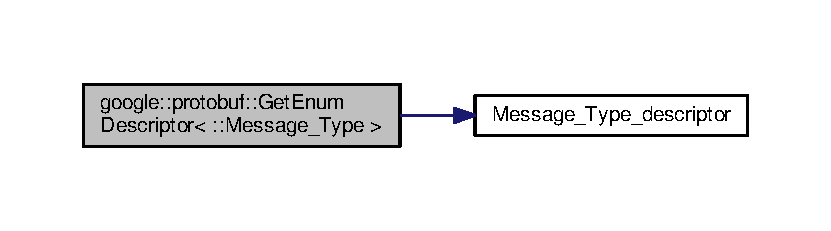
\includegraphics[width=350pt]{namespacegoogle_1_1protobuf_a68ff7e8c0cac9aa455585f1a91e7aece_cgraph}
\end{center}
\end{figure}


\index{google\+::protobuf@{google\+::protobuf}!Get\+Enum\+Descriptor$<$ \+::\+Ping\+\_\+\+Ping\+Type $>$@{Get\+Enum\+Descriptor$<$ \+::\+Ping\+\_\+\+Ping\+Type $>$}}
\index{Get\+Enum\+Descriptor$<$ \+::\+Ping\+\_\+\+Ping\+Type $>$@{Get\+Enum\+Descriptor$<$ \+::\+Ping\+\_\+\+Ping\+Type $>$}!google\+::protobuf@{google\+::protobuf}}
\subsubsection[{\texorpdfstring{Get\+Enum\+Descriptor$<$ \+::\+Ping\+\_\+\+Ping\+Type $>$()}{GetEnumDescriptor< ::Ping_PingType >()}}]{\setlength{\rightskip}{0pt plus 5cm}template$<$$>$ const Enum\+Descriptor$\ast$ google\+::protobuf\+::\+Get\+Enum\+Descriptor$<$ \+::{\bf Ping\+\_\+\+Ping\+Type} $>$ (
\begin{DoxyParamCaption}
{}
\end{DoxyParamCaption}
)\hspace{0.3cm}{\ttfamily [inline]}}\hypertarget{namespacegoogle_1_1protobuf_ab483d4902925c478c7781d2210837718}{}\label{namespacegoogle_1_1protobuf_ab483d4902925c478c7781d2210837718}


Here is the call graph for this function\+:
\nopagebreak
\begin{figure}[H]
\begin{center}
\leavevmode
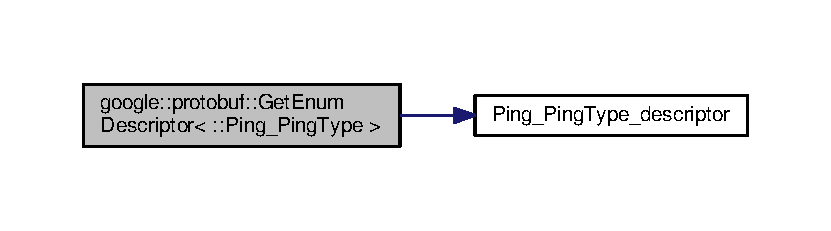
\includegraphics[width=350pt]{namespacegoogle_1_1protobuf_ab483d4902925c478c7781d2210837718_cgraph}
\end{center}
\end{figure}



\hypertarget{namespaceprotobuf__advertisement__2eproto}{}\section{protobuf\+\_\+advertisement\+\_\+2eproto Namespace Reference}
\label{namespaceprotobuf__advertisement__2eproto}\index{protobuf\+\_\+advertisement\+\_\+2eproto@{protobuf\+\_\+advertisement\+\_\+2eproto}}
\subsection*{Classes}
\begin{DoxyCompactItemize}
\item 
struct \hyperlink{structprotobuf__advertisement__2eproto_1_1_static_descriptor_initializer}{Static\+Descriptor\+Initializer}
\item 
struct \hyperlink{structprotobuf__advertisement__2eproto_1_1_table_struct}{Table\+Struct}
\end{DoxyCompactItemize}
\subsection*{Functions}
\begin{DoxyCompactItemize}
\item 
void \hyperlink{namespaceprotobuf__advertisement__2eproto_a43e55e6ab214b404d1e5143261f05bab}{Init\+Defaults} ()
\item 
void \hyperlink{namespaceprotobuf__advertisement__2eproto_ac52f8cd71d409eadb8b7045b2c201183}{Add\+Descriptors\+Impl} ()
\item 
void \hyperlink{namespaceprotobuf__advertisement__2eproto_a00a84fff996145fee2df377fd352becf}{Add\+Descriptors} ()
\end{DoxyCompactItemize}
\subsection*{Variables}
\begin{DoxyCompactItemize}
\item 
struct \hyperlink{structprotobuf__advertisement__2eproto_1_1_static_descriptor_initializer}{protobuf\+\_\+advertisement\+\_\+2eproto\+::\+Static\+Descriptor\+Initializer} \hyperlink{namespaceprotobuf__advertisement__2eproto_afc3c0155f686268d98d8bb107c19e3fb}{static\+\_\+descriptor\+\_\+initializer}
\end{DoxyCompactItemize}


\subsection{Function Documentation}
\index{protobuf\+\_\+advertisement\+\_\+2eproto@{protobuf\+\_\+advertisement\+\_\+2eproto}!Add\+Descriptors@{Add\+Descriptors}}
\index{Add\+Descriptors@{Add\+Descriptors}!protobuf\+\_\+advertisement\+\_\+2eproto@{protobuf\+\_\+advertisement\+\_\+2eproto}}
\subsubsection[{\texorpdfstring{Add\+Descriptors()}{AddDescriptors()}}]{\setlength{\rightskip}{0pt plus 5cm}void protobuf\+\_\+advertisement\+\_\+2eproto\+::\+Add\+Descriptors (
\begin{DoxyParamCaption}
{}
\end{DoxyParamCaption}
)}\hypertarget{namespaceprotobuf__advertisement__2eproto_a00a84fff996145fee2df377fd352becf}{}\label{namespaceprotobuf__advertisement__2eproto_a00a84fff996145fee2df377fd352becf}


Here is the call graph for this function\+:
\nopagebreak
\begin{figure}[H]
\begin{center}
\leavevmode
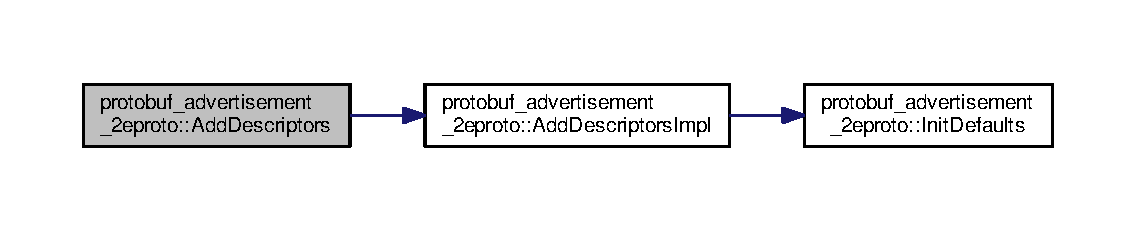
\includegraphics[width=350pt]{namespaceprotobuf__advertisement__2eproto_a00a84fff996145fee2df377fd352becf_cgraph}
\end{center}
\end{figure}




Here is the caller graph for this function\+:
\nopagebreak
\begin{figure}[H]
\begin{center}
\leavevmode
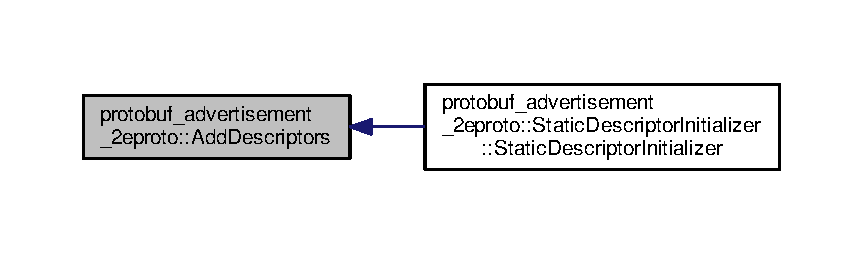
\includegraphics[width=350pt]{namespaceprotobuf__advertisement__2eproto_a00a84fff996145fee2df377fd352becf_icgraph}
\end{center}
\end{figure}


\index{protobuf\+\_\+advertisement\+\_\+2eproto@{protobuf\+\_\+advertisement\+\_\+2eproto}!Add\+Descriptors\+Impl@{Add\+Descriptors\+Impl}}
\index{Add\+Descriptors\+Impl@{Add\+Descriptors\+Impl}!protobuf\+\_\+advertisement\+\_\+2eproto@{protobuf\+\_\+advertisement\+\_\+2eproto}}
\subsubsection[{\texorpdfstring{Add\+Descriptors\+Impl()}{AddDescriptorsImpl()}}]{\setlength{\rightskip}{0pt plus 5cm}void protobuf\+\_\+advertisement\+\_\+2eproto\+::\+Add\+Descriptors\+Impl (
\begin{DoxyParamCaption}
{}
\end{DoxyParamCaption}
)}\hypertarget{namespaceprotobuf__advertisement__2eproto_ac52f8cd71d409eadb8b7045b2c201183}{}\label{namespaceprotobuf__advertisement__2eproto_ac52f8cd71d409eadb8b7045b2c201183}


Here is the call graph for this function\+:
\nopagebreak
\begin{figure}[H]
\begin{center}
\leavevmode
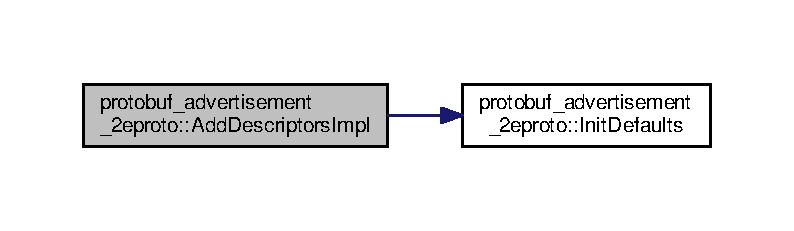
\includegraphics[width=350pt]{namespaceprotobuf__advertisement__2eproto_ac52f8cd71d409eadb8b7045b2c201183_cgraph}
\end{center}
\end{figure}




Here is the caller graph for this function\+:
\nopagebreak
\begin{figure}[H]
\begin{center}
\leavevmode
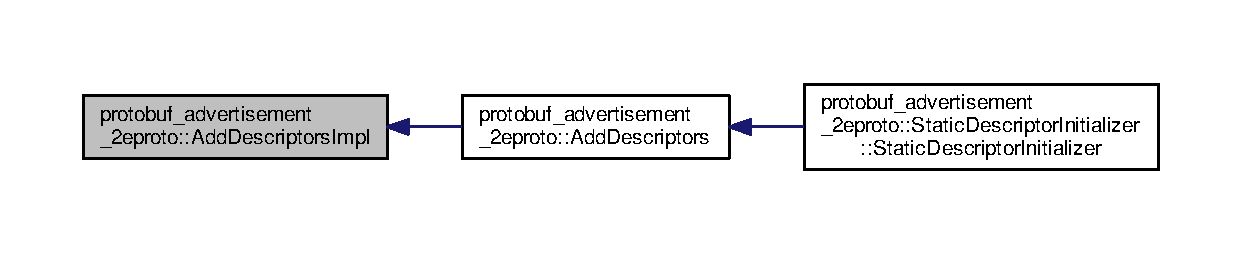
\includegraphics[width=350pt]{namespaceprotobuf__advertisement__2eproto_ac52f8cd71d409eadb8b7045b2c201183_icgraph}
\end{center}
\end{figure}


\index{protobuf\+\_\+advertisement\+\_\+2eproto@{protobuf\+\_\+advertisement\+\_\+2eproto}!Init\+Defaults@{Init\+Defaults}}
\index{Init\+Defaults@{Init\+Defaults}!protobuf\+\_\+advertisement\+\_\+2eproto@{protobuf\+\_\+advertisement\+\_\+2eproto}}
\subsubsection[{\texorpdfstring{Init\+Defaults()}{InitDefaults()}}]{\setlength{\rightskip}{0pt plus 5cm}void protobuf\+\_\+advertisement\+\_\+2eproto\+::\+Init\+Defaults (
\begin{DoxyParamCaption}
{}
\end{DoxyParamCaption}
)}\hypertarget{namespaceprotobuf__advertisement__2eproto_a43e55e6ab214b404d1e5143261f05bab}{}\label{namespaceprotobuf__advertisement__2eproto_a43e55e6ab214b404d1e5143261f05bab}


Here is the caller graph for this function\+:
\nopagebreak
\begin{figure}[H]
\begin{center}
\leavevmode
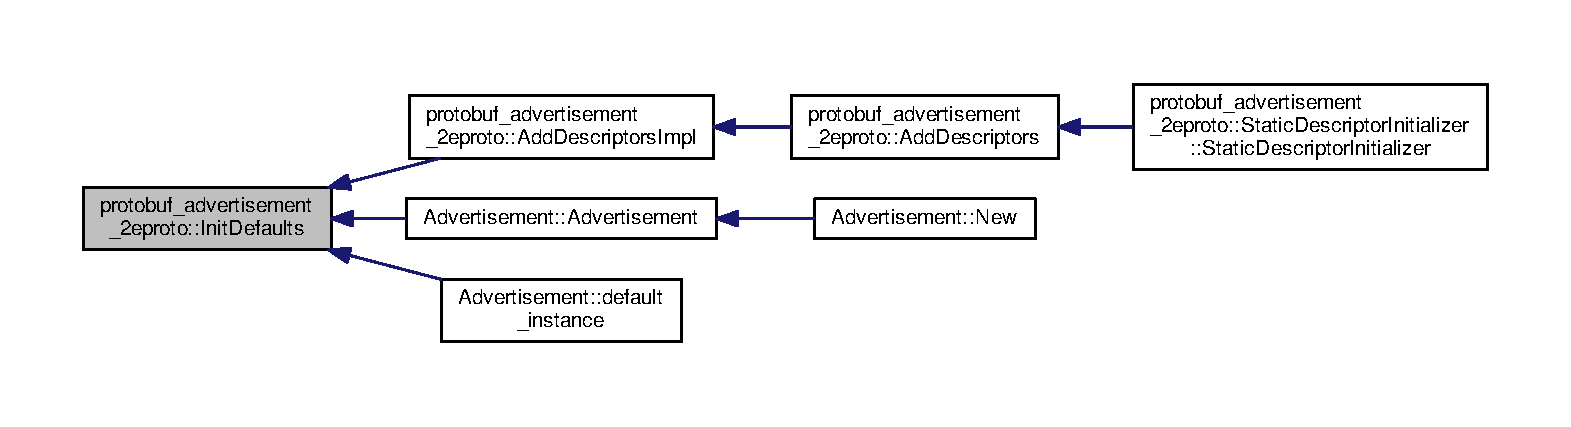
\includegraphics[width=350pt]{namespaceprotobuf__advertisement__2eproto_a43e55e6ab214b404d1e5143261f05bab_icgraph}
\end{center}
\end{figure}




\subsection{Variable Documentation}
\index{protobuf\+\_\+advertisement\+\_\+2eproto@{protobuf\+\_\+advertisement\+\_\+2eproto}!static\+\_\+descriptor\+\_\+initializer@{static\+\_\+descriptor\+\_\+initializer}}
\index{static\+\_\+descriptor\+\_\+initializer@{static\+\_\+descriptor\+\_\+initializer}!protobuf\+\_\+advertisement\+\_\+2eproto@{protobuf\+\_\+advertisement\+\_\+2eproto}}
\subsubsection[{\texorpdfstring{static\+\_\+descriptor\+\_\+initializer}{static_descriptor_initializer}}]{\setlength{\rightskip}{0pt plus 5cm}struct {\bf protobuf\+\_\+advertisement\+\_\+2eproto\+::\+Static\+Descriptor\+Initializer}  protobuf\+\_\+advertisement\+\_\+2eproto\+::static\+\_\+descriptor\+\_\+initializer}\hypertarget{namespaceprotobuf__advertisement__2eproto_afc3c0155f686268d98d8bb107c19e3fb}{}\label{namespaceprotobuf__advertisement__2eproto_afc3c0155f686268d98d8bb107c19e3fb}

\hypertarget{namespaceprotobuf__hello__2eproto}{}\section{protobuf\+\_\+hello\+\_\+2eproto Namespace Reference}
\label{namespaceprotobuf__hello__2eproto}\index{protobuf\+\_\+hello\+\_\+2eproto@{protobuf\+\_\+hello\+\_\+2eproto}}
\subsection*{Classes}
\begin{DoxyCompactItemize}
\item 
struct \hyperlink{structprotobuf__hello__2eproto_1_1_static_descriptor_initializer}{Static\+Descriptor\+Initializer}
\item 
struct \hyperlink{structprotobuf__hello__2eproto_1_1_table_struct}{Table\+Struct}
\end{DoxyCompactItemize}
\subsection*{Functions}
\begin{DoxyCompactItemize}
\item 
void \hyperlink{namespaceprotobuf__hello__2eproto_af2e596f8dda25052460ebb08b4c3b6a3}{Init\+Defaults} ()
\item 
void \hyperlink{namespaceprotobuf__hello__2eproto_aeaf72ccefda18075f3610b5fd82a17be}{Add\+Descriptors\+Impl} ()
\item 
void \hyperlink{namespaceprotobuf__hello__2eproto_aae9cbcf71d6ec9eb2e0eca18e9353d63}{Add\+Descriptors} ()
\end{DoxyCompactItemize}
\subsection*{Variables}
\begin{DoxyCompactItemize}
\item 
struct \hyperlink{structprotobuf__hello__2eproto_1_1_static_descriptor_initializer}{protobuf\+\_\+hello\+\_\+2eproto\+::\+Static\+Descriptor\+Initializer} \hyperlink{namespaceprotobuf__hello__2eproto_ac38fa2048bc2c0b789234c37ea845a41}{static\+\_\+descriptor\+\_\+initializer}
\end{DoxyCompactItemize}


\subsection{Function Documentation}
\index{protobuf\+\_\+hello\+\_\+2eproto@{protobuf\+\_\+hello\+\_\+2eproto}!Add\+Descriptors@{Add\+Descriptors}}
\index{Add\+Descriptors@{Add\+Descriptors}!protobuf\+\_\+hello\+\_\+2eproto@{protobuf\+\_\+hello\+\_\+2eproto}}
\subsubsection[{\texorpdfstring{Add\+Descriptors()}{AddDescriptors()}}]{\setlength{\rightskip}{0pt plus 5cm}void protobuf\+\_\+hello\+\_\+2eproto\+::\+Add\+Descriptors (
\begin{DoxyParamCaption}
{}
\end{DoxyParamCaption}
)}\hypertarget{namespaceprotobuf__hello__2eproto_aae9cbcf71d6ec9eb2e0eca18e9353d63}{}\label{namespaceprotobuf__hello__2eproto_aae9cbcf71d6ec9eb2e0eca18e9353d63}


Here is the call graph for this function\+:
\nopagebreak
\begin{figure}[H]
\begin{center}
\leavevmode
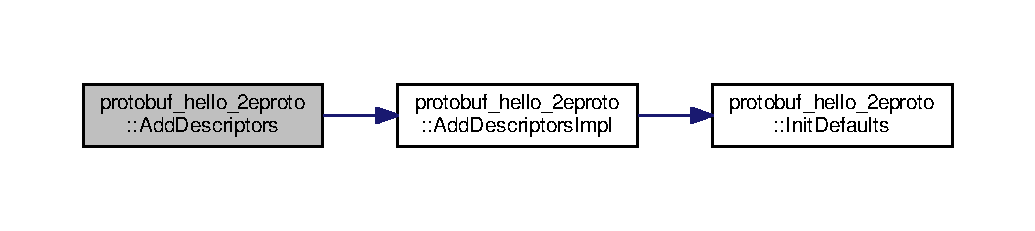
\includegraphics[width=350pt]{namespaceprotobuf__hello__2eproto_aae9cbcf71d6ec9eb2e0eca18e9353d63_cgraph}
\end{center}
\end{figure}




Here is the caller graph for this function\+:
\nopagebreak
\begin{figure}[H]
\begin{center}
\leavevmode
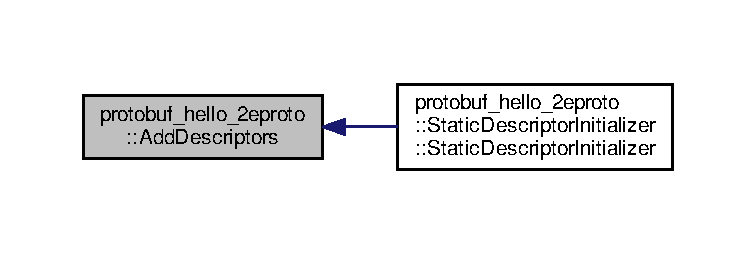
\includegraphics[width=350pt]{namespaceprotobuf__hello__2eproto_aae9cbcf71d6ec9eb2e0eca18e9353d63_icgraph}
\end{center}
\end{figure}


\index{protobuf\+\_\+hello\+\_\+2eproto@{protobuf\+\_\+hello\+\_\+2eproto}!Add\+Descriptors\+Impl@{Add\+Descriptors\+Impl}}
\index{Add\+Descriptors\+Impl@{Add\+Descriptors\+Impl}!protobuf\+\_\+hello\+\_\+2eproto@{protobuf\+\_\+hello\+\_\+2eproto}}
\subsubsection[{\texorpdfstring{Add\+Descriptors\+Impl()}{AddDescriptorsImpl()}}]{\setlength{\rightskip}{0pt plus 5cm}void protobuf\+\_\+hello\+\_\+2eproto\+::\+Add\+Descriptors\+Impl (
\begin{DoxyParamCaption}
{}
\end{DoxyParamCaption}
)}\hypertarget{namespaceprotobuf__hello__2eproto_aeaf72ccefda18075f3610b5fd82a17be}{}\label{namespaceprotobuf__hello__2eproto_aeaf72ccefda18075f3610b5fd82a17be}


Here is the call graph for this function\+:
\nopagebreak
\begin{figure}[H]
\begin{center}
\leavevmode
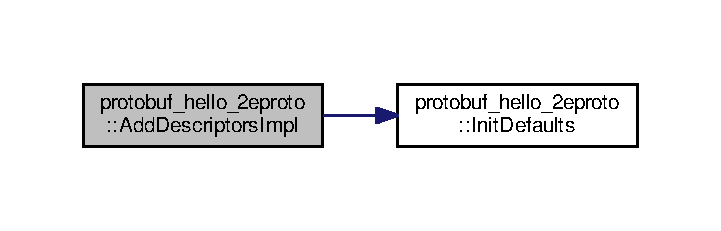
\includegraphics[width=346pt]{namespaceprotobuf__hello__2eproto_aeaf72ccefda18075f3610b5fd82a17be_cgraph}
\end{center}
\end{figure}




Here is the caller graph for this function\+:
\nopagebreak
\begin{figure}[H]
\begin{center}
\leavevmode
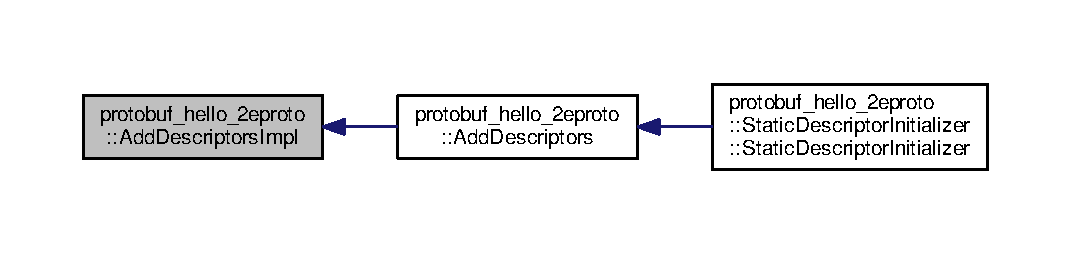
\includegraphics[width=350pt]{namespaceprotobuf__hello__2eproto_aeaf72ccefda18075f3610b5fd82a17be_icgraph}
\end{center}
\end{figure}


\index{protobuf\+\_\+hello\+\_\+2eproto@{protobuf\+\_\+hello\+\_\+2eproto}!Init\+Defaults@{Init\+Defaults}}
\index{Init\+Defaults@{Init\+Defaults}!protobuf\+\_\+hello\+\_\+2eproto@{protobuf\+\_\+hello\+\_\+2eproto}}
\subsubsection[{\texorpdfstring{Init\+Defaults()}{InitDefaults()}}]{\setlength{\rightskip}{0pt plus 5cm}void protobuf\+\_\+hello\+\_\+2eproto\+::\+Init\+Defaults (
\begin{DoxyParamCaption}
{}
\end{DoxyParamCaption}
)}\hypertarget{namespaceprotobuf__hello__2eproto_af2e596f8dda25052460ebb08b4c3b6a3}{}\label{namespaceprotobuf__hello__2eproto_af2e596f8dda25052460ebb08b4c3b6a3}


Here is the caller graph for this function\+:
\nopagebreak
\begin{figure}[H]
\begin{center}
\leavevmode
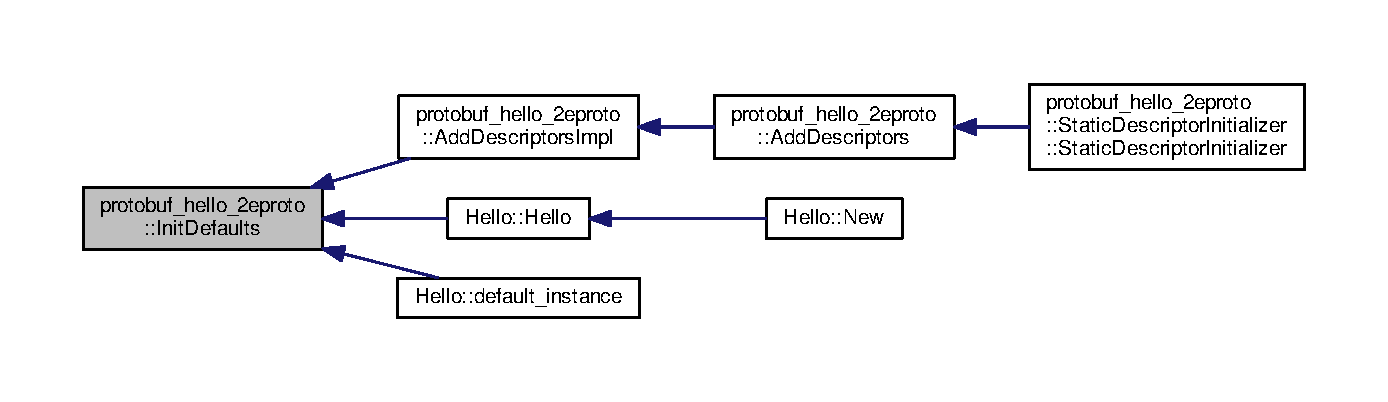
\includegraphics[width=350pt]{namespaceprotobuf__hello__2eproto_af2e596f8dda25052460ebb08b4c3b6a3_icgraph}
\end{center}
\end{figure}




\subsection{Variable Documentation}
\index{protobuf\+\_\+hello\+\_\+2eproto@{protobuf\+\_\+hello\+\_\+2eproto}!static\+\_\+descriptor\+\_\+initializer@{static\+\_\+descriptor\+\_\+initializer}}
\index{static\+\_\+descriptor\+\_\+initializer@{static\+\_\+descriptor\+\_\+initializer}!protobuf\+\_\+hello\+\_\+2eproto@{protobuf\+\_\+hello\+\_\+2eproto}}
\subsubsection[{\texorpdfstring{static\+\_\+descriptor\+\_\+initializer}{static_descriptor_initializer}}]{\setlength{\rightskip}{0pt plus 5cm}struct {\bf protobuf\+\_\+hello\+\_\+2eproto\+::\+Static\+Descriptor\+Initializer}  protobuf\+\_\+hello\+\_\+2eproto\+::static\+\_\+descriptor\+\_\+initializer}\hypertarget{namespaceprotobuf__hello__2eproto_ac38fa2048bc2c0b789234c37ea845a41}{}\label{namespaceprotobuf__hello__2eproto_ac38fa2048bc2c0b789234c37ea845a41}

\hypertarget{namespaceprotobuf__message__2eproto}{}\section{protobuf\+\_\+message\+\_\+2eproto Namespace Reference}
\label{namespaceprotobuf__message__2eproto}\index{protobuf\+\_\+message\+\_\+2eproto@{protobuf\+\_\+message\+\_\+2eproto}}
\subsection*{Classes}
\begin{DoxyCompactItemize}
\item 
struct \hyperlink{structprotobuf__message__2eproto_1_1_static_descriptor_initializer}{Static\+Descriptor\+Initializer}
\item 
struct \hyperlink{structprotobuf__message__2eproto_1_1_table_struct}{Table\+Struct}
\end{DoxyCompactItemize}
\subsection*{Functions}
\begin{DoxyCompactItemize}
\item 
void \hyperlink{namespaceprotobuf__message__2eproto_a0904ee0f747524cc1986baf4a9e9b3af}{Init\+Defaults} ()
\item 
void \hyperlink{namespaceprotobuf__message__2eproto_a2e03bfe5373fdbf0a2bb488e51de0c19}{Add\+Descriptors\+Impl} ()
\item 
void \hyperlink{namespaceprotobuf__message__2eproto_a6141a47817b5c3560ccd3f3396656732}{Add\+Descriptors} ()
\end{DoxyCompactItemize}
\subsection*{Variables}
\begin{DoxyCompactItemize}
\item 
struct \hyperlink{structprotobuf__message__2eproto_1_1_static_descriptor_initializer}{protobuf\+\_\+message\+\_\+2eproto\+::\+Static\+Descriptor\+Initializer} \hyperlink{namespaceprotobuf__message__2eproto_a326463751c85e569b98ef24ea8a840c9}{static\+\_\+descriptor\+\_\+initializer}
\end{DoxyCompactItemize}


\subsection{Function Documentation}
\index{protobuf\+\_\+message\+\_\+2eproto@{protobuf\+\_\+message\+\_\+2eproto}!Add\+Descriptors@{Add\+Descriptors}}
\index{Add\+Descriptors@{Add\+Descriptors}!protobuf\+\_\+message\+\_\+2eproto@{protobuf\+\_\+message\+\_\+2eproto}}
\subsubsection[{\texorpdfstring{Add\+Descriptors()}{AddDescriptors()}}]{\setlength{\rightskip}{0pt plus 5cm}void protobuf\+\_\+message\+\_\+2eproto\+::\+Add\+Descriptors (
\begin{DoxyParamCaption}
{}
\end{DoxyParamCaption}
)}\hypertarget{namespaceprotobuf__message__2eproto_a6141a47817b5c3560ccd3f3396656732}{}\label{namespaceprotobuf__message__2eproto_a6141a47817b5c3560ccd3f3396656732}


Here is the call graph for this function\+:
\nopagebreak
\begin{figure}[H]
\begin{center}
\leavevmode
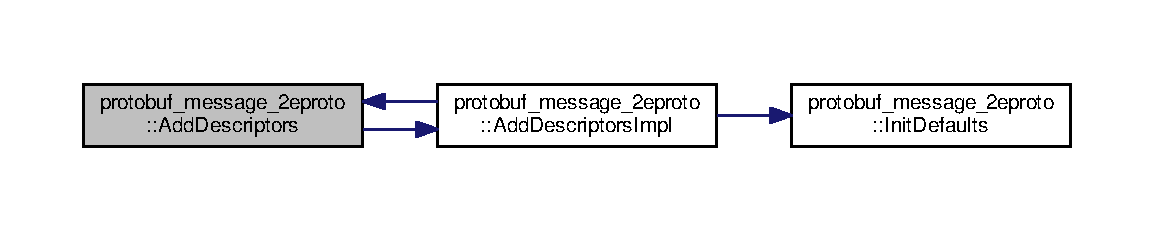
\includegraphics[width=350pt]{namespaceprotobuf__message__2eproto_a6141a47817b5c3560ccd3f3396656732_cgraph}
\end{center}
\end{figure}




Here is the caller graph for this function\+:
\nopagebreak
\begin{figure}[H]
\begin{center}
\leavevmode
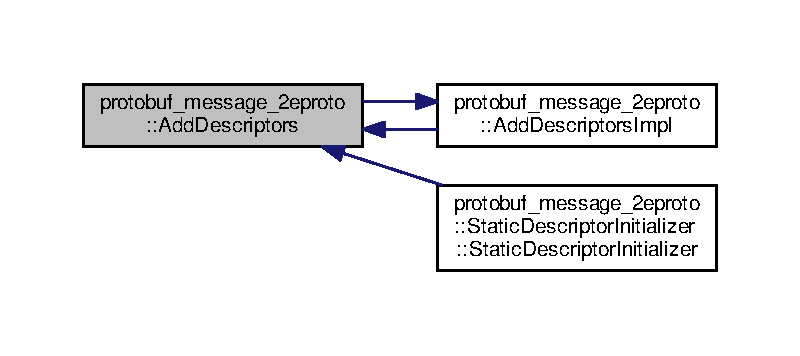
\includegraphics[width=350pt]{namespaceprotobuf__message__2eproto_a6141a47817b5c3560ccd3f3396656732_icgraph}
\end{center}
\end{figure}


\index{protobuf\+\_\+message\+\_\+2eproto@{protobuf\+\_\+message\+\_\+2eproto}!Add\+Descriptors\+Impl@{Add\+Descriptors\+Impl}}
\index{Add\+Descriptors\+Impl@{Add\+Descriptors\+Impl}!protobuf\+\_\+message\+\_\+2eproto@{protobuf\+\_\+message\+\_\+2eproto}}
\subsubsection[{\texorpdfstring{Add\+Descriptors\+Impl()}{AddDescriptorsImpl()}}]{\setlength{\rightskip}{0pt plus 5cm}void protobuf\+\_\+message\+\_\+2eproto\+::\+Add\+Descriptors\+Impl (
\begin{DoxyParamCaption}
{}
\end{DoxyParamCaption}
)}\hypertarget{namespaceprotobuf__message__2eproto_a2e03bfe5373fdbf0a2bb488e51de0c19}{}\label{namespaceprotobuf__message__2eproto_a2e03bfe5373fdbf0a2bb488e51de0c19}


Here is the call graph for this function\+:
\nopagebreak
\begin{figure}[H]
\begin{center}
\leavevmode
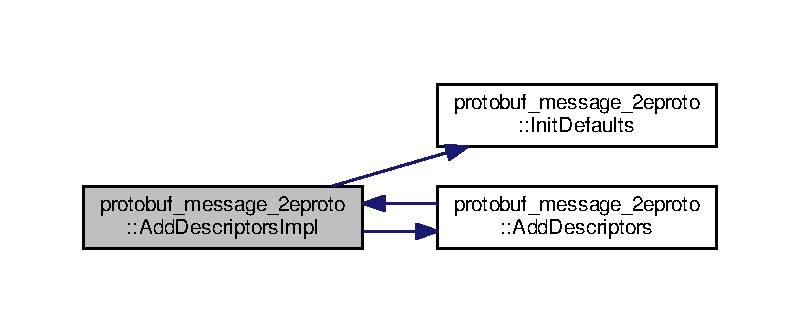
\includegraphics[width=350pt]{namespaceprotobuf__message__2eproto_a2e03bfe5373fdbf0a2bb488e51de0c19_cgraph}
\end{center}
\end{figure}




Here is the caller graph for this function\+:
\nopagebreak
\begin{figure}[H]
\begin{center}
\leavevmode
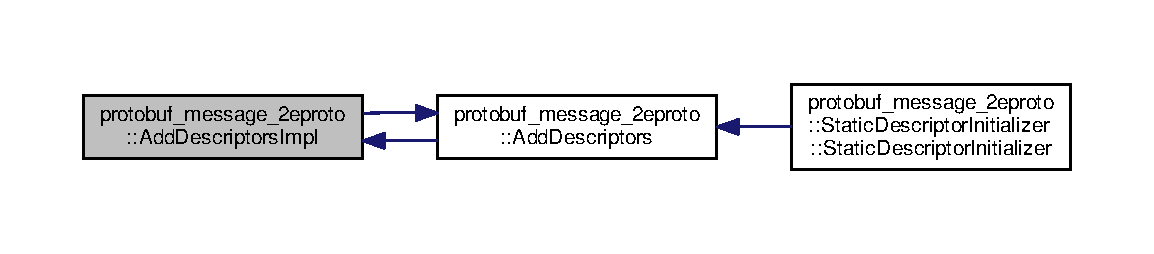
\includegraphics[width=350pt]{namespaceprotobuf__message__2eproto_a2e03bfe5373fdbf0a2bb488e51de0c19_icgraph}
\end{center}
\end{figure}


\index{protobuf\+\_\+message\+\_\+2eproto@{protobuf\+\_\+message\+\_\+2eproto}!Init\+Defaults@{Init\+Defaults}}
\index{Init\+Defaults@{Init\+Defaults}!protobuf\+\_\+message\+\_\+2eproto@{protobuf\+\_\+message\+\_\+2eproto}}
\subsubsection[{\texorpdfstring{Init\+Defaults()}{InitDefaults()}}]{\setlength{\rightskip}{0pt plus 5cm}void protobuf\+\_\+message\+\_\+2eproto\+::\+Init\+Defaults (
\begin{DoxyParamCaption}
{}
\end{DoxyParamCaption}
)}\hypertarget{namespaceprotobuf__message__2eproto_a0904ee0f747524cc1986baf4a9e9b3af}{}\label{namespaceprotobuf__message__2eproto_a0904ee0f747524cc1986baf4a9e9b3af}


Here is the caller graph for this function\+:
\nopagebreak
\begin{figure}[H]
\begin{center}
\leavevmode
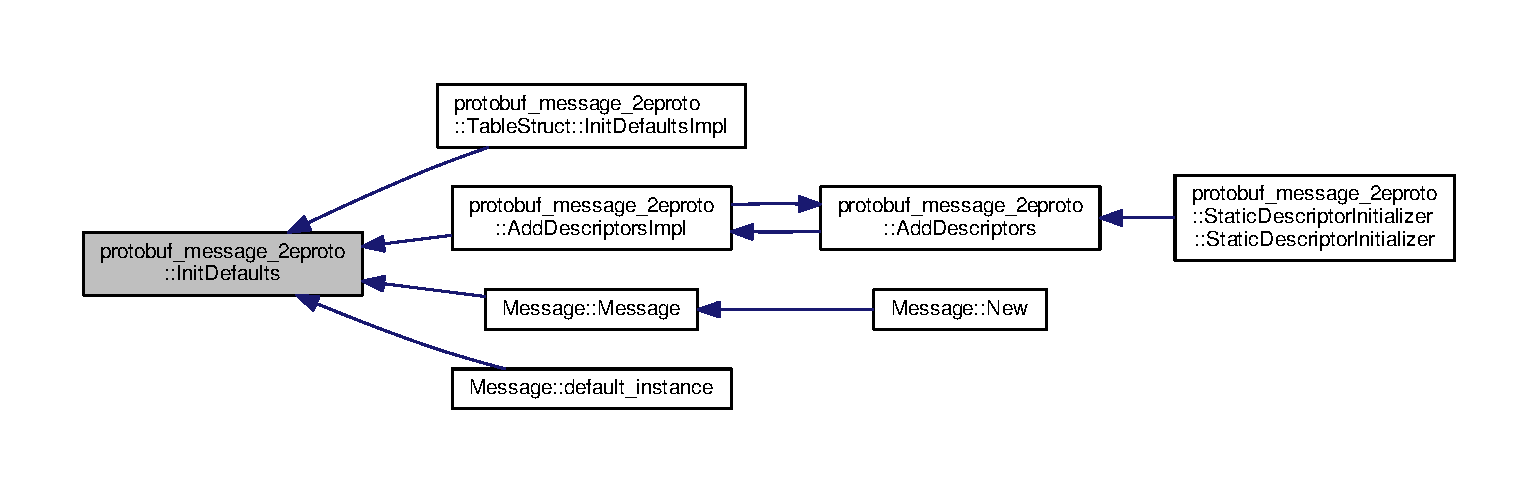
\includegraphics[width=350pt]{namespaceprotobuf__message__2eproto_a0904ee0f747524cc1986baf4a9e9b3af_icgraph}
\end{center}
\end{figure}




\subsection{Variable Documentation}
\index{protobuf\+\_\+message\+\_\+2eproto@{protobuf\+\_\+message\+\_\+2eproto}!static\+\_\+descriptor\+\_\+initializer@{static\+\_\+descriptor\+\_\+initializer}}
\index{static\+\_\+descriptor\+\_\+initializer@{static\+\_\+descriptor\+\_\+initializer}!protobuf\+\_\+message\+\_\+2eproto@{protobuf\+\_\+message\+\_\+2eproto}}
\subsubsection[{\texorpdfstring{static\+\_\+descriptor\+\_\+initializer}{static_descriptor_initializer}}]{\setlength{\rightskip}{0pt plus 5cm}struct {\bf protobuf\+\_\+message\+\_\+2eproto\+::\+Static\+Descriptor\+Initializer}  protobuf\+\_\+message\+\_\+2eproto\+::static\+\_\+descriptor\+\_\+initializer}\hypertarget{namespaceprotobuf__message__2eproto_a326463751c85e569b98ef24ea8a840c9}{}\label{namespaceprotobuf__message__2eproto_a326463751c85e569b98ef24ea8a840c9}

\hypertarget{namespaceprotobuf__ping__2eproto}{}\section{protobuf\+\_\+ping\+\_\+2eproto Namespace Reference}
\label{namespaceprotobuf__ping__2eproto}\index{protobuf\+\_\+ping\+\_\+2eproto@{protobuf\+\_\+ping\+\_\+2eproto}}
\subsection*{Classes}
\begin{DoxyCompactItemize}
\item 
struct \hyperlink{structprotobuf__ping__2eproto_1_1_static_descriptor_initializer}{Static\+Descriptor\+Initializer}
\item 
struct \hyperlink{structprotobuf__ping__2eproto_1_1_table_struct}{Table\+Struct}
\end{DoxyCompactItemize}
\subsection*{Functions}
\begin{DoxyCompactItemize}
\item 
void \hyperlink{namespaceprotobuf__ping__2eproto_a4da00112559a8a5b501ec9d17927aab2}{Init\+Defaults} ()
\item 
void \hyperlink{namespaceprotobuf__ping__2eproto_a208142d5c3a1fb52a39b9221afe49f5a}{Add\+Descriptors\+Impl} ()
\item 
void \hyperlink{namespaceprotobuf__ping__2eproto_ae3cb3909c68bd4b876872dafd97cb142}{Add\+Descriptors} ()
\end{DoxyCompactItemize}
\subsection*{Variables}
\begin{DoxyCompactItemize}
\item 
struct \hyperlink{structprotobuf__ping__2eproto_1_1_static_descriptor_initializer}{protobuf\+\_\+ping\+\_\+2eproto\+::\+Static\+Descriptor\+Initializer} \hyperlink{namespaceprotobuf__ping__2eproto_a117cab3e5661b7c6b74347dae80dd6ea}{static\+\_\+descriptor\+\_\+initializer}
\end{DoxyCompactItemize}


\subsection{Function Documentation}
\index{protobuf\+\_\+ping\+\_\+2eproto@{protobuf\+\_\+ping\+\_\+2eproto}!Add\+Descriptors@{Add\+Descriptors}}
\index{Add\+Descriptors@{Add\+Descriptors}!protobuf\+\_\+ping\+\_\+2eproto@{protobuf\+\_\+ping\+\_\+2eproto}}
\subsubsection[{\texorpdfstring{Add\+Descriptors()}{AddDescriptors()}}]{\setlength{\rightskip}{0pt plus 5cm}void protobuf\+\_\+ping\+\_\+2eproto\+::\+Add\+Descriptors (
\begin{DoxyParamCaption}
{}
\end{DoxyParamCaption}
)}\hypertarget{namespaceprotobuf__ping__2eproto_ae3cb3909c68bd4b876872dafd97cb142}{}\label{namespaceprotobuf__ping__2eproto_ae3cb3909c68bd4b876872dafd97cb142}
\index{protobuf\+\_\+ping\+\_\+2eproto@{protobuf\+\_\+ping\+\_\+2eproto}!Add\+Descriptors\+Impl@{Add\+Descriptors\+Impl}}
\index{Add\+Descriptors\+Impl@{Add\+Descriptors\+Impl}!protobuf\+\_\+ping\+\_\+2eproto@{protobuf\+\_\+ping\+\_\+2eproto}}
\subsubsection[{\texorpdfstring{Add\+Descriptors\+Impl()}{AddDescriptorsImpl()}}]{\setlength{\rightskip}{0pt plus 5cm}void protobuf\+\_\+ping\+\_\+2eproto\+::\+Add\+Descriptors\+Impl (
\begin{DoxyParamCaption}
{}
\end{DoxyParamCaption}
)}\hypertarget{namespaceprotobuf__ping__2eproto_a208142d5c3a1fb52a39b9221afe49f5a}{}\label{namespaceprotobuf__ping__2eproto_a208142d5c3a1fb52a39b9221afe49f5a}
\index{protobuf\+\_\+ping\+\_\+2eproto@{protobuf\+\_\+ping\+\_\+2eproto}!Init\+Defaults@{Init\+Defaults}}
\index{Init\+Defaults@{Init\+Defaults}!protobuf\+\_\+ping\+\_\+2eproto@{protobuf\+\_\+ping\+\_\+2eproto}}
\subsubsection[{\texorpdfstring{Init\+Defaults()}{InitDefaults()}}]{\setlength{\rightskip}{0pt plus 5cm}void protobuf\+\_\+ping\+\_\+2eproto\+::\+Init\+Defaults (
\begin{DoxyParamCaption}
{}
\end{DoxyParamCaption}
)}\hypertarget{namespaceprotobuf__ping__2eproto_a4da00112559a8a5b501ec9d17927aab2}{}\label{namespaceprotobuf__ping__2eproto_a4da00112559a8a5b501ec9d17927aab2}


\subsection{Variable Documentation}
\index{protobuf\+\_\+ping\+\_\+2eproto@{protobuf\+\_\+ping\+\_\+2eproto}!static\+\_\+descriptor\+\_\+initializer@{static\+\_\+descriptor\+\_\+initializer}}
\index{static\+\_\+descriptor\+\_\+initializer@{static\+\_\+descriptor\+\_\+initializer}!protobuf\+\_\+ping\+\_\+2eproto@{protobuf\+\_\+ping\+\_\+2eproto}}
\subsubsection[{\texorpdfstring{static\+\_\+descriptor\+\_\+initializer}{static_descriptor_initializer}}]{\setlength{\rightskip}{0pt plus 5cm}struct {\bf protobuf\+\_\+ping\+\_\+2eproto\+::\+Static\+Descriptor\+Initializer}  protobuf\+\_\+ping\+\_\+2eproto\+::static\+\_\+descriptor\+\_\+initializer}\hypertarget{namespaceprotobuf__ping__2eproto_a117cab3e5661b7c6b74347dae80dd6ea}{}\label{namespaceprotobuf__ping__2eproto_a117cab3e5661b7c6b74347dae80dd6ea}

\hypertarget{namespaceprotobuf__shutdown__2eproto}{}\section{protobuf\+\_\+shutdown\+\_\+2eproto Namespace Reference}
\label{namespaceprotobuf__shutdown__2eproto}\index{protobuf\+\_\+shutdown\+\_\+2eproto@{protobuf\+\_\+shutdown\+\_\+2eproto}}
\subsection*{Classes}
\begin{DoxyCompactItemize}
\item 
struct \hyperlink{structprotobuf__shutdown__2eproto_1_1_static_descriptor_initializer}{Static\+Descriptor\+Initializer}
\item 
struct \hyperlink{structprotobuf__shutdown__2eproto_1_1_table_struct}{Table\+Struct}
\end{DoxyCompactItemize}
\subsection*{Functions}
\begin{DoxyCompactItemize}
\item 
void \hyperlink{namespaceprotobuf__shutdown__2eproto_a74027734b8cea7f378100cf0b6cb4b58}{Init\+Defaults} ()
\item 
void \hyperlink{namespaceprotobuf__shutdown__2eproto_a729d370a71e6970c830fb554d8558f11}{Add\+Descriptors\+Impl} ()
\item 
void \hyperlink{namespaceprotobuf__shutdown__2eproto_a5437d9f43f254993a6bb3ad0d77f9d89}{Add\+Descriptors} ()
\end{DoxyCompactItemize}
\subsection*{Variables}
\begin{DoxyCompactItemize}
\item 
struct \hyperlink{structprotobuf__shutdown__2eproto_1_1_static_descriptor_initializer}{protobuf\+\_\+shutdown\+\_\+2eproto\+::\+Static\+Descriptor\+Initializer} \hyperlink{namespaceprotobuf__shutdown__2eproto_a01dfcfafd9651753066e44cd04be244d}{static\+\_\+descriptor\+\_\+initializer}
\end{DoxyCompactItemize}


\subsection{Function Documentation}
\index{protobuf\+\_\+shutdown\+\_\+2eproto@{protobuf\+\_\+shutdown\+\_\+2eproto}!Add\+Descriptors@{Add\+Descriptors}}
\index{Add\+Descriptors@{Add\+Descriptors}!protobuf\+\_\+shutdown\+\_\+2eproto@{protobuf\+\_\+shutdown\+\_\+2eproto}}
\subsubsection[{\texorpdfstring{Add\+Descriptors()}{AddDescriptors()}}]{\setlength{\rightskip}{0pt plus 5cm}void protobuf\+\_\+shutdown\+\_\+2eproto\+::\+Add\+Descriptors (
\begin{DoxyParamCaption}
{}
\end{DoxyParamCaption}
)}\hypertarget{namespaceprotobuf__shutdown__2eproto_a5437d9f43f254993a6bb3ad0d77f9d89}{}\label{namespaceprotobuf__shutdown__2eproto_a5437d9f43f254993a6bb3ad0d77f9d89}
\index{protobuf\+\_\+shutdown\+\_\+2eproto@{protobuf\+\_\+shutdown\+\_\+2eproto}!Add\+Descriptors\+Impl@{Add\+Descriptors\+Impl}}
\index{Add\+Descriptors\+Impl@{Add\+Descriptors\+Impl}!protobuf\+\_\+shutdown\+\_\+2eproto@{protobuf\+\_\+shutdown\+\_\+2eproto}}
\subsubsection[{\texorpdfstring{Add\+Descriptors\+Impl()}{AddDescriptorsImpl()}}]{\setlength{\rightskip}{0pt plus 5cm}void protobuf\+\_\+shutdown\+\_\+2eproto\+::\+Add\+Descriptors\+Impl (
\begin{DoxyParamCaption}
{}
\end{DoxyParamCaption}
)}\hypertarget{namespaceprotobuf__shutdown__2eproto_a729d370a71e6970c830fb554d8558f11}{}\label{namespaceprotobuf__shutdown__2eproto_a729d370a71e6970c830fb554d8558f11}
\index{protobuf\+\_\+shutdown\+\_\+2eproto@{protobuf\+\_\+shutdown\+\_\+2eproto}!Init\+Defaults@{Init\+Defaults}}
\index{Init\+Defaults@{Init\+Defaults}!protobuf\+\_\+shutdown\+\_\+2eproto@{protobuf\+\_\+shutdown\+\_\+2eproto}}
\subsubsection[{\texorpdfstring{Init\+Defaults()}{InitDefaults()}}]{\setlength{\rightskip}{0pt plus 5cm}void protobuf\+\_\+shutdown\+\_\+2eproto\+::\+Init\+Defaults (
\begin{DoxyParamCaption}
{}
\end{DoxyParamCaption}
)}\hypertarget{namespaceprotobuf__shutdown__2eproto_a74027734b8cea7f378100cf0b6cb4b58}{}\label{namespaceprotobuf__shutdown__2eproto_a74027734b8cea7f378100cf0b6cb4b58}


\subsection{Variable Documentation}
\index{protobuf\+\_\+shutdown\+\_\+2eproto@{protobuf\+\_\+shutdown\+\_\+2eproto}!static\+\_\+descriptor\+\_\+initializer@{static\+\_\+descriptor\+\_\+initializer}}
\index{static\+\_\+descriptor\+\_\+initializer@{static\+\_\+descriptor\+\_\+initializer}!protobuf\+\_\+shutdown\+\_\+2eproto@{protobuf\+\_\+shutdown\+\_\+2eproto}}
\subsubsection[{\texorpdfstring{static\+\_\+descriptor\+\_\+initializer}{static_descriptor_initializer}}]{\setlength{\rightskip}{0pt plus 5cm}struct {\bf protobuf\+\_\+shutdown\+\_\+2eproto\+::\+Static\+Descriptor\+Initializer}  protobuf\+\_\+shutdown\+\_\+2eproto\+::static\+\_\+descriptor\+\_\+initializer}\hypertarget{namespaceprotobuf__shutdown__2eproto_a01dfcfafd9651753066e44cd04be244d}{}\label{namespaceprotobuf__shutdown__2eproto_a01dfcfafd9651753066e44cd04be244d}

\chapter{Class Documentation}
\hypertarget{class_advertisement}{}\section{Advertisement Class Reference}
\label{class_advertisement}\index{Advertisement@{Advertisement}}


{\ttfamily \#include $<$advertisement.\+pb.\+h$>$}



Inheritance diagram for Advertisement\+:
\nopagebreak
\begin{figure}[H]
\begin{center}
\leavevmode
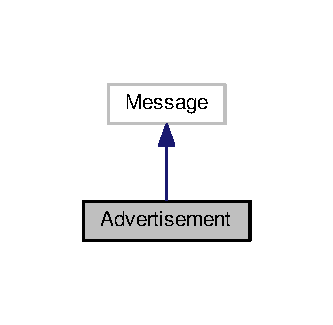
\includegraphics[width=160pt]{class_advertisement__inherit__graph}
\end{center}
\end{figure}


Collaboration diagram for Advertisement\+:
\nopagebreak
\begin{figure}[H]
\begin{center}
\leavevmode
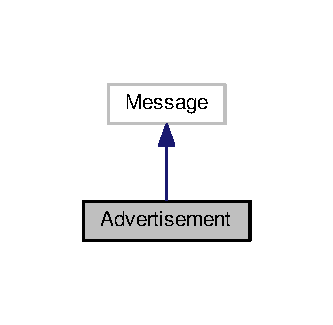
\includegraphics[width=160pt]{class_advertisement__coll__graph}
\end{center}
\end{figure}
\subsection*{Public Member Functions}
\begin{DoxyCompactItemize}
\item 
\hyperlink{class_advertisement_a2932354dce25b3f6b6a4af82a0e35db9}{Advertisement} ()
\item 
virtual \hyperlink{class_advertisement_a49170a22dcd2a8bf88d3ed1aad475b82}{$\sim$\+Advertisement} ()
\item 
\hyperlink{class_advertisement_a3ff57da26e6534cb2a130b4a5335492a}{Advertisement} (const \hyperlink{class_advertisement}{Advertisement} \&from)
\item 
\hyperlink{class_advertisement}{Advertisement} \& \hyperlink{class_advertisement_a245219dc727c1acbc22d7ce541d43f8b}{operator=} (const \hyperlink{class_advertisement}{Advertisement} \&from)
\item 
void \hyperlink{class_advertisement_aa981d999fe8394e184d36f5970e682f0}{Swap} (\hyperlink{class_advertisement}{Advertisement} $\ast$other)
\item 
\hyperlink{class_advertisement}{Advertisement} $\ast$ \hyperlink{class_advertisement_a86c4f8bed0f9b8a1f90b65da5aacd25d}{New} () const P\+R\+O\+T\+O\+B\+U\+F\+\_\+\+F\+I\+N\+AL
\item 
\hyperlink{class_advertisement}{Advertisement} $\ast$ \hyperlink{class_advertisement_a940cfe1ea161f8bc9a8c18efa5d9cde8}{New} (\+::google\+::protobuf\+::\+Arena $\ast$arena) const P\+R\+O\+T\+O\+B\+U\+F\+\_\+\+F\+I\+N\+AL
\item 
void \hyperlink{class_advertisement_a9ee96decf7b8ecdc05b3890ae23198f7}{Copy\+From} (const \+::google\+::protobuf\+::\+Message \&from) P\+R\+O\+T\+O\+B\+U\+F\+\_\+\+F\+I\+N\+AL
\item 
void \hyperlink{class_advertisement_ae6a97ef8e0fc8fbb7a83b541371ea1b8}{Merge\+From} (const \+::google\+::protobuf\+::\+Message \&from) P\+R\+O\+T\+O\+B\+U\+F\+\_\+\+F\+I\+N\+AL
\item 
void \hyperlink{class_advertisement_afc0c962367887d091805621cb282b542}{Copy\+From} (const \hyperlink{class_advertisement}{Advertisement} \&from)
\item 
void \hyperlink{class_advertisement_ad058035f7e184d6988c40a78dfd8d175}{Merge\+From} (const \hyperlink{class_advertisement}{Advertisement} \&from)
\item 
void \hyperlink{class_advertisement_a8c73d2885b5c1fd7dfb339a018715d37}{Clear} () P\+R\+O\+T\+O\+B\+U\+F\+\_\+\+F\+I\+N\+AL
\item 
bool \hyperlink{class_advertisement_a17b975dd2369fc638f79d343fa2f6c53}{Is\+Initialized} () const P\+R\+O\+T\+O\+B\+U\+F\+\_\+\+F\+I\+N\+AL
\item 
size\+\_\+t \hyperlink{class_advertisement_aac016bf3cd669a9cf524701559910c7f}{Byte\+Size\+Long} () const P\+R\+O\+T\+O\+B\+U\+F\+\_\+\+F\+I\+N\+AL
\item 
bool \hyperlink{class_advertisement_a2fae885c5e22e7dcce6fb1d40814235f}{Merge\+Partial\+From\+Coded\+Stream} (\+::google\+::protobuf\+::io\+::\+Coded\+Input\+Stream $\ast$input) P\+R\+O\+T\+O\+B\+U\+F\+\_\+\+F\+I\+N\+AL
\item 
void \hyperlink{class_advertisement_ae545a72f737ab9d1f7668169ff5c0e67}{Serialize\+With\+Cached\+Sizes} (\+::google\+::protobuf\+::io\+::\+Coded\+Output\+Stream $\ast$output) const P\+R\+O\+T\+O\+B\+U\+F\+\_\+\+F\+I\+N\+AL
\item 
\+::google\+::protobuf\+::uint8 $\ast$ \hyperlink{class_advertisement_aab2bd9a563f7db7751d05a5979f4c24c}{Internal\+Serialize\+With\+Cached\+Sizes\+To\+Array} (bool deterministic,\+::google\+::protobuf\+::uint8 $\ast$target) const P\+R\+O\+T\+O\+B\+U\+F\+\_\+\+F\+I\+N\+AL
\item 
\+::google\+::protobuf\+::uint8 $\ast$ \hyperlink{class_advertisement_a9b1ce6ff8dd10eead2f754b6dec6885c}{Serialize\+With\+Cached\+Sizes\+To\+Array} (\+::google\+::protobuf\+::uint8 $\ast$output) const P\+R\+O\+T\+O\+B\+U\+F\+\_\+\+F\+I\+N\+AL
\item 
int \hyperlink{class_advertisement_aede29af7c3f03520bf098ed174c5a080}{Get\+Cached\+Size} () const P\+R\+O\+T\+O\+B\+U\+F\+\_\+\+F\+I\+N\+AL
\item 
\+::google\+::protobuf\+::\+Metadata \hyperlink{class_advertisement_af2aa024564b2fe93a0f48d722cf42405}{Get\+Metadata} () const P\+R\+O\+T\+O\+B\+U\+F\+\_\+\+F\+I\+N\+AL
\item 
void \hyperlink{class_advertisement_a40ff84af1ed3e8149b930caf3516eb24}{clear\+\_\+ip} ()
\item 
\+::google\+::protobuf\+::uint32 \hyperlink{class_advertisement_a79b1546cdf56513b9e585f27795f3f8f}{ip} () const 
\item 
void \hyperlink{class_advertisement_a90f53e0ba30957936fdbee7170355ce9}{set\+\_\+ip} (\+::google\+::protobuf\+::uint32 value)
\item 
void \hyperlink{class_advertisement_aa0b75409373ab4db98a171bcc3de48dd}{clear\+\_\+port} ()
\item 
\+::google\+::protobuf\+::uint32 \hyperlink{class_advertisement_afad4c1b646818833a8bebb7efad53afe}{port} () const 
\item 
void \hyperlink{class_advertisement_af3442ebfa92d77664e92a92f61d6a1db}{set\+\_\+port} (\+::google\+::protobuf\+::uint32 value)
\end{DoxyCompactItemize}
\subsection*{Static Public Member Functions}
\begin{DoxyCompactItemize}
\item 
static const \+::google\+::protobuf\+::\+Descriptor $\ast$ \hyperlink{class_advertisement_a07947a4410bfa436cff5dc8a474eb86a}{descriptor} ()
\item 
static const \hyperlink{class_advertisement}{Advertisement} \& \hyperlink{class_advertisement_a70dc579979d32a7659c7f4aaf849543e}{default\+\_\+instance} ()
\item 
static const \hyperlink{class_advertisement}{Advertisement} $\ast$ \hyperlink{class_advertisement_a5de3c30b307a764143dcdb7b2f6d9874}{internal\+\_\+default\+\_\+instance} ()
\end{DoxyCompactItemize}
\subsection*{Static Public Attributes}
\begin{DoxyCompactItemize}
\item 
static const int \hyperlink{class_advertisement_af81bcf66962615be07bc839412551a28}{k\+Ip\+Field\+Number} = 1
\item 
static const int \hyperlink{class_advertisement_abf0fccf8702c996ca959a0d6ddb6a009}{k\+Port\+Field\+Number} = 2
\end{DoxyCompactItemize}
\subsection*{Friends}
\begin{DoxyCompactItemize}
\item 
struct \hyperlink{class_advertisement_adca70d246273bf9389ffd0298f17348e}{protobuf\+\_\+advertisement\+\_\+2eproto\+::\+Table\+Struct}
\end{DoxyCompactItemize}


\subsection{Constructor \& Destructor Documentation}
\index{Advertisement@{Advertisement}!Advertisement@{Advertisement}}
\index{Advertisement@{Advertisement}!Advertisement@{Advertisement}}
\subsubsection[{\texorpdfstring{Advertisement()}{Advertisement()}}]{\setlength{\rightskip}{0pt plus 5cm}Advertisement\+::\+Advertisement (
\begin{DoxyParamCaption}
{}
\end{DoxyParamCaption}
)}\hypertarget{class_advertisement_a2932354dce25b3f6b6a4af82a0e35db9}{}\label{class_advertisement_a2932354dce25b3f6b6a4af82a0e35db9}
\index{Advertisement@{Advertisement}!````~Advertisement@{$\sim$\+Advertisement}}
\index{````~Advertisement@{$\sim$\+Advertisement}!Advertisement@{Advertisement}}
\subsubsection[{\texorpdfstring{$\sim$\+Advertisement()}{~Advertisement()}}]{\setlength{\rightskip}{0pt plus 5cm}Advertisement\+::$\sim$\+Advertisement (
\begin{DoxyParamCaption}
{}
\end{DoxyParamCaption}
)\hspace{0.3cm}{\ttfamily [virtual]}}\hypertarget{class_advertisement_a49170a22dcd2a8bf88d3ed1aad475b82}{}\label{class_advertisement_a49170a22dcd2a8bf88d3ed1aad475b82}
\index{Advertisement@{Advertisement}!Advertisement@{Advertisement}}
\index{Advertisement@{Advertisement}!Advertisement@{Advertisement}}
\subsubsection[{\texorpdfstring{Advertisement(const Advertisement \&from)}{Advertisement(const Advertisement &from)}}]{\setlength{\rightskip}{0pt plus 5cm}Advertisement\+::\+Advertisement (
\begin{DoxyParamCaption}
\item[{const {\bf Advertisement} \&}]{from}
\end{DoxyParamCaption}
)}\hypertarget{class_advertisement_a3ff57da26e6534cb2a130b4a5335492a}{}\label{class_advertisement_a3ff57da26e6534cb2a130b4a5335492a}


\subsection{Member Function Documentation}
\index{Advertisement@{Advertisement}!Byte\+Size\+Long@{Byte\+Size\+Long}}
\index{Byte\+Size\+Long@{Byte\+Size\+Long}!Advertisement@{Advertisement}}
\subsubsection[{\texorpdfstring{Byte\+Size\+Long() const P\+R\+O\+T\+O\+B\+U\+F\+\_\+\+F\+I\+N\+AL}{ByteSizeLong() const PROTOBUF_FINAL}}]{\setlength{\rightskip}{0pt plus 5cm}size\+\_\+t Advertisement\+::\+Byte\+Size\+Long (
\begin{DoxyParamCaption}
{}
\end{DoxyParamCaption}
) const}\hypertarget{class_advertisement_aac016bf3cd669a9cf524701559910c7f}{}\label{class_advertisement_aac016bf3cd669a9cf524701559910c7f}
\index{Advertisement@{Advertisement}!Clear@{Clear}}
\index{Clear@{Clear}!Advertisement@{Advertisement}}
\subsubsection[{\texorpdfstring{Clear() P\+R\+O\+T\+O\+B\+U\+F\+\_\+\+F\+I\+N\+AL}{Clear() PROTOBUF_FINAL}}]{\setlength{\rightskip}{0pt plus 5cm}void Advertisement\+::\+Clear (
\begin{DoxyParamCaption}
{}
\end{DoxyParamCaption}
)}\hypertarget{class_advertisement_a8c73d2885b5c1fd7dfb339a018715d37}{}\label{class_advertisement_a8c73d2885b5c1fd7dfb339a018715d37}
\index{Advertisement@{Advertisement}!clear\+\_\+ip@{clear\+\_\+ip}}
\index{clear\+\_\+ip@{clear\+\_\+ip}!Advertisement@{Advertisement}}
\subsubsection[{\texorpdfstring{clear\+\_\+ip()}{clear_ip()}}]{\setlength{\rightskip}{0pt plus 5cm}void Advertisement\+::clear\+\_\+ip (
\begin{DoxyParamCaption}
{}
\end{DoxyParamCaption}
)\hspace{0.3cm}{\ttfamily [inline]}}\hypertarget{class_advertisement_a40ff84af1ed3e8149b930caf3516eb24}{}\label{class_advertisement_a40ff84af1ed3e8149b930caf3516eb24}
\index{Advertisement@{Advertisement}!clear\+\_\+port@{clear\+\_\+port}}
\index{clear\+\_\+port@{clear\+\_\+port}!Advertisement@{Advertisement}}
\subsubsection[{\texorpdfstring{clear\+\_\+port()}{clear_port()}}]{\setlength{\rightskip}{0pt plus 5cm}void Advertisement\+::clear\+\_\+port (
\begin{DoxyParamCaption}
{}
\end{DoxyParamCaption}
)\hspace{0.3cm}{\ttfamily [inline]}}\hypertarget{class_advertisement_aa0b75409373ab4db98a171bcc3de48dd}{}\label{class_advertisement_aa0b75409373ab4db98a171bcc3de48dd}
\index{Advertisement@{Advertisement}!Copy\+From@{Copy\+From}}
\index{Copy\+From@{Copy\+From}!Advertisement@{Advertisement}}
\subsubsection[{\texorpdfstring{Copy\+From(const \+::google\+::protobuf\+::\+Message \&from) P\+R\+O\+T\+O\+B\+U\+F\+\_\+\+F\+I\+N\+AL}{CopyFrom(const ::google::protobuf::Message &from) PROTOBUF_FINAL}}]{\setlength{\rightskip}{0pt plus 5cm}void Advertisement\+::\+Copy\+From (
\begin{DoxyParamCaption}
\item[{const \+::google\+::protobuf\+::\+Message \&}]{from}
\end{DoxyParamCaption}
)}\hypertarget{class_advertisement_a9ee96decf7b8ecdc05b3890ae23198f7}{}\label{class_advertisement_a9ee96decf7b8ecdc05b3890ae23198f7}
\index{Advertisement@{Advertisement}!Copy\+From@{Copy\+From}}
\index{Copy\+From@{Copy\+From}!Advertisement@{Advertisement}}
\subsubsection[{\texorpdfstring{Copy\+From(const Advertisement \&from)}{CopyFrom(const Advertisement &from)}}]{\setlength{\rightskip}{0pt plus 5cm}void Advertisement\+::\+Copy\+From (
\begin{DoxyParamCaption}
\item[{const {\bf Advertisement} \&}]{from}
\end{DoxyParamCaption}
)}\hypertarget{class_advertisement_afc0c962367887d091805621cb282b542}{}\label{class_advertisement_afc0c962367887d091805621cb282b542}
\index{Advertisement@{Advertisement}!default\+\_\+instance@{default\+\_\+instance}}
\index{default\+\_\+instance@{default\+\_\+instance}!Advertisement@{Advertisement}}
\subsubsection[{\texorpdfstring{default\+\_\+instance()}{default_instance()}}]{\setlength{\rightskip}{0pt plus 5cm}const {\bf Advertisement} \& Advertisement\+::default\+\_\+instance (
\begin{DoxyParamCaption}
{}
\end{DoxyParamCaption}
)\hspace{0.3cm}{\ttfamily [static]}}\hypertarget{class_advertisement_a70dc579979d32a7659c7f4aaf849543e}{}\label{class_advertisement_a70dc579979d32a7659c7f4aaf849543e}
\index{Advertisement@{Advertisement}!descriptor@{descriptor}}
\index{descriptor@{descriptor}!Advertisement@{Advertisement}}
\subsubsection[{\texorpdfstring{descriptor()}{descriptor()}}]{\setlength{\rightskip}{0pt plus 5cm}const \+::google\+::protobuf\+::\+Descriptor $\ast$ Advertisement\+::descriptor (
\begin{DoxyParamCaption}
{}
\end{DoxyParamCaption}
)\hspace{0.3cm}{\ttfamily [static]}}\hypertarget{class_advertisement_a07947a4410bfa436cff5dc8a474eb86a}{}\label{class_advertisement_a07947a4410bfa436cff5dc8a474eb86a}
\index{Advertisement@{Advertisement}!Get\+Cached\+Size@{Get\+Cached\+Size}}
\index{Get\+Cached\+Size@{Get\+Cached\+Size}!Advertisement@{Advertisement}}
\subsubsection[{\texorpdfstring{Get\+Cached\+Size() const P\+R\+O\+T\+O\+B\+U\+F\+\_\+\+F\+I\+N\+AL}{GetCachedSize() const PROTOBUF_FINAL}}]{\setlength{\rightskip}{0pt plus 5cm}int Advertisement\+::\+Get\+Cached\+Size (
\begin{DoxyParamCaption}
{}
\end{DoxyParamCaption}
) const\hspace{0.3cm}{\ttfamily [inline]}}\hypertarget{class_advertisement_aede29af7c3f03520bf098ed174c5a080}{}\label{class_advertisement_aede29af7c3f03520bf098ed174c5a080}
\index{Advertisement@{Advertisement}!Get\+Metadata@{Get\+Metadata}}
\index{Get\+Metadata@{Get\+Metadata}!Advertisement@{Advertisement}}
\subsubsection[{\texorpdfstring{Get\+Metadata() const P\+R\+O\+T\+O\+B\+U\+F\+\_\+\+F\+I\+N\+AL}{GetMetadata() const PROTOBUF_FINAL}}]{\setlength{\rightskip}{0pt plus 5cm}google\+::protobuf\+::\+Metadata Advertisement\+::\+Get\+Metadata (
\begin{DoxyParamCaption}
{}
\end{DoxyParamCaption}
) const}\hypertarget{class_advertisement_af2aa024564b2fe93a0f48d722cf42405}{}\label{class_advertisement_af2aa024564b2fe93a0f48d722cf42405}
\index{Advertisement@{Advertisement}!internal\+\_\+default\+\_\+instance@{internal\+\_\+default\+\_\+instance}}
\index{internal\+\_\+default\+\_\+instance@{internal\+\_\+default\+\_\+instance}!Advertisement@{Advertisement}}
\subsubsection[{\texorpdfstring{internal\+\_\+default\+\_\+instance()}{internal_default_instance()}}]{\setlength{\rightskip}{0pt plus 5cm}static const {\bf Advertisement}$\ast$ Advertisement\+::internal\+\_\+default\+\_\+instance (
\begin{DoxyParamCaption}
{}
\end{DoxyParamCaption}
)\hspace{0.3cm}{\ttfamily [inline]}, {\ttfamily [static]}}\hypertarget{class_advertisement_a5de3c30b307a764143dcdb7b2f6d9874}{}\label{class_advertisement_a5de3c30b307a764143dcdb7b2f6d9874}
\index{Advertisement@{Advertisement}!Internal\+Serialize\+With\+Cached\+Sizes\+To\+Array@{Internal\+Serialize\+With\+Cached\+Sizes\+To\+Array}}
\index{Internal\+Serialize\+With\+Cached\+Sizes\+To\+Array@{Internal\+Serialize\+With\+Cached\+Sizes\+To\+Array}!Advertisement@{Advertisement}}
\subsubsection[{\texorpdfstring{Internal\+Serialize\+With\+Cached\+Sizes\+To\+Array(bool deterministic,\+::google\+::protobuf\+::uint8 $\ast$target) const P\+R\+O\+T\+O\+B\+U\+F\+\_\+\+F\+I\+N\+AL}{InternalSerializeWithCachedSizesToArray(bool deterministic,::google::protobuf::uint8 *target) const PROTOBUF_FINAL}}]{\setlength{\rightskip}{0pt plus 5cm}google\+::protobuf\+::uint8 $\ast$ Advertisement\+::\+Internal\+Serialize\+With\+Cached\+Sizes\+To\+Array (
\begin{DoxyParamCaption}
\item[{bool}]{deterministic, }
\item[{\+::google\+::protobuf\+::uint8 $\ast$}]{target}
\end{DoxyParamCaption}
) const}\hypertarget{class_advertisement_aab2bd9a563f7db7751d05a5979f4c24c}{}\label{class_advertisement_aab2bd9a563f7db7751d05a5979f4c24c}
\index{Advertisement@{Advertisement}!ip@{ip}}
\index{ip@{ip}!Advertisement@{Advertisement}}
\subsubsection[{\texorpdfstring{ip() const }{ip() const }}]{\setlength{\rightskip}{0pt plus 5cm}google\+::protobuf\+::uint32 Advertisement\+::ip (
\begin{DoxyParamCaption}
{}
\end{DoxyParamCaption}
) const\hspace{0.3cm}{\ttfamily [inline]}}\hypertarget{class_advertisement_a79b1546cdf56513b9e585f27795f3f8f}{}\label{class_advertisement_a79b1546cdf56513b9e585f27795f3f8f}
\index{Advertisement@{Advertisement}!Is\+Initialized@{Is\+Initialized}}
\index{Is\+Initialized@{Is\+Initialized}!Advertisement@{Advertisement}}
\subsubsection[{\texorpdfstring{Is\+Initialized() const P\+R\+O\+T\+O\+B\+U\+F\+\_\+\+F\+I\+N\+AL}{IsInitialized() const PROTOBUF_FINAL}}]{\setlength{\rightskip}{0pt plus 5cm}bool Advertisement\+::\+Is\+Initialized (
\begin{DoxyParamCaption}
{}
\end{DoxyParamCaption}
) const}\hypertarget{class_advertisement_a17b975dd2369fc638f79d343fa2f6c53}{}\label{class_advertisement_a17b975dd2369fc638f79d343fa2f6c53}
\index{Advertisement@{Advertisement}!Merge\+From@{Merge\+From}}
\index{Merge\+From@{Merge\+From}!Advertisement@{Advertisement}}
\subsubsection[{\texorpdfstring{Merge\+From(const \+::google\+::protobuf\+::\+Message \&from) P\+R\+O\+T\+O\+B\+U\+F\+\_\+\+F\+I\+N\+AL}{MergeFrom(const ::google::protobuf::Message &from) PROTOBUF_FINAL}}]{\setlength{\rightskip}{0pt plus 5cm}void Advertisement\+::\+Merge\+From (
\begin{DoxyParamCaption}
\item[{const \+::google\+::protobuf\+::\+Message \&}]{from}
\end{DoxyParamCaption}
)}\hypertarget{class_advertisement_ae6a97ef8e0fc8fbb7a83b541371ea1b8}{}\label{class_advertisement_ae6a97ef8e0fc8fbb7a83b541371ea1b8}
\index{Advertisement@{Advertisement}!Merge\+From@{Merge\+From}}
\index{Merge\+From@{Merge\+From}!Advertisement@{Advertisement}}
\subsubsection[{\texorpdfstring{Merge\+From(const Advertisement \&from)}{MergeFrom(const Advertisement &from)}}]{\setlength{\rightskip}{0pt plus 5cm}void Advertisement\+::\+Merge\+From (
\begin{DoxyParamCaption}
\item[{const {\bf Advertisement} \&}]{from}
\end{DoxyParamCaption}
)}\hypertarget{class_advertisement_ad058035f7e184d6988c40a78dfd8d175}{}\label{class_advertisement_ad058035f7e184d6988c40a78dfd8d175}
\index{Advertisement@{Advertisement}!Merge\+Partial\+From\+Coded\+Stream@{Merge\+Partial\+From\+Coded\+Stream}}
\index{Merge\+Partial\+From\+Coded\+Stream@{Merge\+Partial\+From\+Coded\+Stream}!Advertisement@{Advertisement}}
\subsubsection[{\texorpdfstring{Merge\+Partial\+From\+Coded\+Stream(\+::google\+::protobuf\+::io\+::\+Coded\+Input\+Stream $\ast$input) P\+R\+O\+T\+O\+B\+U\+F\+\_\+\+F\+I\+N\+AL}{MergePartialFromCodedStream(::google::protobuf::io::CodedInputStream *input) PROTOBUF_FINAL}}]{\setlength{\rightskip}{0pt plus 5cm}bool Advertisement\+::\+Merge\+Partial\+From\+Coded\+Stream (
\begin{DoxyParamCaption}
\item[{\+::google\+::protobuf\+::io\+::\+Coded\+Input\+Stream $\ast$}]{input}
\end{DoxyParamCaption}
)}\hypertarget{class_advertisement_a2fae885c5e22e7dcce6fb1d40814235f}{}\label{class_advertisement_a2fae885c5e22e7dcce6fb1d40814235f}
\index{Advertisement@{Advertisement}!New@{New}}
\index{New@{New}!Advertisement@{Advertisement}}
\subsubsection[{\texorpdfstring{New() const P\+R\+O\+T\+O\+B\+U\+F\+\_\+\+F\+I\+N\+AL}{New() const PROTOBUF_FINAL}}]{\setlength{\rightskip}{0pt plus 5cm}{\bf Advertisement}$\ast$ Advertisement\+::\+New (
\begin{DoxyParamCaption}
{}
\end{DoxyParamCaption}
) const\hspace{0.3cm}{\ttfamily [inline]}}\hypertarget{class_advertisement_a86c4f8bed0f9b8a1f90b65da5aacd25d}{}\label{class_advertisement_a86c4f8bed0f9b8a1f90b65da5aacd25d}
\index{Advertisement@{Advertisement}!New@{New}}
\index{New@{New}!Advertisement@{Advertisement}}
\subsubsection[{\texorpdfstring{New(\+::google\+::protobuf\+::\+Arena $\ast$arena) const P\+R\+O\+T\+O\+B\+U\+F\+\_\+\+F\+I\+N\+AL}{New(::google::protobuf::Arena *arena) const PROTOBUF_FINAL}}]{\setlength{\rightskip}{0pt plus 5cm}{\bf Advertisement} $\ast$ Advertisement\+::\+New (
\begin{DoxyParamCaption}
\item[{\+::google\+::protobuf\+::\+Arena $\ast$}]{arena}
\end{DoxyParamCaption}
) const}\hypertarget{class_advertisement_a940cfe1ea161f8bc9a8c18efa5d9cde8}{}\label{class_advertisement_a940cfe1ea161f8bc9a8c18efa5d9cde8}
\index{Advertisement@{Advertisement}!operator=@{operator=}}
\index{operator=@{operator=}!Advertisement@{Advertisement}}
\subsubsection[{\texorpdfstring{operator=(const Advertisement \&from)}{operator=(const Advertisement &from)}}]{\setlength{\rightskip}{0pt plus 5cm}{\bf Advertisement}\& Advertisement\+::operator= (
\begin{DoxyParamCaption}
\item[{const {\bf Advertisement} \&}]{from}
\end{DoxyParamCaption}
)\hspace{0.3cm}{\ttfamily [inline]}}\hypertarget{class_advertisement_a245219dc727c1acbc22d7ce541d43f8b}{}\label{class_advertisement_a245219dc727c1acbc22d7ce541d43f8b}
\index{Advertisement@{Advertisement}!port@{port}}
\index{port@{port}!Advertisement@{Advertisement}}
\subsubsection[{\texorpdfstring{port() const }{port() const }}]{\setlength{\rightskip}{0pt plus 5cm}google\+::protobuf\+::uint32 Advertisement\+::port (
\begin{DoxyParamCaption}
{}
\end{DoxyParamCaption}
) const\hspace{0.3cm}{\ttfamily [inline]}}\hypertarget{class_advertisement_afad4c1b646818833a8bebb7efad53afe}{}\label{class_advertisement_afad4c1b646818833a8bebb7efad53afe}
\index{Advertisement@{Advertisement}!Serialize\+With\+Cached\+Sizes@{Serialize\+With\+Cached\+Sizes}}
\index{Serialize\+With\+Cached\+Sizes@{Serialize\+With\+Cached\+Sizes}!Advertisement@{Advertisement}}
\subsubsection[{\texorpdfstring{Serialize\+With\+Cached\+Sizes(\+::google\+::protobuf\+::io\+::\+Coded\+Output\+Stream $\ast$output) const P\+R\+O\+T\+O\+B\+U\+F\+\_\+\+F\+I\+N\+AL}{SerializeWithCachedSizes(::google::protobuf::io::CodedOutputStream *output) const PROTOBUF_FINAL}}]{\setlength{\rightskip}{0pt plus 5cm}void Advertisement\+::\+Serialize\+With\+Cached\+Sizes (
\begin{DoxyParamCaption}
\item[{\+::google\+::protobuf\+::io\+::\+Coded\+Output\+Stream $\ast$}]{output}
\end{DoxyParamCaption}
) const}\hypertarget{class_advertisement_ae545a72f737ab9d1f7668169ff5c0e67}{}\label{class_advertisement_ae545a72f737ab9d1f7668169ff5c0e67}
\index{Advertisement@{Advertisement}!Serialize\+With\+Cached\+Sizes\+To\+Array@{Serialize\+With\+Cached\+Sizes\+To\+Array}}
\index{Serialize\+With\+Cached\+Sizes\+To\+Array@{Serialize\+With\+Cached\+Sizes\+To\+Array}!Advertisement@{Advertisement}}
\subsubsection[{\texorpdfstring{Serialize\+With\+Cached\+Sizes\+To\+Array(\+::google\+::protobuf\+::uint8 $\ast$output) const P\+R\+O\+T\+O\+B\+U\+F\+\_\+\+F\+I\+N\+AL}{SerializeWithCachedSizesToArray(::google::protobuf::uint8 *output) const PROTOBUF_FINAL}}]{\setlength{\rightskip}{0pt plus 5cm}\+::google\+::protobuf\+::uint8$\ast$ Advertisement\+::\+Serialize\+With\+Cached\+Sizes\+To\+Array (
\begin{DoxyParamCaption}
\item[{\+::google\+::protobuf\+::uint8 $\ast$}]{output}
\end{DoxyParamCaption}
) const\hspace{0.3cm}{\ttfamily [inline]}}\hypertarget{class_advertisement_a9b1ce6ff8dd10eead2f754b6dec6885c}{}\label{class_advertisement_a9b1ce6ff8dd10eead2f754b6dec6885c}
\index{Advertisement@{Advertisement}!set\+\_\+ip@{set\+\_\+ip}}
\index{set\+\_\+ip@{set\+\_\+ip}!Advertisement@{Advertisement}}
\subsubsection[{\texorpdfstring{set\+\_\+ip(\+::google\+::protobuf\+::uint32 value)}{set_ip(::google::protobuf::uint32 value)}}]{\setlength{\rightskip}{0pt plus 5cm}void Advertisement\+::set\+\_\+ip (
\begin{DoxyParamCaption}
\item[{\+::google\+::protobuf\+::uint32}]{value}
\end{DoxyParamCaption}
)\hspace{0.3cm}{\ttfamily [inline]}}\hypertarget{class_advertisement_a90f53e0ba30957936fdbee7170355ce9}{}\label{class_advertisement_a90f53e0ba30957936fdbee7170355ce9}
\index{Advertisement@{Advertisement}!set\+\_\+port@{set\+\_\+port}}
\index{set\+\_\+port@{set\+\_\+port}!Advertisement@{Advertisement}}
\subsubsection[{\texorpdfstring{set\+\_\+port(\+::google\+::protobuf\+::uint32 value)}{set_port(::google::protobuf::uint32 value)}}]{\setlength{\rightskip}{0pt plus 5cm}void Advertisement\+::set\+\_\+port (
\begin{DoxyParamCaption}
\item[{\+::google\+::protobuf\+::uint32}]{value}
\end{DoxyParamCaption}
)\hspace{0.3cm}{\ttfamily [inline]}}\hypertarget{class_advertisement_af3442ebfa92d77664e92a92f61d6a1db}{}\label{class_advertisement_af3442ebfa92d77664e92a92f61d6a1db}
\index{Advertisement@{Advertisement}!Swap@{Swap}}
\index{Swap@{Swap}!Advertisement@{Advertisement}}
\subsubsection[{\texorpdfstring{Swap(\+Advertisement $\ast$other)}{Swap(Advertisement *other)}}]{\setlength{\rightskip}{0pt plus 5cm}void Advertisement\+::\+Swap (
\begin{DoxyParamCaption}
\item[{{\bf Advertisement} $\ast$}]{other}
\end{DoxyParamCaption}
)}\hypertarget{class_advertisement_aa981d999fe8394e184d36f5970e682f0}{}\label{class_advertisement_aa981d999fe8394e184d36f5970e682f0}


\subsection{Friends And Related Function Documentation}
\index{Advertisement@{Advertisement}!protobuf\+\_\+advertisement\+\_\+2eproto\+::\+Table\+Struct@{protobuf\+\_\+advertisement\+\_\+2eproto\+::\+Table\+Struct}}
\index{protobuf\+\_\+advertisement\+\_\+2eproto\+::\+Table\+Struct@{protobuf\+\_\+advertisement\+\_\+2eproto\+::\+Table\+Struct}!Advertisement@{Advertisement}}
\subsubsection[{\texorpdfstring{protobuf\+\_\+advertisement\+\_\+2eproto\+::\+Table\+Struct}{protobuf_advertisement_2eproto::TableStruct}}]{\setlength{\rightskip}{0pt plus 5cm}friend struct {\bf protobuf\+\_\+advertisement\+\_\+2eproto\+::\+Table\+Struct}\hspace{0.3cm}{\ttfamily [friend]}}\hypertarget{class_advertisement_adca70d246273bf9389ffd0298f17348e}{}\label{class_advertisement_adca70d246273bf9389ffd0298f17348e}


\subsection{Member Data Documentation}
\index{Advertisement@{Advertisement}!k\+Ip\+Field\+Number@{k\+Ip\+Field\+Number}}
\index{k\+Ip\+Field\+Number@{k\+Ip\+Field\+Number}!Advertisement@{Advertisement}}
\subsubsection[{\texorpdfstring{k\+Ip\+Field\+Number}{kIpFieldNumber}}]{\setlength{\rightskip}{0pt plus 5cm}const int Advertisement\+::k\+Ip\+Field\+Number = 1\hspace{0.3cm}{\ttfamily [static]}}\hypertarget{class_advertisement_af81bcf66962615be07bc839412551a28}{}\label{class_advertisement_af81bcf66962615be07bc839412551a28}
\index{Advertisement@{Advertisement}!k\+Port\+Field\+Number@{k\+Port\+Field\+Number}}
\index{k\+Port\+Field\+Number@{k\+Port\+Field\+Number}!Advertisement@{Advertisement}}
\subsubsection[{\texorpdfstring{k\+Port\+Field\+Number}{kPortFieldNumber}}]{\setlength{\rightskip}{0pt plus 5cm}const int Advertisement\+::k\+Port\+Field\+Number = 2\hspace{0.3cm}{\ttfamily [static]}}\hypertarget{class_advertisement_abf0fccf8702c996ca959a0d6ddb6a009}{}\label{class_advertisement_abf0fccf8702c996ca959a0d6ddb6a009}


The documentation for this class was generated from the following files\+:\begin{DoxyCompactItemize}
\item 
src/proto/\hyperlink{advertisement_8pb_8h}{advertisement.\+pb.\+h}\item 
src/proto/\hyperlink{advertisement_8pb_8cc}{advertisement.\+pb.\+cc}\end{DoxyCompactItemize}

\hypertarget{class_advertisement_default_type_internal}{}\section{Advertisement\+Default\+Type\+Internal Class Reference}
\label{class_advertisement_default_type_internal}\index{Advertisement\+Default\+Type\+Internal@{Advertisement\+Default\+Type\+Internal}}


Inheritance diagram for Advertisement\+Default\+Type\+Internal\+:\nopagebreak
\begin{figure}[H]
\begin{center}
\leavevmode
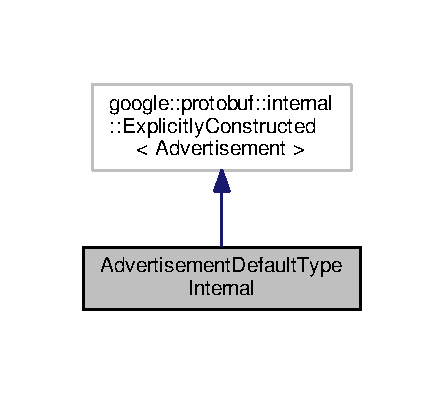
\includegraphics[width=213pt]{class_advertisement_default_type_internal__inherit__graph}
\end{center}
\end{figure}


Collaboration diagram for Advertisement\+Default\+Type\+Internal\+:\nopagebreak
\begin{figure}[H]
\begin{center}
\leavevmode
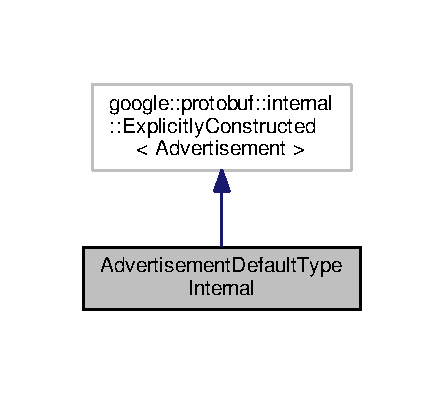
\includegraphics[width=213pt]{class_advertisement_default_type_internal__coll__graph}
\end{center}
\end{figure}


The documentation for this class was generated from the following file\+:\begin{DoxyCompactItemize}
\item 
src/proto/\hyperlink{advertisement_8pb_8cc}{advertisement.\+pb.\+cc}\end{DoxyCompactItemize}

\hypertarget{struct_area_rect}{}\section{Area\+Rect Struct Reference}
\label{struct_area_rect}\index{Area\+Rect@{Area\+Rect}}
\subsection*{Public Member Functions}
\begin{DoxyCompactItemize}
\item 
\hyperlink{struct_area_rect_a8181acef1f7da89c783d7be6a15be943}{Area\+Rect} ()
\item 
\hyperlink{struct_area_rect_afab957e4913c8de3dc97479299f29f2d}{Area\+Rect} (cv\+::\+Rect r)
\end{DoxyCompactItemize}
\subsection*{Public Attributes}
\begin{DoxyCompactItemize}
\item 
double \hyperlink{struct_area_rect_ac6605a013c0e730bf8eff77ce85a0348}{x1}
\item 
double \hyperlink{struct_area_rect_aa62bb569e815c2786f7a75c68d14df42}{x2}
\item 
double \hyperlink{struct_area_rect_add899b665dfaad3e0eff48e53ee0c004}{y1}
\item 
double \hyperlink{struct_area_rect_a140d6087009cfb8ff32b3b439f808fd6}{y2}
\item 
double \hyperlink{struct_area_rect_a1a46d82d9f236a8e413033637b1b3661}{area}
\item 
cv\+::\+Rect \hyperlink{struct_area_rect_a85f08909cd13d3cfdf7424bea2d7a362}{rect}
\end{DoxyCompactItemize}


\subsection{Constructor \& Destructor Documentation}
\index{Area\+Rect@{Area\+Rect}!Area\+Rect@{Area\+Rect}}
\index{Area\+Rect@{Area\+Rect}!Area\+Rect@{Area\+Rect}}
\subsubsection[{\texorpdfstring{Area\+Rect()}{AreaRect()}}]{\setlength{\rightskip}{0pt plus 5cm}Area\+Rect\+::\+Area\+Rect (
\begin{DoxyParamCaption}
{}
\end{DoxyParamCaption}
)\hspace{0.3cm}{\ttfamily [inline]}}\hypertarget{struct_area_rect_a8181acef1f7da89c783d7be6a15be943}{}\label{struct_area_rect_a8181acef1f7da89c783d7be6a15be943}
\index{Area\+Rect@{Area\+Rect}!Area\+Rect@{Area\+Rect}}
\index{Area\+Rect@{Area\+Rect}!Area\+Rect@{Area\+Rect}}
\subsubsection[{\texorpdfstring{Area\+Rect(cv\+::\+Rect r)}{AreaRect(cv::Rect r)}}]{\setlength{\rightskip}{0pt plus 5cm}Area\+Rect\+::\+Area\+Rect (
\begin{DoxyParamCaption}
\item[{cv\+::\+Rect}]{r}
\end{DoxyParamCaption}
)\hspace{0.3cm}{\ttfamily [inline]}}\hypertarget{struct_area_rect_afab957e4913c8de3dc97479299f29f2d}{}\label{struct_area_rect_afab957e4913c8de3dc97479299f29f2d}


\subsection{Member Data Documentation}
\index{Area\+Rect@{Area\+Rect}!area@{area}}
\index{area@{area}!Area\+Rect@{Area\+Rect}}
\subsubsection[{\texorpdfstring{area}{area}}]{\setlength{\rightskip}{0pt plus 5cm}double Area\+Rect\+::area}\hypertarget{struct_area_rect_a1a46d82d9f236a8e413033637b1b3661}{}\label{struct_area_rect_a1a46d82d9f236a8e413033637b1b3661}
\index{Area\+Rect@{Area\+Rect}!rect@{rect}}
\index{rect@{rect}!Area\+Rect@{Area\+Rect}}
\subsubsection[{\texorpdfstring{rect}{rect}}]{\setlength{\rightskip}{0pt plus 5cm}cv\+::\+Rect Area\+Rect\+::rect}\hypertarget{struct_area_rect_a85f08909cd13d3cfdf7424bea2d7a362}{}\label{struct_area_rect_a85f08909cd13d3cfdf7424bea2d7a362}
\index{Area\+Rect@{Area\+Rect}!x1@{x1}}
\index{x1@{x1}!Area\+Rect@{Area\+Rect}}
\subsubsection[{\texorpdfstring{x1}{x1}}]{\setlength{\rightskip}{0pt plus 5cm}double Area\+Rect\+::x1}\hypertarget{struct_area_rect_ac6605a013c0e730bf8eff77ce85a0348}{}\label{struct_area_rect_ac6605a013c0e730bf8eff77ce85a0348}
\index{Area\+Rect@{Area\+Rect}!x2@{x2}}
\index{x2@{x2}!Area\+Rect@{Area\+Rect}}
\subsubsection[{\texorpdfstring{x2}{x2}}]{\setlength{\rightskip}{0pt plus 5cm}double Area\+Rect\+::x2}\hypertarget{struct_area_rect_aa62bb569e815c2786f7a75c68d14df42}{}\label{struct_area_rect_aa62bb569e815c2786f7a75c68d14df42}
\index{Area\+Rect@{Area\+Rect}!y1@{y1}}
\index{y1@{y1}!Area\+Rect@{Area\+Rect}}
\subsubsection[{\texorpdfstring{y1}{y1}}]{\setlength{\rightskip}{0pt plus 5cm}double Area\+Rect\+::y1}\hypertarget{struct_area_rect_add899b665dfaad3e0eff48e53ee0c004}{}\label{struct_area_rect_add899b665dfaad3e0eff48e53ee0c004}
\index{Area\+Rect@{Area\+Rect}!y2@{y2}}
\index{y2@{y2}!Area\+Rect@{Area\+Rect}}
\subsubsection[{\texorpdfstring{y2}{y2}}]{\setlength{\rightskip}{0pt plus 5cm}double Area\+Rect\+::y2}\hypertarget{struct_area_rect_a140d6087009cfb8ff32b3b439f808fd6}{}\label{struct_area_rect_a140d6087009cfb8ff32b3b439f808fd6}


The documentation for this struct was generated from the following file\+:\begin{DoxyCompactItemize}
\item 
src/tracking/\hyperlink{_hog_detector_8cpp}{Hog\+Detector.\+cpp}\end{DoxyCompactItemize}

\hypertarget{class_async_socket_channel}{}\section{Async\+Socket\+Channel Class Reference}
\label{class_async_socket_channel}\index{Async\+Socket\+Channel@{Async\+Socket\+Channel}}


{\ttfamily \#include $<$Async\+Socket\+Channel.\+h$>$}

\subsection*{Public Types}
\begin{DoxyCompactItemize}
\item 
typedef std\+::function$<$ void(\hyperlink{class_connection_afc73789251390ec9c9c6e3750b104f08}{Connection\+::\+Pointer})$>$ \hyperlink{class_async_socket_channel_a9fae896907c968c9ea2ec825cd130b31}{Connection\+Acepted\+Handler}
\end{DoxyCompactItemize}
\subsection*{Public Member Functions}
\begin{DoxyCompactItemize}
\item 
\hyperlink{class_async_socket_channel_a98d850ca495d47b38d7d981ee7ee243b}{Async\+Socket\+Channel} (\hyperlink{class_message_queue}{Message\+Queue} $\ast$queue)
\item 
\hyperlink{class_async_socket_channel_aee710afec500bd16eb47f2c423baeb56}{$\sim$\+Async\+Socket\+Channel} ()
\item 
bool \hyperlink{class_async_socket_channel_ab2839fe16b7dffa0502ca69dc7e66299}{is\+Server} ()
\item 
\hyperlink{class_connection_afc73789251390ec9c9c6e3750b104f08}{Connection\+::\+Pointer} \hyperlink{class_async_socket_channel_a7b32d91f71dbea006cd1f7e631abb5c8}{connect} (boost\+::asio\+::ip\+::address\+\_\+v4 address, unsigned short port)
\item 
void \hyperlink{class_async_socket_channel_ae0d0010ef42fecc249ae1542b226130c}{serve} (unsigned short port)
\item 
\hyperlink{class_connection_afc73789251390ec9c9c6e3750b104f08}{Connection\+::\+Pointer} \hyperlink{class_async_socket_channel_a16520ee5501d92d322a21f3f245855d2}{get\+Connection} (boost\+::asio\+::ip\+::address\+\_\+v4 address, unsigned short port)
\end{DoxyCompactItemize}
\subsection*{Public Attributes}
\begin{DoxyCompactItemize}
\item 
\hyperlink{class_async_socket_channel_a9fae896907c968c9ea2ec825cd130b31}{Connection\+Acepted\+Handler} \hyperlink{class_async_socket_channel_a3dd24a37941604546e8875892410250c}{Acepted\+Connection}
\item 
std\+::vector$<$ \hyperlink{class_connection_afc73789251390ec9c9c6e3750b104f08}{Connection\+::\+Pointer} $>$ \hyperlink{class_async_socket_channel_aae682104eaebf291b57c586489bb500f}{connections}
\end{DoxyCompactItemize}


\subsection{Member Typedef Documentation}
\index{Async\+Socket\+Channel@{Async\+Socket\+Channel}!Connection\+Acepted\+Handler@{Connection\+Acepted\+Handler}}
\index{Connection\+Acepted\+Handler@{Connection\+Acepted\+Handler}!Async\+Socket\+Channel@{Async\+Socket\+Channel}}
\subsubsection[{\texorpdfstring{Connection\+Acepted\+Handler}{ConnectionAceptedHandler}}]{\setlength{\rightskip}{0pt plus 5cm}typedef std\+::function$<$void({\bf Connection\+::\+Pointer})$>$ {\bf Async\+Socket\+Channel\+::\+Connection\+Acepted\+Handler}}\hypertarget{class_async_socket_channel_a9fae896907c968c9ea2ec825cd130b31}{}\label{class_async_socket_channel_a9fae896907c968c9ea2ec825cd130b31}


\subsection{Constructor \& Destructor Documentation}
\index{Async\+Socket\+Channel@{Async\+Socket\+Channel}!Async\+Socket\+Channel@{Async\+Socket\+Channel}}
\index{Async\+Socket\+Channel@{Async\+Socket\+Channel}!Async\+Socket\+Channel@{Async\+Socket\+Channel}}
\subsubsection[{\texorpdfstring{Async\+Socket\+Channel(\+Message\+Queue $\ast$queue)}{AsyncSocketChannel(MessageQueue *queue)}}]{\setlength{\rightskip}{0pt plus 5cm}Async\+Socket\+Channel\+::\+Async\+Socket\+Channel (
\begin{DoxyParamCaption}
\item[{{\bf Message\+Queue} $\ast$}]{queue}
\end{DoxyParamCaption}
)}\hypertarget{class_async_socket_channel_a98d850ca495d47b38d7d981ee7ee243b}{}\label{class_async_socket_channel_a98d850ca495d47b38d7d981ee7ee243b}
\index{Async\+Socket\+Channel@{Async\+Socket\+Channel}!````~Async\+Socket\+Channel@{$\sim$\+Async\+Socket\+Channel}}
\index{````~Async\+Socket\+Channel@{$\sim$\+Async\+Socket\+Channel}!Async\+Socket\+Channel@{Async\+Socket\+Channel}}
\subsubsection[{\texorpdfstring{$\sim$\+Async\+Socket\+Channel()}{~AsyncSocketChannel()}}]{\setlength{\rightskip}{0pt plus 5cm}Async\+Socket\+Channel\+::$\sim$\+Async\+Socket\+Channel (
\begin{DoxyParamCaption}
{}
\end{DoxyParamCaption}
)}\hypertarget{class_async_socket_channel_aee710afec500bd16eb47f2c423baeb56}{}\label{class_async_socket_channel_aee710afec500bd16eb47f2c423baeb56}


\subsection{Member Function Documentation}
\index{Async\+Socket\+Channel@{Async\+Socket\+Channel}!connect@{connect}}
\index{connect@{connect}!Async\+Socket\+Channel@{Async\+Socket\+Channel}}
\subsubsection[{\texorpdfstring{connect(boost\+::asio\+::ip\+::address\+\_\+v4 address, unsigned short port)}{connect(boost::asio::ip::address_v4 address, unsigned short port)}}]{\setlength{\rightskip}{0pt plus 5cm}{\bf Connection\+::\+Pointer} Async\+Socket\+Channel\+::connect (
\begin{DoxyParamCaption}
\item[{boost\+::asio\+::ip\+::address\+\_\+v4}]{address, }
\item[{unsigned short}]{port}
\end{DoxyParamCaption}
)}\hypertarget{class_async_socket_channel_a7b32d91f71dbea006cd1f7e631abb5c8}{}\label{class_async_socket_channel_a7b32d91f71dbea006cd1f7e631abb5c8}


Here is the call graph for this function\+:
\nopagebreak
\begin{figure}[H]
\begin{center}
\leavevmode
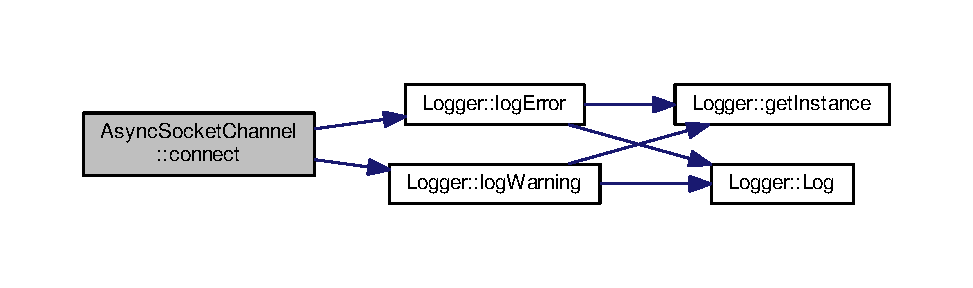
\includegraphics[width=350pt]{class_async_socket_channel_a7b32d91f71dbea006cd1f7e631abb5c8_cgraph}
\end{center}
\end{figure}




Here is the caller graph for this function\+:
\nopagebreak
\begin{figure}[H]
\begin{center}
\leavevmode
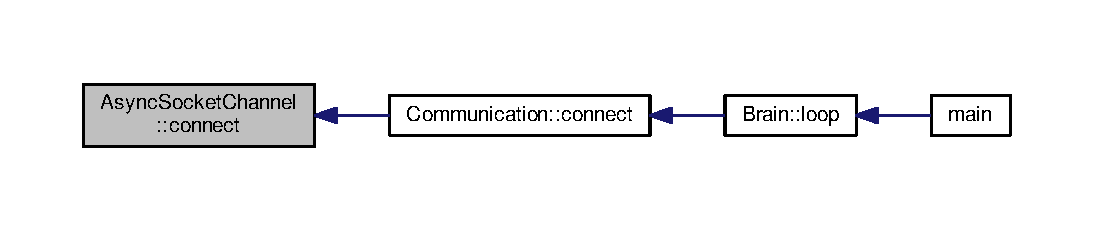
\includegraphics[width=350pt]{class_async_socket_channel_a7b32d91f71dbea006cd1f7e631abb5c8_icgraph}
\end{center}
\end{figure}


\index{Async\+Socket\+Channel@{Async\+Socket\+Channel}!get\+Connection@{get\+Connection}}
\index{get\+Connection@{get\+Connection}!Async\+Socket\+Channel@{Async\+Socket\+Channel}}
\subsubsection[{\texorpdfstring{get\+Connection(boost\+::asio\+::ip\+::address\+\_\+v4 address, unsigned short port)}{getConnection(boost::asio::ip::address_v4 address, unsigned short port)}}]{\setlength{\rightskip}{0pt plus 5cm}{\bf Connection\+::\+Pointer} Async\+Socket\+Channel\+::get\+Connection (
\begin{DoxyParamCaption}
\item[{boost\+::asio\+::ip\+::address\+\_\+v4}]{address, }
\item[{unsigned short}]{port}
\end{DoxyParamCaption}
)}\hypertarget{class_async_socket_channel_a16520ee5501d92d322a21f3f245855d2}{}\label{class_async_socket_channel_a16520ee5501d92d322a21f3f245855d2}


Here is the caller graph for this function\+:
\nopagebreak
\begin{figure}[H]
\begin{center}
\leavevmode
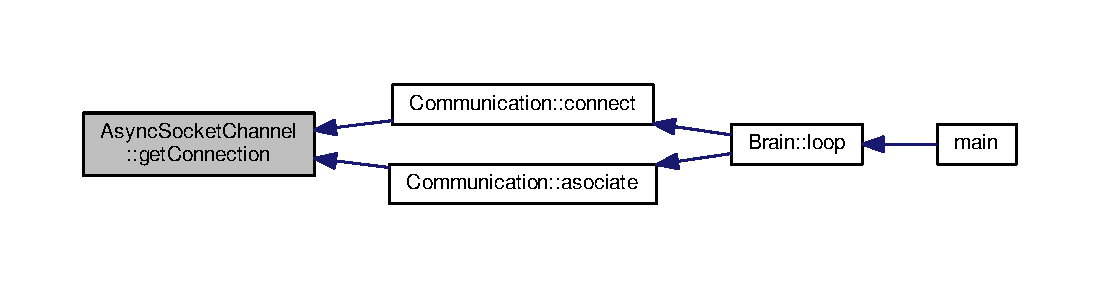
\includegraphics[width=350pt]{class_async_socket_channel_a16520ee5501d92d322a21f3f245855d2_icgraph}
\end{center}
\end{figure}


\index{Async\+Socket\+Channel@{Async\+Socket\+Channel}!is\+Server@{is\+Server}}
\index{is\+Server@{is\+Server}!Async\+Socket\+Channel@{Async\+Socket\+Channel}}
\subsubsection[{\texorpdfstring{is\+Server()}{isServer()}}]{\setlength{\rightskip}{0pt plus 5cm}bool Async\+Socket\+Channel\+::is\+Server (
\begin{DoxyParamCaption}
{}
\end{DoxyParamCaption}
)}\hypertarget{class_async_socket_channel_ab2839fe16b7dffa0502ca69dc7e66299}{}\label{class_async_socket_channel_ab2839fe16b7dffa0502ca69dc7e66299}
\index{Async\+Socket\+Channel@{Async\+Socket\+Channel}!serve@{serve}}
\index{serve@{serve}!Async\+Socket\+Channel@{Async\+Socket\+Channel}}
\subsubsection[{\texorpdfstring{serve(unsigned short port)}{serve(unsigned short port)}}]{\setlength{\rightskip}{0pt plus 5cm}void Async\+Socket\+Channel\+::serve (
\begin{DoxyParamCaption}
\item[{unsigned short}]{port}
\end{DoxyParamCaption}
)}\hypertarget{class_async_socket_channel_ae0d0010ef42fecc249ae1542b226130c}{}\label{class_async_socket_channel_ae0d0010ef42fecc249ae1542b226130c}


Here is the call graph for this function\+:
\nopagebreak
\begin{figure}[H]
\begin{center}
\leavevmode
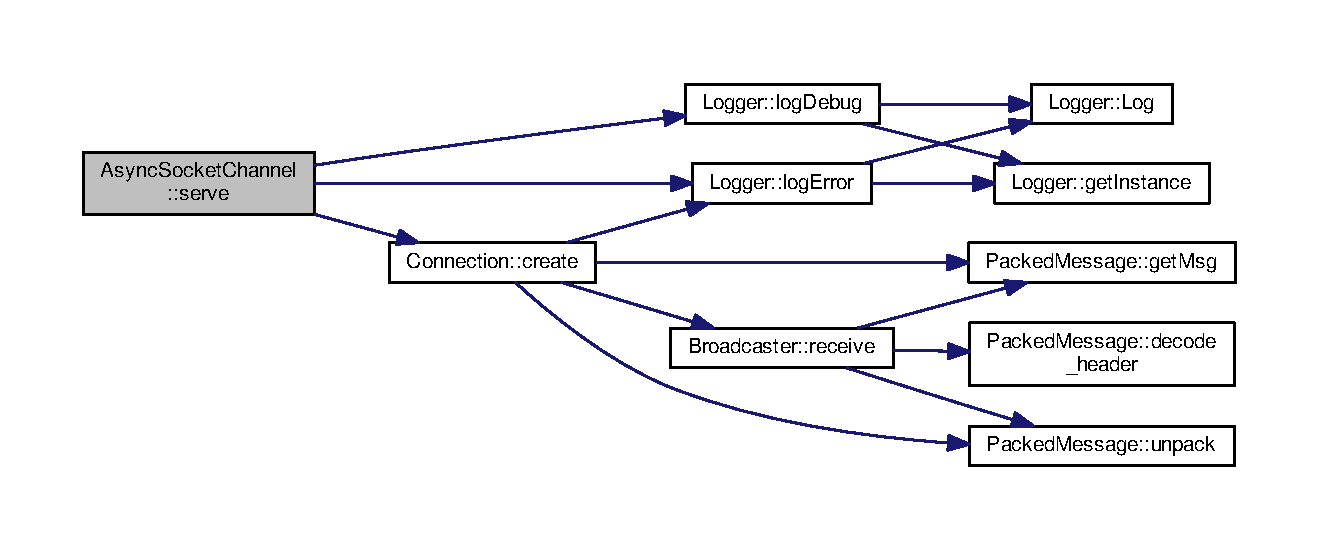
\includegraphics[width=350pt]{class_async_socket_channel_ae0d0010ef42fecc249ae1542b226130c_cgraph}
\end{center}
\end{figure}




Here is the caller graph for this function\+:
\nopagebreak
\begin{figure}[H]
\begin{center}
\leavevmode
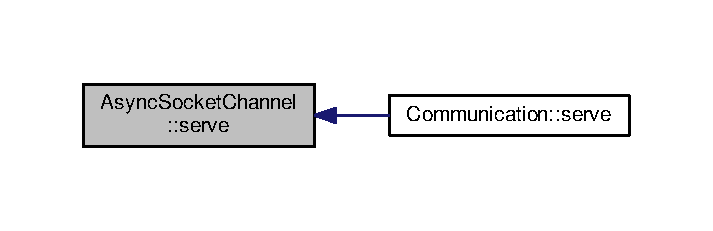
\includegraphics[width=342pt]{class_async_socket_channel_ae0d0010ef42fecc249ae1542b226130c_icgraph}
\end{center}
\end{figure}




\subsection{Member Data Documentation}
\index{Async\+Socket\+Channel@{Async\+Socket\+Channel}!Acepted\+Connection@{Acepted\+Connection}}
\index{Acepted\+Connection@{Acepted\+Connection}!Async\+Socket\+Channel@{Async\+Socket\+Channel}}
\subsubsection[{\texorpdfstring{Acepted\+Connection}{AceptedConnection}}]{\setlength{\rightskip}{0pt plus 5cm}{\bf Connection\+Acepted\+Handler} Async\+Socket\+Channel\+::\+Acepted\+Connection}\hypertarget{class_async_socket_channel_a3dd24a37941604546e8875892410250c}{}\label{class_async_socket_channel_a3dd24a37941604546e8875892410250c}
\index{Async\+Socket\+Channel@{Async\+Socket\+Channel}!connections@{connections}}
\index{connections@{connections}!Async\+Socket\+Channel@{Async\+Socket\+Channel}}
\subsubsection[{\texorpdfstring{connections}{connections}}]{\setlength{\rightskip}{0pt plus 5cm}std\+::vector$<${\bf Connection\+::\+Pointer}$>$ Async\+Socket\+Channel\+::connections}\hypertarget{class_async_socket_channel_aae682104eaebf291b57c586489bb500f}{}\label{class_async_socket_channel_aae682104eaebf291b57c586489bb500f}


The documentation for this class was generated from the following files\+:\begin{DoxyCompactItemize}
\item 
src/messages/\hyperlink{_async_socket_channel_8h}{Async\+Socket\+Channel.\+h}\item 
src/messages/\hyperlink{_async_socket_channel_8cpp}{Async\+Socket\+Channel.\+cpp}\end{DoxyCompactItemize}

\hypertarget{class_body}{}\section{Body Class Reference}
\label{class_body}\index{Body@{Body}}


{\ttfamily \#include $<$Body.\+h$>$}

\subsection*{Public Member Functions}
\begin{DoxyCompactItemize}
\item 
\hyperlink{class_body_a2d2ccb01dc9003cf63e79e913d27481f}{Body} (\hyperlink{class_hal}{Hal} $\ast$hal)
\item 
void \hyperlink{class_body_a74a678b9bdb90594271faded7fe2be36}{setup} (\hyperlink{class_config}{Config} $\ast$config)
\item 
void \hyperlink{class_body_a898135b92fa8abf09d435f671f62cf29}{loop} ()
\end{DoxyCompactItemize}


\subsection{Constructor \& Destructor Documentation}
\index{Body@{Body}!Body@{Body}}
\index{Body@{Body}!Body@{Body}}
\subsubsection[{\texorpdfstring{Body(\+Hal $\ast$hal)}{Body(Hal *hal)}}]{\setlength{\rightskip}{0pt plus 5cm}Body\+::\+Body (
\begin{DoxyParamCaption}
\item[{{\bf Hal} $\ast$}]{hal}
\end{DoxyParamCaption}
)}\hypertarget{class_body_a2d2ccb01dc9003cf63e79e913d27481f}{}\label{class_body_a2d2ccb01dc9003cf63e79e913d27481f}


Here is the call graph for this function\+:
\nopagebreak
\begin{figure}[H]
\begin{center}
\leavevmode
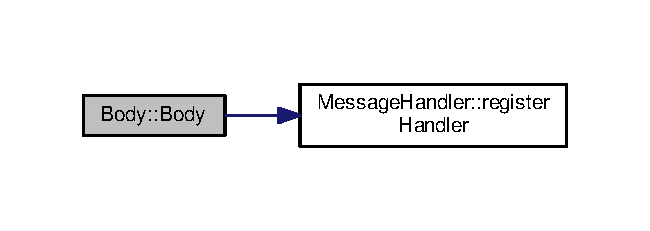
\includegraphics[width=312pt]{class_body_a2d2ccb01dc9003cf63e79e913d27481f_cgraph}
\end{center}
\end{figure}




\subsection{Member Function Documentation}
\index{Body@{Body}!loop@{loop}}
\index{loop@{loop}!Body@{Body}}
\subsubsection[{\texorpdfstring{loop()}{loop()}}]{\setlength{\rightskip}{0pt plus 5cm}void Body\+::loop (
\begin{DoxyParamCaption}
{}
\end{DoxyParamCaption}
)}\hypertarget{class_body_a898135b92fa8abf09d435f671f62cf29}{}\label{class_body_a898135b92fa8abf09d435f671f62cf29}


Here is the call graph for this function\+:
\nopagebreak
\begin{figure}[H]
\begin{center}
\leavevmode
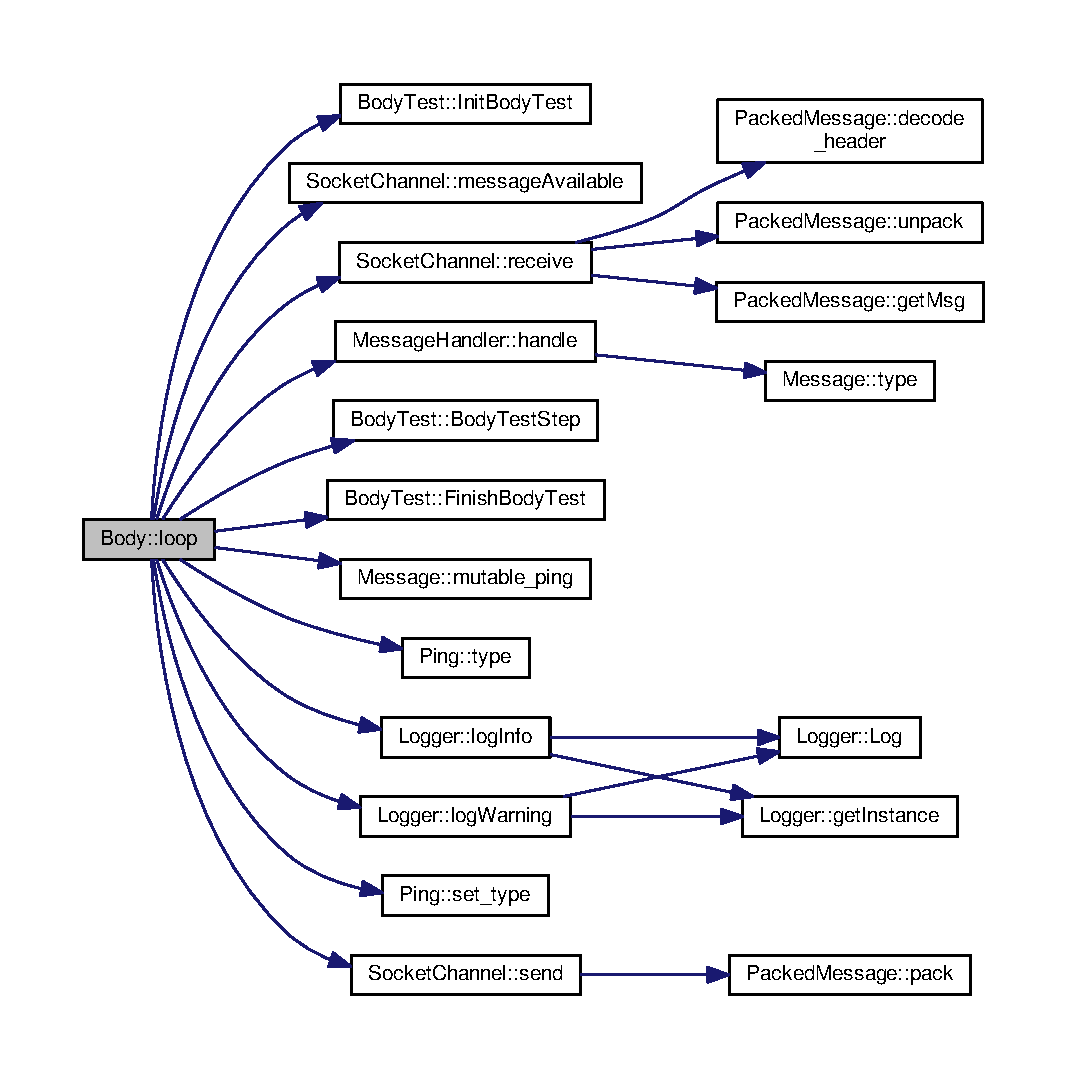
\includegraphics[width=350pt]{class_body_a898135b92fa8abf09d435f671f62cf29_cgraph}
\end{center}
\end{figure}




Here is the caller graph for this function\+:
\nopagebreak
\begin{figure}[H]
\begin{center}
\leavevmode
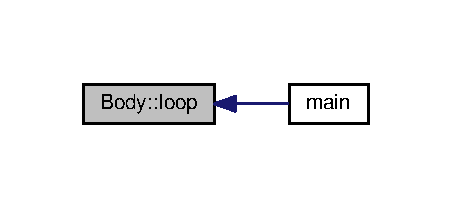
\includegraphics[width=217pt]{class_body_a898135b92fa8abf09d435f671f62cf29_icgraph}
\end{center}
\end{figure}


\index{Body@{Body}!setup@{setup}}
\index{setup@{setup}!Body@{Body}}
\subsubsection[{\texorpdfstring{setup(\+Config $\ast$config)}{setup(Config *config)}}]{\setlength{\rightskip}{0pt plus 5cm}void Body\+::setup (
\begin{DoxyParamCaption}
\item[{{\bf Config} $\ast$}]{config}
\end{DoxyParamCaption}
)}\hypertarget{class_body_a74a678b9bdb90594271faded7fe2be36}{}\label{class_body_a74a678b9bdb90594271faded7fe2be36}


Here is the call graph for this function\+:
\nopagebreak
\begin{figure}[H]
\begin{center}
\leavevmode
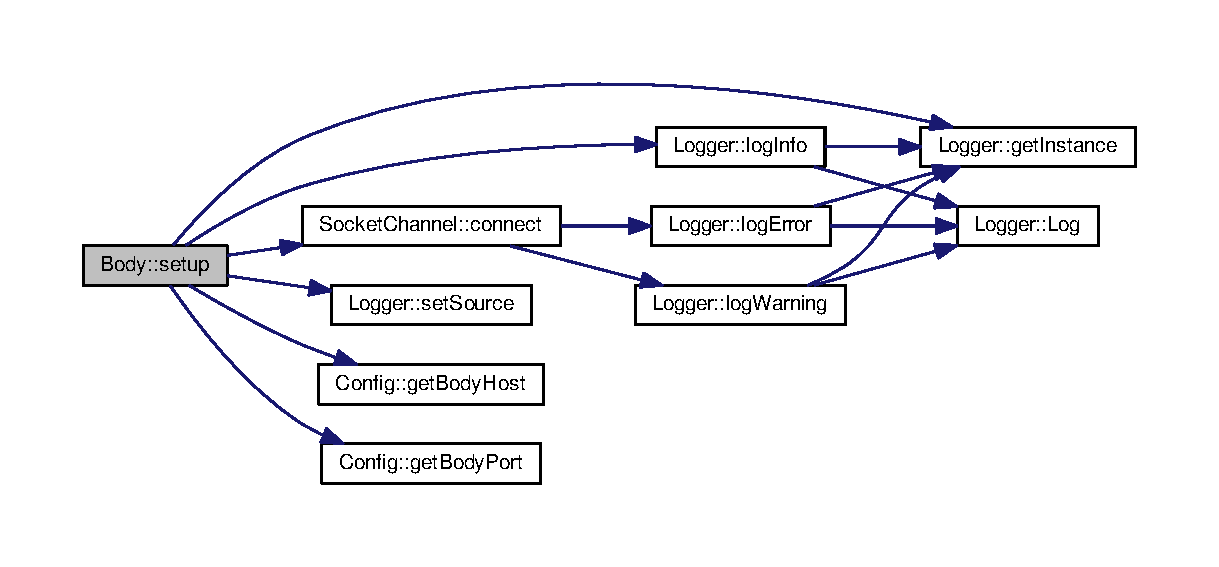
\includegraphics[width=350pt]{class_body_a74a678b9bdb90594271faded7fe2be36_cgraph}
\end{center}
\end{figure}




Here is the caller graph for this function\+:
\nopagebreak
\begin{figure}[H]
\begin{center}
\leavevmode
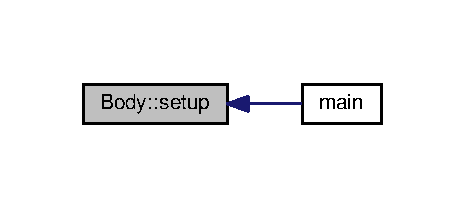
\includegraphics[width=223pt]{class_body_a74a678b9bdb90594271faded7fe2be36_icgraph}
\end{center}
\end{figure}




The documentation for this class was generated from the following files\+:\begin{DoxyCompactItemize}
\item 
src/\hyperlink{_body_8h}{Body.\+h}\item 
src/\hyperlink{_body_8cpp}{Body.\+cpp}\end{DoxyCompactItemize}

\hypertarget{class_brain}{}\section{Brain Class Reference}
\label{class_brain}\index{Brain@{Brain}}


{\ttfamily \#include $<$Brain.\+h$>$}

\subsection*{Public Member Functions}
\begin{DoxyCompactItemize}
\item 
\hyperlink{class_brain_a92daf9737361454abbb5988a89b7ff40}{Brain} ()
\item 
void \hyperlink{class_brain_a23d921369c5ec1218d7dc26d0f8270c2}{loop} ()
\item 
void \hyperlink{class_brain_afa2f689c8360c9c9ad323bac5be4b42d}{setup} (\hyperlink{class_config}{Config} $\ast$config, bool is\+Root)
\end{DoxyCompactItemize}


\subsection{Constructor \& Destructor Documentation}
\index{Brain@{Brain}!Brain@{Brain}}
\index{Brain@{Brain}!Brain@{Brain}}
\subsubsection[{\texorpdfstring{Brain()}{Brain()}}]{\setlength{\rightskip}{0pt plus 5cm}Brain\+::\+Brain (
\begin{DoxyParamCaption}
{}
\end{DoxyParamCaption}
)}\hypertarget{class_brain_a92daf9737361454abbb5988a89b7ff40}{}\label{class_brain_a92daf9737361454abbb5988a89b7ff40}


\subsection{Member Function Documentation}
\index{Brain@{Brain}!loop@{loop}}
\index{loop@{loop}!Brain@{Brain}}
\subsubsection[{\texorpdfstring{loop()}{loop()}}]{\setlength{\rightskip}{0pt plus 5cm}void Brain\+::loop (
\begin{DoxyParamCaption}
{}
\end{DoxyParamCaption}
)}\hypertarget{class_brain_a23d921369c5ec1218d7dc26d0f8270c2}{}\label{class_brain_a23d921369c5ec1218d7dc26d0f8270c2}
\index{Brain@{Brain}!setup@{setup}}
\index{setup@{setup}!Brain@{Brain}}
\subsubsection[{\texorpdfstring{setup(\+Config $\ast$config, bool is\+Root)}{setup(Config *config, bool isRoot)}}]{\setlength{\rightskip}{0pt plus 5cm}void Brain\+::setup (
\begin{DoxyParamCaption}
\item[{{\bf Config} $\ast$}]{config, }
\item[{bool}]{is\+Root}
\end{DoxyParamCaption}
)}\hypertarget{class_brain_afa2f689c8360c9c9ad323bac5be4b42d}{}\label{class_brain_afa2f689c8360c9c9ad323bac5be4b42d}


The documentation for this class was generated from the following files\+:\begin{DoxyCompactItemize}
\item 
src/\hyperlink{_brain_8h}{Brain.\+h}\item 
src/\hyperlink{_brain_8cpp}{Brain.\+cpp}\end{DoxyCompactItemize}

\hypertarget{class_broadcaster}{}\section{Broadcaster Class Reference}
\label{class_broadcaster}\index{Broadcaster@{Broadcaster}}


{\ttfamily \#include $<$Broadcaster.\+h$>$}

\subsection*{Public Member Functions}
\begin{DoxyCompactItemize}
\item 
\hyperlink{class_broadcaster_afc6e69fabdee71a22635fab47be3a36f}{$\sim$\+Broadcaster} ()
\item 
void \hyperlink{class_broadcaster_aaa77370dbd27d9930005c06d3d12f4b1}{broadcast} (\hyperlink{class_message}{Message} msg)
\item 
void \hyperlink{class_broadcaster_a52e7aac07f5ef3528a3f0e9bb4dd69e2}{setup} (unsigned short port)
\item 
\hyperlink{class_message}{Message} \hyperlink{class_broadcaster_a29791f7e092b8da8747b0168b3bdb404}{receive} ()
\item 
bool \hyperlink{class_broadcaster_a59202ca61301ba497ac3b619c941d900}{message\+Available} ()
\end{DoxyCompactItemize}


\subsection{Constructor \& Destructor Documentation}
\index{Broadcaster@{Broadcaster}!````~Broadcaster@{$\sim$\+Broadcaster}}
\index{````~Broadcaster@{$\sim$\+Broadcaster}!Broadcaster@{Broadcaster}}
\subsubsection[{\texorpdfstring{$\sim$\+Broadcaster()}{~Broadcaster()}}]{\setlength{\rightskip}{0pt plus 5cm}Broadcaster\+::$\sim$\+Broadcaster (
\begin{DoxyParamCaption}
{}
\end{DoxyParamCaption}
)}\hypertarget{class_broadcaster_afc6e69fabdee71a22635fab47be3a36f}{}\label{class_broadcaster_afc6e69fabdee71a22635fab47be3a36f}


\subsection{Member Function Documentation}
\index{Broadcaster@{Broadcaster}!broadcast@{broadcast}}
\index{broadcast@{broadcast}!Broadcaster@{Broadcaster}}
\subsubsection[{\texorpdfstring{broadcast(\+Message msg)}{broadcast(Message msg)}}]{\setlength{\rightskip}{0pt plus 5cm}void Broadcaster\+::broadcast (
\begin{DoxyParamCaption}
\item[{{\bf Message}}]{msg}
\end{DoxyParamCaption}
)}\hypertarget{class_broadcaster_aaa77370dbd27d9930005c06d3d12f4b1}{}\label{class_broadcaster_aaa77370dbd27d9930005c06d3d12f4b1}


Here is the call graph for this function\+:
\nopagebreak
\begin{figure}[H]
\begin{center}
\leavevmode
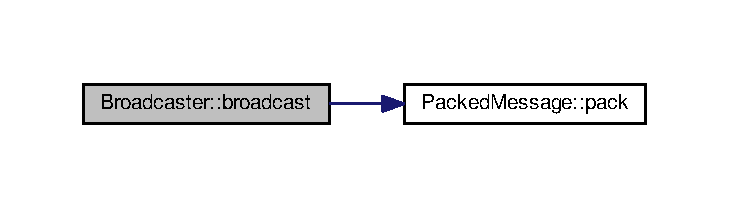
\includegraphics[width=350pt]{class_broadcaster_aaa77370dbd27d9930005c06d3d12f4b1_cgraph}
\end{center}
\end{figure}




Here is the caller graph for this function\+:
\nopagebreak
\begin{figure}[H]
\begin{center}
\leavevmode
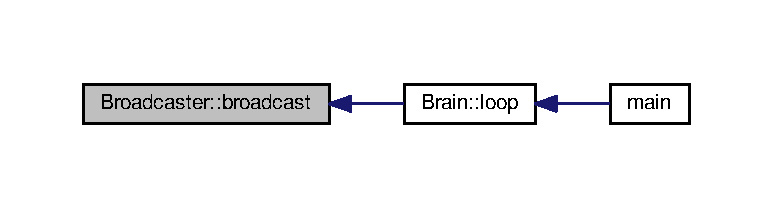
\includegraphics[width=350pt]{class_broadcaster_aaa77370dbd27d9930005c06d3d12f4b1_icgraph}
\end{center}
\end{figure}


\index{Broadcaster@{Broadcaster}!message\+Available@{message\+Available}}
\index{message\+Available@{message\+Available}!Broadcaster@{Broadcaster}}
\subsubsection[{\texorpdfstring{message\+Available()}{messageAvailable()}}]{\setlength{\rightskip}{0pt plus 5cm}bool Broadcaster\+::message\+Available (
\begin{DoxyParamCaption}
{}
\end{DoxyParamCaption}
)}\hypertarget{class_broadcaster_a59202ca61301ba497ac3b619c941d900}{}\label{class_broadcaster_a59202ca61301ba497ac3b619c941d900}


Here is the caller graph for this function\+:
\nopagebreak
\begin{figure}[H]
\begin{center}
\leavevmode
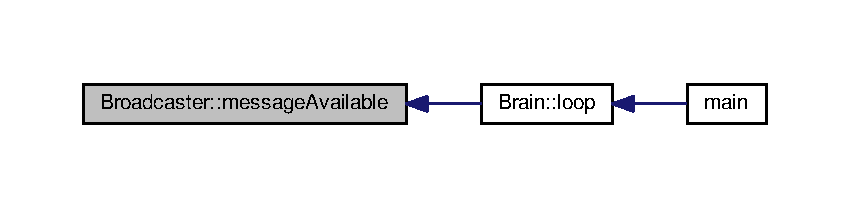
\includegraphics[width=350pt]{class_broadcaster_a59202ca61301ba497ac3b619c941d900_icgraph}
\end{center}
\end{figure}


\index{Broadcaster@{Broadcaster}!receive@{receive}}
\index{receive@{receive}!Broadcaster@{Broadcaster}}
\subsubsection[{\texorpdfstring{receive()}{receive()}}]{\setlength{\rightskip}{0pt plus 5cm}{\bf Message} Broadcaster\+::receive (
\begin{DoxyParamCaption}
{}
\end{DoxyParamCaption}
)}\hypertarget{class_broadcaster_a29791f7e092b8da8747b0168b3bdb404}{}\label{class_broadcaster_a29791f7e092b8da8747b0168b3bdb404}


Here is the call graph for this function\+:
\nopagebreak
\begin{figure}[H]
\begin{center}
\leavevmode
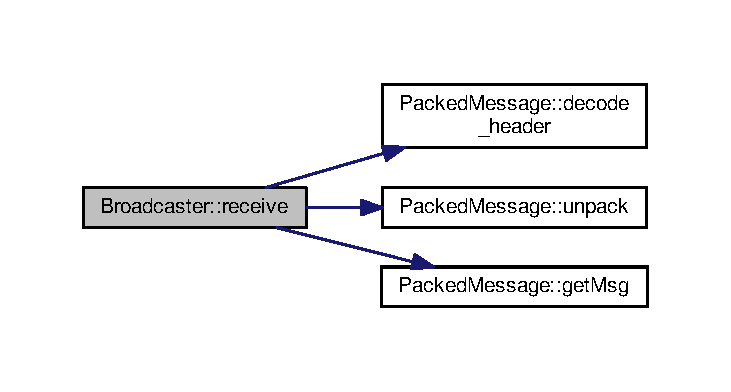
\includegraphics[width=350pt]{class_broadcaster_a29791f7e092b8da8747b0168b3bdb404_cgraph}
\end{center}
\end{figure}




Here is the caller graph for this function\+:
\nopagebreak
\begin{figure}[H]
\begin{center}
\leavevmode
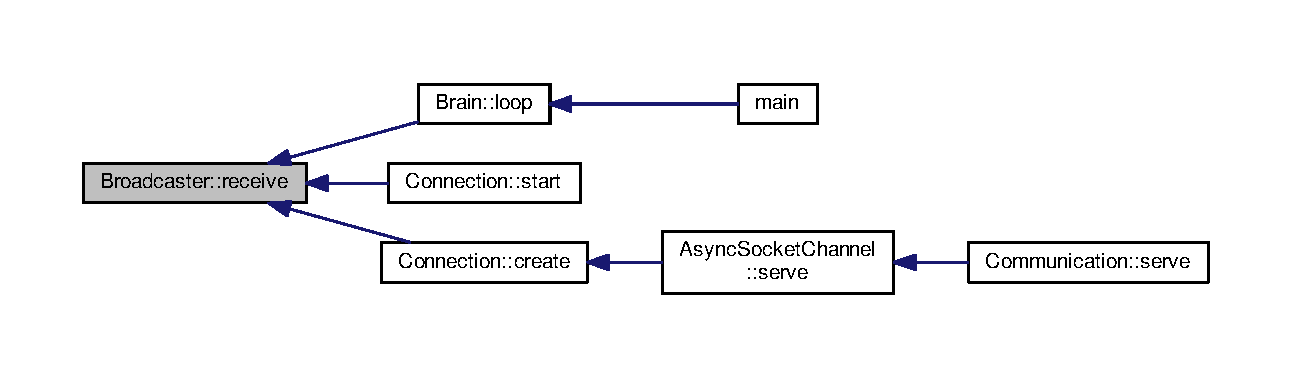
\includegraphics[width=350pt]{class_broadcaster_a29791f7e092b8da8747b0168b3bdb404_icgraph}
\end{center}
\end{figure}


\index{Broadcaster@{Broadcaster}!setup@{setup}}
\index{setup@{setup}!Broadcaster@{Broadcaster}}
\subsubsection[{\texorpdfstring{setup(unsigned short port)}{setup(unsigned short port)}}]{\setlength{\rightskip}{0pt plus 5cm}void Broadcaster\+::setup (
\begin{DoxyParamCaption}
\item[{unsigned short}]{port}
\end{DoxyParamCaption}
)}\hypertarget{class_broadcaster_a52e7aac07f5ef3528a3f0e9bb4dd69e2}{}\label{class_broadcaster_a52e7aac07f5ef3528a3f0e9bb4dd69e2}


Here is the caller graph for this function\+:
\nopagebreak
\begin{figure}[H]
\begin{center}
\leavevmode
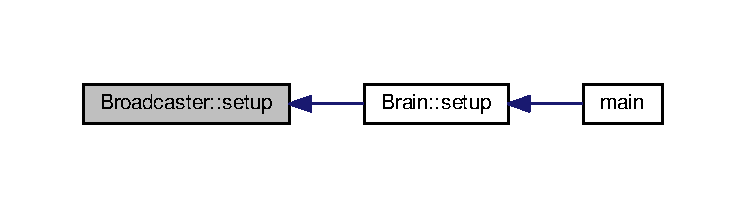
\includegraphics[width=350pt]{class_broadcaster_a52e7aac07f5ef3528a3f0e9bb4dd69e2_icgraph}
\end{center}
\end{figure}




The documentation for this class was generated from the following files\+:\begin{DoxyCompactItemize}
\item 
src/messages/\hyperlink{_broadcaster_8h}{Broadcaster.\+h}\item 
src/messages/\hyperlink{_broadcaster_8cpp}{Broadcaster.\+cpp}\end{DoxyCompactItemize}

\hypertarget{class_communication}{}\section{Communication Class Reference}
\label{class_communication}\index{Communication@{Communication}}


{\ttfamily \#include $<$Communication.\+h$>$}

\subsection*{Public Member Functions}
\begin{DoxyCompactItemize}
\item 
\hyperlink{class_communication_a88aa7a2d2ac5202e2b8eef787d1a8689}{Communication} ()
\item 
\hyperlink{class_communication_a75ba08ce908d45251e28e4c1db94e6f4}{$\sim$\+Communication} ()
\item 
void \hyperlink{class_communication_aed16e511327c62b6b5f418523f707a77}{serve} (unsigned short port)
\item 
void \hyperlink{class_communication_ab64912f9a4137b930d717d8a3140d693}{connect} (address\+\_\+v4 address, unsigned short port)
\item 
void \hyperlink{class_communication_a303009b7e1a4f714d02fb8729ea98f0b}{asociate} (\hyperlink{class_hello}{Hello} $\ast$hello)
\item 
bool \hyperlink{class_communication_a81b401f38b9eaa551e5eb8a18c9eb8f6}{message\+Available} ()
\item 
\hyperlink{class_message}{Message} \hyperlink{class_communication_a1afb3e9054cefe4daa0fcc1c78a69a9e}{get\+Message} ()
\item 
void \hyperlink{class_communication_aa837877847fe4b439f1b7137d4480157}{setup} (std\+::string name, unsigned int id)
\end{DoxyCompactItemize}


\subsection{Constructor \& Destructor Documentation}
\index{Communication@{Communication}!Communication@{Communication}}
\index{Communication@{Communication}!Communication@{Communication}}
\subsubsection[{\texorpdfstring{Communication()}{Communication()}}]{\setlength{\rightskip}{0pt plus 5cm}Communication\+::\+Communication (
\begin{DoxyParamCaption}
{}
\end{DoxyParamCaption}
)}\hypertarget{class_communication_a88aa7a2d2ac5202e2b8eef787d1a8689}{}\label{class_communication_a88aa7a2d2ac5202e2b8eef787d1a8689}
\index{Communication@{Communication}!````~Communication@{$\sim$\+Communication}}
\index{````~Communication@{$\sim$\+Communication}!Communication@{Communication}}
\subsubsection[{\texorpdfstring{$\sim$\+Communication()}{~Communication()}}]{\setlength{\rightskip}{0pt plus 5cm}Communication\+::$\sim$\+Communication (
\begin{DoxyParamCaption}
{}
\end{DoxyParamCaption}
)}\hypertarget{class_communication_a75ba08ce908d45251e28e4c1db94e6f4}{}\label{class_communication_a75ba08ce908d45251e28e4c1db94e6f4}


\subsection{Member Function Documentation}
\index{Communication@{Communication}!asociate@{asociate}}
\index{asociate@{asociate}!Communication@{Communication}}
\subsubsection[{\texorpdfstring{asociate(\+Hello $\ast$hello)}{asociate(Hello *hello)}}]{\setlength{\rightskip}{0pt plus 5cm}void Communication\+::asociate (
\begin{DoxyParamCaption}
\item[{{\bf Hello} $\ast$}]{hello}
\end{DoxyParamCaption}
)}\hypertarget{class_communication_a303009b7e1a4f714d02fb8729ea98f0b}{}\label{class_communication_a303009b7e1a4f714d02fb8729ea98f0b}
\index{Communication@{Communication}!connect@{connect}}
\index{connect@{connect}!Communication@{Communication}}
\subsubsection[{\texorpdfstring{connect(address\+\_\+v4 address, unsigned short port)}{connect(address_v4 address, unsigned short port)}}]{\setlength{\rightskip}{0pt plus 5cm}void Communication\+::connect (
\begin{DoxyParamCaption}
\item[{address\+\_\+v4}]{address, }
\item[{unsigned short}]{port}
\end{DoxyParamCaption}
)}\hypertarget{class_communication_ab64912f9a4137b930d717d8a3140d693}{}\label{class_communication_ab64912f9a4137b930d717d8a3140d693}
\index{Communication@{Communication}!get\+Message@{get\+Message}}
\index{get\+Message@{get\+Message}!Communication@{Communication}}
\subsubsection[{\texorpdfstring{get\+Message()}{getMessage()}}]{\setlength{\rightskip}{0pt plus 5cm}{\bf Message} Communication\+::get\+Message (
\begin{DoxyParamCaption}
{}
\end{DoxyParamCaption}
)}\hypertarget{class_communication_a1afb3e9054cefe4daa0fcc1c78a69a9e}{}\label{class_communication_a1afb3e9054cefe4daa0fcc1c78a69a9e}
\index{Communication@{Communication}!message\+Available@{message\+Available}}
\index{message\+Available@{message\+Available}!Communication@{Communication}}
\subsubsection[{\texorpdfstring{message\+Available()}{messageAvailable()}}]{\setlength{\rightskip}{0pt plus 5cm}bool Communication\+::message\+Available (
\begin{DoxyParamCaption}
{}
\end{DoxyParamCaption}
)}\hypertarget{class_communication_a81b401f38b9eaa551e5eb8a18c9eb8f6}{}\label{class_communication_a81b401f38b9eaa551e5eb8a18c9eb8f6}
\index{Communication@{Communication}!serve@{serve}}
\index{serve@{serve}!Communication@{Communication}}
\subsubsection[{\texorpdfstring{serve(unsigned short port)}{serve(unsigned short port)}}]{\setlength{\rightskip}{0pt plus 5cm}void Communication\+::serve (
\begin{DoxyParamCaption}
\item[{unsigned short}]{port}
\end{DoxyParamCaption}
)}\hypertarget{class_communication_aed16e511327c62b6b5f418523f707a77}{}\label{class_communication_aed16e511327c62b6b5f418523f707a77}
\index{Communication@{Communication}!setup@{setup}}
\index{setup@{setup}!Communication@{Communication}}
\subsubsection[{\texorpdfstring{setup(std\+::string name, unsigned int id)}{setup(std::string name, unsigned int id)}}]{\setlength{\rightskip}{0pt plus 5cm}void Communication\+::setup (
\begin{DoxyParamCaption}
\item[{std\+::string}]{name, }
\item[{unsigned int}]{id}
\end{DoxyParamCaption}
)}\hypertarget{class_communication_aa837877847fe4b439f1b7137d4480157}{}\label{class_communication_aa837877847fe4b439f1b7137d4480157}


The documentation for this class was generated from the following files\+:\begin{DoxyCompactItemize}
\item 
src/communication/\hyperlink{_communication_8h}{Communication.\+h}\item 
src/communication/\hyperlink{_communication_8cpp}{Communication.\+cpp}\end{DoxyCompactItemize}

\hypertarget{class_config}{}\section{Config Class Reference}
\label{class_config}\index{Config@{Config}}


{\ttfamily \#include $<$Config.\+h$>$}

\subsection*{Public Member Functions}
\begin{DoxyCompactItemize}
\item 
\hyperlink{class_config_abd0c571c116924871e30444b192b792a}{Config} ()
\item 
const std\+::string \& \hyperlink{class_config_a13187ce8db88e4cc61b5137a0da34b12}{get\+Name} () const 
\item 
void \hyperlink{class_config_a04f2e4ad0070a73728c4bce7b7dd0c29}{set\+Name} (const std\+::string \&name)
\item 
unsigned int \hyperlink{class_config_aa43aba31686b3c364b629e42cd492416}{get\+Id} () const 
\item 
void \hyperlink{class_config_af5ab41cca521bb760e228d3cd4ae73ea}{set\+Id} (unsigned int id)
\item 
const std\+::string \& \hyperlink{class_config_a1611555d61b524b6a2562643a59085eb}{get\+Body\+Host} () const 
\item 
void \hyperlink{class_config_a48f1e748dbd6a3257ec891f8338d6d72}{set\+Body\+Host} (const std\+::string \&body\+Host)
\item 
unsigned short \hyperlink{class_config_aea3a5f84be3a9cdf280fff77fdcb51f0}{get\+Body\+Port} () const 
\item 
void \hyperlink{class_config_a04fa867e4f0a01e8771f312a25f6cc75}{set\+Body\+Port} (unsigned short body\+Port)
\item 
unsigned short \hyperlink{class_config_a4362d19cea622b5438a70380aa965b69}{get\+Broadcast\+Port} () const 
\item 
void \hyperlink{class_config_a97e24672b3daed17bee2db3a0c8ee8db}{set\+Broadcast\+Port} (unsigned short broadcast\+Port)
\item 
int \hyperlink{class_config_acbfc17be8e733358890cddded4da52cc}{get\+Advertisement\+Lapse} () const 
\item 
void \hyperlink{class_config_abc2cc4f9cbca79ddcfbe8eb386f2140d}{set\+Advertisement\+Lapse} (int advertisement\+Lapse)
\end{DoxyCompactItemize}


\subsection{Constructor \& Destructor Documentation}
\index{Config@{Config}!Config@{Config}}
\index{Config@{Config}!Config@{Config}}
\subsubsection[{\texorpdfstring{Config()}{Config()}}]{\setlength{\rightskip}{0pt plus 5cm}Config\+::\+Config (
\begin{DoxyParamCaption}
{}
\end{DoxyParamCaption}
)}\hypertarget{class_config_abd0c571c116924871e30444b192b792a}{}\label{class_config_abd0c571c116924871e30444b192b792a}


\subsection{Member Function Documentation}
\index{Config@{Config}!get\+Advertisement\+Lapse@{get\+Advertisement\+Lapse}}
\index{get\+Advertisement\+Lapse@{get\+Advertisement\+Lapse}!Config@{Config}}
\subsubsection[{\texorpdfstring{get\+Advertisement\+Lapse() const }{getAdvertisementLapse() const }}]{\setlength{\rightskip}{0pt plus 5cm}int Config\+::get\+Advertisement\+Lapse (
\begin{DoxyParamCaption}
{}
\end{DoxyParamCaption}
) const}\hypertarget{class_config_acbfc17be8e733358890cddded4da52cc}{}\label{class_config_acbfc17be8e733358890cddded4da52cc}


Here is the caller graph for this function\+:
\nopagebreak
\begin{figure}[H]
\begin{center}
\leavevmode
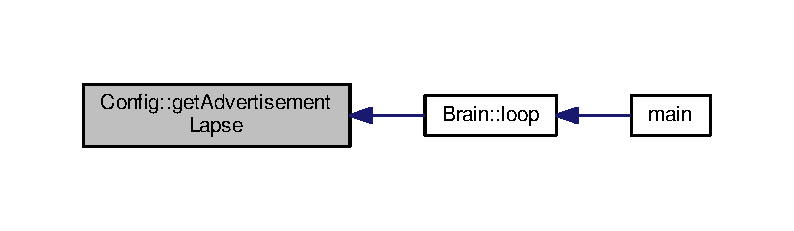
\includegraphics[width=350pt]{class_config_acbfc17be8e733358890cddded4da52cc_icgraph}
\end{center}
\end{figure}


\index{Config@{Config}!get\+Body\+Host@{get\+Body\+Host}}
\index{get\+Body\+Host@{get\+Body\+Host}!Config@{Config}}
\subsubsection[{\texorpdfstring{get\+Body\+Host() const }{getBrainHost() const }}]{\setlength{\rightskip}{0pt plus 5cm}const std\+::string \& Config\+::get\+Body\+Host (
\begin{DoxyParamCaption}
{}
\end{DoxyParamCaption}
) const}\hypertarget{class_config_a1611555d61b524b6a2562643a59085eb}{}\label{class_config_a1611555d61b524b6a2562643a59085eb}


Here is the caller graph for this function\+:
\nopagebreak
\begin{figure}[H]
\begin{center}
\leavevmode
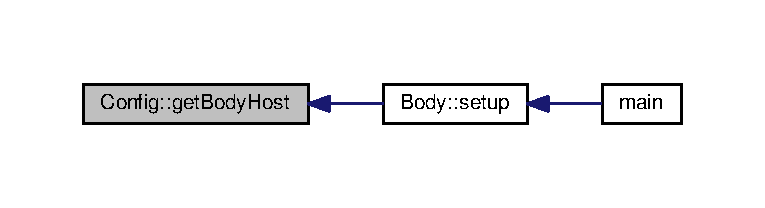
\includegraphics[width=350pt]{class_config_a1611555d61b524b6a2562643a59085eb_icgraph}
\end{center}
\end{figure}


\index{Config@{Config}!get\+Body\+Port@{get\+Body\+Port}}
\index{get\+Body\+Port@{get\+Body\+Port}!Config@{Config}}
\subsubsection[{\texorpdfstring{get\+Body\+Port() const }{getBodyPort() const }}]{\setlength{\rightskip}{0pt plus 5cm}unsigned short Config\+::get\+Body\+Port (
\begin{DoxyParamCaption}
{}
\end{DoxyParamCaption}
) const}\hypertarget{class_config_aea3a5f84be3a9cdf280fff77fdcb51f0}{}\label{class_config_aea3a5f84be3a9cdf280fff77fdcb51f0}


Here is the caller graph for this function\+:
\nopagebreak
\begin{figure}[H]
\begin{center}
\leavevmode
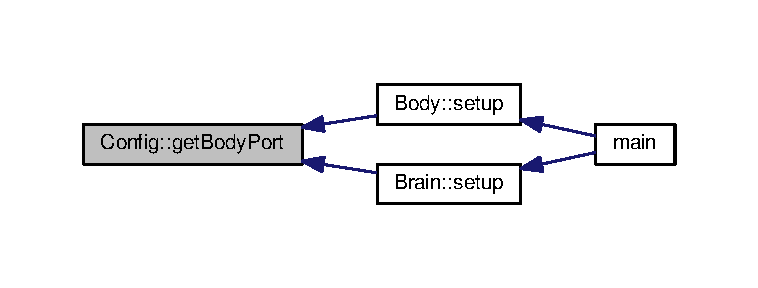
\includegraphics[width=350pt]{class_config_aea3a5f84be3a9cdf280fff77fdcb51f0_icgraph}
\end{center}
\end{figure}


\index{Config@{Config}!get\+Broadcast\+Port@{get\+Broadcast\+Port}}
\index{get\+Broadcast\+Port@{get\+Broadcast\+Port}!Config@{Config}}
\subsubsection[{\texorpdfstring{get\+Broadcast\+Port() const }{getBroadcastPort() const }}]{\setlength{\rightskip}{0pt plus 5cm}unsigned short Config\+::get\+Broadcast\+Port (
\begin{DoxyParamCaption}
{}
\end{DoxyParamCaption}
) const}\hypertarget{class_config_a4362d19cea622b5438a70380aa965b69}{}\label{class_config_a4362d19cea622b5438a70380aa965b69}


Here is the caller graph for this function\+:
\nopagebreak
\begin{figure}[H]
\begin{center}
\leavevmode
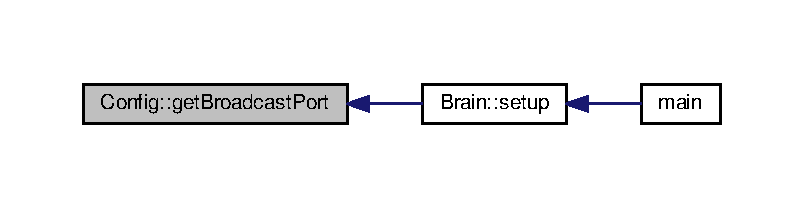
\includegraphics[width=350pt]{class_config_a4362d19cea622b5438a70380aa965b69_icgraph}
\end{center}
\end{figure}


\index{Config@{Config}!get\+Id@{get\+Id}}
\index{get\+Id@{get\+Id}!Config@{Config}}
\subsubsection[{\texorpdfstring{get\+Id() const }{getId() const }}]{\setlength{\rightskip}{0pt plus 5cm}unsigned int Config\+::get\+Id (
\begin{DoxyParamCaption}
{}
\end{DoxyParamCaption}
) const}\hypertarget{class_config_aa43aba31686b3c364b629e42cd492416}{}\label{class_config_aa43aba31686b3c364b629e42cd492416}


Here is the caller graph for this function\+:
\nopagebreak
\begin{figure}[H]
\begin{center}
\leavevmode
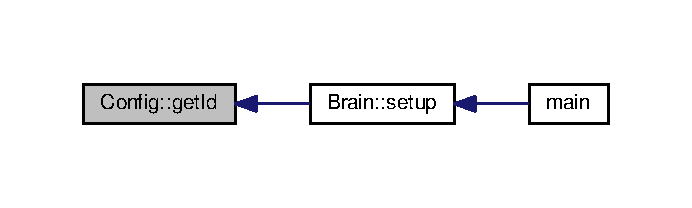
\includegraphics[width=332pt]{class_config_aa43aba31686b3c364b629e42cd492416_icgraph}
\end{center}
\end{figure}


\index{Config@{Config}!get\+Name@{get\+Name}}
\index{get\+Name@{get\+Name}!Config@{Config}}
\subsubsection[{\texorpdfstring{get\+Name() const }{getName() const }}]{\setlength{\rightskip}{0pt plus 5cm}const std\+::string \& Config\+::get\+Name (
\begin{DoxyParamCaption}
{}
\end{DoxyParamCaption}
) const}\hypertarget{class_config_a13187ce8db88e4cc61b5137a0da34b12}{}\label{class_config_a13187ce8db88e4cc61b5137a0da34b12}


Here is the caller graph for this function\+:
\nopagebreak
\begin{figure}[H]
\begin{center}
\leavevmode
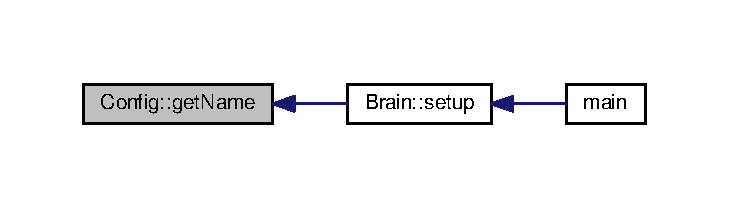
\includegraphics[width=350pt]{class_config_a13187ce8db88e4cc61b5137a0da34b12_icgraph}
\end{center}
\end{figure}


\index{Config@{Config}!set\+Advertisement\+Lapse@{set\+Advertisement\+Lapse}}
\index{set\+Advertisement\+Lapse@{set\+Advertisement\+Lapse}!Config@{Config}}
\subsubsection[{\texorpdfstring{set\+Advertisement\+Lapse(int advertisement\+Lapse)}{setAdvertisementLapse(int stateSendLapse)}}]{\setlength{\rightskip}{0pt plus 5cm}void Config\+::set\+Advertisement\+Lapse (
\begin{DoxyParamCaption}
\item[{int}]{advertisement\+Lapse}
\end{DoxyParamCaption}
)}\hypertarget{class_config_abc2cc4f9cbca79ddcfbe8eb386f2140d}{}\label{class_config_abc2cc4f9cbca79ddcfbe8eb386f2140d}
\index{Config@{Config}!set\+Body\+Host@{set\+Body\+Host}}
\index{set\+Body\+Host@{set\+Body\+Host}!Config@{Config}}
\subsubsection[{\texorpdfstring{set\+Body\+Host(const std\+::string \&body\+Host)}{setBodyHost(const std::string &bodyHost)}}]{\setlength{\rightskip}{0pt plus 5cm}void Config\+::set\+Body\+Host (
\begin{DoxyParamCaption}
\item[{const std\+::string \&}]{body\+Host}
\end{DoxyParamCaption}
)}\hypertarget{class_config_a48f1e748dbd6a3257ec891f8338d6d72}{}\label{class_config_a48f1e748dbd6a3257ec891f8338d6d72}
\index{Config@{Config}!set\+Body\+Port@{set\+Body\+Port}}
\index{set\+Body\+Port@{set\+Body\+Port}!Config@{Config}}
\subsubsection[{\texorpdfstring{set\+Body\+Port(unsigned short body\+Port)}{setBodyPort(unsigned short bodyPort)}}]{\setlength{\rightskip}{0pt plus 5cm}void Config\+::set\+Body\+Port (
\begin{DoxyParamCaption}
\item[{unsigned short}]{body\+Port}
\end{DoxyParamCaption}
)}\hypertarget{class_config_a04fa867e4f0a01e8771f312a25f6cc75}{}\label{class_config_a04fa867e4f0a01e8771f312a25f6cc75}
\index{Config@{Config}!set\+Broadcast\+Port@{set\+Broadcast\+Port}}
\index{set\+Broadcast\+Port@{set\+Broadcast\+Port}!Config@{Config}}
\subsubsection[{\texorpdfstring{set\+Broadcast\+Port(unsigned short broadcast\+Port)}{setBroadcastPort(unsigned short broadcastPort)}}]{\setlength{\rightskip}{0pt plus 5cm}void Config\+::set\+Broadcast\+Port (
\begin{DoxyParamCaption}
\item[{unsigned short}]{broadcast\+Port}
\end{DoxyParamCaption}
)}\hypertarget{class_config_a97e24672b3daed17bee2db3a0c8ee8db}{}\label{class_config_a97e24672b3daed17bee2db3a0c8ee8db}
\index{Config@{Config}!set\+Id@{set\+Id}}
\index{set\+Id@{set\+Id}!Config@{Config}}
\subsubsection[{\texorpdfstring{set\+Id(unsigned int id)}{setId(unsigned int id)}}]{\setlength{\rightskip}{0pt plus 5cm}void Config\+::set\+Id (
\begin{DoxyParamCaption}
\item[{unsigned int}]{id}
\end{DoxyParamCaption}
)}\hypertarget{class_config_af5ab41cca521bb760e228d3cd4ae73ea}{}\label{class_config_af5ab41cca521bb760e228d3cd4ae73ea}
\index{Config@{Config}!set\+Name@{set\+Name}}
\index{set\+Name@{set\+Name}!Config@{Config}}
\subsubsection[{\texorpdfstring{set\+Name(const std\+::string \&name)}{setName(const std::string &name)}}]{\setlength{\rightskip}{0pt plus 5cm}void Config\+::set\+Name (
\begin{DoxyParamCaption}
\item[{const std\+::string \&}]{name}
\end{DoxyParamCaption}
)}\hypertarget{class_config_a04f2e4ad0070a73728c4bce7b7dd0c29}{}\label{class_config_a04f2e4ad0070a73728c4bce7b7dd0c29}


The documentation for this class was generated from the following files\+:\begin{DoxyCompactItemize}
\item 
src/\hyperlink{_config_8h}{Config.\+h}\item 
src/\hyperlink{_config_8cpp}{Config.\+cpp}\end{DoxyCompactItemize}

\hypertarget{class_connection}{}\section{Connection Class Reference}
\label{class_connection}\index{Connection@{Connection}}


{\ttfamily \#include $<$Connection.\+h$>$}



Inheritance diagram for Connection\+:
\nopagebreak
\begin{figure}[H]
\begin{center}
\leavevmode
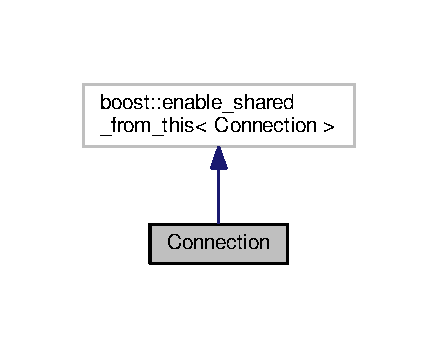
\includegraphics[width=210pt]{class_connection__inherit__graph}
\end{center}
\end{figure}


Collaboration diagram for Connection\+:
\nopagebreak
\begin{figure}[H]
\begin{center}
\leavevmode
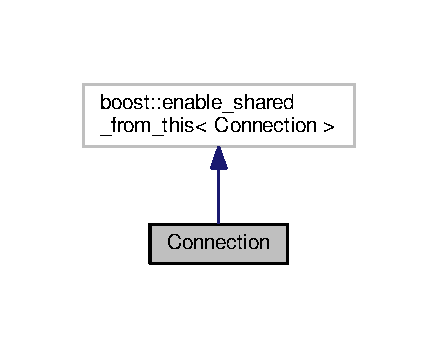
\includegraphics[width=210pt]{class_connection__coll__graph}
\end{center}
\end{figure}
\subsection*{Public Types}
\begin{DoxyCompactItemize}
\item 
typedef boost\+::shared\+\_\+ptr$<$ \hyperlink{class_connection}{Connection} $>$ \hyperlink{class_connection_afc73789251390ec9c9c6e3750b104f08}{Pointer}
\end{DoxyCompactItemize}
\subsection*{Public Member Functions}
\begin{DoxyCompactItemize}
\item 
void \hyperlink{class_connection_a47c25a31352a71e2a6902d37fc5fa2ba}{start} ()
\item 
void \hyperlink{class_connection_a484d8c6cc1426b9c00980acdd28c000d}{send} (\hyperlink{class_message}{Message} msg)
\item 
boost\+::asio\+::ip\+::address\+\_\+v4 \hyperlink{class_connection_a1aaf9861212ce321849edac339efed0f}{get\+Ip} ()
\item 
unsigned short \hyperlink{class_connection_a898e60a2d6ec6b8b25e3299bb15972fc}{get\+Port} ()
\item 
boost\+::asio\+::ip\+::tcp\+::socket \& \hyperlink{class_connection_aba7b36e96bdd0b2495b3f8c6850a3ce9}{get\+Socket} ()
\end{DoxyCompactItemize}
\subsection*{Static Public Member Functions}
\begin{DoxyCompactItemize}
\item 
static \hyperlink{class_connection_afc73789251390ec9c9c6e3750b104f08}{Pointer} \hyperlink{class_connection_a55342f6aeedd34fc6a11dd79b59da69b}{create} (boost\+::asio\+::io\+\_\+service \&io\+\_\+service, \hyperlink{class_message_queue}{Message\+Queue} $\ast$queue)
\end{DoxyCompactItemize}


\subsection{Member Typedef Documentation}
\index{Connection@{Connection}!Pointer@{Pointer}}
\index{Pointer@{Pointer}!Connection@{Connection}}
\subsubsection[{\texorpdfstring{Pointer}{Pointer}}]{\setlength{\rightskip}{0pt plus 5cm}typedef boost\+::shared\+\_\+ptr$<${\bf Connection}$>$ {\bf Connection\+::\+Pointer}}\hypertarget{class_connection_afc73789251390ec9c9c6e3750b104f08}{}\label{class_connection_afc73789251390ec9c9c6e3750b104f08}


\subsection{Member Function Documentation}
\index{Connection@{Connection}!create@{create}}
\index{create@{create}!Connection@{Connection}}
\subsubsection[{\texorpdfstring{create(boost\+::asio\+::io\+\_\+service \&io\+\_\+service, Message\+Queue $\ast$queue)}{create(boost::asio::io_service &io_service, MessageQueue *queue)}}]{\setlength{\rightskip}{0pt plus 5cm}{\bf Connection\+::\+Pointer} Connection\+::create (
\begin{DoxyParamCaption}
\item[{boost\+::asio\+::io\+\_\+service \&}]{io\+\_\+service, }
\item[{{\bf Message\+Queue} $\ast$}]{queue}
\end{DoxyParamCaption}
)\hspace{0.3cm}{\ttfamily [static]}}\hypertarget{class_connection_a55342f6aeedd34fc6a11dd79b59da69b}{}\label{class_connection_a55342f6aeedd34fc6a11dd79b59da69b}
\index{Connection@{Connection}!get\+Ip@{get\+Ip}}
\index{get\+Ip@{get\+Ip}!Connection@{Connection}}
\subsubsection[{\texorpdfstring{get\+Ip()}{getIp()}}]{\setlength{\rightskip}{0pt plus 5cm}asio\+::ip\+::address\+\_\+v4 Connection\+::get\+Ip (
\begin{DoxyParamCaption}
{}
\end{DoxyParamCaption}
)}\hypertarget{class_connection_a1aaf9861212ce321849edac339efed0f}{}\label{class_connection_a1aaf9861212ce321849edac339efed0f}
\index{Connection@{Connection}!get\+Port@{get\+Port}}
\index{get\+Port@{get\+Port}!Connection@{Connection}}
\subsubsection[{\texorpdfstring{get\+Port()}{getPort()}}]{\setlength{\rightskip}{0pt plus 5cm}unsigned short Connection\+::get\+Port (
\begin{DoxyParamCaption}
{}
\end{DoxyParamCaption}
)}\hypertarget{class_connection_a898e60a2d6ec6b8b25e3299bb15972fc}{}\label{class_connection_a898e60a2d6ec6b8b25e3299bb15972fc}
\index{Connection@{Connection}!get\+Socket@{get\+Socket}}
\index{get\+Socket@{get\+Socket}!Connection@{Connection}}
\subsubsection[{\texorpdfstring{get\+Socket()}{getSocket()}}]{\setlength{\rightskip}{0pt plus 5cm}tcp\+::socket \& Connection\+::get\+Socket (
\begin{DoxyParamCaption}
{}
\end{DoxyParamCaption}
)}\hypertarget{class_connection_aba7b36e96bdd0b2495b3f8c6850a3ce9}{}\label{class_connection_aba7b36e96bdd0b2495b3f8c6850a3ce9}
\index{Connection@{Connection}!send@{send}}
\index{send@{send}!Connection@{Connection}}
\subsubsection[{\texorpdfstring{send(\+Message msg)}{send(Message msg)}}]{\setlength{\rightskip}{0pt plus 5cm}void Connection\+::send (
\begin{DoxyParamCaption}
\item[{{\bf Message}}]{msg}
\end{DoxyParamCaption}
)}\hypertarget{class_connection_a484d8c6cc1426b9c00980acdd28c000d}{}\label{class_connection_a484d8c6cc1426b9c00980acdd28c000d}
\index{Connection@{Connection}!start@{start}}
\index{start@{start}!Connection@{Connection}}
\subsubsection[{\texorpdfstring{start()}{start()}}]{\setlength{\rightskip}{0pt plus 5cm}void Connection\+::start (
\begin{DoxyParamCaption}
{}
\end{DoxyParamCaption}
)}\hypertarget{class_connection_a47c25a31352a71e2a6902d37fc5fa2ba}{}\label{class_connection_a47c25a31352a71e2a6902d37fc5fa2ba}


The documentation for this class was generated from the following files\+:\begin{DoxyCompactItemize}
\item 
src/messages/\hyperlink{_connection_8h}{Connection.\+h}\item 
src/messages/\hyperlink{_connection_8cpp}{Connection.\+cpp}\end{DoxyCompactItemize}

\hypertarget{class_detect_and_track}{}\section{Detect\+And\+Track Class Reference}
\label{class_detect_and_track}\index{Detect\+And\+Track@{Detect\+And\+Track}}


{\ttfamily \#include $<$Detect\+And\+Track.\+h$>$}

\subsection*{Public Member Functions}
\begin{DoxyCompactItemize}
\item 
\hyperlink{class_detect_and_track_ace7bef0f1cf9fc28292e7cf0c5e5ba1d}{Detect\+And\+Track} (\hyperlink{class_detection_algorithm}{Detection\+Algorithm} $\ast$detector, \hyperlink{class_tracking_algorithm}{Tracking\+Algorithm} $\ast$tracker)
\item 
std\+::vector$<$ \hyperlink{class_track}{Track} $>$ \hyperlink{class_detect_and_track_a1b07a50a71807fea2f99d43a3de29912}{update} (cv\+::\+Mat frame)
\end{DoxyCompactItemize}
\subsection*{Public Attributes}
\begin{DoxyCompactItemize}
\item 
const double \hyperlink{class_detect_and_track_a234e0a61c8eb494d72e562f69173d911}{K\+E\+E\+P\+\_\+\+T\+R\+A\+C\+K\+\_\+\+O\+V\+E\+R\+L\+A\+P\+\_\+\+T\+H\+R\+E\+S\+H\+O\+LD} = 0.\+3
\end{DoxyCompactItemize}


\subsection{Constructor \& Destructor Documentation}
\index{Detect\+And\+Track@{Detect\+And\+Track}!Detect\+And\+Track@{Detect\+And\+Track}}
\index{Detect\+And\+Track@{Detect\+And\+Track}!Detect\+And\+Track@{Detect\+And\+Track}}
\subsubsection[{\texorpdfstring{Detect\+And\+Track(\+Detection\+Algorithm $\ast$detector, Tracking\+Algorithm $\ast$tracker)}{DetectAndTrack(DetectionAlgorithm *detector, TrackingAlgorithm *tracker)}}]{\setlength{\rightskip}{0pt plus 5cm}Detect\+And\+Track\+::\+Detect\+And\+Track (
\begin{DoxyParamCaption}
\item[{{\bf Detection\+Algorithm} $\ast$}]{detector, }
\item[{{\bf Tracking\+Algorithm} $\ast$}]{tracker}
\end{DoxyParamCaption}
)}\hypertarget{class_detect_and_track_ace7bef0f1cf9fc28292e7cf0c5e5ba1d}{}\label{class_detect_and_track_ace7bef0f1cf9fc28292e7cf0c5e5ba1d}


\subsection{Member Function Documentation}
\index{Detect\+And\+Track@{Detect\+And\+Track}!update@{update}}
\index{update@{update}!Detect\+And\+Track@{Detect\+And\+Track}}
\subsubsection[{\texorpdfstring{update(cv\+::\+Mat frame)}{update(cv::Mat frame)}}]{\setlength{\rightskip}{0pt plus 5cm}std\+::vector$<$ {\bf Track} $>$ Detect\+And\+Track\+::update (
\begin{DoxyParamCaption}
\item[{cv\+::\+Mat}]{frame}
\end{DoxyParamCaption}
)}\hypertarget{class_detect_and_track_a1b07a50a71807fea2f99d43a3de29912}{}\label{class_detect_and_track_a1b07a50a71807fea2f99d43a3de29912}


Here is the call graph for this function\+:
\nopagebreak
\begin{figure}[H]
\begin{center}
\leavevmode
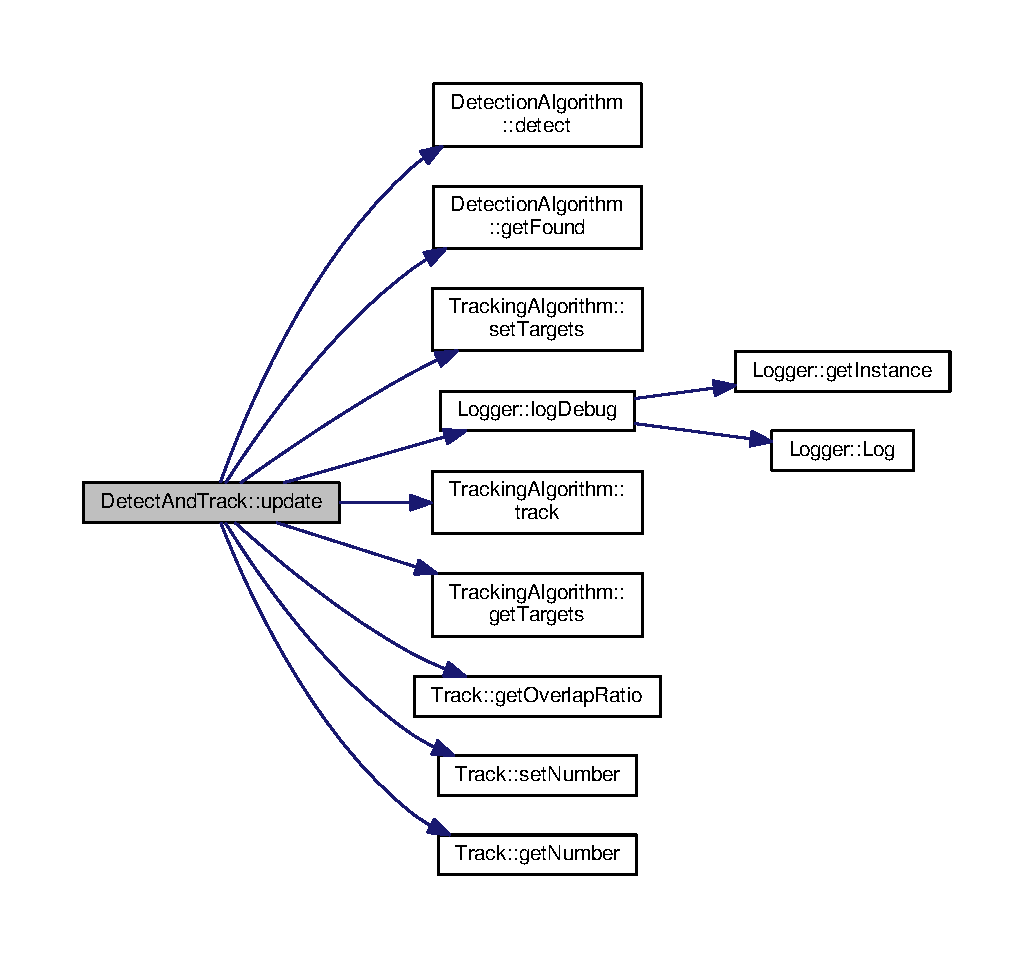
\includegraphics[width=350pt]{class_detect_and_track_a1b07a50a71807fea2f99d43a3de29912_cgraph}
\end{center}
\end{figure}




Here is the caller graph for this function\+:
\nopagebreak
\begin{figure}[H]
\begin{center}
\leavevmode
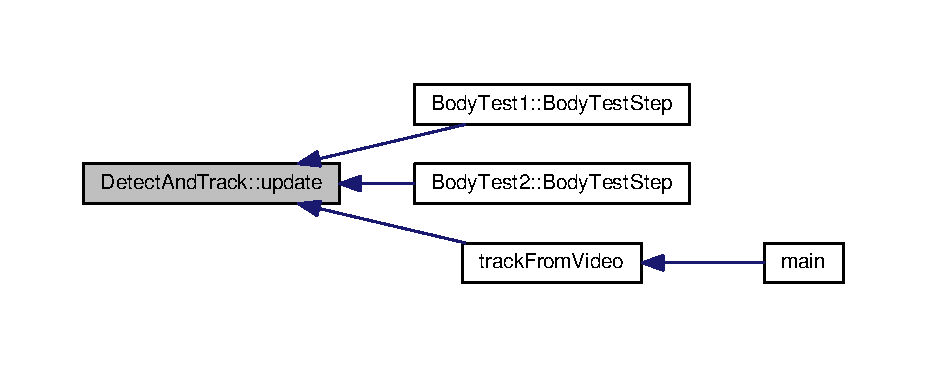
\includegraphics[width=350pt]{class_detect_and_track_a1b07a50a71807fea2f99d43a3de29912_icgraph}
\end{center}
\end{figure}




\subsection{Member Data Documentation}
\index{Detect\+And\+Track@{Detect\+And\+Track}!K\+E\+E\+P\+\_\+\+T\+R\+A\+C\+K\+\_\+\+O\+V\+E\+R\+L\+A\+P\+\_\+\+T\+H\+R\+E\+S\+H\+O\+LD@{K\+E\+E\+P\+\_\+\+T\+R\+A\+C\+K\+\_\+\+O\+V\+E\+R\+L\+A\+P\+\_\+\+T\+H\+R\+E\+S\+H\+O\+LD}}
\index{K\+E\+E\+P\+\_\+\+T\+R\+A\+C\+K\+\_\+\+O\+V\+E\+R\+L\+A\+P\+\_\+\+T\+H\+R\+E\+S\+H\+O\+LD@{K\+E\+E\+P\+\_\+\+T\+R\+A\+C\+K\+\_\+\+O\+V\+E\+R\+L\+A\+P\+\_\+\+T\+H\+R\+E\+S\+H\+O\+LD}!Detect\+And\+Track@{Detect\+And\+Track}}
\subsubsection[{\texorpdfstring{K\+E\+E\+P\+\_\+\+T\+R\+A\+C\+K\+\_\+\+O\+V\+E\+R\+L\+A\+P\+\_\+\+T\+H\+R\+E\+S\+H\+O\+LD}{KEEP_TRACK_OVERLAP_THRESHOLD}}]{\setlength{\rightskip}{0pt plus 5cm}const double Detect\+And\+Track\+::\+K\+E\+E\+P\+\_\+\+T\+R\+A\+C\+K\+\_\+\+O\+V\+E\+R\+L\+A\+P\+\_\+\+T\+H\+R\+E\+S\+H\+O\+LD = 0.\+3}\hypertarget{class_detect_and_track_a234e0a61c8eb494d72e562f69173d911}{}\label{class_detect_and_track_a234e0a61c8eb494d72e562f69173d911}


The documentation for this class was generated from the following files\+:\begin{DoxyCompactItemize}
\item 
src/tracking/\hyperlink{_detect_and_track_8h}{Detect\+And\+Track.\+h}\item 
src/tracking/\hyperlink{_detect_and_track_8cpp}{Detect\+And\+Track.\+cpp}\end{DoxyCompactItemize}

\hypertarget{class_detection_algorithm}{}\section{Detection\+Algorithm Class Reference}
\label{class_detection_algorithm}\index{Detection\+Algorithm@{Detection\+Algorithm}}


{\ttfamily \#include $<$Detection\+Algorithm.\+h$>$}



Inheritance diagram for Detection\+Algorithm\+:
\nopagebreak
\begin{figure}[H]
\begin{center}
\leavevmode
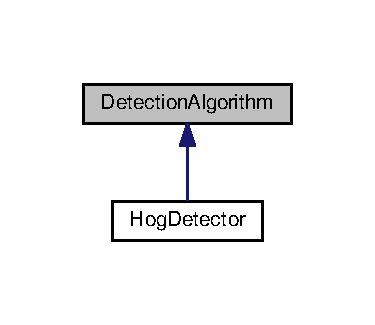
\includegraphics[width=180pt]{class_detection_algorithm__inherit__graph}
\end{center}
\end{figure}
\subsection*{Public Member Functions}
\begin{DoxyCompactItemize}
\item 
virtual std\+::vector$<$ cv\+::\+Rect2d $>$ \hyperlink{class_detection_algorithm_a0edb312eb9379d1bbf6ca46ac488fb8c}{get\+Found} ()=0
\item 
virtual void \hyperlink{class_detection_algorithm_af7d9604a66afa93f4ae9f232d6a60a3d}{detect} (cv\+::\+Mat frame)=0
\end{DoxyCompactItemize}


\subsection{Member Function Documentation}
\index{Detection\+Algorithm@{Detection\+Algorithm}!detect@{detect}}
\index{detect@{detect}!Detection\+Algorithm@{Detection\+Algorithm}}
\subsubsection[{\texorpdfstring{detect(cv\+::\+Mat frame)=0}{detect(cv::Mat frame)=0}}]{\setlength{\rightskip}{0pt plus 5cm}virtual void Detection\+Algorithm\+::detect (
\begin{DoxyParamCaption}
\item[{cv\+::\+Mat}]{frame}
\end{DoxyParamCaption}
)\hspace{0.3cm}{\ttfamily [pure virtual]}}\hypertarget{class_detection_algorithm_af7d9604a66afa93f4ae9f232d6a60a3d}{}\label{class_detection_algorithm_af7d9604a66afa93f4ae9f232d6a60a3d}


Implemented in \hyperlink{class_hog_detector_ae2b318cb53c6a319fd8b6b936bf2e925}{Hog\+Detector}.

\index{Detection\+Algorithm@{Detection\+Algorithm}!get\+Found@{get\+Found}}
\index{get\+Found@{get\+Found}!Detection\+Algorithm@{Detection\+Algorithm}}
\subsubsection[{\texorpdfstring{get\+Found()=0}{getFound()=0}}]{\setlength{\rightskip}{0pt plus 5cm}virtual std\+::vector$<$cv\+::\+Rect2d$>$ Detection\+Algorithm\+::get\+Found (
\begin{DoxyParamCaption}
{}
\end{DoxyParamCaption}
)\hspace{0.3cm}{\ttfamily [pure virtual]}}\hypertarget{class_detection_algorithm_a0edb312eb9379d1bbf6ca46ac488fb8c}{}\label{class_detection_algorithm_a0edb312eb9379d1bbf6ca46ac488fb8c}


Implemented in \hyperlink{class_hog_detector_adf1cc226d11238634042efb009b39674}{Hog\+Detector}.



The documentation for this class was generated from the following file\+:\begin{DoxyCompactItemize}
\item 
src/tracking/\hyperlink{_detection_algorithm_8h}{Detection\+Algorithm.\+h}\end{DoxyCompactItemize}

\hypertarget{class_do_shutdown}{}\section{Do\+Shutdown Class Reference}
\label{class_do_shutdown}\index{Do\+Shutdown@{Do\+Shutdown}}


{\ttfamily \#include $<$shutdown.\+pb.\+h$>$}



Inheritance diagram for Do\+Shutdown\+:
\nopagebreak
\begin{figure}[H]
\begin{center}
\leavevmode
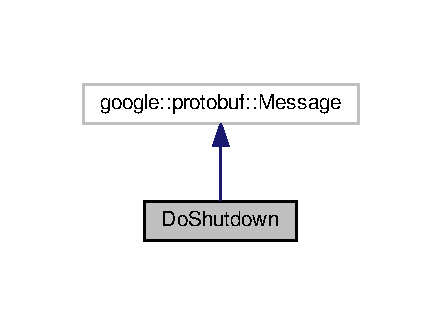
\includegraphics[width=212pt]{class_do_shutdown__inherit__graph}
\end{center}
\end{figure}


Collaboration diagram for Do\+Shutdown\+:
\nopagebreak
\begin{figure}[H]
\begin{center}
\leavevmode
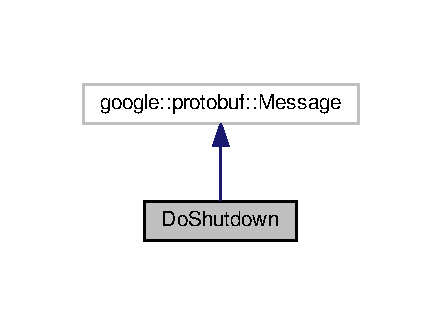
\includegraphics[width=212pt]{class_do_shutdown__coll__graph}
\end{center}
\end{figure}
\subsection*{Public Member Functions}
\begin{DoxyCompactItemize}
\item 
\hyperlink{class_do_shutdown_a9e41496fb2642ab0956aeb03e79f2ffc}{Do\+Shutdown} ()
\item 
virtual \hyperlink{class_do_shutdown_acdc83e4c56ce5cbdcb7c1ea6c146e75f}{$\sim$\+Do\+Shutdown} ()
\item 
\hyperlink{class_do_shutdown_abbb12bcbdeb136fe4896153ccefb4058}{Do\+Shutdown} (const \hyperlink{class_do_shutdown}{Do\+Shutdown} \&from)
\item 
\hyperlink{class_do_shutdown}{Do\+Shutdown} \& \hyperlink{class_do_shutdown_a254bcb06ff69ece5ed5ea7cdbe19e7dc}{operator=} (const \hyperlink{class_do_shutdown}{Do\+Shutdown} \&from)
\item 
void \hyperlink{class_do_shutdown_a331c8643e8b18c7b0bf2c1391de46067}{Swap} (\hyperlink{class_do_shutdown}{Do\+Shutdown} $\ast$other)
\item 
\hyperlink{class_do_shutdown}{Do\+Shutdown} $\ast$ \hyperlink{class_do_shutdown_a13aa27286876300bd7c506812f8479ba}{New} () const P\+R\+O\+T\+O\+B\+U\+F\+\_\+\+F\+I\+N\+AL
\item 
\hyperlink{class_do_shutdown}{Do\+Shutdown} $\ast$ \hyperlink{class_do_shutdown_af046b34c1f60919fb75263cf208c84df}{New} (\+::google\+::protobuf\+::\+Arena $\ast$arena) const P\+R\+O\+T\+O\+B\+U\+F\+\_\+\+F\+I\+N\+AL
\item 
void \hyperlink{class_do_shutdown_ad5876e00a840a19406a13ac089553f97}{Copy\+From} (const \+::google\+::protobuf\+::\+Message \&from) P\+R\+O\+T\+O\+B\+U\+F\+\_\+\+F\+I\+N\+AL
\item 
void \hyperlink{class_do_shutdown_a367300e6485923b044fdcea2630d4cc3}{Merge\+From} (const \+::google\+::protobuf\+::\+Message \&from) P\+R\+O\+T\+O\+B\+U\+F\+\_\+\+F\+I\+N\+AL
\item 
void \hyperlink{class_do_shutdown_aab7f76cef5e12622def6c90801e2cacf}{Copy\+From} (const \hyperlink{class_do_shutdown}{Do\+Shutdown} \&from)
\item 
void \hyperlink{class_do_shutdown_aded6118b22cf31c18d0fe58af6fce37e}{Merge\+From} (const \hyperlink{class_do_shutdown}{Do\+Shutdown} \&from)
\item 
void \hyperlink{class_do_shutdown_a88dae4aa7ac119a7b87dd08db805f4ee}{Clear} () P\+R\+O\+T\+O\+B\+U\+F\+\_\+\+F\+I\+N\+AL
\item 
bool \hyperlink{class_do_shutdown_a1a202ffa75c33eac706f04eb501d1089}{Is\+Initialized} () const P\+R\+O\+T\+O\+B\+U\+F\+\_\+\+F\+I\+N\+AL
\item 
size\+\_\+t \hyperlink{class_do_shutdown_a36e573c232da258498228579141190aa}{Byte\+Size\+Long} () const P\+R\+O\+T\+O\+B\+U\+F\+\_\+\+F\+I\+N\+AL
\item 
bool \hyperlink{class_do_shutdown_adc9b83c923b2e4bb8b843f7400f1d3e1}{Merge\+Partial\+From\+Coded\+Stream} (\+::google\+::protobuf\+::io\+::\+Coded\+Input\+Stream $\ast$input) P\+R\+O\+T\+O\+B\+U\+F\+\_\+\+F\+I\+N\+AL
\item 
void \hyperlink{class_do_shutdown_aea724703f66a2e7af297d10af1d4e0c5}{Serialize\+With\+Cached\+Sizes} (\+::google\+::protobuf\+::io\+::\+Coded\+Output\+Stream $\ast$output) const P\+R\+O\+T\+O\+B\+U\+F\+\_\+\+F\+I\+N\+AL
\item 
\+::google\+::protobuf\+::uint8 $\ast$ \hyperlink{class_do_shutdown_a41be0c5e3ff0bf16f15e0bab33fe2bb2}{Internal\+Serialize\+With\+Cached\+Sizes\+To\+Array} (bool deterministic,\+::google\+::protobuf\+::uint8 $\ast$target) const P\+R\+O\+T\+O\+B\+U\+F\+\_\+\+F\+I\+N\+AL
\item 
\+::google\+::protobuf\+::uint8 $\ast$ \hyperlink{class_do_shutdown_a0ad12d5aaf4613fad5819b2dea94186b}{Serialize\+With\+Cached\+Sizes\+To\+Array} (\+::google\+::protobuf\+::uint8 $\ast$output) const P\+R\+O\+T\+O\+B\+U\+F\+\_\+\+F\+I\+N\+AL
\item 
int \hyperlink{class_do_shutdown_a777d4dd7d704d95ccc6602504aca1bef}{Get\+Cached\+Size} () const P\+R\+O\+T\+O\+B\+U\+F\+\_\+\+F\+I\+N\+AL
\item 
\+::google\+::protobuf\+::\+Metadata \hyperlink{class_do_shutdown_afdf336a80f04202a41dc30c877f4387a}{Get\+Metadata} () const P\+R\+O\+T\+O\+B\+U\+F\+\_\+\+F\+I\+N\+AL
\item 
void \hyperlink{class_do_shutdown_adb04131ab945007f6a26dd354cda5646}{clear\+\_\+force} ()
\item 
bool \hyperlink{class_do_shutdown_ae470392499921248bf6c46c58d233f6d}{force} () const 
\item 
void \hyperlink{class_do_shutdown_ae7fa2e4d96746b439cfad473a0ec2192}{set\+\_\+force} (bool value)
\end{DoxyCompactItemize}
\subsection*{Static Public Member Functions}
\begin{DoxyCompactItemize}
\item 
static const \+::google\+::protobuf\+::\+Descriptor $\ast$ \hyperlink{class_do_shutdown_a61d5d64fc5fc0961878a4a21536a5318}{descriptor} ()
\item 
static const \hyperlink{class_do_shutdown}{Do\+Shutdown} \& \hyperlink{class_do_shutdown_a91bbc47476d16a7f942b6a739ba55c95}{default\+\_\+instance} ()
\item 
static const \hyperlink{class_do_shutdown}{Do\+Shutdown} $\ast$ \hyperlink{class_do_shutdown_ab0bbc935fc413a234f1db826b6e51f00}{internal\+\_\+default\+\_\+instance} ()
\end{DoxyCompactItemize}
\subsection*{Static Public Attributes}
\begin{DoxyCompactItemize}
\item 
static const int \hyperlink{class_do_shutdown_a2e2fc6a82227b39713387dd9d6ebb3c1}{k\+Force\+Field\+Number} = 1
\end{DoxyCompactItemize}
\subsection*{Friends}
\begin{DoxyCompactItemize}
\item 
struct \hyperlink{class_do_shutdown_a777ca90370183861c7fa0d95a1e958d6}{protobuf\+\_\+shutdown\+\_\+2eproto\+::\+Table\+Struct}
\end{DoxyCompactItemize}


\subsection{Constructor \& Destructor Documentation}
\index{Do\+Shutdown@{Do\+Shutdown}!Do\+Shutdown@{Do\+Shutdown}}
\index{Do\+Shutdown@{Do\+Shutdown}!Do\+Shutdown@{Do\+Shutdown}}
\subsubsection[{\texorpdfstring{Do\+Shutdown()}{DoShutdown()}}]{\setlength{\rightskip}{0pt plus 5cm}Do\+Shutdown\+::\+Do\+Shutdown (
\begin{DoxyParamCaption}
{}
\end{DoxyParamCaption}
)}\hypertarget{class_do_shutdown_a9e41496fb2642ab0956aeb03e79f2ffc}{}\label{class_do_shutdown_a9e41496fb2642ab0956aeb03e79f2ffc}
\index{Do\+Shutdown@{Do\+Shutdown}!````~Do\+Shutdown@{$\sim$\+Do\+Shutdown}}
\index{````~Do\+Shutdown@{$\sim$\+Do\+Shutdown}!Do\+Shutdown@{Do\+Shutdown}}
\subsubsection[{\texorpdfstring{$\sim$\+Do\+Shutdown()}{~DoShutdown()}}]{\setlength{\rightskip}{0pt plus 5cm}Do\+Shutdown\+::$\sim$\+Do\+Shutdown (
\begin{DoxyParamCaption}
{}
\end{DoxyParamCaption}
)\hspace{0.3cm}{\ttfamily [virtual]}}\hypertarget{class_do_shutdown_acdc83e4c56ce5cbdcb7c1ea6c146e75f}{}\label{class_do_shutdown_acdc83e4c56ce5cbdcb7c1ea6c146e75f}
\index{Do\+Shutdown@{Do\+Shutdown}!Do\+Shutdown@{Do\+Shutdown}}
\index{Do\+Shutdown@{Do\+Shutdown}!Do\+Shutdown@{Do\+Shutdown}}
\subsubsection[{\texorpdfstring{Do\+Shutdown(const Do\+Shutdown \&from)}{DoShutdown(const DoShutdown &from)}}]{\setlength{\rightskip}{0pt plus 5cm}Do\+Shutdown\+::\+Do\+Shutdown (
\begin{DoxyParamCaption}
\item[{const {\bf Do\+Shutdown} \&}]{from}
\end{DoxyParamCaption}
)}\hypertarget{class_do_shutdown_abbb12bcbdeb136fe4896153ccefb4058}{}\label{class_do_shutdown_abbb12bcbdeb136fe4896153ccefb4058}


\subsection{Member Function Documentation}
\index{Do\+Shutdown@{Do\+Shutdown}!Byte\+Size\+Long@{Byte\+Size\+Long}}
\index{Byte\+Size\+Long@{Byte\+Size\+Long}!Do\+Shutdown@{Do\+Shutdown}}
\subsubsection[{\texorpdfstring{Byte\+Size\+Long() const P\+R\+O\+T\+O\+B\+U\+F\+\_\+\+F\+I\+N\+AL}{ByteSizeLong() const PROTOBUF_FINAL}}]{\setlength{\rightskip}{0pt plus 5cm}size\+\_\+t Do\+Shutdown\+::\+Byte\+Size\+Long (
\begin{DoxyParamCaption}
{}
\end{DoxyParamCaption}
) const}\hypertarget{class_do_shutdown_a36e573c232da258498228579141190aa}{}\label{class_do_shutdown_a36e573c232da258498228579141190aa}
\index{Do\+Shutdown@{Do\+Shutdown}!Clear@{Clear}}
\index{Clear@{Clear}!Do\+Shutdown@{Do\+Shutdown}}
\subsubsection[{\texorpdfstring{Clear() P\+R\+O\+T\+O\+B\+U\+F\+\_\+\+F\+I\+N\+AL}{Clear() PROTOBUF_FINAL}}]{\setlength{\rightskip}{0pt plus 5cm}void Do\+Shutdown\+::\+Clear (
\begin{DoxyParamCaption}
{}
\end{DoxyParamCaption}
)}\hypertarget{class_do_shutdown_a88dae4aa7ac119a7b87dd08db805f4ee}{}\label{class_do_shutdown_a88dae4aa7ac119a7b87dd08db805f4ee}
\index{Do\+Shutdown@{Do\+Shutdown}!clear\+\_\+force@{clear\+\_\+force}}
\index{clear\+\_\+force@{clear\+\_\+force}!Do\+Shutdown@{Do\+Shutdown}}
\subsubsection[{\texorpdfstring{clear\+\_\+force()}{clear_force()}}]{\setlength{\rightskip}{0pt plus 5cm}void Do\+Shutdown\+::clear\+\_\+force (
\begin{DoxyParamCaption}
{}
\end{DoxyParamCaption}
)\hspace{0.3cm}{\ttfamily [inline]}}\hypertarget{class_do_shutdown_adb04131ab945007f6a26dd354cda5646}{}\label{class_do_shutdown_adb04131ab945007f6a26dd354cda5646}
\index{Do\+Shutdown@{Do\+Shutdown}!Copy\+From@{Copy\+From}}
\index{Copy\+From@{Copy\+From}!Do\+Shutdown@{Do\+Shutdown}}
\subsubsection[{\texorpdfstring{Copy\+From(const \+::google\+::protobuf\+::\+Message \&from) P\+R\+O\+T\+O\+B\+U\+F\+\_\+\+F\+I\+N\+AL}{CopyFrom(const ::google::protobuf::Message &from) PROTOBUF_FINAL}}]{\setlength{\rightskip}{0pt plus 5cm}void Do\+Shutdown\+::\+Copy\+From (
\begin{DoxyParamCaption}
\item[{const \+::google\+::protobuf\+::\+Message \&}]{from}
\end{DoxyParamCaption}
)}\hypertarget{class_do_shutdown_ad5876e00a840a19406a13ac089553f97}{}\label{class_do_shutdown_ad5876e00a840a19406a13ac089553f97}
\index{Do\+Shutdown@{Do\+Shutdown}!Copy\+From@{Copy\+From}}
\index{Copy\+From@{Copy\+From}!Do\+Shutdown@{Do\+Shutdown}}
\subsubsection[{\texorpdfstring{Copy\+From(const Do\+Shutdown \&from)}{CopyFrom(const DoShutdown &from)}}]{\setlength{\rightskip}{0pt plus 5cm}void Do\+Shutdown\+::\+Copy\+From (
\begin{DoxyParamCaption}
\item[{const {\bf Do\+Shutdown} \&}]{from}
\end{DoxyParamCaption}
)}\hypertarget{class_do_shutdown_aab7f76cef5e12622def6c90801e2cacf}{}\label{class_do_shutdown_aab7f76cef5e12622def6c90801e2cacf}
\index{Do\+Shutdown@{Do\+Shutdown}!default\+\_\+instance@{default\+\_\+instance}}
\index{default\+\_\+instance@{default\+\_\+instance}!Do\+Shutdown@{Do\+Shutdown}}
\subsubsection[{\texorpdfstring{default\+\_\+instance()}{default_instance()}}]{\setlength{\rightskip}{0pt plus 5cm}const {\bf Do\+Shutdown} \& Do\+Shutdown\+::default\+\_\+instance (
\begin{DoxyParamCaption}
{}
\end{DoxyParamCaption}
)\hspace{0.3cm}{\ttfamily [static]}}\hypertarget{class_do_shutdown_a91bbc47476d16a7f942b6a739ba55c95}{}\label{class_do_shutdown_a91bbc47476d16a7f942b6a739ba55c95}
\index{Do\+Shutdown@{Do\+Shutdown}!descriptor@{descriptor}}
\index{descriptor@{descriptor}!Do\+Shutdown@{Do\+Shutdown}}
\subsubsection[{\texorpdfstring{descriptor()}{descriptor()}}]{\setlength{\rightskip}{0pt plus 5cm}const \+::google\+::protobuf\+::\+Descriptor $\ast$ Do\+Shutdown\+::descriptor (
\begin{DoxyParamCaption}
{}
\end{DoxyParamCaption}
)\hspace{0.3cm}{\ttfamily [static]}}\hypertarget{class_do_shutdown_a61d5d64fc5fc0961878a4a21536a5318}{}\label{class_do_shutdown_a61d5d64fc5fc0961878a4a21536a5318}
\index{Do\+Shutdown@{Do\+Shutdown}!force@{force}}
\index{force@{force}!Do\+Shutdown@{Do\+Shutdown}}
\subsubsection[{\texorpdfstring{force() const }{force() const }}]{\setlength{\rightskip}{0pt plus 5cm}bool Do\+Shutdown\+::force (
\begin{DoxyParamCaption}
{}
\end{DoxyParamCaption}
) const\hspace{0.3cm}{\ttfamily [inline]}}\hypertarget{class_do_shutdown_ae470392499921248bf6c46c58d233f6d}{}\label{class_do_shutdown_ae470392499921248bf6c46c58d233f6d}
\index{Do\+Shutdown@{Do\+Shutdown}!Get\+Cached\+Size@{Get\+Cached\+Size}}
\index{Get\+Cached\+Size@{Get\+Cached\+Size}!Do\+Shutdown@{Do\+Shutdown}}
\subsubsection[{\texorpdfstring{Get\+Cached\+Size() const P\+R\+O\+T\+O\+B\+U\+F\+\_\+\+F\+I\+N\+AL}{GetCachedSize() const PROTOBUF_FINAL}}]{\setlength{\rightskip}{0pt plus 5cm}int Do\+Shutdown\+::\+Get\+Cached\+Size (
\begin{DoxyParamCaption}
{}
\end{DoxyParamCaption}
) const\hspace{0.3cm}{\ttfamily [inline]}}\hypertarget{class_do_shutdown_a777d4dd7d704d95ccc6602504aca1bef}{}\label{class_do_shutdown_a777d4dd7d704d95ccc6602504aca1bef}
\index{Do\+Shutdown@{Do\+Shutdown}!Get\+Metadata@{Get\+Metadata}}
\index{Get\+Metadata@{Get\+Metadata}!Do\+Shutdown@{Do\+Shutdown}}
\subsubsection[{\texorpdfstring{Get\+Metadata() const P\+R\+O\+T\+O\+B\+U\+F\+\_\+\+F\+I\+N\+AL}{GetMetadata() const PROTOBUF_FINAL}}]{\setlength{\rightskip}{0pt plus 5cm}google\+::protobuf\+::\+Metadata Do\+Shutdown\+::\+Get\+Metadata (
\begin{DoxyParamCaption}
{}
\end{DoxyParamCaption}
) const}\hypertarget{class_do_shutdown_afdf336a80f04202a41dc30c877f4387a}{}\label{class_do_shutdown_afdf336a80f04202a41dc30c877f4387a}
\index{Do\+Shutdown@{Do\+Shutdown}!internal\+\_\+default\+\_\+instance@{internal\+\_\+default\+\_\+instance}}
\index{internal\+\_\+default\+\_\+instance@{internal\+\_\+default\+\_\+instance}!Do\+Shutdown@{Do\+Shutdown}}
\subsubsection[{\texorpdfstring{internal\+\_\+default\+\_\+instance()}{internal_default_instance()}}]{\setlength{\rightskip}{0pt plus 5cm}static const {\bf Do\+Shutdown}$\ast$ Do\+Shutdown\+::internal\+\_\+default\+\_\+instance (
\begin{DoxyParamCaption}
{}
\end{DoxyParamCaption}
)\hspace{0.3cm}{\ttfamily [inline]}, {\ttfamily [static]}}\hypertarget{class_do_shutdown_ab0bbc935fc413a234f1db826b6e51f00}{}\label{class_do_shutdown_ab0bbc935fc413a234f1db826b6e51f00}
\index{Do\+Shutdown@{Do\+Shutdown}!Internal\+Serialize\+With\+Cached\+Sizes\+To\+Array@{Internal\+Serialize\+With\+Cached\+Sizes\+To\+Array}}
\index{Internal\+Serialize\+With\+Cached\+Sizes\+To\+Array@{Internal\+Serialize\+With\+Cached\+Sizes\+To\+Array}!Do\+Shutdown@{Do\+Shutdown}}
\subsubsection[{\texorpdfstring{Internal\+Serialize\+With\+Cached\+Sizes\+To\+Array(bool deterministic,\+::google\+::protobuf\+::uint8 $\ast$target) const P\+R\+O\+T\+O\+B\+U\+F\+\_\+\+F\+I\+N\+AL}{InternalSerializeWithCachedSizesToArray(bool deterministic,::google::protobuf::uint8 *target) const PROTOBUF_FINAL}}]{\setlength{\rightskip}{0pt plus 5cm}google\+::protobuf\+::uint8 $\ast$ Do\+Shutdown\+::\+Internal\+Serialize\+With\+Cached\+Sizes\+To\+Array (
\begin{DoxyParamCaption}
\item[{bool}]{deterministic, }
\item[{\+::google\+::protobuf\+::uint8 $\ast$}]{target}
\end{DoxyParamCaption}
) const}\hypertarget{class_do_shutdown_a41be0c5e3ff0bf16f15e0bab33fe2bb2}{}\label{class_do_shutdown_a41be0c5e3ff0bf16f15e0bab33fe2bb2}
\index{Do\+Shutdown@{Do\+Shutdown}!Is\+Initialized@{Is\+Initialized}}
\index{Is\+Initialized@{Is\+Initialized}!Do\+Shutdown@{Do\+Shutdown}}
\subsubsection[{\texorpdfstring{Is\+Initialized() const P\+R\+O\+T\+O\+B\+U\+F\+\_\+\+F\+I\+N\+AL}{IsInitialized() const PROTOBUF_FINAL}}]{\setlength{\rightskip}{0pt plus 5cm}bool Do\+Shutdown\+::\+Is\+Initialized (
\begin{DoxyParamCaption}
{}
\end{DoxyParamCaption}
) const}\hypertarget{class_do_shutdown_a1a202ffa75c33eac706f04eb501d1089}{}\label{class_do_shutdown_a1a202ffa75c33eac706f04eb501d1089}
\index{Do\+Shutdown@{Do\+Shutdown}!Merge\+From@{Merge\+From}}
\index{Merge\+From@{Merge\+From}!Do\+Shutdown@{Do\+Shutdown}}
\subsubsection[{\texorpdfstring{Merge\+From(const \+::google\+::protobuf\+::\+Message \&from) P\+R\+O\+T\+O\+B\+U\+F\+\_\+\+F\+I\+N\+AL}{MergeFrom(const ::google::protobuf::Message &from) PROTOBUF_FINAL}}]{\setlength{\rightskip}{0pt plus 5cm}void Do\+Shutdown\+::\+Merge\+From (
\begin{DoxyParamCaption}
\item[{const \+::google\+::protobuf\+::\+Message \&}]{from}
\end{DoxyParamCaption}
)}\hypertarget{class_do_shutdown_a367300e6485923b044fdcea2630d4cc3}{}\label{class_do_shutdown_a367300e6485923b044fdcea2630d4cc3}
\index{Do\+Shutdown@{Do\+Shutdown}!Merge\+From@{Merge\+From}}
\index{Merge\+From@{Merge\+From}!Do\+Shutdown@{Do\+Shutdown}}
\subsubsection[{\texorpdfstring{Merge\+From(const Do\+Shutdown \&from)}{MergeFrom(const DoShutdown &from)}}]{\setlength{\rightskip}{0pt plus 5cm}void Do\+Shutdown\+::\+Merge\+From (
\begin{DoxyParamCaption}
\item[{const {\bf Do\+Shutdown} \&}]{from}
\end{DoxyParamCaption}
)}\hypertarget{class_do_shutdown_aded6118b22cf31c18d0fe58af6fce37e}{}\label{class_do_shutdown_aded6118b22cf31c18d0fe58af6fce37e}
\index{Do\+Shutdown@{Do\+Shutdown}!Merge\+Partial\+From\+Coded\+Stream@{Merge\+Partial\+From\+Coded\+Stream}}
\index{Merge\+Partial\+From\+Coded\+Stream@{Merge\+Partial\+From\+Coded\+Stream}!Do\+Shutdown@{Do\+Shutdown}}
\subsubsection[{\texorpdfstring{Merge\+Partial\+From\+Coded\+Stream(\+::google\+::protobuf\+::io\+::\+Coded\+Input\+Stream $\ast$input) P\+R\+O\+T\+O\+B\+U\+F\+\_\+\+F\+I\+N\+AL}{MergePartialFromCodedStream(::google::protobuf::io::CodedInputStream *input) PROTOBUF_FINAL}}]{\setlength{\rightskip}{0pt plus 5cm}bool Do\+Shutdown\+::\+Merge\+Partial\+From\+Coded\+Stream (
\begin{DoxyParamCaption}
\item[{\+::google\+::protobuf\+::io\+::\+Coded\+Input\+Stream $\ast$}]{input}
\end{DoxyParamCaption}
)}\hypertarget{class_do_shutdown_adc9b83c923b2e4bb8b843f7400f1d3e1}{}\label{class_do_shutdown_adc9b83c923b2e4bb8b843f7400f1d3e1}
\index{Do\+Shutdown@{Do\+Shutdown}!New@{New}}
\index{New@{New}!Do\+Shutdown@{Do\+Shutdown}}
\subsubsection[{\texorpdfstring{New() const P\+R\+O\+T\+O\+B\+U\+F\+\_\+\+F\+I\+N\+AL}{New() const PROTOBUF_FINAL}}]{\setlength{\rightskip}{0pt plus 5cm}{\bf Do\+Shutdown}$\ast$ Do\+Shutdown\+::\+New (
\begin{DoxyParamCaption}
{}
\end{DoxyParamCaption}
) const\hspace{0.3cm}{\ttfamily [inline]}}\hypertarget{class_do_shutdown_a13aa27286876300bd7c506812f8479ba}{}\label{class_do_shutdown_a13aa27286876300bd7c506812f8479ba}
\index{Do\+Shutdown@{Do\+Shutdown}!New@{New}}
\index{New@{New}!Do\+Shutdown@{Do\+Shutdown}}
\subsubsection[{\texorpdfstring{New(\+::google\+::protobuf\+::\+Arena $\ast$arena) const P\+R\+O\+T\+O\+B\+U\+F\+\_\+\+F\+I\+N\+AL}{New(::google::protobuf::Arena *arena) const PROTOBUF_FINAL}}]{\setlength{\rightskip}{0pt plus 5cm}{\bf Do\+Shutdown} $\ast$ Do\+Shutdown\+::\+New (
\begin{DoxyParamCaption}
\item[{\+::google\+::protobuf\+::\+Arena $\ast$}]{arena}
\end{DoxyParamCaption}
) const}\hypertarget{class_do_shutdown_af046b34c1f60919fb75263cf208c84df}{}\label{class_do_shutdown_af046b34c1f60919fb75263cf208c84df}
\index{Do\+Shutdown@{Do\+Shutdown}!operator=@{operator=}}
\index{operator=@{operator=}!Do\+Shutdown@{Do\+Shutdown}}
\subsubsection[{\texorpdfstring{operator=(const Do\+Shutdown \&from)}{operator=(const DoShutdown &from)}}]{\setlength{\rightskip}{0pt plus 5cm}{\bf Do\+Shutdown}\& Do\+Shutdown\+::operator= (
\begin{DoxyParamCaption}
\item[{const {\bf Do\+Shutdown} \&}]{from}
\end{DoxyParamCaption}
)\hspace{0.3cm}{\ttfamily [inline]}}\hypertarget{class_do_shutdown_a254bcb06ff69ece5ed5ea7cdbe19e7dc}{}\label{class_do_shutdown_a254bcb06ff69ece5ed5ea7cdbe19e7dc}
\index{Do\+Shutdown@{Do\+Shutdown}!Serialize\+With\+Cached\+Sizes@{Serialize\+With\+Cached\+Sizes}}
\index{Serialize\+With\+Cached\+Sizes@{Serialize\+With\+Cached\+Sizes}!Do\+Shutdown@{Do\+Shutdown}}
\subsubsection[{\texorpdfstring{Serialize\+With\+Cached\+Sizes(\+::google\+::protobuf\+::io\+::\+Coded\+Output\+Stream $\ast$output) const P\+R\+O\+T\+O\+B\+U\+F\+\_\+\+F\+I\+N\+AL}{SerializeWithCachedSizes(::google::protobuf::io::CodedOutputStream *output) const PROTOBUF_FINAL}}]{\setlength{\rightskip}{0pt plus 5cm}void Do\+Shutdown\+::\+Serialize\+With\+Cached\+Sizes (
\begin{DoxyParamCaption}
\item[{\+::google\+::protobuf\+::io\+::\+Coded\+Output\+Stream $\ast$}]{output}
\end{DoxyParamCaption}
) const}\hypertarget{class_do_shutdown_aea724703f66a2e7af297d10af1d4e0c5}{}\label{class_do_shutdown_aea724703f66a2e7af297d10af1d4e0c5}
\index{Do\+Shutdown@{Do\+Shutdown}!Serialize\+With\+Cached\+Sizes\+To\+Array@{Serialize\+With\+Cached\+Sizes\+To\+Array}}
\index{Serialize\+With\+Cached\+Sizes\+To\+Array@{Serialize\+With\+Cached\+Sizes\+To\+Array}!Do\+Shutdown@{Do\+Shutdown}}
\subsubsection[{\texorpdfstring{Serialize\+With\+Cached\+Sizes\+To\+Array(\+::google\+::protobuf\+::uint8 $\ast$output) const P\+R\+O\+T\+O\+B\+U\+F\+\_\+\+F\+I\+N\+AL}{SerializeWithCachedSizesToArray(::google::protobuf::uint8 *output) const PROTOBUF_FINAL}}]{\setlength{\rightskip}{0pt plus 5cm}\+::google\+::protobuf\+::uint8$\ast$ Do\+Shutdown\+::\+Serialize\+With\+Cached\+Sizes\+To\+Array (
\begin{DoxyParamCaption}
\item[{\+::google\+::protobuf\+::uint8 $\ast$}]{output}
\end{DoxyParamCaption}
) const\hspace{0.3cm}{\ttfamily [inline]}}\hypertarget{class_do_shutdown_a0ad12d5aaf4613fad5819b2dea94186b}{}\label{class_do_shutdown_a0ad12d5aaf4613fad5819b2dea94186b}
\index{Do\+Shutdown@{Do\+Shutdown}!set\+\_\+force@{set\+\_\+force}}
\index{set\+\_\+force@{set\+\_\+force}!Do\+Shutdown@{Do\+Shutdown}}
\subsubsection[{\texorpdfstring{set\+\_\+force(bool value)}{set_force(bool value)}}]{\setlength{\rightskip}{0pt plus 5cm}void Do\+Shutdown\+::set\+\_\+force (
\begin{DoxyParamCaption}
\item[{bool}]{value}
\end{DoxyParamCaption}
)\hspace{0.3cm}{\ttfamily [inline]}}\hypertarget{class_do_shutdown_ae7fa2e4d96746b439cfad473a0ec2192}{}\label{class_do_shutdown_ae7fa2e4d96746b439cfad473a0ec2192}
\index{Do\+Shutdown@{Do\+Shutdown}!Swap@{Swap}}
\index{Swap@{Swap}!Do\+Shutdown@{Do\+Shutdown}}
\subsubsection[{\texorpdfstring{Swap(\+Do\+Shutdown $\ast$other)}{Swap(DoShutdown *other)}}]{\setlength{\rightskip}{0pt plus 5cm}void Do\+Shutdown\+::\+Swap (
\begin{DoxyParamCaption}
\item[{{\bf Do\+Shutdown} $\ast$}]{other}
\end{DoxyParamCaption}
)}\hypertarget{class_do_shutdown_a331c8643e8b18c7b0bf2c1391de46067}{}\label{class_do_shutdown_a331c8643e8b18c7b0bf2c1391de46067}


\subsection{Friends And Related Function Documentation}
\index{Do\+Shutdown@{Do\+Shutdown}!protobuf\+\_\+shutdown\+\_\+2eproto\+::\+Table\+Struct@{protobuf\+\_\+shutdown\+\_\+2eproto\+::\+Table\+Struct}}
\index{protobuf\+\_\+shutdown\+\_\+2eproto\+::\+Table\+Struct@{protobuf\+\_\+shutdown\+\_\+2eproto\+::\+Table\+Struct}!Do\+Shutdown@{Do\+Shutdown}}
\subsubsection[{\texorpdfstring{protobuf\+\_\+shutdown\+\_\+2eproto\+::\+Table\+Struct}{protobuf_shutdown_2eproto::TableStruct}}]{\setlength{\rightskip}{0pt plus 5cm}friend struct {\bf protobuf\+\_\+shutdown\+\_\+2eproto\+::\+Table\+Struct}\hspace{0.3cm}{\ttfamily [friend]}}\hypertarget{class_do_shutdown_a777ca90370183861c7fa0d95a1e958d6}{}\label{class_do_shutdown_a777ca90370183861c7fa0d95a1e958d6}


\subsection{Member Data Documentation}
\index{Do\+Shutdown@{Do\+Shutdown}!k\+Force\+Field\+Number@{k\+Force\+Field\+Number}}
\index{k\+Force\+Field\+Number@{k\+Force\+Field\+Number}!Do\+Shutdown@{Do\+Shutdown}}
\subsubsection[{\texorpdfstring{k\+Force\+Field\+Number}{kForceFieldNumber}}]{\setlength{\rightskip}{0pt plus 5cm}const int Do\+Shutdown\+::k\+Force\+Field\+Number = 1\hspace{0.3cm}{\ttfamily [static]}}\hypertarget{class_do_shutdown_a2e2fc6a82227b39713387dd9d6ebb3c1}{}\label{class_do_shutdown_a2e2fc6a82227b39713387dd9d6ebb3c1}


The documentation for this class was generated from the following files\+:\begin{DoxyCompactItemize}
\item 
src/proto/\hyperlink{shutdown_8pb_8h}{shutdown.\+pb.\+h}\item 
src/proto/\hyperlink{shutdown_8pb_8cc}{shutdown.\+pb.\+cc}\end{DoxyCompactItemize}

\hypertarget{class_do_shutdown_default_type_internal}{}\section{Do\+Shutdown\+Default\+Type\+Internal Class Reference}
\label{class_do_shutdown_default_type_internal}\index{Do\+Shutdown\+Default\+Type\+Internal@{Do\+Shutdown\+Default\+Type\+Internal}}


Inheritance diagram for Do\+Shutdown\+Default\+Type\+Internal\+:
\nopagebreak
\begin{figure}[H]
\begin{center}
\leavevmode
\includegraphics[width=238pt]{class_do_shutdown_default_type_internal__inherit__graph}
\end{center}
\end{figure}


Collaboration diagram for Do\+Shutdown\+Default\+Type\+Internal\+:
\nopagebreak
\begin{figure}[H]
\begin{center}
\leavevmode
\includegraphics[width=238pt]{class_do_shutdown_default_type_internal__coll__graph}
\end{center}
\end{figure}


The documentation for this class was generated from the following file\+:\begin{DoxyCompactItemize}
\item 
src/proto/\hyperlink{shutdown_8pb_8cc}{shutdown.\+pb.\+cc}\end{DoxyCompactItemize}

\hypertarget{struct_frame}{}\section{Frame Struct Reference}
\label{struct_frame}\index{Frame@{Frame}}


{\ttfamily \#include $<$hal.\+hpp$>$}

\subsection*{Public Attributes}
\begin{DoxyCompactItemize}
\item 
char $\ast$$\ast$ \hyperlink{struct_frame_ac17e959ecbbeefb3a60f437f38cc7de6}{data}
\item 
int \hyperlink{struct_frame_a04fd6231fc8fe9e75e2f5850c9623ce2}{width}
\item 
int \hyperlink{struct_frame_a9863930f62f48f01c3994cb051d4c2f1}{height}
\end{DoxyCompactItemize}


\subsection{Member Data Documentation}
\index{Frame@{Frame}!data@{data}}
\index{data@{data}!Frame@{Frame}}
\subsubsection[{\texorpdfstring{data}{data}}]{\setlength{\rightskip}{0pt plus 5cm}char$\ast$$\ast$ Frame\+::data}\hypertarget{struct_frame_ac17e959ecbbeefb3a60f437f38cc7de6}{}\label{struct_frame_ac17e959ecbbeefb3a60f437f38cc7de6}
\index{Frame@{Frame}!height@{height}}
\index{height@{height}!Frame@{Frame}}
\subsubsection[{\texorpdfstring{height}{height}}]{\setlength{\rightskip}{0pt plus 5cm}int Frame\+::height}\hypertarget{struct_frame_a9863930f62f48f01c3994cb051d4c2f1}{}\label{struct_frame_a9863930f62f48f01c3994cb051d4c2f1}
\index{Frame@{Frame}!width@{width}}
\index{width@{width}!Frame@{Frame}}
\subsubsection[{\texorpdfstring{width}{width}}]{\setlength{\rightskip}{0pt plus 5cm}int Frame\+::width}\hypertarget{struct_frame_a04fd6231fc8fe9e75e2f5850c9623ce2}{}\label{struct_frame_a04fd6231fc8fe9e75e2f5850c9623ce2}


The documentation for this struct was generated from the following file\+:\begin{DoxyCompactItemize}
\item 
src/hal/\hyperlink{hal_8hpp}{hal.\+hpp}\end{DoxyCompactItemize}

\hypertarget{class_hal}{}\section{Hal Class Reference}
\label{class_hal}\index{Hal@{Hal}}


{\ttfamily \#include $<$hal.\+hpp$>$}



Inheritance diagram for Hal\+:
\nopagebreak
\begin{figure}[H]
\begin{center}
\leavevmode
\includegraphics[width=130pt]{class_hal__inherit__graph}
\end{center}
\end{figure}
\subsection*{Public Member Functions}
\begin{DoxyCompactItemize}
\item 
virtual void \hyperlink{class_hal_a38abd3a6254650b4c28035521e3efa40}{hrotate} (double vel)=0
\item 
virtual void \hyperlink{class_hal_a15c5ef8f3009634d0bf6262b826235b0}{hmove} (double angle, double vel)=0
\item 
virtual void \hyperlink{class_hal_ac50577557c4e55ad643175f95ac2f584}{vmove} (double vel)=0
\item 
virtual void \hyperlink{class_hal_a8376a2668ed62e4d4d70f7b6336e84c4}{land} ()=0
\item 
virtual void \hyperlink{class_hal_ac1968d088d9b905eb99fbe3f77d76757}{takeoff} ()=0
\item 
virtual void \hyperlink{class_hal_a11055efac17ca7bd23b8b6df4ce7938c}{target\+Altitude} (double altitude)=0
\item 
virtual int \hyperlink{class_hal_a709862946eb7bc952156384187a17c82}{batery\+Level} ()=0
\item 
virtual cv\+::\+Mat \hyperlink{class_hal_ab0ae734602805980b9c6777db73058e9}{get\+Frame} (\hyperlink{hal_8hpp_adc0591c2c6aa3aa864336ece4978ab62}{Camera} cam)=0
\item 
virtual double \hyperlink{class_hal_a9740bffd75eab1959fefea03545d5785}{get\+Altitude} ()=0
\item 
virtual \hyperlink{struct_point}{Point} \hyperlink{class_hal_ad5356f99ad5599b471b819972d4fde86}{get\+Orientation} ()=0
\item 
virtual \hyperlink{struct_point}{Point} \hyperlink{class_hal_af4bb24ecd743845542ff724315511bea}{get\+G\+P\+S\+Position} ()=0
\end{DoxyCompactItemize}


\subsection{Member Function Documentation}
\index{Hal@{Hal}!batery\+Level@{batery\+Level}}
\index{batery\+Level@{batery\+Level}!Hal@{Hal}}
\subsubsection[{\texorpdfstring{batery\+Level()=0}{bateryLevel()=0}}]{\setlength{\rightskip}{0pt plus 5cm}virtual int Hal\+::batery\+Level (
\begin{DoxyParamCaption}
{}
\end{DoxyParamCaption}
)\hspace{0.3cm}{\ttfamily [pure virtual]}}\hypertarget{class_hal_a709862946eb7bc952156384187a17c82}{}\label{class_hal_a709862946eb7bc952156384187a17c82}


Implemented in \hyperlink{class_vrephal_a119e0a2bda6232b7ad7e314c58692086}{Vrephal}.

\index{Hal@{Hal}!get\+Altitude@{get\+Altitude}}
\index{get\+Altitude@{get\+Altitude}!Hal@{Hal}}
\subsubsection[{\texorpdfstring{get\+Altitude()=0}{getAltitude()=0}}]{\setlength{\rightskip}{0pt plus 5cm}virtual double Hal\+::get\+Altitude (
\begin{DoxyParamCaption}
{}
\end{DoxyParamCaption}
)\hspace{0.3cm}{\ttfamily [pure virtual]}}\hypertarget{class_hal_a9740bffd75eab1959fefea03545d5785}{}\label{class_hal_a9740bffd75eab1959fefea03545d5785}


Implemented in \hyperlink{class_vrephal_a561080b3af7b9a53790a7e4c00b1925e}{Vrephal}.

\index{Hal@{Hal}!get\+Frame@{get\+Frame}}
\index{get\+Frame@{get\+Frame}!Hal@{Hal}}
\subsubsection[{\texorpdfstring{get\+Frame(\+Camera cam)=0}{getFrame(Camera cam)=0}}]{\setlength{\rightskip}{0pt plus 5cm}virtual cv\+::\+Mat Hal\+::get\+Frame (
\begin{DoxyParamCaption}
\item[{{\bf Camera}}]{cam}
\end{DoxyParamCaption}
)\hspace{0.3cm}{\ttfamily [pure virtual]}}\hypertarget{class_hal_ab0ae734602805980b9c6777db73058e9}{}\label{class_hal_ab0ae734602805980b9c6777db73058e9}


Implemented in \hyperlink{class_vrephal_a86bcc3267f400f8df62c1f13a3447d0e}{Vrephal}.

\index{Hal@{Hal}!get\+G\+P\+S\+Position@{get\+G\+P\+S\+Position}}
\index{get\+G\+P\+S\+Position@{get\+G\+P\+S\+Position}!Hal@{Hal}}
\subsubsection[{\texorpdfstring{get\+G\+P\+S\+Position()=0}{getGPSPosition()=0}}]{\setlength{\rightskip}{0pt plus 5cm}virtual {\bf Point} Hal\+::get\+G\+P\+S\+Position (
\begin{DoxyParamCaption}
{}
\end{DoxyParamCaption}
)\hspace{0.3cm}{\ttfamily [pure virtual]}}\hypertarget{class_hal_af4bb24ecd743845542ff724315511bea}{}\label{class_hal_af4bb24ecd743845542ff724315511bea}


Implemented in \hyperlink{class_vrephal_a7dcae4f99c03042a708b3fe420df4aeb}{Vrephal}.

\index{Hal@{Hal}!get\+Orientation@{get\+Orientation}}
\index{get\+Orientation@{get\+Orientation}!Hal@{Hal}}
\subsubsection[{\texorpdfstring{get\+Orientation()=0}{getOrientation()=0}}]{\setlength{\rightskip}{0pt plus 5cm}virtual {\bf Point} Hal\+::get\+Orientation (
\begin{DoxyParamCaption}
{}
\end{DoxyParamCaption}
)\hspace{0.3cm}{\ttfamily [pure virtual]}}\hypertarget{class_hal_ad5356f99ad5599b471b819972d4fde86}{}\label{class_hal_ad5356f99ad5599b471b819972d4fde86}


Implemented in \hyperlink{class_vrephal_a8189d1b9b4c2bd35910110f503615c35}{Vrephal}.

\index{Hal@{Hal}!hmove@{hmove}}
\index{hmove@{hmove}!Hal@{Hal}}
\subsubsection[{\texorpdfstring{hmove(double angle, double vel)=0}{hmove(double angle, double vel)=0}}]{\setlength{\rightskip}{0pt plus 5cm}virtual void Hal\+::hmove (
\begin{DoxyParamCaption}
\item[{double}]{angle, }
\item[{double}]{vel}
\end{DoxyParamCaption}
)\hspace{0.3cm}{\ttfamily [pure virtual]}}\hypertarget{class_hal_a15c5ef8f3009634d0bf6262b826235b0}{}\label{class_hal_a15c5ef8f3009634d0bf6262b826235b0}


Implemented in \hyperlink{class_vrephal_a3f6e29717b83d61585e98c256fde9d52}{Vrephal}.

\index{Hal@{Hal}!hrotate@{hrotate}}
\index{hrotate@{hrotate}!Hal@{Hal}}
\subsubsection[{\texorpdfstring{hrotate(double vel)=0}{hrotate(double vel)=0}}]{\setlength{\rightskip}{0pt plus 5cm}virtual void Hal\+::hrotate (
\begin{DoxyParamCaption}
\item[{double}]{vel}
\end{DoxyParamCaption}
)\hspace{0.3cm}{\ttfamily [pure virtual]}}\hypertarget{class_hal_a38abd3a6254650b4c28035521e3efa40}{}\label{class_hal_a38abd3a6254650b4c28035521e3efa40}


Implemented in \hyperlink{class_vrephal_a8a6deee4a51c6d94827f1a4a443dd192}{Vrephal}.

\index{Hal@{Hal}!land@{land}}
\index{land@{land}!Hal@{Hal}}
\subsubsection[{\texorpdfstring{land()=0}{land()=0}}]{\setlength{\rightskip}{0pt plus 5cm}virtual void Hal\+::land (
\begin{DoxyParamCaption}
{}
\end{DoxyParamCaption}
)\hspace{0.3cm}{\ttfamily [pure virtual]}}\hypertarget{class_hal_a8376a2668ed62e4d4d70f7b6336e84c4}{}\label{class_hal_a8376a2668ed62e4d4d70f7b6336e84c4}


Implemented in \hyperlink{class_vrephal_ab3475a8fa59a6b22fe8624194339b346}{Vrephal}.

\index{Hal@{Hal}!takeoff@{takeoff}}
\index{takeoff@{takeoff}!Hal@{Hal}}
\subsubsection[{\texorpdfstring{takeoff()=0}{takeoff()=0}}]{\setlength{\rightskip}{0pt plus 5cm}virtual void Hal\+::takeoff (
\begin{DoxyParamCaption}
{}
\end{DoxyParamCaption}
)\hspace{0.3cm}{\ttfamily [pure virtual]}}\hypertarget{class_hal_ac1968d088d9b905eb99fbe3f77d76757}{}\label{class_hal_ac1968d088d9b905eb99fbe3f77d76757}


Implemented in \hyperlink{class_vrephal_aeae911ac4d0f00bb8acc22b89e858d1c}{Vrephal}.

\index{Hal@{Hal}!target\+Altitude@{target\+Altitude}}
\index{target\+Altitude@{target\+Altitude}!Hal@{Hal}}
\subsubsection[{\texorpdfstring{target\+Altitude(double altitude)=0}{targetAltitude(double altitude)=0}}]{\setlength{\rightskip}{0pt plus 5cm}virtual void Hal\+::target\+Altitude (
\begin{DoxyParamCaption}
\item[{double}]{altitude}
\end{DoxyParamCaption}
)\hspace{0.3cm}{\ttfamily [pure virtual]}}\hypertarget{class_hal_a11055efac17ca7bd23b8b6df4ce7938c}{}\label{class_hal_a11055efac17ca7bd23b8b6df4ce7938c}


Implemented in \hyperlink{class_vrephal_a4fe7665b2348c74314f819bddd3f3bd4}{Vrephal}.

\index{Hal@{Hal}!vmove@{vmove}}
\index{vmove@{vmove}!Hal@{Hal}}
\subsubsection[{\texorpdfstring{vmove(double vel)=0}{vmove(double vel)=0}}]{\setlength{\rightskip}{0pt plus 5cm}virtual void Hal\+::vmove (
\begin{DoxyParamCaption}
\item[{double}]{vel}
\end{DoxyParamCaption}
)\hspace{0.3cm}{\ttfamily [pure virtual]}}\hypertarget{class_hal_ac50577557c4e55ad643175f95ac2f584}{}\label{class_hal_ac50577557c4e55ad643175f95ac2f584}


Implemented in \hyperlink{class_vrephal_a2be0357052fba0e962f2c16552a6dc58}{Vrephal}.



The documentation for this class was generated from the following file\+:\begin{DoxyCompactItemize}
\item 
src/hal/\hyperlink{hal_8hpp}{hal.\+hpp}\end{DoxyCompactItemize}

\hypertarget{class_hello}{}\section{Hello Class Reference}
\label{class_hello}\index{Hello@{Hello}}


{\ttfamily \#include $<$hello.\+pb.\+h$>$}



Inheritance diagram for Hello\+:
\nopagebreak
\begin{figure}[H]
\begin{center}
\leavevmode
\includegraphics[width=136pt]{class_hello__inherit__graph}
\end{center}
\end{figure}


Collaboration diagram for Hello\+:
\nopagebreak
\begin{figure}[H]
\begin{center}
\leavevmode
\includegraphics[width=136pt]{class_hello__coll__graph}
\end{center}
\end{figure}
\subsection*{Public Member Functions}
\begin{DoxyCompactItemize}
\item 
\hyperlink{class_hello_aaa8dc2cd664f8a83b9119a06b2f2790c}{Hello} ()
\item 
virtual \hyperlink{class_hello_a569543163e99839e6660585a4da3cdb3}{$\sim$\+Hello} ()
\item 
\hyperlink{class_hello_a94629d8ee4ad1de07e6e1bc6caddbd94}{Hello} (const \hyperlink{class_hello}{Hello} \&from)
\item 
\hyperlink{class_hello}{Hello} \& \hyperlink{class_hello_a15170120459149d2afa0664043310aba}{operator=} (const \hyperlink{class_hello}{Hello} \&from)
\item 
void \hyperlink{class_hello_ad6357f818fe5880dbb9ecfd576792e57}{Swap} (\hyperlink{class_hello}{Hello} $\ast$other)
\item 
\hyperlink{class_hello}{Hello} $\ast$ \hyperlink{class_hello_a82f489be1812b29e8d223a8766ae4429}{New} () const P\+R\+O\+T\+O\+B\+U\+F\+\_\+\+F\+I\+N\+AL
\item 
\hyperlink{class_hello}{Hello} $\ast$ \hyperlink{class_hello_aa74408a5e02a6c1f210c60baa6943eb8}{New} (\+::google\+::protobuf\+::\+Arena $\ast$arena) const P\+R\+O\+T\+O\+B\+U\+F\+\_\+\+F\+I\+N\+AL
\item 
void \hyperlink{class_hello_a52a119640ef64a9cb358eae73e501bda}{Copy\+From} (const \+::google\+::protobuf\+::\+Message \&from) P\+R\+O\+T\+O\+B\+U\+F\+\_\+\+F\+I\+N\+AL
\item 
void \hyperlink{class_hello_ad6892c85ff3d7ed75041b9860048ae5c}{Merge\+From} (const \+::google\+::protobuf\+::\+Message \&from) P\+R\+O\+T\+O\+B\+U\+F\+\_\+\+F\+I\+N\+AL
\item 
void \hyperlink{class_hello_ac907e8ea750599e3e4ba8721b0b411b6}{Copy\+From} (const \hyperlink{class_hello}{Hello} \&from)
\item 
void \hyperlink{class_hello_af01676342b30ab0ea8c04893df6ea19d}{Merge\+From} (const \hyperlink{class_hello}{Hello} \&from)
\item 
void \hyperlink{class_hello_ac8101ec411f42fe3f6919485906d88a7}{Clear} () P\+R\+O\+T\+O\+B\+U\+F\+\_\+\+F\+I\+N\+AL
\item 
bool \hyperlink{class_hello_ac0f433ab08575f23a190c93a33e0ff29}{Is\+Initialized} () const P\+R\+O\+T\+O\+B\+U\+F\+\_\+\+F\+I\+N\+AL
\item 
size\+\_\+t \hyperlink{class_hello_a5e4c274ae3c79f7c33de700ea8768858}{Byte\+Size\+Long} () const P\+R\+O\+T\+O\+B\+U\+F\+\_\+\+F\+I\+N\+AL
\item 
bool \hyperlink{class_hello_ad0bd81e48fec2eb77618cbc0489ddd9e}{Merge\+Partial\+From\+Coded\+Stream} (\+::google\+::protobuf\+::io\+::\+Coded\+Input\+Stream $\ast$input) P\+R\+O\+T\+O\+B\+U\+F\+\_\+\+F\+I\+N\+AL
\item 
void \hyperlink{class_hello_ac92291e781c2c1edde2a3c3e059bfc95}{Serialize\+With\+Cached\+Sizes} (\+::google\+::protobuf\+::io\+::\+Coded\+Output\+Stream $\ast$output) const P\+R\+O\+T\+O\+B\+U\+F\+\_\+\+F\+I\+N\+AL
\item 
\+::google\+::protobuf\+::uint8 $\ast$ \hyperlink{class_hello_aa016d3f9806dfe20be84701c1745a7e5}{Internal\+Serialize\+With\+Cached\+Sizes\+To\+Array} (bool deterministic,\+::google\+::protobuf\+::uint8 $\ast$target) const P\+R\+O\+T\+O\+B\+U\+F\+\_\+\+F\+I\+N\+AL
\item 
\+::google\+::protobuf\+::uint8 $\ast$ \hyperlink{class_hello_a9b1046d7f5b650208713576e1736426f}{Serialize\+With\+Cached\+Sizes\+To\+Array} (\+::google\+::protobuf\+::uint8 $\ast$output) const P\+R\+O\+T\+O\+B\+U\+F\+\_\+\+F\+I\+N\+AL
\item 
int \hyperlink{class_hello_a443d7e919fb01afbf7085482348434f1}{Get\+Cached\+Size} () const P\+R\+O\+T\+O\+B\+U\+F\+\_\+\+F\+I\+N\+AL
\item 
\+::google\+::protobuf\+::\+Metadata \hyperlink{class_hello_af317fbebedc25e52461c38d70433814b}{Get\+Metadata} () const P\+R\+O\+T\+O\+B\+U\+F\+\_\+\+F\+I\+N\+AL
\item 
void \hyperlink{class_hello_a36384a292c19f4288029257f290c8d5f}{clear\+\_\+name} ()
\item 
const \+::std\+::string \& \hyperlink{class_hello_ae6a444f29e20e73dbbf2c4216afe12d7}{name} () const 
\item 
void \hyperlink{class_hello_a3b00bde5bbe70e04b708d9fb9b90d3bb}{set\+\_\+name} (const \+::std\+::string \&value)
\item 
void \hyperlink{class_hello_a8015b502b29b0203ab226e92f5ca5faa}{set\+\_\+name} (const char $\ast$value)
\item 
void \hyperlink{class_hello_aa2e6fe41a1d576276b955c1d5df5fe92}{set\+\_\+name} (const char $\ast$value, size\+\_\+t size)
\item 
\+::std\+::string $\ast$ \hyperlink{class_hello_af7a7aa03f2905855c7d7e226f67cff07}{mutable\+\_\+name} ()
\item 
\+::std\+::string $\ast$ \hyperlink{class_hello_a76214ca65d1a26c9291fdf1bc3fc55ec}{release\+\_\+name} ()
\item 
void \hyperlink{class_hello_a059d87ca3bc7da458d6b3e040cf2bb8c}{set\+\_\+allocated\+\_\+name} (\+::std\+::string $\ast$\hyperlink{class_hello_ae6a444f29e20e73dbbf2c4216afe12d7}{name})
\item 
void \hyperlink{class_hello_a102a79ac418e554774c7e24e1be4c7e8}{clear\+\_\+ip} ()
\item 
\+::google\+::protobuf\+::uint32 \hyperlink{class_hello_ae1d6fea6f0359e1006a389e80d5c2cc8}{ip} () const 
\item 
void \hyperlink{class_hello_a97452e4a7b8bfcc4aaf625ec14d28885}{set\+\_\+ip} (\+::google\+::protobuf\+::uint32 value)
\item 
void \hyperlink{class_hello_a0e6b357e2ed2da7a85b3f921630777f7}{clear\+\_\+port} ()
\item 
\+::google\+::protobuf\+::uint32 \hyperlink{class_hello_a3a6580d738360e427005cd9be561695c}{port} () const 
\item 
void \hyperlink{class_hello_ad505980b5747b4afce9ef652f64e8f55}{set\+\_\+port} (\+::google\+::protobuf\+::uint32 value)
\item 
void \hyperlink{class_hello_a53f263abf6095e4c04f842459e68f58c}{clear\+\_\+id} ()
\item 
\+::google\+::protobuf\+::uint32 \hyperlink{class_hello_ac4bce08f939da89c024ff5015351810f}{id} () const 
\item 
void \hyperlink{class_hello_ad27b1fa46dcd021283ca41607829cea8}{set\+\_\+id} (\+::google\+::protobuf\+::uint32 value)
\end{DoxyCompactItemize}
\subsection*{Static Public Member Functions}
\begin{DoxyCompactItemize}
\item 
static const \+::google\+::protobuf\+::\+Descriptor $\ast$ \hyperlink{class_hello_a689385d6a4724382a41a7308beecef1f}{descriptor} ()
\item 
static const \hyperlink{class_hello}{Hello} \& \hyperlink{class_hello_ae740c0449132f0c6d407b278b541b845}{default\+\_\+instance} ()
\item 
static const \hyperlink{class_hello}{Hello} $\ast$ \hyperlink{class_hello_a2e142108ca801c978442fa5a754f1e29}{internal\+\_\+default\+\_\+instance} ()
\end{DoxyCompactItemize}
\subsection*{Static Public Attributes}
\begin{DoxyCompactItemize}
\item 
static const int \hyperlink{class_hello_ac858de891973af41de85d53ad9fc02a7}{k\+Name\+Field\+Number} = 4
\item 
static const int \hyperlink{class_hello_aaab2e3961762dda3d0bba74ef3024054}{k\+Ip\+Field\+Number} = 1
\item 
static const int \hyperlink{class_hello_a3a791c34e509d6daa9c887afb1311a6d}{k\+Port\+Field\+Number} = 2
\item 
static const int \hyperlink{class_hello_a0037e73934ee5284e2cdc7ed3ee08240}{k\+Id\+Field\+Number} = 3
\end{DoxyCompactItemize}
\subsection*{Friends}
\begin{DoxyCompactItemize}
\item 
struct \hyperlink{class_hello_afeaee1d7886002cf42ab7a090afb0a1c}{protobuf\+\_\+hello\+\_\+2eproto\+::\+Table\+Struct}
\end{DoxyCompactItemize}


\subsection{Constructor \& Destructor Documentation}
\index{Hello@{Hello}!Hello@{Hello}}
\index{Hello@{Hello}!Hello@{Hello}}
\subsubsection[{\texorpdfstring{Hello()}{Hello()}}]{\setlength{\rightskip}{0pt plus 5cm}Hello\+::\+Hello (
\begin{DoxyParamCaption}
{}
\end{DoxyParamCaption}
)}\hypertarget{class_hello_aaa8dc2cd664f8a83b9119a06b2f2790c}{}\label{class_hello_aaa8dc2cd664f8a83b9119a06b2f2790c}
\index{Hello@{Hello}!````~Hello@{$\sim$\+Hello}}
\index{````~Hello@{$\sim$\+Hello}!Hello@{Hello}}
\subsubsection[{\texorpdfstring{$\sim$\+Hello()}{~Hello()}}]{\setlength{\rightskip}{0pt plus 5cm}Hello\+::$\sim$\+Hello (
\begin{DoxyParamCaption}
{}
\end{DoxyParamCaption}
)\hspace{0.3cm}{\ttfamily [virtual]}}\hypertarget{class_hello_a569543163e99839e6660585a4da3cdb3}{}\label{class_hello_a569543163e99839e6660585a4da3cdb3}
\index{Hello@{Hello}!Hello@{Hello}}
\index{Hello@{Hello}!Hello@{Hello}}
\subsubsection[{\texorpdfstring{Hello(const Hello \&from)}{Hello(const Hello &from)}}]{\setlength{\rightskip}{0pt plus 5cm}Hello\+::\+Hello (
\begin{DoxyParamCaption}
\item[{const {\bf Hello} \&}]{from}
\end{DoxyParamCaption}
)}\hypertarget{class_hello_a94629d8ee4ad1de07e6e1bc6caddbd94}{}\label{class_hello_a94629d8ee4ad1de07e6e1bc6caddbd94}


\subsection{Member Function Documentation}
\index{Hello@{Hello}!Byte\+Size\+Long@{Byte\+Size\+Long}}
\index{Byte\+Size\+Long@{Byte\+Size\+Long}!Hello@{Hello}}
\subsubsection[{\texorpdfstring{Byte\+Size\+Long() const P\+R\+O\+T\+O\+B\+U\+F\+\_\+\+F\+I\+N\+AL}{ByteSizeLong() const PROTOBUF_FINAL}}]{\setlength{\rightskip}{0pt plus 5cm}size\+\_\+t Hello\+::\+Byte\+Size\+Long (
\begin{DoxyParamCaption}
{}
\end{DoxyParamCaption}
) const}\hypertarget{class_hello_a5e4c274ae3c79f7c33de700ea8768858}{}\label{class_hello_a5e4c274ae3c79f7c33de700ea8768858}
\index{Hello@{Hello}!Clear@{Clear}}
\index{Clear@{Clear}!Hello@{Hello}}
\subsubsection[{\texorpdfstring{Clear() P\+R\+O\+T\+O\+B\+U\+F\+\_\+\+F\+I\+N\+AL}{Clear() PROTOBUF_FINAL}}]{\setlength{\rightskip}{0pt plus 5cm}void Hello\+::\+Clear (
\begin{DoxyParamCaption}
{}
\end{DoxyParamCaption}
)}\hypertarget{class_hello_ac8101ec411f42fe3f6919485906d88a7}{}\label{class_hello_ac8101ec411f42fe3f6919485906d88a7}
\index{Hello@{Hello}!clear\+\_\+id@{clear\+\_\+id}}
\index{clear\+\_\+id@{clear\+\_\+id}!Hello@{Hello}}
\subsubsection[{\texorpdfstring{clear\+\_\+id()}{clear_id()}}]{\setlength{\rightskip}{0pt plus 5cm}void Hello\+::clear\+\_\+id (
\begin{DoxyParamCaption}
{}
\end{DoxyParamCaption}
)\hspace{0.3cm}{\ttfamily [inline]}}\hypertarget{class_hello_a53f263abf6095e4c04f842459e68f58c}{}\label{class_hello_a53f263abf6095e4c04f842459e68f58c}
\index{Hello@{Hello}!clear\+\_\+ip@{clear\+\_\+ip}}
\index{clear\+\_\+ip@{clear\+\_\+ip}!Hello@{Hello}}
\subsubsection[{\texorpdfstring{clear\+\_\+ip()}{clear_ip()}}]{\setlength{\rightskip}{0pt plus 5cm}void Hello\+::clear\+\_\+ip (
\begin{DoxyParamCaption}
{}
\end{DoxyParamCaption}
)\hspace{0.3cm}{\ttfamily [inline]}}\hypertarget{class_hello_a102a79ac418e554774c7e24e1be4c7e8}{}\label{class_hello_a102a79ac418e554774c7e24e1be4c7e8}
\index{Hello@{Hello}!clear\+\_\+name@{clear\+\_\+name}}
\index{clear\+\_\+name@{clear\+\_\+name}!Hello@{Hello}}
\subsubsection[{\texorpdfstring{clear\+\_\+name()}{clear_name()}}]{\setlength{\rightskip}{0pt plus 5cm}void Hello\+::clear\+\_\+name (
\begin{DoxyParamCaption}
{}
\end{DoxyParamCaption}
)\hspace{0.3cm}{\ttfamily [inline]}}\hypertarget{class_hello_a36384a292c19f4288029257f290c8d5f}{}\label{class_hello_a36384a292c19f4288029257f290c8d5f}
\index{Hello@{Hello}!clear\+\_\+port@{clear\+\_\+port}}
\index{clear\+\_\+port@{clear\+\_\+port}!Hello@{Hello}}
\subsubsection[{\texorpdfstring{clear\+\_\+port()}{clear_port()}}]{\setlength{\rightskip}{0pt plus 5cm}void Hello\+::clear\+\_\+port (
\begin{DoxyParamCaption}
{}
\end{DoxyParamCaption}
)\hspace{0.3cm}{\ttfamily [inline]}}\hypertarget{class_hello_a0e6b357e2ed2da7a85b3f921630777f7}{}\label{class_hello_a0e6b357e2ed2da7a85b3f921630777f7}
\index{Hello@{Hello}!Copy\+From@{Copy\+From}}
\index{Copy\+From@{Copy\+From}!Hello@{Hello}}
\subsubsection[{\texorpdfstring{Copy\+From(const \+::google\+::protobuf\+::\+Message \&from) P\+R\+O\+T\+O\+B\+U\+F\+\_\+\+F\+I\+N\+AL}{CopyFrom(const ::google::protobuf::Message &from) PROTOBUF_FINAL}}]{\setlength{\rightskip}{0pt plus 5cm}void Hello\+::\+Copy\+From (
\begin{DoxyParamCaption}
\item[{const \+::google\+::protobuf\+::\+Message \&}]{from}
\end{DoxyParamCaption}
)}\hypertarget{class_hello_a52a119640ef64a9cb358eae73e501bda}{}\label{class_hello_a52a119640ef64a9cb358eae73e501bda}
\index{Hello@{Hello}!Copy\+From@{Copy\+From}}
\index{Copy\+From@{Copy\+From}!Hello@{Hello}}
\subsubsection[{\texorpdfstring{Copy\+From(const Hello \&from)}{CopyFrom(const Hello &from)}}]{\setlength{\rightskip}{0pt plus 5cm}void Hello\+::\+Copy\+From (
\begin{DoxyParamCaption}
\item[{const {\bf Hello} \&}]{from}
\end{DoxyParamCaption}
)}\hypertarget{class_hello_ac907e8ea750599e3e4ba8721b0b411b6}{}\label{class_hello_ac907e8ea750599e3e4ba8721b0b411b6}
\index{Hello@{Hello}!default\+\_\+instance@{default\+\_\+instance}}
\index{default\+\_\+instance@{default\+\_\+instance}!Hello@{Hello}}
\subsubsection[{\texorpdfstring{default\+\_\+instance()}{default_instance()}}]{\setlength{\rightskip}{0pt plus 5cm}const {\bf Hello} \& Hello\+::default\+\_\+instance (
\begin{DoxyParamCaption}
{}
\end{DoxyParamCaption}
)\hspace{0.3cm}{\ttfamily [static]}}\hypertarget{class_hello_ae740c0449132f0c6d407b278b541b845}{}\label{class_hello_ae740c0449132f0c6d407b278b541b845}
\index{Hello@{Hello}!descriptor@{descriptor}}
\index{descriptor@{descriptor}!Hello@{Hello}}
\subsubsection[{\texorpdfstring{descriptor()}{descriptor()}}]{\setlength{\rightskip}{0pt plus 5cm}const \+::google\+::protobuf\+::\+Descriptor $\ast$ Hello\+::descriptor (
\begin{DoxyParamCaption}
{}
\end{DoxyParamCaption}
)\hspace{0.3cm}{\ttfamily [static]}}\hypertarget{class_hello_a689385d6a4724382a41a7308beecef1f}{}\label{class_hello_a689385d6a4724382a41a7308beecef1f}
\index{Hello@{Hello}!Get\+Cached\+Size@{Get\+Cached\+Size}}
\index{Get\+Cached\+Size@{Get\+Cached\+Size}!Hello@{Hello}}
\subsubsection[{\texorpdfstring{Get\+Cached\+Size() const P\+R\+O\+T\+O\+B\+U\+F\+\_\+\+F\+I\+N\+AL}{GetCachedSize() const PROTOBUF_FINAL}}]{\setlength{\rightskip}{0pt plus 5cm}int Hello\+::\+Get\+Cached\+Size (
\begin{DoxyParamCaption}
{}
\end{DoxyParamCaption}
) const\hspace{0.3cm}{\ttfamily [inline]}}\hypertarget{class_hello_a443d7e919fb01afbf7085482348434f1}{}\label{class_hello_a443d7e919fb01afbf7085482348434f1}
\index{Hello@{Hello}!Get\+Metadata@{Get\+Metadata}}
\index{Get\+Metadata@{Get\+Metadata}!Hello@{Hello}}
\subsubsection[{\texorpdfstring{Get\+Metadata() const P\+R\+O\+T\+O\+B\+U\+F\+\_\+\+F\+I\+N\+AL}{GetMetadata() const PROTOBUF_FINAL}}]{\setlength{\rightskip}{0pt plus 5cm}google\+::protobuf\+::\+Metadata Hello\+::\+Get\+Metadata (
\begin{DoxyParamCaption}
{}
\end{DoxyParamCaption}
) const}\hypertarget{class_hello_af317fbebedc25e52461c38d70433814b}{}\label{class_hello_af317fbebedc25e52461c38d70433814b}
\index{Hello@{Hello}!id@{id}}
\index{id@{id}!Hello@{Hello}}
\subsubsection[{\texorpdfstring{id() const }{id() const }}]{\setlength{\rightskip}{0pt plus 5cm}google\+::protobuf\+::uint32 Hello\+::id (
\begin{DoxyParamCaption}
{}
\end{DoxyParamCaption}
) const\hspace{0.3cm}{\ttfamily [inline]}}\hypertarget{class_hello_ac4bce08f939da89c024ff5015351810f}{}\label{class_hello_ac4bce08f939da89c024ff5015351810f}
\index{Hello@{Hello}!internal\+\_\+default\+\_\+instance@{internal\+\_\+default\+\_\+instance}}
\index{internal\+\_\+default\+\_\+instance@{internal\+\_\+default\+\_\+instance}!Hello@{Hello}}
\subsubsection[{\texorpdfstring{internal\+\_\+default\+\_\+instance()}{internal_default_instance()}}]{\setlength{\rightskip}{0pt plus 5cm}static const {\bf Hello}$\ast$ Hello\+::internal\+\_\+default\+\_\+instance (
\begin{DoxyParamCaption}
{}
\end{DoxyParamCaption}
)\hspace{0.3cm}{\ttfamily [inline]}, {\ttfamily [static]}}\hypertarget{class_hello_a2e142108ca801c978442fa5a754f1e29}{}\label{class_hello_a2e142108ca801c978442fa5a754f1e29}
\index{Hello@{Hello}!Internal\+Serialize\+With\+Cached\+Sizes\+To\+Array@{Internal\+Serialize\+With\+Cached\+Sizes\+To\+Array}}
\index{Internal\+Serialize\+With\+Cached\+Sizes\+To\+Array@{Internal\+Serialize\+With\+Cached\+Sizes\+To\+Array}!Hello@{Hello}}
\subsubsection[{\texorpdfstring{Internal\+Serialize\+With\+Cached\+Sizes\+To\+Array(bool deterministic,\+::google\+::protobuf\+::uint8 $\ast$target) const P\+R\+O\+T\+O\+B\+U\+F\+\_\+\+F\+I\+N\+AL}{InternalSerializeWithCachedSizesToArray(bool deterministic,::google::protobuf::uint8 *target) const PROTOBUF_FINAL}}]{\setlength{\rightskip}{0pt plus 5cm}google\+::protobuf\+::uint8 $\ast$ Hello\+::\+Internal\+Serialize\+With\+Cached\+Sizes\+To\+Array (
\begin{DoxyParamCaption}
\item[{bool}]{deterministic, }
\item[{\+::google\+::protobuf\+::uint8 $\ast$}]{target}
\end{DoxyParamCaption}
) const}\hypertarget{class_hello_aa016d3f9806dfe20be84701c1745a7e5}{}\label{class_hello_aa016d3f9806dfe20be84701c1745a7e5}
\index{Hello@{Hello}!ip@{ip}}
\index{ip@{ip}!Hello@{Hello}}
\subsubsection[{\texorpdfstring{ip() const }{ip() const }}]{\setlength{\rightskip}{0pt plus 5cm}google\+::protobuf\+::uint32 Hello\+::ip (
\begin{DoxyParamCaption}
{}
\end{DoxyParamCaption}
) const\hspace{0.3cm}{\ttfamily [inline]}}\hypertarget{class_hello_ae1d6fea6f0359e1006a389e80d5c2cc8}{}\label{class_hello_ae1d6fea6f0359e1006a389e80d5c2cc8}
\index{Hello@{Hello}!Is\+Initialized@{Is\+Initialized}}
\index{Is\+Initialized@{Is\+Initialized}!Hello@{Hello}}
\subsubsection[{\texorpdfstring{Is\+Initialized() const P\+R\+O\+T\+O\+B\+U\+F\+\_\+\+F\+I\+N\+AL}{IsInitialized() const PROTOBUF_FINAL}}]{\setlength{\rightskip}{0pt plus 5cm}bool Hello\+::\+Is\+Initialized (
\begin{DoxyParamCaption}
{}
\end{DoxyParamCaption}
) const}\hypertarget{class_hello_ac0f433ab08575f23a190c93a33e0ff29}{}\label{class_hello_ac0f433ab08575f23a190c93a33e0ff29}
\index{Hello@{Hello}!Merge\+From@{Merge\+From}}
\index{Merge\+From@{Merge\+From}!Hello@{Hello}}
\subsubsection[{\texorpdfstring{Merge\+From(const \+::google\+::protobuf\+::\+Message \&from) P\+R\+O\+T\+O\+B\+U\+F\+\_\+\+F\+I\+N\+AL}{MergeFrom(const ::google::protobuf::Message &from) PROTOBUF_FINAL}}]{\setlength{\rightskip}{0pt plus 5cm}void Hello\+::\+Merge\+From (
\begin{DoxyParamCaption}
\item[{const \+::google\+::protobuf\+::\+Message \&}]{from}
\end{DoxyParamCaption}
)}\hypertarget{class_hello_ad6892c85ff3d7ed75041b9860048ae5c}{}\label{class_hello_ad6892c85ff3d7ed75041b9860048ae5c}
\index{Hello@{Hello}!Merge\+From@{Merge\+From}}
\index{Merge\+From@{Merge\+From}!Hello@{Hello}}
\subsubsection[{\texorpdfstring{Merge\+From(const Hello \&from)}{MergeFrom(const Hello &from)}}]{\setlength{\rightskip}{0pt plus 5cm}void Hello\+::\+Merge\+From (
\begin{DoxyParamCaption}
\item[{const {\bf Hello} \&}]{from}
\end{DoxyParamCaption}
)}\hypertarget{class_hello_af01676342b30ab0ea8c04893df6ea19d}{}\label{class_hello_af01676342b30ab0ea8c04893df6ea19d}
\index{Hello@{Hello}!Merge\+Partial\+From\+Coded\+Stream@{Merge\+Partial\+From\+Coded\+Stream}}
\index{Merge\+Partial\+From\+Coded\+Stream@{Merge\+Partial\+From\+Coded\+Stream}!Hello@{Hello}}
\subsubsection[{\texorpdfstring{Merge\+Partial\+From\+Coded\+Stream(\+::google\+::protobuf\+::io\+::\+Coded\+Input\+Stream $\ast$input) P\+R\+O\+T\+O\+B\+U\+F\+\_\+\+F\+I\+N\+AL}{MergePartialFromCodedStream(::google::protobuf::io::CodedInputStream *input) PROTOBUF_FINAL}}]{\setlength{\rightskip}{0pt plus 5cm}bool Hello\+::\+Merge\+Partial\+From\+Coded\+Stream (
\begin{DoxyParamCaption}
\item[{\+::google\+::protobuf\+::io\+::\+Coded\+Input\+Stream $\ast$}]{input}
\end{DoxyParamCaption}
)}\hypertarget{class_hello_ad0bd81e48fec2eb77618cbc0489ddd9e}{}\label{class_hello_ad0bd81e48fec2eb77618cbc0489ddd9e}
\index{Hello@{Hello}!mutable\+\_\+name@{mutable\+\_\+name}}
\index{mutable\+\_\+name@{mutable\+\_\+name}!Hello@{Hello}}
\subsubsection[{\texorpdfstring{mutable\+\_\+name()}{mutable_name()}}]{\setlength{\rightskip}{0pt plus 5cm}std\+::string $\ast$ Hello\+::mutable\+\_\+name (
\begin{DoxyParamCaption}
{}
\end{DoxyParamCaption}
)\hspace{0.3cm}{\ttfamily [inline]}}\hypertarget{class_hello_af7a7aa03f2905855c7d7e226f67cff07}{}\label{class_hello_af7a7aa03f2905855c7d7e226f67cff07}
\index{Hello@{Hello}!name@{name}}
\index{name@{name}!Hello@{Hello}}
\subsubsection[{\texorpdfstring{name() const }{name() const }}]{\setlength{\rightskip}{0pt plus 5cm}const \+::std\+::string \& Hello\+::name (
\begin{DoxyParamCaption}
{}
\end{DoxyParamCaption}
) const\hspace{0.3cm}{\ttfamily [inline]}}\hypertarget{class_hello_ae6a444f29e20e73dbbf2c4216afe12d7}{}\label{class_hello_ae6a444f29e20e73dbbf2c4216afe12d7}
\index{Hello@{Hello}!New@{New}}
\index{New@{New}!Hello@{Hello}}
\subsubsection[{\texorpdfstring{New() const P\+R\+O\+T\+O\+B\+U\+F\+\_\+\+F\+I\+N\+AL}{New() const PROTOBUF_FINAL}}]{\setlength{\rightskip}{0pt plus 5cm}{\bf Hello}$\ast$ Hello\+::\+New (
\begin{DoxyParamCaption}
{}
\end{DoxyParamCaption}
) const\hspace{0.3cm}{\ttfamily [inline]}}\hypertarget{class_hello_a82f489be1812b29e8d223a8766ae4429}{}\label{class_hello_a82f489be1812b29e8d223a8766ae4429}
\index{Hello@{Hello}!New@{New}}
\index{New@{New}!Hello@{Hello}}
\subsubsection[{\texorpdfstring{New(\+::google\+::protobuf\+::\+Arena $\ast$arena) const P\+R\+O\+T\+O\+B\+U\+F\+\_\+\+F\+I\+N\+AL}{New(::google::protobuf::Arena *arena) const PROTOBUF_FINAL}}]{\setlength{\rightskip}{0pt plus 5cm}{\bf Hello} $\ast$ Hello\+::\+New (
\begin{DoxyParamCaption}
\item[{\+::google\+::protobuf\+::\+Arena $\ast$}]{arena}
\end{DoxyParamCaption}
) const}\hypertarget{class_hello_aa74408a5e02a6c1f210c60baa6943eb8}{}\label{class_hello_aa74408a5e02a6c1f210c60baa6943eb8}
\index{Hello@{Hello}!operator=@{operator=}}
\index{operator=@{operator=}!Hello@{Hello}}
\subsubsection[{\texorpdfstring{operator=(const Hello \&from)}{operator=(const Hello &from)}}]{\setlength{\rightskip}{0pt plus 5cm}{\bf Hello}\& Hello\+::operator= (
\begin{DoxyParamCaption}
\item[{const {\bf Hello} \&}]{from}
\end{DoxyParamCaption}
)\hspace{0.3cm}{\ttfamily [inline]}}\hypertarget{class_hello_a15170120459149d2afa0664043310aba}{}\label{class_hello_a15170120459149d2afa0664043310aba}
\index{Hello@{Hello}!port@{port}}
\index{port@{port}!Hello@{Hello}}
\subsubsection[{\texorpdfstring{port() const }{port() const }}]{\setlength{\rightskip}{0pt plus 5cm}google\+::protobuf\+::uint32 Hello\+::port (
\begin{DoxyParamCaption}
{}
\end{DoxyParamCaption}
) const\hspace{0.3cm}{\ttfamily [inline]}}\hypertarget{class_hello_a3a6580d738360e427005cd9be561695c}{}\label{class_hello_a3a6580d738360e427005cd9be561695c}
\index{Hello@{Hello}!release\+\_\+name@{release\+\_\+name}}
\index{release\+\_\+name@{release\+\_\+name}!Hello@{Hello}}
\subsubsection[{\texorpdfstring{release\+\_\+name()}{release_name()}}]{\setlength{\rightskip}{0pt plus 5cm}std\+::string $\ast$ Hello\+::release\+\_\+name (
\begin{DoxyParamCaption}
{}
\end{DoxyParamCaption}
)\hspace{0.3cm}{\ttfamily [inline]}}\hypertarget{class_hello_a76214ca65d1a26c9291fdf1bc3fc55ec}{}\label{class_hello_a76214ca65d1a26c9291fdf1bc3fc55ec}
\index{Hello@{Hello}!Serialize\+With\+Cached\+Sizes@{Serialize\+With\+Cached\+Sizes}}
\index{Serialize\+With\+Cached\+Sizes@{Serialize\+With\+Cached\+Sizes}!Hello@{Hello}}
\subsubsection[{\texorpdfstring{Serialize\+With\+Cached\+Sizes(\+::google\+::protobuf\+::io\+::\+Coded\+Output\+Stream $\ast$output) const P\+R\+O\+T\+O\+B\+U\+F\+\_\+\+F\+I\+N\+AL}{SerializeWithCachedSizes(::google::protobuf::io::CodedOutputStream *output) const PROTOBUF_FINAL}}]{\setlength{\rightskip}{0pt plus 5cm}void Hello\+::\+Serialize\+With\+Cached\+Sizes (
\begin{DoxyParamCaption}
\item[{\+::google\+::protobuf\+::io\+::\+Coded\+Output\+Stream $\ast$}]{output}
\end{DoxyParamCaption}
) const}\hypertarget{class_hello_ac92291e781c2c1edde2a3c3e059bfc95}{}\label{class_hello_ac92291e781c2c1edde2a3c3e059bfc95}
\index{Hello@{Hello}!Serialize\+With\+Cached\+Sizes\+To\+Array@{Serialize\+With\+Cached\+Sizes\+To\+Array}}
\index{Serialize\+With\+Cached\+Sizes\+To\+Array@{Serialize\+With\+Cached\+Sizes\+To\+Array}!Hello@{Hello}}
\subsubsection[{\texorpdfstring{Serialize\+With\+Cached\+Sizes\+To\+Array(\+::google\+::protobuf\+::uint8 $\ast$output) const P\+R\+O\+T\+O\+B\+U\+F\+\_\+\+F\+I\+N\+AL}{SerializeWithCachedSizesToArray(::google::protobuf::uint8 *output) const PROTOBUF_FINAL}}]{\setlength{\rightskip}{0pt plus 5cm}\+::google\+::protobuf\+::uint8$\ast$ Hello\+::\+Serialize\+With\+Cached\+Sizes\+To\+Array (
\begin{DoxyParamCaption}
\item[{\+::google\+::protobuf\+::uint8 $\ast$}]{output}
\end{DoxyParamCaption}
) const\hspace{0.3cm}{\ttfamily [inline]}}\hypertarget{class_hello_a9b1046d7f5b650208713576e1736426f}{}\label{class_hello_a9b1046d7f5b650208713576e1736426f}
\index{Hello@{Hello}!set\+\_\+allocated\+\_\+name@{set\+\_\+allocated\+\_\+name}}
\index{set\+\_\+allocated\+\_\+name@{set\+\_\+allocated\+\_\+name}!Hello@{Hello}}
\subsubsection[{\texorpdfstring{set\+\_\+allocated\+\_\+name(\+::std\+::string $\ast$name)}{set_allocated_name(::std::string *name)}}]{\setlength{\rightskip}{0pt plus 5cm}void Hello\+::set\+\_\+allocated\+\_\+name (
\begin{DoxyParamCaption}
\item[{\+::std\+::string $\ast$}]{name}
\end{DoxyParamCaption}
)\hspace{0.3cm}{\ttfamily [inline]}}\hypertarget{class_hello_a059d87ca3bc7da458d6b3e040cf2bb8c}{}\label{class_hello_a059d87ca3bc7da458d6b3e040cf2bb8c}
\index{Hello@{Hello}!set\+\_\+id@{set\+\_\+id}}
\index{set\+\_\+id@{set\+\_\+id}!Hello@{Hello}}
\subsubsection[{\texorpdfstring{set\+\_\+id(\+::google\+::protobuf\+::uint32 value)}{set_id(::google::protobuf::uint32 value)}}]{\setlength{\rightskip}{0pt plus 5cm}void Hello\+::set\+\_\+id (
\begin{DoxyParamCaption}
\item[{\+::google\+::protobuf\+::uint32}]{value}
\end{DoxyParamCaption}
)\hspace{0.3cm}{\ttfamily [inline]}}\hypertarget{class_hello_ad27b1fa46dcd021283ca41607829cea8}{}\label{class_hello_ad27b1fa46dcd021283ca41607829cea8}
\index{Hello@{Hello}!set\+\_\+ip@{set\+\_\+ip}}
\index{set\+\_\+ip@{set\+\_\+ip}!Hello@{Hello}}
\subsubsection[{\texorpdfstring{set\+\_\+ip(\+::google\+::protobuf\+::uint32 value)}{set_ip(::google::protobuf::uint32 value)}}]{\setlength{\rightskip}{0pt plus 5cm}void Hello\+::set\+\_\+ip (
\begin{DoxyParamCaption}
\item[{\+::google\+::protobuf\+::uint32}]{value}
\end{DoxyParamCaption}
)\hspace{0.3cm}{\ttfamily [inline]}}\hypertarget{class_hello_a97452e4a7b8bfcc4aaf625ec14d28885}{}\label{class_hello_a97452e4a7b8bfcc4aaf625ec14d28885}
\index{Hello@{Hello}!set\+\_\+name@{set\+\_\+name}}
\index{set\+\_\+name@{set\+\_\+name}!Hello@{Hello}}
\subsubsection[{\texorpdfstring{set\+\_\+name(const \+::std\+::string \&value)}{set_name(const ::std::string &value)}}]{\setlength{\rightskip}{0pt plus 5cm}void Hello\+::set\+\_\+name (
\begin{DoxyParamCaption}
\item[{const \+::std\+::string \&}]{value}
\end{DoxyParamCaption}
)\hspace{0.3cm}{\ttfamily [inline]}}\hypertarget{class_hello_a3b00bde5bbe70e04b708d9fb9b90d3bb}{}\label{class_hello_a3b00bde5bbe70e04b708d9fb9b90d3bb}
\index{Hello@{Hello}!set\+\_\+name@{set\+\_\+name}}
\index{set\+\_\+name@{set\+\_\+name}!Hello@{Hello}}
\subsubsection[{\texorpdfstring{set\+\_\+name(const char $\ast$value)}{set_name(const char *value)}}]{\setlength{\rightskip}{0pt plus 5cm}void Hello\+::set\+\_\+name (
\begin{DoxyParamCaption}
\item[{const char $\ast$}]{value}
\end{DoxyParamCaption}
)\hspace{0.3cm}{\ttfamily [inline]}}\hypertarget{class_hello_a8015b502b29b0203ab226e92f5ca5faa}{}\label{class_hello_a8015b502b29b0203ab226e92f5ca5faa}
\index{Hello@{Hello}!set\+\_\+name@{set\+\_\+name}}
\index{set\+\_\+name@{set\+\_\+name}!Hello@{Hello}}
\subsubsection[{\texorpdfstring{set\+\_\+name(const char $\ast$value, size\+\_\+t size)}{set_name(const char *value, size_t size)}}]{\setlength{\rightskip}{0pt plus 5cm}void Hello\+::set\+\_\+name (
\begin{DoxyParamCaption}
\item[{const char $\ast$}]{value, }
\item[{size\+\_\+t}]{size}
\end{DoxyParamCaption}
)\hspace{0.3cm}{\ttfamily [inline]}}\hypertarget{class_hello_aa2e6fe41a1d576276b955c1d5df5fe92}{}\label{class_hello_aa2e6fe41a1d576276b955c1d5df5fe92}
\index{Hello@{Hello}!set\+\_\+port@{set\+\_\+port}}
\index{set\+\_\+port@{set\+\_\+port}!Hello@{Hello}}
\subsubsection[{\texorpdfstring{set\+\_\+port(\+::google\+::protobuf\+::uint32 value)}{set_port(::google::protobuf::uint32 value)}}]{\setlength{\rightskip}{0pt plus 5cm}void Hello\+::set\+\_\+port (
\begin{DoxyParamCaption}
\item[{\+::google\+::protobuf\+::uint32}]{value}
\end{DoxyParamCaption}
)\hspace{0.3cm}{\ttfamily [inline]}}\hypertarget{class_hello_ad505980b5747b4afce9ef652f64e8f55}{}\label{class_hello_ad505980b5747b4afce9ef652f64e8f55}
\index{Hello@{Hello}!Swap@{Swap}}
\index{Swap@{Swap}!Hello@{Hello}}
\subsubsection[{\texorpdfstring{Swap(\+Hello $\ast$other)}{Swap(Hello *other)}}]{\setlength{\rightskip}{0pt plus 5cm}void Hello\+::\+Swap (
\begin{DoxyParamCaption}
\item[{{\bf Hello} $\ast$}]{other}
\end{DoxyParamCaption}
)}\hypertarget{class_hello_ad6357f818fe5880dbb9ecfd576792e57}{}\label{class_hello_ad6357f818fe5880dbb9ecfd576792e57}


\subsection{Friends And Related Function Documentation}
\index{Hello@{Hello}!protobuf\+\_\+hello\+\_\+2eproto\+::\+Table\+Struct@{protobuf\+\_\+hello\+\_\+2eproto\+::\+Table\+Struct}}
\index{protobuf\+\_\+hello\+\_\+2eproto\+::\+Table\+Struct@{protobuf\+\_\+hello\+\_\+2eproto\+::\+Table\+Struct}!Hello@{Hello}}
\subsubsection[{\texorpdfstring{protobuf\+\_\+hello\+\_\+2eproto\+::\+Table\+Struct}{protobuf_hello_2eproto::TableStruct}}]{\setlength{\rightskip}{0pt plus 5cm}friend struct {\bf protobuf\+\_\+hello\+\_\+2eproto\+::\+Table\+Struct}\hspace{0.3cm}{\ttfamily [friend]}}\hypertarget{class_hello_afeaee1d7886002cf42ab7a090afb0a1c}{}\label{class_hello_afeaee1d7886002cf42ab7a090afb0a1c}


\subsection{Member Data Documentation}
\index{Hello@{Hello}!k\+Id\+Field\+Number@{k\+Id\+Field\+Number}}
\index{k\+Id\+Field\+Number@{k\+Id\+Field\+Number}!Hello@{Hello}}
\subsubsection[{\texorpdfstring{k\+Id\+Field\+Number}{kIdFieldNumber}}]{\setlength{\rightskip}{0pt plus 5cm}const int Hello\+::k\+Id\+Field\+Number = 3\hspace{0.3cm}{\ttfamily [static]}}\hypertarget{class_hello_a0037e73934ee5284e2cdc7ed3ee08240}{}\label{class_hello_a0037e73934ee5284e2cdc7ed3ee08240}
\index{Hello@{Hello}!k\+Ip\+Field\+Number@{k\+Ip\+Field\+Number}}
\index{k\+Ip\+Field\+Number@{k\+Ip\+Field\+Number}!Hello@{Hello}}
\subsubsection[{\texorpdfstring{k\+Ip\+Field\+Number}{kIpFieldNumber}}]{\setlength{\rightskip}{0pt plus 5cm}const int Hello\+::k\+Ip\+Field\+Number = 1\hspace{0.3cm}{\ttfamily [static]}}\hypertarget{class_hello_aaab2e3961762dda3d0bba74ef3024054}{}\label{class_hello_aaab2e3961762dda3d0bba74ef3024054}
\index{Hello@{Hello}!k\+Name\+Field\+Number@{k\+Name\+Field\+Number}}
\index{k\+Name\+Field\+Number@{k\+Name\+Field\+Number}!Hello@{Hello}}
\subsubsection[{\texorpdfstring{k\+Name\+Field\+Number}{kNameFieldNumber}}]{\setlength{\rightskip}{0pt plus 5cm}const int Hello\+::k\+Name\+Field\+Number = 4\hspace{0.3cm}{\ttfamily [static]}}\hypertarget{class_hello_ac858de891973af41de85d53ad9fc02a7}{}\label{class_hello_ac858de891973af41de85d53ad9fc02a7}
\index{Hello@{Hello}!k\+Port\+Field\+Number@{k\+Port\+Field\+Number}}
\index{k\+Port\+Field\+Number@{k\+Port\+Field\+Number}!Hello@{Hello}}
\subsubsection[{\texorpdfstring{k\+Port\+Field\+Number}{kPortFieldNumber}}]{\setlength{\rightskip}{0pt plus 5cm}const int Hello\+::k\+Port\+Field\+Number = 2\hspace{0.3cm}{\ttfamily [static]}}\hypertarget{class_hello_a3a791c34e509d6daa9c887afb1311a6d}{}\label{class_hello_a3a791c34e509d6daa9c887afb1311a6d}


The documentation for this class was generated from the following files\+:\begin{DoxyCompactItemize}
\item 
src/proto/\hyperlink{hello_8pb_8h}{hello.\+pb.\+h}\item 
src/proto/\hyperlink{hello_8pb_8cc}{hello.\+pb.\+cc}\end{DoxyCompactItemize}

\hypertarget{class_hello_default_type_internal}{}\section{Hello\+Default\+Type\+Internal Class Reference}
\label{class_hello_default_type_internal}\index{Hello\+Default\+Type\+Internal@{Hello\+Default\+Type\+Internal}}


Inheritance diagram for Hello\+Default\+Type\+Internal\+:\nopagebreak
\begin{figure}[H]
\begin{center}
\leavevmode
\includegraphics[width=205pt]{class_hello_default_type_internal__inherit__graph}
\end{center}
\end{figure}


Collaboration diagram for Hello\+Default\+Type\+Internal\+:\nopagebreak
\begin{figure}[H]
\begin{center}
\leavevmode
\includegraphics[width=205pt]{class_hello_default_type_internal__coll__graph}
\end{center}
\end{figure}


The documentation for this class was generated from the following file\+:\begin{DoxyCompactItemize}
\item 
src/proto/\hyperlink{hello_8pb_8cc}{hello.\+pb.\+cc}\end{DoxyCompactItemize}

\hypertarget{class_hog_detector}{}\section{Hog\+Detector Class Reference}
\label{class_hog_detector}\index{Hog\+Detector@{Hog\+Detector}}


{\ttfamily \#include $<$Hog\+Detector.\+h$>$}



Inheritance diagram for Hog\+Detector\+:
\nopagebreak
\begin{figure}[H]
\begin{center}
\leavevmode
\includegraphics[width=180pt]{class_hog_detector__inherit__graph}
\end{center}
\end{figure}


Collaboration diagram for Hog\+Detector\+:
\nopagebreak
\begin{figure}[H]
\begin{center}
\leavevmode
\includegraphics[width=180pt]{class_hog_detector__coll__graph}
\end{center}
\end{figure}
\subsection*{Public Member Functions}
\begin{DoxyCompactItemize}
\item 
\hyperlink{class_hog_detector_ae2f65133368c798027425106a86b8e2e}{Hog\+Detector} ()
\item 
std\+::vector$<$ cv\+::\+Rect2d $>$ \hyperlink{class_hog_detector_adf1cc226d11238634042efb009b39674}{get\+Found} () override
\item 
void \hyperlink{class_hog_detector_ae2b318cb53c6a319fd8b6b936bf2e925}{detect} (cv\+::\+Mat frame) override
\end{DoxyCompactItemize}


\subsection{Constructor \& Destructor Documentation}
\index{Hog\+Detector@{Hog\+Detector}!Hog\+Detector@{Hog\+Detector}}
\index{Hog\+Detector@{Hog\+Detector}!Hog\+Detector@{Hog\+Detector}}
\subsubsection[{\texorpdfstring{Hog\+Detector()}{HogDetector()}}]{\setlength{\rightskip}{0pt plus 5cm}Hog\+Detector\+::\+Hog\+Detector (
\begin{DoxyParamCaption}
{}
\end{DoxyParamCaption}
)}\hypertarget{class_hog_detector_ae2f65133368c798027425106a86b8e2e}{}\label{class_hog_detector_ae2f65133368c798027425106a86b8e2e}


\subsection{Member Function Documentation}
\index{Hog\+Detector@{Hog\+Detector}!detect@{detect}}
\index{detect@{detect}!Hog\+Detector@{Hog\+Detector}}
\subsubsection[{\texorpdfstring{detect(cv\+::\+Mat frame) override}{detect(cv::Mat frame) override}}]{\setlength{\rightskip}{0pt plus 5cm}void Hog\+Detector\+::detect (
\begin{DoxyParamCaption}
\item[{cv\+::\+Mat}]{frame}
\end{DoxyParamCaption}
)\hspace{0.3cm}{\ttfamily [override]}, {\ttfamily [virtual]}}\hypertarget{class_hog_detector_ae2b318cb53c6a319fd8b6b936bf2e925}{}\label{class_hog_detector_ae2b318cb53c6a319fd8b6b936bf2e925}


Implements \hyperlink{class_detection_algorithm_af7d9604a66afa93f4ae9f232d6a60a3d}{Detection\+Algorithm}.

\index{Hog\+Detector@{Hog\+Detector}!get\+Found@{get\+Found}}
\index{get\+Found@{get\+Found}!Hog\+Detector@{Hog\+Detector}}
\subsubsection[{\texorpdfstring{get\+Found() override}{getFound() override}}]{\setlength{\rightskip}{0pt plus 5cm}std\+::vector$<$ cv\+::\+Rect2d $>$ Hog\+Detector\+::get\+Found (
\begin{DoxyParamCaption}
{}
\end{DoxyParamCaption}
)\hspace{0.3cm}{\ttfamily [override]}, {\ttfamily [virtual]}}\hypertarget{class_hog_detector_adf1cc226d11238634042efb009b39674}{}\label{class_hog_detector_adf1cc226d11238634042efb009b39674}


Implements \hyperlink{class_detection_algorithm_a0edb312eb9379d1bbf6ca46ac488fb8c}{Detection\+Algorithm}.



The documentation for this class was generated from the following files\+:\begin{DoxyCompactItemize}
\item 
src/tracking/\hyperlink{_hog_detector_8h}{Hog\+Detector.\+h}\item 
src/tracking/\hyperlink{_hog_detector_8cpp}{Hog\+Detector.\+cpp}\end{DoxyCompactItemize}

\hypertarget{structgoogle_1_1protobuf_1_1is__proto__enum_3_01_1_1_message___type_01_4}{}\section{google\+:\+:protobuf\+:\+:is\+\_\+proto\+\_\+enum$<$ \+:\+:Message\+\_\+\+Type $>$ Struct Template Reference}
\label{structgoogle_1_1protobuf_1_1is__proto__enum_3_01_1_1_message___type_01_4}\index{google\+::protobuf\+::is\+\_\+proto\+\_\+enum$<$ \+::\+Message\+\_\+\+Type $>$@{google\+::protobuf\+::is\+\_\+proto\+\_\+enum$<$ \+::\+Message\+\_\+\+Type $>$}}


{\ttfamily \#include $<$message.\+pb.\+h$>$}



Inheritance diagram for google\+:\+:protobuf\+:\+:is\+\_\+proto\+\_\+enum$<$ \+:\+:Message\+\_\+\+Type $>$\+:\nopagebreak
\begin{figure}[H]
\begin{center}
\leavevmode
\includegraphics[width=208pt]{structgoogle_1_1protobuf_1_1is__proto__enum_3_01_1_1_message___type_01_4__inherit__graph}
\end{center}
\end{figure}


Collaboration diagram for google\+:\+:protobuf\+:\+:is\+\_\+proto\+\_\+enum$<$ \+:\+:Message\+\_\+\+Type $>$\+:\nopagebreak
\begin{figure}[H]
\begin{center}
\leavevmode
\includegraphics[width=208pt]{structgoogle_1_1protobuf_1_1is__proto__enum_3_01_1_1_message___type_01_4__coll__graph}
\end{center}
\end{figure}


The documentation for this struct was generated from the following file\+:\begin{DoxyCompactItemize}
\item 
src/proto/\hyperlink{message_8pb_8h}{message.\+pb.\+h}\end{DoxyCompactItemize}

\hypertarget{structgoogle_1_1protobuf_1_1is__proto__enum_3_01_1_1_ping___ping_type_01_4}{}\section{google\+:\+:protobuf\+:\+:is\+\_\+proto\+\_\+enum$<$ \+:\+:Ping\+\_\+\+Ping\+Type $>$ Struct Template Reference}
\label{structgoogle_1_1protobuf_1_1is__proto__enum_3_01_1_1_ping___ping_type_01_4}\index{google\+::protobuf\+::is\+\_\+proto\+\_\+enum$<$ \+::\+Ping\+\_\+\+Ping\+Type $>$@{google\+::protobuf\+::is\+\_\+proto\+\_\+enum$<$ \+::\+Ping\+\_\+\+Ping\+Type $>$}}


{\ttfamily \#include $<$ping.\+pb.\+h$>$}



Inheritance diagram for google\+:\+:protobuf\+:\+:is\+\_\+proto\+\_\+enum$<$ \+:\+:Ping\+\_\+\+Ping\+Type $>$\+:\nopagebreak
\begin{figure}[H]
\begin{center}
\leavevmode
\includegraphics[width=243pt]{structgoogle_1_1protobuf_1_1is__proto__enum_3_01_1_1_ping___ping_type_01_4__inherit__graph}
\end{center}
\end{figure}


Collaboration diagram for google\+:\+:protobuf\+:\+:is\+\_\+proto\+\_\+enum$<$ \+:\+:Ping\+\_\+\+Ping\+Type $>$\+:\nopagebreak
\begin{figure}[H]
\begin{center}
\leavevmode
\includegraphics[width=243pt]{structgoogle_1_1protobuf_1_1is__proto__enum_3_01_1_1_ping___ping_type_01_4__coll__graph}
\end{center}
\end{figure}


The documentation for this struct was generated from the following file\+:\begin{DoxyCompactItemize}
\item 
src/proto/\hyperlink{ping_8pb_8h}{ping.\+pb.\+h}\end{DoxyCompactItemize}

\hypertarget{class_logger}{}\section{Logger Class Reference}
\label{class_logger}\index{Logger@{Logger}}


{\ttfamily \#include $<$Logger.\+h$>$}

\subsection*{Public Types}
\begin{DoxyCompactItemize}
\item 
enum \hyperlink{class_logger_a8f625bd9ec5f706cb67b725a98743c04}{Log\+Type} \{ \\*
\hyperlink{class_logger_a8f625bd9ec5f706cb67b725a98743c04a99cd1c61610c76a57cb8d10d6df6b870}{Log\+Type\+::\+C\+R\+I\+T\+I\+C\+AL}, 
\hyperlink{class_logger_a8f625bd9ec5f706cb67b725a98743c04abb1ca97ec761fc37101737ba0aa2e7c5}{Log\+Type\+::\+E\+R\+R\+OR}, 
\hyperlink{class_logger_a8f625bd9ec5f706cb67b725a98743c04a059e9861e0400dfbe05c98a841f3f96b}{Log\+Type\+::\+W\+A\+R\+N\+I\+NG}, 
\hyperlink{class_logger_a8f625bd9ec5f706cb67b725a98743c04a551b723eafd6a31d444fcb2f5920fbd3}{Log\+Type\+::\+I\+N\+FO}, 
\\*
\hyperlink{class_logger_a8f625bd9ec5f706cb67b725a98743c04adc30ec20708ef7b0f641ef78b7880a15}{Log\+Type\+::\+D\+E\+B\+UG}
 \}
\end{DoxyCompactItemize}
\subsection*{Public Member Functions}
\begin{DoxyCompactItemize}
\item 
\hyperlink{class_logger_abc41bfb031d896170c7675fa96a6b30c}{Logger} ()
\item 
\hyperlink{class_logger_acb668a9e186a25fbaad2e4af6d1ed00a}{$\sim$\+Logger} ()
\item 
void \hyperlink{class_logger_a053de045cd00393f4def7d5b6c5cab38}{Log} (std\+::string msg, \hyperlink{class_logger_a8f625bd9ec5f706cb67b725a98743c04}{Log\+Type} severity)
\item 
void \hyperlink{class_logger_a5adf33889fdf061aa0dc756d38eb5e90}{set\+Source} (std\+::string source)
\end{DoxyCompactItemize}
\subsection*{Static Public Member Functions}
\begin{DoxyCompactItemize}
\item 
static \hyperlink{class_logger}{Logger} \& \hyperlink{class_logger_acebb37f5538780e6c14f13de6ec497bc}{get\+Instance} ()
\item 
static void \hyperlink{class_logger_a1e371911c3a930af5959cfe4de3a0e25}{log\+Critical} (std\+::string msg)
\item 
static void \hyperlink{class_logger_ada4ef25d16123b5367a70c9fa0ef0fd7}{log\+Error} (std\+::string msg)
\item 
static void \hyperlink{class_logger_a0835527c3b67be24326a8447856d84a6}{log\+Warning} (std\+::string msg)
\item 
static void \hyperlink{class_logger_a4fe03aa253188ef739b5dec5e036f640}{log\+Info} (std\+::string msg)
\item 
static void \hyperlink{class_logger_ad8278460637697892593e6ef633d54a4}{log\+Debug} (std\+::string msg)
\end{DoxyCompactItemize}


\subsection{Member Enumeration Documentation}
\index{Logger@{Logger}!Log\+Type@{Log\+Type}}
\index{Log\+Type@{Log\+Type}!Logger@{Logger}}
\subsubsection[{\texorpdfstring{Log\+Type}{LogType}}]{\setlength{\rightskip}{0pt plus 5cm}enum {\bf Logger\+::\+Log\+Type}\hspace{0.3cm}{\ttfamily [strong]}}\hypertarget{class_logger_a8f625bd9ec5f706cb67b725a98743c04}{}\label{class_logger_a8f625bd9ec5f706cb67b725a98743c04}
\begin{Desc}
\item[Enumerator]\par
\begin{description}
\index{C\+R\+I\+T\+I\+C\+AL@{C\+R\+I\+T\+I\+C\+AL}!Logger@{Logger}}\index{Logger@{Logger}!C\+R\+I\+T\+I\+C\+AL@{C\+R\+I\+T\+I\+C\+AL}}\item[{\em 
C\+R\+I\+T\+I\+C\+AL\hypertarget{class_logger_a8f625bd9ec5f706cb67b725a98743c04a99cd1c61610c76a57cb8d10d6df6b870}{}\label{class_logger_a8f625bd9ec5f706cb67b725a98743c04a99cd1c61610c76a57cb8d10d6df6b870}
}]\index{E\+R\+R\+OR@{E\+R\+R\+OR}!Logger@{Logger}}\index{Logger@{Logger}!E\+R\+R\+OR@{E\+R\+R\+OR}}\item[{\em 
E\+R\+R\+OR\hypertarget{class_logger_a8f625bd9ec5f706cb67b725a98743c04abb1ca97ec761fc37101737ba0aa2e7c5}{}\label{class_logger_a8f625bd9ec5f706cb67b725a98743c04abb1ca97ec761fc37101737ba0aa2e7c5}
}]\index{W\+A\+R\+N\+I\+NG@{W\+A\+R\+N\+I\+NG}!Logger@{Logger}}\index{Logger@{Logger}!W\+A\+R\+N\+I\+NG@{W\+A\+R\+N\+I\+NG}}\item[{\em 
W\+A\+R\+N\+I\+NG\hypertarget{class_logger_a8f625bd9ec5f706cb67b725a98743c04a059e9861e0400dfbe05c98a841f3f96b}{}\label{class_logger_a8f625bd9ec5f706cb67b725a98743c04a059e9861e0400dfbe05c98a841f3f96b}
}]\index{I\+N\+FO@{I\+N\+FO}!Logger@{Logger}}\index{Logger@{Logger}!I\+N\+FO@{I\+N\+FO}}\item[{\em 
I\+N\+FO\hypertarget{class_logger_a8f625bd9ec5f706cb67b725a98743c04a551b723eafd6a31d444fcb2f5920fbd3}{}\label{class_logger_a8f625bd9ec5f706cb67b725a98743c04a551b723eafd6a31d444fcb2f5920fbd3}
}]\index{D\+E\+B\+UG@{D\+E\+B\+UG}!Logger@{Logger}}\index{Logger@{Logger}!D\+E\+B\+UG@{D\+E\+B\+UG}}\item[{\em 
D\+E\+B\+UG\hypertarget{class_logger_a8f625bd9ec5f706cb67b725a98743c04adc30ec20708ef7b0f641ef78b7880a15}{}\label{class_logger_a8f625bd9ec5f706cb67b725a98743c04adc30ec20708ef7b0f641ef78b7880a15}
}]\end{description}
\end{Desc}


\subsection{Constructor \& Destructor Documentation}
\index{Logger@{Logger}!Logger@{Logger}}
\index{Logger@{Logger}!Logger@{Logger}}
\subsubsection[{\texorpdfstring{Logger()}{Logger()}}]{\setlength{\rightskip}{0pt plus 5cm}Logger\+::\+Logger (
\begin{DoxyParamCaption}
{}
\end{DoxyParamCaption}
)}\hypertarget{class_logger_abc41bfb031d896170c7675fa96a6b30c}{}\label{class_logger_abc41bfb031d896170c7675fa96a6b30c}
\index{Logger@{Logger}!````~Logger@{$\sim$\+Logger}}
\index{````~Logger@{$\sim$\+Logger}!Logger@{Logger}}
\subsubsection[{\texorpdfstring{$\sim$\+Logger()}{~Logger()}}]{\setlength{\rightskip}{0pt plus 5cm}Logger\+::$\sim$\+Logger (
\begin{DoxyParamCaption}
{}
\end{DoxyParamCaption}
)}\hypertarget{class_logger_acb668a9e186a25fbaad2e4af6d1ed00a}{}\label{class_logger_acb668a9e186a25fbaad2e4af6d1ed00a}


\subsection{Member Function Documentation}
\index{Logger@{Logger}!get\+Instance@{get\+Instance}}
\index{get\+Instance@{get\+Instance}!Logger@{Logger}}
\subsubsection[{\texorpdfstring{get\+Instance()}{getInstance()}}]{\setlength{\rightskip}{0pt plus 5cm}{\bf Logger} \& Logger\+::get\+Instance (
\begin{DoxyParamCaption}
{}
\end{DoxyParamCaption}
)\hspace{0.3cm}{\ttfamily [static]}}\hypertarget{class_logger_acebb37f5538780e6c14f13de6ec497bc}{}\label{class_logger_acebb37f5538780e6c14f13de6ec497bc}
\index{Logger@{Logger}!Log@{Log}}
\index{Log@{Log}!Logger@{Logger}}
\subsubsection[{\texorpdfstring{Log(std\+::string msg, Log\+Type severity)}{Log(std::string msg, LogType severity)}}]{\setlength{\rightskip}{0pt plus 5cm}void Logger\+::\+Log (
\begin{DoxyParamCaption}
\item[{std\+::string}]{msg, }
\item[{{\bf Logger\+::\+Log\+Type}}]{severity}
\end{DoxyParamCaption}
)}\hypertarget{class_logger_a053de045cd00393f4def7d5b6c5cab38}{}\label{class_logger_a053de045cd00393f4def7d5b6c5cab38}
\index{Logger@{Logger}!log\+Critical@{log\+Critical}}
\index{log\+Critical@{log\+Critical}!Logger@{Logger}}
\subsubsection[{\texorpdfstring{log\+Critical(std\+::string msg)}{logCritical(std::string msg)}}]{\setlength{\rightskip}{0pt plus 5cm}void Logger\+::log\+Critical (
\begin{DoxyParamCaption}
\item[{std\+::string}]{msg}
\end{DoxyParamCaption}
)\hspace{0.3cm}{\ttfamily [static]}}\hypertarget{class_logger_a1e371911c3a930af5959cfe4de3a0e25}{}\label{class_logger_a1e371911c3a930af5959cfe4de3a0e25}
\index{Logger@{Logger}!log\+Debug@{log\+Debug}}
\index{log\+Debug@{log\+Debug}!Logger@{Logger}}
\subsubsection[{\texorpdfstring{log\+Debug(std\+::string msg)}{logDebug(std::string msg)}}]{\setlength{\rightskip}{0pt plus 5cm}void Logger\+::log\+Debug (
\begin{DoxyParamCaption}
\item[{std\+::string}]{msg}
\end{DoxyParamCaption}
)\hspace{0.3cm}{\ttfamily [static]}}\hypertarget{class_logger_ad8278460637697892593e6ef633d54a4}{}\label{class_logger_ad8278460637697892593e6ef633d54a4}
\index{Logger@{Logger}!log\+Error@{log\+Error}}
\index{log\+Error@{log\+Error}!Logger@{Logger}}
\subsubsection[{\texorpdfstring{log\+Error(std\+::string msg)}{logError(std::string msg)}}]{\setlength{\rightskip}{0pt plus 5cm}void Logger\+::log\+Error (
\begin{DoxyParamCaption}
\item[{std\+::string}]{msg}
\end{DoxyParamCaption}
)\hspace{0.3cm}{\ttfamily [static]}}\hypertarget{class_logger_ada4ef25d16123b5367a70c9fa0ef0fd7}{}\label{class_logger_ada4ef25d16123b5367a70c9fa0ef0fd7}
\index{Logger@{Logger}!log\+Info@{log\+Info}}
\index{log\+Info@{log\+Info}!Logger@{Logger}}
\subsubsection[{\texorpdfstring{log\+Info(std\+::string msg)}{logInfo(std::string msg)}}]{\setlength{\rightskip}{0pt plus 5cm}void Logger\+::log\+Info (
\begin{DoxyParamCaption}
\item[{std\+::string}]{msg}
\end{DoxyParamCaption}
)\hspace{0.3cm}{\ttfamily [static]}}\hypertarget{class_logger_a4fe03aa253188ef739b5dec5e036f640}{}\label{class_logger_a4fe03aa253188ef739b5dec5e036f640}
\index{Logger@{Logger}!log\+Warning@{log\+Warning}}
\index{log\+Warning@{log\+Warning}!Logger@{Logger}}
\subsubsection[{\texorpdfstring{log\+Warning(std\+::string msg)}{logWarning(std::string msg)}}]{\setlength{\rightskip}{0pt plus 5cm}void Logger\+::log\+Warning (
\begin{DoxyParamCaption}
\item[{std\+::string}]{msg}
\end{DoxyParamCaption}
)\hspace{0.3cm}{\ttfamily [static]}}\hypertarget{class_logger_a0835527c3b67be24326a8447856d84a6}{}\label{class_logger_a0835527c3b67be24326a8447856d84a6}
\index{Logger@{Logger}!set\+Source@{set\+Source}}
\index{set\+Source@{set\+Source}!Logger@{Logger}}
\subsubsection[{\texorpdfstring{set\+Source(std\+::string source)}{setSource(std::string source)}}]{\setlength{\rightskip}{0pt plus 5cm}void Logger\+::set\+Source (
\begin{DoxyParamCaption}
\item[{std\+::string}]{source}
\end{DoxyParamCaption}
)}\hypertarget{class_logger_a5adf33889fdf061aa0dc756d38eb5e90}{}\label{class_logger_a5adf33889fdf061aa0dc756d38eb5e90}


The documentation for this class was generated from the following files\+:\begin{DoxyCompactItemize}
\item 
src/logging/\hyperlink{_logger_8h}{Logger.\+h}\item 
src/logging/\hyperlink{_logger_8cpp}{Logger.\+cpp}\end{DoxyCompactItemize}

\hypertarget{class_message}{}\section{Message Class Reference}
\label{class_message}\index{Message@{Message}}


{\ttfamily \#include $<$message.\+pb.\+h$>$}



Inheritance diagram for Message\+:\nopagebreak
\begin{figure}[H]
\begin{center}
\leavevmode
\includegraphics[width=172pt]{class_message__inherit__graph}
\end{center}
\end{figure}


Collaboration diagram for Message\+:\nopagebreak
\begin{figure}[H]
\begin{center}
\leavevmode
\includegraphics[width=154pt]{class_message__coll__graph}
\end{center}
\end{figure}
\subsection*{Public Types}
\begin{DoxyCompactItemize}
\item 
typedef \hyperlink{message_8pb_8h_a1b620cd54f3d6b48f3c5f7979545b160}{Message\+\_\+\+Type} \hyperlink{class_message_a587bf4d6e90da72f7ba67689081e6bcb}{Type}
\end{DoxyCompactItemize}
\subsection*{Public Member Functions}
\begin{DoxyCompactItemize}
\item 
\hyperlink{class_message_a4fc4f717b634e66070366cb7722d7761}{Message} ()
\item 
virtual \hyperlink{class_message_a3f7275462831f787a861271687bcad67}{$\sim$\+Message} ()
\item 
\hyperlink{class_message_ae5690269cddc346084a2cb6017acd286}{Message} (const \hyperlink{class_message}{Message} \&from)
\item 
\hyperlink{class_message}{Message} \& \hyperlink{class_message_aaf5c447bbab6306a94f2260718163681}{operator=} (const \hyperlink{class_message}{Message} \&from)
\item 
void \hyperlink{class_message_a6fabda3c4c2c71f1b9607e136dee483e}{Swap} (\hyperlink{class_message}{Message} $\ast$other)
\item 
\hyperlink{class_message}{Message} $\ast$ \hyperlink{class_message_a7c0fa750d5725069af260579f0006b74}{New} () const P\+R\+O\+T\+O\+B\+U\+F\+\_\+\+F\+I\+N\+AL
\item 
\hyperlink{class_message}{Message} $\ast$ \hyperlink{class_message_a999f73547788c977054d3e28f3ae1761}{New} (\+::google\+::protobuf\+::\+Arena $\ast$arena) const P\+R\+O\+T\+O\+B\+U\+F\+\_\+\+F\+I\+N\+AL
\item 
void \hyperlink{class_message_aace762966fec95ac8649947cf4418f28}{Copy\+From} (const \+::google\+::protobuf\+::\+Message \&from) P\+R\+O\+T\+O\+B\+U\+F\+\_\+\+F\+I\+N\+AL
\item 
void \hyperlink{class_message_adbc529475b8405b11e0c4218cf0ca67b}{Merge\+From} (const \+::google\+::protobuf\+::\+Message \&from) P\+R\+O\+T\+O\+B\+U\+F\+\_\+\+F\+I\+N\+AL
\item 
void \hyperlink{class_message_abd25f3bb289b59841d064eb218d21e9c}{Copy\+From} (const \hyperlink{class_message}{Message} \&from)
\item 
void \hyperlink{class_message_aeec4936f78a3ed399295e3f72840166f}{Merge\+From} (const \hyperlink{class_message}{Message} \&from)
\item 
void \hyperlink{class_message_a99a19d1b45d1510b23bbb91d4cb81681}{Clear} () P\+R\+O\+T\+O\+B\+U\+F\+\_\+\+F\+I\+N\+AL
\item 
bool \hyperlink{class_message_acdfc5073e447c1c3aea9524e66be794f}{Is\+Initialized} () const P\+R\+O\+T\+O\+B\+U\+F\+\_\+\+F\+I\+N\+AL
\item 
size\+\_\+t \hyperlink{class_message_a6995b73c465e1d15df282625deeb52e8}{Byte\+Size\+Long} () const P\+R\+O\+T\+O\+B\+U\+F\+\_\+\+F\+I\+N\+AL
\item 
bool \hyperlink{class_message_a04b6b278c333ee73af59b1b2623e1289}{Merge\+Partial\+From\+Coded\+Stream} (\+::google\+::protobuf\+::io\+::\+Coded\+Input\+Stream $\ast$input) P\+R\+O\+T\+O\+B\+U\+F\+\_\+\+F\+I\+N\+AL
\item 
void \hyperlink{class_message_acbed042857c6b319d891b6a4053b5fbb}{Serialize\+With\+Cached\+Sizes} (\+::google\+::protobuf\+::io\+::\+Coded\+Output\+Stream $\ast$output) const P\+R\+O\+T\+O\+B\+U\+F\+\_\+\+F\+I\+N\+AL
\item 
\+::google\+::protobuf\+::uint8 $\ast$ \hyperlink{class_message_aa118b1d50aa0744b930265ad07169e0d}{Internal\+Serialize\+With\+Cached\+Sizes\+To\+Array} (bool deterministic,\+::google\+::protobuf\+::uint8 $\ast$target) const P\+R\+O\+T\+O\+B\+U\+F\+\_\+\+F\+I\+N\+AL
\item 
\+::google\+::protobuf\+::uint8 $\ast$ \hyperlink{class_message_a2f00b1061964e467f55cdec7f96fe5b0}{Serialize\+With\+Cached\+Sizes\+To\+Array} (\+::google\+::protobuf\+::uint8 $\ast$output) const P\+R\+O\+T\+O\+B\+U\+F\+\_\+\+F\+I\+N\+AL
\item 
int \hyperlink{class_message_af2aea2b07908e1cc7ab7c5987b722bfa}{Get\+Cached\+Size} () const P\+R\+O\+T\+O\+B\+U\+F\+\_\+\+F\+I\+N\+AL
\item 
\+::google\+::protobuf\+::\+Metadata \hyperlink{class_message_a1656eb682ce1b354645b8f0204d4d716}{Get\+Metadata} () const P\+R\+O\+T\+O\+B\+U\+F\+\_\+\+F\+I\+N\+AL
\item 
bool \hyperlink{class_message_a6687127e183b5c855012ff5a7137557a}{has\+\_\+ping} () const 
\item 
void \hyperlink{class_message_a67a393c3c6b9824cf07ab746fa7894d1}{clear\+\_\+ping} ()
\item 
const \+::\hyperlink{class_ping}{Ping} \& \hyperlink{class_message_ac6583c594c172467063c0e3f2b30e82a}{ping} () const 
\item 
\+::\hyperlink{class_ping}{Ping} $\ast$ \hyperlink{class_message_a06f736eaae116cd37bdaeaccf6c46135}{mutable\+\_\+ping} ()
\item 
\+::\hyperlink{class_ping}{Ping} $\ast$ \hyperlink{class_message_a604c08996b70b2bd6f16c71a6bc3060e}{release\+\_\+ping} ()
\item 
void \hyperlink{class_message_aaeb94d5348e4d13c7f5831950b19bcd3}{set\+\_\+allocated\+\_\+ping} (\+::\hyperlink{class_ping}{Ping} $\ast$\hyperlink{class_message_ac6583c594c172467063c0e3f2b30e82a}{ping})
\item 
bool \hyperlink{class_message_a828967ea849f5536979f42d8bfb1db81}{has\+\_\+shutdown} () const 
\item 
void \hyperlink{class_message_a0af7e8f920d051736f92968f3c4f8046}{clear\+\_\+shutdown} ()
\item 
const \+::\hyperlink{class_do_shutdown}{Do\+Shutdown} \& \hyperlink{class_message_aab2ea329fff8637bc696e7979eadc827}{shutdown} () const 
\item 
\+::\hyperlink{class_do_shutdown}{Do\+Shutdown} $\ast$ \hyperlink{class_message_a3e3d6de62220b9b1dc4bd476ddb1c6ab}{mutable\+\_\+shutdown} ()
\item 
\+::\hyperlink{class_do_shutdown}{Do\+Shutdown} $\ast$ \hyperlink{class_message_aa2f2ec957125d1cd4030dcc499c19ad7}{release\+\_\+shutdown} ()
\item 
void \hyperlink{class_message_aabcdaa4db978dd877e117297ea555af4}{set\+\_\+allocated\+\_\+shutdown} (\+::\hyperlink{class_do_shutdown}{Do\+Shutdown} $\ast$\hyperlink{class_message_aab2ea329fff8637bc696e7979eadc827}{shutdown})
\item 
bool \hyperlink{class_message_ab599ad42dc51bb64f4a1f54ab687052f}{has\+\_\+advertisement} () const 
\item 
void \hyperlink{class_message_a65ab7f4447d5f33c839cd9f889d053fc}{clear\+\_\+advertisement} ()
\item 
const \+::\hyperlink{class_advertisement}{Advertisement} \& \hyperlink{class_message_ad837be1ca50959f5e3a46abb0283a9d0}{advertisement} () const 
\item 
\+::\hyperlink{class_advertisement}{Advertisement} $\ast$ \hyperlink{class_message_a1569a203e1c3b8ee7961c02a46280269}{mutable\+\_\+advertisement} ()
\item 
\+::\hyperlink{class_advertisement}{Advertisement} $\ast$ \hyperlink{class_message_a65a766ceb0dd2a5b3a37e0500b245e2c}{release\+\_\+advertisement} ()
\item 
void \hyperlink{class_message_a73b5a21942f1206693d911ea6357f302}{set\+\_\+allocated\+\_\+advertisement} (\+::\hyperlink{class_advertisement}{Advertisement} $\ast$\hyperlink{class_message_ad837be1ca50959f5e3a46abb0283a9d0}{advertisement})
\item 
bool \hyperlink{class_message_ae2dc15c9e2b35d4659117baea58f7ad6}{has\+\_\+hello} () const 
\item 
void \hyperlink{class_message_aa5146ec2842b67ec3fbd1ad3f7efa76d}{clear\+\_\+hello} ()
\item 
const \+::\hyperlink{class_hello}{Hello} \& \hyperlink{class_message_a898179de741961b94361a2afa251dea0}{hello} () const 
\item 
\+::\hyperlink{class_hello}{Hello} $\ast$ \hyperlink{class_message_ab74acd4d120a7c3cbdc26a8d61eeec55}{mutable\+\_\+hello} ()
\item 
\+::\hyperlink{class_hello}{Hello} $\ast$ \hyperlink{class_message_ad97dbbb06f566bca0343d401924b80f7}{release\+\_\+hello} ()
\item 
void \hyperlink{class_message_a02b81f83621d5e66bc77e37a2ca954eb}{set\+\_\+allocated\+\_\+hello} (\+::\hyperlink{class_hello}{Hello} $\ast$\hyperlink{class_message_a898179de741961b94361a2afa251dea0}{hello})
\item 
void \hyperlink{class_message_a6624e1a34cb787f818475d4b8b091d2d}{clear\+\_\+type} ()
\item 
\+::\hyperlink{message_8pb_8h_a1b620cd54f3d6b48f3c5f7979545b160}{Message\+\_\+\+Type} \hyperlink{class_message_a280acf280b0ebac63aa444c2db9431ea}{type} () const 
\item 
void \hyperlink{class_message_a8118c1b12f068dacbf3535c9879b2a25}{set\+\_\+type} (\+::\hyperlink{message_8pb_8h_a1b620cd54f3d6b48f3c5f7979545b160}{Message\+\_\+\+Type} value)
\end{DoxyCompactItemize}
\subsection*{Static Public Member Functions}
\begin{DoxyCompactItemize}
\item 
static const \+::google\+::protobuf\+::\+Descriptor $\ast$ \hyperlink{class_message_abdecae930e09b6ea3f22621b5d605821}{descriptor} ()
\item 
static const \hyperlink{class_message}{Message} \& \hyperlink{class_message_a698452c44213e0e57cf047fee56418ae}{default\+\_\+instance} ()
\item 
static const \hyperlink{class_message}{Message} $\ast$ \hyperlink{class_message_a0ab98269ed7906e7542c0d7fcdb25c6e}{internal\+\_\+default\+\_\+instance} ()
\item 
static bool \hyperlink{class_message_ac709f95123530e0aef536023d5f547ff}{Type\+\_\+\+Is\+Valid} (int value)
\item 
static const \+::google\+::protobuf\+::\+Enum\+Descriptor $\ast$ \hyperlink{class_message_afe208248065ee12c0bbffe71b54ed9ee}{Type\+\_\+descriptor} ()
\item 
static const \+::std\+::string \& \hyperlink{class_message_acf7fb4b05f015126dcf9f534e7281712}{Type\+\_\+\+Name} (\hyperlink{message_8pb_8h_a1b620cd54f3d6b48f3c5f7979545b160}{Type} value)
\item 
static bool \hyperlink{class_message_af70480ec0754cee5dc6c72144a0f1bb1}{Type\+\_\+\+Parse} (const \+::std\+::string \&name, \hyperlink{message_8pb_8h_a1b620cd54f3d6b48f3c5f7979545b160}{Type} $\ast$value)
\end{DoxyCompactItemize}
\subsection*{Static Public Attributes}
\begin{DoxyCompactItemize}
\item 
static const \hyperlink{message_8pb_8h_a1b620cd54f3d6b48f3c5f7979545b160}{Type} \hyperlink{class_message_abc34006eaf98f78c4f90767fd89f7216}{P\+I\+NG}
\item 
static const \hyperlink{message_8pb_8h_a1b620cd54f3d6b48f3c5f7979545b160}{Type} \hyperlink{class_message_ad4dfaa2599a7afc20df9fd87b0f09fea}{S\+H\+U\+T\+D\+O\+WN}
\item 
static const \hyperlink{message_8pb_8h_a1b620cd54f3d6b48f3c5f7979545b160}{Type} \hyperlink{class_message_a9079ebddf775dd11d7bae2ec733e961d}{A\+D\+V\+E\+R\+T\+I\+S\+E\+M\+E\+NT}
\item 
static const \hyperlink{message_8pb_8h_a1b620cd54f3d6b48f3c5f7979545b160}{Type} \hyperlink{class_message_a6bda6b58f826adddb08642316e32ed1f}{H\+E\+L\+LO}
\item 
static const \hyperlink{message_8pb_8h_a1b620cd54f3d6b48f3c5f7979545b160}{Type} \hyperlink{class_message_a9fc82f92e8d5c8d07f77e60d057a4077}{Type\+\_\+\+M\+IN}
\item 
static const \hyperlink{message_8pb_8h_a1b620cd54f3d6b48f3c5f7979545b160}{Type} \hyperlink{class_message_aad308e35392d6a12f366c39c06d4dd92}{Type\+\_\+\+M\+AX}
\item 
static const int \hyperlink{class_message_afdad43f1f3fd8af53d430fa57b3c85f9}{Type\+\_\+\+A\+R\+R\+A\+Y\+S\+I\+ZE}
\item 
static const int \hyperlink{class_message_a2197ba45f05dac9a2bd760c7b3a2d1a4}{k\+Ping\+Field\+Number} = 100
\item 
static const int \hyperlink{class_message_abcfb3771be4f6daf22c28853761bcd33}{k\+Shutdown\+Field\+Number} = 101
\item 
static const int \hyperlink{class_message_a75120b6dcf3c241e7e79c6244714031b}{k\+Advertisement\+Field\+Number} = 102
\item 
static const int \hyperlink{class_message_a48c7ce9a4b7f9205834eb1f9c0b0d88a}{k\+Hello\+Field\+Number} = 103
\item 
static const int \hyperlink{class_message_a7e929836116d1d4afdf1048ee821637a}{k\+Type\+Field\+Number} = 1
\end{DoxyCompactItemize}
\subsection*{Friends}
\begin{DoxyCompactItemize}
\item 
struct \hyperlink{class_message_a2a479fe4885e147bf2a7ae83f2bf282e}{protobuf\+\_\+message\+\_\+2eproto\+::\+Table\+Struct}
\end{DoxyCompactItemize}


\subsection{Member Typedef Documentation}
\index{Message@{Message}!Type@{Type}}
\index{Type@{Type}!Message@{Message}}
\subsubsection[{\texorpdfstring{Type}{Type}}]{\setlength{\rightskip}{0pt plus 5cm}typedef {\bf Message\+\_\+\+Type} {\bf Message\+::\+Type}}\hypertarget{class_message_a587bf4d6e90da72f7ba67689081e6bcb}{}\label{class_message_a587bf4d6e90da72f7ba67689081e6bcb}


\subsection{Constructor \& Destructor Documentation}
\index{Message@{Message}!Message@{Message}}
\index{Message@{Message}!Message@{Message}}
\subsubsection[{\texorpdfstring{Message()}{Message()}}]{\setlength{\rightskip}{0pt plus 5cm}Message\+::\+Message (
\begin{DoxyParamCaption}
{}
\end{DoxyParamCaption}
)}\hypertarget{class_message_a4fc4f717b634e66070366cb7722d7761}{}\label{class_message_a4fc4f717b634e66070366cb7722d7761}


Here is the call graph for this function\+:
\nopagebreak
\begin{figure}[H]
\begin{center}
\leavevmode
\includegraphics[width=350pt]{class_message_a4fc4f717b634e66070366cb7722d7761_cgraph}
\end{center}
\end{figure}




Here is the caller graph for this function\+:
\nopagebreak
\begin{figure}[H]
\begin{center}
\leavevmode
\includegraphics[width=301pt]{class_message_a4fc4f717b634e66070366cb7722d7761_icgraph}
\end{center}
\end{figure}


\index{Message@{Message}!````~Message@{$\sim$\+Message}}
\index{````~Message@{$\sim$\+Message}!Message@{Message}}
\subsubsection[{\texorpdfstring{$\sim$\+Message()}{~Message()}}]{\setlength{\rightskip}{0pt plus 5cm}Message\+::$\sim$\+Message (
\begin{DoxyParamCaption}
{}
\end{DoxyParamCaption}
)\hspace{0.3cm}{\ttfamily [virtual]}}\hypertarget{class_message_a3f7275462831f787a861271687bcad67}{}\label{class_message_a3f7275462831f787a861271687bcad67}


Here is the call graph for this function\+:
\nopagebreak
\begin{figure}[H]
\begin{center}
\leavevmode
\includegraphics[width=350pt]{class_message_a3f7275462831f787a861271687bcad67_cgraph}
\end{center}
\end{figure}


\index{Message@{Message}!Message@{Message}}
\index{Message@{Message}!Message@{Message}}
\subsubsection[{\texorpdfstring{Message(const Message \&from)}{Message(const Message &from)}}]{\setlength{\rightskip}{0pt plus 5cm}Message\+::\+Message (
\begin{DoxyParamCaption}
\item[{const {\bf Message} \&}]{from}
\end{DoxyParamCaption}
)}\hypertarget{class_message_ae5690269cddc346084a2cb6017acd286}{}\label{class_message_ae5690269cddc346084a2cb6017acd286}


Here is the call graph for this function\+:
\nopagebreak
\begin{figure}[H]
\begin{center}
\leavevmode
\includegraphics[width=350pt]{class_message_ae5690269cddc346084a2cb6017acd286_cgraph}
\end{center}
\end{figure}




\subsection{Member Function Documentation}
\index{Message@{Message}!advertisement@{advertisement}}
\index{advertisement@{advertisement}!Message@{Message}}
\subsubsection[{\texorpdfstring{advertisement() const }{advertisement() const }}]{\setlength{\rightskip}{0pt plus 5cm}const \+::{\bf Advertisement} \& Message\+::advertisement (
\begin{DoxyParamCaption}
{}
\end{DoxyParamCaption}
) const\hspace{0.3cm}{\ttfamily [inline]}}\hypertarget{class_message_ad837be1ca50959f5e3a46abb0283a9d0}{}\label{class_message_ad837be1ca50959f5e3a46abb0283a9d0}


Here is the call graph for this function\+:
\nopagebreak
\begin{figure}[H]
\begin{center}
\leavevmode
\includegraphics[width=350pt]{class_message_ad837be1ca50959f5e3a46abb0283a9d0_cgraph}
\end{center}
\end{figure}




Here is the caller graph for this function\+:
\nopagebreak
\begin{figure}[H]
\begin{center}
\leavevmode
\includegraphics[width=350pt]{class_message_ad837be1ca50959f5e3a46abb0283a9d0_icgraph}
\end{center}
\end{figure}


\index{Message@{Message}!Byte\+Size\+Long@{Byte\+Size\+Long}}
\index{Byte\+Size\+Long@{Byte\+Size\+Long}!Message@{Message}}
\subsubsection[{\texorpdfstring{Byte\+Size\+Long() const P\+R\+O\+T\+O\+B\+U\+F\+\_\+\+F\+I\+N\+AL}{ByteSizeLong() const PROTOBUF_FINAL}}]{\setlength{\rightskip}{0pt plus 5cm}size\+\_\+t Message\+::\+Byte\+Size\+Long (
\begin{DoxyParamCaption}
{}
\end{DoxyParamCaption}
) const}\hypertarget{class_message_a6995b73c465e1d15df282625deeb52e8}{}\label{class_message_a6995b73c465e1d15df282625deeb52e8}


Here is the call graph for this function\+:
\nopagebreak
\begin{figure}[H]
\begin{center}
\leavevmode
\includegraphics[width=350pt]{class_message_a6995b73c465e1d15df282625deeb52e8_cgraph}
\end{center}
\end{figure}


\index{Message@{Message}!Clear@{Clear}}
\index{Clear@{Clear}!Message@{Message}}
\subsubsection[{\texorpdfstring{Clear() P\+R\+O\+T\+O\+B\+U\+F\+\_\+\+F\+I\+N\+AL}{Clear() PROTOBUF_FINAL}}]{\setlength{\rightskip}{0pt plus 5cm}void Message\+::\+Clear (
\begin{DoxyParamCaption}
{}
\end{DoxyParamCaption}
)}\hypertarget{class_message_a99a19d1b45d1510b23bbb91d4cb81681}{}\label{class_message_a99a19d1b45d1510b23bbb91d4cb81681}


Here is the caller graph for this function\+:
\nopagebreak
\begin{figure}[H]
\begin{center}
\leavevmode
\includegraphics[width=310pt]{class_message_a99a19d1b45d1510b23bbb91d4cb81681_icgraph}
\end{center}
\end{figure}


\index{Message@{Message}!clear\+\_\+advertisement@{clear\+\_\+advertisement}}
\index{clear\+\_\+advertisement@{clear\+\_\+advertisement}!Message@{Message}}
\subsubsection[{\texorpdfstring{clear\+\_\+advertisement()}{clear_advertisement()}}]{\setlength{\rightskip}{0pt plus 5cm}void Message\+::clear\+\_\+advertisement (
\begin{DoxyParamCaption}
{}
\end{DoxyParamCaption}
)\hspace{0.3cm}{\ttfamily [inline]}}\hypertarget{class_message_a65ab7f4447d5f33c839cd9f889d053fc}{}\label{class_message_a65ab7f4447d5f33c839cd9f889d053fc}


Here is the caller graph for this function\+:
\nopagebreak
\begin{figure}[H]
\begin{center}
\leavevmode
\includegraphics[width=350pt]{class_message_a65ab7f4447d5f33c839cd9f889d053fc_icgraph}
\end{center}
\end{figure}


\index{Message@{Message}!clear\+\_\+hello@{clear\+\_\+hello}}
\index{clear\+\_\+hello@{clear\+\_\+hello}!Message@{Message}}
\subsubsection[{\texorpdfstring{clear\+\_\+hello()}{clear_hello()}}]{\setlength{\rightskip}{0pt plus 5cm}void Message\+::clear\+\_\+hello (
\begin{DoxyParamCaption}
{}
\end{DoxyParamCaption}
)\hspace{0.3cm}{\ttfamily [inline]}}\hypertarget{class_message_aa5146ec2842b67ec3fbd1ad3f7efa76d}{}\label{class_message_aa5146ec2842b67ec3fbd1ad3f7efa76d}


Here is the caller graph for this function\+:
\nopagebreak
\begin{figure}[H]
\begin{center}
\leavevmode
\includegraphics[width=344pt]{class_message_aa5146ec2842b67ec3fbd1ad3f7efa76d_icgraph}
\end{center}
\end{figure}


\index{Message@{Message}!clear\+\_\+ping@{clear\+\_\+ping}}
\index{clear\+\_\+ping@{clear\+\_\+ping}!Message@{Message}}
\subsubsection[{\texorpdfstring{clear\+\_\+ping()}{clear_ping()}}]{\setlength{\rightskip}{0pt plus 5cm}void Message\+::clear\+\_\+ping (
\begin{DoxyParamCaption}
{}
\end{DoxyParamCaption}
)\hspace{0.3cm}{\ttfamily [inline]}}\hypertarget{class_message_a67a393c3c6b9824cf07ab746fa7894d1}{}\label{class_message_a67a393c3c6b9824cf07ab746fa7894d1}


Here is the caller graph for this function\+:
\nopagebreak
\begin{figure}[H]
\begin{center}
\leavevmode
\includegraphics[width=342pt]{class_message_a67a393c3c6b9824cf07ab746fa7894d1_icgraph}
\end{center}
\end{figure}


\index{Message@{Message}!clear\+\_\+shutdown@{clear\+\_\+shutdown}}
\index{clear\+\_\+shutdown@{clear\+\_\+shutdown}!Message@{Message}}
\subsubsection[{\texorpdfstring{clear\+\_\+shutdown()}{clear_shutdown()}}]{\setlength{\rightskip}{0pt plus 5cm}void Message\+::clear\+\_\+shutdown (
\begin{DoxyParamCaption}
{}
\end{DoxyParamCaption}
)\hspace{0.3cm}{\ttfamily [inline]}}\hypertarget{class_message_a0af7e8f920d051736f92968f3c4f8046}{}\label{class_message_a0af7e8f920d051736f92968f3c4f8046}


Here is the caller graph for this function\+:
\nopagebreak
\begin{figure}[H]
\begin{center}
\leavevmode
\includegraphics[width=350pt]{class_message_a0af7e8f920d051736f92968f3c4f8046_icgraph}
\end{center}
\end{figure}


\index{Message@{Message}!clear\+\_\+type@{clear\+\_\+type}}
\index{clear\+\_\+type@{clear\+\_\+type}!Message@{Message}}
\subsubsection[{\texorpdfstring{clear\+\_\+type()}{clear_type()}}]{\setlength{\rightskip}{0pt plus 5cm}void Message\+::clear\+\_\+type (
\begin{DoxyParamCaption}
{}
\end{DoxyParamCaption}
)\hspace{0.3cm}{\ttfamily [inline]}}\hypertarget{class_message_a6624e1a34cb787f818475d4b8b091d2d}{}\label{class_message_a6624e1a34cb787f818475d4b8b091d2d}


Here is the caller graph for this function\+:
\nopagebreak
\begin{figure}[H]
\begin{center}
\leavevmode
\includegraphics[width=342pt]{class_message_a6624e1a34cb787f818475d4b8b091d2d_icgraph}
\end{center}
\end{figure}


\index{Message@{Message}!Copy\+From@{Copy\+From}}
\index{Copy\+From@{Copy\+From}!Message@{Message}}
\subsubsection[{\texorpdfstring{Copy\+From(const \+::google\+::protobuf\+::\+Message \&from) P\+R\+O\+T\+O\+B\+U\+F\+\_\+\+F\+I\+N\+AL}{CopyFrom(const ::google::protobuf::Message &from) PROTOBUF_FINAL}}]{\setlength{\rightskip}{0pt plus 5cm}void Message\+::\+Copy\+From (
\begin{DoxyParamCaption}
\item[{const \+::google\+::protobuf\+::\+Message \&}]{from}
\end{DoxyParamCaption}
)}\hypertarget{class_message_aace762966fec95ac8649947cf4418f28}{}\label{class_message_aace762966fec95ac8649947cf4418f28}


Here is the call graph for this function\+:
\nopagebreak
\begin{figure}[H]
\begin{center}
\leavevmode
\includegraphics[width=336pt]{class_message_aace762966fec95ac8649947cf4418f28_cgraph}
\end{center}
\end{figure}


\index{Message@{Message}!Copy\+From@{Copy\+From}}
\index{Copy\+From@{Copy\+From}!Message@{Message}}
\subsubsection[{\texorpdfstring{Copy\+From(const Message \&from)}{CopyFrom(const Message &from)}}]{\setlength{\rightskip}{0pt plus 5cm}void Message\+::\+Copy\+From (
\begin{DoxyParamCaption}
\item[{const {\bf Message} \&}]{from}
\end{DoxyParamCaption}
)}\hypertarget{class_message_abd25f3bb289b59841d064eb218d21e9c}{}\label{class_message_abd25f3bb289b59841d064eb218d21e9c}


Here is the call graph for this function\+:
\nopagebreak
\begin{figure}[H]
\begin{center}
\leavevmode
\includegraphics[width=336pt]{class_message_abd25f3bb289b59841d064eb218d21e9c_cgraph}
\end{center}
\end{figure}


\index{Message@{Message}!default\+\_\+instance@{default\+\_\+instance}}
\index{default\+\_\+instance@{default\+\_\+instance}!Message@{Message}}
\subsubsection[{\texorpdfstring{default\+\_\+instance()}{default_instance()}}]{\setlength{\rightskip}{0pt plus 5cm}const {\bf Message} \& Message\+::default\+\_\+instance (
\begin{DoxyParamCaption}
{}
\end{DoxyParamCaption}
)\hspace{0.3cm}{\ttfamily [static]}}\hypertarget{class_message_a698452c44213e0e57cf047fee56418ae}{}\label{class_message_a698452c44213e0e57cf047fee56418ae}


Here is the call graph for this function\+:
\nopagebreak
\begin{figure}[H]
\begin{center}
\leavevmode
\includegraphics[width=350pt]{class_message_a698452c44213e0e57cf047fee56418ae_cgraph}
\end{center}
\end{figure}


\index{Message@{Message}!descriptor@{descriptor}}
\index{descriptor@{descriptor}!Message@{Message}}
\subsubsection[{\texorpdfstring{descriptor()}{descriptor()}}]{\setlength{\rightskip}{0pt plus 5cm}const \+::google\+::protobuf\+::\+Descriptor $\ast$ Message\+::descriptor (
\begin{DoxyParamCaption}
{}
\end{DoxyParamCaption}
)\hspace{0.3cm}{\ttfamily [static]}}\hypertarget{class_message_abdecae930e09b6ea3f22621b5d605821}{}\label{class_message_abdecae930e09b6ea3f22621b5d605821}
\index{Message@{Message}!Get\+Cached\+Size@{Get\+Cached\+Size}}
\index{Get\+Cached\+Size@{Get\+Cached\+Size}!Message@{Message}}
\subsubsection[{\texorpdfstring{Get\+Cached\+Size() const P\+R\+O\+T\+O\+B\+U\+F\+\_\+\+F\+I\+N\+AL}{GetCachedSize() const PROTOBUF_FINAL}}]{\setlength{\rightskip}{0pt plus 5cm}int Message\+::\+Get\+Cached\+Size (
\begin{DoxyParamCaption}
{}
\end{DoxyParamCaption}
) const\hspace{0.3cm}{\ttfamily [inline]}}\hypertarget{class_message_af2aea2b07908e1cc7ab7c5987b722bfa}{}\label{class_message_af2aea2b07908e1cc7ab7c5987b722bfa}
\index{Message@{Message}!Get\+Metadata@{Get\+Metadata}}
\index{Get\+Metadata@{Get\+Metadata}!Message@{Message}}
\subsubsection[{\texorpdfstring{Get\+Metadata() const P\+R\+O\+T\+O\+B\+U\+F\+\_\+\+F\+I\+N\+AL}{GetMetadata() const PROTOBUF_FINAL}}]{\setlength{\rightskip}{0pt plus 5cm}google\+::protobuf\+::\+Metadata Message\+::\+Get\+Metadata (
\begin{DoxyParamCaption}
{}
\end{DoxyParamCaption}
) const}\hypertarget{class_message_a1656eb682ce1b354645b8f0204d4d716}{}\label{class_message_a1656eb682ce1b354645b8f0204d4d716}


Here is the call graph for this function\+:
\nopagebreak
\begin{figure}[H]
\begin{center}
\leavevmode
\includegraphics[height=550pt]{class_message_a1656eb682ce1b354645b8f0204d4d716_cgraph}
\end{center}
\end{figure}


\index{Message@{Message}!has\+\_\+advertisement@{has\+\_\+advertisement}}
\index{has\+\_\+advertisement@{has\+\_\+advertisement}!Message@{Message}}
\subsubsection[{\texorpdfstring{has\+\_\+advertisement() const }{has_advertisement() const }}]{\setlength{\rightskip}{0pt plus 5cm}bool Message\+::has\+\_\+advertisement (
\begin{DoxyParamCaption}
{}
\end{DoxyParamCaption}
) const\hspace{0.3cm}{\ttfamily [inline]}}\hypertarget{class_message_ab599ad42dc51bb64f4a1f54ab687052f}{}\label{class_message_ab599ad42dc51bb64f4a1f54ab687052f}


Here is the caller graph for this function\+:
\nopagebreak
\begin{figure}[H]
\begin{center}
\leavevmode
\includegraphics[width=350pt]{class_message_ab599ad42dc51bb64f4a1f54ab687052f_icgraph}
\end{center}
\end{figure}


\index{Message@{Message}!has\+\_\+hello@{has\+\_\+hello}}
\index{has\+\_\+hello@{has\+\_\+hello}!Message@{Message}}
\subsubsection[{\texorpdfstring{has\+\_\+hello() const }{has_hello() const }}]{\setlength{\rightskip}{0pt plus 5cm}bool Message\+::has\+\_\+hello (
\begin{DoxyParamCaption}
{}
\end{DoxyParamCaption}
) const\hspace{0.3cm}{\ttfamily [inline]}}\hypertarget{class_message_ae2dc15c9e2b35d4659117baea58f7ad6}{}\label{class_message_ae2dc15c9e2b35d4659117baea58f7ad6}


Here is the caller graph for this function\+:
\nopagebreak
\begin{figure}[H]
\begin{center}
\leavevmode
\includegraphics[width=350pt]{class_message_ae2dc15c9e2b35d4659117baea58f7ad6_icgraph}
\end{center}
\end{figure}


\index{Message@{Message}!has\+\_\+ping@{has\+\_\+ping}}
\index{has\+\_\+ping@{has\+\_\+ping}!Message@{Message}}
\subsubsection[{\texorpdfstring{has\+\_\+ping() const }{has_ping() const }}]{\setlength{\rightskip}{0pt plus 5cm}bool Message\+::has\+\_\+ping (
\begin{DoxyParamCaption}
{}
\end{DoxyParamCaption}
) const\hspace{0.3cm}{\ttfamily [inline]}}\hypertarget{class_message_a6687127e183b5c855012ff5a7137557a}{}\label{class_message_a6687127e183b5c855012ff5a7137557a}


Here is the caller graph for this function\+:
\nopagebreak
\begin{figure}[H]
\begin{center}
\leavevmode
\includegraphics[width=350pt]{class_message_a6687127e183b5c855012ff5a7137557a_icgraph}
\end{center}
\end{figure}


\index{Message@{Message}!has\+\_\+shutdown@{has\+\_\+shutdown}}
\index{has\+\_\+shutdown@{has\+\_\+shutdown}!Message@{Message}}
\subsubsection[{\texorpdfstring{has\+\_\+shutdown() const }{has_shutdown() const }}]{\setlength{\rightskip}{0pt plus 5cm}bool Message\+::has\+\_\+shutdown (
\begin{DoxyParamCaption}
{}
\end{DoxyParamCaption}
) const\hspace{0.3cm}{\ttfamily [inline]}}\hypertarget{class_message_a828967ea849f5536979f42d8bfb1db81}{}\label{class_message_a828967ea849f5536979f42d8bfb1db81}


Here is the caller graph for this function\+:
\nopagebreak
\begin{figure}[H]
\begin{center}
\leavevmode
\includegraphics[width=350pt]{class_message_a828967ea849f5536979f42d8bfb1db81_icgraph}
\end{center}
\end{figure}


\index{Message@{Message}!hello@{hello}}
\index{hello@{hello}!Message@{Message}}
\subsubsection[{\texorpdfstring{hello() const }{hello() const }}]{\setlength{\rightskip}{0pt plus 5cm}const \+::{\bf Hello} \& Message\+::hello (
\begin{DoxyParamCaption}
{}
\end{DoxyParamCaption}
) const\hspace{0.3cm}{\ttfamily [inline]}}\hypertarget{class_message_a898179de741961b94361a2afa251dea0}{}\label{class_message_a898179de741961b94361a2afa251dea0}


Here is the call graph for this function\+:
\nopagebreak
\begin{figure}[H]
\begin{center}
\leavevmode
\includegraphics[width=310pt]{class_message_a898179de741961b94361a2afa251dea0_cgraph}
\end{center}
\end{figure}




Here is the caller graph for this function\+:
\nopagebreak
\begin{figure}[H]
\begin{center}
\leavevmode
\includegraphics[width=318pt]{class_message_a898179de741961b94361a2afa251dea0_icgraph}
\end{center}
\end{figure}


\index{Message@{Message}!internal\+\_\+default\+\_\+instance@{internal\+\_\+default\+\_\+instance}}
\index{internal\+\_\+default\+\_\+instance@{internal\+\_\+default\+\_\+instance}!Message@{Message}}
\subsubsection[{\texorpdfstring{internal\+\_\+default\+\_\+instance()}{internal_default_instance()}}]{\setlength{\rightskip}{0pt plus 5cm}static const {\bf Message}$\ast$ Message\+::internal\+\_\+default\+\_\+instance (
\begin{DoxyParamCaption}
{}
\end{DoxyParamCaption}
)\hspace{0.3cm}{\ttfamily [inline]}, {\ttfamily [static]}}\hypertarget{class_message_a0ab98269ed7906e7542c0d7fcdb25c6e}{}\label{class_message_a0ab98269ed7906e7542c0d7fcdb25c6e}


Here is the caller graph for this function\+:
\nopagebreak
\begin{figure}[H]
\begin{center}
\leavevmode
\includegraphics[width=350pt]{class_message_a0ab98269ed7906e7542c0d7fcdb25c6e_icgraph}
\end{center}
\end{figure}


\index{Message@{Message}!Internal\+Serialize\+With\+Cached\+Sizes\+To\+Array@{Internal\+Serialize\+With\+Cached\+Sizes\+To\+Array}}
\index{Internal\+Serialize\+With\+Cached\+Sizes\+To\+Array@{Internal\+Serialize\+With\+Cached\+Sizes\+To\+Array}!Message@{Message}}
\subsubsection[{\texorpdfstring{Internal\+Serialize\+With\+Cached\+Sizes\+To\+Array(bool deterministic,\+::google\+::protobuf\+::uint8 $\ast$target) const P\+R\+O\+T\+O\+B\+U\+F\+\_\+\+F\+I\+N\+AL}{InternalSerializeWithCachedSizesToArray(bool deterministic,::google::protobuf::uint8 *target) const PROTOBUF_FINAL}}]{\setlength{\rightskip}{0pt plus 5cm}google\+::protobuf\+::uint8 $\ast$ Message\+::\+Internal\+Serialize\+With\+Cached\+Sizes\+To\+Array (
\begin{DoxyParamCaption}
\item[{bool}]{deterministic, }
\item[{\+::google\+::protobuf\+::uint8 $\ast$}]{target}
\end{DoxyParamCaption}
) const}\hypertarget{class_message_aa118b1d50aa0744b930265ad07169e0d}{}\label{class_message_aa118b1d50aa0744b930265ad07169e0d}


Here is the call graph for this function\+:
\nopagebreak
\begin{figure}[H]
\begin{center}
\leavevmode
\includegraphics[width=350pt]{class_message_aa118b1d50aa0744b930265ad07169e0d_cgraph}
\end{center}
\end{figure}


\index{Message@{Message}!Is\+Initialized@{Is\+Initialized}}
\index{Is\+Initialized@{Is\+Initialized}!Message@{Message}}
\subsubsection[{\texorpdfstring{Is\+Initialized() const P\+R\+O\+T\+O\+B\+U\+F\+\_\+\+F\+I\+N\+AL}{IsInitialized() const PROTOBUF_FINAL}}]{\setlength{\rightskip}{0pt plus 5cm}bool Message\+::\+Is\+Initialized (
\begin{DoxyParamCaption}
{}
\end{DoxyParamCaption}
) const}\hypertarget{class_message_acdfc5073e447c1c3aea9524e66be794f}{}\label{class_message_acdfc5073e447c1c3aea9524e66be794f}
\index{Message@{Message}!Merge\+From@{Merge\+From}}
\index{Merge\+From@{Merge\+From}!Message@{Message}}
\subsubsection[{\texorpdfstring{Merge\+From(const \+::google\+::protobuf\+::\+Message \&from) P\+R\+O\+T\+O\+B\+U\+F\+\_\+\+F\+I\+N\+AL}{MergeFrom(const ::google::protobuf::Message &from) PROTOBUF_FINAL}}]{\setlength{\rightskip}{0pt plus 5cm}void Message\+::\+Merge\+From (
\begin{DoxyParamCaption}
\item[{const \+::google\+::protobuf\+::\+Message \&}]{from}
\end{DoxyParamCaption}
)}\hypertarget{class_message_adbc529475b8405b11e0c4218cf0ca67b}{}\label{class_message_adbc529475b8405b11e0c4218cf0ca67b}


Here is the caller graph for this function\+:
\nopagebreak
\begin{figure}[H]
\begin{center}
\leavevmode
\includegraphics[width=336pt]{class_message_adbc529475b8405b11e0c4218cf0ca67b_icgraph}
\end{center}
\end{figure}


\index{Message@{Message}!Merge\+From@{Merge\+From}}
\index{Merge\+From@{Merge\+From}!Message@{Message}}
\subsubsection[{\texorpdfstring{Merge\+From(const Message \&from)}{MergeFrom(const Message &from)}}]{\setlength{\rightskip}{0pt plus 5cm}void Message\+::\+Merge\+From (
\begin{DoxyParamCaption}
\item[{const {\bf Message} \&}]{from}
\end{DoxyParamCaption}
)}\hypertarget{class_message_aeec4936f78a3ed399295e3f72840166f}{}\label{class_message_aeec4936f78a3ed399295e3f72840166f}


Here is the call graph for this function\+:
\nopagebreak
\begin{figure}[H]
\begin{center}
\leavevmode
\includegraphics[width=350pt]{class_message_aeec4936f78a3ed399295e3f72840166f_cgraph}
\end{center}
\end{figure}


\index{Message@{Message}!Merge\+Partial\+From\+Coded\+Stream@{Merge\+Partial\+From\+Coded\+Stream}}
\index{Merge\+Partial\+From\+Coded\+Stream@{Merge\+Partial\+From\+Coded\+Stream}!Message@{Message}}
\subsubsection[{\texorpdfstring{Merge\+Partial\+From\+Coded\+Stream(\+::google\+::protobuf\+::io\+::\+Coded\+Input\+Stream $\ast$input) P\+R\+O\+T\+O\+B\+U\+F\+\_\+\+F\+I\+N\+AL}{MergePartialFromCodedStream(::google::protobuf::io::CodedInputStream *input) PROTOBUF_FINAL}}]{\setlength{\rightskip}{0pt plus 5cm}bool Message\+::\+Merge\+Partial\+From\+Coded\+Stream (
\begin{DoxyParamCaption}
\item[{\+::google\+::protobuf\+::io\+::\+Coded\+Input\+Stream $\ast$}]{input}
\end{DoxyParamCaption}
)}\hypertarget{class_message_a04b6b278c333ee73af59b1b2623e1289}{}\label{class_message_a04b6b278c333ee73af59b1b2623e1289}


Here is the call graph for this function\+:
\nopagebreak
\begin{figure}[H]
\begin{center}
\leavevmode
\includegraphics[width=350pt]{class_message_a04b6b278c333ee73af59b1b2623e1289_cgraph}
\end{center}
\end{figure}


\index{Message@{Message}!mutable\+\_\+advertisement@{mutable\+\_\+advertisement}}
\index{mutable\+\_\+advertisement@{mutable\+\_\+advertisement}!Message@{Message}}
\subsubsection[{\texorpdfstring{mutable\+\_\+advertisement()}{mutable_advertisement()}}]{\setlength{\rightskip}{0pt plus 5cm}{\bf Advertisement} $\ast$ Message\+::mutable\+\_\+advertisement (
\begin{DoxyParamCaption}
{}
\end{DoxyParamCaption}
)\hspace{0.3cm}{\ttfamily [inline]}}\hypertarget{class_message_a1569a203e1c3b8ee7961c02a46280269}{}\label{class_message_a1569a203e1c3b8ee7961c02a46280269}


Here is the caller graph for this function\+:
\nopagebreak
\begin{figure}[H]
\begin{center}
\leavevmode
\includegraphics[width=350pt]{class_message_a1569a203e1c3b8ee7961c02a46280269_icgraph}
\end{center}
\end{figure}


\index{Message@{Message}!mutable\+\_\+hello@{mutable\+\_\+hello}}
\index{mutable\+\_\+hello@{mutable\+\_\+hello}!Message@{Message}}
\subsubsection[{\texorpdfstring{mutable\+\_\+hello()}{mutable_hello()}}]{\setlength{\rightskip}{0pt plus 5cm}{\bf Hello} $\ast$ Message\+::mutable\+\_\+hello (
\begin{DoxyParamCaption}
{}
\end{DoxyParamCaption}
)\hspace{0.3cm}{\ttfamily [inline]}}\hypertarget{class_message_ab74acd4d120a7c3cbdc26a8d61eeec55}{}\label{class_message_ab74acd4d120a7c3cbdc26a8d61eeec55}


Here is the caller graph for this function\+:
\nopagebreak
\begin{figure}[H]
\begin{center}
\leavevmode
\includegraphics[width=350pt]{class_message_ab74acd4d120a7c3cbdc26a8d61eeec55_icgraph}
\end{center}
\end{figure}


\index{Message@{Message}!mutable\+\_\+ping@{mutable\+\_\+ping}}
\index{mutable\+\_\+ping@{mutable\+\_\+ping}!Message@{Message}}
\subsubsection[{\texorpdfstring{mutable\+\_\+ping()}{mutable_ping()}}]{\setlength{\rightskip}{0pt plus 5cm}{\bf Ping} $\ast$ Message\+::mutable\+\_\+ping (
\begin{DoxyParamCaption}
{}
\end{DoxyParamCaption}
)\hspace{0.3cm}{\ttfamily [inline]}}\hypertarget{class_message_a06f736eaae116cd37bdaeaccf6c46135}{}\label{class_message_a06f736eaae116cd37bdaeaccf6c46135}


Here is the caller graph for this function\+:
\nopagebreak
\begin{figure}[H]
\begin{center}
\leavevmode
\includegraphics[width=350pt]{class_message_a06f736eaae116cd37bdaeaccf6c46135_icgraph}
\end{center}
\end{figure}


\index{Message@{Message}!mutable\+\_\+shutdown@{mutable\+\_\+shutdown}}
\index{mutable\+\_\+shutdown@{mutable\+\_\+shutdown}!Message@{Message}}
\subsubsection[{\texorpdfstring{mutable\+\_\+shutdown()}{mutable_shutdown()}}]{\setlength{\rightskip}{0pt plus 5cm}{\bf Do\+Shutdown} $\ast$ Message\+::mutable\+\_\+shutdown (
\begin{DoxyParamCaption}
{}
\end{DoxyParamCaption}
)\hspace{0.3cm}{\ttfamily [inline]}}\hypertarget{class_message_a3e3d6de62220b9b1dc4bd476ddb1c6ab}{}\label{class_message_a3e3d6de62220b9b1dc4bd476ddb1c6ab}


Here is the caller graph for this function\+:
\nopagebreak
\begin{figure}[H]
\begin{center}
\leavevmode
\includegraphics[width=350pt]{class_message_a3e3d6de62220b9b1dc4bd476ddb1c6ab_icgraph}
\end{center}
\end{figure}


\index{Message@{Message}!New@{New}}
\index{New@{New}!Message@{Message}}
\subsubsection[{\texorpdfstring{New() const P\+R\+O\+T\+O\+B\+U\+F\+\_\+\+F\+I\+N\+AL}{New() const PROTOBUF_FINAL}}]{\setlength{\rightskip}{0pt plus 5cm}{\bf Message}$\ast$ Message\+::\+New (
\begin{DoxyParamCaption}
{}
\end{DoxyParamCaption}
) const\hspace{0.3cm}{\ttfamily [inline]}}\hypertarget{class_message_a7c0fa750d5725069af260579f0006b74}{}\label{class_message_a7c0fa750d5725069af260579f0006b74}


Here is the call graph for this function\+:
\nopagebreak
\begin{figure}[H]
\begin{center}
\leavevmode
\includegraphics[width=163pt]{class_message_a7c0fa750d5725069af260579f0006b74_cgraph}
\end{center}
\end{figure}




Here is the caller graph for this function\+:
\nopagebreak
\begin{figure}[H]
\begin{center}
\leavevmode
\includegraphics[width=163pt]{class_message_a7c0fa750d5725069af260579f0006b74_icgraph}
\end{center}
\end{figure}


\index{Message@{Message}!New@{New}}
\index{New@{New}!Message@{Message}}
\subsubsection[{\texorpdfstring{New(\+::google\+::protobuf\+::\+Arena $\ast$arena) const P\+R\+O\+T\+O\+B\+U\+F\+\_\+\+F\+I\+N\+AL}{New(::google::protobuf::Arena *arena) const PROTOBUF_FINAL}}]{\setlength{\rightskip}{0pt plus 5cm}{\bf Message} $\ast$ Message\+::\+New (
\begin{DoxyParamCaption}
\item[{\+::google\+::protobuf\+::\+Arena $\ast$}]{arena}
\end{DoxyParamCaption}
) const}\hypertarget{class_message_a999f73547788c977054d3e28f3ae1761}{}\label{class_message_a999f73547788c977054d3e28f3ae1761}


Here is the call graph for this function\+:
\nopagebreak
\begin{figure}[H]
\begin{center}
\leavevmode
\includegraphics[width=350pt]{class_message_a999f73547788c977054d3e28f3ae1761_cgraph}
\end{center}
\end{figure}


\index{Message@{Message}!operator=@{operator=}}
\index{operator=@{operator=}!Message@{Message}}
\subsubsection[{\texorpdfstring{operator=(const Message \&from)}{operator=(const Message &from)}}]{\setlength{\rightskip}{0pt plus 5cm}{\bf Message}\& Message\+::operator= (
\begin{DoxyParamCaption}
\item[{const {\bf Message} \&}]{from}
\end{DoxyParamCaption}
)\hspace{0.3cm}{\ttfamily [inline]}}\hypertarget{class_message_aaf5c447bbab6306a94f2260718163681}{}\label{class_message_aaf5c447bbab6306a94f2260718163681}
\index{Message@{Message}!ping@{ping}}
\index{ping@{ping}!Message@{Message}}
\subsubsection[{\texorpdfstring{ping() const }{ping() const }}]{\setlength{\rightskip}{0pt plus 5cm}const \+::{\bf Ping} \& Message\+::ping (
\begin{DoxyParamCaption}
{}
\end{DoxyParamCaption}
) const\hspace{0.3cm}{\ttfamily [inline]}}\hypertarget{class_message_ac6583c594c172467063c0e3f2b30e82a}{}\label{class_message_ac6583c594c172467063c0e3f2b30e82a}


Here is the call graph for this function\+:
\nopagebreak
\begin{figure}[H]
\begin{center}
\leavevmode
\includegraphics[width=304pt]{class_message_ac6583c594c172467063c0e3f2b30e82a_cgraph}
\end{center}
\end{figure}




Here is the caller graph for this function\+:
\nopagebreak
\begin{figure}[H]
\begin{center}
\leavevmode
\includegraphics[width=315pt]{class_message_ac6583c594c172467063c0e3f2b30e82a_icgraph}
\end{center}
\end{figure}


\index{Message@{Message}!release\+\_\+advertisement@{release\+\_\+advertisement}}
\index{release\+\_\+advertisement@{release\+\_\+advertisement}!Message@{Message}}
\subsubsection[{\texorpdfstring{release\+\_\+advertisement()}{release_advertisement()}}]{\setlength{\rightskip}{0pt plus 5cm}{\bf Advertisement} $\ast$ Message\+::release\+\_\+advertisement (
\begin{DoxyParamCaption}
{}
\end{DoxyParamCaption}
)\hspace{0.3cm}{\ttfamily [inline]}}\hypertarget{class_message_a65a766ceb0dd2a5b3a37e0500b245e2c}{}\label{class_message_a65a766ceb0dd2a5b3a37e0500b245e2c}


Here is the caller graph for this function\+:
\nopagebreak
\begin{figure}[H]
\begin{center}
\leavevmode
\includegraphics[width=350pt]{class_message_a65a766ceb0dd2a5b3a37e0500b245e2c_icgraph}
\end{center}
\end{figure}


\index{Message@{Message}!release\+\_\+hello@{release\+\_\+hello}}
\index{release\+\_\+hello@{release\+\_\+hello}!Message@{Message}}
\subsubsection[{\texorpdfstring{release\+\_\+hello()}{release_hello()}}]{\setlength{\rightskip}{0pt plus 5cm}{\bf Hello} $\ast$ Message\+::release\+\_\+hello (
\begin{DoxyParamCaption}
{}
\end{DoxyParamCaption}
)\hspace{0.3cm}{\ttfamily [inline]}}\hypertarget{class_message_ad97dbbb06f566bca0343d401924b80f7}{}\label{class_message_ad97dbbb06f566bca0343d401924b80f7}


Here is the caller graph for this function\+:
\nopagebreak
\begin{figure}[H]
\begin{center}
\leavevmode
\includegraphics[width=350pt]{class_message_ad97dbbb06f566bca0343d401924b80f7_icgraph}
\end{center}
\end{figure}


\index{Message@{Message}!release\+\_\+ping@{release\+\_\+ping}}
\index{release\+\_\+ping@{release\+\_\+ping}!Message@{Message}}
\subsubsection[{\texorpdfstring{release\+\_\+ping()}{release_ping()}}]{\setlength{\rightskip}{0pt plus 5cm}{\bf Ping} $\ast$ Message\+::release\+\_\+ping (
\begin{DoxyParamCaption}
{}
\end{DoxyParamCaption}
)\hspace{0.3cm}{\ttfamily [inline]}}\hypertarget{class_message_a604c08996b70b2bd6f16c71a6bc3060e}{}\label{class_message_a604c08996b70b2bd6f16c71a6bc3060e}


Here is the caller graph for this function\+:
\nopagebreak
\begin{figure}[H]
\begin{center}
\leavevmode
\includegraphics[width=350pt]{class_message_a604c08996b70b2bd6f16c71a6bc3060e_icgraph}
\end{center}
\end{figure}


\index{Message@{Message}!release\+\_\+shutdown@{release\+\_\+shutdown}}
\index{release\+\_\+shutdown@{release\+\_\+shutdown}!Message@{Message}}
\subsubsection[{\texorpdfstring{release\+\_\+shutdown()}{release_shutdown()}}]{\setlength{\rightskip}{0pt plus 5cm}{\bf Do\+Shutdown} $\ast$ Message\+::release\+\_\+shutdown (
\begin{DoxyParamCaption}
{}
\end{DoxyParamCaption}
)\hspace{0.3cm}{\ttfamily [inline]}}\hypertarget{class_message_aa2f2ec957125d1cd4030dcc499c19ad7}{}\label{class_message_aa2f2ec957125d1cd4030dcc499c19ad7}


Here is the caller graph for this function\+:
\nopagebreak
\begin{figure}[H]
\begin{center}
\leavevmode
\includegraphics[width=350pt]{class_message_aa2f2ec957125d1cd4030dcc499c19ad7_icgraph}
\end{center}
\end{figure}


\index{Message@{Message}!Serialize\+With\+Cached\+Sizes@{Serialize\+With\+Cached\+Sizes}}
\index{Serialize\+With\+Cached\+Sizes@{Serialize\+With\+Cached\+Sizes}!Message@{Message}}
\subsubsection[{\texorpdfstring{Serialize\+With\+Cached\+Sizes(\+::google\+::protobuf\+::io\+::\+Coded\+Output\+Stream $\ast$output) const P\+R\+O\+T\+O\+B\+U\+F\+\_\+\+F\+I\+N\+AL}{SerializeWithCachedSizes(::google::protobuf::io::CodedOutputStream *output) const PROTOBUF_FINAL}}]{\setlength{\rightskip}{0pt plus 5cm}void Message\+::\+Serialize\+With\+Cached\+Sizes (
\begin{DoxyParamCaption}
\item[{\+::google\+::protobuf\+::io\+::\+Coded\+Output\+Stream $\ast$}]{output}
\end{DoxyParamCaption}
) const}\hypertarget{class_message_acbed042857c6b319d891b6a4053b5fbb}{}\label{class_message_acbed042857c6b319d891b6a4053b5fbb}


Here is the call graph for this function\+:
\nopagebreak
\begin{figure}[H]
\begin{center}
\leavevmode
\includegraphics[width=350pt]{class_message_acbed042857c6b319d891b6a4053b5fbb_cgraph}
\end{center}
\end{figure}


\index{Message@{Message}!Serialize\+With\+Cached\+Sizes\+To\+Array@{Serialize\+With\+Cached\+Sizes\+To\+Array}}
\index{Serialize\+With\+Cached\+Sizes\+To\+Array@{Serialize\+With\+Cached\+Sizes\+To\+Array}!Message@{Message}}
\subsubsection[{\texorpdfstring{Serialize\+With\+Cached\+Sizes\+To\+Array(\+::google\+::protobuf\+::uint8 $\ast$output) const P\+R\+O\+T\+O\+B\+U\+F\+\_\+\+F\+I\+N\+AL}{SerializeWithCachedSizesToArray(::google::protobuf::uint8 *output) const PROTOBUF_FINAL}}]{\setlength{\rightskip}{0pt plus 5cm}\+::google\+::protobuf\+::uint8$\ast$ Message\+::\+Serialize\+With\+Cached\+Sizes\+To\+Array (
\begin{DoxyParamCaption}
\item[{\+::google\+::protobuf\+::uint8 $\ast$}]{output}
\end{DoxyParamCaption}
) const\hspace{0.3cm}{\ttfamily [inline]}}\hypertarget{class_message_a2f00b1061964e467f55cdec7f96fe5b0}{}\label{class_message_a2f00b1061964e467f55cdec7f96fe5b0}
\index{Message@{Message}!set\+\_\+allocated\+\_\+advertisement@{set\+\_\+allocated\+\_\+advertisement}}
\index{set\+\_\+allocated\+\_\+advertisement@{set\+\_\+allocated\+\_\+advertisement}!Message@{Message}}
\subsubsection[{\texorpdfstring{set\+\_\+allocated\+\_\+advertisement(\+::\+Advertisement $\ast$advertisement)}{set_allocated_advertisement(::Advertisement *advertisement)}}]{\setlength{\rightskip}{0pt plus 5cm}void Message\+::set\+\_\+allocated\+\_\+advertisement (
\begin{DoxyParamCaption}
\item[{\+::{\bf Advertisement} $\ast$}]{advertisement}
\end{DoxyParamCaption}
)\hspace{0.3cm}{\ttfamily [inline]}}\hypertarget{class_message_a73b5a21942f1206693d911ea6357f302}{}\label{class_message_a73b5a21942f1206693d911ea6357f302}


Here is the caller graph for this function\+:
\nopagebreak
\begin{figure}[H]
\begin{center}
\leavevmode
\includegraphics[width=350pt]{class_message_a73b5a21942f1206693d911ea6357f302_icgraph}
\end{center}
\end{figure}


\index{Message@{Message}!set\+\_\+allocated\+\_\+hello@{set\+\_\+allocated\+\_\+hello}}
\index{set\+\_\+allocated\+\_\+hello@{set\+\_\+allocated\+\_\+hello}!Message@{Message}}
\subsubsection[{\texorpdfstring{set\+\_\+allocated\+\_\+hello(\+::\+Hello $\ast$hello)}{set_allocated_hello(::Hello *hello)}}]{\setlength{\rightskip}{0pt plus 5cm}void Message\+::set\+\_\+allocated\+\_\+hello (
\begin{DoxyParamCaption}
\item[{\+::{\bf Hello} $\ast$}]{hello}
\end{DoxyParamCaption}
)\hspace{0.3cm}{\ttfamily [inline]}}\hypertarget{class_message_a02b81f83621d5e66bc77e37a2ca954eb}{}\label{class_message_a02b81f83621d5e66bc77e37a2ca954eb}


Here is the caller graph for this function\+:
\nopagebreak
\begin{figure}[H]
\begin{center}
\leavevmode
\includegraphics[width=350pt]{class_message_a02b81f83621d5e66bc77e37a2ca954eb_icgraph}
\end{center}
\end{figure}


\index{Message@{Message}!set\+\_\+allocated\+\_\+ping@{set\+\_\+allocated\+\_\+ping}}
\index{set\+\_\+allocated\+\_\+ping@{set\+\_\+allocated\+\_\+ping}!Message@{Message}}
\subsubsection[{\texorpdfstring{set\+\_\+allocated\+\_\+ping(\+::\+Ping $\ast$ping)}{set_allocated_ping(::Ping *ping)}}]{\setlength{\rightskip}{0pt plus 5cm}void Message\+::set\+\_\+allocated\+\_\+ping (
\begin{DoxyParamCaption}
\item[{\+::{\bf Ping} $\ast$}]{ping}
\end{DoxyParamCaption}
)\hspace{0.3cm}{\ttfamily [inline]}}\hypertarget{class_message_aaeb94d5348e4d13c7f5831950b19bcd3}{}\label{class_message_aaeb94d5348e4d13c7f5831950b19bcd3}


Here is the caller graph for this function\+:
\nopagebreak
\begin{figure}[H]
\begin{center}
\leavevmode
\includegraphics[width=350pt]{class_message_aaeb94d5348e4d13c7f5831950b19bcd3_icgraph}
\end{center}
\end{figure}


\index{Message@{Message}!set\+\_\+allocated\+\_\+shutdown@{set\+\_\+allocated\+\_\+shutdown}}
\index{set\+\_\+allocated\+\_\+shutdown@{set\+\_\+allocated\+\_\+shutdown}!Message@{Message}}
\subsubsection[{\texorpdfstring{set\+\_\+allocated\+\_\+shutdown(\+::\+Do\+Shutdown $\ast$shutdown)}{set_allocated_shutdown(::DoShutdown *shutdown)}}]{\setlength{\rightskip}{0pt plus 5cm}void Message\+::set\+\_\+allocated\+\_\+shutdown (
\begin{DoxyParamCaption}
\item[{\+::{\bf Do\+Shutdown} $\ast$}]{shutdown}
\end{DoxyParamCaption}
)\hspace{0.3cm}{\ttfamily [inline]}}\hypertarget{class_message_aabcdaa4db978dd877e117297ea555af4}{}\label{class_message_aabcdaa4db978dd877e117297ea555af4}


Here is the caller graph for this function\+:
\nopagebreak
\begin{figure}[H]
\begin{center}
\leavevmode
\includegraphics[width=350pt]{class_message_aabcdaa4db978dd877e117297ea555af4_icgraph}
\end{center}
\end{figure}


\index{Message@{Message}!set\+\_\+type@{set\+\_\+type}}
\index{set\+\_\+type@{set\+\_\+type}!Message@{Message}}
\subsubsection[{\texorpdfstring{set\+\_\+type(\+::\+Message\+\_\+\+Type value)}{set_type(::Message_Type value)}}]{\setlength{\rightskip}{0pt plus 5cm}void Message\+::set\+\_\+type (
\begin{DoxyParamCaption}
\item[{\+::{\bf Message\+\_\+\+Type}}]{value}
\end{DoxyParamCaption}
)\hspace{0.3cm}{\ttfamily [inline]}}\hypertarget{class_message_a8118c1b12f068dacbf3535c9879b2a25}{}\label{class_message_a8118c1b12f068dacbf3535c9879b2a25}


Here is the caller graph for this function\+:
\nopagebreak
\begin{figure}[H]
\begin{center}
\leavevmode
\includegraphics[width=350pt]{class_message_a8118c1b12f068dacbf3535c9879b2a25_icgraph}
\end{center}
\end{figure}


\index{Message@{Message}!shutdown@{shutdown}}
\index{shutdown@{shutdown}!Message@{Message}}
\subsubsection[{\texorpdfstring{shutdown() const }{shutdown() const }}]{\setlength{\rightskip}{0pt plus 5cm}const \+::{\bf Do\+Shutdown} \& Message\+::shutdown (
\begin{DoxyParamCaption}
{}
\end{DoxyParamCaption}
) const\hspace{0.3cm}{\ttfamily [inline]}}\hypertarget{class_message_aab2ea329fff8637bc696e7979eadc827}{}\label{class_message_aab2ea329fff8637bc696e7979eadc827}


Here is the call graph for this function\+:
\nopagebreak
\begin{figure}[H]
\begin{center}
\leavevmode
\includegraphics[width=330pt]{class_message_aab2ea329fff8637bc696e7979eadc827_cgraph}
\end{center}
\end{figure}




Here is the caller graph for this function\+:
\nopagebreak
\begin{figure}[H]
\begin{center}
\leavevmode
\includegraphics[width=339pt]{class_message_aab2ea329fff8637bc696e7979eadc827_icgraph}
\end{center}
\end{figure}


\index{Message@{Message}!Swap@{Swap}}
\index{Swap@{Swap}!Message@{Message}}
\subsubsection[{\texorpdfstring{Swap(\+Message $\ast$other)}{Swap(Message *other)}}]{\setlength{\rightskip}{0pt plus 5cm}void Message\+::\+Swap (
\begin{DoxyParamCaption}
\item[{{\bf Message} $\ast$}]{other}
\end{DoxyParamCaption}
)}\hypertarget{class_message_a6fabda3c4c2c71f1b9607e136dee483e}{}\label{class_message_a6fabda3c4c2c71f1b9607e136dee483e}
\index{Message@{Message}!type@{type}}
\index{type@{type}!Message@{Message}}
\subsubsection[{\texorpdfstring{type() const }{type() const }}]{\setlength{\rightskip}{0pt plus 5cm}{\bf Message\+\_\+\+Type} Message\+::type (
\begin{DoxyParamCaption}
{}
\end{DoxyParamCaption}
) const\hspace{0.3cm}{\ttfamily [inline]}}\hypertarget{class_message_a280acf280b0ebac63aa444c2db9431ea}{}\label{class_message_a280acf280b0ebac63aa444c2db9431ea}


Here is the caller graph for this function\+:
\nopagebreak
\begin{figure}[H]
\begin{center}
\leavevmode
\includegraphics[width=350pt]{class_message_a280acf280b0ebac63aa444c2db9431ea_icgraph}
\end{center}
\end{figure}


\index{Message@{Message}!Type\+\_\+descriptor@{Type\+\_\+descriptor}}
\index{Type\+\_\+descriptor@{Type\+\_\+descriptor}!Message@{Message}}
\subsubsection[{\texorpdfstring{Type\+\_\+descriptor()}{Type_descriptor()}}]{\setlength{\rightskip}{0pt plus 5cm}static const \+::google\+::protobuf\+::\+Enum\+Descriptor$\ast$ Message\+::\+Type\+\_\+descriptor (
\begin{DoxyParamCaption}
{}
\end{DoxyParamCaption}
)\hspace{0.3cm}{\ttfamily [inline]}, {\ttfamily [static]}}\hypertarget{class_message_afe208248065ee12c0bbffe71b54ed9ee}{}\label{class_message_afe208248065ee12c0bbffe71b54ed9ee}


Here is the call graph for this function\+:
\nopagebreak
\begin{figure}[H]
\begin{center}
\leavevmode
\includegraphics[width=350pt]{class_message_afe208248065ee12c0bbffe71b54ed9ee_cgraph}
\end{center}
\end{figure}


\index{Message@{Message}!Type\+\_\+\+Is\+Valid@{Type\+\_\+\+Is\+Valid}}
\index{Type\+\_\+\+Is\+Valid@{Type\+\_\+\+Is\+Valid}!Message@{Message}}
\subsubsection[{\texorpdfstring{Type\+\_\+\+Is\+Valid(int value)}{Type_IsValid(int value)}}]{\setlength{\rightskip}{0pt plus 5cm}static bool Message\+::\+Type\+\_\+\+Is\+Valid (
\begin{DoxyParamCaption}
\item[{int}]{value}
\end{DoxyParamCaption}
)\hspace{0.3cm}{\ttfamily [inline]}, {\ttfamily [static]}}\hypertarget{class_message_ac709f95123530e0aef536023d5f547ff}{}\label{class_message_ac709f95123530e0aef536023d5f547ff}


Here is the call graph for this function\+:
\nopagebreak
\begin{figure}[H]
\begin{center}
\leavevmode
\includegraphics[width=350pt]{class_message_ac709f95123530e0aef536023d5f547ff_cgraph}
\end{center}
\end{figure}


\index{Message@{Message}!Type\+\_\+\+Name@{Type\+\_\+\+Name}}
\index{Type\+\_\+\+Name@{Type\+\_\+\+Name}!Message@{Message}}
\subsubsection[{\texorpdfstring{Type\+\_\+\+Name(\+Type value)}{Type_Name(Type value)}}]{\setlength{\rightskip}{0pt plus 5cm}static const \+::std\+::string\& Message\+::\+Type\+\_\+\+Name (
\begin{DoxyParamCaption}
\item[{{\bf Type}}]{value}
\end{DoxyParamCaption}
)\hspace{0.3cm}{\ttfamily [inline]}, {\ttfamily [static]}}\hypertarget{class_message_acf7fb4b05f015126dcf9f534e7281712}{}\label{class_message_acf7fb4b05f015126dcf9f534e7281712}


Here is the call graph for this function\+:
\nopagebreak
\begin{figure}[H]
\begin{center}
\leavevmode
\includegraphics[width=350pt]{class_message_acf7fb4b05f015126dcf9f534e7281712_cgraph}
\end{center}
\end{figure}


\index{Message@{Message}!Type\+\_\+\+Parse@{Type\+\_\+\+Parse}}
\index{Type\+\_\+\+Parse@{Type\+\_\+\+Parse}!Message@{Message}}
\subsubsection[{\texorpdfstring{Type\+\_\+\+Parse(const \+::std\+::string \&name, Type $\ast$value)}{Type_Parse(const ::std::string &name, Type *value)}}]{\setlength{\rightskip}{0pt plus 5cm}static bool Message\+::\+Type\+\_\+\+Parse (
\begin{DoxyParamCaption}
\item[{const \+::std\+::string \&}]{name, }
\item[{{\bf Type} $\ast$}]{value}
\end{DoxyParamCaption}
)\hspace{0.3cm}{\ttfamily [inline]}, {\ttfamily [static]}}\hypertarget{class_message_af70480ec0754cee5dc6c72144a0f1bb1}{}\label{class_message_af70480ec0754cee5dc6c72144a0f1bb1}


Here is the call graph for this function\+:
\nopagebreak
\begin{figure}[H]
\begin{center}
\leavevmode
\includegraphics[width=350pt]{class_message_af70480ec0754cee5dc6c72144a0f1bb1_cgraph}
\end{center}
\end{figure}




\subsection{Friends And Related Function Documentation}
\index{Message@{Message}!protobuf\+\_\+message\+\_\+2eproto\+::\+Table\+Struct@{protobuf\+\_\+message\+\_\+2eproto\+::\+Table\+Struct}}
\index{protobuf\+\_\+message\+\_\+2eproto\+::\+Table\+Struct@{protobuf\+\_\+message\+\_\+2eproto\+::\+Table\+Struct}!Message@{Message}}
\subsubsection[{\texorpdfstring{protobuf\+\_\+message\+\_\+2eproto\+::\+Table\+Struct}{protobuf_message_2eproto::TableStruct}}]{\setlength{\rightskip}{0pt plus 5cm}friend struct {\bf protobuf\+\_\+message\+\_\+2eproto\+::\+Table\+Struct}\hspace{0.3cm}{\ttfamily [friend]}}\hypertarget{class_message_a2a479fe4885e147bf2a7ae83f2bf282e}{}\label{class_message_a2a479fe4885e147bf2a7ae83f2bf282e}


\subsection{Member Data Documentation}
\index{Message@{Message}!A\+D\+V\+E\+R\+T\+I\+S\+E\+M\+E\+NT@{A\+D\+V\+E\+R\+T\+I\+S\+E\+M\+E\+NT}}
\index{A\+D\+V\+E\+R\+T\+I\+S\+E\+M\+E\+NT@{A\+D\+V\+E\+R\+T\+I\+S\+E\+M\+E\+NT}!Message@{Message}}
\subsubsection[{\texorpdfstring{A\+D\+V\+E\+R\+T\+I\+S\+E\+M\+E\+NT}{ADVERTISEMENT}}]{\setlength{\rightskip}{0pt plus 5cm}const {\bf Message\+\_\+\+Type} Message\+::\+A\+D\+V\+E\+R\+T\+I\+S\+E\+M\+E\+NT\hspace{0.3cm}{\ttfamily [static]}}\hypertarget{class_message_a9079ebddf775dd11d7bae2ec733e961d}{}\label{class_message_a9079ebddf775dd11d7bae2ec733e961d}
{\bfseries Initial value\+:}
\begin{DoxyCode}
=
    \hyperlink{message_8pb_8h_a1b620cd54f3d6b48f3c5f7979545b160aaf909cb57ee266259b2a3557e5baf098}{Message\_Type\_ADVERTISEMENT}
\end{DoxyCode}
\index{Message@{Message}!H\+E\+L\+LO@{H\+E\+L\+LO}}
\index{H\+E\+L\+LO@{H\+E\+L\+LO}!Message@{Message}}
\subsubsection[{\texorpdfstring{H\+E\+L\+LO}{HELLO}}]{\setlength{\rightskip}{0pt plus 5cm}const {\bf Message\+\_\+\+Type} Message\+::\+H\+E\+L\+LO\hspace{0.3cm}{\ttfamily [static]}}\hypertarget{class_message_a6bda6b58f826adddb08642316e32ed1f}{}\label{class_message_a6bda6b58f826adddb08642316e32ed1f}
{\bfseries Initial value\+:}
\begin{DoxyCode}
=
    \hyperlink{message_8pb_8h_a1b620cd54f3d6b48f3c5f7979545b160ab791bcd660645a863b5ea1a1f1a8291d}{Message\_Type\_HELLO}
\end{DoxyCode}
\index{Message@{Message}!k\+Advertisement\+Field\+Number@{k\+Advertisement\+Field\+Number}}
\index{k\+Advertisement\+Field\+Number@{k\+Advertisement\+Field\+Number}!Message@{Message}}
\subsubsection[{\texorpdfstring{k\+Advertisement\+Field\+Number}{kAdvertisementFieldNumber}}]{\setlength{\rightskip}{0pt plus 5cm}const int Message\+::k\+Advertisement\+Field\+Number = 102\hspace{0.3cm}{\ttfamily [static]}}\hypertarget{class_message_a75120b6dcf3c241e7e79c6244714031b}{}\label{class_message_a75120b6dcf3c241e7e79c6244714031b}
\index{Message@{Message}!k\+Hello\+Field\+Number@{k\+Hello\+Field\+Number}}
\index{k\+Hello\+Field\+Number@{k\+Hello\+Field\+Number}!Message@{Message}}
\subsubsection[{\texorpdfstring{k\+Hello\+Field\+Number}{kHelloFieldNumber}}]{\setlength{\rightskip}{0pt plus 5cm}const int Message\+::k\+Hello\+Field\+Number = 103\hspace{0.3cm}{\ttfamily [static]}}\hypertarget{class_message_a48c7ce9a4b7f9205834eb1f9c0b0d88a}{}\label{class_message_a48c7ce9a4b7f9205834eb1f9c0b0d88a}
\index{Message@{Message}!k\+Ping\+Field\+Number@{k\+Ping\+Field\+Number}}
\index{k\+Ping\+Field\+Number@{k\+Ping\+Field\+Number}!Message@{Message}}
\subsubsection[{\texorpdfstring{k\+Ping\+Field\+Number}{kPingFieldNumber}}]{\setlength{\rightskip}{0pt plus 5cm}const int Message\+::k\+Ping\+Field\+Number = 100\hspace{0.3cm}{\ttfamily [static]}}\hypertarget{class_message_a2197ba45f05dac9a2bd760c7b3a2d1a4}{}\label{class_message_a2197ba45f05dac9a2bd760c7b3a2d1a4}
\index{Message@{Message}!k\+Shutdown\+Field\+Number@{k\+Shutdown\+Field\+Number}}
\index{k\+Shutdown\+Field\+Number@{k\+Shutdown\+Field\+Number}!Message@{Message}}
\subsubsection[{\texorpdfstring{k\+Shutdown\+Field\+Number}{kShutdownFieldNumber}}]{\setlength{\rightskip}{0pt plus 5cm}const int Message\+::k\+Shutdown\+Field\+Number = 101\hspace{0.3cm}{\ttfamily [static]}}\hypertarget{class_message_abcfb3771be4f6daf22c28853761bcd33}{}\label{class_message_abcfb3771be4f6daf22c28853761bcd33}
\index{Message@{Message}!k\+Type\+Field\+Number@{k\+Type\+Field\+Number}}
\index{k\+Type\+Field\+Number@{k\+Type\+Field\+Number}!Message@{Message}}
\subsubsection[{\texorpdfstring{k\+Type\+Field\+Number}{kTypeFieldNumber}}]{\setlength{\rightskip}{0pt plus 5cm}const int Message\+::k\+Type\+Field\+Number = 1\hspace{0.3cm}{\ttfamily [static]}}\hypertarget{class_message_a7e929836116d1d4afdf1048ee821637a}{}\label{class_message_a7e929836116d1d4afdf1048ee821637a}
\index{Message@{Message}!P\+I\+NG@{P\+I\+NG}}
\index{P\+I\+NG@{P\+I\+NG}!Message@{Message}}
\subsubsection[{\texorpdfstring{P\+I\+NG}{PING}}]{\setlength{\rightskip}{0pt plus 5cm}const {\bf Message\+\_\+\+Type} Message\+::\+P\+I\+NG\hspace{0.3cm}{\ttfamily [static]}}\hypertarget{class_message_abc34006eaf98f78c4f90767fd89f7216}{}\label{class_message_abc34006eaf98f78c4f90767fd89f7216}
{\bfseries Initial value\+:}
\begin{DoxyCode}
=
    \hyperlink{message_8pb_8h_a1b620cd54f3d6b48f3c5f7979545b160a585150d90c2510e56b92aa0bd8d0d552}{Message\_Type\_PING}
\end{DoxyCode}
\index{Message@{Message}!S\+H\+U\+T\+D\+O\+WN@{S\+H\+U\+T\+D\+O\+WN}}
\index{S\+H\+U\+T\+D\+O\+WN@{S\+H\+U\+T\+D\+O\+WN}!Message@{Message}}
\subsubsection[{\texorpdfstring{S\+H\+U\+T\+D\+O\+WN}{SHUTDOWN}}]{\setlength{\rightskip}{0pt plus 5cm}const {\bf Message\+\_\+\+Type} Message\+::\+S\+H\+U\+T\+D\+O\+WN\hspace{0.3cm}{\ttfamily [static]}}\hypertarget{class_message_ad4dfaa2599a7afc20df9fd87b0f09fea}{}\label{class_message_ad4dfaa2599a7afc20df9fd87b0f09fea}
{\bfseries Initial value\+:}
\begin{DoxyCode}
=
    \hyperlink{message_8pb_8h_a1b620cd54f3d6b48f3c5f7979545b160a8e12d42a70a33d4cc5ef06acef830b77}{Message\_Type\_SHUTDOWN}
\end{DoxyCode}
\index{Message@{Message}!Type\+\_\+\+A\+R\+R\+A\+Y\+S\+I\+ZE@{Type\+\_\+\+A\+R\+R\+A\+Y\+S\+I\+ZE}}
\index{Type\+\_\+\+A\+R\+R\+A\+Y\+S\+I\+ZE@{Type\+\_\+\+A\+R\+R\+A\+Y\+S\+I\+ZE}!Message@{Message}}
\subsubsection[{\texorpdfstring{Type\+\_\+\+A\+R\+R\+A\+Y\+S\+I\+ZE}{Type_ARRAYSIZE}}]{\setlength{\rightskip}{0pt plus 5cm}const int Message\+::\+Type\+\_\+\+A\+R\+R\+A\+Y\+S\+I\+ZE\hspace{0.3cm}{\ttfamily [static]}}\hypertarget{class_message_afdad43f1f3fd8af53d430fa57b3c85f9}{}\label{class_message_afdad43f1f3fd8af53d430fa57b3c85f9}
{\bfseries Initial value\+:}
\begin{DoxyCode}
=
    \hyperlink{message_8pb_8h_a67b5ea393c8852bab3714524d9d9d7f3}{Message\_Type\_Type\_ARRAYSIZE}
\end{DoxyCode}
\index{Message@{Message}!Type\+\_\+\+M\+AX@{Type\+\_\+\+M\+AX}}
\index{Type\+\_\+\+M\+AX@{Type\+\_\+\+M\+AX}!Message@{Message}}
\subsubsection[{\texorpdfstring{Type\+\_\+\+M\+AX}{Type_MAX}}]{\setlength{\rightskip}{0pt plus 5cm}const {\bf Message\+\_\+\+Type} Message\+::\+Type\+\_\+\+M\+AX\hspace{0.3cm}{\ttfamily [static]}}\hypertarget{class_message_aad308e35392d6a12f366c39c06d4dd92}{}\label{class_message_aad308e35392d6a12f366c39c06d4dd92}
{\bfseries Initial value\+:}
\begin{DoxyCode}
=
    \hyperlink{message_8pb_8h_af22d92487ccd5d41b9d4cb8cc7896ded}{Message\_Type\_Type\_MAX}
\end{DoxyCode}
\index{Message@{Message}!Type\+\_\+\+M\+IN@{Type\+\_\+\+M\+IN}}
\index{Type\+\_\+\+M\+IN@{Type\+\_\+\+M\+IN}!Message@{Message}}
\subsubsection[{\texorpdfstring{Type\+\_\+\+M\+IN}{Type_MIN}}]{\setlength{\rightskip}{0pt plus 5cm}const {\bf Message\+\_\+\+Type} Message\+::\+Type\+\_\+\+M\+IN\hspace{0.3cm}{\ttfamily [static]}}\hypertarget{class_message_a9fc82f92e8d5c8d07f77e60d057a4077}{}\label{class_message_a9fc82f92e8d5c8d07f77e60d057a4077}
{\bfseries Initial value\+:}
\begin{DoxyCode}
=
    \hyperlink{message_8pb_8h_a8894bdaf08226955480cbd6198dac18d}{Message\_Type\_Type\_MIN}
\end{DoxyCode}


The documentation for this class was generated from the following files\+:\begin{DoxyCompactItemize}
\item 
src/proto/\hyperlink{message_8pb_8h}{message.\+pb.\+h}\item 
src/proto/\hyperlink{message_8pb_8cc}{message.\+pb.\+cc}\end{DoxyCompactItemize}

\hypertarget{class_message_builder}{}\section{Message\+Builder Class Reference}
\label{class_message_builder}\index{Message\+Builder@{Message\+Builder}}


{\ttfamily \#include $<$Message\+Builder.\+h$>$}

\subsection*{Static Public Member Functions}
\begin{DoxyCompactItemize}
\item 
static \hyperlink{class_message}{Message} \hyperlink{class_message_builder_a43d19ca77072e177d5bc494b7aced750}{build} (\hyperlink{message_8pb_8h_a1b620cd54f3d6b48f3c5f7979545b160}{Message\+\_\+\+Type} \hyperlink{x509_8h_ab512b8f495325c7ea0f5a5a5d3f938eb}{type})
\item 
static \hyperlink{class_message}{Message} \hyperlink{class_message_builder_a6e9bc743a54f5880a006229d0e5f0765}{hello} (std\+::string name, unsigned int id, boost\+::asio\+::ip\+::address\+\_\+v4 ip, unsigned short port)
\end{DoxyCompactItemize}


\subsection{Member Function Documentation}
\index{Message\+Builder@{Message\+Builder}!build@{build}}
\index{build@{build}!Message\+Builder@{Message\+Builder}}
\subsubsection[{\texorpdfstring{build(\+Message\+\_\+\+Type type)}{build(Message_Type type)}}]{\setlength{\rightskip}{0pt plus 5cm}{\bf Message} Message\+Builder\+::build (
\begin{DoxyParamCaption}
\item[{{\bf Message\+\_\+\+Type}}]{type}
\end{DoxyParamCaption}
)\hspace{0.3cm}{\ttfamily [static]}}\hypertarget{class_message_builder_a43d19ca77072e177d5bc494b7aced750}{}\label{class_message_builder_a43d19ca77072e177d5bc494b7aced750}


Here is the call graph for this function\+:
\nopagebreak
\begin{figure}[H]
\begin{center}
\leavevmode
\includegraphics[width=350pt]{class_message_builder_a43d19ca77072e177d5bc494b7aced750_cgraph}
\end{center}
\end{figure}




Here is the caller graph for this function\+:
\nopagebreak
\begin{figure}[H]
\begin{center}
\leavevmode
\includegraphics[width=350pt]{class_message_builder_a43d19ca77072e177d5bc494b7aced750_icgraph}
\end{center}
\end{figure}


\index{Message\+Builder@{Message\+Builder}!hello@{hello}}
\index{hello@{hello}!Message\+Builder@{Message\+Builder}}
\subsubsection[{\texorpdfstring{hello(std\+::string name, unsigned int id, boost\+::asio\+::ip\+::address\+\_\+v4 ip, unsigned short port)}{hello(std::string name, unsigned int id, boost::asio::ip::address_v4 ip, unsigned short port)}}]{\setlength{\rightskip}{0pt plus 5cm}{\bf Message} Message\+Builder\+::hello (
\begin{DoxyParamCaption}
\item[{std\+::string}]{name, }
\item[{unsigned int}]{id, }
\item[{boost\+::asio\+::ip\+::address\+\_\+v4}]{ip, }
\item[{unsigned short}]{port}
\end{DoxyParamCaption}
)\hspace{0.3cm}{\ttfamily [static]}}\hypertarget{class_message_builder_a6e9bc743a54f5880a006229d0e5f0765}{}\label{class_message_builder_a6e9bc743a54f5880a006229d0e5f0765}


Here is the call graph for this function\+:
\nopagebreak
\begin{figure}[H]
\begin{center}
\leavevmode
\includegraphics[width=350pt]{class_message_builder_a6e9bc743a54f5880a006229d0e5f0765_cgraph}
\end{center}
\end{figure}




Here is the caller graph for this function\+:
\nopagebreak
\begin{figure}[H]
\begin{center}
\leavevmode
\includegraphics[width=350pt]{class_message_builder_a6e9bc743a54f5880a006229d0e5f0765_icgraph}
\end{center}
\end{figure}




The documentation for this class was generated from the following files\+:\begin{DoxyCompactItemize}
\item 
src/messages/\hyperlink{_message_builder_8h}{Message\+Builder.\+h}\item 
src/messages/\hyperlink{_message_builder_8cpp}{Message\+Builder.\+cpp}\end{DoxyCompactItemize}

\hypertarget{class_message_default_type_internal}{}\section{Message\+Default\+Type\+Internal Class Reference}
\label{class_message_default_type_internal}\index{Message\+Default\+Type\+Internal@{Message\+Default\+Type\+Internal}}


Inheritance diagram for Message\+Default\+Type\+Internal\+:\nopagebreak
\begin{figure}[H]
\begin{center}
\leavevmode
\includegraphics[width=222pt]{class_message_default_type_internal__inherit__graph}
\end{center}
\end{figure}


Collaboration diagram for Message\+Default\+Type\+Internal\+:\nopagebreak
\begin{figure}[H]
\begin{center}
\leavevmode
\includegraphics[width=222pt]{class_message_default_type_internal__coll__graph}
\end{center}
\end{figure}


The documentation for this class was generated from the following file\+:\begin{DoxyCompactItemize}
\item 
src/proto/\hyperlink{message_8pb_8cc}{message.\+pb.\+cc}\end{DoxyCompactItemize}

\hypertarget{class_message_handler}{}\section{Message\+Handler Class Reference}
\label{class_message_handler}\index{Message\+Handler@{Message\+Handler}}


{\ttfamily \#include $<$Message\+Handler.\+h$>$}

\subsection*{Public Member Functions}
\begin{DoxyCompactItemize}
\item 
void \hyperlink{class_message_handler_affadbb9238967a50d822750873176d23}{register\+Handler} (\hyperlink{message_8pb_8h_a1b620cd54f3d6b48f3c5f7979545b160}{Message\+\_\+\+Type} \hyperlink{x509_8h_ab512b8f495325c7ea0f5a5a5d3f938eb}{type}, std\+::function$<$ void(\hyperlink{class_message}{Message})$>$ fn)
\item 
void \hyperlink{class_message_handler_a26f09de8d918cc17e0a293a6754ab455}{handle} (\hyperlink{class_message}{Message} \&msg)
\end{DoxyCompactItemize}


\subsection{Member Function Documentation}
\index{Message\+Handler@{Message\+Handler}!handle@{handle}}
\index{handle@{handle}!Message\+Handler@{Message\+Handler}}
\subsubsection[{\texorpdfstring{handle(\+Message \&msg)}{handle(Message &msg)}}]{\setlength{\rightskip}{0pt plus 5cm}void Message\+Handler\+::handle (
\begin{DoxyParamCaption}
\item[{{\bf Message} \&}]{msg}
\end{DoxyParamCaption}
)}\hypertarget{class_message_handler_a26f09de8d918cc17e0a293a6754ab455}{}\label{class_message_handler_a26f09de8d918cc17e0a293a6754ab455}


Here is the call graph for this function\+:
\nopagebreak
\begin{figure}[H]
\begin{center}
\leavevmode
\includegraphics[width=322pt]{class_message_handler_a26f09de8d918cc17e0a293a6754ab455_cgraph}
\end{center}
\end{figure}




Here is the caller graph for this function\+:
\nopagebreak
\begin{figure}[H]
\begin{center}
\leavevmode
\includegraphics[width=350pt]{class_message_handler_a26f09de8d918cc17e0a293a6754ab455_icgraph}
\end{center}
\end{figure}


\index{Message\+Handler@{Message\+Handler}!register\+Handler@{register\+Handler}}
\index{register\+Handler@{register\+Handler}!Message\+Handler@{Message\+Handler}}
\subsubsection[{\texorpdfstring{register\+Handler(\+Message\+\_\+\+Type type, std\+::function$<$ void(\+Message)$>$ fn)}{registerHandler(Message_Type type, std::function< void(Message)> fn)}}]{\setlength{\rightskip}{0pt plus 5cm}void Message\+Handler\+::register\+Handler (
\begin{DoxyParamCaption}
\item[{{\bf Message\+\_\+\+Type}}]{type, }
\item[{std\+::function$<$ void({\bf Message})$>$}]{fn}
\end{DoxyParamCaption}
)}\hypertarget{class_message_handler_affadbb9238967a50d822750873176d23}{}\label{class_message_handler_affadbb9238967a50d822750873176d23}


Here is the caller graph for this function\+:
\nopagebreak
\begin{figure}[H]
\begin{center}
\leavevmode
\includegraphics[width=312pt]{class_message_handler_affadbb9238967a50d822750873176d23_icgraph}
\end{center}
\end{figure}




The documentation for this class was generated from the following files\+:\begin{DoxyCompactItemize}
\item 
src/\hyperlink{_message_handler_8h}{Message\+Handler.\+h}\item 
src/\hyperlink{_message_handler_8cpp}{Message\+Handler.\+cpp}\end{DoxyCompactItemize}

\hypertarget{class_message_queue}{}\section{Message\+Queue Class Reference}
\label{class_message_queue}\index{Message\+Queue@{Message\+Queue}}


{\ttfamily \#include $<$Message\+Queue.\+h$>$}

\subsection*{Public Member Functions}
\begin{DoxyCompactItemize}
\item 
\hyperlink{class_message_queue_a3640a8a6140801f1e127a41e60c014dd}{$\sim$\+Message\+Queue} ()
\item 
void \hyperlink{class_message_queue_a7c58788c510e23c70095c11973babb30}{push} (\hyperlink{class_message}{Message} msg)
\item 
\hyperlink{class_message}{Message} \hyperlink{class_message_queue_a28ef0b13d8402a1d857192708aeb21e5}{pop} ()
\item 
bool \hyperlink{class_message_queue_a709c61eb9b8e7584efcf4a2a6b247e4a}{empty} ()
\end{DoxyCompactItemize}


\subsection{Constructor \& Destructor Documentation}
\index{Message\+Queue@{Message\+Queue}!````~Message\+Queue@{$\sim$\+Message\+Queue}}
\index{````~Message\+Queue@{$\sim$\+Message\+Queue}!Message\+Queue@{Message\+Queue}}
\subsubsection[{\texorpdfstring{$\sim$\+Message\+Queue()}{~MessageQueue()}}]{\setlength{\rightskip}{0pt plus 5cm}Message\+Queue\+::$\sim$\+Message\+Queue (
\begin{DoxyParamCaption}
{}
\end{DoxyParamCaption}
)}\hypertarget{class_message_queue_a3640a8a6140801f1e127a41e60c014dd}{}\label{class_message_queue_a3640a8a6140801f1e127a41e60c014dd}


\subsection{Member Function Documentation}
\index{Message\+Queue@{Message\+Queue}!empty@{empty}}
\index{empty@{empty}!Message\+Queue@{Message\+Queue}}
\subsubsection[{\texorpdfstring{empty()}{empty()}}]{\setlength{\rightskip}{0pt plus 5cm}bool Message\+Queue\+::empty (
\begin{DoxyParamCaption}
{}
\end{DoxyParamCaption}
)}\hypertarget{class_message_queue_a709c61eb9b8e7584efcf4a2a6b247e4a}{}\label{class_message_queue_a709c61eb9b8e7584efcf4a2a6b247e4a}
\index{Message\+Queue@{Message\+Queue}!pop@{pop}}
\index{pop@{pop}!Message\+Queue@{Message\+Queue}}
\subsubsection[{\texorpdfstring{pop()}{pop()}}]{\setlength{\rightskip}{0pt plus 5cm}{\bf Message} Message\+Queue\+::pop (
\begin{DoxyParamCaption}
{}
\end{DoxyParamCaption}
)}\hypertarget{class_message_queue_a28ef0b13d8402a1d857192708aeb21e5}{}\label{class_message_queue_a28ef0b13d8402a1d857192708aeb21e5}
\index{Message\+Queue@{Message\+Queue}!push@{push}}
\index{push@{push}!Message\+Queue@{Message\+Queue}}
\subsubsection[{\texorpdfstring{push(\+Message msg)}{push(Message msg)}}]{\setlength{\rightskip}{0pt plus 5cm}void Message\+Queue\+::push (
\begin{DoxyParamCaption}
\item[{{\bf Message}}]{msg}
\end{DoxyParamCaption}
)}\hypertarget{class_message_queue_a7c58788c510e23c70095c11973babb30}{}\label{class_message_queue_a7c58788c510e23c70095c11973babb30}


The documentation for this class was generated from the following files\+:\begin{DoxyCompactItemize}
\item 
src/messages/\hyperlink{_message_queue_8h}{Message\+Queue.\+h}\item 
src/messages/\hyperlink{_message_queue_8cpp}{Message\+Queue.\+cpp}\end{DoxyCompactItemize}

\hypertarget{class_multi_tracker}{}\section{Multi\+Tracker Class Reference}
\label{class_multi_tracker}\index{Multi\+Tracker@{Multi\+Tracker}}


{\ttfamily \#include $<$Multi\+Tracker.\+h$>$}



Inheritance diagram for Multi\+Tracker\+:\nopagebreak
\begin{figure}[H]
\begin{center}
\leavevmode
\includegraphics[width=175pt]{class_multi_tracker__inherit__graph}
\end{center}
\end{figure}


Collaboration diagram for Multi\+Tracker\+:\nopagebreak
\begin{figure}[H]
\begin{center}
\leavevmode
\includegraphics[width=175pt]{class_multi_tracker__coll__graph}
\end{center}
\end{figure}
\subsection*{Public Types}
\begin{DoxyCompactItemize}
\item 
enum \hyperlink{class_multi_tracker_ab6812f54aab6ae031431acf7f86e0ff9}{Algorithm} \{ \\*
\hyperlink{class_multi_tracker_ab6812f54aab6ae031431acf7f86e0ff9ab1ec37319ba2c8496771dbb23e8ed553}{Algorithm\+::\+M\+E\+D\+I\+A\+N\+F\+L\+OW}, 
\hyperlink{class_multi_tracker_ab6812f54aab6ae031431acf7f86e0ff9a8ef4ac08814f3de3bff92300d69f940a}{Algorithm\+::\+M\+IL}, 
\hyperlink{class_multi_tracker_ab6812f54aab6ae031431acf7f86e0ff9a701d1757588b2e8c1b007e488913a1cf}{Algorithm\+::\+B\+O\+O\+S\+T\+I\+NG}, 
\hyperlink{class_multi_tracker_ab6812f54aab6ae031431acf7f86e0ff9a8fe8ff13575bf765967b4091f866fb3b}{Algorithm\+::\+K\+CF}, 
\\*
\hyperlink{class_multi_tracker_ab6812f54aab6ae031431acf7f86e0ff9ac509b3bd238b50a1f6f9f3cfd6cc3d2b}{Algorithm\+::\+T\+LD}
 \}
\end{DoxyCompactItemize}
\subsection*{Public Member Functions}
\begin{DoxyCompactItemize}
\item 
\hyperlink{class_multi_tracker_a4387f9d863e08f10f8095cc34aaafaf2}{Multi\+Tracker} (\hyperlink{class_multi_tracker_ab6812f54aab6ae031431acf7f86e0ff9}{Algorithm} algorithm)
\item 
void \hyperlink{class_multi_tracker_a050ccd2cd1406aef5dfd1858a5ab8d29}{set\+Targets} (std\+::vector$<$ cv\+::\+Rect2d $>$ targets, cv\+::\+Mat frame) override
\item 
std\+::vector$<$ cv\+::\+Rect2d $>$ \hyperlink{class_multi_tracker_aca1ffe7d9943d9e726b5a0d6e4824c65}{get\+Targets} () override
\item 
bool \hyperlink{class_multi_tracker_a11dde58c6f6033a86e5abb84fc4b6ec6}{track} (cv\+::\+Mat track) override
\end{DoxyCompactItemize}


\subsection{Member Enumeration Documentation}
\index{Multi\+Tracker@{Multi\+Tracker}!Algorithm@{Algorithm}}
\index{Algorithm@{Algorithm}!Multi\+Tracker@{Multi\+Tracker}}
\subsubsection[{\texorpdfstring{Algorithm}{Algorithm}}]{\setlength{\rightskip}{0pt plus 5cm}enum {\bf Multi\+Tracker\+::\+Algorithm}\hspace{0.3cm}{\ttfamily [strong]}}\hypertarget{class_multi_tracker_ab6812f54aab6ae031431acf7f86e0ff9}{}\label{class_multi_tracker_ab6812f54aab6ae031431acf7f86e0ff9}
\begin{Desc}
\item[Enumerator]\par
\begin{description}
\index{M\+E\+D\+I\+A\+N\+F\+L\+OW@{M\+E\+D\+I\+A\+N\+F\+L\+OW}!Multi\+Tracker@{Multi\+Tracker}}\index{Multi\+Tracker@{Multi\+Tracker}!M\+E\+D\+I\+A\+N\+F\+L\+OW@{M\+E\+D\+I\+A\+N\+F\+L\+OW}}\item[{\em 
M\+E\+D\+I\+A\+N\+F\+L\+OW\hypertarget{class_multi_tracker_ab6812f54aab6ae031431acf7f86e0ff9ab1ec37319ba2c8496771dbb23e8ed553}{}\label{class_multi_tracker_ab6812f54aab6ae031431acf7f86e0ff9ab1ec37319ba2c8496771dbb23e8ed553}
}]\index{M\+IL@{M\+IL}!Multi\+Tracker@{Multi\+Tracker}}\index{Multi\+Tracker@{Multi\+Tracker}!M\+IL@{M\+IL}}\item[{\em 
M\+IL\hypertarget{class_multi_tracker_ab6812f54aab6ae031431acf7f86e0ff9a8ef4ac08814f3de3bff92300d69f940a}{}\label{class_multi_tracker_ab6812f54aab6ae031431acf7f86e0ff9a8ef4ac08814f3de3bff92300d69f940a}
}]\index{B\+O\+O\+S\+T\+I\+NG@{B\+O\+O\+S\+T\+I\+NG}!Multi\+Tracker@{Multi\+Tracker}}\index{Multi\+Tracker@{Multi\+Tracker}!B\+O\+O\+S\+T\+I\+NG@{B\+O\+O\+S\+T\+I\+NG}}\item[{\em 
B\+O\+O\+S\+T\+I\+NG\hypertarget{class_multi_tracker_ab6812f54aab6ae031431acf7f86e0ff9a701d1757588b2e8c1b007e488913a1cf}{}\label{class_multi_tracker_ab6812f54aab6ae031431acf7f86e0ff9a701d1757588b2e8c1b007e488913a1cf}
}]\index{K\+CF@{K\+CF}!Multi\+Tracker@{Multi\+Tracker}}\index{Multi\+Tracker@{Multi\+Tracker}!K\+CF@{K\+CF}}\item[{\em 
K\+CF\hypertarget{class_multi_tracker_ab6812f54aab6ae031431acf7f86e0ff9a8fe8ff13575bf765967b4091f866fb3b}{}\label{class_multi_tracker_ab6812f54aab6ae031431acf7f86e0ff9a8fe8ff13575bf765967b4091f866fb3b}
}]\index{T\+LD@{T\+LD}!Multi\+Tracker@{Multi\+Tracker}}\index{Multi\+Tracker@{Multi\+Tracker}!T\+LD@{T\+LD}}\item[{\em 
T\+LD\hypertarget{class_multi_tracker_ab6812f54aab6ae031431acf7f86e0ff9ac509b3bd238b50a1f6f9f3cfd6cc3d2b}{}\label{class_multi_tracker_ab6812f54aab6ae031431acf7f86e0ff9ac509b3bd238b50a1f6f9f3cfd6cc3d2b}
}]\end{description}
\end{Desc}


\subsection{Constructor \& Destructor Documentation}
\index{Multi\+Tracker@{Multi\+Tracker}!Multi\+Tracker@{Multi\+Tracker}}
\index{Multi\+Tracker@{Multi\+Tracker}!Multi\+Tracker@{Multi\+Tracker}}
\subsubsection[{\texorpdfstring{Multi\+Tracker(\+Algorithm algorithm)}{MultiTracker(Algorithm algorithm)}}]{\setlength{\rightskip}{0pt plus 5cm}Multi\+Tracker\+::\+Multi\+Tracker (
\begin{DoxyParamCaption}
\item[{{\bf Algorithm}}]{algorithm}
\end{DoxyParamCaption}
)}\hypertarget{class_multi_tracker_a4387f9d863e08f10f8095cc34aaafaf2}{}\label{class_multi_tracker_a4387f9d863e08f10f8095cc34aaafaf2}


\subsection{Member Function Documentation}
\index{Multi\+Tracker@{Multi\+Tracker}!get\+Targets@{get\+Targets}}
\index{get\+Targets@{get\+Targets}!Multi\+Tracker@{Multi\+Tracker}}
\subsubsection[{\texorpdfstring{get\+Targets() override}{getTargets() override}}]{\setlength{\rightskip}{0pt plus 5cm}std\+::vector$<$ cv\+::\+Rect2d $>$ Multi\+Tracker\+::get\+Targets (
\begin{DoxyParamCaption}
{}
\end{DoxyParamCaption}
)\hspace{0.3cm}{\ttfamily [override]}, {\ttfamily [virtual]}}\hypertarget{class_multi_tracker_aca1ffe7d9943d9e726b5a0d6e4824c65}{}\label{class_multi_tracker_aca1ffe7d9943d9e726b5a0d6e4824c65}


Implements \hyperlink{class_tracking_algorithm_af92544c5d3056b6879e03e66630c96db}{Tracking\+Algorithm}.

\index{Multi\+Tracker@{Multi\+Tracker}!set\+Targets@{set\+Targets}}
\index{set\+Targets@{set\+Targets}!Multi\+Tracker@{Multi\+Tracker}}
\subsubsection[{\texorpdfstring{set\+Targets(std\+::vector$<$ cv\+::\+Rect2d $>$ targets, cv\+::\+Mat frame) override}{setTargets(std::vector< cv::Rect2d > targets, cv::Mat frame) override}}]{\setlength{\rightskip}{0pt plus 5cm}void Multi\+Tracker\+::set\+Targets (
\begin{DoxyParamCaption}
\item[{std\+::vector$<$ cv\+::\+Rect2d $>$}]{targets, }
\item[{cv\+::\+Mat}]{frame}
\end{DoxyParamCaption}
)\hspace{0.3cm}{\ttfamily [override]}, {\ttfamily [virtual]}}\hypertarget{class_multi_tracker_a050ccd2cd1406aef5dfd1858a5ab8d29}{}\label{class_multi_tracker_a050ccd2cd1406aef5dfd1858a5ab8d29}


Implements \hyperlink{class_tracking_algorithm_a35be145d443c348e4de6d79a3cfe7c8f}{Tracking\+Algorithm}.

\index{Multi\+Tracker@{Multi\+Tracker}!track@{track}}
\index{track@{track}!Multi\+Tracker@{Multi\+Tracker}}
\subsubsection[{\texorpdfstring{track(cv\+::\+Mat track) override}{track(cv::Mat track) override}}]{\setlength{\rightskip}{0pt plus 5cm}bool Multi\+Tracker\+::track (
\begin{DoxyParamCaption}
\item[{cv\+::\+Mat}]{track}
\end{DoxyParamCaption}
)\hspace{0.3cm}{\ttfamily [override]}, {\ttfamily [virtual]}}\hypertarget{class_multi_tracker_a11dde58c6f6033a86e5abb84fc4b6ec6}{}\label{class_multi_tracker_a11dde58c6f6033a86e5abb84fc4b6ec6}


Implements \hyperlink{class_tracking_algorithm_abdc72e17100fd63557f37f83e9ddaf34}{Tracking\+Algorithm}.



The documentation for this class was generated from the following files\+:\begin{DoxyCompactItemize}
\item 
src/tracking/\hyperlink{_multi_tracker_8h}{Multi\+Tracker.\+h}\item 
src/tracking/\hyperlink{_multi_tracker_8cpp}{Multi\+Tracker.\+cpp}\end{DoxyCompactItemize}

\hypertarget{class_packed_message}{}\section{Packed\+Message$<$ T $>$ Class Template Reference}
\label{class_packed_message}\index{Packed\+Message$<$ T $>$@{Packed\+Message$<$ T $>$}}


{\ttfamily \#include $<$Packed\+Message.\+h$>$}

\subsection*{Public Types}
\begin{DoxyCompactItemize}
\item 
typedef boost\+::shared\+\_\+ptr$<$ T $>$ \hyperlink{class_packed_message_abd3314a806bd82d0b6fc076034e3d7f6}{Message\+Pointer}
\end{DoxyCompactItemize}
\subsection*{Public Member Functions}
\begin{DoxyCompactItemize}
\item 
\hyperlink{class_packed_message_a54361c18b3c4d092b491ebddd4cd3514}{Packed\+Message} (\hyperlink{class_packed_message_abd3314a806bd82d0b6fc076034e3d7f6}{Message\+Pointer} msg=\hyperlink{class_packed_message_abd3314a806bd82d0b6fc076034e3d7f6}{Message\+Pointer}(new T))
\item 
void \hyperlink{class_packed_message_a109d884ee70ef7fd6e7c7288dd4cd003}{set\+Msg} (\hyperlink{class_packed_message_abd3314a806bd82d0b6fc076034e3d7f6}{Message\+Pointer} msg)
\item 
\hyperlink{class_packed_message_abd3314a806bd82d0b6fc076034e3d7f6}{Message\+Pointer} \hyperlink{class_packed_message_a5892ce717ad163486796a6648718b284}{get\+Msg} ()
\item 
bool \hyperlink{class_packed_message_a87f97f2ced02c3b9044dea707a5d3aac}{pack} (\hyperlink{_packed_message_8h_a9c53615665c5a1ed76b034e6e4f97942}{data\+\_\+buffer} \&buf) const 
\item 
bool \hyperlink{class_packed_message_a0822d18835d6340a74d7a9edbd53a6f1}{unpack} (const \hyperlink{_packed_message_8h_a9c53615665c5a1ed76b034e6e4f97942}{data\+\_\+buffer} \&buf)
\end{DoxyCompactItemize}
\subsection*{Static Public Member Functions}
\begin{DoxyCompactItemize}
\item 
static unsigned \hyperlink{class_packed_message_abb912f0c1590bab05b8dd20b74dc9116}{decode\+\_\+header} (const \hyperlink{_packed_message_8h_a9c53615665c5a1ed76b034e6e4f97942}{data\+\_\+buffer} \&buf)
\end{DoxyCompactItemize}
\subsection*{Static Public Attributes}
\begin{DoxyCompactItemize}
\item 
static const unsigned \hyperlink{class_packed_message_a487152563442f0225bffb9e0402cd94e}{H\+E\+A\+D\+E\+R\+\_\+\+S\+I\+ZE} = 4
\end{DoxyCompactItemize}


\subsection{Member Typedef Documentation}
\index{Packed\+Message@{Packed\+Message}!Message\+Pointer@{Message\+Pointer}}
\index{Message\+Pointer@{Message\+Pointer}!Packed\+Message@{Packed\+Message}}
\subsubsection[{\texorpdfstring{Message\+Pointer}{MessagePointer}}]{\setlength{\rightskip}{0pt plus 5cm}template$<$class T$>$ typedef boost\+::shared\+\_\+ptr$<$T$>$ {\bf Packed\+Message}$<$ T $>$\+::{\bf Message\+Pointer}}\hypertarget{class_packed_message_abd3314a806bd82d0b6fc076034e3d7f6}{}\label{class_packed_message_abd3314a806bd82d0b6fc076034e3d7f6}


\subsection{Constructor \& Destructor Documentation}
\index{Packed\+Message@{Packed\+Message}!Packed\+Message@{Packed\+Message}}
\index{Packed\+Message@{Packed\+Message}!Packed\+Message@{Packed\+Message}}
\subsubsection[{\texorpdfstring{Packed\+Message(\+Message\+Pointer msg=\+Message\+Pointer(new T))}{PackedMessage(MessagePointer msg=MessagePointer(new T))}}]{\setlength{\rightskip}{0pt plus 5cm}template$<$class T$>$ {\bf Packed\+Message}$<$ T $>$\+::{\bf Packed\+Message} (
\begin{DoxyParamCaption}
\item[{{\bf Message\+Pointer}}]{msg = {\ttfamily {\bf Message\+Pointer}(new~T)}}
\end{DoxyParamCaption}
)\hspace{0.3cm}{\ttfamily [inline]}}\hypertarget{class_packed_message_a54361c18b3c4d092b491ebddd4cd3514}{}\label{class_packed_message_a54361c18b3c4d092b491ebddd4cd3514}


\subsection{Member Function Documentation}
\index{Packed\+Message@{Packed\+Message}!decode\+\_\+header@{decode\+\_\+header}}
\index{decode\+\_\+header@{decode\+\_\+header}!Packed\+Message@{Packed\+Message}}
\subsubsection[{\texorpdfstring{decode\+\_\+header(const data\+\_\+buffer \&buf)}{decode_header(const data_buffer &buf)}}]{\setlength{\rightskip}{0pt plus 5cm}template$<$class T$>$ static unsigned {\bf Packed\+Message}$<$ T $>$\+::decode\+\_\+header (
\begin{DoxyParamCaption}
\item[{const {\bf data\+\_\+buffer} \&}]{buf}
\end{DoxyParamCaption}
)\hspace{0.3cm}{\ttfamily [inline]}, {\ttfamily [static]}}\hypertarget{class_packed_message_abb912f0c1590bab05b8dd20b74dc9116}{}\label{class_packed_message_abb912f0c1590bab05b8dd20b74dc9116}


Here is the caller graph for this function\+:
\nopagebreak
\begin{figure}[H]
\begin{center}
\leavevmode
\includegraphics[width=350pt]{class_packed_message_abb912f0c1590bab05b8dd20b74dc9116_icgraph}
\end{center}
\end{figure}


\index{Packed\+Message@{Packed\+Message}!get\+Msg@{get\+Msg}}
\index{get\+Msg@{get\+Msg}!Packed\+Message@{Packed\+Message}}
\subsubsection[{\texorpdfstring{get\+Msg()}{getMsg()}}]{\setlength{\rightskip}{0pt plus 5cm}template$<$class T$>$ {\bf Message\+Pointer} {\bf Packed\+Message}$<$ T $>$\+::get\+Msg (
\begin{DoxyParamCaption}
{}
\end{DoxyParamCaption}
)\hspace{0.3cm}{\ttfamily [inline]}}\hypertarget{class_packed_message_a5892ce717ad163486796a6648718b284}{}\label{class_packed_message_a5892ce717ad163486796a6648718b284}


Here is the caller graph for this function\+:
\nopagebreak
\begin{figure}[H]
\begin{center}
\leavevmode
\includegraphics[width=350pt]{class_packed_message_a5892ce717ad163486796a6648718b284_icgraph}
\end{center}
\end{figure}


\index{Packed\+Message@{Packed\+Message}!pack@{pack}}
\index{pack@{pack}!Packed\+Message@{Packed\+Message}}
\subsubsection[{\texorpdfstring{pack(data\+\_\+buffer \&buf) const }{pack(data_buffer &buf) const }}]{\setlength{\rightskip}{0pt plus 5cm}template$<$class T$>$ bool {\bf Packed\+Message}$<$ T $>$\+::pack (
\begin{DoxyParamCaption}
\item[{{\bf data\+\_\+buffer} \&}]{buf}
\end{DoxyParamCaption}
) const\hspace{0.3cm}{\ttfamily [inline]}}\hypertarget{class_packed_message_a87f97f2ced02c3b9044dea707a5d3aac}{}\label{class_packed_message_a87f97f2ced02c3b9044dea707a5d3aac}


Here is the caller graph for this function\+:
\nopagebreak
\begin{figure}[H]
\begin{center}
\leavevmode
\includegraphics[width=350pt]{class_packed_message_a87f97f2ced02c3b9044dea707a5d3aac_icgraph}
\end{center}
\end{figure}


\index{Packed\+Message@{Packed\+Message}!set\+Msg@{set\+Msg}}
\index{set\+Msg@{set\+Msg}!Packed\+Message@{Packed\+Message}}
\subsubsection[{\texorpdfstring{set\+Msg(\+Message\+Pointer msg)}{setMsg(MessagePointer msg)}}]{\setlength{\rightskip}{0pt plus 5cm}template$<$class T$>$ void {\bf Packed\+Message}$<$ T $>$\+::set\+Msg (
\begin{DoxyParamCaption}
\item[{{\bf Message\+Pointer}}]{msg}
\end{DoxyParamCaption}
)\hspace{0.3cm}{\ttfamily [inline]}}\hypertarget{class_packed_message_a109d884ee70ef7fd6e7c7288dd4cd003}{}\label{class_packed_message_a109d884ee70ef7fd6e7c7288dd4cd003}
\index{Packed\+Message@{Packed\+Message}!unpack@{unpack}}
\index{unpack@{unpack}!Packed\+Message@{Packed\+Message}}
\subsubsection[{\texorpdfstring{unpack(const data\+\_\+buffer \&buf)}{unpack(const data_buffer &buf)}}]{\setlength{\rightskip}{0pt plus 5cm}template$<$class T$>$ bool {\bf Packed\+Message}$<$ T $>$\+::unpack (
\begin{DoxyParamCaption}
\item[{const {\bf data\+\_\+buffer} \&}]{buf}
\end{DoxyParamCaption}
)\hspace{0.3cm}{\ttfamily [inline]}}\hypertarget{class_packed_message_a0822d18835d6340a74d7a9edbd53a6f1}{}\label{class_packed_message_a0822d18835d6340a74d7a9edbd53a6f1}


Here is the caller graph for this function\+:
\nopagebreak
\begin{figure}[H]
\begin{center}
\leavevmode
\includegraphics[width=350pt]{class_packed_message_a0822d18835d6340a74d7a9edbd53a6f1_icgraph}
\end{center}
\end{figure}




\subsection{Member Data Documentation}
\index{Packed\+Message@{Packed\+Message}!H\+E\+A\+D\+E\+R\+\_\+\+S\+I\+ZE@{H\+E\+A\+D\+E\+R\+\_\+\+S\+I\+ZE}}
\index{H\+E\+A\+D\+E\+R\+\_\+\+S\+I\+ZE@{H\+E\+A\+D\+E\+R\+\_\+\+S\+I\+ZE}!Packed\+Message@{Packed\+Message}}
\subsubsection[{\texorpdfstring{H\+E\+A\+D\+E\+R\+\_\+\+S\+I\+ZE}{HEADER_SIZE}}]{\setlength{\rightskip}{0pt plus 5cm}template$<$class T$>$ const unsigned {\bf Packed\+Message}$<$ T $>$\+::H\+E\+A\+D\+E\+R\+\_\+\+S\+I\+ZE = 4\hspace{0.3cm}{\ttfamily [static]}}\hypertarget{class_packed_message_a487152563442f0225bffb9e0402cd94e}{}\label{class_packed_message_a487152563442f0225bffb9e0402cd94e}


The documentation for this class was generated from the following file\+:\begin{DoxyCompactItemize}
\item 
src/messages/\hyperlink{_packed_message_8h}{Packed\+Message.\+h}\end{DoxyCompactItemize}

\hypertarget{class_ping}{}\section{Ping Class Reference}
\label{class_ping}\index{Ping@{Ping}}


{\ttfamily \#include $<$ping.\+pb.\+h$>$}



Inheritance diagram for Ping\+:\nopagebreak
\begin{figure}[H]
\begin{center}
\leavevmode
\includegraphics[width=136pt]{class_ping__inherit__graph}
\end{center}
\end{figure}


Collaboration diagram for Ping\+:\nopagebreak
\begin{figure}[H]
\begin{center}
\leavevmode
\includegraphics[width=136pt]{class_ping__coll__graph}
\end{center}
\end{figure}
\subsection*{Public Types}
\begin{DoxyCompactItemize}
\item 
typedef \hyperlink{ping_8pb_8h_a4b13f38feb620891e72b30e36aaaf35b}{Ping\+\_\+\+Ping\+Type} \hyperlink{class_ping_acc3eb96e81e502a66bab5fae841da9ab}{Ping\+Type}
\end{DoxyCompactItemize}
\subsection*{Public Member Functions}
\begin{DoxyCompactItemize}
\item 
\hyperlink{class_ping_af5927f79e7c2503e999e7a5b936ebc0e}{Ping} ()
\item 
virtual \hyperlink{class_ping_a3e621888861ea796d21647f7d631d388}{$\sim$\+Ping} ()
\item 
\hyperlink{class_ping_a5499ba0022721fe0d37fd8e48ed3831d}{Ping} (const \hyperlink{class_ping}{Ping} \&from)
\item 
\hyperlink{class_ping}{Ping} \& \hyperlink{class_ping_afb745dcad14dc5a11b5d7c24447e429f}{operator=} (const \hyperlink{class_ping}{Ping} \&from)
\item 
void \hyperlink{class_ping_a172fb40e135590891f8bdd967c8b04d3}{Swap} (\hyperlink{class_ping}{Ping} $\ast$other)
\item 
\hyperlink{class_ping}{Ping} $\ast$ \hyperlink{class_ping_a9503d646fc04a0b492ded474f2962c4c}{New} () const P\+R\+O\+T\+O\+B\+U\+F\+\_\+\+F\+I\+N\+AL
\item 
\hyperlink{class_ping}{Ping} $\ast$ \hyperlink{class_ping_ab68530014f62d78280ecc9760882e610}{New} (\+::google\+::protobuf\+::\+Arena $\ast$arena) const P\+R\+O\+T\+O\+B\+U\+F\+\_\+\+F\+I\+N\+AL
\item 
void \hyperlink{class_ping_a5d0432fd8f5344bcfd735315bde6b561}{Copy\+From} (const \+::google\+::protobuf\+::\+Message \&from) P\+R\+O\+T\+O\+B\+U\+F\+\_\+\+F\+I\+N\+AL
\item 
void \hyperlink{class_ping_aff4e93eb934fe0297dfa9c1ddab1b9ae}{Merge\+From} (const \+::google\+::protobuf\+::\+Message \&from) P\+R\+O\+T\+O\+B\+U\+F\+\_\+\+F\+I\+N\+AL
\item 
void \hyperlink{class_ping_aa1dd83aab4419a5f67443f72ee4ffce0}{Copy\+From} (const \hyperlink{class_ping}{Ping} \&from)
\item 
void \hyperlink{class_ping_aaa95c9bed6bcbea48fad8b360bf9ad07}{Merge\+From} (const \hyperlink{class_ping}{Ping} \&from)
\item 
void \hyperlink{class_ping_a5ac6f348fbb846887fa7fbab999a29d0}{Clear} () P\+R\+O\+T\+O\+B\+U\+F\+\_\+\+F\+I\+N\+AL
\item 
bool \hyperlink{class_ping_afb3aeef1183ac24a1cf9cb9415f89bcd}{Is\+Initialized} () const P\+R\+O\+T\+O\+B\+U\+F\+\_\+\+F\+I\+N\+AL
\item 
size\+\_\+t \hyperlink{class_ping_aeed77c8be5aa982bcaa8eb4387bf0e41}{Byte\+Size\+Long} () const P\+R\+O\+T\+O\+B\+U\+F\+\_\+\+F\+I\+N\+AL
\item 
bool \hyperlink{class_ping_acd787a5f6a08da73732ab836a45a6e37}{Merge\+Partial\+From\+Coded\+Stream} (\+::google\+::protobuf\+::io\+::\+Coded\+Input\+Stream $\ast$input) P\+R\+O\+T\+O\+B\+U\+F\+\_\+\+F\+I\+N\+AL
\item 
void \hyperlink{class_ping_a17ce4500b68684b5559d64582f85ac83}{Serialize\+With\+Cached\+Sizes} (\+::google\+::protobuf\+::io\+::\+Coded\+Output\+Stream $\ast$output) const P\+R\+O\+T\+O\+B\+U\+F\+\_\+\+F\+I\+N\+AL
\item 
\+::google\+::protobuf\+::uint8 $\ast$ \hyperlink{class_ping_afaaa02e1530f7932d9dde670d91522a0}{Internal\+Serialize\+With\+Cached\+Sizes\+To\+Array} (bool deterministic,\+::google\+::protobuf\+::uint8 $\ast$target) const P\+R\+O\+T\+O\+B\+U\+F\+\_\+\+F\+I\+N\+AL
\item 
\+::google\+::protobuf\+::uint8 $\ast$ \hyperlink{class_ping_acc6a8786d5c49bd6b7bee07576eb3221}{Serialize\+With\+Cached\+Sizes\+To\+Array} (\+::google\+::protobuf\+::uint8 $\ast$output) const P\+R\+O\+T\+O\+B\+U\+F\+\_\+\+F\+I\+N\+AL
\item 
int \hyperlink{class_ping_ad03f141e652e948c624e7cbddad2a192}{Get\+Cached\+Size} () const P\+R\+O\+T\+O\+B\+U\+F\+\_\+\+F\+I\+N\+AL
\item 
\+::google\+::protobuf\+::\+Metadata \hyperlink{class_ping_a36cbd90f664fba2f065c1ef35b03a8b4}{Get\+Metadata} () const P\+R\+O\+T\+O\+B\+U\+F\+\_\+\+F\+I\+N\+AL
\item 
void \hyperlink{class_ping_ae35e7f5fd2dbbb37fadf914c3494c4d5}{clear\+\_\+type} ()
\item 
\+::\hyperlink{ping_8pb_8h_a4b13f38feb620891e72b30e36aaaf35b}{Ping\+\_\+\+Ping\+Type} \hyperlink{class_ping_a4a48f6fbbf93a25c784d707ccfea6aba}{type} () const 
\item 
void \hyperlink{class_ping_a958fe39d58bc6d1a32ce718f6d43f67d}{set\+\_\+type} (\+::\hyperlink{ping_8pb_8h_a4b13f38feb620891e72b30e36aaaf35b}{Ping\+\_\+\+Ping\+Type} value)
\end{DoxyCompactItemize}
\subsection*{Static Public Member Functions}
\begin{DoxyCompactItemize}
\item 
static const \+::google\+::protobuf\+::\+Descriptor $\ast$ \hyperlink{class_ping_affae912cb3b5bdd0e325608caf3f8393}{descriptor} ()
\item 
static const \hyperlink{class_ping}{Ping} \& \hyperlink{class_ping_a13fd7ef9ce8b0a95ecb2a90cbe39588d}{default\+\_\+instance} ()
\item 
static const \hyperlink{class_ping}{Ping} $\ast$ \hyperlink{class_ping_a2d8195a2aff9e1014459165c746ce0cf}{internal\+\_\+default\+\_\+instance} ()
\item 
static bool \hyperlink{class_ping_a2f1593826300acf569d271fc154e4dfb}{Ping\+Type\+\_\+\+Is\+Valid} (int value)
\item 
static const \+::google\+::protobuf\+::\+Enum\+Descriptor $\ast$ \hyperlink{class_ping_ad4eba58aec17e81412a93b0c26c2bb34}{Ping\+Type\+\_\+descriptor} ()
\item 
static const \+::std\+::string \& \hyperlink{class_ping_ada302defbb1fdd35a518617dc692c634}{Ping\+Type\+\_\+\+Name} (\hyperlink{ping_8pb_8h_a4b13f38feb620891e72b30e36aaaf35b}{Ping\+Type} value)
\item 
static bool \hyperlink{class_ping_ac60f2ebb8db368703d2c7a44bb440373}{Ping\+Type\+\_\+\+Parse} (const \+::std\+::string \&name, \hyperlink{ping_8pb_8h_a4b13f38feb620891e72b30e36aaaf35b}{Ping\+Type} $\ast$value)
\end{DoxyCompactItemize}
\subsection*{Static Public Attributes}
\begin{DoxyCompactItemize}
\item 
static const \hyperlink{ping_8pb_8h_a4b13f38feb620891e72b30e36aaaf35b}{Ping\+Type} \hyperlink{class_ping_a2735b67ccf99a4ef4ea8f9d77833046c}{R\+E\+Q\+U\+E\+ST}
\item 
static const \hyperlink{ping_8pb_8h_a4b13f38feb620891e72b30e36aaaf35b}{Ping\+Type} \hyperlink{class_ping_a5b6701609d0a2d04eccffd28ace8f44e}{A\+CK}
\item 
static const \hyperlink{ping_8pb_8h_a4b13f38feb620891e72b30e36aaaf35b}{Ping\+Type} \hyperlink{class_ping_aaae3c5a8ba3a462447872d8e64495b4f}{Ping\+Type\+\_\+\+M\+IN}
\item 
static const \hyperlink{ping_8pb_8h_a4b13f38feb620891e72b30e36aaaf35b}{Ping\+Type} \hyperlink{class_ping_a87cbddfca662688ece18233d43782221}{Ping\+Type\+\_\+\+M\+AX}
\item 
static const int \hyperlink{class_ping_a8028a954d7d78d13fae083cb60e727b0}{Ping\+Type\+\_\+\+A\+R\+R\+A\+Y\+S\+I\+ZE}
\item 
static const int \hyperlink{class_ping_a2ec16d3d988ff75ef9da99ae2bb1ec66}{k\+Type\+Field\+Number} = 1
\end{DoxyCompactItemize}
\subsection*{Friends}
\begin{DoxyCompactItemize}
\item 
struct \hyperlink{class_ping_ac940cc130ab5832d68bbe7604cce8a21}{protobuf\+\_\+ping\+\_\+2eproto\+::\+Table\+Struct}
\end{DoxyCompactItemize}


\subsection{Member Typedef Documentation}
\index{Ping@{Ping}!Ping\+Type@{Ping\+Type}}
\index{Ping\+Type@{Ping\+Type}!Ping@{Ping}}
\subsubsection[{\texorpdfstring{Ping\+Type}{PingType}}]{\setlength{\rightskip}{0pt plus 5cm}typedef {\bf Ping\+\_\+\+Ping\+Type} {\bf Ping\+::\+Ping\+Type}}\hypertarget{class_ping_acc3eb96e81e502a66bab5fae841da9ab}{}\label{class_ping_acc3eb96e81e502a66bab5fae841da9ab}


\subsection{Constructor \& Destructor Documentation}
\index{Ping@{Ping}!Ping@{Ping}}
\index{Ping@{Ping}!Ping@{Ping}}
\subsubsection[{\texorpdfstring{Ping()}{Ping()}}]{\setlength{\rightskip}{0pt plus 5cm}Ping\+::\+Ping (
\begin{DoxyParamCaption}
{}
\end{DoxyParamCaption}
)}\hypertarget{class_ping_af5927f79e7c2503e999e7a5b936ebc0e}{}\label{class_ping_af5927f79e7c2503e999e7a5b936ebc0e}


Here is the call graph for this function\+:
\nopagebreak
\begin{figure}[H]
\begin{center}
\leavevmode
\includegraphics[width=291pt]{class_ping_af5927f79e7c2503e999e7a5b936ebc0e_cgraph}
\end{center}
\end{figure}




Here is the caller graph for this function\+:
\nopagebreak
\begin{figure}[H]
\begin{center}
\leavevmode
\includegraphics[width=240pt]{class_ping_af5927f79e7c2503e999e7a5b936ebc0e_icgraph}
\end{center}
\end{figure}


\index{Ping@{Ping}!````~Ping@{$\sim$\+Ping}}
\index{````~Ping@{$\sim$\+Ping}!Ping@{Ping}}
\subsubsection[{\texorpdfstring{$\sim$\+Ping()}{~Ping()}}]{\setlength{\rightskip}{0pt plus 5cm}Ping\+::$\sim$\+Ping (
\begin{DoxyParamCaption}
{}
\end{DoxyParamCaption}
)\hspace{0.3cm}{\ttfamily [virtual]}}\hypertarget{class_ping_a3e621888861ea796d21647f7d631d388}{}\label{class_ping_a3e621888861ea796d21647f7d631d388}
\index{Ping@{Ping}!Ping@{Ping}}
\index{Ping@{Ping}!Ping@{Ping}}
\subsubsection[{\texorpdfstring{Ping(const Ping \&from)}{Ping(const Ping &from)}}]{\setlength{\rightskip}{0pt plus 5cm}Ping\+::\+Ping (
\begin{DoxyParamCaption}
\item[{const {\bf Ping} \&}]{from}
\end{DoxyParamCaption}
)}\hypertarget{class_ping_a5499ba0022721fe0d37fd8e48ed3831d}{}\label{class_ping_a5499ba0022721fe0d37fd8e48ed3831d}


\subsection{Member Function Documentation}
\index{Ping@{Ping}!Byte\+Size\+Long@{Byte\+Size\+Long}}
\index{Byte\+Size\+Long@{Byte\+Size\+Long}!Ping@{Ping}}
\subsubsection[{\texorpdfstring{Byte\+Size\+Long() const P\+R\+O\+T\+O\+B\+U\+F\+\_\+\+F\+I\+N\+AL}{ByteSizeLong() const PROTOBUF_FINAL}}]{\setlength{\rightskip}{0pt plus 5cm}size\+\_\+t Ping\+::\+Byte\+Size\+Long (
\begin{DoxyParamCaption}
{}
\end{DoxyParamCaption}
) const}\hypertarget{class_ping_aeed77c8be5aa982bcaa8eb4387bf0e41}{}\label{class_ping_aeed77c8be5aa982bcaa8eb4387bf0e41}


Here is the call graph for this function\+:
\nopagebreak
\begin{figure}[H]
\begin{center}
\leavevmode
\includegraphics[width=280pt]{class_ping_aeed77c8be5aa982bcaa8eb4387bf0e41_cgraph}
\end{center}
\end{figure}


\index{Ping@{Ping}!Clear@{Clear}}
\index{Clear@{Clear}!Ping@{Ping}}
\subsubsection[{\texorpdfstring{Clear() P\+R\+O\+T\+O\+B\+U\+F\+\_\+\+F\+I\+N\+AL}{Clear() PROTOBUF_FINAL}}]{\setlength{\rightskip}{0pt plus 5cm}void Ping\+::\+Clear (
\begin{DoxyParamCaption}
{}
\end{DoxyParamCaption}
)}\hypertarget{class_ping_a5ac6f348fbb846887fa7fbab999a29d0}{}\label{class_ping_a5ac6f348fbb846887fa7fbab999a29d0}


Here is the caller graph for this function\+:
\nopagebreak
\begin{figure}[H]
\begin{center}
\leavevmode
\includegraphics[width=269pt]{class_ping_a5ac6f348fbb846887fa7fbab999a29d0_icgraph}
\end{center}
\end{figure}


\index{Ping@{Ping}!clear\+\_\+type@{clear\+\_\+type}}
\index{clear\+\_\+type@{clear\+\_\+type}!Ping@{Ping}}
\subsubsection[{\texorpdfstring{clear\+\_\+type()}{clear_type()}}]{\setlength{\rightskip}{0pt plus 5cm}void Ping\+::clear\+\_\+type (
\begin{DoxyParamCaption}
{}
\end{DoxyParamCaption}
)\hspace{0.3cm}{\ttfamily [inline]}}\hypertarget{class_ping_ae35e7f5fd2dbbb37fadf914c3494c4d5}{}\label{class_ping_ae35e7f5fd2dbbb37fadf914c3494c4d5}


Here is the caller graph for this function\+:
\nopagebreak
\begin{figure}[H]
\begin{center}
\leavevmode
\includegraphics[width=301pt]{class_ping_ae35e7f5fd2dbbb37fadf914c3494c4d5_icgraph}
\end{center}
\end{figure}


\index{Ping@{Ping}!Copy\+From@{Copy\+From}}
\index{Copy\+From@{Copy\+From}!Ping@{Ping}}
\subsubsection[{\texorpdfstring{Copy\+From(const \+::google\+::protobuf\+::\+Message \&from) P\+R\+O\+T\+O\+B\+U\+F\+\_\+\+F\+I\+N\+AL}{CopyFrom(const ::google::protobuf::Message &from) PROTOBUF_FINAL}}]{\setlength{\rightskip}{0pt plus 5cm}void Ping\+::\+Copy\+From (
\begin{DoxyParamCaption}
\item[{const \+::google\+::protobuf\+::\+Message \&}]{from}
\end{DoxyParamCaption}
)}\hypertarget{class_ping_a5d0432fd8f5344bcfd735315bde6b561}{}\label{class_ping_a5d0432fd8f5344bcfd735315bde6b561}


Here is the call graph for this function\+:
\nopagebreak
\begin{figure}[H]
\begin{center}
\leavevmode
\includegraphics[width=296pt]{class_ping_a5d0432fd8f5344bcfd735315bde6b561_cgraph}
\end{center}
\end{figure}


\index{Ping@{Ping}!Copy\+From@{Copy\+From}}
\index{Copy\+From@{Copy\+From}!Ping@{Ping}}
\subsubsection[{\texorpdfstring{Copy\+From(const Ping \&from)}{CopyFrom(const Ping &from)}}]{\setlength{\rightskip}{0pt plus 5cm}void Ping\+::\+Copy\+From (
\begin{DoxyParamCaption}
\item[{const {\bf Ping} \&}]{from}
\end{DoxyParamCaption}
)}\hypertarget{class_ping_aa1dd83aab4419a5f67443f72ee4ffce0}{}\label{class_ping_aa1dd83aab4419a5f67443f72ee4ffce0}


Here is the call graph for this function\+:
\nopagebreak
\begin{figure}[H]
\begin{center}
\leavevmode
\includegraphics[width=296pt]{class_ping_aa1dd83aab4419a5f67443f72ee4ffce0_cgraph}
\end{center}
\end{figure}


\index{Ping@{Ping}!default\+\_\+instance@{default\+\_\+instance}}
\index{default\+\_\+instance@{default\+\_\+instance}!Ping@{Ping}}
\subsubsection[{\texorpdfstring{default\+\_\+instance()}{default_instance()}}]{\setlength{\rightskip}{0pt plus 5cm}const {\bf Ping} \& Ping\+::default\+\_\+instance (
\begin{DoxyParamCaption}
{}
\end{DoxyParamCaption}
)\hspace{0.3cm}{\ttfamily [static]}}\hypertarget{class_ping_a13fd7ef9ce8b0a95ecb2a90cbe39588d}{}\label{class_ping_a13fd7ef9ce8b0a95ecb2a90cbe39588d}


Here is the call graph for this function\+:
\nopagebreak
\begin{figure}[H]
\begin{center}
\leavevmode
\includegraphics[width=342pt]{class_ping_a13fd7ef9ce8b0a95ecb2a90cbe39588d_cgraph}
\end{center}
\end{figure}


\index{Ping@{Ping}!descriptor@{descriptor}}
\index{descriptor@{descriptor}!Ping@{Ping}}
\subsubsection[{\texorpdfstring{descriptor()}{descriptor()}}]{\setlength{\rightskip}{0pt plus 5cm}const \+::google\+::protobuf\+::\+Descriptor $\ast$ Ping\+::descriptor (
\begin{DoxyParamCaption}
{}
\end{DoxyParamCaption}
)\hspace{0.3cm}{\ttfamily [static]}}\hypertarget{class_ping_affae912cb3b5bdd0e325608caf3f8393}{}\label{class_ping_affae912cb3b5bdd0e325608caf3f8393}
\index{Ping@{Ping}!Get\+Cached\+Size@{Get\+Cached\+Size}}
\index{Get\+Cached\+Size@{Get\+Cached\+Size}!Ping@{Ping}}
\subsubsection[{\texorpdfstring{Get\+Cached\+Size() const P\+R\+O\+T\+O\+B\+U\+F\+\_\+\+F\+I\+N\+AL}{GetCachedSize() const PROTOBUF_FINAL}}]{\setlength{\rightskip}{0pt plus 5cm}int Ping\+::\+Get\+Cached\+Size (
\begin{DoxyParamCaption}
{}
\end{DoxyParamCaption}
) const\hspace{0.3cm}{\ttfamily [inline]}}\hypertarget{class_ping_ad03f141e652e948c624e7cbddad2a192}{}\label{class_ping_ad03f141e652e948c624e7cbddad2a192}
\index{Ping@{Ping}!Get\+Metadata@{Get\+Metadata}}
\index{Get\+Metadata@{Get\+Metadata}!Ping@{Ping}}
\subsubsection[{\texorpdfstring{Get\+Metadata() const P\+R\+O\+T\+O\+B\+U\+F\+\_\+\+F\+I\+N\+AL}{GetMetadata() const PROTOBUF_FINAL}}]{\setlength{\rightskip}{0pt plus 5cm}google\+::protobuf\+::\+Metadata Ping\+::\+Get\+Metadata (
\begin{DoxyParamCaption}
{}
\end{DoxyParamCaption}
) const}\hypertarget{class_ping_a36cbd90f664fba2f065c1ef35b03a8b4}{}\label{class_ping_a36cbd90f664fba2f065c1ef35b03a8b4}


Here is the call graph for this function\+:
\nopagebreak
\begin{figure}[H]
\begin{center}
\leavevmode
\includegraphics[width=301pt]{class_ping_a36cbd90f664fba2f065c1ef35b03a8b4_cgraph}
\end{center}
\end{figure}


\index{Ping@{Ping}!internal\+\_\+default\+\_\+instance@{internal\+\_\+default\+\_\+instance}}
\index{internal\+\_\+default\+\_\+instance@{internal\+\_\+default\+\_\+instance}!Ping@{Ping}}
\subsubsection[{\texorpdfstring{internal\+\_\+default\+\_\+instance()}{internal_default_instance()}}]{\setlength{\rightskip}{0pt plus 5cm}static const {\bf Ping}$\ast$ Ping\+::internal\+\_\+default\+\_\+instance (
\begin{DoxyParamCaption}
{}
\end{DoxyParamCaption}
)\hspace{0.3cm}{\ttfamily [inline]}, {\ttfamily [static]}}\hypertarget{class_ping_a2d8195a2aff9e1014459165c746ce0cf}{}\label{class_ping_a2d8195a2aff9e1014459165c746ce0cf}


Here is the caller graph for this function\+:
\nopagebreak
\begin{figure}[H]
\begin{center}
\leavevmode
\includegraphics[width=350pt]{class_ping_a2d8195a2aff9e1014459165c746ce0cf_icgraph}
\end{center}
\end{figure}


\index{Ping@{Ping}!Internal\+Serialize\+With\+Cached\+Sizes\+To\+Array@{Internal\+Serialize\+With\+Cached\+Sizes\+To\+Array}}
\index{Internal\+Serialize\+With\+Cached\+Sizes\+To\+Array@{Internal\+Serialize\+With\+Cached\+Sizes\+To\+Array}!Ping@{Ping}}
\subsubsection[{\texorpdfstring{Internal\+Serialize\+With\+Cached\+Sizes\+To\+Array(bool deterministic,\+::google\+::protobuf\+::uint8 $\ast$target) const P\+R\+O\+T\+O\+B\+U\+F\+\_\+\+F\+I\+N\+AL}{InternalSerializeWithCachedSizesToArray(bool deterministic,::google::protobuf::uint8 *target) const PROTOBUF_FINAL}}]{\setlength{\rightskip}{0pt plus 5cm}google\+::protobuf\+::uint8 $\ast$ Ping\+::\+Internal\+Serialize\+With\+Cached\+Sizes\+To\+Array (
\begin{DoxyParamCaption}
\item[{bool}]{deterministic, }
\item[{\+::google\+::protobuf\+::uint8 $\ast$}]{target}
\end{DoxyParamCaption}
) const}\hypertarget{class_ping_afaaa02e1530f7932d9dde670d91522a0}{}\label{class_ping_afaaa02e1530f7932d9dde670d91522a0}


Here is the call graph for this function\+:
\nopagebreak
\begin{figure}[H]
\begin{center}
\leavevmode
\includegraphics[width=309pt]{class_ping_afaaa02e1530f7932d9dde670d91522a0_cgraph}
\end{center}
\end{figure}


\index{Ping@{Ping}!Is\+Initialized@{Is\+Initialized}}
\index{Is\+Initialized@{Is\+Initialized}!Ping@{Ping}}
\subsubsection[{\texorpdfstring{Is\+Initialized() const P\+R\+O\+T\+O\+B\+U\+F\+\_\+\+F\+I\+N\+AL}{IsInitialized() const PROTOBUF_FINAL}}]{\setlength{\rightskip}{0pt plus 5cm}bool Ping\+::\+Is\+Initialized (
\begin{DoxyParamCaption}
{}
\end{DoxyParamCaption}
) const}\hypertarget{class_ping_afb3aeef1183ac24a1cf9cb9415f89bcd}{}\label{class_ping_afb3aeef1183ac24a1cf9cb9415f89bcd}
\index{Ping@{Ping}!Merge\+From@{Merge\+From}}
\index{Merge\+From@{Merge\+From}!Ping@{Ping}}
\subsubsection[{\texorpdfstring{Merge\+From(const \+::google\+::protobuf\+::\+Message \&from) P\+R\+O\+T\+O\+B\+U\+F\+\_\+\+F\+I\+N\+AL}{MergeFrom(const ::google::protobuf::Message &from) PROTOBUF_FINAL}}]{\setlength{\rightskip}{0pt plus 5cm}void Ping\+::\+Merge\+From (
\begin{DoxyParamCaption}
\item[{const \+::google\+::protobuf\+::\+Message \&}]{from}
\end{DoxyParamCaption}
)}\hypertarget{class_ping_aff4e93eb934fe0297dfa9c1ddab1b9ae}{}\label{class_ping_aff4e93eb934fe0297dfa9c1ddab1b9ae}


Here is the caller graph for this function\+:
\nopagebreak
\begin{figure}[H]
\begin{center}
\leavevmode
\includegraphics[width=296pt]{class_ping_aff4e93eb934fe0297dfa9c1ddab1b9ae_icgraph}
\end{center}
\end{figure}


\index{Ping@{Ping}!Merge\+From@{Merge\+From}}
\index{Merge\+From@{Merge\+From}!Ping@{Ping}}
\subsubsection[{\texorpdfstring{Merge\+From(const Ping \&from)}{MergeFrom(const Ping &from)}}]{\setlength{\rightskip}{0pt plus 5cm}void Ping\+::\+Merge\+From (
\begin{DoxyParamCaption}
\item[{const {\bf Ping} \&}]{from}
\end{DoxyParamCaption}
)}\hypertarget{class_ping_aaa95c9bed6bcbea48fad8b360bf9ad07}{}\label{class_ping_aaa95c9bed6bcbea48fad8b360bf9ad07}


Here is the call graph for this function\+:
\nopagebreak
\begin{figure}[H]
\begin{center}
\leavevmode
\includegraphics[width=288pt]{class_ping_aaa95c9bed6bcbea48fad8b360bf9ad07_cgraph}
\end{center}
\end{figure}


\index{Ping@{Ping}!Merge\+Partial\+From\+Coded\+Stream@{Merge\+Partial\+From\+Coded\+Stream}}
\index{Merge\+Partial\+From\+Coded\+Stream@{Merge\+Partial\+From\+Coded\+Stream}!Ping@{Ping}}
\subsubsection[{\texorpdfstring{Merge\+Partial\+From\+Coded\+Stream(\+::google\+::protobuf\+::io\+::\+Coded\+Input\+Stream $\ast$input) P\+R\+O\+T\+O\+B\+U\+F\+\_\+\+F\+I\+N\+AL}{MergePartialFromCodedStream(::google::protobuf::io::CodedInputStream *input) PROTOBUF_FINAL}}]{\setlength{\rightskip}{0pt plus 5cm}bool Ping\+::\+Merge\+Partial\+From\+Coded\+Stream (
\begin{DoxyParamCaption}
\item[{\+::google\+::protobuf\+::io\+::\+Coded\+Input\+Stream $\ast$}]{input}
\end{DoxyParamCaption}
)}\hypertarget{class_ping_acd787a5f6a08da73732ab836a45a6e37}{}\label{class_ping_acd787a5f6a08da73732ab836a45a6e37}


Here is the call graph for this function\+:
\nopagebreak
\begin{figure}[H]
\begin{center}
\leavevmode
\includegraphics[width=344pt]{class_ping_acd787a5f6a08da73732ab836a45a6e37_cgraph}
\end{center}
\end{figure}


\index{Ping@{Ping}!New@{New}}
\index{New@{New}!Ping@{Ping}}
\subsubsection[{\texorpdfstring{New() const P\+R\+O\+T\+O\+B\+U\+F\+\_\+\+F\+I\+N\+AL}{New() const PROTOBUF_FINAL}}]{\setlength{\rightskip}{0pt plus 5cm}{\bf Ping}$\ast$ Ping\+::\+New (
\begin{DoxyParamCaption}
{}
\end{DoxyParamCaption}
) const\hspace{0.3cm}{\ttfamily [inline]}}\hypertarget{class_ping_a9503d646fc04a0b492ded474f2962c4c}{}\label{class_ping_a9503d646fc04a0b492ded474f2962c4c}


Here is the call graph for this function\+:
\nopagebreak
\begin{figure}[H]
\begin{center}
\leavevmode
\includegraphics[width=142pt]{class_ping_a9503d646fc04a0b492ded474f2962c4c_cgraph}
\end{center}
\end{figure}




Here is the caller graph for this function\+:
\nopagebreak
\begin{figure}[H]
\begin{center}
\leavevmode
\includegraphics[width=142pt]{class_ping_a9503d646fc04a0b492ded474f2962c4c_icgraph}
\end{center}
\end{figure}


\index{Ping@{Ping}!New@{New}}
\index{New@{New}!Ping@{Ping}}
\subsubsection[{\texorpdfstring{New(\+::google\+::protobuf\+::\+Arena $\ast$arena) const P\+R\+O\+T\+O\+B\+U\+F\+\_\+\+F\+I\+N\+AL}{New(::google::protobuf::Arena *arena) const PROTOBUF_FINAL}}]{\setlength{\rightskip}{0pt plus 5cm}{\bf Ping} $\ast$ Ping\+::\+New (
\begin{DoxyParamCaption}
\item[{\+::google\+::protobuf\+::\+Arena $\ast$}]{arena}
\end{DoxyParamCaption}
) const}\hypertarget{class_ping_ab68530014f62d78280ecc9760882e610}{}\label{class_ping_ab68530014f62d78280ecc9760882e610}


Here is the call graph for this function\+:
\nopagebreak
\begin{figure}[H]
\begin{center}
\leavevmode
\includegraphics[width=350pt]{class_ping_ab68530014f62d78280ecc9760882e610_cgraph}
\end{center}
\end{figure}


\index{Ping@{Ping}!operator=@{operator=}}
\index{operator=@{operator=}!Ping@{Ping}}
\subsubsection[{\texorpdfstring{operator=(const Ping \&from)}{operator=(const Ping &from)}}]{\setlength{\rightskip}{0pt plus 5cm}{\bf Ping}\& Ping\+::operator= (
\begin{DoxyParamCaption}
\item[{const {\bf Ping} \&}]{from}
\end{DoxyParamCaption}
)\hspace{0.3cm}{\ttfamily [inline]}}\hypertarget{class_ping_afb745dcad14dc5a11b5d7c24447e429f}{}\label{class_ping_afb745dcad14dc5a11b5d7c24447e429f}
\index{Ping@{Ping}!Ping\+Type\+\_\+descriptor@{Ping\+Type\+\_\+descriptor}}
\index{Ping\+Type\+\_\+descriptor@{Ping\+Type\+\_\+descriptor}!Ping@{Ping}}
\subsubsection[{\texorpdfstring{Ping\+Type\+\_\+descriptor()}{PingType_descriptor()}}]{\setlength{\rightskip}{0pt plus 5cm}static const \+::google\+::protobuf\+::\+Enum\+Descriptor$\ast$ Ping\+::\+Ping\+Type\+\_\+descriptor (
\begin{DoxyParamCaption}
{}
\end{DoxyParamCaption}
)\hspace{0.3cm}{\ttfamily [inline]}, {\ttfamily [static]}}\hypertarget{class_ping_ad4eba58aec17e81412a93b0c26c2bb34}{}\label{class_ping_ad4eba58aec17e81412a93b0c26c2bb34}


Here is the call graph for this function\+:
\nopagebreak
\begin{figure}[H]
\begin{center}
\leavevmode
\includegraphics[width=350pt]{class_ping_ad4eba58aec17e81412a93b0c26c2bb34_cgraph}
\end{center}
\end{figure}


\index{Ping@{Ping}!Ping\+Type\+\_\+\+Is\+Valid@{Ping\+Type\+\_\+\+Is\+Valid}}
\index{Ping\+Type\+\_\+\+Is\+Valid@{Ping\+Type\+\_\+\+Is\+Valid}!Ping@{Ping}}
\subsubsection[{\texorpdfstring{Ping\+Type\+\_\+\+Is\+Valid(int value)}{PingType_IsValid(int value)}}]{\setlength{\rightskip}{0pt plus 5cm}static bool Ping\+::\+Ping\+Type\+\_\+\+Is\+Valid (
\begin{DoxyParamCaption}
\item[{int}]{value}
\end{DoxyParamCaption}
)\hspace{0.3cm}{\ttfamily [inline]}, {\ttfamily [static]}}\hypertarget{class_ping_a2f1593826300acf569d271fc154e4dfb}{}\label{class_ping_a2f1593826300acf569d271fc154e4dfb}


Here is the call graph for this function\+:
\nopagebreak
\begin{figure}[H]
\begin{center}
\leavevmode
\includegraphics[width=350pt]{class_ping_a2f1593826300acf569d271fc154e4dfb_cgraph}
\end{center}
\end{figure}


\index{Ping@{Ping}!Ping\+Type\+\_\+\+Name@{Ping\+Type\+\_\+\+Name}}
\index{Ping\+Type\+\_\+\+Name@{Ping\+Type\+\_\+\+Name}!Ping@{Ping}}
\subsubsection[{\texorpdfstring{Ping\+Type\+\_\+\+Name(\+Ping\+Type value)}{PingType_Name(PingType value)}}]{\setlength{\rightskip}{0pt plus 5cm}static const \+::std\+::string\& Ping\+::\+Ping\+Type\+\_\+\+Name (
\begin{DoxyParamCaption}
\item[{{\bf Ping\+Type}}]{value}
\end{DoxyParamCaption}
)\hspace{0.3cm}{\ttfamily [inline]}, {\ttfamily [static]}}\hypertarget{class_ping_ada302defbb1fdd35a518617dc692c634}{}\label{class_ping_ada302defbb1fdd35a518617dc692c634}


Here is the call graph for this function\+:
\nopagebreak
\begin{figure}[H]
\begin{center}
\leavevmode
\includegraphics[width=350pt]{class_ping_ada302defbb1fdd35a518617dc692c634_cgraph}
\end{center}
\end{figure}


\index{Ping@{Ping}!Ping\+Type\+\_\+\+Parse@{Ping\+Type\+\_\+\+Parse}}
\index{Ping\+Type\+\_\+\+Parse@{Ping\+Type\+\_\+\+Parse}!Ping@{Ping}}
\subsubsection[{\texorpdfstring{Ping\+Type\+\_\+\+Parse(const \+::std\+::string \&name, Ping\+Type $\ast$value)}{PingType_Parse(const ::std::string &name, PingType *value)}}]{\setlength{\rightskip}{0pt plus 5cm}static bool Ping\+::\+Ping\+Type\+\_\+\+Parse (
\begin{DoxyParamCaption}
\item[{const \+::std\+::string \&}]{name, }
\item[{{\bf Ping\+Type} $\ast$}]{value}
\end{DoxyParamCaption}
)\hspace{0.3cm}{\ttfamily [inline]}, {\ttfamily [static]}}\hypertarget{class_ping_ac60f2ebb8db368703d2c7a44bb440373}{}\label{class_ping_ac60f2ebb8db368703d2c7a44bb440373}


Here is the call graph for this function\+:
\nopagebreak
\begin{figure}[H]
\begin{center}
\leavevmode
\includegraphics[width=350pt]{class_ping_ac60f2ebb8db368703d2c7a44bb440373_cgraph}
\end{center}
\end{figure}


\index{Ping@{Ping}!Serialize\+With\+Cached\+Sizes@{Serialize\+With\+Cached\+Sizes}}
\index{Serialize\+With\+Cached\+Sizes@{Serialize\+With\+Cached\+Sizes}!Ping@{Ping}}
\subsubsection[{\texorpdfstring{Serialize\+With\+Cached\+Sizes(\+::google\+::protobuf\+::io\+::\+Coded\+Output\+Stream $\ast$output) const P\+R\+O\+T\+O\+B\+U\+F\+\_\+\+F\+I\+N\+AL}{SerializeWithCachedSizes(::google::protobuf::io::CodedOutputStream *output) const PROTOBUF_FINAL}}]{\setlength{\rightskip}{0pt plus 5cm}void Ping\+::\+Serialize\+With\+Cached\+Sizes (
\begin{DoxyParamCaption}
\item[{\+::google\+::protobuf\+::io\+::\+Coded\+Output\+Stream $\ast$}]{output}
\end{DoxyParamCaption}
) const}\hypertarget{class_ping_a17ce4500b68684b5559d64582f85ac83}{}\label{class_ping_a17ce4500b68684b5559d64582f85ac83}


Here is the call graph for this function\+:
\nopagebreak
\begin{figure}[H]
\begin{center}
\leavevmode
\includegraphics[width=311pt]{class_ping_a17ce4500b68684b5559d64582f85ac83_cgraph}
\end{center}
\end{figure}


\index{Ping@{Ping}!Serialize\+With\+Cached\+Sizes\+To\+Array@{Serialize\+With\+Cached\+Sizes\+To\+Array}}
\index{Serialize\+With\+Cached\+Sizes\+To\+Array@{Serialize\+With\+Cached\+Sizes\+To\+Array}!Ping@{Ping}}
\subsubsection[{\texorpdfstring{Serialize\+With\+Cached\+Sizes\+To\+Array(\+::google\+::protobuf\+::uint8 $\ast$output) const P\+R\+O\+T\+O\+B\+U\+F\+\_\+\+F\+I\+N\+AL}{SerializeWithCachedSizesToArray(::google::protobuf::uint8 *output) const PROTOBUF_FINAL}}]{\setlength{\rightskip}{0pt plus 5cm}\+::google\+::protobuf\+::uint8$\ast$ Ping\+::\+Serialize\+With\+Cached\+Sizes\+To\+Array (
\begin{DoxyParamCaption}
\item[{\+::google\+::protobuf\+::uint8 $\ast$}]{output}
\end{DoxyParamCaption}
) const\hspace{0.3cm}{\ttfamily [inline]}}\hypertarget{class_ping_acc6a8786d5c49bd6b7bee07576eb3221}{}\label{class_ping_acc6a8786d5c49bd6b7bee07576eb3221}
\index{Ping@{Ping}!set\+\_\+type@{set\+\_\+type}}
\index{set\+\_\+type@{set\+\_\+type}!Ping@{Ping}}
\subsubsection[{\texorpdfstring{set\+\_\+type(\+::\+Ping\+\_\+\+Ping\+Type value)}{set_type(::Ping_PingType value)}}]{\setlength{\rightskip}{0pt plus 5cm}void Ping\+::set\+\_\+type (
\begin{DoxyParamCaption}
\item[{\+::{\bf Ping\+\_\+\+Ping\+Type}}]{value}
\end{DoxyParamCaption}
)\hspace{0.3cm}{\ttfamily [inline]}}\hypertarget{class_ping_a958fe39d58bc6d1a32ce718f6d43f67d}{}\label{class_ping_a958fe39d58bc6d1a32ce718f6d43f67d}


Here is the caller graph for this function\+:
\nopagebreak
\begin{figure}[H]
\begin{center}
\leavevmode
\includegraphics[width=350pt]{class_ping_a958fe39d58bc6d1a32ce718f6d43f67d_icgraph}
\end{center}
\end{figure}


\index{Ping@{Ping}!Swap@{Swap}}
\index{Swap@{Swap}!Ping@{Ping}}
\subsubsection[{\texorpdfstring{Swap(\+Ping $\ast$other)}{Swap(Ping *other)}}]{\setlength{\rightskip}{0pt plus 5cm}void Ping\+::\+Swap (
\begin{DoxyParamCaption}
\item[{{\bf Ping} $\ast$}]{other}
\end{DoxyParamCaption}
)}\hypertarget{class_ping_a172fb40e135590891f8bdd967c8b04d3}{}\label{class_ping_a172fb40e135590891f8bdd967c8b04d3}
\index{Ping@{Ping}!type@{type}}
\index{type@{type}!Ping@{Ping}}
\subsubsection[{\texorpdfstring{type() const }{type() const }}]{\setlength{\rightskip}{0pt plus 5cm}{\bf Ping\+\_\+\+Ping\+Type} Ping\+::type (
\begin{DoxyParamCaption}
{}
\end{DoxyParamCaption}
) const\hspace{0.3cm}{\ttfamily [inline]}}\hypertarget{class_ping_a4a48f6fbbf93a25c784d707ccfea6aba}{}\label{class_ping_a4a48f6fbbf93a25c784d707ccfea6aba}


Here is the caller graph for this function\+:
\nopagebreak
\begin{figure}[H]
\begin{center}
\leavevmode
\includegraphics[width=350pt]{class_ping_a4a48f6fbbf93a25c784d707ccfea6aba_icgraph}
\end{center}
\end{figure}




\subsection{Friends And Related Function Documentation}
\index{Ping@{Ping}!protobuf\+\_\+ping\+\_\+2eproto\+::\+Table\+Struct@{protobuf\+\_\+ping\+\_\+2eproto\+::\+Table\+Struct}}
\index{protobuf\+\_\+ping\+\_\+2eproto\+::\+Table\+Struct@{protobuf\+\_\+ping\+\_\+2eproto\+::\+Table\+Struct}!Ping@{Ping}}
\subsubsection[{\texorpdfstring{protobuf\+\_\+ping\+\_\+2eproto\+::\+Table\+Struct}{protobuf_ping_2eproto::TableStruct}}]{\setlength{\rightskip}{0pt plus 5cm}friend struct {\bf protobuf\+\_\+ping\+\_\+2eproto\+::\+Table\+Struct}\hspace{0.3cm}{\ttfamily [friend]}}\hypertarget{class_ping_ac940cc130ab5832d68bbe7604cce8a21}{}\label{class_ping_ac940cc130ab5832d68bbe7604cce8a21}


\subsection{Member Data Documentation}
\index{Ping@{Ping}!A\+CK@{A\+CK}}
\index{A\+CK@{A\+CK}!Ping@{Ping}}
\subsubsection[{\texorpdfstring{A\+CK}{ACK}}]{\setlength{\rightskip}{0pt plus 5cm}const {\bf Ping\+\_\+\+Ping\+Type} Ping\+::\+A\+CK\hspace{0.3cm}{\ttfamily [static]}}\hypertarget{class_ping_a5b6701609d0a2d04eccffd28ace8f44e}{}\label{class_ping_a5b6701609d0a2d04eccffd28ace8f44e}
{\bfseries Initial value\+:}
\begin{DoxyCode}
=
    \hyperlink{ping_8pb_8h_a4b13f38feb620891e72b30e36aaaf35ba0bc7b688be9b1595e816c742d33b8b0e}{Ping\_PingType\_ACK}
\end{DoxyCode}
\index{Ping@{Ping}!k\+Type\+Field\+Number@{k\+Type\+Field\+Number}}
\index{k\+Type\+Field\+Number@{k\+Type\+Field\+Number}!Ping@{Ping}}
\subsubsection[{\texorpdfstring{k\+Type\+Field\+Number}{kTypeFieldNumber}}]{\setlength{\rightskip}{0pt plus 5cm}const int Ping\+::k\+Type\+Field\+Number = 1\hspace{0.3cm}{\ttfamily [static]}}\hypertarget{class_ping_a2ec16d3d988ff75ef9da99ae2bb1ec66}{}\label{class_ping_a2ec16d3d988ff75ef9da99ae2bb1ec66}
\index{Ping@{Ping}!Ping\+Type\+\_\+\+A\+R\+R\+A\+Y\+S\+I\+ZE@{Ping\+Type\+\_\+\+A\+R\+R\+A\+Y\+S\+I\+ZE}}
\index{Ping\+Type\+\_\+\+A\+R\+R\+A\+Y\+S\+I\+ZE@{Ping\+Type\+\_\+\+A\+R\+R\+A\+Y\+S\+I\+ZE}!Ping@{Ping}}
\subsubsection[{\texorpdfstring{Ping\+Type\+\_\+\+A\+R\+R\+A\+Y\+S\+I\+ZE}{PingType_ARRAYSIZE}}]{\setlength{\rightskip}{0pt plus 5cm}const int Ping\+::\+Ping\+Type\+\_\+\+A\+R\+R\+A\+Y\+S\+I\+ZE\hspace{0.3cm}{\ttfamily [static]}}\hypertarget{class_ping_a8028a954d7d78d13fae083cb60e727b0}{}\label{class_ping_a8028a954d7d78d13fae083cb60e727b0}
{\bfseries Initial value\+:}
\begin{DoxyCode}
=
    \hyperlink{ping_8pb_8h_a21661a927a8719ad73a3ba29e88e8316}{Ping\_PingType\_PingType\_ARRAYSIZE}
\end{DoxyCode}
\index{Ping@{Ping}!Ping\+Type\+\_\+\+M\+AX@{Ping\+Type\+\_\+\+M\+AX}}
\index{Ping\+Type\+\_\+\+M\+AX@{Ping\+Type\+\_\+\+M\+AX}!Ping@{Ping}}
\subsubsection[{\texorpdfstring{Ping\+Type\+\_\+\+M\+AX}{PingType_MAX}}]{\setlength{\rightskip}{0pt plus 5cm}const {\bf Ping\+\_\+\+Ping\+Type} Ping\+::\+Ping\+Type\+\_\+\+M\+AX\hspace{0.3cm}{\ttfamily [static]}}\hypertarget{class_ping_a87cbddfca662688ece18233d43782221}{}\label{class_ping_a87cbddfca662688ece18233d43782221}
{\bfseries Initial value\+:}
\begin{DoxyCode}
=
    \hyperlink{ping_8pb_8h_a3efe69b5d92094b4c67ebb08bf983273}{Ping\_PingType\_PingType\_MAX}
\end{DoxyCode}
\index{Ping@{Ping}!Ping\+Type\+\_\+\+M\+IN@{Ping\+Type\+\_\+\+M\+IN}}
\index{Ping\+Type\+\_\+\+M\+IN@{Ping\+Type\+\_\+\+M\+IN}!Ping@{Ping}}
\subsubsection[{\texorpdfstring{Ping\+Type\+\_\+\+M\+IN}{PingType_MIN}}]{\setlength{\rightskip}{0pt plus 5cm}const {\bf Ping\+\_\+\+Ping\+Type} Ping\+::\+Ping\+Type\+\_\+\+M\+IN\hspace{0.3cm}{\ttfamily [static]}}\hypertarget{class_ping_aaae3c5a8ba3a462447872d8e64495b4f}{}\label{class_ping_aaae3c5a8ba3a462447872d8e64495b4f}
{\bfseries Initial value\+:}
\begin{DoxyCode}
=
    \hyperlink{ping_8pb_8h_a075eac15062ff637e6860f8b23c79448}{Ping\_PingType\_PingType\_MIN}
\end{DoxyCode}
\index{Ping@{Ping}!R\+E\+Q\+U\+E\+ST@{R\+E\+Q\+U\+E\+ST}}
\index{R\+E\+Q\+U\+E\+ST@{R\+E\+Q\+U\+E\+ST}!Ping@{Ping}}
\subsubsection[{\texorpdfstring{R\+E\+Q\+U\+E\+ST}{REQUEST}}]{\setlength{\rightskip}{0pt plus 5cm}const {\bf Ping\+\_\+\+Ping\+Type} Ping\+::\+R\+E\+Q\+U\+E\+ST\hspace{0.3cm}{\ttfamily [static]}}\hypertarget{class_ping_a2735b67ccf99a4ef4ea8f9d77833046c}{}\label{class_ping_a2735b67ccf99a4ef4ea8f9d77833046c}
{\bfseries Initial value\+:}
\begin{DoxyCode}
=
    \hyperlink{ping_8pb_8h_a4b13f38feb620891e72b30e36aaaf35baafd041cfec982ac93af94742ac7ed425}{Ping\_PingType\_REQUEST}
\end{DoxyCode}


The documentation for this class was generated from the following files\+:\begin{DoxyCompactItemize}
\item 
src/proto/\hyperlink{ping_8pb_8h}{ping.\+pb.\+h}\item 
src/proto/\hyperlink{ping_8pb_8cc}{ping.\+pb.\+cc}\end{DoxyCompactItemize}

\hypertarget{class_ping_default_type_internal}{}\section{Ping\+Default\+Type\+Internal Class Reference}
\label{class_ping_default_type_internal}\index{Ping\+Default\+Type\+Internal@{Ping\+Default\+Type\+Internal}}


Inheritance diagram for Ping\+Default\+Type\+Internal\+:\nopagebreak
\begin{figure}[H]
\begin{center}
\leavevmode
\includegraphics[width=204pt]{class_ping_default_type_internal__inherit__graph}
\end{center}
\end{figure}


Collaboration diagram for Ping\+Default\+Type\+Internal\+:\nopagebreak
\begin{figure}[H]
\begin{center}
\leavevmode
\includegraphics[width=204pt]{class_ping_default_type_internal__coll__graph}
\end{center}
\end{figure}


The documentation for this class was generated from the following file\+:\begin{DoxyCompactItemize}
\item 
src/proto/\hyperlink{ping_8pb_8cc}{ping.\+pb.\+cc}\end{DoxyCompactItemize}

\hypertarget{struct_point}{}\section{Point Struct Reference}
\label{struct_point}\index{Point@{Point}}


{\ttfamily \#include $<$hal.\+hpp$>$}

\subsection*{Public Attributes}
\begin{DoxyCompactItemize}
\item 
double \hyperlink{struct_point_ab99c56589bc8ad5fa5071387110a5bc7}{x}
\item 
double \hyperlink{struct_point_afa38be143ae800e6ad69ce8ed4df62d8}{y}
\item 
double \hyperlink{struct_point_a05ba3b1dfcb19430582ae953cbbfbded}{z}
\end{DoxyCompactItemize}


\subsection{Member Data Documentation}
\index{Point@{Point}!x@{x}}
\index{x@{x}!Point@{Point}}
\subsubsection[{\texorpdfstring{x}{x}}]{\setlength{\rightskip}{0pt plus 5cm}double Point\+::x}\hypertarget{struct_point_ab99c56589bc8ad5fa5071387110a5bc7}{}\label{struct_point_ab99c56589bc8ad5fa5071387110a5bc7}
\index{Point@{Point}!y@{y}}
\index{y@{y}!Point@{Point}}
\subsubsection[{\texorpdfstring{y}{y}}]{\setlength{\rightskip}{0pt plus 5cm}double Point\+::y}\hypertarget{struct_point_afa38be143ae800e6ad69ce8ed4df62d8}{}\label{struct_point_afa38be143ae800e6ad69ce8ed4df62d8}
\index{Point@{Point}!z@{z}}
\index{z@{z}!Point@{Point}}
\subsubsection[{\texorpdfstring{z}{z}}]{\setlength{\rightskip}{0pt plus 5cm}double Point\+::z}\hypertarget{struct_point_a05ba3b1dfcb19430582ae953cbbfbded}{}\label{struct_point_a05ba3b1dfcb19430582ae953cbbfbded}


The documentation for this struct was generated from the following file\+:\begin{DoxyCompactItemize}
\item 
src/hal/\hyperlink{hal_8hpp}{hal.\+hpp}\end{DoxyCompactItemize}

\hypertarget{class_socket_channel}{}\section{Socket\+Channel Class Reference}
\label{class_socket_channel}\index{Socket\+Channel@{Socket\+Channel}}


{\ttfamily \#include $<$Socket\+Channel.\+h$>$}

\subsection*{Public Member Functions}
\begin{DoxyCompactItemize}
\item 
\hyperlink{class_socket_channel_a37c5c043a2fc90bdbad5c4d4bd571233}{$\sim$\+Socket\+Channel} ()
\item 
bool \hyperlink{class_socket_channel_aa637ab0cf9278947562215220aab223d}{is\+Server} ()
\item 
void \hyperlink{class_socket_channel_a6b864640d80bf30b9f994d651ebebfdf}{connect} (std\+::string host, unsigned short port)
\item 
void \hyperlink{class_socket_channel_a9a251fc36970a2fab2a49f063a73c8aa}{serve} (unsigned short port)
\item 
\hyperlink{class_message}{Message} \hyperlink{class_socket_channel_a7439913d037d6b25518431732eb7a81a}{receive} ()
\item 
void \hyperlink{class_socket_channel_ac8b29f83f74e74a4f421b6cae74680d4}{send} (\hyperlink{class_message}{Message} msg)
\item 
bool \hyperlink{class_socket_channel_ae97a575875158fb08daeec245c0e8963}{message\+Available} ()
\item 
boost\+::asio\+::ip\+::address\+\_\+v4 \hyperlink{class_socket_channel_abbfebdf49765901d24755de63d96a7c8}{get\+Ip} ()
\item 
unsigned short \hyperlink{class_socket_channel_aee3dd105f08667776dff0cd812dbfe16}{get\+Port} ()
\end{DoxyCompactItemize}


\subsection{Constructor \& Destructor Documentation}
\index{Socket\+Channel@{Socket\+Channel}!````~Socket\+Channel@{$\sim$\+Socket\+Channel}}
\index{````~Socket\+Channel@{$\sim$\+Socket\+Channel}!Socket\+Channel@{Socket\+Channel}}
\subsubsection[{\texorpdfstring{$\sim$\+Socket\+Channel()}{~SocketChannel()}}]{\setlength{\rightskip}{0pt plus 5cm}Socket\+Channel\+::$\sim$\+Socket\+Channel (
\begin{DoxyParamCaption}
{}
\end{DoxyParamCaption}
)}\hypertarget{class_socket_channel_a37c5c043a2fc90bdbad5c4d4bd571233}{}\label{class_socket_channel_a37c5c043a2fc90bdbad5c4d4bd571233}


\subsection{Member Function Documentation}
\index{Socket\+Channel@{Socket\+Channel}!connect@{connect}}
\index{connect@{connect}!Socket\+Channel@{Socket\+Channel}}
\subsubsection[{\texorpdfstring{connect(std\+::string host, unsigned short port)}{connect(std::string host, unsigned short port)}}]{\setlength{\rightskip}{0pt plus 5cm}void Socket\+Channel\+::connect (
\begin{DoxyParamCaption}
\item[{std\+::string}]{host, }
\item[{unsigned short}]{port}
\end{DoxyParamCaption}
)}\hypertarget{class_socket_channel_a6b864640d80bf30b9f994d651ebebfdf}{}\label{class_socket_channel_a6b864640d80bf30b9f994d651ebebfdf}
\index{Socket\+Channel@{Socket\+Channel}!get\+Ip@{get\+Ip}}
\index{get\+Ip@{get\+Ip}!Socket\+Channel@{Socket\+Channel}}
\subsubsection[{\texorpdfstring{get\+Ip()}{getIp()}}]{\setlength{\rightskip}{0pt plus 5cm}asio\+::ip\+::address\+\_\+v4 Socket\+Channel\+::get\+Ip (
\begin{DoxyParamCaption}
{}
\end{DoxyParamCaption}
)}\hypertarget{class_socket_channel_abbfebdf49765901d24755de63d96a7c8}{}\label{class_socket_channel_abbfebdf49765901d24755de63d96a7c8}
\index{Socket\+Channel@{Socket\+Channel}!get\+Port@{get\+Port}}
\index{get\+Port@{get\+Port}!Socket\+Channel@{Socket\+Channel}}
\subsubsection[{\texorpdfstring{get\+Port()}{getPort()}}]{\setlength{\rightskip}{0pt plus 5cm}unsigned short Socket\+Channel\+::get\+Port (
\begin{DoxyParamCaption}
{}
\end{DoxyParamCaption}
)}\hypertarget{class_socket_channel_aee3dd105f08667776dff0cd812dbfe16}{}\label{class_socket_channel_aee3dd105f08667776dff0cd812dbfe16}
\index{Socket\+Channel@{Socket\+Channel}!is\+Server@{is\+Server}}
\index{is\+Server@{is\+Server}!Socket\+Channel@{Socket\+Channel}}
\subsubsection[{\texorpdfstring{is\+Server()}{isServer()}}]{\setlength{\rightskip}{0pt plus 5cm}bool Socket\+Channel\+::is\+Server (
\begin{DoxyParamCaption}
{}
\end{DoxyParamCaption}
)}\hypertarget{class_socket_channel_aa637ab0cf9278947562215220aab223d}{}\label{class_socket_channel_aa637ab0cf9278947562215220aab223d}
\index{Socket\+Channel@{Socket\+Channel}!message\+Available@{message\+Available}}
\index{message\+Available@{message\+Available}!Socket\+Channel@{Socket\+Channel}}
\subsubsection[{\texorpdfstring{message\+Available()}{messageAvailable()}}]{\setlength{\rightskip}{0pt plus 5cm}bool Socket\+Channel\+::message\+Available (
\begin{DoxyParamCaption}
{}
\end{DoxyParamCaption}
)}\hypertarget{class_socket_channel_ae97a575875158fb08daeec245c0e8963}{}\label{class_socket_channel_ae97a575875158fb08daeec245c0e8963}
\index{Socket\+Channel@{Socket\+Channel}!receive@{receive}}
\index{receive@{receive}!Socket\+Channel@{Socket\+Channel}}
\subsubsection[{\texorpdfstring{receive()}{receive()}}]{\setlength{\rightskip}{0pt plus 5cm}{\bf Message} Socket\+Channel\+::receive (
\begin{DoxyParamCaption}
{}
\end{DoxyParamCaption}
)}\hypertarget{class_socket_channel_a7439913d037d6b25518431732eb7a81a}{}\label{class_socket_channel_a7439913d037d6b25518431732eb7a81a}
\index{Socket\+Channel@{Socket\+Channel}!send@{send}}
\index{send@{send}!Socket\+Channel@{Socket\+Channel}}
\subsubsection[{\texorpdfstring{send(\+Message msg)}{send(Message msg)}}]{\setlength{\rightskip}{0pt plus 5cm}void Socket\+Channel\+::send (
\begin{DoxyParamCaption}
\item[{{\bf Message}}]{msg}
\end{DoxyParamCaption}
)}\hypertarget{class_socket_channel_ac8b29f83f74e74a4f421b6cae74680d4}{}\label{class_socket_channel_ac8b29f83f74e74a4f421b6cae74680d4}
\index{Socket\+Channel@{Socket\+Channel}!serve@{serve}}
\index{serve@{serve}!Socket\+Channel@{Socket\+Channel}}
\subsubsection[{\texorpdfstring{serve(unsigned short port)}{serve(unsigned short port)}}]{\setlength{\rightskip}{0pt plus 5cm}void Socket\+Channel\+::serve (
\begin{DoxyParamCaption}
\item[{unsigned short}]{port}
\end{DoxyParamCaption}
)}\hypertarget{class_socket_channel_a9a251fc36970a2fab2a49f063a73c8aa}{}\label{class_socket_channel_a9a251fc36970a2fab2a49f063a73c8aa}


The documentation for this class was generated from the following files\+:\begin{DoxyCompactItemize}
\item 
src/messages/\hyperlink{_socket_channel_8h}{Socket\+Channel.\+h}\item 
src/messages/\hyperlink{_socket_channel_8cpp}{Socket\+Channel.\+cpp}\end{DoxyCompactItemize}

\hypertarget{structprotobuf__advertisement__2eproto_1_1_static_descriptor_initializer}{}\section{protobuf\+\_\+advertisement\+\_\+2eproto\+:\+:Static\+Descriptor\+Initializer Struct Reference}
\label{structprotobuf__advertisement__2eproto_1_1_static_descriptor_initializer}\index{protobuf\+\_\+advertisement\+\_\+2eproto\+::\+Static\+Descriptor\+Initializer@{protobuf\+\_\+advertisement\+\_\+2eproto\+::\+Static\+Descriptor\+Initializer}}
\subsection*{Public Member Functions}
\begin{DoxyCompactItemize}
\item 
\hyperlink{structprotobuf__advertisement__2eproto_1_1_static_descriptor_initializer_ae26c7a14b868efe8f6d183cf968d88fc}{Static\+Descriptor\+Initializer} ()
\end{DoxyCompactItemize}


\subsection{Constructor \& Destructor Documentation}
\index{protobuf\+\_\+advertisement\+\_\+2eproto\+::\+Static\+Descriptor\+Initializer@{protobuf\+\_\+advertisement\+\_\+2eproto\+::\+Static\+Descriptor\+Initializer}!Static\+Descriptor\+Initializer@{Static\+Descriptor\+Initializer}}
\index{Static\+Descriptor\+Initializer@{Static\+Descriptor\+Initializer}!protobuf\+\_\+advertisement\+\_\+2eproto\+::\+Static\+Descriptor\+Initializer@{protobuf\+\_\+advertisement\+\_\+2eproto\+::\+Static\+Descriptor\+Initializer}}
\subsubsection[{\texorpdfstring{Static\+Descriptor\+Initializer()}{StaticDescriptorInitializer()}}]{\setlength{\rightskip}{0pt plus 5cm}protobuf\+\_\+advertisement\+\_\+2eproto\+::\+Static\+Descriptor\+Initializer\+::\+Static\+Descriptor\+Initializer (
\begin{DoxyParamCaption}
{}
\end{DoxyParamCaption}
)\hspace{0.3cm}{\ttfamily [inline]}}\hypertarget{structprotobuf__advertisement__2eproto_1_1_static_descriptor_initializer_ae26c7a14b868efe8f6d183cf968d88fc}{}\label{structprotobuf__advertisement__2eproto_1_1_static_descriptor_initializer_ae26c7a14b868efe8f6d183cf968d88fc}


Here is the call graph for this function\+:
\nopagebreak
\begin{figure}[H]
\begin{center}
\leavevmode
\includegraphics[width=350pt]{structprotobuf__advertisement__2eproto_1_1_static_descriptor_initializer_ae26c7a14b868efe8f6d183cf968d88fc_cgraph}
\end{center}
\end{figure}




The documentation for this struct was generated from the following file\+:\begin{DoxyCompactItemize}
\item 
src/proto/\hyperlink{advertisement_8pb_8cc}{advertisement.\+pb.\+cc}\end{DoxyCompactItemize}

\hypertarget{structprotobuf__ping__2eproto_1_1_static_descriptor_initializer}{}\section{protobuf\+\_\+ping\+\_\+2eproto\+:\+:Static\+Descriptor\+Initializer Struct Reference}
\label{structprotobuf__ping__2eproto_1_1_static_descriptor_initializer}\index{protobuf\+\_\+ping\+\_\+2eproto\+::\+Static\+Descriptor\+Initializer@{protobuf\+\_\+ping\+\_\+2eproto\+::\+Static\+Descriptor\+Initializer}}
\subsection*{Public Member Functions}
\begin{DoxyCompactItemize}
\item 
\hyperlink{structprotobuf__ping__2eproto_1_1_static_descriptor_initializer_a36f6ff12a1a09dad25ca353f67c22d87}{Static\+Descriptor\+Initializer} ()
\end{DoxyCompactItemize}


\subsection{Constructor \& Destructor Documentation}
\index{protobuf\+\_\+ping\+\_\+2eproto\+::\+Static\+Descriptor\+Initializer@{protobuf\+\_\+ping\+\_\+2eproto\+::\+Static\+Descriptor\+Initializer}!Static\+Descriptor\+Initializer@{Static\+Descriptor\+Initializer}}
\index{Static\+Descriptor\+Initializer@{Static\+Descriptor\+Initializer}!protobuf\+\_\+ping\+\_\+2eproto\+::\+Static\+Descriptor\+Initializer@{protobuf\+\_\+ping\+\_\+2eproto\+::\+Static\+Descriptor\+Initializer}}
\subsubsection[{\texorpdfstring{Static\+Descriptor\+Initializer()}{StaticDescriptorInitializer()}}]{\setlength{\rightskip}{0pt plus 5cm}protobuf\+\_\+ping\+\_\+2eproto\+::\+Static\+Descriptor\+Initializer\+::\+Static\+Descriptor\+Initializer (
\begin{DoxyParamCaption}
{}
\end{DoxyParamCaption}
)\hspace{0.3cm}{\ttfamily [inline]}}\hypertarget{structprotobuf__ping__2eproto_1_1_static_descriptor_initializer_a36f6ff12a1a09dad25ca353f67c22d87}{}\label{structprotobuf__ping__2eproto_1_1_static_descriptor_initializer_a36f6ff12a1a09dad25ca353f67c22d87}


The documentation for this struct was generated from the following file\+:\begin{DoxyCompactItemize}
\item 
src/proto/\hyperlink{ping_8pb_8cc}{ping.\+pb.\+cc}\end{DoxyCompactItemize}

\hypertarget{structprotobuf__shutdown__2eproto_1_1_static_descriptor_initializer}{}\section{protobuf\+\_\+shutdown\+\_\+2eproto\+:\+:Static\+Descriptor\+Initializer Struct Reference}
\label{structprotobuf__shutdown__2eproto_1_1_static_descriptor_initializer}\index{protobuf\+\_\+shutdown\+\_\+2eproto\+::\+Static\+Descriptor\+Initializer@{protobuf\+\_\+shutdown\+\_\+2eproto\+::\+Static\+Descriptor\+Initializer}}
\subsection*{Public Member Functions}
\begin{DoxyCompactItemize}
\item 
\hyperlink{structprotobuf__shutdown__2eproto_1_1_static_descriptor_initializer_af6c3d8444ace838e18f73c35dc4bc7c6}{Static\+Descriptor\+Initializer} ()
\end{DoxyCompactItemize}


\subsection{Constructor \& Destructor Documentation}
\index{protobuf\+\_\+shutdown\+\_\+2eproto\+::\+Static\+Descriptor\+Initializer@{protobuf\+\_\+shutdown\+\_\+2eproto\+::\+Static\+Descriptor\+Initializer}!Static\+Descriptor\+Initializer@{Static\+Descriptor\+Initializer}}
\index{Static\+Descriptor\+Initializer@{Static\+Descriptor\+Initializer}!protobuf\+\_\+shutdown\+\_\+2eproto\+::\+Static\+Descriptor\+Initializer@{protobuf\+\_\+shutdown\+\_\+2eproto\+::\+Static\+Descriptor\+Initializer}}
\subsubsection[{\texorpdfstring{Static\+Descriptor\+Initializer()}{StaticDescriptorInitializer()}}]{\setlength{\rightskip}{0pt plus 5cm}protobuf\+\_\+shutdown\+\_\+2eproto\+::\+Static\+Descriptor\+Initializer\+::\+Static\+Descriptor\+Initializer (
\begin{DoxyParamCaption}
{}
\end{DoxyParamCaption}
)\hspace{0.3cm}{\ttfamily [inline]}}\hypertarget{structprotobuf__shutdown__2eproto_1_1_static_descriptor_initializer_af6c3d8444ace838e18f73c35dc4bc7c6}{}\label{structprotobuf__shutdown__2eproto_1_1_static_descriptor_initializer_af6c3d8444ace838e18f73c35dc4bc7c6}


The documentation for this struct was generated from the following file\+:\begin{DoxyCompactItemize}
\item 
src/proto/\hyperlink{shutdown_8pb_8cc}{shutdown.\+pb.\+cc}\end{DoxyCompactItemize}

\hypertarget{structprotobuf__hello__2eproto_1_1_static_descriptor_initializer}{}\section{protobuf\+\_\+hello\+\_\+2eproto\+:\+:Static\+Descriptor\+Initializer Struct Reference}
\label{structprotobuf__hello__2eproto_1_1_static_descriptor_initializer}\index{protobuf\+\_\+hello\+\_\+2eproto\+::\+Static\+Descriptor\+Initializer@{protobuf\+\_\+hello\+\_\+2eproto\+::\+Static\+Descriptor\+Initializer}}
\subsection*{Public Member Functions}
\begin{DoxyCompactItemize}
\item 
\hyperlink{structprotobuf__hello__2eproto_1_1_static_descriptor_initializer_ab4ab71e6a39328f4e966168f656ee68b}{Static\+Descriptor\+Initializer} ()
\end{DoxyCompactItemize}


\subsection{Constructor \& Destructor Documentation}
\index{protobuf\+\_\+hello\+\_\+2eproto\+::\+Static\+Descriptor\+Initializer@{protobuf\+\_\+hello\+\_\+2eproto\+::\+Static\+Descriptor\+Initializer}!Static\+Descriptor\+Initializer@{Static\+Descriptor\+Initializer}}
\index{Static\+Descriptor\+Initializer@{Static\+Descriptor\+Initializer}!protobuf\+\_\+hello\+\_\+2eproto\+::\+Static\+Descriptor\+Initializer@{protobuf\+\_\+hello\+\_\+2eproto\+::\+Static\+Descriptor\+Initializer}}
\subsubsection[{\texorpdfstring{Static\+Descriptor\+Initializer()}{StaticDescriptorInitializer()}}]{\setlength{\rightskip}{0pt plus 5cm}protobuf\+\_\+hello\+\_\+2eproto\+::\+Static\+Descriptor\+Initializer\+::\+Static\+Descriptor\+Initializer (
\begin{DoxyParamCaption}
{}
\end{DoxyParamCaption}
)\hspace{0.3cm}{\ttfamily [inline]}}\hypertarget{structprotobuf__hello__2eproto_1_1_static_descriptor_initializer_ab4ab71e6a39328f4e966168f656ee68b}{}\label{structprotobuf__hello__2eproto_1_1_static_descriptor_initializer_ab4ab71e6a39328f4e966168f656ee68b}


The documentation for this struct was generated from the following file\+:\begin{DoxyCompactItemize}
\item 
src/proto/\hyperlink{hello_8pb_8cc}{hello.\+pb.\+cc}\end{DoxyCompactItemize}

\hypertarget{structprotobuf__message__2eproto_1_1_static_descriptor_initializer}{}\section{protobuf\+\_\+message\+\_\+2eproto\+:\+:Static\+Descriptor\+Initializer Struct Reference}
\label{structprotobuf__message__2eproto_1_1_static_descriptor_initializer}\index{protobuf\+\_\+message\+\_\+2eproto\+::\+Static\+Descriptor\+Initializer@{protobuf\+\_\+message\+\_\+2eproto\+::\+Static\+Descriptor\+Initializer}}
\subsection*{Public Member Functions}
\begin{DoxyCompactItemize}
\item 
\hyperlink{structprotobuf__message__2eproto_1_1_static_descriptor_initializer_a78564963a7f453ebca8ef30cf8bfa8aa}{Static\+Descriptor\+Initializer} ()
\end{DoxyCompactItemize}


\subsection{Constructor \& Destructor Documentation}
\index{protobuf\+\_\+message\+\_\+2eproto\+::\+Static\+Descriptor\+Initializer@{protobuf\+\_\+message\+\_\+2eproto\+::\+Static\+Descriptor\+Initializer}!Static\+Descriptor\+Initializer@{Static\+Descriptor\+Initializer}}
\index{Static\+Descriptor\+Initializer@{Static\+Descriptor\+Initializer}!protobuf\+\_\+message\+\_\+2eproto\+::\+Static\+Descriptor\+Initializer@{protobuf\+\_\+message\+\_\+2eproto\+::\+Static\+Descriptor\+Initializer}}
\subsubsection[{\texorpdfstring{Static\+Descriptor\+Initializer()}{StaticDescriptorInitializer()}}]{\setlength{\rightskip}{0pt plus 5cm}protobuf\+\_\+message\+\_\+2eproto\+::\+Static\+Descriptor\+Initializer\+::\+Static\+Descriptor\+Initializer (
\begin{DoxyParamCaption}
{}
\end{DoxyParamCaption}
)\hspace{0.3cm}{\ttfamily [inline]}}\hypertarget{structprotobuf__message__2eproto_1_1_static_descriptor_initializer_a78564963a7f453ebca8ef30cf8bfa8aa}{}\label{structprotobuf__message__2eproto_1_1_static_descriptor_initializer_a78564963a7f453ebca8ef30cf8bfa8aa}


The documentation for this struct was generated from the following file\+:\begin{DoxyCompactItemize}
\item 
src/proto/\hyperlink{message_8pb_8cc}{message.\+pb.\+cc}\end{DoxyCompactItemize}

\hypertarget{structprotobuf__message__2eproto_1_1_table_struct}{}\section{protobuf\+\_\+message\+\_\+2eproto\+:\+:Table\+Struct Struct Reference}
\label{structprotobuf__message__2eproto_1_1_table_struct}\index{protobuf\+\_\+message\+\_\+2eproto\+::\+Table\+Struct@{protobuf\+\_\+message\+\_\+2eproto\+::\+Table\+Struct}}


{\ttfamily \#include $<$message.\+pb.\+h$>$}

\subsection*{Static Public Member Functions}
\begin{DoxyCompactItemize}
\item 
static void \hyperlink{structprotobuf__message__2eproto_1_1_table_struct_a931144a94610d8291bdc069fc26e7ab8}{Init\+Defaults\+Impl} ()
\item 
static void \hyperlink{structprotobuf__message__2eproto_1_1_table_struct_a8c182e97d2bb09fccca5b2b5c9a626d9}{Shutdown} ()
\end{DoxyCompactItemize}
\subsection*{Static Public Attributes}
\begin{DoxyCompactItemize}
\item 
static const \+::google\+::protobuf\+::uint32 \hyperlink{structprotobuf__message__2eproto_1_1_table_struct_a231499f7ef7234621ad122488be7e3ea}{offsets} \mbox{[}$\,$\mbox{]}
\end{DoxyCompactItemize}


\subsection{Member Function Documentation}
\index{protobuf\+\_\+message\+\_\+2eproto\+::\+Table\+Struct@{protobuf\+\_\+message\+\_\+2eproto\+::\+Table\+Struct}!Init\+Defaults\+Impl@{Init\+Defaults\+Impl}}
\index{Init\+Defaults\+Impl@{Init\+Defaults\+Impl}!protobuf\+\_\+message\+\_\+2eproto\+::\+Table\+Struct@{protobuf\+\_\+message\+\_\+2eproto\+::\+Table\+Struct}}
\subsubsection[{\texorpdfstring{Init\+Defaults\+Impl()}{InitDefaultsImpl()}}]{\setlength{\rightskip}{0pt plus 5cm}void protobuf\+\_\+message\+\_\+2eproto\+::\+Table\+Struct\+::\+Init\+Defaults\+Impl (
\begin{DoxyParamCaption}
{}
\end{DoxyParamCaption}
)\hspace{0.3cm}{\ttfamily [static]}}\hypertarget{structprotobuf__message__2eproto_1_1_table_struct_a931144a94610d8291bdc069fc26e7ab8}{}\label{structprotobuf__message__2eproto_1_1_table_struct_a931144a94610d8291bdc069fc26e7ab8}


Here is the call graph for this function\+:
\nopagebreak
\begin{figure}[H]
\begin{center}
\leavevmode
\includegraphics[width=350pt]{structprotobuf__message__2eproto_1_1_table_struct_a931144a94610d8291bdc069fc26e7ab8_cgraph}
\end{center}
\end{figure}


\index{protobuf\+\_\+message\+\_\+2eproto\+::\+Table\+Struct@{protobuf\+\_\+message\+\_\+2eproto\+::\+Table\+Struct}!Shutdown@{Shutdown}}
\index{Shutdown@{Shutdown}!protobuf\+\_\+message\+\_\+2eproto\+::\+Table\+Struct@{protobuf\+\_\+message\+\_\+2eproto\+::\+Table\+Struct}}
\subsubsection[{\texorpdfstring{Shutdown()}{Shutdown()}}]{\setlength{\rightskip}{0pt plus 5cm}void protobuf\+\_\+message\+\_\+2eproto\+::\+Table\+Struct\+::\+Shutdown (
\begin{DoxyParamCaption}
{}
\end{DoxyParamCaption}
)\hspace{0.3cm}{\ttfamily [static]}}\hypertarget{structprotobuf__message__2eproto_1_1_table_struct_a8c182e97d2bb09fccca5b2b5c9a626d9}{}\label{structprotobuf__message__2eproto_1_1_table_struct_a8c182e97d2bb09fccca5b2b5c9a626d9}


\subsection{Member Data Documentation}
\index{protobuf\+\_\+message\+\_\+2eproto\+::\+Table\+Struct@{protobuf\+\_\+message\+\_\+2eproto\+::\+Table\+Struct}!offsets@{offsets}}
\index{offsets@{offsets}!protobuf\+\_\+message\+\_\+2eproto\+::\+Table\+Struct@{protobuf\+\_\+message\+\_\+2eproto\+::\+Table\+Struct}}
\subsubsection[{\texorpdfstring{offsets}{offsets}}]{\setlength{\rightskip}{0pt plus 5cm}const \+::google\+::protobuf\+::uint32 protobuf\+\_\+message\+\_\+2eproto\+::\+Table\+Struct\+::offsets\hspace{0.3cm}{\ttfamily [static]}}\hypertarget{structprotobuf__message__2eproto_1_1_table_struct_a231499f7ef7234621ad122488be7e3ea}{}\label{structprotobuf__message__2eproto_1_1_table_struct_a231499f7ef7234621ad122488be7e3ea}
{\bfseries Initial value\+:}
\begin{DoxyCode}
= \{
  ~0\hyperlink{pem_8h_aae315ef0aa014d60426f50686217d264}{u},  
  GOOGLE\_PROTOBUF\_GENERATED\_MESSAGE\_FIELD\_OFFSET(\hyperlink{class_message}{Message}, \_internal\_metadata\_),
  ~0\hyperlink{pem_8h_aae315ef0aa014d60426f50686217d264}{u},  
  ~0\hyperlink{pem_8h_aae315ef0aa014d60426f50686217d264}{u},  
  GOOGLE\_PROTOBUF\_GENERATED\_MESSAGE\_FIELD\_OFFSET(\hyperlink{class_message}{Message}, type\_),
  GOOGLE\_PROTOBUF\_GENERATED\_MESSAGE\_FIELD\_OFFSET(\hyperlink{class_message}{Message}, ping\_),
  GOOGLE\_PROTOBUF\_GENERATED\_MESSAGE\_FIELD\_OFFSET(\hyperlink{class_message}{Message}, shutdown\_),
  GOOGLE\_PROTOBUF\_GENERATED\_MESSAGE\_FIELD\_OFFSET(\hyperlink{class_message}{Message}, advertisement\_),
  GOOGLE\_PROTOBUF\_GENERATED\_MESSAGE\_FIELD\_OFFSET(\hyperlink{class_message}{Message}, hello\_),
\}
\end{DoxyCode}


The documentation for this struct was generated from the following files\+:\begin{DoxyCompactItemize}
\item 
src/proto/\hyperlink{message_8pb_8h}{message.\+pb.\+h}\item 
src/proto/\hyperlink{message_8pb_8cc}{message.\+pb.\+cc}\end{DoxyCompactItemize}

\hypertarget{structprotobuf__ping__2eproto_1_1_table_struct}{}\section{protobuf\+\_\+ping\+\_\+2eproto\+:\+:Table\+Struct Struct Reference}
\label{structprotobuf__ping__2eproto_1_1_table_struct}\index{protobuf\+\_\+ping\+\_\+2eproto\+::\+Table\+Struct@{protobuf\+\_\+ping\+\_\+2eproto\+::\+Table\+Struct}}


{\ttfamily \#include $<$ping.\+pb.\+h$>$}

\subsection*{Static Public Member Functions}
\begin{DoxyCompactItemize}
\item 
static void \hyperlink{structprotobuf__ping__2eproto_1_1_table_struct_acadd5c854204255659db30f43fe7a5af}{Init\+Defaults\+Impl} ()
\item 
static void \hyperlink{structprotobuf__ping__2eproto_1_1_table_struct_a1be8946d34f814ece927014b37158f3c}{Shutdown} ()
\end{DoxyCompactItemize}
\subsection*{Static Public Attributes}
\begin{DoxyCompactItemize}
\item 
static const \+::google\+::protobuf\+::uint32 \hyperlink{structprotobuf__ping__2eproto_1_1_table_struct_aa9e918ff8059389ee0c0c482c4093091}{offsets} \mbox{[}$\,$\mbox{]}
\end{DoxyCompactItemize}


\subsection{Member Function Documentation}
\index{protobuf\+\_\+ping\+\_\+2eproto\+::\+Table\+Struct@{protobuf\+\_\+ping\+\_\+2eproto\+::\+Table\+Struct}!Init\+Defaults\+Impl@{Init\+Defaults\+Impl}}
\index{Init\+Defaults\+Impl@{Init\+Defaults\+Impl}!protobuf\+\_\+ping\+\_\+2eproto\+::\+Table\+Struct@{protobuf\+\_\+ping\+\_\+2eproto\+::\+Table\+Struct}}
\subsubsection[{\texorpdfstring{Init\+Defaults\+Impl()}{InitDefaultsImpl()}}]{\setlength{\rightskip}{0pt plus 5cm}void protobuf\+\_\+ping\+\_\+2eproto\+::\+Table\+Struct\+::\+Init\+Defaults\+Impl (
\begin{DoxyParamCaption}
{}
\end{DoxyParamCaption}
)\hspace{0.3cm}{\ttfamily [static]}}\hypertarget{structprotobuf__ping__2eproto_1_1_table_struct_acadd5c854204255659db30f43fe7a5af}{}\label{structprotobuf__ping__2eproto_1_1_table_struct_acadd5c854204255659db30f43fe7a5af}
\index{protobuf\+\_\+ping\+\_\+2eproto\+::\+Table\+Struct@{protobuf\+\_\+ping\+\_\+2eproto\+::\+Table\+Struct}!Shutdown@{Shutdown}}
\index{Shutdown@{Shutdown}!protobuf\+\_\+ping\+\_\+2eproto\+::\+Table\+Struct@{protobuf\+\_\+ping\+\_\+2eproto\+::\+Table\+Struct}}
\subsubsection[{\texorpdfstring{Shutdown()}{Shutdown()}}]{\setlength{\rightskip}{0pt plus 5cm}void protobuf\+\_\+ping\+\_\+2eproto\+::\+Table\+Struct\+::\+Shutdown (
\begin{DoxyParamCaption}
{}
\end{DoxyParamCaption}
)\hspace{0.3cm}{\ttfamily [static]}}\hypertarget{structprotobuf__ping__2eproto_1_1_table_struct_a1be8946d34f814ece927014b37158f3c}{}\label{structprotobuf__ping__2eproto_1_1_table_struct_a1be8946d34f814ece927014b37158f3c}


\subsection{Member Data Documentation}
\index{protobuf\+\_\+ping\+\_\+2eproto\+::\+Table\+Struct@{protobuf\+\_\+ping\+\_\+2eproto\+::\+Table\+Struct}!offsets@{offsets}}
\index{offsets@{offsets}!protobuf\+\_\+ping\+\_\+2eproto\+::\+Table\+Struct@{protobuf\+\_\+ping\+\_\+2eproto\+::\+Table\+Struct}}
\subsubsection[{\texorpdfstring{offsets}{offsets}}]{\setlength{\rightskip}{0pt plus 5cm}const \+::google\+::protobuf\+::uint32 protobuf\+\_\+ping\+\_\+2eproto\+::\+Table\+Struct\+::offsets\hspace{0.3cm}{\ttfamily [static]}}\hypertarget{structprotobuf__ping__2eproto_1_1_table_struct_aa9e918ff8059389ee0c0c482c4093091}{}\label{structprotobuf__ping__2eproto_1_1_table_struct_aa9e918ff8059389ee0c0c482c4093091}
{\bfseries Initial value\+:}
\begin{DoxyCode}
= \{
  ~0\hyperlink{pem_8h_aae315ef0aa014d60426f50686217d264}{u},  
  GOOGLE\_PROTOBUF\_GENERATED\_MESSAGE\_FIELD\_OFFSET(\hyperlink{class_ping}{Ping}, \_internal\_metadata\_),
  ~0\hyperlink{pem_8h_aae315ef0aa014d60426f50686217d264}{u},  
  ~0\hyperlink{pem_8h_aae315ef0aa014d60426f50686217d264}{u},  
  GOOGLE\_PROTOBUF\_GENERATED\_MESSAGE\_FIELD\_OFFSET(\hyperlink{class_ping}{Ping}, type\_),
\}
\end{DoxyCode}


The documentation for this struct was generated from the following files\+:\begin{DoxyCompactItemize}
\item 
src/proto/\hyperlink{ping_8pb_8h}{ping.\+pb.\+h}\item 
src/proto/\hyperlink{ping_8pb_8cc}{ping.\+pb.\+cc}\end{DoxyCompactItemize}

\hypertarget{structprotobuf__shutdown__2eproto_1_1_table_struct}{}\section{protobuf\+\_\+shutdown\+\_\+2eproto\+:\+:Table\+Struct Struct Reference}
\label{structprotobuf__shutdown__2eproto_1_1_table_struct}\index{protobuf\+\_\+shutdown\+\_\+2eproto\+::\+Table\+Struct@{protobuf\+\_\+shutdown\+\_\+2eproto\+::\+Table\+Struct}}


{\ttfamily \#include $<$shutdown.\+pb.\+h$>$}

\subsection*{Static Public Member Functions}
\begin{DoxyCompactItemize}
\item 
static void \hyperlink{structprotobuf__shutdown__2eproto_1_1_table_struct_abc38228d85b6a3e9c9fc53fdb441e3d8}{Init\+Defaults\+Impl} ()
\item 
static void \hyperlink{structprotobuf__shutdown__2eproto_1_1_table_struct_aeff97b92b158debe579f008660200faf}{Shutdown} ()
\end{DoxyCompactItemize}
\subsection*{Static Public Attributes}
\begin{DoxyCompactItemize}
\item 
static const \+::google\+::protobuf\+::uint32 \hyperlink{structprotobuf__shutdown__2eproto_1_1_table_struct_a94a26cb4e92cde7ab04e2e80f102a7d2}{offsets} \mbox{[}$\,$\mbox{]}
\end{DoxyCompactItemize}


\subsection{Member Function Documentation}
\index{protobuf\+\_\+shutdown\+\_\+2eproto\+::\+Table\+Struct@{protobuf\+\_\+shutdown\+\_\+2eproto\+::\+Table\+Struct}!Init\+Defaults\+Impl@{Init\+Defaults\+Impl}}
\index{Init\+Defaults\+Impl@{Init\+Defaults\+Impl}!protobuf\+\_\+shutdown\+\_\+2eproto\+::\+Table\+Struct@{protobuf\+\_\+shutdown\+\_\+2eproto\+::\+Table\+Struct}}
\subsubsection[{\texorpdfstring{Init\+Defaults\+Impl()}{InitDefaultsImpl()}}]{\setlength{\rightskip}{0pt plus 5cm}void protobuf\+\_\+shutdown\+\_\+2eproto\+::\+Table\+Struct\+::\+Init\+Defaults\+Impl (
\begin{DoxyParamCaption}
{}
\end{DoxyParamCaption}
)\hspace{0.3cm}{\ttfamily [static]}}\hypertarget{structprotobuf__shutdown__2eproto_1_1_table_struct_abc38228d85b6a3e9c9fc53fdb441e3d8}{}\label{structprotobuf__shutdown__2eproto_1_1_table_struct_abc38228d85b6a3e9c9fc53fdb441e3d8}
\index{protobuf\+\_\+shutdown\+\_\+2eproto\+::\+Table\+Struct@{protobuf\+\_\+shutdown\+\_\+2eproto\+::\+Table\+Struct}!Shutdown@{Shutdown}}
\index{Shutdown@{Shutdown}!protobuf\+\_\+shutdown\+\_\+2eproto\+::\+Table\+Struct@{protobuf\+\_\+shutdown\+\_\+2eproto\+::\+Table\+Struct}}
\subsubsection[{\texorpdfstring{Shutdown()}{Shutdown()}}]{\setlength{\rightskip}{0pt plus 5cm}void protobuf\+\_\+shutdown\+\_\+2eproto\+::\+Table\+Struct\+::\+Shutdown (
\begin{DoxyParamCaption}
{}
\end{DoxyParamCaption}
)\hspace{0.3cm}{\ttfamily [static]}}\hypertarget{structprotobuf__shutdown__2eproto_1_1_table_struct_aeff97b92b158debe579f008660200faf}{}\label{structprotobuf__shutdown__2eproto_1_1_table_struct_aeff97b92b158debe579f008660200faf}


\subsection{Member Data Documentation}
\index{protobuf\+\_\+shutdown\+\_\+2eproto\+::\+Table\+Struct@{protobuf\+\_\+shutdown\+\_\+2eproto\+::\+Table\+Struct}!offsets@{offsets}}
\index{offsets@{offsets}!protobuf\+\_\+shutdown\+\_\+2eproto\+::\+Table\+Struct@{protobuf\+\_\+shutdown\+\_\+2eproto\+::\+Table\+Struct}}
\subsubsection[{\texorpdfstring{offsets}{offsets}}]{\setlength{\rightskip}{0pt plus 5cm}const \+::google\+::protobuf\+::uint32 protobuf\+\_\+shutdown\+\_\+2eproto\+::\+Table\+Struct\+::offsets\hspace{0.3cm}{\ttfamily [static]}}\hypertarget{structprotobuf__shutdown__2eproto_1_1_table_struct_a94a26cb4e92cde7ab04e2e80f102a7d2}{}\label{structprotobuf__shutdown__2eproto_1_1_table_struct_a94a26cb4e92cde7ab04e2e80f102a7d2}
{\bfseries Initial value\+:}
\begin{DoxyCode}
= \{
  ~0\hyperlink{pem_8h_aae315ef0aa014d60426f50686217d264}{u},  
  GOOGLE\_PROTOBUF\_GENERATED\_MESSAGE\_FIELD\_OFFSET(\hyperlink{class_do_shutdown}{DoShutdown}, \_internal\_metadata\_),
  ~0\hyperlink{pem_8h_aae315ef0aa014d60426f50686217d264}{u},  
  ~0\hyperlink{pem_8h_aae315ef0aa014d60426f50686217d264}{u},  
  GOOGLE\_PROTOBUF\_GENERATED\_MESSAGE\_FIELD\_OFFSET(\hyperlink{class_do_shutdown}{DoShutdown}, force\_),
\}
\end{DoxyCode}


The documentation for this struct was generated from the following files\+:\begin{DoxyCompactItemize}
\item 
src/proto/\hyperlink{shutdown_8pb_8h}{shutdown.\+pb.\+h}\item 
src/proto/\hyperlink{shutdown_8pb_8cc}{shutdown.\+pb.\+cc}\end{DoxyCompactItemize}

\hypertarget{structprotobuf__hello__2eproto_1_1_table_struct}{}\section{protobuf\+\_\+hello\+\_\+2eproto\+:\+:Table\+Struct Struct Reference}
\label{structprotobuf__hello__2eproto_1_1_table_struct}\index{protobuf\+\_\+hello\+\_\+2eproto\+::\+Table\+Struct@{protobuf\+\_\+hello\+\_\+2eproto\+::\+Table\+Struct}}


{\ttfamily \#include $<$hello.\+pb.\+h$>$}

\subsection*{Static Public Member Functions}
\begin{DoxyCompactItemize}
\item 
static void \hyperlink{structprotobuf__hello__2eproto_1_1_table_struct_a4ccc282a60540ec6707e4f06ffe2b8a7}{Init\+Defaults\+Impl} ()
\item 
static void \hyperlink{structprotobuf__hello__2eproto_1_1_table_struct_a3c09c688a81fe6c7f8f5bab91e6a3aa9}{Shutdown} ()
\end{DoxyCompactItemize}
\subsection*{Static Public Attributes}
\begin{DoxyCompactItemize}
\item 
static const \+::google\+::protobuf\+::uint32 \hyperlink{structprotobuf__hello__2eproto_1_1_table_struct_a840ebe7a0940d86cc4e6a328476460ec}{offsets} \mbox{[}$\,$\mbox{]}
\end{DoxyCompactItemize}


\subsection{Member Function Documentation}
\index{protobuf\+\_\+hello\+\_\+2eproto\+::\+Table\+Struct@{protobuf\+\_\+hello\+\_\+2eproto\+::\+Table\+Struct}!Init\+Defaults\+Impl@{Init\+Defaults\+Impl}}
\index{Init\+Defaults\+Impl@{Init\+Defaults\+Impl}!protobuf\+\_\+hello\+\_\+2eproto\+::\+Table\+Struct@{protobuf\+\_\+hello\+\_\+2eproto\+::\+Table\+Struct}}
\subsubsection[{\texorpdfstring{Init\+Defaults\+Impl()}{InitDefaultsImpl()}}]{\setlength{\rightskip}{0pt plus 5cm}void protobuf\+\_\+hello\+\_\+2eproto\+::\+Table\+Struct\+::\+Init\+Defaults\+Impl (
\begin{DoxyParamCaption}
{}
\end{DoxyParamCaption}
)\hspace{0.3cm}{\ttfamily [static]}}\hypertarget{structprotobuf__hello__2eproto_1_1_table_struct_a4ccc282a60540ec6707e4f06ffe2b8a7}{}\label{structprotobuf__hello__2eproto_1_1_table_struct_a4ccc282a60540ec6707e4f06ffe2b8a7}
\index{protobuf\+\_\+hello\+\_\+2eproto\+::\+Table\+Struct@{protobuf\+\_\+hello\+\_\+2eproto\+::\+Table\+Struct}!Shutdown@{Shutdown}}
\index{Shutdown@{Shutdown}!protobuf\+\_\+hello\+\_\+2eproto\+::\+Table\+Struct@{protobuf\+\_\+hello\+\_\+2eproto\+::\+Table\+Struct}}
\subsubsection[{\texorpdfstring{Shutdown()}{Shutdown()}}]{\setlength{\rightskip}{0pt plus 5cm}void protobuf\+\_\+hello\+\_\+2eproto\+::\+Table\+Struct\+::\+Shutdown (
\begin{DoxyParamCaption}
{}
\end{DoxyParamCaption}
)\hspace{0.3cm}{\ttfamily [static]}}\hypertarget{structprotobuf__hello__2eproto_1_1_table_struct_a3c09c688a81fe6c7f8f5bab91e6a3aa9}{}\label{structprotobuf__hello__2eproto_1_1_table_struct_a3c09c688a81fe6c7f8f5bab91e6a3aa9}


\subsection{Member Data Documentation}
\index{protobuf\+\_\+hello\+\_\+2eproto\+::\+Table\+Struct@{protobuf\+\_\+hello\+\_\+2eproto\+::\+Table\+Struct}!offsets@{offsets}}
\index{offsets@{offsets}!protobuf\+\_\+hello\+\_\+2eproto\+::\+Table\+Struct@{protobuf\+\_\+hello\+\_\+2eproto\+::\+Table\+Struct}}
\subsubsection[{\texorpdfstring{offsets}{offsets}}]{\setlength{\rightskip}{0pt plus 5cm}const \+::google\+::protobuf\+::uint32 protobuf\+\_\+hello\+\_\+2eproto\+::\+Table\+Struct\+::offsets\hspace{0.3cm}{\ttfamily [static]}}\hypertarget{structprotobuf__hello__2eproto_1_1_table_struct_a840ebe7a0940d86cc4e6a328476460ec}{}\label{structprotobuf__hello__2eproto_1_1_table_struct_a840ebe7a0940d86cc4e6a328476460ec}
{\bfseries Initial value\+:}
\begin{DoxyCode}
= \{
  ~0\hyperlink{pem_8h_aae315ef0aa014d60426f50686217d264}{u},  
  GOOGLE\_PROTOBUF\_GENERATED\_MESSAGE\_FIELD\_OFFSET(\hyperlink{class_hello}{Hello}, \_internal\_metadata\_),
  ~0\hyperlink{pem_8h_aae315ef0aa014d60426f50686217d264}{u},  
  ~0\hyperlink{pem_8h_aae315ef0aa014d60426f50686217d264}{u},  
  GOOGLE\_PROTOBUF\_GENERATED\_MESSAGE\_FIELD\_OFFSET(\hyperlink{class_hello}{Hello}, ip\_),
  GOOGLE\_PROTOBUF\_GENERATED\_MESSAGE\_FIELD\_OFFSET(\hyperlink{class_hello}{Hello}, port\_),
  GOOGLE\_PROTOBUF\_GENERATED\_MESSAGE\_FIELD\_OFFSET(\hyperlink{class_hello}{Hello}, id\_),
  GOOGLE\_PROTOBUF\_GENERATED\_MESSAGE\_FIELD\_OFFSET(\hyperlink{class_hello}{Hello}, name\_),
\}
\end{DoxyCode}


The documentation for this struct was generated from the following files\+:\begin{DoxyCompactItemize}
\item 
src/proto/\hyperlink{hello_8pb_8h}{hello.\+pb.\+h}\item 
src/proto/\hyperlink{hello_8pb_8cc}{hello.\+pb.\+cc}\end{DoxyCompactItemize}

\hypertarget{structprotobuf__advertisement__2eproto_1_1_table_struct}{}\section{protobuf\+\_\+advertisement\+\_\+2eproto\+:\+:Table\+Struct Struct Reference}
\label{structprotobuf__advertisement__2eproto_1_1_table_struct}\index{protobuf\+\_\+advertisement\+\_\+2eproto\+::\+Table\+Struct@{protobuf\+\_\+advertisement\+\_\+2eproto\+::\+Table\+Struct}}


{\ttfamily \#include $<$advertisement.\+pb.\+h$>$}

\subsection*{Static Public Member Functions}
\begin{DoxyCompactItemize}
\item 
static void \hyperlink{structprotobuf__advertisement__2eproto_1_1_table_struct_a69f70876b9af177f54ed8499bc5fcd61}{Init\+Defaults\+Impl} ()
\item 
static void \hyperlink{structprotobuf__advertisement__2eproto_1_1_table_struct_aeaa6fd1b6d696cf5560a006c351666ac}{Shutdown} ()
\end{DoxyCompactItemize}
\subsection*{Static Public Attributes}
\begin{DoxyCompactItemize}
\item 
static const \+::google\+::protobuf\+::uint32 \hyperlink{structprotobuf__advertisement__2eproto_1_1_table_struct_a4126f35a0f4e23e0f9ffee93f1f3a67f}{offsets} \mbox{[}$\,$\mbox{]}
\end{DoxyCompactItemize}


\subsection{Member Function Documentation}
\index{protobuf\+\_\+advertisement\+\_\+2eproto\+::\+Table\+Struct@{protobuf\+\_\+advertisement\+\_\+2eproto\+::\+Table\+Struct}!Init\+Defaults\+Impl@{Init\+Defaults\+Impl}}
\index{Init\+Defaults\+Impl@{Init\+Defaults\+Impl}!protobuf\+\_\+advertisement\+\_\+2eproto\+::\+Table\+Struct@{protobuf\+\_\+advertisement\+\_\+2eproto\+::\+Table\+Struct}}
\subsubsection[{\texorpdfstring{Init\+Defaults\+Impl()}{InitDefaultsImpl()}}]{\setlength{\rightskip}{0pt plus 5cm}void protobuf\+\_\+advertisement\+\_\+2eproto\+::\+Table\+Struct\+::\+Init\+Defaults\+Impl (
\begin{DoxyParamCaption}
{}
\end{DoxyParamCaption}
)\hspace{0.3cm}{\ttfamily [static]}}\hypertarget{structprotobuf__advertisement__2eproto_1_1_table_struct_a69f70876b9af177f54ed8499bc5fcd61}{}\label{structprotobuf__advertisement__2eproto_1_1_table_struct_a69f70876b9af177f54ed8499bc5fcd61}
\index{protobuf\+\_\+advertisement\+\_\+2eproto\+::\+Table\+Struct@{protobuf\+\_\+advertisement\+\_\+2eproto\+::\+Table\+Struct}!Shutdown@{Shutdown}}
\index{Shutdown@{Shutdown}!protobuf\+\_\+advertisement\+\_\+2eproto\+::\+Table\+Struct@{protobuf\+\_\+advertisement\+\_\+2eproto\+::\+Table\+Struct}}
\subsubsection[{\texorpdfstring{Shutdown()}{Shutdown()}}]{\setlength{\rightskip}{0pt plus 5cm}void protobuf\+\_\+advertisement\+\_\+2eproto\+::\+Table\+Struct\+::\+Shutdown (
\begin{DoxyParamCaption}
{}
\end{DoxyParamCaption}
)\hspace{0.3cm}{\ttfamily [static]}}\hypertarget{structprotobuf__advertisement__2eproto_1_1_table_struct_aeaa6fd1b6d696cf5560a006c351666ac}{}\label{structprotobuf__advertisement__2eproto_1_1_table_struct_aeaa6fd1b6d696cf5560a006c351666ac}


\subsection{Member Data Documentation}
\index{protobuf\+\_\+advertisement\+\_\+2eproto\+::\+Table\+Struct@{protobuf\+\_\+advertisement\+\_\+2eproto\+::\+Table\+Struct}!offsets@{offsets}}
\index{offsets@{offsets}!protobuf\+\_\+advertisement\+\_\+2eproto\+::\+Table\+Struct@{protobuf\+\_\+advertisement\+\_\+2eproto\+::\+Table\+Struct}}
\subsubsection[{\texorpdfstring{offsets}{offsets}}]{\setlength{\rightskip}{0pt plus 5cm}const \+::google\+::protobuf\+::uint32 protobuf\+\_\+advertisement\+\_\+2eproto\+::\+Table\+Struct\+::offsets\hspace{0.3cm}{\ttfamily [static]}}\hypertarget{structprotobuf__advertisement__2eproto_1_1_table_struct_a4126f35a0f4e23e0f9ffee93f1f3a67f}{}\label{structprotobuf__advertisement__2eproto_1_1_table_struct_a4126f35a0f4e23e0f9ffee93f1f3a67f}
{\bfseries Initial value\+:}
\begin{DoxyCode}
= \{
  ~0\hyperlink{pem_8h_aae315ef0aa014d60426f50686217d264}{u},  
  GOOGLE\_PROTOBUF\_GENERATED\_MESSAGE\_FIELD\_OFFSET(\hyperlink{class_advertisement}{Advertisement}, \_internal\_metadata\_),
  ~0\hyperlink{pem_8h_aae315ef0aa014d60426f50686217d264}{u},  
  ~0\hyperlink{pem_8h_aae315ef0aa014d60426f50686217d264}{u},  
  GOOGLE\_PROTOBUF\_GENERATED\_MESSAGE\_FIELD\_OFFSET(\hyperlink{class_advertisement}{Advertisement}, ip\_),
  GOOGLE\_PROTOBUF\_GENERATED\_MESSAGE\_FIELD\_OFFSET(\hyperlink{class_advertisement}{Advertisement}, port\_),
\}
\end{DoxyCode}


The documentation for this struct was generated from the following files\+:\begin{DoxyCompactItemize}
\item 
src/proto/\hyperlink{advertisement_8pb_8h}{advertisement.\+pb.\+h}\item 
src/proto/\hyperlink{advertisement_8pb_8cc}{advertisement.\+pb.\+cc}\end{DoxyCompactItemize}

\hypertarget{class_track}{}\section{Track Class Reference}
\label{class_track}\index{Track@{Track}}


{\ttfamily \#include $<$Track.\+h$>$}

\subsection*{Public Member Functions}
\begin{DoxyCompactItemize}
\item 
\hyperlink{class_track_a11457bcda8be04595018c11173d8241c}{Track} ()
\item 
\hyperlink{class_track_a23565ab98e929e639a0905e360d0f594}{Track} (int number, cv\+::\+Rect2d rect)
\item 
int \hyperlink{class_track_a0fda0fe874370ab6b00f314e03568c60}{get\+Number} ()
\item 
void \hyperlink{class_track_a6579141c7b385ea4853e6302daa16bba}{set\+Number} (int number)
\item 
cv\+::\+Rect2d \hyperlink{class_track_a8e787d877cd0ea738f709e6da8e77251}{get\+Rect} ()
\item 
void \hyperlink{class_track_a777ecdf27bc35e0661e933368ad933ea}{set\+Rect} (cv\+::\+Rect2d r)
\item 
double \hyperlink{class_track_ab8c442a4ce97a12205334e1f33911ff0}{get\+Overlap\+Ratio} (cv\+::\+Rect2d r) const 
\end{DoxyCompactItemize}


\subsection{Constructor \& Destructor Documentation}
\index{Track@{Track}!Track@{Track}}
\index{Track@{Track}!Track@{Track}}
\subsubsection[{\texorpdfstring{Track()}{Track()}}]{\setlength{\rightskip}{0pt plus 5cm}Track\+::\+Track (
\begin{DoxyParamCaption}
{}
\end{DoxyParamCaption}
)}\hypertarget{class_track_a11457bcda8be04595018c11173d8241c}{}\label{class_track_a11457bcda8be04595018c11173d8241c}
\index{Track@{Track}!Track@{Track}}
\index{Track@{Track}!Track@{Track}}
\subsubsection[{\texorpdfstring{Track(int number, cv\+::\+Rect2d rect)}{Track(int number, cv::Rect2d rect)}}]{\setlength{\rightskip}{0pt plus 5cm}Track\+::\+Track (
\begin{DoxyParamCaption}
\item[{int}]{number, }
\item[{cv\+::\+Rect2d}]{rect}
\end{DoxyParamCaption}
)}\hypertarget{class_track_a23565ab98e929e639a0905e360d0f594}{}\label{class_track_a23565ab98e929e639a0905e360d0f594}


\subsection{Member Function Documentation}
\index{Track@{Track}!get\+Number@{get\+Number}}
\index{get\+Number@{get\+Number}!Track@{Track}}
\subsubsection[{\texorpdfstring{get\+Number()}{getNumber()}}]{\setlength{\rightskip}{0pt plus 5cm}int Track\+::get\+Number (
\begin{DoxyParamCaption}
{}
\end{DoxyParamCaption}
)}\hypertarget{class_track_a0fda0fe874370ab6b00f314e03568c60}{}\label{class_track_a0fda0fe874370ab6b00f314e03568c60}
\index{Track@{Track}!get\+Overlap\+Ratio@{get\+Overlap\+Ratio}}
\index{get\+Overlap\+Ratio@{get\+Overlap\+Ratio}!Track@{Track}}
\subsubsection[{\texorpdfstring{get\+Overlap\+Ratio(cv\+::\+Rect2d r) const }{getOverlapRatio(cv::Rect2d r) const }}]{\setlength{\rightskip}{0pt plus 5cm}double Track\+::get\+Overlap\+Ratio (
\begin{DoxyParamCaption}
\item[{cv\+::\+Rect2d}]{r}
\end{DoxyParamCaption}
) const}\hypertarget{class_track_ab8c442a4ce97a12205334e1f33911ff0}{}\label{class_track_ab8c442a4ce97a12205334e1f33911ff0}
\index{Track@{Track}!get\+Rect@{get\+Rect}}
\index{get\+Rect@{get\+Rect}!Track@{Track}}
\subsubsection[{\texorpdfstring{get\+Rect()}{getRect()}}]{\setlength{\rightskip}{0pt plus 5cm}cv\+::\+Rect2d Track\+::get\+Rect (
\begin{DoxyParamCaption}
{}
\end{DoxyParamCaption}
)}\hypertarget{class_track_a8e787d877cd0ea738f709e6da8e77251}{}\label{class_track_a8e787d877cd0ea738f709e6da8e77251}
\index{Track@{Track}!set\+Number@{set\+Number}}
\index{set\+Number@{set\+Number}!Track@{Track}}
\subsubsection[{\texorpdfstring{set\+Number(int number)}{setNumber(int number)}}]{\setlength{\rightskip}{0pt plus 5cm}void Track\+::set\+Number (
\begin{DoxyParamCaption}
\item[{int}]{number}
\end{DoxyParamCaption}
)}\hypertarget{class_track_a6579141c7b385ea4853e6302daa16bba}{}\label{class_track_a6579141c7b385ea4853e6302daa16bba}
\index{Track@{Track}!set\+Rect@{set\+Rect}}
\index{set\+Rect@{set\+Rect}!Track@{Track}}
\subsubsection[{\texorpdfstring{set\+Rect(cv\+::\+Rect2d r)}{setRect(cv::Rect2d r)}}]{\setlength{\rightskip}{0pt plus 5cm}void Track\+::set\+Rect (
\begin{DoxyParamCaption}
\item[{cv\+::\+Rect2d}]{r}
\end{DoxyParamCaption}
)}\hypertarget{class_track_a777ecdf27bc35e0661e933368ad933ea}{}\label{class_track_a777ecdf27bc35e0661e933368ad933ea}


The documentation for this class was generated from the following files\+:\begin{DoxyCompactItemize}
\item 
src/tracking/\hyperlink{_track_8h}{Track.\+h}\item 
src/tracking/\hyperlink{_track_8cpp}{Track.\+cpp}\end{DoxyCompactItemize}

\hypertarget{class_tracking_algorithm}{}\section{Tracking\+Algorithm Class Reference}
\label{class_tracking_algorithm}\index{Tracking\+Algorithm@{Tracking\+Algorithm}}


{\ttfamily \#include $<$Tracking\+Algorithm.\+h$>$}



Inheritance diagram for Tracking\+Algorithm\+:
\nopagebreak
\begin{figure}[H]
\begin{center}
\leavevmode
\includegraphics[width=175pt]{class_tracking_algorithm__inherit__graph}
\end{center}
\end{figure}
\subsection*{Public Member Functions}
\begin{DoxyCompactItemize}
\item 
virtual void \hyperlink{class_tracking_algorithm_a35be145d443c348e4de6d79a3cfe7c8f}{set\+Targets} (std\+::vector$<$ cv\+::\+Rect2d $>$ targets, cv\+::\+Mat frame)=0
\item 
virtual std\+::vector$<$ cv\+::\+Rect2d $>$ \hyperlink{class_tracking_algorithm_af92544c5d3056b6879e03e66630c96db}{get\+Targets} ()=0
\item 
virtual bool \hyperlink{class_tracking_algorithm_abdc72e17100fd63557f37f83e9ddaf34}{track} (cv\+::\+Mat track)=0
\end{DoxyCompactItemize}


\subsection{Member Function Documentation}
\index{Tracking\+Algorithm@{Tracking\+Algorithm}!get\+Targets@{get\+Targets}}
\index{get\+Targets@{get\+Targets}!Tracking\+Algorithm@{Tracking\+Algorithm}}
\subsubsection[{\texorpdfstring{get\+Targets()=0}{getTargets()=0}}]{\setlength{\rightskip}{0pt plus 5cm}virtual std\+::vector$<$cv\+::\+Rect2d$>$ Tracking\+Algorithm\+::get\+Targets (
\begin{DoxyParamCaption}
{}
\end{DoxyParamCaption}
)\hspace{0.3cm}{\ttfamily [pure virtual]}}\hypertarget{class_tracking_algorithm_af92544c5d3056b6879e03e66630c96db}{}\label{class_tracking_algorithm_af92544c5d3056b6879e03e66630c96db}


Implemented in \hyperlink{class_multi_tracker_aca1ffe7d9943d9e726b5a0d6e4824c65}{Multi\+Tracker}.

\index{Tracking\+Algorithm@{Tracking\+Algorithm}!set\+Targets@{set\+Targets}}
\index{set\+Targets@{set\+Targets}!Tracking\+Algorithm@{Tracking\+Algorithm}}
\subsubsection[{\texorpdfstring{set\+Targets(std\+::vector$<$ cv\+::\+Rect2d $>$ targets, cv\+::\+Mat frame)=0}{setTargets(std::vector< cv::Rect2d > targets, cv::Mat frame)=0}}]{\setlength{\rightskip}{0pt plus 5cm}virtual void Tracking\+Algorithm\+::set\+Targets (
\begin{DoxyParamCaption}
\item[{std\+::vector$<$ cv\+::\+Rect2d $>$}]{targets, }
\item[{cv\+::\+Mat}]{frame}
\end{DoxyParamCaption}
)\hspace{0.3cm}{\ttfamily [pure virtual]}}\hypertarget{class_tracking_algorithm_a35be145d443c348e4de6d79a3cfe7c8f}{}\label{class_tracking_algorithm_a35be145d443c348e4de6d79a3cfe7c8f}


Implemented in \hyperlink{class_multi_tracker_a050ccd2cd1406aef5dfd1858a5ab8d29}{Multi\+Tracker}.

\index{Tracking\+Algorithm@{Tracking\+Algorithm}!track@{track}}
\index{track@{track}!Tracking\+Algorithm@{Tracking\+Algorithm}}
\subsubsection[{\texorpdfstring{track(cv\+::\+Mat track)=0}{track(cv::Mat track)=0}}]{\setlength{\rightskip}{0pt plus 5cm}virtual bool Tracking\+Algorithm\+::track (
\begin{DoxyParamCaption}
\item[{cv\+::\+Mat}]{track}
\end{DoxyParamCaption}
)\hspace{0.3cm}{\ttfamily [pure virtual]}}\hypertarget{class_tracking_algorithm_abdc72e17100fd63557f37f83e9ddaf34}{}\label{class_tracking_algorithm_abdc72e17100fd63557f37f83e9ddaf34}


Implemented in \hyperlink{class_multi_tracker_a11dde58c6f6033a86e5abb84fc4b6ec6}{Multi\+Tracker}.



The documentation for this class was generated from the following file\+:\begin{DoxyCompactItemize}
\item 
src/tracking/\hyperlink{_tracking_algorithm_8h}{Tracking\+Algorithm.\+h}\end{DoxyCompactItemize}

\hypertarget{class_vrephal}{}\section{Vrephal Class Reference}
\label{class_vrephal}\index{Vrephal@{Vrephal}}


Inheritance diagram for Vrephal\+:\nopagebreak
\begin{figure}[H]
\begin{center}
\leavevmode
\includegraphics[width=130pt]{class_vrephal__inherit__graph}
\end{center}
\end{figure}


Collaboration diagram for Vrephal\+:\nopagebreak
\begin{figure}[H]
\begin{center}
\leavevmode
\includegraphics[width=130pt]{class_vrephal__coll__graph}
\end{center}
\end{figure}
\subsection*{Public Member Functions}
\begin{DoxyCompactItemize}
\item 
\hyperlink{class_vrephal_ad9377410a966919d65911ed9dac227b7}{Vrephal} ()
\item 
void \hyperlink{class_vrephal_a04b642caa265c1c051c06d13dbf30995}{move} (int roll, int pitch, int yaw, int gaz)
\item 
void \hyperlink{class_vrephal_ab3475a8fa59a6b22fe8624194339b346}{land} ()
\item 
void \hyperlink{class_vrephal_aeae911ac4d0f00bb8acc22b89e858d1c}{takeoff} ()
\item 
int \hyperlink{class_vrephal_a119e0a2bda6232b7ad7e314c58692086}{batery\+Level} ()
\item 
cv\+::\+Mat $\ast$ \hyperlink{class_vrephal_adcd4ee6ebcf44b0bc3dd3cab5846f258}{get\+Frame} (\hyperlink{hal_8hpp_adc0591c2c6aa3aa864336ece4978ab62}{Camera} cam)
\item 
double \hyperlink{class_vrephal_a561080b3af7b9a53790a7e4c00b1925e}{get\+Altitude} ()
\item 
\hyperlink{struct_point}{Point} \hyperlink{class_vrephal_a8189d1b9b4c2bd35910110f503615c35}{get\+Orientation} ()
\item 
\hyperlink{struct_point}{Point} \hyperlink{class_vrephal_a7dcae4f99c03042a708b3fe420df4aeb}{get\+G\+P\+S\+Position} ()
\end{DoxyCompactItemize}


\subsection{Constructor \& Destructor Documentation}
\index{Vrephal@{Vrephal}!Vrephal@{Vrephal}}
\index{Vrephal@{Vrephal}!Vrephal@{Vrephal}}
\subsubsection[{\texorpdfstring{Vrephal()}{Vrephal()}}]{\setlength{\rightskip}{0pt plus 5cm}Vrephal\+::\+Vrephal (
\begin{DoxyParamCaption}
{}
\end{DoxyParamCaption}
)\hspace{0.3cm}{\ttfamily [inline]}}\hypertarget{class_vrephal_ad9377410a966919d65911ed9dac227b7}{}\label{class_vrephal_ad9377410a966919d65911ed9dac227b7}


Here is the call graph for this function\+:
\nopagebreak
\begin{figure}[H]
\begin{center}
\leavevmode
\includegraphics[width=350pt]{class_vrephal_ad9377410a966919d65911ed9dac227b7_cgraph}
\end{center}
\end{figure}




\subsection{Member Function Documentation}
\index{Vrephal@{Vrephal}!batery\+Level@{batery\+Level}}
\index{batery\+Level@{batery\+Level}!Vrephal@{Vrephal}}
\subsubsection[{\texorpdfstring{batery\+Level()}{bateryLevel()}}]{\setlength{\rightskip}{0pt plus 5cm}int Vrephal\+::batery\+Level (
\begin{DoxyParamCaption}
{}
\end{DoxyParamCaption}
)\hspace{0.3cm}{\ttfamily [inline]}, {\ttfamily [virtual]}}\hypertarget{class_vrephal_a119e0a2bda6232b7ad7e314c58692086}{}\label{class_vrephal_a119e0a2bda6232b7ad7e314c58692086}


Implements \hyperlink{class_hal_a709862946eb7bc952156384187a17c82}{Hal}.

\index{Vrephal@{Vrephal}!get\+Altitude@{get\+Altitude}}
\index{get\+Altitude@{get\+Altitude}!Vrephal@{Vrephal}}
\subsubsection[{\texorpdfstring{get\+Altitude()}{getAltitude()}}]{\setlength{\rightskip}{0pt plus 5cm}double Vrephal\+::get\+Altitude (
\begin{DoxyParamCaption}
{}
\end{DoxyParamCaption}
)\hspace{0.3cm}{\ttfamily [inline]}, {\ttfamily [virtual]}}\hypertarget{class_vrephal_a561080b3af7b9a53790a7e4c00b1925e}{}\label{class_vrephal_a561080b3af7b9a53790a7e4c00b1925e}


Implements \hyperlink{class_hal_a9740bffd75eab1959fefea03545d5785}{Hal}.



Here is the call graph for this function\+:
\nopagebreak
\begin{figure}[H]
\begin{center}
\leavevmode
\includegraphics[width=350pt]{class_vrephal_a561080b3af7b9a53790a7e4c00b1925e_cgraph}
\end{center}
\end{figure}




Here is the caller graph for this function\+:
\nopagebreak
\begin{figure}[H]
\begin{center}
\leavevmode
\includegraphics[width=256pt]{class_vrephal_a561080b3af7b9a53790a7e4c00b1925e_icgraph}
\end{center}
\end{figure}


\index{Vrephal@{Vrephal}!get\+Frame@{get\+Frame}}
\index{get\+Frame@{get\+Frame}!Vrephal@{Vrephal}}
\subsubsection[{\texorpdfstring{get\+Frame(\+Camera cam)}{getFrame(Camera cam)}}]{\setlength{\rightskip}{0pt plus 5cm}cv\+::\+Mat$\ast$ Vrephal\+::get\+Frame (
\begin{DoxyParamCaption}
\item[{{\bf Camera}}]{cam}
\end{DoxyParamCaption}
)\hspace{0.3cm}{\ttfamily [inline]}, {\ttfamily [virtual]}}\hypertarget{class_vrephal_adcd4ee6ebcf44b0bc3dd3cab5846f258}{}\label{class_vrephal_adcd4ee6ebcf44b0bc3dd3cab5846f258}


Implements \hyperlink{class_hal_a94dbc6927d08b2edc23772a5a0992b76}{Hal}.



Here is the call graph for this function\+:
\nopagebreak
\begin{figure}[H]
\begin{center}
\leavevmode
\includegraphics[width=350pt]{class_vrephal_adcd4ee6ebcf44b0bc3dd3cab5846f258_cgraph}
\end{center}
\end{figure}




Here is the caller graph for this function\+:
\nopagebreak
\begin{figure}[H]
\begin{center}
\leavevmode
\includegraphics[width=251pt]{class_vrephal_adcd4ee6ebcf44b0bc3dd3cab5846f258_icgraph}
\end{center}
\end{figure}


\index{Vrephal@{Vrephal}!get\+G\+P\+S\+Position@{get\+G\+P\+S\+Position}}
\index{get\+G\+P\+S\+Position@{get\+G\+P\+S\+Position}!Vrephal@{Vrephal}}
\subsubsection[{\texorpdfstring{get\+G\+P\+S\+Position()}{getGPSPosition()}}]{\setlength{\rightskip}{0pt plus 5cm}{\bf Point} Vrephal\+::get\+G\+P\+S\+Position (
\begin{DoxyParamCaption}
{}
\end{DoxyParamCaption}
)\hspace{0.3cm}{\ttfamily [inline]}, {\ttfamily [virtual]}}\hypertarget{class_vrephal_a7dcae4f99c03042a708b3fe420df4aeb}{}\label{class_vrephal_a7dcae4f99c03042a708b3fe420df4aeb}


Implements \hyperlink{class_hal_af4bb24ecd743845542ff724315511bea}{Hal}.



Here is the call graph for this function\+:
\nopagebreak
\begin{figure}[H]
\begin{center}
\leavevmode
\includegraphics[width=350pt]{class_vrephal_a7dcae4f99c03042a708b3fe420df4aeb_cgraph}
\end{center}
\end{figure}


\index{Vrephal@{Vrephal}!get\+Orientation@{get\+Orientation}}
\index{get\+Orientation@{get\+Orientation}!Vrephal@{Vrephal}}
\subsubsection[{\texorpdfstring{get\+Orientation()}{getOrientation()}}]{\setlength{\rightskip}{0pt plus 5cm}{\bf Point} Vrephal\+::get\+Orientation (
\begin{DoxyParamCaption}
{}
\end{DoxyParamCaption}
)\hspace{0.3cm}{\ttfamily [inline]}, {\ttfamily [virtual]}}\hypertarget{class_vrephal_a8189d1b9b4c2bd35910110f503615c35}{}\label{class_vrephal_a8189d1b9b4c2bd35910110f503615c35}


Implements \hyperlink{class_hal_ad5356f99ad5599b471b819972d4fde86}{Hal}.



Here is the call graph for this function\+:
\nopagebreak
\begin{figure}[H]
\begin{center}
\leavevmode
\includegraphics[width=350pt]{class_vrephal_a8189d1b9b4c2bd35910110f503615c35_cgraph}
\end{center}
\end{figure}




Here is the caller graph for this function\+:
\nopagebreak
\begin{figure}[H]
\begin{center}
\leavevmode
\includegraphics[width=270pt]{class_vrephal_a8189d1b9b4c2bd35910110f503615c35_icgraph}
\end{center}
\end{figure}


\index{Vrephal@{Vrephal}!land@{land}}
\index{land@{land}!Vrephal@{Vrephal}}
\subsubsection[{\texorpdfstring{land()}{land()}}]{\setlength{\rightskip}{0pt plus 5cm}void Vrephal\+::land (
\begin{DoxyParamCaption}
{}
\end{DoxyParamCaption}
)\hspace{0.3cm}{\ttfamily [inline]}, {\ttfamily [virtual]}}\hypertarget{class_vrephal_ab3475a8fa59a6b22fe8624194339b346}{}\label{class_vrephal_ab3475a8fa59a6b22fe8624194339b346}


Implements \hyperlink{class_hal_a8376a2668ed62e4d4d70f7b6336e84c4}{Hal}.



Here is the call graph for this function\+:
\nopagebreak
\begin{figure}[H]
\begin{center}
\leavevmode
\includegraphics[width=350pt]{class_vrephal_ab3475a8fa59a6b22fe8624194339b346_cgraph}
\end{center}
\end{figure}




Here is the caller graph for this function\+:
\nopagebreak
\begin{figure}[H]
\begin{center}
\leavevmode
\includegraphics[width=228pt]{class_vrephal_ab3475a8fa59a6b22fe8624194339b346_icgraph}
\end{center}
\end{figure}


\index{Vrephal@{Vrephal}!move@{move}}
\index{move@{move}!Vrephal@{Vrephal}}
\subsubsection[{\texorpdfstring{move(int roll, int pitch, int yaw, int gaz)}{move(int roll, int pitch, int yaw, int gaz)}}]{\setlength{\rightskip}{0pt plus 5cm}void Vrephal\+::move (
\begin{DoxyParamCaption}
\item[{int}]{roll, }
\item[{int}]{pitch, }
\item[{int}]{yaw, }
\item[{int}]{gaz}
\end{DoxyParamCaption}
)\hspace{0.3cm}{\ttfamily [inline]}, {\ttfamily [virtual]}}\hypertarget{class_vrephal_a04b642caa265c1c051c06d13dbf30995}{}\label{class_vrephal_a04b642caa265c1c051c06d13dbf30995}


Implements \hyperlink{class_hal_a91118650b6df6790f56bb8c10230fa0a}{Hal}.



Here is the caller graph for this function\+:
\nopagebreak
\begin{figure}[H]
\begin{center}
\leavevmode
\includegraphics[width=234pt]{class_vrephal_a04b642caa265c1c051c06d13dbf30995_icgraph}
\end{center}
\end{figure}


\index{Vrephal@{Vrephal}!takeoff@{takeoff}}
\index{takeoff@{takeoff}!Vrephal@{Vrephal}}
\subsubsection[{\texorpdfstring{takeoff()}{takeoff()}}]{\setlength{\rightskip}{0pt plus 5cm}void Vrephal\+::takeoff (
\begin{DoxyParamCaption}
{}
\end{DoxyParamCaption}
)\hspace{0.3cm}{\ttfamily [inline]}, {\ttfamily [virtual]}}\hypertarget{class_vrephal_aeae911ac4d0f00bb8acc22b89e858d1c}{}\label{class_vrephal_aeae911ac4d0f00bb8acc22b89e858d1c}


Implements \hyperlink{class_hal_ac1968d088d9b905eb99fbe3f77d76757}{Hal}.



Here is the call graph for this function\+:
\nopagebreak
\begin{figure}[H]
\begin{center}
\leavevmode
\includegraphics[width=350pt]{class_vrephal_aeae911ac4d0f00bb8acc22b89e858d1c_cgraph}
\end{center}
\end{figure}




Here is the caller graph for this function\+:
\nopagebreak
\begin{figure}[H]
\begin{center}
\leavevmode
\includegraphics[width=240pt]{class_vrephal_aeae911ac4d0f00bb8acc22b89e858d1c_icgraph}
\end{center}
\end{figure}




The documentation for this class was generated from the following file\+:\begin{DoxyCompactItemize}
\item 
src/hal/vrep/\hyperlink{vrephal_8cpp}{vrephal.\+cpp}\end{DoxyCompactItemize}

\chapter{File Documentation}
\hypertarget{_body_8cpp}{}\section{src/\+Body.cpp File Reference}
\label{_body_8cpp}\index{src/\+Body.\+cpp@{src/\+Body.\+cpp}}
{\ttfamily \#include $<$src/proto/message.\+pb.\+h$>$}\\*
{\ttfamily \#include \char`\"{}Body.\+h\char`\"{}}\\*
{\ttfamily \#include \char`\"{}logging/\+Logger.\+h\char`\"{}}\\*
{\ttfamily \#include \char`\"{}Brain.\+h\char`\"{}}\\*
{\ttfamily \#include \char`\"{}tracking/\+Detect\+And\+Track.\+h\char`\"{}}\\*
{\ttfamily \#include \char`\"{}tracking/\+Multi\+Tracker.\+h\char`\"{}}\\*
{\ttfamily \#include \char`\"{}tracking/\+Hog\+Detector.\+h\char`\"{}}\\*
Include dependency graph for Body.\+cpp\+:
\nopagebreak
\begin{figure}[H]
\begin{center}
\leavevmode
\includegraphics[width=350pt]{_body_8cpp__incl}
\end{center}
\end{figure}

\hypertarget{_body_8h}{}\section{src/\+Body.h File Reference}
\label{_body_8h}\index{src/\+Body.\+h@{src/\+Body.\+h}}
{\ttfamily \#include $<$iostream$>$}\\*
{\ttfamily \#include \char`\"{}src/messages/\+Socket\+Channel.\+h\char`\"{}}\\*
{\ttfamily \#include \char`\"{}Message\+Handler.\+h\char`\"{}}\\*
{\ttfamily \#include \char`\"{}hal/hal.\+hpp\char`\"{}}\\*
{\ttfamily \#include \char`\"{}Config.\+h\char`\"{}}\\*
Include dependency graph for Body.\+h\+:\nopagebreak
\begin{figure}[H]
\begin{center}
\leavevmode
\includegraphics[width=350pt]{_body_8h__incl}
\end{center}
\end{figure}
This graph shows which files directly or indirectly include this file\+:\nopagebreak
\begin{figure}[H]
\begin{center}
\leavevmode
\includegraphics[width=246pt]{_body_8h__dep__incl}
\end{center}
\end{figure}
\subsection*{Classes}
\begin{DoxyCompactItemize}
\item 
class \hyperlink{class_body}{Body}
\end{DoxyCompactItemize}

\hypertarget{_brain_8cpp}{}\section{src/\+Brain.cpp File Reference}
\label{_brain_8cpp}\index{src/\+Brain.\+cpp@{src/\+Brain.\+cpp}}
{\ttfamily \#include $<$src/proto/message.\+pb.\+h$>$}\\*
{\ttfamily \#include $<$src/messages/\+Message\+Builder.\+h$>$}\\*
{\ttfamily \#include $<$src/messages/\+Broadcaster.\+h$>$}\\*
{\ttfamily \#include \char`\"{}Brain.\+h\char`\"{}}\\*
{\ttfamily \#include \char`\"{}logging/\+Logger.\+h\char`\"{}}\\*
{\ttfamily \#include \char`\"{}Config.\+h\char`\"{}}\\*
Include dependency graph for Brain.\+cpp\+:
\nopagebreak
\begin{figure}[H]
\begin{center}
\leavevmode
\includegraphics[width=350pt]{_brain_8cpp__incl}
\end{center}
\end{figure}

\hypertarget{_brain_8h}{}\section{src/\+Brain.h File Reference}
\label{_brain_8h}\index{src/\+Brain.\+h@{src/\+Brain.\+h}}
{\ttfamily \#include $<$src/communication/\+Communication.\+h$>$}\\*
{\ttfamily \#include $<$src/messages/\+Socket\+Channel.\+h$>$}\\*
{\ttfamily \#include $<$src/messages/\+Broadcaster.\+h$>$}\\*
{\ttfamily \#include \char`\"{}Message\+Handler.\+h\char`\"{}}\\*
{\ttfamily \#include \char`\"{}Config.\+h\char`\"{}}\\*
Include dependency graph for Brain.\+h\+:\nopagebreak
\begin{figure}[H]
\begin{center}
\leavevmode
\includegraphics[width=350pt]{_brain_8h__incl}
\end{center}
\end{figure}
This graph shows which files directly or indirectly include this file\+:\nopagebreak
\begin{figure}[H]
\begin{center}
\leavevmode
\includegraphics[width=338pt]{_brain_8h__dep__incl}
\end{center}
\end{figure}
\subsection*{Classes}
\begin{DoxyCompactItemize}
\item 
class \hyperlink{class_brain}{Brain}
\end{DoxyCompactItemize}

\hypertarget{_communication_8cpp}{}\section{src/communication/\+Communication.cpp File Reference}
\label{_communication_8cpp}\index{src/communication/\+Communication.\+cpp@{src/communication/\+Communication.\+cpp}}
{\ttfamily \#include $<$src/messages/\+Message\+Builder.\+h$>$}\\*
{\ttfamily \#include \char`\"{}Communication.\+h\char`\"{}}\\*
Include dependency graph for Communication.\+cpp\+:\nopagebreak
\begin{figure}[H]
\begin{center}
\leavevmode
\includegraphics[width=350pt]{_communication_8cpp__incl}
\end{center}
\end{figure}

\hypertarget{_communication_8h}{}\section{src/communication/\+Communication.h File Reference}
\label{_communication_8h}\index{src/communication/\+Communication.\+h@{src/communication/\+Communication.\+h}}
{\ttfamily \#include $<$boost/shared\+\_\+ptr.\+hpp$>$}\\*
{\ttfamily \#include $<$src/messages/\+Async\+Socket\+Channel.\+h$>$}\\*
{\ttfamily \#include $<$src/messages/\+Message\+Queue.\+h$>$}\\*
{\ttfamily \#include $<$src/messages/\+Connection.\+h$>$}\\*
{\ttfamily \#include \char`\"{}boost/asio/ip/address\+\_\+v4.\+hpp\char`\"{}}\\*
{\ttfamily \#include \char`\"{}boost/lockfree/queue.\+hpp\char`\"{}}\\*
{\ttfamily \#include \char`\"{}../proto/message.\+pb.\+h\char`\"{}}\\*
Include dependency graph for Communication.\+h\+:
\nopagebreak
\begin{figure}[H]
\begin{center}
\leavevmode
\includegraphics[width=350pt]{_communication_8h__incl}
\end{center}
\end{figure}
This graph shows which files directly or indirectly include this file\+:
\nopagebreak
\begin{figure}[H]
\begin{center}
\leavevmode
\includegraphics[width=350pt]{_communication_8h__dep__incl}
\end{center}
\end{figure}
\subsection*{Classes}
\begin{DoxyCompactItemize}
\item 
class \hyperlink{class_communication}{Communication}
\end{DoxyCompactItemize}

\hypertarget{_config_8cpp}{}\section{src/\+Config.cpp File Reference}
\label{_config_8cpp}\index{src/\+Config.\+cpp@{src/\+Config.\+cpp}}
{\ttfamily \#include \char`\"{}Config.\+h\char`\"{}}\\*
Include dependency graph for Config.\+cpp\+:\nopagebreak
\begin{figure}[H]
\begin{center}
\leavevmode
\includegraphics[width=160pt]{_config_8cpp__incl}
\end{center}
\end{figure}

\hypertarget{_config_8h}{}\section{src/\+Config.h File Reference}
\label{_config_8h}\index{src/\+Config.\+h@{src/\+Config.\+h}}
{\ttfamily \#include \char`\"{}iostream\char`\"{}}\\*
Include dependency graph for Config.\+h\+:\nopagebreak
\begin{figure}[H]
\begin{center}
\leavevmode
\includegraphics[width=150pt]{_config_8h__incl}
\end{center}
\end{figure}
This graph shows which files directly or indirectly include this file\+:\nopagebreak
\begin{figure}[H]
\begin{center}
\leavevmode
\includegraphics[width=350pt]{_config_8h__dep__incl}
\end{center}
\end{figure}
\subsection*{Classes}
\begin{DoxyCompactItemize}
\item 
class \hyperlink{class_config}{Config}
\end{DoxyCompactItemize}

\hypertarget{hal_8hpp}{}\section{src/hal/hal.hpp File Reference}
\label{hal_8hpp}\index{src/hal/hal.\+hpp@{src/hal/hal.\+hpp}}
{\ttfamily \#include $<$opencv2/opencv.\+hpp$>$}\\*
{\ttfamily \#include $<$opencv2/highgui/highgui.\+hpp$>$}\\*
Include dependency graph for hal.\+hpp\+:\nopagebreak
\begin{figure}[H]
\begin{center}
\leavevmode
\includegraphics[width=346pt]{hal_8hpp__incl}
\end{center}
\end{figure}
This graph shows which files directly or indirectly include this file\+:\nopagebreak
\begin{figure}[H]
\begin{center}
\leavevmode
\includegraphics[width=350pt]{hal_8hpp__dep__incl}
\end{center}
\end{figure}
\subsection*{Classes}
\begin{DoxyCompactItemize}
\item 
struct \hyperlink{struct_frame}{Frame}
\item 
struct \hyperlink{struct_point}{Point}
\item 
class \hyperlink{class_hal}{Hal}
\end{DoxyCompactItemize}
\subsection*{Macros}
\begin{DoxyCompactItemize}
\item 
\#define \hyperlink{hal_8hpp_a9fb36e351e6e8e476297db0e1b11eb60}{D\+E\+F\+A\+U\+L\+T\+\_\+\+R\+O\+T\+A\+T\+E\+\_\+\+V\+EL}~1;
\end{DoxyCompactItemize}
\subsection*{Enumerations}
\begin{DoxyCompactItemize}
\item 
enum \hyperlink{hal_8hpp_adc0591c2c6aa3aa864336ece4978ab62}{Camera} \{ \hyperlink{hal_8hpp_adc0591c2c6aa3aa864336ece4978ab62a5835bab1ade0060909e31a06af2e2cde}{Camera\+::\+Front}, 
\hyperlink{hal_8hpp_adc0591c2c6aa3aa864336ece4978ab62a2ad9d63b69c4a10a5cc9cad923133bc4}{Camera\+::\+Bottom}
 \}
\end{DoxyCompactItemize}


\subsection{Macro Definition Documentation}
\index{hal.\+hpp@{hal.\+hpp}!D\+E\+F\+A\+U\+L\+T\+\_\+\+R\+O\+T\+A\+T\+E\+\_\+\+V\+EL@{D\+E\+F\+A\+U\+L\+T\+\_\+\+R\+O\+T\+A\+T\+E\+\_\+\+V\+EL}}
\index{D\+E\+F\+A\+U\+L\+T\+\_\+\+R\+O\+T\+A\+T\+E\+\_\+\+V\+EL@{D\+E\+F\+A\+U\+L\+T\+\_\+\+R\+O\+T\+A\+T\+E\+\_\+\+V\+EL}!hal.\+hpp@{hal.\+hpp}}
\subsubsection[{\texorpdfstring{D\+E\+F\+A\+U\+L\+T\+\_\+\+R\+O\+T\+A\+T\+E\+\_\+\+V\+EL}{DEFAULT_ROTATE_VEL}}]{\setlength{\rightskip}{0pt plus 5cm}\#define D\+E\+F\+A\+U\+L\+T\+\_\+\+R\+O\+T\+A\+T\+E\+\_\+\+V\+EL~1;}\hypertarget{hal_8hpp_a9fb36e351e6e8e476297db0e1b11eb60}{}\label{hal_8hpp_a9fb36e351e6e8e476297db0e1b11eb60}


\subsection{Enumeration Type Documentation}
\index{hal.\+hpp@{hal.\+hpp}!Camera@{Camera}}
\index{Camera@{Camera}!hal.\+hpp@{hal.\+hpp}}
\subsubsection[{\texorpdfstring{Camera}{Camera}}]{\setlength{\rightskip}{0pt plus 5cm}enum {\bf Camera}\hspace{0.3cm}{\ttfamily [strong]}}\hypertarget{hal_8hpp_adc0591c2c6aa3aa864336ece4978ab62}{}\label{hal_8hpp_adc0591c2c6aa3aa864336ece4978ab62}
\begin{Desc}
\item[Enumerator]\par
\begin{description}
\index{Front@{Front}!hal.\+hpp@{hal.\+hpp}}\index{hal.\+hpp@{hal.\+hpp}!Front@{Front}}\item[{\em 
Front\hypertarget{hal_8hpp_adc0591c2c6aa3aa864336ece4978ab62a5835bab1ade0060909e31a06af2e2cde}{}\label{hal_8hpp_adc0591c2c6aa3aa864336ece4978ab62a5835bab1ade0060909e31a06af2e2cde}
}]\index{Bottom@{Bottom}!hal.\+hpp@{hal.\+hpp}}\index{hal.\+hpp@{hal.\+hpp}!Bottom@{Bottom}}\item[{\em 
Bottom\hypertarget{hal_8hpp_adc0591c2c6aa3aa864336ece4978ab62a2ad9d63b69c4a10a5cc9cad923133bc4}{}\label{hal_8hpp_adc0591c2c6aa3aa864336ece4978ab62a2ad9d63b69c4a10a5cc9cad923133bc4}
}]\end{description}
\end{Desc}

\hypertarget{ext_api_8c}{}\section{src/hal/vrep/ext\+Api.c File Reference}
\label{ext_api_8c}\index{src/hal/vrep/ext\+Api.\+c@{src/hal/vrep/ext\+Api.\+c}}
{\ttfamily \#include \char`\"{}ext\+Api.\+h\char`\"{}}\\*
{\ttfamily \#include \char`\"{}ext\+Api\+Internal.\+h\char`\"{}}\\*
{\ttfamily \#include $<$stdio.\+h$>$}\\*
Include dependency graph for ext\+Api.\+c\+:
\nopagebreak
\begin{figure}[H]
\begin{center}
\leavevmode
\includegraphics[width=301pt]{ext_api_8c__incl}
\end{center}
\end{figure}
\subsection*{Functions}
\begin{DoxyCompactItemize}
\item 
\hyperlink{ext_api_8h_a5057bd5d3d9fd1ef7d7cdb733e7a8c4e}{simx\+Void} \hyperlink{ext_api_8c_ae2b8a79c5d58b7be6a7d868b1b9dcdfd}{\+\_\+soft\+Lock} ()
\item 
\hyperlink{ext_api_8h_a5057bd5d3d9fd1ef7d7cdb733e7a8c4e}{simx\+Void} \hyperlink{ext_api_8c_a607fea8cdbe94e5aea1f5772b5f4be52}{\+\_\+soft\+Unlock} ()
\item 
\hyperlink{ext_api_8h_a5057bd5d3d9fd1ef7d7cdb733e7a8c4e}{simx\+Void} \hyperlink{ext_api_8c_a98b72603594f5597b574935399bbc491}{\+\_\+increase\+Client\+Count} ()
\item 
\hyperlink{ext_api_8h_a5057bd5d3d9fd1ef7d7cdb733e7a8c4e}{simx\+Void} \hyperlink{ext_api_8c_ad4bccb7d96f6831cdc4ee9a4c2daf245}{\+\_\+decrease\+Client\+Count} (\hyperlink{ext_api_8h_ad909852348c171200cf2d3a69a5d1d10}{simx\+U\+Char} use\+Soft\+Lock)
\item 
E\+X\+T\+A\+P\+I\+\_\+\+D\+L\+L\+E\+X\+P\+O\+RT \hyperlink{ext_api_8h_a73b5c754660b3a7b438466f472f971a8}{simx\+Int} \hyperlink{ext_api_8c_af8e78f3b4698eb09fe31f59c46a4848f}{simx\+Start} (const \hyperlink{ext_api_8h_a1108f4e598a778dd82fcadf92ad9ed4f}{simx\+Char} $\ast$connection\+Address, \hyperlink{ext_api_8h_a73b5c754660b3a7b438466f472f971a8}{simx\+Int} connection\+Port, \hyperlink{ext_api_8h_ad909852348c171200cf2d3a69a5d1d10}{simx\+U\+Char} wait\+Until\+Connected, \hyperlink{ext_api_8h_ad909852348c171200cf2d3a69a5d1d10}{simx\+U\+Char} do\+Not\+Reconnect\+Once\+Disconnected, \hyperlink{ext_api_8h_a73b5c754660b3a7b438466f472f971a8}{simx\+Int} time\+Out\+In\+Ms, \hyperlink{ext_api_8h_a73b5c754660b3a7b438466f472f971a8}{simx\+Int} comm\+Thread\+Cycle\+In\+Ms)
\item 
E\+X\+T\+A\+P\+I\+\_\+\+D\+L\+L\+E\+X\+P\+O\+RT \hyperlink{ext_api_8h_a5057bd5d3d9fd1ef7d7cdb733e7a8c4e}{simx\+Void} \hyperlink{ext_api_8c_a1ef5e6857ae562f0e910d471ea683202}{simx\+Finish} (\hyperlink{ext_api_8h_a73b5c754660b3a7b438466f472f971a8}{simx\+Int} client\+ID)
\item 
\hyperlink{ext_api_8h_a5057bd5d3d9fd1ef7d7cdb733e7a8c4e}{simx\+Void} \hyperlink{ext_api_8c_a093b1d162341967b50d615045c748958}{\+\_\+wait\+Until\+Message\+Arrived} (\hyperlink{ext_api_8h_a73b5c754660b3a7b438466f472f971a8}{simx\+Int} client\+ID, \hyperlink{ext_api_8h_a73b5c754660b3a7b438466f472f971a8}{simx\+Int} $\ast$error)
\item 
\hyperlink{ext_api_8h_ad909852348c171200cf2d3a69a5d1d10}{simx\+U\+Char} $\ast$ \hyperlink{ext_api_8c_ad4cc41d2856011509d396a51f1d43666}{\+\_\+set\+Last\+Fetched\+Cmd} (\hyperlink{ext_api_8h_a73b5c754660b3a7b438466f472f971a8}{simx\+Int} client\+ID, \hyperlink{ext_api_8h_ad909852348c171200cf2d3a69a5d1d10}{simx\+U\+Char} $\ast$cmd\+Ptr, \hyperlink{ext_api_8h_a73b5c754660b3a7b438466f472f971a8}{simx\+Int} $\ast$error)
\item 
\hyperlink{ext_api_8h_ad909852348c171200cf2d3a69a5d1d10}{simx\+U\+Char} $\ast$ \hyperlink{ext_api_8c_aa4d6e3e9f9ac23ef988b261edd0f1e7f}{\+\_\+exec\+\_\+null} (\hyperlink{ext_api_8h_a73b5c754660b3a7b438466f472f971a8}{simx\+Int} client\+ID, \hyperlink{ext_api_8h_a73b5c754660b3a7b438466f472f971a8}{simx\+Int} cmd\+Raw, \hyperlink{ext_api_8h_a73b5c754660b3a7b438466f472f971a8}{simx\+Int} op\+Mode, \hyperlink{ext_api_8h_ad909852348c171200cf2d3a69a5d1d10}{simx\+U\+Char} options, \hyperlink{ext_api_8h_a73b5c754660b3a7b438466f472f971a8}{simx\+Int} $\ast$error)
\item 
\hyperlink{ext_api_8h_ad909852348c171200cf2d3a69a5d1d10}{simx\+U\+Char} $\ast$ \hyperlink{ext_api_8c_a6e5bbe1e829dc2e96f74de0273e580fd}{\+\_\+exec\+\_\+null\+\_\+buffer} (\hyperlink{ext_api_8h_a73b5c754660b3a7b438466f472f971a8}{simx\+Int} client\+ID, \hyperlink{ext_api_8h_a73b5c754660b3a7b438466f472f971a8}{simx\+Int} cmd\+Raw, \hyperlink{ext_api_8h_a73b5c754660b3a7b438466f472f971a8}{simx\+Int} op\+Mode, \hyperlink{ext_api_8h_ad909852348c171200cf2d3a69a5d1d10}{simx\+U\+Char} options, \hyperlink{ext_api_8h_ad909852348c171200cf2d3a69a5d1d10}{simx\+U\+Char} $\ast$buffer, \hyperlink{ext_api_8h_a73b5c754660b3a7b438466f472f971a8}{simx\+Int} buffer\+Size, \hyperlink{ext_api_8h_a73b5c754660b3a7b438466f472f971a8}{simx\+Int} $\ast$error)
\item 
\hyperlink{ext_api_8h_ad909852348c171200cf2d3a69a5d1d10}{simx\+U\+Char} $\ast$ \hyperlink{ext_api_8c_a3f9fac4b9f89024076034ffa70db1116}{\+\_\+exec\+\_\+int} (\hyperlink{ext_api_8h_a73b5c754660b3a7b438466f472f971a8}{simx\+Int} client\+ID, \hyperlink{ext_api_8h_a73b5c754660b3a7b438466f472f971a8}{simx\+Int} cmd\+Raw, \hyperlink{ext_api_8h_a73b5c754660b3a7b438466f472f971a8}{simx\+Int} op\+Mode, \hyperlink{ext_api_8h_ad909852348c171200cf2d3a69a5d1d10}{simx\+U\+Char} options, \hyperlink{ext_api_8h_a73b5c754660b3a7b438466f472f971a8}{simx\+Int} int\+Value, \hyperlink{ext_api_8h_a73b5c754660b3a7b438466f472f971a8}{simx\+Int} $\ast$error)
\item 
\hyperlink{ext_api_8h_ad909852348c171200cf2d3a69a5d1d10}{simx\+U\+Char} $\ast$ \hyperlink{ext_api_8c_a08086a57ef343cf270d0ce254755f9b1}{\+\_\+exec\+\_\+intint} (\hyperlink{ext_api_8h_a73b5c754660b3a7b438466f472f971a8}{simx\+Int} client\+ID, \hyperlink{ext_api_8h_a73b5c754660b3a7b438466f472f971a8}{simx\+Int} cmd\+Raw, \hyperlink{ext_api_8h_a73b5c754660b3a7b438466f472f971a8}{simx\+Int} op\+Mode, \hyperlink{ext_api_8h_ad909852348c171200cf2d3a69a5d1d10}{simx\+U\+Char} options, \hyperlink{ext_api_8h_a73b5c754660b3a7b438466f472f971a8}{simx\+Int} int\+Value1, \hyperlink{ext_api_8h_a73b5c754660b3a7b438466f472f971a8}{simx\+Int} int\+Value2, \hyperlink{ext_api_8h_a73b5c754660b3a7b438466f472f971a8}{simx\+Int} $\ast$error)
\item 
\hyperlink{ext_api_8h_ad909852348c171200cf2d3a69a5d1d10}{simx\+U\+Char} $\ast$ \hyperlink{ext_api_8c_a8ed61bf56ec0a97663d58839033c3b8d}{\+\_\+exec\+\_\+string} (\hyperlink{ext_api_8h_a73b5c754660b3a7b438466f472f971a8}{simx\+Int} client\+ID, \hyperlink{ext_api_8h_a73b5c754660b3a7b438466f472f971a8}{simx\+Int} cmd\+Raw, \hyperlink{ext_api_8h_a73b5c754660b3a7b438466f472f971a8}{simx\+Int} op\+Mode, \hyperlink{ext_api_8h_ad909852348c171200cf2d3a69a5d1d10}{simx\+U\+Char} options, const \hyperlink{ext_api_8h_ad909852348c171200cf2d3a69a5d1d10}{simx\+U\+Char} $\ast$string\+Value, \hyperlink{ext_api_8h_a73b5c754660b3a7b438466f472f971a8}{simx\+Int} $\ast$error)
\item 
\hyperlink{ext_api_8h_ad909852348c171200cf2d3a69a5d1d10}{simx\+U\+Char} $\ast$ \hyperlink{ext_api_8c_ac38cf11e1170dd061d6755bd73012edf}{\+\_\+exec\+\_\+int\+\_\+int} (\hyperlink{ext_api_8h_a73b5c754660b3a7b438466f472f971a8}{simx\+Int} client\+ID, \hyperlink{ext_api_8h_a73b5c754660b3a7b438466f472f971a8}{simx\+Int} cmd\+Raw, \hyperlink{ext_api_8h_a73b5c754660b3a7b438466f472f971a8}{simx\+Int} op\+Mode, \hyperlink{ext_api_8h_ad909852348c171200cf2d3a69a5d1d10}{simx\+U\+Char} options, \hyperlink{ext_api_8h_a73b5c754660b3a7b438466f472f971a8}{simx\+Int} int\+Value, \hyperlink{ext_api_8h_a73b5c754660b3a7b438466f472f971a8}{simx\+Int} int\+Value2, \hyperlink{ext_api_8h_a73b5c754660b3a7b438466f472f971a8}{simx\+Int} $\ast$error)
\item 
\hyperlink{ext_api_8h_ad909852348c171200cf2d3a69a5d1d10}{simx\+U\+Char} $\ast$ \hyperlink{ext_api_8c_a6c24b4d2c4ef060907e00d52fb7eba93}{\+\_\+exec\+\_\+intint\+\_\+int} (\hyperlink{ext_api_8h_a73b5c754660b3a7b438466f472f971a8}{simx\+Int} client\+ID, \hyperlink{ext_api_8h_a73b5c754660b3a7b438466f472f971a8}{simx\+Int} cmd\+Raw, \hyperlink{ext_api_8h_a73b5c754660b3a7b438466f472f971a8}{simx\+Int} op\+Mode, \hyperlink{ext_api_8h_ad909852348c171200cf2d3a69a5d1d10}{simx\+U\+Char} options, \hyperlink{ext_api_8h_a73b5c754660b3a7b438466f472f971a8}{simx\+Int} int\+Value1, \hyperlink{ext_api_8h_a73b5c754660b3a7b438466f472f971a8}{simx\+Int} int\+Value2, \hyperlink{ext_api_8h_a73b5c754660b3a7b438466f472f971a8}{simx\+Int} int\+Value3, \hyperlink{ext_api_8h_a73b5c754660b3a7b438466f472f971a8}{simx\+Int} $\ast$error)
\item 
\hyperlink{ext_api_8h_ad909852348c171200cf2d3a69a5d1d10}{simx\+U\+Char} $\ast$ \hyperlink{ext_api_8c_a913a1086f779eb53fe8c012cc6aad3df}{\+\_\+exec\+\_\+intint\+\_\+buffer} (\hyperlink{ext_api_8h_a73b5c754660b3a7b438466f472f971a8}{simx\+Int} client\+ID, \hyperlink{ext_api_8h_a73b5c754660b3a7b438466f472f971a8}{simx\+Int} cmd\+Raw, \hyperlink{ext_api_8h_a73b5c754660b3a7b438466f472f971a8}{simx\+Int} op\+Mode, \hyperlink{ext_api_8h_ad909852348c171200cf2d3a69a5d1d10}{simx\+U\+Char} options, \hyperlink{ext_api_8h_a73b5c754660b3a7b438466f472f971a8}{simx\+Int} int\+Value1, \hyperlink{ext_api_8h_a73b5c754660b3a7b438466f472f971a8}{simx\+Int} int\+Value2, \hyperlink{ext_api_8h_ad909852348c171200cf2d3a69a5d1d10}{simx\+U\+Char} $\ast$buffer, \hyperlink{ext_api_8h_a73b5c754660b3a7b438466f472f971a8}{simx\+Int} buffer\+Size, \hyperlink{ext_api_8h_a73b5c754660b3a7b438466f472f971a8}{simx\+Int} $\ast$error)
\item 
\hyperlink{ext_api_8h_ad909852348c171200cf2d3a69a5d1d10}{simx\+U\+Char} $\ast$ \hyperlink{ext_api_8c_a4d1f15efbb05ebc04a8431b0f47dfe97}{\+\_\+exec\+\_\+int\+\_\+float} (\hyperlink{ext_api_8h_a73b5c754660b3a7b438466f472f971a8}{simx\+Int} client\+ID, \hyperlink{ext_api_8h_a73b5c754660b3a7b438466f472f971a8}{simx\+Int} cmd\+Raw, \hyperlink{ext_api_8h_a73b5c754660b3a7b438466f472f971a8}{simx\+Int} op\+Mode, \hyperlink{ext_api_8h_ad909852348c171200cf2d3a69a5d1d10}{simx\+U\+Char} options, \hyperlink{ext_api_8h_a73b5c754660b3a7b438466f472f971a8}{simx\+Int} int\+Value, \hyperlink{ext_api_8h_ab66440c1b6d7d3afa5ac47a9002eb35a}{simx\+Float} float\+Value, \hyperlink{ext_api_8h_a73b5c754660b3a7b438466f472f971a8}{simx\+Int} $\ast$error)
\item 
\hyperlink{ext_api_8h_ad909852348c171200cf2d3a69a5d1d10}{simx\+U\+Char} $\ast$ \hyperlink{ext_api_8c_aa45d3ce06ddc5671219e14edde3e8c1a}{\+\_\+exec\+\_\+int\+\_\+buffer} (\hyperlink{ext_api_8h_a73b5c754660b3a7b438466f472f971a8}{simx\+Int} client\+ID, \hyperlink{ext_api_8h_a73b5c754660b3a7b438466f472f971a8}{simx\+Int} cmd\+Raw, \hyperlink{ext_api_8h_a73b5c754660b3a7b438466f472f971a8}{simx\+Int} op\+Mode, \hyperlink{ext_api_8h_ad909852348c171200cf2d3a69a5d1d10}{simx\+U\+Char} options, \hyperlink{ext_api_8h_a73b5c754660b3a7b438466f472f971a8}{simx\+Int} int\+Value, \hyperlink{ext_api_8h_ad909852348c171200cf2d3a69a5d1d10}{simx\+U\+Char} $\ast$buffer, \hyperlink{ext_api_8h_a73b5c754660b3a7b438466f472f971a8}{simx\+Int} buffer\+Size, \hyperlink{ext_api_8h_a73b5c754660b3a7b438466f472f971a8}{simx\+Int} $\ast$error)
\item 
\hyperlink{ext_api_8h_ad909852348c171200cf2d3a69a5d1d10}{simx\+U\+Char} $\ast$ \hyperlink{ext_api_8c_adb74c31832d3e7bb70c0df25a2f724f5}{\+\_\+exec\+\_\+string\+\_\+buffer} (\hyperlink{ext_api_8h_a73b5c754660b3a7b438466f472f971a8}{simx\+Int} client\+ID, \hyperlink{ext_api_8h_a73b5c754660b3a7b438466f472f971a8}{simx\+Int} cmd\+Raw, \hyperlink{ext_api_8h_a73b5c754660b3a7b438466f472f971a8}{simx\+Int} op\+Mode, \hyperlink{ext_api_8h_ad909852348c171200cf2d3a69a5d1d10}{simx\+U\+Char} options, const \hyperlink{ext_api_8h_ad909852348c171200cf2d3a69a5d1d10}{simx\+U\+Char} $\ast$string\+Value, \hyperlink{ext_api_8h_ad909852348c171200cf2d3a69a5d1d10}{simx\+U\+Char} $\ast$buffer, \hyperlink{ext_api_8h_a73b5c754660b3a7b438466f472f971a8}{simx\+Int} buffer\+Size, \hyperlink{ext_api_8h_a73b5c754660b3a7b438466f472f971a8}{simx\+Int} $\ast$error)
\item 
\hyperlink{ext_api_8h_ad909852348c171200cf2d3a69a5d1d10}{simx\+U\+Char} $\ast$ \hyperlink{ext_api_8c_a6c47872ed79a5dd60ff9f81ff7be238f}{\+\_\+exec\+\_\+intstringstring\+\_\+buffer} (\hyperlink{ext_api_8h_a73b5c754660b3a7b438466f472f971a8}{simx\+Int} client\+ID, \hyperlink{ext_api_8h_a73b5c754660b3a7b438466f472f971a8}{simx\+Int} cmd\+Raw, \hyperlink{ext_api_8h_a73b5c754660b3a7b438466f472f971a8}{simx\+Int} op\+Mode, \hyperlink{ext_api_8h_ad909852348c171200cf2d3a69a5d1d10}{simx\+U\+Char} options, \hyperlink{ext_api_8h_a73b5c754660b3a7b438466f472f971a8}{simx\+Int} int\+Value, const \hyperlink{ext_api_8h_ad909852348c171200cf2d3a69a5d1d10}{simx\+U\+Char} $\ast$string\+Value1, const \hyperlink{ext_api_8h_ad909852348c171200cf2d3a69a5d1d10}{simx\+U\+Char} $\ast$string\+Value2, \hyperlink{ext_api_8h_ad909852348c171200cf2d3a69a5d1d10}{simx\+U\+Char} $\ast$buffer, \hyperlink{ext_api_8h_a73b5c754660b3a7b438466f472f971a8}{simx\+Int} buffer\+Size, \hyperlink{ext_api_8h_a73b5c754660b3a7b438466f472f971a8}{simx\+Int} $\ast$error)
\item 
\hyperlink{ext_api_8h_ab66440c1b6d7d3afa5ac47a9002eb35a}{simx\+Float} \hyperlink{ext_api_8c_a3416523e01a946e3310280f21bd1b5b2}{\+\_\+read\+Pure\+Data\+Float} (\hyperlink{ext_api_8h_ad909852348c171200cf2d3a69a5d1d10}{simx\+U\+Char} $\ast$command\+Pointer, \hyperlink{ext_api_8h_a73b5c754660b3a7b438466f472f971a8}{simx\+Int} string\+Cnt, \hyperlink{ext_api_8h_a73b5c754660b3a7b438466f472f971a8}{simx\+Int} byte\+Offset)
\item 
\hyperlink{ext_api_8h_ad909852348c171200cf2d3a69a5d1d10}{simx\+U\+Char} \hyperlink{ext_api_8c_aacc824b6d794eb6dec44ff0609713b1a}{\+\_\+read\+Pure\+Data\+Char} (\hyperlink{ext_api_8h_ad909852348c171200cf2d3a69a5d1d10}{simx\+U\+Char} $\ast$command\+Pointer, \hyperlink{ext_api_8h_a73b5c754660b3a7b438466f472f971a8}{simx\+Int} string\+Cnt, \hyperlink{ext_api_8h_a73b5c754660b3a7b438466f472f971a8}{simx\+Int} byte\+Offset)
\item 
\hyperlink{ext_api_8h_a73b5c754660b3a7b438466f472f971a8}{simx\+Int} \hyperlink{ext_api_8c_a3eceda588775228d46b5f253233bc370}{\+\_\+read\+Pure\+Data\+Int} (\hyperlink{ext_api_8h_ad909852348c171200cf2d3a69a5d1d10}{simx\+U\+Char} $\ast$command\+Pointer, \hyperlink{ext_api_8h_a73b5c754660b3a7b438466f472f971a8}{simx\+Int} string\+Cnt, \hyperlink{ext_api_8h_a73b5c754660b3a7b438466f472f971a8}{simx\+Int} byte\+Offset)
\item 
\hyperlink{ext_api_8h_ad909852348c171200cf2d3a69a5d1d10}{simx\+U\+Char} $\ast$ \hyperlink{ext_api_8c_aaf6cef132ab255a842b4bb2cd7bce56a}{\+\_\+get\+Command\+Pointer\+\_\+} (\hyperlink{ext_api_8h_a73b5c754660b3a7b438466f472f971a8}{simx\+Int} cmd\+Raw, const \hyperlink{ext_api_8h_ad909852348c171200cf2d3a69a5d1d10}{simx\+U\+Char} $\ast$command\+Buffer\+Start, \hyperlink{ext_api_8h_a73b5c754660b3a7b438466f472f971a8}{simx\+Int} command\+Buffer\+Size)
\item 
\hyperlink{ext_api_8h_ad909852348c171200cf2d3a69a5d1d10}{simx\+U\+Char} $\ast$ \hyperlink{ext_api_8c_a0d2d3655f774e52433af447535b63f31}{\+\_\+get\+Command\+Pointer\+\_\+i} (\hyperlink{ext_api_8h_a73b5c754660b3a7b438466f472f971a8}{simx\+Int} cmd\+Raw, \hyperlink{ext_api_8h_a73b5c754660b3a7b438466f472f971a8}{simx\+Int} int\+Value, const \hyperlink{ext_api_8h_ad909852348c171200cf2d3a69a5d1d10}{simx\+U\+Char} $\ast$command\+Buffer\+Start, \hyperlink{ext_api_8h_a73b5c754660b3a7b438466f472f971a8}{simx\+Int} command\+Buffer\+Size)
\item 
\hyperlink{ext_api_8h_ad909852348c171200cf2d3a69a5d1d10}{simx\+U\+Char} $\ast$ \hyperlink{ext_api_8c_ad33b42791692b0eeeec0a2c67502ce28}{\+\_\+get\+Command\+Pointer\+\_\+ii} (\hyperlink{ext_api_8h_a73b5c754660b3a7b438466f472f971a8}{simx\+Int} cmd\+Raw, \hyperlink{ext_api_8h_a73b5c754660b3a7b438466f472f971a8}{simx\+Int} int\+Value1, \hyperlink{ext_api_8h_a73b5c754660b3a7b438466f472f971a8}{simx\+Int} int\+Value2, const \hyperlink{ext_api_8h_ad909852348c171200cf2d3a69a5d1d10}{simx\+U\+Char} $\ast$command\+Buffer\+Start, \hyperlink{ext_api_8h_a73b5c754660b3a7b438466f472f971a8}{simx\+Int} command\+Buffer\+Size)
\item 
\hyperlink{ext_api_8h_ad909852348c171200cf2d3a69a5d1d10}{simx\+U\+Char} $\ast$ \hyperlink{ext_api_8c_a440950b4fc8f69ce5daf283bbbc38e9f}{\+\_\+get\+Command\+Pointer\+\_\+s} (\hyperlink{ext_api_8h_a73b5c754660b3a7b438466f472f971a8}{simx\+Int} cmd\+Raw, const \hyperlink{ext_api_8h_ad909852348c171200cf2d3a69a5d1d10}{simx\+U\+Char} $\ast$string\+Value, const \hyperlink{ext_api_8h_ad909852348c171200cf2d3a69a5d1d10}{simx\+U\+Char} $\ast$command\+Buffer\+Start, \hyperlink{ext_api_8h_a73b5c754660b3a7b438466f472f971a8}{simx\+Int} command\+Buffer\+Size)
\item 
\hyperlink{ext_api_8h_ad909852348c171200cf2d3a69a5d1d10}{simx\+U\+Char} $\ast$ \hyperlink{ext_api_8c_a938cc9651def3a50a990fef211801d3f}{\+\_\+get\+Command\+Pointer\+\_\+iss} (\hyperlink{ext_api_8h_a73b5c754660b3a7b438466f472f971a8}{simx\+Int} cmd\+Raw, \hyperlink{ext_api_8h_a73b5c754660b3a7b438466f472f971a8}{simx\+Int} int\+Value, const \hyperlink{ext_api_8h_ad909852348c171200cf2d3a69a5d1d10}{simx\+U\+Char} $\ast$string\+Value1, const \hyperlink{ext_api_8h_ad909852348c171200cf2d3a69a5d1d10}{simx\+U\+Char} $\ast$string\+Value2, const \hyperlink{ext_api_8h_ad909852348c171200cf2d3a69a5d1d10}{simx\+U\+Char} $\ast$command\+Buffer\+Start, \hyperlink{ext_api_8h_a73b5c754660b3a7b438466f472f971a8}{simx\+Int} command\+Buffer\+Size)
\item 
\hyperlink{ext_api_8h_a5057bd5d3d9fd1ef7d7cdb733e7a8c4e}{simx\+Void} \hyperlink{ext_api_8c_adaa820baed86efb2af6912461dd0759f}{\+\_\+remove\+Chunk\+From\+Buffer} (const \hyperlink{ext_api_8h_ad909852348c171200cf2d3a69a5d1d10}{simx\+U\+Char} $\ast$buffer\+Start, \hyperlink{ext_api_8h_ad909852348c171200cf2d3a69a5d1d10}{simx\+U\+Char} $\ast$chunk\+Start, \hyperlink{ext_api_8h_a73b5c754660b3a7b438466f472f971a8}{simx\+Int} chunk\+Size, \hyperlink{ext_api_8h_a73b5c754660b3a7b438466f472f971a8}{simx\+Int} $\ast$buffer\+\_\+data\+Size)
\item 
\hyperlink{ext_api_8h_ad909852348c171200cf2d3a69a5d1d10}{simx\+U\+Char} $\ast$ \hyperlink{ext_api_8c_ac126203fe05107ed332aa8fe6a48f999}{\+\_\+append\+Command\+\_\+} (\hyperlink{ext_api_8h_a73b5c754660b3a7b438466f472f971a8}{simx\+Int} cmd, \hyperlink{ext_api_8h_ad909852348c171200cf2d3a69a5d1d10}{simx\+U\+Char} options, \hyperlink{ext_api_8h_a9121e76e9a374d7ab2941fa84cae9b2d}{simx\+U\+Short} delay\+Or\+Split, \hyperlink{ext_api_8h_ad909852348c171200cf2d3a69a5d1d10}{simx\+U\+Char} $\ast$buffer, \hyperlink{ext_api_8h_a73b5c754660b3a7b438466f472f971a8}{simx\+Int} $\ast$buffer\+\_\+buffer\+Size, \hyperlink{ext_api_8h_a73b5c754660b3a7b438466f472f971a8}{simx\+Int} $\ast$buffer\+\_\+data\+Size)
\item 
\hyperlink{ext_api_8h_ad909852348c171200cf2d3a69a5d1d10}{simx\+U\+Char} $\ast$ \hyperlink{ext_api_8c_adf97e07e7d90be2a7552b9631f4c8651}{\+\_\+append\+Command\+\_\+null\+\_\+buff} (\hyperlink{ext_api_8h_a73b5c754660b3a7b438466f472f971a8}{simx\+Int} cmd, \hyperlink{ext_api_8h_ad909852348c171200cf2d3a69a5d1d10}{simx\+U\+Char} options, \hyperlink{ext_api_8h_ad909852348c171200cf2d3a69a5d1d10}{simx\+U\+Char} $\ast$buffer, \hyperlink{ext_api_8h_a73b5c754660b3a7b438466f472f971a8}{simx\+Int} buffer\+Size, \hyperlink{ext_api_8h_a9121e76e9a374d7ab2941fa84cae9b2d}{simx\+U\+Short} delay\+Or\+Split, \hyperlink{ext_api_8h_ad909852348c171200cf2d3a69a5d1d10}{simx\+U\+Char} $\ast$dest\+Buffer, \hyperlink{ext_api_8h_a73b5c754660b3a7b438466f472f971a8}{simx\+Int} $\ast$dest\+Buffer\+\_\+buffer\+Size, \hyperlink{ext_api_8h_a73b5c754660b3a7b438466f472f971a8}{simx\+Int} $\ast$dest\+Buffer\+\_\+data\+Size)
\item 
\hyperlink{ext_api_8h_ad909852348c171200cf2d3a69a5d1d10}{simx\+U\+Char} $\ast$ \hyperlink{ext_api_8c_af3068e561cfcc74e8ff2131fac89ba59}{\+\_\+append\+Command\+\_\+i} (\hyperlink{ext_api_8h_a73b5c754660b3a7b438466f472f971a8}{simx\+Int} cmd, \hyperlink{ext_api_8h_ad909852348c171200cf2d3a69a5d1d10}{simx\+U\+Char} options, \hyperlink{ext_api_8h_a73b5c754660b3a7b438466f472f971a8}{simx\+Int} int\+Value, \hyperlink{ext_api_8h_a9121e76e9a374d7ab2941fa84cae9b2d}{simx\+U\+Short} delay\+Or\+Split, \hyperlink{ext_api_8h_ad909852348c171200cf2d3a69a5d1d10}{simx\+U\+Char} $\ast$buffer, \hyperlink{ext_api_8h_a73b5c754660b3a7b438466f472f971a8}{simx\+Int} $\ast$buffer\+\_\+buffer\+Size, \hyperlink{ext_api_8h_a73b5c754660b3a7b438466f472f971a8}{simx\+Int} $\ast$buffer\+\_\+data\+Size)
\item 
\hyperlink{ext_api_8h_ad909852348c171200cf2d3a69a5d1d10}{simx\+U\+Char} $\ast$ \hyperlink{ext_api_8c_a1dd0efd5b1fb9f0303147a2dcb9f7917}{\+\_\+append\+Command\+\_\+ii} (\hyperlink{ext_api_8h_a73b5c754660b3a7b438466f472f971a8}{simx\+Int} cmd, \hyperlink{ext_api_8h_ad909852348c171200cf2d3a69a5d1d10}{simx\+U\+Char} options, \hyperlink{ext_api_8h_a73b5c754660b3a7b438466f472f971a8}{simx\+Int} int\+Value1, \hyperlink{ext_api_8h_a73b5c754660b3a7b438466f472f971a8}{simx\+Int} int\+Value2, \hyperlink{ext_api_8h_a9121e76e9a374d7ab2941fa84cae9b2d}{simx\+U\+Short} delay\+Or\+Split, \hyperlink{ext_api_8h_ad909852348c171200cf2d3a69a5d1d10}{simx\+U\+Char} $\ast$buffer, \hyperlink{ext_api_8h_a73b5c754660b3a7b438466f472f971a8}{simx\+Int} $\ast$buffer\+\_\+buffer\+Size, \hyperlink{ext_api_8h_a73b5c754660b3a7b438466f472f971a8}{simx\+Int} $\ast$buffer\+\_\+data\+Size)
\item 
\hyperlink{ext_api_8h_ad909852348c171200cf2d3a69a5d1d10}{simx\+U\+Char} $\ast$ \hyperlink{ext_api_8c_a716a184796e0225537f604be8383692f}{\+\_\+append\+Command\+\_\+s} (\hyperlink{ext_api_8h_a73b5c754660b3a7b438466f472f971a8}{simx\+Int} cmd, \hyperlink{ext_api_8h_ad909852348c171200cf2d3a69a5d1d10}{simx\+U\+Char} options, const \hyperlink{ext_api_8h_ad909852348c171200cf2d3a69a5d1d10}{simx\+U\+Char} $\ast$string\+Value, \hyperlink{ext_api_8h_a9121e76e9a374d7ab2941fa84cae9b2d}{simx\+U\+Short} delay\+Or\+Split, \hyperlink{ext_api_8h_ad909852348c171200cf2d3a69a5d1d10}{simx\+U\+Char} $\ast$buffer, \hyperlink{ext_api_8h_a73b5c754660b3a7b438466f472f971a8}{simx\+Int} $\ast$buffer\+\_\+buffer\+Size, \hyperlink{ext_api_8h_a73b5c754660b3a7b438466f472f971a8}{simx\+Int} $\ast$buffer\+\_\+data\+Size)
\item 
\hyperlink{ext_api_8h_ad909852348c171200cf2d3a69a5d1d10}{simx\+U\+Char} $\ast$ \hyperlink{ext_api_8c_a029b8553dbefeed390eff834c2bfc1fd}{\+\_\+append\+Command\+\_\+i\+\_\+i} (\hyperlink{ext_api_8h_a73b5c754660b3a7b438466f472f971a8}{simx\+Int} cmd, \hyperlink{ext_api_8h_ad909852348c171200cf2d3a69a5d1d10}{simx\+U\+Char} options, \hyperlink{ext_api_8h_a73b5c754660b3a7b438466f472f971a8}{simx\+Int} int\+Value, \hyperlink{ext_api_8h_a73b5c754660b3a7b438466f472f971a8}{simx\+Int} int\+Value2, \hyperlink{ext_api_8h_a9121e76e9a374d7ab2941fa84cae9b2d}{simx\+U\+Short} delay\+Or\+Split, \hyperlink{ext_api_8h_ad909852348c171200cf2d3a69a5d1d10}{simx\+U\+Char} $\ast$buffer, \hyperlink{ext_api_8h_a73b5c754660b3a7b438466f472f971a8}{simx\+Int} $\ast$buffer\+\_\+buffer\+Size, \hyperlink{ext_api_8h_a73b5c754660b3a7b438466f472f971a8}{simx\+Int} $\ast$buffer\+\_\+data\+Size)
\item 
\hyperlink{ext_api_8h_ad909852348c171200cf2d3a69a5d1d10}{simx\+U\+Char} $\ast$ \hyperlink{ext_api_8c_a8511e2c2105441d9c1ea123b03506fe5}{\+\_\+append\+Command\+\_\+ii\+\_\+i} (\hyperlink{ext_api_8h_a73b5c754660b3a7b438466f472f971a8}{simx\+Int} cmd, \hyperlink{ext_api_8h_ad909852348c171200cf2d3a69a5d1d10}{simx\+U\+Char} options, \hyperlink{ext_api_8h_a73b5c754660b3a7b438466f472f971a8}{simx\+Int} int\+Value1, \hyperlink{ext_api_8h_a73b5c754660b3a7b438466f472f971a8}{simx\+Int} int\+Value2, \hyperlink{ext_api_8h_a73b5c754660b3a7b438466f472f971a8}{simx\+Int} int\+Value3, \hyperlink{ext_api_8h_a9121e76e9a374d7ab2941fa84cae9b2d}{simx\+U\+Short} delay\+Or\+Split, \hyperlink{ext_api_8h_ad909852348c171200cf2d3a69a5d1d10}{simx\+U\+Char} $\ast$buffer, \hyperlink{ext_api_8h_a73b5c754660b3a7b438466f472f971a8}{simx\+Int} $\ast$buffer\+\_\+buffer\+Size, \hyperlink{ext_api_8h_a73b5c754660b3a7b438466f472f971a8}{simx\+Int} $\ast$buffer\+\_\+data\+Size)
\item 
\hyperlink{ext_api_8h_ad909852348c171200cf2d3a69a5d1d10}{simx\+U\+Char} $\ast$ \hyperlink{ext_api_8c_a468c15266073acf4a22f11d054e9113f}{\+\_\+append\+Command\+\_\+i\+\_\+f} (\hyperlink{ext_api_8h_a73b5c754660b3a7b438466f472f971a8}{simx\+Int} cmd, \hyperlink{ext_api_8h_ad909852348c171200cf2d3a69a5d1d10}{simx\+U\+Char} options, \hyperlink{ext_api_8h_a73b5c754660b3a7b438466f472f971a8}{simx\+Int} int\+Value, \hyperlink{ext_api_8h_ab66440c1b6d7d3afa5ac47a9002eb35a}{simx\+Float} float\+Value, \hyperlink{ext_api_8h_a9121e76e9a374d7ab2941fa84cae9b2d}{simx\+U\+Short} delay\+Or\+Split, \hyperlink{ext_api_8h_ad909852348c171200cf2d3a69a5d1d10}{simx\+U\+Char} $\ast$buffer, \hyperlink{ext_api_8h_a73b5c754660b3a7b438466f472f971a8}{simx\+Int} $\ast$buffer\+\_\+buffer\+Size, \hyperlink{ext_api_8h_a73b5c754660b3a7b438466f472f971a8}{simx\+Int} $\ast$buffer\+\_\+data\+Size)
\item 
\hyperlink{ext_api_8h_ad909852348c171200cf2d3a69a5d1d10}{simx\+U\+Char} $\ast$ \hyperlink{ext_api_8c_abf00e1f860c6ba2ac144b16fcd8d04d8}{\+\_\+append\+Command\+\_\+i\+\_\+buff} (\hyperlink{ext_api_8h_a73b5c754660b3a7b438466f472f971a8}{simx\+Int} cmd, \hyperlink{ext_api_8h_ad909852348c171200cf2d3a69a5d1d10}{simx\+U\+Char} options, \hyperlink{ext_api_8h_a73b5c754660b3a7b438466f472f971a8}{simx\+Int} int\+Value, \hyperlink{ext_api_8h_ad909852348c171200cf2d3a69a5d1d10}{simx\+U\+Char} $\ast$buffer, \hyperlink{ext_api_8h_a73b5c754660b3a7b438466f472f971a8}{simx\+Int} buffer\+Size, \hyperlink{ext_api_8h_a9121e76e9a374d7ab2941fa84cae9b2d}{simx\+U\+Short} delay\+Or\+Split, \hyperlink{ext_api_8h_ad909852348c171200cf2d3a69a5d1d10}{simx\+U\+Char} $\ast$dest\+Buffer, \hyperlink{ext_api_8h_a73b5c754660b3a7b438466f472f971a8}{simx\+Int} $\ast$dest\+Buffer\+\_\+buffer\+Size, \hyperlink{ext_api_8h_a73b5c754660b3a7b438466f472f971a8}{simx\+Int} $\ast$dest\+Buffer\+\_\+data\+Size)
\item 
\hyperlink{ext_api_8h_ad909852348c171200cf2d3a69a5d1d10}{simx\+U\+Char} $\ast$ \hyperlink{ext_api_8c_adeda599e21f8beb63afcac7f507f77ee}{\+\_\+append\+Command\+\_\+ii\+\_\+buff} (\hyperlink{ext_api_8h_a73b5c754660b3a7b438466f472f971a8}{simx\+Int} cmd, \hyperlink{ext_api_8h_ad909852348c171200cf2d3a69a5d1d10}{simx\+U\+Char} options, \hyperlink{ext_api_8h_a73b5c754660b3a7b438466f472f971a8}{simx\+Int} int\+Value1, \hyperlink{ext_api_8h_a73b5c754660b3a7b438466f472f971a8}{simx\+Int} int\+Value2, \hyperlink{ext_api_8h_ad909852348c171200cf2d3a69a5d1d10}{simx\+U\+Char} $\ast$buffer, \hyperlink{ext_api_8h_a73b5c754660b3a7b438466f472f971a8}{simx\+Int} buffer\+Size, \hyperlink{ext_api_8h_a9121e76e9a374d7ab2941fa84cae9b2d}{simx\+U\+Short} delay\+Or\+Split, \hyperlink{ext_api_8h_ad909852348c171200cf2d3a69a5d1d10}{simx\+U\+Char} $\ast$dest\+Buffer, \hyperlink{ext_api_8h_a73b5c754660b3a7b438466f472f971a8}{simx\+Int} $\ast$dest\+Buffer\+\_\+buffer\+Size, \hyperlink{ext_api_8h_a73b5c754660b3a7b438466f472f971a8}{simx\+Int} $\ast$dest\+Buffer\+\_\+data\+Size)
\item 
\hyperlink{ext_api_8h_ad909852348c171200cf2d3a69a5d1d10}{simx\+U\+Char} $\ast$ \hyperlink{ext_api_8c_af20b711251b808d1351463eb21687977}{\+\_\+append\+Command\+\_\+s\+\_\+buff} (\hyperlink{ext_api_8h_a73b5c754660b3a7b438466f472f971a8}{simx\+Int} cmd, \hyperlink{ext_api_8h_ad909852348c171200cf2d3a69a5d1d10}{simx\+U\+Char} options, const \hyperlink{ext_api_8h_ad909852348c171200cf2d3a69a5d1d10}{simx\+U\+Char} $\ast$string\+Value, \hyperlink{ext_api_8h_ad909852348c171200cf2d3a69a5d1d10}{simx\+U\+Char} $\ast$buffer, \hyperlink{ext_api_8h_a73b5c754660b3a7b438466f472f971a8}{simx\+Int} buffer\+Size, \hyperlink{ext_api_8h_a9121e76e9a374d7ab2941fa84cae9b2d}{simx\+U\+Short} delay\+Or\+Split, \hyperlink{ext_api_8h_ad909852348c171200cf2d3a69a5d1d10}{simx\+U\+Char} $\ast$dest\+Buffer, \hyperlink{ext_api_8h_a73b5c754660b3a7b438466f472f971a8}{simx\+Int} $\ast$dest\+Buffer\+\_\+buffer\+Size, \hyperlink{ext_api_8h_a73b5c754660b3a7b438466f472f971a8}{simx\+Int} $\ast$dest\+Buffer\+\_\+data\+Size)
\item 
\hyperlink{ext_api_8h_ad909852348c171200cf2d3a69a5d1d10}{simx\+U\+Char} $\ast$ \hyperlink{ext_api_8c_af44f4d526eeb1792e4d066076c189ae4}{\+\_\+append\+Command\+\_\+iss\+\_\+buff} (\hyperlink{ext_api_8h_a73b5c754660b3a7b438466f472f971a8}{simx\+Int} cmd, \hyperlink{ext_api_8h_ad909852348c171200cf2d3a69a5d1d10}{simx\+U\+Char} options, \hyperlink{ext_api_8h_a73b5c754660b3a7b438466f472f971a8}{simx\+Int} int\+Value, const \hyperlink{ext_api_8h_ad909852348c171200cf2d3a69a5d1d10}{simx\+U\+Char} $\ast$string\+Value1, const \hyperlink{ext_api_8h_ad909852348c171200cf2d3a69a5d1d10}{simx\+U\+Char} $\ast$string\+Value2, \hyperlink{ext_api_8h_ad909852348c171200cf2d3a69a5d1d10}{simx\+U\+Char} $\ast$buffer, \hyperlink{ext_api_8h_a73b5c754660b3a7b438466f472f971a8}{simx\+Int} buffer\+Size, \hyperlink{ext_api_8h_a9121e76e9a374d7ab2941fa84cae9b2d}{simx\+U\+Short} delay\+Or\+Split, \hyperlink{ext_api_8h_ad909852348c171200cf2d3a69a5d1d10}{simx\+U\+Char} $\ast$dest\+Buffer, \hyperlink{ext_api_8h_a73b5c754660b3a7b438466f472f971a8}{simx\+Int} $\ast$dest\+Buffer\+\_\+buffer\+Size, \hyperlink{ext_api_8h_a73b5c754660b3a7b438466f472f971a8}{simx\+Int} $\ast$dest\+Buffer\+\_\+data\+Size)
\item 
\hyperlink{ext_api_8h_ad909852348c171200cf2d3a69a5d1d10}{simx\+U\+Char} $\ast$ \hyperlink{ext_api_8c_a25b0daa282c12a21bb950a00c6fb8f98}{\+\_\+append\+Chunk\+To\+Buffer} (const \hyperlink{ext_api_8h_ad909852348c171200cf2d3a69a5d1d10}{simx\+U\+Char} $\ast$chunk, \hyperlink{ext_api_8h_a73b5c754660b3a7b438466f472f971a8}{simx\+Int} chunk\+Size, \hyperlink{ext_api_8h_ad909852348c171200cf2d3a69a5d1d10}{simx\+U\+Char} $\ast$buffer, \hyperlink{ext_api_8h_a73b5c754660b3a7b438466f472f971a8}{simx\+Int} $\ast$buffer\+\_\+buffer\+Size, \hyperlink{ext_api_8h_a73b5c754660b3a7b438466f472f971a8}{simx\+Int} $\ast$buffer\+\_\+data\+Size)
\item 
\hyperlink{ext_api_8h_ad909852348c171200cf2d3a69a5d1d10}{simx\+U\+Char} $\ast$ \hyperlink{ext_api_8c_a4c2018474a7e3721bd7b508e4c24eaf6}{\+\_\+append\+Command\+To\+Buffer\+And\+Take\+Into\+Account\+Previously\+Received\+Data} (const \hyperlink{ext_api_8h_ad909852348c171200cf2d3a69a5d1d10}{simx\+U\+Char} $\ast$cmd\+Ptr, \hyperlink{ext_api_8h_ad909852348c171200cf2d3a69a5d1d10}{simx\+U\+Char} $\ast$cmd\+Buffer, \hyperlink{ext_api_8h_a73b5c754660b3a7b438466f472f971a8}{simx\+Int} cmd\+Buffer\+Size, const \hyperlink{ext_api_8h_ad909852348c171200cf2d3a69a5d1d10}{simx\+U\+Char} $\ast$chunk, \hyperlink{ext_api_8h_a73b5c754660b3a7b438466f472f971a8}{simx\+Int} chunk\+Size, \hyperlink{ext_api_8h_ad909852348c171200cf2d3a69a5d1d10}{simx\+U\+Char} $\ast$buffer, \hyperlink{ext_api_8h_a73b5c754660b3a7b438466f472f971a8}{simx\+Int} $\ast$buffer\+\_\+buffer\+Size, \hyperlink{ext_api_8h_a73b5c754660b3a7b438466f472f971a8}{simx\+Int} $\ast$buffer\+\_\+data\+Size)
\item 
\hyperlink{ext_api_8h_ad909852348c171200cf2d3a69a5d1d10}{simx\+U\+Char} $\ast$ \hyperlink{ext_api_8c_a61de0cf349e65f105a405d5aadffe81e}{\+\_\+get\+Same\+Command\+Pointer} (const \hyperlink{ext_api_8h_ad909852348c171200cf2d3a69a5d1d10}{simx\+U\+Char} $\ast$cmd\+Ptr, \hyperlink{ext_api_8h_ad909852348c171200cf2d3a69a5d1d10}{simx\+U\+Char} $\ast$cmd\+Buffer, \hyperlink{ext_api_8h_a73b5c754660b3a7b438466f472f971a8}{simx\+Int} cmd\+Buffer\+Size)
\item 
\hyperlink{ext_api_8h_a73b5c754660b3a7b438466f472f971a8}{simx\+Int} \hyperlink{ext_api_8c_a9b2f84fc1ffa6431876abd839e8ade87}{\+\_\+get\+Cmd\+Data\+Size} (\hyperlink{ext_api_8h_ad909852348c171200cf2d3a69a5d1d10}{simx\+U\+Char} $\ast$command\+Pointer)
\item 
\hyperlink{ext_api_8h_ad909852348c171200cf2d3a69a5d1d10}{simx\+U\+Char} \hyperlink{ext_api_8c_a4e98394cde25f00b9b461e8b9ad21293}{\+\_\+send\+Message\+\_\+socket\+Or\+Shared\+Mem} (\hyperlink{ext_api_8h_a73b5c754660b3a7b438466f472f971a8}{simx\+Int} client\+ID, const \hyperlink{ext_api_8h_ad909852348c171200cf2d3a69a5d1d10}{simx\+U\+Char} $\ast$message, \hyperlink{ext_api_8h_a73b5c754660b3a7b438466f472f971a8}{simx\+Int} message\+Size, \hyperlink{ext_api_8h_ad909852348c171200cf2d3a69a5d1d10}{simx\+U\+Char} using\+Shared\+Mem)
\item 
\hyperlink{ext_api_8h_ad909852348c171200cf2d3a69a5d1d10}{simx\+U\+Char} $\ast$ \hyperlink{ext_api_8c_a84b291b12797333ed50550ed20c699f8}{\+\_\+receive\+Reply\+Message\+\_\+socket\+Or\+Shared\+Mem} (\hyperlink{ext_api_8h_a73b5c754660b3a7b438466f472f971a8}{simx\+Int} client\+ID, \hyperlink{ext_api_8h_a73b5c754660b3a7b438466f472f971a8}{simx\+Int} $\ast$message\+Size, \hyperlink{ext_api_8h_ad909852348c171200cf2d3a69a5d1d10}{simx\+U\+Char} using\+Shared\+Mem)
\item 
\hyperlink{ext_api_8h_ad909852348c171200cf2d3a69a5d1d10}{simx\+U\+Char} \hyperlink{ext_api_8c_a37c21b37d213632ecf00a4013fc58dea}{\+\_\+send\+Simple\+Packet\+\_\+socket} (\hyperlink{ext_api_8h_a73b5c754660b3a7b438466f472f971a8}{simx\+Int} client\+ID, const \hyperlink{ext_api_8h_ad909852348c171200cf2d3a69a5d1d10}{simx\+U\+Char} $\ast$packet, \hyperlink{ext_api_8h_aa4b6043af107fc84b9b32b8bb436293d}{simx\+Short} packet\+Length, \hyperlink{ext_api_8h_aa4b6043af107fc84b9b32b8bb436293d}{simx\+Short} packets\+Left)
\item 
\hyperlink{ext_api_8h_a73b5c754660b3a7b438466f472f971a8}{simx\+Int} \hyperlink{ext_api_8c_aa800d1c3a34d0d94705026fb66744179}{\+\_\+receive\+Simple\+Packet\+\_\+socket} (\hyperlink{ext_api_8h_a73b5c754660b3a7b438466f472f971a8}{simx\+Int} client\+ID, \hyperlink{ext_api_8h_ad909852348c171200cf2d3a69a5d1d10}{simx\+U\+Char} $\ast$$\ast$packet, \hyperlink{ext_api_8h_aa4b6043af107fc84b9b32b8bb436293d}{simx\+Short} $\ast$packet\+Size)
\item 
S\+I\+M\+X\+\_\+\+T\+H\+R\+E\+A\+D\+\_\+\+R\+E\+T\+\_\+\+T\+Y\+PE \hyperlink{ext_api_8c_a59c9b2c70208a3484ea718c8a57773af}{\+\_\+communication\+Thread} (\hyperlink{ext_api_8h_a5057bd5d3d9fd1ef7d7cdb733e7a8c4e}{simx\+Void} $\ast$p)
\item 
\hyperlink{ext_api_8h_a9121e76e9a374d7ab2941fa84cae9b2d}{simx\+U\+Short} \hyperlink{ext_api_8c_aba6cf5794d9e6ae8492289fa8fce35ff}{\+\_\+get\+C\+RC} (const \hyperlink{ext_api_8h_ad909852348c171200cf2d3a69a5d1d10}{simx\+U\+Char} $\ast$data, \hyperlink{ext_api_8h_a73b5c754660b3a7b438466f472f971a8}{simx\+Int} length)
\item 
\hyperlink{ext_api_8h_a73b5c754660b3a7b438466f472f971a8}{simx\+Int} \hyperlink{ext_api_8c_ac569d534306369b3033e87a52c8f2e5f}{\+\_\+remove\+Command\+Reply\+\_\+null} (\hyperlink{ext_api_8h_a73b5c754660b3a7b438466f472f971a8}{simx\+Int} client\+ID, \hyperlink{ext_api_8h_a73b5c754660b3a7b438466f472f971a8}{simx\+Int} cmd\+Raw)
\item 
\hyperlink{ext_api_8h_a73b5c754660b3a7b438466f472f971a8}{simx\+Int} \hyperlink{ext_api_8c_a51441ce82ffdbca72699e159ead28822}{\+\_\+remove\+Command\+Reply\+\_\+int} (\hyperlink{ext_api_8h_a73b5c754660b3a7b438466f472f971a8}{simx\+Int} client\+ID, \hyperlink{ext_api_8h_a73b5c754660b3a7b438466f472f971a8}{simx\+Int} cmd\+Raw, \hyperlink{ext_api_8h_a73b5c754660b3a7b438466f472f971a8}{simx\+Int} int\+Value)
\item 
\hyperlink{ext_api_8h_a73b5c754660b3a7b438466f472f971a8}{simx\+Int} \hyperlink{ext_api_8c_ae5ddb8bbdf53e9f3166e57c4c55f0b5b}{\+\_\+remove\+Command\+Reply\+\_\+intint} (\hyperlink{ext_api_8h_a73b5c754660b3a7b438466f472f971a8}{simx\+Int} client\+ID, \hyperlink{ext_api_8h_a73b5c754660b3a7b438466f472f971a8}{simx\+Int} cmd\+Raw, \hyperlink{ext_api_8h_a73b5c754660b3a7b438466f472f971a8}{simx\+Int} int\+Value1, \hyperlink{ext_api_8h_a73b5c754660b3a7b438466f472f971a8}{simx\+Int} int\+Value2)
\item 
\hyperlink{ext_api_8h_a73b5c754660b3a7b438466f472f971a8}{simx\+Int} \hyperlink{ext_api_8c_a0ee03b8866e5f9a7b38323f42d379df7}{\+\_\+remove\+Command\+Reply\+\_\+string} (\hyperlink{ext_api_8h_a73b5c754660b3a7b438466f472f971a8}{simx\+Int} client\+ID, \hyperlink{ext_api_8h_a73b5c754660b3a7b438466f472f971a8}{simx\+Int} cmd\+Raw, const \hyperlink{ext_api_8h_ad909852348c171200cf2d3a69a5d1d10}{simx\+U\+Char} $\ast$string\+Value)
\item 
\hyperlink{ext_api_8h_a73b5c754660b3a7b438466f472f971a8}{simx\+Int} \hyperlink{ext_api_8c_a38300dda584f84279c40b484cea28f34}{\+\_\+remove\+Command\+Reply\+\_\+intstringstring} (\hyperlink{ext_api_8h_a73b5c754660b3a7b438466f472f971a8}{simx\+Int} client\+ID, \hyperlink{ext_api_8h_a73b5c754660b3a7b438466f472f971a8}{simx\+Int} cmd\+Raw, \hyperlink{ext_api_8h_a73b5c754660b3a7b438466f472f971a8}{simx\+Int} int\+Value, const \hyperlink{ext_api_8h_ad909852348c171200cf2d3a69a5d1d10}{simx\+U\+Char} $\ast$string\+Value1, const \hyperlink{ext_api_8h_ad909852348c171200cf2d3a69a5d1d10}{simx\+U\+Char} $\ast$string\+Value2)
\item 
E\+X\+T\+A\+P\+I\+\_\+\+D\+L\+L\+E\+X\+P\+O\+RT \hyperlink{ext_api_8h_a73b5c754660b3a7b438466f472f971a8}{simx\+Int} \hyperlink{ext_api_8c_a9fb86e17c348a33f8a2b0f4905f38ca6}{simx\+Get\+Connection\+Id} (\hyperlink{ext_api_8h_a73b5c754660b3a7b438466f472f971a8}{simx\+Int} client\+ID)
\item 
E\+X\+T\+A\+P\+I\+\_\+\+D\+L\+L\+E\+X\+P\+O\+RT \hyperlink{ext_api_8h_a73b5c754660b3a7b438466f472f971a8}{simx\+Int} \hyperlink{ext_api_8c_adc22701c2f99f0106edeec758665a8a7}{simx\+Get\+Ping\+Time} (\hyperlink{ext_api_8h_a73b5c754660b3a7b438466f472f971a8}{simx\+Int} client\+ID, \hyperlink{ext_api_8h_a73b5c754660b3a7b438466f472f971a8}{simx\+Int} $\ast$ping\+Time)
\item 
E\+X\+T\+A\+P\+I\+\_\+\+D\+L\+L\+E\+X\+P\+O\+RT \hyperlink{ext_api_8h_a73b5c754660b3a7b438466f472f971a8}{simx\+Int} \hyperlink{ext_api_8c_af09861c15a7b5017d37807def9529f12}{simx\+Synchronous\+Trigger} (\hyperlink{ext_api_8h_a73b5c754660b3a7b438466f472f971a8}{simx\+Int} client\+ID)
\item 
E\+X\+T\+A\+P\+I\+\_\+\+D\+L\+L\+E\+X\+P\+O\+RT \hyperlink{ext_api_8h_a73b5c754660b3a7b438466f472f971a8}{simx\+Int} \hyperlink{ext_api_8c_a0a80c37ef777948657a62b728d9431df}{simx\+Synchronous} (\hyperlink{ext_api_8h_a73b5c754660b3a7b438466f472f971a8}{simx\+Int} client\+ID, \hyperlink{ext_api_8h_ad909852348c171200cf2d3a69a5d1d10}{simx\+U\+Char} enable)
\item 
E\+X\+T\+A\+P\+I\+\_\+\+D\+L\+L\+E\+X\+P\+O\+RT \hyperlink{ext_api_8h_a73b5c754660b3a7b438466f472f971a8}{simx\+Int} \hyperlink{ext_api_8c_a181af0b7b6fcd3f95842fc5d146dce81}{simx\+Pause\+Communication} (\hyperlink{ext_api_8h_a73b5c754660b3a7b438466f472f971a8}{simx\+Int} client\+ID, \hyperlink{ext_api_8h_ad909852348c171200cf2d3a69a5d1d10}{simx\+U\+Char} pause)
\item 
E\+X\+T\+A\+P\+I\+\_\+\+D\+L\+L\+E\+X\+P\+O\+RT \hyperlink{ext_api_8h_a73b5c754660b3a7b438466f472f971a8}{simx\+Int} \hyperlink{ext_api_8c_a67b24fa0d7c88076d59fbd0701eebd33}{simx\+Get\+Last\+Cmd\+Time} (\hyperlink{ext_api_8h_a73b5c754660b3a7b438466f472f971a8}{simx\+Int} client\+ID)
\item 
E\+X\+T\+A\+P\+I\+\_\+\+D\+L\+L\+E\+X\+P\+O\+RT \hyperlink{ext_api_8h_a73b5c754660b3a7b438466f472f971a8}{simx\+Int} \hyperlink{ext_api_8c_a6352a865d12df85cd218fac5f8fadba8}{simx\+Get\+In\+Message\+Info} (\hyperlink{ext_api_8h_a73b5c754660b3a7b438466f472f971a8}{simx\+Int} client\+ID, \hyperlink{ext_api_8h_a73b5c754660b3a7b438466f472f971a8}{simx\+Int} info\+Type, \hyperlink{ext_api_8h_a73b5c754660b3a7b438466f472f971a8}{simx\+Int} $\ast$info)
\item 
E\+X\+T\+A\+P\+I\+\_\+\+D\+L\+L\+E\+X\+P\+O\+RT \hyperlink{ext_api_8h_a73b5c754660b3a7b438466f472f971a8}{simx\+Int} \hyperlink{ext_api_8c_a7c8005b2a6e38a633dab023f4bb4b849}{simx\+Get\+Out\+Message\+Info} (\hyperlink{ext_api_8h_a73b5c754660b3a7b438466f472f971a8}{simx\+Int} client\+ID, \hyperlink{ext_api_8h_a73b5c754660b3a7b438466f472f971a8}{simx\+Int} info\+Type, \hyperlink{ext_api_8h_a73b5c754660b3a7b438466f472f971a8}{simx\+Int} $\ast$info)
\item 
E\+X\+T\+A\+P\+I\+\_\+\+D\+L\+L\+E\+X\+P\+O\+RT \hyperlink{ext_api_8h_ad909852348c171200cf2d3a69a5d1d10}{simx\+U\+Char} $\ast$ \hyperlink{ext_api_8c_a436d2219cdc6ef5b9decf8f0bbefaf05}{simx\+Create\+Buffer} (\hyperlink{ext_api_8h_a73b5c754660b3a7b438466f472f971a8}{simx\+Int} buffer\+Size)
\item 
E\+X\+T\+A\+P\+I\+\_\+\+D\+L\+L\+E\+X\+P\+O\+RT \hyperlink{ext_api_8h_a5057bd5d3d9fd1ef7d7cdb733e7a8c4e}{simx\+Void} \hyperlink{ext_api_8c_a58878800f03e84ca8b5e2d4048c57d6c}{simx\+Release\+Buffer} (\hyperlink{ext_api_8h_ad909852348c171200cf2d3a69a5d1d10}{simx\+U\+Char} $\ast$buffer)
\item 
E\+X\+T\+A\+P\+I\+\_\+\+D\+L\+L\+E\+X\+P\+O\+RT \hyperlink{ext_api_8h_a73b5c754660b3a7b438466f472f971a8}{simx\+Int} \hyperlink{ext_api_8c_a3f77419c65e658adf82752d4f51532df}{simx\+Get\+Joint\+Position} (\hyperlink{ext_api_8h_a73b5c754660b3a7b438466f472f971a8}{simx\+Int} client\+ID, \hyperlink{ext_api_8h_a73b5c754660b3a7b438466f472f971a8}{simx\+Int} joint\+Handle, \hyperlink{ext_api_8h_ab66440c1b6d7d3afa5ac47a9002eb35a}{simx\+Float} $\ast$position, \hyperlink{ext_api_8h_a73b5c754660b3a7b438466f472f971a8}{simx\+Int} operation\+Mode)
\item 
E\+X\+T\+A\+P\+I\+\_\+\+D\+L\+L\+E\+X\+P\+O\+RT \hyperlink{ext_api_8h_a73b5c754660b3a7b438466f472f971a8}{simx\+Int} \hyperlink{ext_api_8c_a6e0bea6a30fd767c929509660d6112a5}{simx\+Set\+Joint\+Position} (\hyperlink{ext_api_8h_a73b5c754660b3a7b438466f472f971a8}{simx\+Int} client\+ID, \hyperlink{ext_api_8h_a73b5c754660b3a7b438466f472f971a8}{simx\+Int} joint\+Handle, \hyperlink{ext_api_8h_ab66440c1b6d7d3afa5ac47a9002eb35a}{simx\+Float} position, \hyperlink{ext_api_8h_a73b5c754660b3a7b438466f472f971a8}{simx\+Int} operation\+Mode)
\item 
E\+X\+T\+A\+P\+I\+\_\+\+D\+L\+L\+E\+X\+P\+O\+RT \hyperlink{ext_api_8h_a73b5c754660b3a7b438466f472f971a8}{simx\+Int} \hyperlink{ext_api_8c_a551f5c252fd6bece0b31a961346c5e86}{simx\+Get\+Joint\+Matrix} (\hyperlink{ext_api_8h_a73b5c754660b3a7b438466f472f971a8}{simx\+Int} client\+ID, \hyperlink{ext_api_8h_a73b5c754660b3a7b438466f472f971a8}{simx\+Int} joint\+Handle, \hyperlink{ext_api_8h_ab66440c1b6d7d3afa5ac47a9002eb35a}{simx\+Float} $\ast$matrix, \hyperlink{ext_api_8h_a73b5c754660b3a7b438466f472f971a8}{simx\+Int} operation\+Mode)
\item 
E\+X\+T\+A\+P\+I\+\_\+\+D\+L\+L\+E\+X\+P\+O\+RT \hyperlink{ext_api_8h_a73b5c754660b3a7b438466f472f971a8}{simx\+Int} \hyperlink{ext_api_8c_aceffe83d72c782721e37fe5f9c6674f2}{simx\+Set\+Spherical\+Joint\+Matrix} (\hyperlink{ext_api_8h_a73b5c754660b3a7b438466f472f971a8}{simx\+Int} client\+ID, \hyperlink{ext_api_8h_a73b5c754660b3a7b438466f472f971a8}{simx\+Int} joint\+Handle, \hyperlink{ext_api_8h_ab66440c1b6d7d3afa5ac47a9002eb35a}{simx\+Float} $\ast$matrix, \hyperlink{ext_api_8h_a73b5c754660b3a7b438466f472f971a8}{simx\+Int} operation\+Mode)
\item 
E\+X\+T\+A\+P\+I\+\_\+\+D\+L\+L\+E\+X\+P\+O\+RT \hyperlink{ext_api_8h_a73b5c754660b3a7b438466f472f971a8}{simx\+Int} \hyperlink{ext_api_8c_a8d7b89565d4459851749a52e7b791663}{simx\+Set\+Joint\+Target\+Velocity} (\hyperlink{ext_api_8h_a73b5c754660b3a7b438466f472f971a8}{simx\+Int} client\+ID, \hyperlink{ext_api_8h_a73b5c754660b3a7b438466f472f971a8}{simx\+Int} joint\+Handle, \hyperlink{ext_api_8h_ab66440c1b6d7d3afa5ac47a9002eb35a}{simx\+Float} target\+Velocity, \hyperlink{ext_api_8h_a73b5c754660b3a7b438466f472f971a8}{simx\+Int} operation\+Mode)
\item 
E\+X\+T\+A\+P\+I\+\_\+\+D\+L\+L\+E\+X\+P\+O\+RT \hyperlink{ext_api_8h_a73b5c754660b3a7b438466f472f971a8}{simx\+Int} \hyperlink{ext_api_8c_a3da22c2602c9e94fce46b1bfd122557b}{simx\+Set\+Joint\+Target\+Position} (\hyperlink{ext_api_8h_a73b5c754660b3a7b438466f472f971a8}{simx\+Int} client\+ID, \hyperlink{ext_api_8h_a73b5c754660b3a7b438466f472f971a8}{simx\+Int} joint\+Handle, \hyperlink{ext_api_8h_ab66440c1b6d7d3afa5ac47a9002eb35a}{simx\+Float} target\+Position, \hyperlink{ext_api_8h_a73b5c754660b3a7b438466f472f971a8}{simx\+Int} operation\+Mode)
\item 
E\+X\+T\+A\+P\+I\+\_\+\+D\+L\+L\+E\+X\+P\+O\+RT \hyperlink{ext_api_8h_a73b5c754660b3a7b438466f472f971a8}{simx\+Int} \hyperlink{ext_api_8c_a9b28fe7f6137f494fe70c99b9a921293}{simx\+Read\+Proximity\+Sensor} (\hyperlink{ext_api_8h_a73b5c754660b3a7b438466f472f971a8}{simx\+Int} client\+ID, \hyperlink{ext_api_8h_a73b5c754660b3a7b438466f472f971a8}{simx\+Int} sensor\+Handle, \hyperlink{ext_api_8h_ad909852348c171200cf2d3a69a5d1d10}{simx\+U\+Char} $\ast$detection\+State, \hyperlink{ext_api_8h_ab66440c1b6d7d3afa5ac47a9002eb35a}{simx\+Float} $\ast$detected\+Point, \hyperlink{ext_api_8h_a73b5c754660b3a7b438466f472f971a8}{simx\+Int} $\ast$detected\+Object\+Handle, \hyperlink{ext_api_8h_ab66440c1b6d7d3afa5ac47a9002eb35a}{simx\+Float} $\ast$detected\+Surface\+Normal\+Vector, \hyperlink{ext_api_8h_a73b5c754660b3a7b438466f472f971a8}{simx\+Int} operation\+Mode)
\item 
E\+X\+T\+A\+P\+I\+\_\+\+D\+L\+L\+E\+X\+P\+O\+RT \hyperlink{ext_api_8h_a73b5c754660b3a7b438466f472f971a8}{simx\+Int} \hyperlink{ext_api_8c_a0a5aaad500ed97992f72d6b6b18b90ed}{simx\+Start\+Simulation} (\hyperlink{ext_api_8h_a73b5c754660b3a7b438466f472f971a8}{simx\+Int} client\+ID, \hyperlink{ext_api_8h_a73b5c754660b3a7b438466f472f971a8}{simx\+Int} operation\+Mode)
\item 
E\+X\+T\+A\+P\+I\+\_\+\+D\+L\+L\+E\+X\+P\+O\+RT \hyperlink{ext_api_8h_a73b5c754660b3a7b438466f472f971a8}{simx\+Int} \hyperlink{ext_api_8c_aa26c076bd8b7220e5986f40567b0a243}{simx\+Pause\+Simulation} (\hyperlink{ext_api_8h_a73b5c754660b3a7b438466f472f971a8}{simx\+Int} client\+ID, \hyperlink{ext_api_8h_a73b5c754660b3a7b438466f472f971a8}{simx\+Int} operation\+Mode)
\item 
E\+X\+T\+A\+P\+I\+\_\+\+D\+L\+L\+E\+X\+P\+O\+RT \hyperlink{ext_api_8h_a73b5c754660b3a7b438466f472f971a8}{simx\+Int} \hyperlink{ext_api_8c_aba781c23bfffe69b4e130e9be69239b8}{simx\+Stop\+Simulation} (\hyperlink{ext_api_8h_a73b5c754660b3a7b438466f472f971a8}{simx\+Int} client\+ID, \hyperlink{ext_api_8h_a73b5c754660b3a7b438466f472f971a8}{simx\+Int} operation\+Mode)
\item 
E\+X\+T\+A\+P\+I\+\_\+\+D\+L\+L\+E\+X\+P\+O\+RT \hyperlink{ext_api_8h_a73b5c754660b3a7b438466f472f971a8}{simx\+Int} \hyperlink{ext_api_8c_ae2c3b5ea5407956d88edabd80e39bc7d}{simx\+Get\+Object\+Handle} (\hyperlink{ext_api_8h_a73b5c754660b3a7b438466f472f971a8}{simx\+Int} client\+ID, const \hyperlink{ext_api_8h_a1108f4e598a778dd82fcadf92ad9ed4f}{simx\+Char} $\ast$object\+Name, \hyperlink{ext_api_8h_a73b5c754660b3a7b438466f472f971a8}{simx\+Int} $\ast$handle, \hyperlink{ext_api_8h_a73b5c754660b3a7b438466f472f971a8}{simx\+Int} operation\+Mode)
\item 
E\+X\+T\+A\+P\+I\+\_\+\+D\+L\+L\+E\+X\+P\+O\+RT \hyperlink{ext_api_8h_a73b5c754660b3a7b438466f472f971a8}{simx\+Int} \hyperlink{ext_api_8c_a551340152d28595e77d32d0b9a5bb7ef}{simx\+Get\+U\+I\+Handle} (\hyperlink{ext_api_8h_a73b5c754660b3a7b438466f472f971a8}{simx\+Int} client\+ID, const \hyperlink{ext_api_8h_a1108f4e598a778dd82fcadf92ad9ed4f}{simx\+Char} $\ast$ui\+Name, \hyperlink{ext_api_8h_a73b5c754660b3a7b438466f472f971a8}{simx\+Int} $\ast$handle, \hyperlink{ext_api_8h_a73b5c754660b3a7b438466f472f971a8}{simx\+Int} operation\+Mode)
\item 
E\+X\+T\+A\+P\+I\+\_\+\+D\+L\+L\+E\+X\+P\+O\+RT \hyperlink{ext_api_8h_a73b5c754660b3a7b438466f472f971a8}{simx\+Int} \hyperlink{ext_api_8c_a33cfd89cf377ea515f697732b535e143}{simx\+Get\+Vision\+Sensor\+Image} (\hyperlink{ext_api_8h_a73b5c754660b3a7b438466f472f971a8}{simx\+Int} client\+ID, \hyperlink{ext_api_8h_a73b5c754660b3a7b438466f472f971a8}{simx\+Int} sensor\+Handle, \hyperlink{ext_api_8h_a73b5c754660b3a7b438466f472f971a8}{simx\+Int} $\ast$resolution, \hyperlink{ext_api_8h_ad909852348c171200cf2d3a69a5d1d10}{simx\+U\+Char} $\ast$$\ast$image, \hyperlink{ext_api_8h_ad909852348c171200cf2d3a69a5d1d10}{simx\+U\+Char} options, \hyperlink{ext_api_8h_a73b5c754660b3a7b438466f472f971a8}{simx\+Int} operation\+Mode)
\item 
E\+X\+T\+A\+P\+I\+\_\+\+D\+L\+L\+E\+X\+P\+O\+RT \hyperlink{ext_api_8h_a73b5c754660b3a7b438466f472f971a8}{simx\+Int} \hyperlink{ext_api_8c_ac77fb94bfa16740a83a381f2800e0079}{simx\+Set\+Vision\+Sensor\+Image} (\hyperlink{ext_api_8h_a73b5c754660b3a7b438466f472f971a8}{simx\+Int} client\+ID, \hyperlink{ext_api_8h_a73b5c754660b3a7b438466f472f971a8}{simx\+Int} sensor\+Handle, \hyperlink{ext_api_8h_ad909852348c171200cf2d3a69a5d1d10}{simx\+U\+Char} $\ast$image, \hyperlink{ext_api_8h_a73b5c754660b3a7b438466f472f971a8}{simx\+Int} buffer\+Size, \hyperlink{ext_api_8h_ad909852348c171200cf2d3a69a5d1d10}{simx\+U\+Char} options, \hyperlink{ext_api_8h_a73b5c754660b3a7b438466f472f971a8}{simx\+Int} operation\+Mode)
\item 
E\+X\+T\+A\+P\+I\+\_\+\+D\+L\+L\+E\+X\+P\+O\+RT \hyperlink{ext_api_8h_a73b5c754660b3a7b438466f472f971a8}{simx\+Int} \hyperlink{ext_api_8c_a7c25ae520b92031fa3fbcc20092f7685}{simx\+Get\+Vision\+Sensor\+Depth\+Buffer} (\hyperlink{ext_api_8h_a73b5c754660b3a7b438466f472f971a8}{simx\+Int} client\+ID, \hyperlink{ext_api_8h_a73b5c754660b3a7b438466f472f971a8}{simx\+Int} sensor\+Handle, \hyperlink{ext_api_8h_a73b5c754660b3a7b438466f472f971a8}{simx\+Int} $\ast$resolution, \hyperlink{ext_api_8h_ab66440c1b6d7d3afa5ac47a9002eb35a}{simx\+Float} $\ast$$\ast$buffer, \hyperlink{ext_api_8h_a73b5c754660b3a7b438466f472f971a8}{simx\+Int} operation\+Mode)
\item 
E\+X\+T\+A\+P\+I\+\_\+\+D\+L\+L\+E\+X\+P\+O\+RT \hyperlink{ext_api_8h_a73b5c754660b3a7b438466f472f971a8}{simx\+Int} \hyperlink{ext_api_8c_a9c682e49f2c4ee98fc05fd2b7edbe7d9}{simx\+Joint\+Get\+Force} (\hyperlink{ext_api_8h_a73b5c754660b3a7b438466f472f971a8}{simx\+Int} client\+ID, \hyperlink{ext_api_8h_a73b5c754660b3a7b438466f472f971a8}{simx\+Int} joint\+Handle, \hyperlink{ext_api_8h_ab66440c1b6d7d3afa5ac47a9002eb35a}{simx\+Float} $\ast$force, \hyperlink{ext_api_8h_a73b5c754660b3a7b438466f472f971a8}{simx\+Int} operation\+Mode)
\item 
E\+X\+T\+A\+P\+I\+\_\+\+D\+L\+L\+E\+X\+P\+O\+RT \hyperlink{ext_api_8h_a73b5c754660b3a7b438466f472f971a8}{simx\+Int} \hyperlink{ext_api_8c_a3bbd74b44a592d70fc94822e74017f4c}{simx\+Get\+Joint\+Force} (\hyperlink{ext_api_8h_a73b5c754660b3a7b438466f472f971a8}{simx\+Int} client\+ID, \hyperlink{ext_api_8h_a73b5c754660b3a7b438466f472f971a8}{simx\+Int} joint\+Handle, \hyperlink{ext_api_8h_ab66440c1b6d7d3afa5ac47a9002eb35a}{simx\+Float} $\ast$force, \hyperlink{ext_api_8h_a73b5c754660b3a7b438466f472f971a8}{simx\+Int} operation\+Mode)
\item 
E\+X\+T\+A\+P\+I\+\_\+\+D\+L\+L\+E\+X\+P\+O\+RT \hyperlink{ext_api_8h_a73b5c754660b3a7b438466f472f971a8}{simx\+Int} \hyperlink{ext_api_8c_aa379b99eee42323823f85bb5655ef447}{simx\+Set\+Joint\+Force} (\hyperlink{ext_api_8h_a73b5c754660b3a7b438466f472f971a8}{simx\+Int} client\+ID, \hyperlink{ext_api_8h_a73b5c754660b3a7b438466f472f971a8}{simx\+Int} joint\+Handle, \hyperlink{ext_api_8h_ab66440c1b6d7d3afa5ac47a9002eb35a}{simx\+Float} force, \hyperlink{ext_api_8h_a73b5c754660b3a7b438466f472f971a8}{simx\+Int} operation\+Mode)
\item 
E\+X\+T\+A\+P\+I\+\_\+\+D\+L\+L\+E\+X\+P\+O\+RT \hyperlink{ext_api_8h_a73b5c754660b3a7b438466f472f971a8}{simx\+Int} \hyperlink{ext_api_8c_ace3ba1e1784863e91b612eedc8f68c6a}{simx\+Read\+Force\+Sensor} (\hyperlink{ext_api_8h_a73b5c754660b3a7b438466f472f971a8}{simx\+Int} client\+ID, \hyperlink{ext_api_8h_a73b5c754660b3a7b438466f472f971a8}{simx\+Int} force\+Sensor\+Handle, \hyperlink{ext_api_8h_ad909852348c171200cf2d3a69a5d1d10}{simx\+U\+Char} $\ast$state, \hyperlink{ext_api_8h_ab66440c1b6d7d3afa5ac47a9002eb35a}{simx\+Float} $\ast$force\+Vector, \hyperlink{ext_api_8h_ab66440c1b6d7d3afa5ac47a9002eb35a}{simx\+Float} $\ast$torque\+Vector, \hyperlink{ext_api_8h_a73b5c754660b3a7b438466f472f971a8}{simx\+Int} operation\+Mode)
\item 
E\+X\+T\+A\+P\+I\+\_\+\+D\+L\+L\+E\+X\+P\+O\+RT \hyperlink{ext_api_8h_a73b5c754660b3a7b438466f472f971a8}{simx\+Int} \hyperlink{ext_api_8c_ac0b1a57075a8031b5b460ba8e50affff}{simx\+Break\+Force\+Sensor} (\hyperlink{ext_api_8h_a73b5c754660b3a7b438466f472f971a8}{simx\+Int} client\+ID, \hyperlink{ext_api_8h_a73b5c754660b3a7b438466f472f971a8}{simx\+Int} force\+Sensor\+Handle, \hyperlink{ext_api_8h_a73b5c754660b3a7b438466f472f971a8}{simx\+Int} operation\+Mode)
\item 
E\+X\+T\+A\+P\+I\+\_\+\+D\+L\+L\+E\+X\+P\+O\+RT \hyperlink{ext_api_8h_a73b5c754660b3a7b438466f472f971a8}{simx\+Int} \hyperlink{ext_api_8c_a89f81d7d0d27a9c502458e4b310b414b}{simx\+Read\+Vision\+Sensor} (\hyperlink{ext_api_8h_a73b5c754660b3a7b438466f472f971a8}{simx\+Int} client\+ID, \hyperlink{ext_api_8h_a73b5c754660b3a7b438466f472f971a8}{simx\+Int} sensor\+Handle, \hyperlink{ext_api_8h_ad909852348c171200cf2d3a69a5d1d10}{simx\+U\+Char} $\ast$detection\+State, \hyperlink{ext_api_8h_ab66440c1b6d7d3afa5ac47a9002eb35a}{simx\+Float} $\ast$$\ast$aux\+Values, \hyperlink{ext_api_8h_a73b5c754660b3a7b438466f472f971a8}{simx\+Int} $\ast$$\ast$aux\+Values\+Count, \hyperlink{ext_api_8h_a73b5c754660b3a7b438466f472f971a8}{simx\+Int} operation\+Mode)
\item 
E\+X\+T\+A\+P\+I\+\_\+\+D\+L\+L\+E\+X\+P\+O\+RT \hyperlink{ext_api_8h_a73b5c754660b3a7b438466f472f971a8}{simx\+Int} \hyperlink{ext_api_8c_abd1a9c53eced33331711762ff304fd58}{simx\+Get\+Object\+Parent} (\hyperlink{ext_api_8h_a73b5c754660b3a7b438466f472f971a8}{simx\+Int} client\+ID, \hyperlink{ext_api_8h_a73b5c754660b3a7b438466f472f971a8}{simx\+Int} child\+Object\+Handle, \hyperlink{ext_api_8h_a73b5c754660b3a7b438466f472f971a8}{simx\+Int} $\ast$parent\+Object\+Handle, \hyperlink{ext_api_8h_a73b5c754660b3a7b438466f472f971a8}{simx\+Int} operation\+Mode)
\item 
E\+X\+T\+A\+P\+I\+\_\+\+D\+L\+L\+E\+X\+P\+O\+RT \hyperlink{ext_api_8h_a73b5c754660b3a7b438466f472f971a8}{simx\+Int} \hyperlink{ext_api_8c_a23626c69568852fb7f247e21c00ceb57}{simx\+Get\+Object\+Child} (\hyperlink{ext_api_8h_a73b5c754660b3a7b438466f472f971a8}{simx\+Int} client\+ID, \hyperlink{ext_api_8h_a73b5c754660b3a7b438466f472f971a8}{simx\+Int} parent\+Object\+Handle, \hyperlink{ext_api_8h_a73b5c754660b3a7b438466f472f971a8}{simx\+Int} child\+Index, \hyperlink{ext_api_8h_a73b5c754660b3a7b438466f472f971a8}{simx\+Int} $\ast$child\+Object\+Handle, \hyperlink{ext_api_8h_a73b5c754660b3a7b438466f472f971a8}{simx\+Int} operation\+Mode)
\item 
E\+X\+T\+A\+P\+I\+\_\+\+D\+L\+L\+E\+X\+P\+O\+RT \hyperlink{ext_api_8h_a73b5c754660b3a7b438466f472f971a8}{simx\+Int} \hyperlink{ext_api_8c_ab3b832d46c5823b6928d5d007778c1ab}{simx\+Transfer\+File} (\hyperlink{ext_api_8h_a73b5c754660b3a7b438466f472f971a8}{simx\+Int} client\+ID, const \hyperlink{ext_api_8h_a1108f4e598a778dd82fcadf92ad9ed4f}{simx\+Char} $\ast$file\+Path\+And\+Name, const \hyperlink{ext_api_8h_a1108f4e598a778dd82fcadf92ad9ed4f}{simx\+Char} $\ast$file\+Name\+\_\+server\+Side, \hyperlink{ext_api_8h_a73b5c754660b3a7b438466f472f971a8}{simx\+Int} time\+Out, \hyperlink{ext_api_8h_a73b5c754660b3a7b438466f472f971a8}{simx\+Int} operation\+Mode)
\item 
E\+X\+T\+A\+P\+I\+\_\+\+D\+L\+L\+E\+X\+P\+O\+RT \hyperlink{ext_api_8h_a73b5c754660b3a7b438466f472f971a8}{simx\+Int} \hyperlink{ext_api_8c_ad55caface196cbf64f1ebdcd1954e1f9}{simx\+Erase\+File} (\hyperlink{ext_api_8h_a73b5c754660b3a7b438466f472f971a8}{simx\+Int} client\+ID, const \hyperlink{ext_api_8h_a1108f4e598a778dd82fcadf92ad9ed4f}{simx\+Char} $\ast$file\+Name\+\_\+server\+Side, \hyperlink{ext_api_8h_a73b5c754660b3a7b438466f472f971a8}{simx\+Int} operation\+Mode)
\item 
E\+X\+T\+A\+P\+I\+\_\+\+D\+L\+L\+E\+X\+P\+O\+RT \hyperlink{ext_api_8h_a73b5c754660b3a7b438466f472f971a8}{simx\+Int} \hyperlink{ext_api_8c_aba004fe8c4230080573cf6a84609cc4c}{simx\+Load\+Model} (\hyperlink{ext_api_8h_a73b5c754660b3a7b438466f472f971a8}{simx\+Int} client\+ID, const \hyperlink{ext_api_8h_a1108f4e598a778dd82fcadf92ad9ed4f}{simx\+Char} $\ast$model\+Path\+And\+Name, \hyperlink{ext_api_8h_ad909852348c171200cf2d3a69a5d1d10}{simx\+U\+Char} options, \hyperlink{ext_api_8h_a73b5c754660b3a7b438466f472f971a8}{simx\+Int} $\ast$base\+Handle, \hyperlink{ext_api_8h_a73b5c754660b3a7b438466f472f971a8}{simx\+Int} operation\+Mode)
\item 
E\+X\+T\+A\+P\+I\+\_\+\+D\+L\+L\+E\+X\+P\+O\+RT \hyperlink{ext_api_8h_a73b5c754660b3a7b438466f472f971a8}{simx\+Int} \hyperlink{ext_api_8c_a0c14eaf2751f64cb99cc09ca40f690d1}{simx\+Load\+UI} (\hyperlink{ext_api_8h_a73b5c754660b3a7b438466f472f971a8}{simx\+Int} client\+ID, const \hyperlink{ext_api_8h_a1108f4e598a778dd82fcadf92ad9ed4f}{simx\+Char} $\ast$ui\+Path\+And\+Name, \hyperlink{ext_api_8h_ad909852348c171200cf2d3a69a5d1d10}{simx\+U\+Char} options, \hyperlink{ext_api_8h_a73b5c754660b3a7b438466f472f971a8}{simx\+Int} $\ast$count, \hyperlink{ext_api_8h_a73b5c754660b3a7b438466f472f971a8}{simx\+Int} $\ast$$\ast$ui\+Handles, \hyperlink{ext_api_8h_a73b5c754660b3a7b438466f472f971a8}{simx\+Int} operation\+Mode)
\item 
E\+X\+T\+A\+P\+I\+\_\+\+D\+L\+L\+E\+X\+P\+O\+RT \hyperlink{ext_api_8h_a73b5c754660b3a7b438466f472f971a8}{simx\+Int} \hyperlink{ext_api_8c_a334778d7372013cf32278c35cfb1e401}{simx\+Load\+Scene} (\hyperlink{ext_api_8h_a73b5c754660b3a7b438466f472f971a8}{simx\+Int} client\+ID, const \hyperlink{ext_api_8h_a1108f4e598a778dd82fcadf92ad9ed4f}{simx\+Char} $\ast$scene\+Path\+And\+Name, \hyperlink{ext_api_8h_ad909852348c171200cf2d3a69a5d1d10}{simx\+U\+Char} options, \hyperlink{ext_api_8h_a73b5c754660b3a7b438466f472f971a8}{simx\+Int} operation\+Mode)
\item 
E\+X\+T\+A\+P\+I\+\_\+\+D\+L\+L\+E\+X\+P\+O\+RT \hyperlink{ext_api_8h_a73b5c754660b3a7b438466f472f971a8}{simx\+Int} \hyperlink{ext_api_8c_abb875286b0304981c54411406b16f405}{simx\+Get\+U\+I\+Slider} (\hyperlink{ext_api_8h_a73b5c754660b3a7b438466f472f971a8}{simx\+Int} client\+ID, \hyperlink{ext_api_8h_a73b5c754660b3a7b438466f472f971a8}{simx\+Int} ui\+Handle, \hyperlink{ext_api_8h_a73b5c754660b3a7b438466f472f971a8}{simx\+Int} ui\+Button\+ID, \hyperlink{ext_api_8h_a73b5c754660b3a7b438466f472f971a8}{simx\+Int} $\ast$position, \hyperlink{ext_api_8h_a73b5c754660b3a7b438466f472f971a8}{simx\+Int} operation\+Mode)
\item 
E\+X\+T\+A\+P\+I\+\_\+\+D\+L\+L\+E\+X\+P\+O\+RT \hyperlink{ext_api_8h_a73b5c754660b3a7b438466f472f971a8}{simx\+Int} \hyperlink{ext_api_8c_af5bc1609d373f29c92932aa8b6902faf}{simx\+Set\+U\+I\+Slider} (\hyperlink{ext_api_8h_a73b5c754660b3a7b438466f472f971a8}{simx\+Int} client\+ID, \hyperlink{ext_api_8h_a73b5c754660b3a7b438466f472f971a8}{simx\+Int} ui\+Handle, \hyperlink{ext_api_8h_a73b5c754660b3a7b438466f472f971a8}{simx\+Int} ui\+Button\+ID, \hyperlink{ext_api_8h_a73b5c754660b3a7b438466f472f971a8}{simx\+Int} position, \hyperlink{ext_api_8h_a73b5c754660b3a7b438466f472f971a8}{simx\+Int} operation\+Mode)
\item 
E\+X\+T\+A\+P\+I\+\_\+\+D\+L\+L\+E\+X\+P\+O\+RT \hyperlink{ext_api_8h_a73b5c754660b3a7b438466f472f971a8}{simx\+Int} \hyperlink{ext_api_8c_ad77400e7086119a6c2fa82227dd4d73a}{simx\+Get\+U\+I\+Event\+Button} (\hyperlink{ext_api_8h_a73b5c754660b3a7b438466f472f971a8}{simx\+Int} client\+ID, \hyperlink{ext_api_8h_a73b5c754660b3a7b438466f472f971a8}{simx\+Int} ui\+Handle, \hyperlink{ext_api_8h_a73b5c754660b3a7b438466f472f971a8}{simx\+Int} $\ast$ui\+Event\+Button\+ID, \hyperlink{ext_api_8h_a73b5c754660b3a7b438466f472f971a8}{simx\+Int} $\ast$aux\+Values, \hyperlink{ext_api_8h_a73b5c754660b3a7b438466f472f971a8}{simx\+Int} operation\+Mode)
\item 
E\+X\+T\+A\+P\+I\+\_\+\+D\+L\+L\+E\+X\+P\+O\+RT \hyperlink{ext_api_8h_a73b5c754660b3a7b438466f472f971a8}{simx\+Int} \hyperlink{ext_api_8c_a353a7cf43442840af0ddb5bdde794607}{simx\+Get\+U\+I\+Button\+Property} (\hyperlink{ext_api_8h_a73b5c754660b3a7b438466f472f971a8}{simx\+Int} client\+ID, \hyperlink{ext_api_8h_a73b5c754660b3a7b438466f472f971a8}{simx\+Int} ui\+Handle, \hyperlink{ext_api_8h_a73b5c754660b3a7b438466f472f971a8}{simx\+Int} ui\+Button\+ID, \hyperlink{ext_api_8h_a73b5c754660b3a7b438466f472f971a8}{simx\+Int} $\ast$prop, \hyperlink{ext_api_8h_a73b5c754660b3a7b438466f472f971a8}{simx\+Int} operation\+Mode)
\item 
E\+X\+T\+A\+P\+I\+\_\+\+D\+L\+L\+E\+X\+P\+O\+RT \hyperlink{ext_api_8h_a73b5c754660b3a7b438466f472f971a8}{simx\+Int} \hyperlink{ext_api_8c_a5cbb390c549353a28ca154d5896a64aa}{simx\+Set\+U\+I\+Button\+Property} (\hyperlink{ext_api_8h_a73b5c754660b3a7b438466f472f971a8}{simx\+Int} client\+ID, \hyperlink{ext_api_8h_a73b5c754660b3a7b438466f472f971a8}{simx\+Int} ui\+Handle, \hyperlink{ext_api_8h_a73b5c754660b3a7b438466f472f971a8}{simx\+Int} ui\+Button\+ID, \hyperlink{ext_api_8h_a73b5c754660b3a7b438466f472f971a8}{simx\+Int} prop, \hyperlink{ext_api_8h_a73b5c754660b3a7b438466f472f971a8}{simx\+Int} operation\+Mode)
\item 
E\+X\+T\+A\+P\+I\+\_\+\+D\+L\+L\+E\+X\+P\+O\+RT \hyperlink{ext_api_8h_a73b5c754660b3a7b438466f472f971a8}{simx\+Int} \hyperlink{ext_api_8c_a76ab74e38042abbe5b2b0501956c39a4}{simx\+Add\+Statusbar\+Message} (\hyperlink{ext_api_8h_a73b5c754660b3a7b438466f472f971a8}{simx\+Int} client\+ID, const \hyperlink{ext_api_8h_a1108f4e598a778dd82fcadf92ad9ed4f}{simx\+Char} $\ast$message, \hyperlink{ext_api_8h_a73b5c754660b3a7b438466f472f971a8}{simx\+Int} operation\+Mode)
\item 
E\+X\+T\+A\+P\+I\+\_\+\+D\+L\+L\+E\+X\+P\+O\+RT \hyperlink{ext_api_8h_a73b5c754660b3a7b438466f472f971a8}{simx\+Int} \hyperlink{ext_api_8c_a82649f82fdb3aeab83e5de1be27975a2}{simx\+Create\+Dummy} (\hyperlink{ext_api_8h_a73b5c754660b3a7b438466f472f971a8}{simx\+Int} client\+ID, \hyperlink{ext_api_8h_ab66440c1b6d7d3afa5ac47a9002eb35a}{simx\+Float} size, const \hyperlink{ext_api_8h_ad909852348c171200cf2d3a69a5d1d10}{simx\+U\+Char} $\ast$\hyperlink{main2_8cpp_a6d6d3be77234867e5c53985e2e55672e}{colors}, \hyperlink{ext_api_8h_a73b5c754660b3a7b438466f472f971a8}{simx\+Int} $\ast$object\+Handle, \hyperlink{ext_api_8h_a73b5c754660b3a7b438466f472f971a8}{simx\+Int} operation\+Mode)
\item 
E\+X\+T\+A\+P\+I\+\_\+\+D\+L\+L\+E\+X\+P\+O\+RT \hyperlink{ext_api_8h_a73b5c754660b3a7b438466f472f971a8}{simx\+Int} \hyperlink{ext_api_8c_a69e23baf18321fe963bcca7e7c649783}{simx\+Call\+Script\+Function} (\hyperlink{ext_api_8h_a73b5c754660b3a7b438466f472f971a8}{simx\+Int} client\+ID, const \hyperlink{ext_api_8h_a1108f4e598a778dd82fcadf92ad9ed4f}{simx\+Char} $\ast$script\+Description, \hyperlink{ext_api_8h_a73b5c754660b3a7b438466f472f971a8}{simx\+Int} options, const \hyperlink{ext_api_8h_a1108f4e598a778dd82fcadf92ad9ed4f}{simx\+Char} $\ast$function\+Name, \hyperlink{ext_api_8h_a73b5c754660b3a7b438466f472f971a8}{simx\+Int} in\+Int\+Cnt, const \hyperlink{ext_api_8h_a73b5c754660b3a7b438466f472f971a8}{simx\+Int} $\ast$in\+Int, \hyperlink{ext_api_8h_a73b5c754660b3a7b438466f472f971a8}{simx\+Int} in\+Float\+Cnt, const \hyperlink{ext_api_8h_ab66440c1b6d7d3afa5ac47a9002eb35a}{simx\+Float} $\ast$in\+Float, \hyperlink{ext_api_8h_a73b5c754660b3a7b438466f472f971a8}{simx\+Int} in\+String\+Cnt, const \hyperlink{ext_api_8h_a1108f4e598a778dd82fcadf92ad9ed4f}{simx\+Char} $\ast$in\+String, \hyperlink{ext_api_8h_a73b5c754660b3a7b438466f472f971a8}{simx\+Int} in\+Buffer\+Size, const \hyperlink{ext_api_8h_ad909852348c171200cf2d3a69a5d1d10}{simx\+U\+Char} $\ast$in\+Buffer, \hyperlink{ext_api_8h_a73b5c754660b3a7b438466f472f971a8}{simx\+Int} $\ast$out\+Int\+Cnt, \hyperlink{ext_api_8h_a73b5c754660b3a7b438466f472f971a8}{simx\+Int} $\ast$$\ast$out\+Int, \hyperlink{ext_api_8h_a73b5c754660b3a7b438466f472f971a8}{simx\+Int} $\ast$out\+Float\+Cnt, \hyperlink{ext_api_8h_ab66440c1b6d7d3afa5ac47a9002eb35a}{simx\+Float} $\ast$$\ast$out\+Float, \hyperlink{ext_api_8h_a73b5c754660b3a7b438466f472f971a8}{simx\+Int} $\ast$out\+String\+Cnt, \hyperlink{ext_api_8h_a1108f4e598a778dd82fcadf92ad9ed4f}{simx\+Char} $\ast$$\ast$out\+String, \hyperlink{ext_api_8h_a73b5c754660b3a7b438466f472f971a8}{simx\+Int} $\ast$out\+Buffer\+Size, \hyperlink{ext_api_8h_ad909852348c171200cf2d3a69a5d1d10}{simx\+U\+Char} $\ast$$\ast$out\+Buffer, \hyperlink{ext_api_8h_a73b5c754660b3a7b438466f472f971a8}{simx\+Int} operation\+Mode)
\item 
E\+X\+T\+A\+P\+I\+\_\+\+D\+L\+L\+E\+X\+P\+O\+RT \hyperlink{ext_api_8h_a73b5c754660b3a7b438466f472f971a8}{simx\+Int} \hyperlink{ext_api_8c_aedd27168f1c3e951070ae1fb938d0bcb}{simx\+Auxiliary\+Console\+Open} (\hyperlink{ext_api_8h_a73b5c754660b3a7b438466f472f971a8}{simx\+Int} client\+ID, const \hyperlink{ext_api_8h_a1108f4e598a778dd82fcadf92ad9ed4f}{simx\+Char} $\ast$title, \hyperlink{ext_api_8h_a73b5c754660b3a7b438466f472f971a8}{simx\+Int} max\+Lines, \hyperlink{ext_api_8h_a73b5c754660b3a7b438466f472f971a8}{simx\+Int} mode, \hyperlink{ext_api_8h_a73b5c754660b3a7b438466f472f971a8}{simx\+Int} $\ast$position, \hyperlink{ext_api_8h_a73b5c754660b3a7b438466f472f971a8}{simx\+Int} $\ast$size, \hyperlink{ext_api_8h_ab66440c1b6d7d3afa5ac47a9002eb35a}{simx\+Float} $\ast$text\+Color, \hyperlink{ext_api_8h_ab66440c1b6d7d3afa5ac47a9002eb35a}{simx\+Float} $\ast$background\+Color, \hyperlink{ext_api_8h_a73b5c754660b3a7b438466f472f971a8}{simx\+Int} $\ast$console\+Handle, \hyperlink{ext_api_8h_a73b5c754660b3a7b438466f472f971a8}{simx\+Int} operation\+Mode)
\item 
E\+X\+T\+A\+P\+I\+\_\+\+D\+L\+L\+E\+X\+P\+O\+RT \hyperlink{ext_api_8h_a73b5c754660b3a7b438466f472f971a8}{simx\+Int} \hyperlink{ext_api_8c_aeecb5e8eecc5515d62c58ede99949db1}{simx\+Auxiliary\+Console\+Close} (\hyperlink{ext_api_8h_a73b5c754660b3a7b438466f472f971a8}{simx\+Int} client\+ID, \hyperlink{ext_api_8h_a73b5c754660b3a7b438466f472f971a8}{simx\+Int} console\+Handle, \hyperlink{ext_api_8h_a73b5c754660b3a7b438466f472f971a8}{simx\+Int} operation\+Mode)
\item 
E\+X\+T\+A\+P\+I\+\_\+\+D\+L\+L\+E\+X\+P\+O\+RT \hyperlink{ext_api_8h_a73b5c754660b3a7b438466f472f971a8}{simx\+Int} \hyperlink{ext_api_8c_a948db12aa34f63e300bf1de7a1d89e45}{simx\+Auxiliary\+Console\+Print} (\hyperlink{ext_api_8h_a73b5c754660b3a7b438466f472f971a8}{simx\+Int} client\+ID, \hyperlink{ext_api_8h_a73b5c754660b3a7b438466f472f971a8}{simx\+Int} console\+Handle, const \hyperlink{ext_api_8h_a1108f4e598a778dd82fcadf92ad9ed4f}{simx\+Char} $\ast$txt, \hyperlink{ext_api_8h_a73b5c754660b3a7b438466f472f971a8}{simx\+Int} operation\+Mode)
\item 
E\+X\+T\+A\+P\+I\+\_\+\+D\+L\+L\+E\+X\+P\+O\+RT \hyperlink{ext_api_8h_a73b5c754660b3a7b438466f472f971a8}{simx\+Int} \hyperlink{ext_api_8c_a8052b6077528d7f6d9c822a95a7e6eab}{simx\+Auxiliary\+Console\+Show} (\hyperlink{ext_api_8h_a73b5c754660b3a7b438466f472f971a8}{simx\+Int} client\+ID, \hyperlink{ext_api_8h_a73b5c754660b3a7b438466f472f971a8}{simx\+Int} console\+Handle, \hyperlink{ext_api_8h_ad909852348c171200cf2d3a69a5d1d10}{simx\+U\+Char} show\+State, \hyperlink{ext_api_8h_a73b5c754660b3a7b438466f472f971a8}{simx\+Int} operation\+Mode)
\item 
E\+X\+T\+A\+P\+I\+\_\+\+D\+L\+L\+E\+X\+P\+O\+RT \hyperlink{ext_api_8h_a73b5c754660b3a7b438466f472f971a8}{simx\+Int} \hyperlink{ext_api_8c_a4fc54910ec82246ab349c0fd1d450f4c}{simx\+Get\+Object\+Orientation} (\hyperlink{ext_api_8h_a73b5c754660b3a7b438466f472f971a8}{simx\+Int} client\+ID, \hyperlink{ext_api_8h_a73b5c754660b3a7b438466f472f971a8}{simx\+Int} object\+Handle, \hyperlink{ext_api_8h_a73b5c754660b3a7b438466f472f971a8}{simx\+Int} relative\+To\+Object\+Handle, \hyperlink{ext_api_8h_ab66440c1b6d7d3afa5ac47a9002eb35a}{simx\+Float} $\ast$euler\+Angles, \hyperlink{ext_api_8h_a73b5c754660b3a7b438466f472f971a8}{simx\+Int} operation\+Mode)
\item 
E\+X\+T\+A\+P\+I\+\_\+\+D\+L\+L\+E\+X\+P\+O\+RT \hyperlink{ext_api_8h_a73b5c754660b3a7b438466f472f971a8}{simx\+Int} \hyperlink{ext_api_8c_af854d99ee1d7840343c40eaddef0a7f0}{simx\+Get\+Object\+Position} (\hyperlink{ext_api_8h_a73b5c754660b3a7b438466f472f971a8}{simx\+Int} client\+ID, \hyperlink{ext_api_8h_a73b5c754660b3a7b438466f472f971a8}{simx\+Int} object\+Handle, \hyperlink{ext_api_8h_a73b5c754660b3a7b438466f472f971a8}{simx\+Int} relative\+To\+Object\+Handle, \hyperlink{ext_api_8h_ab66440c1b6d7d3afa5ac47a9002eb35a}{simx\+Float} $\ast$position, \hyperlink{ext_api_8h_a73b5c754660b3a7b438466f472f971a8}{simx\+Int} operation\+Mode)
\item 
E\+X\+T\+A\+P\+I\+\_\+\+D\+L\+L\+E\+X\+P\+O\+RT \hyperlink{ext_api_8h_a73b5c754660b3a7b438466f472f971a8}{simx\+Int} \hyperlink{ext_api_8c_ac4a989b4282bebdb5aed1f2c92543bf6}{simx\+Set\+Object\+Orientation} (\hyperlink{ext_api_8h_a73b5c754660b3a7b438466f472f971a8}{simx\+Int} client\+ID, \hyperlink{ext_api_8h_a73b5c754660b3a7b438466f472f971a8}{simx\+Int} object\+Handle, \hyperlink{ext_api_8h_a73b5c754660b3a7b438466f472f971a8}{simx\+Int} relative\+To\+Object\+Handle, const \hyperlink{ext_api_8h_ab66440c1b6d7d3afa5ac47a9002eb35a}{simx\+Float} $\ast$euler\+Angles, \hyperlink{ext_api_8h_a73b5c754660b3a7b438466f472f971a8}{simx\+Int} operation\+Mode)
\item 
E\+X\+T\+A\+P\+I\+\_\+\+D\+L\+L\+E\+X\+P\+O\+RT \hyperlink{ext_api_8h_a73b5c754660b3a7b438466f472f971a8}{simx\+Int} \hyperlink{ext_api_8c_a1edc11093200a1ac859847bc220ec27f}{simx\+Set\+Object\+Position} (\hyperlink{ext_api_8h_a73b5c754660b3a7b438466f472f971a8}{simx\+Int} client\+ID, \hyperlink{ext_api_8h_a73b5c754660b3a7b438466f472f971a8}{simx\+Int} object\+Handle, \hyperlink{ext_api_8h_a73b5c754660b3a7b438466f472f971a8}{simx\+Int} relative\+To\+Object\+Handle, const \hyperlink{ext_api_8h_ab66440c1b6d7d3afa5ac47a9002eb35a}{simx\+Float} $\ast$position, \hyperlink{ext_api_8h_a73b5c754660b3a7b438466f472f971a8}{simx\+Int} operation\+Mode)
\item 
E\+X\+T\+A\+P\+I\+\_\+\+D\+L\+L\+E\+X\+P\+O\+RT \hyperlink{ext_api_8h_a73b5c754660b3a7b438466f472f971a8}{simx\+Int} \hyperlink{ext_api_8c_af37214dc11d5b619d1d3cbc8eb41948e}{simx\+Set\+Object\+Parent} (\hyperlink{ext_api_8h_a73b5c754660b3a7b438466f472f971a8}{simx\+Int} client\+ID, \hyperlink{ext_api_8h_a73b5c754660b3a7b438466f472f971a8}{simx\+Int} object\+Handle, \hyperlink{ext_api_8h_a73b5c754660b3a7b438466f472f971a8}{simx\+Int} parent\+Object, \hyperlink{ext_api_8h_ad909852348c171200cf2d3a69a5d1d10}{simx\+U\+Char} keep\+In\+Place, \hyperlink{ext_api_8h_a73b5c754660b3a7b438466f472f971a8}{simx\+Int} operation\+Mode)
\item 
E\+X\+T\+A\+P\+I\+\_\+\+D\+L\+L\+E\+X\+P\+O\+RT \hyperlink{ext_api_8h_a73b5c754660b3a7b438466f472f971a8}{simx\+Int} \hyperlink{ext_api_8c_ac26680d5d7a479f79490547e422360ef}{simx\+Set\+U\+I\+Button\+Label} (\hyperlink{ext_api_8h_a73b5c754660b3a7b438466f472f971a8}{simx\+Int} client\+ID, \hyperlink{ext_api_8h_a73b5c754660b3a7b438466f472f971a8}{simx\+Int} ui\+Handle, \hyperlink{ext_api_8h_a73b5c754660b3a7b438466f472f971a8}{simx\+Int} ui\+Button\+ID, const \hyperlink{ext_api_8h_a1108f4e598a778dd82fcadf92ad9ed4f}{simx\+Char} $\ast$up\+State\+Label, const \hyperlink{ext_api_8h_a1108f4e598a778dd82fcadf92ad9ed4f}{simx\+Char} $\ast$down\+State\+Label, \hyperlink{ext_api_8h_a73b5c754660b3a7b438466f472f971a8}{simx\+Int} operation\+Mode)
\item 
E\+X\+T\+A\+P\+I\+\_\+\+D\+L\+L\+E\+X\+P\+O\+RT \hyperlink{ext_api_8h_a73b5c754660b3a7b438466f472f971a8}{simx\+Int} \hyperlink{ext_api_8c_a265b9b6d5f02dc1ef8d3f456de6ba14f}{simx\+Get\+Last\+Errors} (\hyperlink{ext_api_8h_a73b5c754660b3a7b438466f472f971a8}{simx\+Int} client\+ID, \hyperlink{ext_api_8h_a73b5c754660b3a7b438466f472f971a8}{simx\+Int} $\ast$error\+Cnt, \hyperlink{ext_api_8h_a1108f4e598a778dd82fcadf92ad9ed4f}{simx\+Char} $\ast$$\ast$error\+Strings, \hyperlink{ext_api_8h_a73b5c754660b3a7b438466f472f971a8}{simx\+Int} operation\+Mode)
\item 
E\+X\+T\+A\+P\+I\+\_\+\+D\+L\+L\+E\+X\+P\+O\+RT \hyperlink{ext_api_8h_a73b5c754660b3a7b438466f472f971a8}{simx\+Int} \hyperlink{ext_api_8c_a25383da895441191ebb6395799d0c940}{simx\+Get\+Array\+Parameter} (\hyperlink{ext_api_8h_a73b5c754660b3a7b438466f472f971a8}{simx\+Int} client\+ID, \hyperlink{ext_api_8h_a73b5c754660b3a7b438466f472f971a8}{simx\+Int} param\+Identifier, \hyperlink{ext_api_8h_ab66440c1b6d7d3afa5ac47a9002eb35a}{simx\+Float} $\ast$param\+Values, \hyperlink{ext_api_8h_a73b5c754660b3a7b438466f472f971a8}{simx\+Int} operation\+Mode)
\item 
E\+X\+T\+A\+P\+I\+\_\+\+D\+L\+L\+E\+X\+P\+O\+RT \hyperlink{ext_api_8h_a73b5c754660b3a7b438466f472f971a8}{simx\+Int} \hyperlink{ext_api_8c_ad265d209c443469823315897bd4b97df}{simx\+Set\+Array\+Parameter} (\hyperlink{ext_api_8h_a73b5c754660b3a7b438466f472f971a8}{simx\+Int} client\+ID, \hyperlink{ext_api_8h_a73b5c754660b3a7b438466f472f971a8}{simx\+Int} param\+Identifier, const \hyperlink{ext_api_8h_ab66440c1b6d7d3afa5ac47a9002eb35a}{simx\+Float} $\ast$param\+Values, \hyperlink{ext_api_8h_a73b5c754660b3a7b438466f472f971a8}{simx\+Int} operation\+Mode)
\item 
E\+X\+T\+A\+P\+I\+\_\+\+D\+L\+L\+E\+X\+P\+O\+RT \hyperlink{ext_api_8h_a73b5c754660b3a7b438466f472f971a8}{simx\+Int} \hyperlink{ext_api_8c_aa0bca449fec3a0a926c03483ee515009}{simx\+Get\+Boolean\+Parameter} (\hyperlink{ext_api_8h_a73b5c754660b3a7b438466f472f971a8}{simx\+Int} client\+ID, \hyperlink{ext_api_8h_a73b5c754660b3a7b438466f472f971a8}{simx\+Int} param\+Identifier, \hyperlink{ext_api_8h_ad909852348c171200cf2d3a69a5d1d10}{simx\+U\+Char} $\ast$param\+Value, \hyperlink{ext_api_8h_a73b5c754660b3a7b438466f472f971a8}{simx\+Int} operation\+Mode)
\item 
E\+X\+T\+A\+P\+I\+\_\+\+D\+L\+L\+E\+X\+P\+O\+RT \hyperlink{ext_api_8h_a73b5c754660b3a7b438466f472f971a8}{simx\+Int} \hyperlink{ext_api_8c_a365801024c91e785eed0f2074807832b}{simx\+Set\+Boolean\+Parameter} (\hyperlink{ext_api_8h_a73b5c754660b3a7b438466f472f971a8}{simx\+Int} client\+ID, \hyperlink{ext_api_8h_a73b5c754660b3a7b438466f472f971a8}{simx\+Int} param\+Identifier, \hyperlink{ext_api_8h_ad909852348c171200cf2d3a69a5d1d10}{simx\+U\+Char} param\+Value, \hyperlink{ext_api_8h_a73b5c754660b3a7b438466f472f971a8}{simx\+Int} operation\+Mode)
\item 
E\+X\+T\+A\+P\+I\+\_\+\+D\+L\+L\+E\+X\+P\+O\+RT \hyperlink{ext_api_8h_a73b5c754660b3a7b438466f472f971a8}{simx\+Int} \hyperlink{ext_api_8c_ad09000e94182744bce4c408dc00b2775}{simx\+Get\+Integer\+Parameter} (\hyperlink{ext_api_8h_a73b5c754660b3a7b438466f472f971a8}{simx\+Int} client\+ID, \hyperlink{ext_api_8h_a73b5c754660b3a7b438466f472f971a8}{simx\+Int} param\+Identifier, \hyperlink{ext_api_8h_a73b5c754660b3a7b438466f472f971a8}{simx\+Int} $\ast$param\+Value, \hyperlink{ext_api_8h_a73b5c754660b3a7b438466f472f971a8}{simx\+Int} operation\+Mode)
\item 
E\+X\+T\+A\+P\+I\+\_\+\+D\+L\+L\+E\+X\+P\+O\+RT \hyperlink{ext_api_8h_a73b5c754660b3a7b438466f472f971a8}{simx\+Int} \hyperlink{ext_api_8c_a5ef34ab73e8a45b1f2451d447450bc92}{simx\+Set\+Integer\+Parameter} (\hyperlink{ext_api_8h_a73b5c754660b3a7b438466f472f971a8}{simx\+Int} client\+ID, \hyperlink{ext_api_8h_a73b5c754660b3a7b438466f472f971a8}{simx\+Int} param\+Identifier, \hyperlink{ext_api_8h_a73b5c754660b3a7b438466f472f971a8}{simx\+Int} param\+Value, \hyperlink{ext_api_8h_a73b5c754660b3a7b438466f472f971a8}{simx\+Int} operation\+Mode)
\item 
E\+X\+T\+A\+P\+I\+\_\+\+D\+L\+L\+E\+X\+P\+O\+RT \hyperlink{ext_api_8h_a73b5c754660b3a7b438466f472f971a8}{simx\+Int} \hyperlink{ext_api_8c_a2b0c867e34e487f208d24d8b034e29e9}{simx\+Get\+Floating\+Parameter} (\hyperlink{ext_api_8h_a73b5c754660b3a7b438466f472f971a8}{simx\+Int} client\+ID, \hyperlink{ext_api_8h_a73b5c754660b3a7b438466f472f971a8}{simx\+Int} param\+Identifier, \hyperlink{ext_api_8h_ab66440c1b6d7d3afa5ac47a9002eb35a}{simx\+Float} $\ast$param\+Value, \hyperlink{ext_api_8h_a73b5c754660b3a7b438466f472f971a8}{simx\+Int} operation\+Mode)
\item 
E\+X\+T\+A\+P\+I\+\_\+\+D\+L\+L\+E\+X\+P\+O\+RT \hyperlink{ext_api_8h_a73b5c754660b3a7b438466f472f971a8}{simx\+Int} \hyperlink{ext_api_8c_ad6940058bac12c27af680d2aaf5db13e}{simx\+Set\+Floating\+Parameter} (\hyperlink{ext_api_8h_a73b5c754660b3a7b438466f472f971a8}{simx\+Int} client\+ID, \hyperlink{ext_api_8h_a73b5c754660b3a7b438466f472f971a8}{simx\+Int} param\+Identifier, \hyperlink{ext_api_8h_ab66440c1b6d7d3afa5ac47a9002eb35a}{simx\+Float} param\+Value, \hyperlink{ext_api_8h_a73b5c754660b3a7b438466f472f971a8}{simx\+Int} operation\+Mode)
\item 
E\+X\+T\+A\+P\+I\+\_\+\+D\+L\+L\+E\+X\+P\+O\+RT \hyperlink{ext_api_8h_a73b5c754660b3a7b438466f472f971a8}{simx\+Int} \hyperlink{ext_api_8c_a675f71f1e8a8216aa9eb62459cd79eea}{simx\+Get\+String\+Parameter} (\hyperlink{ext_api_8h_a73b5c754660b3a7b438466f472f971a8}{simx\+Int} client\+ID, \hyperlink{ext_api_8h_a73b5c754660b3a7b438466f472f971a8}{simx\+Int} param\+Identifier, \hyperlink{ext_api_8h_a1108f4e598a778dd82fcadf92ad9ed4f}{simx\+Char} $\ast$$\ast$param\+Value, \hyperlink{ext_api_8h_a73b5c754660b3a7b438466f472f971a8}{simx\+Int} operation\+Mode)
\item 
E\+X\+T\+A\+P\+I\+\_\+\+D\+L\+L\+E\+X\+P\+O\+RT \hyperlink{ext_api_8h_a73b5c754660b3a7b438466f472f971a8}{simx\+Int} \hyperlink{ext_api_8c_a345bad87b5bf69f83140350561700fe0}{simx\+Get\+Collision\+Handle} (\hyperlink{ext_api_8h_a73b5c754660b3a7b438466f472f971a8}{simx\+Int} client\+ID, const \hyperlink{ext_api_8h_a1108f4e598a778dd82fcadf92ad9ed4f}{simx\+Char} $\ast$collision\+Object\+Name, \hyperlink{ext_api_8h_a73b5c754660b3a7b438466f472f971a8}{simx\+Int} $\ast$handle, \hyperlink{ext_api_8h_a73b5c754660b3a7b438466f472f971a8}{simx\+Int} operation\+Mode)
\item 
E\+X\+T\+A\+P\+I\+\_\+\+D\+L\+L\+E\+X\+P\+O\+RT \hyperlink{ext_api_8h_a73b5c754660b3a7b438466f472f971a8}{simx\+Int} \hyperlink{ext_api_8c_a05ae1d4d63bfd9617e393ddc23261477}{simx\+Get\+Distance\+Handle} (\hyperlink{ext_api_8h_a73b5c754660b3a7b438466f472f971a8}{simx\+Int} client\+ID, const \hyperlink{ext_api_8h_a1108f4e598a778dd82fcadf92ad9ed4f}{simx\+Char} $\ast$distance\+Object\+Name, \hyperlink{ext_api_8h_a73b5c754660b3a7b438466f472f971a8}{simx\+Int} $\ast$handle, \hyperlink{ext_api_8h_a73b5c754660b3a7b438466f472f971a8}{simx\+Int} operation\+Mode)
\item 
E\+X\+T\+A\+P\+I\+\_\+\+D\+L\+L\+E\+X\+P\+O\+RT \hyperlink{ext_api_8h_a73b5c754660b3a7b438466f472f971a8}{simx\+Int} \hyperlink{ext_api_8c_aa9598d78fada180b14f0770f976906ed}{simx\+Get\+Collection\+Handle} (\hyperlink{ext_api_8h_a73b5c754660b3a7b438466f472f971a8}{simx\+Int} client\+ID, const \hyperlink{ext_api_8h_a1108f4e598a778dd82fcadf92ad9ed4f}{simx\+Char} $\ast$collection\+Name, \hyperlink{ext_api_8h_a73b5c754660b3a7b438466f472f971a8}{simx\+Int} $\ast$handle, \hyperlink{ext_api_8h_a73b5c754660b3a7b438466f472f971a8}{simx\+Int} operation\+Mode)
\item 
E\+X\+T\+A\+P\+I\+\_\+\+D\+L\+L\+E\+X\+P\+O\+RT \hyperlink{ext_api_8h_a73b5c754660b3a7b438466f472f971a8}{simx\+Int} \hyperlink{ext_api_8c_a7a043b50b10c706144f5feca70ee0ff3}{simx\+Read\+Collision} (\hyperlink{ext_api_8h_a73b5c754660b3a7b438466f472f971a8}{simx\+Int} client\+ID, \hyperlink{ext_api_8h_a73b5c754660b3a7b438466f472f971a8}{simx\+Int} collision\+Object\+Handle, \hyperlink{ext_api_8h_ad909852348c171200cf2d3a69a5d1d10}{simx\+U\+Char} $\ast$collision\+State, \hyperlink{ext_api_8h_a73b5c754660b3a7b438466f472f971a8}{simx\+Int} operation\+Mode)
\item 
E\+X\+T\+A\+P\+I\+\_\+\+D\+L\+L\+E\+X\+P\+O\+RT \hyperlink{ext_api_8h_a73b5c754660b3a7b438466f472f971a8}{simx\+Int} \hyperlink{ext_api_8c_ab90ecb33d809b9cc76fa3d705ed27ef4}{simx\+Read\+Distance} (\hyperlink{ext_api_8h_a73b5c754660b3a7b438466f472f971a8}{simx\+Int} client\+ID, \hyperlink{ext_api_8h_a73b5c754660b3a7b438466f472f971a8}{simx\+Int} distance\+Object\+Handle, \hyperlink{ext_api_8h_ab66440c1b6d7d3afa5ac47a9002eb35a}{simx\+Float} $\ast$minimum\+Distance, \hyperlink{ext_api_8h_a73b5c754660b3a7b438466f472f971a8}{simx\+Int} operation\+Mode)
\item 
E\+X\+T\+A\+P\+I\+\_\+\+D\+L\+L\+E\+X\+P\+O\+RT \hyperlink{ext_api_8h_a73b5c754660b3a7b438466f472f971a8}{simx\+Int} \hyperlink{ext_api_8c_a1d80e223044e1e3f5439c168cf02d744}{simx\+Remove\+Object} (\hyperlink{ext_api_8h_a73b5c754660b3a7b438466f472f971a8}{simx\+Int} client\+ID, \hyperlink{ext_api_8h_a73b5c754660b3a7b438466f472f971a8}{simx\+Int} object\+Handle, \hyperlink{ext_api_8h_a73b5c754660b3a7b438466f472f971a8}{simx\+Int} operation\+Mode)
\item 
E\+X\+T\+A\+P\+I\+\_\+\+D\+L\+L\+E\+X\+P\+O\+RT \hyperlink{ext_api_8h_a73b5c754660b3a7b438466f472f971a8}{simx\+Int} \hyperlink{ext_api_8c_a82ebe148486fb90c9959163c24ccae98}{simx\+Remove\+Model} (\hyperlink{ext_api_8h_a73b5c754660b3a7b438466f472f971a8}{simx\+Int} client\+ID, \hyperlink{ext_api_8h_a73b5c754660b3a7b438466f472f971a8}{simx\+Int} object\+Handle, \hyperlink{ext_api_8h_a73b5c754660b3a7b438466f472f971a8}{simx\+Int} operation\+Mode)
\item 
E\+X\+T\+A\+P\+I\+\_\+\+D\+L\+L\+E\+X\+P\+O\+RT \hyperlink{ext_api_8h_a73b5c754660b3a7b438466f472f971a8}{simx\+Int} \hyperlink{ext_api_8c_a1d223af40c6754cb5d0b6dd272edc4a5}{simx\+Remove\+UI} (\hyperlink{ext_api_8h_a73b5c754660b3a7b438466f472f971a8}{simx\+Int} client\+ID, \hyperlink{ext_api_8h_a73b5c754660b3a7b438466f472f971a8}{simx\+Int} ui\+Handle, \hyperlink{ext_api_8h_a73b5c754660b3a7b438466f472f971a8}{simx\+Int} operation\+Mode)
\item 
E\+X\+T\+A\+P\+I\+\_\+\+D\+L\+L\+E\+X\+P\+O\+RT \hyperlink{ext_api_8h_a73b5c754660b3a7b438466f472f971a8}{simx\+Int} \hyperlink{ext_api_8c_a5be48e4f55358dc8d590b4a5dbc5d40a}{simx\+Close\+Scene} (\hyperlink{ext_api_8h_a73b5c754660b3a7b438466f472f971a8}{simx\+Int} client\+ID, \hyperlink{ext_api_8h_a73b5c754660b3a7b438466f472f971a8}{simx\+Int} operation\+Mode)
\item 
E\+X\+T\+A\+P\+I\+\_\+\+D\+L\+L\+E\+X\+P\+O\+RT \hyperlink{ext_api_8h_a73b5c754660b3a7b438466f472f971a8}{simx\+Int} \hyperlink{ext_api_8c_af16a2c26c4b5efc3dbab4d48304a3731}{simx\+Get\+Objects} (\hyperlink{ext_api_8h_a73b5c754660b3a7b438466f472f971a8}{simx\+Int} client\+ID, \hyperlink{ext_api_8h_a73b5c754660b3a7b438466f472f971a8}{simx\+Int} object\+Type, \hyperlink{ext_api_8h_a73b5c754660b3a7b438466f472f971a8}{simx\+Int} $\ast$object\+Count, \hyperlink{ext_api_8h_a73b5c754660b3a7b438466f472f971a8}{simx\+Int} $\ast$$\ast$object\+Handles, \hyperlink{ext_api_8h_a73b5c754660b3a7b438466f472f971a8}{simx\+Int} operation\+Mode)
\item 
E\+X\+T\+A\+P\+I\+\_\+\+D\+L\+L\+E\+X\+P\+O\+RT \hyperlink{ext_api_8h_a73b5c754660b3a7b438466f472f971a8}{simx\+Int} \hyperlink{ext_api_8c_aaeebfc862cb0bde3bdd5c3407b60f460}{simx\+Display\+Dialog} (\hyperlink{ext_api_8h_a73b5c754660b3a7b438466f472f971a8}{simx\+Int} client\+ID, const \hyperlink{ext_api_8h_a1108f4e598a778dd82fcadf92ad9ed4f}{simx\+Char} $\ast$title\+Text, const \hyperlink{ext_api_8h_a1108f4e598a778dd82fcadf92ad9ed4f}{simx\+Char} $\ast$main\+Text, \hyperlink{ext_api_8h_a73b5c754660b3a7b438466f472f971a8}{simx\+Int} dialog\+Type, const \hyperlink{ext_api_8h_a1108f4e598a778dd82fcadf92ad9ed4f}{simx\+Char} $\ast$initial\+Text, const \hyperlink{ext_api_8h_ab66440c1b6d7d3afa5ac47a9002eb35a}{simx\+Float} $\ast$title\+Colors, const \hyperlink{ext_api_8h_ab66440c1b6d7d3afa5ac47a9002eb35a}{simx\+Float} $\ast$dialog\+Colors, \hyperlink{ext_api_8h_a73b5c754660b3a7b438466f472f971a8}{simx\+Int} $\ast$dialog\+Handle, \hyperlink{ext_api_8h_a73b5c754660b3a7b438466f472f971a8}{simx\+Int} $\ast$ui\+Handle, \hyperlink{ext_api_8h_a73b5c754660b3a7b438466f472f971a8}{simx\+Int} operation\+Mode)
\item 
E\+X\+T\+A\+P\+I\+\_\+\+D\+L\+L\+E\+X\+P\+O\+RT \hyperlink{ext_api_8h_a73b5c754660b3a7b438466f472f971a8}{simx\+Int} \hyperlink{ext_api_8c_acbfb40d4da2c95f611a6efd3bf30c167}{simx\+End\+Dialog} (\hyperlink{ext_api_8h_a73b5c754660b3a7b438466f472f971a8}{simx\+Int} client\+ID, \hyperlink{ext_api_8h_a73b5c754660b3a7b438466f472f971a8}{simx\+Int} dialog\+Handle, \hyperlink{ext_api_8h_a73b5c754660b3a7b438466f472f971a8}{simx\+Int} operation\+Mode)
\item 
E\+X\+T\+A\+P\+I\+\_\+\+D\+L\+L\+E\+X\+P\+O\+RT \hyperlink{ext_api_8h_a73b5c754660b3a7b438466f472f971a8}{simx\+Int} \hyperlink{ext_api_8c_a3ff9ba67be6ae25b7d0b87f60832b736}{simx\+Get\+Dialog\+Input} (\hyperlink{ext_api_8h_a73b5c754660b3a7b438466f472f971a8}{simx\+Int} client\+ID, \hyperlink{ext_api_8h_a73b5c754660b3a7b438466f472f971a8}{simx\+Int} dialog\+Handle, \hyperlink{ext_api_8h_a1108f4e598a778dd82fcadf92ad9ed4f}{simx\+Char} $\ast$$\ast$input\+Text, \hyperlink{ext_api_8h_a73b5c754660b3a7b438466f472f971a8}{simx\+Int} operation\+Mode)
\item 
E\+X\+T\+A\+P\+I\+\_\+\+D\+L\+L\+E\+X\+P\+O\+RT \hyperlink{ext_api_8h_a73b5c754660b3a7b438466f472f971a8}{simx\+Int} \hyperlink{ext_api_8c_a8122b1484ab783c453079ff2c118a510}{simx\+Get\+Dialog\+Result} (\hyperlink{ext_api_8h_a73b5c754660b3a7b438466f472f971a8}{simx\+Int} client\+ID, \hyperlink{ext_api_8h_a73b5c754660b3a7b438466f472f971a8}{simx\+Int} dialog\+Handle, \hyperlink{ext_api_8h_a73b5c754660b3a7b438466f472f971a8}{simx\+Int} $\ast$result, \hyperlink{ext_api_8h_a73b5c754660b3a7b438466f472f971a8}{simx\+Int} operation\+Mode)
\item 
E\+X\+T\+A\+P\+I\+\_\+\+D\+L\+L\+E\+X\+P\+O\+RT \hyperlink{ext_api_8h_a73b5c754660b3a7b438466f472f971a8}{simx\+Int} \hyperlink{ext_api_8c_a0e25bdee3fb41f29cb732923102a5c28}{simx\+Copy\+Paste\+Objects} (\hyperlink{ext_api_8h_a73b5c754660b3a7b438466f472f971a8}{simx\+Int} client\+ID, const \hyperlink{ext_api_8h_a73b5c754660b3a7b438466f472f971a8}{simx\+Int} $\ast$object\+Handles, \hyperlink{ext_api_8h_a73b5c754660b3a7b438466f472f971a8}{simx\+Int} object\+Count, \hyperlink{ext_api_8h_a73b5c754660b3a7b438466f472f971a8}{simx\+Int} $\ast$$\ast$new\+Object\+Handles, \hyperlink{ext_api_8h_a73b5c754660b3a7b438466f472f971a8}{simx\+Int} $\ast$new\+Object\+Count, \hyperlink{ext_api_8h_a73b5c754660b3a7b438466f472f971a8}{simx\+Int} operation\+Mode)
\item 
E\+X\+T\+A\+P\+I\+\_\+\+D\+L\+L\+E\+X\+P\+O\+RT \hyperlink{ext_api_8h_a73b5c754660b3a7b438466f472f971a8}{simx\+Int} \hyperlink{ext_api_8c_a54a1782a88e76582bea326066d52ee36}{simx\+Get\+Object\+Selection} (\hyperlink{ext_api_8h_a73b5c754660b3a7b438466f472f971a8}{simx\+Int} client\+ID, \hyperlink{ext_api_8h_a73b5c754660b3a7b438466f472f971a8}{simx\+Int} $\ast$$\ast$object\+Handles, \hyperlink{ext_api_8h_a73b5c754660b3a7b438466f472f971a8}{simx\+Int} $\ast$object\+Count, \hyperlink{ext_api_8h_a73b5c754660b3a7b438466f472f971a8}{simx\+Int} operation\+Mode)
\item 
E\+X\+T\+A\+P\+I\+\_\+\+D\+L\+L\+E\+X\+P\+O\+RT \hyperlink{ext_api_8h_a73b5c754660b3a7b438466f472f971a8}{simx\+Int} \hyperlink{ext_api_8c_ad915526219e435a5b6cc80dd9b8b40af}{simx\+Set\+Object\+Selection} (\hyperlink{ext_api_8h_a73b5c754660b3a7b438466f472f971a8}{simx\+Int} client\+ID, const \hyperlink{ext_api_8h_a73b5c754660b3a7b438466f472f971a8}{simx\+Int} $\ast$object\+Handles, \hyperlink{ext_api_8h_a73b5c754660b3a7b438466f472f971a8}{simx\+Int} object\+Count, \hyperlink{ext_api_8h_a73b5c754660b3a7b438466f472f971a8}{simx\+Int} operation\+Mode)
\item 
E\+X\+T\+A\+P\+I\+\_\+\+D\+L\+L\+E\+X\+P\+O\+RT \hyperlink{ext_api_8h_a73b5c754660b3a7b438466f472f971a8}{simx\+Int} \hyperlink{ext_api_8c_a732427cc6d34284522b6ab1c313e4165}{simx\+Clear\+Float\+Signal} (\hyperlink{ext_api_8h_a73b5c754660b3a7b438466f472f971a8}{simx\+Int} client\+ID, const \hyperlink{ext_api_8h_a1108f4e598a778dd82fcadf92ad9ed4f}{simx\+Char} $\ast$signal\+Name, \hyperlink{ext_api_8h_a73b5c754660b3a7b438466f472f971a8}{simx\+Int} operation\+Mode)
\item 
E\+X\+T\+A\+P\+I\+\_\+\+D\+L\+L\+E\+X\+P\+O\+RT \hyperlink{ext_api_8h_a73b5c754660b3a7b438466f472f971a8}{simx\+Int} \hyperlink{ext_api_8c_ae385e4a56317037e1b032f9361cf44be}{simx\+Clear\+Integer\+Signal} (\hyperlink{ext_api_8h_a73b5c754660b3a7b438466f472f971a8}{simx\+Int} client\+ID, const \hyperlink{ext_api_8h_a1108f4e598a778dd82fcadf92ad9ed4f}{simx\+Char} $\ast$signal\+Name, \hyperlink{ext_api_8h_a73b5c754660b3a7b438466f472f971a8}{simx\+Int} operation\+Mode)
\item 
E\+X\+T\+A\+P\+I\+\_\+\+D\+L\+L\+E\+X\+P\+O\+RT \hyperlink{ext_api_8h_a73b5c754660b3a7b438466f472f971a8}{simx\+Int} \hyperlink{ext_api_8c_a04bdbf1718e8f077f3de9e6c43153751}{simx\+Clear\+String\+Signal} (\hyperlink{ext_api_8h_a73b5c754660b3a7b438466f472f971a8}{simx\+Int} client\+ID, const \hyperlink{ext_api_8h_a1108f4e598a778dd82fcadf92ad9ed4f}{simx\+Char} $\ast$signal\+Name, \hyperlink{ext_api_8h_a73b5c754660b3a7b438466f472f971a8}{simx\+Int} operation\+Mode)
\item 
E\+X\+T\+A\+P\+I\+\_\+\+D\+L\+L\+E\+X\+P\+O\+RT \hyperlink{ext_api_8h_a73b5c754660b3a7b438466f472f971a8}{simx\+Int} \hyperlink{ext_api_8c_ab906636b88091a3eab24f30c40218050}{simx\+Get\+Float\+Signal} (\hyperlink{ext_api_8h_a73b5c754660b3a7b438466f472f971a8}{simx\+Int} client\+ID, const \hyperlink{ext_api_8h_a1108f4e598a778dd82fcadf92ad9ed4f}{simx\+Char} $\ast$signal\+Name, \hyperlink{ext_api_8h_ab66440c1b6d7d3afa5ac47a9002eb35a}{simx\+Float} $\ast$signal\+Value, \hyperlink{ext_api_8h_a73b5c754660b3a7b438466f472f971a8}{simx\+Int} operation\+Mode)
\item 
E\+X\+T\+A\+P\+I\+\_\+\+D\+L\+L\+E\+X\+P\+O\+RT \hyperlink{ext_api_8h_a73b5c754660b3a7b438466f472f971a8}{simx\+Int} \hyperlink{ext_api_8c_aedb97e8c231fb265ed8b37bf40377d29}{simx\+Get\+Integer\+Signal} (\hyperlink{ext_api_8h_a73b5c754660b3a7b438466f472f971a8}{simx\+Int} client\+ID, const \hyperlink{ext_api_8h_a1108f4e598a778dd82fcadf92ad9ed4f}{simx\+Char} $\ast$signal\+Name, \hyperlink{ext_api_8h_a73b5c754660b3a7b438466f472f971a8}{simx\+Int} $\ast$signal\+Value, \hyperlink{ext_api_8h_a73b5c754660b3a7b438466f472f971a8}{simx\+Int} operation\+Mode)
\item 
E\+X\+T\+A\+P\+I\+\_\+\+D\+L\+L\+E\+X\+P\+O\+RT \hyperlink{ext_api_8h_a73b5c754660b3a7b438466f472f971a8}{simx\+Int} \hyperlink{ext_api_8c_afb0369ac6659537bc4d51f688c71ea76}{simx\+Get\+String\+Signal} (\hyperlink{ext_api_8h_a73b5c754660b3a7b438466f472f971a8}{simx\+Int} client\+ID, const \hyperlink{ext_api_8h_a1108f4e598a778dd82fcadf92ad9ed4f}{simx\+Char} $\ast$signal\+Name, \hyperlink{ext_api_8h_ad909852348c171200cf2d3a69a5d1d10}{simx\+U\+Char} $\ast$$\ast$signal\+Value, \hyperlink{ext_api_8h_a73b5c754660b3a7b438466f472f971a8}{simx\+Int} $\ast$signal\+Length, \hyperlink{ext_api_8h_a73b5c754660b3a7b438466f472f971a8}{simx\+Int} operation\+Mode)
\item 
E\+X\+T\+A\+P\+I\+\_\+\+D\+L\+L\+E\+X\+P\+O\+RT \hyperlink{ext_api_8h_a73b5c754660b3a7b438466f472f971a8}{simx\+Int} \hyperlink{ext_api_8c_ac3f225130c93f73e6a4afed33fdd7089}{simx\+Get\+And\+Clear\+String\+Signal} (\hyperlink{ext_api_8h_a73b5c754660b3a7b438466f472f971a8}{simx\+Int} client\+ID, const \hyperlink{ext_api_8h_a1108f4e598a778dd82fcadf92ad9ed4f}{simx\+Char} $\ast$signal\+Name, \hyperlink{ext_api_8h_ad909852348c171200cf2d3a69a5d1d10}{simx\+U\+Char} $\ast$$\ast$signal\+Value, \hyperlink{ext_api_8h_a73b5c754660b3a7b438466f472f971a8}{simx\+Int} $\ast$signal\+Length, \hyperlink{ext_api_8h_a73b5c754660b3a7b438466f472f971a8}{simx\+Int} operation\+Mode)
\item 
E\+X\+T\+A\+P\+I\+\_\+\+D\+L\+L\+E\+X\+P\+O\+RT \hyperlink{ext_api_8h_a73b5c754660b3a7b438466f472f971a8}{simx\+Int} \hyperlink{ext_api_8c_ab5b5b691c129977c493d487bd8cd48c2}{simx\+Read\+String\+Stream} (\hyperlink{ext_api_8h_a73b5c754660b3a7b438466f472f971a8}{simx\+Int} client\+ID, const \hyperlink{ext_api_8h_a1108f4e598a778dd82fcadf92ad9ed4f}{simx\+Char} $\ast$signal\+Name, \hyperlink{ext_api_8h_ad909852348c171200cf2d3a69a5d1d10}{simx\+U\+Char} $\ast$$\ast$signal\+Value, \hyperlink{ext_api_8h_a73b5c754660b3a7b438466f472f971a8}{simx\+Int} $\ast$signal\+Length, \hyperlink{ext_api_8h_a73b5c754660b3a7b438466f472f971a8}{simx\+Int} operation\+Mode)
\item 
E\+X\+T\+A\+P\+I\+\_\+\+D\+L\+L\+E\+X\+P\+O\+RT \hyperlink{ext_api_8h_a73b5c754660b3a7b438466f472f971a8}{simx\+Int} \hyperlink{ext_api_8c_a6674046ce12e475e1c5da4f5c3d65961}{simx\+Set\+Float\+Signal} (\hyperlink{ext_api_8h_a73b5c754660b3a7b438466f472f971a8}{simx\+Int} client\+ID, const \hyperlink{ext_api_8h_a1108f4e598a778dd82fcadf92ad9ed4f}{simx\+Char} $\ast$signal\+Name, \hyperlink{ext_api_8h_ab66440c1b6d7d3afa5ac47a9002eb35a}{simx\+Float} signal\+Value, \hyperlink{ext_api_8h_a73b5c754660b3a7b438466f472f971a8}{simx\+Int} operation\+Mode)
\item 
E\+X\+T\+A\+P\+I\+\_\+\+D\+L\+L\+E\+X\+P\+O\+RT \hyperlink{ext_api_8h_a73b5c754660b3a7b438466f472f971a8}{simx\+Int} \hyperlink{ext_api_8c_a71107ed12aae713652dce57f6b6d366e}{simx\+Set\+Integer\+Signal} (\hyperlink{ext_api_8h_a73b5c754660b3a7b438466f472f971a8}{simx\+Int} client\+ID, const \hyperlink{ext_api_8h_a1108f4e598a778dd82fcadf92ad9ed4f}{simx\+Char} $\ast$signal\+Name, \hyperlink{ext_api_8h_a73b5c754660b3a7b438466f472f971a8}{simx\+Int} signal\+Value, \hyperlink{ext_api_8h_a73b5c754660b3a7b438466f472f971a8}{simx\+Int} operation\+Mode)
\item 
E\+X\+T\+A\+P\+I\+\_\+\+D\+L\+L\+E\+X\+P\+O\+RT \hyperlink{ext_api_8h_a73b5c754660b3a7b438466f472f971a8}{simx\+Int} \hyperlink{ext_api_8c_a2aa65d78032679a075752b922610dbec}{simx\+Set\+String\+Signal} (\hyperlink{ext_api_8h_a73b5c754660b3a7b438466f472f971a8}{simx\+Int} client\+ID, const \hyperlink{ext_api_8h_a1108f4e598a778dd82fcadf92ad9ed4f}{simx\+Char} $\ast$signal\+Name, const \hyperlink{ext_api_8h_ad909852348c171200cf2d3a69a5d1d10}{simx\+U\+Char} $\ast$signal\+Value, \hyperlink{ext_api_8h_a73b5c754660b3a7b438466f472f971a8}{simx\+Int} signal\+Length, \hyperlink{ext_api_8h_a73b5c754660b3a7b438466f472f971a8}{simx\+Int} operation\+Mode)
\item 
E\+X\+T\+A\+P\+I\+\_\+\+D\+L\+L\+E\+X\+P\+O\+RT \hyperlink{ext_api_8h_a73b5c754660b3a7b438466f472f971a8}{simx\+Int} \hyperlink{ext_api_8c_a123b7e3405b48d9a0ccf797064b3accd}{simx\+Append\+String\+Signal} (\hyperlink{ext_api_8h_a73b5c754660b3a7b438466f472f971a8}{simx\+Int} client\+ID, const \hyperlink{ext_api_8h_a1108f4e598a778dd82fcadf92ad9ed4f}{simx\+Char} $\ast$signal\+Name, const \hyperlink{ext_api_8h_ad909852348c171200cf2d3a69a5d1d10}{simx\+U\+Char} $\ast$signal\+Value, \hyperlink{ext_api_8h_a73b5c754660b3a7b438466f472f971a8}{simx\+Int} signal\+Length, \hyperlink{ext_api_8h_a73b5c754660b3a7b438466f472f971a8}{simx\+Int} operation\+Mode)
\item 
E\+X\+T\+A\+P\+I\+\_\+\+D\+L\+L\+E\+X\+P\+O\+RT \hyperlink{ext_api_8h_a73b5c754660b3a7b438466f472f971a8}{simx\+Int} \hyperlink{ext_api_8c_a1b9c1eda4379002c3315097533ce473f}{simx\+Write\+String\+Stream} (\hyperlink{ext_api_8h_a73b5c754660b3a7b438466f472f971a8}{simx\+Int} client\+ID, const \hyperlink{ext_api_8h_a1108f4e598a778dd82fcadf92ad9ed4f}{simx\+Char} $\ast$signal\+Name, const \hyperlink{ext_api_8h_ad909852348c171200cf2d3a69a5d1d10}{simx\+U\+Char} $\ast$signal\+Value, \hyperlink{ext_api_8h_a73b5c754660b3a7b438466f472f971a8}{simx\+Int} signal\+Length, \hyperlink{ext_api_8h_a73b5c754660b3a7b438466f472f971a8}{simx\+Int} operation\+Mode)
\item 
E\+X\+T\+A\+P\+I\+\_\+\+D\+L\+L\+E\+X\+P\+O\+RT \hyperlink{ext_api_8h_a73b5c754660b3a7b438466f472f971a8}{simx\+Int} \hyperlink{ext_api_8c_a18c917b154e1fc85777d170a59745a5a}{simx\+Get\+Object\+Float\+Parameter} (\hyperlink{ext_api_8h_a73b5c754660b3a7b438466f472f971a8}{simx\+Int} client\+ID, \hyperlink{ext_api_8h_a73b5c754660b3a7b438466f472f971a8}{simx\+Int} object\+Handle, \hyperlink{ext_api_8h_a73b5c754660b3a7b438466f472f971a8}{simx\+Int} parameter\+ID, \hyperlink{ext_api_8h_ab66440c1b6d7d3afa5ac47a9002eb35a}{simx\+Float} $\ast$parameter\+Value, \hyperlink{ext_api_8h_a73b5c754660b3a7b438466f472f971a8}{simx\+Int} operation\+Mode)
\item 
E\+X\+T\+A\+P\+I\+\_\+\+D\+L\+L\+E\+X\+P\+O\+RT \hyperlink{ext_api_8h_a73b5c754660b3a7b438466f472f971a8}{simx\+Int} \hyperlink{ext_api_8c_a8d4d2c80491c6a6b8ab5aa70c529bb18}{simx\+Set\+Object\+Float\+Parameter} (\hyperlink{ext_api_8h_a73b5c754660b3a7b438466f472f971a8}{simx\+Int} client\+ID, \hyperlink{ext_api_8h_a73b5c754660b3a7b438466f472f971a8}{simx\+Int} object\+Handle, \hyperlink{ext_api_8h_a73b5c754660b3a7b438466f472f971a8}{simx\+Int} parameter\+ID, \hyperlink{ext_api_8h_ab66440c1b6d7d3afa5ac47a9002eb35a}{simx\+Float} parameter\+Value, \hyperlink{ext_api_8h_a73b5c754660b3a7b438466f472f971a8}{simx\+Int} operation\+Mode)
\item 
E\+X\+T\+A\+P\+I\+\_\+\+D\+L\+L\+E\+X\+P\+O\+RT \hyperlink{ext_api_8h_a73b5c754660b3a7b438466f472f971a8}{simx\+Int} \hyperlink{ext_api_8c_a38710cbf150b4fdda61888024bc4ee46}{simx\+Get\+Object\+Int\+Parameter} (\hyperlink{ext_api_8h_a73b5c754660b3a7b438466f472f971a8}{simx\+Int} client\+ID, \hyperlink{ext_api_8h_a73b5c754660b3a7b438466f472f971a8}{simx\+Int} object\+Handle, \hyperlink{ext_api_8h_a73b5c754660b3a7b438466f472f971a8}{simx\+Int} parameter\+ID, \hyperlink{ext_api_8h_a73b5c754660b3a7b438466f472f971a8}{simx\+Int} $\ast$parameter\+Value, \hyperlink{ext_api_8h_a73b5c754660b3a7b438466f472f971a8}{simx\+Int} operation\+Mode)
\item 
E\+X\+T\+A\+P\+I\+\_\+\+D\+L\+L\+E\+X\+P\+O\+RT \hyperlink{ext_api_8h_a73b5c754660b3a7b438466f472f971a8}{simx\+Int} \hyperlink{ext_api_8c_a9d2b78efea2f924f805eea8fbe84325a}{simx\+Set\+Object\+Int\+Parameter} (\hyperlink{ext_api_8h_a73b5c754660b3a7b438466f472f971a8}{simx\+Int} client\+ID, \hyperlink{ext_api_8h_a73b5c754660b3a7b438466f472f971a8}{simx\+Int} object\+Handle, \hyperlink{ext_api_8h_a73b5c754660b3a7b438466f472f971a8}{simx\+Int} parameter\+ID, \hyperlink{ext_api_8h_a73b5c754660b3a7b438466f472f971a8}{simx\+Int} parameter\+Value, \hyperlink{ext_api_8h_a73b5c754660b3a7b438466f472f971a8}{simx\+Int} operation\+Mode)
\item 
E\+X\+T\+A\+P\+I\+\_\+\+D\+L\+L\+E\+X\+P\+O\+RT \hyperlink{ext_api_8h_a73b5c754660b3a7b438466f472f971a8}{simx\+Int} \hyperlink{ext_api_8c_af2c70dd81635aebb4abe524f934eb986}{simx\+Get\+Model\+Property} (\hyperlink{ext_api_8h_a73b5c754660b3a7b438466f472f971a8}{simx\+Int} client\+ID, \hyperlink{ext_api_8h_a73b5c754660b3a7b438466f472f971a8}{simx\+Int} object\+Handle, \hyperlink{ext_api_8h_a73b5c754660b3a7b438466f472f971a8}{simx\+Int} $\ast$prop, \hyperlink{ext_api_8h_a73b5c754660b3a7b438466f472f971a8}{simx\+Int} operation\+Mode)
\item 
E\+X\+T\+A\+P\+I\+\_\+\+D\+L\+L\+E\+X\+P\+O\+RT \hyperlink{ext_api_8h_a73b5c754660b3a7b438466f472f971a8}{simx\+Int} \hyperlink{ext_api_8c_acfb016b71e1a1b0e402dae614aae4231}{simx\+Set\+Model\+Property} (\hyperlink{ext_api_8h_a73b5c754660b3a7b438466f472f971a8}{simx\+Int} client\+ID, \hyperlink{ext_api_8h_a73b5c754660b3a7b438466f472f971a8}{simx\+Int} object\+Handle, \hyperlink{ext_api_8h_a73b5c754660b3a7b438466f472f971a8}{simx\+Int} prop, \hyperlink{ext_api_8h_a73b5c754660b3a7b438466f472f971a8}{simx\+Int} operation\+Mode)
\item 
E\+X\+T\+A\+P\+I\+\_\+\+D\+L\+L\+E\+X\+P\+O\+RT \hyperlink{ext_api_8h_a73b5c754660b3a7b438466f472f971a8}{simx\+Int} \hyperlink{ext_api_8c_a433f3a57228fb5b0416746febcbceca0}{simx\+Query} (\hyperlink{ext_api_8h_a73b5c754660b3a7b438466f472f971a8}{simx\+Int} client\+ID, const \hyperlink{ext_api_8h_a1108f4e598a778dd82fcadf92ad9ed4f}{simx\+Char} $\ast$signal\+Name, const \hyperlink{ext_api_8h_ad909852348c171200cf2d3a69a5d1d10}{simx\+U\+Char} $\ast$signal\+Value, \hyperlink{ext_api_8h_a73b5c754660b3a7b438466f472f971a8}{simx\+Int} signal\+Length, const \hyperlink{ext_api_8h_a1108f4e598a778dd82fcadf92ad9ed4f}{simx\+Char} $\ast$ret\+Signal\+Name, \hyperlink{ext_api_8h_ad909852348c171200cf2d3a69a5d1d10}{simx\+U\+Char} $\ast$$\ast$ret\+Signal\+Value, \hyperlink{ext_api_8h_a73b5c754660b3a7b438466f472f971a8}{simx\+Int} $\ast$ret\+Signal\+Length, \hyperlink{ext_api_8h_a73b5c754660b3a7b438466f472f971a8}{simx\+Int} time\+Out\+In\+Ms)
\item 
E\+X\+T\+A\+P\+I\+\_\+\+D\+L\+L\+E\+X\+P\+O\+RT \hyperlink{ext_api_8h_a73b5c754660b3a7b438466f472f971a8}{simx\+Int} \hyperlink{ext_api_8c_a66257857dd7d7b8cd2acb3db52656c8f}{simx\+Get\+Object\+Group\+Data} (\hyperlink{ext_api_8h_a73b5c754660b3a7b438466f472f971a8}{simx\+Int} client\+ID, \hyperlink{ext_api_8h_a73b5c754660b3a7b438466f472f971a8}{simx\+Int} object\+Type, \hyperlink{ext_api_8h_a73b5c754660b3a7b438466f472f971a8}{simx\+Int} data\+Type, \hyperlink{ext_api_8h_a73b5c754660b3a7b438466f472f971a8}{simx\+Int} $\ast$handles\+Count, \hyperlink{ext_api_8h_a73b5c754660b3a7b438466f472f971a8}{simx\+Int} $\ast$$\ast$handles, \hyperlink{ext_api_8h_a73b5c754660b3a7b438466f472f971a8}{simx\+Int} $\ast$int\+Data\+Count, \hyperlink{ext_api_8h_a73b5c754660b3a7b438466f472f971a8}{simx\+Int} $\ast$$\ast$int\+Data, \hyperlink{ext_api_8h_a73b5c754660b3a7b438466f472f971a8}{simx\+Int} $\ast$float\+Data\+Count, \hyperlink{ext_api_8h_ab66440c1b6d7d3afa5ac47a9002eb35a}{simx\+Float} $\ast$$\ast$float\+Data, \hyperlink{ext_api_8h_a73b5c754660b3a7b438466f472f971a8}{simx\+Int} $\ast$string\+Data\+Count, \hyperlink{ext_api_8h_a1108f4e598a778dd82fcadf92ad9ed4f}{simx\+Char} $\ast$$\ast$string\+Data, \hyperlink{ext_api_8h_a73b5c754660b3a7b438466f472f971a8}{simx\+Int} operation\+Mode)
\item 
E\+X\+T\+A\+P\+I\+\_\+\+D\+L\+L\+E\+X\+P\+O\+RT \hyperlink{ext_api_8h_a73b5c754660b3a7b438466f472f971a8}{simx\+Int} \hyperlink{ext_api_8c_a0a3bf42bac51f9d1a3f53bc93607c0fc}{simx\+Get\+Object\+Velocity} (\hyperlink{ext_api_8h_a73b5c754660b3a7b438466f472f971a8}{simx\+Int} client\+ID, \hyperlink{ext_api_8h_a73b5c754660b3a7b438466f472f971a8}{simx\+Int} object\+Handle, \hyperlink{ext_api_8h_ab66440c1b6d7d3afa5ac47a9002eb35a}{simx\+Float} $\ast$linear\+Velocity, \hyperlink{ext_api_8h_ab66440c1b6d7d3afa5ac47a9002eb35a}{simx\+Float} $\ast$angular\+Velocity, \hyperlink{ext_api_8h_a73b5c754660b3a7b438466f472f971a8}{simx\+Int} operation\+Mode)
\item 
E\+X\+T\+A\+P\+I\+\_\+\+D\+L\+L\+E\+X\+P\+O\+RT \hyperlink{ext_api_8h_a73b5c754660b3a7b438466f472f971a8}{simx\+Int} \hyperlink{ext_api_8c_adbcc2d0cb51368051dedf98217855508}{mtlb\+\_\+simx\+Set\+Joint\+Position} (\hyperlink{ext_api_8h_a73b5c754660b3a7b438466f472f971a8}{simx\+Int} client\+ID, \hyperlink{ext_api_8h_a73b5c754660b3a7b438466f472f971a8}{simx\+Int} joint\+Handle, \hyperlink{ext_api_8h_ab66440c1b6d7d3afa5ac47a9002eb35a}{simx\+Float} $\ast$position, \hyperlink{ext_api_8h_a73b5c754660b3a7b438466f472f971a8}{simx\+Int} operation\+Mode)
\item 
E\+X\+T\+A\+P\+I\+\_\+\+D\+L\+L\+E\+X\+P\+O\+RT \hyperlink{ext_api_8h_a73b5c754660b3a7b438466f472f971a8}{simx\+Int} \hyperlink{ext_api_8c_a5e70c369f7863d9bdbbaed6dcc6ced58}{mtlb\+\_\+simx\+Set\+Joint\+Target\+Velocity} (\hyperlink{ext_api_8h_a73b5c754660b3a7b438466f472f971a8}{simx\+Int} client\+ID, \hyperlink{ext_api_8h_a73b5c754660b3a7b438466f472f971a8}{simx\+Int} joint\+Handle, \hyperlink{ext_api_8h_ab66440c1b6d7d3afa5ac47a9002eb35a}{simx\+Float} $\ast$target\+Velocity, \hyperlink{ext_api_8h_a73b5c754660b3a7b438466f472f971a8}{simx\+Int} operation\+Mode)
\item 
E\+X\+T\+A\+P\+I\+\_\+\+D\+L\+L\+E\+X\+P\+O\+RT \hyperlink{ext_api_8h_a73b5c754660b3a7b438466f472f971a8}{simx\+Int} \hyperlink{ext_api_8c_af6f3631cdede48443e25eb76525b7494}{mtlb\+\_\+simx\+Set\+Joint\+Target\+Position} (\hyperlink{ext_api_8h_a73b5c754660b3a7b438466f472f971a8}{simx\+Int} client\+ID, \hyperlink{ext_api_8h_a73b5c754660b3a7b438466f472f971a8}{simx\+Int} joint\+Handle, \hyperlink{ext_api_8h_ab66440c1b6d7d3afa5ac47a9002eb35a}{simx\+Float} $\ast$target\+Position, \hyperlink{ext_api_8h_a73b5c754660b3a7b438466f472f971a8}{simx\+Int} operation\+Mode)
\item 
E\+X\+T\+A\+P\+I\+\_\+\+D\+L\+L\+E\+X\+P\+O\+RT \hyperlink{ext_api_8h_a73b5c754660b3a7b438466f472f971a8}{simx\+Int} \hyperlink{ext_api_8c_a8135587818848bfa6896d0973f16c4f9}{mtlb\+\_\+simx\+Set\+Joint\+Force} (\hyperlink{ext_api_8h_a73b5c754660b3a7b438466f472f971a8}{simx\+Int} client\+ID, \hyperlink{ext_api_8h_a73b5c754660b3a7b438466f472f971a8}{simx\+Int} joint\+Handle, \hyperlink{ext_api_8h_ab66440c1b6d7d3afa5ac47a9002eb35a}{simx\+Float} $\ast$force, \hyperlink{ext_api_8h_a73b5c754660b3a7b438466f472f971a8}{simx\+Int} operation\+Mode)
\item 
E\+X\+T\+A\+P\+I\+\_\+\+D\+L\+L\+E\+X\+P\+O\+RT \hyperlink{ext_api_8h_a73b5c754660b3a7b438466f472f971a8}{simx\+Int} \hyperlink{ext_api_8c_a06df74ea1c757a7082a5e1adbd028e4a}{mtlb\+\_\+simx\+Set\+Float\+Signal} (\hyperlink{ext_api_8h_a73b5c754660b3a7b438466f472f971a8}{simx\+Int} client\+ID, const \hyperlink{ext_api_8h_a1108f4e598a778dd82fcadf92ad9ed4f}{simx\+Char} $\ast$signal\+Name, \hyperlink{ext_api_8h_ab66440c1b6d7d3afa5ac47a9002eb35a}{simx\+Float} $\ast$signal\+Value, \hyperlink{ext_api_8h_a73b5c754660b3a7b438466f472f971a8}{simx\+Int} operation\+Mode)
\item 
E\+X\+T\+A\+P\+I\+\_\+\+D\+L\+L\+E\+X\+P\+O\+RT \hyperlink{ext_api_8h_a73b5c754660b3a7b438466f472f971a8}{simx\+Int} \hyperlink{ext_api_8c_ae7f0fc7dfa535a7fbe2433d3f0f2b36b}{mtlb\+\_\+simx\+Set\+Object\+Float\+Parameter} (\hyperlink{ext_api_8h_a73b5c754660b3a7b438466f472f971a8}{simx\+Int} client\+ID, \hyperlink{ext_api_8h_a73b5c754660b3a7b438466f472f971a8}{simx\+Int} object\+Handle, \hyperlink{ext_api_8h_a73b5c754660b3a7b438466f472f971a8}{simx\+Int} parameter\+ID, \hyperlink{ext_api_8h_ab66440c1b6d7d3afa5ac47a9002eb35a}{simx\+Float} $\ast$parameter\+Value, \hyperlink{ext_api_8h_a73b5c754660b3a7b438466f472f971a8}{simx\+Int} operation\+Mode)
\item 
E\+X\+T\+A\+P\+I\+\_\+\+D\+L\+L\+E\+X\+P\+O\+RT \hyperlink{ext_api_8h_a73b5c754660b3a7b438466f472f971a8}{simx\+Int} \hyperlink{ext_api_8c_a1b30da94a175e485fbdd22eba41a3818}{mtlb\+\_\+simx\+Set\+Floating\+Parameter} (\hyperlink{ext_api_8h_a73b5c754660b3a7b438466f472f971a8}{simx\+Int} client\+ID, \hyperlink{ext_api_8h_a73b5c754660b3a7b438466f472f971a8}{simx\+Int} param\+Identifier, \hyperlink{ext_api_8h_ab66440c1b6d7d3afa5ac47a9002eb35a}{simx\+Float} $\ast$param\+Value, \hyperlink{ext_api_8h_a73b5c754660b3a7b438466f472f971a8}{simx\+Int} operation\+Mode)
\item 
E\+X\+T\+A\+P\+I\+\_\+\+D\+L\+L\+E\+X\+P\+O\+RT \hyperlink{ext_api_8h_a73b5c754660b3a7b438466f472f971a8}{simx\+Int} \hyperlink{ext_api_8c_adc92fb4bcf2faaf19790dca5c8150afe}{mtlb\+\_\+simx\+Create\+Dummy} (\hyperlink{ext_api_8h_a73b5c754660b3a7b438466f472f971a8}{simx\+Int} client\+ID, \hyperlink{ext_api_8h_ab66440c1b6d7d3afa5ac47a9002eb35a}{simx\+Float} $\ast$size, const \hyperlink{ext_api_8h_ad909852348c171200cf2d3a69a5d1d10}{simx\+U\+Char} $\ast$\hyperlink{main2_8cpp_a6d6d3be77234867e5c53985e2e55672e}{colors}, \hyperlink{ext_api_8h_a73b5c754660b3a7b438466f472f971a8}{simx\+Int} $\ast$object\+Handle, \hyperlink{ext_api_8h_a73b5c754660b3a7b438466f472f971a8}{simx\+Int} operation\+Mode)
\item 
E\+X\+T\+A\+P\+I\+\_\+\+D\+L\+L\+E\+X\+P\+O\+RT \hyperlink{ext_api_8h_a73b5c754660b3a7b438466f472f971a8}{simx\+Int} \hyperlink{ext_api_8c_a80c015184969c735abe521f7fd499df0}{mtlb\+\_\+simx\+Read\+Proximity\+Sensor} (\hyperlink{ext_api_8h_a73b5c754660b3a7b438466f472f971a8}{simx\+Int} $\ast$client\+I\+Dand\+Sensor\+Handle, \hyperlink{ext_api_8h_ad909852348c171200cf2d3a69a5d1d10}{simx\+U\+Char} $\ast$detection\+State, \hyperlink{ext_api_8h_ab66440c1b6d7d3afa5ac47a9002eb35a}{simx\+Float} $\ast$detected\+Point, \hyperlink{ext_api_8h_a73b5c754660b3a7b438466f472f971a8}{simx\+Int} $\ast$detected\+Object\+Handle, \hyperlink{ext_api_8h_ab66440c1b6d7d3afa5ac47a9002eb35a}{simx\+Float} $\ast$detected\+Surface\+Normal\+Vector, \hyperlink{ext_api_8h_a73b5c754660b3a7b438466f472f971a8}{simx\+Int} operation\+Mode)
\item 
E\+X\+T\+A\+P\+I\+\_\+\+D\+L\+L\+E\+X\+P\+O\+RT \hyperlink{ext_api_8h_a73b5c754660b3a7b438466f472f971a8}{simx\+Int} \hyperlink{ext_api_8c_a01d3c0df027a1d935df893e730127467}{mtlb\+\_\+simx\+Auxiliary\+Console\+Open} (\hyperlink{ext_api_8h_a73b5c754660b3a7b438466f472f971a8}{simx\+Int} $\ast$client\+I\+Dand\+Max\+Lines\+And\+Mode\+And\+Position\+And\+Size, const \hyperlink{ext_api_8h_a1108f4e598a778dd82fcadf92ad9ed4f}{simx\+Char} $\ast$title, \hyperlink{ext_api_8h_ab66440c1b6d7d3afa5ac47a9002eb35a}{simx\+Float} $\ast$text\+Color, \hyperlink{ext_api_8h_ab66440c1b6d7d3afa5ac47a9002eb35a}{simx\+Float} $\ast$background\+Color, \hyperlink{ext_api_8h_a73b5c754660b3a7b438466f472f971a8}{simx\+Int} $\ast$console\+Handle, \hyperlink{ext_api_8h_a73b5c754660b3a7b438466f472f971a8}{simx\+Int} operation\+Mode)
\item 
E\+X\+T\+A\+P\+I\+\_\+\+D\+L\+L\+E\+X\+P\+O\+RT \hyperlink{ext_api_8h_a73b5c754660b3a7b438466f472f971a8}{simx\+Int} \hyperlink{ext_api_8c_a32ebd4a4c8547cac5c6d9ea77f3fc5e8}{mtlb\+\_\+simx\+Display\+Dialog} (\hyperlink{ext_api_8h_a73b5c754660b3a7b438466f472f971a8}{simx\+Int} $\ast$client\+I\+Dand\+Dlg\+Type\+And\+Operation\+Mode, const \hyperlink{ext_api_8h_a1108f4e598a778dd82fcadf92ad9ed4f}{simx\+Char} $\ast$title\+Text, const \hyperlink{ext_api_8h_a1108f4e598a778dd82fcadf92ad9ed4f}{simx\+Char} $\ast$main\+Text, const \hyperlink{ext_api_8h_a1108f4e598a778dd82fcadf92ad9ed4f}{simx\+Char} $\ast$initial\+Text, const \hyperlink{ext_api_8h_ab66440c1b6d7d3afa5ac47a9002eb35a}{simx\+Float} $\ast$title\+Colors\+And\+Dlg\+Colors, \hyperlink{ext_api_8h_a73b5c754660b3a7b438466f472f971a8}{simx\+Int} $\ast$dialog\+Handle\+And\+Ui\+Handle)
\item 
E\+X\+T\+A\+P\+I\+\_\+\+D\+L\+L\+E\+X\+P\+O\+RT \hyperlink{ext_api_8h_a73b5c754660b3a7b438466f472f971a8}{simx\+Int} \hyperlink{ext_api_8c_accaba236d303073e172c5f2d41e66f4e}{mtlb\+\_\+simx\+Query} (\hyperlink{ext_api_8h_a73b5c754660b3a7b438466f472f971a8}{simx\+Int} $\ast$client\+I\+Dand\+Signal\+Length\+And\+Time\+Out\+In\+Ms, const \hyperlink{ext_api_8h_a1108f4e598a778dd82fcadf92ad9ed4f}{simx\+Char} $\ast$signal\+Name, const \hyperlink{ext_api_8h_ad909852348c171200cf2d3a69a5d1d10}{simx\+U\+Char} $\ast$signal\+Value, const \hyperlink{ext_api_8h_a1108f4e598a778dd82fcadf92ad9ed4f}{simx\+Char} $\ast$ret\+Signal\+Name, \hyperlink{ext_api_8h_ad909852348c171200cf2d3a69a5d1d10}{simx\+U\+Char} $\ast$$\ast$ret\+Signal\+Value, \hyperlink{ext_api_8h_a73b5c754660b3a7b438466f472f971a8}{simx\+Int} $\ast$ret\+Signal\+Length)
\item 
E\+X\+T\+A\+P\+I\+\_\+\+D\+L\+L\+E\+X\+P\+O\+RT \hyperlink{ext_api_8h_a73b5c754660b3a7b438466f472f971a8}{simx\+Int} \hyperlink{ext_api_8c_a7e58511a35fed07a7af2cc98d11f901a}{mtlb\+\_\+simx\+Get\+Object\+Group\+Data} (\hyperlink{ext_api_8h_a73b5c754660b3a7b438466f472f971a8}{simx\+Int} $\ast$client\+I\+Dand\+Object\+Type\+And\+Data\+Type\+And\+Operation\+Mode, \hyperlink{ext_api_8h_a73b5c754660b3a7b438466f472f971a8}{simx\+Int} $\ast$handles\+Count\+And\+Int\+Data\+Count\+And\+Float\+Data\+Count\+And\+String\+Data\+Count, \hyperlink{ext_api_8h_a73b5c754660b3a7b438466f472f971a8}{simx\+Int} $\ast$$\ast$handles, \hyperlink{ext_api_8h_a73b5c754660b3a7b438466f472f971a8}{simx\+Int} $\ast$$\ast$int\+Data, \hyperlink{ext_api_8h_ab66440c1b6d7d3afa5ac47a9002eb35a}{simx\+Float} $\ast$$\ast$float\+Data, \hyperlink{ext_api_8h_a1108f4e598a778dd82fcadf92ad9ed4f}{simx\+Char} $\ast$$\ast$string\+Data)
\item 
E\+X\+T\+A\+P\+I\+\_\+\+D\+L\+L\+E\+X\+P\+O\+RT \hyperlink{ext_api_8h_a73b5c754660b3a7b438466f472f971a8}{simx\+Int} \hyperlink{ext_api_8c_a1e20f60d4fe3b3a080c57988d9bab8cc}{mtlb\+\_\+simx\+Call\+Script\+Function\+\_\+a} (const \hyperlink{ext_api_8h_a73b5c754660b3a7b438466f472f971a8}{simx\+Int} $\ast$various\+Ints\+In, const \hyperlink{ext_api_8h_a1108f4e598a778dd82fcadf92ad9ed4f}{simx\+Char} $\ast$script\+Description\+And\+Function\+Name, const \hyperlink{ext_api_8h_a73b5c754660b3a7b438466f472f971a8}{simx\+Int} $\ast$in\+Int, const \hyperlink{ext_api_8h_ab66440c1b6d7d3afa5ac47a9002eb35a}{simx\+Float} $\ast$in\+Float, const \hyperlink{ext_api_8h_a1108f4e598a778dd82fcadf92ad9ed4f}{simx\+Char} $\ast$in\+String, const \hyperlink{ext_api_8h_ad909852348c171200cf2d3a69a5d1d10}{simx\+U\+Char} $\ast$in\+Buffer)
\item 
E\+X\+T\+A\+P\+I\+\_\+\+D\+L\+L\+E\+X\+P\+O\+RT \hyperlink{ext_api_8h_a73b5c754660b3a7b438466f472f971a8}{simx\+Int} \hyperlink{ext_api_8c_a0e7431db44935b74cf49ac5aa3edb6ec}{mtlb\+\_\+simx\+Call\+Script\+Function\+\_\+b} (\hyperlink{ext_api_8h_a73b5c754660b3a7b438466f472f971a8}{simx\+Int} client\+ID, \hyperlink{ext_api_8h_a73b5c754660b3a7b438466f472f971a8}{simx\+Int} $\ast$various\+Ints\+Out, \hyperlink{ext_api_8h_a73b5c754660b3a7b438466f472f971a8}{simx\+Int} $\ast$$\ast$out\+Int, \hyperlink{ext_api_8h_ab66440c1b6d7d3afa5ac47a9002eb35a}{simx\+Float} $\ast$$\ast$out\+Float, \hyperlink{ext_api_8h_a1108f4e598a778dd82fcadf92ad9ed4f}{simx\+Char} $\ast$$\ast$out\+String, \hyperlink{ext_api_8h_ad909852348c171200cf2d3a69a5d1d10}{simx\+U\+Char} $\ast$$\ast$out\+Buffer)
\end{DoxyCompactItemize}
\subsection*{Variables}
\begin{DoxyCompactItemize}
\item 
\hyperlink{ext_api_8h_ad909852348c171200cf2d3a69a5d1d10}{simx\+U\+Char} \hyperlink{ext_api_8c_a875cdf1f8b8f54aa094e7d124b4dbc87}{\+\_\+whole\+Thing\+Initialized} =0
\item 
\hyperlink{ext_api_8h_a73b5c754660b3a7b438466f472f971a8}{simx\+Int} \hyperlink{ext_api_8c_ab8dfb5dc393ea1e94cd7c8513df88d26}{\+\_\+clients\+Count} =0
\item 
\hyperlink{ext_api_8h_a73b5c754660b3a7b438466f472f971a8}{simx\+Int} \hyperlink{ext_api_8c_a721020520020e51a646c564868052e77}{\+\_\+client\+I\+D\+For\+Thread}
\item 
\hyperlink{ext_api_8h_ad909852348c171200cf2d3a69a5d1d10}{simx\+U\+Char} \hyperlink{ext_api_8c_a33da4ac80f7291f3ba44c11d4cb745a8}{\+\_\+soft\+Lock\+\_\+} =0
\end{DoxyCompactItemize}


\subsection{Function Documentation}
\index{ext\+Api.\+c@{ext\+Api.\+c}!\+\_\+append\+Chunk\+To\+Buffer@{\+\_\+append\+Chunk\+To\+Buffer}}
\index{\+\_\+append\+Chunk\+To\+Buffer@{\+\_\+append\+Chunk\+To\+Buffer}!ext\+Api.\+c@{ext\+Api.\+c}}
\subsubsection[{\texorpdfstring{\+\_\+append\+Chunk\+To\+Buffer(const simx\+U\+Char $\ast$chunk, simx\+Int chunk\+Size, simx\+U\+Char $\ast$buffer, simx\+Int $\ast$buffer\+\_\+buffer\+Size, simx\+Int $\ast$buffer\+\_\+data\+Size)}{_appendChunkToBuffer(const simxUChar *chunk, simxInt chunkSize, simxUChar *buffer, simxInt *buffer_bufferSize, simxInt *buffer_dataSize)}}]{\setlength{\rightskip}{0pt plus 5cm}{\bf simx\+U\+Char}$\ast$ \+\_\+append\+Chunk\+To\+Buffer (
\begin{DoxyParamCaption}
\item[{const {\bf simx\+U\+Char} $\ast$}]{chunk, }
\item[{{\bf simx\+Int}}]{chunk\+Size, }
\item[{{\bf simx\+U\+Char} $\ast$}]{buffer, }
\item[{{\bf simx\+Int} $\ast$}]{buffer\+\_\+buffer\+Size, }
\item[{{\bf simx\+Int} $\ast$}]{buffer\+\_\+data\+Size}
\end{DoxyParamCaption}
)}\hypertarget{ext_api_8c_a25b0daa282c12a21bb950a00c6fb8f98}{}\label{ext_api_8c_a25b0daa282c12a21bb950a00c6fb8f98}
\index{ext\+Api.\+c@{ext\+Api.\+c}!\+\_\+append\+Command\+\_\+@{\+\_\+append\+Command\+\_\+}}
\index{\+\_\+append\+Command\+\_\+@{\+\_\+append\+Command\+\_\+}!ext\+Api.\+c@{ext\+Api.\+c}}
\subsubsection[{\texorpdfstring{\+\_\+append\+Command\+\_\+(simx\+Int cmd, simx\+U\+Char options, simx\+U\+Short delay\+Or\+Split, simx\+U\+Char $\ast$buffer, simx\+Int $\ast$buffer\+\_\+buffer\+Size, simx\+Int $\ast$buffer\+\_\+data\+Size)}{_appendCommand_(simxInt cmd, simxUChar options, simxUShort delayOrSplit, simxUChar *buffer, simxInt *buffer_bufferSize, simxInt *buffer_dataSize)}}]{\setlength{\rightskip}{0pt plus 5cm}{\bf simx\+U\+Char}$\ast$ \+\_\+append\+Command\+\_\+ (
\begin{DoxyParamCaption}
\item[{{\bf simx\+Int}}]{cmd, }
\item[{{\bf simx\+U\+Char}}]{options, }
\item[{{\bf simx\+U\+Short}}]{delay\+Or\+Split, }
\item[{{\bf simx\+U\+Char} $\ast$}]{buffer, }
\item[{{\bf simx\+Int} $\ast$}]{buffer\+\_\+buffer\+Size, }
\item[{{\bf simx\+Int} $\ast$}]{buffer\+\_\+data\+Size}
\end{DoxyParamCaption}
)}\hypertarget{ext_api_8c_ac126203fe05107ed332aa8fe6a48f999}{}\label{ext_api_8c_ac126203fe05107ed332aa8fe6a48f999}
\index{ext\+Api.\+c@{ext\+Api.\+c}!\+\_\+append\+Command\+\_\+i@{\+\_\+append\+Command\+\_\+i}}
\index{\+\_\+append\+Command\+\_\+i@{\+\_\+append\+Command\+\_\+i}!ext\+Api.\+c@{ext\+Api.\+c}}
\subsubsection[{\texorpdfstring{\+\_\+append\+Command\+\_\+i(simx\+Int cmd, simx\+U\+Char options, simx\+Int int\+Value, simx\+U\+Short delay\+Or\+Split, simx\+U\+Char $\ast$buffer, simx\+Int $\ast$buffer\+\_\+buffer\+Size, simx\+Int $\ast$buffer\+\_\+data\+Size)}{_appendCommand_i(simxInt cmd, simxUChar options, simxInt intValue, simxUShort delayOrSplit, simxUChar *buffer, simxInt *buffer_bufferSize, simxInt *buffer_dataSize)}}]{\setlength{\rightskip}{0pt plus 5cm}{\bf simx\+U\+Char}$\ast$ \+\_\+append\+Command\+\_\+i (
\begin{DoxyParamCaption}
\item[{{\bf simx\+Int}}]{cmd, }
\item[{{\bf simx\+U\+Char}}]{options, }
\item[{{\bf simx\+Int}}]{int\+Value, }
\item[{{\bf simx\+U\+Short}}]{delay\+Or\+Split, }
\item[{{\bf simx\+U\+Char} $\ast$}]{buffer, }
\item[{{\bf simx\+Int} $\ast$}]{buffer\+\_\+buffer\+Size, }
\item[{{\bf simx\+Int} $\ast$}]{buffer\+\_\+data\+Size}
\end{DoxyParamCaption}
)}\hypertarget{ext_api_8c_af3068e561cfcc74e8ff2131fac89ba59}{}\label{ext_api_8c_af3068e561cfcc74e8ff2131fac89ba59}
\index{ext\+Api.\+c@{ext\+Api.\+c}!\+\_\+append\+Command\+\_\+i\+\_\+buff@{\+\_\+append\+Command\+\_\+i\+\_\+buff}}
\index{\+\_\+append\+Command\+\_\+i\+\_\+buff@{\+\_\+append\+Command\+\_\+i\+\_\+buff}!ext\+Api.\+c@{ext\+Api.\+c}}
\subsubsection[{\texorpdfstring{\+\_\+append\+Command\+\_\+i\+\_\+buff(simx\+Int cmd, simx\+U\+Char options, simx\+Int int\+Value, simx\+U\+Char $\ast$buffer, simx\+Int buffer\+Size, simx\+U\+Short delay\+Or\+Split, simx\+U\+Char $\ast$dest\+Buffer, simx\+Int $\ast$dest\+Buffer\+\_\+buffer\+Size, simx\+Int $\ast$dest\+Buffer\+\_\+data\+Size)}{_appendCommand_i_buff(simxInt cmd, simxUChar options, simxInt intValue, simxUChar *buffer, simxInt bufferSize, simxUShort delayOrSplit, simxUChar *destBuffer, simxInt *destBuffer_bufferSize, simxInt *destBuffer_dataSize)}}]{\setlength{\rightskip}{0pt plus 5cm}{\bf simx\+U\+Char}$\ast$ \+\_\+append\+Command\+\_\+i\+\_\+buff (
\begin{DoxyParamCaption}
\item[{{\bf simx\+Int}}]{cmd, }
\item[{{\bf simx\+U\+Char}}]{options, }
\item[{{\bf simx\+Int}}]{int\+Value, }
\item[{{\bf simx\+U\+Char} $\ast$}]{buffer, }
\item[{{\bf simx\+Int}}]{buffer\+Size, }
\item[{{\bf simx\+U\+Short}}]{delay\+Or\+Split, }
\item[{{\bf simx\+U\+Char} $\ast$}]{dest\+Buffer, }
\item[{{\bf simx\+Int} $\ast$}]{dest\+Buffer\+\_\+buffer\+Size, }
\item[{{\bf simx\+Int} $\ast$}]{dest\+Buffer\+\_\+data\+Size}
\end{DoxyParamCaption}
)}\hypertarget{ext_api_8c_abf00e1f860c6ba2ac144b16fcd8d04d8}{}\label{ext_api_8c_abf00e1f860c6ba2ac144b16fcd8d04d8}
\index{ext\+Api.\+c@{ext\+Api.\+c}!\+\_\+append\+Command\+\_\+i\+\_\+f@{\+\_\+append\+Command\+\_\+i\+\_\+f}}
\index{\+\_\+append\+Command\+\_\+i\+\_\+f@{\+\_\+append\+Command\+\_\+i\+\_\+f}!ext\+Api.\+c@{ext\+Api.\+c}}
\subsubsection[{\texorpdfstring{\+\_\+append\+Command\+\_\+i\+\_\+f(simx\+Int cmd, simx\+U\+Char options, simx\+Int int\+Value, simx\+Float float\+Value, simx\+U\+Short delay\+Or\+Split, simx\+U\+Char $\ast$buffer, simx\+Int $\ast$buffer\+\_\+buffer\+Size, simx\+Int $\ast$buffer\+\_\+data\+Size)}{_appendCommand_i_f(simxInt cmd, simxUChar options, simxInt intValue, simxFloat floatValue, simxUShort delayOrSplit, simxUChar *buffer, simxInt *buffer_bufferSize, simxInt *buffer_dataSize)}}]{\setlength{\rightskip}{0pt plus 5cm}{\bf simx\+U\+Char}$\ast$ \+\_\+append\+Command\+\_\+i\+\_\+f (
\begin{DoxyParamCaption}
\item[{{\bf simx\+Int}}]{cmd, }
\item[{{\bf simx\+U\+Char}}]{options, }
\item[{{\bf simx\+Int}}]{int\+Value, }
\item[{{\bf simx\+Float}}]{float\+Value, }
\item[{{\bf simx\+U\+Short}}]{delay\+Or\+Split, }
\item[{{\bf simx\+U\+Char} $\ast$}]{buffer, }
\item[{{\bf simx\+Int} $\ast$}]{buffer\+\_\+buffer\+Size, }
\item[{{\bf simx\+Int} $\ast$}]{buffer\+\_\+data\+Size}
\end{DoxyParamCaption}
)}\hypertarget{ext_api_8c_a468c15266073acf4a22f11d054e9113f}{}\label{ext_api_8c_a468c15266073acf4a22f11d054e9113f}
\index{ext\+Api.\+c@{ext\+Api.\+c}!\+\_\+append\+Command\+\_\+i\+\_\+i@{\+\_\+append\+Command\+\_\+i\+\_\+i}}
\index{\+\_\+append\+Command\+\_\+i\+\_\+i@{\+\_\+append\+Command\+\_\+i\+\_\+i}!ext\+Api.\+c@{ext\+Api.\+c}}
\subsubsection[{\texorpdfstring{\+\_\+append\+Command\+\_\+i\+\_\+i(simx\+Int cmd, simx\+U\+Char options, simx\+Int int\+Value, simx\+Int int\+Value2, simx\+U\+Short delay\+Or\+Split, simx\+U\+Char $\ast$buffer, simx\+Int $\ast$buffer\+\_\+buffer\+Size, simx\+Int $\ast$buffer\+\_\+data\+Size)}{_appendCommand_i_i(simxInt cmd, simxUChar options, simxInt intValue, simxInt intValue2, simxUShort delayOrSplit, simxUChar *buffer, simxInt *buffer_bufferSize, simxInt *buffer_dataSize)}}]{\setlength{\rightskip}{0pt plus 5cm}{\bf simx\+U\+Char}$\ast$ \+\_\+append\+Command\+\_\+i\+\_\+i (
\begin{DoxyParamCaption}
\item[{{\bf simx\+Int}}]{cmd, }
\item[{{\bf simx\+U\+Char}}]{options, }
\item[{{\bf simx\+Int}}]{int\+Value, }
\item[{{\bf simx\+Int}}]{int\+Value2, }
\item[{{\bf simx\+U\+Short}}]{delay\+Or\+Split, }
\item[{{\bf simx\+U\+Char} $\ast$}]{buffer, }
\item[{{\bf simx\+Int} $\ast$}]{buffer\+\_\+buffer\+Size, }
\item[{{\bf simx\+Int} $\ast$}]{buffer\+\_\+data\+Size}
\end{DoxyParamCaption}
)}\hypertarget{ext_api_8c_a029b8553dbefeed390eff834c2bfc1fd}{}\label{ext_api_8c_a029b8553dbefeed390eff834c2bfc1fd}
\index{ext\+Api.\+c@{ext\+Api.\+c}!\+\_\+append\+Command\+\_\+ii@{\+\_\+append\+Command\+\_\+ii}}
\index{\+\_\+append\+Command\+\_\+ii@{\+\_\+append\+Command\+\_\+ii}!ext\+Api.\+c@{ext\+Api.\+c}}
\subsubsection[{\texorpdfstring{\+\_\+append\+Command\+\_\+ii(simx\+Int cmd, simx\+U\+Char options, simx\+Int int\+Value1, simx\+Int int\+Value2, simx\+U\+Short delay\+Or\+Split, simx\+U\+Char $\ast$buffer, simx\+Int $\ast$buffer\+\_\+buffer\+Size, simx\+Int $\ast$buffer\+\_\+data\+Size)}{_appendCommand_ii(simxInt cmd, simxUChar options, simxInt intValue1, simxInt intValue2, simxUShort delayOrSplit, simxUChar *buffer, simxInt *buffer_bufferSize, simxInt *buffer_dataSize)}}]{\setlength{\rightskip}{0pt plus 5cm}{\bf simx\+U\+Char}$\ast$ \+\_\+append\+Command\+\_\+ii (
\begin{DoxyParamCaption}
\item[{{\bf simx\+Int}}]{cmd, }
\item[{{\bf simx\+U\+Char}}]{options, }
\item[{{\bf simx\+Int}}]{int\+Value1, }
\item[{{\bf simx\+Int}}]{int\+Value2, }
\item[{{\bf simx\+U\+Short}}]{delay\+Or\+Split, }
\item[{{\bf simx\+U\+Char} $\ast$}]{buffer, }
\item[{{\bf simx\+Int} $\ast$}]{buffer\+\_\+buffer\+Size, }
\item[{{\bf simx\+Int} $\ast$}]{buffer\+\_\+data\+Size}
\end{DoxyParamCaption}
)}\hypertarget{ext_api_8c_a1dd0efd5b1fb9f0303147a2dcb9f7917}{}\label{ext_api_8c_a1dd0efd5b1fb9f0303147a2dcb9f7917}
\index{ext\+Api.\+c@{ext\+Api.\+c}!\+\_\+append\+Command\+\_\+ii\+\_\+buff@{\+\_\+append\+Command\+\_\+ii\+\_\+buff}}
\index{\+\_\+append\+Command\+\_\+ii\+\_\+buff@{\+\_\+append\+Command\+\_\+ii\+\_\+buff}!ext\+Api.\+c@{ext\+Api.\+c}}
\subsubsection[{\texorpdfstring{\+\_\+append\+Command\+\_\+ii\+\_\+buff(simx\+Int cmd, simx\+U\+Char options, simx\+Int int\+Value1, simx\+Int int\+Value2, simx\+U\+Char $\ast$buffer, simx\+Int buffer\+Size, simx\+U\+Short delay\+Or\+Split, simx\+U\+Char $\ast$dest\+Buffer, simx\+Int $\ast$dest\+Buffer\+\_\+buffer\+Size, simx\+Int $\ast$dest\+Buffer\+\_\+data\+Size)}{_appendCommand_ii_buff(simxInt cmd, simxUChar options, simxInt intValue1, simxInt intValue2, simxUChar *buffer, simxInt bufferSize, simxUShort delayOrSplit, simxUChar *destBuffer, simxInt *destBuffer_bufferSize, simxInt *destBuffer_dataSize)}}]{\setlength{\rightskip}{0pt plus 5cm}{\bf simx\+U\+Char}$\ast$ \+\_\+append\+Command\+\_\+ii\+\_\+buff (
\begin{DoxyParamCaption}
\item[{{\bf simx\+Int}}]{cmd, }
\item[{{\bf simx\+U\+Char}}]{options, }
\item[{{\bf simx\+Int}}]{int\+Value1, }
\item[{{\bf simx\+Int}}]{int\+Value2, }
\item[{{\bf simx\+U\+Char} $\ast$}]{buffer, }
\item[{{\bf simx\+Int}}]{buffer\+Size, }
\item[{{\bf simx\+U\+Short}}]{delay\+Or\+Split, }
\item[{{\bf simx\+U\+Char} $\ast$}]{dest\+Buffer, }
\item[{{\bf simx\+Int} $\ast$}]{dest\+Buffer\+\_\+buffer\+Size, }
\item[{{\bf simx\+Int} $\ast$}]{dest\+Buffer\+\_\+data\+Size}
\end{DoxyParamCaption}
)}\hypertarget{ext_api_8c_adeda599e21f8beb63afcac7f507f77ee}{}\label{ext_api_8c_adeda599e21f8beb63afcac7f507f77ee}
\index{ext\+Api.\+c@{ext\+Api.\+c}!\+\_\+append\+Command\+\_\+ii\+\_\+i@{\+\_\+append\+Command\+\_\+ii\+\_\+i}}
\index{\+\_\+append\+Command\+\_\+ii\+\_\+i@{\+\_\+append\+Command\+\_\+ii\+\_\+i}!ext\+Api.\+c@{ext\+Api.\+c}}
\subsubsection[{\texorpdfstring{\+\_\+append\+Command\+\_\+ii\+\_\+i(simx\+Int cmd, simx\+U\+Char options, simx\+Int int\+Value1, simx\+Int int\+Value2, simx\+Int int\+Value3, simx\+U\+Short delay\+Or\+Split, simx\+U\+Char $\ast$buffer, simx\+Int $\ast$buffer\+\_\+buffer\+Size, simx\+Int $\ast$buffer\+\_\+data\+Size)}{_appendCommand_ii_i(simxInt cmd, simxUChar options, simxInt intValue1, simxInt intValue2, simxInt intValue3, simxUShort delayOrSplit, simxUChar *buffer, simxInt *buffer_bufferSize, simxInt *buffer_dataSize)}}]{\setlength{\rightskip}{0pt plus 5cm}{\bf simx\+U\+Char}$\ast$ \+\_\+append\+Command\+\_\+ii\+\_\+i (
\begin{DoxyParamCaption}
\item[{{\bf simx\+Int}}]{cmd, }
\item[{{\bf simx\+U\+Char}}]{options, }
\item[{{\bf simx\+Int}}]{int\+Value1, }
\item[{{\bf simx\+Int}}]{int\+Value2, }
\item[{{\bf simx\+Int}}]{int\+Value3, }
\item[{{\bf simx\+U\+Short}}]{delay\+Or\+Split, }
\item[{{\bf simx\+U\+Char} $\ast$}]{buffer, }
\item[{{\bf simx\+Int} $\ast$}]{buffer\+\_\+buffer\+Size, }
\item[{{\bf simx\+Int} $\ast$}]{buffer\+\_\+data\+Size}
\end{DoxyParamCaption}
)}\hypertarget{ext_api_8c_a8511e2c2105441d9c1ea123b03506fe5}{}\label{ext_api_8c_a8511e2c2105441d9c1ea123b03506fe5}
\index{ext\+Api.\+c@{ext\+Api.\+c}!\+\_\+append\+Command\+\_\+iss\+\_\+buff@{\+\_\+append\+Command\+\_\+iss\+\_\+buff}}
\index{\+\_\+append\+Command\+\_\+iss\+\_\+buff@{\+\_\+append\+Command\+\_\+iss\+\_\+buff}!ext\+Api.\+c@{ext\+Api.\+c}}
\subsubsection[{\texorpdfstring{\+\_\+append\+Command\+\_\+iss\+\_\+buff(simx\+Int cmd, simx\+U\+Char options, simx\+Int int\+Value, const simx\+U\+Char $\ast$string\+Value1, const simx\+U\+Char $\ast$string\+Value2, simx\+U\+Char $\ast$buffer, simx\+Int buffer\+Size, simx\+U\+Short delay\+Or\+Split, simx\+U\+Char $\ast$dest\+Buffer, simx\+Int $\ast$dest\+Buffer\+\_\+buffer\+Size, simx\+Int $\ast$dest\+Buffer\+\_\+data\+Size)}{_appendCommand_iss_buff(simxInt cmd, simxUChar options, simxInt intValue, const simxUChar *stringValue1, const simxUChar *stringValue2, simxUChar *buffer, simxInt bufferSize, simxUShort delayOrSplit, simxUChar *destBuffer, simxInt *destBuffer_bufferSize, simxInt *destBuffer_dataSize)}}]{\setlength{\rightskip}{0pt plus 5cm}{\bf simx\+U\+Char}$\ast$ \+\_\+append\+Command\+\_\+iss\+\_\+buff (
\begin{DoxyParamCaption}
\item[{{\bf simx\+Int}}]{cmd, }
\item[{{\bf simx\+U\+Char}}]{options, }
\item[{{\bf simx\+Int}}]{int\+Value, }
\item[{const {\bf simx\+U\+Char} $\ast$}]{string\+Value1, }
\item[{const {\bf simx\+U\+Char} $\ast$}]{string\+Value2, }
\item[{{\bf simx\+U\+Char} $\ast$}]{buffer, }
\item[{{\bf simx\+Int}}]{buffer\+Size, }
\item[{{\bf simx\+U\+Short}}]{delay\+Or\+Split, }
\item[{{\bf simx\+U\+Char} $\ast$}]{dest\+Buffer, }
\item[{{\bf simx\+Int} $\ast$}]{dest\+Buffer\+\_\+buffer\+Size, }
\item[{{\bf simx\+Int} $\ast$}]{dest\+Buffer\+\_\+data\+Size}
\end{DoxyParamCaption}
)}\hypertarget{ext_api_8c_af44f4d526eeb1792e4d066076c189ae4}{}\label{ext_api_8c_af44f4d526eeb1792e4d066076c189ae4}
\index{ext\+Api.\+c@{ext\+Api.\+c}!\+\_\+append\+Command\+\_\+null\+\_\+buff@{\+\_\+append\+Command\+\_\+null\+\_\+buff}}
\index{\+\_\+append\+Command\+\_\+null\+\_\+buff@{\+\_\+append\+Command\+\_\+null\+\_\+buff}!ext\+Api.\+c@{ext\+Api.\+c}}
\subsubsection[{\texorpdfstring{\+\_\+append\+Command\+\_\+null\+\_\+buff(simx\+Int cmd, simx\+U\+Char options, simx\+U\+Char $\ast$buffer, simx\+Int buffer\+Size, simx\+U\+Short delay\+Or\+Split, simx\+U\+Char $\ast$dest\+Buffer, simx\+Int $\ast$dest\+Buffer\+\_\+buffer\+Size, simx\+Int $\ast$dest\+Buffer\+\_\+data\+Size)}{_appendCommand_null_buff(simxInt cmd, simxUChar options, simxUChar *buffer, simxInt bufferSize, simxUShort delayOrSplit, simxUChar *destBuffer, simxInt *destBuffer_bufferSize, simxInt *destBuffer_dataSize)}}]{\setlength{\rightskip}{0pt plus 5cm}{\bf simx\+U\+Char}$\ast$ \+\_\+append\+Command\+\_\+null\+\_\+buff (
\begin{DoxyParamCaption}
\item[{{\bf simx\+Int}}]{cmd, }
\item[{{\bf simx\+U\+Char}}]{options, }
\item[{{\bf simx\+U\+Char} $\ast$}]{buffer, }
\item[{{\bf simx\+Int}}]{buffer\+Size, }
\item[{{\bf simx\+U\+Short}}]{delay\+Or\+Split, }
\item[{{\bf simx\+U\+Char} $\ast$}]{dest\+Buffer, }
\item[{{\bf simx\+Int} $\ast$}]{dest\+Buffer\+\_\+buffer\+Size, }
\item[{{\bf simx\+Int} $\ast$}]{dest\+Buffer\+\_\+data\+Size}
\end{DoxyParamCaption}
)}\hypertarget{ext_api_8c_adf97e07e7d90be2a7552b9631f4c8651}{}\label{ext_api_8c_adf97e07e7d90be2a7552b9631f4c8651}
\index{ext\+Api.\+c@{ext\+Api.\+c}!\+\_\+append\+Command\+\_\+s@{\+\_\+append\+Command\+\_\+s}}
\index{\+\_\+append\+Command\+\_\+s@{\+\_\+append\+Command\+\_\+s}!ext\+Api.\+c@{ext\+Api.\+c}}
\subsubsection[{\texorpdfstring{\+\_\+append\+Command\+\_\+s(simx\+Int cmd, simx\+U\+Char options, const simx\+U\+Char $\ast$string\+Value, simx\+U\+Short delay\+Or\+Split, simx\+U\+Char $\ast$buffer, simx\+Int $\ast$buffer\+\_\+buffer\+Size, simx\+Int $\ast$buffer\+\_\+data\+Size)}{_appendCommand_s(simxInt cmd, simxUChar options, const simxUChar *stringValue, simxUShort delayOrSplit, simxUChar *buffer, simxInt *buffer_bufferSize, simxInt *buffer_dataSize)}}]{\setlength{\rightskip}{0pt plus 5cm}{\bf simx\+U\+Char}$\ast$ \+\_\+append\+Command\+\_\+s (
\begin{DoxyParamCaption}
\item[{{\bf simx\+Int}}]{cmd, }
\item[{{\bf simx\+U\+Char}}]{options, }
\item[{const {\bf simx\+U\+Char} $\ast$}]{string\+Value, }
\item[{{\bf simx\+U\+Short}}]{delay\+Or\+Split, }
\item[{{\bf simx\+U\+Char} $\ast$}]{buffer, }
\item[{{\bf simx\+Int} $\ast$}]{buffer\+\_\+buffer\+Size, }
\item[{{\bf simx\+Int} $\ast$}]{buffer\+\_\+data\+Size}
\end{DoxyParamCaption}
)}\hypertarget{ext_api_8c_a716a184796e0225537f604be8383692f}{}\label{ext_api_8c_a716a184796e0225537f604be8383692f}
\index{ext\+Api.\+c@{ext\+Api.\+c}!\+\_\+append\+Command\+\_\+s\+\_\+buff@{\+\_\+append\+Command\+\_\+s\+\_\+buff}}
\index{\+\_\+append\+Command\+\_\+s\+\_\+buff@{\+\_\+append\+Command\+\_\+s\+\_\+buff}!ext\+Api.\+c@{ext\+Api.\+c}}
\subsubsection[{\texorpdfstring{\+\_\+append\+Command\+\_\+s\+\_\+buff(simx\+Int cmd, simx\+U\+Char options, const simx\+U\+Char $\ast$string\+Value, simx\+U\+Char $\ast$buffer, simx\+Int buffer\+Size, simx\+U\+Short delay\+Or\+Split, simx\+U\+Char $\ast$dest\+Buffer, simx\+Int $\ast$dest\+Buffer\+\_\+buffer\+Size, simx\+Int $\ast$dest\+Buffer\+\_\+data\+Size)}{_appendCommand_s_buff(simxInt cmd, simxUChar options, const simxUChar *stringValue, simxUChar *buffer, simxInt bufferSize, simxUShort delayOrSplit, simxUChar *destBuffer, simxInt *destBuffer_bufferSize, simxInt *destBuffer_dataSize)}}]{\setlength{\rightskip}{0pt plus 5cm}{\bf simx\+U\+Char}$\ast$ \+\_\+append\+Command\+\_\+s\+\_\+buff (
\begin{DoxyParamCaption}
\item[{{\bf simx\+Int}}]{cmd, }
\item[{{\bf simx\+U\+Char}}]{options, }
\item[{const {\bf simx\+U\+Char} $\ast$}]{string\+Value, }
\item[{{\bf simx\+U\+Char} $\ast$}]{buffer, }
\item[{{\bf simx\+Int}}]{buffer\+Size, }
\item[{{\bf simx\+U\+Short}}]{delay\+Or\+Split, }
\item[{{\bf simx\+U\+Char} $\ast$}]{dest\+Buffer, }
\item[{{\bf simx\+Int} $\ast$}]{dest\+Buffer\+\_\+buffer\+Size, }
\item[{{\bf simx\+Int} $\ast$}]{dest\+Buffer\+\_\+data\+Size}
\end{DoxyParamCaption}
)}\hypertarget{ext_api_8c_af20b711251b808d1351463eb21687977}{}\label{ext_api_8c_af20b711251b808d1351463eb21687977}
\index{ext\+Api.\+c@{ext\+Api.\+c}!\+\_\+append\+Command\+To\+Buffer\+And\+Take\+Into\+Account\+Previously\+Received\+Data@{\+\_\+append\+Command\+To\+Buffer\+And\+Take\+Into\+Account\+Previously\+Received\+Data}}
\index{\+\_\+append\+Command\+To\+Buffer\+And\+Take\+Into\+Account\+Previously\+Received\+Data@{\+\_\+append\+Command\+To\+Buffer\+And\+Take\+Into\+Account\+Previously\+Received\+Data}!ext\+Api.\+c@{ext\+Api.\+c}}
\subsubsection[{\texorpdfstring{\+\_\+append\+Command\+To\+Buffer\+And\+Take\+Into\+Account\+Previously\+Received\+Data(const simx\+U\+Char $\ast$cmd\+Ptr, simx\+U\+Char $\ast$cmd\+Buffer, simx\+Int cmd\+Buffer\+Size, const simx\+U\+Char $\ast$chunk, simx\+Int chunk\+Size, simx\+U\+Char $\ast$buffer, simx\+Int $\ast$buffer\+\_\+buffer\+Size, simx\+Int $\ast$buffer\+\_\+data\+Size)}{_appendCommandToBufferAndTakeIntoAccountPreviouslyReceivedData(const simxUChar *cmdPtr, simxUChar *cmdBuffer, simxInt cmdBufferSize, const simxUChar *chunk, simxInt chunkSize, simxUChar *buffer, simxInt *buffer_bufferSize, simxInt *buffer_dataSize)}}]{\setlength{\rightskip}{0pt plus 5cm}{\bf simx\+U\+Char}$\ast$ \+\_\+append\+Command\+To\+Buffer\+And\+Take\+Into\+Account\+Previously\+Received\+Data (
\begin{DoxyParamCaption}
\item[{const {\bf simx\+U\+Char} $\ast$}]{cmd\+Ptr, }
\item[{{\bf simx\+U\+Char} $\ast$}]{cmd\+Buffer, }
\item[{{\bf simx\+Int}}]{cmd\+Buffer\+Size, }
\item[{const {\bf simx\+U\+Char} $\ast$}]{chunk, }
\item[{{\bf simx\+Int}}]{chunk\+Size, }
\item[{{\bf simx\+U\+Char} $\ast$}]{buffer, }
\item[{{\bf simx\+Int} $\ast$}]{buffer\+\_\+buffer\+Size, }
\item[{{\bf simx\+Int} $\ast$}]{buffer\+\_\+data\+Size}
\end{DoxyParamCaption}
)}\hypertarget{ext_api_8c_a4c2018474a7e3721bd7b508e4c24eaf6}{}\label{ext_api_8c_a4c2018474a7e3721bd7b508e4c24eaf6}
\index{ext\+Api.\+c@{ext\+Api.\+c}!\+\_\+communication\+Thread@{\+\_\+communication\+Thread}}
\index{\+\_\+communication\+Thread@{\+\_\+communication\+Thread}!ext\+Api.\+c@{ext\+Api.\+c}}
\subsubsection[{\texorpdfstring{\+\_\+communication\+Thread(simx\+Void $\ast$p)}{_communicationThread(simxVoid *p)}}]{\setlength{\rightskip}{0pt plus 5cm}S\+I\+M\+X\+\_\+\+T\+H\+R\+E\+A\+D\+\_\+\+R\+E\+T\+\_\+\+T\+Y\+PE \+\_\+communication\+Thread (
\begin{DoxyParamCaption}
\item[{{\bf simx\+Void} $\ast$}]{p}
\end{DoxyParamCaption}
)}\hypertarget{ext_api_8c_a59c9b2c70208a3484ea718c8a57773af}{}\label{ext_api_8c_a59c9b2c70208a3484ea718c8a57773af}
\index{ext\+Api.\+c@{ext\+Api.\+c}!\+\_\+decrease\+Client\+Count@{\+\_\+decrease\+Client\+Count}}
\index{\+\_\+decrease\+Client\+Count@{\+\_\+decrease\+Client\+Count}!ext\+Api.\+c@{ext\+Api.\+c}}
\subsubsection[{\texorpdfstring{\+\_\+decrease\+Client\+Count(simx\+U\+Char use\+Soft\+Lock)}{_decreaseClientCount(simxUChar useSoftLock)}}]{\setlength{\rightskip}{0pt plus 5cm}{\bf simx\+Void} \+\_\+decrease\+Client\+Count (
\begin{DoxyParamCaption}
\item[{{\bf simx\+U\+Char}}]{use\+Soft\+Lock}
\end{DoxyParamCaption}
)}\hypertarget{ext_api_8c_ad4bccb7d96f6831cdc4ee9a4c2daf245}{}\label{ext_api_8c_ad4bccb7d96f6831cdc4ee9a4c2daf245}
\index{ext\+Api.\+c@{ext\+Api.\+c}!\+\_\+exec\+\_\+int@{\+\_\+exec\+\_\+int}}
\index{\+\_\+exec\+\_\+int@{\+\_\+exec\+\_\+int}!ext\+Api.\+c@{ext\+Api.\+c}}
\subsubsection[{\texorpdfstring{\+\_\+exec\+\_\+int(simx\+Int client\+I\+D, simx\+Int cmd\+Raw, simx\+Int op\+Mode, simx\+U\+Char options, simx\+Int int\+Value, simx\+Int $\ast$error)}{_exec_int(simxInt clientID, simxInt cmdRaw, simxInt opMode, simxUChar options, simxInt intValue, simxInt *error)}}]{\setlength{\rightskip}{0pt plus 5cm}{\bf simx\+U\+Char}$\ast$ \+\_\+exec\+\_\+int (
\begin{DoxyParamCaption}
\item[{{\bf simx\+Int}}]{client\+ID, }
\item[{{\bf simx\+Int}}]{cmd\+Raw, }
\item[{{\bf simx\+Int}}]{op\+Mode, }
\item[{{\bf simx\+U\+Char}}]{options, }
\item[{{\bf simx\+Int}}]{int\+Value, }
\item[{{\bf simx\+Int} $\ast$}]{error}
\end{DoxyParamCaption}
)}\hypertarget{ext_api_8c_a3f9fac4b9f89024076034ffa70db1116}{}\label{ext_api_8c_a3f9fac4b9f89024076034ffa70db1116}
\index{ext\+Api.\+c@{ext\+Api.\+c}!\+\_\+exec\+\_\+int\+\_\+buffer@{\+\_\+exec\+\_\+int\+\_\+buffer}}
\index{\+\_\+exec\+\_\+int\+\_\+buffer@{\+\_\+exec\+\_\+int\+\_\+buffer}!ext\+Api.\+c@{ext\+Api.\+c}}
\subsubsection[{\texorpdfstring{\+\_\+exec\+\_\+int\+\_\+buffer(simx\+Int client\+I\+D, simx\+Int cmd\+Raw, simx\+Int op\+Mode, simx\+U\+Char options, simx\+Int int\+Value, simx\+U\+Char $\ast$buffer, simx\+Int buffer\+Size, simx\+Int $\ast$error)}{_exec_int_buffer(simxInt clientID, simxInt cmdRaw, simxInt opMode, simxUChar options, simxInt intValue, simxUChar *buffer, simxInt bufferSize, simxInt *error)}}]{\setlength{\rightskip}{0pt plus 5cm}{\bf simx\+U\+Char}$\ast$ \+\_\+exec\+\_\+int\+\_\+buffer (
\begin{DoxyParamCaption}
\item[{{\bf simx\+Int}}]{client\+ID, }
\item[{{\bf simx\+Int}}]{cmd\+Raw, }
\item[{{\bf simx\+Int}}]{op\+Mode, }
\item[{{\bf simx\+U\+Char}}]{options, }
\item[{{\bf simx\+Int}}]{int\+Value, }
\item[{{\bf simx\+U\+Char} $\ast$}]{buffer, }
\item[{{\bf simx\+Int}}]{buffer\+Size, }
\item[{{\bf simx\+Int} $\ast$}]{error}
\end{DoxyParamCaption}
)}\hypertarget{ext_api_8c_aa45d3ce06ddc5671219e14edde3e8c1a}{}\label{ext_api_8c_aa45d3ce06ddc5671219e14edde3e8c1a}
\index{ext\+Api.\+c@{ext\+Api.\+c}!\+\_\+exec\+\_\+int\+\_\+float@{\+\_\+exec\+\_\+int\+\_\+float}}
\index{\+\_\+exec\+\_\+int\+\_\+float@{\+\_\+exec\+\_\+int\+\_\+float}!ext\+Api.\+c@{ext\+Api.\+c}}
\subsubsection[{\texorpdfstring{\+\_\+exec\+\_\+int\+\_\+float(simx\+Int client\+I\+D, simx\+Int cmd\+Raw, simx\+Int op\+Mode, simx\+U\+Char options, simx\+Int int\+Value, simx\+Float float\+Value, simx\+Int $\ast$error)}{_exec_int_float(simxInt clientID, simxInt cmdRaw, simxInt opMode, simxUChar options, simxInt intValue, simxFloat floatValue, simxInt *error)}}]{\setlength{\rightskip}{0pt plus 5cm}{\bf simx\+U\+Char}$\ast$ \+\_\+exec\+\_\+int\+\_\+float (
\begin{DoxyParamCaption}
\item[{{\bf simx\+Int}}]{client\+ID, }
\item[{{\bf simx\+Int}}]{cmd\+Raw, }
\item[{{\bf simx\+Int}}]{op\+Mode, }
\item[{{\bf simx\+U\+Char}}]{options, }
\item[{{\bf simx\+Int}}]{int\+Value, }
\item[{{\bf simx\+Float}}]{float\+Value, }
\item[{{\bf simx\+Int} $\ast$}]{error}
\end{DoxyParamCaption}
)}\hypertarget{ext_api_8c_a4d1f15efbb05ebc04a8431b0f47dfe97}{}\label{ext_api_8c_a4d1f15efbb05ebc04a8431b0f47dfe97}
\index{ext\+Api.\+c@{ext\+Api.\+c}!\+\_\+exec\+\_\+int\+\_\+int@{\+\_\+exec\+\_\+int\+\_\+int}}
\index{\+\_\+exec\+\_\+int\+\_\+int@{\+\_\+exec\+\_\+int\+\_\+int}!ext\+Api.\+c@{ext\+Api.\+c}}
\subsubsection[{\texorpdfstring{\+\_\+exec\+\_\+int\+\_\+int(simx\+Int client\+I\+D, simx\+Int cmd\+Raw, simx\+Int op\+Mode, simx\+U\+Char options, simx\+Int int\+Value, simx\+Int int\+Value2, simx\+Int $\ast$error)}{_exec_int_int(simxInt clientID, simxInt cmdRaw, simxInt opMode, simxUChar options, simxInt intValue, simxInt intValue2, simxInt *error)}}]{\setlength{\rightskip}{0pt plus 5cm}{\bf simx\+U\+Char}$\ast$ \+\_\+exec\+\_\+int\+\_\+int (
\begin{DoxyParamCaption}
\item[{{\bf simx\+Int}}]{client\+ID, }
\item[{{\bf simx\+Int}}]{cmd\+Raw, }
\item[{{\bf simx\+Int}}]{op\+Mode, }
\item[{{\bf simx\+U\+Char}}]{options, }
\item[{{\bf simx\+Int}}]{int\+Value, }
\item[{{\bf simx\+Int}}]{int\+Value2, }
\item[{{\bf simx\+Int} $\ast$}]{error}
\end{DoxyParamCaption}
)}\hypertarget{ext_api_8c_ac38cf11e1170dd061d6755bd73012edf}{}\label{ext_api_8c_ac38cf11e1170dd061d6755bd73012edf}
\index{ext\+Api.\+c@{ext\+Api.\+c}!\+\_\+exec\+\_\+intint@{\+\_\+exec\+\_\+intint}}
\index{\+\_\+exec\+\_\+intint@{\+\_\+exec\+\_\+intint}!ext\+Api.\+c@{ext\+Api.\+c}}
\subsubsection[{\texorpdfstring{\+\_\+exec\+\_\+intint(simx\+Int client\+I\+D, simx\+Int cmd\+Raw, simx\+Int op\+Mode, simx\+U\+Char options, simx\+Int int\+Value1, simx\+Int int\+Value2, simx\+Int $\ast$error)}{_exec_intint(simxInt clientID, simxInt cmdRaw, simxInt opMode, simxUChar options, simxInt intValue1, simxInt intValue2, simxInt *error)}}]{\setlength{\rightskip}{0pt plus 5cm}{\bf simx\+U\+Char}$\ast$ \+\_\+exec\+\_\+intint (
\begin{DoxyParamCaption}
\item[{{\bf simx\+Int}}]{client\+ID, }
\item[{{\bf simx\+Int}}]{cmd\+Raw, }
\item[{{\bf simx\+Int}}]{op\+Mode, }
\item[{{\bf simx\+U\+Char}}]{options, }
\item[{{\bf simx\+Int}}]{int\+Value1, }
\item[{{\bf simx\+Int}}]{int\+Value2, }
\item[{{\bf simx\+Int} $\ast$}]{error}
\end{DoxyParamCaption}
)}\hypertarget{ext_api_8c_a08086a57ef343cf270d0ce254755f9b1}{}\label{ext_api_8c_a08086a57ef343cf270d0ce254755f9b1}
\index{ext\+Api.\+c@{ext\+Api.\+c}!\+\_\+exec\+\_\+intint\+\_\+buffer@{\+\_\+exec\+\_\+intint\+\_\+buffer}}
\index{\+\_\+exec\+\_\+intint\+\_\+buffer@{\+\_\+exec\+\_\+intint\+\_\+buffer}!ext\+Api.\+c@{ext\+Api.\+c}}
\subsubsection[{\texorpdfstring{\+\_\+exec\+\_\+intint\+\_\+buffer(simx\+Int client\+I\+D, simx\+Int cmd\+Raw, simx\+Int op\+Mode, simx\+U\+Char options, simx\+Int int\+Value1, simx\+Int int\+Value2, simx\+U\+Char $\ast$buffer, simx\+Int buffer\+Size, simx\+Int $\ast$error)}{_exec_intint_buffer(simxInt clientID, simxInt cmdRaw, simxInt opMode, simxUChar options, simxInt intValue1, simxInt intValue2, simxUChar *buffer, simxInt bufferSize, simxInt *error)}}]{\setlength{\rightskip}{0pt plus 5cm}{\bf simx\+U\+Char}$\ast$ \+\_\+exec\+\_\+intint\+\_\+buffer (
\begin{DoxyParamCaption}
\item[{{\bf simx\+Int}}]{client\+ID, }
\item[{{\bf simx\+Int}}]{cmd\+Raw, }
\item[{{\bf simx\+Int}}]{op\+Mode, }
\item[{{\bf simx\+U\+Char}}]{options, }
\item[{{\bf simx\+Int}}]{int\+Value1, }
\item[{{\bf simx\+Int}}]{int\+Value2, }
\item[{{\bf simx\+U\+Char} $\ast$}]{buffer, }
\item[{{\bf simx\+Int}}]{buffer\+Size, }
\item[{{\bf simx\+Int} $\ast$}]{error}
\end{DoxyParamCaption}
)}\hypertarget{ext_api_8c_a913a1086f779eb53fe8c012cc6aad3df}{}\label{ext_api_8c_a913a1086f779eb53fe8c012cc6aad3df}
\index{ext\+Api.\+c@{ext\+Api.\+c}!\+\_\+exec\+\_\+intint\+\_\+int@{\+\_\+exec\+\_\+intint\+\_\+int}}
\index{\+\_\+exec\+\_\+intint\+\_\+int@{\+\_\+exec\+\_\+intint\+\_\+int}!ext\+Api.\+c@{ext\+Api.\+c}}
\subsubsection[{\texorpdfstring{\+\_\+exec\+\_\+intint\+\_\+int(simx\+Int client\+I\+D, simx\+Int cmd\+Raw, simx\+Int op\+Mode, simx\+U\+Char options, simx\+Int int\+Value1, simx\+Int int\+Value2, simx\+Int int\+Value3, simx\+Int $\ast$error)}{_exec_intint_int(simxInt clientID, simxInt cmdRaw, simxInt opMode, simxUChar options, simxInt intValue1, simxInt intValue2, simxInt intValue3, simxInt *error)}}]{\setlength{\rightskip}{0pt plus 5cm}{\bf simx\+U\+Char}$\ast$ \+\_\+exec\+\_\+intint\+\_\+int (
\begin{DoxyParamCaption}
\item[{{\bf simx\+Int}}]{client\+ID, }
\item[{{\bf simx\+Int}}]{cmd\+Raw, }
\item[{{\bf simx\+Int}}]{op\+Mode, }
\item[{{\bf simx\+U\+Char}}]{options, }
\item[{{\bf simx\+Int}}]{int\+Value1, }
\item[{{\bf simx\+Int}}]{int\+Value2, }
\item[{{\bf simx\+Int}}]{int\+Value3, }
\item[{{\bf simx\+Int} $\ast$}]{error}
\end{DoxyParamCaption}
)}\hypertarget{ext_api_8c_a6c24b4d2c4ef060907e00d52fb7eba93}{}\label{ext_api_8c_a6c24b4d2c4ef060907e00d52fb7eba93}
\index{ext\+Api.\+c@{ext\+Api.\+c}!\+\_\+exec\+\_\+intstringstring\+\_\+buffer@{\+\_\+exec\+\_\+intstringstring\+\_\+buffer}}
\index{\+\_\+exec\+\_\+intstringstring\+\_\+buffer@{\+\_\+exec\+\_\+intstringstring\+\_\+buffer}!ext\+Api.\+c@{ext\+Api.\+c}}
\subsubsection[{\texorpdfstring{\+\_\+exec\+\_\+intstringstring\+\_\+buffer(simx\+Int client\+I\+D, simx\+Int cmd\+Raw, simx\+Int op\+Mode, simx\+U\+Char options, simx\+Int int\+Value, const simx\+U\+Char $\ast$string\+Value1, const simx\+U\+Char $\ast$string\+Value2, simx\+U\+Char $\ast$buffer, simx\+Int buffer\+Size, simx\+Int $\ast$error)}{_exec_intstringstring_buffer(simxInt clientID, simxInt cmdRaw, simxInt opMode, simxUChar options, simxInt intValue, const simxUChar *stringValue1, const simxUChar *stringValue2, simxUChar *buffer, simxInt bufferSize, simxInt *error)}}]{\setlength{\rightskip}{0pt plus 5cm}{\bf simx\+U\+Char}$\ast$ \+\_\+exec\+\_\+intstringstring\+\_\+buffer (
\begin{DoxyParamCaption}
\item[{{\bf simx\+Int}}]{client\+ID, }
\item[{{\bf simx\+Int}}]{cmd\+Raw, }
\item[{{\bf simx\+Int}}]{op\+Mode, }
\item[{{\bf simx\+U\+Char}}]{options, }
\item[{{\bf simx\+Int}}]{int\+Value, }
\item[{const {\bf simx\+U\+Char} $\ast$}]{string\+Value1, }
\item[{const {\bf simx\+U\+Char} $\ast$}]{string\+Value2, }
\item[{{\bf simx\+U\+Char} $\ast$}]{buffer, }
\item[{{\bf simx\+Int}}]{buffer\+Size, }
\item[{{\bf simx\+Int} $\ast$}]{error}
\end{DoxyParamCaption}
)}\hypertarget{ext_api_8c_a6c47872ed79a5dd60ff9f81ff7be238f}{}\label{ext_api_8c_a6c47872ed79a5dd60ff9f81ff7be238f}
\index{ext\+Api.\+c@{ext\+Api.\+c}!\+\_\+exec\+\_\+null@{\+\_\+exec\+\_\+null}}
\index{\+\_\+exec\+\_\+null@{\+\_\+exec\+\_\+null}!ext\+Api.\+c@{ext\+Api.\+c}}
\subsubsection[{\texorpdfstring{\+\_\+exec\+\_\+null(simx\+Int client\+I\+D, simx\+Int cmd\+Raw, simx\+Int op\+Mode, simx\+U\+Char options, simx\+Int $\ast$error)}{_exec_null(simxInt clientID, simxInt cmdRaw, simxInt opMode, simxUChar options, simxInt *error)}}]{\setlength{\rightskip}{0pt plus 5cm}{\bf simx\+U\+Char}$\ast$ \+\_\+exec\+\_\+null (
\begin{DoxyParamCaption}
\item[{{\bf simx\+Int}}]{client\+ID, }
\item[{{\bf simx\+Int}}]{cmd\+Raw, }
\item[{{\bf simx\+Int}}]{op\+Mode, }
\item[{{\bf simx\+U\+Char}}]{options, }
\item[{{\bf simx\+Int} $\ast$}]{error}
\end{DoxyParamCaption}
)}\hypertarget{ext_api_8c_aa4d6e3e9f9ac23ef988b261edd0f1e7f}{}\label{ext_api_8c_aa4d6e3e9f9ac23ef988b261edd0f1e7f}
\index{ext\+Api.\+c@{ext\+Api.\+c}!\+\_\+exec\+\_\+null\+\_\+buffer@{\+\_\+exec\+\_\+null\+\_\+buffer}}
\index{\+\_\+exec\+\_\+null\+\_\+buffer@{\+\_\+exec\+\_\+null\+\_\+buffer}!ext\+Api.\+c@{ext\+Api.\+c}}
\subsubsection[{\texorpdfstring{\+\_\+exec\+\_\+null\+\_\+buffer(simx\+Int client\+I\+D, simx\+Int cmd\+Raw, simx\+Int op\+Mode, simx\+U\+Char options, simx\+U\+Char $\ast$buffer, simx\+Int buffer\+Size, simx\+Int $\ast$error)}{_exec_null_buffer(simxInt clientID, simxInt cmdRaw, simxInt opMode, simxUChar options, simxUChar *buffer, simxInt bufferSize, simxInt *error)}}]{\setlength{\rightskip}{0pt plus 5cm}{\bf simx\+U\+Char}$\ast$ \+\_\+exec\+\_\+null\+\_\+buffer (
\begin{DoxyParamCaption}
\item[{{\bf simx\+Int}}]{client\+ID, }
\item[{{\bf simx\+Int}}]{cmd\+Raw, }
\item[{{\bf simx\+Int}}]{op\+Mode, }
\item[{{\bf simx\+U\+Char}}]{options, }
\item[{{\bf simx\+U\+Char} $\ast$}]{buffer, }
\item[{{\bf simx\+Int}}]{buffer\+Size, }
\item[{{\bf simx\+Int} $\ast$}]{error}
\end{DoxyParamCaption}
)}\hypertarget{ext_api_8c_a6e5bbe1e829dc2e96f74de0273e580fd}{}\label{ext_api_8c_a6e5bbe1e829dc2e96f74de0273e580fd}
\index{ext\+Api.\+c@{ext\+Api.\+c}!\+\_\+exec\+\_\+string@{\+\_\+exec\+\_\+string}}
\index{\+\_\+exec\+\_\+string@{\+\_\+exec\+\_\+string}!ext\+Api.\+c@{ext\+Api.\+c}}
\subsubsection[{\texorpdfstring{\+\_\+exec\+\_\+string(simx\+Int client\+I\+D, simx\+Int cmd\+Raw, simx\+Int op\+Mode, simx\+U\+Char options, const simx\+U\+Char $\ast$string\+Value, simx\+Int $\ast$error)}{_exec_string(simxInt clientID, simxInt cmdRaw, simxInt opMode, simxUChar options, const simxUChar *stringValue, simxInt *error)}}]{\setlength{\rightskip}{0pt plus 5cm}{\bf simx\+U\+Char}$\ast$ \+\_\+exec\+\_\+string (
\begin{DoxyParamCaption}
\item[{{\bf simx\+Int}}]{client\+ID, }
\item[{{\bf simx\+Int}}]{cmd\+Raw, }
\item[{{\bf simx\+Int}}]{op\+Mode, }
\item[{{\bf simx\+U\+Char}}]{options, }
\item[{const {\bf simx\+U\+Char} $\ast$}]{string\+Value, }
\item[{{\bf simx\+Int} $\ast$}]{error}
\end{DoxyParamCaption}
)}\hypertarget{ext_api_8c_a8ed61bf56ec0a97663d58839033c3b8d}{}\label{ext_api_8c_a8ed61bf56ec0a97663d58839033c3b8d}
\index{ext\+Api.\+c@{ext\+Api.\+c}!\+\_\+exec\+\_\+string\+\_\+buffer@{\+\_\+exec\+\_\+string\+\_\+buffer}}
\index{\+\_\+exec\+\_\+string\+\_\+buffer@{\+\_\+exec\+\_\+string\+\_\+buffer}!ext\+Api.\+c@{ext\+Api.\+c}}
\subsubsection[{\texorpdfstring{\+\_\+exec\+\_\+string\+\_\+buffer(simx\+Int client\+I\+D, simx\+Int cmd\+Raw, simx\+Int op\+Mode, simx\+U\+Char options, const simx\+U\+Char $\ast$string\+Value, simx\+U\+Char $\ast$buffer, simx\+Int buffer\+Size, simx\+Int $\ast$error)}{_exec_string_buffer(simxInt clientID, simxInt cmdRaw, simxInt opMode, simxUChar options, const simxUChar *stringValue, simxUChar *buffer, simxInt bufferSize, simxInt *error)}}]{\setlength{\rightskip}{0pt plus 5cm}{\bf simx\+U\+Char}$\ast$ \+\_\+exec\+\_\+string\+\_\+buffer (
\begin{DoxyParamCaption}
\item[{{\bf simx\+Int}}]{client\+ID, }
\item[{{\bf simx\+Int}}]{cmd\+Raw, }
\item[{{\bf simx\+Int}}]{op\+Mode, }
\item[{{\bf simx\+U\+Char}}]{options, }
\item[{const {\bf simx\+U\+Char} $\ast$}]{string\+Value, }
\item[{{\bf simx\+U\+Char} $\ast$}]{buffer, }
\item[{{\bf simx\+Int}}]{buffer\+Size, }
\item[{{\bf simx\+Int} $\ast$}]{error}
\end{DoxyParamCaption}
)}\hypertarget{ext_api_8c_adb74c31832d3e7bb70c0df25a2f724f5}{}\label{ext_api_8c_adb74c31832d3e7bb70c0df25a2f724f5}
\index{ext\+Api.\+c@{ext\+Api.\+c}!\+\_\+get\+Cmd\+Data\+Size@{\+\_\+get\+Cmd\+Data\+Size}}
\index{\+\_\+get\+Cmd\+Data\+Size@{\+\_\+get\+Cmd\+Data\+Size}!ext\+Api.\+c@{ext\+Api.\+c}}
\subsubsection[{\texorpdfstring{\+\_\+get\+Cmd\+Data\+Size(simx\+U\+Char $\ast$command\+Pointer)}{_getCmdDataSize(simxUChar *commandPointer)}}]{\setlength{\rightskip}{0pt plus 5cm}{\bf simx\+Int} \+\_\+get\+Cmd\+Data\+Size (
\begin{DoxyParamCaption}
\item[{{\bf simx\+U\+Char} $\ast$}]{command\+Pointer}
\end{DoxyParamCaption}
)}\hypertarget{ext_api_8c_a9b2f84fc1ffa6431876abd839e8ade87}{}\label{ext_api_8c_a9b2f84fc1ffa6431876abd839e8ade87}
\index{ext\+Api.\+c@{ext\+Api.\+c}!\+\_\+get\+Command\+Pointer\+\_\+@{\+\_\+get\+Command\+Pointer\+\_\+}}
\index{\+\_\+get\+Command\+Pointer\+\_\+@{\+\_\+get\+Command\+Pointer\+\_\+}!ext\+Api.\+c@{ext\+Api.\+c}}
\subsubsection[{\texorpdfstring{\+\_\+get\+Command\+Pointer\+\_\+(simx\+Int cmd\+Raw, const simx\+U\+Char $\ast$command\+Buffer\+Start, simx\+Int command\+Buffer\+Size)}{_getCommandPointer_(simxInt cmdRaw, const simxUChar *commandBufferStart, simxInt commandBufferSize)}}]{\setlength{\rightskip}{0pt plus 5cm}{\bf simx\+U\+Char}$\ast$ \+\_\+get\+Command\+Pointer\+\_\+ (
\begin{DoxyParamCaption}
\item[{{\bf simx\+Int}}]{cmd\+Raw, }
\item[{const {\bf simx\+U\+Char} $\ast$}]{command\+Buffer\+Start, }
\item[{{\bf simx\+Int}}]{command\+Buffer\+Size}
\end{DoxyParamCaption}
)}\hypertarget{ext_api_8c_aaf6cef132ab255a842b4bb2cd7bce56a}{}\label{ext_api_8c_aaf6cef132ab255a842b4bb2cd7bce56a}
\index{ext\+Api.\+c@{ext\+Api.\+c}!\+\_\+get\+Command\+Pointer\+\_\+i@{\+\_\+get\+Command\+Pointer\+\_\+i}}
\index{\+\_\+get\+Command\+Pointer\+\_\+i@{\+\_\+get\+Command\+Pointer\+\_\+i}!ext\+Api.\+c@{ext\+Api.\+c}}
\subsubsection[{\texorpdfstring{\+\_\+get\+Command\+Pointer\+\_\+i(simx\+Int cmd\+Raw, simx\+Int int\+Value, const simx\+U\+Char $\ast$command\+Buffer\+Start, simx\+Int command\+Buffer\+Size)}{_getCommandPointer_i(simxInt cmdRaw, simxInt intValue, const simxUChar *commandBufferStart, simxInt commandBufferSize)}}]{\setlength{\rightskip}{0pt plus 5cm}{\bf simx\+U\+Char}$\ast$ \+\_\+get\+Command\+Pointer\+\_\+i (
\begin{DoxyParamCaption}
\item[{{\bf simx\+Int}}]{cmd\+Raw, }
\item[{{\bf simx\+Int}}]{int\+Value, }
\item[{const {\bf simx\+U\+Char} $\ast$}]{command\+Buffer\+Start, }
\item[{{\bf simx\+Int}}]{command\+Buffer\+Size}
\end{DoxyParamCaption}
)}\hypertarget{ext_api_8c_a0d2d3655f774e52433af447535b63f31}{}\label{ext_api_8c_a0d2d3655f774e52433af447535b63f31}
\index{ext\+Api.\+c@{ext\+Api.\+c}!\+\_\+get\+Command\+Pointer\+\_\+ii@{\+\_\+get\+Command\+Pointer\+\_\+ii}}
\index{\+\_\+get\+Command\+Pointer\+\_\+ii@{\+\_\+get\+Command\+Pointer\+\_\+ii}!ext\+Api.\+c@{ext\+Api.\+c}}
\subsubsection[{\texorpdfstring{\+\_\+get\+Command\+Pointer\+\_\+ii(simx\+Int cmd\+Raw, simx\+Int int\+Value1, simx\+Int int\+Value2, const simx\+U\+Char $\ast$command\+Buffer\+Start, simx\+Int command\+Buffer\+Size)}{_getCommandPointer_ii(simxInt cmdRaw, simxInt intValue1, simxInt intValue2, const simxUChar *commandBufferStart, simxInt commandBufferSize)}}]{\setlength{\rightskip}{0pt plus 5cm}{\bf simx\+U\+Char}$\ast$ \+\_\+get\+Command\+Pointer\+\_\+ii (
\begin{DoxyParamCaption}
\item[{{\bf simx\+Int}}]{cmd\+Raw, }
\item[{{\bf simx\+Int}}]{int\+Value1, }
\item[{{\bf simx\+Int}}]{int\+Value2, }
\item[{const {\bf simx\+U\+Char} $\ast$}]{command\+Buffer\+Start, }
\item[{{\bf simx\+Int}}]{command\+Buffer\+Size}
\end{DoxyParamCaption}
)}\hypertarget{ext_api_8c_ad33b42791692b0eeeec0a2c67502ce28}{}\label{ext_api_8c_ad33b42791692b0eeeec0a2c67502ce28}
\index{ext\+Api.\+c@{ext\+Api.\+c}!\+\_\+get\+Command\+Pointer\+\_\+iss@{\+\_\+get\+Command\+Pointer\+\_\+iss}}
\index{\+\_\+get\+Command\+Pointer\+\_\+iss@{\+\_\+get\+Command\+Pointer\+\_\+iss}!ext\+Api.\+c@{ext\+Api.\+c}}
\subsubsection[{\texorpdfstring{\+\_\+get\+Command\+Pointer\+\_\+iss(simx\+Int cmd\+Raw, simx\+Int int\+Value, const simx\+U\+Char $\ast$string\+Value1, const simx\+U\+Char $\ast$string\+Value2, const simx\+U\+Char $\ast$command\+Buffer\+Start, simx\+Int command\+Buffer\+Size)}{_getCommandPointer_iss(simxInt cmdRaw, simxInt intValue, const simxUChar *stringValue1, const simxUChar *stringValue2, const simxUChar *commandBufferStart, simxInt commandBufferSize)}}]{\setlength{\rightskip}{0pt plus 5cm}{\bf simx\+U\+Char}$\ast$ \+\_\+get\+Command\+Pointer\+\_\+iss (
\begin{DoxyParamCaption}
\item[{{\bf simx\+Int}}]{cmd\+Raw, }
\item[{{\bf simx\+Int}}]{int\+Value, }
\item[{const {\bf simx\+U\+Char} $\ast$}]{string\+Value1, }
\item[{const {\bf simx\+U\+Char} $\ast$}]{string\+Value2, }
\item[{const {\bf simx\+U\+Char} $\ast$}]{command\+Buffer\+Start, }
\item[{{\bf simx\+Int}}]{command\+Buffer\+Size}
\end{DoxyParamCaption}
)}\hypertarget{ext_api_8c_a938cc9651def3a50a990fef211801d3f}{}\label{ext_api_8c_a938cc9651def3a50a990fef211801d3f}
\index{ext\+Api.\+c@{ext\+Api.\+c}!\+\_\+get\+Command\+Pointer\+\_\+s@{\+\_\+get\+Command\+Pointer\+\_\+s}}
\index{\+\_\+get\+Command\+Pointer\+\_\+s@{\+\_\+get\+Command\+Pointer\+\_\+s}!ext\+Api.\+c@{ext\+Api.\+c}}
\subsubsection[{\texorpdfstring{\+\_\+get\+Command\+Pointer\+\_\+s(simx\+Int cmd\+Raw, const simx\+U\+Char $\ast$string\+Value, const simx\+U\+Char $\ast$command\+Buffer\+Start, simx\+Int command\+Buffer\+Size)}{_getCommandPointer_s(simxInt cmdRaw, const simxUChar *stringValue, const simxUChar *commandBufferStart, simxInt commandBufferSize)}}]{\setlength{\rightskip}{0pt plus 5cm}{\bf simx\+U\+Char}$\ast$ \+\_\+get\+Command\+Pointer\+\_\+s (
\begin{DoxyParamCaption}
\item[{{\bf simx\+Int}}]{cmd\+Raw, }
\item[{const {\bf simx\+U\+Char} $\ast$}]{string\+Value, }
\item[{const {\bf simx\+U\+Char} $\ast$}]{command\+Buffer\+Start, }
\item[{{\bf simx\+Int}}]{command\+Buffer\+Size}
\end{DoxyParamCaption}
)}\hypertarget{ext_api_8c_a440950b4fc8f69ce5daf283bbbc38e9f}{}\label{ext_api_8c_a440950b4fc8f69ce5daf283bbbc38e9f}
\index{ext\+Api.\+c@{ext\+Api.\+c}!\+\_\+get\+C\+RC@{\+\_\+get\+C\+RC}}
\index{\+\_\+get\+C\+RC@{\+\_\+get\+C\+RC}!ext\+Api.\+c@{ext\+Api.\+c}}
\subsubsection[{\texorpdfstring{\+\_\+get\+C\+R\+C(const simx\+U\+Char $\ast$data, simx\+Int length)}{_getCRC(const simxUChar *data, simxInt length)}}]{\setlength{\rightskip}{0pt plus 5cm}{\bf simx\+U\+Short} \+\_\+get\+C\+RC (
\begin{DoxyParamCaption}
\item[{const {\bf simx\+U\+Char} $\ast$}]{data, }
\item[{{\bf simx\+Int}}]{length}
\end{DoxyParamCaption}
)}\hypertarget{ext_api_8c_aba6cf5794d9e6ae8492289fa8fce35ff}{}\label{ext_api_8c_aba6cf5794d9e6ae8492289fa8fce35ff}
\index{ext\+Api.\+c@{ext\+Api.\+c}!\+\_\+get\+Same\+Command\+Pointer@{\+\_\+get\+Same\+Command\+Pointer}}
\index{\+\_\+get\+Same\+Command\+Pointer@{\+\_\+get\+Same\+Command\+Pointer}!ext\+Api.\+c@{ext\+Api.\+c}}
\subsubsection[{\texorpdfstring{\+\_\+get\+Same\+Command\+Pointer(const simx\+U\+Char $\ast$cmd\+Ptr, simx\+U\+Char $\ast$cmd\+Buffer, simx\+Int cmd\+Buffer\+Size)}{_getSameCommandPointer(const simxUChar *cmdPtr, simxUChar *cmdBuffer, simxInt cmdBufferSize)}}]{\setlength{\rightskip}{0pt plus 5cm}{\bf simx\+U\+Char}$\ast$ \+\_\+get\+Same\+Command\+Pointer (
\begin{DoxyParamCaption}
\item[{const {\bf simx\+U\+Char} $\ast$}]{cmd\+Ptr, }
\item[{{\bf simx\+U\+Char} $\ast$}]{cmd\+Buffer, }
\item[{{\bf simx\+Int}}]{cmd\+Buffer\+Size}
\end{DoxyParamCaption}
)}\hypertarget{ext_api_8c_a61de0cf349e65f105a405d5aadffe81e}{}\label{ext_api_8c_a61de0cf349e65f105a405d5aadffe81e}
\index{ext\+Api.\+c@{ext\+Api.\+c}!\+\_\+increase\+Client\+Count@{\+\_\+increase\+Client\+Count}}
\index{\+\_\+increase\+Client\+Count@{\+\_\+increase\+Client\+Count}!ext\+Api.\+c@{ext\+Api.\+c}}
\subsubsection[{\texorpdfstring{\+\_\+increase\+Client\+Count()}{_increaseClientCount()}}]{\setlength{\rightskip}{0pt plus 5cm}{\bf simx\+Void} \+\_\+increase\+Client\+Count (
\begin{DoxyParamCaption}
{}
\end{DoxyParamCaption}
)}\hypertarget{ext_api_8c_a98b72603594f5597b574935399bbc491}{}\label{ext_api_8c_a98b72603594f5597b574935399bbc491}
\index{ext\+Api.\+c@{ext\+Api.\+c}!\+\_\+read\+Pure\+Data\+Char@{\+\_\+read\+Pure\+Data\+Char}}
\index{\+\_\+read\+Pure\+Data\+Char@{\+\_\+read\+Pure\+Data\+Char}!ext\+Api.\+c@{ext\+Api.\+c}}
\subsubsection[{\texorpdfstring{\+\_\+read\+Pure\+Data\+Char(simx\+U\+Char $\ast$command\+Pointer, simx\+Int string\+Cnt, simx\+Int byte\+Offset)}{_readPureDataChar(simxUChar *commandPointer, simxInt stringCnt, simxInt byteOffset)}}]{\setlength{\rightskip}{0pt plus 5cm}{\bf simx\+U\+Char} \+\_\+read\+Pure\+Data\+Char (
\begin{DoxyParamCaption}
\item[{{\bf simx\+U\+Char} $\ast$}]{command\+Pointer, }
\item[{{\bf simx\+Int}}]{string\+Cnt, }
\item[{{\bf simx\+Int}}]{byte\+Offset}
\end{DoxyParamCaption}
)}\hypertarget{ext_api_8c_aacc824b6d794eb6dec44ff0609713b1a}{}\label{ext_api_8c_aacc824b6d794eb6dec44ff0609713b1a}
\index{ext\+Api.\+c@{ext\+Api.\+c}!\+\_\+read\+Pure\+Data\+Float@{\+\_\+read\+Pure\+Data\+Float}}
\index{\+\_\+read\+Pure\+Data\+Float@{\+\_\+read\+Pure\+Data\+Float}!ext\+Api.\+c@{ext\+Api.\+c}}
\subsubsection[{\texorpdfstring{\+\_\+read\+Pure\+Data\+Float(simx\+U\+Char $\ast$command\+Pointer, simx\+Int string\+Cnt, simx\+Int byte\+Offset)}{_readPureDataFloat(simxUChar *commandPointer, simxInt stringCnt, simxInt byteOffset)}}]{\setlength{\rightskip}{0pt plus 5cm}{\bf simx\+Float} \+\_\+read\+Pure\+Data\+Float (
\begin{DoxyParamCaption}
\item[{{\bf simx\+U\+Char} $\ast$}]{command\+Pointer, }
\item[{{\bf simx\+Int}}]{string\+Cnt, }
\item[{{\bf simx\+Int}}]{byte\+Offset}
\end{DoxyParamCaption}
)}\hypertarget{ext_api_8c_a3416523e01a946e3310280f21bd1b5b2}{}\label{ext_api_8c_a3416523e01a946e3310280f21bd1b5b2}
\index{ext\+Api.\+c@{ext\+Api.\+c}!\+\_\+read\+Pure\+Data\+Int@{\+\_\+read\+Pure\+Data\+Int}}
\index{\+\_\+read\+Pure\+Data\+Int@{\+\_\+read\+Pure\+Data\+Int}!ext\+Api.\+c@{ext\+Api.\+c}}
\subsubsection[{\texorpdfstring{\+\_\+read\+Pure\+Data\+Int(simx\+U\+Char $\ast$command\+Pointer, simx\+Int string\+Cnt, simx\+Int byte\+Offset)}{_readPureDataInt(simxUChar *commandPointer, simxInt stringCnt, simxInt byteOffset)}}]{\setlength{\rightskip}{0pt plus 5cm}{\bf simx\+Int} \+\_\+read\+Pure\+Data\+Int (
\begin{DoxyParamCaption}
\item[{{\bf simx\+U\+Char} $\ast$}]{command\+Pointer, }
\item[{{\bf simx\+Int}}]{string\+Cnt, }
\item[{{\bf simx\+Int}}]{byte\+Offset}
\end{DoxyParamCaption}
)}\hypertarget{ext_api_8c_a3eceda588775228d46b5f253233bc370}{}\label{ext_api_8c_a3eceda588775228d46b5f253233bc370}
\index{ext\+Api.\+c@{ext\+Api.\+c}!\+\_\+receive\+Reply\+Message\+\_\+socket\+Or\+Shared\+Mem@{\+\_\+receive\+Reply\+Message\+\_\+socket\+Or\+Shared\+Mem}}
\index{\+\_\+receive\+Reply\+Message\+\_\+socket\+Or\+Shared\+Mem@{\+\_\+receive\+Reply\+Message\+\_\+socket\+Or\+Shared\+Mem}!ext\+Api.\+c@{ext\+Api.\+c}}
\subsubsection[{\texorpdfstring{\+\_\+receive\+Reply\+Message\+\_\+socket\+Or\+Shared\+Mem(simx\+Int client\+I\+D, simx\+Int $\ast$message\+Size, simx\+U\+Char using\+Shared\+Mem)}{_receiveReplyMessage_socketOrSharedMem(simxInt clientID, simxInt *messageSize, simxUChar usingSharedMem)}}]{\setlength{\rightskip}{0pt plus 5cm}{\bf simx\+U\+Char}$\ast$ \+\_\+receive\+Reply\+Message\+\_\+socket\+Or\+Shared\+Mem (
\begin{DoxyParamCaption}
\item[{{\bf simx\+Int}}]{client\+ID, }
\item[{{\bf simx\+Int} $\ast$}]{message\+Size, }
\item[{{\bf simx\+U\+Char}}]{using\+Shared\+Mem}
\end{DoxyParamCaption}
)}\hypertarget{ext_api_8c_a84b291b12797333ed50550ed20c699f8}{}\label{ext_api_8c_a84b291b12797333ed50550ed20c699f8}
\index{ext\+Api.\+c@{ext\+Api.\+c}!\+\_\+receive\+Simple\+Packet\+\_\+socket@{\+\_\+receive\+Simple\+Packet\+\_\+socket}}
\index{\+\_\+receive\+Simple\+Packet\+\_\+socket@{\+\_\+receive\+Simple\+Packet\+\_\+socket}!ext\+Api.\+c@{ext\+Api.\+c}}
\subsubsection[{\texorpdfstring{\+\_\+receive\+Simple\+Packet\+\_\+socket(simx\+Int client\+I\+D, simx\+U\+Char $\ast$$\ast$packet, simx\+Short $\ast$packet\+Size)}{_receiveSimplePacket_socket(simxInt clientID, simxUChar **packet, simxShort *packetSize)}}]{\setlength{\rightskip}{0pt plus 5cm}{\bf simx\+Int} \+\_\+receive\+Simple\+Packet\+\_\+socket (
\begin{DoxyParamCaption}
\item[{{\bf simx\+Int}}]{client\+ID, }
\item[{{\bf simx\+U\+Char} $\ast$$\ast$}]{packet, }
\item[{{\bf simx\+Short} $\ast$}]{packet\+Size}
\end{DoxyParamCaption}
)}\hypertarget{ext_api_8c_aa800d1c3a34d0d94705026fb66744179}{}\label{ext_api_8c_aa800d1c3a34d0d94705026fb66744179}
\index{ext\+Api.\+c@{ext\+Api.\+c}!\+\_\+remove\+Chunk\+From\+Buffer@{\+\_\+remove\+Chunk\+From\+Buffer}}
\index{\+\_\+remove\+Chunk\+From\+Buffer@{\+\_\+remove\+Chunk\+From\+Buffer}!ext\+Api.\+c@{ext\+Api.\+c}}
\subsubsection[{\texorpdfstring{\+\_\+remove\+Chunk\+From\+Buffer(const simx\+U\+Char $\ast$buffer\+Start, simx\+U\+Char $\ast$chunk\+Start, simx\+Int chunk\+Size, simx\+Int $\ast$buffer\+\_\+data\+Size)}{_removeChunkFromBuffer(const simxUChar *bufferStart, simxUChar *chunkStart, simxInt chunkSize, simxInt *buffer_dataSize)}}]{\setlength{\rightskip}{0pt plus 5cm}{\bf simx\+Void} \+\_\+remove\+Chunk\+From\+Buffer (
\begin{DoxyParamCaption}
\item[{const {\bf simx\+U\+Char} $\ast$}]{buffer\+Start, }
\item[{{\bf simx\+U\+Char} $\ast$}]{chunk\+Start, }
\item[{{\bf simx\+Int}}]{chunk\+Size, }
\item[{{\bf simx\+Int} $\ast$}]{buffer\+\_\+data\+Size}
\end{DoxyParamCaption}
)}\hypertarget{ext_api_8c_adaa820baed86efb2af6912461dd0759f}{}\label{ext_api_8c_adaa820baed86efb2af6912461dd0759f}
\index{ext\+Api.\+c@{ext\+Api.\+c}!\+\_\+remove\+Command\+Reply\+\_\+int@{\+\_\+remove\+Command\+Reply\+\_\+int}}
\index{\+\_\+remove\+Command\+Reply\+\_\+int@{\+\_\+remove\+Command\+Reply\+\_\+int}!ext\+Api.\+c@{ext\+Api.\+c}}
\subsubsection[{\texorpdfstring{\+\_\+remove\+Command\+Reply\+\_\+int(simx\+Int client\+I\+D, simx\+Int cmd\+Raw, simx\+Int int\+Value)}{_removeCommandReply_int(simxInt clientID, simxInt cmdRaw, simxInt intValue)}}]{\setlength{\rightskip}{0pt plus 5cm}{\bf simx\+Int} \+\_\+remove\+Command\+Reply\+\_\+int (
\begin{DoxyParamCaption}
\item[{{\bf simx\+Int}}]{client\+ID, }
\item[{{\bf simx\+Int}}]{cmd\+Raw, }
\item[{{\bf simx\+Int}}]{int\+Value}
\end{DoxyParamCaption}
)}\hypertarget{ext_api_8c_a51441ce82ffdbca72699e159ead28822}{}\label{ext_api_8c_a51441ce82ffdbca72699e159ead28822}
\index{ext\+Api.\+c@{ext\+Api.\+c}!\+\_\+remove\+Command\+Reply\+\_\+intint@{\+\_\+remove\+Command\+Reply\+\_\+intint}}
\index{\+\_\+remove\+Command\+Reply\+\_\+intint@{\+\_\+remove\+Command\+Reply\+\_\+intint}!ext\+Api.\+c@{ext\+Api.\+c}}
\subsubsection[{\texorpdfstring{\+\_\+remove\+Command\+Reply\+\_\+intint(simx\+Int client\+I\+D, simx\+Int cmd\+Raw, simx\+Int int\+Value1, simx\+Int int\+Value2)}{_removeCommandReply_intint(simxInt clientID, simxInt cmdRaw, simxInt intValue1, simxInt intValue2)}}]{\setlength{\rightskip}{0pt plus 5cm}{\bf simx\+Int} \+\_\+remove\+Command\+Reply\+\_\+intint (
\begin{DoxyParamCaption}
\item[{{\bf simx\+Int}}]{client\+ID, }
\item[{{\bf simx\+Int}}]{cmd\+Raw, }
\item[{{\bf simx\+Int}}]{int\+Value1, }
\item[{{\bf simx\+Int}}]{int\+Value2}
\end{DoxyParamCaption}
)}\hypertarget{ext_api_8c_ae5ddb8bbdf53e9f3166e57c4c55f0b5b}{}\label{ext_api_8c_ae5ddb8bbdf53e9f3166e57c4c55f0b5b}
\index{ext\+Api.\+c@{ext\+Api.\+c}!\+\_\+remove\+Command\+Reply\+\_\+intstringstring@{\+\_\+remove\+Command\+Reply\+\_\+intstringstring}}
\index{\+\_\+remove\+Command\+Reply\+\_\+intstringstring@{\+\_\+remove\+Command\+Reply\+\_\+intstringstring}!ext\+Api.\+c@{ext\+Api.\+c}}
\subsubsection[{\texorpdfstring{\+\_\+remove\+Command\+Reply\+\_\+intstringstring(simx\+Int client\+I\+D, simx\+Int cmd\+Raw, simx\+Int int\+Value, const simx\+U\+Char $\ast$string\+Value1, const simx\+U\+Char $\ast$string\+Value2)}{_removeCommandReply_intstringstring(simxInt clientID, simxInt cmdRaw, simxInt intValue, const simxUChar *stringValue1, const simxUChar *stringValue2)}}]{\setlength{\rightskip}{0pt plus 5cm}{\bf simx\+Int} \+\_\+remove\+Command\+Reply\+\_\+intstringstring (
\begin{DoxyParamCaption}
\item[{{\bf simx\+Int}}]{client\+ID, }
\item[{{\bf simx\+Int}}]{cmd\+Raw, }
\item[{{\bf simx\+Int}}]{int\+Value, }
\item[{const {\bf simx\+U\+Char} $\ast$}]{string\+Value1, }
\item[{const {\bf simx\+U\+Char} $\ast$}]{string\+Value2}
\end{DoxyParamCaption}
)}\hypertarget{ext_api_8c_a38300dda584f84279c40b484cea28f34}{}\label{ext_api_8c_a38300dda584f84279c40b484cea28f34}
\index{ext\+Api.\+c@{ext\+Api.\+c}!\+\_\+remove\+Command\+Reply\+\_\+null@{\+\_\+remove\+Command\+Reply\+\_\+null}}
\index{\+\_\+remove\+Command\+Reply\+\_\+null@{\+\_\+remove\+Command\+Reply\+\_\+null}!ext\+Api.\+c@{ext\+Api.\+c}}
\subsubsection[{\texorpdfstring{\+\_\+remove\+Command\+Reply\+\_\+null(simx\+Int client\+I\+D, simx\+Int cmd\+Raw)}{_removeCommandReply_null(simxInt clientID, simxInt cmdRaw)}}]{\setlength{\rightskip}{0pt plus 5cm}{\bf simx\+Int} \+\_\+remove\+Command\+Reply\+\_\+null (
\begin{DoxyParamCaption}
\item[{{\bf simx\+Int}}]{client\+ID, }
\item[{{\bf simx\+Int}}]{cmd\+Raw}
\end{DoxyParamCaption}
)}\hypertarget{ext_api_8c_ac569d534306369b3033e87a52c8f2e5f}{}\label{ext_api_8c_ac569d534306369b3033e87a52c8f2e5f}
\index{ext\+Api.\+c@{ext\+Api.\+c}!\+\_\+remove\+Command\+Reply\+\_\+string@{\+\_\+remove\+Command\+Reply\+\_\+string}}
\index{\+\_\+remove\+Command\+Reply\+\_\+string@{\+\_\+remove\+Command\+Reply\+\_\+string}!ext\+Api.\+c@{ext\+Api.\+c}}
\subsubsection[{\texorpdfstring{\+\_\+remove\+Command\+Reply\+\_\+string(simx\+Int client\+I\+D, simx\+Int cmd\+Raw, const simx\+U\+Char $\ast$string\+Value)}{_removeCommandReply_string(simxInt clientID, simxInt cmdRaw, const simxUChar *stringValue)}}]{\setlength{\rightskip}{0pt plus 5cm}{\bf simx\+Int} \+\_\+remove\+Command\+Reply\+\_\+string (
\begin{DoxyParamCaption}
\item[{{\bf simx\+Int}}]{client\+ID, }
\item[{{\bf simx\+Int}}]{cmd\+Raw, }
\item[{const {\bf simx\+U\+Char} $\ast$}]{string\+Value}
\end{DoxyParamCaption}
)}\hypertarget{ext_api_8c_a0ee03b8866e5f9a7b38323f42d379df7}{}\label{ext_api_8c_a0ee03b8866e5f9a7b38323f42d379df7}
\index{ext\+Api.\+c@{ext\+Api.\+c}!\+\_\+send\+Message\+\_\+socket\+Or\+Shared\+Mem@{\+\_\+send\+Message\+\_\+socket\+Or\+Shared\+Mem}}
\index{\+\_\+send\+Message\+\_\+socket\+Or\+Shared\+Mem@{\+\_\+send\+Message\+\_\+socket\+Or\+Shared\+Mem}!ext\+Api.\+c@{ext\+Api.\+c}}
\subsubsection[{\texorpdfstring{\+\_\+send\+Message\+\_\+socket\+Or\+Shared\+Mem(simx\+Int client\+I\+D, const simx\+U\+Char $\ast$message, simx\+Int message\+Size, simx\+U\+Char using\+Shared\+Mem)}{_sendMessage_socketOrSharedMem(simxInt clientID, const simxUChar *message, simxInt messageSize, simxUChar usingSharedMem)}}]{\setlength{\rightskip}{0pt plus 5cm}{\bf simx\+U\+Char} \+\_\+send\+Message\+\_\+socket\+Or\+Shared\+Mem (
\begin{DoxyParamCaption}
\item[{{\bf simx\+Int}}]{client\+ID, }
\item[{const {\bf simx\+U\+Char} $\ast$}]{message, }
\item[{{\bf simx\+Int}}]{message\+Size, }
\item[{{\bf simx\+U\+Char}}]{using\+Shared\+Mem}
\end{DoxyParamCaption}
)}\hypertarget{ext_api_8c_a4e98394cde25f00b9b461e8b9ad21293}{}\label{ext_api_8c_a4e98394cde25f00b9b461e8b9ad21293}
\index{ext\+Api.\+c@{ext\+Api.\+c}!\+\_\+send\+Simple\+Packet\+\_\+socket@{\+\_\+send\+Simple\+Packet\+\_\+socket}}
\index{\+\_\+send\+Simple\+Packet\+\_\+socket@{\+\_\+send\+Simple\+Packet\+\_\+socket}!ext\+Api.\+c@{ext\+Api.\+c}}
\subsubsection[{\texorpdfstring{\+\_\+send\+Simple\+Packet\+\_\+socket(simx\+Int client\+I\+D, const simx\+U\+Char $\ast$packet, simx\+Short packet\+Length, simx\+Short packets\+Left)}{_sendSimplePacket_socket(simxInt clientID, const simxUChar *packet, simxShort packetLength, simxShort packetsLeft)}}]{\setlength{\rightskip}{0pt plus 5cm}{\bf simx\+U\+Char} \+\_\+send\+Simple\+Packet\+\_\+socket (
\begin{DoxyParamCaption}
\item[{{\bf simx\+Int}}]{client\+ID, }
\item[{const {\bf simx\+U\+Char} $\ast$}]{packet, }
\item[{{\bf simx\+Short}}]{packet\+Length, }
\item[{{\bf simx\+Short}}]{packets\+Left}
\end{DoxyParamCaption}
)}\hypertarget{ext_api_8c_a37c21b37d213632ecf00a4013fc58dea}{}\label{ext_api_8c_a37c21b37d213632ecf00a4013fc58dea}
\index{ext\+Api.\+c@{ext\+Api.\+c}!\+\_\+set\+Last\+Fetched\+Cmd@{\+\_\+set\+Last\+Fetched\+Cmd}}
\index{\+\_\+set\+Last\+Fetched\+Cmd@{\+\_\+set\+Last\+Fetched\+Cmd}!ext\+Api.\+c@{ext\+Api.\+c}}
\subsubsection[{\texorpdfstring{\+\_\+set\+Last\+Fetched\+Cmd(simx\+Int client\+I\+D, simx\+U\+Char $\ast$cmd\+Ptr, simx\+Int $\ast$error)}{_setLastFetchedCmd(simxInt clientID, simxUChar *cmdPtr, simxInt *error)}}]{\setlength{\rightskip}{0pt plus 5cm}{\bf simx\+U\+Char}$\ast$ \+\_\+set\+Last\+Fetched\+Cmd (
\begin{DoxyParamCaption}
\item[{{\bf simx\+Int}}]{client\+ID, }
\item[{{\bf simx\+U\+Char} $\ast$}]{cmd\+Ptr, }
\item[{{\bf simx\+Int} $\ast$}]{error}
\end{DoxyParamCaption}
)}\hypertarget{ext_api_8c_ad4cc41d2856011509d396a51f1d43666}{}\label{ext_api_8c_ad4cc41d2856011509d396a51f1d43666}
\index{ext\+Api.\+c@{ext\+Api.\+c}!\+\_\+soft\+Lock@{\+\_\+soft\+Lock}}
\index{\+\_\+soft\+Lock@{\+\_\+soft\+Lock}!ext\+Api.\+c@{ext\+Api.\+c}}
\subsubsection[{\texorpdfstring{\+\_\+soft\+Lock()}{_softLock()}}]{\setlength{\rightskip}{0pt plus 5cm}{\bf simx\+Void} \+\_\+soft\+Lock (
\begin{DoxyParamCaption}
{}
\end{DoxyParamCaption}
)}\hypertarget{ext_api_8c_ae2b8a79c5d58b7be6a7d868b1b9dcdfd}{}\label{ext_api_8c_ae2b8a79c5d58b7be6a7d868b1b9dcdfd}
\index{ext\+Api.\+c@{ext\+Api.\+c}!\+\_\+soft\+Unlock@{\+\_\+soft\+Unlock}}
\index{\+\_\+soft\+Unlock@{\+\_\+soft\+Unlock}!ext\+Api.\+c@{ext\+Api.\+c}}
\subsubsection[{\texorpdfstring{\+\_\+soft\+Unlock()}{_softUnlock()}}]{\setlength{\rightskip}{0pt plus 5cm}{\bf simx\+Void} \+\_\+soft\+Unlock (
\begin{DoxyParamCaption}
{}
\end{DoxyParamCaption}
)}\hypertarget{ext_api_8c_a607fea8cdbe94e5aea1f5772b5f4be52}{}\label{ext_api_8c_a607fea8cdbe94e5aea1f5772b5f4be52}
\index{ext\+Api.\+c@{ext\+Api.\+c}!\+\_\+wait\+Until\+Message\+Arrived@{\+\_\+wait\+Until\+Message\+Arrived}}
\index{\+\_\+wait\+Until\+Message\+Arrived@{\+\_\+wait\+Until\+Message\+Arrived}!ext\+Api.\+c@{ext\+Api.\+c}}
\subsubsection[{\texorpdfstring{\+\_\+wait\+Until\+Message\+Arrived(simx\+Int client\+I\+D, simx\+Int $\ast$error)}{_waitUntilMessageArrived(simxInt clientID, simxInt *error)}}]{\setlength{\rightskip}{0pt plus 5cm}{\bf simx\+Void} \+\_\+wait\+Until\+Message\+Arrived (
\begin{DoxyParamCaption}
\item[{{\bf simx\+Int}}]{client\+ID, }
\item[{{\bf simx\+Int} $\ast$}]{error}
\end{DoxyParamCaption}
)}\hypertarget{ext_api_8c_a093b1d162341967b50d615045c748958}{}\label{ext_api_8c_a093b1d162341967b50d615045c748958}
\index{ext\+Api.\+c@{ext\+Api.\+c}!mtlb\+\_\+simx\+Auxiliary\+Console\+Open@{mtlb\+\_\+simx\+Auxiliary\+Console\+Open}}
\index{mtlb\+\_\+simx\+Auxiliary\+Console\+Open@{mtlb\+\_\+simx\+Auxiliary\+Console\+Open}!ext\+Api.\+c@{ext\+Api.\+c}}
\subsubsection[{\texorpdfstring{mtlb\+\_\+simx\+Auxiliary\+Console\+Open(simx\+Int $\ast$client\+I\+Dand\+Max\+Lines\+And\+Mode\+And\+Position\+And\+Size, const simx\+Char $\ast$title, simx\+Float $\ast$text\+Color, simx\+Float $\ast$background\+Color, simx\+Int $\ast$console\+Handle, simx\+Int operation\+Mode)}{mtlb_simxAuxiliaryConsoleOpen(simxInt *clientIDandMaxLinesAndModeAndPositionAndSize, const simxChar *title, simxFloat *textColor, simxFloat *backgroundColor, simxInt *consoleHandle, simxInt operationMode)}}]{\setlength{\rightskip}{0pt plus 5cm}E\+X\+T\+A\+P\+I\+\_\+\+D\+L\+L\+E\+X\+P\+O\+RT {\bf simx\+Int} mtlb\+\_\+simx\+Auxiliary\+Console\+Open (
\begin{DoxyParamCaption}
\item[{{\bf simx\+Int} $\ast$}]{client\+I\+Dand\+Max\+Lines\+And\+Mode\+And\+Position\+And\+Size, }
\item[{const {\bf simx\+Char} $\ast$}]{title, }
\item[{{\bf simx\+Float} $\ast$}]{text\+Color, }
\item[{{\bf simx\+Float} $\ast$}]{background\+Color, }
\item[{{\bf simx\+Int} $\ast$}]{console\+Handle, }
\item[{{\bf simx\+Int}}]{operation\+Mode}
\end{DoxyParamCaption}
)}\hypertarget{ext_api_8c_a01d3c0df027a1d935df893e730127467}{}\label{ext_api_8c_a01d3c0df027a1d935df893e730127467}
\index{ext\+Api.\+c@{ext\+Api.\+c}!mtlb\+\_\+simx\+Call\+Script\+Function\+\_\+a@{mtlb\+\_\+simx\+Call\+Script\+Function\+\_\+a}}
\index{mtlb\+\_\+simx\+Call\+Script\+Function\+\_\+a@{mtlb\+\_\+simx\+Call\+Script\+Function\+\_\+a}!ext\+Api.\+c@{ext\+Api.\+c}}
\subsubsection[{\texorpdfstring{mtlb\+\_\+simx\+Call\+Script\+Function\+\_\+a(const simx\+Int $\ast$various\+Ints\+In, const simx\+Char $\ast$script\+Description\+And\+Function\+Name, const simx\+Int $\ast$in\+Int, const simx\+Float $\ast$in\+Float, const simx\+Char $\ast$in\+String, const simx\+U\+Char $\ast$in\+Buffer)}{mtlb_simxCallScriptFunction_a(const simxInt *variousIntsIn, const simxChar *scriptDescriptionAndFunctionName, const simxInt *inInt, const simxFloat *inFloat, const simxChar *inString, const simxUChar *inBuffer)}}]{\setlength{\rightskip}{0pt plus 5cm}E\+X\+T\+A\+P\+I\+\_\+\+D\+L\+L\+E\+X\+P\+O\+RT {\bf simx\+Int} mtlb\+\_\+simx\+Call\+Script\+Function\+\_\+a (
\begin{DoxyParamCaption}
\item[{const {\bf simx\+Int} $\ast$}]{various\+Ints\+In, }
\item[{const {\bf simx\+Char} $\ast$}]{script\+Description\+And\+Function\+Name, }
\item[{const {\bf simx\+Int} $\ast$}]{in\+Int, }
\item[{const {\bf simx\+Float} $\ast$}]{in\+Float, }
\item[{const {\bf simx\+Char} $\ast$}]{in\+String, }
\item[{const {\bf simx\+U\+Char} $\ast$}]{in\+Buffer}
\end{DoxyParamCaption}
)}\hypertarget{ext_api_8c_a1e20f60d4fe3b3a080c57988d9bab8cc}{}\label{ext_api_8c_a1e20f60d4fe3b3a080c57988d9bab8cc}
\index{ext\+Api.\+c@{ext\+Api.\+c}!mtlb\+\_\+simx\+Call\+Script\+Function\+\_\+b@{mtlb\+\_\+simx\+Call\+Script\+Function\+\_\+b}}
\index{mtlb\+\_\+simx\+Call\+Script\+Function\+\_\+b@{mtlb\+\_\+simx\+Call\+Script\+Function\+\_\+b}!ext\+Api.\+c@{ext\+Api.\+c}}
\subsubsection[{\texorpdfstring{mtlb\+\_\+simx\+Call\+Script\+Function\+\_\+b(simx\+Int client\+I\+D, simx\+Int $\ast$various\+Ints\+Out, simx\+Int $\ast$$\ast$out\+Int, simx\+Float $\ast$$\ast$out\+Float, simx\+Char $\ast$$\ast$out\+String, simx\+U\+Char $\ast$$\ast$out\+Buffer)}{mtlb_simxCallScriptFunction_b(simxInt clientID, simxInt *variousIntsOut, simxInt **outInt, simxFloat **outFloat, simxChar **outString, simxUChar **outBuffer)}}]{\setlength{\rightskip}{0pt plus 5cm}E\+X\+T\+A\+P\+I\+\_\+\+D\+L\+L\+E\+X\+P\+O\+RT {\bf simx\+Int} mtlb\+\_\+simx\+Call\+Script\+Function\+\_\+b (
\begin{DoxyParamCaption}
\item[{{\bf simx\+Int}}]{client\+ID, }
\item[{{\bf simx\+Int} $\ast$}]{various\+Ints\+Out, }
\item[{{\bf simx\+Int} $\ast$$\ast$}]{out\+Int, }
\item[{{\bf simx\+Float} $\ast$$\ast$}]{out\+Float, }
\item[{{\bf simx\+Char} $\ast$$\ast$}]{out\+String, }
\item[{{\bf simx\+U\+Char} $\ast$$\ast$}]{out\+Buffer}
\end{DoxyParamCaption}
)}\hypertarget{ext_api_8c_a0e7431db44935b74cf49ac5aa3edb6ec}{}\label{ext_api_8c_a0e7431db44935b74cf49ac5aa3edb6ec}
\index{ext\+Api.\+c@{ext\+Api.\+c}!mtlb\+\_\+simx\+Create\+Dummy@{mtlb\+\_\+simx\+Create\+Dummy}}
\index{mtlb\+\_\+simx\+Create\+Dummy@{mtlb\+\_\+simx\+Create\+Dummy}!ext\+Api.\+c@{ext\+Api.\+c}}
\subsubsection[{\texorpdfstring{mtlb\+\_\+simx\+Create\+Dummy(simx\+Int client\+I\+D, simx\+Float $\ast$size, const simx\+U\+Char $\ast$colors, simx\+Int $\ast$object\+Handle, simx\+Int operation\+Mode)}{mtlb_simxCreateDummy(simxInt clientID, simxFloat *size, const simxUChar *colors, simxInt *objectHandle, simxInt operationMode)}}]{\setlength{\rightskip}{0pt plus 5cm}E\+X\+T\+A\+P\+I\+\_\+\+D\+L\+L\+E\+X\+P\+O\+RT {\bf simx\+Int} mtlb\+\_\+simx\+Create\+Dummy (
\begin{DoxyParamCaption}
\item[{{\bf simx\+Int}}]{client\+ID, }
\item[{{\bf simx\+Float} $\ast$}]{size, }
\item[{const {\bf simx\+U\+Char} $\ast$}]{colors, }
\item[{{\bf simx\+Int} $\ast$}]{object\+Handle, }
\item[{{\bf simx\+Int}}]{operation\+Mode}
\end{DoxyParamCaption}
)}\hypertarget{ext_api_8c_adc92fb4bcf2faaf19790dca5c8150afe}{}\label{ext_api_8c_adc92fb4bcf2faaf19790dca5c8150afe}
\index{ext\+Api.\+c@{ext\+Api.\+c}!mtlb\+\_\+simx\+Display\+Dialog@{mtlb\+\_\+simx\+Display\+Dialog}}
\index{mtlb\+\_\+simx\+Display\+Dialog@{mtlb\+\_\+simx\+Display\+Dialog}!ext\+Api.\+c@{ext\+Api.\+c}}
\subsubsection[{\texorpdfstring{mtlb\+\_\+simx\+Display\+Dialog(simx\+Int $\ast$client\+I\+Dand\+Dlg\+Type\+And\+Operation\+Mode, const simx\+Char $\ast$title\+Text, const simx\+Char $\ast$main\+Text, const simx\+Char $\ast$initial\+Text, const simx\+Float $\ast$title\+Colors\+And\+Dlg\+Colors, simx\+Int $\ast$dialog\+Handle\+And\+Ui\+Handle)}{mtlb_simxDisplayDialog(simxInt *clientIDandDlgTypeAndOperationMode, const simxChar *titleText, const simxChar *mainText, const simxChar *initialText, const simxFloat *titleColorsAndDlgColors, simxInt *dialogHandleAndUiHandle)}}]{\setlength{\rightskip}{0pt plus 5cm}E\+X\+T\+A\+P\+I\+\_\+\+D\+L\+L\+E\+X\+P\+O\+RT {\bf simx\+Int} mtlb\+\_\+simx\+Display\+Dialog (
\begin{DoxyParamCaption}
\item[{{\bf simx\+Int} $\ast$}]{client\+I\+Dand\+Dlg\+Type\+And\+Operation\+Mode, }
\item[{const {\bf simx\+Char} $\ast$}]{title\+Text, }
\item[{const {\bf simx\+Char} $\ast$}]{main\+Text, }
\item[{const {\bf simx\+Char} $\ast$}]{initial\+Text, }
\item[{const {\bf simx\+Float} $\ast$}]{title\+Colors\+And\+Dlg\+Colors, }
\item[{{\bf simx\+Int} $\ast$}]{dialog\+Handle\+And\+Ui\+Handle}
\end{DoxyParamCaption}
)}\hypertarget{ext_api_8c_a32ebd4a4c8547cac5c6d9ea77f3fc5e8}{}\label{ext_api_8c_a32ebd4a4c8547cac5c6d9ea77f3fc5e8}
\index{ext\+Api.\+c@{ext\+Api.\+c}!mtlb\+\_\+simx\+Get\+Object\+Group\+Data@{mtlb\+\_\+simx\+Get\+Object\+Group\+Data}}
\index{mtlb\+\_\+simx\+Get\+Object\+Group\+Data@{mtlb\+\_\+simx\+Get\+Object\+Group\+Data}!ext\+Api.\+c@{ext\+Api.\+c}}
\subsubsection[{\texorpdfstring{mtlb\+\_\+simx\+Get\+Object\+Group\+Data(simx\+Int $\ast$client\+I\+Dand\+Object\+Type\+And\+Data\+Type\+And\+Operation\+Mode, simx\+Int $\ast$handles\+Count\+And\+Int\+Data\+Count\+And\+Float\+Data\+Count\+And\+String\+Data\+Count, simx\+Int $\ast$$\ast$handles, simx\+Int $\ast$$\ast$int\+Data, simx\+Float $\ast$$\ast$float\+Data, simx\+Char $\ast$$\ast$string\+Data)}{mtlb_simxGetObjectGroupData(simxInt *clientIDandObjectTypeAndDataTypeAndOperationMode, simxInt *handlesCountAndIntDataCountAndFloatDataCountAndStringDataCount, simxInt **handles, simxInt **intData, simxFloat **floatData, simxChar **stringData)}}]{\setlength{\rightskip}{0pt plus 5cm}E\+X\+T\+A\+P\+I\+\_\+\+D\+L\+L\+E\+X\+P\+O\+RT {\bf simx\+Int} mtlb\+\_\+simx\+Get\+Object\+Group\+Data (
\begin{DoxyParamCaption}
\item[{{\bf simx\+Int} $\ast$}]{client\+I\+Dand\+Object\+Type\+And\+Data\+Type\+And\+Operation\+Mode, }
\item[{{\bf simx\+Int} $\ast$}]{handles\+Count\+And\+Int\+Data\+Count\+And\+Float\+Data\+Count\+And\+String\+Data\+Count, }
\item[{{\bf simx\+Int} $\ast$$\ast$}]{handles, }
\item[{{\bf simx\+Int} $\ast$$\ast$}]{int\+Data, }
\item[{{\bf simx\+Float} $\ast$$\ast$}]{float\+Data, }
\item[{{\bf simx\+Char} $\ast$$\ast$}]{string\+Data}
\end{DoxyParamCaption}
)}\hypertarget{ext_api_8c_a7e58511a35fed07a7af2cc98d11f901a}{}\label{ext_api_8c_a7e58511a35fed07a7af2cc98d11f901a}
\index{ext\+Api.\+c@{ext\+Api.\+c}!mtlb\+\_\+simx\+Query@{mtlb\+\_\+simx\+Query}}
\index{mtlb\+\_\+simx\+Query@{mtlb\+\_\+simx\+Query}!ext\+Api.\+c@{ext\+Api.\+c}}
\subsubsection[{\texorpdfstring{mtlb\+\_\+simx\+Query(simx\+Int $\ast$client\+I\+Dand\+Signal\+Length\+And\+Time\+Out\+In\+Ms, const simx\+Char $\ast$signal\+Name, const simx\+U\+Char $\ast$signal\+Value, const simx\+Char $\ast$ret\+Signal\+Name, simx\+U\+Char $\ast$$\ast$ret\+Signal\+Value, simx\+Int $\ast$ret\+Signal\+Length)}{mtlb_simxQuery(simxInt *clientIDandSignalLengthAndTimeOutInMs, const simxChar *signalName, const simxUChar *signalValue, const simxChar *retSignalName, simxUChar **retSignalValue, simxInt *retSignalLength)}}]{\setlength{\rightskip}{0pt plus 5cm}E\+X\+T\+A\+P\+I\+\_\+\+D\+L\+L\+E\+X\+P\+O\+RT {\bf simx\+Int} mtlb\+\_\+simx\+Query (
\begin{DoxyParamCaption}
\item[{{\bf simx\+Int} $\ast$}]{client\+I\+Dand\+Signal\+Length\+And\+Time\+Out\+In\+Ms, }
\item[{const {\bf simx\+Char} $\ast$}]{signal\+Name, }
\item[{const {\bf simx\+U\+Char} $\ast$}]{signal\+Value, }
\item[{const {\bf simx\+Char} $\ast$}]{ret\+Signal\+Name, }
\item[{{\bf simx\+U\+Char} $\ast$$\ast$}]{ret\+Signal\+Value, }
\item[{{\bf simx\+Int} $\ast$}]{ret\+Signal\+Length}
\end{DoxyParamCaption}
)}\hypertarget{ext_api_8c_accaba236d303073e172c5f2d41e66f4e}{}\label{ext_api_8c_accaba236d303073e172c5f2d41e66f4e}
\index{ext\+Api.\+c@{ext\+Api.\+c}!mtlb\+\_\+simx\+Read\+Proximity\+Sensor@{mtlb\+\_\+simx\+Read\+Proximity\+Sensor}}
\index{mtlb\+\_\+simx\+Read\+Proximity\+Sensor@{mtlb\+\_\+simx\+Read\+Proximity\+Sensor}!ext\+Api.\+c@{ext\+Api.\+c}}
\subsubsection[{\texorpdfstring{mtlb\+\_\+simx\+Read\+Proximity\+Sensor(simx\+Int $\ast$client\+I\+Dand\+Sensor\+Handle, simx\+U\+Char $\ast$detection\+State, simx\+Float $\ast$detected\+Point, simx\+Int $\ast$detected\+Object\+Handle, simx\+Float $\ast$detected\+Surface\+Normal\+Vector, simx\+Int operation\+Mode)}{mtlb_simxReadProximitySensor(simxInt *clientIDandSensorHandle, simxUChar *detectionState, simxFloat *detectedPoint, simxInt *detectedObjectHandle, simxFloat *detectedSurfaceNormalVector, simxInt operationMode)}}]{\setlength{\rightskip}{0pt plus 5cm}E\+X\+T\+A\+P\+I\+\_\+\+D\+L\+L\+E\+X\+P\+O\+RT {\bf simx\+Int} mtlb\+\_\+simx\+Read\+Proximity\+Sensor (
\begin{DoxyParamCaption}
\item[{{\bf simx\+Int} $\ast$}]{client\+I\+Dand\+Sensor\+Handle, }
\item[{{\bf simx\+U\+Char} $\ast$}]{detection\+State, }
\item[{{\bf simx\+Float} $\ast$}]{detected\+Point, }
\item[{{\bf simx\+Int} $\ast$}]{detected\+Object\+Handle, }
\item[{{\bf simx\+Float} $\ast$}]{detected\+Surface\+Normal\+Vector, }
\item[{{\bf simx\+Int}}]{operation\+Mode}
\end{DoxyParamCaption}
)}\hypertarget{ext_api_8c_a80c015184969c735abe521f7fd499df0}{}\label{ext_api_8c_a80c015184969c735abe521f7fd499df0}
\index{ext\+Api.\+c@{ext\+Api.\+c}!mtlb\+\_\+simx\+Set\+Floating\+Parameter@{mtlb\+\_\+simx\+Set\+Floating\+Parameter}}
\index{mtlb\+\_\+simx\+Set\+Floating\+Parameter@{mtlb\+\_\+simx\+Set\+Floating\+Parameter}!ext\+Api.\+c@{ext\+Api.\+c}}
\subsubsection[{\texorpdfstring{mtlb\+\_\+simx\+Set\+Floating\+Parameter(simx\+Int client\+I\+D, simx\+Int param\+Identifier, simx\+Float $\ast$param\+Value, simx\+Int operation\+Mode)}{mtlb_simxSetFloatingParameter(simxInt clientID, simxInt paramIdentifier, simxFloat *paramValue, simxInt operationMode)}}]{\setlength{\rightskip}{0pt plus 5cm}E\+X\+T\+A\+P\+I\+\_\+\+D\+L\+L\+E\+X\+P\+O\+RT {\bf simx\+Int} mtlb\+\_\+simx\+Set\+Floating\+Parameter (
\begin{DoxyParamCaption}
\item[{{\bf simx\+Int}}]{client\+ID, }
\item[{{\bf simx\+Int}}]{param\+Identifier, }
\item[{{\bf simx\+Float} $\ast$}]{param\+Value, }
\item[{{\bf simx\+Int}}]{operation\+Mode}
\end{DoxyParamCaption}
)}\hypertarget{ext_api_8c_a1b30da94a175e485fbdd22eba41a3818}{}\label{ext_api_8c_a1b30da94a175e485fbdd22eba41a3818}
\index{ext\+Api.\+c@{ext\+Api.\+c}!mtlb\+\_\+simx\+Set\+Float\+Signal@{mtlb\+\_\+simx\+Set\+Float\+Signal}}
\index{mtlb\+\_\+simx\+Set\+Float\+Signal@{mtlb\+\_\+simx\+Set\+Float\+Signal}!ext\+Api.\+c@{ext\+Api.\+c}}
\subsubsection[{\texorpdfstring{mtlb\+\_\+simx\+Set\+Float\+Signal(simx\+Int client\+I\+D, const simx\+Char $\ast$signal\+Name, simx\+Float $\ast$signal\+Value, simx\+Int operation\+Mode)}{mtlb_simxSetFloatSignal(simxInt clientID, const simxChar *signalName, simxFloat *signalValue, simxInt operationMode)}}]{\setlength{\rightskip}{0pt plus 5cm}E\+X\+T\+A\+P\+I\+\_\+\+D\+L\+L\+E\+X\+P\+O\+RT {\bf simx\+Int} mtlb\+\_\+simx\+Set\+Float\+Signal (
\begin{DoxyParamCaption}
\item[{{\bf simx\+Int}}]{client\+ID, }
\item[{const {\bf simx\+Char} $\ast$}]{signal\+Name, }
\item[{{\bf simx\+Float} $\ast$}]{signal\+Value, }
\item[{{\bf simx\+Int}}]{operation\+Mode}
\end{DoxyParamCaption}
)}\hypertarget{ext_api_8c_a06df74ea1c757a7082a5e1adbd028e4a}{}\label{ext_api_8c_a06df74ea1c757a7082a5e1adbd028e4a}
\index{ext\+Api.\+c@{ext\+Api.\+c}!mtlb\+\_\+simx\+Set\+Joint\+Force@{mtlb\+\_\+simx\+Set\+Joint\+Force}}
\index{mtlb\+\_\+simx\+Set\+Joint\+Force@{mtlb\+\_\+simx\+Set\+Joint\+Force}!ext\+Api.\+c@{ext\+Api.\+c}}
\subsubsection[{\texorpdfstring{mtlb\+\_\+simx\+Set\+Joint\+Force(simx\+Int client\+I\+D, simx\+Int joint\+Handle, simx\+Float $\ast$force, simx\+Int operation\+Mode)}{mtlb_simxSetJointForce(simxInt clientID, simxInt jointHandle, simxFloat *force, simxInt operationMode)}}]{\setlength{\rightskip}{0pt plus 5cm}E\+X\+T\+A\+P\+I\+\_\+\+D\+L\+L\+E\+X\+P\+O\+RT {\bf simx\+Int} mtlb\+\_\+simx\+Set\+Joint\+Force (
\begin{DoxyParamCaption}
\item[{{\bf simx\+Int}}]{client\+ID, }
\item[{{\bf simx\+Int}}]{joint\+Handle, }
\item[{{\bf simx\+Float} $\ast$}]{force, }
\item[{{\bf simx\+Int}}]{operation\+Mode}
\end{DoxyParamCaption}
)}\hypertarget{ext_api_8c_a8135587818848bfa6896d0973f16c4f9}{}\label{ext_api_8c_a8135587818848bfa6896d0973f16c4f9}
\index{ext\+Api.\+c@{ext\+Api.\+c}!mtlb\+\_\+simx\+Set\+Joint\+Position@{mtlb\+\_\+simx\+Set\+Joint\+Position}}
\index{mtlb\+\_\+simx\+Set\+Joint\+Position@{mtlb\+\_\+simx\+Set\+Joint\+Position}!ext\+Api.\+c@{ext\+Api.\+c}}
\subsubsection[{\texorpdfstring{mtlb\+\_\+simx\+Set\+Joint\+Position(simx\+Int client\+I\+D, simx\+Int joint\+Handle, simx\+Float $\ast$position, simx\+Int operation\+Mode)}{mtlb_simxSetJointPosition(simxInt clientID, simxInt jointHandle, simxFloat *position, simxInt operationMode)}}]{\setlength{\rightskip}{0pt plus 5cm}E\+X\+T\+A\+P\+I\+\_\+\+D\+L\+L\+E\+X\+P\+O\+RT {\bf simx\+Int} mtlb\+\_\+simx\+Set\+Joint\+Position (
\begin{DoxyParamCaption}
\item[{{\bf simx\+Int}}]{client\+ID, }
\item[{{\bf simx\+Int}}]{joint\+Handle, }
\item[{{\bf simx\+Float} $\ast$}]{position, }
\item[{{\bf simx\+Int}}]{operation\+Mode}
\end{DoxyParamCaption}
)}\hypertarget{ext_api_8c_adbcc2d0cb51368051dedf98217855508}{}\label{ext_api_8c_adbcc2d0cb51368051dedf98217855508}
\index{ext\+Api.\+c@{ext\+Api.\+c}!mtlb\+\_\+simx\+Set\+Joint\+Target\+Position@{mtlb\+\_\+simx\+Set\+Joint\+Target\+Position}}
\index{mtlb\+\_\+simx\+Set\+Joint\+Target\+Position@{mtlb\+\_\+simx\+Set\+Joint\+Target\+Position}!ext\+Api.\+c@{ext\+Api.\+c}}
\subsubsection[{\texorpdfstring{mtlb\+\_\+simx\+Set\+Joint\+Target\+Position(simx\+Int client\+I\+D, simx\+Int joint\+Handle, simx\+Float $\ast$target\+Position, simx\+Int operation\+Mode)}{mtlb_simxSetJointTargetPosition(simxInt clientID, simxInt jointHandle, simxFloat *targetPosition, simxInt operationMode)}}]{\setlength{\rightskip}{0pt plus 5cm}E\+X\+T\+A\+P\+I\+\_\+\+D\+L\+L\+E\+X\+P\+O\+RT {\bf simx\+Int} mtlb\+\_\+simx\+Set\+Joint\+Target\+Position (
\begin{DoxyParamCaption}
\item[{{\bf simx\+Int}}]{client\+ID, }
\item[{{\bf simx\+Int}}]{joint\+Handle, }
\item[{{\bf simx\+Float} $\ast$}]{target\+Position, }
\item[{{\bf simx\+Int}}]{operation\+Mode}
\end{DoxyParamCaption}
)}\hypertarget{ext_api_8c_af6f3631cdede48443e25eb76525b7494}{}\label{ext_api_8c_af6f3631cdede48443e25eb76525b7494}
\index{ext\+Api.\+c@{ext\+Api.\+c}!mtlb\+\_\+simx\+Set\+Joint\+Target\+Velocity@{mtlb\+\_\+simx\+Set\+Joint\+Target\+Velocity}}
\index{mtlb\+\_\+simx\+Set\+Joint\+Target\+Velocity@{mtlb\+\_\+simx\+Set\+Joint\+Target\+Velocity}!ext\+Api.\+c@{ext\+Api.\+c}}
\subsubsection[{\texorpdfstring{mtlb\+\_\+simx\+Set\+Joint\+Target\+Velocity(simx\+Int client\+I\+D, simx\+Int joint\+Handle, simx\+Float $\ast$target\+Velocity, simx\+Int operation\+Mode)}{mtlb_simxSetJointTargetVelocity(simxInt clientID, simxInt jointHandle, simxFloat *targetVelocity, simxInt operationMode)}}]{\setlength{\rightskip}{0pt plus 5cm}E\+X\+T\+A\+P\+I\+\_\+\+D\+L\+L\+E\+X\+P\+O\+RT {\bf simx\+Int} mtlb\+\_\+simx\+Set\+Joint\+Target\+Velocity (
\begin{DoxyParamCaption}
\item[{{\bf simx\+Int}}]{client\+ID, }
\item[{{\bf simx\+Int}}]{joint\+Handle, }
\item[{{\bf simx\+Float} $\ast$}]{target\+Velocity, }
\item[{{\bf simx\+Int}}]{operation\+Mode}
\end{DoxyParamCaption}
)}\hypertarget{ext_api_8c_a5e70c369f7863d9bdbbaed6dcc6ced58}{}\label{ext_api_8c_a5e70c369f7863d9bdbbaed6dcc6ced58}
\index{ext\+Api.\+c@{ext\+Api.\+c}!mtlb\+\_\+simx\+Set\+Object\+Float\+Parameter@{mtlb\+\_\+simx\+Set\+Object\+Float\+Parameter}}
\index{mtlb\+\_\+simx\+Set\+Object\+Float\+Parameter@{mtlb\+\_\+simx\+Set\+Object\+Float\+Parameter}!ext\+Api.\+c@{ext\+Api.\+c}}
\subsubsection[{\texorpdfstring{mtlb\+\_\+simx\+Set\+Object\+Float\+Parameter(simx\+Int client\+I\+D, simx\+Int object\+Handle, simx\+Int parameter\+I\+D, simx\+Float $\ast$parameter\+Value, simx\+Int operation\+Mode)}{mtlb_simxSetObjectFloatParameter(simxInt clientID, simxInt objectHandle, simxInt parameterID, simxFloat *parameterValue, simxInt operationMode)}}]{\setlength{\rightskip}{0pt plus 5cm}E\+X\+T\+A\+P\+I\+\_\+\+D\+L\+L\+E\+X\+P\+O\+RT {\bf simx\+Int} mtlb\+\_\+simx\+Set\+Object\+Float\+Parameter (
\begin{DoxyParamCaption}
\item[{{\bf simx\+Int}}]{client\+ID, }
\item[{{\bf simx\+Int}}]{object\+Handle, }
\item[{{\bf simx\+Int}}]{parameter\+ID, }
\item[{{\bf simx\+Float} $\ast$}]{parameter\+Value, }
\item[{{\bf simx\+Int}}]{operation\+Mode}
\end{DoxyParamCaption}
)}\hypertarget{ext_api_8c_ae7f0fc7dfa535a7fbe2433d3f0f2b36b}{}\label{ext_api_8c_ae7f0fc7dfa535a7fbe2433d3f0f2b36b}
\index{ext\+Api.\+c@{ext\+Api.\+c}!simx\+Add\+Statusbar\+Message@{simx\+Add\+Statusbar\+Message}}
\index{simx\+Add\+Statusbar\+Message@{simx\+Add\+Statusbar\+Message}!ext\+Api.\+c@{ext\+Api.\+c}}
\subsubsection[{\texorpdfstring{simx\+Add\+Statusbar\+Message(simx\+Int client\+I\+D, const simx\+Char $\ast$message, simx\+Int operation\+Mode)}{simxAddStatusbarMessage(simxInt clientID, const simxChar *message, simxInt operationMode)}}]{\setlength{\rightskip}{0pt plus 5cm}E\+X\+T\+A\+P\+I\+\_\+\+D\+L\+L\+E\+X\+P\+O\+RT {\bf simx\+Int} simx\+Add\+Statusbar\+Message (
\begin{DoxyParamCaption}
\item[{{\bf simx\+Int}}]{client\+ID, }
\item[{const {\bf simx\+Char} $\ast$}]{message, }
\item[{{\bf simx\+Int}}]{operation\+Mode}
\end{DoxyParamCaption}
)}\hypertarget{ext_api_8c_a76ab74e38042abbe5b2b0501956c39a4}{}\label{ext_api_8c_a76ab74e38042abbe5b2b0501956c39a4}
\index{ext\+Api.\+c@{ext\+Api.\+c}!simx\+Append\+String\+Signal@{simx\+Append\+String\+Signal}}
\index{simx\+Append\+String\+Signal@{simx\+Append\+String\+Signal}!ext\+Api.\+c@{ext\+Api.\+c}}
\subsubsection[{\texorpdfstring{simx\+Append\+String\+Signal(simx\+Int client\+I\+D, const simx\+Char $\ast$signal\+Name, const simx\+U\+Char $\ast$signal\+Value, simx\+Int signal\+Length, simx\+Int operation\+Mode)}{simxAppendStringSignal(simxInt clientID, const simxChar *signalName, const simxUChar *signalValue, simxInt signalLength, simxInt operationMode)}}]{\setlength{\rightskip}{0pt plus 5cm}E\+X\+T\+A\+P\+I\+\_\+\+D\+L\+L\+E\+X\+P\+O\+RT {\bf simx\+Int} simx\+Append\+String\+Signal (
\begin{DoxyParamCaption}
\item[{{\bf simx\+Int}}]{client\+ID, }
\item[{const {\bf simx\+Char} $\ast$}]{signal\+Name, }
\item[{const {\bf simx\+U\+Char} $\ast$}]{signal\+Value, }
\item[{{\bf simx\+Int}}]{signal\+Length, }
\item[{{\bf simx\+Int}}]{operation\+Mode}
\end{DoxyParamCaption}
)}\hypertarget{ext_api_8c_a123b7e3405b48d9a0ccf797064b3accd}{}\label{ext_api_8c_a123b7e3405b48d9a0ccf797064b3accd}
\index{ext\+Api.\+c@{ext\+Api.\+c}!simx\+Auxiliary\+Console\+Close@{simx\+Auxiliary\+Console\+Close}}
\index{simx\+Auxiliary\+Console\+Close@{simx\+Auxiliary\+Console\+Close}!ext\+Api.\+c@{ext\+Api.\+c}}
\subsubsection[{\texorpdfstring{simx\+Auxiliary\+Console\+Close(simx\+Int client\+I\+D, simx\+Int console\+Handle, simx\+Int operation\+Mode)}{simxAuxiliaryConsoleClose(simxInt clientID, simxInt consoleHandle, simxInt operationMode)}}]{\setlength{\rightskip}{0pt plus 5cm}E\+X\+T\+A\+P\+I\+\_\+\+D\+L\+L\+E\+X\+P\+O\+RT {\bf simx\+Int} simx\+Auxiliary\+Console\+Close (
\begin{DoxyParamCaption}
\item[{{\bf simx\+Int}}]{client\+ID, }
\item[{{\bf simx\+Int}}]{console\+Handle, }
\item[{{\bf simx\+Int}}]{operation\+Mode}
\end{DoxyParamCaption}
)}\hypertarget{ext_api_8c_aeecb5e8eecc5515d62c58ede99949db1}{}\label{ext_api_8c_aeecb5e8eecc5515d62c58ede99949db1}
\index{ext\+Api.\+c@{ext\+Api.\+c}!simx\+Auxiliary\+Console\+Open@{simx\+Auxiliary\+Console\+Open}}
\index{simx\+Auxiliary\+Console\+Open@{simx\+Auxiliary\+Console\+Open}!ext\+Api.\+c@{ext\+Api.\+c}}
\subsubsection[{\texorpdfstring{simx\+Auxiliary\+Console\+Open(simx\+Int client\+I\+D, const simx\+Char $\ast$title, simx\+Int max\+Lines, simx\+Int mode, simx\+Int $\ast$position, simx\+Int $\ast$size, simx\+Float $\ast$text\+Color, simx\+Float $\ast$background\+Color, simx\+Int $\ast$console\+Handle, simx\+Int operation\+Mode)}{simxAuxiliaryConsoleOpen(simxInt clientID, const simxChar *title, simxInt maxLines, simxInt mode, simxInt *position, simxInt *size, simxFloat *textColor, simxFloat *backgroundColor, simxInt *consoleHandle, simxInt operationMode)}}]{\setlength{\rightskip}{0pt plus 5cm}E\+X\+T\+A\+P\+I\+\_\+\+D\+L\+L\+E\+X\+P\+O\+RT {\bf simx\+Int} simx\+Auxiliary\+Console\+Open (
\begin{DoxyParamCaption}
\item[{{\bf simx\+Int}}]{client\+ID, }
\item[{const {\bf simx\+Char} $\ast$}]{title, }
\item[{{\bf simx\+Int}}]{max\+Lines, }
\item[{{\bf simx\+Int}}]{mode, }
\item[{{\bf simx\+Int} $\ast$}]{position, }
\item[{{\bf simx\+Int} $\ast$}]{size, }
\item[{{\bf simx\+Float} $\ast$}]{text\+Color, }
\item[{{\bf simx\+Float} $\ast$}]{background\+Color, }
\item[{{\bf simx\+Int} $\ast$}]{console\+Handle, }
\item[{{\bf simx\+Int}}]{operation\+Mode}
\end{DoxyParamCaption}
)}\hypertarget{ext_api_8c_aedd27168f1c3e951070ae1fb938d0bcb}{}\label{ext_api_8c_aedd27168f1c3e951070ae1fb938d0bcb}
\index{ext\+Api.\+c@{ext\+Api.\+c}!simx\+Auxiliary\+Console\+Print@{simx\+Auxiliary\+Console\+Print}}
\index{simx\+Auxiliary\+Console\+Print@{simx\+Auxiliary\+Console\+Print}!ext\+Api.\+c@{ext\+Api.\+c}}
\subsubsection[{\texorpdfstring{simx\+Auxiliary\+Console\+Print(simx\+Int client\+I\+D, simx\+Int console\+Handle, const simx\+Char $\ast$txt, simx\+Int operation\+Mode)}{simxAuxiliaryConsolePrint(simxInt clientID, simxInt consoleHandle, const simxChar *txt, simxInt operationMode)}}]{\setlength{\rightskip}{0pt plus 5cm}E\+X\+T\+A\+P\+I\+\_\+\+D\+L\+L\+E\+X\+P\+O\+RT {\bf simx\+Int} simx\+Auxiliary\+Console\+Print (
\begin{DoxyParamCaption}
\item[{{\bf simx\+Int}}]{client\+ID, }
\item[{{\bf simx\+Int}}]{console\+Handle, }
\item[{const {\bf simx\+Char} $\ast$}]{txt, }
\item[{{\bf simx\+Int}}]{operation\+Mode}
\end{DoxyParamCaption}
)}\hypertarget{ext_api_8c_a948db12aa34f63e300bf1de7a1d89e45}{}\label{ext_api_8c_a948db12aa34f63e300bf1de7a1d89e45}
\index{ext\+Api.\+c@{ext\+Api.\+c}!simx\+Auxiliary\+Console\+Show@{simx\+Auxiliary\+Console\+Show}}
\index{simx\+Auxiliary\+Console\+Show@{simx\+Auxiliary\+Console\+Show}!ext\+Api.\+c@{ext\+Api.\+c}}
\subsubsection[{\texorpdfstring{simx\+Auxiliary\+Console\+Show(simx\+Int client\+I\+D, simx\+Int console\+Handle, simx\+U\+Char show\+State, simx\+Int operation\+Mode)}{simxAuxiliaryConsoleShow(simxInt clientID, simxInt consoleHandle, simxUChar showState, simxInt operationMode)}}]{\setlength{\rightskip}{0pt plus 5cm}E\+X\+T\+A\+P\+I\+\_\+\+D\+L\+L\+E\+X\+P\+O\+RT {\bf simx\+Int} simx\+Auxiliary\+Console\+Show (
\begin{DoxyParamCaption}
\item[{{\bf simx\+Int}}]{client\+ID, }
\item[{{\bf simx\+Int}}]{console\+Handle, }
\item[{{\bf simx\+U\+Char}}]{show\+State, }
\item[{{\bf simx\+Int}}]{operation\+Mode}
\end{DoxyParamCaption}
)}\hypertarget{ext_api_8c_a8052b6077528d7f6d9c822a95a7e6eab}{}\label{ext_api_8c_a8052b6077528d7f6d9c822a95a7e6eab}
\index{ext\+Api.\+c@{ext\+Api.\+c}!simx\+Break\+Force\+Sensor@{simx\+Break\+Force\+Sensor}}
\index{simx\+Break\+Force\+Sensor@{simx\+Break\+Force\+Sensor}!ext\+Api.\+c@{ext\+Api.\+c}}
\subsubsection[{\texorpdfstring{simx\+Break\+Force\+Sensor(simx\+Int client\+I\+D, simx\+Int force\+Sensor\+Handle, simx\+Int operation\+Mode)}{simxBreakForceSensor(simxInt clientID, simxInt forceSensorHandle, simxInt operationMode)}}]{\setlength{\rightskip}{0pt plus 5cm}E\+X\+T\+A\+P\+I\+\_\+\+D\+L\+L\+E\+X\+P\+O\+RT {\bf simx\+Int} simx\+Break\+Force\+Sensor (
\begin{DoxyParamCaption}
\item[{{\bf simx\+Int}}]{client\+ID, }
\item[{{\bf simx\+Int}}]{force\+Sensor\+Handle, }
\item[{{\bf simx\+Int}}]{operation\+Mode}
\end{DoxyParamCaption}
)}\hypertarget{ext_api_8c_ac0b1a57075a8031b5b460ba8e50affff}{}\label{ext_api_8c_ac0b1a57075a8031b5b460ba8e50affff}
\index{ext\+Api.\+c@{ext\+Api.\+c}!simx\+Call\+Script\+Function@{simx\+Call\+Script\+Function}}
\index{simx\+Call\+Script\+Function@{simx\+Call\+Script\+Function}!ext\+Api.\+c@{ext\+Api.\+c}}
\subsubsection[{\texorpdfstring{simx\+Call\+Script\+Function(simx\+Int client\+I\+D, const simx\+Char $\ast$script\+Description, simx\+Int options, const simx\+Char $\ast$function\+Name, simx\+Int in\+Int\+Cnt, const simx\+Int $\ast$in\+Int, simx\+Int in\+Float\+Cnt, const simx\+Float $\ast$in\+Float, simx\+Int in\+String\+Cnt, const simx\+Char $\ast$in\+String, simx\+Int in\+Buffer\+Size, const simx\+U\+Char $\ast$in\+Buffer, simx\+Int $\ast$out\+Int\+Cnt, simx\+Int $\ast$$\ast$out\+Int, simx\+Int $\ast$out\+Float\+Cnt, simx\+Float $\ast$$\ast$out\+Float, simx\+Int $\ast$out\+String\+Cnt, simx\+Char $\ast$$\ast$out\+String, simx\+Int $\ast$out\+Buffer\+Size, simx\+U\+Char $\ast$$\ast$out\+Buffer, simx\+Int operation\+Mode)}{simxCallScriptFunction(simxInt clientID, const simxChar *scriptDescription, simxInt options, const simxChar *functionName, simxInt inIntCnt, const simxInt *inInt, simxInt inFloatCnt, const simxFloat *inFloat, simxInt inStringCnt, const simxChar *inString, simxInt inBufferSize, const simxUChar *inBuffer, simxInt *outIntCnt, simxInt **outInt, simxInt *outFloatCnt, simxFloat **outFloat, simxInt *outStringCnt, simxChar **outString, simxInt *outBufferSize, simxUChar **outBuffer, simxInt operationMode)}}]{\setlength{\rightskip}{0pt plus 5cm}E\+X\+T\+A\+P\+I\+\_\+\+D\+L\+L\+E\+X\+P\+O\+RT {\bf simx\+Int} simx\+Call\+Script\+Function (
\begin{DoxyParamCaption}
\item[{{\bf simx\+Int}}]{client\+ID, }
\item[{const {\bf simx\+Char} $\ast$}]{script\+Description, }
\item[{{\bf simx\+Int}}]{options, }
\item[{const {\bf simx\+Char} $\ast$}]{function\+Name, }
\item[{{\bf simx\+Int}}]{in\+Int\+Cnt, }
\item[{const {\bf simx\+Int} $\ast$}]{in\+Int, }
\item[{{\bf simx\+Int}}]{in\+Float\+Cnt, }
\item[{const {\bf simx\+Float} $\ast$}]{in\+Float, }
\item[{{\bf simx\+Int}}]{in\+String\+Cnt, }
\item[{const {\bf simx\+Char} $\ast$}]{in\+String, }
\item[{{\bf simx\+Int}}]{in\+Buffer\+Size, }
\item[{const {\bf simx\+U\+Char} $\ast$}]{in\+Buffer, }
\item[{{\bf simx\+Int} $\ast$}]{out\+Int\+Cnt, }
\item[{{\bf simx\+Int} $\ast$$\ast$}]{out\+Int, }
\item[{{\bf simx\+Int} $\ast$}]{out\+Float\+Cnt, }
\item[{{\bf simx\+Float} $\ast$$\ast$}]{out\+Float, }
\item[{{\bf simx\+Int} $\ast$}]{out\+String\+Cnt, }
\item[{{\bf simx\+Char} $\ast$$\ast$}]{out\+String, }
\item[{{\bf simx\+Int} $\ast$}]{out\+Buffer\+Size, }
\item[{{\bf simx\+U\+Char} $\ast$$\ast$}]{out\+Buffer, }
\item[{{\bf simx\+Int}}]{operation\+Mode}
\end{DoxyParamCaption}
)}\hypertarget{ext_api_8c_a69e23baf18321fe963bcca7e7c649783}{}\label{ext_api_8c_a69e23baf18321fe963bcca7e7c649783}
\index{ext\+Api.\+c@{ext\+Api.\+c}!simx\+Clear\+Float\+Signal@{simx\+Clear\+Float\+Signal}}
\index{simx\+Clear\+Float\+Signal@{simx\+Clear\+Float\+Signal}!ext\+Api.\+c@{ext\+Api.\+c}}
\subsubsection[{\texorpdfstring{simx\+Clear\+Float\+Signal(simx\+Int client\+I\+D, const simx\+Char $\ast$signal\+Name, simx\+Int operation\+Mode)}{simxClearFloatSignal(simxInt clientID, const simxChar *signalName, simxInt operationMode)}}]{\setlength{\rightskip}{0pt plus 5cm}E\+X\+T\+A\+P\+I\+\_\+\+D\+L\+L\+E\+X\+P\+O\+RT {\bf simx\+Int} simx\+Clear\+Float\+Signal (
\begin{DoxyParamCaption}
\item[{{\bf simx\+Int}}]{client\+ID, }
\item[{const {\bf simx\+Char} $\ast$}]{signal\+Name, }
\item[{{\bf simx\+Int}}]{operation\+Mode}
\end{DoxyParamCaption}
)}\hypertarget{ext_api_8c_a732427cc6d34284522b6ab1c313e4165}{}\label{ext_api_8c_a732427cc6d34284522b6ab1c313e4165}
\index{ext\+Api.\+c@{ext\+Api.\+c}!simx\+Clear\+Integer\+Signal@{simx\+Clear\+Integer\+Signal}}
\index{simx\+Clear\+Integer\+Signal@{simx\+Clear\+Integer\+Signal}!ext\+Api.\+c@{ext\+Api.\+c}}
\subsubsection[{\texorpdfstring{simx\+Clear\+Integer\+Signal(simx\+Int client\+I\+D, const simx\+Char $\ast$signal\+Name, simx\+Int operation\+Mode)}{simxClearIntegerSignal(simxInt clientID, const simxChar *signalName, simxInt operationMode)}}]{\setlength{\rightskip}{0pt plus 5cm}E\+X\+T\+A\+P\+I\+\_\+\+D\+L\+L\+E\+X\+P\+O\+RT {\bf simx\+Int} simx\+Clear\+Integer\+Signal (
\begin{DoxyParamCaption}
\item[{{\bf simx\+Int}}]{client\+ID, }
\item[{const {\bf simx\+Char} $\ast$}]{signal\+Name, }
\item[{{\bf simx\+Int}}]{operation\+Mode}
\end{DoxyParamCaption}
)}\hypertarget{ext_api_8c_ae385e4a56317037e1b032f9361cf44be}{}\label{ext_api_8c_ae385e4a56317037e1b032f9361cf44be}
\index{ext\+Api.\+c@{ext\+Api.\+c}!simx\+Clear\+String\+Signal@{simx\+Clear\+String\+Signal}}
\index{simx\+Clear\+String\+Signal@{simx\+Clear\+String\+Signal}!ext\+Api.\+c@{ext\+Api.\+c}}
\subsubsection[{\texorpdfstring{simx\+Clear\+String\+Signal(simx\+Int client\+I\+D, const simx\+Char $\ast$signal\+Name, simx\+Int operation\+Mode)}{simxClearStringSignal(simxInt clientID, const simxChar *signalName, simxInt operationMode)}}]{\setlength{\rightskip}{0pt plus 5cm}E\+X\+T\+A\+P\+I\+\_\+\+D\+L\+L\+E\+X\+P\+O\+RT {\bf simx\+Int} simx\+Clear\+String\+Signal (
\begin{DoxyParamCaption}
\item[{{\bf simx\+Int}}]{client\+ID, }
\item[{const {\bf simx\+Char} $\ast$}]{signal\+Name, }
\item[{{\bf simx\+Int}}]{operation\+Mode}
\end{DoxyParamCaption}
)}\hypertarget{ext_api_8c_a04bdbf1718e8f077f3de9e6c43153751}{}\label{ext_api_8c_a04bdbf1718e8f077f3de9e6c43153751}
\index{ext\+Api.\+c@{ext\+Api.\+c}!simx\+Close\+Scene@{simx\+Close\+Scene}}
\index{simx\+Close\+Scene@{simx\+Close\+Scene}!ext\+Api.\+c@{ext\+Api.\+c}}
\subsubsection[{\texorpdfstring{simx\+Close\+Scene(simx\+Int client\+I\+D, simx\+Int operation\+Mode)}{simxCloseScene(simxInt clientID, simxInt operationMode)}}]{\setlength{\rightskip}{0pt plus 5cm}E\+X\+T\+A\+P\+I\+\_\+\+D\+L\+L\+E\+X\+P\+O\+RT {\bf simx\+Int} simx\+Close\+Scene (
\begin{DoxyParamCaption}
\item[{{\bf simx\+Int}}]{client\+ID, }
\item[{{\bf simx\+Int}}]{operation\+Mode}
\end{DoxyParamCaption}
)}\hypertarget{ext_api_8c_a5be48e4f55358dc8d590b4a5dbc5d40a}{}\label{ext_api_8c_a5be48e4f55358dc8d590b4a5dbc5d40a}
\index{ext\+Api.\+c@{ext\+Api.\+c}!simx\+Copy\+Paste\+Objects@{simx\+Copy\+Paste\+Objects}}
\index{simx\+Copy\+Paste\+Objects@{simx\+Copy\+Paste\+Objects}!ext\+Api.\+c@{ext\+Api.\+c}}
\subsubsection[{\texorpdfstring{simx\+Copy\+Paste\+Objects(simx\+Int client\+I\+D, const simx\+Int $\ast$object\+Handles, simx\+Int object\+Count, simx\+Int $\ast$$\ast$new\+Object\+Handles, simx\+Int $\ast$new\+Object\+Count, simx\+Int operation\+Mode)}{simxCopyPasteObjects(simxInt clientID, const simxInt *objectHandles, simxInt objectCount, simxInt **newObjectHandles, simxInt *newObjectCount, simxInt operationMode)}}]{\setlength{\rightskip}{0pt plus 5cm}E\+X\+T\+A\+P\+I\+\_\+\+D\+L\+L\+E\+X\+P\+O\+RT {\bf simx\+Int} simx\+Copy\+Paste\+Objects (
\begin{DoxyParamCaption}
\item[{{\bf simx\+Int}}]{client\+ID, }
\item[{const {\bf simx\+Int} $\ast$}]{object\+Handles, }
\item[{{\bf simx\+Int}}]{object\+Count, }
\item[{{\bf simx\+Int} $\ast$$\ast$}]{new\+Object\+Handles, }
\item[{{\bf simx\+Int} $\ast$}]{new\+Object\+Count, }
\item[{{\bf simx\+Int}}]{operation\+Mode}
\end{DoxyParamCaption}
)}\hypertarget{ext_api_8c_a0e25bdee3fb41f29cb732923102a5c28}{}\label{ext_api_8c_a0e25bdee3fb41f29cb732923102a5c28}
\index{ext\+Api.\+c@{ext\+Api.\+c}!simx\+Create\+Buffer@{simx\+Create\+Buffer}}
\index{simx\+Create\+Buffer@{simx\+Create\+Buffer}!ext\+Api.\+c@{ext\+Api.\+c}}
\subsubsection[{\texorpdfstring{simx\+Create\+Buffer(simx\+Int buffer\+Size)}{simxCreateBuffer(simxInt bufferSize)}}]{\setlength{\rightskip}{0pt plus 5cm}E\+X\+T\+A\+P\+I\+\_\+\+D\+L\+L\+E\+X\+P\+O\+RT {\bf simx\+U\+Char}$\ast$ simx\+Create\+Buffer (
\begin{DoxyParamCaption}
\item[{{\bf simx\+Int}}]{buffer\+Size}
\end{DoxyParamCaption}
)}\hypertarget{ext_api_8c_a436d2219cdc6ef5b9decf8f0bbefaf05}{}\label{ext_api_8c_a436d2219cdc6ef5b9decf8f0bbefaf05}
\index{ext\+Api.\+c@{ext\+Api.\+c}!simx\+Create\+Dummy@{simx\+Create\+Dummy}}
\index{simx\+Create\+Dummy@{simx\+Create\+Dummy}!ext\+Api.\+c@{ext\+Api.\+c}}
\subsubsection[{\texorpdfstring{simx\+Create\+Dummy(simx\+Int client\+I\+D, simx\+Float size, const simx\+U\+Char $\ast$colors, simx\+Int $\ast$object\+Handle, simx\+Int operation\+Mode)}{simxCreateDummy(simxInt clientID, simxFloat size, const simxUChar *colors, simxInt *objectHandle, simxInt operationMode)}}]{\setlength{\rightskip}{0pt plus 5cm}E\+X\+T\+A\+P\+I\+\_\+\+D\+L\+L\+E\+X\+P\+O\+RT {\bf simx\+Int} simx\+Create\+Dummy (
\begin{DoxyParamCaption}
\item[{{\bf simx\+Int}}]{client\+ID, }
\item[{{\bf simx\+Float}}]{size, }
\item[{const {\bf simx\+U\+Char} $\ast$}]{colors, }
\item[{{\bf simx\+Int} $\ast$}]{object\+Handle, }
\item[{{\bf simx\+Int}}]{operation\+Mode}
\end{DoxyParamCaption}
)}\hypertarget{ext_api_8c_a82649f82fdb3aeab83e5de1be27975a2}{}\label{ext_api_8c_a82649f82fdb3aeab83e5de1be27975a2}
\index{ext\+Api.\+c@{ext\+Api.\+c}!simx\+Display\+Dialog@{simx\+Display\+Dialog}}
\index{simx\+Display\+Dialog@{simx\+Display\+Dialog}!ext\+Api.\+c@{ext\+Api.\+c}}
\subsubsection[{\texorpdfstring{simx\+Display\+Dialog(simx\+Int client\+I\+D, const simx\+Char $\ast$title\+Text, const simx\+Char $\ast$main\+Text, simx\+Int dialog\+Type, const simx\+Char $\ast$initial\+Text, const simx\+Float $\ast$title\+Colors, const simx\+Float $\ast$dialog\+Colors, simx\+Int $\ast$dialog\+Handle, simx\+Int $\ast$ui\+Handle, simx\+Int operation\+Mode)}{simxDisplayDialog(simxInt clientID, const simxChar *titleText, const simxChar *mainText, simxInt dialogType, const simxChar *initialText, const simxFloat *titleColors, const simxFloat *dialogColors, simxInt *dialogHandle, simxInt *uiHandle, simxInt operationMode)}}]{\setlength{\rightskip}{0pt plus 5cm}E\+X\+T\+A\+P\+I\+\_\+\+D\+L\+L\+E\+X\+P\+O\+RT {\bf simx\+Int} simx\+Display\+Dialog (
\begin{DoxyParamCaption}
\item[{{\bf simx\+Int}}]{client\+ID, }
\item[{const {\bf simx\+Char} $\ast$}]{title\+Text, }
\item[{const {\bf simx\+Char} $\ast$}]{main\+Text, }
\item[{{\bf simx\+Int}}]{dialog\+Type, }
\item[{const {\bf simx\+Char} $\ast$}]{initial\+Text, }
\item[{const {\bf simx\+Float} $\ast$}]{title\+Colors, }
\item[{const {\bf simx\+Float} $\ast$}]{dialog\+Colors, }
\item[{{\bf simx\+Int} $\ast$}]{dialog\+Handle, }
\item[{{\bf simx\+Int} $\ast$}]{ui\+Handle, }
\item[{{\bf simx\+Int}}]{operation\+Mode}
\end{DoxyParamCaption}
)}\hypertarget{ext_api_8c_aaeebfc862cb0bde3bdd5c3407b60f460}{}\label{ext_api_8c_aaeebfc862cb0bde3bdd5c3407b60f460}
\index{ext\+Api.\+c@{ext\+Api.\+c}!simx\+End\+Dialog@{simx\+End\+Dialog}}
\index{simx\+End\+Dialog@{simx\+End\+Dialog}!ext\+Api.\+c@{ext\+Api.\+c}}
\subsubsection[{\texorpdfstring{simx\+End\+Dialog(simx\+Int client\+I\+D, simx\+Int dialog\+Handle, simx\+Int operation\+Mode)}{simxEndDialog(simxInt clientID, simxInt dialogHandle, simxInt operationMode)}}]{\setlength{\rightskip}{0pt plus 5cm}E\+X\+T\+A\+P\+I\+\_\+\+D\+L\+L\+E\+X\+P\+O\+RT {\bf simx\+Int} simx\+End\+Dialog (
\begin{DoxyParamCaption}
\item[{{\bf simx\+Int}}]{client\+ID, }
\item[{{\bf simx\+Int}}]{dialog\+Handle, }
\item[{{\bf simx\+Int}}]{operation\+Mode}
\end{DoxyParamCaption}
)}\hypertarget{ext_api_8c_acbfb40d4da2c95f611a6efd3bf30c167}{}\label{ext_api_8c_acbfb40d4da2c95f611a6efd3bf30c167}
\index{ext\+Api.\+c@{ext\+Api.\+c}!simx\+Erase\+File@{simx\+Erase\+File}}
\index{simx\+Erase\+File@{simx\+Erase\+File}!ext\+Api.\+c@{ext\+Api.\+c}}
\subsubsection[{\texorpdfstring{simx\+Erase\+File(simx\+Int client\+I\+D, const simx\+Char $\ast$file\+Name\+\_\+server\+Side, simx\+Int operation\+Mode)}{simxEraseFile(simxInt clientID, const simxChar *fileName_serverSide, simxInt operationMode)}}]{\setlength{\rightskip}{0pt plus 5cm}E\+X\+T\+A\+P\+I\+\_\+\+D\+L\+L\+E\+X\+P\+O\+RT {\bf simx\+Int} simx\+Erase\+File (
\begin{DoxyParamCaption}
\item[{{\bf simx\+Int}}]{client\+ID, }
\item[{const {\bf simx\+Char} $\ast$}]{file\+Name\+\_\+server\+Side, }
\item[{{\bf simx\+Int}}]{operation\+Mode}
\end{DoxyParamCaption}
)}\hypertarget{ext_api_8c_ad55caface196cbf64f1ebdcd1954e1f9}{}\label{ext_api_8c_ad55caface196cbf64f1ebdcd1954e1f9}
\index{ext\+Api.\+c@{ext\+Api.\+c}!simx\+Finish@{simx\+Finish}}
\index{simx\+Finish@{simx\+Finish}!ext\+Api.\+c@{ext\+Api.\+c}}
\subsubsection[{\texorpdfstring{simx\+Finish(simx\+Int client\+I\+D)}{simxFinish(simxInt clientID)}}]{\setlength{\rightskip}{0pt plus 5cm}E\+X\+T\+A\+P\+I\+\_\+\+D\+L\+L\+E\+X\+P\+O\+RT {\bf simx\+Void} simx\+Finish (
\begin{DoxyParamCaption}
\item[{{\bf simx\+Int}}]{client\+ID}
\end{DoxyParamCaption}
)}\hypertarget{ext_api_8c_a1ef5e6857ae562f0e910d471ea683202}{}\label{ext_api_8c_a1ef5e6857ae562f0e910d471ea683202}
\index{ext\+Api.\+c@{ext\+Api.\+c}!simx\+Get\+And\+Clear\+String\+Signal@{simx\+Get\+And\+Clear\+String\+Signal}}
\index{simx\+Get\+And\+Clear\+String\+Signal@{simx\+Get\+And\+Clear\+String\+Signal}!ext\+Api.\+c@{ext\+Api.\+c}}
\subsubsection[{\texorpdfstring{simx\+Get\+And\+Clear\+String\+Signal(simx\+Int client\+I\+D, const simx\+Char $\ast$signal\+Name, simx\+U\+Char $\ast$$\ast$signal\+Value, simx\+Int $\ast$signal\+Length, simx\+Int operation\+Mode)}{simxGetAndClearStringSignal(simxInt clientID, const simxChar *signalName, simxUChar **signalValue, simxInt *signalLength, simxInt operationMode)}}]{\setlength{\rightskip}{0pt plus 5cm}E\+X\+T\+A\+P\+I\+\_\+\+D\+L\+L\+E\+X\+P\+O\+RT {\bf simx\+Int} simx\+Get\+And\+Clear\+String\+Signal (
\begin{DoxyParamCaption}
\item[{{\bf simx\+Int}}]{client\+ID, }
\item[{const {\bf simx\+Char} $\ast$}]{signal\+Name, }
\item[{{\bf simx\+U\+Char} $\ast$$\ast$}]{signal\+Value, }
\item[{{\bf simx\+Int} $\ast$}]{signal\+Length, }
\item[{{\bf simx\+Int}}]{operation\+Mode}
\end{DoxyParamCaption}
)}\hypertarget{ext_api_8c_ac3f225130c93f73e6a4afed33fdd7089}{}\label{ext_api_8c_ac3f225130c93f73e6a4afed33fdd7089}
\index{ext\+Api.\+c@{ext\+Api.\+c}!simx\+Get\+Array\+Parameter@{simx\+Get\+Array\+Parameter}}
\index{simx\+Get\+Array\+Parameter@{simx\+Get\+Array\+Parameter}!ext\+Api.\+c@{ext\+Api.\+c}}
\subsubsection[{\texorpdfstring{simx\+Get\+Array\+Parameter(simx\+Int client\+I\+D, simx\+Int param\+Identifier, simx\+Float $\ast$param\+Values, simx\+Int operation\+Mode)}{simxGetArrayParameter(simxInt clientID, simxInt paramIdentifier, simxFloat *paramValues, simxInt operationMode)}}]{\setlength{\rightskip}{0pt plus 5cm}E\+X\+T\+A\+P\+I\+\_\+\+D\+L\+L\+E\+X\+P\+O\+RT {\bf simx\+Int} simx\+Get\+Array\+Parameter (
\begin{DoxyParamCaption}
\item[{{\bf simx\+Int}}]{client\+ID, }
\item[{{\bf simx\+Int}}]{param\+Identifier, }
\item[{{\bf simx\+Float} $\ast$}]{param\+Values, }
\item[{{\bf simx\+Int}}]{operation\+Mode}
\end{DoxyParamCaption}
)}\hypertarget{ext_api_8c_a25383da895441191ebb6395799d0c940}{}\label{ext_api_8c_a25383da895441191ebb6395799d0c940}
\index{ext\+Api.\+c@{ext\+Api.\+c}!simx\+Get\+Boolean\+Parameter@{simx\+Get\+Boolean\+Parameter}}
\index{simx\+Get\+Boolean\+Parameter@{simx\+Get\+Boolean\+Parameter}!ext\+Api.\+c@{ext\+Api.\+c}}
\subsubsection[{\texorpdfstring{simx\+Get\+Boolean\+Parameter(simx\+Int client\+I\+D, simx\+Int param\+Identifier, simx\+U\+Char $\ast$param\+Value, simx\+Int operation\+Mode)}{simxGetBooleanParameter(simxInt clientID, simxInt paramIdentifier, simxUChar *paramValue, simxInt operationMode)}}]{\setlength{\rightskip}{0pt plus 5cm}E\+X\+T\+A\+P\+I\+\_\+\+D\+L\+L\+E\+X\+P\+O\+RT {\bf simx\+Int} simx\+Get\+Boolean\+Parameter (
\begin{DoxyParamCaption}
\item[{{\bf simx\+Int}}]{client\+ID, }
\item[{{\bf simx\+Int}}]{param\+Identifier, }
\item[{{\bf simx\+U\+Char} $\ast$}]{param\+Value, }
\item[{{\bf simx\+Int}}]{operation\+Mode}
\end{DoxyParamCaption}
)}\hypertarget{ext_api_8c_aa0bca449fec3a0a926c03483ee515009}{}\label{ext_api_8c_aa0bca449fec3a0a926c03483ee515009}
\index{ext\+Api.\+c@{ext\+Api.\+c}!simx\+Get\+Collection\+Handle@{simx\+Get\+Collection\+Handle}}
\index{simx\+Get\+Collection\+Handle@{simx\+Get\+Collection\+Handle}!ext\+Api.\+c@{ext\+Api.\+c}}
\subsubsection[{\texorpdfstring{simx\+Get\+Collection\+Handle(simx\+Int client\+I\+D, const simx\+Char $\ast$collection\+Name, simx\+Int $\ast$handle, simx\+Int operation\+Mode)}{simxGetCollectionHandle(simxInt clientID, const simxChar *collectionName, simxInt *handle, simxInt operationMode)}}]{\setlength{\rightskip}{0pt plus 5cm}E\+X\+T\+A\+P\+I\+\_\+\+D\+L\+L\+E\+X\+P\+O\+RT {\bf simx\+Int} simx\+Get\+Collection\+Handle (
\begin{DoxyParamCaption}
\item[{{\bf simx\+Int}}]{client\+ID, }
\item[{const {\bf simx\+Char} $\ast$}]{collection\+Name, }
\item[{{\bf simx\+Int} $\ast$}]{handle, }
\item[{{\bf simx\+Int}}]{operation\+Mode}
\end{DoxyParamCaption}
)}\hypertarget{ext_api_8c_aa9598d78fada180b14f0770f976906ed}{}\label{ext_api_8c_aa9598d78fada180b14f0770f976906ed}
\index{ext\+Api.\+c@{ext\+Api.\+c}!simx\+Get\+Collision\+Handle@{simx\+Get\+Collision\+Handle}}
\index{simx\+Get\+Collision\+Handle@{simx\+Get\+Collision\+Handle}!ext\+Api.\+c@{ext\+Api.\+c}}
\subsubsection[{\texorpdfstring{simx\+Get\+Collision\+Handle(simx\+Int client\+I\+D, const simx\+Char $\ast$collision\+Object\+Name, simx\+Int $\ast$handle, simx\+Int operation\+Mode)}{simxGetCollisionHandle(simxInt clientID, const simxChar *collisionObjectName, simxInt *handle, simxInt operationMode)}}]{\setlength{\rightskip}{0pt plus 5cm}E\+X\+T\+A\+P\+I\+\_\+\+D\+L\+L\+E\+X\+P\+O\+RT {\bf simx\+Int} simx\+Get\+Collision\+Handle (
\begin{DoxyParamCaption}
\item[{{\bf simx\+Int}}]{client\+ID, }
\item[{const {\bf simx\+Char} $\ast$}]{collision\+Object\+Name, }
\item[{{\bf simx\+Int} $\ast$}]{handle, }
\item[{{\bf simx\+Int}}]{operation\+Mode}
\end{DoxyParamCaption}
)}\hypertarget{ext_api_8c_a345bad87b5bf69f83140350561700fe0}{}\label{ext_api_8c_a345bad87b5bf69f83140350561700fe0}
\index{ext\+Api.\+c@{ext\+Api.\+c}!simx\+Get\+Connection\+Id@{simx\+Get\+Connection\+Id}}
\index{simx\+Get\+Connection\+Id@{simx\+Get\+Connection\+Id}!ext\+Api.\+c@{ext\+Api.\+c}}
\subsubsection[{\texorpdfstring{simx\+Get\+Connection\+Id(simx\+Int client\+I\+D)}{simxGetConnectionId(simxInt clientID)}}]{\setlength{\rightskip}{0pt plus 5cm}E\+X\+T\+A\+P\+I\+\_\+\+D\+L\+L\+E\+X\+P\+O\+RT {\bf simx\+Int} simx\+Get\+Connection\+Id (
\begin{DoxyParamCaption}
\item[{{\bf simx\+Int}}]{client\+ID}
\end{DoxyParamCaption}
)}\hypertarget{ext_api_8c_a9fb86e17c348a33f8a2b0f4905f38ca6}{}\label{ext_api_8c_a9fb86e17c348a33f8a2b0f4905f38ca6}
\index{ext\+Api.\+c@{ext\+Api.\+c}!simx\+Get\+Dialog\+Input@{simx\+Get\+Dialog\+Input}}
\index{simx\+Get\+Dialog\+Input@{simx\+Get\+Dialog\+Input}!ext\+Api.\+c@{ext\+Api.\+c}}
\subsubsection[{\texorpdfstring{simx\+Get\+Dialog\+Input(simx\+Int client\+I\+D, simx\+Int dialog\+Handle, simx\+Char $\ast$$\ast$input\+Text, simx\+Int operation\+Mode)}{simxGetDialogInput(simxInt clientID, simxInt dialogHandle, simxChar **inputText, simxInt operationMode)}}]{\setlength{\rightskip}{0pt plus 5cm}E\+X\+T\+A\+P\+I\+\_\+\+D\+L\+L\+E\+X\+P\+O\+RT {\bf simx\+Int} simx\+Get\+Dialog\+Input (
\begin{DoxyParamCaption}
\item[{{\bf simx\+Int}}]{client\+ID, }
\item[{{\bf simx\+Int}}]{dialog\+Handle, }
\item[{{\bf simx\+Char} $\ast$$\ast$}]{input\+Text, }
\item[{{\bf simx\+Int}}]{operation\+Mode}
\end{DoxyParamCaption}
)}\hypertarget{ext_api_8c_a3ff9ba67be6ae25b7d0b87f60832b736}{}\label{ext_api_8c_a3ff9ba67be6ae25b7d0b87f60832b736}
\index{ext\+Api.\+c@{ext\+Api.\+c}!simx\+Get\+Dialog\+Result@{simx\+Get\+Dialog\+Result}}
\index{simx\+Get\+Dialog\+Result@{simx\+Get\+Dialog\+Result}!ext\+Api.\+c@{ext\+Api.\+c}}
\subsubsection[{\texorpdfstring{simx\+Get\+Dialog\+Result(simx\+Int client\+I\+D, simx\+Int dialog\+Handle, simx\+Int $\ast$result, simx\+Int operation\+Mode)}{simxGetDialogResult(simxInt clientID, simxInt dialogHandle, simxInt *result, simxInt operationMode)}}]{\setlength{\rightskip}{0pt plus 5cm}E\+X\+T\+A\+P\+I\+\_\+\+D\+L\+L\+E\+X\+P\+O\+RT {\bf simx\+Int} simx\+Get\+Dialog\+Result (
\begin{DoxyParamCaption}
\item[{{\bf simx\+Int}}]{client\+ID, }
\item[{{\bf simx\+Int}}]{dialog\+Handle, }
\item[{{\bf simx\+Int} $\ast$}]{result, }
\item[{{\bf simx\+Int}}]{operation\+Mode}
\end{DoxyParamCaption}
)}\hypertarget{ext_api_8c_a8122b1484ab783c453079ff2c118a510}{}\label{ext_api_8c_a8122b1484ab783c453079ff2c118a510}
\index{ext\+Api.\+c@{ext\+Api.\+c}!simx\+Get\+Distance\+Handle@{simx\+Get\+Distance\+Handle}}
\index{simx\+Get\+Distance\+Handle@{simx\+Get\+Distance\+Handle}!ext\+Api.\+c@{ext\+Api.\+c}}
\subsubsection[{\texorpdfstring{simx\+Get\+Distance\+Handle(simx\+Int client\+I\+D, const simx\+Char $\ast$distance\+Object\+Name, simx\+Int $\ast$handle, simx\+Int operation\+Mode)}{simxGetDistanceHandle(simxInt clientID, const simxChar *distanceObjectName, simxInt *handle, simxInt operationMode)}}]{\setlength{\rightskip}{0pt plus 5cm}E\+X\+T\+A\+P\+I\+\_\+\+D\+L\+L\+E\+X\+P\+O\+RT {\bf simx\+Int} simx\+Get\+Distance\+Handle (
\begin{DoxyParamCaption}
\item[{{\bf simx\+Int}}]{client\+ID, }
\item[{const {\bf simx\+Char} $\ast$}]{distance\+Object\+Name, }
\item[{{\bf simx\+Int} $\ast$}]{handle, }
\item[{{\bf simx\+Int}}]{operation\+Mode}
\end{DoxyParamCaption}
)}\hypertarget{ext_api_8c_a05ae1d4d63bfd9617e393ddc23261477}{}\label{ext_api_8c_a05ae1d4d63bfd9617e393ddc23261477}
\index{ext\+Api.\+c@{ext\+Api.\+c}!simx\+Get\+Floating\+Parameter@{simx\+Get\+Floating\+Parameter}}
\index{simx\+Get\+Floating\+Parameter@{simx\+Get\+Floating\+Parameter}!ext\+Api.\+c@{ext\+Api.\+c}}
\subsubsection[{\texorpdfstring{simx\+Get\+Floating\+Parameter(simx\+Int client\+I\+D, simx\+Int param\+Identifier, simx\+Float $\ast$param\+Value, simx\+Int operation\+Mode)}{simxGetFloatingParameter(simxInt clientID, simxInt paramIdentifier, simxFloat *paramValue, simxInt operationMode)}}]{\setlength{\rightskip}{0pt plus 5cm}E\+X\+T\+A\+P\+I\+\_\+\+D\+L\+L\+E\+X\+P\+O\+RT {\bf simx\+Int} simx\+Get\+Floating\+Parameter (
\begin{DoxyParamCaption}
\item[{{\bf simx\+Int}}]{client\+ID, }
\item[{{\bf simx\+Int}}]{param\+Identifier, }
\item[{{\bf simx\+Float} $\ast$}]{param\+Value, }
\item[{{\bf simx\+Int}}]{operation\+Mode}
\end{DoxyParamCaption}
)}\hypertarget{ext_api_8c_a2b0c867e34e487f208d24d8b034e29e9}{}\label{ext_api_8c_a2b0c867e34e487f208d24d8b034e29e9}
\index{ext\+Api.\+c@{ext\+Api.\+c}!simx\+Get\+Float\+Signal@{simx\+Get\+Float\+Signal}}
\index{simx\+Get\+Float\+Signal@{simx\+Get\+Float\+Signal}!ext\+Api.\+c@{ext\+Api.\+c}}
\subsubsection[{\texorpdfstring{simx\+Get\+Float\+Signal(simx\+Int client\+I\+D, const simx\+Char $\ast$signal\+Name, simx\+Float $\ast$signal\+Value, simx\+Int operation\+Mode)}{simxGetFloatSignal(simxInt clientID, const simxChar *signalName, simxFloat *signalValue, simxInt operationMode)}}]{\setlength{\rightskip}{0pt plus 5cm}E\+X\+T\+A\+P\+I\+\_\+\+D\+L\+L\+E\+X\+P\+O\+RT {\bf simx\+Int} simx\+Get\+Float\+Signal (
\begin{DoxyParamCaption}
\item[{{\bf simx\+Int}}]{client\+ID, }
\item[{const {\bf simx\+Char} $\ast$}]{signal\+Name, }
\item[{{\bf simx\+Float} $\ast$}]{signal\+Value, }
\item[{{\bf simx\+Int}}]{operation\+Mode}
\end{DoxyParamCaption}
)}\hypertarget{ext_api_8c_ab906636b88091a3eab24f30c40218050}{}\label{ext_api_8c_ab906636b88091a3eab24f30c40218050}
\index{ext\+Api.\+c@{ext\+Api.\+c}!simx\+Get\+In\+Message\+Info@{simx\+Get\+In\+Message\+Info}}
\index{simx\+Get\+In\+Message\+Info@{simx\+Get\+In\+Message\+Info}!ext\+Api.\+c@{ext\+Api.\+c}}
\subsubsection[{\texorpdfstring{simx\+Get\+In\+Message\+Info(simx\+Int client\+I\+D, simx\+Int info\+Type, simx\+Int $\ast$info)}{simxGetInMessageInfo(simxInt clientID, simxInt infoType, simxInt *info)}}]{\setlength{\rightskip}{0pt plus 5cm}E\+X\+T\+A\+P\+I\+\_\+\+D\+L\+L\+E\+X\+P\+O\+RT {\bf simx\+Int} simx\+Get\+In\+Message\+Info (
\begin{DoxyParamCaption}
\item[{{\bf simx\+Int}}]{client\+ID, }
\item[{{\bf simx\+Int}}]{info\+Type, }
\item[{{\bf simx\+Int} $\ast$}]{info}
\end{DoxyParamCaption}
)}\hypertarget{ext_api_8c_a6352a865d12df85cd218fac5f8fadba8}{}\label{ext_api_8c_a6352a865d12df85cd218fac5f8fadba8}
\index{ext\+Api.\+c@{ext\+Api.\+c}!simx\+Get\+Integer\+Parameter@{simx\+Get\+Integer\+Parameter}}
\index{simx\+Get\+Integer\+Parameter@{simx\+Get\+Integer\+Parameter}!ext\+Api.\+c@{ext\+Api.\+c}}
\subsubsection[{\texorpdfstring{simx\+Get\+Integer\+Parameter(simx\+Int client\+I\+D, simx\+Int param\+Identifier, simx\+Int $\ast$param\+Value, simx\+Int operation\+Mode)}{simxGetIntegerParameter(simxInt clientID, simxInt paramIdentifier, simxInt *paramValue, simxInt operationMode)}}]{\setlength{\rightskip}{0pt plus 5cm}E\+X\+T\+A\+P\+I\+\_\+\+D\+L\+L\+E\+X\+P\+O\+RT {\bf simx\+Int} simx\+Get\+Integer\+Parameter (
\begin{DoxyParamCaption}
\item[{{\bf simx\+Int}}]{client\+ID, }
\item[{{\bf simx\+Int}}]{param\+Identifier, }
\item[{{\bf simx\+Int} $\ast$}]{param\+Value, }
\item[{{\bf simx\+Int}}]{operation\+Mode}
\end{DoxyParamCaption}
)}\hypertarget{ext_api_8c_ad09000e94182744bce4c408dc00b2775}{}\label{ext_api_8c_ad09000e94182744bce4c408dc00b2775}
\index{ext\+Api.\+c@{ext\+Api.\+c}!simx\+Get\+Integer\+Signal@{simx\+Get\+Integer\+Signal}}
\index{simx\+Get\+Integer\+Signal@{simx\+Get\+Integer\+Signal}!ext\+Api.\+c@{ext\+Api.\+c}}
\subsubsection[{\texorpdfstring{simx\+Get\+Integer\+Signal(simx\+Int client\+I\+D, const simx\+Char $\ast$signal\+Name, simx\+Int $\ast$signal\+Value, simx\+Int operation\+Mode)}{simxGetIntegerSignal(simxInt clientID, const simxChar *signalName, simxInt *signalValue, simxInt operationMode)}}]{\setlength{\rightskip}{0pt plus 5cm}E\+X\+T\+A\+P\+I\+\_\+\+D\+L\+L\+E\+X\+P\+O\+RT {\bf simx\+Int} simx\+Get\+Integer\+Signal (
\begin{DoxyParamCaption}
\item[{{\bf simx\+Int}}]{client\+ID, }
\item[{const {\bf simx\+Char} $\ast$}]{signal\+Name, }
\item[{{\bf simx\+Int} $\ast$}]{signal\+Value, }
\item[{{\bf simx\+Int}}]{operation\+Mode}
\end{DoxyParamCaption}
)}\hypertarget{ext_api_8c_aedb97e8c231fb265ed8b37bf40377d29}{}\label{ext_api_8c_aedb97e8c231fb265ed8b37bf40377d29}
\index{ext\+Api.\+c@{ext\+Api.\+c}!simx\+Get\+Joint\+Force@{simx\+Get\+Joint\+Force}}
\index{simx\+Get\+Joint\+Force@{simx\+Get\+Joint\+Force}!ext\+Api.\+c@{ext\+Api.\+c}}
\subsubsection[{\texorpdfstring{simx\+Get\+Joint\+Force(simx\+Int client\+I\+D, simx\+Int joint\+Handle, simx\+Float $\ast$force, simx\+Int operation\+Mode)}{simxGetJointForce(simxInt clientID, simxInt jointHandle, simxFloat *force, simxInt operationMode)}}]{\setlength{\rightskip}{0pt plus 5cm}E\+X\+T\+A\+P\+I\+\_\+\+D\+L\+L\+E\+X\+P\+O\+RT {\bf simx\+Int} simx\+Get\+Joint\+Force (
\begin{DoxyParamCaption}
\item[{{\bf simx\+Int}}]{client\+ID, }
\item[{{\bf simx\+Int}}]{joint\+Handle, }
\item[{{\bf simx\+Float} $\ast$}]{force, }
\item[{{\bf simx\+Int}}]{operation\+Mode}
\end{DoxyParamCaption}
)}\hypertarget{ext_api_8c_a3bbd74b44a592d70fc94822e74017f4c}{}\label{ext_api_8c_a3bbd74b44a592d70fc94822e74017f4c}
\index{ext\+Api.\+c@{ext\+Api.\+c}!simx\+Get\+Joint\+Matrix@{simx\+Get\+Joint\+Matrix}}
\index{simx\+Get\+Joint\+Matrix@{simx\+Get\+Joint\+Matrix}!ext\+Api.\+c@{ext\+Api.\+c}}
\subsubsection[{\texorpdfstring{simx\+Get\+Joint\+Matrix(simx\+Int client\+I\+D, simx\+Int joint\+Handle, simx\+Float $\ast$matrix, simx\+Int operation\+Mode)}{simxGetJointMatrix(simxInt clientID, simxInt jointHandle, simxFloat *matrix, simxInt operationMode)}}]{\setlength{\rightskip}{0pt plus 5cm}E\+X\+T\+A\+P\+I\+\_\+\+D\+L\+L\+E\+X\+P\+O\+RT {\bf simx\+Int} simx\+Get\+Joint\+Matrix (
\begin{DoxyParamCaption}
\item[{{\bf simx\+Int}}]{client\+ID, }
\item[{{\bf simx\+Int}}]{joint\+Handle, }
\item[{{\bf simx\+Float} $\ast$}]{matrix, }
\item[{{\bf simx\+Int}}]{operation\+Mode}
\end{DoxyParamCaption}
)}\hypertarget{ext_api_8c_a551f5c252fd6bece0b31a961346c5e86}{}\label{ext_api_8c_a551f5c252fd6bece0b31a961346c5e86}
\index{ext\+Api.\+c@{ext\+Api.\+c}!simx\+Get\+Joint\+Position@{simx\+Get\+Joint\+Position}}
\index{simx\+Get\+Joint\+Position@{simx\+Get\+Joint\+Position}!ext\+Api.\+c@{ext\+Api.\+c}}
\subsubsection[{\texorpdfstring{simx\+Get\+Joint\+Position(simx\+Int client\+I\+D, simx\+Int joint\+Handle, simx\+Float $\ast$position, simx\+Int operation\+Mode)}{simxGetJointPosition(simxInt clientID, simxInt jointHandle, simxFloat *position, simxInt operationMode)}}]{\setlength{\rightskip}{0pt plus 5cm}E\+X\+T\+A\+P\+I\+\_\+\+D\+L\+L\+E\+X\+P\+O\+RT {\bf simx\+Int} simx\+Get\+Joint\+Position (
\begin{DoxyParamCaption}
\item[{{\bf simx\+Int}}]{client\+ID, }
\item[{{\bf simx\+Int}}]{joint\+Handle, }
\item[{{\bf simx\+Float} $\ast$}]{position, }
\item[{{\bf simx\+Int}}]{operation\+Mode}
\end{DoxyParamCaption}
)}\hypertarget{ext_api_8c_a3f77419c65e658adf82752d4f51532df}{}\label{ext_api_8c_a3f77419c65e658adf82752d4f51532df}
\index{ext\+Api.\+c@{ext\+Api.\+c}!simx\+Get\+Last\+Cmd\+Time@{simx\+Get\+Last\+Cmd\+Time}}
\index{simx\+Get\+Last\+Cmd\+Time@{simx\+Get\+Last\+Cmd\+Time}!ext\+Api.\+c@{ext\+Api.\+c}}
\subsubsection[{\texorpdfstring{simx\+Get\+Last\+Cmd\+Time(simx\+Int client\+I\+D)}{simxGetLastCmdTime(simxInt clientID)}}]{\setlength{\rightskip}{0pt plus 5cm}E\+X\+T\+A\+P\+I\+\_\+\+D\+L\+L\+E\+X\+P\+O\+RT {\bf simx\+Int} simx\+Get\+Last\+Cmd\+Time (
\begin{DoxyParamCaption}
\item[{{\bf simx\+Int}}]{client\+ID}
\end{DoxyParamCaption}
)}\hypertarget{ext_api_8c_a67b24fa0d7c88076d59fbd0701eebd33}{}\label{ext_api_8c_a67b24fa0d7c88076d59fbd0701eebd33}
\index{ext\+Api.\+c@{ext\+Api.\+c}!simx\+Get\+Last\+Errors@{simx\+Get\+Last\+Errors}}
\index{simx\+Get\+Last\+Errors@{simx\+Get\+Last\+Errors}!ext\+Api.\+c@{ext\+Api.\+c}}
\subsubsection[{\texorpdfstring{simx\+Get\+Last\+Errors(simx\+Int client\+I\+D, simx\+Int $\ast$error\+Cnt, simx\+Char $\ast$$\ast$error\+Strings, simx\+Int operation\+Mode)}{simxGetLastErrors(simxInt clientID, simxInt *errorCnt, simxChar **errorStrings, simxInt operationMode)}}]{\setlength{\rightskip}{0pt plus 5cm}E\+X\+T\+A\+P\+I\+\_\+\+D\+L\+L\+E\+X\+P\+O\+RT {\bf simx\+Int} simx\+Get\+Last\+Errors (
\begin{DoxyParamCaption}
\item[{{\bf simx\+Int}}]{client\+ID, }
\item[{{\bf simx\+Int} $\ast$}]{error\+Cnt, }
\item[{{\bf simx\+Char} $\ast$$\ast$}]{error\+Strings, }
\item[{{\bf simx\+Int}}]{operation\+Mode}
\end{DoxyParamCaption}
)}\hypertarget{ext_api_8c_a265b9b6d5f02dc1ef8d3f456de6ba14f}{}\label{ext_api_8c_a265b9b6d5f02dc1ef8d3f456de6ba14f}
\index{ext\+Api.\+c@{ext\+Api.\+c}!simx\+Get\+Model\+Property@{simx\+Get\+Model\+Property}}
\index{simx\+Get\+Model\+Property@{simx\+Get\+Model\+Property}!ext\+Api.\+c@{ext\+Api.\+c}}
\subsubsection[{\texorpdfstring{simx\+Get\+Model\+Property(simx\+Int client\+I\+D, simx\+Int object\+Handle, simx\+Int $\ast$prop, simx\+Int operation\+Mode)}{simxGetModelProperty(simxInt clientID, simxInt objectHandle, simxInt *prop, simxInt operationMode)}}]{\setlength{\rightskip}{0pt plus 5cm}E\+X\+T\+A\+P\+I\+\_\+\+D\+L\+L\+E\+X\+P\+O\+RT {\bf simx\+Int} simx\+Get\+Model\+Property (
\begin{DoxyParamCaption}
\item[{{\bf simx\+Int}}]{client\+ID, }
\item[{{\bf simx\+Int}}]{object\+Handle, }
\item[{{\bf simx\+Int} $\ast$}]{prop, }
\item[{{\bf simx\+Int}}]{operation\+Mode}
\end{DoxyParamCaption}
)}\hypertarget{ext_api_8c_af2c70dd81635aebb4abe524f934eb986}{}\label{ext_api_8c_af2c70dd81635aebb4abe524f934eb986}
\index{ext\+Api.\+c@{ext\+Api.\+c}!simx\+Get\+Object\+Child@{simx\+Get\+Object\+Child}}
\index{simx\+Get\+Object\+Child@{simx\+Get\+Object\+Child}!ext\+Api.\+c@{ext\+Api.\+c}}
\subsubsection[{\texorpdfstring{simx\+Get\+Object\+Child(simx\+Int client\+I\+D, simx\+Int parent\+Object\+Handle, simx\+Int child\+Index, simx\+Int $\ast$child\+Object\+Handle, simx\+Int operation\+Mode)}{simxGetObjectChild(simxInt clientID, simxInt parentObjectHandle, simxInt childIndex, simxInt *childObjectHandle, simxInt operationMode)}}]{\setlength{\rightskip}{0pt plus 5cm}E\+X\+T\+A\+P\+I\+\_\+\+D\+L\+L\+E\+X\+P\+O\+RT {\bf simx\+Int} simx\+Get\+Object\+Child (
\begin{DoxyParamCaption}
\item[{{\bf simx\+Int}}]{client\+ID, }
\item[{{\bf simx\+Int}}]{parent\+Object\+Handle, }
\item[{{\bf simx\+Int}}]{child\+Index, }
\item[{{\bf simx\+Int} $\ast$}]{child\+Object\+Handle, }
\item[{{\bf simx\+Int}}]{operation\+Mode}
\end{DoxyParamCaption}
)}\hypertarget{ext_api_8c_a23626c69568852fb7f247e21c00ceb57}{}\label{ext_api_8c_a23626c69568852fb7f247e21c00ceb57}
\index{ext\+Api.\+c@{ext\+Api.\+c}!simx\+Get\+Object\+Float\+Parameter@{simx\+Get\+Object\+Float\+Parameter}}
\index{simx\+Get\+Object\+Float\+Parameter@{simx\+Get\+Object\+Float\+Parameter}!ext\+Api.\+c@{ext\+Api.\+c}}
\subsubsection[{\texorpdfstring{simx\+Get\+Object\+Float\+Parameter(simx\+Int client\+I\+D, simx\+Int object\+Handle, simx\+Int parameter\+I\+D, simx\+Float $\ast$parameter\+Value, simx\+Int operation\+Mode)}{simxGetObjectFloatParameter(simxInt clientID, simxInt objectHandle, simxInt parameterID, simxFloat *parameterValue, simxInt operationMode)}}]{\setlength{\rightskip}{0pt plus 5cm}E\+X\+T\+A\+P\+I\+\_\+\+D\+L\+L\+E\+X\+P\+O\+RT {\bf simx\+Int} simx\+Get\+Object\+Float\+Parameter (
\begin{DoxyParamCaption}
\item[{{\bf simx\+Int}}]{client\+ID, }
\item[{{\bf simx\+Int}}]{object\+Handle, }
\item[{{\bf simx\+Int}}]{parameter\+ID, }
\item[{{\bf simx\+Float} $\ast$}]{parameter\+Value, }
\item[{{\bf simx\+Int}}]{operation\+Mode}
\end{DoxyParamCaption}
)}\hypertarget{ext_api_8c_a18c917b154e1fc85777d170a59745a5a}{}\label{ext_api_8c_a18c917b154e1fc85777d170a59745a5a}
\index{ext\+Api.\+c@{ext\+Api.\+c}!simx\+Get\+Object\+Group\+Data@{simx\+Get\+Object\+Group\+Data}}
\index{simx\+Get\+Object\+Group\+Data@{simx\+Get\+Object\+Group\+Data}!ext\+Api.\+c@{ext\+Api.\+c}}
\subsubsection[{\texorpdfstring{simx\+Get\+Object\+Group\+Data(simx\+Int client\+I\+D, simx\+Int object\+Type, simx\+Int data\+Type, simx\+Int $\ast$handles\+Count, simx\+Int $\ast$$\ast$handles, simx\+Int $\ast$int\+Data\+Count, simx\+Int $\ast$$\ast$int\+Data, simx\+Int $\ast$float\+Data\+Count, simx\+Float $\ast$$\ast$float\+Data, simx\+Int $\ast$string\+Data\+Count, simx\+Char $\ast$$\ast$string\+Data, simx\+Int operation\+Mode)}{simxGetObjectGroupData(simxInt clientID, simxInt objectType, simxInt dataType, simxInt *handlesCount, simxInt **handles, simxInt *intDataCount, simxInt **intData, simxInt *floatDataCount, simxFloat **floatData, simxInt *stringDataCount, simxChar **stringData, simxInt operationMode)}}]{\setlength{\rightskip}{0pt plus 5cm}E\+X\+T\+A\+P\+I\+\_\+\+D\+L\+L\+E\+X\+P\+O\+RT {\bf simx\+Int} simx\+Get\+Object\+Group\+Data (
\begin{DoxyParamCaption}
\item[{{\bf simx\+Int}}]{client\+ID, }
\item[{{\bf simx\+Int}}]{object\+Type, }
\item[{{\bf simx\+Int}}]{data\+Type, }
\item[{{\bf simx\+Int} $\ast$}]{handles\+Count, }
\item[{{\bf simx\+Int} $\ast$$\ast$}]{handles, }
\item[{{\bf simx\+Int} $\ast$}]{int\+Data\+Count, }
\item[{{\bf simx\+Int} $\ast$$\ast$}]{int\+Data, }
\item[{{\bf simx\+Int} $\ast$}]{float\+Data\+Count, }
\item[{{\bf simx\+Float} $\ast$$\ast$}]{float\+Data, }
\item[{{\bf simx\+Int} $\ast$}]{string\+Data\+Count, }
\item[{{\bf simx\+Char} $\ast$$\ast$}]{string\+Data, }
\item[{{\bf simx\+Int}}]{operation\+Mode}
\end{DoxyParamCaption}
)}\hypertarget{ext_api_8c_a66257857dd7d7b8cd2acb3db52656c8f}{}\label{ext_api_8c_a66257857dd7d7b8cd2acb3db52656c8f}
\index{ext\+Api.\+c@{ext\+Api.\+c}!simx\+Get\+Object\+Handle@{simx\+Get\+Object\+Handle}}
\index{simx\+Get\+Object\+Handle@{simx\+Get\+Object\+Handle}!ext\+Api.\+c@{ext\+Api.\+c}}
\subsubsection[{\texorpdfstring{simx\+Get\+Object\+Handle(simx\+Int client\+I\+D, const simx\+Char $\ast$object\+Name, simx\+Int $\ast$handle, simx\+Int operation\+Mode)}{simxGetObjectHandle(simxInt clientID, const simxChar *objectName, simxInt *handle, simxInt operationMode)}}]{\setlength{\rightskip}{0pt plus 5cm}E\+X\+T\+A\+P\+I\+\_\+\+D\+L\+L\+E\+X\+P\+O\+RT {\bf simx\+Int} simx\+Get\+Object\+Handle (
\begin{DoxyParamCaption}
\item[{{\bf simx\+Int}}]{client\+ID, }
\item[{const {\bf simx\+Char} $\ast$}]{object\+Name, }
\item[{{\bf simx\+Int} $\ast$}]{handle, }
\item[{{\bf simx\+Int}}]{operation\+Mode}
\end{DoxyParamCaption}
)}\hypertarget{ext_api_8c_ae2c3b5ea5407956d88edabd80e39bc7d}{}\label{ext_api_8c_ae2c3b5ea5407956d88edabd80e39bc7d}
\index{ext\+Api.\+c@{ext\+Api.\+c}!simx\+Get\+Object\+Int\+Parameter@{simx\+Get\+Object\+Int\+Parameter}}
\index{simx\+Get\+Object\+Int\+Parameter@{simx\+Get\+Object\+Int\+Parameter}!ext\+Api.\+c@{ext\+Api.\+c}}
\subsubsection[{\texorpdfstring{simx\+Get\+Object\+Int\+Parameter(simx\+Int client\+I\+D, simx\+Int object\+Handle, simx\+Int parameter\+I\+D, simx\+Int $\ast$parameter\+Value, simx\+Int operation\+Mode)}{simxGetObjectIntParameter(simxInt clientID, simxInt objectHandle, simxInt parameterID, simxInt *parameterValue, simxInt operationMode)}}]{\setlength{\rightskip}{0pt plus 5cm}E\+X\+T\+A\+P\+I\+\_\+\+D\+L\+L\+E\+X\+P\+O\+RT {\bf simx\+Int} simx\+Get\+Object\+Int\+Parameter (
\begin{DoxyParamCaption}
\item[{{\bf simx\+Int}}]{client\+ID, }
\item[{{\bf simx\+Int}}]{object\+Handle, }
\item[{{\bf simx\+Int}}]{parameter\+ID, }
\item[{{\bf simx\+Int} $\ast$}]{parameter\+Value, }
\item[{{\bf simx\+Int}}]{operation\+Mode}
\end{DoxyParamCaption}
)}\hypertarget{ext_api_8c_a38710cbf150b4fdda61888024bc4ee46}{}\label{ext_api_8c_a38710cbf150b4fdda61888024bc4ee46}
\index{ext\+Api.\+c@{ext\+Api.\+c}!simx\+Get\+Object\+Orientation@{simx\+Get\+Object\+Orientation}}
\index{simx\+Get\+Object\+Orientation@{simx\+Get\+Object\+Orientation}!ext\+Api.\+c@{ext\+Api.\+c}}
\subsubsection[{\texorpdfstring{simx\+Get\+Object\+Orientation(simx\+Int client\+I\+D, simx\+Int object\+Handle, simx\+Int relative\+To\+Object\+Handle, simx\+Float $\ast$euler\+Angles, simx\+Int operation\+Mode)}{simxGetObjectOrientation(simxInt clientID, simxInt objectHandle, simxInt relativeToObjectHandle, simxFloat *eulerAngles, simxInt operationMode)}}]{\setlength{\rightskip}{0pt plus 5cm}E\+X\+T\+A\+P\+I\+\_\+\+D\+L\+L\+E\+X\+P\+O\+RT {\bf simx\+Int} simx\+Get\+Object\+Orientation (
\begin{DoxyParamCaption}
\item[{{\bf simx\+Int}}]{client\+ID, }
\item[{{\bf simx\+Int}}]{object\+Handle, }
\item[{{\bf simx\+Int}}]{relative\+To\+Object\+Handle, }
\item[{{\bf simx\+Float} $\ast$}]{euler\+Angles, }
\item[{{\bf simx\+Int}}]{operation\+Mode}
\end{DoxyParamCaption}
)}\hypertarget{ext_api_8c_a4fc54910ec82246ab349c0fd1d450f4c}{}\label{ext_api_8c_a4fc54910ec82246ab349c0fd1d450f4c}
\index{ext\+Api.\+c@{ext\+Api.\+c}!simx\+Get\+Object\+Parent@{simx\+Get\+Object\+Parent}}
\index{simx\+Get\+Object\+Parent@{simx\+Get\+Object\+Parent}!ext\+Api.\+c@{ext\+Api.\+c}}
\subsubsection[{\texorpdfstring{simx\+Get\+Object\+Parent(simx\+Int client\+I\+D, simx\+Int child\+Object\+Handle, simx\+Int $\ast$parent\+Object\+Handle, simx\+Int operation\+Mode)}{simxGetObjectParent(simxInt clientID, simxInt childObjectHandle, simxInt *parentObjectHandle, simxInt operationMode)}}]{\setlength{\rightskip}{0pt plus 5cm}E\+X\+T\+A\+P\+I\+\_\+\+D\+L\+L\+E\+X\+P\+O\+RT {\bf simx\+Int} simx\+Get\+Object\+Parent (
\begin{DoxyParamCaption}
\item[{{\bf simx\+Int}}]{client\+ID, }
\item[{{\bf simx\+Int}}]{child\+Object\+Handle, }
\item[{{\bf simx\+Int} $\ast$}]{parent\+Object\+Handle, }
\item[{{\bf simx\+Int}}]{operation\+Mode}
\end{DoxyParamCaption}
)}\hypertarget{ext_api_8c_abd1a9c53eced33331711762ff304fd58}{}\label{ext_api_8c_abd1a9c53eced33331711762ff304fd58}
\index{ext\+Api.\+c@{ext\+Api.\+c}!simx\+Get\+Object\+Position@{simx\+Get\+Object\+Position}}
\index{simx\+Get\+Object\+Position@{simx\+Get\+Object\+Position}!ext\+Api.\+c@{ext\+Api.\+c}}
\subsubsection[{\texorpdfstring{simx\+Get\+Object\+Position(simx\+Int client\+I\+D, simx\+Int object\+Handle, simx\+Int relative\+To\+Object\+Handle, simx\+Float $\ast$position, simx\+Int operation\+Mode)}{simxGetObjectPosition(simxInt clientID, simxInt objectHandle, simxInt relativeToObjectHandle, simxFloat *position, simxInt operationMode)}}]{\setlength{\rightskip}{0pt plus 5cm}E\+X\+T\+A\+P\+I\+\_\+\+D\+L\+L\+E\+X\+P\+O\+RT {\bf simx\+Int} simx\+Get\+Object\+Position (
\begin{DoxyParamCaption}
\item[{{\bf simx\+Int}}]{client\+ID, }
\item[{{\bf simx\+Int}}]{object\+Handle, }
\item[{{\bf simx\+Int}}]{relative\+To\+Object\+Handle, }
\item[{{\bf simx\+Float} $\ast$}]{position, }
\item[{{\bf simx\+Int}}]{operation\+Mode}
\end{DoxyParamCaption}
)}\hypertarget{ext_api_8c_af854d99ee1d7840343c40eaddef0a7f0}{}\label{ext_api_8c_af854d99ee1d7840343c40eaddef0a7f0}
\index{ext\+Api.\+c@{ext\+Api.\+c}!simx\+Get\+Objects@{simx\+Get\+Objects}}
\index{simx\+Get\+Objects@{simx\+Get\+Objects}!ext\+Api.\+c@{ext\+Api.\+c}}
\subsubsection[{\texorpdfstring{simx\+Get\+Objects(simx\+Int client\+I\+D, simx\+Int object\+Type, simx\+Int $\ast$object\+Count, simx\+Int $\ast$$\ast$object\+Handles, simx\+Int operation\+Mode)}{simxGetObjects(simxInt clientID, simxInt objectType, simxInt *objectCount, simxInt **objectHandles, simxInt operationMode)}}]{\setlength{\rightskip}{0pt plus 5cm}E\+X\+T\+A\+P\+I\+\_\+\+D\+L\+L\+E\+X\+P\+O\+RT {\bf simx\+Int} simx\+Get\+Objects (
\begin{DoxyParamCaption}
\item[{{\bf simx\+Int}}]{client\+ID, }
\item[{{\bf simx\+Int}}]{object\+Type, }
\item[{{\bf simx\+Int} $\ast$}]{object\+Count, }
\item[{{\bf simx\+Int} $\ast$$\ast$}]{object\+Handles, }
\item[{{\bf simx\+Int}}]{operation\+Mode}
\end{DoxyParamCaption}
)}\hypertarget{ext_api_8c_af16a2c26c4b5efc3dbab4d48304a3731}{}\label{ext_api_8c_af16a2c26c4b5efc3dbab4d48304a3731}
\index{ext\+Api.\+c@{ext\+Api.\+c}!simx\+Get\+Object\+Selection@{simx\+Get\+Object\+Selection}}
\index{simx\+Get\+Object\+Selection@{simx\+Get\+Object\+Selection}!ext\+Api.\+c@{ext\+Api.\+c}}
\subsubsection[{\texorpdfstring{simx\+Get\+Object\+Selection(simx\+Int client\+I\+D, simx\+Int $\ast$$\ast$object\+Handles, simx\+Int $\ast$object\+Count, simx\+Int operation\+Mode)}{simxGetObjectSelection(simxInt clientID, simxInt **objectHandles, simxInt *objectCount, simxInt operationMode)}}]{\setlength{\rightskip}{0pt plus 5cm}E\+X\+T\+A\+P\+I\+\_\+\+D\+L\+L\+E\+X\+P\+O\+RT {\bf simx\+Int} simx\+Get\+Object\+Selection (
\begin{DoxyParamCaption}
\item[{{\bf simx\+Int}}]{client\+ID, }
\item[{{\bf simx\+Int} $\ast$$\ast$}]{object\+Handles, }
\item[{{\bf simx\+Int} $\ast$}]{object\+Count, }
\item[{{\bf simx\+Int}}]{operation\+Mode}
\end{DoxyParamCaption}
)}\hypertarget{ext_api_8c_a54a1782a88e76582bea326066d52ee36}{}\label{ext_api_8c_a54a1782a88e76582bea326066d52ee36}
\index{ext\+Api.\+c@{ext\+Api.\+c}!simx\+Get\+Object\+Velocity@{simx\+Get\+Object\+Velocity}}
\index{simx\+Get\+Object\+Velocity@{simx\+Get\+Object\+Velocity}!ext\+Api.\+c@{ext\+Api.\+c}}
\subsubsection[{\texorpdfstring{simx\+Get\+Object\+Velocity(simx\+Int client\+I\+D, simx\+Int object\+Handle, simx\+Float $\ast$linear\+Velocity, simx\+Float $\ast$angular\+Velocity, simx\+Int operation\+Mode)}{simxGetObjectVelocity(simxInt clientID, simxInt objectHandle, simxFloat *linearVelocity, simxFloat *angularVelocity, simxInt operationMode)}}]{\setlength{\rightskip}{0pt plus 5cm}E\+X\+T\+A\+P\+I\+\_\+\+D\+L\+L\+E\+X\+P\+O\+RT {\bf simx\+Int} simx\+Get\+Object\+Velocity (
\begin{DoxyParamCaption}
\item[{{\bf simx\+Int}}]{client\+ID, }
\item[{{\bf simx\+Int}}]{object\+Handle, }
\item[{{\bf simx\+Float} $\ast$}]{linear\+Velocity, }
\item[{{\bf simx\+Float} $\ast$}]{angular\+Velocity, }
\item[{{\bf simx\+Int}}]{operation\+Mode}
\end{DoxyParamCaption}
)}\hypertarget{ext_api_8c_a0a3bf42bac51f9d1a3f53bc93607c0fc}{}\label{ext_api_8c_a0a3bf42bac51f9d1a3f53bc93607c0fc}
\index{ext\+Api.\+c@{ext\+Api.\+c}!simx\+Get\+Out\+Message\+Info@{simx\+Get\+Out\+Message\+Info}}
\index{simx\+Get\+Out\+Message\+Info@{simx\+Get\+Out\+Message\+Info}!ext\+Api.\+c@{ext\+Api.\+c}}
\subsubsection[{\texorpdfstring{simx\+Get\+Out\+Message\+Info(simx\+Int client\+I\+D, simx\+Int info\+Type, simx\+Int $\ast$info)}{simxGetOutMessageInfo(simxInt clientID, simxInt infoType, simxInt *info)}}]{\setlength{\rightskip}{0pt plus 5cm}E\+X\+T\+A\+P\+I\+\_\+\+D\+L\+L\+E\+X\+P\+O\+RT {\bf simx\+Int} simx\+Get\+Out\+Message\+Info (
\begin{DoxyParamCaption}
\item[{{\bf simx\+Int}}]{client\+ID, }
\item[{{\bf simx\+Int}}]{info\+Type, }
\item[{{\bf simx\+Int} $\ast$}]{info}
\end{DoxyParamCaption}
)}\hypertarget{ext_api_8c_a7c8005b2a6e38a633dab023f4bb4b849}{}\label{ext_api_8c_a7c8005b2a6e38a633dab023f4bb4b849}
\index{ext\+Api.\+c@{ext\+Api.\+c}!simx\+Get\+Ping\+Time@{simx\+Get\+Ping\+Time}}
\index{simx\+Get\+Ping\+Time@{simx\+Get\+Ping\+Time}!ext\+Api.\+c@{ext\+Api.\+c}}
\subsubsection[{\texorpdfstring{simx\+Get\+Ping\+Time(simx\+Int client\+I\+D, simx\+Int $\ast$ping\+Time)}{simxGetPingTime(simxInt clientID, simxInt *pingTime)}}]{\setlength{\rightskip}{0pt plus 5cm}E\+X\+T\+A\+P\+I\+\_\+\+D\+L\+L\+E\+X\+P\+O\+RT {\bf simx\+Int} simx\+Get\+Ping\+Time (
\begin{DoxyParamCaption}
\item[{{\bf simx\+Int}}]{client\+ID, }
\item[{{\bf simx\+Int} $\ast$}]{ping\+Time}
\end{DoxyParamCaption}
)}\hypertarget{ext_api_8c_adc22701c2f99f0106edeec758665a8a7}{}\label{ext_api_8c_adc22701c2f99f0106edeec758665a8a7}
\index{ext\+Api.\+c@{ext\+Api.\+c}!simx\+Get\+String\+Parameter@{simx\+Get\+String\+Parameter}}
\index{simx\+Get\+String\+Parameter@{simx\+Get\+String\+Parameter}!ext\+Api.\+c@{ext\+Api.\+c}}
\subsubsection[{\texorpdfstring{simx\+Get\+String\+Parameter(simx\+Int client\+I\+D, simx\+Int param\+Identifier, simx\+Char $\ast$$\ast$param\+Value, simx\+Int operation\+Mode)}{simxGetStringParameter(simxInt clientID, simxInt paramIdentifier, simxChar **paramValue, simxInt operationMode)}}]{\setlength{\rightskip}{0pt plus 5cm}E\+X\+T\+A\+P\+I\+\_\+\+D\+L\+L\+E\+X\+P\+O\+RT {\bf simx\+Int} simx\+Get\+String\+Parameter (
\begin{DoxyParamCaption}
\item[{{\bf simx\+Int}}]{client\+ID, }
\item[{{\bf simx\+Int}}]{param\+Identifier, }
\item[{{\bf simx\+Char} $\ast$$\ast$}]{param\+Value, }
\item[{{\bf simx\+Int}}]{operation\+Mode}
\end{DoxyParamCaption}
)}\hypertarget{ext_api_8c_a675f71f1e8a8216aa9eb62459cd79eea}{}\label{ext_api_8c_a675f71f1e8a8216aa9eb62459cd79eea}
\index{ext\+Api.\+c@{ext\+Api.\+c}!simx\+Get\+String\+Signal@{simx\+Get\+String\+Signal}}
\index{simx\+Get\+String\+Signal@{simx\+Get\+String\+Signal}!ext\+Api.\+c@{ext\+Api.\+c}}
\subsubsection[{\texorpdfstring{simx\+Get\+String\+Signal(simx\+Int client\+I\+D, const simx\+Char $\ast$signal\+Name, simx\+U\+Char $\ast$$\ast$signal\+Value, simx\+Int $\ast$signal\+Length, simx\+Int operation\+Mode)}{simxGetStringSignal(simxInt clientID, const simxChar *signalName, simxUChar **signalValue, simxInt *signalLength, simxInt operationMode)}}]{\setlength{\rightskip}{0pt plus 5cm}E\+X\+T\+A\+P\+I\+\_\+\+D\+L\+L\+E\+X\+P\+O\+RT {\bf simx\+Int} simx\+Get\+String\+Signal (
\begin{DoxyParamCaption}
\item[{{\bf simx\+Int}}]{client\+ID, }
\item[{const {\bf simx\+Char} $\ast$}]{signal\+Name, }
\item[{{\bf simx\+U\+Char} $\ast$$\ast$}]{signal\+Value, }
\item[{{\bf simx\+Int} $\ast$}]{signal\+Length, }
\item[{{\bf simx\+Int}}]{operation\+Mode}
\end{DoxyParamCaption}
)}\hypertarget{ext_api_8c_afb0369ac6659537bc4d51f688c71ea76}{}\label{ext_api_8c_afb0369ac6659537bc4d51f688c71ea76}
\index{ext\+Api.\+c@{ext\+Api.\+c}!simx\+Get\+U\+I\+Button\+Property@{simx\+Get\+U\+I\+Button\+Property}}
\index{simx\+Get\+U\+I\+Button\+Property@{simx\+Get\+U\+I\+Button\+Property}!ext\+Api.\+c@{ext\+Api.\+c}}
\subsubsection[{\texorpdfstring{simx\+Get\+U\+I\+Button\+Property(simx\+Int client\+I\+D, simx\+Int ui\+Handle, simx\+Int ui\+Button\+I\+D, simx\+Int $\ast$prop, simx\+Int operation\+Mode)}{simxGetUIButtonProperty(simxInt clientID, simxInt uiHandle, simxInt uiButtonID, simxInt *prop, simxInt operationMode)}}]{\setlength{\rightskip}{0pt plus 5cm}E\+X\+T\+A\+P\+I\+\_\+\+D\+L\+L\+E\+X\+P\+O\+RT {\bf simx\+Int} simx\+Get\+U\+I\+Button\+Property (
\begin{DoxyParamCaption}
\item[{{\bf simx\+Int}}]{client\+ID, }
\item[{{\bf simx\+Int}}]{ui\+Handle, }
\item[{{\bf simx\+Int}}]{ui\+Button\+ID, }
\item[{{\bf simx\+Int} $\ast$}]{prop, }
\item[{{\bf simx\+Int}}]{operation\+Mode}
\end{DoxyParamCaption}
)}\hypertarget{ext_api_8c_a353a7cf43442840af0ddb5bdde794607}{}\label{ext_api_8c_a353a7cf43442840af0ddb5bdde794607}
\index{ext\+Api.\+c@{ext\+Api.\+c}!simx\+Get\+U\+I\+Event\+Button@{simx\+Get\+U\+I\+Event\+Button}}
\index{simx\+Get\+U\+I\+Event\+Button@{simx\+Get\+U\+I\+Event\+Button}!ext\+Api.\+c@{ext\+Api.\+c}}
\subsubsection[{\texorpdfstring{simx\+Get\+U\+I\+Event\+Button(simx\+Int client\+I\+D, simx\+Int ui\+Handle, simx\+Int $\ast$ui\+Event\+Button\+I\+D, simx\+Int $\ast$aux\+Values, simx\+Int operation\+Mode)}{simxGetUIEventButton(simxInt clientID, simxInt uiHandle, simxInt *uiEventButtonID, simxInt *auxValues, simxInt operationMode)}}]{\setlength{\rightskip}{0pt plus 5cm}E\+X\+T\+A\+P\+I\+\_\+\+D\+L\+L\+E\+X\+P\+O\+RT {\bf simx\+Int} simx\+Get\+U\+I\+Event\+Button (
\begin{DoxyParamCaption}
\item[{{\bf simx\+Int}}]{client\+ID, }
\item[{{\bf simx\+Int}}]{ui\+Handle, }
\item[{{\bf simx\+Int} $\ast$}]{ui\+Event\+Button\+ID, }
\item[{{\bf simx\+Int} $\ast$}]{aux\+Values, }
\item[{{\bf simx\+Int}}]{operation\+Mode}
\end{DoxyParamCaption}
)}\hypertarget{ext_api_8c_ad77400e7086119a6c2fa82227dd4d73a}{}\label{ext_api_8c_ad77400e7086119a6c2fa82227dd4d73a}
\index{ext\+Api.\+c@{ext\+Api.\+c}!simx\+Get\+U\+I\+Handle@{simx\+Get\+U\+I\+Handle}}
\index{simx\+Get\+U\+I\+Handle@{simx\+Get\+U\+I\+Handle}!ext\+Api.\+c@{ext\+Api.\+c}}
\subsubsection[{\texorpdfstring{simx\+Get\+U\+I\+Handle(simx\+Int client\+I\+D, const simx\+Char $\ast$ui\+Name, simx\+Int $\ast$handle, simx\+Int operation\+Mode)}{simxGetUIHandle(simxInt clientID, const simxChar *uiName, simxInt *handle, simxInt operationMode)}}]{\setlength{\rightskip}{0pt plus 5cm}E\+X\+T\+A\+P\+I\+\_\+\+D\+L\+L\+E\+X\+P\+O\+RT {\bf simx\+Int} simx\+Get\+U\+I\+Handle (
\begin{DoxyParamCaption}
\item[{{\bf simx\+Int}}]{client\+ID, }
\item[{const {\bf simx\+Char} $\ast$}]{ui\+Name, }
\item[{{\bf simx\+Int} $\ast$}]{handle, }
\item[{{\bf simx\+Int}}]{operation\+Mode}
\end{DoxyParamCaption}
)}\hypertarget{ext_api_8c_a551340152d28595e77d32d0b9a5bb7ef}{}\label{ext_api_8c_a551340152d28595e77d32d0b9a5bb7ef}
\index{ext\+Api.\+c@{ext\+Api.\+c}!simx\+Get\+U\+I\+Slider@{simx\+Get\+U\+I\+Slider}}
\index{simx\+Get\+U\+I\+Slider@{simx\+Get\+U\+I\+Slider}!ext\+Api.\+c@{ext\+Api.\+c}}
\subsubsection[{\texorpdfstring{simx\+Get\+U\+I\+Slider(simx\+Int client\+I\+D, simx\+Int ui\+Handle, simx\+Int ui\+Button\+I\+D, simx\+Int $\ast$position, simx\+Int operation\+Mode)}{simxGetUISlider(simxInt clientID, simxInt uiHandle, simxInt uiButtonID, simxInt *position, simxInt operationMode)}}]{\setlength{\rightskip}{0pt plus 5cm}E\+X\+T\+A\+P\+I\+\_\+\+D\+L\+L\+E\+X\+P\+O\+RT {\bf simx\+Int} simx\+Get\+U\+I\+Slider (
\begin{DoxyParamCaption}
\item[{{\bf simx\+Int}}]{client\+ID, }
\item[{{\bf simx\+Int}}]{ui\+Handle, }
\item[{{\bf simx\+Int}}]{ui\+Button\+ID, }
\item[{{\bf simx\+Int} $\ast$}]{position, }
\item[{{\bf simx\+Int}}]{operation\+Mode}
\end{DoxyParamCaption}
)}\hypertarget{ext_api_8c_abb875286b0304981c54411406b16f405}{}\label{ext_api_8c_abb875286b0304981c54411406b16f405}
\index{ext\+Api.\+c@{ext\+Api.\+c}!simx\+Get\+Vision\+Sensor\+Depth\+Buffer@{simx\+Get\+Vision\+Sensor\+Depth\+Buffer}}
\index{simx\+Get\+Vision\+Sensor\+Depth\+Buffer@{simx\+Get\+Vision\+Sensor\+Depth\+Buffer}!ext\+Api.\+c@{ext\+Api.\+c}}
\subsubsection[{\texorpdfstring{simx\+Get\+Vision\+Sensor\+Depth\+Buffer(simx\+Int client\+I\+D, simx\+Int sensor\+Handle, simx\+Int $\ast$resolution, simx\+Float $\ast$$\ast$buffer, simx\+Int operation\+Mode)}{simxGetVisionSensorDepthBuffer(simxInt clientID, simxInt sensorHandle, simxInt *resolution, simxFloat **buffer, simxInt operationMode)}}]{\setlength{\rightskip}{0pt plus 5cm}E\+X\+T\+A\+P\+I\+\_\+\+D\+L\+L\+E\+X\+P\+O\+RT {\bf simx\+Int} simx\+Get\+Vision\+Sensor\+Depth\+Buffer (
\begin{DoxyParamCaption}
\item[{{\bf simx\+Int}}]{client\+ID, }
\item[{{\bf simx\+Int}}]{sensor\+Handle, }
\item[{{\bf simx\+Int} $\ast$}]{resolution, }
\item[{{\bf simx\+Float} $\ast$$\ast$}]{buffer, }
\item[{{\bf simx\+Int}}]{operation\+Mode}
\end{DoxyParamCaption}
)}\hypertarget{ext_api_8c_a7c25ae520b92031fa3fbcc20092f7685}{}\label{ext_api_8c_a7c25ae520b92031fa3fbcc20092f7685}
\index{ext\+Api.\+c@{ext\+Api.\+c}!simx\+Get\+Vision\+Sensor\+Image@{simx\+Get\+Vision\+Sensor\+Image}}
\index{simx\+Get\+Vision\+Sensor\+Image@{simx\+Get\+Vision\+Sensor\+Image}!ext\+Api.\+c@{ext\+Api.\+c}}
\subsubsection[{\texorpdfstring{simx\+Get\+Vision\+Sensor\+Image(simx\+Int client\+I\+D, simx\+Int sensor\+Handle, simx\+Int $\ast$resolution, simx\+U\+Char $\ast$$\ast$image, simx\+U\+Char options, simx\+Int operation\+Mode)}{simxGetVisionSensorImage(simxInt clientID, simxInt sensorHandle, simxInt *resolution, simxUChar **image, simxUChar options, simxInt operationMode)}}]{\setlength{\rightskip}{0pt plus 5cm}E\+X\+T\+A\+P\+I\+\_\+\+D\+L\+L\+E\+X\+P\+O\+RT {\bf simx\+Int} simx\+Get\+Vision\+Sensor\+Image (
\begin{DoxyParamCaption}
\item[{{\bf simx\+Int}}]{client\+ID, }
\item[{{\bf simx\+Int}}]{sensor\+Handle, }
\item[{{\bf simx\+Int} $\ast$}]{resolution, }
\item[{{\bf simx\+U\+Char} $\ast$$\ast$}]{image, }
\item[{{\bf simx\+U\+Char}}]{options, }
\item[{{\bf simx\+Int}}]{operation\+Mode}
\end{DoxyParamCaption}
)}\hypertarget{ext_api_8c_a33cfd89cf377ea515f697732b535e143}{}\label{ext_api_8c_a33cfd89cf377ea515f697732b535e143}
\index{ext\+Api.\+c@{ext\+Api.\+c}!simx\+Joint\+Get\+Force@{simx\+Joint\+Get\+Force}}
\index{simx\+Joint\+Get\+Force@{simx\+Joint\+Get\+Force}!ext\+Api.\+c@{ext\+Api.\+c}}
\subsubsection[{\texorpdfstring{simx\+Joint\+Get\+Force(simx\+Int client\+I\+D, simx\+Int joint\+Handle, simx\+Float $\ast$force, simx\+Int operation\+Mode)}{simxJointGetForce(simxInt clientID, simxInt jointHandle, simxFloat *force, simxInt operationMode)}}]{\setlength{\rightskip}{0pt plus 5cm}E\+X\+T\+A\+P\+I\+\_\+\+D\+L\+L\+E\+X\+P\+O\+RT {\bf simx\+Int} simx\+Joint\+Get\+Force (
\begin{DoxyParamCaption}
\item[{{\bf simx\+Int}}]{client\+ID, }
\item[{{\bf simx\+Int}}]{joint\+Handle, }
\item[{{\bf simx\+Float} $\ast$}]{force, }
\item[{{\bf simx\+Int}}]{operation\+Mode}
\end{DoxyParamCaption}
)}\hypertarget{ext_api_8c_a9c682e49f2c4ee98fc05fd2b7edbe7d9}{}\label{ext_api_8c_a9c682e49f2c4ee98fc05fd2b7edbe7d9}
\index{ext\+Api.\+c@{ext\+Api.\+c}!simx\+Load\+Model@{simx\+Load\+Model}}
\index{simx\+Load\+Model@{simx\+Load\+Model}!ext\+Api.\+c@{ext\+Api.\+c}}
\subsubsection[{\texorpdfstring{simx\+Load\+Model(simx\+Int client\+I\+D, const simx\+Char $\ast$model\+Path\+And\+Name, simx\+U\+Char options, simx\+Int $\ast$base\+Handle, simx\+Int operation\+Mode)}{simxLoadModel(simxInt clientID, const simxChar *modelPathAndName, simxUChar options, simxInt *baseHandle, simxInt operationMode)}}]{\setlength{\rightskip}{0pt plus 5cm}E\+X\+T\+A\+P\+I\+\_\+\+D\+L\+L\+E\+X\+P\+O\+RT {\bf simx\+Int} simx\+Load\+Model (
\begin{DoxyParamCaption}
\item[{{\bf simx\+Int}}]{client\+ID, }
\item[{const {\bf simx\+Char} $\ast$}]{model\+Path\+And\+Name, }
\item[{{\bf simx\+U\+Char}}]{options, }
\item[{{\bf simx\+Int} $\ast$}]{base\+Handle, }
\item[{{\bf simx\+Int}}]{operation\+Mode}
\end{DoxyParamCaption}
)}\hypertarget{ext_api_8c_aba004fe8c4230080573cf6a84609cc4c}{}\label{ext_api_8c_aba004fe8c4230080573cf6a84609cc4c}
\index{ext\+Api.\+c@{ext\+Api.\+c}!simx\+Load\+Scene@{simx\+Load\+Scene}}
\index{simx\+Load\+Scene@{simx\+Load\+Scene}!ext\+Api.\+c@{ext\+Api.\+c}}
\subsubsection[{\texorpdfstring{simx\+Load\+Scene(simx\+Int client\+I\+D, const simx\+Char $\ast$scene\+Path\+And\+Name, simx\+U\+Char options, simx\+Int operation\+Mode)}{simxLoadScene(simxInt clientID, const simxChar *scenePathAndName, simxUChar options, simxInt operationMode)}}]{\setlength{\rightskip}{0pt plus 5cm}E\+X\+T\+A\+P\+I\+\_\+\+D\+L\+L\+E\+X\+P\+O\+RT {\bf simx\+Int} simx\+Load\+Scene (
\begin{DoxyParamCaption}
\item[{{\bf simx\+Int}}]{client\+ID, }
\item[{const {\bf simx\+Char} $\ast$}]{scene\+Path\+And\+Name, }
\item[{{\bf simx\+U\+Char}}]{options, }
\item[{{\bf simx\+Int}}]{operation\+Mode}
\end{DoxyParamCaption}
)}\hypertarget{ext_api_8c_a334778d7372013cf32278c35cfb1e401}{}\label{ext_api_8c_a334778d7372013cf32278c35cfb1e401}
\index{ext\+Api.\+c@{ext\+Api.\+c}!simx\+Load\+UI@{simx\+Load\+UI}}
\index{simx\+Load\+UI@{simx\+Load\+UI}!ext\+Api.\+c@{ext\+Api.\+c}}
\subsubsection[{\texorpdfstring{simx\+Load\+U\+I(simx\+Int client\+I\+D, const simx\+Char $\ast$ui\+Path\+And\+Name, simx\+U\+Char options, simx\+Int $\ast$count, simx\+Int $\ast$$\ast$ui\+Handles, simx\+Int operation\+Mode)}{simxLoadUI(simxInt clientID, const simxChar *uiPathAndName, simxUChar options, simxInt *count, simxInt **uiHandles, simxInt operationMode)}}]{\setlength{\rightskip}{0pt plus 5cm}E\+X\+T\+A\+P\+I\+\_\+\+D\+L\+L\+E\+X\+P\+O\+RT {\bf simx\+Int} simx\+Load\+UI (
\begin{DoxyParamCaption}
\item[{{\bf simx\+Int}}]{client\+ID, }
\item[{const {\bf simx\+Char} $\ast$}]{ui\+Path\+And\+Name, }
\item[{{\bf simx\+U\+Char}}]{options, }
\item[{{\bf simx\+Int} $\ast$}]{count, }
\item[{{\bf simx\+Int} $\ast$$\ast$}]{ui\+Handles, }
\item[{{\bf simx\+Int}}]{operation\+Mode}
\end{DoxyParamCaption}
)}\hypertarget{ext_api_8c_a0c14eaf2751f64cb99cc09ca40f690d1}{}\label{ext_api_8c_a0c14eaf2751f64cb99cc09ca40f690d1}
\index{ext\+Api.\+c@{ext\+Api.\+c}!simx\+Pause\+Communication@{simx\+Pause\+Communication}}
\index{simx\+Pause\+Communication@{simx\+Pause\+Communication}!ext\+Api.\+c@{ext\+Api.\+c}}
\subsubsection[{\texorpdfstring{simx\+Pause\+Communication(simx\+Int client\+I\+D, simx\+U\+Char pause)}{simxPauseCommunication(simxInt clientID, simxUChar pause)}}]{\setlength{\rightskip}{0pt plus 5cm}E\+X\+T\+A\+P\+I\+\_\+\+D\+L\+L\+E\+X\+P\+O\+RT {\bf simx\+Int} simx\+Pause\+Communication (
\begin{DoxyParamCaption}
\item[{{\bf simx\+Int}}]{client\+ID, }
\item[{{\bf simx\+U\+Char}}]{pause}
\end{DoxyParamCaption}
)}\hypertarget{ext_api_8c_a181af0b7b6fcd3f95842fc5d146dce81}{}\label{ext_api_8c_a181af0b7b6fcd3f95842fc5d146dce81}
\index{ext\+Api.\+c@{ext\+Api.\+c}!simx\+Pause\+Simulation@{simx\+Pause\+Simulation}}
\index{simx\+Pause\+Simulation@{simx\+Pause\+Simulation}!ext\+Api.\+c@{ext\+Api.\+c}}
\subsubsection[{\texorpdfstring{simx\+Pause\+Simulation(simx\+Int client\+I\+D, simx\+Int operation\+Mode)}{simxPauseSimulation(simxInt clientID, simxInt operationMode)}}]{\setlength{\rightskip}{0pt plus 5cm}E\+X\+T\+A\+P\+I\+\_\+\+D\+L\+L\+E\+X\+P\+O\+RT {\bf simx\+Int} simx\+Pause\+Simulation (
\begin{DoxyParamCaption}
\item[{{\bf simx\+Int}}]{client\+ID, }
\item[{{\bf simx\+Int}}]{operation\+Mode}
\end{DoxyParamCaption}
)}\hypertarget{ext_api_8c_aa26c076bd8b7220e5986f40567b0a243}{}\label{ext_api_8c_aa26c076bd8b7220e5986f40567b0a243}
\index{ext\+Api.\+c@{ext\+Api.\+c}!simx\+Query@{simx\+Query}}
\index{simx\+Query@{simx\+Query}!ext\+Api.\+c@{ext\+Api.\+c}}
\subsubsection[{\texorpdfstring{simx\+Query(simx\+Int client\+I\+D, const simx\+Char $\ast$signal\+Name, const simx\+U\+Char $\ast$signal\+Value, simx\+Int signal\+Length, const simx\+Char $\ast$ret\+Signal\+Name, simx\+U\+Char $\ast$$\ast$ret\+Signal\+Value, simx\+Int $\ast$ret\+Signal\+Length, simx\+Int time\+Out\+In\+Ms)}{simxQuery(simxInt clientID, const simxChar *signalName, const simxUChar *signalValue, simxInt signalLength, const simxChar *retSignalName, simxUChar **retSignalValue, simxInt *retSignalLength, simxInt timeOutInMs)}}]{\setlength{\rightskip}{0pt plus 5cm}E\+X\+T\+A\+P\+I\+\_\+\+D\+L\+L\+E\+X\+P\+O\+RT {\bf simx\+Int} simx\+Query (
\begin{DoxyParamCaption}
\item[{{\bf simx\+Int}}]{client\+ID, }
\item[{const {\bf simx\+Char} $\ast$}]{signal\+Name, }
\item[{const {\bf simx\+U\+Char} $\ast$}]{signal\+Value, }
\item[{{\bf simx\+Int}}]{signal\+Length, }
\item[{const {\bf simx\+Char} $\ast$}]{ret\+Signal\+Name, }
\item[{{\bf simx\+U\+Char} $\ast$$\ast$}]{ret\+Signal\+Value, }
\item[{{\bf simx\+Int} $\ast$}]{ret\+Signal\+Length, }
\item[{{\bf simx\+Int}}]{time\+Out\+In\+Ms}
\end{DoxyParamCaption}
)}\hypertarget{ext_api_8c_a433f3a57228fb5b0416746febcbceca0}{}\label{ext_api_8c_a433f3a57228fb5b0416746febcbceca0}
\index{ext\+Api.\+c@{ext\+Api.\+c}!simx\+Read\+Collision@{simx\+Read\+Collision}}
\index{simx\+Read\+Collision@{simx\+Read\+Collision}!ext\+Api.\+c@{ext\+Api.\+c}}
\subsubsection[{\texorpdfstring{simx\+Read\+Collision(simx\+Int client\+I\+D, simx\+Int collision\+Object\+Handle, simx\+U\+Char $\ast$collision\+State, simx\+Int operation\+Mode)}{simxReadCollision(simxInt clientID, simxInt collisionObjectHandle, simxUChar *collisionState, simxInt operationMode)}}]{\setlength{\rightskip}{0pt plus 5cm}E\+X\+T\+A\+P\+I\+\_\+\+D\+L\+L\+E\+X\+P\+O\+RT {\bf simx\+Int} simx\+Read\+Collision (
\begin{DoxyParamCaption}
\item[{{\bf simx\+Int}}]{client\+ID, }
\item[{{\bf simx\+Int}}]{collision\+Object\+Handle, }
\item[{{\bf simx\+U\+Char} $\ast$}]{collision\+State, }
\item[{{\bf simx\+Int}}]{operation\+Mode}
\end{DoxyParamCaption}
)}\hypertarget{ext_api_8c_a7a043b50b10c706144f5feca70ee0ff3}{}\label{ext_api_8c_a7a043b50b10c706144f5feca70ee0ff3}
\index{ext\+Api.\+c@{ext\+Api.\+c}!simx\+Read\+Distance@{simx\+Read\+Distance}}
\index{simx\+Read\+Distance@{simx\+Read\+Distance}!ext\+Api.\+c@{ext\+Api.\+c}}
\subsubsection[{\texorpdfstring{simx\+Read\+Distance(simx\+Int client\+I\+D, simx\+Int distance\+Object\+Handle, simx\+Float $\ast$minimum\+Distance, simx\+Int operation\+Mode)}{simxReadDistance(simxInt clientID, simxInt distanceObjectHandle, simxFloat *minimumDistance, simxInt operationMode)}}]{\setlength{\rightskip}{0pt plus 5cm}E\+X\+T\+A\+P\+I\+\_\+\+D\+L\+L\+E\+X\+P\+O\+RT {\bf simx\+Int} simx\+Read\+Distance (
\begin{DoxyParamCaption}
\item[{{\bf simx\+Int}}]{client\+ID, }
\item[{{\bf simx\+Int}}]{distance\+Object\+Handle, }
\item[{{\bf simx\+Float} $\ast$}]{minimum\+Distance, }
\item[{{\bf simx\+Int}}]{operation\+Mode}
\end{DoxyParamCaption}
)}\hypertarget{ext_api_8c_ab90ecb33d809b9cc76fa3d705ed27ef4}{}\label{ext_api_8c_ab90ecb33d809b9cc76fa3d705ed27ef4}
\index{ext\+Api.\+c@{ext\+Api.\+c}!simx\+Read\+Force\+Sensor@{simx\+Read\+Force\+Sensor}}
\index{simx\+Read\+Force\+Sensor@{simx\+Read\+Force\+Sensor}!ext\+Api.\+c@{ext\+Api.\+c}}
\subsubsection[{\texorpdfstring{simx\+Read\+Force\+Sensor(simx\+Int client\+I\+D, simx\+Int force\+Sensor\+Handle, simx\+U\+Char $\ast$state, simx\+Float $\ast$force\+Vector, simx\+Float $\ast$torque\+Vector, simx\+Int operation\+Mode)}{simxReadForceSensor(simxInt clientID, simxInt forceSensorHandle, simxUChar *state, simxFloat *forceVector, simxFloat *torqueVector, simxInt operationMode)}}]{\setlength{\rightskip}{0pt plus 5cm}E\+X\+T\+A\+P\+I\+\_\+\+D\+L\+L\+E\+X\+P\+O\+RT {\bf simx\+Int} simx\+Read\+Force\+Sensor (
\begin{DoxyParamCaption}
\item[{{\bf simx\+Int}}]{client\+ID, }
\item[{{\bf simx\+Int}}]{force\+Sensor\+Handle, }
\item[{{\bf simx\+U\+Char} $\ast$}]{state, }
\item[{{\bf simx\+Float} $\ast$}]{force\+Vector, }
\item[{{\bf simx\+Float} $\ast$}]{torque\+Vector, }
\item[{{\bf simx\+Int}}]{operation\+Mode}
\end{DoxyParamCaption}
)}\hypertarget{ext_api_8c_ace3ba1e1784863e91b612eedc8f68c6a}{}\label{ext_api_8c_ace3ba1e1784863e91b612eedc8f68c6a}
\index{ext\+Api.\+c@{ext\+Api.\+c}!simx\+Read\+Proximity\+Sensor@{simx\+Read\+Proximity\+Sensor}}
\index{simx\+Read\+Proximity\+Sensor@{simx\+Read\+Proximity\+Sensor}!ext\+Api.\+c@{ext\+Api.\+c}}
\subsubsection[{\texorpdfstring{simx\+Read\+Proximity\+Sensor(simx\+Int client\+I\+D, simx\+Int sensor\+Handle, simx\+U\+Char $\ast$detection\+State, simx\+Float $\ast$detected\+Point, simx\+Int $\ast$detected\+Object\+Handle, simx\+Float $\ast$detected\+Surface\+Normal\+Vector, simx\+Int operation\+Mode)}{simxReadProximitySensor(simxInt clientID, simxInt sensorHandle, simxUChar *detectionState, simxFloat *detectedPoint, simxInt *detectedObjectHandle, simxFloat *detectedSurfaceNormalVector, simxInt operationMode)}}]{\setlength{\rightskip}{0pt plus 5cm}E\+X\+T\+A\+P\+I\+\_\+\+D\+L\+L\+E\+X\+P\+O\+RT {\bf simx\+Int} simx\+Read\+Proximity\+Sensor (
\begin{DoxyParamCaption}
\item[{{\bf simx\+Int}}]{client\+ID, }
\item[{{\bf simx\+Int}}]{sensor\+Handle, }
\item[{{\bf simx\+U\+Char} $\ast$}]{detection\+State, }
\item[{{\bf simx\+Float} $\ast$}]{detected\+Point, }
\item[{{\bf simx\+Int} $\ast$}]{detected\+Object\+Handle, }
\item[{{\bf simx\+Float} $\ast$}]{detected\+Surface\+Normal\+Vector, }
\item[{{\bf simx\+Int}}]{operation\+Mode}
\end{DoxyParamCaption}
)}\hypertarget{ext_api_8c_a9b28fe7f6137f494fe70c99b9a921293}{}\label{ext_api_8c_a9b28fe7f6137f494fe70c99b9a921293}
\index{ext\+Api.\+c@{ext\+Api.\+c}!simx\+Read\+String\+Stream@{simx\+Read\+String\+Stream}}
\index{simx\+Read\+String\+Stream@{simx\+Read\+String\+Stream}!ext\+Api.\+c@{ext\+Api.\+c}}
\subsubsection[{\texorpdfstring{simx\+Read\+String\+Stream(simx\+Int client\+I\+D, const simx\+Char $\ast$signal\+Name, simx\+U\+Char $\ast$$\ast$signal\+Value, simx\+Int $\ast$signal\+Length, simx\+Int operation\+Mode)}{simxReadStringStream(simxInt clientID, const simxChar *signalName, simxUChar **signalValue, simxInt *signalLength, simxInt operationMode)}}]{\setlength{\rightskip}{0pt plus 5cm}E\+X\+T\+A\+P\+I\+\_\+\+D\+L\+L\+E\+X\+P\+O\+RT {\bf simx\+Int} simx\+Read\+String\+Stream (
\begin{DoxyParamCaption}
\item[{{\bf simx\+Int}}]{client\+ID, }
\item[{const {\bf simx\+Char} $\ast$}]{signal\+Name, }
\item[{{\bf simx\+U\+Char} $\ast$$\ast$}]{signal\+Value, }
\item[{{\bf simx\+Int} $\ast$}]{signal\+Length, }
\item[{{\bf simx\+Int}}]{operation\+Mode}
\end{DoxyParamCaption}
)}\hypertarget{ext_api_8c_ab5b5b691c129977c493d487bd8cd48c2}{}\label{ext_api_8c_ab5b5b691c129977c493d487bd8cd48c2}
\index{ext\+Api.\+c@{ext\+Api.\+c}!simx\+Read\+Vision\+Sensor@{simx\+Read\+Vision\+Sensor}}
\index{simx\+Read\+Vision\+Sensor@{simx\+Read\+Vision\+Sensor}!ext\+Api.\+c@{ext\+Api.\+c}}
\subsubsection[{\texorpdfstring{simx\+Read\+Vision\+Sensor(simx\+Int client\+I\+D, simx\+Int sensor\+Handle, simx\+U\+Char $\ast$detection\+State, simx\+Float $\ast$$\ast$aux\+Values, simx\+Int $\ast$$\ast$aux\+Values\+Count, simx\+Int operation\+Mode)}{simxReadVisionSensor(simxInt clientID, simxInt sensorHandle, simxUChar *detectionState, simxFloat **auxValues, simxInt **auxValuesCount, simxInt operationMode)}}]{\setlength{\rightskip}{0pt plus 5cm}E\+X\+T\+A\+P\+I\+\_\+\+D\+L\+L\+E\+X\+P\+O\+RT {\bf simx\+Int} simx\+Read\+Vision\+Sensor (
\begin{DoxyParamCaption}
\item[{{\bf simx\+Int}}]{client\+ID, }
\item[{{\bf simx\+Int}}]{sensor\+Handle, }
\item[{{\bf simx\+U\+Char} $\ast$}]{detection\+State, }
\item[{{\bf simx\+Float} $\ast$$\ast$}]{aux\+Values, }
\item[{{\bf simx\+Int} $\ast$$\ast$}]{aux\+Values\+Count, }
\item[{{\bf simx\+Int}}]{operation\+Mode}
\end{DoxyParamCaption}
)}\hypertarget{ext_api_8c_a89f81d7d0d27a9c502458e4b310b414b}{}\label{ext_api_8c_a89f81d7d0d27a9c502458e4b310b414b}
\index{ext\+Api.\+c@{ext\+Api.\+c}!simx\+Release\+Buffer@{simx\+Release\+Buffer}}
\index{simx\+Release\+Buffer@{simx\+Release\+Buffer}!ext\+Api.\+c@{ext\+Api.\+c}}
\subsubsection[{\texorpdfstring{simx\+Release\+Buffer(simx\+U\+Char $\ast$buffer)}{simxReleaseBuffer(simxUChar *buffer)}}]{\setlength{\rightskip}{0pt plus 5cm}E\+X\+T\+A\+P\+I\+\_\+\+D\+L\+L\+E\+X\+P\+O\+RT {\bf simx\+Void} simx\+Release\+Buffer (
\begin{DoxyParamCaption}
\item[{{\bf simx\+U\+Char} $\ast$}]{buffer}
\end{DoxyParamCaption}
)}\hypertarget{ext_api_8c_a58878800f03e84ca8b5e2d4048c57d6c}{}\label{ext_api_8c_a58878800f03e84ca8b5e2d4048c57d6c}
\index{ext\+Api.\+c@{ext\+Api.\+c}!simx\+Remove\+Model@{simx\+Remove\+Model}}
\index{simx\+Remove\+Model@{simx\+Remove\+Model}!ext\+Api.\+c@{ext\+Api.\+c}}
\subsubsection[{\texorpdfstring{simx\+Remove\+Model(simx\+Int client\+I\+D, simx\+Int object\+Handle, simx\+Int operation\+Mode)}{simxRemoveModel(simxInt clientID, simxInt objectHandle, simxInt operationMode)}}]{\setlength{\rightskip}{0pt plus 5cm}E\+X\+T\+A\+P\+I\+\_\+\+D\+L\+L\+E\+X\+P\+O\+RT {\bf simx\+Int} simx\+Remove\+Model (
\begin{DoxyParamCaption}
\item[{{\bf simx\+Int}}]{client\+ID, }
\item[{{\bf simx\+Int}}]{object\+Handle, }
\item[{{\bf simx\+Int}}]{operation\+Mode}
\end{DoxyParamCaption}
)}\hypertarget{ext_api_8c_a82ebe148486fb90c9959163c24ccae98}{}\label{ext_api_8c_a82ebe148486fb90c9959163c24ccae98}
\index{ext\+Api.\+c@{ext\+Api.\+c}!simx\+Remove\+Object@{simx\+Remove\+Object}}
\index{simx\+Remove\+Object@{simx\+Remove\+Object}!ext\+Api.\+c@{ext\+Api.\+c}}
\subsubsection[{\texorpdfstring{simx\+Remove\+Object(simx\+Int client\+I\+D, simx\+Int object\+Handle, simx\+Int operation\+Mode)}{simxRemoveObject(simxInt clientID, simxInt objectHandle, simxInt operationMode)}}]{\setlength{\rightskip}{0pt plus 5cm}E\+X\+T\+A\+P\+I\+\_\+\+D\+L\+L\+E\+X\+P\+O\+RT {\bf simx\+Int} simx\+Remove\+Object (
\begin{DoxyParamCaption}
\item[{{\bf simx\+Int}}]{client\+ID, }
\item[{{\bf simx\+Int}}]{object\+Handle, }
\item[{{\bf simx\+Int}}]{operation\+Mode}
\end{DoxyParamCaption}
)}\hypertarget{ext_api_8c_a1d80e223044e1e3f5439c168cf02d744}{}\label{ext_api_8c_a1d80e223044e1e3f5439c168cf02d744}
\index{ext\+Api.\+c@{ext\+Api.\+c}!simx\+Remove\+UI@{simx\+Remove\+UI}}
\index{simx\+Remove\+UI@{simx\+Remove\+UI}!ext\+Api.\+c@{ext\+Api.\+c}}
\subsubsection[{\texorpdfstring{simx\+Remove\+U\+I(simx\+Int client\+I\+D, simx\+Int ui\+Handle, simx\+Int operation\+Mode)}{simxRemoveUI(simxInt clientID, simxInt uiHandle, simxInt operationMode)}}]{\setlength{\rightskip}{0pt plus 5cm}E\+X\+T\+A\+P\+I\+\_\+\+D\+L\+L\+E\+X\+P\+O\+RT {\bf simx\+Int} simx\+Remove\+UI (
\begin{DoxyParamCaption}
\item[{{\bf simx\+Int}}]{client\+ID, }
\item[{{\bf simx\+Int}}]{ui\+Handle, }
\item[{{\bf simx\+Int}}]{operation\+Mode}
\end{DoxyParamCaption}
)}\hypertarget{ext_api_8c_a1d223af40c6754cb5d0b6dd272edc4a5}{}\label{ext_api_8c_a1d223af40c6754cb5d0b6dd272edc4a5}
\index{ext\+Api.\+c@{ext\+Api.\+c}!simx\+Set\+Array\+Parameter@{simx\+Set\+Array\+Parameter}}
\index{simx\+Set\+Array\+Parameter@{simx\+Set\+Array\+Parameter}!ext\+Api.\+c@{ext\+Api.\+c}}
\subsubsection[{\texorpdfstring{simx\+Set\+Array\+Parameter(simx\+Int client\+I\+D, simx\+Int param\+Identifier, const simx\+Float $\ast$param\+Values, simx\+Int operation\+Mode)}{simxSetArrayParameter(simxInt clientID, simxInt paramIdentifier, const simxFloat *paramValues, simxInt operationMode)}}]{\setlength{\rightskip}{0pt plus 5cm}E\+X\+T\+A\+P\+I\+\_\+\+D\+L\+L\+E\+X\+P\+O\+RT {\bf simx\+Int} simx\+Set\+Array\+Parameter (
\begin{DoxyParamCaption}
\item[{{\bf simx\+Int}}]{client\+ID, }
\item[{{\bf simx\+Int}}]{param\+Identifier, }
\item[{const {\bf simx\+Float} $\ast$}]{param\+Values, }
\item[{{\bf simx\+Int}}]{operation\+Mode}
\end{DoxyParamCaption}
)}\hypertarget{ext_api_8c_ad265d209c443469823315897bd4b97df}{}\label{ext_api_8c_ad265d209c443469823315897bd4b97df}
\index{ext\+Api.\+c@{ext\+Api.\+c}!simx\+Set\+Boolean\+Parameter@{simx\+Set\+Boolean\+Parameter}}
\index{simx\+Set\+Boolean\+Parameter@{simx\+Set\+Boolean\+Parameter}!ext\+Api.\+c@{ext\+Api.\+c}}
\subsubsection[{\texorpdfstring{simx\+Set\+Boolean\+Parameter(simx\+Int client\+I\+D, simx\+Int param\+Identifier, simx\+U\+Char param\+Value, simx\+Int operation\+Mode)}{simxSetBooleanParameter(simxInt clientID, simxInt paramIdentifier, simxUChar paramValue, simxInt operationMode)}}]{\setlength{\rightskip}{0pt plus 5cm}E\+X\+T\+A\+P\+I\+\_\+\+D\+L\+L\+E\+X\+P\+O\+RT {\bf simx\+Int} simx\+Set\+Boolean\+Parameter (
\begin{DoxyParamCaption}
\item[{{\bf simx\+Int}}]{client\+ID, }
\item[{{\bf simx\+Int}}]{param\+Identifier, }
\item[{{\bf simx\+U\+Char}}]{param\+Value, }
\item[{{\bf simx\+Int}}]{operation\+Mode}
\end{DoxyParamCaption}
)}\hypertarget{ext_api_8c_a365801024c91e785eed0f2074807832b}{}\label{ext_api_8c_a365801024c91e785eed0f2074807832b}
\index{ext\+Api.\+c@{ext\+Api.\+c}!simx\+Set\+Floating\+Parameter@{simx\+Set\+Floating\+Parameter}}
\index{simx\+Set\+Floating\+Parameter@{simx\+Set\+Floating\+Parameter}!ext\+Api.\+c@{ext\+Api.\+c}}
\subsubsection[{\texorpdfstring{simx\+Set\+Floating\+Parameter(simx\+Int client\+I\+D, simx\+Int param\+Identifier, simx\+Float param\+Value, simx\+Int operation\+Mode)}{simxSetFloatingParameter(simxInt clientID, simxInt paramIdentifier, simxFloat paramValue, simxInt operationMode)}}]{\setlength{\rightskip}{0pt plus 5cm}E\+X\+T\+A\+P\+I\+\_\+\+D\+L\+L\+E\+X\+P\+O\+RT {\bf simx\+Int} simx\+Set\+Floating\+Parameter (
\begin{DoxyParamCaption}
\item[{{\bf simx\+Int}}]{client\+ID, }
\item[{{\bf simx\+Int}}]{param\+Identifier, }
\item[{{\bf simx\+Float}}]{param\+Value, }
\item[{{\bf simx\+Int}}]{operation\+Mode}
\end{DoxyParamCaption}
)}\hypertarget{ext_api_8c_ad6940058bac12c27af680d2aaf5db13e}{}\label{ext_api_8c_ad6940058bac12c27af680d2aaf5db13e}
\index{ext\+Api.\+c@{ext\+Api.\+c}!simx\+Set\+Float\+Signal@{simx\+Set\+Float\+Signal}}
\index{simx\+Set\+Float\+Signal@{simx\+Set\+Float\+Signal}!ext\+Api.\+c@{ext\+Api.\+c}}
\subsubsection[{\texorpdfstring{simx\+Set\+Float\+Signal(simx\+Int client\+I\+D, const simx\+Char $\ast$signal\+Name, simx\+Float signal\+Value, simx\+Int operation\+Mode)}{simxSetFloatSignal(simxInt clientID, const simxChar *signalName, simxFloat signalValue, simxInt operationMode)}}]{\setlength{\rightskip}{0pt plus 5cm}E\+X\+T\+A\+P\+I\+\_\+\+D\+L\+L\+E\+X\+P\+O\+RT {\bf simx\+Int} simx\+Set\+Float\+Signal (
\begin{DoxyParamCaption}
\item[{{\bf simx\+Int}}]{client\+ID, }
\item[{const {\bf simx\+Char} $\ast$}]{signal\+Name, }
\item[{{\bf simx\+Float}}]{signal\+Value, }
\item[{{\bf simx\+Int}}]{operation\+Mode}
\end{DoxyParamCaption}
)}\hypertarget{ext_api_8c_a6674046ce12e475e1c5da4f5c3d65961}{}\label{ext_api_8c_a6674046ce12e475e1c5da4f5c3d65961}
\index{ext\+Api.\+c@{ext\+Api.\+c}!simx\+Set\+Integer\+Parameter@{simx\+Set\+Integer\+Parameter}}
\index{simx\+Set\+Integer\+Parameter@{simx\+Set\+Integer\+Parameter}!ext\+Api.\+c@{ext\+Api.\+c}}
\subsubsection[{\texorpdfstring{simx\+Set\+Integer\+Parameter(simx\+Int client\+I\+D, simx\+Int param\+Identifier, simx\+Int param\+Value, simx\+Int operation\+Mode)}{simxSetIntegerParameter(simxInt clientID, simxInt paramIdentifier, simxInt paramValue, simxInt operationMode)}}]{\setlength{\rightskip}{0pt plus 5cm}E\+X\+T\+A\+P\+I\+\_\+\+D\+L\+L\+E\+X\+P\+O\+RT {\bf simx\+Int} simx\+Set\+Integer\+Parameter (
\begin{DoxyParamCaption}
\item[{{\bf simx\+Int}}]{client\+ID, }
\item[{{\bf simx\+Int}}]{param\+Identifier, }
\item[{{\bf simx\+Int}}]{param\+Value, }
\item[{{\bf simx\+Int}}]{operation\+Mode}
\end{DoxyParamCaption}
)}\hypertarget{ext_api_8c_a5ef34ab73e8a45b1f2451d447450bc92}{}\label{ext_api_8c_a5ef34ab73e8a45b1f2451d447450bc92}
\index{ext\+Api.\+c@{ext\+Api.\+c}!simx\+Set\+Integer\+Signal@{simx\+Set\+Integer\+Signal}}
\index{simx\+Set\+Integer\+Signal@{simx\+Set\+Integer\+Signal}!ext\+Api.\+c@{ext\+Api.\+c}}
\subsubsection[{\texorpdfstring{simx\+Set\+Integer\+Signal(simx\+Int client\+I\+D, const simx\+Char $\ast$signal\+Name, simx\+Int signal\+Value, simx\+Int operation\+Mode)}{simxSetIntegerSignal(simxInt clientID, const simxChar *signalName, simxInt signalValue, simxInt operationMode)}}]{\setlength{\rightskip}{0pt plus 5cm}E\+X\+T\+A\+P\+I\+\_\+\+D\+L\+L\+E\+X\+P\+O\+RT {\bf simx\+Int} simx\+Set\+Integer\+Signal (
\begin{DoxyParamCaption}
\item[{{\bf simx\+Int}}]{client\+ID, }
\item[{const {\bf simx\+Char} $\ast$}]{signal\+Name, }
\item[{{\bf simx\+Int}}]{signal\+Value, }
\item[{{\bf simx\+Int}}]{operation\+Mode}
\end{DoxyParamCaption}
)}\hypertarget{ext_api_8c_a71107ed12aae713652dce57f6b6d366e}{}\label{ext_api_8c_a71107ed12aae713652dce57f6b6d366e}
\index{ext\+Api.\+c@{ext\+Api.\+c}!simx\+Set\+Joint\+Force@{simx\+Set\+Joint\+Force}}
\index{simx\+Set\+Joint\+Force@{simx\+Set\+Joint\+Force}!ext\+Api.\+c@{ext\+Api.\+c}}
\subsubsection[{\texorpdfstring{simx\+Set\+Joint\+Force(simx\+Int client\+I\+D, simx\+Int joint\+Handle, simx\+Float force, simx\+Int operation\+Mode)}{simxSetJointForce(simxInt clientID, simxInt jointHandle, simxFloat force, simxInt operationMode)}}]{\setlength{\rightskip}{0pt plus 5cm}E\+X\+T\+A\+P\+I\+\_\+\+D\+L\+L\+E\+X\+P\+O\+RT {\bf simx\+Int} simx\+Set\+Joint\+Force (
\begin{DoxyParamCaption}
\item[{{\bf simx\+Int}}]{client\+ID, }
\item[{{\bf simx\+Int}}]{joint\+Handle, }
\item[{{\bf simx\+Float}}]{force, }
\item[{{\bf simx\+Int}}]{operation\+Mode}
\end{DoxyParamCaption}
)}\hypertarget{ext_api_8c_aa379b99eee42323823f85bb5655ef447}{}\label{ext_api_8c_aa379b99eee42323823f85bb5655ef447}
\index{ext\+Api.\+c@{ext\+Api.\+c}!simx\+Set\+Joint\+Position@{simx\+Set\+Joint\+Position}}
\index{simx\+Set\+Joint\+Position@{simx\+Set\+Joint\+Position}!ext\+Api.\+c@{ext\+Api.\+c}}
\subsubsection[{\texorpdfstring{simx\+Set\+Joint\+Position(simx\+Int client\+I\+D, simx\+Int joint\+Handle, simx\+Float position, simx\+Int operation\+Mode)}{simxSetJointPosition(simxInt clientID, simxInt jointHandle, simxFloat position, simxInt operationMode)}}]{\setlength{\rightskip}{0pt plus 5cm}E\+X\+T\+A\+P\+I\+\_\+\+D\+L\+L\+E\+X\+P\+O\+RT {\bf simx\+Int} simx\+Set\+Joint\+Position (
\begin{DoxyParamCaption}
\item[{{\bf simx\+Int}}]{client\+ID, }
\item[{{\bf simx\+Int}}]{joint\+Handle, }
\item[{{\bf simx\+Float}}]{position, }
\item[{{\bf simx\+Int}}]{operation\+Mode}
\end{DoxyParamCaption}
)}\hypertarget{ext_api_8c_a6e0bea6a30fd767c929509660d6112a5}{}\label{ext_api_8c_a6e0bea6a30fd767c929509660d6112a5}
\index{ext\+Api.\+c@{ext\+Api.\+c}!simx\+Set\+Joint\+Target\+Position@{simx\+Set\+Joint\+Target\+Position}}
\index{simx\+Set\+Joint\+Target\+Position@{simx\+Set\+Joint\+Target\+Position}!ext\+Api.\+c@{ext\+Api.\+c}}
\subsubsection[{\texorpdfstring{simx\+Set\+Joint\+Target\+Position(simx\+Int client\+I\+D, simx\+Int joint\+Handle, simx\+Float target\+Position, simx\+Int operation\+Mode)}{simxSetJointTargetPosition(simxInt clientID, simxInt jointHandle, simxFloat targetPosition, simxInt operationMode)}}]{\setlength{\rightskip}{0pt plus 5cm}E\+X\+T\+A\+P\+I\+\_\+\+D\+L\+L\+E\+X\+P\+O\+RT {\bf simx\+Int} simx\+Set\+Joint\+Target\+Position (
\begin{DoxyParamCaption}
\item[{{\bf simx\+Int}}]{client\+ID, }
\item[{{\bf simx\+Int}}]{joint\+Handle, }
\item[{{\bf simx\+Float}}]{target\+Position, }
\item[{{\bf simx\+Int}}]{operation\+Mode}
\end{DoxyParamCaption}
)}\hypertarget{ext_api_8c_a3da22c2602c9e94fce46b1bfd122557b}{}\label{ext_api_8c_a3da22c2602c9e94fce46b1bfd122557b}
\index{ext\+Api.\+c@{ext\+Api.\+c}!simx\+Set\+Joint\+Target\+Velocity@{simx\+Set\+Joint\+Target\+Velocity}}
\index{simx\+Set\+Joint\+Target\+Velocity@{simx\+Set\+Joint\+Target\+Velocity}!ext\+Api.\+c@{ext\+Api.\+c}}
\subsubsection[{\texorpdfstring{simx\+Set\+Joint\+Target\+Velocity(simx\+Int client\+I\+D, simx\+Int joint\+Handle, simx\+Float target\+Velocity, simx\+Int operation\+Mode)}{simxSetJointTargetVelocity(simxInt clientID, simxInt jointHandle, simxFloat targetVelocity, simxInt operationMode)}}]{\setlength{\rightskip}{0pt plus 5cm}E\+X\+T\+A\+P\+I\+\_\+\+D\+L\+L\+E\+X\+P\+O\+RT {\bf simx\+Int} simx\+Set\+Joint\+Target\+Velocity (
\begin{DoxyParamCaption}
\item[{{\bf simx\+Int}}]{client\+ID, }
\item[{{\bf simx\+Int}}]{joint\+Handle, }
\item[{{\bf simx\+Float}}]{target\+Velocity, }
\item[{{\bf simx\+Int}}]{operation\+Mode}
\end{DoxyParamCaption}
)}\hypertarget{ext_api_8c_a8d7b89565d4459851749a52e7b791663}{}\label{ext_api_8c_a8d7b89565d4459851749a52e7b791663}
\index{ext\+Api.\+c@{ext\+Api.\+c}!simx\+Set\+Model\+Property@{simx\+Set\+Model\+Property}}
\index{simx\+Set\+Model\+Property@{simx\+Set\+Model\+Property}!ext\+Api.\+c@{ext\+Api.\+c}}
\subsubsection[{\texorpdfstring{simx\+Set\+Model\+Property(simx\+Int client\+I\+D, simx\+Int object\+Handle, simx\+Int prop, simx\+Int operation\+Mode)}{simxSetModelProperty(simxInt clientID, simxInt objectHandle, simxInt prop, simxInt operationMode)}}]{\setlength{\rightskip}{0pt plus 5cm}E\+X\+T\+A\+P\+I\+\_\+\+D\+L\+L\+E\+X\+P\+O\+RT {\bf simx\+Int} simx\+Set\+Model\+Property (
\begin{DoxyParamCaption}
\item[{{\bf simx\+Int}}]{client\+ID, }
\item[{{\bf simx\+Int}}]{object\+Handle, }
\item[{{\bf simx\+Int}}]{prop, }
\item[{{\bf simx\+Int}}]{operation\+Mode}
\end{DoxyParamCaption}
)}\hypertarget{ext_api_8c_acfb016b71e1a1b0e402dae614aae4231}{}\label{ext_api_8c_acfb016b71e1a1b0e402dae614aae4231}
\index{ext\+Api.\+c@{ext\+Api.\+c}!simx\+Set\+Object\+Float\+Parameter@{simx\+Set\+Object\+Float\+Parameter}}
\index{simx\+Set\+Object\+Float\+Parameter@{simx\+Set\+Object\+Float\+Parameter}!ext\+Api.\+c@{ext\+Api.\+c}}
\subsubsection[{\texorpdfstring{simx\+Set\+Object\+Float\+Parameter(simx\+Int client\+I\+D, simx\+Int object\+Handle, simx\+Int parameter\+I\+D, simx\+Float parameter\+Value, simx\+Int operation\+Mode)}{simxSetObjectFloatParameter(simxInt clientID, simxInt objectHandle, simxInt parameterID, simxFloat parameterValue, simxInt operationMode)}}]{\setlength{\rightskip}{0pt plus 5cm}E\+X\+T\+A\+P\+I\+\_\+\+D\+L\+L\+E\+X\+P\+O\+RT {\bf simx\+Int} simx\+Set\+Object\+Float\+Parameter (
\begin{DoxyParamCaption}
\item[{{\bf simx\+Int}}]{client\+ID, }
\item[{{\bf simx\+Int}}]{object\+Handle, }
\item[{{\bf simx\+Int}}]{parameter\+ID, }
\item[{{\bf simx\+Float}}]{parameter\+Value, }
\item[{{\bf simx\+Int}}]{operation\+Mode}
\end{DoxyParamCaption}
)}\hypertarget{ext_api_8c_a8d4d2c80491c6a6b8ab5aa70c529bb18}{}\label{ext_api_8c_a8d4d2c80491c6a6b8ab5aa70c529bb18}
\index{ext\+Api.\+c@{ext\+Api.\+c}!simx\+Set\+Object\+Int\+Parameter@{simx\+Set\+Object\+Int\+Parameter}}
\index{simx\+Set\+Object\+Int\+Parameter@{simx\+Set\+Object\+Int\+Parameter}!ext\+Api.\+c@{ext\+Api.\+c}}
\subsubsection[{\texorpdfstring{simx\+Set\+Object\+Int\+Parameter(simx\+Int client\+I\+D, simx\+Int object\+Handle, simx\+Int parameter\+I\+D, simx\+Int parameter\+Value, simx\+Int operation\+Mode)}{simxSetObjectIntParameter(simxInt clientID, simxInt objectHandle, simxInt parameterID, simxInt parameterValue, simxInt operationMode)}}]{\setlength{\rightskip}{0pt plus 5cm}E\+X\+T\+A\+P\+I\+\_\+\+D\+L\+L\+E\+X\+P\+O\+RT {\bf simx\+Int} simx\+Set\+Object\+Int\+Parameter (
\begin{DoxyParamCaption}
\item[{{\bf simx\+Int}}]{client\+ID, }
\item[{{\bf simx\+Int}}]{object\+Handle, }
\item[{{\bf simx\+Int}}]{parameter\+ID, }
\item[{{\bf simx\+Int}}]{parameter\+Value, }
\item[{{\bf simx\+Int}}]{operation\+Mode}
\end{DoxyParamCaption}
)}\hypertarget{ext_api_8c_a9d2b78efea2f924f805eea8fbe84325a}{}\label{ext_api_8c_a9d2b78efea2f924f805eea8fbe84325a}
\index{ext\+Api.\+c@{ext\+Api.\+c}!simx\+Set\+Object\+Orientation@{simx\+Set\+Object\+Orientation}}
\index{simx\+Set\+Object\+Orientation@{simx\+Set\+Object\+Orientation}!ext\+Api.\+c@{ext\+Api.\+c}}
\subsubsection[{\texorpdfstring{simx\+Set\+Object\+Orientation(simx\+Int client\+I\+D, simx\+Int object\+Handle, simx\+Int relative\+To\+Object\+Handle, const simx\+Float $\ast$euler\+Angles, simx\+Int operation\+Mode)}{simxSetObjectOrientation(simxInt clientID, simxInt objectHandle, simxInt relativeToObjectHandle, const simxFloat *eulerAngles, simxInt operationMode)}}]{\setlength{\rightskip}{0pt plus 5cm}E\+X\+T\+A\+P\+I\+\_\+\+D\+L\+L\+E\+X\+P\+O\+RT {\bf simx\+Int} simx\+Set\+Object\+Orientation (
\begin{DoxyParamCaption}
\item[{{\bf simx\+Int}}]{client\+ID, }
\item[{{\bf simx\+Int}}]{object\+Handle, }
\item[{{\bf simx\+Int}}]{relative\+To\+Object\+Handle, }
\item[{const {\bf simx\+Float} $\ast$}]{euler\+Angles, }
\item[{{\bf simx\+Int}}]{operation\+Mode}
\end{DoxyParamCaption}
)}\hypertarget{ext_api_8c_ac4a989b4282bebdb5aed1f2c92543bf6}{}\label{ext_api_8c_ac4a989b4282bebdb5aed1f2c92543bf6}
\index{ext\+Api.\+c@{ext\+Api.\+c}!simx\+Set\+Object\+Parent@{simx\+Set\+Object\+Parent}}
\index{simx\+Set\+Object\+Parent@{simx\+Set\+Object\+Parent}!ext\+Api.\+c@{ext\+Api.\+c}}
\subsubsection[{\texorpdfstring{simx\+Set\+Object\+Parent(simx\+Int client\+I\+D, simx\+Int object\+Handle, simx\+Int parent\+Object, simx\+U\+Char keep\+In\+Place, simx\+Int operation\+Mode)}{simxSetObjectParent(simxInt clientID, simxInt objectHandle, simxInt parentObject, simxUChar keepInPlace, simxInt operationMode)}}]{\setlength{\rightskip}{0pt plus 5cm}E\+X\+T\+A\+P\+I\+\_\+\+D\+L\+L\+E\+X\+P\+O\+RT {\bf simx\+Int} simx\+Set\+Object\+Parent (
\begin{DoxyParamCaption}
\item[{{\bf simx\+Int}}]{client\+ID, }
\item[{{\bf simx\+Int}}]{object\+Handle, }
\item[{{\bf simx\+Int}}]{parent\+Object, }
\item[{{\bf simx\+U\+Char}}]{keep\+In\+Place, }
\item[{{\bf simx\+Int}}]{operation\+Mode}
\end{DoxyParamCaption}
)}\hypertarget{ext_api_8c_af37214dc11d5b619d1d3cbc8eb41948e}{}\label{ext_api_8c_af37214dc11d5b619d1d3cbc8eb41948e}
\index{ext\+Api.\+c@{ext\+Api.\+c}!simx\+Set\+Object\+Position@{simx\+Set\+Object\+Position}}
\index{simx\+Set\+Object\+Position@{simx\+Set\+Object\+Position}!ext\+Api.\+c@{ext\+Api.\+c}}
\subsubsection[{\texorpdfstring{simx\+Set\+Object\+Position(simx\+Int client\+I\+D, simx\+Int object\+Handle, simx\+Int relative\+To\+Object\+Handle, const simx\+Float $\ast$position, simx\+Int operation\+Mode)}{simxSetObjectPosition(simxInt clientID, simxInt objectHandle, simxInt relativeToObjectHandle, const simxFloat *position, simxInt operationMode)}}]{\setlength{\rightskip}{0pt plus 5cm}E\+X\+T\+A\+P\+I\+\_\+\+D\+L\+L\+E\+X\+P\+O\+RT {\bf simx\+Int} simx\+Set\+Object\+Position (
\begin{DoxyParamCaption}
\item[{{\bf simx\+Int}}]{client\+ID, }
\item[{{\bf simx\+Int}}]{object\+Handle, }
\item[{{\bf simx\+Int}}]{relative\+To\+Object\+Handle, }
\item[{const {\bf simx\+Float} $\ast$}]{position, }
\item[{{\bf simx\+Int}}]{operation\+Mode}
\end{DoxyParamCaption}
)}\hypertarget{ext_api_8c_a1edc11093200a1ac859847bc220ec27f}{}\label{ext_api_8c_a1edc11093200a1ac859847bc220ec27f}
\index{ext\+Api.\+c@{ext\+Api.\+c}!simx\+Set\+Object\+Selection@{simx\+Set\+Object\+Selection}}
\index{simx\+Set\+Object\+Selection@{simx\+Set\+Object\+Selection}!ext\+Api.\+c@{ext\+Api.\+c}}
\subsubsection[{\texorpdfstring{simx\+Set\+Object\+Selection(simx\+Int client\+I\+D, const simx\+Int $\ast$object\+Handles, simx\+Int object\+Count, simx\+Int operation\+Mode)}{simxSetObjectSelection(simxInt clientID, const simxInt *objectHandles, simxInt objectCount, simxInt operationMode)}}]{\setlength{\rightskip}{0pt plus 5cm}E\+X\+T\+A\+P\+I\+\_\+\+D\+L\+L\+E\+X\+P\+O\+RT {\bf simx\+Int} simx\+Set\+Object\+Selection (
\begin{DoxyParamCaption}
\item[{{\bf simx\+Int}}]{client\+ID, }
\item[{const {\bf simx\+Int} $\ast$}]{object\+Handles, }
\item[{{\bf simx\+Int}}]{object\+Count, }
\item[{{\bf simx\+Int}}]{operation\+Mode}
\end{DoxyParamCaption}
)}\hypertarget{ext_api_8c_ad915526219e435a5b6cc80dd9b8b40af}{}\label{ext_api_8c_ad915526219e435a5b6cc80dd9b8b40af}
\index{ext\+Api.\+c@{ext\+Api.\+c}!simx\+Set\+Spherical\+Joint\+Matrix@{simx\+Set\+Spherical\+Joint\+Matrix}}
\index{simx\+Set\+Spherical\+Joint\+Matrix@{simx\+Set\+Spherical\+Joint\+Matrix}!ext\+Api.\+c@{ext\+Api.\+c}}
\subsubsection[{\texorpdfstring{simx\+Set\+Spherical\+Joint\+Matrix(simx\+Int client\+I\+D, simx\+Int joint\+Handle, simx\+Float $\ast$matrix, simx\+Int operation\+Mode)}{simxSetSphericalJointMatrix(simxInt clientID, simxInt jointHandle, simxFloat *matrix, simxInt operationMode)}}]{\setlength{\rightskip}{0pt plus 5cm}E\+X\+T\+A\+P\+I\+\_\+\+D\+L\+L\+E\+X\+P\+O\+RT {\bf simx\+Int} simx\+Set\+Spherical\+Joint\+Matrix (
\begin{DoxyParamCaption}
\item[{{\bf simx\+Int}}]{client\+ID, }
\item[{{\bf simx\+Int}}]{joint\+Handle, }
\item[{{\bf simx\+Float} $\ast$}]{matrix, }
\item[{{\bf simx\+Int}}]{operation\+Mode}
\end{DoxyParamCaption}
)}\hypertarget{ext_api_8c_aceffe83d72c782721e37fe5f9c6674f2}{}\label{ext_api_8c_aceffe83d72c782721e37fe5f9c6674f2}
\index{ext\+Api.\+c@{ext\+Api.\+c}!simx\+Set\+String\+Signal@{simx\+Set\+String\+Signal}}
\index{simx\+Set\+String\+Signal@{simx\+Set\+String\+Signal}!ext\+Api.\+c@{ext\+Api.\+c}}
\subsubsection[{\texorpdfstring{simx\+Set\+String\+Signal(simx\+Int client\+I\+D, const simx\+Char $\ast$signal\+Name, const simx\+U\+Char $\ast$signal\+Value, simx\+Int signal\+Length, simx\+Int operation\+Mode)}{simxSetStringSignal(simxInt clientID, const simxChar *signalName, const simxUChar *signalValue, simxInt signalLength, simxInt operationMode)}}]{\setlength{\rightskip}{0pt plus 5cm}E\+X\+T\+A\+P\+I\+\_\+\+D\+L\+L\+E\+X\+P\+O\+RT {\bf simx\+Int} simx\+Set\+String\+Signal (
\begin{DoxyParamCaption}
\item[{{\bf simx\+Int}}]{client\+ID, }
\item[{const {\bf simx\+Char} $\ast$}]{signal\+Name, }
\item[{const {\bf simx\+U\+Char} $\ast$}]{signal\+Value, }
\item[{{\bf simx\+Int}}]{signal\+Length, }
\item[{{\bf simx\+Int}}]{operation\+Mode}
\end{DoxyParamCaption}
)}\hypertarget{ext_api_8c_a2aa65d78032679a075752b922610dbec}{}\label{ext_api_8c_a2aa65d78032679a075752b922610dbec}
\index{ext\+Api.\+c@{ext\+Api.\+c}!simx\+Set\+U\+I\+Button\+Label@{simx\+Set\+U\+I\+Button\+Label}}
\index{simx\+Set\+U\+I\+Button\+Label@{simx\+Set\+U\+I\+Button\+Label}!ext\+Api.\+c@{ext\+Api.\+c}}
\subsubsection[{\texorpdfstring{simx\+Set\+U\+I\+Button\+Label(simx\+Int client\+I\+D, simx\+Int ui\+Handle, simx\+Int ui\+Button\+I\+D, const simx\+Char $\ast$up\+State\+Label, const simx\+Char $\ast$down\+State\+Label, simx\+Int operation\+Mode)}{simxSetUIButtonLabel(simxInt clientID, simxInt uiHandle, simxInt uiButtonID, const simxChar *upStateLabel, const simxChar *downStateLabel, simxInt operationMode)}}]{\setlength{\rightskip}{0pt plus 5cm}E\+X\+T\+A\+P\+I\+\_\+\+D\+L\+L\+E\+X\+P\+O\+RT {\bf simx\+Int} simx\+Set\+U\+I\+Button\+Label (
\begin{DoxyParamCaption}
\item[{{\bf simx\+Int}}]{client\+ID, }
\item[{{\bf simx\+Int}}]{ui\+Handle, }
\item[{{\bf simx\+Int}}]{ui\+Button\+ID, }
\item[{const {\bf simx\+Char} $\ast$}]{up\+State\+Label, }
\item[{const {\bf simx\+Char} $\ast$}]{down\+State\+Label, }
\item[{{\bf simx\+Int}}]{operation\+Mode}
\end{DoxyParamCaption}
)}\hypertarget{ext_api_8c_ac26680d5d7a479f79490547e422360ef}{}\label{ext_api_8c_ac26680d5d7a479f79490547e422360ef}
\index{ext\+Api.\+c@{ext\+Api.\+c}!simx\+Set\+U\+I\+Button\+Property@{simx\+Set\+U\+I\+Button\+Property}}
\index{simx\+Set\+U\+I\+Button\+Property@{simx\+Set\+U\+I\+Button\+Property}!ext\+Api.\+c@{ext\+Api.\+c}}
\subsubsection[{\texorpdfstring{simx\+Set\+U\+I\+Button\+Property(simx\+Int client\+I\+D, simx\+Int ui\+Handle, simx\+Int ui\+Button\+I\+D, simx\+Int prop, simx\+Int operation\+Mode)}{simxSetUIButtonProperty(simxInt clientID, simxInt uiHandle, simxInt uiButtonID, simxInt prop, simxInt operationMode)}}]{\setlength{\rightskip}{0pt plus 5cm}E\+X\+T\+A\+P\+I\+\_\+\+D\+L\+L\+E\+X\+P\+O\+RT {\bf simx\+Int} simx\+Set\+U\+I\+Button\+Property (
\begin{DoxyParamCaption}
\item[{{\bf simx\+Int}}]{client\+ID, }
\item[{{\bf simx\+Int}}]{ui\+Handle, }
\item[{{\bf simx\+Int}}]{ui\+Button\+ID, }
\item[{{\bf simx\+Int}}]{prop, }
\item[{{\bf simx\+Int}}]{operation\+Mode}
\end{DoxyParamCaption}
)}\hypertarget{ext_api_8c_a5cbb390c549353a28ca154d5896a64aa}{}\label{ext_api_8c_a5cbb390c549353a28ca154d5896a64aa}
\index{ext\+Api.\+c@{ext\+Api.\+c}!simx\+Set\+U\+I\+Slider@{simx\+Set\+U\+I\+Slider}}
\index{simx\+Set\+U\+I\+Slider@{simx\+Set\+U\+I\+Slider}!ext\+Api.\+c@{ext\+Api.\+c}}
\subsubsection[{\texorpdfstring{simx\+Set\+U\+I\+Slider(simx\+Int client\+I\+D, simx\+Int ui\+Handle, simx\+Int ui\+Button\+I\+D, simx\+Int position, simx\+Int operation\+Mode)}{simxSetUISlider(simxInt clientID, simxInt uiHandle, simxInt uiButtonID, simxInt position, simxInt operationMode)}}]{\setlength{\rightskip}{0pt plus 5cm}E\+X\+T\+A\+P\+I\+\_\+\+D\+L\+L\+E\+X\+P\+O\+RT {\bf simx\+Int} simx\+Set\+U\+I\+Slider (
\begin{DoxyParamCaption}
\item[{{\bf simx\+Int}}]{client\+ID, }
\item[{{\bf simx\+Int}}]{ui\+Handle, }
\item[{{\bf simx\+Int}}]{ui\+Button\+ID, }
\item[{{\bf simx\+Int}}]{position, }
\item[{{\bf simx\+Int}}]{operation\+Mode}
\end{DoxyParamCaption}
)}\hypertarget{ext_api_8c_af5bc1609d373f29c92932aa8b6902faf}{}\label{ext_api_8c_af5bc1609d373f29c92932aa8b6902faf}
\index{ext\+Api.\+c@{ext\+Api.\+c}!simx\+Set\+Vision\+Sensor\+Image@{simx\+Set\+Vision\+Sensor\+Image}}
\index{simx\+Set\+Vision\+Sensor\+Image@{simx\+Set\+Vision\+Sensor\+Image}!ext\+Api.\+c@{ext\+Api.\+c}}
\subsubsection[{\texorpdfstring{simx\+Set\+Vision\+Sensor\+Image(simx\+Int client\+I\+D, simx\+Int sensor\+Handle, simx\+U\+Char $\ast$image, simx\+Int buffer\+Size, simx\+U\+Char options, simx\+Int operation\+Mode)}{simxSetVisionSensorImage(simxInt clientID, simxInt sensorHandle, simxUChar *image, simxInt bufferSize, simxUChar options, simxInt operationMode)}}]{\setlength{\rightskip}{0pt plus 5cm}E\+X\+T\+A\+P\+I\+\_\+\+D\+L\+L\+E\+X\+P\+O\+RT {\bf simx\+Int} simx\+Set\+Vision\+Sensor\+Image (
\begin{DoxyParamCaption}
\item[{{\bf simx\+Int}}]{client\+ID, }
\item[{{\bf simx\+Int}}]{sensor\+Handle, }
\item[{{\bf simx\+U\+Char} $\ast$}]{image, }
\item[{{\bf simx\+Int}}]{buffer\+Size, }
\item[{{\bf simx\+U\+Char}}]{options, }
\item[{{\bf simx\+Int}}]{operation\+Mode}
\end{DoxyParamCaption}
)}\hypertarget{ext_api_8c_ac77fb94bfa16740a83a381f2800e0079}{}\label{ext_api_8c_ac77fb94bfa16740a83a381f2800e0079}
\index{ext\+Api.\+c@{ext\+Api.\+c}!simx\+Start@{simx\+Start}}
\index{simx\+Start@{simx\+Start}!ext\+Api.\+c@{ext\+Api.\+c}}
\subsubsection[{\texorpdfstring{simx\+Start(const simx\+Char $\ast$connection\+Address, simx\+Int connection\+Port, simx\+U\+Char wait\+Until\+Connected, simx\+U\+Char do\+Not\+Reconnect\+Once\+Disconnected, simx\+Int time\+Out\+In\+Ms, simx\+Int comm\+Thread\+Cycle\+In\+Ms)}{simxStart(const simxChar *connectionAddress, simxInt connectionPort, simxUChar waitUntilConnected, simxUChar doNotReconnectOnceDisconnected, simxInt timeOutInMs, simxInt commThreadCycleInMs)}}]{\setlength{\rightskip}{0pt plus 5cm}E\+X\+T\+A\+P\+I\+\_\+\+D\+L\+L\+E\+X\+P\+O\+RT {\bf simx\+Int} simx\+Start (
\begin{DoxyParamCaption}
\item[{const {\bf simx\+Char} $\ast$}]{connection\+Address, }
\item[{{\bf simx\+Int}}]{connection\+Port, }
\item[{{\bf simx\+U\+Char}}]{wait\+Until\+Connected, }
\item[{{\bf simx\+U\+Char}}]{do\+Not\+Reconnect\+Once\+Disconnected, }
\item[{{\bf simx\+Int}}]{time\+Out\+In\+Ms, }
\item[{{\bf simx\+Int}}]{comm\+Thread\+Cycle\+In\+Ms}
\end{DoxyParamCaption}
)}\hypertarget{ext_api_8c_af8e78f3b4698eb09fe31f59c46a4848f}{}\label{ext_api_8c_af8e78f3b4698eb09fe31f59c46a4848f}
\index{ext\+Api.\+c@{ext\+Api.\+c}!simx\+Start\+Simulation@{simx\+Start\+Simulation}}
\index{simx\+Start\+Simulation@{simx\+Start\+Simulation}!ext\+Api.\+c@{ext\+Api.\+c}}
\subsubsection[{\texorpdfstring{simx\+Start\+Simulation(simx\+Int client\+I\+D, simx\+Int operation\+Mode)}{simxStartSimulation(simxInt clientID, simxInt operationMode)}}]{\setlength{\rightskip}{0pt plus 5cm}E\+X\+T\+A\+P\+I\+\_\+\+D\+L\+L\+E\+X\+P\+O\+RT {\bf simx\+Int} simx\+Start\+Simulation (
\begin{DoxyParamCaption}
\item[{{\bf simx\+Int}}]{client\+ID, }
\item[{{\bf simx\+Int}}]{operation\+Mode}
\end{DoxyParamCaption}
)}\hypertarget{ext_api_8c_a0a5aaad500ed97992f72d6b6b18b90ed}{}\label{ext_api_8c_a0a5aaad500ed97992f72d6b6b18b90ed}
\index{ext\+Api.\+c@{ext\+Api.\+c}!simx\+Stop\+Simulation@{simx\+Stop\+Simulation}}
\index{simx\+Stop\+Simulation@{simx\+Stop\+Simulation}!ext\+Api.\+c@{ext\+Api.\+c}}
\subsubsection[{\texorpdfstring{simx\+Stop\+Simulation(simx\+Int client\+I\+D, simx\+Int operation\+Mode)}{simxStopSimulation(simxInt clientID, simxInt operationMode)}}]{\setlength{\rightskip}{0pt plus 5cm}E\+X\+T\+A\+P\+I\+\_\+\+D\+L\+L\+E\+X\+P\+O\+RT {\bf simx\+Int} simx\+Stop\+Simulation (
\begin{DoxyParamCaption}
\item[{{\bf simx\+Int}}]{client\+ID, }
\item[{{\bf simx\+Int}}]{operation\+Mode}
\end{DoxyParamCaption}
)}\hypertarget{ext_api_8c_aba781c23bfffe69b4e130e9be69239b8}{}\label{ext_api_8c_aba781c23bfffe69b4e130e9be69239b8}
\index{ext\+Api.\+c@{ext\+Api.\+c}!simx\+Synchronous@{simx\+Synchronous}}
\index{simx\+Synchronous@{simx\+Synchronous}!ext\+Api.\+c@{ext\+Api.\+c}}
\subsubsection[{\texorpdfstring{simx\+Synchronous(simx\+Int client\+I\+D, simx\+U\+Char enable)}{simxSynchronous(simxInt clientID, simxUChar enable)}}]{\setlength{\rightskip}{0pt plus 5cm}E\+X\+T\+A\+P\+I\+\_\+\+D\+L\+L\+E\+X\+P\+O\+RT {\bf simx\+Int} simx\+Synchronous (
\begin{DoxyParamCaption}
\item[{{\bf simx\+Int}}]{client\+ID, }
\item[{{\bf simx\+U\+Char}}]{enable}
\end{DoxyParamCaption}
)}\hypertarget{ext_api_8c_a0a80c37ef777948657a62b728d9431df}{}\label{ext_api_8c_a0a80c37ef777948657a62b728d9431df}
\index{ext\+Api.\+c@{ext\+Api.\+c}!simx\+Synchronous\+Trigger@{simx\+Synchronous\+Trigger}}
\index{simx\+Synchronous\+Trigger@{simx\+Synchronous\+Trigger}!ext\+Api.\+c@{ext\+Api.\+c}}
\subsubsection[{\texorpdfstring{simx\+Synchronous\+Trigger(simx\+Int client\+I\+D)}{simxSynchronousTrigger(simxInt clientID)}}]{\setlength{\rightskip}{0pt plus 5cm}E\+X\+T\+A\+P\+I\+\_\+\+D\+L\+L\+E\+X\+P\+O\+RT {\bf simx\+Int} simx\+Synchronous\+Trigger (
\begin{DoxyParamCaption}
\item[{{\bf simx\+Int}}]{client\+ID}
\end{DoxyParamCaption}
)}\hypertarget{ext_api_8c_af09861c15a7b5017d37807def9529f12}{}\label{ext_api_8c_af09861c15a7b5017d37807def9529f12}
\index{ext\+Api.\+c@{ext\+Api.\+c}!simx\+Transfer\+File@{simx\+Transfer\+File}}
\index{simx\+Transfer\+File@{simx\+Transfer\+File}!ext\+Api.\+c@{ext\+Api.\+c}}
\subsubsection[{\texorpdfstring{simx\+Transfer\+File(simx\+Int client\+I\+D, const simx\+Char $\ast$file\+Path\+And\+Name, const simx\+Char $\ast$file\+Name\+\_\+server\+Side, simx\+Int time\+Out, simx\+Int operation\+Mode)}{simxTransferFile(simxInt clientID, const simxChar *filePathAndName, const simxChar *fileName_serverSide, simxInt timeOut, simxInt operationMode)}}]{\setlength{\rightskip}{0pt plus 5cm}E\+X\+T\+A\+P\+I\+\_\+\+D\+L\+L\+E\+X\+P\+O\+RT {\bf simx\+Int} simx\+Transfer\+File (
\begin{DoxyParamCaption}
\item[{{\bf simx\+Int}}]{client\+ID, }
\item[{const {\bf simx\+Char} $\ast$}]{file\+Path\+And\+Name, }
\item[{const {\bf simx\+Char} $\ast$}]{file\+Name\+\_\+server\+Side, }
\item[{{\bf simx\+Int}}]{time\+Out, }
\item[{{\bf simx\+Int}}]{operation\+Mode}
\end{DoxyParamCaption}
)}\hypertarget{ext_api_8c_ab3b832d46c5823b6928d5d007778c1ab}{}\label{ext_api_8c_ab3b832d46c5823b6928d5d007778c1ab}
\index{ext\+Api.\+c@{ext\+Api.\+c}!simx\+Write\+String\+Stream@{simx\+Write\+String\+Stream}}
\index{simx\+Write\+String\+Stream@{simx\+Write\+String\+Stream}!ext\+Api.\+c@{ext\+Api.\+c}}
\subsubsection[{\texorpdfstring{simx\+Write\+String\+Stream(simx\+Int client\+I\+D, const simx\+Char $\ast$signal\+Name, const simx\+U\+Char $\ast$signal\+Value, simx\+Int signal\+Length, simx\+Int operation\+Mode)}{simxWriteStringStream(simxInt clientID, const simxChar *signalName, const simxUChar *signalValue, simxInt signalLength, simxInt operationMode)}}]{\setlength{\rightskip}{0pt plus 5cm}E\+X\+T\+A\+P\+I\+\_\+\+D\+L\+L\+E\+X\+P\+O\+RT {\bf simx\+Int} simx\+Write\+String\+Stream (
\begin{DoxyParamCaption}
\item[{{\bf simx\+Int}}]{client\+ID, }
\item[{const {\bf simx\+Char} $\ast$}]{signal\+Name, }
\item[{const {\bf simx\+U\+Char} $\ast$}]{signal\+Value, }
\item[{{\bf simx\+Int}}]{signal\+Length, }
\item[{{\bf simx\+Int}}]{operation\+Mode}
\end{DoxyParamCaption}
)}\hypertarget{ext_api_8c_a1b9c1eda4379002c3315097533ce473f}{}\label{ext_api_8c_a1b9c1eda4379002c3315097533ce473f}


\subsection{Variable Documentation}
\index{ext\+Api.\+c@{ext\+Api.\+c}!\+\_\+client\+I\+D\+For\+Thread@{\+\_\+client\+I\+D\+For\+Thread}}
\index{\+\_\+client\+I\+D\+For\+Thread@{\+\_\+client\+I\+D\+For\+Thread}!ext\+Api.\+c@{ext\+Api.\+c}}
\subsubsection[{\texorpdfstring{\+\_\+client\+I\+D\+For\+Thread}{_clientIDForThread}}]{\setlength{\rightskip}{0pt plus 5cm}{\bf simx\+Int} \+\_\+client\+I\+D\+For\+Thread}\hypertarget{ext_api_8c_a721020520020e51a646c564868052e77}{}\label{ext_api_8c_a721020520020e51a646c564868052e77}
\index{ext\+Api.\+c@{ext\+Api.\+c}!\+\_\+clients\+Count@{\+\_\+clients\+Count}}
\index{\+\_\+clients\+Count@{\+\_\+clients\+Count}!ext\+Api.\+c@{ext\+Api.\+c}}
\subsubsection[{\texorpdfstring{\+\_\+clients\+Count}{_clientsCount}}]{\setlength{\rightskip}{0pt plus 5cm}{\bf simx\+Int} \+\_\+clients\+Count =0}\hypertarget{ext_api_8c_ab8dfb5dc393ea1e94cd7c8513df88d26}{}\label{ext_api_8c_ab8dfb5dc393ea1e94cd7c8513df88d26}
\index{ext\+Api.\+c@{ext\+Api.\+c}!\+\_\+soft\+Lock\+\_\+@{\+\_\+soft\+Lock\+\_\+}}
\index{\+\_\+soft\+Lock\+\_\+@{\+\_\+soft\+Lock\+\_\+}!ext\+Api.\+c@{ext\+Api.\+c}}
\subsubsection[{\texorpdfstring{\+\_\+soft\+Lock\+\_\+}{_softLock_}}]{\setlength{\rightskip}{0pt plus 5cm}{\bf simx\+U\+Char} \+\_\+soft\+Lock\+\_\+ =0}\hypertarget{ext_api_8c_a33da4ac80f7291f3ba44c11d4cb745a8}{}\label{ext_api_8c_a33da4ac80f7291f3ba44c11d4cb745a8}
\index{ext\+Api.\+c@{ext\+Api.\+c}!\+\_\+whole\+Thing\+Initialized@{\+\_\+whole\+Thing\+Initialized}}
\index{\+\_\+whole\+Thing\+Initialized@{\+\_\+whole\+Thing\+Initialized}!ext\+Api.\+c@{ext\+Api.\+c}}
\subsubsection[{\texorpdfstring{\+\_\+whole\+Thing\+Initialized}{_wholeThingInitialized}}]{\setlength{\rightskip}{0pt plus 5cm}{\bf simx\+U\+Char} \+\_\+whole\+Thing\+Initialized =0}\hypertarget{ext_api_8c_a875cdf1f8b8f54aa094e7d124b4dbc87}{}\label{ext_api_8c_a875cdf1f8b8f54aa094e7d124b4dbc87}

\hypertarget{ext_api_8h}{}\section{src/hal/vrep/ext\+Api.h File Reference}
\label{ext_api_8h}\index{src/hal/vrep/ext\+Api.\+h@{src/hal/vrep/ext\+Api.\+h}}
This graph shows which files directly or indirectly include this file\+:
\nopagebreak
\begin{figure}[H]
\begin{center}
\leavevmode
\includegraphics[width=350pt]{ext_api_8h__dep__incl}
\end{center}
\end{figure}
\subsection*{Typedefs}
\begin{DoxyCompactItemize}
\item 
typedef char \hyperlink{ext_api_8h_a1108f4e598a778dd82fcadf92ad9ed4f}{simx\+Char}
\item 
typedef unsigned char \hyperlink{ext_api_8h_ad909852348c171200cf2d3a69a5d1d10}{simx\+U\+Char}
\item 
typedef short \hyperlink{ext_api_8h_aa4b6043af107fc84b9b32b8bb436293d}{simx\+Short}
\item 
typedef unsigned short \hyperlink{ext_api_8h_a9121e76e9a374d7ab2941fa84cae9b2d}{simx\+U\+Short}
\item 
typedef int \hyperlink{ext_api_8h_a73b5c754660b3a7b438466f472f971a8}{simx\+Int}
\item 
typedef unsigned int \hyperlink{ext_api_8h_ae5e0626b6aa9349c2135145f87a6d510}{simx\+U\+Int}
\item 
typedef float \hyperlink{ext_api_8h_ab66440c1b6d7d3afa5ac47a9002eb35a}{simx\+Float}
\item 
typedef void \hyperlink{ext_api_8h_a5057bd5d3d9fd1ef7d7cdb733e7a8c4e}{simx\+Void}
\item 
typedef double \hyperlink{ext_api_8h_a42593f501a9325aeb9730e7dd973d75c}{simx\+Double}
\end{DoxyCompactItemize}
\subsection*{Functions}
\begin{DoxyCompactItemize}
\item 
E\+X\+T\+A\+P\+I\+\_\+\+D\+L\+L\+E\+X\+P\+O\+RT \hyperlink{ext_api_8h_a73b5c754660b3a7b438466f472f971a8}{simx\+Int} \hyperlink{ext_api_8h_a3f77419c65e658adf82752d4f51532df}{simx\+Get\+Joint\+Position} (\hyperlink{ext_api_8h_a73b5c754660b3a7b438466f472f971a8}{simx\+Int} client\+ID, \hyperlink{ext_api_8h_a73b5c754660b3a7b438466f472f971a8}{simx\+Int} joint\+Handle, \hyperlink{ext_api_8h_ab66440c1b6d7d3afa5ac47a9002eb35a}{simx\+Float} $\ast$position, \hyperlink{ext_api_8h_a73b5c754660b3a7b438466f472f971a8}{simx\+Int} operation\+Mode)
\item 
E\+X\+T\+A\+P\+I\+\_\+\+D\+L\+L\+E\+X\+P\+O\+RT \hyperlink{ext_api_8h_a73b5c754660b3a7b438466f472f971a8}{simx\+Int} \hyperlink{ext_api_8h_a6e0bea6a30fd767c929509660d6112a5}{simx\+Set\+Joint\+Position} (\hyperlink{ext_api_8h_a73b5c754660b3a7b438466f472f971a8}{simx\+Int} client\+ID, \hyperlink{ext_api_8h_a73b5c754660b3a7b438466f472f971a8}{simx\+Int} joint\+Handle, \hyperlink{ext_api_8h_ab66440c1b6d7d3afa5ac47a9002eb35a}{simx\+Float} position, \hyperlink{ext_api_8h_a73b5c754660b3a7b438466f472f971a8}{simx\+Int} operation\+Mode)
\item 
E\+X\+T\+A\+P\+I\+\_\+\+D\+L\+L\+E\+X\+P\+O\+RT \hyperlink{ext_api_8h_a73b5c754660b3a7b438466f472f971a8}{simx\+Int} \hyperlink{ext_api_8h_a551f5c252fd6bece0b31a961346c5e86}{simx\+Get\+Joint\+Matrix} (\hyperlink{ext_api_8h_a73b5c754660b3a7b438466f472f971a8}{simx\+Int} client\+ID, \hyperlink{ext_api_8h_a73b5c754660b3a7b438466f472f971a8}{simx\+Int} joint\+Handle, \hyperlink{ext_api_8h_ab66440c1b6d7d3afa5ac47a9002eb35a}{simx\+Float} $\ast$matrix, \hyperlink{ext_api_8h_a73b5c754660b3a7b438466f472f971a8}{simx\+Int} operation\+Mode)
\item 
E\+X\+T\+A\+P\+I\+\_\+\+D\+L\+L\+E\+X\+P\+O\+RT \hyperlink{ext_api_8h_a73b5c754660b3a7b438466f472f971a8}{simx\+Int} \hyperlink{ext_api_8h_aceffe83d72c782721e37fe5f9c6674f2}{simx\+Set\+Spherical\+Joint\+Matrix} (\hyperlink{ext_api_8h_a73b5c754660b3a7b438466f472f971a8}{simx\+Int} client\+ID, \hyperlink{ext_api_8h_a73b5c754660b3a7b438466f472f971a8}{simx\+Int} joint\+Handle, \hyperlink{ext_api_8h_ab66440c1b6d7d3afa5ac47a9002eb35a}{simx\+Float} $\ast$matrix, \hyperlink{ext_api_8h_a73b5c754660b3a7b438466f472f971a8}{simx\+Int} operation\+Mode)
\item 
E\+X\+T\+A\+P\+I\+\_\+\+D\+L\+L\+E\+X\+P\+O\+RT \hyperlink{ext_api_8h_a73b5c754660b3a7b438466f472f971a8}{simx\+Int} \hyperlink{ext_api_8h_a8d7b89565d4459851749a52e7b791663}{simx\+Set\+Joint\+Target\+Velocity} (\hyperlink{ext_api_8h_a73b5c754660b3a7b438466f472f971a8}{simx\+Int} client\+ID, \hyperlink{ext_api_8h_a73b5c754660b3a7b438466f472f971a8}{simx\+Int} joint\+Handle, \hyperlink{ext_api_8h_ab66440c1b6d7d3afa5ac47a9002eb35a}{simx\+Float} target\+Velocity, \hyperlink{ext_api_8h_a73b5c754660b3a7b438466f472f971a8}{simx\+Int} operation\+Mode)
\item 
E\+X\+T\+A\+P\+I\+\_\+\+D\+L\+L\+E\+X\+P\+O\+RT \hyperlink{ext_api_8h_a73b5c754660b3a7b438466f472f971a8}{simx\+Int} \hyperlink{ext_api_8h_a3da22c2602c9e94fce46b1bfd122557b}{simx\+Set\+Joint\+Target\+Position} (\hyperlink{ext_api_8h_a73b5c754660b3a7b438466f472f971a8}{simx\+Int} client\+ID, \hyperlink{ext_api_8h_a73b5c754660b3a7b438466f472f971a8}{simx\+Int} joint\+Handle, \hyperlink{ext_api_8h_ab66440c1b6d7d3afa5ac47a9002eb35a}{simx\+Float} target\+Position, \hyperlink{ext_api_8h_a73b5c754660b3a7b438466f472f971a8}{simx\+Int} operation\+Mode)
\item 
E\+X\+T\+A\+P\+I\+\_\+\+D\+L\+L\+E\+X\+P\+O\+RT \hyperlink{ext_api_8h_a73b5c754660b3a7b438466f472f971a8}{simx\+Int} \hyperlink{ext_api_8h_a9c682e49f2c4ee98fc05fd2b7edbe7d9}{simx\+Joint\+Get\+Force} (\hyperlink{ext_api_8h_a73b5c754660b3a7b438466f472f971a8}{simx\+Int} client\+ID, \hyperlink{ext_api_8h_a73b5c754660b3a7b438466f472f971a8}{simx\+Int} joint\+Handle, \hyperlink{ext_api_8h_ab66440c1b6d7d3afa5ac47a9002eb35a}{simx\+Float} $\ast$force, \hyperlink{ext_api_8h_a73b5c754660b3a7b438466f472f971a8}{simx\+Int} operation\+Mode)
\item 
E\+X\+T\+A\+P\+I\+\_\+\+D\+L\+L\+E\+X\+P\+O\+RT \hyperlink{ext_api_8h_a73b5c754660b3a7b438466f472f971a8}{simx\+Int} \hyperlink{ext_api_8h_a3bbd74b44a592d70fc94822e74017f4c}{simx\+Get\+Joint\+Force} (\hyperlink{ext_api_8h_a73b5c754660b3a7b438466f472f971a8}{simx\+Int} client\+ID, \hyperlink{ext_api_8h_a73b5c754660b3a7b438466f472f971a8}{simx\+Int} joint\+Handle, \hyperlink{ext_api_8h_ab66440c1b6d7d3afa5ac47a9002eb35a}{simx\+Float} $\ast$force, \hyperlink{ext_api_8h_a73b5c754660b3a7b438466f472f971a8}{simx\+Int} operation\+Mode)
\item 
E\+X\+T\+A\+P\+I\+\_\+\+D\+L\+L\+E\+X\+P\+O\+RT \hyperlink{ext_api_8h_a73b5c754660b3a7b438466f472f971a8}{simx\+Int} \hyperlink{ext_api_8h_aa379b99eee42323823f85bb5655ef447}{simx\+Set\+Joint\+Force} (\hyperlink{ext_api_8h_a73b5c754660b3a7b438466f472f971a8}{simx\+Int} client\+ID, \hyperlink{ext_api_8h_a73b5c754660b3a7b438466f472f971a8}{simx\+Int} joint\+Handle, \hyperlink{ext_api_8h_ab66440c1b6d7d3afa5ac47a9002eb35a}{simx\+Float} force, \hyperlink{ext_api_8h_a73b5c754660b3a7b438466f472f971a8}{simx\+Int} operation\+Mode)
\item 
E\+X\+T\+A\+P\+I\+\_\+\+D\+L\+L\+E\+X\+P\+O\+RT \hyperlink{ext_api_8h_a73b5c754660b3a7b438466f472f971a8}{simx\+Int} \hyperlink{ext_api_8h_ace3ba1e1784863e91b612eedc8f68c6a}{simx\+Read\+Force\+Sensor} (\hyperlink{ext_api_8h_a73b5c754660b3a7b438466f472f971a8}{simx\+Int} client\+ID, \hyperlink{ext_api_8h_a73b5c754660b3a7b438466f472f971a8}{simx\+Int} force\+Sensor\+Handle, \hyperlink{ext_api_8h_ad909852348c171200cf2d3a69a5d1d10}{simx\+U\+Char} $\ast$state, \hyperlink{ext_api_8h_ab66440c1b6d7d3afa5ac47a9002eb35a}{simx\+Float} $\ast$force\+Vector, \hyperlink{ext_api_8h_ab66440c1b6d7d3afa5ac47a9002eb35a}{simx\+Float} $\ast$torque\+Vector, \hyperlink{ext_api_8h_a73b5c754660b3a7b438466f472f971a8}{simx\+Int} operation\+Mode)
\item 
E\+X\+T\+A\+P\+I\+\_\+\+D\+L\+L\+E\+X\+P\+O\+RT \hyperlink{ext_api_8h_a73b5c754660b3a7b438466f472f971a8}{simx\+Int} \hyperlink{ext_api_8h_ac0b1a57075a8031b5b460ba8e50affff}{simx\+Break\+Force\+Sensor} (\hyperlink{ext_api_8h_a73b5c754660b3a7b438466f472f971a8}{simx\+Int} client\+ID, \hyperlink{ext_api_8h_a73b5c754660b3a7b438466f472f971a8}{simx\+Int} force\+Sensor\+Handle, \hyperlink{ext_api_8h_a73b5c754660b3a7b438466f472f971a8}{simx\+Int} operation\+Mode)
\item 
E\+X\+T\+A\+P\+I\+\_\+\+D\+L\+L\+E\+X\+P\+O\+RT \hyperlink{ext_api_8h_a73b5c754660b3a7b438466f472f971a8}{simx\+Int} \hyperlink{ext_api_8h_a89f81d7d0d27a9c502458e4b310b414b}{simx\+Read\+Vision\+Sensor} (\hyperlink{ext_api_8h_a73b5c754660b3a7b438466f472f971a8}{simx\+Int} client\+ID, \hyperlink{ext_api_8h_a73b5c754660b3a7b438466f472f971a8}{simx\+Int} sensor\+Handle, \hyperlink{ext_api_8h_ad909852348c171200cf2d3a69a5d1d10}{simx\+U\+Char} $\ast$detection\+State, \hyperlink{ext_api_8h_ab66440c1b6d7d3afa5ac47a9002eb35a}{simx\+Float} $\ast$$\ast$aux\+Values, \hyperlink{ext_api_8h_a73b5c754660b3a7b438466f472f971a8}{simx\+Int} $\ast$$\ast$aux\+Values\+Count, \hyperlink{ext_api_8h_a73b5c754660b3a7b438466f472f971a8}{simx\+Int} operation\+Mode)
\item 
E\+X\+T\+A\+P\+I\+\_\+\+D\+L\+L\+E\+X\+P\+O\+RT \hyperlink{ext_api_8h_a73b5c754660b3a7b438466f472f971a8}{simx\+Int} \hyperlink{ext_api_8h_ae2c3b5ea5407956d88edabd80e39bc7d}{simx\+Get\+Object\+Handle} (\hyperlink{ext_api_8h_a73b5c754660b3a7b438466f472f971a8}{simx\+Int} client\+ID, const \hyperlink{ext_api_8h_a1108f4e598a778dd82fcadf92ad9ed4f}{simx\+Char} $\ast$object\+Name, \hyperlink{ext_api_8h_a73b5c754660b3a7b438466f472f971a8}{simx\+Int} $\ast$handle, \hyperlink{ext_api_8h_a73b5c754660b3a7b438466f472f971a8}{simx\+Int} operation\+Mode)
\item 
E\+X\+T\+A\+P\+I\+\_\+\+D\+L\+L\+E\+X\+P\+O\+RT \hyperlink{ext_api_8h_a73b5c754660b3a7b438466f472f971a8}{simx\+Int} \hyperlink{ext_api_8h_a33cfd89cf377ea515f697732b535e143}{simx\+Get\+Vision\+Sensor\+Image} (\hyperlink{ext_api_8h_a73b5c754660b3a7b438466f472f971a8}{simx\+Int} client\+ID, \hyperlink{ext_api_8h_a73b5c754660b3a7b438466f472f971a8}{simx\+Int} sensor\+Handle, \hyperlink{ext_api_8h_a73b5c754660b3a7b438466f472f971a8}{simx\+Int} $\ast$resolution, \hyperlink{ext_api_8h_ad909852348c171200cf2d3a69a5d1d10}{simx\+U\+Char} $\ast$$\ast$image, \hyperlink{ext_api_8h_ad909852348c171200cf2d3a69a5d1d10}{simx\+U\+Char} options, \hyperlink{ext_api_8h_a73b5c754660b3a7b438466f472f971a8}{simx\+Int} operation\+Mode)
\item 
E\+X\+T\+A\+P\+I\+\_\+\+D\+L\+L\+E\+X\+P\+O\+RT \hyperlink{ext_api_8h_a73b5c754660b3a7b438466f472f971a8}{simx\+Int} \hyperlink{ext_api_8h_ac77fb94bfa16740a83a381f2800e0079}{simx\+Set\+Vision\+Sensor\+Image} (\hyperlink{ext_api_8h_a73b5c754660b3a7b438466f472f971a8}{simx\+Int} client\+ID, \hyperlink{ext_api_8h_a73b5c754660b3a7b438466f472f971a8}{simx\+Int} sensor\+Handle, \hyperlink{ext_api_8h_ad909852348c171200cf2d3a69a5d1d10}{simx\+U\+Char} $\ast$image, \hyperlink{ext_api_8h_a73b5c754660b3a7b438466f472f971a8}{simx\+Int} buffer\+Size, \hyperlink{ext_api_8h_ad909852348c171200cf2d3a69a5d1d10}{simx\+U\+Char} options, \hyperlink{ext_api_8h_a73b5c754660b3a7b438466f472f971a8}{simx\+Int} operation\+Mode)
\item 
E\+X\+T\+A\+P\+I\+\_\+\+D\+L\+L\+E\+X\+P\+O\+RT \hyperlink{ext_api_8h_a73b5c754660b3a7b438466f472f971a8}{simx\+Int} \hyperlink{ext_api_8h_a7c25ae520b92031fa3fbcc20092f7685}{simx\+Get\+Vision\+Sensor\+Depth\+Buffer} (\hyperlink{ext_api_8h_a73b5c754660b3a7b438466f472f971a8}{simx\+Int} client\+ID, \hyperlink{ext_api_8h_a73b5c754660b3a7b438466f472f971a8}{simx\+Int} sensor\+Handle, \hyperlink{ext_api_8h_a73b5c754660b3a7b438466f472f971a8}{simx\+Int} $\ast$resolution, \hyperlink{ext_api_8h_ab66440c1b6d7d3afa5ac47a9002eb35a}{simx\+Float} $\ast$$\ast$buffer, \hyperlink{ext_api_8h_a73b5c754660b3a7b438466f472f971a8}{simx\+Int} operation\+Mode)
\item 
E\+X\+T\+A\+P\+I\+\_\+\+D\+L\+L\+E\+X\+P\+O\+RT \hyperlink{ext_api_8h_a73b5c754660b3a7b438466f472f971a8}{simx\+Int} \hyperlink{ext_api_8h_a23626c69568852fb7f247e21c00ceb57}{simx\+Get\+Object\+Child} (\hyperlink{ext_api_8h_a73b5c754660b3a7b438466f472f971a8}{simx\+Int} client\+ID, \hyperlink{ext_api_8h_a73b5c754660b3a7b438466f472f971a8}{simx\+Int} parent\+Object\+Handle, \hyperlink{ext_api_8h_a73b5c754660b3a7b438466f472f971a8}{simx\+Int} child\+Index, \hyperlink{ext_api_8h_a73b5c754660b3a7b438466f472f971a8}{simx\+Int} $\ast$child\+Object\+Handle, \hyperlink{ext_api_8h_a73b5c754660b3a7b438466f472f971a8}{simx\+Int} operation\+Mode)
\item 
E\+X\+T\+A\+P\+I\+\_\+\+D\+L\+L\+E\+X\+P\+O\+RT \hyperlink{ext_api_8h_a73b5c754660b3a7b438466f472f971a8}{simx\+Int} \hyperlink{ext_api_8h_abd1a9c53eced33331711762ff304fd58}{simx\+Get\+Object\+Parent} (\hyperlink{ext_api_8h_a73b5c754660b3a7b438466f472f971a8}{simx\+Int} client\+ID, \hyperlink{ext_api_8h_a73b5c754660b3a7b438466f472f971a8}{simx\+Int} child\+Object\+Handle, \hyperlink{ext_api_8h_a73b5c754660b3a7b438466f472f971a8}{simx\+Int} $\ast$parent\+Object\+Handle, \hyperlink{ext_api_8h_a73b5c754660b3a7b438466f472f971a8}{simx\+Int} operation\+Mode)
\item 
E\+X\+T\+A\+P\+I\+\_\+\+D\+L\+L\+E\+X\+P\+O\+RT \hyperlink{ext_api_8h_a73b5c754660b3a7b438466f472f971a8}{simx\+Int} \hyperlink{ext_api_8h_a9b28fe7f6137f494fe70c99b9a921293}{simx\+Read\+Proximity\+Sensor} (\hyperlink{ext_api_8h_a73b5c754660b3a7b438466f472f971a8}{simx\+Int} client\+ID, \hyperlink{ext_api_8h_a73b5c754660b3a7b438466f472f971a8}{simx\+Int} sensor\+Handle, \hyperlink{ext_api_8h_ad909852348c171200cf2d3a69a5d1d10}{simx\+U\+Char} $\ast$detection\+State, \hyperlink{ext_api_8h_ab66440c1b6d7d3afa5ac47a9002eb35a}{simx\+Float} $\ast$detected\+Point, \hyperlink{ext_api_8h_a73b5c754660b3a7b438466f472f971a8}{simx\+Int} $\ast$detected\+Object\+Handle, \hyperlink{ext_api_8h_ab66440c1b6d7d3afa5ac47a9002eb35a}{simx\+Float} $\ast$detected\+Surface\+Normal\+Vector, \hyperlink{ext_api_8h_a73b5c754660b3a7b438466f472f971a8}{simx\+Int} operation\+Mode)
\item 
E\+X\+T\+A\+P\+I\+\_\+\+D\+L\+L\+E\+X\+P\+O\+RT \hyperlink{ext_api_8h_a73b5c754660b3a7b438466f472f971a8}{simx\+Int} \hyperlink{ext_api_8h_aba004fe8c4230080573cf6a84609cc4c}{simx\+Load\+Model} (\hyperlink{ext_api_8h_a73b5c754660b3a7b438466f472f971a8}{simx\+Int} client\+ID, const \hyperlink{ext_api_8h_a1108f4e598a778dd82fcadf92ad9ed4f}{simx\+Char} $\ast$model\+Path\+And\+Name, \hyperlink{ext_api_8h_ad909852348c171200cf2d3a69a5d1d10}{simx\+U\+Char} options, \hyperlink{ext_api_8h_a73b5c754660b3a7b438466f472f971a8}{simx\+Int} $\ast$base\+Handle, \hyperlink{ext_api_8h_a73b5c754660b3a7b438466f472f971a8}{simx\+Int} operation\+Mode)
\item 
E\+X\+T\+A\+P\+I\+\_\+\+D\+L\+L\+E\+X\+P\+O\+RT \hyperlink{ext_api_8h_a73b5c754660b3a7b438466f472f971a8}{simx\+Int} \hyperlink{ext_api_8h_a0c14eaf2751f64cb99cc09ca40f690d1}{simx\+Load\+UI} (\hyperlink{ext_api_8h_a73b5c754660b3a7b438466f472f971a8}{simx\+Int} client\+ID, const \hyperlink{ext_api_8h_a1108f4e598a778dd82fcadf92ad9ed4f}{simx\+Char} $\ast$ui\+Path\+And\+Name, \hyperlink{ext_api_8h_ad909852348c171200cf2d3a69a5d1d10}{simx\+U\+Char} options, \hyperlink{ext_api_8h_a73b5c754660b3a7b438466f472f971a8}{simx\+Int} $\ast$count, \hyperlink{ext_api_8h_a73b5c754660b3a7b438466f472f971a8}{simx\+Int} $\ast$$\ast$ui\+Handles, \hyperlink{ext_api_8h_a73b5c754660b3a7b438466f472f971a8}{simx\+Int} operation\+Mode)
\item 
E\+X\+T\+A\+P\+I\+\_\+\+D\+L\+L\+E\+X\+P\+O\+RT \hyperlink{ext_api_8h_a73b5c754660b3a7b438466f472f971a8}{simx\+Int} \hyperlink{ext_api_8h_a334778d7372013cf32278c35cfb1e401}{simx\+Load\+Scene} (\hyperlink{ext_api_8h_a73b5c754660b3a7b438466f472f971a8}{simx\+Int} client\+ID, const \hyperlink{ext_api_8h_a1108f4e598a778dd82fcadf92ad9ed4f}{simx\+Char} $\ast$scene\+Path\+And\+Name, \hyperlink{ext_api_8h_ad909852348c171200cf2d3a69a5d1d10}{simx\+U\+Char} options, \hyperlink{ext_api_8h_a73b5c754660b3a7b438466f472f971a8}{simx\+Int} operation\+Mode)
\item 
E\+X\+T\+A\+P\+I\+\_\+\+D\+L\+L\+E\+X\+P\+O\+RT \hyperlink{ext_api_8h_a73b5c754660b3a7b438466f472f971a8}{simx\+Int} \hyperlink{ext_api_8h_a0a5aaad500ed97992f72d6b6b18b90ed}{simx\+Start\+Simulation} (\hyperlink{ext_api_8h_a73b5c754660b3a7b438466f472f971a8}{simx\+Int} client\+ID, \hyperlink{ext_api_8h_a73b5c754660b3a7b438466f472f971a8}{simx\+Int} operation\+Mode)
\item 
E\+X\+T\+A\+P\+I\+\_\+\+D\+L\+L\+E\+X\+P\+O\+RT \hyperlink{ext_api_8h_a73b5c754660b3a7b438466f472f971a8}{simx\+Int} \hyperlink{ext_api_8h_aa26c076bd8b7220e5986f40567b0a243}{simx\+Pause\+Simulation} (\hyperlink{ext_api_8h_a73b5c754660b3a7b438466f472f971a8}{simx\+Int} client\+ID, \hyperlink{ext_api_8h_a73b5c754660b3a7b438466f472f971a8}{simx\+Int} operation\+Mode)
\item 
E\+X\+T\+A\+P\+I\+\_\+\+D\+L\+L\+E\+X\+P\+O\+RT \hyperlink{ext_api_8h_a73b5c754660b3a7b438466f472f971a8}{simx\+Int} \hyperlink{ext_api_8h_aba781c23bfffe69b4e130e9be69239b8}{simx\+Stop\+Simulation} (\hyperlink{ext_api_8h_a73b5c754660b3a7b438466f472f971a8}{simx\+Int} client\+ID, \hyperlink{ext_api_8h_a73b5c754660b3a7b438466f472f971a8}{simx\+Int} operation\+Mode)
\item 
E\+X\+T\+A\+P\+I\+\_\+\+D\+L\+L\+E\+X\+P\+O\+RT \hyperlink{ext_api_8h_a73b5c754660b3a7b438466f472f971a8}{simx\+Int} \hyperlink{ext_api_8h_a551340152d28595e77d32d0b9a5bb7ef}{simx\+Get\+U\+I\+Handle} (\hyperlink{ext_api_8h_a73b5c754660b3a7b438466f472f971a8}{simx\+Int} client\+ID, const \hyperlink{ext_api_8h_a1108f4e598a778dd82fcadf92ad9ed4f}{simx\+Char} $\ast$ui\+Name, \hyperlink{ext_api_8h_a73b5c754660b3a7b438466f472f971a8}{simx\+Int} $\ast$handle, \hyperlink{ext_api_8h_a73b5c754660b3a7b438466f472f971a8}{simx\+Int} operation\+Mode)
\item 
E\+X\+T\+A\+P\+I\+\_\+\+D\+L\+L\+E\+X\+P\+O\+RT \hyperlink{ext_api_8h_a73b5c754660b3a7b438466f472f971a8}{simx\+Int} \hyperlink{ext_api_8h_abb875286b0304981c54411406b16f405}{simx\+Get\+U\+I\+Slider} (\hyperlink{ext_api_8h_a73b5c754660b3a7b438466f472f971a8}{simx\+Int} client\+ID, \hyperlink{ext_api_8h_a73b5c754660b3a7b438466f472f971a8}{simx\+Int} ui\+Handle, \hyperlink{ext_api_8h_a73b5c754660b3a7b438466f472f971a8}{simx\+Int} ui\+Button\+ID, \hyperlink{ext_api_8h_a73b5c754660b3a7b438466f472f971a8}{simx\+Int} $\ast$position, \hyperlink{ext_api_8h_a73b5c754660b3a7b438466f472f971a8}{simx\+Int} operation\+Mode)
\item 
E\+X\+T\+A\+P\+I\+\_\+\+D\+L\+L\+E\+X\+P\+O\+RT \hyperlink{ext_api_8h_a73b5c754660b3a7b438466f472f971a8}{simx\+Int} \hyperlink{ext_api_8h_af5bc1609d373f29c92932aa8b6902faf}{simx\+Set\+U\+I\+Slider} (\hyperlink{ext_api_8h_a73b5c754660b3a7b438466f472f971a8}{simx\+Int} client\+ID, \hyperlink{ext_api_8h_a73b5c754660b3a7b438466f472f971a8}{simx\+Int} ui\+Handle, \hyperlink{ext_api_8h_a73b5c754660b3a7b438466f472f971a8}{simx\+Int} ui\+Button\+ID, \hyperlink{ext_api_8h_a73b5c754660b3a7b438466f472f971a8}{simx\+Int} position, \hyperlink{ext_api_8h_a73b5c754660b3a7b438466f472f971a8}{simx\+Int} operation\+Mode)
\item 
E\+X\+T\+A\+P\+I\+\_\+\+D\+L\+L\+E\+X\+P\+O\+RT \hyperlink{ext_api_8h_a73b5c754660b3a7b438466f472f971a8}{simx\+Int} \hyperlink{ext_api_8h_ad77400e7086119a6c2fa82227dd4d73a}{simx\+Get\+U\+I\+Event\+Button} (\hyperlink{ext_api_8h_a73b5c754660b3a7b438466f472f971a8}{simx\+Int} client\+ID, \hyperlink{ext_api_8h_a73b5c754660b3a7b438466f472f971a8}{simx\+Int} ui\+Handle, \hyperlink{ext_api_8h_a73b5c754660b3a7b438466f472f971a8}{simx\+Int} $\ast$ui\+Event\+Button\+ID, \hyperlink{ext_api_8h_a73b5c754660b3a7b438466f472f971a8}{simx\+Int} $\ast$aux\+Values, \hyperlink{ext_api_8h_a73b5c754660b3a7b438466f472f971a8}{simx\+Int} operation\+Mode)
\item 
E\+X\+T\+A\+P\+I\+\_\+\+D\+L\+L\+E\+X\+P\+O\+RT \hyperlink{ext_api_8h_a73b5c754660b3a7b438466f472f971a8}{simx\+Int} \hyperlink{ext_api_8h_a353a7cf43442840af0ddb5bdde794607}{simx\+Get\+U\+I\+Button\+Property} (\hyperlink{ext_api_8h_a73b5c754660b3a7b438466f472f971a8}{simx\+Int} client\+ID, \hyperlink{ext_api_8h_a73b5c754660b3a7b438466f472f971a8}{simx\+Int} ui\+Handle, \hyperlink{ext_api_8h_a73b5c754660b3a7b438466f472f971a8}{simx\+Int} ui\+Button\+ID, \hyperlink{ext_api_8h_a73b5c754660b3a7b438466f472f971a8}{simx\+Int} $\ast$prop, \hyperlink{ext_api_8h_a73b5c754660b3a7b438466f472f971a8}{simx\+Int} operation\+Mode)
\item 
E\+X\+T\+A\+P\+I\+\_\+\+D\+L\+L\+E\+X\+P\+O\+RT \hyperlink{ext_api_8h_a73b5c754660b3a7b438466f472f971a8}{simx\+Int} \hyperlink{ext_api_8h_a5cbb390c549353a28ca154d5896a64aa}{simx\+Set\+U\+I\+Button\+Property} (\hyperlink{ext_api_8h_a73b5c754660b3a7b438466f472f971a8}{simx\+Int} client\+ID, \hyperlink{ext_api_8h_a73b5c754660b3a7b438466f472f971a8}{simx\+Int} ui\+Handle, \hyperlink{ext_api_8h_a73b5c754660b3a7b438466f472f971a8}{simx\+Int} ui\+Button\+ID, \hyperlink{ext_api_8h_a73b5c754660b3a7b438466f472f971a8}{simx\+Int} prop, \hyperlink{ext_api_8h_a73b5c754660b3a7b438466f472f971a8}{simx\+Int} operation\+Mode)
\item 
E\+X\+T\+A\+P\+I\+\_\+\+D\+L\+L\+E\+X\+P\+O\+RT \hyperlink{ext_api_8h_a73b5c754660b3a7b438466f472f971a8}{simx\+Int} \hyperlink{ext_api_8h_a76ab74e38042abbe5b2b0501956c39a4}{simx\+Add\+Statusbar\+Message} (\hyperlink{ext_api_8h_a73b5c754660b3a7b438466f472f971a8}{simx\+Int} client\+ID, const \hyperlink{ext_api_8h_a1108f4e598a778dd82fcadf92ad9ed4f}{simx\+Char} $\ast$message, \hyperlink{ext_api_8h_a73b5c754660b3a7b438466f472f971a8}{simx\+Int} operation\+Mode)
\item 
E\+X\+T\+A\+P\+I\+\_\+\+D\+L\+L\+E\+X\+P\+O\+RT \hyperlink{ext_api_8h_a73b5c754660b3a7b438466f472f971a8}{simx\+Int} \hyperlink{ext_api_8h_aedd27168f1c3e951070ae1fb938d0bcb}{simx\+Auxiliary\+Console\+Open} (\hyperlink{ext_api_8h_a73b5c754660b3a7b438466f472f971a8}{simx\+Int} client\+ID, const \hyperlink{ext_api_8h_a1108f4e598a778dd82fcadf92ad9ed4f}{simx\+Char} $\ast$title, \hyperlink{ext_api_8h_a73b5c754660b3a7b438466f472f971a8}{simx\+Int} max\+Lines, \hyperlink{ext_api_8h_a73b5c754660b3a7b438466f472f971a8}{simx\+Int} mode, \hyperlink{ext_api_8h_a73b5c754660b3a7b438466f472f971a8}{simx\+Int} $\ast$position, \hyperlink{ext_api_8h_a73b5c754660b3a7b438466f472f971a8}{simx\+Int} $\ast$size, \hyperlink{ext_api_8h_ab66440c1b6d7d3afa5ac47a9002eb35a}{simx\+Float} $\ast$text\+Color, \hyperlink{ext_api_8h_ab66440c1b6d7d3afa5ac47a9002eb35a}{simx\+Float} $\ast$background\+Color, \hyperlink{ext_api_8h_a73b5c754660b3a7b438466f472f971a8}{simx\+Int} $\ast$console\+Handle, \hyperlink{ext_api_8h_a73b5c754660b3a7b438466f472f971a8}{simx\+Int} operation\+Mode)
\item 
E\+X\+T\+A\+P\+I\+\_\+\+D\+L\+L\+E\+X\+P\+O\+RT \hyperlink{ext_api_8h_a73b5c754660b3a7b438466f472f971a8}{simx\+Int} \hyperlink{ext_api_8h_aeecb5e8eecc5515d62c58ede99949db1}{simx\+Auxiliary\+Console\+Close} (\hyperlink{ext_api_8h_a73b5c754660b3a7b438466f472f971a8}{simx\+Int} client\+ID, \hyperlink{ext_api_8h_a73b5c754660b3a7b438466f472f971a8}{simx\+Int} console\+Handle, \hyperlink{ext_api_8h_a73b5c754660b3a7b438466f472f971a8}{simx\+Int} operation\+Mode)
\item 
E\+X\+T\+A\+P\+I\+\_\+\+D\+L\+L\+E\+X\+P\+O\+RT \hyperlink{ext_api_8h_a73b5c754660b3a7b438466f472f971a8}{simx\+Int} \hyperlink{ext_api_8h_a948db12aa34f63e300bf1de7a1d89e45}{simx\+Auxiliary\+Console\+Print} (\hyperlink{ext_api_8h_a73b5c754660b3a7b438466f472f971a8}{simx\+Int} client\+ID, \hyperlink{ext_api_8h_a73b5c754660b3a7b438466f472f971a8}{simx\+Int} console\+Handle, const \hyperlink{ext_api_8h_a1108f4e598a778dd82fcadf92ad9ed4f}{simx\+Char} $\ast$txt, \hyperlink{ext_api_8h_a73b5c754660b3a7b438466f472f971a8}{simx\+Int} operation\+Mode)
\item 
E\+X\+T\+A\+P\+I\+\_\+\+D\+L\+L\+E\+X\+P\+O\+RT \hyperlink{ext_api_8h_a73b5c754660b3a7b438466f472f971a8}{simx\+Int} \hyperlink{ext_api_8h_a8052b6077528d7f6d9c822a95a7e6eab}{simx\+Auxiliary\+Console\+Show} (\hyperlink{ext_api_8h_a73b5c754660b3a7b438466f472f971a8}{simx\+Int} client\+ID, \hyperlink{ext_api_8h_a73b5c754660b3a7b438466f472f971a8}{simx\+Int} console\+Handle, \hyperlink{ext_api_8h_ad909852348c171200cf2d3a69a5d1d10}{simx\+U\+Char} show\+State, \hyperlink{ext_api_8h_a73b5c754660b3a7b438466f472f971a8}{simx\+Int} operation\+Mode)
\item 
E\+X\+T\+A\+P\+I\+\_\+\+D\+L\+L\+E\+X\+P\+O\+RT \hyperlink{ext_api_8h_a73b5c754660b3a7b438466f472f971a8}{simx\+Int} \hyperlink{ext_api_8h_a4fc54910ec82246ab349c0fd1d450f4c}{simx\+Get\+Object\+Orientation} (\hyperlink{ext_api_8h_a73b5c754660b3a7b438466f472f971a8}{simx\+Int} client\+ID, \hyperlink{ext_api_8h_a73b5c754660b3a7b438466f472f971a8}{simx\+Int} object\+Handle, \hyperlink{ext_api_8h_a73b5c754660b3a7b438466f472f971a8}{simx\+Int} relative\+To\+Object\+Handle, \hyperlink{ext_api_8h_ab66440c1b6d7d3afa5ac47a9002eb35a}{simx\+Float} $\ast$euler\+Angles, \hyperlink{ext_api_8h_a73b5c754660b3a7b438466f472f971a8}{simx\+Int} operation\+Mode)
\item 
E\+X\+T\+A\+P\+I\+\_\+\+D\+L\+L\+E\+X\+P\+O\+RT \hyperlink{ext_api_8h_a73b5c754660b3a7b438466f472f971a8}{simx\+Int} \hyperlink{ext_api_8h_af854d99ee1d7840343c40eaddef0a7f0}{simx\+Get\+Object\+Position} (\hyperlink{ext_api_8h_a73b5c754660b3a7b438466f472f971a8}{simx\+Int} client\+ID, \hyperlink{ext_api_8h_a73b5c754660b3a7b438466f472f971a8}{simx\+Int} object\+Handle, \hyperlink{ext_api_8h_a73b5c754660b3a7b438466f472f971a8}{simx\+Int} relative\+To\+Object\+Handle, \hyperlink{ext_api_8h_ab66440c1b6d7d3afa5ac47a9002eb35a}{simx\+Float} $\ast$position, \hyperlink{ext_api_8h_a73b5c754660b3a7b438466f472f971a8}{simx\+Int} operation\+Mode)
\item 
E\+X\+T\+A\+P\+I\+\_\+\+D\+L\+L\+E\+X\+P\+O\+RT \hyperlink{ext_api_8h_a73b5c754660b3a7b438466f472f971a8}{simx\+Int} \hyperlink{ext_api_8h_ac4a989b4282bebdb5aed1f2c92543bf6}{simx\+Set\+Object\+Orientation} (\hyperlink{ext_api_8h_a73b5c754660b3a7b438466f472f971a8}{simx\+Int} client\+ID, \hyperlink{ext_api_8h_a73b5c754660b3a7b438466f472f971a8}{simx\+Int} object\+Handle, \hyperlink{ext_api_8h_a73b5c754660b3a7b438466f472f971a8}{simx\+Int} relative\+To\+Object\+Handle, const \hyperlink{ext_api_8h_ab66440c1b6d7d3afa5ac47a9002eb35a}{simx\+Float} $\ast$euler\+Angles, \hyperlink{ext_api_8h_a73b5c754660b3a7b438466f472f971a8}{simx\+Int} operation\+Mode)
\item 
E\+X\+T\+A\+P\+I\+\_\+\+D\+L\+L\+E\+X\+P\+O\+RT \hyperlink{ext_api_8h_a73b5c754660b3a7b438466f472f971a8}{simx\+Int} \hyperlink{ext_api_8h_a1edc11093200a1ac859847bc220ec27f}{simx\+Set\+Object\+Position} (\hyperlink{ext_api_8h_a73b5c754660b3a7b438466f472f971a8}{simx\+Int} client\+ID, \hyperlink{ext_api_8h_a73b5c754660b3a7b438466f472f971a8}{simx\+Int} object\+Handle, \hyperlink{ext_api_8h_a73b5c754660b3a7b438466f472f971a8}{simx\+Int} relative\+To\+Object\+Handle, const \hyperlink{ext_api_8h_ab66440c1b6d7d3afa5ac47a9002eb35a}{simx\+Float} $\ast$position, \hyperlink{ext_api_8h_a73b5c754660b3a7b438466f472f971a8}{simx\+Int} operation\+Mode)
\item 
E\+X\+T\+A\+P\+I\+\_\+\+D\+L\+L\+E\+X\+P\+O\+RT \hyperlink{ext_api_8h_a73b5c754660b3a7b438466f472f971a8}{simx\+Int} \hyperlink{ext_api_8h_af37214dc11d5b619d1d3cbc8eb41948e}{simx\+Set\+Object\+Parent} (\hyperlink{ext_api_8h_a73b5c754660b3a7b438466f472f971a8}{simx\+Int} client\+ID, \hyperlink{ext_api_8h_a73b5c754660b3a7b438466f472f971a8}{simx\+Int} object\+Handle, \hyperlink{ext_api_8h_a73b5c754660b3a7b438466f472f971a8}{simx\+Int} parent\+Object, \hyperlink{ext_api_8h_ad909852348c171200cf2d3a69a5d1d10}{simx\+U\+Char} keep\+In\+Place, \hyperlink{ext_api_8h_a73b5c754660b3a7b438466f472f971a8}{simx\+Int} operation\+Mode)
\item 
E\+X\+T\+A\+P\+I\+\_\+\+D\+L\+L\+E\+X\+P\+O\+RT \hyperlink{ext_api_8h_a73b5c754660b3a7b438466f472f971a8}{simx\+Int} \hyperlink{ext_api_8h_ac26680d5d7a479f79490547e422360ef}{simx\+Set\+U\+I\+Button\+Label} (\hyperlink{ext_api_8h_a73b5c754660b3a7b438466f472f971a8}{simx\+Int} client\+ID, \hyperlink{ext_api_8h_a73b5c754660b3a7b438466f472f971a8}{simx\+Int} ui\+Handle, \hyperlink{ext_api_8h_a73b5c754660b3a7b438466f472f971a8}{simx\+Int} ui\+Button\+ID, const \hyperlink{ext_api_8h_a1108f4e598a778dd82fcadf92ad9ed4f}{simx\+Char} $\ast$up\+State\+Label, const \hyperlink{ext_api_8h_a1108f4e598a778dd82fcadf92ad9ed4f}{simx\+Char} $\ast$down\+State\+Label, \hyperlink{ext_api_8h_a73b5c754660b3a7b438466f472f971a8}{simx\+Int} operation\+Mode)
\item 
E\+X\+T\+A\+P\+I\+\_\+\+D\+L\+L\+E\+X\+P\+O\+RT \hyperlink{ext_api_8h_a73b5c754660b3a7b438466f472f971a8}{simx\+Int} \hyperlink{ext_api_8h_a265b9b6d5f02dc1ef8d3f456de6ba14f}{simx\+Get\+Last\+Errors} (\hyperlink{ext_api_8h_a73b5c754660b3a7b438466f472f971a8}{simx\+Int} client\+ID, \hyperlink{ext_api_8h_a73b5c754660b3a7b438466f472f971a8}{simx\+Int} $\ast$error\+Cnt, \hyperlink{ext_api_8h_a1108f4e598a778dd82fcadf92ad9ed4f}{simx\+Char} $\ast$$\ast$error\+Strings, \hyperlink{ext_api_8h_a73b5c754660b3a7b438466f472f971a8}{simx\+Int} operation\+Mode)
\item 
E\+X\+T\+A\+P\+I\+\_\+\+D\+L\+L\+E\+X\+P\+O\+RT \hyperlink{ext_api_8h_a73b5c754660b3a7b438466f472f971a8}{simx\+Int} \hyperlink{ext_api_8h_a25383da895441191ebb6395799d0c940}{simx\+Get\+Array\+Parameter} (\hyperlink{ext_api_8h_a73b5c754660b3a7b438466f472f971a8}{simx\+Int} client\+ID, \hyperlink{ext_api_8h_a73b5c754660b3a7b438466f472f971a8}{simx\+Int} param\+Identifier, \hyperlink{ext_api_8h_ab66440c1b6d7d3afa5ac47a9002eb35a}{simx\+Float} $\ast$param\+Values, \hyperlink{ext_api_8h_a73b5c754660b3a7b438466f472f971a8}{simx\+Int} operation\+Mode)
\item 
E\+X\+T\+A\+P\+I\+\_\+\+D\+L\+L\+E\+X\+P\+O\+RT \hyperlink{ext_api_8h_a73b5c754660b3a7b438466f472f971a8}{simx\+Int} \hyperlink{ext_api_8h_ad265d209c443469823315897bd4b97df}{simx\+Set\+Array\+Parameter} (\hyperlink{ext_api_8h_a73b5c754660b3a7b438466f472f971a8}{simx\+Int} client\+ID, \hyperlink{ext_api_8h_a73b5c754660b3a7b438466f472f971a8}{simx\+Int} param\+Identifier, const \hyperlink{ext_api_8h_ab66440c1b6d7d3afa5ac47a9002eb35a}{simx\+Float} $\ast$param\+Values, \hyperlink{ext_api_8h_a73b5c754660b3a7b438466f472f971a8}{simx\+Int} operation\+Mode)
\item 
E\+X\+T\+A\+P\+I\+\_\+\+D\+L\+L\+E\+X\+P\+O\+RT \hyperlink{ext_api_8h_a73b5c754660b3a7b438466f472f971a8}{simx\+Int} \hyperlink{ext_api_8h_aa0bca449fec3a0a926c03483ee515009}{simx\+Get\+Boolean\+Parameter} (\hyperlink{ext_api_8h_a73b5c754660b3a7b438466f472f971a8}{simx\+Int} client\+ID, \hyperlink{ext_api_8h_a73b5c754660b3a7b438466f472f971a8}{simx\+Int} param\+Identifier, \hyperlink{ext_api_8h_ad909852348c171200cf2d3a69a5d1d10}{simx\+U\+Char} $\ast$param\+Value, \hyperlink{ext_api_8h_a73b5c754660b3a7b438466f472f971a8}{simx\+Int} operation\+Mode)
\item 
E\+X\+T\+A\+P\+I\+\_\+\+D\+L\+L\+E\+X\+P\+O\+RT \hyperlink{ext_api_8h_a73b5c754660b3a7b438466f472f971a8}{simx\+Int} \hyperlink{ext_api_8h_a365801024c91e785eed0f2074807832b}{simx\+Set\+Boolean\+Parameter} (\hyperlink{ext_api_8h_a73b5c754660b3a7b438466f472f971a8}{simx\+Int} client\+ID, \hyperlink{ext_api_8h_a73b5c754660b3a7b438466f472f971a8}{simx\+Int} param\+Identifier, \hyperlink{ext_api_8h_ad909852348c171200cf2d3a69a5d1d10}{simx\+U\+Char} param\+Value, \hyperlink{ext_api_8h_a73b5c754660b3a7b438466f472f971a8}{simx\+Int} operation\+Mode)
\item 
E\+X\+T\+A\+P\+I\+\_\+\+D\+L\+L\+E\+X\+P\+O\+RT \hyperlink{ext_api_8h_a73b5c754660b3a7b438466f472f971a8}{simx\+Int} \hyperlink{ext_api_8h_ad09000e94182744bce4c408dc00b2775}{simx\+Get\+Integer\+Parameter} (\hyperlink{ext_api_8h_a73b5c754660b3a7b438466f472f971a8}{simx\+Int} client\+ID, \hyperlink{ext_api_8h_a73b5c754660b3a7b438466f472f971a8}{simx\+Int} param\+Identifier, \hyperlink{ext_api_8h_a73b5c754660b3a7b438466f472f971a8}{simx\+Int} $\ast$param\+Value, \hyperlink{ext_api_8h_a73b5c754660b3a7b438466f472f971a8}{simx\+Int} operation\+Mode)
\item 
E\+X\+T\+A\+P\+I\+\_\+\+D\+L\+L\+E\+X\+P\+O\+RT \hyperlink{ext_api_8h_a73b5c754660b3a7b438466f472f971a8}{simx\+Int} \hyperlink{ext_api_8h_a5ef34ab73e8a45b1f2451d447450bc92}{simx\+Set\+Integer\+Parameter} (\hyperlink{ext_api_8h_a73b5c754660b3a7b438466f472f971a8}{simx\+Int} client\+ID, \hyperlink{ext_api_8h_a73b5c754660b3a7b438466f472f971a8}{simx\+Int} param\+Identifier, \hyperlink{ext_api_8h_a73b5c754660b3a7b438466f472f971a8}{simx\+Int} param\+Value, \hyperlink{ext_api_8h_a73b5c754660b3a7b438466f472f971a8}{simx\+Int} operation\+Mode)
\item 
E\+X\+T\+A\+P\+I\+\_\+\+D\+L\+L\+E\+X\+P\+O\+RT \hyperlink{ext_api_8h_a73b5c754660b3a7b438466f472f971a8}{simx\+Int} \hyperlink{ext_api_8h_a2b0c867e34e487f208d24d8b034e29e9}{simx\+Get\+Floating\+Parameter} (\hyperlink{ext_api_8h_a73b5c754660b3a7b438466f472f971a8}{simx\+Int} client\+ID, \hyperlink{ext_api_8h_a73b5c754660b3a7b438466f472f971a8}{simx\+Int} param\+Identifier, \hyperlink{ext_api_8h_ab66440c1b6d7d3afa5ac47a9002eb35a}{simx\+Float} $\ast$param\+Value, \hyperlink{ext_api_8h_a73b5c754660b3a7b438466f472f971a8}{simx\+Int} operation\+Mode)
\item 
E\+X\+T\+A\+P\+I\+\_\+\+D\+L\+L\+E\+X\+P\+O\+RT \hyperlink{ext_api_8h_a73b5c754660b3a7b438466f472f971a8}{simx\+Int} \hyperlink{ext_api_8h_ad6940058bac12c27af680d2aaf5db13e}{simx\+Set\+Floating\+Parameter} (\hyperlink{ext_api_8h_a73b5c754660b3a7b438466f472f971a8}{simx\+Int} client\+ID, \hyperlink{ext_api_8h_a73b5c754660b3a7b438466f472f971a8}{simx\+Int} param\+Identifier, \hyperlink{ext_api_8h_ab66440c1b6d7d3afa5ac47a9002eb35a}{simx\+Float} param\+Value, \hyperlink{ext_api_8h_a73b5c754660b3a7b438466f472f971a8}{simx\+Int} operation\+Mode)
\item 
E\+X\+T\+A\+P\+I\+\_\+\+D\+L\+L\+E\+X\+P\+O\+RT \hyperlink{ext_api_8h_a73b5c754660b3a7b438466f472f971a8}{simx\+Int} \hyperlink{ext_api_8h_a675f71f1e8a8216aa9eb62459cd79eea}{simx\+Get\+String\+Parameter} (\hyperlink{ext_api_8h_a73b5c754660b3a7b438466f472f971a8}{simx\+Int} client\+ID, \hyperlink{ext_api_8h_a73b5c754660b3a7b438466f472f971a8}{simx\+Int} param\+Identifier, \hyperlink{ext_api_8h_a1108f4e598a778dd82fcadf92ad9ed4f}{simx\+Char} $\ast$$\ast$param\+Value, \hyperlink{ext_api_8h_a73b5c754660b3a7b438466f472f971a8}{simx\+Int} operation\+Mode)
\item 
E\+X\+T\+A\+P\+I\+\_\+\+D\+L\+L\+E\+X\+P\+O\+RT \hyperlink{ext_api_8h_a73b5c754660b3a7b438466f472f971a8}{simx\+Int} \hyperlink{ext_api_8h_a345bad87b5bf69f83140350561700fe0}{simx\+Get\+Collision\+Handle} (\hyperlink{ext_api_8h_a73b5c754660b3a7b438466f472f971a8}{simx\+Int} client\+ID, const \hyperlink{ext_api_8h_a1108f4e598a778dd82fcadf92ad9ed4f}{simx\+Char} $\ast$collision\+Object\+Name, \hyperlink{ext_api_8h_a73b5c754660b3a7b438466f472f971a8}{simx\+Int} $\ast$handle, \hyperlink{ext_api_8h_a73b5c754660b3a7b438466f472f971a8}{simx\+Int} operation\+Mode)
\item 
E\+X\+T\+A\+P\+I\+\_\+\+D\+L\+L\+E\+X\+P\+O\+RT \hyperlink{ext_api_8h_a73b5c754660b3a7b438466f472f971a8}{simx\+Int} \hyperlink{ext_api_8h_a05ae1d4d63bfd9617e393ddc23261477}{simx\+Get\+Distance\+Handle} (\hyperlink{ext_api_8h_a73b5c754660b3a7b438466f472f971a8}{simx\+Int} client\+ID, const \hyperlink{ext_api_8h_a1108f4e598a778dd82fcadf92ad9ed4f}{simx\+Char} $\ast$distance\+Object\+Name, \hyperlink{ext_api_8h_a73b5c754660b3a7b438466f472f971a8}{simx\+Int} $\ast$handle, \hyperlink{ext_api_8h_a73b5c754660b3a7b438466f472f971a8}{simx\+Int} operation\+Mode)
\item 
E\+X\+T\+A\+P\+I\+\_\+\+D\+L\+L\+E\+X\+P\+O\+RT \hyperlink{ext_api_8h_a73b5c754660b3a7b438466f472f971a8}{simx\+Int} \hyperlink{ext_api_8h_aa9598d78fada180b14f0770f976906ed}{simx\+Get\+Collection\+Handle} (\hyperlink{ext_api_8h_a73b5c754660b3a7b438466f472f971a8}{simx\+Int} client\+ID, const \hyperlink{ext_api_8h_a1108f4e598a778dd82fcadf92ad9ed4f}{simx\+Char} $\ast$collection\+Name, \hyperlink{ext_api_8h_a73b5c754660b3a7b438466f472f971a8}{simx\+Int} $\ast$handle, \hyperlink{ext_api_8h_a73b5c754660b3a7b438466f472f971a8}{simx\+Int} operation\+Mode)
\item 
E\+X\+T\+A\+P\+I\+\_\+\+D\+L\+L\+E\+X\+P\+O\+RT \hyperlink{ext_api_8h_a73b5c754660b3a7b438466f472f971a8}{simx\+Int} \hyperlink{ext_api_8h_a7a043b50b10c706144f5feca70ee0ff3}{simx\+Read\+Collision} (\hyperlink{ext_api_8h_a73b5c754660b3a7b438466f472f971a8}{simx\+Int} client\+ID, \hyperlink{ext_api_8h_a73b5c754660b3a7b438466f472f971a8}{simx\+Int} collision\+Object\+Handle, \hyperlink{ext_api_8h_ad909852348c171200cf2d3a69a5d1d10}{simx\+U\+Char} $\ast$collision\+State, \hyperlink{ext_api_8h_a73b5c754660b3a7b438466f472f971a8}{simx\+Int} operation\+Mode)
\item 
E\+X\+T\+A\+P\+I\+\_\+\+D\+L\+L\+E\+X\+P\+O\+RT \hyperlink{ext_api_8h_a73b5c754660b3a7b438466f472f971a8}{simx\+Int} \hyperlink{ext_api_8h_ab90ecb33d809b9cc76fa3d705ed27ef4}{simx\+Read\+Distance} (\hyperlink{ext_api_8h_a73b5c754660b3a7b438466f472f971a8}{simx\+Int} client\+ID, \hyperlink{ext_api_8h_a73b5c754660b3a7b438466f472f971a8}{simx\+Int} distance\+Object\+Handle, \hyperlink{ext_api_8h_ab66440c1b6d7d3afa5ac47a9002eb35a}{simx\+Float} $\ast$minimum\+Distance, \hyperlink{ext_api_8h_a73b5c754660b3a7b438466f472f971a8}{simx\+Int} operation\+Mode)
\item 
E\+X\+T\+A\+P\+I\+\_\+\+D\+L\+L\+E\+X\+P\+O\+RT \hyperlink{ext_api_8h_a73b5c754660b3a7b438466f472f971a8}{simx\+Int} \hyperlink{ext_api_8h_a1d80e223044e1e3f5439c168cf02d744}{simx\+Remove\+Object} (\hyperlink{ext_api_8h_a73b5c754660b3a7b438466f472f971a8}{simx\+Int} client\+ID, \hyperlink{ext_api_8h_a73b5c754660b3a7b438466f472f971a8}{simx\+Int} object\+Handle, \hyperlink{ext_api_8h_a73b5c754660b3a7b438466f472f971a8}{simx\+Int} operation\+Mode)
\item 
E\+X\+T\+A\+P\+I\+\_\+\+D\+L\+L\+E\+X\+P\+O\+RT \hyperlink{ext_api_8h_a73b5c754660b3a7b438466f472f971a8}{simx\+Int} \hyperlink{ext_api_8h_a82ebe148486fb90c9959163c24ccae98}{simx\+Remove\+Model} (\hyperlink{ext_api_8h_a73b5c754660b3a7b438466f472f971a8}{simx\+Int} client\+ID, \hyperlink{ext_api_8h_a73b5c754660b3a7b438466f472f971a8}{simx\+Int} object\+Handle, \hyperlink{ext_api_8h_a73b5c754660b3a7b438466f472f971a8}{simx\+Int} operation\+Mode)
\item 
E\+X\+T\+A\+P\+I\+\_\+\+D\+L\+L\+E\+X\+P\+O\+RT \hyperlink{ext_api_8h_a73b5c754660b3a7b438466f472f971a8}{simx\+Int} \hyperlink{ext_api_8h_a1d223af40c6754cb5d0b6dd272edc4a5}{simx\+Remove\+UI} (\hyperlink{ext_api_8h_a73b5c754660b3a7b438466f472f971a8}{simx\+Int} client\+ID, \hyperlink{ext_api_8h_a73b5c754660b3a7b438466f472f971a8}{simx\+Int} ui\+Handle, \hyperlink{ext_api_8h_a73b5c754660b3a7b438466f472f971a8}{simx\+Int} operation\+Mode)
\item 
E\+X\+T\+A\+P\+I\+\_\+\+D\+L\+L\+E\+X\+P\+O\+RT \hyperlink{ext_api_8h_a73b5c754660b3a7b438466f472f971a8}{simx\+Int} \hyperlink{ext_api_8h_a5be48e4f55358dc8d590b4a5dbc5d40a}{simx\+Close\+Scene} (\hyperlink{ext_api_8h_a73b5c754660b3a7b438466f472f971a8}{simx\+Int} client\+ID, \hyperlink{ext_api_8h_a73b5c754660b3a7b438466f472f971a8}{simx\+Int} operation\+Mode)
\item 
E\+X\+T\+A\+P\+I\+\_\+\+D\+L\+L\+E\+X\+P\+O\+RT \hyperlink{ext_api_8h_a73b5c754660b3a7b438466f472f971a8}{simx\+Int} \hyperlink{ext_api_8h_af16a2c26c4b5efc3dbab4d48304a3731}{simx\+Get\+Objects} (\hyperlink{ext_api_8h_a73b5c754660b3a7b438466f472f971a8}{simx\+Int} client\+ID, \hyperlink{ext_api_8h_a73b5c754660b3a7b438466f472f971a8}{simx\+Int} object\+Type, \hyperlink{ext_api_8h_a73b5c754660b3a7b438466f472f971a8}{simx\+Int} $\ast$object\+Count, \hyperlink{ext_api_8h_a73b5c754660b3a7b438466f472f971a8}{simx\+Int} $\ast$$\ast$object\+Handles, \hyperlink{ext_api_8h_a73b5c754660b3a7b438466f472f971a8}{simx\+Int} operation\+Mode)
\item 
E\+X\+T\+A\+P\+I\+\_\+\+D\+L\+L\+E\+X\+P\+O\+RT \hyperlink{ext_api_8h_a73b5c754660b3a7b438466f472f971a8}{simx\+Int} \hyperlink{ext_api_8h_aaeebfc862cb0bde3bdd5c3407b60f460}{simx\+Display\+Dialog} (\hyperlink{ext_api_8h_a73b5c754660b3a7b438466f472f971a8}{simx\+Int} client\+ID, const \hyperlink{ext_api_8h_a1108f4e598a778dd82fcadf92ad9ed4f}{simx\+Char} $\ast$title\+Text, const \hyperlink{ext_api_8h_a1108f4e598a778dd82fcadf92ad9ed4f}{simx\+Char} $\ast$main\+Text, \hyperlink{ext_api_8h_a73b5c754660b3a7b438466f472f971a8}{simx\+Int} dialog\+Type, const \hyperlink{ext_api_8h_a1108f4e598a778dd82fcadf92ad9ed4f}{simx\+Char} $\ast$initial\+Text, const \hyperlink{ext_api_8h_ab66440c1b6d7d3afa5ac47a9002eb35a}{simx\+Float} $\ast$title\+Colors, const \hyperlink{ext_api_8h_ab66440c1b6d7d3afa5ac47a9002eb35a}{simx\+Float} $\ast$dialog\+Colors, \hyperlink{ext_api_8h_a73b5c754660b3a7b438466f472f971a8}{simx\+Int} $\ast$dialog\+Handle, \hyperlink{ext_api_8h_a73b5c754660b3a7b438466f472f971a8}{simx\+Int} $\ast$ui\+Handle, \hyperlink{ext_api_8h_a73b5c754660b3a7b438466f472f971a8}{simx\+Int} operation\+Mode)
\item 
E\+X\+T\+A\+P\+I\+\_\+\+D\+L\+L\+E\+X\+P\+O\+RT \hyperlink{ext_api_8h_a73b5c754660b3a7b438466f472f971a8}{simx\+Int} \hyperlink{ext_api_8h_acbfb40d4da2c95f611a6efd3bf30c167}{simx\+End\+Dialog} (\hyperlink{ext_api_8h_a73b5c754660b3a7b438466f472f971a8}{simx\+Int} client\+ID, \hyperlink{ext_api_8h_a73b5c754660b3a7b438466f472f971a8}{simx\+Int} dialog\+Handle, \hyperlink{ext_api_8h_a73b5c754660b3a7b438466f472f971a8}{simx\+Int} operation\+Mode)
\item 
E\+X\+T\+A\+P\+I\+\_\+\+D\+L\+L\+E\+X\+P\+O\+RT \hyperlink{ext_api_8h_a73b5c754660b3a7b438466f472f971a8}{simx\+Int} \hyperlink{ext_api_8h_a3ff9ba67be6ae25b7d0b87f60832b736}{simx\+Get\+Dialog\+Input} (\hyperlink{ext_api_8h_a73b5c754660b3a7b438466f472f971a8}{simx\+Int} client\+ID, \hyperlink{ext_api_8h_a73b5c754660b3a7b438466f472f971a8}{simx\+Int} dialog\+Handle, \hyperlink{ext_api_8h_a1108f4e598a778dd82fcadf92ad9ed4f}{simx\+Char} $\ast$$\ast$input\+Text, \hyperlink{ext_api_8h_a73b5c754660b3a7b438466f472f971a8}{simx\+Int} operation\+Mode)
\item 
E\+X\+T\+A\+P\+I\+\_\+\+D\+L\+L\+E\+X\+P\+O\+RT \hyperlink{ext_api_8h_a73b5c754660b3a7b438466f472f971a8}{simx\+Int} \hyperlink{ext_api_8h_a8122b1484ab783c453079ff2c118a510}{simx\+Get\+Dialog\+Result} (\hyperlink{ext_api_8h_a73b5c754660b3a7b438466f472f971a8}{simx\+Int} client\+ID, \hyperlink{ext_api_8h_a73b5c754660b3a7b438466f472f971a8}{simx\+Int} dialog\+Handle, \hyperlink{ext_api_8h_a73b5c754660b3a7b438466f472f971a8}{simx\+Int} $\ast$result, \hyperlink{ext_api_8h_a73b5c754660b3a7b438466f472f971a8}{simx\+Int} operation\+Mode)
\item 
E\+X\+T\+A\+P\+I\+\_\+\+D\+L\+L\+E\+X\+P\+O\+RT \hyperlink{ext_api_8h_a73b5c754660b3a7b438466f472f971a8}{simx\+Int} \hyperlink{ext_api_8h_a0e25bdee3fb41f29cb732923102a5c28}{simx\+Copy\+Paste\+Objects} (\hyperlink{ext_api_8h_a73b5c754660b3a7b438466f472f971a8}{simx\+Int} client\+ID, const \hyperlink{ext_api_8h_a73b5c754660b3a7b438466f472f971a8}{simx\+Int} $\ast$object\+Handles, \hyperlink{ext_api_8h_a73b5c754660b3a7b438466f472f971a8}{simx\+Int} object\+Count, \hyperlink{ext_api_8h_a73b5c754660b3a7b438466f472f971a8}{simx\+Int} $\ast$$\ast$new\+Object\+Handles, \hyperlink{ext_api_8h_a73b5c754660b3a7b438466f472f971a8}{simx\+Int} $\ast$new\+Object\+Count, \hyperlink{ext_api_8h_a73b5c754660b3a7b438466f472f971a8}{simx\+Int} operation\+Mode)
\item 
E\+X\+T\+A\+P\+I\+\_\+\+D\+L\+L\+E\+X\+P\+O\+RT \hyperlink{ext_api_8h_a73b5c754660b3a7b438466f472f971a8}{simx\+Int} \hyperlink{ext_api_8h_a54a1782a88e76582bea326066d52ee36}{simx\+Get\+Object\+Selection} (\hyperlink{ext_api_8h_a73b5c754660b3a7b438466f472f971a8}{simx\+Int} client\+ID, \hyperlink{ext_api_8h_a73b5c754660b3a7b438466f472f971a8}{simx\+Int} $\ast$$\ast$object\+Handles, \hyperlink{ext_api_8h_a73b5c754660b3a7b438466f472f971a8}{simx\+Int} $\ast$object\+Count, \hyperlink{ext_api_8h_a73b5c754660b3a7b438466f472f971a8}{simx\+Int} operation\+Mode)
\item 
E\+X\+T\+A\+P\+I\+\_\+\+D\+L\+L\+E\+X\+P\+O\+RT \hyperlink{ext_api_8h_a73b5c754660b3a7b438466f472f971a8}{simx\+Int} \hyperlink{ext_api_8h_ad915526219e435a5b6cc80dd9b8b40af}{simx\+Set\+Object\+Selection} (\hyperlink{ext_api_8h_a73b5c754660b3a7b438466f472f971a8}{simx\+Int} client\+ID, const \hyperlink{ext_api_8h_a73b5c754660b3a7b438466f472f971a8}{simx\+Int} $\ast$object\+Handles, \hyperlink{ext_api_8h_a73b5c754660b3a7b438466f472f971a8}{simx\+Int} object\+Count, \hyperlink{ext_api_8h_a73b5c754660b3a7b438466f472f971a8}{simx\+Int} operation\+Mode)
\item 
E\+X\+T\+A\+P\+I\+\_\+\+D\+L\+L\+E\+X\+P\+O\+RT \hyperlink{ext_api_8h_a73b5c754660b3a7b438466f472f971a8}{simx\+Int} \hyperlink{ext_api_8h_a732427cc6d34284522b6ab1c313e4165}{simx\+Clear\+Float\+Signal} (\hyperlink{ext_api_8h_a73b5c754660b3a7b438466f472f971a8}{simx\+Int} client\+ID, const \hyperlink{ext_api_8h_a1108f4e598a778dd82fcadf92ad9ed4f}{simx\+Char} $\ast$signal\+Name, \hyperlink{ext_api_8h_a73b5c754660b3a7b438466f472f971a8}{simx\+Int} operation\+Mode)
\item 
E\+X\+T\+A\+P\+I\+\_\+\+D\+L\+L\+E\+X\+P\+O\+RT \hyperlink{ext_api_8h_a73b5c754660b3a7b438466f472f971a8}{simx\+Int} \hyperlink{ext_api_8h_ae385e4a56317037e1b032f9361cf44be}{simx\+Clear\+Integer\+Signal} (\hyperlink{ext_api_8h_a73b5c754660b3a7b438466f472f971a8}{simx\+Int} client\+ID, const \hyperlink{ext_api_8h_a1108f4e598a778dd82fcadf92ad9ed4f}{simx\+Char} $\ast$signal\+Name, \hyperlink{ext_api_8h_a73b5c754660b3a7b438466f472f971a8}{simx\+Int} operation\+Mode)
\item 
E\+X\+T\+A\+P\+I\+\_\+\+D\+L\+L\+E\+X\+P\+O\+RT \hyperlink{ext_api_8h_a73b5c754660b3a7b438466f472f971a8}{simx\+Int} \hyperlink{ext_api_8h_a04bdbf1718e8f077f3de9e6c43153751}{simx\+Clear\+String\+Signal} (\hyperlink{ext_api_8h_a73b5c754660b3a7b438466f472f971a8}{simx\+Int} client\+ID, const \hyperlink{ext_api_8h_a1108f4e598a778dd82fcadf92ad9ed4f}{simx\+Char} $\ast$signal\+Name, \hyperlink{ext_api_8h_a73b5c754660b3a7b438466f472f971a8}{simx\+Int} operation\+Mode)
\item 
E\+X\+T\+A\+P\+I\+\_\+\+D\+L\+L\+E\+X\+P\+O\+RT \hyperlink{ext_api_8h_a73b5c754660b3a7b438466f472f971a8}{simx\+Int} \hyperlink{ext_api_8h_ab906636b88091a3eab24f30c40218050}{simx\+Get\+Float\+Signal} (\hyperlink{ext_api_8h_a73b5c754660b3a7b438466f472f971a8}{simx\+Int} client\+ID, const \hyperlink{ext_api_8h_a1108f4e598a778dd82fcadf92ad9ed4f}{simx\+Char} $\ast$signal\+Name, \hyperlink{ext_api_8h_ab66440c1b6d7d3afa5ac47a9002eb35a}{simx\+Float} $\ast$signal\+Value, \hyperlink{ext_api_8h_a73b5c754660b3a7b438466f472f971a8}{simx\+Int} operation\+Mode)
\item 
E\+X\+T\+A\+P\+I\+\_\+\+D\+L\+L\+E\+X\+P\+O\+RT \hyperlink{ext_api_8h_a73b5c754660b3a7b438466f472f971a8}{simx\+Int} \hyperlink{ext_api_8h_aedb97e8c231fb265ed8b37bf40377d29}{simx\+Get\+Integer\+Signal} (\hyperlink{ext_api_8h_a73b5c754660b3a7b438466f472f971a8}{simx\+Int} client\+ID, const \hyperlink{ext_api_8h_a1108f4e598a778dd82fcadf92ad9ed4f}{simx\+Char} $\ast$signal\+Name, \hyperlink{ext_api_8h_a73b5c754660b3a7b438466f472f971a8}{simx\+Int} $\ast$signal\+Value, \hyperlink{ext_api_8h_a73b5c754660b3a7b438466f472f971a8}{simx\+Int} operation\+Mode)
\item 
E\+X\+T\+A\+P\+I\+\_\+\+D\+L\+L\+E\+X\+P\+O\+RT \hyperlink{ext_api_8h_a73b5c754660b3a7b438466f472f971a8}{simx\+Int} \hyperlink{ext_api_8h_afb0369ac6659537bc4d51f688c71ea76}{simx\+Get\+String\+Signal} (\hyperlink{ext_api_8h_a73b5c754660b3a7b438466f472f971a8}{simx\+Int} client\+ID, const \hyperlink{ext_api_8h_a1108f4e598a778dd82fcadf92ad9ed4f}{simx\+Char} $\ast$signal\+Name, \hyperlink{ext_api_8h_ad909852348c171200cf2d3a69a5d1d10}{simx\+U\+Char} $\ast$$\ast$signal\+Value, \hyperlink{ext_api_8h_a73b5c754660b3a7b438466f472f971a8}{simx\+Int} $\ast$signal\+Length, \hyperlink{ext_api_8h_a73b5c754660b3a7b438466f472f971a8}{simx\+Int} operation\+Mode)
\item 
E\+X\+T\+A\+P\+I\+\_\+\+D\+L\+L\+E\+X\+P\+O\+RT \hyperlink{ext_api_8h_a73b5c754660b3a7b438466f472f971a8}{simx\+Int} \hyperlink{ext_api_8h_ac3f225130c93f73e6a4afed33fdd7089}{simx\+Get\+And\+Clear\+String\+Signal} (\hyperlink{ext_api_8h_a73b5c754660b3a7b438466f472f971a8}{simx\+Int} client\+ID, const \hyperlink{ext_api_8h_a1108f4e598a778dd82fcadf92ad9ed4f}{simx\+Char} $\ast$signal\+Name, \hyperlink{ext_api_8h_ad909852348c171200cf2d3a69a5d1d10}{simx\+U\+Char} $\ast$$\ast$signal\+Value, \hyperlink{ext_api_8h_a73b5c754660b3a7b438466f472f971a8}{simx\+Int} $\ast$signal\+Length, \hyperlink{ext_api_8h_a73b5c754660b3a7b438466f472f971a8}{simx\+Int} operation\+Mode)
\item 
E\+X\+T\+A\+P\+I\+\_\+\+D\+L\+L\+E\+X\+P\+O\+RT \hyperlink{ext_api_8h_a73b5c754660b3a7b438466f472f971a8}{simx\+Int} \hyperlink{ext_api_8h_ab5b5b691c129977c493d487bd8cd48c2}{simx\+Read\+String\+Stream} (\hyperlink{ext_api_8h_a73b5c754660b3a7b438466f472f971a8}{simx\+Int} client\+ID, const \hyperlink{ext_api_8h_a1108f4e598a778dd82fcadf92ad9ed4f}{simx\+Char} $\ast$signal\+Name, \hyperlink{ext_api_8h_ad909852348c171200cf2d3a69a5d1d10}{simx\+U\+Char} $\ast$$\ast$signal\+Value, \hyperlink{ext_api_8h_a73b5c754660b3a7b438466f472f971a8}{simx\+Int} $\ast$signal\+Length, \hyperlink{ext_api_8h_a73b5c754660b3a7b438466f472f971a8}{simx\+Int} operation\+Mode)
\item 
E\+X\+T\+A\+P\+I\+\_\+\+D\+L\+L\+E\+X\+P\+O\+RT \hyperlink{ext_api_8h_a73b5c754660b3a7b438466f472f971a8}{simx\+Int} \hyperlink{ext_api_8h_a1b9c1eda4379002c3315097533ce473f}{simx\+Write\+String\+Stream} (\hyperlink{ext_api_8h_a73b5c754660b3a7b438466f472f971a8}{simx\+Int} client\+ID, const \hyperlink{ext_api_8h_a1108f4e598a778dd82fcadf92ad9ed4f}{simx\+Char} $\ast$signal\+Name, const \hyperlink{ext_api_8h_ad909852348c171200cf2d3a69a5d1d10}{simx\+U\+Char} $\ast$signal\+Value, \hyperlink{ext_api_8h_a73b5c754660b3a7b438466f472f971a8}{simx\+Int} signal\+Length, \hyperlink{ext_api_8h_a73b5c754660b3a7b438466f472f971a8}{simx\+Int} operation\+Mode)
\item 
E\+X\+T\+A\+P\+I\+\_\+\+D\+L\+L\+E\+X\+P\+O\+RT \hyperlink{ext_api_8h_a73b5c754660b3a7b438466f472f971a8}{simx\+Int} \hyperlink{ext_api_8h_a6674046ce12e475e1c5da4f5c3d65961}{simx\+Set\+Float\+Signal} (\hyperlink{ext_api_8h_a73b5c754660b3a7b438466f472f971a8}{simx\+Int} client\+ID, const \hyperlink{ext_api_8h_a1108f4e598a778dd82fcadf92ad9ed4f}{simx\+Char} $\ast$signal\+Name, \hyperlink{ext_api_8h_ab66440c1b6d7d3afa5ac47a9002eb35a}{simx\+Float} signal\+Value, \hyperlink{ext_api_8h_a73b5c754660b3a7b438466f472f971a8}{simx\+Int} operation\+Mode)
\item 
E\+X\+T\+A\+P\+I\+\_\+\+D\+L\+L\+E\+X\+P\+O\+RT \hyperlink{ext_api_8h_a73b5c754660b3a7b438466f472f971a8}{simx\+Int} \hyperlink{ext_api_8h_a71107ed12aae713652dce57f6b6d366e}{simx\+Set\+Integer\+Signal} (\hyperlink{ext_api_8h_a73b5c754660b3a7b438466f472f971a8}{simx\+Int} client\+ID, const \hyperlink{ext_api_8h_a1108f4e598a778dd82fcadf92ad9ed4f}{simx\+Char} $\ast$signal\+Name, \hyperlink{ext_api_8h_a73b5c754660b3a7b438466f472f971a8}{simx\+Int} signal\+Value, \hyperlink{ext_api_8h_a73b5c754660b3a7b438466f472f971a8}{simx\+Int} operation\+Mode)
\item 
E\+X\+T\+A\+P\+I\+\_\+\+D\+L\+L\+E\+X\+P\+O\+RT \hyperlink{ext_api_8h_a73b5c754660b3a7b438466f472f971a8}{simx\+Int} \hyperlink{ext_api_8h_a2aa65d78032679a075752b922610dbec}{simx\+Set\+String\+Signal} (\hyperlink{ext_api_8h_a73b5c754660b3a7b438466f472f971a8}{simx\+Int} client\+ID, const \hyperlink{ext_api_8h_a1108f4e598a778dd82fcadf92ad9ed4f}{simx\+Char} $\ast$signal\+Name, const \hyperlink{ext_api_8h_ad909852348c171200cf2d3a69a5d1d10}{simx\+U\+Char} $\ast$signal\+Value, \hyperlink{ext_api_8h_a73b5c754660b3a7b438466f472f971a8}{simx\+Int} signal\+Length, \hyperlink{ext_api_8h_a73b5c754660b3a7b438466f472f971a8}{simx\+Int} operation\+Mode)
\item 
E\+X\+T\+A\+P\+I\+\_\+\+D\+L\+L\+E\+X\+P\+O\+RT \hyperlink{ext_api_8h_a73b5c754660b3a7b438466f472f971a8}{simx\+Int} \hyperlink{ext_api_8h_a123b7e3405b48d9a0ccf797064b3accd}{simx\+Append\+String\+Signal} (\hyperlink{ext_api_8h_a73b5c754660b3a7b438466f472f971a8}{simx\+Int} client\+ID, const \hyperlink{ext_api_8h_a1108f4e598a778dd82fcadf92ad9ed4f}{simx\+Char} $\ast$signal\+Name, const \hyperlink{ext_api_8h_ad909852348c171200cf2d3a69a5d1d10}{simx\+U\+Char} $\ast$signal\+Value, \hyperlink{ext_api_8h_a73b5c754660b3a7b438466f472f971a8}{simx\+Int} signal\+Length, \hyperlink{ext_api_8h_a73b5c754660b3a7b438466f472f971a8}{simx\+Int} operation\+Mode)
\item 
E\+X\+T\+A\+P\+I\+\_\+\+D\+L\+L\+E\+X\+P\+O\+RT \hyperlink{ext_api_8h_a73b5c754660b3a7b438466f472f971a8}{simx\+Int} \hyperlink{ext_api_8h_a18c917b154e1fc85777d170a59745a5a}{simx\+Get\+Object\+Float\+Parameter} (\hyperlink{ext_api_8h_a73b5c754660b3a7b438466f472f971a8}{simx\+Int} client\+ID, \hyperlink{ext_api_8h_a73b5c754660b3a7b438466f472f971a8}{simx\+Int} object\+Handle, \hyperlink{ext_api_8h_a73b5c754660b3a7b438466f472f971a8}{simx\+Int} parameter\+ID, \hyperlink{ext_api_8h_ab66440c1b6d7d3afa5ac47a9002eb35a}{simx\+Float} $\ast$parameter\+Value, \hyperlink{ext_api_8h_a73b5c754660b3a7b438466f472f971a8}{simx\+Int} operation\+Mode)
\item 
E\+X\+T\+A\+P\+I\+\_\+\+D\+L\+L\+E\+X\+P\+O\+RT \hyperlink{ext_api_8h_a73b5c754660b3a7b438466f472f971a8}{simx\+Int} \hyperlink{ext_api_8h_a8d4d2c80491c6a6b8ab5aa70c529bb18}{simx\+Set\+Object\+Float\+Parameter} (\hyperlink{ext_api_8h_a73b5c754660b3a7b438466f472f971a8}{simx\+Int} client\+ID, \hyperlink{ext_api_8h_a73b5c754660b3a7b438466f472f971a8}{simx\+Int} object\+Handle, \hyperlink{ext_api_8h_a73b5c754660b3a7b438466f472f971a8}{simx\+Int} parameter\+ID, \hyperlink{ext_api_8h_ab66440c1b6d7d3afa5ac47a9002eb35a}{simx\+Float} parameter\+Value, \hyperlink{ext_api_8h_a73b5c754660b3a7b438466f472f971a8}{simx\+Int} operation\+Mode)
\item 
E\+X\+T\+A\+P\+I\+\_\+\+D\+L\+L\+E\+X\+P\+O\+RT \hyperlink{ext_api_8h_a73b5c754660b3a7b438466f472f971a8}{simx\+Int} \hyperlink{ext_api_8h_a38710cbf150b4fdda61888024bc4ee46}{simx\+Get\+Object\+Int\+Parameter} (\hyperlink{ext_api_8h_a73b5c754660b3a7b438466f472f971a8}{simx\+Int} client\+ID, \hyperlink{ext_api_8h_a73b5c754660b3a7b438466f472f971a8}{simx\+Int} object\+Handle, \hyperlink{ext_api_8h_a73b5c754660b3a7b438466f472f971a8}{simx\+Int} parameter\+ID, \hyperlink{ext_api_8h_a73b5c754660b3a7b438466f472f971a8}{simx\+Int} $\ast$parameter\+Value, \hyperlink{ext_api_8h_a73b5c754660b3a7b438466f472f971a8}{simx\+Int} operation\+Mode)
\item 
E\+X\+T\+A\+P\+I\+\_\+\+D\+L\+L\+E\+X\+P\+O\+RT \hyperlink{ext_api_8h_a73b5c754660b3a7b438466f472f971a8}{simx\+Int} \hyperlink{ext_api_8h_a9d2b78efea2f924f805eea8fbe84325a}{simx\+Set\+Object\+Int\+Parameter} (\hyperlink{ext_api_8h_a73b5c754660b3a7b438466f472f971a8}{simx\+Int} client\+ID, \hyperlink{ext_api_8h_a73b5c754660b3a7b438466f472f971a8}{simx\+Int} object\+Handle, \hyperlink{ext_api_8h_a73b5c754660b3a7b438466f472f971a8}{simx\+Int} parameter\+ID, \hyperlink{ext_api_8h_a73b5c754660b3a7b438466f472f971a8}{simx\+Int} parameter\+Value, \hyperlink{ext_api_8h_a73b5c754660b3a7b438466f472f971a8}{simx\+Int} operation\+Mode)
\item 
E\+X\+T\+A\+P\+I\+\_\+\+D\+L\+L\+E\+X\+P\+O\+RT \hyperlink{ext_api_8h_a73b5c754660b3a7b438466f472f971a8}{simx\+Int} \hyperlink{ext_api_8h_af2c70dd81635aebb4abe524f934eb986}{simx\+Get\+Model\+Property} (\hyperlink{ext_api_8h_a73b5c754660b3a7b438466f472f971a8}{simx\+Int} client\+ID, \hyperlink{ext_api_8h_a73b5c754660b3a7b438466f472f971a8}{simx\+Int} object\+Handle, \hyperlink{ext_api_8h_a73b5c754660b3a7b438466f472f971a8}{simx\+Int} $\ast$prop, \hyperlink{ext_api_8h_a73b5c754660b3a7b438466f472f971a8}{simx\+Int} operation\+Mode)
\item 
E\+X\+T\+A\+P\+I\+\_\+\+D\+L\+L\+E\+X\+P\+O\+RT \hyperlink{ext_api_8h_a73b5c754660b3a7b438466f472f971a8}{simx\+Int} \hyperlink{ext_api_8h_acfb016b71e1a1b0e402dae614aae4231}{simx\+Set\+Model\+Property} (\hyperlink{ext_api_8h_a73b5c754660b3a7b438466f472f971a8}{simx\+Int} client\+ID, \hyperlink{ext_api_8h_a73b5c754660b3a7b438466f472f971a8}{simx\+Int} object\+Handle, \hyperlink{ext_api_8h_a73b5c754660b3a7b438466f472f971a8}{simx\+Int} prop, \hyperlink{ext_api_8h_a73b5c754660b3a7b438466f472f971a8}{simx\+Int} operation\+Mode)
\item 
E\+X\+T\+A\+P\+I\+\_\+\+D\+L\+L\+E\+X\+P\+O\+RT \hyperlink{ext_api_8h_a73b5c754660b3a7b438466f472f971a8}{simx\+Int} \hyperlink{ext_api_8h_a82649f82fdb3aeab83e5de1be27975a2}{simx\+Create\+Dummy} (\hyperlink{ext_api_8h_a73b5c754660b3a7b438466f472f971a8}{simx\+Int} client\+ID, \hyperlink{ext_api_8h_ab66440c1b6d7d3afa5ac47a9002eb35a}{simx\+Float} size, const \hyperlink{ext_api_8h_ad909852348c171200cf2d3a69a5d1d10}{simx\+U\+Char} $\ast$\hyperlink{main2_8cpp_a6d6d3be77234867e5c53985e2e55672e}{colors}, \hyperlink{ext_api_8h_a73b5c754660b3a7b438466f472f971a8}{simx\+Int} $\ast$object\+Handle, \hyperlink{ext_api_8h_a73b5c754660b3a7b438466f472f971a8}{simx\+Int} operation\+Mode)
\item 
E\+X\+T\+A\+P\+I\+\_\+\+D\+L\+L\+E\+X\+P\+O\+RT \hyperlink{ext_api_8h_a73b5c754660b3a7b438466f472f971a8}{simx\+Int} \hyperlink{ext_api_8h_a433f3a57228fb5b0416746febcbceca0}{simx\+Query} (\hyperlink{ext_api_8h_a73b5c754660b3a7b438466f472f971a8}{simx\+Int} client\+ID, const \hyperlink{ext_api_8h_a1108f4e598a778dd82fcadf92ad9ed4f}{simx\+Char} $\ast$signal\+Name, const \hyperlink{ext_api_8h_ad909852348c171200cf2d3a69a5d1d10}{simx\+U\+Char} $\ast$signal\+Value, \hyperlink{ext_api_8h_a73b5c754660b3a7b438466f472f971a8}{simx\+Int} signal\+Length, const \hyperlink{ext_api_8h_a1108f4e598a778dd82fcadf92ad9ed4f}{simx\+Char} $\ast$ret\+Signal\+Name, \hyperlink{ext_api_8h_ad909852348c171200cf2d3a69a5d1d10}{simx\+U\+Char} $\ast$$\ast$ret\+Signal\+Value, \hyperlink{ext_api_8h_a73b5c754660b3a7b438466f472f971a8}{simx\+Int} $\ast$ret\+Signal\+Length, \hyperlink{ext_api_8h_a73b5c754660b3a7b438466f472f971a8}{simx\+Int} time\+Out\+In\+Ms)
\item 
E\+X\+T\+A\+P\+I\+\_\+\+D\+L\+L\+E\+X\+P\+O\+RT \hyperlink{ext_api_8h_a73b5c754660b3a7b438466f472f971a8}{simx\+Int} \hyperlink{ext_api_8h_a66257857dd7d7b8cd2acb3db52656c8f}{simx\+Get\+Object\+Group\+Data} (\hyperlink{ext_api_8h_a73b5c754660b3a7b438466f472f971a8}{simx\+Int} client\+ID, \hyperlink{ext_api_8h_a73b5c754660b3a7b438466f472f971a8}{simx\+Int} object\+Type, \hyperlink{ext_api_8h_a73b5c754660b3a7b438466f472f971a8}{simx\+Int} data\+Type, \hyperlink{ext_api_8h_a73b5c754660b3a7b438466f472f971a8}{simx\+Int} $\ast$handles\+Count, \hyperlink{ext_api_8h_a73b5c754660b3a7b438466f472f971a8}{simx\+Int} $\ast$$\ast$handles, \hyperlink{ext_api_8h_a73b5c754660b3a7b438466f472f971a8}{simx\+Int} $\ast$int\+Data\+Count, \hyperlink{ext_api_8h_a73b5c754660b3a7b438466f472f971a8}{simx\+Int} $\ast$$\ast$int\+Data, \hyperlink{ext_api_8h_a73b5c754660b3a7b438466f472f971a8}{simx\+Int} $\ast$float\+Data\+Count, \hyperlink{ext_api_8h_ab66440c1b6d7d3afa5ac47a9002eb35a}{simx\+Float} $\ast$$\ast$float\+Data, \hyperlink{ext_api_8h_a73b5c754660b3a7b438466f472f971a8}{simx\+Int} $\ast$string\+Data\+Count, \hyperlink{ext_api_8h_a1108f4e598a778dd82fcadf92ad9ed4f}{simx\+Char} $\ast$$\ast$string\+Data, \hyperlink{ext_api_8h_a73b5c754660b3a7b438466f472f971a8}{simx\+Int} operation\+Mode)
\item 
E\+X\+T\+A\+P\+I\+\_\+\+D\+L\+L\+E\+X\+P\+O\+RT \hyperlink{ext_api_8h_a73b5c754660b3a7b438466f472f971a8}{simx\+Int} \hyperlink{ext_api_8h_a0a3bf42bac51f9d1a3f53bc93607c0fc}{simx\+Get\+Object\+Velocity} (\hyperlink{ext_api_8h_a73b5c754660b3a7b438466f472f971a8}{simx\+Int} client\+ID, \hyperlink{ext_api_8h_a73b5c754660b3a7b438466f472f971a8}{simx\+Int} object\+Handle, \hyperlink{ext_api_8h_ab66440c1b6d7d3afa5ac47a9002eb35a}{simx\+Float} $\ast$linear\+Velocity, \hyperlink{ext_api_8h_ab66440c1b6d7d3afa5ac47a9002eb35a}{simx\+Float} $\ast$angular\+Velocity, \hyperlink{ext_api_8h_a73b5c754660b3a7b438466f472f971a8}{simx\+Int} operation\+Mode)
\item 
E\+X\+T\+A\+P\+I\+\_\+\+D\+L\+L\+E\+X\+P\+O\+RT \hyperlink{ext_api_8h_a73b5c754660b3a7b438466f472f971a8}{simx\+Int} \hyperlink{ext_api_8h_a69e23baf18321fe963bcca7e7c649783}{simx\+Call\+Script\+Function} (\hyperlink{ext_api_8h_a73b5c754660b3a7b438466f472f971a8}{simx\+Int} client\+ID, const \hyperlink{ext_api_8h_a1108f4e598a778dd82fcadf92ad9ed4f}{simx\+Char} $\ast$script\+Description, \hyperlink{ext_api_8h_a73b5c754660b3a7b438466f472f971a8}{simx\+Int} options, const \hyperlink{ext_api_8h_a1108f4e598a778dd82fcadf92ad9ed4f}{simx\+Char} $\ast$function\+Name, \hyperlink{ext_api_8h_a73b5c754660b3a7b438466f472f971a8}{simx\+Int} in\+Int\+Cnt, const \hyperlink{ext_api_8h_a73b5c754660b3a7b438466f472f971a8}{simx\+Int} $\ast$in\+Int, \hyperlink{ext_api_8h_a73b5c754660b3a7b438466f472f971a8}{simx\+Int} in\+Float\+Cnt, const \hyperlink{ext_api_8h_ab66440c1b6d7d3afa5ac47a9002eb35a}{simx\+Float} $\ast$in\+Float, \hyperlink{ext_api_8h_a73b5c754660b3a7b438466f472f971a8}{simx\+Int} in\+String\+Cnt, const \hyperlink{ext_api_8h_a1108f4e598a778dd82fcadf92ad9ed4f}{simx\+Char} $\ast$in\+String, \hyperlink{ext_api_8h_a73b5c754660b3a7b438466f472f971a8}{simx\+Int} in\+Buffer\+Size, const \hyperlink{ext_api_8h_ad909852348c171200cf2d3a69a5d1d10}{simx\+U\+Char} $\ast$in\+Buffer, \hyperlink{ext_api_8h_a73b5c754660b3a7b438466f472f971a8}{simx\+Int} $\ast$out\+Int\+Cnt, \hyperlink{ext_api_8h_a73b5c754660b3a7b438466f472f971a8}{simx\+Int} $\ast$$\ast$out\+Int, \hyperlink{ext_api_8h_a73b5c754660b3a7b438466f472f971a8}{simx\+Int} $\ast$out\+Float\+Cnt, \hyperlink{ext_api_8h_ab66440c1b6d7d3afa5ac47a9002eb35a}{simx\+Float} $\ast$$\ast$out\+Float, \hyperlink{ext_api_8h_a73b5c754660b3a7b438466f472f971a8}{simx\+Int} $\ast$out\+String\+Cnt, \hyperlink{ext_api_8h_a1108f4e598a778dd82fcadf92ad9ed4f}{simx\+Char} $\ast$$\ast$out\+String, \hyperlink{ext_api_8h_a73b5c754660b3a7b438466f472f971a8}{simx\+Int} $\ast$out\+Buffer\+Size, \hyperlink{ext_api_8h_ad909852348c171200cf2d3a69a5d1d10}{simx\+U\+Char} $\ast$$\ast$out\+Buffer, \hyperlink{ext_api_8h_a73b5c754660b3a7b438466f472f971a8}{simx\+Int} operation\+Mode)
\item 
E\+X\+T\+A\+P\+I\+\_\+\+D\+L\+L\+E\+X\+P\+O\+RT \hyperlink{ext_api_8h_a73b5c754660b3a7b438466f472f971a8}{simx\+Int} \hyperlink{ext_api_8h_af8e78f3b4698eb09fe31f59c46a4848f}{simx\+Start} (const \hyperlink{ext_api_8h_a1108f4e598a778dd82fcadf92ad9ed4f}{simx\+Char} $\ast$connection\+Address, \hyperlink{ext_api_8h_a73b5c754660b3a7b438466f472f971a8}{simx\+Int} connection\+Port, \hyperlink{ext_api_8h_ad909852348c171200cf2d3a69a5d1d10}{simx\+U\+Char} wait\+Until\+Connected, \hyperlink{ext_api_8h_ad909852348c171200cf2d3a69a5d1d10}{simx\+U\+Char} do\+Not\+Reconnect\+Once\+Disconnected, \hyperlink{ext_api_8h_a73b5c754660b3a7b438466f472f971a8}{simx\+Int} time\+Out\+In\+Ms, \hyperlink{ext_api_8h_a73b5c754660b3a7b438466f472f971a8}{simx\+Int} comm\+Thread\+Cycle\+In\+Ms)
\item 
E\+X\+T\+A\+P\+I\+\_\+\+D\+L\+L\+E\+X\+P\+O\+RT \hyperlink{ext_api_8h_a5057bd5d3d9fd1ef7d7cdb733e7a8c4e}{simx\+Void} \hyperlink{ext_api_8h_a1ef5e6857ae562f0e910d471ea683202}{simx\+Finish} (\hyperlink{ext_api_8h_a73b5c754660b3a7b438466f472f971a8}{simx\+Int} client\+ID)
\item 
E\+X\+T\+A\+P\+I\+\_\+\+D\+L\+L\+E\+X\+P\+O\+RT \hyperlink{ext_api_8h_a73b5c754660b3a7b438466f472f971a8}{simx\+Int} \hyperlink{ext_api_8h_adc22701c2f99f0106edeec758665a8a7}{simx\+Get\+Ping\+Time} (\hyperlink{ext_api_8h_a73b5c754660b3a7b438466f472f971a8}{simx\+Int} client\+ID, \hyperlink{ext_api_8h_a73b5c754660b3a7b438466f472f971a8}{simx\+Int} $\ast$ping\+Time)
\item 
E\+X\+T\+A\+P\+I\+\_\+\+D\+L\+L\+E\+X\+P\+O\+RT \hyperlink{ext_api_8h_a73b5c754660b3a7b438466f472f971a8}{simx\+Int} \hyperlink{ext_api_8h_a67b24fa0d7c88076d59fbd0701eebd33}{simx\+Get\+Last\+Cmd\+Time} (\hyperlink{ext_api_8h_a73b5c754660b3a7b438466f472f971a8}{simx\+Int} client\+ID)
\item 
E\+X\+T\+A\+P\+I\+\_\+\+D\+L\+L\+E\+X\+P\+O\+RT \hyperlink{ext_api_8h_a73b5c754660b3a7b438466f472f971a8}{simx\+Int} \hyperlink{ext_api_8h_af09861c15a7b5017d37807def9529f12}{simx\+Synchronous\+Trigger} (\hyperlink{ext_api_8h_a73b5c754660b3a7b438466f472f971a8}{simx\+Int} client\+ID)
\item 
E\+X\+T\+A\+P\+I\+\_\+\+D\+L\+L\+E\+X\+P\+O\+RT \hyperlink{ext_api_8h_a73b5c754660b3a7b438466f472f971a8}{simx\+Int} \hyperlink{ext_api_8h_a0a80c37ef777948657a62b728d9431df}{simx\+Synchronous} (\hyperlink{ext_api_8h_a73b5c754660b3a7b438466f472f971a8}{simx\+Int} client\+ID, \hyperlink{ext_api_8h_ad909852348c171200cf2d3a69a5d1d10}{simx\+U\+Char} enable)
\item 
E\+X\+T\+A\+P\+I\+\_\+\+D\+L\+L\+E\+X\+P\+O\+RT \hyperlink{ext_api_8h_a73b5c754660b3a7b438466f472f971a8}{simx\+Int} \hyperlink{ext_api_8h_a181af0b7b6fcd3f95842fc5d146dce81}{simx\+Pause\+Communication} (\hyperlink{ext_api_8h_a73b5c754660b3a7b438466f472f971a8}{simx\+Int} client\+ID, \hyperlink{ext_api_8h_ad909852348c171200cf2d3a69a5d1d10}{simx\+U\+Char} pause)
\item 
E\+X\+T\+A\+P\+I\+\_\+\+D\+L\+L\+E\+X\+P\+O\+RT \hyperlink{ext_api_8h_a73b5c754660b3a7b438466f472f971a8}{simx\+Int} \hyperlink{ext_api_8h_a6352a865d12df85cd218fac5f8fadba8}{simx\+Get\+In\+Message\+Info} (\hyperlink{ext_api_8h_a73b5c754660b3a7b438466f472f971a8}{simx\+Int} client\+ID, \hyperlink{ext_api_8h_a73b5c754660b3a7b438466f472f971a8}{simx\+Int} info\+Type, \hyperlink{ext_api_8h_a73b5c754660b3a7b438466f472f971a8}{simx\+Int} $\ast$info)
\item 
E\+X\+T\+A\+P\+I\+\_\+\+D\+L\+L\+E\+X\+P\+O\+RT \hyperlink{ext_api_8h_a73b5c754660b3a7b438466f472f971a8}{simx\+Int} \hyperlink{ext_api_8h_a7c8005b2a6e38a633dab023f4bb4b849}{simx\+Get\+Out\+Message\+Info} (\hyperlink{ext_api_8h_a73b5c754660b3a7b438466f472f971a8}{simx\+Int} client\+ID, \hyperlink{ext_api_8h_a73b5c754660b3a7b438466f472f971a8}{simx\+Int} info\+Type, \hyperlink{ext_api_8h_a73b5c754660b3a7b438466f472f971a8}{simx\+Int} $\ast$info)
\item 
E\+X\+T\+A\+P\+I\+\_\+\+D\+L\+L\+E\+X\+P\+O\+RT \hyperlink{ext_api_8h_a73b5c754660b3a7b438466f472f971a8}{simx\+Int} \hyperlink{ext_api_8h_a9fb86e17c348a33f8a2b0f4905f38ca6}{simx\+Get\+Connection\+Id} (\hyperlink{ext_api_8h_a73b5c754660b3a7b438466f472f971a8}{simx\+Int} client\+ID)
\item 
E\+X\+T\+A\+P\+I\+\_\+\+D\+L\+L\+E\+X\+P\+O\+RT \hyperlink{ext_api_8h_ad909852348c171200cf2d3a69a5d1d10}{simx\+U\+Char} $\ast$ \hyperlink{ext_api_8h_a436d2219cdc6ef5b9decf8f0bbefaf05}{simx\+Create\+Buffer} (\hyperlink{ext_api_8h_a73b5c754660b3a7b438466f472f971a8}{simx\+Int} buffer\+Size)
\item 
E\+X\+T\+A\+P\+I\+\_\+\+D\+L\+L\+E\+X\+P\+O\+RT \hyperlink{ext_api_8h_a5057bd5d3d9fd1ef7d7cdb733e7a8c4e}{simx\+Void} \hyperlink{ext_api_8h_a58878800f03e84ca8b5e2d4048c57d6c}{simx\+Release\+Buffer} (\hyperlink{ext_api_8h_ad909852348c171200cf2d3a69a5d1d10}{simx\+U\+Char} $\ast$buffer)
\item 
E\+X\+T\+A\+P\+I\+\_\+\+D\+L\+L\+E\+X\+P\+O\+RT \hyperlink{ext_api_8h_a73b5c754660b3a7b438466f472f971a8}{simx\+Int} \hyperlink{ext_api_8h_ab3b832d46c5823b6928d5d007778c1ab}{simx\+Transfer\+File} (\hyperlink{ext_api_8h_a73b5c754660b3a7b438466f472f971a8}{simx\+Int} client\+ID, const \hyperlink{ext_api_8h_a1108f4e598a778dd82fcadf92ad9ed4f}{simx\+Char} $\ast$file\+Path\+And\+Name, const \hyperlink{ext_api_8h_a1108f4e598a778dd82fcadf92ad9ed4f}{simx\+Char} $\ast$file\+Name\+\_\+server\+Side, \hyperlink{ext_api_8h_a73b5c754660b3a7b438466f472f971a8}{simx\+Int} time\+Out, \hyperlink{ext_api_8h_a73b5c754660b3a7b438466f472f971a8}{simx\+Int} operation\+Mode)
\item 
E\+X\+T\+A\+P\+I\+\_\+\+D\+L\+L\+E\+X\+P\+O\+RT \hyperlink{ext_api_8h_a73b5c754660b3a7b438466f472f971a8}{simx\+Int} \hyperlink{ext_api_8h_ad55caface196cbf64f1ebdcd1954e1f9}{simx\+Erase\+File} (\hyperlink{ext_api_8h_a73b5c754660b3a7b438466f472f971a8}{simx\+Int} client\+ID, const \hyperlink{ext_api_8h_a1108f4e598a778dd82fcadf92ad9ed4f}{simx\+Char} $\ast$file\+Name\+\_\+server\+Side, \hyperlink{ext_api_8h_a73b5c754660b3a7b438466f472f971a8}{simx\+Int} operation\+Mode)
\item 
E\+X\+T\+A\+P\+I\+\_\+\+D\+L\+L\+E\+X\+P\+O\+RT \hyperlink{ext_api_8h_a73b5c754660b3a7b438466f472f971a8}{simx\+Int} \hyperlink{ext_api_8h_adbcc2d0cb51368051dedf98217855508}{mtlb\+\_\+simx\+Set\+Joint\+Position} (\hyperlink{ext_api_8h_a73b5c754660b3a7b438466f472f971a8}{simx\+Int} client\+ID, \hyperlink{ext_api_8h_a73b5c754660b3a7b438466f472f971a8}{simx\+Int} joint\+Handle, \hyperlink{ext_api_8h_ab66440c1b6d7d3afa5ac47a9002eb35a}{simx\+Float} $\ast$position, \hyperlink{ext_api_8h_a73b5c754660b3a7b438466f472f971a8}{simx\+Int} operation\+Mode)
\item 
E\+X\+T\+A\+P\+I\+\_\+\+D\+L\+L\+E\+X\+P\+O\+RT \hyperlink{ext_api_8h_a73b5c754660b3a7b438466f472f971a8}{simx\+Int} \hyperlink{ext_api_8h_a5e70c369f7863d9bdbbaed6dcc6ced58}{mtlb\+\_\+simx\+Set\+Joint\+Target\+Velocity} (\hyperlink{ext_api_8h_a73b5c754660b3a7b438466f472f971a8}{simx\+Int} client\+ID, \hyperlink{ext_api_8h_a73b5c754660b3a7b438466f472f971a8}{simx\+Int} joint\+Handle, \hyperlink{ext_api_8h_ab66440c1b6d7d3afa5ac47a9002eb35a}{simx\+Float} $\ast$target\+Velocity, \hyperlink{ext_api_8h_a73b5c754660b3a7b438466f472f971a8}{simx\+Int} operation\+Mode)
\item 
E\+X\+T\+A\+P\+I\+\_\+\+D\+L\+L\+E\+X\+P\+O\+RT \hyperlink{ext_api_8h_a73b5c754660b3a7b438466f472f971a8}{simx\+Int} \hyperlink{ext_api_8h_af6f3631cdede48443e25eb76525b7494}{mtlb\+\_\+simx\+Set\+Joint\+Target\+Position} (\hyperlink{ext_api_8h_a73b5c754660b3a7b438466f472f971a8}{simx\+Int} client\+ID, \hyperlink{ext_api_8h_a73b5c754660b3a7b438466f472f971a8}{simx\+Int} joint\+Handle, \hyperlink{ext_api_8h_ab66440c1b6d7d3afa5ac47a9002eb35a}{simx\+Float} $\ast$target\+Position, \hyperlink{ext_api_8h_a73b5c754660b3a7b438466f472f971a8}{simx\+Int} operation\+Mode)
\item 
E\+X\+T\+A\+P\+I\+\_\+\+D\+L\+L\+E\+X\+P\+O\+RT \hyperlink{ext_api_8h_a73b5c754660b3a7b438466f472f971a8}{simx\+Int} \hyperlink{ext_api_8h_a8135587818848bfa6896d0973f16c4f9}{mtlb\+\_\+simx\+Set\+Joint\+Force} (\hyperlink{ext_api_8h_a73b5c754660b3a7b438466f472f971a8}{simx\+Int} client\+ID, \hyperlink{ext_api_8h_a73b5c754660b3a7b438466f472f971a8}{simx\+Int} joint\+Handle, \hyperlink{ext_api_8h_ab66440c1b6d7d3afa5ac47a9002eb35a}{simx\+Float} $\ast$force, \hyperlink{ext_api_8h_a73b5c754660b3a7b438466f472f971a8}{simx\+Int} operation\+Mode)
\item 
E\+X\+T\+A\+P\+I\+\_\+\+D\+L\+L\+E\+X\+P\+O\+RT \hyperlink{ext_api_8h_a73b5c754660b3a7b438466f472f971a8}{simx\+Int} \hyperlink{ext_api_8h_a06df74ea1c757a7082a5e1adbd028e4a}{mtlb\+\_\+simx\+Set\+Float\+Signal} (\hyperlink{ext_api_8h_a73b5c754660b3a7b438466f472f971a8}{simx\+Int} client\+ID, const \hyperlink{ext_api_8h_a1108f4e598a778dd82fcadf92ad9ed4f}{simx\+Char} $\ast$signal\+Name, \hyperlink{ext_api_8h_ab66440c1b6d7d3afa5ac47a9002eb35a}{simx\+Float} $\ast$signal\+Value, \hyperlink{ext_api_8h_a73b5c754660b3a7b438466f472f971a8}{simx\+Int} operation\+Mode)
\item 
E\+X\+T\+A\+P\+I\+\_\+\+D\+L\+L\+E\+X\+P\+O\+RT \hyperlink{ext_api_8h_a73b5c754660b3a7b438466f472f971a8}{simx\+Int} \hyperlink{ext_api_8h_ae7f0fc7dfa535a7fbe2433d3f0f2b36b}{mtlb\+\_\+simx\+Set\+Object\+Float\+Parameter} (\hyperlink{ext_api_8h_a73b5c754660b3a7b438466f472f971a8}{simx\+Int} client\+ID, \hyperlink{ext_api_8h_a73b5c754660b3a7b438466f472f971a8}{simx\+Int} object\+Handle, \hyperlink{ext_api_8h_a73b5c754660b3a7b438466f472f971a8}{simx\+Int} parameter\+ID, \hyperlink{ext_api_8h_ab66440c1b6d7d3afa5ac47a9002eb35a}{simx\+Float} $\ast$parameter\+Value, \hyperlink{ext_api_8h_a73b5c754660b3a7b438466f472f971a8}{simx\+Int} operation\+Mode)
\item 
E\+X\+T\+A\+P\+I\+\_\+\+D\+L\+L\+E\+X\+P\+O\+RT \hyperlink{ext_api_8h_a73b5c754660b3a7b438466f472f971a8}{simx\+Int} \hyperlink{ext_api_8h_a1b30da94a175e485fbdd22eba41a3818}{mtlb\+\_\+simx\+Set\+Floating\+Parameter} (\hyperlink{ext_api_8h_a73b5c754660b3a7b438466f472f971a8}{simx\+Int} client\+ID, \hyperlink{ext_api_8h_a73b5c754660b3a7b438466f472f971a8}{simx\+Int} param\+Identifier, \hyperlink{ext_api_8h_ab66440c1b6d7d3afa5ac47a9002eb35a}{simx\+Float} $\ast$param\+Value, \hyperlink{ext_api_8h_a73b5c754660b3a7b438466f472f971a8}{simx\+Int} operation\+Mode)
\item 
E\+X\+T\+A\+P\+I\+\_\+\+D\+L\+L\+E\+X\+P\+O\+RT \hyperlink{ext_api_8h_a73b5c754660b3a7b438466f472f971a8}{simx\+Int} \hyperlink{ext_api_8h_adc92fb4bcf2faaf19790dca5c8150afe}{mtlb\+\_\+simx\+Create\+Dummy} (\hyperlink{ext_api_8h_a73b5c754660b3a7b438466f472f971a8}{simx\+Int} client\+ID, \hyperlink{ext_api_8h_ab66440c1b6d7d3afa5ac47a9002eb35a}{simx\+Float} $\ast$size, const \hyperlink{ext_api_8h_ad909852348c171200cf2d3a69a5d1d10}{simx\+U\+Char} $\ast$\hyperlink{main2_8cpp_a6d6d3be77234867e5c53985e2e55672e}{colors}, \hyperlink{ext_api_8h_a73b5c754660b3a7b438466f472f971a8}{simx\+Int} $\ast$object\+Handle, \hyperlink{ext_api_8h_a73b5c754660b3a7b438466f472f971a8}{simx\+Int} operation\+Mode)
\item 
E\+X\+T\+A\+P\+I\+\_\+\+D\+L\+L\+E\+X\+P\+O\+RT \hyperlink{ext_api_8h_a73b5c754660b3a7b438466f472f971a8}{simx\+Int} \hyperlink{ext_api_8h_a80c015184969c735abe521f7fd499df0}{mtlb\+\_\+simx\+Read\+Proximity\+Sensor} (\hyperlink{ext_api_8h_a73b5c754660b3a7b438466f472f971a8}{simx\+Int} $\ast$client\+I\+Dand\+Sensor\+Handle, \hyperlink{ext_api_8h_ad909852348c171200cf2d3a69a5d1d10}{simx\+U\+Char} $\ast$detection\+State, \hyperlink{ext_api_8h_ab66440c1b6d7d3afa5ac47a9002eb35a}{simx\+Float} $\ast$detected\+Point, \hyperlink{ext_api_8h_a73b5c754660b3a7b438466f472f971a8}{simx\+Int} $\ast$detected\+Object\+Handle, \hyperlink{ext_api_8h_ab66440c1b6d7d3afa5ac47a9002eb35a}{simx\+Float} $\ast$detected\+Surface\+Normal\+Vector, \hyperlink{ext_api_8h_a73b5c754660b3a7b438466f472f971a8}{simx\+Int} operation\+Mode)
\item 
E\+X\+T\+A\+P\+I\+\_\+\+D\+L\+L\+E\+X\+P\+O\+RT \hyperlink{ext_api_8h_a73b5c754660b3a7b438466f472f971a8}{simx\+Int} \hyperlink{ext_api_8h_a01d3c0df027a1d935df893e730127467}{mtlb\+\_\+simx\+Auxiliary\+Console\+Open} (\hyperlink{ext_api_8h_a73b5c754660b3a7b438466f472f971a8}{simx\+Int} $\ast$client\+I\+Dand\+Max\+Lines\+And\+Mode\+And\+Position\+And\+Size, const \hyperlink{ext_api_8h_a1108f4e598a778dd82fcadf92ad9ed4f}{simx\+Char} $\ast$title, \hyperlink{ext_api_8h_ab66440c1b6d7d3afa5ac47a9002eb35a}{simx\+Float} $\ast$text\+Color, \hyperlink{ext_api_8h_ab66440c1b6d7d3afa5ac47a9002eb35a}{simx\+Float} $\ast$background\+Color, \hyperlink{ext_api_8h_a73b5c754660b3a7b438466f472f971a8}{simx\+Int} $\ast$console\+Handle, \hyperlink{ext_api_8h_a73b5c754660b3a7b438466f472f971a8}{simx\+Int} operation\+Mode)
\item 
E\+X\+T\+A\+P\+I\+\_\+\+D\+L\+L\+E\+X\+P\+O\+RT \hyperlink{ext_api_8h_a73b5c754660b3a7b438466f472f971a8}{simx\+Int} \hyperlink{ext_api_8h_a32ebd4a4c8547cac5c6d9ea77f3fc5e8}{mtlb\+\_\+simx\+Display\+Dialog} (\hyperlink{ext_api_8h_a73b5c754660b3a7b438466f472f971a8}{simx\+Int} $\ast$client\+I\+Dand\+Dlg\+Type\+And\+Operation\+Mode, const \hyperlink{ext_api_8h_a1108f4e598a778dd82fcadf92ad9ed4f}{simx\+Char} $\ast$title\+Text, const \hyperlink{ext_api_8h_a1108f4e598a778dd82fcadf92ad9ed4f}{simx\+Char} $\ast$main\+Text, const \hyperlink{ext_api_8h_a1108f4e598a778dd82fcadf92ad9ed4f}{simx\+Char} $\ast$initial\+Text, const \hyperlink{ext_api_8h_ab66440c1b6d7d3afa5ac47a9002eb35a}{simx\+Float} $\ast$title\+Colors\+And\+Dlg\+Colors, \hyperlink{ext_api_8h_a73b5c754660b3a7b438466f472f971a8}{simx\+Int} $\ast$dialog\+Handle\+And\+Ui\+Handle)
\item 
E\+X\+T\+A\+P\+I\+\_\+\+D\+L\+L\+E\+X\+P\+O\+RT \hyperlink{ext_api_8h_a73b5c754660b3a7b438466f472f971a8}{simx\+Int} \hyperlink{ext_api_8h_accaba236d303073e172c5f2d41e66f4e}{mtlb\+\_\+simx\+Query} (\hyperlink{ext_api_8h_a73b5c754660b3a7b438466f472f971a8}{simx\+Int} $\ast$client\+I\+Dand\+Signal\+Length\+And\+Time\+Out\+In\+Ms, const \hyperlink{ext_api_8h_a1108f4e598a778dd82fcadf92ad9ed4f}{simx\+Char} $\ast$signal\+Name, const \hyperlink{ext_api_8h_ad909852348c171200cf2d3a69a5d1d10}{simx\+U\+Char} $\ast$signal\+Value, const \hyperlink{ext_api_8h_a1108f4e598a778dd82fcadf92ad9ed4f}{simx\+Char} $\ast$ret\+Signal\+Name, \hyperlink{ext_api_8h_ad909852348c171200cf2d3a69a5d1d10}{simx\+U\+Char} $\ast$$\ast$ret\+Signal\+Value, \hyperlink{ext_api_8h_a73b5c754660b3a7b438466f472f971a8}{simx\+Int} $\ast$ret\+Signal\+Length)
\item 
E\+X\+T\+A\+P\+I\+\_\+\+D\+L\+L\+E\+X\+P\+O\+RT \hyperlink{ext_api_8h_a73b5c754660b3a7b438466f472f971a8}{simx\+Int} \hyperlink{ext_api_8h_a7e58511a35fed07a7af2cc98d11f901a}{mtlb\+\_\+simx\+Get\+Object\+Group\+Data} (\hyperlink{ext_api_8h_a73b5c754660b3a7b438466f472f971a8}{simx\+Int} $\ast$client\+I\+Dand\+Object\+Type\+And\+Data\+Type\+And\+Operation\+Mode, \hyperlink{ext_api_8h_a73b5c754660b3a7b438466f472f971a8}{simx\+Int} $\ast$handles\+Count\+And\+Int\+Data\+Count\+And\+Float\+Data\+Count\+And\+String\+Data\+Count, \hyperlink{ext_api_8h_a73b5c754660b3a7b438466f472f971a8}{simx\+Int} $\ast$$\ast$handles, \hyperlink{ext_api_8h_a73b5c754660b3a7b438466f472f971a8}{simx\+Int} $\ast$$\ast$int\+Data, \hyperlink{ext_api_8h_ab66440c1b6d7d3afa5ac47a9002eb35a}{simx\+Float} $\ast$$\ast$float\+Data, \hyperlink{ext_api_8h_a1108f4e598a778dd82fcadf92ad9ed4f}{simx\+Char} $\ast$$\ast$string\+Data)
\item 
E\+X\+T\+A\+P\+I\+\_\+\+D\+L\+L\+E\+X\+P\+O\+RT \hyperlink{ext_api_8h_a73b5c754660b3a7b438466f472f971a8}{simx\+Int} \hyperlink{ext_api_8h_a1e20f60d4fe3b3a080c57988d9bab8cc}{mtlb\+\_\+simx\+Call\+Script\+Function\+\_\+a} (const \hyperlink{ext_api_8h_a73b5c754660b3a7b438466f472f971a8}{simx\+Int} $\ast$various\+Ints\+In, const \hyperlink{ext_api_8h_a1108f4e598a778dd82fcadf92ad9ed4f}{simx\+Char} $\ast$script\+Description\+And\+Function\+Name, const \hyperlink{ext_api_8h_a73b5c754660b3a7b438466f472f971a8}{simx\+Int} $\ast$in\+Int, const \hyperlink{ext_api_8h_ab66440c1b6d7d3afa5ac47a9002eb35a}{simx\+Float} $\ast$in\+Float, const \hyperlink{ext_api_8h_a1108f4e598a778dd82fcadf92ad9ed4f}{simx\+Char} $\ast$in\+String, const \hyperlink{ext_api_8h_ad909852348c171200cf2d3a69a5d1d10}{simx\+U\+Char} $\ast$in\+Buffer)
\item 
E\+X\+T\+A\+P\+I\+\_\+\+D\+L\+L\+E\+X\+P\+O\+RT \hyperlink{ext_api_8h_a73b5c754660b3a7b438466f472f971a8}{simx\+Int} \hyperlink{ext_api_8h_a0e7431db44935b74cf49ac5aa3edb6ec}{mtlb\+\_\+simx\+Call\+Script\+Function\+\_\+b} (\hyperlink{ext_api_8h_a73b5c754660b3a7b438466f472f971a8}{simx\+Int} client\+ID, \hyperlink{ext_api_8h_a73b5c754660b3a7b438466f472f971a8}{simx\+Int} $\ast$various\+Ints\+Out, \hyperlink{ext_api_8h_a73b5c754660b3a7b438466f472f971a8}{simx\+Int} $\ast$$\ast$out\+Int, \hyperlink{ext_api_8h_ab66440c1b6d7d3afa5ac47a9002eb35a}{simx\+Float} $\ast$$\ast$out\+Float, \hyperlink{ext_api_8h_a1108f4e598a778dd82fcadf92ad9ed4f}{simx\+Char} $\ast$$\ast$out\+String, \hyperlink{ext_api_8h_ad909852348c171200cf2d3a69a5d1d10}{simx\+U\+Char} $\ast$$\ast$out\+Buffer)
\end{DoxyCompactItemize}


\subsection{Typedef Documentation}
\index{ext\+Api.\+h@{ext\+Api.\+h}!simx\+Char@{simx\+Char}}
\index{simx\+Char@{simx\+Char}!ext\+Api.\+h@{ext\+Api.\+h}}
\subsubsection[{\texorpdfstring{simx\+Char}{simxChar}}]{\setlength{\rightskip}{0pt plus 5cm}typedef char {\bf simx\+Char}}\hypertarget{ext_api_8h_a1108f4e598a778dd82fcadf92ad9ed4f}{}\label{ext_api_8h_a1108f4e598a778dd82fcadf92ad9ed4f}
\index{ext\+Api.\+h@{ext\+Api.\+h}!simx\+Double@{simx\+Double}}
\index{simx\+Double@{simx\+Double}!ext\+Api.\+h@{ext\+Api.\+h}}
\subsubsection[{\texorpdfstring{simx\+Double}{simxDouble}}]{\setlength{\rightskip}{0pt plus 5cm}typedef double {\bf simx\+Double}}\hypertarget{ext_api_8h_a42593f501a9325aeb9730e7dd973d75c}{}\label{ext_api_8h_a42593f501a9325aeb9730e7dd973d75c}
\index{ext\+Api.\+h@{ext\+Api.\+h}!simx\+Float@{simx\+Float}}
\index{simx\+Float@{simx\+Float}!ext\+Api.\+h@{ext\+Api.\+h}}
\subsubsection[{\texorpdfstring{simx\+Float}{simxFloat}}]{\setlength{\rightskip}{0pt plus 5cm}typedef float {\bf simx\+Float}}\hypertarget{ext_api_8h_ab66440c1b6d7d3afa5ac47a9002eb35a}{}\label{ext_api_8h_ab66440c1b6d7d3afa5ac47a9002eb35a}
\index{ext\+Api.\+h@{ext\+Api.\+h}!simx\+Int@{simx\+Int}}
\index{simx\+Int@{simx\+Int}!ext\+Api.\+h@{ext\+Api.\+h}}
\subsubsection[{\texorpdfstring{simx\+Int}{simxInt}}]{\setlength{\rightskip}{0pt plus 5cm}typedef int {\bf simx\+Int}}\hypertarget{ext_api_8h_a73b5c754660b3a7b438466f472f971a8}{}\label{ext_api_8h_a73b5c754660b3a7b438466f472f971a8}
\index{ext\+Api.\+h@{ext\+Api.\+h}!simx\+Short@{simx\+Short}}
\index{simx\+Short@{simx\+Short}!ext\+Api.\+h@{ext\+Api.\+h}}
\subsubsection[{\texorpdfstring{simx\+Short}{simxShort}}]{\setlength{\rightskip}{0pt plus 5cm}typedef short {\bf simx\+Short}}\hypertarget{ext_api_8h_aa4b6043af107fc84b9b32b8bb436293d}{}\label{ext_api_8h_aa4b6043af107fc84b9b32b8bb436293d}
\index{ext\+Api.\+h@{ext\+Api.\+h}!simx\+U\+Char@{simx\+U\+Char}}
\index{simx\+U\+Char@{simx\+U\+Char}!ext\+Api.\+h@{ext\+Api.\+h}}
\subsubsection[{\texorpdfstring{simx\+U\+Char}{simxUChar}}]{\setlength{\rightskip}{0pt plus 5cm}typedef unsigned char {\bf simx\+U\+Char}}\hypertarget{ext_api_8h_ad909852348c171200cf2d3a69a5d1d10}{}\label{ext_api_8h_ad909852348c171200cf2d3a69a5d1d10}
\index{ext\+Api.\+h@{ext\+Api.\+h}!simx\+U\+Int@{simx\+U\+Int}}
\index{simx\+U\+Int@{simx\+U\+Int}!ext\+Api.\+h@{ext\+Api.\+h}}
\subsubsection[{\texorpdfstring{simx\+U\+Int}{simxUInt}}]{\setlength{\rightskip}{0pt plus 5cm}typedef unsigned int {\bf simx\+U\+Int}}\hypertarget{ext_api_8h_ae5e0626b6aa9349c2135145f87a6d510}{}\label{ext_api_8h_ae5e0626b6aa9349c2135145f87a6d510}
\index{ext\+Api.\+h@{ext\+Api.\+h}!simx\+U\+Short@{simx\+U\+Short}}
\index{simx\+U\+Short@{simx\+U\+Short}!ext\+Api.\+h@{ext\+Api.\+h}}
\subsubsection[{\texorpdfstring{simx\+U\+Short}{simxUShort}}]{\setlength{\rightskip}{0pt plus 5cm}typedef unsigned short {\bf simx\+U\+Short}}\hypertarget{ext_api_8h_a9121e76e9a374d7ab2941fa84cae9b2d}{}\label{ext_api_8h_a9121e76e9a374d7ab2941fa84cae9b2d}
\index{ext\+Api.\+h@{ext\+Api.\+h}!simx\+Void@{simx\+Void}}
\index{simx\+Void@{simx\+Void}!ext\+Api.\+h@{ext\+Api.\+h}}
\subsubsection[{\texorpdfstring{simx\+Void}{simxVoid}}]{\setlength{\rightskip}{0pt plus 5cm}typedef void {\bf simx\+Void}}\hypertarget{ext_api_8h_a5057bd5d3d9fd1ef7d7cdb733e7a8c4e}{}\label{ext_api_8h_a5057bd5d3d9fd1ef7d7cdb733e7a8c4e}


\subsection{Function Documentation}
\index{ext\+Api.\+h@{ext\+Api.\+h}!mtlb\+\_\+simx\+Auxiliary\+Console\+Open@{mtlb\+\_\+simx\+Auxiliary\+Console\+Open}}
\index{mtlb\+\_\+simx\+Auxiliary\+Console\+Open@{mtlb\+\_\+simx\+Auxiliary\+Console\+Open}!ext\+Api.\+h@{ext\+Api.\+h}}
\subsubsection[{\texorpdfstring{mtlb\+\_\+simx\+Auxiliary\+Console\+Open(simx\+Int $\ast$client\+I\+Dand\+Max\+Lines\+And\+Mode\+And\+Position\+And\+Size, const simx\+Char $\ast$title, simx\+Float $\ast$text\+Color, simx\+Float $\ast$background\+Color, simx\+Int $\ast$console\+Handle, simx\+Int operation\+Mode)}{mtlb_simxAuxiliaryConsoleOpen(simxInt *clientIDandMaxLinesAndModeAndPositionAndSize, const simxChar *title, simxFloat *textColor, simxFloat *backgroundColor, simxInt *consoleHandle, simxInt operationMode)}}]{\setlength{\rightskip}{0pt plus 5cm}E\+X\+T\+A\+P\+I\+\_\+\+D\+L\+L\+E\+X\+P\+O\+RT {\bf simx\+Int} mtlb\+\_\+simx\+Auxiliary\+Console\+Open (
\begin{DoxyParamCaption}
\item[{{\bf simx\+Int} $\ast$}]{client\+I\+Dand\+Max\+Lines\+And\+Mode\+And\+Position\+And\+Size, }
\item[{const {\bf simx\+Char} $\ast$}]{title, }
\item[{{\bf simx\+Float} $\ast$}]{text\+Color, }
\item[{{\bf simx\+Float} $\ast$}]{background\+Color, }
\item[{{\bf simx\+Int} $\ast$}]{console\+Handle, }
\item[{{\bf simx\+Int}}]{operation\+Mode}
\end{DoxyParamCaption}
)}\hypertarget{ext_api_8h_a01d3c0df027a1d935df893e730127467}{}\label{ext_api_8h_a01d3c0df027a1d935df893e730127467}
\index{ext\+Api.\+h@{ext\+Api.\+h}!mtlb\+\_\+simx\+Call\+Script\+Function\+\_\+a@{mtlb\+\_\+simx\+Call\+Script\+Function\+\_\+a}}
\index{mtlb\+\_\+simx\+Call\+Script\+Function\+\_\+a@{mtlb\+\_\+simx\+Call\+Script\+Function\+\_\+a}!ext\+Api.\+h@{ext\+Api.\+h}}
\subsubsection[{\texorpdfstring{mtlb\+\_\+simx\+Call\+Script\+Function\+\_\+a(const simx\+Int $\ast$various\+Ints\+In, const simx\+Char $\ast$script\+Description\+And\+Function\+Name, const simx\+Int $\ast$in\+Int, const simx\+Float $\ast$in\+Float, const simx\+Char $\ast$in\+String, const simx\+U\+Char $\ast$in\+Buffer)}{mtlb_simxCallScriptFunction_a(const simxInt *variousIntsIn, const simxChar *scriptDescriptionAndFunctionName, const simxInt *inInt, const simxFloat *inFloat, const simxChar *inString, const simxUChar *inBuffer)}}]{\setlength{\rightskip}{0pt plus 5cm}E\+X\+T\+A\+P\+I\+\_\+\+D\+L\+L\+E\+X\+P\+O\+RT {\bf simx\+Int} mtlb\+\_\+simx\+Call\+Script\+Function\+\_\+a (
\begin{DoxyParamCaption}
\item[{const {\bf simx\+Int} $\ast$}]{various\+Ints\+In, }
\item[{const {\bf simx\+Char} $\ast$}]{script\+Description\+And\+Function\+Name, }
\item[{const {\bf simx\+Int} $\ast$}]{in\+Int, }
\item[{const {\bf simx\+Float} $\ast$}]{in\+Float, }
\item[{const {\bf simx\+Char} $\ast$}]{in\+String, }
\item[{const {\bf simx\+U\+Char} $\ast$}]{in\+Buffer}
\end{DoxyParamCaption}
)}\hypertarget{ext_api_8h_a1e20f60d4fe3b3a080c57988d9bab8cc}{}\label{ext_api_8h_a1e20f60d4fe3b3a080c57988d9bab8cc}
\index{ext\+Api.\+h@{ext\+Api.\+h}!mtlb\+\_\+simx\+Call\+Script\+Function\+\_\+b@{mtlb\+\_\+simx\+Call\+Script\+Function\+\_\+b}}
\index{mtlb\+\_\+simx\+Call\+Script\+Function\+\_\+b@{mtlb\+\_\+simx\+Call\+Script\+Function\+\_\+b}!ext\+Api.\+h@{ext\+Api.\+h}}
\subsubsection[{\texorpdfstring{mtlb\+\_\+simx\+Call\+Script\+Function\+\_\+b(simx\+Int client\+I\+D, simx\+Int $\ast$various\+Ints\+Out, simx\+Int $\ast$$\ast$out\+Int, simx\+Float $\ast$$\ast$out\+Float, simx\+Char $\ast$$\ast$out\+String, simx\+U\+Char $\ast$$\ast$out\+Buffer)}{mtlb_simxCallScriptFunction_b(simxInt clientID, simxInt *variousIntsOut, simxInt **outInt, simxFloat **outFloat, simxChar **outString, simxUChar **outBuffer)}}]{\setlength{\rightskip}{0pt plus 5cm}E\+X\+T\+A\+P\+I\+\_\+\+D\+L\+L\+E\+X\+P\+O\+RT {\bf simx\+Int} mtlb\+\_\+simx\+Call\+Script\+Function\+\_\+b (
\begin{DoxyParamCaption}
\item[{{\bf simx\+Int}}]{client\+ID, }
\item[{{\bf simx\+Int} $\ast$}]{various\+Ints\+Out, }
\item[{{\bf simx\+Int} $\ast$$\ast$}]{out\+Int, }
\item[{{\bf simx\+Float} $\ast$$\ast$}]{out\+Float, }
\item[{{\bf simx\+Char} $\ast$$\ast$}]{out\+String, }
\item[{{\bf simx\+U\+Char} $\ast$$\ast$}]{out\+Buffer}
\end{DoxyParamCaption}
)}\hypertarget{ext_api_8h_a0e7431db44935b74cf49ac5aa3edb6ec}{}\label{ext_api_8h_a0e7431db44935b74cf49ac5aa3edb6ec}
\index{ext\+Api.\+h@{ext\+Api.\+h}!mtlb\+\_\+simx\+Create\+Dummy@{mtlb\+\_\+simx\+Create\+Dummy}}
\index{mtlb\+\_\+simx\+Create\+Dummy@{mtlb\+\_\+simx\+Create\+Dummy}!ext\+Api.\+h@{ext\+Api.\+h}}
\subsubsection[{\texorpdfstring{mtlb\+\_\+simx\+Create\+Dummy(simx\+Int client\+I\+D, simx\+Float $\ast$size, const simx\+U\+Char $\ast$colors, simx\+Int $\ast$object\+Handle, simx\+Int operation\+Mode)}{mtlb_simxCreateDummy(simxInt clientID, simxFloat *size, const simxUChar *colors, simxInt *objectHandle, simxInt operationMode)}}]{\setlength{\rightskip}{0pt plus 5cm}E\+X\+T\+A\+P\+I\+\_\+\+D\+L\+L\+E\+X\+P\+O\+RT {\bf simx\+Int} mtlb\+\_\+simx\+Create\+Dummy (
\begin{DoxyParamCaption}
\item[{{\bf simx\+Int}}]{client\+ID, }
\item[{{\bf simx\+Float} $\ast$}]{size, }
\item[{const {\bf simx\+U\+Char} $\ast$}]{colors, }
\item[{{\bf simx\+Int} $\ast$}]{object\+Handle, }
\item[{{\bf simx\+Int}}]{operation\+Mode}
\end{DoxyParamCaption}
)}\hypertarget{ext_api_8h_adc92fb4bcf2faaf19790dca5c8150afe}{}\label{ext_api_8h_adc92fb4bcf2faaf19790dca5c8150afe}
\index{ext\+Api.\+h@{ext\+Api.\+h}!mtlb\+\_\+simx\+Display\+Dialog@{mtlb\+\_\+simx\+Display\+Dialog}}
\index{mtlb\+\_\+simx\+Display\+Dialog@{mtlb\+\_\+simx\+Display\+Dialog}!ext\+Api.\+h@{ext\+Api.\+h}}
\subsubsection[{\texorpdfstring{mtlb\+\_\+simx\+Display\+Dialog(simx\+Int $\ast$client\+I\+Dand\+Dlg\+Type\+And\+Operation\+Mode, const simx\+Char $\ast$title\+Text, const simx\+Char $\ast$main\+Text, const simx\+Char $\ast$initial\+Text, const simx\+Float $\ast$title\+Colors\+And\+Dlg\+Colors, simx\+Int $\ast$dialog\+Handle\+And\+Ui\+Handle)}{mtlb_simxDisplayDialog(simxInt *clientIDandDlgTypeAndOperationMode, const simxChar *titleText, const simxChar *mainText, const simxChar *initialText, const simxFloat *titleColorsAndDlgColors, simxInt *dialogHandleAndUiHandle)}}]{\setlength{\rightskip}{0pt plus 5cm}E\+X\+T\+A\+P\+I\+\_\+\+D\+L\+L\+E\+X\+P\+O\+RT {\bf simx\+Int} mtlb\+\_\+simx\+Display\+Dialog (
\begin{DoxyParamCaption}
\item[{{\bf simx\+Int} $\ast$}]{client\+I\+Dand\+Dlg\+Type\+And\+Operation\+Mode, }
\item[{const {\bf simx\+Char} $\ast$}]{title\+Text, }
\item[{const {\bf simx\+Char} $\ast$}]{main\+Text, }
\item[{const {\bf simx\+Char} $\ast$}]{initial\+Text, }
\item[{const {\bf simx\+Float} $\ast$}]{title\+Colors\+And\+Dlg\+Colors, }
\item[{{\bf simx\+Int} $\ast$}]{dialog\+Handle\+And\+Ui\+Handle}
\end{DoxyParamCaption}
)}\hypertarget{ext_api_8h_a32ebd4a4c8547cac5c6d9ea77f3fc5e8}{}\label{ext_api_8h_a32ebd4a4c8547cac5c6d9ea77f3fc5e8}
\index{ext\+Api.\+h@{ext\+Api.\+h}!mtlb\+\_\+simx\+Get\+Object\+Group\+Data@{mtlb\+\_\+simx\+Get\+Object\+Group\+Data}}
\index{mtlb\+\_\+simx\+Get\+Object\+Group\+Data@{mtlb\+\_\+simx\+Get\+Object\+Group\+Data}!ext\+Api.\+h@{ext\+Api.\+h}}
\subsubsection[{\texorpdfstring{mtlb\+\_\+simx\+Get\+Object\+Group\+Data(simx\+Int $\ast$client\+I\+Dand\+Object\+Type\+And\+Data\+Type\+And\+Operation\+Mode, simx\+Int $\ast$handles\+Count\+And\+Int\+Data\+Count\+And\+Float\+Data\+Count\+And\+String\+Data\+Count, simx\+Int $\ast$$\ast$handles, simx\+Int $\ast$$\ast$int\+Data, simx\+Float $\ast$$\ast$float\+Data, simx\+Char $\ast$$\ast$string\+Data)}{mtlb_simxGetObjectGroupData(simxInt *clientIDandObjectTypeAndDataTypeAndOperationMode, simxInt *handlesCountAndIntDataCountAndFloatDataCountAndStringDataCount, simxInt **handles, simxInt **intData, simxFloat **floatData, simxChar **stringData)}}]{\setlength{\rightskip}{0pt plus 5cm}E\+X\+T\+A\+P\+I\+\_\+\+D\+L\+L\+E\+X\+P\+O\+RT {\bf simx\+Int} mtlb\+\_\+simx\+Get\+Object\+Group\+Data (
\begin{DoxyParamCaption}
\item[{{\bf simx\+Int} $\ast$}]{client\+I\+Dand\+Object\+Type\+And\+Data\+Type\+And\+Operation\+Mode, }
\item[{{\bf simx\+Int} $\ast$}]{handles\+Count\+And\+Int\+Data\+Count\+And\+Float\+Data\+Count\+And\+String\+Data\+Count, }
\item[{{\bf simx\+Int} $\ast$$\ast$}]{handles, }
\item[{{\bf simx\+Int} $\ast$$\ast$}]{int\+Data, }
\item[{{\bf simx\+Float} $\ast$$\ast$}]{float\+Data, }
\item[{{\bf simx\+Char} $\ast$$\ast$}]{string\+Data}
\end{DoxyParamCaption}
)}\hypertarget{ext_api_8h_a7e58511a35fed07a7af2cc98d11f901a}{}\label{ext_api_8h_a7e58511a35fed07a7af2cc98d11f901a}
\index{ext\+Api.\+h@{ext\+Api.\+h}!mtlb\+\_\+simx\+Query@{mtlb\+\_\+simx\+Query}}
\index{mtlb\+\_\+simx\+Query@{mtlb\+\_\+simx\+Query}!ext\+Api.\+h@{ext\+Api.\+h}}
\subsubsection[{\texorpdfstring{mtlb\+\_\+simx\+Query(simx\+Int $\ast$client\+I\+Dand\+Signal\+Length\+And\+Time\+Out\+In\+Ms, const simx\+Char $\ast$signal\+Name, const simx\+U\+Char $\ast$signal\+Value, const simx\+Char $\ast$ret\+Signal\+Name, simx\+U\+Char $\ast$$\ast$ret\+Signal\+Value, simx\+Int $\ast$ret\+Signal\+Length)}{mtlb_simxQuery(simxInt *clientIDandSignalLengthAndTimeOutInMs, const simxChar *signalName, const simxUChar *signalValue, const simxChar *retSignalName, simxUChar **retSignalValue, simxInt *retSignalLength)}}]{\setlength{\rightskip}{0pt plus 5cm}E\+X\+T\+A\+P\+I\+\_\+\+D\+L\+L\+E\+X\+P\+O\+RT {\bf simx\+Int} mtlb\+\_\+simx\+Query (
\begin{DoxyParamCaption}
\item[{{\bf simx\+Int} $\ast$}]{client\+I\+Dand\+Signal\+Length\+And\+Time\+Out\+In\+Ms, }
\item[{const {\bf simx\+Char} $\ast$}]{signal\+Name, }
\item[{const {\bf simx\+U\+Char} $\ast$}]{signal\+Value, }
\item[{const {\bf simx\+Char} $\ast$}]{ret\+Signal\+Name, }
\item[{{\bf simx\+U\+Char} $\ast$$\ast$}]{ret\+Signal\+Value, }
\item[{{\bf simx\+Int} $\ast$}]{ret\+Signal\+Length}
\end{DoxyParamCaption}
)}\hypertarget{ext_api_8h_accaba236d303073e172c5f2d41e66f4e}{}\label{ext_api_8h_accaba236d303073e172c5f2d41e66f4e}
\index{ext\+Api.\+h@{ext\+Api.\+h}!mtlb\+\_\+simx\+Read\+Proximity\+Sensor@{mtlb\+\_\+simx\+Read\+Proximity\+Sensor}}
\index{mtlb\+\_\+simx\+Read\+Proximity\+Sensor@{mtlb\+\_\+simx\+Read\+Proximity\+Sensor}!ext\+Api.\+h@{ext\+Api.\+h}}
\subsubsection[{\texorpdfstring{mtlb\+\_\+simx\+Read\+Proximity\+Sensor(simx\+Int $\ast$client\+I\+Dand\+Sensor\+Handle, simx\+U\+Char $\ast$detection\+State, simx\+Float $\ast$detected\+Point, simx\+Int $\ast$detected\+Object\+Handle, simx\+Float $\ast$detected\+Surface\+Normal\+Vector, simx\+Int operation\+Mode)}{mtlb_simxReadProximitySensor(simxInt *clientIDandSensorHandle, simxUChar *detectionState, simxFloat *detectedPoint, simxInt *detectedObjectHandle, simxFloat *detectedSurfaceNormalVector, simxInt operationMode)}}]{\setlength{\rightskip}{0pt plus 5cm}E\+X\+T\+A\+P\+I\+\_\+\+D\+L\+L\+E\+X\+P\+O\+RT {\bf simx\+Int} mtlb\+\_\+simx\+Read\+Proximity\+Sensor (
\begin{DoxyParamCaption}
\item[{{\bf simx\+Int} $\ast$}]{client\+I\+Dand\+Sensor\+Handle, }
\item[{{\bf simx\+U\+Char} $\ast$}]{detection\+State, }
\item[{{\bf simx\+Float} $\ast$}]{detected\+Point, }
\item[{{\bf simx\+Int} $\ast$}]{detected\+Object\+Handle, }
\item[{{\bf simx\+Float} $\ast$}]{detected\+Surface\+Normal\+Vector, }
\item[{{\bf simx\+Int}}]{operation\+Mode}
\end{DoxyParamCaption}
)}\hypertarget{ext_api_8h_a80c015184969c735abe521f7fd499df0}{}\label{ext_api_8h_a80c015184969c735abe521f7fd499df0}
\index{ext\+Api.\+h@{ext\+Api.\+h}!mtlb\+\_\+simx\+Set\+Floating\+Parameter@{mtlb\+\_\+simx\+Set\+Floating\+Parameter}}
\index{mtlb\+\_\+simx\+Set\+Floating\+Parameter@{mtlb\+\_\+simx\+Set\+Floating\+Parameter}!ext\+Api.\+h@{ext\+Api.\+h}}
\subsubsection[{\texorpdfstring{mtlb\+\_\+simx\+Set\+Floating\+Parameter(simx\+Int client\+I\+D, simx\+Int param\+Identifier, simx\+Float $\ast$param\+Value, simx\+Int operation\+Mode)}{mtlb_simxSetFloatingParameter(simxInt clientID, simxInt paramIdentifier, simxFloat *paramValue, simxInt operationMode)}}]{\setlength{\rightskip}{0pt plus 5cm}E\+X\+T\+A\+P\+I\+\_\+\+D\+L\+L\+E\+X\+P\+O\+RT {\bf simx\+Int} mtlb\+\_\+simx\+Set\+Floating\+Parameter (
\begin{DoxyParamCaption}
\item[{{\bf simx\+Int}}]{client\+ID, }
\item[{{\bf simx\+Int}}]{param\+Identifier, }
\item[{{\bf simx\+Float} $\ast$}]{param\+Value, }
\item[{{\bf simx\+Int}}]{operation\+Mode}
\end{DoxyParamCaption}
)}\hypertarget{ext_api_8h_a1b30da94a175e485fbdd22eba41a3818}{}\label{ext_api_8h_a1b30da94a175e485fbdd22eba41a3818}
\index{ext\+Api.\+h@{ext\+Api.\+h}!mtlb\+\_\+simx\+Set\+Float\+Signal@{mtlb\+\_\+simx\+Set\+Float\+Signal}}
\index{mtlb\+\_\+simx\+Set\+Float\+Signal@{mtlb\+\_\+simx\+Set\+Float\+Signal}!ext\+Api.\+h@{ext\+Api.\+h}}
\subsubsection[{\texorpdfstring{mtlb\+\_\+simx\+Set\+Float\+Signal(simx\+Int client\+I\+D, const simx\+Char $\ast$signal\+Name, simx\+Float $\ast$signal\+Value, simx\+Int operation\+Mode)}{mtlb_simxSetFloatSignal(simxInt clientID, const simxChar *signalName, simxFloat *signalValue, simxInt operationMode)}}]{\setlength{\rightskip}{0pt plus 5cm}E\+X\+T\+A\+P\+I\+\_\+\+D\+L\+L\+E\+X\+P\+O\+RT {\bf simx\+Int} mtlb\+\_\+simx\+Set\+Float\+Signal (
\begin{DoxyParamCaption}
\item[{{\bf simx\+Int}}]{client\+ID, }
\item[{const {\bf simx\+Char} $\ast$}]{signal\+Name, }
\item[{{\bf simx\+Float} $\ast$}]{signal\+Value, }
\item[{{\bf simx\+Int}}]{operation\+Mode}
\end{DoxyParamCaption}
)}\hypertarget{ext_api_8h_a06df74ea1c757a7082a5e1adbd028e4a}{}\label{ext_api_8h_a06df74ea1c757a7082a5e1adbd028e4a}
\index{ext\+Api.\+h@{ext\+Api.\+h}!mtlb\+\_\+simx\+Set\+Joint\+Force@{mtlb\+\_\+simx\+Set\+Joint\+Force}}
\index{mtlb\+\_\+simx\+Set\+Joint\+Force@{mtlb\+\_\+simx\+Set\+Joint\+Force}!ext\+Api.\+h@{ext\+Api.\+h}}
\subsubsection[{\texorpdfstring{mtlb\+\_\+simx\+Set\+Joint\+Force(simx\+Int client\+I\+D, simx\+Int joint\+Handle, simx\+Float $\ast$force, simx\+Int operation\+Mode)}{mtlb_simxSetJointForce(simxInt clientID, simxInt jointHandle, simxFloat *force, simxInt operationMode)}}]{\setlength{\rightskip}{0pt plus 5cm}E\+X\+T\+A\+P\+I\+\_\+\+D\+L\+L\+E\+X\+P\+O\+RT {\bf simx\+Int} mtlb\+\_\+simx\+Set\+Joint\+Force (
\begin{DoxyParamCaption}
\item[{{\bf simx\+Int}}]{client\+ID, }
\item[{{\bf simx\+Int}}]{joint\+Handle, }
\item[{{\bf simx\+Float} $\ast$}]{force, }
\item[{{\bf simx\+Int}}]{operation\+Mode}
\end{DoxyParamCaption}
)}\hypertarget{ext_api_8h_a8135587818848bfa6896d0973f16c4f9}{}\label{ext_api_8h_a8135587818848bfa6896d0973f16c4f9}
\index{ext\+Api.\+h@{ext\+Api.\+h}!mtlb\+\_\+simx\+Set\+Joint\+Position@{mtlb\+\_\+simx\+Set\+Joint\+Position}}
\index{mtlb\+\_\+simx\+Set\+Joint\+Position@{mtlb\+\_\+simx\+Set\+Joint\+Position}!ext\+Api.\+h@{ext\+Api.\+h}}
\subsubsection[{\texorpdfstring{mtlb\+\_\+simx\+Set\+Joint\+Position(simx\+Int client\+I\+D, simx\+Int joint\+Handle, simx\+Float $\ast$position, simx\+Int operation\+Mode)}{mtlb_simxSetJointPosition(simxInt clientID, simxInt jointHandle, simxFloat *position, simxInt operationMode)}}]{\setlength{\rightskip}{0pt plus 5cm}E\+X\+T\+A\+P\+I\+\_\+\+D\+L\+L\+E\+X\+P\+O\+RT {\bf simx\+Int} mtlb\+\_\+simx\+Set\+Joint\+Position (
\begin{DoxyParamCaption}
\item[{{\bf simx\+Int}}]{client\+ID, }
\item[{{\bf simx\+Int}}]{joint\+Handle, }
\item[{{\bf simx\+Float} $\ast$}]{position, }
\item[{{\bf simx\+Int}}]{operation\+Mode}
\end{DoxyParamCaption}
)}\hypertarget{ext_api_8h_adbcc2d0cb51368051dedf98217855508}{}\label{ext_api_8h_adbcc2d0cb51368051dedf98217855508}
\index{ext\+Api.\+h@{ext\+Api.\+h}!mtlb\+\_\+simx\+Set\+Joint\+Target\+Position@{mtlb\+\_\+simx\+Set\+Joint\+Target\+Position}}
\index{mtlb\+\_\+simx\+Set\+Joint\+Target\+Position@{mtlb\+\_\+simx\+Set\+Joint\+Target\+Position}!ext\+Api.\+h@{ext\+Api.\+h}}
\subsubsection[{\texorpdfstring{mtlb\+\_\+simx\+Set\+Joint\+Target\+Position(simx\+Int client\+I\+D, simx\+Int joint\+Handle, simx\+Float $\ast$target\+Position, simx\+Int operation\+Mode)}{mtlb_simxSetJointTargetPosition(simxInt clientID, simxInt jointHandle, simxFloat *targetPosition, simxInt operationMode)}}]{\setlength{\rightskip}{0pt plus 5cm}E\+X\+T\+A\+P\+I\+\_\+\+D\+L\+L\+E\+X\+P\+O\+RT {\bf simx\+Int} mtlb\+\_\+simx\+Set\+Joint\+Target\+Position (
\begin{DoxyParamCaption}
\item[{{\bf simx\+Int}}]{client\+ID, }
\item[{{\bf simx\+Int}}]{joint\+Handle, }
\item[{{\bf simx\+Float} $\ast$}]{target\+Position, }
\item[{{\bf simx\+Int}}]{operation\+Mode}
\end{DoxyParamCaption}
)}\hypertarget{ext_api_8h_af6f3631cdede48443e25eb76525b7494}{}\label{ext_api_8h_af6f3631cdede48443e25eb76525b7494}
\index{ext\+Api.\+h@{ext\+Api.\+h}!mtlb\+\_\+simx\+Set\+Joint\+Target\+Velocity@{mtlb\+\_\+simx\+Set\+Joint\+Target\+Velocity}}
\index{mtlb\+\_\+simx\+Set\+Joint\+Target\+Velocity@{mtlb\+\_\+simx\+Set\+Joint\+Target\+Velocity}!ext\+Api.\+h@{ext\+Api.\+h}}
\subsubsection[{\texorpdfstring{mtlb\+\_\+simx\+Set\+Joint\+Target\+Velocity(simx\+Int client\+I\+D, simx\+Int joint\+Handle, simx\+Float $\ast$target\+Velocity, simx\+Int operation\+Mode)}{mtlb_simxSetJointTargetVelocity(simxInt clientID, simxInt jointHandle, simxFloat *targetVelocity, simxInt operationMode)}}]{\setlength{\rightskip}{0pt plus 5cm}E\+X\+T\+A\+P\+I\+\_\+\+D\+L\+L\+E\+X\+P\+O\+RT {\bf simx\+Int} mtlb\+\_\+simx\+Set\+Joint\+Target\+Velocity (
\begin{DoxyParamCaption}
\item[{{\bf simx\+Int}}]{client\+ID, }
\item[{{\bf simx\+Int}}]{joint\+Handle, }
\item[{{\bf simx\+Float} $\ast$}]{target\+Velocity, }
\item[{{\bf simx\+Int}}]{operation\+Mode}
\end{DoxyParamCaption}
)}\hypertarget{ext_api_8h_a5e70c369f7863d9bdbbaed6dcc6ced58}{}\label{ext_api_8h_a5e70c369f7863d9bdbbaed6dcc6ced58}
\index{ext\+Api.\+h@{ext\+Api.\+h}!mtlb\+\_\+simx\+Set\+Object\+Float\+Parameter@{mtlb\+\_\+simx\+Set\+Object\+Float\+Parameter}}
\index{mtlb\+\_\+simx\+Set\+Object\+Float\+Parameter@{mtlb\+\_\+simx\+Set\+Object\+Float\+Parameter}!ext\+Api.\+h@{ext\+Api.\+h}}
\subsubsection[{\texorpdfstring{mtlb\+\_\+simx\+Set\+Object\+Float\+Parameter(simx\+Int client\+I\+D, simx\+Int object\+Handle, simx\+Int parameter\+I\+D, simx\+Float $\ast$parameter\+Value, simx\+Int operation\+Mode)}{mtlb_simxSetObjectFloatParameter(simxInt clientID, simxInt objectHandle, simxInt parameterID, simxFloat *parameterValue, simxInt operationMode)}}]{\setlength{\rightskip}{0pt plus 5cm}E\+X\+T\+A\+P\+I\+\_\+\+D\+L\+L\+E\+X\+P\+O\+RT {\bf simx\+Int} mtlb\+\_\+simx\+Set\+Object\+Float\+Parameter (
\begin{DoxyParamCaption}
\item[{{\bf simx\+Int}}]{client\+ID, }
\item[{{\bf simx\+Int}}]{object\+Handle, }
\item[{{\bf simx\+Int}}]{parameter\+ID, }
\item[{{\bf simx\+Float} $\ast$}]{parameter\+Value, }
\item[{{\bf simx\+Int}}]{operation\+Mode}
\end{DoxyParamCaption}
)}\hypertarget{ext_api_8h_ae7f0fc7dfa535a7fbe2433d3f0f2b36b}{}\label{ext_api_8h_ae7f0fc7dfa535a7fbe2433d3f0f2b36b}
\index{ext\+Api.\+h@{ext\+Api.\+h}!simx\+Add\+Statusbar\+Message@{simx\+Add\+Statusbar\+Message}}
\index{simx\+Add\+Statusbar\+Message@{simx\+Add\+Statusbar\+Message}!ext\+Api.\+h@{ext\+Api.\+h}}
\subsubsection[{\texorpdfstring{simx\+Add\+Statusbar\+Message(simx\+Int client\+I\+D, const simx\+Char $\ast$message, simx\+Int operation\+Mode)}{simxAddStatusbarMessage(simxInt clientID, const simxChar *message, simxInt operationMode)}}]{\setlength{\rightskip}{0pt plus 5cm}E\+X\+T\+A\+P\+I\+\_\+\+D\+L\+L\+E\+X\+P\+O\+RT {\bf simx\+Int} simx\+Add\+Statusbar\+Message (
\begin{DoxyParamCaption}
\item[{{\bf simx\+Int}}]{client\+ID, }
\item[{const {\bf simx\+Char} $\ast$}]{message, }
\item[{{\bf simx\+Int}}]{operation\+Mode}
\end{DoxyParamCaption}
)}\hypertarget{ext_api_8h_a76ab74e38042abbe5b2b0501956c39a4}{}\label{ext_api_8h_a76ab74e38042abbe5b2b0501956c39a4}
\index{ext\+Api.\+h@{ext\+Api.\+h}!simx\+Append\+String\+Signal@{simx\+Append\+String\+Signal}}
\index{simx\+Append\+String\+Signal@{simx\+Append\+String\+Signal}!ext\+Api.\+h@{ext\+Api.\+h}}
\subsubsection[{\texorpdfstring{simx\+Append\+String\+Signal(simx\+Int client\+I\+D, const simx\+Char $\ast$signal\+Name, const simx\+U\+Char $\ast$signal\+Value, simx\+Int signal\+Length, simx\+Int operation\+Mode)}{simxAppendStringSignal(simxInt clientID, const simxChar *signalName, const simxUChar *signalValue, simxInt signalLength, simxInt operationMode)}}]{\setlength{\rightskip}{0pt plus 5cm}E\+X\+T\+A\+P\+I\+\_\+\+D\+L\+L\+E\+X\+P\+O\+RT {\bf simx\+Int} simx\+Append\+String\+Signal (
\begin{DoxyParamCaption}
\item[{{\bf simx\+Int}}]{client\+ID, }
\item[{const {\bf simx\+Char} $\ast$}]{signal\+Name, }
\item[{const {\bf simx\+U\+Char} $\ast$}]{signal\+Value, }
\item[{{\bf simx\+Int}}]{signal\+Length, }
\item[{{\bf simx\+Int}}]{operation\+Mode}
\end{DoxyParamCaption}
)}\hypertarget{ext_api_8h_a123b7e3405b48d9a0ccf797064b3accd}{}\label{ext_api_8h_a123b7e3405b48d9a0ccf797064b3accd}
\index{ext\+Api.\+h@{ext\+Api.\+h}!simx\+Auxiliary\+Console\+Close@{simx\+Auxiliary\+Console\+Close}}
\index{simx\+Auxiliary\+Console\+Close@{simx\+Auxiliary\+Console\+Close}!ext\+Api.\+h@{ext\+Api.\+h}}
\subsubsection[{\texorpdfstring{simx\+Auxiliary\+Console\+Close(simx\+Int client\+I\+D, simx\+Int console\+Handle, simx\+Int operation\+Mode)}{simxAuxiliaryConsoleClose(simxInt clientID, simxInt consoleHandle, simxInt operationMode)}}]{\setlength{\rightskip}{0pt plus 5cm}E\+X\+T\+A\+P\+I\+\_\+\+D\+L\+L\+E\+X\+P\+O\+RT {\bf simx\+Int} simx\+Auxiliary\+Console\+Close (
\begin{DoxyParamCaption}
\item[{{\bf simx\+Int}}]{client\+ID, }
\item[{{\bf simx\+Int}}]{console\+Handle, }
\item[{{\bf simx\+Int}}]{operation\+Mode}
\end{DoxyParamCaption}
)}\hypertarget{ext_api_8h_aeecb5e8eecc5515d62c58ede99949db1}{}\label{ext_api_8h_aeecb5e8eecc5515d62c58ede99949db1}
\index{ext\+Api.\+h@{ext\+Api.\+h}!simx\+Auxiliary\+Console\+Open@{simx\+Auxiliary\+Console\+Open}}
\index{simx\+Auxiliary\+Console\+Open@{simx\+Auxiliary\+Console\+Open}!ext\+Api.\+h@{ext\+Api.\+h}}
\subsubsection[{\texorpdfstring{simx\+Auxiliary\+Console\+Open(simx\+Int client\+I\+D, const simx\+Char $\ast$title, simx\+Int max\+Lines, simx\+Int mode, simx\+Int $\ast$position, simx\+Int $\ast$size, simx\+Float $\ast$text\+Color, simx\+Float $\ast$background\+Color, simx\+Int $\ast$console\+Handle, simx\+Int operation\+Mode)}{simxAuxiliaryConsoleOpen(simxInt clientID, const simxChar *title, simxInt maxLines, simxInt mode, simxInt *position, simxInt *size, simxFloat *textColor, simxFloat *backgroundColor, simxInt *consoleHandle, simxInt operationMode)}}]{\setlength{\rightskip}{0pt plus 5cm}E\+X\+T\+A\+P\+I\+\_\+\+D\+L\+L\+E\+X\+P\+O\+RT {\bf simx\+Int} simx\+Auxiliary\+Console\+Open (
\begin{DoxyParamCaption}
\item[{{\bf simx\+Int}}]{client\+ID, }
\item[{const {\bf simx\+Char} $\ast$}]{title, }
\item[{{\bf simx\+Int}}]{max\+Lines, }
\item[{{\bf simx\+Int}}]{mode, }
\item[{{\bf simx\+Int} $\ast$}]{position, }
\item[{{\bf simx\+Int} $\ast$}]{size, }
\item[{{\bf simx\+Float} $\ast$}]{text\+Color, }
\item[{{\bf simx\+Float} $\ast$}]{background\+Color, }
\item[{{\bf simx\+Int} $\ast$}]{console\+Handle, }
\item[{{\bf simx\+Int}}]{operation\+Mode}
\end{DoxyParamCaption}
)}\hypertarget{ext_api_8h_aedd27168f1c3e951070ae1fb938d0bcb}{}\label{ext_api_8h_aedd27168f1c3e951070ae1fb938d0bcb}
\index{ext\+Api.\+h@{ext\+Api.\+h}!simx\+Auxiliary\+Console\+Print@{simx\+Auxiliary\+Console\+Print}}
\index{simx\+Auxiliary\+Console\+Print@{simx\+Auxiliary\+Console\+Print}!ext\+Api.\+h@{ext\+Api.\+h}}
\subsubsection[{\texorpdfstring{simx\+Auxiliary\+Console\+Print(simx\+Int client\+I\+D, simx\+Int console\+Handle, const simx\+Char $\ast$txt, simx\+Int operation\+Mode)}{simxAuxiliaryConsolePrint(simxInt clientID, simxInt consoleHandle, const simxChar *txt, simxInt operationMode)}}]{\setlength{\rightskip}{0pt plus 5cm}E\+X\+T\+A\+P\+I\+\_\+\+D\+L\+L\+E\+X\+P\+O\+RT {\bf simx\+Int} simx\+Auxiliary\+Console\+Print (
\begin{DoxyParamCaption}
\item[{{\bf simx\+Int}}]{client\+ID, }
\item[{{\bf simx\+Int}}]{console\+Handle, }
\item[{const {\bf simx\+Char} $\ast$}]{txt, }
\item[{{\bf simx\+Int}}]{operation\+Mode}
\end{DoxyParamCaption}
)}\hypertarget{ext_api_8h_a948db12aa34f63e300bf1de7a1d89e45}{}\label{ext_api_8h_a948db12aa34f63e300bf1de7a1d89e45}
\index{ext\+Api.\+h@{ext\+Api.\+h}!simx\+Auxiliary\+Console\+Show@{simx\+Auxiliary\+Console\+Show}}
\index{simx\+Auxiliary\+Console\+Show@{simx\+Auxiliary\+Console\+Show}!ext\+Api.\+h@{ext\+Api.\+h}}
\subsubsection[{\texorpdfstring{simx\+Auxiliary\+Console\+Show(simx\+Int client\+I\+D, simx\+Int console\+Handle, simx\+U\+Char show\+State, simx\+Int operation\+Mode)}{simxAuxiliaryConsoleShow(simxInt clientID, simxInt consoleHandle, simxUChar showState, simxInt operationMode)}}]{\setlength{\rightskip}{0pt plus 5cm}E\+X\+T\+A\+P\+I\+\_\+\+D\+L\+L\+E\+X\+P\+O\+RT {\bf simx\+Int} simx\+Auxiliary\+Console\+Show (
\begin{DoxyParamCaption}
\item[{{\bf simx\+Int}}]{client\+ID, }
\item[{{\bf simx\+Int}}]{console\+Handle, }
\item[{{\bf simx\+U\+Char}}]{show\+State, }
\item[{{\bf simx\+Int}}]{operation\+Mode}
\end{DoxyParamCaption}
)}\hypertarget{ext_api_8h_a8052b6077528d7f6d9c822a95a7e6eab}{}\label{ext_api_8h_a8052b6077528d7f6d9c822a95a7e6eab}
\index{ext\+Api.\+h@{ext\+Api.\+h}!simx\+Break\+Force\+Sensor@{simx\+Break\+Force\+Sensor}}
\index{simx\+Break\+Force\+Sensor@{simx\+Break\+Force\+Sensor}!ext\+Api.\+h@{ext\+Api.\+h}}
\subsubsection[{\texorpdfstring{simx\+Break\+Force\+Sensor(simx\+Int client\+I\+D, simx\+Int force\+Sensor\+Handle, simx\+Int operation\+Mode)}{simxBreakForceSensor(simxInt clientID, simxInt forceSensorHandle, simxInt operationMode)}}]{\setlength{\rightskip}{0pt plus 5cm}E\+X\+T\+A\+P\+I\+\_\+\+D\+L\+L\+E\+X\+P\+O\+RT {\bf simx\+Int} simx\+Break\+Force\+Sensor (
\begin{DoxyParamCaption}
\item[{{\bf simx\+Int}}]{client\+ID, }
\item[{{\bf simx\+Int}}]{force\+Sensor\+Handle, }
\item[{{\bf simx\+Int}}]{operation\+Mode}
\end{DoxyParamCaption}
)}\hypertarget{ext_api_8h_ac0b1a57075a8031b5b460ba8e50affff}{}\label{ext_api_8h_ac0b1a57075a8031b5b460ba8e50affff}
\index{ext\+Api.\+h@{ext\+Api.\+h}!simx\+Call\+Script\+Function@{simx\+Call\+Script\+Function}}
\index{simx\+Call\+Script\+Function@{simx\+Call\+Script\+Function}!ext\+Api.\+h@{ext\+Api.\+h}}
\subsubsection[{\texorpdfstring{simx\+Call\+Script\+Function(simx\+Int client\+I\+D, const simx\+Char $\ast$script\+Description, simx\+Int options, const simx\+Char $\ast$function\+Name, simx\+Int in\+Int\+Cnt, const simx\+Int $\ast$in\+Int, simx\+Int in\+Float\+Cnt, const simx\+Float $\ast$in\+Float, simx\+Int in\+String\+Cnt, const simx\+Char $\ast$in\+String, simx\+Int in\+Buffer\+Size, const simx\+U\+Char $\ast$in\+Buffer, simx\+Int $\ast$out\+Int\+Cnt, simx\+Int $\ast$$\ast$out\+Int, simx\+Int $\ast$out\+Float\+Cnt, simx\+Float $\ast$$\ast$out\+Float, simx\+Int $\ast$out\+String\+Cnt, simx\+Char $\ast$$\ast$out\+String, simx\+Int $\ast$out\+Buffer\+Size, simx\+U\+Char $\ast$$\ast$out\+Buffer, simx\+Int operation\+Mode)}{simxCallScriptFunction(simxInt clientID, const simxChar *scriptDescription, simxInt options, const simxChar *functionName, simxInt inIntCnt, const simxInt *inInt, simxInt inFloatCnt, const simxFloat *inFloat, simxInt inStringCnt, const simxChar *inString, simxInt inBufferSize, const simxUChar *inBuffer, simxInt *outIntCnt, simxInt **outInt, simxInt *outFloatCnt, simxFloat **outFloat, simxInt *outStringCnt, simxChar **outString, simxInt *outBufferSize, simxUChar **outBuffer, simxInt operationMode)}}]{\setlength{\rightskip}{0pt plus 5cm}E\+X\+T\+A\+P\+I\+\_\+\+D\+L\+L\+E\+X\+P\+O\+RT {\bf simx\+Int} simx\+Call\+Script\+Function (
\begin{DoxyParamCaption}
\item[{{\bf simx\+Int}}]{client\+ID, }
\item[{const {\bf simx\+Char} $\ast$}]{script\+Description, }
\item[{{\bf simx\+Int}}]{options, }
\item[{const {\bf simx\+Char} $\ast$}]{function\+Name, }
\item[{{\bf simx\+Int}}]{in\+Int\+Cnt, }
\item[{const {\bf simx\+Int} $\ast$}]{in\+Int, }
\item[{{\bf simx\+Int}}]{in\+Float\+Cnt, }
\item[{const {\bf simx\+Float} $\ast$}]{in\+Float, }
\item[{{\bf simx\+Int}}]{in\+String\+Cnt, }
\item[{const {\bf simx\+Char} $\ast$}]{in\+String, }
\item[{{\bf simx\+Int}}]{in\+Buffer\+Size, }
\item[{const {\bf simx\+U\+Char} $\ast$}]{in\+Buffer, }
\item[{{\bf simx\+Int} $\ast$}]{out\+Int\+Cnt, }
\item[{{\bf simx\+Int} $\ast$$\ast$}]{out\+Int, }
\item[{{\bf simx\+Int} $\ast$}]{out\+Float\+Cnt, }
\item[{{\bf simx\+Float} $\ast$$\ast$}]{out\+Float, }
\item[{{\bf simx\+Int} $\ast$}]{out\+String\+Cnt, }
\item[{{\bf simx\+Char} $\ast$$\ast$}]{out\+String, }
\item[{{\bf simx\+Int} $\ast$}]{out\+Buffer\+Size, }
\item[{{\bf simx\+U\+Char} $\ast$$\ast$}]{out\+Buffer, }
\item[{{\bf simx\+Int}}]{operation\+Mode}
\end{DoxyParamCaption}
)}\hypertarget{ext_api_8h_a69e23baf18321fe963bcca7e7c649783}{}\label{ext_api_8h_a69e23baf18321fe963bcca7e7c649783}
\index{ext\+Api.\+h@{ext\+Api.\+h}!simx\+Clear\+Float\+Signal@{simx\+Clear\+Float\+Signal}}
\index{simx\+Clear\+Float\+Signal@{simx\+Clear\+Float\+Signal}!ext\+Api.\+h@{ext\+Api.\+h}}
\subsubsection[{\texorpdfstring{simx\+Clear\+Float\+Signal(simx\+Int client\+I\+D, const simx\+Char $\ast$signal\+Name, simx\+Int operation\+Mode)}{simxClearFloatSignal(simxInt clientID, const simxChar *signalName, simxInt operationMode)}}]{\setlength{\rightskip}{0pt plus 5cm}E\+X\+T\+A\+P\+I\+\_\+\+D\+L\+L\+E\+X\+P\+O\+RT {\bf simx\+Int} simx\+Clear\+Float\+Signal (
\begin{DoxyParamCaption}
\item[{{\bf simx\+Int}}]{client\+ID, }
\item[{const {\bf simx\+Char} $\ast$}]{signal\+Name, }
\item[{{\bf simx\+Int}}]{operation\+Mode}
\end{DoxyParamCaption}
)}\hypertarget{ext_api_8h_a732427cc6d34284522b6ab1c313e4165}{}\label{ext_api_8h_a732427cc6d34284522b6ab1c313e4165}
\index{ext\+Api.\+h@{ext\+Api.\+h}!simx\+Clear\+Integer\+Signal@{simx\+Clear\+Integer\+Signal}}
\index{simx\+Clear\+Integer\+Signal@{simx\+Clear\+Integer\+Signal}!ext\+Api.\+h@{ext\+Api.\+h}}
\subsubsection[{\texorpdfstring{simx\+Clear\+Integer\+Signal(simx\+Int client\+I\+D, const simx\+Char $\ast$signal\+Name, simx\+Int operation\+Mode)}{simxClearIntegerSignal(simxInt clientID, const simxChar *signalName, simxInt operationMode)}}]{\setlength{\rightskip}{0pt plus 5cm}E\+X\+T\+A\+P\+I\+\_\+\+D\+L\+L\+E\+X\+P\+O\+RT {\bf simx\+Int} simx\+Clear\+Integer\+Signal (
\begin{DoxyParamCaption}
\item[{{\bf simx\+Int}}]{client\+ID, }
\item[{const {\bf simx\+Char} $\ast$}]{signal\+Name, }
\item[{{\bf simx\+Int}}]{operation\+Mode}
\end{DoxyParamCaption}
)}\hypertarget{ext_api_8h_ae385e4a56317037e1b032f9361cf44be}{}\label{ext_api_8h_ae385e4a56317037e1b032f9361cf44be}
\index{ext\+Api.\+h@{ext\+Api.\+h}!simx\+Clear\+String\+Signal@{simx\+Clear\+String\+Signal}}
\index{simx\+Clear\+String\+Signal@{simx\+Clear\+String\+Signal}!ext\+Api.\+h@{ext\+Api.\+h}}
\subsubsection[{\texorpdfstring{simx\+Clear\+String\+Signal(simx\+Int client\+I\+D, const simx\+Char $\ast$signal\+Name, simx\+Int operation\+Mode)}{simxClearStringSignal(simxInt clientID, const simxChar *signalName, simxInt operationMode)}}]{\setlength{\rightskip}{0pt plus 5cm}E\+X\+T\+A\+P\+I\+\_\+\+D\+L\+L\+E\+X\+P\+O\+RT {\bf simx\+Int} simx\+Clear\+String\+Signal (
\begin{DoxyParamCaption}
\item[{{\bf simx\+Int}}]{client\+ID, }
\item[{const {\bf simx\+Char} $\ast$}]{signal\+Name, }
\item[{{\bf simx\+Int}}]{operation\+Mode}
\end{DoxyParamCaption}
)}\hypertarget{ext_api_8h_a04bdbf1718e8f077f3de9e6c43153751}{}\label{ext_api_8h_a04bdbf1718e8f077f3de9e6c43153751}
\index{ext\+Api.\+h@{ext\+Api.\+h}!simx\+Close\+Scene@{simx\+Close\+Scene}}
\index{simx\+Close\+Scene@{simx\+Close\+Scene}!ext\+Api.\+h@{ext\+Api.\+h}}
\subsubsection[{\texorpdfstring{simx\+Close\+Scene(simx\+Int client\+I\+D, simx\+Int operation\+Mode)}{simxCloseScene(simxInt clientID, simxInt operationMode)}}]{\setlength{\rightskip}{0pt plus 5cm}E\+X\+T\+A\+P\+I\+\_\+\+D\+L\+L\+E\+X\+P\+O\+RT {\bf simx\+Int} simx\+Close\+Scene (
\begin{DoxyParamCaption}
\item[{{\bf simx\+Int}}]{client\+ID, }
\item[{{\bf simx\+Int}}]{operation\+Mode}
\end{DoxyParamCaption}
)}\hypertarget{ext_api_8h_a5be48e4f55358dc8d590b4a5dbc5d40a}{}\label{ext_api_8h_a5be48e4f55358dc8d590b4a5dbc5d40a}
\index{ext\+Api.\+h@{ext\+Api.\+h}!simx\+Copy\+Paste\+Objects@{simx\+Copy\+Paste\+Objects}}
\index{simx\+Copy\+Paste\+Objects@{simx\+Copy\+Paste\+Objects}!ext\+Api.\+h@{ext\+Api.\+h}}
\subsubsection[{\texorpdfstring{simx\+Copy\+Paste\+Objects(simx\+Int client\+I\+D, const simx\+Int $\ast$object\+Handles, simx\+Int object\+Count, simx\+Int $\ast$$\ast$new\+Object\+Handles, simx\+Int $\ast$new\+Object\+Count, simx\+Int operation\+Mode)}{simxCopyPasteObjects(simxInt clientID, const simxInt *objectHandles, simxInt objectCount, simxInt **newObjectHandles, simxInt *newObjectCount, simxInt operationMode)}}]{\setlength{\rightskip}{0pt plus 5cm}E\+X\+T\+A\+P\+I\+\_\+\+D\+L\+L\+E\+X\+P\+O\+RT {\bf simx\+Int} simx\+Copy\+Paste\+Objects (
\begin{DoxyParamCaption}
\item[{{\bf simx\+Int}}]{client\+ID, }
\item[{const {\bf simx\+Int} $\ast$}]{object\+Handles, }
\item[{{\bf simx\+Int}}]{object\+Count, }
\item[{{\bf simx\+Int} $\ast$$\ast$}]{new\+Object\+Handles, }
\item[{{\bf simx\+Int} $\ast$}]{new\+Object\+Count, }
\item[{{\bf simx\+Int}}]{operation\+Mode}
\end{DoxyParamCaption}
)}\hypertarget{ext_api_8h_a0e25bdee3fb41f29cb732923102a5c28}{}\label{ext_api_8h_a0e25bdee3fb41f29cb732923102a5c28}
\index{ext\+Api.\+h@{ext\+Api.\+h}!simx\+Create\+Buffer@{simx\+Create\+Buffer}}
\index{simx\+Create\+Buffer@{simx\+Create\+Buffer}!ext\+Api.\+h@{ext\+Api.\+h}}
\subsubsection[{\texorpdfstring{simx\+Create\+Buffer(simx\+Int buffer\+Size)}{simxCreateBuffer(simxInt bufferSize)}}]{\setlength{\rightskip}{0pt plus 5cm}E\+X\+T\+A\+P\+I\+\_\+\+D\+L\+L\+E\+X\+P\+O\+RT {\bf simx\+U\+Char}$\ast$ simx\+Create\+Buffer (
\begin{DoxyParamCaption}
\item[{{\bf simx\+Int}}]{buffer\+Size}
\end{DoxyParamCaption}
)}\hypertarget{ext_api_8h_a436d2219cdc6ef5b9decf8f0bbefaf05}{}\label{ext_api_8h_a436d2219cdc6ef5b9decf8f0bbefaf05}
\index{ext\+Api.\+h@{ext\+Api.\+h}!simx\+Create\+Dummy@{simx\+Create\+Dummy}}
\index{simx\+Create\+Dummy@{simx\+Create\+Dummy}!ext\+Api.\+h@{ext\+Api.\+h}}
\subsubsection[{\texorpdfstring{simx\+Create\+Dummy(simx\+Int client\+I\+D, simx\+Float size, const simx\+U\+Char $\ast$colors, simx\+Int $\ast$object\+Handle, simx\+Int operation\+Mode)}{simxCreateDummy(simxInt clientID, simxFloat size, const simxUChar *colors, simxInt *objectHandle, simxInt operationMode)}}]{\setlength{\rightskip}{0pt plus 5cm}E\+X\+T\+A\+P\+I\+\_\+\+D\+L\+L\+E\+X\+P\+O\+RT {\bf simx\+Int} simx\+Create\+Dummy (
\begin{DoxyParamCaption}
\item[{{\bf simx\+Int}}]{client\+ID, }
\item[{{\bf simx\+Float}}]{size, }
\item[{const {\bf simx\+U\+Char} $\ast$}]{colors, }
\item[{{\bf simx\+Int} $\ast$}]{object\+Handle, }
\item[{{\bf simx\+Int}}]{operation\+Mode}
\end{DoxyParamCaption}
)}\hypertarget{ext_api_8h_a82649f82fdb3aeab83e5de1be27975a2}{}\label{ext_api_8h_a82649f82fdb3aeab83e5de1be27975a2}
\index{ext\+Api.\+h@{ext\+Api.\+h}!simx\+Display\+Dialog@{simx\+Display\+Dialog}}
\index{simx\+Display\+Dialog@{simx\+Display\+Dialog}!ext\+Api.\+h@{ext\+Api.\+h}}
\subsubsection[{\texorpdfstring{simx\+Display\+Dialog(simx\+Int client\+I\+D, const simx\+Char $\ast$title\+Text, const simx\+Char $\ast$main\+Text, simx\+Int dialog\+Type, const simx\+Char $\ast$initial\+Text, const simx\+Float $\ast$title\+Colors, const simx\+Float $\ast$dialog\+Colors, simx\+Int $\ast$dialog\+Handle, simx\+Int $\ast$ui\+Handle, simx\+Int operation\+Mode)}{simxDisplayDialog(simxInt clientID, const simxChar *titleText, const simxChar *mainText, simxInt dialogType, const simxChar *initialText, const simxFloat *titleColors, const simxFloat *dialogColors, simxInt *dialogHandle, simxInt *uiHandle, simxInt operationMode)}}]{\setlength{\rightskip}{0pt plus 5cm}E\+X\+T\+A\+P\+I\+\_\+\+D\+L\+L\+E\+X\+P\+O\+RT {\bf simx\+Int} simx\+Display\+Dialog (
\begin{DoxyParamCaption}
\item[{{\bf simx\+Int}}]{client\+ID, }
\item[{const {\bf simx\+Char} $\ast$}]{title\+Text, }
\item[{const {\bf simx\+Char} $\ast$}]{main\+Text, }
\item[{{\bf simx\+Int}}]{dialog\+Type, }
\item[{const {\bf simx\+Char} $\ast$}]{initial\+Text, }
\item[{const {\bf simx\+Float} $\ast$}]{title\+Colors, }
\item[{const {\bf simx\+Float} $\ast$}]{dialog\+Colors, }
\item[{{\bf simx\+Int} $\ast$}]{dialog\+Handle, }
\item[{{\bf simx\+Int} $\ast$}]{ui\+Handle, }
\item[{{\bf simx\+Int}}]{operation\+Mode}
\end{DoxyParamCaption}
)}\hypertarget{ext_api_8h_aaeebfc862cb0bde3bdd5c3407b60f460}{}\label{ext_api_8h_aaeebfc862cb0bde3bdd5c3407b60f460}
\index{ext\+Api.\+h@{ext\+Api.\+h}!simx\+End\+Dialog@{simx\+End\+Dialog}}
\index{simx\+End\+Dialog@{simx\+End\+Dialog}!ext\+Api.\+h@{ext\+Api.\+h}}
\subsubsection[{\texorpdfstring{simx\+End\+Dialog(simx\+Int client\+I\+D, simx\+Int dialog\+Handle, simx\+Int operation\+Mode)}{simxEndDialog(simxInt clientID, simxInt dialogHandle, simxInt operationMode)}}]{\setlength{\rightskip}{0pt plus 5cm}E\+X\+T\+A\+P\+I\+\_\+\+D\+L\+L\+E\+X\+P\+O\+RT {\bf simx\+Int} simx\+End\+Dialog (
\begin{DoxyParamCaption}
\item[{{\bf simx\+Int}}]{client\+ID, }
\item[{{\bf simx\+Int}}]{dialog\+Handle, }
\item[{{\bf simx\+Int}}]{operation\+Mode}
\end{DoxyParamCaption}
)}\hypertarget{ext_api_8h_acbfb40d4da2c95f611a6efd3bf30c167}{}\label{ext_api_8h_acbfb40d4da2c95f611a6efd3bf30c167}
\index{ext\+Api.\+h@{ext\+Api.\+h}!simx\+Erase\+File@{simx\+Erase\+File}}
\index{simx\+Erase\+File@{simx\+Erase\+File}!ext\+Api.\+h@{ext\+Api.\+h}}
\subsubsection[{\texorpdfstring{simx\+Erase\+File(simx\+Int client\+I\+D, const simx\+Char $\ast$file\+Name\+\_\+server\+Side, simx\+Int operation\+Mode)}{simxEraseFile(simxInt clientID, const simxChar *fileName_serverSide, simxInt operationMode)}}]{\setlength{\rightskip}{0pt plus 5cm}E\+X\+T\+A\+P\+I\+\_\+\+D\+L\+L\+E\+X\+P\+O\+RT {\bf simx\+Int} simx\+Erase\+File (
\begin{DoxyParamCaption}
\item[{{\bf simx\+Int}}]{client\+ID, }
\item[{const {\bf simx\+Char} $\ast$}]{file\+Name\+\_\+server\+Side, }
\item[{{\bf simx\+Int}}]{operation\+Mode}
\end{DoxyParamCaption}
)}\hypertarget{ext_api_8h_ad55caface196cbf64f1ebdcd1954e1f9}{}\label{ext_api_8h_ad55caface196cbf64f1ebdcd1954e1f9}
\index{ext\+Api.\+h@{ext\+Api.\+h}!simx\+Finish@{simx\+Finish}}
\index{simx\+Finish@{simx\+Finish}!ext\+Api.\+h@{ext\+Api.\+h}}
\subsubsection[{\texorpdfstring{simx\+Finish(simx\+Int client\+I\+D)}{simxFinish(simxInt clientID)}}]{\setlength{\rightskip}{0pt plus 5cm}E\+X\+T\+A\+P\+I\+\_\+\+D\+L\+L\+E\+X\+P\+O\+RT {\bf simx\+Void} simx\+Finish (
\begin{DoxyParamCaption}
\item[{{\bf simx\+Int}}]{client\+ID}
\end{DoxyParamCaption}
)}\hypertarget{ext_api_8h_a1ef5e6857ae562f0e910d471ea683202}{}\label{ext_api_8h_a1ef5e6857ae562f0e910d471ea683202}
\index{ext\+Api.\+h@{ext\+Api.\+h}!simx\+Get\+And\+Clear\+String\+Signal@{simx\+Get\+And\+Clear\+String\+Signal}}
\index{simx\+Get\+And\+Clear\+String\+Signal@{simx\+Get\+And\+Clear\+String\+Signal}!ext\+Api.\+h@{ext\+Api.\+h}}
\subsubsection[{\texorpdfstring{simx\+Get\+And\+Clear\+String\+Signal(simx\+Int client\+I\+D, const simx\+Char $\ast$signal\+Name, simx\+U\+Char $\ast$$\ast$signal\+Value, simx\+Int $\ast$signal\+Length, simx\+Int operation\+Mode)}{simxGetAndClearStringSignal(simxInt clientID, const simxChar *signalName, simxUChar **signalValue, simxInt *signalLength, simxInt operationMode)}}]{\setlength{\rightskip}{0pt plus 5cm}E\+X\+T\+A\+P\+I\+\_\+\+D\+L\+L\+E\+X\+P\+O\+RT {\bf simx\+Int} simx\+Get\+And\+Clear\+String\+Signal (
\begin{DoxyParamCaption}
\item[{{\bf simx\+Int}}]{client\+ID, }
\item[{const {\bf simx\+Char} $\ast$}]{signal\+Name, }
\item[{{\bf simx\+U\+Char} $\ast$$\ast$}]{signal\+Value, }
\item[{{\bf simx\+Int} $\ast$}]{signal\+Length, }
\item[{{\bf simx\+Int}}]{operation\+Mode}
\end{DoxyParamCaption}
)}\hypertarget{ext_api_8h_ac3f225130c93f73e6a4afed33fdd7089}{}\label{ext_api_8h_ac3f225130c93f73e6a4afed33fdd7089}
\index{ext\+Api.\+h@{ext\+Api.\+h}!simx\+Get\+Array\+Parameter@{simx\+Get\+Array\+Parameter}}
\index{simx\+Get\+Array\+Parameter@{simx\+Get\+Array\+Parameter}!ext\+Api.\+h@{ext\+Api.\+h}}
\subsubsection[{\texorpdfstring{simx\+Get\+Array\+Parameter(simx\+Int client\+I\+D, simx\+Int param\+Identifier, simx\+Float $\ast$param\+Values, simx\+Int operation\+Mode)}{simxGetArrayParameter(simxInt clientID, simxInt paramIdentifier, simxFloat *paramValues, simxInt operationMode)}}]{\setlength{\rightskip}{0pt plus 5cm}E\+X\+T\+A\+P\+I\+\_\+\+D\+L\+L\+E\+X\+P\+O\+RT {\bf simx\+Int} simx\+Get\+Array\+Parameter (
\begin{DoxyParamCaption}
\item[{{\bf simx\+Int}}]{client\+ID, }
\item[{{\bf simx\+Int}}]{param\+Identifier, }
\item[{{\bf simx\+Float} $\ast$}]{param\+Values, }
\item[{{\bf simx\+Int}}]{operation\+Mode}
\end{DoxyParamCaption}
)}\hypertarget{ext_api_8h_a25383da895441191ebb6395799d0c940}{}\label{ext_api_8h_a25383da895441191ebb6395799d0c940}
\index{ext\+Api.\+h@{ext\+Api.\+h}!simx\+Get\+Boolean\+Parameter@{simx\+Get\+Boolean\+Parameter}}
\index{simx\+Get\+Boolean\+Parameter@{simx\+Get\+Boolean\+Parameter}!ext\+Api.\+h@{ext\+Api.\+h}}
\subsubsection[{\texorpdfstring{simx\+Get\+Boolean\+Parameter(simx\+Int client\+I\+D, simx\+Int param\+Identifier, simx\+U\+Char $\ast$param\+Value, simx\+Int operation\+Mode)}{simxGetBooleanParameter(simxInt clientID, simxInt paramIdentifier, simxUChar *paramValue, simxInt operationMode)}}]{\setlength{\rightskip}{0pt plus 5cm}E\+X\+T\+A\+P\+I\+\_\+\+D\+L\+L\+E\+X\+P\+O\+RT {\bf simx\+Int} simx\+Get\+Boolean\+Parameter (
\begin{DoxyParamCaption}
\item[{{\bf simx\+Int}}]{client\+ID, }
\item[{{\bf simx\+Int}}]{param\+Identifier, }
\item[{{\bf simx\+U\+Char} $\ast$}]{param\+Value, }
\item[{{\bf simx\+Int}}]{operation\+Mode}
\end{DoxyParamCaption}
)}\hypertarget{ext_api_8h_aa0bca449fec3a0a926c03483ee515009}{}\label{ext_api_8h_aa0bca449fec3a0a926c03483ee515009}
\index{ext\+Api.\+h@{ext\+Api.\+h}!simx\+Get\+Collection\+Handle@{simx\+Get\+Collection\+Handle}}
\index{simx\+Get\+Collection\+Handle@{simx\+Get\+Collection\+Handle}!ext\+Api.\+h@{ext\+Api.\+h}}
\subsubsection[{\texorpdfstring{simx\+Get\+Collection\+Handle(simx\+Int client\+I\+D, const simx\+Char $\ast$collection\+Name, simx\+Int $\ast$handle, simx\+Int operation\+Mode)}{simxGetCollectionHandle(simxInt clientID, const simxChar *collectionName, simxInt *handle, simxInt operationMode)}}]{\setlength{\rightskip}{0pt plus 5cm}E\+X\+T\+A\+P\+I\+\_\+\+D\+L\+L\+E\+X\+P\+O\+RT {\bf simx\+Int} simx\+Get\+Collection\+Handle (
\begin{DoxyParamCaption}
\item[{{\bf simx\+Int}}]{client\+ID, }
\item[{const {\bf simx\+Char} $\ast$}]{collection\+Name, }
\item[{{\bf simx\+Int} $\ast$}]{handle, }
\item[{{\bf simx\+Int}}]{operation\+Mode}
\end{DoxyParamCaption}
)}\hypertarget{ext_api_8h_aa9598d78fada180b14f0770f976906ed}{}\label{ext_api_8h_aa9598d78fada180b14f0770f976906ed}
\index{ext\+Api.\+h@{ext\+Api.\+h}!simx\+Get\+Collision\+Handle@{simx\+Get\+Collision\+Handle}}
\index{simx\+Get\+Collision\+Handle@{simx\+Get\+Collision\+Handle}!ext\+Api.\+h@{ext\+Api.\+h}}
\subsubsection[{\texorpdfstring{simx\+Get\+Collision\+Handle(simx\+Int client\+I\+D, const simx\+Char $\ast$collision\+Object\+Name, simx\+Int $\ast$handle, simx\+Int operation\+Mode)}{simxGetCollisionHandle(simxInt clientID, const simxChar *collisionObjectName, simxInt *handle, simxInt operationMode)}}]{\setlength{\rightskip}{0pt plus 5cm}E\+X\+T\+A\+P\+I\+\_\+\+D\+L\+L\+E\+X\+P\+O\+RT {\bf simx\+Int} simx\+Get\+Collision\+Handle (
\begin{DoxyParamCaption}
\item[{{\bf simx\+Int}}]{client\+ID, }
\item[{const {\bf simx\+Char} $\ast$}]{collision\+Object\+Name, }
\item[{{\bf simx\+Int} $\ast$}]{handle, }
\item[{{\bf simx\+Int}}]{operation\+Mode}
\end{DoxyParamCaption}
)}\hypertarget{ext_api_8h_a345bad87b5bf69f83140350561700fe0}{}\label{ext_api_8h_a345bad87b5bf69f83140350561700fe0}
\index{ext\+Api.\+h@{ext\+Api.\+h}!simx\+Get\+Connection\+Id@{simx\+Get\+Connection\+Id}}
\index{simx\+Get\+Connection\+Id@{simx\+Get\+Connection\+Id}!ext\+Api.\+h@{ext\+Api.\+h}}
\subsubsection[{\texorpdfstring{simx\+Get\+Connection\+Id(simx\+Int client\+I\+D)}{simxGetConnectionId(simxInt clientID)}}]{\setlength{\rightskip}{0pt plus 5cm}E\+X\+T\+A\+P\+I\+\_\+\+D\+L\+L\+E\+X\+P\+O\+RT {\bf simx\+Int} simx\+Get\+Connection\+Id (
\begin{DoxyParamCaption}
\item[{{\bf simx\+Int}}]{client\+ID}
\end{DoxyParamCaption}
)}\hypertarget{ext_api_8h_a9fb86e17c348a33f8a2b0f4905f38ca6}{}\label{ext_api_8h_a9fb86e17c348a33f8a2b0f4905f38ca6}
\index{ext\+Api.\+h@{ext\+Api.\+h}!simx\+Get\+Dialog\+Input@{simx\+Get\+Dialog\+Input}}
\index{simx\+Get\+Dialog\+Input@{simx\+Get\+Dialog\+Input}!ext\+Api.\+h@{ext\+Api.\+h}}
\subsubsection[{\texorpdfstring{simx\+Get\+Dialog\+Input(simx\+Int client\+I\+D, simx\+Int dialog\+Handle, simx\+Char $\ast$$\ast$input\+Text, simx\+Int operation\+Mode)}{simxGetDialogInput(simxInt clientID, simxInt dialogHandle, simxChar **inputText, simxInt operationMode)}}]{\setlength{\rightskip}{0pt plus 5cm}E\+X\+T\+A\+P\+I\+\_\+\+D\+L\+L\+E\+X\+P\+O\+RT {\bf simx\+Int} simx\+Get\+Dialog\+Input (
\begin{DoxyParamCaption}
\item[{{\bf simx\+Int}}]{client\+ID, }
\item[{{\bf simx\+Int}}]{dialog\+Handle, }
\item[{{\bf simx\+Char} $\ast$$\ast$}]{input\+Text, }
\item[{{\bf simx\+Int}}]{operation\+Mode}
\end{DoxyParamCaption}
)}\hypertarget{ext_api_8h_a3ff9ba67be6ae25b7d0b87f60832b736}{}\label{ext_api_8h_a3ff9ba67be6ae25b7d0b87f60832b736}
\index{ext\+Api.\+h@{ext\+Api.\+h}!simx\+Get\+Dialog\+Result@{simx\+Get\+Dialog\+Result}}
\index{simx\+Get\+Dialog\+Result@{simx\+Get\+Dialog\+Result}!ext\+Api.\+h@{ext\+Api.\+h}}
\subsubsection[{\texorpdfstring{simx\+Get\+Dialog\+Result(simx\+Int client\+I\+D, simx\+Int dialog\+Handle, simx\+Int $\ast$result, simx\+Int operation\+Mode)}{simxGetDialogResult(simxInt clientID, simxInt dialogHandle, simxInt *result, simxInt operationMode)}}]{\setlength{\rightskip}{0pt plus 5cm}E\+X\+T\+A\+P\+I\+\_\+\+D\+L\+L\+E\+X\+P\+O\+RT {\bf simx\+Int} simx\+Get\+Dialog\+Result (
\begin{DoxyParamCaption}
\item[{{\bf simx\+Int}}]{client\+ID, }
\item[{{\bf simx\+Int}}]{dialog\+Handle, }
\item[{{\bf simx\+Int} $\ast$}]{result, }
\item[{{\bf simx\+Int}}]{operation\+Mode}
\end{DoxyParamCaption}
)}\hypertarget{ext_api_8h_a8122b1484ab783c453079ff2c118a510}{}\label{ext_api_8h_a8122b1484ab783c453079ff2c118a510}
\index{ext\+Api.\+h@{ext\+Api.\+h}!simx\+Get\+Distance\+Handle@{simx\+Get\+Distance\+Handle}}
\index{simx\+Get\+Distance\+Handle@{simx\+Get\+Distance\+Handle}!ext\+Api.\+h@{ext\+Api.\+h}}
\subsubsection[{\texorpdfstring{simx\+Get\+Distance\+Handle(simx\+Int client\+I\+D, const simx\+Char $\ast$distance\+Object\+Name, simx\+Int $\ast$handle, simx\+Int operation\+Mode)}{simxGetDistanceHandle(simxInt clientID, const simxChar *distanceObjectName, simxInt *handle, simxInt operationMode)}}]{\setlength{\rightskip}{0pt plus 5cm}E\+X\+T\+A\+P\+I\+\_\+\+D\+L\+L\+E\+X\+P\+O\+RT {\bf simx\+Int} simx\+Get\+Distance\+Handle (
\begin{DoxyParamCaption}
\item[{{\bf simx\+Int}}]{client\+ID, }
\item[{const {\bf simx\+Char} $\ast$}]{distance\+Object\+Name, }
\item[{{\bf simx\+Int} $\ast$}]{handle, }
\item[{{\bf simx\+Int}}]{operation\+Mode}
\end{DoxyParamCaption}
)}\hypertarget{ext_api_8h_a05ae1d4d63bfd9617e393ddc23261477}{}\label{ext_api_8h_a05ae1d4d63bfd9617e393ddc23261477}
\index{ext\+Api.\+h@{ext\+Api.\+h}!simx\+Get\+Floating\+Parameter@{simx\+Get\+Floating\+Parameter}}
\index{simx\+Get\+Floating\+Parameter@{simx\+Get\+Floating\+Parameter}!ext\+Api.\+h@{ext\+Api.\+h}}
\subsubsection[{\texorpdfstring{simx\+Get\+Floating\+Parameter(simx\+Int client\+I\+D, simx\+Int param\+Identifier, simx\+Float $\ast$param\+Value, simx\+Int operation\+Mode)}{simxGetFloatingParameter(simxInt clientID, simxInt paramIdentifier, simxFloat *paramValue, simxInt operationMode)}}]{\setlength{\rightskip}{0pt plus 5cm}E\+X\+T\+A\+P\+I\+\_\+\+D\+L\+L\+E\+X\+P\+O\+RT {\bf simx\+Int} simx\+Get\+Floating\+Parameter (
\begin{DoxyParamCaption}
\item[{{\bf simx\+Int}}]{client\+ID, }
\item[{{\bf simx\+Int}}]{param\+Identifier, }
\item[{{\bf simx\+Float} $\ast$}]{param\+Value, }
\item[{{\bf simx\+Int}}]{operation\+Mode}
\end{DoxyParamCaption}
)}\hypertarget{ext_api_8h_a2b0c867e34e487f208d24d8b034e29e9}{}\label{ext_api_8h_a2b0c867e34e487f208d24d8b034e29e9}
\index{ext\+Api.\+h@{ext\+Api.\+h}!simx\+Get\+Float\+Signal@{simx\+Get\+Float\+Signal}}
\index{simx\+Get\+Float\+Signal@{simx\+Get\+Float\+Signal}!ext\+Api.\+h@{ext\+Api.\+h}}
\subsubsection[{\texorpdfstring{simx\+Get\+Float\+Signal(simx\+Int client\+I\+D, const simx\+Char $\ast$signal\+Name, simx\+Float $\ast$signal\+Value, simx\+Int operation\+Mode)}{simxGetFloatSignal(simxInt clientID, const simxChar *signalName, simxFloat *signalValue, simxInt operationMode)}}]{\setlength{\rightskip}{0pt plus 5cm}E\+X\+T\+A\+P\+I\+\_\+\+D\+L\+L\+E\+X\+P\+O\+RT {\bf simx\+Int} simx\+Get\+Float\+Signal (
\begin{DoxyParamCaption}
\item[{{\bf simx\+Int}}]{client\+ID, }
\item[{const {\bf simx\+Char} $\ast$}]{signal\+Name, }
\item[{{\bf simx\+Float} $\ast$}]{signal\+Value, }
\item[{{\bf simx\+Int}}]{operation\+Mode}
\end{DoxyParamCaption}
)}\hypertarget{ext_api_8h_ab906636b88091a3eab24f30c40218050}{}\label{ext_api_8h_ab906636b88091a3eab24f30c40218050}
\index{ext\+Api.\+h@{ext\+Api.\+h}!simx\+Get\+In\+Message\+Info@{simx\+Get\+In\+Message\+Info}}
\index{simx\+Get\+In\+Message\+Info@{simx\+Get\+In\+Message\+Info}!ext\+Api.\+h@{ext\+Api.\+h}}
\subsubsection[{\texorpdfstring{simx\+Get\+In\+Message\+Info(simx\+Int client\+I\+D, simx\+Int info\+Type, simx\+Int $\ast$info)}{simxGetInMessageInfo(simxInt clientID, simxInt infoType, simxInt *info)}}]{\setlength{\rightskip}{0pt plus 5cm}E\+X\+T\+A\+P\+I\+\_\+\+D\+L\+L\+E\+X\+P\+O\+RT {\bf simx\+Int} simx\+Get\+In\+Message\+Info (
\begin{DoxyParamCaption}
\item[{{\bf simx\+Int}}]{client\+ID, }
\item[{{\bf simx\+Int}}]{info\+Type, }
\item[{{\bf simx\+Int} $\ast$}]{info}
\end{DoxyParamCaption}
)}\hypertarget{ext_api_8h_a6352a865d12df85cd218fac5f8fadba8}{}\label{ext_api_8h_a6352a865d12df85cd218fac5f8fadba8}
\index{ext\+Api.\+h@{ext\+Api.\+h}!simx\+Get\+Integer\+Parameter@{simx\+Get\+Integer\+Parameter}}
\index{simx\+Get\+Integer\+Parameter@{simx\+Get\+Integer\+Parameter}!ext\+Api.\+h@{ext\+Api.\+h}}
\subsubsection[{\texorpdfstring{simx\+Get\+Integer\+Parameter(simx\+Int client\+I\+D, simx\+Int param\+Identifier, simx\+Int $\ast$param\+Value, simx\+Int operation\+Mode)}{simxGetIntegerParameter(simxInt clientID, simxInt paramIdentifier, simxInt *paramValue, simxInt operationMode)}}]{\setlength{\rightskip}{0pt plus 5cm}E\+X\+T\+A\+P\+I\+\_\+\+D\+L\+L\+E\+X\+P\+O\+RT {\bf simx\+Int} simx\+Get\+Integer\+Parameter (
\begin{DoxyParamCaption}
\item[{{\bf simx\+Int}}]{client\+ID, }
\item[{{\bf simx\+Int}}]{param\+Identifier, }
\item[{{\bf simx\+Int} $\ast$}]{param\+Value, }
\item[{{\bf simx\+Int}}]{operation\+Mode}
\end{DoxyParamCaption}
)}\hypertarget{ext_api_8h_ad09000e94182744bce4c408dc00b2775}{}\label{ext_api_8h_ad09000e94182744bce4c408dc00b2775}
\index{ext\+Api.\+h@{ext\+Api.\+h}!simx\+Get\+Integer\+Signal@{simx\+Get\+Integer\+Signal}}
\index{simx\+Get\+Integer\+Signal@{simx\+Get\+Integer\+Signal}!ext\+Api.\+h@{ext\+Api.\+h}}
\subsubsection[{\texorpdfstring{simx\+Get\+Integer\+Signal(simx\+Int client\+I\+D, const simx\+Char $\ast$signal\+Name, simx\+Int $\ast$signal\+Value, simx\+Int operation\+Mode)}{simxGetIntegerSignal(simxInt clientID, const simxChar *signalName, simxInt *signalValue, simxInt operationMode)}}]{\setlength{\rightskip}{0pt plus 5cm}E\+X\+T\+A\+P\+I\+\_\+\+D\+L\+L\+E\+X\+P\+O\+RT {\bf simx\+Int} simx\+Get\+Integer\+Signal (
\begin{DoxyParamCaption}
\item[{{\bf simx\+Int}}]{client\+ID, }
\item[{const {\bf simx\+Char} $\ast$}]{signal\+Name, }
\item[{{\bf simx\+Int} $\ast$}]{signal\+Value, }
\item[{{\bf simx\+Int}}]{operation\+Mode}
\end{DoxyParamCaption}
)}\hypertarget{ext_api_8h_aedb97e8c231fb265ed8b37bf40377d29}{}\label{ext_api_8h_aedb97e8c231fb265ed8b37bf40377d29}
\index{ext\+Api.\+h@{ext\+Api.\+h}!simx\+Get\+Joint\+Force@{simx\+Get\+Joint\+Force}}
\index{simx\+Get\+Joint\+Force@{simx\+Get\+Joint\+Force}!ext\+Api.\+h@{ext\+Api.\+h}}
\subsubsection[{\texorpdfstring{simx\+Get\+Joint\+Force(simx\+Int client\+I\+D, simx\+Int joint\+Handle, simx\+Float $\ast$force, simx\+Int operation\+Mode)}{simxGetJointForce(simxInt clientID, simxInt jointHandle, simxFloat *force, simxInt operationMode)}}]{\setlength{\rightskip}{0pt plus 5cm}E\+X\+T\+A\+P\+I\+\_\+\+D\+L\+L\+E\+X\+P\+O\+RT {\bf simx\+Int} simx\+Get\+Joint\+Force (
\begin{DoxyParamCaption}
\item[{{\bf simx\+Int}}]{client\+ID, }
\item[{{\bf simx\+Int}}]{joint\+Handle, }
\item[{{\bf simx\+Float} $\ast$}]{force, }
\item[{{\bf simx\+Int}}]{operation\+Mode}
\end{DoxyParamCaption}
)}\hypertarget{ext_api_8h_a3bbd74b44a592d70fc94822e74017f4c}{}\label{ext_api_8h_a3bbd74b44a592d70fc94822e74017f4c}
\index{ext\+Api.\+h@{ext\+Api.\+h}!simx\+Get\+Joint\+Matrix@{simx\+Get\+Joint\+Matrix}}
\index{simx\+Get\+Joint\+Matrix@{simx\+Get\+Joint\+Matrix}!ext\+Api.\+h@{ext\+Api.\+h}}
\subsubsection[{\texorpdfstring{simx\+Get\+Joint\+Matrix(simx\+Int client\+I\+D, simx\+Int joint\+Handle, simx\+Float $\ast$matrix, simx\+Int operation\+Mode)}{simxGetJointMatrix(simxInt clientID, simxInt jointHandle, simxFloat *matrix, simxInt operationMode)}}]{\setlength{\rightskip}{0pt plus 5cm}E\+X\+T\+A\+P\+I\+\_\+\+D\+L\+L\+E\+X\+P\+O\+RT {\bf simx\+Int} simx\+Get\+Joint\+Matrix (
\begin{DoxyParamCaption}
\item[{{\bf simx\+Int}}]{client\+ID, }
\item[{{\bf simx\+Int}}]{joint\+Handle, }
\item[{{\bf simx\+Float} $\ast$}]{matrix, }
\item[{{\bf simx\+Int}}]{operation\+Mode}
\end{DoxyParamCaption}
)}\hypertarget{ext_api_8h_a551f5c252fd6bece0b31a961346c5e86}{}\label{ext_api_8h_a551f5c252fd6bece0b31a961346c5e86}
\index{ext\+Api.\+h@{ext\+Api.\+h}!simx\+Get\+Joint\+Position@{simx\+Get\+Joint\+Position}}
\index{simx\+Get\+Joint\+Position@{simx\+Get\+Joint\+Position}!ext\+Api.\+h@{ext\+Api.\+h}}
\subsubsection[{\texorpdfstring{simx\+Get\+Joint\+Position(simx\+Int client\+I\+D, simx\+Int joint\+Handle, simx\+Float $\ast$position, simx\+Int operation\+Mode)}{simxGetJointPosition(simxInt clientID, simxInt jointHandle, simxFloat *position, simxInt operationMode)}}]{\setlength{\rightskip}{0pt plus 5cm}E\+X\+T\+A\+P\+I\+\_\+\+D\+L\+L\+E\+X\+P\+O\+RT {\bf simx\+Int} simx\+Get\+Joint\+Position (
\begin{DoxyParamCaption}
\item[{{\bf simx\+Int}}]{client\+ID, }
\item[{{\bf simx\+Int}}]{joint\+Handle, }
\item[{{\bf simx\+Float} $\ast$}]{position, }
\item[{{\bf simx\+Int}}]{operation\+Mode}
\end{DoxyParamCaption}
)}\hypertarget{ext_api_8h_a3f77419c65e658adf82752d4f51532df}{}\label{ext_api_8h_a3f77419c65e658adf82752d4f51532df}
\index{ext\+Api.\+h@{ext\+Api.\+h}!simx\+Get\+Last\+Cmd\+Time@{simx\+Get\+Last\+Cmd\+Time}}
\index{simx\+Get\+Last\+Cmd\+Time@{simx\+Get\+Last\+Cmd\+Time}!ext\+Api.\+h@{ext\+Api.\+h}}
\subsubsection[{\texorpdfstring{simx\+Get\+Last\+Cmd\+Time(simx\+Int client\+I\+D)}{simxGetLastCmdTime(simxInt clientID)}}]{\setlength{\rightskip}{0pt plus 5cm}E\+X\+T\+A\+P\+I\+\_\+\+D\+L\+L\+E\+X\+P\+O\+RT {\bf simx\+Int} simx\+Get\+Last\+Cmd\+Time (
\begin{DoxyParamCaption}
\item[{{\bf simx\+Int}}]{client\+ID}
\end{DoxyParamCaption}
)}\hypertarget{ext_api_8h_a67b24fa0d7c88076d59fbd0701eebd33}{}\label{ext_api_8h_a67b24fa0d7c88076d59fbd0701eebd33}
\index{ext\+Api.\+h@{ext\+Api.\+h}!simx\+Get\+Last\+Errors@{simx\+Get\+Last\+Errors}}
\index{simx\+Get\+Last\+Errors@{simx\+Get\+Last\+Errors}!ext\+Api.\+h@{ext\+Api.\+h}}
\subsubsection[{\texorpdfstring{simx\+Get\+Last\+Errors(simx\+Int client\+I\+D, simx\+Int $\ast$error\+Cnt, simx\+Char $\ast$$\ast$error\+Strings, simx\+Int operation\+Mode)}{simxGetLastErrors(simxInt clientID, simxInt *errorCnt, simxChar **errorStrings, simxInt operationMode)}}]{\setlength{\rightskip}{0pt plus 5cm}E\+X\+T\+A\+P\+I\+\_\+\+D\+L\+L\+E\+X\+P\+O\+RT {\bf simx\+Int} simx\+Get\+Last\+Errors (
\begin{DoxyParamCaption}
\item[{{\bf simx\+Int}}]{client\+ID, }
\item[{{\bf simx\+Int} $\ast$}]{error\+Cnt, }
\item[{{\bf simx\+Char} $\ast$$\ast$}]{error\+Strings, }
\item[{{\bf simx\+Int}}]{operation\+Mode}
\end{DoxyParamCaption}
)}\hypertarget{ext_api_8h_a265b9b6d5f02dc1ef8d3f456de6ba14f}{}\label{ext_api_8h_a265b9b6d5f02dc1ef8d3f456de6ba14f}
\index{ext\+Api.\+h@{ext\+Api.\+h}!simx\+Get\+Model\+Property@{simx\+Get\+Model\+Property}}
\index{simx\+Get\+Model\+Property@{simx\+Get\+Model\+Property}!ext\+Api.\+h@{ext\+Api.\+h}}
\subsubsection[{\texorpdfstring{simx\+Get\+Model\+Property(simx\+Int client\+I\+D, simx\+Int object\+Handle, simx\+Int $\ast$prop, simx\+Int operation\+Mode)}{simxGetModelProperty(simxInt clientID, simxInt objectHandle, simxInt *prop, simxInt operationMode)}}]{\setlength{\rightskip}{0pt plus 5cm}E\+X\+T\+A\+P\+I\+\_\+\+D\+L\+L\+E\+X\+P\+O\+RT {\bf simx\+Int} simx\+Get\+Model\+Property (
\begin{DoxyParamCaption}
\item[{{\bf simx\+Int}}]{client\+ID, }
\item[{{\bf simx\+Int}}]{object\+Handle, }
\item[{{\bf simx\+Int} $\ast$}]{prop, }
\item[{{\bf simx\+Int}}]{operation\+Mode}
\end{DoxyParamCaption}
)}\hypertarget{ext_api_8h_af2c70dd81635aebb4abe524f934eb986}{}\label{ext_api_8h_af2c70dd81635aebb4abe524f934eb986}
\index{ext\+Api.\+h@{ext\+Api.\+h}!simx\+Get\+Object\+Child@{simx\+Get\+Object\+Child}}
\index{simx\+Get\+Object\+Child@{simx\+Get\+Object\+Child}!ext\+Api.\+h@{ext\+Api.\+h}}
\subsubsection[{\texorpdfstring{simx\+Get\+Object\+Child(simx\+Int client\+I\+D, simx\+Int parent\+Object\+Handle, simx\+Int child\+Index, simx\+Int $\ast$child\+Object\+Handle, simx\+Int operation\+Mode)}{simxGetObjectChild(simxInt clientID, simxInt parentObjectHandle, simxInt childIndex, simxInt *childObjectHandle, simxInt operationMode)}}]{\setlength{\rightskip}{0pt plus 5cm}E\+X\+T\+A\+P\+I\+\_\+\+D\+L\+L\+E\+X\+P\+O\+RT {\bf simx\+Int} simx\+Get\+Object\+Child (
\begin{DoxyParamCaption}
\item[{{\bf simx\+Int}}]{client\+ID, }
\item[{{\bf simx\+Int}}]{parent\+Object\+Handle, }
\item[{{\bf simx\+Int}}]{child\+Index, }
\item[{{\bf simx\+Int} $\ast$}]{child\+Object\+Handle, }
\item[{{\bf simx\+Int}}]{operation\+Mode}
\end{DoxyParamCaption}
)}\hypertarget{ext_api_8h_a23626c69568852fb7f247e21c00ceb57}{}\label{ext_api_8h_a23626c69568852fb7f247e21c00ceb57}
\index{ext\+Api.\+h@{ext\+Api.\+h}!simx\+Get\+Object\+Float\+Parameter@{simx\+Get\+Object\+Float\+Parameter}}
\index{simx\+Get\+Object\+Float\+Parameter@{simx\+Get\+Object\+Float\+Parameter}!ext\+Api.\+h@{ext\+Api.\+h}}
\subsubsection[{\texorpdfstring{simx\+Get\+Object\+Float\+Parameter(simx\+Int client\+I\+D, simx\+Int object\+Handle, simx\+Int parameter\+I\+D, simx\+Float $\ast$parameter\+Value, simx\+Int operation\+Mode)}{simxGetObjectFloatParameter(simxInt clientID, simxInt objectHandle, simxInt parameterID, simxFloat *parameterValue, simxInt operationMode)}}]{\setlength{\rightskip}{0pt plus 5cm}E\+X\+T\+A\+P\+I\+\_\+\+D\+L\+L\+E\+X\+P\+O\+RT {\bf simx\+Int} simx\+Get\+Object\+Float\+Parameter (
\begin{DoxyParamCaption}
\item[{{\bf simx\+Int}}]{client\+ID, }
\item[{{\bf simx\+Int}}]{object\+Handle, }
\item[{{\bf simx\+Int}}]{parameter\+ID, }
\item[{{\bf simx\+Float} $\ast$}]{parameter\+Value, }
\item[{{\bf simx\+Int}}]{operation\+Mode}
\end{DoxyParamCaption}
)}\hypertarget{ext_api_8h_a18c917b154e1fc85777d170a59745a5a}{}\label{ext_api_8h_a18c917b154e1fc85777d170a59745a5a}
\index{ext\+Api.\+h@{ext\+Api.\+h}!simx\+Get\+Object\+Group\+Data@{simx\+Get\+Object\+Group\+Data}}
\index{simx\+Get\+Object\+Group\+Data@{simx\+Get\+Object\+Group\+Data}!ext\+Api.\+h@{ext\+Api.\+h}}
\subsubsection[{\texorpdfstring{simx\+Get\+Object\+Group\+Data(simx\+Int client\+I\+D, simx\+Int object\+Type, simx\+Int data\+Type, simx\+Int $\ast$handles\+Count, simx\+Int $\ast$$\ast$handles, simx\+Int $\ast$int\+Data\+Count, simx\+Int $\ast$$\ast$int\+Data, simx\+Int $\ast$float\+Data\+Count, simx\+Float $\ast$$\ast$float\+Data, simx\+Int $\ast$string\+Data\+Count, simx\+Char $\ast$$\ast$string\+Data, simx\+Int operation\+Mode)}{simxGetObjectGroupData(simxInt clientID, simxInt objectType, simxInt dataType, simxInt *handlesCount, simxInt **handles, simxInt *intDataCount, simxInt **intData, simxInt *floatDataCount, simxFloat **floatData, simxInt *stringDataCount, simxChar **stringData, simxInt operationMode)}}]{\setlength{\rightskip}{0pt plus 5cm}E\+X\+T\+A\+P\+I\+\_\+\+D\+L\+L\+E\+X\+P\+O\+RT {\bf simx\+Int} simx\+Get\+Object\+Group\+Data (
\begin{DoxyParamCaption}
\item[{{\bf simx\+Int}}]{client\+ID, }
\item[{{\bf simx\+Int}}]{object\+Type, }
\item[{{\bf simx\+Int}}]{data\+Type, }
\item[{{\bf simx\+Int} $\ast$}]{handles\+Count, }
\item[{{\bf simx\+Int} $\ast$$\ast$}]{handles, }
\item[{{\bf simx\+Int} $\ast$}]{int\+Data\+Count, }
\item[{{\bf simx\+Int} $\ast$$\ast$}]{int\+Data, }
\item[{{\bf simx\+Int} $\ast$}]{float\+Data\+Count, }
\item[{{\bf simx\+Float} $\ast$$\ast$}]{float\+Data, }
\item[{{\bf simx\+Int} $\ast$}]{string\+Data\+Count, }
\item[{{\bf simx\+Char} $\ast$$\ast$}]{string\+Data, }
\item[{{\bf simx\+Int}}]{operation\+Mode}
\end{DoxyParamCaption}
)}\hypertarget{ext_api_8h_a66257857dd7d7b8cd2acb3db52656c8f}{}\label{ext_api_8h_a66257857dd7d7b8cd2acb3db52656c8f}
\index{ext\+Api.\+h@{ext\+Api.\+h}!simx\+Get\+Object\+Handle@{simx\+Get\+Object\+Handle}}
\index{simx\+Get\+Object\+Handle@{simx\+Get\+Object\+Handle}!ext\+Api.\+h@{ext\+Api.\+h}}
\subsubsection[{\texorpdfstring{simx\+Get\+Object\+Handle(simx\+Int client\+I\+D, const simx\+Char $\ast$object\+Name, simx\+Int $\ast$handle, simx\+Int operation\+Mode)}{simxGetObjectHandle(simxInt clientID, const simxChar *objectName, simxInt *handle, simxInt operationMode)}}]{\setlength{\rightskip}{0pt plus 5cm}E\+X\+T\+A\+P\+I\+\_\+\+D\+L\+L\+E\+X\+P\+O\+RT {\bf simx\+Int} simx\+Get\+Object\+Handle (
\begin{DoxyParamCaption}
\item[{{\bf simx\+Int}}]{client\+ID, }
\item[{const {\bf simx\+Char} $\ast$}]{object\+Name, }
\item[{{\bf simx\+Int} $\ast$}]{handle, }
\item[{{\bf simx\+Int}}]{operation\+Mode}
\end{DoxyParamCaption}
)}\hypertarget{ext_api_8h_ae2c3b5ea5407956d88edabd80e39bc7d}{}\label{ext_api_8h_ae2c3b5ea5407956d88edabd80e39bc7d}
\index{ext\+Api.\+h@{ext\+Api.\+h}!simx\+Get\+Object\+Int\+Parameter@{simx\+Get\+Object\+Int\+Parameter}}
\index{simx\+Get\+Object\+Int\+Parameter@{simx\+Get\+Object\+Int\+Parameter}!ext\+Api.\+h@{ext\+Api.\+h}}
\subsubsection[{\texorpdfstring{simx\+Get\+Object\+Int\+Parameter(simx\+Int client\+I\+D, simx\+Int object\+Handle, simx\+Int parameter\+I\+D, simx\+Int $\ast$parameter\+Value, simx\+Int operation\+Mode)}{simxGetObjectIntParameter(simxInt clientID, simxInt objectHandle, simxInt parameterID, simxInt *parameterValue, simxInt operationMode)}}]{\setlength{\rightskip}{0pt plus 5cm}E\+X\+T\+A\+P\+I\+\_\+\+D\+L\+L\+E\+X\+P\+O\+RT {\bf simx\+Int} simx\+Get\+Object\+Int\+Parameter (
\begin{DoxyParamCaption}
\item[{{\bf simx\+Int}}]{client\+ID, }
\item[{{\bf simx\+Int}}]{object\+Handle, }
\item[{{\bf simx\+Int}}]{parameter\+ID, }
\item[{{\bf simx\+Int} $\ast$}]{parameter\+Value, }
\item[{{\bf simx\+Int}}]{operation\+Mode}
\end{DoxyParamCaption}
)}\hypertarget{ext_api_8h_a38710cbf150b4fdda61888024bc4ee46}{}\label{ext_api_8h_a38710cbf150b4fdda61888024bc4ee46}
\index{ext\+Api.\+h@{ext\+Api.\+h}!simx\+Get\+Object\+Orientation@{simx\+Get\+Object\+Orientation}}
\index{simx\+Get\+Object\+Orientation@{simx\+Get\+Object\+Orientation}!ext\+Api.\+h@{ext\+Api.\+h}}
\subsubsection[{\texorpdfstring{simx\+Get\+Object\+Orientation(simx\+Int client\+I\+D, simx\+Int object\+Handle, simx\+Int relative\+To\+Object\+Handle, simx\+Float $\ast$euler\+Angles, simx\+Int operation\+Mode)}{simxGetObjectOrientation(simxInt clientID, simxInt objectHandle, simxInt relativeToObjectHandle, simxFloat *eulerAngles, simxInt operationMode)}}]{\setlength{\rightskip}{0pt plus 5cm}E\+X\+T\+A\+P\+I\+\_\+\+D\+L\+L\+E\+X\+P\+O\+RT {\bf simx\+Int} simx\+Get\+Object\+Orientation (
\begin{DoxyParamCaption}
\item[{{\bf simx\+Int}}]{client\+ID, }
\item[{{\bf simx\+Int}}]{object\+Handle, }
\item[{{\bf simx\+Int}}]{relative\+To\+Object\+Handle, }
\item[{{\bf simx\+Float} $\ast$}]{euler\+Angles, }
\item[{{\bf simx\+Int}}]{operation\+Mode}
\end{DoxyParamCaption}
)}\hypertarget{ext_api_8h_a4fc54910ec82246ab349c0fd1d450f4c}{}\label{ext_api_8h_a4fc54910ec82246ab349c0fd1d450f4c}
\index{ext\+Api.\+h@{ext\+Api.\+h}!simx\+Get\+Object\+Parent@{simx\+Get\+Object\+Parent}}
\index{simx\+Get\+Object\+Parent@{simx\+Get\+Object\+Parent}!ext\+Api.\+h@{ext\+Api.\+h}}
\subsubsection[{\texorpdfstring{simx\+Get\+Object\+Parent(simx\+Int client\+I\+D, simx\+Int child\+Object\+Handle, simx\+Int $\ast$parent\+Object\+Handle, simx\+Int operation\+Mode)}{simxGetObjectParent(simxInt clientID, simxInt childObjectHandle, simxInt *parentObjectHandle, simxInt operationMode)}}]{\setlength{\rightskip}{0pt plus 5cm}E\+X\+T\+A\+P\+I\+\_\+\+D\+L\+L\+E\+X\+P\+O\+RT {\bf simx\+Int} simx\+Get\+Object\+Parent (
\begin{DoxyParamCaption}
\item[{{\bf simx\+Int}}]{client\+ID, }
\item[{{\bf simx\+Int}}]{child\+Object\+Handle, }
\item[{{\bf simx\+Int} $\ast$}]{parent\+Object\+Handle, }
\item[{{\bf simx\+Int}}]{operation\+Mode}
\end{DoxyParamCaption}
)}\hypertarget{ext_api_8h_abd1a9c53eced33331711762ff304fd58}{}\label{ext_api_8h_abd1a9c53eced33331711762ff304fd58}
\index{ext\+Api.\+h@{ext\+Api.\+h}!simx\+Get\+Object\+Position@{simx\+Get\+Object\+Position}}
\index{simx\+Get\+Object\+Position@{simx\+Get\+Object\+Position}!ext\+Api.\+h@{ext\+Api.\+h}}
\subsubsection[{\texorpdfstring{simx\+Get\+Object\+Position(simx\+Int client\+I\+D, simx\+Int object\+Handle, simx\+Int relative\+To\+Object\+Handle, simx\+Float $\ast$position, simx\+Int operation\+Mode)}{simxGetObjectPosition(simxInt clientID, simxInt objectHandle, simxInt relativeToObjectHandle, simxFloat *position, simxInt operationMode)}}]{\setlength{\rightskip}{0pt plus 5cm}E\+X\+T\+A\+P\+I\+\_\+\+D\+L\+L\+E\+X\+P\+O\+RT {\bf simx\+Int} simx\+Get\+Object\+Position (
\begin{DoxyParamCaption}
\item[{{\bf simx\+Int}}]{client\+ID, }
\item[{{\bf simx\+Int}}]{object\+Handle, }
\item[{{\bf simx\+Int}}]{relative\+To\+Object\+Handle, }
\item[{{\bf simx\+Float} $\ast$}]{position, }
\item[{{\bf simx\+Int}}]{operation\+Mode}
\end{DoxyParamCaption}
)}\hypertarget{ext_api_8h_af854d99ee1d7840343c40eaddef0a7f0}{}\label{ext_api_8h_af854d99ee1d7840343c40eaddef0a7f0}
\index{ext\+Api.\+h@{ext\+Api.\+h}!simx\+Get\+Objects@{simx\+Get\+Objects}}
\index{simx\+Get\+Objects@{simx\+Get\+Objects}!ext\+Api.\+h@{ext\+Api.\+h}}
\subsubsection[{\texorpdfstring{simx\+Get\+Objects(simx\+Int client\+I\+D, simx\+Int object\+Type, simx\+Int $\ast$object\+Count, simx\+Int $\ast$$\ast$object\+Handles, simx\+Int operation\+Mode)}{simxGetObjects(simxInt clientID, simxInt objectType, simxInt *objectCount, simxInt **objectHandles, simxInt operationMode)}}]{\setlength{\rightskip}{0pt plus 5cm}E\+X\+T\+A\+P\+I\+\_\+\+D\+L\+L\+E\+X\+P\+O\+RT {\bf simx\+Int} simx\+Get\+Objects (
\begin{DoxyParamCaption}
\item[{{\bf simx\+Int}}]{client\+ID, }
\item[{{\bf simx\+Int}}]{object\+Type, }
\item[{{\bf simx\+Int} $\ast$}]{object\+Count, }
\item[{{\bf simx\+Int} $\ast$$\ast$}]{object\+Handles, }
\item[{{\bf simx\+Int}}]{operation\+Mode}
\end{DoxyParamCaption}
)}\hypertarget{ext_api_8h_af16a2c26c4b5efc3dbab4d48304a3731}{}\label{ext_api_8h_af16a2c26c4b5efc3dbab4d48304a3731}
\index{ext\+Api.\+h@{ext\+Api.\+h}!simx\+Get\+Object\+Selection@{simx\+Get\+Object\+Selection}}
\index{simx\+Get\+Object\+Selection@{simx\+Get\+Object\+Selection}!ext\+Api.\+h@{ext\+Api.\+h}}
\subsubsection[{\texorpdfstring{simx\+Get\+Object\+Selection(simx\+Int client\+I\+D, simx\+Int $\ast$$\ast$object\+Handles, simx\+Int $\ast$object\+Count, simx\+Int operation\+Mode)}{simxGetObjectSelection(simxInt clientID, simxInt **objectHandles, simxInt *objectCount, simxInt operationMode)}}]{\setlength{\rightskip}{0pt plus 5cm}E\+X\+T\+A\+P\+I\+\_\+\+D\+L\+L\+E\+X\+P\+O\+RT {\bf simx\+Int} simx\+Get\+Object\+Selection (
\begin{DoxyParamCaption}
\item[{{\bf simx\+Int}}]{client\+ID, }
\item[{{\bf simx\+Int} $\ast$$\ast$}]{object\+Handles, }
\item[{{\bf simx\+Int} $\ast$}]{object\+Count, }
\item[{{\bf simx\+Int}}]{operation\+Mode}
\end{DoxyParamCaption}
)}\hypertarget{ext_api_8h_a54a1782a88e76582bea326066d52ee36}{}\label{ext_api_8h_a54a1782a88e76582bea326066d52ee36}
\index{ext\+Api.\+h@{ext\+Api.\+h}!simx\+Get\+Object\+Velocity@{simx\+Get\+Object\+Velocity}}
\index{simx\+Get\+Object\+Velocity@{simx\+Get\+Object\+Velocity}!ext\+Api.\+h@{ext\+Api.\+h}}
\subsubsection[{\texorpdfstring{simx\+Get\+Object\+Velocity(simx\+Int client\+I\+D, simx\+Int object\+Handle, simx\+Float $\ast$linear\+Velocity, simx\+Float $\ast$angular\+Velocity, simx\+Int operation\+Mode)}{simxGetObjectVelocity(simxInt clientID, simxInt objectHandle, simxFloat *linearVelocity, simxFloat *angularVelocity, simxInt operationMode)}}]{\setlength{\rightskip}{0pt plus 5cm}E\+X\+T\+A\+P\+I\+\_\+\+D\+L\+L\+E\+X\+P\+O\+RT {\bf simx\+Int} simx\+Get\+Object\+Velocity (
\begin{DoxyParamCaption}
\item[{{\bf simx\+Int}}]{client\+ID, }
\item[{{\bf simx\+Int}}]{object\+Handle, }
\item[{{\bf simx\+Float} $\ast$}]{linear\+Velocity, }
\item[{{\bf simx\+Float} $\ast$}]{angular\+Velocity, }
\item[{{\bf simx\+Int}}]{operation\+Mode}
\end{DoxyParamCaption}
)}\hypertarget{ext_api_8h_a0a3bf42bac51f9d1a3f53bc93607c0fc}{}\label{ext_api_8h_a0a3bf42bac51f9d1a3f53bc93607c0fc}
\index{ext\+Api.\+h@{ext\+Api.\+h}!simx\+Get\+Out\+Message\+Info@{simx\+Get\+Out\+Message\+Info}}
\index{simx\+Get\+Out\+Message\+Info@{simx\+Get\+Out\+Message\+Info}!ext\+Api.\+h@{ext\+Api.\+h}}
\subsubsection[{\texorpdfstring{simx\+Get\+Out\+Message\+Info(simx\+Int client\+I\+D, simx\+Int info\+Type, simx\+Int $\ast$info)}{simxGetOutMessageInfo(simxInt clientID, simxInt infoType, simxInt *info)}}]{\setlength{\rightskip}{0pt plus 5cm}E\+X\+T\+A\+P\+I\+\_\+\+D\+L\+L\+E\+X\+P\+O\+RT {\bf simx\+Int} simx\+Get\+Out\+Message\+Info (
\begin{DoxyParamCaption}
\item[{{\bf simx\+Int}}]{client\+ID, }
\item[{{\bf simx\+Int}}]{info\+Type, }
\item[{{\bf simx\+Int} $\ast$}]{info}
\end{DoxyParamCaption}
)}\hypertarget{ext_api_8h_a7c8005b2a6e38a633dab023f4bb4b849}{}\label{ext_api_8h_a7c8005b2a6e38a633dab023f4bb4b849}
\index{ext\+Api.\+h@{ext\+Api.\+h}!simx\+Get\+Ping\+Time@{simx\+Get\+Ping\+Time}}
\index{simx\+Get\+Ping\+Time@{simx\+Get\+Ping\+Time}!ext\+Api.\+h@{ext\+Api.\+h}}
\subsubsection[{\texorpdfstring{simx\+Get\+Ping\+Time(simx\+Int client\+I\+D, simx\+Int $\ast$ping\+Time)}{simxGetPingTime(simxInt clientID, simxInt *pingTime)}}]{\setlength{\rightskip}{0pt plus 5cm}E\+X\+T\+A\+P\+I\+\_\+\+D\+L\+L\+E\+X\+P\+O\+RT {\bf simx\+Int} simx\+Get\+Ping\+Time (
\begin{DoxyParamCaption}
\item[{{\bf simx\+Int}}]{client\+ID, }
\item[{{\bf simx\+Int} $\ast$}]{ping\+Time}
\end{DoxyParamCaption}
)}\hypertarget{ext_api_8h_adc22701c2f99f0106edeec758665a8a7}{}\label{ext_api_8h_adc22701c2f99f0106edeec758665a8a7}
\index{ext\+Api.\+h@{ext\+Api.\+h}!simx\+Get\+String\+Parameter@{simx\+Get\+String\+Parameter}}
\index{simx\+Get\+String\+Parameter@{simx\+Get\+String\+Parameter}!ext\+Api.\+h@{ext\+Api.\+h}}
\subsubsection[{\texorpdfstring{simx\+Get\+String\+Parameter(simx\+Int client\+I\+D, simx\+Int param\+Identifier, simx\+Char $\ast$$\ast$param\+Value, simx\+Int operation\+Mode)}{simxGetStringParameter(simxInt clientID, simxInt paramIdentifier, simxChar **paramValue, simxInt operationMode)}}]{\setlength{\rightskip}{0pt plus 5cm}E\+X\+T\+A\+P\+I\+\_\+\+D\+L\+L\+E\+X\+P\+O\+RT {\bf simx\+Int} simx\+Get\+String\+Parameter (
\begin{DoxyParamCaption}
\item[{{\bf simx\+Int}}]{client\+ID, }
\item[{{\bf simx\+Int}}]{param\+Identifier, }
\item[{{\bf simx\+Char} $\ast$$\ast$}]{param\+Value, }
\item[{{\bf simx\+Int}}]{operation\+Mode}
\end{DoxyParamCaption}
)}\hypertarget{ext_api_8h_a675f71f1e8a8216aa9eb62459cd79eea}{}\label{ext_api_8h_a675f71f1e8a8216aa9eb62459cd79eea}
\index{ext\+Api.\+h@{ext\+Api.\+h}!simx\+Get\+String\+Signal@{simx\+Get\+String\+Signal}}
\index{simx\+Get\+String\+Signal@{simx\+Get\+String\+Signal}!ext\+Api.\+h@{ext\+Api.\+h}}
\subsubsection[{\texorpdfstring{simx\+Get\+String\+Signal(simx\+Int client\+I\+D, const simx\+Char $\ast$signal\+Name, simx\+U\+Char $\ast$$\ast$signal\+Value, simx\+Int $\ast$signal\+Length, simx\+Int operation\+Mode)}{simxGetStringSignal(simxInt clientID, const simxChar *signalName, simxUChar **signalValue, simxInt *signalLength, simxInt operationMode)}}]{\setlength{\rightskip}{0pt plus 5cm}E\+X\+T\+A\+P\+I\+\_\+\+D\+L\+L\+E\+X\+P\+O\+RT {\bf simx\+Int} simx\+Get\+String\+Signal (
\begin{DoxyParamCaption}
\item[{{\bf simx\+Int}}]{client\+ID, }
\item[{const {\bf simx\+Char} $\ast$}]{signal\+Name, }
\item[{{\bf simx\+U\+Char} $\ast$$\ast$}]{signal\+Value, }
\item[{{\bf simx\+Int} $\ast$}]{signal\+Length, }
\item[{{\bf simx\+Int}}]{operation\+Mode}
\end{DoxyParamCaption}
)}\hypertarget{ext_api_8h_afb0369ac6659537bc4d51f688c71ea76}{}\label{ext_api_8h_afb0369ac6659537bc4d51f688c71ea76}
\index{ext\+Api.\+h@{ext\+Api.\+h}!simx\+Get\+U\+I\+Button\+Property@{simx\+Get\+U\+I\+Button\+Property}}
\index{simx\+Get\+U\+I\+Button\+Property@{simx\+Get\+U\+I\+Button\+Property}!ext\+Api.\+h@{ext\+Api.\+h}}
\subsubsection[{\texorpdfstring{simx\+Get\+U\+I\+Button\+Property(simx\+Int client\+I\+D, simx\+Int ui\+Handle, simx\+Int ui\+Button\+I\+D, simx\+Int $\ast$prop, simx\+Int operation\+Mode)}{simxGetUIButtonProperty(simxInt clientID, simxInt uiHandle, simxInt uiButtonID, simxInt *prop, simxInt operationMode)}}]{\setlength{\rightskip}{0pt plus 5cm}E\+X\+T\+A\+P\+I\+\_\+\+D\+L\+L\+E\+X\+P\+O\+RT {\bf simx\+Int} simx\+Get\+U\+I\+Button\+Property (
\begin{DoxyParamCaption}
\item[{{\bf simx\+Int}}]{client\+ID, }
\item[{{\bf simx\+Int}}]{ui\+Handle, }
\item[{{\bf simx\+Int}}]{ui\+Button\+ID, }
\item[{{\bf simx\+Int} $\ast$}]{prop, }
\item[{{\bf simx\+Int}}]{operation\+Mode}
\end{DoxyParamCaption}
)}\hypertarget{ext_api_8h_a353a7cf43442840af0ddb5bdde794607}{}\label{ext_api_8h_a353a7cf43442840af0ddb5bdde794607}
\index{ext\+Api.\+h@{ext\+Api.\+h}!simx\+Get\+U\+I\+Event\+Button@{simx\+Get\+U\+I\+Event\+Button}}
\index{simx\+Get\+U\+I\+Event\+Button@{simx\+Get\+U\+I\+Event\+Button}!ext\+Api.\+h@{ext\+Api.\+h}}
\subsubsection[{\texorpdfstring{simx\+Get\+U\+I\+Event\+Button(simx\+Int client\+I\+D, simx\+Int ui\+Handle, simx\+Int $\ast$ui\+Event\+Button\+I\+D, simx\+Int $\ast$aux\+Values, simx\+Int operation\+Mode)}{simxGetUIEventButton(simxInt clientID, simxInt uiHandle, simxInt *uiEventButtonID, simxInt *auxValues, simxInt operationMode)}}]{\setlength{\rightskip}{0pt plus 5cm}E\+X\+T\+A\+P\+I\+\_\+\+D\+L\+L\+E\+X\+P\+O\+RT {\bf simx\+Int} simx\+Get\+U\+I\+Event\+Button (
\begin{DoxyParamCaption}
\item[{{\bf simx\+Int}}]{client\+ID, }
\item[{{\bf simx\+Int}}]{ui\+Handle, }
\item[{{\bf simx\+Int} $\ast$}]{ui\+Event\+Button\+ID, }
\item[{{\bf simx\+Int} $\ast$}]{aux\+Values, }
\item[{{\bf simx\+Int}}]{operation\+Mode}
\end{DoxyParamCaption}
)}\hypertarget{ext_api_8h_ad77400e7086119a6c2fa82227dd4d73a}{}\label{ext_api_8h_ad77400e7086119a6c2fa82227dd4d73a}
\index{ext\+Api.\+h@{ext\+Api.\+h}!simx\+Get\+U\+I\+Handle@{simx\+Get\+U\+I\+Handle}}
\index{simx\+Get\+U\+I\+Handle@{simx\+Get\+U\+I\+Handle}!ext\+Api.\+h@{ext\+Api.\+h}}
\subsubsection[{\texorpdfstring{simx\+Get\+U\+I\+Handle(simx\+Int client\+I\+D, const simx\+Char $\ast$ui\+Name, simx\+Int $\ast$handle, simx\+Int operation\+Mode)}{simxGetUIHandle(simxInt clientID, const simxChar *uiName, simxInt *handle, simxInt operationMode)}}]{\setlength{\rightskip}{0pt plus 5cm}E\+X\+T\+A\+P\+I\+\_\+\+D\+L\+L\+E\+X\+P\+O\+RT {\bf simx\+Int} simx\+Get\+U\+I\+Handle (
\begin{DoxyParamCaption}
\item[{{\bf simx\+Int}}]{client\+ID, }
\item[{const {\bf simx\+Char} $\ast$}]{ui\+Name, }
\item[{{\bf simx\+Int} $\ast$}]{handle, }
\item[{{\bf simx\+Int}}]{operation\+Mode}
\end{DoxyParamCaption}
)}\hypertarget{ext_api_8h_a551340152d28595e77d32d0b9a5bb7ef}{}\label{ext_api_8h_a551340152d28595e77d32d0b9a5bb7ef}
\index{ext\+Api.\+h@{ext\+Api.\+h}!simx\+Get\+U\+I\+Slider@{simx\+Get\+U\+I\+Slider}}
\index{simx\+Get\+U\+I\+Slider@{simx\+Get\+U\+I\+Slider}!ext\+Api.\+h@{ext\+Api.\+h}}
\subsubsection[{\texorpdfstring{simx\+Get\+U\+I\+Slider(simx\+Int client\+I\+D, simx\+Int ui\+Handle, simx\+Int ui\+Button\+I\+D, simx\+Int $\ast$position, simx\+Int operation\+Mode)}{simxGetUISlider(simxInt clientID, simxInt uiHandle, simxInt uiButtonID, simxInt *position, simxInt operationMode)}}]{\setlength{\rightskip}{0pt plus 5cm}E\+X\+T\+A\+P\+I\+\_\+\+D\+L\+L\+E\+X\+P\+O\+RT {\bf simx\+Int} simx\+Get\+U\+I\+Slider (
\begin{DoxyParamCaption}
\item[{{\bf simx\+Int}}]{client\+ID, }
\item[{{\bf simx\+Int}}]{ui\+Handle, }
\item[{{\bf simx\+Int}}]{ui\+Button\+ID, }
\item[{{\bf simx\+Int} $\ast$}]{position, }
\item[{{\bf simx\+Int}}]{operation\+Mode}
\end{DoxyParamCaption}
)}\hypertarget{ext_api_8h_abb875286b0304981c54411406b16f405}{}\label{ext_api_8h_abb875286b0304981c54411406b16f405}
\index{ext\+Api.\+h@{ext\+Api.\+h}!simx\+Get\+Vision\+Sensor\+Depth\+Buffer@{simx\+Get\+Vision\+Sensor\+Depth\+Buffer}}
\index{simx\+Get\+Vision\+Sensor\+Depth\+Buffer@{simx\+Get\+Vision\+Sensor\+Depth\+Buffer}!ext\+Api.\+h@{ext\+Api.\+h}}
\subsubsection[{\texorpdfstring{simx\+Get\+Vision\+Sensor\+Depth\+Buffer(simx\+Int client\+I\+D, simx\+Int sensor\+Handle, simx\+Int $\ast$resolution, simx\+Float $\ast$$\ast$buffer, simx\+Int operation\+Mode)}{simxGetVisionSensorDepthBuffer(simxInt clientID, simxInt sensorHandle, simxInt *resolution, simxFloat **buffer, simxInt operationMode)}}]{\setlength{\rightskip}{0pt plus 5cm}E\+X\+T\+A\+P\+I\+\_\+\+D\+L\+L\+E\+X\+P\+O\+RT {\bf simx\+Int} simx\+Get\+Vision\+Sensor\+Depth\+Buffer (
\begin{DoxyParamCaption}
\item[{{\bf simx\+Int}}]{client\+ID, }
\item[{{\bf simx\+Int}}]{sensor\+Handle, }
\item[{{\bf simx\+Int} $\ast$}]{resolution, }
\item[{{\bf simx\+Float} $\ast$$\ast$}]{buffer, }
\item[{{\bf simx\+Int}}]{operation\+Mode}
\end{DoxyParamCaption}
)}\hypertarget{ext_api_8h_a7c25ae520b92031fa3fbcc20092f7685}{}\label{ext_api_8h_a7c25ae520b92031fa3fbcc20092f7685}
\index{ext\+Api.\+h@{ext\+Api.\+h}!simx\+Get\+Vision\+Sensor\+Image@{simx\+Get\+Vision\+Sensor\+Image}}
\index{simx\+Get\+Vision\+Sensor\+Image@{simx\+Get\+Vision\+Sensor\+Image}!ext\+Api.\+h@{ext\+Api.\+h}}
\subsubsection[{\texorpdfstring{simx\+Get\+Vision\+Sensor\+Image(simx\+Int client\+I\+D, simx\+Int sensor\+Handle, simx\+Int $\ast$resolution, simx\+U\+Char $\ast$$\ast$image, simx\+U\+Char options, simx\+Int operation\+Mode)}{simxGetVisionSensorImage(simxInt clientID, simxInt sensorHandle, simxInt *resolution, simxUChar **image, simxUChar options, simxInt operationMode)}}]{\setlength{\rightskip}{0pt plus 5cm}E\+X\+T\+A\+P\+I\+\_\+\+D\+L\+L\+E\+X\+P\+O\+RT {\bf simx\+Int} simx\+Get\+Vision\+Sensor\+Image (
\begin{DoxyParamCaption}
\item[{{\bf simx\+Int}}]{client\+ID, }
\item[{{\bf simx\+Int}}]{sensor\+Handle, }
\item[{{\bf simx\+Int} $\ast$}]{resolution, }
\item[{{\bf simx\+U\+Char} $\ast$$\ast$}]{image, }
\item[{{\bf simx\+U\+Char}}]{options, }
\item[{{\bf simx\+Int}}]{operation\+Mode}
\end{DoxyParamCaption}
)}\hypertarget{ext_api_8h_a33cfd89cf377ea515f697732b535e143}{}\label{ext_api_8h_a33cfd89cf377ea515f697732b535e143}
\index{ext\+Api.\+h@{ext\+Api.\+h}!simx\+Joint\+Get\+Force@{simx\+Joint\+Get\+Force}}
\index{simx\+Joint\+Get\+Force@{simx\+Joint\+Get\+Force}!ext\+Api.\+h@{ext\+Api.\+h}}
\subsubsection[{\texorpdfstring{simx\+Joint\+Get\+Force(simx\+Int client\+I\+D, simx\+Int joint\+Handle, simx\+Float $\ast$force, simx\+Int operation\+Mode)}{simxJointGetForce(simxInt clientID, simxInt jointHandle, simxFloat *force, simxInt operationMode)}}]{\setlength{\rightskip}{0pt plus 5cm}E\+X\+T\+A\+P\+I\+\_\+\+D\+L\+L\+E\+X\+P\+O\+RT {\bf simx\+Int} simx\+Joint\+Get\+Force (
\begin{DoxyParamCaption}
\item[{{\bf simx\+Int}}]{client\+ID, }
\item[{{\bf simx\+Int}}]{joint\+Handle, }
\item[{{\bf simx\+Float} $\ast$}]{force, }
\item[{{\bf simx\+Int}}]{operation\+Mode}
\end{DoxyParamCaption}
)}\hypertarget{ext_api_8h_a9c682e49f2c4ee98fc05fd2b7edbe7d9}{}\label{ext_api_8h_a9c682e49f2c4ee98fc05fd2b7edbe7d9}
\index{ext\+Api.\+h@{ext\+Api.\+h}!simx\+Load\+Model@{simx\+Load\+Model}}
\index{simx\+Load\+Model@{simx\+Load\+Model}!ext\+Api.\+h@{ext\+Api.\+h}}
\subsubsection[{\texorpdfstring{simx\+Load\+Model(simx\+Int client\+I\+D, const simx\+Char $\ast$model\+Path\+And\+Name, simx\+U\+Char options, simx\+Int $\ast$base\+Handle, simx\+Int operation\+Mode)}{simxLoadModel(simxInt clientID, const simxChar *modelPathAndName, simxUChar options, simxInt *baseHandle, simxInt operationMode)}}]{\setlength{\rightskip}{0pt plus 5cm}E\+X\+T\+A\+P\+I\+\_\+\+D\+L\+L\+E\+X\+P\+O\+RT {\bf simx\+Int} simx\+Load\+Model (
\begin{DoxyParamCaption}
\item[{{\bf simx\+Int}}]{client\+ID, }
\item[{const {\bf simx\+Char} $\ast$}]{model\+Path\+And\+Name, }
\item[{{\bf simx\+U\+Char}}]{options, }
\item[{{\bf simx\+Int} $\ast$}]{base\+Handle, }
\item[{{\bf simx\+Int}}]{operation\+Mode}
\end{DoxyParamCaption}
)}\hypertarget{ext_api_8h_aba004fe8c4230080573cf6a84609cc4c}{}\label{ext_api_8h_aba004fe8c4230080573cf6a84609cc4c}
\index{ext\+Api.\+h@{ext\+Api.\+h}!simx\+Load\+Scene@{simx\+Load\+Scene}}
\index{simx\+Load\+Scene@{simx\+Load\+Scene}!ext\+Api.\+h@{ext\+Api.\+h}}
\subsubsection[{\texorpdfstring{simx\+Load\+Scene(simx\+Int client\+I\+D, const simx\+Char $\ast$scene\+Path\+And\+Name, simx\+U\+Char options, simx\+Int operation\+Mode)}{simxLoadScene(simxInt clientID, const simxChar *scenePathAndName, simxUChar options, simxInt operationMode)}}]{\setlength{\rightskip}{0pt plus 5cm}E\+X\+T\+A\+P\+I\+\_\+\+D\+L\+L\+E\+X\+P\+O\+RT {\bf simx\+Int} simx\+Load\+Scene (
\begin{DoxyParamCaption}
\item[{{\bf simx\+Int}}]{client\+ID, }
\item[{const {\bf simx\+Char} $\ast$}]{scene\+Path\+And\+Name, }
\item[{{\bf simx\+U\+Char}}]{options, }
\item[{{\bf simx\+Int}}]{operation\+Mode}
\end{DoxyParamCaption}
)}\hypertarget{ext_api_8h_a334778d7372013cf32278c35cfb1e401}{}\label{ext_api_8h_a334778d7372013cf32278c35cfb1e401}
\index{ext\+Api.\+h@{ext\+Api.\+h}!simx\+Load\+UI@{simx\+Load\+UI}}
\index{simx\+Load\+UI@{simx\+Load\+UI}!ext\+Api.\+h@{ext\+Api.\+h}}
\subsubsection[{\texorpdfstring{simx\+Load\+U\+I(simx\+Int client\+I\+D, const simx\+Char $\ast$ui\+Path\+And\+Name, simx\+U\+Char options, simx\+Int $\ast$count, simx\+Int $\ast$$\ast$ui\+Handles, simx\+Int operation\+Mode)}{simxLoadUI(simxInt clientID, const simxChar *uiPathAndName, simxUChar options, simxInt *count, simxInt **uiHandles, simxInt operationMode)}}]{\setlength{\rightskip}{0pt plus 5cm}E\+X\+T\+A\+P\+I\+\_\+\+D\+L\+L\+E\+X\+P\+O\+RT {\bf simx\+Int} simx\+Load\+UI (
\begin{DoxyParamCaption}
\item[{{\bf simx\+Int}}]{client\+ID, }
\item[{const {\bf simx\+Char} $\ast$}]{ui\+Path\+And\+Name, }
\item[{{\bf simx\+U\+Char}}]{options, }
\item[{{\bf simx\+Int} $\ast$}]{count, }
\item[{{\bf simx\+Int} $\ast$$\ast$}]{ui\+Handles, }
\item[{{\bf simx\+Int}}]{operation\+Mode}
\end{DoxyParamCaption}
)}\hypertarget{ext_api_8h_a0c14eaf2751f64cb99cc09ca40f690d1}{}\label{ext_api_8h_a0c14eaf2751f64cb99cc09ca40f690d1}
\index{ext\+Api.\+h@{ext\+Api.\+h}!simx\+Pause\+Communication@{simx\+Pause\+Communication}}
\index{simx\+Pause\+Communication@{simx\+Pause\+Communication}!ext\+Api.\+h@{ext\+Api.\+h}}
\subsubsection[{\texorpdfstring{simx\+Pause\+Communication(simx\+Int client\+I\+D, simx\+U\+Char pause)}{simxPauseCommunication(simxInt clientID, simxUChar pause)}}]{\setlength{\rightskip}{0pt plus 5cm}E\+X\+T\+A\+P\+I\+\_\+\+D\+L\+L\+E\+X\+P\+O\+RT {\bf simx\+Int} simx\+Pause\+Communication (
\begin{DoxyParamCaption}
\item[{{\bf simx\+Int}}]{client\+ID, }
\item[{{\bf simx\+U\+Char}}]{pause}
\end{DoxyParamCaption}
)}\hypertarget{ext_api_8h_a181af0b7b6fcd3f95842fc5d146dce81}{}\label{ext_api_8h_a181af0b7b6fcd3f95842fc5d146dce81}
\index{ext\+Api.\+h@{ext\+Api.\+h}!simx\+Pause\+Simulation@{simx\+Pause\+Simulation}}
\index{simx\+Pause\+Simulation@{simx\+Pause\+Simulation}!ext\+Api.\+h@{ext\+Api.\+h}}
\subsubsection[{\texorpdfstring{simx\+Pause\+Simulation(simx\+Int client\+I\+D, simx\+Int operation\+Mode)}{simxPauseSimulation(simxInt clientID, simxInt operationMode)}}]{\setlength{\rightskip}{0pt plus 5cm}E\+X\+T\+A\+P\+I\+\_\+\+D\+L\+L\+E\+X\+P\+O\+RT {\bf simx\+Int} simx\+Pause\+Simulation (
\begin{DoxyParamCaption}
\item[{{\bf simx\+Int}}]{client\+ID, }
\item[{{\bf simx\+Int}}]{operation\+Mode}
\end{DoxyParamCaption}
)}\hypertarget{ext_api_8h_aa26c076bd8b7220e5986f40567b0a243}{}\label{ext_api_8h_aa26c076bd8b7220e5986f40567b0a243}
\index{ext\+Api.\+h@{ext\+Api.\+h}!simx\+Query@{simx\+Query}}
\index{simx\+Query@{simx\+Query}!ext\+Api.\+h@{ext\+Api.\+h}}
\subsubsection[{\texorpdfstring{simx\+Query(simx\+Int client\+I\+D, const simx\+Char $\ast$signal\+Name, const simx\+U\+Char $\ast$signal\+Value, simx\+Int signal\+Length, const simx\+Char $\ast$ret\+Signal\+Name, simx\+U\+Char $\ast$$\ast$ret\+Signal\+Value, simx\+Int $\ast$ret\+Signal\+Length, simx\+Int time\+Out\+In\+Ms)}{simxQuery(simxInt clientID, const simxChar *signalName, const simxUChar *signalValue, simxInt signalLength, const simxChar *retSignalName, simxUChar **retSignalValue, simxInt *retSignalLength, simxInt timeOutInMs)}}]{\setlength{\rightskip}{0pt plus 5cm}E\+X\+T\+A\+P\+I\+\_\+\+D\+L\+L\+E\+X\+P\+O\+RT {\bf simx\+Int} simx\+Query (
\begin{DoxyParamCaption}
\item[{{\bf simx\+Int}}]{client\+ID, }
\item[{const {\bf simx\+Char} $\ast$}]{signal\+Name, }
\item[{const {\bf simx\+U\+Char} $\ast$}]{signal\+Value, }
\item[{{\bf simx\+Int}}]{signal\+Length, }
\item[{const {\bf simx\+Char} $\ast$}]{ret\+Signal\+Name, }
\item[{{\bf simx\+U\+Char} $\ast$$\ast$}]{ret\+Signal\+Value, }
\item[{{\bf simx\+Int} $\ast$}]{ret\+Signal\+Length, }
\item[{{\bf simx\+Int}}]{time\+Out\+In\+Ms}
\end{DoxyParamCaption}
)}\hypertarget{ext_api_8h_a433f3a57228fb5b0416746febcbceca0}{}\label{ext_api_8h_a433f3a57228fb5b0416746febcbceca0}
\index{ext\+Api.\+h@{ext\+Api.\+h}!simx\+Read\+Collision@{simx\+Read\+Collision}}
\index{simx\+Read\+Collision@{simx\+Read\+Collision}!ext\+Api.\+h@{ext\+Api.\+h}}
\subsubsection[{\texorpdfstring{simx\+Read\+Collision(simx\+Int client\+I\+D, simx\+Int collision\+Object\+Handle, simx\+U\+Char $\ast$collision\+State, simx\+Int operation\+Mode)}{simxReadCollision(simxInt clientID, simxInt collisionObjectHandle, simxUChar *collisionState, simxInt operationMode)}}]{\setlength{\rightskip}{0pt plus 5cm}E\+X\+T\+A\+P\+I\+\_\+\+D\+L\+L\+E\+X\+P\+O\+RT {\bf simx\+Int} simx\+Read\+Collision (
\begin{DoxyParamCaption}
\item[{{\bf simx\+Int}}]{client\+ID, }
\item[{{\bf simx\+Int}}]{collision\+Object\+Handle, }
\item[{{\bf simx\+U\+Char} $\ast$}]{collision\+State, }
\item[{{\bf simx\+Int}}]{operation\+Mode}
\end{DoxyParamCaption}
)}\hypertarget{ext_api_8h_a7a043b50b10c706144f5feca70ee0ff3}{}\label{ext_api_8h_a7a043b50b10c706144f5feca70ee0ff3}
\index{ext\+Api.\+h@{ext\+Api.\+h}!simx\+Read\+Distance@{simx\+Read\+Distance}}
\index{simx\+Read\+Distance@{simx\+Read\+Distance}!ext\+Api.\+h@{ext\+Api.\+h}}
\subsubsection[{\texorpdfstring{simx\+Read\+Distance(simx\+Int client\+I\+D, simx\+Int distance\+Object\+Handle, simx\+Float $\ast$minimum\+Distance, simx\+Int operation\+Mode)}{simxReadDistance(simxInt clientID, simxInt distanceObjectHandle, simxFloat *minimumDistance, simxInt operationMode)}}]{\setlength{\rightskip}{0pt plus 5cm}E\+X\+T\+A\+P\+I\+\_\+\+D\+L\+L\+E\+X\+P\+O\+RT {\bf simx\+Int} simx\+Read\+Distance (
\begin{DoxyParamCaption}
\item[{{\bf simx\+Int}}]{client\+ID, }
\item[{{\bf simx\+Int}}]{distance\+Object\+Handle, }
\item[{{\bf simx\+Float} $\ast$}]{minimum\+Distance, }
\item[{{\bf simx\+Int}}]{operation\+Mode}
\end{DoxyParamCaption}
)}\hypertarget{ext_api_8h_ab90ecb33d809b9cc76fa3d705ed27ef4}{}\label{ext_api_8h_ab90ecb33d809b9cc76fa3d705ed27ef4}
\index{ext\+Api.\+h@{ext\+Api.\+h}!simx\+Read\+Force\+Sensor@{simx\+Read\+Force\+Sensor}}
\index{simx\+Read\+Force\+Sensor@{simx\+Read\+Force\+Sensor}!ext\+Api.\+h@{ext\+Api.\+h}}
\subsubsection[{\texorpdfstring{simx\+Read\+Force\+Sensor(simx\+Int client\+I\+D, simx\+Int force\+Sensor\+Handle, simx\+U\+Char $\ast$state, simx\+Float $\ast$force\+Vector, simx\+Float $\ast$torque\+Vector, simx\+Int operation\+Mode)}{simxReadForceSensor(simxInt clientID, simxInt forceSensorHandle, simxUChar *state, simxFloat *forceVector, simxFloat *torqueVector, simxInt operationMode)}}]{\setlength{\rightskip}{0pt plus 5cm}E\+X\+T\+A\+P\+I\+\_\+\+D\+L\+L\+E\+X\+P\+O\+RT {\bf simx\+Int} simx\+Read\+Force\+Sensor (
\begin{DoxyParamCaption}
\item[{{\bf simx\+Int}}]{client\+ID, }
\item[{{\bf simx\+Int}}]{force\+Sensor\+Handle, }
\item[{{\bf simx\+U\+Char} $\ast$}]{state, }
\item[{{\bf simx\+Float} $\ast$}]{force\+Vector, }
\item[{{\bf simx\+Float} $\ast$}]{torque\+Vector, }
\item[{{\bf simx\+Int}}]{operation\+Mode}
\end{DoxyParamCaption}
)}\hypertarget{ext_api_8h_ace3ba1e1784863e91b612eedc8f68c6a}{}\label{ext_api_8h_ace3ba1e1784863e91b612eedc8f68c6a}
\index{ext\+Api.\+h@{ext\+Api.\+h}!simx\+Read\+Proximity\+Sensor@{simx\+Read\+Proximity\+Sensor}}
\index{simx\+Read\+Proximity\+Sensor@{simx\+Read\+Proximity\+Sensor}!ext\+Api.\+h@{ext\+Api.\+h}}
\subsubsection[{\texorpdfstring{simx\+Read\+Proximity\+Sensor(simx\+Int client\+I\+D, simx\+Int sensor\+Handle, simx\+U\+Char $\ast$detection\+State, simx\+Float $\ast$detected\+Point, simx\+Int $\ast$detected\+Object\+Handle, simx\+Float $\ast$detected\+Surface\+Normal\+Vector, simx\+Int operation\+Mode)}{simxReadProximitySensor(simxInt clientID, simxInt sensorHandle, simxUChar *detectionState, simxFloat *detectedPoint, simxInt *detectedObjectHandle, simxFloat *detectedSurfaceNormalVector, simxInt operationMode)}}]{\setlength{\rightskip}{0pt plus 5cm}E\+X\+T\+A\+P\+I\+\_\+\+D\+L\+L\+E\+X\+P\+O\+RT {\bf simx\+Int} simx\+Read\+Proximity\+Sensor (
\begin{DoxyParamCaption}
\item[{{\bf simx\+Int}}]{client\+ID, }
\item[{{\bf simx\+Int}}]{sensor\+Handle, }
\item[{{\bf simx\+U\+Char} $\ast$}]{detection\+State, }
\item[{{\bf simx\+Float} $\ast$}]{detected\+Point, }
\item[{{\bf simx\+Int} $\ast$}]{detected\+Object\+Handle, }
\item[{{\bf simx\+Float} $\ast$}]{detected\+Surface\+Normal\+Vector, }
\item[{{\bf simx\+Int}}]{operation\+Mode}
\end{DoxyParamCaption}
)}\hypertarget{ext_api_8h_a9b28fe7f6137f494fe70c99b9a921293}{}\label{ext_api_8h_a9b28fe7f6137f494fe70c99b9a921293}
\index{ext\+Api.\+h@{ext\+Api.\+h}!simx\+Read\+String\+Stream@{simx\+Read\+String\+Stream}}
\index{simx\+Read\+String\+Stream@{simx\+Read\+String\+Stream}!ext\+Api.\+h@{ext\+Api.\+h}}
\subsubsection[{\texorpdfstring{simx\+Read\+String\+Stream(simx\+Int client\+I\+D, const simx\+Char $\ast$signal\+Name, simx\+U\+Char $\ast$$\ast$signal\+Value, simx\+Int $\ast$signal\+Length, simx\+Int operation\+Mode)}{simxReadStringStream(simxInt clientID, const simxChar *signalName, simxUChar **signalValue, simxInt *signalLength, simxInt operationMode)}}]{\setlength{\rightskip}{0pt plus 5cm}E\+X\+T\+A\+P\+I\+\_\+\+D\+L\+L\+E\+X\+P\+O\+RT {\bf simx\+Int} simx\+Read\+String\+Stream (
\begin{DoxyParamCaption}
\item[{{\bf simx\+Int}}]{client\+ID, }
\item[{const {\bf simx\+Char} $\ast$}]{signal\+Name, }
\item[{{\bf simx\+U\+Char} $\ast$$\ast$}]{signal\+Value, }
\item[{{\bf simx\+Int} $\ast$}]{signal\+Length, }
\item[{{\bf simx\+Int}}]{operation\+Mode}
\end{DoxyParamCaption}
)}\hypertarget{ext_api_8h_ab5b5b691c129977c493d487bd8cd48c2}{}\label{ext_api_8h_ab5b5b691c129977c493d487bd8cd48c2}
\index{ext\+Api.\+h@{ext\+Api.\+h}!simx\+Read\+Vision\+Sensor@{simx\+Read\+Vision\+Sensor}}
\index{simx\+Read\+Vision\+Sensor@{simx\+Read\+Vision\+Sensor}!ext\+Api.\+h@{ext\+Api.\+h}}
\subsubsection[{\texorpdfstring{simx\+Read\+Vision\+Sensor(simx\+Int client\+I\+D, simx\+Int sensor\+Handle, simx\+U\+Char $\ast$detection\+State, simx\+Float $\ast$$\ast$aux\+Values, simx\+Int $\ast$$\ast$aux\+Values\+Count, simx\+Int operation\+Mode)}{simxReadVisionSensor(simxInt clientID, simxInt sensorHandle, simxUChar *detectionState, simxFloat **auxValues, simxInt **auxValuesCount, simxInt operationMode)}}]{\setlength{\rightskip}{0pt plus 5cm}E\+X\+T\+A\+P\+I\+\_\+\+D\+L\+L\+E\+X\+P\+O\+RT {\bf simx\+Int} simx\+Read\+Vision\+Sensor (
\begin{DoxyParamCaption}
\item[{{\bf simx\+Int}}]{client\+ID, }
\item[{{\bf simx\+Int}}]{sensor\+Handle, }
\item[{{\bf simx\+U\+Char} $\ast$}]{detection\+State, }
\item[{{\bf simx\+Float} $\ast$$\ast$}]{aux\+Values, }
\item[{{\bf simx\+Int} $\ast$$\ast$}]{aux\+Values\+Count, }
\item[{{\bf simx\+Int}}]{operation\+Mode}
\end{DoxyParamCaption}
)}\hypertarget{ext_api_8h_a89f81d7d0d27a9c502458e4b310b414b}{}\label{ext_api_8h_a89f81d7d0d27a9c502458e4b310b414b}
\index{ext\+Api.\+h@{ext\+Api.\+h}!simx\+Release\+Buffer@{simx\+Release\+Buffer}}
\index{simx\+Release\+Buffer@{simx\+Release\+Buffer}!ext\+Api.\+h@{ext\+Api.\+h}}
\subsubsection[{\texorpdfstring{simx\+Release\+Buffer(simx\+U\+Char $\ast$buffer)}{simxReleaseBuffer(simxUChar *buffer)}}]{\setlength{\rightskip}{0pt plus 5cm}E\+X\+T\+A\+P\+I\+\_\+\+D\+L\+L\+E\+X\+P\+O\+RT {\bf simx\+Void} simx\+Release\+Buffer (
\begin{DoxyParamCaption}
\item[{{\bf simx\+U\+Char} $\ast$}]{buffer}
\end{DoxyParamCaption}
)}\hypertarget{ext_api_8h_a58878800f03e84ca8b5e2d4048c57d6c}{}\label{ext_api_8h_a58878800f03e84ca8b5e2d4048c57d6c}
\index{ext\+Api.\+h@{ext\+Api.\+h}!simx\+Remove\+Model@{simx\+Remove\+Model}}
\index{simx\+Remove\+Model@{simx\+Remove\+Model}!ext\+Api.\+h@{ext\+Api.\+h}}
\subsubsection[{\texorpdfstring{simx\+Remove\+Model(simx\+Int client\+I\+D, simx\+Int object\+Handle, simx\+Int operation\+Mode)}{simxRemoveModel(simxInt clientID, simxInt objectHandle, simxInt operationMode)}}]{\setlength{\rightskip}{0pt plus 5cm}E\+X\+T\+A\+P\+I\+\_\+\+D\+L\+L\+E\+X\+P\+O\+RT {\bf simx\+Int} simx\+Remove\+Model (
\begin{DoxyParamCaption}
\item[{{\bf simx\+Int}}]{client\+ID, }
\item[{{\bf simx\+Int}}]{object\+Handle, }
\item[{{\bf simx\+Int}}]{operation\+Mode}
\end{DoxyParamCaption}
)}\hypertarget{ext_api_8h_a82ebe148486fb90c9959163c24ccae98}{}\label{ext_api_8h_a82ebe148486fb90c9959163c24ccae98}
\index{ext\+Api.\+h@{ext\+Api.\+h}!simx\+Remove\+Object@{simx\+Remove\+Object}}
\index{simx\+Remove\+Object@{simx\+Remove\+Object}!ext\+Api.\+h@{ext\+Api.\+h}}
\subsubsection[{\texorpdfstring{simx\+Remove\+Object(simx\+Int client\+I\+D, simx\+Int object\+Handle, simx\+Int operation\+Mode)}{simxRemoveObject(simxInt clientID, simxInt objectHandle, simxInt operationMode)}}]{\setlength{\rightskip}{0pt plus 5cm}E\+X\+T\+A\+P\+I\+\_\+\+D\+L\+L\+E\+X\+P\+O\+RT {\bf simx\+Int} simx\+Remove\+Object (
\begin{DoxyParamCaption}
\item[{{\bf simx\+Int}}]{client\+ID, }
\item[{{\bf simx\+Int}}]{object\+Handle, }
\item[{{\bf simx\+Int}}]{operation\+Mode}
\end{DoxyParamCaption}
)}\hypertarget{ext_api_8h_a1d80e223044e1e3f5439c168cf02d744}{}\label{ext_api_8h_a1d80e223044e1e3f5439c168cf02d744}
\index{ext\+Api.\+h@{ext\+Api.\+h}!simx\+Remove\+UI@{simx\+Remove\+UI}}
\index{simx\+Remove\+UI@{simx\+Remove\+UI}!ext\+Api.\+h@{ext\+Api.\+h}}
\subsubsection[{\texorpdfstring{simx\+Remove\+U\+I(simx\+Int client\+I\+D, simx\+Int ui\+Handle, simx\+Int operation\+Mode)}{simxRemoveUI(simxInt clientID, simxInt uiHandle, simxInt operationMode)}}]{\setlength{\rightskip}{0pt plus 5cm}E\+X\+T\+A\+P\+I\+\_\+\+D\+L\+L\+E\+X\+P\+O\+RT {\bf simx\+Int} simx\+Remove\+UI (
\begin{DoxyParamCaption}
\item[{{\bf simx\+Int}}]{client\+ID, }
\item[{{\bf simx\+Int}}]{ui\+Handle, }
\item[{{\bf simx\+Int}}]{operation\+Mode}
\end{DoxyParamCaption}
)}\hypertarget{ext_api_8h_a1d223af40c6754cb5d0b6dd272edc4a5}{}\label{ext_api_8h_a1d223af40c6754cb5d0b6dd272edc4a5}
\index{ext\+Api.\+h@{ext\+Api.\+h}!simx\+Set\+Array\+Parameter@{simx\+Set\+Array\+Parameter}}
\index{simx\+Set\+Array\+Parameter@{simx\+Set\+Array\+Parameter}!ext\+Api.\+h@{ext\+Api.\+h}}
\subsubsection[{\texorpdfstring{simx\+Set\+Array\+Parameter(simx\+Int client\+I\+D, simx\+Int param\+Identifier, const simx\+Float $\ast$param\+Values, simx\+Int operation\+Mode)}{simxSetArrayParameter(simxInt clientID, simxInt paramIdentifier, const simxFloat *paramValues, simxInt operationMode)}}]{\setlength{\rightskip}{0pt plus 5cm}E\+X\+T\+A\+P\+I\+\_\+\+D\+L\+L\+E\+X\+P\+O\+RT {\bf simx\+Int} simx\+Set\+Array\+Parameter (
\begin{DoxyParamCaption}
\item[{{\bf simx\+Int}}]{client\+ID, }
\item[{{\bf simx\+Int}}]{param\+Identifier, }
\item[{const {\bf simx\+Float} $\ast$}]{param\+Values, }
\item[{{\bf simx\+Int}}]{operation\+Mode}
\end{DoxyParamCaption}
)}\hypertarget{ext_api_8h_ad265d209c443469823315897bd4b97df}{}\label{ext_api_8h_ad265d209c443469823315897bd4b97df}
\index{ext\+Api.\+h@{ext\+Api.\+h}!simx\+Set\+Boolean\+Parameter@{simx\+Set\+Boolean\+Parameter}}
\index{simx\+Set\+Boolean\+Parameter@{simx\+Set\+Boolean\+Parameter}!ext\+Api.\+h@{ext\+Api.\+h}}
\subsubsection[{\texorpdfstring{simx\+Set\+Boolean\+Parameter(simx\+Int client\+I\+D, simx\+Int param\+Identifier, simx\+U\+Char param\+Value, simx\+Int operation\+Mode)}{simxSetBooleanParameter(simxInt clientID, simxInt paramIdentifier, simxUChar paramValue, simxInt operationMode)}}]{\setlength{\rightskip}{0pt plus 5cm}E\+X\+T\+A\+P\+I\+\_\+\+D\+L\+L\+E\+X\+P\+O\+RT {\bf simx\+Int} simx\+Set\+Boolean\+Parameter (
\begin{DoxyParamCaption}
\item[{{\bf simx\+Int}}]{client\+ID, }
\item[{{\bf simx\+Int}}]{param\+Identifier, }
\item[{{\bf simx\+U\+Char}}]{param\+Value, }
\item[{{\bf simx\+Int}}]{operation\+Mode}
\end{DoxyParamCaption}
)}\hypertarget{ext_api_8h_a365801024c91e785eed0f2074807832b}{}\label{ext_api_8h_a365801024c91e785eed0f2074807832b}
\index{ext\+Api.\+h@{ext\+Api.\+h}!simx\+Set\+Floating\+Parameter@{simx\+Set\+Floating\+Parameter}}
\index{simx\+Set\+Floating\+Parameter@{simx\+Set\+Floating\+Parameter}!ext\+Api.\+h@{ext\+Api.\+h}}
\subsubsection[{\texorpdfstring{simx\+Set\+Floating\+Parameter(simx\+Int client\+I\+D, simx\+Int param\+Identifier, simx\+Float param\+Value, simx\+Int operation\+Mode)}{simxSetFloatingParameter(simxInt clientID, simxInt paramIdentifier, simxFloat paramValue, simxInt operationMode)}}]{\setlength{\rightskip}{0pt plus 5cm}E\+X\+T\+A\+P\+I\+\_\+\+D\+L\+L\+E\+X\+P\+O\+RT {\bf simx\+Int} simx\+Set\+Floating\+Parameter (
\begin{DoxyParamCaption}
\item[{{\bf simx\+Int}}]{client\+ID, }
\item[{{\bf simx\+Int}}]{param\+Identifier, }
\item[{{\bf simx\+Float}}]{param\+Value, }
\item[{{\bf simx\+Int}}]{operation\+Mode}
\end{DoxyParamCaption}
)}\hypertarget{ext_api_8h_ad6940058bac12c27af680d2aaf5db13e}{}\label{ext_api_8h_ad6940058bac12c27af680d2aaf5db13e}
\index{ext\+Api.\+h@{ext\+Api.\+h}!simx\+Set\+Float\+Signal@{simx\+Set\+Float\+Signal}}
\index{simx\+Set\+Float\+Signal@{simx\+Set\+Float\+Signal}!ext\+Api.\+h@{ext\+Api.\+h}}
\subsubsection[{\texorpdfstring{simx\+Set\+Float\+Signal(simx\+Int client\+I\+D, const simx\+Char $\ast$signal\+Name, simx\+Float signal\+Value, simx\+Int operation\+Mode)}{simxSetFloatSignal(simxInt clientID, const simxChar *signalName, simxFloat signalValue, simxInt operationMode)}}]{\setlength{\rightskip}{0pt plus 5cm}E\+X\+T\+A\+P\+I\+\_\+\+D\+L\+L\+E\+X\+P\+O\+RT {\bf simx\+Int} simx\+Set\+Float\+Signal (
\begin{DoxyParamCaption}
\item[{{\bf simx\+Int}}]{client\+ID, }
\item[{const {\bf simx\+Char} $\ast$}]{signal\+Name, }
\item[{{\bf simx\+Float}}]{signal\+Value, }
\item[{{\bf simx\+Int}}]{operation\+Mode}
\end{DoxyParamCaption}
)}\hypertarget{ext_api_8h_a6674046ce12e475e1c5da4f5c3d65961}{}\label{ext_api_8h_a6674046ce12e475e1c5da4f5c3d65961}
\index{ext\+Api.\+h@{ext\+Api.\+h}!simx\+Set\+Integer\+Parameter@{simx\+Set\+Integer\+Parameter}}
\index{simx\+Set\+Integer\+Parameter@{simx\+Set\+Integer\+Parameter}!ext\+Api.\+h@{ext\+Api.\+h}}
\subsubsection[{\texorpdfstring{simx\+Set\+Integer\+Parameter(simx\+Int client\+I\+D, simx\+Int param\+Identifier, simx\+Int param\+Value, simx\+Int operation\+Mode)}{simxSetIntegerParameter(simxInt clientID, simxInt paramIdentifier, simxInt paramValue, simxInt operationMode)}}]{\setlength{\rightskip}{0pt plus 5cm}E\+X\+T\+A\+P\+I\+\_\+\+D\+L\+L\+E\+X\+P\+O\+RT {\bf simx\+Int} simx\+Set\+Integer\+Parameter (
\begin{DoxyParamCaption}
\item[{{\bf simx\+Int}}]{client\+ID, }
\item[{{\bf simx\+Int}}]{param\+Identifier, }
\item[{{\bf simx\+Int}}]{param\+Value, }
\item[{{\bf simx\+Int}}]{operation\+Mode}
\end{DoxyParamCaption}
)}\hypertarget{ext_api_8h_a5ef34ab73e8a45b1f2451d447450bc92}{}\label{ext_api_8h_a5ef34ab73e8a45b1f2451d447450bc92}
\index{ext\+Api.\+h@{ext\+Api.\+h}!simx\+Set\+Integer\+Signal@{simx\+Set\+Integer\+Signal}}
\index{simx\+Set\+Integer\+Signal@{simx\+Set\+Integer\+Signal}!ext\+Api.\+h@{ext\+Api.\+h}}
\subsubsection[{\texorpdfstring{simx\+Set\+Integer\+Signal(simx\+Int client\+I\+D, const simx\+Char $\ast$signal\+Name, simx\+Int signal\+Value, simx\+Int operation\+Mode)}{simxSetIntegerSignal(simxInt clientID, const simxChar *signalName, simxInt signalValue, simxInt operationMode)}}]{\setlength{\rightskip}{0pt plus 5cm}E\+X\+T\+A\+P\+I\+\_\+\+D\+L\+L\+E\+X\+P\+O\+RT {\bf simx\+Int} simx\+Set\+Integer\+Signal (
\begin{DoxyParamCaption}
\item[{{\bf simx\+Int}}]{client\+ID, }
\item[{const {\bf simx\+Char} $\ast$}]{signal\+Name, }
\item[{{\bf simx\+Int}}]{signal\+Value, }
\item[{{\bf simx\+Int}}]{operation\+Mode}
\end{DoxyParamCaption}
)}\hypertarget{ext_api_8h_a71107ed12aae713652dce57f6b6d366e}{}\label{ext_api_8h_a71107ed12aae713652dce57f6b6d366e}
\index{ext\+Api.\+h@{ext\+Api.\+h}!simx\+Set\+Joint\+Force@{simx\+Set\+Joint\+Force}}
\index{simx\+Set\+Joint\+Force@{simx\+Set\+Joint\+Force}!ext\+Api.\+h@{ext\+Api.\+h}}
\subsubsection[{\texorpdfstring{simx\+Set\+Joint\+Force(simx\+Int client\+I\+D, simx\+Int joint\+Handle, simx\+Float force, simx\+Int operation\+Mode)}{simxSetJointForce(simxInt clientID, simxInt jointHandle, simxFloat force, simxInt operationMode)}}]{\setlength{\rightskip}{0pt plus 5cm}E\+X\+T\+A\+P\+I\+\_\+\+D\+L\+L\+E\+X\+P\+O\+RT {\bf simx\+Int} simx\+Set\+Joint\+Force (
\begin{DoxyParamCaption}
\item[{{\bf simx\+Int}}]{client\+ID, }
\item[{{\bf simx\+Int}}]{joint\+Handle, }
\item[{{\bf simx\+Float}}]{force, }
\item[{{\bf simx\+Int}}]{operation\+Mode}
\end{DoxyParamCaption}
)}\hypertarget{ext_api_8h_aa379b99eee42323823f85bb5655ef447}{}\label{ext_api_8h_aa379b99eee42323823f85bb5655ef447}
\index{ext\+Api.\+h@{ext\+Api.\+h}!simx\+Set\+Joint\+Position@{simx\+Set\+Joint\+Position}}
\index{simx\+Set\+Joint\+Position@{simx\+Set\+Joint\+Position}!ext\+Api.\+h@{ext\+Api.\+h}}
\subsubsection[{\texorpdfstring{simx\+Set\+Joint\+Position(simx\+Int client\+I\+D, simx\+Int joint\+Handle, simx\+Float position, simx\+Int operation\+Mode)}{simxSetJointPosition(simxInt clientID, simxInt jointHandle, simxFloat position, simxInt operationMode)}}]{\setlength{\rightskip}{0pt plus 5cm}E\+X\+T\+A\+P\+I\+\_\+\+D\+L\+L\+E\+X\+P\+O\+RT {\bf simx\+Int} simx\+Set\+Joint\+Position (
\begin{DoxyParamCaption}
\item[{{\bf simx\+Int}}]{client\+ID, }
\item[{{\bf simx\+Int}}]{joint\+Handle, }
\item[{{\bf simx\+Float}}]{position, }
\item[{{\bf simx\+Int}}]{operation\+Mode}
\end{DoxyParamCaption}
)}\hypertarget{ext_api_8h_a6e0bea6a30fd767c929509660d6112a5}{}\label{ext_api_8h_a6e0bea6a30fd767c929509660d6112a5}
\index{ext\+Api.\+h@{ext\+Api.\+h}!simx\+Set\+Joint\+Target\+Position@{simx\+Set\+Joint\+Target\+Position}}
\index{simx\+Set\+Joint\+Target\+Position@{simx\+Set\+Joint\+Target\+Position}!ext\+Api.\+h@{ext\+Api.\+h}}
\subsubsection[{\texorpdfstring{simx\+Set\+Joint\+Target\+Position(simx\+Int client\+I\+D, simx\+Int joint\+Handle, simx\+Float target\+Position, simx\+Int operation\+Mode)}{simxSetJointTargetPosition(simxInt clientID, simxInt jointHandle, simxFloat targetPosition, simxInt operationMode)}}]{\setlength{\rightskip}{0pt plus 5cm}E\+X\+T\+A\+P\+I\+\_\+\+D\+L\+L\+E\+X\+P\+O\+RT {\bf simx\+Int} simx\+Set\+Joint\+Target\+Position (
\begin{DoxyParamCaption}
\item[{{\bf simx\+Int}}]{client\+ID, }
\item[{{\bf simx\+Int}}]{joint\+Handle, }
\item[{{\bf simx\+Float}}]{target\+Position, }
\item[{{\bf simx\+Int}}]{operation\+Mode}
\end{DoxyParamCaption}
)}\hypertarget{ext_api_8h_a3da22c2602c9e94fce46b1bfd122557b}{}\label{ext_api_8h_a3da22c2602c9e94fce46b1bfd122557b}
\index{ext\+Api.\+h@{ext\+Api.\+h}!simx\+Set\+Joint\+Target\+Velocity@{simx\+Set\+Joint\+Target\+Velocity}}
\index{simx\+Set\+Joint\+Target\+Velocity@{simx\+Set\+Joint\+Target\+Velocity}!ext\+Api.\+h@{ext\+Api.\+h}}
\subsubsection[{\texorpdfstring{simx\+Set\+Joint\+Target\+Velocity(simx\+Int client\+I\+D, simx\+Int joint\+Handle, simx\+Float target\+Velocity, simx\+Int operation\+Mode)}{simxSetJointTargetVelocity(simxInt clientID, simxInt jointHandle, simxFloat targetVelocity, simxInt operationMode)}}]{\setlength{\rightskip}{0pt plus 5cm}E\+X\+T\+A\+P\+I\+\_\+\+D\+L\+L\+E\+X\+P\+O\+RT {\bf simx\+Int} simx\+Set\+Joint\+Target\+Velocity (
\begin{DoxyParamCaption}
\item[{{\bf simx\+Int}}]{client\+ID, }
\item[{{\bf simx\+Int}}]{joint\+Handle, }
\item[{{\bf simx\+Float}}]{target\+Velocity, }
\item[{{\bf simx\+Int}}]{operation\+Mode}
\end{DoxyParamCaption}
)}\hypertarget{ext_api_8h_a8d7b89565d4459851749a52e7b791663}{}\label{ext_api_8h_a8d7b89565d4459851749a52e7b791663}
\index{ext\+Api.\+h@{ext\+Api.\+h}!simx\+Set\+Model\+Property@{simx\+Set\+Model\+Property}}
\index{simx\+Set\+Model\+Property@{simx\+Set\+Model\+Property}!ext\+Api.\+h@{ext\+Api.\+h}}
\subsubsection[{\texorpdfstring{simx\+Set\+Model\+Property(simx\+Int client\+I\+D, simx\+Int object\+Handle, simx\+Int prop, simx\+Int operation\+Mode)}{simxSetModelProperty(simxInt clientID, simxInt objectHandle, simxInt prop, simxInt operationMode)}}]{\setlength{\rightskip}{0pt plus 5cm}E\+X\+T\+A\+P\+I\+\_\+\+D\+L\+L\+E\+X\+P\+O\+RT {\bf simx\+Int} simx\+Set\+Model\+Property (
\begin{DoxyParamCaption}
\item[{{\bf simx\+Int}}]{client\+ID, }
\item[{{\bf simx\+Int}}]{object\+Handle, }
\item[{{\bf simx\+Int}}]{prop, }
\item[{{\bf simx\+Int}}]{operation\+Mode}
\end{DoxyParamCaption}
)}\hypertarget{ext_api_8h_acfb016b71e1a1b0e402dae614aae4231}{}\label{ext_api_8h_acfb016b71e1a1b0e402dae614aae4231}
\index{ext\+Api.\+h@{ext\+Api.\+h}!simx\+Set\+Object\+Float\+Parameter@{simx\+Set\+Object\+Float\+Parameter}}
\index{simx\+Set\+Object\+Float\+Parameter@{simx\+Set\+Object\+Float\+Parameter}!ext\+Api.\+h@{ext\+Api.\+h}}
\subsubsection[{\texorpdfstring{simx\+Set\+Object\+Float\+Parameter(simx\+Int client\+I\+D, simx\+Int object\+Handle, simx\+Int parameter\+I\+D, simx\+Float parameter\+Value, simx\+Int operation\+Mode)}{simxSetObjectFloatParameter(simxInt clientID, simxInt objectHandle, simxInt parameterID, simxFloat parameterValue, simxInt operationMode)}}]{\setlength{\rightskip}{0pt plus 5cm}E\+X\+T\+A\+P\+I\+\_\+\+D\+L\+L\+E\+X\+P\+O\+RT {\bf simx\+Int} simx\+Set\+Object\+Float\+Parameter (
\begin{DoxyParamCaption}
\item[{{\bf simx\+Int}}]{client\+ID, }
\item[{{\bf simx\+Int}}]{object\+Handle, }
\item[{{\bf simx\+Int}}]{parameter\+ID, }
\item[{{\bf simx\+Float}}]{parameter\+Value, }
\item[{{\bf simx\+Int}}]{operation\+Mode}
\end{DoxyParamCaption}
)}\hypertarget{ext_api_8h_a8d4d2c80491c6a6b8ab5aa70c529bb18}{}\label{ext_api_8h_a8d4d2c80491c6a6b8ab5aa70c529bb18}
\index{ext\+Api.\+h@{ext\+Api.\+h}!simx\+Set\+Object\+Int\+Parameter@{simx\+Set\+Object\+Int\+Parameter}}
\index{simx\+Set\+Object\+Int\+Parameter@{simx\+Set\+Object\+Int\+Parameter}!ext\+Api.\+h@{ext\+Api.\+h}}
\subsubsection[{\texorpdfstring{simx\+Set\+Object\+Int\+Parameter(simx\+Int client\+I\+D, simx\+Int object\+Handle, simx\+Int parameter\+I\+D, simx\+Int parameter\+Value, simx\+Int operation\+Mode)}{simxSetObjectIntParameter(simxInt clientID, simxInt objectHandle, simxInt parameterID, simxInt parameterValue, simxInt operationMode)}}]{\setlength{\rightskip}{0pt plus 5cm}E\+X\+T\+A\+P\+I\+\_\+\+D\+L\+L\+E\+X\+P\+O\+RT {\bf simx\+Int} simx\+Set\+Object\+Int\+Parameter (
\begin{DoxyParamCaption}
\item[{{\bf simx\+Int}}]{client\+ID, }
\item[{{\bf simx\+Int}}]{object\+Handle, }
\item[{{\bf simx\+Int}}]{parameter\+ID, }
\item[{{\bf simx\+Int}}]{parameter\+Value, }
\item[{{\bf simx\+Int}}]{operation\+Mode}
\end{DoxyParamCaption}
)}\hypertarget{ext_api_8h_a9d2b78efea2f924f805eea8fbe84325a}{}\label{ext_api_8h_a9d2b78efea2f924f805eea8fbe84325a}
\index{ext\+Api.\+h@{ext\+Api.\+h}!simx\+Set\+Object\+Orientation@{simx\+Set\+Object\+Orientation}}
\index{simx\+Set\+Object\+Orientation@{simx\+Set\+Object\+Orientation}!ext\+Api.\+h@{ext\+Api.\+h}}
\subsubsection[{\texorpdfstring{simx\+Set\+Object\+Orientation(simx\+Int client\+I\+D, simx\+Int object\+Handle, simx\+Int relative\+To\+Object\+Handle, const simx\+Float $\ast$euler\+Angles, simx\+Int operation\+Mode)}{simxSetObjectOrientation(simxInt clientID, simxInt objectHandle, simxInt relativeToObjectHandle, const simxFloat *eulerAngles, simxInt operationMode)}}]{\setlength{\rightskip}{0pt plus 5cm}E\+X\+T\+A\+P\+I\+\_\+\+D\+L\+L\+E\+X\+P\+O\+RT {\bf simx\+Int} simx\+Set\+Object\+Orientation (
\begin{DoxyParamCaption}
\item[{{\bf simx\+Int}}]{client\+ID, }
\item[{{\bf simx\+Int}}]{object\+Handle, }
\item[{{\bf simx\+Int}}]{relative\+To\+Object\+Handle, }
\item[{const {\bf simx\+Float} $\ast$}]{euler\+Angles, }
\item[{{\bf simx\+Int}}]{operation\+Mode}
\end{DoxyParamCaption}
)}\hypertarget{ext_api_8h_ac4a989b4282bebdb5aed1f2c92543bf6}{}\label{ext_api_8h_ac4a989b4282bebdb5aed1f2c92543bf6}
\index{ext\+Api.\+h@{ext\+Api.\+h}!simx\+Set\+Object\+Parent@{simx\+Set\+Object\+Parent}}
\index{simx\+Set\+Object\+Parent@{simx\+Set\+Object\+Parent}!ext\+Api.\+h@{ext\+Api.\+h}}
\subsubsection[{\texorpdfstring{simx\+Set\+Object\+Parent(simx\+Int client\+I\+D, simx\+Int object\+Handle, simx\+Int parent\+Object, simx\+U\+Char keep\+In\+Place, simx\+Int operation\+Mode)}{simxSetObjectParent(simxInt clientID, simxInt objectHandle, simxInt parentObject, simxUChar keepInPlace, simxInt operationMode)}}]{\setlength{\rightskip}{0pt plus 5cm}E\+X\+T\+A\+P\+I\+\_\+\+D\+L\+L\+E\+X\+P\+O\+RT {\bf simx\+Int} simx\+Set\+Object\+Parent (
\begin{DoxyParamCaption}
\item[{{\bf simx\+Int}}]{client\+ID, }
\item[{{\bf simx\+Int}}]{object\+Handle, }
\item[{{\bf simx\+Int}}]{parent\+Object, }
\item[{{\bf simx\+U\+Char}}]{keep\+In\+Place, }
\item[{{\bf simx\+Int}}]{operation\+Mode}
\end{DoxyParamCaption}
)}\hypertarget{ext_api_8h_af37214dc11d5b619d1d3cbc8eb41948e}{}\label{ext_api_8h_af37214dc11d5b619d1d3cbc8eb41948e}
\index{ext\+Api.\+h@{ext\+Api.\+h}!simx\+Set\+Object\+Position@{simx\+Set\+Object\+Position}}
\index{simx\+Set\+Object\+Position@{simx\+Set\+Object\+Position}!ext\+Api.\+h@{ext\+Api.\+h}}
\subsubsection[{\texorpdfstring{simx\+Set\+Object\+Position(simx\+Int client\+I\+D, simx\+Int object\+Handle, simx\+Int relative\+To\+Object\+Handle, const simx\+Float $\ast$position, simx\+Int operation\+Mode)}{simxSetObjectPosition(simxInt clientID, simxInt objectHandle, simxInt relativeToObjectHandle, const simxFloat *position, simxInt operationMode)}}]{\setlength{\rightskip}{0pt plus 5cm}E\+X\+T\+A\+P\+I\+\_\+\+D\+L\+L\+E\+X\+P\+O\+RT {\bf simx\+Int} simx\+Set\+Object\+Position (
\begin{DoxyParamCaption}
\item[{{\bf simx\+Int}}]{client\+ID, }
\item[{{\bf simx\+Int}}]{object\+Handle, }
\item[{{\bf simx\+Int}}]{relative\+To\+Object\+Handle, }
\item[{const {\bf simx\+Float} $\ast$}]{position, }
\item[{{\bf simx\+Int}}]{operation\+Mode}
\end{DoxyParamCaption}
)}\hypertarget{ext_api_8h_a1edc11093200a1ac859847bc220ec27f}{}\label{ext_api_8h_a1edc11093200a1ac859847bc220ec27f}
\index{ext\+Api.\+h@{ext\+Api.\+h}!simx\+Set\+Object\+Selection@{simx\+Set\+Object\+Selection}}
\index{simx\+Set\+Object\+Selection@{simx\+Set\+Object\+Selection}!ext\+Api.\+h@{ext\+Api.\+h}}
\subsubsection[{\texorpdfstring{simx\+Set\+Object\+Selection(simx\+Int client\+I\+D, const simx\+Int $\ast$object\+Handles, simx\+Int object\+Count, simx\+Int operation\+Mode)}{simxSetObjectSelection(simxInt clientID, const simxInt *objectHandles, simxInt objectCount, simxInt operationMode)}}]{\setlength{\rightskip}{0pt plus 5cm}E\+X\+T\+A\+P\+I\+\_\+\+D\+L\+L\+E\+X\+P\+O\+RT {\bf simx\+Int} simx\+Set\+Object\+Selection (
\begin{DoxyParamCaption}
\item[{{\bf simx\+Int}}]{client\+ID, }
\item[{const {\bf simx\+Int} $\ast$}]{object\+Handles, }
\item[{{\bf simx\+Int}}]{object\+Count, }
\item[{{\bf simx\+Int}}]{operation\+Mode}
\end{DoxyParamCaption}
)}\hypertarget{ext_api_8h_ad915526219e435a5b6cc80dd9b8b40af}{}\label{ext_api_8h_ad915526219e435a5b6cc80dd9b8b40af}
\index{ext\+Api.\+h@{ext\+Api.\+h}!simx\+Set\+Spherical\+Joint\+Matrix@{simx\+Set\+Spherical\+Joint\+Matrix}}
\index{simx\+Set\+Spherical\+Joint\+Matrix@{simx\+Set\+Spherical\+Joint\+Matrix}!ext\+Api.\+h@{ext\+Api.\+h}}
\subsubsection[{\texorpdfstring{simx\+Set\+Spherical\+Joint\+Matrix(simx\+Int client\+I\+D, simx\+Int joint\+Handle, simx\+Float $\ast$matrix, simx\+Int operation\+Mode)}{simxSetSphericalJointMatrix(simxInt clientID, simxInt jointHandle, simxFloat *matrix, simxInt operationMode)}}]{\setlength{\rightskip}{0pt plus 5cm}E\+X\+T\+A\+P\+I\+\_\+\+D\+L\+L\+E\+X\+P\+O\+RT {\bf simx\+Int} simx\+Set\+Spherical\+Joint\+Matrix (
\begin{DoxyParamCaption}
\item[{{\bf simx\+Int}}]{client\+ID, }
\item[{{\bf simx\+Int}}]{joint\+Handle, }
\item[{{\bf simx\+Float} $\ast$}]{matrix, }
\item[{{\bf simx\+Int}}]{operation\+Mode}
\end{DoxyParamCaption}
)}\hypertarget{ext_api_8h_aceffe83d72c782721e37fe5f9c6674f2}{}\label{ext_api_8h_aceffe83d72c782721e37fe5f9c6674f2}
\index{ext\+Api.\+h@{ext\+Api.\+h}!simx\+Set\+String\+Signal@{simx\+Set\+String\+Signal}}
\index{simx\+Set\+String\+Signal@{simx\+Set\+String\+Signal}!ext\+Api.\+h@{ext\+Api.\+h}}
\subsubsection[{\texorpdfstring{simx\+Set\+String\+Signal(simx\+Int client\+I\+D, const simx\+Char $\ast$signal\+Name, const simx\+U\+Char $\ast$signal\+Value, simx\+Int signal\+Length, simx\+Int operation\+Mode)}{simxSetStringSignal(simxInt clientID, const simxChar *signalName, const simxUChar *signalValue, simxInt signalLength, simxInt operationMode)}}]{\setlength{\rightskip}{0pt plus 5cm}E\+X\+T\+A\+P\+I\+\_\+\+D\+L\+L\+E\+X\+P\+O\+RT {\bf simx\+Int} simx\+Set\+String\+Signal (
\begin{DoxyParamCaption}
\item[{{\bf simx\+Int}}]{client\+ID, }
\item[{const {\bf simx\+Char} $\ast$}]{signal\+Name, }
\item[{const {\bf simx\+U\+Char} $\ast$}]{signal\+Value, }
\item[{{\bf simx\+Int}}]{signal\+Length, }
\item[{{\bf simx\+Int}}]{operation\+Mode}
\end{DoxyParamCaption}
)}\hypertarget{ext_api_8h_a2aa65d78032679a075752b922610dbec}{}\label{ext_api_8h_a2aa65d78032679a075752b922610dbec}
\index{ext\+Api.\+h@{ext\+Api.\+h}!simx\+Set\+U\+I\+Button\+Label@{simx\+Set\+U\+I\+Button\+Label}}
\index{simx\+Set\+U\+I\+Button\+Label@{simx\+Set\+U\+I\+Button\+Label}!ext\+Api.\+h@{ext\+Api.\+h}}
\subsubsection[{\texorpdfstring{simx\+Set\+U\+I\+Button\+Label(simx\+Int client\+I\+D, simx\+Int ui\+Handle, simx\+Int ui\+Button\+I\+D, const simx\+Char $\ast$up\+State\+Label, const simx\+Char $\ast$down\+State\+Label, simx\+Int operation\+Mode)}{simxSetUIButtonLabel(simxInt clientID, simxInt uiHandle, simxInt uiButtonID, const simxChar *upStateLabel, const simxChar *downStateLabel, simxInt operationMode)}}]{\setlength{\rightskip}{0pt plus 5cm}E\+X\+T\+A\+P\+I\+\_\+\+D\+L\+L\+E\+X\+P\+O\+RT {\bf simx\+Int} simx\+Set\+U\+I\+Button\+Label (
\begin{DoxyParamCaption}
\item[{{\bf simx\+Int}}]{client\+ID, }
\item[{{\bf simx\+Int}}]{ui\+Handle, }
\item[{{\bf simx\+Int}}]{ui\+Button\+ID, }
\item[{const {\bf simx\+Char} $\ast$}]{up\+State\+Label, }
\item[{const {\bf simx\+Char} $\ast$}]{down\+State\+Label, }
\item[{{\bf simx\+Int}}]{operation\+Mode}
\end{DoxyParamCaption}
)}\hypertarget{ext_api_8h_ac26680d5d7a479f79490547e422360ef}{}\label{ext_api_8h_ac26680d5d7a479f79490547e422360ef}
\index{ext\+Api.\+h@{ext\+Api.\+h}!simx\+Set\+U\+I\+Button\+Property@{simx\+Set\+U\+I\+Button\+Property}}
\index{simx\+Set\+U\+I\+Button\+Property@{simx\+Set\+U\+I\+Button\+Property}!ext\+Api.\+h@{ext\+Api.\+h}}
\subsubsection[{\texorpdfstring{simx\+Set\+U\+I\+Button\+Property(simx\+Int client\+I\+D, simx\+Int ui\+Handle, simx\+Int ui\+Button\+I\+D, simx\+Int prop, simx\+Int operation\+Mode)}{simxSetUIButtonProperty(simxInt clientID, simxInt uiHandle, simxInt uiButtonID, simxInt prop, simxInt operationMode)}}]{\setlength{\rightskip}{0pt plus 5cm}E\+X\+T\+A\+P\+I\+\_\+\+D\+L\+L\+E\+X\+P\+O\+RT {\bf simx\+Int} simx\+Set\+U\+I\+Button\+Property (
\begin{DoxyParamCaption}
\item[{{\bf simx\+Int}}]{client\+ID, }
\item[{{\bf simx\+Int}}]{ui\+Handle, }
\item[{{\bf simx\+Int}}]{ui\+Button\+ID, }
\item[{{\bf simx\+Int}}]{prop, }
\item[{{\bf simx\+Int}}]{operation\+Mode}
\end{DoxyParamCaption}
)}\hypertarget{ext_api_8h_a5cbb390c549353a28ca154d5896a64aa}{}\label{ext_api_8h_a5cbb390c549353a28ca154d5896a64aa}
\index{ext\+Api.\+h@{ext\+Api.\+h}!simx\+Set\+U\+I\+Slider@{simx\+Set\+U\+I\+Slider}}
\index{simx\+Set\+U\+I\+Slider@{simx\+Set\+U\+I\+Slider}!ext\+Api.\+h@{ext\+Api.\+h}}
\subsubsection[{\texorpdfstring{simx\+Set\+U\+I\+Slider(simx\+Int client\+I\+D, simx\+Int ui\+Handle, simx\+Int ui\+Button\+I\+D, simx\+Int position, simx\+Int operation\+Mode)}{simxSetUISlider(simxInt clientID, simxInt uiHandle, simxInt uiButtonID, simxInt position, simxInt operationMode)}}]{\setlength{\rightskip}{0pt plus 5cm}E\+X\+T\+A\+P\+I\+\_\+\+D\+L\+L\+E\+X\+P\+O\+RT {\bf simx\+Int} simx\+Set\+U\+I\+Slider (
\begin{DoxyParamCaption}
\item[{{\bf simx\+Int}}]{client\+ID, }
\item[{{\bf simx\+Int}}]{ui\+Handle, }
\item[{{\bf simx\+Int}}]{ui\+Button\+ID, }
\item[{{\bf simx\+Int}}]{position, }
\item[{{\bf simx\+Int}}]{operation\+Mode}
\end{DoxyParamCaption}
)}\hypertarget{ext_api_8h_af5bc1609d373f29c92932aa8b6902faf}{}\label{ext_api_8h_af5bc1609d373f29c92932aa8b6902faf}
\index{ext\+Api.\+h@{ext\+Api.\+h}!simx\+Set\+Vision\+Sensor\+Image@{simx\+Set\+Vision\+Sensor\+Image}}
\index{simx\+Set\+Vision\+Sensor\+Image@{simx\+Set\+Vision\+Sensor\+Image}!ext\+Api.\+h@{ext\+Api.\+h}}
\subsubsection[{\texorpdfstring{simx\+Set\+Vision\+Sensor\+Image(simx\+Int client\+I\+D, simx\+Int sensor\+Handle, simx\+U\+Char $\ast$image, simx\+Int buffer\+Size, simx\+U\+Char options, simx\+Int operation\+Mode)}{simxSetVisionSensorImage(simxInt clientID, simxInt sensorHandle, simxUChar *image, simxInt bufferSize, simxUChar options, simxInt operationMode)}}]{\setlength{\rightskip}{0pt plus 5cm}E\+X\+T\+A\+P\+I\+\_\+\+D\+L\+L\+E\+X\+P\+O\+RT {\bf simx\+Int} simx\+Set\+Vision\+Sensor\+Image (
\begin{DoxyParamCaption}
\item[{{\bf simx\+Int}}]{client\+ID, }
\item[{{\bf simx\+Int}}]{sensor\+Handle, }
\item[{{\bf simx\+U\+Char} $\ast$}]{image, }
\item[{{\bf simx\+Int}}]{buffer\+Size, }
\item[{{\bf simx\+U\+Char}}]{options, }
\item[{{\bf simx\+Int}}]{operation\+Mode}
\end{DoxyParamCaption}
)}\hypertarget{ext_api_8h_ac77fb94bfa16740a83a381f2800e0079}{}\label{ext_api_8h_ac77fb94bfa16740a83a381f2800e0079}
\index{ext\+Api.\+h@{ext\+Api.\+h}!simx\+Start@{simx\+Start}}
\index{simx\+Start@{simx\+Start}!ext\+Api.\+h@{ext\+Api.\+h}}
\subsubsection[{\texorpdfstring{simx\+Start(const simx\+Char $\ast$connection\+Address, simx\+Int connection\+Port, simx\+U\+Char wait\+Until\+Connected, simx\+U\+Char do\+Not\+Reconnect\+Once\+Disconnected, simx\+Int time\+Out\+In\+Ms, simx\+Int comm\+Thread\+Cycle\+In\+Ms)}{simxStart(const simxChar *connectionAddress, simxInt connectionPort, simxUChar waitUntilConnected, simxUChar doNotReconnectOnceDisconnected, simxInt timeOutInMs, simxInt commThreadCycleInMs)}}]{\setlength{\rightskip}{0pt plus 5cm}E\+X\+T\+A\+P\+I\+\_\+\+D\+L\+L\+E\+X\+P\+O\+RT {\bf simx\+Int} simx\+Start (
\begin{DoxyParamCaption}
\item[{const {\bf simx\+Char} $\ast$}]{connection\+Address, }
\item[{{\bf simx\+Int}}]{connection\+Port, }
\item[{{\bf simx\+U\+Char}}]{wait\+Until\+Connected, }
\item[{{\bf simx\+U\+Char}}]{do\+Not\+Reconnect\+Once\+Disconnected, }
\item[{{\bf simx\+Int}}]{time\+Out\+In\+Ms, }
\item[{{\bf simx\+Int}}]{comm\+Thread\+Cycle\+In\+Ms}
\end{DoxyParamCaption}
)}\hypertarget{ext_api_8h_af8e78f3b4698eb09fe31f59c46a4848f}{}\label{ext_api_8h_af8e78f3b4698eb09fe31f59c46a4848f}
\index{ext\+Api.\+h@{ext\+Api.\+h}!simx\+Start\+Simulation@{simx\+Start\+Simulation}}
\index{simx\+Start\+Simulation@{simx\+Start\+Simulation}!ext\+Api.\+h@{ext\+Api.\+h}}
\subsubsection[{\texorpdfstring{simx\+Start\+Simulation(simx\+Int client\+I\+D, simx\+Int operation\+Mode)}{simxStartSimulation(simxInt clientID, simxInt operationMode)}}]{\setlength{\rightskip}{0pt plus 5cm}E\+X\+T\+A\+P\+I\+\_\+\+D\+L\+L\+E\+X\+P\+O\+RT {\bf simx\+Int} simx\+Start\+Simulation (
\begin{DoxyParamCaption}
\item[{{\bf simx\+Int}}]{client\+ID, }
\item[{{\bf simx\+Int}}]{operation\+Mode}
\end{DoxyParamCaption}
)}\hypertarget{ext_api_8h_a0a5aaad500ed97992f72d6b6b18b90ed}{}\label{ext_api_8h_a0a5aaad500ed97992f72d6b6b18b90ed}
\index{ext\+Api.\+h@{ext\+Api.\+h}!simx\+Stop\+Simulation@{simx\+Stop\+Simulation}}
\index{simx\+Stop\+Simulation@{simx\+Stop\+Simulation}!ext\+Api.\+h@{ext\+Api.\+h}}
\subsubsection[{\texorpdfstring{simx\+Stop\+Simulation(simx\+Int client\+I\+D, simx\+Int operation\+Mode)}{simxStopSimulation(simxInt clientID, simxInt operationMode)}}]{\setlength{\rightskip}{0pt plus 5cm}E\+X\+T\+A\+P\+I\+\_\+\+D\+L\+L\+E\+X\+P\+O\+RT {\bf simx\+Int} simx\+Stop\+Simulation (
\begin{DoxyParamCaption}
\item[{{\bf simx\+Int}}]{client\+ID, }
\item[{{\bf simx\+Int}}]{operation\+Mode}
\end{DoxyParamCaption}
)}\hypertarget{ext_api_8h_aba781c23bfffe69b4e130e9be69239b8}{}\label{ext_api_8h_aba781c23bfffe69b4e130e9be69239b8}
\index{ext\+Api.\+h@{ext\+Api.\+h}!simx\+Synchronous@{simx\+Synchronous}}
\index{simx\+Synchronous@{simx\+Synchronous}!ext\+Api.\+h@{ext\+Api.\+h}}
\subsubsection[{\texorpdfstring{simx\+Synchronous(simx\+Int client\+I\+D, simx\+U\+Char enable)}{simxSynchronous(simxInt clientID, simxUChar enable)}}]{\setlength{\rightskip}{0pt plus 5cm}E\+X\+T\+A\+P\+I\+\_\+\+D\+L\+L\+E\+X\+P\+O\+RT {\bf simx\+Int} simx\+Synchronous (
\begin{DoxyParamCaption}
\item[{{\bf simx\+Int}}]{client\+ID, }
\item[{{\bf simx\+U\+Char}}]{enable}
\end{DoxyParamCaption}
)}\hypertarget{ext_api_8h_a0a80c37ef777948657a62b728d9431df}{}\label{ext_api_8h_a0a80c37ef777948657a62b728d9431df}
\index{ext\+Api.\+h@{ext\+Api.\+h}!simx\+Synchronous\+Trigger@{simx\+Synchronous\+Trigger}}
\index{simx\+Synchronous\+Trigger@{simx\+Synchronous\+Trigger}!ext\+Api.\+h@{ext\+Api.\+h}}
\subsubsection[{\texorpdfstring{simx\+Synchronous\+Trigger(simx\+Int client\+I\+D)}{simxSynchronousTrigger(simxInt clientID)}}]{\setlength{\rightskip}{0pt plus 5cm}E\+X\+T\+A\+P\+I\+\_\+\+D\+L\+L\+E\+X\+P\+O\+RT {\bf simx\+Int} simx\+Synchronous\+Trigger (
\begin{DoxyParamCaption}
\item[{{\bf simx\+Int}}]{client\+ID}
\end{DoxyParamCaption}
)}\hypertarget{ext_api_8h_af09861c15a7b5017d37807def9529f12}{}\label{ext_api_8h_af09861c15a7b5017d37807def9529f12}
\index{ext\+Api.\+h@{ext\+Api.\+h}!simx\+Transfer\+File@{simx\+Transfer\+File}}
\index{simx\+Transfer\+File@{simx\+Transfer\+File}!ext\+Api.\+h@{ext\+Api.\+h}}
\subsubsection[{\texorpdfstring{simx\+Transfer\+File(simx\+Int client\+I\+D, const simx\+Char $\ast$file\+Path\+And\+Name, const simx\+Char $\ast$file\+Name\+\_\+server\+Side, simx\+Int time\+Out, simx\+Int operation\+Mode)}{simxTransferFile(simxInt clientID, const simxChar *filePathAndName, const simxChar *fileName_serverSide, simxInt timeOut, simxInt operationMode)}}]{\setlength{\rightskip}{0pt plus 5cm}E\+X\+T\+A\+P\+I\+\_\+\+D\+L\+L\+E\+X\+P\+O\+RT {\bf simx\+Int} simx\+Transfer\+File (
\begin{DoxyParamCaption}
\item[{{\bf simx\+Int}}]{client\+ID, }
\item[{const {\bf simx\+Char} $\ast$}]{file\+Path\+And\+Name, }
\item[{const {\bf simx\+Char} $\ast$}]{file\+Name\+\_\+server\+Side, }
\item[{{\bf simx\+Int}}]{time\+Out, }
\item[{{\bf simx\+Int}}]{operation\+Mode}
\end{DoxyParamCaption}
)}\hypertarget{ext_api_8h_ab3b832d46c5823b6928d5d007778c1ab}{}\label{ext_api_8h_ab3b832d46c5823b6928d5d007778c1ab}
\index{ext\+Api.\+h@{ext\+Api.\+h}!simx\+Write\+String\+Stream@{simx\+Write\+String\+Stream}}
\index{simx\+Write\+String\+Stream@{simx\+Write\+String\+Stream}!ext\+Api.\+h@{ext\+Api.\+h}}
\subsubsection[{\texorpdfstring{simx\+Write\+String\+Stream(simx\+Int client\+I\+D, const simx\+Char $\ast$signal\+Name, const simx\+U\+Char $\ast$signal\+Value, simx\+Int signal\+Length, simx\+Int operation\+Mode)}{simxWriteStringStream(simxInt clientID, const simxChar *signalName, const simxUChar *signalValue, simxInt signalLength, simxInt operationMode)}}]{\setlength{\rightskip}{0pt plus 5cm}E\+X\+T\+A\+P\+I\+\_\+\+D\+L\+L\+E\+X\+P\+O\+RT {\bf simx\+Int} simx\+Write\+String\+Stream (
\begin{DoxyParamCaption}
\item[{{\bf simx\+Int}}]{client\+ID, }
\item[{const {\bf simx\+Char} $\ast$}]{signal\+Name, }
\item[{const {\bf simx\+U\+Char} $\ast$}]{signal\+Value, }
\item[{{\bf simx\+Int}}]{signal\+Length, }
\item[{{\bf simx\+Int}}]{operation\+Mode}
\end{DoxyParamCaption}
)}\hypertarget{ext_api_8h_a1b9c1eda4379002c3315097533ce473f}{}\label{ext_api_8h_a1b9c1eda4379002c3315097533ce473f}

\hypertarget{ext_api_internal_8h}{}\section{src/hal/vrep/ext\+Api\+Internal.h File Reference}
\label{ext_api_internal_8h}\index{src/hal/vrep/ext\+Api\+Internal.\+h@{src/hal/vrep/ext\+Api\+Internal.\+h}}
{\ttfamily \#include \char`\"{}ext\+Api\+Platform.\+h\char`\"{}}\\*
Include dependency graph for ext\+Api\+Internal.\+h\+:\nopagebreak
\begin{figure}[H]
\begin{center}
\leavevmode
\includegraphics[width=219pt]{ext_api_internal_8h__incl}
\end{center}
\end{figure}
This graph shows which files directly or indirectly include this file\+:\nopagebreak
\begin{figure}[H]
\begin{center}
\leavevmode
\includegraphics[width=219pt]{ext_api_internal_8h__dep__incl}
\end{center}
\end{figure}
\subsection*{Macros}
\begin{DoxyCompactItemize}
\item 
\#define \hyperlink{ext_api_internal_8h_acef97e1cf2e96b9b1bf3e162cc540ffb}{S\+I\+M\+X\+\_\+\+I\+N\+I\+T\+\_\+\+B\+U\+F\+F\+\_\+\+S\+I\+ZE}~500
\item 
\#define \hyperlink{ext_api_internal_8h_aac08d438292f3fd9e1c700adb6ebf4b4}{S\+I\+M\+X\+\_\+\+M\+I\+N\+\_\+\+B\+U\+F\+F\+\_\+\+I\+N\+CR}~500
\item 
\#define \hyperlink{ext_api_internal_8h_acc37a727f2fff084df7498acf2cd0b53}{\+\_\+\+R\+E\+P\+L\+Y\+\_\+\+W\+A\+I\+T\+\_\+\+T\+I\+M\+E\+O\+U\+T\+\_\+\+I\+N\+\_\+\+MS}~5000
\item 
\#define \hyperlink{ext_api_internal_8h_ac2c771f8a92056152d0aa48b79eaf4c7}{\+\_\+\+M\+I\+N\+\_\+\+S\+P\+L\+I\+T\+\_\+\+A\+M\+O\+U\+N\+T\+\_\+\+I\+N\+\_\+\+B\+Y\+T\+ES}~100
\end{DoxyCompactItemize}
\subsection*{Variables}
\begin{DoxyCompactItemize}
\item 
\hyperlink{ext_api_8h_ad909852348c171200cf2d3a69a5d1d10}{simx\+U\+Char} $\ast$ \hyperlink{ext_api_internal_8h_a7888a6902ed97c0898c949c1f5e2fd28}{\+\_\+message\+To\+Send} \mbox{[}M\+A\+X\+\_\+\+E\+X\+T\+\_\+\+A\+P\+I\+\_\+\+C\+O\+N\+N\+E\+C\+T\+I\+O\+NS\mbox{]}
\item 
\hyperlink{ext_api_8h_a73b5c754660b3a7b438466f472f971a8}{simx\+Int} \hyperlink{ext_api_internal_8h_a7815fa69ca3e620df13fd1b30e9fe031}{\+\_\+message\+To\+Send\+\_\+buffer\+Size} \mbox{[}M\+A\+X\+\_\+\+E\+X\+T\+\_\+\+A\+P\+I\+\_\+\+C\+O\+N\+N\+E\+C\+T\+I\+O\+NS\mbox{]}
\item 
\hyperlink{ext_api_8h_a73b5c754660b3a7b438466f472f971a8}{simx\+Int} \hyperlink{ext_api_internal_8h_ac014aad1bd6f02c2eb73ae04d8913ae4}{\+\_\+message\+To\+Send\+\_\+data\+Size} \mbox{[}M\+A\+X\+\_\+\+E\+X\+T\+\_\+\+A\+P\+I\+\_\+\+C\+O\+N\+N\+E\+C\+T\+I\+O\+NS\mbox{]}
\item 
\hyperlink{ext_api_8h_ad909852348c171200cf2d3a69a5d1d10}{simx\+U\+Char} $\ast$ \hyperlink{ext_api_internal_8h_a014aac9cf34de564c7fef97a660f60e7}{\+\_\+split\+Commands\+To\+Send} \mbox{[}M\+A\+X\+\_\+\+E\+X\+T\+\_\+\+A\+P\+I\+\_\+\+C\+O\+N\+N\+E\+C\+T\+I\+O\+NS\mbox{]}
\item 
\hyperlink{ext_api_8h_a73b5c754660b3a7b438466f472f971a8}{simx\+Int} \hyperlink{ext_api_internal_8h_a4591bbfaddb8248e834edfd9000cd09d}{\+\_\+split\+Commands\+To\+Send\+\_\+buffer\+Size} \mbox{[}M\+A\+X\+\_\+\+E\+X\+T\+\_\+\+A\+P\+I\+\_\+\+C\+O\+N\+N\+E\+C\+T\+I\+O\+NS\mbox{]}
\item 
\hyperlink{ext_api_8h_a73b5c754660b3a7b438466f472f971a8}{simx\+Int} \hyperlink{ext_api_internal_8h_aa47d8ae41a7d979f8d5a67f3c8da182c}{\+\_\+split\+Commands\+To\+Send\+\_\+data\+Size} \mbox{[}M\+A\+X\+\_\+\+E\+X\+T\+\_\+\+A\+P\+I\+\_\+\+C\+O\+N\+N\+E\+C\+T\+I\+O\+NS\mbox{]}
\item 
\hyperlink{ext_api_8h_ad909852348c171200cf2d3a69a5d1d10}{simx\+U\+Char} $\ast$ \hyperlink{ext_api_internal_8h_a342d1e7ff095aaf01052998e61671a93}{\+\_\+message\+Received} \mbox{[}M\+A\+X\+\_\+\+E\+X\+T\+\_\+\+A\+P\+I\+\_\+\+C\+O\+N\+N\+E\+C\+T\+I\+O\+NS\mbox{]}
\item 
\hyperlink{ext_api_8h_a73b5c754660b3a7b438466f472f971a8}{simx\+Int} \hyperlink{ext_api_internal_8h_a265fe4fe883347c4b05c053824e7d33d}{\+\_\+message\+Received\+\_\+buffer\+Size} \mbox{[}M\+A\+X\+\_\+\+E\+X\+T\+\_\+\+A\+P\+I\+\_\+\+C\+O\+N\+N\+E\+C\+T\+I\+O\+NS\mbox{]}
\item 
\hyperlink{ext_api_8h_a73b5c754660b3a7b438466f472f971a8}{simx\+Int} \hyperlink{ext_api_internal_8h_a85bc3dddcffee34dd3b2501defb5d9b3}{\+\_\+message\+Received\+\_\+data\+Size} \mbox{[}M\+A\+X\+\_\+\+E\+X\+T\+\_\+\+A\+P\+I\+\_\+\+C\+O\+N\+N\+E\+C\+T\+I\+O\+NS\mbox{]}
\item 
\hyperlink{ext_api_8h_ad909852348c171200cf2d3a69a5d1d10}{simx\+U\+Char} $\ast$ \hyperlink{ext_api_internal_8h_a255722e226c827b71cb21e19ecbe09de}{\+\_\+split\+Commands\+Received} \mbox{[}M\+A\+X\+\_\+\+E\+X\+T\+\_\+\+A\+P\+I\+\_\+\+C\+O\+N\+N\+E\+C\+T\+I\+O\+NS\mbox{]}
\item 
\hyperlink{ext_api_8h_a73b5c754660b3a7b438466f472f971a8}{simx\+Int} \hyperlink{ext_api_internal_8h_a2092429d78050c90ed7350d8926d9878}{\+\_\+split\+Commands\+Received\+\_\+buffer\+Size} \mbox{[}M\+A\+X\+\_\+\+E\+X\+T\+\_\+\+A\+P\+I\+\_\+\+C\+O\+N\+N\+E\+C\+T\+I\+O\+NS\mbox{]}
\item 
\hyperlink{ext_api_8h_a73b5c754660b3a7b438466f472f971a8}{simx\+Int} \hyperlink{ext_api_internal_8h_a92f5d6fae7c7250f58151d472a39291c}{\+\_\+split\+Commands\+Received\+\_\+data\+Size} \mbox{[}M\+A\+X\+\_\+\+E\+X\+T\+\_\+\+A\+P\+I\+\_\+\+C\+O\+N\+N\+E\+C\+T\+I\+O\+NS\mbox{]}
\item 
\hyperlink{ext_api_8h_ad909852348c171200cf2d3a69a5d1d10}{simx\+U\+Char} $\ast$ \hyperlink{ext_api_internal_8h_a1a1da53cd7cfb47dce28678891b22f6a}{\+\_\+command\+Received} \mbox{[}M\+A\+X\+\_\+\+E\+X\+T\+\_\+\+A\+P\+I\+\_\+\+C\+O\+N\+N\+E\+C\+T\+I\+O\+NS\mbox{]}
\item 
\hyperlink{ext_api_8h_a73b5c754660b3a7b438466f472f971a8}{simx\+Int} \hyperlink{ext_api_internal_8h_ad1f9cc4f8c6b71ff0c92b67a70c6e0a9}{\+\_\+command\+Received\+\_\+buffer\+Size} \mbox{[}M\+A\+X\+\_\+\+E\+X\+T\+\_\+\+A\+P\+I\+\_\+\+C\+O\+N\+N\+E\+C\+T\+I\+O\+NS\mbox{]}
\item 
\hyperlink{ext_api_8h_a73b5c754660b3a7b438466f472f971a8}{simx\+Int} \hyperlink{ext_api_internal_8h_a7604a28aa265dd294616115ddd6a833d}{\+\_\+command\+Received\+\_\+simulation\+Time} \mbox{[}M\+A\+X\+\_\+\+E\+X\+T\+\_\+\+A\+P\+I\+\_\+\+C\+O\+N\+N\+E\+C\+T\+I\+O\+NS\mbox{]}
\item 
\hyperlink{ext_api_8h_a73b5c754660b3a7b438466f472f971a8}{simx\+Int} \hyperlink{ext_api_internal_8h_a8d8fef5e1ce1c82524aad990ec6e9c54}{\+\_\+next\+Connection\+ID} \mbox{[}M\+A\+X\+\_\+\+E\+X\+T\+\_\+\+A\+P\+I\+\_\+\+C\+O\+N\+N\+E\+C\+T\+I\+O\+NS\mbox{]}
\item 
\hyperlink{ext_api_8h_a73b5c754660b3a7b438466f472f971a8}{simx\+Int} \hyperlink{ext_api_internal_8h_a481e482b85a3b31ed85f9e189fb9d0bf}{\+\_\+reply\+Wait\+Timeout\+In\+Ms} \mbox{[}M\+A\+X\+\_\+\+E\+X\+T\+\_\+\+A\+P\+I\+\_\+\+C\+O\+N\+N\+E\+C\+T\+I\+O\+NS\mbox{]}
\item 
\hyperlink{ext_api_8h_a73b5c754660b3a7b438466f472f971a8}{simx\+Int} \hyperlink{ext_api_internal_8h_a662e297c6451079967218cb1ed086583}{\+\_\+connection\+Port} \mbox{[}M\+A\+X\+\_\+\+E\+X\+T\+\_\+\+A\+P\+I\+\_\+\+C\+O\+N\+N\+E\+C\+T\+I\+O\+NS\mbox{]}
\item 
\hyperlink{ext_api_8h_a1108f4e598a778dd82fcadf92ad9ed4f}{simx\+Char} $\ast$ \hyperlink{ext_api_internal_8h_a5fb1f6551771ac91ba7448459eef03ec}{\+\_\+connection\+IP} \mbox{[}M\+A\+X\+\_\+\+E\+X\+T\+\_\+\+A\+P\+I\+\_\+\+C\+O\+N\+N\+E\+C\+T\+I\+O\+NS\mbox{]}
\item 
\hyperlink{ext_api_8h_a73b5c754660b3a7b438466f472f971a8}{simx\+Int} \hyperlink{ext_api_internal_8h_a562460ac780d4a7e8e5ac03f0be2a603}{\+\_\+min\+Communication\+Delay} \mbox{[}M\+A\+X\+\_\+\+E\+X\+T\+\_\+\+A\+P\+I\+\_\+\+C\+O\+N\+N\+E\+C\+T\+I\+O\+NS\mbox{]}
\item 
\hyperlink{ext_api_8h_ad909852348c171200cf2d3a69a5d1d10}{simx\+U\+Char} \hyperlink{ext_api_internal_8h_a7cefe69fd2733abf15bc392aa0ba2ebe}{\+\_\+bodySocket\+Thread\+Running} \mbox{[}M\+A\+X\+\_\+\+E\+X\+T\+\_\+\+A\+P\+I\+\_\+\+C\+O\+N\+N\+E\+C\+T\+I\+O\+NS\mbox{]}
\item 
\hyperlink{ext_api_8h_a73b5c754660b3a7b438466f472f971a8}{simx\+Int} \hyperlink{ext_api_internal_8h_a4ffabc4eeb65f68f02a946b2103317b7}{\+\_\+next\+Message\+I\+D\+To\+Send} \mbox{[}M\+A\+X\+\_\+\+E\+X\+T\+\_\+\+A\+P\+I\+\_\+\+C\+O\+N\+N\+E\+C\+T\+I\+O\+NS\mbox{]}
\item 
\hyperlink{ext_api_8h_a73b5c754660b3a7b438466f472f971a8}{simx\+Int} \hyperlink{ext_api_internal_8h_ad5c1810c093f04c7d52c6c1b78bbae05}{\+\_\+wait\+Before\+Sending\+Again\+When\+Message\+I\+D\+Arrived} \mbox{[}M\+A\+X\+\_\+\+E\+X\+T\+\_\+\+A\+P\+I\+\_\+\+C\+O\+N\+N\+E\+C\+T\+I\+O\+NS\mbox{]}
\item 
\hyperlink{ext_api_8h_a73b5c754660b3a7b438466f472f971a8}{simx\+Int} \hyperlink{ext_api_internal_8h_ac2535431d9e845c58199b3fa509a92a7}{\+\_\+last\+Received\+Message\+ID} \mbox{[}M\+A\+X\+\_\+\+E\+X\+T\+\_\+\+A\+P\+I\+\_\+\+C\+O\+N\+N\+E\+C\+T\+I\+O\+NS\mbox{]}
\item 
\hyperlink{ext_api_8h_a73b5c754660b3a7b438466f472f971a8}{simx\+Int} \hyperlink{ext_api_internal_8h_aa89cc02ba9e8b7bbfe34a1d58fbb4bed}{\+\_\+connection\+ID} \mbox{[}M\+A\+X\+\_\+\+E\+X\+T\+\_\+\+A\+P\+I\+\_\+\+C\+O\+N\+N\+E\+C\+T\+I\+O\+NS\mbox{]}
\item 
const \hyperlink{ext_api_8h_a1108f4e598a778dd82fcadf92ad9ed4f}{simx\+Char} $\ast$ \hyperlink{ext_api_internal_8h_ac0a4f9485b7b019405635742bae10ff1}{\+\_\+temp\+Connection\+Address} \mbox{[}M\+A\+X\+\_\+\+E\+X\+T\+\_\+\+A\+P\+I\+\_\+\+C\+O\+N\+N\+E\+C\+T\+I\+O\+NS\mbox{]}
\item 
\hyperlink{ext_api_8h_a73b5c754660b3a7b438466f472f971a8}{simx\+Int} \hyperlink{ext_api_internal_8h_a9ad3f71ff7fa26779b2fb2562d3428e5}{\+\_\+temp\+Connection\+Port} \mbox{[}M\+A\+X\+\_\+\+E\+X\+T\+\_\+\+A\+P\+I\+\_\+\+C\+O\+N\+N\+E\+C\+T\+I\+O\+NS\mbox{]}
\item 
\hyperlink{ext_api_8h_ad909852348c171200cf2d3a69a5d1d10}{simx\+U\+Char} \hyperlink{ext_api_internal_8h_a38d905b1b08b5442573912aa556d6213}{\+\_\+temp\+Do\+Not\+Reconnect\+Once\+Disconnected} \mbox{[}M\+A\+X\+\_\+\+E\+X\+T\+\_\+\+A\+P\+I\+\_\+\+C\+O\+N\+N\+E\+C\+T\+I\+O\+NS\mbox{]}
\item 
\hyperlink{ext_api_8h_ad909852348c171200cf2d3a69a5d1d10}{simx\+U\+Char} $\ast$ \hyperlink{ext_api_internal_8h_a0d017a303ef5e2afeb8e4eaba2d03dee}{\+\_\+tmp\+Buffer} \mbox{[}M\+A\+X\+\_\+\+E\+X\+T\+\_\+\+A\+P\+I\+\_\+\+C\+O\+N\+N\+E\+C\+T\+I\+O\+NS\mbox{]}
\end{DoxyCompactItemize}


\subsection{Macro Definition Documentation}
\index{ext\+Api\+Internal.\+h@{ext\+Api\+Internal.\+h}!\+\_\+\+M\+I\+N\+\_\+\+S\+P\+L\+I\+T\+\_\+\+A\+M\+O\+U\+N\+T\+\_\+\+I\+N\+\_\+\+B\+Y\+T\+ES@{\+\_\+\+M\+I\+N\+\_\+\+S\+P\+L\+I\+T\+\_\+\+A\+M\+O\+U\+N\+T\+\_\+\+I\+N\+\_\+\+B\+Y\+T\+ES}}
\index{\+\_\+\+M\+I\+N\+\_\+\+S\+P\+L\+I\+T\+\_\+\+A\+M\+O\+U\+N\+T\+\_\+\+I\+N\+\_\+\+B\+Y\+T\+ES@{\+\_\+\+M\+I\+N\+\_\+\+S\+P\+L\+I\+T\+\_\+\+A\+M\+O\+U\+N\+T\+\_\+\+I\+N\+\_\+\+B\+Y\+T\+ES}!ext\+Api\+Internal.\+h@{ext\+Api\+Internal.\+h}}
\subsubsection[{\texorpdfstring{\+\_\+\+M\+I\+N\+\_\+\+S\+P\+L\+I\+T\+\_\+\+A\+M\+O\+U\+N\+T\+\_\+\+I\+N\+\_\+\+B\+Y\+T\+ES}{_MIN_SPLIT_AMOUNT_IN_BYTES}}]{\setlength{\rightskip}{0pt plus 5cm}\#define \+\_\+\+M\+I\+N\+\_\+\+S\+P\+L\+I\+T\+\_\+\+A\+M\+O\+U\+N\+T\+\_\+\+I\+N\+\_\+\+B\+Y\+T\+ES~100}\hypertarget{ext_api_internal_8h_ac2c771f8a92056152d0aa48b79eaf4c7}{}\label{ext_api_internal_8h_ac2c771f8a92056152d0aa48b79eaf4c7}
\index{ext\+Api\+Internal.\+h@{ext\+Api\+Internal.\+h}!\+\_\+\+R\+E\+P\+L\+Y\+\_\+\+W\+A\+I\+T\+\_\+\+T\+I\+M\+E\+O\+U\+T\+\_\+\+I\+N\+\_\+\+MS@{\+\_\+\+R\+E\+P\+L\+Y\+\_\+\+W\+A\+I\+T\+\_\+\+T\+I\+M\+E\+O\+U\+T\+\_\+\+I\+N\+\_\+\+MS}}
\index{\+\_\+\+R\+E\+P\+L\+Y\+\_\+\+W\+A\+I\+T\+\_\+\+T\+I\+M\+E\+O\+U\+T\+\_\+\+I\+N\+\_\+\+MS@{\+\_\+\+R\+E\+P\+L\+Y\+\_\+\+W\+A\+I\+T\+\_\+\+T\+I\+M\+E\+O\+U\+T\+\_\+\+I\+N\+\_\+\+MS}!ext\+Api\+Internal.\+h@{ext\+Api\+Internal.\+h}}
\subsubsection[{\texorpdfstring{\+\_\+\+R\+E\+P\+L\+Y\+\_\+\+W\+A\+I\+T\+\_\+\+T\+I\+M\+E\+O\+U\+T\+\_\+\+I\+N\+\_\+\+MS}{_REPLY_WAIT_TIMEOUT_IN_MS}}]{\setlength{\rightskip}{0pt plus 5cm}\#define \+\_\+\+R\+E\+P\+L\+Y\+\_\+\+W\+A\+I\+T\+\_\+\+T\+I\+M\+E\+O\+U\+T\+\_\+\+I\+N\+\_\+\+MS~5000}\hypertarget{ext_api_internal_8h_acc37a727f2fff084df7498acf2cd0b53}{}\label{ext_api_internal_8h_acc37a727f2fff084df7498acf2cd0b53}
\index{ext\+Api\+Internal.\+h@{ext\+Api\+Internal.\+h}!S\+I\+M\+X\+\_\+\+I\+N\+I\+T\+\_\+\+B\+U\+F\+F\+\_\+\+S\+I\+ZE@{S\+I\+M\+X\+\_\+\+I\+N\+I\+T\+\_\+\+B\+U\+F\+F\+\_\+\+S\+I\+ZE}}
\index{S\+I\+M\+X\+\_\+\+I\+N\+I\+T\+\_\+\+B\+U\+F\+F\+\_\+\+S\+I\+ZE@{S\+I\+M\+X\+\_\+\+I\+N\+I\+T\+\_\+\+B\+U\+F\+F\+\_\+\+S\+I\+ZE}!ext\+Api\+Internal.\+h@{ext\+Api\+Internal.\+h}}
\subsubsection[{\texorpdfstring{S\+I\+M\+X\+\_\+\+I\+N\+I\+T\+\_\+\+B\+U\+F\+F\+\_\+\+S\+I\+ZE}{SIMX_INIT_BUFF_SIZE}}]{\setlength{\rightskip}{0pt plus 5cm}\#define S\+I\+M\+X\+\_\+\+I\+N\+I\+T\+\_\+\+B\+U\+F\+F\+\_\+\+S\+I\+ZE~500}\hypertarget{ext_api_internal_8h_acef97e1cf2e96b9b1bf3e162cc540ffb}{}\label{ext_api_internal_8h_acef97e1cf2e96b9b1bf3e162cc540ffb}
\index{ext\+Api\+Internal.\+h@{ext\+Api\+Internal.\+h}!S\+I\+M\+X\+\_\+\+M\+I\+N\+\_\+\+B\+U\+F\+F\+\_\+\+I\+N\+CR@{S\+I\+M\+X\+\_\+\+M\+I\+N\+\_\+\+B\+U\+F\+F\+\_\+\+I\+N\+CR}}
\index{S\+I\+M\+X\+\_\+\+M\+I\+N\+\_\+\+B\+U\+F\+F\+\_\+\+I\+N\+CR@{S\+I\+M\+X\+\_\+\+M\+I\+N\+\_\+\+B\+U\+F\+F\+\_\+\+I\+N\+CR}!ext\+Api\+Internal.\+h@{ext\+Api\+Internal.\+h}}
\subsubsection[{\texorpdfstring{S\+I\+M\+X\+\_\+\+M\+I\+N\+\_\+\+B\+U\+F\+F\+\_\+\+I\+N\+CR}{SIMX_MIN_BUFF_INCR}}]{\setlength{\rightskip}{0pt plus 5cm}\#define S\+I\+M\+X\+\_\+\+M\+I\+N\+\_\+\+B\+U\+F\+F\+\_\+\+I\+N\+CR~500}\hypertarget{ext_api_internal_8h_aac08d438292f3fd9e1c700adb6ebf4b4}{}\label{ext_api_internal_8h_aac08d438292f3fd9e1c700adb6ebf4b4}


\subsection{Variable Documentation}
\index{ext\+Api\+Internal.\+h@{ext\+Api\+Internal.\+h}!\+\_\+command\+Received@{\+\_\+command\+Received}}
\index{\+\_\+command\+Received@{\+\_\+command\+Received}!ext\+Api\+Internal.\+h@{ext\+Api\+Internal.\+h}}
\subsubsection[{\texorpdfstring{\+\_\+command\+Received}{_commandReceived}}]{\setlength{\rightskip}{0pt plus 5cm}{\bf simx\+U\+Char}$\ast$ \+\_\+command\+Received\mbox{[}M\+A\+X\+\_\+\+E\+X\+T\+\_\+\+A\+P\+I\+\_\+\+C\+O\+N\+N\+E\+C\+T\+I\+O\+NS\mbox{]}}\hypertarget{ext_api_internal_8h_a1a1da53cd7cfb47dce28678891b22f6a}{}\label{ext_api_internal_8h_a1a1da53cd7cfb47dce28678891b22f6a}
\index{ext\+Api\+Internal.\+h@{ext\+Api\+Internal.\+h}!\+\_\+command\+Received\+\_\+buffer\+Size@{\+\_\+command\+Received\+\_\+buffer\+Size}}
\index{\+\_\+command\+Received\+\_\+buffer\+Size@{\+\_\+command\+Received\+\_\+buffer\+Size}!ext\+Api\+Internal.\+h@{ext\+Api\+Internal.\+h}}
\subsubsection[{\texorpdfstring{\+\_\+command\+Received\+\_\+buffer\+Size}{_commandReceived_bufferSize}}]{\setlength{\rightskip}{0pt plus 5cm}{\bf simx\+Int} \+\_\+command\+Received\+\_\+buffer\+Size\mbox{[}M\+A\+X\+\_\+\+E\+X\+T\+\_\+\+A\+P\+I\+\_\+\+C\+O\+N\+N\+E\+C\+T\+I\+O\+NS\mbox{]}}\hypertarget{ext_api_internal_8h_ad1f9cc4f8c6b71ff0c92b67a70c6e0a9}{}\label{ext_api_internal_8h_ad1f9cc4f8c6b71ff0c92b67a70c6e0a9}
\index{ext\+Api\+Internal.\+h@{ext\+Api\+Internal.\+h}!\+\_\+command\+Received\+\_\+simulation\+Time@{\+\_\+command\+Received\+\_\+simulation\+Time}}
\index{\+\_\+command\+Received\+\_\+simulation\+Time@{\+\_\+command\+Received\+\_\+simulation\+Time}!ext\+Api\+Internal.\+h@{ext\+Api\+Internal.\+h}}
\subsubsection[{\texorpdfstring{\+\_\+command\+Received\+\_\+simulation\+Time}{_commandReceived_simulationTime}}]{\setlength{\rightskip}{0pt plus 5cm}{\bf simx\+Int} \+\_\+command\+Received\+\_\+simulation\+Time\mbox{[}M\+A\+X\+\_\+\+E\+X\+T\+\_\+\+A\+P\+I\+\_\+\+C\+O\+N\+N\+E\+C\+T\+I\+O\+NS\mbox{]}}\hypertarget{ext_api_internal_8h_a7604a28aa265dd294616115ddd6a833d}{}\label{ext_api_internal_8h_a7604a28aa265dd294616115ddd6a833d}
\index{ext\+Api\+Internal.\+h@{ext\+Api\+Internal.\+h}!\+\_\+bodySocket\+Thread\+Running@{\+\_\+bodySocket\+Thread\+Running}}
\index{\+\_\+bodySocket\+Thread\+Running@{\+\_\+bodySocket\+Thread\+Running}!ext\+Api\+Internal.\+h@{ext\+Api\+Internal.\+h}}
\subsubsection[{\texorpdfstring{\+\_\+bodySocket\+Thread\+Running}{_communicationThreadRunning}}]{\setlength{\rightskip}{0pt plus 5cm}{\bf simx\+U\+Char} \+\_\+bodySocket\+Thread\+Running\mbox{[}M\+A\+X\+\_\+\+E\+X\+T\+\_\+\+A\+P\+I\+\_\+\+C\+O\+N\+N\+E\+C\+T\+I\+O\+NS\mbox{]}}\hypertarget{ext_api_internal_8h_a7cefe69fd2733abf15bc392aa0ba2ebe}{}\label{ext_api_internal_8h_a7cefe69fd2733abf15bc392aa0ba2ebe}
\index{ext\+Api\+Internal.\+h@{ext\+Api\+Internal.\+h}!\+\_\+connection\+ID@{\+\_\+connection\+ID}}
\index{\+\_\+connection\+ID@{\+\_\+connection\+ID}!ext\+Api\+Internal.\+h@{ext\+Api\+Internal.\+h}}
\subsubsection[{\texorpdfstring{\+\_\+connection\+ID}{_connectionID}}]{\setlength{\rightskip}{0pt plus 5cm}{\bf simx\+Int} \+\_\+connection\+ID\mbox{[}M\+A\+X\+\_\+\+E\+X\+T\+\_\+\+A\+P\+I\+\_\+\+C\+O\+N\+N\+E\+C\+T\+I\+O\+NS\mbox{]}}\hypertarget{ext_api_internal_8h_aa89cc02ba9e8b7bbfe34a1d58fbb4bed}{}\label{ext_api_internal_8h_aa89cc02ba9e8b7bbfe34a1d58fbb4bed}
\index{ext\+Api\+Internal.\+h@{ext\+Api\+Internal.\+h}!\+\_\+connection\+IP@{\+\_\+connection\+IP}}
\index{\+\_\+connection\+IP@{\+\_\+connection\+IP}!ext\+Api\+Internal.\+h@{ext\+Api\+Internal.\+h}}
\subsubsection[{\texorpdfstring{\+\_\+connection\+IP}{_connectionIP}}]{\setlength{\rightskip}{0pt plus 5cm}{\bf simx\+Char}$\ast$ \+\_\+connection\+IP\mbox{[}M\+A\+X\+\_\+\+E\+X\+T\+\_\+\+A\+P\+I\+\_\+\+C\+O\+N\+N\+E\+C\+T\+I\+O\+NS\mbox{]}}\hypertarget{ext_api_internal_8h_a5fb1f6551771ac91ba7448459eef03ec}{}\label{ext_api_internal_8h_a5fb1f6551771ac91ba7448459eef03ec}
\index{ext\+Api\+Internal.\+h@{ext\+Api\+Internal.\+h}!\+\_\+connection\+Port@{\+\_\+connection\+Port}}
\index{\+\_\+connection\+Port@{\+\_\+connection\+Port}!ext\+Api\+Internal.\+h@{ext\+Api\+Internal.\+h}}
\subsubsection[{\texorpdfstring{\+\_\+connection\+Port}{_connectionPort}}]{\setlength{\rightskip}{0pt plus 5cm}{\bf simx\+Int} \+\_\+connection\+Port\mbox{[}M\+A\+X\+\_\+\+E\+X\+T\+\_\+\+A\+P\+I\+\_\+\+C\+O\+N\+N\+E\+C\+T\+I\+O\+NS\mbox{]}}\hypertarget{ext_api_internal_8h_a662e297c6451079967218cb1ed086583}{}\label{ext_api_internal_8h_a662e297c6451079967218cb1ed086583}
\index{ext\+Api\+Internal.\+h@{ext\+Api\+Internal.\+h}!\+\_\+last\+Received\+Message\+ID@{\+\_\+last\+Received\+Message\+ID}}
\index{\+\_\+last\+Received\+Message\+ID@{\+\_\+last\+Received\+Message\+ID}!ext\+Api\+Internal.\+h@{ext\+Api\+Internal.\+h}}
\subsubsection[{\texorpdfstring{\+\_\+last\+Received\+Message\+ID}{_lastReceivedMessageID}}]{\setlength{\rightskip}{0pt plus 5cm}{\bf simx\+Int} \+\_\+last\+Received\+Message\+ID\mbox{[}M\+A\+X\+\_\+\+E\+X\+T\+\_\+\+A\+P\+I\+\_\+\+C\+O\+N\+N\+E\+C\+T\+I\+O\+NS\mbox{]}}\hypertarget{ext_api_internal_8h_ac2535431d9e845c58199b3fa509a92a7}{}\label{ext_api_internal_8h_ac2535431d9e845c58199b3fa509a92a7}
\index{ext\+Api\+Internal.\+h@{ext\+Api\+Internal.\+h}!\+\_\+message\+Received@{\+\_\+message\+Received}}
\index{\+\_\+message\+Received@{\+\_\+message\+Received}!ext\+Api\+Internal.\+h@{ext\+Api\+Internal.\+h}}
\subsubsection[{\texorpdfstring{\+\_\+message\+Received}{_messageReceived}}]{\setlength{\rightskip}{0pt plus 5cm}{\bf simx\+U\+Char}$\ast$ \+\_\+message\+Received\mbox{[}M\+A\+X\+\_\+\+E\+X\+T\+\_\+\+A\+P\+I\+\_\+\+C\+O\+N\+N\+E\+C\+T\+I\+O\+NS\mbox{]}}\hypertarget{ext_api_internal_8h_a342d1e7ff095aaf01052998e61671a93}{}\label{ext_api_internal_8h_a342d1e7ff095aaf01052998e61671a93}
\index{ext\+Api\+Internal.\+h@{ext\+Api\+Internal.\+h}!\+\_\+message\+Received\+\_\+buffer\+Size@{\+\_\+message\+Received\+\_\+buffer\+Size}}
\index{\+\_\+message\+Received\+\_\+buffer\+Size@{\+\_\+message\+Received\+\_\+buffer\+Size}!ext\+Api\+Internal.\+h@{ext\+Api\+Internal.\+h}}
\subsubsection[{\texorpdfstring{\+\_\+message\+Received\+\_\+buffer\+Size}{_messageReceived_bufferSize}}]{\setlength{\rightskip}{0pt plus 5cm}{\bf simx\+Int} \+\_\+message\+Received\+\_\+buffer\+Size\mbox{[}M\+A\+X\+\_\+\+E\+X\+T\+\_\+\+A\+P\+I\+\_\+\+C\+O\+N\+N\+E\+C\+T\+I\+O\+NS\mbox{]}}\hypertarget{ext_api_internal_8h_a265fe4fe883347c4b05c053824e7d33d}{}\label{ext_api_internal_8h_a265fe4fe883347c4b05c053824e7d33d}
\index{ext\+Api\+Internal.\+h@{ext\+Api\+Internal.\+h}!\+\_\+message\+Received\+\_\+data\+Size@{\+\_\+message\+Received\+\_\+data\+Size}}
\index{\+\_\+message\+Received\+\_\+data\+Size@{\+\_\+message\+Received\+\_\+data\+Size}!ext\+Api\+Internal.\+h@{ext\+Api\+Internal.\+h}}
\subsubsection[{\texorpdfstring{\+\_\+message\+Received\+\_\+data\+Size}{_messageReceived_dataSize}}]{\setlength{\rightskip}{0pt plus 5cm}{\bf simx\+Int} \+\_\+message\+Received\+\_\+data\+Size\mbox{[}M\+A\+X\+\_\+\+E\+X\+T\+\_\+\+A\+P\+I\+\_\+\+C\+O\+N\+N\+E\+C\+T\+I\+O\+NS\mbox{]}}\hypertarget{ext_api_internal_8h_a85bc3dddcffee34dd3b2501defb5d9b3}{}\label{ext_api_internal_8h_a85bc3dddcffee34dd3b2501defb5d9b3}
\index{ext\+Api\+Internal.\+h@{ext\+Api\+Internal.\+h}!\+\_\+message\+To\+Send@{\+\_\+message\+To\+Send}}
\index{\+\_\+message\+To\+Send@{\+\_\+message\+To\+Send}!ext\+Api\+Internal.\+h@{ext\+Api\+Internal.\+h}}
\subsubsection[{\texorpdfstring{\+\_\+message\+To\+Send}{_messageToSend}}]{\setlength{\rightskip}{0pt plus 5cm}{\bf simx\+U\+Char}$\ast$ \+\_\+message\+To\+Send\mbox{[}M\+A\+X\+\_\+\+E\+X\+T\+\_\+\+A\+P\+I\+\_\+\+C\+O\+N\+N\+E\+C\+T\+I\+O\+NS\mbox{]}}\hypertarget{ext_api_internal_8h_a7888a6902ed97c0898c949c1f5e2fd28}{}\label{ext_api_internal_8h_a7888a6902ed97c0898c949c1f5e2fd28}
\index{ext\+Api\+Internal.\+h@{ext\+Api\+Internal.\+h}!\+\_\+message\+To\+Send\+\_\+buffer\+Size@{\+\_\+message\+To\+Send\+\_\+buffer\+Size}}
\index{\+\_\+message\+To\+Send\+\_\+buffer\+Size@{\+\_\+message\+To\+Send\+\_\+buffer\+Size}!ext\+Api\+Internal.\+h@{ext\+Api\+Internal.\+h}}
\subsubsection[{\texorpdfstring{\+\_\+message\+To\+Send\+\_\+buffer\+Size}{_messageToSend_bufferSize}}]{\setlength{\rightskip}{0pt plus 5cm}{\bf simx\+Int} \+\_\+message\+To\+Send\+\_\+buffer\+Size\mbox{[}M\+A\+X\+\_\+\+E\+X\+T\+\_\+\+A\+P\+I\+\_\+\+C\+O\+N\+N\+E\+C\+T\+I\+O\+NS\mbox{]}}\hypertarget{ext_api_internal_8h_a7815fa69ca3e620df13fd1b30e9fe031}{}\label{ext_api_internal_8h_a7815fa69ca3e620df13fd1b30e9fe031}
\index{ext\+Api\+Internal.\+h@{ext\+Api\+Internal.\+h}!\+\_\+message\+To\+Send\+\_\+data\+Size@{\+\_\+message\+To\+Send\+\_\+data\+Size}}
\index{\+\_\+message\+To\+Send\+\_\+data\+Size@{\+\_\+message\+To\+Send\+\_\+data\+Size}!ext\+Api\+Internal.\+h@{ext\+Api\+Internal.\+h}}
\subsubsection[{\texorpdfstring{\+\_\+message\+To\+Send\+\_\+data\+Size}{_messageToSend_dataSize}}]{\setlength{\rightskip}{0pt plus 5cm}{\bf simx\+Int} \+\_\+message\+To\+Send\+\_\+data\+Size\mbox{[}M\+A\+X\+\_\+\+E\+X\+T\+\_\+\+A\+P\+I\+\_\+\+C\+O\+N\+N\+E\+C\+T\+I\+O\+NS\mbox{]}}\hypertarget{ext_api_internal_8h_ac014aad1bd6f02c2eb73ae04d8913ae4}{}\label{ext_api_internal_8h_ac014aad1bd6f02c2eb73ae04d8913ae4}
\index{ext\+Api\+Internal.\+h@{ext\+Api\+Internal.\+h}!\+\_\+min\+Communication\+Delay@{\+\_\+min\+Communication\+Delay}}
\index{\+\_\+min\+Communication\+Delay@{\+\_\+min\+Communication\+Delay}!ext\+Api\+Internal.\+h@{ext\+Api\+Internal.\+h}}
\subsubsection[{\texorpdfstring{\+\_\+min\+Communication\+Delay}{_minCommunicationDelay}}]{\setlength{\rightskip}{0pt plus 5cm}{\bf simx\+Int} \+\_\+min\+Communication\+Delay\mbox{[}M\+A\+X\+\_\+\+E\+X\+T\+\_\+\+A\+P\+I\+\_\+\+C\+O\+N\+N\+E\+C\+T\+I\+O\+NS\mbox{]}}\hypertarget{ext_api_internal_8h_a562460ac780d4a7e8e5ac03f0be2a603}{}\label{ext_api_internal_8h_a562460ac780d4a7e8e5ac03f0be2a603}
\index{ext\+Api\+Internal.\+h@{ext\+Api\+Internal.\+h}!\+\_\+next\+Connection\+ID@{\+\_\+next\+Connection\+ID}}
\index{\+\_\+next\+Connection\+ID@{\+\_\+next\+Connection\+ID}!ext\+Api\+Internal.\+h@{ext\+Api\+Internal.\+h}}
\subsubsection[{\texorpdfstring{\+\_\+next\+Connection\+ID}{_nextConnectionID}}]{\setlength{\rightskip}{0pt plus 5cm}{\bf simx\+Int} \+\_\+next\+Connection\+ID\mbox{[}M\+A\+X\+\_\+\+E\+X\+T\+\_\+\+A\+P\+I\+\_\+\+C\+O\+N\+N\+E\+C\+T\+I\+O\+NS\mbox{]}}\hypertarget{ext_api_internal_8h_a8d8fef5e1ce1c82524aad990ec6e9c54}{}\label{ext_api_internal_8h_a8d8fef5e1ce1c82524aad990ec6e9c54}
\index{ext\+Api\+Internal.\+h@{ext\+Api\+Internal.\+h}!\+\_\+next\+Message\+I\+D\+To\+Send@{\+\_\+next\+Message\+I\+D\+To\+Send}}
\index{\+\_\+next\+Message\+I\+D\+To\+Send@{\+\_\+next\+Message\+I\+D\+To\+Send}!ext\+Api\+Internal.\+h@{ext\+Api\+Internal.\+h}}
\subsubsection[{\texorpdfstring{\+\_\+next\+Message\+I\+D\+To\+Send}{_nextMessageIDToSend}}]{\setlength{\rightskip}{0pt plus 5cm}{\bf simx\+Int} \+\_\+next\+Message\+I\+D\+To\+Send\mbox{[}M\+A\+X\+\_\+\+E\+X\+T\+\_\+\+A\+P\+I\+\_\+\+C\+O\+N\+N\+E\+C\+T\+I\+O\+NS\mbox{]}}\hypertarget{ext_api_internal_8h_a4ffabc4eeb65f68f02a946b2103317b7}{}\label{ext_api_internal_8h_a4ffabc4eeb65f68f02a946b2103317b7}
\index{ext\+Api\+Internal.\+h@{ext\+Api\+Internal.\+h}!\+\_\+reply\+Wait\+Timeout\+In\+Ms@{\+\_\+reply\+Wait\+Timeout\+In\+Ms}}
\index{\+\_\+reply\+Wait\+Timeout\+In\+Ms@{\+\_\+reply\+Wait\+Timeout\+In\+Ms}!ext\+Api\+Internal.\+h@{ext\+Api\+Internal.\+h}}
\subsubsection[{\texorpdfstring{\+\_\+reply\+Wait\+Timeout\+In\+Ms}{_replyWaitTimeoutInMs}}]{\setlength{\rightskip}{0pt plus 5cm}{\bf simx\+Int} \+\_\+reply\+Wait\+Timeout\+In\+Ms\mbox{[}M\+A\+X\+\_\+\+E\+X\+T\+\_\+\+A\+P\+I\+\_\+\+C\+O\+N\+N\+E\+C\+T\+I\+O\+NS\mbox{]}}\hypertarget{ext_api_internal_8h_a481e482b85a3b31ed85f9e189fb9d0bf}{}\label{ext_api_internal_8h_a481e482b85a3b31ed85f9e189fb9d0bf}
\index{ext\+Api\+Internal.\+h@{ext\+Api\+Internal.\+h}!\+\_\+split\+Commands\+Received@{\+\_\+split\+Commands\+Received}}
\index{\+\_\+split\+Commands\+Received@{\+\_\+split\+Commands\+Received}!ext\+Api\+Internal.\+h@{ext\+Api\+Internal.\+h}}
\subsubsection[{\texorpdfstring{\+\_\+split\+Commands\+Received}{_splitCommandsReceived}}]{\setlength{\rightskip}{0pt plus 5cm}{\bf simx\+U\+Char}$\ast$ \+\_\+split\+Commands\+Received\mbox{[}M\+A\+X\+\_\+\+E\+X\+T\+\_\+\+A\+P\+I\+\_\+\+C\+O\+N\+N\+E\+C\+T\+I\+O\+NS\mbox{]}}\hypertarget{ext_api_internal_8h_a255722e226c827b71cb21e19ecbe09de}{}\label{ext_api_internal_8h_a255722e226c827b71cb21e19ecbe09de}
\index{ext\+Api\+Internal.\+h@{ext\+Api\+Internal.\+h}!\+\_\+split\+Commands\+Received\+\_\+buffer\+Size@{\+\_\+split\+Commands\+Received\+\_\+buffer\+Size}}
\index{\+\_\+split\+Commands\+Received\+\_\+buffer\+Size@{\+\_\+split\+Commands\+Received\+\_\+buffer\+Size}!ext\+Api\+Internal.\+h@{ext\+Api\+Internal.\+h}}
\subsubsection[{\texorpdfstring{\+\_\+split\+Commands\+Received\+\_\+buffer\+Size}{_splitCommandsReceived_bufferSize}}]{\setlength{\rightskip}{0pt plus 5cm}{\bf simx\+Int} \+\_\+split\+Commands\+Received\+\_\+buffer\+Size\mbox{[}M\+A\+X\+\_\+\+E\+X\+T\+\_\+\+A\+P\+I\+\_\+\+C\+O\+N\+N\+E\+C\+T\+I\+O\+NS\mbox{]}}\hypertarget{ext_api_internal_8h_a2092429d78050c90ed7350d8926d9878}{}\label{ext_api_internal_8h_a2092429d78050c90ed7350d8926d9878}
\index{ext\+Api\+Internal.\+h@{ext\+Api\+Internal.\+h}!\+\_\+split\+Commands\+Received\+\_\+data\+Size@{\+\_\+split\+Commands\+Received\+\_\+data\+Size}}
\index{\+\_\+split\+Commands\+Received\+\_\+data\+Size@{\+\_\+split\+Commands\+Received\+\_\+data\+Size}!ext\+Api\+Internal.\+h@{ext\+Api\+Internal.\+h}}
\subsubsection[{\texorpdfstring{\+\_\+split\+Commands\+Received\+\_\+data\+Size}{_splitCommandsReceived_dataSize}}]{\setlength{\rightskip}{0pt plus 5cm}{\bf simx\+Int} \+\_\+split\+Commands\+Received\+\_\+data\+Size\mbox{[}M\+A\+X\+\_\+\+E\+X\+T\+\_\+\+A\+P\+I\+\_\+\+C\+O\+N\+N\+E\+C\+T\+I\+O\+NS\mbox{]}}\hypertarget{ext_api_internal_8h_a92f5d6fae7c7250f58151d472a39291c}{}\label{ext_api_internal_8h_a92f5d6fae7c7250f58151d472a39291c}
\index{ext\+Api\+Internal.\+h@{ext\+Api\+Internal.\+h}!\+\_\+split\+Commands\+To\+Send@{\+\_\+split\+Commands\+To\+Send}}
\index{\+\_\+split\+Commands\+To\+Send@{\+\_\+split\+Commands\+To\+Send}!ext\+Api\+Internal.\+h@{ext\+Api\+Internal.\+h}}
\subsubsection[{\texorpdfstring{\+\_\+split\+Commands\+To\+Send}{_splitCommandsToSend}}]{\setlength{\rightskip}{0pt plus 5cm}{\bf simx\+U\+Char}$\ast$ \+\_\+split\+Commands\+To\+Send\mbox{[}M\+A\+X\+\_\+\+E\+X\+T\+\_\+\+A\+P\+I\+\_\+\+C\+O\+N\+N\+E\+C\+T\+I\+O\+NS\mbox{]}}\hypertarget{ext_api_internal_8h_a014aac9cf34de564c7fef97a660f60e7}{}\label{ext_api_internal_8h_a014aac9cf34de564c7fef97a660f60e7}
\index{ext\+Api\+Internal.\+h@{ext\+Api\+Internal.\+h}!\+\_\+split\+Commands\+To\+Send\+\_\+buffer\+Size@{\+\_\+split\+Commands\+To\+Send\+\_\+buffer\+Size}}
\index{\+\_\+split\+Commands\+To\+Send\+\_\+buffer\+Size@{\+\_\+split\+Commands\+To\+Send\+\_\+buffer\+Size}!ext\+Api\+Internal.\+h@{ext\+Api\+Internal.\+h}}
\subsubsection[{\texorpdfstring{\+\_\+split\+Commands\+To\+Send\+\_\+buffer\+Size}{_splitCommandsToSend_bufferSize}}]{\setlength{\rightskip}{0pt plus 5cm}{\bf simx\+Int} \+\_\+split\+Commands\+To\+Send\+\_\+buffer\+Size\mbox{[}M\+A\+X\+\_\+\+E\+X\+T\+\_\+\+A\+P\+I\+\_\+\+C\+O\+N\+N\+E\+C\+T\+I\+O\+NS\mbox{]}}\hypertarget{ext_api_internal_8h_a4591bbfaddb8248e834edfd9000cd09d}{}\label{ext_api_internal_8h_a4591bbfaddb8248e834edfd9000cd09d}
\index{ext\+Api\+Internal.\+h@{ext\+Api\+Internal.\+h}!\+\_\+split\+Commands\+To\+Send\+\_\+data\+Size@{\+\_\+split\+Commands\+To\+Send\+\_\+data\+Size}}
\index{\+\_\+split\+Commands\+To\+Send\+\_\+data\+Size@{\+\_\+split\+Commands\+To\+Send\+\_\+data\+Size}!ext\+Api\+Internal.\+h@{ext\+Api\+Internal.\+h}}
\subsubsection[{\texorpdfstring{\+\_\+split\+Commands\+To\+Send\+\_\+data\+Size}{_splitCommandsToSend_dataSize}}]{\setlength{\rightskip}{0pt plus 5cm}{\bf simx\+Int} \+\_\+split\+Commands\+To\+Send\+\_\+data\+Size\mbox{[}M\+A\+X\+\_\+\+E\+X\+T\+\_\+\+A\+P\+I\+\_\+\+C\+O\+N\+N\+E\+C\+T\+I\+O\+NS\mbox{]}}\hypertarget{ext_api_internal_8h_aa47d8ae41a7d979f8d5a67f3c8da182c}{}\label{ext_api_internal_8h_aa47d8ae41a7d979f8d5a67f3c8da182c}
\index{ext\+Api\+Internal.\+h@{ext\+Api\+Internal.\+h}!\+\_\+temp\+Connection\+Address@{\+\_\+temp\+Connection\+Address}}
\index{\+\_\+temp\+Connection\+Address@{\+\_\+temp\+Connection\+Address}!ext\+Api\+Internal.\+h@{ext\+Api\+Internal.\+h}}
\subsubsection[{\texorpdfstring{\+\_\+temp\+Connection\+Address}{_tempConnectionAddress}}]{\setlength{\rightskip}{0pt plus 5cm}const {\bf simx\+Char}$\ast$ \+\_\+temp\+Connection\+Address\mbox{[}M\+A\+X\+\_\+\+E\+X\+T\+\_\+\+A\+P\+I\+\_\+\+C\+O\+N\+N\+E\+C\+T\+I\+O\+NS\mbox{]}}\hypertarget{ext_api_internal_8h_ac0a4f9485b7b019405635742bae10ff1}{}\label{ext_api_internal_8h_ac0a4f9485b7b019405635742bae10ff1}
\index{ext\+Api\+Internal.\+h@{ext\+Api\+Internal.\+h}!\+\_\+temp\+Connection\+Port@{\+\_\+temp\+Connection\+Port}}
\index{\+\_\+temp\+Connection\+Port@{\+\_\+temp\+Connection\+Port}!ext\+Api\+Internal.\+h@{ext\+Api\+Internal.\+h}}
\subsubsection[{\texorpdfstring{\+\_\+temp\+Connection\+Port}{_tempConnectionPort}}]{\setlength{\rightskip}{0pt plus 5cm}{\bf simx\+Int} \+\_\+temp\+Connection\+Port\mbox{[}M\+A\+X\+\_\+\+E\+X\+T\+\_\+\+A\+P\+I\+\_\+\+C\+O\+N\+N\+E\+C\+T\+I\+O\+NS\mbox{]}}\hypertarget{ext_api_internal_8h_a9ad3f71ff7fa26779b2fb2562d3428e5}{}\label{ext_api_internal_8h_a9ad3f71ff7fa26779b2fb2562d3428e5}
\index{ext\+Api\+Internal.\+h@{ext\+Api\+Internal.\+h}!\+\_\+temp\+Do\+Not\+Reconnect\+Once\+Disconnected@{\+\_\+temp\+Do\+Not\+Reconnect\+Once\+Disconnected}}
\index{\+\_\+temp\+Do\+Not\+Reconnect\+Once\+Disconnected@{\+\_\+temp\+Do\+Not\+Reconnect\+Once\+Disconnected}!ext\+Api\+Internal.\+h@{ext\+Api\+Internal.\+h}}
\subsubsection[{\texorpdfstring{\+\_\+temp\+Do\+Not\+Reconnect\+Once\+Disconnected}{_tempDoNotReconnectOnceDisconnected}}]{\setlength{\rightskip}{0pt plus 5cm}{\bf simx\+U\+Char} \+\_\+temp\+Do\+Not\+Reconnect\+Once\+Disconnected\mbox{[}M\+A\+X\+\_\+\+E\+X\+T\+\_\+\+A\+P\+I\+\_\+\+C\+O\+N\+N\+E\+C\+T\+I\+O\+NS\mbox{]}}\hypertarget{ext_api_internal_8h_a38d905b1b08b5442573912aa556d6213}{}\label{ext_api_internal_8h_a38d905b1b08b5442573912aa556d6213}
\index{ext\+Api\+Internal.\+h@{ext\+Api\+Internal.\+h}!\+\_\+tmp\+Buffer@{\+\_\+tmp\+Buffer}}
\index{\+\_\+tmp\+Buffer@{\+\_\+tmp\+Buffer}!ext\+Api\+Internal.\+h@{ext\+Api\+Internal.\+h}}
\subsubsection[{\texorpdfstring{\+\_\+tmp\+Buffer}{_tmpBuffer}}]{\setlength{\rightskip}{0pt plus 5cm}{\bf simx\+U\+Char}$\ast$ \+\_\+tmp\+Buffer\mbox{[}M\+A\+X\+\_\+\+E\+X\+T\+\_\+\+A\+P\+I\+\_\+\+C\+O\+N\+N\+E\+C\+T\+I\+O\+NS\mbox{]}}\hypertarget{ext_api_internal_8h_a0d017a303ef5e2afeb8e4eaba2d03dee}{}\label{ext_api_internal_8h_a0d017a303ef5e2afeb8e4eaba2d03dee}
\index{ext\+Api\+Internal.\+h@{ext\+Api\+Internal.\+h}!\+\_\+wait\+Before\+Sending\+Again\+When\+Message\+I\+D\+Arrived@{\+\_\+wait\+Before\+Sending\+Again\+When\+Message\+I\+D\+Arrived}}
\index{\+\_\+wait\+Before\+Sending\+Again\+When\+Message\+I\+D\+Arrived@{\+\_\+wait\+Before\+Sending\+Again\+When\+Message\+I\+D\+Arrived}!ext\+Api\+Internal.\+h@{ext\+Api\+Internal.\+h}}
\subsubsection[{\texorpdfstring{\+\_\+wait\+Before\+Sending\+Again\+When\+Message\+I\+D\+Arrived}{_waitBeforeSendingAgainWhenMessageIDArrived}}]{\setlength{\rightskip}{0pt plus 5cm}{\bf simx\+Int} \+\_\+wait\+Before\+Sending\+Again\+When\+Message\+I\+D\+Arrived\mbox{[}M\+A\+X\+\_\+\+E\+X\+T\+\_\+\+A\+P\+I\+\_\+\+C\+O\+N\+N\+E\+C\+T\+I\+O\+NS\mbox{]}}\hypertarget{ext_api_internal_8h_ad5c1810c093f04c7d52c6c1b78bbae05}{}\label{ext_api_internal_8h_ad5c1810c093f04c7d52c6c1b78bbae05}

\hypertarget{ext_api_platform_8c}{}\section{src/hal/vrep/ext\+Api\+Platform.c File Reference}
\label{ext_api_platform_8c}\index{src/hal/vrep/ext\+Api\+Platform.\+c@{src/hal/vrep/ext\+Api\+Platform.\+c}}
{\ttfamily \#include \char`\"{}ext\+Api\+Platform.\+h\char`\"{}}\\*
{\ttfamily \#include $<$stdio.\+h$>$}\\*
Include dependency graph for ext\+Api\+Platform.\+c\+:
\nopagebreak
\begin{figure}[H]
\begin{center}
\leavevmode
\includegraphics[width=239pt]{ext_api_platform_8c__incl}
\end{center}
\end{figure}
\subsection*{Functions}
\begin{DoxyCompactItemize}
\item 
\hyperlink{ext_api_8h_aa4b6043af107fc84b9b32b8bb436293d}{simx\+Short} \hyperlink{ext_api_platform_8c_a53372d80e2437d241d3831bbf09551a1}{ext\+Api\+\_\+endian\+Conversion\+Short} (\hyperlink{ext_api_8h_aa4b6043af107fc84b9b32b8bb436293d}{simx\+Short} short\+Value)
\item 
\hyperlink{ext_api_8h_a9121e76e9a374d7ab2941fa84cae9b2d}{simx\+U\+Short} \hyperlink{ext_api_platform_8c_aa3a4960cdcb852a68ce6d55b1182ff54}{ext\+Api\+\_\+endian\+Conversion\+U\+Short} (\hyperlink{ext_api_8h_a9121e76e9a374d7ab2941fa84cae9b2d}{simx\+U\+Short} short\+Value)
\item 
\hyperlink{ext_api_8h_a73b5c754660b3a7b438466f472f971a8}{simx\+Int} \hyperlink{ext_api_platform_8c_a31eede90e2a9d23574e09a92ec626d9b}{ext\+Api\+\_\+endian\+Conversion\+Int} (\hyperlink{ext_api_8h_a73b5c754660b3a7b438466f472f971a8}{simx\+Int} int\+Value)
\item 
\hyperlink{ext_api_8h_ab66440c1b6d7d3afa5ac47a9002eb35a}{simx\+Float} \hyperlink{ext_api_platform_8c_a57d59ede423db5ef0d4ba94d818e3459}{ext\+Api\+\_\+endian\+Conversion\+Float} (\hyperlink{ext_api_8h_ab66440c1b6d7d3afa5ac47a9002eb35a}{simx\+Float} float\+Value)
\item 
\hyperlink{ext_api_8h_a42593f501a9325aeb9730e7dd973d75c}{simx\+Double} \hyperlink{ext_api_platform_8c_ac12a5508930d88e3bc9bbd1577fa74fa}{ext\+Api\+\_\+endian\+Conversion\+Double} (\hyperlink{ext_api_8h_a42593f501a9325aeb9730e7dd973d75c}{simx\+Double} double\+Value)
\item 
\hyperlink{ext_api_8h_a73b5c754660b3a7b438466f472f971a8}{simx\+Int} \hyperlink{ext_api_platform_8c_a915a300a3aac8128d8451c26c8eacf1e}{ext\+Api\+\_\+get\+Time\+In\+Ms} ()
\item 
\hyperlink{ext_api_8h_a73b5c754660b3a7b438466f472f971a8}{simx\+Int} \hyperlink{ext_api_platform_8c_a61e044d8e6d5fea90947540ebe55b92c}{ext\+Api\+\_\+get\+Time\+Diff\+In\+Ms} (\hyperlink{ext_api_8h_a73b5c754660b3a7b438466f472f971a8}{simx\+Int} last\+Time)
\item 
\hyperlink{ext_api_8h_a5057bd5d3d9fd1ef7d7cdb733e7a8c4e}{simx\+Void} \hyperlink{ext_api_platform_8c_a34b23107daa304fbc1357d8c177c063f}{ext\+Api\+\_\+init\+Rand} ()
\item 
\hyperlink{ext_api_8h_ab66440c1b6d7d3afa5ac47a9002eb35a}{simx\+Float} \hyperlink{ext_api_platform_8c_a2fe7c304c555bcd1d511f8104286b055}{ext\+Api\+\_\+rand} ()
\item 
\hyperlink{ext_api_8h_a5057bd5d3d9fd1ef7d7cdb733e7a8c4e}{simx\+Void} \hyperlink{ext_api_platform_8c_ab48366fe799ea73fc2650c65f463c7d3}{ext\+Api\+\_\+sleep\+Ms} (\hyperlink{ext_api_8h_a73b5c754660b3a7b438466f472f971a8}{simx\+Int} ms)
\item 
\hyperlink{ext_api_8h_a5057bd5d3d9fd1ef7d7cdb733e7a8c4e}{simx\+Void} \hyperlink{ext_api_platform_8c_a385771ea61682609251bc86beb69449f}{ext\+Api\+\_\+switch\+Thread} ()
\item 
\hyperlink{ext_api_8h_ad909852348c171200cf2d3a69a5d1d10}{simx\+U\+Char} \hyperlink{ext_api_platform_8c_a2fcd30322b227427c7092a48cac7d78a}{ext\+Api\+\_\+are\+Strings\+Same} (const \hyperlink{ext_api_8h_a1108f4e598a778dd82fcadf92ad9ed4f}{simx\+Char} $\ast$str1, const \hyperlink{ext_api_8h_a1108f4e598a778dd82fcadf92ad9ed4f}{simx\+Char} $\ast$str2)
\item 
\hyperlink{ext_api_8h_a73b5c754660b3a7b438466f472f971a8}{simx\+Int} \hyperlink{ext_api_platform_8c_ab6136b9c73ac12f692dfabe8e3fa0759}{ext\+Api\+\_\+get\+String\+Length} (const \hyperlink{ext_api_8h_a1108f4e598a778dd82fcadf92ad9ed4f}{simx\+Char} $\ast$str)
\item 
\hyperlink{ext_api_8h_ad909852348c171200cf2d3a69a5d1d10}{simx\+U\+Char} $\ast$ \hyperlink{ext_api_platform_8c_a59aed17e565e299ee7ee50f12b5c1e87}{ext\+Api\+\_\+read\+File} (const \hyperlink{ext_api_8h_a1108f4e598a778dd82fcadf92ad9ed4f}{simx\+Char} $\ast$file\+Name, \hyperlink{ext_api_8h_a73b5c754660b3a7b438466f472f971a8}{simx\+Int} $\ast$len)
\item 
\hyperlink{ext_api_8h_ab66440c1b6d7d3afa5ac47a9002eb35a}{simx\+Float} \hyperlink{ext_api_platform_8c_a99d6d0fd1a726e0e9e1ef93c1d516e61}{ext\+Api\+\_\+get\+Float\+From\+Ptr} (const \hyperlink{ext_api_8h_ad909852348c171200cf2d3a69a5d1d10}{simx\+U\+Char} $\ast$ptr)
\item 
\hyperlink{ext_api_8h_a73b5c754660b3a7b438466f472f971a8}{simx\+Int} \hyperlink{ext_api_platform_8c_ac7c8697b4686622ef5d969c9a3d7ff87}{ext\+Api\+\_\+get\+Int\+From\+Ptr} (const \hyperlink{ext_api_8h_ad909852348c171200cf2d3a69a5d1d10}{simx\+U\+Char} $\ast$ptr)
\item 
\hyperlink{ext_api_8h_ad909852348c171200cf2d3a69a5d1d10}{simx\+U\+Char} $\ast$ \hyperlink{ext_api_platform_8c_a01476683f124c90fd8955898a63752da}{ext\+Api\+\_\+allocate\+Buffer} (\hyperlink{ext_api_8h_a73b5c754660b3a7b438466f472f971a8}{simx\+Int} buffer\+Size)
\item 
\hyperlink{ext_api_8h_a5057bd5d3d9fd1ef7d7cdb733e7a8c4e}{simx\+Void} \hyperlink{ext_api_platform_8c_ada561dfab99bba410fb79f824c89e8d4}{ext\+Api\+\_\+release\+Buffer} (\hyperlink{ext_api_8h_ad909852348c171200cf2d3a69a5d1d10}{simx\+U\+Char} $\ast$buffer)
\item 
\hyperlink{ext_api_8h_a5057bd5d3d9fd1ef7d7cdb733e7a8c4e}{simx\+Void} \hyperlink{ext_api_platform_8c_a0ff4df327a3747971fd663a9902e4420}{ext\+Api\+\_\+create\+Mutexes} (\hyperlink{ext_api_8h_a73b5c754660b3a7b438466f472f971a8}{simx\+Int} client\+ID)
\item 
\hyperlink{ext_api_8h_a5057bd5d3d9fd1ef7d7cdb733e7a8c4e}{simx\+Void} \hyperlink{ext_api_platform_8c_a67008b0a4380579c99c3ade4b93c45c1}{ext\+Api\+\_\+delete\+Mutexes} (\hyperlink{ext_api_8h_a73b5c754660b3a7b438466f472f971a8}{simx\+Int} client\+ID)
\item 
\hyperlink{ext_api_8h_a5057bd5d3d9fd1ef7d7cdb733e7a8c4e}{simx\+Void} \hyperlink{ext_api_platform_8c_af55c00f32f997391a5ac17db423df304}{\+\_\+simple\+Lock} (M\+U\+T\+E\+X\+\_\+\+H\+A\+N\+D\+L\+E\+\_\+X mutex)
\item 
\hyperlink{ext_api_8h_a5057bd5d3d9fd1ef7d7cdb733e7a8c4e}{simx\+Void} \hyperlink{ext_api_platform_8c_a9930a20c9af1b0df18f220200ed8ac54}{\+\_\+simple\+Unlock} (M\+U\+T\+E\+X\+\_\+\+H\+A\+N\+D\+L\+E\+\_\+X mutex)
\item 
\hyperlink{ext_api_8h_a5057bd5d3d9fd1ef7d7cdb733e7a8c4e}{simx\+Void} \hyperlink{ext_api_platform_8c_ab2500e647bdc61a4ba72128b8a203fce}{ext\+Api\+\_\+create\+Global\+Mutex} ()
\item 
\hyperlink{ext_api_8h_a5057bd5d3d9fd1ef7d7cdb733e7a8c4e}{simx\+Void} \hyperlink{ext_api_platform_8c_a13eb01d753236e7afd30e45911882082}{ext\+Api\+\_\+delete\+Global\+Mutex} ()
\item 
\hyperlink{ext_api_8h_a5057bd5d3d9fd1ef7d7cdb733e7a8c4e}{simx\+Void} \hyperlink{ext_api_platform_8c_a23347bce7228948603cec19fee5e6c01}{ext\+Api\+\_\+global\+Simple\+Lock} ()
\item 
\hyperlink{ext_api_8h_a5057bd5d3d9fd1ef7d7cdb733e7a8c4e}{simx\+Void} \hyperlink{ext_api_platform_8c_ae7a9eb43dfd059cda96e5259555e3b1a}{ext\+Api\+\_\+global\+Simple\+Unlock} ()
\item 
\hyperlink{ext_api_8h_a5057bd5d3d9fd1ef7d7cdb733e7a8c4e}{simx\+Void} \hyperlink{ext_api_platform_8c_ad8acf16580444bfcd40c07e5fb342f85}{ext\+Api\+\_\+lock\+Resources} (\hyperlink{ext_api_8h_a73b5c754660b3a7b438466f472f971a8}{simx\+Int} client\+ID)
\item 
\hyperlink{ext_api_8h_a5057bd5d3d9fd1ef7d7cdb733e7a8c4e}{simx\+Void} \hyperlink{ext_api_platform_8c_a858ff89e6f07ac05bf4a9ab9828cca8e}{ext\+Api\+\_\+unlock\+Resources} (\hyperlink{ext_api_8h_a73b5c754660b3a7b438466f472f971a8}{simx\+Int} client\+ID)
\item 
\hyperlink{ext_api_8h_a5057bd5d3d9fd1ef7d7cdb733e7a8c4e}{simx\+Void} \hyperlink{ext_api_platform_8c_a7834e37816378b6903cdf885615c8034}{ext\+Api\+\_\+lock\+Send\+Start} (\hyperlink{ext_api_8h_a73b5c754660b3a7b438466f472f971a8}{simx\+Int} client\+ID)
\item 
\hyperlink{ext_api_8h_a5057bd5d3d9fd1ef7d7cdb733e7a8c4e}{simx\+Void} \hyperlink{ext_api_platform_8c_a624fcaa2b568ae8a12e6e91744b04df7}{ext\+Api\+\_\+unlock\+Send\+Start} (\hyperlink{ext_api_8h_a73b5c754660b3a7b438466f472f971a8}{simx\+Int} client\+ID)
\item 
\hyperlink{ext_api_8h_ad909852348c171200cf2d3a69a5d1d10}{simx\+U\+Char} \hyperlink{ext_api_platform_8c_a7bf74930bce5320ccb9cf2bd5a0e57a5}{ext\+Api\+\_\+launch\+Thread} (S\+I\+M\+X\+\_\+\+T\+H\+R\+E\+A\+D\+\_\+\+R\+E\+T\+\_\+\+T\+Y\+PE($\ast$start\+Address)(\hyperlink{ext_api_8h_a5057bd5d3d9fd1ef7d7cdb733e7a8c4e}{simx\+Void} $\ast$))
\item 
\hyperlink{ext_api_8h_ad909852348c171200cf2d3a69a5d1d10}{simx\+U\+Char} \hyperlink{ext_api_platform_8c_a521b711492091d41f6d82c7047c6c27a}{ext\+Api\+\_\+connect\+To\+Server\+\_\+socket} (\hyperlink{ext_api_8h_a73b5c754660b3a7b438466f472f971a8}{simx\+Int} client\+ID, const \hyperlink{ext_api_8h_a1108f4e598a778dd82fcadf92ad9ed4f}{simx\+Char} $\ast$the\+Connection\+Address, \hyperlink{ext_api_8h_a73b5c754660b3a7b438466f472f971a8}{simx\+Int} the\+Connection\+Port)
\item 
\hyperlink{ext_api_8h_a5057bd5d3d9fd1ef7d7cdb733e7a8c4e}{simx\+Void} \hyperlink{ext_api_platform_8c_a13e9fa7a1843e2ca48fcc594139d8464}{ext\+Api\+\_\+clean\+Up\+\_\+socket} (\hyperlink{ext_api_8h_a73b5c754660b3a7b438466f472f971a8}{simx\+Int} client\+ID)
\item 
\hyperlink{ext_api_8h_a73b5c754660b3a7b438466f472f971a8}{simx\+Int} \hyperlink{ext_api_platform_8c_aac199802575731257d42f698f2c68255}{ext\+Api\+\_\+send\+\_\+socket} (\hyperlink{ext_api_8h_a73b5c754660b3a7b438466f472f971a8}{simx\+Int} client\+ID, const \hyperlink{ext_api_8h_ad909852348c171200cf2d3a69a5d1d10}{simx\+U\+Char} $\ast$data, \hyperlink{ext_api_8h_a73b5c754660b3a7b438466f472f971a8}{simx\+Int} data\+Length)
\item 
\hyperlink{ext_api_8h_a73b5c754660b3a7b438466f472f971a8}{simx\+Int} \hyperlink{ext_api_platform_8c_a32ef869d0262f9c8866c076461b0b0fc}{ext\+Api\+\_\+recv\+\_\+socket} (\hyperlink{ext_api_8h_a73b5c754660b3a7b438466f472f971a8}{simx\+Int} client\+ID, \hyperlink{ext_api_8h_ad909852348c171200cf2d3a69a5d1d10}{simx\+U\+Char} $\ast$data, \hyperlink{ext_api_8h_a73b5c754660b3a7b438466f472f971a8}{simx\+Int} max\+Data\+Length)
\end{DoxyCompactItemize}
\subsection*{Variables}
\begin{DoxyCompactItemize}
\item 
M\+U\+T\+E\+X\+\_\+\+H\+A\+N\+D\+LE \hyperlink{ext_api_platform_8c_a408468333d4f1191a4e09d19bbebd8aa}{\+\_\+global\+Mutex}
\item 
M\+U\+T\+E\+X\+\_\+\+H\+A\+N\+D\+LE \hyperlink{ext_api_platform_8c_ae23792a15004acbdb08f7bbdd2f24f9c}{\+\_\+mutex1} \mbox{[}M\+A\+X\+\_\+\+E\+X\+T\+\_\+\+A\+P\+I\+\_\+\+C\+O\+N\+N\+E\+C\+T\+I\+O\+NS\mbox{]}
\item 
M\+U\+T\+E\+X\+\_\+\+H\+A\+N\+D\+LE \hyperlink{ext_api_platform_8c_a40735ccfeebaf87e2a5ef7f9dfd0cab5}{\+\_\+mutex1\+Aux} \mbox{[}M\+A\+X\+\_\+\+E\+X\+T\+\_\+\+A\+P\+I\+\_\+\+C\+O\+N\+N\+E\+C\+T\+I\+O\+NS\mbox{]}
\item 
\hyperlink{ext_api_8h_a73b5c754660b3a7b438466f472f971a8}{simx\+Int} \hyperlink{ext_api_platform_8c_a5c4c7d75c576e544974bbc07bcdf18a5}{\+\_\+mutex1\+Lock\+Level} \mbox{[}M\+A\+X\+\_\+\+E\+X\+T\+\_\+\+A\+P\+I\+\_\+\+C\+O\+N\+N\+E\+C\+T\+I\+O\+NS\mbox{]}
\item 
T\+H\+R\+E\+A\+D\+\_\+\+ID \hyperlink{ext_api_platform_8c_a6738060adb3483714b5dc0ed9fb09fa8}{\+\_\+lock1\+Thread\+Id} \mbox{[}M\+A\+X\+\_\+\+E\+X\+T\+\_\+\+A\+P\+I\+\_\+\+C\+O\+N\+N\+E\+C\+T\+I\+O\+NS\mbox{]}
\item 
M\+U\+T\+E\+X\+\_\+\+H\+A\+N\+D\+LE \hyperlink{ext_api_platform_8c_a399289a10bfa78f9b834d2b90892a389}{\+\_\+mutex2} \mbox{[}M\+A\+X\+\_\+\+E\+X\+T\+\_\+\+A\+P\+I\+\_\+\+C\+O\+N\+N\+E\+C\+T\+I\+O\+NS\mbox{]}
\item 
M\+U\+T\+E\+X\+\_\+\+H\+A\+N\+D\+LE \hyperlink{ext_api_platform_8c_ad1bb3e15675faac28d2098d6bd638361}{\+\_\+mutex2\+Aux} \mbox{[}M\+A\+X\+\_\+\+E\+X\+T\+\_\+\+A\+P\+I\+\_\+\+C\+O\+N\+N\+E\+C\+T\+I\+O\+NS\mbox{]}
\item 
\hyperlink{ext_api_8h_a73b5c754660b3a7b438466f472f971a8}{simx\+Int} \hyperlink{ext_api_platform_8c_af387638eb16c0100b313426e0b6cb60b}{\+\_\+mutex2\+Lock\+Level} \mbox{[}M\+A\+X\+\_\+\+E\+X\+T\+\_\+\+A\+P\+I\+\_\+\+C\+O\+N\+N\+E\+C\+T\+I\+O\+NS\mbox{]}
\item 
T\+H\+R\+E\+A\+D\+\_\+\+ID \hyperlink{ext_api_platform_8c_ab5ceefae96b8daf3e32a13bb08b1b848}{\+\_\+lock2\+Thread\+Id} \mbox{[}M\+A\+X\+\_\+\+E\+X\+T\+\_\+\+A\+P\+I\+\_\+\+C\+O\+N\+N\+E\+C\+T\+I\+O\+NS\mbox{]}
\item 
S\+O\+C\+K\+ET \hyperlink{ext_api_platform_8c_a61c47bf6ad9733cab2818b6ce9258d74}{\+\_\+socket\+Conn} \mbox{[}M\+A\+X\+\_\+\+E\+X\+T\+\_\+\+A\+P\+I\+\_\+\+C\+O\+N\+N\+E\+C\+T\+I\+O\+NS\mbox{]}
\item 
struct sockaddr\+\_\+in \hyperlink{ext_api_platform_8c_a5e94bc656d74eeda4cf143219230b6eb}{\+\_\+socket\+Server} \mbox{[}M\+A\+X\+\_\+\+E\+X\+T\+\_\+\+A\+P\+I\+\_\+\+C\+O\+N\+N\+E\+C\+T\+I\+O\+NS\mbox{]}
\end{DoxyCompactItemize}


\subsection{Function Documentation}
\index{ext\+Api\+Platform.\+c@{ext\+Api\+Platform.\+c}!\+\_\+simple\+Lock@{\+\_\+simple\+Lock}}
\index{\+\_\+simple\+Lock@{\+\_\+simple\+Lock}!ext\+Api\+Platform.\+c@{ext\+Api\+Platform.\+c}}
\subsubsection[{\texorpdfstring{\+\_\+simple\+Lock(\+M\+U\+T\+E\+X\+\_\+\+H\+A\+N\+D\+L\+E\+\_\+\+X mutex)}{_simpleLock(MUTEX_HANDLE_X mutex)}}]{\setlength{\rightskip}{0pt plus 5cm}{\bf simx\+Void} \+\_\+simple\+Lock (
\begin{DoxyParamCaption}
\item[{M\+U\+T\+E\+X\+\_\+\+H\+A\+N\+D\+L\+E\+\_\+X}]{mutex}
\end{DoxyParamCaption}
)}\hypertarget{ext_api_platform_8c_af55c00f32f997391a5ac17db423df304}{}\label{ext_api_platform_8c_af55c00f32f997391a5ac17db423df304}
\index{ext\+Api\+Platform.\+c@{ext\+Api\+Platform.\+c}!\+\_\+simple\+Unlock@{\+\_\+simple\+Unlock}}
\index{\+\_\+simple\+Unlock@{\+\_\+simple\+Unlock}!ext\+Api\+Platform.\+c@{ext\+Api\+Platform.\+c}}
\subsubsection[{\texorpdfstring{\+\_\+simple\+Unlock(\+M\+U\+T\+E\+X\+\_\+\+H\+A\+N\+D\+L\+E\+\_\+\+X mutex)}{_simpleUnlock(MUTEX_HANDLE_X mutex)}}]{\setlength{\rightskip}{0pt plus 5cm}{\bf simx\+Void} \+\_\+simple\+Unlock (
\begin{DoxyParamCaption}
\item[{M\+U\+T\+E\+X\+\_\+\+H\+A\+N\+D\+L\+E\+\_\+X}]{mutex}
\end{DoxyParamCaption}
)}\hypertarget{ext_api_platform_8c_a9930a20c9af1b0df18f220200ed8ac54}{}\label{ext_api_platform_8c_a9930a20c9af1b0df18f220200ed8ac54}
\index{ext\+Api\+Platform.\+c@{ext\+Api\+Platform.\+c}!ext\+Api\+\_\+allocate\+Buffer@{ext\+Api\+\_\+allocate\+Buffer}}
\index{ext\+Api\+\_\+allocate\+Buffer@{ext\+Api\+\_\+allocate\+Buffer}!ext\+Api\+Platform.\+c@{ext\+Api\+Platform.\+c}}
\subsubsection[{\texorpdfstring{ext\+Api\+\_\+allocate\+Buffer(simx\+Int buffer\+Size)}{extApi_allocateBuffer(simxInt bufferSize)}}]{\setlength{\rightskip}{0pt plus 5cm}{\bf simx\+U\+Char}$\ast$ ext\+Api\+\_\+allocate\+Buffer (
\begin{DoxyParamCaption}
\item[{{\bf simx\+Int}}]{buffer\+Size}
\end{DoxyParamCaption}
)}\hypertarget{ext_api_platform_8c_a01476683f124c90fd8955898a63752da}{}\label{ext_api_platform_8c_a01476683f124c90fd8955898a63752da}
\index{ext\+Api\+Platform.\+c@{ext\+Api\+Platform.\+c}!ext\+Api\+\_\+are\+Strings\+Same@{ext\+Api\+\_\+are\+Strings\+Same}}
\index{ext\+Api\+\_\+are\+Strings\+Same@{ext\+Api\+\_\+are\+Strings\+Same}!ext\+Api\+Platform.\+c@{ext\+Api\+Platform.\+c}}
\subsubsection[{\texorpdfstring{ext\+Api\+\_\+are\+Strings\+Same(const simx\+Char $\ast$str1, const simx\+Char $\ast$str2)}{extApi_areStringsSame(const simxChar *str1, const simxChar *str2)}}]{\setlength{\rightskip}{0pt plus 5cm}{\bf simx\+U\+Char} ext\+Api\+\_\+are\+Strings\+Same (
\begin{DoxyParamCaption}
\item[{const {\bf simx\+Char} $\ast$}]{str1, }
\item[{const {\bf simx\+Char} $\ast$}]{str2}
\end{DoxyParamCaption}
)}\hypertarget{ext_api_platform_8c_a2fcd30322b227427c7092a48cac7d78a}{}\label{ext_api_platform_8c_a2fcd30322b227427c7092a48cac7d78a}
\index{ext\+Api\+Platform.\+c@{ext\+Api\+Platform.\+c}!ext\+Api\+\_\+clean\+Up\+\_\+socket@{ext\+Api\+\_\+clean\+Up\+\_\+socket}}
\index{ext\+Api\+\_\+clean\+Up\+\_\+socket@{ext\+Api\+\_\+clean\+Up\+\_\+socket}!ext\+Api\+Platform.\+c@{ext\+Api\+Platform.\+c}}
\subsubsection[{\texorpdfstring{ext\+Api\+\_\+clean\+Up\+\_\+socket(simx\+Int client\+I\+D)}{extApi_cleanUp_socket(simxInt clientID)}}]{\setlength{\rightskip}{0pt plus 5cm}{\bf simx\+Void} ext\+Api\+\_\+clean\+Up\+\_\+socket (
\begin{DoxyParamCaption}
\item[{{\bf simx\+Int}}]{client\+ID}
\end{DoxyParamCaption}
)}\hypertarget{ext_api_platform_8c_a13e9fa7a1843e2ca48fcc594139d8464}{}\label{ext_api_platform_8c_a13e9fa7a1843e2ca48fcc594139d8464}
\index{ext\+Api\+Platform.\+c@{ext\+Api\+Platform.\+c}!ext\+Api\+\_\+connect\+To\+Server\+\_\+socket@{ext\+Api\+\_\+connect\+To\+Server\+\_\+socket}}
\index{ext\+Api\+\_\+connect\+To\+Server\+\_\+socket@{ext\+Api\+\_\+connect\+To\+Server\+\_\+socket}!ext\+Api\+Platform.\+c@{ext\+Api\+Platform.\+c}}
\subsubsection[{\texorpdfstring{ext\+Api\+\_\+connect\+To\+Server\+\_\+socket(simx\+Int client\+I\+D, const simx\+Char $\ast$the\+Connection\+Address, simx\+Int the\+Connection\+Port)}{extApi_connectToServer_socket(simxInt clientID, const simxChar *theConnectionAddress, simxInt theConnectionPort)}}]{\setlength{\rightskip}{0pt plus 5cm}{\bf simx\+U\+Char} ext\+Api\+\_\+connect\+To\+Server\+\_\+socket (
\begin{DoxyParamCaption}
\item[{{\bf simx\+Int}}]{client\+ID, }
\item[{const {\bf simx\+Char} $\ast$}]{the\+Connection\+Address, }
\item[{{\bf simx\+Int}}]{the\+Connection\+Port}
\end{DoxyParamCaption}
)}\hypertarget{ext_api_platform_8c_a521b711492091d41f6d82c7047c6c27a}{}\label{ext_api_platform_8c_a521b711492091d41f6d82c7047c6c27a}
\index{ext\+Api\+Platform.\+c@{ext\+Api\+Platform.\+c}!ext\+Api\+\_\+create\+Global\+Mutex@{ext\+Api\+\_\+create\+Global\+Mutex}}
\index{ext\+Api\+\_\+create\+Global\+Mutex@{ext\+Api\+\_\+create\+Global\+Mutex}!ext\+Api\+Platform.\+c@{ext\+Api\+Platform.\+c}}
\subsubsection[{\texorpdfstring{ext\+Api\+\_\+create\+Global\+Mutex()}{extApi_createGlobalMutex()}}]{\setlength{\rightskip}{0pt plus 5cm}{\bf simx\+Void} ext\+Api\+\_\+create\+Global\+Mutex (
\begin{DoxyParamCaption}
{}
\end{DoxyParamCaption}
)}\hypertarget{ext_api_platform_8c_ab2500e647bdc61a4ba72128b8a203fce}{}\label{ext_api_platform_8c_ab2500e647bdc61a4ba72128b8a203fce}
\index{ext\+Api\+Platform.\+c@{ext\+Api\+Platform.\+c}!ext\+Api\+\_\+create\+Mutexes@{ext\+Api\+\_\+create\+Mutexes}}
\index{ext\+Api\+\_\+create\+Mutexes@{ext\+Api\+\_\+create\+Mutexes}!ext\+Api\+Platform.\+c@{ext\+Api\+Platform.\+c}}
\subsubsection[{\texorpdfstring{ext\+Api\+\_\+create\+Mutexes(simx\+Int client\+I\+D)}{extApi_createMutexes(simxInt clientID)}}]{\setlength{\rightskip}{0pt plus 5cm}{\bf simx\+Void} ext\+Api\+\_\+create\+Mutexes (
\begin{DoxyParamCaption}
\item[{{\bf simx\+Int}}]{client\+ID}
\end{DoxyParamCaption}
)}\hypertarget{ext_api_platform_8c_a0ff4df327a3747971fd663a9902e4420}{}\label{ext_api_platform_8c_a0ff4df327a3747971fd663a9902e4420}
\index{ext\+Api\+Platform.\+c@{ext\+Api\+Platform.\+c}!ext\+Api\+\_\+delete\+Global\+Mutex@{ext\+Api\+\_\+delete\+Global\+Mutex}}
\index{ext\+Api\+\_\+delete\+Global\+Mutex@{ext\+Api\+\_\+delete\+Global\+Mutex}!ext\+Api\+Platform.\+c@{ext\+Api\+Platform.\+c}}
\subsubsection[{\texorpdfstring{ext\+Api\+\_\+delete\+Global\+Mutex()}{extApi_deleteGlobalMutex()}}]{\setlength{\rightskip}{0pt plus 5cm}{\bf simx\+Void} ext\+Api\+\_\+delete\+Global\+Mutex (
\begin{DoxyParamCaption}
{}
\end{DoxyParamCaption}
)}\hypertarget{ext_api_platform_8c_a13eb01d753236e7afd30e45911882082}{}\label{ext_api_platform_8c_a13eb01d753236e7afd30e45911882082}
\index{ext\+Api\+Platform.\+c@{ext\+Api\+Platform.\+c}!ext\+Api\+\_\+delete\+Mutexes@{ext\+Api\+\_\+delete\+Mutexes}}
\index{ext\+Api\+\_\+delete\+Mutexes@{ext\+Api\+\_\+delete\+Mutexes}!ext\+Api\+Platform.\+c@{ext\+Api\+Platform.\+c}}
\subsubsection[{\texorpdfstring{ext\+Api\+\_\+delete\+Mutexes(simx\+Int client\+I\+D)}{extApi_deleteMutexes(simxInt clientID)}}]{\setlength{\rightskip}{0pt plus 5cm}{\bf simx\+Void} ext\+Api\+\_\+delete\+Mutexes (
\begin{DoxyParamCaption}
\item[{{\bf simx\+Int}}]{client\+ID}
\end{DoxyParamCaption}
)}\hypertarget{ext_api_platform_8c_a67008b0a4380579c99c3ade4b93c45c1}{}\label{ext_api_platform_8c_a67008b0a4380579c99c3ade4b93c45c1}
\index{ext\+Api\+Platform.\+c@{ext\+Api\+Platform.\+c}!ext\+Api\+\_\+endian\+Conversion\+Double@{ext\+Api\+\_\+endian\+Conversion\+Double}}
\index{ext\+Api\+\_\+endian\+Conversion\+Double@{ext\+Api\+\_\+endian\+Conversion\+Double}!ext\+Api\+Platform.\+c@{ext\+Api\+Platform.\+c}}
\subsubsection[{\texorpdfstring{ext\+Api\+\_\+endian\+Conversion\+Double(simx\+Double double\+Value)}{extApi_endianConversionDouble(simxDouble doubleValue)}}]{\setlength{\rightskip}{0pt plus 5cm}{\bf simx\+Double} ext\+Api\+\_\+endian\+Conversion\+Double (
\begin{DoxyParamCaption}
\item[{{\bf simx\+Double}}]{double\+Value}
\end{DoxyParamCaption}
)}\hypertarget{ext_api_platform_8c_ac12a5508930d88e3bc9bbd1577fa74fa}{}\label{ext_api_platform_8c_ac12a5508930d88e3bc9bbd1577fa74fa}
\index{ext\+Api\+Platform.\+c@{ext\+Api\+Platform.\+c}!ext\+Api\+\_\+endian\+Conversion\+Float@{ext\+Api\+\_\+endian\+Conversion\+Float}}
\index{ext\+Api\+\_\+endian\+Conversion\+Float@{ext\+Api\+\_\+endian\+Conversion\+Float}!ext\+Api\+Platform.\+c@{ext\+Api\+Platform.\+c}}
\subsubsection[{\texorpdfstring{ext\+Api\+\_\+endian\+Conversion\+Float(simx\+Float float\+Value)}{extApi_endianConversionFloat(simxFloat floatValue)}}]{\setlength{\rightskip}{0pt plus 5cm}{\bf simx\+Float} ext\+Api\+\_\+endian\+Conversion\+Float (
\begin{DoxyParamCaption}
\item[{{\bf simx\+Float}}]{float\+Value}
\end{DoxyParamCaption}
)}\hypertarget{ext_api_platform_8c_a57d59ede423db5ef0d4ba94d818e3459}{}\label{ext_api_platform_8c_a57d59ede423db5ef0d4ba94d818e3459}
\index{ext\+Api\+Platform.\+c@{ext\+Api\+Platform.\+c}!ext\+Api\+\_\+endian\+Conversion\+Int@{ext\+Api\+\_\+endian\+Conversion\+Int}}
\index{ext\+Api\+\_\+endian\+Conversion\+Int@{ext\+Api\+\_\+endian\+Conversion\+Int}!ext\+Api\+Platform.\+c@{ext\+Api\+Platform.\+c}}
\subsubsection[{\texorpdfstring{ext\+Api\+\_\+endian\+Conversion\+Int(simx\+Int int\+Value)}{extApi_endianConversionInt(simxInt intValue)}}]{\setlength{\rightskip}{0pt plus 5cm}{\bf simx\+Int} ext\+Api\+\_\+endian\+Conversion\+Int (
\begin{DoxyParamCaption}
\item[{{\bf simx\+Int}}]{int\+Value}
\end{DoxyParamCaption}
)}\hypertarget{ext_api_platform_8c_a31eede90e2a9d23574e09a92ec626d9b}{}\label{ext_api_platform_8c_a31eede90e2a9d23574e09a92ec626d9b}
\index{ext\+Api\+Platform.\+c@{ext\+Api\+Platform.\+c}!ext\+Api\+\_\+endian\+Conversion\+Short@{ext\+Api\+\_\+endian\+Conversion\+Short}}
\index{ext\+Api\+\_\+endian\+Conversion\+Short@{ext\+Api\+\_\+endian\+Conversion\+Short}!ext\+Api\+Platform.\+c@{ext\+Api\+Platform.\+c}}
\subsubsection[{\texorpdfstring{ext\+Api\+\_\+endian\+Conversion\+Short(simx\+Short short\+Value)}{extApi_endianConversionShort(simxShort shortValue)}}]{\setlength{\rightskip}{0pt plus 5cm}{\bf simx\+Short} ext\+Api\+\_\+endian\+Conversion\+Short (
\begin{DoxyParamCaption}
\item[{{\bf simx\+Short}}]{short\+Value}
\end{DoxyParamCaption}
)}\hypertarget{ext_api_platform_8c_a53372d80e2437d241d3831bbf09551a1}{}\label{ext_api_platform_8c_a53372d80e2437d241d3831bbf09551a1}
\index{ext\+Api\+Platform.\+c@{ext\+Api\+Platform.\+c}!ext\+Api\+\_\+endian\+Conversion\+U\+Short@{ext\+Api\+\_\+endian\+Conversion\+U\+Short}}
\index{ext\+Api\+\_\+endian\+Conversion\+U\+Short@{ext\+Api\+\_\+endian\+Conversion\+U\+Short}!ext\+Api\+Platform.\+c@{ext\+Api\+Platform.\+c}}
\subsubsection[{\texorpdfstring{ext\+Api\+\_\+endian\+Conversion\+U\+Short(simx\+U\+Short short\+Value)}{extApi_endianConversionUShort(simxUShort shortValue)}}]{\setlength{\rightskip}{0pt plus 5cm}{\bf simx\+U\+Short} ext\+Api\+\_\+endian\+Conversion\+U\+Short (
\begin{DoxyParamCaption}
\item[{{\bf simx\+U\+Short}}]{short\+Value}
\end{DoxyParamCaption}
)}\hypertarget{ext_api_platform_8c_aa3a4960cdcb852a68ce6d55b1182ff54}{}\label{ext_api_platform_8c_aa3a4960cdcb852a68ce6d55b1182ff54}
\index{ext\+Api\+Platform.\+c@{ext\+Api\+Platform.\+c}!ext\+Api\+\_\+get\+Float\+From\+Ptr@{ext\+Api\+\_\+get\+Float\+From\+Ptr}}
\index{ext\+Api\+\_\+get\+Float\+From\+Ptr@{ext\+Api\+\_\+get\+Float\+From\+Ptr}!ext\+Api\+Platform.\+c@{ext\+Api\+Platform.\+c}}
\subsubsection[{\texorpdfstring{ext\+Api\+\_\+get\+Float\+From\+Ptr(const simx\+U\+Char $\ast$ptr)}{extApi_getFloatFromPtr(const simxUChar *ptr)}}]{\setlength{\rightskip}{0pt plus 5cm}{\bf simx\+Float} ext\+Api\+\_\+get\+Float\+From\+Ptr (
\begin{DoxyParamCaption}
\item[{const {\bf simx\+U\+Char} $\ast$}]{ptr}
\end{DoxyParamCaption}
)}\hypertarget{ext_api_platform_8c_a99d6d0fd1a726e0e9e1ef93c1d516e61}{}\label{ext_api_platform_8c_a99d6d0fd1a726e0e9e1ef93c1d516e61}
\index{ext\+Api\+Platform.\+c@{ext\+Api\+Platform.\+c}!ext\+Api\+\_\+get\+Int\+From\+Ptr@{ext\+Api\+\_\+get\+Int\+From\+Ptr}}
\index{ext\+Api\+\_\+get\+Int\+From\+Ptr@{ext\+Api\+\_\+get\+Int\+From\+Ptr}!ext\+Api\+Platform.\+c@{ext\+Api\+Platform.\+c}}
\subsubsection[{\texorpdfstring{ext\+Api\+\_\+get\+Int\+From\+Ptr(const simx\+U\+Char $\ast$ptr)}{extApi_getIntFromPtr(const simxUChar *ptr)}}]{\setlength{\rightskip}{0pt plus 5cm}{\bf simx\+Int} ext\+Api\+\_\+get\+Int\+From\+Ptr (
\begin{DoxyParamCaption}
\item[{const {\bf simx\+U\+Char} $\ast$}]{ptr}
\end{DoxyParamCaption}
)}\hypertarget{ext_api_platform_8c_ac7c8697b4686622ef5d969c9a3d7ff87}{}\label{ext_api_platform_8c_ac7c8697b4686622ef5d969c9a3d7ff87}
\index{ext\+Api\+Platform.\+c@{ext\+Api\+Platform.\+c}!ext\+Api\+\_\+get\+String\+Length@{ext\+Api\+\_\+get\+String\+Length}}
\index{ext\+Api\+\_\+get\+String\+Length@{ext\+Api\+\_\+get\+String\+Length}!ext\+Api\+Platform.\+c@{ext\+Api\+Platform.\+c}}
\subsubsection[{\texorpdfstring{ext\+Api\+\_\+get\+String\+Length(const simx\+Char $\ast$str)}{extApi_getStringLength(const simxChar *str)}}]{\setlength{\rightskip}{0pt plus 5cm}{\bf simx\+Int} ext\+Api\+\_\+get\+String\+Length (
\begin{DoxyParamCaption}
\item[{const {\bf simx\+Char} $\ast$}]{str}
\end{DoxyParamCaption}
)}\hypertarget{ext_api_platform_8c_ab6136b9c73ac12f692dfabe8e3fa0759}{}\label{ext_api_platform_8c_ab6136b9c73ac12f692dfabe8e3fa0759}
\index{ext\+Api\+Platform.\+c@{ext\+Api\+Platform.\+c}!ext\+Api\+\_\+get\+Time\+Diff\+In\+Ms@{ext\+Api\+\_\+get\+Time\+Diff\+In\+Ms}}
\index{ext\+Api\+\_\+get\+Time\+Diff\+In\+Ms@{ext\+Api\+\_\+get\+Time\+Diff\+In\+Ms}!ext\+Api\+Platform.\+c@{ext\+Api\+Platform.\+c}}
\subsubsection[{\texorpdfstring{ext\+Api\+\_\+get\+Time\+Diff\+In\+Ms(simx\+Int last\+Time)}{extApi_getTimeDiffInMs(simxInt lastTime)}}]{\setlength{\rightskip}{0pt plus 5cm}{\bf simx\+Int} ext\+Api\+\_\+get\+Time\+Diff\+In\+Ms (
\begin{DoxyParamCaption}
\item[{{\bf simx\+Int}}]{last\+Time}
\end{DoxyParamCaption}
)}\hypertarget{ext_api_platform_8c_a61e044d8e6d5fea90947540ebe55b92c}{}\label{ext_api_platform_8c_a61e044d8e6d5fea90947540ebe55b92c}
\index{ext\+Api\+Platform.\+c@{ext\+Api\+Platform.\+c}!ext\+Api\+\_\+get\+Time\+In\+Ms@{ext\+Api\+\_\+get\+Time\+In\+Ms}}
\index{ext\+Api\+\_\+get\+Time\+In\+Ms@{ext\+Api\+\_\+get\+Time\+In\+Ms}!ext\+Api\+Platform.\+c@{ext\+Api\+Platform.\+c}}
\subsubsection[{\texorpdfstring{ext\+Api\+\_\+get\+Time\+In\+Ms()}{extApi_getTimeInMs()}}]{\setlength{\rightskip}{0pt plus 5cm}{\bf simx\+Int} ext\+Api\+\_\+get\+Time\+In\+Ms (
\begin{DoxyParamCaption}
{}
\end{DoxyParamCaption}
)}\hypertarget{ext_api_platform_8c_a915a300a3aac8128d8451c26c8eacf1e}{}\label{ext_api_platform_8c_a915a300a3aac8128d8451c26c8eacf1e}
\index{ext\+Api\+Platform.\+c@{ext\+Api\+Platform.\+c}!ext\+Api\+\_\+global\+Simple\+Lock@{ext\+Api\+\_\+global\+Simple\+Lock}}
\index{ext\+Api\+\_\+global\+Simple\+Lock@{ext\+Api\+\_\+global\+Simple\+Lock}!ext\+Api\+Platform.\+c@{ext\+Api\+Platform.\+c}}
\subsubsection[{\texorpdfstring{ext\+Api\+\_\+global\+Simple\+Lock()}{extApi_globalSimpleLock()}}]{\setlength{\rightskip}{0pt plus 5cm}{\bf simx\+Void} ext\+Api\+\_\+global\+Simple\+Lock (
\begin{DoxyParamCaption}
{}
\end{DoxyParamCaption}
)}\hypertarget{ext_api_platform_8c_a23347bce7228948603cec19fee5e6c01}{}\label{ext_api_platform_8c_a23347bce7228948603cec19fee5e6c01}
\index{ext\+Api\+Platform.\+c@{ext\+Api\+Platform.\+c}!ext\+Api\+\_\+global\+Simple\+Unlock@{ext\+Api\+\_\+global\+Simple\+Unlock}}
\index{ext\+Api\+\_\+global\+Simple\+Unlock@{ext\+Api\+\_\+global\+Simple\+Unlock}!ext\+Api\+Platform.\+c@{ext\+Api\+Platform.\+c}}
\subsubsection[{\texorpdfstring{ext\+Api\+\_\+global\+Simple\+Unlock()}{extApi_globalSimpleUnlock()}}]{\setlength{\rightskip}{0pt plus 5cm}{\bf simx\+Void} ext\+Api\+\_\+global\+Simple\+Unlock (
\begin{DoxyParamCaption}
{}
\end{DoxyParamCaption}
)}\hypertarget{ext_api_platform_8c_ae7a9eb43dfd059cda96e5259555e3b1a}{}\label{ext_api_platform_8c_ae7a9eb43dfd059cda96e5259555e3b1a}
\index{ext\+Api\+Platform.\+c@{ext\+Api\+Platform.\+c}!ext\+Api\+\_\+init\+Rand@{ext\+Api\+\_\+init\+Rand}}
\index{ext\+Api\+\_\+init\+Rand@{ext\+Api\+\_\+init\+Rand}!ext\+Api\+Platform.\+c@{ext\+Api\+Platform.\+c}}
\subsubsection[{\texorpdfstring{ext\+Api\+\_\+init\+Rand()}{extApi_initRand()}}]{\setlength{\rightskip}{0pt plus 5cm}{\bf simx\+Void} ext\+Api\+\_\+init\+Rand (
\begin{DoxyParamCaption}
{}
\end{DoxyParamCaption}
)}\hypertarget{ext_api_platform_8c_a34b23107daa304fbc1357d8c177c063f}{}\label{ext_api_platform_8c_a34b23107daa304fbc1357d8c177c063f}
\index{ext\+Api\+Platform.\+c@{ext\+Api\+Platform.\+c}!ext\+Api\+\_\+launch\+Thread@{ext\+Api\+\_\+launch\+Thread}}
\index{ext\+Api\+\_\+launch\+Thread@{ext\+Api\+\_\+launch\+Thread}!ext\+Api\+Platform.\+c@{ext\+Api\+Platform.\+c}}
\subsubsection[{\texorpdfstring{ext\+Api\+\_\+launch\+Thread(\+S\+I\+M\+X\+\_\+\+T\+H\+R\+E\+A\+D\+\_\+\+R\+E\+T\+\_\+\+T\+Y\+P\+E($\ast$start\+Address)(simx\+Void $\ast$))}{extApi_launchThread(SIMX_THREAD_RET_TYPE(*startAddress)(simxVoid *))}}]{\setlength{\rightskip}{0pt plus 5cm}{\bf simx\+U\+Char} ext\+Api\+\_\+launch\+Thread (
\begin{DoxyParamCaption}
\item[{S\+I\+M\+X\+\_\+\+T\+H\+R\+E\+A\+D\+\_\+\+R\+E\+T\+\_\+\+T\+Y\+PE($\ast$)({\bf simx\+Void} $\ast$)}]{start\+Address}
\end{DoxyParamCaption}
)}\hypertarget{ext_api_platform_8c_a7bf74930bce5320ccb9cf2bd5a0e57a5}{}\label{ext_api_platform_8c_a7bf74930bce5320ccb9cf2bd5a0e57a5}
\index{ext\+Api\+Platform.\+c@{ext\+Api\+Platform.\+c}!ext\+Api\+\_\+lock\+Resources@{ext\+Api\+\_\+lock\+Resources}}
\index{ext\+Api\+\_\+lock\+Resources@{ext\+Api\+\_\+lock\+Resources}!ext\+Api\+Platform.\+c@{ext\+Api\+Platform.\+c}}
\subsubsection[{\texorpdfstring{ext\+Api\+\_\+lock\+Resources(simx\+Int client\+I\+D)}{extApi_lockResources(simxInt clientID)}}]{\setlength{\rightskip}{0pt plus 5cm}{\bf simx\+Void} ext\+Api\+\_\+lock\+Resources (
\begin{DoxyParamCaption}
\item[{{\bf simx\+Int}}]{client\+ID}
\end{DoxyParamCaption}
)}\hypertarget{ext_api_platform_8c_ad8acf16580444bfcd40c07e5fb342f85}{}\label{ext_api_platform_8c_ad8acf16580444bfcd40c07e5fb342f85}
\index{ext\+Api\+Platform.\+c@{ext\+Api\+Platform.\+c}!ext\+Api\+\_\+lock\+Send\+Start@{ext\+Api\+\_\+lock\+Send\+Start}}
\index{ext\+Api\+\_\+lock\+Send\+Start@{ext\+Api\+\_\+lock\+Send\+Start}!ext\+Api\+Platform.\+c@{ext\+Api\+Platform.\+c}}
\subsubsection[{\texorpdfstring{ext\+Api\+\_\+lock\+Send\+Start(simx\+Int client\+I\+D)}{extApi_lockSendStart(simxInt clientID)}}]{\setlength{\rightskip}{0pt plus 5cm}{\bf simx\+Void} ext\+Api\+\_\+lock\+Send\+Start (
\begin{DoxyParamCaption}
\item[{{\bf simx\+Int}}]{client\+ID}
\end{DoxyParamCaption}
)}\hypertarget{ext_api_platform_8c_a7834e37816378b6903cdf885615c8034}{}\label{ext_api_platform_8c_a7834e37816378b6903cdf885615c8034}
\index{ext\+Api\+Platform.\+c@{ext\+Api\+Platform.\+c}!ext\+Api\+\_\+rand@{ext\+Api\+\_\+rand}}
\index{ext\+Api\+\_\+rand@{ext\+Api\+\_\+rand}!ext\+Api\+Platform.\+c@{ext\+Api\+Platform.\+c}}
\subsubsection[{\texorpdfstring{ext\+Api\+\_\+rand()}{extApi_rand()}}]{\setlength{\rightskip}{0pt plus 5cm}{\bf simx\+Float} ext\+Api\+\_\+rand (
\begin{DoxyParamCaption}
{}
\end{DoxyParamCaption}
)}\hypertarget{ext_api_platform_8c_a2fe7c304c555bcd1d511f8104286b055}{}\label{ext_api_platform_8c_a2fe7c304c555bcd1d511f8104286b055}
\index{ext\+Api\+Platform.\+c@{ext\+Api\+Platform.\+c}!ext\+Api\+\_\+read\+File@{ext\+Api\+\_\+read\+File}}
\index{ext\+Api\+\_\+read\+File@{ext\+Api\+\_\+read\+File}!ext\+Api\+Platform.\+c@{ext\+Api\+Platform.\+c}}
\subsubsection[{\texorpdfstring{ext\+Api\+\_\+read\+File(const simx\+Char $\ast$file\+Name, simx\+Int $\ast$len)}{extApi_readFile(const simxChar *fileName, simxInt *len)}}]{\setlength{\rightskip}{0pt plus 5cm}{\bf simx\+U\+Char}$\ast$ ext\+Api\+\_\+read\+File (
\begin{DoxyParamCaption}
\item[{const {\bf simx\+Char} $\ast$}]{file\+Name, }
\item[{{\bf simx\+Int} $\ast$}]{len}
\end{DoxyParamCaption}
)}\hypertarget{ext_api_platform_8c_a59aed17e565e299ee7ee50f12b5c1e87}{}\label{ext_api_platform_8c_a59aed17e565e299ee7ee50f12b5c1e87}
\index{ext\+Api\+Platform.\+c@{ext\+Api\+Platform.\+c}!ext\+Api\+\_\+recv\+\_\+socket@{ext\+Api\+\_\+recv\+\_\+socket}}
\index{ext\+Api\+\_\+recv\+\_\+socket@{ext\+Api\+\_\+recv\+\_\+socket}!ext\+Api\+Platform.\+c@{ext\+Api\+Platform.\+c}}
\subsubsection[{\texorpdfstring{ext\+Api\+\_\+recv\+\_\+socket(simx\+Int client\+I\+D, simx\+U\+Char $\ast$data, simx\+Int max\+Data\+Length)}{extApi_recv_socket(simxInt clientID, simxUChar *data, simxInt maxDataLength)}}]{\setlength{\rightskip}{0pt plus 5cm}{\bf simx\+Int} ext\+Api\+\_\+recv\+\_\+socket (
\begin{DoxyParamCaption}
\item[{{\bf simx\+Int}}]{client\+ID, }
\item[{{\bf simx\+U\+Char} $\ast$}]{data, }
\item[{{\bf simx\+Int}}]{max\+Data\+Length}
\end{DoxyParamCaption}
)}\hypertarget{ext_api_platform_8c_a32ef869d0262f9c8866c076461b0b0fc}{}\label{ext_api_platform_8c_a32ef869d0262f9c8866c076461b0b0fc}
\index{ext\+Api\+Platform.\+c@{ext\+Api\+Platform.\+c}!ext\+Api\+\_\+release\+Buffer@{ext\+Api\+\_\+release\+Buffer}}
\index{ext\+Api\+\_\+release\+Buffer@{ext\+Api\+\_\+release\+Buffer}!ext\+Api\+Platform.\+c@{ext\+Api\+Platform.\+c}}
\subsubsection[{\texorpdfstring{ext\+Api\+\_\+release\+Buffer(simx\+U\+Char $\ast$buffer)}{extApi_releaseBuffer(simxUChar *buffer)}}]{\setlength{\rightskip}{0pt plus 5cm}{\bf simx\+Void} ext\+Api\+\_\+release\+Buffer (
\begin{DoxyParamCaption}
\item[{{\bf simx\+U\+Char} $\ast$}]{buffer}
\end{DoxyParamCaption}
)}\hypertarget{ext_api_platform_8c_ada561dfab99bba410fb79f824c89e8d4}{}\label{ext_api_platform_8c_ada561dfab99bba410fb79f824c89e8d4}
\index{ext\+Api\+Platform.\+c@{ext\+Api\+Platform.\+c}!ext\+Api\+\_\+send\+\_\+socket@{ext\+Api\+\_\+send\+\_\+socket}}
\index{ext\+Api\+\_\+send\+\_\+socket@{ext\+Api\+\_\+send\+\_\+socket}!ext\+Api\+Platform.\+c@{ext\+Api\+Platform.\+c}}
\subsubsection[{\texorpdfstring{ext\+Api\+\_\+send\+\_\+socket(simx\+Int client\+I\+D, const simx\+U\+Char $\ast$data, simx\+Int data\+Length)}{extApi_send_socket(simxInt clientID, const simxUChar *data, simxInt dataLength)}}]{\setlength{\rightskip}{0pt plus 5cm}{\bf simx\+Int} ext\+Api\+\_\+send\+\_\+socket (
\begin{DoxyParamCaption}
\item[{{\bf simx\+Int}}]{client\+ID, }
\item[{const {\bf simx\+U\+Char} $\ast$}]{data, }
\item[{{\bf simx\+Int}}]{data\+Length}
\end{DoxyParamCaption}
)}\hypertarget{ext_api_platform_8c_aac199802575731257d42f698f2c68255}{}\label{ext_api_platform_8c_aac199802575731257d42f698f2c68255}
\index{ext\+Api\+Platform.\+c@{ext\+Api\+Platform.\+c}!ext\+Api\+\_\+sleep\+Ms@{ext\+Api\+\_\+sleep\+Ms}}
\index{ext\+Api\+\_\+sleep\+Ms@{ext\+Api\+\_\+sleep\+Ms}!ext\+Api\+Platform.\+c@{ext\+Api\+Platform.\+c}}
\subsubsection[{\texorpdfstring{ext\+Api\+\_\+sleep\+Ms(simx\+Int ms)}{extApi_sleepMs(simxInt ms)}}]{\setlength{\rightskip}{0pt plus 5cm}{\bf simx\+Void} ext\+Api\+\_\+sleep\+Ms (
\begin{DoxyParamCaption}
\item[{{\bf simx\+Int}}]{ms}
\end{DoxyParamCaption}
)}\hypertarget{ext_api_platform_8c_ab48366fe799ea73fc2650c65f463c7d3}{}\label{ext_api_platform_8c_ab48366fe799ea73fc2650c65f463c7d3}
\index{ext\+Api\+Platform.\+c@{ext\+Api\+Platform.\+c}!ext\+Api\+\_\+switch\+Thread@{ext\+Api\+\_\+switch\+Thread}}
\index{ext\+Api\+\_\+switch\+Thread@{ext\+Api\+\_\+switch\+Thread}!ext\+Api\+Platform.\+c@{ext\+Api\+Platform.\+c}}
\subsubsection[{\texorpdfstring{ext\+Api\+\_\+switch\+Thread()}{extApi_switchThread()}}]{\setlength{\rightskip}{0pt plus 5cm}{\bf simx\+Void} ext\+Api\+\_\+switch\+Thread (
\begin{DoxyParamCaption}
{}
\end{DoxyParamCaption}
)}\hypertarget{ext_api_platform_8c_a385771ea61682609251bc86beb69449f}{}\label{ext_api_platform_8c_a385771ea61682609251bc86beb69449f}
\index{ext\+Api\+Platform.\+c@{ext\+Api\+Platform.\+c}!ext\+Api\+\_\+unlock\+Resources@{ext\+Api\+\_\+unlock\+Resources}}
\index{ext\+Api\+\_\+unlock\+Resources@{ext\+Api\+\_\+unlock\+Resources}!ext\+Api\+Platform.\+c@{ext\+Api\+Platform.\+c}}
\subsubsection[{\texorpdfstring{ext\+Api\+\_\+unlock\+Resources(simx\+Int client\+I\+D)}{extApi_unlockResources(simxInt clientID)}}]{\setlength{\rightskip}{0pt plus 5cm}{\bf simx\+Void} ext\+Api\+\_\+unlock\+Resources (
\begin{DoxyParamCaption}
\item[{{\bf simx\+Int}}]{client\+ID}
\end{DoxyParamCaption}
)}\hypertarget{ext_api_platform_8c_a858ff89e6f07ac05bf4a9ab9828cca8e}{}\label{ext_api_platform_8c_a858ff89e6f07ac05bf4a9ab9828cca8e}
\index{ext\+Api\+Platform.\+c@{ext\+Api\+Platform.\+c}!ext\+Api\+\_\+unlock\+Send\+Start@{ext\+Api\+\_\+unlock\+Send\+Start}}
\index{ext\+Api\+\_\+unlock\+Send\+Start@{ext\+Api\+\_\+unlock\+Send\+Start}!ext\+Api\+Platform.\+c@{ext\+Api\+Platform.\+c}}
\subsubsection[{\texorpdfstring{ext\+Api\+\_\+unlock\+Send\+Start(simx\+Int client\+I\+D)}{extApi_unlockSendStart(simxInt clientID)}}]{\setlength{\rightskip}{0pt plus 5cm}{\bf simx\+Void} ext\+Api\+\_\+unlock\+Send\+Start (
\begin{DoxyParamCaption}
\item[{{\bf simx\+Int}}]{client\+ID}
\end{DoxyParamCaption}
)}\hypertarget{ext_api_platform_8c_a624fcaa2b568ae8a12e6e91744b04df7}{}\label{ext_api_platform_8c_a624fcaa2b568ae8a12e6e91744b04df7}


\subsection{Variable Documentation}
\index{ext\+Api\+Platform.\+c@{ext\+Api\+Platform.\+c}!\+\_\+global\+Mutex@{\+\_\+global\+Mutex}}
\index{\+\_\+global\+Mutex@{\+\_\+global\+Mutex}!ext\+Api\+Platform.\+c@{ext\+Api\+Platform.\+c}}
\subsubsection[{\texorpdfstring{\+\_\+global\+Mutex}{_globalMutex}}]{\setlength{\rightskip}{0pt plus 5cm}M\+U\+T\+E\+X\+\_\+\+H\+A\+N\+D\+LE \+\_\+global\+Mutex}\hypertarget{ext_api_platform_8c_a408468333d4f1191a4e09d19bbebd8aa}{}\label{ext_api_platform_8c_a408468333d4f1191a4e09d19bbebd8aa}
\index{ext\+Api\+Platform.\+c@{ext\+Api\+Platform.\+c}!\+\_\+lock1\+Thread\+Id@{\+\_\+lock1\+Thread\+Id}}
\index{\+\_\+lock1\+Thread\+Id@{\+\_\+lock1\+Thread\+Id}!ext\+Api\+Platform.\+c@{ext\+Api\+Platform.\+c}}
\subsubsection[{\texorpdfstring{\+\_\+lock1\+Thread\+Id}{_lock1ThreadId}}]{\setlength{\rightskip}{0pt plus 5cm}T\+H\+R\+E\+A\+D\+\_\+\+ID \+\_\+lock1\+Thread\+Id\mbox{[}M\+A\+X\+\_\+\+E\+X\+T\+\_\+\+A\+P\+I\+\_\+\+C\+O\+N\+N\+E\+C\+T\+I\+O\+NS\mbox{]}}\hypertarget{ext_api_platform_8c_a6738060adb3483714b5dc0ed9fb09fa8}{}\label{ext_api_platform_8c_a6738060adb3483714b5dc0ed9fb09fa8}
\index{ext\+Api\+Platform.\+c@{ext\+Api\+Platform.\+c}!\+\_\+lock2\+Thread\+Id@{\+\_\+lock2\+Thread\+Id}}
\index{\+\_\+lock2\+Thread\+Id@{\+\_\+lock2\+Thread\+Id}!ext\+Api\+Platform.\+c@{ext\+Api\+Platform.\+c}}
\subsubsection[{\texorpdfstring{\+\_\+lock2\+Thread\+Id}{_lock2ThreadId}}]{\setlength{\rightskip}{0pt plus 5cm}T\+H\+R\+E\+A\+D\+\_\+\+ID \+\_\+lock2\+Thread\+Id\mbox{[}M\+A\+X\+\_\+\+E\+X\+T\+\_\+\+A\+P\+I\+\_\+\+C\+O\+N\+N\+E\+C\+T\+I\+O\+NS\mbox{]}}\hypertarget{ext_api_platform_8c_ab5ceefae96b8daf3e32a13bb08b1b848}{}\label{ext_api_platform_8c_ab5ceefae96b8daf3e32a13bb08b1b848}
\index{ext\+Api\+Platform.\+c@{ext\+Api\+Platform.\+c}!\+\_\+mutex1@{\+\_\+mutex1}}
\index{\+\_\+mutex1@{\+\_\+mutex1}!ext\+Api\+Platform.\+c@{ext\+Api\+Platform.\+c}}
\subsubsection[{\texorpdfstring{\+\_\+mutex1}{_mutex1}}]{\setlength{\rightskip}{0pt plus 5cm}M\+U\+T\+E\+X\+\_\+\+H\+A\+N\+D\+LE \+\_\+mutex1\mbox{[}M\+A\+X\+\_\+\+E\+X\+T\+\_\+\+A\+P\+I\+\_\+\+C\+O\+N\+N\+E\+C\+T\+I\+O\+NS\mbox{]}}\hypertarget{ext_api_platform_8c_ae23792a15004acbdb08f7bbdd2f24f9c}{}\label{ext_api_platform_8c_ae23792a15004acbdb08f7bbdd2f24f9c}
\index{ext\+Api\+Platform.\+c@{ext\+Api\+Platform.\+c}!\+\_\+mutex1\+Aux@{\+\_\+mutex1\+Aux}}
\index{\+\_\+mutex1\+Aux@{\+\_\+mutex1\+Aux}!ext\+Api\+Platform.\+c@{ext\+Api\+Platform.\+c}}
\subsubsection[{\texorpdfstring{\+\_\+mutex1\+Aux}{_mutex1Aux}}]{\setlength{\rightskip}{0pt plus 5cm}M\+U\+T\+E\+X\+\_\+\+H\+A\+N\+D\+LE \+\_\+mutex1\+Aux\mbox{[}M\+A\+X\+\_\+\+E\+X\+T\+\_\+\+A\+P\+I\+\_\+\+C\+O\+N\+N\+E\+C\+T\+I\+O\+NS\mbox{]}}\hypertarget{ext_api_platform_8c_a40735ccfeebaf87e2a5ef7f9dfd0cab5}{}\label{ext_api_platform_8c_a40735ccfeebaf87e2a5ef7f9dfd0cab5}
\index{ext\+Api\+Platform.\+c@{ext\+Api\+Platform.\+c}!\+\_\+mutex1\+Lock\+Level@{\+\_\+mutex1\+Lock\+Level}}
\index{\+\_\+mutex1\+Lock\+Level@{\+\_\+mutex1\+Lock\+Level}!ext\+Api\+Platform.\+c@{ext\+Api\+Platform.\+c}}
\subsubsection[{\texorpdfstring{\+\_\+mutex1\+Lock\+Level}{_mutex1LockLevel}}]{\setlength{\rightskip}{0pt plus 5cm}{\bf simx\+Int} \+\_\+mutex1\+Lock\+Level\mbox{[}M\+A\+X\+\_\+\+E\+X\+T\+\_\+\+A\+P\+I\+\_\+\+C\+O\+N\+N\+E\+C\+T\+I\+O\+NS\mbox{]}}\hypertarget{ext_api_platform_8c_a5c4c7d75c576e544974bbc07bcdf18a5}{}\label{ext_api_platform_8c_a5c4c7d75c576e544974bbc07bcdf18a5}
\index{ext\+Api\+Platform.\+c@{ext\+Api\+Platform.\+c}!\+\_\+mutex2@{\+\_\+mutex2}}
\index{\+\_\+mutex2@{\+\_\+mutex2}!ext\+Api\+Platform.\+c@{ext\+Api\+Platform.\+c}}
\subsubsection[{\texorpdfstring{\+\_\+mutex2}{_mutex2}}]{\setlength{\rightskip}{0pt plus 5cm}M\+U\+T\+E\+X\+\_\+\+H\+A\+N\+D\+LE \+\_\+mutex2\mbox{[}M\+A\+X\+\_\+\+E\+X\+T\+\_\+\+A\+P\+I\+\_\+\+C\+O\+N\+N\+E\+C\+T\+I\+O\+NS\mbox{]}}\hypertarget{ext_api_platform_8c_a399289a10bfa78f9b834d2b90892a389}{}\label{ext_api_platform_8c_a399289a10bfa78f9b834d2b90892a389}
\index{ext\+Api\+Platform.\+c@{ext\+Api\+Platform.\+c}!\+\_\+mutex2\+Aux@{\+\_\+mutex2\+Aux}}
\index{\+\_\+mutex2\+Aux@{\+\_\+mutex2\+Aux}!ext\+Api\+Platform.\+c@{ext\+Api\+Platform.\+c}}
\subsubsection[{\texorpdfstring{\+\_\+mutex2\+Aux}{_mutex2Aux}}]{\setlength{\rightskip}{0pt plus 5cm}M\+U\+T\+E\+X\+\_\+\+H\+A\+N\+D\+LE \+\_\+mutex2\+Aux\mbox{[}M\+A\+X\+\_\+\+E\+X\+T\+\_\+\+A\+P\+I\+\_\+\+C\+O\+N\+N\+E\+C\+T\+I\+O\+NS\mbox{]}}\hypertarget{ext_api_platform_8c_ad1bb3e15675faac28d2098d6bd638361}{}\label{ext_api_platform_8c_ad1bb3e15675faac28d2098d6bd638361}
\index{ext\+Api\+Platform.\+c@{ext\+Api\+Platform.\+c}!\+\_\+mutex2\+Lock\+Level@{\+\_\+mutex2\+Lock\+Level}}
\index{\+\_\+mutex2\+Lock\+Level@{\+\_\+mutex2\+Lock\+Level}!ext\+Api\+Platform.\+c@{ext\+Api\+Platform.\+c}}
\subsubsection[{\texorpdfstring{\+\_\+mutex2\+Lock\+Level}{_mutex2LockLevel}}]{\setlength{\rightskip}{0pt plus 5cm}{\bf simx\+Int} \+\_\+mutex2\+Lock\+Level\mbox{[}M\+A\+X\+\_\+\+E\+X\+T\+\_\+\+A\+P\+I\+\_\+\+C\+O\+N\+N\+E\+C\+T\+I\+O\+NS\mbox{]}}\hypertarget{ext_api_platform_8c_af387638eb16c0100b313426e0b6cb60b}{}\label{ext_api_platform_8c_af387638eb16c0100b313426e0b6cb60b}
\index{ext\+Api\+Platform.\+c@{ext\+Api\+Platform.\+c}!\+\_\+socket\+Conn@{\+\_\+socket\+Conn}}
\index{\+\_\+socket\+Conn@{\+\_\+socket\+Conn}!ext\+Api\+Platform.\+c@{ext\+Api\+Platform.\+c}}
\subsubsection[{\texorpdfstring{\+\_\+socket\+Conn}{_socketConn}}]{\setlength{\rightskip}{0pt plus 5cm}S\+O\+C\+K\+ET \+\_\+socket\+Conn\mbox{[}M\+A\+X\+\_\+\+E\+X\+T\+\_\+\+A\+P\+I\+\_\+\+C\+O\+N\+N\+E\+C\+T\+I\+O\+NS\mbox{]}}\hypertarget{ext_api_platform_8c_a61c47bf6ad9733cab2818b6ce9258d74}{}\label{ext_api_platform_8c_a61c47bf6ad9733cab2818b6ce9258d74}
\index{ext\+Api\+Platform.\+c@{ext\+Api\+Platform.\+c}!\+\_\+socket\+Server@{\+\_\+socket\+Server}}
\index{\+\_\+socket\+Server@{\+\_\+socket\+Server}!ext\+Api\+Platform.\+c@{ext\+Api\+Platform.\+c}}
\subsubsection[{\texorpdfstring{\+\_\+socket\+Server}{_socketServer}}]{\setlength{\rightskip}{0pt plus 5cm}struct sockaddr\+\_\+in \+\_\+socket\+Server\mbox{[}M\+A\+X\+\_\+\+E\+X\+T\+\_\+\+A\+P\+I\+\_\+\+C\+O\+N\+N\+E\+C\+T\+I\+O\+NS\mbox{]}}\hypertarget{ext_api_platform_8c_a5e94bc656d74eeda4cf143219230b6eb}{}\label{ext_api_platform_8c_a5e94bc656d74eeda4cf143219230b6eb}

\hypertarget{ext_api_platform_8h}{}\section{src/hal/vrep/ext\+Api\+Platform.h File Reference}
\label{ext_api_platform_8h}\index{src/hal/vrep/ext\+Api\+Platform.\+h@{src/hal/vrep/ext\+Api\+Platform.\+h}}
{\ttfamily \#include $<$stdint.\+h$>$}\\*
Include dependency graph for ext\+Api\+Platform.\+h\+:
\nopagebreak
\begin{figure}[H]
\begin{center}
\leavevmode
\includegraphics[width=223pt]{ext_api_platform_8h__incl}
\end{center}
\end{figure}
This graph shows which files directly or indirectly include this file\+:
\nopagebreak
\begin{figure}[H]
\begin{center}
\leavevmode
\includegraphics[width=350pt]{ext_api_platform_8h__dep__incl}
\end{center}
\end{figure}
\subsection*{Macros}
\begin{DoxyCompactItemize}
\item 
\#define \hyperlink{ext_api_platform_8h_ab6e84687d3835edfd2a5e24a0cfbbabb}{S\+O\+C\+K\+E\+T\+\_\+\+M\+A\+X\+\_\+\+P\+A\+C\+K\+E\+T\+\_\+\+S\+I\+ZE}~1300 /$\ast$ in bytes. Keep between 200 and 30000 $\ast$/
\item 
\#define \hyperlink{ext_api_platform_8h_a6082c9aa6b05756e86fcab2c4d1a9b31}{S\+O\+C\+K\+E\+T\+\_\+\+H\+E\+A\+D\+E\+R\+\_\+\+L\+E\+N\+G\+TH}~6 /$\ast$ W\+O\+R\+D0=1 (to detect endianness), W\+O\+R\+D1=packet\+Size, W\+O\+R\+D2=packets\+Left\+To\+Read $\ast$/
\item 
\#define \hyperlink{ext_api_platform_8h_aafa7bf51da907ed0afab37ff8bbf4abe}{S\+O\+C\+K\+E\+T\+\_\+\+T\+I\+M\+E\+O\+U\+T\+\_\+\+R\+E\+AD}~10000 /$\ast$ in ms $\ast$/
\end{DoxyCompactItemize}
\subsection*{Typedefs}
\begin{DoxyCompactItemize}
\item 
typedef char \hyperlink{ext_api_platform_8h_a1108f4e598a778dd82fcadf92ad9ed4f}{simx\+Char}
\item 
typedef uint8\+\_\+t \hyperlink{ext_api_platform_8h_a75ddf0bb110d75f00cb6d4d51a71133f}{simx\+U\+Char}
\item 
typedef int16\+\_\+t \hyperlink{ext_api_platform_8h_a3e7004d3d2c9c6e0c01735fbd8b01851}{simx\+Short}
\item 
typedef uint16\+\_\+t \hyperlink{ext_api_platform_8h_abe740cae3fd2a6eec57b5adf6586fce3}{simx\+U\+Short}
\item 
typedef int32\+\_\+t \hyperlink{ext_api_platform_8h_a33ee1b6e133e145b0fa9dfe01e4b4d2c}{simx\+Int}
\item 
typedef uint32\+\_\+t \hyperlink{ext_api_platform_8h_ab60e5a24fa6c22b4f401e3872d6a3dfb}{simx\+U\+Int}
\item 
typedef float \hyperlink{ext_api_platform_8h_ab66440c1b6d7d3afa5ac47a9002eb35a}{simx\+Float}
\item 
typedef double \hyperlink{ext_api_platform_8h_a42593f501a9325aeb9730e7dd973d75c}{simx\+Double}
\item 
typedef void \hyperlink{ext_api_platform_8h_a5057bd5d3d9fd1ef7d7cdb733e7a8c4e}{simx\+Void}
\end{DoxyCompactItemize}
\subsection*{Functions}
\begin{DoxyCompactItemize}
\item 
\hyperlink{ext_api_8h_aa4b6043af107fc84b9b32b8bb436293d}{simx\+Short} \hyperlink{ext_api_platform_8h_a53372d80e2437d241d3831bbf09551a1}{ext\+Api\+\_\+endian\+Conversion\+Short} (\hyperlink{ext_api_8h_aa4b6043af107fc84b9b32b8bb436293d}{simx\+Short} short\+Value)
\item 
\hyperlink{ext_api_8h_a9121e76e9a374d7ab2941fa84cae9b2d}{simx\+U\+Short} \hyperlink{ext_api_platform_8h_aa3a4960cdcb852a68ce6d55b1182ff54}{ext\+Api\+\_\+endian\+Conversion\+U\+Short} (\hyperlink{ext_api_8h_a9121e76e9a374d7ab2941fa84cae9b2d}{simx\+U\+Short} short\+Value)
\item 
\hyperlink{ext_api_8h_a73b5c754660b3a7b438466f472f971a8}{simx\+Int} \hyperlink{ext_api_platform_8h_a31eede90e2a9d23574e09a92ec626d9b}{ext\+Api\+\_\+endian\+Conversion\+Int} (\hyperlink{ext_api_8h_a73b5c754660b3a7b438466f472f971a8}{simx\+Int} int\+Value)
\item 
\hyperlink{ext_api_8h_ab66440c1b6d7d3afa5ac47a9002eb35a}{simx\+Float} \hyperlink{ext_api_platform_8h_a57d59ede423db5ef0d4ba94d818e3459}{ext\+Api\+\_\+endian\+Conversion\+Float} (\hyperlink{ext_api_8h_ab66440c1b6d7d3afa5ac47a9002eb35a}{simx\+Float} float\+Value)
\item 
\hyperlink{ext_api_8h_a42593f501a9325aeb9730e7dd973d75c}{simx\+Double} \hyperlink{ext_api_platform_8h_a318fdd8c51873f8f261aee3b9e8582dd}{ext\+Api\+\_\+endian\+Conversion\+Double} (\hyperlink{ext_api_8h_a42593f501a9325aeb9730e7dd973d75c}{simx\+Double} float\+Value)
\item 
\hyperlink{ext_api_8h_ab66440c1b6d7d3afa5ac47a9002eb35a}{simx\+Float} \hyperlink{ext_api_platform_8h_a99d6d0fd1a726e0e9e1ef93c1d516e61}{ext\+Api\+\_\+get\+Float\+From\+Ptr} (const \hyperlink{ext_api_8h_ad909852348c171200cf2d3a69a5d1d10}{simx\+U\+Char} $\ast$ptr)
\item 
\hyperlink{ext_api_8h_a73b5c754660b3a7b438466f472f971a8}{simx\+Int} \hyperlink{ext_api_platform_8h_ac7c8697b4686622ef5d969c9a3d7ff87}{ext\+Api\+\_\+get\+Int\+From\+Ptr} (const \hyperlink{ext_api_8h_ad909852348c171200cf2d3a69a5d1d10}{simx\+U\+Char} $\ast$ptr)
\item 
\hyperlink{ext_api_8h_ad909852348c171200cf2d3a69a5d1d10}{simx\+U\+Char} $\ast$ \hyperlink{ext_api_platform_8h_a01476683f124c90fd8955898a63752da}{ext\+Api\+\_\+allocate\+Buffer} (\hyperlink{ext_api_8h_a73b5c754660b3a7b438466f472f971a8}{simx\+Int} buffer\+Size)
\item 
\hyperlink{ext_api_8h_a5057bd5d3d9fd1ef7d7cdb733e7a8c4e}{simx\+Void} \hyperlink{ext_api_platform_8h_ada561dfab99bba410fb79f824c89e8d4}{ext\+Api\+\_\+release\+Buffer} (\hyperlink{ext_api_8h_ad909852348c171200cf2d3a69a5d1d10}{simx\+U\+Char} $\ast$buffer)
\item 
\hyperlink{ext_api_8h_a5057bd5d3d9fd1ef7d7cdb733e7a8c4e}{simx\+Void} \hyperlink{ext_api_platform_8h_a0ff4df327a3747971fd663a9902e4420}{ext\+Api\+\_\+create\+Mutexes} (\hyperlink{ext_api_8h_a73b5c754660b3a7b438466f472f971a8}{simx\+Int} client\+ID)
\item 
\hyperlink{ext_api_8h_a5057bd5d3d9fd1ef7d7cdb733e7a8c4e}{simx\+Void} \hyperlink{ext_api_platform_8h_a67008b0a4380579c99c3ade4b93c45c1}{ext\+Api\+\_\+delete\+Mutexes} (\hyperlink{ext_api_8h_a73b5c754660b3a7b438466f472f971a8}{simx\+Int} client\+ID)
\item 
\hyperlink{ext_api_8h_a5057bd5d3d9fd1ef7d7cdb733e7a8c4e}{simx\+Void} \hyperlink{ext_api_platform_8h_ad8acf16580444bfcd40c07e5fb342f85}{ext\+Api\+\_\+lock\+Resources} (\hyperlink{ext_api_8h_a73b5c754660b3a7b438466f472f971a8}{simx\+Int} client\+ID)
\item 
\hyperlink{ext_api_8h_a5057bd5d3d9fd1ef7d7cdb733e7a8c4e}{simx\+Void} \hyperlink{ext_api_platform_8h_a858ff89e6f07ac05bf4a9ab9828cca8e}{ext\+Api\+\_\+unlock\+Resources} (\hyperlink{ext_api_8h_a73b5c754660b3a7b438466f472f971a8}{simx\+Int} client\+ID)
\item 
\hyperlink{ext_api_8h_a5057bd5d3d9fd1ef7d7cdb733e7a8c4e}{simx\+Void} \hyperlink{ext_api_platform_8h_a7834e37816378b6903cdf885615c8034}{ext\+Api\+\_\+lock\+Send\+Start} (\hyperlink{ext_api_8h_a73b5c754660b3a7b438466f472f971a8}{simx\+Int} client\+ID)
\item 
\hyperlink{ext_api_8h_a5057bd5d3d9fd1ef7d7cdb733e7a8c4e}{simx\+Void} \hyperlink{ext_api_platform_8h_a624fcaa2b568ae8a12e6e91744b04df7}{ext\+Api\+\_\+unlock\+Send\+Start} (\hyperlink{ext_api_8h_a73b5c754660b3a7b438466f472f971a8}{simx\+Int} client\+ID)
\item 
\hyperlink{ext_api_8h_a5057bd5d3d9fd1ef7d7cdb733e7a8c4e}{simx\+Void} \hyperlink{ext_api_platform_8h_ab2500e647bdc61a4ba72128b8a203fce}{ext\+Api\+\_\+create\+Global\+Mutex} ()
\item 
\hyperlink{ext_api_8h_a5057bd5d3d9fd1ef7d7cdb733e7a8c4e}{simx\+Void} \hyperlink{ext_api_platform_8h_a13eb01d753236e7afd30e45911882082}{ext\+Api\+\_\+delete\+Global\+Mutex} ()
\item 
\hyperlink{ext_api_8h_a5057bd5d3d9fd1ef7d7cdb733e7a8c4e}{simx\+Void} \hyperlink{ext_api_platform_8h_a23347bce7228948603cec19fee5e6c01}{ext\+Api\+\_\+global\+Simple\+Lock} ()
\item 
\hyperlink{ext_api_8h_a5057bd5d3d9fd1ef7d7cdb733e7a8c4e}{simx\+Void} \hyperlink{ext_api_platform_8h_ae7a9eb43dfd059cda96e5259555e3b1a}{ext\+Api\+\_\+global\+Simple\+Unlock} ()
\item 
\hyperlink{ext_api_8h_a73b5c754660b3a7b438466f472f971a8}{simx\+Int} \hyperlink{ext_api_platform_8h_a915a300a3aac8128d8451c26c8eacf1e}{ext\+Api\+\_\+get\+Time\+In\+Ms} ()
\item 
\hyperlink{ext_api_8h_a73b5c754660b3a7b438466f472f971a8}{simx\+Int} \hyperlink{ext_api_platform_8h_a61e044d8e6d5fea90947540ebe55b92c}{ext\+Api\+\_\+get\+Time\+Diff\+In\+Ms} (\hyperlink{ext_api_8h_a73b5c754660b3a7b438466f472f971a8}{simx\+Int} last\+Time)
\item 
\hyperlink{ext_api_8h_a5057bd5d3d9fd1ef7d7cdb733e7a8c4e}{simx\+Void} \hyperlink{ext_api_platform_8h_a34b23107daa304fbc1357d8c177c063f}{ext\+Api\+\_\+init\+Rand} ()
\item 
\hyperlink{ext_api_8h_ab66440c1b6d7d3afa5ac47a9002eb35a}{simx\+Float} \hyperlink{ext_api_platform_8h_a2fe7c304c555bcd1d511f8104286b055}{ext\+Api\+\_\+rand} ()
\item 
\hyperlink{ext_api_8h_a5057bd5d3d9fd1ef7d7cdb733e7a8c4e}{simx\+Void} \hyperlink{ext_api_platform_8h_ab48366fe799ea73fc2650c65f463c7d3}{ext\+Api\+\_\+sleep\+Ms} (\hyperlink{ext_api_8h_a73b5c754660b3a7b438466f472f971a8}{simx\+Int} ms)
\item 
\hyperlink{ext_api_8h_a5057bd5d3d9fd1ef7d7cdb733e7a8c4e}{simx\+Void} \hyperlink{ext_api_platform_8h_a385771ea61682609251bc86beb69449f}{ext\+Api\+\_\+switch\+Thread} ()
\item 
\hyperlink{ext_api_8h_ad909852348c171200cf2d3a69a5d1d10}{simx\+U\+Char} \hyperlink{ext_api_platform_8h_a2fcd30322b227427c7092a48cac7d78a}{ext\+Api\+\_\+are\+Strings\+Same} (const \hyperlink{ext_api_8h_a1108f4e598a778dd82fcadf92ad9ed4f}{simx\+Char} $\ast$str1, const \hyperlink{ext_api_8h_a1108f4e598a778dd82fcadf92ad9ed4f}{simx\+Char} $\ast$str2)
\item 
\hyperlink{ext_api_8h_a73b5c754660b3a7b438466f472f971a8}{simx\+Int} \hyperlink{ext_api_platform_8h_ab6136b9c73ac12f692dfabe8e3fa0759}{ext\+Api\+\_\+get\+String\+Length} (const \hyperlink{ext_api_8h_a1108f4e598a778dd82fcadf92ad9ed4f}{simx\+Char} $\ast$str)
\item 
\hyperlink{ext_api_8h_ad909852348c171200cf2d3a69a5d1d10}{simx\+U\+Char} $\ast$ \hyperlink{ext_api_platform_8h_a59aed17e565e299ee7ee50f12b5c1e87}{ext\+Api\+\_\+read\+File} (const \hyperlink{ext_api_8h_a1108f4e598a778dd82fcadf92ad9ed4f}{simx\+Char} $\ast$file\+Name, \hyperlink{ext_api_8h_a73b5c754660b3a7b438466f472f971a8}{simx\+Int} $\ast$len)
\item 
\hyperlink{ext_api_8h_ad909852348c171200cf2d3a69a5d1d10}{simx\+U\+Char} \hyperlink{ext_api_platform_8h_a7bf74930bce5320ccb9cf2bd5a0e57a5}{ext\+Api\+\_\+launch\+Thread} (S\+I\+M\+X\+\_\+\+T\+H\+R\+E\+A\+D\+\_\+\+R\+E\+T\+\_\+\+T\+Y\+PE($\ast$start\+Address)(\hyperlink{ext_api_8h_a5057bd5d3d9fd1ef7d7cdb733e7a8c4e}{simx\+Void} $\ast$))
\item 
\hyperlink{ext_api_8h_ad909852348c171200cf2d3a69a5d1d10}{simx\+U\+Char} \hyperlink{ext_api_platform_8h_a521b711492091d41f6d82c7047c6c27a}{ext\+Api\+\_\+connect\+To\+Server\+\_\+socket} (\hyperlink{ext_api_8h_a73b5c754660b3a7b438466f472f971a8}{simx\+Int} client\+ID, const \hyperlink{ext_api_8h_a1108f4e598a778dd82fcadf92ad9ed4f}{simx\+Char} $\ast$the\+Connection\+Address, \hyperlink{ext_api_8h_a73b5c754660b3a7b438466f472f971a8}{simx\+Int} the\+Connection\+Port)
\item 
\hyperlink{ext_api_8h_a5057bd5d3d9fd1ef7d7cdb733e7a8c4e}{simx\+Void} \hyperlink{ext_api_platform_8h_a13e9fa7a1843e2ca48fcc594139d8464}{ext\+Api\+\_\+clean\+Up\+\_\+socket} (\hyperlink{ext_api_8h_a73b5c754660b3a7b438466f472f971a8}{simx\+Int} client\+ID)
\item 
\hyperlink{ext_api_8h_a73b5c754660b3a7b438466f472f971a8}{simx\+Int} \hyperlink{ext_api_platform_8h_aac199802575731257d42f698f2c68255}{ext\+Api\+\_\+send\+\_\+socket} (\hyperlink{ext_api_8h_a73b5c754660b3a7b438466f472f971a8}{simx\+Int} client\+ID, const \hyperlink{ext_api_8h_ad909852348c171200cf2d3a69a5d1d10}{simx\+U\+Char} $\ast$data, \hyperlink{ext_api_8h_a73b5c754660b3a7b438466f472f971a8}{simx\+Int} data\+Length)
\item 
\hyperlink{ext_api_8h_a73b5c754660b3a7b438466f472f971a8}{simx\+Int} \hyperlink{ext_api_platform_8h_a32ef869d0262f9c8866c076461b0b0fc}{ext\+Api\+\_\+recv\+\_\+socket} (\hyperlink{ext_api_8h_a73b5c754660b3a7b438466f472f971a8}{simx\+Int} client\+ID, \hyperlink{ext_api_8h_ad909852348c171200cf2d3a69a5d1d10}{simx\+U\+Char} $\ast$data, \hyperlink{ext_api_8h_a73b5c754660b3a7b438466f472f971a8}{simx\+Int} max\+Data\+Length)
\end{DoxyCompactItemize}


\subsection{Macro Definition Documentation}
\index{ext\+Api\+Platform.\+h@{ext\+Api\+Platform.\+h}!S\+O\+C\+K\+E\+T\+\_\+\+H\+E\+A\+D\+E\+R\+\_\+\+L\+E\+N\+G\+TH@{S\+O\+C\+K\+E\+T\+\_\+\+H\+E\+A\+D\+E\+R\+\_\+\+L\+E\+N\+G\+TH}}
\index{S\+O\+C\+K\+E\+T\+\_\+\+H\+E\+A\+D\+E\+R\+\_\+\+L\+E\+N\+G\+TH@{S\+O\+C\+K\+E\+T\+\_\+\+H\+E\+A\+D\+E\+R\+\_\+\+L\+E\+N\+G\+TH}!ext\+Api\+Platform.\+h@{ext\+Api\+Platform.\+h}}
\subsubsection[{\texorpdfstring{S\+O\+C\+K\+E\+T\+\_\+\+H\+E\+A\+D\+E\+R\+\_\+\+L\+E\+N\+G\+TH}{SOCKET_HEADER_LENGTH}}]{\setlength{\rightskip}{0pt plus 5cm}\#define S\+O\+C\+K\+E\+T\+\_\+\+H\+E\+A\+D\+E\+R\+\_\+\+L\+E\+N\+G\+TH~6 /$\ast$ W\+O\+R\+D0=1 (to detect endianness), W\+O\+R\+D1=packet\+Size, W\+O\+R\+D2=packets\+Left\+To\+Read $\ast$/}\hypertarget{ext_api_platform_8h_a6082c9aa6b05756e86fcab2c4d1a9b31}{}\label{ext_api_platform_8h_a6082c9aa6b05756e86fcab2c4d1a9b31}
\index{ext\+Api\+Platform.\+h@{ext\+Api\+Platform.\+h}!S\+O\+C\+K\+E\+T\+\_\+\+M\+A\+X\+\_\+\+P\+A\+C\+K\+E\+T\+\_\+\+S\+I\+ZE@{S\+O\+C\+K\+E\+T\+\_\+\+M\+A\+X\+\_\+\+P\+A\+C\+K\+E\+T\+\_\+\+S\+I\+ZE}}
\index{S\+O\+C\+K\+E\+T\+\_\+\+M\+A\+X\+\_\+\+P\+A\+C\+K\+E\+T\+\_\+\+S\+I\+ZE@{S\+O\+C\+K\+E\+T\+\_\+\+M\+A\+X\+\_\+\+P\+A\+C\+K\+E\+T\+\_\+\+S\+I\+ZE}!ext\+Api\+Platform.\+h@{ext\+Api\+Platform.\+h}}
\subsubsection[{\texorpdfstring{S\+O\+C\+K\+E\+T\+\_\+\+M\+A\+X\+\_\+\+P\+A\+C\+K\+E\+T\+\_\+\+S\+I\+ZE}{SOCKET_MAX_PACKET_SIZE}}]{\setlength{\rightskip}{0pt plus 5cm}\#define S\+O\+C\+K\+E\+T\+\_\+\+M\+A\+X\+\_\+\+P\+A\+C\+K\+E\+T\+\_\+\+S\+I\+ZE~1300 /$\ast$ in bytes. Keep between 200 and 30000 $\ast$/}\hypertarget{ext_api_platform_8h_ab6e84687d3835edfd2a5e24a0cfbbabb}{}\label{ext_api_platform_8h_ab6e84687d3835edfd2a5e24a0cfbbabb}
\index{ext\+Api\+Platform.\+h@{ext\+Api\+Platform.\+h}!S\+O\+C\+K\+E\+T\+\_\+\+T\+I\+M\+E\+O\+U\+T\+\_\+\+R\+E\+AD@{S\+O\+C\+K\+E\+T\+\_\+\+T\+I\+M\+E\+O\+U\+T\+\_\+\+R\+E\+AD}}
\index{S\+O\+C\+K\+E\+T\+\_\+\+T\+I\+M\+E\+O\+U\+T\+\_\+\+R\+E\+AD@{S\+O\+C\+K\+E\+T\+\_\+\+T\+I\+M\+E\+O\+U\+T\+\_\+\+R\+E\+AD}!ext\+Api\+Platform.\+h@{ext\+Api\+Platform.\+h}}
\subsubsection[{\texorpdfstring{S\+O\+C\+K\+E\+T\+\_\+\+T\+I\+M\+E\+O\+U\+T\+\_\+\+R\+E\+AD}{SOCKET_TIMEOUT_READ}}]{\setlength{\rightskip}{0pt plus 5cm}\#define S\+O\+C\+K\+E\+T\+\_\+\+T\+I\+M\+E\+O\+U\+T\+\_\+\+R\+E\+AD~10000 /$\ast$ in ms $\ast$/}\hypertarget{ext_api_platform_8h_aafa7bf51da907ed0afab37ff8bbf4abe}{}\label{ext_api_platform_8h_aafa7bf51da907ed0afab37ff8bbf4abe}


\subsection{Typedef Documentation}
\index{ext\+Api\+Platform.\+h@{ext\+Api\+Platform.\+h}!simx\+Char@{simx\+Char}}
\index{simx\+Char@{simx\+Char}!ext\+Api\+Platform.\+h@{ext\+Api\+Platform.\+h}}
\subsubsection[{\texorpdfstring{simx\+Char}{simxChar}}]{\setlength{\rightskip}{0pt plus 5cm}typedef char {\bf simx\+Char}}\hypertarget{ext_api_platform_8h_a1108f4e598a778dd82fcadf92ad9ed4f}{}\label{ext_api_platform_8h_a1108f4e598a778dd82fcadf92ad9ed4f}
\index{ext\+Api\+Platform.\+h@{ext\+Api\+Platform.\+h}!simx\+Double@{simx\+Double}}
\index{simx\+Double@{simx\+Double}!ext\+Api\+Platform.\+h@{ext\+Api\+Platform.\+h}}
\subsubsection[{\texorpdfstring{simx\+Double}{simxDouble}}]{\setlength{\rightskip}{0pt plus 5cm}typedef double {\bf simx\+Double}}\hypertarget{ext_api_platform_8h_a42593f501a9325aeb9730e7dd973d75c}{}\label{ext_api_platform_8h_a42593f501a9325aeb9730e7dd973d75c}
\index{ext\+Api\+Platform.\+h@{ext\+Api\+Platform.\+h}!simx\+Float@{simx\+Float}}
\index{simx\+Float@{simx\+Float}!ext\+Api\+Platform.\+h@{ext\+Api\+Platform.\+h}}
\subsubsection[{\texorpdfstring{simx\+Float}{simxFloat}}]{\setlength{\rightskip}{0pt plus 5cm}typedef float {\bf simx\+Float}}\hypertarget{ext_api_platform_8h_ab66440c1b6d7d3afa5ac47a9002eb35a}{}\label{ext_api_platform_8h_ab66440c1b6d7d3afa5ac47a9002eb35a}
\index{ext\+Api\+Platform.\+h@{ext\+Api\+Platform.\+h}!simx\+Int@{simx\+Int}}
\index{simx\+Int@{simx\+Int}!ext\+Api\+Platform.\+h@{ext\+Api\+Platform.\+h}}
\subsubsection[{\texorpdfstring{simx\+Int}{simxInt}}]{\setlength{\rightskip}{0pt plus 5cm}typedef int32\+\_\+t {\bf simx\+Int}}\hypertarget{ext_api_platform_8h_a33ee1b6e133e145b0fa9dfe01e4b4d2c}{}\label{ext_api_platform_8h_a33ee1b6e133e145b0fa9dfe01e4b4d2c}
\index{ext\+Api\+Platform.\+h@{ext\+Api\+Platform.\+h}!simx\+Short@{simx\+Short}}
\index{simx\+Short@{simx\+Short}!ext\+Api\+Platform.\+h@{ext\+Api\+Platform.\+h}}
\subsubsection[{\texorpdfstring{simx\+Short}{simxShort}}]{\setlength{\rightskip}{0pt plus 5cm}typedef int16\+\_\+t {\bf simx\+Short}}\hypertarget{ext_api_platform_8h_a3e7004d3d2c9c6e0c01735fbd8b01851}{}\label{ext_api_platform_8h_a3e7004d3d2c9c6e0c01735fbd8b01851}
\index{ext\+Api\+Platform.\+h@{ext\+Api\+Platform.\+h}!simx\+U\+Char@{simx\+U\+Char}}
\index{simx\+U\+Char@{simx\+U\+Char}!ext\+Api\+Platform.\+h@{ext\+Api\+Platform.\+h}}
\subsubsection[{\texorpdfstring{simx\+U\+Char}{simxUChar}}]{\setlength{\rightskip}{0pt plus 5cm}typedef uint8\+\_\+t {\bf simx\+U\+Char}}\hypertarget{ext_api_platform_8h_a75ddf0bb110d75f00cb6d4d51a71133f}{}\label{ext_api_platform_8h_a75ddf0bb110d75f00cb6d4d51a71133f}
\index{ext\+Api\+Platform.\+h@{ext\+Api\+Platform.\+h}!simx\+U\+Int@{simx\+U\+Int}}
\index{simx\+U\+Int@{simx\+U\+Int}!ext\+Api\+Platform.\+h@{ext\+Api\+Platform.\+h}}
\subsubsection[{\texorpdfstring{simx\+U\+Int}{simxUInt}}]{\setlength{\rightskip}{0pt plus 5cm}typedef uint32\+\_\+t {\bf simx\+U\+Int}}\hypertarget{ext_api_platform_8h_ab60e5a24fa6c22b4f401e3872d6a3dfb}{}\label{ext_api_platform_8h_ab60e5a24fa6c22b4f401e3872d6a3dfb}
\index{ext\+Api\+Platform.\+h@{ext\+Api\+Platform.\+h}!simx\+U\+Short@{simx\+U\+Short}}
\index{simx\+U\+Short@{simx\+U\+Short}!ext\+Api\+Platform.\+h@{ext\+Api\+Platform.\+h}}
\subsubsection[{\texorpdfstring{simx\+U\+Short}{simxUShort}}]{\setlength{\rightskip}{0pt plus 5cm}typedef uint16\+\_\+t {\bf simx\+U\+Short}}\hypertarget{ext_api_platform_8h_abe740cae3fd2a6eec57b5adf6586fce3}{}\label{ext_api_platform_8h_abe740cae3fd2a6eec57b5adf6586fce3}
\index{ext\+Api\+Platform.\+h@{ext\+Api\+Platform.\+h}!simx\+Void@{simx\+Void}}
\index{simx\+Void@{simx\+Void}!ext\+Api\+Platform.\+h@{ext\+Api\+Platform.\+h}}
\subsubsection[{\texorpdfstring{simx\+Void}{simxVoid}}]{\setlength{\rightskip}{0pt plus 5cm}typedef void {\bf simx\+Void}}\hypertarget{ext_api_platform_8h_a5057bd5d3d9fd1ef7d7cdb733e7a8c4e}{}\label{ext_api_platform_8h_a5057bd5d3d9fd1ef7d7cdb733e7a8c4e}


\subsection{Function Documentation}
\index{ext\+Api\+Platform.\+h@{ext\+Api\+Platform.\+h}!ext\+Api\+\_\+allocate\+Buffer@{ext\+Api\+\_\+allocate\+Buffer}}
\index{ext\+Api\+\_\+allocate\+Buffer@{ext\+Api\+\_\+allocate\+Buffer}!ext\+Api\+Platform.\+h@{ext\+Api\+Platform.\+h}}
\subsubsection[{\texorpdfstring{ext\+Api\+\_\+allocate\+Buffer(simx\+Int buffer\+Size)}{extApi_allocateBuffer(simxInt bufferSize)}}]{\setlength{\rightskip}{0pt plus 5cm}{\bf simx\+U\+Char}$\ast$ ext\+Api\+\_\+allocate\+Buffer (
\begin{DoxyParamCaption}
\item[{{\bf simx\+Int}}]{buffer\+Size}
\end{DoxyParamCaption}
)}\hypertarget{ext_api_platform_8h_a01476683f124c90fd8955898a63752da}{}\label{ext_api_platform_8h_a01476683f124c90fd8955898a63752da}
\index{ext\+Api\+Platform.\+h@{ext\+Api\+Platform.\+h}!ext\+Api\+\_\+are\+Strings\+Same@{ext\+Api\+\_\+are\+Strings\+Same}}
\index{ext\+Api\+\_\+are\+Strings\+Same@{ext\+Api\+\_\+are\+Strings\+Same}!ext\+Api\+Platform.\+h@{ext\+Api\+Platform.\+h}}
\subsubsection[{\texorpdfstring{ext\+Api\+\_\+are\+Strings\+Same(const simx\+Char $\ast$str1, const simx\+Char $\ast$str2)}{extApi_areStringsSame(const simxChar *str1, const simxChar *str2)}}]{\setlength{\rightskip}{0pt plus 5cm}{\bf simx\+U\+Char} ext\+Api\+\_\+are\+Strings\+Same (
\begin{DoxyParamCaption}
\item[{const {\bf simx\+Char} $\ast$}]{str1, }
\item[{const {\bf simx\+Char} $\ast$}]{str2}
\end{DoxyParamCaption}
)}\hypertarget{ext_api_platform_8h_a2fcd30322b227427c7092a48cac7d78a}{}\label{ext_api_platform_8h_a2fcd30322b227427c7092a48cac7d78a}
\index{ext\+Api\+Platform.\+h@{ext\+Api\+Platform.\+h}!ext\+Api\+\_\+clean\+Up\+\_\+socket@{ext\+Api\+\_\+clean\+Up\+\_\+socket}}
\index{ext\+Api\+\_\+clean\+Up\+\_\+socket@{ext\+Api\+\_\+clean\+Up\+\_\+socket}!ext\+Api\+Platform.\+h@{ext\+Api\+Platform.\+h}}
\subsubsection[{\texorpdfstring{ext\+Api\+\_\+clean\+Up\+\_\+socket(simx\+Int client\+I\+D)}{extApi_cleanUp_socket(simxInt clientID)}}]{\setlength{\rightskip}{0pt plus 5cm}{\bf simx\+Void} ext\+Api\+\_\+clean\+Up\+\_\+socket (
\begin{DoxyParamCaption}
\item[{{\bf simx\+Int}}]{client\+ID}
\end{DoxyParamCaption}
)}\hypertarget{ext_api_platform_8h_a13e9fa7a1843e2ca48fcc594139d8464}{}\label{ext_api_platform_8h_a13e9fa7a1843e2ca48fcc594139d8464}
\index{ext\+Api\+Platform.\+h@{ext\+Api\+Platform.\+h}!ext\+Api\+\_\+connect\+To\+Server\+\_\+socket@{ext\+Api\+\_\+connect\+To\+Server\+\_\+socket}}
\index{ext\+Api\+\_\+connect\+To\+Server\+\_\+socket@{ext\+Api\+\_\+connect\+To\+Server\+\_\+socket}!ext\+Api\+Platform.\+h@{ext\+Api\+Platform.\+h}}
\subsubsection[{\texorpdfstring{ext\+Api\+\_\+connect\+To\+Server\+\_\+socket(simx\+Int client\+I\+D, const simx\+Char $\ast$the\+Connection\+Address, simx\+Int the\+Connection\+Port)}{extApi_connectToServer_socket(simxInt clientID, const simxChar *theConnectionAddress, simxInt theConnectionPort)}}]{\setlength{\rightskip}{0pt plus 5cm}{\bf simx\+U\+Char} ext\+Api\+\_\+connect\+To\+Server\+\_\+socket (
\begin{DoxyParamCaption}
\item[{{\bf simx\+Int}}]{client\+ID, }
\item[{const {\bf simx\+Char} $\ast$}]{the\+Connection\+Address, }
\item[{{\bf simx\+Int}}]{the\+Connection\+Port}
\end{DoxyParamCaption}
)}\hypertarget{ext_api_platform_8h_a521b711492091d41f6d82c7047c6c27a}{}\label{ext_api_platform_8h_a521b711492091d41f6d82c7047c6c27a}
\index{ext\+Api\+Platform.\+h@{ext\+Api\+Platform.\+h}!ext\+Api\+\_\+create\+Global\+Mutex@{ext\+Api\+\_\+create\+Global\+Mutex}}
\index{ext\+Api\+\_\+create\+Global\+Mutex@{ext\+Api\+\_\+create\+Global\+Mutex}!ext\+Api\+Platform.\+h@{ext\+Api\+Platform.\+h}}
\subsubsection[{\texorpdfstring{ext\+Api\+\_\+create\+Global\+Mutex()}{extApi_createGlobalMutex()}}]{\setlength{\rightskip}{0pt plus 5cm}{\bf simx\+Void} ext\+Api\+\_\+create\+Global\+Mutex (
\begin{DoxyParamCaption}
{}
\end{DoxyParamCaption}
)}\hypertarget{ext_api_platform_8h_ab2500e647bdc61a4ba72128b8a203fce}{}\label{ext_api_platform_8h_ab2500e647bdc61a4ba72128b8a203fce}
\index{ext\+Api\+Platform.\+h@{ext\+Api\+Platform.\+h}!ext\+Api\+\_\+create\+Mutexes@{ext\+Api\+\_\+create\+Mutexes}}
\index{ext\+Api\+\_\+create\+Mutexes@{ext\+Api\+\_\+create\+Mutexes}!ext\+Api\+Platform.\+h@{ext\+Api\+Platform.\+h}}
\subsubsection[{\texorpdfstring{ext\+Api\+\_\+create\+Mutexes(simx\+Int client\+I\+D)}{extApi_createMutexes(simxInt clientID)}}]{\setlength{\rightskip}{0pt plus 5cm}{\bf simx\+Void} ext\+Api\+\_\+create\+Mutexes (
\begin{DoxyParamCaption}
\item[{{\bf simx\+Int}}]{client\+ID}
\end{DoxyParamCaption}
)}\hypertarget{ext_api_platform_8h_a0ff4df327a3747971fd663a9902e4420}{}\label{ext_api_platform_8h_a0ff4df327a3747971fd663a9902e4420}
\index{ext\+Api\+Platform.\+h@{ext\+Api\+Platform.\+h}!ext\+Api\+\_\+delete\+Global\+Mutex@{ext\+Api\+\_\+delete\+Global\+Mutex}}
\index{ext\+Api\+\_\+delete\+Global\+Mutex@{ext\+Api\+\_\+delete\+Global\+Mutex}!ext\+Api\+Platform.\+h@{ext\+Api\+Platform.\+h}}
\subsubsection[{\texorpdfstring{ext\+Api\+\_\+delete\+Global\+Mutex()}{extApi_deleteGlobalMutex()}}]{\setlength{\rightskip}{0pt plus 5cm}{\bf simx\+Void} ext\+Api\+\_\+delete\+Global\+Mutex (
\begin{DoxyParamCaption}
{}
\end{DoxyParamCaption}
)}\hypertarget{ext_api_platform_8h_a13eb01d753236e7afd30e45911882082}{}\label{ext_api_platform_8h_a13eb01d753236e7afd30e45911882082}
\index{ext\+Api\+Platform.\+h@{ext\+Api\+Platform.\+h}!ext\+Api\+\_\+delete\+Mutexes@{ext\+Api\+\_\+delete\+Mutexes}}
\index{ext\+Api\+\_\+delete\+Mutexes@{ext\+Api\+\_\+delete\+Mutexes}!ext\+Api\+Platform.\+h@{ext\+Api\+Platform.\+h}}
\subsubsection[{\texorpdfstring{ext\+Api\+\_\+delete\+Mutexes(simx\+Int client\+I\+D)}{extApi_deleteMutexes(simxInt clientID)}}]{\setlength{\rightskip}{0pt plus 5cm}{\bf simx\+Void} ext\+Api\+\_\+delete\+Mutexes (
\begin{DoxyParamCaption}
\item[{{\bf simx\+Int}}]{client\+ID}
\end{DoxyParamCaption}
)}\hypertarget{ext_api_platform_8h_a67008b0a4380579c99c3ade4b93c45c1}{}\label{ext_api_platform_8h_a67008b0a4380579c99c3ade4b93c45c1}
\index{ext\+Api\+Platform.\+h@{ext\+Api\+Platform.\+h}!ext\+Api\+\_\+endian\+Conversion\+Double@{ext\+Api\+\_\+endian\+Conversion\+Double}}
\index{ext\+Api\+\_\+endian\+Conversion\+Double@{ext\+Api\+\_\+endian\+Conversion\+Double}!ext\+Api\+Platform.\+h@{ext\+Api\+Platform.\+h}}
\subsubsection[{\texorpdfstring{ext\+Api\+\_\+endian\+Conversion\+Double(simx\+Double float\+Value)}{extApi_endianConversionDouble(simxDouble floatValue)}}]{\setlength{\rightskip}{0pt plus 5cm}{\bf simx\+Double} ext\+Api\+\_\+endian\+Conversion\+Double (
\begin{DoxyParamCaption}
\item[{{\bf simx\+Double}}]{float\+Value}
\end{DoxyParamCaption}
)}\hypertarget{ext_api_platform_8h_a318fdd8c51873f8f261aee3b9e8582dd}{}\label{ext_api_platform_8h_a318fdd8c51873f8f261aee3b9e8582dd}
\index{ext\+Api\+Platform.\+h@{ext\+Api\+Platform.\+h}!ext\+Api\+\_\+endian\+Conversion\+Float@{ext\+Api\+\_\+endian\+Conversion\+Float}}
\index{ext\+Api\+\_\+endian\+Conversion\+Float@{ext\+Api\+\_\+endian\+Conversion\+Float}!ext\+Api\+Platform.\+h@{ext\+Api\+Platform.\+h}}
\subsubsection[{\texorpdfstring{ext\+Api\+\_\+endian\+Conversion\+Float(simx\+Float float\+Value)}{extApi_endianConversionFloat(simxFloat floatValue)}}]{\setlength{\rightskip}{0pt plus 5cm}{\bf simx\+Float} ext\+Api\+\_\+endian\+Conversion\+Float (
\begin{DoxyParamCaption}
\item[{{\bf simx\+Float}}]{float\+Value}
\end{DoxyParamCaption}
)}\hypertarget{ext_api_platform_8h_a57d59ede423db5ef0d4ba94d818e3459}{}\label{ext_api_platform_8h_a57d59ede423db5ef0d4ba94d818e3459}
\index{ext\+Api\+Platform.\+h@{ext\+Api\+Platform.\+h}!ext\+Api\+\_\+endian\+Conversion\+Int@{ext\+Api\+\_\+endian\+Conversion\+Int}}
\index{ext\+Api\+\_\+endian\+Conversion\+Int@{ext\+Api\+\_\+endian\+Conversion\+Int}!ext\+Api\+Platform.\+h@{ext\+Api\+Platform.\+h}}
\subsubsection[{\texorpdfstring{ext\+Api\+\_\+endian\+Conversion\+Int(simx\+Int int\+Value)}{extApi_endianConversionInt(simxInt intValue)}}]{\setlength{\rightskip}{0pt plus 5cm}{\bf simx\+Int} ext\+Api\+\_\+endian\+Conversion\+Int (
\begin{DoxyParamCaption}
\item[{{\bf simx\+Int}}]{int\+Value}
\end{DoxyParamCaption}
)}\hypertarget{ext_api_platform_8h_a31eede90e2a9d23574e09a92ec626d9b}{}\label{ext_api_platform_8h_a31eede90e2a9d23574e09a92ec626d9b}
\index{ext\+Api\+Platform.\+h@{ext\+Api\+Platform.\+h}!ext\+Api\+\_\+endian\+Conversion\+Short@{ext\+Api\+\_\+endian\+Conversion\+Short}}
\index{ext\+Api\+\_\+endian\+Conversion\+Short@{ext\+Api\+\_\+endian\+Conversion\+Short}!ext\+Api\+Platform.\+h@{ext\+Api\+Platform.\+h}}
\subsubsection[{\texorpdfstring{ext\+Api\+\_\+endian\+Conversion\+Short(simx\+Short short\+Value)}{extApi_endianConversionShort(simxShort shortValue)}}]{\setlength{\rightskip}{0pt plus 5cm}{\bf simx\+Short} ext\+Api\+\_\+endian\+Conversion\+Short (
\begin{DoxyParamCaption}
\item[{{\bf simx\+Short}}]{short\+Value}
\end{DoxyParamCaption}
)}\hypertarget{ext_api_platform_8h_a53372d80e2437d241d3831bbf09551a1}{}\label{ext_api_platform_8h_a53372d80e2437d241d3831bbf09551a1}
\index{ext\+Api\+Platform.\+h@{ext\+Api\+Platform.\+h}!ext\+Api\+\_\+endian\+Conversion\+U\+Short@{ext\+Api\+\_\+endian\+Conversion\+U\+Short}}
\index{ext\+Api\+\_\+endian\+Conversion\+U\+Short@{ext\+Api\+\_\+endian\+Conversion\+U\+Short}!ext\+Api\+Platform.\+h@{ext\+Api\+Platform.\+h}}
\subsubsection[{\texorpdfstring{ext\+Api\+\_\+endian\+Conversion\+U\+Short(simx\+U\+Short short\+Value)}{extApi_endianConversionUShort(simxUShort shortValue)}}]{\setlength{\rightskip}{0pt plus 5cm}{\bf simx\+U\+Short} ext\+Api\+\_\+endian\+Conversion\+U\+Short (
\begin{DoxyParamCaption}
\item[{{\bf simx\+U\+Short}}]{short\+Value}
\end{DoxyParamCaption}
)}\hypertarget{ext_api_platform_8h_aa3a4960cdcb852a68ce6d55b1182ff54}{}\label{ext_api_platform_8h_aa3a4960cdcb852a68ce6d55b1182ff54}
\index{ext\+Api\+Platform.\+h@{ext\+Api\+Platform.\+h}!ext\+Api\+\_\+get\+Float\+From\+Ptr@{ext\+Api\+\_\+get\+Float\+From\+Ptr}}
\index{ext\+Api\+\_\+get\+Float\+From\+Ptr@{ext\+Api\+\_\+get\+Float\+From\+Ptr}!ext\+Api\+Platform.\+h@{ext\+Api\+Platform.\+h}}
\subsubsection[{\texorpdfstring{ext\+Api\+\_\+get\+Float\+From\+Ptr(const simx\+U\+Char $\ast$ptr)}{extApi_getFloatFromPtr(const simxUChar *ptr)}}]{\setlength{\rightskip}{0pt plus 5cm}{\bf simx\+Float} ext\+Api\+\_\+get\+Float\+From\+Ptr (
\begin{DoxyParamCaption}
\item[{const {\bf simx\+U\+Char} $\ast$}]{ptr}
\end{DoxyParamCaption}
)}\hypertarget{ext_api_platform_8h_a99d6d0fd1a726e0e9e1ef93c1d516e61}{}\label{ext_api_platform_8h_a99d6d0fd1a726e0e9e1ef93c1d516e61}
\index{ext\+Api\+Platform.\+h@{ext\+Api\+Platform.\+h}!ext\+Api\+\_\+get\+Int\+From\+Ptr@{ext\+Api\+\_\+get\+Int\+From\+Ptr}}
\index{ext\+Api\+\_\+get\+Int\+From\+Ptr@{ext\+Api\+\_\+get\+Int\+From\+Ptr}!ext\+Api\+Platform.\+h@{ext\+Api\+Platform.\+h}}
\subsubsection[{\texorpdfstring{ext\+Api\+\_\+get\+Int\+From\+Ptr(const simx\+U\+Char $\ast$ptr)}{extApi_getIntFromPtr(const simxUChar *ptr)}}]{\setlength{\rightskip}{0pt plus 5cm}{\bf simx\+Int} ext\+Api\+\_\+get\+Int\+From\+Ptr (
\begin{DoxyParamCaption}
\item[{const {\bf simx\+U\+Char} $\ast$}]{ptr}
\end{DoxyParamCaption}
)}\hypertarget{ext_api_platform_8h_ac7c8697b4686622ef5d969c9a3d7ff87}{}\label{ext_api_platform_8h_ac7c8697b4686622ef5d969c9a3d7ff87}
\index{ext\+Api\+Platform.\+h@{ext\+Api\+Platform.\+h}!ext\+Api\+\_\+get\+String\+Length@{ext\+Api\+\_\+get\+String\+Length}}
\index{ext\+Api\+\_\+get\+String\+Length@{ext\+Api\+\_\+get\+String\+Length}!ext\+Api\+Platform.\+h@{ext\+Api\+Platform.\+h}}
\subsubsection[{\texorpdfstring{ext\+Api\+\_\+get\+String\+Length(const simx\+Char $\ast$str)}{extApi_getStringLength(const simxChar *str)}}]{\setlength{\rightskip}{0pt plus 5cm}{\bf simx\+Int} ext\+Api\+\_\+get\+String\+Length (
\begin{DoxyParamCaption}
\item[{const {\bf simx\+Char} $\ast$}]{str}
\end{DoxyParamCaption}
)}\hypertarget{ext_api_platform_8h_ab6136b9c73ac12f692dfabe8e3fa0759}{}\label{ext_api_platform_8h_ab6136b9c73ac12f692dfabe8e3fa0759}
\index{ext\+Api\+Platform.\+h@{ext\+Api\+Platform.\+h}!ext\+Api\+\_\+get\+Time\+Diff\+In\+Ms@{ext\+Api\+\_\+get\+Time\+Diff\+In\+Ms}}
\index{ext\+Api\+\_\+get\+Time\+Diff\+In\+Ms@{ext\+Api\+\_\+get\+Time\+Diff\+In\+Ms}!ext\+Api\+Platform.\+h@{ext\+Api\+Platform.\+h}}
\subsubsection[{\texorpdfstring{ext\+Api\+\_\+get\+Time\+Diff\+In\+Ms(simx\+Int last\+Time)}{extApi_getTimeDiffInMs(simxInt lastTime)}}]{\setlength{\rightskip}{0pt plus 5cm}{\bf simx\+Int} ext\+Api\+\_\+get\+Time\+Diff\+In\+Ms (
\begin{DoxyParamCaption}
\item[{{\bf simx\+Int}}]{last\+Time}
\end{DoxyParamCaption}
)}\hypertarget{ext_api_platform_8h_a61e044d8e6d5fea90947540ebe55b92c}{}\label{ext_api_platform_8h_a61e044d8e6d5fea90947540ebe55b92c}
\index{ext\+Api\+Platform.\+h@{ext\+Api\+Platform.\+h}!ext\+Api\+\_\+get\+Time\+In\+Ms@{ext\+Api\+\_\+get\+Time\+In\+Ms}}
\index{ext\+Api\+\_\+get\+Time\+In\+Ms@{ext\+Api\+\_\+get\+Time\+In\+Ms}!ext\+Api\+Platform.\+h@{ext\+Api\+Platform.\+h}}
\subsubsection[{\texorpdfstring{ext\+Api\+\_\+get\+Time\+In\+Ms()}{extApi_getTimeInMs()}}]{\setlength{\rightskip}{0pt plus 5cm}{\bf simx\+Int} ext\+Api\+\_\+get\+Time\+In\+Ms (
\begin{DoxyParamCaption}
{}
\end{DoxyParamCaption}
)}\hypertarget{ext_api_platform_8h_a915a300a3aac8128d8451c26c8eacf1e}{}\label{ext_api_platform_8h_a915a300a3aac8128d8451c26c8eacf1e}
\index{ext\+Api\+Platform.\+h@{ext\+Api\+Platform.\+h}!ext\+Api\+\_\+global\+Simple\+Lock@{ext\+Api\+\_\+global\+Simple\+Lock}}
\index{ext\+Api\+\_\+global\+Simple\+Lock@{ext\+Api\+\_\+global\+Simple\+Lock}!ext\+Api\+Platform.\+h@{ext\+Api\+Platform.\+h}}
\subsubsection[{\texorpdfstring{ext\+Api\+\_\+global\+Simple\+Lock()}{extApi_globalSimpleLock()}}]{\setlength{\rightskip}{0pt plus 5cm}{\bf simx\+Void} ext\+Api\+\_\+global\+Simple\+Lock (
\begin{DoxyParamCaption}
{}
\end{DoxyParamCaption}
)}\hypertarget{ext_api_platform_8h_a23347bce7228948603cec19fee5e6c01}{}\label{ext_api_platform_8h_a23347bce7228948603cec19fee5e6c01}
\index{ext\+Api\+Platform.\+h@{ext\+Api\+Platform.\+h}!ext\+Api\+\_\+global\+Simple\+Unlock@{ext\+Api\+\_\+global\+Simple\+Unlock}}
\index{ext\+Api\+\_\+global\+Simple\+Unlock@{ext\+Api\+\_\+global\+Simple\+Unlock}!ext\+Api\+Platform.\+h@{ext\+Api\+Platform.\+h}}
\subsubsection[{\texorpdfstring{ext\+Api\+\_\+global\+Simple\+Unlock()}{extApi_globalSimpleUnlock()}}]{\setlength{\rightskip}{0pt plus 5cm}{\bf simx\+Void} ext\+Api\+\_\+global\+Simple\+Unlock (
\begin{DoxyParamCaption}
{}
\end{DoxyParamCaption}
)}\hypertarget{ext_api_platform_8h_ae7a9eb43dfd059cda96e5259555e3b1a}{}\label{ext_api_platform_8h_ae7a9eb43dfd059cda96e5259555e3b1a}
\index{ext\+Api\+Platform.\+h@{ext\+Api\+Platform.\+h}!ext\+Api\+\_\+init\+Rand@{ext\+Api\+\_\+init\+Rand}}
\index{ext\+Api\+\_\+init\+Rand@{ext\+Api\+\_\+init\+Rand}!ext\+Api\+Platform.\+h@{ext\+Api\+Platform.\+h}}
\subsubsection[{\texorpdfstring{ext\+Api\+\_\+init\+Rand()}{extApi_initRand()}}]{\setlength{\rightskip}{0pt plus 5cm}{\bf simx\+Void} ext\+Api\+\_\+init\+Rand (
\begin{DoxyParamCaption}
{}
\end{DoxyParamCaption}
)}\hypertarget{ext_api_platform_8h_a34b23107daa304fbc1357d8c177c063f}{}\label{ext_api_platform_8h_a34b23107daa304fbc1357d8c177c063f}
\index{ext\+Api\+Platform.\+h@{ext\+Api\+Platform.\+h}!ext\+Api\+\_\+launch\+Thread@{ext\+Api\+\_\+launch\+Thread}}
\index{ext\+Api\+\_\+launch\+Thread@{ext\+Api\+\_\+launch\+Thread}!ext\+Api\+Platform.\+h@{ext\+Api\+Platform.\+h}}
\subsubsection[{\texorpdfstring{ext\+Api\+\_\+launch\+Thread(\+S\+I\+M\+X\+\_\+\+T\+H\+R\+E\+A\+D\+\_\+\+R\+E\+T\+\_\+\+T\+Y\+P\+E($\ast$start\+Address)(simx\+Void $\ast$))}{extApi_launchThread(SIMX_THREAD_RET_TYPE(*startAddress)(simxVoid *))}}]{\setlength{\rightskip}{0pt plus 5cm}{\bf simx\+U\+Char} ext\+Api\+\_\+launch\+Thread (
\begin{DoxyParamCaption}
\item[{S\+I\+M\+X\+\_\+\+T\+H\+R\+E\+A\+D\+\_\+\+R\+E\+T\+\_\+\+T\+Y\+PE($\ast$)({\bf simx\+Void} $\ast$)}]{start\+Address}
\end{DoxyParamCaption}
)}\hypertarget{ext_api_platform_8h_a7bf74930bce5320ccb9cf2bd5a0e57a5}{}\label{ext_api_platform_8h_a7bf74930bce5320ccb9cf2bd5a0e57a5}
\index{ext\+Api\+Platform.\+h@{ext\+Api\+Platform.\+h}!ext\+Api\+\_\+lock\+Resources@{ext\+Api\+\_\+lock\+Resources}}
\index{ext\+Api\+\_\+lock\+Resources@{ext\+Api\+\_\+lock\+Resources}!ext\+Api\+Platform.\+h@{ext\+Api\+Platform.\+h}}
\subsubsection[{\texorpdfstring{ext\+Api\+\_\+lock\+Resources(simx\+Int client\+I\+D)}{extApi_lockResources(simxInt clientID)}}]{\setlength{\rightskip}{0pt plus 5cm}{\bf simx\+Void} ext\+Api\+\_\+lock\+Resources (
\begin{DoxyParamCaption}
\item[{{\bf simx\+Int}}]{client\+ID}
\end{DoxyParamCaption}
)}\hypertarget{ext_api_platform_8h_ad8acf16580444bfcd40c07e5fb342f85}{}\label{ext_api_platform_8h_ad8acf16580444bfcd40c07e5fb342f85}
\index{ext\+Api\+Platform.\+h@{ext\+Api\+Platform.\+h}!ext\+Api\+\_\+lock\+Send\+Start@{ext\+Api\+\_\+lock\+Send\+Start}}
\index{ext\+Api\+\_\+lock\+Send\+Start@{ext\+Api\+\_\+lock\+Send\+Start}!ext\+Api\+Platform.\+h@{ext\+Api\+Platform.\+h}}
\subsubsection[{\texorpdfstring{ext\+Api\+\_\+lock\+Send\+Start(simx\+Int client\+I\+D)}{extApi_lockSendStart(simxInt clientID)}}]{\setlength{\rightskip}{0pt plus 5cm}{\bf simx\+Void} ext\+Api\+\_\+lock\+Send\+Start (
\begin{DoxyParamCaption}
\item[{{\bf simx\+Int}}]{client\+ID}
\end{DoxyParamCaption}
)}\hypertarget{ext_api_platform_8h_a7834e37816378b6903cdf885615c8034}{}\label{ext_api_platform_8h_a7834e37816378b6903cdf885615c8034}
\index{ext\+Api\+Platform.\+h@{ext\+Api\+Platform.\+h}!ext\+Api\+\_\+rand@{ext\+Api\+\_\+rand}}
\index{ext\+Api\+\_\+rand@{ext\+Api\+\_\+rand}!ext\+Api\+Platform.\+h@{ext\+Api\+Platform.\+h}}
\subsubsection[{\texorpdfstring{ext\+Api\+\_\+rand()}{extApi_rand()}}]{\setlength{\rightskip}{0pt plus 5cm}{\bf simx\+Float} ext\+Api\+\_\+rand (
\begin{DoxyParamCaption}
{}
\end{DoxyParamCaption}
)}\hypertarget{ext_api_platform_8h_a2fe7c304c555bcd1d511f8104286b055}{}\label{ext_api_platform_8h_a2fe7c304c555bcd1d511f8104286b055}
\index{ext\+Api\+Platform.\+h@{ext\+Api\+Platform.\+h}!ext\+Api\+\_\+read\+File@{ext\+Api\+\_\+read\+File}}
\index{ext\+Api\+\_\+read\+File@{ext\+Api\+\_\+read\+File}!ext\+Api\+Platform.\+h@{ext\+Api\+Platform.\+h}}
\subsubsection[{\texorpdfstring{ext\+Api\+\_\+read\+File(const simx\+Char $\ast$file\+Name, simx\+Int $\ast$len)}{extApi_readFile(const simxChar *fileName, simxInt *len)}}]{\setlength{\rightskip}{0pt plus 5cm}{\bf simx\+U\+Char}$\ast$ ext\+Api\+\_\+read\+File (
\begin{DoxyParamCaption}
\item[{const {\bf simx\+Char} $\ast$}]{file\+Name, }
\item[{{\bf simx\+Int} $\ast$}]{len}
\end{DoxyParamCaption}
)}\hypertarget{ext_api_platform_8h_a59aed17e565e299ee7ee50f12b5c1e87}{}\label{ext_api_platform_8h_a59aed17e565e299ee7ee50f12b5c1e87}
\index{ext\+Api\+Platform.\+h@{ext\+Api\+Platform.\+h}!ext\+Api\+\_\+recv\+\_\+socket@{ext\+Api\+\_\+recv\+\_\+socket}}
\index{ext\+Api\+\_\+recv\+\_\+socket@{ext\+Api\+\_\+recv\+\_\+socket}!ext\+Api\+Platform.\+h@{ext\+Api\+Platform.\+h}}
\subsubsection[{\texorpdfstring{ext\+Api\+\_\+recv\+\_\+socket(simx\+Int client\+I\+D, simx\+U\+Char $\ast$data, simx\+Int max\+Data\+Length)}{extApi_recv_socket(simxInt clientID, simxUChar *data, simxInt maxDataLength)}}]{\setlength{\rightskip}{0pt plus 5cm}{\bf simx\+Int} ext\+Api\+\_\+recv\+\_\+socket (
\begin{DoxyParamCaption}
\item[{{\bf simx\+Int}}]{client\+ID, }
\item[{{\bf simx\+U\+Char} $\ast$}]{data, }
\item[{{\bf simx\+Int}}]{max\+Data\+Length}
\end{DoxyParamCaption}
)}\hypertarget{ext_api_platform_8h_a32ef869d0262f9c8866c076461b0b0fc}{}\label{ext_api_platform_8h_a32ef869d0262f9c8866c076461b0b0fc}
\index{ext\+Api\+Platform.\+h@{ext\+Api\+Platform.\+h}!ext\+Api\+\_\+release\+Buffer@{ext\+Api\+\_\+release\+Buffer}}
\index{ext\+Api\+\_\+release\+Buffer@{ext\+Api\+\_\+release\+Buffer}!ext\+Api\+Platform.\+h@{ext\+Api\+Platform.\+h}}
\subsubsection[{\texorpdfstring{ext\+Api\+\_\+release\+Buffer(simx\+U\+Char $\ast$buffer)}{extApi_releaseBuffer(simxUChar *buffer)}}]{\setlength{\rightskip}{0pt plus 5cm}{\bf simx\+Void} ext\+Api\+\_\+release\+Buffer (
\begin{DoxyParamCaption}
\item[{{\bf simx\+U\+Char} $\ast$}]{buffer}
\end{DoxyParamCaption}
)}\hypertarget{ext_api_platform_8h_ada561dfab99bba410fb79f824c89e8d4}{}\label{ext_api_platform_8h_ada561dfab99bba410fb79f824c89e8d4}
\index{ext\+Api\+Platform.\+h@{ext\+Api\+Platform.\+h}!ext\+Api\+\_\+send\+\_\+socket@{ext\+Api\+\_\+send\+\_\+socket}}
\index{ext\+Api\+\_\+send\+\_\+socket@{ext\+Api\+\_\+send\+\_\+socket}!ext\+Api\+Platform.\+h@{ext\+Api\+Platform.\+h}}
\subsubsection[{\texorpdfstring{ext\+Api\+\_\+send\+\_\+socket(simx\+Int client\+I\+D, const simx\+U\+Char $\ast$data, simx\+Int data\+Length)}{extApi_send_socket(simxInt clientID, const simxUChar *data, simxInt dataLength)}}]{\setlength{\rightskip}{0pt plus 5cm}{\bf simx\+Int} ext\+Api\+\_\+send\+\_\+socket (
\begin{DoxyParamCaption}
\item[{{\bf simx\+Int}}]{client\+ID, }
\item[{const {\bf simx\+U\+Char} $\ast$}]{data, }
\item[{{\bf simx\+Int}}]{data\+Length}
\end{DoxyParamCaption}
)}\hypertarget{ext_api_platform_8h_aac199802575731257d42f698f2c68255}{}\label{ext_api_platform_8h_aac199802575731257d42f698f2c68255}
\index{ext\+Api\+Platform.\+h@{ext\+Api\+Platform.\+h}!ext\+Api\+\_\+sleep\+Ms@{ext\+Api\+\_\+sleep\+Ms}}
\index{ext\+Api\+\_\+sleep\+Ms@{ext\+Api\+\_\+sleep\+Ms}!ext\+Api\+Platform.\+h@{ext\+Api\+Platform.\+h}}
\subsubsection[{\texorpdfstring{ext\+Api\+\_\+sleep\+Ms(simx\+Int ms)}{extApi_sleepMs(simxInt ms)}}]{\setlength{\rightskip}{0pt plus 5cm}{\bf simx\+Void} ext\+Api\+\_\+sleep\+Ms (
\begin{DoxyParamCaption}
\item[{{\bf simx\+Int}}]{ms}
\end{DoxyParamCaption}
)}\hypertarget{ext_api_platform_8h_ab48366fe799ea73fc2650c65f463c7d3}{}\label{ext_api_platform_8h_ab48366fe799ea73fc2650c65f463c7d3}
\index{ext\+Api\+Platform.\+h@{ext\+Api\+Platform.\+h}!ext\+Api\+\_\+switch\+Thread@{ext\+Api\+\_\+switch\+Thread}}
\index{ext\+Api\+\_\+switch\+Thread@{ext\+Api\+\_\+switch\+Thread}!ext\+Api\+Platform.\+h@{ext\+Api\+Platform.\+h}}
\subsubsection[{\texorpdfstring{ext\+Api\+\_\+switch\+Thread()}{extApi_switchThread()}}]{\setlength{\rightskip}{0pt plus 5cm}{\bf simx\+Void} ext\+Api\+\_\+switch\+Thread (
\begin{DoxyParamCaption}
{}
\end{DoxyParamCaption}
)}\hypertarget{ext_api_platform_8h_a385771ea61682609251bc86beb69449f}{}\label{ext_api_platform_8h_a385771ea61682609251bc86beb69449f}
\index{ext\+Api\+Platform.\+h@{ext\+Api\+Platform.\+h}!ext\+Api\+\_\+unlock\+Resources@{ext\+Api\+\_\+unlock\+Resources}}
\index{ext\+Api\+\_\+unlock\+Resources@{ext\+Api\+\_\+unlock\+Resources}!ext\+Api\+Platform.\+h@{ext\+Api\+Platform.\+h}}
\subsubsection[{\texorpdfstring{ext\+Api\+\_\+unlock\+Resources(simx\+Int client\+I\+D)}{extApi_unlockResources(simxInt clientID)}}]{\setlength{\rightskip}{0pt plus 5cm}{\bf simx\+Void} ext\+Api\+\_\+unlock\+Resources (
\begin{DoxyParamCaption}
\item[{{\bf simx\+Int}}]{client\+ID}
\end{DoxyParamCaption}
)}\hypertarget{ext_api_platform_8h_a858ff89e6f07ac05bf4a9ab9828cca8e}{}\label{ext_api_platform_8h_a858ff89e6f07ac05bf4a9ab9828cca8e}
\index{ext\+Api\+Platform.\+h@{ext\+Api\+Platform.\+h}!ext\+Api\+\_\+unlock\+Send\+Start@{ext\+Api\+\_\+unlock\+Send\+Start}}
\index{ext\+Api\+\_\+unlock\+Send\+Start@{ext\+Api\+\_\+unlock\+Send\+Start}!ext\+Api\+Platform.\+h@{ext\+Api\+Platform.\+h}}
\subsubsection[{\texorpdfstring{ext\+Api\+\_\+unlock\+Send\+Start(simx\+Int client\+I\+D)}{extApi_unlockSendStart(simxInt clientID)}}]{\setlength{\rightskip}{0pt plus 5cm}{\bf simx\+Void} ext\+Api\+\_\+unlock\+Send\+Start (
\begin{DoxyParamCaption}
\item[{{\bf simx\+Int}}]{client\+ID}
\end{DoxyParamCaption}
)}\hypertarget{ext_api_platform_8h_a624fcaa2b568ae8a12e6e91744b04df7}{}\label{ext_api_platform_8h_a624fcaa2b568ae8a12e6e91744b04df7}

\hypertarget{v__rep_const_8h}{}\section{src/hal/vrep/v\+\_\+rep\+Const.h File Reference}
\label{v__rep_const_8h}\index{src/hal/vrep/v\+\_\+rep\+Const.\+h@{src/hal/vrep/v\+\_\+rep\+Const.\+h}}
\subsection*{Macros}
\begin{DoxyCompactItemize}
\item 
\#define \hyperlink{v__rep_const_8h_af546cfb3e087095841f2aaff634c1c1a}{V\+R\+E\+P\+\_\+\+P\+R\+O\+G\+R\+A\+M\+\_\+\+V\+E\+R\+S\+I\+O\+N\+\_\+\+NB}~30302
\item 
\#define \hyperlink{v__rep_const_8h_a4d290189850ec181d804000d7ef2704a}{V\+R\+E\+P\+\_\+\+P\+R\+O\+G\+R\+A\+M\+\_\+\+V\+E\+R\+S\+I\+ON}~\char`\"{}3.\+3.\+2.\char`\"{}
\item 
\#define \hyperlink{v__rep_const_8h_a18a7121fbf7d35255f2ac48d970ab5c5}{V\+R\+E\+P\+\_\+\+P\+R\+O\+G\+R\+A\+M\+\_\+\+R\+E\+V\+I\+S\+I\+O\+N\+\_\+\+NB}~1
\item 
\#define \hyperlink{v__rep_const_8h_a00bbbf4546513fe45180c73ded2e81df}{V\+R\+E\+P\+\_\+\+P\+R\+O\+G\+R\+A\+M\+\_\+\+R\+E\+V\+I\+S\+I\+ON}~\char`\"{}(rev. 1)\char`\"{}
\item 
\#define \hyperlink{v__rep_const_8h_ac3fdaff02f31bb4f1320404d8f436383}{S\+I\+M\+X\+\_\+\+V\+E\+R\+S\+I\+ON}~11  /$\ast$ max is 255!!! $\ast$/
\item 
\#define \hyperlink{v__rep_const_8h_a5e8dfea906f867c3070c9f4205ec064f}{S\+I\+M\+X\+\_\+\+H\+E\+A\+D\+E\+R\+\_\+\+S\+I\+ZE}~18
\item 
\#define \hyperlink{v__rep_const_8h_a2407ce9869410b7f86d274832d21d971}{simx\+\_\+headeroffset\+\_\+crc}~0             /$\ast$ 1 simx\+U\+Short. Generated by the client or server. The C\+RC for the message $\ast$/
\item 
\#define \hyperlink{v__rep_const_8h_a6b95d7e10ff5acb212d973e4250abbac}{simx\+\_\+headeroffset\+\_\+version}~2         /$\ast$ 1 byte. Generated by the client or server. The version of the remote A\+PI software $\ast$/
\item 
\#define \hyperlink{v__rep_const_8h_a54efcff27c5a5e4332481f30997eac34}{simx\+\_\+headeroffset\+\_\+message\+\_\+id}~3      /$\ast$ 1 simx\+Int. Generated by the client (and used in a reply by the server) $\ast$/
\item 
\#define \hyperlink{v__rep_const_8h_ae9381724f7d46b3ce8cb011157b8d5d6}{simx\+\_\+headeroffset\+\_\+client\+\_\+time}~7     /$\ast$ 1 simx\+Int. Client time stamp generated by the client (and sent back by the server) $\ast$/
\item 
\#define \hyperlink{v__rep_const_8h_a671c4ca633f28f1c811bbeb3b2a956f9}{simx\+\_\+headeroffset\+\_\+server\+\_\+time}~11    /$\ast$ 1 simx\+Int. Generated by the server when a reply is generated. The server timestamp $\ast$/
\item 
\#define \hyperlink{v__rep_const_8h_a6811d2acdaf360851dbcd96151c58a01}{simx\+\_\+headeroffset\+\_\+scene\+\_\+id}~15       /$\ast$ 1 simx\+U\+Short. Generated by the server. A unique ID identifying the scene currently displayed $\ast$/
\item 
\#define \hyperlink{v__rep_const_8h_ab2aed3781c18661632ed41a4699562a7}{simx\+\_\+headeroffset\+\_\+server\+\_\+state}~17   /$\ast$ 1 byte. Generated by the server. Bit coded\+: 0 set -\/-\/$>$ simulation not stopped, 1 set -\/-\/$>$ simulation paused, 2 set -\/-\/$>$ real-\/time switch on, 3-\/5\+: edit mode \hyperlink{x509_8h_ab512b8f495325c7ea0f5a5a5d3f938eb}{type} (0=no edit mode, 1=triangle, 2=vertex, 3=edge, 4=path, 5=\hyperlink{ossl__typ_8h_a6d33d9edda43df62e1a22da5da91381a}{UI}) $\ast$/
\item 
\#define \hyperlink{v__rep_const_8h_a311156ad7cdcb06e143e14017e9d6cc3}{S\+I\+M\+X\+\_\+\+S\+U\+B\+H\+E\+A\+D\+E\+R\+\_\+\+S\+I\+ZE}~26
\item 
\#define \hyperlink{v__rep_const_8h_a01eb1e3096b2bf0193710db94db70bde}{simx\+\_\+cmdheaderoffset\+\_\+mem\+\_\+size}~0         /$\ast$ 1 simx\+Int. Generated by the client or server. The buffer size of the command. $\ast$/
\item 
\#define \hyperlink{v__rep_const_8h_a5644f28cc53de91558238b309987c322}{simx\+\_\+cmdheaderoffset\+\_\+full\+\_\+mem\+\_\+size}~4    /$\ast$ 1 simx\+Int. Generated by the client or server. The full buffer size of the command (applies to split chunks). $\ast$/
\item 
\#define \hyperlink{v__rep_const_8h_abde2c1c3a6a0bd4b191a073c3131e48d}{simx\+\_\+cmdheaderoffset\+\_\+pdata\+\_\+offset0}~8    /$\ast$ 1 simx\+U\+Short. Generated by the client or server. The amount of data that is part of the command identification. $\ast$/
\item 
\#define \hyperlink{v__rep_const_8h_a96b08245e9465406827e198d777de4c7}{simx\+\_\+cmdheaderoffset\+\_\+pdata\+\_\+offset1}~10   /$\ast$ 1 simx\+Int. Generated by the client or server. The amount of shift of the pure data buffer (applies to split chunks). $\ast$/
\item 
\#define \hyperlink{v__rep_const_8h_a9985eaa895b089392b54886e6fd72779}{simx\+\_\+cmdheaderoffset\+\_\+cmd}~14             /$\ast$ 1 simx\+Int. Generated by the client (and used in a reply by the server). The command, combined with the operation mode of the command. $\ast$/
\item 
\#define \hyperlink{v__rep_const_8h_adbb0c09bfd94ddc224bbd5ad69ff2570}{simx\+\_\+cmdheaderoffset\+\_\+delay\+\_\+or\+\_\+split}~18  /$\ast$ 1 simx\+U\+Short. Generated by the client or server. The amount of delay in ms of a streaming command, or the max. pure data size to send at once (applies to split commands). $\ast$/
\item 
\#define \hyperlink{v__rep_const_8h_a902ae5c6631d96cece132a18f7b0735a}{simx\+\_\+cmdheaderoffset\+\_\+sim\+\_\+time}~20        /$\ast$ 1 simx\+Int. Generated by the server. The simulation time (in ms) when the command was executed (or 0 if simulation is not running) $\ast$/
\item 
\#define \hyperlink{v__rep_const_8h_a1645bbe5bbd7c3feafb64ff6a5cced42}{simx\+\_\+cmdheaderoffset\+\_\+status}~24          /$\ast$ 1 byte. Generated by the server. (1\+: bit 0 is set -\/-\/$>$ error in function execution on server side). The client writes bit 1 if command cannot be overwritten$\ast$/
\item 
\#define \hyperlink{v__rep_const_8h_ab359bcd2044956868daa3a72dfe6da8b}{simx\+\_\+cmdheaderoffset\+\_\+reserved}~25        /$\ast$ 1 byte. Not yet used $\ast$/
\end{DoxyCompactItemize}
\subsection*{Enumerations}
\begin{DoxyCompactItemize}
\item 
enum \{ \\*
\hyperlink{v__rep_const_8h_ae8a3b6a5d0d3244ed73924ab2421a0d0ae984b8907e27a7037f1d27d5a5bf1020}{sim\+\_\+object\+\_\+shape\+\_\+type} =0, 
\hyperlink{v__rep_const_8h_ae8a3b6a5d0d3244ed73924ab2421a0d0a64d200b2d955b6903cc4ddfb65b1492c}{sim\+\_\+object\+\_\+joint\+\_\+type}, 
\hyperlink{v__rep_const_8h_ae8a3b6a5d0d3244ed73924ab2421a0d0a7e82fc37b5fe5ea52c009c27252c50c7}{sim\+\_\+object\+\_\+graph\+\_\+type}, 
\hyperlink{v__rep_const_8h_ae8a3b6a5d0d3244ed73924ab2421a0d0a9455845803ea25f531af981f6cd0fb7d}{sim\+\_\+object\+\_\+camera\+\_\+type}, 
\\*
\hyperlink{v__rep_const_8h_ae8a3b6a5d0d3244ed73924ab2421a0d0aa01339da5ced337a506cf3e1d6d2a043}{sim\+\_\+object\+\_\+dummy\+\_\+type}, 
\hyperlink{v__rep_const_8h_ae8a3b6a5d0d3244ed73924ab2421a0d0a73365aaf19ed303f8688cd5f9df98152}{sim\+\_\+object\+\_\+proximitysensor\+\_\+type}, 
\hyperlink{v__rep_const_8h_ae8a3b6a5d0d3244ed73924ab2421a0d0aa2d3220be9e59eef981b1cd2c117efd1}{sim\+\_\+object\+\_\+reserved1}, 
\hyperlink{v__rep_const_8h_ae8a3b6a5d0d3244ed73924ab2421a0d0a7232348b16211606acab86f38670dc6d}{sim\+\_\+object\+\_\+reserved2}, 
\\*
\hyperlink{v__rep_const_8h_ae8a3b6a5d0d3244ed73924ab2421a0d0ab2722dbfd7787a4d06d7ca40b67c6fdf}{sim\+\_\+object\+\_\+path\+\_\+type}, 
\hyperlink{v__rep_const_8h_ae8a3b6a5d0d3244ed73924ab2421a0d0a4f4fa60d150e3486f28d6d70d69a869c}{sim\+\_\+object\+\_\+visionsensor\+\_\+type}, 
\hyperlink{v__rep_const_8h_ae8a3b6a5d0d3244ed73924ab2421a0d0a0bc85f9a98af07e0d2f9ba31347c1d02}{sim\+\_\+object\+\_\+reserved3}, 
\hyperlink{v__rep_const_8h_ae8a3b6a5d0d3244ed73924ab2421a0d0a8eace3ec9651540dfc6a509953330821}{sim\+\_\+object\+\_\+mill\+\_\+type}, 
\\*
\hyperlink{v__rep_const_8h_ae8a3b6a5d0d3244ed73924ab2421a0d0a491dfd9e0b3cf56b63e4b2a4d12d6412}{sim\+\_\+object\+\_\+forcesensor\+\_\+type}, 
\hyperlink{v__rep_const_8h_ae8a3b6a5d0d3244ed73924ab2421a0d0a54b072b74bdd112d163b2a2492ebf455}{sim\+\_\+object\+\_\+light\+\_\+type}, 
\hyperlink{v__rep_const_8h_ae8a3b6a5d0d3244ed73924ab2421a0d0a9a0f6f2951bbd0926d6473d64b681e23}{sim\+\_\+object\+\_\+mirror\+\_\+type}, 
\hyperlink{v__rep_const_8h_ae8a3b6a5d0d3244ed73924ab2421a0d0a68c544690493a4e200a10ea7350dc72c}{sim\+\_\+object\+\_\+octree\+\_\+type}, 
\\*
\hyperlink{v__rep_const_8h_ae8a3b6a5d0d3244ed73924ab2421a0d0a89ac22e173a4d1d8c1b3d905941cb636}{sim\+\_\+object\+\_\+pointcloud\+\_\+type}, 
\hyperlink{v__rep_const_8h_ae8a3b6a5d0d3244ed73924ab2421a0d0ad19c13fdf833f3f91d69fbab57ff969c}{sim\+\_\+object\+\_\+type\+\_\+end} =sim\+\_\+object\+\_\+path\+\_\+type+100
 \}
\item 
enum \{ \\*
\hyperlink{v__rep_const_8h_af715e26dfffd1f8de1c18449e2770cffaeb022a48a1db6bce9ce42bf6c3b023c6}{sim\+\_\+appobj\+\_\+object\+\_\+type} =sim\+\_\+object\+\_\+type\+\_\+end+1, 
\hyperlink{v__rep_const_8h_af715e26dfffd1f8de1c18449e2770cffa9f68ebdc4bcd803e061753879d313fb9}{sim\+\_\+appobj\+\_\+collision\+\_\+type}, 
\hyperlink{v__rep_const_8h_af715e26dfffd1f8de1c18449e2770cffa54bee12bf6c1d7616aab68a386cdfaa2}{sim\+\_\+appobj\+\_\+distance\+\_\+type}, 
\hyperlink{v__rep_const_8h_af715e26dfffd1f8de1c18449e2770cffaaee8bfd467677f2ab2fa79f365ab1236}{sim\+\_\+appobj\+\_\+simulation\+\_\+type}, 
\\*
\hyperlink{v__rep_const_8h_af715e26dfffd1f8de1c18449e2770cffa00626c670200a6eccacd86514be5b72e}{sim\+\_\+appobj\+\_\+ik\+\_\+type}, 
\hyperlink{v__rep_const_8h_af715e26dfffd1f8de1c18449e2770cffa308fbd3cea46f553e12c7ece91efee24}{sim\+\_\+appobj\+\_\+constraintsolver\+\_\+type}, 
\hyperlink{v__rep_const_8h_af715e26dfffd1f8de1c18449e2770cffae72ea83df0a72d8ffe0195bd926a9971}{sim\+\_\+appobj\+\_\+collection\+\_\+type}, 
\hyperlink{v__rep_const_8h_af715e26dfffd1f8de1c18449e2770cffa1de9342b0075ea618326a6d739f56159}{sim\+\_\+appobj\+\_\+ui\+\_\+type}, 
\\*
\hyperlink{v__rep_const_8h_af715e26dfffd1f8de1c18449e2770cffa043844b544c9dc0c88207df301f6f70d}{sim\+\_\+appobj\+\_\+script\+\_\+type}, 
\hyperlink{v__rep_const_8h_af715e26dfffd1f8de1c18449e2770cffa9927a02c074b11282e651f0024324771}{sim\+\_\+appobj\+\_\+pathplanning\+\_\+type}, 
\hyperlink{v__rep_const_8h_af715e26dfffd1f8de1c18449e2770cffa147cd77b124807cf75370c4fe0252a97}{sim\+\_\+appobj\+\_\+\+R\+E\+S\+E\+R\+V\+E\+D\+\_\+type}, 
\hyperlink{v__rep_const_8h_af715e26dfffd1f8de1c18449e2770cffa1473fc5d92550d3e5f56bc53a36d4ff7}{sim\+\_\+appobj\+\_\+texture\+\_\+type}, 
\\*
\hyperlink{v__rep_const_8h_af715e26dfffd1f8de1c18449e2770cffacbb7a59ff6cf71681e22de506de546dc}{sim\+\_\+appobj\+\_\+motionplanning\+\_\+type}
 \}
\item 
enum \{ \hyperlink{v__rep_const_8h_afb730582952b7ceec73d7dc9bf7bef39ae191c893162252ef362f1a26697f79b8}{sim\+\_\+ik\+\_\+pseudo\+\_\+inverse\+\_\+method} =0, 
\hyperlink{v__rep_const_8h_afb730582952b7ceec73d7dc9bf7bef39a67d7986ffd2524f24957b09aaa4bdf34}{sim\+\_\+ik\+\_\+damped\+\_\+least\+\_\+squares\+\_\+method}, 
\hyperlink{v__rep_const_8h_afb730582952b7ceec73d7dc9bf7bef39ada679f518f7d5b5c26f7497058a50d7c}{sim\+\_\+ik\+\_\+jacobian\+\_\+transpose\+\_\+method}
 \}
\item 
enum \{ \\*
\hyperlink{v__rep_const_8h_afccd240f973cf154952fb917c9209719aca53170ddf1e04bf535425f4077c076d}{sim\+\_\+ik\+\_\+x\+\_\+constraint} =1, 
\hyperlink{v__rep_const_8h_afccd240f973cf154952fb917c9209719a799e251b8e4cff371130c659237a2df3}{sim\+\_\+ik\+\_\+y\+\_\+constraint} =2, 
\hyperlink{v__rep_const_8h_afccd240f973cf154952fb917c9209719a1dc67f29763b600ef8a702a6ccb361f7}{sim\+\_\+ik\+\_\+z\+\_\+constraint} =4, 
\hyperlink{v__rep_const_8h_afccd240f973cf154952fb917c9209719af76abbceab0917acd0bee3c5627620ed}{sim\+\_\+ik\+\_\+alpha\+\_\+beta\+\_\+constraint} =8, 
\\*
\hyperlink{v__rep_const_8h_afccd240f973cf154952fb917c9209719aee1ace4846f0a73803d239a72e174f61}{sim\+\_\+ik\+\_\+gamma\+\_\+constraint} =16, 
\hyperlink{v__rep_const_8h_afccd240f973cf154952fb917c9209719add06d34145ba234a583beb73ca63d1e7}{sim\+\_\+ik\+\_\+avoidance\+\_\+constraint} =64
 \}
\item 
enum \{ \hyperlink{v__rep_const_8h_a7cc2e4244ca368f68e5746185eda6c4aa062dcff1a83e5984b43497b81037fbda}{sim\+\_\+ikresult\+\_\+not\+\_\+performed} =0, 
\hyperlink{v__rep_const_8h_a7cc2e4244ca368f68e5746185eda6c4aa9ca9ac0d1f0e6f728b01efcf0d28eaad}{sim\+\_\+ikresult\+\_\+success}, 
\hyperlink{v__rep_const_8h_a7cc2e4244ca368f68e5746185eda6c4aabe0712b915e4de9a75b42abf063d01a8}{sim\+\_\+ikresult\+\_\+fail}
 \}
\item 
enum \{ \\*
\hyperlink{v__rep_const_8h_aedcf2109f459315e1a7f2af73ec9b603af79219ecf6b05b2bc8666b963f8beee5}{sim\+\_\+light\+\_\+omnidirectional\+\_\+subtype} =1, 
\hyperlink{v__rep_const_8h_aedcf2109f459315e1a7f2af73ec9b603ac3559c3e9024d1af27cc4d7086a3d4f7}{sim\+\_\+light\+\_\+spot\+\_\+subtype}, 
\hyperlink{v__rep_const_8h_aedcf2109f459315e1a7f2af73ec9b603adb40daf564e08274f871c58ac71ffcac}{sim\+\_\+light\+\_\+directional\+\_\+subtype}, 
\hyperlink{v__rep_const_8h_aedcf2109f459315e1a7f2af73ec9b603a7b9c04fb978fceef0d6a7b15226afb23}{sim\+\_\+joint\+\_\+revolute\+\_\+subtype} =10, 
\\*
\hyperlink{v__rep_const_8h_aedcf2109f459315e1a7f2af73ec9b603a064a5966a1b554e7c5157bd6b9132cbf}{sim\+\_\+joint\+\_\+prismatic\+\_\+subtype}, 
\hyperlink{v__rep_const_8h_aedcf2109f459315e1a7f2af73ec9b603a6cf5c77d63548ccac05b681bac656b15}{sim\+\_\+joint\+\_\+spherical\+\_\+subtype}, 
\hyperlink{v__rep_const_8h_aedcf2109f459315e1a7f2af73ec9b603a45c012cfd4899397375209409ec62d1a}{sim\+\_\+shape\+\_\+simpleshape\+\_\+subtype} =20, 
\hyperlink{v__rep_const_8h_aedcf2109f459315e1a7f2af73ec9b603af47b076c6cbc9c99038545f89872a8fd}{sim\+\_\+shape\+\_\+multishape\+\_\+subtype}, 
\\*
\hyperlink{v__rep_const_8h_aedcf2109f459315e1a7f2af73ec9b603a7c2dec97fa74e95abca247bb507a80d0}{sim\+\_\+proximitysensor\+\_\+pyramid\+\_\+subtype} =30, 
\hyperlink{v__rep_const_8h_aedcf2109f459315e1a7f2af73ec9b603a99a1137ab6d26ba7182c49009b31ac89}{sim\+\_\+proximitysensor\+\_\+cylinder\+\_\+subtype}, 
\hyperlink{v__rep_const_8h_aedcf2109f459315e1a7f2af73ec9b603a116e203746922f215b25072886b7982d}{sim\+\_\+proximitysensor\+\_\+disc\+\_\+subtype}, 
\hyperlink{v__rep_const_8h_aedcf2109f459315e1a7f2af73ec9b603a03de5c454480e5140a62a5966a35be72}{sim\+\_\+proximitysensor\+\_\+cone\+\_\+subtype}, 
\\*
\hyperlink{v__rep_const_8h_aedcf2109f459315e1a7f2af73ec9b603a3fbd36af16b74865e97cd19a1b8a9500}{sim\+\_\+proximitysensor\+\_\+ray\+\_\+subtype}, 
\hyperlink{v__rep_const_8h_aedcf2109f459315e1a7f2af73ec9b603a6e1a56ebe124cb34a1c887490b89ba21}{sim\+\_\+mill\+\_\+pyramid\+\_\+subtype} =40, 
\hyperlink{v__rep_const_8h_aedcf2109f459315e1a7f2af73ec9b603a697b83f0427b2b64a93b78748b33f08e}{sim\+\_\+mill\+\_\+cylinder\+\_\+subtype}, 
\hyperlink{v__rep_const_8h_aedcf2109f459315e1a7f2af73ec9b603ad19f11bdaab671cad22f11c7d857feda}{sim\+\_\+mill\+\_\+disc\+\_\+subtype}, 
\\*
\hyperlink{v__rep_const_8h_aedcf2109f459315e1a7f2af73ec9b603aee4274b912c1a83fb77f4527d4588978}{sim\+\_\+mill\+\_\+cone\+\_\+subtype}, 
\hyperlink{v__rep_const_8h_aedcf2109f459315e1a7f2af73ec9b603a00fbd7551cd15f711272fd512437d1d1}{sim\+\_\+object\+\_\+no\+\_\+subtype} =200
 \}
\item 
enum \{ \\*
\hyperlink{v__rep_const_8h_a900dca9b26de42491763226e12dcd47bacae1a519afdb8de528edaad376597b4c}{sim\+\_\+objectspecialproperty\+\_\+collidable} =0x0001, 
\hyperlink{v__rep_const_8h_a900dca9b26de42491763226e12dcd47bac6d1066cd9b61bfd44ebe00d784ce1c5}{sim\+\_\+objectspecialproperty\+\_\+measurable} =0x0002, 
\hyperlink{v__rep_const_8h_a900dca9b26de42491763226e12dcd47ba94d7e02dd59e48157481cdb7185977de}{sim\+\_\+objectspecialproperty\+\_\+detectable\+\_\+ultrasonic} =0x0010, 
\hyperlink{v__rep_const_8h_a900dca9b26de42491763226e12dcd47ba8ea453adb5b30fb8bc78e418bac94596}{sim\+\_\+objectspecialproperty\+\_\+detectable\+\_\+infrared} =0x0020, 
\\*
\hyperlink{v__rep_const_8h_a900dca9b26de42491763226e12dcd47bab86b63c78c5ee4b3b11abd18dbbd5d23}{sim\+\_\+objectspecialproperty\+\_\+detectable\+\_\+laser} =0x0040, 
\hyperlink{v__rep_const_8h_a900dca9b26de42491763226e12dcd47bae2d3071d3513a3148f1268b52dd1af05}{sim\+\_\+objectspecialproperty\+\_\+detectable\+\_\+inductive} =0x0080, 
\hyperlink{v__rep_const_8h_a900dca9b26de42491763226e12dcd47ba3b26d76b7d5810a4864f092223d9ef76}{sim\+\_\+objectspecialproperty\+\_\+detectable\+\_\+capacitive} =0x0100, 
\hyperlink{v__rep_const_8h_a900dca9b26de42491763226e12dcd47ba26b35b7c8c1ae8fc8527dbcd2240a551}{sim\+\_\+objectspecialproperty\+\_\+renderable} =0x0200, 
\\*
\hyperlink{v__rep_const_8h_a900dca9b26de42491763226e12dcd47baaea892bdba2182688efe4dc9d9c3f7a2}{sim\+\_\+objectspecialproperty\+\_\+detectable\+\_\+all} =sim\+\_\+objectspecialproperty\+\_\+detectable\+\_\+ultrasonic$\vert$sim\+\_\+objectspecialproperty\+\_\+detectable\+\_\+infrared$\vert$sim\+\_\+objectspecialproperty\+\_\+detectable\+\_\+laser$\vert$sim\+\_\+objectspecialproperty\+\_\+detectable\+\_\+inductive$\vert$sim\+\_\+objectspecialproperty\+\_\+detectable\+\_\+capacitive, 
\hyperlink{v__rep_const_8h_a900dca9b26de42491763226e12dcd47ba6d1551739c33ddd58bf5a9c0c1780489}{sim\+\_\+objectspecialproperty\+\_\+cuttable} =0x0400, 
\hyperlink{v__rep_const_8h_a900dca9b26de42491763226e12dcd47ba94c04a0b3086d77f1df3e182824baba5}{sim\+\_\+objectspecialproperty\+\_\+pathplanning\+\_\+ignored} =0x0800
 \}
\item 
enum \{ \\*
\hyperlink{v__rep_const_8h_a1be3860693af99a6c1da72580097294ca391010603b98805ca788604fdc1d7f09}{sim\+\_\+modelproperty\+\_\+not\+\_\+collidable} =0x0001, 
\hyperlink{v__rep_const_8h_a1be3860693af99a6c1da72580097294cac1132af6cbaddad74d9a55a7b2c1bcb6}{sim\+\_\+modelproperty\+\_\+not\+\_\+measurable} =0x0002, 
\hyperlink{v__rep_const_8h_a1be3860693af99a6c1da72580097294caabed38703f22940f6e6b106691ac7ccd}{sim\+\_\+modelproperty\+\_\+not\+\_\+renderable} =0x0004, 
\hyperlink{v__rep_const_8h_a1be3860693af99a6c1da72580097294ca3d5655ec51307ca65b5ce79e0b08281f}{sim\+\_\+modelproperty\+\_\+not\+\_\+detectable} =0x0008, 
\\*
\hyperlink{v__rep_const_8h_a1be3860693af99a6c1da72580097294ca21c0e01cb52b3d938744334ee048a143}{sim\+\_\+modelproperty\+\_\+not\+\_\+cuttable} =0x0010, 
\hyperlink{v__rep_const_8h_a1be3860693af99a6c1da72580097294cad46fee80912b2a7295a426e0a463806e}{sim\+\_\+modelproperty\+\_\+not\+\_\+dynamic} =0x0020, 
\hyperlink{v__rep_const_8h_a1be3860693af99a6c1da72580097294caec4bade64f8233c48b00492e3073594e}{sim\+\_\+modelproperty\+\_\+not\+\_\+respondable} =0x0040, 
\hyperlink{v__rep_const_8h_a1be3860693af99a6c1da72580097294cad9ead843c0068679cbea5529cd5179e1}{sim\+\_\+modelproperty\+\_\+not\+\_\+reset} =0x0080, 
\\*
\hyperlink{v__rep_const_8h_a1be3860693af99a6c1da72580097294ca921566329ba0502a9695b363c2ccf917}{sim\+\_\+modelproperty\+\_\+not\+\_\+visible} =0x0100, 
\hyperlink{v__rep_const_8h_a1be3860693af99a6c1da72580097294ca4281ad7002d9c968cf833160c5387316}{sim\+\_\+modelproperty\+\_\+scripts\+\_\+inactive} =0x0200, 
\hyperlink{v__rep_const_8h_a1be3860693af99a6c1da72580097294cacf69ebf2ec94ca972224d9bfbc33c182}{sim\+\_\+modelproperty\+\_\+not\+\_\+showasinsidemodel} =0x0400, 
\hyperlink{v__rep_const_8h_a1be3860693af99a6c1da72580097294ca7648e195cc150f3b65e1b07a581e9206}{sim\+\_\+modelproperty\+\_\+not\+\_\+model} =0xf000
 \}
\item 
enum \{ \\*
\hyperlink{v__rep_const_8h_ac9420823bfeba78fce625fc105e3b01dae47f667cd1183c31d4f20a77bdde8f62}{sim\+\_\+message\+\_\+ui\+\_\+button\+\_\+state\+\_\+change} =0, 
\hyperlink{v__rep_const_8h_ac9420823bfeba78fce625fc105e3b01daa59eff4551325f37f0a190274fd72576}{sim\+\_\+message\+\_\+reserved9}, 
\hyperlink{v__rep_const_8h_ac9420823bfeba78fce625fc105e3b01da50d31258a5143d3fce36691117d3f3b3}{sim\+\_\+message\+\_\+object\+\_\+selection\+\_\+changed}, 
\hyperlink{v__rep_const_8h_ac9420823bfeba78fce625fc105e3b01dad3f3a6965f75739d122ffa2ad78be20f}{sim\+\_\+message\+\_\+reserved10}, 
\\*
\hyperlink{v__rep_const_8h_ac9420823bfeba78fce625fc105e3b01da3dd81dfbc81c03d56a94554ced99158b}{sim\+\_\+message\+\_\+model\+\_\+loaded}, 
\hyperlink{v__rep_const_8h_ac9420823bfeba78fce625fc105e3b01da25f5d447ebb12fbb6b0f3d0a1ee10bac}{sim\+\_\+message\+\_\+reserved11}, 
\hyperlink{v__rep_const_8h_ac9420823bfeba78fce625fc105e3b01da939775a3e8c723189d38caacf987dfd0}{sim\+\_\+message\+\_\+keypress}, 
\hyperlink{v__rep_const_8h_ac9420823bfeba78fce625fc105e3b01da4c92daf25bc43b09e34fb7d499b16495}{sim\+\_\+message\+\_\+bannerclicked}, 
\\*
\hyperlink{v__rep_const_8h_ac9420823bfeba78fce625fc105e3b01da99357ea9e0253084bdb1020018926310}{sim\+\_\+message\+\_\+scene\+\_\+loaded}, 
\hyperlink{v__rep_const_8h_ac9420823bfeba78fce625fc105e3b01da20772fb68de0fc82889d65fdc2ee63e2}{sim\+\_\+message\+\_\+prox\+\_\+sensor\+\_\+select\+\_\+down}, 
\hyperlink{v__rep_const_8h_ac9420823bfeba78fce625fc105e3b01da70b91f1c7667158503fbca51dc9239d5}{sim\+\_\+message\+\_\+prox\+\_\+sensor\+\_\+select\+\_\+up}, 
\hyperlink{v__rep_const_8h_ac9420823bfeba78fce625fc105e3b01da2118ff230282ba6f6566b49bf90d0cee}{sim\+\_\+message\+\_\+pick\+\_\+select\+\_\+down}, 
\\*
\hyperlink{v__rep_const_8h_ac9420823bfeba78fce625fc105e3b01da42ee8421ec0336ec0851bbd1243314fc}{sim\+\_\+message\+\_\+for\+\_\+c\+\_\+api\+\_\+only\+\_\+start} =0x0100, 
\hyperlink{v__rep_const_8h_ac9420823bfeba78fce625fc105e3b01da7498c833d3975c1d2be22aaf81d87c3e}{sim\+\_\+message\+\_\+reserved1}, 
\hyperlink{v__rep_const_8h_ac9420823bfeba78fce625fc105e3b01dad651371c978e6eb09b6c77c3fd252df9}{sim\+\_\+message\+\_\+reserved2}, 
\hyperlink{v__rep_const_8h_ac9420823bfeba78fce625fc105e3b01daa206505999cc3e932f2679501d7f1b07}{sim\+\_\+message\+\_\+reserved3}, 
\\*
\hyperlink{v__rep_const_8h_ac9420823bfeba78fce625fc105e3b01da1766c819c1d42bafd0c013aa7b00b311}{sim\+\_\+message\+\_\+eventcallback\+\_\+scenesave}, 
\hyperlink{v__rep_const_8h_ac9420823bfeba78fce625fc105e3b01dac51bbb4cbbab38ddbd63803378fe569d}{sim\+\_\+message\+\_\+eventcallback\+\_\+modelsave}, 
\hyperlink{v__rep_const_8h_ac9420823bfeba78fce625fc105e3b01da68105f97891fbd0309c32eecc22eb676}{sim\+\_\+message\+\_\+eventcallback\+\_\+moduleopen}, 
\hyperlink{v__rep_const_8h_ac9420823bfeba78fce625fc105e3b01dac24887809c101a682960c106ff3ae3c5}{sim\+\_\+message\+\_\+eventcallback\+\_\+modulehandle}, 
\\*
\hyperlink{v__rep_const_8h_ac9420823bfeba78fce625fc105e3b01da8c665b517eab9e0e59b85f1635eb19bd}{sim\+\_\+message\+\_\+eventcallback\+\_\+moduleclose}, 
\hyperlink{v__rep_const_8h_ac9420823bfeba78fce625fc105e3b01dabb42f7344da323094a15a9fab56dec2d}{sim\+\_\+message\+\_\+reserved4}, 
\hyperlink{v__rep_const_8h_ac9420823bfeba78fce625fc105e3b01dad8f90101dabc8f15b41bbbdbfc99c205}{sim\+\_\+message\+\_\+reserved5}, 
\hyperlink{v__rep_const_8h_ac9420823bfeba78fce625fc105e3b01dac226f6340633391d96daec55cdb91b47}{sim\+\_\+message\+\_\+reserved6}, 
\\*
\hyperlink{v__rep_const_8h_ac9420823bfeba78fce625fc105e3b01dafa74b9e3fb5c091b97fe78247bbe96cf}{sim\+\_\+message\+\_\+reserved7}, 
\hyperlink{v__rep_const_8h_ac9420823bfeba78fce625fc105e3b01dac3cdbe0b1dc43b47ac574d2371a6cf79}{sim\+\_\+message\+\_\+eventcallback\+\_\+instancepass}, 
\hyperlink{v__rep_const_8h_ac9420823bfeba78fce625fc105e3b01daf0c3b2fb039168091c680fc811f1da0c}{sim\+\_\+message\+\_\+eventcallback\+\_\+broadcast}, 
\hyperlink{v__rep_const_8h_ac9420823bfeba78fce625fc105e3b01da820bbf9710034564894302cd1783cb51}{sim\+\_\+message\+\_\+eventcallback\+\_\+imagefilter\+\_\+enumreset}, 
\\*
\hyperlink{v__rep_const_8h_ac9420823bfeba78fce625fc105e3b01da5ca8cc417b84218ef1af17e74fe3e617}{sim\+\_\+message\+\_\+eventcallback\+\_\+imagefilter\+\_\+enumerate}, 
\hyperlink{v__rep_const_8h_ac9420823bfeba78fce625fc105e3b01da1ed4ce8e9aa90abd6935bb26eca99129}{sim\+\_\+message\+\_\+eventcallback\+\_\+imagefilter\+\_\+adjustparams}, 
\hyperlink{v__rep_const_8h_ac9420823bfeba78fce625fc105e3b01da450fba457bda8e6b8a6d50bf651f2088}{sim\+\_\+message\+\_\+eventcallback\+\_\+imagefilter\+\_\+reserved}, 
\hyperlink{v__rep_const_8h_ac9420823bfeba78fce625fc105e3b01da3f8ea662e835c042e2421e3b3efabf35}{sim\+\_\+message\+\_\+eventcallback\+\_\+imagefilter\+\_\+process}, 
\\*
\hyperlink{v__rep_const_8h_ac9420823bfeba78fce625fc105e3b01dac9fe1bc5b1535780f0f5667f077acf97}{sim\+\_\+message\+\_\+eventcallback\+\_\+reserved1}, 
\hyperlink{v__rep_const_8h_ac9420823bfeba78fce625fc105e3b01da3ff5ffa42e7750533068347909ec2433}{sim\+\_\+message\+\_\+eventcallback\+\_\+reserved2}, 
\hyperlink{v__rep_const_8h_ac9420823bfeba78fce625fc105e3b01da6c7cedf4044fe946a1d49406dee9ca62}{sim\+\_\+message\+\_\+eventcallback\+\_\+reserved3}, 
\hyperlink{v__rep_const_8h_ac9420823bfeba78fce625fc105e3b01da58e8a45ef80b31e6181f5c79648ddb81}{sim\+\_\+message\+\_\+eventcallback\+\_\+reserved4}, 
\\*
\hyperlink{v__rep_const_8h_ac9420823bfeba78fce625fc105e3b01da12000bc5c739830e8135580fba0b0aa6}{sim\+\_\+message\+\_\+eventcallback\+\_\+abouttoundo}, 
\hyperlink{v__rep_const_8h_ac9420823bfeba78fce625fc105e3b01dae111e093318f7e161d71b50ba7dd1212}{sim\+\_\+message\+\_\+eventcallback\+\_\+undoperformed}, 
\hyperlink{v__rep_const_8h_ac9420823bfeba78fce625fc105e3b01da913277e4069591ca3fe21ae894da7d99}{sim\+\_\+message\+\_\+eventcallback\+\_\+abouttoredo}, 
\hyperlink{v__rep_const_8h_ac9420823bfeba78fce625fc105e3b01dadbcc59bda44a6a338204dd80d37f6be6}{sim\+\_\+message\+\_\+eventcallback\+\_\+redoperformed}, 
\\*
\hyperlink{v__rep_const_8h_ac9420823bfeba78fce625fc105e3b01da8fc69af53cb6fe8a96a473f07e84c811}{sim\+\_\+message\+\_\+eventcallback\+\_\+scripticondblclick}, 
\hyperlink{v__rep_const_8h_ac9420823bfeba78fce625fc105e3b01da8ff75b631ff8ce02697c590fc6e87b66}{sim\+\_\+message\+\_\+eventcallback\+\_\+simulationabouttostart}, 
\hyperlink{v__rep_const_8h_ac9420823bfeba78fce625fc105e3b01da8a438e95dfc3f65daa7ba51e484c55bb}{sim\+\_\+message\+\_\+eventcallback\+\_\+simulationended}, 
\hyperlink{v__rep_const_8h_ac9420823bfeba78fce625fc105e3b01dac102e01099fdc5b0feaf3c4caa7461b9}{sim\+\_\+message\+\_\+eventcallback\+\_\+reserved5}, 
\\*
\hyperlink{v__rep_const_8h_ac9420823bfeba78fce625fc105e3b01da2d31c6634c4a44feada0e0192f7098b1}{sim\+\_\+message\+\_\+eventcallback\+\_\+keypress}, 
\hyperlink{v__rep_const_8h_ac9420823bfeba78fce625fc105e3b01da458b1e33ebc95a6609174a0d9e303cb7}{sim\+\_\+message\+\_\+eventcallback\+\_\+modulehandleinsensingpart}, 
\hyperlink{v__rep_const_8h_ac9420823bfeba78fce625fc105e3b01da6508ebf623f62e3f5ab8b0680199067d}{sim\+\_\+message\+\_\+eventcallback\+\_\+renderingpass}, 
\hyperlink{v__rep_const_8h_ac9420823bfeba78fce625fc105e3b01da798a02c5e798e630c2104e73f1bdeab1}{sim\+\_\+message\+\_\+eventcallback\+\_\+bannerclicked}, 
\\*
\hyperlink{v__rep_const_8h_ac9420823bfeba78fce625fc105e3b01da8716ebc5f59c20bab8f1e072cb79112b}{sim\+\_\+message\+\_\+eventcallback\+\_\+menuitemselected}, 
\hyperlink{v__rep_const_8h_ac9420823bfeba78fce625fc105e3b01da7197c544ae55fed2a5885a2e97e7d89a}{sim\+\_\+message\+\_\+eventcallback\+\_\+refreshdialogs}, 
\hyperlink{v__rep_const_8h_ac9420823bfeba78fce625fc105e3b01daca310acba0dd9d42cc3f80acff9274a1}{sim\+\_\+message\+\_\+eventcallback\+\_\+sceneloaded}, 
\hyperlink{v__rep_const_8h_ac9420823bfeba78fce625fc105e3b01da674c0d076f8e5548193075cc2c3aca70}{sim\+\_\+message\+\_\+eventcallback\+\_\+modelloaded}, 
\\*
\hyperlink{v__rep_const_8h_ac9420823bfeba78fce625fc105e3b01da3d67b76c23c412ee25bc96208da0d5fd}{sim\+\_\+message\+\_\+eventcallback\+\_\+instanceswitch}, 
\hyperlink{v__rep_const_8h_ac9420823bfeba78fce625fc105e3b01daab8772d9a4b3bcfdfc68c8124a7cb5da}{sim\+\_\+message\+\_\+eventcallback\+\_\+guipass}, 
\hyperlink{v__rep_const_8h_ac9420823bfeba78fce625fc105e3b01da33dc03203b1400f20d068d5d569c7592}{sim\+\_\+message\+\_\+eventcallback\+\_\+mainscriptabouttobecalled}, 
\hyperlink{v__rep_const_8h_ac9420823bfeba78fce625fc105e3b01daf8f777fcfb44e1503392338d9b6272d5}{sim\+\_\+message\+\_\+eventcallback\+\_\+rmlposition}, 
\\*
\hyperlink{v__rep_const_8h_ac9420823bfeba78fce625fc105e3b01da20534725be6190ce0ec7519aeed78a60}{sim\+\_\+message\+\_\+eventcallback\+\_\+rmlvelocity}, 
\hyperlink{v__rep_const_8h_ac9420823bfeba78fce625fc105e3b01da0e974e4745934cad178e3f098aa8b40e}{sim\+\_\+message\+\_\+eventcallback\+\_\+reserved18}, 
\hyperlink{v__rep_const_8h_ac9420823bfeba78fce625fc105e3b01da41cec7a49220d7498d6c0c6f81ef2fad}{sim\+\_\+message\+\_\+eventcallback\+\_\+reserved19}, 
\hyperlink{v__rep_const_8h_ac9420823bfeba78fce625fc105e3b01dad0e13dd8fd2a9fae0ef888d91b24ff3e}{sim\+\_\+message\+\_\+eventcallback\+\_\+pathplanningplugin}, 
\\*
\hyperlink{v__rep_const_8h_ac9420823bfeba78fce625fc105e3b01da2babde77f6df657d62159d20a922ddde}{sim\+\_\+message\+\_\+eventcallback\+\_\+colladaplugin}, 
\hyperlink{v__rep_const_8h_ac9420823bfeba78fce625fc105e3b01dae407bb4eadb7058caf83091147f27748}{sim\+\_\+message\+\_\+eventcallback\+\_\+opengl}, 
\hyperlink{v__rep_const_8h_ac9420823bfeba78fce625fc105e3b01da7cd79b43c9f4b01dcbcf3bf79e3a2ee9}{sim\+\_\+message\+\_\+eventcallback\+\_\+openglframe}, 
\hyperlink{v__rep_const_8h_ac9420823bfeba78fce625fc105e3b01da125f4d3b192dfb2090022ca1c0394e9d}{sim\+\_\+message\+\_\+eventcallback\+\_\+openglcameraview}, 
\\*
\hyperlink{v__rep_const_8h_ac9420823bfeba78fce625fc105e3b01dad7797d034acac1d182511007213366d1}{sim\+\_\+message\+\_\+eventcallback\+\_\+proxsensorselectdown}, 
\hyperlink{v__rep_const_8h_ac9420823bfeba78fce625fc105e3b01da634f0dafbad36de01f6df3fbea97e26b}{sim\+\_\+message\+\_\+eventcallback\+\_\+proxsensorselectup}, 
\hyperlink{v__rep_const_8h_ac9420823bfeba78fce625fc105e3b01da24fd2ee968b1b54ef6c6cd6a6925e883}{sim\+\_\+message\+\_\+eventcallback\+\_\+pickselectdown}, 
\hyperlink{v__rep_const_8h_ac9420823bfeba78fce625fc105e3b01daf292426b7cbf834acd91ea1380c2afb7}{sim\+\_\+message\+\_\+eventcallback\+\_\+rmlpos}, 
\\*
\hyperlink{v__rep_const_8h_ac9420823bfeba78fce625fc105e3b01daf81c3cc2614431a724871855485c5406}{sim\+\_\+message\+\_\+eventcallback\+\_\+rmlvel}, 
\hyperlink{v__rep_const_8h_ac9420823bfeba78fce625fc105e3b01da673a79da756088839e2ff1d5ae695719}{sim\+\_\+message\+\_\+eventcallback\+\_\+rmlstep}, 
\hyperlink{v__rep_const_8h_ac9420823bfeba78fce625fc105e3b01da35fd5c92206a4816c8b487931e83159f}{sim\+\_\+message\+\_\+eventcallback\+\_\+rmlremove}, 
\hyperlink{v__rep_const_8h_ac9420823bfeba78fce625fc105e3b01da7f2d25a2b4e9a7e121376e9367c50bd0}{sim\+\_\+message\+\_\+eventcallback\+\_\+rmlinfo}, 
\\*
\hyperlink{v__rep_const_8h_ac9420823bfeba78fce625fc105e3b01da79e53eb03a2c7bafa496c506da3083e3}{sim\+\_\+message\+\_\+eventcallback\+\_\+beforerendering}, 
\hyperlink{v__rep_const_8h_ac9420823bfeba78fce625fc105e3b01daa4f3b83ba9afeb8f41f4ec6ad9e4d373}{sim\+\_\+message\+\_\+eventcallback\+\_\+extrenderer\+\_\+start}, 
\hyperlink{v__rep_const_8h_ac9420823bfeba78fce625fc105e3b01dacc79ef5dc941a0ed2a4c8c090c702fba}{sim\+\_\+message\+\_\+eventcallback\+\_\+extrenderer\+\_\+light}, 
\hyperlink{v__rep_const_8h_ac9420823bfeba78fce625fc105e3b01da5764930f3e74c4ca5a3726fa5dcd8574}{sim\+\_\+message\+\_\+eventcallback\+\_\+extrenderer\+\_\+mesh}, 
\\*
\hyperlink{v__rep_const_8h_ac9420823bfeba78fce625fc105e3b01da54c60d2beda0e108ff43ae2816c85831}{sim\+\_\+message\+\_\+eventcallback\+\_\+extrenderer\+\_\+stop}, 
\hyperlink{v__rep_const_8h_ac9420823bfeba78fce625fc105e3b01da113bf1b5ef56724297aa1731251481b5}{sim\+\_\+message\+\_\+eventcallback\+\_\+reserved6}, 
\hyperlink{v__rep_const_8h_ac9420823bfeba78fce625fc105e3b01da52c6b44eca5f459cc78c54616bed0a9c}{sim\+\_\+message\+\_\+eventcallback\+\_\+reserved7}, 
\hyperlink{v__rep_const_8h_ac9420823bfeba78fce625fc105e3b01da2db14adfb054c9640592a078f3583154}{sim\+\_\+message\+\_\+eventcallback\+\_\+reserved8}, 
\\*
\hyperlink{v__rep_const_8h_ac9420823bfeba78fce625fc105e3b01da3c710b348373532d84a916fde932e3a3}{sim\+\_\+message\+\_\+eventcallback\+\_\+reserved9}, 
\hyperlink{v__rep_const_8h_ac9420823bfeba78fce625fc105e3b01dad20629a41db6764df6311bb8fc9fb63e}{sim\+\_\+message\+\_\+eventcallback\+\_\+reserved10}, 
\hyperlink{v__rep_const_8h_ac9420823bfeba78fce625fc105e3b01dab326748a266bc56c9894629dc889b13b}{sim\+\_\+message\+\_\+eventcallback\+\_\+reserved11}, 
\hyperlink{v__rep_const_8h_ac9420823bfeba78fce625fc105e3b01da2ca2570682bb8173764c072e379af455}{sim\+\_\+message\+\_\+eventcallback\+\_\+reserved12}, 
\\*
\hyperlink{v__rep_const_8h_ac9420823bfeba78fce625fc105e3b01dabeed122174383bf9aa70a521c8ff9b62}{sim\+\_\+message\+\_\+eventcallback\+\_\+reserved13}, 
\hyperlink{v__rep_const_8h_ac9420823bfeba78fce625fc105e3b01dafa4111212bb62dddcdaef3ff2ffb093b}{sim\+\_\+message\+\_\+eventcallback\+\_\+reserved14}, 
\hyperlink{v__rep_const_8h_ac9420823bfeba78fce625fc105e3b01da1dad85b1fc7183d5da2317c825c8cb42}{sim\+\_\+message\+\_\+eventcallback\+\_\+reserved15}, 
\hyperlink{v__rep_const_8h_ac9420823bfeba78fce625fc105e3b01da81e44b252f1bca0cdc394d7679e9377f}{sim\+\_\+message\+\_\+eventcallback\+\_\+reserved16}, 
\\*
\hyperlink{v__rep_const_8h_ac9420823bfeba78fce625fc105e3b01da6ea43b28840ff4b2a6ec64fc50a37291}{sim\+\_\+message\+\_\+eventcallback\+\_\+reserved17}, 
\hyperlink{v__rep_const_8h_ac9420823bfeba78fce625fc105e3b01da3dd207e76f6368751fcad8ce2adaf8a5}{sim\+\_\+message\+\_\+eventcallback\+\_\+extrenderer\+\_\+triangles}, 
\hyperlink{v__rep_const_8h_ac9420823bfeba78fce625fc105e3b01da4313d68ae3de4230f4811e164fe904bc}{sim\+\_\+message\+\_\+eventcallback\+\_\+simulationabouttoend}, 
\hyperlink{v__rep_const_8h_ac9420823bfeba78fce625fc105e3b01daaa1c6b54b8e3fdc57a0532f1bef6d5ba}{sim\+\_\+message\+\_\+eventcallback\+\_\+instanceabouttoswitch}, 
\\*
\hyperlink{v__rep_const_8h_ac9420823bfeba78fce625fc105e3b01da094be973f78b64e24d1e0779bb50a065}{sim\+\_\+message\+\_\+simulation\+\_\+start\+\_\+resume\+\_\+request} =0x1000, 
\hyperlink{v__rep_const_8h_ac9420823bfeba78fce625fc105e3b01dadd015e60d759b7e867911728059e1fc5}{sim\+\_\+message\+\_\+simulation\+\_\+pause\+\_\+request}, 
\hyperlink{v__rep_const_8h_ac9420823bfeba78fce625fc105e3b01daaa08d5d2d2754f753e220a742c67225d}{sim\+\_\+message\+\_\+simulation\+\_\+stop\+\_\+request}
 \}
\item 
enum \{ \\*
\hyperlink{v__rep_const_8h_afa9be5679ab03d785820f2474c5ccc6ea3fb9d619128f210c6b9e6af3f4755feb}{sim\+\_\+displayattribute\+\_\+renderpass} =0x0001, 
\hyperlink{v__rep_const_8h_afa9be5679ab03d785820f2474c5ccc6ea278d33a50fd2f03bd9f7991ee7b87f19}{sim\+\_\+displayattribute\+\_\+depthpass} =0x0002, 
\hyperlink{v__rep_const_8h_afa9be5679ab03d785820f2474c5ccc6eab97e06ae7593cbf09bccae93200ee4e3}{sim\+\_\+displayattribute\+\_\+pickpass} =0x0004, 
\hyperlink{v__rep_const_8h_afa9be5679ab03d785820f2474c5ccc6eadb4e47288f9037a3571266c2539fe612}{sim\+\_\+displayattribute\+\_\+selected} =0x0008, 
\\*
\hyperlink{v__rep_const_8h_afa9be5679ab03d785820f2474c5ccc6ea152ed170e9031b3c1fd3f7517ec19446}{sim\+\_\+displayattribute\+\_\+groupselection} =0x0010, 
\hyperlink{v__rep_const_8h_afa9be5679ab03d785820f2474c5ccc6ea0cef72e94216830b4fefc19456bdc35f}{sim\+\_\+displayattribute\+\_\+mainselection} =0x0020, 
\hyperlink{v__rep_const_8h_afa9be5679ab03d785820f2474c5ccc6ea2282a3bc42ab9c421202bbd9dbc71088}{sim\+\_\+displayattribute\+\_\+forcewireframe} =0x0040, 
\hyperlink{v__rep_const_8h_afa9be5679ab03d785820f2474c5ccc6eacdc6a1aaffdefbae032633e33f127cb0}{sim\+\_\+displayattribute\+\_\+forbidwireframe} =0x0080, 
\\*
\hyperlink{v__rep_const_8h_afa9be5679ab03d785820f2474c5ccc6eae998f8ceb781f135f8500ef7a5775225}{sim\+\_\+displayattribute\+\_\+forbidedges} =0x0100, 
\hyperlink{v__rep_const_8h_afa9be5679ab03d785820f2474c5ccc6ea97fdcae2e105d831b6de18ca2ad77135}{sim\+\_\+displayattribute\+\_\+originalcolors} =0x0200, 
\hyperlink{v__rep_const_8h_afa9be5679ab03d785820f2474c5ccc6eafa31d704257fba01acfe6a713dc8d8b4}{sim\+\_\+displayattribute\+\_\+ignorelayer} =0x0400, 
\hyperlink{v__rep_const_8h_afa9be5679ab03d785820f2474c5ccc6ea76d9bd4ebd28c21561e828bb11289c9f}{sim\+\_\+displayattribute\+\_\+forvisionsensor} =0x0800, 
\\*
\hyperlink{v__rep_const_8h_afa9be5679ab03d785820f2474c5ccc6ea489c4b0b9551de486d48a1e1858cee48}{sim\+\_\+displayattribute\+\_\+colorcodedpickpass} =0x1000, 
\hyperlink{v__rep_const_8h_afa9be5679ab03d785820f2474c5ccc6ea96ed78cab48343610ec26ec0052a32e9}{sim\+\_\+displayattribute\+\_\+colorcoded} =0x2000, 
\hyperlink{v__rep_const_8h_afa9be5679ab03d785820f2474c5ccc6eadc461863248c3eac8dd8820cbecd2ec7}{sim\+\_\+displayattribute\+\_\+trianglewireframe} =0x4000, 
\hyperlink{v__rep_const_8h_afa9be5679ab03d785820f2474c5ccc6ea928c105a1144659f2889e44dea20d73c}{sim\+\_\+displayattribute\+\_\+inertiaonly} =0x8000, 
\\*
\hyperlink{v__rep_const_8h_afa9be5679ab03d785820f2474c5ccc6ea853b90fa79734157500143ae4076b6f2}{sim\+\_\+displayattribute\+\_\+thick\+Edges} =0x10000, 
\hyperlink{v__rep_const_8h_afa9be5679ab03d785820f2474c5ccc6eac7838672f1f5f9fb2d4fa2d6fefcac99}{sim\+\_\+displayattribute\+\_\+dynamiccontentonly} =0x20000, 
\hyperlink{v__rep_const_8h_afa9be5679ab03d785820f2474c5ccc6ea403085262e22900f4e5d132ba580e965}{sim\+\_\+displayattribute\+\_\+mirror} =0x40000, 
\hyperlink{v__rep_const_8h_afa9be5679ab03d785820f2474c5ccc6ea3a962bdeb0863aaef4285d1d258fa023}{sim\+\_\+displayattribute\+\_\+useauxcomponent} =0x80000, 
\\*
\hyperlink{v__rep_const_8h_afa9be5679ab03d785820f2474c5ccc6eae5d2be424a1a6048d21a8e198a3b53e4}{sim\+\_\+displayattribute\+\_\+ignorerenderableflag} =0x100000, 
\hyperlink{v__rep_const_8h_afa9be5679ab03d785820f2474c5ccc6ea9c25dc00ad7978377c293c737ae7518a}{sim\+\_\+displayattribute\+\_\+noopenglcallbacks} =0x200000, 
\hyperlink{v__rep_const_8h_afa9be5679ab03d785820f2474c5ccc6eaadb57f6ca938d768350945a4672b3413}{sim\+\_\+displayattribute\+\_\+\+F\+R\+EE} =0x400000, 
\hyperlink{v__rep_const_8h_afa9be5679ab03d785820f2474c5ccc6ea06553e6fbc3d08fc49aa50cda3cc243a}{sim\+\_\+displayattribute\+\_\+noghosts} =0x800000, 
\\*
\hyperlink{v__rep_const_8h_afa9be5679ab03d785820f2474c5ccc6eae9f4679d44547499c7d35bf0ed78a714}{sim\+\_\+displayattribute\+\_\+nopointclouds} =0x1000000, 
\hyperlink{v__rep_const_8h_afa9be5679ab03d785820f2474c5ccc6ea3831064cb7f2b0f2618c658ec1e2b2a1}{sim\+\_\+displayattribute\+\_\+nodrawingobjects} =0x2000000, 
\hyperlink{v__rep_const_8h_afa9be5679ab03d785820f2474c5ccc6ead6e879bb36bb81b8e282bcb47dd1e18d}{sim\+\_\+displayattribute\+\_\+noparticles} =0x4000000, 
\hyperlink{v__rep_const_8h_afa9be5679ab03d785820f2474c5ccc6eaa8cf603ba173d10c24b758529dfab382}{sim\+\_\+displayattribute\+\_\+colorcodedtriangles} =0x8000000
 \}
\item 
enum \{ \\*
\hyperlink{v__rep_const_8h_ae6dceca96ec2c7a1b4aa211264a87ef6af31d33fbf8afb64fcdfdff5a4de49cf8}{sim\+\_\+objectproperty\+\_\+reserved1} =0x0000, 
\hyperlink{v__rep_const_8h_ae6dceca96ec2c7a1b4aa211264a87ef6ac1daf546d7cfdd6671489f66291588be}{sim\+\_\+objectproperty\+\_\+reserved2} =0x0001, 
\hyperlink{v__rep_const_8h_ae6dceca96ec2c7a1b4aa211264a87ef6a2043188a0ba62639a78f020a746c971d}{sim\+\_\+objectproperty\+\_\+reserved3} =0x0002, 
\hyperlink{v__rep_const_8h_ae6dceca96ec2c7a1b4aa211264a87ef6a2b43f29cd075e3f776a20e307b6a6657}{sim\+\_\+objectproperty\+\_\+reserved4} =0x0003, 
\\*
\hyperlink{v__rep_const_8h_ae6dceca96ec2c7a1b4aa211264a87ef6ac20e2b6cad4ed9410d7637cb47f7cb5a}{sim\+\_\+objectproperty\+\_\+reserved5} =0x0004, 
\hyperlink{v__rep_const_8h_ae6dceca96ec2c7a1b4aa211264a87ef6ad2dd9f4d20cfa362e6eca33882dccf09}{sim\+\_\+objectproperty\+\_\+reserved6} =0x0008, 
\hyperlink{v__rep_const_8h_ae6dceca96ec2c7a1b4aa211264a87ef6ad57e16a5e3c3ac3f60706960a06b99c8}{sim\+\_\+objectproperty\+\_\+collapsed} =0x0010, 
\hyperlink{v__rep_const_8h_ae6dceca96ec2c7a1b4aa211264a87ef6a4225dbd2f5b794daf30a50aa96457a16}{sim\+\_\+objectproperty\+\_\+selectable} =0x0020, 
\\*
\hyperlink{v__rep_const_8h_ae6dceca96ec2c7a1b4aa211264a87ef6ae76f02c5d2cadc4a0a864383d50c5c3f}{sim\+\_\+objectproperty\+\_\+reserved7} =0x0040, 
\hyperlink{v__rep_const_8h_ae6dceca96ec2c7a1b4aa211264a87ef6abee65080095c4c3407f9a88ff4c96553}{sim\+\_\+objectproperty\+\_\+selectmodelbaseinstead} =0x0080, 
\hyperlink{v__rep_const_8h_ae6dceca96ec2c7a1b4aa211264a87ef6a1e6eeabc94bd97952d1b64ef4d3d8139}{sim\+\_\+objectproperty\+\_\+dontshowasinsidemodel} =0x0100, 
\hyperlink{v__rep_const_8h_ae6dceca96ec2c7a1b4aa211264a87ef6a7aaac8186f8bbf2a5c41a4c572109dcd}{sim\+\_\+objectproperty\+\_\+canupdatedna} =0x0400, 
\\*
\hyperlink{v__rep_const_8h_ae6dceca96ec2c7a1b4aa211264a87ef6ac2a91e5b3a5ccc246bc00d20c0b02f8f}{sim\+\_\+objectproperty\+\_\+selectinvisible} =0x0800, 
\hyperlink{v__rep_const_8h_ae6dceca96ec2c7a1b4aa211264a87ef6aaa8149a03b13920d773d7844558556d1}{sim\+\_\+objectproperty\+\_\+depthinvisible} =0x1000
 \}
\item 
enum \{ \\*
\hyperlink{v__rep_const_8h_a56a0f36da7f9eaaf54bd05cc2bf49173a64262532894caa7c955d03989746daa7}{sim\+\_\+lua\+\_\+arg\+\_\+nil} =0, 
\hyperlink{v__rep_const_8h_a56a0f36da7f9eaaf54bd05cc2bf49173ad18cb5c7f3763839c5d8f1330acf5d6d}{sim\+\_\+lua\+\_\+arg\+\_\+bool}, 
\hyperlink{v__rep_const_8h_a56a0f36da7f9eaaf54bd05cc2bf49173a93cb63c571c92dbbf68b650827bc730d}{sim\+\_\+lua\+\_\+arg\+\_\+int}, 
\hyperlink{v__rep_const_8h_a56a0f36da7f9eaaf54bd05cc2bf49173a0f08fadf0a943565ba855092dbaa989e}{sim\+\_\+lua\+\_\+arg\+\_\+float}, 
\\*
\hyperlink{v__rep_const_8h_a56a0f36da7f9eaaf54bd05cc2bf49173a69d4bde863f7ff79051b2993fdcf4601}{sim\+\_\+lua\+\_\+arg\+\_\+string}, 
\hyperlink{v__rep_const_8h_a56a0f36da7f9eaaf54bd05cc2bf49173a101c062e45eff090a20a632d40e12b53}{sim\+\_\+lua\+\_\+arg\+\_\+invalid}, 
\hyperlink{v__rep_const_8h_a56a0f36da7f9eaaf54bd05cc2bf49173a4495d8d0618b18e86e89281bdf896b79}{sim\+\_\+lua\+\_\+arg\+\_\+charbuff}, 
\hyperlink{v__rep_const_8h_a56a0f36da7f9eaaf54bd05cc2bf49173ab538d866c88f3f755a6966c8f5dd0371}{sim\+\_\+lua\+\_\+arg\+\_\+double}, 
\\*
\hyperlink{v__rep_const_8h_a56a0f36da7f9eaaf54bd05cc2bf49173ad985193ad7806eaa2d9a40795b22f2c6}{sim\+\_\+lua\+\_\+arg\+\_\+table} =8
 \}
\item 
enum \{ \\*
\hyperlink{v__rep_const_8h_aa156d1cebb38c8a65846c4d9c006012aadd877f515c092a753d2414f8f87ce07e}{sim\+\_\+script\+\_\+arg\+\_\+null} =0, 
\hyperlink{v__rep_const_8h_aa156d1cebb38c8a65846c4d9c006012aa2f702119de8b4feb30f37c5238ac26bf}{sim\+\_\+script\+\_\+arg\+\_\+bool}, 
\hyperlink{v__rep_const_8h_aa156d1cebb38c8a65846c4d9c006012aa521718f4147a5c32bdd92ec8745b02e7}{sim\+\_\+script\+\_\+arg\+\_\+int32}, 
\hyperlink{v__rep_const_8h_aa156d1cebb38c8a65846c4d9c006012aa6e230bb815794c4769568ba26bf8ea0d}{sim\+\_\+script\+\_\+arg\+\_\+float}, 
\\*
\hyperlink{v__rep_const_8h_aa156d1cebb38c8a65846c4d9c006012aa3c34cb022e9a4ae2875a8ddc545496f5}{sim\+\_\+script\+\_\+arg\+\_\+string}, 
\hyperlink{v__rep_const_8h_aa156d1cebb38c8a65846c4d9c006012aa047db59bad5cd676e355122c450dccaa}{sim\+\_\+script\+\_\+arg\+\_\+invalid}, 
\hyperlink{v__rep_const_8h_aa156d1cebb38c8a65846c4d9c006012aa91186f4081302609c2dcfbbad040d0ca}{sim\+\_\+script\+\_\+arg\+\_\+charbuff}, 
\hyperlink{v__rep_const_8h_aa156d1cebb38c8a65846c4d9c006012aacdd232e0487307ae6ffd687c3c04d84b}{sim\+\_\+script\+\_\+arg\+\_\+double}, 
\\*
\hyperlink{v__rep_const_8h_aa156d1cebb38c8a65846c4d9c006012aa0fa8f194cd36241fb7941d0547ee7d91}{sim\+\_\+script\+\_\+arg\+\_\+table} =8
 \}
\item 
enum \{ \hyperlink{v__rep_const_8h_af8654c714018c6241d9ebd01f3fb5a26a3791eaa7a394d4f2a2367b31136e5ab3}{sim\+\_\+ui\+\_\+menu\+\_\+title} =1, 
\hyperlink{v__rep_const_8h_af8654c714018c6241d9ebd01f3fb5a26a990608983017802d2b24c4b268bf603c}{sim\+\_\+ui\+\_\+menu\+\_\+minimize} =2, 
\hyperlink{v__rep_const_8h_af8654c714018c6241d9ebd01f3fb5a26a4c821255d8104517740cc46107993ca6}{sim\+\_\+ui\+\_\+menu\+\_\+close} =4, 
\hyperlink{v__rep_const_8h_af8654c714018c6241d9ebd01f3fb5a26a8a2f0d2d909f9d5b1d3d3647acfd67a7}{sim\+\_\+ui\+\_\+menu\+\_\+systemblock} =8
 \}
\item 
enum \{ \\*
\hyperlink{v__rep_const_8h_a2f80701c36e79c0640d91c788feee0b3af981a755bb4f782559ec06a076f7d464}{sim\+\_\+ui\+\_\+property\+\_\+visible} =0x0001, 
\hyperlink{v__rep_const_8h_a2f80701c36e79c0640d91c788feee0b3a7023ffe5f55276f31ea4a290e7c82f40}{sim\+\_\+ui\+\_\+property\+\_\+visibleduringsimulationonly} =0x0002, 
\hyperlink{v__rep_const_8h_a2f80701c36e79c0640d91c788feee0b3a375c4fce6c224430ffc634366b8bbc86}{sim\+\_\+ui\+\_\+property\+\_\+moveable} =0x0004, 
\hyperlink{v__rep_const_8h_a2f80701c36e79c0640d91c788feee0b3a5563e058b5e2e6d4cc92a97911fbc3db}{sim\+\_\+ui\+\_\+property\+\_\+relativetoleftborder} =0x0008, 
\\*
\hyperlink{v__rep_const_8h_a2f80701c36e79c0640d91c788feee0b3a23aa922da99a503d82e20ca7d27ced69}{sim\+\_\+ui\+\_\+property\+\_\+relativetotopborder} =0x0010, 
\hyperlink{v__rep_const_8h_a2f80701c36e79c0640d91c788feee0b3a07699802cfc4843a604548c835e4fac3}{sim\+\_\+ui\+\_\+property\+\_\+fixedwidthfont} =0x0020, 
\hyperlink{v__rep_const_8h_a2f80701c36e79c0640d91c788feee0b3a4f3ba9414c2e53acb780f52bbe8cfef5}{sim\+\_\+ui\+\_\+property\+\_\+systemblock} =0x0040, 
\hyperlink{v__rep_const_8h_a2f80701c36e79c0640d91c788feee0b3a0e52dca719e2ca7189addd38c463ccea}{sim\+\_\+ui\+\_\+property\+\_\+settocenter} =0x0080, 
\\*
\hyperlink{v__rep_const_8h_a2f80701c36e79c0640d91c788feee0b3a01e0f3c7bbb1f4da18e952a59c42a648}{sim\+\_\+ui\+\_\+property\+\_\+rolledup} =0x0100, 
\hyperlink{v__rep_const_8h_a2f80701c36e79c0640d91c788feee0b3a143ba325b8461d9b7c035c2e1adb2d6f}{sim\+\_\+ui\+\_\+property\+\_\+selectassociatedobject} =0x0200, 
\hyperlink{v__rep_const_8h_a2f80701c36e79c0640d91c788feee0b3ad917bb610a56b3788de97437016f2f70}{sim\+\_\+ui\+\_\+property\+\_\+visiblewhenobjectselected} =0x0400, 
\hyperlink{v__rep_const_8h_a2f80701c36e79c0640d91c788feee0b3abf0bdd142cd0424633eccbf6c00c359d}{sim\+\_\+ui\+\_\+property\+\_\+systemblockcanmovetofront} =0x0800, 
\\*
\hyperlink{v__rep_const_8h_a2f80701c36e79c0640d91c788feee0b3ad92d802691894f939f1d0ecdbb0b46a0}{sim\+\_\+ui\+\_\+property\+\_\+pauseactive} =0x1000
 \}
\item 
enum \{ \\*
\hyperlink{v__rep_const_8h_a531c35e38ede3ea4e5ba5afb24b29493a25b5037bf1a4494aaad35e6e16258044}{sim\+\_\+buttonproperty\+\_\+button} =0x0000, 
\hyperlink{v__rep_const_8h_a531c35e38ede3ea4e5ba5afb24b29493a5da071c32475efce8a022c559e0bb2bc}{sim\+\_\+buttonproperty\+\_\+label} =0x0001, 
\hyperlink{v__rep_const_8h_a531c35e38ede3ea4e5ba5afb24b29493a41b450f98b8720fea0d281492107154f}{sim\+\_\+buttonproperty\+\_\+slider} =0x0002, 
\hyperlink{v__rep_const_8h_a531c35e38ede3ea4e5ba5afb24b29493a56c8d6a3ce32006f51a7dd22318bb134}{sim\+\_\+buttonproperty\+\_\+editbox} =0x0003, 
\\*
\hyperlink{v__rep_const_8h_a531c35e38ede3ea4e5ba5afb24b29493a7e4a47c42f64031551421454c2135639}{sim\+\_\+buttonproperty\+\_\+staydown} =0x0008, 
\hyperlink{v__rep_const_8h_a531c35e38ede3ea4e5ba5afb24b29493ab4a98e1e2a4671cfaaf65f5d15b1fd1c}{sim\+\_\+buttonproperty\+\_\+enabled} =0x0010, 
\hyperlink{v__rep_const_8h_a531c35e38ede3ea4e5ba5afb24b29493a4a6230852e18fdc31f173f03db654b36}{sim\+\_\+buttonproperty\+\_\+borderless} =0x0020, 
\hyperlink{v__rep_const_8h_a531c35e38ede3ea4e5ba5afb24b29493a177bfa809c0ed1b0b7f3f7a2eaede409}{sim\+\_\+buttonproperty\+\_\+horizontallycentered} =0x0040, 
\\*
\hyperlink{v__rep_const_8h_a531c35e38ede3ea4e5ba5afb24b29493a67d48b83e08fd3a18d49be65f56e0f26}{sim\+\_\+buttonproperty\+\_\+ignoremouse} =0x0080, 
\hyperlink{v__rep_const_8h_a531c35e38ede3ea4e5ba5afb24b29493af1cfd88b2b2eb812dbdddb349f696818}{sim\+\_\+buttonproperty\+\_\+isdown} =0x0100, 
\hyperlink{v__rep_const_8h_a531c35e38ede3ea4e5ba5afb24b29493a444fa19f5cd42dd9e5a0fac35afa341a}{sim\+\_\+buttonproperty\+\_\+transparent} =0x0200, 
\hyperlink{v__rep_const_8h_a531c35e38ede3ea4e5ba5afb24b29493a0664467cdf04d77248bf5dbbd0faf24e}{sim\+\_\+buttonproperty\+\_\+nobackgroundcolor} =0x0400, 
\\*
\hyperlink{v__rep_const_8h_a531c35e38ede3ea4e5ba5afb24b29493a8dca9c7204bfef39470fa138a1f5ab9c}{sim\+\_\+buttonproperty\+\_\+rollupaction} =0x0800, 
\hyperlink{v__rep_const_8h_a531c35e38ede3ea4e5ba5afb24b29493a9fc1a65fc5627200e8997dc8e2a8eddc}{sim\+\_\+buttonproperty\+\_\+closeaction} =0x1000, 
\hyperlink{v__rep_const_8h_a531c35e38ede3ea4e5ba5afb24b29493a54b165425d20f82014008815ba3ce825}{sim\+\_\+buttonproperty\+\_\+verticallycentered} =0x2000, 
\hyperlink{v__rep_const_8h_a531c35e38ede3ea4e5ba5afb24b29493a892e86259ded9d052df62c35288b0d06}{sim\+\_\+buttonproperty\+\_\+downupevent} =0x4000
 \}
\item 
enum \{ \\*
\hyperlink{v__rep_const_8h_a9334a5b9057f32da96db9b5c6a045d67a7eb9f7e8cfa97d9e1b198cb23d4d8399}{sim\+\_\+simulation\+\_\+stopped} =0x00, 
\hyperlink{v__rep_const_8h_a9334a5b9057f32da96db9b5c6a045d67a16f17968cc0f200ddf5ed70dfc6d01af}{sim\+\_\+simulation\+\_\+paused} =0x08, 
\hyperlink{v__rep_const_8h_a9334a5b9057f32da96db9b5c6a045d67af8e11ef12c3d6c8e7c36a02bc0e2cdcb}{sim\+\_\+simulation\+\_\+advancing} =0x10, 
\hyperlink{v__rep_const_8h_a9334a5b9057f32da96db9b5c6a045d67a9d0ed190c62a8a5c16f27f5f6bc71b3d}{sim\+\_\+simulation\+\_\+advancing\+\_\+firstafterstop} =sim\+\_\+simulation\+\_\+advancing$\vert$0x00, 
\\*
\hyperlink{v__rep_const_8h_a9334a5b9057f32da96db9b5c6a045d67afdc63d072fb83acd3193cff5a4fb1688}{sim\+\_\+simulation\+\_\+advancing\+\_\+running} =sim\+\_\+simulation\+\_\+advancing$\vert$0x01, 
\hyperlink{v__rep_const_8h_a9334a5b9057f32da96db9b5c6a045d67a6429f62204c5ca88b742d7cc3b17c320}{sim\+\_\+simulation\+\_\+advancing\+\_\+lastbeforepause} =sim\+\_\+simulation\+\_\+advancing$\vert$0x03, 
\hyperlink{v__rep_const_8h_a9334a5b9057f32da96db9b5c6a045d67a5aecffb24da65ad88ec1b6ba486a03f0}{sim\+\_\+simulation\+\_\+advancing\+\_\+firstafterpause} =sim\+\_\+simulation\+\_\+advancing$\vert$0x04, 
\hyperlink{v__rep_const_8h_a9334a5b9057f32da96db9b5c6a045d67a322fd30fc26367240ab5104775d40fb6}{sim\+\_\+simulation\+\_\+advancing\+\_\+abouttostop} =sim\+\_\+simulation\+\_\+advancing$\vert$0x05, 
\\*
\hyperlink{v__rep_const_8h_a9334a5b9057f32da96db9b5c6a045d67a49e83585dcf38c847b33f0e444d96df3}{sim\+\_\+simulation\+\_\+advancing\+\_\+lastbeforestop} =sim\+\_\+simulation\+\_\+advancing$\vert$0x06
 \}
\item 
enum \{ \\*
\hyperlink{v__rep_const_8h_a8628933cde20921c453a6d2607bdad62a8759bb47247df67049241d1c5f802e77}{sim\+\_\+script\+\_\+no\+\_\+error} =0, 
\hyperlink{v__rep_const_8h_a8628933cde20921c453a6d2607bdad62a3fe47c8a4237c7a8570e496e536df304}{sim\+\_\+script\+\_\+main\+\_\+script\+\_\+nonexistent} =1, 
\hyperlink{v__rep_const_8h_a8628933cde20921c453a6d2607bdad62ad9a804385bec4e2d55ca399536dc6d88}{sim\+\_\+script\+\_\+main\+\_\+script\+\_\+not\+\_\+called} =2, 
\hyperlink{v__rep_const_8h_a8628933cde20921c453a6d2607bdad62a3078d342d4c9b67dd72b627ecc3eb49b}{sim\+\_\+script\+\_\+reentrance\+\_\+error} =4, 
\\*
\hyperlink{v__rep_const_8h_a8628933cde20921c453a6d2607bdad62a5d49fb90cd20fc09d81d010a4c6c4132}{sim\+\_\+script\+\_\+lua\+\_\+error} =8, 
\hyperlink{v__rep_const_8h_a8628933cde20921c453a6d2607bdad62a0c5491f4555d8fec5c614f74706485b1}{sim\+\_\+script\+\_\+call\+\_\+error} =16
 \}
\item 
enum \{ \\*
\hyperlink{v__rep_const_8h_ade9ca5088d171ad20b4c237f1c2d6260a142cd158c81cda1943e2087c47f5a1fe}{sim\+\_\+scripttype\+\_\+mainscript} =0, 
\hyperlink{v__rep_const_8h_ade9ca5088d171ad20b4c237f1c2d6260a343cb3440de0d9aa9db2498cbf2f5ec0}{sim\+\_\+scripttype\+\_\+childscript}, 
\hyperlink{v__rep_const_8h_ade9ca5088d171ad20b4c237f1c2d6260a66704b7a10943a172b6b9df9bc4e0134}{sim\+\_\+scripttype\+\_\+addonscript}, 
\hyperlink{v__rep_const_8h_ade9ca5088d171ad20b4c237f1c2d6260a93b2c9322d23cb5c8f2ee6ce28168339}{sim\+\_\+scripttype\+\_\+addonfunction}, 
\\*
\hyperlink{v__rep_const_8h_ade9ca5088d171ad20b4c237f1c2d6260abe58b1610585e455cd76d5d5f6815d77}{sim\+\_\+scripttype\+\_\+jointctrlcallback}, 
\hyperlink{v__rep_const_8h_ade9ca5088d171ad20b4c237f1c2d6260a2c1191dccf0a68dd6486c827cd1026b4}{sim\+\_\+scripttype\+\_\+contactcallback}, 
\hyperlink{v__rep_const_8h_ade9ca5088d171ad20b4c237f1c2d6260af03445a06fd14d7cc2c4dd3938be301a}{sim\+\_\+scripttype\+\_\+customizationscript}, 
\hyperlink{v__rep_const_8h_ade9ca5088d171ad20b4c237f1c2d6260af7f8c6e1b755e1acd9b9d82434fca597}{sim\+\_\+scripttype\+\_\+generalcallback}, 
\\*
\hyperlink{v__rep_const_8h_ade9ca5088d171ad20b4c237f1c2d6260a350f4eddfd75157354dd787381693eb0}{sim\+\_\+scripttype\+\_\+threaded} =0x00f0
 \}
\item 
enum \{ \hyperlink{v__rep_const_8h_a9e93d8eae633734dfeb29e24a1f3a7c0a3fb50f2686f9cb1e1108677f04ee393c}{sim\+\_\+mainscriptcall\+\_\+initialization} =0, 
\hyperlink{v__rep_const_8h_a9e93d8eae633734dfeb29e24a1f3a7c0a4f338975f2ff31bef19431ff6088edb3}{sim\+\_\+mainscriptcall\+\_\+cleanup}, 
\hyperlink{v__rep_const_8h_a9e93d8eae633734dfeb29e24a1f3a7c0a6673c8d3eb9290719cd0da82e0185be0}{sim\+\_\+mainscriptcall\+\_\+regular}
 \}
\item 
enum \{ \\*
\hyperlink{v__rep_const_8h_aeb8e1c282570d629a6b603a94a4650d6a8c91a4af3ae92f9f63768d15999841e9}{sim\+\_\+childscriptcall\+\_\+initialization} =0, 
\hyperlink{v__rep_const_8h_aeb8e1c282570d629a6b603a94a4650d6ac384f796aa5ba498f25a6f2ff49bb7b0}{sim\+\_\+childscriptcall\+\_\+cleanup}, 
\hyperlink{v__rep_const_8h_aeb8e1c282570d629a6b603a94a4650d6a286f7ee556955ccb55ac3ffba15b8bef}{sim\+\_\+childscriptcall\+\_\+actuation}, 
\hyperlink{v__rep_const_8h_aeb8e1c282570d629a6b603a94a4650d6a74087a5b5b391ae2be43d52ecf382f9d}{sim\+\_\+childscriptcall\+\_\+sensing}, 
\\*
\hyperlink{v__rep_const_8h_aeb8e1c282570d629a6b603a94a4650d6a5ee9e57d40a62ec23003b1741ce3d1af}{sim\+\_\+childscriptcall\+\_\+threaded}
 \}
\item 
enum \{ \\*
\hyperlink{v__rep_const_8h_a109bfaad92bd6d348dab484aec11edbba1ad01b60c689d9013cb31ff2c6875197}{sim\+\_\+customizationscriptcall\+\_\+initialization} =0, 
\hyperlink{v__rep_const_8h_a109bfaad92bd6d348dab484aec11edbbac48ff3485019b67a3742230e34114aee}{sim\+\_\+customizationscriptcall\+\_\+cleanup}, 
\hyperlink{v__rep_const_8h_a109bfaad92bd6d348dab484aec11edbbac863214690a6bfff0209e5c1cea70b64}{sim\+\_\+customizationscriptcall\+\_\+nonsimulation}, 
\hyperlink{v__rep_const_8h_a109bfaad92bd6d348dab484aec11edbba266f9a8dfa3e8eeb58678845ae0d3b7b}{sim\+\_\+customizationscriptcall\+\_\+lastbeforesimulation}, 
\\*
\hyperlink{v__rep_const_8h_a109bfaad92bd6d348dab484aec11edbbaa0a04bf51ab96e20cc0600c51ca2da12}{sim\+\_\+customizationscriptcall\+\_\+firstaftersimulation}, 
\hyperlink{v__rep_const_8h_a109bfaad92bd6d348dab484aec11edbba8a8b2446cd5fda674e8488846b9c0dae}{sim\+\_\+customizationscriptcall\+\_\+simulationactuation}, 
\hyperlink{v__rep_const_8h_a109bfaad92bd6d348dab484aec11edbba40e4aa9d79ccd749f8fbededac0561db}{sim\+\_\+customizationscriptcall\+\_\+simulationsensing}, 
\hyperlink{v__rep_const_8h_a109bfaad92bd6d348dab484aec11edbbae8de6a8b99376f6ca0c1b3e27ce35556}{sim\+\_\+customizationscriptcall\+\_\+simulationpause}, 
\\*
\hyperlink{v__rep_const_8h_a109bfaad92bd6d348dab484aec11edbba73ad251f82683c0dc79926b667cbbfeb}{sim\+\_\+customizationscriptcall\+\_\+simulationpausefirst}, 
\hyperlink{v__rep_const_8h_a109bfaad92bd6d348dab484aec11edbba66c10b4af9c68b60f31545be840fc817}{sim\+\_\+customizationscriptcall\+\_\+simulationpauselast}
 \}
\item 
enum \{ \\*
\hyperlink{v__rep_const_8h_a550cb4231d535863c55643bbd2d3c6baab7b64a1b464a885ab8f280e3bca644bb}{sim\+\_\+customizationscriptattribute\+\_\+activeduringsimulation} =0, 
\hyperlink{v__rep_const_8h_a550cb4231d535863c55643bbd2d3c6baa93c88e7e7fa0fa8ea4e9ee363bc2f246}{sim\+\_\+scriptattribute\+\_\+executionorder}, 
\hyperlink{v__rep_const_8h_a550cb4231d535863c55643bbd2d3c6baa8b0882e6cb3cbd6517e2b9cfdbaf57bd}{sim\+\_\+scriptattribute\+\_\+executioncount}, 
\hyperlink{v__rep_const_8h_a550cb4231d535863c55643bbd2d3c6baaf17f768386428c555beaef75d5b725f7}{sim\+\_\+childscriptattribute\+\_\+automaticcascadingcalls}, 
\\*
\hyperlink{v__rep_const_8h_a550cb4231d535863c55643bbd2d3c6baa8a2b50b83c6435ae395ba69f8d1e6bb9}{sim\+\_\+childscriptattribute\+\_\+enabled}, 
\hyperlink{v__rep_const_8h_a550cb4231d535863c55643bbd2d3c6baa7583857f5d99a4c64c3fce746f70864f}{sim\+\_\+customizationscriptattribute\+\_\+cleanupbeforesave}
 \}
\item 
enum \{ \hyperlink{v__rep_const_8h_a83e8bc15645f9d99ab91a152bb3dc8ceaef077f6ad4b7cce474912498fbb33dcd}{sim\+\_\+scriptexecorder\+\_\+first} =0, 
\hyperlink{v__rep_const_8h_a83e8bc15645f9d99ab91a152bb3dc8cea1a7288e7ee4adc4cf43ac1d1d8605858}{sim\+\_\+scriptexecorder\+\_\+normal}, 
\hyperlink{v__rep_const_8h_a83e8bc15645f9d99ab91a152bb3dc8cea3079104888941be2aeeadd7801608b77}{sim\+\_\+scriptexecorder\+\_\+last}
 \}
\item 
enum \{ \\*
\hyperlink{v__rep_const_8h_a68c01102755fc7d1c810bb0b0635fa90acce9c0cd9a5f79e5b6b4f51db4a9473d}{sim\+\_\+scriptthreadresume\+\_\+allnotyetresumed} =-\/1, 
\hyperlink{v__rep_const_8h_a68c01102755fc7d1c810bb0b0635fa90a42c5f48e99757aaf47df00a3270dfb32}{sim\+\_\+scriptthreadresume\+\_\+default} =0, 
\hyperlink{v__rep_const_8h_a68c01102755fc7d1c810bb0b0635fa90a1ed39ed441d213bd200204f6aacf5ebb}{sim\+\_\+scriptthreadresume\+\_\+actuation\+\_\+first} =1, 
\hyperlink{v__rep_const_8h_a68c01102755fc7d1c810bb0b0635fa90a04087bd837cc1f5382346bea77c2453b}{sim\+\_\+scriptthreadresume\+\_\+actuation\+\_\+last} =2, 
\\*
\hyperlink{v__rep_const_8h_a68c01102755fc7d1c810bb0b0635fa90a16f8ccd10bc74b1d81494b33b1676298}{sim\+\_\+scriptthreadresume\+\_\+sensing\+\_\+first} =3, 
\hyperlink{v__rep_const_8h_a68c01102755fc7d1c810bb0b0635fa90a4e8b13786d49cf8672be3229aa29f2b0}{sim\+\_\+scriptthreadresume\+\_\+sensing\+\_\+last} =4, 
\hyperlink{v__rep_const_8h_a68c01102755fc7d1c810bb0b0635fa90a39bd3dcecfeb1c596401993c9b0f7665}{sim\+\_\+scriptthreadresume\+\_\+custom} =5
 \}
\item 
enum \{ \hyperlink{v__rep_const_8h_aa618c4d8c29ef4efe6f10c741fb1f47aa6758e4b5ffaa0fbaea079ae7e05eedd3}{sim\+\_\+callbackid\+\_\+rossubscriber} =1, 
\hyperlink{v__rep_const_8h_aa618c4d8c29ef4efe6f10c741fb1f47aadb03ae0b5a5631c67a4ea8e778a3cc94}{sim\+\_\+callbackid\+\_\+dynstep} =2, 
\hyperlink{v__rep_const_8h_aa618c4d8c29ef4efe6f10c741fb1f47aa348251813616d62fdaa00abd51e5b2ab}{sim\+\_\+callbackid\+\_\+userdefined} =1000
 \}
\item 
enum \{ \\*
\hyperlink{v__rep_const_8h_ad63240694c6dc2a28c24bfc2db90ad7aae5d37c2f6a5ea5a6857ff3ef81f17dfd}{sim\+\_\+api\+\_\+error\+\_\+report} =1, 
\hyperlink{v__rep_const_8h_ad63240694c6dc2a28c24bfc2db90ad7aa2110e1da8cfffa3991375ebeca7c08fd}{sim\+\_\+api\+\_\+error\+\_\+output} =2, 
\hyperlink{v__rep_const_8h_ad63240694c6dc2a28c24bfc2db90ad7aa0304f5104a1debf0acf56fa074b84c41}{sim\+\_\+api\+\_\+warning\+\_\+output} =4, 
\hyperlink{v__rep_const_8h_ad63240694c6dc2a28c24bfc2db90ad7aa48c8296c454023fdc0ec90051f440092}{sim\+\_\+api\+\_\+errormessage\+\_\+ignore} =0, 
\\*
\hyperlink{v__rep_const_8h_ad63240694c6dc2a28c24bfc2db90ad7aa57c35cf8ec799985154f20336e9abf4a}{sim\+\_\+api\+\_\+errormessage\+\_\+report} =1, 
\hyperlink{v__rep_const_8h_ad63240694c6dc2a28c24bfc2db90ad7aa62c1fb504410d8ba31133c9afdc06cbf}{sim\+\_\+api\+\_\+errormessage\+\_\+output} =2
 \}
\item 
enum \{ \\*
\hyperlink{v__rep_const_8h_a7859c0a3efa8b1c360f5c2376baf051eaf45562476b1025dcad6200f1eb89c39c}{sim\+\_\+handle\+\_\+all} =-\/2, 
\hyperlink{v__rep_const_8h_a7859c0a3efa8b1c360f5c2376baf051ea0a0104c00fa9f5795c9973d2445c70c2}{sim\+\_\+handle\+\_\+all\+\_\+except\+\_\+explicit} =-\/3, 
\hyperlink{v__rep_const_8h_a7859c0a3efa8b1c360f5c2376baf051ea5065b1304a67de0d62c69bb56722ffd2}{sim\+\_\+handle\+\_\+self} =-\/4, 
\hyperlink{v__rep_const_8h_a7859c0a3efa8b1c360f5c2376baf051eac04a5992f63dd22232c619139e708e37}{sim\+\_\+handle\+\_\+main\+\_\+script} =-\/5, 
\\*
\hyperlink{v__rep_const_8h_a7859c0a3efa8b1c360f5c2376baf051ea687bcf1d390c95396e4b9140c57067bb}{sim\+\_\+handle\+\_\+tree} =-\/6, 
\hyperlink{v__rep_const_8h_a7859c0a3efa8b1c360f5c2376baf051eae75bc05e70c4c4b1b50e7eae517ce584}{sim\+\_\+handle\+\_\+chain} =-\/7, 
\hyperlink{v__rep_const_8h_a7859c0a3efa8b1c360f5c2376baf051ea67a63a4e3e124bfd625604f180a5a7ac}{sim\+\_\+handle\+\_\+single} =-\/8, 
\hyperlink{v__rep_const_8h_a7859c0a3efa8b1c360f5c2376baf051ea08c2950333b486a8cdacfd76265c789b}{sim\+\_\+handle\+\_\+default} =-\/9, 
\\*
\hyperlink{v__rep_const_8h_a7859c0a3efa8b1c360f5c2376baf051ea4fa1aea2c6bcef10b487b17173591501}{sim\+\_\+handle\+\_\+all\+\_\+except\+\_\+self} =-\/10, 
\hyperlink{v__rep_const_8h_a7859c0a3efa8b1c360f5c2376baf051eac68558aed2b2c3147bcb1864cb0d7145}{sim\+\_\+handle\+\_\+parent} =-\/11, 
\hyperlink{v__rep_const_8h_a7859c0a3efa8b1c360f5c2376baf051ea69f88dc1242d3f07989376b4b65a8ee7}{sim\+\_\+handle\+\_\+scene} =-\/12
 \}
\item 
enum \{ \\*
\hyperlink{v__rep_const_8h_a79e9f285d34216706a748fd7ba8941b7a856f3c0ae978974276b89b0792a193de}{sim\+\_\+handleflag\+\_\+assembly} =0x00400000, 
\hyperlink{v__rep_const_8h_a79e9f285d34216706a748fd7ba8941b7aee6d4cb11b9b59cd6112bd300a20b93c}{sim\+\_\+handleflag\+\_\+togglevisibility} =0x00400000, 
\hyperlink{v__rep_const_8h_a79e9f285d34216706a748fd7ba8941b7aca680d5c2452de71d0517dabed0436f6}{sim\+\_\+handleflag\+\_\+extended} =0x00400000, 
\hyperlink{v__rep_const_8h_a79e9f285d34216706a748fd7ba8941b7a280465c54478328d461946e8f99e193c}{sim\+\_\+handleflag\+\_\+greyscale} =0x00400000, 
\\*
\hyperlink{v__rep_const_8h_a79e9f285d34216706a748fd7ba8941b7a821a22156940260b733684d3fc3af3df}{sim\+\_\+handleflag\+\_\+codedstring} =0x00400000, 
\hyperlink{v__rep_const_8h_a79e9f285d34216706a748fd7ba8941b7a21fc0aaa44a6f64401af5824f24ba4f2}{sim\+\_\+handleflag\+\_\+model} =0x00800000, 
\hyperlink{v__rep_const_8h_a79e9f285d34216706a748fd7ba8941b7a9eee72b2794c08201e344551ffe8be4a}{sim\+\_\+handleflag\+\_\+rawvalue} =0x01000000
 \}
\item 
enum \{ \\*
\hyperlink{v__rep_const_8h_abe974f22edeef8189603ba75fd90ff3ca0d4e34565c1782e11227b94606a60629}{sim\+\_\+distcalcmethod\+\_\+dl} =0, 
\hyperlink{v__rep_const_8h_abe974f22edeef8189603ba75fd90ff3ca9b961b7ac09be5bf5deb386065adeeb0}{sim\+\_\+distcalcmethod\+\_\+dac}, 
\hyperlink{v__rep_const_8h_abe974f22edeef8189603ba75fd90ff3ca9ee8aa60301bf5cd600596ff87a84f50}{sim\+\_\+distcalcmethod\+\_\+max\+\_\+dl\+\_\+dac}, 
\hyperlink{v__rep_const_8h_abe974f22edeef8189603ba75fd90ff3ca62b2a0098bf188127ad885f641b410fe}{sim\+\_\+distcalcmethod\+\_\+dl\+\_\+and\+\_\+dac}, 
\\*
\hyperlink{v__rep_const_8h_abe974f22edeef8189603ba75fd90ff3ca849e8523d790de12c77ee6ffdefee049}{sim\+\_\+distcalcmethod\+\_\+sqrt\+\_\+dl2\+\_\+and\+\_\+dac2}, 
\hyperlink{v__rep_const_8h_abe974f22edeef8189603ba75fd90ff3cab9deec2440dbec5eca3220a1bab6431b}{sim\+\_\+distcalcmethod\+\_\+dl\+\_\+if\+\_\+nonzero}, 
\hyperlink{v__rep_const_8h_abe974f22edeef8189603ba75fd90ff3ca965dd60613b8966a9535371c13928e6d}{sim\+\_\+distcalcmethod\+\_\+dac\+\_\+if\+\_\+nonzero}
 \}
\item 
enum \{ \\*
\hyperlink{v__rep_const_8h_a1b70d876770ccff427513794d6b0b2a7ab1b5cc1c707819c8fb94eab9d62601de}{sim\+\_\+dlgstyle\+\_\+message} =0, 
\hyperlink{v__rep_const_8h_a1b70d876770ccff427513794d6b0b2a7a91c9fc08981583e99f8b2d0cae5da799}{sim\+\_\+dlgstyle\+\_\+input}, 
\hyperlink{v__rep_const_8h_a1b70d876770ccff427513794d6b0b2a7a3b824f95f9aa77b1dd02e05c0fc67472}{sim\+\_\+dlgstyle\+\_\+ok}, 
\hyperlink{v__rep_const_8h_a1b70d876770ccff427513794d6b0b2a7afeaf212751b55cef16fc6f4c78db04f4}{sim\+\_\+dlgstyle\+\_\+ok\+\_\+cancel}, 
\\*
\hyperlink{v__rep_const_8h_a1b70d876770ccff427513794d6b0b2a7abf565c1fb633b6e2a8f645e727eca91f}{sim\+\_\+dlgstyle\+\_\+yes\+\_\+no}, 
\hyperlink{v__rep_const_8h_a1b70d876770ccff427513794d6b0b2a7ab90dd3f63d2c0a058141ae2f67cbbb6a}{sim\+\_\+dlgstyle\+\_\+dont\+\_\+center} =32
 \}
\item 
enum \{ \\*
\hyperlink{v__rep_const_8h_a70ad55be767ca0a42c9150d24618e4caa41106568fae65af5fbbbdfdc939a50c6}{sim\+\_\+dlgret\+\_\+still\+\_\+open} =0, 
\hyperlink{v__rep_const_8h_a70ad55be767ca0a42c9150d24618e4caaf03133e421c50f1f0781f2f3e3615ac0}{sim\+\_\+dlgret\+\_\+ok}, 
\hyperlink{v__rep_const_8h_a70ad55be767ca0a42c9150d24618e4caa34a8b5fdb678cfb514d046e49c9ef40b}{sim\+\_\+dlgret\+\_\+cancel}, 
\hyperlink{v__rep_const_8h_a70ad55be767ca0a42c9150d24618e4caafc530794c3661d5fffc9e097231db460}{sim\+\_\+dlgret\+\_\+yes}, 
\\*
\hyperlink{v__rep_const_8h_a70ad55be767ca0a42c9150d24618e4caab3046831a2c38c01a3412c3a88334dff}{sim\+\_\+dlgret\+\_\+no}
 \}
\item 
enum \{ \\*
\hyperlink{v__rep_const_8h_a4b4213b1f9d54da7c7e36bde32fc7c80a5328e0cc67bb0406d151ce8d635df14f}{sim\+\_\+pathproperty\+\_\+show\+\_\+line} =0x0001, 
\hyperlink{v__rep_const_8h_a4b4213b1f9d54da7c7e36bde32fc7c80a8f8bcdd71e8fc5cf8ab00a3474fccd16}{sim\+\_\+pathproperty\+\_\+show\+\_\+orientation} =0x0002, 
\hyperlink{v__rep_const_8h_a4b4213b1f9d54da7c7e36bde32fc7c80ab5923c7b75e357eff2d2836dab7ec034}{sim\+\_\+pathproperty\+\_\+closed\+\_\+path} =0x0004, 
\hyperlink{v__rep_const_8h_a4b4213b1f9d54da7c7e36bde32fc7c80a6fcedffb603a6fcfce15563b2d662416}{sim\+\_\+pathproperty\+\_\+automatic\+\_\+orientation} =0x0008, 
\\*
\hyperlink{v__rep_const_8h_a4b4213b1f9d54da7c7e36bde32fc7c80adb2dc9ae7a3034745896bb9e34bad972}{sim\+\_\+pathproperty\+\_\+invert\+\_\+velocity\+\_\+deprecated} =0x0010, 
\hyperlink{v__rep_const_8h_a4b4213b1f9d54da7c7e36bde32fc7c80a10c8f9b112a44d4d9ef199736d1c5121}{sim\+\_\+pathproperty\+\_\+infinite\+\_\+acceleration\+\_\+deprecated} =0x0020, 
\hyperlink{v__rep_const_8h_a4b4213b1f9d54da7c7e36bde32fc7c80a57c3400f24535b4fa2bea0c91a76bf92}{sim\+\_\+pathproperty\+\_\+flat\+\_\+path} =0x0040, 
\hyperlink{v__rep_const_8h_a4b4213b1f9d54da7c7e36bde32fc7c80a84bf77d7a75eb98f551dd1b34abd01c5}{sim\+\_\+pathproperty\+\_\+show\+\_\+position} =0x0080, 
\\*
\hyperlink{v__rep_const_8h_a4b4213b1f9d54da7c7e36bde32fc7c80abb09bb57fe472e3669972ba49eb040a7}{sim\+\_\+pathproperty\+\_\+auto\+\_\+velocity\+\_\+profile\+\_\+translation\+\_\+deprecated} =0x0100, 
\hyperlink{v__rep_const_8h_a4b4213b1f9d54da7c7e36bde32fc7c80a8b576c8ed108e6d563b6abee310e466f}{sim\+\_\+pathproperty\+\_\+auto\+\_\+velocity\+\_\+profile\+\_\+rotation\+\_\+deprecated} =0x0200, 
\hyperlink{v__rep_const_8h_a4b4213b1f9d54da7c7e36bde32fc7c80a77e9c79d779c19f4fb7d43fc79b4d4e7}{sim\+\_\+pathproperty\+\_\+endpoints\+\_\+at\+\_\+zero\+\_\+deprecated} =0x0400, 
\hyperlink{v__rep_const_8h_a4b4213b1f9d54da7c7e36bde32fc7c80a7f30fcaa2a40285d2e7f629fcba004e1}{sim\+\_\+pathproperty\+\_\+keep\+\_\+x\+\_\+up} =0x0800
 \}
\item 
enum \{ \\*
\hyperlink{v__rep_const_8h_aa491173a6b1628f4ff82067b2e1ceaa9aff6017f8fb840e2d2f21c8802c535405}{sim\+\_\+drawing\+\_\+points} =0, 
\hyperlink{v__rep_const_8h_aa491173a6b1628f4ff82067b2e1ceaa9a24a78b37500dfb8f8398c3b082e7f3e1}{sim\+\_\+drawing\+\_\+lines}, 
\hyperlink{v__rep_const_8h_aa491173a6b1628f4ff82067b2e1ceaa9a8e3c5eab653bdccb0652ef66a8e5db22}{sim\+\_\+drawing\+\_\+triangles}, 
\hyperlink{v__rep_const_8h_aa491173a6b1628f4ff82067b2e1ceaa9acb3262cf0328c16f9dfb07e5eec98a6b}{sim\+\_\+drawing\+\_\+trianglepoints}, 
\\*
\hyperlink{v__rep_const_8h_aa491173a6b1628f4ff82067b2e1ceaa9a347084fccf526dc0046fc53040b4a0e9}{sim\+\_\+drawing\+\_\+quadpoints}, 
\hyperlink{v__rep_const_8h_aa491173a6b1628f4ff82067b2e1ceaa9a18ab3b3827ba52dfe5ed6d7aaa4a15d1}{sim\+\_\+drawing\+\_\+discpoints}, 
\hyperlink{v__rep_const_8h_aa491173a6b1628f4ff82067b2e1ceaa9a0cbf0dfcf5b91d02664ae09ac448a175}{sim\+\_\+drawing\+\_\+cubepoints}, 
\hyperlink{v__rep_const_8h_aa491173a6b1628f4ff82067b2e1ceaa9ac0473479aec628fefc514a9e2d03917d}{sim\+\_\+drawing\+\_\+spherepoints}, 
\\*
\hyperlink{v__rep_const_8h_aa491173a6b1628f4ff82067b2e1ceaa9a37475dedb695cfd41c26c692e4a6562f}{sim\+\_\+drawing\+\_\+itemcolors} =0x000020, 
\hyperlink{v__rep_const_8h_aa491173a6b1628f4ff82067b2e1ceaa9a98fdbb7aee8190ce260037b01be83b50}{sim\+\_\+drawing\+\_\+vertexcolors} =0x000040, 
\hyperlink{v__rep_const_8h_aa491173a6b1628f4ff82067b2e1ceaa9a6374cbf26f126f066cbad2659f51924f}{sim\+\_\+drawing\+\_\+itemsizes} =0x000080, 
\hyperlink{v__rep_const_8h_aa491173a6b1628f4ff82067b2e1ceaa9a23a50dc3ca9acee82c6e020034f278c7}{sim\+\_\+drawing\+\_\+backfaceculling} =0x000100, 
\\*
\hyperlink{v__rep_const_8h_aa491173a6b1628f4ff82067b2e1ceaa9ae6c0ec36b34e07ba824ef2d1ba366c35}{sim\+\_\+drawing\+\_\+wireframe} =0x000200, 
\hyperlink{v__rep_const_8h_aa491173a6b1628f4ff82067b2e1ceaa9ad19c67280edd38d6781c2973e0759e86}{sim\+\_\+drawing\+\_\+painttag} =0x000400, 
\hyperlink{v__rep_const_8h_aa491173a6b1628f4ff82067b2e1ceaa9ade7495d674f4255194083c7a55441ca4}{sim\+\_\+drawing\+\_\+followparentvisibility} =0x000800, 
\hyperlink{v__rep_const_8h_aa491173a6b1628f4ff82067b2e1ceaa9a022d3d3b261d13efcb2f4cebae5e8f54}{sim\+\_\+drawing\+\_\+cyclic} =0x001000, 
\\*
\hyperlink{v__rep_const_8h_aa491173a6b1628f4ff82067b2e1ceaa9a1dd35d3f43c9dcad05dacd683d07fb69}{sim\+\_\+drawing\+\_\+50percenttransparency} =0x002000, 
\hyperlink{v__rep_const_8h_aa491173a6b1628f4ff82067b2e1ceaa9a2d01f2bd5d966297bcd51e827a95b3fc}{sim\+\_\+drawing\+\_\+25percenttransparency} =0x004000, 
\hyperlink{v__rep_const_8h_aa491173a6b1628f4ff82067b2e1ceaa9a09f70153f6937800675c08c2f46d246a}{sim\+\_\+drawing\+\_\+12percenttransparency} =0x008000, 
\hyperlink{v__rep_const_8h_aa491173a6b1628f4ff82067b2e1ceaa9aa80b52d8b12965cf3628d08e183baf3b}{sim\+\_\+drawing\+\_\+emissioncolor} =0x010000, 
\\*
\hyperlink{v__rep_const_8h_aa491173a6b1628f4ff82067b2e1ceaa9a634e56ee16c1f29b954dbbda5905530c}{sim\+\_\+drawing\+\_\+facingcamera} =0x020000, 
\hyperlink{v__rep_const_8h_aa491173a6b1628f4ff82067b2e1ceaa9a57dff39156a0c85a245e15332de76f2c}{sim\+\_\+drawing\+\_\+overlay} =0x040000, 
\hyperlink{v__rep_const_8h_aa491173a6b1628f4ff82067b2e1ceaa9a206a8a40c961e6a12cfd294efe641dee}{sim\+\_\+drawing\+\_\+itemtransparency} =0x080000, 
\hyperlink{v__rep_const_8h_aa491173a6b1628f4ff82067b2e1ceaa9a7c22aad2a2514894237eca0b470d8f2b}{sim\+\_\+drawing\+\_\+persistent} =0x100000, 
\\*
\hyperlink{v__rep_const_8h_aa491173a6b1628f4ff82067b2e1ceaa9aefda7d72cc431921fd0873d81b3fa2f9}{sim\+\_\+drawing\+\_\+auxchannelcolor1} =0x200000, 
\hyperlink{v__rep_const_8h_aa491173a6b1628f4ff82067b2e1ceaa9afe1ea88c67e5ac729585d312835ac458}{sim\+\_\+drawing\+\_\+auxchannelcolor2} =0x400000
 \}
\item 
enum \{ \\*
\hyperlink{v__rep_const_8h_a3babbf89cae9b856a12864a41506efbda737e102f04996c423085ccc0a1c6844e}{sim\+\_\+banner\+\_\+left} =0x00001, 
\hyperlink{v__rep_const_8h_a3babbf89cae9b856a12864a41506efbda9557260bd7a0ac25ec3ccf8c2f2da50c}{sim\+\_\+banner\+\_\+right} =0x00002, 
\hyperlink{v__rep_const_8h_a3babbf89cae9b856a12864a41506efbdacd124707724df08dccbb5534f68792c7}{sim\+\_\+banner\+\_\+nobackground} =0x00004, 
\hyperlink{v__rep_const_8h_a3babbf89cae9b856a12864a41506efbdac880acdbe0da20dcc5fe812d6e42e6ce}{sim\+\_\+banner\+\_\+overlay} =0x00008, 
\\*
\hyperlink{v__rep_const_8h_a3babbf89cae9b856a12864a41506efbda07db33365934a58480c3fe11e0d89800}{sim\+\_\+banner\+\_\+followparentvisibility} =0x00010, 
\hyperlink{v__rep_const_8h_a3babbf89cae9b856a12864a41506efbda1176cfc5cefb0965c2f18987c4d31b05}{sim\+\_\+banner\+\_\+clickselectsparent} =0x00020, 
\hyperlink{v__rep_const_8h_a3babbf89cae9b856a12864a41506efbdaf62a3fb77f4a329489c85b33c780816e}{sim\+\_\+banner\+\_\+clicktriggersevent} =0x00040, 
\hyperlink{v__rep_const_8h_a3babbf89cae9b856a12864a41506efbdaae53c95e47565e0d485dd3fc05c28c52}{sim\+\_\+banner\+\_\+facingcamera} =0x00080, 
\\*
\hyperlink{v__rep_const_8h_a3babbf89cae9b856a12864a41506efbdad1a62f98567f86b5a9ddd69a4eb1a7d4}{sim\+\_\+banner\+\_\+fullyfacingcamera} =0x00100, 
\hyperlink{v__rep_const_8h_a3babbf89cae9b856a12864a41506efbda9a7a95b3d57ef7116e54ad39ed36c38f}{sim\+\_\+banner\+\_\+backfaceculling} =0x00200, 
\hyperlink{v__rep_const_8h_a3babbf89cae9b856a12864a41506efbda5658774f43312fba710344d0b0b4bb3d}{sim\+\_\+banner\+\_\+keepsamesize} =0x00400, 
\hyperlink{v__rep_const_8h_a3babbf89cae9b856a12864a41506efbda41e9e5b2978b84091b933ded490294c9}{sim\+\_\+banner\+\_\+bitmapfont} =0x00800
 \}
\item 
enum \{ \\*
\hyperlink{v__rep_const_8h_aa57e16cd48de3b9a989056ff8df26f84a678495d5f92acf5f01bc54b6890b118c}{sim\+\_\+particle\+\_\+points1} =0, 
\hyperlink{v__rep_const_8h_aa57e16cd48de3b9a989056ff8df26f84aa0d51e71cea1d1dabf706f33a6337990}{sim\+\_\+particle\+\_\+points2}, 
\hyperlink{v__rep_const_8h_aa57e16cd48de3b9a989056ff8df26f84a0ad77b61479a7ac9242d108c62309356}{sim\+\_\+particle\+\_\+points4}, 
\hyperlink{v__rep_const_8h_aa57e16cd48de3b9a989056ff8df26f84af73ed4dbd895031ff0902f283f5f7159}{sim\+\_\+particle\+\_\+roughspheres}, 
\\*
\hyperlink{v__rep_const_8h_aa57e16cd48de3b9a989056ff8df26f84a87e9e027bc22e1ee087b70f42228b2ba}{sim\+\_\+particle\+\_\+spheres}, 
\hyperlink{v__rep_const_8h_aa57e16cd48de3b9a989056ff8df26f84af9ebe3cbf8968a58ad76a4ee3bf6d20d}{sim\+\_\+particle\+\_\+respondable1to4} =0x0020, 
\hyperlink{v__rep_const_8h_aa57e16cd48de3b9a989056ff8df26f84a818a5cd4e93fc5b6feab144d5d9e07f4}{sim\+\_\+particle\+\_\+respondable5to8} =0x0040, 
\hyperlink{v__rep_const_8h_aa57e16cd48de3b9a989056ff8df26f84a738d786f0c8be6cd094c120d3bd8ecc8}{sim\+\_\+particle\+\_\+particlerespondable} =0x0080, 
\\*
\hyperlink{v__rep_const_8h_aa57e16cd48de3b9a989056ff8df26f84a2df149007d8d13b25e77618f5bed1cc7}{sim\+\_\+particle\+\_\+ignoresgravity} =0x0100, 
\hyperlink{v__rep_const_8h_aa57e16cd48de3b9a989056ff8df26f84ad140e79159ae8429f854e8413d66cd3c}{sim\+\_\+particle\+\_\+invisible} =0x0200, 
\hyperlink{v__rep_const_8h_aa57e16cd48de3b9a989056ff8df26f84af9e5db76a05f911feed0dfb968509955}{sim\+\_\+particle\+\_\+itemsizes} =0x0400, 
\hyperlink{v__rep_const_8h_aa57e16cd48de3b9a989056ff8df26f84adb29e29cf1ce7ec67d34144e0b5bffcc}{sim\+\_\+particle\+\_\+itemdensities} =0x0800, 
\\*
\hyperlink{v__rep_const_8h_aa57e16cd48de3b9a989056ff8df26f84a9799fb3cc229dc34c37dcc7a9fa825e5}{sim\+\_\+particle\+\_\+itemcolors} =0x1000, 
\hyperlink{v__rep_const_8h_aa57e16cd48de3b9a989056ff8df26f84a56ed8113f0227a97c790f0b0ad41b4c0}{sim\+\_\+particle\+\_\+cyclic} =0x2000, 
\hyperlink{v__rep_const_8h_aa57e16cd48de3b9a989056ff8df26f84a57cdb0ac5706142b7918c0bfff90ba77}{sim\+\_\+particle\+\_\+emissioncolor} =0x4000, 
\hyperlink{v__rep_const_8h_aa57e16cd48de3b9a989056ff8df26f84a14bf714c2456b6e90dd5e358212af635}{sim\+\_\+particle\+\_\+water} =0x8000, 
\\*
\hyperlink{v__rep_const_8h_aa57e16cd48de3b9a989056ff8df26f84ab805a5281b727b32fd19140f2845ab3d}{sim\+\_\+particle\+\_\+painttag} =0x10000
 \}
\item 
enum \{ \\*
\hyperlink{v__rep_const_8h_a634f9f55e799f3052a34590f08100017a64de60054f2505530112ccd776ffd94b}{sim\+\_\+boolparam\+\_\+hierarchy\+\_\+visible} =0, 
\hyperlink{v__rep_const_8h_a634f9f55e799f3052a34590f08100017a192685f937d8099fdaf39882b617e16a}{sim\+\_\+boolparam\+\_\+console\+\_\+visible}, 
\hyperlink{v__rep_const_8h_a634f9f55e799f3052a34590f08100017a82bdca3b84e6eeeebf29db6d2ae68be6}{sim\+\_\+boolparam\+\_\+collision\+\_\+handling\+\_\+enabled}, 
\hyperlink{v__rep_const_8h_a634f9f55e799f3052a34590f08100017a99e555e006a33ddba974bdfbf8db3fad}{sim\+\_\+boolparam\+\_\+distance\+\_\+handling\+\_\+enabled}, 
\\*
\hyperlink{v__rep_const_8h_a634f9f55e799f3052a34590f08100017a7b7dec7bb35c5c74759012ffd35a7710}{sim\+\_\+boolparam\+\_\+ik\+\_\+handling\+\_\+enabled}, 
\hyperlink{v__rep_const_8h_a634f9f55e799f3052a34590f08100017af2e5338db361ad698985660e69558dde}{sim\+\_\+boolparam\+\_\+gcs\+\_\+handling\+\_\+enabled}, 
\hyperlink{v__rep_const_8h_a634f9f55e799f3052a34590f08100017a3ab1548d2afd4c74ff78182fcad3b893}{sim\+\_\+boolparam\+\_\+dynamics\+\_\+handling\+\_\+enabled}, 
\hyperlink{v__rep_const_8h_a634f9f55e799f3052a34590f08100017adfe00c0b4802318c92698c96ccc7c2fc}{sim\+\_\+boolparam\+\_\+joint\+\_\+motion\+\_\+handling\+\_\+enabled\+\_\+deprecated}, 
\\*
\hyperlink{v__rep_const_8h_a634f9f55e799f3052a34590f08100017a5ae498681e2c13c925231fb93fb06f68}{sim\+\_\+boolparam\+\_\+path\+\_\+motion\+\_\+handling\+\_\+enabled\+\_\+deprecated}, 
\hyperlink{v__rep_const_8h_a634f9f55e799f3052a34590f08100017a93a61dd64de20637086d10f8fd06f09e}{sim\+\_\+boolparam\+\_\+proximity\+\_\+sensor\+\_\+handling\+\_\+enabled}, 
\hyperlink{v__rep_const_8h_a634f9f55e799f3052a34590f08100017a57e121cb58b6896ff8caf7a8d06bce84}{sim\+\_\+boolparam\+\_\+vision\+\_\+sensor\+\_\+handling\+\_\+enabled}, 
\hyperlink{v__rep_const_8h_a634f9f55e799f3052a34590f08100017aa8f3cb6d9a61949b3ab8766cd93bfcf5}{sim\+\_\+boolparam\+\_\+mill\+\_\+handling\+\_\+enabled}, 
\\*
\hyperlink{v__rep_const_8h_a634f9f55e799f3052a34590f08100017a98572af4443f8ae31a65b94a9462c047}{sim\+\_\+boolparam\+\_\+browser\+\_\+visible}, 
\hyperlink{v__rep_const_8h_a634f9f55e799f3052a34590f08100017ab91b81b8e62ec60f5afe033173a5e31c}{sim\+\_\+boolparam\+\_\+scene\+\_\+and\+\_\+model\+\_\+load\+\_\+messages}, 
\hyperlink{v__rep_const_8h_a634f9f55e799f3052a34590f08100017a575f44e4e662055109ba634c468160c1}{sim\+\_\+reserved0}, 
\hyperlink{v__rep_const_8h_a634f9f55e799f3052a34590f08100017a78996f5bcfbc7341095b33f05422c6b7}{sim\+\_\+boolparam\+\_\+shape\+\_\+textures\+\_\+are\+\_\+visible}, 
\\*
\hyperlink{v__rep_const_8h_a634f9f55e799f3052a34590f08100017a8e6b8865ca61e1b3d700a5b2d1ee5dee}{sim\+\_\+boolparam\+\_\+display\+\_\+enabled}, 
\hyperlink{v__rep_const_8h_a634f9f55e799f3052a34590f08100017a7d146307f6d8990a38106a05a0359099}{sim\+\_\+boolparam\+\_\+infotext\+\_\+visible}, 
\hyperlink{v__rep_const_8h_a634f9f55e799f3052a34590f08100017a80ac184c05e49c2ba097b4cd50a7cb73}{sim\+\_\+boolparam\+\_\+statustext\+\_\+open}, 
\hyperlink{v__rep_const_8h_a634f9f55e799f3052a34590f08100017a84a772653f741563a995a5dbee7755cb}{sim\+\_\+boolparam\+\_\+fog\+\_\+enabled}, 
\\*
\hyperlink{v__rep_const_8h_a634f9f55e799f3052a34590f08100017a1eb136701d6f96a925f08744807d41f2}{sim\+\_\+boolparam\+\_\+rml2\+\_\+available}, 
\hyperlink{v__rep_const_8h_a634f9f55e799f3052a34590f08100017a85f142bf263e064d1318db2154f76aa6}{sim\+\_\+boolparam\+\_\+rml4\+\_\+available}, 
\hyperlink{v__rep_const_8h_a634f9f55e799f3052a34590f08100017a5cd1e49a5d78760c2569b0332edeebc7}{sim\+\_\+boolparam\+\_\+mirrors\+\_\+enabled}, 
\hyperlink{v__rep_const_8h_a634f9f55e799f3052a34590f08100017a5bab3c4b1870573dd76eedbfac8f5f25}{sim\+\_\+boolparam\+\_\+aux\+\_\+clip\+\_\+planes\+\_\+enabled}, 
\\*
\hyperlink{v__rep_const_8h_a634f9f55e799f3052a34590f08100017a3d37d02ea61929d56331de2ae6d1ce7a}{sim\+\_\+boolparam\+\_\+reserved3}, 
\hyperlink{v__rep_const_8h_a634f9f55e799f3052a34590f08100017af82f77ed2443c8072cbf44b41b3531ff}{sim\+\_\+boolparam\+\_\+realtime\+\_\+simulation}, 
\hyperlink{v__rep_const_8h_a634f9f55e799f3052a34590f08100017a4f031a6176c1e4260597e477e9655ff7}{sim\+\_\+boolparam\+\_\+use\+\_\+glfinish\+\_\+cmd}, 
\hyperlink{v__rep_const_8h_a634f9f55e799f3052a34590f08100017a9a1ec1063197276ea0697e33fd4058c3}{sim\+\_\+boolparam\+\_\+force\+\_\+show\+\_\+wireless\+\_\+emission}, 
\\*
\hyperlink{v__rep_const_8h_a634f9f55e799f3052a34590f08100017aa8a41b3d41f4585a48ff8df6dc3ded53}{sim\+\_\+boolparam\+\_\+force\+\_\+show\+\_\+wireless\+\_\+reception}, 
\hyperlink{v__rep_const_8h_a634f9f55e799f3052a34590f08100017a87f07909f13f02c6df7b4e89c500be28}{sim\+\_\+boolparam\+\_\+video\+\_\+recording\+\_\+triggered}, 
\hyperlink{v__rep_const_8h_a634f9f55e799f3052a34590f08100017a78ba2b06ed21681bab83cc28cba75c57}{sim\+\_\+boolparam\+\_\+reserved1}, 
\hyperlink{v__rep_const_8h_a634f9f55e799f3052a34590f08100017a02cbbc1dbb92dd7a8f5b05829f946f3c}{sim\+\_\+boolparam\+\_\+reserved2}, 
\\*
\hyperlink{v__rep_const_8h_a634f9f55e799f3052a34590f08100017a3f5f36579eea8287217db5c941040200}{sim\+\_\+boolparam\+\_\+threaded\+\_\+rendering\+\_\+enabled}, 
\hyperlink{v__rep_const_8h_a634f9f55e799f3052a34590f08100017a771ed4315bdde32229fc94df98b0f91a}{sim\+\_\+boolparam\+\_\+fullscreen}, 
\hyperlink{v__rep_const_8h_a634f9f55e799f3052a34590f08100017aec8a78d4b8e88f1a1b8220525ff07e6e}{sim\+\_\+boolparam\+\_\+headless}, 
\hyperlink{v__rep_const_8h_a634f9f55e799f3052a34590f08100017ac3b5129f3b6efc2d1d3db902749fc91a}{sim\+\_\+boolparam\+\_\+hierarchy\+\_\+toolbarbutton\+\_\+enabled}, 
\\*
\hyperlink{v__rep_const_8h_a634f9f55e799f3052a34590f08100017a75687a4fc989e06e18659e30ff882d44}{sim\+\_\+boolparam\+\_\+browser\+\_\+toolbarbutton\+\_\+enabled}, 
\hyperlink{v__rep_const_8h_a634f9f55e799f3052a34590f08100017ae3bce98c22d36b527aef2278cc042682}{sim\+\_\+boolparam\+\_\+objectshift\+\_\+toolbarbutton\+\_\+enabled}, 
\hyperlink{v__rep_const_8h_a634f9f55e799f3052a34590f08100017a7c379deec50a5b50e8283c80d8471210}{sim\+\_\+boolparam\+\_\+objectrotate\+\_\+toolbarbutton\+\_\+enabled}, 
\hyperlink{v__rep_const_8h_a634f9f55e799f3052a34590f08100017aa01f699024b9c9469344fe5ba0f2f93e}{sim\+\_\+boolparam\+\_\+force\+\_\+calcstruct\+\_\+all\+\_\+visible}, 
\\*
\hyperlink{v__rep_const_8h_a634f9f55e799f3052a34590f08100017aa2acae108f38813eed58e438e7f5b9f5}{sim\+\_\+boolparam\+\_\+force\+\_\+calcstruct\+\_\+all}, 
\hyperlink{v__rep_const_8h_a634f9f55e799f3052a34590f08100017af3f2f07000efc074136dcd45847bf638}{sim\+\_\+boolparam\+\_\+exit\+\_\+request}, 
\hyperlink{v__rep_const_8h_a634f9f55e799f3052a34590f08100017ad5d421566358338359287cd28fb277a4}{sim\+\_\+boolparam\+\_\+play\+\_\+toolbarbutton\+\_\+enabled}, 
\hyperlink{v__rep_const_8h_a634f9f55e799f3052a34590f08100017ac0a2d1c1e9213f88a3c5927f4ba46a2a}{sim\+\_\+boolparam\+\_\+pause\+\_\+toolbarbutton\+\_\+enabled}, 
\\*
\hyperlink{v__rep_const_8h_a634f9f55e799f3052a34590f08100017a77801e9c03e684fee100c69c4ab731ac}{sim\+\_\+boolparam\+\_\+stop\+\_\+toolbarbutton\+\_\+enabled}, 
\hyperlink{v__rep_const_8h_a634f9f55e799f3052a34590f08100017a420c528128584fe60286ff56eae355db}{sim\+\_\+boolparam\+\_\+waiting\+\_\+for\+\_\+trigger}, 
\hyperlink{v__rep_const_8h_a634f9f55e799f3052a34590f08100017a7e21b273ee8f97d9981583781208846e}{sim\+\_\+boolparam\+\_\+objproperties\+\_\+toolbarbutton\+\_\+enabled}, 
\hyperlink{v__rep_const_8h_a634f9f55e799f3052a34590f08100017abb1ad9bfe788f56220a79095d94f646c}{sim\+\_\+boolparam\+\_\+calcmodules\+\_\+toolbarbutton\+\_\+enabled}, 
\\*
\hyperlink{v__rep_const_8h_a634f9f55e799f3052a34590f08100017af951fcb9480d67fb422a1584f4ccdd4b}{sim\+\_\+boolparam\+\_\+rosinterface\+\_\+donotrunmainscript}
 \}
\item 
enum \{ \\*
\hyperlink{v__rep_const_8h_ab39a415800ebd0d977c477376649649baf274e3e133b2a1272fdbf778c363518a}{sim\+\_\+intparam\+\_\+error\+\_\+report\+\_\+mode} =0, 
\hyperlink{v__rep_const_8h_ab39a415800ebd0d977c477376649649ba3e6cb2779ca8ca7922c29bcc847e5793}{sim\+\_\+intparam\+\_\+program\+\_\+version}, 
\hyperlink{v__rep_const_8h_ab39a415800ebd0d977c477376649649ba9fe8983f51482f4e6fc4a2635d79557b}{sim\+\_\+intparam\+\_\+instance\+\_\+count}, 
\hyperlink{v__rep_const_8h_ab39a415800ebd0d977c477376649649ba6c010ff335026b455992d17651ef48d0}{sim\+\_\+intparam\+\_\+custom\+\_\+cmd\+\_\+start\+\_\+id}, 
\\*
\hyperlink{v__rep_const_8h_ab39a415800ebd0d977c477376649649ba8c30478700b92f434ce0bf0b70e00078}{sim\+\_\+intparam\+\_\+compilation\+\_\+version}, 
\hyperlink{v__rep_const_8h_ab39a415800ebd0d977c477376649649ba0697aa4cf27f2a81aea4ad95b78f462d}{sim\+\_\+intparam\+\_\+current\+\_\+page}, 
\hyperlink{v__rep_const_8h_ab39a415800ebd0d977c477376649649ba9c607573f5a322b1f933e054a6510f94}{sim\+\_\+intparam\+\_\+flymode\+\_\+camera\+\_\+handle}, 
\hyperlink{v__rep_const_8h_ab39a415800ebd0d977c477376649649ba9378f10ef3c9d2d1b48f8a2b1e70549b}{sim\+\_\+intparam\+\_\+dynamic\+\_\+step\+\_\+divider}, 
\\*
\hyperlink{v__rep_const_8h_ab39a415800ebd0d977c477376649649baf4b63c286a5ce905524edb5ee31ef95e}{sim\+\_\+intparam\+\_\+dynamic\+\_\+engine}, 
\hyperlink{v__rep_const_8h_ab39a415800ebd0d977c477376649649baa433163321ea392ae6c4a782d4d9cc12}{sim\+\_\+intparam\+\_\+server\+\_\+port\+\_\+start}, 
\hyperlink{v__rep_const_8h_ab39a415800ebd0d977c477376649649babaa23557d3c7525f473059cb8be7720c}{sim\+\_\+intparam\+\_\+server\+\_\+port\+\_\+range}, 
\hyperlink{v__rep_const_8h_ab39a415800ebd0d977c477376649649ba91b1a760b8871a9d6ad0eee4b945d75c}{sim\+\_\+intparam\+\_\+visible\+\_\+layers}, 
\\*
\hyperlink{v__rep_const_8h_ab39a415800ebd0d977c477376649649ba7a6bed0c6ae4f35999827b0bbef7b286}{sim\+\_\+intparam\+\_\+infotext\+\_\+style}, 
\hyperlink{v__rep_const_8h_ab39a415800ebd0d977c477376649649ba7274986aaa98dd452a9c57d94f5ad4ca}{sim\+\_\+intparam\+\_\+settings}, 
\hyperlink{v__rep_const_8h_ab39a415800ebd0d977c477376649649ba3d313f1cdf6b3939f7be45042c3a6bc8}{sim\+\_\+intparam\+\_\+edit\+\_\+mode\+\_\+type}, 
\hyperlink{v__rep_const_8h_ab39a415800ebd0d977c477376649649baeeba585be6b1a0375394aec8ee25af59}{sim\+\_\+intparam\+\_\+server\+\_\+port\+\_\+next}, 
\\*
\hyperlink{v__rep_const_8h_ab39a415800ebd0d977c477376649649bad9574666e15406542d4c618bac656791}{sim\+\_\+intparam\+\_\+qt\+\_\+version}, 
\hyperlink{v__rep_const_8h_ab39a415800ebd0d977c477376649649baa3243af51c30da19a69d54faba828694}{sim\+\_\+intparam\+\_\+event\+\_\+flags\+\_\+read}, 
\hyperlink{v__rep_const_8h_ab39a415800ebd0d977c477376649649ba74511dadf7bc962703f4661874a30d91}{sim\+\_\+intparam\+\_\+event\+\_\+flags\+\_\+read\+\_\+clear}, 
\hyperlink{v__rep_const_8h_ab39a415800ebd0d977c477376649649bac4b54ceb130ee9b5b7f380449d63a8b3}{sim\+\_\+intparam\+\_\+platform}, 
\\*
\hyperlink{v__rep_const_8h_ab39a415800ebd0d977c477376649649baa416ee2a3a4af6e35f048ce980860726}{sim\+\_\+intparam\+\_\+scene\+\_\+unique\+\_\+id}, 
\hyperlink{v__rep_const_8h_ab39a415800ebd0d977c477376649649ba8141e0f5f1f05130bb50458deeac6066}{sim\+\_\+intparam\+\_\+work\+\_\+thread\+\_\+count}, 
\hyperlink{v__rep_const_8h_ab39a415800ebd0d977c477376649649ba1113141c9b640b2664885d227ddeb579}{sim\+\_\+intparam\+\_\+mouse\+\_\+x}, 
\hyperlink{v__rep_const_8h_ab39a415800ebd0d977c477376649649ba02267fe19a2a8b38b982d7f548503c9a}{sim\+\_\+intparam\+\_\+mouse\+\_\+y}, 
\\*
\hyperlink{v__rep_const_8h_ab39a415800ebd0d977c477376649649baa8fd734cb90ba524d20670c7f5ed19f1}{sim\+\_\+intparam\+\_\+core\+\_\+count}, 
\hyperlink{v__rep_const_8h_ab39a415800ebd0d977c477376649649baaf95ea665302cfe0bddda0284f1270c5}{sim\+\_\+intparam\+\_\+work\+\_\+thread\+\_\+calc\+\_\+time\+\_\+ms}, 
\hyperlink{v__rep_const_8h_ab39a415800ebd0d977c477376649649bae6c89d42a74874c968d2b3580ccdc42f}{sim\+\_\+intparam\+\_\+idle\+\_\+fps}, 
\hyperlink{v__rep_const_8h_ab39a415800ebd0d977c477376649649ba3a1d2aa32ea1714bb75a8087105d107f}{sim\+\_\+intparam\+\_\+prox\+\_\+sensor\+\_\+select\+\_\+down}, 
\\*
\hyperlink{v__rep_const_8h_ab39a415800ebd0d977c477376649649badb98e99f1aa3bf27db234a783321fa5b}{sim\+\_\+intparam\+\_\+prox\+\_\+sensor\+\_\+select\+\_\+up}, 
\hyperlink{v__rep_const_8h_ab39a415800ebd0d977c477376649649badd6d3c2c7a917f34da3d65907dfc32db}{sim\+\_\+intparam\+\_\+stop\+\_\+request\+\_\+counter}, 
\hyperlink{v__rep_const_8h_ab39a415800ebd0d977c477376649649badaae58febe87fd4ccec9e798085ac5e1}{sim\+\_\+intparam\+\_\+program\+\_\+revision}, 
\hyperlink{v__rep_const_8h_ab39a415800ebd0d977c477376649649ba1fcb45217638d3aec6758f68038023c8}{sim\+\_\+intparam\+\_\+mouse\+\_\+buttons}, 
\\*
\hyperlink{v__rep_const_8h_ab39a415800ebd0d977c477376649649baf16fc9974f18041c909d25a819decfbc}{sim\+\_\+intparam\+\_\+dynamic\+\_\+warning\+\_\+disabled\+\_\+mask}, 
\hyperlink{v__rep_const_8h_ab39a415800ebd0d977c477376649649ba76acfe7de49ab53858fe1192e6ac5098}{sim\+\_\+intparam\+\_\+simulation\+\_\+warning\+\_\+disabled\+\_\+mask}, 
\hyperlink{v__rep_const_8h_ab39a415800ebd0d977c477376649649bada97adde242b922793f1f1e31c048ac8}{sim\+\_\+intparam\+\_\+scene\+\_\+index}, 
\hyperlink{v__rep_const_8h_ab39a415800ebd0d977c477376649649baca9ce95c5c0032511957d75779ea943e}{sim\+\_\+intparam\+\_\+motionplanning\+\_\+seed}, 
\\*
\hyperlink{v__rep_const_8h_ab39a415800ebd0d977c477376649649bafc8aed160e6318627420acb21bac2167}{sim\+\_\+intparam\+\_\+speedmodifier}, 
\hyperlink{v__rep_const_8h_ab39a415800ebd0d977c477376649649ba0c5fe3a9a3a190dc0a1b798ce90550dc}{sim\+\_\+intparam\+\_\+dynamic\+\_\+iteration\+\_\+count}
 \}
\item 
enum \{ \hyperlink{v__rep_const_8h_ae33c78feb670de33d2abf21ec0624531ae8df89e97d08bbe1cac55b618a9cdf2a}{sim\+\_\+uint64param\+\_\+simulation\+\_\+time\+\_\+step\+\_\+ns} =0, 
\hyperlink{v__rep_const_8h_ae33c78feb670de33d2abf21ec0624531a04022b568e67b7f2bbeed27a1af92c86}{sim\+\_\+uint64param\+\_\+simulation\+\_\+time\+\_\+ns}
 \}
\item 
enum \{ \hyperlink{v__rep_const_8h_a950bf8e3371138ceb9649d45e9a96340ab449d54e986805309feac2f7bf92f285}{sim\+\_\+floatparam\+\_\+rand} =0, 
\hyperlink{v__rep_const_8h_a950bf8e3371138ceb9649d45e9a96340ace941db8720d0f2b9611c9a4f08ef848}{sim\+\_\+floatparam\+\_\+simulation\+\_\+time\+\_\+step}, 
\hyperlink{v__rep_const_8h_a950bf8e3371138ceb9649d45e9a96340a101ebca63b1843bd594f6a8f61e38a44}{sim\+\_\+floatparam\+\_\+stereo\+\_\+distance}, 
\hyperlink{v__rep_const_8h_a950bf8e3371138ceb9649d45e9a96340ac2e943dd6a1c577fd6784bee7b42ba4b}{sim\+\_\+floatparam\+\_\+dynamic\+\_\+step\+\_\+size}
 \}
\item 
enum \{ \\*
\hyperlink{v__rep_const_8h_a5a77d65f4abba81d4456fa6ba8136e24a35a30652ff9b343062b0f6cec40831a4}{sim\+\_\+stringparam\+\_\+application\+\_\+path} =0, 
\hyperlink{v__rep_const_8h_a5a77d65f4abba81d4456fa6ba8136e24afbab6f0cb910a151e03b927c2f75087d}{sim\+\_\+stringparam\+\_\+video\+\_\+filename}, 
\hyperlink{v__rep_const_8h_a5a77d65f4abba81d4456fa6ba8136e24ac3fd86b3695c8f05de5ef9c35e33ca76}{sim\+\_\+stringparam\+\_\+app\+\_\+arg1}, 
\hyperlink{v__rep_const_8h_a5a77d65f4abba81d4456fa6ba8136e24ae051f2a037d4a0f0ede952272e41ffea}{sim\+\_\+stringparam\+\_\+app\+\_\+arg2}, 
\\*
\hyperlink{v__rep_const_8h_a5a77d65f4abba81d4456fa6ba8136e24aded678f59c9216fa42cc9b04e8cac156}{sim\+\_\+stringparam\+\_\+app\+\_\+arg3}, 
\hyperlink{v__rep_const_8h_a5a77d65f4abba81d4456fa6ba8136e24a4bac8de08409afa3f0c3d475af4eee64}{sim\+\_\+stringparam\+\_\+app\+\_\+arg4}, 
\hyperlink{v__rep_const_8h_a5a77d65f4abba81d4456fa6ba8136e24a5b5a9311581a091039d849c24fd392fa}{sim\+\_\+stringparam\+\_\+app\+\_\+arg5}, 
\hyperlink{v__rep_const_8h_a5a77d65f4abba81d4456fa6ba8136e24a9a0db6b6056ded5d51fec0f4fda95185}{sim\+\_\+stringparam\+\_\+app\+\_\+arg6}, 
\\*
\hyperlink{v__rep_const_8h_a5a77d65f4abba81d4456fa6ba8136e24affa0fbae450192a180357f7fc5451bc3}{sim\+\_\+stringparam\+\_\+app\+\_\+arg7}, 
\hyperlink{v__rep_const_8h_a5a77d65f4abba81d4456fa6ba8136e24aee74cacb44bd7c7f779cdae0e8fc6695}{sim\+\_\+stringparam\+\_\+app\+\_\+arg8}, 
\hyperlink{v__rep_const_8h_a5a77d65f4abba81d4456fa6ba8136e24abe14684395acffed43563c48e788e680}{sim\+\_\+stringparam\+\_\+app\+\_\+arg9}, 
\hyperlink{v__rep_const_8h_a5a77d65f4abba81d4456fa6ba8136e24ad6864919b1ae1ec95e865a6fcb2d4e33}{sim\+\_\+stringparam\+\_\+additional\+\_\+addonscript\+\_\+firstscene}, 
\\*
\hyperlink{v__rep_const_8h_a5a77d65f4abba81d4456fa6ba8136e24a3a19a47a4228f7da68c742c78e3de308}{sim\+\_\+stringparam\+\_\+additional\+\_\+addonscript}, 
\hyperlink{v__rep_const_8h_a5a77d65f4abba81d4456fa6ba8136e24a6975d1721d1ce445ba0e412bc33c2cdb}{sim\+\_\+stringparam\+\_\+scene\+\_\+path\+\_\+and\+\_\+name}, 
\hyperlink{v__rep_const_8h_a5a77d65f4abba81d4456fa6ba8136e24aa0e772b0ccf52a89235fa406c12cd7b8}{sim\+\_\+stringparam\+\_\+scene\+\_\+path}, 
\hyperlink{v__rep_const_8h_a5a77d65f4abba81d4456fa6ba8136e24abcf693fe3f505e22dd7732f0829310ba}{sim\+\_\+stringparam\+\_\+scene\+\_\+name}, 
\\*
\hyperlink{v__rep_const_8h_a5a77d65f4abba81d4456fa6ba8136e24a645fcea228f53a1e59d0cbf00063a0ac}{sim\+\_\+stringparam\+\_\+remoteapi\+\_\+temp\+\_\+file\+\_\+dir}
 \}
\item 
enum \{ \\*
\hyperlink{v__rep_const_8h_aad393aa3e173d7f081ab4bbc6ba5027da72cd5430f5ce35ed2d6aaaf9e3fc4a10}{sim\+\_\+arrayparam\+\_\+gravity} =0, 
\hyperlink{v__rep_const_8h_aad393aa3e173d7f081ab4bbc6ba5027da44856332eba311d68cd1f36f192cd9bb}{sim\+\_\+arrayparam\+\_\+fog}, 
\hyperlink{v__rep_const_8h_aad393aa3e173d7f081ab4bbc6ba5027da260ac8c7d6624c5bad89dbd73674a5b0}{sim\+\_\+arrayparam\+\_\+fog\+\_\+color}, 
\hyperlink{v__rep_const_8h_aad393aa3e173d7f081ab4bbc6ba5027da0803e4a208d1a1e9479810d3dc4389a8}{sim\+\_\+arrayparam\+\_\+background\+\_\+color1}, 
\\*
\hyperlink{v__rep_const_8h_aad393aa3e173d7f081ab4bbc6ba5027da49eb1cc58f0cc0c06b0fd12dd6d104b7}{sim\+\_\+arrayparam\+\_\+background\+\_\+color2}, 
\hyperlink{v__rep_const_8h_aad393aa3e173d7f081ab4bbc6ba5027dabba5b4ed29181c6683818eda8648afe4}{sim\+\_\+arrayparam\+\_\+ambient\+\_\+light}, 
\hyperlink{v__rep_const_8h_aad393aa3e173d7f081ab4bbc6ba5027da6c8081f8ac6e9679fb95ae786f48c54d}{sim\+\_\+arrayparam\+\_\+random\+\_\+euler}
 \}
\item 
enum \{ \\*
\hyperlink{v__rep_const_8h_a4f126a0a9b1d8c6a8f46a051ef8830bba25e5af8d44233237fef7523f82bf76a5}{sim\+\_\+gui\+\_\+menubar} =0x00001, 
\hyperlink{v__rep_const_8h_a4f126a0a9b1d8c6a8f46a051ef8830bbafa537850eef907d2a490c76ca20133ae}{sim\+\_\+gui\+\_\+popups} =0x00002, 
\hyperlink{v__rep_const_8h_a4f126a0a9b1d8c6a8f46a051ef8830bbad5ee445538c266758addfb8745b46b53}{sim\+\_\+gui\+\_\+toolbar1} =0x00004, 
\hyperlink{v__rep_const_8h_a4f126a0a9b1d8c6a8f46a051ef8830bba29dbe1e161218c09de07b0c80a1561ad}{sim\+\_\+gui\+\_\+toolbar2} =0x00008, 
\\*
\hyperlink{v__rep_const_8h_a4f126a0a9b1d8c6a8f46a051ef8830bba76e177c6d3373cf4bdb2299a3bf1b247}{sim\+\_\+gui\+\_\+hierarchy} =0x00010, 
\hyperlink{v__rep_const_8h_a4f126a0a9b1d8c6a8f46a051ef8830bba7ad7c2435f7ce2053e082f3a19e88cb4}{sim\+\_\+gui\+\_\+infobar} =0x00020, 
\hyperlink{v__rep_const_8h_a4f126a0a9b1d8c6a8f46a051ef8830bba1622967020122c76c6da40db5d583940}{sim\+\_\+gui\+\_\+statusbar} =0x00040, 
\hyperlink{v__rep_const_8h_a4f126a0a9b1d8c6a8f46a051ef8830bba9ac6a070e4e0ef29a5f43c8bcdcefc8b}{sim\+\_\+gui\+\_\+scripteditor} =0x00080, 
\\*
\hyperlink{v__rep_const_8h_a4f126a0a9b1d8c6a8f46a051ef8830bbafd61902e07374416d22b12a424b2c063}{sim\+\_\+gui\+\_\+scriptsimulationparameters} =0x00100, 
\hyperlink{v__rep_const_8h_a4f126a0a9b1d8c6a8f46a051ef8830bbacebbed1a38290865ca2c986efbda9861}{sim\+\_\+gui\+\_\+dialogs} =0x00200, 
\hyperlink{v__rep_const_8h_a4f126a0a9b1d8c6a8f46a051ef8830bba434bca49b001df6f779faff7e318d956}{sim\+\_\+gui\+\_\+browser} =0x00400, 
\hyperlink{v__rep_const_8h_a4f126a0a9b1d8c6a8f46a051ef8830bbaa0aa12d34d2f0ff4e893e16d66bb242a}{sim\+\_\+gui\+\_\+all} =0x0ffff, 
\\*
\hyperlink{v__rep_const_8h_a4f126a0a9b1d8c6a8f46a051ef8830bba3b8e2855d38be912b8a45cdf0b97ff42}{sim\+\_\+gui\+\_\+headless} =0x10000
 \}
\item 
enum \{ \\*
\hyperlink{v__rep_const_8h_adbaf9202177df73e6880eab6e6aab329aff1da9faafefdef2a67f627727406892}{sim\+\_\+jointmode\+\_\+passive} =0, 
\hyperlink{v__rep_const_8h_adbaf9202177df73e6880eab6e6aab329ae82e061e5e9d38356f3cc47a261f7674}{sim\+\_\+jointmode\+\_\+motion\+\_\+deprecated}, 
\hyperlink{v__rep_const_8h_adbaf9202177df73e6880eab6e6aab329ac3d4b55c3402da1e19a4172ba15acb38}{sim\+\_\+jointmode\+\_\+ik}, 
\hyperlink{v__rep_const_8h_adbaf9202177df73e6880eab6e6aab329aa3c7982b604e964126c98f93fd8d1fd3}{sim\+\_\+jointmode\+\_\+reserved\+\_\+previously\+\_\+ikdependent}, 
\\*
\hyperlink{v__rep_const_8h_adbaf9202177df73e6880eab6e6aab329a5251945b47518d8002fa9d71c29c1cb0}{sim\+\_\+jointmode\+\_\+dependent}, 
\hyperlink{v__rep_const_8h_adbaf9202177df73e6880eab6e6aab329ad1ba25aa6912a15d77e6bc18b40f6e60}{sim\+\_\+jointmode\+\_\+force}
 \}
\item 
enum \{ \\*
\hyperlink{v__rep_const_8h_a7495a48740c9d555f7fbcb48246dbd93a1c32e92e4b3a118e4d847433d1e565f3}{sim\+\_\+navigation\+\_\+passive} =0x000000, 
\hyperlink{v__rep_const_8h_a7495a48740c9d555f7fbcb48246dbd93ab43efc8a0917d346a00b7378c8b9d03d}{sim\+\_\+navigation\+\_\+camerashift} =0x000001, 
\hyperlink{v__rep_const_8h_a7495a48740c9d555f7fbcb48246dbd93a54948ba399062a0ad378f2fc1a0ef505}{sim\+\_\+navigation\+\_\+camerarotate} =0x000002, 
\hyperlink{v__rep_const_8h_a7495a48740c9d555f7fbcb48246dbd93a7611dd447f6ef1e86b10629f2d970f1d}{sim\+\_\+navigation\+\_\+camerazoom} =0x000003, 
\\*
\hyperlink{v__rep_const_8h_a7495a48740c9d555f7fbcb48246dbd93a97f6b9552520a702139def627babba3d}{sim\+\_\+navigation\+\_\+cameratilt} =0x000004, 
\hyperlink{v__rep_const_8h_a7495a48740c9d555f7fbcb48246dbd93a6bbf7c14799cd86e2d00103609b1f4ba}{sim\+\_\+navigation\+\_\+cameraangle} =0x000005, 
\hyperlink{v__rep_const_8h_a7495a48740c9d555f7fbcb48246dbd93a1dcb42a7ede7b46718e6f69416c841b0}{sim\+\_\+navigation\+\_\+camerafly} =0x000006, 
\hyperlink{v__rep_const_8h_a7495a48740c9d555f7fbcb48246dbd93a9cff63e529dabc379dbf25c9dbe3938e}{sim\+\_\+navigation\+\_\+objectshift} =0x000007, 
\\*
\hyperlink{v__rep_const_8h_a7495a48740c9d555f7fbcb48246dbd93ad9aab5825c0443241a12ac8b3ddd3ea7}{sim\+\_\+navigation\+\_\+objectrotate} =0x000008, 
\hyperlink{v__rep_const_8h_a7495a48740c9d555f7fbcb48246dbd93a8d5de7bd4aedfe6883396307dfdc8910}{sim\+\_\+navigation\+\_\+reserved2} =0x000009, 
\hyperlink{v__rep_const_8h_a7495a48740c9d555f7fbcb48246dbd93ad5135a9f3bbcfc54a34e112ba806593d}{sim\+\_\+navigation\+\_\+reserved3} =0x00000A, 
\hyperlink{v__rep_const_8h_a7495a48740c9d555f7fbcb48246dbd93a1ac047a203fb21ef412a98d9470b1dc9}{sim\+\_\+navigation\+\_\+reserved4} =0x00000B, 
\\*
\hyperlink{v__rep_const_8h_a7495a48740c9d555f7fbcb48246dbd93a166e48c593e9ab5007fce78067a0394a}{sim\+\_\+navigation\+\_\+reserved5} =0x00000C, 
\hyperlink{v__rep_const_8h_a7495a48740c9d555f7fbcb48246dbd93a50c22fb145037205105632550830c7d6}{sim\+\_\+navigation\+\_\+reserved6} =0x00000D, 
\hyperlink{v__rep_const_8h_a7495a48740c9d555f7fbcb48246dbd93a8b3951334fb26647c284c91ba4aa050d}{sim\+\_\+navigation\+\_\+createpathpoint} =0x000100, 
\hyperlink{v__rep_const_8h_a7495a48740c9d555f7fbcb48246dbd93a395f6923b708719905e97c8510ec4720}{sim\+\_\+navigation\+\_\+clickselection} =0x000200, 
\\*
\hyperlink{v__rep_const_8h_a7495a48740c9d555f7fbcb48246dbd93a669436d9617bc205227e4751a62cbffa}{sim\+\_\+navigation\+\_\+ctrlselection} =0x000400, 
\hyperlink{v__rep_const_8h_a7495a48740c9d555f7fbcb48246dbd93a3dec9773b068af8712ee49bac12406d3}{sim\+\_\+navigation\+\_\+shiftselection} =0x000800, 
\hyperlink{v__rep_const_8h_a7495a48740c9d555f7fbcb48246dbd93a052ae49b73ce1fe22eb391420f29897e}{sim\+\_\+navigation\+\_\+camerazoomwheel} =0x001000, 
\hyperlink{v__rep_const_8h_a7495a48740c9d555f7fbcb48246dbd93a032661495d3494c3588d65b18814af15}{sim\+\_\+navigation\+\_\+camerarotaterightbutton} =0x002000, 
\\*
\hyperlink{v__rep_const_8h_a7495a48740c9d555f7fbcb48246dbd93a3c3edc5415789de5dde870932b0f630d}{sim\+\_\+navigation\+\_\+camerarotatemiddlebutton} =0x002000
 \}
\item 
enum \{ \\*
\hyperlink{v__rep_const_8h_a9a3be2d66956bd67c0b66c32d8b30f17a6d24c70150f27bfcfddb3c59506357cb}{simrml\+\_\+phase\+\_\+sync\+\_\+if\+\_\+possible} =0x0000, 
\hyperlink{v__rep_const_8h_a9a3be2d66956bd67c0b66c32d8b30f17ab74deff91d15ca9dd2b70a1d25e79186}{simrml\+\_\+only\+\_\+time\+\_\+sync} =0x0001, 
\hyperlink{v__rep_const_8h_a9a3be2d66956bd67c0b66c32d8b30f17aae021402a7186aaae18d6a21dc55c5e1}{simrml\+\_\+only\+\_\+phase\+\_\+sync} =0x0002, 
\hyperlink{v__rep_const_8h_a9a3be2d66956bd67c0b66c32d8b30f17a940202b15cd691ff163ffbbc7b405624}{simrml\+\_\+no\+\_\+sync} =0x0003, 
\\*
\hyperlink{v__rep_const_8h_a9a3be2d66956bd67c0b66c32d8b30f17a09d08f82e95341bee5fe28be90ee8ebb}{simrml\+\_\+keep\+\_\+target\+\_\+vel} =0x0000, 
\hyperlink{v__rep_const_8h_a9a3be2d66956bd67c0b66c32d8b30f17a8947d930e2b1a69c858814270251fb67}{simrml\+\_\+recompute\+\_\+trajectory} =0x0004, 
\hyperlink{v__rep_const_8h_a9a3be2d66956bd67c0b66c32d8b30f17a0dd85d1fedcfc1270fbb564ae58aa0f2}{simrml\+\_\+disable\+\_\+extremum\+\_\+motion\+\_\+states\+\_\+calc} =0x0008, 
\hyperlink{v__rep_const_8h_a9a3be2d66956bd67c0b66c32d8b30f17af72ce4a85473d7a42e11e69728e434f4}{simrml\+\_\+keep\+\_\+current\+\_\+vel\+\_\+if\+\_\+fallback\+\_\+strategy} =0x0010
 \}
\item 
enum \{ \hyperlink{v__rep_const_8h_a2dbb833ef0dcc466dd02ee76badaf709aae71a01a21b91dd4ce18550f80100a88}{sim\+\_\+filedlg\+\_\+type\+\_\+load} =0, 
\hyperlink{v__rep_const_8h_a2dbb833ef0dcc466dd02ee76badaf709a4ee56f141e6d6e39c545ff5853f783de}{sim\+\_\+filedlg\+\_\+type\+\_\+save}, 
\hyperlink{v__rep_const_8h_a2dbb833ef0dcc466dd02ee76badaf709a76e61712dfba42817c86d05faa0c4f58}{sim\+\_\+filedlg\+\_\+type\+\_\+load\+\_\+multiple}
 \}
\item 
enum \{ \hyperlink{v__rep_const_8h_aea33efd5e2c69d615faad5c5965510aaad840a82018d379c83baa48956e951204}{sim\+\_\+msgbox\+\_\+type\+\_\+info} =0, 
\hyperlink{v__rep_const_8h_aea33efd5e2c69d615faad5c5965510aaaab7b98b235c26652a85d494147fbf36d}{sim\+\_\+msgbox\+\_\+type\+\_\+question}, 
\hyperlink{v__rep_const_8h_aea33efd5e2c69d615faad5c5965510aaa5e399a5fe2dc8aace574b4558990fb18}{sim\+\_\+msgbox\+\_\+type\+\_\+warning}, 
\hyperlink{v__rep_const_8h_aea33efd5e2c69d615faad5c5965510aaaaa9c1d225f440d0f96c0c0f7309eee79}{sim\+\_\+msgbox\+\_\+type\+\_\+critical}
 \}
\item 
enum \{ \hyperlink{v__rep_const_8h_a0b887f38fa71033f0904f8e2330b6815aebe47f3cfcfd17cb15027a92b9cbea63}{sim\+\_\+msgbox\+\_\+buttons\+\_\+ok} =0, 
\hyperlink{v__rep_const_8h_a0b887f38fa71033f0904f8e2330b6815a84e95b92b34c3262e6eebc159f8b7391}{sim\+\_\+msgbox\+\_\+buttons\+\_\+yesno}, 
\hyperlink{v__rep_const_8h_a0b887f38fa71033f0904f8e2330b6815a307415560fc1df2cbb0c3eae344cf31c}{sim\+\_\+msgbox\+\_\+buttons\+\_\+yesnocancel}, 
\hyperlink{v__rep_const_8h_a0b887f38fa71033f0904f8e2330b6815a0746585b45d6e0611ac4878e6ed290ec}{sim\+\_\+msgbox\+\_\+buttons\+\_\+okcancel}
 \}
\item 
enum \{ \\*
\hyperlink{v__rep_const_8h_a84fe57ba52f8e237004a413b27ea4db8a1ce4e012011bd7e97890617c3190785c}{sim\+\_\+msgbox\+\_\+return\+\_\+cancel} =0, 
\hyperlink{v__rep_const_8h_a84fe57ba52f8e237004a413b27ea4db8a66e6edc1569b5373336a2b61685c62a7}{sim\+\_\+msgbox\+\_\+return\+\_\+no}, 
\hyperlink{v__rep_const_8h_a84fe57ba52f8e237004a413b27ea4db8ad6a634646cb4d1910b0d90a33a29bc01}{sim\+\_\+msgbox\+\_\+return\+\_\+yes}, 
\hyperlink{v__rep_const_8h_a84fe57ba52f8e237004a413b27ea4db8aa7cbb4fbc1e755a75cad59e845758030}{sim\+\_\+msgbox\+\_\+return\+\_\+ok}, 
\\*
\hyperlink{v__rep_const_8h_a84fe57ba52f8e237004a413b27ea4db8af3655836f69c47538e27f28c48e831c3}{sim\+\_\+msgbox\+\_\+return\+\_\+error}
 \}
\item 
enum \{ \hyperlink{v__rep_const_8h_a78372742882dccd1c13323dbd66c25c5a33551a8f5784ca107702c6b0a369832b}{sim\+\_\+physics\+\_\+bullet} =0, 
\hyperlink{v__rep_const_8h_a78372742882dccd1c13323dbd66c25c5a95a30d64fce1ace75e37aa535582be82}{sim\+\_\+physics\+\_\+ode}, 
\hyperlink{v__rep_const_8h_a78372742882dccd1c13323dbd66c25c5a214cb9b2e88cafbefcf508658dc6c114}{sim\+\_\+physics\+\_\+vortex}, 
\hyperlink{v__rep_const_8h_a78372742882dccd1c13323dbd66c25c5aae92976c06c7e516c241b0955b25cfd7}{sim\+\_\+physics\+\_\+newton}
 \}
\item 
enum \{ \\*
\hyperlink{v__rep_const_8h_a2d5492e116eebd5075f247d21fb9db26aa1d628bb06aba7375c6fb089abcd2ca9}{sim\+\_\+pure\+\_\+primitive\+\_\+none} =0, 
\hyperlink{v__rep_const_8h_a2d5492e116eebd5075f247d21fb9db26a3a2e6122f2b888bcd6c3ccfeea80f514}{sim\+\_\+pure\+\_\+primitive\+\_\+plane}, 
\hyperlink{v__rep_const_8h_a2d5492e116eebd5075f247d21fb9db26ad318c12c862f56cf5d4bfe9059fa332e}{sim\+\_\+pure\+\_\+primitive\+\_\+disc}, 
\hyperlink{v__rep_const_8h_a2d5492e116eebd5075f247d21fb9db26a3a0100a8a664395d8b6ea000f49f98a4}{sim\+\_\+pure\+\_\+primitive\+\_\+cuboid}, 
\\*
\hyperlink{v__rep_const_8h_a2d5492e116eebd5075f247d21fb9db26a040533202f2ddd1ed4a4c202df3158b0}{sim\+\_\+pure\+\_\+primitive\+\_\+spheroid}, 
\hyperlink{v__rep_const_8h_a2d5492e116eebd5075f247d21fb9db26afbfe252ab53704ed9d8c2068f295a554}{sim\+\_\+pure\+\_\+primitive\+\_\+cylinder}, 
\hyperlink{v__rep_const_8h_a2d5492e116eebd5075f247d21fb9db26a6c2ca0d99aaec1d6c5d30c63c669f490}{sim\+\_\+pure\+\_\+primitive\+\_\+cone}, 
\hyperlink{v__rep_const_8h_a2d5492e116eebd5075f247d21fb9db26a70d16a920aecd42a6baaacd5ec718bbf}{sim\+\_\+pure\+\_\+primitive\+\_\+heightfield}
 \}
\item 
enum \{ \\*
\hyperlink{v__rep_const_8h_a73c53bacb25588538843a1dcfe5f382ba005e8a00cf745637aa077faddad1efee}{sim\+\_\+dummy\+\_\+linktype\+\_\+dynamics\+\_\+loop\+\_\+closure} =0, 
\hyperlink{v__rep_const_8h_a73c53bacb25588538843a1dcfe5f382ba4497dbc5401f0ad177991d7d445c7e18}{sim\+\_\+dummy\+\_\+linktype\+\_\+dynamics\+\_\+force\+\_\+constraint}, 
\hyperlink{v__rep_const_8h_a73c53bacb25588538843a1dcfe5f382babce27fee52f3740cb24c641d48bc71d7}{sim\+\_\+dummy\+\_\+linktype\+\_\+gcs\+\_\+loop\+\_\+closure}, 
\hyperlink{v__rep_const_8h_a73c53bacb25588538843a1dcfe5f382ba43a00fcf8b226f5f878616d38da66200}{sim\+\_\+dummy\+\_\+linktype\+\_\+gcs\+\_\+tip}, 
\\*
\hyperlink{v__rep_const_8h_a73c53bacb25588538843a1dcfe5f382ba379f3d034be7b03cbbb7b1d5863b9698}{sim\+\_\+dummy\+\_\+linktype\+\_\+gcs\+\_\+target}, 
\hyperlink{v__rep_const_8h_a73c53bacb25588538843a1dcfe5f382ba33eacc91bece0473871a0d66aab421b6}{sim\+\_\+dummy\+\_\+linktype\+\_\+ik\+\_\+tip\+\_\+target}, 
\hyperlink{v__rep_const_8h_a73c53bacb25588538843a1dcfe5f382ba67a0f70ce1f4374be1308403ebb89737}{sim\+\_\+dummy\+\_\+linktype\+\_\+reserved}
 \}
\item 
enum \{ \hyperlink{v__rep_const_8h_a26e1124d33b4acdb532c49f6498df549a5595fc2c4797ee1de847e4a3bbc21b03}{sim\+\_\+texturemap\+\_\+plane} =0, 
\hyperlink{v__rep_const_8h_a26e1124d33b4acdb532c49f6498df549a2460c76ae00c5df83d708944cee89516}{sim\+\_\+texturemap\+\_\+cylinder}, 
\hyperlink{v__rep_const_8h_a26e1124d33b4acdb532c49f6498df549a86c086dacca80cfc320505e25c4a6533}{sim\+\_\+texturemap\+\_\+sphere}, 
\hyperlink{v__rep_const_8h_a26e1124d33b4acdb532c49f6498df549aeaa082ba070565d32d5476063bce51bf}{sim\+\_\+texturemap\+\_\+cube}
 \}
\item 
enum \{ \hyperlink{v__rep_const_8h_a7ee8d0f117a79ca7eb1e0076a9182bcba00ec07100faec3046270e9e60745e261}{sim\+\_\+pathplanning\+\_\+holonomic} =0, 
\hyperlink{v__rep_const_8h_a7ee8d0f117a79ca7eb1e0076a9182bcba393a211f5ad77149cbb1520d20ca815c}{sim\+\_\+pathplanning\+\_\+reserved}, 
\hyperlink{v__rep_const_8h_a7ee8d0f117a79ca7eb1e0076a9182bcba80115cad8fd20f7dd1c1f033348a7969}{sim\+\_\+pathplanning\+\_\+nonholonomic}
 \}
\item 
enum \{ \\*
\hyperlink{v__rep_const_8h_ac34c4c978f4130a92a5068f9e21ea9fca49c0d5985bf2115e9b2dbf38616a788a}{sim\+\_\+holonomicpathplanning\+\_\+xy} =0, 
\hyperlink{v__rep_const_8h_ac34c4c978f4130a92a5068f9e21ea9fcafc213a0b37926b0dbe12a6db1ca6760f}{sim\+\_\+holonomicpathplanning\+\_\+xg}, 
\hyperlink{v__rep_const_8h_ac34c4c978f4130a92a5068f9e21ea9fca6fa20591a22658f16eabc288ff03e3d5}{sim\+\_\+holonomicpathplanning\+\_\+xyz}, 
\hyperlink{v__rep_const_8h_ac34c4c978f4130a92a5068f9e21ea9fca7f06be3cbb8b189e837bf66619064155}{sim\+\_\+holonomicpathplanning\+\_\+xyg}, 
\\*
\hyperlink{v__rep_const_8h_ac34c4c978f4130a92a5068f9e21ea9fca77a267096f6aa87a18a570cea5fd6693}{sim\+\_\+holonomicpathplanning\+\_\+abg}, 
\hyperlink{v__rep_const_8h_ac34c4c978f4130a92a5068f9e21ea9fca5f583ba76139a0773070b05ac5f5bad0}{sim\+\_\+holonomicpathplanning\+\_\+xyzg}, 
\hyperlink{v__rep_const_8h_ac34c4c978f4130a92a5068f9e21ea9fcafbafe9c0be926b7e514ac69f260d5e7c}{sim\+\_\+holonomicpathplanning\+\_\+xabg}, 
\hyperlink{v__rep_const_8h_ac34c4c978f4130a92a5068f9e21ea9fca696afe5a171d9efbf54ab6e399e6ce04}{sim\+\_\+holonomicpathplanning\+\_\+xyabg}, 
\\*
\hyperlink{v__rep_const_8h_ac34c4c978f4130a92a5068f9e21ea9fca2d85708c5c082b6194a6332c17de08e6}{sim\+\_\+holonomicpathplanning\+\_\+xyzabg}
 \}
\item 
enum \{ \hyperlink{v__rep_const_8h_a10e74d65d7876276a8f6061c71dcf469a42f8e70b20181a506f2271f5836e422c}{sim\+\_\+lock\+\_\+ui\+\_\+wants\+\_\+to\+\_\+read} =0, 
\hyperlink{v__rep_const_8h_a10e74d65d7876276a8f6061c71dcf469ab207161eca9fcc247ae9899f2c96aabf}{sim\+\_\+lock\+\_\+ui\+\_\+wants\+\_\+to\+\_\+write}, 
\hyperlink{v__rep_const_8h_a10e74d65d7876276a8f6061c71dcf469a75f7caebff607bb44dbf298cab75bf57}{sim\+\_\+lock\+\_\+nonui\+\_\+wants\+\_\+to\+\_\+write}
 \}
\item 
enum \{ \\*
\hyperlink{v__rep_const_8h_a1f3b6c692395e5007ff47ce5d9304c1ca7fcab62f95dc700ce95ba5d31ddf8752}{sim\+\_\+colorcomponent\+\_\+ambient} =0, 
\hyperlink{v__rep_const_8h_a1f3b6c692395e5007ff47ce5d9304c1caaa37efdca5998ee8d84af340e70f1ebd}{sim\+\_\+colorcomponent\+\_\+ambient\+\_\+diffuse} =0, 
\hyperlink{v__rep_const_8h_a1f3b6c692395e5007ff47ce5d9304c1ca04bb181aa5da1d6082499da0b246715c}{sim\+\_\+colorcomponent\+\_\+diffuse}, 
\hyperlink{v__rep_const_8h_a1f3b6c692395e5007ff47ce5d9304c1ca1075cb0e1e6cb189c80ed8cc7358134f}{sim\+\_\+colorcomponent\+\_\+specular}, 
\\*
\hyperlink{v__rep_const_8h_a1f3b6c692395e5007ff47ce5d9304c1ca104759efbd35fbc99a3e2d58f00882c6}{sim\+\_\+colorcomponent\+\_\+emission}, 
\hyperlink{v__rep_const_8h_a1f3b6c692395e5007ff47ce5d9304c1caa310c3425c16718ad7cd1fa5c62c506a}{sim\+\_\+colorcomponent\+\_\+transparency}, 
\hyperlink{v__rep_const_8h_a1f3b6c692395e5007ff47ce5d9304c1cae85f39c51dad4cfcbe097079c63d5f06}{sim\+\_\+colorcomponent\+\_\+auxiliary}
 \}
\item 
enum \{ \\*
\hyperlink{v__rep_const_8h_a0ae1e3bf78c960c83e2d437efd802058ac286b4b1ecbefb1cb31c558825cda894}{sim\+\_\+pov\+\_\+pattern\+\_\+null} =0, 
\hyperlink{v__rep_const_8h_a0ae1e3bf78c960c83e2d437efd802058afd111de3502c9c787ae305ed34bcfe9d}{sim\+\_\+pov\+\_\+white\+\_\+marble}, 
\hyperlink{v__rep_const_8h_a0ae1e3bf78c960c83e2d437efd802058ae207a551951d7d94753a18994651585e}{sim\+\_\+pov\+\_\+blood\+\_\+marble}, 
\hyperlink{v__rep_const_8h_a0ae1e3bf78c960c83e2d437efd802058ac12e95ca29660ea0c07904a04a05a364}{sim\+\_\+pov\+\_\+blue\+\_\+agate}, 
\\*
\hyperlink{v__rep_const_8h_a0ae1e3bf78c960c83e2d437efd802058a7969565ef2a2c3919dc231b16527aef1}{sim\+\_\+pov\+\_\+sapphire\+\_\+agate}, 
\hyperlink{v__rep_const_8h_a0ae1e3bf78c960c83e2d437efd802058adaa2201af7a0e08d60b2b72aabfea3bf}{sim\+\_\+pov\+\_\+brown\+\_\+agate}, 
\hyperlink{v__rep_const_8h_a0ae1e3bf78c960c83e2d437efd802058a825d0af42ba802d87fb18583787a2a15}{sim\+\_\+pov\+\_\+pink\+\_\+granite}, 
\hyperlink{v__rep_const_8h_a0ae1e3bf78c960c83e2d437efd802058a56264fc17e2ef97a14b6b9e533e3efc6}{sim\+\_\+pov\+\_\+pink\+\_\+alabaster}, 
\\*
\hyperlink{v__rep_const_8h_a0ae1e3bf78c960c83e2d437efd802058a148e53bf93848b517ea9ec0289e3f9e0}{sim\+\_\+pov\+\_\+cherry\+\_\+wood}, 
\hyperlink{v__rep_const_8h_a0ae1e3bf78c960c83e2d437efd802058ab56220e7509977597cffaf22b9f7a6a0}{sim\+\_\+pov\+\_\+pine\+\_\+wood}, 
\hyperlink{v__rep_const_8h_a0ae1e3bf78c960c83e2d437efd802058a4f6dccdc8113def2c2f602b52aed609a}{sim\+\_\+pov\+\_\+dark\+\_\+wood}, 
\hyperlink{v__rep_const_8h_a0ae1e3bf78c960c83e2d437efd802058a99d919614acbd6e25e0506dc37da8d6c}{sim\+\_\+pov\+\_\+tan\+\_\+wood}, 
\\*
\hyperlink{v__rep_const_8h_a0ae1e3bf78c960c83e2d437efd802058a6223721a7be2a7f8932fc6d7f83f8136}{sim\+\_\+pov\+\_\+white\+\_\+wood}, 
\hyperlink{v__rep_const_8h_a0ae1e3bf78c960c83e2d437efd802058aeac0b8cde2628871f22e0f8f821c3a29}{sim\+\_\+pov\+\_\+tom\+\_\+wood}, 
\hyperlink{v__rep_const_8h_a0ae1e3bf78c960c83e2d437efd802058a000e28b6b667f8c3644e9f5f6216ecae}{sim\+\_\+pov\+\_\+dmf\+\_\+wood1}, 
\hyperlink{v__rep_const_8h_a0ae1e3bf78c960c83e2d437efd802058a5a3daf7b9c45146490a0fc3db6e35944}{sim\+\_\+pov\+\_\+dmf\+\_\+wood2}, 
\\*
\hyperlink{v__rep_const_8h_a0ae1e3bf78c960c83e2d437efd802058abdd606ba6f212eaa9098f76c2a994762}{sim\+\_\+pov\+\_\+dmf\+\_\+wood3}, 
\hyperlink{v__rep_const_8h_a0ae1e3bf78c960c83e2d437efd802058a1a347d1b562838032e8bd2340ba832b6}{sim\+\_\+pov\+\_\+dmf\+\_\+wood4}, 
\hyperlink{v__rep_const_8h_a0ae1e3bf78c960c83e2d437efd802058a0cba4d62cd96cf0dd156401e21a68919}{sim\+\_\+pov\+\_\+dmf\+\_\+wood5}, 
\hyperlink{v__rep_const_8h_a0ae1e3bf78c960c83e2d437efd802058a86102453f52fe30919262e356017753e}{sim\+\_\+pov\+\_\+dmf\+\_\+wood6}, 
\\*
\hyperlink{v__rep_const_8h_a0ae1e3bf78c960c83e2d437efd802058a225d9425e232a7a53ddecfb8d5f1f142}{sim\+\_\+pov\+\_\+dmf\+\_\+light\+\_\+oak}, 
\hyperlink{v__rep_const_8h_a0ae1e3bf78c960c83e2d437efd802058ad263cc2a1bd7ebb718cf1020a69ae4eb}{sim\+\_\+pov\+\_\+dmf\+\_\+dark\+\_\+oak}, 
\hyperlink{v__rep_const_8h_a0ae1e3bf78c960c83e2d437efd802058a0eb8db54c740521f593090384ac9de98}{sim\+\_\+pov\+\_\+emb\+\_\+wood1}, 
\hyperlink{v__rep_const_8h_a0ae1e3bf78c960c83e2d437efd802058a7a83064bf8c82e75e47cce9c4bedfc97}{sim\+\_\+pov\+\_\+yellow\+\_\+pine}, 
\\*
\hyperlink{v__rep_const_8h_a0ae1e3bf78c960c83e2d437efd802058abaa5cbd022c08e721d567d96562c5539}{sim\+\_\+pov\+\_\+rose\+\_\+wood}, 
\hyperlink{v__rep_const_8h_a0ae1e3bf78c960c83e2d437efd802058ac47810114d4fed29a98ea51e0689e5ef}{sim\+\_\+pov\+\_\+sandal\+\_\+wood}, 
\hyperlink{v__rep_const_8h_a0ae1e3bf78c960c83e2d437efd802058af27216e673a77fd03880300977e21983}{sim\+\_\+pov\+\_\+glass}, 
\hyperlink{v__rep_const_8h_a0ae1e3bf78c960c83e2d437efd802058a8f9d2c08c6fa937e7eff89772431ffc6}{sim\+\_\+pov\+\_\+glass2}, 
\\*
\hyperlink{v__rep_const_8h_a0ae1e3bf78c960c83e2d437efd802058a1e3025e511a89972177fc5e1b4c68fae}{sim\+\_\+pov\+\_\+glass3}, 
\hyperlink{v__rep_const_8h_a0ae1e3bf78c960c83e2d437efd802058a25cf9491f7687f67af50f5eea1d91e41}{sim\+\_\+pov\+\_\+green\+\_\+glass}, 
\hyperlink{v__rep_const_8h_a0ae1e3bf78c960c83e2d437efd802058a78d6ee252c928ab02c6a0377731c6ee3}{sim\+\_\+pov\+\_\+light\+\_\+glass}, 
\hyperlink{v__rep_const_8h_a0ae1e3bf78c960c83e2d437efd802058a5b1d875fbadb4f539b5cff995722faf7}{sim\+\_\+pov\+\_\+bold\+\_\+glass}, 
\\*
\hyperlink{v__rep_const_8h_a0ae1e3bf78c960c83e2d437efd802058a9613fa6e3cbea61c830b90ee49895210}{sim\+\_\+pov\+\_\+wine\+\_\+bottle}, 
\hyperlink{v__rep_const_8h_a0ae1e3bf78c960c83e2d437efd802058aee43f08a456722341b6ce6a45334d840}{sim\+\_\+pov\+\_\+beer\+\_\+bottle}, 
\hyperlink{v__rep_const_8h_a0ae1e3bf78c960c83e2d437efd802058ae302b75e79634a0b8c4ef63ca93bf571}{sim\+\_\+pov\+\_\+ruby\+\_\+glass}, 
\hyperlink{v__rep_const_8h_a0ae1e3bf78c960c83e2d437efd802058af518b635204c65ae41fa63fa98a39236}{sim\+\_\+pov\+\_\+blue\+\_\+glass}, 
\\*
\hyperlink{v__rep_const_8h_a0ae1e3bf78c960c83e2d437efd802058a632d4aaea765a8ee2868f841dfcf210a}{sim\+\_\+pov\+\_\+yellow\+\_\+glass}, 
\hyperlink{v__rep_const_8h_a0ae1e3bf78c960c83e2d437efd802058a4ff8c9449e77418f609f45647ee95ba2}{sim\+\_\+pov\+\_\+orange\+\_\+glass}, 
\hyperlink{v__rep_const_8h_a0ae1e3bf78c960c83e2d437efd802058ac4eddc663c62b10470d5c9a00977fa56}{sim\+\_\+pov\+\_\+vicks\+\_\+bottle\+\_\+glass}, 
\hyperlink{v__rep_const_8h_a0ae1e3bf78c960c83e2d437efd802058adb5d6cb91482e62f15fcf2fd0e26c94b}{sim\+\_\+pov\+\_\+chrome\+\_\+metal}, 
\\*
\hyperlink{v__rep_const_8h_a0ae1e3bf78c960c83e2d437efd802058a5ad84075779d5b48ea6ea0c1cb74e2c8}{sim\+\_\+pov\+\_\+brass\+\_\+metal}, 
\hyperlink{v__rep_const_8h_a0ae1e3bf78c960c83e2d437efd802058af14819a7fad80f60fad0321d0705a924}{sim\+\_\+pov\+\_\+copper\+\_\+metal}, 
\hyperlink{v__rep_const_8h_a0ae1e3bf78c960c83e2d437efd802058a6433685890a7ea64936bbddc22eeb556}{sim\+\_\+pov\+\_\+bronze\+\_\+metal}, 
\hyperlink{v__rep_const_8h_a0ae1e3bf78c960c83e2d437efd802058a0cefb16eddd0c772c4247f7e5f4c652f}{sim\+\_\+pov\+\_\+silver\+\_\+metal}, 
\\*
\hyperlink{v__rep_const_8h_a0ae1e3bf78c960c83e2d437efd802058ab4153b518da35f704d02cd5b19c24be1}{sim\+\_\+pov\+\_\+gold\+\_\+metal}, 
\hyperlink{v__rep_const_8h_a0ae1e3bf78c960c83e2d437efd802058a4491c478bc94eda618edba43cbb1558f}{sim\+\_\+pov\+\_\+polished\+\_\+chrome}, 
\hyperlink{v__rep_const_8h_a0ae1e3bf78c960c83e2d437efd802058a09691da2e00167a19692b464da5412da}{sim\+\_\+pov\+\_\+polished\+\_\+brass}, 
\hyperlink{v__rep_const_8h_a0ae1e3bf78c960c83e2d437efd802058a19c7d38f98f19b59fa0f543a3b850389}{sim\+\_\+pov\+\_\+new\+\_\+brass}, 
\\*
\hyperlink{v__rep_const_8h_a0ae1e3bf78c960c83e2d437efd802058ab004d6f6360e5ddd741bbdcbea792267}{sim\+\_\+pov\+\_\+spun\+\_\+brass}, 
\hyperlink{v__rep_const_8h_a0ae1e3bf78c960c83e2d437efd802058a0304733d3e03c52b66a0e3db2c9af174}{sim\+\_\+pov\+\_\+brushed\+\_\+aluminum}, 
\hyperlink{v__rep_const_8h_a0ae1e3bf78c960c83e2d437efd802058a9233baded371c5b3ee1accd57ddca232}{sim\+\_\+pov\+\_\+silver1}, 
\hyperlink{v__rep_const_8h_a0ae1e3bf78c960c83e2d437efd802058a9ced80dad827303befa9645e96b9689b}{sim\+\_\+pov\+\_\+silver2}, 
\\*
\hyperlink{v__rep_const_8h_a0ae1e3bf78c960c83e2d437efd802058a86c5982ca17b76683ac5fce99e7890cc}{sim\+\_\+pov\+\_\+silver3}, 
\hyperlink{v__rep_const_8h_a0ae1e3bf78c960c83e2d437efd802058a06f5b574d45d7af863d44690cb688f68}{sim\+\_\+pov\+\_\+brass\+\_\+valley}, 
\hyperlink{v__rep_const_8h_a0ae1e3bf78c960c83e2d437efd802058ab7578b49b1bb703277867f539c462318}{sim\+\_\+pov\+\_\+rust}, 
\hyperlink{v__rep_const_8h_a0ae1e3bf78c960c83e2d437efd802058ad5fa9ec58fd07b48bd79b316e5f5ab9e}{sim\+\_\+pov\+\_\+rusty\+\_\+iron}, 
\\*
\hyperlink{v__rep_const_8h_a0ae1e3bf78c960c83e2d437efd802058a4f585e8fc47c4c58c3087bde9ba3530a}{sim\+\_\+pov\+\_\+soft\+\_\+silver}, 
\hyperlink{v__rep_const_8h_a0ae1e3bf78c960c83e2d437efd802058a9eef96445daf51cfbb607f938c5caffe}{sim\+\_\+pov\+\_\+new\+\_\+penny}, 
\hyperlink{v__rep_const_8h_a0ae1e3bf78c960c83e2d437efd802058a3fb0dacaeef0ce49b6338f4779fee015}{sim\+\_\+pov\+\_\+tinny\+\_\+brass}, 
\hyperlink{v__rep_const_8h_a0ae1e3bf78c960c83e2d437efd802058a248b92c4681920799812ca87f4701963}{sim\+\_\+pov\+\_\+gold\+\_\+nugget}, 
\\*
\hyperlink{v__rep_const_8h_a0ae1e3bf78c960c83e2d437efd802058adc539144c7681885a2c08d6266a03b7e}{sim\+\_\+pov\+\_\+aluminum}, 
\hyperlink{v__rep_const_8h_a0ae1e3bf78c960c83e2d437efd802058ac111542c6a3f98b35344dffce2063baa}{sim\+\_\+pov\+\_\+bright\+\_\+bronze}, 
\hyperlink{v__rep_const_8h_a0ae1e3bf78c960c83e2d437efd802058a50aee4d4fb31cdecddbfa04448a97d86}{sim\+\_\+pov\+\_\+water}, 
\hyperlink{v__rep_const_8h_a0ae1e3bf78c960c83e2d437efd802058a0f64d7c35b27ddb091cddaee8dfb984c}{sim\+\_\+pov\+\_\+cork}, 
\\*
\hyperlink{v__rep_const_8h_a0ae1e3bf78c960c83e2d437efd802058a193d2870632a92ae9a8370089989ba21}{sim\+\_\+pov\+\_\+lightning}, 
\hyperlink{v__rep_const_8h_a0ae1e3bf78c960c83e2d437efd802058a054a8323bdd9fa55a848fb3b46b7c39b}{sim\+\_\+pov\+\_\+mirror}
 \}
\item 
enum \{ \\*
\hyperlink{v__rep_const_8h_a01aea4eb01aa6415eee118b5a5ee3dada78dff1082b3cfde1c623cca9ac397707}{sim\+\_\+objintparam\+\_\+visibility\+\_\+layer} = 10, 
\hyperlink{v__rep_const_8h_a01aea4eb01aa6415eee118b5a5ee3dadaa081397d3911aebfff5229741a3fe7aa}{sim\+\_\+objfloatparam\+\_\+abs\+\_\+x\+\_\+velocity} = 11, 
\hyperlink{v__rep_const_8h_a01aea4eb01aa6415eee118b5a5ee3dada1474b3c7afcc061096c62d330233662b}{sim\+\_\+objfloatparam\+\_\+abs\+\_\+y\+\_\+velocity} = 12, 
\hyperlink{v__rep_const_8h_a01aea4eb01aa6415eee118b5a5ee3dadac8904cef7351868f6456ce338607530b}{sim\+\_\+objfloatparam\+\_\+abs\+\_\+z\+\_\+velocity} = 13, 
\\*
\hyperlink{v__rep_const_8h_a01aea4eb01aa6415eee118b5a5ee3dada44c97d49f7f64a6d14badb0d1c466ae4}{sim\+\_\+objfloatparam\+\_\+abs\+\_\+rot\+\_\+velocity} = 14, 
\hyperlink{v__rep_const_8h_a01aea4eb01aa6415eee118b5a5ee3dada3151b28a605a23425cf609c1a2f9c227}{sim\+\_\+objfloatparam\+\_\+objbbox\+\_\+min\+\_\+x} = 15, 
\hyperlink{v__rep_const_8h_a01aea4eb01aa6415eee118b5a5ee3dadaa3c01f6db2858e64a1e066ba2224d03a}{sim\+\_\+objfloatparam\+\_\+objbbox\+\_\+min\+\_\+y} = 16, 
\hyperlink{v__rep_const_8h_a01aea4eb01aa6415eee118b5a5ee3dada9850c09099e5f2e024797b8fc992d734}{sim\+\_\+objfloatparam\+\_\+objbbox\+\_\+min\+\_\+z} = 17, 
\\*
\hyperlink{v__rep_const_8h_a01aea4eb01aa6415eee118b5a5ee3dada519a96af15803932b64266728175b4d2}{sim\+\_\+objfloatparam\+\_\+objbbox\+\_\+max\+\_\+x} = 18, 
\hyperlink{v__rep_const_8h_a01aea4eb01aa6415eee118b5a5ee3dadabf9727f80a145c1e2b757c4181251450}{sim\+\_\+objfloatparam\+\_\+objbbox\+\_\+max\+\_\+y} = 19, 
\hyperlink{v__rep_const_8h_a01aea4eb01aa6415eee118b5a5ee3dada7015f41ea5f9beb952ffa7ba417bb728}{sim\+\_\+objfloatparam\+\_\+objbbox\+\_\+max\+\_\+z} = 20, 
\hyperlink{v__rep_const_8h_a01aea4eb01aa6415eee118b5a5ee3dadaef67dc2bb5285d3feda19fcc35d4c692}{sim\+\_\+objfloatparam\+\_\+modelbbox\+\_\+min\+\_\+x} = 21, 
\\*
\hyperlink{v__rep_const_8h_a01aea4eb01aa6415eee118b5a5ee3dada8a9f2ac344293bbca578486682462763}{sim\+\_\+objfloatparam\+\_\+modelbbox\+\_\+min\+\_\+y} = 22, 
\hyperlink{v__rep_const_8h_a01aea4eb01aa6415eee118b5a5ee3dadab68f8685e194b56183187f2a95437882}{sim\+\_\+objfloatparam\+\_\+modelbbox\+\_\+min\+\_\+z} = 23, 
\hyperlink{v__rep_const_8h_a01aea4eb01aa6415eee118b5a5ee3dada0842021adea06dac0d05644dc399c22f}{sim\+\_\+objfloatparam\+\_\+modelbbox\+\_\+max\+\_\+x} = 24, 
\hyperlink{v__rep_const_8h_a01aea4eb01aa6415eee118b5a5ee3dada5a8a6ae160e7d7fc4cfcd3f1a7f4cc0f}{sim\+\_\+objfloatparam\+\_\+modelbbox\+\_\+max\+\_\+y} = 25, 
\\*
\hyperlink{v__rep_const_8h_a01aea4eb01aa6415eee118b5a5ee3dada7a51b384f37281a26360f67b73b6ca47}{sim\+\_\+objfloatparam\+\_\+modelbbox\+\_\+max\+\_\+z} = 26, 
\hyperlink{v__rep_const_8h_a01aea4eb01aa6415eee118b5a5ee3dadad6e9acc1bce2435a8fd57bc7d7a50c86}{sim\+\_\+objintparam\+\_\+collection\+\_\+self\+\_\+collision\+\_\+indicator} = 27, 
\hyperlink{v__rep_const_8h_a01aea4eb01aa6415eee118b5a5ee3dadac646e6d7a40a9c2df93922c067cdc061}{sim\+\_\+objfloatparam\+\_\+transparency\+\_\+offset} = 28, 
\hyperlink{v__rep_const_8h_a01aea4eb01aa6415eee118b5a5ee3dadaece2c4195ca937232a84fa123d0b82d1}{sim\+\_\+objintparam\+\_\+child\+\_\+role} = 29, 
\\*
\hyperlink{v__rep_const_8h_a01aea4eb01aa6415eee118b5a5ee3dadad8aa2c7adcaccb6ab97311224355b737}{sim\+\_\+objintparam\+\_\+parent\+\_\+role} = 30, 
\hyperlink{v__rep_const_8h_a01aea4eb01aa6415eee118b5a5ee3dada56ff163779be8360904eac250015cb9e}{sim\+\_\+objintparam\+\_\+manipulation\+\_\+permissions} = 31, 
\hyperlink{v__rep_const_8h_a01aea4eb01aa6415eee118b5a5ee3dada1b91514fba8c3d0bc137d83122fb59eb}{sim\+\_\+objintparam\+\_\+illumination\+\_\+handle} = 32, 
\hyperlink{v__rep_const_8h_a01aea4eb01aa6415eee118b5a5ee3dadac3671c94bb71fd87ef3bb83c67b8e630}{sim\+\_\+objparam\+\_\+end} = 999, 
\\*
\hyperlink{v__rep_const_8h_a01aea4eb01aa6415eee118b5a5ee3dada1fc0ed22fc04be67a67c8f2271de5c78}{sim\+\_\+visionfloatparam\+\_\+near\+\_\+clipping} = 1000, 
\hyperlink{v__rep_const_8h_a01aea4eb01aa6415eee118b5a5ee3dadadd7a136e3b37b5a63d3c732ebdd6d88a}{sim\+\_\+visionfloatparam\+\_\+far\+\_\+clipping} = 1001, 
\hyperlink{v__rep_const_8h_a01aea4eb01aa6415eee118b5a5ee3dada0cdb85b1ad06f1cd08e895baaba216d2}{sim\+\_\+visionintparam\+\_\+resolution\+\_\+x} = 1002, 
\hyperlink{v__rep_const_8h_a01aea4eb01aa6415eee118b5a5ee3dadad8ab24ba484e29ce89d3ff58c5baf5cc}{sim\+\_\+visionintparam\+\_\+resolution\+\_\+y} = 1003, 
\\*
\hyperlink{v__rep_const_8h_a01aea4eb01aa6415eee118b5a5ee3dadaefb0e37a4865485f862dc6be3711cfa4}{sim\+\_\+visionfloatparam\+\_\+perspective\+\_\+angle} = 1004, 
\hyperlink{v__rep_const_8h_a01aea4eb01aa6415eee118b5a5ee3dada06f71653fc592df3f3af5fa5e61a0675}{sim\+\_\+visionfloatparam\+\_\+ortho\+\_\+size} = 1005, 
\hyperlink{v__rep_const_8h_a01aea4eb01aa6415eee118b5a5ee3dada970a85c65b156e342f0d69f824365b15}{sim\+\_\+visionintparam\+\_\+disabled\+\_\+light\+\_\+components} = 1006, 
\hyperlink{v__rep_const_8h_a01aea4eb01aa6415eee118b5a5ee3dada33fc25b77bfb21c3af3cdd810e83b1e9}{sim\+\_\+visionintparam\+\_\+rendering\+\_\+attributes} = 1007, 
\\*
\hyperlink{v__rep_const_8h_a01aea4eb01aa6415eee118b5a5ee3dada499a4e6888085e6c9c15f7fb45a6aa87}{sim\+\_\+visionintparam\+\_\+entity\+\_\+to\+\_\+render} = 1008, 
\hyperlink{v__rep_const_8h_a01aea4eb01aa6415eee118b5a5ee3dada108e24b227d3ea2d7ba6238f5c3fdd89}{sim\+\_\+visionintparam\+\_\+windowed\+\_\+size\+\_\+x} = 1009, 
\hyperlink{v__rep_const_8h_a01aea4eb01aa6415eee118b5a5ee3dadaf63a603be6c3136c7e2f07c237f49876}{sim\+\_\+visionintparam\+\_\+windowed\+\_\+size\+\_\+y} = 1010, 
\hyperlink{v__rep_const_8h_a01aea4eb01aa6415eee118b5a5ee3dadabac02275fed4af6505ecb7e4aa875bb2}{sim\+\_\+visionintparam\+\_\+windowed\+\_\+pos\+\_\+x} = 1011, 
\\*
\hyperlink{v__rep_const_8h_a01aea4eb01aa6415eee118b5a5ee3dadae65039234d91685ddd8ebde4e94d5654}{sim\+\_\+visionintparam\+\_\+windowed\+\_\+pos\+\_\+y} = 1012, 
\hyperlink{v__rep_const_8h_a01aea4eb01aa6415eee118b5a5ee3dada3dfc10609e3c183c4fc247188dea4990}{sim\+\_\+visionintparam\+\_\+pov\+\_\+focal\+\_\+blur} = 1013, 
\hyperlink{v__rep_const_8h_a01aea4eb01aa6415eee118b5a5ee3dadac1906d0e657df32e5910522ed1366986}{sim\+\_\+visionfloatparam\+\_\+pov\+\_\+blur\+\_\+distance} = 1014, 
\hyperlink{v__rep_const_8h_a01aea4eb01aa6415eee118b5a5ee3dada6272ae7369bbc12efe66d2763f272c30}{sim\+\_\+visionfloatparam\+\_\+pov\+\_\+aperture} = 1015, 
\\*
\hyperlink{v__rep_const_8h_a01aea4eb01aa6415eee118b5a5ee3dada6003b508920c13c2b70b21158b513775}{sim\+\_\+visionintparam\+\_\+pov\+\_\+blur\+\_\+sampled} = 1016, 
\hyperlink{v__rep_const_8h_a01aea4eb01aa6415eee118b5a5ee3dada7607426c3d12e59614bd6b24b81d9625}{sim\+\_\+visionintparam\+\_\+render\+\_\+mode} = 1017, 
\hyperlink{v__rep_const_8h_a01aea4eb01aa6415eee118b5a5ee3dada4e17ec82502b714a9c7d5665c9e4fcca}{sim\+\_\+jointintparam\+\_\+motor\+\_\+enabled} = 2000, 
\hyperlink{v__rep_const_8h_a01aea4eb01aa6415eee118b5a5ee3dadaf6b7d48c276d5b4c03187ea149e8fa3b}{sim\+\_\+jointintparam\+\_\+ctrl\+\_\+enabled} = 2001, 
\\*
\hyperlink{v__rep_const_8h_a01aea4eb01aa6415eee118b5a5ee3dada656932f84a927aac079037e7ee7b3ee2}{sim\+\_\+jointfloatparam\+\_\+pid\+\_\+p} = 2002, 
\hyperlink{v__rep_const_8h_a01aea4eb01aa6415eee118b5a5ee3dada1869b965c60ae1c48e2b79dcfeba4fe0}{sim\+\_\+jointfloatparam\+\_\+pid\+\_\+i} = 2003, 
\hyperlink{v__rep_const_8h_a01aea4eb01aa6415eee118b5a5ee3dada07a5697ddb5ca032e696f2f68f6a5e1e}{sim\+\_\+jointfloatparam\+\_\+pid\+\_\+d} = 2004, 
\hyperlink{v__rep_const_8h_a01aea4eb01aa6415eee118b5a5ee3dadad599b0edb191acc334cdc4262d62ec7b}{sim\+\_\+jointfloatparam\+\_\+intrinsic\+\_\+x} = 2005, 
\\*
\hyperlink{v__rep_const_8h_a01aea4eb01aa6415eee118b5a5ee3dadab31e7fa493f4436716fece46f229eb80}{sim\+\_\+jointfloatparam\+\_\+intrinsic\+\_\+y} = 2006, 
\hyperlink{v__rep_const_8h_a01aea4eb01aa6415eee118b5a5ee3dada42072872e1d8e965fe723aedb6a7e026}{sim\+\_\+jointfloatparam\+\_\+intrinsic\+\_\+z} = 2007, 
\hyperlink{v__rep_const_8h_a01aea4eb01aa6415eee118b5a5ee3dada0b6dbcc747ada4945796a0ec207a5714}{sim\+\_\+jointfloatparam\+\_\+intrinsic\+\_\+qx} = 2008, 
\hyperlink{v__rep_const_8h_a01aea4eb01aa6415eee118b5a5ee3dada198135befd44b77afa84a2985dc13b2f}{sim\+\_\+jointfloatparam\+\_\+intrinsic\+\_\+qy} = 2009, 
\\*
\hyperlink{v__rep_const_8h_a01aea4eb01aa6415eee118b5a5ee3dadab900f8caab4387abc696e5ee44ef0859}{sim\+\_\+jointfloatparam\+\_\+intrinsic\+\_\+qz} = 2010, 
\hyperlink{v__rep_const_8h_a01aea4eb01aa6415eee118b5a5ee3dadad38fe6015b181359a8032db77603f5d3}{sim\+\_\+jointfloatparam\+\_\+intrinsic\+\_\+qw} = 2011, 
\hyperlink{v__rep_const_8h_a01aea4eb01aa6415eee118b5a5ee3dada2775fed5bd7f955baa73ee5db81bb55e}{sim\+\_\+jointfloatparam\+\_\+velocity} = 2012, 
\hyperlink{v__rep_const_8h_a01aea4eb01aa6415eee118b5a5ee3dada7cdd21abc0d82128910c86a15d655fe0}{sim\+\_\+jointfloatparam\+\_\+spherical\+\_\+qx} = 2013, 
\\*
\hyperlink{v__rep_const_8h_a01aea4eb01aa6415eee118b5a5ee3dada16b64d36522efa6c6274bb799a9fd7d6}{sim\+\_\+jointfloatparam\+\_\+spherical\+\_\+qy} = 2014, 
\hyperlink{v__rep_const_8h_a01aea4eb01aa6415eee118b5a5ee3dada4b39deda5d39ad84a4f90f2576e5e0f7}{sim\+\_\+jointfloatparam\+\_\+spherical\+\_\+qz} = 2015, 
\hyperlink{v__rep_const_8h_a01aea4eb01aa6415eee118b5a5ee3dadad0cfc259dc719fbb1c1e517c4238e545}{sim\+\_\+jointfloatparam\+\_\+spherical\+\_\+qw} = 2016, 
\hyperlink{v__rep_const_8h_a01aea4eb01aa6415eee118b5a5ee3dada7c1e45011d18fbef3fd5cb7579500276}{sim\+\_\+jointfloatparam\+\_\+upper\+\_\+limit} = 2017, 
\\*
\hyperlink{v__rep_const_8h_a01aea4eb01aa6415eee118b5a5ee3dada9f5a6f1917fd7837a94cdfc564d4b57f}{sim\+\_\+jointfloatparam\+\_\+kc\+\_\+k} = 2018, 
\hyperlink{v__rep_const_8h_a01aea4eb01aa6415eee118b5a5ee3dada1bdc41c182defad6c74fa0ce15e8386d}{sim\+\_\+jointfloatparam\+\_\+kc\+\_\+c} = 2019, 
\hyperlink{v__rep_const_8h_a01aea4eb01aa6415eee118b5a5ee3dada4c5c832b74f9924cda02006cf71e3867}{sim\+\_\+jointfloatparam\+\_\+ik\+\_\+weight} = 2021, 
\hyperlink{v__rep_const_8h_a01aea4eb01aa6415eee118b5a5ee3dada442cf0fb369b18e1cc5dd52ef007eab7}{sim\+\_\+jointfloatparam\+\_\+error\+\_\+x} = 2022, 
\\*
\hyperlink{v__rep_const_8h_a01aea4eb01aa6415eee118b5a5ee3dada323c5a63b153fd81950f60eb8c809e4a}{sim\+\_\+jointfloatparam\+\_\+error\+\_\+y} = 2023, 
\hyperlink{v__rep_const_8h_a01aea4eb01aa6415eee118b5a5ee3dada463229537c041d5211ef508a229c6793}{sim\+\_\+jointfloatparam\+\_\+error\+\_\+z} = 2024, 
\hyperlink{v__rep_const_8h_a01aea4eb01aa6415eee118b5a5ee3dadafed612701402afbf5e948a9a9428f74f}{sim\+\_\+jointfloatparam\+\_\+error\+\_\+a} = 2025, 
\hyperlink{v__rep_const_8h_a01aea4eb01aa6415eee118b5a5ee3dada3cb873907afc79f432f1e3025134432f}{sim\+\_\+jointfloatparam\+\_\+error\+\_\+b} = 2026, 
\\*
\hyperlink{v__rep_const_8h_a01aea4eb01aa6415eee118b5a5ee3dada8c414cadb3494ac286de66c097b181de}{sim\+\_\+jointfloatparam\+\_\+error\+\_\+g} = 2027, 
\hyperlink{v__rep_const_8h_a01aea4eb01aa6415eee118b5a5ee3dadae49336c4eb2552a52a39ea821d8f9bcb}{sim\+\_\+jointfloatparam\+\_\+error\+\_\+pos} = 2028, 
\hyperlink{v__rep_const_8h_a01aea4eb01aa6415eee118b5a5ee3dadaf42377d7d8d630a7a95ebeb4c02e7976}{sim\+\_\+jointfloatparam\+\_\+error\+\_\+angle} = 2029, 
\hyperlink{v__rep_const_8h_a01aea4eb01aa6415eee118b5a5ee3dada979890b4222c691d4782ab582c6e9691}{sim\+\_\+jointintparam\+\_\+velocity\+\_\+lock} = 2030, 
\\*
\hyperlink{v__rep_const_8h_a01aea4eb01aa6415eee118b5a5ee3dada3628f0925775877af4635d4f124cdc17}{sim\+\_\+jointintparam\+\_\+vortex\+\_\+dep\+\_\+handle} = 2031, 
\hyperlink{v__rep_const_8h_a01aea4eb01aa6415eee118b5a5ee3dada3dccbb94adab7ebeaecf6c82232dc94f}{sim\+\_\+jointfloatparam\+\_\+vortex\+\_\+dep\+\_\+multiplication} = 2032, 
\hyperlink{v__rep_const_8h_a01aea4eb01aa6415eee118b5a5ee3dadaefb14a8f60ca892a576500734218c099}{sim\+\_\+jointfloatparam\+\_\+vortex\+\_\+dep\+\_\+offset} = 2033, 
\hyperlink{v__rep_const_8h_a01aea4eb01aa6415eee118b5a5ee3dadaddaff51d7b48c5dd1bf9460697f4c4d7}{sim\+\_\+shapefloatparam\+\_\+init\+\_\+velocity\+\_\+x} = 3000, 
\\*
\hyperlink{v__rep_const_8h_a01aea4eb01aa6415eee118b5a5ee3dadae6a1ebfa7e30bce4dab630cbbe6b9c7f}{sim\+\_\+shapefloatparam\+\_\+init\+\_\+velocity\+\_\+y} = 3001, 
\hyperlink{v__rep_const_8h_a01aea4eb01aa6415eee118b5a5ee3dadab7b6e763adffd3c0b0a679a420144e6d}{sim\+\_\+shapefloatparam\+\_\+init\+\_\+velocity\+\_\+z} = 3002, 
\hyperlink{v__rep_const_8h_a01aea4eb01aa6415eee118b5a5ee3dadae68746f717a5c596bb9fd6232291bc80}{sim\+\_\+shapeintparam\+\_\+static} = 3003, 
\hyperlink{v__rep_const_8h_a01aea4eb01aa6415eee118b5a5ee3dada92a4ef64fd63684312fa0a7ae72ceac8}{sim\+\_\+shapeintparam\+\_\+respondable} = 3004, 
\\*
\hyperlink{v__rep_const_8h_a01aea4eb01aa6415eee118b5a5ee3dada4696f9ab7d15ad2068a8f8f749588797}{sim\+\_\+shapefloatparam\+\_\+mass} = 3005, 
\hyperlink{v__rep_const_8h_a01aea4eb01aa6415eee118b5a5ee3dada9ac444d0598165e6517bfc363073ac0b}{sim\+\_\+shapefloatparam\+\_\+texture\+\_\+x} = 3006, 
\hyperlink{v__rep_const_8h_a01aea4eb01aa6415eee118b5a5ee3dada73d5ce2dc3c14b8c5a84d64ca5168d84}{sim\+\_\+shapefloatparam\+\_\+texture\+\_\+y} = 3007, 
\hyperlink{v__rep_const_8h_a01aea4eb01aa6415eee118b5a5ee3dadabb90fbba46f1d64bc943e716da855159}{sim\+\_\+shapefloatparam\+\_\+texture\+\_\+z} = 3008, 
\\*
\hyperlink{v__rep_const_8h_a01aea4eb01aa6415eee118b5a5ee3dada3110ddbbe477573e975fecf4aaae8e75}{sim\+\_\+shapefloatparam\+\_\+texture\+\_\+a} = 3009, 
\hyperlink{v__rep_const_8h_a01aea4eb01aa6415eee118b5a5ee3dadab72cf51263ba1d825e8b998a7cf3fcb1}{sim\+\_\+shapefloatparam\+\_\+texture\+\_\+b} = 3010, 
\hyperlink{v__rep_const_8h_a01aea4eb01aa6415eee118b5a5ee3dadad537b9fa50786d4ab240224ef1075250}{sim\+\_\+shapefloatparam\+\_\+texture\+\_\+g} = 3011, 
\hyperlink{v__rep_const_8h_a01aea4eb01aa6415eee118b5a5ee3dada1295fd982f6b2b90a3cc0c5e3ca35847}{sim\+\_\+shapefloatparam\+\_\+texture\+\_\+scaling\+\_\+x} = 3012, 
\\*
\hyperlink{v__rep_const_8h_a01aea4eb01aa6415eee118b5a5ee3dadaf0c6e67ddd83200af1934b75023495b4}{sim\+\_\+shapefloatparam\+\_\+texture\+\_\+scaling\+\_\+y} = 3013, 
\hyperlink{v__rep_const_8h_a01aea4eb01aa6415eee118b5a5ee3dada09d960f04ea9dd24c4e00fdd65fdfd31}{sim\+\_\+shapeintparam\+\_\+culling} = 3014, 
\hyperlink{v__rep_const_8h_a01aea4eb01aa6415eee118b5a5ee3dadaa6458cc7fb39a069f488c37c70ddc062}{sim\+\_\+shapeintparam\+\_\+wireframe} = 3015, 
\hyperlink{v__rep_const_8h_a01aea4eb01aa6415eee118b5a5ee3dada38a6b1b732e6be1264a6ff173f3cfcde}{sim\+\_\+shapeintparam\+\_\+compound} = 3016, 
\\*
\hyperlink{v__rep_const_8h_a01aea4eb01aa6415eee118b5a5ee3dada89602ec153f1babb2be78a359e77d7f7}{sim\+\_\+shapeintparam\+\_\+convex} = 3017, 
\hyperlink{v__rep_const_8h_a01aea4eb01aa6415eee118b5a5ee3dadac4f5152643a0901005362d6a285813f8}{sim\+\_\+shapeintparam\+\_\+convex\+\_\+check} = 3018, 
\hyperlink{v__rep_const_8h_a01aea4eb01aa6415eee118b5a5ee3dada97aadb02da2714294dd49ce396d574c6}{sim\+\_\+shapeintparam\+\_\+respondable\+\_\+mask} = 3019, 
\hyperlink{v__rep_const_8h_a01aea4eb01aa6415eee118b5a5ee3dada5be6f5babf72c52f41382adff425d690}{sim\+\_\+shapefloatparam\+\_\+init\+\_\+velocity\+\_\+a} = 3020, 
\\*
\hyperlink{v__rep_const_8h_a01aea4eb01aa6415eee118b5a5ee3dada87ca6463f89ff0e592c01b610f2b8200}{sim\+\_\+shapefloatparam\+\_\+init\+\_\+velocity\+\_\+b} = 3021, 
\hyperlink{v__rep_const_8h_a01aea4eb01aa6415eee118b5a5ee3dada7ea4b75f34a3a0fd2dd0d92fb86cdf4d}{sim\+\_\+shapefloatparam\+\_\+init\+\_\+velocity\+\_\+g} = 3022, 
\hyperlink{v__rep_const_8h_a01aea4eb01aa6415eee118b5a5ee3dada1c482eac6f01e6f5d72e33d08054334f}{sim\+\_\+shapestringparam\+\_\+color\+\_\+name} = 3023, 
\hyperlink{v__rep_const_8h_a01aea4eb01aa6415eee118b5a5ee3dada4728a09c73de6fbe2b91a2918d17f971}{sim\+\_\+shapeintparam\+\_\+edge\+\_\+visibility} = 3024, 
\\*
\hyperlink{v__rep_const_8h_a01aea4eb01aa6415eee118b5a5ee3dada5dd5bf4ede74dc295b1f0561a7d0da69}{sim\+\_\+shapefloatparam\+\_\+shading\+\_\+angle} = 3025, 
\hyperlink{v__rep_const_8h_a01aea4eb01aa6415eee118b5a5ee3dadaeb976eb6751f64e18ff09b9915a57c0b}{sim\+\_\+shapefloatparam\+\_\+edge\+\_\+angle} = 3026, 
\hyperlink{v__rep_const_8h_a01aea4eb01aa6415eee118b5a5ee3dada8b7d956760a8fa318e6891cf110d2970}{sim\+\_\+shapeintparam\+\_\+edge\+\_\+borders\+\_\+hidden} = 3027, 
\hyperlink{v__rep_const_8h_a01aea4eb01aa6415eee118b5a5ee3dada723858500ed329f3788b900c86b06c02}{sim\+\_\+proxintparam\+\_\+ray\+\_\+invisibility} = 4000, 
\\*
\hyperlink{v__rep_const_8h_a01aea4eb01aa6415eee118b5a5ee3dada7426a7202c2f13fb926ac83a7e6e623e}{sim\+\_\+forcefloatparam\+\_\+error\+\_\+x} = 5000, 
\hyperlink{v__rep_const_8h_a01aea4eb01aa6415eee118b5a5ee3dada5b4e615f847fc3eecc5971579c8b1c25}{sim\+\_\+forcefloatparam\+\_\+error\+\_\+y} = 5001, 
\hyperlink{v__rep_const_8h_a01aea4eb01aa6415eee118b5a5ee3dada6fb1518e8e9a69084f47d320259f78de}{sim\+\_\+forcefloatparam\+\_\+error\+\_\+z} = 5002, 
\hyperlink{v__rep_const_8h_a01aea4eb01aa6415eee118b5a5ee3dadaa65da3dabe0831581e09486461811be0}{sim\+\_\+forcefloatparam\+\_\+error\+\_\+a} = 5003, 
\\*
\hyperlink{v__rep_const_8h_a01aea4eb01aa6415eee118b5a5ee3dadaba402f69cd9fad89f72addcf0499812f}{sim\+\_\+forcefloatparam\+\_\+error\+\_\+b} = 5004, 
\hyperlink{v__rep_const_8h_a01aea4eb01aa6415eee118b5a5ee3dadaa7da522bb437e66efa69c4b911652b1c}{sim\+\_\+forcefloatparam\+\_\+error\+\_\+g} = 5005, 
\hyperlink{v__rep_const_8h_a01aea4eb01aa6415eee118b5a5ee3dadaa9a8cf53b96a45eb6e91c19121bee3d1}{sim\+\_\+forcefloatparam\+\_\+error\+\_\+pos} = 5006, 
\hyperlink{v__rep_const_8h_a01aea4eb01aa6415eee118b5a5ee3dada6082ebe35f17c69da31bc8a7223d050a}{sim\+\_\+forcefloatparam\+\_\+error\+\_\+angle} = 5007, 
\\*
\hyperlink{v__rep_const_8h_a01aea4eb01aa6415eee118b5a5ee3dada665cf9c94fc001119fbf1edb1348193e}{sim\+\_\+lightintparam\+\_\+pov\+\_\+casts\+\_\+shadows} = 8000, 
\hyperlink{v__rep_const_8h_a01aea4eb01aa6415eee118b5a5ee3dada9b646497b3dd15ae1b3a0170eab19d94}{sim\+\_\+cameraintparam\+\_\+disabled\+\_\+light\+\_\+components} = 9000, 
\hyperlink{v__rep_const_8h_a01aea4eb01aa6415eee118b5a5ee3dada5b87c1a4891961012a411861321ed658}{sim\+\_\+camerafloatparam\+\_\+perspective\+\_\+angle} = 9001, 
\hyperlink{v__rep_const_8h_a01aea4eb01aa6415eee118b5a5ee3dada878d365a15c1d838fb65061f70f4891e}{sim\+\_\+camerafloatparam\+\_\+ortho\+\_\+size} = 9002, 
\\*
\hyperlink{v__rep_const_8h_a01aea4eb01aa6415eee118b5a5ee3dadacb6d4a382fe92599da8cc953cb75697f}{sim\+\_\+cameraintparam\+\_\+rendering\+\_\+attributes} = 9003, 
\hyperlink{v__rep_const_8h_a01aea4eb01aa6415eee118b5a5ee3dada972437408e2dec873f1e3309383af6f8}{sim\+\_\+cameraintparam\+\_\+pov\+\_\+focal\+\_\+blur} = 9004, 
\hyperlink{v__rep_const_8h_a01aea4eb01aa6415eee118b5a5ee3dadab25ff28f511b25e3d95e297ff6e90fbc}{sim\+\_\+camerafloatparam\+\_\+pov\+\_\+blur\+\_\+distance} = 9005, 
\hyperlink{v__rep_const_8h_a01aea4eb01aa6415eee118b5a5ee3dada6777eda7fc750e5049bb9306721c3724}{sim\+\_\+camerafloatparam\+\_\+pov\+\_\+aperture} = 9006, 
\\*
\hyperlink{v__rep_const_8h_a01aea4eb01aa6415eee118b5a5ee3dada19843667b5df170165bd8168a4966026}{sim\+\_\+cameraintparam\+\_\+pov\+\_\+blur\+\_\+samples} = 9007, 
\hyperlink{v__rep_const_8h_a01aea4eb01aa6415eee118b5a5ee3dadac3e37d1d7bc0b6c226634788394875ba}{sim\+\_\+dummyintparam\+\_\+link\+\_\+type} = 10000, 
\hyperlink{v__rep_const_8h_a01aea4eb01aa6415eee118b5a5ee3dada8145979ae4aed727539a0d1d6ce439c2}{sim\+\_\+mirrorfloatparam\+\_\+width} = 12000, 
\hyperlink{v__rep_const_8h_a01aea4eb01aa6415eee118b5a5ee3dadae38b280189111a8209aa43d1577fe19f}{sim\+\_\+mirrorfloatparam\+\_\+height} = 12001, 
\\*
\hyperlink{v__rep_const_8h_a01aea4eb01aa6415eee118b5a5ee3dadad272080067a9151639c2f919aabc496f}{sim\+\_\+mirrorfloatparam\+\_\+reflectance} = 12002, 
\hyperlink{v__rep_const_8h_a01aea4eb01aa6415eee118b5a5ee3dadaf1a823c519902d42e17b87a8dabc3d77}{sim\+\_\+mirrorintparam\+\_\+enable} = 12003, 
\hyperlink{v__rep_const_8h_a01aea4eb01aa6415eee118b5a5ee3dada7bb580eb40f6711b904d84e74a40f4f8}{sim\+\_\+pplanfloatparam\+\_\+x\+\_\+min} = 20000, 
\hyperlink{v__rep_const_8h_a01aea4eb01aa6415eee118b5a5ee3dadabecfe79e7ab6c2ec632c655e9e7cb42d}{sim\+\_\+pplanfloatparam\+\_\+x\+\_\+range} = 20001, 
\\*
\hyperlink{v__rep_const_8h_a01aea4eb01aa6415eee118b5a5ee3dada7913f53f86a28b1aa73482905baa6307}{sim\+\_\+pplanfloatparam\+\_\+y\+\_\+min} = 20002, 
\hyperlink{v__rep_const_8h_a01aea4eb01aa6415eee118b5a5ee3dadad3248ff9dc70ea56eaccb808058351e2}{sim\+\_\+pplanfloatparam\+\_\+y\+\_\+range} = 20003, 
\hyperlink{v__rep_const_8h_a01aea4eb01aa6415eee118b5a5ee3dada6b8d83639c80f4a6dd87184c664af332}{sim\+\_\+pplanfloatparam\+\_\+z\+\_\+min} = 20004, 
\hyperlink{v__rep_const_8h_a01aea4eb01aa6415eee118b5a5ee3dadae442f6a9579b73bf5a4f4b3bb4e267f8}{sim\+\_\+pplanfloatparam\+\_\+z\+\_\+range} = 20005, 
\\*
\hyperlink{v__rep_const_8h_a01aea4eb01aa6415eee118b5a5ee3dadae59dda4c25fb9da91c63fac7c605108e}{sim\+\_\+pplanfloatparam\+\_\+delta\+\_\+min} = 20006, 
\hyperlink{v__rep_const_8h_a01aea4eb01aa6415eee118b5a5ee3dada335684f0260c4402adb44bc2d56f85f5}{sim\+\_\+pplanfloatparam\+\_\+delta\+\_\+range} = 20007, 
\hyperlink{v__rep_const_8h_a01aea4eb01aa6415eee118b5a5ee3dada5358117c2fafbec9dac3ff97371e61b6}{sim\+\_\+mplanintparam\+\_\+nodes\+\_\+computed} = 25000, 
\hyperlink{v__rep_const_8h_a01aea4eb01aa6415eee118b5a5ee3dada6a164a709dd6b5f5354e1e016d31c898}{sim\+\_\+mplanintparam\+\_\+prepare\+\_\+nodes} = 25001, 
\\*
\hyperlink{v__rep_const_8h_a01aea4eb01aa6415eee118b5a5ee3dadaf1b803af7c7bcdb860dfbcf9b33beae8}{sim\+\_\+mplanintparam\+\_\+clear\+\_\+nodes} = 25002
 \}
\item 
enum \{ \hyperlink{v__rep_const_8h_a7646ae03981912f97626c39dfe9318daa073bd88dcb6f901168622a1c51a03d73}{sim\+\_\+stack\+\_\+table\+\_\+not\+\_\+table} =-\/3, 
\hyperlink{v__rep_const_8h_a7646ae03981912f97626c39dfe9318daace57e51433d9e0abca837d586c628030}{sim\+\_\+stack\+\_\+table\+\_\+map} =-\/2, 
\hyperlink{v__rep_const_8h_a7646ae03981912f97626c39dfe9318daab7b4e4420cd91f9306e3b1a6d5553e2d}{sim\+\_\+stack\+\_\+table\+\_\+empty} =0
 \}
\item 
enum \{ \\*
\hyperlink{v__rep_const_8h_a29d44341ce767c5dfc737d622fc97ba1a4f7ab28ae726599cb59945b2c712c494}{sim\+\_\+bullet\+\_\+global\+\_\+float\+\_\+start} =0, 
\hyperlink{v__rep_const_8h_a29d44341ce767c5dfc737d622fc97ba1ac8169b11c46b19d2f583eb0c494c4291}{sim\+\_\+bullet\+\_\+global\+\_\+stepsize}, 
\hyperlink{v__rep_const_8h_a29d44341ce767c5dfc737d622fc97ba1ab1e508616e1ec1a25a3b0c09e067c815}{sim\+\_\+bullet\+\_\+global\+\_\+internalscalingfactor}, 
\hyperlink{v__rep_const_8h_a29d44341ce767c5dfc737d622fc97ba1adb2e4c97fa9ca03cd7242f4ff1c7f766}{sim\+\_\+bullet\+\_\+global\+\_\+collisionmarginfactor}, 
\\*
\hyperlink{v__rep_const_8h_a29d44341ce767c5dfc737d622fc97ba1a059f7226499be5c80fff89c89ac43abd}{sim\+\_\+bullet\+\_\+global\+\_\+float\+\_\+end}, 
\hyperlink{v__rep_const_8h_a29d44341ce767c5dfc737d622fc97ba1a405364bb7108be55ef8ccbb815d46e88}{sim\+\_\+bullet\+\_\+global\+\_\+int\+\_\+start} =1000, 
\hyperlink{v__rep_const_8h_a29d44341ce767c5dfc737d622fc97ba1af7370f02c699c00e8fb9463ee60859f0}{sim\+\_\+bullet\+\_\+global\+\_\+constraintsolvingiterations}, 
\hyperlink{v__rep_const_8h_a29d44341ce767c5dfc737d622fc97ba1a77cbd914893d9ed5504b8bb5e51612f2}{sim\+\_\+bullet\+\_\+global\+\_\+bitcoded}, 
\\*
\hyperlink{v__rep_const_8h_a29d44341ce767c5dfc737d622fc97ba1a5df45fb5c201e91f030b9d2939ca2cf2}{sim\+\_\+bullet\+\_\+global\+\_\+constraintsolvertype}, 
\hyperlink{v__rep_const_8h_a29d44341ce767c5dfc737d622fc97ba1aca2beb40542e5ae0548a5d92f89fbdc4}{sim\+\_\+bullet\+\_\+global\+\_\+int\+\_\+end}, 
\hyperlink{v__rep_const_8h_a29d44341ce767c5dfc737d622fc97ba1ab7e2036aae12f33c5d6e6c6cb2cced42}{sim\+\_\+bullet\+\_\+global\+\_\+bool\+\_\+start} =2000, 
\hyperlink{v__rep_const_8h_a29d44341ce767c5dfc737d622fc97ba1a24631c2aefbf0f5aa626f72702058081}{sim\+\_\+bullet\+\_\+global\+\_\+fullinternalscaling}, 
\\*
\hyperlink{v__rep_const_8h_a29d44341ce767c5dfc737d622fc97ba1a6d8bf2cf40d132f9917a4ca56676b340}{sim\+\_\+bullet\+\_\+global\+\_\+bool\+\_\+end}, 
\hyperlink{v__rep_const_8h_a29d44341ce767c5dfc737d622fc97ba1a3a44d49552b092fed5034656a94798f4}{sim\+\_\+bullet\+\_\+joint\+\_\+float\+\_\+start} =3000, 
\hyperlink{v__rep_const_8h_a29d44341ce767c5dfc737d622fc97ba1abc748af31dd2a799f221496d4515fb6c}{sim\+\_\+bullet\+\_\+joint\+\_\+stoperp}, 
\hyperlink{v__rep_const_8h_a29d44341ce767c5dfc737d622fc97ba1a47280c6fc49592f89e63118362404b53}{sim\+\_\+bullet\+\_\+joint\+\_\+stopcfm}, 
\\*
\hyperlink{v__rep_const_8h_a29d44341ce767c5dfc737d622fc97ba1afbdd290398db37862fae76a9c8ebf663}{sim\+\_\+bullet\+\_\+joint\+\_\+normalcfm}, 
\hyperlink{v__rep_const_8h_a29d44341ce767c5dfc737d622fc97ba1aa95cc45b625f37a3d972d485f94e5e6f}{sim\+\_\+bullet\+\_\+joint\+\_\+float\+\_\+end}, 
\hyperlink{v__rep_const_8h_a29d44341ce767c5dfc737d622fc97ba1a55a77cda1679644b3a6db77fcda2473f}{sim\+\_\+bullet\+\_\+joint\+\_\+int\+\_\+start} =4000, 
\hyperlink{v__rep_const_8h_a29d44341ce767c5dfc737d622fc97ba1ae579ce08e9a5dd67f9ad6ac6f6f21c90}{sim\+\_\+bullet\+\_\+joint\+\_\+int\+\_\+end}, 
\\*
\hyperlink{v__rep_const_8h_a29d44341ce767c5dfc737d622fc97ba1a1beffe0638cd74fe230d12da6f5e8f0a}{sim\+\_\+bullet\+\_\+joint\+\_\+bool\+\_\+start} =5000, 
\hyperlink{v__rep_const_8h_a29d44341ce767c5dfc737d622fc97ba1a1edc78324c020c2a1761b37500e220a7}{sim\+\_\+bullet\+\_\+joint\+\_\+bool\+\_\+end}, 
\hyperlink{v__rep_const_8h_a29d44341ce767c5dfc737d622fc97ba1a493b2f70a5ce99014e576602acc41ae8}{sim\+\_\+bullet\+\_\+body\+\_\+float\+\_\+start} =6000, 
\hyperlink{v__rep_const_8h_a29d44341ce767c5dfc737d622fc97ba1a612ea2500586a180fd9f4033e70e60ba}{sim\+\_\+bullet\+\_\+body\+\_\+restitution}, 
\\*
\hyperlink{v__rep_const_8h_a29d44341ce767c5dfc737d622fc97ba1aca2b3efe99c69c89c8bff0cb631b73f2}{sim\+\_\+bullet\+\_\+body\+\_\+oldfriction}, 
\hyperlink{v__rep_const_8h_a29d44341ce767c5dfc737d622fc97ba1af0e7ed690b9ab0bf30fe7992271b9456}{sim\+\_\+bullet\+\_\+body\+\_\+friction}, 
\hyperlink{v__rep_const_8h_a29d44341ce767c5dfc737d622fc97ba1a5784e47117babfb2774e1dcf82098c95}{sim\+\_\+bullet\+\_\+body\+\_\+lineardamping}, 
\hyperlink{v__rep_const_8h_a29d44341ce767c5dfc737d622fc97ba1ae3ba18a6935c240da774a66c5c87d038}{sim\+\_\+bullet\+\_\+body\+\_\+angulardamping}, 
\\*
\hyperlink{v__rep_const_8h_a29d44341ce767c5dfc737d622fc97ba1a2bbc050d5ca5b55404e68a90cbbdec96}{sim\+\_\+bullet\+\_\+body\+\_\+nondefaultcollisionmargingfactor}, 
\hyperlink{v__rep_const_8h_a29d44341ce767c5dfc737d622fc97ba1aadd927277b42189ba471464110f50ee4}{sim\+\_\+bullet\+\_\+body\+\_\+nondefaultcollisionmargingfactorconvex}, 
\hyperlink{v__rep_const_8h_a29d44341ce767c5dfc737d622fc97ba1ad81040ad110ffa95969d41ac9907e815}{sim\+\_\+bullet\+\_\+body\+\_\+float\+\_\+end}, 
\hyperlink{v__rep_const_8h_a29d44341ce767c5dfc737d622fc97ba1a1726170b9e97a537ce237e20ab73a5a0}{sim\+\_\+bullet\+\_\+body\+\_\+int\+\_\+start} =7000, 
\\*
\hyperlink{v__rep_const_8h_a29d44341ce767c5dfc737d622fc97ba1ae03b7410189374c1b3dde8737ed08f09}{sim\+\_\+bullet\+\_\+body\+\_\+bitcoded}, 
\hyperlink{v__rep_const_8h_a29d44341ce767c5dfc737d622fc97ba1ad51aeaeb932a089a4efbe6718679f897}{sim\+\_\+bullet\+\_\+body\+\_\+int\+\_\+end}, 
\hyperlink{v__rep_const_8h_a29d44341ce767c5dfc737d622fc97ba1ac2d57c8cdb724ae70b4a674951dfc145}{sim\+\_\+bullet\+\_\+body\+\_\+bool\+\_\+start} =8000, 
\hyperlink{v__rep_const_8h_a29d44341ce767c5dfc737d622fc97ba1a150fc02f610d9161e41fe8b146278639}{sim\+\_\+bullet\+\_\+body\+\_\+sticky}, 
\\*
\hyperlink{v__rep_const_8h_a29d44341ce767c5dfc737d622fc97ba1afe3f63ef2a74caf186b82771a4267808}{sim\+\_\+bullet\+\_\+body\+\_\+usenondefaultcollisionmargin}, 
\hyperlink{v__rep_const_8h_a29d44341ce767c5dfc737d622fc97ba1a1cd6303e43464d09aaba5bf30ee638f2}{sim\+\_\+bullet\+\_\+body\+\_\+usenondefaultcollisionmarginconvex}, 
\hyperlink{v__rep_const_8h_a29d44341ce767c5dfc737d622fc97ba1a5d3050f5eb41e0d0223aa771109ef8c3}{sim\+\_\+bullet\+\_\+body\+\_\+autoshrinkconvex}, 
\hyperlink{v__rep_const_8h_a29d44341ce767c5dfc737d622fc97ba1a746162c89f055a1809cdce1215cc0236}{sim\+\_\+bullet\+\_\+body\+\_\+bool\+\_\+end}, 
\\*
\hyperlink{v__rep_const_8h_a29d44341ce767c5dfc737d622fc97ba1a17ea73eb36cfa91de2e257a0125e7b2a}{sim\+\_\+ode\+\_\+global\+\_\+float\+\_\+start} =9000, 
\hyperlink{v__rep_const_8h_a29d44341ce767c5dfc737d622fc97ba1aa42a4cb406b7100861ee7c314ca82813}{sim\+\_\+ode\+\_\+global\+\_\+stepsize}, 
\hyperlink{v__rep_const_8h_a29d44341ce767c5dfc737d622fc97ba1a5f61fe314469965ef53775ca570b30e6}{sim\+\_\+ode\+\_\+global\+\_\+internalscalingfactor}, 
\hyperlink{v__rep_const_8h_a29d44341ce767c5dfc737d622fc97ba1abe01288369bd8d956c1e2d154b2c152a}{sim\+\_\+ode\+\_\+global\+\_\+cfm}, 
\\*
\hyperlink{v__rep_const_8h_a29d44341ce767c5dfc737d622fc97ba1a724a5f1ac3ae7eec49718b40727fb7cd}{sim\+\_\+ode\+\_\+global\+\_\+erp}, 
\hyperlink{v__rep_const_8h_a29d44341ce767c5dfc737d622fc97ba1a0affcc90ca85544b38a8c4ade2680ec0}{sim\+\_\+ode\+\_\+global\+\_\+float\+\_\+end}, 
\hyperlink{v__rep_const_8h_a29d44341ce767c5dfc737d622fc97ba1af39c79f3393051ca007aaf255abcdce7}{sim\+\_\+ode\+\_\+global\+\_\+int\+\_\+start} =10000, 
\hyperlink{v__rep_const_8h_a29d44341ce767c5dfc737d622fc97ba1a59264934b444f929791cc52b72f4a8b0}{sim\+\_\+ode\+\_\+global\+\_\+constraintsolvingiterations}, 
\\*
\hyperlink{v__rep_const_8h_a29d44341ce767c5dfc737d622fc97ba1ac5d32ac4b70fdffa0e115d0264487100}{sim\+\_\+ode\+\_\+global\+\_\+bitcoded}, 
\hyperlink{v__rep_const_8h_a29d44341ce767c5dfc737d622fc97ba1a0261ca1cdfac529977af0122e8353d6f}{sim\+\_\+ode\+\_\+global\+\_\+int\+\_\+end}, 
\hyperlink{v__rep_const_8h_a29d44341ce767c5dfc737d622fc97ba1a6d883130a89de9cd514c6e62b0233e95}{sim\+\_\+ode\+\_\+global\+\_\+bool\+\_\+start} =11000, 
\hyperlink{v__rep_const_8h_a29d44341ce767c5dfc737d622fc97ba1a565cd3ee727f910969c3b9e7bb56f562}{sim\+\_\+ode\+\_\+global\+\_\+fullinternalscaling}, 
\\*
\hyperlink{v__rep_const_8h_a29d44341ce767c5dfc737d622fc97ba1a7e34d2efc9b56ea777bd577e970326f1}{sim\+\_\+ode\+\_\+global\+\_\+quickstep}, 
\hyperlink{v__rep_const_8h_a29d44341ce767c5dfc737d622fc97ba1a9961734039526d44ae947a83ae464bb1}{sim\+\_\+ode\+\_\+global\+\_\+bool\+\_\+end}, 
\hyperlink{v__rep_const_8h_a29d44341ce767c5dfc737d622fc97ba1a13b7185f2f00330dcd2d774c77be4b64}{sim\+\_\+ode\+\_\+joint\+\_\+float\+\_\+start} =12000, 
\hyperlink{v__rep_const_8h_a29d44341ce767c5dfc737d622fc97ba1a52b6ec94a530d3e84bad7cccec720b0e}{sim\+\_\+ode\+\_\+joint\+\_\+stoperp}, 
\\*
\hyperlink{v__rep_const_8h_a29d44341ce767c5dfc737d622fc97ba1ae7b58a881176c0a2f26aeb220b199548}{sim\+\_\+ode\+\_\+joint\+\_\+stopcfm}, 
\hyperlink{v__rep_const_8h_a29d44341ce767c5dfc737d622fc97ba1ab299f62754da08ede40e3ab2c31ee134}{sim\+\_\+ode\+\_\+joint\+\_\+bounce}, 
\hyperlink{v__rep_const_8h_a29d44341ce767c5dfc737d622fc97ba1a6ac84f834dfca8c116a2a32c3cc171b7}{sim\+\_\+ode\+\_\+joint\+\_\+fudgefactor}, 
\hyperlink{v__rep_const_8h_a29d44341ce767c5dfc737d622fc97ba1af0a44406de4df4fa00ed502a6d97ceb3}{sim\+\_\+ode\+\_\+joint\+\_\+normalcfm}, 
\\*
\hyperlink{v__rep_const_8h_a29d44341ce767c5dfc737d622fc97ba1a033e7064ee3703c3fa247d433feade03}{sim\+\_\+ode\+\_\+joint\+\_\+float\+\_\+end}, 
\hyperlink{v__rep_const_8h_a29d44341ce767c5dfc737d622fc97ba1a6bc676d0767bd6e96fcfbc257e0a8d3d}{sim\+\_\+ode\+\_\+joint\+\_\+int\+\_\+start} =13000, 
\hyperlink{v__rep_const_8h_a29d44341ce767c5dfc737d622fc97ba1aa6bd1170329c5ee77513abb731bffe9d}{sim\+\_\+ode\+\_\+joint\+\_\+int\+\_\+end}, 
\hyperlink{v__rep_const_8h_a29d44341ce767c5dfc737d622fc97ba1a8ed91286b93024852c48c03a2652f546}{sim\+\_\+ode\+\_\+joint\+\_\+bool\+\_\+start} =14000, 
\\*
\hyperlink{v__rep_const_8h_a29d44341ce767c5dfc737d622fc97ba1a8a1d14d117b2afc691b56ef3e7d80ff6}{sim\+\_\+ode\+\_\+joint\+\_\+bool\+\_\+end}, 
\hyperlink{v__rep_const_8h_a29d44341ce767c5dfc737d622fc97ba1a700434daf5861183a05e153b1159e259}{sim\+\_\+ode\+\_\+body\+\_\+float\+\_\+start} =15000, 
\hyperlink{v__rep_const_8h_a29d44341ce767c5dfc737d622fc97ba1a22a4651e52bed1b27b592712282a0725}{sim\+\_\+ode\+\_\+body\+\_\+friction}, 
\hyperlink{v__rep_const_8h_a29d44341ce767c5dfc737d622fc97ba1aab83f1dc686dfdef8be73dccc90876bf}{sim\+\_\+ode\+\_\+body\+\_\+softerp}, 
\\*
\hyperlink{v__rep_const_8h_a29d44341ce767c5dfc737d622fc97ba1a60508505209632f2b6264987c76c1b4a}{sim\+\_\+ode\+\_\+body\+\_\+softcfm}, 
\hyperlink{v__rep_const_8h_a29d44341ce767c5dfc737d622fc97ba1a869e96e9deb314d8b1846e9205a990c9}{sim\+\_\+ode\+\_\+body\+\_\+lineardamping}, 
\hyperlink{v__rep_const_8h_a29d44341ce767c5dfc737d622fc97ba1a8e02d34ddae9e2cb5c7eaa37e3ecd3a2}{sim\+\_\+ode\+\_\+body\+\_\+angulardamping}, 
\hyperlink{v__rep_const_8h_a29d44341ce767c5dfc737d622fc97ba1ae3a9d4773a91742ccc34dfaf1b809829}{sim\+\_\+ode\+\_\+body\+\_\+float\+\_\+end}, 
\\*
\hyperlink{v__rep_const_8h_a29d44341ce767c5dfc737d622fc97ba1a7149ed1addd99078bdf564bfacd9238e}{sim\+\_\+ode\+\_\+body\+\_\+int\+\_\+start} =16000, 
\hyperlink{v__rep_const_8h_a29d44341ce767c5dfc737d622fc97ba1ad1ee87074e3c8df0dfd9f02c105f7560}{sim\+\_\+ode\+\_\+body\+\_\+maxcontacts}, 
\hyperlink{v__rep_const_8h_a29d44341ce767c5dfc737d622fc97ba1a0f5765870de4f39464436d520079990e}{sim\+\_\+ode\+\_\+body\+\_\+int\+\_\+end}, 
\hyperlink{v__rep_const_8h_a29d44341ce767c5dfc737d622fc97ba1a29a87e5d913133cd5ac4cda2c4a882f2}{sim\+\_\+ode\+\_\+body\+\_\+bool\+\_\+start} =17000, 
\\*
\hyperlink{v__rep_const_8h_a29d44341ce767c5dfc737d622fc97ba1a9fa8f1a08578000a5f523520694d99dc}{sim\+\_\+ode\+\_\+body\+\_\+bool\+\_\+end}, 
\hyperlink{v__rep_const_8h_a29d44341ce767c5dfc737d622fc97ba1a7bef7d1e0370358cf209dc21633cfe38}{sim\+\_\+vortex\+\_\+global\+\_\+float\+\_\+start} =18000, 
\hyperlink{v__rep_const_8h_a29d44341ce767c5dfc737d622fc97ba1a60088eaf37c1069214c19f3352a26a81}{sim\+\_\+vortex\+\_\+global\+\_\+stepsize}, 
\hyperlink{v__rep_const_8h_a29d44341ce767c5dfc737d622fc97ba1adc6f080b542d6779f8e938cee1b0fb2f}{sim\+\_\+vortex\+\_\+global\+\_\+internalscalingfactor}, 
\\*
\hyperlink{v__rep_const_8h_a29d44341ce767c5dfc737d622fc97ba1a93a0ba431f8f5bd56b9d35a794a1fc88}{sim\+\_\+vortex\+\_\+global\+\_\+contacttolerance}, 
\hyperlink{v__rep_const_8h_a29d44341ce767c5dfc737d622fc97ba1aa240f13619b2e78e1bb36de64c8202e1}{sim\+\_\+vortex\+\_\+global\+\_\+constraintlinearcompliance}, 
\hyperlink{v__rep_const_8h_a29d44341ce767c5dfc737d622fc97ba1a4cca215b629423d599bed76a16a52171}{sim\+\_\+vortex\+\_\+global\+\_\+constraintlineardamping}, 
\hyperlink{v__rep_const_8h_a29d44341ce767c5dfc737d622fc97ba1a7b18e42fd4619089b0f7387ff5f9ab93}{sim\+\_\+vortex\+\_\+global\+\_\+constraintlinearkineticloss}, 
\\*
\hyperlink{v__rep_const_8h_a29d44341ce767c5dfc737d622fc97ba1a23ce300e09f1774980a91d725d66dee4}{sim\+\_\+vortex\+\_\+global\+\_\+constraintangularcompliance}, 
\hyperlink{v__rep_const_8h_a29d44341ce767c5dfc737d622fc97ba1aed42173d8ecbd5f2860f64c58c69ea9c}{sim\+\_\+vortex\+\_\+global\+\_\+constraintangulardamping}, 
\hyperlink{v__rep_const_8h_a29d44341ce767c5dfc737d622fc97ba1aeb57d9dfb53c20773535c53333694a6b}{sim\+\_\+vortex\+\_\+global\+\_\+constraintangularkineticloss}, 
\hyperlink{v__rep_const_8h_a29d44341ce767c5dfc737d622fc97ba1a02005f5d674ba8a658d77a9edc0e7612}{sim\+\_\+vortex\+\_\+global\+\_\+float\+\_\+end}, 
\\*
\hyperlink{v__rep_const_8h_a29d44341ce767c5dfc737d622fc97ba1ad6f5fecaa81cd4eb5cd3f05a6d0a83ae}{sim\+\_\+vortex\+\_\+global\+\_\+int\+\_\+start} =19000, 
\hyperlink{v__rep_const_8h_a29d44341ce767c5dfc737d622fc97ba1a48cbf2899482a49bc8b1d1690ec51c19}{sim\+\_\+vortex\+\_\+global\+\_\+bitcoded}, 
\hyperlink{v__rep_const_8h_a29d44341ce767c5dfc737d622fc97ba1a33317c8334cee08aebb31ff480afb6f7}{sim\+\_\+vortex\+\_\+global\+\_\+int\+\_\+end}, 
\hyperlink{v__rep_const_8h_a29d44341ce767c5dfc737d622fc97ba1a545458b2560762a0a90e6402a327f3c2}{sim\+\_\+vortex\+\_\+global\+\_\+bool\+\_\+start} =20000, 
\\*
\hyperlink{v__rep_const_8h_a29d44341ce767c5dfc737d622fc97ba1aafb6f27361e68ae65d73c9fd1ec3dba9}{sim\+\_\+vortex\+\_\+global\+\_\+autosleep}, 
\hyperlink{v__rep_const_8h_a29d44341ce767c5dfc737d622fc97ba1a0ef667ce34dbe5687211e2a675364419}{sim\+\_\+vortex\+\_\+global\+\_\+multithreading}, 
\hyperlink{v__rep_const_8h_a29d44341ce767c5dfc737d622fc97ba1aa24fd2cbc74b3b3bb4d34d3e6c9041e3}{sim\+\_\+vortex\+\_\+global\+\_\+bool\+\_\+end}, 
\hyperlink{v__rep_const_8h_a29d44341ce767c5dfc737d622fc97ba1aa31331d4249acef4605f82f396d770c1}{sim\+\_\+vortex\+\_\+joint\+\_\+float\+\_\+start} =21000, 
\\*
\hyperlink{v__rep_const_8h_a29d44341ce767c5dfc737d622fc97ba1ac927ba60a2b1db7d61f4f805fa61abc0}{sim\+\_\+vortex\+\_\+joint\+\_\+lowerlimitdamping}, 
\hyperlink{v__rep_const_8h_a29d44341ce767c5dfc737d622fc97ba1ada5405d8a0f103b0508d651e4c1c4e7b}{sim\+\_\+vortex\+\_\+joint\+\_\+upperlimitdamping}, 
\hyperlink{v__rep_const_8h_a29d44341ce767c5dfc737d622fc97ba1ab429ea3111b2f56b184b6bf3fbfef85d}{sim\+\_\+vortex\+\_\+joint\+\_\+lowerlimitstiffness}, 
\hyperlink{v__rep_const_8h_a29d44341ce767c5dfc737d622fc97ba1a583e1aebfcfdc396502d491acaa88c98}{sim\+\_\+vortex\+\_\+joint\+\_\+upperlimitstiffness}, 
\\*
\hyperlink{v__rep_const_8h_a29d44341ce767c5dfc737d622fc97ba1a651d495e4eb9b60b0a290653f3af4f35}{sim\+\_\+vortex\+\_\+joint\+\_\+lowerlimitrestitution}, 
\hyperlink{v__rep_const_8h_a29d44341ce767c5dfc737d622fc97ba1acdf3f2f5c9286e9bdca9fea477d3da42}{sim\+\_\+vortex\+\_\+joint\+\_\+upperlimitrestitution}, 
\hyperlink{v__rep_const_8h_a29d44341ce767c5dfc737d622fc97ba1aef9950733dadfa9416c79b1ae2424131}{sim\+\_\+vortex\+\_\+joint\+\_\+lowerlimitmaxforce}, 
\hyperlink{v__rep_const_8h_a29d44341ce767c5dfc737d622fc97ba1aa55a1d6662dc3ebbe67b2325564baca8}{sim\+\_\+vortex\+\_\+joint\+\_\+upperlimitmaxforce}, 
\\*
\hyperlink{v__rep_const_8h_a29d44341ce767c5dfc737d622fc97ba1a22cbc4fe99a75dae192c2bf83965a271}{sim\+\_\+vortex\+\_\+joint\+\_\+motorconstraintfrictioncoeff}, 
\hyperlink{v__rep_const_8h_a29d44341ce767c5dfc737d622fc97ba1a215c9e131c714b0b17f2aa3495a1e479}{sim\+\_\+vortex\+\_\+joint\+\_\+motorconstraintfrictionmaxforce}, 
\hyperlink{v__rep_const_8h_a29d44341ce767c5dfc737d622fc97ba1a08beb39a4e40ed066219c85149483ea0}{sim\+\_\+vortex\+\_\+joint\+\_\+motorconstraintfrictionloss}, 
\hyperlink{v__rep_const_8h_a29d44341ce767c5dfc737d622fc97ba1a5fb1db2c23303e534c060bef7efbb2a1}{sim\+\_\+vortex\+\_\+joint\+\_\+p0loss}, 
\\*
\hyperlink{v__rep_const_8h_a29d44341ce767c5dfc737d622fc97ba1a75c821cbae4a9fe63940f07790b3bd1c}{sim\+\_\+vortex\+\_\+joint\+\_\+p0stiffness}, 
\hyperlink{v__rep_const_8h_a29d44341ce767c5dfc737d622fc97ba1a288b474618fe65462478e626d4d99c27}{sim\+\_\+vortex\+\_\+joint\+\_\+p0damping}, 
\hyperlink{v__rep_const_8h_a29d44341ce767c5dfc737d622fc97ba1a45d34005f7a8b8146fd99f27cc204d27}{sim\+\_\+vortex\+\_\+joint\+\_\+p0frictioncoeff}, 
\hyperlink{v__rep_const_8h_a29d44341ce767c5dfc737d622fc97ba1a65e756eea9d505d6b9e20c89c98c497d}{sim\+\_\+vortex\+\_\+joint\+\_\+p0frictionmaxforce}, 
\\*
\hyperlink{v__rep_const_8h_a29d44341ce767c5dfc737d622fc97ba1affc008b18c43dca3346df8d694807e80}{sim\+\_\+vortex\+\_\+joint\+\_\+p0frictionloss}, 
\hyperlink{v__rep_const_8h_a29d44341ce767c5dfc737d622fc97ba1a9c592df6418e1bb06de94d4cd2ad0f77}{sim\+\_\+vortex\+\_\+joint\+\_\+p1loss}, 
\hyperlink{v__rep_const_8h_a29d44341ce767c5dfc737d622fc97ba1a5fda75f7a8750eb1fbca3e61e83835ab}{sim\+\_\+vortex\+\_\+joint\+\_\+p1stiffness}, 
\hyperlink{v__rep_const_8h_a29d44341ce767c5dfc737d622fc97ba1a788d26dee2ca1bff922b6ec47c8b6800}{sim\+\_\+vortex\+\_\+joint\+\_\+p1damping}, 
\\*
\hyperlink{v__rep_const_8h_a29d44341ce767c5dfc737d622fc97ba1a7daaa48fb9de30a86024bb126a8e5d51}{sim\+\_\+vortex\+\_\+joint\+\_\+p1frictioncoeff}, 
\hyperlink{v__rep_const_8h_a29d44341ce767c5dfc737d622fc97ba1a9255bfdf308f84128400a763c7a82217}{sim\+\_\+vortex\+\_\+joint\+\_\+p1frictionmaxforce}, 
\hyperlink{v__rep_const_8h_a29d44341ce767c5dfc737d622fc97ba1aa77d9f73193fbf78f3abaf15b37c7ff9}{sim\+\_\+vortex\+\_\+joint\+\_\+p1frictionloss}, 
\hyperlink{v__rep_const_8h_a29d44341ce767c5dfc737d622fc97ba1a9e8e1090f93341b7f08c59f400e2bcff}{sim\+\_\+vortex\+\_\+joint\+\_\+p2loss}, 
\\*
\hyperlink{v__rep_const_8h_a29d44341ce767c5dfc737d622fc97ba1a76832fe8c75130ec45a94215057b5f9e}{sim\+\_\+vortex\+\_\+joint\+\_\+p2stiffness}, 
\hyperlink{v__rep_const_8h_a29d44341ce767c5dfc737d622fc97ba1abe9c0a265746520a1456d85715f9784a}{sim\+\_\+vortex\+\_\+joint\+\_\+p2damping}, 
\hyperlink{v__rep_const_8h_a29d44341ce767c5dfc737d622fc97ba1a8fda5a266c1fc824f5d0b2c673f7a46b}{sim\+\_\+vortex\+\_\+joint\+\_\+p2frictioncoeff}, 
\hyperlink{v__rep_const_8h_a29d44341ce767c5dfc737d622fc97ba1a3c3cb43629ca2a72053200d3a7c8737b}{sim\+\_\+vortex\+\_\+joint\+\_\+p2frictionmaxforce}, 
\\*
\hyperlink{v__rep_const_8h_a29d44341ce767c5dfc737d622fc97ba1ad133c0cab4751996893da602e5db72cd}{sim\+\_\+vortex\+\_\+joint\+\_\+p2frictionloss}, 
\hyperlink{v__rep_const_8h_a29d44341ce767c5dfc737d622fc97ba1adbee1d571ea18b4ecbe8631b8011dc85}{sim\+\_\+vortex\+\_\+joint\+\_\+a0loss}, 
\hyperlink{v__rep_const_8h_a29d44341ce767c5dfc737d622fc97ba1a65ba87287974f0f58fcd27d16622c462}{sim\+\_\+vortex\+\_\+joint\+\_\+a0stiffness}, 
\hyperlink{v__rep_const_8h_a29d44341ce767c5dfc737d622fc97ba1abb957e5b23e274691d9ce175a11310d5}{sim\+\_\+vortex\+\_\+joint\+\_\+a0damping}, 
\\*
\hyperlink{v__rep_const_8h_a29d44341ce767c5dfc737d622fc97ba1a21341d4caaf78a6e74607c5abcde3926}{sim\+\_\+vortex\+\_\+joint\+\_\+a0frictioncoeff}, 
\hyperlink{v__rep_const_8h_a29d44341ce767c5dfc737d622fc97ba1a9c296e5f1aa55d97234791b37f82b8ac}{sim\+\_\+vortex\+\_\+joint\+\_\+a0frictionmaxforce}, 
\hyperlink{v__rep_const_8h_a29d44341ce767c5dfc737d622fc97ba1a3af7dcf3ff3b0cd2257eaf5ce67df946}{sim\+\_\+vortex\+\_\+joint\+\_\+a0frictionloss}, 
\hyperlink{v__rep_const_8h_a29d44341ce767c5dfc737d622fc97ba1a84de57375c6e81d9d48b2e28bf39d7cb}{sim\+\_\+vortex\+\_\+joint\+\_\+a1loss}, 
\\*
\hyperlink{v__rep_const_8h_a29d44341ce767c5dfc737d622fc97ba1adea11f7197c7b4b2cb02e860bfac0bbe}{sim\+\_\+vortex\+\_\+joint\+\_\+a1stiffness}, 
\hyperlink{v__rep_const_8h_a29d44341ce767c5dfc737d622fc97ba1a70f4f529c9e362d174c6beb97f701e8c}{sim\+\_\+vortex\+\_\+joint\+\_\+a1damping}, 
\hyperlink{v__rep_const_8h_a29d44341ce767c5dfc737d622fc97ba1ae6c3450cc4b22016ee451d2e12892caf}{sim\+\_\+vortex\+\_\+joint\+\_\+a1frictioncoeff}, 
\hyperlink{v__rep_const_8h_a29d44341ce767c5dfc737d622fc97ba1aa844e8da0342f8201ed6e4d4f4281317}{sim\+\_\+vortex\+\_\+joint\+\_\+a1frictionmaxforce}, 
\\*
\hyperlink{v__rep_const_8h_a29d44341ce767c5dfc737d622fc97ba1a6cfa26cf10319fe0510da52b277bf62e}{sim\+\_\+vortex\+\_\+joint\+\_\+a1frictionloss}, 
\hyperlink{v__rep_const_8h_a29d44341ce767c5dfc737d622fc97ba1aee537622a9d60f184edf7a38653b9ffc}{sim\+\_\+vortex\+\_\+joint\+\_\+a2loss}, 
\hyperlink{v__rep_const_8h_a29d44341ce767c5dfc737d622fc97ba1a7731bbc2cf864bf23b8838ebb16cbe04}{sim\+\_\+vortex\+\_\+joint\+\_\+a2stiffness}, 
\hyperlink{v__rep_const_8h_a29d44341ce767c5dfc737d622fc97ba1af8f6f7bb26b15659e295ed88c4458364}{sim\+\_\+vortex\+\_\+joint\+\_\+a2damping}, 
\\*
\hyperlink{v__rep_const_8h_a29d44341ce767c5dfc737d622fc97ba1aba55c055406fea0b77bf60e9307f31c3}{sim\+\_\+vortex\+\_\+joint\+\_\+a2frictioncoeff}, 
\hyperlink{v__rep_const_8h_a29d44341ce767c5dfc737d622fc97ba1a222a4eb492d1aefbacef54c2527e6746}{sim\+\_\+vortex\+\_\+joint\+\_\+a2frictionmaxforce}, 
\hyperlink{v__rep_const_8h_a29d44341ce767c5dfc737d622fc97ba1ade8e855f25f65b88d85093a9626e4239}{sim\+\_\+vortex\+\_\+joint\+\_\+a2frictionloss}, 
\hyperlink{v__rep_const_8h_a29d44341ce767c5dfc737d622fc97ba1a89da2bbb19e9c9e4a7fcbb612a663d41}{sim\+\_\+vortex\+\_\+joint\+\_\+dependencyfactor}, 
\\*
\hyperlink{v__rep_const_8h_a29d44341ce767c5dfc737d622fc97ba1a8d431f68a21f8f905c52efd38a812c58}{sim\+\_\+vortex\+\_\+joint\+\_\+dependencyoffset}, 
\hyperlink{v__rep_const_8h_a29d44341ce767c5dfc737d622fc97ba1a2a602ed1622d63d3b74d4425b4b5b3ff}{sim\+\_\+vortex\+\_\+joint\+\_\+float\+\_\+end}, 
\hyperlink{v__rep_const_8h_a29d44341ce767c5dfc737d622fc97ba1a787c6d6a46bc2c8c31fc06921388639f}{sim\+\_\+vortex\+\_\+joint\+\_\+int\+\_\+start} =22000, 
\hyperlink{v__rep_const_8h_a29d44341ce767c5dfc737d622fc97ba1a13ba619efb1c0f97579835192da0c666}{sim\+\_\+vortex\+\_\+joint\+\_\+bitcoded}, 
\\*
\hyperlink{v__rep_const_8h_a29d44341ce767c5dfc737d622fc97ba1a5d6e94e3340f46723730c4552bbb10f8}{sim\+\_\+vortex\+\_\+joint\+\_\+relaxationenabledbc}, 
\hyperlink{v__rep_const_8h_a29d44341ce767c5dfc737d622fc97ba1a3f129d6ad6f03e6971514d1eeeceedb9}{sim\+\_\+vortex\+\_\+joint\+\_\+frictionenabledbc}, 
\hyperlink{v__rep_const_8h_a29d44341ce767c5dfc737d622fc97ba1a6d7ab1b7d835e2a3703baaf5742e64c3}{sim\+\_\+vortex\+\_\+joint\+\_\+frictionproportionalbc}, 
\hyperlink{v__rep_const_8h_a29d44341ce767c5dfc737d622fc97ba1a2c23442ad002202c1a48f8bf1ec262c7}{sim\+\_\+vortex\+\_\+joint\+\_\+objectid}, 
\\*
\hyperlink{v__rep_const_8h_a29d44341ce767c5dfc737d622fc97ba1a926f7c4242e5ca7ae0d11d59be53a64b}{sim\+\_\+vortex\+\_\+joint\+\_\+dependentobjectid}, 
\hyperlink{v__rep_const_8h_a29d44341ce767c5dfc737d622fc97ba1a9eb62fc517b686b77c00b6ef479c4c34}{sim\+\_\+vortex\+\_\+joint\+\_\+int\+\_\+end}, 
\hyperlink{v__rep_const_8h_a29d44341ce767c5dfc737d622fc97ba1ac310e0d2250c8524f2df57c3388339f5}{sim\+\_\+vortex\+\_\+joint\+\_\+bool\+\_\+start} =23000, 
\hyperlink{v__rep_const_8h_a29d44341ce767c5dfc737d622fc97ba1a2fe9135c0929917d8292d9c32fb844ee}{sim\+\_\+vortex\+\_\+joint\+\_\+motorfrictionenabled}, 
\\*
\hyperlink{v__rep_const_8h_a29d44341ce767c5dfc737d622fc97ba1ae815a09f4655fde4c91c0826b534fc80}{sim\+\_\+vortex\+\_\+joint\+\_\+proportionalmotorfriction}, 
\hyperlink{v__rep_const_8h_a29d44341ce767c5dfc737d622fc97ba1a86aca9343dac7f1acf8f6ba0c251c3a4}{sim\+\_\+vortex\+\_\+joint\+\_\+bool\+\_\+end}, 
\hyperlink{v__rep_const_8h_a29d44341ce767c5dfc737d622fc97ba1ae840348ce60c2f06243d800b24addb64}{sim\+\_\+vortex\+\_\+body\+\_\+float\+\_\+start} =24000, 
\hyperlink{v__rep_const_8h_a29d44341ce767c5dfc737d622fc97ba1a29ac0968df203ff1f926011d5ed362fe}{sim\+\_\+vortex\+\_\+body\+\_\+primlinearaxisfriction}, 
\\*
\hyperlink{v__rep_const_8h_a29d44341ce767c5dfc737d622fc97ba1a90c14da83d44e99ba99e08cd8c035bfa}{sim\+\_\+vortex\+\_\+body\+\_\+seclinearaxisfriction}, 
\hyperlink{v__rep_const_8h_a29d44341ce767c5dfc737d622fc97ba1aa2118ff8dece3b1754963569f4744b53}{sim\+\_\+vortex\+\_\+body\+\_\+primangularaxisfriction}, 
\hyperlink{v__rep_const_8h_a29d44341ce767c5dfc737d622fc97ba1a964df083dbba2621a4353b3ef38f9997}{sim\+\_\+vortex\+\_\+body\+\_\+secangularaxisfriction}, 
\hyperlink{v__rep_const_8h_a29d44341ce767c5dfc737d622fc97ba1a182222fb36fd1bf3f359fbfddac715a2}{sim\+\_\+vortex\+\_\+body\+\_\+normalangularaxisfriction}, 
\\*
\hyperlink{v__rep_const_8h_a29d44341ce767c5dfc737d622fc97ba1a5e51e8ae4fb96cf95bfbedb45920f3bf}{sim\+\_\+vortex\+\_\+body\+\_\+primlinearaxisstaticfrictionscale}, 
\hyperlink{v__rep_const_8h_a29d44341ce767c5dfc737d622fc97ba1a18889235dd5b1eda9875c98086dfd323}{sim\+\_\+vortex\+\_\+body\+\_\+seclinearaxisstaticfrictionscale}, 
\hyperlink{v__rep_const_8h_a29d44341ce767c5dfc737d622fc97ba1a480a676f8e4f0f8130aec6e7354d1e36}{sim\+\_\+vortex\+\_\+body\+\_\+primangularaxisstaticfrictionscale}, 
\hyperlink{v__rep_const_8h_a29d44341ce767c5dfc737d622fc97ba1ac62b1923eb28d59fdecff266f1a84e2e}{sim\+\_\+vortex\+\_\+body\+\_\+secangularaxisstaticfrictionscale}, 
\\*
\hyperlink{v__rep_const_8h_a29d44341ce767c5dfc737d622fc97ba1a208c6e431b7fb8c0855f0f393e81e421}{sim\+\_\+vortex\+\_\+body\+\_\+normalangularaxisstaticfrictionscale}, 
\hyperlink{v__rep_const_8h_a29d44341ce767c5dfc737d622fc97ba1a097918d210edcfec16db7c1ba5c59451}{sim\+\_\+vortex\+\_\+body\+\_\+compliance}, 
\hyperlink{v__rep_const_8h_a29d44341ce767c5dfc737d622fc97ba1a65fce425bca6ee02cd27190aca10b1a8}{sim\+\_\+vortex\+\_\+body\+\_\+damping}, 
\hyperlink{v__rep_const_8h_a29d44341ce767c5dfc737d622fc97ba1af15d6deff709a6d55d4564dcfb0d81e3}{sim\+\_\+vortex\+\_\+body\+\_\+restitution}, 
\\*
\hyperlink{v__rep_const_8h_a29d44341ce767c5dfc737d622fc97ba1a0fc6af21adf95d14b7c3238b110e7293}{sim\+\_\+vortex\+\_\+body\+\_\+restitutionthreshold}, 
\hyperlink{v__rep_const_8h_a29d44341ce767c5dfc737d622fc97ba1a1028a8e7198b67068ed2fc1539147e97}{sim\+\_\+vortex\+\_\+body\+\_\+adhesiveforce}, 
\hyperlink{v__rep_const_8h_a29d44341ce767c5dfc737d622fc97ba1a7e46d48e366db953c58280d40d2417ae}{sim\+\_\+vortex\+\_\+body\+\_\+linearvelocitydamping}, 
\hyperlink{v__rep_const_8h_a29d44341ce767c5dfc737d622fc97ba1af3a0bf69103094efd4dfac180970219f}{sim\+\_\+vortex\+\_\+body\+\_\+angularvelocitydamping}, 
\\*
\hyperlink{v__rep_const_8h_a29d44341ce767c5dfc737d622fc97ba1a048f6717dee04fd2998d36d02dfdb266}{sim\+\_\+vortex\+\_\+body\+\_\+primlinearaxisslide}, 
\hyperlink{v__rep_const_8h_a29d44341ce767c5dfc737d622fc97ba1a31bd6026c064d3e1f28f249da4c8980e}{sim\+\_\+vortex\+\_\+body\+\_\+seclinearaxisslide}, 
\hyperlink{v__rep_const_8h_a29d44341ce767c5dfc737d622fc97ba1a6d685b8364f38f053d3d4c0a90fe9846}{sim\+\_\+vortex\+\_\+body\+\_\+primangularaxisslide}, 
\hyperlink{v__rep_const_8h_a29d44341ce767c5dfc737d622fc97ba1acfecd0de74512ac1bf85748e650372a3}{sim\+\_\+vortex\+\_\+body\+\_\+secangularaxisslide}, 
\\*
\hyperlink{v__rep_const_8h_a29d44341ce767c5dfc737d622fc97ba1ac91c9c335fb60fd39bd0a948697cacc6}{sim\+\_\+vortex\+\_\+body\+\_\+normalangularaxisslide}, 
\hyperlink{v__rep_const_8h_a29d44341ce767c5dfc737d622fc97ba1abd2eeea40dc1a78941e1588941efb1f4}{sim\+\_\+vortex\+\_\+body\+\_\+primlinearaxisslip}, 
\hyperlink{v__rep_const_8h_a29d44341ce767c5dfc737d622fc97ba1aa18fd73481f1d714c615cccaa6155889}{sim\+\_\+vortex\+\_\+body\+\_\+seclinearaxisslip}, 
\hyperlink{v__rep_const_8h_a29d44341ce767c5dfc737d622fc97ba1a5cd7a092fa2986c86acc32a25ebad122}{sim\+\_\+vortex\+\_\+body\+\_\+primangularaxisslip}, 
\\*
\hyperlink{v__rep_const_8h_a29d44341ce767c5dfc737d622fc97ba1a04d233a5433720eea9b5bf3eb695f81c}{sim\+\_\+vortex\+\_\+body\+\_\+secangularaxisslip}, 
\hyperlink{v__rep_const_8h_a29d44341ce767c5dfc737d622fc97ba1a2cb61d120bdcbdbffc9c38554bcd6b39}{sim\+\_\+vortex\+\_\+body\+\_\+normalangularaxisslip}, 
\hyperlink{v__rep_const_8h_a29d44341ce767c5dfc737d622fc97ba1a6d17ff956ae4829341acb67be29526d3}{sim\+\_\+vortex\+\_\+body\+\_\+autosleeplinearspeedthreshold}, 
\hyperlink{v__rep_const_8h_a29d44341ce767c5dfc737d622fc97ba1a615f71b4daacc0fc7e6629fb8cec582f}{sim\+\_\+vortex\+\_\+body\+\_\+autosleeplinearaccelthreshold}, 
\\*
\hyperlink{v__rep_const_8h_a29d44341ce767c5dfc737d622fc97ba1aa78557beda1b5680cb39c328819e1a80}{sim\+\_\+vortex\+\_\+body\+\_\+autosleepangularspeedthreshold}, 
\hyperlink{v__rep_const_8h_a29d44341ce767c5dfc737d622fc97ba1a5152bda38f6359c1f992c862602b7223}{sim\+\_\+vortex\+\_\+body\+\_\+autosleepangularaccelthreshold}, 
\hyperlink{v__rep_const_8h_a29d44341ce767c5dfc737d622fc97ba1a34fc29c3cc7c2a42c335ae29584657df}{sim\+\_\+vortex\+\_\+body\+\_\+skinthickness}, 
\hyperlink{v__rep_const_8h_a29d44341ce767c5dfc737d622fc97ba1a927f60fa7a2ecf7a1435ef05af7bb905}{sim\+\_\+vortex\+\_\+body\+\_\+autoangulardampingtensionratio}, 
\\*
\hyperlink{v__rep_const_8h_a29d44341ce767c5dfc737d622fc97ba1a0888c27ec0e267bbe8a371333f1b1781}{sim\+\_\+vortex\+\_\+body\+\_\+primaxisvectorx}, 
\hyperlink{v__rep_const_8h_a29d44341ce767c5dfc737d622fc97ba1af873f994f361c0674eb83f2dae690c8d}{sim\+\_\+vortex\+\_\+body\+\_\+primaxisvectory}, 
\hyperlink{v__rep_const_8h_a29d44341ce767c5dfc737d622fc97ba1a56974f2b3173190f15ac90e824890c29}{sim\+\_\+vortex\+\_\+body\+\_\+primaxisvectorz}, 
\hyperlink{v__rep_const_8h_a29d44341ce767c5dfc737d622fc97ba1a29c75c874a1c4e39610b8384c1224b53}{sim\+\_\+vortex\+\_\+body\+\_\+float\+\_\+end}, 
\\*
\hyperlink{v__rep_const_8h_a29d44341ce767c5dfc737d622fc97ba1abd9dd74ea8eea8260b55822eb85727da}{sim\+\_\+vortex\+\_\+body\+\_\+int\+\_\+start} =25000, 
\hyperlink{v__rep_const_8h_a29d44341ce767c5dfc737d622fc97ba1abeae21befcedf0baa1eab110ce55f60b}{sim\+\_\+vortex\+\_\+body\+\_\+primlinearaxisfrictionmodel}, 
\hyperlink{v__rep_const_8h_a29d44341ce767c5dfc737d622fc97ba1a10f797e9f47a491edac44bc65d1eeb9d}{sim\+\_\+vortex\+\_\+body\+\_\+seclinearaxisfrictionmodel}, 
\hyperlink{v__rep_const_8h_a29d44341ce767c5dfc737d622fc97ba1a6d471431a0a2e30ed5a3845ebbc961e7}{sim\+\_\+vortex\+\_\+body\+\_\+primangulararaxisfrictionmodel}, 
\\*
\hyperlink{v__rep_const_8h_a29d44341ce767c5dfc737d622fc97ba1a1d17b451eaf9eb351f18aa56934a93ad}{sim\+\_\+vortex\+\_\+body\+\_\+secmangulararaxisfrictionmodel}, 
\hyperlink{v__rep_const_8h_a29d44341ce767c5dfc737d622fc97ba1ac3b3e817d332e167e86a4a1a3c0c45d8}{sim\+\_\+vortex\+\_\+body\+\_\+normalmangulararaxisfrictionmodel}, 
\hyperlink{v__rep_const_8h_a29d44341ce767c5dfc737d622fc97ba1afb95624e2ca4787b9489ca56b7ed5b2f}{sim\+\_\+vortex\+\_\+body\+\_\+bitcoded}, 
\hyperlink{v__rep_const_8h_a29d44341ce767c5dfc737d622fc97ba1a9cbea29c91f71f370a473b7e88ac8854}{sim\+\_\+vortex\+\_\+body\+\_\+autosleepsteplivethreshold}, 
\\*
\hyperlink{v__rep_const_8h_a29d44341ce767c5dfc737d622fc97ba1a1d54b16e9ff342a365dc4a9ef6e6840c}{sim\+\_\+vortex\+\_\+body\+\_\+materialuniqueid}, 
\hyperlink{v__rep_const_8h_a29d44341ce767c5dfc737d622fc97ba1aa8ddc6584091dc8348006065a134dba1}{sim\+\_\+vortex\+\_\+body\+\_\+int\+\_\+end}, 
\hyperlink{v__rep_const_8h_a29d44341ce767c5dfc737d622fc97ba1abe0ea6e4beebbc16c01eb46a5270c74e}{sim\+\_\+vortex\+\_\+body\+\_\+bool\+\_\+start} =26000, 
\hyperlink{v__rep_const_8h_a29d44341ce767c5dfc737d622fc97ba1a551d2aba8e35dbdf2543b41cbe6f9ce4}{sim\+\_\+vortex\+\_\+body\+\_\+pureshapesasconvex}, 
\\*
\hyperlink{v__rep_const_8h_a29d44341ce767c5dfc737d622fc97ba1ab517a8ae160e4a37392d7290e9fce53f}{sim\+\_\+vortex\+\_\+body\+\_\+convexshapesasrandom}, 
\hyperlink{v__rep_const_8h_a29d44341ce767c5dfc737d622fc97ba1a3735aaa36073541cfc66d8493bab9702}{sim\+\_\+vortex\+\_\+body\+\_\+randomshapesasterrain}, 
\hyperlink{v__rep_const_8h_a29d44341ce767c5dfc737d622fc97ba1acd9987b8e3d210b68ba31706c344d3b6}{sim\+\_\+vortex\+\_\+body\+\_\+fastmoving}, 
\hyperlink{v__rep_const_8h_a29d44341ce767c5dfc737d622fc97ba1a43805216bdbe158ba8e65f5f0831766b}{sim\+\_\+vortex\+\_\+body\+\_\+autoslip}, 
\\*
\hyperlink{v__rep_const_8h_a29d44341ce767c5dfc737d622fc97ba1a29860ddb173759d6361caae98af74c4f}{sim\+\_\+vortex\+\_\+body\+\_\+seclinaxissameasprimlinaxis}, 
\hyperlink{v__rep_const_8h_a29d44341ce767c5dfc737d622fc97ba1a9a0217f01486e4021f6ad92a38b49113}{sim\+\_\+vortex\+\_\+body\+\_\+secangaxissameasprimangaxis}, 
\hyperlink{v__rep_const_8h_a29d44341ce767c5dfc737d622fc97ba1af102752895ac1cf135c2e0ee57e8e79a}{sim\+\_\+vortex\+\_\+body\+\_\+normangaxissameasprimangaxis}, 
\hyperlink{v__rep_const_8h_a29d44341ce767c5dfc737d622fc97ba1a5d44835eee6172e0b98213a63ea06a2b}{sim\+\_\+vortex\+\_\+body\+\_\+autoangulardamping}, 
\\*
\hyperlink{v__rep_const_8h_a29d44341ce767c5dfc737d622fc97ba1a5b124b8308ffd19ca42110180eafaddf}{sim\+\_\+vortex\+\_\+body\+\_\+bool\+\_\+end}, 
\hyperlink{v__rep_const_8h_a29d44341ce767c5dfc737d622fc97ba1a23a3e3c6ae3d85c758214b2fcaf20072}{sim\+\_\+newton\+\_\+global\+\_\+float\+\_\+start} =27000, 
\hyperlink{v__rep_const_8h_a29d44341ce767c5dfc737d622fc97ba1a8f18ea485895d0695acc628fbaae193b}{sim\+\_\+newton\+\_\+global\+\_\+stepsize}, 
\hyperlink{v__rep_const_8h_a29d44341ce767c5dfc737d622fc97ba1a530c5f45dcdea3bedc52941e382dbef4}{sim\+\_\+newton\+\_\+global\+\_\+contactmergetolerance}, 
\\*
\hyperlink{v__rep_const_8h_a29d44341ce767c5dfc737d622fc97ba1ada3323b724682fb8ce1ea108dfadc402}{sim\+\_\+newton\+\_\+global\+\_\+float\+\_\+end}, 
\hyperlink{v__rep_const_8h_a29d44341ce767c5dfc737d622fc97ba1af2bc3904d347992034f946e028c4d752}{sim\+\_\+newton\+\_\+global\+\_\+int\+\_\+start} =28000, 
\hyperlink{v__rep_const_8h_a29d44341ce767c5dfc737d622fc97ba1ac40145f35d3f5456a9d03819890876a9}{sim\+\_\+newton\+\_\+global\+\_\+constraintsolvingiterations}, 
\hyperlink{v__rep_const_8h_a29d44341ce767c5dfc737d622fc97ba1ae22564715a522f056573e492147284ff}{sim\+\_\+newton\+\_\+global\+\_\+bitcoded}, 
\\*
\hyperlink{v__rep_const_8h_a29d44341ce767c5dfc737d622fc97ba1ab303967f1510c1bc818b5af41f2f6443}{sim\+\_\+newton\+\_\+global\+\_\+int\+\_\+end}, 
\hyperlink{v__rep_const_8h_a29d44341ce767c5dfc737d622fc97ba1aa926913038c4d4a0c8f1129ce0c393bd}{sim\+\_\+newton\+\_\+global\+\_\+bool\+\_\+start} =29000, 
\hyperlink{v__rep_const_8h_a29d44341ce767c5dfc737d622fc97ba1a2af40128613b6317604df55a368685f5}{sim\+\_\+newton\+\_\+global\+\_\+multithreading}, 
\hyperlink{v__rep_const_8h_a29d44341ce767c5dfc737d622fc97ba1a4e15026c58dda86f61dff06093ef80fe}{sim\+\_\+newton\+\_\+global\+\_\+exactsolver}, 
\\*
\hyperlink{v__rep_const_8h_a29d44341ce767c5dfc737d622fc97ba1a5a936e76368ca9bb0b3da946a0330152}{sim\+\_\+newton\+\_\+global\+\_\+highjointaccuracy}, 
\hyperlink{v__rep_const_8h_a29d44341ce767c5dfc737d622fc97ba1a812f8dcfd84b59d061fd34ef7da8722c}{sim\+\_\+newton\+\_\+global\+\_\+bool\+\_\+end}, 
\hyperlink{v__rep_const_8h_a29d44341ce767c5dfc737d622fc97ba1af6db7a54f439a0826107e09df76d9581}{sim\+\_\+newton\+\_\+joint\+\_\+float\+\_\+start} =30000, 
\hyperlink{v__rep_const_8h_a29d44341ce767c5dfc737d622fc97ba1ad28dce9a7d6e1b2667fbd90c4b480f6f}{sim\+\_\+newton\+\_\+joint\+\_\+dependencyfactor}, 
\\*
\hyperlink{v__rep_const_8h_a29d44341ce767c5dfc737d622fc97ba1a219e273c52c6e374f47990d8e2ae8c07}{sim\+\_\+newton\+\_\+joint\+\_\+dependencyoffset}, 
\hyperlink{v__rep_const_8h_a29d44341ce767c5dfc737d622fc97ba1a832189f129df64b8998a19ea052ee59f}{sim\+\_\+newton\+\_\+joint\+\_\+float\+\_\+end}, 
\hyperlink{v__rep_const_8h_a29d44341ce767c5dfc737d622fc97ba1a2e602d2eed5be19e44a3801d745b35cd}{sim\+\_\+newton\+\_\+joint\+\_\+int\+\_\+start} =31000, 
\hyperlink{v__rep_const_8h_a29d44341ce767c5dfc737d622fc97ba1a672513052a3bc556f6c40769d44bb73e}{sim\+\_\+newton\+\_\+joint\+\_\+objectid}, 
\\*
\hyperlink{v__rep_const_8h_a29d44341ce767c5dfc737d622fc97ba1a178cacfb1b5b242620b04c9194c6eac7}{sim\+\_\+newton\+\_\+joint\+\_\+dependentobjectid}, 
\hyperlink{v__rep_const_8h_a29d44341ce767c5dfc737d622fc97ba1a4dfac4161437fcbce28efb990bda0a35}{sim\+\_\+newton\+\_\+joint\+\_\+int\+\_\+end}, 
\hyperlink{v__rep_const_8h_a29d44341ce767c5dfc737d622fc97ba1aa217fddd833752dcfa330ea7a2c5b035}{sim\+\_\+newton\+\_\+joint\+\_\+bool\+\_\+start} =32000, 
\hyperlink{v__rep_const_8h_a29d44341ce767c5dfc737d622fc97ba1a9dc4689fc2305ca3cdb6ec88b386f09c}{sim\+\_\+newton\+\_\+joint\+\_\+bool\+\_\+end}, 
\\*
\hyperlink{v__rep_const_8h_a29d44341ce767c5dfc737d622fc97ba1a853a60dc1b85e5dcef00a0568d1128eb}{sim\+\_\+newton\+\_\+body\+\_\+float\+\_\+start} =33000, 
\hyperlink{v__rep_const_8h_a29d44341ce767c5dfc737d622fc97ba1a39d7fa54b3773a73d8e43daf52821846}{sim\+\_\+newton\+\_\+body\+\_\+staticfriction}, 
\hyperlink{v__rep_const_8h_a29d44341ce767c5dfc737d622fc97ba1a680ff43a9bab9c27acf98fcd0d95eb1b}{sim\+\_\+newton\+\_\+body\+\_\+kineticfriction}, 
\hyperlink{v__rep_const_8h_a29d44341ce767c5dfc737d622fc97ba1acd8824d45b804184d244a6520334d4cd}{sim\+\_\+newton\+\_\+body\+\_\+restitution}, 
\\*
\hyperlink{v__rep_const_8h_a29d44341ce767c5dfc737d622fc97ba1a641327284d2381aae1bd72baf4ebe75e}{sim\+\_\+newton\+\_\+body\+\_\+lineardrag}, 
\hyperlink{v__rep_const_8h_a29d44341ce767c5dfc737d622fc97ba1a2d0dedd2575028aac6a5cdf810c74bbc}{sim\+\_\+newton\+\_\+body\+\_\+angulardrag}, 
\hyperlink{v__rep_const_8h_a29d44341ce767c5dfc737d622fc97ba1ada06c8fbb08f5fc12e5561c5d79fde25}{sim\+\_\+newton\+\_\+body\+\_\+float\+\_\+end}, 
\hyperlink{v__rep_const_8h_a29d44341ce767c5dfc737d622fc97ba1a6b6a31e2187b158cba2977f590c6cf54}{sim\+\_\+newton\+\_\+body\+\_\+int\+\_\+start} =34000, 
\\*
\hyperlink{v__rep_const_8h_a29d44341ce767c5dfc737d622fc97ba1a610749d7769eeefa515a2ba2eb025088}{sim\+\_\+newton\+\_\+body\+\_\+bitcoded}, 
\hyperlink{v__rep_const_8h_a29d44341ce767c5dfc737d622fc97ba1af5682d5c89a11cb3e127cd05c968c22b}{sim\+\_\+newton\+\_\+body\+\_\+int\+\_\+end}, 
\hyperlink{v__rep_const_8h_a29d44341ce767c5dfc737d622fc97ba1a7efc47221e984ab661f5481970c4334f}{sim\+\_\+newton\+\_\+body\+\_\+bool\+\_\+start} =35000, 
\hyperlink{v__rep_const_8h_a29d44341ce767c5dfc737d622fc97ba1adb1179c14e1dfb69634c0d9fca96d41d}{sim\+\_\+newton\+\_\+body\+\_\+fastmoving}, 
\\*
\hyperlink{v__rep_const_8h_a29d44341ce767c5dfc737d622fc97ba1a019542741868769f1c09a13f4f2f34ae}{sim\+\_\+newton\+\_\+body\+\_\+bool\+\_\+end}
 \}
\item 
enum \{ \\*
\hyperlink{v__rep_const_8h_a1b7b7893d940926615b39239ac05829da292ad9f3cd5a3a30773c63c2a1400394}{sim\+\_\+vortex\+\_\+bodyfrictionmodel\+\_\+box} =0, 
\hyperlink{v__rep_const_8h_a1b7b7893d940926615b39239ac05829dac4e27e6183b469fed8d49d9a97687cb1}{sim\+\_\+vortex\+\_\+bodyfrictionmodel\+\_\+scaledbox}, 
\hyperlink{v__rep_const_8h_a1b7b7893d940926615b39239ac05829dab4a4a3daba695d32510c355395a0e83c}{sim\+\_\+vortex\+\_\+bodyfrictionmodel\+\_\+proplow}, 
\hyperlink{v__rep_const_8h_a1b7b7893d940926615b39239ac05829dad25def80e03284c6fd79431886299185}{sim\+\_\+vortex\+\_\+bodyfrictionmodel\+\_\+prophigh}, 
\\*
\hyperlink{v__rep_const_8h_a1b7b7893d940926615b39239ac05829da4c4936231f1670d359e9a05d9a5fbf09}{sim\+\_\+vortex\+\_\+bodyfrictionmodel\+\_\+scaledboxfast}, 
\hyperlink{v__rep_const_8h_a1b7b7893d940926615b39239ac05829da019a884e66816d01b44d0af55bec259e}{sim\+\_\+vortex\+\_\+bodyfrictionmodel\+\_\+neutral}, 
\hyperlink{v__rep_const_8h_a1b7b7893d940926615b39239ac05829da3e2c0e17269360c8d9f8ded62b11791e}{sim\+\_\+vortex\+\_\+bodyfrictionmodel\+\_\+none}
 \}
\item 
enum \{ \hyperlink{v__rep_const_8h_a098384b0034af0daa7c9c5c82b563567acce43cad6cf5510ce9a73d2ceec44de9}{sim\+\_\+bullet\+\_\+constraintsolvertype\+\_\+sequentialimpulse} =0, 
\hyperlink{v__rep_const_8h_a098384b0034af0daa7c9c5c82b563567a11aa2e72e50102fec646e2fc31fb59f7}{sim\+\_\+bullet\+\_\+constraintsolvertype\+\_\+nncg}, 
\hyperlink{v__rep_const_8h_a098384b0034af0daa7c9c5c82b563567a88287adfed1e8fc69602aa518b91e7ff}{sim\+\_\+bullet\+\_\+constraintsolvertype\+\_\+dantzig}, 
\hyperlink{v__rep_const_8h_a098384b0034af0daa7c9c5c82b563567a63a2f189366635254a8971d51935356c}{sim\+\_\+bullet\+\_\+constraintsolvertype\+\_\+projectedgaussseidel}
 \}
\item 
enum \{ \hyperlink{v__rep_const_8h_a92c4bd66c8074c3d126a069275a0a80ca8c20b2cf0b36719d4ab1072e272d5cd5}{sim\+\_\+objdynprop\+\_\+dynamic} =1, 
\hyperlink{v__rep_const_8h_a92c4bd66c8074c3d126a069275a0a80caea2d00b4d95ecd1049f060c028a5023b}{sim\+\_\+objdynprop\+\_\+respondable} =2
 \}
\item 
enum \{ \\*
\hyperlink{v__rep_const_8h_a2ee507fea44084259042ff7bb45ecabfa72bf775198821e6af874005c7b5e7ac5}{sim\+\_\+announce\+\_\+pureconenotsupported} =0, 
\hyperlink{v__rep_const_8h_a2ee507fea44084259042ff7bb45ecabfa6ee0536b51d14688d21ae83217a22bb2}{sim\+\_\+announce\+\_\+purespheroidnotsupported}, 
\hyperlink{v__rep_const_8h_a2ee507fea44084259042ff7bb45ecabfa0b629d664cc8cc3d69637a4471e783b2}{sim\+\_\+announce\+\_\+containsnonpurenonconvexshapes}, 
\hyperlink{v__rep_const_8h_a2ee507fea44084259042ff7bb45ecabfa8a6029358bc42862e3b5a811d6928998}{sim\+\_\+announce\+\_\+containsstaticshapesondynamicconstruction}, 
\\*
\hyperlink{v__rep_const_8h_a2ee507fea44084259042ff7bb45ecabfa0e964b1389332c25db74c882aa3d7e2f}{sim\+\_\+announce\+\_\+purehollowshapenotsupported}, 
\hyperlink{v__rep_const_8h_a2ee507fea44084259042ff7bb45ecabfa0691e70b00c8a5d192e04e31730a82fd}{sim\+\_\+announce\+\_\+vortexpluginisdemo}, 
\hyperlink{v__rep_const_8h_a2ee507fea44084259042ff7bb45ecabfa81b46efe3bd4d906b70a431d18b0195c}{sim\+\_\+announce\+\_\+newtondynamicrandommeshnotsupported}
 \}
\item 
enum \{ \hyperlink{v__rep_const_8h_aa7df87806f64f3b241c8cde9eb57cad5a96494b6db6c34b31232c7d17543bcf2e}{sim\+\_\+dynamicsimicon\+\_\+none} =0, 
\hyperlink{v__rep_const_8h_aa7df87806f64f3b241c8cde9eb57cad5a7b3fe74610dbd2836f45fcb63821b25f}{sim\+\_\+dynamicsimicon\+\_\+objectisdynamicallysimulated}, 
\hyperlink{v__rep_const_8h_aa7df87806f64f3b241c8cde9eb57cad5adaf90fc7b27640aa7384b6b2c95d13e8}{sim\+\_\+dynamicsimicon\+\_\+objectisnotdynamicallyenabled}
 \}
\item 
enum \{ \\*
\hyperlink{v__rep_const_8h_a2f1398dba5e4a5616b83437528bdb28eafa90e466d7b71c45b26e7ca72edf477e}{simx\+\_\+cmdnull\+\_\+start} =0, 
\hyperlink{v__rep_const_8h_a2f1398dba5e4a5616b83437528bdb28ea9645b0170240899344d08268608b67f3}{simx\+\_\+cmd\+\_\+synchronous\+\_\+enable}, 
\hyperlink{v__rep_const_8h_a2f1398dba5e4a5616b83437528bdb28eaa58c633308b35434a63ad64e76169f43}{simx\+\_\+cmd\+\_\+synchronous\+\_\+disable}, 
\hyperlink{v__rep_const_8h_a2f1398dba5e4a5616b83437528bdb28ea9b8451b633db0b58b957e06f34050bd8}{simx\+\_\+cmd\+\_\+synchronous\+\_\+next}, 
\\*
\hyperlink{v__rep_const_8h_a2f1398dba5e4a5616b83437528bdb28eaad450f500ac7a9fc0e7f574123ea372d}{simx\+\_\+cmd\+\_\+get\+\_\+last\+\_\+errors}, 
\hyperlink{v__rep_const_8h_a2f1398dba5e4a5616b83437528bdb28eab7a2a817fbc55de0dcaa1045110f8a2a}{simx\+\_\+cmd\+\_\+close\+\_\+scene}, 
\hyperlink{v__rep_const_8h_a2f1398dba5e4a5616b83437528bdb28ea49516528530b3689fc032ca382220f96}{simx\+\_\+cmd\+\_\+get\+\_\+object\+\_\+selection}, 
\hyperlink{v__rep_const_8h_a2f1398dba5e4a5616b83437528bdb28ea2ce7d652f9b6189e509758070b2af0ba}{simx\+\_\+cmd\+\_\+reserved1}, 
\\*
\hyperlink{v__rep_const_8h_a2f1398dba5e4a5616b83437528bdb28ea83cb765faf0b0921f29d2c72911daac1}{simx\+\_\+cmd\+\_\+reserved2}, 
\hyperlink{v__rep_const_8h_a2f1398dba5e4a5616b83437528bdb28ea6e0ed8c905c4101195d8972e2bf0d260}{simx\+\_\+cmd\+\_\+create\+\_\+dummy}, 
\hyperlink{v__rep_const_8h_a2f1398dba5e4a5616b83437528bdb28eac706ab25d33cee29fc27653d5ae1bf1a}{simx\+\_\+cmd\+\_\+kill\+\_\+connection}, 
\hyperlink{v__rep_const_8h_a2f1398dba5e4a5616b83437528bdb28ea6f982de6ae0f1fb7d4bad91e99e7d5ba}{simx\+\_\+cmdnull\+\_\+custom\+\_\+start} =0x000800, 
\\*
\hyperlink{v__rep_const_8h_a2f1398dba5e4a5616b83437528bdb28eaa337772592393379f7c10ece08c99503}{simx\+\_\+cmd4bytes\+\_\+start} =0x001000, 
\hyperlink{v__rep_const_8h_a2f1398dba5e4a5616b83437528bdb28ea76f2d7837cdcdb81e7a42251c27482dd}{simx\+\_\+cmd\+\_\+get\+\_\+joint\+\_\+position}, 
\hyperlink{v__rep_const_8h_a2f1398dba5e4a5616b83437528bdb28ead7ab15794de006d7c9a6d80ef6ea7ce2}{simx\+\_\+cmd\+\_\+set\+\_\+joint\+\_\+position}, 
\hyperlink{v__rep_const_8h_a2f1398dba5e4a5616b83437528bdb28ea5c753efd94657f533755839a4516f4d8}{simx\+\_\+cmd\+\_\+get\+\_\+vision\+\_\+sensor\+\_\+image\+\_\+bw}, 
\\*
\hyperlink{v__rep_const_8h_a2f1398dba5e4a5616b83437528bdb28ea285ebb688b7ba94bc6d8aa5f8f0e12ff}{simx\+\_\+cmd\+\_\+get\+\_\+vision\+\_\+sensor\+\_\+image\+\_\+rgb}, 
\hyperlink{v__rep_const_8h_a2f1398dba5e4a5616b83437528bdb28ea0a2a4938a9f864c1ce9b807ed5e480c1}{simx\+\_\+cmd\+\_\+set\+\_\+vision\+\_\+sensor\+\_\+image\+\_\+bw}, 
\hyperlink{v__rep_const_8h_a2f1398dba5e4a5616b83437528bdb28ea78d13b8bc54faed2f97b9829bdb3d8fb}{simx\+\_\+cmd\+\_\+set\+\_\+vision\+\_\+sensor\+\_\+image\+\_\+rgb}, 
\hyperlink{v__rep_const_8h_a2f1398dba5e4a5616b83437528bdb28ea8551652c31519b6680f8af4c891bcba7}{simx\+\_\+cmd\+\_\+start\+\_\+pause\+\_\+stop\+\_\+simulation}, 
\\*
\hyperlink{v__rep_const_8h_a2f1398dba5e4a5616b83437528bdb28eaab381e86c1fdfdcd16b2020cafd34cdb}{simx\+\_\+cmd\+\_\+set\+\_\+joint\+\_\+target\+\_\+velocity}, 
\hyperlink{v__rep_const_8h_a2f1398dba5e4a5616b83437528bdb28ea30f4d3bc424ae54dda46ca8ab4aa4054}{simx\+\_\+cmd\+\_\+read\+\_\+proximity\+\_\+sensor}, 
\hyperlink{v__rep_const_8h_a2f1398dba5e4a5616b83437528bdb28ea10624cdf383ab10400d0f7fc45fe4c0d}{simx\+\_\+cmd\+\_\+get\+\_\+joint\+\_\+matrix}, 
\hyperlink{v__rep_const_8h_a2f1398dba5e4a5616b83437528bdb28eafc95386328bf7e09333cfc9e33d6aca1}{simx\+\_\+cmd\+\_\+set\+\_\+spherical\+\_\+joint\+\_\+matrix}, 
\\*
\hyperlink{v__rep_const_8h_a2f1398dba5e4a5616b83437528bdb28ea445fde3382850b9b82440c95f54254d0}{simx\+\_\+cmd\+\_\+set\+\_\+joint\+\_\+target\+\_\+position}, 
\hyperlink{v__rep_const_8h_a2f1398dba5e4a5616b83437528bdb28ea710a3ecdb98591ba5692d4cc974f995c}{simx\+\_\+cmd\+\_\+get\+\_\+joint\+\_\+force}, 
\hyperlink{v__rep_const_8h_a2f1398dba5e4a5616b83437528bdb28eac5f71abb2c08720434ce84cda7f0e767}{simx\+\_\+cmd\+\_\+set\+\_\+joint\+\_\+force}, 
\hyperlink{v__rep_const_8h_a2f1398dba5e4a5616b83437528bdb28ea16e6068e0536fae075617d07215af5c4}{simx\+\_\+cmd\+\_\+read\+\_\+force\+\_\+sensor}, 
\\*
\hyperlink{v__rep_const_8h_a2f1398dba5e4a5616b83437528bdb28eaebfc24470e95a2dcb5712ea79b50eb39}{simx\+\_\+cmd\+\_\+break\+\_\+force\+\_\+sensor}, 
\hyperlink{v__rep_const_8h_a2f1398dba5e4a5616b83437528bdb28ea053727c53493605b2c1e054e9979d5b8}{simx\+\_\+cmd\+\_\+read\+\_\+vision\+\_\+sensor}, 
\hyperlink{v__rep_const_8h_a2f1398dba5e4a5616b83437528bdb28ea9fb35b92fb7926368e3e0d7d26930a54}{simx\+\_\+cmd\+\_\+get\+\_\+object\+\_\+parent}, 
\hyperlink{v__rep_const_8h_a2f1398dba5e4a5616b83437528bdb28eab59d03747e8d084c12552617df4b508c}{simx\+\_\+cmd\+\_\+spotcanbeused5}, 
\\*
\hyperlink{v__rep_const_8h_a2f1398dba5e4a5616b83437528bdb28ea09da152a22f8e9175ec8e57b21635f4b}{simx\+\_\+cmd\+\_\+aux\+\_\+console\+\_\+close}, 
\hyperlink{v__rep_const_8h_a2f1398dba5e4a5616b83437528bdb28eac220a1c04cbdd6657f3effd9be5ff76d}{simx\+\_\+cmd\+\_\+aux\+\_\+console\+\_\+print}, 
\hyperlink{v__rep_const_8h_a2f1398dba5e4a5616b83437528bdb28ea35884d2581ea385f533a4cf1ce6dcade}{simx\+\_\+cmd\+\_\+aux\+\_\+console\+\_\+show}, 
\hyperlink{v__rep_const_8h_a2f1398dba5e4a5616b83437528bdb28eaf85ec21c51e1402637f5f375bffb70eb}{simx\+\_\+cmd\+\_\+get\+\_\+vision\+\_\+sensor\+\_\+depth\+\_\+buffer}, 
\\*
\hyperlink{v__rep_const_8h_a2f1398dba5e4a5616b83437528bdb28ea084913ad40fdcebb22381bbe0e752dec}{simx\+\_\+cmd\+\_\+get\+\_\+object\+\_\+orientation}, 
\hyperlink{v__rep_const_8h_a2f1398dba5e4a5616b83437528bdb28ea01098fc4fbf27df46b983c8663600536}{simx\+\_\+cmd\+\_\+get\+\_\+object\+\_\+position}, 
\hyperlink{v__rep_const_8h_a2f1398dba5e4a5616b83437528bdb28eaf45ab0927fed960e8821280eac5a21e1}{simx\+\_\+cmd\+\_\+set\+\_\+object\+\_\+orientation}, 
\hyperlink{v__rep_const_8h_a2f1398dba5e4a5616b83437528bdb28ea2ff7c8aa8430cdfc704d072dd1ab120f}{simx\+\_\+cmd\+\_\+set\+\_\+object\+\_\+position}, 
\\*
\hyperlink{v__rep_const_8h_a2f1398dba5e4a5616b83437528bdb28eac17abf6004f3893ce731174094dee6fc}{simx\+\_\+cmd\+\_\+set\+\_\+object\+\_\+parent}, 
\hyperlink{v__rep_const_8h_a2f1398dba5e4a5616b83437528bdb28ea52a27582ba480ac999fc9b6bf14c87dd}{simx\+\_\+cmd\+\_\+get\+\_\+array\+\_\+parameter}, 
\hyperlink{v__rep_const_8h_a2f1398dba5e4a5616b83437528bdb28ea00af9ce34c6d59c2da9cca7d3b1e5b84}{simx\+\_\+cmd\+\_\+set\+\_\+array\+\_\+parameter}, 
\hyperlink{v__rep_const_8h_a2f1398dba5e4a5616b83437528bdb28eace975fa354d2c910a91c945919a43a42}{simx\+\_\+cmd\+\_\+get\+\_\+boolean\+\_\+parameter}, 
\\*
\hyperlink{v__rep_const_8h_a2f1398dba5e4a5616b83437528bdb28eae2ba755c17468f31f17401b33b1faffb}{simx\+\_\+cmd\+\_\+set\+\_\+boolean\+\_\+parameter}, 
\hyperlink{v__rep_const_8h_a2f1398dba5e4a5616b83437528bdb28eaf11bb16cc9c03c0ca6c8b5e2136457f2}{simx\+\_\+cmd\+\_\+get\+\_\+integer\+\_\+parameter}, 
\hyperlink{v__rep_const_8h_a2f1398dba5e4a5616b83437528bdb28ea2ea6110e2dc74e12a16370ecc4c00bf0}{simx\+\_\+cmd\+\_\+set\+\_\+integer\+\_\+parameter}, 
\hyperlink{v__rep_const_8h_a2f1398dba5e4a5616b83437528bdb28eacf3fbfca81e343077f6aa48df286e60d}{simx\+\_\+cmd\+\_\+get\+\_\+floating\+\_\+parameter}, 
\\*
\hyperlink{v__rep_const_8h_a2f1398dba5e4a5616b83437528bdb28ea9b315d80a03b5e98e95ac0aeb54e0d4d}{simx\+\_\+cmd\+\_\+set\+\_\+floating\+\_\+parameter}, 
\hyperlink{v__rep_const_8h_a2f1398dba5e4a5616b83437528bdb28ea164f258ccfaf4e9686c64bd1e0219c53}{simx\+\_\+cmd\+\_\+get\+\_\+string\+\_\+parameter}, 
\hyperlink{v__rep_const_8h_a2f1398dba5e4a5616b83437528bdb28eae742393d9176d463bb5a552ec0a3887d}{simx\+\_\+cmd\+\_\+read\+\_\+collision}, 
\hyperlink{v__rep_const_8h_a2f1398dba5e4a5616b83437528bdb28eab228a64f7b54ad98dd7c8fe52e390e34}{simx\+\_\+cmd\+\_\+read\+\_\+distance}, 
\\*
\hyperlink{v__rep_const_8h_a2f1398dba5e4a5616b83437528bdb28eae45cdb4fddd5c15075be83244e5655e9}{simx\+\_\+cmd\+\_\+remove\+\_\+object}, 
\hyperlink{v__rep_const_8h_a2f1398dba5e4a5616b83437528bdb28ea7dead320936f5fac114c1e7f80c19b5e}{simx\+\_\+cmd\+\_\+remove\+\_\+ui}, 
\hyperlink{v__rep_const_8h_a2f1398dba5e4a5616b83437528bdb28eaaa597463a72163eec00704d13caad521}{simx\+\_\+cmd\+\_\+get\+\_\+objects}, 
\hyperlink{v__rep_const_8h_a2f1398dba5e4a5616b83437528bdb28ea71578b78bb0866cc55136406169b0151}{simx\+\_\+cmd\+\_\+end\+\_\+dialog}, 
\\*
\hyperlink{v__rep_const_8h_a2f1398dba5e4a5616b83437528bdb28eac9753c508c99c81e297d86c7a04e9650}{simx\+\_\+cmd\+\_\+get\+\_\+dialog\+\_\+input}, 
\hyperlink{v__rep_const_8h_a2f1398dba5e4a5616b83437528bdb28ea46ca553cdcb8be13389c824583545437}{simx\+\_\+cmd\+\_\+get\+\_\+dialog\+\_\+result}, 
\hyperlink{v__rep_const_8h_a2f1398dba5e4a5616b83437528bdb28ea2b0132bd72f804aca5f213275d25333a}{simx\+\_\+cmd\+\_\+copy\+\_\+paste\+\_\+objects}, 
\hyperlink{v__rep_const_8h_a2f1398dba5e4a5616b83437528bdb28ea0415867a1c80f89cfb1336a96598c042}{simx\+\_\+cmd\+\_\+set\+\_\+object\+\_\+selection}, 
\\*
\hyperlink{v__rep_const_8h_a2f1398dba5e4a5616b83437528bdb28ea004cc8caf4ae57c1210be11dda9ff8a4}{simx\+\_\+cmd\+\_\+spotcanbeused1}, 
\hyperlink{v__rep_const_8h_a2f1398dba5e4a5616b83437528bdb28eac413b81e06031f3461502fd82358c78e}{simx\+\_\+cmd\+\_\+spotcanbeused2}, 
\hyperlink{v__rep_const_8h_a2f1398dba5e4a5616b83437528bdb28eaf28e59260a4e5bb88460c477e6825397}{simx\+\_\+cmd\+\_\+spotcanbeused3}, 
\hyperlink{v__rep_const_8h_a2f1398dba5e4a5616b83437528bdb28eaf53e2634d7b293a7d58e02d3a324d6a3}{simx\+\_\+cmd\+\_\+spotcanbeused4}, 
\\*
\hyperlink{v__rep_const_8h_a2f1398dba5e4a5616b83437528bdb28ea53309dd7b13c8b8281e9c830ab5aa460}{simx\+\_\+cmd\+\_\+get\+\_\+model\+\_\+property}, 
\hyperlink{v__rep_const_8h_a2f1398dba5e4a5616b83437528bdb28ea0374588105d0f6609d775eb464c7ea83}{simx\+\_\+cmd\+\_\+set\+\_\+model\+\_\+property}, 
\hyperlink{v__rep_const_8h_a2f1398dba5e4a5616b83437528bdb28ea871b53d06f841461b8367e07b40785f8}{simx\+\_\+cmd\+\_\+get\+\_\+object\+\_\+velocity}, 
\hyperlink{v__rep_const_8h_a2f1398dba5e4a5616b83437528bdb28eafdb2374c6c1d060ab9567e4615a31e55}{simx\+\_\+cmd\+\_\+remove\+\_\+model}, 
\\*
\hyperlink{v__rep_const_8h_a2f1398dba5e4a5616b83437528bdb28eaeb27e85257d1e7db60c0253b8c2ca1e1}{simx\+\_\+cmd4bytes\+\_\+custom\+\_\+start} =0x001800, 
\hyperlink{v__rep_const_8h_a2f1398dba5e4a5616b83437528bdb28ea2070b0699f502cfab0a8d37dcbd542b4}{simx\+\_\+cmd8bytes\+\_\+start} =0x002000, 
\hyperlink{v__rep_const_8h_a2f1398dba5e4a5616b83437528bdb28ea02cd02ad3ab77b9e3e49940177566dd9}{simx\+\_\+cmd\+\_\+get\+\_\+ui\+\_\+slider}, 
\hyperlink{v__rep_const_8h_a2f1398dba5e4a5616b83437528bdb28eaa383bd368735052d903d0df86b47ebd3}{simx\+\_\+cmd\+\_\+set\+\_\+ui\+\_\+slider}, 
\\*
\hyperlink{v__rep_const_8h_a2f1398dba5e4a5616b83437528bdb28ea7931e6f48798130052bb7aff8964ffb9}{simx\+\_\+cmd\+\_\+get\+\_\+ui\+\_\+event\+\_\+button}, 
\hyperlink{v__rep_const_8h_a2f1398dba5e4a5616b83437528bdb28ea997ef17f4b08ade9f958ffc7ceed7a81}{simx\+\_\+cmd\+\_\+get\+\_\+ui\+\_\+button\+\_\+property}, 
\hyperlink{v__rep_const_8h_a2f1398dba5e4a5616b83437528bdb28eab78173e0ce6eb51e85aa3849ea998e49}{simx\+\_\+cmd\+\_\+set\+\_\+ui\+\_\+button\+\_\+property}, 
\hyperlink{v__rep_const_8h_a2f1398dba5e4a5616b83437528bdb28ea1fb4947b3d78c662248066d6e43afad0}{simx\+\_\+cmd\+\_\+set\+\_\+ui\+\_\+button\+\_\+label}, 
\\*
\hyperlink{v__rep_const_8h_a2f1398dba5e4a5616b83437528bdb28eaf10a9729a67ac9a9269b832c47e1fc6f}{simx\+\_\+cmd\+\_\+get\+\_\+object\+\_\+float\+\_\+parameter}, 
\hyperlink{v__rep_const_8h_a2f1398dba5e4a5616b83437528bdb28eab5c8cc1d24b5ab1f9901500ab269538a}{simx\+\_\+cmd\+\_\+get\+\_\+object\+\_\+int\+\_\+parameter}, 
\hyperlink{v__rep_const_8h_a2f1398dba5e4a5616b83437528bdb28eaaebeb318235e587e56ea9608d770e765}{simx\+\_\+cmd\+\_\+set\+\_\+object\+\_\+float\+\_\+parameter}, 
\hyperlink{v__rep_const_8h_a2f1398dba5e4a5616b83437528bdb28eac576ea84f4d3037194ad51dac5cc0e36}{simx\+\_\+cmd\+\_\+set\+\_\+object\+\_\+int\+\_\+parameter}, 
\\*
\hyperlink{v__rep_const_8h_a2f1398dba5e4a5616b83437528bdb28ea8803338332553224620ac439f7bdd79b}{simx\+\_\+cmd\+\_\+get\+\_\+object\+\_\+child}, 
\hyperlink{v__rep_const_8h_a2f1398dba5e4a5616b83437528bdb28eac3166231ba936b7a239b4738a574fbf2}{simx\+\_\+cmd\+\_\+get\+\_\+object\+\_\+group\+\_\+data}, 
\hyperlink{v__rep_const_8h_a2f1398dba5e4a5616b83437528bdb28ea8715304aa3eba5f3509cbd02e628a474}{simx\+\_\+cmd\+\_\+get\+\_\+object\+\_\+orientation2}, 
\hyperlink{v__rep_const_8h_a2f1398dba5e4a5616b83437528bdb28ea3a889b5ef6bfc97863f1d5cdc69b3104}{simx\+\_\+cmd\+\_\+get\+\_\+object\+\_\+position2}, 
\\*
\hyperlink{v__rep_const_8h_a2f1398dba5e4a5616b83437528bdb28ea6b8c1ef2bd9197484bc5f18e2d7f01b9}{simx\+\_\+cmd8bytes\+\_\+custom\+\_\+start} =0x002800, 
\hyperlink{v__rep_const_8h_a2f1398dba5e4a5616b83437528bdb28ea95e99d893316bd9f5fac55e40e13cad2}{simx\+\_\+cmd1string\+\_\+start} =0x003000, 
\hyperlink{v__rep_const_8h_a2f1398dba5e4a5616b83437528bdb28eab65ca81b20c2051a6014f3d1bc069917}{simx\+\_\+cmd\+\_\+get\+\_\+object\+\_\+handle}, 
\hyperlink{v__rep_const_8h_a2f1398dba5e4a5616b83437528bdb28ea55c97025909d17105bc6f4515bddf289}{simx\+\_\+cmd\+\_\+load\+\_\+scene}, 
\\*
\hyperlink{v__rep_const_8h_a2f1398dba5e4a5616b83437528bdb28eaf42db7f236fc35a14c13b67938726580}{simx\+\_\+cmd\+\_\+load\+\_\+model}, 
\hyperlink{v__rep_const_8h_a2f1398dba5e4a5616b83437528bdb28ea84e24901e8b21e9fd35ff9fd43095187}{simx\+\_\+cmd\+\_\+transfer\+\_\+file}, 
\hyperlink{v__rep_const_8h_a2f1398dba5e4a5616b83437528bdb28ea018d7185c882d46ebc14dc46ace19fbf}{simx\+\_\+cmd\+\_\+load\+\_\+ui}, 
\hyperlink{v__rep_const_8h_a2f1398dba5e4a5616b83437528bdb28ea70104345954607ea4afeaa43b75c976e}{simx\+\_\+cmd\+\_\+erase\+\_\+file}, 
\\*
\hyperlink{v__rep_const_8h_a2f1398dba5e4a5616b83437528bdb28eaa49be7fcee19dc4cabc0618ef70f3d64}{simx\+\_\+cmd\+\_\+get\+\_\+ui\+\_\+handle}, 
\hyperlink{v__rep_const_8h_a2f1398dba5e4a5616b83437528bdb28ea5c64b5ad81be434aa17ef8849a92fff5}{simx\+\_\+cmd\+\_\+add\+\_\+statusbar\+\_\+message}, 
\hyperlink{v__rep_const_8h_a2f1398dba5e4a5616b83437528bdb28eaced195eb6ff5ec98d905125a53f28918}{simx\+\_\+cmd\+\_\+aux\+\_\+console\+\_\+open}, 
\hyperlink{v__rep_const_8h_a2f1398dba5e4a5616b83437528bdb28eab009934ae52f9c161f78eee0866260ca}{simx\+\_\+cmd\+\_\+get\+\_\+collision\+\_\+handle}, 
\\*
\hyperlink{v__rep_const_8h_a2f1398dba5e4a5616b83437528bdb28ea51863218847bd99b674f5be68afbba26}{simx\+\_\+cmd\+\_\+get\+\_\+distance\+\_\+handle}, 
\hyperlink{v__rep_const_8h_a2f1398dba5e4a5616b83437528bdb28ea365b102d5d31826e0ad624613dfe6848}{simx\+\_\+cmd\+\_\+display\+\_\+dialog}, 
\hyperlink{v__rep_const_8h_a2f1398dba5e4a5616b83437528bdb28eae07c407b1fb9551a7b1756b7e2950a7c}{simx\+\_\+cmd\+\_\+clear\+\_\+float\+\_\+signal}, 
\hyperlink{v__rep_const_8h_a2f1398dba5e4a5616b83437528bdb28ea5f0ea6ec0f9a20773ef33ebf802c96e0}{simx\+\_\+cmd\+\_\+clear\+\_\+integer\+\_\+signal}, 
\\*
\hyperlink{v__rep_const_8h_a2f1398dba5e4a5616b83437528bdb28ea6ffb9e396a5cf21ce4c7f1459de24201}{simx\+\_\+cmd\+\_\+clear\+\_\+string\+\_\+signal}, 
\hyperlink{v__rep_const_8h_a2f1398dba5e4a5616b83437528bdb28ea696f831ad1a1384b10951a620a77af34}{simx\+\_\+cmd\+\_\+get\+\_\+float\+\_\+signal}, 
\hyperlink{v__rep_const_8h_a2f1398dba5e4a5616b83437528bdb28ea99dc959bf27057f4e99774e76bc49a4c}{simx\+\_\+cmd\+\_\+get\+\_\+integer\+\_\+signal}, 
\hyperlink{v__rep_const_8h_a2f1398dba5e4a5616b83437528bdb28ea72153f4b9581a55260a6dccd11ecdaa7}{simx\+\_\+cmd\+\_\+get\+\_\+string\+\_\+signal}, 
\\*
\hyperlink{v__rep_const_8h_a2f1398dba5e4a5616b83437528bdb28ea9ed60b6877d13f0ba13fda5caf2e57f8}{simx\+\_\+cmd\+\_\+set\+\_\+float\+\_\+signal}, 
\hyperlink{v__rep_const_8h_a2f1398dba5e4a5616b83437528bdb28ea468c09e523fe51aeef1928cc9ba3676f}{simx\+\_\+cmd\+\_\+set\+\_\+integer\+\_\+signal}, 
\hyperlink{v__rep_const_8h_a2f1398dba5e4a5616b83437528bdb28eafee3b1e159e2483a95ae28f3f1aebf45}{simx\+\_\+cmd\+\_\+set\+\_\+string\+\_\+signal}, 
\hyperlink{v__rep_const_8h_a2f1398dba5e4a5616b83437528bdb28ea7e9c9f4c8551140de3bae2c835a427c6}{simx\+\_\+cmd\+\_\+append\+\_\+string\+\_\+signal}, 
\\*
\hyperlink{v__rep_const_8h_a2f1398dba5e4a5616b83437528bdb28ea56d0da541ab595b596d14af066098bba}{simx\+\_\+cmd\+\_\+write\+\_\+string\+\_\+stream} =simx\+\_\+cmd\+\_\+append\+\_\+string\+\_\+signal, 
\hyperlink{v__rep_const_8h_a2f1398dba5e4a5616b83437528bdb28eae3d1f048bc6bfcf69d65a48f52fe46b4}{simx\+\_\+cmd\+\_\+get\+\_\+and\+\_\+clear\+\_\+string\+\_\+signal}, 
\hyperlink{v__rep_const_8h_a2f1398dba5e4a5616b83437528bdb28ea12d498b46c4074dd551427a4ceac4a88}{simx\+\_\+cmd\+\_\+read\+\_\+string\+\_\+stream}, 
\hyperlink{v__rep_const_8h_a2f1398dba5e4a5616b83437528bdb28ea919ac2634a6271b50816ff913ecbc47a}{simx\+\_\+cmd\+\_\+get\+\_\+collection\+\_\+handle}, 
\\*
\hyperlink{v__rep_const_8h_a2f1398dba5e4a5616b83437528bdb28eafb58f610152ab5195c573d976c4c3708}{simx\+\_\+cmd4bytes2strings\+\_\+start} =0x003400, 
\hyperlink{v__rep_const_8h_a2f1398dba5e4a5616b83437528bdb28ea4fe1e1530489ceac749eda718694a6cf}{simx\+\_\+cmd\+\_\+call\+\_\+script\+\_\+function}, 
\hyperlink{v__rep_const_8h_a2f1398dba5e4a5616b83437528bdb28ea675fdafc5425b702d9cff171b6c9c41a}{simx\+\_\+cmd4bytes2strings\+\_\+end} =0x003500, 
\hyperlink{v__rep_const_8h_a2f1398dba5e4a5616b83437528bdb28eaab3605486a965e62b9ad2611772b7497}{simx\+\_\+cmd1string\+\_\+custom\+\_\+start} =0x003800, 
\\*
\hyperlink{v__rep_const_8h_a2f1398dba5e4a5616b83437528bdb28ead6e271b58d08ef0423501e5d55e27759}{simx\+\_\+cmdreserved\+\_\+start} =0x004000, 
\hyperlink{v__rep_const_8h_a2f1398dba5e4a5616b83437528bdb28ea62b5bc8c2becfe8c9a5516a2261bc9e4}{simx\+\_\+cmdmask} =0x00ffff, 
\hyperlink{v__rep_const_8h_a2f1398dba5e4a5616b83437528bdb28ea0ea2970c79424eef315c33a0c8b51d2c}{simx\+\_\+opmode\+\_\+oneshot} =0x000000, 
\hyperlink{v__rep_const_8h_a2f1398dba5e4a5616b83437528bdb28eae1952544b20cd8c70bc41da7325254a4}{simx\+\_\+opmode\+\_\+blocking} =0x010000, 
\\*
\hyperlink{v__rep_const_8h_a2f1398dba5e4a5616b83437528bdb28ea91113a334714d09c92f1152c310086c9}{simx\+\_\+opmode\+\_\+oneshot\+\_\+wait} =0x010000, 
\hyperlink{v__rep_const_8h_a2f1398dba5e4a5616b83437528bdb28ea1084c601c5d9114c2bb87a7c4f192f59}{simx\+\_\+opmode\+\_\+streaming} =0x020000, 
\hyperlink{v__rep_const_8h_a2f1398dba5e4a5616b83437528bdb28ea27b3c1044191a134a0510c74b4459459}{simx\+\_\+opmode\+\_\+continuous} =0x020000, 
\hyperlink{v__rep_const_8h_a2f1398dba5e4a5616b83437528bdb28eaaa7da406e193de57a1e8267c46737d85}{simx\+\_\+opmode\+\_\+oneshot\+\_\+split} =0x030000, 
\\*
\hyperlink{v__rep_const_8h_a2f1398dba5e4a5616b83437528bdb28eaa7cda41b9a274681331e2e9eb7aac556}{simx\+\_\+opmode\+\_\+streaming\+\_\+split} =0x040000, 
\hyperlink{v__rep_const_8h_a2f1398dba5e4a5616b83437528bdb28eaf74393124782058ecf746e6a7a4c0066}{simx\+\_\+opmode\+\_\+continuous\+\_\+split} =0x040000, 
\hyperlink{v__rep_const_8h_a2f1398dba5e4a5616b83437528bdb28ea96c6d18fe2fcf693f91f2e86b217995f}{simx\+\_\+opmode\+\_\+discontinue} =0x050000, 
\hyperlink{v__rep_const_8h_a2f1398dba5e4a5616b83437528bdb28ea6e2f51ecc01a961a42cac5dd9cb45774}{simx\+\_\+opmode\+\_\+buffer} =0x060000, 
\\*
\hyperlink{v__rep_const_8h_a2f1398dba5e4a5616b83437528bdb28ea9d40bffedbd6d330cdeaeb3e99901898}{simx\+\_\+opmode\+\_\+remove} =0x070000
 \}
\item 
enum \{ \\*
\hyperlink{v__rep_const_8h_aeac2de18c0ed342a690b3e2ba3c52426a009135f0db7d39858f5f32bc45783c00}{simx\+\_\+return\+\_\+ok} =0x000000, 
\hyperlink{v__rep_const_8h_aeac2de18c0ed342a690b3e2ba3c52426a35244c07128149f57821875cb2596fa7}{simx\+\_\+return\+\_\+novalue\+\_\+flag} =0x000001, 
\hyperlink{v__rep_const_8h_aeac2de18c0ed342a690b3e2ba3c52426abbb8b856d5bf5ca6ba78412c37947375}{simx\+\_\+return\+\_\+timeout\+\_\+flag} =0x000002, 
\hyperlink{v__rep_const_8h_aeac2de18c0ed342a690b3e2ba3c52426a861da18b0b8a158fa311154cae53819c}{simx\+\_\+return\+\_\+illegal\+\_\+opmode\+\_\+flag} =0x000004, 
\\*
\hyperlink{v__rep_const_8h_aeac2de18c0ed342a690b3e2ba3c52426ae9aae608ecf071bc014d27372f915718}{simx\+\_\+return\+\_\+remote\+\_\+error\+\_\+flag} =0x000008, 
\hyperlink{v__rep_const_8h_aeac2de18c0ed342a690b3e2ba3c52426a9a41e79c62b499e98066bc1bad3c2129}{simx\+\_\+return\+\_\+split\+\_\+progress\+\_\+flag} =0x000010, 
\hyperlink{v__rep_const_8h_aeac2de18c0ed342a690b3e2ba3c52426a6fe3b70ccab08b03ef8b976a519c6b7d}{simx\+\_\+return\+\_\+local\+\_\+error\+\_\+flag} =0x000020, 
\hyperlink{v__rep_const_8h_aeac2de18c0ed342a690b3e2ba3c52426a6cba9e8da3f504b298e7e8e32252d03a}{simx\+\_\+return\+\_\+initialize\+\_\+error\+\_\+flag} =0x000040
 \}
\item 
enum \{ \\*
\hyperlink{v__rep_const_8h_a0ac0b7994a7d738aa77d2c1cfe8d6d13a3f165b777050b1b5432c35d63a433326}{simx\+\_\+error\+\_\+noerror} =0x000000, 
\hyperlink{v__rep_const_8h_a0ac0b7994a7d738aa77d2c1cfe8d6d13a854f63f0590ef6379ee2efb90183a2cc}{simx\+\_\+error\+\_\+novalue\+\_\+flag} =0x000001, 
\hyperlink{v__rep_const_8h_a0ac0b7994a7d738aa77d2c1cfe8d6d13a7a6bd91c533e38ab2fb4fa40b0867adb}{simx\+\_\+error\+\_\+timeout\+\_\+flag} =0x000002, 
\hyperlink{v__rep_const_8h_a0ac0b7994a7d738aa77d2c1cfe8d6d13a16b2433c8a535e1670bc1e0d139afec5}{simx\+\_\+error\+\_\+illegal\+\_\+opmode\+\_\+flag} =0x000004, 
\\*
\hyperlink{v__rep_const_8h_a0ac0b7994a7d738aa77d2c1cfe8d6d13ae54df5c914304c942e171ad8462f647a}{simx\+\_\+error\+\_\+remote\+\_\+error\+\_\+flag} =0x000008, 
\hyperlink{v__rep_const_8h_a0ac0b7994a7d738aa77d2c1cfe8d6d13a2f4c2d23d6d332693e33e6939e2db108}{simx\+\_\+error\+\_\+split\+\_\+progress\+\_\+flag} =0x000010, 
\hyperlink{v__rep_const_8h_a0ac0b7994a7d738aa77d2c1cfe8d6d13aa0bac7c56521b4409eb0c5cbc4549a62}{simx\+\_\+error\+\_\+local\+\_\+error\+\_\+flag} =0x000020, 
\hyperlink{v__rep_const_8h_a0ac0b7994a7d738aa77d2c1cfe8d6d13a3229c68f8f15f280507e2a63ecf0ea31}{simx\+\_\+error\+\_\+initialize\+\_\+error\+\_\+flag} =0x000040
 \}
\item 
enum \{ \\*
\hyperlink{v__rep_const_8h_a5bea799269f02f5b3395d6b2c068b618aa3d3b8fe91267b6003ad322031be00b4}{simros\+\_\+strmcmdnull\+\_\+start} =0, 
\hyperlink{v__rep_const_8h_a5bea799269f02f5b3395d6b2c068b618a59e87ba6089d8cc406d1aa38fabaefae}{simros\+\_\+strmcmd\+\_\+get\+\_\+object\+\_\+selection}, 
\hyperlink{v__rep_const_8h_a5bea799269f02f5b3395d6b2c068b618a798347e48faf67393853da74034fe6c8}{simros\+\_\+strmcmd\+\_\+get\+\_\+info}, 
\hyperlink{v__rep_const_8h_a5bea799269f02f5b3395d6b2c068b618aaaf4a5871c6d3ca497cf1fd675bb980d}{simros\+\_\+strmcmdnull\+\_\+subscriber\+\_\+start} =0x000800, 
\\*
\hyperlink{v__rep_const_8h_a5bea799269f02f5b3395d6b2c068b618ae5100fc2321da011189b5e1479b2a747}{simros\+\_\+strmcmd\+\_\+add\+\_\+status\+\_\+bar\+\_\+message}, 
\hyperlink{v__rep_const_8h_a5bea799269f02f5b3395d6b2c068b618aebfe35c613931f2a1b876153847b411b}{simros\+\_\+strmcmd\+\_\+set\+\_\+object\+\_\+selection}, 
\hyperlink{v__rep_const_8h_a5bea799269f02f5b3395d6b2c068b618a130341863d121cf37f68cc01f8b9041c}{simros\+\_\+strmcmd\+\_\+set\+\_\+joint\+\_\+state}, 
\hyperlink{v__rep_const_8h_a5bea799269f02f5b3395d6b2c068b618ae5cf8246ea6293a6a118e10441389dc9}{simros\+\_\+strmcmdint\+\_\+start} =0x001000, 
\\*
\hyperlink{v__rep_const_8h_a5bea799269f02f5b3395d6b2c068b618a912c004ac5297708ba3fb6f140f8953c}{simros\+\_\+strmcmd\+\_\+get\+\_\+array\+\_\+parameter}, 
\hyperlink{v__rep_const_8h_a5bea799269f02f5b3395d6b2c068b618aaab5cdc4043517d0d909c8e3a58c13b4}{simros\+\_\+strmcmd\+\_\+get\+\_\+boolean\+\_\+parameter}, 
\hyperlink{v__rep_const_8h_a5bea799269f02f5b3395d6b2c068b618a038b23d01a79844b972ce365ebfb3e32}{simros\+\_\+strmcmd\+\_\+get\+\_\+dialog\+\_\+result}, 
\hyperlink{v__rep_const_8h_a5bea799269f02f5b3395d6b2c068b618a57b706ce7c3a956b0c7adf5632bc0db5}{simros\+\_\+strmcmd\+\_\+get\+\_\+floating\+\_\+parameter}, 
\\*
\hyperlink{v__rep_const_8h_a5bea799269f02f5b3395d6b2c068b618a1bb8957ee13d848668f93ed8db627708}{simros\+\_\+strmcmd\+\_\+get\+\_\+integer\+\_\+parameter}, 
\hyperlink{v__rep_const_8h_a5bea799269f02f5b3395d6b2c068b618ab9ada20aa21a63402b9994aa5263d642}{simros\+\_\+strmcmd\+\_\+get\+\_\+joint\+\_\+state}, 
\hyperlink{v__rep_const_8h_a5bea799269f02f5b3395d6b2c068b618a4ff236bdaa61e9d700d00c620b13189f}{simros\+\_\+strmcmd\+\_\+get\+\_\+object\+\_\+parent}, 
\hyperlink{v__rep_const_8h_a5bea799269f02f5b3395d6b2c068b618abbc6a183da06371552f826bcfe5277c6}{simros\+\_\+strmcmd\+\_\+get\+\_\+objects}, 
\\*
\hyperlink{v__rep_const_8h_a5bea799269f02f5b3395d6b2c068b618aeaf45bc4310583e886a369700a60128e}{simros\+\_\+strmcmd\+\_\+get\+\_\+string\+\_\+parameter}, 
\hyperlink{v__rep_const_8h_a5bea799269f02f5b3395d6b2c068b618ae692227e66e0a203fbcc63914feee71b}{simros\+\_\+strmcmd\+\_\+get\+\_\+ui\+\_\+event\+\_\+button}, 
\hyperlink{v__rep_const_8h_a5bea799269f02f5b3395d6b2c068b618a500d8a7148f4ea4b6ff751a427f5993b}{simros\+\_\+strmcmd\+\_\+get\+\_\+vision\+\_\+sensor\+\_\+depth\+\_\+buffer}, 
\hyperlink{v__rep_const_8h_a5bea799269f02f5b3395d6b2c068b618a4e63636828d4705d2e40a3a04e3ad8bc}{simros\+\_\+strmcmd\+\_\+get\+\_\+vision\+\_\+sensor\+\_\+image}, 
\\*
\hyperlink{v__rep_const_8h_a5bea799269f02f5b3395d6b2c068b618a18eba0d5f61807a94776fe42502613e1}{simros\+\_\+strmcmd\+\_\+read\+\_\+collision}, 
\hyperlink{v__rep_const_8h_a5bea799269f02f5b3395d6b2c068b618a36f293ee93f043ba8be84ce1657039bc}{simros\+\_\+strmcmd\+\_\+read\+\_\+distance}, 
\hyperlink{v__rep_const_8h_a5bea799269f02f5b3395d6b2c068b618af1fa6b47a13d3483803a70e317e520d6}{simros\+\_\+strmcmd\+\_\+read\+\_\+force\+\_\+sensor}, 
\hyperlink{v__rep_const_8h_a5bea799269f02f5b3395d6b2c068b618aca22d8d8b8e1fee825cf899df7fb9596}{simros\+\_\+strmcmd\+\_\+read\+\_\+proximity\+\_\+sensor}, 
\\*
\hyperlink{v__rep_const_8h_a5bea799269f02f5b3395d6b2c068b618a9a4a391a9761c4300c8e77443f61dcf5}{simros\+\_\+strmcmd\+\_\+read\+\_\+vision\+\_\+sensor}, 
\hyperlink{v__rep_const_8h_a5bea799269f02f5b3395d6b2c068b618ada41c0f8f1c1074f413641df8727227e}{simros\+\_\+strmcmd\+\_\+get\+\_\+vision\+\_\+sensor\+\_\+info}, 
\hyperlink{v__rep_const_8h_a5bea799269f02f5b3395d6b2c068b618aaf6f88b99b9f4c712c613caaffcfbb6e}{simros\+\_\+strmcmd\+\_\+get\+\_\+range\+\_\+finder\+\_\+data}, 
\hyperlink{v__rep_const_8h_a5bea799269f02f5b3395d6b2c068b618a9a9806f9bfdfbb13a599066240d9ed31}{simros\+\_\+strmcmd\+\_\+get\+\_\+laser\+\_\+scanner\+\_\+data}, 
\\*
\hyperlink{v__rep_const_8h_a5bea799269f02f5b3395d6b2c068b618af104da6256da68b20c35c5f167864d84}{simros\+\_\+strmcmd\+\_\+get\+\_\+odom\+\_\+data}, 
\hyperlink{v__rep_const_8h_a5bea799269f02f5b3395d6b2c068b618af37c57f99880be431c0e4cd7416a75d0}{simros\+\_\+strmcmd\+\_\+get\+\_\+depth\+\_\+sensor\+\_\+data}, 
\hyperlink{v__rep_const_8h_a5bea799269f02f5b3395d6b2c068b618a4af651b842812e5540cb3b271918990c}{simros\+\_\+strmcmdint\+\_\+subscriber\+\_\+start} =0x001800, 
\hyperlink{v__rep_const_8h_a5bea799269f02f5b3395d6b2c068b618acaecb212a983143d9e9aa5ef7531f940}{simros\+\_\+strmcmd\+\_\+auxiliary\+\_\+console\+\_\+print}, 
\\*
\hyperlink{v__rep_const_8h_a5bea799269f02f5b3395d6b2c068b618aa1b4bb8e5ca806ed104d3724f0bf2d03}{simros\+\_\+strmcmd\+\_\+set\+\_\+array\+\_\+parameter}, 
\hyperlink{v__rep_const_8h_a5bea799269f02f5b3395d6b2c068b618a80703ed976370d6a2a18219d4b2aae92}{simros\+\_\+strmcmd\+\_\+set\+\_\+boolean\+\_\+parameter}, 
\hyperlink{v__rep_const_8h_a5bea799269f02f5b3395d6b2c068b618a1d3cad53b969a49992d0e36c6970f4ef}{simros\+\_\+strmcmd\+\_\+set\+\_\+floating\+\_\+parameter}, 
\hyperlink{v__rep_const_8h_a5bea799269f02f5b3395d6b2c068b618a7390eb5d437448326e02572fb1a7d174}{simros\+\_\+strmcmd\+\_\+set\+\_\+integer\+\_\+parameter}, 
\\*
\hyperlink{v__rep_const_8h_a5bea799269f02f5b3395d6b2c068b618ad860cb35ed9d0d7e154bbc8da9ea1d11}{simros\+\_\+strmcmd\+\_\+set\+\_\+joint\+\_\+force}, 
\hyperlink{v__rep_const_8h_a5bea799269f02f5b3395d6b2c068b618aea976adad647a15392d38c3f9d41f818}{simros\+\_\+strmcmd\+\_\+set\+\_\+joint\+\_\+position}, 
\hyperlink{v__rep_const_8h_a5bea799269f02f5b3395d6b2c068b618a0549402a844adac533858f4cffc85bd3}{simros\+\_\+strmcmd\+\_\+set\+\_\+joint\+\_\+target\+\_\+position}, 
\hyperlink{v__rep_const_8h_a5bea799269f02f5b3395d6b2c068b618a3ac0d8f1a7fb179027fafacc5244960d}{simros\+\_\+strmcmd\+\_\+set\+\_\+joint\+\_\+target\+\_\+velocity}, 
\\*
\hyperlink{v__rep_const_8h_a5bea799269f02f5b3395d6b2c068b618af1a95f96cb4d244594e4c3834efd9a9c}{simros\+\_\+strmcmd\+\_\+set\+\_\+vision\+\_\+sensor\+\_\+image}, 
\hyperlink{v__rep_const_8h_a5bea799269f02f5b3395d6b2c068b618a17c61515b1107fab6c849cb5bcedd46c}{simros\+\_\+strmcmd\+\_\+set\+\_\+joy\+\_\+sensor}, 
\hyperlink{v__rep_const_8h_a5bea799269f02f5b3395d6b2c068b618a0770fb34fc56815e3820514c26088d0c}{simros\+\_\+strmcmd\+\_\+set\+\_\+twist\+\_\+command}, 
\hyperlink{v__rep_const_8h_a5bea799269f02f5b3395d6b2c068b618a3535e1eb9447b2d4e402299a39b95f27}{simros\+\_\+strmcmdintint\+\_\+start} =0x002000, 
\\*
\hyperlink{v__rep_const_8h_a5bea799269f02f5b3395d6b2c068b618a7876ade4b343e5b4df3146dde1743741}{simros\+\_\+strmcmd\+\_\+get\+\_\+object\+\_\+pose}, 
\hyperlink{v__rep_const_8h_a5bea799269f02f5b3395d6b2c068b618a5293eda872ac13baf920081c85f63f88}{simros\+\_\+strmcmd\+\_\+get\+\_\+object\+\_\+float\+\_\+parameter}, 
\hyperlink{v__rep_const_8h_a5bea799269f02f5b3395d6b2c068b618abfc924a631cc1daf2108321df391d7fb}{simros\+\_\+strmcmd\+\_\+get\+\_\+object\+\_\+int\+\_\+parameter}, 
\hyperlink{v__rep_const_8h_a5bea799269f02f5b3395d6b2c068b618a2712c9390f81b7da4a64f1f38f145fd4}{simros\+\_\+strmcmd\+\_\+get\+\_\+ui\+\_\+button\+\_\+property}, 
\\*
\hyperlink{v__rep_const_8h_a5bea799269f02f5b3395d6b2c068b618ac41493d8ed397c0aa1728d9aa776b69c}{simros\+\_\+strmcmd\+\_\+get\+\_\+ui\+\_\+slider}, 
\hyperlink{v__rep_const_8h_a5bea799269f02f5b3395d6b2c068b618a058e573a7a93391a5209a6f17755ab30}{simros\+\_\+strmcmd\+\_\+get\+\_\+transform}, 
\hyperlink{v__rep_const_8h_a5bea799269f02f5b3395d6b2c068b618a12381955f55ba038ffc908e1cc9de366}{simros\+\_\+strmcmd\+\_\+get\+\_\+object\+\_\+group\+\_\+data}, 
\hyperlink{v__rep_const_8h_a5bea799269f02f5b3395d6b2c068b618a888a64a039ce456411a3abc8c0d2878c}{simros\+\_\+strmcmdintint\+\_\+subscriber\+\_\+start} =0x002800, 
\\*
\hyperlink{v__rep_const_8h_a5bea799269f02f5b3395d6b2c068b618ac0cc59e5c70b45b1f23bf5eda5700835}{simros\+\_\+strmcmd\+\_\+set\+\_\+object\+\_\+float\+\_\+parameter}, 
\hyperlink{v__rep_const_8h_a5bea799269f02f5b3395d6b2c068b618ad8d46c5b406380d7b0cdbf6424ecc5e7}{simros\+\_\+strmcmd\+\_\+set\+\_\+object\+\_\+int\+\_\+parameter}, 
\hyperlink{v__rep_const_8h_a5bea799269f02f5b3395d6b2c068b618a8f45d1ab7f5f159f161a00a925a66ec8}{simros\+\_\+strmcmd\+\_\+set\+\_\+object\+\_\+pose}, 
\hyperlink{v__rep_const_8h_a5bea799269f02f5b3395d6b2c068b618a4cd536ff915bf24e76930428c6d38624}{simros\+\_\+strmcmd\+\_\+set\+\_\+object\+\_\+position}, 
\\*
\hyperlink{v__rep_const_8h_a5bea799269f02f5b3395d6b2c068b618a323ffae2ceb6c41ea415e39539a6a3fc}{simros\+\_\+strmcmd\+\_\+set\+\_\+object\+\_\+quaternion}, 
\hyperlink{v__rep_const_8h_a5bea799269f02f5b3395d6b2c068b618a740aaaba3b96b90ee027542790fff9a3}{simros\+\_\+strmcmd\+\_\+set\+\_\+ui\+\_\+button\+\_\+label}, 
\hyperlink{v__rep_const_8h_a5bea799269f02f5b3395d6b2c068b618a7beaac35853153f30c1d805590b363aa}{simros\+\_\+strmcmd\+\_\+set\+\_\+ui\+\_\+button\+\_\+property}, 
\hyperlink{v__rep_const_8h_a5bea799269f02f5b3395d6b2c068b618a652e96fc0792ee519a4177de8c40ff35}{simros\+\_\+strmcmd\+\_\+set\+\_\+ui\+\_\+slider}, 
\\*
\hyperlink{v__rep_const_8h_a5bea799269f02f5b3395d6b2c068b618a56422a26c8c4a986e13e521d3f895149}{simros\+\_\+strmcmdstring\+\_\+start} =0x003000, 
\hyperlink{v__rep_const_8h_a5bea799269f02f5b3395d6b2c068b618a7fef90160aa98d1bc9b4bce7f3c70cab}{simros\+\_\+strmcmd\+\_\+get\+\_\+float\+\_\+signal}, 
\hyperlink{v__rep_const_8h_a5bea799269f02f5b3395d6b2c068b618a033d3d760c029cdaa3c0f0c79b776248}{simros\+\_\+strmcmd\+\_\+get\+\_\+integer\+\_\+signal}, 
\hyperlink{v__rep_const_8h_a5bea799269f02f5b3395d6b2c068b618a35e8c4c5d6cebad32253a76e7bb44c2c}{simros\+\_\+strmcmd\+\_\+get\+\_\+string\+\_\+signal}, 
\\*
\hyperlink{v__rep_const_8h_a5bea799269f02f5b3395d6b2c068b618a43cb8d7ad17b60a4ab26a0334870bca9}{simros\+\_\+strmcmd\+\_\+reserved1}, 
\hyperlink{v__rep_const_8h_a5bea799269f02f5b3395d6b2c068b618ac628aa9c40f8a19836e272d6c2fc6d2c}{simros\+\_\+strmcmd\+\_\+get\+\_\+and\+\_\+clear\+\_\+string\+\_\+signal}, 
\hyperlink{v__rep_const_8h_a5bea799269f02f5b3395d6b2c068b618aab9f5a59e01a85acacb09fe4d5248a32}{simros\+\_\+strmcmdstring\+\_\+subscriber\+\_\+start} =0x003800, 
\hyperlink{v__rep_const_8h_a5bea799269f02f5b3395d6b2c068b618a07706d074c412d178c8992bc4854540c}{simros\+\_\+strmcmd\+\_\+clear\+\_\+float\+\_\+signal}, 
\\*
\hyperlink{v__rep_const_8h_a5bea799269f02f5b3395d6b2c068b618a065f5dc3a4cfedf10afc29beedbf89d1}{simros\+\_\+strmcmd\+\_\+clear\+\_\+integer\+\_\+signal}, 
\hyperlink{v__rep_const_8h_a5bea799269f02f5b3395d6b2c068b618ab90f97bbc35a0b42ebf4cb07813babdb}{simros\+\_\+strmcmd\+\_\+clear\+\_\+string\+\_\+signal}, 
\hyperlink{v__rep_const_8h_a5bea799269f02f5b3395d6b2c068b618ac354db0d5d412cc87ca98bce78c530ea}{simros\+\_\+strmcmd\+\_\+set\+\_\+float\+\_\+signal}, 
\hyperlink{v__rep_const_8h_a5bea799269f02f5b3395d6b2c068b618a93af4eb1c09089817df5d325c1737a2d}{simros\+\_\+strmcmd\+\_\+set\+\_\+integer\+\_\+signal}, 
\\*
\hyperlink{v__rep_const_8h_a5bea799269f02f5b3395d6b2c068b618a864da615f54dd66de193c7a942f88fe7}{simros\+\_\+strmcmd\+\_\+set\+\_\+string\+\_\+signal}, 
\hyperlink{v__rep_const_8h_a5bea799269f02f5b3395d6b2c068b618a034cb52d9934a6ace835671ce4485f93}{simros\+\_\+strmcmd\+\_\+reserved2}, 
\hyperlink{v__rep_const_8h_a5bea799269f02f5b3395d6b2c068b618af5ef72a6ab03083ff1901d9bec9d7b39}{simros\+\_\+strmcmd\+\_\+append\+\_\+string\+\_\+signal}, 
\hyperlink{v__rep_const_8h_a5bea799269f02f5b3395d6b2c068b618a4659339a084f772757adcd5503f77903}{simros\+\_\+strmcmd\+\_\+set\+\_\+joint\+\_\+trajectory}, 
\\*
\hyperlink{v__rep_const_8h_a5bea799269f02f5b3395d6b2c068b618a37b6eeaa9cc15f17c19713f0afaa3cd5}{simros\+\_\+strmcmdintstring\+\_\+start} =0x004000, 
\hyperlink{v__rep_const_8h_a5bea799269f02f5b3395d6b2c068b618afcfe3f38e051dcfc09cdb0140ef71003}{simros\+\_\+strmcmd\+\_\+get\+\_\+twist\+\_\+status}, 
\hyperlink{v__rep_const_8h_a5bea799269f02f5b3395d6b2c068b618a1565650281e6136649cee4dbf85d965c}{simros\+\_\+strmcmd\+\_\+receive\+\_\+data\+\_\+from\+\_\+script\+\_\+function}, 
\hyperlink{v__rep_const_8h_a5bea799269f02f5b3395d6b2c068b618a7bacd97c24fc9e18917ca70113dca3a8}{simros\+\_\+strmcmdintstring\+\_\+subscriber\+\_\+start} =0x004800, 
\\*
\hyperlink{v__rep_const_8h_a5bea799269f02f5b3395d6b2c068b618aeaf02ea792ef87975b71daffe630831e}{simros\+\_\+strmcmd\+\_\+send\+\_\+data\+\_\+to\+\_\+script\+\_\+function}, 
\hyperlink{v__rep_const_8h_a5bea799269f02f5b3395d6b2c068b618ad6208dfec38d260403578bef0f7f55a3}{simros\+\_\+strmcmdreserved\+\_\+start} =0x005000
 \}
\end{DoxyCompactItemize}


\subsection{Macro Definition Documentation}
\index{v\+\_\+rep\+Const.\+h@{v\+\_\+rep\+Const.\+h}!simx\+\_\+cmdheaderoffset\+\_\+cmd@{simx\+\_\+cmdheaderoffset\+\_\+cmd}}
\index{simx\+\_\+cmdheaderoffset\+\_\+cmd@{simx\+\_\+cmdheaderoffset\+\_\+cmd}!v\+\_\+rep\+Const.\+h@{v\+\_\+rep\+Const.\+h}}
\subsubsection[{\texorpdfstring{simx\+\_\+cmdheaderoffset\+\_\+cmd}{simx_cmdheaderoffset_cmd}}]{\setlength{\rightskip}{0pt plus 5cm}\#define simx\+\_\+cmdheaderoffset\+\_\+cmd~14             /$\ast$ 1 simx\+Int. Generated by the client (and used in a reply by the server). The command, combined with the operation mode of the command. $\ast$/}\hypertarget{v__rep_const_8h_a9985eaa895b089392b54886e6fd72779}{}\label{v__rep_const_8h_a9985eaa895b089392b54886e6fd72779}
\index{v\+\_\+rep\+Const.\+h@{v\+\_\+rep\+Const.\+h}!simx\+\_\+cmdheaderoffset\+\_\+delay\+\_\+or\+\_\+split@{simx\+\_\+cmdheaderoffset\+\_\+delay\+\_\+or\+\_\+split}}
\index{simx\+\_\+cmdheaderoffset\+\_\+delay\+\_\+or\+\_\+split@{simx\+\_\+cmdheaderoffset\+\_\+delay\+\_\+or\+\_\+split}!v\+\_\+rep\+Const.\+h@{v\+\_\+rep\+Const.\+h}}
\subsubsection[{\texorpdfstring{simx\+\_\+cmdheaderoffset\+\_\+delay\+\_\+or\+\_\+split}{simx_cmdheaderoffset_delay_or_split}}]{\setlength{\rightskip}{0pt plus 5cm}\#define simx\+\_\+cmdheaderoffset\+\_\+delay\+\_\+or\+\_\+split~18  /$\ast$ 1 simx\+U\+Short. Generated by the client or server. The amount of delay in ms of a streaming command, or the max. pure data size to send at once (applies to split commands). $\ast$/}\hypertarget{v__rep_const_8h_adbb0c09bfd94ddc224bbd5ad69ff2570}{}\label{v__rep_const_8h_adbb0c09bfd94ddc224bbd5ad69ff2570}
\index{v\+\_\+rep\+Const.\+h@{v\+\_\+rep\+Const.\+h}!simx\+\_\+cmdheaderoffset\+\_\+full\+\_\+mem\+\_\+size@{simx\+\_\+cmdheaderoffset\+\_\+full\+\_\+mem\+\_\+size}}
\index{simx\+\_\+cmdheaderoffset\+\_\+full\+\_\+mem\+\_\+size@{simx\+\_\+cmdheaderoffset\+\_\+full\+\_\+mem\+\_\+size}!v\+\_\+rep\+Const.\+h@{v\+\_\+rep\+Const.\+h}}
\subsubsection[{\texorpdfstring{simx\+\_\+cmdheaderoffset\+\_\+full\+\_\+mem\+\_\+size}{simx_cmdheaderoffset_full_mem_size}}]{\setlength{\rightskip}{0pt plus 5cm}\#define simx\+\_\+cmdheaderoffset\+\_\+full\+\_\+mem\+\_\+size~4    /$\ast$ 1 simx\+Int. Generated by the client or server. The full buffer size of the command (applies to split chunks). $\ast$/}\hypertarget{v__rep_const_8h_a5644f28cc53de91558238b309987c322}{}\label{v__rep_const_8h_a5644f28cc53de91558238b309987c322}
\index{v\+\_\+rep\+Const.\+h@{v\+\_\+rep\+Const.\+h}!simx\+\_\+cmdheaderoffset\+\_\+mem\+\_\+size@{simx\+\_\+cmdheaderoffset\+\_\+mem\+\_\+size}}
\index{simx\+\_\+cmdheaderoffset\+\_\+mem\+\_\+size@{simx\+\_\+cmdheaderoffset\+\_\+mem\+\_\+size}!v\+\_\+rep\+Const.\+h@{v\+\_\+rep\+Const.\+h}}
\subsubsection[{\texorpdfstring{simx\+\_\+cmdheaderoffset\+\_\+mem\+\_\+size}{simx_cmdheaderoffset_mem_size}}]{\setlength{\rightskip}{0pt plus 5cm}\#define simx\+\_\+cmdheaderoffset\+\_\+mem\+\_\+size~0         /$\ast$ 1 simx\+Int. Generated by the client or server. The buffer size of the command. $\ast$/}\hypertarget{v__rep_const_8h_a01eb1e3096b2bf0193710db94db70bde}{}\label{v__rep_const_8h_a01eb1e3096b2bf0193710db94db70bde}
\index{v\+\_\+rep\+Const.\+h@{v\+\_\+rep\+Const.\+h}!simx\+\_\+cmdheaderoffset\+\_\+pdata\+\_\+offset0@{simx\+\_\+cmdheaderoffset\+\_\+pdata\+\_\+offset0}}
\index{simx\+\_\+cmdheaderoffset\+\_\+pdata\+\_\+offset0@{simx\+\_\+cmdheaderoffset\+\_\+pdata\+\_\+offset0}!v\+\_\+rep\+Const.\+h@{v\+\_\+rep\+Const.\+h}}
\subsubsection[{\texorpdfstring{simx\+\_\+cmdheaderoffset\+\_\+pdata\+\_\+offset0}{simx_cmdheaderoffset_pdata_offset0}}]{\setlength{\rightskip}{0pt plus 5cm}\#define simx\+\_\+cmdheaderoffset\+\_\+pdata\+\_\+offset0~8    /$\ast$ 1 simx\+U\+Short. Generated by the client or server. The amount of data that is part of the command identification. $\ast$/}\hypertarget{v__rep_const_8h_abde2c1c3a6a0bd4b191a073c3131e48d}{}\label{v__rep_const_8h_abde2c1c3a6a0bd4b191a073c3131e48d}
\index{v\+\_\+rep\+Const.\+h@{v\+\_\+rep\+Const.\+h}!simx\+\_\+cmdheaderoffset\+\_\+pdata\+\_\+offset1@{simx\+\_\+cmdheaderoffset\+\_\+pdata\+\_\+offset1}}
\index{simx\+\_\+cmdheaderoffset\+\_\+pdata\+\_\+offset1@{simx\+\_\+cmdheaderoffset\+\_\+pdata\+\_\+offset1}!v\+\_\+rep\+Const.\+h@{v\+\_\+rep\+Const.\+h}}
\subsubsection[{\texorpdfstring{simx\+\_\+cmdheaderoffset\+\_\+pdata\+\_\+offset1}{simx_cmdheaderoffset_pdata_offset1}}]{\setlength{\rightskip}{0pt plus 5cm}\#define simx\+\_\+cmdheaderoffset\+\_\+pdata\+\_\+offset1~10   /$\ast$ 1 simx\+Int. Generated by the client or server. The amount of shift of the pure data buffer (applies to split chunks). $\ast$/}\hypertarget{v__rep_const_8h_a96b08245e9465406827e198d777de4c7}{}\label{v__rep_const_8h_a96b08245e9465406827e198d777de4c7}
\index{v\+\_\+rep\+Const.\+h@{v\+\_\+rep\+Const.\+h}!simx\+\_\+cmdheaderoffset\+\_\+reserved@{simx\+\_\+cmdheaderoffset\+\_\+reserved}}
\index{simx\+\_\+cmdheaderoffset\+\_\+reserved@{simx\+\_\+cmdheaderoffset\+\_\+reserved}!v\+\_\+rep\+Const.\+h@{v\+\_\+rep\+Const.\+h}}
\subsubsection[{\texorpdfstring{simx\+\_\+cmdheaderoffset\+\_\+reserved}{simx_cmdheaderoffset_reserved}}]{\setlength{\rightskip}{0pt plus 5cm}\#define simx\+\_\+cmdheaderoffset\+\_\+reserved~25        /$\ast$ 1 byte. Not yet used $\ast$/}\hypertarget{v__rep_const_8h_ab359bcd2044956868daa3a72dfe6da8b}{}\label{v__rep_const_8h_ab359bcd2044956868daa3a72dfe6da8b}
\index{v\+\_\+rep\+Const.\+h@{v\+\_\+rep\+Const.\+h}!simx\+\_\+cmdheaderoffset\+\_\+sim\+\_\+time@{simx\+\_\+cmdheaderoffset\+\_\+sim\+\_\+time}}
\index{simx\+\_\+cmdheaderoffset\+\_\+sim\+\_\+time@{simx\+\_\+cmdheaderoffset\+\_\+sim\+\_\+time}!v\+\_\+rep\+Const.\+h@{v\+\_\+rep\+Const.\+h}}
\subsubsection[{\texorpdfstring{simx\+\_\+cmdheaderoffset\+\_\+sim\+\_\+time}{simx_cmdheaderoffset_sim_time}}]{\setlength{\rightskip}{0pt plus 5cm}\#define simx\+\_\+cmdheaderoffset\+\_\+sim\+\_\+time~20        /$\ast$ 1 simx\+Int. Generated by the server. The simulation time (in ms) when the command was executed (or 0 if simulation is not running) $\ast$/}\hypertarget{v__rep_const_8h_a902ae5c6631d96cece132a18f7b0735a}{}\label{v__rep_const_8h_a902ae5c6631d96cece132a18f7b0735a}
\index{v\+\_\+rep\+Const.\+h@{v\+\_\+rep\+Const.\+h}!simx\+\_\+cmdheaderoffset\+\_\+status@{simx\+\_\+cmdheaderoffset\+\_\+status}}
\index{simx\+\_\+cmdheaderoffset\+\_\+status@{simx\+\_\+cmdheaderoffset\+\_\+status}!v\+\_\+rep\+Const.\+h@{v\+\_\+rep\+Const.\+h}}
\subsubsection[{\texorpdfstring{simx\+\_\+cmdheaderoffset\+\_\+status}{simx_cmdheaderoffset_status}}]{\setlength{\rightskip}{0pt plus 5cm}\#define simx\+\_\+cmdheaderoffset\+\_\+status~24          /$\ast$ 1 byte. Generated by the server. (1\+: bit 0 is set -\/-\/$>$ error in function execution on server side). The client writes bit 1 if command cannot be overwritten$\ast$/}\hypertarget{v__rep_const_8h_a1645bbe5bbd7c3feafb64ff6a5cced42}{}\label{v__rep_const_8h_a1645bbe5bbd7c3feafb64ff6a5cced42}
\index{v\+\_\+rep\+Const.\+h@{v\+\_\+rep\+Const.\+h}!S\+I\+M\+X\+\_\+\+H\+E\+A\+D\+E\+R\+\_\+\+S\+I\+ZE@{S\+I\+M\+X\+\_\+\+H\+E\+A\+D\+E\+R\+\_\+\+S\+I\+ZE}}
\index{S\+I\+M\+X\+\_\+\+H\+E\+A\+D\+E\+R\+\_\+\+S\+I\+ZE@{S\+I\+M\+X\+\_\+\+H\+E\+A\+D\+E\+R\+\_\+\+S\+I\+ZE}!v\+\_\+rep\+Const.\+h@{v\+\_\+rep\+Const.\+h}}
\subsubsection[{\texorpdfstring{S\+I\+M\+X\+\_\+\+H\+E\+A\+D\+E\+R\+\_\+\+S\+I\+ZE}{SIMX_HEADER_SIZE}}]{\setlength{\rightskip}{0pt plus 5cm}\#define S\+I\+M\+X\+\_\+\+H\+E\+A\+D\+E\+R\+\_\+\+S\+I\+ZE~18}\hypertarget{v__rep_const_8h_a5e8dfea906f867c3070c9f4205ec064f}{}\label{v__rep_const_8h_a5e8dfea906f867c3070c9f4205ec064f}
\index{v\+\_\+rep\+Const.\+h@{v\+\_\+rep\+Const.\+h}!simx\+\_\+headeroffset\+\_\+client\+\_\+time@{simx\+\_\+headeroffset\+\_\+client\+\_\+time}}
\index{simx\+\_\+headeroffset\+\_\+client\+\_\+time@{simx\+\_\+headeroffset\+\_\+client\+\_\+time}!v\+\_\+rep\+Const.\+h@{v\+\_\+rep\+Const.\+h}}
\subsubsection[{\texorpdfstring{simx\+\_\+headeroffset\+\_\+client\+\_\+time}{simx_headeroffset_client_time}}]{\setlength{\rightskip}{0pt plus 5cm}\#define simx\+\_\+headeroffset\+\_\+client\+\_\+time~7     /$\ast$ 1 simx\+Int. Client time stamp generated by the client (and sent back by the server) $\ast$/}\hypertarget{v__rep_const_8h_ae9381724f7d46b3ce8cb011157b8d5d6}{}\label{v__rep_const_8h_ae9381724f7d46b3ce8cb011157b8d5d6}
\index{v\+\_\+rep\+Const.\+h@{v\+\_\+rep\+Const.\+h}!simx\+\_\+headeroffset\+\_\+crc@{simx\+\_\+headeroffset\+\_\+crc}}
\index{simx\+\_\+headeroffset\+\_\+crc@{simx\+\_\+headeroffset\+\_\+crc}!v\+\_\+rep\+Const.\+h@{v\+\_\+rep\+Const.\+h}}
\subsubsection[{\texorpdfstring{simx\+\_\+headeroffset\+\_\+crc}{simx_headeroffset_crc}}]{\setlength{\rightskip}{0pt plus 5cm}\#define simx\+\_\+headeroffset\+\_\+crc~0             /$\ast$ 1 simx\+U\+Short. Generated by the client or server. The C\+RC for the message $\ast$/}\hypertarget{v__rep_const_8h_a2407ce9869410b7f86d274832d21d971}{}\label{v__rep_const_8h_a2407ce9869410b7f86d274832d21d971}
\index{v\+\_\+rep\+Const.\+h@{v\+\_\+rep\+Const.\+h}!simx\+\_\+headeroffset\+\_\+message\+\_\+id@{simx\+\_\+headeroffset\+\_\+message\+\_\+id}}
\index{simx\+\_\+headeroffset\+\_\+message\+\_\+id@{simx\+\_\+headeroffset\+\_\+message\+\_\+id}!v\+\_\+rep\+Const.\+h@{v\+\_\+rep\+Const.\+h}}
\subsubsection[{\texorpdfstring{simx\+\_\+headeroffset\+\_\+message\+\_\+id}{simx_headeroffset_message_id}}]{\setlength{\rightskip}{0pt plus 5cm}\#define simx\+\_\+headeroffset\+\_\+message\+\_\+id~3      /$\ast$ 1 simx\+Int. Generated by the client (and used in a reply by the server) $\ast$/}\hypertarget{v__rep_const_8h_a54efcff27c5a5e4332481f30997eac34}{}\label{v__rep_const_8h_a54efcff27c5a5e4332481f30997eac34}
\index{v\+\_\+rep\+Const.\+h@{v\+\_\+rep\+Const.\+h}!simx\+\_\+headeroffset\+\_\+scene\+\_\+id@{simx\+\_\+headeroffset\+\_\+scene\+\_\+id}}
\index{simx\+\_\+headeroffset\+\_\+scene\+\_\+id@{simx\+\_\+headeroffset\+\_\+scene\+\_\+id}!v\+\_\+rep\+Const.\+h@{v\+\_\+rep\+Const.\+h}}
\subsubsection[{\texorpdfstring{simx\+\_\+headeroffset\+\_\+scene\+\_\+id}{simx_headeroffset_scene_id}}]{\setlength{\rightskip}{0pt plus 5cm}\#define simx\+\_\+headeroffset\+\_\+scene\+\_\+id~15       /$\ast$ 1 simx\+U\+Short. Generated by the server. A unique ID identifying the scene currently displayed $\ast$/}\hypertarget{v__rep_const_8h_a6811d2acdaf360851dbcd96151c58a01}{}\label{v__rep_const_8h_a6811d2acdaf360851dbcd96151c58a01}
\index{v\+\_\+rep\+Const.\+h@{v\+\_\+rep\+Const.\+h}!simx\+\_\+headeroffset\+\_\+server\+\_\+state@{simx\+\_\+headeroffset\+\_\+server\+\_\+state}}
\index{simx\+\_\+headeroffset\+\_\+server\+\_\+state@{simx\+\_\+headeroffset\+\_\+server\+\_\+state}!v\+\_\+rep\+Const.\+h@{v\+\_\+rep\+Const.\+h}}
\subsubsection[{\texorpdfstring{simx\+\_\+headeroffset\+\_\+server\+\_\+state}{simx_headeroffset_server_state}}]{\setlength{\rightskip}{0pt plus 5cm}\#define simx\+\_\+headeroffset\+\_\+server\+\_\+state~17   /$\ast$ 1 byte. Generated by the server. Bit coded\+: 0 set -\/-\/$>$ simulation not stopped, 1 set -\/-\/$>$ simulation paused, 2 set -\/-\/$>$ real-\/time switch on, 3-\/5\+: edit mode {\bf type} (0=no edit mode, 1=triangle, 2=vertex, 3=edge, 4=path, 5={\bf UI}) $\ast$/}\hypertarget{v__rep_const_8h_ab2aed3781c18661632ed41a4699562a7}{}\label{v__rep_const_8h_ab2aed3781c18661632ed41a4699562a7}
\index{v\+\_\+rep\+Const.\+h@{v\+\_\+rep\+Const.\+h}!simx\+\_\+headeroffset\+\_\+server\+\_\+time@{simx\+\_\+headeroffset\+\_\+server\+\_\+time}}
\index{simx\+\_\+headeroffset\+\_\+server\+\_\+time@{simx\+\_\+headeroffset\+\_\+server\+\_\+time}!v\+\_\+rep\+Const.\+h@{v\+\_\+rep\+Const.\+h}}
\subsubsection[{\texorpdfstring{simx\+\_\+headeroffset\+\_\+server\+\_\+time}{simx_headeroffset_server_time}}]{\setlength{\rightskip}{0pt plus 5cm}\#define simx\+\_\+headeroffset\+\_\+server\+\_\+time~11    /$\ast$ 1 simx\+Int. Generated by the server when a reply is generated. The server timestamp $\ast$/}\hypertarget{v__rep_const_8h_a671c4ca633f28f1c811bbeb3b2a956f9}{}\label{v__rep_const_8h_a671c4ca633f28f1c811bbeb3b2a956f9}
\index{v\+\_\+rep\+Const.\+h@{v\+\_\+rep\+Const.\+h}!simx\+\_\+headeroffset\+\_\+version@{simx\+\_\+headeroffset\+\_\+version}}
\index{simx\+\_\+headeroffset\+\_\+version@{simx\+\_\+headeroffset\+\_\+version}!v\+\_\+rep\+Const.\+h@{v\+\_\+rep\+Const.\+h}}
\subsubsection[{\texorpdfstring{simx\+\_\+headeroffset\+\_\+version}{simx_headeroffset_version}}]{\setlength{\rightskip}{0pt plus 5cm}\#define simx\+\_\+headeroffset\+\_\+version~2         /$\ast$ 1 byte. Generated by the client or server. The version of the remote A\+PI software $\ast$/}\hypertarget{v__rep_const_8h_a6b95d7e10ff5acb212d973e4250abbac}{}\label{v__rep_const_8h_a6b95d7e10ff5acb212d973e4250abbac}
\index{v\+\_\+rep\+Const.\+h@{v\+\_\+rep\+Const.\+h}!S\+I\+M\+X\+\_\+\+S\+U\+B\+H\+E\+A\+D\+E\+R\+\_\+\+S\+I\+ZE@{S\+I\+M\+X\+\_\+\+S\+U\+B\+H\+E\+A\+D\+E\+R\+\_\+\+S\+I\+ZE}}
\index{S\+I\+M\+X\+\_\+\+S\+U\+B\+H\+E\+A\+D\+E\+R\+\_\+\+S\+I\+ZE@{S\+I\+M\+X\+\_\+\+S\+U\+B\+H\+E\+A\+D\+E\+R\+\_\+\+S\+I\+ZE}!v\+\_\+rep\+Const.\+h@{v\+\_\+rep\+Const.\+h}}
\subsubsection[{\texorpdfstring{S\+I\+M\+X\+\_\+\+S\+U\+B\+H\+E\+A\+D\+E\+R\+\_\+\+S\+I\+ZE}{SIMX_SUBHEADER_SIZE}}]{\setlength{\rightskip}{0pt plus 5cm}\#define S\+I\+M\+X\+\_\+\+S\+U\+B\+H\+E\+A\+D\+E\+R\+\_\+\+S\+I\+ZE~26}\hypertarget{v__rep_const_8h_a311156ad7cdcb06e143e14017e9d6cc3}{}\label{v__rep_const_8h_a311156ad7cdcb06e143e14017e9d6cc3}
\index{v\+\_\+rep\+Const.\+h@{v\+\_\+rep\+Const.\+h}!S\+I\+M\+X\+\_\+\+V\+E\+R\+S\+I\+ON@{S\+I\+M\+X\+\_\+\+V\+E\+R\+S\+I\+ON}}
\index{S\+I\+M\+X\+\_\+\+V\+E\+R\+S\+I\+ON@{S\+I\+M\+X\+\_\+\+V\+E\+R\+S\+I\+ON}!v\+\_\+rep\+Const.\+h@{v\+\_\+rep\+Const.\+h}}
\subsubsection[{\texorpdfstring{S\+I\+M\+X\+\_\+\+V\+E\+R\+S\+I\+ON}{SIMX_VERSION}}]{\setlength{\rightskip}{0pt plus 5cm}\#define S\+I\+M\+X\+\_\+\+V\+E\+R\+S\+I\+ON~11  /$\ast$ max is 255!!! $\ast$/}\hypertarget{v__rep_const_8h_ac3fdaff02f31bb4f1320404d8f436383}{}\label{v__rep_const_8h_ac3fdaff02f31bb4f1320404d8f436383}
\index{v\+\_\+rep\+Const.\+h@{v\+\_\+rep\+Const.\+h}!V\+R\+E\+P\+\_\+\+P\+R\+O\+G\+R\+A\+M\+\_\+\+R\+E\+V\+I\+S\+I\+ON@{V\+R\+E\+P\+\_\+\+P\+R\+O\+G\+R\+A\+M\+\_\+\+R\+E\+V\+I\+S\+I\+ON}}
\index{V\+R\+E\+P\+\_\+\+P\+R\+O\+G\+R\+A\+M\+\_\+\+R\+E\+V\+I\+S\+I\+ON@{V\+R\+E\+P\+\_\+\+P\+R\+O\+G\+R\+A\+M\+\_\+\+R\+E\+V\+I\+S\+I\+ON}!v\+\_\+rep\+Const.\+h@{v\+\_\+rep\+Const.\+h}}
\subsubsection[{\texorpdfstring{V\+R\+E\+P\+\_\+\+P\+R\+O\+G\+R\+A\+M\+\_\+\+R\+E\+V\+I\+S\+I\+ON}{VREP_PROGRAM_REVISION}}]{\setlength{\rightskip}{0pt plus 5cm}\#define V\+R\+E\+P\+\_\+\+P\+R\+O\+G\+R\+A\+M\+\_\+\+R\+E\+V\+I\+S\+I\+ON~\char`\"{}(rev. 1)\char`\"{}}\hypertarget{v__rep_const_8h_a00bbbf4546513fe45180c73ded2e81df}{}\label{v__rep_const_8h_a00bbbf4546513fe45180c73ded2e81df}
\index{v\+\_\+rep\+Const.\+h@{v\+\_\+rep\+Const.\+h}!V\+R\+E\+P\+\_\+\+P\+R\+O\+G\+R\+A\+M\+\_\+\+R\+E\+V\+I\+S\+I\+O\+N\+\_\+\+NB@{V\+R\+E\+P\+\_\+\+P\+R\+O\+G\+R\+A\+M\+\_\+\+R\+E\+V\+I\+S\+I\+O\+N\+\_\+\+NB}}
\index{V\+R\+E\+P\+\_\+\+P\+R\+O\+G\+R\+A\+M\+\_\+\+R\+E\+V\+I\+S\+I\+O\+N\+\_\+\+NB@{V\+R\+E\+P\+\_\+\+P\+R\+O\+G\+R\+A\+M\+\_\+\+R\+E\+V\+I\+S\+I\+O\+N\+\_\+\+NB}!v\+\_\+rep\+Const.\+h@{v\+\_\+rep\+Const.\+h}}
\subsubsection[{\texorpdfstring{V\+R\+E\+P\+\_\+\+P\+R\+O\+G\+R\+A\+M\+\_\+\+R\+E\+V\+I\+S\+I\+O\+N\+\_\+\+NB}{VREP_PROGRAM_REVISION_NB}}]{\setlength{\rightskip}{0pt plus 5cm}\#define V\+R\+E\+P\+\_\+\+P\+R\+O\+G\+R\+A\+M\+\_\+\+R\+E\+V\+I\+S\+I\+O\+N\+\_\+\+NB~1}\hypertarget{v__rep_const_8h_a18a7121fbf7d35255f2ac48d970ab5c5}{}\label{v__rep_const_8h_a18a7121fbf7d35255f2ac48d970ab5c5}
\index{v\+\_\+rep\+Const.\+h@{v\+\_\+rep\+Const.\+h}!V\+R\+E\+P\+\_\+\+P\+R\+O\+G\+R\+A\+M\+\_\+\+V\+E\+R\+S\+I\+ON@{V\+R\+E\+P\+\_\+\+P\+R\+O\+G\+R\+A\+M\+\_\+\+V\+E\+R\+S\+I\+ON}}
\index{V\+R\+E\+P\+\_\+\+P\+R\+O\+G\+R\+A\+M\+\_\+\+V\+E\+R\+S\+I\+ON@{V\+R\+E\+P\+\_\+\+P\+R\+O\+G\+R\+A\+M\+\_\+\+V\+E\+R\+S\+I\+ON}!v\+\_\+rep\+Const.\+h@{v\+\_\+rep\+Const.\+h}}
\subsubsection[{\texorpdfstring{V\+R\+E\+P\+\_\+\+P\+R\+O\+G\+R\+A\+M\+\_\+\+V\+E\+R\+S\+I\+ON}{VREP_PROGRAM_VERSION}}]{\setlength{\rightskip}{0pt plus 5cm}\#define V\+R\+E\+P\+\_\+\+P\+R\+O\+G\+R\+A\+M\+\_\+\+V\+E\+R\+S\+I\+ON~\char`\"{}3.\+3.\+2.\char`\"{}}\hypertarget{v__rep_const_8h_a4d290189850ec181d804000d7ef2704a}{}\label{v__rep_const_8h_a4d290189850ec181d804000d7ef2704a}
\index{v\+\_\+rep\+Const.\+h@{v\+\_\+rep\+Const.\+h}!V\+R\+E\+P\+\_\+\+P\+R\+O\+G\+R\+A\+M\+\_\+\+V\+E\+R\+S\+I\+O\+N\+\_\+\+NB@{V\+R\+E\+P\+\_\+\+P\+R\+O\+G\+R\+A\+M\+\_\+\+V\+E\+R\+S\+I\+O\+N\+\_\+\+NB}}
\index{V\+R\+E\+P\+\_\+\+P\+R\+O\+G\+R\+A\+M\+\_\+\+V\+E\+R\+S\+I\+O\+N\+\_\+\+NB@{V\+R\+E\+P\+\_\+\+P\+R\+O\+G\+R\+A\+M\+\_\+\+V\+E\+R\+S\+I\+O\+N\+\_\+\+NB}!v\+\_\+rep\+Const.\+h@{v\+\_\+rep\+Const.\+h}}
\subsubsection[{\texorpdfstring{V\+R\+E\+P\+\_\+\+P\+R\+O\+G\+R\+A\+M\+\_\+\+V\+E\+R\+S\+I\+O\+N\+\_\+\+NB}{VREP_PROGRAM_VERSION_NB}}]{\setlength{\rightskip}{0pt plus 5cm}\#define V\+R\+E\+P\+\_\+\+P\+R\+O\+G\+R\+A\+M\+\_\+\+V\+E\+R\+S\+I\+O\+N\+\_\+\+NB~30302}\hypertarget{v__rep_const_8h_af546cfb3e087095841f2aaff634c1c1a}{}\label{v__rep_const_8h_af546cfb3e087095841f2aaff634c1c1a}


\subsection{Enumeration Type Documentation}
\subsubsection[{\texorpdfstring{anonymous enum}{anonymous enum}}]{\setlength{\rightskip}{0pt plus 5cm}anonymous enum}\hypertarget{v__rep_const_8h_a73c53bacb25588538843a1dcfe5f382b}{}\label{v__rep_const_8h_a73c53bacb25588538843a1dcfe5f382b}
\begin{Desc}
\item[Enumerator]\par
\begin{description}
\index{sim\+\_\+dummy\+\_\+linktype\+\_\+dynamics\+\_\+loop\+\_\+closure@{sim\+\_\+dummy\+\_\+linktype\+\_\+dynamics\+\_\+loop\+\_\+closure}!v\+\_\+rep\+Const.\+h@{v\+\_\+rep\+Const.\+h}}\index{v\+\_\+rep\+Const.\+h@{v\+\_\+rep\+Const.\+h}!sim\+\_\+dummy\+\_\+linktype\+\_\+dynamics\+\_\+loop\+\_\+closure@{sim\+\_\+dummy\+\_\+linktype\+\_\+dynamics\+\_\+loop\+\_\+closure}}\item[{\em 
sim\+\_\+dummy\+\_\+linktype\+\_\+dynamics\+\_\+loop\+\_\+closure\hypertarget{v__rep_const_8h_a73c53bacb25588538843a1dcfe5f382ba005e8a00cf745637aa077faddad1efee}{}\label{v__rep_const_8h_a73c53bacb25588538843a1dcfe5f382ba005e8a00cf745637aa077faddad1efee}
}]\index{sim\+\_\+dummy\+\_\+linktype\+\_\+dynamics\+\_\+force\+\_\+constraint@{sim\+\_\+dummy\+\_\+linktype\+\_\+dynamics\+\_\+force\+\_\+constraint}!v\+\_\+rep\+Const.\+h@{v\+\_\+rep\+Const.\+h}}\index{v\+\_\+rep\+Const.\+h@{v\+\_\+rep\+Const.\+h}!sim\+\_\+dummy\+\_\+linktype\+\_\+dynamics\+\_\+force\+\_\+constraint@{sim\+\_\+dummy\+\_\+linktype\+\_\+dynamics\+\_\+force\+\_\+constraint}}\item[{\em 
sim\+\_\+dummy\+\_\+linktype\+\_\+dynamics\+\_\+force\+\_\+constraint\hypertarget{v__rep_const_8h_a73c53bacb25588538843a1dcfe5f382ba4497dbc5401f0ad177991d7d445c7e18}{}\label{v__rep_const_8h_a73c53bacb25588538843a1dcfe5f382ba4497dbc5401f0ad177991d7d445c7e18}
}]\index{sim\+\_\+dummy\+\_\+linktype\+\_\+gcs\+\_\+loop\+\_\+closure@{sim\+\_\+dummy\+\_\+linktype\+\_\+gcs\+\_\+loop\+\_\+closure}!v\+\_\+rep\+Const.\+h@{v\+\_\+rep\+Const.\+h}}\index{v\+\_\+rep\+Const.\+h@{v\+\_\+rep\+Const.\+h}!sim\+\_\+dummy\+\_\+linktype\+\_\+gcs\+\_\+loop\+\_\+closure@{sim\+\_\+dummy\+\_\+linktype\+\_\+gcs\+\_\+loop\+\_\+closure}}\item[{\em 
sim\+\_\+dummy\+\_\+linktype\+\_\+gcs\+\_\+loop\+\_\+closure\hypertarget{v__rep_const_8h_a73c53bacb25588538843a1dcfe5f382babce27fee52f3740cb24c641d48bc71d7}{}\label{v__rep_const_8h_a73c53bacb25588538843a1dcfe5f382babce27fee52f3740cb24c641d48bc71d7}
}]\index{sim\+\_\+dummy\+\_\+linktype\+\_\+gcs\+\_\+tip@{sim\+\_\+dummy\+\_\+linktype\+\_\+gcs\+\_\+tip}!v\+\_\+rep\+Const.\+h@{v\+\_\+rep\+Const.\+h}}\index{v\+\_\+rep\+Const.\+h@{v\+\_\+rep\+Const.\+h}!sim\+\_\+dummy\+\_\+linktype\+\_\+gcs\+\_\+tip@{sim\+\_\+dummy\+\_\+linktype\+\_\+gcs\+\_\+tip}}\item[{\em 
sim\+\_\+dummy\+\_\+linktype\+\_\+gcs\+\_\+tip\hypertarget{v__rep_const_8h_a73c53bacb25588538843a1dcfe5f382ba43a00fcf8b226f5f878616d38da66200}{}\label{v__rep_const_8h_a73c53bacb25588538843a1dcfe5f382ba43a00fcf8b226f5f878616d38da66200}
}]\index{sim\+\_\+dummy\+\_\+linktype\+\_\+gcs\+\_\+target@{sim\+\_\+dummy\+\_\+linktype\+\_\+gcs\+\_\+target}!v\+\_\+rep\+Const.\+h@{v\+\_\+rep\+Const.\+h}}\index{v\+\_\+rep\+Const.\+h@{v\+\_\+rep\+Const.\+h}!sim\+\_\+dummy\+\_\+linktype\+\_\+gcs\+\_\+target@{sim\+\_\+dummy\+\_\+linktype\+\_\+gcs\+\_\+target}}\item[{\em 
sim\+\_\+dummy\+\_\+linktype\+\_\+gcs\+\_\+target\hypertarget{v__rep_const_8h_a73c53bacb25588538843a1dcfe5f382ba379f3d034be7b03cbbb7b1d5863b9698}{}\label{v__rep_const_8h_a73c53bacb25588538843a1dcfe5f382ba379f3d034be7b03cbbb7b1d5863b9698}
}]\index{sim\+\_\+dummy\+\_\+linktype\+\_\+ik\+\_\+tip\+\_\+target@{sim\+\_\+dummy\+\_\+linktype\+\_\+ik\+\_\+tip\+\_\+target}!v\+\_\+rep\+Const.\+h@{v\+\_\+rep\+Const.\+h}}\index{v\+\_\+rep\+Const.\+h@{v\+\_\+rep\+Const.\+h}!sim\+\_\+dummy\+\_\+linktype\+\_\+ik\+\_\+tip\+\_\+target@{sim\+\_\+dummy\+\_\+linktype\+\_\+ik\+\_\+tip\+\_\+target}}\item[{\em 
sim\+\_\+dummy\+\_\+linktype\+\_\+ik\+\_\+tip\+\_\+target\hypertarget{v__rep_const_8h_a73c53bacb25588538843a1dcfe5f382ba33eacc91bece0473871a0d66aab421b6}{}\label{v__rep_const_8h_a73c53bacb25588538843a1dcfe5f382ba33eacc91bece0473871a0d66aab421b6}
}]\index{sim\+\_\+dummy\+\_\+linktype\+\_\+reserved@{sim\+\_\+dummy\+\_\+linktype\+\_\+reserved}!v\+\_\+rep\+Const.\+h@{v\+\_\+rep\+Const.\+h}}\index{v\+\_\+rep\+Const.\+h@{v\+\_\+rep\+Const.\+h}!sim\+\_\+dummy\+\_\+linktype\+\_\+reserved@{sim\+\_\+dummy\+\_\+linktype\+\_\+reserved}}\item[{\em 
sim\+\_\+dummy\+\_\+linktype\+\_\+reserved\hypertarget{v__rep_const_8h_a73c53bacb25588538843a1dcfe5f382ba67a0f70ce1f4374be1308403ebb89737}{}\label{v__rep_const_8h_a73c53bacb25588538843a1dcfe5f382ba67a0f70ce1f4374be1308403ebb89737}
}]\end{description}
\end{Desc}
\subsubsection[{\texorpdfstring{anonymous enum}{anonymous enum}}]{\setlength{\rightskip}{0pt plus 5cm}anonymous enum}\hypertarget{v__rep_const_8h_a26e1124d33b4acdb532c49f6498df549}{}\label{v__rep_const_8h_a26e1124d33b4acdb532c49f6498df549}
\begin{Desc}
\item[Enumerator]\par
\begin{description}
\index{sim\+\_\+texturemap\+\_\+plane@{sim\+\_\+texturemap\+\_\+plane}!v\+\_\+rep\+Const.\+h@{v\+\_\+rep\+Const.\+h}}\index{v\+\_\+rep\+Const.\+h@{v\+\_\+rep\+Const.\+h}!sim\+\_\+texturemap\+\_\+plane@{sim\+\_\+texturemap\+\_\+plane}}\item[{\em 
sim\+\_\+texturemap\+\_\+plane\hypertarget{v__rep_const_8h_a26e1124d33b4acdb532c49f6498df549a5595fc2c4797ee1de847e4a3bbc21b03}{}\label{v__rep_const_8h_a26e1124d33b4acdb532c49f6498df549a5595fc2c4797ee1de847e4a3bbc21b03}
}]\index{sim\+\_\+texturemap\+\_\+cylinder@{sim\+\_\+texturemap\+\_\+cylinder}!v\+\_\+rep\+Const.\+h@{v\+\_\+rep\+Const.\+h}}\index{v\+\_\+rep\+Const.\+h@{v\+\_\+rep\+Const.\+h}!sim\+\_\+texturemap\+\_\+cylinder@{sim\+\_\+texturemap\+\_\+cylinder}}\item[{\em 
sim\+\_\+texturemap\+\_\+cylinder\hypertarget{v__rep_const_8h_a26e1124d33b4acdb532c49f6498df549a2460c76ae00c5df83d708944cee89516}{}\label{v__rep_const_8h_a26e1124d33b4acdb532c49f6498df549a2460c76ae00c5df83d708944cee89516}
}]\index{sim\+\_\+texturemap\+\_\+sphere@{sim\+\_\+texturemap\+\_\+sphere}!v\+\_\+rep\+Const.\+h@{v\+\_\+rep\+Const.\+h}}\index{v\+\_\+rep\+Const.\+h@{v\+\_\+rep\+Const.\+h}!sim\+\_\+texturemap\+\_\+sphere@{sim\+\_\+texturemap\+\_\+sphere}}\item[{\em 
sim\+\_\+texturemap\+\_\+sphere\hypertarget{v__rep_const_8h_a26e1124d33b4acdb532c49f6498df549a86c086dacca80cfc320505e25c4a6533}{}\label{v__rep_const_8h_a26e1124d33b4acdb532c49f6498df549a86c086dacca80cfc320505e25c4a6533}
}]\index{sim\+\_\+texturemap\+\_\+cube@{sim\+\_\+texturemap\+\_\+cube}!v\+\_\+rep\+Const.\+h@{v\+\_\+rep\+Const.\+h}}\index{v\+\_\+rep\+Const.\+h@{v\+\_\+rep\+Const.\+h}!sim\+\_\+texturemap\+\_\+cube@{sim\+\_\+texturemap\+\_\+cube}}\item[{\em 
sim\+\_\+texturemap\+\_\+cube\hypertarget{v__rep_const_8h_a26e1124d33b4acdb532c49f6498df549aeaa082ba070565d32d5476063bce51bf}{}\label{v__rep_const_8h_a26e1124d33b4acdb532c49f6498df549aeaa082ba070565d32d5476063bce51bf}
}]\end{description}
\end{Desc}
\subsubsection[{\texorpdfstring{anonymous enum}{anonymous enum}}]{\setlength{\rightskip}{0pt plus 5cm}anonymous enum}\hypertarget{v__rep_const_8h_a7ee8d0f117a79ca7eb1e0076a9182bcb}{}\label{v__rep_const_8h_a7ee8d0f117a79ca7eb1e0076a9182bcb}
\begin{Desc}
\item[Enumerator]\par
\begin{description}
\index{sim\+\_\+pathplanning\+\_\+holonomic@{sim\+\_\+pathplanning\+\_\+holonomic}!v\+\_\+rep\+Const.\+h@{v\+\_\+rep\+Const.\+h}}\index{v\+\_\+rep\+Const.\+h@{v\+\_\+rep\+Const.\+h}!sim\+\_\+pathplanning\+\_\+holonomic@{sim\+\_\+pathplanning\+\_\+holonomic}}\item[{\em 
sim\+\_\+pathplanning\+\_\+holonomic\hypertarget{v__rep_const_8h_a7ee8d0f117a79ca7eb1e0076a9182bcba00ec07100faec3046270e9e60745e261}{}\label{v__rep_const_8h_a7ee8d0f117a79ca7eb1e0076a9182bcba00ec07100faec3046270e9e60745e261}
}]\index{sim\+\_\+pathplanning\+\_\+reserved@{sim\+\_\+pathplanning\+\_\+reserved}!v\+\_\+rep\+Const.\+h@{v\+\_\+rep\+Const.\+h}}\index{v\+\_\+rep\+Const.\+h@{v\+\_\+rep\+Const.\+h}!sim\+\_\+pathplanning\+\_\+reserved@{sim\+\_\+pathplanning\+\_\+reserved}}\item[{\em 
sim\+\_\+pathplanning\+\_\+reserved\hypertarget{v__rep_const_8h_a7ee8d0f117a79ca7eb1e0076a9182bcba393a211f5ad77149cbb1520d20ca815c}{}\label{v__rep_const_8h_a7ee8d0f117a79ca7eb1e0076a9182bcba393a211f5ad77149cbb1520d20ca815c}
}]\index{sim\+\_\+pathplanning\+\_\+nonholonomic@{sim\+\_\+pathplanning\+\_\+nonholonomic}!v\+\_\+rep\+Const.\+h@{v\+\_\+rep\+Const.\+h}}\index{v\+\_\+rep\+Const.\+h@{v\+\_\+rep\+Const.\+h}!sim\+\_\+pathplanning\+\_\+nonholonomic@{sim\+\_\+pathplanning\+\_\+nonholonomic}}\item[{\em 
sim\+\_\+pathplanning\+\_\+nonholonomic\hypertarget{v__rep_const_8h_a7ee8d0f117a79ca7eb1e0076a9182bcba80115cad8fd20f7dd1c1f033348a7969}{}\label{v__rep_const_8h_a7ee8d0f117a79ca7eb1e0076a9182bcba80115cad8fd20f7dd1c1f033348a7969}
}]\end{description}
\end{Desc}
\subsubsection[{\texorpdfstring{anonymous enum}{anonymous enum}}]{\setlength{\rightskip}{0pt plus 5cm}anonymous enum}\hypertarget{v__rep_const_8h_ac34c4c978f4130a92a5068f9e21ea9fc}{}\label{v__rep_const_8h_ac34c4c978f4130a92a5068f9e21ea9fc}
\begin{Desc}
\item[Enumerator]\par
\begin{description}
\index{sim\+\_\+holonomicpathplanning\+\_\+xy@{sim\+\_\+holonomicpathplanning\+\_\+xy}!v\+\_\+rep\+Const.\+h@{v\+\_\+rep\+Const.\+h}}\index{v\+\_\+rep\+Const.\+h@{v\+\_\+rep\+Const.\+h}!sim\+\_\+holonomicpathplanning\+\_\+xy@{sim\+\_\+holonomicpathplanning\+\_\+xy}}\item[{\em 
sim\+\_\+holonomicpathplanning\+\_\+xy\hypertarget{v__rep_const_8h_ac34c4c978f4130a92a5068f9e21ea9fca49c0d5985bf2115e9b2dbf38616a788a}{}\label{v__rep_const_8h_ac34c4c978f4130a92a5068f9e21ea9fca49c0d5985bf2115e9b2dbf38616a788a}
}]\index{sim\+\_\+holonomicpathplanning\+\_\+xg@{sim\+\_\+holonomicpathplanning\+\_\+xg}!v\+\_\+rep\+Const.\+h@{v\+\_\+rep\+Const.\+h}}\index{v\+\_\+rep\+Const.\+h@{v\+\_\+rep\+Const.\+h}!sim\+\_\+holonomicpathplanning\+\_\+xg@{sim\+\_\+holonomicpathplanning\+\_\+xg}}\item[{\em 
sim\+\_\+holonomicpathplanning\+\_\+xg\hypertarget{v__rep_const_8h_ac34c4c978f4130a92a5068f9e21ea9fcafc213a0b37926b0dbe12a6db1ca6760f}{}\label{v__rep_const_8h_ac34c4c978f4130a92a5068f9e21ea9fcafc213a0b37926b0dbe12a6db1ca6760f}
}]\index{sim\+\_\+holonomicpathplanning\+\_\+xyz@{sim\+\_\+holonomicpathplanning\+\_\+xyz}!v\+\_\+rep\+Const.\+h@{v\+\_\+rep\+Const.\+h}}\index{v\+\_\+rep\+Const.\+h@{v\+\_\+rep\+Const.\+h}!sim\+\_\+holonomicpathplanning\+\_\+xyz@{sim\+\_\+holonomicpathplanning\+\_\+xyz}}\item[{\em 
sim\+\_\+holonomicpathplanning\+\_\+xyz\hypertarget{v__rep_const_8h_ac34c4c978f4130a92a5068f9e21ea9fca6fa20591a22658f16eabc288ff03e3d5}{}\label{v__rep_const_8h_ac34c4c978f4130a92a5068f9e21ea9fca6fa20591a22658f16eabc288ff03e3d5}
}]\index{sim\+\_\+holonomicpathplanning\+\_\+xyg@{sim\+\_\+holonomicpathplanning\+\_\+xyg}!v\+\_\+rep\+Const.\+h@{v\+\_\+rep\+Const.\+h}}\index{v\+\_\+rep\+Const.\+h@{v\+\_\+rep\+Const.\+h}!sim\+\_\+holonomicpathplanning\+\_\+xyg@{sim\+\_\+holonomicpathplanning\+\_\+xyg}}\item[{\em 
sim\+\_\+holonomicpathplanning\+\_\+xyg\hypertarget{v__rep_const_8h_ac34c4c978f4130a92a5068f9e21ea9fca7f06be3cbb8b189e837bf66619064155}{}\label{v__rep_const_8h_ac34c4c978f4130a92a5068f9e21ea9fca7f06be3cbb8b189e837bf66619064155}
}]\index{sim\+\_\+holonomicpathplanning\+\_\+abg@{sim\+\_\+holonomicpathplanning\+\_\+abg}!v\+\_\+rep\+Const.\+h@{v\+\_\+rep\+Const.\+h}}\index{v\+\_\+rep\+Const.\+h@{v\+\_\+rep\+Const.\+h}!sim\+\_\+holonomicpathplanning\+\_\+abg@{sim\+\_\+holonomicpathplanning\+\_\+abg}}\item[{\em 
sim\+\_\+holonomicpathplanning\+\_\+abg\hypertarget{v__rep_const_8h_ac34c4c978f4130a92a5068f9e21ea9fca77a267096f6aa87a18a570cea5fd6693}{}\label{v__rep_const_8h_ac34c4c978f4130a92a5068f9e21ea9fca77a267096f6aa87a18a570cea5fd6693}
}]\index{sim\+\_\+holonomicpathplanning\+\_\+xyzg@{sim\+\_\+holonomicpathplanning\+\_\+xyzg}!v\+\_\+rep\+Const.\+h@{v\+\_\+rep\+Const.\+h}}\index{v\+\_\+rep\+Const.\+h@{v\+\_\+rep\+Const.\+h}!sim\+\_\+holonomicpathplanning\+\_\+xyzg@{sim\+\_\+holonomicpathplanning\+\_\+xyzg}}\item[{\em 
sim\+\_\+holonomicpathplanning\+\_\+xyzg\hypertarget{v__rep_const_8h_ac34c4c978f4130a92a5068f9e21ea9fca5f583ba76139a0773070b05ac5f5bad0}{}\label{v__rep_const_8h_ac34c4c978f4130a92a5068f9e21ea9fca5f583ba76139a0773070b05ac5f5bad0}
}]\index{sim\+\_\+holonomicpathplanning\+\_\+xabg@{sim\+\_\+holonomicpathplanning\+\_\+xabg}!v\+\_\+rep\+Const.\+h@{v\+\_\+rep\+Const.\+h}}\index{v\+\_\+rep\+Const.\+h@{v\+\_\+rep\+Const.\+h}!sim\+\_\+holonomicpathplanning\+\_\+xabg@{sim\+\_\+holonomicpathplanning\+\_\+xabg}}\item[{\em 
sim\+\_\+holonomicpathplanning\+\_\+xabg\hypertarget{v__rep_const_8h_ac34c4c978f4130a92a5068f9e21ea9fcafbafe9c0be926b7e514ac69f260d5e7c}{}\label{v__rep_const_8h_ac34c4c978f4130a92a5068f9e21ea9fcafbafe9c0be926b7e514ac69f260d5e7c}
}]\index{sim\+\_\+holonomicpathplanning\+\_\+xyabg@{sim\+\_\+holonomicpathplanning\+\_\+xyabg}!v\+\_\+rep\+Const.\+h@{v\+\_\+rep\+Const.\+h}}\index{v\+\_\+rep\+Const.\+h@{v\+\_\+rep\+Const.\+h}!sim\+\_\+holonomicpathplanning\+\_\+xyabg@{sim\+\_\+holonomicpathplanning\+\_\+xyabg}}\item[{\em 
sim\+\_\+holonomicpathplanning\+\_\+xyabg\hypertarget{v__rep_const_8h_ac34c4c978f4130a92a5068f9e21ea9fca696afe5a171d9efbf54ab6e399e6ce04}{}\label{v__rep_const_8h_ac34c4c978f4130a92a5068f9e21ea9fca696afe5a171d9efbf54ab6e399e6ce04}
}]\index{sim\+\_\+holonomicpathplanning\+\_\+xyzabg@{sim\+\_\+holonomicpathplanning\+\_\+xyzabg}!v\+\_\+rep\+Const.\+h@{v\+\_\+rep\+Const.\+h}}\index{v\+\_\+rep\+Const.\+h@{v\+\_\+rep\+Const.\+h}!sim\+\_\+holonomicpathplanning\+\_\+xyzabg@{sim\+\_\+holonomicpathplanning\+\_\+xyzabg}}\item[{\em 
sim\+\_\+holonomicpathplanning\+\_\+xyzabg\hypertarget{v__rep_const_8h_ac34c4c978f4130a92a5068f9e21ea9fca2d85708c5c082b6194a6332c17de08e6}{}\label{v__rep_const_8h_ac34c4c978f4130a92a5068f9e21ea9fca2d85708c5c082b6194a6332c17de08e6}
}]\end{description}
\end{Desc}
\subsubsection[{\texorpdfstring{anonymous enum}{anonymous enum}}]{\setlength{\rightskip}{0pt plus 5cm}anonymous enum}\hypertarget{v__rep_const_8h_a10e74d65d7876276a8f6061c71dcf469}{}\label{v__rep_const_8h_a10e74d65d7876276a8f6061c71dcf469}
\begin{Desc}
\item[Enumerator]\par
\begin{description}
\index{sim\+\_\+lock\+\_\+ui\+\_\+wants\+\_\+to\+\_\+read@{sim\+\_\+lock\+\_\+ui\+\_\+wants\+\_\+to\+\_\+read}!v\+\_\+rep\+Const.\+h@{v\+\_\+rep\+Const.\+h}}\index{v\+\_\+rep\+Const.\+h@{v\+\_\+rep\+Const.\+h}!sim\+\_\+lock\+\_\+ui\+\_\+wants\+\_\+to\+\_\+read@{sim\+\_\+lock\+\_\+ui\+\_\+wants\+\_\+to\+\_\+read}}\item[{\em 
sim\+\_\+lock\+\_\+ui\+\_\+wants\+\_\+to\+\_\+read\hypertarget{v__rep_const_8h_a10e74d65d7876276a8f6061c71dcf469a42f8e70b20181a506f2271f5836e422c}{}\label{v__rep_const_8h_a10e74d65d7876276a8f6061c71dcf469a42f8e70b20181a506f2271f5836e422c}
}]\index{sim\+\_\+lock\+\_\+ui\+\_\+wants\+\_\+to\+\_\+write@{sim\+\_\+lock\+\_\+ui\+\_\+wants\+\_\+to\+\_\+write}!v\+\_\+rep\+Const.\+h@{v\+\_\+rep\+Const.\+h}}\index{v\+\_\+rep\+Const.\+h@{v\+\_\+rep\+Const.\+h}!sim\+\_\+lock\+\_\+ui\+\_\+wants\+\_\+to\+\_\+write@{sim\+\_\+lock\+\_\+ui\+\_\+wants\+\_\+to\+\_\+write}}\item[{\em 
sim\+\_\+lock\+\_\+ui\+\_\+wants\+\_\+to\+\_\+write\hypertarget{v__rep_const_8h_a10e74d65d7876276a8f6061c71dcf469ab207161eca9fcc247ae9899f2c96aabf}{}\label{v__rep_const_8h_a10e74d65d7876276a8f6061c71dcf469ab207161eca9fcc247ae9899f2c96aabf}
}]\index{sim\+\_\+lock\+\_\+nonui\+\_\+wants\+\_\+to\+\_\+write@{sim\+\_\+lock\+\_\+nonui\+\_\+wants\+\_\+to\+\_\+write}!v\+\_\+rep\+Const.\+h@{v\+\_\+rep\+Const.\+h}}\index{v\+\_\+rep\+Const.\+h@{v\+\_\+rep\+Const.\+h}!sim\+\_\+lock\+\_\+nonui\+\_\+wants\+\_\+to\+\_\+write@{sim\+\_\+lock\+\_\+nonui\+\_\+wants\+\_\+to\+\_\+write}}\item[{\em 
sim\+\_\+lock\+\_\+nonui\+\_\+wants\+\_\+to\+\_\+write\hypertarget{v__rep_const_8h_a10e74d65d7876276a8f6061c71dcf469a75f7caebff607bb44dbf298cab75bf57}{}\label{v__rep_const_8h_a10e74d65d7876276a8f6061c71dcf469a75f7caebff607bb44dbf298cab75bf57}
}]\end{description}
\end{Desc}
\subsubsection[{\texorpdfstring{anonymous enum}{anonymous enum}}]{\setlength{\rightskip}{0pt plus 5cm}anonymous enum}\hypertarget{v__rep_const_8h_a1f3b6c692395e5007ff47ce5d9304c1c}{}\label{v__rep_const_8h_a1f3b6c692395e5007ff47ce5d9304c1c}
\begin{Desc}
\item[Enumerator]\par
\begin{description}
\index{sim\+\_\+colorcomponent\+\_\+ambient@{sim\+\_\+colorcomponent\+\_\+ambient}!v\+\_\+rep\+Const.\+h@{v\+\_\+rep\+Const.\+h}}\index{v\+\_\+rep\+Const.\+h@{v\+\_\+rep\+Const.\+h}!sim\+\_\+colorcomponent\+\_\+ambient@{sim\+\_\+colorcomponent\+\_\+ambient}}\item[{\em 
sim\+\_\+colorcomponent\+\_\+ambient\hypertarget{v__rep_const_8h_a1f3b6c692395e5007ff47ce5d9304c1ca7fcab62f95dc700ce95ba5d31ddf8752}{}\label{v__rep_const_8h_a1f3b6c692395e5007ff47ce5d9304c1ca7fcab62f95dc700ce95ba5d31ddf8752}
}]\index{sim\+\_\+colorcomponent\+\_\+ambient\+\_\+diffuse@{sim\+\_\+colorcomponent\+\_\+ambient\+\_\+diffuse}!v\+\_\+rep\+Const.\+h@{v\+\_\+rep\+Const.\+h}}\index{v\+\_\+rep\+Const.\+h@{v\+\_\+rep\+Const.\+h}!sim\+\_\+colorcomponent\+\_\+ambient\+\_\+diffuse@{sim\+\_\+colorcomponent\+\_\+ambient\+\_\+diffuse}}\item[{\em 
sim\+\_\+colorcomponent\+\_\+ambient\+\_\+diffuse\hypertarget{v__rep_const_8h_a1f3b6c692395e5007ff47ce5d9304c1caaa37efdca5998ee8d84af340e70f1ebd}{}\label{v__rep_const_8h_a1f3b6c692395e5007ff47ce5d9304c1caaa37efdca5998ee8d84af340e70f1ebd}
}]\index{sim\+\_\+colorcomponent\+\_\+diffuse@{sim\+\_\+colorcomponent\+\_\+diffuse}!v\+\_\+rep\+Const.\+h@{v\+\_\+rep\+Const.\+h}}\index{v\+\_\+rep\+Const.\+h@{v\+\_\+rep\+Const.\+h}!sim\+\_\+colorcomponent\+\_\+diffuse@{sim\+\_\+colorcomponent\+\_\+diffuse}}\item[{\em 
sim\+\_\+colorcomponent\+\_\+diffuse\hypertarget{v__rep_const_8h_a1f3b6c692395e5007ff47ce5d9304c1ca04bb181aa5da1d6082499da0b246715c}{}\label{v__rep_const_8h_a1f3b6c692395e5007ff47ce5d9304c1ca04bb181aa5da1d6082499da0b246715c}
}]\index{sim\+\_\+colorcomponent\+\_\+specular@{sim\+\_\+colorcomponent\+\_\+specular}!v\+\_\+rep\+Const.\+h@{v\+\_\+rep\+Const.\+h}}\index{v\+\_\+rep\+Const.\+h@{v\+\_\+rep\+Const.\+h}!sim\+\_\+colorcomponent\+\_\+specular@{sim\+\_\+colorcomponent\+\_\+specular}}\item[{\em 
sim\+\_\+colorcomponent\+\_\+specular\hypertarget{v__rep_const_8h_a1f3b6c692395e5007ff47ce5d9304c1ca1075cb0e1e6cb189c80ed8cc7358134f}{}\label{v__rep_const_8h_a1f3b6c692395e5007ff47ce5d9304c1ca1075cb0e1e6cb189c80ed8cc7358134f}
}]\index{sim\+\_\+colorcomponent\+\_\+emission@{sim\+\_\+colorcomponent\+\_\+emission}!v\+\_\+rep\+Const.\+h@{v\+\_\+rep\+Const.\+h}}\index{v\+\_\+rep\+Const.\+h@{v\+\_\+rep\+Const.\+h}!sim\+\_\+colorcomponent\+\_\+emission@{sim\+\_\+colorcomponent\+\_\+emission}}\item[{\em 
sim\+\_\+colorcomponent\+\_\+emission\hypertarget{v__rep_const_8h_a1f3b6c692395e5007ff47ce5d9304c1ca104759efbd35fbc99a3e2d58f00882c6}{}\label{v__rep_const_8h_a1f3b6c692395e5007ff47ce5d9304c1ca104759efbd35fbc99a3e2d58f00882c6}
}]\index{sim\+\_\+colorcomponent\+\_\+transparency@{sim\+\_\+colorcomponent\+\_\+transparency}!v\+\_\+rep\+Const.\+h@{v\+\_\+rep\+Const.\+h}}\index{v\+\_\+rep\+Const.\+h@{v\+\_\+rep\+Const.\+h}!sim\+\_\+colorcomponent\+\_\+transparency@{sim\+\_\+colorcomponent\+\_\+transparency}}\item[{\em 
sim\+\_\+colorcomponent\+\_\+transparency\hypertarget{v__rep_const_8h_a1f3b6c692395e5007ff47ce5d9304c1caa310c3425c16718ad7cd1fa5c62c506a}{}\label{v__rep_const_8h_a1f3b6c692395e5007ff47ce5d9304c1caa310c3425c16718ad7cd1fa5c62c506a}
}]\index{sim\+\_\+colorcomponent\+\_\+auxiliary@{sim\+\_\+colorcomponent\+\_\+auxiliary}!v\+\_\+rep\+Const.\+h@{v\+\_\+rep\+Const.\+h}}\index{v\+\_\+rep\+Const.\+h@{v\+\_\+rep\+Const.\+h}!sim\+\_\+colorcomponent\+\_\+auxiliary@{sim\+\_\+colorcomponent\+\_\+auxiliary}}\item[{\em 
sim\+\_\+colorcomponent\+\_\+auxiliary\hypertarget{v__rep_const_8h_a1f3b6c692395e5007ff47ce5d9304c1cae85f39c51dad4cfcbe097079c63d5f06}{}\label{v__rep_const_8h_a1f3b6c692395e5007ff47ce5d9304c1cae85f39c51dad4cfcbe097079c63d5f06}
}]\end{description}
\end{Desc}
\subsubsection[{\texorpdfstring{anonymous enum}{anonymous enum}}]{\setlength{\rightskip}{0pt plus 5cm}anonymous enum}\hypertarget{v__rep_const_8h_a0ae1e3bf78c960c83e2d437efd802058}{}\label{v__rep_const_8h_a0ae1e3bf78c960c83e2d437efd802058}
\begin{Desc}
\item[Enumerator]\par
\begin{description}
\index{sim\+\_\+pov\+\_\+pattern\+\_\+null@{sim\+\_\+pov\+\_\+pattern\+\_\+null}!v\+\_\+rep\+Const.\+h@{v\+\_\+rep\+Const.\+h}}\index{v\+\_\+rep\+Const.\+h@{v\+\_\+rep\+Const.\+h}!sim\+\_\+pov\+\_\+pattern\+\_\+null@{sim\+\_\+pov\+\_\+pattern\+\_\+null}}\item[{\em 
sim\+\_\+pov\+\_\+pattern\+\_\+null\hypertarget{v__rep_const_8h_a0ae1e3bf78c960c83e2d437efd802058ac286b4b1ecbefb1cb31c558825cda894}{}\label{v__rep_const_8h_a0ae1e3bf78c960c83e2d437efd802058ac286b4b1ecbefb1cb31c558825cda894}
}]\index{sim\+\_\+pov\+\_\+white\+\_\+marble@{sim\+\_\+pov\+\_\+white\+\_\+marble}!v\+\_\+rep\+Const.\+h@{v\+\_\+rep\+Const.\+h}}\index{v\+\_\+rep\+Const.\+h@{v\+\_\+rep\+Const.\+h}!sim\+\_\+pov\+\_\+white\+\_\+marble@{sim\+\_\+pov\+\_\+white\+\_\+marble}}\item[{\em 
sim\+\_\+pov\+\_\+white\+\_\+marble\hypertarget{v__rep_const_8h_a0ae1e3bf78c960c83e2d437efd802058afd111de3502c9c787ae305ed34bcfe9d}{}\label{v__rep_const_8h_a0ae1e3bf78c960c83e2d437efd802058afd111de3502c9c787ae305ed34bcfe9d}
}]\index{sim\+\_\+pov\+\_\+blood\+\_\+marble@{sim\+\_\+pov\+\_\+blood\+\_\+marble}!v\+\_\+rep\+Const.\+h@{v\+\_\+rep\+Const.\+h}}\index{v\+\_\+rep\+Const.\+h@{v\+\_\+rep\+Const.\+h}!sim\+\_\+pov\+\_\+blood\+\_\+marble@{sim\+\_\+pov\+\_\+blood\+\_\+marble}}\item[{\em 
sim\+\_\+pov\+\_\+blood\+\_\+marble\hypertarget{v__rep_const_8h_a0ae1e3bf78c960c83e2d437efd802058ae207a551951d7d94753a18994651585e}{}\label{v__rep_const_8h_a0ae1e3bf78c960c83e2d437efd802058ae207a551951d7d94753a18994651585e}
}]\index{sim\+\_\+pov\+\_\+blue\+\_\+agate@{sim\+\_\+pov\+\_\+blue\+\_\+agate}!v\+\_\+rep\+Const.\+h@{v\+\_\+rep\+Const.\+h}}\index{v\+\_\+rep\+Const.\+h@{v\+\_\+rep\+Const.\+h}!sim\+\_\+pov\+\_\+blue\+\_\+agate@{sim\+\_\+pov\+\_\+blue\+\_\+agate}}\item[{\em 
sim\+\_\+pov\+\_\+blue\+\_\+agate\hypertarget{v__rep_const_8h_a0ae1e3bf78c960c83e2d437efd802058ac12e95ca29660ea0c07904a04a05a364}{}\label{v__rep_const_8h_a0ae1e3bf78c960c83e2d437efd802058ac12e95ca29660ea0c07904a04a05a364}
}]\index{sim\+\_\+pov\+\_\+sapphire\+\_\+agate@{sim\+\_\+pov\+\_\+sapphire\+\_\+agate}!v\+\_\+rep\+Const.\+h@{v\+\_\+rep\+Const.\+h}}\index{v\+\_\+rep\+Const.\+h@{v\+\_\+rep\+Const.\+h}!sim\+\_\+pov\+\_\+sapphire\+\_\+agate@{sim\+\_\+pov\+\_\+sapphire\+\_\+agate}}\item[{\em 
sim\+\_\+pov\+\_\+sapphire\+\_\+agate\hypertarget{v__rep_const_8h_a0ae1e3bf78c960c83e2d437efd802058a7969565ef2a2c3919dc231b16527aef1}{}\label{v__rep_const_8h_a0ae1e3bf78c960c83e2d437efd802058a7969565ef2a2c3919dc231b16527aef1}
}]\index{sim\+\_\+pov\+\_\+brown\+\_\+agate@{sim\+\_\+pov\+\_\+brown\+\_\+agate}!v\+\_\+rep\+Const.\+h@{v\+\_\+rep\+Const.\+h}}\index{v\+\_\+rep\+Const.\+h@{v\+\_\+rep\+Const.\+h}!sim\+\_\+pov\+\_\+brown\+\_\+agate@{sim\+\_\+pov\+\_\+brown\+\_\+agate}}\item[{\em 
sim\+\_\+pov\+\_\+brown\+\_\+agate\hypertarget{v__rep_const_8h_a0ae1e3bf78c960c83e2d437efd802058adaa2201af7a0e08d60b2b72aabfea3bf}{}\label{v__rep_const_8h_a0ae1e3bf78c960c83e2d437efd802058adaa2201af7a0e08d60b2b72aabfea3bf}
}]\index{sim\+\_\+pov\+\_\+pink\+\_\+granite@{sim\+\_\+pov\+\_\+pink\+\_\+granite}!v\+\_\+rep\+Const.\+h@{v\+\_\+rep\+Const.\+h}}\index{v\+\_\+rep\+Const.\+h@{v\+\_\+rep\+Const.\+h}!sim\+\_\+pov\+\_\+pink\+\_\+granite@{sim\+\_\+pov\+\_\+pink\+\_\+granite}}\item[{\em 
sim\+\_\+pov\+\_\+pink\+\_\+granite\hypertarget{v__rep_const_8h_a0ae1e3bf78c960c83e2d437efd802058a825d0af42ba802d87fb18583787a2a15}{}\label{v__rep_const_8h_a0ae1e3bf78c960c83e2d437efd802058a825d0af42ba802d87fb18583787a2a15}
}]\index{sim\+\_\+pov\+\_\+pink\+\_\+alabaster@{sim\+\_\+pov\+\_\+pink\+\_\+alabaster}!v\+\_\+rep\+Const.\+h@{v\+\_\+rep\+Const.\+h}}\index{v\+\_\+rep\+Const.\+h@{v\+\_\+rep\+Const.\+h}!sim\+\_\+pov\+\_\+pink\+\_\+alabaster@{sim\+\_\+pov\+\_\+pink\+\_\+alabaster}}\item[{\em 
sim\+\_\+pov\+\_\+pink\+\_\+alabaster\hypertarget{v__rep_const_8h_a0ae1e3bf78c960c83e2d437efd802058a56264fc17e2ef97a14b6b9e533e3efc6}{}\label{v__rep_const_8h_a0ae1e3bf78c960c83e2d437efd802058a56264fc17e2ef97a14b6b9e533e3efc6}
}]\index{sim\+\_\+pov\+\_\+cherry\+\_\+wood@{sim\+\_\+pov\+\_\+cherry\+\_\+wood}!v\+\_\+rep\+Const.\+h@{v\+\_\+rep\+Const.\+h}}\index{v\+\_\+rep\+Const.\+h@{v\+\_\+rep\+Const.\+h}!sim\+\_\+pov\+\_\+cherry\+\_\+wood@{sim\+\_\+pov\+\_\+cherry\+\_\+wood}}\item[{\em 
sim\+\_\+pov\+\_\+cherry\+\_\+wood\hypertarget{v__rep_const_8h_a0ae1e3bf78c960c83e2d437efd802058a148e53bf93848b517ea9ec0289e3f9e0}{}\label{v__rep_const_8h_a0ae1e3bf78c960c83e2d437efd802058a148e53bf93848b517ea9ec0289e3f9e0}
}]\index{sim\+\_\+pov\+\_\+pine\+\_\+wood@{sim\+\_\+pov\+\_\+pine\+\_\+wood}!v\+\_\+rep\+Const.\+h@{v\+\_\+rep\+Const.\+h}}\index{v\+\_\+rep\+Const.\+h@{v\+\_\+rep\+Const.\+h}!sim\+\_\+pov\+\_\+pine\+\_\+wood@{sim\+\_\+pov\+\_\+pine\+\_\+wood}}\item[{\em 
sim\+\_\+pov\+\_\+pine\+\_\+wood\hypertarget{v__rep_const_8h_a0ae1e3bf78c960c83e2d437efd802058ab56220e7509977597cffaf22b9f7a6a0}{}\label{v__rep_const_8h_a0ae1e3bf78c960c83e2d437efd802058ab56220e7509977597cffaf22b9f7a6a0}
}]\index{sim\+\_\+pov\+\_\+dark\+\_\+wood@{sim\+\_\+pov\+\_\+dark\+\_\+wood}!v\+\_\+rep\+Const.\+h@{v\+\_\+rep\+Const.\+h}}\index{v\+\_\+rep\+Const.\+h@{v\+\_\+rep\+Const.\+h}!sim\+\_\+pov\+\_\+dark\+\_\+wood@{sim\+\_\+pov\+\_\+dark\+\_\+wood}}\item[{\em 
sim\+\_\+pov\+\_\+dark\+\_\+wood\hypertarget{v__rep_const_8h_a0ae1e3bf78c960c83e2d437efd802058a4f6dccdc8113def2c2f602b52aed609a}{}\label{v__rep_const_8h_a0ae1e3bf78c960c83e2d437efd802058a4f6dccdc8113def2c2f602b52aed609a}
}]\index{sim\+\_\+pov\+\_\+tan\+\_\+wood@{sim\+\_\+pov\+\_\+tan\+\_\+wood}!v\+\_\+rep\+Const.\+h@{v\+\_\+rep\+Const.\+h}}\index{v\+\_\+rep\+Const.\+h@{v\+\_\+rep\+Const.\+h}!sim\+\_\+pov\+\_\+tan\+\_\+wood@{sim\+\_\+pov\+\_\+tan\+\_\+wood}}\item[{\em 
sim\+\_\+pov\+\_\+tan\+\_\+wood\hypertarget{v__rep_const_8h_a0ae1e3bf78c960c83e2d437efd802058a99d919614acbd6e25e0506dc37da8d6c}{}\label{v__rep_const_8h_a0ae1e3bf78c960c83e2d437efd802058a99d919614acbd6e25e0506dc37da8d6c}
}]\index{sim\+\_\+pov\+\_\+white\+\_\+wood@{sim\+\_\+pov\+\_\+white\+\_\+wood}!v\+\_\+rep\+Const.\+h@{v\+\_\+rep\+Const.\+h}}\index{v\+\_\+rep\+Const.\+h@{v\+\_\+rep\+Const.\+h}!sim\+\_\+pov\+\_\+white\+\_\+wood@{sim\+\_\+pov\+\_\+white\+\_\+wood}}\item[{\em 
sim\+\_\+pov\+\_\+white\+\_\+wood\hypertarget{v__rep_const_8h_a0ae1e3bf78c960c83e2d437efd802058a6223721a7be2a7f8932fc6d7f83f8136}{}\label{v__rep_const_8h_a0ae1e3bf78c960c83e2d437efd802058a6223721a7be2a7f8932fc6d7f83f8136}
}]\index{sim\+\_\+pov\+\_\+tom\+\_\+wood@{sim\+\_\+pov\+\_\+tom\+\_\+wood}!v\+\_\+rep\+Const.\+h@{v\+\_\+rep\+Const.\+h}}\index{v\+\_\+rep\+Const.\+h@{v\+\_\+rep\+Const.\+h}!sim\+\_\+pov\+\_\+tom\+\_\+wood@{sim\+\_\+pov\+\_\+tom\+\_\+wood}}\item[{\em 
sim\+\_\+pov\+\_\+tom\+\_\+wood\hypertarget{v__rep_const_8h_a0ae1e3bf78c960c83e2d437efd802058aeac0b8cde2628871f22e0f8f821c3a29}{}\label{v__rep_const_8h_a0ae1e3bf78c960c83e2d437efd802058aeac0b8cde2628871f22e0f8f821c3a29}
}]\index{sim\+\_\+pov\+\_\+dmf\+\_\+wood1@{sim\+\_\+pov\+\_\+dmf\+\_\+wood1}!v\+\_\+rep\+Const.\+h@{v\+\_\+rep\+Const.\+h}}\index{v\+\_\+rep\+Const.\+h@{v\+\_\+rep\+Const.\+h}!sim\+\_\+pov\+\_\+dmf\+\_\+wood1@{sim\+\_\+pov\+\_\+dmf\+\_\+wood1}}\item[{\em 
sim\+\_\+pov\+\_\+dmf\+\_\+wood1\hypertarget{v__rep_const_8h_a0ae1e3bf78c960c83e2d437efd802058a000e28b6b667f8c3644e9f5f6216ecae}{}\label{v__rep_const_8h_a0ae1e3bf78c960c83e2d437efd802058a000e28b6b667f8c3644e9f5f6216ecae}
}]\index{sim\+\_\+pov\+\_\+dmf\+\_\+wood2@{sim\+\_\+pov\+\_\+dmf\+\_\+wood2}!v\+\_\+rep\+Const.\+h@{v\+\_\+rep\+Const.\+h}}\index{v\+\_\+rep\+Const.\+h@{v\+\_\+rep\+Const.\+h}!sim\+\_\+pov\+\_\+dmf\+\_\+wood2@{sim\+\_\+pov\+\_\+dmf\+\_\+wood2}}\item[{\em 
sim\+\_\+pov\+\_\+dmf\+\_\+wood2\hypertarget{v__rep_const_8h_a0ae1e3bf78c960c83e2d437efd802058a5a3daf7b9c45146490a0fc3db6e35944}{}\label{v__rep_const_8h_a0ae1e3bf78c960c83e2d437efd802058a5a3daf7b9c45146490a0fc3db6e35944}
}]\index{sim\+\_\+pov\+\_\+dmf\+\_\+wood3@{sim\+\_\+pov\+\_\+dmf\+\_\+wood3}!v\+\_\+rep\+Const.\+h@{v\+\_\+rep\+Const.\+h}}\index{v\+\_\+rep\+Const.\+h@{v\+\_\+rep\+Const.\+h}!sim\+\_\+pov\+\_\+dmf\+\_\+wood3@{sim\+\_\+pov\+\_\+dmf\+\_\+wood3}}\item[{\em 
sim\+\_\+pov\+\_\+dmf\+\_\+wood3\hypertarget{v__rep_const_8h_a0ae1e3bf78c960c83e2d437efd802058abdd606ba6f212eaa9098f76c2a994762}{}\label{v__rep_const_8h_a0ae1e3bf78c960c83e2d437efd802058abdd606ba6f212eaa9098f76c2a994762}
}]\index{sim\+\_\+pov\+\_\+dmf\+\_\+wood4@{sim\+\_\+pov\+\_\+dmf\+\_\+wood4}!v\+\_\+rep\+Const.\+h@{v\+\_\+rep\+Const.\+h}}\index{v\+\_\+rep\+Const.\+h@{v\+\_\+rep\+Const.\+h}!sim\+\_\+pov\+\_\+dmf\+\_\+wood4@{sim\+\_\+pov\+\_\+dmf\+\_\+wood4}}\item[{\em 
sim\+\_\+pov\+\_\+dmf\+\_\+wood4\hypertarget{v__rep_const_8h_a0ae1e3bf78c960c83e2d437efd802058a1a347d1b562838032e8bd2340ba832b6}{}\label{v__rep_const_8h_a0ae1e3bf78c960c83e2d437efd802058a1a347d1b562838032e8bd2340ba832b6}
}]\index{sim\+\_\+pov\+\_\+dmf\+\_\+wood5@{sim\+\_\+pov\+\_\+dmf\+\_\+wood5}!v\+\_\+rep\+Const.\+h@{v\+\_\+rep\+Const.\+h}}\index{v\+\_\+rep\+Const.\+h@{v\+\_\+rep\+Const.\+h}!sim\+\_\+pov\+\_\+dmf\+\_\+wood5@{sim\+\_\+pov\+\_\+dmf\+\_\+wood5}}\item[{\em 
sim\+\_\+pov\+\_\+dmf\+\_\+wood5\hypertarget{v__rep_const_8h_a0ae1e3bf78c960c83e2d437efd802058a0cba4d62cd96cf0dd156401e21a68919}{}\label{v__rep_const_8h_a0ae1e3bf78c960c83e2d437efd802058a0cba4d62cd96cf0dd156401e21a68919}
}]\index{sim\+\_\+pov\+\_\+dmf\+\_\+wood6@{sim\+\_\+pov\+\_\+dmf\+\_\+wood6}!v\+\_\+rep\+Const.\+h@{v\+\_\+rep\+Const.\+h}}\index{v\+\_\+rep\+Const.\+h@{v\+\_\+rep\+Const.\+h}!sim\+\_\+pov\+\_\+dmf\+\_\+wood6@{sim\+\_\+pov\+\_\+dmf\+\_\+wood6}}\item[{\em 
sim\+\_\+pov\+\_\+dmf\+\_\+wood6\hypertarget{v__rep_const_8h_a0ae1e3bf78c960c83e2d437efd802058a86102453f52fe30919262e356017753e}{}\label{v__rep_const_8h_a0ae1e3bf78c960c83e2d437efd802058a86102453f52fe30919262e356017753e}
}]\index{sim\+\_\+pov\+\_\+dmf\+\_\+light\+\_\+oak@{sim\+\_\+pov\+\_\+dmf\+\_\+light\+\_\+oak}!v\+\_\+rep\+Const.\+h@{v\+\_\+rep\+Const.\+h}}\index{v\+\_\+rep\+Const.\+h@{v\+\_\+rep\+Const.\+h}!sim\+\_\+pov\+\_\+dmf\+\_\+light\+\_\+oak@{sim\+\_\+pov\+\_\+dmf\+\_\+light\+\_\+oak}}\item[{\em 
sim\+\_\+pov\+\_\+dmf\+\_\+light\+\_\+oak\hypertarget{v__rep_const_8h_a0ae1e3bf78c960c83e2d437efd802058a225d9425e232a7a53ddecfb8d5f1f142}{}\label{v__rep_const_8h_a0ae1e3bf78c960c83e2d437efd802058a225d9425e232a7a53ddecfb8d5f1f142}
}]\index{sim\+\_\+pov\+\_\+dmf\+\_\+dark\+\_\+oak@{sim\+\_\+pov\+\_\+dmf\+\_\+dark\+\_\+oak}!v\+\_\+rep\+Const.\+h@{v\+\_\+rep\+Const.\+h}}\index{v\+\_\+rep\+Const.\+h@{v\+\_\+rep\+Const.\+h}!sim\+\_\+pov\+\_\+dmf\+\_\+dark\+\_\+oak@{sim\+\_\+pov\+\_\+dmf\+\_\+dark\+\_\+oak}}\item[{\em 
sim\+\_\+pov\+\_\+dmf\+\_\+dark\+\_\+oak\hypertarget{v__rep_const_8h_a0ae1e3bf78c960c83e2d437efd802058ad263cc2a1bd7ebb718cf1020a69ae4eb}{}\label{v__rep_const_8h_a0ae1e3bf78c960c83e2d437efd802058ad263cc2a1bd7ebb718cf1020a69ae4eb}
}]\index{sim\+\_\+pov\+\_\+emb\+\_\+wood1@{sim\+\_\+pov\+\_\+emb\+\_\+wood1}!v\+\_\+rep\+Const.\+h@{v\+\_\+rep\+Const.\+h}}\index{v\+\_\+rep\+Const.\+h@{v\+\_\+rep\+Const.\+h}!sim\+\_\+pov\+\_\+emb\+\_\+wood1@{sim\+\_\+pov\+\_\+emb\+\_\+wood1}}\item[{\em 
sim\+\_\+pov\+\_\+emb\+\_\+wood1\hypertarget{v__rep_const_8h_a0ae1e3bf78c960c83e2d437efd802058a0eb8db54c740521f593090384ac9de98}{}\label{v__rep_const_8h_a0ae1e3bf78c960c83e2d437efd802058a0eb8db54c740521f593090384ac9de98}
}]\index{sim\+\_\+pov\+\_\+yellow\+\_\+pine@{sim\+\_\+pov\+\_\+yellow\+\_\+pine}!v\+\_\+rep\+Const.\+h@{v\+\_\+rep\+Const.\+h}}\index{v\+\_\+rep\+Const.\+h@{v\+\_\+rep\+Const.\+h}!sim\+\_\+pov\+\_\+yellow\+\_\+pine@{sim\+\_\+pov\+\_\+yellow\+\_\+pine}}\item[{\em 
sim\+\_\+pov\+\_\+yellow\+\_\+pine\hypertarget{v__rep_const_8h_a0ae1e3bf78c960c83e2d437efd802058a7a83064bf8c82e75e47cce9c4bedfc97}{}\label{v__rep_const_8h_a0ae1e3bf78c960c83e2d437efd802058a7a83064bf8c82e75e47cce9c4bedfc97}
}]\index{sim\+\_\+pov\+\_\+rose\+\_\+wood@{sim\+\_\+pov\+\_\+rose\+\_\+wood}!v\+\_\+rep\+Const.\+h@{v\+\_\+rep\+Const.\+h}}\index{v\+\_\+rep\+Const.\+h@{v\+\_\+rep\+Const.\+h}!sim\+\_\+pov\+\_\+rose\+\_\+wood@{sim\+\_\+pov\+\_\+rose\+\_\+wood}}\item[{\em 
sim\+\_\+pov\+\_\+rose\+\_\+wood\hypertarget{v__rep_const_8h_a0ae1e3bf78c960c83e2d437efd802058abaa5cbd022c08e721d567d96562c5539}{}\label{v__rep_const_8h_a0ae1e3bf78c960c83e2d437efd802058abaa5cbd022c08e721d567d96562c5539}
}]\index{sim\+\_\+pov\+\_\+sandal\+\_\+wood@{sim\+\_\+pov\+\_\+sandal\+\_\+wood}!v\+\_\+rep\+Const.\+h@{v\+\_\+rep\+Const.\+h}}\index{v\+\_\+rep\+Const.\+h@{v\+\_\+rep\+Const.\+h}!sim\+\_\+pov\+\_\+sandal\+\_\+wood@{sim\+\_\+pov\+\_\+sandal\+\_\+wood}}\item[{\em 
sim\+\_\+pov\+\_\+sandal\+\_\+wood\hypertarget{v__rep_const_8h_a0ae1e3bf78c960c83e2d437efd802058ac47810114d4fed29a98ea51e0689e5ef}{}\label{v__rep_const_8h_a0ae1e3bf78c960c83e2d437efd802058ac47810114d4fed29a98ea51e0689e5ef}
}]\index{sim\+\_\+pov\+\_\+glass@{sim\+\_\+pov\+\_\+glass}!v\+\_\+rep\+Const.\+h@{v\+\_\+rep\+Const.\+h}}\index{v\+\_\+rep\+Const.\+h@{v\+\_\+rep\+Const.\+h}!sim\+\_\+pov\+\_\+glass@{sim\+\_\+pov\+\_\+glass}}\item[{\em 
sim\+\_\+pov\+\_\+glass\hypertarget{v__rep_const_8h_a0ae1e3bf78c960c83e2d437efd802058af27216e673a77fd03880300977e21983}{}\label{v__rep_const_8h_a0ae1e3bf78c960c83e2d437efd802058af27216e673a77fd03880300977e21983}
}]\index{sim\+\_\+pov\+\_\+glass2@{sim\+\_\+pov\+\_\+glass2}!v\+\_\+rep\+Const.\+h@{v\+\_\+rep\+Const.\+h}}\index{v\+\_\+rep\+Const.\+h@{v\+\_\+rep\+Const.\+h}!sim\+\_\+pov\+\_\+glass2@{sim\+\_\+pov\+\_\+glass2}}\item[{\em 
sim\+\_\+pov\+\_\+glass2\hypertarget{v__rep_const_8h_a0ae1e3bf78c960c83e2d437efd802058a8f9d2c08c6fa937e7eff89772431ffc6}{}\label{v__rep_const_8h_a0ae1e3bf78c960c83e2d437efd802058a8f9d2c08c6fa937e7eff89772431ffc6}
}]\index{sim\+\_\+pov\+\_\+glass3@{sim\+\_\+pov\+\_\+glass3}!v\+\_\+rep\+Const.\+h@{v\+\_\+rep\+Const.\+h}}\index{v\+\_\+rep\+Const.\+h@{v\+\_\+rep\+Const.\+h}!sim\+\_\+pov\+\_\+glass3@{sim\+\_\+pov\+\_\+glass3}}\item[{\em 
sim\+\_\+pov\+\_\+glass3\hypertarget{v__rep_const_8h_a0ae1e3bf78c960c83e2d437efd802058a1e3025e511a89972177fc5e1b4c68fae}{}\label{v__rep_const_8h_a0ae1e3bf78c960c83e2d437efd802058a1e3025e511a89972177fc5e1b4c68fae}
}]\index{sim\+\_\+pov\+\_\+green\+\_\+glass@{sim\+\_\+pov\+\_\+green\+\_\+glass}!v\+\_\+rep\+Const.\+h@{v\+\_\+rep\+Const.\+h}}\index{v\+\_\+rep\+Const.\+h@{v\+\_\+rep\+Const.\+h}!sim\+\_\+pov\+\_\+green\+\_\+glass@{sim\+\_\+pov\+\_\+green\+\_\+glass}}\item[{\em 
sim\+\_\+pov\+\_\+green\+\_\+glass\hypertarget{v__rep_const_8h_a0ae1e3bf78c960c83e2d437efd802058a25cf9491f7687f67af50f5eea1d91e41}{}\label{v__rep_const_8h_a0ae1e3bf78c960c83e2d437efd802058a25cf9491f7687f67af50f5eea1d91e41}
}]\index{sim\+\_\+pov\+\_\+light\+\_\+glass@{sim\+\_\+pov\+\_\+light\+\_\+glass}!v\+\_\+rep\+Const.\+h@{v\+\_\+rep\+Const.\+h}}\index{v\+\_\+rep\+Const.\+h@{v\+\_\+rep\+Const.\+h}!sim\+\_\+pov\+\_\+light\+\_\+glass@{sim\+\_\+pov\+\_\+light\+\_\+glass}}\item[{\em 
sim\+\_\+pov\+\_\+light\+\_\+glass\hypertarget{v__rep_const_8h_a0ae1e3bf78c960c83e2d437efd802058a78d6ee252c928ab02c6a0377731c6ee3}{}\label{v__rep_const_8h_a0ae1e3bf78c960c83e2d437efd802058a78d6ee252c928ab02c6a0377731c6ee3}
}]\index{sim\+\_\+pov\+\_\+bold\+\_\+glass@{sim\+\_\+pov\+\_\+bold\+\_\+glass}!v\+\_\+rep\+Const.\+h@{v\+\_\+rep\+Const.\+h}}\index{v\+\_\+rep\+Const.\+h@{v\+\_\+rep\+Const.\+h}!sim\+\_\+pov\+\_\+bold\+\_\+glass@{sim\+\_\+pov\+\_\+bold\+\_\+glass}}\item[{\em 
sim\+\_\+pov\+\_\+bold\+\_\+glass\hypertarget{v__rep_const_8h_a0ae1e3bf78c960c83e2d437efd802058a5b1d875fbadb4f539b5cff995722faf7}{}\label{v__rep_const_8h_a0ae1e3bf78c960c83e2d437efd802058a5b1d875fbadb4f539b5cff995722faf7}
}]\index{sim\+\_\+pov\+\_\+wine\+\_\+bottle@{sim\+\_\+pov\+\_\+wine\+\_\+bottle}!v\+\_\+rep\+Const.\+h@{v\+\_\+rep\+Const.\+h}}\index{v\+\_\+rep\+Const.\+h@{v\+\_\+rep\+Const.\+h}!sim\+\_\+pov\+\_\+wine\+\_\+bottle@{sim\+\_\+pov\+\_\+wine\+\_\+bottle}}\item[{\em 
sim\+\_\+pov\+\_\+wine\+\_\+bottle\hypertarget{v__rep_const_8h_a0ae1e3bf78c960c83e2d437efd802058a9613fa6e3cbea61c830b90ee49895210}{}\label{v__rep_const_8h_a0ae1e3bf78c960c83e2d437efd802058a9613fa6e3cbea61c830b90ee49895210}
}]\index{sim\+\_\+pov\+\_\+beer\+\_\+bottle@{sim\+\_\+pov\+\_\+beer\+\_\+bottle}!v\+\_\+rep\+Const.\+h@{v\+\_\+rep\+Const.\+h}}\index{v\+\_\+rep\+Const.\+h@{v\+\_\+rep\+Const.\+h}!sim\+\_\+pov\+\_\+beer\+\_\+bottle@{sim\+\_\+pov\+\_\+beer\+\_\+bottle}}\item[{\em 
sim\+\_\+pov\+\_\+beer\+\_\+bottle\hypertarget{v__rep_const_8h_a0ae1e3bf78c960c83e2d437efd802058aee43f08a456722341b6ce6a45334d840}{}\label{v__rep_const_8h_a0ae1e3bf78c960c83e2d437efd802058aee43f08a456722341b6ce6a45334d840}
}]\index{sim\+\_\+pov\+\_\+ruby\+\_\+glass@{sim\+\_\+pov\+\_\+ruby\+\_\+glass}!v\+\_\+rep\+Const.\+h@{v\+\_\+rep\+Const.\+h}}\index{v\+\_\+rep\+Const.\+h@{v\+\_\+rep\+Const.\+h}!sim\+\_\+pov\+\_\+ruby\+\_\+glass@{sim\+\_\+pov\+\_\+ruby\+\_\+glass}}\item[{\em 
sim\+\_\+pov\+\_\+ruby\+\_\+glass\hypertarget{v__rep_const_8h_a0ae1e3bf78c960c83e2d437efd802058ae302b75e79634a0b8c4ef63ca93bf571}{}\label{v__rep_const_8h_a0ae1e3bf78c960c83e2d437efd802058ae302b75e79634a0b8c4ef63ca93bf571}
}]\index{sim\+\_\+pov\+\_\+blue\+\_\+glass@{sim\+\_\+pov\+\_\+blue\+\_\+glass}!v\+\_\+rep\+Const.\+h@{v\+\_\+rep\+Const.\+h}}\index{v\+\_\+rep\+Const.\+h@{v\+\_\+rep\+Const.\+h}!sim\+\_\+pov\+\_\+blue\+\_\+glass@{sim\+\_\+pov\+\_\+blue\+\_\+glass}}\item[{\em 
sim\+\_\+pov\+\_\+blue\+\_\+glass\hypertarget{v__rep_const_8h_a0ae1e3bf78c960c83e2d437efd802058af518b635204c65ae41fa63fa98a39236}{}\label{v__rep_const_8h_a0ae1e3bf78c960c83e2d437efd802058af518b635204c65ae41fa63fa98a39236}
}]\index{sim\+\_\+pov\+\_\+yellow\+\_\+glass@{sim\+\_\+pov\+\_\+yellow\+\_\+glass}!v\+\_\+rep\+Const.\+h@{v\+\_\+rep\+Const.\+h}}\index{v\+\_\+rep\+Const.\+h@{v\+\_\+rep\+Const.\+h}!sim\+\_\+pov\+\_\+yellow\+\_\+glass@{sim\+\_\+pov\+\_\+yellow\+\_\+glass}}\item[{\em 
sim\+\_\+pov\+\_\+yellow\+\_\+glass\hypertarget{v__rep_const_8h_a0ae1e3bf78c960c83e2d437efd802058a632d4aaea765a8ee2868f841dfcf210a}{}\label{v__rep_const_8h_a0ae1e3bf78c960c83e2d437efd802058a632d4aaea765a8ee2868f841dfcf210a}
}]\index{sim\+\_\+pov\+\_\+orange\+\_\+glass@{sim\+\_\+pov\+\_\+orange\+\_\+glass}!v\+\_\+rep\+Const.\+h@{v\+\_\+rep\+Const.\+h}}\index{v\+\_\+rep\+Const.\+h@{v\+\_\+rep\+Const.\+h}!sim\+\_\+pov\+\_\+orange\+\_\+glass@{sim\+\_\+pov\+\_\+orange\+\_\+glass}}\item[{\em 
sim\+\_\+pov\+\_\+orange\+\_\+glass\hypertarget{v__rep_const_8h_a0ae1e3bf78c960c83e2d437efd802058a4ff8c9449e77418f609f45647ee95ba2}{}\label{v__rep_const_8h_a0ae1e3bf78c960c83e2d437efd802058a4ff8c9449e77418f609f45647ee95ba2}
}]\index{sim\+\_\+pov\+\_\+vicks\+\_\+bottle\+\_\+glass@{sim\+\_\+pov\+\_\+vicks\+\_\+bottle\+\_\+glass}!v\+\_\+rep\+Const.\+h@{v\+\_\+rep\+Const.\+h}}\index{v\+\_\+rep\+Const.\+h@{v\+\_\+rep\+Const.\+h}!sim\+\_\+pov\+\_\+vicks\+\_\+bottle\+\_\+glass@{sim\+\_\+pov\+\_\+vicks\+\_\+bottle\+\_\+glass}}\item[{\em 
sim\+\_\+pov\+\_\+vicks\+\_\+bottle\+\_\+glass\hypertarget{v__rep_const_8h_a0ae1e3bf78c960c83e2d437efd802058ac4eddc663c62b10470d5c9a00977fa56}{}\label{v__rep_const_8h_a0ae1e3bf78c960c83e2d437efd802058ac4eddc663c62b10470d5c9a00977fa56}
}]\index{sim\+\_\+pov\+\_\+chrome\+\_\+metal@{sim\+\_\+pov\+\_\+chrome\+\_\+metal}!v\+\_\+rep\+Const.\+h@{v\+\_\+rep\+Const.\+h}}\index{v\+\_\+rep\+Const.\+h@{v\+\_\+rep\+Const.\+h}!sim\+\_\+pov\+\_\+chrome\+\_\+metal@{sim\+\_\+pov\+\_\+chrome\+\_\+metal}}\item[{\em 
sim\+\_\+pov\+\_\+chrome\+\_\+metal\hypertarget{v__rep_const_8h_a0ae1e3bf78c960c83e2d437efd802058adb5d6cb91482e62f15fcf2fd0e26c94b}{}\label{v__rep_const_8h_a0ae1e3bf78c960c83e2d437efd802058adb5d6cb91482e62f15fcf2fd0e26c94b}
}]\index{sim\+\_\+pov\+\_\+brass\+\_\+metal@{sim\+\_\+pov\+\_\+brass\+\_\+metal}!v\+\_\+rep\+Const.\+h@{v\+\_\+rep\+Const.\+h}}\index{v\+\_\+rep\+Const.\+h@{v\+\_\+rep\+Const.\+h}!sim\+\_\+pov\+\_\+brass\+\_\+metal@{sim\+\_\+pov\+\_\+brass\+\_\+metal}}\item[{\em 
sim\+\_\+pov\+\_\+brass\+\_\+metal\hypertarget{v__rep_const_8h_a0ae1e3bf78c960c83e2d437efd802058a5ad84075779d5b48ea6ea0c1cb74e2c8}{}\label{v__rep_const_8h_a0ae1e3bf78c960c83e2d437efd802058a5ad84075779d5b48ea6ea0c1cb74e2c8}
}]\index{sim\+\_\+pov\+\_\+copper\+\_\+metal@{sim\+\_\+pov\+\_\+copper\+\_\+metal}!v\+\_\+rep\+Const.\+h@{v\+\_\+rep\+Const.\+h}}\index{v\+\_\+rep\+Const.\+h@{v\+\_\+rep\+Const.\+h}!sim\+\_\+pov\+\_\+copper\+\_\+metal@{sim\+\_\+pov\+\_\+copper\+\_\+metal}}\item[{\em 
sim\+\_\+pov\+\_\+copper\+\_\+metal\hypertarget{v__rep_const_8h_a0ae1e3bf78c960c83e2d437efd802058af14819a7fad80f60fad0321d0705a924}{}\label{v__rep_const_8h_a0ae1e3bf78c960c83e2d437efd802058af14819a7fad80f60fad0321d0705a924}
}]\index{sim\+\_\+pov\+\_\+bronze\+\_\+metal@{sim\+\_\+pov\+\_\+bronze\+\_\+metal}!v\+\_\+rep\+Const.\+h@{v\+\_\+rep\+Const.\+h}}\index{v\+\_\+rep\+Const.\+h@{v\+\_\+rep\+Const.\+h}!sim\+\_\+pov\+\_\+bronze\+\_\+metal@{sim\+\_\+pov\+\_\+bronze\+\_\+metal}}\item[{\em 
sim\+\_\+pov\+\_\+bronze\+\_\+metal\hypertarget{v__rep_const_8h_a0ae1e3bf78c960c83e2d437efd802058a6433685890a7ea64936bbddc22eeb556}{}\label{v__rep_const_8h_a0ae1e3bf78c960c83e2d437efd802058a6433685890a7ea64936bbddc22eeb556}
}]\index{sim\+\_\+pov\+\_\+silver\+\_\+metal@{sim\+\_\+pov\+\_\+silver\+\_\+metal}!v\+\_\+rep\+Const.\+h@{v\+\_\+rep\+Const.\+h}}\index{v\+\_\+rep\+Const.\+h@{v\+\_\+rep\+Const.\+h}!sim\+\_\+pov\+\_\+silver\+\_\+metal@{sim\+\_\+pov\+\_\+silver\+\_\+metal}}\item[{\em 
sim\+\_\+pov\+\_\+silver\+\_\+metal\hypertarget{v__rep_const_8h_a0ae1e3bf78c960c83e2d437efd802058a0cefb16eddd0c772c4247f7e5f4c652f}{}\label{v__rep_const_8h_a0ae1e3bf78c960c83e2d437efd802058a0cefb16eddd0c772c4247f7e5f4c652f}
}]\index{sim\+\_\+pov\+\_\+gold\+\_\+metal@{sim\+\_\+pov\+\_\+gold\+\_\+metal}!v\+\_\+rep\+Const.\+h@{v\+\_\+rep\+Const.\+h}}\index{v\+\_\+rep\+Const.\+h@{v\+\_\+rep\+Const.\+h}!sim\+\_\+pov\+\_\+gold\+\_\+metal@{sim\+\_\+pov\+\_\+gold\+\_\+metal}}\item[{\em 
sim\+\_\+pov\+\_\+gold\+\_\+metal\hypertarget{v__rep_const_8h_a0ae1e3bf78c960c83e2d437efd802058ab4153b518da35f704d02cd5b19c24be1}{}\label{v__rep_const_8h_a0ae1e3bf78c960c83e2d437efd802058ab4153b518da35f704d02cd5b19c24be1}
}]\index{sim\+\_\+pov\+\_\+polished\+\_\+chrome@{sim\+\_\+pov\+\_\+polished\+\_\+chrome}!v\+\_\+rep\+Const.\+h@{v\+\_\+rep\+Const.\+h}}\index{v\+\_\+rep\+Const.\+h@{v\+\_\+rep\+Const.\+h}!sim\+\_\+pov\+\_\+polished\+\_\+chrome@{sim\+\_\+pov\+\_\+polished\+\_\+chrome}}\item[{\em 
sim\+\_\+pov\+\_\+polished\+\_\+chrome\hypertarget{v__rep_const_8h_a0ae1e3bf78c960c83e2d437efd802058a4491c478bc94eda618edba43cbb1558f}{}\label{v__rep_const_8h_a0ae1e3bf78c960c83e2d437efd802058a4491c478bc94eda618edba43cbb1558f}
}]\index{sim\+\_\+pov\+\_\+polished\+\_\+brass@{sim\+\_\+pov\+\_\+polished\+\_\+brass}!v\+\_\+rep\+Const.\+h@{v\+\_\+rep\+Const.\+h}}\index{v\+\_\+rep\+Const.\+h@{v\+\_\+rep\+Const.\+h}!sim\+\_\+pov\+\_\+polished\+\_\+brass@{sim\+\_\+pov\+\_\+polished\+\_\+brass}}\item[{\em 
sim\+\_\+pov\+\_\+polished\+\_\+brass\hypertarget{v__rep_const_8h_a0ae1e3bf78c960c83e2d437efd802058a09691da2e00167a19692b464da5412da}{}\label{v__rep_const_8h_a0ae1e3bf78c960c83e2d437efd802058a09691da2e00167a19692b464da5412da}
}]\index{sim\+\_\+pov\+\_\+new\+\_\+brass@{sim\+\_\+pov\+\_\+new\+\_\+brass}!v\+\_\+rep\+Const.\+h@{v\+\_\+rep\+Const.\+h}}\index{v\+\_\+rep\+Const.\+h@{v\+\_\+rep\+Const.\+h}!sim\+\_\+pov\+\_\+new\+\_\+brass@{sim\+\_\+pov\+\_\+new\+\_\+brass}}\item[{\em 
sim\+\_\+pov\+\_\+new\+\_\+brass\hypertarget{v__rep_const_8h_a0ae1e3bf78c960c83e2d437efd802058a19c7d38f98f19b59fa0f543a3b850389}{}\label{v__rep_const_8h_a0ae1e3bf78c960c83e2d437efd802058a19c7d38f98f19b59fa0f543a3b850389}
}]\index{sim\+\_\+pov\+\_\+spun\+\_\+brass@{sim\+\_\+pov\+\_\+spun\+\_\+brass}!v\+\_\+rep\+Const.\+h@{v\+\_\+rep\+Const.\+h}}\index{v\+\_\+rep\+Const.\+h@{v\+\_\+rep\+Const.\+h}!sim\+\_\+pov\+\_\+spun\+\_\+brass@{sim\+\_\+pov\+\_\+spun\+\_\+brass}}\item[{\em 
sim\+\_\+pov\+\_\+spun\+\_\+brass\hypertarget{v__rep_const_8h_a0ae1e3bf78c960c83e2d437efd802058ab004d6f6360e5ddd741bbdcbea792267}{}\label{v__rep_const_8h_a0ae1e3bf78c960c83e2d437efd802058ab004d6f6360e5ddd741bbdcbea792267}
}]\index{sim\+\_\+pov\+\_\+brushed\+\_\+aluminum@{sim\+\_\+pov\+\_\+brushed\+\_\+aluminum}!v\+\_\+rep\+Const.\+h@{v\+\_\+rep\+Const.\+h}}\index{v\+\_\+rep\+Const.\+h@{v\+\_\+rep\+Const.\+h}!sim\+\_\+pov\+\_\+brushed\+\_\+aluminum@{sim\+\_\+pov\+\_\+brushed\+\_\+aluminum}}\item[{\em 
sim\+\_\+pov\+\_\+brushed\+\_\+aluminum\hypertarget{v__rep_const_8h_a0ae1e3bf78c960c83e2d437efd802058a0304733d3e03c52b66a0e3db2c9af174}{}\label{v__rep_const_8h_a0ae1e3bf78c960c83e2d437efd802058a0304733d3e03c52b66a0e3db2c9af174}
}]\index{sim\+\_\+pov\+\_\+silver1@{sim\+\_\+pov\+\_\+silver1}!v\+\_\+rep\+Const.\+h@{v\+\_\+rep\+Const.\+h}}\index{v\+\_\+rep\+Const.\+h@{v\+\_\+rep\+Const.\+h}!sim\+\_\+pov\+\_\+silver1@{sim\+\_\+pov\+\_\+silver1}}\item[{\em 
sim\+\_\+pov\+\_\+silver1\hypertarget{v__rep_const_8h_a0ae1e3bf78c960c83e2d437efd802058a9233baded371c5b3ee1accd57ddca232}{}\label{v__rep_const_8h_a0ae1e3bf78c960c83e2d437efd802058a9233baded371c5b3ee1accd57ddca232}
}]\index{sim\+\_\+pov\+\_\+silver2@{sim\+\_\+pov\+\_\+silver2}!v\+\_\+rep\+Const.\+h@{v\+\_\+rep\+Const.\+h}}\index{v\+\_\+rep\+Const.\+h@{v\+\_\+rep\+Const.\+h}!sim\+\_\+pov\+\_\+silver2@{sim\+\_\+pov\+\_\+silver2}}\item[{\em 
sim\+\_\+pov\+\_\+silver2\hypertarget{v__rep_const_8h_a0ae1e3bf78c960c83e2d437efd802058a9ced80dad827303befa9645e96b9689b}{}\label{v__rep_const_8h_a0ae1e3bf78c960c83e2d437efd802058a9ced80dad827303befa9645e96b9689b}
}]\index{sim\+\_\+pov\+\_\+silver3@{sim\+\_\+pov\+\_\+silver3}!v\+\_\+rep\+Const.\+h@{v\+\_\+rep\+Const.\+h}}\index{v\+\_\+rep\+Const.\+h@{v\+\_\+rep\+Const.\+h}!sim\+\_\+pov\+\_\+silver3@{sim\+\_\+pov\+\_\+silver3}}\item[{\em 
sim\+\_\+pov\+\_\+silver3\hypertarget{v__rep_const_8h_a0ae1e3bf78c960c83e2d437efd802058a86c5982ca17b76683ac5fce99e7890cc}{}\label{v__rep_const_8h_a0ae1e3bf78c960c83e2d437efd802058a86c5982ca17b76683ac5fce99e7890cc}
}]\index{sim\+\_\+pov\+\_\+brass\+\_\+valley@{sim\+\_\+pov\+\_\+brass\+\_\+valley}!v\+\_\+rep\+Const.\+h@{v\+\_\+rep\+Const.\+h}}\index{v\+\_\+rep\+Const.\+h@{v\+\_\+rep\+Const.\+h}!sim\+\_\+pov\+\_\+brass\+\_\+valley@{sim\+\_\+pov\+\_\+brass\+\_\+valley}}\item[{\em 
sim\+\_\+pov\+\_\+brass\+\_\+valley\hypertarget{v__rep_const_8h_a0ae1e3bf78c960c83e2d437efd802058a06f5b574d45d7af863d44690cb688f68}{}\label{v__rep_const_8h_a0ae1e3bf78c960c83e2d437efd802058a06f5b574d45d7af863d44690cb688f68}
}]\index{sim\+\_\+pov\+\_\+rust@{sim\+\_\+pov\+\_\+rust}!v\+\_\+rep\+Const.\+h@{v\+\_\+rep\+Const.\+h}}\index{v\+\_\+rep\+Const.\+h@{v\+\_\+rep\+Const.\+h}!sim\+\_\+pov\+\_\+rust@{sim\+\_\+pov\+\_\+rust}}\item[{\em 
sim\+\_\+pov\+\_\+rust\hypertarget{v__rep_const_8h_a0ae1e3bf78c960c83e2d437efd802058ab7578b49b1bb703277867f539c462318}{}\label{v__rep_const_8h_a0ae1e3bf78c960c83e2d437efd802058ab7578b49b1bb703277867f539c462318}
}]\index{sim\+\_\+pov\+\_\+rusty\+\_\+iron@{sim\+\_\+pov\+\_\+rusty\+\_\+iron}!v\+\_\+rep\+Const.\+h@{v\+\_\+rep\+Const.\+h}}\index{v\+\_\+rep\+Const.\+h@{v\+\_\+rep\+Const.\+h}!sim\+\_\+pov\+\_\+rusty\+\_\+iron@{sim\+\_\+pov\+\_\+rusty\+\_\+iron}}\item[{\em 
sim\+\_\+pov\+\_\+rusty\+\_\+iron\hypertarget{v__rep_const_8h_a0ae1e3bf78c960c83e2d437efd802058ad5fa9ec58fd07b48bd79b316e5f5ab9e}{}\label{v__rep_const_8h_a0ae1e3bf78c960c83e2d437efd802058ad5fa9ec58fd07b48bd79b316e5f5ab9e}
}]\index{sim\+\_\+pov\+\_\+soft\+\_\+silver@{sim\+\_\+pov\+\_\+soft\+\_\+silver}!v\+\_\+rep\+Const.\+h@{v\+\_\+rep\+Const.\+h}}\index{v\+\_\+rep\+Const.\+h@{v\+\_\+rep\+Const.\+h}!sim\+\_\+pov\+\_\+soft\+\_\+silver@{sim\+\_\+pov\+\_\+soft\+\_\+silver}}\item[{\em 
sim\+\_\+pov\+\_\+soft\+\_\+silver\hypertarget{v__rep_const_8h_a0ae1e3bf78c960c83e2d437efd802058a4f585e8fc47c4c58c3087bde9ba3530a}{}\label{v__rep_const_8h_a0ae1e3bf78c960c83e2d437efd802058a4f585e8fc47c4c58c3087bde9ba3530a}
}]\index{sim\+\_\+pov\+\_\+new\+\_\+penny@{sim\+\_\+pov\+\_\+new\+\_\+penny}!v\+\_\+rep\+Const.\+h@{v\+\_\+rep\+Const.\+h}}\index{v\+\_\+rep\+Const.\+h@{v\+\_\+rep\+Const.\+h}!sim\+\_\+pov\+\_\+new\+\_\+penny@{sim\+\_\+pov\+\_\+new\+\_\+penny}}\item[{\em 
sim\+\_\+pov\+\_\+new\+\_\+penny\hypertarget{v__rep_const_8h_a0ae1e3bf78c960c83e2d437efd802058a9eef96445daf51cfbb607f938c5caffe}{}\label{v__rep_const_8h_a0ae1e3bf78c960c83e2d437efd802058a9eef96445daf51cfbb607f938c5caffe}
}]\index{sim\+\_\+pov\+\_\+tinny\+\_\+brass@{sim\+\_\+pov\+\_\+tinny\+\_\+brass}!v\+\_\+rep\+Const.\+h@{v\+\_\+rep\+Const.\+h}}\index{v\+\_\+rep\+Const.\+h@{v\+\_\+rep\+Const.\+h}!sim\+\_\+pov\+\_\+tinny\+\_\+brass@{sim\+\_\+pov\+\_\+tinny\+\_\+brass}}\item[{\em 
sim\+\_\+pov\+\_\+tinny\+\_\+brass\hypertarget{v__rep_const_8h_a0ae1e3bf78c960c83e2d437efd802058a3fb0dacaeef0ce49b6338f4779fee015}{}\label{v__rep_const_8h_a0ae1e3bf78c960c83e2d437efd802058a3fb0dacaeef0ce49b6338f4779fee015}
}]\index{sim\+\_\+pov\+\_\+gold\+\_\+nugget@{sim\+\_\+pov\+\_\+gold\+\_\+nugget}!v\+\_\+rep\+Const.\+h@{v\+\_\+rep\+Const.\+h}}\index{v\+\_\+rep\+Const.\+h@{v\+\_\+rep\+Const.\+h}!sim\+\_\+pov\+\_\+gold\+\_\+nugget@{sim\+\_\+pov\+\_\+gold\+\_\+nugget}}\item[{\em 
sim\+\_\+pov\+\_\+gold\+\_\+nugget\hypertarget{v__rep_const_8h_a0ae1e3bf78c960c83e2d437efd802058a248b92c4681920799812ca87f4701963}{}\label{v__rep_const_8h_a0ae1e3bf78c960c83e2d437efd802058a248b92c4681920799812ca87f4701963}
}]\index{sim\+\_\+pov\+\_\+aluminum@{sim\+\_\+pov\+\_\+aluminum}!v\+\_\+rep\+Const.\+h@{v\+\_\+rep\+Const.\+h}}\index{v\+\_\+rep\+Const.\+h@{v\+\_\+rep\+Const.\+h}!sim\+\_\+pov\+\_\+aluminum@{sim\+\_\+pov\+\_\+aluminum}}\item[{\em 
sim\+\_\+pov\+\_\+aluminum\hypertarget{v__rep_const_8h_a0ae1e3bf78c960c83e2d437efd802058adc539144c7681885a2c08d6266a03b7e}{}\label{v__rep_const_8h_a0ae1e3bf78c960c83e2d437efd802058adc539144c7681885a2c08d6266a03b7e}
}]\index{sim\+\_\+pov\+\_\+bright\+\_\+bronze@{sim\+\_\+pov\+\_\+bright\+\_\+bronze}!v\+\_\+rep\+Const.\+h@{v\+\_\+rep\+Const.\+h}}\index{v\+\_\+rep\+Const.\+h@{v\+\_\+rep\+Const.\+h}!sim\+\_\+pov\+\_\+bright\+\_\+bronze@{sim\+\_\+pov\+\_\+bright\+\_\+bronze}}\item[{\em 
sim\+\_\+pov\+\_\+bright\+\_\+bronze\hypertarget{v__rep_const_8h_a0ae1e3bf78c960c83e2d437efd802058ac111542c6a3f98b35344dffce2063baa}{}\label{v__rep_const_8h_a0ae1e3bf78c960c83e2d437efd802058ac111542c6a3f98b35344dffce2063baa}
}]\index{sim\+\_\+pov\+\_\+water@{sim\+\_\+pov\+\_\+water}!v\+\_\+rep\+Const.\+h@{v\+\_\+rep\+Const.\+h}}\index{v\+\_\+rep\+Const.\+h@{v\+\_\+rep\+Const.\+h}!sim\+\_\+pov\+\_\+water@{sim\+\_\+pov\+\_\+water}}\item[{\em 
sim\+\_\+pov\+\_\+water\hypertarget{v__rep_const_8h_a0ae1e3bf78c960c83e2d437efd802058a50aee4d4fb31cdecddbfa04448a97d86}{}\label{v__rep_const_8h_a0ae1e3bf78c960c83e2d437efd802058a50aee4d4fb31cdecddbfa04448a97d86}
}]\index{sim\+\_\+pov\+\_\+cork@{sim\+\_\+pov\+\_\+cork}!v\+\_\+rep\+Const.\+h@{v\+\_\+rep\+Const.\+h}}\index{v\+\_\+rep\+Const.\+h@{v\+\_\+rep\+Const.\+h}!sim\+\_\+pov\+\_\+cork@{sim\+\_\+pov\+\_\+cork}}\item[{\em 
sim\+\_\+pov\+\_\+cork\hypertarget{v__rep_const_8h_a0ae1e3bf78c960c83e2d437efd802058a0f64d7c35b27ddb091cddaee8dfb984c}{}\label{v__rep_const_8h_a0ae1e3bf78c960c83e2d437efd802058a0f64d7c35b27ddb091cddaee8dfb984c}
}]\index{sim\+\_\+pov\+\_\+lightning@{sim\+\_\+pov\+\_\+lightning}!v\+\_\+rep\+Const.\+h@{v\+\_\+rep\+Const.\+h}}\index{v\+\_\+rep\+Const.\+h@{v\+\_\+rep\+Const.\+h}!sim\+\_\+pov\+\_\+lightning@{sim\+\_\+pov\+\_\+lightning}}\item[{\em 
sim\+\_\+pov\+\_\+lightning\hypertarget{v__rep_const_8h_a0ae1e3bf78c960c83e2d437efd802058a193d2870632a92ae9a8370089989ba21}{}\label{v__rep_const_8h_a0ae1e3bf78c960c83e2d437efd802058a193d2870632a92ae9a8370089989ba21}
}]\index{sim\+\_\+pov\+\_\+mirror@{sim\+\_\+pov\+\_\+mirror}!v\+\_\+rep\+Const.\+h@{v\+\_\+rep\+Const.\+h}}\index{v\+\_\+rep\+Const.\+h@{v\+\_\+rep\+Const.\+h}!sim\+\_\+pov\+\_\+mirror@{sim\+\_\+pov\+\_\+mirror}}\item[{\em 
sim\+\_\+pov\+\_\+mirror\hypertarget{v__rep_const_8h_a0ae1e3bf78c960c83e2d437efd802058a054a8323bdd9fa55a848fb3b46b7c39b}{}\label{v__rep_const_8h_a0ae1e3bf78c960c83e2d437efd802058a054a8323bdd9fa55a848fb3b46b7c39b}
}]\end{description}
\end{Desc}
\subsubsection[{\texorpdfstring{anonymous enum}{anonymous enum}}]{\setlength{\rightskip}{0pt plus 5cm}anonymous enum}\hypertarget{v__rep_const_8h_a01aea4eb01aa6415eee118b5a5ee3dad}{}\label{v__rep_const_8h_a01aea4eb01aa6415eee118b5a5ee3dad}
\begin{Desc}
\item[Enumerator]\par
\begin{description}
\index{sim\+\_\+objintparam\+\_\+visibility\+\_\+layer@{sim\+\_\+objintparam\+\_\+visibility\+\_\+layer}!v\+\_\+rep\+Const.\+h@{v\+\_\+rep\+Const.\+h}}\index{v\+\_\+rep\+Const.\+h@{v\+\_\+rep\+Const.\+h}!sim\+\_\+objintparam\+\_\+visibility\+\_\+layer@{sim\+\_\+objintparam\+\_\+visibility\+\_\+layer}}\item[{\em 
sim\+\_\+objintparam\+\_\+visibility\+\_\+layer\hypertarget{v__rep_const_8h_a01aea4eb01aa6415eee118b5a5ee3dada78dff1082b3cfde1c623cca9ac397707}{}\label{v__rep_const_8h_a01aea4eb01aa6415eee118b5a5ee3dada78dff1082b3cfde1c623cca9ac397707}
}]\index{sim\+\_\+objfloatparam\+\_\+abs\+\_\+x\+\_\+velocity@{sim\+\_\+objfloatparam\+\_\+abs\+\_\+x\+\_\+velocity}!v\+\_\+rep\+Const.\+h@{v\+\_\+rep\+Const.\+h}}\index{v\+\_\+rep\+Const.\+h@{v\+\_\+rep\+Const.\+h}!sim\+\_\+objfloatparam\+\_\+abs\+\_\+x\+\_\+velocity@{sim\+\_\+objfloatparam\+\_\+abs\+\_\+x\+\_\+velocity}}\item[{\em 
sim\+\_\+objfloatparam\+\_\+abs\+\_\+x\+\_\+velocity\hypertarget{v__rep_const_8h_a01aea4eb01aa6415eee118b5a5ee3dadaa081397d3911aebfff5229741a3fe7aa}{}\label{v__rep_const_8h_a01aea4eb01aa6415eee118b5a5ee3dadaa081397d3911aebfff5229741a3fe7aa}
}]\index{sim\+\_\+objfloatparam\+\_\+abs\+\_\+y\+\_\+velocity@{sim\+\_\+objfloatparam\+\_\+abs\+\_\+y\+\_\+velocity}!v\+\_\+rep\+Const.\+h@{v\+\_\+rep\+Const.\+h}}\index{v\+\_\+rep\+Const.\+h@{v\+\_\+rep\+Const.\+h}!sim\+\_\+objfloatparam\+\_\+abs\+\_\+y\+\_\+velocity@{sim\+\_\+objfloatparam\+\_\+abs\+\_\+y\+\_\+velocity}}\item[{\em 
sim\+\_\+objfloatparam\+\_\+abs\+\_\+y\+\_\+velocity\hypertarget{v__rep_const_8h_a01aea4eb01aa6415eee118b5a5ee3dada1474b3c7afcc061096c62d330233662b}{}\label{v__rep_const_8h_a01aea4eb01aa6415eee118b5a5ee3dada1474b3c7afcc061096c62d330233662b}
}]\index{sim\+\_\+objfloatparam\+\_\+abs\+\_\+z\+\_\+velocity@{sim\+\_\+objfloatparam\+\_\+abs\+\_\+z\+\_\+velocity}!v\+\_\+rep\+Const.\+h@{v\+\_\+rep\+Const.\+h}}\index{v\+\_\+rep\+Const.\+h@{v\+\_\+rep\+Const.\+h}!sim\+\_\+objfloatparam\+\_\+abs\+\_\+z\+\_\+velocity@{sim\+\_\+objfloatparam\+\_\+abs\+\_\+z\+\_\+velocity}}\item[{\em 
sim\+\_\+objfloatparam\+\_\+abs\+\_\+z\+\_\+velocity\hypertarget{v__rep_const_8h_a01aea4eb01aa6415eee118b5a5ee3dadac8904cef7351868f6456ce338607530b}{}\label{v__rep_const_8h_a01aea4eb01aa6415eee118b5a5ee3dadac8904cef7351868f6456ce338607530b}
}]\index{sim\+\_\+objfloatparam\+\_\+abs\+\_\+rot\+\_\+velocity@{sim\+\_\+objfloatparam\+\_\+abs\+\_\+rot\+\_\+velocity}!v\+\_\+rep\+Const.\+h@{v\+\_\+rep\+Const.\+h}}\index{v\+\_\+rep\+Const.\+h@{v\+\_\+rep\+Const.\+h}!sim\+\_\+objfloatparam\+\_\+abs\+\_\+rot\+\_\+velocity@{sim\+\_\+objfloatparam\+\_\+abs\+\_\+rot\+\_\+velocity}}\item[{\em 
sim\+\_\+objfloatparam\+\_\+abs\+\_\+rot\+\_\+velocity\hypertarget{v__rep_const_8h_a01aea4eb01aa6415eee118b5a5ee3dada44c97d49f7f64a6d14badb0d1c466ae4}{}\label{v__rep_const_8h_a01aea4eb01aa6415eee118b5a5ee3dada44c97d49f7f64a6d14badb0d1c466ae4}
}]\index{sim\+\_\+objfloatparam\+\_\+objbbox\+\_\+min\+\_\+x@{sim\+\_\+objfloatparam\+\_\+objbbox\+\_\+min\+\_\+x}!v\+\_\+rep\+Const.\+h@{v\+\_\+rep\+Const.\+h}}\index{v\+\_\+rep\+Const.\+h@{v\+\_\+rep\+Const.\+h}!sim\+\_\+objfloatparam\+\_\+objbbox\+\_\+min\+\_\+x@{sim\+\_\+objfloatparam\+\_\+objbbox\+\_\+min\+\_\+x}}\item[{\em 
sim\+\_\+objfloatparam\+\_\+objbbox\+\_\+min\+\_\+x\hypertarget{v__rep_const_8h_a01aea4eb01aa6415eee118b5a5ee3dada3151b28a605a23425cf609c1a2f9c227}{}\label{v__rep_const_8h_a01aea4eb01aa6415eee118b5a5ee3dada3151b28a605a23425cf609c1a2f9c227}
}]\index{sim\+\_\+objfloatparam\+\_\+objbbox\+\_\+min\+\_\+y@{sim\+\_\+objfloatparam\+\_\+objbbox\+\_\+min\+\_\+y}!v\+\_\+rep\+Const.\+h@{v\+\_\+rep\+Const.\+h}}\index{v\+\_\+rep\+Const.\+h@{v\+\_\+rep\+Const.\+h}!sim\+\_\+objfloatparam\+\_\+objbbox\+\_\+min\+\_\+y@{sim\+\_\+objfloatparam\+\_\+objbbox\+\_\+min\+\_\+y}}\item[{\em 
sim\+\_\+objfloatparam\+\_\+objbbox\+\_\+min\+\_\+y\hypertarget{v__rep_const_8h_a01aea4eb01aa6415eee118b5a5ee3dadaa3c01f6db2858e64a1e066ba2224d03a}{}\label{v__rep_const_8h_a01aea4eb01aa6415eee118b5a5ee3dadaa3c01f6db2858e64a1e066ba2224d03a}
}]\index{sim\+\_\+objfloatparam\+\_\+objbbox\+\_\+min\+\_\+z@{sim\+\_\+objfloatparam\+\_\+objbbox\+\_\+min\+\_\+z}!v\+\_\+rep\+Const.\+h@{v\+\_\+rep\+Const.\+h}}\index{v\+\_\+rep\+Const.\+h@{v\+\_\+rep\+Const.\+h}!sim\+\_\+objfloatparam\+\_\+objbbox\+\_\+min\+\_\+z@{sim\+\_\+objfloatparam\+\_\+objbbox\+\_\+min\+\_\+z}}\item[{\em 
sim\+\_\+objfloatparam\+\_\+objbbox\+\_\+min\+\_\+z\hypertarget{v__rep_const_8h_a01aea4eb01aa6415eee118b5a5ee3dada9850c09099e5f2e024797b8fc992d734}{}\label{v__rep_const_8h_a01aea4eb01aa6415eee118b5a5ee3dada9850c09099e5f2e024797b8fc992d734}
}]\index{sim\+\_\+objfloatparam\+\_\+objbbox\+\_\+max\+\_\+x@{sim\+\_\+objfloatparam\+\_\+objbbox\+\_\+max\+\_\+x}!v\+\_\+rep\+Const.\+h@{v\+\_\+rep\+Const.\+h}}\index{v\+\_\+rep\+Const.\+h@{v\+\_\+rep\+Const.\+h}!sim\+\_\+objfloatparam\+\_\+objbbox\+\_\+max\+\_\+x@{sim\+\_\+objfloatparam\+\_\+objbbox\+\_\+max\+\_\+x}}\item[{\em 
sim\+\_\+objfloatparam\+\_\+objbbox\+\_\+max\+\_\+x\hypertarget{v__rep_const_8h_a01aea4eb01aa6415eee118b5a5ee3dada519a96af15803932b64266728175b4d2}{}\label{v__rep_const_8h_a01aea4eb01aa6415eee118b5a5ee3dada519a96af15803932b64266728175b4d2}
}]\index{sim\+\_\+objfloatparam\+\_\+objbbox\+\_\+max\+\_\+y@{sim\+\_\+objfloatparam\+\_\+objbbox\+\_\+max\+\_\+y}!v\+\_\+rep\+Const.\+h@{v\+\_\+rep\+Const.\+h}}\index{v\+\_\+rep\+Const.\+h@{v\+\_\+rep\+Const.\+h}!sim\+\_\+objfloatparam\+\_\+objbbox\+\_\+max\+\_\+y@{sim\+\_\+objfloatparam\+\_\+objbbox\+\_\+max\+\_\+y}}\item[{\em 
sim\+\_\+objfloatparam\+\_\+objbbox\+\_\+max\+\_\+y\hypertarget{v__rep_const_8h_a01aea4eb01aa6415eee118b5a5ee3dadabf9727f80a145c1e2b757c4181251450}{}\label{v__rep_const_8h_a01aea4eb01aa6415eee118b5a5ee3dadabf9727f80a145c1e2b757c4181251450}
}]\index{sim\+\_\+objfloatparam\+\_\+objbbox\+\_\+max\+\_\+z@{sim\+\_\+objfloatparam\+\_\+objbbox\+\_\+max\+\_\+z}!v\+\_\+rep\+Const.\+h@{v\+\_\+rep\+Const.\+h}}\index{v\+\_\+rep\+Const.\+h@{v\+\_\+rep\+Const.\+h}!sim\+\_\+objfloatparam\+\_\+objbbox\+\_\+max\+\_\+z@{sim\+\_\+objfloatparam\+\_\+objbbox\+\_\+max\+\_\+z}}\item[{\em 
sim\+\_\+objfloatparam\+\_\+objbbox\+\_\+max\+\_\+z\hypertarget{v__rep_const_8h_a01aea4eb01aa6415eee118b5a5ee3dada7015f41ea5f9beb952ffa7ba417bb728}{}\label{v__rep_const_8h_a01aea4eb01aa6415eee118b5a5ee3dada7015f41ea5f9beb952ffa7ba417bb728}
}]\index{sim\+\_\+objfloatparam\+\_\+modelbbox\+\_\+min\+\_\+x@{sim\+\_\+objfloatparam\+\_\+modelbbox\+\_\+min\+\_\+x}!v\+\_\+rep\+Const.\+h@{v\+\_\+rep\+Const.\+h}}\index{v\+\_\+rep\+Const.\+h@{v\+\_\+rep\+Const.\+h}!sim\+\_\+objfloatparam\+\_\+modelbbox\+\_\+min\+\_\+x@{sim\+\_\+objfloatparam\+\_\+modelbbox\+\_\+min\+\_\+x}}\item[{\em 
sim\+\_\+objfloatparam\+\_\+modelbbox\+\_\+min\+\_\+x\hypertarget{v__rep_const_8h_a01aea4eb01aa6415eee118b5a5ee3dadaef67dc2bb5285d3feda19fcc35d4c692}{}\label{v__rep_const_8h_a01aea4eb01aa6415eee118b5a5ee3dadaef67dc2bb5285d3feda19fcc35d4c692}
}]\index{sim\+\_\+objfloatparam\+\_\+modelbbox\+\_\+min\+\_\+y@{sim\+\_\+objfloatparam\+\_\+modelbbox\+\_\+min\+\_\+y}!v\+\_\+rep\+Const.\+h@{v\+\_\+rep\+Const.\+h}}\index{v\+\_\+rep\+Const.\+h@{v\+\_\+rep\+Const.\+h}!sim\+\_\+objfloatparam\+\_\+modelbbox\+\_\+min\+\_\+y@{sim\+\_\+objfloatparam\+\_\+modelbbox\+\_\+min\+\_\+y}}\item[{\em 
sim\+\_\+objfloatparam\+\_\+modelbbox\+\_\+min\+\_\+y\hypertarget{v__rep_const_8h_a01aea4eb01aa6415eee118b5a5ee3dada8a9f2ac344293bbca578486682462763}{}\label{v__rep_const_8h_a01aea4eb01aa6415eee118b5a5ee3dada8a9f2ac344293bbca578486682462763}
}]\index{sim\+\_\+objfloatparam\+\_\+modelbbox\+\_\+min\+\_\+z@{sim\+\_\+objfloatparam\+\_\+modelbbox\+\_\+min\+\_\+z}!v\+\_\+rep\+Const.\+h@{v\+\_\+rep\+Const.\+h}}\index{v\+\_\+rep\+Const.\+h@{v\+\_\+rep\+Const.\+h}!sim\+\_\+objfloatparam\+\_\+modelbbox\+\_\+min\+\_\+z@{sim\+\_\+objfloatparam\+\_\+modelbbox\+\_\+min\+\_\+z}}\item[{\em 
sim\+\_\+objfloatparam\+\_\+modelbbox\+\_\+min\+\_\+z\hypertarget{v__rep_const_8h_a01aea4eb01aa6415eee118b5a5ee3dadab68f8685e194b56183187f2a95437882}{}\label{v__rep_const_8h_a01aea4eb01aa6415eee118b5a5ee3dadab68f8685e194b56183187f2a95437882}
}]\index{sim\+\_\+objfloatparam\+\_\+modelbbox\+\_\+max\+\_\+x@{sim\+\_\+objfloatparam\+\_\+modelbbox\+\_\+max\+\_\+x}!v\+\_\+rep\+Const.\+h@{v\+\_\+rep\+Const.\+h}}\index{v\+\_\+rep\+Const.\+h@{v\+\_\+rep\+Const.\+h}!sim\+\_\+objfloatparam\+\_\+modelbbox\+\_\+max\+\_\+x@{sim\+\_\+objfloatparam\+\_\+modelbbox\+\_\+max\+\_\+x}}\item[{\em 
sim\+\_\+objfloatparam\+\_\+modelbbox\+\_\+max\+\_\+x\hypertarget{v__rep_const_8h_a01aea4eb01aa6415eee118b5a5ee3dada0842021adea06dac0d05644dc399c22f}{}\label{v__rep_const_8h_a01aea4eb01aa6415eee118b5a5ee3dada0842021adea06dac0d05644dc399c22f}
}]\index{sim\+\_\+objfloatparam\+\_\+modelbbox\+\_\+max\+\_\+y@{sim\+\_\+objfloatparam\+\_\+modelbbox\+\_\+max\+\_\+y}!v\+\_\+rep\+Const.\+h@{v\+\_\+rep\+Const.\+h}}\index{v\+\_\+rep\+Const.\+h@{v\+\_\+rep\+Const.\+h}!sim\+\_\+objfloatparam\+\_\+modelbbox\+\_\+max\+\_\+y@{sim\+\_\+objfloatparam\+\_\+modelbbox\+\_\+max\+\_\+y}}\item[{\em 
sim\+\_\+objfloatparam\+\_\+modelbbox\+\_\+max\+\_\+y\hypertarget{v__rep_const_8h_a01aea4eb01aa6415eee118b5a5ee3dada5a8a6ae160e7d7fc4cfcd3f1a7f4cc0f}{}\label{v__rep_const_8h_a01aea4eb01aa6415eee118b5a5ee3dada5a8a6ae160e7d7fc4cfcd3f1a7f4cc0f}
}]\index{sim\+\_\+objfloatparam\+\_\+modelbbox\+\_\+max\+\_\+z@{sim\+\_\+objfloatparam\+\_\+modelbbox\+\_\+max\+\_\+z}!v\+\_\+rep\+Const.\+h@{v\+\_\+rep\+Const.\+h}}\index{v\+\_\+rep\+Const.\+h@{v\+\_\+rep\+Const.\+h}!sim\+\_\+objfloatparam\+\_\+modelbbox\+\_\+max\+\_\+z@{sim\+\_\+objfloatparam\+\_\+modelbbox\+\_\+max\+\_\+z}}\item[{\em 
sim\+\_\+objfloatparam\+\_\+modelbbox\+\_\+max\+\_\+z\hypertarget{v__rep_const_8h_a01aea4eb01aa6415eee118b5a5ee3dada7a51b384f37281a26360f67b73b6ca47}{}\label{v__rep_const_8h_a01aea4eb01aa6415eee118b5a5ee3dada7a51b384f37281a26360f67b73b6ca47}
}]\index{sim\+\_\+objintparam\+\_\+collection\+\_\+self\+\_\+collision\+\_\+indicator@{sim\+\_\+objintparam\+\_\+collection\+\_\+self\+\_\+collision\+\_\+indicator}!v\+\_\+rep\+Const.\+h@{v\+\_\+rep\+Const.\+h}}\index{v\+\_\+rep\+Const.\+h@{v\+\_\+rep\+Const.\+h}!sim\+\_\+objintparam\+\_\+collection\+\_\+self\+\_\+collision\+\_\+indicator@{sim\+\_\+objintparam\+\_\+collection\+\_\+self\+\_\+collision\+\_\+indicator}}\item[{\em 
sim\+\_\+objintparam\+\_\+collection\+\_\+self\+\_\+collision\+\_\+indicator\hypertarget{v__rep_const_8h_a01aea4eb01aa6415eee118b5a5ee3dadad6e9acc1bce2435a8fd57bc7d7a50c86}{}\label{v__rep_const_8h_a01aea4eb01aa6415eee118b5a5ee3dadad6e9acc1bce2435a8fd57bc7d7a50c86}
}]\index{sim\+\_\+objfloatparam\+\_\+transparency\+\_\+offset@{sim\+\_\+objfloatparam\+\_\+transparency\+\_\+offset}!v\+\_\+rep\+Const.\+h@{v\+\_\+rep\+Const.\+h}}\index{v\+\_\+rep\+Const.\+h@{v\+\_\+rep\+Const.\+h}!sim\+\_\+objfloatparam\+\_\+transparency\+\_\+offset@{sim\+\_\+objfloatparam\+\_\+transparency\+\_\+offset}}\item[{\em 
sim\+\_\+objfloatparam\+\_\+transparency\+\_\+offset\hypertarget{v__rep_const_8h_a01aea4eb01aa6415eee118b5a5ee3dadac646e6d7a40a9c2df93922c067cdc061}{}\label{v__rep_const_8h_a01aea4eb01aa6415eee118b5a5ee3dadac646e6d7a40a9c2df93922c067cdc061}
}]\index{sim\+\_\+objintparam\+\_\+child\+\_\+role@{sim\+\_\+objintparam\+\_\+child\+\_\+role}!v\+\_\+rep\+Const.\+h@{v\+\_\+rep\+Const.\+h}}\index{v\+\_\+rep\+Const.\+h@{v\+\_\+rep\+Const.\+h}!sim\+\_\+objintparam\+\_\+child\+\_\+role@{sim\+\_\+objintparam\+\_\+child\+\_\+role}}\item[{\em 
sim\+\_\+objintparam\+\_\+child\+\_\+role\hypertarget{v__rep_const_8h_a01aea4eb01aa6415eee118b5a5ee3dadaece2c4195ca937232a84fa123d0b82d1}{}\label{v__rep_const_8h_a01aea4eb01aa6415eee118b5a5ee3dadaece2c4195ca937232a84fa123d0b82d1}
}]\index{sim\+\_\+objintparam\+\_\+parent\+\_\+role@{sim\+\_\+objintparam\+\_\+parent\+\_\+role}!v\+\_\+rep\+Const.\+h@{v\+\_\+rep\+Const.\+h}}\index{v\+\_\+rep\+Const.\+h@{v\+\_\+rep\+Const.\+h}!sim\+\_\+objintparam\+\_\+parent\+\_\+role@{sim\+\_\+objintparam\+\_\+parent\+\_\+role}}\item[{\em 
sim\+\_\+objintparam\+\_\+parent\+\_\+role\hypertarget{v__rep_const_8h_a01aea4eb01aa6415eee118b5a5ee3dadad8aa2c7adcaccb6ab97311224355b737}{}\label{v__rep_const_8h_a01aea4eb01aa6415eee118b5a5ee3dadad8aa2c7adcaccb6ab97311224355b737}
}]\index{sim\+\_\+objintparam\+\_\+manipulation\+\_\+permissions@{sim\+\_\+objintparam\+\_\+manipulation\+\_\+permissions}!v\+\_\+rep\+Const.\+h@{v\+\_\+rep\+Const.\+h}}\index{v\+\_\+rep\+Const.\+h@{v\+\_\+rep\+Const.\+h}!sim\+\_\+objintparam\+\_\+manipulation\+\_\+permissions@{sim\+\_\+objintparam\+\_\+manipulation\+\_\+permissions}}\item[{\em 
sim\+\_\+objintparam\+\_\+manipulation\+\_\+permissions\hypertarget{v__rep_const_8h_a01aea4eb01aa6415eee118b5a5ee3dada56ff163779be8360904eac250015cb9e}{}\label{v__rep_const_8h_a01aea4eb01aa6415eee118b5a5ee3dada56ff163779be8360904eac250015cb9e}
}]\index{sim\+\_\+objintparam\+\_\+illumination\+\_\+handle@{sim\+\_\+objintparam\+\_\+illumination\+\_\+handle}!v\+\_\+rep\+Const.\+h@{v\+\_\+rep\+Const.\+h}}\index{v\+\_\+rep\+Const.\+h@{v\+\_\+rep\+Const.\+h}!sim\+\_\+objintparam\+\_\+illumination\+\_\+handle@{sim\+\_\+objintparam\+\_\+illumination\+\_\+handle}}\item[{\em 
sim\+\_\+objintparam\+\_\+illumination\+\_\+handle\hypertarget{v__rep_const_8h_a01aea4eb01aa6415eee118b5a5ee3dada1b91514fba8c3d0bc137d83122fb59eb}{}\label{v__rep_const_8h_a01aea4eb01aa6415eee118b5a5ee3dada1b91514fba8c3d0bc137d83122fb59eb}
}]\index{sim\+\_\+objparam\+\_\+end@{sim\+\_\+objparam\+\_\+end}!v\+\_\+rep\+Const.\+h@{v\+\_\+rep\+Const.\+h}}\index{v\+\_\+rep\+Const.\+h@{v\+\_\+rep\+Const.\+h}!sim\+\_\+objparam\+\_\+end@{sim\+\_\+objparam\+\_\+end}}\item[{\em 
sim\+\_\+objparam\+\_\+end\hypertarget{v__rep_const_8h_a01aea4eb01aa6415eee118b5a5ee3dadac3671c94bb71fd87ef3bb83c67b8e630}{}\label{v__rep_const_8h_a01aea4eb01aa6415eee118b5a5ee3dadac3671c94bb71fd87ef3bb83c67b8e630}
}]\index{sim\+\_\+visionfloatparam\+\_\+near\+\_\+clipping@{sim\+\_\+visionfloatparam\+\_\+near\+\_\+clipping}!v\+\_\+rep\+Const.\+h@{v\+\_\+rep\+Const.\+h}}\index{v\+\_\+rep\+Const.\+h@{v\+\_\+rep\+Const.\+h}!sim\+\_\+visionfloatparam\+\_\+near\+\_\+clipping@{sim\+\_\+visionfloatparam\+\_\+near\+\_\+clipping}}\item[{\em 
sim\+\_\+visionfloatparam\+\_\+near\+\_\+clipping\hypertarget{v__rep_const_8h_a01aea4eb01aa6415eee118b5a5ee3dada1fc0ed22fc04be67a67c8f2271de5c78}{}\label{v__rep_const_8h_a01aea4eb01aa6415eee118b5a5ee3dada1fc0ed22fc04be67a67c8f2271de5c78}
}]\index{sim\+\_\+visionfloatparam\+\_\+far\+\_\+clipping@{sim\+\_\+visionfloatparam\+\_\+far\+\_\+clipping}!v\+\_\+rep\+Const.\+h@{v\+\_\+rep\+Const.\+h}}\index{v\+\_\+rep\+Const.\+h@{v\+\_\+rep\+Const.\+h}!sim\+\_\+visionfloatparam\+\_\+far\+\_\+clipping@{sim\+\_\+visionfloatparam\+\_\+far\+\_\+clipping}}\item[{\em 
sim\+\_\+visionfloatparam\+\_\+far\+\_\+clipping\hypertarget{v__rep_const_8h_a01aea4eb01aa6415eee118b5a5ee3dadadd7a136e3b37b5a63d3c732ebdd6d88a}{}\label{v__rep_const_8h_a01aea4eb01aa6415eee118b5a5ee3dadadd7a136e3b37b5a63d3c732ebdd6d88a}
}]\index{sim\+\_\+visionintparam\+\_\+resolution\+\_\+x@{sim\+\_\+visionintparam\+\_\+resolution\+\_\+x}!v\+\_\+rep\+Const.\+h@{v\+\_\+rep\+Const.\+h}}\index{v\+\_\+rep\+Const.\+h@{v\+\_\+rep\+Const.\+h}!sim\+\_\+visionintparam\+\_\+resolution\+\_\+x@{sim\+\_\+visionintparam\+\_\+resolution\+\_\+x}}\item[{\em 
sim\+\_\+visionintparam\+\_\+resolution\+\_\+x\hypertarget{v__rep_const_8h_a01aea4eb01aa6415eee118b5a5ee3dada0cdb85b1ad06f1cd08e895baaba216d2}{}\label{v__rep_const_8h_a01aea4eb01aa6415eee118b5a5ee3dada0cdb85b1ad06f1cd08e895baaba216d2}
}]\index{sim\+\_\+visionintparam\+\_\+resolution\+\_\+y@{sim\+\_\+visionintparam\+\_\+resolution\+\_\+y}!v\+\_\+rep\+Const.\+h@{v\+\_\+rep\+Const.\+h}}\index{v\+\_\+rep\+Const.\+h@{v\+\_\+rep\+Const.\+h}!sim\+\_\+visionintparam\+\_\+resolution\+\_\+y@{sim\+\_\+visionintparam\+\_\+resolution\+\_\+y}}\item[{\em 
sim\+\_\+visionintparam\+\_\+resolution\+\_\+y\hypertarget{v__rep_const_8h_a01aea4eb01aa6415eee118b5a5ee3dadad8ab24ba484e29ce89d3ff58c5baf5cc}{}\label{v__rep_const_8h_a01aea4eb01aa6415eee118b5a5ee3dadad8ab24ba484e29ce89d3ff58c5baf5cc}
}]\index{sim\+\_\+visionfloatparam\+\_\+perspective\+\_\+angle@{sim\+\_\+visionfloatparam\+\_\+perspective\+\_\+angle}!v\+\_\+rep\+Const.\+h@{v\+\_\+rep\+Const.\+h}}\index{v\+\_\+rep\+Const.\+h@{v\+\_\+rep\+Const.\+h}!sim\+\_\+visionfloatparam\+\_\+perspective\+\_\+angle@{sim\+\_\+visionfloatparam\+\_\+perspective\+\_\+angle}}\item[{\em 
sim\+\_\+visionfloatparam\+\_\+perspective\+\_\+angle\hypertarget{v__rep_const_8h_a01aea4eb01aa6415eee118b5a5ee3dadaefb0e37a4865485f862dc6be3711cfa4}{}\label{v__rep_const_8h_a01aea4eb01aa6415eee118b5a5ee3dadaefb0e37a4865485f862dc6be3711cfa4}
}]\index{sim\+\_\+visionfloatparam\+\_\+ortho\+\_\+size@{sim\+\_\+visionfloatparam\+\_\+ortho\+\_\+size}!v\+\_\+rep\+Const.\+h@{v\+\_\+rep\+Const.\+h}}\index{v\+\_\+rep\+Const.\+h@{v\+\_\+rep\+Const.\+h}!sim\+\_\+visionfloatparam\+\_\+ortho\+\_\+size@{sim\+\_\+visionfloatparam\+\_\+ortho\+\_\+size}}\item[{\em 
sim\+\_\+visionfloatparam\+\_\+ortho\+\_\+size\hypertarget{v__rep_const_8h_a01aea4eb01aa6415eee118b5a5ee3dada06f71653fc592df3f3af5fa5e61a0675}{}\label{v__rep_const_8h_a01aea4eb01aa6415eee118b5a5ee3dada06f71653fc592df3f3af5fa5e61a0675}
}]\index{sim\+\_\+visionintparam\+\_\+disabled\+\_\+light\+\_\+components@{sim\+\_\+visionintparam\+\_\+disabled\+\_\+light\+\_\+components}!v\+\_\+rep\+Const.\+h@{v\+\_\+rep\+Const.\+h}}\index{v\+\_\+rep\+Const.\+h@{v\+\_\+rep\+Const.\+h}!sim\+\_\+visionintparam\+\_\+disabled\+\_\+light\+\_\+components@{sim\+\_\+visionintparam\+\_\+disabled\+\_\+light\+\_\+components}}\item[{\em 
sim\+\_\+visionintparam\+\_\+disabled\+\_\+light\+\_\+components\hypertarget{v__rep_const_8h_a01aea4eb01aa6415eee118b5a5ee3dada970a85c65b156e342f0d69f824365b15}{}\label{v__rep_const_8h_a01aea4eb01aa6415eee118b5a5ee3dada970a85c65b156e342f0d69f824365b15}
}]\index{sim\+\_\+visionintparam\+\_\+rendering\+\_\+attributes@{sim\+\_\+visionintparam\+\_\+rendering\+\_\+attributes}!v\+\_\+rep\+Const.\+h@{v\+\_\+rep\+Const.\+h}}\index{v\+\_\+rep\+Const.\+h@{v\+\_\+rep\+Const.\+h}!sim\+\_\+visionintparam\+\_\+rendering\+\_\+attributes@{sim\+\_\+visionintparam\+\_\+rendering\+\_\+attributes}}\item[{\em 
sim\+\_\+visionintparam\+\_\+rendering\+\_\+attributes\hypertarget{v__rep_const_8h_a01aea4eb01aa6415eee118b5a5ee3dada33fc25b77bfb21c3af3cdd810e83b1e9}{}\label{v__rep_const_8h_a01aea4eb01aa6415eee118b5a5ee3dada33fc25b77bfb21c3af3cdd810e83b1e9}
}]\index{sim\+\_\+visionintparam\+\_\+entity\+\_\+to\+\_\+render@{sim\+\_\+visionintparam\+\_\+entity\+\_\+to\+\_\+render}!v\+\_\+rep\+Const.\+h@{v\+\_\+rep\+Const.\+h}}\index{v\+\_\+rep\+Const.\+h@{v\+\_\+rep\+Const.\+h}!sim\+\_\+visionintparam\+\_\+entity\+\_\+to\+\_\+render@{sim\+\_\+visionintparam\+\_\+entity\+\_\+to\+\_\+render}}\item[{\em 
sim\+\_\+visionintparam\+\_\+entity\+\_\+to\+\_\+render\hypertarget{v__rep_const_8h_a01aea4eb01aa6415eee118b5a5ee3dada499a4e6888085e6c9c15f7fb45a6aa87}{}\label{v__rep_const_8h_a01aea4eb01aa6415eee118b5a5ee3dada499a4e6888085e6c9c15f7fb45a6aa87}
}]\index{sim\+\_\+visionintparam\+\_\+windowed\+\_\+size\+\_\+x@{sim\+\_\+visionintparam\+\_\+windowed\+\_\+size\+\_\+x}!v\+\_\+rep\+Const.\+h@{v\+\_\+rep\+Const.\+h}}\index{v\+\_\+rep\+Const.\+h@{v\+\_\+rep\+Const.\+h}!sim\+\_\+visionintparam\+\_\+windowed\+\_\+size\+\_\+x@{sim\+\_\+visionintparam\+\_\+windowed\+\_\+size\+\_\+x}}\item[{\em 
sim\+\_\+visionintparam\+\_\+windowed\+\_\+size\+\_\+x\hypertarget{v__rep_const_8h_a01aea4eb01aa6415eee118b5a5ee3dada108e24b227d3ea2d7ba6238f5c3fdd89}{}\label{v__rep_const_8h_a01aea4eb01aa6415eee118b5a5ee3dada108e24b227d3ea2d7ba6238f5c3fdd89}
}]\index{sim\+\_\+visionintparam\+\_\+windowed\+\_\+size\+\_\+y@{sim\+\_\+visionintparam\+\_\+windowed\+\_\+size\+\_\+y}!v\+\_\+rep\+Const.\+h@{v\+\_\+rep\+Const.\+h}}\index{v\+\_\+rep\+Const.\+h@{v\+\_\+rep\+Const.\+h}!sim\+\_\+visionintparam\+\_\+windowed\+\_\+size\+\_\+y@{sim\+\_\+visionintparam\+\_\+windowed\+\_\+size\+\_\+y}}\item[{\em 
sim\+\_\+visionintparam\+\_\+windowed\+\_\+size\+\_\+y\hypertarget{v__rep_const_8h_a01aea4eb01aa6415eee118b5a5ee3dadaf63a603be6c3136c7e2f07c237f49876}{}\label{v__rep_const_8h_a01aea4eb01aa6415eee118b5a5ee3dadaf63a603be6c3136c7e2f07c237f49876}
}]\index{sim\+\_\+visionintparam\+\_\+windowed\+\_\+pos\+\_\+x@{sim\+\_\+visionintparam\+\_\+windowed\+\_\+pos\+\_\+x}!v\+\_\+rep\+Const.\+h@{v\+\_\+rep\+Const.\+h}}\index{v\+\_\+rep\+Const.\+h@{v\+\_\+rep\+Const.\+h}!sim\+\_\+visionintparam\+\_\+windowed\+\_\+pos\+\_\+x@{sim\+\_\+visionintparam\+\_\+windowed\+\_\+pos\+\_\+x}}\item[{\em 
sim\+\_\+visionintparam\+\_\+windowed\+\_\+pos\+\_\+x\hypertarget{v__rep_const_8h_a01aea4eb01aa6415eee118b5a5ee3dadabac02275fed4af6505ecb7e4aa875bb2}{}\label{v__rep_const_8h_a01aea4eb01aa6415eee118b5a5ee3dadabac02275fed4af6505ecb7e4aa875bb2}
}]\index{sim\+\_\+visionintparam\+\_\+windowed\+\_\+pos\+\_\+y@{sim\+\_\+visionintparam\+\_\+windowed\+\_\+pos\+\_\+y}!v\+\_\+rep\+Const.\+h@{v\+\_\+rep\+Const.\+h}}\index{v\+\_\+rep\+Const.\+h@{v\+\_\+rep\+Const.\+h}!sim\+\_\+visionintparam\+\_\+windowed\+\_\+pos\+\_\+y@{sim\+\_\+visionintparam\+\_\+windowed\+\_\+pos\+\_\+y}}\item[{\em 
sim\+\_\+visionintparam\+\_\+windowed\+\_\+pos\+\_\+y\hypertarget{v__rep_const_8h_a01aea4eb01aa6415eee118b5a5ee3dadae65039234d91685ddd8ebde4e94d5654}{}\label{v__rep_const_8h_a01aea4eb01aa6415eee118b5a5ee3dadae65039234d91685ddd8ebde4e94d5654}
}]\index{sim\+\_\+visionintparam\+\_\+pov\+\_\+focal\+\_\+blur@{sim\+\_\+visionintparam\+\_\+pov\+\_\+focal\+\_\+blur}!v\+\_\+rep\+Const.\+h@{v\+\_\+rep\+Const.\+h}}\index{v\+\_\+rep\+Const.\+h@{v\+\_\+rep\+Const.\+h}!sim\+\_\+visionintparam\+\_\+pov\+\_\+focal\+\_\+blur@{sim\+\_\+visionintparam\+\_\+pov\+\_\+focal\+\_\+blur}}\item[{\em 
sim\+\_\+visionintparam\+\_\+pov\+\_\+focal\+\_\+blur\hypertarget{v__rep_const_8h_a01aea4eb01aa6415eee118b5a5ee3dada3dfc10609e3c183c4fc247188dea4990}{}\label{v__rep_const_8h_a01aea4eb01aa6415eee118b5a5ee3dada3dfc10609e3c183c4fc247188dea4990}
}]\index{sim\+\_\+visionfloatparam\+\_\+pov\+\_\+blur\+\_\+distance@{sim\+\_\+visionfloatparam\+\_\+pov\+\_\+blur\+\_\+distance}!v\+\_\+rep\+Const.\+h@{v\+\_\+rep\+Const.\+h}}\index{v\+\_\+rep\+Const.\+h@{v\+\_\+rep\+Const.\+h}!sim\+\_\+visionfloatparam\+\_\+pov\+\_\+blur\+\_\+distance@{sim\+\_\+visionfloatparam\+\_\+pov\+\_\+blur\+\_\+distance}}\item[{\em 
sim\+\_\+visionfloatparam\+\_\+pov\+\_\+blur\+\_\+distance\hypertarget{v__rep_const_8h_a01aea4eb01aa6415eee118b5a5ee3dadac1906d0e657df32e5910522ed1366986}{}\label{v__rep_const_8h_a01aea4eb01aa6415eee118b5a5ee3dadac1906d0e657df32e5910522ed1366986}
}]\index{sim\+\_\+visionfloatparam\+\_\+pov\+\_\+aperture@{sim\+\_\+visionfloatparam\+\_\+pov\+\_\+aperture}!v\+\_\+rep\+Const.\+h@{v\+\_\+rep\+Const.\+h}}\index{v\+\_\+rep\+Const.\+h@{v\+\_\+rep\+Const.\+h}!sim\+\_\+visionfloatparam\+\_\+pov\+\_\+aperture@{sim\+\_\+visionfloatparam\+\_\+pov\+\_\+aperture}}\item[{\em 
sim\+\_\+visionfloatparam\+\_\+pov\+\_\+aperture\hypertarget{v__rep_const_8h_a01aea4eb01aa6415eee118b5a5ee3dada6272ae7369bbc12efe66d2763f272c30}{}\label{v__rep_const_8h_a01aea4eb01aa6415eee118b5a5ee3dada6272ae7369bbc12efe66d2763f272c30}
}]\index{sim\+\_\+visionintparam\+\_\+pov\+\_\+blur\+\_\+sampled@{sim\+\_\+visionintparam\+\_\+pov\+\_\+blur\+\_\+sampled}!v\+\_\+rep\+Const.\+h@{v\+\_\+rep\+Const.\+h}}\index{v\+\_\+rep\+Const.\+h@{v\+\_\+rep\+Const.\+h}!sim\+\_\+visionintparam\+\_\+pov\+\_\+blur\+\_\+sampled@{sim\+\_\+visionintparam\+\_\+pov\+\_\+blur\+\_\+sampled}}\item[{\em 
sim\+\_\+visionintparam\+\_\+pov\+\_\+blur\+\_\+sampled\hypertarget{v__rep_const_8h_a01aea4eb01aa6415eee118b5a5ee3dada6003b508920c13c2b70b21158b513775}{}\label{v__rep_const_8h_a01aea4eb01aa6415eee118b5a5ee3dada6003b508920c13c2b70b21158b513775}
}]\index{sim\+\_\+visionintparam\+\_\+render\+\_\+mode@{sim\+\_\+visionintparam\+\_\+render\+\_\+mode}!v\+\_\+rep\+Const.\+h@{v\+\_\+rep\+Const.\+h}}\index{v\+\_\+rep\+Const.\+h@{v\+\_\+rep\+Const.\+h}!sim\+\_\+visionintparam\+\_\+render\+\_\+mode@{sim\+\_\+visionintparam\+\_\+render\+\_\+mode}}\item[{\em 
sim\+\_\+visionintparam\+\_\+render\+\_\+mode\hypertarget{v__rep_const_8h_a01aea4eb01aa6415eee118b5a5ee3dada7607426c3d12e59614bd6b24b81d9625}{}\label{v__rep_const_8h_a01aea4eb01aa6415eee118b5a5ee3dada7607426c3d12e59614bd6b24b81d9625}
}]\index{sim\+\_\+jointintparam\+\_\+motor\+\_\+enabled@{sim\+\_\+jointintparam\+\_\+motor\+\_\+enabled}!v\+\_\+rep\+Const.\+h@{v\+\_\+rep\+Const.\+h}}\index{v\+\_\+rep\+Const.\+h@{v\+\_\+rep\+Const.\+h}!sim\+\_\+jointintparam\+\_\+motor\+\_\+enabled@{sim\+\_\+jointintparam\+\_\+motor\+\_\+enabled}}\item[{\em 
sim\+\_\+jointintparam\+\_\+motor\+\_\+enabled\hypertarget{v__rep_const_8h_a01aea4eb01aa6415eee118b5a5ee3dada4e17ec82502b714a9c7d5665c9e4fcca}{}\label{v__rep_const_8h_a01aea4eb01aa6415eee118b5a5ee3dada4e17ec82502b714a9c7d5665c9e4fcca}
}]\index{sim\+\_\+jointintparam\+\_\+ctrl\+\_\+enabled@{sim\+\_\+jointintparam\+\_\+ctrl\+\_\+enabled}!v\+\_\+rep\+Const.\+h@{v\+\_\+rep\+Const.\+h}}\index{v\+\_\+rep\+Const.\+h@{v\+\_\+rep\+Const.\+h}!sim\+\_\+jointintparam\+\_\+ctrl\+\_\+enabled@{sim\+\_\+jointintparam\+\_\+ctrl\+\_\+enabled}}\item[{\em 
sim\+\_\+jointintparam\+\_\+ctrl\+\_\+enabled\hypertarget{v__rep_const_8h_a01aea4eb01aa6415eee118b5a5ee3dadaf6b7d48c276d5b4c03187ea149e8fa3b}{}\label{v__rep_const_8h_a01aea4eb01aa6415eee118b5a5ee3dadaf6b7d48c276d5b4c03187ea149e8fa3b}
}]\index{sim\+\_\+jointfloatparam\+\_\+pid\+\_\+p@{sim\+\_\+jointfloatparam\+\_\+pid\+\_\+p}!v\+\_\+rep\+Const.\+h@{v\+\_\+rep\+Const.\+h}}\index{v\+\_\+rep\+Const.\+h@{v\+\_\+rep\+Const.\+h}!sim\+\_\+jointfloatparam\+\_\+pid\+\_\+p@{sim\+\_\+jointfloatparam\+\_\+pid\+\_\+p}}\item[{\em 
sim\+\_\+jointfloatparam\+\_\+pid\+\_\+p\hypertarget{v__rep_const_8h_a01aea4eb01aa6415eee118b5a5ee3dada656932f84a927aac079037e7ee7b3ee2}{}\label{v__rep_const_8h_a01aea4eb01aa6415eee118b5a5ee3dada656932f84a927aac079037e7ee7b3ee2}
}]\index{sim\+\_\+jointfloatparam\+\_\+pid\+\_\+i@{sim\+\_\+jointfloatparam\+\_\+pid\+\_\+i}!v\+\_\+rep\+Const.\+h@{v\+\_\+rep\+Const.\+h}}\index{v\+\_\+rep\+Const.\+h@{v\+\_\+rep\+Const.\+h}!sim\+\_\+jointfloatparam\+\_\+pid\+\_\+i@{sim\+\_\+jointfloatparam\+\_\+pid\+\_\+i}}\item[{\em 
sim\+\_\+jointfloatparam\+\_\+pid\+\_\+i\hypertarget{v__rep_const_8h_a01aea4eb01aa6415eee118b5a5ee3dada1869b965c60ae1c48e2b79dcfeba4fe0}{}\label{v__rep_const_8h_a01aea4eb01aa6415eee118b5a5ee3dada1869b965c60ae1c48e2b79dcfeba4fe0}
}]\index{sim\+\_\+jointfloatparam\+\_\+pid\+\_\+d@{sim\+\_\+jointfloatparam\+\_\+pid\+\_\+d}!v\+\_\+rep\+Const.\+h@{v\+\_\+rep\+Const.\+h}}\index{v\+\_\+rep\+Const.\+h@{v\+\_\+rep\+Const.\+h}!sim\+\_\+jointfloatparam\+\_\+pid\+\_\+d@{sim\+\_\+jointfloatparam\+\_\+pid\+\_\+d}}\item[{\em 
sim\+\_\+jointfloatparam\+\_\+pid\+\_\+d\hypertarget{v__rep_const_8h_a01aea4eb01aa6415eee118b5a5ee3dada07a5697ddb5ca032e696f2f68f6a5e1e}{}\label{v__rep_const_8h_a01aea4eb01aa6415eee118b5a5ee3dada07a5697ddb5ca032e696f2f68f6a5e1e}
}]\index{sim\+\_\+jointfloatparam\+\_\+intrinsic\+\_\+x@{sim\+\_\+jointfloatparam\+\_\+intrinsic\+\_\+x}!v\+\_\+rep\+Const.\+h@{v\+\_\+rep\+Const.\+h}}\index{v\+\_\+rep\+Const.\+h@{v\+\_\+rep\+Const.\+h}!sim\+\_\+jointfloatparam\+\_\+intrinsic\+\_\+x@{sim\+\_\+jointfloatparam\+\_\+intrinsic\+\_\+x}}\item[{\em 
sim\+\_\+jointfloatparam\+\_\+intrinsic\+\_\+x\hypertarget{v__rep_const_8h_a01aea4eb01aa6415eee118b5a5ee3dadad599b0edb191acc334cdc4262d62ec7b}{}\label{v__rep_const_8h_a01aea4eb01aa6415eee118b5a5ee3dadad599b0edb191acc334cdc4262d62ec7b}
}]\index{sim\+\_\+jointfloatparam\+\_\+intrinsic\+\_\+y@{sim\+\_\+jointfloatparam\+\_\+intrinsic\+\_\+y}!v\+\_\+rep\+Const.\+h@{v\+\_\+rep\+Const.\+h}}\index{v\+\_\+rep\+Const.\+h@{v\+\_\+rep\+Const.\+h}!sim\+\_\+jointfloatparam\+\_\+intrinsic\+\_\+y@{sim\+\_\+jointfloatparam\+\_\+intrinsic\+\_\+y}}\item[{\em 
sim\+\_\+jointfloatparam\+\_\+intrinsic\+\_\+y\hypertarget{v__rep_const_8h_a01aea4eb01aa6415eee118b5a5ee3dadab31e7fa493f4436716fece46f229eb80}{}\label{v__rep_const_8h_a01aea4eb01aa6415eee118b5a5ee3dadab31e7fa493f4436716fece46f229eb80}
}]\index{sim\+\_\+jointfloatparam\+\_\+intrinsic\+\_\+z@{sim\+\_\+jointfloatparam\+\_\+intrinsic\+\_\+z}!v\+\_\+rep\+Const.\+h@{v\+\_\+rep\+Const.\+h}}\index{v\+\_\+rep\+Const.\+h@{v\+\_\+rep\+Const.\+h}!sim\+\_\+jointfloatparam\+\_\+intrinsic\+\_\+z@{sim\+\_\+jointfloatparam\+\_\+intrinsic\+\_\+z}}\item[{\em 
sim\+\_\+jointfloatparam\+\_\+intrinsic\+\_\+z\hypertarget{v__rep_const_8h_a01aea4eb01aa6415eee118b5a5ee3dada42072872e1d8e965fe723aedb6a7e026}{}\label{v__rep_const_8h_a01aea4eb01aa6415eee118b5a5ee3dada42072872e1d8e965fe723aedb6a7e026}
}]\index{sim\+\_\+jointfloatparam\+\_\+intrinsic\+\_\+qx@{sim\+\_\+jointfloatparam\+\_\+intrinsic\+\_\+qx}!v\+\_\+rep\+Const.\+h@{v\+\_\+rep\+Const.\+h}}\index{v\+\_\+rep\+Const.\+h@{v\+\_\+rep\+Const.\+h}!sim\+\_\+jointfloatparam\+\_\+intrinsic\+\_\+qx@{sim\+\_\+jointfloatparam\+\_\+intrinsic\+\_\+qx}}\item[{\em 
sim\+\_\+jointfloatparam\+\_\+intrinsic\+\_\+qx\hypertarget{v__rep_const_8h_a01aea4eb01aa6415eee118b5a5ee3dada0b6dbcc747ada4945796a0ec207a5714}{}\label{v__rep_const_8h_a01aea4eb01aa6415eee118b5a5ee3dada0b6dbcc747ada4945796a0ec207a5714}
}]\index{sim\+\_\+jointfloatparam\+\_\+intrinsic\+\_\+qy@{sim\+\_\+jointfloatparam\+\_\+intrinsic\+\_\+qy}!v\+\_\+rep\+Const.\+h@{v\+\_\+rep\+Const.\+h}}\index{v\+\_\+rep\+Const.\+h@{v\+\_\+rep\+Const.\+h}!sim\+\_\+jointfloatparam\+\_\+intrinsic\+\_\+qy@{sim\+\_\+jointfloatparam\+\_\+intrinsic\+\_\+qy}}\item[{\em 
sim\+\_\+jointfloatparam\+\_\+intrinsic\+\_\+qy\hypertarget{v__rep_const_8h_a01aea4eb01aa6415eee118b5a5ee3dada198135befd44b77afa84a2985dc13b2f}{}\label{v__rep_const_8h_a01aea4eb01aa6415eee118b5a5ee3dada198135befd44b77afa84a2985dc13b2f}
}]\index{sim\+\_\+jointfloatparam\+\_\+intrinsic\+\_\+qz@{sim\+\_\+jointfloatparam\+\_\+intrinsic\+\_\+qz}!v\+\_\+rep\+Const.\+h@{v\+\_\+rep\+Const.\+h}}\index{v\+\_\+rep\+Const.\+h@{v\+\_\+rep\+Const.\+h}!sim\+\_\+jointfloatparam\+\_\+intrinsic\+\_\+qz@{sim\+\_\+jointfloatparam\+\_\+intrinsic\+\_\+qz}}\item[{\em 
sim\+\_\+jointfloatparam\+\_\+intrinsic\+\_\+qz\hypertarget{v__rep_const_8h_a01aea4eb01aa6415eee118b5a5ee3dadab900f8caab4387abc696e5ee44ef0859}{}\label{v__rep_const_8h_a01aea4eb01aa6415eee118b5a5ee3dadab900f8caab4387abc696e5ee44ef0859}
}]\index{sim\+\_\+jointfloatparam\+\_\+intrinsic\+\_\+qw@{sim\+\_\+jointfloatparam\+\_\+intrinsic\+\_\+qw}!v\+\_\+rep\+Const.\+h@{v\+\_\+rep\+Const.\+h}}\index{v\+\_\+rep\+Const.\+h@{v\+\_\+rep\+Const.\+h}!sim\+\_\+jointfloatparam\+\_\+intrinsic\+\_\+qw@{sim\+\_\+jointfloatparam\+\_\+intrinsic\+\_\+qw}}\item[{\em 
sim\+\_\+jointfloatparam\+\_\+intrinsic\+\_\+qw\hypertarget{v__rep_const_8h_a01aea4eb01aa6415eee118b5a5ee3dadad38fe6015b181359a8032db77603f5d3}{}\label{v__rep_const_8h_a01aea4eb01aa6415eee118b5a5ee3dadad38fe6015b181359a8032db77603f5d3}
}]\index{sim\+\_\+jointfloatparam\+\_\+velocity@{sim\+\_\+jointfloatparam\+\_\+velocity}!v\+\_\+rep\+Const.\+h@{v\+\_\+rep\+Const.\+h}}\index{v\+\_\+rep\+Const.\+h@{v\+\_\+rep\+Const.\+h}!sim\+\_\+jointfloatparam\+\_\+velocity@{sim\+\_\+jointfloatparam\+\_\+velocity}}\item[{\em 
sim\+\_\+jointfloatparam\+\_\+velocity\hypertarget{v__rep_const_8h_a01aea4eb01aa6415eee118b5a5ee3dada2775fed5bd7f955baa73ee5db81bb55e}{}\label{v__rep_const_8h_a01aea4eb01aa6415eee118b5a5ee3dada2775fed5bd7f955baa73ee5db81bb55e}
}]\index{sim\+\_\+jointfloatparam\+\_\+spherical\+\_\+qx@{sim\+\_\+jointfloatparam\+\_\+spherical\+\_\+qx}!v\+\_\+rep\+Const.\+h@{v\+\_\+rep\+Const.\+h}}\index{v\+\_\+rep\+Const.\+h@{v\+\_\+rep\+Const.\+h}!sim\+\_\+jointfloatparam\+\_\+spherical\+\_\+qx@{sim\+\_\+jointfloatparam\+\_\+spherical\+\_\+qx}}\item[{\em 
sim\+\_\+jointfloatparam\+\_\+spherical\+\_\+qx\hypertarget{v__rep_const_8h_a01aea4eb01aa6415eee118b5a5ee3dada7cdd21abc0d82128910c86a15d655fe0}{}\label{v__rep_const_8h_a01aea4eb01aa6415eee118b5a5ee3dada7cdd21abc0d82128910c86a15d655fe0}
}]\index{sim\+\_\+jointfloatparam\+\_\+spherical\+\_\+qy@{sim\+\_\+jointfloatparam\+\_\+spherical\+\_\+qy}!v\+\_\+rep\+Const.\+h@{v\+\_\+rep\+Const.\+h}}\index{v\+\_\+rep\+Const.\+h@{v\+\_\+rep\+Const.\+h}!sim\+\_\+jointfloatparam\+\_\+spherical\+\_\+qy@{sim\+\_\+jointfloatparam\+\_\+spherical\+\_\+qy}}\item[{\em 
sim\+\_\+jointfloatparam\+\_\+spherical\+\_\+qy\hypertarget{v__rep_const_8h_a01aea4eb01aa6415eee118b5a5ee3dada16b64d36522efa6c6274bb799a9fd7d6}{}\label{v__rep_const_8h_a01aea4eb01aa6415eee118b5a5ee3dada16b64d36522efa6c6274bb799a9fd7d6}
}]\index{sim\+\_\+jointfloatparam\+\_\+spherical\+\_\+qz@{sim\+\_\+jointfloatparam\+\_\+spherical\+\_\+qz}!v\+\_\+rep\+Const.\+h@{v\+\_\+rep\+Const.\+h}}\index{v\+\_\+rep\+Const.\+h@{v\+\_\+rep\+Const.\+h}!sim\+\_\+jointfloatparam\+\_\+spherical\+\_\+qz@{sim\+\_\+jointfloatparam\+\_\+spherical\+\_\+qz}}\item[{\em 
sim\+\_\+jointfloatparam\+\_\+spherical\+\_\+qz\hypertarget{v__rep_const_8h_a01aea4eb01aa6415eee118b5a5ee3dada4b39deda5d39ad84a4f90f2576e5e0f7}{}\label{v__rep_const_8h_a01aea4eb01aa6415eee118b5a5ee3dada4b39deda5d39ad84a4f90f2576e5e0f7}
}]\index{sim\+\_\+jointfloatparam\+\_\+spherical\+\_\+qw@{sim\+\_\+jointfloatparam\+\_\+spherical\+\_\+qw}!v\+\_\+rep\+Const.\+h@{v\+\_\+rep\+Const.\+h}}\index{v\+\_\+rep\+Const.\+h@{v\+\_\+rep\+Const.\+h}!sim\+\_\+jointfloatparam\+\_\+spherical\+\_\+qw@{sim\+\_\+jointfloatparam\+\_\+spherical\+\_\+qw}}\item[{\em 
sim\+\_\+jointfloatparam\+\_\+spherical\+\_\+qw\hypertarget{v__rep_const_8h_a01aea4eb01aa6415eee118b5a5ee3dadad0cfc259dc719fbb1c1e517c4238e545}{}\label{v__rep_const_8h_a01aea4eb01aa6415eee118b5a5ee3dadad0cfc259dc719fbb1c1e517c4238e545}
}]\index{sim\+\_\+jointfloatparam\+\_\+upper\+\_\+limit@{sim\+\_\+jointfloatparam\+\_\+upper\+\_\+limit}!v\+\_\+rep\+Const.\+h@{v\+\_\+rep\+Const.\+h}}\index{v\+\_\+rep\+Const.\+h@{v\+\_\+rep\+Const.\+h}!sim\+\_\+jointfloatparam\+\_\+upper\+\_\+limit@{sim\+\_\+jointfloatparam\+\_\+upper\+\_\+limit}}\item[{\em 
sim\+\_\+jointfloatparam\+\_\+upper\+\_\+limit\hypertarget{v__rep_const_8h_a01aea4eb01aa6415eee118b5a5ee3dada7c1e45011d18fbef3fd5cb7579500276}{}\label{v__rep_const_8h_a01aea4eb01aa6415eee118b5a5ee3dada7c1e45011d18fbef3fd5cb7579500276}
}]\index{sim\+\_\+jointfloatparam\+\_\+kc\+\_\+k@{sim\+\_\+jointfloatparam\+\_\+kc\+\_\+k}!v\+\_\+rep\+Const.\+h@{v\+\_\+rep\+Const.\+h}}\index{v\+\_\+rep\+Const.\+h@{v\+\_\+rep\+Const.\+h}!sim\+\_\+jointfloatparam\+\_\+kc\+\_\+k@{sim\+\_\+jointfloatparam\+\_\+kc\+\_\+k}}\item[{\em 
sim\+\_\+jointfloatparam\+\_\+kc\+\_\+k\hypertarget{v__rep_const_8h_a01aea4eb01aa6415eee118b5a5ee3dada9f5a6f1917fd7837a94cdfc564d4b57f}{}\label{v__rep_const_8h_a01aea4eb01aa6415eee118b5a5ee3dada9f5a6f1917fd7837a94cdfc564d4b57f}
}]\index{sim\+\_\+jointfloatparam\+\_\+kc\+\_\+c@{sim\+\_\+jointfloatparam\+\_\+kc\+\_\+c}!v\+\_\+rep\+Const.\+h@{v\+\_\+rep\+Const.\+h}}\index{v\+\_\+rep\+Const.\+h@{v\+\_\+rep\+Const.\+h}!sim\+\_\+jointfloatparam\+\_\+kc\+\_\+c@{sim\+\_\+jointfloatparam\+\_\+kc\+\_\+c}}\item[{\em 
sim\+\_\+jointfloatparam\+\_\+kc\+\_\+c\hypertarget{v__rep_const_8h_a01aea4eb01aa6415eee118b5a5ee3dada1bdc41c182defad6c74fa0ce15e8386d}{}\label{v__rep_const_8h_a01aea4eb01aa6415eee118b5a5ee3dada1bdc41c182defad6c74fa0ce15e8386d}
}]\index{sim\+\_\+jointfloatparam\+\_\+ik\+\_\+weight@{sim\+\_\+jointfloatparam\+\_\+ik\+\_\+weight}!v\+\_\+rep\+Const.\+h@{v\+\_\+rep\+Const.\+h}}\index{v\+\_\+rep\+Const.\+h@{v\+\_\+rep\+Const.\+h}!sim\+\_\+jointfloatparam\+\_\+ik\+\_\+weight@{sim\+\_\+jointfloatparam\+\_\+ik\+\_\+weight}}\item[{\em 
sim\+\_\+jointfloatparam\+\_\+ik\+\_\+weight\hypertarget{v__rep_const_8h_a01aea4eb01aa6415eee118b5a5ee3dada4c5c832b74f9924cda02006cf71e3867}{}\label{v__rep_const_8h_a01aea4eb01aa6415eee118b5a5ee3dada4c5c832b74f9924cda02006cf71e3867}
}]\index{sim\+\_\+jointfloatparam\+\_\+error\+\_\+x@{sim\+\_\+jointfloatparam\+\_\+error\+\_\+x}!v\+\_\+rep\+Const.\+h@{v\+\_\+rep\+Const.\+h}}\index{v\+\_\+rep\+Const.\+h@{v\+\_\+rep\+Const.\+h}!sim\+\_\+jointfloatparam\+\_\+error\+\_\+x@{sim\+\_\+jointfloatparam\+\_\+error\+\_\+x}}\item[{\em 
sim\+\_\+jointfloatparam\+\_\+error\+\_\+x\hypertarget{v__rep_const_8h_a01aea4eb01aa6415eee118b5a5ee3dada442cf0fb369b18e1cc5dd52ef007eab7}{}\label{v__rep_const_8h_a01aea4eb01aa6415eee118b5a5ee3dada442cf0fb369b18e1cc5dd52ef007eab7}
}]\index{sim\+\_\+jointfloatparam\+\_\+error\+\_\+y@{sim\+\_\+jointfloatparam\+\_\+error\+\_\+y}!v\+\_\+rep\+Const.\+h@{v\+\_\+rep\+Const.\+h}}\index{v\+\_\+rep\+Const.\+h@{v\+\_\+rep\+Const.\+h}!sim\+\_\+jointfloatparam\+\_\+error\+\_\+y@{sim\+\_\+jointfloatparam\+\_\+error\+\_\+y}}\item[{\em 
sim\+\_\+jointfloatparam\+\_\+error\+\_\+y\hypertarget{v__rep_const_8h_a01aea4eb01aa6415eee118b5a5ee3dada323c5a63b153fd81950f60eb8c809e4a}{}\label{v__rep_const_8h_a01aea4eb01aa6415eee118b5a5ee3dada323c5a63b153fd81950f60eb8c809e4a}
}]\index{sim\+\_\+jointfloatparam\+\_\+error\+\_\+z@{sim\+\_\+jointfloatparam\+\_\+error\+\_\+z}!v\+\_\+rep\+Const.\+h@{v\+\_\+rep\+Const.\+h}}\index{v\+\_\+rep\+Const.\+h@{v\+\_\+rep\+Const.\+h}!sim\+\_\+jointfloatparam\+\_\+error\+\_\+z@{sim\+\_\+jointfloatparam\+\_\+error\+\_\+z}}\item[{\em 
sim\+\_\+jointfloatparam\+\_\+error\+\_\+z\hypertarget{v__rep_const_8h_a01aea4eb01aa6415eee118b5a5ee3dada463229537c041d5211ef508a229c6793}{}\label{v__rep_const_8h_a01aea4eb01aa6415eee118b5a5ee3dada463229537c041d5211ef508a229c6793}
}]\index{sim\+\_\+jointfloatparam\+\_\+error\+\_\+a@{sim\+\_\+jointfloatparam\+\_\+error\+\_\+a}!v\+\_\+rep\+Const.\+h@{v\+\_\+rep\+Const.\+h}}\index{v\+\_\+rep\+Const.\+h@{v\+\_\+rep\+Const.\+h}!sim\+\_\+jointfloatparam\+\_\+error\+\_\+a@{sim\+\_\+jointfloatparam\+\_\+error\+\_\+a}}\item[{\em 
sim\+\_\+jointfloatparam\+\_\+error\+\_\+a\hypertarget{v__rep_const_8h_a01aea4eb01aa6415eee118b5a5ee3dadafed612701402afbf5e948a9a9428f74f}{}\label{v__rep_const_8h_a01aea4eb01aa6415eee118b5a5ee3dadafed612701402afbf5e948a9a9428f74f}
}]\index{sim\+\_\+jointfloatparam\+\_\+error\+\_\+b@{sim\+\_\+jointfloatparam\+\_\+error\+\_\+b}!v\+\_\+rep\+Const.\+h@{v\+\_\+rep\+Const.\+h}}\index{v\+\_\+rep\+Const.\+h@{v\+\_\+rep\+Const.\+h}!sim\+\_\+jointfloatparam\+\_\+error\+\_\+b@{sim\+\_\+jointfloatparam\+\_\+error\+\_\+b}}\item[{\em 
sim\+\_\+jointfloatparam\+\_\+error\+\_\+b\hypertarget{v__rep_const_8h_a01aea4eb01aa6415eee118b5a5ee3dada3cb873907afc79f432f1e3025134432f}{}\label{v__rep_const_8h_a01aea4eb01aa6415eee118b5a5ee3dada3cb873907afc79f432f1e3025134432f}
}]\index{sim\+\_\+jointfloatparam\+\_\+error\+\_\+g@{sim\+\_\+jointfloatparam\+\_\+error\+\_\+g}!v\+\_\+rep\+Const.\+h@{v\+\_\+rep\+Const.\+h}}\index{v\+\_\+rep\+Const.\+h@{v\+\_\+rep\+Const.\+h}!sim\+\_\+jointfloatparam\+\_\+error\+\_\+g@{sim\+\_\+jointfloatparam\+\_\+error\+\_\+g}}\item[{\em 
sim\+\_\+jointfloatparam\+\_\+error\+\_\+g\hypertarget{v__rep_const_8h_a01aea4eb01aa6415eee118b5a5ee3dada8c414cadb3494ac286de66c097b181de}{}\label{v__rep_const_8h_a01aea4eb01aa6415eee118b5a5ee3dada8c414cadb3494ac286de66c097b181de}
}]\index{sim\+\_\+jointfloatparam\+\_\+error\+\_\+pos@{sim\+\_\+jointfloatparam\+\_\+error\+\_\+pos}!v\+\_\+rep\+Const.\+h@{v\+\_\+rep\+Const.\+h}}\index{v\+\_\+rep\+Const.\+h@{v\+\_\+rep\+Const.\+h}!sim\+\_\+jointfloatparam\+\_\+error\+\_\+pos@{sim\+\_\+jointfloatparam\+\_\+error\+\_\+pos}}\item[{\em 
sim\+\_\+jointfloatparam\+\_\+error\+\_\+pos\hypertarget{v__rep_const_8h_a01aea4eb01aa6415eee118b5a5ee3dadae49336c4eb2552a52a39ea821d8f9bcb}{}\label{v__rep_const_8h_a01aea4eb01aa6415eee118b5a5ee3dadae49336c4eb2552a52a39ea821d8f9bcb}
}]\index{sim\+\_\+jointfloatparam\+\_\+error\+\_\+angle@{sim\+\_\+jointfloatparam\+\_\+error\+\_\+angle}!v\+\_\+rep\+Const.\+h@{v\+\_\+rep\+Const.\+h}}\index{v\+\_\+rep\+Const.\+h@{v\+\_\+rep\+Const.\+h}!sim\+\_\+jointfloatparam\+\_\+error\+\_\+angle@{sim\+\_\+jointfloatparam\+\_\+error\+\_\+angle}}\item[{\em 
sim\+\_\+jointfloatparam\+\_\+error\+\_\+angle\hypertarget{v__rep_const_8h_a01aea4eb01aa6415eee118b5a5ee3dadaf42377d7d8d630a7a95ebeb4c02e7976}{}\label{v__rep_const_8h_a01aea4eb01aa6415eee118b5a5ee3dadaf42377d7d8d630a7a95ebeb4c02e7976}
}]\index{sim\+\_\+jointintparam\+\_\+velocity\+\_\+lock@{sim\+\_\+jointintparam\+\_\+velocity\+\_\+lock}!v\+\_\+rep\+Const.\+h@{v\+\_\+rep\+Const.\+h}}\index{v\+\_\+rep\+Const.\+h@{v\+\_\+rep\+Const.\+h}!sim\+\_\+jointintparam\+\_\+velocity\+\_\+lock@{sim\+\_\+jointintparam\+\_\+velocity\+\_\+lock}}\item[{\em 
sim\+\_\+jointintparam\+\_\+velocity\+\_\+lock\hypertarget{v__rep_const_8h_a01aea4eb01aa6415eee118b5a5ee3dada979890b4222c691d4782ab582c6e9691}{}\label{v__rep_const_8h_a01aea4eb01aa6415eee118b5a5ee3dada979890b4222c691d4782ab582c6e9691}
}]\index{sim\+\_\+jointintparam\+\_\+vortex\+\_\+dep\+\_\+handle@{sim\+\_\+jointintparam\+\_\+vortex\+\_\+dep\+\_\+handle}!v\+\_\+rep\+Const.\+h@{v\+\_\+rep\+Const.\+h}}\index{v\+\_\+rep\+Const.\+h@{v\+\_\+rep\+Const.\+h}!sim\+\_\+jointintparam\+\_\+vortex\+\_\+dep\+\_\+handle@{sim\+\_\+jointintparam\+\_\+vortex\+\_\+dep\+\_\+handle}}\item[{\em 
sim\+\_\+jointintparam\+\_\+vortex\+\_\+dep\+\_\+handle\hypertarget{v__rep_const_8h_a01aea4eb01aa6415eee118b5a5ee3dada3628f0925775877af4635d4f124cdc17}{}\label{v__rep_const_8h_a01aea4eb01aa6415eee118b5a5ee3dada3628f0925775877af4635d4f124cdc17}
}]\index{sim\+\_\+jointfloatparam\+\_\+vortex\+\_\+dep\+\_\+multiplication@{sim\+\_\+jointfloatparam\+\_\+vortex\+\_\+dep\+\_\+multiplication}!v\+\_\+rep\+Const.\+h@{v\+\_\+rep\+Const.\+h}}\index{v\+\_\+rep\+Const.\+h@{v\+\_\+rep\+Const.\+h}!sim\+\_\+jointfloatparam\+\_\+vortex\+\_\+dep\+\_\+multiplication@{sim\+\_\+jointfloatparam\+\_\+vortex\+\_\+dep\+\_\+multiplication}}\item[{\em 
sim\+\_\+jointfloatparam\+\_\+vortex\+\_\+dep\+\_\+multiplication\hypertarget{v__rep_const_8h_a01aea4eb01aa6415eee118b5a5ee3dada3dccbb94adab7ebeaecf6c82232dc94f}{}\label{v__rep_const_8h_a01aea4eb01aa6415eee118b5a5ee3dada3dccbb94adab7ebeaecf6c82232dc94f}
}]\index{sim\+\_\+jointfloatparam\+\_\+vortex\+\_\+dep\+\_\+offset@{sim\+\_\+jointfloatparam\+\_\+vortex\+\_\+dep\+\_\+offset}!v\+\_\+rep\+Const.\+h@{v\+\_\+rep\+Const.\+h}}\index{v\+\_\+rep\+Const.\+h@{v\+\_\+rep\+Const.\+h}!sim\+\_\+jointfloatparam\+\_\+vortex\+\_\+dep\+\_\+offset@{sim\+\_\+jointfloatparam\+\_\+vortex\+\_\+dep\+\_\+offset}}\item[{\em 
sim\+\_\+jointfloatparam\+\_\+vortex\+\_\+dep\+\_\+offset\hypertarget{v__rep_const_8h_a01aea4eb01aa6415eee118b5a5ee3dadaefb14a8f60ca892a576500734218c099}{}\label{v__rep_const_8h_a01aea4eb01aa6415eee118b5a5ee3dadaefb14a8f60ca892a576500734218c099}
}]\index{sim\+\_\+shapefloatparam\+\_\+init\+\_\+velocity\+\_\+x@{sim\+\_\+shapefloatparam\+\_\+init\+\_\+velocity\+\_\+x}!v\+\_\+rep\+Const.\+h@{v\+\_\+rep\+Const.\+h}}\index{v\+\_\+rep\+Const.\+h@{v\+\_\+rep\+Const.\+h}!sim\+\_\+shapefloatparam\+\_\+init\+\_\+velocity\+\_\+x@{sim\+\_\+shapefloatparam\+\_\+init\+\_\+velocity\+\_\+x}}\item[{\em 
sim\+\_\+shapefloatparam\+\_\+init\+\_\+velocity\+\_\+x\hypertarget{v__rep_const_8h_a01aea4eb01aa6415eee118b5a5ee3dadaddaff51d7b48c5dd1bf9460697f4c4d7}{}\label{v__rep_const_8h_a01aea4eb01aa6415eee118b5a5ee3dadaddaff51d7b48c5dd1bf9460697f4c4d7}
}]\index{sim\+\_\+shapefloatparam\+\_\+init\+\_\+velocity\+\_\+y@{sim\+\_\+shapefloatparam\+\_\+init\+\_\+velocity\+\_\+y}!v\+\_\+rep\+Const.\+h@{v\+\_\+rep\+Const.\+h}}\index{v\+\_\+rep\+Const.\+h@{v\+\_\+rep\+Const.\+h}!sim\+\_\+shapefloatparam\+\_\+init\+\_\+velocity\+\_\+y@{sim\+\_\+shapefloatparam\+\_\+init\+\_\+velocity\+\_\+y}}\item[{\em 
sim\+\_\+shapefloatparam\+\_\+init\+\_\+velocity\+\_\+y\hypertarget{v__rep_const_8h_a01aea4eb01aa6415eee118b5a5ee3dadae6a1ebfa7e30bce4dab630cbbe6b9c7f}{}\label{v__rep_const_8h_a01aea4eb01aa6415eee118b5a5ee3dadae6a1ebfa7e30bce4dab630cbbe6b9c7f}
}]\index{sim\+\_\+shapefloatparam\+\_\+init\+\_\+velocity\+\_\+z@{sim\+\_\+shapefloatparam\+\_\+init\+\_\+velocity\+\_\+z}!v\+\_\+rep\+Const.\+h@{v\+\_\+rep\+Const.\+h}}\index{v\+\_\+rep\+Const.\+h@{v\+\_\+rep\+Const.\+h}!sim\+\_\+shapefloatparam\+\_\+init\+\_\+velocity\+\_\+z@{sim\+\_\+shapefloatparam\+\_\+init\+\_\+velocity\+\_\+z}}\item[{\em 
sim\+\_\+shapefloatparam\+\_\+init\+\_\+velocity\+\_\+z\hypertarget{v__rep_const_8h_a01aea4eb01aa6415eee118b5a5ee3dadab7b6e763adffd3c0b0a679a420144e6d}{}\label{v__rep_const_8h_a01aea4eb01aa6415eee118b5a5ee3dadab7b6e763adffd3c0b0a679a420144e6d}
}]\index{sim\+\_\+shapeintparam\+\_\+static@{sim\+\_\+shapeintparam\+\_\+static}!v\+\_\+rep\+Const.\+h@{v\+\_\+rep\+Const.\+h}}\index{v\+\_\+rep\+Const.\+h@{v\+\_\+rep\+Const.\+h}!sim\+\_\+shapeintparam\+\_\+static@{sim\+\_\+shapeintparam\+\_\+static}}\item[{\em 
sim\+\_\+shapeintparam\+\_\+static\hypertarget{v__rep_const_8h_a01aea4eb01aa6415eee118b5a5ee3dadae68746f717a5c596bb9fd6232291bc80}{}\label{v__rep_const_8h_a01aea4eb01aa6415eee118b5a5ee3dadae68746f717a5c596bb9fd6232291bc80}
}]\index{sim\+\_\+shapeintparam\+\_\+respondable@{sim\+\_\+shapeintparam\+\_\+respondable}!v\+\_\+rep\+Const.\+h@{v\+\_\+rep\+Const.\+h}}\index{v\+\_\+rep\+Const.\+h@{v\+\_\+rep\+Const.\+h}!sim\+\_\+shapeintparam\+\_\+respondable@{sim\+\_\+shapeintparam\+\_\+respondable}}\item[{\em 
sim\+\_\+shapeintparam\+\_\+respondable\hypertarget{v__rep_const_8h_a01aea4eb01aa6415eee118b5a5ee3dada92a4ef64fd63684312fa0a7ae72ceac8}{}\label{v__rep_const_8h_a01aea4eb01aa6415eee118b5a5ee3dada92a4ef64fd63684312fa0a7ae72ceac8}
}]\index{sim\+\_\+shapefloatparam\+\_\+mass@{sim\+\_\+shapefloatparam\+\_\+mass}!v\+\_\+rep\+Const.\+h@{v\+\_\+rep\+Const.\+h}}\index{v\+\_\+rep\+Const.\+h@{v\+\_\+rep\+Const.\+h}!sim\+\_\+shapefloatparam\+\_\+mass@{sim\+\_\+shapefloatparam\+\_\+mass}}\item[{\em 
sim\+\_\+shapefloatparam\+\_\+mass\hypertarget{v__rep_const_8h_a01aea4eb01aa6415eee118b5a5ee3dada4696f9ab7d15ad2068a8f8f749588797}{}\label{v__rep_const_8h_a01aea4eb01aa6415eee118b5a5ee3dada4696f9ab7d15ad2068a8f8f749588797}
}]\index{sim\+\_\+shapefloatparam\+\_\+texture\+\_\+x@{sim\+\_\+shapefloatparam\+\_\+texture\+\_\+x}!v\+\_\+rep\+Const.\+h@{v\+\_\+rep\+Const.\+h}}\index{v\+\_\+rep\+Const.\+h@{v\+\_\+rep\+Const.\+h}!sim\+\_\+shapefloatparam\+\_\+texture\+\_\+x@{sim\+\_\+shapefloatparam\+\_\+texture\+\_\+x}}\item[{\em 
sim\+\_\+shapefloatparam\+\_\+texture\+\_\+x\hypertarget{v__rep_const_8h_a01aea4eb01aa6415eee118b5a5ee3dada9ac444d0598165e6517bfc363073ac0b}{}\label{v__rep_const_8h_a01aea4eb01aa6415eee118b5a5ee3dada9ac444d0598165e6517bfc363073ac0b}
}]\index{sim\+\_\+shapefloatparam\+\_\+texture\+\_\+y@{sim\+\_\+shapefloatparam\+\_\+texture\+\_\+y}!v\+\_\+rep\+Const.\+h@{v\+\_\+rep\+Const.\+h}}\index{v\+\_\+rep\+Const.\+h@{v\+\_\+rep\+Const.\+h}!sim\+\_\+shapefloatparam\+\_\+texture\+\_\+y@{sim\+\_\+shapefloatparam\+\_\+texture\+\_\+y}}\item[{\em 
sim\+\_\+shapefloatparam\+\_\+texture\+\_\+y\hypertarget{v__rep_const_8h_a01aea4eb01aa6415eee118b5a5ee3dada73d5ce2dc3c14b8c5a84d64ca5168d84}{}\label{v__rep_const_8h_a01aea4eb01aa6415eee118b5a5ee3dada73d5ce2dc3c14b8c5a84d64ca5168d84}
}]\index{sim\+\_\+shapefloatparam\+\_\+texture\+\_\+z@{sim\+\_\+shapefloatparam\+\_\+texture\+\_\+z}!v\+\_\+rep\+Const.\+h@{v\+\_\+rep\+Const.\+h}}\index{v\+\_\+rep\+Const.\+h@{v\+\_\+rep\+Const.\+h}!sim\+\_\+shapefloatparam\+\_\+texture\+\_\+z@{sim\+\_\+shapefloatparam\+\_\+texture\+\_\+z}}\item[{\em 
sim\+\_\+shapefloatparam\+\_\+texture\+\_\+z\hypertarget{v__rep_const_8h_a01aea4eb01aa6415eee118b5a5ee3dadabb90fbba46f1d64bc943e716da855159}{}\label{v__rep_const_8h_a01aea4eb01aa6415eee118b5a5ee3dadabb90fbba46f1d64bc943e716da855159}
}]\index{sim\+\_\+shapefloatparam\+\_\+texture\+\_\+a@{sim\+\_\+shapefloatparam\+\_\+texture\+\_\+a}!v\+\_\+rep\+Const.\+h@{v\+\_\+rep\+Const.\+h}}\index{v\+\_\+rep\+Const.\+h@{v\+\_\+rep\+Const.\+h}!sim\+\_\+shapefloatparam\+\_\+texture\+\_\+a@{sim\+\_\+shapefloatparam\+\_\+texture\+\_\+a}}\item[{\em 
sim\+\_\+shapefloatparam\+\_\+texture\+\_\+a\hypertarget{v__rep_const_8h_a01aea4eb01aa6415eee118b5a5ee3dada3110ddbbe477573e975fecf4aaae8e75}{}\label{v__rep_const_8h_a01aea4eb01aa6415eee118b5a5ee3dada3110ddbbe477573e975fecf4aaae8e75}
}]\index{sim\+\_\+shapefloatparam\+\_\+texture\+\_\+b@{sim\+\_\+shapefloatparam\+\_\+texture\+\_\+b}!v\+\_\+rep\+Const.\+h@{v\+\_\+rep\+Const.\+h}}\index{v\+\_\+rep\+Const.\+h@{v\+\_\+rep\+Const.\+h}!sim\+\_\+shapefloatparam\+\_\+texture\+\_\+b@{sim\+\_\+shapefloatparam\+\_\+texture\+\_\+b}}\item[{\em 
sim\+\_\+shapefloatparam\+\_\+texture\+\_\+b\hypertarget{v__rep_const_8h_a01aea4eb01aa6415eee118b5a5ee3dadab72cf51263ba1d825e8b998a7cf3fcb1}{}\label{v__rep_const_8h_a01aea4eb01aa6415eee118b5a5ee3dadab72cf51263ba1d825e8b998a7cf3fcb1}
}]\index{sim\+\_\+shapefloatparam\+\_\+texture\+\_\+g@{sim\+\_\+shapefloatparam\+\_\+texture\+\_\+g}!v\+\_\+rep\+Const.\+h@{v\+\_\+rep\+Const.\+h}}\index{v\+\_\+rep\+Const.\+h@{v\+\_\+rep\+Const.\+h}!sim\+\_\+shapefloatparam\+\_\+texture\+\_\+g@{sim\+\_\+shapefloatparam\+\_\+texture\+\_\+g}}\item[{\em 
sim\+\_\+shapefloatparam\+\_\+texture\+\_\+g\hypertarget{v__rep_const_8h_a01aea4eb01aa6415eee118b5a5ee3dadad537b9fa50786d4ab240224ef1075250}{}\label{v__rep_const_8h_a01aea4eb01aa6415eee118b5a5ee3dadad537b9fa50786d4ab240224ef1075250}
}]\index{sim\+\_\+shapefloatparam\+\_\+texture\+\_\+scaling\+\_\+x@{sim\+\_\+shapefloatparam\+\_\+texture\+\_\+scaling\+\_\+x}!v\+\_\+rep\+Const.\+h@{v\+\_\+rep\+Const.\+h}}\index{v\+\_\+rep\+Const.\+h@{v\+\_\+rep\+Const.\+h}!sim\+\_\+shapefloatparam\+\_\+texture\+\_\+scaling\+\_\+x@{sim\+\_\+shapefloatparam\+\_\+texture\+\_\+scaling\+\_\+x}}\item[{\em 
sim\+\_\+shapefloatparam\+\_\+texture\+\_\+scaling\+\_\+x\hypertarget{v__rep_const_8h_a01aea4eb01aa6415eee118b5a5ee3dada1295fd982f6b2b90a3cc0c5e3ca35847}{}\label{v__rep_const_8h_a01aea4eb01aa6415eee118b5a5ee3dada1295fd982f6b2b90a3cc0c5e3ca35847}
}]\index{sim\+\_\+shapefloatparam\+\_\+texture\+\_\+scaling\+\_\+y@{sim\+\_\+shapefloatparam\+\_\+texture\+\_\+scaling\+\_\+y}!v\+\_\+rep\+Const.\+h@{v\+\_\+rep\+Const.\+h}}\index{v\+\_\+rep\+Const.\+h@{v\+\_\+rep\+Const.\+h}!sim\+\_\+shapefloatparam\+\_\+texture\+\_\+scaling\+\_\+y@{sim\+\_\+shapefloatparam\+\_\+texture\+\_\+scaling\+\_\+y}}\item[{\em 
sim\+\_\+shapefloatparam\+\_\+texture\+\_\+scaling\+\_\+y\hypertarget{v__rep_const_8h_a01aea4eb01aa6415eee118b5a5ee3dadaf0c6e67ddd83200af1934b75023495b4}{}\label{v__rep_const_8h_a01aea4eb01aa6415eee118b5a5ee3dadaf0c6e67ddd83200af1934b75023495b4}
}]\index{sim\+\_\+shapeintparam\+\_\+culling@{sim\+\_\+shapeintparam\+\_\+culling}!v\+\_\+rep\+Const.\+h@{v\+\_\+rep\+Const.\+h}}\index{v\+\_\+rep\+Const.\+h@{v\+\_\+rep\+Const.\+h}!sim\+\_\+shapeintparam\+\_\+culling@{sim\+\_\+shapeintparam\+\_\+culling}}\item[{\em 
sim\+\_\+shapeintparam\+\_\+culling\hypertarget{v__rep_const_8h_a01aea4eb01aa6415eee118b5a5ee3dada09d960f04ea9dd24c4e00fdd65fdfd31}{}\label{v__rep_const_8h_a01aea4eb01aa6415eee118b5a5ee3dada09d960f04ea9dd24c4e00fdd65fdfd31}
}]\index{sim\+\_\+shapeintparam\+\_\+wireframe@{sim\+\_\+shapeintparam\+\_\+wireframe}!v\+\_\+rep\+Const.\+h@{v\+\_\+rep\+Const.\+h}}\index{v\+\_\+rep\+Const.\+h@{v\+\_\+rep\+Const.\+h}!sim\+\_\+shapeintparam\+\_\+wireframe@{sim\+\_\+shapeintparam\+\_\+wireframe}}\item[{\em 
sim\+\_\+shapeintparam\+\_\+wireframe\hypertarget{v__rep_const_8h_a01aea4eb01aa6415eee118b5a5ee3dadaa6458cc7fb39a069f488c37c70ddc062}{}\label{v__rep_const_8h_a01aea4eb01aa6415eee118b5a5ee3dadaa6458cc7fb39a069f488c37c70ddc062}
}]\index{sim\+\_\+shapeintparam\+\_\+compound@{sim\+\_\+shapeintparam\+\_\+compound}!v\+\_\+rep\+Const.\+h@{v\+\_\+rep\+Const.\+h}}\index{v\+\_\+rep\+Const.\+h@{v\+\_\+rep\+Const.\+h}!sim\+\_\+shapeintparam\+\_\+compound@{sim\+\_\+shapeintparam\+\_\+compound}}\item[{\em 
sim\+\_\+shapeintparam\+\_\+compound\hypertarget{v__rep_const_8h_a01aea4eb01aa6415eee118b5a5ee3dada38a6b1b732e6be1264a6ff173f3cfcde}{}\label{v__rep_const_8h_a01aea4eb01aa6415eee118b5a5ee3dada38a6b1b732e6be1264a6ff173f3cfcde}
}]\index{sim\+\_\+shapeintparam\+\_\+convex@{sim\+\_\+shapeintparam\+\_\+convex}!v\+\_\+rep\+Const.\+h@{v\+\_\+rep\+Const.\+h}}\index{v\+\_\+rep\+Const.\+h@{v\+\_\+rep\+Const.\+h}!sim\+\_\+shapeintparam\+\_\+convex@{sim\+\_\+shapeintparam\+\_\+convex}}\item[{\em 
sim\+\_\+shapeintparam\+\_\+convex\hypertarget{v__rep_const_8h_a01aea4eb01aa6415eee118b5a5ee3dada89602ec153f1babb2be78a359e77d7f7}{}\label{v__rep_const_8h_a01aea4eb01aa6415eee118b5a5ee3dada89602ec153f1babb2be78a359e77d7f7}
}]\index{sim\+\_\+shapeintparam\+\_\+convex\+\_\+check@{sim\+\_\+shapeintparam\+\_\+convex\+\_\+check}!v\+\_\+rep\+Const.\+h@{v\+\_\+rep\+Const.\+h}}\index{v\+\_\+rep\+Const.\+h@{v\+\_\+rep\+Const.\+h}!sim\+\_\+shapeintparam\+\_\+convex\+\_\+check@{sim\+\_\+shapeintparam\+\_\+convex\+\_\+check}}\item[{\em 
sim\+\_\+shapeintparam\+\_\+convex\+\_\+check\hypertarget{v__rep_const_8h_a01aea4eb01aa6415eee118b5a5ee3dadac4f5152643a0901005362d6a285813f8}{}\label{v__rep_const_8h_a01aea4eb01aa6415eee118b5a5ee3dadac4f5152643a0901005362d6a285813f8}
}]\index{sim\+\_\+shapeintparam\+\_\+respondable\+\_\+mask@{sim\+\_\+shapeintparam\+\_\+respondable\+\_\+mask}!v\+\_\+rep\+Const.\+h@{v\+\_\+rep\+Const.\+h}}\index{v\+\_\+rep\+Const.\+h@{v\+\_\+rep\+Const.\+h}!sim\+\_\+shapeintparam\+\_\+respondable\+\_\+mask@{sim\+\_\+shapeintparam\+\_\+respondable\+\_\+mask}}\item[{\em 
sim\+\_\+shapeintparam\+\_\+respondable\+\_\+mask\hypertarget{v__rep_const_8h_a01aea4eb01aa6415eee118b5a5ee3dada97aadb02da2714294dd49ce396d574c6}{}\label{v__rep_const_8h_a01aea4eb01aa6415eee118b5a5ee3dada97aadb02da2714294dd49ce396d574c6}
}]\index{sim\+\_\+shapefloatparam\+\_\+init\+\_\+velocity\+\_\+a@{sim\+\_\+shapefloatparam\+\_\+init\+\_\+velocity\+\_\+a}!v\+\_\+rep\+Const.\+h@{v\+\_\+rep\+Const.\+h}}\index{v\+\_\+rep\+Const.\+h@{v\+\_\+rep\+Const.\+h}!sim\+\_\+shapefloatparam\+\_\+init\+\_\+velocity\+\_\+a@{sim\+\_\+shapefloatparam\+\_\+init\+\_\+velocity\+\_\+a}}\item[{\em 
sim\+\_\+shapefloatparam\+\_\+init\+\_\+velocity\+\_\+a\hypertarget{v__rep_const_8h_a01aea4eb01aa6415eee118b5a5ee3dada5be6f5babf72c52f41382adff425d690}{}\label{v__rep_const_8h_a01aea4eb01aa6415eee118b5a5ee3dada5be6f5babf72c52f41382adff425d690}
}]\index{sim\+\_\+shapefloatparam\+\_\+init\+\_\+velocity\+\_\+b@{sim\+\_\+shapefloatparam\+\_\+init\+\_\+velocity\+\_\+b}!v\+\_\+rep\+Const.\+h@{v\+\_\+rep\+Const.\+h}}\index{v\+\_\+rep\+Const.\+h@{v\+\_\+rep\+Const.\+h}!sim\+\_\+shapefloatparam\+\_\+init\+\_\+velocity\+\_\+b@{sim\+\_\+shapefloatparam\+\_\+init\+\_\+velocity\+\_\+b}}\item[{\em 
sim\+\_\+shapefloatparam\+\_\+init\+\_\+velocity\+\_\+b\hypertarget{v__rep_const_8h_a01aea4eb01aa6415eee118b5a5ee3dada87ca6463f89ff0e592c01b610f2b8200}{}\label{v__rep_const_8h_a01aea4eb01aa6415eee118b5a5ee3dada87ca6463f89ff0e592c01b610f2b8200}
}]\index{sim\+\_\+shapefloatparam\+\_\+init\+\_\+velocity\+\_\+g@{sim\+\_\+shapefloatparam\+\_\+init\+\_\+velocity\+\_\+g}!v\+\_\+rep\+Const.\+h@{v\+\_\+rep\+Const.\+h}}\index{v\+\_\+rep\+Const.\+h@{v\+\_\+rep\+Const.\+h}!sim\+\_\+shapefloatparam\+\_\+init\+\_\+velocity\+\_\+g@{sim\+\_\+shapefloatparam\+\_\+init\+\_\+velocity\+\_\+g}}\item[{\em 
sim\+\_\+shapefloatparam\+\_\+init\+\_\+velocity\+\_\+g\hypertarget{v__rep_const_8h_a01aea4eb01aa6415eee118b5a5ee3dada7ea4b75f34a3a0fd2dd0d92fb86cdf4d}{}\label{v__rep_const_8h_a01aea4eb01aa6415eee118b5a5ee3dada7ea4b75f34a3a0fd2dd0d92fb86cdf4d}
}]\index{sim\+\_\+shapestringparam\+\_\+color\+\_\+name@{sim\+\_\+shapestringparam\+\_\+color\+\_\+name}!v\+\_\+rep\+Const.\+h@{v\+\_\+rep\+Const.\+h}}\index{v\+\_\+rep\+Const.\+h@{v\+\_\+rep\+Const.\+h}!sim\+\_\+shapestringparam\+\_\+color\+\_\+name@{sim\+\_\+shapestringparam\+\_\+color\+\_\+name}}\item[{\em 
sim\+\_\+shapestringparam\+\_\+color\+\_\+name\hypertarget{v__rep_const_8h_a01aea4eb01aa6415eee118b5a5ee3dada1c482eac6f01e6f5d72e33d08054334f}{}\label{v__rep_const_8h_a01aea4eb01aa6415eee118b5a5ee3dada1c482eac6f01e6f5d72e33d08054334f}
}]\index{sim\+\_\+shapeintparam\+\_\+edge\+\_\+visibility@{sim\+\_\+shapeintparam\+\_\+edge\+\_\+visibility}!v\+\_\+rep\+Const.\+h@{v\+\_\+rep\+Const.\+h}}\index{v\+\_\+rep\+Const.\+h@{v\+\_\+rep\+Const.\+h}!sim\+\_\+shapeintparam\+\_\+edge\+\_\+visibility@{sim\+\_\+shapeintparam\+\_\+edge\+\_\+visibility}}\item[{\em 
sim\+\_\+shapeintparam\+\_\+edge\+\_\+visibility\hypertarget{v__rep_const_8h_a01aea4eb01aa6415eee118b5a5ee3dada4728a09c73de6fbe2b91a2918d17f971}{}\label{v__rep_const_8h_a01aea4eb01aa6415eee118b5a5ee3dada4728a09c73de6fbe2b91a2918d17f971}
}]\index{sim\+\_\+shapefloatparam\+\_\+shading\+\_\+angle@{sim\+\_\+shapefloatparam\+\_\+shading\+\_\+angle}!v\+\_\+rep\+Const.\+h@{v\+\_\+rep\+Const.\+h}}\index{v\+\_\+rep\+Const.\+h@{v\+\_\+rep\+Const.\+h}!sim\+\_\+shapefloatparam\+\_\+shading\+\_\+angle@{sim\+\_\+shapefloatparam\+\_\+shading\+\_\+angle}}\item[{\em 
sim\+\_\+shapefloatparam\+\_\+shading\+\_\+angle\hypertarget{v__rep_const_8h_a01aea4eb01aa6415eee118b5a5ee3dada5dd5bf4ede74dc295b1f0561a7d0da69}{}\label{v__rep_const_8h_a01aea4eb01aa6415eee118b5a5ee3dada5dd5bf4ede74dc295b1f0561a7d0da69}
}]\index{sim\+\_\+shapefloatparam\+\_\+edge\+\_\+angle@{sim\+\_\+shapefloatparam\+\_\+edge\+\_\+angle}!v\+\_\+rep\+Const.\+h@{v\+\_\+rep\+Const.\+h}}\index{v\+\_\+rep\+Const.\+h@{v\+\_\+rep\+Const.\+h}!sim\+\_\+shapefloatparam\+\_\+edge\+\_\+angle@{sim\+\_\+shapefloatparam\+\_\+edge\+\_\+angle}}\item[{\em 
sim\+\_\+shapefloatparam\+\_\+edge\+\_\+angle\hypertarget{v__rep_const_8h_a01aea4eb01aa6415eee118b5a5ee3dadaeb976eb6751f64e18ff09b9915a57c0b}{}\label{v__rep_const_8h_a01aea4eb01aa6415eee118b5a5ee3dadaeb976eb6751f64e18ff09b9915a57c0b}
}]\index{sim\+\_\+shapeintparam\+\_\+edge\+\_\+borders\+\_\+hidden@{sim\+\_\+shapeintparam\+\_\+edge\+\_\+borders\+\_\+hidden}!v\+\_\+rep\+Const.\+h@{v\+\_\+rep\+Const.\+h}}\index{v\+\_\+rep\+Const.\+h@{v\+\_\+rep\+Const.\+h}!sim\+\_\+shapeintparam\+\_\+edge\+\_\+borders\+\_\+hidden@{sim\+\_\+shapeintparam\+\_\+edge\+\_\+borders\+\_\+hidden}}\item[{\em 
sim\+\_\+shapeintparam\+\_\+edge\+\_\+borders\+\_\+hidden\hypertarget{v__rep_const_8h_a01aea4eb01aa6415eee118b5a5ee3dada8b7d956760a8fa318e6891cf110d2970}{}\label{v__rep_const_8h_a01aea4eb01aa6415eee118b5a5ee3dada8b7d956760a8fa318e6891cf110d2970}
}]\index{sim\+\_\+proxintparam\+\_\+ray\+\_\+invisibility@{sim\+\_\+proxintparam\+\_\+ray\+\_\+invisibility}!v\+\_\+rep\+Const.\+h@{v\+\_\+rep\+Const.\+h}}\index{v\+\_\+rep\+Const.\+h@{v\+\_\+rep\+Const.\+h}!sim\+\_\+proxintparam\+\_\+ray\+\_\+invisibility@{sim\+\_\+proxintparam\+\_\+ray\+\_\+invisibility}}\item[{\em 
sim\+\_\+proxintparam\+\_\+ray\+\_\+invisibility\hypertarget{v__rep_const_8h_a01aea4eb01aa6415eee118b5a5ee3dada723858500ed329f3788b900c86b06c02}{}\label{v__rep_const_8h_a01aea4eb01aa6415eee118b5a5ee3dada723858500ed329f3788b900c86b06c02}
}]\index{sim\+\_\+forcefloatparam\+\_\+error\+\_\+x@{sim\+\_\+forcefloatparam\+\_\+error\+\_\+x}!v\+\_\+rep\+Const.\+h@{v\+\_\+rep\+Const.\+h}}\index{v\+\_\+rep\+Const.\+h@{v\+\_\+rep\+Const.\+h}!sim\+\_\+forcefloatparam\+\_\+error\+\_\+x@{sim\+\_\+forcefloatparam\+\_\+error\+\_\+x}}\item[{\em 
sim\+\_\+forcefloatparam\+\_\+error\+\_\+x\hypertarget{v__rep_const_8h_a01aea4eb01aa6415eee118b5a5ee3dada7426a7202c2f13fb926ac83a7e6e623e}{}\label{v__rep_const_8h_a01aea4eb01aa6415eee118b5a5ee3dada7426a7202c2f13fb926ac83a7e6e623e}
}]\index{sim\+\_\+forcefloatparam\+\_\+error\+\_\+y@{sim\+\_\+forcefloatparam\+\_\+error\+\_\+y}!v\+\_\+rep\+Const.\+h@{v\+\_\+rep\+Const.\+h}}\index{v\+\_\+rep\+Const.\+h@{v\+\_\+rep\+Const.\+h}!sim\+\_\+forcefloatparam\+\_\+error\+\_\+y@{sim\+\_\+forcefloatparam\+\_\+error\+\_\+y}}\item[{\em 
sim\+\_\+forcefloatparam\+\_\+error\+\_\+y\hypertarget{v__rep_const_8h_a01aea4eb01aa6415eee118b5a5ee3dada5b4e615f847fc3eecc5971579c8b1c25}{}\label{v__rep_const_8h_a01aea4eb01aa6415eee118b5a5ee3dada5b4e615f847fc3eecc5971579c8b1c25}
}]\index{sim\+\_\+forcefloatparam\+\_\+error\+\_\+z@{sim\+\_\+forcefloatparam\+\_\+error\+\_\+z}!v\+\_\+rep\+Const.\+h@{v\+\_\+rep\+Const.\+h}}\index{v\+\_\+rep\+Const.\+h@{v\+\_\+rep\+Const.\+h}!sim\+\_\+forcefloatparam\+\_\+error\+\_\+z@{sim\+\_\+forcefloatparam\+\_\+error\+\_\+z}}\item[{\em 
sim\+\_\+forcefloatparam\+\_\+error\+\_\+z\hypertarget{v__rep_const_8h_a01aea4eb01aa6415eee118b5a5ee3dada6fb1518e8e9a69084f47d320259f78de}{}\label{v__rep_const_8h_a01aea4eb01aa6415eee118b5a5ee3dada6fb1518e8e9a69084f47d320259f78de}
}]\index{sim\+\_\+forcefloatparam\+\_\+error\+\_\+a@{sim\+\_\+forcefloatparam\+\_\+error\+\_\+a}!v\+\_\+rep\+Const.\+h@{v\+\_\+rep\+Const.\+h}}\index{v\+\_\+rep\+Const.\+h@{v\+\_\+rep\+Const.\+h}!sim\+\_\+forcefloatparam\+\_\+error\+\_\+a@{sim\+\_\+forcefloatparam\+\_\+error\+\_\+a}}\item[{\em 
sim\+\_\+forcefloatparam\+\_\+error\+\_\+a\hypertarget{v__rep_const_8h_a01aea4eb01aa6415eee118b5a5ee3dadaa65da3dabe0831581e09486461811be0}{}\label{v__rep_const_8h_a01aea4eb01aa6415eee118b5a5ee3dadaa65da3dabe0831581e09486461811be0}
}]\index{sim\+\_\+forcefloatparam\+\_\+error\+\_\+b@{sim\+\_\+forcefloatparam\+\_\+error\+\_\+b}!v\+\_\+rep\+Const.\+h@{v\+\_\+rep\+Const.\+h}}\index{v\+\_\+rep\+Const.\+h@{v\+\_\+rep\+Const.\+h}!sim\+\_\+forcefloatparam\+\_\+error\+\_\+b@{sim\+\_\+forcefloatparam\+\_\+error\+\_\+b}}\item[{\em 
sim\+\_\+forcefloatparam\+\_\+error\+\_\+b\hypertarget{v__rep_const_8h_a01aea4eb01aa6415eee118b5a5ee3dadaba402f69cd9fad89f72addcf0499812f}{}\label{v__rep_const_8h_a01aea4eb01aa6415eee118b5a5ee3dadaba402f69cd9fad89f72addcf0499812f}
}]\index{sim\+\_\+forcefloatparam\+\_\+error\+\_\+g@{sim\+\_\+forcefloatparam\+\_\+error\+\_\+g}!v\+\_\+rep\+Const.\+h@{v\+\_\+rep\+Const.\+h}}\index{v\+\_\+rep\+Const.\+h@{v\+\_\+rep\+Const.\+h}!sim\+\_\+forcefloatparam\+\_\+error\+\_\+g@{sim\+\_\+forcefloatparam\+\_\+error\+\_\+g}}\item[{\em 
sim\+\_\+forcefloatparam\+\_\+error\+\_\+g\hypertarget{v__rep_const_8h_a01aea4eb01aa6415eee118b5a5ee3dadaa7da522bb437e66efa69c4b911652b1c}{}\label{v__rep_const_8h_a01aea4eb01aa6415eee118b5a5ee3dadaa7da522bb437e66efa69c4b911652b1c}
}]\index{sim\+\_\+forcefloatparam\+\_\+error\+\_\+pos@{sim\+\_\+forcefloatparam\+\_\+error\+\_\+pos}!v\+\_\+rep\+Const.\+h@{v\+\_\+rep\+Const.\+h}}\index{v\+\_\+rep\+Const.\+h@{v\+\_\+rep\+Const.\+h}!sim\+\_\+forcefloatparam\+\_\+error\+\_\+pos@{sim\+\_\+forcefloatparam\+\_\+error\+\_\+pos}}\item[{\em 
sim\+\_\+forcefloatparam\+\_\+error\+\_\+pos\hypertarget{v__rep_const_8h_a01aea4eb01aa6415eee118b5a5ee3dadaa9a8cf53b96a45eb6e91c19121bee3d1}{}\label{v__rep_const_8h_a01aea4eb01aa6415eee118b5a5ee3dadaa9a8cf53b96a45eb6e91c19121bee3d1}
}]\index{sim\+\_\+forcefloatparam\+\_\+error\+\_\+angle@{sim\+\_\+forcefloatparam\+\_\+error\+\_\+angle}!v\+\_\+rep\+Const.\+h@{v\+\_\+rep\+Const.\+h}}\index{v\+\_\+rep\+Const.\+h@{v\+\_\+rep\+Const.\+h}!sim\+\_\+forcefloatparam\+\_\+error\+\_\+angle@{sim\+\_\+forcefloatparam\+\_\+error\+\_\+angle}}\item[{\em 
sim\+\_\+forcefloatparam\+\_\+error\+\_\+angle\hypertarget{v__rep_const_8h_a01aea4eb01aa6415eee118b5a5ee3dada6082ebe35f17c69da31bc8a7223d050a}{}\label{v__rep_const_8h_a01aea4eb01aa6415eee118b5a5ee3dada6082ebe35f17c69da31bc8a7223d050a}
}]\index{sim\+\_\+lightintparam\+\_\+pov\+\_\+casts\+\_\+shadows@{sim\+\_\+lightintparam\+\_\+pov\+\_\+casts\+\_\+shadows}!v\+\_\+rep\+Const.\+h@{v\+\_\+rep\+Const.\+h}}\index{v\+\_\+rep\+Const.\+h@{v\+\_\+rep\+Const.\+h}!sim\+\_\+lightintparam\+\_\+pov\+\_\+casts\+\_\+shadows@{sim\+\_\+lightintparam\+\_\+pov\+\_\+casts\+\_\+shadows}}\item[{\em 
sim\+\_\+lightintparam\+\_\+pov\+\_\+casts\+\_\+shadows\hypertarget{v__rep_const_8h_a01aea4eb01aa6415eee118b5a5ee3dada665cf9c94fc001119fbf1edb1348193e}{}\label{v__rep_const_8h_a01aea4eb01aa6415eee118b5a5ee3dada665cf9c94fc001119fbf1edb1348193e}
}]\index{sim\+\_\+cameraintparam\+\_\+disabled\+\_\+light\+\_\+components@{sim\+\_\+cameraintparam\+\_\+disabled\+\_\+light\+\_\+components}!v\+\_\+rep\+Const.\+h@{v\+\_\+rep\+Const.\+h}}\index{v\+\_\+rep\+Const.\+h@{v\+\_\+rep\+Const.\+h}!sim\+\_\+cameraintparam\+\_\+disabled\+\_\+light\+\_\+components@{sim\+\_\+cameraintparam\+\_\+disabled\+\_\+light\+\_\+components}}\item[{\em 
sim\+\_\+cameraintparam\+\_\+disabled\+\_\+light\+\_\+components\hypertarget{v__rep_const_8h_a01aea4eb01aa6415eee118b5a5ee3dada9b646497b3dd15ae1b3a0170eab19d94}{}\label{v__rep_const_8h_a01aea4eb01aa6415eee118b5a5ee3dada9b646497b3dd15ae1b3a0170eab19d94}
}]\index{sim\+\_\+camerafloatparam\+\_\+perspective\+\_\+angle@{sim\+\_\+camerafloatparam\+\_\+perspective\+\_\+angle}!v\+\_\+rep\+Const.\+h@{v\+\_\+rep\+Const.\+h}}\index{v\+\_\+rep\+Const.\+h@{v\+\_\+rep\+Const.\+h}!sim\+\_\+camerafloatparam\+\_\+perspective\+\_\+angle@{sim\+\_\+camerafloatparam\+\_\+perspective\+\_\+angle}}\item[{\em 
sim\+\_\+camerafloatparam\+\_\+perspective\+\_\+angle\hypertarget{v__rep_const_8h_a01aea4eb01aa6415eee118b5a5ee3dada5b87c1a4891961012a411861321ed658}{}\label{v__rep_const_8h_a01aea4eb01aa6415eee118b5a5ee3dada5b87c1a4891961012a411861321ed658}
}]\index{sim\+\_\+camerafloatparam\+\_\+ortho\+\_\+size@{sim\+\_\+camerafloatparam\+\_\+ortho\+\_\+size}!v\+\_\+rep\+Const.\+h@{v\+\_\+rep\+Const.\+h}}\index{v\+\_\+rep\+Const.\+h@{v\+\_\+rep\+Const.\+h}!sim\+\_\+camerafloatparam\+\_\+ortho\+\_\+size@{sim\+\_\+camerafloatparam\+\_\+ortho\+\_\+size}}\item[{\em 
sim\+\_\+camerafloatparam\+\_\+ortho\+\_\+size\hypertarget{v__rep_const_8h_a01aea4eb01aa6415eee118b5a5ee3dada878d365a15c1d838fb65061f70f4891e}{}\label{v__rep_const_8h_a01aea4eb01aa6415eee118b5a5ee3dada878d365a15c1d838fb65061f70f4891e}
}]\index{sim\+\_\+cameraintparam\+\_\+rendering\+\_\+attributes@{sim\+\_\+cameraintparam\+\_\+rendering\+\_\+attributes}!v\+\_\+rep\+Const.\+h@{v\+\_\+rep\+Const.\+h}}\index{v\+\_\+rep\+Const.\+h@{v\+\_\+rep\+Const.\+h}!sim\+\_\+cameraintparam\+\_\+rendering\+\_\+attributes@{sim\+\_\+cameraintparam\+\_\+rendering\+\_\+attributes}}\item[{\em 
sim\+\_\+cameraintparam\+\_\+rendering\+\_\+attributes\hypertarget{v__rep_const_8h_a01aea4eb01aa6415eee118b5a5ee3dadacb6d4a382fe92599da8cc953cb75697f}{}\label{v__rep_const_8h_a01aea4eb01aa6415eee118b5a5ee3dadacb6d4a382fe92599da8cc953cb75697f}
}]\index{sim\+\_\+cameraintparam\+\_\+pov\+\_\+focal\+\_\+blur@{sim\+\_\+cameraintparam\+\_\+pov\+\_\+focal\+\_\+blur}!v\+\_\+rep\+Const.\+h@{v\+\_\+rep\+Const.\+h}}\index{v\+\_\+rep\+Const.\+h@{v\+\_\+rep\+Const.\+h}!sim\+\_\+cameraintparam\+\_\+pov\+\_\+focal\+\_\+blur@{sim\+\_\+cameraintparam\+\_\+pov\+\_\+focal\+\_\+blur}}\item[{\em 
sim\+\_\+cameraintparam\+\_\+pov\+\_\+focal\+\_\+blur\hypertarget{v__rep_const_8h_a01aea4eb01aa6415eee118b5a5ee3dada972437408e2dec873f1e3309383af6f8}{}\label{v__rep_const_8h_a01aea4eb01aa6415eee118b5a5ee3dada972437408e2dec873f1e3309383af6f8}
}]\index{sim\+\_\+camerafloatparam\+\_\+pov\+\_\+blur\+\_\+distance@{sim\+\_\+camerafloatparam\+\_\+pov\+\_\+blur\+\_\+distance}!v\+\_\+rep\+Const.\+h@{v\+\_\+rep\+Const.\+h}}\index{v\+\_\+rep\+Const.\+h@{v\+\_\+rep\+Const.\+h}!sim\+\_\+camerafloatparam\+\_\+pov\+\_\+blur\+\_\+distance@{sim\+\_\+camerafloatparam\+\_\+pov\+\_\+blur\+\_\+distance}}\item[{\em 
sim\+\_\+camerafloatparam\+\_\+pov\+\_\+blur\+\_\+distance\hypertarget{v__rep_const_8h_a01aea4eb01aa6415eee118b5a5ee3dadab25ff28f511b25e3d95e297ff6e90fbc}{}\label{v__rep_const_8h_a01aea4eb01aa6415eee118b5a5ee3dadab25ff28f511b25e3d95e297ff6e90fbc}
}]\index{sim\+\_\+camerafloatparam\+\_\+pov\+\_\+aperture@{sim\+\_\+camerafloatparam\+\_\+pov\+\_\+aperture}!v\+\_\+rep\+Const.\+h@{v\+\_\+rep\+Const.\+h}}\index{v\+\_\+rep\+Const.\+h@{v\+\_\+rep\+Const.\+h}!sim\+\_\+camerafloatparam\+\_\+pov\+\_\+aperture@{sim\+\_\+camerafloatparam\+\_\+pov\+\_\+aperture}}\item[{\em 
sim\+\_\+camerafloatparam\+\_\+pov\+\_\+aperture\hypertarget{v__rep_const_8h_a01aea4eb01aa6415eee118b5a5ee3dada6777eda7fc750e5049bb9306721c3724}{}\label{v__rep_const_8h_a01aea4eb01aa6415eee118b5a5ee3dada6777eda7fc750e5049bb9306721c3724}
}]\index{sim\+\_\+cameraintparam\+\_\+pov\+\_\+blur\+\_\+samples@{sim\+\_\+cameraintparam\+\_\+pov\+\_\+blur\+\_\+samples}!v\+\_\+rep\+Const.\+h@{v\+\_\+rep\+Const.\+h}}\index{v\+\_\+rep\+Const.\+h@{v\+\_\+rep\+Const.\+h}!sim\+\_\+cameraintparam\+\_\+pov\+\_\+blur\+\_\+samples@{sim\+\_\+cameraintparam\+\_\+pov\+\_\+blur\+\_\+samples}}\item[{\em 
sim\+\_\+cameraintparam\+\_\+pov\+\_\+blur\+\_\+samples\hypertarget{v__rep_const_8h_a01aea4eb01aa6415eee118b5a5ee3dada19843667b5df170165bd8168a4966026}{}\label{v__rep_const_8h_a01aea4eb01aa6415eee118b5a5ee3dada19843667b5df170165bd8168a4966026}
}]\index{sim\+\_\+dummyintparam\+\_\+link\+\_\+type@{sim\+\_\+dummyintparam\+\_\+link\+\_\+type}!v\+\_\+rep\+Const.\+h@{v\+\_\+rep\+Const.\+h}}\index{v\+\_\+rep\+Const.\+h@{v\+\_\+rep\+Const.\+h}!sim\+\_\+dummyintparam\+\_\+link\+\_\+type@{sim\+\_\+dummyintparam\+\_\+link\+\_\+type}}\item[{\em 
sim\+\_\+dummyintparam\+\_\+link\+\_\+type\hypertarget{v__rep_const_8h_a01aea4eb01aa6415eee118b5a5ee3dadac3e37d1d7bc0b6c226634788394875ba}{}\label{v__rep_const_8h_a01aea4eb01aa6415eee118b5a5ee3dadac3e37d1d7bc0b6c226634788394875ba}
}]\index{sim\+\_\+mirrorfloatparam\+\_\+width@{sim\+\_\+mirrorfloatparam\+\_\+width}!v\+\_\+rep\+Const.\+h@{v\+\_\+rep\+Const.\+h}}\index{v\+\_\+rep\+Const.\+h@{v\+\_\+rep\+Const.\+h}!sim\+\_\+mirrorfloatparam\+\_\+width@{sim\+\_\+mirrorfloatparam\+\_\+width}}\item[{\em 
sim\+\_\+mirrorfloatparam\+\_\+width\hypertarget{v__rep_const_8h_a01aea4eb01aa6415eee118b5a5ee3dada8145979ae4aed727539a0d1d6ce439c2}{}\label{v__rep_const_8h_a01aea4eb01aa6415eee118b5a5ee3dada8145979ae4aed727539a0d1d6ce439c2}
}]\index{sim\+\_\+mirrorfloatparam\+\_\+height@{sim\+\_\+mirrorfloatparam\+\_\+height}!v\+\_\+rep\+Const.\+h@{v\+\_\+rep\+Const.\+h}}\index{v\+\_\+rep\+Const.\+h@{v\+\_\+rep\+Const.\+h}!sim\+\_\+mirrorfloatparam\+\_\+height@{sim\+\_\+mirrorfloatparam\+\_\+height}}\item[{\em 
sim\+\_\+mirrorfloatparam\+\_\+height\hypertarget{v__rep_const_8h_a01aea4eb01aa6415eee118b5a5ee3dadae38b280189111a8209aa43d1577fe19f}{}\label{v__rep_const_8h_a01aea4eb01aa6415eee118b5a5ee3dadae38b280189111a8209aa43d1577fe19f}
}]\index{sim\+\_\+mirrorfloatparam\+\_\+reflectance@{sim\+\_\+mirrorfloatparam\+\_\+reflectance}!v\+\_\+rep\+Const.\+h@{v\+\_\+rep\+Const.\+h}}\index{v\+\_\+rep\+Const.\+h@{v\+\_\+rep\+Const.\+h}!sim\+\_\+mirrorfloatparam\+\_\+reflectance@{sim\+\_\+mirrorfloatparam\+\_\+reflectance}}\item[{\em 
sim\+\_\+mirrorfloatparam\+\_\+reflectance\hypertarget{v__rep_const_8h_a01aea4eb01aa6415eee118b5a5ee3dadad272080067a9151639c2f919aabc496f}{}\label{v__rep_const_8h_a01aea4eb01aa6415eee118b5a5ee3dadad272080067a9151639c2f919aabc496f}
}]\index{sim\+\_\+mirrorintparam\+\_\+enable@{sim\+\_\+mirrorintparam\+\_\+enable}!v\+\_\+rep\+Const.\+h@{v\+\_\+rep\+Const.\+h}}\index{v\+\_\+rep\+Const.\+h@{v\+\_\+rep\+Const.\+h}!sim\+\_\+mirrorintparam\+\_\+enable@{sim\+\_\+mirrorintparam\+\_\+enable}}\item[{\em 
sim\+\_\+mirrorintparam\+\_\+enable\hypertarget{v__rep_const_8h_a01aea4eb01aa6415eee118b5a5ee3dadaf1a823c519902d42e17b87a8dabc3d77}{}\label{v__rep_const_8h_a01aea4eb01aa6415eee118b5a5ee3dadaf1a823c519902d42e17b87a8dabc3d77}
}]\index{sim\+\_\+pplanfloatparam\+\_\+x\+\_\+min@{sim\+\_\+pplanfloatparam\+\_\+x\+\_\+min}!v\+\_\+rep\+Const.\+h@{v\+\_\+rep\+Const.\+h}}\index{v\+\_\+rep\+Const.\+h@{v\+\_\+rep\+Const.\+h}!sim\+\_\+pplanfloatparam\+\_\+x\+\_\+min@{sim\+\_\+pplanfloatparam\+\_\+x\+\_\+min}}\item[{\em 
sim\+\_\+pplanfloatparam\+\_\+x\+\_\+min\hypertarget{v__rep_const_8h_a01aea4eb01aa6415eee118b5a5ee3dada7bb580eb40f6711b904d84e74a40f4f8}{}\label{v__rep_const_8h_a01aea4eb01aa6415eee118b5a5ee3dada7bb580eb40f6711b904d84e74a40f4f8}
}]\index{sim\+\_\+pplanfloatparam\+\_\+x\+\_\+range@{sim\+\_\+pplanfloatparam\+\_\+x\+\_\+range}!v\+\_\+rep\+Const.\+h@{v\+\_\+rep\+Const.\+h}}\index{v\+\_\+rep\+Const.\+h@{v\+\_\+rep\+Const.\+h}!sim\+\_\+pplanfloatparam\+\_\+x\+\_\+range@{sim\+\_\+pplanfloatparam\+\_\+x\+\_\+range}}\item[{\em 
sim\+\_\+pplanfloatparam\+\_\+x\+\_\+range\hypertarget{v__rep_const_8h_a01aea4eb01aa6415eee118b5a5ee3dadabecfe79e7ab6c2ec632c655e9e7cb42d}{}\label{v__rep_const_8h_a01aea4eb01aa6415eee118b5a5ee3dadabecfe79e7ab6c2ec632c655e9e7cb42d}
}]\index{sim\+\_\+pplanfloatparam\+\_\+y\+\_\+min@{sim\+\_\+pplanfloatparam\+\_\+y\+\_\+min}!v\+\_\+rep\+Const.\+h@{v\+\_\+rep\+Const.\+h}}\index{v\+\_\+rep\+Const.\+h@{v\+\_\+rep\+Const.\+h}!sim\+\_\+pplanfloatparam\+\_\+y\+\_\+min@{sim\+\_\+pplanfloatparam\+\_\+y\+\_\+min}}\item[{\em 
sim\+\_\+pplanfloatparam\+\_\+y\+\_\+min\hypertarget{v__rep_const_8h_a01aea4eb01aa6415eee118b5a5ee3dada7913f53f86a28b1aa73482905baa6307}{}\label{v__rep_const_8h_a01aea4eb01aa6415eee118b5a5ee3dada7913f53f86a28b1aa73482905baa6307}
}]\index{sim\+\_\+pplanfloatparam\+\_\+y\+\_\+range@{sim\+\_\+pplanfloatparam\+\_\+y\+\_\+range}!v\+\_\+rep\+Const.\+h@{v\+\_\+rep\+Const.\+h}}\index{v\+\_\+rep\+Const.\+h@{v\+\_\+rep\+Const.\+h}!sim\+\_\+pplanfloatparam\+\_\+y\+\_\+range@{sim\+\_\+pplanfloatparam\+\_\+y\+\_\+range}}\item[{\em 
sim\+\_\+pplanfloatparam\+\_\+y\+\_\+range\hypertarget{v__rep_const_8h_a01aea4eb01aa6415eee118b5a5ee3dadad3248ff9dc70ea56eaccb808058351e2}{}\label{v__rep_const_8h_a01aea4eb01aa6415eee118b5a5ee3dadad3248ff9dc70ea56eaccb808058351e2}
}]\index{sim\+\_\+pplanfloatparam\+\_\+z\+\_\+min@{sim\+\_\+pplanfloatparam\+\_\+z\+\_\+min}!v\+\_\+rep\+Const.\+h@{v\+\_\+rep\+Const.\+h}}\index{v\+\_\+rep\+Const.\+h@{v\+\_\+rep\+Const.\+h}!sim\+\_\+pplanfloatparam\+\_\+z\+\_\+min@{sim\+\_\+pplanfloatparam\+\_\+z\+\_\+min}}\item[{\em 
sim\+\_\+pplanfloatparam\+\_\+z\+\_\+min\hypertarget{v__rep_const_8h_a01aea4eb01aa6415eee118b5a5ee3dada6b8d83639c80f4a6dd87184c664af332}{}\label{v__rep_const_8h_a01aea4eb01aa6415eee118b5a5ee3dada6b8d83639c80f4a6dd87184c664af332}
}]\index{sim\+\_\+pplanfloatparam\+\_\+z\+\_\+range@{sim\+\_\+pplanfloatparam\+\_\+z\+\_\+range}!v\+\_\+rep\+Const.\+h@{v\+\_\+rep\+Const.\+h}}\index{v\+\_\+rep\+Const.\+h@{v\+\_\+rep\+Const.\+h}!sim\+\_\+pplanfloatparam\+\_\+z\+\_\+range@{sim\+\_\+pplanfloatparam\+\_\+z\+\_\+range}}\item[{\em 
sim\+\_\+pplanfloatparam\+\_\+z\+\_\+range\hypertarget{v__rep_const_8h_a01aea4eb01aa6415eee118b5a5ee3dadae442f6a9579b73bf5a4f4b3bb4e267f8}{}\label{v__rep_const_8h_a01aea4eb01aa6415eee118b5a5ee3dadae442f6a9579b73bf5a4f4b3bb4e267f8}
}]\index{sim\+\_\+pplanfloatparam\+\_\+delta\+\_\+min@{sim\+\_\+pplanfloatparam\+\_\+delta\+\_\+min}!v\+\_\+rep\+Const.\+h@{v\+\_\+rep\+Const.\+h}}\index{v\+\_\+rep\+Const.\+h@{v\+\_\+rep\+Const.\+h}!sim\+\_\+pplanfloatparam\+\_\+delta\+\_\+min@{sim\+\_\+pplanfloatparam\+\_\+delta\+\_\+min}}\item[{\em 
sim\+\_\+pplanfloatparam\+\_\+delta\+\_\+min\hypertarget{v__rep_const_8h_a01aea4eb01aa6415eee118b5a5ee3dadae59dda4c25fb9da91c63fac7c605108e}{}\label{v__rep_const_8h_a01aea4eb01aa6415eee118b5a5ee3dadae59dda4c25fb9da91c63fac7c605108e}
}]\index{sim\+\_\+pplanfloatparam\+\_\+delta\+\_\+range@{sim\+\_\+pplanfloatparam\+\_\+delta\+\_\+range}!v\+\_\+rep\+Const.\+h@{v\+\_\+rep\+Const.\+h}}\index{v\+\_\+rep\+Const.\+h@{v\+\_\+rep\+Const.\+h}!sim\+\_\+pplanfloatparam\+\_\+delta\+\_\+range@{sim\+\_\+pplanfloatparam\+\_\+delta\+\_\+range}}\item[{\em 
sim\+\_\+pplanfloatparam\+\_\+delta\+\_\+range\hypertarget{v__rep_const_8h_a01aea4eb01aa6415eee118b5a5ee3dada335684f0260c4402adb44bc2d56f85f5}{}\label{v__rep_const_8h_a01aea4eb01aa6415eee118b5a5ee3dada335684f0260c4402adb44bc2d56f85f5}
}]\index{sim\+\_\+mplanintparam\+\_\+nodes\+\_\+computed@{sim\+\_\+mplanintparam\+\_\+nodes\+\_\+computed}!v\+\_\+rep\+Const.\+h@{v\+\_\+rep\+Const.\+h}}\index{v\+\_\+rep\+Const.\+h@{v\+\_\+rep\+Const.\+h}!sim\+\_\+mplanintparam\+\_\+nodes\+\_\+computed@{sim\+\_\+mplanintparam\+\_\+nodes\+\_\+computed}}\item[{\em 
sim\+\_\+mplanintparam\+\_\+nodes\+\_\+computed\hypertarget{v__rep_const_8h_a01aea4eb01aa6415eee118b5a5ee3dada5358117c2fafbec9dac3ff97371e61b6}{}\label{v__rep_const_8h_a01aea4eb01aa6415eee118b5a5ee3dada5358117c2fafbec9dac3ff97371e61b6}
}]\index{sim\+\_\+mplanintparam\+\_\+prepare\+\_\+nodes@{sim\+\_\+mplanintparam\+\_\+prepare\+\_\+nodes}!v\+\_\+rep\+Const.\+h@{v\+\_\+rep\+Const.\+h}}\index{v\+\_\+rep\+Const.\+h@{v\+\_\+rep\+Const.\+h}!sim\+\_\+mplanintparam\+\_\+prepare\+\_\+nodes@{sim\+\_\+mplanintparam\+\_\+prepare\+\_\+nodes}}\item[{\em 
sim\+\_\+mplanintparam\+\_\+prepare\+\_\+nodes\hypertarget{v__rep_const_8h_a01aea4eb01aa6415eee118b5a5ee3dada6a164a709dd6b5f5354e1e016d31c898}{}\label{v__rep_const_8h_a01aea4eb01aa6415eee118b5a5ee3dada6a164a709dd6b5f5354e1e016d31c898}
}]\index{sim\+\_\+mplanintparam\+\_\+clear\+\_\+nodes@{sim\+\_\+mplanintparam\+\_\+clear\+\_\+nodes}!v\+\_\+rep\+Const.\+h@{v\+\_\+rep\+Const.\+h}}\index{v\+\_\+rep\+Const.\+h@{v\+\_\+rep\+Const.\+h}!sim\+\_\+mplanintparam\+\_\+clear\+\_\+nodes@{sim\+\_\+mplanintparam\+\_\+clear\+\_\+nodes}}\item[{\em 
sim\+\_\+mplanintparam\+\_\+clear\+\_\+nodes\hypertarget{v__rep_const_8h_a01aea4eb01aa6415eee118b5a5ee3dadaf1b803af7c7bcdb860dfbcf9b33beae8}{}\label{v__rep_const_8h_a01aea4eb01aa6415eee118b5a5ee3dadaf1b803af7c7bcdb860dfbcf9b33beae8}
}]\end{description}
\end{Desc}
\subsubsection[{\texorpdfstring{anonymous enum}{anonymous enum}}]{\setlength{\rightskip}{0pt plus 5cm}anonymous enum}\hypertarget{v__rep_const_8h_a7646ae03981912f97626c39dfe9318da}{}\label{v__rep_const_8h_a7646ae03981912f97626c39dfe9318da}
\begin{Desc}
\item[Enumerator]\par
\begin{description}
\index{sim\+\_\+stack\+\_\+table\+\_\+not\+\_\+table@{sim\+\_\+stack\+\_\+table\+\_\+not\+\_\+table}!v\+\_\+rep\+Const.\+h@{v\+\_\+rep\+Const.\+h}}\index{v\+\_\+rep\+Const.\+h@{v\+\_\+rep\+Const.\+h}!sim\+\_\+stack\+\_\+table\+\_\+not\+\_\+table@{sim\+\_\+stack\+\_\+table\+\_\+not\+\_\+table}}\item[{\em 
sim\+\_\+stack\+\_\+table\+\_\+not\+\_\+table\hypertarget{v__rep_const_8h_a7646ae03981912f97626c39dfe9318daa073bd88dcb6f901168622a1c51a03d73}{}\label{v__rep_const_8h_a7646ae03981912f97626c39dfe9318daa073bd88dcb6f901168622a1c51a03d73}
}]\index{sim\+\_\+stack\+\_\+table\+\_\+map@{sim\+\_\+stack\+\_\+table\+\_\+map}!v\+\_\+rep\+Const.\+h@{v\+\_\+rep\+Const.\+h}}\index{v\+\_\+rep\+Const.\+h@{v\+\_\+rep\+Const.\+h}!sim\+\_\+stack\+\_\+table\+\_\+map@{sim\+\_\+stack\+\_\+table\+\_\+map}}\item[{\em 
sim\+\_\+stack\+\_\+table\+\_\+map\hypertarget{v__rep_const_8h_a7646ae03981912f97626c39dfe9318daace57e51433d9e0abca837d586c628030}{}\label{v__rep_const_8h_a7646ae03981912f97626c39dfe9318daace57e51433d9e0abca837d586c628030}
}]\index{sim\+\_\+stack\+\_\+table\+\_\+empty@{sim\+\_\+stack\+\_\+table\+\_\+empty}!v\+\_\+rep\+Const.\+h@{v\+\_\+rep\+Const.\+h}}\index{v\+\_\+rep\+Const.\+h@{v\+\_\+rep\+Const.\+h}!sim\+\_\+stack\+\_\+table\+\_\+empty@{sim\+\_\+stack\+\_\+table\+\_\+empty}}\item[{\em 
sim\+\_\+stack\+\_\+table\+\_\+empty\hypertarget{v__rep_const_8h_a7646ae03981912f97626c39dfe9318daab7b4e4420cd91f9306e3b1a6d5553e2d}{}\label{v__rep_const_8h_a7646ae03981912f97626c39dfe9318daab7b4e4420cd91f9306e3b1a6d5553e2d}
}]\end{description}
\end{Desc}
\subsubsection[{\texorpdfstring{anonymous enum}{anonymous enum}}]{\setlength{\rightskip}{0pt plus 5cm}anonymous enum}\hypertarget{v__rep_const_8h_a29d44341ce767c5dfc737d622fc97ba1}{}\label{v__rep_const_8h_a29d44341ce767c5dfc737d622fc97ba1}
\begin{Desc}
\item[Enumerator]\par
\begin{description}
\index{sim\+\_\+bullet\+\_\+global\+\_\+float\+\_\+start@{sim\+\_\+bullet\+\_\+global\+\_\+float\+\_\+start}!v\+\_\+rep\+Const.\+h@{v\+\_\+rep\+Const.\+h}}\index{v\+\_\+rep\+Const.\+h@{v\+\_\+rep\+Const.\+h}!sim\+\_\+bullet\+\_\+global\+\_\+float\+\_\+start@{sim\+\_\+bullet\+\_\+global\+\_\+float\+\_\+start}}\item[{\em 
sim\+\_\+bullet\+\_\+global\+\_\+float\+\_\+start\hypertarget{v__rep_const_8h_a29d44341ce767c5dfc737d622fc97ba1a4f7ab28ae726599cb59945b2c712c494}{}\label{v__rep_const_8h_a29d44341ce767c5dfc737d622fc97ba1a4f7ab28ae726599cb59945b2c712c494}
}]\index{sim\+\_\+bullet\+\_\+global\+\_\+stepsize@{sim\+\_\+bullet\+\_\+global\+\_\+stepsize}!v\+\_\+rep\+Const.\+h@{v\+\_\+rep\+Const.\+h}}\index{v\+\_\+rep\+Const.\+h@{v\+\_\+rep\+Const.\+h}!sim\+\_\+bullet\+\_\+global\+\_\+stepsize@{sim\+\_\+bullet\+\_\+global\+\_\+stepsize}}\item[{\em 
sim\+\_\+bullet\+\_\+global\+\_\+stepsize\hypertarget{v__rep_const_8h_a29d44341ce767c5dfc737d622fc97ba1ac8169b11c46b19d2f583eb0c494c4291}{}\label{v__rep_const_8h_a29d44341ce767c5dfc737d622fc97ba1ac8169b11c46b19d2f583eb0c494c4291}
}]\index{sim\+\_\+bullet\+\_\+global\+\_\+internalscalingfactor@{sim\+\_\+bullet\+\_\+global\+\_\+internalscalingfactor}!v\+\_\+rep\+Const.\+h@{v\+\_\+rep\+Const.\+h}}\index{v\+\_\+rep\+Const.\+h@{v\+\_\+rep\+Const.\+h}!sim\+\_\+bullet\+\_\+global\+\_\+internalscalingfactor@{sim\+\_\+bullet\+\_\+global\+\_\+internalscalingfactor}}\item[{\em 
sim\+\_\+bullet\+\_\+global\+\_\+internalscalingfactor\hypertarget{v__rep_const_8h_a29d44341ce767c5dfc737d622fc97ba1ab1e508616e1ec1a25a3b0c09e067c815}{}\label{v__rep_const_8h_a29d44341ce767c5dfc737d622fc97ba1ab1e508616e1ec1a25a3b0c09e067c815}
}]\index{sim\+\_\+bullet\+\_\+global\+\_\+collisionmarginfactor@{sim\+\_\+bullet\+\_\+global\+\_\+collisionmarginfactor}!v\+\_\+rep\+Const.\+h@{v\+\_\+rep\+Const.\+h}}\index{v\+\_\+rep\+Const.\+h@{v\+\_\+rep\+Const.\+h}!sim\+\_\+bullet\+\_\+global\+\_\+collisionmarginfactor@{sim\+\_\+bullet\+\_\+global\+\_\+collisionmarginfactor}}\item[{\em 
sim\+\_\+bullet\+\_\+global\+\_\+collisionmarginfactor\hypertarget{v__rep_const_8h_a29d44341ce767c5dfc737d622fc97ba1adb2e4c97fa9ca03cd7242f4ff1c7f766}{}\label{v__rep_const_8h_a29d44341ce767c5dfc737d622fc97ba1adb2e4c97fa9ca03cd7242f4ff1c7f766}
}]\index{sim\+\_\+bullet\+\_\+global\+\_\+float\+\_\+end@{sim\+\_\+bullet\+\_\+global\+\_\+float\+\_\+end}!v\+\_\+rep\+Const.\+h@{v\+\_\+rep\+Const.\+h}}\index{v\+\_\+rep\+Const.\+h@{v\+\_\+rep\+Const.\+h}!sim\+\_\+bullet\+\_\+global\+\_\+float\+\_\+end@{sim\+\_\+bullet\+\_\+global\+\_\+float\+\_\+end}}\item[{\em 
sim\+\_\+bullet\+\_\+global\+\_\+float\+\_\+end\hypertarget{v__rep_const_8h_a29d44341ce767c5dfc737d622fc97ba1a059f7226499be5c80fff89c89ac43abd}{}\label{v__rep_const_8h_a29d44341ce767c5dfc737d622fc97ba1a059f7226499be5c80fff89c89ac43abd}
}]\index{sim\+\_\+bullet\+\_\+global\+\_\+int\+\_\+start@{sim\+\_\+bullet\+\_\+global\+\_\+int\+\_\+start}!v\+\_\+rep\+Const.\+h@{v\+\_\+rep\+Const.\+h}}\index{v\+\_\+rep\+Const.\+h@{v\+\_\+rep\+Const.\+h}!sim\+\_\+bullet\+\_\+global\+\_\+int\+\_\+start@{sim\+\_\+bullet\+\_\+global\+\_\+int\+\_\+start}}\item[{\em 
sim\+\_\+bullet\+\_\+global\+\_\+int\+\_\+start\hypertarget{v__rep_const_8h_a29d44341ce767c5dfc737d622fc97ba1a405364bb7108be55ef8ccbb815d46e88}{}\label{v__rep_const_8h_a29d44341ce767c5dfc737d622fc97ba1a405364bb7108be55ef8ccbb815d46e88}
}]\index{sim\+\_\+bullet\+\_\+global\+\_\+constraintsolvingiterations@{sim\+\_\+bullet\+\_\+global\+\_\+constraintsolvingiterations}!v\+\_\+rep\+Const.\+h@{v\+\_\+rep\+Const.\+h}}\index{v\+\_\+rep\+Const.\+h@{v\+\_\+rep\+Const.\+h}!sim\+\_\+bullet\+\_\+global\+\_\+constraintsolvingiterations@{sim\+\_\+bullet\+\_\+global\+\_\+constraintsolvingiterations}}\item[{\em 
sim\+\_\+bullet\+\_\+global\+\_\+constraintsolvingiterations\hypertarget{v__rep_const_8h_a29d44341ce767c5dfc737d622fc97ba1af7370f02c699c00e8fb9463ee60859f0}{}\label{v__rep_const_8h_a29d44341ce767c5dfc737d622fc97ba1af7370f02c699c00e8fb9463ee60859f0}
}]\index{sim\+\_\+bullet\+\_\+global\+\_\+bitcoded@{sim\+\_\+bullet\+\_\+global\+\_\+bitcoded}!v\+\_\+rep\+Const.\+h@{v\+\_\+rep\+Const.\+h}}\index{v\+\_\+rep\+Const.\+h@{v\+\_\+rep\+Const.\+h}!sim\+\_\+bullet\+\_\+global\+\_\+bitcoded@{sim\+\_\+bullet\+\_\+global\+\_\+bitcoded}}\item[{\em 
sim\+\_\+bullet\+\_\+global\+\_\+bitcoded\hypertarget{v__rep_const_8h_a29d44341ce767c5dfc737d622fc97ba1a77cbd914893d9ed5504b8bb5e51612f2}{}\label{v__rep_const_8h_a29d44341ce767c5dfc737d622fc97ba1a77cbd914893d9ed5504b8bb5e51612f2}
}]\index{sim\+\_\+bullet\+\_\+global\+\_\+constraintsolvertype@{sim\+\_\+bullet\+\_\+global\+\_\+constraintsolvertype}!v\+\_\+rep\+Const.\+h@{v\+\_\+rep\+Const.\+h}}\index{v\+\_\+rep\+Const.\+h@{v\+\_\+rep\+Const.\+h}!sim\+\_\+bullet\+\_\+global\+\_\+constraintsolvertype@{sim\+\_\+bullet\+\_\+global\+\_\+constraintsolvertype}}\item[{\em 
sim\+\_\+bullet\+\_\+global\+\_\+constraintsolvertype\hypertarget{v__rep_const_8h_a29d44341ce767c5dfc737d622fc97ba1a5df45fb5c201e91f030b9d2939ca2cf2}{}\label{v__rep_const_8h_a29d44341ce767c5dfc737d622fc97ba1a5df45fb5c201e91f030b9d2939ca2cf2}
}]\index{sim\+\_\+bullet\+\_\+global\+\_\+int\+\_\+end@{sim\+\_\+bullet\+\_\+global\+\_\+int\+\_\+end}!v\+\_\+rep\+Const.\+h@{v\+\_\+rep\+Const.\+h}}\index{v\+\_\+rep\+Const.\+h@{v\+\_\+rep\+Const.\+h}!sim\+\_\+bullet\+\_\+global\+\_\+int\+\_\+end@{sim\+\_\+bullet\+\_\+global\+\_\+int\+\_\+end}}\item[{\em 
sim\+\_\+bullet\+\_\+global\+\_\+int\+\_\+end\hypertarget{v__rep_const_8h_a29d44341ce767c5dfc737d622fc97ba1aca2beb40542e5ae0548a5d92f89fbdc4}{}\label{v__rep_const_8h_a29d44341ce767c5dfc737d622fc97ba1aca2beb40542e5ae0548a5d92f89fbdc4}
}]\index{sim\+\_\+bullet\+\_\+global\+\_\+bool\+\_\+start@{sim\+\_\+bullet\+\_\+global\+\_\+bool\+\_\+start}!v\+\_\+rep\+Const.\+h@{v\+\_\+rep\+Const.\+h}}\index{v\+\_\+rep\+Const.\+h@{v\+\_\+rep\+Const.\+h}!sim\+\_\+bullet\+\_\+global\+\_\+bool\+\_\+start@{sim\+\_\+bullet\+\_\+global\+\_\+bool\+\_\+start}}\item[{\em 
sim\+\_\+bullet\+\_\+global\+\_\+bool\+\_\+start\hypertarget{v__rep_const_8h_a29d44341ce767c5dfc737d622fc97ba1ab7e2036aae12f33c5d6e6c6cb2cced42}{}\label{v__rep_const_8h_a29d44341ce767c5dfc737d622fc97ba1ab7e2036aae12f33c5d6e6c6cb2cced42}
}]\index{sim\+\_\+bullet\+\_\+global\+\_\+fullinternalscaling@{sim\+\_\+bullet\+\_\+global\+\_\+fullinternalscaling}!v\+\_\+rep\+Const.\+h@{v\+\_\+rep\+Const.\+h}}\index{v\+\_\+rep\+Const.\+h@{v\+\_\+rep\+Const.\+h}!sim\+\_\+bullet\+\_\+global\+\_\+fullinternalscaling@{sim\+\_\+bullet\+\_\+global\+\_\+fullinternalscaling}}\item[{\em 
sim\+\_\+bullet\+\_\+global\+\_\+fullinternalscaling\hypertarget{v__rep_const_8h_a29d44341ce767c5dfc737d622fc97ba1a24631c2aefbf0f5aa626f72702058081}{}\label{v__rep_const_8h_a29d44341ce767c5dfc737d622fc97ba1a24631c2aefbf0f5aa626f72702058081}
}]\index{sim\+\_\+bullet\+\_\+global\+\_\+bool\+\_\+end@{sim\+\_\+bullet\+\_\+global\+\_\+bool\+\_\+end}!v\+\_\+rep\+Const.\+h@{v\+\_\+rep\+Const.\+h}}\index{v\+\_\+rep\+Const.\+h@{v\+\_\+rep\+Const.\+h}!sim\+\_\+bullet\+\_\+global\+\_\+bool\+\_\+end@{sim\+\_\+bullet\+\_\+global\+\_\+bool\+\_\+end}}\item[{\em 
sim\+\_\+bullet\+\_\+global\+\_\+bool\+\_\+end\hypertarget{v__rep_const_8h_a29d44341ce767c5dfc737d622fc97ba1a6d8bf2cf40d132f9917a4ca56676b340}{}\label{v__rep_const_8h_a29d44341ce767c5dfc737d622fc97ba1a6d8bf2cf40d132f9917a4ca56676b340}
}]\index{sim\+\_\+bullet\+\_\+joint\+\_\+float\+\_\+start@{sim\+\_\+bullet\+\_\+joint\+\_\+float\+\_\+start}!v\+\_\+rep\+Const.\+h@{v\+\_\+rep\+Const.\+h}}\index{v\+\_\+rep\+Const.\+h@{v\+\_\+rep\+Const.\+h}!sim\+\_\+bullet\+\_\+joint\+\_\+float\+\_\+start@{sim\+\_\+bullet\+\_\+joint\+\_\+float\+\_\+start}}\item[{\em 
sim\+\_\+bullet\+\_\+joint\+\_\+float\+\_\+start\hypertarget{v__rep_const_8h_a29d44341ce767c5dfc737d622fc97ba1a3a44d49552b092fed5034656a94798f4}{}\label{v__rep_const_8h_a29d44341ce767c5dfc737d622fc97ba1a3a44d49552b092fed5034656a94798f4}
}]\index{sim\+\_\+bullet\+\_\+joint\+\_\+stoperp@{sim\+\_\+bullet\+\_\+joint\+\_\+stoperp}!v\+\_\+rep\+Const.\+h@{v\+\_\+rep\+Const.\+h}}\index{v\+\_\+rep\+Const.\+h@{v\+\_\+rep\+Const.\+h}!sim\+\_\+bullet\+\_\+joint\+\_\+stoperp@{sim\+\_\+bullet\+\_\+joint\+\_\+stoperp}}\item[{\em 
sim\+\_\+bullet\+\_\+joint\+\_\+stoperp\hypertarget{v__rep_const_8h_a29d44341ce767c5dfc737d622fc97ba1abc748af31dd2a799f221496d4515fb6c}{}\label{v__rep_const_8h_a29d44341ce767c5dfc737d622fc97ba1abc748af31dd2a799f221496d4515fb6c}
}]\index{sim\+\_\+bullet\+\_\+joint\+\_\+stopcfm@{sim\+\_\+bullet\+\_\+joint\+\_\+stopcfm}!v\+\_\+rep\+Const.\+h@{v\+\_\+rep\+Const.\+h}}\index{v\+\_\+rep\+Const.\+h@{v\+\_\+rep\+Const.\+h}!sim\+\_\+bullet\+\_\+joint\+\_\+stopcfm@{sim\+\_\+bullet\+\_\+joint\+\_\+stopcfm}}\item[{\em 
sim\+\_\+bullet\+\_\+joint\+\_\+stopcfm\hypertarget{v__rep_const_8h_a29d44341ce767c5dfc737d622fc97ba1a47280c6fc49592f89e63118362404b53}{}\label{v__rep_const_8h_a29d44341ce767c5dfc737d622fc97ba1a47280c6fc49592f89e63118362404b53}
}]\index{sim\+\_\+bullet\+\_\+joint\+\_\+normalcfm@{sim\+\_\+bullet\+\_\+joint\+\_\+normalcfm}!v\+\_\+rep\+Const.\+h@{v\+\_\+rep\+Const.\+h}}\index{v\+\_\+rep\+Const.\+h@{v\+\_\+rep\+Const.\+h}!sim\+\_\+bullet\+\_\+joint\+\_\+normalcfm@{sim\+\_\+bullet\+\_\+joint\+\_\+normalcfm}}\item[{\em 
sim\+\_\+bullet\+\_\+joint\+\_\+normalcfm\hypertarget{v__rep_const_8h_a29d44341ce767c5dfc737d622fc97ba1afbdd290398db37862fae76a9c8ebf663}{}\label{v__rep_const_8h_a29d44341ce767c5dfc737d622fc97ba1afbdd290398db37862fae76a9c8ebf663}
}]\index{sim\+\_\+bullet\+\_\+joint\+\_\+float\+\_\+end@{sim\+\_\+bullet\+\_\+joint\+\_\+float\+\_\+end}!v\+\_\+rep\+Const.\+h@{v\+\_\+rep\+Const.\+h}}\index{v\+\_\+rep\+Const.\+h@{v\+\_\+rep\+Const.\+h}!sim\+\_\+bullet\+\_\+joint\+\_\+float\+\_\+end@{sim\+\_\+bullet\+\_\+joint\+\_\+float\+\_\+end}}\item[{\em 
sim\+\_\+bullet\+\_\+joint\+\_\+float\+\_\+end\hypertarget{v__rep_const_8h_a29d44341ce767c5dfc737d622fc97ba1aa95cc45b625f37a3d972d485f94e5e6f}{}\label{v__rep_const_8h_a29d44341ce767c5dfc737d622fc97ba1aa95cc45b625f37a3d972d485f94e5e6f}
}]\index{sim\+\_\+bullet\+\_\+joint\+\_\+int\+\_\+start@{sim\+\_\+bullet\+\_\+joint\+\_\+int\+\_\+start}!v\+\_\+rep\+Const.\+h@{v\+\_\+rep\+Const.\+h}}\index{v\+\_\+rep\+Const.\+h@{v\+\_\+rep\+Const.\+h}!sim\+\_\+bullet\+\_\+joint\+\_\+int\+\_\+start@{sim\+\_\+bullet\+\_\+joint\+\_\+int\+\_\+start}}\item[{\em 
sim\+\_\+bullet\+\_\+joint\+\_\+int\+\_\+start\hypertarget{v__rep_const_8h_a29d44341ce767c5dfc737d622fc97ba1a55a77cda1679644b3a6db77fcda2473f}{}\label{v__rep_const_8h_a29d44341ce767c5dfc737d622fc97ba1a55a77cda1679644b3a6db77fcda2473f}
}]\index{sim\+\_\+bullet\+\_\+joint\+\_\+int\+\_\+end@{sim\+\_\+bullet\+\_\+joint\+\_\+int\+\_\+end}!v\+\_\+rep\+Const.\+h@{v\+\_\+rep\+Const.\+h}}\index{v\+\_\+rep\+Const.\+h@{v\+\_\+rep\+Const.\+h}!sim\+\_\+bullet\+\_\+joint\+\_\+int\+\_\+end@{sim\+\_\+bullet\+\_\+joint\+\_\+int\+\_\+end}}\item[{\em 
sim\+\_\+bullet\+\_\+joint\+\_\+int\+\_\+end\hypertarget{v__rep_const_8h_a29d44341ce767c5dfc737d622fc97ba1ae579ce08e9a5dd67f9ad6ac6f6f21c90}{}\label{v__rep_const_8h_a29d44341ce767c5dfc737d622fc97ba1ae579ce08e9a5dd67f9ad6ac6f6f21c90}
}]\index{sim\+\_\+bullet\+\_\+joint\+\_\+bool\+\_\+start@{sim\+\_\+bullet\+\_\+joint\+\_\+bool\+\_\+start}!v\+\_\+rep\+Const.\+h@{v\+\_\+rep\+Const.\+h}}\index{v\+\_\+rep\+Const.\+h@{v\+\_\+rep\+Const.\+h}!sim\+\_\+bullet\+\_\+joint\+\_\+bool\+\_\+start@{sim\+\_\+bullet\+\_\+joint\+\_\+bool\+\_\+start}}\item[{\em 
sim\+\_\+bullet\+\_\+joint\+\_\+bool\+\_\+start\hypertarget{v__rep_const_8h_a29d44341ce767c5dfc737d622fc97ba1a1beffe0638cd74fe230d12da6f5e8f0a}{}\label{v__rep_const_8h_a29d44341ce767c5dfc737d622fc97ba1a1beffe0638cd74fe230d12da6f5e8f0a}
}]\index{sim\+\_\+bullet\+\_\+joint\+\_\+bool\+\_\+end@{sim\+\_\+bullet\+\_\+joint\+\_\+bool\+\_\+end}!v\+\_\+rep\+Const.\+h@{v\+\_\+rep\+Const.\+h}}\index{v\+\_\+rep\+Const.\+h@{v\+\_\+rep\+Const.\+h}!sim\+\_\+bullet\+\_\+joint\+\_\+bool\+\_\+end@{sim\+\_\+bullet\+\_\+joint\+\_\+bool\+\_\+end}}\item[{\em 
sim\+\_\+bullet\+\_\+joint\+\_\+bool\+\_\+end\hypertarget{v__rep_const_8h_a29d44341ce767c5dfc737d622fc97ba1a1edc78324c020c2a1761b37500e220a7}{}\label{v__rep_const_8h_a29d44341ce767c5dfc737d622fc97ba1a1edc78324c020c2a1761b37500e220a7}
}]\index{sim\+\_\+bullet\+\_\+body\+\_\+float\+\_\+start@{sim\+\_\+bullet\+\_\+body\+\_\+float\+\_\+start}!v\+\_\+rep\+Const.\+h@{v\+\_\+rep\+Const.\+h}}\index{v\+\_\+rep\+Const.\+h@{v\+\_\+rep\+Const.\+h}!sim\+\_\+bullet\+\_\+body\+\_\+float\+\_\+start@{sim\+\_\+bullet\+\_\+body\+\_\+float\+\_\+start}}\item[{\em 
sim\+\_\+bullet\+\_\+body\+\_\+float\+\_\+start\hypertarget{v__rep_const_8h_a29d44341ce767c5dfc737d622fc97ba1a493b2f70a5ce99014e576602acc41ae8}{}\label{v__rep_const_8h_a29d44341ce767c5dfc737d622fc97ba1a493b2f70a5ce99014e576602acc41ae8}
}]\index{sim\+\_\+bullet\+\_\+body\+\_\+restitution@{sim\+\_\+bullet\+\_\+body\+\_\+restitution}!v\+\_\+rep\+Const.\+h@{v\+\_\+rep\+Const.\+h}}\index{v\+\_\+rep\+Const.\+h@{v\+\_\+rep\+Const.\+h}!sim\+\_\+bullet\+\_\+body\+\_\+restitution@{sim\+\_\+bullet\+\_\+body\+\_\+restitution}}\item[{\em 
sim\+\_\+bullet\+\_\+body\+\_\+restitution\hypertarget{v__rep_const_8h_a29d44341ce767c5dfc737d622fc97ba1a612ea2500586a180fd9f4033e70e60ba}{}\label{v__rep_const_8h_a29d44341ce767c5dfc737d622fc97ba1a612ea2500586a180fd9f4033e70e60ba}
}]\index{sim\+\_\+bullet\+\_\+body\+\_\+oldfriction@{sim\+\_\+bullet\+\_\+body\+\_\+oldfriction}!v\+\_\+rep\+Const.\+h@{v\+\_\+rep\+Const.\+h}}\index{v\+\_\+rep\+Const.\+h@{v\+\_\+rep\+Const.\+h}!sim\+\_\+bullet\+\_\+body\+\_\+oldfriction@{sim\+\_\+bullet\+\_\+body\+\_\+oldfriction}}\item[{\em 
sim\+\_\+bullet\+\_\+body\+\_\+oldfriction\hypertarget{v__rep_const_8h_a29d44341ce767c5dfc737d622fc97ba1aca2b3efe99c69c89c8bff0cb631b73f2}{}\label{v__rep_const_8h_a29d44341ce767c5dfc737d622fc97ba1aca2b3efe99c69c89c8bff0cb631b73f2}
}]\index{sim\+\_\+bullet\+\_\+body\+\_\+friction@{sim\+\_\+bullet\+\_\+body\+\_\+friction}!v\+\_\+rep\+Const.\+h@{v\+\_\+rep\+Const.\+h}}\index{v\+\_\+rep\+Const.\+h@{v\+\_\+rep\+Const.\+h}!sim\+\_\+bullet\+\_\+body\+\_\+friction@{sim\+\_\+bullet\+\_\+body\+\_\+friction}}\item[{\em 
sim\+\_\+bullet\+\_\+body\+\_\+friction\hypertarget{v__rep_const_8h_a29d44341ce767c5dfc737d622fc97ba1af0e7ed690b9ab0bf30fe7992271b9456}{}\label{v__rep_const_8h_a29d44341ce767c5dfc737d622fc97ba1af0e7ed690b9ab0bf30fe7992271b9456}
}]\index{sim\+\_\+bullet\+\_\+body\+\_\+lineardamping@{sim\+\_\+bullet\+\_\+body\+\_\+lineardamping}!v\+\_\+rep\+Const.\+h@{v\+\_\+rep\+Const.\+h}}\index{v\+\_\+rep\+Const.\+h@{v\+\_\+rep\+Const.\+h}!sim\+\_\+bullet\+\_\+body\+\_\+lineardamping@{sim\+\_\+bullet\+\_\+body\+\_\+lineardamping}}\item[{\em 
sim\+\_\+bullet\+\_\+body\+\_\+lineardamping\hypertarget{v__rep_const_8h_a29d44341ce767c5dfc737d622fc97ba1a5784e47117babfb2774e1dcf82098c95}{}\label{v__rep_const_8h_a29d44341ce767c5dfc737d622fc97ba1a5784e47117babfb2774e1dcf82098c95}
}]\index{sim\+\_\+bullet\+\_\+body\+\_\+angulardamping@{sim\+\_\+bullet\+\_\+body\+\_\+angulardamping}!v\+\_\+rep\+Const.\+h@{v\+\_\+rep\+Const.\+h}}\index{v\+\_\+rep\+Const.\+h@{v\+\_\+rep\+Const.\+h}!sim\+\_\+bullet\+\_\+body\+\_\+angulardamping@{sim\+\_\+bullet\+\_\+body\+\_\+angulardamping}}\item[{\em 
sim\+\_\+bullet\+\_\+body\+\_\+angulardamping\hypertarget{v__rep_const_8h_a29d44341ce767c5dfc737d622fc97ba1ae3ba18a6935c240da774a66c5c87d038}{}\label{v__rep_const_8h_a29d44341ce767c5dfc737d622fc97ba1ae3ba18a6935c240da774a66c5c87d038}
}]\index{sim\+\_\+bullet\+\_\+body\+\_\+nondefaultcollisionmargingfactor@{sim\+\_\+bullet\+\_\+body\+\_\+nondefaultcollisionmargingfactor}!v\+\_\+rep\+Const.\+h@{v\+\_\+rep\+Const.\+h}}\index{v\+\_\+rep\+Const.\+h@{v\+\_\+rep\+Const.\+h}!sim\+\_\+bullet\+\_\+body\+\_\+nondefaultcollisionmargingfactor@{sim\+\_\+bullet\+\_\+body\+\_\+nondefaultcollisionmargingfactor}}\item[{\em 
sim\+\_\+bullet\+\_\+body\+\_\+nondefaultcollisionmargingfactor\hypertarget{v__rep_const_8h_a29d44341ce767c5dfc737d622fc97ba1a2bbc050d5ca5b55404e68a90cbbdec96}{}\label{v__rep_const_8h_a29d44341ce767c5dfc737d622fc97ba1a2bbc050d5ca5b55404e68a90cbbdec96}
}]\index{sim\+\_\+bullet\+\_\+body\+\_\+nondefaultcollisionmargingfactorconvex@{sim\+\_\+bullet\+\_\+body\+\_\+nondefaultcollisionmargingfactorconvex}!v\+\_\+rep\+Const.\+h@{v\+\_\+rep\+Const.\+h}}\index{v\+\_\+rep\+Const.\+h@{v\+\_\+rep\+Const.\+h}!sim\+\_\+bullet\+\_\+body\+\_\+nondefaultcollisionmargingfactorconvex@{sim\+\_\+bullet\+\_\+body\+\_\+nondefaultcollisionmargingfactorconvex}}\item[{\em 
sim\+\_\+bullet\+\_\+body\+\_\+nondefaultcollisionmargingfactorconvex\hypertarget{v__rep_const_8h_a29d44341ce767c5dfc737d622fc97ba1aadd927277b42189ba471464110f50ee4}{}\label{v__rep_const_8h_a29d44341ce767c5dfc737d622fc97ba1aadd927277b42189ba471464110f50ee4}
}]\index{sim\+\_\+bullet\+\_\+body\+\_\+float\+\_\+end@{sim\+\_\+bullet\+\_\+body\+\_\+float\+\_\+end}!v\+\_\+rep\+Const.\+h@{v\+\_\+rep\+Const.\+h}}\index{v\+\_\+rep\+Const.\+h@{v\+\_\+rep\+Const.\+h}!sim\+\_\+bullet\+\_\+body\+\_\+float\+\_\+end@{sim\+\_\+bullet\+\_\+body\+\_\+float\+\_\+end}}\item[{\em 
sim\+\_\+bullet\+\_\+body\+\_\+float\+\_\+end\hypertarget{v__rep_const_8h_a29d44341ce767c5dfc737d622fc97ba1ad81040ad110ffa95969d41ac9907e815}{}\label{v__rep_const_8h_a29d44341ce767c5dfc737d622fc97ba1ad81040ad110ffa95969d41ac9907e815}
}]\index{sim\+\_\+bullet\+\_\+body\+\_\+int\+\_\+start@{sim\+\_\+bullet\+\_\+body\+\_\+int\+\_\+start}!v\+\_\+rep\+Const.\+h@{v\+\_\+rep\+Const.\+h}}\index{v\+\_\+rep\+Const.\+h@{v\+\_\+rep\+Const.\+h}!sim\+\_\+bullet\+\_\+body\+\_\+int\+\_\+start@{sim\+\_\+bullet\+\_\+body\+\_\+int\+\_\+start}}\item[{\em 
sim\+\_\+bullet\+\_\+body\+\_\+int\+\_\+start\hypertarget{v__rep_const_8h_a29d44341ce767c5dfc737d622fc97ba1a1726170b9e97a537ce237e20ab73a5a0}{}\label{v__rep_const_8h_a29d44341ce767c5dfc737d622fc97ba1a1726170b9e97a537ce237e20ab73a5a0}
}]\index{sim\+\_\+bullet\+\_\+body\+\_\+bitcoded@{sim\+\_\+bullet\+\_\+body\+\_\+bitcoded}!v\+\_\+rep\+Const.\+h@{v\+\_\+rep\+Const.\+h}}\index{v\+\_\+rep\+Const.\+h@{v\+\_\+rep\+Const.\+h}!sim\+\_\+bullet\+\_\+body\+\_\+bitcoded@{sim\+\_\+bullet\+\_\+body\+\_\+bitcoded}}\item[{\em 
sim\+\_\+bullet\+\_\+body\+\_\+bitcoded\hypertarget{v__rep_const_8h_a29d44341ce767c5dfc737d622fc97ba1ae03b7410189374c1b3dde8737ed08f09}{}\label{v__rep_const_8h_a29d44341ce767c5dfc737d622fc97ba1ae03b7410189374c1b3dde8737ed08f09}
}]\index{sim\+\_\+bullet\+\_\+body\+\_\+int\+\_\+end@{sim\+\_\+bullet\+\_\+body\+\_\+int\+\_\+end}!v\+\_\+rep\+Const.\+h@{v\+\_\+rep\+Const.\+h}}\index{v\+\_\+rep\+Const.\+h@{v\+\_\+rep\+Const.\+h}!sim\+\_\+bullet\+\_\+body\+\_\+int\+\_\+end@{sim\+\_\+bullet\+\_\+body\+\_\+int\+\_\+end}}\item[{\em 
sim\+\_\+bullet\+\_\+body\+\_\+int\+\_\+end\hypertarget{v__rep_const_8h_a29d44341ce767c5dfc737d622fc97ba1ad51aeaeb932a089a4efbe6718679f897}{}\label{v__rep_const_8h_a29d44341ce767c5dfc737d622fc97ba1ad51aeaeb932a089a4efbe6718679f897}
}]\index{sim\+\_\+bullet\+\_\+body\+\_\+bool\+\_\+start@{sim\+\_\+bullet\+\_\+body\+\_\+bool\+\_\+start}!v\+\_\+rep\+Const.\+h@{v\+\_\+rep\+Const.\+h}}\index{v\+\_\+rep\+Const.\+h@{v\+\_\+rep\+Const.\+h}!sim\+\_\+bullet\+\_\+body\+\_\+bool\+\_\+start@{sim\+\_\+bullet\+\_\+body\+\_\+bool\+\_\+start}}\item[{\em 
sim\+\_\+bullet\+\_\+body\+\_\+bool\+\_\+start\hypertarget{v__rep_const_8h_a29d44341ce767c5dfc737d622fc97ba1ac2d57c8cdb724ae70b4a674951dfc145}{}\label{v__rep_const_8h_a29d44341ce767c5dfc737d622fc97ba1ac2d57c8cdb724ae70b4a674951dfc145}
}]\index{sim\+\_\+bullet\+\_\+body\+\_\+sticky@{sim\+\_\+bullet\+\_\+body\+\_\+sticky}!v\+\_\+rep\+Const.\+h@{v\+\_\+rep\+Const.\+h}}\index{v\+\_\+rep\+Const.\+h@{v\+\_\+rep\+Const.\+h}!sim\+\_\+bullet\+\_\+body\+\_\+sticky@{sim\+\_\+bullet\+\_\+body\+\_\+sticky}}\item[{\em 
sim\+\_\+bullet\+\_\+body\+\_\+sticky\hypertarget{v__rep_const_8h_a29d44341ce767c5dfc737d622fc97ba1a150fc02f610d9161e41fe8b146278639}{}\label{v__rep_const_8h_a29d44341ce767c5dfc737d622fc97ba1a150fc02f610d9161e41fe8b146278639}
}]\index{sim\+\_\+bullet\+\_\+body\+\_\+usenondefaultcollisionmargin@{sim\+\_\+bullet\+\_\+body\+\_\+usenondefaultcollisionmargin}!v\+\_\+rep\+Const.\+h@{v\+\_\+rep\+Const.\+h}}\index{v\+\_\+rep\+Const.\+h@{v\+\_\+rep\+Const.\+h}!sim\+\_\+bullet\+\_\+body\+\_\+usenondefaultcollisionmargin@{sim\+\_\+bullet\+\_\+body\+\_\+usenondefaultcollisionmargin}}\item[{\em 
sim\+\_\+bullet\+\_\+body\+\_\+usenondefaultcollisionmargin\hypertarget{v__rep_const_8h_a29d44341ce767c5dfc737d622fc97ba1afe3f63ef2a74caf186b82771a4267808}{}\label{v__rep_const_8h_a29d44341ce767c5dfc737d622fc97ba1afe3f63ef2a74caf186b82771a4267808}
}]\index{sim\+\_\+bullet\+\_\+body\+\_\+usenondefaultcollisionmarginconvex@{sim\+\_\+bullet\+\_\+body\+\_\+usenondefaultcollisionmarginconvex}!v\+\_\+rep\+Const.\+h@{v\+\_\+rep\+Const.\+h}}\index{v\+\_\+rep\+Const.\+h@{v\+\_\+rep\+Const.\+h}!sim\+\_\+bullet\+\_\+body\+\_\+usenondefaultcollisionmarginconvex@{sim\+\_\+bullet\+\_\+body\+\_\+usenondefaultcollisionmarginconvex}}\item[{\em 
sim\+\_\+bullet\+\_\+body\+\_\+usenondefaultcollisionmarginconvex\hypertarget{v__rep_const_8h_a29d44341ce767c5dfc737d622fc97ba1a1cd6303e43464d09aaba5bf30ee638f2}{}\label{v__rep_const_8h_a29d44341ce767c5dfc737d622fc97ba1a1cd6303e43464d09aaba5bf30ee638f2}
}]\index{sim\+\_\+bullet\+\_\+body\+\_\+autoshrinkconvex@{sim\+\_\+bullet\+\_\+body\+\_\+autoshrinkconvex}!v\+\_\+rep\+Const.\+h@{v\+\_\+rep\+Const.\+h}}\index{v\+\_\+rep\+Const.\+h@{v\+\_\+rep\+Const.\+h}!sim\+\_\+bullet\+\_\+body\+\_\+autoshrinkconvex@{sim\+\_\+bullet\+\_\+body\+\_\+autoshrinkconvex}}\item[{\em 
sim\+\_\+bullet\+\_\+body\+\_\+autoshrinkconvex\hypertarget{v__rep_const_8h_a29d44341ce767c5dfc737d622fc97ba1a5d3050f5eb41e0d0223aa771109ef8c3}{}\label{v__rep_const_8h_a29d44341ce767c5dfc737d622fc97ba1a5d3050f5eb41e0d0223aa771109ef8c3}
}]\index{sim\+\_\+bullet\+\_\+body\+\_\+bool\+\_\+end@{sim\+\_\+bullet\+\_\+body\+\_\+bool\+\_\+end}!v\+\_\+rep\+Const.\+h@{v\+\_\+rep\+Const.\+h}}\index{v\+\_\+rep\+Const.\+h@{v\+\_\+rep\+Const.\+h}!sim\+\_\+bullet\+\_\+body\+\_\+bool\+\_\+end@{sim\+\_\+bullet\+\_\+body\+\_\+bool\+\_\+end}}\item[{\em 
sim\+\_\+bullet\+\_\+body\+\_\+bool\+\_\+end\hypertarget{v__rep_const_8h_a29d44341ce767c5dfc737d622fc97ba1a746162c89f055a1809cdce1215cc0236}{}\label{v__rep_const_8h_a29d44341ce767c5dfc737d622fc97ba1a746162c89f055a1809cdce1215cc0236}
}]\index{sim\+\_\+ode\+\_\+global\+\_\+float\+\_\+start@{sim\+\_\+ode\+\_\+global\+\_\+float\+\_\+start}!v\+\_\+rep\+Const.\+h@{v\+\_\+rep\+Const.\+h}}\index{v\+\_\+rep\+Const.\+h@{v\+\_\+rep\+Const.\+h}!sim\+\_\+ode\+\_\+global\+\_\+float\+\_\+start@{sim\+\_\+ode\+\_\+global\+\_\+float\+\_\+start}}\item[{\em 
sim\+\_\+ode\+\_\+global\+\_\+float\+\_\+start\hypertarget{v__rep_const_8h_a29d44341ce767c5dfc737d622fc97ba1a17ea73eb36cfa91de2e257a0125e7b2a}{}\label{v__rep_const_8h_a29d44341ce767c5dfc737d622fc97ba1a17ea73eb36cfa91de2e257a0125e7b2a}
}]\index{sim\+\_\+ode\+\_\+global\+\_\+stepsize@{sim\+\_\+ode\+\_\+global\+\_\+stepsize}!v\+\_\+rep\+Const.\+h@{v\+\_\+rep\+Const.\+h}}\index{v\+\_\+rep\+Const.\+h@{v\+\_\+rep\+Const.\+h}!sim\+\_\+ode\+\_\+global\+\_\+stepsize@{sim\+\_\+ode\+\_\+global\+\_\+stepsize}}\item[{\em 
sim\+\_\+ode\+\_\+global\+\_\+stepsize\hypertarget{v__rep_const_8h_a29d44341ce767c5dfc737d622fc97ba1aa42a4cb406b7100861ee7c314ca82813}{}\label{v__rep_const_8h_a29d44341ce767c5dfc737d622fc97ba1aa42a4cb406b7100861ee7c314ca82813}
}]\index{sim\+\_\+ode\+\_\+global\+\_\+internalscalingfactor@{sim\+\_\+ode\+\_\+global\+\_\+internalscalingfactor}!v\+\_\+rep\+Const.\+h@{v\+\_\+rep\+Const.\+h}}\index{v\+\_\+rep\+Const.\+h@{v\+\_\+rep\+Const.\+h}!sim\+\_\+ode\+\_\+global\+\_\+internalscalingfactor@{sim\+\_\+ode\+\_\+global\+\_\+internalscalingfactor}}\item[{\em 
sim\+\_\+ode\+\_\+global\+\_\+internalscalingfactor\hypertarget{v__rep_const_8h_a29d44341ce767c5dfc737d622fc97ba1a5f61fe314469965ef53775ca570b30e6}{}\label{v__rep_const_8h_a29d44341ce767c5dfc737d622fc97ba1a5f61fe314469965ef53775ca570b30e6}
}]\index{sim\+\_\+ode\+\_\+global\+\_\+cfm@{sim\+\_\+ode\+\_\+global\+\_\+cfm}!v\+\_\+rep\+Const.\+h@{v\+\_\+rep\+Const.\+h}}\index{v\+\_\+rep\+Const.\+h@{v\+\_\+rep\+Const.\+h}!sim\+\_\+ode\+\_\+global\+\_\+cfm@{sim\+\_\+ode\+\_\+global\+\_\+cfm}}\item[{\em 
sim\+\_\+ode\+\_\+global\+\_\+cfm\hypertarget{v__rep_const_8h_a29d44341ce767c5dfc737d622fc97ba1abe01288369bd8d956c1e2d154b2c152a}{}\label{v__rep_const_8h_a29d44341ce767c5dfc737d622fc97ba1abe01288369bd8d956c1e2d154b2c152a}
}]\index{sim\+\_\+ode\+\_\+global\+\_\+erp@{sim\+\_\+ode\+\_\+global\+\_\+erp}!v\+\_\+rep\+Const.\+h@{v\+\_\+rep\+Const.\+h}}\index{v\+\_\+rep\+Const.\+h@{v\+\_\+rep\+Const.\+h}!sim\+\_\+ode\+\_\+global\+\_\+erp@{sim\+\_\+ode\+\_\+global\+\_\+erp}}\item[{\em 
sim\+\_\+ode\+\_\+global\+\_\+erp\hypertarget{v__rep_const_8h_a29d44341ce767c5dfc737d622fc97ba1a724a5f1ac3ae7eec49718b40727fb7cd}{}\label{v__rep_const_8h_a29d44341ce767c5dfc737d622fc97ba1a724a5f1ac3ae7eec49718b40727fb7cd}
}]\index{sim\+\_\+ode\+\_\+global\+\_\+float\+\_\+end@{sim\+\_\+ode\+\_\+global\+\_\+float\+\_\+end}!v\+\_\+rep\+Const.\+h@{v\+\_\+rep\+Const.\+h}}\index{v\+\_\+rep\+Const.\+h@{v\+\_\+rep\+Const.\+h}!sim\+\_\+ode\+\_\+global\+\_\+float\+\_\+end@{sim\+\_\+ode\+\_\+global\+\_\+float\+\_\+end}}\item[{\em 
sim\+\_\+ode\+\_\+global\+\_\+float\+\_\+end\hypertarget{v__rep_const_8h_a29d44341ce767c5dfc737d622fc97ba1a0affcc90ca85544b38a8c4ade2680ec0}{}\label{v__rep_const_8h_a29d44341ce767c5dfc737d622fc97ba1a0affcc90ca85544b38a8c4ade2680ec0}
}]\index{sim\+\_\+ode\+\_\+global\+\_\+int\+\_\+start@{sim\+\_\+ode\+\_\+global\+\_\+int\+\_\+start}!v\+\_\+rep\+Const.\+h@{v\+\_\+rep\+Const.\+h}}\index{v\+\_\+rep\+Const.\+h@{v\+\_\+rep\+Const.\+h}!sim\+\_\+ode\+\_\+global\+\_\+int\+\_\+start@{sim\+\_\+ode\+\_\+global\+\_\+int\+\_\+start}}\item[{\em 
sim\+\_\+ode\+\_\+global\+\_\+int\+\_\+start\hypertarget{v__rep_const_8h_a29d44341ce767c5dfc737d622fc97ba1af39c79f3393051ca007aaf255abcdce7}{}\label{v__rep_const_8h_a29d44341ce767c5dfc737d622fc97ba1af39c79f3393051ca007aaf255abcdce7}
}]\index{sim\+\_\+ode\+\_\+global\+\_\+constraintsolvingiterations@{sim\+\_\+ode\+\_\+global\+\_\+constraintsolvingiterations}!v\+\_\+rep\+Const.\+h@{v\+\_\+rep\+Const.\+h}}\index{v\+\_\+rep\+Const.\+h@{v\+\_\+rep\+Const.\+h}!sim\+\_\+ode\+\_\+global\+\_\+constraintsolvingiterations@{sim\+\_\+ode\+\_\+global\+\_\+constraintsolvingiterations}}\item[{\em 
sim\+\_\+ode\+\_\+global\+\_\+constraintsolvingiterations\hypertarget{v__rep_const_8h_a29d44341ce767c5dfc737d622fc97ba1a59264934b444f929791cc52b72f4a8b0}{}\label{v__rep_const_8h_a29d44341ce767c5dfc737d622fc97ba1a59264934b444f929791cc52b72f4a8b0}
}]\index{sim\+\_\+ode\+\_\+global\+\_\+bitcoded@{sim\+\_\+ode\+\_\+global\+\_\+bitcoded}!v\+\_\+rep\+Const.\+h@{v\+\_\+rep\+Const.\+h}}\index{v\+\_\+rep\+Const.\+h@{v\+\_\+rep\+Const.\+h}!sim\+\_\+ode\+\_\+global\+\_\+bitcoded@{sim\+\_\+ode\+\_\+global\+\_\+bitcoded}}\item[{\em 
sim\+\_\+ode\+\_\+global\+\_\+bitcoded\hypertarget{v__rep_const_8h_a29d44341ce767c5dfc737d622fc97ba1ac5d32ac4b70fdffa0e115d0264487100}{}\label{v__rep_const_8h_a29d44341ce767c5dfc737d622fc97ba1ac5d32ac4b70fdffa0e115d0264487100}
}]\index{sim\+\_\+ode\+\_\+global\+\_\+int\+\_\+end@{sim\+\_\+ode\+\_\+global\+\_\+int\+\_\+end}!v\+\_\+rep\+Const.\+h@{v\+\_\+rep\+Const.\+h}}\index{v\+\_\+rep\+Const.\+h@{v\+\_\+rep\+Const.\+h}!sim\+\_\+ode\+\_\+global\+\_\+int\+\_\+end@{sim\+\_\+ode\+\_\+global\+\_\+int\+\_\+end}}\item[{\em 
sim\+\_\+ode\+\_\+global\+\_\+int\+\_\+end\hypertarget{v__rep_const_8h_a29d44341ce767c5dfc737d622fc97ba1a0261ca1cdfac529977af0122e8353d6f}{}\label{v__rep_const_8h_a29d44341ce767c5dfc737d622fc97ba1a0261ca1cdfac529977af0122e8353d6f}
}]\index{sim\+\_\+ode\+\_\+global\+\_\+bool\+\_\+start@{sim\+\_\+ode\+\_\+global\+\_\+bool\+\_\+start}!v\+\_\+rep\+Const.\+h@{v\+\_\+rep\+Const.\+h}}\index{v\+\_\+rep\+Const.\+h@{v\+\_\+rep\+Const.\+h}!sim\+\_\+ode\+\_\+global\+\_\+bool\+\_\+start@{sim\+\_\+ode\+\_\+global\+\_\+bool\+\_\+start}}\item[{\em 
sim\+\_\+ode\+\_\+global\+\_\+bool\+\_\+start\hypertarget{v__rep_const_8h_a29d44341ce767c5dfc737d622fc97ba1a6d883130a89de9cd514c6e62b0233e95}{}\label{v__rep_const_8h_a29d44341ce767c5dfc737d622fc97ba1a6d883130a89de9cd514c6e62b0233e95}
}]\index{sim\+\_\+ode\+\_\+global\+\_\+fullinternalscaling@{sim\+\_\+ode\+\_\+global\+\_\+fullinternalscaling}!v\+\_\+rep\+Const.\+h@{v\+\_\+rep\+Const.\+h}}\index{v\+\_\+rep\+Const.\+h@{v\+\_\+rep\+Const.\+h}!sim\+\_\+ode\+\_\+global\+\_\+fullinternalscaling@{sim\+\_\+ode\+\_\+global\+\_\+fullinternalscaling}}\item[{\em 
sim\+\_\+ode\+\_\+global\+\_\+fullinternalscaling\hypertarget{v__rep_const_8h_a29d44341ce767c5dfc737d622fc97ba1a565cd3ee727f910969c3b9e7bb56f562}{}\label{v__rep_const_8h_a29d44341ce767c5dfc737d622fc97ba1a565cd3ee727f910969c3b9e7bb56f562}
}]\index{sim\+\_\+ode\+\_\+global\+\_\+quickstep@{sim\+\_\+ode\+\_\+global\+\_\+quickstep}!v\+\_\+rep\+Const.\+h@{v\+\_\+rep\+Const.\+h}}\index{v\+\_\+rep\+Const.\+h@{v\+\_\+rep\+Const.\+h}!sim\+\_\+ode\+\_\+global\+\_\+quickstep@{sim\+\_\+ode\+\_\+global\+\_\+quickstep}}\item[{\em 
sim\+\_\+ode\+\_\+global\+\_\+quickstep\hypertarget{v__rep_const_8h_a29d44341ce767c5dfc737d622fc97ba1a7e34d2efc9b56ea777bd577e970326f1}{}\label{v__rep_const_8h_a29d44341ce767c5dfc737d622fc97ba1a7e34d2efc9b56ea777bd577e970326f1}
}]\index{sim\+\_\+ode\+\_\+global\+\_\+bool\+\_\+end@{sim\+\_\+ode\+\_\+global\+\_\+bool\+\_\+end}!v\+\_\+rep\+Const.\+h@{v\+\_\+rep\+Const.\+h}}\index{v\+\_\+rep\+Const.\+h@{v\+\_\+rep\+Const.\+h}!sim\+\_\+ode\+\_\+global\+\_\+bool\+\_\+end@{sim\+\_\+ode\+\_\+global\+\_\+bool\+\_\+end}}\item[{\em 
sim\+\_\+ode\+\_\+global\+\_\+bool\+\_\+end\hypertarget{v__rep_const_8h_a29d44341ce767c5dfc737d622fc97ba1a9961734039526d44ae947a83ae464bb1}{}\label{v__rep_const_8h_a29d44341ce767c5dfc737d622fc97ba1a9961734039526d44ae947a83ae464bb1}
}]\index{sim\+\_\+ode\+\_\+joint\+\_\+float\+\_\+start@{sim\+\_\+ode\+\_\+joint\+\_\+float\+\_\+start}!v\+\_\+rep\+Const.\+h@{v\+\_\+rep\+Const.\+h}}\index{v\+\_\+rep\+Const.\+h@{v\+\_\+rep\+Const.\+h}!sim\+\_\+ode\+\_\+joint\+\_\+float\+\_\+start@{sim\+\_\+ode\+\_\+joint\+\_\+float\+\_\+start}}\item[{\em 
sim\+\_\+ode\+\_\+joint\+\_\+float\+\_\+start\hypertarget{v__rep_const_8h_a29d44341ce767c5dfc737d622fc97ba1a13b7185f2f00330dcd2d774c77be4b64}{}\label{v__rep_const_8h_a29d44341ce767c5dfc737d622fc97ba1a13b7185f2f00330dcd2d774c77be4b64}
}]\index{sim\+\_\+ode\+\_\+joint\+\_\+stoperp@{sim\+\_\+ode\+\_\+joint\+\_\+stoperp}!v\+\_\+rep\+Const.\+h@{v\+\_\+rep\+Const.\+h}}\index{v\+\_\+rep\+Const.\+h@{v\+\_\+rep\+Const.\+h}!sim\+\_\+ode\+\_\+joint\+\_\+stoperp@{sim\+\_\+ode\+\_\+joint\+\_\+stoperp}}\item[{\em 
sim\+\_\+ode\+\_\+joint\+\_\+stoperp\hypertarget{v__rep_const_8h_a29d44341ce767c5dfc737d622fc97ba1a52b6ec94a530d3e84bad7cccec720b0e}{}\label{v__rep_const_8h_a29d44341ce767c5dfc737d622fc97ba1a52b6ec94a530d3e84bad7cccec720b0e}
}]\index{sim\+\_\+ode\+\_\+joint\+\_\+stopcfm@{sim\+\_\+ode\+\_\+joint\+\_\+stopcfm}!v\+\_\+rep\+Const.\+h@{v\+\_\+rep\+Const.\+h}}\index{v\+\_\+rep\+Const.\+h@{v\+\_\+rep\+Const.\+h}!sim\+\_\+ode\+\_\+joint\+\_\+stopcfm@{sim\+\_\+ode\+\_\+joint\+\_\+stopcfm}}\item[{\em 
sim\+\_\+ode\+\_\+joint\+\_\+stopcfm\hypertarget{v__rep_const_8h_a29d44341ce767c5dfc737d622fc97ba1ae7b58a881176c0a2f26aeb220b199548}{}\label{v__rep_const_8h_a29d44341ce767c5dfc737d622fc97ba1ae7b58a881176c0a2f26aeb220b199548}
}]\index{sim\+\_\+ode\+\_\+joint\+\_\+bounce@{sim\+\_\+ode\+\_\+joint\+\_\+bounce}!v\+\_\+rep\+Const.\+h@{v\+\_\+rep\+Const.\+h}}\index{v\+\_\+rep\+Const.\+h@{v\+\_\+rep\+Const.\+h}!sim\+\_\+ode\+\_\+joint\+\_\+bounce@{sim\+\_\+ode\+\_\+joint\+\_\+bounce}}\item[{\em 
sim\+\_\+ode\+\_\+joint\+\_\+bounce\hypertarget{v__rep_const_8h_a29d44341ce767c5dfc737d622fc97ba1ab299f62754da08ede40e3ab2c31ee134}{}\label{v__rep_const_8h_a29d44341ce767c5dfc737d622fc97ba1ab299f62754da08ede40e3ab2c31ee134}
}]\index{sim\+\_\+ode\+\_\+joint\+\_\+fudgefactor@{sim\+\_\+ode\+\_\+joint\+\_\+fudgefactor}!v\+\_\+rep\+Const.\+h@{v\+\_\+rep\+Const.\+h}}\index{v\+\_\+rep\+Const.\+h@{v\+\_\+rep\+Const.\+h}!sim\+\_\+ode\+\_\+joint\+\_\+fudgefactor@{sim\+\_\+ode\+\_\+joint\+\_\+fudgefactor}}\item[{\em 
sim\+\_\+ode\+\_\+joint\+\_\+fudgefactor\hypertarget{v__rep_const_8h_a29d44341ce767c5dfc737d622fc97ba1a6ac84f834dfca8c116a2a32c3cc171b7}{}\label{v__rep_const_8h_a29d44341ce767c5dfc737d622fc97ba1a6ac84f834dfca8c116a2a32c3cc171b7}
}]\index{sim\+\_\+ode\+\_\+joint\+\_\+normalcfm@{sim\+\_\+ode\+\_\+joint\+\_\+normalcfm}!v\+\_\+rep\+Const.\+h@{v\+\_\+rep\+Const.\+h}}\index{v\+\_\+rep\+Const.\+h@{v\+\_\+rep\+Const.\+h}!sim\+\_\+ode\+\_\+joint\+\_\+normalcfm@{sim\+\_\+ode\+\_\+joint\+\_\+normalcfm}}\item[{\em 
sim\+\_\+ode\+\_\+joint\+\_\+normalcfm\hypertarget{v__rep_const_8h_a29d44341ce767c5dfc737d622fc97ba1af0a44406de4df4fa00ed502a6d97ceb3}{}\label{v__rep_const_8h_a29d44341ce767c5dfc737d622fc97ba1af0a44406de4df4fa00ed502a6d97ceb3}
}]\index{sim\+\_\+ode\+\_\+joint\+\_\+float\+\_\+end@{sim\+\_\+ode\+\_\+joint\+\_\+float\+\_\+end}!v\+\_\+rep\+Const.\+h@{v\+\_\+rep\+Const.\+h}}\index{v\+\_\+rep\+Const.\+h@{v\+\_\+rep\+Const.\+h}!sim\+\_\+ode\+\_\+joint\+\_\+float\+\_\+end@{sim\+\_\+ode\+\_\+joint\+\_\+float\+\_\+end}}\item[{\em 
sim\+\_\+ode\+\_\+joint\+\_\+float\+\_\+end\hypertarget{v__rep_const_8h_a29d44341ce767c5dfc737d622fc97ba1a033e7064ee3703c3fa247d433feade03}{}\label{v__rep_const_8h_a29d44341ce767c5dfc737d622fc97ba1a033e7064ee3703c3fa247d433feade03}
}]\index{sim\+\_\+ode\+\_\+joint\+\_\+int\+\_\+start@{sim\+\_\+ode\+\_\+joint\+\_\+int\+\_\+start}!v\+\_\+rep\+Const.\+h@{v\+\_\+rep\+Const.\+h}}\index{v\+\_\+rep\+Const.\+h@{v\+\_\+rep\+Const.\+h}!sim\+\_\+ode\+\_\+joint\+\_\+int\+\_\+start@{sim\+\_\+ode\+\_\+joint\+\_\+int\+\_\+start}}\item[{\em 
sim\+\_\+ode\+\_\+joint\+\_\+int\+\_\+start\hypertarget{v__rep_const_8h_a29d44341ce767c5dfc737d622fc97ba1a6bc676d0767bd6e96fcfbc257e0a8d3d}{}\label{v__rep_const_8h_a29d44341ce767c5dfc737d622fc97ba1a6bc676d0767bd6e96fcfbc257e0a8d3d}
}]\index{sim\+\_\+ode\+\_\+joint\+\_\+int\+\_\+end@{sim\+\_\+ode\+\_\+joint\+\_\+int\+\_\+end}!v\+\_\+rep\+Const.\+h@{v\+\_\+rep\+Const.\+h}}\index{v\+\_\+rep\+Const.\+h@{v\+\_\+rep\+Const.\+h}!sim\+\_\+ode\+\_\+joint\+\_\+int\+\_\+end@{sim\+\_\+ode\+\_\+joint\+\_\+int\+\_\+end}}\item[{\em 
sim\+\_\+ode\+\_\+joint\+\_\+int\+\_\+end\hypertarget{v__rep_const_8h_a29d44341ce767c5dfc737d622fc97ba1aa6bd1170329c5ee77513abb731bffe9d}{}\label{v__rep_const_8h_a29d44341ce767c5dfc737d622fc97ba1aa6bd1170329c5ee77513abb731bffe9d}
}]\index{sim\+\_\+ode\+\_\+joint\+\_\+bool\+\_\+start@{sim\+\_\+ode\+\_\+joint\+\_\+bool\+\_\+start}!v\+\_\+rep\+Const.\+h@{v\+\_\+rep\+Const.\+h}}\index{v\+\_\+rep\+Const.\+h@{v\+\_\+rep\+Const.\+h}!sim\+\_\+ode\+\_\+joint\+\_\+bool\+\_\+start@{sim\+\_\+ode\+\_\+joint\+\_\+bool\+\_\+start}}\item[{\em 
sim\+\_\+ode\+\_\+joint\+\_\+bool\+\_\+start\hypertarget{v__rep_const_8h_a29d44341ce767c5dfc737d622fc97ba1a8ed91286b93024852c48c03a2652f546}{}\label{v__rep_const_8h_a29d44341ce767c5dfc737d622fc97ba1a8ed91286b93024852c48c03a2652f546}
}]\index{sim\+\_\+ode\+\_\+joint\+\_\+bool\+\_\+end@{sim\+\_\+ode\+\_\+joint\+\_\+bool\+\_\+end}!v\+\_\+rep\+Const.\+h@{v\+\_\+rep\+Const.\+h}}\index{v\+\_\+rep\+Const.\+h@{v\+\_\+rep\+Const.\+h}!sim\+\_\+ode\+\_\+joint\+\_\+bool\+\_\+end@{sim\+\_\+ode\+\_\+joint\+\_\+bool\+\_\+end}}\item[{\em 
sim\+\_\+ode\+\_\+joint\+\_\+bool\+\_\+end\hypertarget{v__rep_const_8h_a29d44341ce767c5dfc737d622fc97ba1a8a1d14d117b2afc691b56ef3e7d80ff6}{}\label{v__rep_const_8h_a29d44341ce767c5dfc737d622fc97ba1a8a1d14d117b2afc691b56ef3e7d80ff6}
}]\index{sim\+\_\+ode\+\_\+body\+\_\+float\+\_\+start@{sim\+\_\+ode\+\_\+body\+\_\+float\+\_\+start}!v\+\_\+rep\+Const.\+h@{v\+\_\+rep\+Const.\+h}}\index{v\+\_\+rep\+Const.\+h@{v\+\_\+rep\+Const.\+h}!sim\+\_\+ode\+\_\+body\+\_\+float\+\_\+start@{sim\+\_\+ode\+\_\+body\+\_\+float\+\_\+start}}\item[{\em 
sim\+\_\+ode\+\_\+body\+\_\+float\+\_\+start\hypertarget{v__rep_const_8h_a29d44341ce767c5dfc737d622fc97ba1a700434daf5861183a05e153b1159e259}{}\label{v__rep_const_8h_a29d44341ce767c5dfc737d622fc97ba1a700434daf5861183a05e153b1159e259}
}]\index{sim\+\_\+ode\+\_\+body\+\_\+friction@{sim\+\_\+ode\+\_\+body\+\_\+friction}!v\+\_\+rep\+Const.\+h@{v\+\_\+rep\+Const.\+h}}\index{v\+\_\+rep\+Const.\+h@{v\+\_\+rep\+Const.\+h}!sim\+\_\+ode\+\_\+body\+\_\+friction@{sim\+\_\+ode\+\_\+body\+\_\+friction}}\item[{\em 
sim\+\_\+ode\+\_\+body\+\_\+friction\hypertarget{v__rep_const_8h_a29d44341ce767c5dfc737d622fc97ba1a22a4651e52bed1b27b592712282a0725}{}\label{v__rep_const_8h_a29d44341ce767c5dfc737d622fc97ba1a22a4651e52bed1b27b592712282a0725}
}]\index{sim\+\_\+ode\+\_\+body\+\_\+softerp@{sim\+\_\+ode\+\_\+body\+\_\+softerp}!v\+\_\+rep\+Const.\+h@{v\+\_\+rep\+Const.\+h}}\index{v\+\_\+rep\+Const.\+h@{v\+\_\+rep\+Const.\+h}!sim\+\_\+ode\+\_\+body\+\_\+softerp@{sim\+\_\+ode\+\_\+body\+\_\+softerp}}\item[{\em 
sim\+\_\+ode\+\_\+body\+\_\+softerp\hypertarget{v__rep_const_8h_a29d44341ce767c5dfc737d622fc97ba1aab83f1dc686dfdef8be73dccc90876bf}{}\label{v__rep_const_8h_a29d44341ce767c5dfc737d622fc97ba1aab83f1dc686dfdef8be73dccc90876bf}
}]\index{sim\+\_\+ode\+\_\+body\+\_\+softcfm@{sim\+\_\+ode\+\_\+body\+\_\+softcfm}!v\+\_\+rep\+Const.\+h@{v\+\_\+rep\+Const.\+h}}\index{v\+\_\+rep\+Const.\+h@{v\+\_\+rep\+Const.\+h}!sim\+\_\+ode\+\_\+body\+\_\+softcfm@{sim\+\_\+ode\+\_\+body\+\_\+softcfm}}\item[{\em 
sim\+\_\+ode\+\_\+body\+\_\+softcfm\hypertarget{v__rep_const_8h_a29d44341ce767c5dfc737d622fc97ba1a60508505209632f2b6264987c76c1b4a}{}\label{v__rep_const_8h_a29d44341ce767c5dfc737d622fc97ba1a60508505209632f2b6264987c76c1b4a}
}]\index{sim\+\_\+ode\+\_\+body\+\_\+lineardamping@{sim\+\_\+ode\+\_\+body\+\_\+lineardamping}!v\+\_\+rep\+Const.\+h@{v\+\_\+rep\+Const.\+h}}\index{v\+\_\+rep\+Const.\+h@{v\+\_\+rep\+Const.\+h}!sim\+\_\+ode\+\_\+body\+\_\+lineardamping@{sim\+\_\+ode\+\_\+body\+\_\+lineardamping}}\item[{\em 
sim\+\_\+ode\+\_\+body\+\_\+lineardamping\hypertarget{v__rep_const_8h_a29d44341ce767c5dfc737d622fc97ba1a869e96e9deb314d8b1846e9205a990c9}{}\label{v__rep_const_8h_a29d44341ce767c5dfc737d622fc97ba1a869e96e9deb314d8b1846e9205a990c9}
}]\index{sim\+\_\+ode\+\_\+body\+\_\+angulardamping@{sim\+\_\+ode\+\_\+body\+\_\+angulardamping}!v\+\_\+rep\+Const.\+h@{v\+\_\+rep\+Const.\+h}}\index{v\+\_\+rep\+Const.\+h@{v\+\_\+rep\+Const.\+h}!sim\+\_\+ode\+\_\+body\+\_\+angulardamping@{sim\+\_\+ode\+\_\+body\+\_\+angulardamping}}\item[{\em 
sim\+\_\+ode\+\_\+body\+\_\+angulardamping\hypertarget{v__rep_const_8h_a29d44341ce767c5dfc737d622fc97ba1a8e02d34ddae9e2cb5c7eaa37e3ecd3a2}{}\label{v__rep_const_8h_a29d44341ce767c5dfc737d622fc97ba1a8e02d34ddae9e2cb5c7eaa37e3ecd3a2}
}]\index{sim\+\_\+ode\+\_\+body\+\_\+float\+\_\+end@{sim\+\_\+ode\+\_\+body\+\_\+float\+\_\+end}!v\+\_\+rep\+Const.\+h@{v\+\_\+rep\+Const.\+h}}\index{v\+\_\+rep\+Const.\+h@{v\+\_\+rep\+Const.\+h}!sim\+\_\+ode\+\_\+body\+\_\+float\+\_\+end@{sim\+\_\+ode\+\_\+body\+\_\+float\+\_\+end}}\item[{\em 
sim\+\_\+ode\+\_\+body\+\_\+float\+\_\+end\hypertarget{v__rep_const_8h_a29d44341ce767c5dfc737d622fc97ba1ae3a9d4773a91742ccc34dfaf1b809829}{}\label{v__rep_const_8h_a29d44341ce767c5dfc737d622fc97ba1ae3a9d4773a91742ccc34dfaf1b809829}
}]\index{sim\+\_\+ode\+\_\+body\+\_\+int\+\_\+start@{sim\+\_\+ode\+\_\+body\+\_\+int\+\_\+start}!v\+\_\+rep\+Const.\+h@{v\+\_\+rep\+Const.\+h}}\index{v\+\_\+rep\+Const.\+h@{v\+\_\+rep\+Const.\+h}!sim\+\_\+ode\+\_\+body\+\_\+int\+\_\+start@{sim\+\_\+ode\+\_\+body\+\_\+int\+\_\+start}}\item[{\em 
sim\+\_\+ode\+\_\+body\+\_\+int\+\_\+start\hypertarget{v__rep_const_8h_a29d44341ce767c5dfc737d622fc97ba1a7149ed1addd99078bdf564bfacd9238e}{}\label{v__rep_const_8h_a29d44341ce767c5dfc737d622fc97ba1a7149ed1addd99078bdf564bfacd9238e}
}]\index{sim\+\_\+ode\+\_\+body\+\_\+maxcontacts@{sim\+\_\+ode\+\_\+body\+\_\+maxcontacts}!v\+\_\+rep\+Const.\+h@{v\+\_\+rep\+Const.\+h}}\index{v\+\_\+rep\+Const.\+h@{v\+\_\+rep\+Const.\+h}!sim\+\_\+ode\+\_\+body\+\_\+maxcontacts@{sim\+\_\+ode\+\_\+body\+\_\+maxcontacts}}\item[{\em 
sim\+\_\+ode\+\_\+body\+\_\+maxcontacts\hypertarget{v__rep_const_8h_a29d44341ce767c5dfc737d622fc97ba1ad1ee87074e3c8df0dfd9f02c105f7560}{}\label{v__rep_const_8h_a29d44341ce767c5dfc737d622fc97ba1ad1ee87074e3c8df0dfd9f02c105f7560}
}]\index{sim\+\_\+ode\+\_\+body\+\_\+int\+\_\+end@{sim\+\_\+ode\+\_\+body\+\_\+int\+\_\+end}!v\+\_\+rep\+Const.\+h@{v\+\_\+rep\+Const.\+h}}\index{v\+\_\+rep\+Const.\+h@{v\+\_\+rep\+Const.\+h}!sim\+\_\+ode\+\_\+body\+\_\+int\+\_\+end@{sim\+\_\+ode\+\_\+body\+\_\+int\+\_\+end}}\item[{\em 
sim\+\_\+ode\+\_\+body\+\_\+int\+\_\+end\hypertarget{v__rep_const_8h_a29d44341ce767c5dfc737d622fc97ba1a0f5765870de4f39464436d520079990e}{}\label{v__rep_const_8h_a29d44341ce767c5dfc737d622fc97ba1a0f5765870de4f39464436d520079990e}
}]\index{sim\+\_\+ode\+\_\+body\+\_\+bool\+\_\+start@{sim\+\_\+ode\+\_\+body\+\_\+bool\+\_\+start}!v\+\_\+rep\+Const.\+h@{v\+\_\+rep\+Const.\+h}}\index{v\+\_\+rep\+Const.\+h@{v\+\_\+rep\+Const.\+h}!sim\+\_\+ode\+\_\+body\+\_\+bool\+\_\+start@{sim\+\_\+ode\+\_\+body\+\_\+bool\+\_\+start}}\item[{\em 
sim\+\_\+ode\+\_\+body\+\_\+bool\+\_\+start\hypertarget{v__rep_const_8h_a29d44341ce767c5dfc737d622fc97ba1a29a87e5d913133cd5ac4cda2c4a882f2}{}\label{v__rep_const_8h_a29d44341ce767c5dfc737d622fc97ba1a29a87e5d913133cd5ac4cda2c4a882f2}
}]\index{sim\+\_\+ode\+\_\+body\+\_\+bool\+\_\+end@{sim\+\_\+ode\+\_\+body\+\_\+bool\+\_\+end}!v\+\_\+rep\+Const.\+h@{v\+\_\+rep\+Const.\+h}}\index{v\+\_\+rep\+Const.\+h@{v\+\_\+rep\+Const.\+h}!sim\+\_\+ode\+\_\+body\+\_\+bool\+\_\+end@{sim\+\_\+ode\+\_\+body\+\_\+bool\+\_\+end}}\item[{\em 
sim\+\_\+ode\+\_\+body\+\_\+bool\+\_\+end\hypertarget{v__rep_const_8h_a29d44341ce767c5dfc737d622fc97ba1a9fa8f1a08578000a5f523520694d99dc}{}\label{v__rep_const_8h_a29d44341ce767c5dfc737d622fc97ba1a9fa8f1a08578000a5f523520694d99dc}
}]\index{sim\+\_\+vortex\+\_\+global\+\_\+float\+\_\+start@{sim\+\_\+vortex\+\_\+global\+\_\+float\+\_\+start}!v\+\_\+rep\+Const.\+h@{v\+\_\+rep\+Const.\+h}}\index{v\+\_\+rep\+Const.\+h@{v\+\_\+rep\+Const.\+h}!sim\+\_\+vortex\+\_\+global\+\_\+float\+\_\+start@{sim\+\_\+vortex\+\_\+global\+\_\+float\+\_\+start}}\item[{\em 
sim\+\_\+vortex\+\_\+global\+\_\+float\+\_\+start\hypertarget{v__rep_const_8h_a29d44341ce767c5dfc737d622fc97ba1a7bef7d1e0370358cf209dc21633cfe38}{}\label{v__rep_const_8h_a29d44341ce767c5dfc737d622fc97ba1a7bef7d1e0370358cf209dc21633cfe38}
}]\index{sim\+\_\+vortex\+\_\+global\+\_\+stepsize@{sim\+\_\+vortex\+\_\+global\+\_\+stepsize}!v\+\_\+rep\+Const.\+h@{v\+\_\+rep\+Const.\+h}}\index{v\+\_\+rep\+Const.\+h@{v\+\_\+rep\+Const.\+h}!sim\+\_\+vortex\+\_\+global\+\_\+stepsize@{sim\+\_\+vortex\+\_\+global\+\_\+stepsize}}\item[{\em 
sim\+\_\+vortex\+\_\+global\+\_\+stepsize\hypertarget{v__rep_const_8h_a29d44341ce767c5dfc737d622fc97ba1a60088eaf37c1069214c19f3352a26a81}{}\label{v__rep_const_8h_a29d44341ce767c5dfc737d622fc97ba1a60088eaf37c1069214c19f3352a26a81}
}]\index{sim\+\_\+vortex\+\_\+global\+\_\+internalscalingfactor@{sim\+\_\+vortex\+\_\+global\+\_\+internalscalingfactor}!v\+\_\+rep\+Const.\+h@{v\+\_\+rep\+Const.\+h}}\index{v\+\_\+rep\+Const.\+h@{v\+\_\+rep\+Const.\+h}!sim\+\_\+vortex\+\_\+global\+\_\+internalscalingfactor@{sim\+\_\+vortex\+\_\+global\+\_\+internalscalingfactor}}\item[{\em 
sim\+\_\+vortex\+\_\+global\+\_\+internalscalingfactor\hypertarget{v__rep_const_8h_a29d44341ce767c5dfc737d622fc97ba1adc6f080b542d6779f8e938cee1b0fb2f}{}\label{v__rep_const_8h_a29d44341ce767c5dfc737d622fc97ba1adc6f080b542d6779f8e938cee1b0fb2f}
}]\index{sim\+\_\+vortex\+\_\+global\+\_\+contacttolerance@{sim\+\_\+vortex\+\_\+global\+\_\+contacttolerance}!v\+\_\+rep\+Const.\+h@{v\+\_\+rep\+Const.\+h}}\index{v\+\_\+rep\+Const.\+h@{v\+\_\+rep\+Const.\+h}!sim\+\_\+vortex\+\_\+global\+\_\+contacttolerance@{sim\+\_\+vortex\+\_\+global\+\_\+contacttolerance}}\item[{\em 
sim\+\_\+vortex\+\_\+global\+\_\+contacttolerance\hypertarget{v__rep_const_8h_a29d44341ce767c5dfc737d622fc97ba1a93a0ba431f8f5bd56b9d35a794a1fc88}{}\label{v__rep_const_8h_a29d44341ce767c5dfc737d622fc97ba1a93a0ba431f8f5bd56b9d35a794a1fc88}
}]\index{sim\+\_\+vortex\+\_\+global\+\_\+constraintlinearcompliance@{sim\+\_\+vortex\+\_\+global\+\_\+constraintlinearcompliance}!v\+\_\+rep\+Const.\+h@{v\+\_\+rep\+Const.\+h}}\index{v\+\_\+rep\+Const.\+h@{v\+\_\+rep\+Const.\+h}!sim\+\_\+vortex\+\_\+global\+\_\+constraintlinearcompliance@{sim\+\_\+vortex\+\_\+global\+\_\+constraintlinearcompliance}}\item[{\em 
sim\+\_\+vortex\+\_\+global\+\_\+constraintlinearcompliance\hypertarget{v__rep_const_8h_a29d44341ce767c5dfc737d622fc97ba1aa240f13619b2e78e1bb36de64c8202e1}{}\label{v__rep_const_8h_a29d44341ce767c5dfc737d622fc97ba1aa240f13619b2e78e1bb36de64c8202e1}
}]\index{sim\+\_\+vortex\+\_\+global\+\_\+constraintlineardamping@{sim\+\_\+vortex\+\_\+global\+\_\+constraintlineardamping}!v\+\_\+rep\+Const.\+h@{v\+\_\+rep\+Const.\+h}}\index{v\+\_\+rep\+Const.\+h@{v\+\_\+rep\+Const.\+h}!sim\+\_\+vortex\+\_\+global\+\_\+constraintlineardamping@{sim\+\_\+vortex\+\_\+global\+\_\+constraintlineardamping}}\item[{\em 
sim\+\_\+vortex\+\_\+global\+\_\+constraintlineardamping\hypertarget{v__rep_const_8h_a29d44341ce767c5dfc737d622fc97ba1a4cca215b629423d599bed76a16a52171}{}\label{v__rep_const_8h_a29d44341ce767c5dfc737d622fc97ba1a4cca215b629423d599bed76a16a52171}
}]\index{sim\+\_\+vortex\+\_\+global\+\_\+constraintlinearkineticloss@{sim\+\_\+vortex\+\_\+global\+\_\+constraintlinearkineticloss}!v\+\_\+rep\+Const.\+h@{v\+\_\+rep\+Const.\+h}}\index{v\+\_\+rep\+Const.\+h@{v\+\_\+rep\+Const.\+h}!sim\+\_\+vortex\+\_\+global\+\_\+constraintlinearkineticloss@{sim\+\_\+vortex\+\_\+global\+\_\+constraintlinearkineticloss}}\item[{\em 
sim\+\_\+vortex\+\_\+global\+\_\+constraintlinearkineticloss\hypertarget{v__rep_const_8h_a29d44341ce767c5dfc737d622fc97ba1a7b18e42fd4619089b0f7387ff5f9ab93}{}\label{v__rep_const_8h_a29d44341ce767c5dfc737d622fc97ba1a7b18e42fd4619089b0f7387ff5f9ab93}
}]\index{sim\+\_\+vortex\+\_\+global\+\_\+constraintangularcompliance@{sim\+\_\+vortex\+\_\+global\+\_\+constraintangularcompliance}!v\+\_\+rep\+Const.\+h@{v\+\_\+rep\+Const.\+h}}\index{v\+\_\+rep\+Const.\+h@{v\+\_\+rep\+Const.\+h}!sim\+\_\+vortex\+\_\+global\+\_\+constraintangularcompliance@{sim\+\_\+vortex\+\_\+global\+\_\+constraintangularcompliance}}\item[{\em 
sim\+\_\+vortex\+\_\+global\+\_\+constraintangularcompliance\hypertarget{v__rep_const_8h_a29d44341ce767c5dfc737d622fc97ba1a23ce300e09f1774980a91d725d66dee4}{}\label{v__rep_const_8h_a29d44341ce767c5dfc737d622fc97ba1a23ce300e09f1774980a91d725d66dee4}
}]\index{sim\+\_\+vortex\+\_\+global\+\_\+constraintangulardamping@{sim\+\_\+vortex\+\_\+global\+\_\+constraintangulardamping}!v\+\_\+rep\+Const.\+h@{v\+\_\+rep\+Const.\+h}}\index{v\+\_\+rep\+Const.\+h@{v\+\_\+rep\+Const.\+h}!sim\+\_\+vortex\+\_\+global\+\_\+constraintangulardamping@{sim\+\_\+vortex\+\_\+global\+\_\+constraintangulardamping}}\item[{\em 
sim\+\_\+vortex\+\_\+global\+\_\+constraintangulardamping\hypertarget{v__rep_const_8h_a29d44341ce767c5dfc737d622fc97ba1aed42173d8ecbd5f2860f64c58c69ea9c}{}\label{v__rep_const_8h_a29d44341ce767c5dfc737d622fc97ba1aed42173d8ecbd5f2860f64c58c69ea9c}
}]\index{sim\+\_\+vortex\+\_\+global\+\_\+constraintangularkineticloss@{sim\+\_\+vortex\+\_\+global\+\_\+constraintangularkineticloss}!v\+\_\+rep\+Const.\+h@{v\+\_\+rep\+Const.\+h}}\index{v\+\_\+rep\+Const.\+h@{v\+\_\+rep\+Const.\+h}!sim\+\_\+vortex\+\_\+global\+\_\+constraintangularkineticloss@{sim\+\_\+vortex\+\_\+global\+\_\+constraintangularkineticloss}}\item[{\em 
sim\+\_\+vortex\+\_\+global\+\_\+constraintangularkineticloss\hypertarget{v__rep_const_8h_a29d44341ce767c5dfc737d622fc97ba1aeb57d9dfb53c20773535c53333694a6b}{}\label{v__rep_const_8h_a29d44341ce767c5dfc737d622fc97ba1aeb57d9dfb53c20773535c53333694a6b}
}]\index{sim\+\_\+vortex\+\_\+global\+\_\+float\+\_\+end@{sim\+\_\+vortex\+\_\+global\+\_\+float\+\_\+end}!v\+\_\+rep\+Const.\+h@{v\+\_\+rep\+Const.\+h}}\index{v\+\_\+rep\+Const.\+h@{v\+\_\+rep\+Const.\+h}!sim\+\_\+vortex\+\_\+global\+\_\+float\+\_\+end@{sim\+\_\+vortex\+\_\+global\+\_\+float\+\_\+end}}\item[{\em 
sim\+\_\+vortex\+\_\+global\+\_\+float\+\_\+end\hypertarget{v__rep_const_8h_a29d44341ce767c5dfc737d622fc97ba1a02005f5d674ba8a658d77a9edc0e7612}{}\label{v__rep_const_8h_a29d44341ce767c5dfc737d622fc97ba1a02005f5d674ba8a658d77a9edc0e7612}
}]\index{sim\+\_\+vortex\+\_\+global\+\_\+int\+\_\+start@{sim\+\_\+vortex\+\_\+global\+\_\+int\+\_\+start}!v\+\_\+rep\+Const.\+h@{v\+\_\+rep\+Const.\+h}}\index{v\+\_\+rep\+Const.\+h@{v\+\_\+rep\+Const.\+h}!sim\+\_\+vortex\+\_\+global\+\_\+int\+\_\+start@{sim\+\_\+vortex\+\_\+global\+\_\+int\+\_\+start}}\item[{\em 
sim\+\_\+vortex\+\_\+global\+\_\+int\+\_\+start\hypertarget{v__rep_const_8h_a29d44341ce767c5dfc737d622fc97ba1ad6f5fecaa81cd4eb5cd3f05a6d0a83ae}{}\label{v__rep_const_8h_a29d44341ce767c5dfc737d622fc97ba1ad6f5fecaa81cd4eb5cd3f05a6d0a83ae}
}]\index{sim\+\_\+vortex\+\_\+global\+\_\+bitcoded@{sim\+\_\+vortex\+\_\+global\+\_\+bitcoded}!v\+\_\+rep\+Const.\+h@{v\+\_\+rep\+Const.\+h}}\index{v\+\_\+rep\+Const.\+h@{v\+\_\+rep\+Const.\+h}!sim\+\_\+vortex\+\_\+global\+\_\+bitcoded@{sim\+\_\+vortex\+\_\+global\+\_\+bitcoded}}\item[{\em 
sim\+\_\+vortex\+\_\+global\+\_\+bitcoded\hypertarget{v__rep_const_8h_a29d44341ce767c5dfc737d622fc97ba1a48cbf2899482a49bc8b1d1690ec51c19}{}\label{v__rep_const_8h_a29d44341ce767c5dfc737d622fc97ba1a48cbf2899482a49bc8b1d1690ec51c19}
}]\index{sim\+\_\+vortex\+\_\+global\+\_\+int\+\_\+end@{sim\+\_\+vortex\+\_\+global\+\_\+int\+\_\+end}!v\+\_\+rep\+Const.\+h@{v\+\_\+rep\+Const.\+h}}\index{v\+\_\+rep\+Const.\+h@{v\+\_\+rep\+Const.\+h}!sim\+\_\+vortex\+\_\+global\+\_\+int\+\_\+end@{sim\+\_\+vortex\+\_\+global\+\_\+int\+\_\+end}}\item[{\em 
sim\+\_\+vortex\+\_\+global\+\_\+int\+\_\+end\hypertarget{v__rep_const_8h_a29d44341ce767c5dfc737d622fc97ba1a33317c8334cee08aebb31ff480afb6f7}{}\label{v__rep_const_8h_a29d44341ce767c5dfc737d622fc97ba1a33317c8334cee08aebb31ff480afb6f7}
}]\index{sim\+\_\+vortex\+\_\+global\+\_\+bool\+\_\+start@{sim\+\_\+vortex\+\_\+global\+\_\+bool\+\_\+start}!v\+\_\+rep\+Const.\+h@{v\+\_\+rep\+Const.\+h}}\index{v\+\_\+rep\+Const.\+h@{v\+\_\+rep\+Const.\+h}!sim\+\_\+vortex\+\_\+global\+\_\+bool\+\_\+start@{sim\+\_\+vortex\+\_\+global\+\_\+bool\+\_\+start}}\item[{\em 
sim\+\_\+vortex\+\_\+global\+\_\+bool\+\_\+start\hypertarget{v__rep_const_8h_a29d44341ce767c5dfc737d622fc97ba1a545458b2560762a0a90e6402a327f3c2}{}\label{v__rep_const_8h_a29d44341ce767c5dfc737d622fc97ba1a545458b2560762a0a90e6402a327f3c2}
}]\index{sim\+\_\+vortex\+\_\+global\+\_\+autosleep@{sim\+\_\+vortex\+\_\+global\+\_\+autosleep}!v\+\_\+rep\+Const.\+h@{v\+\_\+rep\+Const.\+h}}\index{v\+\_\+rep\+Const.\+h@{v\+\_\+rep\+Const.\+h}!sim\+\_\+vortex\+\_\+global\+\_\+autosleep@{sim\+\_\+vortex\+\_\+global\+\_\+autosleep}}\item[{\em 
sim\+\_\+vortex\+\_\+global\+\_\+autosleep\hypertarget{v__rep_const_8h_a29d44341ce767c5dfc737d622fc97ba1aafb6f27361e68ae65d73c9fd1ec3dba9}{}\label{v__rep_const_8h_a29d44341ce767c5dfc737d622fc97ba1aafb6f27361e68ae65d73c9fd1ec3dba9}
}]\index{sim\+\_\+vortex\+\_\+global\+\_\+multithreading@{sim\+\_\+vortex\+\_\+global\+\_\+multithreading}!v\+\_\+rep\+Const.\+h@{v\+\_\+rep\+Const.\+h}}\index{v\+\_\+rep\+Const.\+h@{v\+\_\+rep\+Const.\+h}!sim\+\_\+vortex\+\_\+global\+\_\+multithreading@{sim\+\_\+vortex\+\_\+global\+\_\+multithreading}}\item[{\em 
sim\+\_\+vortex\+\_\+global\+\_\+multithreading\hypertarget{v__rep_const_8h_a29d44341ce767c5dfc737d622fc97ba1a0ef667ce34dbe5687211e2a675364419}{}\label{v__rep_const_8h_a29d44341ce767c5dfc737d622fc97ba1a0ef667ce34dbe5687211e2a675364419}
}]\index{sim\+\_\+vortex\+\_\+global\+\_\+bool\+\_\+end@{sim\+\_\+vortex\+\_\+global\+\_\+bool\+\_\+end}!v\+\_\+rep\+Const.\+h@{v\+\_\+rep\+Const.\+h}}\index{v\+\_\+rep\+Const.\+h@{v\+\_\+rep\+Const.\+h}!sim\+\_\+vortex\+\_\+global\+\_\+bool\+\_\+end@{sim\+\_\+vortex\+\_\+global\+\_\+bool\+\_\+end}}\item[{\em 
sim\+\_\+vortex\+\_\+global\+\_\+bool\+\_\+end\hypertarget{v__rep_const_8h_a29d44341ce767c5dfc737d622fc97ba1aa24fd2cbc74b3b3bb4d34d3e6c9041e3}{}\label{v__rep_const_8h_a29d44341ce767c5dfc737d622fc97ba1aa24fd2cbc74b3b3bb4d34d3e6c9041e3}
}]\index{sim\+\_\+vortex\+\_\+joint\+\_\+float\+\_\+start@{sim\+\_\+vortex\+\_\+joint\+\_\+float\+\_\+start}!v\+\_\+rep\+Const.\+h@{v\+\_\+rep\+Const.\+h}}\index{v\+\_\+rep\+Const.\+h@{v\+\_\+rep\+Const.\+h}!sim\+\_\+vortex\+\_\+joint\+\_\+float\+\_\+start@{sim\+\_\+vortex\+\_\+joint\+\_\+float\+\_\+start}}\item[{\em 
sim\+\_\+vortex\+\_\+joint\+\_\+float\+\_\+start\hypertarget{v__rep_const_8h_a29d44341ce767c5dfc737d622fc97ba1aa31331d4249acef4605f82f396d770c1}{}\label{v__rep_const_8h_a29d44341ce767c5dfc737d622fc97ba1aa31331d4249acef4605f82f396d770c1}
}]\index{sim\+\_\+vortex\+\_\+joint\+\_\+lowerlimitdamping@{sim\+\_\+vortex\+\_\+joint\+\_\+lowerlimitdamping}!v\+\_\+rep\+Const.\+h@{v\+\_\+rep\+Const.\+h}}\index{v\+\_\+rep\+Const.\+h@{v\+\_\+rep\+Const.\+h}!sim\+\_\+vortex\+\_\+joint\+\_\+lowerlimitdamping@{sim\+\_\+vortex\+\_\+joint\+\_\+lowerlimitdamping}}\item[{\em 
sim\+\_\+vortex\+\_\+joint\+\_\+lowerlimitdamping\hypertarget{v__rep_const_8h_a29d44341ce767c5dfc737d622fc97ba1ac927ba60a2b1db7d61f4f805fa61abc0}{}\label{v__rep_const_8h_a29d44341ce767c5dfc737d622fc97ba1ac927ba60a2b1db7d61f4f805fa61abc0}
}]\index{sim\+\_\+vortex\+\_\+joint\+\_\+upperlimitdamping@{sim\+\_\+vortex\+\_\+joint\+\_\+upperlimitdamping}!v\+\_\+rep\+Const.\+h@{v\+\_\+rep\+Const.\+h}}\index{v\+\_\+rep\+Const.\+h@{v\+\_\+rep\+Const.\+h}!sim\+\_\+vortex\+\_\+joint\+\_\+upperlimitdamping@{sim\+\_\+vortex\+\_\+joint\+\_\+upperlimitdamping}}\item[{\em 
sim\+\_\+vortex\+\_\+joint\+\_\+upperlimitdamping\hypertarget{v__rep_const_8h_a29d44341ce767c5dfc737d622fc97ba1ada5405d8a0f103b0508d651e4c1c4e7b}{}\label{v__rep_const_8h_a29d44341ce767c5dfc737d622fc97ba1ada5405d8a0f103b0508d651e4c1c4e7b}
}]\index{sim\+\_\+vortex\+\_\+joint\+\_\+lowerlimitstiffness@{sim\+\_\+vortex\+\_\+joint\+\_\+lowerlimitstiffness}!v\+\_\+rep\+Const.\+h@{v\+\_\+rep\+Const.\+h}}\index{v\+\_\+rep\+Const.\+h@{v\+\_\+rep\+Const.\+h}!sim\+\_\+vortex\+\_\+joint\+\_\+lowerlimitstiffness@{sim\+\_\+vortex\+\_\+joint\+\_\+lowerlimitstiffness}}\item[{\em 
sim\+\_\+vortex\+\_\+joint\+\_\+lowerlimitstiffness\hypertarget{v__rep_const_8h_a29d44341ce767c5dfc737d622fc97ba1ab429ea3111b2f56b184b6bf3fbfef85d}{}\label{v__rep_const_8h_a29d44341ce767c5dfc737d622fc97ba1ab429ea3111b2f56b184b6bf3fbfef85d}
}]\index{sim\+\_\+vortex\+\_\+joint\+\_\+upperlimitstiffness@{sim\+\_\+vortex\+\_\+joint\+\_\+upperlimitstiffness}!v\+\_\+rep\+Const.\+h@{v\+\_\+rep\+Const.\+h}}\index{v\+\_\+rep\+Const.\+h@{v\+\_\+rep\+Const.\+h}!sim\+\_\+vortex\+\_\+joint\+\_\+upperlimitstiffness@{sim\+\_\+vortex\+\_\+joint\+\_\+upperlimitstiffness}}\item[{\em 
sim\+\_\+vortex\+\_\+joint\+\_\+upperlimitstiffness\hypertarget{v__rep_const_8h_a29d44341ce767c5dfc737d622fc97ba1a583e1aebfcfdc396502d491acaa88c98}{}\label{v__rep_const_8h_a29d44341ce767c5dfc737d622fc97ba1a583e1aebfcfdc396502d491acaa88c98}
}]\index{sim\+\_\+vortex\+\_\+joint\+\_\+lowerlimitrestitution@{sim\+\_\+vortex\+\_\+joint\+\_\+lowerlimitrestitution}!v\+\_\+rep\+Const.\+h@{v\+\_\+rep\+Const.\+h}}\index{v\+\_\+rep\+Const.\+h@{v\+\_\+rep\+Const.\+h}!sim\+\_\+vortex\+\_\+joint\+\_\+lowerlimitrestitution@{sim\+\_\+vortex\+\_\+joint\+\_\+lowerlimitrestitution}}\item[{\em 
sim\+\_\+vortex\+\_\+joint\+\_\+lowerlimitrestitution\hypertarget{v__rep_const_8h_a29d44341ce767c5dfc737d622fc97ba1a651d495e4eb9b60b0a290653f3af4f35}{}\label{v__rep_const_8h_a29d44341ce767c5dfc737d622fc97ba1a651d495e4eb9b60b0a290653f3af4f35}
}]\index{sim\+\_\+vortex\+\_\+joint\+\_\+upperlimitrestitution@{sim\+\_\+vortex\+\_\+joint\+\_\+upperlimitrestitution}!v\+\_\+rep\+Const.\+h@{v\+\_\+rep\+Const.\+h}}\index{v\+\_\+rep\+Const.\+h@{v\+\_\+rep\+Const.\+h}!sim\+\_\+vortex\+\_\+joint\+\_\+upperlimitrestitution@{sim\+\_\+vortex\+\_\+joint\+\_\+upperlimitrestitution}}\item[{\em 
sim\+\_\+vortex\+\_\+joint\+\_\+upperlimitrestitution\hypertarget{v__rep_const_8h_a29d44341ce767c5dfc737d622fc97ba1acdf3f2f5c9286e9bdca9fea477d3da42}{}\label{v__rep_const_8h_a29d44341ce767c5dfc737d622fc97ba1acdf3f2f5c9286e9bdca9fea477d3da42}
}]\index{sim\+\_\+vortex\+\_\+joint\+\_\+lowerlimitmaxforce@{sim\+\_\+vortex\+\_\+joint\+\_\+lowerlimitmaxforce}!v\+\_\+rep\+Const.\+h@{v\+\_\+rep\+Const.\+h}}\index{v\+\_\+rep\+Const.\+h@{v\+\_\+rep\+Const.\+h}!sim\+\_\+vortex\+\_\+joint\+\_\+lowerlimitmaxforce@{sim\+\_\+vortex\+\_\+joint\+\_\+lowerlimitmaxforce}}\item[{\em 
sim\+\_\+vortex\+\_\+joint\+\_\+lowerlimitmaxforce\hypertarget{v__rep_const_8h_a29d44341ce767c5dfc737d622fc97ba1aef9950733dadfa9416c79b1ae2424131}{}\label{v__rep_const_8h_a29d44341ce767c5dfc737d622fc97ba1aef9950733dadfa9416c79b1ae2424131}
}]\index{sim\+\_\+vortex\+\_\+joint\+\_\+upperlimitmaxforce@{sim\+\_\+vortex\+\_\+joint\+\_\+upperlimitmaxforce}!v\+\_\+rep\+Const.\+h@{v\+\_\+rep\+Const.\+h}}\index{v\+\_\+rep\+Const.\+h@{v\+\_\+rep\+Const.\+h}!sim\+\_\+vortex\+\_\+joint\+\_\+upperlimitmaxforce@{sim\+\_\+vortex\+\_\+joint\+\_\+upperlimitmaxforce}}\item[{\em 
sim\+\_\+vortex\+\_\+joint\+\_\+upperlimitmaxforce\hypertarget{v__rep_const_8h_a29d44341ce767c5dfc737d622fc97ba1aa55a1d6662dc3ebbe67b2325564baca8}{}\label{v__rep_const_8h_a29d44341ce767c5dfc737d622fc97ba1aa55a1d6662dc3ebbe67b2325564baca8}
}]\index{sim\+\_\+vortex\+\_\+joint\+\_\+motorconstraintfrictioncoeff@{sim\+\_\+vortex\+\_\+joint\+\_\+motorconstraintfrictioncoeff}!v\+\_\+rep\+Const.\+h@{v\+\_\+rep\+Const.\+h}}\index{v\+\_\+rep\+Const.\+h@{v\+\_\+rep\+Const.\+h}!sim\+\_\+vortex\+\_\+joint\+\_\+motorconstraintfrictioncoeff@{sim\+\_\+vortex\+\_\+joint\+\_\+motorconstraintfrictioncoeff}}\item[{\em 
sim\+\_\+vortex\+\_\+joint\+\_\+motorconstraintfrictioncoeff\hypertarget{v__rep_const_8h_a29d44341ce767c5dfc737d622fc97ba1a22cbc4fe99a75dae192c2bf83965a271}{}\label{v__rep_const_8h_a29d44341ce767c5dfc737d622fc97ba1a22cbc4fe99a75dae192c2bf83965a271}
}]\index{sim\+\_\+vortex\+\_\+joint\+\_\+motorconstraintfrictionmaxforce@{sim\+\_\+vortex\+\_\+joint\+\_\+motorconstraintfrictionmaxforce}!v\+\_\+rep\+Const.\+h@{v\+\_\+rep\+Const.\+h}}\index{v\+\_\+rep\+Const.\+h@{v\+\_\+rep\+Const.\+h}!sim\+\_\+vortex\+\_\+joint\+\_\+motorconstraintfrictionmaxforce@{sim\+\_\+vortex\+\_\+joint\+\_\+motorconstraintfrictionmaxforce}}\item[{\em 
sim\+\_\+vortex\+\_\+joint\+\_\+motorconstraintfrictionmaxforce\hypertarget{v__rep_const_8h_a29d44341ce767c5dfc737d622fc97ba1a215c9e131c714b0b17f2aa3495a1e479}{}\label{v__rep_const_8h_a29d44341ce767c5dfc737d622fc97ba1a215c9e131c714b0b17f2aa3495a1e479}
}]\index{sim\+\_\+vortex\+\_\+joint\+\_\+motorconstraintfrictionloss@{sim\+\_\+vortex\+\_\+joint\+\_\+motorconstraintfrictionloss}!v\+\_\+rep\+Const.\+h@{v\+\_\+rep\+Const.\+h}}\index{v\+\_\+rep\+Const.\+h@{v\+\_\+rep\+Const.\+h}!sim\+\_\+vortex\+\_\+joint\+\_\+motorconstraintfrictionloss@{sim\+\_\+vortex\+\_\+joint\+\_\+motorconstraintfrictionloss}}\item[{\em 
sim\+\_\+vortex\+\_\+joint\+\_\+motorconstraintfrictionloss\hypertarget{v__rep_const_8h_a29d44341ce767c5dfc737d622fc97ba1a08beb39a4e40ed066219c85149483ea0}{}\label{v__rep_const_8h_a29d44341ce767c5dfc737d622fc97ba1a08beb39a4e40ed066219c85149483ea0}
}]\index{sim\+\_\+vortex\+\_\+joint\+\_\+p0loss@{sim\+\_\+vortex\+\_\+joint\+\_\+p0loss}!v\+\_\+rep\+Const.\+h@{v\+\_\+rep\+Const.\+h}}\index{v\+\_\+rep\+Const.\+h@{v\+\_\+rep\+Const.\+h}!sim\+\_\+vortex\+\_\+joint\+\_\+p0loss@{sim\+\_\+vortex\+\_\+joint\+\_\+p0loss}}\item[{\em 
sim\+\_\+vortex\+\_\+joint\+\_\+p0loss\hypertarget{v__rep_const_8h_a29d44341ce767c5dfc737d622fc97ba1a5fb1db2c23303e534c060bef7efbb2a1}{}\label{v__rep_const_8h_a29d44341ce767c5dfc737d622fc97ba1a5fb1db2c23303e534c060bef7efbb2a1}
}]\index{sim\+\_\+vortex\+\_\+joint\+\_\+p0stiffness@{sim\+\_\+vortex\+\_\+joint\+\_\+p0stiffness}!v\+\_\+rep\+Const.\+h@{v\+\_\+rep\+Const.\+h}}\index{v\+\_\+rep\+Const.\+h@{v\+\_\+rep\+Const.\+h}!sim\+\_\+vortex\+\_\+joint\+\_\+p0stiffness@{sim\+\_\+vortex\+\_\+joint\+\_\+p0stiffness}}\item[{\em 
sim\+\_\+vortex\+\_\+joint\+\_\+p0stiffness\hypertarget{v__rep_const_8h_a29d44341ce767c5dfc737d622fc97ba1a75c821cbae4a9fe63940f07790b3bd1c}{}\label{v__rep_const_8h_a29d44341ce767c5dfc737d622fc97ba1a75c821cbae4a9fe63940f07790b3bd1c}
}]\index{sim\+\_\+vortex\+\_\+joint\+\_\+p0damping@{sim\+\_\+vortex\+\_\+joint\+\_\+p0damping}!v\+\_\+rep\+Const.\+h@{v\+\_\+rep\+Const.\+h}}\index{v\+\_\+rep\+Const.\+h@{v\+\_\+rep\+Const.\+h}!sim\+\_\+vortex\+\_\+joint\+\_\+p0damping@{sim\+\_\+vortex\+\_\+joint\+\_\+p0damping}}\item[{\em 
sim\+\_\+vortex\+\_\+joint\+\_\+p0damping\hypertarget{v__rep_const_8h_a29d44341ce767c5dfc737d622fc97ba1a288b474618fe65462478e626d4d99c27}{}\label{v__rep_const_8h_a29d44341ce767c5dfc737d622fc97ba1a288b474618fe65462478e626d4d99c27}
}]\index{sim\+\_\+vortex\+\_\+joint\+\_\+p0frictioncoeff@{sim\+\_\+vortex\+\_\+joint\+\_\+p0frictioncoeff}!v\+\_\+rep\+Const.\+h@{v\+\_\+rep\+Const.\+h}}\index{v\+\_\+rep\+Const.\+h@{v\+\_\+rep\+Const.\+h}!sim\+\_\+vortex\+\_\+joint\+\_\+p0frictioncoeff@{sim\+\_\+vortex\+\_\+joint\+\_\+p0frictioncoeff}}\item[{\em 
sim\+\_\+vortex\+\_\+joint\+\_\+p0frictioncoeff\hypertarget{v__rep_const_8h_a29d44341ce767c5dfc737d622fc97ba1a45d34005f7a8b8146fd99f27cc204d27}{}\label{v__rep_const_8h_a29d44341ce767c5dfc737d622fc97ba1a45d34005f7a8b8146fd99f27cc204d27}
}]\index{sim\+\_\+vortex\+\_\+joint\+\_\+p0frictionmaxforce@{sim\+\_\+vortex\+\_\+joint\+\_\+p0frictionmaxforce}!v\+\_\+rep\+Const.\+h@{v\+\_\+rep\+Const.\+h}}\index{v\+\_\+rep\+Const.\+h@{v\+\_\+rep\+Const.\+h}!sim\+\_\+vortex\+\_\+joint\+\_\+p0frictionmaxforce@{sim\+\_\+vortex\+\_\+joint\+\_\+p0frictionmaxforce}}\item[{\em 
sim\+\_\+vortex\+\_\+joint\+\_\+p0frictionmaxforce\hypertarget{v__rep_const_8h_a29d44341ce767c5dfc737d622fc97ba1a65e756eea9d505d6b9e20c89c98c497d}{}\label{v__rep_const_8h_a29d44341ce767c5dfc737d622fc97ba1a65e756eea9d505d6b9e20c89c98c497d}
}]\index{sim\+\_\+vortex\+\_\+joint\+\_\+p0frictionloss@{sim\+\_\+vortex\+\_\+joint\+\_\+p0frictionloss}!v\+\_\+rep\+Const.\+h@{v\+\_\+rep\+Const.\+h}}\index{v\+\_\+rep\+Const.\+h@{v\+\_\+rep\+Const.\+h}!sim\+\_\+vortex\+\_\+joint\+\_\+p0frictionloss@{sim\+\_\+vortex\+\_\+joint\+\_\+p0frictionloss}}\item[{\em 
sim\+\_\+vortex\+\_\+joint\+\_\+p0frictionloss\hypertarget{v__rep_const_8h_a29d44341ce767c5dfc737d622fc97ba1affc008b18c43dca3346df8d694807e80}{}\label{v__rep_const_8h_a29d44341ce767c5dfc737d622fc97ba1affc008b18c43dca3346df8d694807e80}
}]\index{sim\+\_\+vortex\+\_\+joint\+\_\+p1loss@{sim\+\_\+vortex\+\_\+joint\+\_\+p1loss}!v\+\_\+rep\+Const.\+h@{v\+\_\+rep\+Const.\+h}}\index{v\+\_\+rep\+Const.\+h@{v\+\_\+rep\+Const.\+h}!sim\+\_\+vortex\+\_\+joint\+\_\+p1loss@{sim\+\_\+vortex\+\_\+joint\+\_\+p1loss}}\item[{\em 
sim\+\_\+vortex\+\_\+joint\+\_\+p1loss\hypertarget{v__rep_const_8h_a29d44341ce767c5dfc737d622fc97ba1a9c592df6418e1bb06de94d4cd2ad0f77}{}\label{v__rep_const_8h_a29d44341ce767c5dfc737d622fc97ba1a9c592df6418e1bb06de94d4cd2ad0f77}
}]\index{sim\+\_\+vortex\+\_\+joint\+\_\+p1stiffness@{sim\+\_\+vortex\+\_\+joint\+\_\+p1stiffness}!v\+\_\+rep\+Const.\+h@{v\+\_\+rep\+Const.\+h}}\index{v\+\_\+rep\+Const.\+h@{v\+\_\+rep\+Const.\+h}!sim\+\_\+vortex\+\_\+joint\+\_\+p1stiffness@{sim\+\_\+vortex\+\_\+joint\+\_\+p1stiffness}}\item[{\em 
sim\+\_\+vortex\+\_\+joint\+\_\+p1stiffness\hypertarget{v__rep_const_8h_a29d44341ce767c5dfc737d622fc97ba1a5fda75f7a8750eb1fbca3e61e83835ab}{}\label{v__rep_const_8h_a29d44341ce767c5dfc737d622fc97ba1a5fda75f7a8750eb1fbca3e61e83835ab}
}]\index{sim\+\_\+vortex\+\_\+joint\+\_\+p1damping@{sim\+\_\+vortex\+\_\+joint\+\_\+p1damping}!v\+\_\+rep\+Const.\+h@{v\+\_\+rep\+Const.\+h}}\index{v\+\_\+rep\+Const.\+h@{v\+\_\+rep\+Const.\+h}!sim\+\_\+vortex\+\_\+joint\+\_\+p1damping@{sim\+\_\+vortex\+\_\+joint\+\_\+p1damping}}\item[{\em 
sim\+\_\+vortex\+\_\+joint\+\_\+p1damping\hypertarget{v__rep_const_8h_a29d44341ce767c5dfc737d622fc97ba1a788d26dee2ca1bff922b6ec47c8b6800}{}\label{v__rep_const_8h_a29d44341ce767c5dfc737d622fc97ba1a788d26dee2ca1bff922b6ec47c8b6800}
}]\index{sim\+\_\+vortex\+\_\+joint\+\_\+p1frictioncoeff@{sim\+\_\+vortex\+\_\+joint\+\_\+p1frictioncoeff}!v\+\_\+rep\+Const.\+h@{v\+\_\+rep\+Const.\+h}}\index{v\+\_\+rep\+Const.\+h@{v\+\_\+rep\+Const.\+h}!sim\+\_\+vortex\+\_\+joint\+\_\+p1frictioncoeff@{sim\+\_\+vortex\+\_\+joint\+\_\+p1frictioncoeff}}\item[{\em 
sim\+\_\+vortex\+\_\+joint\+\_\+p1frictioncoeff\hypertarget{v__rep_const_8h_a29d44341ce767c5dfc737d622fc97ba1a7daaa48fb9de30a86024bb126a8e5d51}{}\label{v__rep_const_8h_a29d44341ce767c5dfc737d622fc97ba1a7daaa48fb9de30a86024bb126a8e5d51}
}]\index{sim\+\_\+vortex\+\_\+joint\+\_\+p1frictionmaxforce@{sim\+\_\+vortex\+\_\+joint\+\_\+p1frictionmaxforce}!v\+\_\+rep\+Const.\+h@{v\+\_\+rep\+Const.\+h}}\index{v\+\_\+rep\+Const.\+h@{v\+\_\+rep\+Const.\+h}!sim\+\_\+vortex\+\_\+joint\+\_\+p1frictionmaxforce@{sim\+\_\+vortex\+\_\+joint\+\_\+p1frictionmaxforce}}\item[{\em 
sim\+\_\+vortex\+\_\+joint\+\_\+p1frictionmaxforce\hypertarget{v__rep_const_8h_a29d44341ce767c5dfc737d622fc97ba1a9255bfdf308f84128400a763c7a82217}{}\label{v__rep_const_8h_a29d44341ce767c5dfc737d622fc97ba1a9255bfdf308f84128400a763c7a82217}
}]\index{sim\+\_\+vortex\+\_\+joint\+\_\+p1frictionloss@{sim\+\_\+vortex\+\_\+joint\+\_\+p1frictionloss}!v\+\_\+rep\+Const.\+h@{v\+\_\+rep\+Const.\+h}}\index{v\+\_\+rep\+Const.\+h@{v\+\_\+rep\+Const.\+h}!sim\+\_\+vortex\+\_\+joint\+\_\+p1frictionloss@{sim\+\_\+vortex\+\_\+joint\+\_\+p1frictionloss}}\item[{\em 
sim\+\_\+vortex\+\_\+joint\+\_\+p1frictionloss\hypertarget{v__rep_const_8h_a29d44341ce767c5dfc737d622fc97ba1aa77d9f73193fbf78f3abaf15b37c7ff9}{}\label{v__rep_const_8h_a29d44341ce767c5dfc737d622fc97ba1aa77d9f73193fbf78f3abaf15b37c7ff9}
}]\index{sim\+\_\+vortex\+\_\+joint\+\_\+p2loss@{sim\+\_\+vortex\+\_\+joint\+\_\+p2loss}!v\+\_\+rep\+Const.\+h@{v\+\_\+rep\+Const.\+h}}\index{v\+\_\+rep\+Const.\+h@{v\+\_\+rep\+Const.\+h}!sim\+\_\+vortex\+\_\+joint\+\_\+p2loss@{sim\+\_\+vortex\+\_\+joint\+\_\+p2loss}}\item[{\em 
sim\+\_\+vortex\+\_\+joint\+\_\+p2loss\hypertarget{v__rep_const_8h_a29d44341ce767c5dfc737d622fc97ba1a9e8e1090f93341b7f08c59f400e2bcff}{}\label{v__rep_const_8h_a29d44341ce767c5dfc737d622fc97ba1a9e8e1090f93341b7f08c59f400e2bcff}
}]\index{sim\+\_\+vortex\+\_\+joint\+\_\+p2stiffness@{sim\+\_\+vortex\+\_\+joint\+\_\+p2stiffness}!v\+\_\+rep\+Const.\+h@{v\+\_\+rep\+Const.\+h}}\index{v\+\_\+rep\+Const.\+h@{v\+\_\+rep\+Const.\+h}!sim\+\_\+vortex\+\_\+joint\+\_\+p2stiffness@{sim\+\_\+vortex\+\_\+joint\+\_\+p2stiffness}}\item[{\em 
sim\+\_\+vortex\+\_\+joint\+\_\+p2stiffness\hypertarget{v__rep_const_8h_a29d44341ce767c5dfc737d622fc97ba1a76832fe8c75130ec45a94215057b5f9e}{}\label{v__rep_const_8h_a29d44341ce767c5dfc737d622fc97ba1a76832fe8c75130ec45a94215057b5f9e}
}]\index{sim\+\_\+vortex\+\_\+joint\+\_\+p2damping@{sim\+\_\+vortex\+\_\+joint\+\_\+p2damping}!v\+\_\+rep\+Const.\+h@{v\+\_\+rep\+Const.\+h}}\index{v\+\_\+rep\+Const.\+h@{v\+\_\+rep\+Const.\+h}!sim\+\_\+vortex\+\_\+joint\+\_\+p2damping@{sim\+\_\+vortex\+\_\+joint\+\_\+p2damping}}\item[{\em 
sim\+\_\+vortex\+\_\+joint\+\_\+p2damping\hypertarget{v__rep_const_8h_a29d44341ce767c5dfc737d622fc97ba1abe9c0a265746520a1456d85715f9784a}{}\label{v__rep_const_8h_a29d44341ce767c5dfc737d622fc97ba1abe9c0a265746520a1456d85715f9784a}
}]\index{sim\+\_\+vortex\+\_\+joint\+\_\+p2frictioncoeff@{sim\+\_\+vortex\+\_\+joint\+\_\+p2frictioncoeff}!v\+\_\+rep\+Const.\+h@{v\+\_\+rep\+Const.\+h}}\index{v\+\_\+rep\+Const.\+h@{v\+\_\+rep\+Const.\+h}!sim\+\_\+vortex\+\_\+joint\+\_\+p2frictioncoeff@{sim\+\_\+vortex\+\_\+joint\+\_\+p2frictioncoeff}}\item[{\em 
sim\+\_\+vortex\+\_\+joint\+\_\+p2frictioncoeff\hypertarget{v__rep_const_8h_a29d44341ce767c5dfc737d622fc97ba1a8fda5a266c1fc824f5d0b2c673f7a46b}{}\label{v__rep_const_8h_a29d44341ce767c5dfc737d622fc97ba1a8fda5a266c1fc824f5d0b2c673f7a46b}
}]\index{sim\+\_\+vortex\+\_\+joint\+\_\+p2frictionmaxforce@{sim\+\_\+vortex\+\_\+joint\+\_\+p2frictionmaxforce}!v\+\_\+rep\+Const.\+h@{v\+\_\+rep\+Const.\+h}}\index{v\+\_\+rep\+Const.\+h@{v\+\_\+rep\+Const.\+h}!sim\+\_\+vortex\+\_\+joint\+\_\+p2frictionmaxforce@{sim\+\_\+vortex\+\_\+joint\+\_\+p2frictionmaxforce}}\item[{\em 
sim\+\_\+vortex\+\_\+joint\+\_\+p2frictionmaxforce\hypertarget{v__rep_const_8h_a29d44341ce767c5dfc737d622fc97ba1a3c3cb43629ca2a72053200d3a7c8737b}{}\label{v__rep_const_8h_a29d44341ce767c5dfc737d622fc97ba1a3c3cb43629ca2a72053200d3a7c8737b}
}]\index{sim\+\_\+vortex\+\_\+joint\+\_\+p2frictionloss@{sim\+\_\+vortex\+\_\+joint\+\_\+p2frictionloss}!v\+\_\+rep\+Const.\+h@{v\+\_\+rep\+Const.\+h}}\index{v\+\_\+rep\+Const.\+h@{v\+\_\+rep\+Const.\+h}!sim\+\_\+vortex\+\_\+joint\+\_\+p2frictionloss@{sim\+\_\+vortex\+\_\+joint\+\_\+p2frictionloss}}\item[{\em 
sim\+\_\+vortex\+\_\+joint\+\_\+p2frictionloss\hypertarget{v__rep_const_8h_a29d44341ce767c5dfc737d622fc97ba1ad133c0cab4751996893da602e5db72cd}{}\label{v__rep_const_8h_a29d44341ce767c5dfc737d622fc97ba1ad133c0cab4751996893da602e5db72cd}
}]\index{sim\+\_\+vortex\+\_\+joint\+\_\+a0loss@{sim\+\_\+vortex\+\_\+joint\+\_\+a0loss}!v\+\_\+rep\+Const.\+h@{v\+\_\+rep\+Const.\+h}}\index{v\+\_\+rep\+Const.\+h@{v\+\_\+rep\+Const.\+h}!sim\+\_\+vortex\+\_\+joint\+\_\+a0loss@{sim\+\_\+vortex\+\_\+joint\+\_\+a0loss}}\item[{\em 
sim\+\_\+vortex\+\_\+joint\+\_\+a0loss\hypertarget{v__rep_const_8h_a29d44341ce767c5dfc737d622fc97ba1adbee1d571ea18b4ecbe8631b8011dc85}{}\label{v__rep_const_8h_a29d44341ce767c5dfc737d622fc97ba1adbee1d571ea18b4ecbe8631b8011dc85}
}]\index{sim\+\_\+vortex\+\_\+joint\+\_\+a0stiffness@{sim\+\_\+vortex\+\_\+joint\+\_\+a0stiffness}!v\+\_\+rep\+Const.\+h@{v\+\_\+rep\+Const.\+h}}\index{v\+\_\+rep\+Const.\+h@{v\+\_\+rep\+Const.\+h}!sim\+\_\+vortex\+\_\+joint\+\_\+a0stiffness@{sim\+\_\+vortex\+\_\+joint\+\_\+a0stiffness}}\item[{\em 
sim\+\_\+vortex\+\_\+joint\+\_\+a0stiffness\hypertarget{v__rep_const_8h_a29d44341ce767c5dfc737d622fc97ba1a65ba87287974f0f58fcd27d16622c462}{}\label{v__rep_const_8h_a29d44341ce767c5dfc737d622fc97ba1a65ba87287974f0f58fcd27d16622c462}
}]\index{sim\+\_\+vortex\+\_\+joint\+\_\+a0damping@{sim\+\_\+vortex\+\_\+joint\+\_\+a0damping}!v\+\_\+rep\+Const.\+h@{v\+\_\+rep\+Const.\+h}}\index{v\+\_\+rep\+Const.\+h@{v\+\_\+rep\+Const.\+h}!sim\+\_\+vortex\+\_\+joint\+\_\+a0damping@{sim\+\_\+vortex\+\_\+joint\+\_\+a0damping}}\item[{\em 
sim\+\_\+vortex\+\_\+joint\+\_\+a0damping\hypertarget{v__rep_const_8h_a29d44341ce767c5dfc737d622fc97ba1abb957e5b23e274691d9ce175a11310d5}{}\label{v__rep_const_8h_a29d44341ce767c5dfc737d622fc97ba1abb957e5b23e274691d9ce175a11310d5}
}]\index{sim\+\_\+vortex\+\_\+joint\+\_\+a0frictioncoeff@{sim\+\_\+vortex\+\_\+joint\+\_\+a0frictioncoeff}!v\+\_\+rep\+Const.\+h@{v\+\_\+rep\+Const.\+h}}\index{v\+\_\+rep\+Const.\+h@{v\+\_\+rep\+Const.\+h}!sim\+\_\+vortex\+\_\+joint\+\_\+a0frictioncoeff@{sim\+\_\+vortex\+\_\+joint\+\_\+a0frictioncoeff}}\item[{\em 
sim\+\_\+vortex\+\_\+joint\+\_\+a0frictioncoeff\hypertarget{v__rep_const_8h_a29d44341ce767c5dfc737d622fc97ba1a21341d4caaf78a6e74607c5abcde3926}{}\label{v__rep_const_8h_a29d44341ce767c5dfc737d622fc97ba1a21341d4caaf78a6e74607c5abcde3926}
}]\index{sim\+\_\+vortex\+\_\+joint\+\_\+a0frictionmaxforce@{sim\+\_\+vortex\+\_\+joint\+\_\+a0frictionmaxforce}!v\+\_\+rep\+Const.\+h@{v\+\_\+rep\+Const.\+h}}\index{v\+\_\+rep\+Const.\+h@{v\+\_\+rep\+Const.\+h}!sim\+\_\+vortex\+\_\+joint\+\_\+a0frictionmaxforce@{sim\+\_\+vortex\+\_\+joint\+\_\+a0frictionmaxforce}}\item[{\em 
sim\+\_\+vortex\+\_\+joint\+\_\+a0frictionmaxforce\hypertarget{v__rep_const_8h_a29d44341ce767c5dfc737d622fc97ba1a9c296e5f1aa55d97234791b37f82b8ac}{}\label{v__rep_const_8h_a29d44341ce767c5dfc737d622fc97ba1a9c296e5f1aa55d97234791b37f82b8ac}
}]\index{sim\+\_\+vortex\+\_\+joint\+\_\+a0frictionloss@{sim\+\_\+vortex\+\_\+joint\+\_\+a0frictionloss}!v\+\_\+rep\+Const.\+h@{v\+\_\+rep\+Const.\+h}}\index{v\+\_\+rep\+Const.\+h@{v\+\_\+rep\+Const.\+h}!sim\+\_\+vortex\+\_\+joint\+\_\+a0frictionloss@{sim\+\_\+vortex\+\_\+joint\+\_\+a0frictionloss}}\item[{\em 
sim\+\_\+vortex\+\_\+joint\+\_\+a0frictionloss\hypertarget{v__rep_const_8h_a29d44341ce767c5dfc737d622fc97ba1a3af7dcf3ff3b0cd2257eaf5ce67df946}{}\label{v__rep_const_8h_a29d44341ce767c5dfc737d622fc97ba1a3af7dcf3ff3b0cd2257eaf5ce67df946}
}]\index{sim\+\_\+vortex\+\_\+joint\+\_\+a1loss@{sim\+\_\+vortex\+\_\+joint\+\_\+a1loss}!v\+\_\+rep\+Const.\+h@{v\+\_\+rep\+Const.\+h}}\index{v\+\_\+rep\+Const.\+h@{v\+\_\+rep\+Const.\+h}!sim\+\_\+vortex\+\_\+joint\+\_\+a1loss@{sim\+\_\+vortex\+\_\+joint\+\_\+a1loss}}\item[{\em 
sim\+\_\+vortex\+\_\+joint\+\_\+a1loss\hypertarget{v__rep_const_8h_a29d44341ce767c5dfc737d622fc97ba1a84de57375c6e81d9d48b2e28bf39d7cb}{}\label{v__rep_const_8h_a29d44341ce767c5dfc737d622fc97ba1a84de57375c6e81d9d48b2e28bf39d7cb}
}]\index{sim\+\_\+vortex\+\_\+joint\+\_\+a1stiffness@{sim\+\_\+vortex\+\_\+joint\+\_\+a1stiffness}!v\+\_\+rep\+Const.\+h@{v\+\_\+rep\+Const.\+h}}\index{v\+\_\+rep\+Const.\+h@{v\+\_\+rep\+Const.\+h}!sim\+\_\+vortex\+\_\+joint\+\_\+a1stiffness@{sim\+\_\+vortex\+\_\+joint\+\_\+a1stiffness}}\item[{\em 
sim\+\_\+vortex\+\_\+joint\+\_\+a1stiffness\hypertarget{v__rep_const_8h_a29d44341ce767c5dfc737d622fc97ba1adea11f7197c7b4b2cb02e860bfac0bbe}{}\label{v__rep_const_8h_a29d44341ce767c5dfc737d622fc97ba1adea11f7197c7b4b2cb02e860bfac0bbe}
}]\index{sim\+\_\+vortex\+\_\+joint\+\_\+a1damping@{sim\+\_\+vortex\+\_\+joint\+\_\+a1damping}!v\+\_\+rep\+Const.\+h@{v\+\_\+rep\+Const.\+h}}\index{v\+\_\+rep\+Const.\+h@{v\+\_\+rep\+Const.\+h}!sim\+\_\+vortex\+\_\+joint\+\_\+a1damping@{sim\+\_\+vortex\+\_\+joint\+\_\+a1damping}}\item[{\em 
sim\+\_\+vortex\+\_\+joint\+\_\+a1damping\hypertarget{v__rep_const_8h_a29d44341ce767c5dfc737d622fc97ba1a70f4f529c9e362d174c6beb97f701e8c}{}\label{v__rep_const_8h_a29d44341ce767c5dfc737d622fc97ba1a70f4f529c9e362d174c6beb97f701e8c}
}]\index{sim\+\_\+vortex\+\_\+joint\+\_\+a1frictioncoeff@{sim\+\_\+vortex\+\_\+joint\+\_\+a1frictioncoeff}!v\+\_\+rep\+Const.\+h@{v\+\_\+rep\+Const.\+h}}\index{v\+\_\+rep\+Const.\+h@{v\+\_\+rep\+Const.\+h}!sim\+\_\+vortex\+\_\+joint\+\_\+a1frictioncoeff@{sim\+\_\+vortex\+\_\+joint\+\_\+a1frictioncoeff}}\item[{\em 
sim\+\_\+vortex\+\_\+joint\+\_\+a1frictioncoeff\hypertarget{v__rep_const_8h_a29d44341ce767c5dfc737d622fc97ba1ae6c3450cc4b22016ee451d2e12892caf}{}\label{v__rep_const_8h_a29d44341ce767c5dfc737d622fc97ba1ae6c3450cc4b22016ee451d2e12892caf}
}]\index{sim\+\_\+vortex\+\_\+joint\+\_\+a1frictionmaxforce@{sim\+\_\+vortex\+\_\+joint\+\_\+a1frictionmaxforce}!v\+\_\+rep\+Const.\+h@{v\+\_\+rep\+Const.\+h}}\index{v\+\_\+rep\+Const.\+h@{v\+\_\+rep\+Const.\+h}!sim\+\_\+vortex\+\_\+joint\+\_\+a1frictionmaxforce@{sim\+\_\+vortex\+\_\+joint\+\_\+a1frictionmaxforce}}\item[{\em 
sim\+\_\+vortex\+\_\+joint\+\_\+a1frictionmaxforce\hypertarget{v__rep_const_8h_a29d44341ce767c5dfc737d622fc97ba1aa844e8da0342f8201ed6e4d4f4281317}{}\label{v__rep_const_8h_a29d44341ce767c5dfc737d622fc97ba1aa844e8da0342f8201ed6e4d4f4281317}
}]\index{sim\+\_\+vortex\+\_\+joint\+\_\+a1frictionloss@{sim\+\_\+vortex\+\_\+joint\+\_\+a1frictionloss}!v\+\_\+rep\+Const.\+h@{v\+\_\+rep\+Const.\+h}}\index{v\+\_\+rep\+Const.\+h@{v\+\_\+rep\+Const.\+h}!sim\+\_\+vortex\+\_\+joint\+\_\+a1frictionloss@{sim\+\_\+vortex\+\_\+joint\+\_\+a1frictionloss}}\item[{\em 
sim\+\_\+vortex\+\_\+joint\+\_\+a1frictionloss\hypertarget{v__rep_const_8h_a29d44341ce767c5dfc737d622fc97ba1a6cfa26cf10319fe0510da52b277bf62e}{}\label{v__rep_const_8h_a29d44341ce767c5dfc737d622fc97ba1a6cfa26cf10319fe0510da52b277bf62e}
}]\index{sim\+\_\+vortex\+\_\+joint\+\_\+a2loss@{sim\+\_\+vortex\+\_\+joint\+\_\+a2loss}!v\+\_\+rep\+Const.\+h@{v\+\_\+rep\+Const.\+h}}\index{v\+\_\+rep\+Const.\+h@{v\+\_\+rep\+Const.\+h}!sim\+\_\+vortex\+\_\+joint\+\_\+a2loss@{sim\+\_\+vortex\+\_\+joint\+\_\+a2loss}}\item[{\em 
sim\+\_\+vortex\+\_\+joint\+\_\+a2loss\hypertarget{v__rep_const_8h_a29d44341ce767c5dfc737d622fc97ba1aee537622a9d60f184edf7a38653b9ffc}{}\label{v__rep_const_8h_a29d44341ce767c5dfc737d622fc97ba1aee537622a9d60f184edf7a38653b9ffc}
}]\index{sim\+\_\+vortex\+\_\+joint\+\_\+a2stiffness@{sim\+\_\+vortex\+\_\+joint\+\_\+a2stiffness}!v\+\_\+rep\+Const.\+h@{v\+\_\+rep\+Const.\+h}}\index{v\+\_\+rep\+Const.\+h@{v\+\_\+rep\+Const.\+h}!sim\+\_\+vortex\+\_\+joint\+\_\+a2stiffness@{sim\+\_\+vortex\+\_\+joint\+\_\+a2stiffness}}\item[{\em 
sim\+\_\+vortex\+\_\+joint\+\_\+a2stiffness\hypertarget{v__rep_const_8h_a29d44341ce767c5dfc737d622fc97ba1a7731bbc2cf864bf23b8838ebb16cbe04}{}\label{v__rep_const_8h_a29d44341ce767c5dfc737d622fc97ba1a7731bbc2cf864bf23b8838ebb16cbe04}
}]\index{sim\+\_\+vortex\+\_\+joint\+\_\+a2damping@{sim\+\_\+vortex\+\_\+joint\+\_\+a2damping}!v\+\_\+rep\+Const.\+h@{v\+\_\+rep\+Const.\+h}}\index{v\+\_\+rep\+Const.\+h@{v\+\_\+rep\+Const.\+h}!sim\+\_\+vortex\+\_\+joint\+\_\+a2damping@{sim\+\_\+vortex\+\_\+joint\+\_\+a2damping}}\item[{\em 
sim\+\_\+vortex\+\_\+joint\+\_\+a2damping\hypertarget{v__rep_const_8h_a29d44341ce767c5dfc737d622fc97ba1af8f6f7bb26b15659e295ed88c4458364}{}\label{v__rep_const_8h_a29d44341ce767c5dfc737d622fc97ba1af8f6f7bb26b15659e295ed88c4458364}
}]\index{sim\+\_\+vortex\+\_\+joint\+\_\+a2frictioncoeff@{sim\+\_\+vortex\+\_\+joint\+\_\+a2frictioncoeff}!v\+\_\+rep\+Const.\+h@{v\+\_\+rep\+Const.\+h}}\index{v\+\_\+rep\+Const.\+h@{v\+\_\+rep\+Const.\+h}!sim\+\_\+vortex\+\_\+joint\+\_\+a2frictioncoeff@{sim\+\_\+vortex\+\_\+joint\+\_\+a2frictioncoeff}}\item[{\em 
sim\+\_\+vortex\+\_\+joint\+\_\+a2frictioncoeff\hypertarget{v__rep_const_8h_a29d44341ce767c5dfc737d622fc97ba1aba55c055406fea0b77bf60e9307f31c3}{}\label{v__rep_const_8h_a29d44341ce767c5dfc737d622fc97ba1aba55c055406fea0b77bf60e9307f31c3}
}]\index{sim\+\_\+vortex\+\_\+joint\+\_\+a2frictionmaxforce@{sim\+\_\+vortex\+\_\+joint\+\_\+a2frictionmaxforce}!v\+\_\+rep\+Const.\+h@{v\+\_\+rep\+Const.\+h}}\index{v\+\_\+rep\+Const.\+h@{v\+\_\+rep\+Const.\+h}!sim\+\_\+vortex\+\_\+joint\+\_\+a2frictionmaxforce@{sim\+\_\+vortex\+\_\+joint\+\_\+a2frictionmaxforce}}\item[{\em 
sim\+\_\+vortex\+\_\+joint\+\_\+a2frictionmaxforce\hypertarget{v__rep_const_8h_a29d44341ce767c5dfc737d622fc97ba1a222a4eb492d1aefbacef54c2527e6746}{}\label{v__rep_const_8h_a29d44341ce767c5dfc737d622fc97ba1a222a4eb492d1aefbacef54c2527e6746}
}]\index{sim\+\_\+vortex\+\_\+joint\+\_\+a2frictionloss@{sim\+\_\+vortex\+\_\+joint\+\_\+a2frictionloss}!v\+\_\+rep\+Const.\+h@{v\+\_\+rep\+Const.\+h}}\index{v\+\_\+rep\+Const.\+h@{v\+\_\+rep\+Const.\+h}!sim\+\_\+vortex\+\_\+joint\+\_\+a2frictionloss@{sim\+\_\+vortex\+\_\+joint\+\_\+a2frictionloss}}\item[{\em 
sim\+\_\+vortex\+\_\+joint\+\_\+a2frictionloss\hypertarget{v__rep_const_8h_a29d44341ce767c5dfc737d622fc97ba1ade8e855f25f65b88d85093a9626e4239}{}\label{v__rep_const_8h_a29d44341ce767c5dfc737d622fc97ba1ade8e855f25f65b88d85093a9626e4239}
}]\index{sim\+\_\+vortex\+\_\+joint\+\_\+dependencyfactor@{sim\+\_\+vortex\+\_\+joint\+\_\+dependencyfactor}!v\+\_\+rep\+Const.\+h@{v\+\_\+rep\+Const.\+h}}\index{v\+\_\+rep\+Const.\+h@{v\+\_\+rep\+Const.\+h}!sim\+\_\+vortex\+\_\+joint\+\_\+dependencyfactor@{sim\+\_\+vortex\+\_\+joint\+\_\+dependencyfactor}}\item[{\em 
sim\+\_\+vortex\+\_\+joint\+\_\+dependencyfactor\hypertarget{v__rep_const_8h_a29d44341ce767c5dfc737d622fc97ba1a89da2bbb19e9c9e4a7fcbb612a663d41}{}\label{v__rep_const_8h_a29d44341ce767c5dfc737d622fc97ba1a89da2bbb19e9c9e4a7fcbb612a663d41}
}]\index{sim\+\_\+vortex\+\_\+joint\+\_\+dependencyoffset@{sim\+\_\+vortex\+\_\+joint\+\_\+dependencyoffset}!v\+\_\+rep\+Const.\+h@{v\+\_\+rep\+Const.\+h}}\index{v\+\_\+rep\+Const.\+h@{v\+\_\+rep\+Const.\+h}!sim\+\_\+vortex\+\_\+joint\+\_\+dependencyoffset@{sim\+\_\+vortex\+\_\+joint\+\_\+dependencyoffset}}\item[{\em 
sim\+\_\+vortex\+\_\+joint\+\_\+dependencyoffset\hypertarget{v__rep_const_8h_a29d44341ce767c5dfc737d622fc97ba1a8d431f68a21f8f905c52efd38a812c58}{}\label{v__rep_const_8h_a29d44341ce767c5dfc737d622fc97ba1a8d431f68a21f8f905c52efd38a812c58}
}]\index{sim\+\_\+vortex\+\_\+joint\+\_\+float\+\_\+end@{sim\+\_\+vortex\+\_\+joint\+\_\+float\+\_\+end}!v\+\_\+rep\+Const.\+h@{v\+\_\+rep\+Const.\+h}}\index{v\+\_\+rep\+Const.\+h@{v\+\_\+rep\+Const.\+h}!sim\+\_\+vortex\+\_\+joint\+\_\+float\+\_\+end@{sim\+\_\+vortex\+\_\+joint\+\_\+float\+\_\+end}}\item[{\em 
sim\+\_\+vortex\+\_\+joint\+\_\+float\+\_\+end\hypertarget{v__rep_const_8h_a29d44341ce767c5dfc737d622fc97ba1a2a602ed1622d63d3b74d4425b4b5b3ff}{}\label{v__rep_const_8h_a29d44341ce767c5dfc737d622fc97ba1a2a602ed1622d63d3b74d4425b4b5b3ff}
}]\index{sim\+\_\+vortex\+\_\+joint\+\_\+int\+\_\+start@{sim\+\_\+vortex\+\_\+joint\+\_\+int\+\_\+start}!v\+\_\+rep\+Const.\+h@{v\+\_\+rep\+Const.\+h}}\index{v\+\_\+rep\+Const.\+h@{v\+\_\+rep\+Const.\+h}!sim\+\_\+vortex\+\_\+joint\+\_\+int\+\_\+start@{sim\+\_\+vortex\+\_\+joint\+\_\+int\+\_\+start}}\item[{\em 
sim\+\_\+vortex\+\_\+joint\+\_\+int\+\_\+start\hypertarget{v__rep_const_8h_a29d44341ce767c5dfc737d622fc97ba1a787c6d6a46bc2c8c31fc06921388639f}{}\label{v__rep_const_8h_a29d44341ce767c5dfc737d622fc97ba1a787c6d6a46bc2c8c31fc06921388639f}
}]\index{sim\+\_\+vortex\+\_\+joint\+\_\+bitcoded@{sim\+\_\+vortex\+\_\+joint\+\_\+bitcoded}!v\+\_\+rep\+Const.\+h@{v\+\_\+rep\+Const.\+h}}\index{v\+\_\+rep\+Const.\+h@{v\+\_\+rep\+Const.\+h}!sim\+\_\+vortex\+\_\+joint\+\_\+bitcoded@{sim\+\_\+vortex\+\_\+joint\+\_\+bitcoded}}\item[{\em 
sim\+\_\+vortex\+\_\+joint\+\_\+bitcoded\hypertarget{v__rep_const_8h_a29d44341ce767c5dfc737d622fc97ba1a13ba619efb1c0f97579835192da0c666}{}\label{v__rep_const_8h_a29d44341ce767c5dfc737d622fc97ba1a13ba619efb1c0f97579835192da0c666}
}]\index{sim\+\_\+vortex\+\_\+joint\+\_\+relaxationenabledbc@{sim\+\_\+vortex\+\_\+joint\+\_\+relaxationenabledbc}!v\+\_\+rep\+Const.\+h@{v\+\_\+rep\+Const.\+h}}\index{v\+\_\+rep\+Const.\+h@{v\+\_\+rep\+Const.\+h}!sim\+\_\+vortex\+\_\+joint\+\_\+relaxationenabledbc@{sim\+\_\+vortex\+\_\+joint\+\_\+relaxationenabledbc}}\item[{\em 
sim\+\_\+vortex\+\_\+joint\+\_\+relaxationenabledbc\hypertarget{v__rep_const_8h_a29d44341ce767c5dfc737d622fc97ba1a5d6e94e3340f46723730c4552bbb10f8}{}\label{v__rep_const_8h_a29d44341ce767c5dfc737d622fc97ba1a5d6e94e3340f46723730c4552bbb10f8}
}]\index{sim\+\_\+vortex\+\_\+joint\+\_\+frictionenabledbc@{sim\+\_\+vortex\+\_\+joint\+\_\+frictionenabledbc}!v\+\_\+rep\+Const.\+h@{v\+\_\+rep\+Const.\+h}}\index{v\+\_\+rep\+Const.\+h@{v\+\_\+rep\+Const.\+h}!sim\+\_\+vortex\+\_\+joint\+\_\+frictionenabledbc@{sim\+\_\+vortex\+\_\+joint\+\_\+frictionenabledbc}}\item[{\em 
sim\+\_\+vortex\+\_\+joint\+\_\+frictionenabledbc\hypertarget{v__rep_const_8h_a29d44341ce767c5dfc737d622fc97ba1a3f129d6ad6f03e6971514d1eeeceedb9}{}\label{v__rep_const_8h_a29d44341ce767c5dfc737d622fc97ba1a3f129d6ad6f03e6971514d1eeeceedb9}
}]\index{sim\+\_\+vortex\+\_\+joint\+\_\+frictionproportionalbc@{sim\+\_\+vortex\+\_\+joint\+\_\+frictionproportionalbc}!v\+\_\+rep\+Const.\+h@{v\+\_\+rep\+Const.\+h}}\index{v\+\_\+rep\+Const.\+h@{v\+\_\+rep\+Const.\+h}!sim\+\_\+vortex\+\_\+joint\+\_\+frictionproportionalbc@{sim\+\_\+vortex\+\_\+joint\+\_\+frictionproportionalbc}}\item[{\em 
sim\+\_\+vortex\+\_\+joint\+\_\+frictionproportionalbc\hypertarget{v__rep_const_8h_a29d44341ce767c5dfc737d622fc97ba1a6d7ab1b7d835e2a3703baaf5742e64c3}{}\label{v__rep_const_8h_a29d44341ce767c5dfc737d622fc97ba1a6d7ab1b7d835e2a3703baaf5742e64c3}
}]\index{sim\+\_\+vortex\+\_\+joint\+\_\+objectid@{sim\+\_\+vortex\+\_\+joint\+\_\+objectid}!v\+\_\+rep\+Const.\+h@{v\+\_\+rep\+Const.\+h}}\index{v\+\_\+rep\+Const.\+h@{v\+\_\+rep\+Const.\+h}!sim\+\_\+vortex\+\_\+joint\+\_\+objectid@{sim\+\_\+vortex\+\_\+joint\+\_\+objectid}}\item[{\em 
sim\+\_\+vortex\+\_\+joint\+\_\+objectid\hypertarget{v__rep_const_8h_a29d44341ce767c5dfc737d622fc97ba1a2c23442ad002202c1a48f8bf1ec262c7}{}\label{v__rep_const_8h_a29d44341ce767c5dfc737d622fc97ba1a2c23442ad002202c1a48f8bf1ec262c7}
}]\index{sim\+\_\+vortex\+\_\+joint\+\_\+dependentobjectid@{sim\+\_\+vortex\+\_\+joint\+\_\+dependentobjectid}!v\+\_\+rep\+Const.\+h@{v\+\_\+rep\+Const.\+h}}\index{v\+\_\+rep\+Const.\+h@{v\+\_\+rep\+Const.\+h}!sim\+\_\+vortex\+\_\+joint\+\_\+dependentobjectid@{sim\+\_\+vortex\+\_\+joint\+\_\+dependentobjectid}}\item[{\em 
sim\+\_\+vortex\+\_\+joint\+\_\+dependentobjectid\hypertarget{v__rep_const_8h_a29d44341ce767c5dfc737d622fc97ba1a926f7c4242e5ca7ae0d11d59be53a64b}{}\label{v__rep_const_8h_a29d44341ce767c5dfc737d622fc97ba1a926f7c4242e5ca7ae0d11d59be53a64b}
}]\index{sim\+\_\+vortex\+\_\+joint\+\_\+int\+\_\+end@{sim\+\_\+vortex\+\_\+joint\+\_\+int\+\_\+end}!v\+\_\+rep\+Const.\+h@{v\+\_\+rep\+Const.\+h}}\index{v\+\_\+rep\+Const.\+h@{v\+\_\+rep\+Const.\+h}!sim\+\_\+vortex\+\_\+joint\+\_\+int\+\_\+end@{sim\+\_\+vortex\+\_\+joint\+\_\+int\+\_\+end}}\item[{\em 
sim\+\_\+vortex\+\_\+joint\+\_\+int\+\_\+end\hypertarget{v__rep_const_8h_a29d44341ce767c5dfc737d622fc97ba1a9eb62fc517b686b77c00b6ef479c4c34}{}\label{v__rep_const_8h_a29d44341ce767c5dfc737d622fc97ba1a9eb62fc517b686b77c00b6ef479c4c34}
}]\index{sim\+\_\+vortex\+\_\+joint\+\_\+bool\+\_\+start@{sim\+\_\+vortex\+\_\+joint\+\_\+bool\+\_\+start}!v\+\_\+rep\+Const.\+h@{v\+\_\+rep\+Const.\+h}}\index{v\+\_\+rep\+Const.\+h@{v\+\_\+rep\+Const.\+h}!sim\+\_\+vortex\+\_\+joint\+\_\+bool\+\_\+start@{sim\+\_\+vortex\+\_\+joint\+\_\+bool\+\_\+start}}\item[{\em 
sim\+\_\+vortex\+\_\+joint\+\_\+bool\+\_\+start\hypertarget{v__rep_const_8h_a29d44341ce767c5dfc737d622fc97ba1ac310e0d2250c8524f2df57c3388339f5}{}\label{v__rep_const_8h_a29d44341ce767c5dfc737d622fc97ba1ac310e0d2250c8524f2df57c3388339f5}
}]\index{sim\+\_\+vortex\+\_\+joint\+\_\+motorfrictionenabled@{sim\+\_\+vortex\+\_\+joint\+\_\+motorfrictionenabled}!v\+\_\+rep\+Const.\+h@{v\+\_\+rep\+Const.\+h}}\index{v\+\_\+rep\+Const.\+h@{v\+\_\+rep\+Const.\+h}!sim\+\_\+vortex\+\_\+joint\+\_\+motorfrictionenabled@{sim\+\_\+vortex\+\_\+joint\+\_\+motorfrictionenabled}}\item[{\em 
sim\+\_\+vortex\+\_\+joint\+\_\+motorfrictionenabled\hypertarget{v__rep_const_8h_a29d44341ce767c5dfc737d622fc97ba1a2fe9135c0929917d8292d9c32fb844ee}{}\label{v__rep_const_8h_a29d44341ce767c5dfc737d622fc97ba1a2fe9135c0929917d8292d9c32fb844ee}
}]\index{sim\+\_\+vortex\+\_\+joint\+\_\+proportionalmotorfriction@{sim\+\_\+vortex\+\_\+joint\+\_\+proportionalmotorfriction}!v\+\_\+rep\+Const.\+h@{v\+\_\+rep\+Const.\+h}}\index{v\+\_\+rep\+Const.\+h@{v\+\_\+rep\+Const.\+h}!sim\+\_\+vortex\+\_\+joint\+\_\+proportionalmotorfriction@{sim\+\_\+vortex\+\_\+joint\+\_\+proportionalmotorfriction}}\item[{\em 
sim\+\_\+vortex\+\_\+joint\+\_\+proportionalmotorfriction\hypertarget{v__rep_const_8h_a29d44341ce767c5dfc737d622fc97ba1ae815a09f4655fde4c91c0826b534fc80}{}\label{v__rep_const_8h_a29d44341ce767c5dfc737d622fc97ba1ae815a09f4655fde4c91c0826b534fc80}
}]\index{sim\+\_\+vortex\+\_\+joint\+\_\+bool\+\_\+end@{sim\+\_\+vortex\+\_\+joint\+\_\+bool\+\_\+end}!v\+\_\+rep\+Const.\+h@{v\+\_\+rep\+Const.\+h}}\index{v\+\_\+rep\+Const.\+h@{v\+\_\+rep\+Const.\+h}!sim\+\_\+vortex\+\_\+joint\+\_\+bool\+\_\+end@{sim\+\_\+vortex\+\_\+joint\+\_\+bool\+\_\+end}}\item[{\em 
sim\+\_\+vortex\+\_\+joint\+\_\+bool\+\_\+end\hypertarget{v__rep_const_8h_a29d44341ce767c5dfc737d622fc97ba1a86aca9343dac7f1acf8f6ba0c251c3a4}{}\label{v__rep_const_8h_a29d44341ce767c5dfc737d622fc97ba1a86aca9343dac7f1acf8f6ba0c251c3a4}
}]\index{sim\+\_\+vortex\+\_\+body\+\_\+float\+\_\+start@{sim\+\_\+vortex\+\_\+body\+\_\+float\+\_\+start}!v\+\_\+rep\+Const.\+h@{v\+\_\+rep\+Const.\+h}}\index{v\+\_\+rep\+Const.\+h@{v\+\_\+rep\+Const.\+h}!sim\+\_\+vortex\+\_\+body\+\_\+float\+\_\+start@{sim\+\_\+vortex\+\_\+body\+\_\+float\+\_\+start}}\item[{\em 
sim\+\_\+vortex\+\_\+body\+\_\+float\+\_\+start\hypertarget{v__rep_const_8h_a29d44341ce767c5dfc737d622fc97ba1ae840348ce60c2f06243d800b24addb64}{}\label{v__rep_const_8h_a29d44341ce767c5dfc737d622fc97ba1ae840348ce60c2f06243d800b24addb64}
}]\index{sim\+\_\+vortex\+\_\+body\+\_\+primlinearaxisfriction@{sim\+\_\+vortex\+\_\+body\+\_\+primlinearaxisfriction}!v\+\_\+rep\+Const.\+h@{v\+\_\+rep\+Const.\+h}}\index{v\+\_\+rep\+Const.\+h@{v\+\_\+rep\+Const.\+h}!sim\+\_\+vortex\+\_\+body\+\_\+primlinearaxisfriction@{sim\+\_\+vortex\+\_\+body\+\_\+primlinearaxisfriction}}\item[{\em 
sim\+\_\+vortex\+\_\+body\+\_\+primlinearaxisfriction\hypertarget{v__rep_const_8h_a29d44341ce767c5dfc737d622fc97ba1a29ac0968df203ff1f926011d5ed362fe}{}\label{v__rep_const_8h_a29d44341ce767c5dfc737d622fc97ba1a29ac0968df203ff1f926011d5ed362fe}
}]\index{sim\+\_\+vortex\+\_\+body\+\_\+seclinearaxisfriction@{sim\+\_\+vortex\+\_\+body\+\_\+seclinearaxisfriction}!v\+\_\+rep\+Const.\+h@{v\+\_\+rep\+Const.\+h}}\index{v\+\_\+rep\+Const.\+h@{v\+\_\+rep\+Const.\+h}!sim\+\_\+vortex\+\_\+body\+\_\+seclinearaxisfriction@{sim\+\_\+vortex\+\_\+body\+\_\+seclinearaxisfriction}}\item[{\em 
sim\+\_\+vortex\+\_\+body\+\_\+seclinearaxisfriction\hypertarget{v__rep_const_8h_a29d44341ce767c5dfc737d622fc97ba1a90c14da83d44e99ba99e08cd8c035bfa}{}\label{v__rep_const_8h_a29d44341ce767c5dfc737d622fc97ba1a90c14da83d44e99ba99e08cd8c035bfa}
}]\index{sim\+\_\+vortex\+\_\+body\+\_\+primangularaxisfriction@{sim\+\_\+vortex\+\_\+body\+\_\+primangularaxisfriction}!v\+\_\+rep\+Const.\+h@{v\+\_\+rep\+Const.\+h}}\index{v\+\_\+rep\+Const.\+h@{v\+\_\+rep\+Const.\+h}!sim\+\_\+vortex\+\_\+body\+\_\+primangularaxisfriction@{sim\+\_\+vortex\+\_\+body\+\_\+primangularaxisfriction}}\item[{\em 
sim\+\_\+vortex\+\_\+body\+\_\+primangularaxisfriction\hypertarget{v__rep_const_8h_a29d44341ce767c5dfc737d622fc97ba1aa2118ff8dece3b1754963569f4744b53}{}\label{v__rep_const_8h_a29d44341ce767c5dfc737d622fc97ba1aa2118ff8dece3b1754963569f4744b53}
}]\index{sim\+\_\+vortex\+\_\+body\+\_\+secangularaxisfriction@{sim\+\_\+vortex\+\_\+body\+\_\+secangularaxisfriction}!v\+\_\+rep\+Const.\+h@{v\+\_\+rep\+Const.\+h}}\index{v\+\_\+rep\+Const.\+h@{v\+\_\+rep\+Const.\+h}!sim\+\_\+vortex\+\_\+body\+\_\+secangularaxisfriction@{sim\+\_\+vortex\+\_\+body\+\_\+secangularaxisfriction}}\item[{\em 
sim\+\_\+vortex\+\_\+body\+\_\+secangularaxisfriction\hypertarget{v__rep_const_8h_a29d44341ce767c5dfc737d622fc97ba1a964df083dbba2621a4353b3ef38f9997}{}\label{v__rep_const_8h_a29d44341ce767c5dfc737d622fc97ba1a964df083dbba2621a4353b3ef38f9997}
}]\index{sim\+\_\+vortex\+\_\+body\+\_\+normalangularaxisfriction@{sim\+\_\+vortex\+\_\+body\+\_\+normalangularaxisfriction}!v\+\_\+rep\+Const.\+h@{v\+\_\+rep\+Const.\+h}}\index{v\+\_\+rep\+Const.\+h@{v\+\_\+rep\+Const.\+h}!sim\+\_\+vortex\+\_\+body\+\_\+normalangularaxisfriction@{sim\+\_\+vortex\+\_\+body\+\_\+normalangularaxisfriction}}\item[{\em 
sim\+\_\+vortex\+\_\+body\+\_\+normalangularaxisfriction\hypertarget{v__rep_const_8h_a29d44341ce767c5dfc737d622fc97ba1a182222fb36fd1bf3f359fbfddac715a2}{}\label{v__rep_const_8h_a29d44341ce767c5dfc737d622fc97ba1a182222fb36fd1bf3f359fbfddac715a2}
}]\index{sim\+\_\+vortex\+\_\+body\+\_\+primlinearaxisstaticfrictionscale@{sim\+\_\+vortex\+\_\+body\+\_\+primlinearaxisstaticfrictionscale}!v\+\_\+rep\+Const.\+h@{v\+\_\+rep\+Const.\+h}}\index{v\+\_\+rep\+Const.\+h@{v\+\_\+rep\+Const.\+h}!sim\+\_\+vortex\+\_\+body\+\_\+primlinearaxisstaticfrictionscale@{sim\+\_\+vortex\+\_\+body\+\_\+primlinearaxisstaticfrictionscale}}\item[{\em 
sim\+\_\+vortex\+\_\+body\+\_\+primlinearaxisstaticfrictionscale\hypertarget{v__rep_const_8h_a29d44341ce767c5dfc737d622fc97ba1a5e51e8ae4fb96cf95bfbedb45920f3bf}{}\label{v__rep_const_8h_a29d44341ce767c5dfc737d622fc97ba1a5e51e8ae4fb96cf95bfbedb45920f3bf}
}]\index{sim\+\_\+vortex\+\_\+body\+\_\+seclinearaxisstaticfrictionscale@{sim\+\_\+vortex\+\_\+body\+\_\+seclinearaxisstaticfrictionscale}!v\+\_\+rep\+Const.\+h@{v\+\_\+rep\+Const.\+h}}\index{v\+\_\+rep\+Const.\+h@{v\+\_\+rep\+Const.\+h}!sim\+\_\+vortex\+\_\+body\+\_\+seclinearaxisstaticfrictionscale@{sim\+\_\+vortex\+\_\+body\+\_\+seclinearaxisstaticfrictionscale}}\item[{\em 
sim\+\_\+vortex\+\_\+body\+\_\+seclinearaxisstaticfrictionscale\hypertarget{v__rep_const_8h_a29d44341ce767c5dfc737d622fc97ba1a18889235dd5b1eda9875c98086dfd323}{}\label{v__rep_const_8h_a29d44341ce767c5dfc737d622fc97ba1a18889235dd5b1eda9875c98086dfd323}
}]\index{sim\+\_\+vortex\+\_\+body\+\_\+primangularaxisstaticfrictionscale@{sim\+\_\+vortex\+\_\+body\+\_\+primangularaxisstaticfrictionscale}!v\+\_\+rep\+Const.\+h@{v\+\_\+rep\+Const.\+h}}\index{v\+\_\+rep\+Const.\+h@{v\+\_\+rep\+Const.\+h}!sim\+\_\+vortex\+\_\+body\+\_\+primangularaxisstaticfrictionscale@{sim\+\_\+vortex\+\_\+body\+\_\+primangularaxisstaticfrictionscale}}\item[{\em 
sim\+\_\+vortex\+\_\+body\+\_\+primangularaxisstaticfrictionscale\hypertarget{v__rep_const_8h_a29d44341ce767c5dfc737d622fc97ba1a480a676f8e4f0f8130aec6e7354d1e36}{}\label{v__rep_const_8h_a29d44341ce767c5dfc737d622fc97ba1a480a676f8e4f0f8130aec6e7354d1e36}
}]\index{sim\+\_\+vortex\+\_\+body\+\_\+secangularaxisstaticfrictionscale@{sim\+\_\+vortex\+\_\+body\+\_\+secangularaxisstaticfrictionscale}!v\+\_\+rep\+Const.\+h@{v\+\_\+rep\+Const.\+h}}\index{v\+\_\+rep\+Const.\+h@{v\+\_\+rep\+Const.\+h}!sim\+\_\+vortex\+\_\+body\+\_\+secangularaxisstaticfrictionscale@{sim\+\_\+vortex\+\_\+body\+\_\+secangularaxisstaticfrictionscale}}\item[{\em 
sim\+\_\+vortex\+\_\+body\+\_\+secangularaxisstaticfrictionscale\hypertarget{v__rep_const_8h_a29d44341ce767c5dfc737d622fc97ba1ac62b1923eb28d59fdecff266f1a84e2e}{}\label{v__rep_const_8h_a29d44341ce767c5dfc737d622fc97ba1ac62b1923eb28d59fdecff266f1a84e2e}
}]\index{sim\+\_\+vortex\+\_\+body\+\_\+normalangularaxisstaticfrictionscale@{sim\+\_\+vortex\+\_\+body\+\_\+normalangularaxisstaticfrictionscale}!v\+\_\+rep\+Const.\+h@{v\+\_\+rep\+Const.\+h}}\index{v\+\_\+rep\+Const.\+h@{v\+\_\+rep\+Const.\+h}!sim\+\_\+vortex\+\_\+body\+\_\+normalangularaxisstaticfrictionscale@{sim\+\_\+vortex\+\_\+body\+\_\+normalangularaxisstaticfrictionscale}}\item[{\em 
sim\+\_\+vortex\+\_\+body\+\_\+normalangularaxisstaticfrictionscale\hypertarget{v__rep_const_8h_a29d44341ce767c5dfc737d622fc97ba1a208c6e431b7fb8c0855f0f393e81e421}{}\label{v__rep_const_8h_a29d44341ce767c5dfc737d622fc97ba1a208c6e431b7fb8c0855f0f393e81e421}
}]\index{sim\+\_\+vortex\+\_\+body\+\_\+compliance@{sim\+\_\+vortex\+\_\+body\+\_\+compliance}!v\+\_\+rep\+Const.\+h@{v\+\_\+rep\+Const.\+h}}\index{v\+\_\+rep\+Const.\+h@{v\+\_\+rep\+Const.\+h}!sim\+\_\+vortex\+\_\+body\+\_\+compliance@{sim\+\_\+vortex\+\_\+body\+\_\+compliance}}\item[{\em 
sim\+\_\+vortex\+\_\+body\+\_\+compliance\hypertarget{v__rep_const_8h_a29d44341ce767c5dfc737d622fc97ba1a097918d210edcfec16db7c1ba5c59451}{}\label{v__rep_const_8h_a29d44341ce767c5dfc737d622fc97ba1a097918d210edcfec16db7c1ba5c59451}
}]\index{sim\+\_\+vortex\+\_\+body\+\_\+damping@{sim\+\_\+vortex\+\_\+body\+\_\+damping}!v\+\_\+rep\+Const.\+h@{v\+\_\+rep\+Const.\+h}}\index{v\+\_\+rep\+Const.\+h@{v\+\_\+rep\+Const.\+h}!sim\+\_\+vortex\+\_\+body\+\_\+damping@{sim\+\_\+vortex\+\_\+body\+\_\+damping}}\item[{\em 
sim\+\_\+vortex\+\_\+body\+\_\+damping\hypertarget{v__rep_const_8h_a29d44341ce767c5dfc737d622fc97ba1a65fce425bca6ee02cd27190aca10b1a8}{}\label{v__rep_const_8h_a29d44341ce767c5dfc737d622fc97ba1a65fce425bca6ee02cd27190aca10b1a8}
}]\index{sim\+\_\+vortex\+\_\+body\+\_\+restitution@{sim\+\_\+vortex\+\_\+body\+\_\+restitution}!v\+\_\+rep\+Const.\+h@{v\+\_\+rep\+Const.\+h}}\index{v\+\_\+rep\+Const.\+h@{v\+\_\+rep\+Const.\+h}!sim\+\_\+vortex\+\_\+body\+\_\+restitution@{sim\+\_\+vortex\+\_\+body\+\_\+restitution}}\item[{\em 
sim\+\_\+vortex\+\_\+body\+\_\+restitution\hypertarget{v__rep_const_8h_a29d44341ce767c5dfc737d622fc97ba1af15d6deff709a6d55d4564dcfb0d81e3}{}\label{v__rep_const_8h_a29d44341ce767c5dfc737d622fc97ba1af15d6deff709a6d55d4564dcfb0d81e3}
}]\index{sim\+\_\+vortex\+\_\+body\+\_\+restitutionthreshold@{sim\+\_\+vortex\+\_\+body\+\_\+restitutionthreshold}!v\+\_\+rep\+Const.\+h@{v\+\_\+rep\+Const.\+h}}\index{v\+\_\+rep\+Const.\+h@{v\+\_\+rep\+Const.\+h}!sim\+\_\+vortex\+\_\+body\+\_\+restitutionthreshold@{sim\+\_\+vortex\+\_\+body\+\_\+restitutionthreshold}}\item[{\em 
sim\+\_\+vortex\+\_\+body\+\_\+restitutionthreshold\hypertarget{v__rep_const_8h_a29d44341ce767c5dfc737d622fc97ba1a0fc6af21adf95d14b7c3238b110e7293}{}\label{v__rep_const_8h_a29d44341ce767c5dfc737d622fc97ba1a0fc6af21adf95d14b7c3238b110e7293}
}]\index{sim\+\_\+vortex\+\_\+body\+\_\+adhesiveforce@{sim\+\_\+vortex\+\_\+body\+\_\+adhesiveforce}!v\+\_\+rep\+Const.\+h@{v\+\_\+rep\+Const.\+h}}\index{v\+\_\+rep\+Const.\+h@{v\+\_\+rep\+Const.\+h}!sim\+\_\+vortex\+\_\+body\+\_\+adhesiveforce@{sim\+\_\+vortex\+\_\+body\+\_\+adhesiveforce}}\item[{\em 
sim\+\_\+vortex\+\_\+body\+\_\+adhesiveforce\hypertarget{v__rep_const_8h_a29d44341ce767c5dfc737d622fc97ba1a1028a8e7198b67068ed2fc1539147e97}{}\label{v__rep_const_8h_a29d44341ce767c5dfc737d622fc97ba1a1028a8e7198b67068ed2fc1539147e97}
}]\index{sim\+\_\+vortex\+\_\+body\+\_\+linearvelocitydamping@{sim\+\_\+vortex\+\_\+body\+\_\+linearvelocitydamping}!v\+\_\+rep\+Const.\+h@{v\+\_\+rep\+Const.\+h}}\index{v\+\_\+rep\+Const.\+h@{v\+\_\+rep\+Const.\+h}!sim\+\_\+vortex\+\_\+body\+\_\+linearvelocitydamping@{sim\+\_\+vortex\+\_\+body\+\_\+linearvelocitydamping}}\item[{\em 
sim\+\_\+vortex\+\_\+body\+\_\+linearvelocitydamping\hypertarget{v__rep_const_8h_a29d44341ce767c5dfc737d622fc97ba1a7e46d48e366db953c58280d40d2417ae}{}\label{v__rep_const_8h_a29d44341ce767c5dfc737d622fc97ba1a7e46d48e366db953c58280d40d2417ae}
}]\index{sim\+\_\+vortex\+\_\+body\+\_\+angularvelocitydamping@{sim\+\_\+vortex\+\_\+body\+\_\+angularvelocitydamping}!v\+\_\+rep\+Const.\+h@{v\+\_\+rep\+Const.\+h}}\index{v\+\_\+rep\+Const.\+h@{v\+\_\+rep\+Const.\+h}!sim\+\_\+vortex\+\_\+body\+\_\+angularvelocitydamping@{sim\+\_\+vortex\+\_\+body\+\_\+angularvelocitydamping}}\item[{\em 
sim\+\_\+vortex\+\_\+body\+\_\+angularvelocitydamping\hypertarget{v__rep_const_8h_a29d44341ce767c5dfc737d622fc97ba1af3a0bf69103094efd4dfac180970219f}{}\label{v__rep_const_8h_a29d44341ce767c5dfc737d622fc97ba1af3a0bf69103094efd4dfac180970219f}
}]\index{sim\+\_\+vortex\+\_\+body\+\_\+primlinearaxisslide@{sim\+\_\+vortex\+\_\+body\+\_\+primlinearaxisslide}!v\+\_\+rep\+Const.\+h@{v\+\_\+rep\+Const.\+h}}\index{v\+\_\+rep\+Const.\+h@{v\+\_\+rep\+Const.\+h}!sim\+\_\+vortex\+\_\+body\+\_\+primlinearaxisslide@{sim\+\_\+vortex\+\_\+body\+\_\+primlinearaxisslide}}\item[{\em 
sim\+\_\+vortex\+\_\+body\+\_\+primlinearaxisslide\hypertarget{v__rep_const_8h_a29d44341ce767c5dfc737d622fc97ba1a048f6717dee04fd2998d36d02dfdb266}{}\label{v__rep_const_8h_a29d44341ce767c5dfc737d622fc97ba1a048f6717dee04fd2998d36d02dfdb266}
}]\index{sim\+\_\+vortex\+\_\+body\+\_\+seclinearaxisslide@{sim\+\_\+vortex\+\_\+body\+\_\+seclinearaxisslide}!v\+\_\+rep\+Const.\+h@{v\+\_\+rep\+Const.\+h}}\index{v\+\_\+rep\+Const.\+h@{v\+\_\+rep\+Const.\+h}!sim\+\_\+vortex\+\_\+body\+\_\+seclinearaxisslide@{sim\+\_\+vortex\+\_\+body\+\_\+seclinearaxisslide}}\item[{\em 
sim\+\_\+vortex\+\_\+body\+\_\+seclinearaxisslide\hypertarget{v__rep_const_8h_a29d44341ce767c5dfc737d622fc97ba1a31bd6026c064d3e1f28f249da4c8980e}{}\label{v__rep_const_8h_a29d44341ce767c5dfc737d622fc97ba1a31bd6026c064d3e1f28f249da4c8980e}
}]\index{sim\+\_\+vortex\+\_\+body\+\_\+primangularaxisslide@{sim\+\_\+vortex\+\_\+body\+\_\+primangularaxisslide}!v\+\_\+rep\+Const.\+h@{v\+\_\+rep\+Const.\+h}}\index{v\+\_\+rep\+Const.\+h@{v\+\_\+rep\+Const.\+h}!sim\+\_\+vortex\+\_\+body\+\_\+primangularaxisslide@{sim\+\_\+vortex\+\_\+body\+\_\+primangularaxisslide}}\item[{\em 
sim\+\_\+vortex\+\_\+body\+\_\+primangularaxisslide\hypertarget{v__rep_const_8h_a29d44341ce767c5dfc737d622fc97ba1a6d685b8364f38f053d3d4c0a90fe9846}{}\label{v__rep_const_8h_a29d44341ce767c5dfc737d622fc97ba1a6d685b8364f38f053d3d4c0a90fe9846}
}]\index{sim\+\_\+vortex\+\_\+body\+\_\+secangularaxisslide@{sim\+\_\+vortex\+\_\+body\+\_\+secangularaxisslide}!v\+\_\+rep\+Const.\+h@{v\+\_\+rep\+Const.\+h}}\index{v\+\_\+rep\+Const.\+h@{v\+\_\+rep\+Const.\+h}!sim\+\_\+vortex\+\_\+body\+\_\+secangularaxisslide@{sim\+\_\+vortex\+\_\+body\+\_\+secangularaxisslide}}\item[{\em 
sim\+\_\+vortex\+\_\+body\+\_\+secangularaxisslide\hypertarget{v__rep_const_8h_a29d44341ce767c5dfc737d622fc97ba1acfecd0de74512ac1bf85748e650372a3}{}\label{v__rep_const_8h_a29d44341ce767c5dfc737d622fc97ba1acfecd0de74512ac1bf85748e650372a3}
}]\index{sim\+\_\+vortex\+\_\+body\+\_\+normalangularaxisslide@{sim\+\_\+vortex\+\_\+body\+\_\+normalangularaxisslide}!v\+\_\+rep\+Const.\+h@{v\+\_\+rep\+Const.\+h}}\index{v\+\_\+rep\+Const.\+h@{v\+\_\+rep\+Const.\+h}!sim\+\_\+vortex\+\_\+body\+\_\+normalangularaxisslide@{sim\+\_\+vortex\+\_\+body\+\_\+normalangularaxisslide}}\item[{\em 
sim\+\_\+vortex\+\_\+body\+\_\+normalangularaxisslide\hypertarget{v__rep_const_8h_a29d44341ce767c5dfc737d622fc97ba1ac91c9c335fb60fd39bd0a948697cacc6}{}\label{v__rep_const_8h_a29d44341ce767c5dfc737d622fc97ba1ac91c9c335fb60fd39bd0a948697cacc6}
}]\index{sim\+\_\+vortex\+\_\+body\+\_\+primlinearaxisslip@{sim\+\_\+vortex\+\_\+body\+\_\+primlinearaxisslip}!v\+\_\+rep\+Const.\+h@{v\+\_\+rep\+Const.\+h}}\index{v\+\_\+rep\+Const.\+h@{v\+\_\+rep\+Const.\+h}!sim\+\_\+vortex\+\_\+body\+\_\+primlinearaxisslip@{sim\+\_\+vortex\+\_\+body\+\_\+primlinearaxisslip}}\item[{\em 
sim\+\_\+vortex\+\_\+body\+\_\+primlinearaxisslip\hypertarget{v__rep_const_8h_a29d44341ce767c5dfc737d622fc97ba1abd2eeea40dc1a78941e1588941efb1f4}{}\label{v__rep_const_8h_a29d44341ce767c5dfc737d622fc97ba1abd2eeea40dc1a78941e1588941efb1f4}
}]\index{sim\+\_\+vortex\+\_\+body\+\_\+seclinearaxisslip@{sim\+\_\+vortex\+\_\+body\+\_\+seclinearaxisslip}!v\+\_\+rep\+Const.\+h@{v\+\_\+rep\+Const.\+h}}\index{v\+\_\+rep\+Const.\+h@{v\+\_\+rep\+Const.\+h}!sim\+\_\+vortex\+\_\+body\+\_\+seclinearaxisslip@{sim\+\_\+vortex\+\_\+body\+\_\+seclinearaxisslip}}\item[{\em 
sim\+\_\+vortex\+\_\+body\+\_\+seclinearaxisslip\hypertarget{v__rep_const_8h_a29d44341ce767c5dfc737d622fc97ba1aa18fd73481f1d714c615cccaa6155889}{}\label{v__rep_const_8h_a29d44341ce767c5dfc737d622fc97ba1aa18fd73481f1d714c615cccaa6155889}
}]\index{sim\+\_\+vortex\+\_\+body\+\_\+primangularaxisslip@{sim\+\_\+vortex\+\_\+body\+\_\+primangularaxisslip}!v\+\_\+rep\+Const.\+h@{v\+\_\+rep\+Const.\+h}}\index{v\+\_\+rep\+Const.\+h@{v\+\_\+rep\+Const.\+h}!sim\+\_\+vortex\+\_\+body\+\_\+primangularaxisslip@{sim\+\_\+vortex\+\_\+body\+\_\+primangularaxisslip}}\item[{\em 
sim\+\_\+vortex\+\_\+body\+\_\+primangularaxisslip\hypertarget{v__rep_const_8h_a29d44341ce767c5dfc737d622fc97ba1a5cd7a092fa2986c86acc32a25ebad122}{}\label{v__rep_const_8h_a29d44341ce767c5dfc737d622fc97ba1a5cd7a092fa2986c86acc32a25ebad122}
}]\index{sim\+\_\+vortex\+\_\+body\+\_\+secangularaxisslip@{sim\+\_\+vortex\+\_\+body\+\_\+secangularaxisslip}!v\+\_\+rep\+Const.\+h@{v\+\_\+rep\+Const.\+h}}\index{v\+\_\+rep\+Const.\+h@{v\+\_\+rep\+Const.\+h}!sim\+\_\+vortex\+\_\+body\+\_\+secangularaxisslip@{sim\+\_\+vortex\+\_\+body\+\_\+secangularaxisslip}}\item[{\em 
sim\+\_\+vortex\+\_\+body\+\_\+secangularaxisslip\hypertarget{v__rep_const_8h_a29d44341ce767c5dfc737d622fc97ba1a04d233a5433720eea9b5bf3eb695f81c}{}\label{v__rep_const_8h_a29d44341ce767c5dfc737d622fc97ba1a04d233a5433720eea9b5bf3eb695f81c}
}]\index{sim\+\_\+vortex\+\_\+body\+\_\+normalangularaxisslip@{sim\+\_\+vortex\+\_\+body\+\_\+normalangularaxisslip}!v\+\_\+rep\+Const.\+h@{v\+\_\+rep\+Const.\+h}}\index{v\+\_\+rep\+Const.\+h@{v\+\_\+rep\+Const.\+h}!sim\+\_\+vortex\+\_\+body\+\_\+normalangularaxisslip@{sim\+\_\+vortex\+\_\+body\+\_\+normalangularaxisslip}}\item[{\em 
sim\+\_\+vortex\+\_\+body\+\_\+normalangularaxisslip\hypertarget{v__rep_const_8h_a29d44341ce767c5dfc737d622fc97ba1a2cb61d120bdcbdbffc9c38554bcd6b39}{}\label{v__rep_const_8h_a29d44341ce767c5dfc737d622fc97ba1a2cb61d120bdcbdbffc9c38554bcd6b39}
}]\index{sim\+\_\+vortex\+\_\+body\+\_\+autosleeplinearspeedthreshold@{sim\+\_\+vortex\+\_\+body\+\_\+autosleeplinearspeedthreshold}!v\+\_\+rep\+Const.\+h@{v\+\_\+rep\+Const.\+h}}\index{v\+\_\+rep\+Const.\+h@{v\+\_\+rep\+Const.\+h}!sim\+\_\+vortex\+\_\+body\+\_\+autosleeplinearspeedthreshold@{sim\+\_\+vortex\+\_\+body\+\_\+autosleeplinearspeedthreshold}}\item[{\em 
sim\+\_\+vortex\+\_\+body\+\_\+autosleeplinearspeedthreshold\hypertarget{v__rep_const_8h_a29d44341ce767c5dfc737d622fc97ba1a6d17ff956ae4829341acb67be29526d3}{}\label{v__rep_const_8h_a29d44341ce767c5dfc737d622fc97ba1a6d17ff956ae4829341acb67be29526d3}
}]\index{sim\+\_\+vortex\+\_\+body\+\_\+autosleeplinearaccelthreshold@{sim\+\_\+vortex\+\_\+body\+\_\+autosleeplinearaccelthreshold}!v\+\_\+rep\+Const.\+h@{v\+\_\+rep\+Const.\+h}}\index{v\+\_\+rep\+Const.\+h@{v\+\_\+rep\+Const.\+h}!sim\+\_\+vortex\+\_\+body\+\_\+autosleeplinearaccelthreshold@{sim\+\_\+vortex\+\_\+body\+\_\+autosleeplinearaccelthreshold}}\item[{\em 
sim\+\_\+vortex\+\_\+body\+\_\+autosleeplinearaccelthreshold\hypertarget{v__rep_const_8h_a29d44341ce767c5dfc737d622fc97ba1a615f71b4daacc0fc7e6629fb8cec582f}{}\label{v__rep_const_8h_a29d44341ce767c5dfc737d622fc97ba1a615f71b4daacc0fc7e6629fb8cec582f}
}]\index{sim\+\_\+vortex\+\_\+body\+\_\+autosleepangularspeedthreshold@{sim\+\_\+vortex\+\_\+body\+\_\+autosleepangularspeedthreshold}!v\+\_\+rep\+Const.\+h@{v\+\_\+rep\+Const.\+h}}\index{v\+\_\+rep\+Const.\+h@{v\+\_\+rep\+Const.\+h}!sim\+\_\+vortex\+\_\+body\+\_\+autosleepangularspeedthreshold@{sim\+\_\+vortex\+\_\+body\+\_\+autosleepangularspeedthreshold}}\item[{\em 
sim\+\_\+vortex\+\_\+body\+\_\+autosleepangularspeedthreshold\hypertarget{v__rep_const_8h_a29d44341ce767c5dfc737d622fc97ba1aa78557beda1b5680cb39c328819e1a80}{}\label{v__rep_const_8h_a29d44341ce767c5dfc737d622fc97ba1aa78557beda1b5680cb39c328819e1a80}
}]\index{sim\+\_\+vortex\+\_\+body\+\_\+autosleepangularaccelthreshold@{sim\+\_\+vortex\+\_\+body\+\_\+autosleepangularaccelthreshold}!v\+\_\+rep\+Const.\+h@{v\+\_\+rep\+Const.\+h}}\index{v\+\_\+rep\+Const.\+h@{v\+\_\+rep\+Const.\+h}!sim\+\_\+vortex\+\_\+body\+\_\+autosleepangularaccelthreshold@{sim\+\_\+vortex\+\_\+body\+\_\+autosleepangularaccelthreshold}}\item[{\em 
sim\+\_\+vortex\+\_\+body\+\_\+autosleepangularaccelthreshold\hypertarget{v__rep_const_8h_a29d44341ce767c5dfc737d622fc97ba1a5152bda38f6359c1f992c862602b7223}{}\label{v__rep_const_8h_a29d44341ce767c5dfc737d622fc97ba1a5152bda38f6359c1f992c862602b7223}
}]\index{sim\+\_\+vortex\+\_\+body\+\_\+skinthickness@{sim\+\_\+vortex\+\_\+body\+\_\+skinthickness}!v\+\_\+rep\+Const.\+h@{v\+\_\+rep\+Const.\+h}}\index{v\+\_\+rep\+Const.\+h@{v\+\_\+rep\+Const.\+h}!sim\+\_\+vortex\+\_\+body\+\_\+skinthickness@{sim\+\_\+vortex\+\_\+body\+\_\+skinthickness}}\item[{\em 
sim\+\_\+vortex\+\_\+body\+\_\+skinthickness\hypertarget{v__rep_const_8h_a29d44341ce767c5dfc737d622fc97ba1a34fc29c3cc7c2a42c335ae29584657df}{}\label{v__rep_const_8h_a29d44341ce767c5dfc737d622fc97ba1a34fc29c3cc7c2a42c335ae29584657df}
}]\index{sim\+\_\+vortex\+\_\+body\+\_\+autoangulardampingtensionratio@{sim\+\_\+vortex\+\_\+body\+\_\+autoangulardampingtensionratio}!v\+\_\+rep\+Const.\+h@{v\+\_\+rep\+Const.\+h}}\index{v\+\_\+rep\+Const.\+h@{v\+\_\+rep\+Const.\+h}!sim\+\_\+vortex\+\_\+body\+\_\+autoangulardampingtensionratio@{sim\+\_\+vortex\+\_\+body\+\_\+autoangulardampingtensionratio}}\item[{\em 
sim\+\_\+vortex\+\_\+body\+\_\+autoangulardampingtensionratio\hypertarget{v__rep_const_8h_a29d44341ce767c5dfc737d622fc97ba1a927f60fa7a2ecf7a1435ef05af7bb905}{}\label{v__rep_const_8h_a29d44341ce767c5dfc737d622fc97ba1a927f60fa7a2ecf7a1435ef05af7bb905}
}]\index{sim\+\_\+vortex\+\_\+body\+\_\+primaxisvectorx@{sim\+\_\+vortex\+\_\+body\+\_\+primaxisvectorx}!v\+\_\+rep\+Const.\+h@{v\+\_\+rep\+Const.\+h}}\index{v\+\_\+rep\+Const.\+h@{v\+\_\+rep\+Const.\+h}!sim\+\_\+vortex\+\_\+body\+\_\+primaxisvectorx@{sim\+\_\+vortex\+\_\+body\+\_\+primaxisvectorx}}\item[{\em 
sim\+\_\+vortex\+\_\+body\+\_\+primaxisvectorx\hypertarget{v__rep_const_8h_a29d44341ce767c5dfc737d622fc97ba1a0888c27ec0e267bbe8a371333f1b1781}{}\label{v__rep_const_8h_a29d44341ce767c5dfc737d622fc97ba1a0888c27ec0e267bbe8a371333f1b1781}
}]\index{sim\+\_\+vortex\+\_\+body\+\_\+primaxisvectory@{sim\+\_\+vortex\+\_\+body\+\_\+primaxisvectory}!v\+\_\+rep\+Const.\+h@{v\+\_\+rep\+Const.\+h}}\index{v\+\_\+rep\+Const.\+h@{v\+\_\+rep\+Const.\+h}!sim\+\_\+vortex\+\_\+body\+\_\+primaxisvectory@{sim\+\_\+vortex\+\_\+body\+\_\+primaxisvectory}}\item[{\em 
sim\+\_\+vortex\+\_\+body\+\_\+primaxisvectory\hypertarget{v__rep_const_8h_a29d44341ce767c5dfc737d622fc97ba1af873f994f361c0674eb83f2dae690c8d}{}\label{v__rep_const_8h_a29d44341ce767c5dfc737d622fc97ba1af873f994f361c0674eb83f2dae690c8d}
}]\index{sim\+\_\+vortex\+\_\+body\+\_\+primaxisvectorz@{sim\+\_\+vortex\+\_\+body\+\_\+primaxisvectorz}!v\+\_\+rep\+Const.\+h@{v\+\_\+rep\+Const.\+h}}\index{v\+\_\+rep\+Const.\+h@{v\+\_\+rep\+Const.\+h}!sim\+\_\+vortex\+\_\+body\+\_\+primaxisvectorz@{sim\+\_\+vortex\+\_\+body\+\_\+primaxisvectorz}}\item[{\em 
sim\+\_\+vortex\+\_\+body\+\_\+primaxisvectorz\hypertarget{v__rep_const_8h_a29d44341ce767c5dfc737d622fc97ba1a56974f2b3173190f15ac90e824890c29}{}\label{v__rep_const_8h_a29d44341ce767c5dfc737d622fc97ba1a56974f2b3173190f15ac90e824890c29}
}]\index{sim\+\_\+vortex\+\_\+body\+\_\+float\+\_\+end@{sim\+\_\+vortex\+\_\+body\+\_\+float\+\_\+end}!v\+\_\+rep\+Const.\+h@{v\+\_\+rep\+Const.\+h}}\index{v\+\_\+rep\+Const.\+h@{v\+\_\+rep\+Const.\+h}!sim\+\_\+vortex\+\_\+body\+\_\+float\+\_\+end@{sim\+\_\+vortex\+\_\+body\+\_\+float\+\_\+end}}\item[{\em 
sim\+\_\+vortex\+\_\+body\+\_\+float\+\_\+end\hypertarget{v__rep_const_8h_a29d44341ce767c5dfc737d622fc97ba1a29c75c874a1c4e39610b8384c1224b53}{}\label{v__rep_const_8h_a29d44341ce767c5dfc737d622fc97ba1a29c75c874a1c4e39610b8384c1224b53}
}]\index{sim\+\_\+vortex\+\_\+body\+\_\+int\+\_\+start@{sim\+\_\+vortex\+\_\+body\+\_\+int\+\_\+start}!v\+\_\+rep\+Const.\+h@{v\+\_\+rep\+Const.\+h}}\index{v\+\_\+rep\+Const.\+h@{v\+\_\+rep\+Const.\+h}!sim\+\_\+vortex\+\_\+body\+\_\+int\+\_\+start@{sim\+\_\+vortex\+\_\+body\+\_\+int\+\_\+start}}\item[{\em 
sim\+\_\+vortex\+\_\+body\+\_\+int\+\_\+start\hypertarget{v__rep_const_8h_a29d44341ce767c5dfc737d622fc97ba1abd9dd74ea8eea8260b55822eb85727da}{}\label{v__rep_const_8h_a29d44341ce767c5dfc737d622fc97ba1abd9dd74ea8eea8260b55822eb85727da}
}]\index{sim\+\_\+vortex\+\_\+body\+\_\+primlinearaxisfrictionmodel@{sim\+\_\+vortex\+\_\+body\+\_\+primlinearaxisfrictionmodel}!v\+\_\+rep\+Const.\+h@{v\+\_\+rep\+Const.\+h}}\index{v\+\_\+rep\+Const.\+h@{v\+\_\+rep\+Const.\+h}!sim\+\_\+vortex\+\_\+body\+\_\+primlinearaxisfrictionmodel@{sim\+\_\+vortex\+\_\+body\+\_\+primlinearaxisfrictionmodel}}\item[{\em 
sim\+\_\+vortex\+\_\+body\+\_\+primlinearaxisfrictionmodel\hypertarget{v__rep_const_8h_a29d44341ce767c5dfc737d622fc97ba1abeae21befcedf0baa1eab110ce55f60b}{}\label{v__rep_const_8h_a29d44341ce767c5dfc737d622fc97ba1abeae21befcedf0baa1eab110ce55f60b}
}]\index{sim\+\_\+vortex\+\_\+body\+\_\+seclinearaxisfrictionmodel@{sim\+\_\+vortex\+\_\+body\+\_\+seclinearaxisfrictionmodel}!v\+\_\+rep\+Const.\+h@{v\+\_\+rep\+Const.\+h}}\index{v\+\_\+rep\+Const.\+h@{v\+\_\+rep\+Const.\+h}!sim\+\_\+vortex\+\_\+body\+\_\+seclinearaxisfrictionmodel@{sim\+\_\+vortex\+\_\+body\+\_\+seclinearaxisfrictionmodel}}\item[{\em 
sim\+\_\+vortex\+\_\+body\+\_\+seclinearaxisfrictionmodel\hypertarget{v__rep_const_8h_a29d44341ce767c5dfc737d622fc97ba1a10f797e9f47a491edac44bc65d1eeb9d}{}\label{v__rep_const_8h_a29d44341ce767c5dfc737d622fc97ba1a10f797e9f47a491edac44bc65d1eeb9d}
}]\index{sim\+\_\+vortex\+\_\+body\+\_\+primangulararaxisfrictionmodel@{sim\+\_\+vortex\+\_\+body\+\_\+primangulararaxisfrictionmodel}!v\+\_\+rep\+Const.\+h@{v\+\_\+rep\+Const.\+h}}\index{v\+\_\+rep\+Const.\+h@{v\+\_\+rep\+Const.\+h}!sim\+\_\+vortex\+\_\+body\+\_\+primangulararaxisfrictionmodel@{sim\+\_\+vortex\+\_\+body\+\_\+primangulararaxisfrictionmodel}}\item[{\em 
sim\+\_\+vortex\+\_\+body\+\_\+primangulararaxisfrictionmodel\hypertarget{v__rep_const_8h_a29d44341ce767c5dfc737d622fc97ba1a6d471431a0a2e30ed5a3845ebbc961e7}{}\label{v__rep_const_8h_a29d44341ce767c5dfc737d622fc97ba1a6d471431a0a2e30ed5a3845ebbc961e7}
}]\index{sim\+\_\+vortex\+\_\+body\+\_\+secmangulararaxisfrictionmodel@{sim\+\_\+vortex\+\_\+body\+\_\+secmangulararaxisfrictionmodel}!v\+\_\+rep\+Const.\+h@{v\+\_\+rep\+Const.\+h}}\index{v\+\_\+rep\+Const.\+h@{v\+\_\+rep\+Const.\+h}!sim\+\_\+vortex\+\_\+body\+\_\+secmangulararaxisfrictionmodel@{sim\+\_\+vortex\+\_\+body\+\_\+secmangulararaxisfrictionmodel}}\item[{\em 
sim\+\_\+vortex\+\_\+body\+\_\+secmangulararaxisfrictionmodel\hypertarget{v__rep_const_8h_a29d44341ce767c5dfc737d622fc97ba1a1d17b451eaf9eb351f18aa56934a93ad}{}\label{v__rep_const_8h_a29d44341ce767c5dfc737d622fc97ba1a1d17b451eaf9eb351f18aa56934a93ad}
}]\index{sim\+\_\+vortex\+\_\+body\+\_\+normalmangulararaxisfrictionmodel@{sim\+\_\+vortex\+\_\+body\+\_\+normalmangulararaxisfrictionmodel}!v\+\_\+rep\+Const.\+h@{v\+\_\+rep\+Const.\+h}}\index{v\+\_\+rep\+Const.\+h@{v\+\_\+rep\+Const.\+h}!sim\+\_\+vortex\+\_\+body\+\_\+normalmangulararaxisfrictionmodel@{sim\+\_\+vortex\+\_\+body\+\_\+normalmangulararaxisfrictionmodel}}\item[{\em 
sim\+\_\+vortex\+\_\+body\+\_\+normalmangulararaxisfrictionmodel\hypertarget{v__rep_const_8h_a29d44341ce767c5dfc737d622fc97ba1ac3b3e817d332e167e86a4a1a3c0c45d8}{}\label{v__rep_const_8h_a29d44341ce767c5dfc737d622fc97ba1ac3b3e817d332e167e86a4a1a3c0c45d8}
}]\index{sim\+\_\+vortex\+\_\+body\+\_\+bitcoded@{sim\+\_\+vortex\+\_\+body\+\_\+bitcoded}!v\+\_\+rep\+Const.\+h@{v\+\_\+rep\+Const.\+h}}\index{v\+\_\+rep\+Const.\+h@{v\+\_\+rep\+Const.\+h}!sim\+\_\+vortex\+\_\+body\+\_\+bitcoded@{sim\+\_\+vortex\+\_\+body\+\_\+bitcoded}}\item[{\em 
sim\+\_\+vortex\+\_\+body\+\_\+bitcoded\hypertarget{v__rep_const_8h_a29d44341ce767c5dfc737d622fc97ba1afb95624e2ca4787b9489ca56b7ed5b2f}{}\label{v__rep_const_8h_a29d44341ce767c5dfc737d622fc97ba1afb95624e2ca4787b9489ca56b7ed5b2f}
}]\index{sim\+\_\+vortex\+\_\+body\+\_\+autosleepsteplivethreshold@{sim\+\_\+vortex\+\_\+body\+\_\+autosleepsteplivethreshold}!v\+\_\+rep\+Const.\+h@{v\+\_\+rep\+Const.\+h}}\index{v\+\_\+rep\+Const.\+h@{v\+\_\+rep\+Const.\+h}!sim\+\_\+vortex\+\_\+body\+\_\+autosleepsteplivethreshold@{sim\+\_\+vortex\+\_\+body\+\_\+autosleepsteplivethreshold}}\item[{\em 
sim\+\_\+vortex\+\_\+body\+\_\+autosleepsteplivethreshold\hypertarget{v__rep_const_8h_a29d44341ce767c5dfc737d622fc97ba1a9cbea29c91f71f370a473b7e88ac8854}{}\label{v__rep_const_8h_a29d44341ce767c5dfc737d622fc97ba1a9cbea29c91f71f370a473b7e88ac8854}
}]\index{sim\+\_\+vortex\+\_\+body\+\_\+materialuniqueid@{sim\+\_\+vortex\+\_\+body\+\_\+materialuniqueid}!v\+\_\+rep\+Const.\+h@{v\+\_\+rep\+Const.\+h}}\index{v\+\_\+rep\+Const.\+h@{v\+\_\+rep\+Const.\+h}!sim\+\_\+vortex\+\_\+body\+\_\+materialuniqueid@{sim\+\_\+vortex\+\_\+body\+\_\+materialuniqueid}}\item[{\em 
sim\+\_\+vortex\+\_\+body\+\_\+materialuniqueid\hypertarget{v__rep_const_8h_a29d44341ce767c5dfc737d622fc97ba1a1d54b16e9ff342a365dc4a9ef6e6840c}{}\label{v__rep_const_8h_a29d44341ce767c5dfc737d622fc97ba1a1d54b16e9ff342a365dc4a9ef6e6840c}
}]\index{sim\+\_\+vortex\+\_\+body\+\_\+int\+\_\+end@{sim\+\_\+vortex\+\_\+body\+\_\+int\+\_\+end}!v\+\_\+rep\+Const.\+h@{v\+\_\+rep\+Const.\+h}}\index{v\+\_\+rep\+Const.\+h@{v\+\_\+rep\+Const.\+h}!sim\+\_\+vortex\+\_\+body\+\_\+int\+\_\+end@{sim\+\_\+vortex\+\_\+body\+\_\+int\+\_\+end}}\item[{\em 
sim\+\_\+vortex\+\_\+body\+\_\+int\+\_\+end\hypertarget{v__rep_const_8h_a29d44341ce767c5dfc737d622fc97ba1aa8ddc6584091dc8348006065a134dba1}{}\label{v__rep_const_8h_a29d44341ce767c5dfc737d622fc97ba1aa8ddc6584091dc8348006065a134dba1}
}]\index{sim\+\_\+vortex\+\_\+body\+\_\+bool\+\_\+start@{sim\+\_\+vortex\+\_\+body\+\_\+bool\+\_\+start}!v\+\_\+rep\+Const.\+h@{v\+\_\+rep\+Const.\+h}}\index{v\+\_\+rep\+Const.\+h@{v\+\_\+rep\+Const.\+h}!sim\+\_\+vortex\+\_\+body\+\_\+bool\+\_\+start@{sim\+\_\+vortex\+\_\+body\+\_\+bool\+\_\+start}}\item[{\em 
sim\+\_\+vortex\+\_\+body\+\_\+bool\+\_\+start\hypertarget{v__rep_const_8h_a29d44341ce767c5dfc737d622fc97ba1abe0ea6e4beebbc16c01eb46a5270c74e}{}\label{v__rep_const_8h_a29d44341ce767c5dfc737d622fc97ba1abe0ea6e4beebbc16c01eb46a5270c74e}
}]\index{sim\+\_\+vortex\+\_\+body\+\_\+pureshapesasconvex@{sim\+\_\+vortex\+\_\+body\+\_\+pureshapesasconvex}!v\+\_\+rep\+Const.\+h@{v\+\_\+rep\+Const.\+h}}\index{v\+\_\+rep\+Const.\+h@{v\+\_\+rep\+Const.\+h}!sim\+\_\+vortex\+\_\+body\+\_\+pureshapesasconvex@{sim\+\_\+vortex\+\_\+body\+\_\+pureshapesasconvex}}\item[{\em 
sim\+\_\+vortex\+\_\+body\+\_\+pureshapesasconvex\hypertarget{v__rep_const_8h_a29d44341ce767c5dfc737d622fc97ba1a551d2aba8e35dbdf2543b41cbe6f9ce4}{}\label{v__rep_const_8h_a29d44341ce767c5dfc737d622fc97ba1a551d2aba8e35dbdf2543b41cbe6f9ce4}
}]\index{sim\+\_\+vortex\+\_\+body\+\_\+convexshapesasrandom@{sim\+\_\+vortex\+\_\+body\+\_\+convexshapesasrandom}!v\+\_\+rep\+Const.\+h@{v\+\_\+rep\+Const.\+h}}\index{v\+\_\+rep\+Const.\+h@{v\+\_\+rep\+Const.\+h}!sim\+\_\+vortex\+\_\+body\+\_\+convexshapesasrandom@{sim\+\_\+vortex\+\_\+body\+\_\+convexshapesasrandom}}\item[{\em 
sim\+\_\+vortex\+\_\+body\+\_\+convexshapesasrandom\hypertarget{v__rep_const_8h_a29d44341ce767c5dfc737d622fc97ba1ab517a8ae160e4a37392d7290e9fce53f}{}\label{v__rep_const_8h_a29d44341ce767c5dfc737d622fc97ba1ab517a8ae160e4a37392d7290e9fce53f}
}]\index{sim\+\_\+vortex\+\_\+body\+\_\+randomshapesasterrain@{sim\+\_\+vortex\+\_\+body\+\_\+randomshapesasterrain}!v\+\_\+rep\+Const.\+h@{v\+\_\+rep\+Const.\+h}}\index{v\+\_\+rep\+Const.\+h@{v\+\_\+rep\+Const.\+h}!sim\+\_\+vortex\+\_\+body\+\_\+randomshapesasterrain@{sim\+\_\+vortex\+\_\+body\+\_\+randomshapesasterrain}}\item[{\em 
sim\+\_\+vortex\+\_\+body\+\_\+randomshapesasterrain\hypertarget{v__rep_const_8h_a29d44341ce767c5dfc737d622fc97ba1a3735aaa36073541cfc66d8493bab9702}{}\label{v__rep_const_8h_a29d44341ce767c5dfc737d622fc97ba1a3735aaa36073541cfc66d8493bab9702}
}]\index{sim\+\_\+vortex\+\_\+body\+\_\+fastmoving@{sim\+\_\+vortex\+\_\+body\+\_\+fastmoving}!v\+\_\+rep\+Const.\+h@{v\+\_\+rep\+Const.\+h}}\index{v\+\_\+rep\+Const.\+h@{v\+\_\+rep\+Const.\+h}!sim\+\_\+vortex\+\_\+body\+\_\+fastmoving@{sim\+\_\+vortex\+\_\+body\+\_\+fastmoving}}\item[{\em 
sim\+\_\+vortex\+\_\+body\+\_\+fastmoving\hypertarget{v__rep_const_8h_a29d44341ce767c5dfc737d622fc97ba1acd9987b8e3d210b68ba31706c344d3b6}{}\label{v__rep_const_8h_a29d44341ce767c5dfc737d622fc97ba1acd9987b8e3d210b68ba31706c344d3b6}
}]\index{sim\+\_\+vortex\+\_\+body\+\_\+autoslip@{sim\+\_\+vortex\+\_\+body\+\_\+autoslip}!v\+\_\+rep\+Const.\+h@{v\+\_\+rep\+Const.\+h}}\index{v\+\_\+rep\+Const.\+h@{v\+\_\+rep\+Const.\+h}!sim\+\_\+vortex\+\_\+body\+\_\+autoslip@{sim\+\_\+vortex\+\_\+body\+\_\+autoslip}}\item[{\em 
sim\+\_\+vortex\+\_\+body\+\_\+autoslip\hypertarget{v__rep_const_8h_a29d44341ce767c5dfc737d622fc97ba1a43805216bdbe158ba8e65f5f0831766b}{}\label{v__rep_const_8h_a29d44341ce767c5dfc737d622fc97ba1a43805216bdbe158ba8e65f5f0831766b}
}]\index{sim\+\_\+vortex\+\_\+body\+\_\+seclinaxissameasprimlinaxis@{sim\+\_\+vortex\+\_\+body\+\_\+seclinaxissameasprimlinaxis}!v\+\_\+rep\+Const.\+h@{v\+\_\+rep\+Const.\+h}}\index{v\+\_\+rep\+Const.\+h@{v\+\_\+rep\+Const.\+h}!sim\+\_\+vortex\+\_\+body\+\_\+seclinaxissameasprimlinaxis@{sim\+\_\+vortex\+\_\+body\+\_\+seclinaxissameasprimlinaxis}}\item[{\em 
sim\+\_\+vortex\+\_\+body\+\_\+seclinaxissameasprimlinaxis\hypertarget{v__rep_const_8h_a29d44341ce767c5dfc737d622fc97ba1a29860ddb173759d6361caae98af74c4f}{}\label{v__rep_const_8h_a29d44341ce767c5dfc737d622fc97ba1a29860ddb173759d6361caae98af74c4f}
}]\index{sim\+\_\+vortex\+\_\+body\+\_\+secangaxissameasprimangaxis@{sim\+\_\+vortex\+\_\+body\+\_\+secangaxissameasprimangaxis}!v\+\_\+rep\+Const.\+h@{v\+\_\+rep\+Const.\+h}}\index{v\+\_\+rep\+Const.\+h@{v\+\_\+rep\+Const.\+h}!sim\+\_\+vortex\+\_\+body\+\_\+secangaxissameasprimangaxis@{sim\+\_\+vortex\+\_\+body\+\_\+secangaxissameasprimangaxis}}\item[{\em 
sim\+\_\+vortex\+\_\+body\+\_\+secangaxissameasprimangaxis\hypertarget{v__rep_const_8h_a29d44341ce767c5dfc737d622fc97ba1a9a0217f01486e4021f6ad92a38b49113}{}\label{v__rep_const_8h_a29d44341ce767c5dfc737d622fc97ba1a9a0217f01486e4021f6ad92a38b49113}
}]\index{sim\+\_\+vortex\+\_\+body\+\_\+normangaxissameasprimangaxis@{sim\+\_\+vortex\+\_\+body\+\_\+normangaxissameasprimangaxis}!v\+\_\+rep\+Const.\+h@{v\+\_\+rep\+Const.\+h}}\index{v\+\_\+rep\+Const.\+h@{v\+\_\+rep\+Const.\+h}!sim\+\_\+vortex\+\_\+body\+\_\+normangaxissameasprimangaxis@{sim\+\_\+vortex\+\_\+body\+\_\+normangaxissameasprimangaxis}}\item[{\em 
sim\+\_\+vortex\+\_\+body\+\_\+normangaxissameasprimangaxis\hypertarget{v__rep_const_8h_a29d44341ce767c5dfc737d622fc97ba1af102752895ac1cf135c2e0ee57e8e79a}{}\label{v__rep_const_8h_a29d44341ce767c5dfc737d622fc97ba1af102752895ac1cf135c2e0ee57e8e79a}
}]\index{sim\+\_\+vortex\+\_\+body\+\_\+autoangulardamping@{sim\+\_\+vortex\+\_\+body\+\_\+autoangulardamping}!v\+\_\+rep\+Const.\+h@{v\+\_\+rep\+Const.\+h}}\index{v\+\_\+rep\+Const.\+h@{v\+\_\+rep\+Const.\+h}!sim\+\_\+vortex\+\_\+body\+\_\+autoangulardamping@{sim\+\_\+vortex\+\_\+body\+\_\+autoangulardamping}}\item[{\em 
sim\+\_\+vortex\+\_\+body\+\_\+autoangulardamping\hypertarget{v__rep_const_8h_a29d44341ce767c5dfc737d622fc97ba1a5d44835eee6172e0b98213a63ea06a2b}{}\label{v__rep_const_8h_a29d44341ce767c5dfc737d622fc97ba1a5d44835eee6172e0b98213a63ea06a2b}
}]\index{sim\+\_\+vortex\+\_\+body\+\_\+bool\+\_\+end@{sim\+\_\+vortex\+\_\+body\+\_\+bool\+\_\+end}!v\+\_\+rep\+Const.\+h@{v\+\_\+rep\+Const.\+h}}\index{v\+\_\+rep\+Const.\+h@{v\+\_\+rep\+Const.\+h}!sim\+\_\+vortex\+\_\+body\+\_\+bool\+\_\+end@{sim\+\_\+vortex\+\_\+body\+\_\+bool\+\_\+end}}\item[{\em 
sim\+\_\+vortex\+\_\+body\+\_\+bool\+\_\+end\hypertarget{v__rep_const_8h_a29d44341ce767c5dfc737d622fc97ba1a5b124b8308ffd19ca42110180eafaddf}{}\label{v__rep_const_8h_a29d44341ce767c5dfc737d622fc97ba1a5b124b8308ffd19ca42110180eafaddf}
}]\index{sim\+\_\+newton\+\_\+global\+\_\+float\+\_\+start@{sim\+\_\+newton\+\_\+global\+\_\+float\+\_\+start}!v\+\_\+rep\+Const.\+h@{v\+\_\+rep\+Const.\+h}}\index{v\+\_\+rep\+Const.\+h@{v\+\_\+rep\+Const.\+h}!sim\+\_\+newton\+\_\+global\+\_\+float\+\_\+start@{sim\+\_\+newton\+\_\+global\+\_\+float\+\_\+start}}\item[{\em 
sim\+\_\+newton\+\_\+global\+\_\+float\+\_\+start\hypertarget{v__rep_const_8h_a29d44341ce767c5dfc737d622fc97ba1a23a3e3c6ae3d85c758214b2fcaf20072}{}\label{v__rep_const_8h_a29d44341ce767c5dfc737d622fc97ba1a23a3e3c6ae3d85c758214b2fcaf20072}
}]\index{sim\+\_\+newton\+\_\+global\+\_\+stepsize@{sim\+\_\+newton\+\_\+global\+\_\+stepsize}!v\+\_\+rep\+Const.\+h@{v\+\_\+rep\+Const.\+h}}\index{v\+\_\+rep\+Const.\+h@{v\+\_\+rep\+Const.\+h}!sim\+\_\+newton\+\_\+global\+\_\+stepsize@{sim\+\_\+newton\+\_\+global\+\_\+stepsize}}\item[{\em 
sim\+\_\+newton\+\_\+global\+\_\+stepsize\hypertarget{v__rep_const_8h_a29d44341ce767c5dfc737d622fc97ba1a8f18ea485895d0695acc628fbaae193b}{}\label{v__rep_const_8h_a29d44341ce767c5dfc737d622fc97ba1a8f18ea485895d0695acc628fbaae193b}
}]\index{sim\+\_\+newton\+\_\+global\+\_\+contactmergetolerance@{sim\+\_\+newton\+\_\+global\+\_\+contactmergetolerance}!v\+\_\+rep\+Const.\+h@{v\+\_\+rep\+Const.\+h}}\index{v\+\_\+rep\+Const.\+h@{v\+\_\+rep\+Const.\+h}!sim\+\_\+newton\+\_\+global\+\_\+contactmergetolerance@{sim\+\_\+newton\+\_\+global\+\_\+contactmergetolerance}}\item[{\em 
sim\+\_\+newton\+\_\+global\+\_\+contactmergetolerance\hypertarget{v__rep_const_8h_a29d44341ce767c5dfc737d622fc97ba1a530c5f45dcdea3bedc52941e382dbef4}{}\label{v__rep_const_8h_a29d44341ce767c5dfc737d622fc97ba1a530c5f45dcdea3bedc52941e382dbef4}
}]\index{sim\+\_\+newton\+\_\+global\+\_\+float\+\_\+end@{sim\+\_\+newton\+\_\+global\+\_\+float\+\_\+end}!v\+\_\+rep\+Const.\+h@{v\+\_\+rep\+Const.\+h}}\index{v\+\_\+rep\+Const.\+h@{v\+\_\+rep\+Const.\+h}!sim\+\_\+newton\+\_\+global\+\_\+float\+\_\+end@{sim\+\_\+newton\+\_\+global\+\_\+float\+\_\+end}}\item[{\em 
sim\+\_\+newton\+\_\+global\+\_\+float\+\_\+end\hypertarget{v__rep_const_8h_a29d44341ce767c5dfc737d622fc97ba1ada3323b724682fb8ce1ea108dfadc402}{}\label{v__rep_const_8h_a29d44341ce767c5dfc737d622fc97ba1ada3323b724682fb8ce1ea108dfadc402}
}]\index{sim\+\_\+newton\+\_\+global\+\_\+int\+\_\+start@{sim\+\_\+newton\+\_\+global\+\_\+int\+\_\+start}!v\+\_\+rep\+Const.\+h@{v\+\_\+rep\+Const.\+h}}\index{v\+\_\+rep\+Const.\+h@{v\+\_\+rep\+Const.\+h}!sim\+\_\+newton\+\_\+global\+\_\+int\+\_\+start@{sim\+\_\+newton\+\_\+global\+\_\+int\+\_\+start}}\item[{\em 
sim\+\_\+newton\+\_\+global\+\_\+int\+\_\+start\hypertarget{v__rep_const_8h_a29d44341ce767c5dfc737d622fc97ba1af2bc3904d347992034f946e028c4d752}{}\label{v__rep_const_8h_a29d44341ce767c5dfc737d622fc97ba1af2bc3904d347992034f946e028c4d752}
}]\index{sim\+\_\+newton\+\_\+global\+\_\+constraintsolvingiterations@{sim\+\_\+newton\+\_\+global\+\_\+constraintsolvingiterations}!v\+\_\+rep\+Const.\+h@{v\+\_\+rep\+Const.\+h}}\index{v\+\_\+rep\+Const.\+h@{v\+\_\+rep\+Const.\+h}!sim\+\_\+newton\+\_\+global\+\_\+constraintsolvingiterations@{sim\+\_\+newton\+\_\+global\+\_\+constraintsolvingiterations}}\item[{\em 
sim\+\_\+newton\+\_\+global\+\_\+constraintsolvingiterations\hypertarget{v__rep_const_8h_a29d44341ce767c5dfc737d622fc97ba1ac40145f35d3f5456a9d03819890876a9}{}\label{v__rep_const_8h_a29d44341ce767c5dfc737d622fc97ba1ac40145f35d3f5456a9d03819890876a9}
}]\index{sim\+\_\+newton\+\_\+global\+\_\+bitcoded@{sim\+\_\+newton\+\_\+global\+\_\+bitcoded}!v\+\_\+rep\+Const.\+h@{v\+\_\+rep\+Const.\+h}}\index{v\+\_\+rep\+Const.\+h@{v\+\_\+rep\+Const.\+h}!sim\+\_\+newton\+\_\+global\+\_\+bitcoded@{sim\+\_\+newton\+\_\+global\+\_\+bitcoded}}\item[{\em 
sim\+\_\+newton\+\_\+global\+\_\+bitcoded\hypertarget{v__rep_const_8h_a29d44341ce767c5dfc737d622fc97ba1ae22564715a522f056573e492147284ff}{}\label{v__rep_const_8h_a29d44341ce767c5dfc737d622fc97ba1ae22564715a522f056573e492147284ff}
}]\index{sim\+\_\+newton\+\_\+global\+\_\+int\+\_\+end@{sim\+\_\+newton\+\_\+global\+\_\+int\+\_\+end}!v\+\_\+rep\+Const.\+h@{v\+\_\+rep\+Const.\+h}}\index{v\+\_\+rep\+Const.\+h@{v\+\_\+rep\+Const.\+h}!sim\+\_\+newton\+\_\+global\+\_\+int\+\_\+end@{sim\+\_\+newton\+\_\+global\+\_\+int\+\_\+end}}\item[{\em 
sim\+\_\+newton\+\_\+global\+\_\+int\+\_\+end\hypertarget{v__rep_const_8h_a29d44341ce767c5dfc737d622fc97ba1ab303967f1510c1bc818b5af41f2f6443}{}\label{v__rep_const_8h_a29d44341ce767c5dfc737d622fc97ba1ab303967f1510c1bc818b5af41f2f6443}
}]\index{sim\+\_\+newton\+\_\+global\+\_\+bool\+\_\+start@{sim\+\_\+newton\+\_\+global\+\_\+bool\+\_\+start}!v\+\_\+rep\+Const.\+h@{v\+\_\+rep\+Const.\+h}}\index{v\+\_\+rep\+Const.\+h@{v\+\_\+rep\+Const.\+h}!sim\+\_\+newton\+\_\+global\+\_\+bool\+\_\+start@{sim\+\_\+newton\+\_\+global\+\_\+bool\+\_\+start}}\item[{\em 
sim\+\_\+newton\+\_\+global\+\_\+bool\+\_\+start\hypertarget{v__rep_const_8h_a29d44341ce767c5dfc737d622fc97ba1aa926913038c4d4a0c8f1129ce0c393bd}{}\label{v__rep_const_8h_a29d44341ce767c5dfc737d622fc97ba1aa926913038c4d4a0c8f1129ce0c393bd}
}]\index{sim\+\_\+newton\+\_\+global\+\_\+multithreading@{sim\+\_\+newton\+\_\+global\+\_\+multithreading}!v\+\_\+rep\+Const.\+h@{v\+\_\+rep\+Const.\+h}}\index{v\+\_\+rep\+Const.\+h@{v\+\_\+rep\+Const.\+h}!sim\+\_\+newton\+\_\+global\+\_\+multithreading@{sim\+\_\+newton\+\_\+global\+\_\+multithreading}}\item[{\em 
sim\+\_\+newton\+\_\+global\+\_\+multithreading\hypertarget{v__rep_const_8h_a29d44341ce767c5dfc737d622fc97ba1a2af40128613b6317604df55a368685f5}{}\label{v__rep_const_8h_a29d44341ce767c5dfc737d622fc97ba1a2af40128613b6317604df55a368685f5}
}]\index{sim\+\_\+newton\+\_\+global\+\_\+exactsolver@{sim\+\_\+newton\+\_\+global\+\_\+exactsolver}!v\+\_\+rep\+Const.\+h@{v\+\_\+rep\+Const.\+h}}\index{v\+\_\+rep\+Const.\+h@{v\+\_\+rep\+Const.\+h}!sim\+\_\+newton\+\_\+global\+\_\+exactsolver@{sim\+\_\+newton\+\_\+global\+\_\+exactsolver}}\item[{\em 
sim\+\_\+newton\+\_\+global\+\_\+exactsolver\hypertarget{v__rep_const_8h_a29d44341ce767c5dfc737d622fc97ba1a4e15026c58dda86f61dff06093ef80fe}{}\label{v__rep_const_8h_a29d44341ce767c5dfc737d622fc97ba1a4e15026c58dda86f61dff06093ef80fe}
}]\index{sim\+\_\+newton\+\_\+global\+\_\+highjointaccuracy@{sim\+\_\+newton\+\_\+global\+\_\+highjointaccuracy}!v\+\_\+rep\+Const.\+h@{v\+\_\+rep\+Const.\+h}}\index{v\+\_\+rep\+Const.\+h@{v\+\_\+rep\+Const.\+h}!sim\+\_\+newton\+\_\+global\+\_\+highjointaccuracy@{sim\+\_\+newton\+\_\+global\+\_\+highjointaccuracy}}\item[{\em 
sim\+\_\+newton\+\_\+global\+\_\+highjointaccuracy\hypertarget{v__rep_const_8h_a29d44341ce767c5dfc737d622fc97ba1a5a936e76368ca9bb0b3da946a0330152}{}\label{v__rep_const_8h_a29d44341ce767c5dfc737d622fc97ba1a5a936e76368ca9bb0b3da946a0330152}
}]\index{sim\+\_\+newton\+\_\+global\+\_\+bool\+\_\+end@{sim\+\_\+newton\+\_\+global\+\_\+bool\+\_\+end}!v\+\_\+rep\+Const.\+h@{v\+\_\+rep\+Const.\+h}}\index{v\+\_\+rep\+Const.\+h@{v\+\_\+rep\+Const.\+h}!sim\+\_\+newton\+\_\+global\+\_\+bool\+\_\+end@{sim\+\_\+newton\+\_\+global\+\_\+bool\+\_\+end}}\item[{\em 
sim\+\_\+newton\+\_\+global\+\_\+bool\+\_\+end\hypertarget{v__rep_const_8h_a29d44341ce767c5dfc737d622fc97ba1a812f8dcfd84b59d061fd34ef7da8722c}{}\label{v__rep_const_8h_a29d44341ce767c5dfc737d622fc97ba1a812f8dcfd84b59d061fd34ef7da8722c}
}]\index{sim\+\_\+newton\+\_\+joint\+\_\+float\+\_\+start@{sim\+\_\+newton\+\_\+joint\+\_\+float\+\_\+start}!v\+\_\+rep\+Const.\+h@{v\+\_\+rep\+Const.\+h}}\index{v\+\_\+rep\+Const.\+h@{v\+\_\+rep\+Const.\+h}!sim\+\_\+newton\+\_\+joint\+\_\+float\+\_\+start@{sim\+\_\+newton\+\_\+joint\+\_\+float\+\_\+start}}\item[{\em 
sim\+\_\+newton\+\_\+joint\+\_\+float\+\_\+start\hypertarget{v__rep_const_8h_a29d44341ce767c5dfc737d622fc97ba1af6db7a54f439a0826107e09df76d9581}{}\label{v__rep_const_8h_a29d44341ce767c5dfc737d622fc97ba1af6db7a54f439a0826107e09df76d9581}
}]\index{sim\+\_\+newton\+\_\+joint\+\_\+dependencyfactor@{sim\+\_\+newton\+\_\+joint\+\_\+dependencyfactor}!v\+\_\+rep\+Const.\+h@{v\+\_\+rep\+Const.\+h}}\index{v\+\_\+rep\+Const.\+h@{v\+\_\+rep\+Const.\+h}!sim\+\_\+newton\+\_\+joint\+\_\+dependencyfactor@{sim\+\_\+newton\+\_\+joint\+\_\+dependencyfactor}}\item[{\em 
sim\+\_\+newton\+\_\+joint\+\_\+dependencyfactor\hypertarget{v__rep_const_8h_a29d44341ce767c5dfc737d622fc97ba1ad28dce9a7d6e1b2667fbd90c4b480f6f}{}\label{v__rep_const_8h_a29d44341ce767c5dfc737d622fc97ba1ad28dce9a7d6e1b2667fbd90c4b480f6f}
}]\index{sim\+\_\+newton\+\_\+joint\+\_\+dependencyoffset@{sim\+\_\+newton\+\_\+joint\+\_\+dependencyoffset}!v\+\_\+rep\+Const.\+h@{v\+\_\+rep\+Const.\+h}}\index{v\+\_\+rep\+Const.\+h@{v\+\_\+rep\+Const.\+h}!sim\+\_\+newton\+\_\+joint\+\_\+dependencyoffset@{sim\+\_\+newton\+\_\+joint\+\_\+dependencyoffset}}\item[{\em 
sim\+\_\+newton\+\_\+joint\+\_\+dependencyoffset\hypertarget{v__rep_const_8h_a29d44341ce767c5dfc737d622fc97ba1a219e273c52c6e374f47990d8e2ae8c07}{}\label{v__rep_const_8h_a29d44341ce767c5dfc737d622fc97ba1a219e273c52c6e374f47990d8e2ae8c07}
}]\index{sim\+\_\+newton\+\_\+joint\+\_\+float\+\_\+end@{sim\+\_\+newton\+\_\+joint\+\_\+float\+\_\+end}!v\+\_\+rep\+Const.\+h@{v\+\_\+rep\+Const.\+h}}\index{v\+\_\+rep\+Const.\+h@{v\+\_\+rep\+Const.\+h}!sim\+\_\+newton\+\_\+joint\+\_\+float\+\_\+end@{sim\+\_\+newton\+\_\+joint\+\_\+float\+\_\+end}}\item[{\em 
sim\+\_\+newton\+\_\+joint\+\_\+float\+\_\+end\hypertarget{v__rep_const_8h_a29d44341ce767c5dfc737d622fc97ba1a832189f129df64b8998a19ea052ee59f}{}\label{v__rep_const_8h_a29d44341ce767c5dfc737d622fc97ba1a832189f129df64b8998a19ea052ee59f}
}]\index{sim\+\_\+newton\+\_\+joint\+\_\+int\+\_\+start@{sim\+\_\+newton\+\_\+joint\+\_\+int\+\_\+start}!v\+\_\+rep\+Const.\+h@{v\+\_\+rep\+Const.\+h}}\index{v\+\_\+rep\+Const.\+h@{v\+\_\+rep\+Const.\+h}!sim\+\_\+newton\+\_\+joint\+\_\+int\+\_\+start@{sim\+\_\+newton\+\_\+joint\+\_\+int\+\_\+start}}\item[{\em 
sim\+\_\+newton\+\_\+joint\+\_\+int\+\_\+start\hypertarget{v__rep_const_8h_a29d44341ce767c5dfc737d622fc97ba1a2e602d2eed5be19e44a3801d745b35cd}{}\label{v__rep_const_8h_a29d44341ce767c5dfc737d622fc97ba1a2e602d2eed5be19e44a3801d745b35cd}
}]\index{sim\+\_\+newton\+\_\+joint\+\_\+objectid@{sim\+\_\+newton\+\_\+joint\+\_\+objectid}!v\+\_\+rep\+Const.\+h@{v\+\_\+rep\+Const.\+h}}\index{v\+\_\+rep\+Const.\+h@{v\+\_\+rep\+Const.\+h}!sim\+\_\+newton\+\_\+joint\+\_\+objectid@{sim\+\_\+newton\+\_\+joint\+\_\+objectid}}\item[{\em 
sim\+\_\+newton\+\_\+joint\+\_\+objectid\hypertarget{v__rep_const_8h_a29d44341ce767c5dfc737d622fc97ba1a672513052a3bc556f6c40769d44bb73e}{}\label{v__rep_const_8h_a29d44341ce767c5dfc737d622fc97ba1a672513052a3bc556f6c40769d44bb73e}
}]\index{sim\+\_\+newton\+\_\+joint\+\_\+dependentobjectid@{sim\+\_\+newton\+\_\+joint\+\_\+dependentobjectid}!v\+\_\+rep\+Const.\+h@{v\+\_\+rep\+Const.\+h}}\index{v\+\_\+rep\+Const.\+h@{v\+\_\+rep\+Const.\+h}!sim\+\_\+newton\+\_\+joint\+\_\+dependentobjectid@{sim\+\_\+newton\+\_\+joint\+\_\+dependentobjectid}}\item[{\em 
sim\+\_\+newton\+\_\+joint\+\_\+dependentobjectid\hypertarget{v__rep_const_8h_a29d44341ce767c5dfc737d622fc97ba1a178cacfb1b5b242620b04c9194c6eac7}{}\label{v__rep_const_8h_a29d44341ce767c5dfc737d622fc97ba1a178cacfb1b5b242620b04c9194c6eac7}
}]\index{sim\+\_\+newton\+\_\+joint\+\_\+int\+\_\+end@{sim\+\_\+newton\+\_\+joint\+\_\+int\+\_\+end}!v\+\_\+rep\+Const.\+h@{v\+\_\+rep\+Const.\+h}}\index{v\+\_\+rep\+Const.\+h@{v\+\_\+rep\+Const.\+h}!sim\+\_\+newton\+\_\+joint\+\_\+int\+\_\+end@{sim\+\_\+newton\+\_\+joint\+\_\+int\+\_\+end}}\item[{\em 
sim\+\_\+newton\+\_\+joint\+\_\+int\+\_\+end\hypertarget{v__rep_const_8h_a29d44341ce767c5dfc737d622fc97ba1a4dfac4161437fcbce28efb990bda0a35}{}\label{v__rep_const_8h_a29d44341ce767c5dfc737d622fc97ba1a4dfac4161437fcbce28efb990bda0a35}
}]\index{sim\+\_\+newton\+\_\+joint\+\_\+bool\+\_\+start@{sim\+\_\+newton\+\_\+joint\+\_\+bool\+\_\+start}!v\+\_\+rep\+Const.\+h@{v\+\_\+rep\+Const.\+h}}\index{v\+\_\+rep\+Const.\+h@{v\+\_\+rep\+Const.\+h}!sim\+\_\+newton\+\_\+joint\+\_\+bool\+\_\+start@{sim\+\_\+newton\+\_\+joint\+\_\+bool\+\_\+start}}\item[{\em 
sim\+\_\+newton\+\_\+joint\+\_\+bool\+\_\+start\hypertarget{v__rep_const_8h_a29d44341ce767c5dfc737d622fc97ba1aa217fddd833752dcfa330ea7a2c5b035}{}\label{v__rep_const_8h_a29d44341ce767c5dfc737d622fc97ba1aa217fddd833752dcfa330ea7a2c5b035}
}]\index{sim\+\_\+newton\+\_\+joint\+\_\+bool\+\_\+end@{sim\+\_\+newton\+\_\+joint\+\_\+bool\+\_\+end}!v\+\_\+rep\+Const.\+h@{v\+\_\+rep\+Const.\+h}}\index{v\+\_\+rep\+Const.\+h@{v\+\_\+rep\+Const.\+h}!sim\+\_\+newton\+\_\+joint\+\_\+bool\+\_\+end@{sim\+\_\+newton\+\_\+joint\+\_\+bool\+\_\+end}}\item[{\em 
sim\+\_\+newton\+\_\+joint\+\_\+bool\+\_\+end\hypertarget{v__rep_const_8h_a29d44341ce767c5dfc737d622fc97ba1a9dc4689fc2305ca3cdb6ec88b386f09c}{}\label{v__rep_const_8h_a29d44341ce767c5dfc737d622fc97ba1a9dc4689fc2305ca3cdb6ec88b386f09c}
}]\index{sim\+\_\+newton\+\_\+body\+\_\+float\+\_\+start@{sim\+\_\+newton\+\_\+body\+\_\+float\+\_\+start}!v\+\_\+rep\+Const.\+h@{v\+\_\+rep\+Const.\+h}}\index{v\+\_\+rep\+Const.\+h@{v\+\_\+rep\+Const.\+h}!sim\+\_\+newton\+\_\+body\+\_\+float\+\_\+start@{sim\+\_\+newton\+\_\+body\+\_\+float\+\_\+start}}\item[{\em 
sim\+\_\+newton\+\_\+body\+\_\+float\+\_\+start\hypertarget{v__rep_const_8h_a29d44341ce767c5dfc737d622fc97ba1a853a60dc1b85e5dcef00a0568d1128eb}{}\label{v__rep_const_8h_a29d44341ce767c5dfc737d622fc97ba1a853a60dc1b85e5dcef00a0568d1128eb}
}]\index{sim\+\_\+newton\+\_\+body\+\_\+staticfriction@{sim\+\_\+newton\+\_\+body\+\_\+staticfriction}!v\+\_\+rep\+Const.\+h@{v\+\_\+rep\+Const.\+h}}\index{v\+\_\+rep\+Const.\+h@{v\+\_\+rep\+Const.\+h}!sim\+\_\+newton\+\_\+body\+\_\+staticfriction@{sim\+\_\+newton\+\_\+body\+\_\+staticfriction}}\item[{\em 
sim\+\_\+newton\+\_\+body\+\_\+staticfriction\hypertarget{v__rep_const_8h_a29d44341ce767c5dfc737d622fc97ba1a39d7fa54b3773a73d8e43daf52821846}{}\label{v__rep_const_8h_a29d44341ce767c5dfc737d622fc97ba1a39d7fa54b3773a73d8e43daf52821846}
}]\index{sim\+\_\+newton\+\_\+body\+\_\+kineticfriction@{sim\+\_\+newton\+\_\+body\+\_\+kineticfriction}!v\+\_\+rep\+Const.\+h@{v\+\_\+rep\+Const.\+h}}\index{v\+\_\+rep\+Const.\+h@{v\+\_\+rep\+Const.\+h}!sim\+\_\+newton\+\_\+body\+\_\+kineticfriction@{sim\+\_\+newton\+\_\+body\+\_\+kineticfriction}}\item[{\em 
sim\+\_\+newton\+\_\+body\+\_\+kineticfriction\hypertarget{v__rep_const_8h_a29d44341ce767c5dfc737d622fc97ba1a680ff43a9bab9c27acf98fcd0d95eb1b}{}\label{v__rep_const_8h_a29d44341ce767c5dfc737d622fc97ba1a680ff43a9bab9c27acf98fcd0d95eb1b}
}]\index{sim\+\_\+newton\+\_\+body\+\_\+restitution@{sim\+\_\+newton\+\_\+body\+\_\+restitution}!v\+\_\+rep\+Const.\+h@{v\+\_\+rep\+Const.\+h}}\index{v\+\_\+rep\+Const.\+h@{v\+\_\+rep\+Const.\+h}!sim\+\_\+newton\+\_\+body\+\_\+restitution@{sim\+\_\+newton\+\_\+body\+\_\+restitution}}\item[{\em 
sim\+\_\+newton\+\_\+body\+\_\+restitution\hypertarget{v__rep_const_8h_a29d44341ce767c5dfc737d622fc97ba1acd8824d45b804184d244a6520334d4cd}{}\label{v__rep_const_8h_a29d44341ce767c5dfc737d622fc97ba1acd8824d45b804184d244a6520334d4cd}
}]\index{sim\+\_\+newton\+\_\+body\+\_\+lineardrag@{sim\+\_\+newton\+\_\+body\+\_\+lineardrag}!v\+\_\+rep\+Const.\+h@{v\+\_\+rep\+Const.\+h}}\index{v\+\_\+rep\+Const.\+h@{v\+\_\+rep\+Const.\+h}!sim\+\_\+newton\+\_\+body\+\_\+lineardrag@{sim\+\_\+newton\+\_\+body\+\_\+lineardrag}}\item[{\em 
sim\+\_\+newton\+\_\+body\+\_\+lineardrag\hypertarget{v__rep_const_8h_a29d44341ce767c5dfc737d622fc97ba1a641327284d2381aae1bd72baf4ebe75e}{}\label{v__rep_const_8h_a29d44341ce767c5dfc737d622fc97ba1a641327284d2381aae1bd72baf4ebe75e}
}]\index{sim\+\_\+newton\+\_\+body\+\_\+angulardrag@{sim\+\_\+newton\+\_\+body\+\_\+angulardrag}!v\+\_\+rep\+Const.\+h@{v\+\_\+rep\+Const.\+h}}\index{v\+\_\+rep\+Const.\+h@{v\+\_\+rep\+Const.\+h}!sim\+\_\+newton\+\_\+body\+\_\+angulardrag@{sim\+\_\+newton\+\_\+body\+\_\+angulardrag}}\item[{\em 
sim\+\_\+newton\+\_\+body\+\_\+angulardrag\hypertarget{v__rep_const_8h_a29d44341ce767c5dfc737d622fc97ba1a2d0dedd2575028aac6a5cdf810c74bbc}{}\label{v__rep_const_8h_a29d44341ce767c5dfc737d622fc97ba1a2d0dedd2575028aac6a5cdf810c74bbc}
}]\index{sim\+\_\+newton\+\_\+body\+\_\+float\+\_\+end@{sim\+\_\+newton\+\_\+body\+\_\+float\+\_\+end}!v\+\_\+rep\+Const.\+h@{v\+\_\+rep\+Const.\+h}}\index{v\+\_\+rep\+Const.\+h@{v\+\_\+rep\+Const.\+h}!sim\+\_\+newton\+\_\+body\+\_\+float\+\_\+end@{sim\+\_\+newton\+\_\+body\+\_\+float\+\_\+end}}\item[{\em 
sim\+\_\+newton\+\_\+body\+\_\+float\+\_\+end\hypertarget{v__rep_const_8h_a29d44341ce767c5dfc737d622fc97ba1ada06c8fbb08f5fc12e5561c5d79fde25}{}\label{v__rep_const_8h_a29d44341ce767c5dfc737d622fc97ba1ada06c8fbb08f5fc12e5561c5d79fde25}
}]\index{sim\+\_\+newton\+\_\+body\+\_\+int\+\_\+start@{sim\+\_\+newton\+\_\+body\+\_\+int\+\_\+start}!v\+\_\+rep\+Const.\+h@{v\+\_\+rep\+Const.\+h}}\index{v\+\_\+rep\+Const.\+h@{v\+\_\+rep\+Const.\+h}!sim\+\_\+newton\+\_\+body\+\_\+int\+\_\+start@{sim\+\_\+newton\+\_\+body\+\_\+int\+\_\+start}}\item[{\em 
sim\+\_\+newton\+\_\+body\+\_\+int\+\_\+start\hypertarget{v__rep_const_8h_a29d44341ce767c5dfc737d622fc97ba1a6b6a31e2187b158cba2977f590c6cf54}{}\label{v__rep_const_8h_a29d44341ce767c5dfc737d622fc97ba1a6b6a31e2187b158cba2977f590c6cf54}
}]\index{sim\+\_\+newton\+\_\+body\+\_\+bitcoded@{sim\+\_\+newton\+\_\+body\+\_\+bitcoded}!v\+\_\+rep\+Const.\+h@{v\+\_\+rep\+Const.\+h}}\index{v\+\_\+rep\+Const.\+h@{v\+\_\+rep\+Const.\+h}!sim\+\_\+newton\+\_\+body\+\_\+bitcoded@{sim\+\_\+newton\+\_\+body\+\_\+bitcoded}}\item[{\em 
sim\+\_\+newton\+\_\+body\+\_\+bitcoded\hypertarget{v__rep_const_8h_a29d44341ce767c5dfc737d622fc97ba1a610749d7769eeefa515a2ba2eb025088}{}\label{v__rep_const_8h_a29d44341ce767c5dfc737d622fc97ba1a610749d7769eeefa515a2ba2eb025088}
}]\index{sim\+\_\+newton\+\_\+body\+\_\+int\+\_\+end@{sim\+\_\+newton\+\_\+body\+\_\+int\+\_\+end}!v\+\_\+rep\+Const.\+h@{v\+\_\+rep\+Const.\+h}}\index{v\+\_\+rep\+Const.\+h@{v\+\_\+rep\+Const.\+h}!sim\+\_\+newton\+\_\+body\+\_\+int\+\_\+end@{sim\+\_\+newton\+\_\+body\+\_\+int\+\_\+end}}\item[{\em 
sim\+\_\+newton\+\_\+body\+\_\+int\+\_\+end\hypertarget{v__rep_const_8h_a29d44341ce767c5dfc737d622fc97ba1af5682d5c89a11cb3e127cd05c968c22b}{}\label{v__rep_const_8h_a29d44341ce767c5dfc737d622fc97ba1af5682d5c89a11cb3e127cd05c968c22b}
}]\index{sim\+\_\+newton\+\_\+body\+\_\+bool\+\_\+start@{sim\+\_\+newton\+\_\+body\+\_\+bool\+\_\+start}!v\+\_\+rep\+Const.\+h@{v\+\_\+rep\+Const.\+h}}\index{v\+\_\+rep\+Const.\+h@{v\+\_\+rep\+Const.\+h}!sim\+\_\+newton\+\_\+body\+\_\+bool\+\_\+start@{sim\+\_\+newton\+\_\+body\+\_\+bool\+\_\+start}}\item[{\em 
sim\+\_\+newton\+\_\+body\+\_\+bool\+\_\+start\hypertarget{v__rep_const_8h_a29d44341ce767c5dfc737d622fc97ba1a7efc47221e984ab661f5481970c4334f}{}\label{v__rep_const_8h_a29d44341ce767c5dfc737d622fc97ba1a7efc47221e984ab661f5481970c4334f}
}]\index{sim\+\_\+newton\+\_\+body\+\_\+fastmoving@{sim\+\_\+newton\+\_\+body\+\_\+fastmoving}!v\+\_\+rep\+Const.\+h@{v\+\_\+rep\+Const.\+h}}\index{v\+\_\+rep\+Const.\+h@{v\+\_\+rep\+Const.\+h}!sim\+\_\+newton\+\_\+body\+\_\+fastmoving@{sim\+\_\+newton\+\_\+body\+\_\+fastmoving}}\item[{\em 
sim\+\_\+newton\+\_\+body\+\_\+fastmoving\hypertarget{v__rep_const_8h_a29d44341ce767c5dfc737d622fc97ba1adb1179c14e1dfb69634c0d9fca96d41d}{}\label{v__rep_const_8h_a29d44341ce767c5dfc737d622fc97ba1adb1179c14e1dfb69634c0d9fca96d41d}
}]\index{sim\+\_\+newton\+\_\+body\+\_\+bool\+\_\+end@{sim\+\_\+newton\+\_\+body\+\_\+bool\+\_\+end}!v\+\_\+rep\+Const.\+h@{v\+\_\+rep\+Const.\+h}}\index{v\+\_\+rep\+Const.\+h@{v\+\_\+rep\+Const.\+h}!sim\+\_\+newton\+\_\+body\+\_\+bool\+\_\+end@{sim\+\_\+newton\+\_\+body\+\_\+bool\+\_\+end}}\item[{\em 
sim\+\_\+newton\+\_\+body\+\_\+bool\+\_\+end\hypertarget{v__rep_const_8h_a29d44341ce767c5dfc737d622fc97ba1a019542741868769f1c09a13f4f2f34ae}{}\label{v__rep_const_8h_a29d44341ce767c5dfc737d622fc97ba1a019542741868769f1c09a13f4f2f34ae}
}]\end{description}
\end{Desc}
\subsubsection[{\texorpdfstring{anonymous enum}{anonymous enum}}]{\setlength{\rightskip}{0pt plus 5cm}anonymous enum}\hypertarget{v__rep_const_8h_a1b7b7893d940926615b39239ac05829d}{}\label{v__rep_const_8h_a1b7b7893d940926615b39239ac05829d}
\begin{Desc}
\item[Enumerator]\par
\begin{description}
\index{sim\+\_\+vortex\+\_\+bodyfrictionmodel\+\_\+box@{sim\+\_\+vortex\+\_\+bodyfrictionmodel\+\_\+box}!v\+\_\+rep\+Const.\+h@{v\+\_\+rep\+Const.\+h}}\index{v\+\_\+rep\+Const.\+h@{v\+\_\+rep\+Const.\+h}!sim\+\_\+vortex\+\_\+bodyfrictionmodel\+\_\+box@{sim\+\_\+vortex\+\_\+bodyfrictionmodel\+\_\+box}}\item[{\em 
sim\+\_\+vortex\+\_\+bodyfrictionmodel\+\_\+box\hypertarget{v__rep_const_8h_a1b7b7893d940926615b39239ac05829da292ad9f3cd5a3a30773c63c2a1400394}{}\label{v__rep_const_8h_a1b7b7893d940926615b39239ac05829da292ad9f3cd5a3a30773c63c2a1400394}
}]\index{sim\+\_\+vortex\+\_\+bodyfrictionmodel\+\_\+scaledbox@{sim\+\_\+vortex\+\_\+bodyfrictionmodel\+\_\+scaledbox}!v\+\_\+rep\+Const.\+h@{v\+\_\+rep\+Const.\+h}}\index{v\+\_\+rep\+Const.\+h@{v\+\_\+rep\+Const.\+h}!sim\+\_\+vortex\+\_\+bodyfrictionmodel\+\_\+scaledbox@{sim\+\_\+vortex\+\_\+bodyfrictionmodel\+\_\+scaledbox}}\item[{\em 
sim\+\_\+vortex\+\_\+bodyfrictionmodel\+\_\+scaledbox\hypertarget{v__rep_const_8h_a1b7b7893d940926615b39239ac05829dac4e27e6183b469fed8d49d9a97687cb1}{}\label{v__rep_const_8h_a1b7b7893d940926615b39239ac05829dac4e27e6183b469fed8d49d9a97687cb1}
}]\index{sim\+\_\+vortex\+\_\+bodyfrictionmodel\+\_\+proplow@{sim\+\_\+vortex\+\_\+bodyfrictionmodel\+\_\+proplow}!v\+\_\+rep\+Const.\+h@{v\+\_\+rep\+Const.\+h}}\index{v\+\_\+rep\+Const.\+h@{v\+\_\+rep\+Const.\+h}!sim\+\_\+vortex\+\_\+bodyfrictionmodel\+\_\+proplow@{sim\+\_\+vortex\+\_\+bodyfrictionmodel\+\_\+proplow}}\item[{\em 
sim\+\_\+vortex\+\_\+bodyfrictionmodel\+\_\+proplow\hypertarget{v__rep_const_8h_a1b7b7893d940926615b39239ac05829dab4a4a3daba695d32510c355395a0e83c}{}\label{v__rep_const_8h_a1b7b7893d940926615b39239ac05829dab4a4a3daba695d32510c355395a0e83c}
}]\index{sim\+\_\+vortex\+\_\+bodyfrictionmodel\+\_\+prophigh@{sim\+\_\+vortex\+\_\+bodyfrictionmodel\+\_\+prophigh}!v\+\_\+rep\+Const.\+h@{v\+\_\+rep\+Const.\+h}}\index{v\+\_\+rep\+Const.\+h@{v\+\_\+rep\+Const.\+h}!sim\+\_\+vortex\+\_\+bodyfrictionmodel\+\_\+prophigh@{sim\+\_\+vortex\+\_\+bodyfrictionmodel\+\_\+prophigh}}\item[{\em 
sim\+\_\+vortex\+\_\+bodyfrictionmodel\+\_\+prophigh\hypertarget{v__rep_const_8h_a1b7b7893d940926615b39239ac05829dad25def80e03284c6fd79431886299185}{}\label{v__rep_const_8h_a1b7b7893d940926615b39239ac05829dad25def80e03284c6fd79431886299185}
}]\index{sim\+\_\+vortex\+\_\+bodyfrictionmodel\+\_\+scaledboxfast@{sim\+\_\+vortex\+\_\+bodyfrictionmodel\+\_\+scaledboxfast}!v\+\_\+rep\+Const.\+h@{v\+\_\+rep\+Const.\+h}}\index{v\+\_\+rep\+Const.\+h@{v\+\_\+rep\+Const.\+h}!sim\+\_\+vortex\+\_\+bodyfrictionmodel\+\_\+scaledboxfast@{sim\+\_\+vortex\+\_\+bodyfrictionmodel\+\_\+scaledboxfast}}\item[{\em 
sim\+\_\+vortex\+\_\+bodyfrictionmodel\+\_\+scaledboxfast\hypertarget{v__rep_const_8h_a1b7b7893d940926615b39239ac05829da4c4936231f1670d359e9a05d9a5fbf09}{}\label{v__rep_const_8h_a1b7b7893d940926615b39239ac05829da4c4936231f1670d359e9a05d9a5fbf09}
}]\index{sim\+\_\+vortex\+\_\+bodyfrictionmodel\+\_\+neutral@{sim\+\_\+vortex\+\_\+bodyfrictionmodel\+\_\+neutral}!v\+\_\+rep\+Const.\+h@{v\+\_\+rep\+Const.\+h}}\index{v\+\_\+rep\+Const.\+h@{v\+\_\+rep\+Const.\+h}!sim\+\_\+vortex\+\_\+bodyfrictionmodel\+\_\+neutral@{sim\+\_\+vortex\+\_\+bodyfrictionmodel\+\_\+neutral}}\item[{\em 
sim\+\_\+vortex\+\_\+bodyfrictionmodel\+\_\+neutral\hypertarget{v__rep_const_8h_a1b7b7893d940926615b39239ac05829da019a884e66816d01b44d0af55bec259e}{}\label{v__rep_const_8h_a1b7b7893d940926615b39239ac05829da019a884e66816d01b44d0af55bec259e}
}]\index{sim\+\_\+vortex\+\_\+bodyfrictionmodel\+\_\+none@{sim\+\_\+vortex\+\_\+bodyfrictionmodel\+\_\+none}!v\+\_\+rep\+Const.\+h@{v\+\_\+rep\+Const.\+h}}\index{v\+\_\+rep\+Const.\+h@{v\+\_\+rep\+Const.\+h}!sim\+\_\+vortex\+\_\+bodyfrictionmodel\+\_\+none@{sim\+\_\+vortex\+\_\+bodyfrictionmodel\+\_\+none}}\item[{\em 
sim\+\_\+vortex\+\_\+bodyfrictionmodel\+\_\+none\hypertarget{v__rep_const_8h_a1b7b7893d940926615b39239ac05829da3e2c0e17269360c8d9f8ded62b11791e}{}\label{v__rep_const_8h_a1b7b7893d940926615b39239ac05829da3e2c0e17269360c8d9f8ded62b11791e}
}]\end{description}
\end{Desc}
\subsubsection[{\texorpdfstring{anonymous enum}{anonymous enum}}]{\setlength{\rightskip}{0pt plus 5cm}anonymous enum}\hypertarget{v__rep_const_8h_a098384b0034af0daa7c9c5c82b563567}{}\label{v__rep_const_8h_a098384b0034af0daa7c9c5c82b563567}
\begin{Desc}
\item[Enumerator]\par
\begin{description}
\index{sim\+\_\+bullet\+\_\+constraintsolvertype\+\_\+sequentialimpulse@{sim\+\_\+bullet\+\_\+constraintsolvertype\+\_\+sequentialimpulse}!v\+\_\+rep\+Const.\+h@{v\+\_\+rep\+Const.\+h}}\index{v\+\_\+rep\+Const.\+h@{v\+\_\+rep\+Const.\+h}!sim\+\_\+bullet\+\_\+constraintsolvertype\+\_\+sequentialimpulse@{sim\+\_\+bullet\+\_\+constraintsolvertype\+\_\+sequentialimpulse}}\item[{\em 
sim\+\_\+bullet\+\_\+constraintsolvertype\+\_\+sequentialimpulse\hypertarget{v__rep_const_8h_a098384b0034af0daa7c9c5c82b563567acce43cad6cf5510ce9a73d2ceec44de9}{}\label{v__rep_const_8h_a098384b0034af0daa7c9c5c82b563567acce43cad6cf5510ce9a73d2ceec44de9}
}]\index{sim\+\_\+bullet\+\_\+constraintsolvertype\+\_\+nncg@{sim\+\_\+bullet\+\_\+constraintsolvertype\+\_\+nncg}!v\+\_\+rep\+Const.\+h@{v\+\_\+rep\+Const.\+h}}\index{v\+\_\+rep\+Const.\+h@{v\+\_\+rep\+Const.\+h}!sim\+\_\+bullet\+\_\+constraintsolvertype\+\_\+nncg@{sim\+\_\+bullet\+\_\+constraintsolvertype\+\_\+nncg}}\item[{\em 
sim\+\_\+bullet\+\_\+constraintsolvertype\+\_\+nncg\hypertarget{v__rep_const_8h_a098384b0034af0daa7c9c5c82b563567a11aa2e72e50102fec646e2fc31fb59f7}{}\label{v__rep_const_8h_a098384b0034af0daa7c9c5c82b563567a11aa2e72e50102fec646e2fc31fb59f7}
}]\index{sim\+\_\+bullet\+\_\+constraintsolvertype\+\_\+dantzig@{sim\+\_\+bullet\+\_\+constraintsolvertype\+\_\+dantzig}!v\+\_\+rep\+Const.\+h@{v\+\_\+rep\+Const.\+h}}\index{v\+\_\+rep\+Const.\+h@{v\+\_\+rep\+Const.\+h}!sim\+\_\+bullet\+\_\+constraintsolvertype\+\_\+dantzig@{sim\+\_\+bullet\+\_\+constraintsolvertype\+\_\+dantzig}}\item[{\em 
sim\+\_\+bullet\+\_\+constraintsolvertype\+\_\+dantzig\hypertarget{v__rep_const_8h_a098384b0034af0daa7c9c5c82b563567a88287adfed1e8fc69602aa518b91e7ff}{}\label{v__rep_const_8h_a098384b0034af0daa7c9c5c82b563567a88287adfed1e8fc69602aa518b91e7ff}
}]\index{sim\+\_\+bullet\+\_\+constraintsolvertype\+\_\+projectedgaussseidel@{sim\+\_\+bullet\+\_\+constraintsolvertype\+\_\+projectedgaussseidel}!v\+\_\+rep\+Const.\+h@{v\+\_\+rep\+Const.\+h}}\index{v\+\_\+rep\+Const.\+h@{v\+\_\+rep\+Const.\+h}!sim\+\_\+bullet\+\_\+constraintsolvertype\+\_\+projectedgaussseidel@{sim\+\_\+bullet\+\_\+constraintsolvertype\+\_\+projectedgaussseidel}}\item[{\em 
sim\+\_\+bullet\+\_\+constraintsolvertype\+\_\+projectedgaussseidel\hypertarget{v__rep_const_8h_a098384b0034af0daa7c9c5c82b563567a63a2f189366635254a8971d51935356c}{}\label{v__rep_const_8h_a098384b0034af0daa7c9c5c82b563567a63a2f189366635254a8971d51935356c}
}]\end{description}
\end{Desc}
\subsubsection[{\texorpdfstring{anonymous enum}{anonymous enum}}]{\setlength{\rightskip}{0pt plus 5cm}anonymous enum}\hypertarget{v__rep_const_8h_a92c4bd66c8074c3d126a069275a0a80c}{}\label{v__rep_const_8h_a92c4bd66c8074c3d126a069275a0a80c}
\begin{Desc}
\item[Enumerator]\par
\begin{description}
\index{sim\+\_\+objdynprop\+\_\+dynamic@{sim\+\_\+objdynprop\+\_\+dynamic}!v\+\_\+rep\+Const.\+h@{v\+\_\+rep\+Const.\+h}}\index{v\+\_\+rep\+Const.\+h@{v\+\_\+rep\+Const.\+h}!sim\+\_\+objdynprop\+\_\+dynamic@{sim\+\_\+objdynprop\+\_\+dynamic}}\item[{\em 
sim\+\_\+objdynprop\+\_\+dynamic\hypertarget{v__rep_const_8h_a92c4bd66c8074c3d126a069275a0a80ca8c20b2cf0b36719d4ab1072e272d5cd5}{}\label{v__rep_const_8h_a92c4bd66c8074c3d126a069275a0a80ca8c20b2cf0b36719d4ab1072e272d5cd5}
}]\index{sim\+\_\+objdynprop\+\_\+respondable@{sim\+\_\+objdynprop\+\_\+respondable}!v\+\_\+rep\+Const.\+h@{v\+\_\+rep\+Const.\+h}}\index{v\+\_\+rep\+Const.\+h@{v\+\_\+rep\+Const.\+h}!sim\+\_\+objdynprop\+\_\+respondable@{sim\+\_\+objdynprop\+\_\+respondable}}\item[{\em 
sim\+\_\+objdynprop\+\_\+respondable\hypertarget{v__rep_const_8h_a92c4bd66c8074c3d126a069275a0a80caea2d00b4d95ecd1049f060c028a5023b}{}\label{v__rep_const_8h_a92c4bd66c8074c3d126a069275a0a80caea2d00b4d95ecd1049f060c028a5023b}
}]\end{description}
\end{Desc}
\subsubsection[{\texorpdfstring{anonymous enum}{anonymous enum}}]{\setlength{\rightskip}{0pt plus 5cm}anonymous enum}\hypertarget{v__rep_const_8h_a2ee507fea44084259042ff7bb45ecabf}{}\label{v__rep_const_8h_a2ee507fea44084259042ff7bb45ecabf}
\begin{Desc}
\item[Enumerator]\par
\begin{description}
\index{sim\+\_\+announce\+\_\+pureconenotsupported@{sim\+\_\+announce\+\_\+pureconenotsupported}!v\+\_\+rep\+Const.\+h@{v\+\_\+rep\+Const.\+h}}\index{v\+\_\+rep\+Const.\+h@{v\+\_\+rep\+Const.\+h}!sim\+\_\+announce\+\_\+pureconenotsupported@{sim\+\_\+announce\+\_\+pureconenotsupported}}\item[{\em 
sim\+\_\+announce\+\_\+pureconenotsupported\hypertarget{v__rep_const_8h_a2ee507fea44084259042ff7bb45ecabfa72bf775198821e6af874005c7b5e7ac5}{}\label{v__rep_const_8h_a2ee507fea44084259042ff7bb45ecabfa72bf775198821e6af874005c7b5e7ac5}
}]\index{sim\+\_\+announce\+\_\+purespheroidnotsupported@{sim\+\_\+announce\+\_\+purespheroidnotsupported}!v\+\_\+rep\+Const.\+h@{v\+\_\+rep\+Const.\+h}}\index{v\+\_\+rep\+Const.\+h@{v\+\_\+rep\+Const.\+h}!sim\+\_\+announce\+\_\+purespheroidnotsupported@{sim\+\_\+announce\+\_\+purespheroidnotsupported}}\item[{\em 
sim\+\_\+announce\+\_\+purespheroidnotsupported\hypertarget{v__rep_const_8h_a2ee507fea44084259042ff7bb45ecabfa6ee0536b51d14688d21ae83217a22bb2}{}\label{v__rep_const_8h_a2ee507fea44084259042ff7bb45ecabfa6ee0536b51d14688d21ae83217a22bb2}
}]\index{sim\+\_\+announce\+\_\+containsnonpurenonconvexshapes@{sim\+\_\+announce\+\_\+containsnonpurenonconvexshapes}!v\+\_\+rep\+Const.\+h@{v\+\_\+rep\+Const.\+h}}\index{v\+\_\+rep\+Const.\+h@{v\+\_\+rep\+Const.\+h}!sim\+\_\+announce\+\_\+containsnonpurenonconvexshapes@{sim\+\_\+announce\+\_\+containsnonpurenonconvexshapes}}\item[{\em 
sim\+\_\+announce\+\_\+containsnonpurenonconvexshapes\hypertarget{v__rep_const_8h_a2ee507fea44084259042ff7bb45ecabfa0b629d664cc8cc3d69637a4471e783b2}{}\label{v__rep_const_8h_a2ee507fea44084259042ff7bb45ecabfa0b629d664cc8cc3d69637a4471e783b2}
}]\index{sim\+\_\+announce\+\_\+containsstaticshapesondynamicconstruction@{sim\+\_\+announce\+\_\+containsstaticshapesondynamicconstruction}!v\+\_\+rep\+Const.\+h@{v\+\_\+rep\+Const.\+h}}\index{v\+\_\+rep\+Const.\+h@{v\+\_\+rep\+Const.\+h}!sim\+\_\+announce\+\_\+containsstaticshapesondynamicconstruction@{sim\+\_\+announce\+\_\+containsstaticshapesondynamicconstruction}}\item[{\em 
sim\+\_\+announce\+\_\+containsstaticshapesondynamicconstruction\hypertarget{v__rep_const_8h_a2ee507fea44084259042ff7bb45ecabfa8a6029358bc42862e3b5a811d6928998}{}\label{v__rep_const_8h_a2ee507fea44084259042ff7bb45ecabfa8a6029358bc42862e3b5a811d6928998}
}]\index{sim\+\_\+announce\+\_\+purehollowshapenotsupported@{sim\+\_\+announce\+\_\+purehollowshapenotsupported}!v\+\_\+rep\+Const.\+h@{v\+\_\+rep\+Const.\+h}}\index{v\+\_\+rep\+Const.\+h@{v\+\_\+rep\+Const.\+h}!sim\+\_\+announce\+\_\+purehollowshapenotsupported@{sim\+\_\+announce\+\_\+purehollowshapenotsupported}}\item[{\em 
sim\+\_\+announce\+\_\+purehollowshapenotsupported\hypertarget{v__rep_const_8h_a2ee507fea44084259042ff7bb45ecabfa0e964b1389332c25db74c882aa3d7e2f}{}\label{v__rep_const_8h_a2ee507fea44084259042ff7bb45ecabfa0e964b1389332c25db74c882aa3d7e2f}
}]\index{sim\+\_\+announce\+\_\+vortexpluginisdemo@{sim\+\_\+announce\+\_\+vortexpluginisdemo}!v\+\_\+rep\+Const.\+h@{v\+\_\+rep\+Const.\+h}}\index{v\+\_\+rep\+Const.\+h@{v\+\_\+rep\+Const.\+h}!sim\+\_\+announce\+\_\+vortexpluginisdemo@{sim\+\_\+announce\+\_\+vortexpluginisdemo}}\item[{\em 
sim\+\_\+announce\+\_\+vortexpluginisdemo\hypertarget{v__rep_const_8h_a2ee507fea44084259042ff7bb45ecabfa0691e70b00c8a5d192e04e31730a82fd}{}\label{v__rep_const_8h_a2ee507fea44084259042ff7bb45ecabfa0691e70b00c8a5d192e04e31730a82fd}
}]\index{sim\+\_\+announce\+\_\+newtondynamicrandommeshnotsupported@{sim\+\_\+announce\+\_\+newtondynamicrandommeshnotsupported}!v\+\_\+rep\+Const.\+h@{v\+\_\+rep\+Const.\+h}}\index{v\+\_\+rep\+Const.\+h@{v\+\_\+rep\+Const.\+h}!sim\+\_\+announce\+\_\+newtondynamicrandommeshnotsupported@{sim\+\_\+announce\+\_\+newtondynamicrandommeshnotsupported}}\item[{\em 
sim\+\_\+announce\+\_\+newtondynamicrandommeshnotsupported\hypertarget{v__rep_const_8h_a2ee507fea44084259042ff7bb45ecabfa81b46efe3bd4d906b70a431d18b0195c}{}\label{v__rep_const_8h_a2ee507fea44084259042ff7bb45ecabfa81b46efe3bd4d906b70a431d18b0195c}
}]\end{description}
\end{Desc}
\subsubsection[{\texorpdfstring{anonymous enum}{anonymous enum}}]{\setlength{\rightskip}{0pt plus 5cm}anonymous enum}\hypertarget{v__rep_const_8h_aa7df87806f64f3b241c8cde9eb57cad5}{}\label{v__rep_const_8h_aa7df87806f64f3b241c8cde9eb57cad5}
\begin{Desc}
\item[Enumerator]\par
\begin{description}
\index{sim\+\_\+dynamicsimicon\+\_\+none@{sim\+\_\+dynamicsimicon\+\_\+none}!v\+\_\+rep\+Const.\+h@{v\+\_\+rep\+Const.\+h}}\index{v\+\_\+rep\+Const.\+h@{v\+\_\+rep\+Const.\+h}!sim\+\_\+dynamicsimicon\+\_\+none@{sim\+\_\+dynamicsimicon\+\_\+none}}\item[{\em 
sim\+\_\+dynamicsimicon\+\_\+none\hypertarget{v__rep_const_8h_aa7df87806f64f3b241c8cde9eb57cad5a96494b6db6c34b31232c7d17543bcf2e}{}\label{v__rep_const_8h_aa7df87806f64f3b241c8cde9eb57cad5a96494b6db6c34b31232c7d17543bcf2e}
}]\index{sim\+\_\+dynamicsimicon\+\_\+objectisdynamicallysimulated@{sim\+\_\+dynamicsimicon\+\_\+objectisdynamicallysimulated}!v\+\_\+rep\+Const.\+h@{v\+\_\+rep\+Const.\+h}}\index{v\+\_\+rep\+Const.\+h@{v\+\_\+rep\+Const.\+h}!sim\+\_\+dynamicsimicon\+\_\+objectisdynamicallysimulated@{sim\+\_\+dynamicsimicon\+\_\+objectisdynamicallysimulated}}\item[{\em 
sim\+\_\+dynamicsimicon\+\_\+objectisdynamicallysimulated\hypertarget{v__rep_const_8h_aa7df87806f64f3b241c8cde9eb57cad5a7b3fe74610dbd2836f45fcb63821b25f}{}\label{v__rep_const_8h_aa7df87806f64f3b241c8cde9eb57cad5a7b3fe74610dbd2836f45fcb63821b25f}
}]\index{sim\+\_\+dynamicsimicon\+\_\+objectisnotdynamicallyenabled@{sim\+\_\+dynamicsimicon\+\_\+objectisnotdynamicallyenabled}!v\+\_\+rep\+Const.\+h@{v\+\_\+rep\+Const.\+h}}\index{v\+\_\+rep\+Const.\+h@{v\+\_\+rep\+Const.\+h}!sim\+\_\+dynamicsimicon\+\_\+objectisnotdynamicallyenabled@{sim\+\_\+dynamicsimicon\+\_\+objectisnotdynamicallyenabled}}\item[{\em 
sim\+\_\+dynamicsimicon\+\_\+objectisnotdynamicallyenabled\hypertarget{v__rep_const_8h_aa7df87806f64f3b241c8cde9eb57cad5adaf90fc7b27640aa7384b6b2c95d13e8}{}\label{v__rep_const_8h_aa7df87806f64f3b241c8cde9eb57cad5adaf90fc7b27640aa7384b6b2c95d13e8}
}]\end{description}
\end{Desc}
\subsubsection[{\texorpdfstring{anonymous enum}{anonymous enum}}]{\setlength{\rightskip}{0pt plus 5cm}anonymous enum}\hypertarget{v__rep_const_8h_a2f1398dba5e4a5616b83437528bdb28e}{}\label{v__rep_const_8h_a2f1398dba5e4a5616b83437528bdb28e}
\begin{Desc}
\item[Enumerator]\par
\begin{description}
\index{simx\+\_\+cmdnull\+\_\+start@{simx\+\_\+cmdnull\+\_\+start}!v\+\_\+rep\+Const.\+h@{v\+\_\+rep\+Const.\+h}}\index{v\+\_\+rep\+Const.\+h@{v\+\_\+rep\+Const.\+h}!simx\+\_\+cmdnull\+\_\+start@{simx\+\_\+cmdnull\+\_\+start}}\item[{\em 
simx\+\_\+cmdnull\+\_\+start\hypertarget{v__rep_const_8h_a2f1398dba5e4a5616b83437528bdb28eafa90e466d7b71c45b26e7ca72edf477e}{}\label{v__rep_const_8h_a2f1398dba5e4a5616b83437528bdb28eafa90e466d7b71c45b26e7ca72edf477e}
}]\index{simx\+\_\+cmd\+\_\+synchronous\+\_\+enable@{simx\+\_\+cmd\+\_\+synchronous\+\_\+enable}!v\+\_\+rep\+Const.\+h@{v\+\_\+rep\+Const.\+h}}\index{v\+\_\+rep\+Const.\+h@{v\+\_\+rep\+Const.\+h}!simx\+\_\+cmd\+\_\+synchronous\+\_\+enable@{simx\+\_\+cmd\+\_\+synchronous\+\_\+enable}}\item[{\em 
simx\+\_\+cmd\+\_\+synchronous\+\_\+enable\hypertarget{v__rep_const_8h_a2f1398dba5e4a5616b83437528bdb28ea9645b0170240899344d08268608b67f3}{}\label{v__rep_const_8h_a2f1398dba5e4a5616b83437528bdb28ea9645b0170240899344d08268608b67f3}
}]\index{simx\+\_\+cmd\+\_\+synchronous\+\_\+disable@{simx\+\_\+cmd\+\_\+synchronous\+\_\+disable}!v\+\_\+rep\+Const.\+h@{v\+\_\+rep\+Const.\+h}}\index{v\+\_\+rep\+Const.\+h@{v\+\_\+rep\+Const.\+h}!simx\+\_\+cmd\+\_\+synchronous\+\_\+disable@{simx\+\_\+cmd\+\_\+synchronous\+\_\+disable}}\item[{\em 
simx\+\_\+cmd\+\_\+synchronous\+\_\+disable\hypertarget{v__rep_const_8h_a2f1398dba5e4a5616b83437528bdb28eaa58c633308b35434a63ad64e76169f43}{}\label{v__rep_const_8h_a2f1398dba5e4a5616b83437528bdb28eaa58c633308b35434a63ad64e76169f43}
}]\index{simx\+\_\+cmd\+\_\+synchronous\+\_\+next@{simx\+\_\+cmd\+\_\+synchronous\+\_\+next}!v\+\_\+rep\+Const.\+h@{v\+\_\+rep\+Const.\+h}}\index{v\+\_\+rep\+Const.\+h@{v\+\_\+rep\+Const.\+h}!simx\+\_\+cmd\+\_\+synchronous\+\_\+next@{simx\+\_\+cmd\+\_\+synchronous\+\_\+next}}\item[{\em 
simx\+\_\+cmd\+\_\+synchronous\+\_\+next\hypertarget{v__rep_const_8h_a2f1398dba5e4a5616b83437528bdb28ea9b8451b633db0b58b957e06f34050bd8}{}\label{v__rep_const_8h_a2f1398dba5e4a5616b83437528bdb28ea9b8451b633db0b58b957e06f34050bd8}
}]\index{simx\+\_\+cmd\+\_\+get\+\_\+last\+\_\+errors@{simx\+\_\+cmd\+\_\+get\+\_\+last\+\_\+errors}!v\+\_\+rep\+Const.\+h@{v\+\_\+rep\+Const.\+h}}\index{v\+\_\+rep\+Const.\+h@{v\+\_\+rep\+Const.\+h}!simx\+\_\+cmd\+\_\+get\+\_\+last\+\_\+errors@{simx\+\_\+cmd\+\_\+get\+\_\+last\+\_\+errors}}\item[{\em 
simx\+\_\+cmd\+\_\+get\+\_\+last\+\_\+errors\hypertarget{v__rep_const_8h_a2f1398dba5e4a5616b83437528bdb28eaad450f500ac7a9fc0e7f574123ea372d}{}\label{v__rep_const_8h_a2f1398dba5e4a5616b83437528bdb28eaad450f500ac7a9fc0e7f574123ea372d}
}]\index{simx\+\_\+cmd\+\_\+close\+\_\+scene@{simx\+\_\+cmd\+\_\+close\+\_\+scene}!v\+\_\+rep\+Const.\+h@{v\+\_\+rep\+Const.\+h}}\index{v\+\_\+rep\+Const.\+h@{v\+\_\+rep\+Const.\+h}!simx\+\_\+cmd\+\_\+close\+\_\+scene@{simx\+\_\+cmd\+\_\+close\+\_\+scene}}\item[{\em 
simx\+\_\+cmd\+\_\+close\+\_\+scene\hypertarget{v__rep_const_8h_a2f1398dba5e4a5616b83437528bdb28eab7a2a817fbc55de0dcaa1045110f8a2a}{}\label{v__rep_const_8h_a2f1398dba5e4a5616b83437528bdb28eab7a2a817fbc55de0dcaa1045110f8a2a}
}]\index{simx\+\_\+cmd\+\_\+get\+\_\+object\+\_\+selection@{simx\+\_\+cmd\+\_\+get\+\_\+object\+\_\+selection}!v\+\_\+rep\+Const.\+h@{v\+\_\+rep\+Const.\+h}}\index{v\+\_\+rep\+Const.\+h@{v\+\_\+rep\+Const.\+h}!simx\+\_\+cmd\+\_\+get\+\_\+object\+\_\+selection@{simx\+\_\+cmd\+\_\+get\+\_\+object\+\_\+selection}}\item[{\em 
simx\+\_\+cmd\+\_\+get\+\_\+object\+\_\+selection\hypertarget{v__rep_const_8h_a2f1398dba5e4a5616b83437528bdb28ea49516528530b3689fc032ca382220f96}{}\label{v__rep_const_8h_a2f1398dba5e4a5616b83437528bdb28ea49516528530b3689fc032ca382220f96}
}]\index{simx\+\_\+cmd\+\_\+reserved1@{simx\+\_\+cmd\+\_\+reserved1}!v\+\_\+rep\+Const.\+h@{v\+\_\+rep\+Const.\+h}}\index{v\+\_\+rep\+Const.\+h@{v\+\_\+rep\+Const.\+h}!simx\+\_\+cmd\+\_\+reserved1@{simx\+\_\+cmd\+\_\+reserved1}}\item[{\em 
simx\+\_\+cmd\+\_\+reserved1\hypertarget{v__rep_const_8h_a2f1398dba5e4a5616b83437528bdb28ea2ce7d652f9b6189e509758070b2af0ba}{}\label{v__rep_const_8h_a2f1398dba5e4a5616b83437528bdb28ea2ce7d652f9b6189e509758070b2af0ba}
}]\index{simx\+\_\+cmd\+\_\+reserved2@{simx\+\_\+cmd\+\_\+reserved2}!v\+\_\+rep\+Const.\+h@{v\+\_\+rep\+Const.\+h}}\index{v\+\_\+rep\+Const.\+h@{v\+\_\+rep\+Const.\+h}!simx\+\_\+cmd\+\_\+reserved2@{simx\+\_\+cmd\+\_\+reserved2}}\item[{\em 
simx\+\_\+cmd\+\_\+reserved2\hypertarget{v__rep_const_8h_a2f1398dba5e4a5616b83437528bdb28ea83cb765faf0b0921f29d2c72911daac1}{}\label{v__rep_const_8h_a2f1398dba5e4a5616b83437528bdb28ea83cb765faf0b0921f29d2c72911daac1}
}]\index{simx\+\_\+cmd\+\_\+create\+\_\+dummy@{simx\+\_\+cmd\+\_\+create\+\_\+dummy}!v\+\_\+rep\+Const.\+h@{v\+\_\+rep\+Const.\+h}}\index{v\+\_\+rep\+Const.\+h@{v\+\_\+rep\+Const.\+h}!simx\+\_\+cmd\+\_\+create\+\_\+dummy@{simx\+\_\+cmd\+\_\+create\+\_\+dummy}}\item[{\em 
simx\+\_\+cmd\+\_\+create\+\_\+dummy\hypertarget{v__rep_const_8h_a2f1398dba5e4a5616b83437528bdb28ea6e0ed8c905c4101195d8972e2bf0d260}{}\label{v__rep_const_8h_a2f1398dba5e4a5616b83437528bdb28ea6e0ed8c905c4101195d8972e2bf0d260}
}]\index{simx\+\_\+cmd\+\_\+kill\+\_\+connection@{simx\+\_\+cmd\+\_\+kill\+\_\+connection}!v\+\_\+rep\+Const.\+h@{v\+\_\+rep\+Const.\+h}}\index{v\+\_\+rep\+Const.\+h@{v\+\_\+rep\+Const.\+h}!simx\+\_\+cmd\+\_\+kill\+\_\+connection@{simx\+\_\+cmd\+\_\+kill\+\_\+connection}}\item[{\em 
simx\+\_\+cmd\+\_\+kill\+\_\+connection\hypertarget{v__rep_const_8h_a2f1398dba5e4a5616b83437528bdb28eac706ab25d33cee29fc27653d5ae1bf1a}{}\label{v__rep_const_8h_a2f1398dba5e4a5616b83437528bdb28eac706ab25d33cee29fc27653d5ae1bf1a}
}]\index{simx\+\_\+cmdnull\+\_\+custom\+\_\+start@{simx\+\_\+cmdnull\+\_\+custom\+\_\+start}!v\+\_\+rep\+Const.\+h@{v\+\_\+rep\+Const.\+h}}\index{v\+\_\+rep\+Const.\+h@{v\+\_\+rep\+Const.\+h}!simx\+\_\+cmdnull\+\_\+custom\+\_\+start@{simx\+\_\+cmdnull\+\_\+custom\+\_\+start}}\item[{\em 
simx\+\_\+cmdnull\+\_\+custom\+\_\+start\hypertarget{v__rep_const_8h_a2f1398dba5e4a5616b83437528bdb28ea6f982de6ae0f1fb7d4bad91e99e7d5ba}{}\label{v__rep_const_8h_a2f1398dba5e4a5616b83437528bdb28ea6f982de6ae0f1fb7d4bad91e99e7d5ba}
}]\index{simx\+\_\+cmd4bytes\+\_\+start@{simx\+\_\+cmd4bytes\+\_\+start}!v\+\_\+rep\+Const.\+h@{v\+\_\+rep\+Const.\+h}}\index{v\+\_\+rep\+Const.\+h@{v\+\_\+rep\+Const.\+h}!simx\+\_\+cmd4bytes\+\_\+start@{simx\+\_\+cmd4bytes\+\_\+start}}\item[{\em 
simx\+\_\+cmd4bytes\+\_\+start\hypertarget{v__rep_const_8h_a2f1398dba5e4a5616b83437528bdb28eaa337772592393379f7c10ece08c99503}{}\label{v__rep_const_8h_a2f1398dba5e4a5616b83437528bdb28eaa337772592393379f7c10ece08c99503}
}]\index{simx\+\_\+cmd\+\_\+get\+\_\+joint\+\_\+position@{simx\+\_\+cmd\+\_\+get\+\_\+joint\+\_\+position}!v\+\_\+rep\+Const.\+h@{v\+\_\+rep\+Const.\+h}}\index{v\+\_\+rep\+Const.\+h@{v\+\_\+rep\+Const.\+h}!simx\+\_\+cmd\+\_\+get\+\_\+joint\+\_\+position@{simx\+\_\+cmd\+\_\+get\+\_\+joint\+\_\+position}}\item[{\em 
simx\+\_\+cmd\+\_\+get\+\_\+joint\+\_\+position\hypertarget{v__rep_const_8h_a2f1398dba5e4a5616b83437528bdb28ea76f2d7837cdcdb81e7a42251c27482dd}{}\label{v__rep_const_8h_a2f1398dba5e4a5616b83437528bdb28ea76f2d7837cdcdb81e7a42251c27482dd}
}]\index{simx\+\_\+cmd\+\_\+set\+\_\+joint\+\_\+position@{simx\+\_\+cmd\+\_\+set\+\_\+joint\+\_\+position}!v\+\_\+rep\+Const.\+h@{v\+\_\+rep\+Const.\+h}}\index{v\+\_\+rep\+Const.\+h@{v\+\_\+rep\+Const.\+h}!simx\+\_\+cmd\+\_\+set\+\_\+joint\+\_\+position@{simx\+\_\+cmd\+\_\+set\+\_\+joint\+\_\+position}}\item[{\em 
simx\+\_\+cmd\+\_\+set\+\_\+joint\+\_\+position\hypertarget{v__rep_const_8h_a2f1398dba5e4a5616b83437528bdb28ead7ab15794de006d7c9a6d80ef6ea7ce2}{}\label{v__rep_const_8h_a2f1398dba5e4a5616b83437528bdb28ead7ab15794de006d7c9a6d80ef6ea7ce2}
}]\index{simx\+\_\+cmd\+\_\+get\+\_\+vision\+\_\+sensor\+\_\+image\+\_\+bw@{simx\+\_\+cmd\+\_\+get\+\_\+vision\+\_\+sensor\+\_\+image\+\_\+bw}!v\+\_\+rep\+Const.\+h@{v\+\_\+rep\+Const.\+h}}\index{v\+\_\+rep\+Const.\+h@{v\+\_\+rep\+Const.\+h}!simx\+\_\+cmd\+\_\+get\+\_\+vision\+\_\+sensor\+\_\+image\+\_\+bw@{simx\+\_\+cmd\+\_\+get\+\_\+vision\+\_\+sensor\+\_\+image\+\_\+bw}}\item[{\em 
simx\+\_\+cmd\+\_\+get\+\_\+vision\+\_\+sensor\+\_\+image\+\_\+bw\hypertarget{v__rep_const_8h_a2f1398dba5e4a5616b83437528bdb28ea5c753efd94657f533755839a4516f4d8}{}\label{v__rep_const_8h_a2f1398dba5e4a5616b83437528bdb28ea5c753efd94657f533755839a4516f4d8}
}]\index{simx\+\_\+cmd\+\_\+get\+\_\+vision\+\_\+sensor\+\_\+image\+\_\+rgb@{simx\+\_\+cmd\+\_\+get\+\_\+vision\+\_\+sensor\+\_\+image\+\_\+rgb}!v\+\_\+rep\+Const.\+h@{v\+\_\+rep\+Const.\+h}}\index{v\+\_\+rep\+Const.\+h@{v\+\_\+rep\+Const.\+h}!simx\+\_\+cmd\+\_\+get\+\_\+vision\+\_\+sensor\+\_\+image\+\_\+rgb@{simx\+\_\+cmd\+\_\+get\+\_\+vision\+\_\+sensor\+\_\+image\+\_\+rgb}}\item[{\em 
simx\+\_\+cmd\+\_\+get\+\_\+vision\+\_\+sensor\+\_\+image\+\_\+rgb\hypertarget{v__rep_const_8h_a2f1398dba5e4a5616b83437528bdb28ea285ebb688b7ba94bc6d8aa5f8f0e12ff}{}\label{v__rep_const_8h_a2f1398dba5e4a5616b83437528bdb28ea285ebb688b7ba94bc6d8aa5f8f0e12ff}
}]\index{simx\+\_\+cmd\+\_\+set\+\_\+vision\+\_\+sensor\+\_\+image\+\_\+bw@{simx\+\_\+cmd\+\_\+set\+\_\+vision\+\_\+sensor\+\_\+image\+\_\+bw}!v\+\_\+rep\+Const.\+h@{v\+\_\+rep\+Const.\+h}}\index{v\+\_\+rep\+Const.\+h@{v\+\_\+rep\+Const.\+h}!simx\+\_\+cmd\+\_\+set\+\_\+vision\+\_\+sensor\+\_\+image\+\_\+bw@{simx\+\_\+cmd\+\_\+set\+\_\+vision\+\_\+sensor\+\_\+image\+\_\+bw}}\item[{\em 
simx\+\_\+cmd\+\_\+set\+\_\+vision\+\_\+sensor\+\_\+image\+\_\+bw\hypertarget{v__rep_const_8h_a2f1398dba5e4a5616b83437528bdb28ea0a2a4938a9f864c1ce9b807ed5e480c1}{}\label{v__rep_const_8h_a2f1398dba5e4a5616b83437528bdb28ea0a2a4938a9f864c1ce9b807ed5e480c1}
}]\index{simx\+\_\+cmd\+\_\+set\+\_\+vision\+\_\+sensor\+\_\+image\+\_\+rgb@{simx\+\_\+cmd\+\_\+set\+\_\+vision\+\_\+sensor\+\_\+image\+\_\+rgb}!v\+\_\+rep\+Const.\+h@{v\+\_\+rep\+Const.\+h}}\index{v\+\_\+rep\+Const.\+h@{v\+\_\+rep\+Const.\+h}!simx\+\_\+cmd\+\_\+set\+\_\+vision\+\_\+sensor\+\_\+image\+\_\+rgb@{simx\+\_\+cmd\+\_\+set\+\_\+vision\+\_\+sensor\+\_\+image\+\_\+rgb}}\item[{\em 
simx\+\_\+cmd\+\_\+set\+\_\+vision\+\_\+sensor\+\_\+image\+\_\+rgb\hypertarget{v__rep_const_8h_a2f1398dba5e4a5616b83437528bdb28ea78d13b8bc54faed2f97b9829bdb3d8fb}{}\label{v__rep_const_8h_a2f1398dba5e4a5616b83437528bdb28ea78d13b8bc54faed2f97b9829bdb3d8fb}
}]\index{simx\+\_\+cmd\+\_\+start\+\_\+pause\+\_\+stop\+\_\+simulation@{simx\+\_\+cmd\+\_\+start\+\_\+pause\+\_\+stop\+\_\+simulation}!v\+\_\+rep\+Const.\+h@{v\+\_\+rep\+Const.\+h}}\index{v\+\_\+rep\+Const.\+h@{v\+\_\+rep\+Const.\+h}!simx\+\_\+cmd\+\_\+start\+\_\+pause\+\_\+stop\+\_\+simulation@{simx\+\_\+cmd\+\_\+start\+\_\+pause\+\_\+stop\+\_\+simulation}}\item[{\em 
simx\+\_\+cmd\+\_\+start\+\_\+pause\+\_\+stop\+\_\+simulation\hypertarget{v__rep_const_8h_a2f1398dba5e4a5616b83437528bdb28ea8551652c31519b6680f8af4c891bcba7}{}\label{v__rep_const_8h_a2f1398dba5e4a5616b83437528bdb28ea8551652c31519b6680f8af4c891bcba7}
}]\index{simx\+\_\+cmd\+\_\+set\+\_\+joint\+\_\+target\+\_\+velocity@{simx\+\_\+cmd\+\_\+set\+\_\+joint\+\_\+target\+\_\+velocity}!v\+\_\+rep\+Const.\+h@{v\+\_\+rep\+Const.\+h}}\index{v\+\_\+rep\+Const.\+h@{v\+\_\+rep\+Const.\+h}!simx\+\_\+cmd\+\_\+set\+\_\+joint\+\_\+target\+\_\+velocity@{simx\+\_\+cmd\+\_\+set\+\_\+joint\+\_\+target\+\_\+velocity}}\item[{\em 
simx\+\_\+cmd\+\_\+set\+\_\+joint\+\_\+target\+\_\+velocity\hypertarget{v__rep_const_8h_a2f1398dba5e4a5616b83437528bdb28eaab381e86c1fdfdcd16b2020cafd34cdb}{}\label{v__rep_const_8h_a2f1398dba5e4a5616b83437528bdb28eaab381e86c1fdfdcd16b2020cafd34cdb}
}]\index{simx\+\_\+cmd\+\_\+read\+\_\+proximity\+\_\+sensor@{simx\+\_\+cmd\+\_\+read\+\_\+proximity\+\_\+sensor}!v\+\_\+rep\+Const.\+h@{v\+\_\+rep\+Const.\+h}}\index{v\+\_\+rep\+Const.\+h@{v\+\_\+rep\+Const.\+h}!simx\+\_\+cmd\+\_\+read\+\_\+proximity\+\_\+sensor@{simx\+\_\+cmd\+\_\+read\+\_\+proximity\+\_\+sensor}}\item[{\em 
simx\+\_\+cmd\+\_\+read\+\_\+proximity\+\_\+sensor\hypertarget{v__rep_const_8h_a2f1398dba5e4a5616b83437528bdb28ea30f4d3bc424ae54dda46ca8ab4aa4054}{}\label{v__rep_const_8h_a2f1398dba5e4a5616b83437528bdb28ea30f4d3bc424ae54dda46ca8ab4aa4054}
}]\index{simx\+\_\+cmd\+\_\+get\+\_\+joint\+\_\+matrix@{simx\+\_\+cmd\+\_\+get\+\_\+joint\+\_\+matrix}!v\+\_\+rep\+Const.\+h@{v\+\_\+rep\+Const.\+h}}\index{v\+\_\+rep\+Const.\+h@{v\+\_\+rep\+Const.\+h}!simx\+\_\+cmd\+\_\+get\+\_\+joint\+\_\+matrix@{simx\+\_\+cmd\+\_\+get\+\_\+joint\+\_\+matrix}}\item[{\em 
simx\+\_\+cmd\+\_\+get\+\_\+joint\+\_\+matrix\hypertarget{v__rep_const_8h_a2f1398dba5e4a5616b83437528bdb28ea10624cdf383ab10400d0f7fc45fe4c0d}{}\label{v__rep_const_8h_a2f1398dba5e4a5616b83437528bdb28ea10624cdf383ab10400d0f7fc45fe4c0d}
}]\index{simx\+\_\+cmd\+\_\+set\+\_\+spherical\+\_\+joint\+\_\+matrix@{simx\+\_\+cmd\+\_\+set\+\_\+spherical\+\_\+joint\+\_\+matrix}!v\+\_\+rep\+Const.\+h@{v\+\_\+rep\+Const.\+h}}\index{v\+\_\+rep\+Const.\+h@{v\+\_\+rep\+Const.\+h}!simx\+\_\+cmd\+\_\+set\+\_\+spherical\+\_\+joint\+\_\+matrix@{simx\+\_\+cmd\+\_\+set\+\_\+spherical\+\_\+joint\+\_\+matrix}}\item[{\em 
simx\+\_\+cmd\+\_\+set\+\_\+spherical\+\_\+joint\+\_\+matrix\hypertarget{v__rep_const_8h_a2f1398dba5e4a5616b83437528bdb28eafc95386328bf7e09333cfc9e33d6aca1}{}\label{v__rep_const_8h_a2f1398dba5e4a5616b83437528bdb28eafc95386328bf7e09333cfc9e33d6aca1}
}]\index{simx\+\_\+cmd\+\_\+set\+\_\+joint\+\_\+target\+\_\+position@{simx\+\_\+cmd\+\_\+set\+\_\+joint\+\_\+target\+\_\+position}!v\+\_\+rep\+Const.\+h@{v\+\_\+rep\+Const.\+h}}\index{v\+\_\+rep\+Const.\+h@{v\+\_\+rep\+Const.\+h}!simx\+\_\+cmd\+\_\+set\+\_\+joint\+\_\+target\+\_\+position@{simx\+\_\+cmd\+\_\+set\+\_\+joint\+\_\+target\+\_\+position}}\item[{\em 
simx\+\_\+cmd\+\_\+set\+\_\+joint\+\_\+target\+\_\+position\hypertarget{v__rep_const_8h_a2f1398dba5e4a5616b83437528bdb28ea445fde3382850b9b82440c95f54254d0}{}\label{v__rep_const_8h_a2f1398dba5e4a5616b83437528bdb28ea445fde3382850b9b82440c95f54254d0}
}]\index{simx\+\_\+cmd\+\_\+get\+\_\+joint\+\_\+force@{simx\+\_\+cmd\+\_\+get\+\_\+joint\+\_\+force}!v\+\_\+rep\+Const.\+h@{v\+\_\+rep\+Const.\+h}}\index{v\+\_\+rep\+Const.\+h@{v\+\_\+rep\+Const.\+h}!simx\+\_\+cmd\+\_\+get\+\_\+joint\+\_\+force@{simx\+\_\+cmd\+\_\+get\+\_\+joint\+\_\+force}}\item[{\em 
simx\+\_\+cmd\+\_\+get\+\_\+joint\+\_\+force\hypertarget{v__rep_const_8h_a2f1398dba5e4a5616b83437528bdb28ea710a3ecdb98591ba5692d4cc974f995c}{}\label{v__rep_const_8h_a2f1398dba5e4a5616b83437528bdb28ea710a3ecdb98591ba5692d4cc974f995c}
}]\index{simx\+\_\+cmd\+\_\+set\+\_\+joint\+\_\+force@{simx\+\_\+cmd\+\_\+set\+\_\+joint\+\_\+force}!v\+\_\+rep\+Const.\+h@{v\+\_\+rep\+Const.\+h}}\index{v\+\_\+rep\+Const.\+h@{v\+\_\+rep\+Const.\+h}!simx\+\_\+cmd\+\_\+set\+\_\+joint\+\_\+force@{simx\+\_\+cmd\+\_\+set\+\_\+joint\+\_\+force}}\item[{\em 
simx\+\_\+cmd\+\_\+set\+\_\+joint\+\_\+force\hypertarget{v__rep_const_8h_a2f1398dba5e4a5616b83437528bdb28eac5f71abb2c08720434ce84cda7f0e767}{}\label{v__rep_const_8h_a2f1398dba5e4a5616b83437528bdb28eac5f71abb2c08720434ce84cda7f0e767}
}]\index{simx\+\_\+cmd\+\_\+read\+\_\+force\+\_\+sensor@{simx\+\_\+cmd\+\_\+read\+\_\+force\+\_\+sensor}!v\+\_\+rep\+Const.\+h@{v\+\_\+rep\+Const.\+h}}\index{v\+\_\+rep\+Const.\+h@{v\+\_\+rep\+Const.\+h}!simx\+\_\+cmd\+\_\+read\+\_\+force\+\_\+sensor@{simx\+\_\+cmd\+\_\+read\+\_\+force\+\_\+sensor}}\item[{\em 
simx\+\_\+cmd\+\_\+read\+\_\+force\+\_\+sensor\hypertarget{v__rep_const_8h_a2f1398dba5e4a5616b83437528bdb28ea16e6068e0536fae075617d07215af5c4}{}\label{v__rep_const_8h_a2f1398dba5e4a5616b83437528bdb28ea16e6068e0536fae075617d07215af5c4}
}]\index{simx\+\_\+cmd\+\_\+break\+\_\+force\+\_\+sensor@{simx\+\_\+cmd\+\_\+break\+\_\+force\+\_\+sensor}!v\+\_\+rep\+Const.\+h@{v\+\_\+rep\+Const.\+h}}\index{v\+\_\+rep\+Const.\+h@{v\+\_\+rep\+Const.\+h}!simx\+\_\+cmd\+\_\+break\+\_\+force\+\_\+sensor@{simx\+\_\+cmd\+\_\+break\+\_\+force\+\_\+sensor}}\item[{\em 
simx\+\_\+cmd\+\_\+break\+\_\+force\+\_\+sensor\hypertarget{v__rep_const_8h_a2f1398dba5e4a5616b83437528bdb28eaebfc24470e95a2dcb5712ea79b50eb39}{}\label{v__rep_const_8h_a2f1398dba5e4a5616b83437528bdb28eaebfc24470e95a2dcb5712ea79b50eb39}
}]\index{simx\+\_\+cmd\+\_\+read\+\_\+vision\+\_\+sensor@{simx\+\_\+cmd\+\_\+read\+\_\+vision\+\_\+sensor}!v\+\_\+rep\+Const.\+h@{v\+\_\+rep\+Const.\+h}}\index{v\+\_\+rep\+Const.\+h@{v\+\_\+rep\+Const.\+h}!simx\+\_\+cmd\+\_\+read\+\_\+vision\+\_\+sensor@{simx\+\_\+cmd\+\_\+read\+\_\+vision\+\_\+sensor}}\item[{\em 
simx\+\_\+cmd\+\_\+read\+\_\+vision\+\_\+sensor\hypertarget{v__rep_const_8h_a2f1398dba5e4a5616b83437528bdb28ea053727c53493605b2c1e054e9979d5b8}{}\label{v__rep_const_8h_a2f1398dba5e4a5616b83437528bdb28ea053727c53493605b2c1e054e9979d5b8}
}]\index{simx\+\_\+cmd\+\_\+get\+\_\+object\+\_\+parent@{simx\+\_\+cmd\+\_\+get\+\_\+object\+\_\+parent}!v\+\_\+rep\+Const.\+h@{v\+\_\+rep\+Const.\+h}}\index{v\+\_\+rep\+Const.\+h@{v\+\_\+rep\+Const.\+h}!simx\+\_\+cmd\+\_\+get\+\_\+object\+\_\+parent@{simx\+\_\+cmd\+\_\+get\+\_\+object\+\_\+parent}}\item[{\em 
simx\+\_\+cmd\+\_\+get\+\_\+object\+\_\+parent\hypertarget{v__rep_const_8h_a2f1398dba5e4a5616b83437528bdb28ea9fb35b92fb7926368e3e0d7d26930a54}{}\label{v__rep_const_8h_a2f1398dba5e4a5616b83437528bdb28ea9fb35b92fb7926368e3e0d7d26930a54}
}]\index{simx\+\_\+cmd\+\_\+spotcanbeused5@{simx\+\_\+cmd\+\_\+spotcanbeused5}!v\+\_\+rep\+Const.\+h@{v\+\_\+rep\+Const.\+h}}\index{v\+\_\+rep\+Const.\+h@{v\+\_\+rep\+Const.\+h}!simx\+\_\+cmd\+\_\+spotcanbeused5@{simx\+\_\+cmd\+\_\+spotcanbeused5}}\item[{\em 
simx\+\_\+cmd\+\_\+spotcanbeused5\hypertarget{v__rep_const_8h_a2f1398dba5e4a5616b83437528bdb28eab59d03747e8d084c12552617df4b508c}{}\label{v__rep_const_8h_a2f1398dba5e4a5616b83437528bdb28eab59d03747e8d084c12552617df4b508c}
}]\index{simx\+\_\+cmd\+\_\+aux\+\_\+console\+\_\+close@{simx\+\_\+cmd\+\_\+aux\+\_\+console\+\_\+close}!v\+\_\+rep\+Const.\+h@{v\+\_\+rep\+Const.\+h}}\index{v\+\_\+rep\+Const.\+h@{v\+\_\+rep\+Const.\+h}!simx\+\_\+cmd\+\_\+aux\+\_\+console\+\_\+close@{simx\+\_\+cmd\+\_\+aux\+\_\+console\+\_\+close}}\item[{\em 
simx\+\_\+cmd\+\_\+aux\+\_\+console\+\_\+close\hypertarget{v__rep_const_8h_a2f1398dba5e4a5616b83437528bdb28ea09da152a22f8e9175ec8e57b21635f4b}{}\label{v__rep_const_8h_a2f1398dba5e4a5616b83437528bdb28ea09da152a22f8e9175ec8e57b21635f4b}
}]\index{simx\+\_\+cmd\+\_\+aux\+\_\+console\+\_\+print@{simx\+\_\+cmd\+\_\+aux\+\_\+console\+\_\+print}!v\+\_\+rep\+Const.\+h@{v\+\_\+rep\+Const.\+h}}\index{v\+\_\+rep\+Const.\+h@{v\+\_\+rep\+Const.\+h}!simx\+\_\+cmd\+\_\+aux\+\_\+console\+\_\+print@{simx\+\_\+cmd\+\_\+aux\+\_\+console\+\_\+print}}\item[{\em 
simx\+\_\+cmd\+\_\+aux\+\_\+console\+\_\+print\hypertarget{v__rep_const_8h_a2f1398dba5e4a5616b83437528bdb28eac220a1c04cbdd6657f3effd9be5ff76d}{}\label{v__rep_const_8h_a2f1398dba5e4a5616b83437528bdb28eac220a1c04cbdd6657f3effd9be5ff76d}
}]\index{simx\+\_\+cmd\+\_\+aux\+\_\+console\+\_\+show@{simx\+\_\+cmd\+\_\+aux\+\_\+console\+\_\+show}!v\+\_\+rep\+Const.\+h@{v\+\_\+rep\+Const.\+h}}\index{v\+\_\+rep\+Const.\+h@{v\+\_\+rep\+Const.\+h}!simx\+\_\+cmd\+\_\+aux\+\_\+console\+\_\+show@{simx\+\_\+cmd\+\_\+aux\+\_\+console\+\_\+show}}\item[{\em 
simx\+\_\+cmd\+\_\+aux\+\_\+console\+\_\+show\hypertarget{v__rep_const_8h_a2f1398dba5e4a5616b83437528bdb28ea35884d2581ea385f533a4cf1ce6dcade}{}\label{v__rep_const_8h_a2f1398dba5e4a5616b83437528bdb28ea35884d2581ea385f533a4cf1ce6dcade}
}]\index{simx\+\_\+cmd\+\_\+get\+\_\+vision\+\_\+sensor\+\_\+depth\+\_\+buffer@{simx\+\_\+cmd\+\_\+get\+\_\+vision\+\_\+sensor\+\_\+depth\+\_\+buffer}!v\+\_\+rep\+Const.\+h@{v\+\_\+rep\+Const.\+h}}\index{v\+\_\+rep\+Const.\+h@{v\+\_\+rep\+Const.\+h}!simx\+\_\+cmd\+\_\+get\+\_\+vision\+\_\+sensor\+\_\+depth\+\_\+buffer@{simx\+\_\+cmd\+\_\+get\+\_\+vision\+\_\+sensor\+\_\+depth\+\_\+buffer}}\item[{\em 
simx\+\_\+cmd\+\_\+get\+\_\+vision\+\_\+sensor\+\_\+depth\+\_\+buffer\hypertarget{v__rep_const_8h_a2f1398dba5e4a5616b83437528bdb28eaf85ec21c51e1402637f5f375bffb70eb}{}\label{v__rep_const_8h_a2f1398dba5e4a5616b83437528bdb28eaf85ec21c51e1402637f5f375bffb70eb}
}]\index{simx\+\_\+cmd\+\_\+get\+\_\+object\+\_\+orientation@{simx\+\_\+cmd\+\_\+get\+\_\+object\+\_\+orientation}!v\+\_\+rep\+Const.\+h@{v\+\_\+rep\+Const.\+h}}\index{v\+\_\+rep\+Const.\+h@{v\+\_\+rep\+Const.\+h}!simx\+\_\+cmd\+\_\+get\+\_\+object\+\_\+orientation@{simx\+\_\+cmd\+\_\+get\+\_\+object\+\_\+orientation}}\item[{\em 
simx\+\_\+cmd\+\_\+get\+\_\+object\+\_\+orientation\hypertarget{v__rep_const_8h_a2f1398dba5e4a5616b83437528bdb28ea084913ad40fdcebb22381bbe0e752dec}{}\label{v__rep_const_8h_a2f1398dba5e4a5616b83437528bdb28ea084913ad40fdcebb22381bbe0e752dec}
}]\index{simx\+\_\+cmd\+\_\+get\+\_\+object\+\_\+position@{simx\+\_\+cmd\+\_\+get\+\_\+object\+\_\+position}!v\+\_\+rep\+Const.\+h@{v\+\_\+rep\+Const.\+h}}\index{v\+\_\+rep\+Const.\+h@{v\+\_\+rep\+Const.\+h}!simx\+\_\+cmd\+\_\+get\+\_\+object\+\_\+position@{simx\+\_\+cmd\+\_\+get\+\_\+object\+\_\+position}}\item[{\em 
simx\+\_\+cmd\+\_\+get\+\_\+object\+\_\+position\hypertarget{v__rep_const_8h_a2f1398dba5e4a5616b83437528bdb28ea01098fc4fbf27df46b983c8663600536}{}\label{v__rep_const_8h_a2f1398dba5e4a5616b83437528bdb28ea01098fc4fbf27df46b983c8663600536}
}]\index{simx\+\_\+cmd\+\_\+set\+\_\+object\+\_\+orientation@{simx\+\_\+cmd\+\_\+set\+\_\+object\+\_\+orientation}!v\+\_\+rep\+Const.\+h@{v\+\_\+rep\+Const.\+h}}\index{v\+\_\+rep\+Const.\+h@{v\+\_\+rep\+Const.\+h}!simx\+\_\+cmd\+\_\+set\+\_\+object\+\_\+orientation@{simx\+\_\+cmd\+\_\+set\+\_\+object\+\_\+orientation}}\item[{\em 
simx\+\_\+cmd\+\_\+set\+\_\+object\+\_\+orientation\hypertarget{v__rep_const_8h_a2f1398dba5e4a5616b83437528bdb28eaf45ab0927fed960e8821280eac5a21e1}{}\label{v__rep_const_8h_a2f1398dba5e4a5616b83437528bdb28eaf45ab0927fed960e8821280eac5a21e1}
}]\index{simx\+\_\+cmd\+\_\+set\+\_\+object\+\_\+position@{simx\+\_\+cmd\+\_\+set\+\_\+object\+\_\+position}!v\+\_\+rep\+Const.\+h@{v\+\_\+rep\+Const.\+h}}\index{v\+\_\+rep\+Const.\+h@{v\+\_\+rep\+Const.\+h}!simx\+\_\+cmd\+\_\+set\+\_\+object\+\_\+position@{simx\+\_\+cmd\+\_\+set\+\_\+object\+\_\+position}}\item[{\em 
simx\+\_\+cmd\+\_\+set\+\_\+object\+\_\+position\hypertarget{v__rep_const_8h_a2f1398dba5e4a5616b83437528bdb28ea2ff7c8aa8430cdfc704d072dd1ab120f}{}\label{v__rep_const_8h_a2f1398dba5e4a5616b83437528bdb28ea2ff7c8aa8430cdfc704d072dd1ab120f}
}]\index{simx\+\_\+cmd\+\_\+set\+\_\+object\+\_\+parent@{simx\+\_\+cmd\+\_\+set\+\_\+object\+\_\+parent}!v\+\_\+rep\+Const.\+h@{v\+\_\+rep\+Const.\+h}}\index{v\+\_\+rep\+Const.\+h@{v\+\_\+rep\+Const.\+h}!simx\+\_\+cmd\+\_\+set\+\_\+object\+\_\+parent@{simx\+\_\+cmd\+\_\+set\+\_\+object\+\_\+parent}}\item[{\em 
simx\+\_\+cmd\+\_\+set\+\_\+object\+\_\+parent\hypertarget{v__rep_const_8h_a2f1398dba5e4a5616b83437528bdb28eac17abf6004f3893ce731174094dee6fc}{}\label{v__rep_const_8h_a2f1398dba5e4a5616b83437528bdb28eac17abf6004f3893ce731174094dee6fc}
}]\index{simx\+\_\+cmd\+\_\+get\+\_\+array\+\_\+parameter@{simx\+\_\+cmd\+\_\+get\+\_\+array\+\_\+parameter}!v\+\_\+rep\+Const.\+h@{v\+\_\+rep\+Const.\+h}}\index{v\+\_\+rep\+Const.\+h@{v\+\_\+rep\+Const.\+h}!simx\+\_\+cmd\+\_\+get\+\_\+array\+\_\+parameter@{simx\+\_\+cmd\+\_\+get\+\_\+array\+\_\+parameter}}\item[{\em 
simx\+\_\+cmd\+\_\+get\+\_\+array\+\_\+parameter\hypertarget{v__rep_const_8h_a2f1398dba5e4a5616b83437528bdb28ea52a27582ba480ac999fc9b6bf14c87dd}{}\label{v__rep_const_8h_a2f1398dba5e4a5616b83437528bdb28ea52a27582ba480ac999fc9b6bf14c87dd}
}]\index{simx\+\_\+cmd\+\_\+set\+\_\+array\+\_\+parameter@{simx\+\_\+cmd\+\_\+set\+\_\+array\+\_\+parameter}!v\+\_\+rep\+Const.\+h@{v\+\_\+rep\+Const.\+h}}\index{v\+\_\+rep\+Const.\+h@{v\+\_\+rep\+Const.\+h}!simx\+\_\+cmd\+\_\+set\+\_\+array\+\_\+parameter@{simx\+\_\+cmd\+\_\+set\+\_\+array\+\_\+parameter}}\item[{\em 
simx\+\_\+cmd\+\_\+set\+\_\+array\+\_\+parameter\hypertarget{v__rep_const_8h_a2f1398dba5e4a5616b83437528bdb28ea00af9ce34c6d59c2da9cca7d3b1e5b84}{}\label{v__rep_const_8h_a2f1398dba5e4a5616b83437528bdb28ea00af9ce34c6d59c2da9cca7d3b1e5b84}
}]\index{simx\+\_\+cmd\+\_\+get\+\_\+boolean\+\_\+parameter@{simx\+\_\+cmd\+\_\+get\+\_\+boolean\+\_\+parameter}!v\+\_\+rep\+Const.\+h@{v\+\_\+rep\+Const.\+h}}\index{v\+\_\+rep\+Const.\+h@{v\+\_\+rep\+Const.\+h}!simx\+\_\+cmd\+\_\+get\+\_\+boolean\+\_\+parameter@{simx\+\_\+cmd\+\_\+get\+\_\+boolean\+\_\+parameter}}\item[{\em 
simx\+\_\+cmd\+\_\+get\+\_\+boolean\+\_\+parameter\hypertarget{v__rep_const_8h_a2f1398dba5e4a5616b83437528bdb28eace975fa354d2c910a91c945919a43a42}{}\label{v__rep_const_8h_a2f1398dba5e4a5616b83437528bdb28eace975fa354d2c910a91c945919a43a42}
}]\index{simx\+\_\+cmd\+\_\+set\+\_\+boolean\+\_\+parameter@{simx\+\_\+cmd\+\_\+set\+\_\+boolean\+\_\+parameter}!v\+\_\+rep\+Const.\+h@{v\+\_\+rep\+Const.\+h}}\index{v\+\_\+rep\+Const.\+h@{v\+\_\+rep\+Const.\+h}!simx\+\_\+cmd\+\_\+set\+\_\+boolean\+\_\+parameter@{simx\+\_\+cmd\+\_\+set\+\_\+boolean\+\_\+parameter}}\item[{\em 
simx\+\_\+cmd\+\_\+set\+\_\+boolean\+\_\+parameter\hypertarget{v__rep_const_8h_a2f1398dba5e4a5616b83437528bdb28eae2ba755c17468f31f17401b33b1faffb}{}\label{v__rep_const_8h_a2f1398dba5e4a5616b83437528bdb28eae2ba755c17468f31f17401b33b1faffb}
}]\index{simx\+\_\+cmd\+\_\+get\+\_\+integer\+\_\+parameter@{simx\+\_\+cmd\+\_\+get\+\_\+integer\+\_\+parameter}!v\+\_\+rep\+Const.\+h@{v\+\_\+rep\+Const.\+h}}\index{v\+\_\+rep\+Const.\+h@{v\+\_\+rep\+Const.\+h}!simx\+\_\+cmd\+\_\+get\+\_\+integer\+\_\+parameter@{simx\+\_\+cmd\+\_\+get\+\_\+integer\+\_\+parameter}}\item[{\em 
simx\+\_\+cmd\+\_\+get\+\_\+integer\+\_\+parameter\hypertarget{v__rep_const_8h_a2f1398dba5e4a5616b83437528bdb28eaf11bb16cc9c03c0ca6c8b5e2136457f2}{}\label{v__rep_const_8h_a2f1398dba5e4a5616b83437528bdb28eaf11bb16cc9c03c0ca6c8b5e2136457f2}
}]\index{simx\+\_\+cmd\+\_\+set\+\_\+integer\+\_\+parameter@{simx\+\_\+cmd\+\_\+set\+\_\+integer\+\_\+parameter}!v\+\_\+rep\+Const.\+h@{v\+\_\+rep\+Const.\+h}}\index{v\+\_\+rep\+Const.\+h@{v\+\_\+rep\+Const.\+h}!simx\+\_\+cmd\+\_\+set\+\_\+integer\+\_\+parameter@{simx\+\_\+cmd\+\_\+set\+\_\+integer\+\_\+parameter}}\item[{\em 
simx\+\_\+cmd\+\_\+set\+\_\+integer\+\_\+parameter\hypertarget{v__rep_const_8h_a2f1398dba5e4a5616b83437528bdb28ea2ea6110e2dc74e12a16370ecc4c00bf0}{}\label{v__rep_const_8h_a2f1398dba5e4a5616b83437528bdb28ea2ea6110e2dc74e12a16370ecc4c00bf0}
}]\index{simx\+\_\+cmd\+\_\+get\+\_\+floating\+\_\+parameter@{simx\+\_\+cmd\+\_\+get\+\_\+floating\+\_\+parameter}!v\+\_\+rep\+Const.\+h@{v\+\_\+rep\+Const.\+h}}\index{v\+\_\+rep\+Const.\+h@{v\+\_\+rep\+Const.\+h}!simx\+\_\+cmd\+\_\+get\+\_\+floating\+\_\+parameter@{simx\+\_\+cmd\+\_\+get\+\_\+floating\+\_\+parameter}}\item[{\em 
simx\+\_\+cmd\+\_\+get\+\_\+floating\+\_\+parameter\hypertarget{v__rep_const_8h_a2f1398dba5e4a5616b83437528bdb28eacf3fbfca81e343077f6aa48df286e60d}{}\label{v__rep_const_8h_a2f1398dba5e4a5616b83437528bdb28eacf3fbfca81e343077f6aa48df286e60d}
}]\index{simx\+\_\+cmd\+\_\+set\+\_\+floating\+\_\+parameter@{simx\+\_\+cmd\+\_\+set\+\_\+floating\+\_\+parameter}!v\+\_\+rep\+Const.\+h@{v\+\_\+rep\+Const.\+h}}\index{v\+\_\+rep\+Const.\+h@{v\+\_\+rep\+Const.\+h}!simx\+\_\+cmd\+\_\+set\+\_\+floating\+\_\+parameter@{simx\+\_\+cmd\+\_\+set\+\_\+floating\+\_\+parameter}}\item[{\em 
simx\+\_\+cmd\+\_\+set\+\_\+floating\+\_\+parameter\hypertarget{v__rep_const_8h_a2f1398dba5e4a5616b83437528bdb28ea9b315d80a03b5e98e95ac0aeb54e0d4d}{}\label{v__rep_const_8h_a2f1398dba5e4a5616b83437528bdb28ea9b315d80a03b5e98e95ac0aeb54e0d4d}
}]\index{simx\+\_\+cmd\+\_\+get\+\_\+string\+\_\+parameter@{simx\+\_\+cmd\+\_\+get\+\_\+string\+\_\+parameter}!v\+\_\+rep\+Const.\+h@{v\+\_\+rep\+Const.\+h}}\index{v\+\_\+rep\+Const.\+h@{v\+\_\+rep\+Const.\+h}!simx\+\_\+cmd\+\_\+get\+\_\+string\+\_\+parameter@{simx\+\_\+cmd\+\_\+get\+\_\+string\+\_\+parameter}}\item[{\em 
simx\+\_\+cmd\+\_\+get\+\_\+string\+\_\+parameter\hypertarget{v__rep_const_8h_a2f1398dba5e4a5616b83437528bdb28ea164f258ccfaf4e9686c64bd1e0219c53}{}\label{v__rep_const_8h_a2f1398dba5e4a5616b83437528bdb28ea164f258ccfaf4e9686c64bd1e0219c53}
}]\index{simx\+\_\+cmd\+\_\+read\+\_\+collision@{simx\+\_\+cmd\+\_\+read\+\_\+collision}!v\+\_\+rep\+Const.\+h@{v\+\_\+rep\+Const.\+h}}\index{v\+\_\+rep\+Const.\+h@{v\+\_\+rep\+Const.\+h}!simx\+\_\+cmd\+\_\+read\+\_\+collision@{simx\+\_\+cmd\+\_\+read\+\_\+collision}}\item[{\em 
simx\+\_\+cmd\+\_\+read\+\_\+collision\hypertarget{v__rep_const_8h_a2f1398dba5e4a5616b83437528bdb28eae742393d9176d463bb5a552ec0a3887d}{}\label{v__rep_const_8h_a2f1398dba5e4a5616b83437528bdb28eae742393d9176d463bb5a552ec0a3887d}
}]\index{simx\+\_\+cmd\+\_\+read\+\_\+distance@{simx\+\_\+cmd\+\_\+read\+\_\+distance}!v\+\_\+rep\+Const.\+h@{v\+\_\+rep\+Const.\+h}}\index{v\+\_\+rep\+Const.\+h@{v\+\_\+rep\+Const.\+h}!simx\+\_\+cmd\+\_\+read\+\_\+distance@{simx\+\_\+cmd\+\_\+read\+\_\+distance}}\item[{\em 
simx\+\_\+cmd\+\_\+read\+\_\+distance\hypertarget{v__rep_const_8h_a2f1398dba5e4a5616b83437528bdb28eab228a64f7b54ad98dd7c8fe52e390e34}{}\label{v__rep_const_8h_a2f1398dba5e4a5616b83437528bdb28eab228a64f7b54ad98dd7c8fe52e390e34}
}]\index{simx\+\_\+cmd\+\_\+remove\+\_\+object@{simx\+\_\+cmd\+\_\+remove\+\_\+object}!v\+\_\+rep\+Const.\+h@{v\+\_\+rep\+Const.\+h}}\index{v\+\_\+rep\+Const.\+h@{v\+\_\+rep\+Const.\+h}!simx\+\_\+cmd\+\_\+remove\+\_\+object@{simx\+\_\+cmd\+\_\+remove\+\_\+object}}\item[{\em 
simx\+\_\+cmd\+\_\+remove\+\_\+object\hypertarget{v__rep_const_8h_a2f1398dba5e4a5616b83437528bdb28eae45cdb4fddd5c15075be83244e5655e9}{}\label{v__rep_const_8h_a2f1398dba5e4a5616b83437528bdb28eae45cdb4fddd5c15075be83244e5655e9}
}]\index{simx\+\_\+cmd\+\_\+remove\+\_\+ui@{simx\+\_\+cmd\+\_\+remove\+\_\+ui}!v\+\_\+rep\+Const.\+h@{v\+\_\+rep\+Const.\+h}}\index{v\+\_\+rep\+Const.\+h@{v\+\_\+rep\+Const.\+h}!simx\+\_\+cmd\+\_\+remove\+\_\+ui@{simx\+\_\+cmd\+\_\+remove\+\_\+ui}}\item[{\em 
simx\+\_\+cmd\+\_\+remove\+\_\+ui\hypertarget{v__rep_const_8h_a2f1398dba5e4a5616b83437528bdb28ea7dead320936f5fac114c1e7f80c19b5e}{}\label{v__rep_const_8h_a2f1398dba5e4a5616b83437528bdb28ea7dead320936f5fac114c1e7f80c19b5e}
}]\index{simx\+\_\+cmd\+\_\+get\+\_\+objects@{simx\+\_\+cmd\+\_\+get\+\_\+objects}!v\+\_\+rep\+Const.\+h@{v\+\_\+rep\+Const.\+h}}\index{v\+\_\+rep\+Const.\+h@{v\+\_\+rep\+Const.\+h}!simx\+\_\+cmd\+\_\+get\+\_\+objects@{simx\+\_\+cmd\+\_\+get\+\_\+objects}}\item[{\em 
simx\+\_\+cmd\+\_\+get\+\_\+objects\hypertarget{v__rep_const_8h_a2f1398dba5e4a5616b83437528bdb28eaaa597463a72163eec00704d13caad521}{}\label{v__rep_const_8h_a2f1398dba5e4a5616b83437528bdb28eaaa597463a72163eec00704d13caad521}
}]\index{simx\+\_\+cmd\+\_\+end\+\_\+dialog@{simx\+\_\+cmd\+\_\+end\+\_\+dialog}!v\+\_\+rep\+Const.\+h@{v\+\_\+rep\+Const.\+h}}\index{v\+\_\+rep\+Const.\+h@{v\+\_\+rep\+Const.\+h}!simx\+\_\+cmd\+\_\+end\+\_\+dialog@{simx\+\_\+cmd\+\_\+end\+\_\+dialog}}\item[{\em 
simx\+\_\+cmd\+\_\+end\+\_\+dialog\hypertarget{v__rep_const_8h_a2f1398dba5e4a5616b83437528bdb28ea71578b78bb0866cc55136406169b0151}{}\label{v__rep_const_8h_a2f1398dba5e4a5616b83437528bdb28ea71578b78bb0866cc55136406169b0151}
}]\index{simx\+\_\+cmd\+\_\+get\+\_\+dialog\+\_\+input@{simx\+\_\+cmd\+\_\+get\+\_\+dialog\+\_\+input}!v\+\_\+rep\+Const.\+h@{v\+\_\+rep\+Const.\+h}}\index{v\+\_\+rep\+Const.\+h@{v\+\_\+rep\+Const.\+h}!simx\+\_\+cmd\+\_\+get\+\_\+dialog\+\_\+input@{simx\+\_\+cmd\+\_\+get\+\_\+dialog\+\_\+input}}\item[{\em 
simx\+\_\+cmd\+\_\+get\+\_\+dialog\+\_\+input\hypertarget{v__rep_const_8h_a2f1398dba5e4a5616b83437528bdb28eac9753c508c99c81e297d86c7a04e9650}{}\label{v__rep_const_8h_a2f1398dba5e4a5616b83437528bdb28eac9753c508c99c81e297d86c7a04e9650}
}]\index{simx\+\_\+cmd\+\_\+get\+\_\+dialog\+\_\+result@{simx\+\_\+cmd\+\_\+get\+\_\+dialog\+\_\+result}!v\+\_\+rep\+Const.\+h@{v\+\_\+rep\+Const.\+h}}\index{v\+\_\+rep\+Const.\+h@{v\+\_\+rep\+Const.\+h}!simx\+\_\+cmd\+\_\+get\+\_\+dialog\+\_\+result@{simx\+\_\+cmd\+\_\+get\+\_\+dialog\+\_\+result}}\item[{\em 
simx\+\_\+cmd\+\_\+get\+\_\+dialog\+\_\+result\hypertarget{v__rep_const_8h_a2f1398dba5e4a5616b83437528bdb28ea46ca553cdcb8be13389c824583545437}{}\label{v__rep_const_8h_a2f1398dba5e4a5616b83437528bdb28ea46ca553cdcb8be13389c824583545437}
}]\index{simx\+\_\+cmd\+\_\+copy\+\_\+paste\+\_\+objects@{simx\+\_\+cmd\+\_\+copy\+\_\+paste\+\_\+objects}!v\+\_\+rep\+Const.\+h@{v\+\_\+rep\+Const.\+h}}\index{v\+\_\+rep\+Const.\+h@{v\+\_\+rep\+Const.\+h}!simx\+\_\+cmd\+\_\+copy\+\_\+paste\+\_\+objects@{simx\+\_\+cmd\+\_\+copy\+\_\+paste\+\_\+objects}}\item[{\em 
simx\+\_\+cmd\+\_\+copy\+\_\+paste\+\_\+objects\hypertarget{v__rep_const_8h_a2f1398dba5e4a5616b83437528bdb28ea2b0132bd72f804aca5f213275d25333a}{}\label{v__rep_const_8h_a2f1398dba5e4a5616b83437528bdb28ea2b0132bd72f804aca5f213275d25333a}
}]\index{simx\+\_\+cmd\+\_\+set\+\_\+object\+\_\+selection@{simx\+\_\+cmd\+\_\+set\+\_\+object\+\_\+selection}!v\+\_\+rep\+Const.\+h@{v\+\_\+rep\+Const.\+h}}\index{v\+\_\+rep\+Const.\+h@{v\+\_\+rep\+Const.\+h}!simx\+\_\+cmd\+\_\+set\+\_\+object\+\_\+selection@{simx\+\_\+cmd\+\_\+set\+\_\+object\+\_\+selection}}\item[{\em 
simx\+\_\+cmd\+\_\+set\+\_\+object\+\_\+selection\hypertarget{v__rep_const_8h_a2f1398dba5e4a5616b83437528bdb28ea0415867a1c80f89cfb1336a96598c042}{}\label{v__rep_const_8h_a2f1398dba5e4a5616b83437528bdb28ea0415867a1c80f89cfb1336a96598c042}
}]\index{simx\+\_\+cmd\+\_\+spotcanbeused1@{simx\+\_\+cmd\+\_\+spotcanbeused1}!v\+\_\+rep\+Const.\+h@{v\+\_\+rep\+Const.\+h}}\index{v\+\_\+rep\+Const.\+h@{v\+\_\+rep\+Const.\+h}!simx\+\_\+cmd\+\_\+spotcanbeused1@{simx\+\_\+cmd\+\_\+spotcanbeused1}}\item[{\em 
simx\+\_\+cmd\+\_\+spotcanbeused1\hypertarget{v__rep_const_8h_a2f1398dba5e4a5616b83437528bdb28ea004cc8caf4ae57c1210be11dda9ff8a4}{}\label{v__rep_const_8h_a2f1398dba5e4a5616b83437528bdb28ea004cc8caf4ae57c1210be11dda9ff8a4}
}]\index{simx\+\_\+cmd\+\_\+spotcanbeused2@{simx\+\_\+cmd\+\_\+spotcanbeused2}!v\+\_\+rep\+Const.\+h@{v\+\_\+rep\+Const.\+h}}\index{v\+\_\+rep\+Const.\+h@{v\+\_\+rep\+Const.\+h}!simx\+\_\+cmd\+\_\+spotcanbeused2@{simx\+\_\+cmd\+\_\+spotcanbeused2}}\item[{\em 
simx\+\_\+cmd\+\_\+spotcanbeused2\hypertarget{v__rep_const_8h_a2f1398dba5e4a5616b83437528bdb28eac413b81e06031f3461502fd82358c78e}{}\label{v__rep_const_8h_a2f1398dba5e4a5616b83437528bdb28eac413b81e06031f3461502fd82358c78e}
}]\index{simx\+\_\+cmd\+\_\+spotcanbeused3@{simx\+\_\+cmd\+\_\+spotcanbeused3}!v\+\_\+rep\+Const.\+h@{v\+\_\+rep\+Const.\+h}}\index{v\+\_\+rep\+Const.\+h@{v\+\_\+rep\+Const.\+h}!simx\+\_\+cmd\+\_\+spotcanbeused3@{simx\+\_\+cmd\+\_\+spotcanbeused3}}\item[{\em 
simx\+\_\+cmd\+\_\+spotcanbeused3\hypertarget{v__rep_const_8h_a2f1398dba5e4a5616b83437528bdb28eaf28e59260a4e5bb88460c477e6825397}{}\label{v__rep_const_8h_a2f1398dba5e4a5616b83437528bdb28eaf28e59260a4e5bb88460c477e6825397}
}]\index{simx\+\_\+cmd\+\_\+spotcanbeused4@{simx\+\_\+cmd\+\_\+spotcanbeused4}!v\+\_\+rep\+Const.\+h@{v\+\_\+rep\+Const.\+h}}\index{v\+\_\+rep\+Const.\+h@{v\+\_\+rep\+Const.\+h}!simx\+\_\+cmd\+\_\+spotcanbeused4@{simx\+\_\+cmd\+\_\+spotcanbeused4}}\item[{\em 
simx\+\_\+cmd\+\_\+spotcanbeused4\hypertarget{v__rep_const_8h_a2f1398dba5e4a5616b83437528bdb28eaf53e2634d7b293a7d58e02d3a324d6a3}{}\label{v__rep_const_8h_a2f1398dba5e4a5616b83437528bdb28eaf53e2634d7b293a7d58e02d3a324d6a3}
}]\index{simx\+\_\+cmd\+\_\+get\+\_\+model\+\_\+property@{simx\+\_\+cmd\+\_\+get\+\_\+model\+\_\+property}!v\+\_\+rep\+Const.\+h@{v\+\_\+rep\+Const.\+h}}\index{v\+\_\+rep\+Const.\+h@{v\+\_\+rep\+Const.\+h}!simx\+\_\+cmd\+\_\+get\+\_\+model\+\_\+property@{simx\+\_\+cmd\+\_\+get\+\_\+model\+\_\+property}}\item[{\em 
simx\+\_\+cmd\+\_\+get\+\_\+model\+\_\+property\hypertarget{v__rep_const_8h_a2f1398dba5e4a5616b83437528bdb28ea53309dd7b13c8b8281e9c830ab5aa460}{}\label{v__rep_const_8h_a2f1398dba5e4a5616b83437528bdb28ea53309dd7b13c8b8281e9c830ab5aa460}
}]\index{simx\+\_\+cmd\+\_\+set\+\_\+model\+\_\+property@{simx\+\_\+cmd\+\_\+set\+\_\+model\+\_\+property}!v\+\_\+rep\+Const.\+h@{v\+\_\+rep\+Const.\+h}}\index{v\+\_\+rep\+Const.\+h@{v\+\_\+rep\+Const.\+h}!simx\+\_\+cmd\+\_\+set\+\_\+model\+\_\+property@{simx\+\_\+cmd\+\_\+set\+\_\+model\+\_\+property}}\item[{\em 
simx\+\_\+cmd\+\_\+set\+\_\+model\+\_\+property\hypertarget{v__rep_const_8h_a2f1398dba5e4a5616b83437528bdb28ea0374588105d0f6609d775eb464c7ea83}{}\label{v__rep_const_8h_a2f1398dba5e4a5616b83437528bdb28ea0374588105d0f6609d775eb464c7ea83}
}]\index{simx\+\_\+cmd\+\_\+get\+\_\+object\+\_\+velocity@{simx\+\_\+cmd\+\_\+get\+\_\+object\+\_\+velocity}!v\+\_\+rep\+Const.\+h@{v\+\_\+rep\+Const.\+h}}\index{v\+\_\+rep\+Const.\+h@{v\+\_\+rep\+Const.\+h}!simx\+\_\+cmd\+\_\+get\+\_\+object\+\_\+velocity@{simx\+\_\+cmd\+\_\+get\+\_\+object\+\_\+velocity}}\item[{\em 
simx\+\_\+cmd\+\_\+get\+\_\+object\+\_\+velocity\hypertarget{v__rep_const_8h_a2f1398dba5e4a5616b83437528bdb28ea871b53d06f841461b8367e07b40785f8}{}\label{v__rep_const_8h_a2f1398dba5e4a5616b83437528bdb28ea871b53d06f841461b8367e07b40785f8}
}]\index{simx\+\_\+cmd\+\_\+remove\+\_\+model@{simx\+\_\+cmd\+\_\+remove\+\_\+model}!v\+\_\+rep\+Const.\+h@{v\+\_\+rep\+Const.\+h}}\index{v\+\_\+rep\+Const.\+h@{v\+\_\+rep\+Const.\+h}!simx\+\_\+cmd\+\_\+remove\+\_\+model@{simx\+\_\+cmd\+\_\+remove\+\_\+model}}\item[{\em 
simx\+\_\+cmd\+\_\+remove\+\_\+model\hypertarget{v__rep_const_8h_a2f1398dba5e4a5616b83437528bdb28eafdb2374c6c1d060ab9567e4615a31e55}{}\label{v__rep_const_8h_a2f1398dba5e4a5616b83437528bdb28eafdb2374c6c1d060ab9567e4615a31e55}
}]\index{simx\+\_\+cmd4bytes\+\_\+custom\+\_\+start@{simx\+\_\+cmd4bytes\+\_\+custom\+\_\+start}!v\+\_\+rep\+Const.\+h@{v\+\_\+rep\+Const.\+h}}\index{v\+\_\+rep\+Const.\+h@{v\+\_\+rep\+Const.\+h}!simx\+\_\+cmd4bytes\+\_\+custom\+\_\+start@{simx\+\_\+cmd4bytes\+\_\+custom\+\_\+start}}\item[{\em 
simx\+\_\+cmd4bytes\+\_\+custom\+\_\+start\hypertarget{v__rep_const_8h_a2f1398dba5e4a5616b83437528bdb28eaeb27e85257d1e7db60c0253b8c2ca1e1}{}\label{v__rep_const_8h_a2f1398dba5e4a5616b83437528bdb28eaeb27e85257d1e7db60c0253b8c2ca1e1}
}]\index{simx\+\_\+cmd8bytes\+\_\+start@{simx\+\_\+cmd8bytes\+\_\+start}!v\+\_\+rep\+Const.\+h@{v\+\_\+rep\+Const.\+h}}\index{v\+\_\+rep\+Const.\+h@{v\+\_\+rep\+Const.\+h}!simx\+\_\+cmd8bytes\+\_\+start@{simx\+\_\+cmd8bytes\+\_\+start}}\item[{\em 
simx\+\_\+cmd8bytes\+\_\+start\hypertarget{v__rep_const_8h_a2f1398dba5e4a5616b83437528bdb28ea2070b0699f502cfab0a8d37dcbd542b4}{}\label{v__rep_const_8h_a2f1398dba5e4a5616b83437528bdb28ea2070b0699f502cfab0a8d37dcbd542b4}
}]\index{simx\+\_\+cmd\+\_\+get\+\_\+ui\+\_\+slider@{simx\+\_\+cmd\+\_\+get\+\_\+ui\+\_\+slider}!v\+\_\+rep\+Const.\+h@{v\+\_\+rep\+Const.\+h}}\index{v\+\_\+rep\+Const.\+h@{v\+\_\+rep\+Const.\+h}!simx\+\_\+cmd\+\_\+get\+\_\+ui\+\_\+slider@{simx\+\_\+cmd\+\_\+get\+\_\+ui\+\_\+slider}}\item[{\em 
simx\+\_\+cmd\+\_\+get\+\_\+ui\+\_\+slider\hypertarget{v__rep_const_8h_a2f1398dba5e4a5616b83437528bdb28ea02cd02ad3ab77b9e3e49940177566dd9}{}\label{v__rep_const_8h_a2f1398dba5e4a5616b83437528bdb28ea02cd02ad3ab77b9e3e49940177566dd9}
}]\index{simx\+\_\+cmd\+\_\+set\+\_\+ui\+\_\+slider@{simx\+\_\+cmd\+\_\+set\+\_\+ui\+\_\+slider}!v\+\_\+rep\+Const.\+h@{v\+\_\+rep\+Const.\+h}}\index{v\+\_\+rep\+Const.\+h@{v\+\_\+rep\+Const.\+h}!simx\+\_\+cmd\+\_\+set\+\_\+ui\+\_\+slider@{simx\+\_\+cmd\+\_\+set\+\_\+ui\+\_\+slider}}\item[{\em 
simx\+\_\+cmd\+\_\+set\+\_\+ui\+\_\+slider\hypertarget{v__rep_const_8h_a2f1398dba5e4a5616b83437528bdb28eaa383bd368735052d903d0df86b47ebd3}{}\label{v__rep_const_8h_a2f1398dba5e4a5616b83437528bdb28eaa383bd368735052d903d0df86b47ebd3}
}]\index{simx\+\_\+cmd\+\_\+get\+\_\+ui\+\_\+event\+\_\+button@{simx\+\_\+cmd\+\_\+get\+\_\+ui\+\_\+event\+\_\+button}!v\+\_\+rep\+Const.\+h@{v\+\_\+rep\+Const.\+h}}\index{v\+\_\+rep\+Const.\+h@{v\+\_\+rep\+Const.\+h}!simx\+\_\+cmd\+\_\+get\+\_\+ui\+\_\+event\+\_\+button@{simx\+\_\+cmd\+\_\+get\+\_\+ui\+\_\+event\+\_\+button}}\item[{\em 
simx\+\_\+cmd\+\_\+get\+\_\+ui\+\_\+event\+\_\+button\hypertarget{v__rep_const_8h_a2f1398dba5e4a5616b83437528bdb28ea7931e6f48798130052bb7aff8964ffb9}{}\label{v__rep_const_8h_a2f1398dba5e4a5616b83437528bdb28ea7931e6f48798130052bb7aff8964ffb9}
}]\index{simx\+\_\+cmd\+\_\+get\+\_\+ui\+\_\+button\+\_\+property@{simx\+\_\+cmd\+\_\+get\+\_\+ui\+\_\+button\+\_\+property}!v\+\_\+rep\+Const.\+h@{v\+\_\+rep\+Const.\+h}}\index{v\+\_\+rep\+Const.\+h@{v\+\_\+rep\+Const.\+h}!simx\+\_\+cmd\+\_\+get\+\_\+ui\+\_\+button\+\_\+property@{simx\+\_\+cmd\+\_\+get\+\_\+ui\+\_\+button\+\_\+property}}\item[{\em 
simx\+\_\+cmd\+\_\+get\+\_\+ui\+\_\+button\+\_\+property\hypertarget{v__rep_const_8h_a2f1398dba5e4a5616b83437528bdb28ea997ef17f4b08ade9f958ffc7ceed7a81}{}\label{v__rep_const_8h_a2f1398dba5e4a5616b83437528bdb28ea997ef17f4b08ade9f958ffc7ceed7a81}
}]\index{simx\+\_\+cmd\+\_\+set\+\_\+ui\+\_\+button\+\_\+property@{simx\+\_\+cmd\+\_\+set\+\_\+ui\+\_\+button\+\_\+property}!v\+\_\+rep\+Const.\+h@{v\+\_\+rep\+Const.\+h}}\index{v\+\_\+rep\+Const.\+h@{v\+\_\+rep\+Const.\+h}!simx\+\_\+cmd\+\_\+set\+\_\+ui\+\_\+button\+\_\+property@{simx\+\_\+cmd\+\_\+set\+\_\+ui\+\_\+button\+\_\+property}}\item[{\em 
simx\+\_\+cmd\+\_\+set\+\_\+ui\+\_\+button\+\_\+property\hypertarget{v__rep_const_8h_a2f1398dba5e4a5616b83437528bdb28eab78173e0ce6eb51e85aa3849ea998e49}{}\label{v__rep_const_8h_a2f1398dba5e4a5616b83437528bdb28eab78173e0ce6eb51e85aa3849ea998e49}
}]\index{simx\+\_\+cmd\+\_\+set\+\_\+ui\+\_\+button\+\_\+label@{simx\+\_\+cmd\+\_\+set\+\_\+ui\+\_\+button\+\_\+label}!v\+\_\+rep\+Const.\+h@{v\+\_\+rep\+Const.\+h}}\index{v\+\_\+rep\+Const.\+h@{v\+\_\+rep\+Const.\+h}!simx\+\_\+cmd\+\_\+set\+\_\+ui\+\_\+button\+\_\+label@{simx\+\_\+cmd\+\_\+set\+\_\+ui\+\_\+button\+\_\+label}}\item[{\em 
simx\+\_\+cmd\+\_\+set\+\_\+ui\+\_\+button\+\_\+label\hypertarget{v__rep_const_8h_a2f1398dba5e4a5616b83437528bdb28ea1fb4947b3d78c662248066d6e43afad0}{}\label{v__rep_const_8h_a2f1398dba5e4a5616b83437528bdb28ea1fb4947b3d78c662248066d6e43afad0}
}]\index{simx\+\_\+cmd\+\_\+get\+\_\+object\+\_\+float\+\_\+parameter@{simx\+\_\+cmd\+\_\+get\+\_\+object\+\_\+float\+\_\+parameter}!v\+\_\+rep\+Const.\+h@{v\+\_\+rep\+Const.\+h}}\index{v\+\_\+rep\+Const.\+h@{v\+\_\+rep\+Const.\+h}!simx\+\_\+cmd\+\_\+get\+\_\+object\+\_\+float\+\_\+parameter@{simx\+\_\+cmd\+\_\+get\+\_\+object\+\_\+float\+\_\+parameter}}\item[{\em 
simx\+\_\+cmd\+\_\+get\+\_\+object\+\_\+float\+\_\+parameter\hypertarget{v__rep_const_8h_a2f1398dba5e4a5616b83437528bdb28eaf10a9729a67ac9a9269b832c47e1fc6f}{}\label{v__rep_const_8h_a2f1398dba5e4a5616b83437528bdb28eaf10a9729a67ac9a9269b832c47e1fc6f}
}]\index{simx\+\_\+cmd\+\_\+get\+\_\+object\+\_\+int\+\_\+parameter@{simx\+\_\+cmd\+\_\+get\+\_\+object\+\_\+int\+\_\+parameter}!v\+\_\+rep\+Const.\+h@{v\+\_\+rep\+Const.\+h}}\index{v\+\_\+rep\+Const.\+h@{v\+\_\+rep\+Const.\+h}!simx\+\_\+cmd\+\_\+get\+\_\+object\+\_\+int\+\_\+parameter@{simx\+\_\+cmd\+\_\+get\+\_\+object\+\_\+int\+\_\+parameter}}\item[{\em 
simx\+\_\+cmd\+\_\+get\+\_\+object\+\_\+int\+\_\+parameter\hypertarget{v__rep_const_8h_a2f1398dba5e4a5616b83437528bdb28eab5c8cc1d24b5ab1f9901500ab269538a}{}\label{v__rep_const_8h_a2f1398dba5e4a5616b83437528bdb28eab5c8cc1d24b5ab1f9901500ab269538a}
}]\index{simx\+\_\+cmd\+\_\+set\+\_\+object\+\_\+float\+\_\+parameter@{simx\+\_\+cmd\+\_\+set\+\_\+object\+\_\+float\+\_\+parameter}!v\+\_\+rep\+Const.\+h@{v\+\_\+rep\+Const.\+h}}\index{v\+\_\+rep\+Const.\+h@{v\+\_\+rep\+Const.\+h}!simx\+\_\+cmd\+\_\+set\+\_\+object\+\_\+float\+\_\+parameter@{simx\+\_\+cmd\+\_\+set\+\_\+object\+\_\+float\+\_\+parameter}}\item[{\em 
simx\+\_\+cmd\+\_\+set\+\_\+object\+\_\+float\+\_\+parameter\hypertarget{v__rep_const_8h_a2f1398dba5e4a5616b83437528bdb28eaaebeb318235e587e56ea9608d770e765}{}\label{v__rep_const_8h_a2f1398dba5e4a5616b83437528bdb28eaaebeb318235e587e56ea9608d770e765}
}]\index{simx\+\_\+cmd\+\_\+set\+\_\+object\+\_\+int\+\_\+parameter@{simx\+\_\+cmd\+\_\+set\+\_\+object\+\_\+int\+\_\+parameter}!v\+\_\+rep\+Const.\+h@{v\+\_\+rep\+Const.\+h}}\index{v\+\_\+rep\+Const.\+h@{v\+\_\+rep\+Const.\+h}!simx\+\_\+cmd\+\_\+set\+\_\+object\+\_\+int\+\_\+parameter@{simx\+\_\+cmd\+\_\+set\+\_\+object\+\_\+int\+\_\+parameter}}\item[{\em 
simx\+\_\+cmd\+\_\+set\+\_\+object\+\_\+int\+\_\+parameter\hypertarget{v__rep_const_8h_a2f1398dba5e4a5616b83437528bdb28eac576ea84f4d3037194ad51dac5cc0e36}{}\label{v__rep_const_8h_a2f1398dba5e4a5616b83437528bdb28eac576ea84f4d3037194ad51dac5cc0e36}
}]\index{simx\+\_\+cmd\+\_\+get\+\_\+object\+\_\+child@{simx\+\_\+cmd\+\_\+get\+\_\+object\+\_\+child}!v\+\_\+rep\+Const.\+h@{v\+\_\+rep\+Const.\+h}}\index{v\+\_\+rep\+Const.\+h@{v\+\_\+rep\+Const.\+h}!simx\+\_\+cmd\+\_\+get\+\_\+object\+\_\+child@{simx\+\_\+cmd\+\_\+get\+\_\+object\+\_\+child}}\item[{\em 
simx\+\_\+cmd\+\_\+get\+\_\+object\+\_\+child\hypertarget{v__rep_const_8h_a2f1398dba5e4a5616b83437528bdb28ea8803338332553224620ac439f7bdd79b}{}\label{v__rep_const_8h_a2f1398dba5e4a5616b83437528bdb28ea8803338332553224620ac439f7bdd79b}
}]\index{simx\+\_\+cmd\+\_\+get\+\_\+object\+\_\+group\+\_\+data@{simx\+\_\+cmd\+\_\+get\+\_\+object\+\_\+group\+\_\+data}!v\+\_\+rep\+Const.\+h@{v\+\_\+rep\+Const.\+h}}\index{v\+\_\+rep\+Const.\+h@{v\+\_\+rep\+Const.\+h}!simx\+\_\+cmd\+\_\+get\+\_\+object\+\_\+group\+\_\+data@{simx\+\_\+cmd\+\_\+get\+\_\+object\+\_\+group\+\_\+data}}\item[{\em 
simx\+\_\+cmd\+\_\+get\+\_\+object\+\_\+group\+\_\+data\hypertarget{v__rep_const_8h_a2f1398dba5e4a5616b83437528bdb28eac3166231ba936b7a239b4738a574fbf2}{}\label{v__rep_const_8h_a2f1398dba5e4a5616b83437528bdb28eac3166231ba936b7a239b4738a574fbf2}
}]\index{simx\+\_\+cmd\+\_\+get\+\_\+object\+\_\+orientation2@{simx\+\_\+cmd\+\_\+get\+\_\+object\+\_\+orientation2}!v\+\_\+rep\+Const.\+h@{v\+\_\+rep\+Const.\+h}}\index{v\+\_\+rep\+Const.\+h@{v\+\_\+rep\+Const.\+h}!simx\+\_\+cmd\+\_\+get\+\_\+object\+\_\+orientation2@{simx\+\_\+cmd\+\_\+get\+\_\+object\+\_\+orientation2}}\item[{\em 
simx\+\_\+cmd\+\_\+get\+\_\+object\+\_\+orientation2\hypertarget{v__rep_const_8h_a2f1398dba5e4a5616b83437528bdb28ea8715304aa3eba5f3509cbd02e628a474}{}\label{v__rep_const_8h_a2f1398dba5e4a5616b83437528bdb28ea8715304aa3eba5f3509cbd02e628a474}
}]\index{simx\+\_\+cmd\+\_\+get\+\_\+object\+\_\+position2@{simx\+\_\+cmd\+\_\+get\+\_\+object\+\_\+position2}!v\+\_\+rep\+Const.\+h@{v\+\_\+rep\+Const.\+h}}\index{v\+\_\+rep\+Const.\+h@{v\+\_\+rep\+Const.\+h}!simx\+\_\+cmd\+\_\+get\+\_\+object\+\_\+position2@{simx\+\_\+cmd\+\_\+get\+\_\+object\+\_\+position2}}\item[{\em 
simx\+\_\+cmd\+\_\+get\+\_\+object\+\_\+position2\hypertarget{v__rep_const_8h_a2f1398dba5e4a5616b83437528bdb28ea3a889b5ef6bfc97863f1d5cdc69b3104}{}\label{v__rep_const_8h_a2f1398dba5e4a5616b83437528bdb28ea3a889b5ef6bfc97863f1d5cdc69b3104}
}]\index{simx\+\_\+cmd8bytes\+\_\+custom\+\_\+start@{simx\+\_\+cmd8bytes\+\_\+custom\+\_\+start}!v\+\_\+rep\+Const.\+h@{v\+\_\+rep\+Const.\+h}}\index{v\+\_\+rep\+Const.\+h@{v\+\_\+rep\+Const.\+h}!simx\+\_\+cmd8bytes\+\_\+custom\+\_\+start@{simx\+\_\+cmd8bytes\+\_\+custom\+\_\+start}}\item[{\em 
simx\+\_\+cmd8bytes\+\_\+custom\+\_\+start\hypertarget{v__rep_const_8h_a2f1398dba5e4a5616b83437528bdb28ea6b8c1ef2bd9197484bc5f18e2d7f01b9}{}\label{v__rep_const_8h_a2f1398dba5e4a5616b83437528bdb28ea6b8c1ef2bd9197484bc5f18e2d7f01b9}
}]\index{simx\+\_\+cmd1string\+\_\+start@{simx\+\_\+cmd1string\+\_\+start}!v\+\_\+rep\+Const.\+h@{v\+\_\+rep\+Const.\+h}}\index{v\+\_\+rep\+Const.\+h@{v\+\_\+rep\+Const.\+h}!simx\+\_\+cmd1string\+\_\+start@{simx\+\_\+cmd1string\+\_\+start}}\item[{\em 
simx\+\_\+cmd1string\+\_\+start\hypertarget{v__rep_const_8h_a2f1398dba5e4a5616b83437528bdb28ea95e99d893316bd9f5fac55e40e13cad2}{}\label{v__rep_const_8h_a2f1398dba5e4a5616b83437528bdb28ea95e99d893316bd9f5fac55e40e13cad2}
}]\index{simx\+\_\+cmd\+\_\+get\+\_\+object\+\_\+handle@{simx\+\_\+cmd\+\_\+get\+\_\+object\+\_\+handle}!v\+\_\+rep\+Const.\+h@{v\+\_\+rep\+Const.\+h}}\index{v\+\_\+rep\+Const.\+h@{v\+\_\+rep\+Const.\+h}!simx\+\_\+cmd\+\_\+get\+\_\+object\+\_\+handle@{simx\+\_\+cmd\+\_\+get\+\_\+object\+\_\+handle}}\item[{\em 
simx\+\_\+cmd\+\_\+get\+\_\+object\+\_\+handle\hypertarget{v__rep_const_8h_a2f1398dba5e4a5616b83437528bdb28eab65ca81b20c2051a6014f3d1bc069917}{}\label{v__rep_const_8h_a2f1398dba5e4a5616b83437528bdb28eab65ca81b20c2051a6014f3d1bc069917}
}]\index{simx\+\_\+cmd\+\_\+load\+\_\+scene@{simx\+\_\+cmd\+\_\+load\+\_\+scene}!v\+\_\+rep\+Const.\+h@{v\+\_\+rep\+Const.\+h}}\index{v\+\_\+rep\+Const.\+h@{v\+\_\+rep\+Const.\+h}!simx\+\_\+cmd\+\_\+load\+\_\+scene@{simx\+\_\+cmd\+\_\+load\+\_\+scene}}\item[{\em 
simx\+\_\+cmd\+\_\+load\+\_\+scene\hypertarget{v__rep_const_8h_a2f1398dba5e4a5616b83437528bdb28ea55c97025909d17105bc6f4515bddf289}{}\label{v__rep_const_8h_a2f1398dba5e4a5616b83437528bdb28ea55c97025909d17105bc6f4515bddf289}
}]\index{simx\+\_\+cmd\+\_\+load\+\_\+model@{simx\+\_\+cmd\+\_\+load\+\_\+model}!v\+\_\+rep\+Const.\+h@{v\+\_\+rep\+Const.\+h}}\index{v\+\_\+rep\+Const.\+h@{v\+\_\+rep\+Const.\+h}!simx\+\_\+cmd\+\_\+load\+\_\+model@{simx\+\_\+cmd\+\_\+load\+\_\+model}}\item[{\em 
simx\+\_\+cmd\+\_\+load\+\_\+model\hypertarget{v__rep_const_8h_a2f1398dba5e4a5616b83437528bdb28eaf42db7f236fc35a14c13b67938726580}{}\label{v__rep_const_8h_a2f1398dba5e4a5616b83437528bdb28eaf42db7f236fc35a14c13b67938726580}
}]\index{simx\+\_\+cmd\+\_\+transfer\+\_\+file@{simx\+\_\+cmd\+\_\+transfer\+\_\+file}!v\+\_\+rep\+Const.\+h@{v\+\_\+rep\+Const.\+h}}\index{v\+\_\+rep\+Const.\+h@{v\+\_\+rep\+Const.\+h}!simx\+\_\+cmd\+\_\+transfer\+\_\+file@{simx\+\_\+cmd\+\_\+transfer\+\_\+file}}\item[{\em 
simx\+\_\+cmd\+\_\+transfer\+\_\+file\hypertarget{v__rep_const_8h_a2f1398dba5e4a5616b83437528bdb28ea84e24901e8b21e9fd35ff9fd43095187}{}\label{v__rep_const_8h_a2f1398dba5e4a5616b83437528bdb28ea84e24901e8b21e9fd35ff9fd43095187}
}]\index{simx\+\_\+cmd\+\_\+load\+\_\+ui@{simx\+\_\+cmd\+\_\+load\+\_\+ui}!v\+\_\+rep\+Const.\+h@{v\+\_\+rep\+Const.\+h}}\index{v\+\_\+rep\+Const.\+h@{v\+\_\+rep\+Const.\+h}!simx\+\_\+cmd\+\_\+load\+\_\+ui@{simx\+\_\+cmd\+\_\+load\+\_\+ui}}\item[{\em 
simx\+\_\+cmd\+\_\+load\+\_\+ui\hypertarget{v__rep_const_8h_a2f1398dba5e4a5616b83437528bdb28ea018d7185c882d46ebc14dc46ace19fbf}{}\label{v__rep_const_8h_a2f1398dba5e4a5616b83437528bdb28ea018d7185c882d46ebc14dc46ace19fbf}
}]\index{simx\+\_\+cmd\+\_\+erase\+\_\+file@{simx\+\_\+cmd\+\_\+erase\+\_\+file}!v\+\_\+rep\+Const.\+h@{v\+\_\+rep\+Const.\+h}}\index{v\+\_\+rep\+Const.\+h@{v\+\_\+rep\+Const.\+h}!simx\+\_\+cmd\+\_\+erase\+\_\+file@{simx\+\_\+cmd\+\_\+erase\+\_\+file}}\item[{\em 
simx\+\_\+cmd\+\_\+erase\+\_\+file\hypertarget{v__rep_const_8h_a2f1398dba5e4a5616b83437528bdb28ea70104345954607ea4afeaa43b75c976e}{}\label{v__rep_const_8h_a2f1398dba5e4a5616b83437528bdb28ea70104345954607ea4afeaa43b75c976e}
}]\index{simx\+\_\+cmd\+\_\+get\+\_\+ui\+\_\+handle@{simx\+\_\+cmd\+\_\+get\+\_\+ui\+\_\+handle}!v\+\_\+rep\+Const.\+h@{v\+\_\+rep\+Const.\+h}}\index{v\+\_\+rep\+Const.\+h@{v\+\_\+rep\+Const.\+h}!simx\+\_\+cmd\+\_\+get\+\_\+ui\+\_\+handle@{simx\+\_\+cmd\+\_\+get\+\_\+ui\+\_\+handle}}\item[{\em 
simx\+\_\+cmd\+\_\+get\+\_\+ui\+\_\+handle\hypertarget{v__rep_const_8h_a2f1398dba5e4a5616b83437528bdb28eaa49be7fcee19dc4cabc0618ef70f3d64}{}\label{v__rep_const_8h_a2f1398dba5e4a5616b83437528bdb28eaa49be7fcee19dc4cabc0618ef70f3d64}
}]\index{simx\+\_\+cmd\+\_\+add\+\_\+statusbar\+\_\+message@{simx\+\_\+cmd\+\_\+add\+\_\+statusbar\+\_\+message}!v\+\_\+rep\+Const.\+h@{v\+\_\+rep\+Const.\+h}}\index{v\+\_\+rep\+Const.\+h@{v\+\_\+rep\+Const.\+h}!simx\+\_\+cmd\+\_\+add\+\_\+statusbar\+\_\+message@{simx\+\_\+cmd\+\_\+add\+\_\+statusbar\+\_\+message}}\item[{\em 
simx\+\_\+cmd\+\_\+add\+\_\+statusbar\+\_\+message\hypertarget{v__rep_const_8h_a2f1398dba5e4a5616b83437528bdb28ea5c64b5ad81be434aa17ef8849a92fff5}{}\label{v__rep_const_8h_a2f1398dba5e4a5616b83437528bdb28ea5c64b5ad81be434aa17ef8849a92fff5}
}]\index{simx\+\_\+cmd\+\_\+aux\+\_\+console\+\_\+open@{simx\+\_\+cmd\+\_\+aux\+\_\+console\+\_\+open}!v\+\_\+rep\+Const.\+h@{v\+\_\+rep\+Const.\+h}}\index{v\+\_\+rep\+Const.\+h@{v\+\_\+rep\+Const.\+h}!simx\+\_\+cmd\+\_\+aux\+\_\+console\+\_\+open@{simx\+\_\+cmd\+\_\+aux\+\_\+console\+\_\+open}}\item[{\em 
simx\+\_\+cmd\+\_\+aux\+\_\+console\+\_\+open\hypertarget{v__rep_const_8h_a2f1398dba5e4a5616b83437528bdb28eaced195eb6ff5ec98d905125a53f28918}{}\label{v__rep_const_8h_a2f1398dba5e4a5616b83437528bdb28eaced195eb6ff5ec98d905125a53f28918}
}]\index{simx\+\_\+cmd\+\_\+get\+\_\+collision\+\_\+handle@{simx\+\_\+cmd\+\_\+get\+\_\+collision\+\_\+handle}!v\+\_\+rep\+Const.\+h@{v\+\_\+rep\+Const.\+h}}\index{v\+\_\+rep\+Const.\+h@{v\+\_\+rep\+Const.\+h}!simx\+\_\+cmd\+\_\+get\+\_\+collision\+\_\+handle@{simx\+\_\+cmd\+\_\+get\+\_\+collision\+\_\+handle}}\item[{\em 
simx\+\_\+cmd\+\_\+get\+\_\+collision\+\_\+handle\hypertarget{v__rep_const_8h_a2f1398dba5e4a5616b83437528bdb28eab009934ae52f9c161f78eee0866260ca}{}\label{v__rep_const_8h_a2f1398dba5e4a5616b83437528bdb28eab009934ae52f9c161f78eee0866260ca}
}]\index{simx\+\_\+cmd\+\_\+get\+\_\+distance\+\_\+handle@{simx\+\_\+cmd\+\_\+get\+\_\+distance\+\_\+handle}!v\+\_\+rep\+Const.\+h@{v\+\_\+rep\+Const.\+h}}\index{v\+\_\+rep\+Const.\+h@{v\+\_\+rep\+Const.\+h}!simx\+\_\+cmd\+\_\+get\+\_\+distance\+\_\+handle@{simx\+\_\+cmd\+\_\+get\+\_\+distance\+\_\+handle}}\item[{\em 
simx\+\_\+cmd\+\_\+get\+\_\+distance\+\_\+handle\hypertarget{v__rep_const_8h_a2f1398dba5e4a5616b83437528bdb28ea51863218847bd99b674f5be68afbba26}{}\label{v__rep_const_8h_a2f1398dba5e4a5616b83437528bdb28ea51863218847bd99b674f5be68afbba26}
}]\index{simx\+\_\+cmd\+\_\+display\+\_\+dialog@{simx\+\_\+cmd\+\_\+display\+\_\+dialog}!v\+\_\+rep\+Const.\+h@{v\+\_\+rep\+Const.\+h}}\index{v\+\_\+rep\+Const.\+h@{v\+\_\+rep\+Const.\+h}!simx\+\_\+cmd\+\_\+display\+\_\+dialog@{simx\+\_\+cmd\+\_\+display\+\_\+dialog}}\item[{\em 
simx\+\_\+cmd\+\_\+display\+\_\+dialog\hypertarget{v__rep_const_8h_a2f1398dba5e4a5616b83437528bdb28ea365b102d5d31826e0ad624613dfe6848}{}\label{v__rep_const_8h_a2f1398dba5e4a5616b83437528bdb28ea365b102d5d31826e0ad624613dfe6848}
}]\index{simx\+\_\+cmd\+\_\+clear\+\_\+float\+\_\+signal@{simx\+\_\+cmd\+\_\+clear\+\_\+float\+\_\+signal}!v\+\_\+rep\+Const.\+h@{v\+\_\+rep\+Const.\+h}}\index{v\+\_\+rep\+Const.\+h@{v\+\_\+rep\+Const.\+h}!simx\+\_\+cmd\+\_\+clear\+\_\+float\+\_\+signal@{simx\+\_\+cmd\+\_\+clear\+\_\+float\+\_\+signal}}\item[{\em 
simx\+\_\+cmd\+\_\+clear\+\_\+float\+\_\+signal\hypertarget{v__rep_const_8h_a2f1398dba5e4a5616b83437528bdb28eae07c407b1fb9551a7b1756b7e2950a7c}{}\label{v__rep_const_8h_a2f1398dba5e4a5616b83437528bdb28eae07c407b1fb9551a7b1756b7e2950a7c}
}]\index{simx\+\_\+cmd\+\_\+clear\+\_\+integer\+\_\+signal@{simx\+\_\+cmd\+\_\+clear\+\_\+integer\+\_\+signal}!v\+\_\+rep\+Const.\+h@{v\+\_\+rep\+Const.\+h}}\index{v\+\_\+rep\+Const.\+h@{v\+\_\+rep\+Const.\+h}!simx\+\_\+cmd\+\_\+clear\+\_\+integer\+\_\+signal@{simx\+\_\+cmd\+\_\+clear\+\_\+integer\+\_\+signal}}\item[{\em 
simx\+\_\+cmd\+\_\+clear\+\_\+integer\+\_\+signal\hypertarget{v__rep_const_8h_a2f1398dba5e4a5616b83437528bdb28ea5f0ea6ec0f9a20773ef33ebf802c96e0}{}\label{v__rep_const_8h_a2f1398dba5e4a5616b83437528bdb28ea5f0ea6ec0f9a20773ef33ebf802c96e0}
}]\index{simx\+\_\+cmd\+\_\+clear\+\_\+string\+\_\+signal@{simx\+\_\+cmd\+\_\+clear\+\_\+string\+\_\+signal}!v\+\_\+rep\+Const.\+h@{v\+\_\+rep\+Const.\+h}}\index{v\+\_\+rep\+Const.\+h@{v\+\_\+rep\+Const.\+h}!simx\+\_\+cmd\+\_\+clear\+\_\+string\+\_\+signal@{simx\+\_\+cmd\+\_\+clear\+\_\+string\+\_\+signal}}\item[{\em 
simx\+\_\+cmd\+\_\+clear\+\_\+string\+\_\+signal\hypertarget{v__rep_const_8h_a2f1398dba5e4a5616b83437528bdb28ea6ffb9e396a5cf21ce4c7f1459de24201}{}\label{v__rep_const_8h_a2f1398dba5e4a5616b83437528bdb28ea6ffb9e396a5cf21ce4c7f1459de24201}
}]\index{simx\+\_\+cmd\+\_\+get\+\_\+float\+\_\+signal@{simx\+\_\+cmd\+\_\+get\+\_\+float\+\_\+signal}!v\+\_\+rep\+Const.\+h@{v\+\_\+rep\+Const.\+h}}\index{v\+\_\+rep\+Const.\+h@{v\+\_\+rep\+Const.\+h}!simx\+\_\+cmd\+\_\+get\+\_\+float\+\_\+signal@{simx\+\_\+cmd\+\_\+get\+\_\+float\+\_\+signal}}\item[{\em 
simx\+\_\+cmd\+\_\+get\+\_\+float\+\_\+signal\hypertarget{v__rep_const_8h_a2f1398dba5e4a5616b83437528bdb28ea696f831ad1a1384b10951a620a77af34}{}\label{v__rep_const_8h_a2f1398dba5e4a5616b83437528bdb28ea696f831ad1a1384b10951a620a77af34}
}]\index{simx\+\_\+cmd\+\_\+get\+\_\+integer\+\_\+signal@{simx\+\_\+cmd\+\_\+get\+\_\+integer\+\_\+signal}!v\+\_\+rep\+Const.\+h@{v\+\_\+rep\+Const.\+h}}\index{v\+\_\+rep\+Const.\+h@{v\+\_\+rep\+Const.\+h}!simx\+\_\+cmd\+\_\+get\+\_\+integer\+\_\+signal@{simx\+\_\+cmd\+\_\+get\+\_\+integer\+\_\+signal}}\item[{\em 
simx\+\_\+cmd\+\_\+get\+\_\+integer\+\_\+signal\hypertarget{v__rep_const_8h_a2f1398dba5e4a5616b83437528bdb28ea99dc959bf27057f4e99774e76bc49a4c}{}\label{v__rep_const_8h_a2f1398dba5e4a5616b83437528bdb28ea99dc959bf27057f4e99774e76bc49a4c}
}]\index{simx\+\_\+cmd\+\_\+get\+\_\+string\+\_\+signal@{simx\+\_\+cmd\+\_\+get\+\_\+string\+\_\+signal}!v\+\_\+rep\+Const.\+h@{v\+\_\+rep\+Const.\+h}}\index{v\+\_\+rep\+Const.\+h@{v\+\_\+rep\+Const.\+h}!simx\+\_\+cmd\+\_\+get\+\_\+string\+\_\+signal@{simx\+\_\+cmd\+\_\+get\+\_\+string\+\_\+signal}}\item[{\em 
simx\+\_\+cmd\+\_\+get\+\_\+string\+\_\+signal\hypertarget{v__rep_const_8h_a2f1398dba5e4a5616b83437528bdb28ea72153f4b9581a55260a6dccd11ecdaa7}{}\label{v__rep_const_8h_a2f1398dba5e4a5616b83437528bdb28ea72153f4b9581a55260a6dccd11ecdaa7}
}]\index{simx\+\_\+cmd\+\_\+set\+\_\+float\+\_\+signal@{simx\+\_\+cmd\+\_\+set\+\_\+float\+\_\+signal}!v\+\_\+rep\+Const.\+h@{v\+\_\+rep\+Const.\+h}}\index{v\+\_\+rep\+Const.\+h@{v\+\_\+rep\+Const.\+h}!simx\+\_\+cmd\+\_\+set\+\_\+float\+\_\+signal@{simx\+\_\+cmd\+\_\+set\+\_\+float\+\_\+signal}}\item[{\em 
simx\+\_\+cmd\+\_\+set\+\_\+float\+\_\+signal\hypertarget{v__rep_const_8h_a2f1398dba5e4a5616b83437528bdb28ea9ed60b6877d13f0ba13fda5caf2e57f8}{}\label{v__rep_const_8h_a2f1398dba5e4a5616b83437528bdb28ea9ed60b6877d13f0ba13fda5caf2e57f8}
}]\index{simx\+\_\+cmd\+\_\+set\+\_\+integer\+\_\+signal@{simx\+\_\+cmd\+\_\+set\+\_\+integer\+\_\+signal}!v\+\_\+rep\+Const.\+h@{v\+\_\+rep\+Const.\+h}}\index{v\+\_\+rep\+Const.\+h@{v\+\_\+rep\+Const.\+h}!simx\+\_\+cmd\+\_\+set\+\_\+integer\+\_\+signal@{simx\+\_\+cmd\+\_\+set\+\_\+integer\+\_\+signal}}\item[{\em 
simx\+\_\+cmd\+\_\+set\+\_\+integer\+\_\+signal\hypertarget{v__rep_const_8h_a2f1398dba5e4a5616b83437528bdb28ea468c09e523fe51aeef1928cc9ba3676f}{}\label{v__rep_const_8h_a2f1398dba5e4a5616b83437528bdb28ea468c09e523fe51aeef1928cc9ba3676f}
}]\index{simx\+\_\+cmd\+\_\+set\+\_\+string\+\_\+signal@{simx\+\_\+cmd\+\_\+set\+\_\+string\+\_\+signal}!v\+\_\+rep\+Const.\+h@{v\+\_\+rep\+Const.\+h}}\index{v\+\_\+rep\+Const.\+h@{v\+\_\+rep\+Const.\+h}!simx\+\_\+cmd\+\_\+set\+\_\+string\+\_\+signal@{simx\+\_\+cmd\+\_\+set\+\_\+string\+\_\+signal}}\item[{\em 
simx\+\_\+cmd\+\_\+set\+\_\+string\+\_\+signal\hypertarget{v__rep_const_8h_a2f1398dba5e4a5616b83437528bdb28eafee3b1e159e2483a95ae28f3f1aebf45}{}\label{v__rep_const_8h_a2f1398dba5e4a5616b83437528bdb28eafee3b1e159e2483a95ae28f3f1aebf45}
}]\index{simx\+\_\+cmd\+\_\+append\+\_\+string\+\_\+signal@{simx\+\_\+cmd\+\_\+append\+\_\+string\+\_\+signal}!v\+\_\+rep\+Const.\+h@{v\+\_\+rep\+Const.\+h}}\index{v\+\_\+rep\+Const.\+h@{v\+\_\+rep\+Const.\+h}!simx\+\_\+cmd\+\_\+append\+\_\+string\+\_\+signal@{simx\+\_\+cmd\+\_\+append\+\_\+string\+\_\+signal}}\item[{\em 
simx\+\_\+cmd\+\_\+append\+\_\+string\+\_\+signal\hypertarget{v__rep_const_8h_a2f1398dba5e4a5616b83437528bdb28ea7e9c9f4c8551140de3bae2c835a427c6}{}\label{v__rep_const_8h_a2f1398dba5e4a5616b83437528bdb28ea7e9c9f4c8551140de3bae2c835a427c6}
}]\index{simx\+\_\+cmd\+\_\+write\+\_\+string\+\_\+stream@{simx\+\_\+cmd\+\_\+write\+\_\+string\+\_\+stream}!v\+\_\+rep\+Const.\+h@{v\+\_\+rep\+Const.\+h}}\index{v\+\_\+rep\+Const.\+h@{v\+\_\+rep\+Const.\+h}!simx\+\_\+cmd\+\_\+write\+\_\+string\+\_\+stream@{simx\+\_\+cmd\+\_\+write\+\_\+string\+\_\+stream}}\item[{\em 
simx\+\_\+cmd\+\_\+write\+\_\+string\+\_\+stream\hypertarget{v__rep_const_8h_a2f1398dba5e4a5616b83437528bdb28ea56d0da541ab595b596d14af066098bba}{}\label{v__rep_const_8h_a2f1398dba5e4a5616b83437528bdb28ea56d0da541ab595b596d14af066098bba}
}]\index{simx\+\_\+cmd\+\_\+get\+\_\+and\+\_\+clear\+\_\+string\+\_\+signal@{simx\+\_\+cmd\+\_\+get\+\_\+and\+\_\+clear\+\_\+string\+\_\+signal}!v\+\_\+rep\+Const.\+h@{v\+\_\+rep\+Const.\+h}}\index{v\+\_\+rep\+Const.\+h@{v\+\_\+rep\+Const.\+h}!simx\+\_\+cmd\+\_\+get\+\_\+and\+\_\+clear\+\_\+string\+\_\+signal@{simx\+\_\+cmd\+\_\+get\+\_\+and\+\_\+clear\+\_\+string\+\_\+signal}}\item[{\em 
simx\+\_\+cmd\+\_\+get\+\_\+and\+\_\+clear\+\_\+string\+\_\+signal\hypertarget{v__rep_const_8h_a2f1398dba5e4a5616b83437528bdb28eae3d1f048bc6bfcf69d65a48f52fe46b4}{}\label{v__rep_const_8h_a2f1398dba5e4a5616b83437528bdb28eae3d1f048bc6bfcf69d65a48f52fe46b4}
}]\index{simx\+\_\+cmd\+\_\+read\+\_\+string\+\_\+stream@{simx\+\_\+cmd\+\_\+read\+\_\+string\+\_\+stream}!v\+\_\+rep\+Const.\+h@{v\+\_\+rep\+Const.\+h}}\index{v\+\_\+rep\+Const.\+h@{v\+\_\+rep\+Const.\+h}!simx\+\_\+cmd\+\_\+read\+\_\+string\+\_\+stream@{simx\+\_\+cmd\+\_\+read\+\_\+string\+\_\+stream}}\item[{\em 
simx\+\_\+cmd\+\_\+read\+\_\+string\+\_\+stream\hypertarget{v__rep_const_8h_a2f1398dba5e4a5616b83437528bdb28ea12d498b46c4074dd551427a4ceac4a88}{}\label{v__rep_const_8h_a2f1398dba5e4a5616b83437528bdb28ea12d498b46c4074dd551427a4ceac4a88}
}]\index{simx\+\_\+cmd\+\_\+get\+\_\+collection\+\_\+handle@{simx\+\_\+cmd\+\_\+get\+\_\+collection\+\_\+handle}!v\+\_\+rep\+Const.\+h@{v\+\_\+rep\+Const.\+h}}\index{v\+\_\+rep\+Const.\+h@{v\+\_\+rep\+Const.\+h}!simx\+\_\+cmd\+\_\+get\+\_\+collection\+\_\+handle@{simx\+\_\+cmd\+\_\+get\+\_\+collection\+\_\+handle}}\item[{\em 
simx\+\_\+cmd\+\_\+get\+\_\+collection\+\_\+handle\hypertarget{v__rep_const_8h_a2f1398dba5e4a5616b83437528bdb28ea919ac2634a6271b50816ff913ecbc47a}{}\label{v__rep_const_8h_a2f1398dba5e4a5616b83437528bdb28ea919ac2634a6271b50816ff913ecbc47a}
}]\index{simx\+\_\+cmd4bytes2strings\+\_\+start@{simx\+\_\+cmd4bytes2strings\+\_\+start}!v\+\_\+rep\+Const.\+h@{v\+\_\+rep\+Const.\+h}}\index{v\+\_\+rep\+Const.\+h@{v\+\_\+rep\+Const.\+h}!simx\+\_\+cmd4bytes2strings\+\_\+start@{simx\+\_\+cmd4bytes2strings\+\_\+start}}\item[{\em 
simx\+\_\+cmd4bytes2strings\+\_\+start\hypertarget{v__rep_const_8h_a2f1398dba5e4a5616b83437528bdb28eafb58f610152ab5195c573d976c4c3708}{}\label{v__rep_const_8h_a2f1398dba5e4a5616b83437528bdb28eafb58f610152ab5195c573d976c4c3708}
}]\index{simx\+\_\+cmd\+\_\+call\+\_\+script\+\_\+function@{simx\+\_\+cmd\+\_\+call\+\_\+script\+\_\+function}!v\+\_\+rep\+Const.\+h@{v\+\_\+rep\+Const.\+h}}\index{v\+\_\+rep\+Const.\+h@{v\+\_\+rep\+Const.\+h}!simx\+\_\+cmd\+\_\+call\+\_\+script\+\_\+function@{simx\+\_\+cmd\+\_\+call\+\_\+script\+\_\+function}}\item[{\em 
simx\+\_\+cmd\+\_\+call\+\_\+script\+\_\+function\hypertarget{v__rep_const_8h_a2f1398dba5e4a5616b83437528bdb28ea4fe1e1530489ceac749eda718694a6cf}{}\label{v__rep_const_8h_a2f1398dba5e4a5616b83437528bdb28ea4fe1e1530489ceac749eda718694a6cf}
}]\index{simx\+\_\+cmd4bytes2strings\+\_\+end@{simx\+\_\+cmd4bytes2strings\+\_\+end}!v\+\_\+rep\+Const.\+h@{v\+\_\+rep\+Const.\+h}}\index{v\+\_\+rep\+Const.\+h@{v\+\_\+rep\+Const.\+h}!simx\+\_\+cmd4bytes2strings\+\_\+end@{simx\+\_\+cmd4bytes2strings\+\_\+end}}\item[{\em 
simx\+\_\+cmd4bytes2strings\+\_\+end\hypertarget{v__rep_const_8h_a2f1398dba5e4a5616b83437528bdb28ea675fdafc5425b702d9cff171b6c9c41a}{}\label{v__rep_const_8h_a2f1398dba5e4a5616b83437528bdb28ea675fdafc5425b702d9cff171b6c9c41a}
}]\index{simx\+\_\+cmd1string\+\_\+custom\+\_\+start@{simx\+\_\+cmd1string\+\_\+custom\+\_\+start}!v\+\_\+rep\+Const.\+h@{v\+\_\+rep\+Const.\+h}}\index{v\+\_\+rep\+Const.\+h@{v\+\_\+rep\+Const.\+h}!simx\+\_\+cmd1string\+\_\+custom\+\_\+start@{simx\+\_\+cmd1string\+\_\+custom\+\_\+start}}\item[{\em 
simx\+\_\+cmd1string\+\_\+custom\+\_\+start\hypertarget{v__rep_const_8h_a2f1398dba5e4a5616b83437528bdb28eaab3605486a965e62b9ad2611772b7497}{}\label{v__rep_const_8h_a2f1398dba5e4a5616b83437528bdb28eaab3605486a965e62b9ad2611772b7497}
}]\index{simx\+\_\+cmdreserved\+\_\+start@{simx\+\_\+cmdreserved\+\_\+start}!v\+\_\+rep\+Const.\+h@{v\+\_\+rep\+Const.\+h}}\index{v\+\_\+rep\+Const.\+h@{v\+\_\+rep\+Const.\+h}!simx\+\_\+cmdreserved\+\_\+start@{simx\+\_\+cmdreserved\+\_\+start}}\item[{\em 
simx\+\_\+cmdreserved\+\_\+start\hypertarget{v__rep_const_8h_a2f1398dba5e4a5616b83437528bdb28ead6e271b58d08ef0423501e5d55e27759}{}\label{v__rep_const_8h_a2f1398dba5e4a5616b83437528bdb28ead6e271b58d08ef0423501e5d55e27759}
}]\index{simx\+\_\+cmdmask@{simx\+\_\+cmdmask}!v\+\_\+rep\+Const.\+h@{v\+\_\+rep\+Const.\+h}}\index{v\+\_\+rep\+Const.\+h@{v\+\_\+rep\+Const.\+h}!simx\+\_\+cmdmask@{simx\+\_\+cmdmask}}\item[{\em 
simx\+\_\+cmdmask\hypertarget{v__rep_const_8h_a2f1398dba5e4a5616b83437528bdb28ea62b5bc8c2becfe8c9a5516a2261bc9e4}{}\label{v__rep_const_8h_a2f1398dba5e4a5616b83437528bdb28ea62b5bc8c2becfe8c9a5516a2261bc9e4}
}]\index{simx\+\_\+opmode\+\_\+oneshot@{simx\+\_\+opmode\+\_\+oneshot}!v\+\_\+rep\+Const.\+h@{v\+\_\+rep\+Const.\+h}}\index{v\+\_\+rep\+Const.\+h@{v\+\_\+rep\+Const.\+h}!simx\+\_\+opmode\+\_\+oneshot@{simx\+\_\+opmode\+\_\+oneshot}}\item[{\em 
simx\+\_\+opmode\+\_\+oneshot\hypertarget{v__rep_const_8h_a2f1398dba5e4a5616b83437528bdb28ea0ea2970c79424eef315c33a0c8b51d2c}{}\label{v__rep_const_8h_a2f1398dba5e4a5616b83437528bdb28ea0ea2970c79424eef315c33a0c8b51d2c}
}]\index{simx\+\_\+opmode\+\_\+blocking@{simx\+\_\+opmode\+\_\+blocking}!v\+\_\+rep\+Const.\+h@{v\+\_\+rep\+Const.\+h}}\index{v\+\_\+rep\+Const.\+h@{v\+\_\+rep\+Const.\+h}!simx\+\_\+opmode\+\_\+blocking@{simx\+\_\+opmode\+\_\+blocking}}\item[{\em 
simx\+\_\+opmode\+\_\+blocking\hypertarget{v__rep_const_8h_a2f1398dba5e4a5616b83437528bdb28eae1952544b20cd8c70bc41da7325254a4}{}\label{v__rep_const_8h_a2f1398dba5e4a5616b83437528bdb28eae1952544b20cd8c70bc41da7325254a4}
}]\index{simx\+\_\+opmode\+\_\+oneshot\+\_\+wait@{simx\+\_\+opmode\+\_\+oneshot\+\_\+wait}!v\+\_\+rep\+Const.\+h@{v\+\_\+rep\+Const.\+h}}\index{v\+\_\+rep\+Const.\+h@{v\+\_\+rep\+Const.\+h}!simx\+\_\+opmode\+\_\+oneshot\+\_\+wait@{simx\+\_\+opmode\+\_\+oneshot\+\_\+wait}}\item[{\em 
simx\+\_\+opmode\+\_\+oneshot\+\_\+wait\hypertarget{v__rep_const_8h_a2f1398dba5e4a5616b83437528bdb28ea91113a334714d09c92f1152c310086c9}{}\label{v__rep_const_8h_a2f1398dba5e4a5616b83437528bdb28ea91113a334714d09c92f1152c310086c9}
}]\index{simx\+\_\+opmode\+\_\+streaming@{simx\+\_\+opmode\+\_\+streaming}!v\+\_\+rep\+Const.\+h@{v\+\_\+rep\+Const.\+h}}\index{v\+\_\+rep\+Const.\+h@{v\+\_\+rep\+Const.\+h}!simx\+\_\+opmode\+\_\+streaming@{simx\+\_\+opmode\+\_\+streaming}}\item[{\em 
simx\+\_\+opmode\+\_\+streaming\hypertarget{v__rep_const_8h_a2f1398dba5e4a5616b83437528bdb28ea1084c601c5d9114c2bb87a7c4f192f59}{}\label{v__rep_const_8h_a2f1398dba5e4a5616b83437528bdb28ea1084c601c5d9114c2bb87a7c4f192f59}
}]\index{simx\+\_\+opmode\+\_\+continuous@{simx\+\_\+opmode\+\_\+continuous}!v\+\_\+rep\+Const.\+h@{v\+\_\+rep\+Const.\+h}}\index{v\+\_\+rep\+Const.\+h@{v\+\_\+rep\+Const.\+h}!simx\+\_\+opmode\+\_\+continuous@{simx\+\_\+opmode\+\_\+continuous}}\item[{\em 
simx\+\_\+opmode\+\_\+continuous\hypertarget{v__rep_const_8h_a2f1398dba5e4a5616b83437528bdb28ea27b3c1044191a134a0510c74b4459459}{}\label{v__rep_const_8h_a2f1398dba5e4a5616b83437528bdb28ea27b3c1044191a134a0510c74b4459459}
}]\index{simx\+\_\+opmode\+\_\+oneshot\+\_\+split@{simx\+\_\+opmode\+\_\+oneshot\+\_\+split}!v\+\_\+rep\+Const.\+h@{v\+\_\+rep\+Const.\+h}}\index{v\+\_\+rep\+Const.\+h@{v\+\_\+rep\+Const.\+h}!simx\+\_\+opmode\+\_\+oneshot\+\_\+split@{simx\+\_\+opmode\+\_\+oneshot\+\_\+split}}\item[{\em 
simx\+\_\+opmode\+\_\+oneshot\+\_\+split\hypertarget{v__rep_const_8h_a2f1398dba5e4a5616b83437528bdb28eaaa7da406e193de57a1e8267c46737d85}{}\label{v__rep_const_8h_a2f1398dba5e4a5616b83437528bdb28eaaa7da406e193de57a1e8267c46737d85}
}]\index{simx\+\_\+opmode\+\_\+streaming\+\_\+split@{simx\+\_\+opmode\+\_\+streaming\+\_\+split}!v\+\_\+rep\+Const.\+h@{v\+\_\+rep\+Const.\+h}}\index{v\+\_\+rep\+Const.\+h@{v\+\_\+rep\+Const.\+h}!simx\+\_\+opmode\+\_\+streaming\+\_\+split@{simx\+\_\+opmode\+\_\+streaming\+\_\+split}}\item[{\em 
simx\+\_\+opmode\+\_\+streaming\+\_\+split\hypertarget{v__rep_const_8h_a2f1398dba5e4a5616b83437528bdb28eaa7cda41b9a274681331e2e9eb7aac556}{}\label{v__rep_const_8h_a2f1398dba5e4a5616b83437528bdb28eaa7cda41b9a274681331e2e9eb7aac556}
}]\index{simx\+\_\+opmode\+\_\+continuous\+\_\+split@{simx\+\_\+opmode\+\_\+continuous\+\_\+split}!v\+\_\+rep\+Const.\+h@{v\+\_\+rep\+Const.\+h}}\index{v\+\_\+rep\+Const.\+h@{v\+\_\+rep\+Const.\+h}!simx\+\_\+opmode\+\_\+continuous\+\_\+split@{simx\+\_\+opmode\+\_\+continuous\+\_\+split}}\item[{\em 
simx\+\_\+opmode\+\_\+continuous\+\_\+split\hypertarget{v__rep_const_8h_a2f1398dba5e4a5616b83437528bdb28eaf74393124782058ecf746e6a7a4c0066}{}\label{v__rep_const_8h_a2f1398dba5e4a5616b83437528bdb28eaf74393124782058ecf746e6a7a4c0066}
}]\index{simx\+\_\+opmode\+\_\+discontinue@{simx\+\_\+opmode\+\_\+discontinue}!v\+\_\+rep\+Const.\+h@{v\+\_\+rep\+Const.\+h}}\index{v\+\_\+rep\+Const.\+h@{v\+\_\+rep\+Const.\+h}!simx\+\_\+opmode\+\_\+discontinue@{simx\+\_\+opmode\+\_\+discontinue}}\item[{\em 
simx\+\_\+opmode\+\_\+discontinue\hypertarget{v__rep_const_8h_a2f1398dba5e4a5616b83437528bdb28ea96c6d18fe2fcf693f91f2e86b217995f}{}\label{v__rep_const_8h_a2f1398dba5e4a5616b83437528bdb28ea96c6d18fe2fcf693f91f2e86b217995f}
}]\index{simx\+\_\+opmode\+\_\+buffer@{simx\+\_\+opmode\+\_\+buffer}!v\+\_\+rep\+Const.\+h@{v\+\_\+rep\+Const.\+h}}\index{v\+\_\+rep\+Const.\+h@{v\+\_\+rep\+Const.\+h}!simx\+\_\+opmode\+\_\+buffer@{simx\+\_\+opmode\+\_\+buffer}}\item[{\em 
simx\+\_\+opmode\+\_\+buffer\hypertarget{v__rep_const_8h_a2f1398dba5e4a5616b83437528bdb28ea6e2f51ecc01a961a42cac5dd9cb45774}{}\label{v__rep_const_8h_a2f1398dba5e4a5616b83437528bdb28ea6e2f51ecc01a961a42cac5dd9cb45774}
}]\index{simx\+\_\+opmode\+\_\+remove@{simx\+\_\+opmode\+\_\+remove}!v\+\_\+rep\+Const.\+h@{v\+\_\+rep\+Const.\+h}}\index{v\+\_\+rep\+Const.\+h@{v\+\_\+rep\+Const.\+h}!simx\+\_\+opmode\+\_\+remove@{simx\+\_\+opmode\+\_\+remove}}\item[{\em 
simx\+\_\+opmode\+\_\+remove\hypertarget{v__rep_const_8h_a2f1398dba5e4a5616b83437528bdb28ea9d40bffedbd6d330cdeaeb3e99901898}{}\label{v__rep_const_8h_a2f1398dba5e4a5616b83437528bdb28ea9d40bffedbd6d330cdeaeb3e99901898}
}]\end{description}
\end{Desc}
\subsubsection[{\texorpdfstring{anonymous enum}{anonymous enum}}]{\setlength{\rightskip}{0pt plus 5cm}anonymous enum}\hypertarget{v__rep_const_8h_aeac2de18c0ed342a690b3e2ba3c52426}{}\label{v__rep_const_8h_aeac2de18c0ed342a690b3e2ba3c52426}
\begin{Desc}
\item[Enumerator]\par
\begin{description}
\index{simx\+\_\+return\+\_\+ok@{simx\+\_\+return\+\_\+ok}!v\+\_\+rep\+Const.\+h@{v\+\_\+rep\+Const.\+h}}\index{v\+\_\+rep\+Const.\+h@{v\+\_\+rep\+Const.\+h}!simx\+\_\+return\+\_\+ok@{simx\+\_\+return\+\_\+ok}}\item[{\em 
simx\+\_\+return\+\_\+ok\hypertarget{v__rep_const_8h_aeac2de18c0ed342a690b3e2ba3c52426a009135f0db7d39858f5f32bc45783c00}{}\label{v__rep_const_8h_aeac2de18c0ed342a690b3e2ba3c52426a009135f0db7d39858f5f32bc45783c00}
}]\index{simx\+\_\+return\+\_\+novalue\+\_\+flag@{simx\+\_\+return\+\_\+novalue\+\_\+flag}!v\+\_\+rep\+Const.\+h@{v\+\_\+rep\+Const.\+h}}\index{v\+\_\+rep\+Const.\+h@{v\+\_\+rep\+Const.\+h}!simx\+\_\+return\+\_\+novalue\+\_\+flag@{simx\+\_\+return\+\_\+novalue\+\_\+flag}}\item[{\em 
simx\+\_\+return\+\_\+novalue\+\_\+flag\hypertarget{v__rep_const_8h_aeac2de18c0ed342a690b3e2ba3c52426a35244c07128149f57821875cb2596fa7}{}\label{v__rep_const_8h_aeac2de18c0ed342a690b3e2ba3c52426a35244c07128149f57821875cb2596fa7}
}]\index{simx\+\_\+return\+\_\+timeout\+\_\+flag@{simx\+\_\+return\+\_\+timeout\+\_\+flag}!v\+\_\+rep\+Const.\+h@{v\+\_\+rep\+Const.\+h}}\index{v\+\_\+rep\+Const.\+h@{v\+\_\+rep\+Const.\+h}!simx\+\_\+return\+\_\+timeout\+\_\+flag@{simx\+\_\+return\+\_\+timeout\+\_\+flag}}\item[{\em 
simx\+\_\+return\+\_\+timeout\+\_\+flag\hypertarget{v__rep_const_8h_aeac2de18c0ed342a690b3e2ba3c52426abbb8b856d5bf5ca6ba78412c37947375}{}\label{v__rep_const_8h_aeac2de18c0ed342a690b3e2ba3c52426abbb8b856d5bf5ca6ba78412c37947375}
}]\index{simx\+\_\+return\+\_\+illegal\+\_\+opmode\+\_\+flag@{simx\+\_\+return\+\_\+illegal\+\_\+opmode\+\_\+flag}!v\+\_\+rep\+Const.\+h@{v\+\_\+rep\+Const.\+h}}\index{v\+\_\+rep\+Const.\+h@{v\+\_\+rep\+Const.\+h}!simx\+\_\+return\+\_\+illegal\+\_\+opmode\+\_\+flag@{simx\+\_\+return\+\_\+illegal\+\_\+opmode\+\_\+flag}}\item[{\em 
simx\+\_\+return\+\_\+illegal\+\_\+opmode\+\_\+flag\hypertarget{v__rep_const_8h_aeac2de18c0ed342a690b3e2ba3c52426a861da18b0b8a158fa311154cae53819c}{}\label{v__rep_const_8h_aeac2de18c0ed342a690b3e2ba3c52426a861da18b0b8a158fa311154cae53819c}
}]\index{simx\+\_\+return\+\_\+remote\+\_\+error\+\_\+flag@{simx\+\_\+return\+\_\+remote\+\_\+error\+\_\+flag}!v\+\_\+rep\+Const.\+h@{v\+\_\+rep\+Const.\+h}}\index{v\+\_\+rep\+Const.\+h@{v\+\_\+rep\+Const.\+h}!simx\+\_\+return\+\_\+remote\+\_\+error\+\_\+flag@{simx\+\_\+return\+\_\+remote\+\_\+error\+\_\+flag}}\item[{\em 
simx\+\_\+return\+\_\+remote\+\_\+error\+\_\+flag\hypertarget{v__rep_const_8h_aeac2de18c0ed342a690b3e2ba3c52426ae9aae608ecf071bc014d27372f915718}{}\label{v__rep_const_8h_aeac2de18c0ed342a690b3e2ba3c52426ae9aae608ecf071bc014d27372f915718}
}]\index{simx\+\_\+return\+\_\+split\+\_\+progress\+\_\+flag@{simx\+\_\+return\+\_\+split\+\_\+progress\+\_\+flag}!v\+\_\+rep\+Const.\+h@{v\+\_\+rep\+Const.\+h}}\index{v\+\_\+rep\+Const.\+h@{v\+\_\+rep\+Const.\+h}!simx\+\_\+return\+\_\+split\+\_\+progress\+\_\+flag@{simx\+\_\+return\+\_\+split\+\_\+progress\+\_\+flag}}\item[{\em 
simx\+\_\+return\+\_\+split\+\_\+progress\+\_\+flag\hypertarget{v__rep_const_8h_aeac2de18c0ed342a690b3e2ba3c52426a9a41e79c62b499e98066bc1bad3c2129}{}\label{v__rep_const_8h_aeac2de18c0ed342a690b3e2ba3c52426a9a41e79c62b499e98066bc1bad3c2129}
}]\index{simx\+\_\+return\+\_\+local\+\_\+error\+\_\+flag@{simx\+\_\+return\+\_\+local\+\_\+error\+\_\+flag}!v\+\_\+rep\+Const.\+h@{v\+\_\+rep\+Const.\+h}}\index{v\+\_\+rep\+Const.\+h@{v\+\_\+rep\+Const.\+h}!simx\+\_\+return\+\_\+local\+\_\+error\+\_\+flag@{simx\+\_\+return\+\_\+local\+\_\+error\+\_\+flag}}\item[{\em 
simx\+\_\+return\+\_\+local\+\_\+error\+\_\+flag\hypertarget{v__rep_const_8h_aeac2de18c0ed342a690b3e2ba3c52426a6fe3b70ccab08b03ef8b976a519c6b7d}{}\label{v__rep_const_8h_aeac2de18c0ed342a690b3e2ba3c52426a6fe3b70ccab08b03ef8b976a519c6b7d}
}]\index{simx\+\_\+return\+\_\+initialize\+\_\+error\+\_\+flag@{simx\+\_\+return\+\_\+initialize\+\_\+error\+\_\+flag}!v\+\_\+rep\+Const.\+h@{v\+\_\+rep\+Const.\+h}}\index{v\+\_\+rep\+Const.\+h@{v\+\_\+rep\+Const.\+h}!simx\+\_\+return\+\_\+initialize\+\_\+error\+\_\+flag@{simx\+\_\+return\+\_\+initialize\+\_\+error\+\_\+flag}}\item[{\em 
simx\+\_\+return\+\_\+initialize\+\_\+error\+\_\+flag\hypertarget{v__rep_const_8h_aeac2de18c0ed342a690b3e2ba3c52426a6cba9e8da3f504b298e7e8e32252d03a}{}\label{v__rep_const_8h_aeac2de18c0ed342a690b3e2ba3c52426a6cba9e8da3f504b298e7e8e32252d03a}
}]\end{description}
\end{Desc}
\subsubsection[{\texorpdfstring{anonymous enum}{anonymous enum}}]{\setlength{\rightskip}{0pt plus 5cm}anonymous enum}\hypertarget{v__rep_const_8h_a0ac0b7994a7d738aa77d2c1cfe8d6d13}{}\label{v__rep_const_8h_a0ac0b7994a7d738aa77d2c1cfe8d6d13}
\begin{Desc}
\item[Enumerator]\par
\begin{description}
\index{simx\+\_\+error\+\_\+noerror@{simx\+\_\+error\+\_\+noerror}!v\+\_\+rep\+Const.\+h@{v\+\_\+rep\+Const.\+h}}\index{v\+\_\+rep\+Const.\+h@{v\+\_\+rep\+Const.\+h}!simx\+\_\+error\+\_\+noerror@{simx\+\_\+error\+\_\+noerror}}\item[{\em 
simx\+\_\+error\+\_\+noerror\hypertarget{v__rep_const_8h_a0ac0b7994a7d738aa77d2c1cfe8d6d13a3f165b777050b1b5432c35d63a433326}{}\label{v__rep_const_8h_a0ac0b7994a7d738aa77d2c1cfe8d6d13a3f165b777050b1b5432c35d63a433326}
}]\index{simx\+\_\+error\+\_\+novalue\+\_\+flag@{simx\+\_\+error\+\_\+novalue\+\_\+flag}!v\+\_\+rep\+Const.\+h@{v\+\_\+rep\+Const.\+h}}\index{v\+\_\+rep\+Const.\+h@{v\+\_\+rep\+Const.\+h}!simx\+\_\+error\+\_\+novalue\+\_\+flag@{simx\+\_\+error\+\_\+novalue\+\_\+flag}}\item[{\em 
simx\+\_\+error\+\_\+novalue\+\_\+flag\hypertarget{v__rep_const_8h_a0ac0b7994a7d738aa77d2c1cfe8d6d13a854f63f0590ef6379ee2efb90183a2cc}{}\label{v__rep_const_8h_a0ac0b7994a7d738aa77d2c1cfe8d6d13a854f63f0590ef6379ee2efb90183a2cc}
}]\index{simx\+\_\+error\+\_\+timeout\+\_\+flag@{simx\+\_\+error\+\_\+timeout\+\_\+flag}!v\+\_\+rep\+Const.\+h@{v\+\_\+rep\+Const.\+h}}\index{v\+\_\+rep\+Const.\+h@{v\+\_\+rep\+Const.\+h}!simx\+\_\+error\+\_\+timeout\+\_\+flag@{simx\+\_\+error\+\_\+timeout\+\_\+flag}}\item[{\em 
simx\+\_\+error\+\_\+timeout\+\_\+flag\hypertarget{v__rep_const_8h_a0ac0b7994a7d738aa77d2c1cfe8d6d13a7a6bd91c533e38ab2fb4fa40b0867adb}{}\label{v__rep_const_8h_a0ac0b7994a7d738aa77d2c1cfe8d6d13a7a6bd91c533e38ab2fb4fa40b0867adb}
}]\index{simx\+\_\+error\+\_\+illegal\+\_\+opmode\+\_\+flag@{simx\+\_\+error\+\_\+illegal\+\_\+opmode\+\_\+flag}!v\+\_\+rep\+Const.\+h@{v\+\_\+rep\+Const.\+h}}\index{v\+\_\+rep\+Const.\+h@{v\+\_\+rep\+Const.\+h}!simx\+\_\+error\+\_\+illegal\+\_\+opmode\+\_\+flag@{simx\+\_\+error\+\_\+illegal\+\_\+opmode\+\_\+flag}}\item[{\em 
simx\+\_\+error\+\_\+illegal\+\_\+opmode\+\_\+flag\hypertarget{v__rep_const_8h_a0ac0b7994a7d738aa77d2c1cfe8d6d13a16b2433c8a535e1670bc1e0d139afec5}{}\label{v__rep_const_8h_a0ac0b7994a7d738aa77d2c1cfe8d6d13a16b2433c8a535e1670bc1e0d139afec5}
}]\index{simx\+\_\+error\+\_\+remote\+\_\+error\+\_\+flag@{simx\+\_\+error\+\_\+remote\+\_\+error\+\_\+flag}!v\+\_\+rep\+Const.\+h@{v\+\_\+rep\+Const.\+h}}\index{v\+\_\+rep\+Const.\+h@{v\+\_\+rep\+Const.\+h}!simx\+\_\+error\+\_\+remote\+\_\+error\+\_\+flag@{simx\+\_\+error\+\_\+remote\+\_\+error\+\_\+flag}}\item[{\em 
simx\+\_\+error\+\_\+remote\+\_\+error\+\_\+flag\hypertarget{v__rep_const_8h_a0ac0b7994a7d738aa77d2c1cfe8d6d13ae54df5c914304c942e171ad8462f647a}{}\label{v__rep_const_8h_a0ac0b7994a7d738aa77d2c1cfe8d6d13ae54df5c914304c942e171ad8462f647a}
}]\index{simx\+\_\+error\+\_\+split\+\_\+progress\+\_\+flag@{simx\+\_\+error\+\_\+split\+\_\+progress\+\_\+flag}!v\+\_\+rep\+Const.\+h@{v\+\_\+rep\+Const.\+h}}\index{v\+\_\+rep\+Const.\+h@{v\+\_\+rep\+Const.\+h}!simx\+\_\+error\+\_\+split\+\_\+progress\+\_\+flag@{simx\+\_\+error\+\_\+split\+\_\+progress\+\_\+flag}}\item[{\em 
simx\+\_\+error\+\_\+split\+\_\+progress\+\_\+flag\hypertarget{v__rep_const_8h_a0ac0b7994a7d738aa77d2c1cfe8d6d13a2f4c2d23d6d332693e33e6939e2db108}{}\label{v__rep_const_8h_a0ac0b7994a7d738aa77d2c1cfe8d6d13a2f4c2d23d6d332693e33e6939e2db108}
}]\index{simx\+\_\+error\+\_\+local\+\_\+error\+\_\+flag@{simx\+\_\+error\+\_\+local\+\_\+error\+\_\+flag}!v\+\_\+rep\+Const.\+h@{v\+\_\+rep\+Const.\+h}}\index{v\+\_\+rep\+Const.\+h@{v\+\_\+rep\+Const.\+h}!simx\+\_\+error\+\_\+local\+\_\+error\+\_\+flag@{simx\+\_\+error\+\_\+local\+\_\+error\+\_\+flag}}\item[{\em 
simx\+\_\+error\+\_\+local\+\_\+error\+\_\+flag\hypertarget{v__rep_const_8h_a0ac0b7994a7d738aa77d2c1cfe8d6d13aa0bac7c56521b4409eb0c5cbc4549a62}{}\label{v__rep_const_8h_a0ac0b7994a7d738aa77d2c1cfe8d6d13aa0bac7c56521b4409eb0c5cbc4549a62}
}]\index{simx\+\_\+error\+\_\+initialize\+\_\+error\+\_\+flag@{simx\+\_\+error\+\_\+initialize\+\_\+error\+\_\+flag}!v\+\_\+rep\+Const.\+h@{v\+\_\+rep\+Const.\+h}}\index{v\+\_\+rep\+Const.\+h@{v\+\_\+rep\+Const.\+h}!simx\+\_\+error\+\_\+initialize\+\_\+error\+\_\+flag@{simx\+\_\+error\+\_\+initialize\+\_\+error\+\_\+flag}}\item[{\em 
simx\+\_\+error\+\_\+initialize\+\_\+error\+\_\+flag\hypertarget{v__rep_const_8h_a0ac0b7994a7d738aa77d2c1cfe8d6d13a3229c68f8f15f280507e2a63ecf0ea31}{}\label{v__rep_const_8h_a0ac0b7994a7d738aa77d2c1cfe8d6d13a3229c68f8f15f280507e2a63ecf0ea31}
}]\end{description}
\end{Desc}
\subsubsection[{\texorpdfstring{anonymous enum}{anonymous enum}}]{\setlength{\rightskip}{0pt plus 5cm}anonymous enum}\hypertarget{v__rep_const_8h_a5bea799269f02f5b3395d6b2c068b618}{}\label{v__rep_const_8h_a5bea799269f02f5b3395d6b2c068b618}
\begin{Desc}
\item[Enumerator]\par
\begin{description}
\index{simros\+\_\+strmcmdnull\+\_\+start@{simros\+\_\+strmcmdnull\+\_\+start}!v\+\_\+rep\+Const.\+h@{v\+\_\+rep\+Const.\+h}}\index{v\+\_\+rep\+Const.\+h@{v\+\_\+rep\+Const.\+h}!simros\+\_\+strmcmdnull\+\_\+start@{simros\+\_\+strmcmdnull\+\_\+start}}\item[{\em 
simros\+\_\+strmcmdnull\+\_\+start\hypertarget{v__rep_const_8h_a5bea799269f02f5b3395d6b2c068b618aa3d3b8fe91267b6003ad322031be00b4}{}\label{v__rep_const_8h_a5bea799269f02f5b3395d6b2c068b618aa3d3b8fe91267b6003ad322031be00b4}
}]\index{simros\+\_\+strmcmd\+\_\+get\+\_\+object\+\_\+selection@{simros\+\_\+strmcmd\+\_\+get\+\_\+object\+\_\+selection}!v\+\_\+rep\+Const.\+h@{v\+\_\+rep\+Const.\+h}}\index{v\+\_\+rep\+Const.\+h@{v\+\_\+rep\+Const.\+h}!simros\+\_\+strmcmd\+\_\+get\+\_\+object\+\_\+selection@{simros\+\_\+strmcmd\+\_\+get\+\_\+object\+\_\+selection}}\item[{\em 
simros\+\_\+strmcmd\+\_\+get\+\_\+object\+\_\+selection\hypertarget{v__rep_const_8h_a5bea799269f02f5b3395d6b2c068b618a59e87ba6089d8cc406d1aa38fabaefae}{}\label{v__rep_const_8h_a5bea799269f02f5b3395d6b2c068b618a59e87ba6089d8cc406d1aa38fabaefae}
}]\index{simros\+\_\+strmcmd\+\_\+get\+\_\+info@{simros\+\_\+strmcmd\+\_\+get\+\_\+info}!v\+\_\+rep\+Const.\+h@{v\+\_\+rep\+Const.\+h}}\index{v\+\_\+rep\+Const.\+h@{v\+\_\+rep\+Const.\+h}!simros\+\_\+strmcmd\+\_\+get\+\_\+info@{simros\+\_\+strmcmd\+\_\+get\+\_\+info}}\item[{\em 
simros\+\_\+strmcmd\+\_\+get\+\_\+info\hypertarget{v__rep_const_8h_a5bea799269f02f5b3395d6b2c068b618a798347e48faf67393853da74034fe6c8}{}\label{v__rep_const_8h_a5bea799269f02f5b3395d6b2c068b618a798347e48faf67393853da74034fe6c8}
}]\index{simros\+\_\+strmcmdnull\+\_\+subscriber\+\_\+start@{simros\+\_\+strmcmdnull\+\_\+subscriber\+\_\+start}!v\+\_\+rep\+Const.\+h@{v\+\_\+rep\+Const.\+h}}\index{v\+\_\+rep\+Const.\+h@{v\+\_\+rep\+Const.\+h}!simros\+\_\+strmcmdnull\+\_\+subscriber\+\_\+start@{simros\+\_\+strmcmdnull\+\_\+subscriber\+\_\+start}}\item[{\em 
simros\+\_\+strmcmdnull\+\_\+subscriber\+\_\+start\hypertarget{v__rep_const_8h_a5bea799269f02f5b3395d6b2c068b618aaaf4a5871c6d3ca497cf1fd675bb980d}{}\label{v__rep_const_8h_a5bea799269f02f5b3395d6b2c068b618aaaf4a5871c6d3ca497cf1fd675bb980d}
}]\index{simros\+\_\+strmcmd\+\_\+add\+\_\+status\+\_\+bar\+\_\+message@{simros\+\_\+strmcmd\+\_\+add\+\_\+status\+\_\+bar\+\_\+message}!v\+\_\+rep\+Const.\+h@{v\+\_\+rep\+Const.\+h}}\index{v\+\_\+rep\+Const.\+h@{v\+\_\+rep\+Const.\+h}!simros\+\_\+strmcmd\+\_\+add\+\_\+status\+\_\+bar\+\_\+message@{simros\+\_\+strmcmd\+\_\+add\+\_\+status\+\_\+bar\+\_\+message}}\item[{\em 
simros\+\_\+strmcmd\+\_\+add\+\_\+status\+\_\+bar\+\_\+message\hypertarget{v__rep_const_8h_a5bea799269f02f5b3395d6b2c068b618ae5100fc2321da011189b5e1479b2a747}{}\label{v__rep_const_8h_a5bea799269f02f5b3395d6b2c068b618ae5100fc2321da011189b5e1479b2a747}
}]\index{simros\+\_\+strmcmd\+\_\+set\+\_\+object\+\_\+selection@{simros\+\_\+strmcmd\+\_\+set\+\_\+object\+\_\+selection}!v\+\_\+rep\+Const.\+h@{v\+\_\+rep\+Const.\+h}}\index{v\+\_\+rep\+Const.\+h@{v\+\_\+rep\+Const.\+h}!simros\+\_\+strmcmd\+\_\+set\+\_\+object\+\_\+selection@{simros\+\_\+strmcmd\+\_\+set\+\_\+object\+\_\+selection}}\item[{\em 
simros\+\_\+strmcmd\+\_\+set\+\_\+object\+\_\+selection\hypertarget{v__rep_const_8h_a5bea799269f02f5b3395d6b2c068b618aebfe35c613931f2a1b876153847b411b}{}\label{v__rep_const_8h_a5bea799269f02f5b3395d6b2c068b618aebfe35c613931f2a1b876153847b411b}
}]\index{simros\+\_\+strmcmd\+\_\+set\+\_\+joint\+\_\+state@{simros\+\_\+strmcmd\+\_\+set\+\_\+joint\+\_\+state}!v\+\_\+rep\+Const.\+h@{v\+\_\+rep\+Const.\+h}}\index{v\+\_\+rep\+Const.\+h@{v\+\_\+rep\+Const.\+h}!simros\+\_\+strmcmd\+\_\+set\+\_\+joint\+\_\+state@{simros\+\_\+strmcmd\+\_\+set\+\_\+joint\+\_\+state}}\item[{\em 
simros\+\_\+strmcmd\+\_\+set\+\_\+joint\+\_\+state\hypertarget{v__rep_const_8h_a5bea799269f02f5b3395d6b2c068b618a130341863d121cf37f68cc01f8b9041c}{}\label{v__rep_const_8h_a5bea799269f02f5b3395d6b2c068b618a130341863d121cf37f68cc01f8b9041c}
}]\index{simros\+\_\+strmcmdint\+\_\+start@{simros\+\_\+strmcmdint\+\_\+start}!v\+\_\+rep\+Const.\+h@{v\+\_\+rep\+Const.\+h}}\index{v\+\_\+rep\+Const.\+h@{v\+\_\+rep\+Const.\+h}!simros\+\_\+strmcmdint\+\_\+start@{simros\+\_\+strmcmdint\+\_\+start}}\item[{\em 
simros\+\_\+strmcmdint\+\_\+start\hypertarget{v__rep_const_8h_a5bea799269f02f5b3395d6b2c068b618ae5cf8246ea6293a6a118e10441389dc9}{}\label{v__rep_const_8h_a5bea799269f02f5b3395d6b2c068b618ae5cf8246ea6293a6a118e10441389dc9}
}]\index{simros\+\_\+strmcmd\+\_\+get\+\_\+array\+\_\+parameter@{simros\+\_\+strmcmd\+\_\+get\+\_\+array\+\_\+parameter}!v\+\_\+rep\+Const.\+h@{v\+\_\+rep\+Const.\+h}}\index{v\+\_\+rep\+Const.\+h@{v\+\_\+rep\+Const.\+h}!simros\+\_\+strmcmd\+\_\+get\+\_\+array\+\_\+parameter@{simros\+\_\+strmcmd\+\_\+get\+\_\+array\+\_\+parameter}}\item[{\em 
simros\+\_\+strmcmd\+\_\+get\+\_\+array\+\_\+parameter\hypertarget{v__rep_const_8h_a5bea799269f02f5b3395d6b2c068b618a912c004ac5297708ba3fb6f140f8953c}{}\label{v__rep_const_8h_a5bea799269f02f5b3395d6b2c068b618a912c004ac5297708ba3fb6f140f8953c}
}]\index{simros\+\_\+strmcmd\+\_\+get\+\_\+boolean\+\_\+parameter@{simros\+\_\+strmcmd\+\_\+get\+\_\+boolean\+\_\+parameter}!v\+\_\+rep\+Const.\+h@{v\+\_\+rep\+Const.\+h}}\index{v\+\_\+rep\+Const.\+h@{v\+\_\+rep\+Const.\+h}!simros\+\_\+strmcmd\+\_\+get\+\_\+boolean\+\_\+parameter@{simros\+\_\+strmcmd\+\_\+get\+\_\+boolean\+\_\+parameter}}\item[{\em 
simros\+\_\+strmcmd\+\_\+get\+\_\+boolean\+\_\+parameter\hypertarget{v__rep_const_8h_a5bea799269f02f5b3395d6b2c068b618aaab5cdc4043517d0d909c8e3a58c13b4}{}\label{v__rep_const_8h_a5bea799269f02f5b3395d6b2c068b618aaab5cdc4043517d0d909c8e3a58c13b4}
}]\index{simros\+\_\+strmcmd\+\_\+get\+\_\+dialog\+\_\+result@{simros\+\_\+strmcmd\+\_\+get\+\_\+dialog\+\_\+result}!v\+\_\+rep\+Const.\+h@{v\+\_\+rep\+Const.\+h}}\index{v\+\_\+rep\+Const.\+h@{v\+\_\+rep\+Const.\+h}!simros\+\_\+strmcmd\+\_\+get\+\_\+dialog\+\_\+result@{simros\+\_\+strmcmd\+\_\+get\+\_\+dialog\+\_\+result}}\item[{\em 
simros\+\_\+strmcmd\+\_\+get\+\_\+dialog\+\_\+result\hypertarget{v__rep_const_8h_a5bea799269f02f5b3395d6b2c068b618a038b23d01a79844b972ce365ebfb3e32}{}\label{v__rep_const_8h_a5bea799269f02f5b3395d6b2c068b618a038b23d01a79844b972ce365ebfb3e32}
}]\index{simros\+\_\+strmcmd\+\_\+get\+\_\+floating\+\_\+parameter@{simros\+\_\+strmcmd\+\_\+get\+\_\+floating\+\_\+parameter}!v\+\_\+rep\+Const.\+h@{v\+\_\+rep\+Const.\+h}}\index{v\+\_\+rep\+Const.\+h@{v\+\_\+rep\+Const.\+h}!simros\+\_\+strmcmd\+\_\+get\+\_\+floating\+\_\+parameter@{simros\+\_\+strmcmd\+\_\+get\+\_\+floating\+\_\+parameter}}\item[{\em 
simros\+\_\+strmcmd\+\_\+get\+\_\+floating\+\_\+parameter\hypertarget{v__rep_const_8h_a5bea799269f02f5b3395d6b2c068b618a57b706ce7c3a956b0c7adf5632bc0db5}{}\label{v__rep_const_8h_a5bea799269f02f5b3395d6b2c068b618a57b706ce7c3a956b0c7adf5632bc0db5}
}]\index{simros\+\_\+strmcmd\+\_\+get\+\_\+integer\+\_\+parameter@{simros\+\_\+strmcmd\+\_\+get\+\_\+integer\+\_\+parameter}!v\+\_\+rep\+Const.\+h@{v\+\_\+rep\+Const.\+h}}\index{v\+\_\+rep\+Const.\+h@{v\+\_\+rep\+Const.\+h}!simros\+\_\+strmcmd\+\_\+get\+\_\+integer\+\_\+parameter@{simros\+\_\+strmcmd\+\_\+get\+\_\+integer\+\_\+parameter}}\item[{\em 
simros\+\_\+strmcmd\+\_\+get\+\_\+integer\+\_\+parameter\hypertarget{v__rep_const_8h_a5bea799269f02f5b3395d6b2c068b618a1bb8957ee13d848668f93ed8db627708}{}\label{v__rep_const_8h_a5bea799269f02f5b3395d6b2c068b618a1bb8957ee13d848668f93ed8db627708}
}]\index{simros\+\_\+strmcmd\+\_\+get\+\_\+joint\+\_\+state@{simros\+\_\+strmcmd\+\_\+get\+\_\+joint\+\_\+state}!v\+\_\+rep\+Const.\+h@{v\+\_\+rep\+Const.\+h}}\index{v\+\_\+rep\+Const.\+h@{v\+\_\+rep\+Const.\+h}!simros\+\_\+strmcmd\+\_\+get\+\_\+joint\+\_\+state@{simros\+\_\+strmcmd\+\_\+get\+\_\+joint\+\_\+state}}\item[{\em 
simros\+\_\+strmcmd\+\_\+get\+\_\+joint\+\_\+state\hypertarget{v__rep_const_8h_a5bea799269f02f5b3395d6b2c068b618ab9ada20aa21a63402b9994aa5263d642}{}\label{v__rep_const_8h_a5bea799269f02f5b3395d6b2c068b618ab9ada20aa21a63402b9994aa5263d642}
}]\index{simros\+\_\+strmcmd\+\_\+get\+\_\+object\+\_\+parent@{simros\+\_\+strmcmd\+\_\+get\+\_\+object\+\_\+parent}!v\+\_\+rep\+Const.\+h@{v\+\_\+rep\+Const.\+h}}\index{v\+\_\+rep\+Const.\+h@{v\+\_\+rep\+Const.\+h}!simros\+\_\+strmcmd\+\_\+get\+\_\+object\+\_\+parent@{simros\+\_\+strmcmd\+\_\+get\+\_\+object\+\_\+parent}}\item[{\em 
simros\+\_\+strmcmd\+\_\+get\+\_\+object\+\_\+parent\hypertarget{v__rep_const_8h_a5bea799269f02f5b3395d6b2c068b618a4ff236bdaa61e9d700d00c620b13189f}{}\label{v__rep_const_8h_a5bea799269f02f5b3395d6b2c068b618a4ff236bdaa61e9d700d00c620b13189f}
}]\index{simros\+\_\+strmcmd\+\_\+get\+\_\+objects@{simros\+\_\+strmcmd\+\_\+get\+\_\+objects}!v\+\_\+rep\+Const.\+h@{v\+\_\+rep\+Const.\+h}}\index{v\+\_\+rep\+Const.\+h@{v\+\_\+rep\+Const.\+h}!simros\+\_\+strmcmd\+\_\+get\+\_\+objects@{simros\+\_\+strmcmd\+\_\+get\+\_\+objects}}\item[{\em 
simros\+\_\+strmcmd\+\_\+get\+\_\+objects\hypertarget{v__rep_const_8h_a5bea799269f02f5b3395d6b2c068b618abbc6a183da06371552f826bcfe5277c6}{}\label{v__rep_const_8h_a5bea799269f02f5b3395d6b2c068b618abbc6a183da06371552f826bcfe5277c6}
}]\index{simros\+\_\+strmcmd\+\_\+get\+\_\+string\+\_\+parameter@{simros\+\_\+strmcmd\+\_\+get\+\_\+string\+\_\+parameter}!v\+\_\+rep\+Const.\+h@{v\+\_\+rep\+Const.\+h}}\index{v\+\_\+rep\+Const.\+h@{v\+\_\+rep\+Const.\+h}!simros\+\_\+strmcmd\+\_\+get\+\_\+string\+\_\+parameter@{simros\+\_\+strmcmd\+\_\+get\+\_\+string\+\_\+parameter}}\item[{\em 
simros\+\_\+strmcmd\+\_\+get\+\_\+string\+\_\+parameter\hypertarget{v__rep_const_8h_a5bea799269f02f5b3395d6b2c068b618aeaf45bc4310583e886a369700a60128e}{}\label{v__rep_const_8h_a5bea799269f02f5b3395d6b2c068b618aeaf45bc4310583e886a369700a60128e}
}]\index{simros\+\_\+strmcmd\+\_\+get\+\_\+ui\+\_\+event\+\_\+button@{simros\+\_\+strmcmd\+\_\+get\+\_\+ui\+\_\+event\+\_\+button}!v\+\_\+rep\+Const.\+h@{v\+\_\+rep\+Const.\+h}}\index{v\+\_\+rep\+Const.\+h@{v\+\_\+rep\+Const.\+h}!simros\+\_\+strmcmd\+\_\+get\+\_\+ui\+\_\+event\+\_\+button@{simros\+\_\+strmcmd\+\_\+get\+\_\+ui\+\_\+event\+\_\+button}}\item[{\em 
simros\+\_\+strmcmd\+\_\+get\+\_\+ui\+\_\+event\+\_\+button\hypertarget{v__rep_const_8h_a5bea799269f02f5b3395d6b2c068b618ae692227e66e0a203fbcc63914feee71b}{}\label{v__rep_const_8h_a5bea799269f02f5b3395d6b2c068b618ae692227e66e0a203fbcc63914feee71b}
}]\index{simros\+\_\+strmcmd\+\_\+get\+\_\+vision\+\_\+sensor\+\_\+depth\+\_\+buffer@{simros\+\_\+strmcmd\+\_\+get\+\_\+vision\+\_\+sensor\+\_\+depth\+\_\+buffer}!v\+\_\+rep\+Const.\+h@{v\+\_\+rep\+Const.\+h}}\index{v\+\_\+rep\+Const.\+h@{v\+\_\+rep\+Const.\+h}!simros\+\_\+strmcmd\+\_\+get\+\_\+vision\+\_\+sensor\+\_\+depth\+\_\+buffer@{simros\+\_\+strmcmd\+\_\+get\+\_\+vision\+\_\+sensor\+\_\+depth\+\_\+buffer}}\item[{\em 
simros\+\_\+strmcmd\+\_\+get\+\_\+vision\+\_\+sensor\+\_\+depth\+\_\+buffer\hypertarget{v__rep_const_8h_a5bea799269f02f5b3395d6b2c068b618a500d8a7148f4ea4b6ff751a427f5993b}{}\label{v__rep_const_8h_a5bea799269f02f5b3395d6b2c068b618a500d8a7148f4ea4b6ff751a427f5993b}
}]\index{simros\+\_\+strmcmd\+\_\+get\+\_\+vision\+\_\+sensor\+\_\+image@{simros\+\_\+strmcmd\+\_\+get\+\_\+vision\+\_\+sensor\+\_\+image}!v\+\_\+rep\+Const.\+h@{v\+\_\+rep\+Const.\+h}}\index{v\+\_\+rep\+Const.\+h@{v\+\_\+rep\+Const.\+h}!simros\+\_\+strmcmd\+\_\+get\+\_\+vision\+\_\+sensor\+\_\+image@{simros\+\_\+strmcmd\+\_\+get\+\_\+vision\+\_\+sensor\+\_\+image}}\item[{\em 
simros\+\_\+strmcmd\+\_\+get\+\_\+vision\+\_\+sensor\+\_\+image\hypertarget{v__rep_const_8h_a5bea799269f02f5b3395d6b2c068b618a4e63636828d4705d2e40a3a04e3ad8bc}{}\label{v__rep_const_8h_a5bea799269f02f5b3395d6b2c068b618a4e63636828d4705d2e40a3a04e3ad8bc}
}]\index{simros\+\_\+strmcmd\+\_\+read\+\_\+collision@{simros\+\_\+strmcmd\+\_\+read\+\_\+collision}!v\+\_\+rep\+Const.\+h@{v\+\_\+rep\+Const.\+h}}\index{v\+\_\+rep\+Const.\+h@{v\+\_\+rep\+Const.\+h}!simros\+\_\+strmcmd\+\_\+read\+\_\+collision@{simros\+\_\+strmcmd\+\_\+read\+\_\+collision}}\item[{\em 
simros\+\_\+strmcmd\+\_\+read\+\_\+collision\hypertarget{v__rep_const_8h_a5bea799269f02f5b3395d6b2c068b618a18eba0d5f61807a94776fe42502613e1}{}\label{v__rep_const_8h_a5bea799269f02f5b3395d6b2c068b618a18eba0d5f61807a94776fe42502613e1}
}]\index{simros\+\_\+strmcmd\+\_\+read\+\_\+distance@{simros\+\_\+strmcmd\+\_\+read\+\_\+distance}!v\+\_\+rep\+Const.\+h@{v\+\_\+rep\+Const.\+h}}\index{v\+\_\+rep\+Const.\+h@{v\+\_\+rep\+Const.\+h}!simros\+\_\+strmcmd\+\_\+read\+\_\+distance@{simros\+\_\+strmcmd\+\_\+read\+\_\+distance}}\item[{\em 
simros\+\_\+strmcmd\+\_\+read\+\_\+distance\hypertarget{v__rep_const_8h_a5bea799269f02f5b3395d6b2c068b618a36f293ee93f043ba8be84ce1657039bc}{}\label{v__rep_const_8h_a5bea799269f02f5b3395d6b2c068b618a36f293ee93f043ba8be84ce1657039bc}
}]\index{simros\+\_\+strmcmd\+\_\+read\+\_\+force\+\_\+sensor@{simros\+\_\+strmcmd\+\_\+read\+\_\+force\+\_\+sensor}!v\+\_\+rep\+Const.\+h@{v\+\_\+rep\+Const.\+h}}\index{v\+\_\+rep\+Const.\+h@{v\+\_\+rep\+Const.\+h}!simros\+\_\+strmcmd\+\_\+read\+\_\+force\+\_\+sensor@{simros\+\_\+strmcmd\+\_\+read\+\_\+force\+\_\+sensor}}\item[{\em 
simros\+\_\+strmcmd\+\_\+read\+\_\+force\+\_\+sensor\hypertarget{v__rep_const_8h_a5bea799269f02f5b3395d6b2c068b618af1fa6b47a13d3483803a70e317e520d6}{}\label{v__rep_const_8h_a5bea799269f02f5b3395d6b2c068b618af1fa6b47a13d3483803a70e317e520d6}
}]\index{simros\+\_\+strmcmd\+\_\+read\+\_\+proximity\+\_\+sensor@{simros\+\_\+strmcmd\+\_\+read\+\_\+proximity\+\_\+sensor}!v\+\_\+rep\+Const.\+h@{v\+\_\+rep\+Const.\+h}}\index{v\+\_\+rep\+Const.\+h@{v\+\_\+rep\+Const.\+h}!simros\+\_\+strmcmd\+\_\+read\+\_\+proximity\+\_\+sensor@{simros\+\_\+strmcmd\+\_\+read\+\_\+proximity\+\_\+sensor}}\item[{\em 
simros\+\_\+strmcmd\+\_\+read\+\_\+proximity\+\_\+sensor\hypertarget{v__rep_const_8h_a5bea799269f02f5b3395d6b2c068b618aca22d8d8b8e1fee825cf899df7fb9596}{}\label{v__rep_const_8h_a5bea799269f02f5b3395d6b2c068b618aca22d8d8b8e1fee825cf899df7fb9596}
}]\index{simros\+\_\+strmcmd\+\_\+read\+\_\+vision\+\_\+sensor@{simros\+\_\+strmcmd\+\_\+read\+\_\+vision\+\_\+sensor}!v\+\_\+rep\+Const.\+h@{v\+\_\+rep\+Const.\+h}}\index{v\+\_\+rep\+Const.\+h@{v\+\_\+rep\+Const.\+h}!simros\+\_\+strmcmd\+\_\+read\+\_\+vision\+\_\+sensor@{simros\+\_\+strmcmd\+\_\+read\+\_\+vision\+\_\+sensor}}\item[{\em 
simros\+\_\+strmcmd\+\_\+read\+\_\+vision\+\_\+sensor\hypertarget{v__rep_const_8h_a5bea799269f02f5b3395d6b2c068b618a9a4a391a9761c4300c8e77443f61dcf5}{}\label{v__rep_const_8h_a5bea799269f02f5b3395d6b2c068b618a9a4a391a9761c4300c8e77443f61dcf5}
}]\index{simros\+\_\+strmcmd\+\_\+get\+\_\+vision\+\_\+sensor\+\_\+info@{simros\+\_\+strmcmd\+\_\+get\+\_\+vision\+\_\+sensor\+\_\+info}!v\+\_\+rep\+Const.\+h@{v\+\_\+rep\+Const.\+h}}\index{v\+\_\+rep\+Const.\+h@{v\+\_\+rep\+Const.\+h}!simros\+\_\+strmcmd\+\_\+get\+\_\+vision\+\_\+sensor\+\_\+info@{simros\+\_\+strmcmd\+\_\+get\+\_\+vision\+\_\+sensor\+\_\+info}}\item[{\em 
simros\+\_\+strmcmd\+\_\+get\+\_\+vision\+\_\+sensor\+\_\+info\hypertarget{v__rep_const_8h_a5bea799269f02f5b3395d6b2c068b618ada41c0f8f1c1074f413641df8727227e}{}\label{v__rep_const_8h_a5bea799269f02f5b3395d6b2c068b618ada41c0f8f1c1074f413641df8727227e}
}]\index{simros\+\_\+strmcmd\+\_\+get\+\_\+range\+\_\+finder\+\_\+data@{simros\+\_\+strmcmd\+\_\+get\+\_\+range\+\_\+finder\+\_\+data}!v\+\_\+rep\+Const.\+h@{v\+\_\+rep\+Const.\+h}}\index{v\+\_\+rep\+Const.\+h@{v\+\_\+rep\+Const.\+h}!simros\+\_\+strmcmd\+\_\+get\+\_\+range\+\_\+finder\+\_\+data@{simros\+\_\+strmcmd\+\_\+get\+\_\+range\+\_\+finder\+\_\+data}}\item[{\em 
simros\+\_\+strmcmd\+\_\+get\+\_\+range\+\_\+finder\+\_\+data\hypertarget{v__rep_const_8h_a5bea799269f02f5b3395d6b2c068b618aaf6f88b99b9f4c712c613caaffcfbb6e}{}\label{v__rep_const_8h_a5bea799269f02f5b3395d6b2c068b618aaf6f88b99b9f4c712c613caaffcfbb6e}
}]\index{simros\+\_\+strmcmd\+\_\+get\+\_\+laser\+\_\+scanner\+\_\+data@{simros\+\_\+strmcmd\+\_\+get\+\_\+laser\+\_\+scanner\+\_\+data}!v\+\_\+rep\+Const.\+h@{v\+\_\+rep\+Const.\+h}}\index{v\+\_\+rep\+Const.\+h@{v\+\_\+rep\+Const.\+h}!simros\+\_\+strmcmd\+\_\+get\+\_\+laser\+\_\+scanner\+\_\+data@{simros\+\_\+strmcmd\+\_\+get\+\_\+laser\+\_\+scanner\+\_\+data}}\item[{\em 
simros\+\_\+strmcmd\+\_\+get\+\_\+laser\+\_\+scanner\+\_\+data\hypertarget{v__rep_const_8h_a5bea799269f02f5b3395d6b2c068b618a9a9806f9bfdfbb13a599066240d9ed31}{}\label{v__rep_const_8h_a5bea799269f02f5b3395d6b2c068b618a9a9806f9bfdfbb13a599066240d9ed31}
}]\index{simros\+\_\+strmcmd\+\_\+get\+\_\+odom\+\_\+data@{simros\+\_\+strmcmd\+\_\+get\+\_\+odom\+\_\+data}!v\+\_\+rep\+Const.\+h@{v\+\_\+rep\+Const.\+h}}\index{v\+\_\+rep\+Const.\+h@{v\+\_\+rep\+Const.\+h}!simros\+\_\+strmcmd\+\_\+get\+\_\+odom\+\_\+data@{simros\+\_\+strmcmd\+\_\+get\+\_\+odom\+\_\+data}}\item[{\em 
simros\+\_\+strmcmd\+\_\+get\+\_\+odom\+\_\+data\hypertarget{v__rep_const_8h_a5bea799269f02f5b3395d6b2c068b618af104da6256da68b20c35c5f167864d84}{}\label{v__rep_const_8h_a5bea799269f02f5b3395d6b2c068b618af104da6256da68b20c35c5f167864d84}
}]\index{simros\+\_\+strmcmd\+\_\+get\+\_\+depth\+\_\+sensor\+\_\+data@{simros\+\_\+strmcmd\+\_\+get\+\_\+depth\+\_\+sensor\+\_\+data}!v\+\_\+rep\+Const.\+h@{v\+\_\+rep\+Const.\+h}}\index{v\+\_\+rep\+Const.\+h@{v\+\_\+rep\+Const.\+h}!simros\+\_\+strmcmd\+\_\+get\+\_\+depth\+\_\+sensor\+\_\+data@{simros\+\_\+strmcmd\+\_\+get\+\_\+depth\+\_\+sensor\+\_\+data}}\item[{\em 
simros\+\_\+strmcmd\+\_\+get\+\_\+depth\+\_\+sensor\+\_\+data\hypertarget{v__rep_const_8h_a5bea799269f02f5b3395d6b2c068b618af37c57f99880be431c0e4cd7416a75d0}{}\label{v__rep_const_8h_a5bea799269f02f5b3395d6b2c068b618af37c57f99880be431c0e4cd7416a75d0}
}]\index{simros\+\_\+strmcmdint\+\_\+subscriber\+\_\+start@{simros\+\_\+strmcmdint\+\_\+subscriber\+\_\+start}!v\+\_\+rep\+Const.\+h@{v\+\_\+rep\+Const.\+h}}\index{v\+\_\+rep\+Const.\+h@{v\+\_\+rep\+Const.\+h}!simros\+\_\+strmcmdint\+\_\+subscriber\+\_\+start@{simros\+\_\+strmcmdint\+\_\+subscriber\+\_\+start}}\item[{\em 
simros\+\_\+strmcmdint\+\_\+subscriber\+\_\+start\hypertarget{v__rep_const_8h_a5bea799269f02f5b3395d6b2c068b618a4af651b842812e5540cb3b271918990c}{}\label{v__rep_const_8h_a5bea799269f02f5b3395d6b2c068b618a4af651b842812e5540cb3b271918990c}
}]\index{simros\+\_\+strmcmd\+\_\+auxiliary\+\_\+console\+\_\+print@{simros\+\_\+strmcmd\+\_\+auxiliary\+\_\+console\+\_\+print}!v\+\_\+rep\+Const.\+h@{v\+\_\+rep\+Const.\+h}}\index{v\+\_\+rep\+Const.\+h@{v\+\_\+rep\+Const.\+h}!simros\+\_\+strmcmd\+\_\+auxiliary\+\_\+console\+\_\+print@{simros\+\_\+strmcmd\+\_\+auxiliary\+\_\+console\+\_\+print}}\item[{\em 
simros\+\_\+strmcmd\+\_\+auxiliary\+\_\+console\+\_\+print\hypertarget{v__rep_const_8h_a5bea799269f02f5b3395d6b2c068b618acaecb212a983143d9e9aa5ef7531f940}{}\label{v__rep_const_8h_a5bea799269f02f5b3395d6b2c068b618acaecb212a983143d9e9aa5ef7531f940}
}]\index{simros\+\_\+strmcmd\+\_\+set\+\_\+array\+\_\+parameter@{simros\+\_\+strmcmd\+\_\+set\+\_\+array\+\_\+parameter}!v\+\_\+rep\+Const.\+h@{v\+\_\+rep\+Const.\+h}}\index{v\+\_\+rep\+Const.\+h@{v\+\_\+rep\+Const.\+h}!simros\+\_\+strmcmd\+\_\+set\+\_\+array\+\_\+parameter@{simros\+\_\+strmcmd\+\_\+set\+\_\+array\+\_\+parameter}}\item[{\em 
simros\+\_\+strmcmd\+\_\+set\+\_\+array\+\_\+parameter\hypertarget{v__rep_const_8h_a5bea799269f02f5b3395d6b2c068b618aa1b4bb8e5ca806ed104d3724f0bf2d03}{}\label{v__rep_const_8h_a5bea799269f02f5b3395d6b2c068b618aa1b4bb8e5ca806ed104d3724f0bf2d03}
}]\index{simros\+\_\+strmcmd\+\_\+set\+\_\+boolean\+\_\+parameter@{simros\+\_\+strmcmd\+\_\+set\+\_\+boolean\+\_\+parameter}!v\+\_\+rep\+Const.\+h@{v\+\_\+rep\+Const.\+h}}\index{v\+\_\+rep\+Const.\+h@{v\+\_\+rep\+Const.\+h}!simros\+\_\+strmcmd\+\_\+set\+\_\+boolean\+\_\+parameter@{simros\+\_\+strmcmd\+\_\+set\+\_\+boolean\+\_\+parameter}}\item[{\em 
simros\+\_\+strmcmd\+\_\+set\+\_\+boolean\+\_\+parameter\hypertarget{v__rep_const_8h_a5bea799269f02f5b3395d6b2c068b618a80703ed976370d6a2a18219d4b2aae92}{}\label{v__rep_const_8h_a5bea799269f02f5b3395d6b2c068b618a80703ed976370d6a2a18219d4b2aae92}
}]\index{simros\+\_\+strmcmd\+\_\+set\+\_\+floating\+\_\+parameter@{simros\+\_\+strmcmd\+\_\+set\+\_\+floating\+\_\+parameter}!v\+\_\+rep\+Const.\+h@{v\+\_\+rep\+Const.\+h}}\index{v\+\_\+rep\+Const.\+h@{v\+\_\+rep\+Const.\+h}!simros\+\_\+strmcmd\+\_\+set\+\_\+floating\+\_\+parameter@{simros\+\_\+strmcmd\+\_\+set\+\_\+floating\+\_\+parameter}}\item[{\em 
simros\+\_\+strmcmd\+\_\+set\+\_\+floating\+\_\+parameter\hypertarget{v__rep_const_8h_a5bea799269f02f5b3395d6b2c068b618a1d3cad53b969a49992d0e36c6970f4ef}{}\label{v__rep_const_8h_a5bea799269f02f5b3395d6b2c068b618a1d3cad53b969a49992d0e36c6970f4ef}
}]\index{simros\+\_\+strmcmd\+\_\+set\+\_\+integer\+\_\+parameter@{simros\+\_\+strmcmd\+\_\+set\+\_\+integer\+\_\+parameter}!v\+\_\+rep\+Const.\+h@{v\+\_\+rep\+Const.\+h}}\index{v\+\_\+rep\+Const.\+h@{v\+\_\+rep\+Const.\+h}!simros\+\_\+strmcmd\+\_\+set\+\_\+integer\+\_\+parameter@{simros\+\_\+strmcmd\+\_\+set\+\_\+integer\+\_\+parameter}}\item[{\em 
simros\+\_\+strmcmd\+\_\+set\+\_\+integer\+\_\+parameter\hypertarget{v__rep_const_8h_a5bea799269f02f5b3395d6b2c068b618a7390eb5d437448326e02572fb1a7d174}{}\label{v__rep_const_8h_a5bea799269f02f5b3395d6b2c068b618a7390eb5d437448326e02572fb1a7d174}
}]\index{simros\+\_\+strmcmd\+\_\+set\+\_\+joint\+\_\+force@{simros\+\_\+strmcmd\+\_\+set\+\_\+joint\+\_\+force}!v\+\_\+rep\+Const.\+h@{v\+\_\+rep\+Const.\+h}}\index{v\+\_\+rep\+Const.\+h@{v\+\_\+rep\+Const.\+h}!simros\+\_\+strmcmd\+\_\+set\+\_\+joint\+\_\+force@{simros\+\_\+strmcmd\+\_\+set\+\_\+joint\+\_\+force}}\item[{\em 
simros\+\_\+strmcmd\+\_\+set\+\_\+joint\+\_\+force\hypertarget{v__rep_const_8h_a5bea799269f02f5b3395d6b2c068b618ad860cb35ed9d0d7e154bbc8da9ea1d11}{}\label{v__rep_const_8h_a5bea799269f02f5b3395d6b2c068b618ad860cb35ed9d0d7e154bbc8da9ea1d11}
}]\index{simros\+\_\+strmcmd\+\_\+set\+\_\+joint\+\_\+position@{simros\+\_\+strmcmd\+\_\+set\+\_\+joint\+\_\+position}!v\+\_\+rep\+Const.\+h@{v\+\_\+rep\+Const.\+h}}\index{v\+\_\+rep\+Const.\+h@{v\+\_\+rep\+Const.\+h}!simros\+\_\+strmcmd\+\_\+set\+\_\+joint\+\_\+position@{simros\+\_\+strmcmd\+\_\+set\+\_\+joint\+\_\+position}}\item[{\em 
simros\+\_\+strmcmd\+\_\+set\+\_\+joint\+\_\+position\hypertarget{v__rep_const_8h_a5bea799269f02f5b3395d6b2c068b618aea976adad647a15392d38c3f9d41f818}{}\label{v__rep_const_8h_a5bea799269f02f5b3395d6b2c068b618aea976adad647a15392d38c3f9d41f818}
}]\index{simros\+\_\+strmcmd\+\_\+set\+\_\+joint\+\_\+target\+\_\+position@{simros\+\_\+strmcmd\+\_\+set\+\_\+joint\+\_\+target\+\_\+position}!v\+\_\+rep\+Const.\+h@{v\+\_\+rep\+Const.\+h}}\index{v\+\_\+rep\+Const.\+h@{v\+\_\+rep\+Const.\+h}!simros\+\_\+strmcmd\+\_\+set\+\_\+joint\+\_\+target\+\_\+position@{simros\+\_\+strmcmd\+\_\+set\+\_\+joint\+\_\+target\+\_\+position}}\item[{\em 
simros\+\_\+strmcmd\+\_\+set\+\_\+joint\+\_\+target\+\_\+position\hypertarget{v__rep_const_8h_a5bea799269f02f5b3395d6b2c068b618a0549402a844adac533858f4cffc85bd3}{}\label{v__rep_const_8h_a5bea799269f02f5b3395d6b2c068b618a0549402a844adac533858f4cffc85bd3}
}]\index{simros\+\_\+strmcmd\+\_\+set\+\_\+joint\+\_\+target\+\_\+velocity@{simros\+\_\+strmcmd\+\_\+set\+\_\+joint\+\_\+target\+\_\+velocity}!v\+\_\+rep\+Const.\+h@{v\+\_\+rep\+Const.\+h}}\index{v\+\_\+rep\+Const.\+h@{v\+\_\+rep\+Const.\+h}!simros\+\_\+strmcmd\+\_\+set\+\_\+joint\+\_\+target\+\_\+velocity@{simros\+\_\+strmcmd\+\_\+set\+\_\+joint\+\_\+target\+\_\+velocity}}\item[{\em 
simros\+\_\+strmcmd\+\_\+set\+\_\+joint\+\_\+target\+\_\+velocity\hypertarget{v__rep_const_8h_a5bea799269f02f5b3395d6b2c068b618a3ac0d8f1a7fb179027fafacc5244960d}{}\label{v__rep_const_8h_a5bea799269f02f5b3395d6b2c068b618a3ac0d8f1a7fb179027fafacc5244960d}
}]\index{simros\+\_\+strmcmd\+\_\+set\+\_\+vision\+\_\+sensor\+\_\+image@{simros\+\_\+strmcmd\+\_\+set\+\_\+vision\+\_\+sensor\+\_\+image}!v\+\_\+rep\+Const.\+h@{v\+\_\+rep\+Const.\+h}}\index{v\+\_\+rep\+Const.\+h@{v\+\_\+rep\+Const.\+h}!simros\+\_\+strmcmd\+\_\+set\+\_\+vision\+\_\+sensor\+\_\+image@{simros\+\_\+strmcmd\+\_\+set\+\_\+vision\+\_\+sensor\+\_\+image}}\item[{\em 
simros\+\_\+strmcmd\+\_\+set\+\_\+vision\+\_\+sensor\+\_\+image\hypertarget{v__rep_const_8h_a5bea799269f02f5b3395d6b2c068b618af1a95f96cb4d244594e4c3834efd9a9c}{}\label{v__rep_const_8h_a5bea799269f02f5b3395d6b2c068b618af1a95f96cb4d244594e4c3834efd9a9c}
}]\index{simros\+\_\+strmcmd\+\_\+set\+\_\+joy\+\_\+sensor@{simros\+\_\+strmcmd\+\_\+set\+\_\+joy\+\_\+sensor}!v\+\_\+rep\+Const.\+h@{v\+\_\+rep\+Const.\+h}}\index{v\+\_\+rep\+Const.\+h@{v\+\_\+rep\+Const.\+h}!simros\+\_\+strmcmd\+\_\+set\+\_\+joy\+\_\+sensor@{simros\+\_\+strmcmd\+\_\+set\+\_\+joy\+\_\+sensor}}\item[{\em 
simros\+\_\+strmcmd\+\_\+set\+\_\+joy\+\_\+sensor\hypertarget{v__rep_const_8h_a5bea799269f02f5b3395d6b2c068b618a17c61515b1107fab6c849cb5bcedd46c}{}\label{v__rep_const_8h_a5bea799269f02f5b3395d6b2c068b618a17c61515b1107fab6c849cb5bcedd46c}
}]\index{simros\+\_\+strmcmd\+\_\+set\+\_\+twist\+\_\+command@{simros\+\_\+strmcmd\+\_\+set\+\_\+twist\+\_\+command}!v\+\_\+rep\+Const.\+h@{v\+\_\+rep\+Const.\+h}}\index{v\+\_\+rep\+Const.\+h@{v\+\_\+rep\+Const.\+h}!simros\+\_\+strmcmd\+\_\+set\+\_\+twist\+\_\+command@{simros\+\_\+strmcmd\+\_\+set\+\_\+twist\+\_\+command}}\item[{\em 
simros\+\_\+strmcmd\+\_\+set\+\_\+twist\+\_\+command\hypertarget{v__rep_const_8h_a5bea799269f02f5b3395d6b2c068b618a0770fb34fc56815e3820514c26088d0c}{}\label{v__rep_const_8h_a5bea799269f02f5b3395d6b2c068b618a0770fb34fc56815e3820514c26088d0c}
}]\index{simros\+\_\+strmcmdintint\+\_\+start@{simros\+\_\+strmcmdintint\+\_\+start}!v\+\_\+rep\+Const.\+h@{v\+\_\+rep\+Const.\+h}}\index{v\+\_\+rep\+Const.\+h@{v\+\_\+rep\+Const.\+h}!simros\+\_\+strmcmdintint\+\_\+start@{simros\+\_\+strmcmdintint\+\_\+start}}\item[{\em 
simros\+\_\+strmcmdintint\+\_\+start\hypertarget{v__rep_const_8h_a5bea799269f02f5b3395d6b2c068b618a3535e1eb9447b2d4e402299a39b95f27}{}\label{v__rep_const_8h_a5bea799269f02f5b3395d6b2c068b618a3535e1eb9447b2d4e402299a39b95f27}
}]\index{simros\+\_\+strmcmd\+\_\+get\+\_\+object\+\_\+pose@{simros\+\_\+strmcmd\+\_\+get\+\_\+object\+\_\+pose}!v\+\_\+rep\+Const.\+h@{v\+\_\+rep\+Const.\+h}}\index{v\+\_\+rep\+Const.\+h@{v\+\_\+rep\+Const.\+h}!simros\+\_\+strmcmd\+\_\+get\+\_\+object\+\_\+pose@{simros\+\_\+strmcmd\+\_\+get\+\_\+object\+\_\+pose}}\item[{\em 
simros\+\_\+strmcmd\+\_\+get\+\_\+object\+\_\+pose\hypertarget{v__rep_const_8h_a5bea799269f02f5b3395d6b2c068b618a7876ade4b343e5b4df3146dde1743741}{}\label{v__rep_const_8h_a5bea799269f02f5b3395d6b2c068b618a7876ade4b343e5b4df3146dde1743741}
}]\index{simros\+\_\+strmcmd\+\_\+get\+\_\+object\+\_\+float\+\_\+parameter@{simros\+\_\+strmcmd\+\_\+get\+\_\+object\+\_\+float\+\_\+parameter}!v\+\_\+rep\+Const.\+h@{v\+\_\+rep\+Const.\+h}}\index{v\+\_\+rep\+Const.\+h@{v\+\_\+rep\+Const.\+h}!simros\+\_\+strmcmd\+\_\+get\+\_\+object\+\_\+float\+\_\+parameter@{simros\+\_\+strmcmd\+\_\+get\+\_\+object\+\_\+float\+\_\+parameter}}\item[{\em 
simros\+\_\+strmcmd\+\_\+get\+\_\+object\+\_\+float\+\_\+parameter\hypertarget{v__rep_const_8h_a5bea799269f02f5b3395d6b2c068b618a5293eda872ac13baf920081c85f63f88}{}\label{v__rep_const_8h_a5bea799269f02f5b3395d6b2c068b618a5293eda872ac13baf920081c85f63f88}
}]\index{simros\+\_\+strmcmd\+\_\+get\+\_\+object\+\_\+int\+\_\+parameter@{simros\+\_\+strmcmd\+\_\+get\+\_\+object\+\_\+int\+\_\+parameter}!v\+\_\+rep\+Const.\+h@{v\+\_\+rep\+Const.\+h}}\index{v\+\_\+rep\+Const.\+h@{v\+\_\+rep\+Const.\+h}!simros\+\_\+strmcmd\+\_\+get\+\_\+object\+\_\+int\+\_\+parameter@{simros\+\_\+strmcmd\+\_\+get\+\_\+object\+\_\+int\+\_\+parameter}}\item[{\em 
simros\+\_\+strmcmd\+\_\+get\+\_\+object\+\_\+int\+\_\+parameter\hypertarget{v__rep_const_8h_a5bea799269f02f5b3395d6b2c068b618abfc924a631cc1daf2108321df391d7fb}{}\label{v__rep_const_8h_a5bea799269f02f5b3395d6b2c068b618abfc924a631cc1daf2108321df391d7fb}
}]\index{simros\+\_\+strmcmd\+\_\+get\+\_\+ui\+\_\+button\+\_\+property@{simros\+\_\+strmcmd\+\_\+get\+\_\+ui\+\_\+button\+\_\+property}!v\+\_\+rep\+Const.\+h@{v\+\_\+rep\+Const.\+h}}\index{v\+\_\+rep\+Const.\+h@{v\+\_\+rep\+Const.\+h}!simros\+\_\+strmcmd\+\_\+get\+\_\+ui\+\_\+button\+\_\+property@{simros\+\_\+strmcmd\+\_\+get\+\_\+ui\+\_\+button\+\_\+property}}\item[{\em 
simros\+\_\+strmcmd\+\_\+get\+\_\+ui\+\_\+button\+\_\+property\hypertarget{v__rep_const_8h_a5bea799269f02f5b3395d6b2c068b618a2712c9390f81b7da4a64f1f38f145fd4}{}\label{v__rep_const_8h_a5bea799269f02f5b3395d6b2c068b618a2712c9390f81b7da4a64f1f38f145fd4}
}]\index{simros\+\_\+strmcmd\+\_\+get\+\_\+ui\+\_\+slider@{simros\+\_\+strmcmd\+\_\+get\+\_\+ui\+\_\+slider}!v\+\_\+rep\+Const.\+h@{v\+\_\+rep\+Const.\+h}}\index{v\+\_\+rep\+Const.\+h@{v\+\_\+rep\+Const.\+h}!simros\+\_\+strmcmd\+\_\+get\+\_\+ui\+\_\+slider@{simros\+\_\+strmcmd\+\_\+get\+\_\+ui\+\_\+slider}}\item[{\em 
simros\+\_\+strmcmd\+\_\+get\+\_\+ui\+\_\+slider\hypertarget{v__rep_const_8h_a5bea799269f02f5b3395d6b2c068b618ac41493d8ed397c0aa1728d9aa776b69c}{}\label{v__rep_const_8h_a5bea799269f02f5b3395d6b2c068b618ac41493d8ed397c0aa1728d9aa776b69c}
}]\index{simros\+\_\+strmcmd\+\_\+get\+\_\+transform@{simros\+\_\+strmcmd\+\_\+get\+\_\+transform}!v\+\_\+rep\+Const.\+h@{v\+\_\+rep\+Const.\+h}}\index{v\+\_\+rep\+Const.\+h@{v\+\_\+rep\+Const.\+h}!simros\+\_\+strmcmd\+\_\+get\+\_\+transform@{simros\+\_\+strmcmd\+\_\+get\+\_\+transform}}\item[{\em 
simros\+\_\+strmcmd\+\_\+get\+\_\+transform\hypertarget{v__rep_const_8h_a5bea799269f02f5b3395d6b2c068b618a058e573a7a93391a5209a6f17755ab30}{}\label{v__rep_const_8h_a5bea799269f02f5b3395d6b2c068b618a058e573a7a93391a5209a6f17755ab30}
}]\index{simros\+\_\+strmcmd\+\_\+get\+\_\+object\+\_\+group\+\_\+data@{simros\+\_\+strmcmd\+\_\+get\+\_\+object\+\_\+group\+\_\+data}!v\+\_\+rep\+Const.\+h@{v\+\_\+rep\+Const.\+h}}\index{v\+\_\+rep\+Const.\+h@{v\+\_\+rep\+Const.\+h}!simros\+\_\+strmcmd\+\_\+get\+\_\+object\+\_\+group\+\_\+data@{simros\+\_\+strmcmd\+\_\+get\+\_\+object\+\_\+group\+\_\+data}}\item[{\em 
simros\+\_\+strmcmd\+\_\+get\+\_\+object\+\_\+group\+\_\+data\hypertarget{v__rep_const_8h_a5bea799269f02f5b3395d6b2c068b618a12381955f55ba038ffc908e1cc9de366}{}\label{v__rep_const_8h_a5bea799269f02f5b3395d6b2c068b618a12381955f55ba038ffc908e1cc9de366}
}]\index{simros\+\_\+strmcmdintint\+\_\+subscriber\+\_\+start@{simros\+\_\+strmcmdintint\+\_\+subscriber\+\_\+start}!v\+\_\+rep\+Const.\+h@{v\+\_\+rep\+Const.\+h}}\index{v\+\_\+rep\+Const.\+h@{v\+\_\+rep\+Const.\+h}!simros\+\_\+strmcmdintint\+\_\+subscriber\+\_\+start@{simros\+\_\+strmcmdintint\+\_\+subscriber\+\_\+start}}\item[{\em 
simros\+\_\+strmcmdintint\+\_\+subscriber\+\_\+start\hypertarget{v__rep_const_8h_a5bea799269f02f5b3395d6b2c068b618a888a64a039ce456411a3abc8c0d2878c}{}\label{v__rep_const_8h_a5bea799269f02f5b3395d6b2c068b618a888a64a039ce456411a3abc8c0d2878c}
}]\index{simros\+\_\+strmcmd\+\_\+set\+\_\+object\+\_\+float\+\_\+parameter@{simros\+\_\+strmcmd\+\_\+set\+\_\+object\+\_\+float\+\_\+parameter}!v\+\_\+rep\+Const.\+h@{v\+\_\+rep\+Const.\+h}}\index{v\+\_\+rep\+Const.\+h@{v\+\_\+rep\+Const.\+h}!simros\+\_\+strmcmd\+\_\+set\+\_\+object\+\_\+float\+\_\+parameter@{simros\+\_\+strmcmd\+\_\+set\+\_\+object\+\_\+float\+\_\+parameter}}\item[{\em 
simros\+\_\+strmcmd\+\_\+set\+\_\+object\+\_\+float\+\_\+parameter\hypertarget{v__rep_const_8h_a5bea799269f02f5b3395d6b2c068b618ac0cc59e5c70b45b1f23bf5eda5700835}{}\label{v__rep_const_8h_a5bea799269f02f5b3395d6b2c068b618ac0cc59e5c70b45b1f23bf5eda5700835}
}]\index{simros\+\_\+strmcmd\+\_\+set\+\_\+object\+\_\+int\+\_\+parameter@{simros\+\_\+strmcmd\+\_\+set\+\_\+object\+\_\+int\+\_\+parameter}!v\+\_\+rep\+Const.\+h@{v\+\_\+rep\+Const.\+h}}\index{v\+\_\+rep\+Const.\+h@{v\+\_\+rep\+Const.\+h}!simros\+\_\+strmcmd\+\_\+set\+\_\+object\+\_\+int\+\_\+parameter@{simros\+\_\+strmcmd\+\_\+set\+\_\+object\+\_\+int\+\_\+parameter}}\item[{\em 
simros\+\_\+strmcmd\+\_\+set\+\_\+object\+\_\+int\+\_\+parameter\hypertarget{v__rep_const_8h_a5bea799269f02f5b3395d6b2c068b618ad8d46c5b406380d7b0cdbf6424ecc5e7}{}\label{v__rep_const_8h_a5bea799269f02f5b3395d6b2c068b618ad8d46c5b406380d7b0cdbf6424ecc5e7}
}]\index{simros\+\_\+strmcmd\+\_\+set\+\_\+object\+\_\+pose@{simros\+\_\+strmcmd\+\_\+set\+\_\+object\+\_\+pose}!v\+\_\+rep\+Const.\+h@{v\+\_\+rep\+Const.\+h}}\index{v\+\_\+rep\+Const.\+h@{v\+\_\+rep\+Const.\+h}!simros\+\_\+strmcmd\+\_\+set\+\_\+object\+\_\+pose@{simros\+\_\+strmcmd\+\_\+set\+\_\+object\+\_\+pose}}\item[{\em 
simros\+\_\+strmcmd\+\_\+set\+\_\+object\+\_\+pose\hypertarget{v__rep_const_8h_a5bea799269f02f5b3395d6b2c068b618a8f45d1ab7f5f159f161a00a925a66ec8}{}\label{v__rep_const_8h_a5bea799269f02f5b3395d6b2c068b618a8f45d1ab7f5f159f161a00a925a66ec8}
}]\index{simros\+\_\+strmcmd\+\_\+set\+\_\+object\+\_\+position@{simros\+\_\+strmcmd\+\_\+set\+\_\+object\+\_\+position}!v\+\_\+rep\+Const.\+h@{v\+\_\+rep\+Const.\+h}}\index{v\+\_\+rep\+Const.\+h@{v\+\_\+rep\+Const.\+h}!simros\+\_\+strmcmd\+\_\+set\+\_\+object\+\_\+position@{simros\+\_\+strmcmd\+\_\+set\+\_\+object\+\_\+position}}\item[{\em 
simros\+\_\+strmcmd\+\_\+set\+\_\+object\+\_\+position\hypertarget{v__rep_const_8h_a5bea799269f02f5b3395d6b2c068b618a4cd536ff915bf24e76930428c6d38624}{}\label{v__rep_const_8h_a5bea799269f02f5b3395d6b2c068b618a4cd536ff915bf24e76930428c6d38624}
}]\index{simros\+\_\+strmcmd\+\_\+set\+\_\+object\+\_\+quaternion@{simros\+\_\+strmcmd\+\_\+set\+\_\+object\+\_\+quaternion}!v\+\_\+rep\+Const.\+h@{v\+\_\+rep\+Const.\+h}}\index{v\+\_\+rep\+Const.\+h@{v\+\_\+rep\+Const.\+h}!simros\+\_\+strmcmd\+\_\+set\+\_\+object\+\_\+quaternion@{simros\+\_\+strmcmd\+\_\+set\+\_\+object\+\_\+quaternion}}\item[{\em 
simros\+\_\+strmcmd\+\_\+set\+\_\+object\+\_\+quaternion\hypertarget{v__rep_const_8h_a5bea799269f02f5b3395d6b2c068b618a323ffae2ceb6c41ea415e39539a6a3fc}{}\label{v__rep_const_8h_a5bea799269f02f5b3395d6b2c068b618a323ffae2ceb6c41ea415e39539a6a3fc}
}]\index{simros\+\_\+strmcmd\+\_\+set\+\_\+ui\+\_\+button\+\_\+label@{simros\+\_\+strmcmd\+\_\+set\+\_\+ui\+\_\+button\+\_\+label}!v\+\_\+rep\+Const.\+h@{v\+\_\+rep\+Const.\+h}}\index{v\+\_\+rep\+Const.\+h@{v\+\_\+rep\+Const.\+h}!simros\+\_\+strmcmd\+\_\+set\+\_\+ui\+\_\+button\+\_\+label@{simros\+\_\+strmcmd\+\_\+set\+\_\+ui\+\_\+button\+\_\+label}}\item[{\em 
simros\+\_\+strmcmd\+\_\+set\+\_\+ui\+\_\+button\+\_\+label\hypertarget{v__rep_const_8h_a5bea799269f02f5b3395d6b2c068b618a740aaaba3b96b90ee027542790fff9a3}{}\label{v__rep_const_8h_a5bea799269f02f5b3395d6b2c068b618a740aaaba3b96b90ee027542790fff9a3}
}]\index{simros\+\_\+strmcmd\+\_\+set\+\_\+ui\+\_\+button\+\_\+property@{simros\+\_\+strmcmd\+\_\+set\+\_\+ui\+\_\+button\+\_\+property}!v\+\_\+rep\+Const.\+h@{v\+\_\+rep\+Const.\+h}}\index{v\+\_\+rep\+Const.\+h@{v\+\_\+rep\+Const.\+h}!simros\+\_\+strmcmd\+\_\+set\+\_\+ui\+\_\+button\+\_\+property@{simros\+\_\+strmcmd\+\_\+set\+\_\+ui\+\_\+button\+\_\+property}}\item[{\em 
simros\+\_\+strmcmd\+\_\+set\+\_\+ui\+\_\+button\+\_\+property\hypertarget{v__rep_const_8h_a5bea799269f02f5b3395d6b2c068b618a7beaac35853153f30c1d805590b363aa}{}\label{v__rep_const_8h_a5bea799269f02f5b3395d6b2c068b618a7beaac35853153f30c1d805590b363aa}
}]\index{simros\+\_\+strmcmd\+\_\+set\+\_\+ui\+\_\+slider@{simros\+\_\+strmcmd\+\_\+set\+\_\+ui\+\_\+slider}!v\+\_\+rep\+Const.\+h@{v\+\_\+rep\+Const.\+h}}\index{v\+\_\+rep\+Const.\+h@{v\+\_\+rep\+Const.\+h}!simros\+\_\+strmcmd\+\_\+set\+\_\+ui\+\_\+slider@{simros\+\_\+strmcmd\+\_\+set\+\_\+ui\+\_\+slider}}\item[{\em 
simros\+\_\+strmcmd\+\_\+set\+\_\+ui\+\_\+slider\hypertarget{v__rep_const_8h_a5bea799269f02f5b3395d6b2c068b618a652e96fc0792ee519a4177de8c40ff35}{}\label{v__rep_const_8h_a5bea799269f02f5b3395d6b2c068b618a652e96fc0792ee519a4177de8c40ff35}
}]\index{simros\+\_\+strmcmdstring\+\_\+start@{simros\+\_\+strmcmdstring\+\_\+start}!v\+\_\+rep\+Const.\+h@{v\+\_\+rep\+Const.\+h}}\index{v\+\_\+rep\+Const.\+h@{v\+\_\+rep\+Const.\+h}!simros\+\_\+strmcmdstring\+\_\+start@{simros\+\_\+strmcmdstring\+\_\+start}}\item[{\em 
simros\+\_\+strmcmdstring\+\_\+start\hypertarget{v__rep_const_8h_a5bea799269f02f5b3395d6b2c068b618a56422a26c8c4a986e13e521d3f895149}{}\label{v__rep_const_8h_a5bea799269f02f5b3395d6b2c068b618a56422a26c8c4a986e13e521d3f895149}
}]\index{simros\+\_\+strmcmd\+\_\+get\+\_\+float\+\_\+signal@{simros\+\_\+strmcmd\+\_\+get\+\_\+float\+\_\+signal}!v\+\_\+rep\+Const.\+h@{v\+\_\+rep\+Const.\+h}}\index{v\+\_\+rep\+Const.\+h@{v\+\_\+rep\+Const.\+h}!simros\+\_\+strmcmd\+\_\+get\+\_\+float\+\_\+signal@{simros\+\_\+strmcmd\+\_\+get\+\_\+float\+\_\+signal}}\item[{\em 
simros\+\_\+strmcmd\+\_\+get\+\_\+float\+\_\+signal\hypertarget{v__rep_const_8h_a5bea799269f02f5b3395d6b2c068b618a7fef90160aa98d1bc9b4bce7f3c70cab}{}\label{v__rep_const_8h_a5bea799269f02f5b3395d6b2c068b618a7fef90160aa98d1bc9b4bce7f3c70cab}
}]\index{simros\+\_\+strmcmd\+\_\+get\+\_\+integer\+\_\+signal@{simros\+\_\+strmcmd\+\_\+get\+\_\+integer\+\_\+signal}!v\+\_\+rep\+Const.\+h@{v\+\_\+rep\+Const.\+h}}\index{v\+\_\+rep\+Const.\+h@{v\+\_\+rep\+Const.\+h}!simros\+\_\+strmcmd\+\_\+get\+\_\+integer\+\_\+signal@{simros\+\_\+strmcmd\+\_\+get\+\_\+integer\+\_\+signal}}\item[{\em 
simros\+\_\+strmcmd\+\_\+get\+\_\+integer\+\_\+signal\hypertarget{v__rep_const_8h_a5bea799269f02f5b3395d6b2c068b618a033d3d760c029cdaa3c0f0c79b776248}{}\label{v__rep_const_8h_a5bea799269f02f5b3395d6b2c068b618a033d3d760c029cdaa3c0f0c79b776248}
}]\index{simros\+\_\+strmcmd\+\_\+get\+\_\+string\+\_\+signal@{simros\+\_\+strmcmd\+\_\+get\+\_\+string\+\_\+signal}!v\+\_\+rep\+Const.\+h@{v\+\_\+rep\+Const.\+h}}\index{v\+\_\+rep\+Const.\+h@{v\+\_\+rep\+Const.\+h}!simros\+\_\+strmcmd\+\_\+get\+\_\+string\+\_\+signal@{simros\+\_\+strmcmd\+\_\+get\+\_\+string\+\_\+signal}}\item[{\em 
simros\+\_\+strmcmd\+\_\+get\+\_\+string\+\_\+signal\hypertarget{v__rep_const_8h_a5bea799269f02f5b3395d6b2c068b618a35e8c4c5d6cebad32253a76e7bb44c2c}{}\label{v__rep_const_8h_a5bea799269f02f5b3395d6b2c068b618a35e8c4c5d6cebad32253a76e7bb44c2c}
}]\index{simros\+\_\+strmcmd\+\_\+reserved1@{simros\+\_\+strmcmd\+\_\+reserved1}!v\+\_\+rep\+Const.\+h@{v\+\_\+rep\+Const.\+h}}\index{v\+\_\+rep\+Const.\+h@{v\+\_\+rep\+Const.\+h}!simros\+\_\+strmcmd\+\_\+reserved1@{simros\+\_\+strmcmd\+\_\+reserved1}}\item[{\em 
simros\+\_\+strmcmd\+\_\+reserved1\hypertarget{v__rep_const_8h_a5bea799269f02f5b3395d6b2c068b618a43cb8d7ad17b60a4ab26a0334870bca9}{}\label{v__rep_const_8h_a5bea799269f02f5b3395d6b2c068b618a43cb8d7ad17b60a4ab26a0334870bca9}
}]\index{simros\+\_\+strmcmd\+\_\+get\+\_\+and\+\_\+clear\+\_\+string\+\_\+signal@{simros\+\_\+strmcmd\+\_\+get\+\_\+and\+\_\+clear\+\_\+string\+\_\+signal}!v\+\_\+rep\+Const.\+h@{v\+\_\+rep\+Const.\+h}}\index{v\+\_\+rep\+Const.\+h@{v\+\_\+rep\+Const.\+h}!simros\+\_\+strmcmd\+\_\+get\+\_\+and\+\_\+clear\+\_\+string\+\_\+signal@{simros\+\_\+strmcmd\+\_\+get\+\_\+and\+\_\+clear\+\_\+string\+\_\+signal}}\item[{\em 
simros\+\_\+strmcmd\+\_\+get\+\_\+and\+\_\+clear\+\_\+string\+\_\+signal\hypertarget{v__rep_const_8h_a5bea799269f02f5b3395d6b2c068b618ac628aa9c40f8a19836e272d6c2fc6d2c}{}\label{v__rep_const_8h_a5bea799269f02f5b3395d6b2c068b618ac628aa9c40f8a19836e272d6c2fc6d2c}
}]\index{simros\+\_\+strmcmdstring\+\_\+subscriber\+\_\+start@{simros\+\_\+strmcmdstring\+\_\+subscriber\+\_\+start}!v\+\_\+rep\+Const.\+h@{v\+\_\+rep\+Const.\+h}}\index{v\+\_\+rep\+Const.\+h@{v\+\_\+rep\+Const.\+h}!simros\+\_\+strmcmdstring\+\_\+subscriber\+\_\+start@{simros\+\_\+strmcmdstring\+\_\+subscriber\+\_\+start}}\item[{\em 
simros\+\_\+strmcmdstring\+\_\+subscriber\+\_\+start\hypertarget{v__rep_const_8h_a5bea799269f02f5b3395d6b2c068b618aab9f5a59e01a85acacb09fe4d5248a32}{}\label{v__rep_const_8h_a5bea799269f02f5b3395d6b2c068b618aab9f5a59e01a85acacb09fe4d5248a32}
}]\index{simros\+\_\+strmcmd\+\_\+clear\+\_\+float\+\_\+signal@{simros\+\_\+strmcmd\+\_\+clear\+\_\+float\+\_\+signal}!v\+\_\+rep\+Const.\+h@{v\+\_\+rep\+Const.\+h}}\index{v\+\_\+rep\+Const.\+h@{v\+\_\+rep\+Const.\+h}!simros\+\_\+strmcmd\+\_\+clear\+\_\+float\+\_\+signal@{simros\+\_\+strmcmd\+\_\+clear\+\_\+float\+\_\+signal}}\item[{\em 
simros\+\_\+strmcmd\+\_\+clear\+\_\+float\+\_\+signal\hypertarget{v__rep_const_8h_a5bea799269f02f5b3395d6b2c068b618a07706d074c412d178c8992bc4854540c}{}\label{v__rep_const_8h_a5bea799269f02f5b3395d6b2c068b618a07706d074c412d178c8992bc4854540c}
}]\index{simros\+\_\+strmcmd\+\_\+clear\+\_\+integer\+\_\+signal@{simros\+\_\+strmcmd\+\_\+clear\+\_\+integer\+\_\+signal}!v\+\_\+rep\+Const.\+h@{v\+\_\+rep\+Const.\+h}}\index{v\+\_\+rep\+Const.\+h@{v\+\_\+rep\+Const.\+h}!simros\+\_\+strmcmd\+\_\+clear\+\_\+integer\+\_\+signal@{simros\+\_\+strmcmd\+\_\+clear\+\_\+integer\+\_\+signal}}\item[{\em 
simros\+\_\+strmcmd\+\_\+clear\+\_\+integer\+\_\+signal\hypertarget{v__rep_const_8h_a5bea799269f02f5b3395d6b2c068b618a065f5dc3a4cfedf10afc29beedbf89d1}{}\label{v__rep_const_8h_a5bea799269f02f5b3395d6b2c068b618a065f5dc3a4cfedf10afc29beedbf89d1}
}]\index{simros\+\_\+strmcmd\+\_\+clear\+\_\+string\+\_\+signal@{simros\+\_\+strmcmd\+\_\+clear\+\_\+string\+\_\+signal}!v\+\_\+rep\+Const.\+h@{v\+\_\+rep\+Const.\+h}}\index{v\+\_\+rep\+Const.\+h@{v\+\_\+rep\+Const.\+h}!simros\+\_\+strmcmd\+\_\+clear\+\_\+string\+\_\+signal@{simros\+\_\+strmcmd\+\_\+clear\+\_\+string\+\_\+signal}}\item[{\em 
simros\+\_\+strmcmd\+\_\+clear\+\_\+string\+\_\+signal\hypertarget{v__rep_const_8h_a5bea799269f02f5b3395d6b2c068b618ab90f97bbc35a0b42ebf4cb07813babdb}{}\label{v__rep_const_8h_a5bea799269f02f5b3395d6b2c068b618ab90f97bbc35a0b42ebf4cb07813babdb}
}]\index{simros\+\_\+strmcmd\+\_\+set\+\_\+float\+\_\+signal@{simros\+\_\+strmcmd\+\_\+set\+\_\+float\+\_\+signal}!v\+\_\+rep\+Const.\+h@{v\+\_\+rep\+Const.\+h}}\index{v\+\_\+rep\+Const.\+h@{v\+\_\+rep\+Const.\+h}!simros\+\_\+strmcmd\+\_\+set\+\_\+float\+\_\+signal@{simros\+\_\+strmcmd\+\_\+set\+\_\+float\+\_\+signal}}\item[{\em 
simros\+\_\+strmcmd\+\_\+set\+\_\+float\+\_\+signal\hypertarget{v__rep_const_8h_a5bea799269f02f5b3395d6b2c068b618ac354db0d5d412cc87ca98bce78c530ea}{}\label{v__rep_const_8h_a5bea799269f02f5b3395d6b2c068b618ac354db0d5d412cc87ca98bce78c530ea}
}]\index{simros\+\_\+strmcmd\+\_\+set\+\_\+integer\+\_\+signal@{simros\+\_\+strmcmd\+\_\+set\+\_\+integer\+\_\+signal}!v\+\_\+rep\+Const.\+h@{v\+\_\+rep\+Const.\+h}}\index{v\+\_\+rep\+Const.\+h@{v\+\_\+rep\+Const.\+h}!simros\+\_\+strmcmd\+\_\+set\+\_\+integer\+\_\+signal@{simros\+\_\+strmcmd\+\_\+set\+\_\+integer\+\_\+signal}}\item[{\em 
simros\+\_\+strmcmd\+\_\+set\+\_\+integer\+\_\+signal\hypertarget{v__rep_const_8h_a5bea799269f02f5b3395d6b2c068b618a93af4eb1c09089817df5d325c1737a2d}{}\label{v__rep_const_8h_a5bea799269f02f5b3395d6b2c068b618a93af4eb1c09089817df5d325c1737a2d}
}]\index{simros\+\_\+strmcmd\+\_\+set\+\_\+string\+\_\+signal@{simros\+\_\+strmcmd\+\_\+set\+\_\+string\+\_\+signal}!v\+\_\+rep\+Const.\+h@{v\+\_\+rep\+Const.\+h}}\index{v\+\_\+rep\+Const.\+h@{v\+\_\+rep\+Const.\+h}!simros\+\_\+strmcmd\+\_\+set\+\_\+string\+\_\+signal@{simros\+\_\+strmcmd\+\_\+set\+\_\+string\+\_\+signal}}\item[{\em 
simros\+\_\+strmcmd\+\_\+set\+\_\+string\+\_\+signal\hypertarget{v__rep_const_8h_a5bea799269f02f5b3395d6b2c068b618a864da615f54dd66de193c7a942f88fe7}{}\label{v__rep_const_8h_a5bea799269f02f5b3395d6b2c068b618a864da615f54dd66de193c7a942f88fe7}
}]\index{simros\+\_\+strmcmd\+\_\+reserved2@{simros\+\_\+strmcmd\+\_\+reserved2}!v\+\_\+rep\+Const.\+h@{v\+\_\+rep\+Const.\+h}}\index{v\+\_\+rep\+Const.\+h@{v\+\_\+rep\+Const.\+h}!simros\+\_\+strmcmd\+\_\+reserved2@{simros\+\_\+strmcmd\+\_\+reserved2}}\item[{\em 
simros\+\_\+strmcmd\+\_\+reserved2\hypertarget{v__rep_const_8h_a5bea799269f02f5b3395d6b2c068b618a034cb52d9934a6ace835671ce4485f93}{}\label{v__rep_const_8h_a5bea799269f02f5b3395d6b2c068b618a034cb52d9934a6ace835671ce4485f93}
}]\index{simros\+\_\+strmcmd\+\_\+append\+\_\+string\+\_\+signal@{simros\+\_\+strmcmd\+\_\+append\+\_\+string\+\_\+signal}!v\+\_\+rep\+Const.\+h@{v\+\_\+rep\+Const.\+h}}\index{v\+\_\+rep\+Const.\+h@{v\+\_\+rep\+Const.\+h}!simros\+\_\+strmcmd\+\_\+append\+\_\+string\+\_\+signal@{simros\+\_\+strmcmd\+\_\+append\+\_\+string\+\_\+signal}}\item[{\em 
simros\+\_\+strmcmd\+\_\+append\+\_\+string\+\_\+signal\hypertarget{v__rep_const_8h_a5bea799269f02f5b3395d6b2c068b618af5ef72a6ab03083ff1901d9bec9d7b39}{}\label{v__rep_const_8h_a5bea799269f02f5b3395d6b2c068b618af5ef72a6ab03083ff1901d9bec9d7b39}
}]\index{simros\+\_\+strmcmd\+\_\+set\+\_\+joint\+\_\+trajectory@{simros\+\_\+strmcmd\+\_\+set\+\_\+joint\+\_\+trajectory}!v\+\_\+rep\+Const.\+h@{v\+\_\+rep\+Const.\+h}}\index{v\+\_\+rep\+Const.\+h@{v\+\_\+rep\+Const.\+h}!simros\+\_\+strmcmd\+\_\+set\+\_\+joint\+\_\+trajectory@{simros\+\_\+strmcmd\+\_\+set\+\_\+joint\+\_\+trajectory}}\item[{\em 
simros\+\_\+strmcmd\+\_\+set\+\_\+joint\+\_\+trajectory\hypertarget{v__rep_const_8h_a5bea799269f02f5b3395d6b2c068b618a4659339a084f772757adcd5503f77903}{}\label{v__rep_const_8h_a5bea799269f02f5b3395d6b2c068b618a4659339a084f772757adcd5503f77903}
}]\index{simros\+\_\+strmcmdintstring\+\_\+start@{simros\+\_\+strmcmdintstring\+\_\+start}!v\+\_\+rep\+Const.\+h@{v\+\_\+rep\+Const.\+h}}\index{v\+\_\+rep\+Const.\+h@{v\+\_\+rep\+Const.\+h}!simros\+\_\+strmcmdintstring\+\_\+start@{simros\+\_\+strmcmdintstring\+\_\+start}}\item[{\em 
simros\+\_\+strmcmdintstring\+\_\+start\hypertarget{v__rep_const_8h_a5bea799269f02f5b3395d6b2c068b618a37b6eeaa9cc15f17c19713f0afaa3cd5}{}\label{v__rep_const_8h_a5bea799269f02f5b3395d6b2c068b618a37b6eeaa9cc15f17c19713f0afaa3cd5}
}]\index{simros\+\_\+strmcmd\+\_\+get\+\_\+twist\+\_\+status@{simros\+\_\+strmcmd\+\_\+get\+\_\+twist\+\_\+status}!v\+\_\+rep\+Const.\+h@{v\+\_\+rep\+Const.\+h}}\index{v\+\_\+rep\+Const.\+h@{v\+\_\+rep\+Const.\+h}!simros\+\_\+strmcmd\+\_\+get\+\_\+twist\+\_\+status@{simros\+\_\+strmcmd\+\_\+get\+\_\+twist\+\_\+status}}\item[{\em 
simros\+\_\+strmcmd\+\_\+get\+\_\+twist\+\_\+status\hypertarget{v__rep_const_8h_a5bea799269f02f5b3395d6b2c068b618afcfe3f38e051dcfc09cdb0140ef71003}{}\label{v__rep_const_8h_a5bea799269f02f5b3395d6b2c068b618afcfe3f38e051dcfc09cdb0140ef71003}
}]\index{simros\+\_\+strmcmd\+\_\+receive\+\_\+data\+\_\+from\+\_\+script\+\_\+function@{simros\+\_\+strmcmd\+\_\+receive\+\_\+data\+\_\+from\+\_\+script\+\_\+function}!v\+\_\+rep\+Const.\+h@{v\+\_\+rep\+Const.\+h}}\index{v\+\_\+rep\+Const.\+h@{v\+\_\+rep\+Const.\+h}!simros\+\_\+strmcmd\+\_\+receive\+\_\+data\+\_\+from\+\_\+script\+\_\+function@{simros\+\_\+strmcmd\+\_\+receive\+\_\+data\+\_\+from\+\_\+script\+\_\+function}}\item[{\em 
simros\+\_\+strmcmd\+\_\+receive\+\_\+data\+\_\+from\+\_\+script\+\_\+function\hypertarget{v__rep_const_8h_a5bea799269f02f5b3395d6b2c068b618a1565650281e6136649cee4dbf85d965c}{}\label{v__rep_const_8h_a5bea799269f02f5b3395d6b2c068b618a1565650281e6136649cee4dbf85d965c}
}]\index{simros\+\_\+strmcmdintstring\+\_\+subscriber\+\_\+start@{simros\+\_\+strmcmdintstring\+\_\+subscriber\+\_\+start}!v\+\_\+rep\+Const.\+h@{v\+\_\+rep\+Const.\+h}}\index{v\+\_\+rep\+Const.\+h@{v\+\_\+rep\+Const.\+h}!simros\+\_\+strmcmdintstring\+\_\+subscriber\+\_\+start@{simros\+\_\+strmcmdintstring\+\_\+subscriber\+\_\+start}}\item[{\em 
simros\+\_\+strmcmdintstring\+\_\+subscriber\+\_\+start\hypertarget{v__rep_const_8h_a5bea799269f02f5b3395d6b2c068b618a7bacd97c24fc9e18917ca70113dca3a8}{}\label{v__rep_const_8h_a5bea799269f02f5b3395d6b2c068b618a7bacd97c24fc9e18917ca70113dca3a8}
}]\index{simros\+\_\+strmcmd\+\_\+send\+\_\+data\+\_\+to\+\_\+script\+\_\+function@{simros\+\_\+strmcmd\+\_\+send\+\_\+data\+\_\+to\+\_\+script\+\_\+function}!v\+\_\+rep\+Const.\+h@{v\+\_\+rep\+Const.\+h}}\index{v\+\_\+rep\+Const.\+h@{v\+\_\+rep\+Const.\+h}!simros\+\_\+strmcmd\+\_\+send\+\_\+data\+\_\+to\+\_\+script\+\_\+function@{simros\+\_\+strmcmd\+\_\+send\+\_\+data\+\_\+to\+\_\+script\+\_\+function}}\item[{\em 
simros\+\_\+strmcmd\+\_\+send\+\_\+data\+\_\+to\+\_\+script\+\_\+function\hypertarget{v__rep_const_8h_a5bea799269f02f5b3395d6b2c068b618aeaf02ea792ef87975b71daffe630831e}{}\label{v__rep_const_8h_a5bea799269f02f5b3395d6b2c068b618aeaf02ea792ef87975b71daffe630831e}
}]\index{simros\+\_\+strmcmdreserved\+\_\+start@{simros\+\_\+strmcmdreserved\+\_\+start}!v\+\_\+rep\+Const.\+h@{v\+\_\+rep\+Const.\+h}}\index{v\+\_\+rep\+Const.\+h@{v\+\_\+rep\+Const.\+h}!simros\+\_\+strmcmdreserved\+\_\+start@{simros\+\_\+strmcmdreserved\+\_\+start}}\item[{\em 
simros\+\_\+strmcmdreserved\+\_\+start\hypertarget{v__rep_const_8h_a5bea799269f02f5b3395d6b2c068b618ad6208dfec38d260403578bef0f7f55a3}{}\label{v__rep_const_8h_a5bea799269f02f5b3395d6b2c068b618ad6208dfec38d260403578bef0f7f55a3}
}]\end{description}
\end{Desc}
\subsubsection[{\texorpdfstring{anonymous enum}{anonymous enum}}]{\setlength{\rightskip}{0pt plus 5cm}anonymous enum}\hypertarget{v__rep_const_8h_ae8a3b6a5d0d3244ed73924ab2421a0d0}{}\label{v__rep_const_8h_ae8a3b6a5d0d3244ed73924ab2421a0d0}
\begin{Desc}
\item[Enumerator]\par
\begin{description}
\index{sim\+\_\+object\+\_\+shape\+\_\+type@{sim\+\_\+object\+\_\+shape\+\_\+type}!v\+\_\+rep\+Const.\+h@{v\+\_\+rep\+Const.\+h}}\index{v\+\_\+rep\+Const.\+h@{v\+\_\+rep\+Const.\+h}!sim\+\_\+object\+\_\+shape\+\_\+type@{sim\+\_\+object\+\_\+shape\+\_\+type}}\item[{\em 
sim\+\_\+object\+\_\+shape\+\_\+type\hypertarget{v__rep_const_8h_ae8a3b6a5d0d3244ed73924ab2421a0d0ae984b8907e27a7037f1d27d5a5bf1020}{}\label{v__rep_const_8h_ae8a3b6a5d0d3244ed73924ab2421a0d0ae984b8907e27a7037f1d27d5a5bf1020}
}]\index{sim\+\_\+object\+\_\+joint\+\_\+type@{sim\+\_\+object\+\_\+joint\+\_\+type}!v\+\_\+rep\+Const.\+h@{v\+\_\+rep\+Const.\+h}}\index{v\+\_\+rep\+Const.\+h@{v\+\_\+rep\+Const.\+h}!sim\+\_\+object\+\_\+joint\+\_\+type@{sim\+\_\+object\+\_\+joint\+\_\+type}}\item[{\em 
sim\+\_\+object\+\_\+joint\+\_\+type\hypertarget{v__rep_const_8h_ae8a3b6a5d0d3244ed73924ab2421a0d0a64d200b2d955b6903cc4ddfb65b1492c}{}\label{v__rep_const_8h_ae8a3b6a5d0d3244ed73924ab2421a0d0a64d200b2d955b6903cc4ddfb65b1492c}
}]\index{sim\+\_\+object\+\_\+graph\+\_\+type@{sim\+\_\+object\+\_\+graph\+\_\+type}!v\+\_\+rep\+Const.\+h@{v\+\_\+rep\+Const.\+h}}\index{v\+\_\+rep\+Const.\+h@{v\+\_\+rep\+Const.\+h}!sim\+\_\+object\+\_\+graph\+\_\+type@{sim\+\_\+object\+\_\+graph\+\_\+type}}\item[{\em 
sim\+\_\+object\+\_\+graph\+\_\+type\hypertarget{v__rep_const_8h_ae8a3b6a5d0d3244ed73924ab2421a0d0a7e82fc37b5fe5ea52c009c27252c50c7}{}\label{v__rep_const_8h_ae8a3b6a5d0d3244ed73924ab2421a0d0a7e82fc37b5fe5ea52c009c27252c50c7}
}]\index{sim\+\_\+object\+\_\+camera\+\_\+type@{sim\+\_\+object\+\_\+camera\+\_\+type}!v\+\_\+rep\+Const.\+h@{v\+\_\+rep\+Const.\+h}}\index{v\+\_\+rep\+Const.\+h@{v\+\_\+rep\+Const.\+h}!sim\+\_\+object\+\_\+camera\+\_\+type@{sim\+\_\+object\+\_\+camera\+\_\+type}}\item[{\em 
sim\+\_\+object\+\_\+camera\+\_\+type\hypertarget{v__rep_const_8h_ae8a3b6a5d0d3244ed73924ab2421a0d0a9455845803ea25f531af981f6cd0fb7d}{}\label{v__rep_const_8h_ae8a3b6a5d0d3244ed73924ab2421a0d0a9455845803ea25f531af981f6cd0fb7d}
}]\index{sim\+\_\+object\+\_\+dummy\+\_\+type@{sim\+\_\+object\+\_\+dummy\+\_\+type}!v\+\_\+rep\+Const.\+h@{v\+\_\+rep\+Const.\+h}}\index{v\+\_\+rep\+Const.\+h@{v\+\_\+rep\+Const.\+h}!sim\+\_\+object\+\_\+dummy\+\_\+type@{sim\+\_\+object\+\_\+dummy\+\_\+type}}\item[{\em 
sim\+\_\+object\+\_\+dummy\+\_\+type\hypertarget{v__rep_const_8h_ae8a3b6a5d0d3244ed73924ab2421a0d0aa01339da5ced337a506cf3e1d6d2a043}{}\label{v__rep_const_8h_ae8a3b6a5d0d3244ed73924ab2421a0d0aa01339da5ced337a506cf3e1d6d2a043}
}]\index{sim\+\_\+object\+\_\+proximitysensor\+\_\+type@{sim\+\_\+object\+\_\+proximitysensor\+\_\+type}!v\+\_\+rep\+Const.\+h@{v\+\_\+rep\+Const.\+h}}\index{v\+\_\+rep\+Const.\+h@{v\+\_\+rep\+Const.\+h}!sim\+\_\+object\+\_\+proximitysensor\+\_\+type@{sim\+\_\+object\+\_\+proximitysensor\+\_\+type}}\item[{\em 
sim\+\_\+object\+\_\+proximitysensor\+\_\+type\hypertarget{v__rep_const_8h_ae8a3b6a5d0d3244ed73924ab2421a0d0a73365aaf19ed303f8688cd5f9df98152}{}\label{v__rep_const_8h_ae8a3b6a5d0d3244ed73924ab2421a0d0a73365aaf19ed303f8688cd5f9df98152}
}]\index{sim\+\_\+object\+\_\+reserved1@{sim\+\_\+object\+\_\+reserved1}!v\+\_\+rep\+Const.\+h@{v\+\_\+rep\+Const.\+h}}\index{v\+\_\+rep\+Const.\+h@{v\+\_\+rep\+Const.\+h}!sim\+\_\+object\+\_\+reserved1@{sim\+\_\+object\+\_\+reserved1}}\item[{\em 
sim\+\_\+object\+\_\+reserved1\hypertarget{v__rep_const_8h_ae8a3b6a5d0d3244ed73924ab2421a0d0aa2d3220be9e59eef981b1cd2c117efd1}{}\label{v__rep_const_8h_ae8a3b6a5d0d3244ed73924ab2421a0d0aa2d3220be9e59eef981b1cd2c117efd1}
}]\index{sim\+\_\+object\+\_\+reserved2@{sim\+\_\+object\+\_\+reserved2}!v\+\_\+rep\+Const.\+h@{v\+\_\+rep\+Const.\+h}}\index{v\+\_\+rep\+Const.\+h@{v\+\_\+rep\+Const.\+h}!sim\+\_\+object\+\_\+reserved2@{sim\+\_\+object\+\_\+reserved2}}\item[{\em 
sim\+\_\+object\+\_\+reserved2\hypertarget{v__rep_const_8h_ae8a3b6a5d0d3244ed73924ab2421a0d0a7232348b16211606acab86f38670dc6d}{}\label{v__rep_const_8h_ae8a3b6a5d0d3244ed73924ab2421a0d0a7232348b16211606acab86f38670dc6d}
}]\index{sim\+\_\+object\+\_\+path\+\_\+type@{sim\+\_\+object\+\_\+path\+\_\+type}!v\+\_\+rep\+Const.\+h@{v\+\_\+rep\+Const.\+h}}\index{v\+\_\+rep\+Const.\+h@{v\+\_\+rep\+Const.\+h}!sim\+\_\+object\+\_\+path\+\_\+type@{sim\+\_\+object\+\_\+path\+\_\+type}}\item[{\em 
sim\+\_\+object\+\_\+path\+\_\+type\hypertarget{v__rep_const_8h_ae8a3b6a5d0d3244ed73924ab2421a0d0ab2722dbfd7787a4d06d7ca40b67c6fdf}{}\label{v__rep_const_8h_ae8a3b6a5d0d3244ed73924ab2421a0d0ab2722dbfd7787a4d06d7ca40b67c6fdf}
}]\index{sim\+\_\+object\+\_\+visionsensor\+\_\+type@{sim\+\_\+object\+\_\+visionsensor\+\_\+type}!v\+\_\+rep\+Const.\+h@{v\+\_\+rep\+Const.\+h}}\index{v\+\_\+rep\+Const.\+h@{v\+\_\+rep\+Const.\+h}!sim\+\_\+object\+\_\+visionsensor\+\_\+type@{sim\+\_\+object\+\_\+visionsensor\+\_\+type}}\item[{\em 
sim\+\_\+object\+\_\+visionsensor\+\_\+type\hypertarget{v__rep_const_8h_ae8a3b6a5d0d3244ed73924ab2421a0d0a4f4fa60d150e3486f28d6d70d69a869c}{}\label{v__rep_const_8h_ae8a3b6a5d0d3244ed73924ab2421a0d0a4f4fa60d150e3486f28d6d70d69a869c}
}]\index{sim\+\_\+object\+\_\+reserved3@{sim\+\_\+object\+\_\+reserved3}!v\+\_\+rep\+Const.\+h@{v\+\_\+rep\+Const.\+h}}\index{v\+\_\+rep\+Const.\+h@{v\+\_\+rep\+Const.\+h}!sim\+\_\+object\+\_\+reserved3@{sim\+\_\+object\+\_\+reserved3}}\item[{\em 
sim\+\_\+object\+\_\+reserved3\hypertarget{v__rep_const_8h_ae8a3b6a5d0d3244ed73924ab2421a0d0a0bc85f9a98af07e0d2f9ba31347c1d02}{}\label{v__rep_const_8h_ae8a3b6a5d0d3244ed73924ab2421a0d0a0bc85f9a98af07e0d2f9ba31347c1d02}
}]\index{sim\+\_\+object\+\_\+mill\+\_\+type@{sim\+\_\+object\+\_\+mill\+\_\+type}!v\+\_\+rep\+Const.\+h@{v\+\_\+rep\+Const.\+h}}\index{v\+\_\+rep\+Const.\+h@{v\+\_\+rep\+Const.\+h}!sim\+\_\+object\+\_\+mill\+\_\+type@{sim\+\_\+object\+\_\+mill\+\_\+type}}\item[{\em 
sim\+\_\+object\+\_\+mill\+\_\+type\hypertarget{v__rep_const_8h_ae8a3b6a5d0d3244ed73924ab2421a0d0a8eace3ec9651540dfc6a509953330821}{}\label{v__rep_const_8h_ae8a3b6a5d0d3244ed73924ab2421a0d0a8eace3ec9651540dfc6a509953330821}
}]\index{sim\+\_\+object\+\_\+forcesensor\+\_\+type@{sim\+\_\+object\+\_\+forcesensor\+\_\+type}!v\+\_\+rep\+Const.\+h@{v\+\_\+rep\+Const.\+h}}\index{v\+\_\+rep\+Const.\+h@{v\+\_\+rep\+Const.\+h}!sim\+\_\+object\+\_\+forcesensor\+\_\+type@{sim\+\_\+object\+\_\+forcesensor\+\_\+type}}\item[{\em 
sim\+\_\+object\+\_\+forcesensor\+\_\+type\hypertarget{v__rep_const_8h_ae8a3b6a5d0d3244ed73924ab2421a0d0a491dfd9e0b3cf56b63e4b2a4d12d6412}{}\label{v__rep_const_8h_ae8a3b6a5d0d3244ed73924ab2421a0d0a491dfd9e0b3cf56b63e4b2a4d12d6412}
}]\index{sim\+\_\+object\+\_\+light\+\_\+type@{sim\+\_\+object\+\_\+light\+\_\+type}!v\+\_\+rep\+Const.\+h@{v\+\_\+rep\+Const.\+h}}\index{v\+\_\+rep\+Const.\+h@{v\+\_\+rep\+Const.\+h}!sim\+\_\+object\+\_\+light\+\_\+type@{sim\+\_\+object\+\_\+light\+\_\+type}}\item[{\em 
sim\+\_\+object\+\_\+light\+\_\+type\hypertarget{v__rep_const_8h_ae8a3b6a5d0d3244ed73924ab2421a0d0a54b072b74bdd112d163b2a2492ebf455}{}\label{v__rep_const_8h_ae8a3b6a5d0d3244ed73924ab2421a0d0a54b072b74bdd112d163b2a2492ebf455}
}]\index{sim\+\_\+object\+\_\+mirror\+\_\+type@{sim\+\_\+object\+\_\+mirror\+\_\+type}!v\+\_\+rep\+Const.\+h@{v\+\_\+rep\+Const.\+h}}\index{v\+\_\+rep\+Const.\+h@{v\+\_\+rep\+Const.\+h}!sim\+\_\+object\+\_\+mirror\+\_\+type@{sim\+\_\+object\+\_\+mirror\+\_\+type}}\item[{\em 
sim\+\_\+object\+\_\+mirror\+\_\+type\hypertarget{v__rep_const_8h_ae8a3b6a5d0d3244ed73924ab2421a0d0a9a0f6f2951bbd0926d6473d64b681e23}{}\label{v__rep_const_8h_ae8a3b6a5d0d3244ed73924ab2421a0d0a9a0f6f2951bbd0926d6473d64b681e23}
}]\index{sim\+\_\+object\+\_\+octree\+\_\+type@{sim\+\_\+object\+\_\+octree\+\_\+type}!v\+\_\+rep\+Const.\+h@{v\+\_\+rep\+Const.\+h}}\index{v\+\_\+rep\+Const.\+h@{v\+\_\+rep\+Const.\+h}!sim\+\_\+object\+\_\+octree\+\_\+type@{sim\+\_\+object\+\_\+octree\+\_\+type}}\item[{\em 
sim\+\_\+object\+\_\+octree\+\_\+type\hypertarget{v__rep_const_8h_ae8a3b6a5d0d3244ed73924ab2421a0d0a68c544690493a4e200a10ea7350dc72c}{}\label{v__rep_const_8h_ae8a3b6a5d0d3244ed73924ab2421a0d0a68c544690493a4e200a10ea7350dc72c}
}]\index{sim\+\_\+object\+\_\+pointcloud\+\_\+type@{sim\+\_\+object\+\_\+pointcloud\+\_\+type}!v\+\_\+rep\+Const.\+h@{v\+\_\+rep\+Const.\+h}}\index{v\+\_\+rep\+Const.\+h@{v\+\_\+rep\+Const.\+h}!sim\+\_\+object\+\_\+pointcloud\+\_\+type@{sim\+\_\+object\+\_\+pointcloud\+\_\+type}}\item[{\em 
sim\+\_\+object\+\_\+pointcloud\+\_\+type\hypertarget{v__rep_const_8h_ae8a3b6a5d0d3244ed73924ab2421a0d0a89ac22e173a4d1d8c1b3d905941cb636}{}\label{v__rep_const_8h_ae8a3b6a5d0d3244ed73924ab2421a0d0a89ac22e173a4d1d8c1b3d905941cb636}
}]\index{sim\+\_\+object\+\_\+type\+\_\+end@{sim\+\_\+object\+\_\+type\+\_\+end}!v\+\_\+rep\+Const.\+h@{v\+\_\+rep\+Const.\+h}}\index{v\+\_\+rep\+Const.\+h@{v\+\_\+rep\+Const.\+h}!sim\+\_\+object\+\_\+type\+\_\+end@{sim\+\_\+object\+\_\+type\+\_\+end}}\item[{\em 
sim\+\_\+object\+\_\+type\+\_\+end\hypertarget{v__rep_const_8h_ae8a3b6a5d0d3244ed73924ab2421a0d0ad19c13fdf833f3f91d69fbab57ff969c}{}\label{v__rep_const_8h_ae8a3b6a5d0d3244ed73924ab2421a0d0ad19c13fdf833f3f91d69fbab57ff969c}
}]\end{description}
\end{Desc}
\subsubsection[{\texorpdfstring{anonymous enum}{anonymous enum}}]{\setlength{\rightskip}{0pt plus 5cm}anonymous enum}\hypertarget{v__rep_const_8h_af715e26dfffd1f8de1c18449e2770cff}{}\label{v__rep_const_8h_af715e26dfffd1f8de1c18449e2770cff}
\begin{Desc}
\item[Enumerator]\par
\begin{description}
\index{sim\+\_\+appobj\+\_\+object\+\_\+type@{sim\+\_\+appobj\+\_\+object\+\_\+type}!v\+\_\+rep\+Const.\+h@{v\+\_\+rep\+Const.\+h}}\index{v\+\_\+rep\+Const.\+h@{v\+\_\+rep\+Const.\+h}!sim\+\_\+appobj\+\_\+object\+\_\+type@{sim\+\_\+appobj\+\_\+object\+\_\+type}}\item[{\em 
sim\+\_\+appobj\+\_\+object\+\_\+type\hypertarget{v__rep_const_8h_af715e26dfffd1f8de1c18449e2770cffaeb022a48a1db6bce9ce42bf6c3b023c6}{}\label{v__rep_const_8h_af715e26dfffd1f8de1c18449e2770cffaeb022a48a1db6bce9ce42bf6c3b023c6}
}]\index{sim\+\_\+appobj\+\_\+collision\+\_\+type@{sim\+\_\+appobj\+\_\+collision\+\_\+type}!v\+\_\+rep\+Const.\+h@{v\+\_\+rep\+Const.\+h}}\index{v\+\_\+rep\+Const.\+h@{v\+\_\+rep\+Const.\+h}!sim\+\_\+appobj\+\_\+collision\+\_\+type@{sim\+\_\+appobj\+\_\+collision\+\_\+type}}\item[{\em 
sim\+\_\+appobj\+\_\+collision\+\_\+type\hypertarget{v__rep_const_8h_af715e26dfffd1f8de1c18449e2770cffa9f68ebdc4bcd803e061753879d313fb9}{}\label{v__rep_const_8h_af715e26dfffd1f8de1c18449e2770cffa9f68ebdc4bcd803e061753879d313fb9}
}]\index{sim\+\_\+appobj\+\_\+distance\+\_\+type@{sim\+\_\+appobj\+\_\+distance\+\_\+type}!v\+\_\+rep\+Const.\+h@{v\+\_\+rep\+Const.\+h}}\index{v\+\_\+rep\+Const.\+h@{v\+\_\+rep\+Const.\+h}!sim\+\_\+appobj\+\_\+distance\+\_\+type@{sim\+\_\+appobj\+\_\+distance\+\_\+type}}\item[{\em 
sim\+\_\+appobj\+\_\+distance\+\_\+type\hypertarget{v__rep_const_8h_af715e26dfffd1f8de1c18449e2770cffa54bee12bf6c1d7616aab68a386cdfaa2}{}\label{v__rep_const_8h_af715e26dfffd1f8de1c18449e2770cffa54bee12bf6c1d7616aab68a386cdfaa2}
}]\index{sim\+\_\+appobj\+\_\+simulation\+\_\+type@{sim\+\_\+appobj\+\_\+simulation\+\_\+type}!v\+\_\+rep\+Const.\+h@{v\+\_\+rep\+Const.\+h}}\index{v\+\_\+rep\+Const.\+h@{v\+\_\+rep\+Const.\+h}!sim\+\_\+appobj\+\_\+simulation\+\_\+type@{sim\+\_\+appobj\+\_\+simulation\+\_\+type}}\item[{\em 
sim\+\_\+appobj\+\_\+simulation\+\_\+type\hypertarget{v__rep_const_8h_af715e26dfffd1f8de1c18449e2770cffaaee8bfd467677f2ab2fa79f365ab1236}{}\label{v__rep_const_8h_af715e26dfffd1f8de1c18449e2770cffaaee8bfd467677f2ab2fa79f365ab1236}
}]\index{sim\+\_\+appobj\+\_\+ik\+\_\+type@{sim\+\_\+appobj\+\_\+ik\+\_\+type}!v\+\_\+rep\+Const.\+h@{v\+\_\+rep\+Const.\+h}}\index{v\+\_\+rep\+Const.\+h@{v\+\_\+rep\+Const.\+h}!sim\+\_\+appobj\+\_\+ik\+\_\+type@{sim\+\_\+appobj\+\_\+ik\+\_\+type}}\item[{\em 
sim\+\_\+appobj\+\_\+ik\+\_\+type\hypertarget{v__rep_const_8h_af715e26dfffd1f8de1c18449e2770cffa00626c670200a6eccacd86514be5b72e}{}\label{v__rep_const_8h_af715e26dfffd1f8de1c18449e2770cffa00626c670200a6eccacd86514be5b72e}
}]\index{sim\+\_\+appobj\+\_\+constraintsolver\+\_\+type@{sim\+\_\+appobj\+\_\+constraintsolver\+\_\+type}!v\+\_\+rep\+Const.\+h@{v\+\_\+rep\+Const.\+h}}\index{v\+\_\+rep\+Const.\+h@{v\+\_\+rep\+Const.\+h}!sim\+\_\+appobj\+\_\+constraintsolver\+\_\+type@{sim\+\_\+appobj\+\_\+constraintsolver\+\_\+type}}\item[{\em 
sim\+\_\+appobj\+\_\+constraintsolver\+\_\+type\hypertarget{v__rep_const_8h_af715e26dfffd1f8de1c18449e2770cffa308fbd3cea46f553e12c7ece91efee24}{}\label{v__rep_const_8h_af715e26dfffd1f8de1c18449e2770cffa308fbd3cea46f553e12c7ece91efee24}
}]\index{sim\+\_\+appobj\+\_\+collection\+\_\+type@{sim\+\_\+appobj\+\_\+collection\+\_\+type}!v\+\_\+rep\+Const.\+h@{v\+\_\+rep\+Const.\+h}}\index{v\+\_\+rep\+Const.\+h@{v\+\_\+rep\+Const.\+h}!sim\+\_\+appobj\+\_\+collection\+\_\+type@{sim\+\_\+appobj\+\_\+collection\+\_\+type}}\item[{\em 
sim\+\_\+appobj\+\_\+collection\+\_\+type\hypertarget{v__rep_const_8h_af715e26dfffd1f8de1c18449e2770cffae72ea83df0a72d8ffe0195bd926a9971}{}\label{v__rep_const_8h_af715e26dfffd1f8de1c18449e2770cffae72ea83df0a72d8ffe0195bd926a9971}
}]\index{sim\+\_\+appobj\+\_\+ui\+\_\+type@{sim\+\_\+appobj\+\_\+ui\+\_\+type}!v\+\_\+rep\+Const.\+h@{v\+\_\+rep\+Const.\+h}}\index{v\+\_\+rep\+Const.\+h@{v\+\_\+rep\+Const.\+h}!sim\+\_\+appobj\+\_\+ui\+\_\+type@{sim\+\_\+appobj\+\_\+ui\+\_\+type}}\item[{\em 
sim\+\_\+appobj\+\_\+ui\+\_\+type\hypertarget{v__rep_const_8h_af715e26dfffd1f8de1c18449e2770cffa1de9342b0075ea618326a6d739f56159}{}\label{v__rep_const_8h_af715e26dfffd1f8de1c18449e2770cffa1de9342b0075ea618326a6d739f56159}
}]\index{sim\+\_\+appobj\+\_\+script\+\_\+type@{sim\+\_\+appobj\+\_\+script\+\_\+type}!v\+\_\+rep\+Const.\+h@{v\+\_\+rep\+Const.\+h}}\index{v\+\_\+rep\+Const.\+h@{v\+\_\+rep\+Const.\+h}!sim\+\_\+appobj\+\_\+script\+\_\+type@{sim\+\_\+appobj\+\_\+script\+\_\+type}}\item[{\em 
sim\+\_\+appobj\+\_\+script\+\_\+type\hypertarget{v__rep_const_8h_af715e26dfffd1f8de1c18449e2770cffa043844b544c9dc0c88207df301f6f70d}{}\label{v__rep_const_8h_af715e26dfffd1f8de1c18449e2770cffa043844b544c9dc0c88207df301f6f70d}
}]\index{sim\+\_\+appobj\+\_\+pathplanning\+\_\+type@{sim\+\_\+appobj\+\_\+pathplanning\+\_\+type}!v\+\_\+rep\+Const.\+h@{v\+\_\+rep\+Const.\+h}}\index{v\+\_\+rep\+Const.\+h@{v\+\_\+rep\+Const.\+h}!sim\+\_\+appobj\+\_\+pathplanning\+\_\+type@{sim\+\_\+appobj\+\_\+pathplanning\+\_\+type}}\item[{\em 
sim\+\_\+appobj\+\_\+pathplanning\+\_\+type\hypertarget{v__rep_const_8h_af715e26dfffd1f8de1c18449e2770cffa9927a02c074b11282e651f0024324771}{}\label{v__rep_const_8h_af715e26dfffd1f8de1c18449e2770cffa9927a02c074b11282e651f0024324771}
}]\index{sim\+\_\+appobj\+\_\+\+R\+E\+S\+E\+R\+V\+E\+D\+\_\+type@{sim\+\_\+appobj\+\_\+\+R\+E\+S\+E\+R\+V\+E\+D\+\_\+type}!v\+\_\+rep\+Const.\+h@{v\+\_\+rep\+Const.\+h}}\index{v\+\_\+rep\+Const.\+h@{v\+\_\+rep\+Const.\+h}!sim\+\_\+appobj\+\_\+\+R\+E\+S\+E\+R\+V\+E\+D\+\_\+type@{sim\+\_\+appobj\+\_\+\+R\+E\+S\+E\+R\+V\+E\+D\+\_\+type}}\item[{\em 
sim\+\_\+appobj\+\_\+\+R\+E\+S\+E\+R\+V\+E\+D\+\_\+type\hypertarget{v__rep_const_8h_af715e26dfffd1f8de1c18449e2770cffa147cd77b124807cf75370c4fe0252a97}{}\label{v__rep_const_8h_af715e26dfffd1f8de1c18449e2770cffa147cd77b124807cf75370c4fe0252a97}
}]\index{sim\+\_\+appobj\+\_\+texture\+\_\+type@{sim\+\_\+appobj\+\_\+texture\+\_\+type}!v\+\_\+rep\+Const.\+h@{v\+\_\+rep\+Const.\+h}}\index{v\+\_\+rep\+Const.\+h@{v\+\_\+rep\+Const.\+h}!sim\+\_\+appobj\+\_\+texture\+\_\+type@{sim\+\_\+appobj\+\_\+texture\+\_\+type}}\item[{\em 
sim\+\_\+appobj\+\_\+texture\+\_\+type\hypertarget{v__rep_const_8h_af715e26dfffd1f8de1c18449e2770cffa1473fc5d92550d3e5f56bc53a36d4ff7}{}\label{v__rep_const_8h_af715e26dfffd1f8de1c18449e2770cffa1473fc5d92550d3e5f56bc53a36d4ff7}
}]\index{sim\+\_\+appobj\+\_\+motionplanning\+\_\+type@{sim\+\_\+appobj\+\_\+motionplanning\+\_\+type}!v\+\_\+rep\+Const.\+h@{v\+\_\+rep\+Const.\+h}}\index{v\+\_\+rep\+Const.\+h@{v\+\_\+rep\+Const.\+h}!sim\+\_\+appobj\+\_\+motionplanning\+\_\+type@{sim\+\_\+appobj\+\_\+motionplanning\+\_\+type}}\item[{\em 
sim\+\_\+appobj\+\_\+motionplanning\+\_\+type\hypertarget{v__rep_const_8h_af715e26dfffd1f8de1c18449e2770cffacbb7a59ff6cf71681e22de506de546dc}{}\label{v__rep_const_8h_af715e26dfffd1f8de1c18449e2770cffacbb7a59ff6cf71681e22de506de546dc}
}]\end{description}
\end{Desc}
\subsubsection[{\texorpdfstring{anonymous enum}{anonymous enum}}]{\setlength{\rightskip}{0pt plus 5cm}anonymous enum}\hypertarget{v__rep_const_8h_afb730582952b7ceec73d7dc9bf7bef39}{}\label{v__rep_const_8h_afb730582952b7ceec73d7dc9bf7bef39}
\begin{Desc}
\item[Enumerator]\par
\begin{description}
\index{sim\+\_\+ik\+\_\+pseudo\+\_\+inverse\+\_\+method@{sim\+\_\+ik\+\_\+pseudo\+\_\+inverse\+\_\+method}!v\+\_\+rep\+Const.\+h@{v\+\_\+rep\+Const.\+h}}\index{v\+\_\+rep\+Const.\+h@{v\+\_\+rep\+Const.\+h}!sim\+\_\+ik\+\_\+pseudo\+\_\+inverse\+\_\+method@{sim\+\_\+ik\+\_\+pseudo\+\_\+inverse\+\_\+method}}\item[{\em 
sim\+\_\+ik\+\_\+pseudo\+\_\+inverse\+\_\+method\hypertarget{v__rep_const_8h_afb730582952b7ceec73d7dc9bf7bef39ae191c893162252ef362f1a26697f79b8}{}\label{v__rep_const_8h_afb730582952b7ceec73d7dc9bf7bef39ae191c893162252ef362f1a26697f79b8}
}]\index{sim\+\_\+ik\+\_\+damped\+\_\+least\+\_\+squares\+\_\+method@{sim\+\_\+ik\+\_\+damped\+\_\+least\+\_\+squares\+\_\+method}!v\+\_\+rep\+Const.\+h@{v\+\_\+rep\+Const.\+h}}\index{v\+\_\+rep\+Const.\+h@{v\+\_\+rep\+Const.\+h}!sim\+\_\+ik\+\_\+damped\+\_\+least\+\_\+squares\+\_\+method@{sim\+\_\+ik\+\_\+damped\+\_\+least\+\_\+squares\+\_\+method}}\item[{\em 
sim\+\_\+ik\+\_\+damped\+\_\+least\+\_\+squares\+\_\+method\hypertarget{v__rep_const_8h_afb730582952b7ceec73d7dc9bf7bef39a67d7986ffd2524f24957b09aaa4bdf34}{}\label{v__rep_const_8h_afb730582952b7ceec73d7dc9bf7bef39a67d7986ffd2524f24957b09aaa4bdf34}
}]\index{sim\+\_\+ik\+\_\+jacobian\+\_\+transpose\+\_\+method@{sim\+\_\+ik\+\_\+jacobian\+\_\+transpose\+\_\+method}!v\+\_\+rep\+Const.\+h@{v\+\_\+rep\+Const.\+h}}\index{v\+\_\+rep\+Const.\+h@{v\+\_\+rep\+Const.\+h}!sim\+\_\+ik\+\_\+jacobian\+\_\+transpose\+\_\+method@{sim\+\_\+ik\+\_\+jacobian\+\_\+transpose\+\_\+method}}\item[{\em 
sim\+\_\+ik\+\_\+jacobian\+\_\+transpose\+\_\+method\hypertarget{v__rep_const_8h_afb730582952b7ceec73d7dc9bf7bef39ada679f518f7d5b5c26f7497058a50d7c}{}\label{v__rep_const_8h_afb730582952b7ceec73d7dc9bf7bef39ada679f518f7d5b5c26f7497058a50d7c}
}]\end{description}
\end{Desc}
\subsubsection[{\texorpdfstring{anonymous enum}{anonymous enum}}]{\setlength{\rightskip}{0pt plus 5cm}anonymous enum}\hypertarget{v__rep_const_8h_afccd240f973cf154952fb917c9209719}{}\label{v__rep_const_8h_afccd240f973cf154952fb917c9209719}
\begin{Desc}
\item[Enumerator]\par
\begin{description}
\index{sim\+\_\+ik\+\_\+x\+\_\+constraint@{sim\+\_\+ik\+\_\+x\+\_\+constraint}!v\+\_\+rep\+Const.\+h@{v\+\_\+rep\+Const.\+h}}\index{v\+\_\+rep\+Const.\+h@{v\+\_\+rep\+Const.\+h}!sim\+\_\+ik\+\_\+x\+\_\+constraint@{sim\+\_\+ik\+\_\+x\+\_\+constraint}}\item[{\em 
sim\+\_\+ik\+\_\+x\+\_\+constraint\hypertarget{v__rep_const_8h_afccd240f973cf154952fb917c9209719aca53170ddf1e04bf535425f4077c076d}{}\label{v__rep_const_8h_afccd240f973cf154952fb917c9209719aca53170ddf1e04bf535425f4077c076d}
}]\index{sim\+\_\+ik\+\_\+y\+\_\+constraint@{sim\+\_\+ik\+\_\+y\+\_\+constraint}!v\+\_\+rep\+Const.\+h@{v\+\_\+rep\+Const.\+h}}\index{v\+\_\+rep\+Const.\+h@{v\+\_\+rep\+Const.\+h}!sim\+\_\+ik\+\_\+y\+\_\+constraint@{sim\+\_\+ik\+\_\+y\+\_\+constraint}}\item[{\em 
sim\+\_\+ik\+\_\+y\+\_\+constraint\hypertarget{v__rep_const_8h_afccd240f973cf154952fb917c9209719a799e251b8e4cff371130c659237a2df3}{}\label{v__rep_const_8h_afccd240f973cf154952fb917c9209719a799e251b8e4cff371130c659237a2df3}
}]\index{sim\+\_\+ik\+\_\+z\+\_\+constraint@{sim\+\_\+ik\+\_\+z\+\_\+constraint}!v\+\_\+rep\+Const.\+h@{v\+\_\+rep\+Const.\+h}}\index{v\+\_\+rep\+Const.\+h@{v\+\_\+rep\+Const.\+h}!sim\+\_\+ik\+\_\+z\+\_\+constraint@{sim\+\_\+ik\+\_\+z\+\_\+constraint}}\item[{\em 
sim\+\_\+ik\+\_\+z\+\_\+constraint\hypertarget{v__rep_const_8h_afccd240f973cf154952fb917c9209719a1dc67f29763b600ef8a702a6ccb361f7}{}\label{v__rep_const_8h_afccd240f973cf154952fb917c9209719a1dc67f29763b600ef8a702a6ccb361f7}
}]\index{sim\+\_\+ik\+\_\+alpha\+\_\+beta\+\_\+constraint@{sim\+\_\+ik\+\_\+alpha\+\_\+beta\+\_\+constraint}!v\+\_\+rep\+Const.\+h@{v\+\_\+rep\+Const.\+h}}\index{v\+\_\+rep\+Const.\+h@{v\+\_\+rep\+Const.\+h}!sim\+\_\+ik\+\_\+alpha\+\_\+beta\+\_\+constraint@{sim\+\_\+ik\+\_\+alpha\+\_\+beta\+\_\+constraint}}\item[{\em 
sim\+\_\+ik\+\_\+alpha\+\_\+beta\+\_\+constraint\hypertarget{v__rep_const_8h_afccd240f973cf154952fb917c9209719af76abbceab0917acd0bee3c5627620ed}{}\label{v__rep_const_8h_afccd240f973cf154952fb917c9209719af76abbceab0917acd0bee3c5627620ed}
}]\index{sim\+\_\+ik\+\_\+gamma\+\_\+constraint@{sim\+\_\+ik\+\_\+gamma\+\_\+constraint}!v\+\_\+rep\+Const.\+h@{v\+\_\+rep\+Const.\+h}}\index{v\+\_\+rep\+Const.\+h@{v\+\_\+rep\+Const.\+h}!sim\+\_\+ik\+\_\+gamma\+\_\+constraint@{sim\+\_\+ik\+\_\+gamma\+\_\+constraint}}\item[{\em 
sim\+\_\+ik\+\_\+gamma\+\_\+constraint\hypertarget{v__rep_const_8h_afccd240f973cf154952fb917c9209719aee1ace4846f0a73803d239a72e174f61}{}\label{v__rep_const_8h_afccd240f973cf154952fb917c9209719aee1ace4846f0a73803d239a72e174f61}
}]\index{sim\+\_\+ik\+\_\+avoidance\+\_\+constraint@{sim\+\_\+ik\+\_\+avoidance\+\_\+constraint}!v\+\_\+rep\+Const.\+h@{v\+\_\+rep\+Const.\+h}}\index{v\+\_\+rep\+Const.\+h@{v\+\_\+rep\+Const.\+h}!sim\+\_\+ik\+\_\+avoidance\+\_\+constraint@{sim\+\_\+ik\+\_\+avoidance\+\_\+constraint}}\item[{\em 
sim\+\_\+ik\+\_\+avoidance\+\_\+constraint\hypertarget{v__rep_const_8h_afccd240f973cf154952fb917c9209719add06d34145ba234a583beb73ca63d1e7}{}\label{v__rep_const_8h_afccd240f973cf154952fb917c9209719add06d34145ba234a583beb73ca63d1e7}
}]\end{description}
\end{Desc}
\subsubsection[{\texorpdfstring{anonymous enum}{anonymous enum}}]{\setlength{\rightskip}{0pt plus 5cm}anonymous enum}\hypertarget{v__rep_const_8h_a7cc2e4244ca368f68e5746185eda6c4a}{}\label{v__rep_const_8h_a7cc2e4244ca368f68e5746185eda6c4a}
\begin{Desc}
\item[Enumerator]\par
\begin{description}
\index{sim\+\_\+ikresult\+\_\+not\+\_\+performed@{sim\+\_\+ikresult\+\_\+not\+\_\+performed}!v\+\_\+rep\+Const.\+h@{v\+\_\+rep\+Const.\+h}}\index{v\+\_\+rep\+Const.\+h@{v\+\_\+rep\+Const.\+h}!sim\+\_\+ikresult\+\_\+not\+\_\+performed@{sim\+\_\+ikresult\+\_\+not\+\_\+performed}}\item[{\em 
sim\+\_\+ikresult\+\_\+not\+\_\+performed\hypertarget{v__rep_const_8h_a7cc2e4244ca368f68e5746185eda6c4aa062dcff1a83e5984b43497b81037fbda}{}\label{v__rep_const_8h_a7cc2e4244ca368f68e5746185eda6c4aa062dcff1a83e5984b43497b81037fbda}
}]\index{sim\+\_\+ikresult\+\_\+success@{sim\+\_\+ikresult\+\_\+success}!v\+\_\+rep\+Const.\+h@{v\+\_\+rep\+Const.\+h}}\index{v\+\_\+rep\+Const.\+h@{v\+\_\+rep\+Const.\+h}!sim\+\_\+ikresult\+\_\+success@{sim\+\_\+ikresult\+\_\+success}}\item[{\em 
sim\+\_\+ikresult\+\_\+success\hypertarget{v__rep_const_8h_a7cc2e4244ca368f68e5746185eda6c4aa9ca9ac0d1f0e6f728b01efcf0d28eaad}{}\label{v__rep_const_8h_a7cc2e4244ca368f68e5746185eda6c4aa9ca9ac0d1f0e6f728b01efcf0d28eaad}
}]\index{sim\+\_\+ikresult\+\_\+fail@{sim\+\_\+ikresult\+\_\+fail}!v\+\_\+rep\+Const.\+h@{v\+\_\+rep\+Const.\+h}}\index{v\+\_\+rep\+Const.\+h@{v\+\_\+rep\+Const.\+h}!sim\+\_\+ikresult\+\_\+fail@{sim\+\_\+ikresult\+\_\+fail}}\item[{\em 
sim\+\_\+ikresult\+\_\+fail\hypertarget{v__rep_const_8h_a7cc2e4244ca368f68e5746185eda6c4aabe0712b915e4de9a75b42abf063d01a8}{}\label{v__rep_const_8h_a7cc2e4244ca368f68e5746185eda6c4aabe0712b915e4de9a75b42abf063d01a8}
}]\end{description}
\end{Desc}
\subsubsection[{\texorpdfstring{anonymous enum}{anonymous enum}}]{\setlength{\rightskip}{0pt plus 5cm}anonymous enum}\hypertarget{v__rep_const_8h_aedcf2109f459315e1a7f2af73ec9b603}{}\label{v__rep_const_8h_aedcf2109f459315e1a7f2af73ec9b603}
\begin{Desc}
\item[Enumerator]\par
\begin{description}
\index{sim\+\_\+light\+\_\+omnidirectional\+\_\+subtype@{sim\+\_\+light\+\_\+omnidirectional\+\_\+subtype}!v\+\_\+rep\+Const.\+h@{v\+\_\+rep\+Const.\+h}}\index{v\+\_\+rep\+Const.\+h@{v\+\_\+rep\+Const.\+h}!sim\+\_\+light\+\_\+omnidirectional\+\_\+subtype@{sim\+\_\+light\+\_\+omnidirectional\+\_\+subtype}}\item[{\em 
sim\+\_\+light\+\_\+omnidirectional\+\_\+subtype\hypertarget{v__rep_const_8h_aedcf2109f459315e1a7f2af73ec9b603af79219ecf6b05b2bc8666b963f8beee5}{}\label{v__rep_const_8h_aedcf2109f459315e1a7f2af73ec9b603af79219ecf6b05b2bc8666b963f8beee5}
}]\index{sim\+\_\+light\+\_\+spot\+\_\+subtype@{sim\+\_\+light\+\_\+spot\+\_\+subtype}!v\+\_\+rep\+Const.\+h@{v\+\_\+rep\+Const.\+h}}\index{v\+\_\+rep\+Const.\+h@{v\+\_\+rep\+Const.\+h}!sim\+\_\+light\+\_\+spot\+\_\+subtype@{sim\+\_\+light\+\_\+spot\+\_\+subtype}}\item[{\em 
sim\+\_\+light\+\_\+spot\+\_\+subtype\hypertarget{v__rep_const_8h_aedcf2109f459315e1a7f2af73ec9b603ac3559c3e9024d1af27cc4d7086a3d4f7}{}\label{v__rep_const_8h_aedcf2109f459315e1a7f2af73ec9b603ac3559c3e9024d1af27cc4d7086a3d4f7}
}]\index{sim\+\_\+light\+\_\+directional\+\_\+subtype@{sim\+\_\+light\+\_\+directional\+\_\+subtype}!v\+\_\+rep\+Const.\+h@{v\+\_\+rep\+Const.\+h}}\index{v\+\_\+rep\+Const.\+h@{v\+\_\+rep\+Const.\+h}!sim\+\_\+light\+\_\+directional\+\_\+subtype@{sim\+\_\+light\+\_\+directional\+\_\+subtype}}\item[{\em 
sim\+\_\+light\+\_\+directional\+\_\+subtype\hypertarget{v__rep_const_8h_aedcf2109f459315e1a7f2af73ec9b603adb40daf564e08274f871c58ac71ffcac}{}\label{v__rep_const_8h_aedcf2109f459315e1a7f2af73ec9b603adb40daf564e08274f871c58ac71ffcac}
}]\index{sim\+\_\+joint\+\_\+revolute\+\_\+subtype@{sim\+\_\+joint\+\_\+revolute\+\_\+subtype}!v\+\_\+rep\+Const.\+h@{v\+\_\+rep\+Const.\+h}}\index{v\+\_\+rep\+Const.\+h@{v\+\_\+rep\+Const.\+h}!sim\+\_\+joint\+\_\+revolute\+\_\+subtype@{sim\+\_\+joint\+\_\+revolute\+\_\+subtype}}\item[{\em 
sim\+\_\+joint\+\_\+revolute\+\_\+subtype\hypertarget{v__rep_const_8h_aedcf2109f459315e1a7f2af73ec9b603a7b9c04fb978fceef0d6a7b15226afb23}{}\label{v__rep_const_8h_aedcf2109f459315e1a7f2af73ec9b603a7b9c04fb978fceef0d6a7b15226afb23}
}]\index{sim\+\_\+joint\+\_\+prismatic\+\_\+subtype@{sim\+\_\+joint\+\_\+prismatic\+\_\+subtype}!v\+\_\+rep\+Const.\+h@{v\+\_\+rep\+Const.\+h}}\index{v\+\_\+rep\+Const.\+h@{v\+\_\+rep\+Const.\+h}!sim\+\_\+joint\+\_\+prismatic\+\_\+subtype@{sim\+\_\+joint\+\_\+prismatic\+\_\+subtype}}\item[{\em 
sim\+\_\+joint\+\_\+prismatic\+\_\+subtype\hypertarget{v__rep_const_8h_aedcf2109f459315e1a7f2af73ec9b603a064a5966a1b554e7c5157bd6b9132cbf}{}\label{v__rep_const_8h_aedcf2109f459315e1a7f2af73ec9b603a064a5966a1b554e7c5157bd6b9132cbf}
}]\index{sim\+\_\+joint\+\_\+spherical\+\_\+subtype@{sim\+\_\+joint\+\_\+spherical\+\_\+subtype}!v\+\_\+rep\+Const.\+h@{v\+\_\+rep\+Const.\+h}}\index{v\+\_\+rep\+Const.\+h@{v\+\_\+rep\+Const.\+h}!sim\+\_\+joint\+\_\+spherical\+\_\+subtype@{sim\+\_\+joint\+\_\+spherical\+\_\+subtype}}\item[{\em 
sim\+\_\+joint\+\_\+spherical\+\_\+subtype\hypertarget{v__rep_const_8h_aedcf2109f459315e1a7f2af73ec9b603a6cf5c77d63548ccac05b681bac656b15}{}\label{v__rep_const_8h_aedcf2109f459315e1a7f2af73ec9b603a6cf5c77d63548ccac05b681bac656b15}
}]\index{sim\+\_\+shape\+\_\+simpleshape\+\_\+subtype@{sim\+\_\+shape\+\_\+simpleshape\+\_\+subtype}!v\+\_\+rep\+Const.\+h@{v\+\_\+rep\+Const.\+h}}\index{v\+\_\+rep\+Const.\+h@{v\+\_\+rep\+Const.\+h}!sim\+\_\+shape\+\_\+simpleshape\+\_\+subtype@{sim\+\_\+shape\+\_\+simpleshape\+\_\+subtype}}\item[{\em 
sim\+\_\+shape\+\_\+simpleshape\+\_\+subtype\hypertarget{v__rep_const_8h_aedcf2109f459315e1a7f2af73ec9b603a45c012cfd4899397375209409ec62d1a}{}\label{v__rep_const_8h_aedcf2109f459315e1a7f2af73ec9b603a45c012cfd4899397375209409ec62d1a}
}]\index{sim\+\_\+shape\+\_\+multishape\+\_\+subtype@{sim\+\_\+shape\+\_\+multishape\+\_\+subtype}!v\+\_\+rep\+Const.\+h@{v\+\_\+rep\+Const.\+h}}\index{v\+\_\+rep\+Const.\+h@{v\+\_\+rep\+Const.\+h}!sim\+\_\+shape\+\_\+multishape\+\_\+subtype@{sim\+\_\+shape\+\_\+multishape\+\_\+subtype}}\item[{\em 
sim\+\_\+shape\+\_\+multishape\+\_\+subtype\hypertarget{v__rep_const_8h_aedcf2109f459315e1a7f2af73ec9b603af47b076c6cbc9c99038545f89872a8fd}{}\label{v__rep_const_8h_aedcf2109f459315e1a7f2af73ec9b603af47b076c6cbc9c99038545f89872a8fd}
}]\index{sim\+\_\+proximitysensor\+\_\+pyramid\+\_\+subtype@{sim\+\_\+proximitysensor\+\_\+pyramid\+\_\+subtype}!v\+\_\+rep\+Const.\+h@{v\+\_\+rep\+Const.\+h}}\index{v\+\_\+rep\+Const.\+h@{v\+\_\+rep\+Const.\+h}!sim\+\_\+proximitysensor\+\_\+pyramid\+\_\+subtype@{sim\+\_\+proximitysensor\+\_\+pyramid\+\_\+subtype}}\item[{\em 
sim\+\_\+proximitysensor\+\_\+pyramid\+\_\+subtype\hypertarget{v__rep_const_8h_aedcf2109f459315e1a7f2af73ec9b603a7c2dec97fa74e95abca247bb507a80d0}{}\label{v__rep_const_8h_aedcf2109f459315e1a7f2af73ec9b603a7c2dec97fa74e95abca247bb507a80d0}
}]\index{sim\+\_\+proximitysensor\+\_\+cylinder\+\_\+subtype@{sim\+\_\+proximitysensor\+\_\+cylinder\+\_\+subtype}!v\+\_\+rep\+Const.\+h@{v\+\_\+rep\+Const.\+h}}\index{v\+\_\+rep\+Const.\+h@{v\+\_\+rep\+Const.\+h}!sim\+\_\+proximitysensor\+\_\+cylinder\+\_\+subtype@{sim\+\_\+proximitysensor\+\_\+cylinder\+\_\+subtype}}\item[{\em 
sim\+\_\+proximitysensor\+\_\+cylinder\+\_\+subtype\hypertarget{v__rep_const_8h_aedcf2109f459315e1a7f2af73ec9b603a99a1137ab6d26ba7182c49009b31ac89}{}\label{v__rep_const_8h_aedcf2109f459315e1a7f2af73ec9b603a99a1137ab6d26ba7182c49009b31ac89}
}]\index{sim\+\_\+proximitysensor\+\_\+disc\+\_\+subtype@{sim\+\_\+proximitysensor\+\_\+disc\+\_\+subtype}!v\+\_\+rep\+Const.\+h@{v\+\_\+rep\+Const.\+h}}\index{v\+\_\+rep\+Const.\+h@{v\+\_\+rep\+Const.\+h}!sim\+\_\+proximitysensor\+\_\+disc\+\_\+subtype@{sim\+\_\+proximitysensor\+\_\+disc\+\_\+subtype}}\item[{\em 
sim\+\_\+proximitysensor\+\_\+disc\+\_\+subtype\hypertarget{v__rep_const_8h_aedcf2109f459315e1a7f2af73ec9b603a116e203746922f215b25072886b7982d}{}\label{v__rep_const_8h_aedcf2109f459315e1a7f2af73ec9b603a116e203746922f215b25072886b7982d}
}]\index{sim\+\_\+proximitysensor\+\_\+cone\+\_\+subtype@{sim\+\_\+proximitysensor\+\_\+cone\+\_\+subtype}!v\+\_\+rep\+Const.\+h@{v\+\_\+rep\+Const.\+h}}\index{v\+\_\+rep\+Const.\+h@{v\+\_\+rep\+Const.\+h}!sim\+\_\+proximitysensor\+\_\+cone\+\_\+subtype@{sim\+\_\+proximitysensor\+\_\+cone\+\_\+subtype}}\item[{\em 
sim\+\_\+proximitysensor\+\_\+cone\+\_\+subtype\hypertarget{v__rep_const_8h_aedcf2109f459315e1a7f2af73ec9b603a03de5c454480e5140a62a5966a35be72}{}\label{v__rep_const_8h_aedcf2109f459315e1a7f2af73ec9b603a03de5c454480e5140a62a5966a35be72}
}]\index{sim\+\_\+proximitysensor\+\_\+ray\+\_\+subtype@{sim\+\_\+proximitysensor\+\_\+ray\+\_\+subtype}!v\+\_\+rep\+Const.\+h@{v\+\_\+rep\+Const.\+h}}\index{v\+\_\+rep\+Const.\+h@{v\+\_\+rep\+Const.\+h}!sim\+\_\+proximitysensor\+\_\+ray\+\_\+subtype@{sim\+\_\+proximitysensor\+\_\+ray\+\_\+subtype}}\item[{\em 
sim\+\_\+proximitysensor\+\_\+ray\+\_\+subtype\hypertarget{v__rep_const_8h_aedcf2109f459315e1a7f2af73ec9b603a3fbd36af16b74865e97cd19a1b8a9500}{}\label{v__rep_const_8h_aedcf2109f459315e1a7f2af73ec9b603a3fbd36af16b74865e97cd19a1b8a9500}
}]\index{sim\+\_\+mill\+\_\+pyramid\+\_\+subtype@{sim\+\_\+mill\+\_\+pyramid\+\_\+subtype}!v\+\_\+rep\+Const.\+h@{v\+\_\+rep\+Const.\+h}}\index{v\+\_\+rep\+Const.\+h@{v\+\_\+rep\+Const.\+h}!sim\+\_\+mill\+\_\+pyramid\+\_\+subtype@{sim\+\_\+mill\+\_\+pyramid\+\_\+subtype}}\item[{\em 
sim\+\_\+mill\+\_\+pyramid\+\_\+subtype\hypertarget{v__rep_const_8h_aedcf2109f459315e1a7f2af73ec9b603a6e1a56ebe124cb34a1c887490b89ba21}{}\label{v__rep_const_8h_aedcf2109f459315e1a7f2af73ec9b603a6e1a56ebe124cb34a1c887490b89ba21}
}]\index{sim\+\_\+mill\+\_\+cylinder\+\_\+subtype@{sim\+\_\+mill\+\_\+cylinder\+\_\+subtype}!v\+\_\+rep\+Const.\+h@{v\+\_\+rep\+Const.\+h}}\index{v\+\_\+rep\+Const.\+h@{v\+\_\+rep\+Const.\+h}!sim\+\_\+mill\+\_\+cylinder\+\_\+subtype@{sim\+\_\+mill\+\_\+cylinder\+\_\+subtype}}\item[{\em 
sim\+\_\+mill\+\_\+cylinder\+\_\+subtype\hypertarget{v__rep_const_8h_aedcf2109f459315e1a7f2af73ec9b603a697b83f0427b2b64a93b78748b33f08e}{}\label{v__rep_const_8h_aedcf2109f459315e1a7f2af73ec9b603a697b83f0427b2b64a93b78748b33f08e}
}]\index{sim\+\_\+mill\+\_\+disc\+\_\+subtype@{sim\+\_\+mill\+\_\+disc\+\_\+subtype}!v\+\_\+rep\+Const.\+h@{v\+\_\+rep\+Const.\+h}}\index{v\+\_\+rep\+Const.\+h@{v\+\_\+rep\+Const.\+h}!sim\+\_\+mill\+\_\+disc\+\_\+subtype@{sim\+\_\+mill\+\_\+disc\+\_\+subtype}}\item[{\em 
sim\+\_\+mill\+\_\+disc\+\_\+subtype\hypertarget{v__rep_const_8h_aedcf2109f459315e1a7f2af73ec9b603ad19f11bdaab671cad22f11c7d857feda}{}\label{v__rep_const_8h_aedcf2109f459315e1a7f2af73ec9b603ad19f11bdaab671cad22f11c7d857feda}
}]\index{sim\+\_\+mill\+\_\+cone\+\_\+subtype@{sim\+\_\+mill\+\_\+cone\+\_\+subtype}!v\+\_\+rep\+Const.\+h@{v\+\_\+rep\+Const.\+h}}\index{v\+\_\+rep\+Const.\+h@{v\+\_\+rep\+Const.\+h}!sim\+\_\+mill\+\_\+cone\+\_\+subtype@{sim\+\_\+mill\+\_\+cone\+\_\+subtype}}\item[{\em 
sim\+\_\+mill\+\_\+cone\+\_\+subtype\hypertarget{v__rep_const_8h_aedcf2109f459315e1a7f2af73ec9b603aee4274b912c1a83fb77f4527d4588978}{}\label{v__rep_const_8h_aedcf2109f459315e1a7f2af73ec9b603aee4274b912c1a83fb77f4527d4588978}
}]\index{sim\+\_\+object\+\_\+no\+\_\+subtype@{sim\+\_\+object\+\_\+no\+\_\+subtype}!v\+\_\+rep\+Const.\+h@{v\+\_\+rep\+Const.\+h}}\index{v\+\_\+rep\+Const.\+h@{v\+\_\+rep\+Const.\+h}!sim\+\_\+object\+\_\+no\+\_\+subtype@{sim\+\_\+object\+\_\+no\+\_\+subtype}}\item[{\em 
sim\+\_\+object\+\_\+no\+\_\+subtype\hypertarget{v__rep_const_8h_aedcf2109f459315e1a7f2af73ec9b603a00fbd7551cd15f711272fd512437d1d1}{}\label{v__rep_const_8h_aedcf2109f459315e1a7f2af73ec9b603a00fbd7551cd15f711272fd512437d1d1}
}]\end{description}
\end{Desc}
\subsubsection[{\texorpdfstring{anonymous enum}{anonymous enum}}]{\setlength{\rightskip}{0pt plus 5cm}anonymous enum}\hypertarget{v__rep_const_8h_a900dca9b26de42491763226e12dcd47b}{}\label{v__rep_const_8h_a900dca9b26de42491763226e12dcd47b}
\begin{Desc}
\item[Enumerator]\par
\begin{description}
\index{sim\+\_\+objectspecialproperty\+\_\+collidable@{sim\+\_\+objectspecialproperty\+\_\+collidable}!v\+\_\+rep\+Const.\+h@{v\+\_\+rep\+Const.\+h}}\index{v\+\_\+rep\+Const.\+h@{v\+\_\+rep\+Const.\+h}!sim\+\_\+objectspecialproperty\+\_\+collidable@{sim\+\_\+objectspecialproperty\+\_\+collidable}}\item[{\em 
sim\+\_\+objectspecialproperty\+\_\+collidable\hypertarget{v__rep_const_8h_a900dca9b26de42491763226e12dcd47bacae1a519afdb8de528edaad376597b4c}{}\label{v__rep_const_8h_a900dca9b26de42491763226e12dcd47bacae1a519afdb8de528edaad376597b4c}
}]\index{sim\+\_\+objectspecialproperty\+\_\+measurable@{sim\+\_\+objectspecialproperty\+\_\+measurable}!v\+\_\+rep\+Const.\+h@{v\+\_\+rep\+Const.\+h}}\index{v\+\_\+rep\+Const.\+h@{v\+\_\+rep\+Const.\+h}!sim\+\_\+objectspecialproperty\+\_\+measurable@{sim\+\_\+objectspecialproperty\+\_\+measurable}}\item[{\em 
sim\+\_\+objectspecialproperty\+\_\+measurable\hypertarget{v__rep_const_8h_a900dca9b26de42491763226e12dcd47bac6d1066cd9b61bfd44ebe00d784ce1c5}{}\label{v__rep_const_8h_a900dca9b26de42491763226e12dcd47bac6d1066cd9b61bfd44ebe00d784ce1c5}
}]\index{sim\+\_\+objectspecialproperty\+\_\+detectable\+\_\+ultrasonic@{sim\+\_\+objectspecialproperty\+\_\+detectable\+\_\+ultrasonic}!v\+\_\+rep\+Const.\+h@{v\+\_\+rep\+Const.\+h}}\index{v\+\_\+rep\+Const.\+h@{v\+\_\+rep\+Const.\+h}!sim\+\_\+objectspecialproperty\+\_\+detectable\+\_\+ultrasonic@{sim\+\_\+objectspecialproperty\+\_\+detectable\+\_\+ultrasonic}}\item[{\em 
sim\+\_\+objectspecialproperty\+\_\+detectable\+\_\+ultrasonic\hypertarget{v__rep_const_8h_a900dca9b26de42491763226e12dcd47ba94d7e02dd59e48157481cdb7185977de}{}\label{v__rep_const_8h_a900dca9b26de42491763226e12dcd47ba94d7e02dd59e48157481cdb7185977de}
}]\index{sim\+\_\+objectspecialproperty\+\_\+detectable\+\_\+infrared@{sim\+\_\+objectspecialproperty\+\_\+detectable\+\_\+infrared}!v\+\_\+rep\+Const.\+h@{v\+\_\+rep\+Const.\+h}}\index{v\+\_\+rep\+Const.\+h@{v\+\_\+rep\+Const.\+h}!sim\+\_\+objectspecialproperty\+\_\+detectable\+\_\+infrared@{sim\+\_\+objectspecialproperty\+\_\+detectable\+\_\+infrared}}\item[{\em 
sim\+\_\+objectspecialproperty\+\_\+detectable\+\_\+infrared\hypertarget{v__rep_const_8h_a900dca9b26de42491763226e12dcd47ba8ea453adb5b30fb8bc78e418bac94596}{}\label{v__rep_const_8h_a900dca9b26de42491763226e12dcd47ba8ea453adb5b30fb8bc78e418bac94596}
}]\index{sim\+\_\+objectspecialproperty\+\_\+detectable\+\_\+laser@{sim\+\_\+objectspecialproperty\+\_\+detectable\+\_\+laser}!v\+\_\+rep\+Const.\+h@{v\+\_\+rep\+Const.\+h}}\index{v\+\_\+rep\+Const.\+h@{v\+\_\+rep\+Const.\+h}!sim\+\_\+objectspecialproperty\+\_\+detectable\+\_\+laser@{sim\+\_\+objectspecialproperty\+\_\+detectable\+\_\+laser}}\item[{\em 
sim\+\_\+objectspecialproperty\+\_\+detectable\+\_\+laser\hypertarget{v__rep_const_8h_a900dca9b26de42491763226e12dcd47bab86b63c78c5ee4b3b11abd18dbbd5d23}{}\label{v__rep_const_8h_a900dca9b26de42491763226e12dcd47bab86b63c78c5ee4b3b11abd18dbbd5d23}
}]\index{sim\+\_\+objectspecialproperty\+\_\+detectable\+\_\+inductive@{sim\+\_\+objectspecialproperty\+\_\+detectable\+\_\+inductive}!v\+\_\+rep\+Const.\+h@{v\+\_\+rep\+Const.\+h}}\index{v\+\_\+rep\+Const.\+h@{v\+\_\+rep\+Const.\+h}!sim\+\_\+objectspecialproperty\+\_\+detectable\+\_\+inductive@{sim\+\_\+objectspecialproperty\+\_\+detectable\+\_\+inductive}}\item[{\em 
sim\+\_\+objectspecialproperty\+\_\+detectable\+\_\+inductive\hypertarget{v__rep_const_8h_a900dca9b26de42491763226e12dcd47bae2d3071d3513a3148f1268b52dd1af05}{}\label{v__rep_const_8h_a900dca9b26de42491763226e12dcd47bae2d3071d3513a3148f1268b52dd1af05}
}]\index{sim\+\_\+objectspecialproperty\+\_\+detectable\+\_\+capacitive@{sim\+\_\+objectspecialproperty\+\_\+detectable\+\_\+capacitive}!v\+\_\+rep\+Const.\+h@{v\+\_\+rep\+Const.\+h}}\index{v\+\_\+rep\+Const.\+h@{v\+\_\+rep\+Const.\+h}!sim\+\_\+objectspecialproperty\+\_\+detectable\+\_\+capacitive@{sim\+\_\+objectspecialproperty\+\_\+detectable\+\_\+capacitive}}\item[{\em 
sim\+\_\+objectspecialproperty\+\_\+detectable\+\_\+capacitive\hypertarget{v__rep_const_8h_a900dca9b26de42491763226e12dcd47ba3b26d76b7d5810a4864f092223d9ef76}{}\label{v__rep_const_8h_a900dca9b26de42491763226e12dcd47ba3b26d76b7d5810a4864f092223d9ef76}
}]\index{sim\+\_\+objectspecialproperty\+\_\+renderable@{sim\+\_\+objectspecialproperty\+\_\+renderable}!v\+\_\+rep\+Const.\+h@{v\+\_\+rep\+Const.\+h}}\index{v\+\_\+rep\+Const.\+h@{v\+\_\+rep\+Const.\+h}!sim\+\_\+objectspecialproperty\+\_\+renderable@{sim\+\_\+objectspecialproperty\+\_\+renderable}}\item[{\em 
sim\+\_\+objectspecialproperty\+\_\+renderable\hypertarget{v__rep_const_8h_a900dca9b26de42491763226e12dcd47ba26b35b7c8c1ae8fc8527dbcd2240a551}{}\label{v__rep_const_8h_a900dca9b26de42491763226e12dcd47ba26b35b7c8c1ae8fc8527dbcd2240a551}
}]\index{sim\+\_\+objectspecialproperty\+\_\+detectable\+\_\+all@{sim\+\_\+objectspecialproperty\+\_\+detectable\+\_\+all}!v\+\_\+rep\+Const.\+h@{v\+\_\+rep\+Const.\+h}}\index{v\+\_\+rep\+Const.\+h@{v\+\_\+rep\+Const.\+h}!sim\+\_\+objectspecialproperty\+\_\+detectable\+\_\+all@{sim\+\_\+objectspecialproperty\+\_\+detectable\+\_\+all}}\item[{\em 
sim\+\_\+objectspecialproperty\+\_\+detectable\+\_\+all\hypertarget{v__rep_const_8h_a900dca9b26de42491763226e12dcd47baaea892bdba2182688efe4dc9d9c3f7a2}{}\label{v__rep_const_8h_a900dca9b26de42491763226e12dcd47baaea892bdba2182688efe4dc9d9c3f7a2}
}]\index{sim\+\_\+objectspecialproperty\+\_\+cuttable@{sim\+\_\+objectspecialproperty\+\_\+cuttable}!v\+\_\+rep\+Const.\+h@{v\+\_\+rep\+Const.\+h}}\index{v\+\_\+rep\+Const.\+h@{v\+\_\+rep\+Const.\+h}!sim\+\_\+objectspecialproperty\+\_\+cuttable@{sim\+\_\+objectspecialproperty\+\_\+cuttable}}\item[{\em 
sim\+\_\+objectspecialproperty\+\_\+cuttable\hypertarget{v__rep_const_8h_a900dca9b26de42491763226e12dcd47ba6d1551739c33ddd58bf5a9c0c1780489}{}\label{v__rep_const_8h_a900dca9b26de42491763226e12dcd47ba6d1551739c33ddd58bf5a9c0c1780489}
}]\index{sim\+\_\+objectspecialproperty\+\_\+pathplanning\+\_\+ignored@{sim\+\_\+objectspecialproperty\+\_\+pathplanning\+\_\+ignored}!v\+\_\+rep\+Const.\+h@{v\+\_\+rep\+Const.\+h}}\index{v\+\_\+rep\+Const.\+h@{v\+\_\+rep\+Const.\+h}!sim\+\_\+objectspecialproperty\+\_\+pathplanning\+\_\+ignored@{sim\+\_\+objectspecialproperty\+\_\+pathplanning\+\_\+ignored}}\item[{\em 
sim\+\_\+objectspecialproperty\+\_\+pathplanning\+\_\+ignored\hypertarget{v__rep_const_8h_a900dca9b26de42491763226e12dcd47ba94c04a0b3086d77f1df3e182824baba5}{}\label{v__rep_const_8h_a900dca9b26de42491763226e12dcd47ba94c04a0b3086d77f1df3e182824baba5}
}]\end{description}
\end{Desc}
\subsubsection[{\texorpdfstring{anonymous enum}{anonymous enum}}]{\setlength{\rightskip}{0pt plus 5cm}anonymous enum}\hypertarget{v__rep_const_8h_a1be3860693af99a6c1da72580097294c}{}\label{v__rep_const_8h_a1be3860693af99a6c1da72580097294c}
\begin{Desc}
\item[Enumerator]\par
\begin{description}
\index{sim\+\_\+modelproperty\+\_\+not\+\_\+collidable@{sim\+\_\+modelproperty\+\_\+not\+\_\+collidable}!v\+\_\+rep\+Const.\+h@{v\+\_\+rep\+Const.\+h}}\index{v\+\_\+rep\+Const.\+h@{v\+\_\+rep\+Const.\+h}!sim\+\_\+modelproperty\+\_\+not\+\_\+collidable@{sim\+\_\+modelproperty\+\_\+not\+\_\+collidable}}\item[{\em 
sim\+\_\+modelproperty\+\_\+not\+\_\+collidable\hypertarget{v__rep_const_8h_a1be3860693af99a6c1da72580097294ca391010603b98805ca788604fdc1d7f09}{}\label{v__rep_const_8h_a1be3860693af99a6c1da72580097294ca391010603b98805ca788604fdc1d7f09}
}]\index{sim\+\_\+modelproperty\+\_\+not\+\_\+measurable@{sim\+\_\+modelproperty\+\_\+not\+\_\+measurable}!v\+\_\+rep\+Const.\+h@{v\+\_\+rep\+Const.\+h}}\index{v\+\_\+rep\+Const.\+h@{v\+\_\+rep\+Const.\+h}!sim\+\_\+modelproperty\+\_\+not\+\_\+measurable@{sim\+\_\+modelproperty\+\_\+not\+\_\+measurable}}\item[{\em 
sim\+\_\+modelproperty\+\_\+not\+\_\+measurable\hypertarget{v__rep_const_8h_a1be3860693af99a6c1da72580097294cac1132af6cbaddad74d9a55a7b2c1bcb6}{}\label{v__rep_const_8h_a1be3860693af99a6c1da72580097294cac1132af6cbaddad74d9a55a7b2c1bcb6}
}]\index{sim\+\_\+modelproperty\+\_\+not\+\_\+renderable@{sim\+\_\+modelproperty\+\_\+not\+\_\+renderable}!v\+\_\+rep\+Const.\+h@{v\+\_\+rep\+Const.\+h}}\index{v\+\_\+rep\+Const.\+h@{v\+\_\+rep\+Const.\+h}!sim\+\_\+modelproperty\+\_\+not\+\_\+renderable@{sim\+\_\+modelproperty\+\_\+not\+\_\+renderable}}\item[{\em 
sim\+\_\+modelproperty\+\_\+not\+\_\+renderable\hypertarget{v__rep_const_8h_a1be3860693af99a6c1da72580097294caabed38703f22940f6e6b106691ac7ccd}{}\label{v__rep_const_8h_a1be3860693af99a6c1da72580097294caabed38703f22940f6e6b106691ac7ccd}
}]\index{sim\+\_\+modelproperty\+\_\+not\+\_\+detectable@{sim\+\_\+modelproperty\+\_\+not\+\_\+detectable}!v\+\_\+rep\+Const.\+h@{v\+\_\+rep\+Const.\+h}}\index{v\+\_\+rep\+Const.\+h@{v\+\_\+rep\+Const.\+h}!sim\+\_\+modelproperty\+\_\+not\+\_\+detectable@{sim\+\_\+modelproperty\+\_\+not\+\_\+detectable}}\item[{\em 
sim\+\_\+modelproperty\+\_\+not\+\_\+detectable\hypertarget{v__rep_const_8h_a1be3860693af99a6c1da72580097294ca3d5655ec51307ca65b5ce79e0b08281f}{}\label{v__rep_const_8h_a1be3860693af99a6c1da72580097294ca3d5655ec51307ca65b5ce79e0b08281f}
}]\index{sim\+\_\+modelproperty\+\_\+not\+\_\+cuttable@{sim\+\_\+modelproperty\+\_\+not\+\_\+cuttable}!v\+\_\+rep\+Const.\+h@{v\+\_\+rep\+Const.\+h}}\index{v\+\_\+rep\+Const.\+h@{v\+\_\+rep\+Const.\+h}!sim\+\_\+modelproperty\+\_\+not\+\_\+cuttable@{sim\+\_\+modelproperty\+\_\+not\+\_\+cuttable}}\item[{\em 
sim\+\_\+modelproperty\+\_\+not\+\_\+cuttable\hypertarget{v__rep_const_8h_a1be3860693af99a6c1da72580097294ca21c0e01cb52b3d938744334ee048a143}{}\label{v__rep_const_8h_a1be3860693af99a6c1da72580097294ca21c0e01cb52b3d938744334ee048a143}
}]\index{sim\+\_\+modelproperty\+\_\+not\+\_\+dynamic@{sim\+\_\+modelproperty\+\_\+not\+\_\+dynamic}!v\+\_\+rep\+Const.\+h@{v\+\_\+rep\+Const.\+h}}\index{v\+\_\+rep\+Const.\+h@{v\+\_\+rep\+Const.\+h}!sim\+\_\+modelproperty\+\_\+not\+\_\+dynamic@{sim\+\_\+modelproperty\+\_\+not\+\_\+dynamic}}\item[{\em 
sim\+\_\+modelproperty\+\_\+not\+\_\+dynamic\hypertarget{v__rep_const_8h_a1be3860693af99a6c1da72580097294cad46fee80912b2a7295a426e0a463806e}{}\label{v__rep_const_8h_a1be3860693af99a6c1da72580097294cad46fee80912b2a7295a426e0a463806e}
}]\index{sim\+\_\+modelproperty\+\_\+not\+\_\+respondable@{sim\+\_\+modelproperty\+\_\+not\+\_\+respondable}!v\+\_\+rep\+Const.\+h@{v\+\_\+rep\+Const.\+h}}\index{v\+\_\+rep\+Const.\+h@{v\+\_\+rep\+Const.\+h}!sim\+\_\+modelproperty\+\_\+not\+\_\+respondable@{sim\+\_\+modelproperty\+\_\+not\+\_\+respondable}}\item[{\em 
sim\+\_\+modelproperty\+\_\+not\+\_\+respondable\hypertarget{v__rep_const_8h_a1be3860693af99a6c1da72580097294caec4bade64f8233c48b00492e3073594e}{}\label{v__rep_const_8h_a1be3860693af99a6c1da72580097294caec4bade64f8233c48b00492e3073594e}
}]\index{sim\+\_\+modelproperty\+\_\+not\+\_\+reset@{sim\+\_\+modelproperty\+\_\+not\+\_\+reset}!v\+\_\+rep\+Const.\+h@{v\+\_\+rep\+Const.\+h}}\index{v\+\_\+rep\+Const.\+h@{v\+\_\+rep\+Const.\+h}!sim\+\_\+modelproperty\+\_\+not\+\_\+reset@{sim\+\_\+modelproperty\+\_\+not\+\_\+reset}}\item[{\em 
sim\+\_\+modelproperty\+\_\+not\+\_\+reset\hypertarget{v__rep_const_8h_a1be3860693af99a6c1da72580097294cad9ead843c0068679cbea5529cd5179e1}{}\label{v__rep_const_8h_a1be3860693af99a6c1da72580097294cad9ead843c0068679cbea5529cd5179e1}
}]\index{sim\+\_\+modelproperty\+\_\+not\+\_\+visible@{sim\+\_\+modelproperty\+\_\+not\+\_\+visible}!v\+\_\+rep\+Const.\+h@{v\+\_\+rep\+Const.\+h}}\index{v\+\_\+rep\+Const.\+h@{v\+\_\+rep\+Const.\+h}!sim\+\_\+modelproperty\+\_\+not\+\_\+visible@{sim\+\_\+modelproperty\+\_\+not\+\_\+visible}}\item[{\em 
sim\+\_\+modelproperty\+\_\+not\+\_\+visible\hypertarget{v__rep_const_8h_a1be3860693af99a6c1da72580097294ca921566329ba0502a9695b363c2ccf917}{}\label{v__rep_const_8h_a1be3860693af99a6c1da72580097294ca921566329ba0502a9695b363c2ccf917}
}]\index{sim\+\_\+modelproperty\+\_\+scripts\+\_\+inactive@{sim\+\_\+modelproperty\+\_\+scripts\+\_\+inactive}!v\+\_\+rep\+Const.\+h@{v\+\_\+rep\+Const.\+h}}\index{v\+\_\+rep\+Const.\+h@{v\+\_\+rep\+Const.\+h}!sim\+\_\+modelproperty\+\_\+scripts\+\_\+inactive@{sim\+\_\+modelproperty\+\_\+scripts\+\_\+inactive}}\item[{\em 
sim\+\_\+modelproperty\+\_\+scripts\+\_\+inactive\hypertarget{v__rep_const_8h_a1be3860693af99a6c1da72580097294ca4281ad7002d9c968cf833160c5387316}{}\label{v__rep_const_8h_a1be3860693af99a6c1da72580097294ca4281ad7002d9c968cf833160c5387316}
}]\index{sim\+\_\+modelproperty\+\_\+not\+\_\+showasinsidemodel@{sim\+\_\+modelproperty\+\_\+not\+\_\+showasinsidemodel}!v\+\_\+rep\+Const.\+h@{v\+\_\+rep\+Const.\+h}}\index{v\+\_\+rep\+Const.\+h@{v\+\_\+rep\+Const.\+h}!sim\+\_\+modelproperty\+\_\+not\+\_\+showasinsidemodel@{sim\+\_\+modelproperty\+\_\+not\+\_\+showasinsidemodel}}\item[{\em 
sim\+\_\+modelproperty\+\_\+not\+\_\+showasinsidemodel\hypertarget{v__rep_const_8h_a1be3860693af99a6c1da72580097294cacf69ebf2ec94ca972224d9bfbc33c182}{}\label{v__rep_const_8h_a1be3860693af99a6c1da72580097294cacf69ebf2ec94ca972224d9bfbc33c182}
}]\index{sim\+\_\+modelproperty\+\_\+not\+\_\+model@{sim\+\_\+modelproperty\+\_\+not\+\_\+model}!v\+\_\+rep\+Const.\+h@{v\+\_\+rep\+Const.\+h}}\index{v\+\_\+rep\+Const.\+h@{v\+\_\+rep\+Const.\+h}!sim\+\_\+modelproperty\+\_\+not\+\_\+model@{sim\+\_\+modelproperty\+\_\+not\+\_\+model}}\item[{\em 
sim\+\_\+modelproperty\+\_\+not\+\_\+model\hypertarget{v__rep_const_8h_a1be3860693af99a6c1da72580097294ca7648e195cc150f3b65e1b07a581e9206}{}\label{v__rep_const_8h_a1be3860693af99a6c1da72580097294ca7648e195cc150f3b65e1b07a581e9206}
}]\end{description}
\end{Desc}
\subsubsection[{\texorpdfstring{anonymous enum}{anonymous enum}}]{\setlength{\rightskip}{0pt plus 5cm}anonymous enum}\hypertarget{v__rep_const_8h_ac9420823bfeba78fce625fc105e3b01d}{}\label{v__rep_const_8h_ac9420823bfeba78fce625fc105e3b01d}
\begin{Desc}
\item[Enumerator]\par
\begin{description}
\index{sim\+\_\+message\+\_\+ui\+\_\+button\+\_\+state\+\_\+change@{sim\+\_\+message\+\_\+ui\+\_\+button\+\_\+state\+\_\+change}!v\+\_\+rep\+Const.\+h@{v\+\_\+rep\+Const.\+h}}\index{v\+\_\+rep\+Const.\+h@{v\+\_\+rep\+Const.\+h}!sim\+\_\+message\+\_\+ui\+\_\+button\+\_\+state\+\_\+change@{sim\+\_\+message\+\_\+ui\+\_\+button\+\_\+state\+\_\+change}}\item[{\em 
sim\+\_\+message\+\_\+ui\+\_\+button\+\_\+state\+\_\+change\hypertarget{v__rep_const_8h_ac9420823bfeba78fce625fc105e3b01dae47f667cd1183c31d4f20a77bdde8f62}{}\label{v__rep_const_8h_ac9420823bfeba78fce625fc105e3b01dae47f667cd1183c31d4f20a77bdde8f62}
}]\index{sim\+\_\+message\+\_\+reserved9@{sim\+\_\+message\+\_\+reserved9}!v\+\_\+rep\+Const.\+h@{v\+\_\+rep\+Const.\+h}}\index{v\+\_\+rep\+Const.\+h@{v\+\_\+rep\+Const.\+h}!sim\+\_\+message\+\_\+reserved9@{sim\+\_\+message\+\_\+reserved9}}\item[{\em 
sim\+\_\+message\+\_\+reserved9\hypertarget{v__rep_const_8h_ac9420823bfeba78fce625fc105e3b01daa59eff4551325f37f0a190274fd72576}{}\label{v__rep_const_8h_ac9420823bfeba78fce625fc105e3b01daa59eff4551325f37f0a190274fd72576}
}]\index{sim\+\_\+message\+\_\+object\+\_\+selection\+\_\+changed@{sim\+\_\+message\+\_\+object\+\_\+selection\+\_\+changed}!v\+\_\+rep\+Const.\+h@{v\+\_\+rep\+Const.\+h}}\index{v\+\_\+rep\+Const.\+h@{v\+\_\+rep\+Const.\+h}!sim\+\_\+message\+\_\+object\+\_\+selection\+\_\+changed@{sim\+\_\+message\+\_\+object\+\_\+selection\+\_\+changed}}\item[{\em 
sim\+\_\+message\+\_\+object\+\_\+selection\+\_\+changed\hypertarget{v__rep_const_8h_ac9420823bfeba78fce625fc105e3b01da50d31258a5143d3fce36691117d3f3b3}{}\label{v__rep_const_8h_ac9420823bfeba78fce625fc105e3b01da50d31258a5143d3fce36691117d3f3b3}
}]\index{sim\+\_\+message\+\_\+reserved10@{sim\+\_\+message\+\_\+reserved10}!v\+\_\+rep\+Const.\+h@{v\+\_\+rep\+Const.\+h}}\index{v\+\_\+rep\+Const.\+h@{v\+\_\+rep\+Const.\+h}!sim\+\_\+message\+\_\+reserved10@{sim\+\_\+message\+\_\+reserved10}}\item[{\em 
sim\+\_\+message\+\_\+reserved10\hypertarget{v__rep_const_8h_ac9420823bfeba78fce625fc105e3b01dad3f3a6965f75739d122ffa2ad78be20f}{}\label{v__rep_const_8h_ac9420823bfeba78fce625fc105e3b01dad3f3a6965f75739d122ffa2ad78be20f}
}]\index{sim\+\_\+message\+\_\+model\+\_\+loaded@{sim\+\_\+message\+\_\+model\+\_\+loaded}!v\+\_\+rep\+Const.\+h@{v\+\_\+rep\+Const.\+h}}\index{v\+\_\+rep\+Const.\+h@{v\+\_\+rep\+Const.\+h}!sim\+\_\+message\+\_\+model\+\_\+loaded@{sim\+\_\+message\+\_\+model\+\_\+loaded}}\item[{\em 
sim\+\_\+message\+\_\+model\+\_\+loaded\hypertarget{v__rep_const_8h_ac9420823bfeba78fce625fc105e3b01da3dd81dfbc81c03d56a94554ced99158b}{}\label{v__rep_const_8h_ac9420823bfeba78fce625fc105e3b01da3dd81dfbc81c03d56a94554ced99158b}
}]\index{sim\+\_\+message\+\_\+reserved11@{sim\+\_\+message\+\_\+reserved11}!v\+\_\+rep\+Const.\+h@{v\+\_\+rep\+Const.\+h}}\index{v\+\_\+rep\+Const.\+h@{v\+\_\+rep\+Const.\+h}!sim\+\_\+message\+\_\+reserved11@{sim\+\_\+message\+\_\+reserved11}}\item[{\em 
sim\+\_\+message\+\_\+reserved11\hypertarget{v__rep_const_8h_ac9420823bfeba78fce625fc105e3b01da25f5d447ebb12fbb6b0f3d0a1ee10bac}{}\label{v__rep_const_8h_ac9420823bfeba78fce625fc105e3b01da25f5d447ebb12fbb6b0f3d0a1ee10bac}
}]\index{sim\+\_\+message\+\_\+keypress@{sim\+\_\+message\+\_\+keypress}!v\+\_\+rep\+Const.\+h@{v\+\_\+rep\+Const.\+h}}\index{v\+\_\+rep\+Const.\+h@{v\+\_\+rep\+Const.\+h}!sim\+\_\+message\+\_\+keypress@{sim\+\_\+message\+\_\+keypress}}\item[{\em 
sim\+\_\+message\+\_\+keypress\hypertarget{v__rep_const_8h_ac9420823bfeba78fce625fc105e3b01da939775a3e8c723189d38caacf987dfd0}{}\label{v__rep_const_8h_ac9420823bfeba78fce625fc105e3b01da939775a3e8c723189d38caacf987dfd0}
}]\index{sim\+\_\+message\+\_\+bannerclicked@{sim\+\_\+message\+\_\+bannerclicked}!v\+\_\+rep\+Const.\+h@{v\+\_\+rep\+Const.\+h}}\index{v\+\_\+rep\+Const.\+h@{v\+\_\+rep\+Const.\+h}!sim\+\_\+message\+\_\+bannerclicked@{sim\+\_\+message\+\_\+bannerclicked}}\item[{\em 
sim\+\_\+message\+\_\+bannerclicked\hypertarget{v__rep_const_8h_ac9420823bfeba78fce625fc105e3b01da4c92daf25bc43b09e34fb7d499b16495}{}\label{v__rep_const_8h_ac9420823bfeba78fce625fc105e3b01da4c92daf25bc43b09e34fb7d499b16495}
}]\index{sim\+\_\+message\+\_\+scene\+\_\+loaded@{sim\+\_\+message\+\_\+scene\+\_\+loaded}!v\+\_\+rep\+Const.\+h@{v\+\_\+rep\+Const.\+h}}\index{v\+\_\+rep\+Const.\+h@{v\+\_\+rep\+Const.\+h}!sim\+\_\+message\+\_\+scene\+\_\+loaded@{sim\+\_\+message\+\_\+scene\+\_\+loaded}}\item[{\em 
sim\+\_\+message\+\_\+scene\+\_\+loaded\hypertarget{v__rep_const_8h_ac9420823bfeba78fce625fc105e3b01da99357ea9e0253084bdb1020018926310}{}\label{v__rep_const_8h_ac9420823bfeba78fce625fc105e3b01da99357ea9e0253084bdb1020018926310}
}]\index{sim\+\_\+message\+\_\+prox\+\_\+sensor\+\_\+select\+\_\+down@{sim\+\_\+message\+\_\+prox\+\_\+sensor\+\_\+select\+\_\+down}!v\+\_\+rep\+Const.\+h@{v\+\_\+rep\+Const.\+h}}\index{v\+\_\+rep\+Const.\+h@{v\+\_\+rep\+Const.\+h}!sim\+\_\+message\+\_\+prox\+\_\+sensor\+\_\+select\+\_\+down@{sim\+\_\+message\+\_\+prox\+\_\+sensor\+\_\+select\+\_\+down}}\item[{\em 
sim\+\_\+message\+\_\+prox\+\_\+sensor\+\_\+select\+\_\+down\hypertarget{v__rep_const_8h_ac9420823bfeba78fce625fc105e3b01da20772fb68de0fc82889d65fdc2ee63e2}{}\label{v__rep_const_8h_ac9420823bfeba78fce625fc105e3b01da20772fb68de0fc82889d65fdc2ee63e2}
}]\index{sim\+\_\+message\+\_\+prox\+\_\+sensor\+\_\+select\+\_\+up@{sim\+\_\+message\+\_\+prox\+\_\+sensor\+\_\+select\+\_\+up}!v\+\_\+rep\+Const.\+h@{v\+\_\+rep\+Const.\+h}}\index{v\+\_\+rep\+Const.\+h@{v\+\_\+rep\+Const.\+h}!sim\+\_\+message\+\_\+prox\+\_\+sensor\+\_\+select\+\_\+up@{sim\+\_\+message\+\_\+prox\+\_\+sensor\+\_\+select\+\_\+up}}\item[{\em 
sim\+\_\+message\+\_\+prox\+\_\+sensor\+\_\+select\+\_\+up\hypertarget{v__rep_const_8h_ac9420823bfeba78fce625fc105e3b01da70b91f1c7667158503fbca51dc9239d5}{}\label{v__rep_const_8h_ac9420823bfeba78fce625fc105e3b01da70b91f1c7667158503fbca51dc9239d5}
}]\index{sim\+\_\+message\+\_\+pick\+\_\+select\+\_\+down@{sim\+\_\+message\+\_\+pick\+\_\+select\+\_\+down}!v\+\_\+rep\+Const.\+h@{v\+\_\+rep\+Const.\+h}}\index{v\+\_\+rep\+Const.\+h@{v\+\_\+rep\+Const.\+h}!sim\+\_\+message\+\_\+pick\+\_\+select\+\_\+down@{sim\+\_\+message\+\_\+pick\+\_\+select\+\_\+down}}\item[{\em 
sim\+\_\+message\+\_\+pick\+\_\+select\+\_\+down\hypertarget{v__rep_const_8h_ac9420823bfeba78fce625fc105e3b01da2118ff230282ba6f6566b49bf90d0cee}{}\label{v__rep_const_8h_ac9420823bfeba78fce625fc105e3b01da2118ff230282ba6f6566b49bf90d0cee}
}]\index{sim\+\_\+message\+\_\+for\+\_\+c\+\_\+api\+\_\+only\+\_\+start@{sim\+\_\+message\+\_\+for\+\_\+c\+\_\+api\+\_\+only\+\_\+start}!v\+\_\+rep\+Const.\+h@{v\+\_\+rep\+Const.\+h}}\index{v\+\_\+rep\+Const.\+h@{v\+\_\+rep\+Const.\+h}!sim\+\_\+message\+\_\+for\+\_\+c\+\_\+api\+\_\+only\+\_\+start@{sim\+\_\+message\+\_\+for\+\_\+c\+\_\+api\+\_\+only\+\_\+start}}\item[{\em 
sim\+\_\+message\+\_\+for\+\_\+c\+\_\+api\+\_\+only\+\_\+start\hypertarget{v__rep_const_8h_ac9420823bfeba78fce625fc105e3b01da42ee8421ec0336ec0851bbd1243314fc}{}\label{v__rep_const_8h_ac9420823bfeba78fce625fc105e3b01da42ee8421ec0336ec0851bbd1243314fc}
}]\index{sim\+\_\+message\+\_\+reserved1@{sim\+\_\+message\+\_\+reserved1}!v\+\_\+rep\+Const.\+h@{v\+\_\+rep\+Const.\+h}}\index{v\+\_\+rep\+Const.\+h@{v\+\_\+rep\+Const.\+h}!sim\+\_\+message\+\_\+reserved1@{sim\+\_\+message\+\_\+reserved1}}\item[{\em 
sim\+\_\+message\+\_\+reserved1\hypertarget{v__rep_const_8h_ac9420823bfeba78fce625fc105e3b01da7498c833d3975c1d2be22aaf81d87c3e}{}\label{v__rep_const_8h_ac9420823bfeba78fce625fc105e3b01da7498c833d3975c1d2be22aaf81d87c3e}
}]\index{sim\+\_\+message\+\_\+reserved2@{sim\+\_\+message\+\_\+reserved2}!v\+\_\+rep\+Const.\+h@{v\+\_\+rep\+Const.\+h}}\index{v\+\_\+rep\+Const.\+h@{v\+\_\+rep\+Const.\+h}!sim\+\_\+message\+\_\+reserved2@{sim\+\_\+message\+\_\+reserved2}}\item[{\em 
sim\+\_\+message\+\_\+reserved2\hypertarget{v__rep_const_8h_ac9420823bfeba78fce625fc105e3b01dad651371c978e6eb09b6c77c3fd252df9}{}\label{v__rep_const_8h_ac9420823bfeba78fce625fc105e3b01dad651371c978e6eb09b6c77c3fd252df9}
}]\index{sim\+\_\+message\+\_\+reserved3@{sim\+\_\+message\+\_\+reserved3}!v\+\_\+rep\+Const.\+h@{v\+\_\+rep\+Const.\+h}}\index{v\+\_\+rep\+Const.\+h@{v\+\_\+rep\+Const.\+h}!sim\+\_\+message\+\_\+reserved3@{sim\+\_\+message\+\_\+reserved3}}\item[{\em 
sim\+\_\+message\+\_\+reserved3\hypertarget{v__rep_const_8h_ac9420823bfeba78fce625fc105e3b01daa206505999cc3e932f2679501d7f1b07}{}\label{v__rep_const_8h_ac9420823bfeba78fce625fc105e3b01daa206505999cc3e932f2679501d7f1b07}
}]\index{sim\+\_\+message\+\_\+eventcallback\+\_\+scenesave@{sim\+\_\+message\+\_\+eventcallback\+\_\+scenesave}!v\+\_\+rep\+Const.\+h@{v\+\_\+rep\+Const.\+h}}\index{v\+\_\+rep\+Const.\+h@{v\+\_\+rep\+Const.\+h}!sim\+\_\+message\+\_\+eventcallback\+\_\+scenesave@{sim\+\_\+message\+\_\+eventcallback\+\_\+scenesave}}\item[{\em 
sim\+\_\+message\+\_\+eventcallback\+\_\+scenesave\hypertarget{v__rep_const_8h_ac9420823bfeba78fce625fc105e3b01da1766c819c1d42bafd0c013aa7b00b311}{}\label{v__rep_const_8h_ac9420823bfeba78fce625fc105e3b01da1766c819c1d42bafd0c013aa7b00b311}
}]\index{sim\+\_\+message\+\_\+eventcallback\+\_\+modelsave@{sim\+\_\+message\+\_\+eventcallback\+\_\+modelsave}!v\+\_\+rep\+Const.\+h@{v\+\_\+rep\+Const.\+h}}\index{v\+\_\+rep\+Const.\+h@{v\+\_\+rep\+Const.\+h}!sim\+\_\+message\+\_\+eventcallback\+\_\+modelsave@{sim\+\_\+message\+\_\+eventcallback\+\_\+modelsave}}\item[{\em 
sim\+\_\+message\+\_\+eventcallback\+\_\+modelsave\hypertarget{v__rep_const_8h_ac9420823bfeba78fce625fc105e3b01dac51bbb4cbbab38ddbd63803378fe569d}{}\label{v__rep_const_8h_ac9420823bfeba78fce625fc105e3b01dac51bbb4cbbab38ddbd63803378fe569d}
}]\index{sim\+\_\+message\+\_\+eventcallback\+\_\+moduleopen@{sim\+\_\+message\+\_\+eventcallback\+\_\+moduleopen}!v\+\_\+rep\+Const.\+h@{v\+\_\+rep\+Const.\+h}}\index{v\+\_\+rep\+Const.\+h@{v\+\_\+rep\+Const.\+h}!sim\+\_\+message\+\_\+eventcallback\+\_\+moduleopen@{sim\+\_\+message\+\_\+eventcallback\+\_\+moduleopen}}\item[{\em 
sim\+\_\+message\+\_\+eventcallback\+\_\+moduleopen\hypertarget{v__rep_const_8h_ac9420823bfeba78fce625fc105e3b01da68105f97891fbd0309c32eecc22eb676}{}\label{v__rep_const_8h_ac9420823bfeba78fce625fc105e3b01da68105f97891fbd0309c32eecc22eb676}
}]\index{sim\+\_\+message\+\_\+eventcallback\+\_\+modulehandle@{sim\+\_\+message\+\_\+eventcallback\+\_\+modulehandle}!v\+\_\+rep\+Const.\+h@{v\+\_\+rep\+Const.\+h}}\index{v\+\_\+rep\+Const.\+h@{v\+\_\+rep\+Const.\+h}!sim\+\_\+message\+\_\+eventcallback\+\_\+modulehandle@{sim\+\_\+message\+\_\+eventcallback\+\_\+modulehandle}}\item[{\em 
sim\+\_\+message\+\_\+eventcallback\+\_\+modulehandle\hypertarget{v__rep_const_8h_ac9420823bfeba78fce625fc105e3b01dac24887809c101a682960c106ff3ae3c5}{}\label{v__rep_const_8h_ac9420823bfeba78fce625fc105e3b01dac24887809c101a682960c106ff3ae3c5}
}]\index{sim\+\_\+message\+\_\+eventcallback\+\_\+moduleclose@{sim\+\_\+message\+\_\+eventcallback\+\_\+moduleclose}!v\+\_\+rep\+Const.\+h@{v\+\_\+rep\+Const.\+h}}\index{v\+\_\+rep\+Const.\+h@{v\+\_\+rep\+Const.\+h}!sim\+\_\+message\+\_\+eventcallback\+\_\+moduleclose@{sim\+\_\+message\+\_\+eventcallback\+\_\+moduleclose}}\item[{\em 
sim\+\_\+message\+\_\+eventcallback\+\_\+moduleclose\hypertarget{v__rep_const_8h_ac9420823bfeba78fce625fc105e3b01da8c665b517eab9e0e59b85f1635eb19bd}{}\label{v__rep_const_8h_ac9420823bfeba78fce625fc105e3b01da8c665b517eab9e0e59b85f1635eb19bd}
}]\index{sim\+\_\+message\+\_\+reserved4@{sim\+\_\+message\+\_\+reserved4}!v\+\_\+rep\+Const.\+h@{v\+\_\+rep\+Const.\+h}}\index{v\+\_\+rep\+Const.\+h@{v\+\_\+rep\+Const.\+h}!sim\+\_\+message\+\_\+reserved4@{sim\+\_\+message\+\_\+reserved4}}\item[{\em 
sim\+\_\+message\+\_\+reserved4\hypertarget{v__rep_const_8h_ac9420823bfeba78fce625fc105e3b01dabb42f7344da323094a15a9fab56dec2d}{}\label{v__rep_const_8h_ac9420823bfeba78fce625fc105e3b01dabb42f7344da323094a15a9fab56dec2d}
}]\index{sim\+\_\+message\+\_\+reserved5@{sim\+\_\+message\+\_\+reserved5}!v\+\_\+rep\+Const.\+h@{v\+\_\+rep\+Const.\+h}}\index{v\+\_\+rep\+Const.\+h@{v\+\_\+rep\+Const.\+h}!sim\+\_\+message\+\_\+reserved5@{sim\+\_\+message\+\_\+reserved5}}\item[{\em 
sim\+\_\+message\+\_\+reserved5\hypertarget{v__rep_const_8h_ac9420823bfeba78fce625fc105e3b01dad8f90101dabc8f15b41bbbdbfc99c205}{}\label{v__rep_const_8h_ac9420823bfeba78fce625fc105e3b01dad8f90101dabc8f15b41bbbdbfc99c205}
}]\index{sim\+\_\+message\+\_\+reserved6@{sim\+\_\+message\+\_\+reserved6}!v\+\_\+rep\+Const.\+h@{v\+\_\+rep\+Const.\+h}}\index{v\+\_\+rep\+Const.\+h@{v\+\_\+rep\+Const.\+h}!sim\+\_\+message\+\_\+reserved6@{sim\+\_\+message\+\_\+reserved6}}\item[{\em 
sim\+\_\+message\+\_\+reserved6\hypertarget{v__rep_const_8h_ac9420823bfeba78fce625fc105e3b01dac226f6340633391d96daec55cdb91b47}{}\label{v__rep_const_8h_ac9420823bfeba78fce625fc105e3b01dac226f6340633391d96daec55cdb91b47}
}]\index{sim\+\_\+message\+\_\+reserved7@{sim\+\_\+message\+\_\+reserved7}!v\+\_\+rep\+Const.\+h@{v\+\_\+rep\+Const.\+h}}\index{v\+\_\+rep\+Const.\+h@{v\+\_\+rep\+Const.\+h}!sim\+\_\+message\+\_\+reserved7@{sim\+\_\+message\+\_\+reserved7}}\item[{\em 
sim\+\_\+message\+\_\+reserved7\hypertarget{v__rep_const_8h_ac9420823bfeba78fce625fc105e3b01dafa74b9e3fb5c091b97fe78247bbe96cf}{}\label{v__rep_const_8h_ac9420823bfeba78fce625fc105e3b01dafa74b9e3fb5c091b97fe78247bbe96cf}
}]\index{sim\+\_\+message\+\_\+eventcallback\+\_\+instancepass@{sim\+\_\+message\+\_\+eventcallback\+\_\+instancepass}!v\+\_\+rep\+Const.\+h@{v\+\_\+rep\+Const.\+h}}\index{v\+\_\+rep\+Const.\+h@{v\+\_\+rep\+Const.\+h}!sim\+\_\+message\+\_\+eventcallback\+\_\+instancepass@{sim\+\_\+message\+\_\+eventcallback\+\_\+instancepass}}\item[{\em 
sim\+\_\+message\+\_\+eventcallback\+\_\+instancepass\hypertarget{v__rep_const_8h_ac9420823bfeba78fce625fc105e3b01dac3cdbe0b1dc43b47ac574d2371a6cf79}{}\label{v__rep_const_8h_ac9420823bfeba78fce625fc105e3b01dac3cdbe0b1dc43b47ac574d2371a6cf79}
}]\index{sim\+\_\+message\+\_\+eventcallback\+\_\+broadcast@{sim\+\_\+message\+\_\+eventcallback\+\_\+broadcast}!v\+\_\+rep\+Const.\+h@{v\+\_\+rep\+Const.\+h}}\index{v\+\_\+rep\+Const.\+h@{v\+\_\+rep\+Const.\+h}!sim\+\_\+message\+\_\+eventcallback\+\_\+broadcast@{sim\+\_\+message\+\_\+eventcallback\+\_\+broadcast}}\item[{\em 
sim\+\_\+message\+\_\+eventcallback\+\_\+broadcast\hypertarget{v__rep_const_8h_ac9420823bfeba78fce625fc105e3b01daf0c3b2fb039168091c680fc811f1da0c}{}\label{v__rep_const_8h_ac9420823bfeba78fce625fc105e3b01daf0c3b2fb039168091c680fc811f1da0c}
}]\index{sim\+\_\+message\+\_\+eventcallback\+\_\+imagefilter\+\_\+enumreset@{sim\+\_\+message\+\_\+eventcallback\+\_\+imagefilter\+\_\+enumreset}!v\+\_\+rep\+Const.\+h@{v\+\_\+rep\+Const.\+h}}\index{v\+\_\+rep\+Const.\+h@{v\+\_\+rep\+Const.\+h}!sim\+\_\+message\+\_\+eventcallback\+\_\+imagefilter\+\_\+enumreset@{sim\+\_\+message\+\_\+eventcallback\+\_\+imagefilter\+\_\+enumreset}}\item[{\em 
sim\+\_\+message\+\_\+eventcallback\+\_\+imagefilter\+\_\+enumreset\hypertarget{v__rep_const_8h_ac9420823bfeba78fce625fc105e3b01da820bbf9710034564894302cd1783cb51}{}\label{v__rep_const_8h_ac9420823bfeba78fce625fc105e3b01da820bbf9710034564894302cd1783cb51}
}]\index{sim\+\_\+message\+\_\+eventcallback\+\_\+imagefilter\+\_\+enumerate@{sim\+\_\+message\+\_\+eventcallback\+\_\+imagefilter\+\_\+enumerate}!v\+\_\+rep\+Const.\+h@{v\+\_\+rep\+Const.\+h}}\index{v\+\_\+rep\+Const.\+h@{v\+\_\+rep\+Const.\+h}!sim\+\_\+message\+\_\+eventcallback\+\_\+imagefilter\+\_\+enumerate@{sim\+\_\+message\+\_\+eventcallback\+\_\+imagefilter\+\_\+enumerate}}\item[{\em 
sim\+\_\+message\+\_\+eventcallback\+\_\+imagefilter\+\_\+enumerate\hypertarget{v__rep_const_8h_ac9420823bfeba78fce625fc105e3b01da5ca8cc417b84218ef1af17e74fe3e617}{}\label{v__rep_const_8h_ac9420823bfeba78fce625fc105e3b01da5ca8cc417b84218ef1af17e74fe3e617}
}]\index{sim\+\_\+message\+\_\+eventcallback\+\_\+imagefilter\+\_\+adjustparams@{sim\+\_\+message\+\_\+eventcallback\+\_\+imagefilter\+\_\+adjustparams}!v\+\_\+rep\+Const.\+h@{v\+\_\+rep\+Const.\+h}}\index{v\+\_\+rep\+Const.\+h@{v\+\_\+rep\+Const.\+h}!sim\+\_\+message\+\_\+eventcallback\+\_\+imagefilter\+\_\+adjustparams@{sim\+\_\+message\+\_\+eventcallback\+\_\+imagefilter\+\_\+adjustparams}}\item[{\em 
sim\+\_\+message\+\_\+eventcallback\+\_\+imagefilter\+\_\+adjustparams\hypertarget{v__rep_const_8h_ac9420823bfeba78fce625fc105e3b01da1ed4ce8e9aa90abd6935bb26eca99129}{}\label{v__rep_const_8h_ac9420823bfeba78fce625fc105e3b01da1ed4ce8e9aa90abd6935bb26eca99129}
}]\index{sim\+\_\+message\+\_\+eventcallback\+\_\+imagefilter\+\_\+reserved@{sim\+\_\+message\+\_\+eventcallback\+\_\+imagefilter\+\_\+reserved}!v\+\_\+rep\+Const.\+h@{v\+\_\+rep\+Const.\+h}}\index{v\+\_\+rep\+Const.\+h@{v\+\_\+rep\+Const.\+h}!sim\+\_\+message\+\_\+eventcallback\+\_\+imagefilter\+\_\+reserved@{sim\+\_\+message\+\_\+eventcallback\+\_\+imagefilter\+\_\+reserved}}\item[{\em 
sim\+\_\+message\+\_\+eventcallback\+\_\+imagefilter\+\_\+reserved\hypertarget{v__rep_const_8h_ac9420823bfeba78fce625fc105e3b01da450fba457bda8e6b8a6d50bf651f2088}{}\label{v__rep_const_8h_ac9420823bfeba78fce625fc105e3b01da450fba457bda8e6b8a6d50bf651f2088}
}]\index{sim\+\_\+message\+\_\+eventcallback\+\_\+imagefilter\+\_\+process@{sim\+\_\+message\+\_\+eventcallback\+\_\+imagefilter\+\_\+process}!v\+\_\+rep\+Const.\+h@{v\+\_\+rep\+Const.\+h}}\index{v\+\_\+rep\+Const.\+h@{v\+\_\+rep\+Const.\+h}!sim\+\_\+message\+\_\+eventcallback\+\_\+imagefilter\+\_\+process@{sim\+\_\+message\+\_\+eventcallback\+\_\+imagefilter\+\_\+process}}\item[{\em 
sim\+\_\+message\+\_\+eventcallback\+\_\+imagefilter\+\_\+process\hypertarget{v__rep_const_8h_ac9420823bfeba78fce625fc105e3b01da3f8ea662e835c042e2421e3b3efabf35}{}\label{v__rep_const_8h_ac9420823bfeba78fce625fc105e3b01da3f8ea662e835c042e2421e3b3efabf35}
}]\index{sim\+\_\+message\+\_\+eventcallback\+\_\+reserved1@{sim\+\_\+message\+\_\+eventcallback\+\_\+reserved1}!v\+\_\+rep\+Const.\+h@{v\+\_\+rep\+Const.\+h}}\index{v\+\_\+rep\+Const.\+h@{v\+\_\+rep\+Const.\+h}!sim\+\_\+message\+\_\+eventcallback\+\_\+reserved1@{sim\+\_\+message\+\_\+eventcallback\+\_\+reserved1}}\item[{\em 
sim\+\_\+message\+\_\+eventcallback\+\_\+reserved1\hypertarget{v__rep_const_8h_ac9420823bfeba78fce625fc105e3b01dac9fe1bc5b1535780f0f5667f077acf97}{}\label{v__rep_const_8h_ac9420823bfeba78fce625fc105e3b01dac9fe1bc5b1535780f0f5667f077acf97}
}]\index{sim\+\_\+message\+\_\+eventcallback\+\_\+reserved2@{sim\+\_\+message\+\_\+eventcallback\+\_\+reserved2}!v\+\_\+rep\+Const.\+h@{v\+\_\+rep\+Const.\+h}}\index{v\+\_\+rep\+Const.\+h@{v\+\_\+rep\+Const.\+h}!sim\+\_\+message\+\_\+eventcallback\+\_\+reserved2@{sim\+\_\+message\+\_\+eventcallback\+\_\+reserved2}}\item[{\em 
sim\+\_\+message\+\_\+eventcallback\+\_\+reserved2\hypertarget{v__rep_const_8h_ac9420823bfeba78fce625fc105e3b01da3ff5ffa42e7750533068347909ec2433}{}\label{v__rep_const_8h_ac9420823bfeba78fce625fc105e3b01da3ff5ffa42e7750533068347909ec2433}
}]\index{sim\+\_\+message\+\_\+eventcallback\+\_\+reserved3@{sim\+\_\+message\+\_\+eventcallback\+\_\+reserved3}!v\+\_\+rep\+Const.\+h@{v\+\_\+rep\+Const.\+h}}\index{v\+\_\+rep\+Const.\+h@{v\+\_\+rep\+Const.\+h}!sim\+\_\+message\+\_\+eventcallback\+\_\+reserved3@{sim\+\_\+message\+\_\+eventcallback\+\_\+reserved3}}\item[{\em 
sim\+\_\+message\+\_\+eventcallback\+\_\+reserved3\hypertarget{v__rep_const_8h_ac9420823bfeba78fce625fc105e3b01da6c7cedf4044fe946a1d49406dee9ca62}{}\label{v__rep_const_8h_ac9420823bfeba78fce625fc105e3b01da6c7cedf4044fe946a1d49406dee9ca62}
}]\index{sim\+\_\+message\+\_\+eventcallback\+\_\+reserved4@{sim\+\_\+message\+\_\+eventcallback\+\_\+reserved4}!v\+\_\+rep\+Const.\+h@{v\+\_\+rep\+Const.\+h}}\index{v\+\_\+rep\+Const.\+h@{v\+\_\+rep\+Const.\+h}!sim\+\_\+message\+\_\+eventcallback\+\_\+reserved4@{sim\+\_\+message\+\_\+eventcallback\+\_\+reserved4}}\item[{\em 
sim\+\_\+message\+\_\+eventcallback\+\_\+reserved4\hypertarget{v__rep_const_8h_ac9420823bfeba78fce625fc105e3b01da58e8a45ef80b31e6181f5c79648ddb81}{}\label{v__rep_const_8h_ac9420823bfeba78fce625fc105e3b01da58e8a45ef80b31e6181f5c79648ddb81}
}]\index{sim\+\_\+message\+\_\+eventcallback\+\_\+abouttoundo@{sim\+\_\+message\+\_\+eventcallback\+\_\+abouttoundo}!v\+\_\+rep\+Const.\+h@{v\+\_\+rep\+Const.\+h}}\index{v\+\_\+rep\+Const.\+h@{v\+\_\+rep\+Const.\+h}!sim\+\_\+message\+\_\+eventcallback\+\_\+abouttoundo@{sim\+\_\+message\+\_\+eventcallback\+\_\+abouttoundo}}\item[{\em 
sim\+\_\+message\+\_\+eventcallback\+\_\+abouttoundo\hypertarget{v__rep_const_8h_ac9420823bfeba78fce625fc105e3b01da12000bc5c739830e8135580fba0b0aa6}{}\label{v__rep_const_8h_ac9420823bfeba78fce625fc105e3b01da12000bc5c739830e8135580fba0b0aa6}
}]\index{sim\+\_\+message\+\_\+eventcallback\+\_\+undoperformed@{sim\+\_\+message\+\_\+eventcallback\+\_\+undoperformed}!v\+\_\+rep\+Const.\+h@{v\+\_\+rep\+Const.\+h}}\index{v\+\_\+rep\+Const.\+h@{v\+\_\+rep\+Const.\+h}!sim\+\_\+message\+\_\+eventcallback\+\_\+undoperformed@{sim\+\_\+message\+\_\+eventcallback\+\_\+undoperformed}}\item[{\em 
sim\+\_\+message\+\_\+eventcallback\+\_\+undoperformed\hypertarget{v__rep_const_8h_ac9420823bfeba78fce625fc105e3b01dae111e093318f7e161d71b50ba7dd1212}{}\label{v__rep_const_8h_ac9420823bfeba78fce625fc105e3b01dae111e093318f7e161d71b50ba7dd1212}
}]\index{sim\+\_\+message\+\_\+eventcallback\+\_\+abouttoredo@{sim\+\_\+message\+\_\+eventcallback\+\_\+abouttoredo}!v\+\_\+rep\+Const.\+h@{v\+\_\+rep\+Const.\+h}}\index{v\+\_\+rep\+Const.\+h@{v\+\_\+rep\+Const.\+h}!sim\+\_\+message\+\_\+eventcallback\+\_\+abouttoredo@{sim\+\_\+message\+\_\+eventcallback\+\_\+abouttoredo}}\item[{\em 
sim\+\_\+message\+\_\+eventcallback\+\_\+abouttoredo\hypertarget{v__rep_const_8h_ac9420823bfeba78fce625fc105e3b01da913277e4069591ca3fe21ae894da7d99}{}\label{v__rep_const_8h_ac9420823bfeba78fce625fc105e3b01da913277e4069591ca3fe21ae894da7d99}
}]\index{sim\+\_\+message\+\_\+eventcallback\+\_\+redoperformed@{sim\+\_\+message\+\_\+eventcallback\+\_\+redoperformed}!v\+\_\+rep\+Const.\+h@{v\+\_\+rep\+Const.\+h}}\index{v\+\_\+rep\+Const.\+h@{v\+\_\+rep\+Const.\+h}!sim\+\_\+message\+\_\+eventcallback\+\_\+redoperformed@{sim\+\_\+message\+\_\+eventcallback\+\_\+redoperformed}}\item[{\em 
sim\+\_\+message\+\_\+eventcallback\+\_\+redoperformed\hypertarget{v__rep_const_8h_ac9420823bfeba78fce625fc105e3b01dadbcc59bda44a6a338204dd80d37f6be6}{}\label{v__rep_const_8h_ac9420823bfeba78fce625fc105e3b01dadbcc59bda44a6a338204dd80d37f6be6}
}]\index{sim\+\_\+message\+\_\+eventcallback\+\_\+scripticondblclick@{sim\+\_\+message\+\_\+eventcallback\+\_\+scripticondblclick}!v\+\_\+rep\+Const.\+h@{v\+\_\+rep\+Const.\+h}}\index{v\+\_\+rep\+Const.\+h@{v\+\_\+rep\+Const.\+h}!sim\+\_\+message\+\_\+eventcallback\+\_\+scripticondblclick@{sim\+\_\+message\+\_\+eventcallback\+\_\+scripticondblclick}}\item[{\em 
sim\+\_\+message\+\_\+eventcallback\+\_\+scripticondblclick\hypertarget{v__rep_const_8h_ac9420823bfeba78fce625fc105e3b01da8fc69af53cb6fe8a96a473f07e84c811}{}\label{v__rep_const_8h_ac9420823bfeba78fce625fc105e3b01da8fc69af53cb6fe8a96a473f07e84c811}
}]\index{sim\+\_\+message\+\_\+eventcallback\+\_\+simulationabouttostart@{sim\+\_\+message\+\_\+eventcallback\+\_\+simulationabouttostart}!v\+\_\+rep\+Const.\+h@{v\+\_\+rep\+Const.\+h}}\index{v\+\_\+rep\+Const.\+h@{v\+\_\+rep\+Const.\+h}!sim\+\_\+message\+\_\+eventcallback\+\_\+simulationabouttostart@{sim\+\_\+message\+\_\+eventcallback\+\_\+simulationabouttostart}}\item[{\em 
sim\+\_\+message\+\_\+eventcallback\+\_\+simulationabouttostart\hypertarget{v__rep_const_8h_ac9420823bfeba78fce625fc105e3b01da8ff75b631ff8ce02697c590fc6e87b66}{}\label{v__rep_const_8h_ac9420823bfeba78fce625fc105e3b01da8ff75b631ff8ce02697c590fc6e87b66}
}]\index{sim\+\_\+message\+\_\+eventcallback\+\_\+simulationended@{sim\+\_\+message\+\_\+eventcallback\+\_\+simulationended}!v\+\_\+rep\+Const.\+h@{v\+\_\+rep\+Const.\+h}}\index{v\+\_\+rep\+Const.\+h@{v\+\_\+rep\+Const.\+h}!sim\+\_\+message\+\_\+eventcallback\+\_\+simulationended@{sim\+\_\+message\+\_\+eventcallback\+\_\+simulationended}}\item[{\em 
sim\+\_\+message\+\_\+eventcallback\+\_\+simulationended\hypertarget{v__rep_const_8h_ac9420823bfeba78fce625fc105e3b01da8a438e95dfc3f65daa7ba51e484c55bb}{}\label{v__rep_const_8h_ac9420823bfeba78fce625fc105e3b01da8a438e95dfc3f65daa7ba51e484c55bb}
}]\index{sim\+\_\+message\+\_\+eventcallback\+\_\+reserved5@{sim\+\_\+message\+\_\+eventcallback\+\_\+reserved5}!v\+\_\+rep\+Const.\+h@{v\+\_\+rep\+Const.\+h}}\index{v\+\_\+rep\+Const.\+h@{v\+\_\+rep\+Const.\+h}!sim\+\_\+message\+\_\+eventcallback\+\_\+reserved5@{sim\+\_\+message\+\_\+eventcallback\+\_\+reserved5}}\item[{\em 
sim\+\_\+message\+\_\+eventcallback\+\_\+reserved5\hypertarget{v__rep_const_8h_ac9420823bfeba78fce625fc105e3b01dac102e01099fdc5b0feaf3c4caa7461b9}{}\label{v__rep_const_8h_ac9420823bfeba78fce625fc105e3b01dac102e01099fdc5b0feaf3c4caa7461b9}
}]\index{sim\+\_\+message\+\_\+eventcallback\+\_\+keypress@{sim\+\_\+message\+\_\+eventcallback\+\_\+keypress}!v\+\_\+rep\+Const.\+h@{v\+\_\+rep\+Const.\+h}}\index{v\+\_\+rep\+Const.\+h@{v\+\_\+rep\+Const.\+h}!sim\+\_\+message\+\_\+eventcallback\+\_\+keypress@{sim\+\_\+message\+\_\+eventcallback\+\_\+keypress}}\item[{\em 
sim\+\_\+message\+\_\+eventcallback\+\_\+keypress\hypertarget{v__rep_const_8h_ac9420823bfeba78fce625fc105e3b01da2d31c6634c4a44feada0e0192f7098b1}{}\label{v__rep_const_8h_ac9420823bfeba78fce625fc105e3b01da2d31c6634c4a44feada0e0192f7098b1}
}]\index{sim\+\_\+message\+\_\+eventcallback\+\_\+modulehandleinsensingpart@{sim\+\_\+message\+\_\+eventcallback\+\_\+modulehandleinsensingpart}!v\+\_\+rep\+Const.\+h@{v\+\_\+rep\+Const.\+h}}\index{v\+\_\+rep\+Const.\+h@{v\+\_\+rep\+Const.\+h}!sim\+\_\+message\+\_\+eventcallback\+\_\+modulehandleinsensingpart@{sim\+\_\+message\+\_\+eventcallback\+\_\+modulehandleinsensingpart}}\item[{\em 
sim\+\_\+message\+\_\+eventcallback\+\_\+modulehandleinsensingpart\hypertarget{v__rep_const_8h_ac9420823bfeba78fce625fc105e3b01da458b1e33ebc95a6609174a0d9e303cb7}{}\label{v__rep_const_8h_ac9420823bfeba78fce625fc105e3b01da458b1e33ebc95a6609174a0d9e303cb7}
}]\index{sim\+\_\+message\+\_\+eventcallback\+\_\+renderingpass@{sim\+\_\+message\+\_\+eventcallback\+\_\+renderingpass}!v\+\_\+rep\+Const.\+h@{v\+\_\+rep\+Const.\+h}}\index{v\+\_\+rep\+Const.\+h@{v\+\_\+rep\+Const.\+h}!sim\+\_\+message\+\_\+eventcallback\+\_\+renderingpass@{sim\+\_\+message\+\_\+eventcallback\+\_\+renderingpass}}\item[{\em 
sim\+\_\+message\+\_\+eventcallback\+\_\+renderingpass\hypertarget{v__rep_const_8h_ac9420823bfeba78fce625fc105e3b01da6508ebf623f62e3f5ab8b0680199067d}{}\label{v__rep_const_8h_ac9420823bfeba78fce625fc105e3b01da6508ebf623f62e3f5ab8b0680199067d}
}]\index{sim\+\_\+message\+\_\+eventcallback\+\_\+bannerclicked@{sim\+\_\+message\+\_\+eventcallback\+\_\+bannerclicked}!v\+\_\+rep\+Const.\+h@{v\+\_\+rep\+Const.\+h}}\index{v\+\_\+rep\+Const.\+h@{v\+\_\+rep\+Const.\+h}!sim\+\_\+message\+\_\+eventcallback\+\_\+bannerclicked@{sim\+\_\+message\+\_\+eventcallback\+\_\+bannerclicked}}\item[{\em 
sim\+\_\+message\+\_\+eventcallback\+\_\+bannerclicked\hypertarget{v__rep_const_8h_ac9420823bfeba78fce625fc105e3b01da798a02c5e798e630c2104e73f1bdeab1}{}\label{v__rep_const_8h_ac9420823bfeba78fce625fc105e3b01da798a02c5e798e630c2104e73f1bdeab1}
}]\index{sim\+\_\+message\+\_\+eventcallback\+\_\+menuitemselected@{sim\+\_\+message\+\_\+eventcallback\+\_\+menuitemselected}!v\+\_\+rep\+Const.\+h@{v\+\_\+rep\+Const.\+h}}\index{v\+\_\+rep\+Const.\+h@{v\+\_\+rep\+Const.\+h}!sim\+\_\+message\+\_\+eventcallback\+\_\+menuitemselected@{sim\+\_\+message\+\_\+eventcallback\+\_\+menuitemselected}}\item[{\em 
sim\+\_\+message\+\_\+eventcallback\+\_\+menuitemselected\hypertarget{v__rep_const_8h_ac9420823bfeba78fce625fc105e3b01da8716ebc5f59c20bab8f1e072cb79112b}{}\label{v__rep_const_8h_ac9420823bfeba78fce625fc105e3b01da8716ebc5f59c20bab8f1e072cb79112b}
}]\index{sim\+\_\+message\+\_\+eventcallback\+\_\+refreshdialogs@{sim\+\_\+message\+\_\+eventcallback\+\_\+refreshdialogs}!v\+\_\+rep\+Const.\+h@{v\+\_\+rep\+Const.\+h}}\index{v\+\_\+rep\+Const.\+h@{v\+\_\+rep\+Const.\+h}!sim\+\_\+message\+\_\+eventcallback\+\_\+refreshdialogs@{sim\+\_\+message\+\_\+eventcallback\+\_\+refreshdialogs}}\item[{\em 
sim\+\_\+message\+\_\+eventcallback\+\_\+refreshdialogs\hypertarget{v__rep_const_8h_ac9420823bfeba78fce625fc105e3b01da7197c544ae55fed2a5885a2e97e7d89a}{}\label{v__rep_const_8h_ac9420823bfeba78fce625fc105e3b01da7197c544ae55fed2a5885a2e97e7d89a}
}]\index{sim\+\_\+message\+\_\+eventcallback\+\_\+sceneloaded@{sim\+\_\+message\+\_\+eventcallback\+\_\+sceneloaded}!v\+\_\+rep\+Const.\+h@{v\+\_\+rep\+Const.\+h}}\index{v\+\_\+rep\+Const.\+h@{v\+\_\+rep\+Const.\+h}!sim\+\_\+message\+\_\+eventcallback\+\_\+sceneloaded@{sim\+\_\+message\+\_\+eventcallback\+\_\+sceneloaded}}\item[{\em 
sim\+\_\+message\+\_\+eventcallback\+\_\+sceneloaded\hypertarget{v__rep_const_8h_ac9420823bfeba78fce625fc105e3b01daca310acba0dd9d42cc3f80acff9274a1}{}\label{v__rep_const_8h_ac9420823bfeba78fce625fc105e3b01daca310acba0dd9d42cc3f80acff9274a1}
}]\index{sim\+\_\+message\+\_\+eventcallback\+\_\+modelloaded@{sim\+\_\+message\+\_\+eventcallback\+\_\+modelloaded}!v\+\_\+rep\+Const.\+h@{v\+\_\+rep\+Const.\+h}}\index{v\+\_\+rep\+Const.\+h@{v\+\_\+rep\+Const.\+h}!sim\+\_\+message\+\_\+eventcallback\+\_\+modelloaded@{sim\+\_\+message\+\_\+eventcallback\+\_\+modelloaded}}\item[{\em 
sim\+\_\+message\+\_\+eventcallback\+\_\+modelloaded\hypertarget{v__rep_const_8h_ac9420823bfeba78fce625fc105e3b01da674c0d076f8e5548193075cc2c3aca70}{}\label{v__rep_const_8h_ac9420823bfeba78fce625fc105e3b01da674c0d076f8e5548193075cc2c3aca70}
}]\index{sim\+\_\+message\+\_\+eventcallback\+\_\+instanceswitch@{sim\+\_\+message\+\_\+eventcallback\+\_\+instanceswitch}!v\+\_\+rep\+Const.\+h@{v\+\_\+rep\+Const.\+h}}\index{v\+\_\+rep\+Const.\+h@{v\+\_\+rep\+Const.\+h}!sim\+\_\+message\+\_\+eventcallback\+\_\+instanceswitch@{sim\+\_\+message\+\_\+eventcallback\+\_\+instanceswitch}}\item[{\em 
sim\+\_\+message\+\_\+eventcallback\+\_\+instanceswitch\hypertarget{v__rep_const_8h_ac9420823bfeba78fce625fc105e3b01da3d67b76c23c412ee25bc96208da0d5fd}{}\label{v__rep_const_8h_ac9420823bfeba78fce625fc105e3b01da3d67b76c23c412ee25bc96208da0d5fd}
}]\index{sim\+\_\+message\+\_\+eventcallback\+\_\+guipass@{sim\+\_\+message\+\_\+eventcallback\+\_\+guipass}!v\+\_\+rep\+Const.\+h@{v\+\_\+rep\+Const.\+h}}\index{v\+\_\+rep\+Const.\+h@{v\+\_\+rep\+Const.\+h}!sim\+\_\+message\+\_\+eventcallback\+\_\+guipass@{sim\+\_\+message\+\_\+eventcallback\+\_\+guipass}}\item[{\em 
sim\+\_\+message\+\_\+eventcallback\+\_\+guipass\hypertarget{v__rep_const_8h_ac9420823bfeba78fce625fc105e3b01daab8772d9a4b3bcfdfc68c8124a7cb5da}{}\label{v__rep_const_8h_ac9420823bfeba78fce625fc105e3b01daab8772d9a4b3bcfdfc68c8124a7cb5da}
}]\index{sim\+\_\+message\+\_\+eventcallback\+\_\+mainscriptabouttobecalled@{sim\+\_\+message\+\_\+eventcallback\+\_\+mainscriptabouttobecalled}!v\+\_\+rep\+Const.\+h@{v\+\_\+rep\+Const.\+h}}\index{v\+\_\+rep\+Const.\+h@{v\+\_\+rep\+Const.\+h}!sim\+\_\+message\+\_\+eventcallback\+\_\+mainscriptabouttobecalled@{sim\+\_\+message\+\_\+eventcallback\+\_\+mainscriptabouttobecalled}}\item[{\em 
sim\+\_\+message\+\_\+eventcallback\+\_\+mainscriptabouttobecalled\hypertarget{v__rep_const_8h_ac9420823bfeba78fce625fc105e3b01da33dc03203b1400f20d068d5d569c7592}{}\label{v__rep_const_8h_ac9420823bfeba78fce625fc105e3b01da33dc03203b1400f20d068d5d569c7592}
}]\index{sim\+\_\+message\+\_\+eventcallback\+\_\+rmlposition@{sim\+\_\+message\+\_\+eventcallback\+\_\+rmlposition}!v\+\_\+rep\+Const.\+h@{v\+\_\+rep\+Const.\+h}}\index{v\+\_\+rep\+Const.\+h@{v\+\_\+rep\+Const.\+h}!sim\+\_\+message\+\_\+eventcallback\+\_\+rmlposition@{sim\+\_\+message\+\_\+eventcallback\+\_\+rmlposition}}\item[{\em 
sim\+\_\+message\+\_\+eventcallback\+\_\+rmlposition\hypertarget{v__rep_const_8h_ac9420823bfeba78fce625fc105e3b01daf8f777fcfb44e1503392338d9b6272d5}{}\label{v__rep_const_8h_ac9420823bfeba78fce625fc105e3b01daf8f777fcfb44e1503392338d9b6272d5}
}]\index{sim\+\_\+message\+\_\+eventcallback\+\_\+rmlvelocity@{sim\+\_\+message\+\_\+eventcallback\+\_\+rmlvelocity}!v\+\_\+rep\+Const.\+h@{v\+\_\+rep\+Const.\+h}}\index{v\+\_\+rep\+Const.\+h@{v\+\_\+rep\+Const.\+h}!sim\+\_\+message\+\_\+eventcallback\+\_\+rmlvelocity@{sim\+\_\+message\+\_\+eventcallback\+\_\+rmlvelocity}}\item[{\em 
sim\+\_\+message\+\_\+eventcallback\+\_\+rmlvelocity\hypertarget{v__rep_const_8h_ac9420823bfeba78fce625fc105e3b01da20534725be6190ce0ec7519aeed78a60}{}\label{v__rep_const_8h_ac9420823bfeba78fce625fc105e3b01da20534725be6190ce0ec7519aeed78a60}
}]\index{sim\+\_\+message\+\_\+eventcallback\+\_\+reserved18@{sim\+\_\+message\+\_\+eventcallback\+\_\+reserved18}!v\+\_\+rep\+Const.\+h@{v\+\_\+rep\+Const.\+h}}\index{v\+\_\+rep\+Const.\+h@{v\+\_\+rep\+Const.\+h}!sim\+\_\+message\+\_\+eventcallback\+\_\+reserved18@{sim\+\_\+message\+\_\+eventcallback\+\_\+reserved18}}\item[{\em 
sim\+\_\+message\+\_\+eventcallback\+\_\+reserved18\hypertarget{v__rep_const_8h_ac9420823bfeba78fce625fc105e3b01da0e974e4745934cad178e3f098aa8b40e}{}\label{v__rep_const_8h_ac9420823bfeba78fce625fc105e3b01da0e974e4745934cad178e3f098aa8b40e}
}]\index{sim\+\_\+message\+\_\+eventcallback\+\_\+reserved19@{sim\+\_\+message\+\_\+eventcallback\+\_\+reserved19}!v\+\_\+rep\+Const.\+h@{v\+\_\+rep\+Const.\+h}}\index{v\+\_\+rep\+Const.\+h@{v\+\_\+rep\+Const.\+h}!sim\+\_\+message\+\_\+eventcallback\+\_\+reserved19@{sim\+\_\+message\+\_\+eventcallback\+\_\+reserved19}}\item[{\em 
sim\+\_\+message\+\_\+eventcallback\+\_\+reserved19\hypertarget{v__rep_const_8h_ac9420823bfeba78fce625fc105e3b01da41cec7a49220d7498d6c0c6f81ef2fad}{}\label{v__rep_const_8h_ac9420823bfeba78fce625fc105e3b01da41cec7a49220d7498d6c0c6f81ef2fad}
}]\index{sim\+\_\+message\+\_\+eventcallback\+\_\+pathplanningplugin@{sim\+\_\+message\+\_\+eventcallback\+\_\+pathplanningplugin}!v\+\_\+rep\+Const.\+h@{v\+\_\+rep\+Const.\+h}}\index{v\+\_\+rep\+Const.\+h@{v\+\_\+rep\+Const.\+h}!sim\+\_\+message\+\_\+eventcallback\+\_\+pathplanningplugin@{sim\+\_\+message\+\_\+eventcallback\+\_\+pathplanningplugin}}\item[{\em 
sim\+\_\+message\+\_\+eventcallback\+\_\+pathplanningplugin\hypertarget{v__rep_const_8h_ac9420823bfeba78fce625fc105e3b01dad0e13dd8fd2a9fae0ef888d91b24ff3e}{}\label{v__rep_const_8h_ac9420823bfeba78fce625fc105e3b01dad0e13dd8fd2a9fae0ef888d91b24ff3e}
}]\index{sim\+\_\+message\+\_\+eventcallback\+\_\+colladaplugin@{sim\+\_\+message\+\_\+eventcallback\+\_\+colladaplugin}!v\+\_\+rep\+Const.\+h@{v\+\_\+rep\+Const.\+h}}\index{v\+\_\+rep\+Const.\+h@{v\+\_\+rep\+Const.\+h}!sim\+\_\+message\+\_\+eventcallback\+\_\+colladaplugin@{sim\+\_\+message\+\_\+eventcallback\+\_\+colladaplugin}}\item[{\em 
sim\+\_\+message\+\_\+eventcallback\+\_\+colladaplugin\hypertarget{v__rep_const_8h_ac9420823bfeba78fce625fc105e3b01da2babde77f6df657d62159d20a922ddde}{}\label{v__rep_const_8h_ac9420823bfeba78fce625fc105e3b01da2babde77f6df657d62159d20a922ddde}
}]\index{sim\+\_\+message\+\_\+eventcallback\+\_\+opengl@{sim\+\_\+message\+\_\+eventcallback\+\_\+opengl}!v\+\_\+rep\+Const.\+h@{v\+\_\+rep\+Const.\+h}}\index{v\+\_\+rep\+Const.\+h@{v\+\_\+rep\+Const.\+h}!sim\+\_\+message\+\_\+eventcallback\+\_\+opengl@{sim\+\_\+message\+\_\+eventcallback\+\_\+opengl}}\item[{\em 
sim\+\_\+message\+\_\+eventcallback\+\_\+opengl\hypertarget{v__rep_const_8h_ac9420823bfeba78fce625fc105e3b01dae407bb4eadb7058caf83091147f27748}{}\label{v__rep_const_8h_ac9420823bfeba78fce625fc105e3b01dae407bb4eadb7058caf83091147f27748}
}]\index{sim\+\_\+message\+\_\+eventcallback\+\_\+openglframe@{sim\+\_\+message\+\_\+eventcallback\+\_\+openglframe}!v\+\_\+rep\+Const.\+h@{v\+\_\+rep\+Const.\+h}}\index{v\+\_\+rep\+Const.\+h@{v\+\_\+rep\+Const.\+h}!sim\+\_\+message\+\_\+eventcallback\+\_\+openglframe@{sim\+\_\+message\+\_\+eventcallback\+\_\+openglframe}}\item[{\em 
sim\+\_\+message\+\_\+eventcallback\+\_\+openglframe\hypertarget{v__rep_const_8h_ac9420823bfeba78fce625fc105e3b01da7cd79b43c9f4b01dcbcf3bf79e3a2ee9}{}\label{v__rep_const_8h_ac9420823bfeba78fce625fc105e3b01da7cd79b43c9f4b01dcbcf3bf79e3a2ee9}
}]\index{sim\+\_\+message\+\_\+eventcallback\+\_\+openglcameraview@{sim\+\_\+message\+\_\+eventcallback\+\_\+openglcameraview}!v\+\_\+rep\+Const.\+h@{v\+\_\+rep\+Const.\+h}}\index{v\+\_\+rep\+Const.\+h@{v\+\_\+rep\+Const.\+h}!sim\+\_\+message\+\_\+eventcallback\+\_\+openglcameraview@{sim\+\_\+message\+\_\+eventcallback\+\_\+openglcameraview}}\item[{\em 
sim\+\_\+message\+\_\+eventcallback\+\_\+openglcameraview\hypertarget{v__rep_const_8h_ac9420823bfeba78fce625fc105e3b01da125f4d3b192dfb2090022ca1c0394e9d}{}\label{v__rep_const_8h_ac9420823bfeba78fce625fc105e3b01da125f4d3b192dfb2090022ca1c0394e9d}
}]\index{sim\+\_\+message\+\_\+eventcallback\+\_\+proxsensorselectdown@{sim\+\_\+message\+\_\+eventcallback\+\_\+proxsensorselectdown}!v\+\_\+rep\+Const.\+h@{v\+\_\+rep\+Const.\+h}}\index{v\+\_\+rep\+Const.\+h@{v\+\_\+rep\+Const.\+h}!sim\+\_\+message\+\_\+eventcallback\+\_\+proxsensorselectdown@{sim\+\_\+message\+\_\+eventcallback\+\_\+proxsensorselectdown}}\item[{\em 
sim\+\_\+message\+\_\+eventcallback\+\_\+proxsensorselectdown\hypertarget{v__rep_const_8h_ac9420823bfeba78fce625fc105e3b01dad7797d034acac1d182511007213366d1}{}\label{v__rep_const_8h_ac9420823bfeba78fce625fc105e3b01dad7797d034acac1d182511007213366d1}
}]\index{sim\+\_\+message\+\_\+eventcallback\+\_\+proxsensorselectup@{sim\+\_\+message\+\_\+eventcallback\+\_\+proxsensorselectup}!v\+\_\+rep\+Const.\+h@{v\+\_\+rep\+Const.\+h}}\index{v\+\_\+rep\+Const.\+h@{v\+\_\+rep\+Const.\+h}!sim\+\_\+message\+\_\+eventcallback\+\_\+proxsensorselectup@{sim\+\_\+message\+\_\+eventcallback\+\_\+proxsensorselectup}}\item[{\em 
sim\+\_\+message\+\_\+eventcallback\+\_\+proxsensorselectup\hypertarget{v__rep_const_8h_ac9420823bfeba78fce625fc105e3b01da634f0dafbad36de01f6df3fbea97e26b}{}\label{v__rep_const_8h_ac9420823bfeba78fce625fc105e3b01da634f0dafbad36de01f6df3fbea97e26b}
}]\index{sim\+\_\+message\+\_\+eventcallback\+\_\+pickselectdown@{sim\+\_\+message\+\_\+eventcallback\+\_\+pickselectdown}!v\+\_\+rep\+Const.\+h@{v\+\_\+rep\+Const.\+h}}\index{v\+\_\+rep\+Const.\+h@{v\+\_\+rep\+Const.\+h}!sim\+\_\+message\+\_\+eventcallback\+\_\+pickselectdown@{sim\+\_\+message\+\_\+eventcallback\+\_\+pickselectdown}}\item[{\em 
sim\+\_\+message\+\_\+eventcallback\+\_\+pickselectdown\hypertarget{v__rep_const_8h_ac9420823bfeba78fce625fc105e3b01da24fd2ee968b1b54ef6c6cd6a6925e883}{}\label{v__rep_const_8h_ac9420823bfeba78fce625fc105e3b01da24fd2ee968b1b54ef6c6cd6a6925e883}
}]\index{sim\+\_\+message\+\_\+eventcallback\+\_\+rmlpos@{sim\+\_\+message\+\_\+eventcallback\+\_\+rmlpos}!v\+\_\+rep\+Const.\+h@{v\+\_\+rep\+Const.\+h}}\index{v\+\_\+rep\+Const.\+h@{v\+\_\+rep\+Const.\+h}!sim\+\_\+message\+\_\+eventcallback\+\_\+rmlpos@{sim\+\_\+message\+\_\+eventcallback\+\_\+rmlpos}}\item[{\em 
sim\+\_\+message\+\_\+eventcallback\+\_\+rmlpos\hypertarget{v__rep_const_8h_ac9420823bfeba78fce625fc105e3b01daf292426b7cbf834acd91ea1380c2afb7}{}\label{v__rep_const_8h_ac9420823bfeba78fce625fc105e3b01daf292426b7cbf834acd91ea1380c2afb7}
}]\index{sim\+\_\+message\+\_\+eventcallback\+\_\+rmlvel@{sim\+\_\+message\+\_\+eventcallback\+\_\+rmlvel}!v\+\_\+rep\+Const.\+h@{v\+\_\+rep\+Const.\+h}}\index{v\+\_\+rep\+Const.\+h@{v\+\_\+rep\+Const.\+h}!sim\+\_\+message\+\_\+eventcallback\+\_\+rmlvel@{sim\+\_\+message\+\_\+eventcallback\+\_\+rmlvel}}\item[{\em 
sim\+\_\+message\+\_\+eventcallback\+\_\+rmlvel\hypertarget{v__rep_const_8h_ac9420823bfeba78fce625fc105e3b01daf81c3cc2614431a724871855485c5406}{}\label{v__rep_const_8h_ac9420823bfeba78fce625fc105e3b01daf81c3cc2614431a724871855485c5406}
}]\index{sim\+\_\+message\+\_\+eventcallback\+\_\+rmlstep@{sim\+\_\+message\+\_\+eventcallback\+\_\+rmlstep}!v\+\_\+rep\+Const.\+h@{v\+\_\+rep\+Const.\+h}}\index{v\+\_\+rep\+Const.\+h@{v\+\_\+rep\+Const.\+h}!sim\+\_\+message\+\_\+eventcallback\+\_\+rmlstep@{sim\+\_\+message\+\_\+eventcallback\+\_\+rmlstep}}\item[{\em 
sim\+\_\+message\+\_\+eventcallback\+\_\+rmlstep\hypertarget{v__rep_const_8h_ac9420823bfeba78fce625fc105e3b01da673a79da756088839e2ff1d5ae695719}{}\label{v__rep_const_8h_ac9420823bfeba78fce625fc105e3b01da673a79da756088839e2ff1d5ae695719}
}]\index{sim\+\_\+message\+\_\+eventcallback\+\_\+rmlremove@{sim\+\_\+message\+\_\+eventcallback\+\_\+rmlremove}!v\+\_\+rep\+Const.\+h@{v\+\_\+rep\+Const.\+h}}\index{v\+\_\+rep\+Const.\+h@{v\+\_\+rep\+Const.\+h}!sim\+\_\+message\+\_\+eventcallback\+\_\+rmlremove@{sim\+\_\+message\+\_\+eventcallback\+\_\+rmlremove}}\item[{\em 
sim\+\_\+message\+\_\+eventcallback\+\_\+rmlremove\hypertarget{v__rep_const_8h_ac9420823bfeba78fce625fc105e3b01da35fd5c92206a4816c8b487931e83159f}{}\label{v__rep_const_8h_ac9420823bfeba78fce625fc105e3b01da35fd5c92206a4816c8b487931e83159f}
}]\index{sim\+\_\+message\+\_\+eventcallback\+\_\+rmlinfo@{sim\+\_\+message\+\_\+eventcallback\+\_\+rmlinfo}!v\+\_\+rep\+Const.\+h@{v\+\_\+rep\+Const.\+h}}\index{v\+\_\+rep\+Const.\+h@{v\+\_\+rep\+Const.\+h}!sim\+\_\+message\+\_\+eventcallback\+\_\+rmlinfo@{sim\+\_\+message\+\_\+eventcallback\+\_\+rmlinfo}}\item[{\em 
sim\+\_\+message\+\_\+eventcallback\+\_\+rmlinfo\hypertarget{v__rep_const_8h_ac9420823bfeba78fce625fc105e3b01da7f2d25a2b4e9a7e121376e9367c50bd0}{}\label{v__rep_const_8h_ac9420823bfeba78fce625fc105e3b01da7f2d25a2b4e9a7e121376e9367c50bd0}
}]\index{sim\+\_\+message\+\_\+eventcallback\+\_\+beforerendering@{sim\+\_\+message\+\_\+eventcallback\+\_\+beforerendering}!v\+\_\+rep\+Const.\+h@{v\+\_\+rep\+Const.\+h}}\index{v\+\_\+rep\+Const.\+h@{v\+\_\+rep\+Const.\+h}!sim\+\_\+message\+\_\+eventcallback\+\_\+beforerendering@{sim\+\_\+message\+\_\+eventcallback\+\_\+beforerendering}}\item[{\em 
sim\+\_\+message\+\_\+eventcallback\+\_\+beforerendering\hypertarget{v__rep_const_8h_ac9420823bfeba78fce625fc105e3b01da79e53eb03a2c7bafa496c506da3083e3}{}\label{v__rep_const_8h_ac9420823bfeba78fce625fc105e3b01da79e53eb03a2c7bafa496c506da3083e3}
}]\index{sim\+\_\+message\+\_\+eventcallback\+\_\+extrenderer\+\_\+start@{sim\+\_\+message\+\_\+eventcallback\+\_\+extrenderer\+\_\+start}!v\+\_\+rep\+Const.\+h@{v\+\_\+rep\+Const.\+h}}\index{v\+\_\+rep\+Const.\+h@{v\+\_\+rep\+Const.\+h}!sim\+\_\+message\+\_\+eventcallback\+\_\+extrenderer\+\_\+start@{sim\+\_\+message\+\_\+eventcallback\+\_\+extrenderer\+\_\+start}}\item[{\em 
sim\+\_\+message\+\_\+eventcallback\+\_\+extrenderer\+\_\+start\hypertarget{v__rep_const_8h_ac9420823bfeba78fce625fc105e3b01daa4f3b83ba9afeb8f41f4ec6ad9e4d373}{}\label{v__rep_const_8h_ac9420823bfeba78fce625fc105e3b01daa4f3b83ba9afeb8f41f4ec6ad9e4d373}
}]\index{sim\+\_\+message\+\_\+eventcallback\+\_\+extrenderer\+\_\+light@{sim\+\_\+message\+\_\+eventcallback\+\_\+extrenderer\+\_\+light}!v\+\_\+rep\+Const.\+h@{v\+\_\+rep\+Const.\+h}}\index{v\+\_\+rep\+Const.\+h@{v\+\_\+rep\+Const.\+h}!sim\+\_\+message\+\_\+eventcallback\+\_\+extrenderer\+\_\+light@{sim\+\_\+message\+\_\+eventcallback\+\_\+extrenderer\+\_\+light}}\item[{\em 
sim\+\_\+message\+\_\+eventcallback\+\_\+extrenderer\+\_\+light\hypertarget{v__rep_const_8h_ac9420823bfeba78fce625fc105e3b01dacc79ef5dc941a0ed2a4c8c090c702fba}{}\label{v__rep_const_8h_ac9420823bfeba78fce625fc105e3b01dacc79ef5dc941a0ed2a4c8c090c702fba}
}]\index{sim\+\_\+message\+\_\+eventcallback\+\_\+extrenderer\+\_\+mesh@{sim\+\_\+message\+\_\+eventcallback\+\_\+extrenderer\+\_\+mesh}!v\+\_\+rep\+Const.\+h@{v\+\_\+rep\+Const.\+h}}\index{v\+\_\+rep\+Const.\+h@{v\+\_\+rep\+Const.\+h}!sim\+\_\+message\+\_\+eventcallback\+\_\+extrenderer\+\_\+mesh@{sim\+\_\+message\+\_\+eventcallback\+\_\+extrenderer\+\_\+mesh}}\item[{\em 
sim\+\_\+message\+\_\+eventcallback\+\_\+extrenderer\+\_\+mesh\hypertarget{v__rep_const_8h_ac9420823bfeba78fce625fc105e3b01da5764930f3e74c4ca5a3726fa5dcd8574}{}\label{v__rep_const_8h_ac9420823bfeba78fce625fc105e3b01da5764930f3e74c4ca5a3726fa5dcd8574}
}]\index{sim\+\_\+message\+\_\+eventcallback\+\_\+extrenderer\+\_\+stop@{sim\+\_\+message\+\_\+eventcallback\+\_\+extrenderer\+\_\+stop}!v\+\_\+rep\+Const.\+h@{v\+\_\+rep\+Const.\+h}}\index{v\+\_\+rep\+Const.\+h@{v\+\_\+rep\+Const.\+h}!sim\+\_\+message\+\_\+eventcallback\+\_\+extrenderer\+\_\+stop@{sim\+\_\+message\+\_\+eventcallback\+\_\+extrenderer\+\_\+stop}}\item[{\em 
sim\+\_\+message\+\_\+eventcallback\+\_\+extrenderer\+\_\+stop\hypertarget{v__rep_const_8h_ac9420823bfeba78fce625fc105e3b01da54c60d2beda0e108ff43ae2816c85831}{}\label{v__rep_const_8h_ac9420823bfeba78fce625fc105e3b01da54c60d2beda0e108ff43ae2816c85831}
}]\index{sim\+\_\+message\+\_\+eventcallback\+\_\+reserved6@{sim\+\_\+message\+\_\+eventcallback\+\_\+reserved6}!v\+\_\+rep\+Const.\+h@{v\+\_\+rep\+Const.\+h}}\index{v\+\_\+rep\+Const.\+h@{v\+\_\+rep\+Const.\+h}!sim\+\_\+message\+\_\+eventcallback\+\_\+reserved6@{sim\+\_\+message\+\_\+eventcallback\+\_\+reserved6}}\item[{\em 
sim\+\_\+message\+\_\+eventcallback\+\_\+reserved6\hypertarget{v__rep_const_8h_ac9420823bfeba78fce625fc105e3b01da113bf1b5ef56724297aa1731251481b5}{}\label{v__rep_const_8h_ac9420823bfeba78fce625fc105e3b01da113bf1b5ef56724297aa1731251481b5}
}]\index{sim\+\_\+message\+\_\+eventcallback\+\_\+reserved7@{sim\+\_\+message\+\_\+eventcallback\+\_\+reserved7}!v\+\_\+rep\+Const.\+h@{v\+\_\+rep\+Const.\+h}}\index{v\+\_\+rep\+Const.\+h@{v\+\_\+rep\+Const.\+h}!sim\+\_\+message\+\_\+eventcallback\+\_\+reserved7@{sim\+\_\+message\+\_\+eventcallback\+\_\+reserved7}}\item[{\em 
sim\+\_\+message\+\_\+eventcallback\+\_\+reserved7\hypertarget{v__rep_const_8h_ac9420823bfeba78fce625fc105e3b01da52c6b44eca5f459cc78c54616bed0a9c}{}\label{v__rep_const_8h_ac9420823bfeba78fce625fc105e3b01da52c6b44eca5f459cc78c54616bed0a9c}
}]\index{sim\+\_\+message\+\_\+eventcallback\+\_\+reserved8@{sim\+\_\+message\+\_\+eventcallback\+\_\+reserved8}!v\+\_\+rep\+Const.\+h@{v\+\_\+rep\+Const.\+h}}\index{v\+\_\+rep\+Const.\+h@{v\+\_\+rep\+Const.\+h}!sim\+\_\+message\+\_\+eventcallback\+\_\+reserved8@{sim\+\_\+message\+\_\+eventcallback\+\_\+reserved8}}\item[{\em 
sim\+\_\+message\+\_\+eventcallback\+\_\+reserved8\hypertarget{v__rep_const_8h_ac9420823bfeba78fce625fc105e3b01da2db14adfb054c9640592a078f3583154}{}\label{v__rep_const_8h_ac9420823bfeba78fce625fc105e3b01da2db14adfb054c9640592a078f3583154}
}]\index{sim\+\_\+message\+\_\+eventcallback\+\_\+reserved9@{sim\+\_\+message\+\_\+eventcallback\+\_\+reserved9}!v\+\_\+rep\+Const.\+h@{v\+\_\+rep\+Const.\+h}}\index{v\+\_\+rep\+Const.\+h@{v\+\_\+rep\+Const.\+h}!sim\+\_\+message\+\_\+eventcallback\+\_\+reserved9@{sim\+\_\+message\+\_\+eventcallback\+\_\+reserved9}}\item[{\em 
sim\+\_\+message\+\_\+eventcallback\+\_\+reserved9\hypertarget{v__rep_const_8h_ac9420823bfeba78fce625fc105e3b01da3c710b348373532d84a916fde932e3a3}{}\label{v__rep_const_8h_ac9420823bfeba78fce625fc105e3b01da3c710b348373532d84a916fde932e3a3}
}]\index{sim\+\_\+message\+\_\+eventcallback\+\_\+reserved10@{sim\+\_\+message\+\_\+eventcallback\+\_\+reserved10}!v\+\_\+rep\+Const.\+h@{v\+\_\+rep\+Const.\+h}}\index{v\+\_\+rep\+Const.\+h@{v\+\_\+rep\+Const.\+h}!sim\+\_\+message\+\_\+eventcallback\+\_\+reserved10@{sim\+\_\+message\+\_\+eventcallback\+\_\+reserved10}}\item[{\em 
sim\+\_\+message\+\_\+eventcallback\+\_\+reserved10\hypertarget{v__rep_const_8h_ac9420823bfeba78fce625fc105e3b01dad20629a41db6764df6311bb8fc9fb63e}{}\label{v__rep_const_8h_ac9420823bfeba78fce625fc105e3b01dad20629a41db6764df6311bb8fc9fb63e}
}]\index{sim\+\_\+message\+\_\+eventcallback\+\_\+reserved11@{sim\+\_\+message\+\_\+eventcallback\+\_\+reserved11}!v\+\_\+rep\+Const.\+h@{v\+\_\+rep\+Const.\+h}}\index{v\+\_\+rep\+Const.\+h@{v\+\_\+rep\+Const.\+h}!sim\+\_\+message\+\_\+eventcallback\+\_\+reserved11@{sim\+\_\+message\+\_\+eventcallback\+\_\+reserved11}}\item[{\em 
sim\+\_\+message\+\_\+eventcallback\+\_\+reserved11\hypertarget{v__rep_const_8h_ac9420823bfeba78fce625fc105e3b01dab326748a266bc56c9894629dc889b13b}{}\label{v__rep_const_8h_ac9420823bfeba78fce625fc105e3b01dab326748a266bc56c9894629dc889b13b}
}]\index{sim\+\_\+message\+\_\+eventcallback\+\_\+reserved12@{sim\+\_\+message\+\_\+eventcallback\+\_\+reserved12}!v\+\_\+rep\+Const.\+h@{v\+\_\+rep\+Const.\+h}}\index{v\+\_\+rep\+Const.\+h@{v\+\_\+rep\+Const.\+h}!sim\+\_\+message\+\_\+eventcallback\+\_\+reserved12@{sim\+\_\+message\+\_\+eventcallback\+\_\+reserved12}}\item[{\em 
sim\+\_\+message\+\_\+eventcallback\+\_\+reserved12\hypertarget{v__rep_const_8h_ac9420823bfeba78fce625fc105e3b01da2ca2570682bb8173764c072e379af455}{}\label{v__rep_const_8h_ac9420823bfeba78fce625fc105e3b01da2ca2570682bb8173764c072e379af455}
}]\index{sim\+\_\+message\+\_\+eventcallback\+\_\+reserved13@{sim\+\_\+message\+\_\+eventcallback\+\_\+reserved13}!v\+\_\+rep\+Const.\+h@{v\+\_\+rep\+Const.\+h}}\index{v\+\_\+rep\+Const.\+h@{v\+\_\+rep\+Const.\+h}!sim\+\_\+message\+\_\+eventcallback\+\_\+reserved13@{sim\+\_\+message\+\_\+eventcallback\+\_\+reserved13}}\item[{\em 
sim\+\_\+message\+\_\+eventcallback\+\_\+reserved13\hypertarget{v__rep_const_8h_ac9420823bfeba78fce625fc105e3b01dabeed122174383bf9aa70a521c8ff9b62}{}\label{v__rep_const_8h_ac9420823bfeba78fce625fc105e3b01dabeed122174383bf9aa70a521c8ff9b62}
}]\index{sim\+\_\+message\+\_\+eventcallback\+\_\+reserved14@{sim\+\_\+message\+\_\+eventcallback\+\_\+reserved14}!v\+\_\+rep\+Const.\+h@{v\+\_\+rep\+Const.\+h}}\index{v\+\_\+rep\+Const.\+h@{v\+\_\+rep\+Const.\+h}!sim\+\_\+message\+\_\+eventcallback\+\_\+reserved14@{sim\+\_\+message\+\_\+eventcallback\+\_\+reserved14}}\item[{\em 
sim\+\_\+message\+\_\+eventcallback\+\_\+reserved14\hypertarget{v__rep_const_8h_ac9420823bfeba78fce625fc105e3b01dafa4111212bb62dddcdaef3ff2ffb093b}{}\label{v__rep_const_8h_ac9420823bfeba78fce625fc105e3b01dafa4111212bb62dddcdaef3ff2ffb093b}
}]\index{sim\+\_\+message\+\_\+eventcallback\+\_\+reserved15@{sim\+\_\+message\+\_\+eventcallback\+\_\+reserved15}!v\+\_\+rep\+Const.\+h@{v\+\_\+rep\+Const.\+h}}\index{v\+\_\+rep\+Const.\+h@{v\+\_\+rep\+Const.\+h}!sim\+\_\+message\+\_\+eventcallback\+\_\+reserved15@{sim\+\_\+message\+\_\+eventcallback\+\_\+reserved15}}\item[{\em 
sim\+\_\+message\+\_\+eventcallback\+\_\+reserved15\hypertarget{v__rep_const_8h_ac9420823bfeba78fce625fc105e3b01da1dad85b1fc7183d5da2317c825c8cb42}{}\label{v__rep_const_8h_ac9420823bfeba78fce625fc105e3b01da1dad85b1fc7183d5da2317c825c8cb42}
}]\index{sim\+\_\+message\+\_\+eventcallback\+\_\+reserved16@{sim\+\_\+message\+\_\+eventcallback\+\_\+reserved16}!v\+\_\+rep\+Const.\+h@{v\+\_\+rep\+Const.\+h}}\index{v\+\_\+rep\+Const.\+h@{v\+\_\+rep\+Const.\+h}!sim\+\_\+message\+\_\+eventcallback\+\_\+reserved16@{sim\+\_\+message\+\_\+eventcallback\+\_\+reserved16}}\item[{\em 
sim\+\_\+message\+\_\+eventcallback\+\_\+reserved16\hypertarget{v__rep_const_8h_ac9420823bfeba78fce625fc105e3b01da81e44b252f1bca0cdc394d7679e9377f}{}\label{v__rep_const_8h_ac9420823bfeba78fce625fc105e3b01da81e44b252f1bca0cdc394d7679e9377f}
}]\index{sim\+\_\+message\+\_\+eventcallback\+\_\+reserved17@{sim\+\_\+message\+\_\+eventcallback\+\_\+reserved17}!v\+\_\+rep\+Const.\+h@{v\+\_\+rep\+Const.\+h}}\index{v\+\_\+rep\+Const.\+h@{v\+\_\+rep\+Const.\+h}!sim\+\_\+message\+\_\+eventcallback\+\_\+reserved17@{sim\+\_\+message\+\_\+eventcallback\+\_\+reserved17}}\item[{\em 
sim\+\_\+message\+\_\+eventcallback\+\_\+reserved17\hypertarget{v__rep_const_8h_ac9420823bfeba78fce625fc105e3b01da6ea43b28840ff4b2a6ec64fc50a37291}{}\label{v__rep_const_8h_ac9420823bfeba78fce625fc105e3b01da6ea43b28840ff4b2a6ec64fc50a37291}
}]\index{sim\+\_\+message\+\_\+eventcallback\+\_\+extrenderer\+\_\+triangles@{sim\+\_\+message\+\_\+eventcallback\+\_\+extrenderer\+\_\+triangles}!v\+\_\+rep\+Const.\+h@{v\+\_\+rep\+Const.\+h}}\index{v\+\_\+rep\+Const.\+h@{v\+\_\+rep\+Const.\+h}!sim\+\_\+message\+\_\+eventcallback\+\_\+extrenderer\+\_\+triangles@{sim\+\_\+message\+\_\+eventcallback\+\_\+extrenderer\+\_\+triangles}}\item[{\em 
sim\+\_\+message\+\_\+eventcallback\+\_\+extrenderer\+\_\+triangles\hypertarget{v__rep_const_8h_ac9420823bfeba78fce625fc105e3b01da3dd207e76f6368751fcad8ce2adaf8a5}{}\label{v__rep_const_8h_ac9420823bfeba78fce625fc105e3b01da3dd207e76f6368751fcad8ce2adaf8a5}
}]\index{sim\+\_\+message\+\_\+eventcallback\+\_\+simulationabouttoend@{sim\+\_\+message\+\_\+eventcallback\+\_\+simulationabouttoend}!v\+\_\+rep\+Const.\+h@{v\+\_\+rep\+Const.\+h}}\index{v\+\_\+rep\+Const.\+h@{v\+\_\+rep\+Const.\+h}!sim\+\_\+message\+\_\+eventcallback\+\_\+simulationabouttoend@{sim\+\_\+message\+\_\+eventcallback\+\_\+simulationabouttoend}}\item[{\em 
sim\+\_\+message\+\_\+eventcallback\+\_\+simulationabouttoend\hypertarget{v__rep_const_8h_ac9420823bfeba78fce625fc105e3b01da4313d68ae3de4230f4811e164fe904bc}{}\label{v__rep_const_8h_ac9420823bfeba78fce625fc105e3b01da4313d68ae3de4230f4811e164fe904bc}
}]\index{sim\+\_\+message\+\_\+eventcallback\+\_\+instanceabouttoswitch@{sim\+\_\+message\+\_\+eventcallback\+\_\+instanceabouttoswitch}!v\+\_\+rep\+Const.\+h@{v\+\_\+rep\+Const.\+h}}\index{v\+\_\+rep\+Const.\+h@{v\+\_\+rep\+Const.\+h}!sim\+\_\+message\+\_\+eventcallback\+\_\+instanceabouttoswitch@{sim\+\_\+message\+\_\+eventcallback\+\_\+instanceabouttoswitch}}\item[{\em 
sim\+\_\+message\+\_\+eventcallback\+\_\+instanceabouttoswitch\hypertarget{v__rep_const_8h_ac9420823bfeba78fce625fc105e3b01daaa1c6b54b8e3fdc57a0532f1bef6d5ba}{}\label{v__rep_const_8h_ac9420823bfeba78fce625fc105e3b01daaa1c6b54b8e3fdc57a0532f1bef6d5ba}
}]\index{sim\+\_\+message\+\_\+simulation\+\_\+start\+\_\+resume\+\_\+request@{sim\+\_\+message\+\_\+simulation\+\_\+start\+\_\+resume\+\_\+request}!v\+\_\+rep\+Const.\+h@{v\+\_\+rep\+Const.\+h}}\index{v\+\_\+rep\+Const.\+h@{v\+\_\+rep\+Const.\+h}!sim\+\_\+message\+\_\+simulation\+\_\+start\+\_\+resume\+\_\+request@{sim\+\_\+message\+\_\+simulation\+\_\+start\+\_\+resume\+\_\+request}}\item[{\em 
sim\+\_\+message\+\_\+simulation\+\_\+start\+\_\+resume\+\_\+request\hypertarget{v__rep_const_8h_ac9420823bfeba78fce625fc105e3b01da094be973f78b64e24d1e0779bb50a065}{}\label{v__rep_const_8h_ac9420823bfeba78fce625fc105e3b01da094be973f78b64e24d1e0779bb50a065}
}]\index{sim\+\_\+message\+\_\+simulation\+\_\+pause\+\_\+request@{sim\+\_\+message\+\_\+simulation\+\_\+pause\+\_\+request}!v\+\_\+rep\+Const.\+h@{v\+\_\+rep\+Const.\+h}}\index{v\+\_\+rep\+Const.\+h@{v\+\_\+rep\+Const.\+h}!sim\+\_\+message\+\_\+simulation\+\_\+pause\+\_\+request@{sim\+\_\+message\+\_\+simulation\+\_\+pause\+\_\+request}}\item[{\em 
sim\+\_\+message\+\_\+simulation\+\_\+pause\+\_\+request\hypertarget{v__rep_const_8h_ac9420823bfeba78fce625fc105e3b01dadd015e60d759b7e867911728059e1fc5}{}\label{v__rep_const_8h_ac9420823bfeba78fce625fc105e3b01dadd015e60d759b7e867911728059e1fc5}
}]\index{sim\+\_\+message\+\_\+simulation\+\_\+stop\+\_\+request@{sim\+\_\+message\+\_\+simulation\+\_\+stop\+\_\+request}!v\+\_\+rep\+Const.\+h@{v\+\_\+rep\+Const.\+h}}\index{v\+\_\+rep\+Const.\+h@{v\+\_\+rep\+Const.\+h}!sim\+\_\+message\+\_\+simulation\+\_\+stop\+\_\+request@{sim\+\_\+message\+\_\+simulation\+\_\+stop\+\_\+request}}\item[{\em 
sim\+\_\+message\+\_\+simulation\+\_\+stop\+\_\+request\hypertarget{v__rep_const_8h_ac9420823bfeba78fce625fc105e3b01daaa08d5d2d2754f753e220a742c67225d}{}\label{v__rep_const_8h_ac9420823bfeba78fce625fc105e3b01daaa08d5d2d2754f753e220a742c67225d}
}]\end{description}
\end{Desc}
\subsubsection[{\texorpdfstring{anonymous enum}{anonymous enum}}]{\setlength{\rightskip}{0pt plus 5cm}anonymous enum}\hypertarget{v__rep_const_8h_afa9be5679ab03d785820f2474c5ccc6e}{}\label{v__rep_const_8h_afa9be5679ab03d785820f2474c5ccc6e}
\begin{Desc}
\item[Enumerator]\par
\begin{description}
\index{sim\+\_\+displayattribute\+\_\+renderpass@{sim\+\_\+displayattribute\+\_\+renderpass}!v\+\_\+rep\+Const.\+h@{v\+\_\+rep\+Const.\+h}}\index{v\+\_\+rep\+Const.\+h@{v\+\_\+rep\+Const.\+h}!sim\+\_\+displayattribute\+\_\+renderpass@{sim\+\_\+displayattribute\+\_\+renderpass}}\item[{\em 
sim\+\_\+displayattribute\+\_\+renderpass\hypertarget{v__rep_const_8h_afa9be5679ab03d785820f2474c5ccc6ea3fb9d619128f210c6b9e6af3f4755feb}{}\label{v__rep_const_8h_afa9be5679ab03d785820f2474c5ccc6ea3fb9d619128f210c6b9e6af3f4755feb}
}]\index{sim\+\_\+displayattribute\+\_\+depthpass@{sim\+\_\+displayattribute\+\_\+depthpass}!v\+\_\+rep\+Const.\+h@{v\+\_\+rep\+Const.\+h}}\index{v\+\_\+rep\+Const.\+h@{v\+\_\+rep\+Const.\+h}!sim\+\_\+displayattribute\+\_\+depthpass@{sim\+\_\+displayattribute\+\_\+depthpass}}\item[{\em 
sim\+\_\+displayattribute\+\_\+depthpass\hypertarget{v__rep_const_8h_afa9be5679ab03d785820f2474c5ccc6ea278d33a50fd2f03bd9f7991ee7b87f19}{}\label{v__rep_const_8h_afa9be5679ab03d785820f2474c5ccc6ea278d33a50fd2f03bd9f7991ee7b87f19}
}]\index{sim\+\_\+displayattribute\+\_\+pickpass@{sim\+\_\+displayattribute\+\_\+pickpass}!v\+\_\+rep\+Const.\+h@{v\+\_\+rep\+Const.\+h}}\index{v\+\_\+rep\+Const.\+h@{v\+\_\+rep\+Const.\+h}!sim\+\_\+displayattribute\+\_\+pickpass@{sim\+\_\+displayattribute\+\_\+pickpass}}\item[{\em 
sim\+\_\+displayattribute\+\_\+pickpass\hypertarget{v__rep_const_8h_afa9be5679ab03d785820f2474c5ccc6eab97e06ae7593cbf09bccae93200ee4e3}{}\label{v__rep_const_8h_afa9be5679ab03d785820f2474c5ccc6eab97e06ae7593cbf09bccae93200ee4e3}
}]\index{sim\+\_\+displayattribute\+\_\+selected@{sim\+\_\+displayattribute\+\_\+selected}!v\+\_\+rep\+Const.\+h@{v\+\_\+rep\+Const.\+h}}\index{v\+\_\+rep\+Const.\+h@{v\+\_\+rep\+Const.\+h}!sim\+\_\+displayattribute\+\_\+selected@{sim\+\_\+displayattribute\+\_\+selected}}\item[{\em 
sim\+\_\+displayattribute\+\_\+selected\hypertarget{v__rep_const_8h_afa9be5679ab03d785820f2474c5ccc6eadb4e47288f9037a3571266c2539fe612}{}\label{v__rep_const_8h_afa9be5679ab03d785820f2474c5ccc6eadb4e47288f9037a3571266c2539fe612}
}]\index{sim\+\_\+displayattribute\+\_\+groupselection@{sim\+\_\+displayattribute\+\_\+groupselection}!v\+\_\+rep\+Const.\+h@{v\+\_\+rep\+Const.\+h}}\index{v\+\_\+rep\+Const.\+h@{v\+\_\+rep\+Const.\+h}!sim\+\_\+displayattribute\+\_\+groupselection@{sim\+\_\+displayattribute\+\_\+groupselection}}\item[{\em 
sim\+\_\+displayattribute\+\_\+groupselection\hypertarget{v__rep_const_8h_afa9be5679ab03d785820f2474c5ccc6ea152ed170e9031b3c1fd3f7517ec19446}{}\label{v__rep_const_8h_afa9be5679ab03d785820f2474c5ccc6ea152ed170e9031b3c1fd3f7517ec19446}
}]\index{sim\+\_\+displayattribute\+\_\+mainselection@{sim\+\_\+displayattribute\+\_\+mainselection}!v\+\_\+rep\+Const.\+h@{v\+\_\+rep\+Const.\+h}}\index{v\+\_\+rep\+Const.\+h@{v\+\_\+rep\+Const.\+h}!sim\+\_\+displayattribute\+\_\+mainselection@{sim\+\_\+displayattribute\+\_\+mainselection}}\item[{\em 
sim\+\_\+displayattribute\+\_\+mainselection\hypertarget{v__rep_const_8h_afa9be5679ab03d785820f2474c5ccc6ea0cef72e94216830b4fefc19456bdc35f}{}\label{v__rep_const_8h_afa9be5679ab03d785820f2474c5ccc6ea0cef72e94216830b4fefc19456bdc35f}
}]\index{sim\+\_\+displayattribute\+\_\+forcewireframe@{sim\+\_\+displayattribute\+\_\+forcewireframe}!v\+\_\+rep\+Const.\+h@{v\+\_\+rep\+Const.\+h}}\index{v\+\_\+rep\+Const.\+h@{v\+\_\+rep\+Const.\+h}!sim\+\_\+displayattribute\+\_\+forcewireframe@{sim\+\_\+displayattribute\+\_\+forcewireframe}}\item[{\em 
sim\+\_\+displayattribute\+\_\+forcewireframe\hypertarget{v__rep_const_8h_afa9be5679ab03d785820f2474c5ccc6ea2282a3bc42ab9c421202bbd9dbc71088}{}\label{v__rep_const_8h_afa9be5679ab03d785820f2474c5ccc6ea2282a3bc42ab9c421202bbd9dbc71088}
}]\index{sim\+\_\+displayattribute\+\_\+forbidwireframe@{sim\+\_\+displayattribute\+\_\+forbidwireframe}!v\+\_\+rep\+Const.\+h@{v\+\_\+rep\+Const.\+h}}\index{v\+\_\+rep\+Const.\+h@{v\+\_\+rep\+Const.\+h}!sim\+\_\+displayattribute\+\_\+forbidwireframe@{sim\+\_\+displayattribute\+\_\+forbidwireframe}}\item[{\em 
sim\+\_\+displayattribute\+\_\+forbidwireframe\hypertarget{v__rep_const_8h_afa9be5679ab03d785820f2474c5ccc6eacdc6a1aaffdefbae032633e33f127cb0}{}\label{v__rep_const_8h_afa9be5679ab03d785820f2474c5ccc6eacdc6a1aaffdefbae032633e33f127cb0}
}]\index{sim\+\_\+displayattribute\+\_\+forbidedges@{sim\+\_\+displayattribute\+\_\+forbidedges}!v\+\_\+rep\+Const.\+h@{v\+\_\+rep\+Const.\+h}}\index{v\+\_\+rep\+Const.\+h@{v\+\_\+rep\+Const.\+h}!sim\+\_\+displayattribute\+\_\+forbidedges@{sim\+\_\+displayattribute\+\_\+forbidedges}}\item[{\em 
sim\+\_\+displayattribute\+\_\+forbidedges\hypertarget{v__rep_const_8h_afa9be5679ab03d785820f2474c5ccc6eae998f8ceb781f135f8500ef7a5775225}{}\label{v__rep_const_8h_afa9be5679ab03d785820f2474c5ccc6eae998f8ceb781f135f8500ef7a5775225}
}]\index{sim\+\_\+displayattribute\+\_\+originalcolors@{sim\+\_\+displayattribute\+\_\+originalcolors}!v\+\_\+rep\+Const.\+h@{v\+\_\+rep\+Const.\+h}}\index{v\+\_\+rep\+Const.\+h@{v\+\_\+rep\+Const.\+h}!sim\+\_\+displayattribute\+\_\+originalcolors@{sim\+\_\+displayattribute\+\_\+originalcolors}}\item[{\em 
sim\+\_\+displayattribute\+\_\+originalcolors\hypertarget{v__rep_const_8h_afa9be5679ab03d785820f2474c5ccc6ea97fdcae2e105d831b6de18ca2ad77135}{}\label{v__rep_const_8h_afa9be5679ab03d785820f2474c5ccc6ea97fdcae2e105d831b6de18ca2ad77135}
}]\index{sim\+\_\+displayattribute\+\_\+ignorelayer@{sim\+\_\+displayattribute\+\_\+ignorelayer}!v\+\_\+rep\+Const.\+h@{v\+\_\+rep\+Const.\+h}}\index{v\+\_\+rep\+Const.\+h@{v\+\_\+rep\+Const.\+h}!sim\+\_\+displayattribute\+\_\+ignorelayer@{sim\+\_\+displayattribute\+\_\+ignorelayer}}\item[{\em 
sim\+\_\+displayattribute\+\_\+ignorelayer\hypertarget{v__rep_const_8h_afa9be5679ab03d785820f2474c5ccc6eafa31d704257fba01acfe6a713dc8d8b4}{}\label{v__rep_const_8h_afa9be5679ab03d785820f2474c5ccc6eafa31d704257fba01acfe6a713dc8d8b4}
}]\index{sim\+\_\+displayattribute\+\_\+forvisionsensor@{sim\+\_\+displayattribute\+\_\+forvisionsensor}!v\+\_\+rep\+Const.\+h@{v\+\_\+rep\+Const.\+h}}\index{v\+\_\+rep\+Const.\+h@{v\+\_\+rep\+Const.\+h}!sim\+\_\+displayattribute\+\_\+forvisionsensor@{sim\+\_\+displayattribute\+\_\+forvisionsensor}}\item[{\em 
sim\+\_\+displayattribute\+\_\+forvisionsensor\hypertarget{v__rep_const_8h_afa9be5679ab03d785820f2474c5ccc6ea76d9bd4ebd28c21561e828bb11289c9f}{}\label{v__rep_const_8h_afa9be5679ab03d785820f2474c5ccc6ea76d9bd4ebd28c21561e828bb11289c9f}
}]\index{sim\+\_\+displayattribute\+\_\+colorcodedpickpass@{sim\+\_\+displayattribute\+\_\+colorcodedpickpass}!v\+\_\+rep\+Const.\+h@{v\+\_\+rep\+Const.\+h}}\index{v\+\_\+rep\+Const.\+h@{v\+\_\+rep\+Const.\+h}!sim\+\_\+displayattribute\+\_\+colorcodedpickpass@{sim\+\_\+displayattribute\+\_\+colorcodedpickpass}}\item[{\em 
sim\+\_\+displayattribute\+\_\+colorcodedpickpass\hypertarget{v__rep_const_8h_afa9be5679ab03d785820f2474c5ccc6ea489c4b0b9551de486d48a1e1858cee48}{}\label{v__rep_const_8h_afa9be5679ab03d785820f2474c5ccc6ea489c4b0b9551de486d48a1e1858cee48}
}]\index{sim\+\_\+displayattribute\+\_\+colorcoded@{sim\+\_\+displayattribute\+\_\+colorcoded}!v\+\_\+rep\+Const.\+h@{v\+\_\+rep\+Const.\+h}}\index{v\+\_\+rep\+Const.\+h@{v\+\_\+rep\+Const.\+h}!sim\+\_\+displayattribute\+\_\+colorcoded@{sim\+\_\+displayattribute\+\_\+colorcoded}}\item[{\em 
sim\+\_\+displayattribute\+\_\+colorcoded\hypertarget{v__rep_const_8h_afa9be5679ab03d785820f2474c5ccc6ea96ed78cab48343610ec26ec0052a32e9}{}\label{v__rep_const_8h_afa9be5679ab03d785820f2474c5ccc6ea96ed78cab48343610ec26ec0052a32e9}
}]\index{sim\+\_\+displayattribute\+\_\+trianglewireframe@{sim\+\_\+displayattribute\+\_\+trianglewireframe}!v\+\_\+rep\+Const.\+h@{v\+\_\+rep\+Const.\+h}}\index{v\+\_\+rep\+Const.\+h@{v\+\_\+rep\+Const.\+h}!sim\+\_\+displayattribute\+\_\+trianglewireframe@{sim\+\_\+displayattribute\+\_\+trianglewireframe}}\item[{\em 
sim\+\_\+displayattribute\+\_\+trianglewireframe\hypertarget{v__rep_const_8h_afa9be5679ab03d785820f2474c5ccc6eadc461863248c3eac8dd8820cbecd2ec7}{}\label{v__rep_const_8h_afa9be5679ab03d785820f2474c5ccc6eadc461863248c3eac8dd8820cbecd2ec7}
}]\index{sim\+\_\+displayattribute\+\_\+inertiaonly@{sim\+\_\+displayattribute\+\_\+inertiaonly}!v\+\_\+rep\+Const.\+h@{v\+\_\+rep\+Const.\+h}}\index{v\+\_\+rep\+Const.\+h@{v\+\_\+rep\+Const.\+h}!sim\+\_\+displayattribute\+\_\+inertiaonly@{sim\+\_\+displayattribute\+\_\+inertiaonly}}\item[{\em 
sim\+\_\+displayattribute\+\_\+inertiaonly\hypertarget{v__rep_const_8h_afa9be5679ab03d785820f2474c5ccc6ea928c105a1144659f2889e44dea20d73c}{}\label{v__rep_const_8h_afa9be5679ab03d785820f2474c5ccc6ea928c105a1144659f2889e44dea20d73c}
}]\index{sim\+\_\+displayattribute\+\_\+thick\+Edges@{sim\+\_\+displayattribute\+\_\+thick\+Edges}!v\+\_\+rep\+Const.\+h@{v\+\_\+rep\+Const.\+h}}\index{v\+\_\+rep\+Const.\+h@{v\+\_\+rep\+Const.\+h}!sim\+\_\+displayattribute\+\_\+thick\+Edges@{sim\+\_\+displayattribute\+\_\+thick\+Edges}}\item[{\em 
sim\+\_\+displayattribute\+\_\+thick\+Edges\hypertarget{v__rep_const_8h_afa9be5679ab03d785820f2474c5ccc6ea853b90fa79734157500143ae4076b6f2}{}\label{v__rep_const_8h_afa9be5679ab03d785820f2474c5ccc6ea853b90fa79734157500143ae4076b6f2}
}]\index{sim\+\_\+displayattribute\+\_\+dynamiccontentonly@{sim\+\_\+displayattribute\+\_\+dynamiccontentonly}!v\+\_\+rep\+Const.\+h@{v\+\_\+rep\+Const.\+h}}\index{v\+\_\+rep\+Const.\+h@{v\+\_\+rep\+Const.\+h}!sim\+\_\+displayattribute\+\_\+dynamiccontentonly@{sim\+\_\+displayattribute\+\_\+dynamiccontentonly}}\item[{\em 
sim\+\_\+displayattribute\+\_\+dynamiccontentonly\hypertarget{v__rep_const_8h_afa9be5679ab03d785820f2474c5ccc6eac7838672f1f5f9fb2d4fa2d6fefcac99}{}\label{v__rep_const_8h_afa9be5679ab03d785820f2474c5ccc6eac7838672f1f5f9fb2d4fa2d6fefcac99}
}]\index{sim\+\_\+displayattribute\+\_\+mirror@{sim\+\_\+displayattribute\+\_\+mirror}!v\+\_\+rep\+Const.\+h@{v\+\_\+rep\+Const.\+h}}\index{v\+\_\+rep\+Const.\+h@{v\+\_\+rep\+Const.\+h}!sim\+\_\+displayattribute\+\_\+mirror@{sim\+\_\+displayattribute\+\_\+mirror}}\item[{\em 
sim\+\_\+displayattribute\+\_\+mirror\hypertarget{v__rep_const_8h_afa9be5679ab03d785820f2474c5ccc6ea403085262e22900f4e5d132ba580e965}{}\label{v__rep_const_8h_afa9be5679ab03d785820f2474c5ccc6ea403085262e22900f4e5d132ba580e965}
}]\index{sim\+\_\+displayattribute\+\_\+useauxcomponent@{sim\+\_\+displayattribute\+\_\+useauxcomponent}!v\+\_\+rep\+Const.\+h@{v\+\_\+rep\+Const.\+h}}\index{v\+\_\+rep\+Const.\+h@{v\+\_\+rep\+Const.\+h}!sim\+\_\+displayattribute\+\_\+useauxcomponent@{sim\+\_\+displayattribute\+\_\+useauxcomponent}}\item[{\em 
sim\+\_\+displayattribute\+\_\+useauxcomponent\hypertarget{v__rep_const_8h_afa9be5679ab03d785820f2474c5ccc6ea3a962bdeb0863aaef4285d1d258fa023}{}\label{v__rep_const_8h_afa9be5679ab03d785820f2474c5ccc6ea3a962bdeb0863aaef4285d1d258fa023}
}]\index{sim\+\_\+displayattribute\+\_\+ignorerenderableflag@{sim\+\_\+displayattribute\+\_\+ignorerenderableflag}!v\+\_\+rep\+Const.\+h@{v\+\_\+rep\+Const.\+h}}\index{v\+\_\+rep\+Const.\+h@{v\+\_\+rep\+Const.\+h}!sim\+\_\+displayattribute\+\_\+ignorerenderableflag@{sim\+\_\+displayattribute\+\_\+ignorerenderableflag}}\item[{\em 
sim\+\_\+displayattribute\+\_\+ignorerenderableflag\hypertarget{v__rep_const_8h_afa9be5679ab03d785820f2474c5ccc6eae5d2be424a1a6048d21a8e198a3b53e4}{}\label{v__rep_const_8h_afa9be5679ab03d785820f2474c5ccc6eae5d2be424a1a6048d21a8e198a3b53e4}
}]\index{sim\+\_\+displayattribute\+\_\+noopenglcallbacks@{sim\+\_\+displayattribute\+\_\+noopenglcallbacks}!v\+\_\+rep\+Const.\+h@{v\+\_\+rep\+Const.\+h}}\index{v\+\_\+rep\+Const.\+h@{v\+\_\+rep\+Const.\+h}!sim\+\_\+displayattribute\+\_\+noopenglcallbacks@{sim\+\_\+displayattribute\+\_\+noopenglcallbacks}}\item[{\em 
sim\+\_\+displayattribute\+\_\+noopenglcallbacks\hypertarget{v__rep_const_8h_afa9be5679ab03d785820f2474c5ccc6ea9c25dc00ad7978377c293c737ae7518a}{}\label{v__rep_const_8h_afa9be5679ab03d785820f2474c5ccc6ea9c25dc00ad7978377c293c737ae7518a}
}]\index{sim\+\_\+displayattribute\+\_\+\+F\+R\+EE@{sim\+\_\+displayattribute\+\_\+\+F\+R\+EE}!v\+\_\+rep\+Const.\+h@{v\+\_\+rep\+Const.\+h}}\index{v\+\_\+rep\+Const.\+h@{v\+\_\+rep\+Const.\+h}!sim\+\_\+displayattribute\+\_\+\+F\+R\+EE@{sim\+\_\+displayattribute\+\_\+\+F\+R\+EE}}\item[{\em 
sim\+\_\+displayattribute\+\_\+\+F\+R\+EE\hypertarget{v__rep_const_8h_afa9be5679ab03d785820f2474c5ccc6eaadb57f6ca938d768350945a4672b3413}{}\label{v__rep_const_8h_afa9be5679ab03d785820f2474c5ccc6eaadb57f6ca938d768350945a4672b3413}
}]\index{sim\+\_\+displayattribute\+\_\+noghosts@{sim\+\_\+displayattribute\+\_\+noghosts}!v\+\_\+rep\+Const.\+h@{v\+\_\+rep\+Const.\+h}}\index{v\+\_\+rep\+Const.\+h@{v\+\_\+rep\+Const.\+h}!sim\+\_\+displayattribute\+\_\+noghosts@{sim\+\_\+displayattribute\+\_\+noghosts}}\item[{\em 
sim\+\_\+displayattribute\+\_\+noghosts\hypertarget{v__rep_const_8h_afa9be5679ab03d785820f2474c5ccc6ea06553e6fbc3d08fc49aa50cda3cc243a}{}\label{v__rep_const_8h_afa9be5679ab03d785820f2474c5ccc6ea06553e6fbc3d08fc49aa50cda3cc243a}
}]\index{sim\+\_\+displayattribute\+\_\+nopointclouds@{sim\+\_\+displayattribute\+\_\+nopointclouds}!v\+\_\+rep\+Const.\+h@{v\+\_\+rep\+Const.\+h}}\index{v\+\_\+rep\+Const.\+h@{v\+\_\+rep\+Const.\+h}!sim\+\_\+displayattribute\+\_\+nopointclouds@{sim\+\_\+displayattribute\+\_\+nopointclouds}}\item[{\em 
sim\+\_\+displayattribute\+\_\+nopointclouds\hypertarget{v__rep_const_8h_afa9be5679ab03d785820f2474c5ccc6eae9f4679d44547499c7d35bf0ed78a714}{}\label{v__rep_const_8h_afa9be5679ab03d785820f2474c5ccc6eae9f4679d44547499c7d35bf0ed78a714}
}]\index{sim\+\_\+displayattribute\+\_\+nodrawingobjects@{sim\+\_\+displayattribute\+\_\+nodrawingobjects}!v\+\_\+rep\+Const.\+h@{v\+\_\+rep\+Const.\+h}}\index{v\+\_\+rep\+Const.\+h@{v\+\_\+rep\+Const.\+h}!sim\+\_\+displayattribute\+\_\+nodrawingobjects@{sim\+\_\+displayattribute\+\_\+nodrawingobjects}}\item[{\em 
sim\+\_\+displayattribute\+\_\+nodrawingobjects\hypertarget{v__rep_const_8h_afa9be5679ab03d785820f2474c5ccc6ea3831064cb7f2b0f2618c658ec1e2b2a1}{}\label{v__rep_const_8h_afa9be5679ab03d785820f2474c5ccc6ea3831064cb7f2b0f2618c658ec1e2b2a1}
}]\index{sim\+\_\+displayattribute\+\_\+noparticles@{sim\+\_\+displayattribute\+\_\+noparticles}!v\+\_\+rep\+Const.\+h@{v\+\_\+rep\+Const.\+h}}\index{v\+\_\+rep\+Const.\+h@{v\+\_\+rep\+Const.\+h}!sim\+\_\+displayattribute\+\_\+noparticles@{sim\+\_\+displayattribute\+\_\+noparticles}}\item[{\em 
sim\+\_\+displayattribute\+\_\+noparticles\hypertarget{v__rep_const_8h_afa9be5679ab03d785820f2474c5ccc6ead6e879bb36bb81b8e282bcb47dd1e18d}{}\label{v__rep_const_8h_afa9be5679ab03d785820f2474c5ccc6ead6e879bb36bb81b8e282bcb47dd1e18d}
}]\index{sim\+\_\+displayattribute\+\_\+colorcodedtriangles@{sim\+\_\+displayattribute\+\_\+colorcodedtriangles}!v\+\_\+rep\+Const.\+h@{v\+\_\+rep\+Const.\+h}}\index{v\+\_\+rep\+Const.\+h@{v\+\_\+rep\+Const.\+h}!sim\+\_\+displayattribute\+\_\+colorcodedtriangles@{sim\+\_\+displayattribute\+\_\+colorcodedtriangles}}\item[{\em 
sim\+\_\+displayattribute\+\_\+colorcodedtriangles\hypertarget{v__rep_const_8h_afa9be5679ab03d785820f2474c5ccc6eaa8cf603ba173d10c24b758529dfab382}{}\label{v__rep_const_8h_afa9be5679ab03d785820f2474c5ccc6eaa8cf603ba173d10c24b758529dfab382}
}]\end{description}
\end{Desc}
\subsubsection[{\texorpdfstring{anonymous enum}{anonymous enum}}]{\setlength{\rightskip}{0pt plus 5cm}anonymous enum}\hypertarget{v__rep_const_8h_ae6dceca96ec2c7a1b4aa211264a87ef6}{}\label{v__rep_const_8h_ae6dceca96ec2c7a1b4aa211264a87ef6}
\begin{Desc}
\item[Enumerator]\par
\begin{description}
\index{sim\+\_\+objectproperty\+\_\+reserved1@{sim\+\_\+objectproperty\+\_\+reserved1}!v\+\_\+rep\+Const.\+h@{v\+\_\+rep\+Const.\+h}}\index{v\+\_\+rep\+Const.\+h@{v\+\_\+rep\+Const.\+h}!sim\+\_\+objectproperty\+\_\+reserved1@{sim\+\_\+objectproperty\+\_\+reserved1}}\item[{\em 
sim\+\_\+objectproperty\+\_\+reserved1\hypertarget{v__rep_const_8h_ae6dceca96ec2c7a1b4aa211264a87ef6af31d33fbf8afb64fcdfdff5a4de49cf8}{}\label{v__rep_const_8h_ae6dceca96ec2c7a1b4aa211264a87ef6af31d33fbf8afb64fcdfdff5a4de49cf8}
}]\index{sim\+\_\+objectproperty\+\_\+reserved2@{sim\+\_\+objectproperty\+\_\+reserved2}!v\+\_\+rep\+Const.\+h@{v\+\_\+rep\+Const.\+h}}\index{v\+\_\+rep\+Const.\+h@{v\+\_\+rep\+Const.\+h}!sim\+\_\+objectproperty\+\_\+reserved2@{sim\+\_\+objectproperty\+\_\+reserved2}}\item[{\em 
sim\+\_\+objectproperty\+\_\+reserved2\hypertarget{v__rep_const_8h_ae6dceca96ec2c7a1b4aa211264a87ef6ac1daf546d7cfdd6671489f66291588be}{}\label{v__rep_const_8h_ae6dceca96ec2c7a1b4aa211264a87ef6ac1daf546d7cfdd6671489f66291588be}
}]\index{sim\+\_\+objectproperty\+\_\+reserved3@{sim\+\_\+objectproperty\+\_\+reserved3}!v\+\_\+rep\+Const.\+h@{v\+\_\+rep\+Const.\+h}}\index{v\+\_\+rep\+Const.\+h@{v\+\_\+rep\+Const.\+h}!sim\+\_\+objectproperty\+\_\+reserved3@{sim\+\_\+objectproperty\+\_\+reserved3}}\item[{\em 
sim\+\_\+objectproperty\+\_\+reserved3\hypertarget{v__rep_const_8h_ae6dceca96ec2c7a1b4aa211264a87ef6a2043188a0ba62639a78f020a746c971d}{}\label{v__rep_const_8h_ae6dceca96ec2c7a1b4aa211264a87ef6a2043188a0ba62639a78f020a746c971d}
}]\index{sim\+\_\+objectproperty\+\_\+reserved4@{sim\+\_\+objectproperty\+\_\+reserved4}!v\+\_\+rep\+Const.\+h@{v\+\_\+rep\+Const.\+h}}\index{v\+\_\+rep\+Const.\+h@{v\+\_\+rep\+Const.\+h}!sim\+\_\+objectproperty\+\_\+reserved4@{sim\+\_\+objectproperty\+\_\+reserved4}}\item[{\em 
sim\+\_\+objectproperty\+\_\+reserved4\hypertarget{v__rep_const_8h_ae6dceca96ec2c7a1b4aa211264a87ef6a2b43f29cd075e3f776a20e307b6a6657}{}\label{v__rep_const_8h_ae6dceca96ec2c7a1b4aa211264a87ef6a2b43f29cd075e3f776a20e307b6a6657}
}]\index{sim\+\_\+objectproperty\+\_\+reserved5@{sim\+\_\+objectproperty\+\_\+reserved5}!v\+\_\+rep\+Const.\+h@{v\+\_\+rep\+Const.\+h}}\index{v\+\_\+rep\+Const.\+h@{v\+\_\+rep\+Const.\+h}!sim\+\_\+objectproperty\+\_\+reserved5@{sim\+\_\+objectproperty\+\_\+reserved5}}\item[{\em 
sim\+\_\+objectproperty\+\_\+reserved5\hypertarget{v__rep_const_8h_ae6dceca96ec2c7a1b4aa211264a87ef6ac20e2b6cad4ed9410d7637cb47f7cb5a}{}\label{v__rep_const_8h_ae6dceca96ec2c7a1b4aa211264a87ef6ac20e2b6cad4ed9410d7637cb47f7cb5a}
}]\index{sim\+\_\+objectproperty\+\_\+reserved6@{sim\+\_\+objectproperty\+\_\+reserved6}!v\+\_\+rep\+Const.\+h@{v\+\_\+rep\+Const.\+h}}\index{v\+\_\+rep\+Const.\+h@{v\+\_\+rep\+Const.\+h}!sim\+\_\+objectproperty\+\_\+reserved6@{sim\+\_\+objectproperty\+\_\+reserved6}}\item[{\em 
sim\+\_\+objectproperty\+\_\+reserved6\hypertarget{v__rep_const_8h_ae6dceca96ec2c7a1b4aa211264a87ef6ad2dd9f4d20cfa362e6eca33882dccf09}{}\label{v__rep_const_8h_ae6dceca96ec2c7a1b4aa211264a87ef6ad2dd9f4d20cfa362e6eca33882dccf09}
}]\index{sim\+\_\+objectproperty\+\_\+collapsed@{sim\+\_\+objectproperty\+\_\+collapsed}!v\+\_\+rep\+Const.\+h@{v\+\_\+rep\+Const.\+h}}\index{v\+\_\+rep\+Const.\+h@{v\+\_\+rep\+Const.\+h}!sim\+\_\+objectproperty\+\_\+collapsed@{sim\+\_\+objectproperty\+\_\+collapsed}}\item[{\em 
sim\+\_\+objectproperty\+\_\+collapsed\hypertarget{v__rep_const_8h_ae6dceca96ec2c7a1b4aa211264a87ef6ad57e16a5e3c3ac3f60706960a06b99c8}{}\label{v__rep_const_8h_ae6dceca96ec2c7a1b4aa211264a87ef6ad57e16a5e3c3ac3f60706960a06b99c8}
}]\index{sim\+\_\+objectproperty\+\_\+selectable@{sim\+\_\+objectproperty\+\_\+selectable}!v\+\_\+rep\+Const.\+h@{v\+\_\+rep\+Const.\+h}}\index{v\+\_\+rep\+Const.\+h@{v\+\_\+rep\+Const.\+h}!sim\+\_\+objectproperty\+\_\+selectable@{sim\+\_\+objectproperty\+\_\+selectable}}\item[{\em 
sim\+\_\+objectproperty\+\_\+selectable\hypertarget{v__rep_const_8h_ae6dceca96ec2c7a1b4aa211264a87ef6a4225dbd2f5b794daf30a50aa96457a16}{}\label{v__rep_const_8h_ae6dceca96ec2c7a1b4aa211264a87ef6a4225dbd2f5b794daf30a50aa96457a16}
}]\index{sim\+\_\+objectproperty\+\_\+reserved7@{sim\+\_\+objectproperty\+\_\+reserved7}!v\+\_\+rep\+Const.\+h@{v\+\_\+rep\+Const.\+h}}\index{v\+\_\+rep\+Const.\+h@{v\+\_\+rep\+Const.\+h}!sim\+\_\+objectproperty\+\_\+reserved7@{sim\+\_\+objectproperty\+\_\+reserved7}}\item[{\em 
sim\+\_\+objectproperty\+\_\+reserved7\hypertarget{v__rep_const_8h_ae6dceca96ec2c7a1b4aa211264a87ef6ae76f02c5d2cadc4a0a864383d50c5c3f}{}\label{v__rep_const_8h_ae6dceca96ec2c7a1b4aa211264a87ef6ae76f02c5d2cadc4a0a864383d50c5c3f}
}]\index{sim\+\_\+objectproperty\+\_\+selectmodelbaseinstead@{sim\+\_\+objectproperty\+\_\+selectmodelbaseinstead}!v\+\_\+rep\+Const.\+h@{v\+\_\+rep\+Const.\+h}}\index{v\+\_\+rep\+Const.\+h@{v\+\_\+rep\+Const.\+h}!sim\+\_\+objectproperty\+\_\+selectmodelbaseinstead@{sim\+\_\+objectproperty\+\_\+selectmodelbaseinstead}}\item[{\em 
sim\+\_\+objectproperty\+\_\+selectmodelbaseinstead\hypertarget{v__rep_const_8h_ae6dceca96ec2c7a1b4aa211264a87ef6abee65080095c4c3407f9a88ff4c96553}{}\label{v__rep_const_8h_ae6dceca96ec2c7a1b4aa211264a87ef6abee65080095c4c3407f9a88ff4c96553}
}]\index{sim\+\_\+objectproperty\+\_\+dontshowasinsidemodel@{sim\+\_\+objectproperty\+\_\+dontshowasinsidemodel}!v\+\_\+rep\+Const.\+h@{v\+\_\+rep\+Const.\+h}}\index{v\+\_\+rep\+Const.\+h@{v\+\_\+rep\+Const.\+h}!sim\+\_\+objectproperty\+\_\+dontshowasinsidemodel@{sim\+\_\+objectproperty\+\_\+dontshowasinsidemodel}}\item[{\em 
sim\+\_\+objectproperty\+\_\+dontshowasinsidemodel\hypertarget{v__rep_const_8h_ae6dceca96ec2c7a1b4aa211264a87ef6a1e6eeabc94bd97952d1b64ef4d3d8139}{}\label{v__rep_const_8h_ae6dceca96ec2c7a1b4aa211264a87ef6a1e6eeabc94bd97952d1b64ef4d3d8139}
}]\index{sim\+\_\+objectproperty\+\_\+canupdatedna@{sim\+\_\+objectproperty\+\_\+canupdatedna}!v\+\_\+rep\+Const.\+h@{v\+\_\+rep\+Const.\+h}}\index{v\+\_\+rep\+Const.\+h@{v\+\_\+rep\+Const.\+h}!sim\+\_\+objectproperty\+\_\+canupdatedna@{sim\+\_\+objectproperty\+\_\+canupdatedna}}\item[{\em 
sim\+\_\+objectproperty\+\_\+canupdatedna\hypertarget{v__rep_const_8h_ae6dceca96ec2c7a1b4aa211264a87ef6a7aaac8186f8bbf2a5c41a4c572109dcd}{}\label{v__rep_const_8h_ae6dceca96ec2c7a1b4aa211264a87ef6a7aaac8186f8bbf2a5c41a4c572109dcd}
}]\index{sim\+\_\+objectproperty\+\_\+selectinvisible@{sim\+\_\+objectproperty\+\_\+selectinvisible}!v\+\_\+rep\+Const.\+h@{v\+\_\+rep\+Const.\+h}}\index{v\+\_\+rep\+Const.\+h@{v\+\_\+rep\+Const.\+h}!sim\+\_\+objectproperty\+\_\+selectinvisible@{sim\+\_\+objectproperty\+\_\+selectinvisible}}\item[{\em 
sim\+\_\+objectproperty\+\_\+selectinvisible\hypertarget{v__rep_const_8h_ae6dceca96ec2c7a1b4aa211264a87ef6ac2a91e5b3a5ccc246bc00d20c0b02f8f}{}\label{v__rep_const_8h_ae6dceca96ec2c7a1b4aa211264a87ef6ac2a91e5b3a5ccc246bc00d20c0b02f8f}
}]\index{sim\+\_\+objectproperty\+\_\+depthinvisible@{sim\+\_\+objectproperty\+\_\+depthinvisible}!v\+\_\+rep\+Const.\+h@{v\+\_\+rep\+Const.\+h}}\index{v\+\_\+rep\+Const.\+h@{v\+\_\+rep\+Const.\+h}!sim\+\_\+objectproperty\+\_\+depthinvisible@{sim\+\_\+objectproperty\+\_\+depthinvisible}}\item[{\em 
sim\+\_\+objectproperty\+\_\+depthinvisible\hypertarget{v__rep_const_8h_ae6dceca96ec2c7a1b4aa211264a87ef6aaa8149a03b13920d773d7844558556d1}{}\label{v__rep_const_8h_ae6dceca96ec2c7a1b4aa211264a87ef6aaa8149a03b13920d773d7844558556d1}
}]\end{description}
\end{Desc}
\subsubsection[{\texorpdfstring{anonymous enum}{anonymous enum}}]{\setlength{\rightskip}{0pt plus 5cm}anonymous enum}\hypertarget{v__rep_const_8h_a56a0f36da7f9eaaf54bd05cc2bf49173}{}\label{v__rep_const_8h_a56a0f36da7f9eaaf54bd05cc2bf49173}
\begin{Desc}
\item[Enumerator]\par
\begin{description}
\index{sim\+\_\+lua\+\_\+arg\+\_\+nil@{sim\+\_\+lua\+\_\+arg\+\_\+nil}!v\+\_\+rep\+Const.\+h@{v\+\_\+rep\+Const.\+h}}\index{v\+\_\+rep\+Const.\+h@{v\+\_\+rep\+Const.\+h}!sim\+\_\+lua\+\_\+arg\+\_\+nil@{sim\+\_\+lua\+\_\+arg\+\_\+nil}}\item[{\em 
sim\+\_\+lua\+\_\+arg\+\_\+nil\hypertarget{v__rep_const_8h_a56a0f36da7f9eaaf54bd05cc2bf49173a64262532894caa7c955d03989746daa7}{}\label{v__rep_const_8h_a56a0f36da7f9eaaf54bd05cc2bf49173a64262532894caa7c955d03989746daa7}
}]\index{sim\+\_\+lua\+\_\+arg\+\_\+bool@{sim\+\_\+lua\+\_\+arg\+\_\+bool}!v\+\_\+rep\+Const.\+h@{v\+\_\+rep\+Const.\+h}}\index{v\+\_\+rep\+Const.\+h@{v\+\_\+rep\+Const.\+h}!sim\+\_\+lua\+\_\+arg\+\_\+bool@{sim\+\_\+lua\+\_\+arg\+\_\+bool}}\item[{\em 
sim\+\_\+lua\+\_\+arg\+\_\+bool\hypertarget{v__rep_const_8h_a56a0f36da7f9eaaf54bd05cc2bf49173ad18cb5c7f3763839c5d8f1330acf5d6d}{}\label{v__rep_const_8h_a56a0f36da7f9eaaf54bd05cc2bf49173ad18cb5c7f3763839c5d8f1330acf5d6d}
}]\index{sim\+\_\+lua\+\_\+arg\+\_\+int@{sim\+\_\+lua\+\_\+arg\+\_\+int}!v\+\_\+rep\+Const.\+h@{v\+\_\+rep\+Const.\+h}}\index{v\+\_\+rep\+Const.\+h@{v\+\_\+rep\+Const.\+h}!sim\+\_\+lua\+\_\+arg\+\_\+int@{sim\+\_\+lua\+\_\+arg\+\_\+int}}\item[{\em 
sim\+\_\+lua\+\_\+arg\+\_\+int\hypertarget{v__rep_const_8h_a56a0f36da7f9eaaf54bd05cc2bf49173a93cb63c571c92dbbf68b650827bc730d}{}\label{v__rep_const_8h_a56a0f36da7f9eaaf54bd05cc2bf49173a93cb63c571c92dbbf68b650827bc730d}
}]\index{sim\+\_\+lua\+\_\+arg\+\_\+float@{sim\+\_\+lua\+\_\+arg\+\_\+float}!v\+\_\+rep\+Const.\+h@{v\+\_\+rep\+Const.\+h}}\index{v\+\_\+rep\+Const.\+h@{v\+\_\+rep\+Const.\+h}!sim\+\_\+lua\+\_\+arg\+\_\+float@{sim\+\_\+lua\+\_\+arg\+\_\+float}}\item[{\em 
sim\+\_\+lua\+\_\+arg\+\_\+float\hypertarget{v__rep_const_8h_a56a0f36da7f9eaaf54bd05cc2bf49173a0f08fadf0a943565ba855092dbaa989e}{}\label{v__rep_const_8h_a56a0f36da7f9eaaf54bd05cc2bf49173a0f08fadf0a943565ba855092dbaa989e}
}]\index{sim\+\_\+lua\+\_\+arg\+\_\+string@{sim\+\_\+lua\+\_\+arg\+\_\+string}!v\+\_\+rep\+Const.\+h@{v\+\_\+rep\+Const.\+h}}\index{v\+\_\+rep\+Const.\+h@{v\+\_\+rep\+Const.\+h}!sim\+\_\+lua\+\_\+arg\+\_\+string@{sim\+\_\+lua\+\_\+arg\+\_\+string}}\item[{\em 
sim\+\_\+lua\+\_\+arg\+\_\+string\hypertarget{v__rep_const_8h_a56a0f36da7f9eaaf54bd05cc2bf49173a69d4bde863f7ff79051b2993fdcf4601}{}\label{v__rep_const_8h_a56a0f36da7f9eaaf54bd05cc2bf49173a69d4bde863f7ff79051b2993fdcf4601}
}]\index{sim\+\_\+lua\+\_\+arg\+\_\+invalid@{sim\+\_\+lua\+\_\+arg\+\_\+invalid}!v\+\_\+rep\+Const.\+h@{v\+\_\+rep\+Const.\+h}}\index{v\+\_\+rep\+Const.\+h@{v\+\_\+rep\+Const.\+h}!sim\+\_\+lua\+\_\+arg\+\_\+invalid@{sim\+\_\+lua\+\_\+arg\+\_\+invalid}}\item[{\em 
sim\+\_\+lua\+\_\+arg\+\_\+invalid\hypertarget{v__rep_const_8h_a56a0f36da7f9eaaf54bd05cc2bf49173a101c062e45eff090a20a632d40e12b53}{}\label{v__rep_const_8h_a56a0f36da7f9eaaf54bd05cc2bf49173a101c062e45eff090a20a632d40e12b53}
}]\index{sim\+\_\+lua\+\_\+arg\+\_\+charbuff@{sim\+\_\+lua\+\_\+arg\+\_\+charbuff}!v\+\_\+rep\+Const.\+h@{v\+\_\+rep\+Const.\+h}}\index{v\+\_\+rep\+Const.\+h@{v\+\_\+rep\+Const.\+h}!sim\+\_\+lua\+\_\+arg\+\_\+charbuff@{sim\+\_\+lua\+\_\+arg\+\_\+charbuff}}\item[{\em 
sim\+\_\+lua\+\_\+arg\+\_\+charbuff\hypertarget{v__rep_const_8h_a56a0f36da7f9eaaf54bd05cc2bf49173a4495d8d0618b18e86e89281bdf896b79}{}\label{v__rep_const_8h_a56a0f36da7f9eaaf54bd05cc2bf49173a4495d8d0618b18e86e89281bdf896b79}
}]\index{sim\+\_\+lua\+\_\+arg\+\_\+double@{sim\+\_\+lua\+\_\+arg\+\_\+double}!v\+\_\+rep\+Const.\+h@{v\+\_\+rep\+Const.\+h}}\index{v\+\_\+rep\+Const.\+h@{v\+\_\+rep\+Const.\+h}!sim\+\_\+lua\+\_\+arg\+\_\+double@{sim\+\_\+lua\+\_\+arg\+\_\+double}}\item[{\em 
sim\+\_\+lua\+\_\+arg\+\_\+double\hypertarget{v__rep_const_8h_a56a0f36da7f9eaaf54bd05cc2bf49173ab538d866c88f3f755a6966c8f5dd0371}{}\label{v__rep_const_8h_a56a0f36da7f9eaaf54bd05cc2bf49173ab538d866c88f3f755a6966c8f5dd0371}
}]\index{sim\+\_\+lua\+\_\+arg\+\_\+table@{sim\+\_\+lua\+\_\+arg\+\_\+table}!v\+\_\+rep\+Const.\+h@{v\+\_\+rep\+Const.\+h}}\index{v\+\_\+rep\+Const.\+h@{v\+\_\+rep\+Const.\+h}!sim\+\_\+lua\+\_\+arg\+\_\+table@{sim\+\_\+lua\+\_\+arg\+\_\+table}}\item[{\em 
sim\+\_\+lua\+\_\+arg\+\_\+table\hypertarget{v__rep_const_8h_a56a0f36da7f9eaaf54bd05cc2bf49173ad985193ad7806eaa2d9a40795b22f2c6}{}\label{v__rep_const_8h_a56a0f36da7f9eaaf54bd05cc2bf49173ad985193ad7806eaa2d9a40795b22f2c6}
}]\end{description}
\end{Desc}
\subsubsection[{\texorpdfstring{anonymous enum}{anonymous enum}}]{\setlength{\rightskip}{0pt plus 5cm}anonymous enum}\hypertarget{v__rep_const_8h_aa156d1cebb38c8a65846c4d9c006012a}{}\label{v__rep_const_8h_aa156d1cebb38c8a65846c4d9c006012a}
\begin{Desc}
\item[Enumerator]\par
\begin{description}
\index{sim\+\_\+script\+\_\+arg\+\_\+null@{sim\+\_\+script\+\_\+arg\+\_\+null}!v\+\_\+rep\+Const.\+h@{v\+\_\+rep\+Const.\+h}}\index{v\+\_\+rep\+Const.\+h@{v\+\_\+rep\+Const.\+h}!sim\+\_\+script\+\_\+arg\+\_\+null@{sim\+\_\+script\+\_\+arg\+\_\+null}}\item[{\em 
sim\+\_\+script\+\_\+arg\+\_\+null\hypertarget{v__rep_const_8h_aa156d1cebb38c8a65846c4d9c006012aadd877f515c092a753d2414f8f87ce07e}{}\label{v__rep_const_8h_aa156d1cebb38c8a65846c4d9c006012aadd877f515c092a753d2414f8f87ce07e}
}]\index{sim\+\_\+script\+\_\+arg\+\_\+bool@{sim\+\_\+script\+\_\+arg\+\_\+bool}!v\+\_\+rep\+Const.\+h@{v\+\_\+rep\+Const.\+h}}\index{v\+\_\+rep\+Const.\+h@{v\+\_\+rep\+Const.\+h}!sim\+\_\+script\+\_\+arg\+\_\+bool@{sim\+\_\+script\+\_\+arg\+\_\+bool}}\item[{\em 
sim\+\_\+script\+\_\+arg\+\_\+bool\hypertarget{v__rep_const_8h_aa156d1cebb38c8a65846c4d9c006012aa2f702119de8b4feb30f37c5238ac26bf}{}\label{v__rep_const_8h_aa156d1cebb38c8a65846c4d9c006012aa2f702119de8b4feb30f37c5238ac26bf}
}]\index{sim\+\_\+script\+\_\+arg\+\_\+int32@{sim\+\_\+script\+\_\+arg\+\_\+int32}!v\+\_\+rep\+Const.\+h@{v\+\_\+rep\+Const.\+h}}\index{v\+\_\+rep\+Const.\+h@{v\+\_\+rep\+Const.\+h}!sim\+\_\+script\+\_\+arg\+\_\+int32@{sim\+\_\+script\+\_\+arg\+\_\+int32}}\item[{\em 
sim\+\_\+script\+\_\+arg\+\_\+int32\hypertarget{v__rep_const_8h_aa156d1cebb38c8a65846c4d9c006012aa521718f4147a5c32bdd92ec8745b02e7}{}\label{v__rep_const_8h_aa156d1cebb38c8a65846c4d9c006012aa521718f4147a5c32bdd92ec8745b02e7}
}]\index{sim\+\_\+script\+\_\+arg\+\_\+float@{sim\+\_\+script\+\_\+arg\+\_\+float}!v\+\_\+rep\+Const.\+h@{v\+\_\+rep\+Const.\+h}}\index{v\+\_\+rep\+Const.\+h@{v\+\_\+rep\+Const.\+h}!sim\+\_\+script\+\_\+arg\+\_\+float@{sim\+\_\+script\+\_\+arg\+\_\+float}}\item[{\em 
sim\+\_\+script\+\_\+arg\+\_\+float\hypertarget{v__rep_const_8h_aa156d1cebb38c8a65846c4d9c006012aa6e230bb815794c4769568ba26bf8ea0d}{}\label{v__rep_const_8h_aa156d1cebb38c8a65846c4d9c006012aa6e230bb815794c4769568ba26bf8ea0d}
}]\index{sim\+\_\+script\+\_\+arg\+\_\+string@{sim\+\_\+script\+\_\+arg\+\_\+string}!v\+\_\+rep\+Const.\+h@{v\+\_\+rep\+Const.\+h}}\index{v\+\_\+rep\+Const.\+h@{v\+\_\+rep\+Const.\+h}!sim\+\_\+script\+\_\+arg\+\_\+string@{sim\+\_\+script\+\_\+arg\+\_\+string}}\item[{\em 
sim\+\_\+script\+\_\+arg\+\_\+string\hypertarget{v__rep_const_8h_aa156d1cebb38c8a65846c4d9c006012aa3c34cb022e9a4ae2875a8ddc545496f5}{}\label{v__rep_const_8h_aa156d1cebb38c8a65846c4d9c006012aa3c34cb022e9a4ae2875a8ddc545496f5}
}]\index{sim\+\_\+script\+\_\+arg\+\_\+invalid@{sim\+\_\+script\+\_\+arg\+\_\+invalid}!v\+\_\+rep\+Const.\+h@{v\+\_\+rep\+Const.\+h}}\index{v\+\_\+rep\+Const.\+h@{v\+\_\+rep\+Const.\+h}!sim\+\_\+script\+\_\+arg\+\_\+invalid@{sim\+\_\+script\+\_\+arg\+\_\+invalid}}\item[{\em 
sim\+\_\+script\+\_\+arg\+\_\+invalid\hypertarget{v__rep_const_8h_aa156d1cebb38c8a65846c4d9c006012aa047db59bad5cd676e355122c450dccaa}{}\label{v__rep_const_8h_aa156d1cebb38c8a65846c4d9c006012aa047db59bad5cd676e355122c450dccaa}
}]\index{sim\+\_\+script\+\_\+arg\+\_\+charbuff@{sim\+\_\+script\+\_\+arg\+\_\+charbuff}!v\+\_\+rep\+Const.\+h@{v\+\_\+rep\+Const.\+h}}\index{v\+\_\+rep\+Const.\+h@{v\+\_\+rep\+Const.\+h}!sim\+\_\+script\+\_\+arg\+\_\+charbuff@{sim\+\_\+script\+\_\+arg\+\_\+charbuff}}\item[{\em 
sim\+\_\+script\+\_\+arg\+\_\+charbuff\hypertarget{v__rep_const_8h_aa156d1cebb38c8a65846c4d9c006012aa91186f4081302609c2dcfbbad040d0ca}{}\label{v__rep_const_8h_aa156d1cebb38c8a65846c4d9c006012aa91186f4081302609c2dcfbbad040d0ca}
}]\index{sim\+\_\+script\+\_\+arg\+\_\+double@{sim\+\_\+script\+\_\+arg\+\_\+double}!v\+\_\+rep\+Const.\+h@{v\+\_\+rep\+Const.\+h}}\index{v\+\_\+rep\+Const.\+h@{v\+\_\+rep\+Const.\+h}!sim\+\_\+script\+\_\+arg\+\_\+double@{sim\+\_\+script\+\_\+arg\+\_\+double}}\item[{\em 
sim\+\_\+script\+\_\+arg\+\_\+double\hypertarget{v__rep_const_8h_aa156d1cebb38c8a65846c4d9c006012aacdd232e0487307ae6ffd687c3c04d84b}{}\label{v__rep_const_8h_aa156d1cebb38c8a65846c4d9c006012aacdd232e0487307ae6ffd687c3c04d84b}
}]\index{sim\+\_\+script\+\_\+arg\+\_\+table@{sim\+\_\+script\+\_\+arg\+\_\+table}!v\+\_\+rep\+Const.\+h@{v\+\_\+rep\+Const.\+h}}\index{v\+\_\+rep\+Const.\+h@{v\+\_\+rep\+Const.\+h}!sim\+\_\+script\+\_\+arg\+\_\+table@{sim\+\_\+script\+\_\+arg\+\_\+table}}\item[{\em 
sim\+\_\+script\+\_\+arg\+\_\+table\hypertarget{v__rep_const_8h_aa156d1cebb38c8a65846c4d9c006012aa0fa8f194cd36241fb7941d0547ee7d91}{}\label{v__rep_const_8h_aa156d1cebb38c8a65846c4d9c006012aa0fa8f194cd36241fb7941d0547ee7d91}
}]\end{description}
\end{Desc}
\subsubsection[{\texorpdfstring{anonymous enum}{anonymous enum}}]{\setlength{\rightskip}{0pt plus 5cm}anonymous enum}\hypertarget{v__rep_const_8h_af8654c714018c6241d9ebd01f3fb5a26}{}\label{v__rep_const_8h_af8654c714018c6241d9ebd01f3fb5a26}
\begin{Desc}
\item[Enumerator]\par
\begin{description}
\index{sim\+\_\+ui\+\_\+menu\+\_\+title@{sim\+\_\+ui\+\_\+menu\+\_\+title}!v\+\_\+rep\+Const.\+h@{v\+\_\+rep\+Const.\+h}}\index{v\+\_\+rep\+Const.\+h@{v\+\_\+rep\+Const.\+h}!sim\+\_\+ui\+\_\+menu\+\_\+title@{sim\+\_\+ui\+\_\+menu\+\_\+title}}\item[{\em 
sim\+\_\+ui\+\_\+menu\+\_\+title\hypertarget{v__rep_const_8h_af8654c714018c6241d9ebd01f3fb5a26a3791eaa7a394d4f2a2367b31136e5ab3}{}\label{v__rep_const_8h_af8654c714018c6241d9ebd01f3fb5a26a3791eaa7a394d4f2a2367b31136e5ab3}
}]\index{sim\+\_\+ui\+\_\+menu\+\_\+minimize@{sim\+\_\+ui\+\_\+menu\+\_\+minimize}!v\+\_\+rep\+Const.\+h@{v\+\_\+rep\+Const.\+h}}\index{v\+\_\+rep\+Const.\+h@{v\+\_\+rep\+Const.\+h}!sim\+\_\+ui\+\_\+menu\+\_\+minimize@{sim\+\_\+ui\+\_\+menu\+\_\+minimize}}\item[{\em 
sim\+\_\+ui\+\_\+menu\+\_\+minimize\hypertarget{v__rep_const_8h_af8654c714018c6241d9ebd01f3fb5a26a990608983017802d2b24c4b268bf603c}{}\label{v__rep_const_8h_af8654c714018c6241d9ebd01f3fb5a26a990608983017802d2b24c4b268bf603c}
}]\index{sim\+\_\+ui\+\_\+menu\+\_\+close@{sim\+\_\+ui\+\_\+menu\+\_\+close}!v\+\_\+rep\+Const.\+h@{v\+\_\+rep\+Const.\+h}}\index{v\+\_\+rep\+Const.\+h@{v\+\_\+rep\+Const.\+h}!sim\+\_\+ui\+\_\+menu\+\_\+close@{sim\+\_\+ui\+\_\+menu\+\_\+close}}\item[{\em 
sim\+\_\+ui\+\_\+menu\+\_\+close\hypertarget{v__rep_const_8h_af8654c714018c6241d9ebd01f3fb5a26a4c821255d8104517740cc46107993ca6}{}\label{v__rep_const_8h_af8654c714018c6241d9ebd01f3fb5a26a4c821255d8104517740cc46107993ca6}
}]\index{sim\+\_\+ui\+\_\+menu\+\_\+systemblock@{sim\+\_\+ui\+\_\+menu\+\_\+systemblock}!v\+\_\+rep\+Const.\+h@{v\+\_\+rep\+Const.\+h}}\index{v\+\_\+rep\+Const.\+h@{v\+\_\+rep\+Const.\+h}!sim\+\_\+ui\+\_\+menu\+\_\+systemblock@{sim\+\_\+ui\+\_\+menu\+\_\+systemblock}}\item[{\em 
sim\+\_\+ui\+\_\+menu\+\_\+systemblock\hypertarget{v__rep_const_8h_af8654c714018c6241d9ebd01f3fb5a26a8a2f0d2d909f9d5b1d3d3647acfd67a7}{}\label{v__rep_const_8h_af8654c714018c6241d9ebd01f3fb5a26a8a2f0d2d909f9d5b1d3d3647acfd67a7}
}]\end{description}
\end{Desc}
\subsubsection[{\texorpdfstring{anonymous enum}{anonymous enum}}]{\setlength{\rightskip}{0pt plus 5cm}anonymous enum}\hypertarget{v__rep_const_8h_a2f80701c36e79c0640d91c788feee0b3}{}\label{v__rep_const_8h_a2f80701c36e79c0640d91c788feee0b3}
\begin{Desc}
\item[Enumerator]\par
\begin{description}
\index{sim\+\_\+ui\+\_\+property\+\_\+visible@{sim\+\_\+ui\+\_\+property\+\_\+visible}!v\+\_\+rep\+Const.\+h@{v\+\_\+rep\+Const.\+h}}\index{v\+\_\+rep\+Const.\+h@{v\+\_\+rep\+Const.\+h}!sim\+\_\+ui\+\_\+property\+\_\+visible@{sim\+\_\+ui\+\_\+property\+\_\+visible}}\item[{\em 
sim\+\_\+ui\+\_\+property\+\_\+visible\hypertarget{v__rep_const_8h_a2f80701c36e79c0640d91c788feee0b3af981a755bb4f782559ec06a076f7d464}{}\label{v__rep_const_8h_a2f80701c36e79c0640d91c788feee0b3af981a755bb4f782559ec06a076f7d464}
}]\index{sim\+\_\+ui\+\_\+property\+\_\+visibleduringsimulationonly@{sim\+\_\+ui\+\_\+property\+\_\+visibleduringsimulationonly}!v\+\_\+rep\+Const.\+h@{v\+\_\+rep\+Const.\+h}}\index{v\+\_\+rep\+Const.\+h@{v\+\_\+rep\+Const.\+h}!sim\+\_\+ui\+\_\+property\+\_\+visibleduringsimulationonly@{sim\+\_\+ui\+\_\+property\+\_\+visibleduringsimulationonly}}\item[{\em 
sim\+\_\+ui\+\_\+property\+\_\+visibleduringsimulationonly\hypertarget{v__rep_const_8h_a2f80701c36e79c0640d91c788feee0b3a7023ffe5f55276f31ea4a290e7c82f40}{}\label{v__rep_const_8h_a2f80701c36e79c0640d91c788feee0b3a7023ffe5f55276f31ea4a290e7c82f40}
}]\index{sim\+\_\+ui\+\_\+property\+\_\+moveable@{sim\+\_\+ui\+\_\+property\+\_\+moveable}!v\+\_\+rep\+Const.\+h@{v\+\_\+rep\+Const.\+h}}\index{v\+\_\+rep\+Const.\+h@{v\+\_\+rep\+Const.\+h}!sim\+\_\+ui\+\_\+property\+\_\+moveable@{sim\+\_\+ui\+\_\+property\+\_\+moveable}}\item[{\em 
sim\+\_\+ui\+\_\+property\+\_\+moveable\hypertarget{v__rep_const_8h_a2f80701c36e79c0640d91c788feee0b3a375c4fce6c224430ffc634366b8bbc86}{}\label{v__rep_const_8h_a2f80701c36e79c0640d91c788feee0b3a375c4fce6c224430ffc634366b8bbc86}
}]\index{sim\+\_\+ui\+\_\+property\+\_\+relativetoleftborder@{sim\+\_\+ui\+\_\+property\+\_\+relativetoleftborder}!v\+\_\+rep\+Const.\+h@{v\+\_\+rep\+Const.\+h}}\index{v\+\_\+rep\+Const.\+h@{v\+\_\+rep\+Const.\+h}!sim\+\_\+ui\+\_\+property\+\_\+relativetoleftborder@{sim\+\_\+ui\+\_\+property\+\_\+relativetoleftborder}}\item[{\em 
sim\+\_\+ui\+\_\+property\+\_\+relativetoleftborder\hypertarget{v__rep_const_8h_a2f80701c36e79c0640d91c788feee0b3a5563e058b5e2e6d4cc92a97911fbc3db}{}\label{v__rep_const_8h_a2f80701c36e79c0640d91c788feee0b3a5563e058b5e2e6d4cc92a97911fbc3db}
}]\index{sim\+\_\+ui\+\_\+property\+\_\+relativetotopborder@{sim\+\_\+ui\+\_\+property\+\_\+relativetotopborder}!v\+\_\+rep\+Const.\+h@{v\+\_\+rep\+Const.\+h}}\index{v\+\_\+rep\+Const.\+h@{v\+\_\+rep\+Const.\+h}!sim\+\_\+ui\+\_\+property\+\_\+relativetotopborder@{sim\+\_\+ui\+\_\+property\+\_\+relativetotopborder}}\item[{\em 
sim\+\_\+ui\+\_\+property\+\_\+relativetotopborder\hypertarget{v__rep_const_8h_a2f80701c36e79c0640d91c788feee0b3a23aa922da99a503d82e20ca7d27ced69}{}\label{v__rep_const_8h_a2f80701c36e79c0640d91c788feee0b3a23aa922da99a503d82e20ca7d27ced69}
}]\index{sim\+\_\+ui\+\_\+property\+\_\+fixedwidthfont@{sim\+\_\+ui\+\_\+property\+\_\+fixedwidthfont}!v\+\_\+rep\+Const.\+h@{v\+\_\+rep\+Const.\+h}}\index{v\+\_\+rep\+Const.\+h@{v\+\_\+rep\+Const.\+h}!sim\+\_\+ui\+\_\+property\+\_\+fixedwidthfont@{sim\+\_\+ui\+\_\+property\+\_\+fixedwidthfont}}\item[{\em 
sim\+\_\+ui\+\_\+property\+\_\+fixedwidthfont\hypertarget{v__rep_const_8h_a2f80701c36e79c0640d91c788feee0b3a07699802cfc4843a604548c835e4fac3}{}\label{v__rep_const_8h_a2f80701c36e79c0640d91c788feee0b3a07699802cfc4843a604548c835e4fac3}
}]\index{sim\+\_\+ui\+\_\+property\+\_\+systemblock@{sim\+\_\+ui\+\_\+property\+\_\+systemblock}!v\+\_\+rep\+Const.\+h@{v\+\_\+rep\+Const.\+h}}\index{v\+\_\+rep\+Const.\+h@{v\+\_\+rep\+Const.\+h}!sim\+\_\+ui\+\_\+property\+\_\+systemblock@{sim\+\_\+ui\+\_\+property\+\_\+systemblock}}\item[{\em 
sim\+\_\+ui\+\_\+property\+\_\+systemblock\hypertarget{v__rep_const_8h_a2f80701c36e79c0640d91c788feee0b3a4f3ba9414c2e53acb780f52bbe8cfef5}{}\label{v__rep_const_8h_a2f80701c36e79c0640d91c788feee0b3a4f3ba9414c2e53acb780f52bbe8cfef5}
}]\index{sim\+\_\+ui\+\_\+property\+\_\+settocenter@{sim\+\_\+ui\+\_\+property\+\_\+settocenter}!v\+\_\+rep\+Const.\+h@{v\+\_\+rep\+Const.\+h}}\index{v\+\_\+rep\+Const.\+h@{v\+\_\+rep\+Const.\+h}!sim\+\_\+ui\+\_\+property\+\_\+settocenter@{sim\+\_\+ui\+\_\+property\+\_\+settocenter}}\item[{\em 
sim\+\_\+ui\+\_\+property\+\_\+settocenter\hypertarget{v__rep_const_8h_a2f80701c36e79c0640d91c788feee0b3a0e52dca719e2ca7189addd38c463ccea}{}\label{v__rep_const_8h_a2f80701c36e79c0640d91c788feee0b3a0e52dca719e2ca7189addd38c463ccea}
}]\index{sim\+\_\+ui\+\_\+property\+\_\+rolledup@{sim\+\_\+ui\+\_\+property\+\_\+rolledup}!v\+\_\+rep\+Const.\+h@{v\+\_\+rep\+Const.\+h}}\index{v\+\_\+rep\+Const.\+h@{v\+\_\+rep\+Const.\+h}!sim\+\_\+ui\+\_\+property\+\_\+rolledup@{sim\+\_\+ui\+\_\+property\+\_\+rolledup}}\item[{\em 
sim\+\_\+ui\+\_\+property\+\_\+rolledup\hypertarget{v__rep_const_8h_a2f80701c36e79c0640d91c788feee0b3a01e0f3c7bbb1f4da18e952a59c42a648}{}\label{v__rep_const_8h_a2f80701c36e79c0640d91c788feee0b3a01e0f3c7bbb1f4da18e952a59c42a648}
}]\index{sim\+\_\+ui\+\_\+property\+\_\+selectassociatedobject@{sim\+\_\+ui\+\_\+property\+\_\+selectassociatedobject}!v\+\_\+rep\+Const.\+h@{v\+\_\+rep\+Const.\+h}}\index{v\+\_\+rep\+Const.\+h@{v\+\_\+rep\+Const.\+h}!sim\+\_\+ui\+\_\+property\+\_\+selectassociatedobject@{sim\+\_\+ui\+\_\+property\+\_\+selectassociatedobject}}\item[{\em 
sim\+\_\+ui\+\_\+property\+\_\+selectassociatedobject\hypertarget{v__rep_const_8h_a2f80701c36e79c0640d91c788feee0b3a143ba325b8461d9b7c035c2e1adb2d6f}{}\label{v__rep_const_8h_a2f80701c36e79c0640d91c788feee0b3a143ba325b8461d9b7c035c2e1adb2d6f}
}]\index{sim\+\_\+ui\+\_\+property\+\_\+visiblewhenobjectselected@{sim\+\_\+ui\+\_\+property\+\_\+visiblewhenobjectselected}!v\+\_\+rep\+Const.\+h@{v\+\_\+rep\+Const.\+h}}\index{v\+\_\+rep\+Const.\+h@{v\+\_\+rep\+Const.\+h}!sim\+\_\+ui\+\_\+property\+\_\+visiblewhenobjectselected@{sim\+\_\+ui\+\_\+property\+\_\+visiblewhenobjectselected}}\item[{\em 
sim\+\_\+ui\+\_\+property\+\_\+visiblewhenobjectselected\hypertarget{v__rep_const_8h_a2f80701c36e79c0640d91c788feee0b3ad917bb610a56b3788de97437016f2f70}{}\label{v__rep_const_8h_a2f80701c36e79c0640d91c788feee0b3ad917bb610a56b3788de97437016f2f70}
}]\index{sim\+\_\+ui\+\_\+property\+\_\+systemblockcanmovetofront@{sim\+\_\+ui\+\_\+property\+\_\+systemblockcanmovetofront}!v\+\_\+rep\+Const.\+h@{v\+\_\+rep\+Const.\+h}}\index{v\+\_\+rep\+Const.\+h@{v\+\_\+rep\+Const.\+h}!sim\+\_\+ui\+\_\+property\+\_\+systemblockcanmovetofront@{sim\+\_\+ui\+\_\+property\+\_\+systemblockcanmovetofront}}\item[{\em 
sim\+\_\+ui\+\_\+property\+\_\+systemblockcanmovetofront\hypertarget{v__rep_const_8h_a2f80701c36e79c0640d91c788feee0b3abf0bdd142cd0424633eccbf6c00c359d}{}\label{v__rep_const_8h_a2f80701c36e79c0640d91c788feee0b3abf0bdd142cd0424633eccbf6c00c359d}
}]\index{sim\+\_\+ui\+\_\+property\+\_\+pauseactive@{sim\+\_\+ui\+\_\+property\+\_\+pauseactive}!v\+\_\+rep\+Const.\+h@{v\+\_\+rep\+Const.\+h}}\index{v\+\_\+rep\+Const.\+h@{v\+\_\+rep\+Const.\+h}!sim\+\_\+ui\+\_\+property\+\_\+pauseactive@{sim\+\_\+ui\+\_\+property\+\_\+pauseactive}}\item[{\em 
sim\+\_\+ui\+\_\+property\+\_\+pauseactive\hypertarget{v__rep_const_8h_a2f80701c36e79c0640d91c788feee0b3ad92d802691894f939f1d0ecdbb0b46a0}{}\label{v__rep_const_8h_a2f80701c36e79c0640d91c788feee0b3ad92d802691894f939f1d0ecdbb0b46a0}
}]\end{description}
\end{Desc}
\subsubsection[{\texorpdfstring{anonymous enum}{anonymous enum}}]{\setlength{\rightskip}{0pt plus 5cm}anonymous enum}\hypertarget{v__rep_const_8h_a531c35e38ede3ea4e5ba5afb24b29493}{}\label{v__rep_const_8h_a531c35e38ede3ea4e5ba5afb24b29493}
\begin{Desc}
\item[Enumerator]\par
\begin{description}
\index{sim\+\_\+buttonproperty\+\_\+button@{sim\+\_\+buttonproperty\+\_\+button}!v\+\_\+rep\+Const.\+h@{v\+\_\+rep\+Const.\+h}}\index{v\+\_\+rep\+Const.\+h@{v\+\_\+rep\+Const.\+h}!sim\+\_\+buttonproperty\+\_\+button@{sim\+\_\+buttonproperty\+\_\+button}}\item[{\em 
sim\+\_\+buttonproperty\+\_\+button\hypertarget{v__rep_const_8h_a531c35e38ede3ea4e5ba5afb24b29493a25b5037bf1a4494aaad35e6e16258044}{}\label{v__rep_const_8h_a531c35e38ede3ea4e5ba5afb24b29493a25b5037bf1a4494aaad35e6e16258044}
}]\index{sim\+\_\+buttonproperty\+\_\+label@{sim\+\_\+buttonproperty\+\_\+label}!v\+\_\+rep\+Const.\+h@{v\+\_\+rep\+Const.\+h}}\index{v\+\_\+rep\+Const.\+h@{v\+\_\+rep\+Const.\+h}!sim\+\_\+buttonproperty\+\_\+label@{sim\+\_\+buttonproperty\+\_\+label}}\item[{\em 
sim\+\_\+buttonproperty\+\_\+label\hypertarget{v__rep_const_8h_a531c35e38ede3ea4e5ba5afb24b29493a5da071c32475efce8a022c559e0bb2bc}{}\label{v__rep_const_8h_a531c35e38ede3ea4e5ba5afb24b29493a5da071c32475efce8a022c559e0bb2bc}
}]\index{sim\+\_\+buttonproperty\+\_\+slider@{sim\+\_\+buttonproperty\+\_\+slider}!v\+\_\+rep\+Const.\+h@{v\+\_\+rep\+Const.\+h}}\index{v\+\_\+rep\+Const.\+h@{v\+\_\+rep\+Const.\+h}!sim\+\_\+buttonproperty\+\_\+slider@{sim\+\_\+buttonproperty\+\_\+slider}}\item[{\em 
sim\+\_\+buttonproperty\+\_\+slider\hypertarget{v__rep_const_8h_a531c35e38ede3ea4e5ba5afb24b29493a41b450f98b8720fea0d281492107154f}{}\label{v__rep_const_8h_a531c35e38ede3ea4e5ba5afb24b29493a41b450f98b8720fea0d281492107154f}
}]\index{sim\+\_\+buttonproperty\+\_\+editbox@{sim\+\_\+buttonproperty\+\_\+editbox}!v\+\_\+rep\+Const.\+h@{v\+\_\+rep\+Const.\+h}}\index{v\+\_\+rep\+Const.\+h@{v\+\_\+rep\+Const.\+h}!sim\+\_\+buttonproperty\+\_\+editbox@{sim\+\_\+buttonproperty\+\_\+editbox}}\item[{\em 
sim\+\_\+buttonproperty\+\_\+editbox\hypertarget{v__rep_const_8h_a531c35e38ede3ea4e5ba5afb24b29493a56c8d6a3ce32006f51a7dd22318bb134}{}\label{v__rep_const_8h_a531c35e38ede3ea4e5ba5afb24b29493a56c8d6a3ce32006f51a7dd22318bb134}
}]\index{sim\+\_\+buttonproperty\+\_\+staydown@{sim\+\_\+buttonproperty\+\_\+staydown}!v\+\_\+rep\+Const.\+h@{v\+\_\+rep\+Const.\+h}}\index{v\+\_\+rep\+Const.\+h@{v\+\_\+rep\+Const.\+h}!sim\+\_\+buttonproperty\+\_\+staydown@{sim\+\_\+buttonproperty\+\_\+staydown}}\item[{\em 
sim\+\_\+buttonproperty\+\_\+staydown\hypertarget{v__rep_const_8h_a531c35e38ede3ea4e5ba5afb24b29493a7e4a47c42f64031551421454c2135639}{}\label{v__rep_const_8h_a531c35e38ede3ea4e5ba5afb24b29493a7e4a47c42f64031551421454c2135639}
}]\index{sim\+\_\+buttonproperty\+\_\+enabled@{sim\+\_\+buttonproperty\+\_\+enabled}!v\+\_\+rep\+Const.\+h@{v\+\_\+rep\+Const.\+h}}\index{v\+\_\+rep\+Const.\+h@{v\+\_\+rep\+Const.\+h}!sim\+\_\+buttonproperty\+\_\+enabled@{sim\+\_\+buttonproperty\+\_\+enabled}}\item[{\em 
sim\+\_\+buttonproperty\+\_\+enabled\hypertarget{v__rep_const_8h_a531c35e38ede3ea4e5ba5afb24b29493ab4a98e1e2a4671cfaaf65f5d15b1fd1c}{}\label{v__rep_const_8h_a531c35e38ede3ea4e5ba5afb24b29493ab4a98e1e2a4671cfaaf65f5d15b1fd1c}
}]\index{sim\+\_\+buttonproperty\+\_\+borderless@{sim\+\_\+buttonproperty\+\_\+borderless}!v\+\_\+rep\+Const.\+h@{v\+\_\+rep\+Const.\+h}}\index{v\+\_\+rep\+Const.\+h@{v\+\_\+rep\+Const.\+h}!sim\+\_\+buttonproperty\+\_\+borderless@{sim\+\_\+buttonproperty\+\_\+borderless}}\item[{\em 
sim\+\_\+buttonproperty\+\_\+borderless\hypertarget{v__rep_const_8h_a531c35e38ede3ea4e5ba5afb24b29493a4a6230852e18fdc31f173f03db654b36}{}\label{v__rep_const_8h_a531c35e38ede3ea4e5ba5afb24b29493a4a6230852e18fdc31f173f03db654b36}
}]\index{sim\+\_\+buttonproperty\+\_\+horizontallycentered@{sim\+\_\+buttonproperty\+\_\+horizontallycentered}!v\+\_\+rep\+Const.\+h@{v\+\_\+rep\+Const.\+h}}\index{v\+\_\+rep\+Const.\+h@{v\+\_\+rep\+Const.\+h}!sim\+\_\+buttonproperty\+\_\+horizontallycentered@{sim\+\_\+buttonproperty\+\_\+horizontallycentered}}\item[{\em 
sim\+\_\+buttonproperty\+\_\+horizontallycentered\hypertarget{v__rep_const_8h_a531c35e38ede3ea4e5ba5afb24b29493a177bfa809c0ed1b0b7f3f7a2eaede409}{}\label{v__rep_const_8h_a531c35e38ede3ea4e5ba5afb24b29493a177bfa809c0ed1b0b7f3f7a2eaede409}
}]\index{sim\+\_\+buttonproperty\+\_\+ignoremouse@{sim\+\_\+buttonproperty\+\_\+ignoremouse}!v\+\_\+rep\+Const.\+h@{v\+\_\+rep\+Const.\+h}}\index{v\+\_\+rep\+Const.\+h@{v\+\_\+rep\+Const.\+h}!sim\+\_\+buttonproperty\+\_\+ignoremouse@{sim\+\_\+buttonproperty\+\_\+ignoremouse}}\item[{\em 
sim\+\_\+buttonproperty\+\_\+ignoremouse\hypertarget{v__rep_const_8h_a531c35e38ede3ea4e5ba5afb24b29493a67d48b83e08fd3a18d49be65f56e0f26}{}\label{v__rep_const_8h_a531c35e38ede3ea4e5ba5afb24b29493a67d48b83e08fd3a18d49be65f56e0f26}
}]\index{sim\+\_\+buttonproperty\+\_\+isdown@{sim\+\_\+buttonproperty\+\_\+isdown}!v\+\_\+rep\+Const.\+h@{v\+\_\+rep\+Const.\+h}}\index{v\+\_\+rep\+Const.\+h@{v\+\_\+rep\+Const.\+h}!sim\+\_\+buttonproperty\+\_\+isdown@{sim\+\_\+buttonproperty\+\_\+isdown}}\item[{\em 
sim\+\_\+buttonproperty\+\_\+isdown\hypertarget{v__rep_const_8h_a531c35e38ede3ea4e5ba5afb24b29493af1cfd88b2b2eb812dbdddb349f696818}{}\label{v__rep_const_8h_a531c35e38ede3ea4e5ba5afb24b29493af1cfd88b2b2eb812dbdddb349f696818}
}]\index{sim\+\_\+buttonproperty\+\_\+transparent@{sim\+\_\+buttonproperty\+\_\+transparent}!v\+\_\+rep\+Const.\+h@{v\+\_\+rep\+Const.\+h}}\index{v\+\_\+rep\+Const.\+h@{v\+\_\+rep\+Const.\+h}!sim\+\_\+buttonproperty\+\_\+transparent@{sim\+\_\+buttonproperty\+\_\+transparent}}\item[{\em 
sim\+\_\+buttonproperty\+\_\+transparent\hypertarget{v__rep_const_8h_a531c35e38ede3ea4e5ba5afb24b29493a444fa19f5cd42dd9e5a0fac35afa341a}{}\label{v__rep_const_8h_a531c35e38ede3ea4e5ba5afb24b29493a444fa19f5cd42dd9e5a0fac35afa341a}
}]\index{sim\+\_\+buttonproperty\+\_\+nobackgroundcolor@{sim\+\_\+buttonproperty\+\_\+nobackgroundcolor}!v\+\_\+rep\+Const.\+h@{v\+\_\+rep\+Const.\+h}}\index{v\+\_\+rep\+Const.\+h@{v\+\_\+rep\+Const.\+h}!sim\+\_\+buttonproperty\+\_\+nobackgroundcolor@{sim\+\_\+buttonproperty\+\_\+nobackgroundcolor}}\item[{\em 
sim\+\_\+buttonproperty\+\_\+nobackgroundcolor\hypertarget{v__rep_const_8h_a531c35e38ede3ea4e5ba5afb24b29493a0664467cdf04d77248bf5dbbd0faf24e}{}\label{v__rep_const_8h_a531c35e38ede3ea4e5ba5afb24b29493a0664467cdf04d77248bf5dbbd0faf24e}
}]\index{sim\+\_\+buttonproperty\+\_\+rollupaction@{sim\+\_\+buttonproperty\+\_\+rollupaction}!v\+\_\+rep\+Const.\+h@{v\+\_\+rep\+Const.\+h}}\index{v\+\_\+rep\+Const.\+h@{v\+\_\+rep\+Const.\+h}!sim\+\_\+buttonproperty\+\_\+rollupaction@{sim\+\_\+buttonproperty\+\_\+rollupaction}}\item[{\em 
sim\+\_\+buttonproperty\+\_\+rollupaction\hypertarget{v__rep_const_8h_a531c35e38ede3ea4e5ba5afb24b29493a8dca9c7204bfef39470fa138a1f5ab9c}{}\label{v__rep_const_8h_a531c35e38ede3ea4e5ba5afb24b29493a8dca9c7204bfef39470fa138a1f5ab9c}
}]\index{sim\+\_\+buttonproperty\+\_\+closeaction@{sim\+\_\+buttonproperty\+\_\+closeaction}!v\+\_\+rep\+Const.\+h@{v\+\_\+rep\+Const.\+h}}\index{v\+\_\+rep\+Const.\+h@{v\+\_\+rep\+Const.\+h}!sim\+\_\+buttonproperty\+\_\+closeaction@{sim\+\_\+buttonproperty\+\_\+closeaction}}\item[{\em 
sim\+\_\+buttonproperty\+\_\+closeaction\hypertarget{v__rep_const_8h_a531c35e38ede3ea4e5ba5afb24b29493a9fc1a65fc5627200e8997dc8e2a8eddc}{}\label{v__rep_const_8h_a531c35e38ede3ea4e5ba5afb24b29493a9fc1a65fc5627200e8997dc8e2a8eddc}
}]\index{sim\+\_\+buttonproperty\+\_\+verticallycentered@{sim\+\_\+buttonproperty\+\_\+verticallycentered}!v\+\_\+rep\+Const.\+h@{v\+\_\+rep\+Const.\+h}}\index{v\+\_\+rep\+Const.\+h@{v\+\_\+rep\+Const.\+h}!sim\+\_\+buttonproperty\+\_\+verticallycentered@{sim\+\_\+buttonproperty\+\_\+verticallycentered}}\item[{\em 
sim\+\_\+buttonproperty\+\_\+verticallycentered\hypertarget{v__rep_const_8h_a531c35e38ede3ea4e5ba5afb24b29493a54b165425d20f82014008815ba3ce825}{}\label{v__rep_const_8h_a531c35e38ede3ea4e5ba5afb24b29493a54b165425d20f82014008815ba3ce825}
}]\index{sim\+\_\+buttonproperty\+\_\+downupevent@{sim\+\_\+buttonproperty\+\_\+downupevent}!v\+\_\+rep\+Const.\+h@{v\+\_\+rep\+Const.\+h}}\index{v\+\_\+rep\+Const.\+h@{v\+\_\+rep\+Const.\+h}!sim\+\_\+buttonproperty\+\_\+downupevent@{sim\+\_\+buttonproperty\+\_\+downupevent}}\item[{\em 
sim\+\_\+buttonproperty\+\_\+downupevent\hypertarget{v__rep_const_8h_a531c35e38ede3ea4e5ba5afb24b29493a892e86259ded9d052df62c35288b0d06}{}\label{v__rep_const_8h_a531c35e38ede3ea4e5ba5afb24b29493a892e86259ded9d052df62c35288b0d06}
}]\end{description}
\end{Desc}
\subsubsection[{\texorpdfstring{anonymous enum}{anonymous enum}}]{\setlength{\rightskip}{0pt plus 5cm}anonymous enum}\hypertarget{v__rep_const_8h_a9334a5b9057f32da96db9b5c6a045d67}{}\label{v__rep_const_8h_a9334a5b9057f32da96db9b5c6a045d67}
\begin{Desc}
\item[Enumerator]\par
\begin{description}
\index{sim\+\_\+simulation\+\_\+stopped@{sim\+\_\+simulation\+\_\+stopped}!v\+\_\+rep\+Const.\+h@{v\+\_\+rep\+Const.\+h}}\index{v\+\_\+rep\+Const.\+h@{v\+\_\+rep\+Const.\+h}!sim\+\_\+simulation\+\_\+stopped@{sim\+\_\+simulation\+\_\+stopped}}\item[{\em 
sim\+\_\+simulation\+\_\+stopped\hypertarget{v__rep_const_8h_a9334a5b9057f32da96db9b5c6a045d67a7eb9f7e8cfa97d9e1b198cb23d4d8399}{}\label{v__rep_const_8h_a9334a5b9057f32da96db9b5c6a045d67a7eb9f7e8cfa97d9e1b198cb23d4d8399}
}]\index{sim\+\_\+simulation\+\_\+paused@{sim\+\_\+simulation\+\_\+paused}!v\+\_\+rep\+Const.\+h@{v\+\_\+rep\+Const.\+h}}\index{v\+\_\+rep\+Const.\+h@{v\+\_\+rep\+Const.\+h}!sim\+\_\+simulation\+\_\+paused@{sim\+\_\+simulation\+\_\+paused}}\item[{\em 
sim\+\_\+simulation\+\_\+paused\hypertarget{v__rep_const_8h_a9334a5b9057f32da96db9b5c6a045d67a16f17968cc0f200ddf5ed70dfc6d01af}{}\label{v__rep_const_8h_a9334a5b9057f32da96db9b5c6a045d67a16f17968cc0f200ddf5ed70dfc6d01af}
}]\index{sim\+\_\+simulation\+\_\+advancing@{sim\+\_\+simulation\+\_\+advancing}!v\+\_\+rep\+Const.\+h@{v\+\_\+rep\+Const.\+h}}\index{v\+\_\+rep\+Const.\+h@{v\+\_\+rep\+Const.\+h}!sim\+\_\+simulation\+\_\+advancing@{sim\+\_\+simulation\+\_\+advancing}}\item[{\em 
sim\+\_\+simulation\+\_\+advancing\hypertarget{v__rep_const_8h_a9334a5b9057f32da96db9b5c6a045d67af8e11ef12c3d6c8e7c36a02bc0e2cdcb}{}\label{v__rep_const_8h_a9334a5b9057f32da96db9b5c6a045d67af8e11ef12c3d6c8e7c36a02bc0e2cdcb}
}]\index{sim\+\_\+simulation\+\_\+advancing\+\_\+firstafterstop@{sim\+\_\+simulation\+\_\+advancing\+\_\+firstafterstop}!v\+\_\+rep\+Const.\+h@{v\+\_\+rep\+Const.\+h}}\index{v\+\_\+rep\+Const.\+h@{v\+\_\+rep\+Const.\+h}!sim\+\_\+simulation\+\_\+advancing\+\_\+firstafterstop@{sim\+\_\+simulation\+\_\+advancing\+\_\+firstafterstop}}\item[{\em 
sim\+\_\+simulation\+\_\+advancing\+\_\+firstafterstop\hypertarget{v__rep_const_8h_a9334a5b9057f32da96db9b5c6a045d67a9d0ed190c62a8a5c16f27f5f6bc71b3d}{}\label{v__rep_const_8h_a9334a5b9057f32da96db9b5c6a045d67a9d0ed190c62a8a5c16f27f5f6bc71b3d}
}]\index{sim\+\_\+simulation\+\_\+advancing\+\_\+running@{sim\+\_\+simulation\+\_\+advancing\+\_\+running}!v\+\_\+rep\+Const.\+h@{v\+\_\+rep\+Const.\+h}}\index{v\+\_\+rep\+Const.\+h@{v\+\_\+rep\+Const.\+h}!sim\+\_\+simulation\+\_\+advancing\+\_\+running@{sim\+\_\+simulation\+\_\+advancing\+\_\+running}}\item[{\em 
sim\+\_\+simulation\+\_\+advancing\+\_\+running\hypertarget{v__rep_const_8h_a9334a5b9057f32da96db9b5c6a045d67afdc63d072fb83acd3193cff5a4fb1688}{}\label{v__rep_const_8h_a9334a5b9057f32da96db9b5c6a045d67afdc63d072fb83acd3193cff5a4fb1688}
}]\index{sim\+\_\+simulation\+\_\+advancing\+\_\+lastbeforepause@{sim\+\_\+simulation\+\_\+advancing\+\_\+lastbeforepause}!v\+\_\+rep\+Const.\+h@{v\+\_\+rep\+Const.\+h}}\index{v\+\_\+rep\+Const.\+h@{v\+\_\+rep\+Const.\+h}!sim\+\_\+simulation\+\_\+advancing\+\_\+lastbeforepause@{sim\+\_\+simulation\+\_\+advancing\+\_\+lastbeforepause}}\item[{\em 
sim\+\_\+simulation\+\_\+advancing\+\_\+lastbeforepause\hypertarget{v__rep_const_8h_a9334a5b9057f32da96db9b5c6a045d67a6429f62204c5ca88b742d7cc3b17c320}{}\label{v__rep_const_8h_a9334a5b9057f32da96db9b5c6a045d67a6429f62204c5ca88b742d7cc3b17c320}
}]\index{sim\+\_\+simulation\+\_\+advancing\+\_\+firstafterpause@{sim\+\_\+simulation\+\_\+advancing\+\_\+firstafterpause}!v\+\_\+rep\+Const.\+h@{v\+\_\+rep\+Const.\+h}}\index{v\+\_\+rep\+Const.\+h@{v\+\_\+rep\+Const.\+h}!sim\+\_\+simulation\+\_\+advancing\+\_\+firstafterpause@{sim\+\_\+simulation\+\_\+advancing\+\_\+firstafterpause}}\item[{\em 
sim\+\_\+simulation\+\_\+advancing\+\_\+firstafterpause\hypertarget{v__rep_const_8h_a9334a5b9057f32da96db9b5c6a045d67a5aecffb24da65ad88ec1b6ba486a03f0}{}\label{v__rep_const_8h_a9334a5b9057f32da96db9b5c6a045d67a5aecffb24da65ad88ec1b6ba486a03f0}
}]\index{sim\+\_\+simulation\+\_\+advancing\+\_\+abouttostop@{sim\+\_\+simulation\+\_\+advancing\+\_\+abouttostop}!v\+\_\+rep\+Const.\+h@{v\+\_\+rep\+Const.\+h}}\index{v\+\_\+rep\+Const.\+h@{v\+\_\+rep\+Const.\+h}!sim\+\_\+simulation\+\_\+advancing\+\_\+abouttostop@{sim\+\_\+simulation\+\_\+advancing\+\_\+abouttostop}}\item[{\em 
sim\+\_\+simulation\+\_\+advancing\+\_\+abouttostop\hypertarget{v__rep_const_8h_a9334a5b9057f32da96db9b5c6a045d67a322fd30fc26367240ab5104775d40fb6}{}\label{v__rep_const_8h_a9334a5b9057f32da96db9b5c6a045d67a322fd30fc26367240ab5104775d40fb6}
}]\index{sim\+\_\+simulation\+\_\+advancing\+\_\+lastbeforestop@{sim\+\_\+simulation\+\_\+advancing\+\_\+lastbeforestop}!v\+\_\+rep\+Const.\+h@{v\+\_\+rep\+Const.\+h}}\index{v\+\_\+rep\+Const.\+h@{v\+\_\+rep\+Const.\+h}!sim\+\_\+simulation\+\_\+advancing\+\_\+lastbeforestop@{sim\+\_\+simulation\+\_\+advancing\+\_\+lastbeforestop}}\item[{\em 
sim\+\_\+simulation\+\_\+advancing\+\_\+lastbeforestop\hypertarget{v__rep_const_8h_a9334a5b9057f32da96db9b5c6a045d67a49e83585dcf38c847b33f0e444d96df3}{}\label{v__rep_const_8h_a9334a5b9057f32da96db9b5c6a045d67a49e83585dcf38c847b33f0e444d96df3}
}]\end{description}
\end{Desc}
\subsubsection[{\texorpdfstring{anonymous enum}{anonymous enum}}]{\setlength{\rightskip}{0pt plus 5cm}anonymous enum}\hypertarget{v__rep_const_8h_a8628933cde20921c453a6d2607bdad62}{}\label{v__rep_const_8h_a8628933cde20921c453a6d2607bdad62}
\begin{Desc}
\item[Enumerator]\par
\begin{description}
\index{sim\+\_\+script\+\_\+no\+\_\+error@{sim\+\_\+script\+\_\+no\+\_\+error}!v\+\_\+rep\+Const.\+h@{v\+\_\+rep\+Const.\+h}}\index{v\+\_\+rep\+Const.\+h@{v\+\_\+rep\+Const.\+h}!sim\+\_\+script\+\_\+no\+\_\+error@{sim\+\_\+script\+\_\+no\+\_\+error}}\item[{\em 
sim\+\_\+script\+\_\+no\+\_\+error\hypertarget{v__rep_const_8h_a8628933cde20921c453a6d2607bdad62a8759bb47247df67049241d1c5f802e77}{}\label{v__rep_const_8h_a8628933cde20921c453a6d2607bdad62a8759bb47247df67049241d1c5f802e77}
}]\index{sim\+\_\+script\+\_\+main\+\_\+script\+\_\+nonexistent@{sim\+\_\+script\+\_\+main\+\_\+script\+\_\+nonexistent}!v\+\_\+rep\+Const.\+h@{v\+\_\+rep\+Const.\+h}}\index{v\+\_\+rep\+Const.\+h@{v\+\_\+rep\+Const.\+h}!sim\+\_\+script\+\_\+main\+\_\+script\+\_\+nonexistent@{sim\+\_\+script\+\_\+main\+\_\+script\+\_\+nonexistent}}\item[{\em 
sim\+\_\+script\+\_\+main\+\_\+script\+\_\+nonexistent\hypertarget{v__rep_const_8h_a8628933cde20921c453a6d2607bdad62a3fe47c8a4237c7a8570e496e536df304}{}\label{v__rep_const_8h_a8628933cde20921c453a6d2607bdad62a3fe47c8a4237c7a8570e496e536df304}
}]\index{sim\+\_\+script\+\_\+main\+\_\+script\+\_\+not\+\_\+called@{sim\+\_\+script\+\_\+main\+\_\+script\+\_\+not\+\_\+called}!v\+\_\+rep\+Const.\+h@{v\+\_\+rep\+Const.\+h}}\index{v\+\_\+rep\+Const.\+h@{v\+\_\+rep\+Const.\+h}!sim\+\_\+script\+\_\+main\+\_\+script\+\_\+not\+\_\+called@{sim\+\_\+script\+\_\+main\+\_\+script\+\_\+not\+\_\+called}}\item[{\em 
sim\+\_\+script\+\_\+main\+\_\+script\+\_\+not\+\_\+called\hypertarget{v__rep_const_8h_a8628933cde20921c453a6d2607bdad62ad9a804385bec4e2d55ca399536dc6d88}{}\label{v__rep_const_8h_a8628933cde20921c453a6d2607bdad62ad9a804385bec4e2d55ca399536dc6d88}
}]\index{sim\+\_\+script\+\_\+reentrance\+\_\+error@{sim\+\_\+script\+\_\+reentrance\+\_\+error}!v\+\_\+rep\+Const.\+h@{v\+\_\+rep\+Const.\+h}}\index{v\+\_\+rep\+Const.\+h@{v\+\_\+rep\+Const.\+h}!sim\+\_\+script\+\_\+reentrance\+\_\+error@{sim\+\_\+script\+\_\+reentrance\+\_\+error}}\item[{\em 
sim\+\_\+script\+\_\+reentrance\+\_\+error\hypertarget{v__rep_const_8h_a8628933cde20921c453a6d2607bdad62a3078d342d4c9b67dd72b627ecc3eb49b}{}\label{v__rep_const_8h_a8628933cde20921c453a6d2607bdad62a3078d342d4c9b67dd72b627ecc3eb49b}
}]\index{sim\+\_\+script\+\_\+lua\+\_\+error@{sim\+\_\+script\+\_\+lua\+\_\+error}!v\+\_\+rep\+Const.\+h@{v\+\_\+rep\+Const.\+h}}\index{v\+\_\+rep\+Const.\+h@{v\+\_\+rep\+Const.\+h}!sim\+\_\+script\+\_\+lua\+\_\+error@{sim\+\_\+script\+\_\+lua\+\_\+error}}\item[{\em 
sim\+\_\+script\+\_\+lua\+\_\+error\hypertarget{v__rep_const_8h_a8628933cde20921c453a6d2607bdad62a5d49fb90cd20fc09d81d010a4c6c4132}{}\label{v__rep_const_8h_a8628933cde20921c453a6d2607bdad62a5d49fb90cd20fc09d81d010a4c6c4132}
}]\index{sim\+\_\+script\+\_\+call\+\_\+error@{sim\+\_\+script\+\_\+call\+\_\+error}!v\+\_\+rep\+Const.\+h@{v\+\_\+rep\+Const.\+h}}\index{v\+\_\+rep\+Const.\+h@{v\+\_\+rep\+Const.\+h}!sim\+\_\+script\+\_\+call\+\_\+error@{sim\+\_\+script\+\_\+call\+\_\+error}}\item[{\em 
sim\+\_\+script\+\_\+call\+\_\+error\hypertarget{v__rep_const_8h_a8628933cde20921c453a6d2607bdad62a0c5491f4555d8fec5c614f74706485b1}{}\label{v__rep_const_8h_a8628933cde20921c453a6d2607bdad62a0c5491f4555d8fec5c614f74706485b1}
}]\end{description}
\end{Desc}
\subsubsection[{\texorpdfstring{anonymous enum}{anonymous enum}}]{\setlength{\rightskip}{0pt plus 5cm}anonymous enum}\hypertarget{v__rep_const_8h_ade9ca5088d171ad20b4c237f1c2d6260}{}\label{v__rep_const_8h_ade9ca5088d171ad20b4c237f1c2d6260}
\begin{Desc}
\item[Enumerator]\par
\begin{description}
\index{sim\+\_\+scripttype\+\_\+mainscript@{sim\+\_\+scripttype\+\_\+mainscript}!v\+\_\+rep\+Const.\+h@{v\+\_\+rep\+Const.\+h}}\index{v\+\_\+rep\+Const.\+h@{v\+\_\+rep\+Const.\+h}!sim\+\_\+scripttype\+\_\+mainscript@{sim\+\_\+scripttype\+\_\+mainscript}}\item[{\em 
sim\+\_\+scripttype\+\_\+mainscript\hypertarget{v__rep_const_8h_ade9ca5088d171ad20b4c237f1c2d6260a142cd158c81cda1943e2087c47f5a1fe}{}\label{v__rep_const_8h_ade9ca5088d171ad20b4c237f1c2d6260a142cd158c81cda1943e2087c47f5a1fe}
}]\index{sim\+\_\+scripttype\+\_\+childscript@{sim\+\_\+scripttype\+\_\+childscript}!v\+\_\+rep\+Const.\+h@{v\+\_\+rep\+Const.\+h}}\index{v\+\_\+rep\+Const.\+h@{v\+\_\+rep\+Const.\+h}!sim\+\_\+scripttype\+\_\+childscript@{sim\+\_\+scripttype\+\_\+childscript}}\item[{\em 
sim\+\_\+scripttype\+\_\+childscript\hypertarget{v__rep_const_8h_ade9ca5088d171ad20b4c237f1c2d6260a343cb3440de0d9aa9db2498cbf2f5ec0}{}\label{v__rep_const_8h_ade9ca5088d171ad20b4c237f1c2d6260a343cb3440de0d9aa9db2498cbf2f5ec0}
}]\index{sim\+\_\+scripttype\+\_\+addonscript@{sim\+\_\+scripttype\+\_\+addonscript}!v\+\_\+rep\+Const.\+h@{v\+\_\+rep\+Const.\+h}}\index{v\+\_\+rep\+Const.\+h@{v\+\_\+rep\+Const.\+h}!sim\+\_\+scripttype\+\_\+addonscript@{sim\+\_\+scripttype\+\_\+addonscript}}\item[{\em 
sim\+\_\+scripttype\+\_\+addonscript\hypertarget{v__rep_const_8h_ade9ca5088d171ad20b4c237f1c2d6260a66704b7a10943a172b6b9df9bc4e0134}{}\label{v__rep_const_8h_ade9ca5088d171ad20b4c237f1c2d6260a66704b7a10943a172b6b9df9bc4e0134}
}]\index{sim\+\_\+scripttype\+\_\+addonfunction@{sim\+\_\+scripttype\+\_\+addonfunction}!v\+\_\+rep\+Const.\+h@{v\+\_\+rep\+Const.\+h}}\index{v\+\_\+rep\+Const.\+h@{v\+\_\+rep\+Const.\+h}!sim\+\_\+scripttype\+\_\+addonfunction@{sim\+\_\+scripttype\+\_\+addonfunction}}\item[{\em 
sim\+\_\+scripttype\+\_\+addonfunction\hypertarget{v__rep_const_8h_ade9ca5088d171ad20b4c237f1c2d6260a93b2c9322d23cb5c8f2ee6ce28168339}{}\label{v__rep_const_8h_ade9ca5088d171ad20b4c237f1c2d6260a93b2c9322d23cb5c8f2ee6ce28168339}
}]\index{sim\+\_\+scripttype\+\_\+jointctrlcallback@{sim\+\_\+scripttype\+\_\+jointctrlcallback}!v\+\_\+rep\+Const.\+h@{v\+\_\+rep\+Const.\+h}}\index{v\+\_\+rep\+Const.\+h@{v\+\_\+rep\+Const.\+h}!sim\+\_\+scripttype\+\_\+jointctrlcallback@{sim\+\_\+scripttype\+\_\+jointctrlcallback}}\item[{\em 
sim\+\_\+scripttype\+\_\+jointctrlcallback\hypertarget{v__rep_const_8h_ade9ca5088d171ad20b4c237f1c2d6260abe58b1610585e455cd76d5d5f6815d77}{}\label{v__rep_const_8h_ade9ca5088d171ad20b4c237f1c2d6260abe58b1610585e455cd76d5d5f6815d77}
}]\index{sim\+\_\+scripttype\+\_\+contactcallback@{sim\+\_\+scripttype\+\_\+contactcallback}!v\+\_\+rep\+Const.\+h@{v\+\_\+rep\+Const.\+h}}\index{v\+\_\+rep\+Const.\+h@{v\+\_\+rep\+Const.\+h}!sim\+\_\+scripttype\+\_\+contactcallback@{sim\+\_\+scripttype\+\_\+contactcallback}}\item[{\em 
sim\+\_\+scripttype\+\_\+contactcallback\hypertarget{v__rep_const_8h_ade9ca5088d171ad20b4c237f1c2d6260a2c1191dccf0a68dd6486c827cd1026b4}{}\label{v__rep_const_8h_ade9ca5088d171ad20b4c237f1c2d6260a2c1191dccf0a68dd6486c827cd1026b4}
}]\index{sim\+\_\+scripttype\+\_\+customizationscript@{sim\+\_\+scripttype\+\_\+customizationscript}!v\+\_\+rep\+Const.\+h@{v\+\_\+rep\+Const.\+h}}\index{v\+\_\+rep\+Const.\+h@{v\+\_\+rep\+Const.\+h}!sim\+\_\+scripttype\+\_\+customizationscript@{sim\+\_\+scripttype\+\_\+customizationscript}}\item[{\em 
sim\+\_\+scripttype\+\_\+customizationscript\hypertarget{v__rep_const_8h_ade9ca5088d171ad20b4c237f1c2d6260af03445a06fd14d7cc2c4dd3938be301a}{}\label{v__rep_const_8h_ade9ca5088d171ad20b4c237f1c2d6260af03445a06fd14d7cc2c4dd3938be301a}
}]\index{sim\+\_\+scripttype\+\_\+generalcallback@{sim\+\_\+scripttype\+\_\+generalcallback}!v\+\_\+rep\+Const.\+h@{v\+\_\+rep\+Const.\+h}}\index{v\+\_\+rep\+Const.\+h@{v\+\_\+rep\+Const.\+h}!sim\+\_\+scripttype\+\_\+generalcallback@{sim\+\_\+scripttype\+\_\+generalcallback}}\item[{\em 
sim\+\_\+scripttype\+\_\+generalcallback\hypertarget{v__rep_const_8h_ade9ca5088d171ad20b4c237f1c2d6260af7f8c6e1b755e1acd9b9d82434fca597}{}\label{v__rep_const_8h_ade9ca5088d171ad20b4c237f1c2d6260af7f8c6e1b755e1acd9b9d82434fca597}
}]\index{sim\+\_\+scripttype\+\_\+threaded@{sim\+\_\+scripttype\+\_\+threaded}!v\+\_\+rep\+Const.\+h@{v\+\_\+rep\+Const.\+h}}\index{v\+\_\+rep\+Const.\+h@{v\+\_\+rep\+Const.\+h}!sim\+\_\+scripttype\+\_\+threaded@{sim\+\_\+scripttype\+\_\+threaded}}\item[{\em 
sim\+\_\+scripttype\+\_\+threaded\hypertarget{v__rep_const_8h_ade9ca5088d171ad20b4c237f1c2d6260a350f4eddfd75157354dd787381693eb0}{}\label{v__rep_const_8h_ade9ca5088d171ad20b4c237f1c2d6260a350f4eddfd75157354dd787381693eb0}
}]\end{description}
\end{Desc}
\subsubsection[{\texorpdfstring{anonymous enum}{anonymous enum}}]{\setlength{\rightskip}{0pt plus 5cm}anonymous enum}\hypertarget{v__rep_const_8h_a9e93d8eae633734dfeb29e24a1f3a7c0}{}\label{v__rep_const_8h_a9e93d8eae633734dfeb29e24a1f3a7c0}
\begin{Desc}
\item[Enumerator]\par
\begin{description}
\index{sim\+\_\+mainscriptcall\+\_\+initialization@{sim\+\_\+mainscriptcall\+\_\+initialization}!v\+\_\+rep\+Const.\+h@{v\+\_\+rep\+Const.\+h}}\index{v\+\_\+rep\+Const.\+h@{v\+\_\+rep\+Const.\+h}!sim\+\_\+mainscriptcall\+\_\+initialization@{sim\+\_\+mainscriptcall\+\_\+initialization}}\item[{\em 
sim\+\_\+mainscriptcall\+\_\+initialization\hypertarget{v__rep_const_8h_a9e93d8eae633734dfeb29e24a1f3a7c0a3fb50f2686f9cb1e1108677f04ee393c}{}\label{v__rep_const_8h_a9e93d8eae633734dfeb29e24a1f3a7c0a3fb50f2686f9cb1e1108677f04ee393c}
}]\index{sim\+\_\+mainscriptcall\+\_\+cleanup@{sim\+\_\+mainscriptcall\+\_\+cleanup}!v\+\_\+rep\+Const.\+h@{v\+\_\+rep\+Const.\+h}}\index{v\+\_\+rep\+Const.\+h@{v\+\_\+rep\+Const.\+h}!sim\+\_\+mainscriptcall\+\_\+cleanup@{sim\+\_\+mainscriptcall\+\_\+cleanup}}\item[{\em 
sim\+\_\+mainscriptcall\+\_\+cleanup\hypertarget{v__rep_const_8h_a9e93d8eae633734dfeb29e24a1f3a7c0a4f338975f2ff31bef19431ff6088edb3}{}\label{v__rep_const_8h_a9e93d8eae633734dfeb29e24a1f3a7c0a4f338975f2ff31bef19431ff6088edb3}
}]\index{sim\+\_\+mainscriptcall\+\_\+regular@{sim\+\_\+mainscriptcall\+\_\+regular}!v\+\_\+rep\+Const.\+h@{v\+\_\+rep\+Const.\+h}}\index{v\+\_\+rep\+Const.\+h@{v\+\_\+rep\+Const.\+h}!sim\+\_\+mainscriptcall\+\_\+regular@{sim\+\_\+mainscriptcall\+\_\+regular}}\item[{\em 
sim\+\_\+mainscriptcall\+\_\+regular\hypertarget{v__rep_const_8h_a9e93d8eae633734dfeb29e24a1f3a7c0a6673c8d3eb9290719cd0da82e0185be0}{}\label{v__rep_const_8h_a9e93d8eae633734dfeb29e24a1f3a7c0a6673c8d3eb9290719cd0da82e0185be0}
}]\end{description}
\end{Desc}
\subsubsection[{\texorpdfstring{anonymous enum}{anonymous enum}}]{\setlength{\rightskip}{0pt plus 5cm}anonymous enum}\hypertarget{v__rep_const_8h_aeb8e1c282570d629a6b603a94a4650d6}{}\label{v__rep_const_8h_aeb8e1c282570d629a6b603a94a4650d6}
\begin{Desc}
\item[Enumerator]\par
\begin{description}
\index{sim\+\_\+childscriptcall\+\_\+initialization@{sim\+\_\+childscriptcall\+\_\+initialization}!v\+\_\+rep\+Const.\+h@{v\+\_\+rep\+Const.\+h}}\index{v\+\_\+rep\+Const.\+h@{v\+\_\+rep\+Const.\+h}!sim\+\_\+childscriptcall\+\_\+initialization@{sim\+\_\+childscriptcall\+\_\+initialization}}\item[{\em 
sim\+\_\+childscriptcall\+\_\+initialization\hypertarget{v__rep_const_8h_aeb8e1c282570d629a6b603a94a4650d6a8c91a4af3ae92f9f63768d15999841e9}{}\label{v__rep_const_8h_aeb8e1c282570d629a6b603a94a4650d6a8c91a4af3ae92f9f63768d15999841e9}
}]\index{sim\+\_\+childscriptcall\+\_\+cleanup@{sim\+\_\+childscriptcall\+\_\+cleanup}!v\+\_\+rep\+Const.\+h@{v\+\_\+rep\+Const.\+h}}\index{v\+\_\+rep\+Const.\+h@{v\+\_\+rep\+Const.\+h}!sim\+\_\+childscriptcall\+\_\+cleanup@{sim\+\_\+childscriptcall\+\_\+cleanup}}\item[{\em 
sim\+\_\+childscriptcall\+\_\+cleanup\hypertarget{v__rep_const_8h_aeb8e1c282570d629a6b603a94a4650d6ac384f796aa5ba498f25a6f2ff49bb7b0}{}\label{v__rep_const_8h_aeb8e1c282570d629a6b603a94a4650d6ac384f796aa5ba498f25a6f2ff49bb7b0}
}]\index{sim\+\_\+childscriptcall\+\_\+actuation@{sim\+\_\+childscriptcall\+\_\+actuation}!v\+\_\+rep\+Const.\+h@{v\+\_\+rep\+Const.\+h}}\index{v\+\_\+rep\+Const.\+h@{v\+\_\+rep\+Const.\+h}!sim\+\_\+childscriptcall\+\_\+actuation@{sim\+\_\+childscriptcall\+\_\+actuation}}\item[{\em 
sim\+\_\+childscriptcall\+\_\+actuation\hypertarget{v__rep_const_8h_aeb8e1c282570d629a6b603a94a4650d6a286f7ee556955ccb55ac3ffba15b8bef}{}\label{v__rep_const_8h_aeb8e1c282570d629a6b603a94a4650d6a286f7ee556955ccb55ac3ffba15b8bef}
}]\index{sim\+\_\+childscriptcall\+\_\+sensing@{sim\+\_\+childscriptcall\+\_\+sensing}!v\+\_\+rep\+Const.\+h@{v\+\_\+rep\+Const.\+h}}\index{v\+\_\+rep\+Const.\+h@{v\+\_\+rep\+Const.\+h}!sim\+\_\+childscriptcall\+\_\+sensing@{sim\+\_\+childscriptcall\+\_\+sensing}}\item[{\em 
sim\+\_\+childscriptcall\+\_\+sensing\hypertarget{v__rep_const_8h_aeb8e1c282570d629a6b603a94a4650d6a74087a5b5b391ae2be43d52ecf382f9d}{}\label{v__rep_const_8h_aeb8e1c282570d629a6b603a94a4650d6a74087a5b5b391ae2be43d52ecf382f9d}
}]\index{sim\+\_\+childscriptcall\+\_\+threaded@{sim\+\_\+childscriptcall\+\_\+threaded}!v\+\_\+rep\+Const.\+h@{v\+\_\+rep\+Const.\+h}}\index{v\+\_\+rep\+Const.\+h@{v\+\_\+rep\+Const.\+h}!sim\+\_\+childscriptcall\+\_\+threaded@{sim\+\_\+childscriptcall\+\_\+threaded}}\item[{\em 
sim\+\_\+childscriptcall\+\_\+threaded\hypertarget{v__rep_const_8h_aeb8e1c282570d629a6b603a94a4650d6a5ee9e57d40a62ec23003b1741ce3d1af}{}\label{v__rep_const_8h_aeb8e1c282570d629a6b603a94a4650d6a5ee9e57d40a62ec23003b1741ce3d1af}
}]\end{description}
\end{Desc}
\subsubsection[{\texorpdfstring{anonymous enum}{anonymous enum}}]{\setlength{\rightskip}{0pt plus 5cm}anonymous enum}\hypertarget{v__rep_const_8h_a109bfaad92bd6d348dab484aec11edbb}{}\label{v__rep_const_8h_a109bfaad92bd6d348dab484aec11edbb}
\begin{Desc}
\item[Enumerator]\par
\begin{description}
\index{sim\+\_\+customizationscriptcall\+\_\+initialization@{sim\+\_\+customizationscriptcall\+\_\+initialization}!v\+\_\+rep\+Const.\+h@{v\+\_\+rep\+Const.\+h}}\index{v\+\_\+rep\+Const.\+h@{v\+\_\+rep\+Const.\+h}!sim\+\_\+customizationscriptcall\+\_\+initialization@{sim\+\_\+customizationscriptcall\+\_\+initialization}}\item[{\em 
sim\+\_\+customizationscriptcall\+\_\+initialization\hypertarget{v__rep_const_8h_a109bfaad92bd6d348dab484aec11edbba1ad01b60c689d9013cb31ff2c6875197}{}\label{v__rep_const_8h_a109bfaad92bd6d348dab484aec11edbba1ad01b60c689d9013cb31ff2c6875197}
}]\index{sim\+\_\+customizationscriptcall\+\_\+cleanup@{sim\+\_\+customizationscriptcall\+\_\+cleanup}!v\+\_\+rep\+Const.\+h@{v\+\_\+rep\+Const.\+h}}\index{v\+\_\+rep\+Const.\+h@{v\+\_\+rep\+Const.\+h}!sim\+\_\+customizationscriptcall\+\_\+cleanup@{sim\+\_\+customizationscriptcall\+\_\+cleanup}}\item[{\em 
sim\+\_\+customizationscriptcall\+\_\+cleanup\hypertarget{v__rep_const_8h_a109bfaad92bd6d348dab484aec11edbbac48ff3485019b67a3742230e34114aee}{}\label{v__rep_const_8h_a109bfaad92bd6d348dab484aec11edbbac48ff3485019b67a3742230e34114aee}
}]\index{sim\+\_\+customizationscriptcall\+\_\+nonsimulation@{sim\+\_\+customizationscriptcall\+\_\+nonsimulation}!v\+\_\+rep\+Const.\+h@{v\+\_\+rep\+Const.\+h}}\index{v\+\_\+rep\+Const.\+h@{v\+\_\+rep\+Const.\+h}!sim\+\_\+customizationscriptcall\+\_\+nonsimulation@{sim\+\_\+customizationscriptcall\+\_\+nonsimulation}}\item[{\em 
sim\+\_\+customizationscriptcall\+\_\+nonsimulation\hypertarget{v__rep_const_8h_a109bfaad92bd6d348dab484aec11edbbac863214690a6bfff0209e5c1cea70b64}{}\label{v__rep_const_8h_a109bfaad92bd6d348dab484aec11edbbac863214690a6bfff0209e5c1cea70b64}
}]\index{sim\+\_\+customizationscriptcall\+\_\+lastbeforesimulation@{sim\+\_\+customizationscriptcall\+\_\+lastbeforesimulation}!v\+\_\+rep\+Const.\+h@{v\+\_\+rep\+Const.\+h}}\index{v\+\_\+rep\+Const.\+h@{v\+\_\+rep\+Const.\+h}!sim\+\_\+customizationscriptcall\+\_\+lastbeforesimulation@{sim\+\_\+customizationscriptcall\+\_\+lastbeforesimulation}}\item[{\em 
sim\+\_\+customizationscriptcall\+\_\+lastbeforesimulation\hypertarget{v__rep_const_8h_a109bfaad92bd6d348dab484aec11edbba266f9a8dfa3e8eeb58678845ae0d3b7b}{}\label{v__rep_const_8h_a109bfaad92bd6d348dab484aec11edbba266f9a8dfa3e8eeb58678845ae0d3b7b}
}]\index{sim\+\_\+customizationscriptcall\+\_\+firstaftersimulation@{sim\+\_\+customizationscriptcall\+\_\+firstaftersimulation}!v\+\_\+rep\+Const.\+h@{v\+\_\+rep\+Const.\+h}}\index{v\+\_\+rep\+Const.\+h@{v\+\_\+rep\+Const.\+h}!sim\+\_\+customizationscriptcall\+\_\+firstaftersimulation@{sim\+\_\+customizationscriptcall\+\_\+firstaftersimulation}}\item[{\em 
sim\+\_\+customizationscriptcall\+\_\+firstaftersimulation\hypertarget{v__rep_const_8h_a109bfaad92bd6d348dab484aec11edbbaa0a04bf51ab96e20cc0600c51ca2da12}{}\label{v__rep_const_8h_a109bfaad92bd6d348dab484aec11edbbaa0a04bf51ab96e20cc0600c51ca2da12}
}]\index{sim\+\_\+customizationscriptcall\+\_\+simulationactuation@{sim\+\_\+customizationscriptcall\+\_\+simulationactuation}!v\+\_\+rep\+Const.\+h@{v\+\_\+rep\+Const.\+h}}\index{v\+\_\+rep\+Const.\+h@{v\+\_\+rep\+Const.\+h}!sim\+\_\+customizationscriptcall\+\_\+simulationactuation@{sim\+\_\+customizationscriptcall\+\_\+simulationactuation}}\item[{\em 
sim\+\_\+customizationscriptcall\+\_\+simulationactuation\hypertarget{v__rep_const_8h_a109bfaad92bd6d348dab484aec11edbba8a8b2446cd5fda674e8488846b9c0dae}{}\label{v__rep_const_8h_a109bfaad92bd6d348dab484aec11edbba8a8b2446cd5fda674e8488846b9c0dae}
}]\index{sim\+\_\+customizationscriptcall\+\_\+simulationsensing@{sim\+\_\+customizationscriptcall\+\_\+simulationsensing}!v\+\_\+rep\+Const.\+h@{v\+\_\+rep\+Const.\+h}}\index{v\+\_\+rep\+Const.\+h@{v\+\_\+rep\+Const.\+h}!sim\+\_\+customizationscriptcall\+\_\+simulationsensing@{sim\+\_\+customizationscriptcall\+\_\+simulationsensing}}\item[{\em 
sim\+\_\+customizationscriptcall\+\_\+simulationsensing\hypertarget{v__rep_const_8h_a109bfaad92bd6d348dab484aec11edbba40e4aa9d79ccd749f8fbededac0561db}{}\label{v__rep_const_8h_a109bfaad92bd6d348dab484aec11edbba40e4aa9d79ccd749f8fbededac0561db}
}]\index{sim\+\_\+customizationscriptcall\+\_\+simulationpause@{sim\+\_\+customizationscriptcall\+\_\+simulationpause}!v\+\_\+rep\+Const.\+h@{v\+\_\+rep\+Const.\+h}}\index{v\+\_\+rep\+Const.\+h@{v\+\_\+rep\+Const.\+h}!sim\+\_\+customizationscriptcall\+\_\+simulationpause@{sim\+\_\+customizationscriptcall\+\_\+simulationpause}}\item[{\em 
sim\+\_\+customizationscriptcall\+\_\+simulationpause\hypertarget{v__rep_const_8h_a109bfaad92bd6d348dab484aec11edbbae8de6a8b99376f6ca0c1b3e27ce35556}{}\label{v__rep_const_8h_a109bfaad92bd6d348dab484aec11edbbae8de6a8b99376f6ca0c1b3e27ce35556}
}]\index{sim\+\_\+customizationscriptcall\+\_\+simulationpausefirst@{sim\+\_\+customizationscriptcall\+\_\+simulationpausefirst}!v\+\_\+rep\+Const.\+h@{v\+\_\+rep\+Const.\+h}}\index{v\+\_\+rep\+Const.\+h@{v\+\_\+rep\+Const.\+h}!sim\+\_\+customizationscriptcall\+\_\+simulationpausefirst@{sim\+\_\+customizationscriptcall\+\_\+simulationpausefirst}}\item[{\em 
sim\+\_\+customizationscriptcall\+\_\+simulationpausefirst\hypertarget{v__rep_const_8h_a109bfaad92bd6d348dab484aec11edbba73ad251f82683c0dc79926b667cbbfeb}{}\label{v__rep_const_8h_a109bfaad92bd6d348dab484aec11edbba73ad251f82683c0dc79926b667cbbfeb}
}]\index{sim\+\_\+customizationscriptcall\+\_\+simulationpauselast@{sim\+\_\+customizationscriptcall\+\_\+simulationpauselast}!v\+\_\+rep\+Const.\+h@{v\+\_\+rep\+Const.\+h}}\index{v\+\_\+rep\+Const.\+h@{v\+\_\+rep\+Const.\+h}!sim\+\_\+customizationscriptcall\+\_\+simulationpauselast@{sim\+\_\+customizationscriptcall\+\_\+simulationpauselast}}\item[{\em 
sim\+\_\+customizationscriptcall\+\_\+simulationpauselast\hypertarget{v__rep_const_8h_a109bfaad92bd6d348dab484aec11edbba66c10b4af9c68b60f31545be840fc817}{}\label{v__rep_const_8h_a109bfaad92bd6d348dab484aec11edbba66c10b4af9c68b60f31545be840fc817}
}]\end{description}
\end{Desc}
\subsubsection[{\texorpdfstring{anonymous enum}{anonymous enum}}]{\setlength{\rightskip}{0pt plus 5cm}anonymous enum}\hypertarget{v__rep_const_8h_a550cb4231d535863c55643bbd2d3c6ba}{}\label{v__rep_const_8h_a550cb4231d535863c55643bbd2d3c6ba}
\begin{Desc}
\item[Enumerator]\par
\begin{description}
\index{sim\+\_\+customizationscriptattribute\+\_\+activeduringsimulation@{sim\+\_\+customizationscriptattribute\+\_\+activeduringsimulation}!v\+\_\+rep\+Const.\+h@{v\+\_\+rep\+Const.\+h}}\index{v\+\_\+rep\+Const.\+h@{v\+\_\+rep\+Const.\+h}!sim\+\_\+customizationscriptattribute\+\_\+activeduringsimulation@{sim\+\_\+customizationscriptattribute\+\_\+activeduringsimulation}}\item[{\em 
sim\+\_\+customizationscriptattribute\+\_\+activeduringsimulation\hypertarget{v__rep_const_8h_a550cb4231d535863c55643bbd2d3c6baab7b64a1b464a885ab8f280e3bca644bb}{}\label{v__rep_const_8h_a550cb4231d535863c55643bbd2d3c6baab7b64a1b464a885ab8f280e3bca644bb}
}]\index{sim\+\_\+scriptattribute\+\_\+executionorder@{sim\+\_\+scriptattribute\+\_\+executionorder}!v\+\_\+rep\+Const.\+h@{v\+\_\+rep\+Const.\+h}}\index{v\+\_\+rep\+Const.\+h@{v\+\_\+rep\+Const.\+h}!sim\+\_\+scriptattribute\+\_\+executionorder@{sim\+\_\+scriptattribute\+\_\+executionorder}}\item[{\em 
sim\+\_\+scriptattribute\+\_\+executionorder\hypertarget{v__rep_const_8h_a550cb4231d535863c55643bbd2d3c6baa93c88e7e7fa0fa8ea4e9ee363bc2f246}{}\label{v__rep_const_8h_a550cb4231d535863c55643bbd2d3c6baa93c88e7e7fa0fa8ea4e9ee363bc2f246}
}]\index{sim\+\_\+scriptattribute\+\_\+executioncount@{sim\+\_\+scriptattribute\+\_\+executioncount}!v\+\_\+rep\+Const.\+h@{v\+\_\+rep\+Const.\+h}}\index{v\+\_\+rep\+Const.\+h@{v\+\_\+rep\+Const.\+h}!sim\+\_\+scriptattribute\+\_\+executioncount@{sim\+\_\+scriptattribute\+\_\+executioncount}}\item[{\em 
sim\+\_\+scriptattribute\+\_\+executioncount\hypertarget{v__rep_const_8h_a550cb4231d535863c55643bbd2d3c6baa8b0882e6cb3cbd6517e2b9cfdbaf57bd}{}\label{v__rep_const_8h_a550cb4231d535863c55643bbd2d3c6baa8b0882e6cb3cbd6517e2b9cfdbaf57bd}
}]\index{sim\+\_\+childscriptattribute\+\_\+automaticcascadingcalls@{sim\+\_\+childscriptattribute\+\_\+automaticcascadingcalls}!v\+\_\+rep\+Const.\+h@{v\+\_\+rep\+Const.\+h}}\index{v\+\_\+rep\+Const.\+h@{v\+\_\+rep\+Const.\+h}!sim\+\_\+childscriptattribute\+\_\+automaticcascadingcalls@{sim\+\_\+childscriptattribute\+\_\+automaticcascadingcalls}}\item[{\em 
sim\+\_\+childscriptattribute\+\_\+automaticcascadingcalls\hypertarget{v__rep_const_8h_a550cb4231d535863c55643bbd2d3c6baaf17f768386428c555beaef75d5b725f7}{}\label{v__rep_const_8h_a550cb4231d535863c55643bbd2d3c6baaf17f768386428c555beaef75d5b725f7}
}]\index{sim\+\_\+childscriptattribute\+\_\+enabled@{sim\+\_\+childscriptattribute\+\_\+enabled}!v\+\_\+rep\+Const.\+h@{v\+\_\+rep\+Const.\+h}}\index{v\+\_\+rep\+Const.\+h@{v\+\_\+rep\+Const.\+h}!sim\+\_\+childscriptattribute\+\_\+enabled@{sim\+\_\+childscriptattribute\+\_\+enabled}}\item[{\em 
sim\+\_\+childscriptattribute\+\_\+enabled\hypertarget{v__rep_const_8h_a550cb4231d535863c55643bbd2d3c6baa8a2b50b83c6435ae395ba69f8d1e6bb9}{}\label{v__rep_const_8h_a550cb4231d535863c55643bbd2d3c6baa8a2b50b83c6435ae395ba69f8d1e6bb9}
}]\index{sim\+\_\+customizationscriptattribute\+\_\+cleanupbeforesave@{sim\+\_\+customizationscriptattribute\+\_\+cleanupbeforesave}!v\+\_\+rep\+Const.\+h@{v\+\_\+rep\+Const.\+h}}\index{v\+\_\+rep\+Const.\+h@{v\+\_\+rep\+Const.\+h}!sim\+\_\+customizationscriptattribute\+\_\+cleanupbeforesave@{sim\+\_\+customizationscriptattribute\+\_\+cleanupbeforesave}}\item[{\em 
sim\+\_\+customizationscriptattribute\+\_\+cleanupbeforesave\hypertarget{v__rep_const_8h_a550cb4231d535863c55643bbd2d3c6baa7583857f5d99a4c64c3fce746f70864f}{}\label{v__rep_const_8h_a550cb4231d535863c55643bbd2d3c6baa7583857f5d99a4c64c3fce746f70864f}
}]\end{description}
\end{Desc}
\subsubsection[{\texorpdfstring{anonymous enum}{anonymous enum}}]{\setlength{\rightskip}{0pt plus 5cm}anonymous enum}\hypertarget{v__rep_const_8h_a83e8bc15645f9d99ab91a152bb3dc8ce}{}\label{v__rep_const_8h_a83e8bc15645f9d99ab91a152bb3dc8ce}
\begin{Desc}
\item[Enumerator]\par
\begin{description}
\index{sim\+\_\+scriptexecorder\+\_\+first@{sim\+\_\+scriptexecorder\+\_\+first}!v\+\_\+rep\+Const.\+h@{v\+\_\+rep\+Const.\+h}}\index{v\+\_\+rep\+Const.\+h@{v\+\_\+rep\+Const.\+h}!sim\+\_\+scriptexecorder\+\_\+first@{sim\+\_\+scriptexecorder\+\_\+first}}\item[{\em 
sim\+\_\+scriptexecorder\+\_\+first\hypertarget{v__rep_const_8h_a83e8bc15645f9d99ab91a152bb3dc8ceaef077f6ad4b7cce474912498fbb33dcd}{}\label{v__rep_const_8h_a83e8bc15645f9d99ab91a152bb3dc8ceaef077f6ad4b7cce474912498fbb33dcd}
}]\index{sim\+\_\+scriptexecorder\+\_\+normal@{sim\+\_\+scriptexecorder\+\_\+normal}!v\+\_\+rep\+Const.\+h@{v\+\_\+rep\+Const.\+h}}\index{v\+\_\+rep\+Const.\+h@{v\+\_\+rep\+Const.\+h}!sim\+\_\+scriptexecorder\+\_\+normal@{sim\+\_\+scriptexecorder\+\_\+normal}}\item[{\em 
sim\+\_\+scriptexecorder\+\_\+normal\hypertarget{v__rep_const_8h_a83e8bc15645f9d99ab91a152bb3dc8cea1a7288e7ee4adc4cf43ac1d1d8605858}{}\label{v__rep_const_8h_a83e8bc15645f9d99ab91a152bb3dc8cea1a7288e7ee4adc4cf43ac1d1d8605858}
}]\index{sim\+\_\+scriptexecorder\+\_\+last@{sim\+\_\+scriptexecorder\+\_\+last}!v\+\_\+rep\+Const.\+h@{v\+\_\+rep\+Const.\+h}}\index{v\+\_\+rep\+Const.\+h@{v\+\_\+rep\+Const.\+h}!sim\+\_\+scriptexecorder\+\_\+last@{sim\+\_\+scriptexecorder\+\_\+last}}\item[{\em 
sim\+\_\+scriptexecorder\+\_\+last\hypertarget{v__rep_const_8h_a83e8bc15645f9d99ab91a152bb3dc8cea3079104888941be2aeeadd7801608b77}{}\label{v__rep_const_8h_a83e8bc15645f9d99ab91a152bb3dc8cea3079104888941be2aeeadd7801608b77}
}]\end{description}
\end{Desc}
\subsubsection[{\texorpdfstring{anonymous enum}{anonymous enum}}]{\setlength{\rightskip}{0pt plus 5cm}anonymous enum}\hypertarget{v__rep_const_8h_a68c01102755fc7d1c810bb0b0635fa90}{}\label{v__rep_const_8h_a68c01102755fc7d1c810bb0b0635fa90}
\begin{Desc}
\item[Enumerator]\par
\begin{description}
\index{sim\+\_\+scriptthreadresume\+\_\+allnotyetresumed@{sim\+\_\+scriptthreadresume\+\_\+allnotyetresumed}!v\+\_\+rep\+Const.\+h@{v\+\_\+rep\+Const.\+h}}\index{v\+\_\+rep\+Const.\+h@{v\+\_\+rep\+Const.\+h}!sim\+\_\+scriptthreadresume\+\_\+allnotyetresumed@{sim\+\_\+scriptthreadresume\+\_\+allnotyetresumed}}\item[{\em 
sim\+\_\+scriptthreadresume\+\_\+allnotyetresumed\hypertarget{v__rep_const_8h_a68c01102755fc7d1c810bb0b0635fa90acce9c0cd9a5f79e5b6b4f51db4a9473d}{}\label{v__rep_const_8h_a68c01102755fc7d1c810bb0b0635fa90acce9c0cd9a5f79e5b6b4f51db4a9473d}
}]\index{sim\+\_\+scriptthreadresume\+\_\+default@{sim\+\_\+scriptthreadresume\+\_\+default}!v\+\_\+rep\+Const.\+h@{v\+\_\+rep\+Const.\+h}}\index{v\+\_\+rep\+Const.\+h@{v\+\_\+rep\+Const.\+h}!sim\+\_\+scriptthreadresume\+\_\+default@{sim\+\_\+scriptthreadresume\+\_\+default}}\item[{\em 
sim\+\_\+scriptthreadresume\+\_\+default\hypertarget{v__rep_const_8h_a68c01102755fc7d1c810bb0b0635fa90a42c5f48e99757aaf47df00a3270dfb32}{}\label{v__rep_const_8h_a68c01102755fc7d1c810bb0b0635fa90a42c5f48e99757aaf47df00a3270dfb32}
}]\index{sim\+\_\+scriptthreadresume\+\_\+actuation\+\_\+first@{sim\+\_\+scriptthreadresume\+\_\+actuation\+\_\+first}!v\+\_\+rep\+Const.\+h@{v\+\_\+rep\+Const.\+h}}\index{v\+\_\+rep\+Const.\+h@{v\+\_\+rep\+Const.\+h}!sim\+\_\+scriptthreadresume\+\_\+actuation\+\_\+first@{sim\+\_\+scriptthreadresume\+\_\+actuation\+\_\+first}}\item[{\em 
sim\+\_\+scriptthreadresume\+\_\+actuation\+\_\+first\hypertarget{v__rep_const_8h_a68c01102755fc7d1c810bb0b0635fa90a1ed39ed441d213bd200204f6aacf5ebb}{}\label{v__rep_const_8h_a68c01102755fc7d1c810bb0b0635fa90a1ed39ed441d213bd200204f6aacf5ebb}
}]\index{sim\+\_\+scriptthreadresume\+\_\+actuation\+\_\+last@{sim\+\_\+scriptthreadresume\+\_\+actuation\+\_\+last}!v\+\_\+rep\+Const.\+h@{v\+\_\+rep\+Const.\+h}}\index{v\+\_\+rep\+Const.\+h@{v\+\_\+rep\+Const.\+h}!sim\+\_\+scriptthreadresume\+\_\+actuation\+\_\+last@{sim\+\_\+scriptthreadresume\+\_\+actuation\+\_\+last}}\item[{\em 
sim\+\_\+scriptthreadresume\+\_\+actuation\+\_\+last\hypertarget{v__rep_const_8h_a68c01102755fc7d1c810bb0b0635fa90a04087bd837cc1f5382346bea77c2453b}{}\label{v__rep_const_8h_a68c01102755fc7d1c810bb0b0635fa90a04087bd837cc1f5382346bea77c2453b}
}]\index{sim\+\_\+scriptthreadresume\+\_\+sensing\+\_\+first@{sim\+\_\+scriptthreadresume\+\_\+sensing\+\_\+first}!v\+\_\+rep\+Const.\+h@{v\+\_\+rep\+Const.\+h}}\index{v\+\_\+rep\+Const.\+h@{v\+\_\+rep\+Const.\+h}!sim\+\_\+scriptthreadresume\+\_\+sensing\+\_\+first@{sim\+\_\+scriptthreadresume\+\_\+sensing\+\_\+first}}\item[{\em 
sim\+\_\+scriptthreadresume\+\_\+sensing\+\_\+first\hypertarget{v__rep_const_8h_a68c01102755fc7d1c810bb0b0635fa90a16f8ccd10bc74b1d81494b33b1676298}{}\label{v__rep_const_8h_a68c01102755fc7d1c810bb0b0635fa90a16f8ccd10bc74b1d81494b33b1676298}
}]\index{sim\+\_\+scriptthreadresume\+\_\+sensing\+\_\+last@{sim\+\_\+scriptthreadresume\+\_\+sensing\+\_\+last}!v\+\_\+rep\+Const.\+h@{v\+\_\+rep\+Const.\+h}}\index{v\+\_\+rep\+Const.\+h@{v\+\_\+rep\+Const.\+h}!sim\+\_\+scriptthreadresume\+\_\+sensing\+\_\+last@{sim\+\_\+scriptthreadresume\+\_\+sensing\+\_\+last}}\item[{\em 
sim\+\_\+scriptthreadresume\+\_\+sensing\+\_\+last\hypertarget{v__rep_const_8h_a68c01102755fc7d1c810bb0b0635fa90a4e8b13786d49cf8672be3229aa29f2b0}{}\label{v__rep_const_8h_a68c01102755fc7d1c810bb0b0635fa90a4e8b13786d49cf8672be3229aa29f2b0}
}]\index{sim\+\_\+scriptthreadresume\+\_\+custom@{sim\+\_\+scriptthreadresume\+\_\+custom}!v\+\_\+rep\+Const.\+h@{v\+\_\+rep\+Const.\+h}}\index{v\+\_\+rep\+Const.\+h@{v\+\_\+rep\+Const.\+h}!sim\+\_\+scriptthreadresume\+\_\+custom@{sim\+\_\+scriptthreadresume\+\_\+custom}}\item[{\em 
sim\+\_\+scriptthreadresume\+\_\+custom\hypertarget{v__rep_const_8h_a68c01102755fc7d1c810bb0b0635fa90a39bd3dcecfeb1c596401993c9b0f7665}{}\label{v__rep_const_8h_a68c01102755fc7d1c810bb0b0635fa90a39bd3dcecfeb1c596401993c9b0f7665}
}]\end{description}
\end{Desc}
\subsubsection[{\texorpdfstring{anonymous enum}{anonymous enum}}]{\setlength{\rightskip}{0pt plus 5cm}anonymous enum}\hypertarget{v__rep_const_8h_aa618c4d8c29ef4efe6f10c741fb1f47a}{}\label{v__rep_const_8h_aa618c4d8c29ef4efe6f10c741fb1f47a}
\begin{Desc}
\item[Enumerator]\par
\begin{description}
\index{sim\+\_\+callbackid\+\_\+rossubscriber@{sim\+\_\+callbackid\+\_\+rossubscriber}!v\+\_\+rep\+Const.\+h@{v\+\_\+rep\+Const.\+h}}\index{v\+\_\+rep\+Const.\+h@{v\+\_\+rep\+Const.\+h}!sim\+\_\+callbackid\+\_\+rossubscriber@{sim\+\_\+callbackid\+\_\+rossubscriber}}\item[{\em 
sim\+\_\+callbackid\+\_\+rossubscriber\hypertarget{v__rep_const_8h_aa618c4d8c29ef4efe6f10c741fb1f47aa6758e4b5ffaa0fbaea079ae7e05eedd3}{}\label{v__rep_const_8h_aa618c4d8c29ef4efe6f10c741fb1f47aa6758e4b5ffaa0fbaea079ae7e05eedd3}
}]\index{sim\+\_\+callbackid\+\_\+dynstep@{sim\+\_\+callbackid\+\_\+dynstep}!v\+\_\+rep\+Const.\+h@{v\+\_\+rep\+Const.\+h}}\index{v\+\_\+rep\+Const.\+h@{v\+\_\+rep\+Const.\+h}!sim\+\_\+callbackid\+\_\+dynstep@{sim\+\_\+callbackid\+\_\+dynstep}}\item[{\em 
sim\+\_\+callbackid\+\_\+dynstep\hypertarget{v__rep_const_8h_aa618c4d8c29ef4efe6f10c741fb1f47aadb03ae0b5a5631c67a4ea8e778a3cc94}{}\label{v__rep_const_8h_aa618c4d8c29ef4efe6f10c741fb1f47aadb03ae0b5a5631c67a4ea8e778a3cc94}
}]\index{sim\+\_\+callbackid\+\_\+userdefined@{sim\+\_\+callbackid\+\_\+userdefined}!v\+\_\+rep\+Const.\+h@{v\+\_\+rep\+Const.\+h}}\index{v\+\_\+rep\+Const.\+h@{v\+\_\+rep\+Const.\+h}!sim\+\_\+callbackid\+\_\+userdefined@{sim\+\_\+callbackid\+\_\+userdefined}}\item[{\em 
sim\+\_\+callbackid\+\_\+userdefined\hypertarget{v__rep_const_8h_aa618c4d8c29ef4efe6f10c741fb1f47aa348251813616d62fdaa00abd51e5b2ab}{}\label{v__rep_const_8h_aa618c4d8c29ef4efe6f10c741fb1f47aa348251813616d62fdaa00abd51e5b2ab}
}]\end{description}
\end{Desc}
\subsubsection[{\texorpdfstring{anonymous enum}{anonymous enum}}]{\setlength{\rightskip}{0pt plus 5cm}anonymous enum}\hypertarget{v__rep_const_8h_ad63240694c6dc2a28c24bfc2db90ad7a}{}\label{v__rep_const_8h_ad63240694c6dc2a28c24bfc2db90ad7a}
\begin{Desc}
\item[Enumerator]\par
\begin{description}
\index{sim\+\_\+api\+\_\+error\+\_\+report@{sim\+\_\+api\+\_\+error\+\_\+report}!v\+\_\+rep\+Const.\+h@{v\+\_\+rep\+Const.\+h}}\index{v\+\_\+rep\+Const.\+h@{v\+\_\+rep\+Const.\+h}!sim\+\_\+api\+\_\+error\+\_\+report@{sim\+\_\+api\+\_\+error\+\_\+report}}\item[{\em 
sim\+\_\+api\+\_\+error\+\_\+report\hypertarget{v__rep_const_8h_ad63240694c6dc2a28c24bfc2db90ad7aae5d37c2f6a5ea5a6857ff3ef81f17dfd}{}\label{v__rep_const_8h_ad63240694c6dc2a28c24bfc2db90ad7aae5d37c2f6a5ea5a6857ff3ef81f17dfd}
}]\index{sim\+\_\+api\+\_\+error\+\_\+output@{sim\+\_\+api\+\_\+error\+\_\+output}!v\+\_\+rep\+Const.\+h@{v\+\_\+rep\+Const.\+h}}\index{v\+\_\+rep\+Const.\+h@{v\+\_\+rep\+Const.\+h}!sim\+\_\+api\+\_\+error\+\_\+output@{sim\+\_\+api\+\_\+error\+\_\+output}}\item[{\em 
sim\+\_\+api\+\_\+error\+\_\+output\hypertarget{v__rep_const_8h_ad63240694c6dc2a28c24bfc2db90ad7aa2110e1da8cfffa3991375ebeca7c08fd}{}\label{v__rep_const_8h_ad63240694c6dc2a28c24bfc2db90ad7aa2110e1da8cfffa3991375ebeca7c08fd}
}]\index{sim\+\_\+api\+\_\+warning\+\_\+output@{sim\+\_\+api\+\_\+warning\+\_\+output}!v\+\_\+rep\+Const.\+h@{v\+\_\+rep\+Const.\+h}}\index{v\+\_\+rep\+Const.\+h@{v\+\_\+rep\+Const.\+h}!sim\+\_\+api\+\_\+warning\+\_\+output@{sim\+\_\+api\+\_\+warning\+\_\+output}}\item[{\em 
sim\+\_\+api\+\_\+warning\+\_\+output\hypertarget{v__rep_const_8h_ad63240694c6dc2a28c24bfc2db90ad7aa0304f5104a1debf0acf56fa074b84c41}{}\label{v__rep_const_8h_ad63240694c6dc2a28c24bfc2db90ad7aa0304f5104a1debf0acf56fa074b84c41}
}]\index{sim\+\_\+api\+\_\+errormessage\+\_\+ignore@{sim\+\_\+api\+\_\+errormessage\+\_\+ignore}!v\+\_\+rep\+Const.\+h@{v\+\_\+rep\+Const.\+h}}\index{v\+\_\+rep\+Const.\+h@{v\+\_\+rep\+Const.\+h}!sim\+\_\+api\+\_\+errormessage\+\_\+ignore@{sim\+\_\+api\+\_\+errormessage\+\_\+ignore}}\item[{\em 
sim\+\_\+api\+\_\+errormessage\+\_\+ignore\hypertarget{v__rep_const_8h_ad63240694c6dc2a28c24bfc2db90ad7aa48c8296c454023fdc0ec90051f440092}{}\label{v__rep_const_8h_ad63240694c6dc2a28c24bfc2db90ad7aa48c8296c454023fdc0ec90051f440092}
}]\index{sim\+\_\+api\+\_\+errormessage\+\_\+report@{sim\+\_\+api\+\_\+errormessage\+\_\+report}!v\+\_\+rep\+Const.\+h@{v\+\_\+rep\+Const.\+h}}\index{v\+\_\+rep\+Const.\+h@{v\+\_\+rep\+Const.\+h}!sim\+\_\+api\+\_\+errormessage\+\_\+report@{sim\+\_\+api\+\_\+errormessage\+\_\+report}}\item[{\em 
sim\+\_\+api\+\_\+errormessage\+\_\+report\hypertarget{v__rep_const_8h_ad63240694c6dc2a28c24bfc2db90ad7aa57c35cf8ec799985154f20336e9abf4a}{}\label{v__rep_const_8h_ad63240694c6dc2a28c24bfc2db90ad7aa57c35cf8ec799985154f20336e9abf4a}
}]\index{sim\+\_\+api\+\_\+errormessage\+\_\+output@{sim\+\_\+api\+\_\+errormessage\+\_\+output}!v\+\_\+rep\+Const.\+h@{v\+\_\+rep\+Const.\+h}}\index{v\+\_\+rep\+Const.\+h@{v\+\_\+rep\+Const.\+h}!sim\+\_\+api\+\_\+errormessage\+\_\+output@{sim\+\_\+api\+\_\+errormessage\+\_\+output}}\item[{\em 
sim\+\_\+api\+\_\+errormessage\+\_\+output\hypertarget{v__rep_const_8h_ad63240694c6dc2a28c24bfc2db90ad7aa62c1fb504410d8ba31133c9afdc06cbf}{}\label{v__rep_const_8h_ad63240694c6dc2a28c24bfc2db90ad7aa62c1fb504410d8ba31133c9afdc06cbf}
}]\end{description}
\end{Desc}
\subsubsection[{\texorpdfstring{anonymous enum}{anonymous enum}}]{\setlength{\rightskip}{0pt plus 5cm}anonymous enum}\hypertarget{v__rep_const_8h_a7859c0a3efa8b1c360f5c2376baf051e}{}\label{v__rep_const_8h_a7859c0a3efa8b1c360f5c2376baf051e}
\begin{Desc}
\item[Enumerator]\par
\begin{description}
\index{sim\+\_\+handle\+\_\+all@{sim\+\_\+handle\+\_\+all}!v\+\_\+rep\+Const.\+h@{v\+\_\+rep\+Const.\+h}}\index{v\+\_\+rep\+Const.\+h@{v\+\_\+rep\+Const.\+h}!sim\+\_\+handle\+\_\+all@{sim\+\_\+handle\+\_\+all}}\item[{\em 
sim\+\_\+handle\+\_\+all\hypertarget{v__rep_const_8h_a7859c0a3efa8b1c360f5c2376baf051eaf45562476b1025dcad6200f1eb89c39c}{}\label{v__rep_const_8h_a7859c0a3efa8b1c360f5c2376baf051eaf45562476b1025dcad6200f1eb89c39c}
}]\index{sim\+\_\+handle\+\_\+all\+\_\+except\+\_\+explicit@{sim\+\_\+handle\+\_\+all\+\_\+except\+\_\+explicit}!v\+\_\+rep\+Const.\+h@{v\+\_\+rep\+Const.\+h}}\index{v\+\_\+rep\+Const.\+h@{v\+\_\+rep\+Const.\+h}!sim\+\_\+handle\+\_\+all\+\_\+except\+\_\+explicit@{sim\+\_\+handle\+\_\+all\+\_\+except\+\_\+explicit}}\item[{\em 
sim\+\_\+handle\+\_\+all\+\_\+except\+\_\+explicit\hypertarget{v__rep_const_8h_a7859c0a3efa8b1c360f5c2376baf051ea0a0104c00fa9f5795c9973d2445c70c2}{}\label{v__rep_const_8h_a7859c0a3efa8b1c360f5c2376baf051ea0a0104c00fa9f5795c9973d2445c70c2}
}]\index{sim\+\_\+handle\+\_\+self@{sim\+\_\+handle\+\_\+self}!v\+\_\+rep\+Const.\+h@{v\+\_\+rep\+Const.\+h}}\index{v\+\_\+rep\+Const.\+h@{v\+\_\+rep\+Const.\+h}!sim\+\_\+handle\+\_\+self@{sim\+\_\+handle\+\_\+self}}\item[{\em 
sim\+\_\+handle\+\_\+self\hypertarget{v__rep_const_8h_a7859c0a3efa8b1c360f5c2376baf051ea5065b1304a67de0d62c69bb56722ffd2}{}\label{v__rep_const_8h_a7859c0a3efa8b1c360f5c2376baf051ea5065b1304a67de0d62c69bb56722ffd2}
}]\index{sim\+\_\+handle\+\_\+main\+\_\+script@{sim\+\_\+handle\+\_\+main\+\_\+script}!v\+\_\+rep\+Const.\+h@{v\+\_\+rep\+Const.\+h}}\index{v\+\_\+rep\+Const.\+h@{v\+\_\+rep\+Const.\+h}!sim\+\_\+handle\+\_\+main\+\_\+script@{sim\+\_\+handle\+\_\+main\+\_\+script}}\item[{\em 
sim\+\_\+handle\+\_\+main\+\_\+script\hypertarget{v__rep_const_8h_a7859c0a3efa8b1c360f5c2376baf051eac04a5992f63dd22232c619139e708e37}{}\label{v__rep_const_8h_a7859c0a3efa8b1c360f5c2376baf051eac04a5992f63dd22232c619139e708e37}
}]\index{sim\+\_\+handle\+\_\+tree@{sim\+\_\+handle\+\_\+tree}!v\+\_\+rep\+Const.\+h@{v\+\_\+rep\+Const.\+h}}\index{v\+\_\+rep\+Const.\+h@{v\+\_\+rep\+Const.\+h}!sim\+\_\+handle\+\_\+tree@{sim\+\_\+handle\+\_\+tree}}\item[{\em 
sim\+\_\+handle\+\_\+tree\hypertarget{v__rep_const_8h_a7859c0a3efa8b1c360f5c2376baf051ea687bcf1d390c95396e4b9140c57067bb}{}\label{v__rep_const_8h_a7859c0a3efa8b1c360f5c2376baf051ea687bcf1d390c95396e4b9140c57067bb}
}]\index{sim\+\_\+handle\+\_\+chain@{sim\+\_\+handle\+\_\+chain}!v\+\_\+rep\+Const.\+h@{v\+\_\+rep\+Const.\+h}}\index{v\+\_\+rep\+Const.\+h@{v\+\_\+rep\+Const.\+h}!sim\+\_\+handle\+\_\+chain@{sim\+\_\+handle\+\_\+chain}}\item[{\em 
sim\+\_\+handle\+\_\+chain\hypertarget{v__rep_const_8h_a7859c0a3efa8b1c360f5c2376baf051eae75bc05e70c4c4b1b50e7eae517ce584}{}\label{v__rep_const_8h_a7859c0a3efa8b1c360f5c2376baf051eae75bc05e70c4c4b1b50e7eae517ce584}
}]\index{sim\+\_\+handle\+\_\+single@{sim\+\_\+handle\+\_\+single}!v\+\_\+rep\+Const.\+h@{v\+\_\+rep\+Const.\+h}}\index{v\+\_\+rep\+Const.\+h@{v\+\_\+rep\+Const.\+h}!sim\+\_\+handle\+\_\+single@{sim\+\_\+handle\+\_\+single}}\item[{\em 
sim\+\_\+handle\+\_\+single\hypertarget{v__rep_const_8h_a7859c0a3efa8b1c360f5c2376baf051ea67a63a4e3e124bfd625604f180a5a7ac}{}\label{v__rep_const_8h_a7859c0a3efa8b1c360f5c2376baf051ea67a63a4e3e124bfd625604f180a5a7ac}
}]\index{sim\+\_\+handle\+\_\+default@{sim\+\_\+handle\+\_\+default}!v\+\_\+rep\+Const.\+h@{v\+\_\+rep\+Const.\+h}}\index{v\+\_\+rep\+Const.\+h@{v\+\_\+rep\+Const.\+h}!sim\+\_\+handle\+\_\+default@{sim\+\_\+handle\+\_\+default}}\item[{\em 
sim\+\_\+handle\+\_\+default\hypertarget{v__rep_const_8h_a7859c0a3efa8b1c360f5c2376baf051ea08c2950333b486a8cdacfd76265c789b}{}\label{v__rep_const_8h_a7859c0a3efa8b1c360f5c2376baf051ea08c2950333b486a8cdacfd76265c789b}
}]\index{sim\+\_\+handle\+\_\+all\+\_\+except\+\_\+self@{sim\+\_\+handle\+\_\+all\+\_\+except\+\_\+self}!v\+\_\+rep\+Const.\+h@{v\+\_\+rep\+Const.\+h}}\index{v\+\_\+rep\+Const.\+h@{v\+\_\+rep\+Const.\+h}!sim\+\_\+handle\+\_\+all\+\_\+except\+\_\+self@{sim\+\_\+handle\+\_\+all\+\_\+except\+\_\+self}}\item[{\em 
sim\+\_\+handle\+\_\+all\+\_\+except\+\_\+self\hypertarget{v__rep_const_8h_a7859c0a3efa8b1c360f5c2376baf051ea4fa1aea2c6bcef10b487b17173591501}{}\label{v__rep_const_8h_a7859c0a3efa8b1c360f5c2376baf051ea4fa1aea2c6bcef10b487b17173591501}
}]\index{sim\+\_\+handle\+\_\+parent@{sim\+\_\+handle\+\_\+parent}!v\+\_\+rep\+Const.\+h@{v\+\_\+rep\+Const.\+h}}\index{v\+\_\+rep\+Const.\+h@{v\+\_\+rep\+Const.\+h}!sim\+\_\+handle\+\_\+parent@{sim\+\_\+handle\+\_\+parent}}\item[{\em 
sim\+\_\+handle\+\_\+parent\hypertarget{v__rep_const_8h_a7859c0a3efa8b1c360f5c2376baf051eac68558aed2b2c3147bcb1864cb0d7145}{}\label{v__rep_const_8h_a7859c0a3efa8b1c360f5c2376baf051eac68558aed2b2c3147bcb1864cb0d7145}
}]\index{sim\+\_\+handle\+\_\+scene@{sim\+\_\+handle\+\_\+scene}!v\+\_\+rep\+Const.\+h@{v\+\_\+rep\+Const.\+h}}\index{v\+\_\+rep\+Const.\+h@{v\+\_\+rep\+Const.\+h}!sim\+\_\+handle\+\_\+scene@{sim\+\_\+handle\+\_\+scene}}\item[{\em 
sim\+\_\+handle\+\_\+scene\hypertarget{v__rep_const_8h_a7859c0a3efa8b1c360f5c2376baf051ea69f88dc1242d3f07989376b4b65a8ee7}{}\label{v__rep_const_8h_a7859c0a3efa8b1c360f5c2376baf051ea69f88dc1242d3f07989376b4b65a8ee7}
}]\end{description}
\end{Desc}
\subsubsection[{\texorpdfstring{anonymous enum}{anonymous enum}}]{\setlength{\rightskip}{0pt plus 5cm}anonymous enum}\hypertarget{v__rep_const_8h_a79e9f285d34216706a748fd7ba8941b7}{}\label{v__rep_const_8h_a79e9f285d34216706a748fd7ba8941b7}
\begin{Desc}
\item[Enumerator]\par
\begin{description}
\index{sim\+\_\+handleflag\+\_\+assembly@{sim\+\_\+handleflag\+\_\+assembly}!v\+\_\+rep\+Const.\+h@{v\+\_\+rep\+Const.\+h}}\index{v\+\_\+rep\+Const.\+h@{v\+\_\+rep\+Const.\+h}!sim\+\_\+handleflag\+\_\+assembly@{sim\+\_\+handleflag\+\_\+assembly}}\item[{\em 
sim\+\_\+handleflag\+\_\+assembly\hypertarget{v__rep_const_8h_a79e9f285d34216706a748fd7ba8941b7a856f3c0ae978974276b89b0792a193de}{}\label{v__rep_const_8h_a79e9f285d34216706a748fd7ba8941b7a856f3c0ae978974276b89b0792a193de}
}]\index{sim\+\_\+handleflag\+\_\+togglevisibility@{sim\+\_\+handleflag\+\_\+togglevisibility}!v\+\_\+rep\+Const.\+h@{v\+\_\+rep\+Const.\+h}}\index{v\+\_\+rep\+Const.\+h@{v\+\_\+rep\+Const.\+h}!sim\+\_\+handleflag\+\_\+togglevisibility@{sim\+\_\+handleflag\+\_\+togglevisibility}}\item[{\em 
sim\+\_\+handleflag\+\_\+togglevisibility\hypertarget{v__rep_const_8h_a79e9f285d34216706a748fd7ba8941b7aee6d4cb11b9b59cd6112bd300a20b93c}{}\label{v__rep_const_8h_a79e9f285d34216706a748fd7ba8941b7aee6d4cb11b9b59cd6112bd300a20b93c}
}]\index{sim\+\_\+handleflag\+\_\+extended@{sim\+\_\+handleflag\+\_\+extended}!v\+\_\+rep\+Const.\+h@{v\+\_\+rep\+Const.\+h}}\index{v\+\_\+rep\+Const.\+h@{v\+\_\+rep\+Const.\+h}!sim\+\_\+handleflag\+\_\+extended@{sim\+\_\+handleflag\+\_\+extended}}\item[{\em 
sim\+\_\+handleflag\+\_\+extended\hypertarget{v__rep_const_8h_a79e9f285d34216706a748fd7ba8941b7aca680d5c2452de71d0517dabed0436f6}{}\label{v__rep_const_8h_a79e9f285d34216706a748fd7ba8941b7aca680d5c2452de71d0517dabed0436f6}
}]\index{sim\+\_\+handleflag\+\_\+greyscale@{sim\+\_\+handleflag\+\_\+greyscale}!v\+\_\+rep\+Const.\+h@{v\+\_\+rep\+Const.\+h}}\index{v\+\_\+rep\+Const.\+h@{v\+\_\+rep\+Const.\+h}!sim\+\_\+handleflag\+\_\+greyscale@{sim\+\_\+handleflag\+\_\+greyscale}}\item[{\em 
sim\+\_\+handleflag\+\_\+greyscale\hypertarget{v__rep_const_8h_a79e9f285d34216706a748fd7ba8941b7a280465c54478328d461946e8f99e193c}{}\label{v__rep_const_8h_a79e9f285d34216706a748fd7ba8941b7a280465c54478328d461946e8f99e193c}
}]\index{sim\+\_\+handleflag\+\_\+codedstring@{sim\+\_\+handleflag\+\_\+codedstring}!v\+\_\+rep\+Const.\+h@{v\+\_\+rep\+Const.\+h}}\index{v\+\_\+rep\+Const.\+h@{v\+\_\+rep\+Const.\+h}!sim\+\_\+handleflag\+\_\+codedstring@{sim\+\_\+handleflag\+\_\+codedstring}}\item[{\em 
sim\+\_\+handleflag\+\_\+codedstring\hypertarget{v__rep_const_8h_a79e9f285d34216706a748fd7ba8941b7a821a22156940260b733684d3fc3af3df}{}\label{v__rep_const_8h_a79e9f285d34216706a748fd7ba8941b7a821a22156940260b733684d3fc3af3df}
}]\index{sim\+\_\+handleflag\+\_\+model@{sim\+\_\+handleflag\+\_\+model}!v\+\_\+rep\+Const.\+h@{v\+\_\+rep\+Const.\+h}}\index{v\+\_\+rep\+Const.\+h@{v\+\_\+rep\+Const.\+h}!sim\+\_\+handleflag\+\_\+model@{sim\+\_\+handleflag\+\_\+model}}\item[{\em 
sim\+\_\+handleflag\+\_\+model\hypertarget{v__rep_const_8h_a79e9f285d34216706a748fd7ba8941b7a21fc0aaa44a6f64401af5824f24ba4f2}{}\label{v__rep_const_8h_a79e9f285d34216706a748fd7ba8941b7a21fc0aaa44a6f64401af5824f24ba4f2}
}]\index{sim\+\_\+handleflag\+\_\+rawvalue@{sim\+\_\+handleflag\+\_\+rawvalue}!v\+\_\+rep\+Const.\+h@{v\+\_\+rep\+Const.\+h}}\index{v\+\_\+rep\+Const.\+h@{v\+\_\+rep\+Const.\+h}!sim\+\_\+handleflag\+\_\+rawvalue@{sim\+\_\+handleflag\+\_\+rawvalue}}\item[{\em 
sim\+\_\+handleflag\+\_\+rawvalue\hypertarget{v__rep_const_8h_a79e9f285d34216706a748fd7ba8941b7a9eee72b2794c08201e344551ffe8be4a}{}\label{v__rep_const_8h_a79e9f285d34216706a748fd7ba8941b7a9eee72b2794c08201e344551ffe8be4a}
}]\end{description}
\end{Desc}
\subsubsection[{\texorpdfstring{anonymous enum}{anonymous enum}}]{\setlength{\rightskip}{0pt plus 5cm}anonymous enum}\hypertarget{v__rep_const_8h_abe974f22edeef8189603ba75fd90ff3c}{}\label{v__rep_const_8h_abe974f22edeef8189603ba75fd90ff3c}
\begin{Desc}
\item[Enumerator]\par
\begin{description}
\index{sim\+\_\+distcalcmethod\+\_\+dl@{sim\+\_\+distcalcmethod\+\_\+dl}!v\+\_\+rep\+Const.\+h@{v\+\_\+rep\+Const.\+h}}\index{v\+\_\+rep\+Const.\+h@{v\+\_\+rep\+Const.\+h}!sim\+\_\+distcalcmethod\+\_\+dl@{sim\+\_\+distcalcmethod\+\_\+dl}}\item[{\em 
sim\+\_\+distcalcmethod\+\_\+dl\hypertarget{v__rep_const_8h_abe974f22edeef8189603ba75fd90ff3ca0d4e34565c1782e11227b94606a60629}{}\label{v__rep_const_8h_abe974f22edeef8189603ba75fd90ff3ca0d4e34565c1782e11227b94606a60629}
}]\index{sim\+\_\+distcalcmethod\+\_\+dac@{sim\+\_\+distcalcmethod\+\_\+dac}!v\+\_\+rep\+Const.\+h@{v\+\_\+rep\+Const.\+h}}\index{v\+\_\+rep\+Const.\+h@{v\+\_\+rep\+Const.\+h}!sim\+\_\+distcalcmethod\+\_\+dac@{sim\+\_\+distcalcmethod\+\_\+dac}}\item[{\em 
sim\+\_\+distcalcmethod\+\_\+dac\hypertarget{v__rep_const_8h_abe974f22edeef8189603ba75fd90ff3ca9b961b7ac09be5bf5deb386065adeeb0}{}\label{v__rep_const_8h_abe974f22edeef8189603ba75fd90ff3ca9b961b7ac09be5bf5deb386065adeeb0}
}]\index{sim\+\_\+distcalcmethod\+\_\+max\+\_\+dl\+\_\+dac@{sim\+\_\+distcalcmethod\+\_\+max\+\_\+dl\+\_\+dac}!v\+\_\+rep\+Const.\+h@{v\+\_\+rep\+Const.\+h}}\index{v\+\_\+rep\+Const.\+h@{v\+\_\+rep\+Const.\+h}!sim\+\_\+distcalcmethod\+\_\+max\+\_\+dl\+\_\+dac@{sim\+\_\+distcalcmethod\+\_\+max\+\_\+dl\+\_\+dac}}\item[{\em 
sim\+\_\+distcalcmethod\+\_\+max\+\_\+dl\+\_\+dac\hypertarget{v__rep_const_8h_abe974f22edeef8189603ba75fd90ff3ca9ee8aa60301bf5cd600596ff87a84f50}{}\label{v__rep_const_8h_abe974f22edeef8189603ba75fd90ff3ca9ee8aa60301bf5cd600596ff87a84f50}
}]\index{sim\+\_\+distcalcmethod\+\_\+dl\+\_\+and\+\_\+dac@{sim\+\_\+distcalcmethod\+\_\+dl\+\_\+and\+\_\+dac}!v\+\_\+rep\+Const.\+h@{v\+\_\+rep\+Const.\+h}}\index{v\+\_\+rep\+Const.\+h@{v\+\_\+rep\+Const.\+h}!sim\+\_\+distcalcmethod\+\_\+dl\+\_\+and\+\_\+dac@{sim\+\_\+distcalcmethod\+\_\+dl\+\_\+and\+\_\+dac}}\item[{\em 
sim\+\_\+distcalcmethod\+\_\+dl\+\_\+and\+\_\+dac\hypertarget{v__rep_const_8h_abe974f22edeef8189603ba75fd90ff3ca62b2a0098bf188127ad885f641b410fe}{}\label{v__rep_const_8h_abe974f22edeef8189603ba75fd90ff3ca62b2a0098bf188127ad885f641b410fe}
}]\index{sim\+\_\+distcalcmethod\+\_\+sqrt\+\_\+dl2\+\_\+and\+\_\+dac2@{sim\+\_\+distcalcmethod\+\_\+sqrt\+\_\+dl2\+\_\+and\+\_\+dac2}!v\+\_\+rep\+Const.\+h@{v\+\_\+rep\+Const.\+h}}\index{v\+\_\+rep\+Const.\+h@{v\+\_\+rep\+Const.\+h}!sim\+\_\+distcalcmethod\+\_\+sqrt\+\_\+dl2\+\_\+and\+\_\+dac2@{sim\+\_\+distcalcmethod\+\_\+sqrt\+\_\+dl2\+\_\+and\+\_\+dac2}}\item[{\em 
sim\+\_\+distcalcmethod\+\_\+sqrt\+\_\+dl2\+\_\+and\+\_\+dac2\hypertarget{v__rep_const_8h_abe974f22edeef8189603ba75fd90ff3ca849e8523d790de12c77ee6ffdefee049}{}\label{v__rep_const_8h_abe974f22edeef8189603ba75fd90ff3ca849e8523d790de12c77ee6ffdefee049}
}]\index{sim\+\_\+distcalcmethod\+\_\+dl\+\_\+if\+\_\+nonzero@{sim\+\_\+distcalcmethod\+\_\+dl\+\_\+if\+\_\+nonzero}!v\+\_\+rep\+Const.\+h@{v\+\_\+rep\+Const.\+h}}\index{v\+\_\+rep\+Const.\+h@{v\+\_\+rep\+Const.\+h}!sim\+\_\+distcalcmethod\+\_\+dl\+\_\+if\+\_\+nonzero@{sim\+\_\+distcalcmethod\+\_\+dl\+\_\+if\+\_\+nonzero}}\item[{\em 
sim\+\_\+distcalcmethod\+\_\+dl\+\_\+if\+\_\+nonzero\hypertarget{v__rep_const_8h_abe974f22edeef8189603ba75fd90ff3cab9deec2440dbec5eca3220a1bab6431b}{}\label{v__rep_const_8h_abe974f22edeef8189603ba75fd90ff3cab9deec2440dbec5eca3220a1bab6431b}
}]\index{sim\+\_\+distcalcmethod\+\_\+dac\+\_\+if\+\_\+nonzero@{sim\+\_\+distcalcmethod\+\_\+dac\+\_\+if\+\_\+nonzero}!v\+\_\+rep\+Const.\+h@{v\+\_\+rep\+Const.\+h}}\index{v\+\_\+rep\+Const.\+h@{v\+\_\+rep\+Const.\+h}!sim\+\_\+distcalcmethod\+\_\+dac\+\_\+if\+\_\+nonzero@{sim\+\_\+distcalcmethod\+\_\+dac\+\_\+if\+\_\+nonzero}}\item[{\em 
sim\+\_\+distcalcmethod\+\_\+dac\+\_\+if\+\_\+nonzero\hypertarget{v__rep_const_8h_abe974f22edeef8189603ba75fd90ff3ca965dd60613b8966a9535371c13928e6d}{}\label{v__rep_const_8h_abe974f22edeef8189603ba75fd90ff3ca965dd60613b8966a9535371c13928e6d}
}]\end{description}
\end{Desc}
\subsubsection[{\texorpdfstring{anonymous enum}{anonymous enum}}]{\setlength{\rightskip}{0pt plus 5cm}anonymous enum}\hypertarget{v__rep_const_8h_a1b70d876770ccff427513794d6b0b2a7}{}\label{v__rep_const_8h_a1b70d876770ccff427513794d6b0b2a7}
\begin{Desc}
\item[Enumerator]\par
\begin{description}
\index{sim\+\_\+dlgstyle\+\_\+message@{sim\+\_\+dlgstyle\+\_\+message}!v\+\_\+rep\+Const.\+h@{v\+\_\+rep\+Const.\+h}}\index{v\+\_\+rep\+Const.\+h@{v\+\_\+rep\+Const.\+h}!sim\+\_\+dlgstyle\+\_\+message@{sim\+\_\+dlgstyle\+\_\+message}}\item[{\em 
sim\+\_\+dlgstyle\+\_\+message\hypertarget{v__rep_const_8h_a1b70d876770ccff427513794d6b0b2a7ab1b5cc1c707819c8fb94eab9d62601de}{}\label{v__rep_const_8h_a1b70d876770ccff427513794d6b0b2a7ab1b5cc1c707819c8fb94eab9d62601de}
}]\index{sim\+\_\+dlgstyle\+\_\+input@{sim\+\_\+dlgstyle\+\_\+input}!v\+\_\+rep\+Const.\+h@{v\+\_\+rep\+Const.\+h}}\index{v\+\_\+rep\+Const.\+h@{v\+\_\+rep\+Const.\+h}!sim\+\_\+dlgstyle\+\_\+input@{sim\+\_\+dlgstyle\+\_\+input}}\item[{\em 
sim\+\_\+dlgstyle\+\_\+input\hypertarget{v__rep_const_8h_a1b70d876770ccff427513794d6b0b2a7a91c9fc08981583e99f8b2d0cae5da799}{}\label{v__rep_const_8h_a1b70d876770ccff427513794d6b0b2a7a91c9fc08981583e99f8b2d0cae5da799}
}]\index{sim\+\_\+dlgstyle\+\_\+ok@{sim\+\_\+dlgstyle\+\_\+ok}!v\+\_\+rep\+Const.\+h@{v\+\_\+rep\+Const.\+h}}\index{v\+\_\+rep\+Const.\+h@{v\+\_\+rep\+Const.\+h}!sim\+\_\+dlgstyle\+\_\+ok@{sim\+\_\+dlgstyle\+\_\+ok}}\item[{\em 
sim\+\_\+dlgstyle\+\_\+ok\hypertarget{v__rep_const_8h_a1b70d876770ccff427513794d6b0b2a7a3b824f95f9aa77b1dd02e05c0fc67472}{}\label{v__rep_const_8h_a1b70d876770ccff427513794d6b0b2a7a3b824f95f9aa77b1dd02e05c0fc67472}
}]\index{sim\+\_\+dlgstyle\+\_\+ok\+\_\+cancel@{sim\+\_\+dlgstyle\+\_\+ok\+\_\+cancel}!v\+\_\+rep\+Const.\+h@{v\+\_\+rep\+Const.\+h}}\index{v\+\_\+rep\+Const.\+h@{v\+\_\+rep\+Const.\+h}!sim\+\_\+dlgstyle\+\_\+ok\+\_\+cancel@{sim\+\_\+dlgstyle\+\_\+ok\+\_\+cancel}}\item[{\em 
sim\+\_\+dlgstyle\+\_\+ok\+\_\+cancel\hypertarget{v__rep_const_8h_a1b70d876770ccff427513794d6b0b2a7afeaf212751b55cef16fc6f4c78db04f4}{}\label{v__rep_const_8h_a1b70d876770ccff427513794d6b0b2a7afeaf212751b55cef16fc6f4c78db04f4}
}]\index{sim\+\_\+dlgstyle\+\_\+yes\+\_\+no@{sim\+\_\+dlgstyle\+\_\+yes\+\_\+no}!v\+\_\+rep\+Const.\+h@{v\+\_\+rep\+Const.\+h}}\index{v\+\_\+rep\+Const.\+h@{v\+\_\+rep\+Const.\+h}!sim\+\_\+dlgstyle\+\_\+yes\+\_\+no@{sim\+\_\+dlgstyle\+\_\+yes\+\_\+no}}\item[{\em 
sim\+\_\+dlgstyle\+\_\+yes\+\_\+no\hypertarget{v__rep_const_8h_a1b70d876770ccff427513794d6b0b2a7abf565c1fb633b6e2a8f645e727eca91f}{}\label{v__rep_const_8h_a1b70d876770ccff427513794d6b0b2a7abf565c1fb633b6e2a8f645e727eca91f}
}]\index{sim\+\_\+dlgstyle\+\_\+dont\+\_\+center@{sim\+\_\+dlgstyle\+\_\+dont\+\_\+center}!v\+\_\+rep\+Const.\+h@{v\+\_\+rep\+Const.\+h}}\index{v\+\_\+rep\+Const.\+h@{v\+\_\+rep\+Const.\+h}!sim\+\_\+dlgstyle\+\_\+dont\+\_\+center@{sim\+\_\+dlgstyle\+\_\+dont\+\_\+center}}\item[{\em 
sim\+\_\+dlgstyle\+\_\+dont\+\_\+center\hypertarget{v__rep_const_8h_a1b70d876770ccff427513794d6b0b2a7ab90dd3f63d2c0a058141ae2f67cbbb6a}{}\label{v__rep_const_8h_a1b70d876770ccff427513794d6b0b2a7ab90dd3f63d2c0a058141ae2f67cbbb6a}
}]\end{description}
\end{Desc}
\subsubsection[{\texorpdfstring{anonymous enum}{anonymous enum}}]{\setlength{\rightskip}{0pt plus 5cm}anonymous enum}\hypertarget{v__rep_const_8h_a70ad55be767ca0a42c9150d24618e4ca}{}\label{v__rep_const_8h_a70ad55be767ca0a42c9150d24618e4ca}
\begin{Desc}
\item[Enumerator]\par
\begin{description}
\index{sim\+\_\+dlgret\+\_\+still\+\_\+open@{sim\+\_\+dlgret\+\_\+still\+\_\+open}!v\+\_\+rep\+Const.\+h@{v\+\_\+rep\+Const.\+h}}\index{v\+\_\+rep\+Const.\+h@{v\+\_\+rep\+Const.\+h}!sim\+\_\+dlgret\+\_\+still\+\_\+open@{sim\+\_\+dlgret\+\_\+still\+\_\+open}}\item[{\em 
sim\+\_\+dlgret\+\_\+still\+\_\+open\hypertarget{v__rep_const_8h_a70ad55be767ca0a42c9150d24618e4caa41106568fae65af5fbbbdfdc939a50c6}{}\label{v__rep_const_8h_a70ad55be767ca0a42c9150d24618e4caa41106568fae65af5fbbbdfdc939a50c6}
}]\index{sim\+\_\+dlgret\+\_\+ok@{sim\+\_\+dlgret\+\_\+ok}!v\+\_\+rep\+Const.\+h@{v\+\_\+rep\+Const.\+h}}\index{v\+\_\+rep\+Const.\+h@{v\+\_\+rep\+Const.\+h}!sim\+\_\+dlgret\+\_\+ok@{sim\+\_\+dlgret\+\_\+ok}}\item[{\em 
sim\+\_\+dlgret\+\_\+ok\hypertarget{v__rep_const_8h_a70ad55be767ca0a42c9150d24618e4caaf03133e421c50f1f0781f2f3e3615ac0}{}\label{v__rep_const_8h_a70ad55be767ca0a42c9150d24618e4caaf03133e421c50f1f0781f2f3e3615ac0}
}]\index{sim\+\_\+dlgret\+\_\+cancel@{sim\+\_\+dlgret\+\_\+cancel}!v\+\_\+rep\+Const.\+h@{v\+\_\+rep\+Const.\+h}}\index{v\+\_\+rep\+Const.\+h@{v\+\_\+rep\+Const.\+h}!sim\+\_\+dlgret\+\_\+cancel@{sim\+\_\+dlgret\+\_\+cancel}}\item[{\em 
sim\+\_\+dlgret\+\_\+cancel\hypertarget{v__rep_const_8h_a70ad55be767ca0a42c9150d24618e4caa34a8b5fdb678cfb514d046e49c9ef40b}{}\label{v__rep_const_8h_a70ad55be767ca0a42c9150d24618e4caa34a8b5fdb678cfb514d046e49c9ef40b}
}]\index{sim\+\_\+dlgret\+\_\+yes@{sim\+\_\+dlgret\+\_\+yes}!v\+\_\+rep\+Const.\+h@{v\+\_\+rep\+Const.\+h}}\index{v\+\_\+rep\+Const.\+h@{v\+\_\+rep\+Const.\+h}!sim\+\_\+dlgret\+\_\+yes@{sim\+\_\+dlgret\+\_\+yes}}\item[{\em 
sim\+\_\+dlgret\+\_\+yes\hypertarget{v__rep_const_8h_a70ad55be767ca0a42c9150d24618e4caafc530794c3661d5fffc9e097231db460}{}\label{v__rep_const_8h_a70ad55be767ca0a42c9150d24618e4caafc530794c3661d5fffc9e097231db460}
}]\index{sim\+\_\+dlgret\+\_\+no@{sim\+\_\+dlgret\+\_\+no}!v\+\_\+rep\+Const.\+h@{v\+\_\+rep\+Const.\+h}}\index{v\+\_\+rep\+Const.\+h@{v\+\_\+rep\+Const.\+h}!sim\+\_\+dlgret\+\_\+no@{sim\+\_\+dlgret\+\_\+no}}\item[{\em 
sim\+\_\+dlgret\+\_\+no\hypertarget{v__rep_const_8h_a70ad55be767ca0a42c9150d24618e4caab3046831a2c38c01a3412c3a88334dff}{}\label{v__rep_const_8h_a70ad55be767ca0a42c9150d24618e4caab3046831a2c38c01a3412c3a88334dff}
}]\end{description}
\end{Desc}
\subsubsection[{\texorpdfstring{anonymous enum}{anonymous enum}}]{\setlength{\rightskip}{0pt plus 5cm}anonymous enum}\hypertarget{v__rep_const_8h_a4b4213b1f9d54da7c7e36bde32fc7c80}{}\label{v__rep_const_8h_a4b4213b1f9d54da7c7e36bde32fc7c80}
\begin{Desc}
\item[Enumerator]\par
\begin{description}
\index{sim\+\_\+pathproperty\+\_\+show\+\_\+line@{sim\+\_\+pathproperty\+\_\+show\+\_\+line}!v\+\_\+rep\+Const.\+h@{v\+\_\+rep\+Const.\+h}}\index{v\+\_\+rep\+Const.\+h@{v\+\_\+rep\+Const.\+h}!sim\+\_\+pathproperty\+\_\+show\+\_\+line@{sim\+\_\+pathproperty\+\_\+show\+\_\+line}}\item[{\em 
sim\+\_\+pathproperty\+\_\+show\+\_\+line\hypertarget{v__rep_const_8h_a4b4213b1f9d54da7c7e36bde32fc7c80a5328e0cc67bb0406d151ce8d635df14f}{}\label{v__rep_const_8h_a4b4213b1f9d54da7c7e36bde32fc7c80a5328e0cc67bb0406d151ce8d635df14f}
}]\index{sim\+\_\+pathproperty\+\_\+show\+\_\+orientation@{sim\+\_\+pathproperty\+\_\+show\+\_\+orientation}!v\+\_\+rep\+Const.\+h@{v\+\_\+rep\+Const.\+h}}\index{v\+\_\+rep\+Const.\+h@{v\+\_\+rep\+Const.\+h}!sim\+\_\+pathproperty\+\_\+show\+\_\+orientation@{sim\+\_\+pathproperty\+\_\+show\+\_\+orientation}}\item[{\em 
sim\+\_\+pathproperty\+\_\+show\+\_\+orientation\hypertarget{v__rep_const_8h_a4b4213b1f9d54da7c7e36bde32fc7c80a8f8bcdd71e8fc5cf8ab00a3474fccd16}{}\label{v__rep_const_8h_a4b4213b1f9d54da7c7e36bde32fc7c80a8f8bcdd71e8fc5cf8ab00a3474fccd16}
}]\index{sim\+\_\+pathproperty\+\_\+closed\+\_\+path@{sim\+\_\+pathproperty\+\_\+closed\+\_\+path}!v\+\_\+rep\+Const.\+h@{v\+\_\+rep\+Const.\+h}}\index{v\+\_\+rep\+Const.\+h@{v\+\_\+rep\+Const.\+h}!sim\+\_\+pathproperty\+\_\+closed\+\_\+path@{sim\+\_\+pathproperty\+\_\+closed\+\_\+path}}\item[{\em 
sim\+\_\+pathproperty\+\_\+closed\+\_\+path\hypertarget{v__rep_const_8h_a4b4213b1f9d54da7c7e36bde32fc7c80ab5923c7b75e357eff2d2836dab7ec034}{}\label{v__rep_const_8h_a4b4213b1f9d54da7c7e36bde32fc7c80ab5923c7b75e357eff2d2836dab7ec034}
}]\index{sim\+\_\+pathproperty\+\_\+automatic\+\_\+orientation@{sim\+\_\+pathproperty\+\_\+automatic\+\_\+orientation}!v\+\_\+rep\+Const.\+h@{v\+\_\+rep\+Const.\+h}}\index{v\+\_\+rep\+Const.\+h@{v\+\_\+rep\+Const.\+h}!sim\+\_\+pathproperty\+\_\+automatic\+\_\+orientation@{sim\+\_\+pathproperty\+\_\+automatic\+\_\+orientation}}\item[{\em 
sim\+\_\+pathproperty\+\_\+automatic\+\_\+orientation\hypertarget{v__rep_const_8h_a4b4213b1f9d54da7c7e36bde32fc7c80a6fcedffb603a6fcfce15563b2d662416}{}\label{v__rep_const_8h_a4b4213b1f9d54da7c7e36bde32fc7c80a6fcedffb603a6fcfce15563b2d662416}
}]\index{sim\+\_\+pathproperty\+\_\+invert\+\_\+velocity\+\_\+deprecated@{sim\+\_\+pathproperty\+\_\+invert\+\_\+velocity\+\_\+deprecated}!v\+\_\+rep\+Const.\+h@{v\+\_\+rep\+Const.\+h}}\index{v\+\_\+rep\+Const.\+h@{v\+\_\+rep\+Const.\+h}!sim\+\_\+pathproperty\+\_\+invert\+\_\+velocity\+\_\+deprecated@{sim\+\_\+pathproperty\+\_\+invert\+\_\+velocity\+\_\+deprecated}}\item[{\em 
sim\+\_\+pathproperty\+\_\+invert\+\_\+velocity\+\_\+deprecated\hypertarget{v__rep_const_8h_a4b4213b1f9d54da7c7e36bde32fc7c80adb2dc9ae7a3034745896bb9e34bad972}{}\label{v__rep_const_8h_a4b4213b1f9d54da7c7e36bde32fc7c80adb2dc9ae7a3034745896bb9e34bad972}
}]\index{sim\+\_\+pathproperty\+\_\+infinite\+\_\+acceleration\+\_\+deprecated@{sim\+\_\+pathproperty\+\_\+infinite\+\_\+acceleration\+\_\+deprecated}!v\+\_\+rep\+Const.\+h@{v\+\_\+rep\+Const.\+h}}\index{v\+\_\+rep\+Const.\+h@{v\+\_\+rep\+Const.\+h}!sim\+\_\+pathproperty\+\_\+infinite\+\_\+acceleration\+\_\+deprecated@{sim\+\_\+pathproperty\+\_\+infinite\+\_\+acceleration\+\_\+deprecated}}\item[{\em 
sim\+\_\+pathproperty\+\_\+infinite\+\_\+acceleration\+\_\+deprecated\hypertarget{v__rep_const_8h_a4b4213b1f9d54da7c7e36bde32fc7c80a10c8f9b112a44d4d9ef199736d1c5121}{}\label{v__rep_const_8h_a4b4213b1f9d54da7c7e36bde32fc7c80a10c8f9b112a44d4d9ef199736d1c5121}
}]\index{sim\+\_\+pathproperty\+\_\+flat\+\_\+path@{sim\+\_\+pathproperty\+\_\+flat\+\_\+path}!v\+\_\+rep\+Const.\+h@{v\+\_\+rep\+Const.\+h}}\index{v\+\_\+rep\+Const.\+h@{v\+\_\+rep\+Const.\+h}!sim\+\_\+pathproperty\+\_\+flat\+\_\+path@{sim\+\_\+pathproperty\+\_\+flat\+\_\+path}}\item[{\em 
sim\+\_\+pathproperty\+\_\+flat\+\_\+path\hypertarget{v__rep_const_8h_a4b4213b1f9d54da7c7e36bde32fc7c80a57c3400f24535b4fa2bea0c91a76bf92}{}\label{v__rep_const_8h_a4b4213b1f9d54da7c7e36bde32fc7c80a57c3400f24535b4fa2bea0c91a76bf92}
}]\index{sim\+\_\+pathproperty\+\_\+show\+\_\+position@{sim\+\_\+pathproperty\+\_\+show\+\_\+position}!v\+\_\+rep\+Const.\+h@{v\+\_\+rep\+Const.\+h}}\index{v\+\_\+rep\+Const.\+h@{v\+\_\+rep\+Const.\+h}!sim\+\_\+pathproperty\+\_\+show\+\_\+position@{sim\+\_\+pathproperty\+\_\+show\+\_\+position}}\item[{\em 
sim\+\_\+pathproperty\+\_\+show\+\_\+position\hypertarget{v__rep_const_8h_a4b4213b1f9d54da7c7e36bde32fc7c80a84bf77d7a75eb98f551dd1b34abd01c5}{}\label{v__rep_const_8h_a4b4213b1f9d54da7c7e36bde32fc7c80a84bf77d7a75eb98f551dd1b34abd01c5}
}]\index{sim\+\_\+pathproperty\+\_\+auto\+\_\+velocity\+\_\+profile\+\_\+translation\+\_\+deprecated@{sim\+\_\+pathproperty\+\_\+auto\+\_\+velocity\+\_\+profile\+\_\+translation\+\_\+deprecated}!v\+\_\+rep\+Const.\+h@{v\+\_\+rep\+Const.\+h}}\index{v\+\_\+rep\+Const.\+h@{v\+\_\+rep\+Const.\+h}!sim\+\_\+pathproperty\+\_\+auto\+\_\+velocity\+\_\+profile\+\_\+translation\+\_\+deprecated@{sim\+\_\+pathproperty\+\_\+auto\+\_\+velocity\+\_\+profile\+\_\+translation\+\_\+deprecated}}\item[{\em 
sim\+\_\+pathproperty\+\_\+auto\+\_\+velocity\+\_\+profile\+\_\+translation\+\_\+deprecated\hypertarget{v__rep_const_8h_a4b4213b1f9d54da7c7e36bde32fc7c80abb09bb57fe472e3669972ba49eb040a7}{}\label{v__rep_const_8h_a4b4213b1f9d54da7c7e36bde32fc7c80abb09bb57fe472e3669972ba49eb040a7}
}]\index{sim\+\_\+pathproperty\+\_\+auto\+\_\+velocity\+\_\+profile\+\_\+rotation\+\_\+deprecated@{sim\+\_\+pathproperty\+\_\+auto\+\_\+velocity\+\_\+profile\+\_\+rotation\+\_\+deprecated}!v\+\_\+rep\+Const.\+h@{v\+\_\+rep\+Const.\+h}}\index{v\+\_\+rep\+Const.\+h@{v\+\_\+rep\+Const.\+h}!sim\+\_\+pathproperty\+\_\+auto\+\_\+velocity\+\_\+profile\+\_\+rotation\+\_\+deprecated@{sim\+\_\+pathproperty\+\_\+auto\+\_\+velocity\+\_\+profile\+\_\+rotation\+\_\+deprecated}}\item[{\em 
sim\+\_\+pathproperty\+\_\+auto\+\_\+velocity\+\_\+profile\+\_\+rotation\+\_\+deprecated\hypertarget{v__rep_const_8h_a4b4213b1f9d54da7c7e36bde32fc7c80a8b576c8ed108e6d563b6abee310e466f}{}\label{v__rep_const_8h_a4b4213b1f9d54da7c7e36bde32fc7c80a8b576c8ed108e6d563b6abee310e466f}
}]\index{sim\+\_\+pathproperty\+\_\+endpoints\+\_\+at\+\_\+zero\+\_\+deprecated@{sim\+\_\+pathproperty\+\_\+endpoints\+\_\+at\+\_\+zero\+\_\+deprecated}!v\+\_\+rep\+Const.\+h@{v\+\_\+rep\+Const.\+h}}\index{v\+\_\+rep\+Const.\+h@{v\+\_\+rep\+Const.\+h}!sim\+\_\+pathproperty\+\_\+endpoints\+\_\+at\+\_\+zero\+\_\+deprecated@{sim\+\_\+pathproperty\+\_\+endpoints\+\_\+at\+\_\+zero\+\_\+deprecated}}\item[{\em 
sim\+\_\+pathproperty\+\_\+endpoints\+\_\+at\+\_\+zero\+\_\+deprecated\hypertarget{v__rep_const_8h_a4b4213b1f9d54da7c7e36bde32fc7c80a77e9c79d779c19f4fb7d43fc79b4d4e7}{}\label{v__rep_const_8h_a4b4213b1f9d54da7c7e36bde32fc7c80a77e9c79d779c19f4fb7d43fc79b4d4e7}
}]\index{sim\+\_\+pathproperty\+\_\+keep\+\_\+x\+\_\+up@{sim\+\_\+pathproperty\+\_\+keep\+\_\+x\+\_\+up}!v\+\_\+rep\+Const.\+h@{v\+\_\+rep\+Const.\+h}}\index{v\+\_\+rep\+Const.\+h@{v\+\_\+rep\+Const.\+h}!sim\+\_\+pathproperty\+\_\+keep\+\_\+x\+\_\+up@{sim\+\_\+pathproperty\+\_\+keep\+\_\+x\+\_\+up}}\item[{\em 
sim\+\_\+pathproperty\+\_\+keep\+\_\+x\+\_\+up\hypertarget{v__rep_const_8h_a4b4213b1f9d54da7c7e36bde32fc7c80a7f30fcaa2a40285d2e7f629fcba004e1}{}\label{v__rep_const_8h_a4b4213b1f9d54da7c7e36bde32fc7c80a7f30fcaa2a40285d2e7f629fcba004e1}
}]\end{description}
\end{Desc}
\subsubsection[{\texorpdfstring{anonymous enum}{anonymous enum}}]{\setlength{\rightskip}{0pt plus 5cm}anonymous enum}\hypertarget{v__rep_const_8h_aa491173a6b1628f4ff82067b2e1ceaa9}{}\label{v__rep_const_8h_aa491173a6b1628f4ff82067b2e1ceaa9}
\begin{Desc}
\item[Enumerator]\par
\begin{description}
\index{sim\+\_\+drawing\+\_\+points@{sim\+\_\+drawing\+\_\+points}!v\+\_\+rep\+Const.\+h@{v\+\_\+rep\+Const.\+h}}\index{v\+\_\+rep\+Const.\+h@{v\+\_\+rep\+Const.\+h}!sim\+\_\+drawing\+\_\+points@{sim\+\_\+drawing\+\_\+points}}\item[{\em 
sim\+\_\+drawing\+\_\+points\hypertarget{v__rep_const_8h_aa491173a6b1628f4ff82067b2e1ceaa9aff6017f8fb840e2d2f21c8802c535405}{}\label{v__rep_const_8h_aa491173a6b1628f4ff82067b2e1ceaa9aff6017f8fb840e2d2f21c8802c535405}
}]\index{sim\+\_\+drawing\+\_\+lines@{sim\+\_\+drawing\+\_\+lines}!v\+\_\+rep\+Const.\+h@{v\+\_\+rep\+Const.\+h}}\index{v\+\_\+rep\+Const.\+h@{v\+\_\+rep\+Const.\+h}!sim\+\_\+drawing\+\_\+lines@{sim\+\_\+drawing\+\_\+lines}}\item[{\em 
sim\+\_\+drawing\+\_\+lines\hypertarget{v__rep_const_8h_aa491173a6b1628f4ff82067b2e1ceaa9a24a78b37500dfb8f8398c3b082e7f3e1}{}\label{v__rep_const_8h_aa491173a6b1628f4ff82067b2e1ceaa9a24a78b37500dfb8f8398c3b082e7f3e1}
}]\index{sim\+\_\+drawing\+\_\+triangles@{sim\+\_\+drawing\+\_\+triangles}!v\+\_\+rep\+Const.\+h@{v\+\_\+rep\+Const.\+h}}\index{v\+\_\+rep\+Const.\+h@{v\+\_\+rep\+Const.\+h}!sim\+\_\+drawing\+\_\+triangles@{sim\+\_\+drawing\+\_\+triangles}}\item[{\em 
sim\+\_\+drawing\+\_\+triangles\hypertarget{v__rep_const_8h_aa491173a6b1628f4ff82067b2e1ceaa9a8e3c5eab653bdccb0652ef66a8e5db22}{}\label{v__rep_const_8h_aa491173a6b1628f4ff82067b2e1ceaa9a8e3c5eab653bdccb0652ef66a8e5db22}
}]\index{sim\+\_\+drawing\+\_\+trianglepoints@{sim\+\_\+drawing\+\_\+trianglepoints}!v\+\_\+rep\+Const.\+h@{v\+\_\+rep\+Const.\+h}}\index{v\+\_\+rep\+Const.\+h@{v\+\_\+rep\+Const.\+h}!sim\+\_\+drawing\+\_\+trianglepoints@{sim\+\_\+drawing\+\_\+trianglepoints}}\item[{\em 
sim\+\_\+drawing\+\_\+trianglepoints\hypertarget{v__rep_const_8h_aa491173a6b1628f4ff82067b2e1ceaa9acb3262cf0328c16f9dfb07e5eec98a6b}{}\label{v__rep_const_8h_aa491173a6b1628f4ff82067b2e1ceaa9acb3262cf0328c16f9dfb07e5eec98a6b}
}]\index{sim\+\_\+drawing\+\_\+quadpoints@{sim\+\_\+drawing\+\_\+quadpoints}!v\+\_\+rep\+Const.\+h@{v\+\_\+rep\+Const.\+h}}\index{v\+\_\+rep\+Const.\+h@{v\+\_\+rep\+Const.\+h}!sim\+\_\+drawing\+\_\+quadpoints@{sim\+\_\+drawing\+\_\+quadpoints}}\item[{\em 
sim\+\_\+drawing\+\_\+quadpoints\hypertarget{v__rep_const_8h_aa491173a6b1628f4ff82067b2e1ceaa9a347084fccf526dc0046fc53040b4a0e9}{}\label{v__rep_const_8h_aa491173a6b1628f4ff82067b2e1ceaa9a347084fccf526dc0046fc53040b4a0e9}
}]\index{sim\+\_\+drawing\+\_\+discpoints@{sim\+\_\+drawing\+\_\+discpoints}!v\+\_\+rep\+Const.\+h@{v\+\_\+rep\+Const.\+h}}\index{v\+\_\+rep\+Const.\+h@{v\+\_\+rep\+Const.\+h}!sim\+\_\+drawing\+\_\+discpoints@{sim\+\_\+drawing\+\_\+discpoints}}\item[{\em 
sim\+\_\+drawing\+\_\+discpoints\hypertarget{v__rep_const_8h_aa491173a6b1628f4ff82067b2e1ceaa9a18ab3b3827ba52dfe5ed6d7aaa4a15d1}{}\label{v__rep_const_8h_aa491173a6b1628f4ff82067b2e1ceaa9a18ab3b3827ba52dfe5ed6d7aaa4a15d1}
}]\index{sim\+\_\+drawing\+\_\+cubepoints@{sim\+\_\+drawing\+\_\+cubepoints}!v\+\_\+rep\+Const.\+h@{v\+\_\+rep\+Const.\+h}}\index{v\+\_\+rep\+Const.\+h@{v\+\_\+rep\+Const.\+h}!sim\+\_\+drawing\+\_\+cubepoints@{sim\+\_\+drawing\+\_\+cubepoints}}\item[{\em 
sim\+\_\+drawing\+\_\+cubepoints\hypertarget{v__rep_const_8h_aa491173a6b1628f4ff82067b2e1ceaa9a0cbf0dfcf5b91d02664ae09ac448a175}{}\label{v__rep_const_8h_aa491173a6b1628f4ff82067b2e1ceaa9a0cbf0dfcf5b91d02664ae09ac448a175}
}]\index{sim\+\_\+drawing\+\_\+spherepoints@{sim\+\_\+drawing\+\_\+spherepoints}!v\+\_\+rep\+Const.\+h@{v\+\_\+rep\+Const.\+h}}\index{v\+\_\+rep\+Const.\+h@{v\+\_\+rep\+Const.\+h}!sim\+\_\+drawing\+\_\+spherepoints@{sim\+\_\+drawing\+\_\+spherepoints}}\item[{\em 
sim\+\_\+drawing\+\_\+spherepoints\hypertarget{v__rep_const_8h_aa491173a6b1628f4ff82067b2e1ceaa9ac0473479aec628fefc514a9e2d03917d}{}\label{v__rep_const_8h_aa491173a6b1628f4ff82067b2e1ceaa9ac0473479aec628fefc514a9e2d03917d}
}]\index{sim\+\_\+drawing\+\_\+itemcolors@{sim\+\_\+drawing\+\_\+itemcolors}!v\+\_\+rep\+Const.\+h@{v\+\_\+rep\+Const.\+h}}\index{v\+\_\+rep\+Const.\+h@{v\+\_\+rep\+Const.\+h}!sim\+\_\+drawing\+\_\+itemcolors@{sim\+\_\+drawing\+\_\+itemcolors}}\item[{\em 
sim\+\_\+drawing\+\_\+itemcolors\hypertarget{v__rep_const_8h_aa491173a6b1628f4ff82067b2e1ceaa9a37475dedb695cfd41c26c692e4a6562f}{}\label{v__rep_const_8h_aa491173a6b1628f4ff82067b2e1ceaa9a37475dedb695cfd41c26c692e4a6562f}
}]\index{sim\+\_\+drawing\+\_\+vertexcolors@{sim\+\_\+drawing\+\_\+vertexcolors}!v\+\_\+rep\+Const.\+h@{v\+\_\+rep\+Const.\+h}}\index{v\+\_\+rep\+Const.\+h@{v\+\_\+rep\+Const.\+h}!sim\+\_\+drawing\+\_\+vertexcolors@{sim\+\_\+drawing\+\_\+vertexcolors}}\item[{\em 
sim\+\_\+drawing\+\_\+vertexcolors\hypertarget{v__rep_const_8h_aa491173a6b1628f4ff82067b2e1ceaa9a98fdbb7aee8190ce260037b01be83b50}{}\label{v__rep_const_8h_aa491173a6b1628f4ff82067b2e1ceaa9a98fdbb7aee8190ce260037b01be83b50}
}]\index{sim\+\_\+drawing\+\_\+itemsizes@{sim\+\_\+drawing\+\_\+itemsizes}!v\+\_\+rep\+Const.\+h@{v\+\_\+rep\+Const.\+h}}\index{v\+\_\+rep\+Const.\+h@{v\+\_\+rep\+Const.\+h}!sim\+\_\+drawing\+\_\+itemsizes@{sim\+\_\+drawing\+\_\+itemsizes}}\item[{\em 
sim\+\_\+drawing\+\_\+itemsizes\hypertarget{v__rep_const_8h_aa491173a6b1628f4ff82067b2e1ceaa9a6374cbf26f126f066cbad2659f51924f}{}\label{v__rep_const_8h_aa491173a6b1628f4ff82067b2e1ceaa9a6374cbf26f126f066cbad2659f51924f}
}]\index{sim\+\_\+drawing\+\_\+backfaceculling@{sim\+\_\+drawing\+\_\+backfaceculling}!v\+\_\+rep\+Const.\+h@{v\+\_\+rep\+Const.\+h}}\index{v\+\_\+rep\+Const.\+h@{v\+\_\+rep\+Const.\+h}!sim\+\_\+drawing\+\_\+backfaceculling@{sim\+\_\+drawing\+\_\+backfaceculling}}\item[{\em 
sim\+\_\+drawing\+\_\+backfaceculling\hypertarget{v__rep_const_8h_aa491173a6b1628f4ff82067b2e1ceaa9a23a50dc3ca9acee82c6e020034f278c7}{}\label{v__rep_const_8h_aa491173a6b1628f4ff82067b2e1ceaa9a23a50dc3ca9acee82c6e020034f278c7}
}]\index{sim\+\_\+drawing\+\_\+wireframe@{sim\+\_\+drawing\+\_\+wireframe}!v\+\_\+rep\+Const.\+h@{v\+\_\+rep\+Const.\+h}}\index{v\+\_\+rep\+Const.\+h@{v\+\_\+rep\+Const.\+h}!sim\+\_\+drawing\+\_\+wireframe@{sim\+\_\+drawing\+\_\+wireframe}}\item[{\em 
sim\+\_\+drawing\+\_\+wireframe\hypertarget{v__rep_const_8h_aa491173a6b1628f4ff82067b2e1ceaa9ae6c0ec36b34e07ba824ef2d1ba366c35}{}\label{v__rep_const_8h_aa491173a6b1628f4ff82067b2e1ceaa9ae6c0ec36b34e07ba824ef2d1ba366c35}
}]\index{sim\+\_\+drawing\+\_\+painttag@{sim\+\_\+drawing\+\_\+painttag}!v\+\_\+rep\+Const.\+h@{v\+\_\+rep\+Const.\+h}}\index{v\+\_\+rep\+Const.\+h@{v\+\_\+rep\+Const.\+h}!sim\+\_\+drawing\+\_\+painttag@{sim\+\_\+drawing\+\_\+painttag}}\item[{\em 
sim\+\_\+drawing\+\_\+painttag\hypertarget{v__rep_const_8h_aa491173a6b1628f4ff82067b2e1ceaa9ad19c67280edd38d6781c2973e0759e86}{}\label{v__rep_const_8h_aa491173a6b1628f4ff82067b2e1ceaa9ad19c67280edd38d6781c2973e0759e86}
}]\index{sim\+\_\+drawing\+\_\+followparentvisibility@{sim\+\_\+drawing\+\_\+followparentvisibility}!v\+\_\+rep\+Const.\+h@{v\+\_\+rep\+Const.\+h}}\index{v\+\_\+rep\+Const.\+h@{v\+\_\+rep\+Const.\+h}!sim\+\_\+drawing\+\_\+followparentvisibility@{sim\+\_\+drawing\+\_\+followparentvisibility}}\item[{\em 
sim\+\_\+drawing\+\_\+followparentvisibility\hypertarget{v__rep_const_8h_aa491173a6b1628f4ff82067b2e1ceaa9ade7495d674f4255194083c7a55441ca4}{}\label{v__rep_const_8h_aa491173a6b1628f4ff82067b2e1ceaa9ade7495d674f4255194083c7a55441ca4}
}]\index{sim\+\_\+drawing\+\_\+cyclic@{sim\+\_\+drawing\+\_\+cyclic}!v\+\_\+rep\+Const.\+h@{v\+\_\+rep\+Const.\+h}}\index{v\+\_\+rep\+Const.\+h@{v\+\_\+rep\+Const.\+h}!sim\+\_\+drawing\+\_\+cyclic@{sim\+\_\+drawing\+\_\+cyclic}}\item[{\em 
sim\+\_\+drawing\+\_\+cyclic\hypertarget{v__rep_const_8h_aa491173a6b1628f4ff82067b2e1ceaa9a022d3d3b261d13efcb2f4cebae5e8f54}{}\label{v__rep_const_8h_aa491173a6b1628f4ff82067b2e1ceaa9a022d3d3b261d13efcb2f4cebae5e8f54}
}]\index{sim\+\_\+drawing\+\_\+50percenttransparency@{sim\+\_\+drawing\+\_\+50percenttransparency}!v\+\_\+rep\+Const.\+h@{v\+\_\+rep\+Const.\+h}}\index{v\+\_\+rep\+Const.\+h@{v\+\_\+rep\+Const.\+h}!sim\+\_\+drawing\+\_\+50percenttransparency@{sim\+\_\+drawing\+\_\+50percenttransparency}}\item[{\em 
sim\+\_\+drawing\+\_\+50percenttransparency\hypertarget{v__rep_const_8h_aa491173a6b1628f4ff82067b2e1ceaa9a1dd35d3f43c9dcad05dacd683d07fb69}{}\label{v__rep_const_8h_aa491173a6b1628f4ff82067b2e1ceaa9a1dd35d3f43c9dcad05dacd683d07fb69}
}]\index{sim\+\_\+drawing\+\_\+25percenttransparency@{sim\+\_\+drawing\+\_\+25percenttransparency}!v\+\_\+rep\+Const.\+h@{v\+\_\+rep\+Const.\+h}}\index{v\+\_\+rep\+Const.\+h@{v\+\_\+rep\+Const.\+h}!sim\+\_\+drawing\+\_\+25percenttransparency@{sim\+\_\+drawing\+\_\+25percenttransparency}}\item[{\em 
sim\+\_\+drawing\+\_\+25percenttransparency\hypertarget{v__rep_const_8h_aa491173a6b1628f4ff82067b2e1ceaa9a2d01f2bd5d966297bcd51e827a95b3fc}{}\label{v__rep_const_8h_aa491173a6b1628f4ff82067b2e1ceaa9a2d01f2bd5d966297bcd51e827a95b3fc}
}]\index{sim\+\_\+drawing\+\_\+12percenttransparency@{sim\+\_\+drawing\+\_\+12percenttransparency}!v\+\_\+rep\+Const.\+h@{v\+\_\+rep\+Const.\+h}}\index{v\+\_\+rep\+Const.\+h@{v\+\_\+rep\+Const.\+h}!sim\+\_\+drawing\+\_\+12percenttransparency@{sim\+\_\+drawing\+\_\+12percenttransparency}}\item[{\em 
sim\+\_\+drawing\+\_\+12percenttransparency\hypertarget{v__rep_const_8h_aa491173a6b1628f4ff82067b2e1ceaa9a09f70153f6937800675c08c2f46d246a}{}\label{v__rep_const_8h_aa491173a6b1628f4ff82067b2e1ceaa9a09f70153f6937800675c08c2f46d246a}
}]\index{sim\+\_\+drawing\+\_\+emissioncolor@{sim\+\_\+drawing\+\_\+emissioncolor}!v\+\_\+rep\+Const.\+h@{v\+\_\+rep\+Const.\+h}}\index{v\+\_\+rep\+Const.\+h@{v\+\_\+rep\+Const.\+h}!sim\+\_\+drawing\+\_\+emissioncolor@{sim\+\_\+drawing\+\_\+emissioncolor}}\item[{\em 
sim\+\_\+drawing\+\_\+emissioncolor\hypertarget{v__rep_const_8h_aa491173a6b1628f4ff82067b2e1ceaa9aa80b52d8b12965cf3628d08e183baf3b}{}\label{v__rep_const_8h_aa491173a6b1628f4ff82067b2e1ceaa9aa80b52d8b12965cf3628d08e183baf3b}
}]\index{sim\+\_\+drawing\+\_\+facingcamera@{sim\+\_\+drawing\+\_\+facingcamera}!v\+\_\+rep\+Const.\+h@{v\+\_\+rep\+Const.\+h}}\index{v\+\_\+rep\+Const.\+h@{v\+\_\+rep\+Const.\+h}!sim\+\_\+drawing\+\_\+facingcamera@{sim\+\_\+drawing\+\_\+facingcamera}}\item[{\em 
sim\+\_\+drawing\+\_\+facingcamera\hypertarget{v__rep_const_8h_aa491173a6b1628f4ff82067b2e1ceaa9a634e56ee16c1f29b954dbbda5905530c}{}\label{v__rep_const_8h_aa491173a6b1628f4ff82067b2e1ceaa9a634e56ee16c1f29b954dbbda5905530c}
}]\index{sim\+\_\+drawing\+\_\+overlay@{sim\+\_\+drawing\+\_\+overlay}!v\+\_\+rep\+Const.\+h@{v\+\_\+rep\+Const.\+h}}\index{v\+\_\+rep\+Const.\+h@{v\+\_\+rep\+Const.\+h}!sim\+\_\+drawing\+\_\+overlay@{sim\+\_\+drawing\+\_\+overlay}}\item[{\em 
sim\+\_\+drawing\+\_\+overlay\hypertarget{v__rep_const_8h_aa491173a6b1628f4ff82067b2e1ceaa9a57dff39156a0c85a245e15332de76f2c}{}\label{v__rep_const_8h_aa491173a6b1628f4ff82067b2e1ceaa9a57dff39156a0c85a245e15332de76f2c}
}]\index{sim\+\_\+drawing\+\_\+itemtransparency@{sim\+\_\+drawing\+\_\+itemtransparency}!v\+\_\+rep\+Const.\+h@{v\+\_\+rep\+Const.\+h}}\index{v\+\_\+rep\+Const.\+h@{v\+\_\+rep\+Const.\+h}!sim\+\_\+drawing\+\_\+itemtransparency@{sim\+\_\+drawing\+\_\+itemtransparency}}\item[{\em 
sim\+\_\+drawing\+\_\+itemtransparency\hypertarget{v__rep_const_8h_aa491173a6b1628f4ff82067b2e1ceaa9a206a8a40c961e6a12cfd294efe641dee}{}\label{v__rep_const_8h_aa491173a6b1628f4ff82067b2e1ceaa9a206a8a40c961e6a12cfd294efe641dee}
}]\index{sim\+\_\+drawing\+\_\+persistent@{sim\+\_\+drawing\+\_\+persistent}!v\+\_\+rep\+Const.\+h@{v\+\_\+rep\+Const.\+h}}\index{v\+\_\+rep\+Const.\+h@{v\+\_\+rep\+Const.\+h}!sim\+\_\+drawing\+\_\+persistent@{sim\+\_\+drawing\+\_\+persistent}}\item[{\em 
sim\+\_\+drawing\+\_\+persistent\hypertarget{v__rep_const_8h_aa491173a6b1628f4ff82067b2e1ceaa9a7c22aad2a2514894237eca0b470d8f2b}{}\label{v__rep_const_8h_aa491173a6b1628f4ff82067b2e1ceaa9a7c22aad2a2514894237eca0b470d8f2b}
}]\index{sim\+\_\+drawing\+\_\+auxchannelcolor1@{sim\+\_\+drawing\+\_\+auxchannelcolor1}!v\+\_\+rep\+Const.\+h@{v\+\_\+rep\+Const.\+h}}\index{v\+\_\+rep\+Const.\+h@{v\+\_\+rep\+Const.\+h}!sim\+\_\+drawing\+\_\+auxchannelcolor1@{sim\+\_\+drawing\+\_\+auxchannelcolor1}}\item[{\em 
sim\+\_\+drawing\+\_\+auxchannelcolor1\hypertarget{v__rep_const_8h_aa491173a6b1628f4ff82067b2e1ceaa9aefda7d72cc431921fd0873d81b3fa2f9}{}\label{v__rep_const_8h_aa491173a6b1628f4ff82067b2e1ceaa9aefda7d72cc431921fd0873d81b3fa2f9}
}]\index{sim\+\_\+drawing\+\_\+auxchannelcolor2@{sim\+\_\+drawing\+\_\+auxchannelcolor2}!v\+\_\+rep\+Const.\+h@{v\+\_\+rep\+Const.\+h}}\index{v\+\_\+rep\+Const.\+h@{v\+\_\+rep\+Const.\+h}!sim\+\_\+drawing\+\_\+auxchannelcolor2@{sim\+\_\+drawing\+\_\+auxchannelcolor2}}\item[{\em 
sim\+\_\+drawing\+\_\+auxchannelcolor2\hypertarget{v__rep_const_8h_aa491173a6b1628f4ff82067b2e1ceaa9afe1ea88c67e5ac729585d312835ac458}{}\label{v__rep_const_8h_aa491173a6b1628f4ff82067b2e1ceaa9afe1ea88c67e5ac729585d312835ac458}
}]\end{description}
\end{Desc}
\subsubsection[{\texorpdfstring{anonymous enum}{anonymous enum}}]{\setlength{\rightskip}{0pt plus 5cm}anonymous enum}\hypertarget{v__rep_const_8h_a3babbf89cae9b856a12864a41506efbd}{}\label{v__rep_const_8h_a3babbf89cae9b856a12864a41506efbd}
\begin{Desc}
\item[Enumerator]\par
\begin{description}
\index{sim\+\_\+banner\+\_\+left@{sim\+\_\+banner\+\_\+left}!v\+\_\+rep\+Const.\+h@{v\+\_\+rep\+Const.\+h}}\index{v\+\_\+rep\+Const.\+h@{v\+\_\+rep\+Const.\+h}!sim\+\_\+banner\+\_\+left@{sim\+\_\+banner\+\_\+left}}\item[{\em 
sim\+\_\+banner\+\_\+left\hypertarget{v__rep_const_8h_a3babbf89cae9b856a12864a41506efbda737e102f04996c423085ccc0a1c6844e}{}\label{v__rep_const_8h_a3babbf89cae9b856a12864a41506efbda737e102f04996c423085ccc0a1c6844e}
}]\index{sim\+\_\+banner\+\_\+right@{sim\+\_\+banner\+\_\+right}!v\+\_\+rep\+Const.\+h@{v\+\_\+rep\+Const.\+h}}\index{v\+\_\+rep\+Const.\+h@{v\+\_\+rep\+Const.\+h}!sim\+\_\+banner\+\_\+right@{sim\+\_\+banner\+\_\+right}}\item[{\em 
sim\+\_\+banner\+\_\+right\hypertarget{v__rep_const_8h_a3babbf89cae9b856a12864a41506efbda9557260bd7a0ac25ec3ccf8c2f2da50c}{}\label{v__rep_const_8h_a3babbf89cae9b856a12864a41506efbda9557260bd7a0ac25ec3ccf8c2f2da50c}
}]\index{sim\+\_\+banner\+\_\+nobackground@{sim\+\_\+banner\+\_\+nobackground}!v\+\_\+rep\+Const.\+h@{v\+\_\+rep\+Const.\+h}}\index{v\+\_\+rep\+Const.\+h@{v\+\_\+rep\+Const.\+h}!sim\+\_\+banner\+\_\+nobackground@{sim\+\_\+banner\+\_\+nobackground}}\item[{\em 
sim\+\_\+banner\+\_\+nobackground\hypertarget{v__rep_const_8h_a3babbf89cae9b856a12864a41506efbdacd124707724df08dccbb5534f68792c7}{}\label{v__rep_const_8h_a3babbf89cae9b856a12864a41506efbdacd124707724df08dccbb5534f68792c7}
}]\index{sim\+\_\+banner\+\_\+overlay@{sim\+\_\+banner\+\_\+overlay}!v\+\_\+rep\+Const.\+h@{v\+\_\+rep\+Const.\+h}}\index{v\+\_\+rep\+Const.\+h@{v\+\_\+rep\+Const.\+h}!sim\+\_\+banner\+\_\+overlay@{sim\+\_\+banner\+\_\+overlay}}\item[{\em 
sim\+\_\+banner\+\_\+overlay\hypertarget{v__rep_const_8h_a3babbf89cae9b856a12864a41506efbdac880acdbe0da20dcc5fe812d6e42e6ce}{}\label{v__rep_const_8h_a3babbf89cae9b856a12864a41506efbdac880acdbe0da20dcc5fe812d6e42e6ce}
}]\index{sim\+\_\+banner\+\_\+followparentvisibility@{sim\+\_\+banner\+\_\+followparentvisibility}!v\+\_\+rep\+Const.\+h@{v\+\_\+rep\+Const.\+h}}\index{v\+\_\+rep\+Const.\+h@{v\+\_\+rep\+Const.\+h}!sim\+\_\+banner\+\_\+followparentvisibility@{sim\+\_\+banner\+\_\+followparentvisibility}}\item[{\em 
sim\+\_\+banner\+\_\+followparentvisibility\hypertarget{v__rep_const_8h_a3babbf89cae9b856a12864a41506efbda07db33365934a58480c3fe11e0d89800}{}\label{v__rep_const_8h_a3babbf89cae9b856a12864a41506efbda07db33365934a58480c3fe11e0d89800}
}]\index{sim\+\_\+banner\+\_\+clickselectsparent@{sim\+\_\+banner\+\_\+clickselectsparent}!v\+\_\+rep\+Const.\+h@{v\+\_\+rep\+Const.\+h}}\index{v\+\_\+rep\+Const.\+h@{v\+\_\+rep\+Const.\+h}!sim\+\_\+banner\+\_\+clickselectsparent@{sim\+\_\+banner\+\_\+clickselectsparent}}\item[{\em 
sim\+\_\+banner\+\_\+clickselectsparent\hypertarget{v__rep_const_8h_a3babbf89cae9b856a12864a41506efbda1176cfc5cefb0965c2f18987c4d31b05}{}\label{v__rep_const_8h_a3babbf89cae9b856a12864a41506efbda1176cfc5cefb0965c2f18987c4d31b05}
}]\index{sim\+\_\+banner\+\_\+clicktriggersevent@{sim\+\_\+banner\+\_\+clicktriggersevent}!v\+\_\+rep\+Const.\+h@{v\+\_\+rep\+Const.\+h}}\index{v\+\_\+rep\+Const.\+h@{v\+\_\+rep\+Const.\+h}!sim\+\_\+banner\+\_\+clicktriggersevent@{sim\+\_\+banner\+\_\+clicktriggersevent}}\item[{\em 
sim\+\_\+banner\+\_\+clicktriggersevent\hypertarget{v__rep_const_8h_a3babbf89cae9b856a12864a41506efbdaf62a3fb77f4a329489c85b33c780816e}{}\label{v__rep_const_8h_a3babbf89cae9b856a12864a41506efbdaf62a3fb77f4a329489c85b33c780816e}
}]\index{sim\+\_\+banner\+\_\+facingcamera@{sim\+\_\+banner\+\_\+facingcamera}!v\+\_\+rep\+Const.\+h@{v\+\_\+rep\+Const.\+h}}\index{v\+\_\+rep\+Const.\+h@{v\+\_\+rep\+Const.\+h}!sim\+\_\+banner\+\_\+facingcamera@{sim\+\_\+banner\+\_\+facingcamera}}\item[{\em 
sim\+\_\+banner\+\_\+facingcamera\hypertarget{v__rep_const_8h_a3babbf89cae9b856a12864a41506efbdaae53c95e47565e0d485dd3fc05c28c52}{}\label{v__rep_const_8h_a3babbf89cae9b856a12864a41506efbdaae53c95e47565e0d485dd3fc05c28c52}
}]\index{sim\+\_\+banner\+\_\+fullyfacingcamera@{sim\+\_\+banner\+\_\+fullyfacingcamera}!v\+\_\+rep\+Const.\+h@{v\+\_\+rep\+Const.\+h}}\index{v\+\_\+rep\+Const.\+h@{v\+\_\+rep\+Const.\+h}!sim\+\_\+banner\+\_\+fullyfacingcamera@{sim\+\_\+banner\+\_\+fullyfacingcamera}}\item[{\em 
sim\+\_\+banner\+\_\+fullyfacingcamera\hypertarget{v__rep_const_8h_a3babbf89cae9b856a12864a41506efbdad1a62f98567f86b5a9ddd69a4eb1a7d4}{}\label{v__rep_const_8h_a3babbf89cae9b856a12864a41506efbdad1a62f98567f86b5a9ddd69a4eb1a7d4}
}]\index{sim\+\_\+banner\+\_\+backfaceculling@{sim\+\_\+banner\+\_\+backfaceculling}!v\+\_\+rep\+Const.\+h@{v\+\_\+rep\+Const.\+h}}\index{v\+\_\+rep\+Const.\+h@{v\+\_\+rep\+Const.\+h}!sim\+\_\+banner\+\_\+backfaceculling@{sim\+\_\+banner\+\_\+backfaceculling}}\item[{\em 
sim\+\_\+banner\+\_\+backfaceculling\hypertarget{v__rep_const_8h_a3babbf89cae9b856a12864a41506efbda9a7a95b3d57ef7116e54ad39ed36c38f}{}\label{v__rep_const_8h_a3babbf89cae9b856a12864a41506efbda9a7a95b3d57ef7116e54ad39ed36c38f}
}]\index{sim\+\_\+banner\+\_\+keepsamesize@{sim\+\_\+banner\+\_\+keepsamesize}!v\+\_\+rep\+Const.\+h@{v\+\_\+rep\+Const.\+h}}\index{v\+\_\+rep\+Const.\+h@{v\+\_\+rep\+Const.\+h}!sim\+\_\+banner\+\_\+keepsamesize@{sim\+\_\+banner\+\_\+keepsamesize}}\item[{\em 
sim\+\_\+banner\+\_\+keepsamesize\hypertarget{v__rep_const_8h_a3babbf89cae9b856a12864a41506efbda5658774f43312fba710344d0b0b4bb3d}{}\label{v__rep_const_8h_a3babbf89cae9b856a12864a41506efbda5658774f43312fba710344d0b0b4bb3d}
}]\index{sim\+\_\+banner\+\_\+bitmapfont@{sim\+\_\+banner\+\_\+bitmapfont}!v\+\_\+rep\+Const.\+h@{v\+\_\+rep\+Const.\+h}}\index{v\+\_\+rep\+Const.\+h@{v\+\_\+rep\+Const.\+h}!sim\+\_\+banner\+\_\+bitmapfont@{sim\+\_\+banner\+\_\+bitmapfont}}\item[{\em 
sim\+\_\+banner\+\_\+bitmapfont\hypertarget{v__rep_const_8h_a3babbf89cae9b856a12864a41506efbda41e9e5b2978b84091b933ded490294c9}{}\label{v__rep_const_8h_a3babbf89cae9b856a12864a41506efbda41e9e5b2978b84091b933ded490294c9}
}]\end{description}
\end{Desc}
\subsubsection[{\texorpdfstring{anonymous enum}{anonymous enum}}]{\setlength{\rightskip}{0pt plus 5cm}anonymous enum}\hypertarget{v__rep_const_8h_aa57e16cd48de3b9a989056ff8df26f84}{}\label{v__rep_const_8h_aa57e16cd48de3b9a989056ff8df26f84}
\begin{Desc}
\item[Enumerator]\par
\begin{description}
\index{sim\+\_\+particle\+\_\+points1@{sim\+\_\+particle\+\_\+points1}!v\+\_\+rep\+Const.\+h@{v\+\_\+rep\+Const.\+h}}\index{v\+\_\+rep\+Const.\+h@{v\+\_\+rep\+Const.\+h}!sim\+\_\+particle\+\_\+points1@{sim\+\_\+particle\+\_\+points1}}\item[{\em 
sim\+\_\+particle\+\_\+points1\hypertarget{v__rep_const_8h_aa57e16cd48de3b9a989056ff8df26f84a678495d5f92acf5f01bc54b6890b118c}{}\label{v__rep_const_8h_aa57e16cd48de3b9a989056ff8df26f84a678495d5f92acf5f01bc54b6890b118c}
}]\index{sim\+\_\+particle\+\_\+points2@{sim\+\_\+particle\+\_\+points2}!v\+\_\+rep\+Const.\+h@{v\+\_\+rep\+Const.\+h}}\index{v\+\_\+rep\+Const.\+h@{v\+\_\+rep\+Const.\+h}!sim\+\_\+particle\+\_\+points2@{sim\+\_\+particle\+\_\+points2}}\item[{\em 
sim\+\_\+particle\+\_\+points2\hypertarget{v__rep_const_8h_aa57e16cd48de3b9a989056ff8df26f84aa0d51e71cea1d1dabf706f33a6337990}{}\label{v__rep_const_8h_aa57e16cd48de3b9a989056ff8df26f84aa0d51e71cea1d1dabf706f33a6337990}
}]\index{sim\+\_\+particle\+\_\+points4@{sim\+\_\+particle\+\_\+points4}!v\+\_\+rep\+Const.\+h@{v\+\_\+rep\+Const.\+h}}\index{v\+\_\+rep\+Const.\+h@{v\+\_\+rep\+Const.\+h}!sim\+\_\+particle\+\_\+points4@{sim\+\_\+particle\+\_\+points4}}\item[{\em 
sim\+\_\+particle\+\_\+points4\hypertarget{v__rep_const_8h_aa57e16cd48de3b9a989056ff8df26f84a0ad77b61479a7ac9242d108c62309356}{}\label{v__rep_const_8h_aa57e16cd48de3b9a989056ff8df26f84a0ad77b61479a7ac9242d108c62309356}
}]\index{sim\+\_\+particle\+\_\+roughspheres@{sim\+\_\+particle\+\_\+roughspheres}!v\+\_\+rep\+Const.\+h@{v\+\_\+rep\+Const.\+h}}\index{v\+\_\+rep\+Const.\+h@{v\+\_\+rep\+Const.\+h}!sim\+\_\+particle\+\_\+roughspheres@{sim\+\_\+particle\+\_\+roughspheres}}\item[{\em 
sim\+\_\+particle\+\_\+roughspheres\hypertarget{v__rep_const_8h_aa57e16cd48de3b9a989056ff8df26f84af73ed4dbd895031ff0902f283f5f7159}{}\label{v__rep_const_8h_aa57e16cd48de3b9a989056ff8df26f84af73ed4dbd895031ff0902f283f5f7159}
}]\index{sim\+\_\+particle\+\_\+spheres@{sim\+\_\+particle\+\_\+spheres}!v\+\_\+rep\+Const.\+h@{v\+\_\+rep\+Const.\+h}}\index{v\+\_\+rep\+Const.\+h@{v\+\_\+rep\+Const.\+h}!sim\+\_\+particle\+\_\+spheres@{sim\+\_\+particle\+\_\+spheres}}\item[{\em 
sim\+\_\+particle\+\_\+spheres\hypertarget{v__rep_const_8h_aa57e16cd48de3b9a989056ff8df26f84a87e9e027bc22e1ee087b70f42228b2ba}{}\label{v__rep_const_8h_aa57e16cd48de3b9a989056ff8df26f84a87e9e027bc22e1ee087b70f42228b2ba}
}]\index{sim\+\_\+particle\+\_\+respondable1to4@{sim\+\_\+particle\+\_\+respondable1to4}!v\+\_\+rep\+Const.\+h@{v\+\_\+rep\+Const.\+h}}\index{v\+\_\+rep\+Const.\+h@{v\+\_\+rep\+Const.\+h}!sim\+\_\+particle\+\_\+respondable1to4@{sim\+\_\+particle\+\_\+respondable1to4}}\item[{\em 
sim\+\_\+particle\+\_\+respondable1to4\hypertarget{v__rep_const_8h_aa57e16cd48de3b9a989056ff8df26f84af9ebe3cbf8968a58ad76a4ee3bf6d20d}{}\label{v__rep_const_8h_aa57e16cd48de3b9a989056ff8df26f84af9ebe3cbf8968a58ad76a4ee3bf6d20d}
}]\index{sim\+\_\+particle\+\_\+respondable5to8@{sim\+\_\+particle\+\_\+respondable5to8}!v\+\_\+rep\+Const.\+h@{v\+\_\+rep\+Const.\+h}}\index{v\+\_\+rep\+Const.\+h@{v\+\_\+rep\+Const.\+h}!sim\+\_\+particle\+\_\+respondable5to8@{sim\+\_\+particle\+\_\+respondable5to8}}\item[{\em 
sim\+\_\+particle\+\_\+respondable5to8\hypertarget{v__rep_const_8h_aa57e16cd48de3b9a989056ff8df26f84a818a5cd4e93fc5b6feab144d5d9e07f4}{}\label{v__rep_const_8h_aa57e16cd48de3b9a989056ff8df26f84a818a5cd4e93fc5b6feab144d5d9e07f4}
}]\index{sim\+\_\+particle\+\_\+particlerespondable@{sim\+\_\+particle\+\_\+particlerespondable}!v\+\_\+rep\+Const.\+h@{v\+\_\+rep\+Const.\+h}}\index{v\+\_\+rep\+Const.\+h@{v\+\_\+rep\+Const.\+h}!sim\+\_\+particle\+\_\+particlerespondable@{sim\+\_\+particle\+\_\+particlerespondable}}\item[{\em 
sim\+\_\+particle\+\_\+particlerespondable\hypertarget{v__rep_const_8h_aa57e16cd48de3b9a989056ff8df26f84a738d786f0c8be6cd094c120d3bd8ecc8}{}\label{v__rep_const_8h_aa57e16cd48de3b9a989056ff8df26f84a738d786f0c8be6cd094c120d3bd8ecc8}
}]\index{sim\+\_\+particle\+\_\+ignoresgravity@{sim\+\_\+particle\+\_\+ignoresgravity}!v\+\_\+rep\+Const.\+h@{v\+\_\+rep\+Const.\+h}}\index{v\+\_\+rep\+Const.\+h@{v\+\_\+rep\+Const.\+h}!sim\+\_\+particle\+\_\+ignoresgravity@{sim\+\_\+particle\+\_\+ignoresgravity}}\item[{\em 
sim\+\_\+particle\+\_\+ignoresgravity\hypertarget{v__rep_const_8h_aa57e16cd48de3b9a989056ff8df26f84a2df149007d8d13b25e77618f5bed1cc7}{}\label{v__rep_const_8h_aa57e16cd48de3b9a989056ff8df26f84a2df149007d8d13b25e77618f5bed1cc7}
}]\index{sim\+\_\+particle\+\_\+invisible@{sim\+\_\+particle\+\_\+invisible}!v\+\_\+rep\+Const.\+h@{v\+\_\+rep\+Const.\+h}}\index{v\+\_\+rep\+Const.\+h@{v\+\_\+rep\+Const.\+h}!sim\+\_\+particle\+\_\+invisible@{sim\+\_\+particle\+\_\+invisible}}\item[{\em 
sim\+\_\+particle\+\_\+invisible\hypertarget{v__rep_const_8h_aa57e16cd48de3b9a989056ff8df26f84ad140e79159ae8429f854e8413d66cd3c}{}\label{v__rep_const_8h_aa57e16cd48de3b9a989056ff8df26f84ad140e79159ae8429f854e8413d66cd3c}
}]\index{sim\+\_\+particle\+\_\+itemsizes@{sim\+\_\+particle\+\_\+itemsizes}!v\+\_\+rep\+Const.\+h@{v\+\_\+rep\+Const.\+h}}\index{v\+\_\+rep\+Const.\+h@{v\+\_\+rep\+Const.\+h}!sim\+\_\+particle\+\_\+itemsizes@{sim\+\_\+particle\+\_\+itemsizes}}\item[{\em 
sim\+\_\+particle\+\_\+itemsizes\hypertarget{v__rep_const_8h_aa57e16cd48de3b9a989056ff8df26f84af9e5db76a05f911feed0dfb968509955}{}\label{v__rep_const_8h_aa57e16cd48de3b9a989056ff8df26f84af9e5db76a05f911feed0dfb968509955}
}]\index{sim\+\_\+particle\+\_\+itemdensities@{sim\+\_\+particle\+\_\+itemdensities}!v\+\_\+rep\+Const.\+h@{v\+\_\+rep\+Const.\+h}}\index{v\+\_\+rep\+Const.\+h@{v\+\_\+rep\+Const.\+h}!sim\+\_\+particle\+\_\+itemdensities@{sim\+\_\+particle\+\_\+itemdensities}}\item[{\em 
sim\+\_\+particle\+\_\+itemdensities\hypertarget{v__rep_const_8h_aa57e16cd48de3b9a989056ff8df26f84adb29e29cf1ce7ec67d34144e0b5bffcc}{}\label{v__rep_const_8h_aa57e16cd48de3b9a989056ff8df26f84adb29e29cf1ce7ec67d34144e0b5bffcc}
}]\index{sim\+\_\+particle\+\_\+itemcolors@{sim\+\_\+particle\+\_\+itemcolors}!v\+\_\+rep\+Const.\+h@{v\+\_\+rep\+Const.\+h}}\index{v\+\_\+rep\+Const.\+h@{v\+\_\+rep\+Const.\+h}!sim\+\_\+particle\+\_\+itemcolors@{sim\+\_\+particle\+\_\+itemcolors}}\item[{\em 
sim\+\_\+particle\+\_\+itemcolors\hypertarget{v__rep_const_8h_aa57e16cd48de3b9a989056ff8df26f84a9799fb3cc229dc34c37dcc7a9fa825e5}{}\label{v__rep_const_8h_aa57e16cd48de3b9a989056ff8df26f84a9799fb3cc229dc34c37dcc7a9fa825e5}
}]\index{sim\+\_\+particle\+\_\+cyclic@{sim\+\_\+particle\+\_\+cyclic}!v\+\_\+rep\+Const.\+h@{v\+\_\+rep\+Const.\+h}}\index{v\+\_\+rep\+Const.\+h@{v\+\_\+rep\+Const.\+h}!sim\+\_\+particle\+\_\+cyclic@{sim\+\_\+particle\+\_\+cyclic}}\item[{\em 
sim\+\_\+particle\+\_\+cyclic\hypertarget{v__rep_const_8h_aa57e16cd48de3b9a989056ff8df26f84a56ed8113f0227a97c790f0b0ad41b4c0}{}\label{v__rep_const_8h_aa57e16cd48de3b9a989056ff8df26f84a56ed8113f0227a97c790f0b0ad41b4c0}
}]\index{sim\+\_\+particle\+\_\+emissioncolor@{sim\+\_\+particle\+\_\+emissioncolor}!v\+\_\+rep\+Const.\+h@{v\+\_\+rep\+Const.\+h}}\index{v\+\_\+rep\+Const.\+h@{v\+\_\+rep\+Const.\+h}!sim\+\_\+particle\+\_\+emissioncolor@{sim\+\_\+particle\+\_\+emissioncolor}}\item[{\em 
sim\+\_\+particle\+\_\+emissioncolor\hypertarget{v__rep_const_8h_aa57e16cd48de3b9a989056ff8df26f84a57cdb0ac5706142b7918c0bfff90ba77}{}\label{v__rep_const_8h_aa57e16cd48de3b9a989056ff8df26f84a57cdb0ac5706142b7918c0bfff90ba77}
}]\index{sim\+\_\+particle\+\_\+water@{sim\+\_\+particle\+\_\+water}!v\+\_\+rep\+Const.\+h@{v\+\_\+rep\+Const.\+h}}\index{v\+\_\+rep\+Const.\+h@{v\+\_\+rep\+Const.\+h}!sim\+\_\+particle\+\_\+water@{sim\+\_\+particle\+\_\+water}}\item[{\em 
sim\+\_\+particle\+\_\+water\hypertarget{v__rep_const_8h_aa57e16cd48de3b9a989056ff8df26f84a14bf714c2456b6e90dd5e358212af635}{}\label{v__rep_const_8h_aa57e16cd48de3b9a989056ff8df26f84a14bf714c2456b6e90dd5e358212af635}
}]\index{sim\+\_\+particle\+\_\+painttag@{sim\+\_\+particle\+\_\+painttag}!v\+\_\+rep\+Const.\+h@{v\+\_\+rep\+Const.\+h}}\index{v\+\_\+rep\+Const.\+h@{v\+\_\+rep\+Const.\+h}!sim\+\_\+particle\+\_\+painttag@{sim\+\_\+particle\+\_\+painttag}}\item[{\em 
sim\+\_\+particle\+\_\+painttag\hypertarget{v__rep_const_8h_aa57e16cd48de3b9a989056ff8df26f84ab805a5281b727b32fd19140f2845ab3d}{}\label{v__rep_const_8h_aa57e16cd48de3b9a989056ff8df26f84ab805a5281b727b32fd19140f2845ab3d}
}]\end{description}
\end{Desc}
\subsubsection[{\texorpdfstring{anonymous enum}{anonymous enum}}]{\setlength{\rightskip}{0pt plus 5cm}anonymous enum}\hypertarget{v__rep_const_8h_a634f9f55e799f3052a34590f08100017}{}\label{v__rep_const_8h_a634f9f55e799f3052a34590f08100017}
\begin{Desc}
\item[Enumerator]\par
\begin{description}
\index{sim\+\_\+boolparam\+\_\+hierarchy\+\_\+visible@{sim\+\_\+boolparam\+\_\+hierarchy\+\_\+visible}!v\+\_\+rep\+Const.\+h@{v\+\_\+rep\+Const.\+h}}\index{v\+\_\+rep\+Const.\+h@{v\+\_\+rep\+Const.\+h}!sim\+\_\+boolparam\+\_\+hierarchy\+\_\+visible@{sim\+\_\+boolparam\+\_\+hierarchy\+\_\+visible}}\item[{\em 
sim\+\_\+boolparam\+\_\+hierarchy\+\_\+visible\hypertarget{v__rep_const_8h_a634f9f55e799f3052a34590f08100017a64de60054f2505530112ccd776ffd94b}{}\label{v__rep_const_8h_a634f9f55e799f3052a34590f08100017a64de60054f2505530112ccd776ffd94b}
}]\index{sim\+\_\+boolparam\+\_\+console\+\_\+visible@{sim\+\_\+boolparam\+\_\+console\+\_\+visible}!v\+\_\+rep\+Const.\+h@{v\+\_\+rep\+Const.\+h}}\index{v\+\_\+rep\+Const.\+h@{v\+\_\+rep\+Const.\+h}!sim\+\_\+boolparam\+\_\+console\+\_\+visible@{sim\+\_\+boolparam\+\_\+console\+\_\+visible}}\item[{\em 
sim\+\_\+boolparam\+\_\+console\+\_\+visible\hypertarget{v__rep_const_8h_a634f9f55e799f3052a34590f08100017a192685f937d8099fdaf39882b617e16a}{}\label{v__rep_const_8h_a634f9f55e799f3052a34590f08100017a192685f937d8099fdaf39882b617e16a}
}]\index{sim\+\_\+boolparam\+\_\+collision\+\_\+handling\+\_\+enabled@{sim\+\_\+boolparam\+\_\+collision\+\_\+handling\+\_\+enabled}!v\+\_\+rep\+Const.\+h@{v\+\_\+rep\+Const.\+h}}\index{v\+\_\+rep\+Const.\+h@{v\+\_\+rep\+Const.\+h}!sim\+\_\+boolparam\+\_\+collision\+\_\+handling\+\_\+enabled@{sim\+\_\+boolparam\+\_\+collision\+\_\+handling\+\_\+enabled}}\item[{\em 
sim\+\_\+boolparam\+\_\+collision\+\_\+handling\+\_\+enabled\hypertarget{v__rep_const_8h_a634f9f55e799f3052a34590f08100017a82bdca3b84e6eeeebf29db6d2ae68be6}{}\label{v__rep_const_8h_a634f9f55e799f3052a34590f08100017a82bdca3b84e6eeeebf29db6d2ae68be6}
}]\index{sim\+\_\+boolparam\+\_\+distance\+\_\+handling\+\_\+enabled@{sim\+\_\+boolparam\+\_\+distance\+\_\+handling\+\_\+enabled}!v\+\_\+rep\+Const.\+h@{v\+\_\+rep\+Const.\+h}}\index{v\+\_\+rep\+Const.\+h@{v\+\_\+rep\+Const.\+h}!sim\+\_\+boolparam\+\_\+distance\+\_\+handling\+\_\+enabled@{sim\+\_\+boolparam\+\_\+distance\+\_\+handling\+\_\+enabled}}\item[{\em 
sim\+\_\+boolparam\+\_\+distance\+\_\+handling\+\_\+enabled\hypertarget{v__rep_const_8h_a634f9f55e799f3052a34590f08100017a99e555e006a33ddba974bdfbf8db3fad}{}\label{v__rep_const_8h_a634f9f55e799f3052a34590f08100017a99e555e006a33ddba974bdfbf8db3fad}
}]\index{sim\+\_\+boolparam\+\_\+ik\+\_\+handling\+\_\+enabled@{sim\+\_\+boolparam\+\_\+ik\+\_\+handling\+\_\+enabled}!v\+\_\+rep\+Const.\+h@{v\+\_\+rep\+Const.\+h}}\index{v\+\_\+rep\+Const.\+h@{v\+\_\+rep\+Const.\+h}!sim\+\_\+boolparam\+\_\+ik\+\_\+handling\+\_\+enabled@{sim\+\_\+boolparam\+\_\+ik\+\_\+handling\+\_\+enabled}}\item[{\em 
sim\+\_\+boolparam\+\_\+ik\+\_\+handling\+\_\+enabled\hypertarget{v__rep_const_8h_a634f9f55e799f3052a34590f08100017a7b7dec7bb35c5c74759012ffd35a7710}{}\label{v__rep_const_8h_a634f9f55e799f3052a34590f08100017a7b7dec7bb35c5c74759012ffd35a7710}
}]\index{sim\+\_\+boolparam\+\_\+gcs\+\_\+handling\+\_\+enabled@{sim\+\_\+boolparam\+\_\+gcs\+\_\+handling\+\_\+enabled}!v\+\_\+rep\+Const.\+h@{v\+\_\+rep\+Const.\+h}}\index{v\+\_\+rep\+Const.\+h@{v\+\_\+rep\+Const.\+h}!sim\+\_\+boolparam\+\_\+gcs\+\_\+handling\+\_\+enabled@{sim\+\_\+boolparam\+\_\+gcs\+\_\+handling\+\_\+enabled}}\item[{\em 
sim\+\_\+boolparam\+\_\+gcs\+\_\+handling\+\_\+enabled\hypertarget{v__rep_const_8h_a634f9f55e799f3052a34590f08100017af2e5338db361ad698985660e69558dde}{}\label{v__rep_const_8h_a634f9f55e799f3052a34590f08100017af2e5338db361ad698985660e69558dde}
}]\index{sim\+\_\+boolparam\+\_\+dynamics\+\_\+handling\+\_\+enabled@{sim\+\_\+boolparam\+\_\+dynamics\+\_\+handling\+\_\+enabled}!v\+\_\+rep\+Const.\+h@{v\+\_\+rep\+Const.\+h}}\index{v\+\_\+rep\+Const.\+h@{v\+\_\+rep\+Const.\+h}!sim\+\_\+boolparam\+\_\+dynamics\+\_\+handling\+\_\+enabled@{sim\+\_\+boolparam\+\_\+dynamics\+\_\+handling\+\_\+enabled}}\item[{\em 
sim\+\_\+boolparam\+\_\+dynamics\+\_\+handling\+\_\+enabled\hypertarget{v__rep_const_8h_a634f9f55e799f3052a34590f08100017a3ab1548d2afd4c74ff78182fcad3b893}{}\label{v__rep_const_8h_a634f9f55e799f3052a34590f08100017a3ab1548d2afd4c74ff78182fcad3b893}
}]\index{sim\+\_\+boolparam\+\_\+joint\+\_\+motion\+\_\+handling\+\_\+enabled\+\_\+deprecated@{sim\+\_\+boolparam\+\_\+joint\+\_\+motion\+\_\+handling\+\_\+enabled\+\_\+deprecated}!v\+\_\+rep\+Const.\+h@{v\+\_\+rep\+Const.\+h}}\index{v\+\_\+rep\+Const.\+h@{v\+\_\+rep\+Const.\+h}!sim\+\_\+boolparam\+\_\+joint\+\_\+motion\+\_\+handling\+\_\+enabled\+\_\+deprecated@{sim\+\_\+boolparam\+\_\+joint\+\_\+motion\+\_\+handling\+\_\+enabled\+\_\+deprecated}}\item[{\em 
sim\+\_\+boolparam\+\_\+joint\+\_\+motion\+\_\+handling\+\_\+enabled\+\_\+deprecated\hypertarget{v__rep_const_8h_a634f9f55e799f3052a34590f08100017adfe00c0b4802318c92698c96ccc7c2fc}{}\label{v__rep_const_8h_a634f9f55e799f3052a34590f08100017adfe00c0b4802318c92698c96ccc7c2fc}
}]\index{sim\+\_\+boolparam\+\_\+path\+\_\+motion\+\_\+handling\+\_\+enabled\+\_\+deprecated@{sim\+\_\+boolparam\+\_\+path\+\_\+motion\+\_\+handling\+\_\+enabled\+\_\+deprecated}!v\+\_\+rep\+Const.\+h@{v\+\_\+rep\+Const.\+h}}\index{v\+\_\+rep\+Const.\+h@{v\+\_\+rep\+Const.\+h}!sim\+\_\+boolparam\+\_\+path\+\_\+motion\+\_\+handling\+\_\+enabled\+\_\+deprecated@{sim\+\_\+boolparam\+\_\+path\+\_\+motion\+\_\+handling\+\_\+enabled\+\_\+deprecated}}\item[{\em 
sim\+\_\+boolparam\+\_\+path\+\_\+motion\+\_\+handling\+\_\+enabled\+\_\+deprecated\hypertarget{v__rep_const_8h_a634f9f55e799f3052a34590f08100017a5ae498681e2c13c925231fb93fb06f68}{}\label{v__rep_const_8h_a634f9f55e799f3052a34590f08100017a5ae498681e2c13c925231fb93fb06f68}
}]\index{sim\+\_\+boolparam\+\_\+proximity\+\_\+sensor\+\_\+handling\+\_\+enabled@{sim\+\_\+boolparam\+\_\+proximity\+\_\+sensor\+\_\+handling\+\_\+enabled}!v\+\_\+rep\+Const.\+h@{v\+\_\+rep\+Const.\+h}}\index{v\+\_\+rep\+Const.\+h@{v\+\_\+rep\+Const.\+h}!sim\+\_\+boolparam\+\_\+proximity\+\_\+sensor\+\_\+handling\+\_\+enabled@{sim\+\_\+boolparam\+\_\+proximity\+\_\+sensor\+\_\+handling\+\_\+enabled}}\item[{\em 
sim\+\_\+boolparam\+\_\+proximity\+\_\+sensor\+\_\+handling\+\_\+enabled\hypertarget{v__rep_const_8h_a634f9f55e799f3052a34590f08100017a93a61dd64de20637086d10f8fd06f09e}{}\label{v__rep_const_8h_a634f9f55e799f3052a34590f08100017a93a61dd64de20637086d10f8fd06f09e}
}]\index{sim\+\_\+boolparam\+\_\+vision\+\_\+sensor\+\_\+handling\+\_\+enabled@{sim\+\_\+boolparam\+\_\+vision\+\_\+sensor\+\_\+handling\+\_\+enabled}!v\+\_\+rep\+Const.\+h@{v\+\_\+rep\+Const.\+h}}\index{v\+\_\+rep\+Const.\+h@{v\+\_\+rep\+Const.\+h}!sim\+\_\+boolparam\+\_\+vision\+\_\+sensor\+\_\+handling\+\_\+enabled@{sim\+\_\+boolparam\+\_\+vision\+\_\+sensor\+\_\+handling\+\_\+enabled}}\item[{\em 
sim\+\_\+boolparam\+\_\+vision\+\_\+sensor\+\_\+handling\+\_\+enabled\hypertarget{v__rep_const_8h_a634f9f55e799f3052a34590f08100017a57e121cb58b6896ff8caf7a8d06bce84}{}\label{v__rep_const_8h_a634f9f55e799f3052a34590f08100017a57e121cb58b6896ff8caf7a8d06bce84}
}]\index{sim\+\_\+boolparam\+\_\+mill\+\_\+handling\+\_\+enabled@{sim\+\_\+boolparam\+\_\+mill\+\_\+handling\+\_\+enabled}!v\+\_\+rep\+Const.\+h@{v\+\_\+rep\+Const.\+h}}\index{v\+\_\+rep\+Const.\+h@{v\+\_\+rep\+Const.\+h}!sim\+\_\+boolparam\+\_\+mill\+\_\+handling\+\_\+enabled@{sim\+\_\+boolparam\+\_\+mill\+\_\+handling\+\_\+enabled}}\item[{\em 
sim\+\_\+boolparam\+\_\+mill\+\_\+handling\+\_\+enabled\hypertarget{v__rep_const_8h_a634f9f55e799f3052a34590f08100017aa8f3cb6d9a61949b3ab8766cd93bfcf5}{}\label{v__rep_const_8h_a634f9f55e799f3052a34590f08100017aa8f3cb6d9a61949b3ab8766cd93bfcf5}
}]\index{sim\+\_\+boolparam\+\_\+browser\+\_\+visible@{sim\+\_\+boolparam\+\_\+browser\+\_\+visible}!v\+\_\+rep\+Const.\+h@{v\+\_\+rep\+Const.\+h}}\index{v\+\_\+rep\+Const.\+h@{v\+\_\+rep\+Const.\+h}!sim\+\_\+boolparam\+\_\+browser\+\_\+visible@{sim\+\_\+boolparam\+\_\+browser\+\_\+visible}}\item[{\em 
sim\+\_\+boolparam\+\_\+browser\+\_\+visible\hypertarget{v__rep_const_8h_a634f9f55e799f3052a34590f08100017a98572af4443f8ae31a65b94a9462c047}{}\label{v__rep_const_8h_a634f9f55e799f3052a34590f08100017a98572af4443f8ae31a65b94a9462c047}
}]\index{sim\+\_\+boolparam\+\_\+scene\+\_\+and\+\_\+model\+\_\+load\+\_\+messages@{sim\+\_\+boolparam\+\_\+scene\+\_\+and\+\_\+model\+\_\+load\+\_\+messages}!v\+\_\+rep\+Const.\+h@{v\+\_\+rep\+Const.\+h}}\index{v\+\_\+rep\+Const.\+h@{v\+\_\+rep\+Const.\+h}!sim\+\_\+boolparam\+\_\+scene\+\_\+and\+\_\+model\+\_\+load\+\_\+messages@{sim\+\_\+boolparam\+\_\+scene\+\_\+and\+\_\+model\+\_\+load\+\_\+messages}}\item[{\em 
sim\+\_\+boolparam\+\_\+scene\+\_\+and\+\_\+model\+\_\+load\+\_\+messages\hypertarget{v__rep_const_8h_a634f9f55e799f3052a34590f08100017ab91b81b8e62ec60f5afe033173a5e31c}{}\label{v__rep_const_8h_a634f9f55e799f3052a34590f08100017ab91b81b8e62ec60f5afe033173a5e31c}
}]\index{sim\+\_\+reserved0@{sim\+\_\+reserved0}!v\+\_\+rep\+Const.\+h@{v\+\_\+rep\+Const.\+h}}\index{v\+\_\+rep\+Const.\+h@{v\+\_\+rep\+Const.\+h}!sim\+\_\+reserved0@{sim\+\_\+reserved0}}\item[{\em 
sim\+\_\+reserved0\hypertarget{v__rep_const_8h_a634f9f55e799f3052a34590f08100017a575f44e4e662055109ba634c468160c1}{}\label{v__rep_const_8h_a634f9f55e799f3052a34590f08100017a575f44e4e662055109ba634c468160c1}
}]\index{sim\+\_\+boolparam\+\_\+shape\+\_\+textures\+\_\+are\+\_\+visible@{sim\+\_\+boolparam\+\_\+shape\+\_\+textures\+\_\+are\+\_\+visible}!v\+\_\+rep\+Const.\+h@{v\+\_\+rep\+Const.\+h}}\index{v\+\_\+rep\+Const.\+h@{v\+\_\+rep\+Const.\+h}!sim\+\_\+boolparam\+\_\+shape\+\_\+textures\+\_\+are\+\_\+visible@{sim\+\_\+boolparam\+\_\+shape\+\_\+textures\+\_\+are\+\_\+visible}}\item[{\em 
sim\+\_\+boolparam\+\_\+shape\+\_\+textures\+\_\+are\+\_\+visible\hypertarget{v__rep_const_8h_a634f9f55e799f3052a34590f08100017a78996f5bcfbc7341095b33f05422c6b7}{}\label{v__rep_const_8h_a634f9f55e799f3052a34590f08100017a78996f5bcfbc7341095b33f05422c6b7}
}]\index{sim\+\_\+boolparam\+\_\+display\+\_\+enabled@{sim\+\_\+boolparam\+\_\+display\+\_\+enabled}!v\+\_\+rep\+Const.\+h@{v\+\_\+rep\+Const.\+h}}\index{v\+\_\+rep\+Const.\+h@{v\+\_\+rep\+Const.\+h}!sim\+\_\+boolparam\+\_\+display\+\_\+enabled@{sim\+\_\+boolparam\+\_\+display\+\_\+enabled}}\item[{\em 
sim\+\_\+boolparam\+\_\+display\+\_\+enabled\hypertarget{v__rep_const_8h_a634f9f55e799f3052a34590f08100017a8e6b8865ca61e1b3d700a5b2d1ee5dee}{}\label{v__rep_const_8h_a634f9f55e799f3052a34590f08100017a8e6b8865ca61e1b3d700a5b2d1ee5dee}
}]\index{sim\+\_\+boolparam\+\_\+infotext\+\_\+visible@{sim\+\_\+boolparam\+\_\+infotext\+\_\+visible}!v\+\_\+rep\+Const.\+h@{v\+\_\+rep\+Const.\+h}}\index{v\+\_\+rep\+Const.\+h@{v\+\_\+rep\+Const.\+h}!sim\+\_\+boolparam\+\_\+infotext\+\_\+visible@{sim\+\_\+boolparam\+\_\+infotext\+\_\+visible}}\item[{\em 
sim\+\_\+boolparam\+\_\+infotext\+\_\+visible\hypertarget{v__rep_const_8h_a634f9f55e799f3052a34590f08100017a7d146307f6d8990a38106a05a0359099}{}\label{v__rep_const_8h_a634f9f55e799f3052a34590f08100017a7d146307f6d8990a38106a05a0359099}
}]\index{sim\+\_\+boolparam\+\_\+statustext\+\_\+open@{sim\+\_\+boolparam\+\_\+statustext\+\_\+open}!v\+\_\+rep\+Const.\+h@{v\+\_\+rep\+Const.\+h}}\index{v\+\_\+rep\+Const.\+h@{v\+\_\+rep\+Const.\+h}!sim\+\_\+boolparam\+\_\+statustext\+\_\+open@{sim\+\_\+boolparam\+\_\+statustext\+\_\+open}}\item[{\em 
sim\+\_\+boolparam\+\_\+statustext\+\_\+open\hypertarget{v__rep_const_8h_a634f9f55e799f3052a34590f08100017a80ac184c05e49c2ba097b4cd50a7cb73}{}\label{v__rep_const_8h_a634f9f55e799f3052a34590f08100017a80ac184c05e49c2ba097b4cd50a7cb73}
}]\index{sim\+\_\+boolparam\+\_\+fog\+\_\+enabled@{sim\+\_\+boolparam\+\_\+fog\+\_\+enabled}!v\+\_\+rep\+Const.\+h@{v\+\_\+rep\+Const.\+h}}\index{v\+\_\+rep\+Const.\+h@{v\+\_\+rep\+Const.\+h}!sim\+\_\+boolparam\+\_\+fog\+\_\+enabled@{sim\+\_\+boolparam\+\_\+fog\+\_\+enabled}}\item[{\em 
sim\+\_\+boolparam\+\_\+fog\+\_\+enabled\hypertarget{v__rep_const_8h_a634f9f55e799f3052a34590f08100017a84a772653f741563a995a5dbee7755cb}{}\label{v__rep_const_8h_a634f9f55e799f3052a34590f08100017a84a772653f741563a995a5dbee7755cb}
}]\index{sim\+\_\+boolparam\+\_\+rml2\+\_\+available@{sim\+\_\+boolparam\+\_\+rml2\+\_\+available}!v\+\_\+rep\+Const.\+h@{v\+\_\+rep\+Const.\+h}}\index{v\+\_\+rep\+Const.\+h@{v\+\_\+rep\+Const.\+h}!sim\+\_\+boolparam\+\_\+rml2\+\_\+available@{sim\+\_\+boolparam\+\_\+rml2\+\_\+available}}\item[{\em 
sim\+\_\+boolparam\+\_\+rml2\+\_\+available\hypertarget{v__rep_const_8h_a634f9f55e799f3052a34590f08100017a1eb136701d6f96a925f08744807d41f2}{}\label{v__rep_const_8h_a634f9f55e799f3052a34590f08100017a1eb136701d6f96a925f08744807d41f2}
}]\index{sim\+\_\+boolparam\+\_\+rml4\+\_\+available@{sim\+\_\+boolparam\+\_\+rml4\+\_\+available}!v\+\_\+rep\+Const.\+h@{v\+\_\+rep\+Const.\+h}}\index{v\+\_\+rep\+Const.\+h@{v\+\_\+rep\+Const.\+h}!sim\+\_\+boolparam\+\_\+rml4\+\_\+available@{sim\+\_\+boolparam\+\_\+rml4\+\_\+available}}\item[{\em 
sim\+\_\+boolparam\+\_\+rml4\+\_\+available\hypertarget{v__rep_const_8h_a634f9f55e799f3052a34590f08100017a85f142bf263e064d1318db2154f76aa6}{}\label{v__rep_const_8h_a634f9f55e799f3052a34590f08100017a85f142bf263e064d1318db2154f76aa6}
}]\index{sim\+\_\+boolparam\+\_\+mirrors\+\_\+enabled@{sim\+\_\+boolparam\+\_\+mirrors\+\_\+enabled}!v\+\_\+rep\+Const.\+h@{v\+\_\+rep\+Const.\+h}}\index{v\+\_\+rep\+Const.\+h@{v\+\_\+rep\+Const.\+h}!sim\+\_\+boolparam\+\_\+mirrors\+\_\+enabled@{sim\+\_\+boolparam\+\_\+mirrors\+\_\+enabled}}\item[{\em 
sim\+\_\+boolparam\+\_\+mirrors\+\_\+enabled\hypertarget{v__rep_const_8h_a634f9f55e799f3052a34590f08100017a5cd1e49a5d78760c2569b0332edeebc7}{}\label{v__rep_const_8h_a634f9f55e799f3052a34590f08100017a5cd1e49a5d78760c2569b0332edeebc7}
}]\index{sim\+\_\+boolparam\+\_\+aux\+\_\+clip\+\_\+planes\+\_\+enabled@{sim\+\_\+boolparam\+\_\+aux\+\_\+clip\+\_\+planes\+\_\+enabled}!v\+\_\+rep\+Const.\+h@{v\+\_\+rep\+Const.\+h}}\index{v\+\_\+rep\+Const.\+h@{v\+\_\+rep\+Const.\+h}!sim\+\_\+boolparam\+\_\+aux\+\_\+clip\+\_\+planes\+\_\+enabled@{sim\+\_\+boolparam\+\_\+aux\+\_\+clip\+\_\+planes\+\_\+enabled}}\item[{\em 
sim\+\_\+boolparam\+\_\+aux\+\_\+clip\+\_\+planes\+\_\+enabled\hypertarget{v__rep_const_8h_a634f9f55e799f3052a34590f08100017a5bab3c4b1870573dd76eedbfac8f5f25}{}\label{v__rep_const_8h_a634f9f55e799f3052a34590f08100017a5bab3c4b1870573dd76eedbfac8f5f25}
}]\index{sim\+\_\+boolparam\+\_\+reserved3@{sim\+\_\+boolparam\+\_\+reserved3}!v\+\_\+rep\+Const.\+h@{v\+\_\+rep\+Const.\+h}}\index{v\+\_\+rep\+Const.\+h@{v\+\_\+rep\+Const.\+h}!sim\+\_\+boolparam\+\_\+reserved3@{sim\+\_\+boolparam\+\_\+reserved3}}\item[{\em 
sim\+\_\+boolparam\+\_\+reserved3\hypertarget{v__rep_const_8h_a634f9f55e799f3052a34590f08100017a3d37d02ea61929d56331de2ae6d1ce7a}{}\label{v__rep_const_8h_a634f9f55e799f3052a34590f08100017a3d37d02ea61929d56331de2ae6d1ce7a}
}]\index{sim\+\_\+boolparam\+\_\+realtime\+\_\+simulation@{sim\+\_\+boolparam\+\_\+realtime\+\_\+simulation}!v\+\_\+rep\+Const.\+h@{v\+\_\+rep\+Const.\+h}}\index{v\+\_\+rep\+Const.\+h@{v\+\_\+rep\+Const.\+h}!sim\+\_\+boolparam\+\_\+realtime\+\_\+simulation@{sim\+\_\+boolparam\+\_\+realtime\+\_\+simulation}}\item[{\em 
sim\+\_\+boolparam\+\_\+realtime\+\_\+simulation\hypertarget{v__rep_const_8h_a634f9f55e799f3052a34590f08100017af82f77ed2443c8072cbf44b41b3531ff}{}\label{v__rep_const_8h_a634f9f55e799f3052a34590f08100017af82f77ed2443c8072cbf44b41b3531ff}
}]\index{sim\+\_\+boolparam\+\_\+use\+\_\+glfinish\+\_\+cmd@{sim\+\_\+boolparam\+\_\+use\+\_\+glfinish\+\_\+cmd}!v\+\_\+rep\+Const.\+h@{v\+\_\+rep\+Const.\+h}}\index{v\+\_\+rep\+Const.\+h@{v\+\_\+rep\+Const.\+h}!sim\+\_\+boolparam\+\_\+use\+\_\+glfinish\+\_\+cmd@{sim\+\_\+boolparam\+\_\+use\+\_\+glfinish\+\_\+cmd}}\item[{\em 
sim\+\_\+boolparam\+\_\+use\+\_\+glfinish\+\_\+cmd\hypertarget{v__rep_const_8h_a634f9f55e799f3052a34590f08100017a4f031a6176c1e4260597e477e9655ff7}{}\label{v__rep_const_8h_a634f9f55e799f3052a34590f08100017a4f031a6176c1e4260597e477e9655ff7}
}]\index{sim\+\_\+boolparam\+\_\+force\+\_\+show\+\_\+wireless\+\_\+emission@{sim\+\_\+boolparam\+\_\+force\+\_\+show\+\_\+wireless\+\_\+emission}!v\+\_\+rep\+Const.\+h@{v\+\_\+rep\+Const.\+h}}\index{v\+\_\+rep\+Const.\+h@{v\+\_\+rep\+Const.\+h}!sim\+\_\+boolparam\+\_\+force\+\_\+show\+\_\+wireless\+\_\+emission@{sim\+\_\+boolparam\+\_\+force\+\_\+show\+\_\+wireless\+\_\+emission}}\item[{\em 
sim\+\_\+boolparam\+\_\+force\+\_\+show\+\_\+wireless\+\_\+emission\hypertarget{v__rep_const_8h_a634f9f55e799f3052a34590f08100017a9a1ec1063197276ea0697e33fd4058c3}{}\label{v__rep_const_8h_a634f9f55e799f3052a34590f08100017a9a1ec1063197276ea0697e33fd4058c3}
}]\index{sim\+\_\+boolparam\+\_\+force\+\_\+show\+\_\+wireless\+\_\+reception@{sim\+\_\+boolparam\+\_\+force\+\_\+show\+\_\+wireless\+\_\+reception}!v\+\_\+rep\+Const.\+h@{v\+\_\+rep\+Const.\+h}}\index{v\+\_\+rep\+Const.\+h@{v\+\_\+rep\+Const.\+h}!sim\+\_\+boolparam\+\_\+force\+\_\+show\+\_\+wireless\+\_\+reception@{sim\+\_\+boolparam\+\_\+force\+\_\+show\+\_\+wireless\+\_\+reception}}\item[{\em 
sim\+\_\+boolparam\+\_\+force\+\_\+show\+\_\+wireless\+\_\+reception\hypertarget{v__rep_const_8h_a634f9f55e799f3052a34590f08100017aa8a41b3d41f4585a48ff8df6dc3ded53}{}\label{v__rep_const_8h_a634f9f55e799f3052a34590f08100017aa8a41b3d41f4585a48ff8df6dc3ded53}
}]\index{sim\+\_\+boolparam\+\_\+video\+\_\+recording\+\_\+triggered@{sim\+\_\+boolparam\+\_\+video\+\_\+recording\+\_\+triggered}!v\+\_\+rep\+Const.\+h@{v\+\_\+rep\+Const.\+h}}\index{v\+\_\+rep\+Const.\+h@{v\+\_\+rep\+Const.\+h}!sim\+\_\+boolparam\+\_\+video\+\_\+recording\+\_\+triggered@{sim\+\_\+boolparam\+\_\+video\+\_\+recording\+\_\+triggered}}\item[{\em 
sim\+\_\+boolparam\+\_\+video\+\_\+recording\+\_\+triggered\hypertarget{v__rep_const_8h_a634f9f55e799f3052a34590f08100017a87f07909f13f02c6df7b4e89c500be28}{}\label{v__rep_const_8h_a634f9f55e799f3052a34590f08100017a87f07909f13f02c6df7b4e89c500be28}
}]\index{sim\+\_\+boolparam\+\_\+reserved1@{sim\+\_\+boolparam\+\_\+reserved1}!v\+\_\+rep\+Const.\+h@{v\+\_\+rep\+Const.\+h}}\index{v\+\_\+rep\+Const.\+h@{v\+\_\+rep\+Const.\+h}!sim\+\_\+boolparam\+\_\+reserved1@{sim\+\_\+boolparam\+\_\+reserved1}}\item[{\em 
sim\+\_\+boolparam\+\_\+reserved1\hypertarget{v__rep_const_8h_a634f9f55e799f3052a34590f08100017a78ba2b06ed21681bab83cc28cba75c57}{}\label{v__rep_const_8h_a634f9f55e799f3052a34590f08100017a78ba2b06ed21681bab83cc28cba75c57}
}]\index{sim\+\_\+boolparam\+\_\+reserved2@{sim\+\_\+boolparam\+\_\+reserved2}!v\+\_\+rep\+Const.\+h@{v\+\_\+rep\+Const.\+h}}\index{v\+\_\+rep\+Const.\+h@{v\+\_\+rep\+Const.\+h}!sim\+\_\+boolparam\+\_\+reserved2@{sim\+\_\+boolparam\+\_\+reserved2}}\item[{\em 
sim\+\_\+boolparam\+\_\+reserved2\hypertarget{v__rep_const_8h_a634f9f55e799f3052a34590f08100017a02cbbc1dbb92dd7a8f5b05829f946f3c}{}\label{v__rep_const_8h_a634f9f55e799f3052a34590f08100017a02cbbc1dbb92dd7a8f5b05829f946f3c}
}]\index{sim\+\_\+boolparam\+\_\+threaded\+\_\+rendering\+\_\+enabled@{sim\+\_\+boolparam\+\_\+threaded\+\_\+rendering\+\_\+enabled}!v\+\_\+rep\+Const.\+h@{v\+\_\+rep\+Const.\+h}}\index{v\+\_\+rep\+Const.\+h@{v\+\_\+rep\+Const.\+h}!sim\+\_\+boolparam\+\_\+threaded\+\_\+rendering\+\_\+enabled@{sim\+\_\+boolparam\+\_\+threaded\+\_\+rendering\+\_\+enabled}}\item[{\em 
sim\+\_\+boolparam\+\_\+threaded\+\_\+rendering\+\_\+enabled\hypertarget{v__rep_const_8h_a634f9f55e799f3052a34590f08100017a3f5f36579eea8287217db5c941040200}{}\label{v__rep_const_8h_a634f9f55e799f3052a34590f08100017a3f5f36579eea8287217db5c941040200}
}]\index{sim\+\_\+boolparam\+\_\+fullscreen@{sim\+\_\+boolparam\+\_\+fullscreen}!v\+\_\+rep\+Const.\+h@{v\+\_\+rep\+Const.\+h}}\index{v\+\_\+rep\+Const.\+h@{v\+\_\+rep\+Const.\+h}!sim\+\_\+boolparam\+\_\+fullscreen@{sim\+\_\+boolparam\+\_\+fullscreen}}\item[{\em 
sim\+\_\+boolparam\+\_\+fullscreen\hypertarget{v__rep_const_8h_a634f9f55e799f3052a34590f08100017a771ed4315bdde32229fc94df98b0f91a}{}\label{v__rep_const_8h_a634f9f55e799f3052a34590f08100017a771ed4315bdde32229fc94df98b0f91a}
}]\index{sim\+\_\+boolparam\+\_\+headless@{sim\+\_\+boolparam\+\_\+headless}!v\+\_\+rep\+Const.\+h@{v\+\_\+rep\+Const.\+h}}\index{v\+\_\+rep\+Const.\+h@{v\+\_\+rep\+Const.\+h}!sim\+\_\+boolparam\+\_\+headless@{sim\+\_\+boolparam\+\_\+headless}}\item[{\em 
sim\+\_\+boolparam\+\_\+headless\hypertarget{v__rep_const_8h_a634f9f55e799f3052a34590f08100017aec8a78d4b8e88f1a1b8220525ff07e6e}{}\label{v__rep_const_8h_a634f9f55e799f3052a34590f08100017aec8a78d4b8e88f1a1b8220525ff07e6e}
}]\index{sim\+\_\+boolparam\+\_\+hierarchy\+\_\+toolbarbutton\+\_\+enabled@{sim\+\_\+boolparam\+\_\+hierarchy\+\_\+toolbarbutton\+\_\+enabled}!v\+\_\+rep\+Const.\+h@{v\+\_\+rep\+Const.\+h}}\index{v\+\_\+rep\+Const.\+h@{v\+\_\+rep\+Const.\+h}!sim\+\_\+boolparam\+\_\+hierarchy\+\_\+toolbarbutton\+\_\+enabled@{sim\+\_\+boolparam\+\_\+hierarchy\+\_\+toolbarbutton\+\_\+enabled}}\item[{\em 
sim\+\_\+boolparam\+\_\+hierarchy\+\_\+toolbarbutton\+\_\+enabled\hypertarget{v__rep_const_8h_a634f9f55e799f3052a34590f08100017ac3b5129f3b6efc2d1d3db902749fc91a}{}\label{v__rep_const_8h_a634f9f55e799f3052a34590f08100017ac3b5129f3b6efc2d1d3db902749fc91a}
}]\index{sim\+\_\+boolparam\+\_\+browser\+\_\+toolbarbutton\+\_\+enabled@{sim\+\_\+boolparam\+\_\+browser\+\_\+toolbarbutton\+\_\+enabled}!v\+\_\+rep\+Const.\+h@{v\+\_\+rep\+Const.\+h}}\index{v\+\_\+rep\+Const.\+h@{v\+\_\+rep\+Const.\+h}!sim\+\_\+boolparam\+\_\+browser\+\_\+toolbarbutton\+\_\+enabled@{sim\+\_\+boolparam\+\_\+browser\+\_\+toolbarbutton\+\_\+enabled}}\item[{\em 
sim\+\_\+boolparam\+\_\+browser\+\_\+toolbarbutton\+\_\+enabled\hypertarget{v__rep_const_8h_a634f9f55e799f3052a34590f08100017a75687a4fc989e06e18659e30ff882d44}{}\label{v__rep_const_8h_a634f9f55e799f3052a34590f08100017a75687a4fc989e06e18659e30ff882d44}
}]\index{sim\+\_\+boolparam\+\_\+objectshift\+\_\+toolbarbutton\+\_\+enabled@{sim\+\_\+boolparam\+\_\+objectshift\+\_\+toolbarbutton\+\_\+enabled}!v\+\_\+rep\+Const.\+h@{v\+\_\+rep\+Const.\+h}}\index{v\+\_\+rep\+Const.\+h@{v\+\_\+rep\+Const.\+h}!sim\+\_\+boolparam\+\_\+objectshift\+\_\+toolbarbutton\+\_\+enabled@{sim\+\_\+boolparam\+\_\+objectshift\+\_\+toolbarbutton\+\_\+enabled}}\item[{\em 
sim\+\_\+boolparam\+\_\+objectshift\+\_\+toolbarbutton\+\_\+enabled\hypertarget{v__rep_const_8h_a634f9f55e799f3052a34590f08100017ae3bce98c22d36b527aef2278cc042682}{}\label{v__rep_const_8h_a634f9f55e799f3052a34590f08100017ae3bce98c22d36b527aef2278cc042682}
}]\index{sim\+\_\+boolparam\+\_\+objectrotate\+\_\+toolbarbutton\+\_\+enabled@{sim\+\_\+boolparam\+\_\+objectrotate\+\_\+toolbarbutton\+\_\+enabled}!v\+\_\+rep\+Const.\+h@{v\+\_\+rep\+Const.\+h}}\index{v\+\_\+rep\+Const.\+h@{v\+\_\+rep\+Const.\+h}!sim\+\_\+boolparam\+\_\+objectrotate\+\_\+toolbarbutton\+\_\+enabled@{sim\+\_\+boolparam\+\_\+objectrotate\+\_\+toolbarbutton\+\_\+enabled}}\item[{\em 
sim\+\_\+boolparam\+\_\+objectrotate\+\_\+toolbarbutton\+\_\+enabled\hypertarget{v__rep_const_8h_a634f9f55e799f3052a34590f08100017a7c379deec50a5b50e8283c80d8471210}{}\label{v__rep_const_8h_a634f9f55e799f3052a34590f08100017a7c379deec50a5b50e8283c80d8471210}
}]\index{sim\+\_\+boolparam\+\_\+force\+\_\+calcstruct\+\_\+all\+\_\+visible@{sim\+\_\+boolparam\+\_\+force\+\_\+calcstruct\+\_\+all\+\_\+visible}!v\+\_\+rep\+Const.\+h@{v\+\_\+rep\+Const.\+h}}\index{v\+\_\+rep\+Const.\+h@{v\+\_\+rep\+Const.\+h}!sim\+\_\+boolparam\+\_\+force\+\_\+calcstruct\+\_\+all\+\_\+visible@{sim\+\_\+boolparam\+\_\+force\+\_\+calcstruct\+\_\+all\+\_\+visible}}\item[{\em 
sim\+\_\+boolparam\+\_\+force\+\_\+calcstruct\+\_\+all\+\_\+visible\hypertarget{v__rep_const_8h_a634f9f55e799f3052a34590f08100017aa01f699024b9c9469344fe5ba0f2f93e}{}\label{v__rep_const_8h_a634f9f55e799f3052a34590f08100017aa01f699024b9c9469344fe5ba0f2f93e}
}]\index{sim\+\_\+boolparam\+\_\+force\+\_\+calcstruct\+\_\+all@{sim\+\_\+boolparam\+\_\+force\+\_\+calcstruct\+\_\+all}!v\+\_\+rep\+Const.\+h@{v\+\_\+rep\+Const.\+h}}\index{v\+\_\+rep\+Const.\+h@{v\+\_\+rep\+Const.\+h}!sim\+\_\+boolparam\+\_\+force\+\_\+calcstruct\+\_\+all@{sim\+\_\+boolparam\+\_\+force\+\_\+calcstruct\+\_\+all}}\item[{\em 
sim\+\_\+boolparam\+\_\+force\+\_\+calcstruct\+\_\+all\hypertarget{v__rep_const_8h_a634f9f55e799f3052a34590f08100017aa2acae108f38813eed58e438e7f5b9f5}{}\label{v__rep_const_8h_a634f9f55e799f3052a34590f08100017aa2acae108f38813eed58e438e7f5b9f5}
}]\index{sim\+\_\+boolparam\+\_\+exit\+\_\+request@{sim\+\_\+boolparam\+\_\+exit\+\_\+request}!v\+\_\+rep\+Const.\+h@{v\+\_\+rep\+Const.\+h}}\index{v\+\_\+rep\+Const.\+h@{v\+\_\+rep\+Const.\+h}!sim\+\_\+boolparam\+\_\+exit\+\_\+request@{sim\+\_\+boolparam\+\_\+exit\+\_\+request}}\item[{\em 
sim\+\_\+boolparam\+\_\+exit\+\_\+request\hypertarget{v__rep_const_8h_a634f9f55e799f3052a34590f08100017af3f2f07000efc074136dcd45847bf638}{}\label{v__rep_const_8h_a634f9f55e799f3052a34590f08100017af3f2f07000efc074136dcd45847bf638}
}]\index{sim\+\_\+boolparam\+\_\+play\+\_\+toolbarbutton\+\_\+enabled@{sim\+\_\+boolparam\+\_\+play\+\_\+toolbarbutton\+\_\+enabled}!v\+\_\+rep\+Const.\+h@{v\+\_\+rep\+Const.\+h}}\index{v\+\_\+rep\+Const.\+h@{v\+\_\+rep\+Const.\+h}!sim\+\_\+boolparam\+\_\+play\+\_\+toolbarbutton\+\_\+enabled@{sim\+\_\+boolparam\+\_\+play\+\_\+toolbarbutton\+\_\+enabled}}\item[{\em 
sim\+\_\+boolparam\+\_\+play\+\_\+toolbarbutton\+\_\+enabled\hypertarget{v__rep_const_8h_a634f9f55e799f3052a34590f08100017ad5d421566358338359287cd28fb277a4}{}\label{v__rep_const_8h_a634f9f55e799f3052a34590f08100017ad5d421566358338359287cd28fb277a4}
}]\index{sim\+\_\+boolparam\+\_\+pause\+\_\+toolbarbutton\+\_\+enabled@{sim\+\_\+boolparam\+\_\+pause\+\_\+toolbarbutton\+\_\+enabled}!v\+\_\+rep\+Const.\+h@{v\+\_\+rep\+Const.\+h}}\index{v\+\_\+rep\+Const.\+h@{v\+\_\+rep\+Const.\+h}!sim\+\_\+boolparam\+\_\+pause\+\_\+toolbarbutton\+\_\+enabled@{sim\+\_\+boolparam\+\_\+pause\+\_\+toolbarbutton\+\_\+enabled}}\item[{\em 
sim\+\_\+boolparam\+\_\+pause\+\_\+toolbarbutton\+\_\+enabled\hypertarget{v__rep_const_8h_a634f9f55e799f3052a34590f08100017ac0a2d1c1e9213f88a3c5927f4ba46a2a}{}\label{v__rep_const_8h_a634f9f55e799f3052a34590f08100017ac0a2d1c1e9213f88a3c5927f4ba46a2a}
}]\index{sim\+\_\+boolparam\+\_\+stop\+\_\+toolbarbutton\+\_\+enabled@{sim\+\_\+boolparam\+\_\+stop\+\_\+toolbarbutton\+\_\+enabled}!v\+\_\+rep\+Const.\+h@{v\+\_\+rep\+Const.\+h}}\index{v\+\_\+rep\+Const.\+h@{v\+\_\+rep\+Const.\+h}!sim\+\_\+boolparam\+\_\+stop\+\_\+toolbarbutton\+\_\+enabled@{sim\+\_\+boolparam\+\_\+stop\+\_\+toolbarbutton\+\_\+enabled}}\item[{\em 
sim\+\_\+boolparam\+\_\+stop\+\_\+toolbarbutton\+\_\+enabled\hypertarget{v__rep_const_8h_a634f9f55e799f3052a34590f08100017a77801e9c03e684fee100c69c4ab731ac}{}\label{v__rep_const_8h_a634f9f55e799f3052a34590f08100017a77801e9c03e684fee100c69c4ab731ac}
}]\index{sim\+\_\+boolparam\+\_\+waiting\+\_\+for\+\_\+trigger@{sim\+\_\+boolparam\+\_\+waiting\+\_\+for\+\_\+trigger}!v\+\_\+rep\+Const.\+h@{v\+\_\+rep\+Const.\+h}}\index{v\+\_\+rep\+Const.\+h@{v\+\_\+rep\+Const.\+h}!sim\+\_\+boolparam\+\_\+waiting\+\_\+for\+\_\+trigger@{sim\+\_\+boolparam\+\_\+waiting\+\_\+for\+\_\+trigger}}\item[{\em 
sim\+\_\+boolparam\+\_\+waiting\+\_\+for\+\_\+trigger\hypertarget{v__rep_const_8h_a634f9f55e799f3052a34590f08100017a420c528128584fe60286ff56eae355db}{}\label{v__rep_const_8h_a634f9f55e799f3052a34590f08100017a420c528128584fe60286ff56eae355db}
}]\index{sim\+\_\+boolparam\+\_\+objproperties\+\_\+toolbarbutton\+\_\+enabled@{sim\+\_\+boolparam\+\_\+objproperties\+\_\+toolbarbutton\+\_\+enabled}!v\+\_\+rep\+Const.\+h@{v\+\_\+rep\+Const.\+h}}\index{v\+\_\+rep\+Const.\+h@{v\+\_\+rep\+Const.\+h}!sim\+\_\+boolparam\+\_\+objproperties\+\_\+toolbarbutton\+\_\+enabled@{sim\+\_\+boolparam\+\_\+objproperties\+\_\+toolbarbutton\+\_\+enabled}}\item[{\em 
sim\+\_\+boolparam\+\_\+objproperties\+\_\+toolbarbutton\+\_\+enabled\hypertarget{v__rep_const_8h_a634f9f55e799f3052a34590f08100017a7e21b273ee8f97d9981583781208846e}{}\label{v__rep_const_8h_a634f9f55e799f3052a34590f08100017a7e21b273ee8f97d9981583781208846e}
}]\index{sim\+\_\+boolparam\+\_\+calcmodules\+\_\+toolbarbutton\+\_\+enabled@{sim\+\_\+boolparam\+\_\+calcmodules\+\_\+toolbarbutton\+\_\+enabled}!v\+\_\+rep\+Const.\+h@{v\+\_\+rep\+Const.\+h}}\index{v\+\_\+rep\+Const.\+h@{v\+\_\+rep\+Const.\+h}!sim\+\_\+boolparam\+\_\+calcmodules\+\_\+toolbarbutton\+\_\+enabled@{sim\+\_\+boolparam\+\_\+calcmodules\+\_\+toolbarbutton\+\_\+enabled}}\item[{\em 
sim\+\_\+boolparam\+\_\+calcmodules\+\_\+toolbarbutton\+\_\+enabled\hypertarget{v__rep_const_8h_a634f9f55e799f3052a34590f08100017abb1ad9bfe788f56220a79095d94f646c}{}\label{v__rep_const_8h_a634f9f55e799f3052a34590f08100017abb1ad9bfe788f56220a79095d94f646c}
}]\index{sim\+\_\+boolparam\+\_\+rosinterface\+\_\+donotrunmainscript@{sim\+\_\+boolparam\+\_\+rosinterface\+\_\+donotrunmainscript}!v\+\_\+rep\+Const.\+h@{v\+\_\+rep\+Const.\+h}}\index{v\+\_\+rep\+Const.\+h@{v\+\_\+rep\+Const.\+h}!sim\+\_\+boolparam\+\_\+rosinterface\+\_\+donotrunmainscript@{sim\+\_\+boolparam\+\_\+rosinterface\+\_\+donotrunmainscript}}\item[{\em 
sim\+\_\+boolparam\+\_\+rosinterface\+\_\+donotrunmainscript\hypertarget{v__rep_const_8h_a634f9f55e799f3052a34590f08100017af951fcb9480d67fb422a1584f4ccdd4b}{}\label{v__rep_const_8h_a634f9f55e799f3052a34590f08100017af951fcb9480d67fb422a1584f4ccdd4b}
}]\end{description}
\end{Desc}
\subsubsection[{\texorpdfstring{anonymous enum}{anonymous enum}}]{\setlength{\rightskip}{0pt plus 5cm}anonymous enum}\hypertarget{v__rep_const_8h_ab39a415800ebd0d977c477376649649b}{}\label{v__rep_const_8h_ab39a415800ebd0d977c477376649649b}
\begin{Desc}
\item[Enumerator]\par
\begin{description}
\index{sim\+\_\+intparam\+\_\+error\+\_\+report\+\_\+mode@{sim\+\_\+intparam\+\_\+error\+\_\+report\+\_\+mode}!v\+\_\+rep\+Const.\+h@{v\+\_\+rep\+Const.\+h}}\index{v\+\_\+rep\+Const.\+h@{v\+\_\+rep\+Const.\+h}!sim\+\_\+intparam\+\_\+error\+\_\+report\+\_\+mode@{sim\+\_\+intparam\+\_\+error\+\_\+report\+\_\+mode}}\item[{\em 
sim\+\_\+intparam\+\_\+error\+\_\+report\+\_\+mode\hypertarget{v__rep_const_8h_ab39a415800ebd0d977c477376649649baf274e3e133b2a1272fdbf778c363518a}{}\label{v__rep_const_8h_ab39a415800ebd0d977c477376649649baf274e3e133b2a1272fdbf778c363518a}
}]\index{sim\+\_\+intparam\+\_\+program\+\_\+version@{sim\+\_\+intparam\+\_\+program\+\_\+version}!v\+\_\+rep\+Const.\+h@{v\+\_\+rep\+Const.\+h}}\index{v\+\_\+rep\+Const.\+h@{v\+\_\+rep\+Const.\+h}!sim\+\_\+intparam\+\_\+program\+\_\+version@{sim\+\_\+intparam\+\_\+program\+\_\+version}}\item[{\em 
sim\+\_\+intparam\+\_\+program\+\_\+version\hypertarget{v__rep_const_8h_ab39a415800ebd0d977c477376649649ba3e6cb2779ca8ca7922c29bcc847e5793}{}\label{v__rep_const_8h_ab39a415800ebd0d977c477376649649ba3e6cb2779ca8ca7922c29bcc847e5793}
}]\index{sim\+\_\+intparam\+\_\+instance\+\_\+count@{sim\+\_\+intparam\+\_\+instance\+\_\+count}!v\+\_\+rep\+Const.\+h@{v\+\_\+rep\+Const.\+h}}\index{v\+\_\+rep\+Const.\+h@{v\+\_\+rep\+Const.\+h}!sim\+\_\+intparam\+\_\+instance\+\_\+count@{sim\+\_\+intparam\+\_\+instance\+\_\+count}}\item[{\em 
sim\+\_\+intparam\+\_\+instance\+\_\+count\hypertarget{v__rep_const_8h_ab39a415800ebd0d977c477376649649ba9fe8983f51482f4e6fc4a2635d79557b}{}\label{v__rep_const_8h_ab39a415800ebd0d977c477376649649ba9fe8983f51482f4e6fc4a2635d79557b}
}]\index{sim\+\_\+intparam\+\_\+custom\+\_\+cmd\+\_\+start\+\_\+id@{sim\+\_\+intparam\+\_\+custom\+\_\+cmd\+\_\+start\+\_\+id}!v\+\_\+rep\+Const.\+h@{v\+\_\+rep\+Const.\+h}}\index{v\+\_\+rep\+Const.\+h@{v\+\_\+rep\+Const.\+h}!sim\+\_\+intparam\+\_\+custom\+\_\+cmd\+\_\+start\+\_\+id@{sim\+\_\+intparam\+\_\+custom\+\_\+cmd\+\_\+start\+\_\+id}}\item[{\em 
sim\+\_\+intparam\+\_\+custom\+\_\+cmd\+\_\+start\+\_\+id\hypertarget{v__rep_const_8h_ab39a415800ebd0d977c477376649649ba6c010ff335026b455992d17651ef48d0}{}\label{v__rep_const_8h_ab39a415800ebd0d977c477376649649ba6c010ff335026b455992d17651ef48d0}
}]\index{sim\+\_\+intparam\+\_\+compilation\+\_\+version@{sim\+\_\+intparam\+\_\+compilation\+\_\+version}!v\+\_\+rep\+Const.\+h@{v\+\_\+rep\+Const.\+h}}\index{v\+\_\+rep\+Const.\+h@{v\+\_\+rep\+Const.\+h}!sim\+\_\+intparam\+\_\+compilation\+\_\+version@{sim\+\_\+intparam\+\_\+compilation\+\_\+version}}\item[{\em 
sim\+\_\+intparam\+\_\+compilation\+\_\+version\hypertarget{v__rep_const_8h_ab39a415800ebd0d977c477376649649ba8c30478700b92f434ce0bf0b70e00078}{}\label{v__rep_const_8h_ab39a415800ebd0d977c477376649649ba8c30478700b92f434ce0bf0b70e00078}
}]\index{sim\+\_\+intparam\+\_\+current\+\_\+page@{sim\+\_\+intparam\+\_\+current\+\_\+page}!v\+\_\+rep\+Const.\+h@{v\+\_\+rep\+Const.\+h}}\index{v\+\_\+rep\+Const.\+h@{v\+\_\+rep\+Const.\+h}!sim\+\_\+intparam\+\_\+current\+\_\+page@{sim\+\_\+intparam\+\_\+current\+\_\+page}}\item[{\em 
sim\+\_\+intparam\+\_\+current\+\_\+page\hypertarget{v__rep_const_8h_ab39a415800ebd0d977c477376649649ba0697aa4cf27f2a81aea4ad95b78f462d}{}\label{v__rep_const_8h_ab39a415800ebd0d977c477376649649ba0697aa4cf27f2a81aea4ad95b78f462d}
}]\index{sim\+\_\+intparam\+\_\+flymode\+\_\+camera\+\_\+handle@{sim\+\_\+intparam\+\_\+flymode\+\_\+camera\+\_\+handle}!v\+\_\+rep\+Const.\+h@{v\+\_\+rep\+Const.\+h}}\index{v\+\_\+rep\+Const.\+h@{v\+\_\+rep\+Const.\+h}!sim\+\_\+intparam\+\_\+flymode\+\_\+camera\+\_\+handle@{sim\+\_\+intparam\+\_\+flymode\+\_\+camera\+\_\+handle}}\item[{\em 
sim\+\_\+intparam\+\_\+flymode\+\_\+camera\+\_\+handle\hypertarget{v__rep_const_8h_ab39a415800ebd0d977c477376649649ba9c607573f5a322b1f933e054a6510f94}{}\label{v__rep_const_8h_ab39a415800ebd0d977c477376649649ba9c607573f5a322b1f933e054a6510f94}
}]\index{sim\+\_\+intparam\+\_\+dynamic\+\_\+step\+\_\+divider@{sim\+\_\+intparam\+\_\+dynamic\+\_\+step\+\_\+divider}!v\+\_\+rep\+Const.\+h@{v\+\_\+rep\+Const.\+h}}\index{v\+\_\+rep\+Const.\+h@{v\+\_\+rep\+Const.\+h}!sim\+\_\+intparam\+\_\+dynamic\+\_\+step\+\_\+divider@{sim\+\_\+intparam\+\_\+dynamic\+\_\+step\+\_\+divider}}\item[{\em 
sim\+\_\+intparam\+\_\+dynamic\+\_\+step\+\_\+divider\hypertarget{v__rep_const_8h_ab39a415800ebd0d977c477376649649ba9378f10ef3c9d2d1b48f8a2b1e70549b}{}\label{v__rep_const_8h_ab39a415800ebd0d977c477376649649ba9378f10ef3c9d2d1b48f8a2b1e70549b}
}]\index{sim\+\_\+intparam\+\_\+dynamic\+\_\+engine@{sim\+\_\+intparam\+\_\+dynamic\+\_\+engine}!v\+\_\+rep\+Const.\+h@{v\+\_\+rep\+Const.\+h}}\index{v\+\_\+rep\+Const.\+h@{v\+\_\+rep\+Const.\+h}!sim\+\_\+intparam\+\_\+dynamic\+\_\+engine@{sim\+\_\+intparam\+\_\+dynamic\+\_\+engine}}\item[{\em 
sim\+\_\+intparam\+\_\+dynamic\+\_\+engine\hypertarget{v__rep_const_8h_ab39a415800ebd0d977c477376649649baf4b63c286a5ce905524edb5ee31ef95e}{}\label{v__rep_const_8h_ab39a415800ebd0d977c477376649649baf4b63c286a5ce905524edb5ee31ef95e}
}]\index{sim\+\_\+intparam\+\_\+server\+\_\+port\+\_\+start@{sim\+\_\+intparam\+\_\+server\+\_\+port\+\_\+start}!v\+\_\+rep\+Const.\+h@{v\+\_\+rep\+Const.\+h}}\index{v\+\_\+rep\+Const.\+h@{v\+\_\+rep\+Const.\+h}!sim\+\_\+intparam\+\_\+server\+\_\+port\+\_\+start@{sim\+\_\+intparam\+\_\+server\+\_\+port\+\_\+start}}\item[{\em 
sim\+\_\+intparam\+\_\+server\+\_\+port\+\_\+start\hypertarget{v__rep_const_8h_ab39a415800ebd0d977c477376649649baa433163321ea392ae6c4a782d4d9cc12}{}\label{v__rep_const_8h_ab39a415800ebd0d977c477376649649baa433163321ea392ae6c4a782d4d9cc12}
}]\index{sim\+\_\+intparam\+\_\+server\+\_\+port\+\_\+range@{sim\+\_\+intparam\+\_\+server\+\_\+port\+\_\+range}!v\+\_\+rep\+Const.\+h@{v\+\_\+rep\+Const.\+h}}\index{v\+\_\+rep\+Const.\+h@{v\+\_\+rep\+Const.\+h}!sim\+\_\+intparam\+\_\+server\+\_\+port\+\_\+range@{sim\+\_\+intparam\+\_\+server\+\_\+port\+\_\+range}}\item[{\em 
sim\+\_\+intparam\+\_\+server\+\_\+port\+\_\+range\hypertarget{v__rep_const_8h_ab39a415800ebd0d977c477376649649babaa23557d3c7525f473059cb8be7720c}{}\label{v__rep_const_8h_ab39a415800ebd0d977c477376649649babaa23557d3c7525f473059cb8be7720c}
}]\index{sim\+\_\+intparam\+\_\+visible\+\_\+layers@{sim\+\_\+intparam\+\_\+visible\+\_\+layers}!v\+\_\+rep\+Const.\+h@{v\+\_\+rep\+Const.\+h}}\index{v\+\_\+rep\+Const.\+h@{v\+\_\+rep\+Const.\+h}!sim\+\_\+intparam\+\_\+visible\+\_\+layers@{sim\+\_\+intparam\+\_\+visible\+\_\+layers}}\item[{\em 
sim\+\_\+intparam\+\_\+visible\+\_\+layers\hypertarget{v__rep_const_8h_ab39a415800ebd0d977c477376649649ba91b1a760b8871a9d6ad0eee4b945d75c}{}\label{v__rep_const_8h_ab39a415800ebd0d977c477376649649ba91b1a760b8871a9d6ad0eee4b945d75c}
}]\index{sim\+\_\+intparam\+\_\+infotext\+\_\+style@{sim\+\_\+intparam\+\_\+infotext\+\_\+style}!v\+\_\+rep\+Const.\+h@{v\+\_\+rep\+Const.\+h}}\index{v\+\_\+rep\+Const.\+h@{v\+\_\+rep\+Const.\+h}!sim\+\_\+intparam\+\_\+infotext\+\_\+style@{sim\+\_\+intparam\+\_\+infotext\+\_\+style}}\item[{\em 
sim\+\_\+intparam\+\_\+infotext\+\_\+style\hypertarget{v__rep_const_8h_ab39a415800ebd0d977c477376649649ba7a6bed0c6ae4f35999827b0bbef7b286}{}\label{v__rep_const_8h_ab39a415800ebd0d977c477376649649ba7a6bed0c6ae4f35999827b0bbef7b286}
}]\index{sim\+\_\+intparam\+\_\+settings@{sim\+\_\+intparam\+\_\+settings}!v\+\_\+rep\+Const.\+h@{v\+\_\+rep\+Const.\+h}}\index{v\+\_\+rep\+Const.\+h@{v\+\_\+rep\+Const.\+h}!sim\+\_\+intparam\+\_\+settings@{sim\+\_\+intparam\+\_\+settings}}\item[{\em 
sim\+\_\+intparam\+\_\+settings\hypertarget{v__rep_const_8h_ab39a415800ebd0d977c477376649649ba7274986aaa98dd452a9c57d94f5ad4ca}{}\label{v__rep_const_8h_ab39a415800ebd0d977c477376649649ba7274986aaa98dd452a9c57d94f5ad4ca}
}]\index{sim\+\_\+intparam\+\_\+edit\+\_\+mode\+\_\+type@{sim\+\_\+intparam\+\_\+edit\+\_\+mode\+\_\+type}!v\+\_\+rep\+Const.\+h@{v\+\_\+rep\+Const.\+h}}\index{v\+\_\+rep\+Const.\+h@{v\+\_\+rep\+Const.\+h}!sim\+\_\+intparam\+\_\+edit\+\_\+mode\+\_\+type@{sim\+\_\+intparam\+\_\+edit\+\_\+mode\+\_\+type}}\item[{\em 
sim\+\_\+intparam\+\_\+edit\+\_\+mode\+\_\+type\hypertarget{v__rep_const_8h_ab39a415800ebd0d977c477376649649ba3d313f1cdf6b3939f7be45042c3a6bc8}{}\label{v__rep_const_8h_ab39a415800ebd0d977c477376649649ba3d313f1cdf6b3939f7be45042c3a6bc8}
}]\index{sim\+\_\+intparam\+\_\+server\+\_\+port\+\_\+next@{sim\+\_\+intparam\+\_\+server\+\_\+port\+\_\+next}!v\+\_\+rep\+Const.\+h@{v\+\_\+rep\+Const.\+h}}\index{v\+\_\+rep\+Const.\+h@{v\+\_\+rep\+Const.\+h}!sim\+\_\+intparam\+\_\+server\+\_\+port\+\_\+next@{sim\+\_\+intparam\+\_\+server\+\_\+port\+\_\+next}}\item[{\em 
sim\+\_\+intparam\+\_\+server\+\_\+port\+\_\+next\hypertarget{v__rep_const_8h_ab39a415800ebd0d977c477376649649baeeba585be6b1a0375394aec8ee25af59}{}\label{v__rep_const_8h_ab39a415800ebd0d977c477376649649baeeba585be6b1a0375394aec8ee25af59}
}]\index{sim\+\_\+intparam\+\_\+qt\+\_\+version@{sim\+\_\+intparam\+\_\+qt\+\_\+version}!v\+\_\+rep\+Const.\+h@{v\+\_\+rep\+Const.\+h}}\index{v\+\_\+rep\+Const.\+h@{v\+\_\+rep\+Const.\+h}!sim\+\_\+intparam\+\_\+qt\+\_\+version@{sim\+\_\+intparam\+\_\+qt\+\_\+version}}\item[{\em 
sim\+\_\+intparam\+\_\+qt\+\_\+version\hypertarget{v__rep_const_8h_ab39a415800ebd0d977c477376649649bad9574666e15406542d4c618bac656791}{}\label{v__rep_const_8h_ab39a415800ebd0d977c477376649649bad9574666e15406542d4c618bac656791}
}]\index{sim\+\_\+intparam\+\_\+event\+\_\+flags\+\_\+read@{sim\+\_\+intparam\+\_\+event\+\_\+flags\+\_\+read}!v\+\_\+rep\+Const.\+h@{v\+\_\+rep\+Const.\+h}}\index{v\+\_\+rep\+Const.\+h@{v\+\_\+rep\+Const.\+h}!sim\+\_\+intparam\+\_\+event\+\_\+flags\+\_\+read@{sim\+\_\+intparam\+\_\+event\+\_\+flags\+\_\+read}}\item[{\em 
sim\+\_\+intparam\+\_\+event\+\_\+flags\+\_\+read\hypertarget{v__rep_const_8h_ab39a415800ebd0d977c477376649649baa3243af51c30da19a69d54faba828694}{}\label{v__rep_const_8h_ab39a415800ebd0d977c477376649649baa3243af51c30da19a69d54faba828694}
}]\index{sim\+\_\+intparam\+\_\+event\+\_\+flags\+\_\+read\+\_\+clear@{sim\+\_\+intparam\+\_\+event\+\_\+flags\+\_\+read\+\_\+clear}!v\+\_\+rep\+Const.\+h@{v\+\_\+rep\+Const.\+h}}\index{v\+\_\+rep\+Const.\+h@{v\+\_\+rep\+Const.\+h}!sim\+\_\+intparam\+\_\+event\+\_\+flags\+\_\+read\+\_\+clear@{sim\+\_\+intparam\+\_\+event\+\_\+flags\+\_\+read\+\_\+clear}}\item[{\em 
sim\+\_\+intparam\+\_\+event\+\_\+flags\+\_\+read\+\_\+clear\hypertarget{v__rep_const_8h_ab39a415800ebd0d977c477376649649ba74511dadf7bc962703f4661874a30d91}{}\label{v__rep_const_8h_ab39a415800ebd0d977c477376649649ba74511dadf7bc962703f4661874a30d91}
}]\index{sim\+\_\+intparam\+\_\+platform@{sim\+\_\+intparam\+\_\+platform}!v\+\_\+rep\+Const.\+h@{v\+\_\+rep\+Const.\+h}}\index{v\+\_\+rep\+Const.\+h@{v\+\_\+rep\+Const.\+h}!sim\+\_\+intparam\+\_\+platform@{sim\+\_\+intparam\+\_\+platform}}\item[{\em 
sim\+\_\+intparam\+\_\+platform\hypertarget{v__rep_const_8h_ab39a415800ebd0d977c477376649649bac4b54ceb130ee9b5b7f380449d63a8b3}{}\label{v__rep_const_8h_ab39a415800ebd0d977c477376649649bac4b54ceb130ee9b5b7f380449d63a8b3}
}]\index{sim\+\_\+intparam\+\_\+scene\+\_\+unique\+\_\+id@{sim\+\_\+intparam\+\_\+scene\+\_\+unique\+\_\+id}!v\+\_\+rep\+Const.\+h@{v\+\_\+rep\+Const.\+h}}\index{v\+\_\+rep\+Const.\+h@{v\+\_\+rep\+Const.\+h}!sim\+\_\+intparam\+\_\+scene\+\_\+unique\+\_\+id@{sim\+\_\+intparam\+\_\+scene\+\_\+unique\+\_\+id}}\item[{\em 
sim\+\_\+intparam\+\_\+scene\+\_\+unique\+\_\+id\hypertarget{v__rep_const_8h_ab39a415800ebd0d977c477376649649baa416ee2a3a4af6e35f048ce980860726}{}\label{v__rep_const_8h_ab39a415800ebd0d977c477376649649baa416ee2a3a4af6e35f048ce980860726}
}]\index{sim\+\_\+intparam\+\_\+work\+\_\+thread\+\_\+count@{sim\+\_\+intparam\+\_\+work\+\_\+thread\+\_\+count}!v\+\_\+rep\+Const.\+h@{v\+\_\+rep\+Const.\+h}}\index{v\+\_\+rep\+Const.\+h@{v\+\_\+rep\+Const.\+h}!sim\+\_\+intparam\+\_\+work\+\_\+thread\+\_\+count@{sim\+\_\+intparam\+\_\+work\+\_\+thread\+\_\+count}}\item[{\em 
sim\+\_\+intparam\+\_\+work\+\_\+thread\+\_\+count\hypertarget{v__rep_const_8h_ab39a415800ebd0d977c477376649649ba8141e0f5f1f05130bb50458deeac6066}{}\label{v__rep_const_8h_ab39a415800ebd0d977c477376649649ba8141e0f5f1f05130bb50458deeac6066}
}]\index{sim\+\_\+intparam\+\_\+mouse\+\_\+x@{sim\+\_\+intparam\+\_\+mouse\+\_\+x}!v\+\_\+rep\+Const.\+h@{v\+\_\+rep\+Const.\+h}}\index{v\+\_\+rep\+Const.\+h@{v\+\_\+rep\+Const.\+h}!sim\+\_\+intparam\+\_\+mouse\+\_\+x@{sim\+\_\+intparam\+\_\+mouse\+\_\+x}}\item[{\em 
sim\+\_\+intparam\+\_\+mouse\+\_\+x\hypertarget{v__rep_const_8h_ab39a415800ebd0d977c477376649649ba1113141c9b640b2664885d227ddeb579}{}\label{v__rep_const_8h_ab39a415800ebd0d977c477376649649ba1113141c9b640b2664885d227ddeb579}
}]\index{sim\+\_\+intparam\+\_\+mouse\+\_\+y@{sim\+\_\+intparam\+\_\+mouse\+\_\+y}!v\+\_\+rep\+Const.\+h@{v\+\_\+rep\+Const.\+h}}\index{v\+\_\+rep\+Const.\+h@{v\+\_\+rep\+Const.\+h}!sim\+\_\+intparam\+\_\+mouse\+\_\+y@{sim\+\_\+intparam\+\_\+mouse\+\_\+y}}\item[{\em 
sim\+\_\+intparam\+\_\+mouse\+\_\+y\hypertarget{v__rep_const_8h_ab39a415800ebd0d977c477376649649ba02267fe19a2a8b38b982d7f548503c9a}{}\label{v__rep_const_8h_ab39a415800ebd0d977c477376649649ba02267fe19a2a8b38b982d7f548503c9a}
}]\index{sim\+\_\+intparam\+\_\+core\+\_\+count@{sim\+\_\+intparam\+\_\+core\+\_\+count}!v\+\_\+rep\+Const.\+h@{v\+\_\+rep\+Const.\+h}}\index{v\+\_\+rep\+Const.\+h@{v\+\_\+rep\+Const.\+h}!sim\+\_\+intparam\+\_\+core\+\_\+count@{sim\+\_\+intparam\+\_\+core\+\_\+count}}\item[{\em 
sim\+\_\+intparam\+\_\+core\+\_\+count\hypertarget{v__rep_const_8h_ab39a415800ebd0d977c477376649649baa8fd734cb90ba524d20670c7f5ed19f1}{}\label{v__rep_const_8h_ab39a415800ebd0d977c477376649649baa8fd734cb90ba524d20670c7f5ed19f1}
}]\index{sim\+\_\+intparam\+\_\+work\+\_\+thread\+\_\+calc\+\_\+time\+\_\+ms@{sim\+\_\+intparam\+\_\+work\+\_\+thread\+\_\+calc\+\_\+time\+\_\+ms}!v\+\_\+rep\+Const.\+h@{v\+\_\+rep\+Const.\+h}}\index{v\+\_\+rep\+Const.\+h@{v\+\_\+rep\+Const.\+h}!sim\+\_\+intparam\+\_\+work\+\_\+thread\+\_\+calc\+\_\+time\+\_\+ms@{sim\+\_\+intparam\+\_\+work\+\_\+thread\+\_\+calc\+\_\+time\+\_\+ms}}\item[{\em 
sim\+\_\+intparam\+\_\+work\+\_\+thread\+\_\+calc\+\_\+time\+\_\+ms\hypertarget{v__rep_const_8h_ab39a415800ebd0d977c477376649649baaf95ea665302cfe0bddda0284f1270c5}{}\label{v__rep_const_8h_ab39a415800ebd0d977c477376649649baaf95ea665302cfe0bddda0284f1270c5}
}]\index{sim\+\_\+intparam\+\_\+idle\+\_\+fps@{sim\+\_\+intparam\+\_\+idle\+\_\+fps}!v\+\_\+rep\+Const.\+h@{v\+\_\+rep\+Const.\+h}}\index{v\+\_\+rep\+Const.\+h@{v\+\_\+rep\+Const.\+h}!sim\+\_\+intparam\+\_\+idle\+\_\+fps@{sim\+\_\+intparam\+\_\+idle\+\_\+fps}}\item[{\em 
sim\+\_\+intparam\+\_\+idle\+\_\+fps\hypertarget{v__rep_const_8h_ab39a415800ebd0d977c477376649649bae6c89d42a74874c968d2b3580ccdc42f}{}\label{v__rep_const_8h_ab39a415800ebd0d977c477376649649bae6c89d42a74874c968d2b3580ccdc42f}
}]\index{sim\+\_\+intparam\+\_\+prox\+\_\+sensor\+\_\+select\+\_\+down@{sim\+\_\+intparam\+\_\+prox\+\_\+sensor\+\_\+select\+\_\+down}!v\+\_\+rep\+Const.\+h@{v\+\_\+rep\+Const.\+h}}\index{v\+\_\+rep\+Const.\+h@{v\+\_\+rep\+Const.\+h}!sim\+\_\+intparam\+\_\+prox\+\_\+sensor\+\_\+select\+\_\+down@{sim\+\_\+intparam\+\_\+prox\+\_\+sensor\+\_\+select\+\_\+down}}\item[{\em 
sim\+\_\+intparam\+\_\+prox\+\_\+sensor\+\_\+select\+\_\+down\hypertarget{v__rep_const_8h_ab39a415800ebd0d977c477376649649ba3a1d2aa32ea1714bb75a8087105d107f}{}\label{v__rep_const_8h_ab39a415800ebd0d977c477376649649ba3a1d2aa32ea1714bb75a8087105d107f}
}]\index{sim\+\_\+intparam\+\_\+prox\+\_\+sensor\+\_\+select\+\_\+up@{sim\+\_\+intparam\+\_\+prox\+\_\+sensor\+\_\+select\+\_\+up}!v\+\_\+rep\+Const.\+h@{v\+\_\+rep\+Const.\+h}}\index{v\+\_\+rep\+Const.\+h@{v\+\_\+rep\+Const.\+h}!sim\+\_\+intparam\+\_\+prox\+\_\+sensor\+\_\+select\+\_\+up@{sim\+\_\+intparam\+\_\+prox\+\_\+sensor\+\_\+select\+\_\+up}}\item[{\em 
sim\+\_\+intparam\+\_\+prox\+\_\+sensor\+\_\+select\+\_\+up\hypertarget{v__rep_const_8h_ab39a415800ebd0d977c477376649649badb98e99f1aa3bf27db234a783321fa5b}{}\label{v__rep_const_8h_ab39a415800ebd0d977c477376649649badb98e99f1aa3bf27db234a783321fa5b}
}]\index{sim\+\_\+intparam\+\_\+stop\+\_\+request\+\_\+counter@{sim\+\_\+intparam\+\_\+stop\+\_\+request\+\_\+counter}!v\+\_\+rep\+Const.\+h@{v\+\_\+rep\+Const.\+h}}\index{v\+\_\+rep\+Const.\+h@{v\+\_\+rep\+Const.\+h}!sim\+\_\+intparam\+\_\+stop\+\_\+request\+\_\+counter@{sim\+\_\+intparam\+\_\+stop\+\_\+request\+\_\+counter}}\item[{\em 
sim\+\_\+intparam\+\_\+stop\+\_\+request\+\_\+counter\hypertarget{v__rep_const_8h_ab39a415800ebd0d977c477376649649badd6d3c2c7a917f34da3d65907dfc32db}{}\label{v__rep_const_8h_ab39a415800ebd0d977c477376649649badd6d3c2c7a917f34da3d65907dfc32db}
}]\index{sim\+\_\+intparam\+\_\+program\+\_\+revision@{sim\+\_\+intparam\+\_\+program\+\_\+revision}!v\+\_\+rep\+Const.\+h@{v\+\_\+rep\+Const.\+h}}\index{v\+\_\+rep\+Const.\+h@{v\+\_\+rep\+Const.\+h}!sim\+\_\+intparam\+\_\+program\+\_\+revision@{sim\+\_\+intparam\+\_\+program\+\_\+revision}}\item[{\em 
sim\+\_\+intparam\+\_\+program\+\_\+revision\hypertarget{v__rep_const_8h_ab39a415800ebd0d977c477376649649badaae58febe87fd4ccec9e798085ac5e1}{}\label{v__rep_const_8h_ab39a415800ebd0d977c477376649649badaae58febe87fd4ccec9e798085ac5e1}
}]\index{sim\+\_\+intparam\+\_\+mouse\+\_\+buttons@{sim\+\_\+intparam\+\_\+mouse\+\_\+buttons}!v\+\_\+rep\+Const.\+h@{v\+\_\+rep\+Const.\+h}}\index{v\+\_\+rep\+Const.\+h@{v\+\_\+rep\+Const.\+h}!sim\+\_\+intparam\+\_\+mouse\+\_\+buttons@{sim\+\_\+intparam\+\_\+mouse\+\_\+buttons}}\item[{\em 
sim\+\_\+intparam\+\_\+mouse\+\_\+buttons\hypertarget{v__rep_const_8h_ab39a415800ebd0d977c477376649649ba1fcb45217638d3aec6758f68038023c8}{}\label{v__rep_const_8h_ab39a415800ebd0d977c477376649649ba1fcb45217638d3aec6758f68038023c8}
}]\index{sim\+\_\+intparam\+\_\+dynamic\+\_\+warning\+\_\+disabled\+\_\+mask@{sim\+\_\+intparam\+\_\+dynamic\+\_\+warning\+\_\+disabled\+\_\+mask}!v\+\_\+rep\+Const.\+h@{v\+\_\+rep\+Const.\+h}}\index{v\+\_\+rep\+Const.\+h@{v\+\_\+rep\+Const.\+h}!sim\+\_\+intparam\+\_\+dynamic\+\_\+warning\+\_\+disabled\+\_\+mask@{sim\+\_\+intparam\+\_\+dynamic\+\_\+warning\+\_\+disabled\+\_\+mask}}\item[{\em 
sim\+\_\+intparam\+\_\+dynamic\+\_\+warning\+\_\+disabled\+\_\+mask\hypertarget{v__rep_const_8h_ab39a415800ebd0d977c477376649649baf16fc9974f18041c909d25a819decfbc}{}\label{v__rep_const_8h_ab39a415800ebd0d977c477376649649baf16fc9974f18041c909d25a819decfbc}
}]\index{sim\+\_\+intparam\+\_\+simulation\+\_\+warning\+\_\+disabled\+\_\+mask@{sim\+\_\+intparam\+\_\+simulation\+\_\+warning\+\_\+disabled\+\_\+mask}!v\+\_\+rep\+Const.\+h@{v\+\_\+rep\+Const.\+h}}\index{v\+\_\+rep\+Const.\+h@{v\+\_\+rep\+Const.\+h}!sim\+\_\+intparam\+\_\+simulation\+\_\+warning\+\_\+disabled\+\_\+mask@{sim\+\_\+intparam\+\_\+simulation\+\_\+warning\+\_\+disabled\+\_\+mask}}\item[{\em 
sim\+\_\+intparam\+\_\+simulation\+\_\+warning\+\_\+disabled\+\_\+mask\hypertarget{v__rep_const_8h_ab39a415800ebd0d977c477376649649ba76acfe7de49ab53858fe1192e6ac5098}{}\label{v__rep_const_8h_ab39a415800ebd0d977c477376649649ba76acfe7de49ab53858fe1192e6ac5098}
}]\index{sim\+\_\+intparam\+\_\+scene\+\_\+index@{sim\+\_\+intparam\+\_\+scene\+\_\+index}!v\+\_\+rep\+Const.\+h@{v\+\_\+rep\+Const.\+h}}\index{v\+\_\+rep\+Const.\+h@{v\+\_\+rep\+Const.\+h}!sim\+\_\+intparam\+\_\+scene\+\_\+index@{sim\+\_\+intparam\+\_\+scene\+\_\+index}}\item[{\em 
sim\+\_\+intparam\+\_\+scene\+\_\+index\hypertarget{v__rep_const_8h_ab39a415800ebd0d977c477376649649bada97adde242b922793f1f1e31c048ac8}{}\label{v__rep_const_8h_ab39a415800ebd0d977c477376649649bada97adde242b922793f1f1e31c048ac8}
}]\index{sim\+\_\+intparam\+\_\+motionplanning\+\_\+seed@{sim\+\_\+intparam\+\_\+motionplanning\+\_\+seed}!v\+\_\+rep\+Const.\+h@{v\+\_\+rep\+Const.\+h}}\index{v\+\_\+rep\+Const.\+h@{v\+\_\+rep\+Const.\+h}!sim\+\_\+intparam\+\_\+motionplanning\+\_\+seed@{sim\+\_\+intparam\+\_\+motionplanning\+\_\+seed}}\item[{\em 
sim\+\_\+intparam\+\_\+motionplanning\+\_\+seed\hypertarget{v__rep_const_8h_ab39a415800ebd0d977c477376649649baca9ce95c5c0032511957d75779ea943e}{}\label{v__rep_const_8h_ab39a415800ebd0d977c477376649649baca9ce95c5c0032511957d75779ea943e}
}]\index{sim\+\_\+intparam\+\_\+speedmodifier@{sim\+\_\+intparam\+\_\+speedmodifier}!v\+\_\+rep\+Const.\+h@{v\+\_\+rep\+Const.\+h}}\index{v\+\_\+rep\+Const.\+h@{v\+\_\+rep\+Const.\+h}!sim\+\_\+intparam\+\_\+speedmodifier@{sim\+\_\+intparam\+\_\+speedmodifier}}\item[{\em 
sim\+\_\+intparam\+\_\+speedmodifier\hypertarget{v__rep_const_8h_ab39a415800ebd0d977c477376649649bafc8aed160e6318627420acb21bac2167}{}\label{v__rep_const_8h_ab39a415800ebd0d977c477376649649bafc8aed160e6318627420acb21bac2167}
}]\index{sim\+\_\+intparam\+\_\+dynamic\+\_\+iteration\+\_\+count@{sim\+\_\+intparam\+\_\+dynamic\+\_\+iteration\+\_\+count}!v\+\_\+rep\+Const.\+h@{v\+\_\+rep\+Const.\+h}}\index{v\+\_\+rep\+Const.\+h@{v\+\_\+rep\+Const.\+h}!sim\+\_\+intparam\+\_\+dynamic\+\_\+iteration\+\_\+count@{sim\+\_\+intparam\+\_\+dynamic\+\_\+iteration\+\_\+count}}\item[{\em 
sim\+\_\+intparam\+\_\+dynamic\+\_\+iteration\+\_\+count\hypertarget{v__rep_const_8h_ab39a415800ebd0d977c477376649649ba0c5fe3a9a3a190dc0a1b798ce90550dc}{}\label{v__rep_const_8h_ab39a415800ebd0d977c477376649649ba0c5fe3a9a3a190dc0a1b798ce90550dc}
}]\end{description}
\end{Desc}
\subsubsection[{\texorpdfstring{anonymous enum}{anonymous enum}}]{\setlength{\rightskip}{0pt plus 5cm}anonymous enum}\hypertarget{v__rep_const_8h_ae33c78feb670de33d2abf21ec0624531}{}\label{v__rep_const_8h_ae33c78feb670de33d2abf21ec0624531}
\begin{Desc}
\item[Enumerator]\par
\begin{description}
\index{sim\+\_\+uint64param\+\_\+simulation\+\_\+time\+\_\+step\+\_\+ns@{sim\+\_\+uint64param\+\_\+simulation\+\_\+time\+\_\+step\+\_\+ns}!v\+\_\+rep\+Const.\+h@{v\+\_\+rep\+Const.\+h}}\index{v\+\_\+rep\+Const.\+h@{v\+\_\+rep\+Const.\+h}!sim\+\_\+uint64param\+\_\+simulation\+\_\+time\+\_\+step\+\_\+ns@{sim\+\_\+uint64param\+\_\+simulation\+\_\+time\+\_\+step\+\_\+ns}}\item[{\em 
sim\+\_\+uint64param\+\_\+simulation\+\_\+time\+\_\+step\+\_\+ns\hypertarget{v__rep_const_8h_ae33c78feb670de33d2abf21ec0624531ae8df89e97d08bbe1cac55b618a9cdf2a}{}\label{v__rep_const_8h_ae33c78feb670de33d2abf21ec0624531ae8df89e97d08bbe1cac55b618a9cdf2a}
}]\index{sim\+\_\+uint64param\+\_\+simulation\+\_\+time\+\_\+ns@{sim\+\_\+uint64param\+\_\+simulation\+\_\+time\+\_\+ns}!v\+\_\+rep\+Const.\+h@{v\+\_\+rep\+Const.\+h}}\index{v\+\_\+rep\+Const.\+h@{v\+\_\+rep\+Const.\+h}!sim\+\_\+uint64param\+\_\+simulation\+\_\+time\+\_\+ns@{sim\+\_\+uint64param\+\_\+simulation\+\_\+time\+\_\+ns}}\item[{\em 
sim\+\_\+uint64param\+\_\+simulation\+\_\+time\+\_\+ns\hypertarget{v__rep_const_8h_ae33c78feb670de33d2abf21ec0624531a04022b568e67b7f2bbeed27a1af92c86}{}\label{v__rep_const_8h_ae33c78feb670de33d2abf21ec0624531a04022b568e67b7f2bbeed27a1af92c86}
}]\end{description}
\end{Desc}
\subsubsection[{\texorpdfstring{anonymous enum}{anonymous enum}}]{\setlength{\rightskip}{0pt plus 5cm}anonymous enum}\hypertarget{v__rep_const_8h_a950bf8e3371138ceb9649d45e9a96340}{}\label{v__rep_const_8h_a950bf8e3371138ceb9649d45e9a96340}
\begin{Desc}
\item[Enumerator]\par
\begin{description}
\index{sim\+\_\+floatparam\+\_\+rand@{sim\+\_\+floatparam\+\_\+rand}!v\+\_\+rep\+Const.\+h@{v\+\_\+rep\+Const.\+h}}\index{v\+\_\+rep\+Const.\+h@{v\+\_\+rep\+Const.\+h}!sim\+\_\+floatparam\+\_\+rand@{sim\+\_\+floatparam\+\_\+rand}}\item[{\em 
sim\+\_\+floatparam\+\_\+rand\hypertarget{v__rep_const_8h_a950bf8e3371138ceb9649d45e9a96340ab449d54e986805309feac2f7bf92f285}{}\label{v__rep_const_8h_a950bf8e3371138ceb9649d45e9a96340ab449d54e986805309feac2f7bf92f285}
}]\index{sim\+\_\+floatparam\+\_\+simulation\+\_\+time\+\_\+step@{sim\+\_\+floatparam\+\_\+simulation\+\_\+time\+\_\+step}!v\+\_\+rep\+Const.\+h@{v\+\_\+rep\+Const.\+h}}\index{v\+\_\+rep\+Const.\+h@{v\+\_\+rep\+Const.\+h}!sim\+\_\+floatparam\+\_\+simulation\+\_\+time\+\_\+step@{sim\+\_\+floatparam\+\_\+simulation\+\_\+time\+\_\+step}}\item[{\em 
sim\+\_\+floatparam\+\_\+simulation\+\_\+time\+\_\+step\hypertarget{v__rep_const_8h_a950bf8e3371138ceb9649d45e9a96340ace941db8720d0f2b9611c9a4f08ef848}{}\label{v__rep_const_8h_a950bf8e3371138ceb9649d45e9a96340ace941db8720d0f2b9611c9a4f08ef848}
}]\index{sim\+\_\+floatparam\+\_\+stereo\+\_\+distance@{sim\+\_\+floatparam\+\_\+stereo\+\_\+distance}!v\+\_\+rep\+Const.\+h@{v\+\_\+rep\+Const.\+h}}\index{v\+\_\+rep\+Const.\+h@{v\+\_\+rep\+Const.\+h}!sim\+\_\+floatparam\+\_\+stereo\+\_\+distance@{sim\+\_\+floatparam\+\_\+stereo\+\_\+distance}}\item[{\em 
sim\+\_\+floatparam\+\_\+stereo\+\_\+distance\hypertarget{v__rep_const_8h_a950bf8e3371138ceb9649d45e9a96340a101ebca63b1843bd594f6a8f61e38a44}{}\label{v__rep_const_8h_a950bf8e3371138ceb9649d45e9a96340a101ebca63b1843bd594f6a8f61e38a44}
}]\index{sim\+\_\+floatparam\+\_\+dynamic\+\_\+step\+\_\+size@{sim\+\_\+floatparam\+\_\+dynamic\+\_\+step\+\_\+size}!v\+\_\+rep\+Const.\+h@{v\+\_\+rep\+Const.\+h}}\index{v\+\_\+rep\+Const.\+h@{v\+\_\+rep\+Const.\+h}!sim\+\_\+floatparam\+\_\+dynamic\+\_\+step\+\_\+size@{sim\+\_\+floatparam\+\_\+dynamic\+\_\+step\+\_\+size}}\item[{\em 
sim\+\_\+floatparam\+\_\+dynamic\+\_\+step\+\_\+size\hypertarget{v__rep_const_8h_a950bf8e3371138ceb9649d45e9a96340ac2e943dd6a1c577fd6784bee7b42ba4b}{}\label{v__rep_const_8h_a950bf8e3371138ceb9649d45e9a96340ac2e943dd6a1c577fd6784bee7b42ba4b}
}]\end{description}
\end{Desc}
\subsubsection[{\texorpdfstring{anonymous enum}{anonymous enum}}]{\setlength{\rightskip}{0pt plus 5cm}anonymous enum}\hypertarget{v__rep_const_8h_a5a77d65f4abba81d4456fa6ba8136e24}{}\label{v__rep_const_8h_a5a77d65f4abba81d4456fa6ba8136e24}
\begin{Desc}
\item[Enumerator]\par
\begin{description}
\index{sim\+\_\+stringparam\+\_\+application\+\_\+path@{sim\+\_\+stringparam\+\_\+application\+\_\+path}!v\+\_\+rep\+Const.\+h@{v\+\_\+rep\+Const.\+h}}\index{v\+\_\+rep\+Const.\+h@{v\+\_\+rep\+Const.\+h}!sim\+\_\+stringparam\+\_\+application\+\_\+path@{sim\+\_\+stringparam\+\_\+application\+\_\+path}}\item[{\em 
sim\+\_\+stringparam\+\_\+application\+\_\+path\hypertarget{v__rep_const_8h_a5a77d65f4abba81d4456fa6ba8136e24a35a30652ff9b343062b0f6cec40831a4}{}\label{v__rep_const_8h_a5a77d65f4abba81d4456fa6ba8136e24a35a30652ff9b343062b0f6cec40831a4}
}]\index{sim\+\_\+stringparam\+\_\+video\+\_\+filename@{sim\+\_\+stringparam\+\_\+video\+\_\+filename}!v\+\_\+rep\+Const.\+h@{v\+\_\+rep\+Const.\+h}}\index{v\+\_\+rep\+Const.\+h@{v\+\_\+rep\+Const.\+h}!sim\+\_\+stringparam\+\_\+video\+\_\+filename@{sim\+\_\+stringparam\+\_\+video\+\_\+filename}}\item[{\em 
sim\+\_\+stringparam\+\_\+video\+\_\+filename\hypertarget{v__rep_const_8h_a5a77d65f4abba81d4456fa6ba8136e24afbab6f0cb910a151e03b927c2f75087d}{}\label{v__rep_const_8h_a5a77d65f4abba81d4456fa6ba8136e24afbab6f0cb910a151e03b927c2f75087d}
}]\index{sim\+\_\+stringparam\+\_\+app\+\_\+arg1@{sim\+\_\+stringparam\+\_\+app\+\_\+arg1}!v\+\_\+rep\+Const.\+h@{v\+\_\+rep\+Const.\+h}}\index{v\+\_\+rep\+Const.\+h@{v\+\_\+rep\+Const.\+h}!sim\+\_\+stringparam\+\_\+app\+\_\+arg1@{sim\+\_\+stringparam\+\_\+app\+\_\+arg1}}\item[{\em 
sim\+\_\+stringparam\+\_\+app\+\_\+arg1\hypertarget{v__rep_const_8h_a5a77d65f4abba81d4456fa6ba8136e24ac3fd86b3695c8f05de5ef9c35e33ca76}{}\label{v__rep_const_8h_a5a77d65f4abba81d4456fa6ba8136e24ac3fd86b3695c8f05de5ef9c35e33ca76}
}]\index{sim\+\_\+stringparam\+\_\+app\+\_\+arg2@{sim\+\_\+stringparam\+\_\+app\+\_\+arg2}!v\+\_\+rep\+Const.\+h@{v\+\_\+rep\+Const.\+h}}\index{v\+\_\+rep\+Const.\+h@{v\+\_\+rep\+Const.\+h}!sim\+\_\+stringparam\+\_\+app\+\_\+arg2@{sim\+\_\+stringparam\+\_\+app\+\_\+arg2}}\item[{\em 
sim\+\_\+stringparam\+\_\+app\+\_\+arg2\hypertarget{v__rep_const_8h_a5a77d65f4abba81d4456fa6ba8136e24ae051f2a037d4a0f0ede952272e41ffea}{}\label{v__rep_const_8h_a5a77d65f4abba81d4456fa6ba8136e24ae051f2a037d4a0f0ede952272e41ffea}
}]\index{sim\+\_\+stringparam\+\_\+app\+\_\+arg3@{sim\+\_\+stringparam\+\_\+app\+\_\+arg3}!v\+\_\+rep\+Const.\+h@{v\+\_\+rep\+Const.\+h}}\index{v\+\_\+rep\+Const.\+h@{v\+\_\+rep\+Const.\+h}!sim\+\_\+stringparam\+\_\+app\+\_\+arg3@{sim\+\_\+stringparam\+\_\+app\+\_\+arg3}}\item[{\em 
sim\+\_\+stringparam\+\_\+app\+\_\+arg3\hypertarget{v__rep_const_8h_a5a77d65f4abba81d4456fa6ba8136e24aded678f59c9216fa42cc9b04e8cac156}{}\label{v__rep_const_8h_a5a77d65f4abba81d4456fa6ba8136e24aded678f59c9216fa42cc9b04e8cac156}
}]\index{sim\+\_\+stringparam\+\_\+app\+\_\+arg4@{sim\+\_\+stringparam\+\_\+app\+\_\+arg4}!v\+\_\+rep\+Const.\+h@{v\+\_\+rep\+Const.\+h}}\index{v\+\_\+rep\+Const.\+h@{v\+\_\+rep\+Const.\+h}!sim\+\_\+stringparam\+\_\+app\+\_\+arg4@{sim\+\_\+stringparam\+\_\+app\+\_\+arg4}}\item[{\em 
sim\+\_\+stringparam\+\_\+app\+\_\+arg4\hypertarget{v__rep_const_8h_a5a77d65f4abba81d4456fa6ba8136e24a4bac8de08409afa3f0c3d475af4eee64}{}\label{v__rep_const_8h_a5a77d65f4abba81d4456fa6ba8136e24a4bac8de08409afa3f0c3d475af4eee64}
}]\index{sim\+\_\+stringparam\+\_\+app\+\_\+arg5@{sim\+\_\+stringparam\+\_\+app\+\_\+arg5}!v\+\_\+rep\+Const.\+h@{v\+\_\+rep\+Const.\+h}}\index{v\+\_\+rep\+Const.\+h@{v\+\_\+rep\+Const.\+h}!sim\+\_\+stringparam\+\_\+app\+\_\+arg5@{sim\+\_\+stringparam\+\_\+app\+\_\+arg5}}\item[{\em 
sim\+\_\+stringparam\+\_\+app\+\_\+arg5\hypertarget{v__rep_const_8h_a5a77d65f4abba81d4456fa6ba8136e24a5b5a9311581a091039d849c24fd392fa}{}\label{v__rep_const_8h_a5a77d65f4abba81d4456fa6ba8136e24a5b5a9311581a091039d849c24fd392fa}
}]\index{sim\+\_\+stringparam\+\_\+app\+\_\+arg6@{sim\+\_\+stringparam\+\_\+app\+\_\+arg6}!v\+\_\+rep\+Const.\+h@{v\+\_\+rep\+Const.\+h}}\index{v\+\_\+rep\+Const.\+h@{v\+\_\+rep\+Const.\+h}!sim\+\_\+stringparam\+\_\+app\+\_\+arg6@{sim\+\_\+stringparam\+\_\+app\+\_\+arg6}}\item[{\em 
sim\+\_\+stringparam\+\_\+app\+\_\+arg6\hypertarget{v__rep_const_8h_a5a77d65f4abba81d4456fa6ba8136e24a9a0db6b6056ded5d51fec0f4fda95185}{}\label{v__rep_const_8h_a5a77d65f4abba81d4456fa6ba8136e24a9a0db6b6056ded5d51fec0f4fda95185}
}]\index{sim\+\_\+stringparam\+\_\+app\+\_\+arg7@{sim\+\_\+stringparam\+\_\+app\+\_\+arg7}!v\+\_\+rep\+Const.\+h@{v\+\_\+rep\+Const.\+h}}\index{v\+\_\+rep\+Const.\+h@{v\+\_\+rep\+Const.\+h}!sim\+\_\+stringparam\+\_\+app\+\_\+arg7@{sim\+\_\+stringparam\+\_\+app\+\_\+arg7}}\item[{\em 
sim\+\_\+stringparam\+\_\+app\+\_\+arg7\hypertarget{v__rep_const_8h_a5a77d65f4abba81d4456fa6ba8136e24affa0fbae450192a180357f7fc5451bc3}{}\label{v__rep_const_8h_a5a77d65f4abba81d4456fa6ba8136e24affa0fbae450192a180357f7fc5451bc3}
}]\index{sim\+\_\+stringparam\+\_\+app\+\_\+arg8@{sim\+\_\+stringparam\+\_\+app\+\_\+arg8}!v\+\_\+rep\+Const.\+h@{v\+\_\+rep\+Const.\+h}}\index{v\+\_\+rep\+Const.\+h@{v\+\_\+rep\+Const.\+h}!sim\+\_\+stringparam\+\_\+app\+\_\+arg8@{sim\+\_\+stringparam\+\_\+app\+\_\+arg8}}\item[{\em 
sim\+\_\+stringparam\+\_\+app\+\_\+arg8\hypertarget{v__rep_const_8h_a5a77d65f4abba81d4456fa6ba8136e24aee74cacb44bd7c7f779cdae0e8fc6695}{}\label{v__rep_const_8h_a5a77d65f4abba81d4456fa6ba8136e24aee74cacb44bd7c7f779cdae0e8fc6695}
}]\index{sim\+\_\+stringparam\+\_\+app\+\_\+arg9@{sim\+\_\+stringparam\+\_\+app\+\_\+arg9}!v\+\_\+rep\+Const.\+h@{v\+\_\+rep\+Const.\+h}}\index{v\+\_\+rep\+Const.\+h@{v\+\_\+rep\+Const.\+h}!sim\+\_\+stringparam\+\_\+app\+\_\+arg9@{sim\+\_\+stringparam\+\_\+app\+\_\+arg9}}\item[{\em 
sim\+\_\+stringparam\+\_\+app\+\_\+arg9\hypertarget{v__rep_const_8h_a5a77d65f4abba81d4456fa6ba8136e24abe14684395acffed43563c48e788e680}{}\label{v__rep_const_8h_a5a77d65f4abba81d4456fa6ba8136e24abe14684395acffed43563c48e788e680}
}]\index{sim\+\_\+stringparam\+\_\+additional\+\_\+addonscript\+\_\+firstscene@{sim\+\_\+stringparam\+\_\+additional\+\_\+addonscript\+\_\+firstscene}!v\+\_\+rep\+Const.\+h@{v\+\_\+rep\+Const.\+h}}\index{v\+\_\+rep\+Const.\+h@{v\+\_\+rep\+Const.\+h}!sim\+\_\+stringparam\+\_\+additional\+\_\+addonscript\+\_\+firstscene@{sim\+\_\+stringparam\+\_\+additional\+\_\+addonscript\+\_\+firstscene}}\item[{\em 
sim\+\_\+stringparam\+\_\+additional\+\_\+addonscript\+\_\+firstscene\hypertarget{v__rep_const_8h_a5a77d65f4abba81d4456fa6ba8136e24ad6864919b1ae1ec95e865a6fcb2d4e33}{}\label{v__rep_const_8h_a5a77d65f4abba81d4456fa6ba8136e24ad6864919b1ae1ec95e865a6fcb2d4e33}
}]\index{sim\+\_\+stringparam\+\_\+additional\+\_\+addonscript@{sim\+\_\+stringparam\+\_\+additional\+\_\+addonscript}!v\+\_\+rep\+Const.\+h@{v\+\_\+rep\+Const.\+h}}\index{v\+\_\+rep\+Const.\+h@{v\+\_\+rep\+Const.\+h}!sim\+\_\+stringparam\+\_\+additional\+\_\+addonscript@{sim\+\_\+stringparam\+\_\+additional\+\_\+addonscript}}\item[{\em 
sim\+\_\+stringparam\+\_\+additional\+\_\+addonscript\hypertarget{v__rep_const_8h_a5a77d65f4abba81d4456fa6ba8136e24a3a19a47a4228f7da68c742c78e3de308}{}\label{v__rep_const_8h_a5a77d65f4abba81d4456fa6ba8136e24a3a19a47a4228f7da68c742c78e3de308}
}]\index{sim\+\_\+stringparam\+\_\+scene\+\_\+path\+\_\+and\+\_\+name@{sim\+\_\+stringparam\+\_\+scene\+\_\+path\+\_\+and\+\_\+name}!v\+\_\+rep\+Const.\+h@{v\+\_\+rep\+Const.\+h}}\index{v\+\_\+rep\+Const.\+h@{v\+\_\+rep\+Const.\+h}!sim\+\_\+stringparam\+\_\+scene\+\_\+path\+\_\+and\+\_\+name@{sim\+\_\+stringparam\+\_\+scene\+\_\+path\+\_\+and\+\_\+name}}\item[{\em 
sim\+\_\+stringparam\+\_\+scene\+\_\+path\+\_\+and\+\_\+name\hypertarget{v__rep_const_8h_a5a77d65f4abba81d4456fa6ba8136e24a6975d1721d1ce445ba0e412bc33c2cdb}{}\label{v__rep_const_8h_a5a77d65f4abba81d4456fa6ba8136e24a6975d1721d1ce445ba0e412bc33c2cdb}
}]\index{sim\+\_\+stringparam\+\_\+scene\+\_\+path@{sim\+\_\+stringparam\+\_\+scene\+\_\+path}!v\+\_\+rep\+Const.\+h@{v\+\_\+rep\+Const.\+h}}\index{v\+\_\+rep\+Const.\+h@{v\+\_\+rep\+Const.\+h}!sim\+\_\+stringparam\+\_\+scene\+\_\+path@{sim\+\_\+stringparam\+\_\+scene\+\_\+path}}\item[{\em 
sim\+\_\+stringparam\+\_\+scene\+\_\+path\hypertarget{v__rep_const_8h_a5a77d65f4abba81d4456fa6ba8136e24aa0e772b0ccf52a89235fa406c12cd7b8}{}\label{v__rep_const_8h_a5a77d65f4abba81d4456fa6ba8136e24aa0e772b0ccf52a89235fa406c12cd7b8}
}]\index{sim\+\_\+stringparam\+\_\+scene\+\_\+name@{sim\+\_\+stringparam\+\_\+scene\+\_\+name}!v\+\_\+rep\+Const.\+h@{v\+\_\+rep\+Const.\+h}}\index{v\+\_\+rep\+Const.\+h@{v\+\_\+rep\+Const.\+h}!sim\+\_\+stringparam\+\_\+scene\+\_\+name@{sim\+\_\+stringparam\+\_\+scene\+\_\+name}}\item[{\em 
sim\+\_\+stringparam\+\_\+scene\+\_\+name\hypertarget{v__rep_const_8h_a5a77d65f4abba81d4456fa6ba8136e24abcf693fe3f505e22dd7732f0829310ba}{}\label{v__rep_const_8h_a5a77d65f4abba81d4456fa6ba8136e24abcf693fe3f505e22dd7732f0829310ba}
}]\index{sim\+\_\+stringparam\+\_\+remoteapi\+\_\+temp\+\_\+file\+\_\+dir@{sim\+\_\+stringparam\+\_\+remoteapi\+\_\+temp\+\_\+file\+\_\+dir}!v\+\_\+rep\+Const.\+h@{v\+\_\+rep\+Const.\+h}}\index{v\+\_\+rep\+Const.\+h@{v\+\_\+rep\+Const.\+h}!sim\+\_\+stringparam\+\_\+remoteapi\+\_\+temp\+\_\+file\+\_\+dir@{sim\+\_\+stringparam\+\_\+remoteapi\+\_\+temp\+\_\+file\+\_\+dir}}\item[{\em 
sim\+\_\+stringparam\+\_\+remoteapi\+\_\+temp\+\_\+file\+\_\+dir\hypertarget{v__rep_const_8h_a5a77d65f4abba81d4456fa6ba8136e24a645fcea228f53a1e59d0cbf00063a0ac}{}\label{v__rep_const_8h_a5a77d65f4abba81d4456fa6ba8136e24a645fcea228f53a1e59d0cbf00063a0ac}
}]\end{description}
\end{Desc}
\subsubsection[{\texorpdfstring{anonymous enum}{anonymous enum}}]{\setlength{\rightskip}{0pt plus 5cm}anonymous enum}\hypertarget{v__rep_const_8h_aad393aa3e173d7f081ab4bbc6ba5027d}{}\label{v__rep_const_8h_aad393aa3e173d7f081ab4bbc6ba5027d}
\begin{Desc}
\item[Enumerator]\par
\begin{description}
\index{sim\+\_\+arrayparam\+\_\+gravity@{sim\+\_\+arrayparam\+\_\+gravity}!v\+\_\+rep\+Const.\+h@{v\+\_\+rep\+Const.\+h}}\index{v\+\_\+rep\+Const.\+h@{v\+\_\+rep\+Const.\+h}!sim\+\_\+arrayparam\+\_\+gravity@{sim\+\_\+arrayparam\+\_\+gravity}}\item[{\em 
sim\+\_\+arrayparam\+\_\+gravity\hypertarget{v__rep_const_8h_aad393aa3e173d7f081ab4bbc6ba5027da72cd5430f5ce35ed2d6aaaf9e3fc4a10}{}\label{v__rep_const_8h_aad393aa3e173d7f081ab4bbc6ba5027da72cd5430f5ce35ed2d6aaaf9e3fc4a10}
}]\index{sim\+\_\+arrayparam\+\_\+fog@{sim\+\_\+arrayparam\+\_\+fog}!v\+\_\+rep\+Const.\+h@{v\+\_\+rep\+Const.\+h}}\index{v\+\_\+rep\+Const.\+h@{v\+\_\+rep\+Const.\+h}!sim\+\_\+arrayparam\+\_\+fog@{sim\+\_\+arrayparam\+\_\+fog}}\item[{\em 
sim\+\_\+arrayparam\+\_\+fog\hypertarget{v__rep_const_8h_aad393aa3e173d7f081ab4bbc6ba5027da44856332eba311d68cd1f36f192cd9bb}{}\label{v__rep_const_8h_aad393aa3e173d7f081ab4bbc6ba5027da44856332eba311d68cd1f36f192cd9bb}
}]\index{sim\+\_\+arrayparam\+\_\+fog\+\_\+color@{sim\+\_\+arrayparam\+\_\+fog\+\_\+color}!v\+\_\+rep\+Const.\+h@{v\+\_\+rep\+Const.\+h}}\index{v\+\_\+rep\+Const.\+h@{v\+\_\+rep\+Const.\+h}!sim\+\_\+arrayparam\+\_\+fog\+\_\+color@{sim\+\_\+arrayparam\+\_\+fog\+\_\+color}}\item[{\em 
sim\+\_\+arrayparam\+\_\+fog\+\_\+color\hypertarget{v__rep_const_8h_aad393aa3e173d7f081ab4bbc6ba5027da260ac8c7d6624c5bad89dbd73674a5b0}{}\label{v__rep_const_8h_aad393aa3e173d7f081ab4bbc6ba5027da260ac8c7d6624c5bad89dbd73674a5b0}
}]\index{sim\+\_\+arrayparam\+\_\+background\+\_\+color1@{sim\+\_\+arrayparam\+\_\+background\+\_\+color1}!v\+\_\+rep\+Const.\+h@{v\+\_\+rep\+Const.\+h}}\index{v\+\_\+rep\+Const.\+h@{v\+\_\+rep\+Const.\+h}!sim\+\_\+arrayparam\+\_\+background\+\_\+color1@{sim\+\_\+arrayparam\+\_\+background\+\_\+color1}}\item[{\em 
sim\+\_\+arrayparam\+\_\+background\+\_\+color1\hypertarget{v__rep_const_8h_aad393aa3e173d7f081ab4bbc6ba5027da0803e4a208d1a1e9479810d3dc4389a8}{}\label{v__rep_const_8h_aad393aa3e173d7f081ab4bbc6ba5027da0803e4a208d1a1e9479810d3dc4389a8}
}]\index{sim\+\_\+arrayparam\+\_\+background\+\_\+color2@{sim\+\_\+arrayparam\+\_\+background\+\_\+color2}!v\+\_\+rep\+Const.\+h@{v\+\_\+rep\+Const.\+h}}\index{v\+\_\+rep\+Const.\+h@{v\+\_\+rep\+Const.\+h}!sim\+\_\+arrayparam\+\_\+background\+\_\+color2@{sim\+\_\+arrayparam\+\_\+background\+\_\+color2}}\item[{\em 
sim\+\_\+arrayparam\+\_\+background\+\_\+color2\hypertarget{v__rep_const_8h_aad393aa3e173d7f081ab4bbc6ba5027da49eb1cc58f0cc0c06b0fd12dd6d104b7}{}\label{v__rep_const_8h_aad393aa3e173d7f081ab4bbc6ba5027da49eb1cc58f0cc0c06b0fd12dd6d104b7}
}]\index{sim\+\_\+arrayparam\+\_\+ambient\+\_\+light@{sim\+\_\+arrayparam\+\_\+ambient\+\_\+light}!v\+\_\+rep\+Const.\+h@{v\+\_\+rep\+Const.\+h}}\index{v\+\_\+rep\+Const.\+h@{v\+\_\+rep\+Const.\+h}!sim\+\_\+arrayparam\+\_\+ambient\+\_\+light@{sim\+\_\+arrayparam\+\_\+ambient\+\_\+light}}\item[{\em 
sim\+\_\+arrayparam\+\_\+ambient\+\_\+light\hypertarget{v__rep_const_8h_aad393aa3e173d7f081ab4bbc6ba5027dabba5b4ed29181c6683818eda8648afe4}{}\label{v__rep_const_8h_aad393aa3e173d7f081ab4bbc6ba5027dabba5b4ed29181c6683818eda8648afe4}
}]\index{sim\+\_\+arrayparam\+\_\+random\+\_\+euler@{sim\+\_\+arrayparam\+\_\+random\+\_\+euler}!v\+\_\+rep\+Const.\+h@{v\+\_\+rep\+Const.\+h}}\index{v\+\_\+rep\+Const.\+h@{v\+\_\+rep\+Const.\+h}!sim\+\_\+arrayparam\+\_\+random\+\_\+euler@{sim\+\_\+arrayparam\+\_\+random\+\_\+euler}}\item[{\em 
sim\+\_\+arrayparam\+\_\+random\+\_\+euler\hypertarget{v__rep_const_8h_aad393aa3e173d7f081ab4bbc6ba5027da6c8081f8ac6e9679fb95ae786f48c54d}{}\label{v__rep_const_8h_aad393aa3e173d7f081ab4bbc6ba5027da6c8081f8ac6e9679fb95ae786f48c54d}
}]\end{description}
\end{Desc}
\subsubsection[{\texorpdfstring{anonymous enum}{anonymous enum}}]{\setlength{\rightskip}{0pt plus 5cm}anonymous enum}\hypertarget{v__rep_const_8h_a4f126a0a9b1d8c6a8f46a051ef8830bb}{}\label{v__rep_const_8h_a4f126a0a9b1d8c6a8f46a051ef8830bb}
\begin{Desc}
\item[Enumerator]\par
\begin{description}
\index{sim\+\_\+gui\+\_\+menubar@{sim\+\_\+gui\+\_\+menubar}!v\+\_\+rep\+Const.\+h@{v\+\_\+rep\+Const.\+h}}\index{v\+\_\+rep\+Const.\+h@{v\+\_\+rep\+Const.\+h}!sim\+\_\+gui\+\_\+menubar@{sim\+\_\+gui\+\_\+menubar}}\item[{\em 
sim\+\_\+gui\+\_\+menubar\hypertarget{v__rep_const_8h_a4f126a0a9b1d8c6a8f46a051ef8830bba25e5af8d44233237fef7523f82bf76a5}{}\label{v__rep_const_8h_a4f126a0a9b1d8c6a8f46a051ef8830bba25e5af8d44233237fef7523f82bf76a5}
}]\index{sim\+\_\+gui\+\_\+popups@{sim\+\_\+gui\+\_\+popups}!v\+\_\+rep\+Const.\+h@{v\+\_\+rep\+Const.\+h}}\index{v\+\_\+rep\+Const.\+h@{v\+\_\+rep\+Const.\+h}!sim\+\_\+gui\+\_\+popups@{sim\+\_\+gui\+\_\+popups}}\item[{\em 
sim\+\_\+gui\+\_\+popups\hypertarget{v__rep_const_8h_a4f126a0a9b1d8c6a8f46a051ef8830bbafa537850eef907d2a490c76ca20133ae}{}\label{v__rep_const_8h_a4f126a0a9b1d8c6a8f46a051ef8830bbafa537850eef907d2a490c76ca20133ae}
}]\index{sim\+\_\+gui\+\_\+toolbar1@{sim\+\_\+gui\+\_\+toolbar1}!v\+\_\+rep\+Const.\+h@{v\+\_\+rep\+Const.\+h}}\index{v\+\_\+rep\+Const.\+h@{v\+\_\+rep\+Const.\+h}!sim\+\_\+gui\+\_\+toolbar1@{sim\+\_\+gui\+\_\+toolbar1}}\item[{\em 
sim\+\_\+gui\+\_\+toolbar1\hypertarget{v__rep_const_8h_a4f126a0a9b1d8c6a8f46a051ef8830bbad5ee445538c266758addfb8745b46b53}{}\label{v__rep_const_8h_a4f126a0a9b1d8c6a8f46a051ef8830bbad5ee445538c266758addfb8745b46b53}
}]\index{sim\+\_\+gui\+\_\+toolbar2@{sim\+\_\+gui\+\_\+toolbar2}!v\+\_\+rep\+Const.\+h@{v\+\_\+rep\+Const.\+h}}\index{v\+\_\+rep\+Const.\+h@{v\+\_\+rep\+Const.\+h}!sim\+\_\+gui\+\_\+toolbar2@{sim\+\_\+gui\+\_\+toolbar2}}\item[{\em 
sim\+\_\+gui\+\_\+toolbar2\hypertarget{v__rep_const_8h_a4f126a0a9b1d8c6a8f46a051ef8830bba29dbe1e161218c09de07b0c80a1561ad}{}\label{v__rep_const_8h_a4f126a0a9b1d8c6a8f46a051ef8830bba29dbe1e161218c09de07b0c80a1561ad}
}]\index{sim\+\_\+gui\+\_\+hierarchy@{sim\+\_\+gui\+\_\+hierarchy}!v\+\_\+rep\+Const.\+h@{v\+\_\+rep\+Const.\+h}}\index{v\+\_\+rep\+Const.\+h@{v\+\_\+rep\+Const.\+h}!sim\+\_\+gui\+\_\+hierarchy@{sim\+\_\+gui\+\_\+hierarchy}}\item[{\em 
sim\+\_\+gui\+\_\+hierarchy\hypertarget{v__rep_const_8h_a4f126a0a9b1d8c6a8f46a051ef8830bba76e177c6d3373cf4bdb2299a3bf1b247}{}\label{v__rep_const_8h_a4f126a0a9b1d8c6a8f46a051ef8830bba76e177c6d3373cf4bdb2299a3bf1b247}
}]\index{sim\+\_\+gui\+\_\+infobar@{sim\+\_\+gui\+\_\+infobar}!v\+\_\+rep\+Const.\+h@{v\+\_\+rep\+Const.\+h}}\index{v\+\_\+rep\+Const.\+h@{v\+\_\+rep\+Const.\+h}!sim\+\_\+gui\+\_\+infobar@{sim\+\_\+gui\+\_\+infobar}}\item[{\em 
sim\+\_\+gui\+\_\+infobar\hypertarget{v__rep_const_8h_a4f126a0a9b1d8c6a8f46a051ef8830bba7ad7c2435f7ce2053e082f3a19e88cb4}{}\label{v__rep_const_8h_a4f126a0a9b1d8c6a8f46a051ef8830bba7ad7c2435f7ce2053e082f3a19e88cb4}
}]\index{sim\+\_\+gui\+\_\+statusbar@{sim\+\_\+gui\+\_\+statusbar}!v\+\_\+rep\+Const.\+h@{v\+\_\+rep\+Const.\+h}}\index{v\+\_\+rep\+Const.\+h@{v\+\_\+rep\+Const.\+h}!sim\+\_\+gui\+\_\+statusbar@{sim\+\_\+gui\+\_\+statusbar}}\item[{\em 
sim\+\_\+gui\+\_\+statusbar\hypertarget{v__rep_const_8h_a4f126a0a9b1d8c6a8f46a051ef8830bba1622967020122c76c6da40db5d583940}{}\label{v__rep_const_8h_a4f126a0a9b1d8c6a8f46a051ef8830bba1622967020122c76c6da40db5d583940}
}]\index{sim\+\_\+gui\+\_\+scripteditor@{sim\+\_\+gui\+\_\+scripteditor}!v\+\_\+rep\+Const.\+h@{v\+\_\+rep\+Const.\+h}}\index{v\+\_\+rep\+Const.\+h@{v\+\_\+rep\+Const.\+h}!sim\+\_\+gui\+\_\+scripteditor@{sim\+\_\+gui\+\_\+scripteditor}}\item[{\em 
sim\+\_\+gui\+\_\+scripteditor\hypertarget{v__rep_const_8h_a4f126a0a9b1d8c6a8f46a051ef8830bba9ac6a070e4e0ef29a5f43c8bcdcefc8b}{}\label{v__rep_const_8h_a4f126a0a9b1d8c6a8f46a051ef8830bba9ac6a070e4e0ef29a5f43c8bcdcefc8b}
}]\index{sim\+\_\+gui\+\_\+scriptsimulationparameters@{sim\+\_\+gui\+\_\+scriptsimulationparameters}!v\+\_\+rep\+Const.\+h@{v\+\_\+rep\+Const.\+h}}\index{v\+\_\+rep\+Const.\+h@{v\+\_\+rep\+Const.\+h}!sim\+\_\+gui\+\_\+scriptsimulationparameters@{sim\+\_\+gui\+\_\+scriptsimulationparameters}}\item[{\em 
sim\+\_\+gui\+\_\+scriptsimulationparameters\hypertarget{v__rep_const_8h_a4f126a0a9b1d8c6a8f46a051ef8830bbafd61902e07374416d22b12a424b2c063}{}\label{v__rep_const_8h_a4f126a0a9b1d8c6a8f46a051ef8830bbafd61902e07374416d22b12a424b2c063}
}]\index{sim\+\_\+gui\+\_\+dialogs@{sim\+\_\+gui\+\_\+dialogs}!v\+\_\+rep\+Const.\+h@{v\+\_\+rep\+Const.\+h}}\index{v\+\_\+rep\+Const.\+h@{v\+\_\+rep\+Const.\+h}!sim\+\_\+gui\+\_\+dialogs@{sim\+\_\+gui\+\_\+dialogs}}\item[{\em 
sim\+\_\+gui\+\_\+dialogs\hypertarget{v__rep_const_8h_a4f126a0a9b1d8c6a8f46a051ef8830bbacebbed1a38290865ca2c986efbda9861}{}\label{v__rep_const_8h_a4f126a0a9b1d8c6a8f46a051ef8830bbacebbed1a38290865ca2c986efbda9861}
}]\index{sim\+\_\+gui\+\_\+browser@{sim\+\_\+gui\+\_\+browser}!v\+\_\+rep\+Const.\+h@{v\+\_\+rep\+Const.\+h}}\index{v\+\_\+rep\+Const.\+h@{v\+\_\+rep\+Const.\+h}!sim\+\_\+gui\+\_\+browser@{sim\+\_\+gui\+\_\+browser}}\item[{\em 
sim\+\_\+gui\+\_\+browser\hypertarget{v__rep_const_8h_a4f126a0a9b1d8c6a8f46a051ef8830bba434bca49b001df6f779faff7e318d956}{}\label{v__rep_const_8h_a4f126a0a9b1d8c6a8f46a051ef8830bba434bca49b001df6f779faff7e318d956}
}]\index{sim\+\_\+gui\+\_\+all@{sim\+\_\+gui\+\_\+all}!v\+\_\+rep\+Const.\+h@{v\+\_\+rep\+Const.\+h}}\index{v\+\_\+rep\+Const.\+h@{v\+\_\+rep\+Const.\+h}!sim\+\_\+gui\+\_\+all@{sim\+\_\+gui\+\_\+all}}\item[{\em 
sim\+\_\+gui\+\_\+all\hypertarget{v__rep_const_8h_a4f126a0a9b1d8c6a8f46a051ef8830bbaa0aa12d34d2f0ff4e893e16d66bb242a}{}\label{v__rep_const_8h_a4f126a0a9b1d8c6a8f46a051ef8830bbaa0aa12d34d2f0ff4e893e16d66bb242a}
}]\index{sim\+\_\+gui\+\_\+headless@{sim\+\_\+gui\+\_\+headless}!v\+\_\+rep\+Const.\+h@{v\+\_\+rep\+Const.\+h}}\index{v\+\_\+rep\+Const.\+h@{v\+\_\+rep\+Const.\+h}!sim\+\_\+gui\+\_\+headless@{sim\+\_\+gui\+\_\+headless}}\item[{\em 
sim\+\_\+gui\+\_\+headless\hypertarget{v__rep_const_8h_a4f126a0a9b1d8c6a8f46a051ef8830bba3b8e2855d38be912b8a45cdf0b97ff42}{}\label{v__rep_const_8h_a4f126a0a9b1d8c6a8f46a051ef8830bba3b8e2855d38be912b8a45cdf0b97ff42}
}]\end{description}
\end{Desc}
\subsubsection[{\texorpdfstring{anonymous enum}{anonymous enum}}]{\setlength{\rightskip}{0pt plus 5cm}anonymous enum}\hypertarget{v__rep_const_8h_adbaf9202177df73e6880eab6e6aab329}{}\label{v__rep_const_8h_adbaf9202177df73e6880eab6e6aab329}
\begin{Desc}
\item[Enumerator]\par
\begin{description}
\index{sim\+\_\+jointmode\+\_\+passive@{sim\+\_\+jointmode\+\_\+passive}!v\+\_\+rep\+Const.\+h@{v\+\_\+rep\+Const.\+h}}\index{v\+\_\+rep\+Const.\+h@{v\+\_\+rep\+Const.\+h}!sim\+\_\+jointmode\+\_\+passive@{sim\+\_\+jointmode\+\_\+passive}}\item[{\em 
sim\+\_\+jointmode\+\_\+passive\hypertarget{v__rep_const_8h_adbaf9202177df73e6880eab6e6aab329aff1da9faafefdef2a67f627727406892}{}\label{v__rep_const_8h_adbaf9202177df73e6880eab6e6aab329aff1da9faafefdef2a67f627727406892}
}]\index{sim\+\_\+jointmode\+\_\+motion\+\_\+deprecated@{sim\+\_\+jointmode\+\_\+motion\+\_\+deprecated}!v\+\_\+rep\+Const.\+h@{v\+\_\+rep\+Const.\+h}}\index{v\+\_\+rep\+Const.\+h@{v\+\_\+rep\+Const.\+h}!sim\+\_\+jointmode\+\_\+motion\+\_\+deprecated@{sim\+\_\+jointmode\+\_\+motion\+\_\+deprecated}}\item[{\em 
sim\+\_\+jointmode\+\_\+motion\+\_\+deprecated\hypertarget{v__rep_const_8h_adbaf9202177df73e6880eab6e6aab329ae82e061e5e9d38356f3cc47a261f7674}{}\label{v__rep_const_8h_adbaf9202177df73e6880eab6e6aab329ae82e061e5e9d38356f3cc47a261f7674}
}]\index{sim\+\_\+jointmode\+\_\+ik@{sim\+\_\+jointmode\+\_\+ik}!v\+\_\+rep\+Const.\+h@{v\+\_\+rep\+Const.\+h}}\index{v\+\_\+rep\+Const.\+h@{v\+\_\+rep\+Const.\+h}!sim\+\_\+jointmode\+\_\+ik@{sim\+\_\+jointmode\+\_\+ik}}\item[{\em 
sim\+\_\+jointmode\+\_\+ik\hypertarget{v__rep_const_8h_adbaf9202177df73e6880eab6e6aab329ac3d4b55c3402da1e19a4172ba15acb38}{}\label{v__rep_const_8h_adbaf9202177df73e6880eab6e6aab329ac3d4b55c3402da1e19a4172ba15acb38}
}]\index{sim\+\_\+jointmode\+\_\+reserved\+\_\+previously\+\_\+ikdependent@{sim\+\_\+jointmode\+\_\+reserved\+\_\+previously\+\_\+ikdependent}!v\+\_\+rep\+Const.\+h@{v\+\_\+rep\+Const.\+h}}\index{v\+\_\+rep\+Const.\+h@{v\+\_\+rep\+Const.\+h}!sim\+\_\+jointmode\+\_\+reserved\+\_\+previously\+\_\+ikdependent@{sim\+\_\+jointmode\+\_\+reserved\+\_\+previously\+\_\+ikdependent}}\item[{\em 
sim\+\_\+jointmode\+\_\+reserved\+\_\+previously\+\_\+ikdependent\hypertarget{v__rep_const_8h_adbaf9202177df73e6880eab6e6aab329aa3c7982b604e964126c98f93fd8d1fd3}{}\label{v__rep_const_8h_adbaf9202177df73e6880eab6e6aab329aa3c7982b604e964126c98f93fd8d1fd3}
}]\index{sim\+\_\+jointmode\+\_\+dependent@{sim\+\_\+jointmode\+\_\+dependent}!v\+\_\+rep\+Const.\+h@{v\+\_\+rep\+Const.\+h}}\index{v\+\_\+rep\+Const.\+h@{v\+\_\+rep\+Const.\+h}!sim\+\_\+jointmode\+\_\+dependent@{sim\+\_\+jointmode\+\_\+dependent}}\item[{\em 
sim\+\_\+jointmode\+\_\+dependent\hypertarget{v__rep_const_8h_adbaf9202177df73e6880eab6e6aab329a5251945b47518d8002fa9d71c29c1cb0}{}\label{v__rep_const_8h_adbaf9202177df73e6880eab6e6aab329a5251945b47518d8002fa9d71c29c1cb0}
}]\index{sim\+\_\+jointmode\+\_\+force@{sim\+\_\+jointmode\+\_\+force}!v\+\_\+rep\+Const.\+h@{v\+\_\+rep\+Const.\+h}}\index{v\+\_\+rep\+Const.\+h@{v\+\_\+rep\+Const.\+h}!sim\+\_\+jointmode\+\_\+force@{sim\+\_\+jointmode\+\_\+force}}\item[{\em 
sim\+\_\+jointmode\+\_\+force\hypertarget{v__rep_const_8h_adbaf9202177df73e6880eab6e6aab329ad1ba25aa6912a15d77e6bc18b40f6e60}{}\label{v__rep_const_8h_adbaf9202177df73e6880eab6e6aab329ad1ba25aa6912a15d77e6bc18b40f6e60}
}]\end{description}
\end{Desc}
\subsubsection[{\texorpdfstring{anonymous enum}{anonymous enum}}]{\setlength{\rightskip}{0pt plus 5cm}anonymous enum}\hypertarget{v__rep_const_8h_a7495a48740c9d555f7fbcb48246dbd93}{}\label{v__rep_const_8h_a7495a48740c9d555f7fbcb48246dbd93}
\begin{Desc}
\item[Enumerator]\par
\begin{description}
\index{sim\+\_\+navigation\+\_\+passive@{sim\+\_\+navigation\+\_\+passive}!v\+\_\+rep\+Const.\+h@{v\+\_\+rep\+Const.\+h}}\index{v\+\_\+rep\+Const.\+h@{v\+\_\+rep\+Const.\+h}!sim\+\_\+navigation\+\_\+passive@{sim\+\_\+navigation\+\_\+passive}}\item[{\em 
sim\+\_\+navigation\+\_\+passive\hypertarget{v__rep_const_8h_a7495a48740c9d555f7fbcb48246dbd93a1c32e92e4b3a118e4d847433d1e565f3}{}\label{v__rep_const_8h_a7495a48740c9d555f7fbcb48246dbd93a1c32e92e4b3a118e4d847433d1e565f3}
}]\index{sim\+\_\+navigation\+\_\+camerashift@{sim\+\_\+navigation\+\_\+camerashift}!v\+\_\+rep\+Const.\+h@{v\+\_\+rep\+Const.\+h}}\index{v\+\_\+rep\+Const.\+h@{v\+\_\+rep\+Const.\+h}!sim\+\_\+navigation\+\_\+camerashift@{sim\+\_\+navigation\+\_\+camerashift}}\item[{\em 
sim\+\_\+navigation\+\_\+camerashift\hypertarget{v__rep_const_8h_a7495a48740c9d555f7fbcb48246dbd93ab43efc8a0917d346a00b7378c8b9d03d}{}\label{v__rep_const_8h_a7495a48740c9d555f7fbcb48246dbd93ab43efc8a0917d346a00b7378c8b9d03d}
}]\index{sim\+\_\+navigation\+\_\+camerarotate@{sim\+\_\+navigation\+\_\+camerarotate}!v\+\_\+rep\+Const.\+h@{v\+\_\+rep\+Const.\+h}}\index{v\+\_\+rep\+Const.\+h@{v\+\_\+rep\+Const.\+h}!sim\+\_\+navigation\+\_\+camerarotate@{sim\+\_\+navigation\+\_\+camerarotate}}\item[{\em 
sim\+\_\+navigation\+\_\+camerarotate\hypertarget{v__rep_const_8h_a7495a48740c9d555f7fbcb48246dbd93a54948ba399062a0ad378f2fc1a0ef505}{}\label{v__rep_const_8h_a7495a48740c9d555f7fbcb48246dbd93a54948ba399062a0ad378f2fc1a0ef505}
}]\index{sim\+\_\+navigation\+\_\+camerazoom@{sim\+\_\+navigation\+\_\+camerazoom}!v\+\_\+rep\+Const.\+h@{v\+\_\+rep\+Const.\+h}}\index{v\+\_\+rep\+Const.\+h@{v\+\_\+rep\+Const.\+h}!sim\+\_\+navigation\+\_\+camerazoom@{sim\+\_\+navigation\+\_\+camerazoom}}\item[{\em 
sim\+\_\+navigation\+\_\+camerazoom\hypertarget{v__rep_const_8h_a7495a48740c9d555f7fbcb48246dbd93a7611dd447f6ef1e86b10629f2d970f1d}{}\label{v__rep_const_8h_a7495a48740c9d555f7fbcb48246dbd93a7611dd447f6ef1e86b10629f2d970f1d}
}]\index{sim\+\_\+navigation\+\_\+cameratilt@{sim\+\_\+navigation\+\_\+cameratilt}!v\+\_\+rep\+Const.\+h@{v\+\_\+rep\+Const.\+h}}\index{v\+\_\+rep\+Const.\+h@{v\+\_\+rep\+Const.\+h}!sim\+\_\+navigation\+\_\+cameratilt@{sim\+\_\+navigation\+\_\+cameratilt}}\item[{\em 
sim\+\_\+navigation\+\_\+cameratilt\hypertarget{v__rep_const_8h_a7495a48740c9d555f7fbcb48246dbd93a97f6b9552520a702139def627babba3d}{}\label{v__rep_const_8h_a7495a48740c9d555f7fbcb48246dbd93a97f6b9552520a702139def627babba3d}
}]\index{sim\+\_\+navigation\+\_\+cameraangle@{sim\+\_\+navigation\+\_\+cameraangle}!v\+\_\+rep\+Const.\+h@{v\+\_\+rep\+Const.\+h}}\index{v\+\_\+rep\+Const.\+h@{v\+\_\+rep\+Const.\+h}!sim\+\_\+navigation\+\_\+cameraangle@{sim\+\_\+navigation\+\_\+cameraangle}}\item[{\em 
sim\+\_\+navigation\+\_\+cameraangle\hypertarget{v__rep_const_8h_a7495a48740c9d555f7fbcb48246dbd93a6bbf7c14799cd86e2d00103609b1f4ba}{}\label{v__rep_const_8h_a7495a48740c9d555f7fbcb48246dbd93a6bbf7c14799cd86e2d00103609b1f4ba}
}]\index{sim\+\_\+navigation\+\_\+camerafly@{sim\+\_\+navigation\+\_\+camerafly}!v\+\_\+rep\+Const.\+h@{v\+\_\+rep\+Const.\+h}}\index{v\+\_\+rep\+Const.\+h@{v\+\_\+rep\+Const.\+h}!sim\+\_\+navigation\+\_\+camerafly@{sim\+\_\+navigation\+\_\+camerafly}}\item[{\em 
sim\+\_\+navigation\+\_\+camerafly\hypertarget{v__rep_const_8h_a7495a48740c9d555f7fbcb48246dbd93a1dcb42a7ede7b46718e6f69416c841b0}{}\label{v__rep_const_8h_a7495a48740c9d555f7fbcb48246dbd93a1dcb42a7ede7b46718e6f69416c841b0}
}]\index{sim\+\_\+navigation\+\_\+objectshift@{sim\+\_\+navigation\+\_\+objectshift}!v\+\_\+rep\+Const.\+h@{v\+\_\+rep\+Const.\+h}}\index{v\+\_\+rep\+Const.\+h@{v\+\_\+rep\+Const.\+h}!sim\+\_\+navigation\+\_\+objectshift@{sim\+\_\+navigation\+\_\+objectshift}}\item[{\em 
sim\+\_\+navigation\+\_\+objectshift\hypertarget{v__rep_const_8h_a7495a48740c9d555f7fbcb48246dbd93a9cff63e529dabc379dbf25c9dbe3938e}{}\label{v__rep_const_8h_a7495a48740c9d555f7fbcb48246dbd93a9cff63e529dabc379dbf25c9dbe3938e}
}]\index{sim\+\_\+navigation\+\_\+objectrotate@{sim\+\_\+navigation\+\_\+objectrotate}!v\+\_\+rep\+Const.\+h@{v\+\_\+rep\+Const.\+h}}\index{v\+\_\+rep\+Const.\+h@{v\+\_\+rep\+Const.\+h}!sim\+\_\+navigation\+\_\+objectrotate@{sim\+\_\+navigation\+\_\+objectrotate}}\item[{\em 
sim\+\_\+navigation\+\_\+objectrotate\hypertarget{v__rep_const_8h_a7495a48740c9d555f7fbcb48246dbd93ad9aab5825c0443241a12ac8b3ddd3ea7}{}\label{v__rep_const_8h_a7495a48740c9d555f7fbcb48246dbd93ad9aab5825c0443241a12ac8b3ddd3ea7}
}]\index{sim\+\_\+navigation\+\_\+reserved2@{sim\+\_\+navigation\+\_\+reserved2}!v\+\_\+rep\+Const.\+h@{v\+\_\+rep\+Const.\+h}}\index{v\+\_\+rep\+Const.\+h@{v\+\_\+rep\+Const.\+h}!sim\+\_\+navigation\+\_\+reserved2@{sim\+\_\+navigation\+\_\+reserved2}}\item[{\em 
sim\+\_\+navigation\+\_\+reserved2\hypertarget{v__rep_const_8h_a7495a48740c9d555f7fbcb48246dbd93a8d5de7bd4aedfe6883396307dfdc8910}{}\label{v__rep_const_8h_a7495a48740c9d555f7fbcb48246dbd93a8d5de7bd4aedfe6883396307dfdc8910}
}]\index{sim\+\_\+navigation\+\_\+reserved3@{sim\+\_\+navigation\+\_\+reserved3}!v\+\_\+rep\+Const.\+h@{v\+\_\+rep\+Const.\+h}}\index{v\+\_\+rep\+Const.\+h@{v\+\_\+rep\+Const.\+h}!sim\+\_\+navigation\+\_\+reserved3@{sim\+\_\+navigation\+\_\+reserved3}}\item[{\em 
sim\+\_\+navigation\+\_\+reserved3\hypertarget{v__rep_const_8h_a7495a48740c9d555f7fbcb48246dbd93ad5135a9f3bbcfc54a34e112ba806593d}{}\label{v__rep_const_8h_a7495a48740c9d555f7fbcb48246dbd93ad5135a9f3bbcfc54a34e112ba806593d}
}]\index{sim\+\_\+navigation\+\_\+reserved4@{sim\+\_\+navigation\+\_\+reserved4}!v\+\_\+rep\+Const.\+h@{v\+\_\+rep\+Const.\+h}}\index{v\+\_\+rep\+Const.\+h@{v\+\_\+rep\+Const.\+h}!sim\+\_\+navigation\+\_\+reserved4@{sim\+\_\+navigation\+\_\+reserved4}}\item[{\em 
sim\+\_\+navigation\+\_\+reserved4\hypertarget{v__rep_const_8h_a7495a48740c9d555f7fbcb48246dbd93a1ac047a203fb21ef412a98d9470b1dc9}{}\label{v__rep_const_8h_a7495a48740c9d555f7fbcb48246dbd93a1ac047a203fb21ef412a98d9470b1dc9}
}]\index{sim\+\_\+navigation\+\_\+reserved5@{sim\+\_\+navigation\+\_\+reserved5}!v\+\_\+rep\+Const.\+h@{v\+\_\+rep\+Const.\+h}}\index{v\+\_\+rep\+Const.\+h@{v\+\_\+rep\+Const.\+h}!sim\+\_\+navigation\+\_\+reserved5@{sim\+\_\+navigation\+\_\+reserved5}}\item[{\em 
sim\+\_\+navigation\+\_\+reserved5\hypertarget{v__rep_const_8h_a7495a48740c9d555f7fbcb48246dbd93a166e48c593e9ab5007fce78067a0394a}{}\label{v__rep_const_8h_a7495a48740c9d555f7fbcb48246dbd93a166e48c593e9ab5007fce78067a0394a}
}]\index{sim\+\_\+navigation\+\_\+reserved6@{sim\+\_\+navigation\+\_\+reserved6}!v\+\_\+rep\+Const.\+h@{v\+\_\+rep\+Const.\+h}}\index{v\+\_\+rep\+Const.\+h@{v\+\_\+rep\+Const.\+h}!sim\+\_\+navigation\+\_\+reserved6@{sim\+\_\+navigation\+\_\+reserved6}}\item[{\em 
sim\+\_\+navigation\+\_\+reserved6\hypertarget{v__rep_const_8h_a7495a48740c9d555f7fbcb48246dbd93a50c22fb145037205105632550830c7d6}{}\label{v__rep_const_8h_a7495a48740c9d555f7fbcb48246dbd93a50c22fb145037205105632550830c7d6}
}]\index{sim\+\_\+navigation\+\_\+createpathpoint@{sim\+\_\+navigation\+\_\+createpathpoint}!v\+\_\+rep\+Const.\+h@{v\+\_\+rep\+Const.\+h}}\index{v\+\_\+rep\+Const.\+h@{v\+\_\+rep\+Const.\+h}!sim\+\_\+navigation\+\_\+createpathpoint@{sim\+\_\+navigation\+\_\+createpathpoint}}\item[{\em 
sim\+\_\+navigation\+\_\+createpathpoint\hypertarget{v__rep_const_8h_a7495a48740c9d555f7fbcb48246dbd93a8b3951334fb26647c284c91ba4aa050d}{}\label{v__rep_const_8h_a7495a48740c9d555f7fbcb48246dbd93a8b3951334fb26647c284c91ba4aa050d}
}]\index{sim\+\_\+navigation\+\_\+clickselection@{sim\+\_\+navigation\+\_\+clickselection}!v\+\_\+rep\+Const.\+h@{v\+\_\+rep\+Const.\+h}}\index{v\+\_\+rep\+Const.\+h@{v\+\_\+rep\+Const.\+h}!sim\+\_\+navigation\+\_\+clickselection@{sim\+\_\+navigation\+\_\+clickselection}}\item[{\em 
sim\+\_\+navigation\+\_\+clickselection\hypertarget{v__rep_const_8h_a7495a48740c9d555f7fbcb48246dbd93a395f6923b708719905e97c8510ec4720}{}\label{v__rep_const_8h_a7495a48740c9d555f7fbcb48246dbd93a395f6923b708719905e97c8510ec4720}
}]\index{sim\+\_\+navigation\+\_\+ctrlselection@{sim\+\_\+navigation\+\_\+ctrlselection}!v\+\_\+rep\+Const.\+h@{v\+\_\+rep\+Const.\+h}}\index{v\+\_\+rep\+Const.\+h@{v\+\_\+rep\+Const.\+h}!sim\+\_\+navigation\+\_\+ctrlselection@{sim\+\_\+navigation\+\_\+ctrlselection}}\item[{\em 
sim\+\_\+navigation\+\_\+ctrlselection\hypertarget{v__rep_const_8h_a7495a48740c9d555f7fbcb48246dbd93a669436d9617bc205227e4751a62cbffa}{}\label{v__rep_const_8h_a7495a48740c9d555f7fbcb48246dbd93a669436d9617bc205227e4751a62cbffa}
}]\index{sim\+\_\+navigation\+\_\+shiftselection@{sim\+\_\+navigation\+\_\+shiftselection}!v\+\_\+rep\+Const.\+h@{v\+\_\+rep\+Const.\+h}}\index{v\+\_\+rep\+Const.\+h@{v\+\_\+rep\+Const.\+h}!sim\+\_\+navigation\+\_\+shiftselection@{sim\+\_\+navigation\+\_\+shiftselection}}\item[{\em 
sim\+\_\+navigation\+\_\+shiftselection\hypertarget{v__rep_const_8h_a7495a48740c9d555f7fbcb48246dbd93a3dec9773b068af8712ee49bac12406d3}{}\label{v__rep_const_8h_a7495a48740c9d555f7fbcb48246dbd93a3dec9773b068af8712ee49bac12406d3}
}]\index{sim\+\_\+navigation\+\_\+camerazoomwheel@{sim\+\_\+navigation\+\_\+camerazoomwheel}!v\+\_\+rep\+Const.\+h@{v\+\_\+rep\+Const.\+h}}\index{v\+\_\+rep\+Const.\+h@{v\+\_\+rep\+Const.\+h}!sim\+\_\+navigation\+\_\+camerazoomwheel@{sim\+\_\+navigation\+\_\+camerazoomwheel}}\item[{\em 
sim\+\_\+navigation\+\_\+camerazoomwheel\hypertarget{v__rep_const_8h_a7495a48740c9d555f7fbcb48246dbd93a052ae49b73ce1fe22eb391420f29897e}{}\label{v__rep_const_8h_a7495a48740c9d555f7fbcb48246dbd93a052ae49b73ce1fe22eb391420f29897e}
}]\index{sim\+\_\+navigation\+\_\+camerarotaterightbutton@{sim\+\_\+navigation\+\_\+camerarotaterightbutton}!v\+\_\+rep\+Const.\+h@{v\+\_\+rep\+Const.\+h}}\index{v\+\_\+rep\+Const.\+h@{v\+\_\+rep\+Const.\+h}!sim\+\_\+navigation\+\_\+camerarotaterightbutton@{sim\+\_\+navigation\+\_\+camerarotaterightbutton}}\item[{\em 
sim\+\_\+navigation\+\_\+camerarotaterightbutton\hypertarget{v__rep_const_8h_a7495a48740c9d555f7fbcb48246dbd93a032661495d3494c3588d65b18814af15}{}\label{v__rep_const_8h_a7495a48740c9d555f7fbcb48246dbd93a032661495d3494c3588d65b18814af15}
}]\index{sim\+\_\+navigation\+\_\+camerarotatemiddlebutton@{sim\+\_\+navigation\+\_\+camerarotatemiddlebutton}!v\+\_\+rep\+Const.\+h@{v\+\_\+rep\+Const.\+h}}\index{v\+\_\+rep\+Const.\+h@{v\+\_\+rep\+Const.\+h}!sim\+\_\+navigation\+\_\+camerarotatemiddlebutton@{sim\+\_\+navigation\+\_\+camerarotatemiddlebutton}}\item[{\em 
sim\+\_\+navigation\+\_\+camerarotatemiddlebutton\hypertarget{v__rep_const_8h_a7495a48740c9d555f7fbcb48246dbd93a3c3edc5415789de5dde870932b0f630d}{}\label{v__rep_const_8h_a7495a48740c9d555f7fbcb48246dbd93a3c3edc5415789de5dde870932b0f630d}
}]\end{description}
\end{Desc}
\subsubsection[{\texorpdfstring{anonymous enum}{anonymous enum}}]{\setlength{\rightskip}{0pt plus 5cm}anonymous enum}\hypertarget{v__rep_const_8h_a9a3be2d66956bd67c0b66c32d8b30f17}{}\label{v__rep_const_8h_a9a3be2d66956bd67c0b66c32d8b30f17}
\begin{Desc}
\item[Enumerator]\par
\begin{description}
\index{simrml\+\_\+phase\+\_\+sync\+\_\+if\+\_\+possible@{simrml\+\_\+phase\+\_\+sync\+\_\+if\+\_\+possible}!v\+\_\+rep\+Const.\+h@{v\+\_\+rep\+Const.\+h}}\index{v\+\_\+rep\+Const.\+h@{v\+\_\+rep\+Const.\+h}!simrml\+\_\+phase\+\_\+sync\+\_\+if\+\_\+possible@{simrml\+\_\+phase\+\_\+sync\+\_\+if\+\_\+possible}}\item[{\em 
simrml\+\_\+phase\+\_\+sync\+\_\+if\+\_\+possible\hypertarget{v__rep_const_8h_a9a3be2d66956bd67c0b66c32d8b30f17a6d24c70150f27bfcfddb3c59506357cb}{}\label{v__rep_const_8h_a9a3be2d66956bd67c0b66c32d8b30f17a6d24c70150f27bfcfddb3c59506357cb}
}]\index{simrml\+\_\+only\+\_\+time\+\_\+sync@{simrml\+\_\+only\+\_\+time\+\_\+sync}!v\+\_\+rep\+Const.\+h@{v\+\_\+rep\+Const.\+h}}\index{v\+\_\+rep\+Const.\+h@{v\+\_\+rep\+Const.\+h}!simrml\+\_\+only\+\_\+time\+\_\+sync@{simrml\+\_\+only\+\_\+time\+\_\+sync}}\item[{\em 
simrml\+\_\+only\+\_\+time\+\_\+sync\hypertarget{v__rep_const_8h_a9a3be2d66956bd67c0b66c32d8b30f17ab74deff91d15ca9dd2b70a1d25e79186}{}\label{v__rep_const_8h_a9a3be2d66956bd67c0b66c32d8b30f17ab74deff91d15ca9dd2b70a1d25e79186}
}]\index{simrml\+\_\+only\+\_\+phase\+\_\+sync@{simrml\+\_\+only\+\_\+phase\+\_\+sync}!v\+\_\+rep\+Const.\+h@{v\+\_\+rep\+Const.\+h}}\index{v\+\_\+rep\+Const.\+h@{v\+\_\+rep\+Const.\+h}!simrml\+\_\+only\+\_\+phase\+\_\+sync@{simrml\+\_\+only\+\_\+phase\+\_\+sync}}\item[{\em 
simrml\+\_\+only\+\_\+phase\+\_\+sync\hypertarget{v__rep_const_8h_a9a3be2d66956bd67c0b66c32d8b30f17aae021402a7186aaae18d6a21dc55c5e1}{}\label{v__rep_const_8h_a9a3be2d66956bd67c0b66c32d8b30f17aae021402a7186aaae18d6a21dc55c5e1}
}]\index{simrml\+\_\+no\+\_\+sync@{simrml\+\_\+no\+\_\+sync}!v\+\_\+rep\+Const.\+h@{v\+\_\+rep\+Const.\+h}}\index{v\+\_\+rep\+Const.\+h@{v\+\_\+rep\+Const.\+h}!simrml\+\_\+no\+\_\+sync@{simrml\+\_\+no\+\_\+sync}}\item[{\em 
simrml\+\_\+no\+\_\+sync\hypertarget{v__rep_const_8h_a9a3be2d66956bd67c0b66c32d8b30f17a940202b15cd691ff163ffbbc7b405624}{}\label{v__rep_const_8h_a9a3be2d66956bd67c0b66c32d8b30f17a940202b15cd691ff163ffbbc7b405624}
}]\index{simrml\+\_\+keep\+\_\+target\+\_\+vel@{simrml\+\_\+keep\+\_\+target\+\_\+vel}!v\+\_\+rep\+Const.\+h@{v\+\_\+rep\+Const.\+h}}\index{v\+\_\+rep\+Const.\+h@{v\+\_\+rep\+Const.\+h}!simrml\+\_\+keep\+\_\+target\+\_\+vel@{simrml\+\_\+keep\+\_\+target\+\_\+vel}}\item[{\em 
simrml\+\_\+keep\+\_\+target\+\_\+vel\hypertarget{v__rep_const_8h_a9a3be2d66956bd67c0b66c32d8b30f17a09d08f82e95341bee5fe28be90ee8ebb}{}\label{v__rep_const_8h_a9a3be2d66956bd67c0b66c32d8b30f17a09d08f82e95341bee5fe28be90ee8ebb}
}]\index{simrml\+\_\+recompute\+\_\+trajectory@{simrml\+\_\+recompute\+\_\+trajectory}!v\+\_\+rep\+Const.\+h@{v\+\_\+rep\+Const.\+h}}\index{v\+\_\+rep\+Const.\+h@{v\+\_\+rep\+Const.\+h}!simrml\+\_\+recompute\+\_\+trajectory@{simrml\+\_\+recompute\+\_\+trajectory}}\item[{\em 
simrml\+\_\+recompute\+\_\+trajectory\hypertarget{v__rep_const_8h_a9a3be2d66956bd67c0b66c32d8b30f17a8947d930e2b1a69c858814270251fb67}{}\label{v__rep_const_8h_a9a3be2d66956bd67c0b66c32d8b30f17a8947d930e2b1a69c858814270251fb67}
}]\index{simrml\+\_\+disable\+\_\+extremum\+\_\+motion\+\_\+states\+\_\+calc@{simrml\+\_\+disable\+\_\+extremum\+\_\+motion\+\_\+states\+\_\+calc}!v\+\_\+rep\+Const.\+h@{v\+\_\+rep\+Const.\+h}}\index{v\+\_\+rep\+Const.\+h@{v\+\_\+rep\+Const.\+h}!simrml\+\_\+disable\+\_\+extremum\+\_\+motion\+\_\+states\+\_\+calc@{simrml\+\_\+disable\+\_\+extremum\+\_\+motion\+\_\+states\+\_\+calc}}\item[{\em 
simrml\+\_\+disable\+\_\+extremum\+\_\+motion\+\_\+states\+\_\+calc\hypertarget{v__rep_const_8h_a9a3be2d66956bd67c0b66c32d8b30f17a0dd85d1fedcfc1270fbb564ae58aa0f2}{}\label{v__rep_const_8h_a9a3be2d66956bd67c0b66c32d8b30f17a0dd85d1fedcfc1270fbb564ae58aa0f2}
}]\index{simrml\+\_\+keep\+\_\+current\+\_\+vel\+\_\+if\+\_\+fallback\+\_\+strategy@{simrml\+\_\+keep\+\_\+current\+\_\+vel\+\_\+if\+\_\+fallback\+\_\+strategy}!v\+\_\+rep\+Const.\+h@{v\+\_\+rep\+Const.\+h}}\index{v\+\_\+rep\+Const.\+h@{v\+\_\+rep\+Const.\+h}!simrml\+\_\+keep\+\_\+current\+\_\+vel\+\_\+if\+\_\+fallback\+\_\+strategy@{simrml\+\_\+keep\+\_\+current\+\_\+vel\+\_\+if\+\_\+fallback\+\_\+strategy}}\item[{\em 
simrml\+\_\+keep\+\_\+current\+\_\+vel\+\_\+if\+\_\+fallback\+\_\+strategy\hypertarget{v__rep_const_8h_a9a3be2d66956bd67c0b66c32d8b30f17af72ce4a85473d7a42e11e69728e434f4}{}\label{v__rep_const_8h_a9a3be2d66956bd67c0b66c32d8b30f17af72ce4a85473d7a42e11e69728e434f4}
}]\end{description}
\end{Desc}
\subsubsection[{\texorpdfstring{anonymous enum}{anonymous enum}}]{\setlength{\rightskip}{0pt plus 5cm}anonymous enum}\hypertarget{v__rep_const_8h_a2dbb833ef0dcc466dd02ee76badaf709}{}\label{v__rep_const_8h_a2dbb833ef0dcc466dd02ee76badaf709}
\begin{Desc}
\item[Enumerator]\par
\begin{description}
\index{sim\+\_\+filedlg\+\_\+type\+\_\+load@{sim\+\_\+filedlg\+\_\+type\+\_\+load}!v\+\_\+rep\+Const.\+h@{v\+\_\+rep\+Const.\+h}}\index{v\+\_\+rep\+Const.\+h@{v\+\_\+rep\+Const.\+h}!sim\+\_\+filedlg\+\_\+type\+\_\+load@{sim\+\_\+filedlg\+\_\+type\+\_\+load}}\item[{\em 
sim\+\_\+filedlg\+\_\+type\+\_\+load\hypertarget{v__rep_const_8h_a2dbb833ef0dcc466dd02ee76badaf709aae71a01a21b91dd4ce18550f80100a88}{}\label{v__rep_const_8h_a2dbb833ef0dcc466dd02ee76badaf709aae71a01a21b91dd4ce18550f80100a88}
}]\index{sim\+\_\+filedlg\+\_\+type\+\_\+save@{sim\+\_\+filedlg\+\_\+type\+\_\+save}!v\+\_\+rep\+Const.\+h@{v\+\_\+rep\+Const.\+h}}\index{v\+\_\+rep\+Const.\+h@{v\+\_\+rep\+Const.\+h}!sim\+\_\+filedlg\+\_\+type\+\_\+save@{sim\+\_\+filedlg\+\_\+type\+\_\+save}}\item[{\em 
sim\+\_\+filedlg\+\_\+type\+\_\+save\hypertarget{v__rep_const_8h_a2dbb833ef0dcc466dd02ee76badaf709a4ee56f141e6d6e39c545ff5853f783de}{}\label{v__rep_const_8h_a2dbb833ef0dcc466dd02ee76badaf709a4ee56f141e6d6e39c545ff5853f783de}
}]\index{sim\+\_\+filedlg\+\_\+type\+\_\+load\+\_\+multiple@{sim\+\_\+filedlg\+\_\+type\+\_\+load\+\_\+multiple}!v\+\_\+rep\+Const.\+h@{v\+\_\+rep\+Const.\+h}}\index{v\+\_\+rep\+Const.\+h@{v\+\_\+rep\+Const.\+h}!sim\+\_\+filedlg\+\_\+type\+\_\+load\+\_\+multiple@{sim\+\_\+filedlg\+\_\+type\+\_\+load\+\_\+multiple}}\item[{\em 
sim\+\_\+filedlg\+\_\+type\+\_\+load\+\_\+multiple\hypertarget{v__rep_const_8h_a2dbb833ef0dcc466dd02ee76badaf709a76e61712dfba42817c86d05faa0c4f58}{}\label{v__rep_const_8h_a2dbb833ef0dcc466dd02ee76badaf709a76e61712dfba42817c86d05faa0c4f58}
}]\end{description}
\end{Desc}
\subsubsection[{\texorpdfstring{anonymous enum}{anonymous enum}}]{\setlength{\rightskip}{0pt plus 5cm}anonymous enum}\hypertarget{v__rep_const_8h_aea33efd5e2c69d615faad5c5965510aa}{}\label{v__rep_const_8h_aea33efd5e2c69d615faad5c5965510aa}
\begin{Desc}
\item[Enumerator]\par
\begin{description}
\index{sim\+\_\+msgbox\+\_\+type\+\_\+info@{sim\+\_\+msgbox\+\_\+type\+\_\+info}!v\+\_\+rep\+Const.\+h@{v\+\_\+rep\+Const.\+h}}\index{v\+\_\+rep\+Const.\+h@{v\+\_\+rep\+Const.\+h}!sim\+\_\+msgbox\+\_\+type\+\_\+info@{sim\+\_\+msgbox\+\_\+type\+\_\+info}}\item[{\em 
sim\+\_\+msgbox\+\_\+type\+\_\+info\hypertarget{v__rep_const_8h_aea33efd5e2c69d615faad5c5965510aaad840a82018d379c83baa48956e951204}{}\label{v__rep_const_8h_aea33efd5e2c69d615faad5c5965510aaad840a82018d379c83baa48956e951204}
}]\index{sim\+\_\+msgbox\+\_\+type\+\_\+question@{sim\+\_\+msgbox\+\_\+type\+\_\+question}!v\+\_\+rep\+Const.\+h@{v\+\_\+rep\+Const.\+h}}\index{v\+\_\+rep\+Const.\+h@{v\+\_\+rep\+Const.\+h}!sim\+\_\+msgbox\+\_\+type\+\_\+question@{sim\+\_\+msgbox\+\_\+type\+\_\+question}}\item[{\em 
sim\+\_\+msgbox\+\_\+type\+\_\+question\hypertarget{v__rep_const_8h_aea33efd5e2c69d615faad5c5965510aaaab7b98b235c26652a85d494147fbf36d}{}\label{v__rep_const_8h_aea33efd5e2c69d615faad5c5965510aaaab7b98b235c26652a85d494147fbf36d}
}]\index{sim\+\_\+msgbox\+\_\+type\+\_\+warning@{sim\+\_\+msgbox\+\_\+type\+\_\+warning}!v\+\_\+rep\+Const.\+h@{v\+\_\+rep\+Const.\+h}}\index{v\+\_\+rep\+Const.\+h@{v\+\_\+rep\+Const.\+h}!sim\+\_\+msgbox\+\_\+type\+\_\+warning@{sim\+\_\+msgbox\+\_\+type\+\_\+warning}}\item[{\em 
sim\+\_\+msgbox\+\_\+type\+\_\+warning\hypertarget{v__rep_const_8h_aea33efd5e2c69d615faad5c5965510aaa5e399a5fe2dc8aace574b4558990fb18}{}\label{v__rep_const_8h_aea33efd5e2c69d615faad5c5965510aaa5e399a5fe2dc8aace574b4558990fb18}
}]\index{sim\+\_\+msgbox\+\_\+type\+\_\+critical@{sim\+\_\+msgbox\+\_\+type\+\_\+critical}!v\+\_\+rep\+Const.\+h@{v\+\_\+rep\+Const.\+h}}\index{v\+\_\+rep\+Const.\+h@{v\+\_\+rep\+Const.\+h}!sim\+\_\+msgbox\+\_\+type\+\_\+critical@{sim\+\_\+msgbox\+\_\+type\+\_\+critical}}\item[{\em 
sim\+\_\+msgbox\+\_\+type\+\_\+critical\hypertarget{v__rep_const_8h_aea33efd5e2c69d615faad5c5965510aaaaa9c1d225f440d0f96c0c0f7309eee79}{}\label{v__rep_const_8h_aea33efd5e2c69d615faad5c5965510aaaaa9c1d225f440d0f96c0c0f7309eee79}
}]\end{description}
\end{Desc}
\subsubsection[{\texorpdfstring{anonymous enum}{anonymous enum}}]{\setlength{\rightskip}{0pt plus 5cm}anonymous enum}\hypertarget{v__rep_const_8h_a0b887f38fa71033f0904f8e2330b6815}{}\label{v__rep_const_8h_a0b887f38fa71033f0904f8e2330b6815}
\begin{Desc}
\item[Enumerator]\par
\begin{description}
\index{sim\+\_\+msgbox\+\_\+buttons\+\_\+ok@{sim\+\_\+msgbox\+\_\+buttons\+\_\+ok}!v\+\_\+rep\+Const.\+h@{v\+\_\+rep\+Const.\+h}}\index{v\+\_\+rep\+Const.\+h@{v\+\_\+rep\+Const.\+h}!sim\+\_\+msgbox\+\_\+buttons\+\_\+ok@{sim\+\_\+msgbox\+\_\+buttons\+\_\+ok}}\item[{\em 
sim\+\_\+msgbox\+\_\+buttons\+\_\+ok\hypertarget{v__rep_const_8h_a0b887f38fa71033f0904f8e2330b6815aebe47f3cfcfd17cb15027a92b9cbea63}{}\label{v__rep_const_8h_a0b887f38fa71033f0904f8e2330b6815aebe47f3cfcfd17cb15027a92b9cbea63}
}]\index{sim\+\_\+msgbox\+\_\+buttons\+\_\+yesno@{sim\+\_\+msgbox\+\_\+buttons\+\_\+yesno}!v\+\_\+rep\+Const.\+h@{v\+\_\+rep\+Const.\+h}}\index{v\+\_\+rep\+Const.\+h@{v\+\_\+rep\+Const.\+h}!sim\+\_\+msgbox\+\_\+buttons\+\_\+yesno@{sim\+\_\+msgbox\+\_\+buttons\+\_\+yesno}}\item[{\em 
sim\+\_\+msgbox\+\_\+buttons\+\_\+yesno\hypertarget{v__rep_const_8h_a0b887f38fa71033f0904f8e2330b6815a84e95b92b34c3262e6eebc159f8b7391}{}\label{v__rep_const_8h_a0b887f38fa71033f0904f8e2330b6815a84e95b92b34c3262e6eebc159f8b7391}
}]\index{sim\+\_\+msgbox\+\_\+buttons\+\_\+yesnocancel@{sim\+\_\+msgbox\+\_\+buttons\+\_\+yesnocancel}!v\+\_\+rep\+Const.\+h@{v\+\_\+rep\+Const.\+h}}\index{v\+\_\+rep\+Const.\+h@{v\+\_\+rep\+Const.\+h}!sim\+\_\+msgbox\+\_\+buttons\+\_\+yesnocancel@{sim\+\_\+msgbox\+\_\+buttons\+\_\+yesnocancel}}\item[{\em 
sim\+\_\+msgbox\+\_\+buttons\+\_\+yesnocancel\hypertarget{v__rep_const_8h_a0b887f38fa71033f0904f8e2330b6815a307415560fc1df2cbb0c3eae344cf31c}{}\label{v__rep_const_8h_a0b887f38fa71033f0904f8e2330b6815a307415560fc1df2cbb0c3eae344cf31c}
}]\index{sim\+\_\+msgbox\+\_\+buttons\+\_\+okcancel@{sim\+\_\+msgbox\+\_\+buttons\+\_\+okcancel}!v\+\_\+rep\+Const.\+h@{v\+\_\+rep\+Const.\+h}}\index{v\+\_\+rep\+Const.\+h@{v\+\_\+rep\+Const.\+h}!sim\+\_\+msgbox\+\_\+buttons\+\_\+okcancel@{sim\+\_\+msgbox\+\_\+buttons\+\_\+okcancel}}\item[{\em 
sim\+\_\+msgbox\+\_\+buttons\+\_\+okcancel\hypertarget{v__rep_const_8h_a0b887f38fa71033f0904f8e2330b6815a0746585b45d6e0611ac4878e6ed290ec}{}\label{v__rep_const_8h_a0b887f38fa71033f0904f8e2330b6815a0746585b45d6e0611ac4878e6ed290ec}
}]\end{description}
\end{Desc}
\subsubsection[{\texorpdfstring{anonymous enum}{anonymous enum}}]{\setlength{\rightskip}{0pt plus 5cm}anonymous enum}\hypertarget{v__rep_const_8h_a84fe57ba52f8e237004a413b27ea4db8}{}\label{v__rep_const_8h_a84fe57ba52f8e237004a413b27ea4db8}
\begin{Desc}
\item[Enumerator]\par
\begin{description}
\index{sim\+\_\+msgbox\+\_\+return\+\_\+cancel@{sim\+\_\+msgbox\+\_\+return\+\_\+cancel}!v\+\_\+rep\+Const.\+h@{v\+\_\+rep\+Const.\+h}}\index{v\+\_\+rep\+Const.\+h@{v\+\_\+rep\+Const.\+h}!sim\+\_\+msgbox\+\_\+return\+\_\+cancel@{sim\+\_\+msgbox\+\_\+return\+\_\+cancel}}\item[{\em 
sim\+\_\+msgbox\+\_\+return\+\_\+cancel\hypertarget{v__rep_const_8h_a84fe57ba52f8e237004a413b27ea4db8a1ce4e012011bd7e97890617c3190785c}{}\label{v__rep_const_8h_a84fe57ba52f8e237004a413b27ea4db8a1ce4e012011bd7e97890617c3190785c}
}]\index{sim\+\_\+msgbox\+\_\+return\+\_\+no@{sim\+\_\+msgbox\+\_\+return\+\_\+no}!v\+\_\+rep\+Const.\+h@{v\+\_\+rep\+Const.\+h}}\index{v\+\_\+rep\+Const.\+h@{v\+\_\+rep\+Const.\+h}!sim\+\_\+msgbox\+\_\+return\+\_\+no@{sim\+\_\+msgbox\+\_\+return\+\_\+no}}\item[{\em 
sim\+\_\+msgbox\+\_\+return\+\_\+no\hypertarget{v__rep_const_8h_a84fe57ba52f8e237004a413b27ea4db8a66e6edc1569b5373336a2b61685c62a7}{}\label{v__rep_const_8h_a84fe57ba52f8e237004a413b27ea4db8a66e6edc1569b5373336a2b61685c62a7}
}]\index{sim\+\_\+msgbox\+\_\+return\+\_\+yes@{sim\+\_\+msgbox\+\_\+return\+\_\+yes}!v\+\_\+rep\+Const.\+h@{v\+\_\+rep\+Const.\+h}}\index{v\+\_\+rep\+Const.\+h@{v\+\_\+rep\+Const.\+h}!sim\+\_\+msgbox\+\_\+return\+\_\+yes@{sim\+\_\+msgbox\+\_\+return\+\_\+yes}}\item[{\em 
sim\+\_\+msgbox\+\_\+return\+\_\+yes\hypertarget{v__rep_const_8h_a84fe57ba52f8e237004a413b27ea4db8ad6a634646cb4d1910b0d90a33a29bc01}{}\label{v__rep_const_8h_a84fe57ba52f8e237004a413b27ea4db8ad6a634646cb4d1910b0d90a33a29bc01}
}]\index{sim\+\_\+msgbox\+\_\+return\+\_\+ok@{sim\+\_\+msgbox\+\_\+return\+\_\+ok}!v\+\_\+rep\+Const.\+h@{v\+\_\+rep\+Const.\+h}}\index{v\+\_\+rep\+Const.\+h@{v\+\_\+rep\+Const.\+h}!sim\+\_\+msgbox\+\_\+return\+\_\+ok@{sim\+\_\+msgbox\+\_\+return\+\_\+ok}}\item[{\em 
sim\+\_\+msgbox\+\_\+return\+\_\+ok\hypertarget{v__rep_const_8h_a84fe57ba52f8e237004a413b27ea4db8aa7cbb4fbc1e755a75cad59e845758030}{}\label{v__rep_const_8h_a84fe57ba52f8e237004a413b27ea4db8aa7cbb4fbc1e755a75cad59e845758030}
}]\index{sim\+\_\+msgbox\+\_\+return\+\_\+error@{sim\+\_\+msgbox\+\_\+return\+\_\+error}!v\+\_\+rep\+Const.\+h@{v\+\_\+rep\+Const.\+h}}\index{v\+\_\+rep\+Const.\+h@{v\+\_\+rep\+Const.\+h}!sim\+\_\+msgbox\+\_\+return\+\_\+error@{sim\+\_\+msgbox\+\_\+return\+\_\+error}}\item[{\em 
sim\+\_\+msgbox\+\_\+return\+\_\+error\hypertarget{v__rep_const_8h_a84fe57ba52f8e237004a413b27ea4db8af3655836f69c47538e27f28c48e831c3}{}\label{v__rep_const_8h_a84fe57ba52f8e237004a413b27ea4db8af3655836f69c47538e27f28c48e831c3}
}]\end{description}
\end{Desc}
\subsubsection[{\texorpdfstring{anonymous enum}{anonymous enum}}]{\setlength{\rightskip}{0pt plus 5cm}anonymous enum}\hypertarget{v__rep_const_8h_a78372742882dccd1c13323dbd66c25c5}{}\label{v__rep_const_8h_a78372742882dccd1c13323dbd66c25c5}
\begin{Desc}
\item[Enumerator]\par
\begin{description}
\index{sim\+\_\+physics\+\_\+bullet@{sim\+\_\+physics\+\_\+bullet}!v\+\_\+rep\+Const.\+h@{v\+\_\+rep\+Const.\+h}}\index{v\+\_\+rep\+Const.\+h@{v\+\_\+rep\+Const.\+h}!sim\+\_\+physics\+\_\+bullet@{sim\+\_\+physics\+\_\+bullet}}\item[{\em 
sim\+\_\+physics\+\_\+bullet\hypertarget{v__rep_const_8h_a78372742882dccd1c13323dbd66c25c5a33551a8f5784ca107702c6b0a369832b}{}\label{v__rep_const_8h_a78372742882dccd1c13323dbd66c25c5a33551a8f5784ca107702c6b0a369832b}
}]\index{sim\+\_\+physics\+\_\+ode@{sim\+\_\+physics\+\_\+ode}!v\+\_\+rep\+Const.\+h@{v\+\_\+rep\+Const.\+h}}\index{v\+\_\+rep\+Const.\+h@{v\+\_\+rep\+Const.\+h}!sim\+\_\+physics\+\_\+ode@{sim\+\_\+physics\+\_\+ode}}\item[{\em 
sim\+\_\+physics\+\_\+ode\hypertarget{v__rep_const_8h_a78372742882dccd1c13323dbd66c25c5a95a30d64fce1ace75e37aa535582be82}{}\label{v__rep_const_8h_a78372742882dccd1c13323dbd66c25c5a95a30d64fce1ace75e37aa535582be82}
}]\index{sim\+\_\+physics\+\_\+vortex@{sim\+\_\+physics\+\_\+vortex}!v\+\_\+rep\+Const.\+h@{v\+\_\+rep\+Const.\+h}}\index{v\+\_\+rep\+Const.\+h@{v\+\_\+rep\+Const.\+h}!sim\+\_\+physics\+\_\+vortex@{sim\+\_\+physics\+\_\+vortex}}\item[{\em 
sim\+\_\+physics\+\_\+vortex\hypertarget{v__rep_const_8h_a78372742882dccd1c13323dbd66c25c5a214cb9b2e88cafbefcf508658dc6c114}{}\label{v__rep_const_8h_a78372742882dccd1c13323dbd66c25c5a214cb9b2e88cafbefcf508658dc6c114}
}]\index{sim\+\_\+physics\+\_\+newton@{sim\+\_\+physics\+\_\+newton}!v\+\_\+rep\+Const.\+h@{v\+\_\+rep\+Const.\+h}}\index{v\+\_\+rep\+Const.\+h@{v\+\_\+rep\+Const.\+h}!sim\+\_\+physics\+\_\+newton@{sim\+\_\+physics\+\_\+newton}}\item[{\em 
sim\+\_\+physics\+\_\+newton\hypertarget{v__rep_const_8h_a78372742882dccd1c13323dbd66c25c5aae92976c06c7e516c241b0955b25cfd7}{}\label{v__rep_const_8h_a78372742882dccd1c13323dbd66c25c5aae92976c06c7e516c241b0955b25cfd7}
}]\end{description}
\end{Desc}
\subsubsection[{\texorpdfstring{anonymous enum}{anonymous enum}}]{\setlength{\rightskip}{0pt plus 5cm}anonymous enum}\hypertarget{v__rep_const_8h_a2d5492e116eebd5075f247d21fb9db26}{}\label{v__rep_const_8h_a2d5492e116eebd5075f247d21fb9db26}
\begin{Desc}
\item[Enumerator]\par
\begin{description}
\index{sim\+\_\+pure\+\_\+primitive\+\_\+none@{sim\+\_\+pure\+\_\+primitive\+\_\+none}!v\+\_\+rep\+Const.\+h@{v\+\_\+rep\+Const.\+h}}\index{v\+\_\+rep\+Const.\+h@{v\+\_\+rep\+Const.\+h}!sim\+\_\+pure\+\_\+primitive\+\_\+none@{sim\+\_\+pure\+\_\+primitive\+\_\+none}}\item[{\em 
sim\+\_\+pure\+\_\+primitive\+\_\+none\hypertarget{v__rep_const_8h_a2d5492e116eebd5075f247d21fb9db26aa1d628bb06aba7375c6fb089abcd2ca9}{}\label{v__rep_const_8h_a2d5492e116eebd5075f247d21fb9db26aa1d628bb06aba7375c6fb089abcd2ca9}
}]\index{sim\+\_\+pure\+\_\+primitive\+\_\+plane@{sim\+\_\+pure\+\_\+primitive\+\_\+plane}!v\+\_\+rep\+Const.\+h@{v\+\_\+rep\+Const.\+h}}\index{v\+\_\+rep\+Const.\+h@{v\+\_\+rep\+Const.\+h}!sim\+\_\+pure\+\_\+primitive\+\_\+plane@{sim\+\_\+pure\+\_\+primitive\+\_\+plane}}\item[{\em 
sim\+\_\+pure\+\_\+primitive\+\_\+plane\hypertarget{v__rep_const_8h_a2d5492e116eebd5075f247d21fb9db26a3a2e6122f2b888bcd6c3ccfeea80f514}{}\label{v__rep_const_8h_a2d5492e116eebd5075f247d21fb9db26a3a2e6122f2b888bcd6c3ccfeea80f514}
}]\index{sim\+\_\+pure\+\_\+primitive\+\_\+disc@{sim\+\_\+pure\+\_\+primitive\+\_\+disc}!v\+\_\+rep\+Const.\+h@{v\+\_\+rep\+Const.\+h}}\index{v\+\_\+rep\+Const.\+h@{v\+\_\+rep\+Const.\+h}!sim\+\_\+pure\+\_\+primitive\+\_\+disc@{sim\+\_\+pure\+\_\+primitive\+\_\+disc}}\item[{\em 
sim\+\_\+pure\+\_\+primitive\+\_\+disc\hypertarget{v__rep_const_8h_a2d5492e116eebd5075f247d21fb9db26ad318c12c862f56cf5d4bfe9059fa332e}{}\label{v__rep_const_8h_a2d5492e116eebd5075f247d21fb9db26ad318c12c862f56cf5d4bfe9059fa332e}
}]\index{sim\+\_\+pure\+\_\+primitive\+\_\+cuboid@{sim\+\_\+pure\+\_\+primitive\+\_\+cuboid}!v\+\_\+rep\+Const.\+h@{v\+\_\+rep\+Const.\+h}}\index{v\+\_\+rep\+Const.\+h@{v\+\_\+rep\+Const.\+h}!sim\+\_\+pure\+\_\+primitive\+\_\+cuboid@{sim\+\_\+pure\+\_\+primitive\+\_\+cuboid}}\item[{\em 
sim\+\_\+pure\+\_\+primitive\+\_\+cuboid\hypertarget{v__rep_const_8h_a2d5492e116eebd5075f247d21fb9db26a3a0100a8a664395d8b6ea000f49f98a4}{}\label{v__rep_const_8h_a2d5492e116eebd5075f247d21fb9db26a3a0100a8a664395d8b6ea000f49f98a4}
}]\index{sim\+\_\+pure\+\_\+primitive\+\_\+spheroid@{sim\+\_\+pure\+\_\+primitive\+\_\+spheroid}!v\+\_\+rep\+Const.\+h@{v\+\_\+rep\+Const.\+h}}\index{v\+\_\+rep\+Const.\+h@{v\+\_\+rep\+Const.\+h}!sim\+\_\+pure\+\_\+primitive\+\_\+spheroid@{sim\+\_\+pure\+\_\+primitive\+\_\+spheroid}}\item[{\em 
sim\+\_\+pure\+\_\+primitive\+\_\+spheroid\hypertarget{v__rep_const_8h_a2d5492e116eebd5075f247d21fb9db26a040533202f2ddd1ed4a4c202df3158b0}{}\label{v__rep_const_8h_a2d5492e116eebd5075f247d21fb9db26a040533202f2ddd1ed4a4c202df3158b0}
}]\index{sim\+\_\+pure\+\_\+primitive\+\_\+cylinder@{sim\+\_\+pure\+\_\+primitive\+\_\+cylinder}!v\+\_\+rep\+Const.\+h@{v\+\_\+rep\+Const.\+h}}\index{v\+\_\+rep\+Const.\+h@{v\+\_\+rep\+Const.\+h}!sim\+\_\+pure\+\_\+primitive\+\_\+cylinder@{sim\+\_\+pure\+\_\+primitive\+\_\+cylinder}}\item[{\em 
sim\+\_\+pure\+\_\+primitive\+\_\+cylinder\hypertarget{v__rep_const_8h_a2d5492e116eebd5075f247d21fb9db26afbfe252ab53704ed9d8c2068f295a554}{}\label{v__rep_const_8h_a2d5492e116eebd5075f247d21fb9db26afbfe252ab53704ed9d8c2068f295a554}
}]\index{sim\+\_\+pure\+\_\+primitive\+\_\+cone@{sim\+\_\+pure\+\_\+primitive\+\_\+cone}!v\+\_\+rep\+Const.\+h@{v\+\_\+rep\+Const.\+h}}\index{v\+\_\+rep\+Const.\+h@{v\+\_\+rep\+Const.\+h}!sim\+\_\+pure\+\_\+primitive\+\_\+cone@{sim\+\_\+pure\+\_\+primitive\+\_\+cone}}\item[{\em 
sim\+\_\+pure\+\_\+primitive\+\_\+cone\hypertarget{v__rep_const_8h_a2d5492e116eebd5075f247d21fb9db26a6c2ca0d99aaec1d6c5d30c63c669f490}{}\label{v__rep_const_8h_a2d5492e116eebd5075f247d21fb9db26a6c2ca0d99aaec1d6c5d30c63c669f490}
}]\index{sim\+\_\+pure\+\_\+primitive\+\_\+heightfield@{sim\+\_\+pure\+\_\+primitive\+\_\+heightfield}!v\+\_\+rep\+Const.\+h@{v\+\_\+rep\+Const.\+h}}\index{v\+\_\+rep\+Const.\+h@{v\+\_\+rep\+Const.\+h}!sim\+\_\+pure\+\_\+primitive\+\_\+heightfield@{sim\+\_\+pure\+\_\+primitive\+\_\+heightfield}}\item[{\em 
sim\+\_\+pure\+\_\+primitive\+\_\+heightfield\hypertarget{v__rep_const_8h_a2d5492e116eebd5075f247d21fb9db26a70d16a920aecd42a6baaacd5ec718bbf}{}\label{v__rep_const_8h_a2d5492e116eebd5075f247d21fb9db26a70d16a920aecd42a6baaacd5ec718bbf}
}]\end{description}
\end{Desc}

\hypertarget{vrephal_8cpp}{}\section{src/hal/vrep/vrephal.cpp File Reference}
\label{vrephal_8cpp}\index{src/hal/vrep/vrephal.\+cpp@{src/hal/vrep/vrephal.\+cpp}}
{\ttfamily \#include \char`\"{}../hal.\+hpp\char`\"{}}\\*
{\ttfamily \#include \char`\"{}ext\+Api.\+h\char`\"{}}\\*
{\ttfamily \#include $<$math.\+h$>$}\\*
{\ttfamily \#include $<$iostream$>$}\\*
{\ttfamily \#include $<$string$>$}\\*
{\ttfamily \#include $<$algorithm$>$}\\*
{\ttfamily \#include $<$opencv2/opencv.\+hpp$>$}\\*
{\ttfamily \#include $<$opencv2/highgui/highgui.\+hpp$>$}\\*
{\ttfamily \#include $<$opencv2/core/core.\+hpp$>$}\\*
{\ttfamily \#include $<$opencv2/imgproc/imgproc.\+hpp$>$}\\*
Include dependency graph for vrephal.\+cpp\+:
\nopagebreak
\begin{figure}[H]
\begin{center}
\leavevmode
\includegraphics[width=350pt]{vrephal_8cpp__incl}
\end{center}
\end{figure}
This graph shows which files directly or indirectly include this file\+:
\nopagebreak
\begin{figure}[H]
\begin{center}
\leavevmode
\includegraphics[width=308pt]{vrephal_8cpp__dep__incl}
\end{center}
\end{figure}
\subsection*{Classes}
\begin{DoxyCompactItemize}
\item 
class \hyperlink{class_vrephal}{Vrephal}
\end{DoxyCompactItemize}

\hypertarget{vrephaltest_8cpp}{}\section{src/hal/vrep/vrephaltest.cpp File Reference}
\label{vrephaltest_8cpp}\index{src/hal/vrep/vrephaltest.\+cpp@{src/hal/vrep/vrephaltest.\+cpp}}
{\ttfamily \#include \char`\"{}../hal.\+hpp\char`\"{}}\\*
{\ttfamily \#include \char`\"{}vrephal.\+cpp\char`\"{}}\\*
{\ttfamily \#include $<$unistd.\+h$>$}\\*
{\ttfamily \#include $<$iostream$>$}\\*
{\ttfamily \#include $<$stdio.\+h$>$}\\*
{\ttfamily \#include $<$opencv2/opencv.\+hpp$>$}\\*
{\ttfamily \#include $<$opencv2/highgui/highgui.\+hpp$>$}\\*
{\ttfamily \#include $<$opencv2/core/core.\+hpp$>$}\\*
{\ttfamily \#include $<$opencv2/imgproc/imgproc.\+hpp$>$}\\*
Include dependency graph for vrephaltest.\+cpp\+:\nopagebreak
\begin{figure}[H]
\begin{center}
\leavevmode
\includegraphics[width=350pt]{vrephaltest_8cpp__incl}
\end{center}
\end{figure}
\subsection*{Functions}
\begin{DoxyCompactItemize}
\item 
int \hyperlink{vrephaltest_8cpp_a3c04138a5bfe5d72780bb7e82a18e627}{main} (int argc, char $\ast$$\ast$argv)
\end{DoxyCompactItemize}


\subsection{Function Documentation}
\index{vrephaltest.\+cpp@{vrephaltest.\+cpp}!main@{main}}
\index{main@{main}!vrephaltest.\+cpp@{vrephaltest.\+cpp}}
\subsubsection[{\texorpdfstring{main(int argc, char $\ast$$\ast$argv)}{main(int argc, char **argv)}}]{\setlength{\rightskip}{0pt plus 5cm}int main (
\begin{DoxyParamCaption}
\item[{int}]{argc, }
\item[{char $\ast$$\ast$}]{argv}
\end{DoxyParamCaption}
)}\hypertarget{vrephaltest_8cpp_a3c04138a5bfe5d72780bb7e82a18e627}{}\label{vrephaltest_8cpp_a3c04138a5bfe5d72780bb7e82a18e627}


Here is the call graph for this function\+:
\nopagebreak
\begin{figure}[H]
\begin{center}
\leavevmode
\includegraphics[width=350pt]{vrephaltest_8cpp_a3c04138a5bfe5d72780bb7e82a18e627_cgraph}
\end{center}
\end{figure}



\hypertarget{_logger_8cpp}{}\section{src/logging/\+Logger.cpp File Reference}
\label{_logger_8cpp}\index{src/logging/\+Logger.\+cpp@{src/logging/\+Logger.\+cpp}}
{\ttfamily \#include $<$iostream$>$}\\*
{\ttfamily \#include \char`\"{}Logger.\+h\char`\"{}}\\*
{\ttfamily \#include \char`\"{}spdlog/spdlog.\+h\char`\"{}}\\*
{\ttfamily \#include \char`\"{}stdio.\+h\char`\"{}}\\*
Include dependency graph for Logger.\+cpp\+:\nopagebreak
\begin{figure}[H]
\begin{center}
\leavevmode
\includegraphics[width=292pt]{_logger_8cpp__incl}
\end{center}
\end{figure}

\hypertarget{_logger_8h}{}\section{src/logging/\+Logger.h File Reference}
\label{_logger_8h}\index{src/logging/\+Logger.\+h@{src/logging/\+Logger.\+h}}
{\ttfamily \#include \char`\"{}spdlog/logger.\+h\char`\"{}}\\*
{\ttfamily \#include \char`\"{}string\char`\"{}}\\*
Include dependency graph for Logger.\+h\+:\nopagebreak
\begin{figure}[H]
\begin{center}
\leavevmode
\includegraphics[width=222pt]{_logger_8h__incl}
\end{center}
\end{figure}
This graph shows which files directly or indirectly include this file\+:\nopagebreak
\begin{figure}[H]
\begin{center}
\leavevmode
\includegraphics[width=350pt]{_logger_8h__dep__incl}
\end{center}
\end{figure}
\subsection*{Classes}
\begin{DoxyCompactItemize}
\item 
class \hyperlink{class_logger}{Logger}
\end{DoxyCompactItemize}

\hypertarget{main_8cpp}{}\section{src/main.cpp File Reference}
\label{main_8cpp}\index{src/main.\+cpp@{src/main.\+cpp}}
{\ttfamily \#include $<$iostream$>$}\\*
{\ttfamily \#include $<$boost/program\+\_\+options.\+hpp$>$}\\*
{\ttfamily \#include $<$wait.\+h$>$}\\*
{\ttfamily \#include \char`\"{}logging/\+Logger.\+h\char`\"{}}\\*
{\ttfamily \#include \char`\"{}Body.\+h\char`\"{}}\\*
{\ttfamily \#include \char`\"{}Brain.\+h\char`\"{}}\\*
{\ttfamily \#include \char`\"{}hal/vrep/vrephal.\+cpp\char`\"{}}\\*
Include dependency graph for main.\+cpp\+:\nopagebreak
\begin{figure}[H]
\begin{center}
\leavevmode
\includegraphics[width=350pt]{main_8cpp__incl}
\end{center}
\end{figure}
\subsection*{Functions}
\begin{DoxyCompactItemize}
\item 
void \hyperlink{main_8cpp_ae9cf07cdcd9e6084bf86b1ffa5e031ba}{welcome\+\_\+message} ()
\item 
int \hyperlink{main_8cpp_a523d51f6d06fce5bbed3e074818569fb}{main} (int argc, const char $\ast$args\mbox{[}$\,$\mbox{]})
\end{DoxyCompactItemize}


\subsection{Function Documentation}
\index{main.\+cpp@{main.\+cpp}!main@{main}}
\index{main@{main}!main.\+cpp@{main.\+cpp}}
\subsubsection[{\texorpdfstring{main(int argc, const char $\ast$args[])}{main(int argc, const char *args[])}}]{\setlength{\rightskip}{0pt plus 5cm}int main (
\begin{DoxyParamCaption}
\item[{int}]{argc, }
\item[{const char $\ast$}]{args\mbox{[}$\,$\mbox{]}}
\end{DoxyParamCaption}
)}\hypertarget{main_8cpp_a523d51f6d06fce5bbed3e074818569fb}{}\label{main_8cpp_a523d51f6d06fce5bbed3e074818569fb}


Here is the call graph for this function\+:
\nopagebreak
\begin{figure}[H]
\begin{center}
\leavevmode
\includegraphics[height=550pt]{main_8cpp_a523d51f6d06fce5bbed3e074818569fb_cgraph}
\end{center}
\end{figure}


\index{main.\+cpp@{main.\+cpp}!welcome\+\_\+message@{welcome\+\_\+message}}
\index{welcome\+\_\+message@{welcome\+\_\+message}!main.\+cpp@{main.\+cpp}}
\subsubsection[{\texorpdfstring{welcome\+\_\+message()}{welcome_message()}}]{\setlength{\rightskip}{0pt plus 5cm}void welcome\+\_\+message (
\begin{DoxyParamCaption}
{}
\end{DoxyParamCaption}
)}\hypertarget{main_8cpp_ae9cf07cdcd9e6084bf86b1ffa5e031ba}{}\label{main_8cpp_ae9cf07cdcd9e6084bf86b1ffa5e031ba}


Here is the caller graph for this function\+:
\nopagebreak
\begin{figure}[H]
\begin{center}
\leavevmode
\includegraphics[width=255pt]{main_8cpp_ae9cf07cdcd9e6084bf86b1ffa5e031ba_icgraph}
\end{center}
\end{figure}



\hypertarget{main2_8cpp}{}\section{src/main2.cpp File Reference}
\label{main2_8cpp}\index{src/main2.\+cpp@{src/main2.\+cpp}}
{\ttfamily \#include $<$iostream$>$}\\*
{\ttfamily \#include $<$opencv2/videoio.\+hpp$>$}\\*
{\ttfamily \#include \char`\"{}tracking/\+Detect\+And\+Track.\+h\char`\"{}}\\*
{\ttfamily \#include \char`\"{}tracking/\+Multi\+Tracker.\+h\char`\"{}}\\*
{\ttfamily \#include \char`\"{}tracking/\+Hog\+Detector.\+h\char`\"{}}\\*
Include dependency graph for main2.\+cpp\+:
\nopagebreak
\begin{figure}[H]
\begin{center}
\leavevmode
\includegraphics[width=350pt]{main2_8cpp__incl}
\end{center}
\end{figure}
\subsection*{Functions}
\begin{DoxyCompactItemize}
\item 
void \hyperlink{main2_8cpp_aa9b4f54374abd4b99547a2d83e47cf5d}{track\+From\+Video} ()
\item 
void \hyperlink{main2_8cpp_ae9cf07cdcd9e6084bf86b1ffa5e031ba}{welcome\+\_\+message} ()
\item 
int \hyperlink{main2_8cpp_ae66f6b31b5ad750f1fe042a706a4e3d4}{main} ()
\end{DoxyCompactItemize}
\subsection*{Variables}
\begin{DoxyCompactItemize}
\item 
cv\+::\+Scalar \hyperlink{main2_8cpp_a6d6d3be77234867e5c53985e2e55672e}{colors} \mbox{[}$\,$\mbox{]}
\end{DoxyCompactItemize}


\subsection{Function Documentation}
\index{main2.\+cpp@{main2.\+cpp}!main@{main}}
\index{main@{main}!main2.\+cpp@{main2.\+cpp}}
\subsubsection[{\texorpdfstring{main()}{main()}}]{\setlength{\rightskip}{0pt plus 5cm}int main (
\begin{DoxyParamCaption}
{}
\end{DoxyParamCaption}
)}\hypertarget{main2_8cpp_ae66f6b31b5ad750f1fe042a706a4e3d4}{}\label{main2_8cpp_ae66f6b31b5ad750f1fe042a706a4e3d4}
\index{main2.\+cpp@{main2.\+cpp}!track\+From\+Video@{track\+From\+Video}}
\index{track\+From\+Video@{track\+From\+Video}!main2.\+cpp@{main2.\+cpp}}
\subsubsection[{\texorpdfstring{track\+From\+Video()}{trackFromVideo()}}]{\setlength{\rightskip}{0pt plus 5cm}void track\+From\+Video (
\begin{DoxyParamCaption}
{}
\end{DoxyParamCaption}
)}\hypertarget{main2_8cpp_aa9b4f54374abd4b99547a2d83e47cf5d}{}\label{main2_8cpp_aa9b4f54374abd4b99547a2d83e47cf5d}
\index{main2.\+cpp@{main2.\+cpp}!welcome\+\_\+message@{welcome\+\_\+message}}
\index{welcome\+\_\+message@{welcome\+\_\+message}!main2.\+cpp@{main2.\+cpp}}
\subsubsection[{\texorpdfstring{welcome\+\_\+message()}{welcome_message()}}]{\setlength{\rightskip}{0pt plus 5cm}void welcome\+\_\+message (
\begin{DoxyParamCaption}
{}
\end{DoxyParamCaption}
)}\hypertarget{main2_8cpp_ae9cf07cdcd9e6084bf86b1ffa5e031ba}{}\label{main2_8cpp_ae9cf07cdcd9e6084bf86b1ffa5e031ba}


\subsection{Variable Documentation}
\index{main2.\+cpp@{main2.\+cpp}!colors@{colors}}
\index{colors@{colors}!main2.\+cpp@{main2.\+cpp}}
\subsubsection[{\texorpdfstring{colors}{colors}}]{\setlength{\rightskip}{0pt plus 5cm}cv\+::\+Scalar colors\mbox{[}$\,$\mbox{]}}\hypertarget{main2_8cpp_a6d6d3be77234867e5c53985e2e55672e}{}\label{main2_8cpp_a6d6d3be77234867e5c53985e2e55672e}
{\bfseries Initial value\+:}
\begin{DoxyCode}
= \{cv::Scalar(255,0,0), cv::Scalar(0,255,0), cv::Scalar(0,0,255),
                       cv::Scalar(120,120,0), cv::Scalar(0,120,120), cv::Scalar(120,0,120),
                       cv::Scalar(255,0,120), cv::Scalar(0,120,255), cv::Scalar(255,120,0)\}
\end{DoxyCode}

\hypertarget{_message_handler_8cpp}{}\section{src/\+Message\+Handler.cpp File Reference}
\label{_message_handler_8cpp}\index{src/\+Message\+Handler.\+cpp@{src/\+Message\+Handler.\+cpp}}
{\ttfamily \#include \char`\"{}Message\+Handler.\+h\char`\"{}}\\*
Include dependency graph for Message\+Handler.\+cpp\+:
\nopagebreak
\begin{figure}[H]
\begin{center}
\leavevmode
\includegraphics[width=350pt]{_message_handler_8cpp__incl}
\end{center}
\end{figure}

\hypertarget{_message_handler_8h}{}\section{src/\+Message\+Handler.h File Reference}
\label{_message_handler_8h}\index{src/\+Message\+Handler.\+h@{src/\+Message\+Handler.\+h}}
{\ttfamily \#include $<$typeindex$>$}\\*
{\ttfamily \#include $<$boost/function.\+hpp$>$}\\*
{\ttfamily \#include $<$map$>$}\\*
{\ttfamily \#include \char`\"{}proto/message.\+pb.\+h\char`\"{}}\\*
Include dependency graph for Message\+Handler.\+h\+:
\nopagebreak
\begin{figure}[H]
\begin{center}
\leavevmode
\includegraphics[width=350pt]{_message_handler_8h__incl}
\end{center}
\end{figure}
This graph shows which files directly or indirectly include this file\+:\nopagebreak
\begin{figure}[H]
\begin{center}
\leavevmode
\includegraphics[width=350pt]{_message_handler_8h__dep__incl}
\end{center}
\end{figure}
\subsection*{Classes}
\begin{DoxyCompactItemize}
\item 
class \hyperlink{class_message_handler}{Message\+Handler}
\end{DoxyCompactItemize}

\hypertarget{_async_socket_channel_8cpp}{}\section{src/messages/\+Async\+Socket\+Channel.cpp File Reference}
\label{_async_socket_channel_8cpp}\index{src/messages/\+Async\+Socket\+Channel.\+cpp@{src/messages/\+Async\+Socket\+Channel.\+cpp}}
{\ttfamily \#include $<$google/protobuf/message.\+h$>$}\\*
{\ttfamily \#include $<$src/proto/message.\+pb.\+h$>$}\\*
{\ttfamily \#include $<$src/communication/\+Communication.\+h$>$}\\*
{\ttfamily \#include \char`\"{}Async\+Socket\+Channel.\+h\char`\"{}}\\*
{\ttfamily \#include \char`\"{}boost/asio/connect.\+hpp\char`\"{}}\\*
{\ttfamily \#include \char`\"{}boost/asio/write.\+hpp\char`\"{}}\\*
{\ttfamily \#include \char`\"{}boost/asio/read.\+hpp\char`\"{}}\\*
{\ttfamily \#include \char`\"{}boost/bind.\+hpp\char`\"{}}\\*
{\ttfamily \#include \char`\"{}../logging/\+Logger.\+h\char`\"{}}\\*
{\ttfamily \#include \char`\"{}boost/asio/placeholders.\+hpp\char`\"{}}\\*
{\ttfamily \#include \char`\"{}Connection.\+h\char`\"{}}\\*
Include dependency graph for Async\+Socket\+Channel.\+cpp\+:\nopagebreak
\begin{figure}[H]
\begin{center}
\leavevmode
\includegraphics[width=350pt]{_async_socket_channel_8cpp__incl}
\end{center}
\end{figure}

\hypertarget{_async_socket_channel_8h}{}\section{src/messages/\+Async\+Socket\+Channel.h File Reference}
\label{_async_socket_channel_8h}\index{src/messages/\+Async\+Socket\+Channel.\+h@{src/messages/\+Async\+Socket\+Channel.\+h}}
{\ttfamily \#include $<$boost/asio/io\+\_\+service.\+hpp$>$}\\*
{\ttfamily \#include $<$boost/asio/ip/tcp.\+hpp$>$}\\*
{\ttfamily \#include $<$boost/asio/ip/address.\+hpp$>$}\\*
{\ttfamily \#include $<$boost/shared\+\_\+ptr.\+hpp$>$}\\*
{\ttfamily \#include $<$src/proto/message.\+pb.\+h$>$}\\*
{\ttfamily \#include $<$boost/lockfree/queue.\+hpp$>$}\\*
{\ttfamily \#include \char`\"{}iostream\char`\"{}}\\*
{\ttfamily \#include \char`\"{}Connection.\+h\char`\"{}}\\*
Include dependency graph for Async\+Socket\+Channel.\+h\+:
\nopagebreak
\begin{figure}[H]
\begin{center}
\leavevmode
\includegraphics[width=350pt]{_async_socket_channel_8h__incl}
\end{center}
\end{figure}
This graph shows which files directly or indirectly include this file\+:
\nopagebreak
\begin{figure}[H]
\begin{center}
\leavevmode
\includegraphics[width=350pt]{_async_socket_channel_8h__dep__incl}
\end{center}
\end{figure}
\subsection*{Classes}
\begin{DoxyCompactItemize}
\item 
class \hyperlink{class_async_socket_channel}{Async\+Socket\+Channel}
\end{DoxyCompactItemize}

\hypertarget{_broadcaster_8cpp}{}\section{src/messages/\+Broadcaster.cpp File Reference}
\label{_broadcaster_8cpp}\index{src/messages/\+Broadcaster.\+cpp@{src/messages/\+Broadcaster.\+cpp}}
{\ttfamily \#include \char`\"{}Broadcaster.\+h\char`\"{}}\\*
{\ttfamily \#include \char`\"{}Packed\+Message.\+h\char`\"{}}\\*
{\ttfamily \#include $<$boost/asio/write.\+hpp$>$}\\*
Include dependency graph for Broadcaster.\+cpp\+:
\nopagebreak
\begin{figure}[H]
\begin{center}
\leavevmode
\includegraphics[width=350pt]{_broadcaster_8cpp__incl}
\end{center}
\end{figure}

\hypertarget{_broadcaster_8h}{}\section{src/messages/\+Broadcaster.h File Reference}
\label{_broadcaster_8h}\index{src/messages/\+Broadcaster.\+h@{src/messages/\+Broadcaster.\+h}}
{\ttfamily \#include $<$boost/asio/ip/udp.\+hpp$>$}\\*
{\ttfamily \#include $<$src/proto/message.\+pb.\+h$>$}\\*
Include dependency graph for Broadcaster.\+h\+:\nopagebreak
\begin{figure}[H]
\begin{center}
\leavevmode
\includegraphics[width=350pt]{_broadcaster_8h__incl}
\end{center}
\end{figure}
This graph shows which files directly or indirectly include this file\+:\nopagebreak
\begin{figure}[H]
\begin{center}
\leavevmode
\includegraphics[width=350pt]{_broadcaster_8h__dep__incl}
\end{center}
\end{figure}
\subsection*{Classes}
\begin{DoxyCompactItemize}
\item 
class \hyperlink{class_broadcaster}{Broadcaster}
\end{DoxyCompactItemize}

\hypertarget{_connection_8cpp}{}\section{src/messages/\+Connection.cpp File Reference}
\label{_connection_8cpp}\index{src/messages/\+Connection.\+cpp@{src/messages/\+Connection.\+cpp}}
{\ttfamily \#include \char`\"{}boost/asio/placeholders.\+hpp\char`\"{}}\\*
{\ttfamily \#include $<$boost/enable\+\_\+shared\+\_\+from\+\_\+this.\+hpp$>$}\\*
{\ttfamily \#include $<$boost/smart\+\_\+ptr/shared\+\_\+ptr.\+hpp$>$}\\*
{\ttfamily \#include \char`\"{}boost/asio/read.\+hpp\char`\"{}}\\*
{\ttfamily \#include \char`\"{}boost/asio/write.\+hpp\char`\"{}}\\*
{\ttfamily \#include \char`\"{}boost/asio/connect.\+hpp\char`\"{}}\\*
{\ttfamily \#include $<$src/logging/\+Logger.\+h$>$}\\*
{\ttfamily \#include $<$boost/bind.\+hpp$>$}\\*
{\ttfamily \#include \char`\"{}Connection.\+h\char`\"{}}\\*
{\ttfamily \#include \char`\"{}Packed\+Message.\+h\char`\"{}}\\*
Include dependency graph for Connection.\+cpp\+:\nopagebreak
\begin{figure}[H]
\begin{center}
\leavevmode
\includegraphics[width=350pt]{_connection_8cpp__incl}
\end{center}
\end{figure}

\hypertarget{_connection_8h}{}\section{src/messages/\+Connection.h File Reference}
\label{_connection_8h}\index{src/messages/\+Connection.\+h@{src/messages/\+Connection.\+h}}
{\ttfamily \#include $<$boost/enable\+\_\+shared\+\_\+from\+\_\+this.\+hpp$>$}\\*
{\ttfamily \#include $<$boost/smart\+\_\+ptr/shared\+\_\+ptr.\+hpp$>$}\\*
{\ttfamily \#include $<$boost/asio/io\+\_\+service.\+hpp$>$}\\*
{\ttfamily \#include $<$boost/asio/ip/tcp.\+hpp$>$}\\*
{\ttfamily \#include $<$src/proto/message.\+pb.\+h$>$}\\*
{\ttfamily \#include $<$boost/lockfree/queue.\+hpp$>$}\\*
{\ttfamily \#include $<$cstdint$>$}\\*
{\ttfamily \#include \char`\"{}iostream\char`\"{}}\\*
{\ttfamily \#include \char`\"{}Packed\+Message.\+h\char`\"{}}\\*
{\ttfamily \#include \char`\"{}Message\+Queue.\+h\char`\"{}}\\*
Include dependency graph for Connection.\+h\+:
\nopagebreak
\begin{figure}[H]
\begin{center}
\leavevmode
\includegraphics[width=350pt]{_connection_8h__incl}
\end{center}
\end{figure}
This graph shows which files directly or indirectly include this file\+:
\nopagebreak
\begin{figure}[H]
\begin{center}
\leavevmode
\includegraphics[width=350pt]{_connection_8h__dep__incl}
\end{center}
\end{figure}
\subsection*{Classes}
\begin{DoxyCompactItemize}
\item 
class \hyperlink{class_connection}{Connection}
\end{DoxyCompactItemize}

\hypertarget{_message_builder_8cpp}{}\section{src/messages/\+Message\+Builder.cpp File Reference}
\label{_message_builder_8cpp}\index{src/messages/\+Message\+Builder.\+cpp@{src/messages/\+Message\+Builder.\+cpp}}
{\ttfamily \#include $<$boost/asio/ip/address\+\_\+v4.\+hpp$>$}\\*
{\ttfamily \#include \char`\"{}Message\+Builder.\+h\char`\"{}}\\*
Include dependency graph for Message\+Builder.\+cpp\+:\nopagebreak
\begin{figure}[H]
\begin{center}
\leavevmode
\includegraphics[width=350pt]{_message_builder_8cpp__incl}
\end{center}
\end{figure}

\hypertarget{_message_builder_8h}{}\section{src/messages/\+Message\+Builder.h File Reference}
\label{_message_builder_8h}\index{src/messages/\+Message\+Builder.\+h@{src/messages/\+Message\+Builder.\+h}}
{\ttfamily \#include $<$src/proto/message.\+pb.\+h$>$}\\*
{\ttfamily \#include \char`\"{}boost/asio/ip/address\+\_\+v4.\+hpp\char`\"{}}\\*
Include dependency graph for Message\+Builder.\+h\+:\nopagebreak
\begin{figure}[H]
\begin{center}
\leavevmode
\includegraphics[width=350pt]{_message_builder_8h__incl}
\end{center}
\end{figure}
This graph shows which files directly or indirectly include this file\+:\nopagebreak
\begin{figure}[H]
\begin{center}
\leavevmode
\includegraphics[width=350pt]{_message_builder_8h__dep__incl}
\end{center}
\end{figure}
\subsection*{Classes}
\begin{DoxyCompactItemize}
\item 
class \hyperlink{class_message_builder}{Message\+Builder}
\end{DoxyCompactItemize}

\hypertarget{_message_queue_8cpp}{}\section{src/messages/\+Message\+Queue.cpp File Reference}
\label{_message_queue_8cpp}\index{src/messages/\+Message\+Queue.\+cpp@{src/messages/\+Message\+Queue.\+cpp}}
{\ttfamily \#include \char`\"{}Message\+Queue.\+h\char`\"{}}\\*
Include dependency graph for Message\+Queue.\+cpp\+:
\nopagebreak
\begin{figure}[H]
\begin{center}
\leavevmode
\includegraphics[width=350pt]{_message_queue_8cpp__incl}
\end{center}
\end{figure}

\hypertarget{_message_queue_8h}{}\section{src/messages/\+Message\+Queue.h File Reference}
\label{_message_queue_8h}\index{src/messages/\+Message\+Queue.\+h@{src/messages/\+Message\+Queue.\+h}}
{\ttfamily \#include $<$src/proto/message.\+pb.\+h$>$}\\*
{\ttfamily \#include $<$boost/lockfree/queue.\+hpp$>$}\\*
Include dependency graph for Message\+Queue.\+h\+:
\nopagebreak
\begin{figure}[H]
\begin{center}
\leavevmode
\includegraphics[width=350pt]{_message_queue_8h__incl}
\end{center}
\end{figure}
This graph shows which files directly or indirectly include this file\+:
\nopagebreak
\begin{figure}[H]
\begin{center}
\leavevmode
\includegraphics[width=350pt]{_message_queue_8h__dep__incl}
\end{center}
\end{figure}
\subsection*{Classes}
\begin{DoxyCompactItemize}
\item 
class \hyperlink{class_message_queue}{Message\+Queue}
\end{DoxyCompactItemize}

\hypertarget{_packed_message_8h}{}\section{src/messages/\+Packed\+Message.h File Reference}
\label{_packed_message_8h}\index{src/messages/\+Packed\+Message.\+h@{src/messages/\+Packed\+Message.\+h}}
{\ttfamily \#include $<$boost/cstdint.\+hpp$>$}\\*
{\ttfamily \#include $<$boost/shared\+\_\+ptr.\+hpp$>$}\\*
{\ttfamily \#include $<$cstdint$>$}\\*
{\ttfamily \#include \char`\"{}vector\char`\"{}}\\*
Include dependency graph for Packed\+Message.\+h\+:
\nopagebreak
\begin{figure}[H]
\begin{center}
\leavevmode
\includegraphics[width=350pt]{_packed_message_8h__incl}
\end{center}
\end{figure}
This graph shows which files directly or indirectly include this file\+:
\nopagebreak
\begin{figure}[H]
\begin{center}
\leavevmode
\includegraphics[width=350pt]{_packed_message_8h__dep__incl}
\end{center}
\end{figure}
\subsection*{Classes}
\begin{DoxyCompactItemize}
\item 
class \hyperlink{class_packed_message}{Packed\+Message$<$ T $>$}
\end{DoxyCompactItemize}
\subsection*{Typedefs}
\begin{DoxyCompactItemize}
\item 
typedef std\+::vector$<$ boost\+::uint8\+\_\+t $>$ \hyperlink{_packed_message_8h_a9c53615665c5a1ed76b034e6e4f97942}{data\+\_\+buffer}
\end{DoxyCompactItemize}


\subsection{Typedef Documentation}
\index{Packed\+Message.\+h@{Packed\+Message.\+h}!data\+\_\+buffer@{data\+\_\+buffer}}
\index{data\+\_\+buffer@{data\+\_\+buffer}!Packed\+Message.\+h@{Packed\+Message.\+h}}
\subsubsection[{\texorpdfstring{data\+\_\+buffer}{data_buffer}}]{\setlength{\rightskip}{0pt plus 5cm}typedef std\+::vector$<$boost\+::uint8\+\_\+t$>$ {\bf data\+\_\+buffer}}\hypertarget{_packed_message_8h_a9c53615665c5a1ed76b034e6e4f97942}{}\label{_packed_message_8h_a9c53615665c5a1ed76b034e6e4f97942}

\hypertarget{_socket_channel_8cpp}{}\section{src/messages/\+Socket\+Channel.cpp File Reference}
\label{_socket_channel_8cpp}\index{src/messages/\+Socket\+Channel.\+cpp@{src/messages/\+Socket\+Channel.\+cpp}}
{\ttfamily \#include $<$src/proto/message.\+pb.\+h$>$}\\*
{\ttfamily \#include \char`\"{}Socket\+Channel.\+h\char`\"{}}\\*
{\ttfamily \#include \char`\"{}boost/asio/connect.\+hpp\char`\"{}}\\*
{\ttfamily \#include \char`\"{}boost/asio/buffer.\+hpp\char`\"{}}\\*
{\ttfamily \#include \char`\"{}boost/asio/write.\+hpp\char`\"{}}\\*
{\ttfamily \#include \char`\"{}boost/asio/read.\+hpp\char`\"{}}\\*
{\ttfamily \#include \char`\"{}boost/asio/ip/tcp.\+hpp\char`\"{}}\\*
{\ttfamily \#include \char`\"{}boost/asio/basic\+\_\+socket.\+hpp\char`\"{}}\\*
{\ttfamily \#include \char`\"{}../logging/\+Logger.\+h\char`\"{}}\\*
{\ttfamily \#include \char`\"{}Packed\+Message.\+h\char`\"{}}\\*
Include dependency graph for Socket\+Channel.\+cpp\+:
\nopagebreak
\begin{figure}[H]
\begin{center}
\leavevmode
\includegraphics[width=350pt]{_socket_channel_8cpp__incl}
\end{center}
\end{figure}

\hypertarget{_socket_channel_8h}{}\section{src/messages/\+Socket\+Channel.h File Reference}
\label{_socket_channel_8h}\index{src/messages/\+Socket\+Channel.\+h@{src/messages/\+Socket\+Channel.\+h}}
{\ttfamily \#include $<$boost/asio/io\+\_\+service.\+hpp$>$}\\*
{\ttfamily \#include $<$boost/asio/ip/tcp.\+hpp$>$}\\*
{\ttfamily \#include $<$boost/asio/ip/address.\+hpp$>$}\\*
{\ttfamily \#include $<$cstdint$>$}\\*
{\ttfamily \#include \char`\"{}iostream\char`\"{}}\\*
Include dependency graph for Socket\+Channel.\+h\+:\nopagebreak
\begin{figure}[H]
\begin{center}
\leavevmode
\includegraphics[width=350pt]{_socket_channel_8h__incl}
\end{center}
\end{figure}
This graph shows which files directly or indirectly include this file\+:\nopagebreak
\begin{figure}[H]
\begin{center}
\leavevmode
\includegraphics[width=350pt]{_socket_channel_8h__dep__incl}
\end{center}
\end{figure}
\subsection*{Classes}
\begin{DoxyCompactItemize}
\item 
class \hyperlink{class_socket_channel}{Socket\+Channel}
\end{DoxyCompactItemize}

\hypertarget{advertisement_8pb_8cc}{}\section{src/proto/advertisement.pb.\+cc File Reference}
\label{advertisement_8pb_8cc}\index{src/proto/advertisement.\+pb.\+cc@{src/proto/advertisement.\+pb.\+cc}}
{\ttfamily \#include \char`\"{}advertisement.\+pb.\+h\char`\"{}}\\*
{\ttfamily \#include $<$algorithm$>$}\\*
{\ttfamily \#include $<$google/protobuf/stubs/common.\+h$>$}\\*
{\ttfamily \#include $<$google/protobuf/stubs/port.\+h$>$}\\*
{\ttfamily \#include $<$google/protobuf/stubs/once.\+h$>$}\\*
{\ttfamily \#include $<$google/protobuf/io/coded\+\_\+stream.\+h$>$}\\*
{\ttfamily \#include $<$google/protobuf/wire\+\_\+format\+\_\+lite\+\_\+inl.\+h$>$}\\*
{\ttfamily \#include $<$google/protobuf/descriptor.\+h$>$}\\*
{\ttfamily \#include $<$google/protobuf/generated\+\_\+message\+\_\+reflection.\+h$>$}\\*
{\ttfamily \#include $<$google/protobuf/reflection\+\_\+ops.\+h$>$}\\*
{\ttfamily \#include $<$google/protobuf/wire\+\_\+format.\+h$>$}\\*
Include dependency graph for advertisement.\+pb.\+cc\+:
\nopagebreak
\begin{figure}[H]
\begin{center}
\leavevmode
\includegraphics[width=350pt]{advertisement_8pb_8cc__incl}
\end{center}
\end{figure}
\subsection*{Classes}
\begin{DoxyCompactItemize}
\item 
class \hyperlink{class_advertisement_default_type_internal}{Advertisement\+Default\+Type\+Internal}
\item 
struct \hyperlink{structprotobuf__advertisement__2eproto_1_1_static_descriptor_initializer}{protobuf\+\_\+advertisement\+\_\+2eproto\+::\+Static\+Descriptor\+Initializer}
\end{DoxyCompactItemize}
\subsection*{Namespaces}
\begin{DoxyCompactItemize}
\item 
 \hyperlink{namespaceprotobuf__advertisement__2eproto}{protobuf\+\_\+advertisement\+\_\+2eproto}
\end{DoxyCompactItemize}
\subsection*{Macros}
\begin{DoxyCompactItemize}
\item 
\#define \hyperlink{advertisement_8pb_8cc_a020e0a0bb943c4473eac722b585472ea}{I\+N\+T\+E\+R\+N\+A\+L\+\_\+\+S\+U\+P\+P\+R\+E\+S\+S\+\_\+\+P\+R\+O\+T\+O\+B\+U\+F\+\_\+\+F\+I\+E\+L\+D\+\_\+\+D\+E\+P\+R\+E\+C\+A\+T\+I\+ON}
\item 
\#define \hyperlink{advertisement_8pb_8cc_a4c80c2bbfbdfa57f53e1537bbb6567bb}{D\+O\+\_\+}(E\+X\+P\+R\+E\+S\+S\+I\+ON)~if (!G\+O\+O\+G\+L\+E\+\_\+\+P\+R\+E\+D\+I\+C\+T\+\_\+\+T\+R\+UE(E\+X\+P\+R\+E\+S\+S\+I\+ON)) goto failure
\end{DoxyCompactItemize}
\subsection*{Functions}
\begin{DoxyCompactItemize}
\item 
void \hyperlink{namespaceprotobuf__advertisement__2eproto_a43e55e6ab214b404d1e5143261f05bab}{protobuf\+\_\+advertisement\+\_\+2eproto\+::\+Init\+Defaults} ()
\item 
void \hyperlink{namespaceprotobuf__advertisement__2eproto_ac52f8cd71d409eadb8b7045b2c201183}{protobuf\+\_\+advertisement\+\_\+2eproto\+::\+Add\+Descriptors\+Impl} ()
\item 
void \hyperlink{namespaceprotobuf__advertisement__2eproto_a00a84fff996145fee2df377fd352becf}{protobuf\+\_\+advertisement\+\_\+2eproto\+::\+Add\+Descriptors} ()
\end{DoxyCompactItemize}
\subsection*{Variables}
\begin{DoxyCompactItemize}
\item 
\hyperlink{class_advertisement_default_type_internal}{Advertisement\+Default\+Type\+Internal} \hyperlink{advertisement_8pb_8cc_a4dfd0472d2b017c617a128306838dd4a}{\+\_\+\+Advertisement\+\_\+default\+\_\+instance\+\_\+}
\item 
struct \hyperlink{structprotobuf__advertisement__2eproto_1_1_static_descriptor_initializer}{protobuf\+\_\+advertisement\+\_\+2eproto\+::\+Static\+Descriptor\+Initializer} \hyperlink{namespaceprotobuf__advertisement__2eproto_afc3c0155f686268d98d8bb107c19e3fb}{protobuf\+\_\+advertisement\+\_\+2eproto\+::static\+\_\+descriptor\+\_\+initializer}
\end{DoxyCompactItemize}


\subsection{Macro Definition Documentation}
\index{advertisement.\+pb.\+cc@{advertisement.\+pb.\+cc}!D\+O\+\_\+@{D\+O\+\_\+}}
\index{D\+O\+\_\+@{D\+O\+\_\+}!advertisement.\+pb.\+cc@{advertisement.\+pb.\+cc}}
\subsubsection[{\texorpdfstring{D\+O\+\_\+}{DO_}}]{\setlength{\rightskip}{0pt plus 5cm}\#define D\+O\+\_\+(
\begin{DoxyParamCaption}
\item[{}]{E\+X\+P\+R\+E\+S\+S\+I\+ON}
\end{DoxyParamCaption}
)~if (!G\+O\+O\+G\+L\+E\+\_\+\+P\+R\+E\+D\+I\+C\+T\+\_\+\+T\+R\+UE(E\+X\+P\+R\+E\+S\+S\+I\+ON)) goto failure}\hypertarget{advertisement_8pb_8cc_a4c80c2bbfbdfa57f53e1537bbb6567bb}{}\label{advertisement_8pb_8cc_a4c80c2bbfbdfa57f53e1537bbb6567bb}
\index{advertisement.\+pb.\+cc@{advertisement.\+pb.\+cc}!I\+N\+T\+E\+R\+N\+A\+L\+\_\+\+S\+U\+P\+P\+R\+E\+S\+S\+\_\+\+P\+R\+O\+T\+O\+B\+U\+F\+\_\+\+F\+I\+E\+L\+D\+\_\+\+D\+E\+P\+R\+E\+C\+A\+T\+I\+ON@{I\+N\+T\+E\+R\+N\+A\+L\+\_\+\+S\+U\+P\+P\+R\+E\+S\+S\+\_\+\+P\+R\+O\+T\+O\+B\+U\+F\+\_\+\+F\+I\+E\+L\+D\+\_\+\+D\+E\+P\+R\+E\+C\+A\+T\+I\+ON}}
\index{I\+N\+T\+E\+R\+N\+A\+L\+\_\+\+S\+U\+P\+P\+R\+E\+S\+S\+\_\+\+P\+R\+O\+T\+O\+B\+U\+F\+\_\+\+F\+I\+E\+L\+D\+\_\+\+D\+E\+P\+R\+E\+C\+A\+T\+I\+ON@{I\+N\+T\+E\+R\+N\+A\+L\+\_\+\+S\+U\+P\+P\+R\+E\+S\+S\+\_\+\+P\+R\+O\+T\+O\+B\+U\+F\+\_\+\+F\+I\+E\+L\+D\+\_\+\+D\+E\+P\+R\+E\+C\+A\+T\+I\+ON}!advertisement.\+pb.\+cc@{advertisement.\+pb.\+cc}}
\subsubsection[{\texorpdfstring{I\+N\+T\+E\+R\+N\+A\+L\+\_\+\+S\+U\+P\+P\+R\+E\+S\+S\+\_\+\+P\+R\+O\+T\+O\+B\+U\+F\+\_\+\+F\+I\+E\+L\+D\+\_\+\+D\+E\+P\+R\+E\+C\+A\+T\+I\+ON}{INTERNAL_SUPPRESS_PROTOBUF_FIELD_DEPRECATION}}]{\setlength{\rightskip}{0pt plus 5cm}\#define I\+N\+T\+E\+R\+N\+A\+L\+\_\+\+S\+U\+P\+P\+R\+E\+S\+S\+\_\+\+P\+R\+O\+T\+O\+B\+U\+F\+\_\+\+F\+I\+E\+L\+D\+\_\+\+D\+E\+P\+R\+E\+C\+A\+T\+I\+ON}\hypertarget{advertisement_8pb_8cc_a020e0a0bb943c4473eac722b585472ea}{}\label{advertisement_8pb_8cc_a020e0a0bb943c4473eac722b585472ea}


\subsection{Variable Documentation}
\index{advertisement.\+pb.\+cc@{advertisement.\+pb.\+cc}!\+\_\+\+Advertisement\+\_\+default\+\_\+instance\+\_\+@{\+\_\+\+Advertisement\+\_\+default\+\_\+instance\+\_\+}}
\index{\+\_\+\+Advertisement\+\_\+default\+\_\+instance\+\_\+@{\+\_\+\+Advertisement\+\_\+default\+\_\+instance\+\_\+}!advertisement.\+pb.\+cc@{advertisement.\+pb.\+cc}}
\subsubsection[{\texorpdfstring{\+\_\+\+Advertisement\+\_\+default\+\_\+instance\+\_\+}{_Advertisement_default_instance_}}]{\setlength{\rightskip}{0pt plus 5cm} {\bf Advertisement\+Default\+Type\+Internal}  \+\_\+\+Advertisement\+\_\+default\+\_\+instance\+\_\+}\hypertarget{advertisement_8pb_8cc_a4dfd0472d2b017c617a128306838dd4a}{}\label{advertisement_8pb_8cc_a4dfd0472d2b017c617a128306838dd4a}

\hypertarget{advertisement_8pb_8h}{}\section{src/proto/advertisement.pb.\+h File Reference}
\label{advertisement_8pb_8h}\index{src/proto/advertisement.\+pb.\+h@{src/proto/advertisement.\+pb.\+h}}
{\ttfamily \#include $<$string$>$}\\*
{\ttfamily \#include $<$google/protobuf/stubs/common.\+h$>$}\\*
{\ttfamily \#include $<$google/protobuf/io/coded\+\_\+stream.\+h$>$}\\*
{\ttfamily \#include $<$google/protobuf/arena.\+h$>$}\\*
{\ttfamily \#include $<$google/protobuf/arenastring.\+h$>$}\\*
{\ttfamily \#include $<$google/protobuf/generated\+\_\+message\+\_\+util.\+h$>$}\\*
{\ttfamily \#include $<$google/protobuf/metadata.\+h$>$}\\*
{\ttfamily \#include $<$google/protobuf/message.\+h$>$}\\*
{\ttfamily \#include $<$google/protobuf/repeated\+\_\+field.\+h$>$}\\*
{\ttfamily \#include $<$google/protobuf/extension\+\_\+set.\+h$>$}\\*
{\ttfamily \#include $<$google/protobuf/unknown\+\_\+field\+\_\+set.\+h$>$}\\*
Include dependency graph for advertisement.\+pb.\+h\+:\nopagebreak
\begin{figure}[H]
\begin{center}
\leavevmode
\includegraphics[width=350pt]{advertisement_8pb_8h__incl}
\end{center}
\end{figure}
This graph shows which files directly or indirectly include this file\+:\nopagebreak
\begin{figure}[H]
\begin{center}
\leavevmode
\includegraphics[width=350pt]{advertisement_8pb_8h__dep__incl}
\end{center}
\end{figure}
\subsection*{Classes}
\begin{DoxyCompactItemize}
\item 
struct \hyperlink{structprotobuf__advertisement__2eproto_1_1_table_struct}{protobuf\+\_\+advertisement\+\_\+2eproto\+::\+Table\+Struct}
\item 
class \hyperlink{class_advertisement}{Advertisement}
\end{DoxyCompactItemize}
\subsection*{Namespaces}
\begin{DoxyCompactItemize}
\item 
 \hyperlink{namespaceprotobuf__advertisement__2eproto}{protobuf\+\_\+advertisement\+\_\+2eproto}
\end{DoxyCompactItemize}
\subsection*{Functions}
\begin{DoxyCompactItemize}
\item 
void \hyperlink{namespaceprotobuf__advertisement__2eproto_a00a84fff996145fee2df377fd352becf}{protobuf\+\_\+advertisement\+\_\+2eproto\+::\+Add\+Descriptors} ()
\item 
void \hyperlink{namespaceprotobuf__advertisement__2eproto_a43e55e6ab214b404d1e5143261f05bab}{protobuf\+\_\+advertisement\+\_\+2eproto\+::\+Init\+Defaults} ()
\end{DoxyCompactItemize}
\subsection*{Variables}
\begin{DoxyCompactItemize}
\item 
\hyperlink{class_advertisement_default_type_internal}{Advertisement\+Default\+Type\+Internal} \hyperlink{advertisement_8pb_8h_af216ea6fc7909826aab9f55d67151ffb}{\+\_\+\+Advertisement\+\_\+default\+\_\+instance\+\_\+}
\end{DoxyCompactItemize}


\subsection{Variable Documentation}
\index{advertisement.\+pb.\+h@{advertisement.\+pb.\+h}!\+\_\+\+Advertisement\+\_\+default\+\_\+instance\+\_\+@{\+\_\+\+Advertisement\+\_\+default\+\_\+instance\+\_\+}}
\index{\+\_\+\+Advertisement\+\_\+default\+\_\+instance\+\_\+@{\+\_\+\+Advertisement\+\_\+default\+\_\+instance\+\_\+}!advertisement.\+pb.\+h@{advertisement.\+pb.\+h}}
\subsubsection[{\texorpdfstring{\+\_\+\+Advertisement\+\_\+default\+\_\+instance\+\_\+}{_Advertisement_default_instance_}}]{\setlength{\rightskip}{0pt plus 5cm}{\bf Advertisement\+Default\+Type\+Internal} \+\_\+\+Advertisement\+\_\+default\+\_\+instance\+\_\+}\hypertarget{advertisement_8pb_8h_af216ea6fc7909826aab9f55d67151ffb}{}\label{advertisement_8pb_8h_af216ea6fc7909826aab9f55d67151ffb}

\hypertarget{hello_8pb_8cc}{}\section{src/proto/hello.pb.\+cc File Reference}
\label{hello_8pb_8cc}\index{src/proto/hello.\+pb.\+cc@{src/proto/hello.\+pb.\+cc}}
{\ttfamily \#include \char`\"{}hello.\+pb.\+h\char`\"{}}\\*
{\ttfamily \#include $<$algorithm$>$}\\*
{\ttfamily \#include $<$google/protobuf/stubs/common.\+h$>$}\\*
{\ttfamily \#include $<$google/protobuf/stubs/port.\+h$>$}\\*
{\ttfamily \#include $<$google/protobuf/stubs/once.\+h$>$}\\*
{\ttfamily \#include $<$google/protobuf/io/coded\+\_\+stream.\+h$>$}\\*
{\ttfamily \#include $<$google/protobuf/wire\+\_\+format\+\_\+lite\+\_\+inl.\+h$>$}\\*
{\ttfamily \#include $<$google/protobuf/descriptor.\+h$>$}\\*
{\ttfamily \#include $<$google/protobuf/generated\+\_\+message\+\_\+reflection.\+h$>$}\\*
{\ttfamily \#include $<$google/protobuf/reflection\+\_\+ops.\+h$>$}\\*
{\ttfamily \#include $<$google/protobuf/wire\+\_\+format.\+h$>$}\\*
Include dependency graph for hello.\+pb.\+cc\+:\nopagebreak
\begin{figure}[H]
\begin{center}
\leavevmode
\includegraphics[width=350pt]{hello_8pb_8cc__incl}
\end{center}
\end{figure}
\subsection*{Classes}
\begin{DoxyCompactItemize}
\item 
class \hyperlink{class_hello_default_type_internal}{Hello\+Default\+Type\+Internal}
\item 
struct \hyperlink{structprotobuf__hello__2eproto_1_1_static_descriptor_initializer}{protobuf\+\_\+hello\+\_\+2eproto\+::\+Static\+Descriptor\+Initializer}
\end{DoxyCompactItemize}
\subsection*{Namespaces}
\begin{DoxyCompactItemize}
\item 
 \hyperlink{namespaceprotobuf__hello__2eproto}{protobuf\+\_\+hello\+\_\+2eproto}
\end{DoxyCompactItemize}
\subsection*{Macros}
\begin{DoxyCompactItemize}
\item 
\#define \hyperlink{hello_8pb_8cc_a020e0a0bb943c4473eac722b585472ea}{I\+N\+T\+E\+R\+N\+A\+L\+\_\+\+S\+U\+P\+P\+R\+E\+S\+S\+\_\+\+P\+R\+O\+T\+O\+B\+U\+F\+\_\+\+F\+I\+E\+L\+D\+\_\+\+D\+E\+P\+R\+E\+C\+A\+T\+I\+ON}
\item 
\#define \hyperlink{hello_8pb_8cc_a4c80c2bbfbdfa57f53e1537bbb6567bb}{D\+O\+\_\+}(E\+X\+P\+R\+E\+S\+S\+I\+ON)~if (!G\+O\+O\+G\+L\+E\+\_\+\+P\+R\+E\+D\+I\+C\+T\+\_\+\+T\+R\+UE(E\+X\+P\+R\+E\+S\+S\+I\+ON)) goto failure
\end{DoxyCompactItemize}
\subsection*{Functions}
\begin{DoxyCompactItemize}
\item 
void \hyperlink{namespaceprotobuf__hello__2eproto_af2e596f8dda25052460ebb08b4c3b6a3}{protobuf\+\_\+hello\+\_\+2eproto\+::\+Init\+Defaults} ()
\item 
void \hyperlink{namespaceprotobuf__hello__2eproto_aeaf72ccefda18075f3610b5fd82a17be}{protobuf\+\_\+hello\+\_\+2eproto\+::\+Add\+Descriptors\+Impl} ()
\item 
void \hyperlink{namespaceprotobuf__hello__2eproto_aae9cbcf71d6ec9eb2e0eca18e9353d63}{protobuf\+\_\+hello\+\_\+2eproto\+::\+Add\+Descriptors} ()
\end{DoxyCompactItemize}
\subsection*{Variables}
\begin{DoxyCompactItemize}
\item 
\hyperlink{class_hello_default_type_internal}{Hello\+Default\+Type\+Internal} \hyperlink{hello_8pb_8cc_a16ea511013f04a73a323a2557413f60a}{\+\_\+\+Hello\+\_\+default\+\_\+instance\+\_\+}
\item 
struct \hyperlink{structprotobuf__hello__2eproto_1_1_static_descriptor_initializer}{protobuf\+\_\+hello\+\_\+2eproto\+::\+Static\+Descriptor\+Initializer} \hyperlink{namespaceprotobuf__hello__2eproto_ac38fa2048bc2c0b789234c37ea845a41}{protobuf\+\_\+hello\+\_\+2eproto\+::static\+\_\+descriptor\+\_\+initializer}
\end{DoxyCompactItemize}


\subsection{Macro Definition Documentation}
\index{hello.\+pb.\+cc@{hello.\+pb.\+cc}!D\+O\+\_\+@{D\+O\+\_\+}}
\index{D\+O\+\_\+@{D\+O\+\_\+}!hello.\+pb.\+cc@{hello.\+pb.\+cc}}
\subsubsection[{\texorpdfstring{D\+O\+\_\+}{DO_}}]{\setlength{\rightskip}{0pt plus 5cm}\#define D\+O\+\_\+(
\begin{DoxyParamCaption}
\item[{}]{E\+X\+P\+R\+E\+S\+S\+I\+ON}
\end{DoxyParamCaption}
)~if (!G\+O\+O\+G\+L\+E\+\_\+\+P\+R\+E\+D\+I\+C\+T\+\_\+\+T\+R\+UE(E\+X\+P\+R\+E\+S\+S\+I\+ON)) goto failure}\hypertarget{hello_8pb_8cc_a4c80c2bbfbdfa57f53e1537bbb6567bb}{}\label{hello_8pb_8cc_a4c80c2bbfbdfa57f53e1537bbb6567bb}
\index{hello.\+pb.\+cc@{hello.\+pb.\+cc}!I\+N\+T\+E\+R\+N\+A\+L\+\_\+\+S\+U\+P\+P\+R\+E\+S\+S\+\_\+\+P\+R\+O\+T\+O\+B\+U\+F\+\_\+\+F\+I\+E\+L\+D\+\_\+\+D\+E\+P\+R\+E\+C\+A\+T\+I\+ON@{I\+N\+T\+E\+R\+N\+A\+L\+\_\+\+S\+U\+P\+P\+R\+E\+S\+S\+\_\+\+P\+R\+O\+T\+O\+B\+U\+F\+\_\+\+F\+I\+E\+L\+D\+\_\+\+D\+E\+P\+R\+E\+C\+A\+T\+I\+ON}}
\index{I\+N\+T\+E\+R\+N\+A\+L\+\_\+\+S\+U\+P\+P\+R\+E\+S\+S\+\_\+\+P\+R\+O\+T\+O\+B\+U\+F\+\_\+\+F\+I\+E\+L\+D\+\_\+\+D\+E\+P\+R\+E\+C\+A\+T\+I\+ON@{I\+N\+T\+E\+R\+N\+A\+L\+\_\+\+S\+U\+P\+P\+R\+E\+S\+S\+\_\+\+P\+R\+O\+T\+O\+B\+U\+F\+\_\+\+F\+I\+E\+L\+D\+\_\+\+D\+E\+P\+R\+E\+C\+A\+T\+I\+ON}!hello.\+pb.\+cc@{hello.\+pb.\+cc}}
\subsubsection[{\texorpdfstring{I\+N\+T\+E\+R\+N\+A\+L\+\_\+\+S\+U\+P\+P\+R\+E\+S\+S\+\_\+\+P\+R\+O\+T\+O\+B\+U\+F\+\_\+\+F\+I\+E\+L\+D\+\_\+\+D\+E\+P\+R\+E\+C\+A\+T\+I\+ON}{INTERNAL_SUPPRESS_PROTOBUF_FIELD_DEPRECATION}}]{\setlength{\rightskip}{0pt plus 5cm}\#define I\+N\+T\+E\+R\+N\+A\+L\+\_\+\+S\+U\+P\+P\+R\+E\+S\+S\+\_\+\+P\+R\+O\+T\+O\+B\+U\+F\+\_\+\+F\+I\+E\+L\+D\+\_\+\+D\+E\+P\+R\+E\+C\+A\+T\+I\+ON}\hypertarget{hello_8pb_8cc_a020e0a0bb943c4473eac722b585472ea}{}\label{hello_8pb_8cc_a020e0a0bb943c4473eac722b585472ea}


\subsection{Variable Documentation}
\index{hello.\+pb.\+cc@{hello.\+pb.\+cc}!\+\_\+\+Hello\+\_\+default\+\_\+instance\+\_\+@{\+\_\+\+Hello\+\_\+default\+\_\+instance\+\_\+}}
\index{\+\_\+\+Hello\+\_\+default\+\_\+instance\+\_\+@{\+\_\+\+Hello\+\_\+default\+\_\+instance\+\_\+}!hello.\+pb.\+cc@{hello.\+pb.\+cc}}
\subsubsection[{\texorpdfstring{\+\_\+\+Hello\+\_\+default\+\_\+instance\+\_\+}{_Hello_default_instance_}}]{\setlength{\rightskip}{0pt plus 5cm} {\bf Hello\+Default\+Type\+Internal}  \+\_\+\+Hello\+\_\+default\+\_\+instance\+\_\+}\hypertarget{hello_8pb_8cc_a16ea511013f04a73a323a2557413f60a}{}\label{hello_8pb_8cc_a16ea511013f04a73a323a2557413f60a}

\hypertarget{hello_8pb_8h}{}\section{src/proto/hello.pb.\+h File Reference}
\label{hello_8pb_8h}\index{src/proto/hello.\+pb.\+h@{src/proto/hello.\+pb.\+h}}
{\ttfamily \#include $<$string$>$}\\*
{\ttfamily \#include $<$google/protobuf/stubs/common.\+h$>$}\\*
{\ttfamily \#include $<$google/protobuf/io/coded\+\_\+stream.\+h$>$}\\*
{\ttfamily \#include $<$google/protobuf/arena.\+h$>$}\\*
{\ttfamily \#include $<$google/protobuf/arenastring.\+h$>$}\\*
{\ttfamily \#include $<$google/protobuf/generated\+\_\+message\+\_\+util.\+h$>$}\\*
{\ttfamily \#include $<$google/protobuf/metadata.\+h$>$}\\*
{\ttfamily \#include $<$google/protobuf/message.\+h$>$}\\*
{\ttfamily \#include $<$google/protobuf/repeated\+\_\+field.\+h$>$}\\*
{\ttfamily \#include $<$google/protobuf/extension\+\_\+set.\+h$>$}\\*
{\ttfamily \#include $<$google/protobuf/unknown\+\_\+field\+\_\+set.\+h$>$}\\*
Include dependency graph for hello.\+pb.\+h\+:
\nopagebreak
\begin{figure}[H]
\begin{center}
\leavevmode
\includegraphics[width=350pt]{hello_8pb_8h__incl}
\end{center}
\end{figure}
This graph shows which files directly or indirectly include this file\+:
\nopagebreak
\begin{figure}[H]
\begin{center}
\leavevmode
\includegraphics[width=350pt]{hello_8pb_8h__dep__incl}
\end{center}
\end{figure}
\subsection*{Classes}
\begin{DoxyCompactItemize}
\item 
struct \hyperlink{structprotobuf__hello__2eproto_1_1_table_struct}{protobuf\+\_\+hello\+\_\+2eproto\+::\+Table\+Struct}
\item 
class \hyperlink{class_hello}{Hello}
\end{DoxyCompactItemize}
\subsection*{Namespaces}
\begin{DoxyCompactItemize}
\item 
 \hyperlink{namespaceprotobuf__hello__2eproto}{protobuf\+\_\+hello\+\_\+2eproto}
\end{DoxyCompactItemize}
\subsection*{Functions}
\begin{DoxyCompactItemize}
\item 
void \hyperlink{namespaceprotobuf__hello__2eproto_aae9cbcf71d6ec9eb2e0eca18e9353d63}{protobuf\+\_\+hello\+\_\+2eproto\+::\+Add\+Descriptors} ()
\item 
void \hyperlink{namespaceprotobuf__hello__2eproto_af2e596f8dda25052460ebb08b4c3b6a3}{protobuf\+\_\+hello\+\_\+2eproto\+::\+Init\+Defaults} ()
\end{DoxyCompactItemize}
\subsection*{Variables}
\begin{DoxyCompactItemize}
\item 
\hyperlink{class_hello_default_type_internal}{Hello\+Default\+Type\+Internal} \hyperlink{hello_8pb_8h_ad93b731150bc79623bf323131c35cdb3}{\+\_\+\+Hello\+\_\+default\+\_\+instance\+\_\+}
\end{DoxyCompactItemize}


\subsection{Variable Documentation}
\index{hello.\+pb.\+h@{hello.\+pb.\+h}!\+\_\+\+Hello\+\_\+default\+\_\+instance\+\_\+@{\+\_\+\+Hello\+\_\+default\+\_\+instance\+\_\+}}
\index{\+\_\+\+Hello\+\_\+default\+\_\+instance\+\_\+@{\+\_\+\+Hello\+\_\+default\+\_\+instance\+\_\+}!hello.\+pb.\+h@{hello.\+pb.\+h}}
\subsubsection[{\texorpdfstring{\+\_\+\+Hello\+\_\+default\+\_\+instance\+\_\+}{_Hello_default_instance_}}]{\setlength{\rightskip}{0pt plus 5cm}{\bf Hello\+Default\+Type\+Internal} \+\_\+\+Hello\+\_\+default\+\_\+instance\+\_\+}\hypertarget{hello_8pb_8h_ad93b731150bc79623bf323131c35cdb3}{}\label{hello_8pb_8h_ad93b731150bc79623bf323131c35cdb3}

\hypertarget{message_8pb_8cc}{}\section{src/proto/message.pb.\+cc File Reference}
\label{message_8pb_8cc}\index{src/proto/message.\+pb.\+cc@{src/proto/message.\+pb.\+cc}}
{\ttfamily \#include \char`\"{}message.\+pb.\+h\char`\"{}}\\*
{\ttfamily \#include $<$algorithm$>$}\\*
{\ttfamily \#include $<$google/protobuf/stubs/common.\+h$>$}\\*
{\ttfamily \#include $<$google/protobuf/stubs/port.\+h$>$}\\*
{\ttfamily \#include $<$google/protobuf/stubs/once.\+h$>$}\\*
{\ttfamily \#include $<$google/protobuf/io/coded\+\_\+stream.\+h$>$}\\*
{\ttfamily \#include $<$google/protobuf/wire\+\_\+format\+\_\+lite\+\_\+inl.\+h$>$}\\*
{\ttfamily \#include $<$google/protobuf/descriptor.\+h$>$}\\*
{\ttfamily \#include $<$google/protobuf/generated\+\_\+message\+\_\+reflection.\+h$>$}\\*
{\ttfamily \#include $<$google/protobuf/reflection\+\_\+ops.\+h$>$}\\*
{\ttfamily \#include $<$google/protobuf/wire\+\_\+format.\+h$>$}\\*
Include dependency graph for message.\+pb.\+cc\+:
\nopagebreak
\begin{figure}[H]
\begin{center}
\leavevmode
\includegraphics[width=350pt]{message_8pb_8cc__incl}
\end{center}
\end{figure}
\subsection*{Classes}
\begin{DoxyCompactItemize}
\item 
class \hyperlink{class_message_default_type_internal}{Message\+Default\+Type\+Internal}
\item 
struct \hyperlink{structprotobuf__message__2eproto_1_1_static_descriptor_initializer}{protobuf\+\_\+message\+\_\+2eproto\+::\+Static\+Descriptor\+Initializer}
\end{DoxyCompactItemize}
\subsection*{Namespaces}
\begin{DoxyCompactItemize}
\item 
 \hyperlink{namespaceprotobuf__message__2eproto}{protobuf\+\_\+message\+\_\+2eproto}
\end{DoxyCompactItemize}
\subsection*{Macros}
\begin{DoxyCompactItemize}
\item 
\#define \hyperlink{message_8pb_8cc_a020e0a0bb943c4473eac722b585472ea}{I\+N\+T\+E\+R\+N\+A\+L\+\_\+\+S\+U\+P\+P\+R\+E\+S\+S\+\_\+\+P\+R\+O\+T\+O\+B\+U\+F\+\_\+\+F\+I\+E\+L\+D\+\_\+\+D\+E\+P\+R\+E\+C\+A\+T\+I\+ON}
\item 
\#define \hyperlink{message_8pb_8cc_a4c80c2bbfbdfa57f53e1537bbb6567bb}{D\+O\+\_\+}(E\+X\+P\+R\+E\+S\+S\+I\+ON)~if (!G\+O\+O\+G\+L\+E\+\_\+\+P\+R\+E\+D\+I\+C\+T\+\_\+\+T\+R\+UE(E\+X\+P\+R\+E\+S\+S\+I\+ON)) goto failure
\end{DoxyCompactItemize}
\subsection*{Functions}
\begin{DoxyCompactItemize}
\item 
void \hyperlink{namespaceprotobuf__message__2eproto_a0904ee0f747524cc1986baf4a9e9b3af}{protobuf\+\_\+message\+\_\+2eproto\+::\+Init\+Defaults} ()
\item 
void \hyperlink{namespaceprotobuf__message__2eproto_a2e03bfe5373fdbf0a2bb488e51de0c19}{protobuf\+\_\+message\+\_\+2eproto\+::\+Add\+Descriptors\+Impl} ()
\item 
void \hyperlink{namespaceprotobuf__message__2eproto_a6141a47817b5c3560ccd3f3396656732}{protobuf\+\_\+message\+\_\+2eproto\+::\+Add\+Descriptors} ()
\item 
const \+::google\+::protobuf\+::\+Enum\+Descriptor $\ast$ \hyperlink{message_8pb_8cc_aa3ddf5f5ae1ee607b59d151b7dbf2da8}{Message\+\_\+\+Type\+\_\+descriptor} ()
\item 
bool \hyperlink{message_8pb_8cc_ae9987bd9ffe65387412c5f1ae18f7a52}{Message\+\_\+\+Type\+\_\+\+Is\+Valid} (int value)
\end{DoxyCompactItemize}
\subsection*{Variables}
\begin{DoxyCompactItemize}
\item 
\hyperlink{class_message_default_type_internal}{Message\+Default\+Type\+Internal} \hyperlink{message_8pb_8cc_a3570a90d86d5df60acfec3bc97996549}{\+\_\+\+Message\+\_\+default\+\_\+instance\+\_\+}
\item 
struct \hyperlink{structprotobuf__message__2eproto_1_1_static_descriptor_initializer}{protobuf\+\_\+message\+\_\+2eproto\+::\+Static\+Descriptor\+Initializer} \hyperlink{namespaceprotobuf__message__2eproto_a326463751c85e569b98ef24ea8a840c9}{protobuf\+\_\+message\+\_\+2eproto\+::static\+\_\+descriptor\+\_\+initializer}
\end{DoxyCompactItemize}


\subsection{Macro Definition Documentation}
\index{message.\+pb.\+cc@{message.\+pb.\+cc}!D\+O\+\_\+@{D\+O\+\_\+}}
\index{D\+O\+\_\+@{D\+O\+\_\+}!message.\+pb.\+cc@{message.\+pb.\+cc}}
\subsubsection[{\texorpdfstring{D\+O\+\_\+}{DO_}}]{\setlength{\rightskip}{0pt plus 5cm}\#define D\+O\+\_\+(
\begin{DoxyParamCaption}
\item[{}]{E\+X\+P\+R\+E\+S\+S\+I\+ON}
\end{DoxyParamCaption}
)~if (!G\+O\+O\+G\+L\+E\+\_\+\+P\+R\+E\+D\+I\+C\+T\+\_\+\+T\+R\+UE(E\+X\+P\+R\+E\+S\+S\+I\+ON)) goto failure}\hypertarget{message_8pb_8cc_a4c80c2bbfbdfa57f53e1537bbb6567bb}{}\label{message_8pb_8cc_a4c80c2bbfbdfa57f53e1537bbb6567bb}
\index{message.\+pb.\+cc@{message.\+pb.\+cc}!I\+N\+T\+E\+R\+N\+A\+L\+\_\+\+S\+U\+P\+P\+R\+E\+S\+S\+\_\+\+P\+R\+O\+T\+O\+B\+U\+F\+\_\+\+F\+I\+E\+L\+D\+\_\+\+D\+E\+P\+R\+E\+C\+A\+T\+I\+ON@{I\+N\+T\+E\+R\+N\+A\+L\+\_\+\+S\+U\+P\+P\+R\+E\+S\+S\+\_\+\+P\+R\+O\+T\+O\+B\+U\+F\+\_\+\+F\+I\+E\+L\+D\+\_\+\+D\+E\+P\+R\+E\+C\+A\+T\+I\+ON}}
\index{I\+N\+T\+E\+R\+N\+A\+L\+\_\+\+S\+U\+P\+P\+R\+E\+S\+S\+\_\+\+P\+R\+O\+T\+O\+B\+U\+F\+\_\+\+F\+I\+E\+L\+D\+\_\+\+D\+E\+P\+R\+E\+C\+A\+T\+I\+ON@{I\+N\+T\+E\+R\+N\+A\+L\+\_\+\+S\+U\+P\+P\+R\+E\+S\+S\+\_\+\+P\+R\+O\+T\+O\+B\+U\+F\+\_\+\+F\+I\+E\+L\+D\+\_\+\+D\+E\+P\+R\+E\+C\+A\+T\+I\+ON}!message.\+pb.\+cc@{message.\+pb.\+cc}}
\subsubsection[{\texorpdfstring{I\+N\+T\+E\+R\+N\+A\+L\+\_\+\+S\+U\+P\+P\+R\+E\+S\+S\+\_\+\+P\+R\+O\+T\+O\+B\+U\+F\+\_\+\+F\+I\+E\+L\+D\+\_\+\+D\+E\+P\+R\+E\+C\+A\+T\+I\+ON}{INTERNAL_SUPPRESS_PROTOBUF_FIELD_DEPRECATION}}]{\setlength{\rightskip}{0pt plus 5cm}\#define I\+N\+T\+E\+R\+N\+A\+L\+\_\+\+S\+U\+P\+P\+R\+E\+S\+S\+\_\+\+P\+R\+O\+T\+O\+B\+U\+F\+\_\+\+F\+I\+E\+L\+D\+\_\+\+D\+E\+P\+R\+E\+C\+A\+T\+I\+ON}\hypertarget{message_8pb_8cc_a020e0a0bb943c4473eac722b585472ea}{}\label{message_8pb_8cc_a020e0a0bb943c4473eac722b585472ea}


\subsection{Function Documentation}
\index{message.\+pb.\+cc@{message.\+pb.\+cc}!Message\+\_\+\+Type\+\_\+descriptor@{Message\+\_\+\+Type\+\_\+descriptor}}
\index{Message\+\_\+\+Type\+\_\+descriptor@{Message\+\_\+\+Type\+\_\+descriptor}!message.\+pb.\+cc@{message.\+pb.\+cc}}
\subsubsection[{\texorpdfstring{Message\+\_\+\+Type\+\_\+descriptor()}{Message_Type_descriptor()}}]{\setlength{\rightskip}{0pt plus 5cm}const \+::google\+::protobuf\+::\+Enum\+Descriptor$\ast$ Message\+\_\+\+Type\+\_\+descriptor (
\begin{DoxyParamCaption}
{}
\end{DoxyParamCaption}
)}\hypertarget{message_8pb_8cc_aa3ddf5f5ae1ee607b59d151b7dbf2da8}{}\label{message_8pb_8cc_aa3ddf5f5ae1ee607b59d151b7dbf2da8}
\index{message.\+pb.\+cc@{message.\+pb.\+cc}!Message\+\_\+\+Type\+\_\+\+Is\+Valid@{Message\+\_\+\+Type\+\_\+\+Is\+Valid}}
\index{Message\+\_\+\+Type\+\_\+\+Is\+Valid@{Message\+\_\+\+Type\+\_\+\+Is\+Valid}!message.\+pb.\+cc@{message.\+pb.\+cc}}
\subsubsection[{\texorpdfstring{Message\+\_\+\+Type\+\_\+\+Is\+Valid(int value)}{Message_Type_IsValid(int value)}}]{\setlength{\rightskip}{0pt plus 5cm}bool Message\+\_\+\+Type\+\_\+\+Is\+Valid (
\begin{DoxyParamCaption}
\item[{int}]{value}
\end{DoxyParamCaption}
)}\hypertarget{message_8pb_8cc_ae9987bd9ffe65387412c5f1ae18f7a52}{}\label{message_8pb_8cc_ae9987bd9ffe65387412c5f1ae18f7a52}


\subsection{Variable Documentation}
\index{message.\+pb.\+cc@{message.\+pb.\+cc}!\+\_\+\+Message\+\_\+default\+\_\+instance\+\_\+@{\+\_\+\+Message\+\_\+default\+\_\+instance\+\_\+}}
\index{\+\_\+\+Message\+\_\+default\+\_\+instance\+\_\+@{\+\_\+\+Message\+\_\+default\+\_\+instance\+\_\+}!message.\+pb.\+cc@{message.\+pb.\+cc}}
\subsubsection[{\texorpdfstring{\+\_\+\+Message\+\_\+default\+\_\+instance\+\_\+}{_Message_default_instance_}}]{\setlength{\rightskip}{0pt plus 5cm} {\bf Message\+Default\+Type\+Internal}  \+\_\+\+Message\+\_\+default\+\_\+instance\+\_\+}\hypertarget{message_8pb_8cc_a3570a90d86d5df60acfec3bc97996549}{}\label{message_8pb_8cc_a3570a90d86d5df60acfec3bc97996549}

\hypertarget{message_8pb_8h}{}\section{src/proto/message.pb.\+h File Reference}
\label{message_8pb_8h}\index{src/proto/message.\+pb.\+h@{src/proto/message.\+pb.\+h}}
{\ttfamily \#include $<$string$>$}\\*
{\ttfamily \#include $<$google/protobuf/stubs/common.\+h$>$}\\*
{\ttfamily \#include $<$google/protobuf/io/coded\+\_\+stream.\+h$>$}\\*
{\ttfamily \#include $<$google/protobuf/arena.\+h$>$}\\*
{\ttfamily \#include $<$google/protobuf/arenastring.\+h$>$}\\*
{\ttfamily \#include $<$google/protobuf/generated\+\_\+message\+\_\+util.\+h$>$}\\*
{\ttfamily \#include $<$google/protobuf/metadata.\+h$>$}\\*
{\ttfamily \#include $<$google/protobuf/message.\+h$>$}\\*
{\ttfamily \#include $<$google/protobuf/repeated\+\_\+field.\+h$>$}\\*
{\ttfamily \#include $<$google/protobuf/extension\+\_\+set.\+h$>$}\\*
{\ttfamily \#include $<$google/protobuf/generated\+\_\+enum\+\_\+reflection.\+h$>$}\\*
{\ttfamily \#include $<$google/protobuf/unknown\+\_\+field\+\_\+set.\+h$>$}\\*
{\ttfamily \#include \char`\"{}ping.\+pb.\+h\char`\"{}}\\*
{\ttfamily \#include \char`\"{}advertisement.\+pb.\+h\char`\"{}}\\*
{\ttfamily \#include \char`\"{}shutdown.\+pb.\+h\char`\"{}}\\*
{\ttfamily \#include \char`\"{}hello.\+pb.\+h\char`\"{}}\\*
Include dependency graph for message.\+pb.\+h\+:
\nopagebreak
\begin{figure}[H]
\begin{center}
\leavevmode
\includegraphics[width=350pt]{message_8pb_8h__incl}
\end{center}
\end{figure}
This graph shows which files directly or indirectly include this file\+:
\nopagebreak
\begin{figure}[H]
\begin{center}
\leavevmode
\includegraphics[width=350pt]{message_8pb_8h__dep__incl}
\end{center}
\end{figure}
\subsection*{Classes}
\begin{DoxyCompactItemize}
\item 
struct \hyperlink{structprotobuf__message__2eproto_1_1_table_struct}{protobuf\+\_\+message\+\_\+2eproto\+::\+Table\+Struct}
\item 
class \hyperlink{class_message}{Message}
\item 
struct \hyperlink{structgoogle_1_1protobuf_1_1is__proto__enum_3_01_1_1_message___type_01_4}{google\+::protobuf\+::is\+\_\+proto\+\_\+enum$<$ \+::\+Message\+\_\+\+Type $>$}
\end{DoxyCompactItemize}
\subsection*{Namespaces}
\begin{DoxyCompactItemize}
\item 
 \hyperlink{namespaceprotobuf__message__2eproto}{protobuf\+\_\+message\+\_\+2eproto}
\item 
 \hyperlink{namespacegoogle}{google}
\item 
 \hyperlink{namespacegoogle_1_1protobuf}{google\+::protobuf}
\end{DoxyCompactItemize}
\subsection*{Enumerations}
\begin{DoxyCompactItemize}
\item 
enum \hyperlink{message_8pb_8h_a1b620cd54f3d6b48f3c5f7979545b160}{Message\+\_\+\+Type} \{ \\*
\hyperlink{message_8pb_8h_a1b620cd54f3d6b48f3c5f7979545b160a585150d90c2510e56b92aa0bd8d0d552}{Message\+\_\+\+Type\+\_\+\+P\+I\+NG} = 0, 
\hyperlink{message_8pb_8h_a1b620cd54f3d6b48f3c5f7979545b160a8e12d42a70a33d4cc5ef06acef830b77}{Message\+\_\+\+Type\+\_\+\+S\+H\+U\+T\+D\+O\+WN} = 1, 
\hyperlink{message_8pb_8h_a1b620cd54f3d6b48f3c5f7979545b160aaf909cb57ee266259b2a3557e5baf098}{Message\+\_\+\+Type\+\_\+\+A\+D\+V\+E\+R\+T\+I\+S\+E\+M\+E\+NT} = 2, 
\hyperlink{message_8pb_8h_a1b620cd54f3d6b48f3c5f7979545b160ab791bcd660645a863b5ea1a1f1a8291d}{Message\+\_\+\+Type\+\_\+\+H\+E\+L\+LO} = 3, 
\\*
\hyperlink{message_8pb_8h_a1b620cd54f3d6b48f3c5f7979545b160a6eb785cd5e470e3caeb5f83190d5d64e}{Message\+\_\+\+Type\+\_\+\+Message\+\_\+\+Type\+\_\+\+I\+N\+T\+\_\+\+M\+I\+N\+\_\+\+S\+E\+N\+T\+I\+N\+E\+L\+\_\+\+D\+O\+\_\+\+N\+O\+T\+\_\+\+U\+S\+E\+\_\+} = \+:\+:google\+:\+:protobuf\+:\+:kint32min, 
\hyperlink{message_8pb_8h_a1b620cd54f3d6b48f3c5f7979545b160a3ec9cabc3b0561af74f331d1688e60ee}{Message\+\_\+\+Type\+\_\+\+Message\+\_\+\+Type\+\_\+\+I\+N\+T\+\_\+\+M\+A\+X\+\_\+\+S\+E\+N\+T\+I\+N\+E\+L\+\_\+\+D\+O\+\_\+\+N\+O\+T\+\_\+\+U\+S\+E\+\_\+} = \+:\+:google\+:\+:protobuf\+:\+:kint32max
 \}
\end{DoxyCompactItemize}
\subsection*{Functions}
\begin{DoxyCompactItemize}
\item 
void \hyperlink{namespaceprotobuf__message__2eproto_a6141a47817b5c3560ccd3f3396656732}{protobuf\+\_\+message\+\_\+2eproto\+::\+Add\+Descriptors} ()
\item 
void \hyperlink{namespaceprotobuf__message__2eproto_a0904ee0f747524cc1986baf4a9e9b3af}{protobuf\+\_\+message\+\_\+2eproto\+::\+Init\+Defaults} ()
\item 
bool \hyperlink{message_8pb_8h_ae9987bd9ffe65387412c5f1ae18f7a52}{Message\+\_\+\+Type\+\_\+\+Is\+Valid} (int value)
\item 
const \+::google\+::protobuf\+::\+Enum\+Descriptor $\ast$ \hyperlink{message_8pb_8h_aa3ddf5f5ae1ee607b59d151b7dbf2da8}{Message\+\_\+\+Type\+\_\+descriptor} ()
\item 
const \+::std\+::string \& \hyperlink{message_8pb_8h_a7ca6024fd860c7731f92b69c438efbab}{Message\+\_\+\+Type\+\_\+\+Name} (\hyperlink{message_8pb_8h_a1b620cd54f3d6b48f3c5f7979545b160}{Message\+\_\+\+Type} value)
\item 
bool \hyperlink{message_8pb_8h_a4f1e474b7ec5caa97540d4299f5e3df5}{Message\+\_\+\+Type\+\_\+\+Parse} (const \+::std\+::string \&name, \hyperlink{message_8pb_8h_a1b620cd54f3d6b48f3c5f7979545b160}{Message\+\_\+\+Type} $\ast$value)
\item 
{\footnotesize template$<$$>$ }\\const Enum\+Descriptor $\ast$ \hyperlink{namespacegoogle_1_1protobuf_a68ff7e8c0cac9aa455585f1a91e7aece}{google\+::protobuf\+::\+Get\+Enum\+Descriptor$<$ \+::\+Message\+\_\+\+Type $>$} ()
\end{DoxyCompactItemize}
\subsection*{Variables}
\begin{DoxyCompactItemize}
\item 
\hyperlink{class_advertisement_default_type_internal}{Advertisement\+Default\+Type\+Internal} \hyperlink{message_8pb_8h_af216ea6fc7909826aab9f55d67151ffb}{\+\_\+\+Advertisement\+\_\+default\+\_\+instance\+\_\+}
\item 
\hyperlink{class_do_shutdown_default_type_internal}{Do\+Shutdown\+Default\+Type\+Internal} \hyperlink{message_8pb_8h_af59305d09d45ecac10c088ab5b45b78b}{\+\_\+\+Do\+Shutdown\+\_\+default\+\_\+instance\+\_\+}
\item 
\hyperlink{class_hello_default_type_internal}{Hello\+Default\+Type\+Internal} \hyperlink{message_8pb_8h_ad93b731150bc79623bf323131c35cdb3}{\+\_\+\+Hello\+\_\+default\+\_\+instance\+\_\+}
\item 
\hyperlink{class_message_default_type_internal}{Message\+Default\+Type\+Internal} \hyperlink{message_8pb_8h_a06ba8ee37f8324c64835a0e925a15d9d}{\+\_\+\+Message\+\_\+default\+\_\+instance\+\_\+}
\item 
\hyperlink{class_ping_default_type_internal}{Ping\+Default\+Type\+Internal} \hyperlink{message_8pb_8h_a6e066a8948edd93909549f20e250e571}{\+\_\+\+Ping\+\_\+default\+\_\+instance\+\_\+}
\item 
const \hyperlink{message_8pb_8h_a1b620cd54f3d6b48f3c5f7979545b160}{Message\+\_\+\+Type} \hyperlink{message_8pb_8h_a8894bdaf08226955480cbd6198dac18d}{Message\+\_\+\+Type\+\_\+\+Type\+\_\+\+M\+IN} = \hyperlink{message_8pb_8h_a1b620cd54f3d6b48f3c5f7979545b160a585150d90c2510e56b92aa0bd8d0d552}{Message\+\_\+\+Type\+\_\+\+P\+I\+NG}
\item 
const \hyperlink{message_8pb_8h_a1b620cd54f3d6b48f3c5f7979545b160}{Message\+\_\+\+Type} \hyperlink{message_8pb_8h_af22d92487ccd5d41b9d4cb8cc7896ded}{Message\+\_\+\+Type\+\_\+\+Type\+\_\+\+M\+AX} = \hyperlink{message_8pb_8h_a1b620cd54f3d6b48f3c5f7979545b160ab791bcd660645a863b5ea1a1f1a8291d}{Message\+\_\+\+Type\+\_\+\+H\+E\+L\+LO}
\item 
const int \hyperlink{message_8pb_8h_a67b5ea393c8852bab3714524d9d9d7f3}{Message\+\_\+\+Type\+\_\+\+Type\+\_\+\+A\+R\+R\+A\+Y\+S\+I\+ZE} = \hyperlink{message_8pb_8h_af22d92487ccd5d41b9d4cb8cc7896ded}{Message\+\_\+\+Type\+\_\+\+Type\+\_\+\+M\+AX} + 1
\end{DoxyCompactItemize}


\subsection{Enumeration Type Documentation}
\index{message.\+pb.\+h@{message.\+pb.\+h}!Message\+\_\+\+Type@{Message\+\_\+\+Type}}
\index{Message\+\_\+\+Type@{Message\+\_\+\+Type}!message.\+pb.\+h@{message.\+pb.\+h}}
\subsubsection[{\texorpdfstring{Message\+\_\+\+Type}{Message_Type}}]{\setlength{\rightskip}{0pt plus 5cm}enum {\bf Message\+\_\+\+Type}}\hypertarget{message_8pb_8h_a1b620cd54f3d6b48f3c5f7979545b160}{}\label{message_8pb_8h_a1b620cd54f3d6b48f3c5f7979545b160}
\begin{Desc}
\item[Enumerator]\par
\begin{description}
\index{Message\+\_\+\+Type\+\_\+\+P\+I\+NG@{Message\+\_\+\+Type\+\_\+\+P\+I\+NG}!message.\+pb.\+h@{message.\+pb.\+h}}\index{message.\+pb.\+h@{message.\+pb.\+h}!Message\+\_\+\+Type\+\_\+\+P\+I\+NG@{Message\+\_\+\+Type\+\_\+\+P\+I\+NG}}\item[{\em 
Message\+\_\+\+Type\+\_\+\+P\+I\+NG\hypertarget{message_8pb_8h_a1b620cd54f3d6b48f3c5f7979545b160a585150d90c2510e56b92aa0bd8d0d552}{}\label{message_8pb_8h_a1b620cd54f3d6b48f3c5f7979545b160a585150d90c2510e56b92aa0bd8d0d552}
}]\index{Message\+\_\+\+Type\+\_\+\+S\+H\+U\+T\+D\+O\+WN@{Message\+\_\+\+Type\+\_\+\+S\+H\+U\+T\+D\+O\+WN}!message.\+pb.\+h@{message.\+pb.\+h}}\index{message.\+pb.\+h@{message.\+pb.\+h}!Message\+\_\+\+Type\+\_\+\+S\+H\+U\+T\+D\+O\+WN@{Message\+\_\+\+Type\+\_\+\+S\+H\+U\+T\+D\+O\+WN}}\item[{\em 
Message\+\_\+\+Type\+\_\+\+S\+H\+U\+T\+D\+O\+WN\hypertarget{message_8pb_8h_a1b620cd54f3d6b48f3c5f7979545b160a8e12d42a70a33d4cc5ef06acef830b77}{}\label{message_8pb_8h_a1b620cd54f3d6b48f3c5f7979545b160a8e12d42a70a33d4cc5ef06acef830b77}
}]\index{Message\+\_\+\+Type\+\_\+\+A\+D\+V\+E\+R\+T\+I\+S\+E\+M\+E\+NT@{Message\+\_\+\+Type\+\_\+\+A\+D\+V\+E\+R\+T\+I\+S\+E\+M\+E\+NT}!message.\+pb.\+h@{message.\+pb.\+h}}\index{message.\+pb.\+h@{message.\+pb.\+h}!Message\+\_\+\+Type\+\_\+\+A\+D\+V\+E\+R\+T\+I\+S\+E\+M\+E\+NT@{Message\+\_\+\+Type\+\_\+\+A\+D\+V\+E\+R\+T\+I\+S\+E\+M\+E\+NT}}\item[{\em 
Message\+\_\+\+Type\+\_\+\+A\+D\+V\+E\+R\+T\+I\+S\+E\+M\+E\+NT\hypertarget{message_8pb_8h_a1b620cd54f3d6b48f3c5f7979545b160aaf909cb57ee266259b2a3557e5baf098}{}\label{message_8pb_8h_a1b620cd54f3d6b48f3c5f7979545b160aaf909cb57ee266259b2a3557e5baf098}
}]\index{Message\+\_\+\+Type\+\_\+\+H\+E\+L\+LO@{Message\+\_\+\+Type\+\_\+\+H\+E\+L\+LO}!message.\+pb.\+h@{message.\+pb.\+h}}\index{message.\+pb.\+h@{message.\+pb.\+h}!Message\+\_\+\+Type\+\_\+\+H\+E\+L\+LO@{Message\+\_\+\+Type\+\_\+\+H\+E\+L\+LO}}\item[{\em 
Message\+\_\+\+Type\+\_\+\+H\+E\+L\+LO\hypertarget{message_8pb_8h_a1b620cd54f3d6b48f3c5f7979545b160ab791bcd660645a863b5ea1a1f1a8291d}{}\label{message_8pb_8h_a1b620cd54f3d6b48f3c5f7979545b160ab791bcd660645a863b5ea1a1f1a8291d}
}]\index{Message\+\_\+\+Type\+\_\+\+Message\+\_\+\+Type\+\_\+\+I\+N\+T\+\_\+\+M\+I\+N\+\_\+\+S\+E\+N\+T\+I\+N\+E\+L\+\_\+\+D\+O\+\_\+\+N\+O\+T\+\_\+\+U\+S\+E\+\_\+@{Message\+\_\+\+Type\+\_\+\+Message\+\_\+\+Type\+\_\+\+I\+N\+T\+\_\+\+M\+I\+N\+\_\+\+S\+E\+N\+T\+I\+N\+E\+L\+\_\+\+D\+O\+\_\+\+N\+O\+T\+\_\+\+U\+S\+E\+\_\+}!message.\+pb.\+h@{message.\+pb.\+h}}\index{message.\+pb.\+h@{message.\+pb.\+h}!Message\+\_\+\+Type\+\_\+\+Message\+\_\+\+Type\+\_\+\+I\+N\+T\+\_\+\+M\+I\+N\+\_\+\+S\+E\+N\+T\+I\+N\+E\+L\+\_\+\+D\+O\+\_\+\+N\+O\+T\+\_\+\+U\+S\+E\+\_\+@{Message\+\_\+\+Type\+\_\+\+Message\+\_\+\+Type\+\_\+\+I\+N\+T\+\_\+\+M\+I\+N\+\_\+\+S\+E\+N\+T\+I\+N\+E\+L\+\_\+\+D\+O\+\_\+\+N\+O\+T\+\_\+\+U\+S\+E\+\_\+}}\item[{\em 
Message\+\_\+\+Type\+\_\+\+Message\+\_\+\+Type\+\_\+\+I\+N\+T\+\_\+\+M\+I\+N\+\_\+\+S\+E\+N\+T\+I\+N\+E\+L\+\_\+\+D\+O\+\_\+\+N\+O\+T\+\_\+\+U\+S\+E\+\_\+\hypertarget{message_8pb_8h_a1b620cd54f3d6b48f3c5f7979545b160a6eb785cd5e470e3caeb5f83190d5d64e}{}\label{message_8pb_8h_a1b620cd54f3d6b48f3c5f7979545b160a6eb785cd5e470e3caeb5f83190d5d64e}
}]\index{Message\+\_\+\+Type\+\_\+\+Message\+\_\+\+Type\+\_\+\+I\+N\+T\+\_\+\+M\+A\+X\+\_\+\+S\+E\+N\+T\+I\+N\+E\+L\+\_\+\+D\+O\+\_\+\+N\+O\+T\+\_\+\+U\+S\+E\+\_\+@{Message\+\_\+\+Type\+\_\+\+Message\+\_\+\+Type\+\_\+\+I\+N\+T\+\_\+\+M\+A\+X\+\_\+\+S\+E\+N\+T\+I\+N\+E\+L\+\_\+\+D\+O\+\_\+\+N\+O\+T\+\_\+\+U\+S\+E\+\_\+}!message.\+pb.\+h@{message.\+pb.\+h}}\index{message.\+pb.\+h@{message.\+pb.\+h}!Message\+\_\+\+Type\+\_\+\+Message\+\_\+\+Type\+\_\+\+I\+N\+T\+\_\+\+M\+A\+X\+\_\+\+S\+E\+N\+T\+I\+N\+E\+L\+\_\+\+D\+O\+\_\+\+N\+O\+T\+\_\+\+U\+S\+E\+\_\+@{Message\+\_\+\+Type\+\_\+\+Message\+\_\+\+Type\+\_\+\+I\+N\+T\+\_\+\+M\+A\+X\+\_\+\+S\+E\+N\+T\+I\+N\+E\+L\+\_\+\+D\+O\+\_\+\+N\+O\+T\+\_\+\+U\+S\+E\+\_\+}}\item[{\em 
Message\+\_\+\+Type\+\_\+\+Message\+\_\+\+Type\+\_\+\+I\+N\+T\+\_\+\+M\+A\+X\+\_\+\+S\+E\+N\+T\+I\+N\+E\+L\+\_\+\+D\+O\+\_\+\+N\+O\+T\+\_\+\+U\+S\+E\+\_\+\hypertarget{message_8pb_8h_a1b620cd54f3d6b48f3c5f7979545b160a3ec9cabc3b0561af74f331d1688e60ee}{}\label{message_8pb_8h_a1b620cd54f3d6b48f3c5f7979545b160a3ec9cabc3b0561af74f331d1688e60ee}
}]\end{description}
\end{Desc}


\subsection{Function Documentation}
\index{message.\+pb.\+h@{message.\+pb.\+h}!Message\+\_\+\+Type\+\_\+descriptor@{Message\+\_\+\+Type\+\_\+descriptor}}
\index{Message\+\_\+\+Type\+\_\+descriptor@{Message\+\_\+\+Type\+\_\+descriptor}!message.\+pb.\+h@{message.\+pb.\+h}}
\subsubsection[{\texorpdfstring{Message\+\_\+\+Type\+\_\+descriptor()}{Message_Type_descriptor()}}]{\setlength{\rightskip}{0pt plus 5cm}const \+::google\+::protobuf\+::\+Enum\+Descriptor$\ast$ Message\+\_\+\+Type\+\_\+descriptor (
\begin{DoxyParamCaption}
{}
\end{DoxyParamCaption}
)}\hypertarget{message_8pb_8h_aa3ddf5f5ae1ee607b59d151b7dbf2da8}{}\label{message_8pb_8h_aa3ddf5f5ae1ee607b59d151b7dbf2da8}
\index{message.\+pb.\+h@{message.\+pb.\+h}!Message\+\_\+\+Type\+\_\+\+Is\+Valid@{Message\+\_\+\+Type\+\_\+\+Is\+Valid}}
\index{Message\+\_\+\+Type\+\_\+\+Is\+Valid@{Message\+\_\+\+Type\+\_\+\+Is\+Valid}!message.\+pb.\+h@{message.\+pb.\+h}}
\subsubsection[{\texorpdfstring{Message\+\_\+\+Type\+\_\+\+Is\+Valid(int value)}{Message_Type_IsValid(int value)}}]{\setlength{\rightskip}{0pt plus 5cm}bool Message\+\_\+\+Type\+\_\+\+Is\+Valid (
\begin{DoxyParamCaption}
\item[{int}]{value}
\end{DoxyParamCaption}
)}\hypertarget{message_8pb_8h_ae9987bd9ffe65387412c5f1ae18f7a52}{}\label{message_8pb_8h_ae9987bd9ffe65387412c5f1ae18f7a52}
\index{message.\+pb.\+h@{message.\+pb.\+h}!Message\+\_\+\+Type\+\_\+\+Name@{Message\+\_\+\+Type\+\_\+\+Name}}
\index{Message\+\_\+\+Type\+\_\+\+Name@{Message\+\_\+\+Type\+\_\+\+Name}!message.\+pb.\+h@{message.\+pb.\+h}}
\subsubsection[{\texorpdfstring{Message\+\_\+\+Type\+\_\+\+Name(\+Message\+\_\+\+Type value)}{Message_Type_Name(Message_Type value)}}]{\setlength{\rightskip}{0pt plus 5cm}const \+::std\+::string\& Message\+\_\+\+Type\+\_\+\+Name (
\begin{DoxyParamCaption}
\item[{{\bf Message\+\_\+\+Type}}]{value}
\end{DoxyParamCaption}
)\hspace{0.3cm}{\ttfamily [inline]}}\hypertarget{message_8pb_8h_a7ca6024fd860c7731f92b69c438efbab}{}\label{message_8pb_8h_a7ca6024fd860c7731f92b69c438efbab}
\index{message.\+pb.\+h@{message.\+pb.\+h}!Message\+\_\+\+Type\+\_\+\+Parse@{Message\+\_\+\+Type\+\_\+\+Parse}}
\index{Message\+\_\+\+Type\+\_\+\+Parse@{Message\+\_\+\+Type\+\_\+\+Parse}!message.\+pb.\+h@{message.\+pb.\+h}}
\subsubsection[{\texorpdfstring{Message\+\_\+\+Type\+\_\+\+Parse(const \+::std\+::string \&name, Message\+\_\+\+Type $\ast$value)}{Message_Type_Parse(const ::std::string &name, Message_Type *value)}}]{\setlength{\rightskip}{0pt plus 5cm}bool Message\+\_\+\+Type\+\_\+\+Parse (
\begin{DoxyParamCaption}
\item[{const \+::std\+::string \&}]{name, }
\item[{{\bf Message\+\_\+\+Type} $\ast$}]{value}
\end{DoxyParamCaption}
)\hspace{0.3cm}{\ttfamily [inline]}}\hypertarget{message_8pb_8h_a4f1e474b7ec5caa97540d4299f5e3df5}{}\label{message_8pb_8h_a4f1e474b7ec5caa97540d4299f5e3df5}


\subsection{Variable Documentation}
\index{message.\+pb.\+h@{message.\+pb.\+h}!\+\_\+\+Advertisement\+\_\+default\+\_\+instance\+\_\+@{\+\_\+\+Advertisement\+\_\+default\+\_\+instance\+\_\+}}
\index{\+\_\+\+Advertisement\+\_\+default\+\_\+instance\+\_\+@{\+\_\+\+Advertisement\+\_\+default\+\_\+instance\+\_\+}!message.\+pb.\+h@{message.\+pb.\+h}}
\subsubsection[{\texorpdfstring{\+\_\+\+Advertisement\+\_\+default\+\_\+instance\+\_\+}{_Advertisement_default_instance_}}]{\setlength{\rightskip}{0pt plus 5cm}{\bf Advertisement\+Default\+Type\+Internal} \+\_\+\+Advertisement\+\_\+default\+\_\+instance\+\_\+}\hypertarget{message_8pb_8h_af216ea6fc7909826aab9f55d67151ffb}{}\label{message_8pb_8h_af216ea6fc7909826aab9f55d67151ffb}
\index{message.\+pb.\+h@{message.\+pb.\+h}!\+\_\+\+Do\+Shutdown\+\_\+default\+\_\+instance\+\_\+@{\+\_\+\+Do\+Shutdown\+\_\+default\+\_\+instance\+\_\+}}
\index{\+\_\+\+Do\+Shutdown\+\_\+default\+\_\+instance\+\_\+@{\+\_\+\+Do\+Shutdown\+\_\+default\+\_\+instance\+\_\+}!message.\+pb.\+h@{message.\+pb.\+h}}
\subsubsection[{\texorpdfstring{\+\_\+\+Do\+Shutdown\+\_\+default\+\_\+instance\+\_\+}{_DoShutdown_default_instance_}}]{\setlength{\rightskip}{0pt plus 5cm}{\bf Do\+Shutdown\+Default\+Type\+Internal} \+\_\+\+Do\+Shutdown\+\_\+default\+\_\+instance\+\_\+}\hypertarget{message_8pb_8h_af59305d09d45ecac10c088ab5b45b78b}{}\label{message_8pb_8h_af59305d09d45ecac10c088ab5b45b78b}
\index{message.\+pb.\+h@{message.\+pb.\+h}!\+\_\+\+Hello\+\_\+default\+\_\+instance\+\_\+@{\+\_\+\+Hello\+\_\+default\+\_\+instance\+\_\+}}
\index{\+\_\+\+Hello\+\_\+default\+\_\+instance\+\_\+@{\+\_\+\+Hello\+\_\+default\+\_\+instance\+\_\+}!message.\+pb.\+h@{message.\+pb.\+h}}
\subsubsection[{\texorpdfstring{\+\_\+\+Hello\+\_\+default\+\_\+instance\+\_\+}{_Hello_default_instance_}}]{\setlength{\rightskip}{0pt plus 5cm}{\bf Hello\+Default\+Type\+Internal} \+\_\+\+Hello\+\_\+default\+\_\+instance\+\_\+}\hypertarget{message_8pb_8h_ad93b731150bc79623bf323131c35cdb3}{}\label{message_8pb_8h_ad93b731150bc79623bf323131c35cdb3}
\index{message.\+pb.\+h@{message.\+pb.\+h}!\+\_\+\+Message\+\_\+default\+\_\+instance\+\_\+@{\+\_\+\+Message\+\_\+default\+\_\+instance\+\_\+}}
\index{\+\_\+\+Message\+\_\+default\+\_\+instance\+\_\+@{\+\_\+\+Message\+\_\+default\+\_\+instance\+\_\+}!message.\+pb.\+h@{message.\+pb.\+h}}
\subsubsection[{\texorpdfstring{\+\_\+\+Message\+\_\+default\+\_\+instance\+\_\+}{_Message_default_instance_}}]{\setlength{\rightskip}{0pt plus 5cm}{\bf Message\+Default\+Type\+Internal} \+\_\+\+Message\+\_\+default\+\_\+instance\+\_\+}\hypertarget{message_8pb_8h_a06ba8ee37f8324c64835a0e925a15d9d}{}\label{message_8pb_8h_a06ba8ee37f8324c64835a0e925a15d9d}
\index{message.\+pb.\+h@{message.\+pb.\+h}!\+\_\+\+Ping\+\_\+default\+\_\+instance\+\_\+@{\+\_\+\+Ping\+\_\+default\+\_\+instance\+\_\+}}
\index{\+\_\+\+Ping\+\_\+default\+\_\+instance\+\_\+@{\+\_\+\+Ping\+\_\+default\+\_\+instance\+\_\+}!message.\+pb.\+h@{message.\+pb.\+h}}
\subsubsection[{\texorpdfstring{\+\_\+\+Ping\+\_\+default\+\_\+instance\+\_\+}{_Ping_default_instance_}}]{\setlength{\rightskip}{0pt plus 5cm}{\bf Ping\+Default\+Type\+Internal} \+\_\+\+Ping\+\_\+default\+\_\+instance\+\_\+}\hypertarget{message_8pb_8h_a6e066a8948edd93909549f20e250e571}{}\label{message_8pb_8h_a6e066a8948edd93909549f20e250e571}
\index{message.\+pb.\+h@{message.\+pb.\+h}!Message\+\_\+\+Type\+\_\+\+Type\+\_\+\+A\+R\+R\+A\+Y\+S\+I\+ZE@{Message\+\_\+\+Type\+\_\+\+Type\+\_\+\+A\+R\+R\+A\+Y\+S\+I\+ZE}}
\index{Message\+\_\+\+Type\+\_\+\+Type\+\_\+\+A\+R\+R\+A\+Y\+S\+I\+ZE@{Message\+\_\+\+Type\+\_\+\+Type\+\_\+\+A\+R\+R\+A\+Y\+S\+I\+ZE}!message.\+pb.\+h@{message.\+pb.\+h}}
\subsubsection[{\texorpdfstring{Message\+\_\+\+Type\+\_\+\+Type\+\_\+\+A\+R\+R\+A\+Y\+S\+I\+ZE}{Message_Type_Type_ARRAYSIZE}}]{\setlength{\rightskip}{0pt plus 5cm}const int Message\+\_\+\+Type\+\_\+\+Type\+\_\+\+A\+R\+R\+A\+Y\+S\+I\+ZE = {\bf Message\+\_\+\+Type\+\_\+\+Type\+\_\+\+M\+AX} + 1}\hypertarget{message_8pb_8h_a67b5ea393c8852bab3714524d9d9d7f3}{}\label{message_8pb_8h_a67b5ea393c8852bab3714524d9d9d7f3}
\index{message.\+pb.\+h@{message.\+pb.\+h}!Message\+\_\+\+Type\+\_\+\+Type\+\_\+\+M\+AX@{Message\+\_\+\+Type\+\_\+\+Type\+\_\+\+M\+AX}}
\index{Message\+\_\+\+Type\+\_\+\+Type\+\_\+\+M\+AX@{Message\+\_\+\+Type\+\_\+\+Type\+\_\+\+M\+AX}!message.\+pb.\+h@{message.\+pb.\+h}}
\subsubsection[{\texorpdfstring{Message\+\_\+\+Type\+\_\+\+Type\+\_\+\+M\+AX}{Message_Type_Type_MAX}}]{\setlength{\rightskip}{0pt plus 5cm}const {\bf Message\+\_\+\+Type} Message\+\_\+\+Type\+\_\+\+Type\+\_\+\+M\+AX = {\bf Message\+\_\+\+Type\+\_\+\+H\+E\+L\+LO}}\hypertarget{message_8pb_8h_af22d92487ccd5d41b9d4cb8cc7896ded}{}\label{message_8pb_8h_af22d92487ccd5d41b9d4cb8cc7896ded}
\index{message.\+pb.\+h@{message.\+pb.\+h}!Message\+\_\+\+Type\+\_\+\+Type\+\_\+\+M\+IN@{Message\+\_\+\+Type\+\_\+\+Type\+\_\+\+M\+IN}}
\index{Message\+\_\+\+Type\+\_\+\+Type\+\_\+\+M\+IN@{Message\+\_\+\+Type\+\_\+\+Type\+\_\+\+M\+IN}!message.\+pb.\+h@{message.\+pb.\+h}}
\subsubsection[{\texorpdfstring{Message\+\_\+\+Type\+\_\+\+Type\+\_\+\+M\+IN}{Message_Type_Type_MIN}}]{\setlength{\rightskip}{0pt plus 5cm}const {\bf Message\+\_\+\+Type} Message\+\_\+\+Type\+\_\+\+Type\+\_\+\+M\+IN = {\bf Message\+\_\+\+Type\+\_\+\+P\+I\+NG}}\hypertarget{message_8pb_8h_a8894bdaf08226955480cbd6198dac18d}{}\label{message_8pb_8h_a8894bdaf08226955480cbd6198dac18d}

\hypertarget{ping_8pb_8cc}{}\section{src/proto/ping.pb.\+cc File Reference}
\label{ping_8pb_8cc}\index{src/proto/ping.\+pb.\+cc@{src/proto/ping.\+pb.\+cc}}
{\ttfamily \#include \char`\"{}ping.\+pb.\+h\char`\"{}}\\*
{\ttfamily \#include $<$algorithm$>$}\\*
{\ttfamily \#include $<$google/protobuf/stubs/common.\+h$>$}\\*
{\ttfamily \#include $<$google/protobuf/stubs/port.\+h$>$}\\*
{\ttfamily \#include $<$google/protobuf/stubs/once.\+h$>$}\\*
{\ttfamily \#include $<$google/protobuf/io/coded\+\_\+stream.\+h$>$}\\*
{\ttfamily \#include $<$google/protobuf/wire\+\_\+format\+\_\+lite\+\_\+inl.\+h$>$}\\*
{\ttfamily \#include $<$google/protobuf/descriptor.\+h$>$}\\*
{\ttfamily \#include $<$google/protobuf/generated\+\_\+message\+\_\+reflection.\+h$>$}\\*
{\ttfamily \#include $<$google/protobuf/reflection\+\_\+ops.\+h$>$}\\*
{\ttfamily \#include $<$google/protobuf/wire\+\_\+format.\+h$>$}\\*
Include dependency graph for ping.\+pb.\+cc\+:
\nopagebreak
\begin{figure}[H]
\begin{center}
\leavevmode
\includegraphics[width=350pt]{ping_8pb_8cc__incl}
\end{center}
\end{figure}
\subsection*{Classes}
\begin{DoxyCompactItemize}
\item 
class \hyperlink{class_ping_default_type_internal}{Ping\+Default\+Type\+Internal}
\item 
struct \hyperlink{structprotobuf__ping__2eproto_1_1_static_descriptor_initializer}{protobuf\+\_\+ping\+\_\+2eproto\+::\+Static\+Descriptor\+Initializer}
\end{DoxyCompactItemize}
\subsection*{Namespaces}
\begin{DoxyCompactItemize}
\item 
 \hyperlink{namespaceprotobuf__ping__2eproto}{protobuf\+\_\+ping\+\_\+2eproto}
\end{DoxyCompactItemize}
\subsection*{Macros}
\begin{DoxyCompactItemize}
\item 
\#define \hyperlink{ping_8pb_8cc_a020e0a0bb943c4473eac722b585472ea}{I\+N\+T\+E\+R\+N\+A\+L\+\_\+\+S\+U\+P\+P\+R\+E\+S\+S\+\_\+\+P\+R\+O\+T\+O\+B\+U\+F\+\_\+\+F\+I\+E\+L\+D\+\_\+\+D\+E\+P\+R\+E\+C\+A\+T\+I\+ON}
\item 
\#define \hyperlink{ping_8pb_8cc_a4c80c2bbfbdfa57f53e1537bbb6567bb}{D\+O\+\_\+}(E\+X\+P\+R\+E\+S\+S\+I\+ON)~if (!G\+O\+O\+G\+L\+E\+\_\+\+P\+R\+E\+D\+I\+C\+T\+\_\+\+T\+R\+UE(E\+X\+P\+R\+E\+S\+S\+I\+ON)) goto failure
\end{DoxyCompactItemize}
\subsection*{Functions}
\begin{DoxyCompactItemize}
\item 
void \hyperlink{namespaceprotobuf__ping__2eproto_a4da00112559a8a5b501ec9d17927aab2}{protobuf\+\_\+ping\+\_\+2eproto\+::\+Init\+Defaults} ()
\item 
void \hyperlink{namespaceprotobuf__ping__2eproto_a208142d5c3a1fb52a39b9221afe49f5a}{protobuf\+\_\+ping\+\_\+2eproto\+::\+Add\+Descriptors\+Impl} ()
\item 
void \hyperlink{namespaceprotobuf__ping__2eproto_ae3cb3909c68bd4b876872dafd97cb142}{protobuf\+\_\+ping\+\_\+2eproto\+::\+Add\+Descriptors} ()
\item 
const \+::google\+::protobuf\+::\+Enum\+Descriptor $\ast$ \hyperlink{ping_8pb_8cc_a879f112871ff1ddd46e1194a8318ce23}{Ping\+\_\+\+Ping\+Type\+\_\+descriptor} ()
\item 
bool \hyperlink{ping_8pb_8cc_a867cadce5b56f8777d00ea80bac2d20f}{Ping\+\_\+\+Ping\+Type\+\_\+\+Is\+Valid} (int value)
\end{DoxyCompactItemize}
\subsection*{Variables}
\begin{DoxyCompactItemize}
\item 
\hyperlink{class_ping_default_type_internal}{Ping\+Default\+Type\+Internal} \hyperlink{ping_8pb_8cc_a99d936cf8bb4bfee3cf8618ccd885122}{\+\_\+\+Ping\+\_\+default\+\_\+instance\+\_\+}
\item 
struct \hyperlink{structprotobuf__ping__2eproto_1_1_static_descriptor_initializer}{protobuf\+\_\+ping\+\_\+2eproto\+::\+Static\+Descriptor\+Initializer} \hyperlink{namespaceprotobuf__ping__2eproto_a117cab3e5661b7c6b74347dae80dd6ea}{protobuf\+\_\+ping\+\_\+2eproto\+::static\+\_\+descriptor\+\_\+initializer}
\end{DoxyCompactItemize}


\subsection{Macro Definition Documentation}
\index{ping.\+pb.\+cc@{ping.\+pb.\+cc}!D\+O\+\_\+@{D\+O\+\_\+}}
\index{D\+O\+\_\+@{D\+O\+\_\+}!ping.\+pb.\+cc@{ping.\+pb.\+cc}}
\subsubsection[{\texorpdfstring{D\+O\+\_\+}{DO_}}]{\setlength{\rightskip}{0pt plus 5cm}\#define D\+O\+\_\+(
\begin{DoxyParamCaption}
\item[{}]{E\+X\+P\+R\+E\+S\+S\+I\+ON}
\end{DoxyParamCaption}
)~if (!G\+O\+O\+G\+L\+E\+\_\+\+P\+R\+E\+D\+I\+C\+T\+\_\+\+T\+R\+UE(E\+X\+P\+R\+E\+S\+S\+I\+ON)) goto failure}\hypertarget{ping_8pb_8cc_a4c80c2bbfbdfa57f53e1537bbb6567bb}{}\label{ping_8pb_8cc_a4c80c2bbfbdfa57f53e1537bbb6567bb}
\index{ping.\+pb.\+cc@{ping.\+pb.\+cc}!I\+N\+T\+E\+R\+N\+A\+L\+\_\+\+S\+U\+P\+P\+R\+E\+S\+S\+\_\+\+P\+R\+O\+T\+O\+B\+U\+F\+\_\+\+F\+I\+E\+L\+D\+\_\+\+D\+E\+P\+R\+E\+C\+A\+T\+I\+ON@{I\+N\+T\+E\+R\+N\+A\+L\+\_\+\+S\+U\+P\+P\+R\+E\+S\+S\+\_\+\+P\+R\+O\+T\+O\+B\+U\+F\+\_\+\+F\+I\+E\+L\+D\+\_\+\+D\+E\+P\+R\+E\+C\+A\+T\+I\+ON}}
\index{I\+N\+T\+E\+R\+N\+A\+L\+\_\+\+S\+U\+P\+P\+R\+E\+S\+S\+\_\+\+P\+R\+O\+T\+O\+B\+U\+F\+\_\+\+F\+I\+E\+L\+D\+\_\+\+D\+E\+P\+R\+E\+C\+A\+T\+I\+ON@{I\+N\+T\+E\+R\+N\+A\+L\+\_\+\+S\+U\+P\+P\+R\+E\+S\+S\+\_\+\+P\+R\+O\+T\+O\+B\+U\+F\+\_\+\+F\+I\+E\+L\+D\+\_\+\+D\+E\+P\+R\+E\+C\+A\+T\+I\+ON}!ping.\+pb.\+cc@{ping.\+pb.\+cc}}
\subsubsection[{\texorpdfstring{I\+N\+T\+E\+R\+N\+A\+L\+\_\+\+S\+U\+P\+P\+R\+E\+S\+S\+\_\+\+P\+R\+O\+T\+O\+B\+U\+F\+\_\+\+F\+I\+E\+L\+D\+\_\+\+D\+E\+P\+R\+E\+C\+A\+T\+I\+ON}{INTERNAL_SUPPRESS_PROTOBUF_FIELD_DEPRECATION}}]{\setlength{\rightskip}{0pt plus 5cm}\#define I\+N\+T\+E\+R\+N\+A\+L\+\_\+\+S\+U\+P\+P\+R\+E\+S\+S\+\_\+\+P\+R\+O\+T\+O\+B\+U\+F\+\_\+\+F\+I\+E\+L\+D\+\_\+\+D\+E\+P\+R\+E\+C\+A\+T\+I\+ON}\hypertarget{ping_8pb_8cc_a020e0a0bb943c4473eac722b585472ea}{}\label{ping_8pb_8cc_a020e0a0bb943c4473eac722b585472ea}


\subsection{Function Documentation}
\index{ping.\+pb.\+cc@{ping.\+pb.\+cc}!Ping\+\_\+\+Ping\+Type\+\_\+descriptor@{Ping\+\_\+\+Ping\+Type\+\_\+descriptor}}
\index{Ping\+\_\+\+Ping\+Type\+\_\+descriptor@{Ping\+\_\+\+Ping\+Type\+\_\+descriptor}!ping.\+pb.\+cc@{ping.\+pb.\+cc}}
\subsubsection[{\texorpdfstring{Ping\+\_\+\+Ping\+Type\+\_\+descriptor()}{Ping_PingType_descriptor()}}]{\setlength{\rightskip}{0pt plus 5cm}const \+::google\+::protobuf\+::\+Enum\+Descriptor$\ast$ Ping\+\_\+\+Ping\+Type\+\_\+descriptor (
\begin{DoxyParamCaption}
{}
\end{DoxyParamCaption}
)}\hypertarget{ping_8pb_8cc_a879f112871ff1ddd46e1194a8318ce23}{}\label{ping_8pb_8cc_a879f112871ff1ddd46e1194a8318ce23}
\index{ping.\+pb.\+cc@{ping.\+pb.\+cc}!Ping\+\_\+\+Ping\+Type\+\_\+\+Is\+Valid@{Ping\+\_\+\+Ping\+Type\+\_\+\+Is\+Valid}}
\index{Ping\+\_\+\+Ping\+Type\+\_\+\+Is\+Valid@{Ping\+\_\+\+Ping\+Type\+\_\+\+Is\+Valid}!ping.\+pb.\+cc@{ping.\+pb.\+cc}}
\subsubsection[{\texorpdfstring{Ping\+\_\+\+Ping\+Type\+\_\+\+Is\+Valid(int value)}{Ping_PingType_IsValid(int value)}}]{\setlength{\rightskip}{0pt plus 5cm}bool Ping\+\_\+\+Ping\+Type\+\_\+\+Is\+Valid (
\begin{DoxyParamCaption}
\item[{int}]{value}
\end{DoxyParamCaption}
)}\hypertarget{ping_8pb_8cc_a867cadce5b56f8777d00ea80bac2d20f}{}\label{ping_8pb_8cc_a867cadce5b56f8777d00ea80bac2d20f}


\subsection{Variable Documentation}
\index{ping.\+pb.\+cc@{ping.\+pb.\+cc}!\+\_\+\+Ping\+\_\+default\+\_\+instance\+\_\+@{\+\_\+\+Ping\+\_\+default\+\_\+instance\+\_\+}}
\index{\+\_\+\+Ping\+\_\+default\+\_\+instance\+\_\+@{\+\_\+\+Ping\+\_\+default\+\_\+instance\+\_\+}!ping.\+pb.\+cc@{ping.\+pb.\+cc}}
\subsubsection[{\texorpdfstring{\+\_\+\+Ping\+\_\+default\+\_\+instance\+\_\+}{_Ping_default_instance_}}]{\setlength{\rightskip}{0pt plus 5cm} {\bf Ping\+Default\+Type\+Internal}  \+\_\+\+Ping\+\_\+default\+\_\+instance\+\_\+}\hypertarget{ping_8pb_8cc_a99d936cf8bb4bfee3cf8618ccd885122}{}\label{ping_8pb_8cc_a99d936cf8bb4bfee3cf8618ccd885122}

\hypertarget{ping_8pb_8h}{}\section{src/proto/ping.pb.\+h File Reference}
\label{ping_8pb_8h}\index{src/proto/ping.\+pb.\+h@{src/proto/ping.\+pb.\+h}}
{\ttfamily \#include $<$string$>$}\\*
{\ttfamily \#include $<$google/protobuf/stubs/common.\+h$>$}\\*
{\ttfamily \#include $<$google/protobuf/io/coded\+\_\+stream.\+h$>$}\\*
{\ttfamily \#include $<$google/protobuf/arena.\+h$>$}\\*
{\ttfamily \#include $<$google/protobuf/arenastring.\+h$>$}\\*
{\ttfamily \#include $<$google/protobuf/generated\+\_\+message\+\_\+util.\+h$>$}\\*
{\ttfamily \#include $<$google/protobuf/metadata.\+h$>$}\\*
{\ttfamily \#include $<$google/protobuf/message.\+h$>$}\\*
{\ttfamily \#include $<$google/protobuf/repeated\+\_\+field.\+h$>$}\\*
{\ttfamily \#include $<$google/protobuf/extension\+\_\+set.\+h$>$}\\*
{\ttfamily \#include $<$google/protobuf/generated\+\_\+enum\+\_\+reflection.\+h$>$}\\*
{\ttfamily \#include $<$google/protobuf/unknown\+\_\+field\+\_\+set.\+h$>$}\\*
Include dependency graph for ping.\+pb.\+h\+:
\nopagebreak
\begin{figure}[H]
\begin{center}
\leavevmode
\includegraphics[width=350pt]{ping_8pb_8h__incl}
\end{center}
\end{figure}
This graph shows which files directly or indirectly include this file\+:
\nopagebreak
\begin{figure}[H]
\begin{center}
\leavevmode
\includegraphics[width=350pt]{ping_8pb_8h__dep__incl}
\end{center}
\end{figure}
\subsection*{Classes}
\begin{DoxyCompactItemize}
\item 
struct \hyperlink{structprotobuf__ping__2eproto_1_1_table_struct}{protobuf\+\_\+ping\+\_\+2eproto\+::\+Table\+Struct}
\item 
class \hyperlink{class_ping}{Ping}
\item 
struct \hyperlink{structgoogle_1_1protobuf_1_1is__proto__enum_3_01_1_1_ping___ping_type_01_4}{google\+::protobuf\+::is\+\_\+proto\+\_\+enum$<$ \+::\+Ping\+\_\+\+Ping\+Type $>$}
\end{DoxyCompactItemize}
\subsection*{Namespaces}
\begin{DoxyCompactItemize}
\item 
 \hyperlink{namespaceprotobuf__ping__2eproto}{protobuf\+\_\+ping\+\_\+2eproto}
\item 
 \hyperlink{namespacegoogle}{google}
\item 
 \hyperlink{namespacegoogle_1_1protobuf}{google\+::protobuf}
\end{DoxyCompactItemize}
\subsection*{Enumerations}
\begin{DoxyCompactItemize}
\item 
enum \hyperlink{ping_8pb_8h_a4b13f38feb620891e72b30e36aaaf35b}{Ping\+\_\+\+Ping\+Type} \{ \hyperlink{ping_8pb_8h_a4b13f38feb620891e72b30e36aaaf35baafd041cfec982ac93af94742ac7ed425}{Ping\+\_\+\+Ping\+Type\+\_\+\+R\+E\+Q\+U\+E\+ST} = 0, 
\hyperlink{ping_8pb_8h_a4b13f38feb620891e72b30e36aaaf35ba0bc7b688be9b1595e816c742d33b8b0e}{Ping\+\_\+\+Ping\+Type\+\_\+\+A\+CK} = 1, 
\hyperlink{ping_8pb_8h_a4b13f38feb620891e72b30e36aaaf35ba2a6be20859d96fc422987ebcf11f1561}{Ping\+\_\+\+Ping\+Type\+\_\+\+Ping\+\_\+\+Ping\+Type\+\_\+\+I\+N\+T\+\_\+\+M\+I\+N\+\_\+\+S\+E\+N\+T\+I\+N\+E\+L\+\_\+\+D\+O\+\_\+\+N\+O\+T\+\_\+\+U\+S\+E\+\_\+} = \+:\+:google\+:\+:protobuf\+:\+:kint32min, 
\hyperlink{ping_8pb_8h_a4b13f38feb620891e72b30e36aaaf35ba4253a1623129016e006a66df9b757cd6}{Ping\+\_\+\+Ping\+Type\+\_\+\+Ping\+\_\+\+Ping\+Type\+\_\+\+I\+N\+T\+\_\+\+M\+A\+X\+\_\+\+S\+E\+N\+T\+I\+N\+E\+L\+\_\+\+D\+O\+\_\+\+N\+O\+T\+\_\+\+U\+S\+E\+\_\+} = \+:\+:google\+:\+:protobuf\+:\+:kint32max
 \}
\end{DoxyCompactItemize}
\subsection*{Functions}
\begin{DoxyCompactItemize}
\item 
void \hyperlink{namespaceprotobuf__ping__2eproto_ae3cb3909c68bd4b876872dafd97cb142}{protobuf\+\_\+ping\+\_\+2eproto\+::\+Add\+Descriptors} ()
\item 
void \hyperlink{namespaceprotobuf__ping__2eproto_a4da00112559a8a5b501ec9d17927aab2}{protobuf\+\_\+ping\+\_\+2eproto\+::\+Init\+Defaults} ()
\item 
bool \hyperlink{ping_8pb_8h_a867cadce5b56f8777d00ea80bac2d20f}{Ping\+\_\+\+Ping\+Type\+\_\+\+Is\+Valid} (int value)
\item 
const \+::google\+::protobuf\+::\+Enum\+Descriptor $\ast$ \hyperlink{ping_8pb_8h_a879f112871ff1ddd46e1194a8318ce23}{Ping\+\_\+\+Ping\+Type\+\_\+descriptor} ()
\item 
const \+::std\+::string \& \hyperlink{ping_8pb_8h_a104acd4be4b55445da4d7d719c30d4a7}{Ping\+\_\+\+Ping\+Type\+\_\+\+Name} (\hyperlink{ping_8pb_8h_a4b13f38feb620891e72b30e36aaaf35b}{Ping\+\_\+\+Ping\+Type} value)
\item 
bool \hyperlink{ping_8pb_8h_aa401f5cd5aacf82c1550f9a283183b56}{Ping\+\_\+\+Ping\+Type\+\_\+\+Parse} (const \+::std\+::string \&name, \hyperlink{ping_8pb_8h_a4b13f38feb620891e72b30e36aaaf35b}{Ping\+\_\+\+Ping\+Type} $\ast$value)
\item 
{\footnotesize template$<$$>$ }\\const Enum\+Descriptor $\ast$ \hyperlink{namespacegoogle_1_1protobuf_ab483d4902925c478c7781d2210837718}{google\+::protobuf\+::\+Get\+Enum\+Descriptor$<$ \+::\+Ping\+\_\+\+Ping\+Type $>$} ()
\end{DoxyCompactItemize}
\subsection*{Variables}
\begin{DoxyCompactItemize}
\item 
\hyperlink{class_ping_default_type_internal}{Ping\+Default\+Type\+Internal} \hyperlink{ping_8pb_8h_a6e066a8948edd93909549f20e250e571}{\+\_\+\+Ping\+\_\+default\+\_\+instance\+\_\+}
\item 
const \hyperlink{ping_8pb_8h_a4b13f38feb620891e72b30e36aaaf35b}{Ping\+\_\+\+Ping\+Type} \hyperlink{ping_8pb_8h_a075eac15062ff637e6860f8b23c79448}{Ping\+\_\+\+Ping\+Type\+\_\+\+Ping\+Type\+\_\+\+M\+IN} = \hyperlink{ping_8pb_8h_a4b13f38feb620891e72b30e36aaaf35baafd041cfec982ac93af94742ac7ed425}{Ping\+\_\+\+Ping\+Type\+\_\+\+R\+E\+Q\+U\+E\+ST}
\item 
const \hyperlink{ping_8pb_8h_a4b13f38feb620891e72b30e36aaaf35b}{Ping\+\_\+\+Ping\+Type} \hyperlink{ping_8pb_8h_a3efe69b5d92094b4c67ebb08bf983273}{Ping\+\_\+\+Ping\+Type\+\_\+\+Ping\+Type\+\_\+\+M\+AX} = \hyperlink{ping_8pb_8h_a4b13f38feb620891e72b30e36aaaf35ba0bc7b688be9b1595e816c742d33b8b0e}{Ping\+\_\+\+Ping\+Type\+\_\+\+A\+CK}
\item 
const int \hyperlink{ping_8pb_8h_a21661a927a8719ad73a3ba29e88e8316}{Ping\+\_\+\+Ping\+Type\+\_\+\+Ping\+Type\+\_\+\+A\+R\+R\+A\+Y\+S\+I\+ZE} = \hyperlink{ping_8pb_8h_a3efe69b5d92094b4c67ebb08bf983273}{Ping\+\_\+\+Ping\+Type\+\_\+\+Ping\+Type\+\_\+\+M\+AX} + 1
\end{DoxyCompactItemize}


\subsection{Enumeration Type Documentation}
\index{ping.\+pb.\+h@{ping.\+pb.\+h}!Ping\+\_\+\+Ping\+Type@{Ping\+\_\+\+Ping\+Type}}
\index{Ping\+\_\+\+Ping\+Type@{Ping\+\_\+\+Ping\+Type}!ping.\+pb.\+h@{ping.\+pb.\+h}}
\subsubsection[{\texorpdfstring{Ping\+\_\+\+Ping\+Type}{Ping_PingType}}]{\setlength{\rightskip}{0pt plus 5cm}enum {\bf Ping\+\_\+\+Ping\+Type}}\hypertarget{ping_8pb_8h_a4b13f38feb620891e72b30e36aaaf35b}{}\label{ping_8pb_8h_a4b13f38feb620891e72b30e36aaaf35b}
\begin{Desc}
\item[Enumerator]\par
\begin{description}
\index{Ping\+\_\+\+Ping\+Type\+\_\+\+R\+E\+Q\+U\+E\+ST@{Ping\+\_\+\+Ping\+Type\+\_\+\+R\+E\+Q\+U\+E\+ST}!ping.\+pb.\+h@{ping.\+pb.\+h}}\index{ping.\+pb.\+h@{ping.\+pb.\+h}!Ping\+\_\+\+Ping\+Type\+\_\+\+R\+E\+Q\+U\+E\+ST@{Ping\+\_\+\+Ping\+Type\+\_\+\+R\+E\+Q\+U\+E\+ST}}\item[{\em 
Ping\+\_\+\+Ping\+Type\+\_\+\+R\+E\+Q\+U\+E\+ST\hypertarget{ping_8pb_8h_a4b13f38feb620891e72b30e36aaaf35baafd041cfec982ac93af94742ac7ed425}{}\label{ping_8pb_8h_a4b13f38feb620891e72b30e36aaaf35baafd041cfec982ac93af94742ac7ed425}
}]\index{Ping\+\_\+\+Ping\+Type\+\_\+\+A\+CK@{Ping\+\_\+\+Ping\+Type\+\_\+\+A\+CK}!ping.\+pb.\+h@{ping.\+pb.\+h}}\index{ping.\+pb.\+h@{ping.\+pb.\+h}!Ping\+\_\+\+Ping\+Type\+\_\+\+A\+CK@{Ping\+\_\+\+Ping\+Type\+\_\+\+A\+CK}}\item[{\em 
Ping\+\_\+\+Ping\+Type\+\_\+\+A\+CK\hypertarget{ping_8pb_8h_a4b13f38feb620891e72b30e36aaaf35ba0bc7b688be9b1595e816c742d33b8b0e}{}\label{ping_8pb_8h_a4b13f38feb620891e72b30e36aaaf35ba0bc7b688be9b1595e816c742d33b8b0e}
}]\index{Ping\+\_\+\+Ping\+Type\+\_\+\+Ping\+\_\+\+Ping\+Type\+\_\+\+I\+N\+T\+\_\+\+M\+I\+N\+\_\+\+S\+E\+N\+T\+I\+N\+E\+L\+\_\+\+D\+O\+\_\+\+N\+O\+T\+\_\+\+U\+S\+E\+\_\+@{Ping\+\_\+\+Ping\+Type\+\_\+\+Ping\+\_\+\+Ping\+Type\+\_\+\+I\+N\+T\+\_\+\+M\+I\+N\+\_\+\+S\+E\+N\+T\+I\+N\+E\+L\+\_\+\+D\+O\+\_\+\+N\+O\+T\+\_\+\+U\+S\+E\+\_\+}!ping.\+pb.\+h@{ping.\+pb.\+h}}\index{ping.\+pb.\+h@{ping.\+pb.\+h}!Ping\+\_\+\+Ping\+Type\+\_\+\+Ping\+\_\+\+Ping\+Type\+\_\+\+I\+N\+T\+\_\+\+M\+I\+N\+\_\+\+S\+E\+N\+T\+I\+N\+E\+L\+\_\+\+D\+O\+\_\+\+N\+O\+T\+\_\+\+U\+S\+E\+\_\+@{Ping\+\_\+\+Ping\+Type\+\_\+\+Ping\+\_\+\+Ping\+Type\+\_\+\+I\+N\+T\+\_\+\+M\+I\+N\+\_\+\+S\+E\+N\+T\+I\+N\+E\+L\+\_\+\+D\+O\+\_\+\+N\+O\+T\+\_\+\+U\+S\+E\+\_\+}}\item[{\em 
Ping\+\_\+\+Ping\+Type\+\_\+\+Ping\+\_\+\+Ping\+Type\+\_\+\+I\+N\+T\+\_\+\+M\+I\+N\+\_\+\+S\+E\+N\+T\+I\+N\+E\+L\+\_\+\+D\+O\+\_\+\+N\+O\+T\+\_\+\+U\+S\+E\+\_\+\hypertarget{ping_8pb_8h_a4b13f38feb620891e72b30e36aaaf35ba2a6be20859d96fc422987ebcf11f1561}{}\label{ping_8pb_8h_a4b13f38feb620891e72b30e36aaaf35ba2a6be20859d96fc422987ebcf11f1561}
}]\index{Ping\+\_\+\+Ping\+Type\+\_\+\+Ping\+\_\+\+Ping\+Type\+\_\+\+I\+N\+T\+\_\+\+M\+A\+X\+\_\+\+S\+E\+N\+T\+I\+N\+E\+L\+\_\+\+D\+O\+\_\+\+N\+O\+T\+\_\+\+U\+S\+E\+\_\+@{Ping\+\_\+\+Ping\+Type\+\_\+\+Ping\+\_\+\+Ping\+Type\+\_\+\+I\+N\+T\+\_\+\+M\+A\+X\+\_\+\+S\+E\+N\+T\+I\+N\+E\+L\+\_\+\+D\+O\+\_\+\+N\+O\+T\+\_\+\+U\+S\+E\+\_\+}!ping.\+pb.\+h@{ping.\+pb.\+h}}\index{ping.\+pb.\+h@{ping.\+pb.\+h}!Ping\+\_\+\+Ping\+Type\+\_\+\+Ping\+\_\+\+Ping\+Type\+\_\+\+I\+N\+T\+\_\+\+M\+A\+X\+\_\+\+S\+E\+N\+T\+I\+N\+E\+L\+\_\+\+D\+O\+\_\+\+N\+O\+T\+\_\+\+U\+S\+E\+\_\+@{Ping\+\_\+\+Ping\+Type\+\_\+\+Ping\+\_\+\+Ping\+Type\+\_\+\+I\+N\+T\+\_\+\+M\+A\+X\+\_\+\+S\+E\+N\+T\+I\+N\+E\+L\+\_\+\+D\+O\+\_\+\+N\+O\+T\+\_\+\+U\+S\+E\+\_\+}}\item[{\em 
Ping\+\_\+\+Ping\+Type\+\_\+\+Ping\+\_\+\+Ping\+Type\+\_\+\+I\+N\+T\+\_\+\+M\+A\+X\+\_\+\+S\+E\+N\+T\+I\+N\+E\+L\+\_\+\+D\+O\+\_\+\+N\+O\+T\+\_\+\+U\+S\+E\+\_\+\hypertarget{ping_8pb_8h_a4b13f38feb620891e72b30e36aaaf35ba4253a1623129016e006a66df9b757cd6}{}\label{ping_8pb_8h_a4b13f38feb620891e72b30e36aaaf35ba4253a1623129016e006a66df9b757cd6}
}]\end{description}
\end{Desc}


\subsection{Function Documentation}
\index{ping.\+pb.\+h@{ping.\+pb.\+h}!Ping\+\_\+\+Ping\+Type\+\_\+descriptor@{Ping\+\_\+\+Ping\+Type\+\_\+descriptor}}
\index{Ping\+\_\+\+Ping\+Type\+\_\+descriptor@{Ping\+\_\+\+Ping\+Type\+\_\+descriptor}!ping.\+pb.\+h@{ping.\+pb.\+h}}
\subsubsection[{\texorpdfstring{Ping\+\_\+\+Ping\+Type\+\_\+descriptor()}{Ping_PingType_descriptor()}}]{\setlength{\rightskip}{0pt plus 5cm}const \+::google\+::protobuf\+::\+Enum\+Descriptor$\ast$ Ping\+\_\+\+Ping\+Type\+\_\+descriptor (
\begin{DoxyParamCaption}
{}
\end{DoxyParamCaption}
)}\hypertarget{ping_8pb_8h_a879f112871ff1ddd46e1194a8318ce23}{}\label{ping_8pb_8h_a879f112871ff1ddd46e1194a8318ce23}
\index{ping.\+pb.\+h@{ping.\+pb.\+h}!Ping\+\_\+\+Ping\+Type\+\_\+\+Is\+Valid@{Ping\+\_\+\+Ping\+Type\+\_\+\+Is\+Valid}}
\index{Ping\+\_\+\+Ping\+Type\+\_\+\+Is\+Valid@{Ping\+\_\+\+Ping\+Type\+\_\+\+Is\+Valid}!ping.\+pb.\+h@{ping.\+pb.\+h}}
\subsubsection[{\texorpdfstring{Ping\+\_\+\+Ping\+Type\+\_\+\+Is\+Valid(int value)}{Ping_PingType_IsValid(int value)}}]{\setlength{\rightskip}{0pt plus 5cm}bool Ping\+\_\+\+Ping\+Type\+\_\+\+Is\+Valid (
\begin{DoxyParamCaption}
\item[{int}]{value}
\end{DoxyParamCaption}
)}\hypertarget{ping_8pb_8h_a867cadce5b56f8777d00ea80bac2d20f}{}\label{ping_8pb_8h_a867cadce5b56f8777d00ea80bac2d20f}
\index{ping.\+pb.\+h@{ping.\+pb.\+h}!Ping\+\_\+\+Ping\+Type\+\_\+\+Name@{Ping\+\_\+\+Ping\+Type\+\_\+\+Name}}
\index{Ping\+\_\+\+Ping\+Type\+\_\+\+Name@{Ping\+\_\+\+Ping\+Type\+\_\+\+Name}!ping.\+pb.\+h@{ping.\+pb.\+h}}
\subsubsection[{\texorpdfstring{Ping\+\_\+\+Ping\+Type\+\_\+\+Name(\+Ping\+\_\+\+Ping\+Type value)}{Ping_PingType_Name(Ping_PingType value)}}]{\setlength{\rightskip}{0pt plus 5cm}const \+::std\+::string\& Ping\+\_\+\+Ping\+Type\+\_\+\+Name (
\begin{DoxyParamCaption}
\item[{{\bf Ping\+\_\+\+Ping\+Type}}]{value}
\end{DoxyParamCaption}
)\hspace{0.3cm}{\ttfamily [inline]}}\hypertarget{ping_8pb_8h_a104acd4be4b55445da4d7d719c30d4a7}{}\label{ping_8pb_8h_a104acd4be4b55445da4d7d719c30d4a7}
\index{ping.\+pb.\+h@{ping.\+pb.\+h}!Ping\+\_\+\+Ping\+Type\+\_\+\+Parse@{Ping\+\_\+\+Ping\+Type\+\_\+\+Parse}}
\index{Ping\+\_\+\+Ping\+Type\+\_\+\+Parse@{Ping\+\_\+\+Ping\+Type\+\_\+\+Parse}!ping.\+pb.\+h@{ping.\+pb.\+h}}
\subsubsection[{\texorpdfstring{Ping\+\_\+\+Ping\+Type\+\_\+\+Parse(const \+::std\+::string \&name, Ping\+\_\+\+Ping\+Type $\ast$value)}{Ping_PingType_Parse(const ::std::string &name, Ping_PingType *value)}}]{\setlength{\rightskip}{0pt plus 5cm}bool Ping\+\_\+\+Ping\+Type\+\_\+\+Parse (
\begin{DoxyParamCaption}
\item[{const \+::std\+::string \&}]{name, }
\item[{{\bf Ping\+\_\+\+Ping\+Type} $\ast$}]{value}
\end{DoxyParamCaption}
)\hspace{0.3cm}{\ttfamily [inline]}}\hypertarget{ping_8pb_8h_aa401f5cd5aacf82c1550f9a283183b56}{}\label{ping_8pb_8h_aa401f5cd5aacf82c1550f9a283183b56}


\subsection{Variable Documentation}
\index{ping.\+pb.\+h@{ping.\+pb.\+h}!\+\_\+\+Ping\+\_\+default\+\_\+instance\+\_\+@{\+\_\+\+Ping\+\_\+default\+\_\+instance\+\_\+}}
\index{\+\_\+\+Ping\+\_\+default\+\_\+instance\+\_\+@{\+\_\+\+Ping\+\_\+default\+\_\+instance\+\_\+}!ping.\+pb.\+h@{ping.\+pb.\+h}}
\subsubsection[{\texorpdfstring{\+\_\+\+Ping\+\_\+default\+\_\+instance\+\_\+}{_Ping_default_instance_}}]{\setlength{\rightskip}{0pt plus 5cm}{\bf Ping\+Default\+Type\+Internal} \+\_\+\+Ping\+\_\+default\+\_\+instance\+\_\+}\hypertarget{ping_8pb_8h_a6e066a8948edd93909549f20e250e571}{}\label{ping_8pb_8h_a6e066a8948edd93909549f20e250e571}
\index{ping.\+pb.\+h@{ping.\+pb.\+h}!Ping\+\_\+\+Ping\+Type\+\_\+\+Ping\+Type\+\_\+\+A\+R\+R\+A\+Y\+S\+I\+ZE@{Ping\+\_\+\+Ping\+Type\+\_\+\+Ping\+Type\+\_\+\+A\+R\+R\+A\+Y\+S\+I\+ZE}}
\index{Ping\+\_\+\+Ping\+Type\+\_\+\+Ping\+Type\+\_\+\+A\+R\+R\+A\+Y\+S\+I\+ZE@{Ping\+\_\+\+Ping\+Type\+\_\+\+Ping\+Type\+\_\+\+A\+R\+R\+A\+Y\+S\+I\+ZE}!ping.\+pb.\+h@{ping.\+pb.\+h}}
\subsubsection[{\texorpdfstring{Ping\+\_\+\+Ping\+Type\+\_\+\+Ping\+Type\+\_\+\+A\+R\+R\+A\+Y\+S\+I\+ZE}{Ping_PingType_PingType_ARRAYSIZE}}]{\setlength{\rightskip}{0pt plus 5cm}const int Ping\+\_\+\+Ping\+Type\+\_\+\+Ping\+Type\+\_\+\+A\+R\+R\+A\+Y\+S\+I\+ZE = {\bf Ping\+\_\+\+Ping\+Type\+\_\+\+Ping\+Type\+\_\+\+M\+AX} + 1}\hypertarget{ping_8pb_8h_a21661a927a8719ad73a3ba29e88e8316}{}\label{ping_8pb_8h_a21661a927a8719ad73a3ba29e88e8316}
\index{ping.\+pb.\+h@{ping.\+pb.\+h}!Ping\+\_\+\+Ping\+Type\+\_\+\+Ping\+Type\+\_\+\+M\+AX@{Ping\+\_\+\+Ping\+Type\+\_\+\+Ping\+Type\+\_\+\+M\+AX}}
\index{Ping\+\_\+\+Ping\+Type\+\_\+\+Ping\+Type\+\_\+\+M\+AX@{Ping\+\_\+\+Ping\+Type\+\_\+\+Ping\+Type\+\_\+\+M\+AX}!ping.\+pb.\+h@{ping.\+pb.\+h}}
\subsubsection[{\texorpdfstring{Ping\+\_\+\+Ping\+Type\+\_\+\+Ping\+Type\+\_\+\+M\+AX}{Ping_PingType_PingType_MAX}}]{\setlength{\rightskip}{0pt plus 5cm}const {\bf Ping\+\_\+\+Ping\+Type} Ping\+\_\+\+Ping\+Type\+\_\+\+Ping\+Type\+\_\+\+M\+AX = {\bf Ping\+\_\+\+Ping\+Type\+\_\+\+A\+CK}}\hypertarget{ping_8pb_8h_a3efe69b5d92094b4c67ebb08bf983273}{}\label{ping_8pb_8h_a3efe69b5d92094b4c67ebb08bf983273}
\index{ping.\+pb.\+h@{ping.\+pb.\+h}!Ping\+\_\+\+Ping\+Type\+\_\+\+Ping\+Type\+\_\+\+M\+IN@{Ping\+\_\+\+Ping\+Type\+\_\+\+Ping\+Type\+\_\+\+M\+IN}}
\index{Ping\+\_\+\+Ping\+Type\+\_\+\+Ping\+Type\+\_\+\+M\+IN@{Ping\+\_\+\+Ping\+Type\+\_\+\+Ping\+Type\+\_\+\+M\+IN}!ping.\+pb.\+h@{ping.\+pb.\+h}}
\subsubsection[{\texorpdfstring{Ping\+\_\+\+Ping\+Type\+\_\+\+Ping\+Type\+\_\+\+M\+IN}{Ping_PingType_PingType_MIN}}]{\setlength{\rightskip}{0pt plus 5cm}const {\bf Ping\+\_\+\+Ping\+Type} Ping\+\_\+\+Ping\+Type\+\_\+\+Ping\+Type\+\_\+\+M\+IN = {\bf Ping\+\_\+\+Ping\+Type\+\_\+\+R\+E\+Q\+U\+E\+ST}}\hypertarget{ping_8pb_8h_a075eac15062ff637e6860f8b23c79448}{}\label{ping_8pb_8h_a075eac15062ff637e6860f8b23c79448}

\hypertarget{shutdown_8pb_8cc}{}\section{src/proto/shutdown.pb.\+cc File Reference}
\label{shutdown_8pb_8cc}\index{src/proto/shutdown.\+pb.\+cc@{src/proto/shutdown.\+pb.\+cc}}
{\ttfamily \#include \char`\"{}shutdown.\+pb.\+h\char`\"{}}\\*
{\ttfamily \#include $<$algorithm$>$}\\*
{\ttfamily \#include $<$google/protobuf/stubs/common.\+h$>$}\\*
{\ttfamily \#include $<$google/protobuf/stubs/port.\+h$>$}\\*
{\ttfamily \#include $<$google/protobuf/stubs/once.\+h$>$}\\*
{\ttfamily \#include $<$google/protobuf/io/coded\+\_\+stream.\+h$>$}\\*
{\ttfamily \#include $<$google/protobuf/wire\+\_\+format\+\_\+lite\+\_\+inl.\+h$>$}\\*
{\ttfamily \#include $<$google/protobuf/descriptor.\+h$>$}\\*
{\ttfamily \#include $<$google/protobuf/generated\+\_\+message\+\_\+reflection.\+h$>$}\\*
{\ttfamily \#include $<$google/protobuf/reflection\+\_\+ops.\+h$>$}\\*
{\ttfamily \#include $<$google/protobuf/wire\+\_\+format.\+h$>$}\\*
Include dependency graph for shutdown.\+pb.\+cc\+:\nopagebreak
\begin{figure}[H]
\begin{center}
\leavevmode
\includegraphics[width=350pt]{shutdown_8pb_8cc__incl}
\end{center}
\end{figure}
\subsection*{Classes}
\begin{DoxyCompactItemize}
\item 
class \hyperlink{class_do_shutdown_default_type_internal}{Do\+Shutdown\+Default\+Type\+Internal}
\item 
struct \hyperlink{structprotobuf__shutdown__2eproto_1_1_static_descriptor_initializer}{protobuf\+\_\+shutdown\+\_\+2eproto\+::\+Static\+Descriptor\+Initializer}
\end{DoxyCompactItemize}
\subsection*{Namespaces}
\begin{DoxyCompactItemize}
\item 
 \hyperlink{namespaceprotobuf__shutdown__2eproto}{protobuf\+\_\+shutdown\+\_\+2eproto}
\end{DoxyCompactItemize}
\subsection*{Macros}
\begin{DoxyCompactItemize}
\item 
\#define \hyperlink{shutdown_8pb_8cc_a020e0a0bb943c4473eac722b585472ea}{I\+N\+T\+E\+R\+N\+A\+L\+\_\+\+S\+U\+P\+P\+R\+E\+S\+S\+\_\+\+P\+R\+O\+T\+O\+B\+U\+F\+\_\+\+F\+I\+E\+L\+D\+\_\+\+D\+E\+P\+R\+E\+C\+A\+T\+I\+ON}
\item 
\#define \hyperlink{shutdown_8pb_8cc_a4c80c2bbfbdfa57f53e1537bbb6567bb}{D\+O\+\_\+}(E\+X\+P\+R\+E\+S\+S\+I\+ON)~if (!G\+O\+O\+G\+L\+E\+\_\+\+P\+R\+E\+D\+I\+C\+T\+\_\+\+T\+R\+UE(E\+X\+P\+R\+E\+S\+S\+I\+ON)) goto failure
\end{DoxyCompactItemize}
\subsection*{Functions}
\begin{DoxyCompactItemize}
\item 
void \hyperlink{namespaceprotobuf__shutdown__2eproto_a74027734b8cea7f378100cf0b6cb4b58}{protobuf\+\_\+shutdown\+\_\+2eproto\+::\+Init\+Defaults} ()
\item 
void \hyperlink{namespaceprotobuf__shutdown__2eproto_a729d370a71e6970c830fb554d8558f11}{protobuf\+\_\+shutdown\+\_\+2eproto\+::\+Add\+Descriptors\+Impl} ()
\item 
void \hyperlink{namespaceprotobuf__shutdown__2eproto_a5437d9f43f254993a6bb3ad0d77f9d89}{protobuf\+\_\+shutdown\+\_\+2eproto\+::\+Add\+Descriptors} ()
\end{DoxyCompactItemize}
\subsection*{Variables}
\begin{DoxyCompactItemize}
\item 
\hyperlink{class_do_shutdown_default_type_internal}{Do\+Shutdown\+Default\+Type\+Internal} \hyperlink{shutdown_8pb_8cc_a19d9d8eb26c688c6f7a15b191ead0c78}{\+\_\+\+Do\+Shutdown\+\_\+default\+\_\+instance\+\_\+}
\item 
struct \hyperlink{structprotobuf__shutdown__2eproto_1_1_static_descriptor_initializer}{protobuf\+\_\+shutdown\+\_\+2eproto\+::\+Static\+Descriptor\+Initializer} \hyperlink{namespaceprotobuf__shutdown__2eproto_a01dfcfafd9651753066e44cd04be244d}{protobuf\+\_\+shutdown\+\_\+2eproto\+::static\+\_\+descriptor\+\_\+initializer}
\end{DoxyCompactItemize}


\subsection{Macro Definition Documentation}
\index{shutdown.\+pb.\+cc@{shutdown.\+pb.\+cc}!D\+O\+\_\+@{D\+O\+\_\+}}
\index{D\+O\+\_\+@{D\+O\+\_\+}!shutdown.\+pb.\+cc@{shutdown.\+pb.\+cc}}
\subsubsection[{\texorpdfstring{D\+O\+\_\+}{DO_}}]{\setlength{\rightskip}{0pt plus 5cm}\#define D\+O\+\_\+(
\begin{DoxyParamCaption}
\item[{}]{E\+X\+P\+R\+E\+S\+S\+I\+ON}
\end{DoxyParamCaption}
)~if (!G\+O\+O\+G\+L\+E\+\_\+\+P\+R\+E\+D\+I\+C\+T\+\_\+\+T\+R\+UE(E\+X\+P\+R\+E\+S\+S\+I\+ON)) goto failure}\hypertarget{shutdown_8pb_8cc_a4c80c2bbfbdfa57f53e1537bbb6567bb}{}\label{shutdown_8pb_8cc_a4c80c2bbfbdfa57f53e1537bbb6567bb}
\index{shutdown.\+pb.\+cc@{shutdown.\+pb.\+cc}!I\+N\+T\+E\+R\+N\+A\+L\+\_\+\+S\+U\+P\+P\+R\+E\+S\+S\+\_\+\+P\+R\+O\+T\+O\+B\+U\+F\+\_\+\+F\+I\+E\+L\+D\+\_\+\+D\+E\+P\+R\+E\+C\+A\+T\+I\+ON@{I\+N\+T\+E\+R\+N\+A\+L\+\_\+\+S\+U\+P\+P\+R\+E\+S\+S\+\_\+\+P\+R\+O\+T\+O\+B\+U\+F\+\_\+\+F\+I\+E\+L\+D\+\_\+\+D\+E\+P\+R\+E\+C\+A\+T\+I\+ON}}
\index{I\+N\+T\+E\+R\+N\+A\+L\+\_\+\+S\+U\+P\+P\+R\+E\+S\+S\+\_\+\+P\+R\+O\+T\+O\+B\+U\+F\+\_\+\+F\+I\+E\+L\+D\+\_\+\+D\+E\+P\+R\+E\+C\+A\+T\+I\+ON@{I\+N\+T\+E\+R\+N\+A\+L\+\_\+\+S\+U\+P\+P\+R\+E\+S\+S\+\_\+\+P\+R\+O\+T\+O\+B\+U\+F\+\_\+\+F\+I\+E\+L\+D\+\_\+\+D\+E\+P\+R\+E\+C\+A\+T\+I\+ON}!shutdown.\+pb.\+cc@{shutdown.\+pb.\+cc}}
\subsubsection[{\texorpdfstring{I\+N\+T\+E\+R\+N\+A\+L\+\_\+\+S\+U\+P\+P\+R\+E\+S\+S\+\_\+\+P\+R\+O\+T\+O\+B\+U\+F\+\_\+\+F\+I\+E\+L\+D\+\_\+\+D\+E\+P\+R\+E\+C\+A\+T\+I\+ON}{INTERNAL_SUPPRESS_PROTOBUF_FIELD_DEPRECATION}}]{\setlength{\rightskip}{0pt plus 5cm}\#define I\+N\+T\+E\+R\+N\+A\+L\+\_\+\+S\+U\+P\+P\+R\+E\+S\+S\+\_\+\+P\+R\+O\+T\+O\+B\+U\+F\+\_\+\+F\+I\+E\+L\+D\+\_\+\+D\+E\+P\+R\+E\+C\+A\+T\+I\+ON}\hypertarget{shutdown_8pb_8cc_a020e0a0bb943c4473eac722b585472ea}{}\label{shutdown_8pb_8cc_a020e0a0bb943c4473eac722b585472ea}


\subsection{Variable Documentation}
\index{shutdown.\+pb.\+cc@{shutdown.\+pb.\+cc}!\+\_\+\+Do\+Shutdown\+\_\+default\+\_\+instance\+\_\+@{\+\_\+\+Do\+Shutdown\+\_\+default\+\_\+instance\+\_\+}}
\index{\+\_\+\+Do\+Shutdown\+\_\+default\+\_\+instance\+\_\+@{\+\_\+\+Do\+Shutdown\+\_\+default\+\_\+instance\+\_\+}!shutdown.\+pb.\+cc@{shutdown.\+pb.\+cc}}
\subsubsection[{\texorpdfstring{\+\_\+\+Do\+Shutdown\+\_\+default\+\_\+instance\+\_\+}{_DoShutdown_default_instance_}}]{\setlength{\rightskip}{0pt plus 5cm} {\bf Do\+Shutdown\+Default\+Type\+Internal}  \+\_\+\+Do\+Shutdown\+\_\+default\+\_\+instance\+\_\+}\hypertarget{shutdown_8pb_8cc_a19d9d8eb26c688c6f7a15b191ead0c78}{}\label{shutdown_8pb_8cc_a19d9d8eb26c688c6f7a15b191ead0c78}

\hypertarget{shutdown_8pb_8h}{}\section{src/proto/shutdown.pb.\+h File Reference}
\label{shutdown_8pb_8h}\index{src/proto/shutdown.\+pb.\+h@{src/proto/shutdown.\+pb.\+h}}
{\ttfamily \#include $<$string$>$}\\*
{\ttfamily \#include $<$google/protobuf/stubs/common.\+h$>$}\\*
{\ttfamily \#include $<$google/protobuf/io/coded\+\_\+stream.\+h$>$}\\*
{\ttfamily \#include $<$google/protobuf/arena.\+h$>$}\\*
{\ttfamily \#include $<$google/protobuf/arenastring.\+h$>$}\\*
{\ttfamily \#include $<$google/protobuf/generated\+\_\+message\+\_\+util.\+h$>$}\\*
{\ttfamily \#include $<$google/protobuf/metadata.\+h$>$}\\*
{\ttfamily \#include $<$google/protobuf/message.\+h$>$}\\*
{\ttfamily \#include $<$google/protobuf/repeated\+\_\+field.\+h$>$}\\*
{\ttfamily \#include $<$google/protobuf/extension\+\_\+set.\+h$>$}\\*
{\ttfamily \#include $<$google/protobuf/unknown\+\_\+field\+\_\+set.\+h$>$}\\*
Include dependency graph for shutdown.\+pb.\+h\+:
\nopagebreak
\begin{figure}[H]
\begin{center}
\leavevmode
\includegraphics[width=350pt]{shutdown_8pb_8h__incl}
\end{center}
\end{figure}
This graph shows which files directly or indirectly include this file\+:
\nopagebreak
\begin{figure}[H]
\begin{center}
\leavevmode
\includegraphics[width=350pt]{shutdown_8pb_8h__dep__incl}
\end{center}
\end{figure}
\subsection*{Classes}
\begin{DoxyCompactItemize}
\item 
struct \hyperlink{structprotobuf__shutdown__2eproto_1_1_table_struct}{protobuf\+\_\+shutdown\+\_\+2eproto\+::\+Table\+Struct}
\item 
class \hyperlink{class_do_shutdown}{Do\+Shutdown}
\end{DoxyCompactItemize}
\subsection*{Namespaces}
\begin{DoxyCompactItemize}
\item 
 \hyperlink{namespaceprotobuf__shutdown__2eproto}{protobuf\+\_\+shutdown\+\_\+2eproto}
\end{DoxyCompactItemize}
\subsection*{Functions}
\begin{DoxyCompactItemize}
\item 
void \hyperlink{namespaceprotobuf__shutdown__2eproto_a5437d9f43f254993a6bb3ad0d77f9d89}{protobuf\+\_\+shutdown\+\_\+2eproto\+::\+Add\+Descriptors} ()
\item 
void \hyperlink{namespaceprotobuf__shutdown__2eproto_a74027734b8cea7f378100cf0b6cb4b58}{protobuf\+\_\+shutdown\+\_\+2eproto\+::\+Init\+Defaults} ()
\end{DoxyCompactItemize}
\subsection*{Variables}
\begin{DoxyCompactItemize}
\item 
\hyperlink{class_do_shutdown_default_type_internal}{Do\+Shutdown\+Default\+Type\+Internal} \hyperlink{shutdown_8pb_8h_af59305d09d45ecac10c088ab5b45b78b}{\+\_\+\+Do\+Shutdown\+\_\+default\+\_\+instance\+\_\+}
\end{DoxyCompactItemize}


\subsection{Variable Documentation}
\index{shutdown.\+pb.\+h@{shutdown.\+pb.\+h}!\+\_\+\+Do\+Shutdown\+\_\+default\+\_\+instance\+\_\+@{\+\_\+\+Do\+Shutdown\+\_\+default\+\_\+instance\+\_\+}}
\index{\+\_\+\+Do\+Shutdown\+\_\+default\+\_\+instance\+\_\+@{\+\_\+\+Do\+Shutdown\+\_\+default\+\_\+instance\+\_\+}!shutdown.\+pb.\+h@{shutdown.\+pb.\+h}}
\subsubsection[{\texorpdfstring{\+\_\+\+Do\+Shutdown\+\_\+default\+\_\+instance\+\_\+}{_DoShutdown_default_instance_}}]{\setlength{\rightskip}{0pt plus 5cm}{\bf Do\+Shutdown\+Default\+Type\+Internal} \+\_\+\+Do\+Shutdown\+\_\+default\+\_\+instance\+\_\+}\hypertarget{shutdown_8pb_8h_af59305d09d45ecac10c088ab5b45b78b}{}\label{shutdown_8pb_8h_af59305d09d45ecac10c088ab5b45b78b}

\hypertarget{_detect_and_track_8cpp}{}\section{src/tracking/\+Detect\+And\+Track.cpp File Reference}
\label{_detect_and_track_8cpp}\index{src/tracking/\+Detect\+And\+Track.\+cpp@{src/tracking/\+Detect\+And\+Track.\+cpp}}
{\ttfamily \#include \char`\"{}Detect\+And\+Track.\+h\char`\"{}}\\*
{\ttfamily \#include \char`\"{}../logging/\+Logger.\+h\char`\"{}}\\*
Include dependency graph for Detect\+And\+Track.\+cpp\+:
\nopagebreak
\begin{figure}[H]
\begin{center}
\leavevmode
\includegraphics[width=350pt]{_detect_and_track_8cpp__incl}
\end{center}
\end{figure}

\hypertarget{_detect_and_track_8h}{}\section{src/tracking/\+Detect\+And\+Track.h File Reference}
\label{_detect_and_track_8h}\index{src/tracking/\+Detect\+And\+Track.\+h@{src/tracking/\+Detect\+And\+Track.\+h}}
{\ttfamily \#include \char`\"{}Detection\+Algorithm.\+h\char`\"{}}\\*
{\ttfamily \#include \char`\"{}Tracking\+Algorithm.\+h\char`\"{}}\\*
{\ttfamily \#include \char`\"{}Track.\+h\char`\"{}}\\*
Include dependency graph for Detect\+And\+Track.\+h\+:\nopagebreak
\begin{figure}[H]
\begin{center}
\leavevmode
\includegraphics[width=350pt]{_detect_and_track_8h__incl}
\end{center}
\end{figure}
This graph shows which files directly or indirectly include this file\+:\nopagebreak
\begin{figure}[H]
\begin{center}
\leavevmode
\includegraphics[width=350pt]{_detect_and_track_8h__dep__incl}
\end{center}
\end{figure}
\subsection*{Classes}
\begin{DoxyCompactItemize}
\item 
class \hyperlink{class_detect_and_track}{Detect\+And\+Track}
\end{DoxyCompactItemize}

\hypertarget{_detection_algorithm_8h}{}\section{src/tracking/\+Detection\+Algorithm.h File Reference}
\label{_detection_algorithm_8h}\index{src/tracking/\+Detection\+Algorithm.\+h@{src/tracking/\+Detection\+Algorithm.\+h}}
{\ttfamily \#include $<$opencv2/core/utility.\+hpp$>$}\\*
{\ttfamily \#include $<$opencv2/tracking.\+hpp$>$}\\*
{\ttfamily \#include $<$opencv2/videoio.\+hpp$>$}\\*
{\ttfamily \#include $<$opencv2/objdetect/objdetect.\+hpp$>$}\\*
{\ttfamily \#include $<$opencv2/highgui.\+hpp$>$}\\*
{\ttfamily \#include $<$iostream$>$}\\*
{\ttfamily \#include $<$cstring$>$}\\*
{\ttfamily \#include $<$ctime$>$}\\*
Include dependency graph for Detection\+Algorithm.\+h\+:
\nopagebreak
\begin{figure}[H]
\begin{center}
\leavevmode
\includegraphics[width=350pt]{_detection_algorithm_8h__incl}
\end{center}
\end{figure}
This graph shows which files directly or indirectly include this file\+:
\nopagebreak
\begin{figure}[H]
\begin{center}
\leavevmode
\includegraphics[width=350pt]{_detection_algorithm_8h__dep__incl}
\end{center}
\end{figure}
\subsection*{Classes}
\begin{DoxyCompactItemize}
\item 
class \hyperlink{class_detection_algorithm}{Detection\+Algorithm}
\end{DoxyCompactItemize}

\hypertarget{_hog_detector_8cpp}{}\section{src/tracking/\+Hog\+Detector.cpp File Reference}
\label{_hog_detector_8cpp}\index{src/tracking/\+Hog\+Detector.\+cpp@{src/tracking/\+Hog\+Detector.\+cpp}}
{\ttfamily \#include \char`\"{}Hog\+Detector.\+h\char`\"{}}\\*
Include dependency graph for Hog\+Detector.\+cpp\+:
\nopagebreak
\begin{figure}[H]
\begin{center}
\leavevmode
\includegraphics[width=350pt]{_hog_detector_8cpp__incl}
\end{center}
\end{figure}
\subsection*{Classes}
\begin{DoxyCompactItemize}
\item 
struct \hyperlink{struct_area_rect}{Area\+Rect}
\end{DoxyCompactItemize}

\hypertarget{_hog_detector_8h}{}\section{src/tracking/\+Hog\+Detector.h File Reference}
\label{_hog_detector_8h}\index{src/tracking/\+Hog\+Detector.\+h@{src/tracking/\+Hog\+Detector.\+h}}
{\ttfamily \#include \char`\"{}Detection\+Algorithm.\+h\char`\"{}}\\*
Include dependency graph for Hog\+Detector.\+h\+:\nopagebreak
\begin{figure}[H]
\begin{center}
\leavevmode
\includegraphics[width=350pt]{_hog_detector_8h__incl}
\end{center}
\end{figure}
This graph shows which files directly or indirectly include this file\+:\nopagebreak
\begin{figure}[H]
\begin{center}
\leavevmode
\includegraphics[width=350pt]{_hog_detector_8h__dep__incl}
\end{center}
\end{figure}
\subsection*{Classes}
\begin{DoxyCompactItemize}
\item 
class \hyperlink{class_hog_detector}{Hog\+Detector}
\end{DoxyCompactItemize}

\hypertarget{_multi_tracker_8cpp}{}\section{src/tracking/\+Multi\+Tracker.cpp File Reference}
\label{_multi_tracker_8cpp}\index{src/tracking/\+Multi\+Tracker.\+cpp@{src/tracking/\+Multi\+Tracker.\+cpp}}
{\ttfamily \#include \char`\"{}Multi\+Tracker.\+h\char`\"{}}\\*
Include dependency graph for Multi\+Tracker.\+cpp\+:
\nopagebreak
\begin{figure}[H]
\begin{center}
\leavevmode
\includegraphics[width=350pt]{_multi_tracker_8cpp__incl}
\end{center}
\end{figure}

\hypertarget{_multi_tracker_8h}{}\section{src/tracking/\+Multi\+Tracker.h File Reference}
\label{_multi_tracker_8h}\index{src/tracking/\+Multi\+Tracker.\+h@{src/tracking/\+Multi\+Tracker.\+h}}
{\ttfamily \#include \char`\"{}Tracking\+Algorithm.\+h\char`\"{}}\\*
Include dependency graph for Multi\+Tracker.\+h\+:\nopagebreak
\begin{figure}[H]
\begin{center}
\leavevmode
\includegraphics[width=350pt]{_multi_tracker_8h__incl}
\end{center}
\end{figure}
This graph shows which files directly or indirectly include this file\+:\nopagebreak
\begin{figure}[H]
\begin{center}
\leavevmode
\includegraphics[width=350pt]{_multi_tracker_8h__dep__incl}
\end{center}
\end{figure}
\subsection*{Classes}
\begin{DoxyCompactItemize}
\item 
class \hyperlink{class_multi_tracker}{Multi\+Tracker}
\end{DoxyCompactItemize}

\hypertarget{_track_8cpp}{}\section{src/tracking/\+Track.cpp File Reference}
\label{_track_8cpp}\index{src/tracking/\+Track.\+cpp@{src/tracking/\+Track.\+cpp}}
{\ttfamily \#include \char`\"{}Track.\+h\char`\"{}}\\*
Include dependency graph for Track.\+cpp\+:
\nopagebreak
\begin{figure}[H]
\begin{center}
\leavevmode
\includegraphics[width=201pt]{_track_8cpp__incl}
\end{center}
\end{figure}

\hypertarget{_track_8h}{}\section{src/tracking/\+Track.h File Reference}
\label{_track_8h}\index{src/tracking/\+Track.\+h@{src/tracking/\+Track.\+h}}
{\ttfamily \#include $<$opencv2/core/types.\+hpp$>$}\\*
Include dependency graph for Track.\+h\+:\nopagebreak
\begin{figure}[H]
\begin{center}
\leavevmode
\includegraphics[width=201pt]{_track_8h__incl}
\end{center}
\end{figure}
This graph shows which files directly or indirectly include this file\+:\nopagebreak
\begin{figure}[H]
\begin{center}
\leavevmode
\includegraphics[width=350pt]{_track_8h__dep__incl}
\end{center}
\end{figure}
\subsection*{Classes}
\begin{DoxyCompactItemize}
\item 
class \hyperlink{class_track}{Track}
\end{DoxyCompactItemize}

\hypertarget{_tracking_algorithm_8h}{}\section{src/tracking/\+Tracking\+Algorithm.h File Reference}
\label{_tracking_algorithm_8h}\index{src/tracking/\+Tracking\+Algorithm.\+h@{src/tracking/\+Tracking\+Algorithm.\+h}}
{\ttfamily \#include $<$opencv2/core/utility.\+hpp$>$}\\*
{\ttfamily \#include $<$opencv2/tracking.\+hpp$>$}\\*
{\ttfamily \#include $<$opencv2/videoio.\+hpp$>$}\\*
{\ttfamily \#include $<$opencv2/objdetect/objdetect.\+hpp$>$}\\*
{\ttfamily \#include $<$opencv2/highgui.\+hpp$>$}\\*
{\ttfamily \#include $<$iostream$>$}\\*
{\ttfamily \#include $<$cstring$>$}\\*
{\ttfamily \#include $<$ctime$>$}\\*
Include dependency graph for Tracking\+Algorithm.\+h\+:\nopagebreak
\begin{figure}[H]
\begin{center}
\leavevmode
\includegraphics[width=350pt]{_tracking_algorithm_8h__incl}
\end{center}
\end{figure}
This graph shows which files directly or indirectly include this file\+:\nopagebreak
\begin{figure}[H]
\begin{center}
\leavevmode
\includegraphics[width=350pt]{_tracking_algorithm_8h__dep__incl}
\end{center}
\end{figure}
\subsection*{Classes}
\begin{DoxyCompactItemize}
\item 
class \hyperlink{class_tracking_algorithm}{Tracking\+Algorithm}
\end{DoxyCompactItemize}

%--- End generated contents ---

% Index
\backmatter
\newpage
\phantomsection
\clearemptydoublepage
\addcontentsline{toc}{chapter}{Index}
\printindex

\end{document}
